\newpage
\section{Flow profiles}\label{app:flow_profiles}



% \begin{table}[H]
% \centering
% \begin{tabular}{|c|c|}
% \hline
% \textbf{Zone} & \textbf{Population} \\ \hline
% 1 - Thulesvej & 517,4                \\ \hline
% 1 - Nørremark & 1762,878             \\ \hline
% 2             & 173,4994             \\ \hline
% 3             & 517,4                \\ \hline
% 4             & 5799,837             \\ \hline
% 5             & 322,2132             \\ \hline
% 6             & 356,2934             \\ \hline
% 7             & 5874                 \\ \hline
% 8-9           & 2066,502             \\ \hline
% 10            & 11749                \\ \hline
% 11            & 861,3006             \\ \hline
% \end{tabular}
% \caption{Number of people living in each residential area with a density of 3098,2 per $km^2$.}
% \label{tab:population_in_the_residential_area}
% \end{table}

\begin{table}[H]
\centering
\begin{tabular}{|c|c|c|c|}
\hline
\textbf{Zone} & \textbf{\begin{tabular}[c]{@{}c@{}}Residential\\ area $[km^2]$\end{tabular}} & \textbf{\begin{tabular}[c]{@{}c@{}}Industrial\\ area $[km^2]$\end{tabular}} & \textbf{\begin{tabular}[c]{@{}c@{}}Population \\per area \end{tabular}}\\ \hline
1,1 					& 0,167         & 0,0083       & 517	\\ \hline
1,2 					& 0,111     	&   -		   & 344	\\ \hline 
1,3 					& 0,458 		& 0,543        & 1418	\\ \hline
2   					& 0,056         & -            & 173	\\ \hline
3   					& 0,167         & -            & 517	\\ \hline
4,1  					& 1,125         & 0,375        & 3485\\ \hline
4,2  					& 0,167         & -        	   & 517\\ \hline
4,3  					& 0,580         & -        	   & 1797\\ \hline
5   					& 0,104         & -            & 322	\\ \hline
6   					& 0,115         & -            & 356	\\ \hline
7   					& 0,771         & 0,014        & 5874	\\ \hline
8 - 9 					& 0,667         & 0,021        & 2067	\\ \hline
10,1  					& 0,903         & 0,333        & 3916\\ \hline
10,2  					& 1,781         & -            & 7832\\ \hline
11     				  	& 0,278         & -		       & 865\\ \hline
\textbf{Total area}    	& 7,45        	& 1,294  	   & 30000   	\\ \hline
\end{tabular}
\caption{Table of the sizes of the residential and industrial areas and the population in the residential areas \cite{nykredit}.}
\label{tab:size_of_areas2}
\end{table}


\begin{figure}[H]
\centering
% This file was created by matlab2tikz.
%
%The latest updates can be retrieved from
%  http://www.mathworks.com/matlabcentral/fileexchange/22022-matlab2tikz-matlab2tikz
%where you can also make suggestions and rate matlab2tikz.
%
\definecolor{mycolor1}{rgb}{0.00000,0.44700,0.74100}%
%
\begin{tikzpicture}

\begin{axis}[%
width=4.521in,
height=3.566in,
at={(0.758in,0.481in)},
scale only axis,
xmin=0,
xmax=24,
xtick={0,5,10,15,20,25},
xticklabels={{00:00},{05:00},{10:00},{15:00},{20:00},{}},
xlabel={Time [hh:mm]},
xmajorgrids,
ymin=0,
ymax=80,
ylabel={$\text{Flow [m}^\text{3}\text{/hr]}$},
ymajorgrids,
axis background/.style={fill=white},
title style={font=\bfseries},
title={Daily flow}
]
\addplot [color=mycolor1,solid,forget plot]
  table[row sep=crcr]{%
0.000277777777777778	10.0784621013842\\
0.000555555555555556	10.0782514262548\\
0.000833333333333333	10.0780409425377\\
0.00111111111111111	10.0778306501587\\
0.00138888888888889	10.0776205490438\\
0.00166666666666667	10.0774106391189\\
0.00194444444444444	10.07720092031\\
0.00222222222222222	10.076991392543\\
0.0025	10.0767820557439\\
0.00277777777777778	10.0765729098386\\
0.00305555555555556	10.0763639547532\\
0.00333333333333333	10.0761551904137\\
0.00361111111111111	10.075946616746\\
0.00388888888888889	10.0757382336762\\
0.00416666666666667	10.0755300411304\\
0.00444444444444444	10.0753220390346\\
0.00472222222222222	10.0751142273147\\
0.005	10.074906605897\\
0.00527777777777778	10.0746991747075\\
0.00555555555555556	10.0744919336723\\
0.00583333333333333	10.0742848827175\\
0.00611111111111111	10.0740780217691\\
0.00638888888888889	10.0738713507534\\
0.00666666666666667	10.0736648695964\\
0.00694444444444444	10.0734585782244\\
0.00722222222222222	10.0732524765635\\
0.0075	10.0730465645398\\
0.00777777777777778	10.0728408420795\\
0.00805555555555556	10.0726353091088\\
0.00833333333333333	10.072429965554\\
0.00861111111111111	10.0722248113413\\
0.00888888888888889	10.0720198463968\\
0.00916666666666667	10.0718150706468\\
0.00944444444444444	10.0716104840177\\
0.00972222222222222	10.0714060864355\\
0.01	10.0712018778267\\
0.0102777777777778	10.0709978581174\\
0.0105555555555556	10.0707940272341\\
0.0108333333333333	10.0705903851029\\
0.0111111111111111	10.0703869316503\\
0.0113888888888889	10.0701836668025\\
0.0116666666666667	10.0699805904859\\
0.0119444444444444	10.0697777026269\\
0.0122222222222222	10.0695750031517\\
0.0125	10.0693724919869\\
0.0127777777777778	10.0691701690587\\
0.0130555555555556	10.0689680342937\\
0.0133333333333333	10.0687660876181\\
0.0136111111111111	10.0685643289584\\
0.0138888888888889	10.068362758241\\
0.0141666666666667	10.0681613753924\\
0.0144444444444444	10.0679601803391\\
0.0147222222222222	10.0677591730075\\
0.015	10.0675583533241\\
0.0152777777777778	10.0673577212153\\
0.0155555555555556	10.0671572766077\\
0.0158333333333333	10.0669570194278\\
0.0161111111111111	10.0667569496022\\
0.0163888888888889	10.0665570670573\\
0.0166666666666667	10.0663573717196\\
0.0169444444444444	10.0661578635159\\
0.0172222222222222	10.0659585423725\\
0.0175	10.0657594082162\\
0.0177777777777778	10.0655604609734\\
0.0180555555555556	10.0653617005709\\
0.0183333333333333	10.0651631269352\\
0.0186111111111111	10.0649647399929\\
0.0188888888888889	10.0647665396707\\
0.0191666666666667	10.0645685258952\\
0.0194444444444444	10.0643706985931\\
0.0197222222222222	10.0641730576911\\
0.02	10.0639756031158\\
0.0202777777777778	10.0637783347939\\
0.0205555555555556	10.0635812526522\\
0.0208333333333333	10.0633843566174\\
0.0211111111111111	10.0631876466161\\
0.0213888888888889	10.0629911225752\\
0.0216666666666667	10.0627947844213\\
0.0219444444444444	10.0625986320813\\
0.0222222222222222	10.0624026654819\\
0.0225	10.0622068845499\\
0.0227777777777778	10.0620112892121\\
0.0230555555555556	10.0618158793952\\
0.0233333333333333	10.0616206550262\\
0.0236111111111111	10.0614256160319\\
0.0238888888888889	10.0612307623391\\
0.0241666666666667	10.0610360938746\\
0.0244444444444444	10.0608416105653\\
0.0247222222222222	10.0606473123381\\
0.025	10.0604531991199\\
0.0252777777777778	10.0602592708375\\
0.0255555555555556	10.0600655274179\\
0.0258333333333333	10.0598719687881\\
0.0261111111111111	10.0596785948748\\
0.0263888888888889	10.0594854056052\\
0.0266666666666667	10.0592924009061\\
0.0269444444444444	10.0590995807045\\
0.0272222222222222	10.0589069449273\\
0.0275	10.0587144935017\\
0.0277777777777778	10.0585222263545\\
0.0280555555555556	10.0583301434127\\
0.0283333333333333	10.0581382446035\\
0.0286111111111111	10.0579465298539\\
0.0288888888888889	10.0577549990908\\
0.0291666666666667	10.0575636522414\\
0.0294444444444444	10.0573724892326\\
0.0297222222222222	10.0571815099917\\
0.03	10.0569907144456\\
0.0302777777777778	10.0568001025216\\
0.0305555555555556	10.0566096741466\\
0.0308333333333333	10.0564194292479\\
0.0311111111111111	10.0562293677525\\
0.0313888888888889	10.0560394895876\\
0.0316666666666667	10.0558497946804\\
0.0319444444444444	10.0556602829581\\
0.0322222222222222	10.0554709543478\\
0.0325	10.0552818087766\\
0.0327777777777778	10.0550928461719\\
0.0330555555555556	10.0549040664609\\
0.0333333333333333	10.0547154695707\\
0.0336111111111111	10.0545270554286\\
0.0338888888888889	10.0543388239619\\
0.0341666666666667	10.0541507750978\\
0.0344444444444444	10.0539629087636\\
0.0347222222222222	10.0537752248865\\
0.035	10.053587723394\\
0.0352777777777778	10.0534004042132\\
0.0355555555555556	10.0532132672715\\
0.0358333333333333	10.0530263124962\\
0.0361111111111111	10.0528395398147\\
0.0363888888888889	10.0526529491543\\
0.0366666666666667	10.0524665404424\\
0.0369444444444444	10.0522803136063\\
0.0372222222222222	10.0520942685735\\
0.0375	10.0519084052713\\
0.0377777777777778	10.0517227236272\\
0.0380555555555556	10.0515372235686\\
0.0383333333333333	10.0513519050228\\
0.0386111111111111	10.0511667679175\\
0.0388888888888889	10.0509818121799\\
0.0391666666666667	10.0507970377375\\
0.0394444444444444	10.050612444518\\
0.0397222222222222	10.0504280324486\\
0.04	10.050243801457\\
0.0402777777777778	10.0500597514706\\
0.0405555555555556	10.049875882417\\
0.0408333333333333	10.0496921942238\\
0.0411111111111111	10.0495086868183\\
0.0413888888888889	10.0493253601283\\
0.0416666666666667	10.0491422140812\\
0.0419444444444444	10.0489592486047\\
0.0422222222222222	10.0487764636263\\
0.0425	10.0485938590737\\
0.0427777777777778	10.0484114348744\\
0.0430555555555556	10.0482291909561\\
0.0433333333333333	10.0480471272464\\
0.0436111111111111	10.047865243673\\
0.0438888888888889	10.0476835401635\\
0.0441666666666667	10.0475020166456\\
0.0444444444444444	10.047320673047\\
0.0447222222222222	10.0471395092954\\
0.045	10.0469585253184\\
0.0452777777777778	10.0467777210438\\
0.0455555555555556	10.0465970963994\\
0.0458333333333333	10.0464166513128\\
0.0461111111111111	10.0462363857118\\
0.0463888888888889	10.0460562995242\\
0.0466666666666667	10.0458763926777\\
0.0469444444444444	10.0456966651001\\
0.0472222222222222	10.0455171167192\\
0.0475	10.0453377474629\\
0.0477777777777778	10.0451585572589\\
0.0480555555555556	10.0449795460351\\
0.0483333333333333	10.0448007137193\\
0.0486111111111111	10.0446220602394\\
0.0488888888888889	10.0444435855231\\
0.0491666666666667	10.0442652894985\\
0.0494444444444444	10.0440871720934\\
0.0497222222222222	10.0439092332357\\
0.05	10.0437314728532\\
0.0502777777777778	10.043553890874\\
0.0505555555555556	10.0433764872259\\
0.0508333333333333	10.0431992618369\\
0.0511111111111111	10.0430222146349\\
0.0513888888888889	10.0428453455479\\
0.0516666666666667	10.0426686545039\\
0.0519444444444444	10.0424921414309\\
0.0522222222222222	10.0423158062569\\
0.0525	10.0421396489098\\
0.0527777777777778	10.0419636693178\\
0.0530555555555556	10.0417878674088\\
0.0533333333333333	10.0416122431108\\
0.0536111111111111	10.041436796352\\
0.0538888888888889	10.0412615270604\\
0.0541666666666667	10.0410864351641\\
0.0544444444444444	10.0409115205912\\
0.0547222222222222	10.0407367832697\\
0.055	10.0405622231278\\
0.0552777777777778	10.0403878400936\\
0.0555555555555556	10.0402136340953\\
0.0558333333333333	10.040039605061\\
0.0561111111111111	10.0398657529188\\
0.0563888888888889	10.039692077597\\
0.0566666666666667	10.0395185790236\\
0.0569444444444444	10.039345257127\\
0.0572222222222222	10.0391721118352\\
0.0575	10.0389991430766\\
0.0577777777777778	10.0388263507793\\
0.0580555555555556	10.0386537348715\\
0.0583333333333333	10.0384812952817\\
0.0586111111111111	10.0383090319378\\
0.0588888888888889	10.0381369447684\\
0.0591666666666667	10.0379650337016\\
0.0594444444444444	10.0377932986657\\
0.0597222222222222	10.0376217395891\\
0.06	10.0374503564\\
0.0602777777777778	10.0372791490269\\
0.0605555555555556	10.0371081173979\\
0.0608333333333333	10.0369372614416\\
0.0611111111111111	10.0367665810861\\
0.0613888888888889	10.03659607626\\
0.0616666666666667	10.0364257468916\\
0.0619444444444444	10.0362555929093\\
0.0622222222222222	10.0360856142415\\
0.0625	10.0359158108166\\
0.0627777777777778	10.0357461825631\\
0.0630555555555556	10.0355767294094\\
0.0633333333333333	10.0354074512839\\
0.0636111111111111	10.0352383481152\\
0.0638888888888889	10.0350694198316\\
0.0641666666666667	10.0349006663617\\
0.0644444444444444	10.034732087634\\
0.0647222222222222	10.034563683577\\
0.065	10.0343954541192\\
0.0652777777777778	10.0342273991891\\
0.0655555555555556	10.0340595187153\\
0.0658333333333333	10.0338918126264\\
0.0661111111111111	10.0337242808509\\
0.0663888888888889	10.0335569233173\\
0.0666666666666667	10.0333897399544\\
0.0669444444444444	10.0332227306906\\
0.0672222222222222	10.0330558954546\\
0.0675	10.032889234175\\
0.0677777777777778	10.0327227467805\\
0.0680555555555556	10.0325564331996\\
0.0683333333333333	10.0323902933611\\
0.0686111111111111	10.0322243271937\\
0.0688888888888889	10.0320585346259\\
0.0691666666666667	10.0318929155865\\
0.0694444444444444	10.0317274700043\\
0.0697222222222222	10.0315621978078\\
0.07	10.0313970989259\\
0.0702777777777778	10.0312321732872\\
0.0705555555555556	10.0310674208206\\
0.0708333333333333	10.0309028414547\\
0.0711111111111111	10.0307384351184\\
0.0713888888888889	10.0305742017405\\
0.0716666666666667	10.0304101412496\\
0.0719444444444445	10.0302462535747\\
0.0722222222222222	10.0300825386446\\
0.0725	10.029918996388\\
0.0727777777777778	10.0297556267339\\
0.0730555555555556	10.029592429611\\
0.0733333333333333	10.0294294049482\\
0.0736111111111111	10.0292665526745\\
0.0738888888888889	10.0291038727186\\
0.0741666666666667	10.0289413650095\\
0.0744444444444444	10.0287790294762\\
0.0747222222222222	10.0286168660474\\
0.075	10.0284548746521\\
0.0752777777777778	10.0282930552194\\
0.0755555555555556	10.0281314076781\\
0.0758333333333333	10.0279699319572\\
0.0761111111111111	10.0278086279856\\
0.0763888888888889	10.0276474956924\\
0.0766666666666667	10.0274865350066\\
0.0769444444444444	10.0273257458571\\
0.0772222222222222	10.0271651281731\\
0.0775	10.0270046818834\\
0.0777777777777778	10.0268444069172\\
0.0780555555555556	10.0266843032036\\
0.0783333333333333	10.0265243706715\\
0.0786111111111111	10.0263646092501\\
0.0788888888888889	10.0262050188684\\
0.0791666666666667	10.0260455994556\\
0.0794444444444444	10.0258863509408\\
0.0797222222222222	10.025727273253\\
0.08	10.0255683663215\\
0.0802777777777778	10.0254096300753\\
0.0805555555555556	10.0252510644437\\
0.0808333333333333	10.0250926693557\\
0.0811111111111111	10.0249344447407\\
0.0813888888888889	10.0247763905276\\
0.0816666666666667	10.0246185066459\\
0.0819444444444444	10.0244607930246\\
0.0822222222222222	10.024303249593\\
0.0825	10.0241458762804\\
0.0827777777777778	10.023988673016\\
0.0830555555555555	10.023831639729\\
0.0833333333333333	10.0236747763487\\
0.0836111111111111	10.0235180828045\\
0.0838888888888889	10.0233615590255\\
0.0841666666666667	10.0232052049411\\
0.0844444444444444	10.0230490204806\\
0.0847222222222222	10.0228930055734\\
0.085	10.0227371601488\\
0.0852777777777778	10.0225814841361\\
0.0855555555555556	10.0224259774646\\
0.0858333333333333	10.0222706400639\\
0.0861111111111111	10.0221154718632\\
0.0863888888888889	10.0219604727919\\
0.0866666666666667	10.0218056427795\\
0.0869444444444444	10.0216509817553\\
0.0872222222222222	10.0214964896489\\
0.0875	10.0213421663896\\
0.0877777777777778	10.0211880119068\\
0.0880555555555556	10.0210340261302\\
0.0883333333333333	10.020880208989\\
0.0886111111111111	10.0207265604129\\
0.0888888888888889	10.0205730803313\\
0.0891666666666667	10.0204197686737\\
0.0894444444444444	10.0202666253696\\
0.0897222222222222	10.0201136503487\\
0.09	10.0199608435403\\
0.0902777777777778	10.0198082048741\\
0.0905555555555556	10.0196557342796\\
0.0908333333333333	10.0195034316865\\
0.0911111111111111	10.0193512970242\\
0.0913888888888889	10.0191993302225\\
0.0916666666666667	10.0190475312108\\
0.0919444444444444	10.0188958999189\\
0.0922222222222222	10.0187444362764\\
0.0925	10.0185931402129\\
0.0927777777777778	10.018442011658\\
0.0930555555555556	10.0182910505415\\
0.0933333333333333	10.018140256793\\
0.0936111111111111	10.0179896303422\\
0.0938888888888889	10.0178391711188\\
0.0941666666666667	10.0176888790525\\
0.0944444444444444	10.0175387540731\\
0.0947222222222222	10.0173887961102\\
0.095	10.0172390050937\\
0.0952777777777778	10.0170893809533\\
0.0955555555555556	10.0169399236187\\
0.0958333333333333	10.0167906330197\\
0.0961111111111111	10.0166415090862\\
0.0963888888888889	10.016492551748\\
0.0966666666666667	10.0163437609347\\
0.0969444444444444	10.0161951365764\\
0.0972222222222222	10.0160466786027\\
0.0975	10.0158983869437\\
0.0977777777777778	10.015750261529\\
0.0980555555555556	10.0156023022887\\
0.0983333333333333	10.0154545091525\\
0.0986111111111111	10.0153068820504\\
0.0988888888888889	10.0151594209123\\
0.0991666666666667	10.015012125668\\
0.0994444444444444	10.0148649962476\\
0.0997222222222222	10.014718032581\\
0.1	10.0145712345981\\
0.100277777777778	10.0144246022289\\
0.100555555555556	10.0142781354033\\
0.100833333333333	10.0141318340514\\
0.101111111111111	10.0139856981031\\
0.101388888888889	10.0138397274884\\
0.101666666666667	10.0136939221374\\
0.101944444444444	10.0135482819801\\
0.102222222222222	10.0134028069466\\
0.1025	10.0132574969668\\
0.102777777777778	10.0131123519709\\
0.103055555555556	10.0129673718889\\
0.103333333333333	10.012822556651\\
0.103611111111111	10.0126779061871\\
0.103888888888889	10.0125334204275\\
0.104166666666667	10.0123890993023\\
0.104444444444444	10.0122449427415\\
0.104722222222222	10.0121009506754\\
0.105	10.011957123034\\
0.105277777777778	10.0118134597476\\
0.105555555555556	10.0116699607463\\
0.105833333333333	10.0115266259604\\
0.106111111111111	10.01138345532\\
0.106388888888889	10.0112404487553\\
0.106666666666667	10.0110976061965\\
0.106944444444444	10.010954927574\\
0.107222222222222	10.0108124128179\\
0.1075	10.0106700618585\\
0.107777777777778	10.010527874626\\
0.108055555555556	10.0103858510508\\
0.108333333333333	10.0102439910632\\
0.108611111111111	10.0101022945933\\
0.108888888888889	10.0099607615717\\
0.109166666666667	10.0098193919285\\
0.109444444444444	10.0096781855942\\
0.109722222222222	10.009537142499\\
0.11	10.0093962625733\\
0.110277777777778	10.0092555457476\\
0.110555555555556	10.0091149919521\\
0.110833333333333	10.0089746011173\\
0.111111111111111	10.0088343731736\\
0.111388888888889	10.0086943080514\\
0.111666666666667	10.0085544056811\\
0.111944444444444	10.0084146659932\\
0.112222222222222	10.0082750889181\\
0.1125	10.0081356743863\\
0.112777777777778	10.0079964223282\\
0.113055555555556	10.0078573326744\\
0.113333333333333	10.0077184053553\\
0.113611111111111	10.0075796403014\\
0.113888888888889	10.0074410374433\\
0.114166666666667	10.0073025967115\\
0.114444444444444	10.0071643180366\\
0.114722222222222	10.007026201349\\
0.115	10.0068882465794\\
0.115277777777778	10.0067504536583\\
0.115555555555556	10.0066128225163\\
0.115833333333333	10.006475353084\\
0.116111111111111	10.006338045292\\
0.116388888888889	10.006200899071\\
0.116666666666667	10.0060639143516\\
0.116944444444444	10.0059270910644\\
0.117222222222222	10.00579042914\\
0.1175	10.0056539285092\\
0.117777777777778	10.0055175891026\\
0.118055555555556	10.0053814108509\\
0.118333333333333	10.0052453936849\\
0.118611111111111	10.0051095375351\\
0.118888888888889	10.0049738423324\\
0.119166666666667	10.0048383080075\\
0.119444444444444	10.0047029344911\\
0.119722222222222	10.0045677217139\\
0.12	10.0044326696068\\
0.120277777777778	10.0042977781006\\
0.120555555555556	10.004163047126\\
0.120833333333333	10.0040284766137\\
0.121111111111111	10.0038940664948\\
0.121388888888889	10.0037598166999\\
0.121666666666667	10.0036257271598\\
0.121944444444444	10.0034917978056\\
0.122222222222222	10.0033580285679\\
0.1225	10.0032244193777\\
0.122777777777778	10.0030909701659\\
0.123055555555556	10.0029576808634\\
0.123333333333333	10.0028245514009\\
0.123611111111111	10.0026915817096\\
0.123888888888889	10.0025587717203\\
0.124166666666667	10.0024261213639\\
0.124444444444444	10.0022936305714\\
0.124722222222222	10.0021612992737\\
0.125	10.0020291274019\\
0.125277777777778	10.0018971148869\\
0.125555555555556	10.0017652616596\\
0.125833333333333	10.0016335676512\\
0.126111111111111	10.0015020327927\\
0.126388888888889	10.001370657015\\
0.126666666666667	10.0012394402491\\
0.126944444444444	10.0011083824263\\
0.127222222222222	10.0009774834774\\
0.1275	10.0008467433337\\
0.127777777777778	10.0007161619261\\
0.128055555555556	10.0005857391858\\
0.128333333333333	10.0004554750439\\
0.128611111111111	10.0003253694315\\
0.128888888888889	10.0001954222797\\
0.129166666666667	10.0000656335197\\
0.129444444444444	9.99993600308267\\
0.129722222222222	9.99980653089971\\
0.13	9.99967721690204\\
0.130277777777778	9.99954806102082\\
0.130555555555556	9.99941906318728\\
0.130833333333333	9.99929022333261\\
0.131111111111111	9.99916154138804\\
0.131388888888889	9.99903301728481\\
0.131666666666667	9.99890465095415\\
0.131944444444444	9.99877644232733\\
0.132222222222222	9.99864839133561\\
0.1325	9.99852049791028\\
0.132777777777778	9.99839276198262\\
0.133055555555556	9.99826518348394\\
0.133333333333333	9.99813776234555\\
0.133611111111111	9.99801049849877\\
0.133888888888889	9.99788339187494\\
0.134166666666667	9.9977564424054\\
0.134444444444444	9.99762965002153\\
0.134722222222222	9.99750301465468\\
0.135	9.99737653623624\\
0.135277777777778	9.99725021469759\\
0.135555555555556	9.99712404997016\\
0.135833333333333	9.99699804198534\\
0.136111111111111	9.99687219067457\\
0.136388888888889	9.99674649596929\\
0.136666666666667	9.99662095780094\\
0.136944444444444	9.99649557610099\\
0.137222222222222	9.99637035080091\\
0.1375	9.99624528183217\\
0.137777777777778	9.99612036912629\\
0.138055555555556	9.99599561261476\\
0.138333333333333	9.9958710122291\\
0.138611111111111	9.99574656790083\\
0.138888888888889	9.99562227956151\\
0.139166666666667	9.99549814714268\\
0.139444444444444	9.99537417057591\\
0.139722222222222	9.99525034979276\\
0.14	9.99512668472483\\
0.140277777777778	9.99500317530372\\
0.140555555555556	9.99487982146102\\
0.140833333333333	9.99475662312836\\
0.141111111111111	9.99463358023738\\
0.141388888888889	9.99451069271971\\
0.141666666666667	9.99438796050701\\
0.141944444444444	9.99426538353094\\
0.142222222222222	9.99414296172318\\
0.1425	9.99402069501541\\
0.142777777777778	9.99389858333935\\
0.143055555555556	9.99377662662669\\
0.143333333333333	9.99365482480917\\
0.143611111111111	9.9935331778185\\
0.143888888888889	9.99341168558644\\
0.144166666666667	9.99329034804475\\
0.144444444444444	9.99316916512519\\
0.144722222222222	9.99304813675954\\
0.145	9.99292726287958\\
0.145277777777778	9.99280654341713\\
0.145555555555556	9.99268597830399\\
0.145833333333333	9.99256556747199\\
0.146111111111111	9.99244531085297\\
0.146388888888889	9.99232520837876\\
0.146666666666667	9.99220525998123\\
0.146944444444444	9.99208546559225\\
0.147222222222222	9.9919658251437\\
0.1475	9.99184633856746\\
0.147777777777778	9.99172700579546\\
0.148055555555556	9.99160782675959\\
0.148333333333333	9.99148880139179\\
0.148611111111111	9.99136992962399\\
0.148888888888889	9.99125121138814\\
0.149166666666667	9.99113264661621\\
0.149444444444444	9.99101423524016\\
0.149722222222222	9.99089597719197\\
0.15	9.99077787240365\\
0.150277777777778	9.99065992080719\\
0.150555555555556	9.99054212233462\\
0.150833333333333	9.99042447691796\\
0.151111111111111	9.99030698448926\\
0.151388888888889	9.99018964498055\\
0.151666666666667	9.99007245832392\\
0.151944444444444	9.98995542445142\\
0.152222222222222	9.98983854329514\\
0.1525	9.98972181478719\\
0.152777777777778	9.98960523885967\\
0.153055555555556	9.98948881544469\\
0.153333333333333	9.98937254447439\\
0.153611111111111	9.98925642588092\\
0.153888888888889	9.98914045959642\\
0.154166666666667	9.98902464555305\\
0.154444444444444	9.988908983683\\
0.154722222222222	9.98879347391845\\
0.155	9.9886781161916\\
0.155277777777778	9.98856291043466\\
0.155555555555556	9.98844785657986\\
0.155833333333333	9.98833295455941\\
0.156111111111111	9.98821820430558\\
0.156388888888889	9.98810360575061\\
0.156666666666667	9.98798915882677\\
0.156944444444444	9.98787486346633\\
0.157222222222222	9.9877607196016\\
0.1575	9.98764672716487\\
0.157777777777778	9.98753288608844\\
0.158055555555556	9.98741919630465\\
0.158333333333333	9.98730565774583\\
0.158611111111111	9.98719227034432\\
0.158888888888889	9.98707903403248\\
0.159166666666667	9.98696594874269\\
0.159444444444444	9.98685301440732\\
0.159722222222222	9.98674023095876\\
0.16	9.98662759832942\\
0.160277777777778	9.98651511645171\\
0.160555555555556	9.98640278525805\\
0.160833333333333	9.98629060468089\\
0.161111111111111	9.98617857465267\\
0.161388888888889	9.98606669510585\\
0.161666666666667	9.9859549659729\\
0.161944444444444	9.98584338718631\\
0.162222222222222	9.98573195867856\\
0.1625	9.98562068038217\\
0.162777777777778	9.98550955222965\\
0.163055555555556	9.98539857415352\\
0.163333333333333	9.98528774608633\\
0.163611111111111	9.98517706796063\\
0.163888888888889	9.98506653970898\\
0.164166666666667	9.98495616126394\\
0.164444444444444	9.98484593255812\\
0.164722222222222	9.9847358535241\\
0.165	9.98462592409448\\
0.165277777777778	9.9845161442019\\
0.165555555555556	9.98440651377897\\
0.165833333333333	9.98429703275834\\
0.166111111111111	9.98418770107266\\
0.166388888888889	9.9840785186546\\
0.166666666666667	9.98396948543683\\
0.166944444444444	9.98386060135204\\
0.167222222222222	9.98375186633292\\
0.1675	9.98364328031219\\
0.167777777777778	9.98353484322256\\
0.168055555555556	9.98342655499677\\
0.168333333333333	9.98331841556757\\
0.168611111111111	9.98321042486769\\
0.168888888888889	9.98310258282993\\
0.169166666666667	9.98299488938703\\
0.169444444444444	9.98288734447181\\
0.169722222222222	9.98277994801706\\
0.17	9.98267269995558\\
0.170277777777778	9.98256560022021\\
0.170555555555556	9.98245864874378\\
0.170833333333333	9.98235184545913\\
0.171111111111111	9.98224519029911\\
0.171388888888889	9.98213868319661\\
0.171666666666667	9.98203232408449\\
0.171944444444444	9.98192611289565\\
0.172222222222222	9.98182004956299\\
0.1725	9.98171413401942\\
0.172777777777778	9.98160836619788\\
0.173055555555556	9.98150274603128\\
0.173333333333333	9.9813972734526\\
0.173611111111111	9.98129194839477\\
0.173888888888889	9.98118677079077\\
0.174166666666667	9.98108174057359\\
0.174444444444444	9.98097685767622\\
0.174722222222222	9.98087212203166\\
0.175	9.98076753357292\\
0.175277777777778	9.98066309223304\\
0.175555555555556	9.98055879794506\\
0.175833333333333	9.98045465064201\\
0.176111111111111	9.98035065025697\\
0.176388888888889	9.98024679672301\\
0.176666666666667	9.98014308997321\\
0.176944444444444	9.98003952994066\\
0.177222222222222	9.97993611655847\\
0.1775	9.97983284975977\\
0.177777777777778	9.97972972947767\\
0.178055555555556	9.97962675564533\\
0.178333333333333	9.97952392819588\\
0.178611111111111	9.9794212470625\\
0.178888888888889	9.97931871217837\\
0.179166666666667	9.97921632347665\\
0.179444444444444	9.97911408089057\\
0.179722222222222	9.97901198435331\\
0.18	9.9789100337981\\
0.180277777777778	9.97880822915818\\
0.180555555555556	9.97870657036679\\
0.180833333333333	9.97860505735717\\
0.181111111111111	9.9785036900626\\
0.181388888888889	9.97840246841636\\
0.181666666666667	9.97830139235172\\
0.181944444444444	9.978200461802\\
0.182222222222222	9.9780996767005\\
0.1825	9.97799903698054\\
0.182777777777778	9.97789854257545\\
0.183055555555556	9.97779819341859\\
0.183333333333333	9.97769798944331\\
0.183611111111111	9.97759793058297\\
0.183888888888889	9.97749801677096\\
0.184166666666667	9.97739824794066\\
0.184444444444444	9.97729862402548\\
0.184722222222222	9.97719914495883\\
0.185	9.97709981067414\\
0.185277777777778	9.97700062110483\\
0.185555555555556	9.97690157618436\\
0.185833333333333	9.97680267584619\\
0.186111111111111	9.97670392002378\\
0.186388888888889	9.97660530865061\\
0.186666666666667	9.97650684166019\\
0.186944444444444	9.97640851898601\\
0.187222222222222	9.97631034056158\\
0.1875	9.97621230632044\\
0.187777777777778	9.97611441619612\\
0.188055555555556	9.97601667012217\\
0.188333333333333	9.97591906803216\\
0.188611111111111	9.97582160985965\\
0.188888888888889	9.97572429553822\\
0.189166666666667	9.97562712500147\\
0.189444444444444	9.97553009818302\\
0.189722222222222	9.97543321501646\\
0.19	9.97533647543544\\
0.190277777777778	9.9752398793736\\
0.190555555555556	9.97514342676457\\
0.190833333333333	9.97504711754204\\
0.191111111111111	9.97495095163967\\
0.191388888888889	9.97485492899114\\
0.191666666666667	9.97475904953016\\
0.191944444444444	9.97466331319043\\
0.192222222222222	9.97456771990567\\
0.1925	9.97447226960961\\
0.192777777777778	9.97437696223599\\
0.193055555555556	9.97428179771857\\
0.193333333333333	9.97418677599112\\
0.193611111111111	9.9740918969874\\
0.193888888888889	9.97399716064121\\
0.194166666666667	9.97390256688634\\
0.194444444444444	9.97380811565661\\
0.194722222222222	9.97371380688583\\
0.195	9.97361964050785\\
0.195277777777778	9.9735256164565\\
0.195555555555556	9.97343173466563\\
0.195833333333333	9.97333799506913\\
0.196111111111111	9.97324439760086\\
0.196388888888889	9.97315094219471\\
0.196666666666667	9.97305762878459\\
0.196944444444444	9.97296445730441\\
0.197222222222222	9.97287142768809\\
0.1975	9.97277853986956\\
0.197777777777778	9.97268579378278\\
0.198055555555556	9.9725931893617\\
0.198333333333333	9.97250072654029\\
0.198611111111111	9.97240840525252\\
0.198888888888889	9.9723162254324\\
0.199166666666667	9.97222418701393\\
0.199444444444444	9.97213228993112\\
0.199722222222222	9.97204053411799\\
0.2	9.97194891950859\\
0.200277777777778	9.97185744603695\\
0.200555555555556	9.97176611363715\\
0.200833333333333	9.97167492224325\\
0.201111111111111	9.97158387178934\\
0.201388888888889	9.97149296220951\\
0.201666666666667	9.97140219343786\\
0.201944444444444	9.97131156540851\\
0.202222222222222	9.97122107805559\\
0.2025	9.97113073131324\\
0.202777777777778	9.97104052511561\\
0.203055555555556	9.97095045939686\\
0.203333333333333	9.97086053409117\\
0.203611111111111	9.97077074913271\\
0.203888888888889	9.97068110445569\\
0.204166666666667	9.97059159999432\\
0.204444444444444	9.9705022356828\\
0.204722222222222	9.97041301145538\\
0.205	9.97032392724629\\
0.205277777777778	9.97023498298979\\
0.205555555555556	9.97014617862014\\
0.205833333333333	9.97005751407162\\
0.206111111111111	9.96996898927851\\
0.206388888888889	9.96988060417511\\
0.206666666666667	9.96979235869573\\
0.206944444444444	9.9697042527747\\
0.207222222222222	9.96961628634633\\
0.2075	9.96952845934499\\
0.207777777777778	9.96944077170502\\
0.208055555555556	9.96935322336079\\
0.208333333333333	9.96926581424667\\
0.208611111111111	9.96917854429706\\
0.208888888888889	9.96909141344636\\
0.209166666666667	9.96900442162898\\
0.209444444444444	9.96891756877933\\
0.209722222222222	9.96883085483187\\
0.21	9.96874427972102\\
0.210277777777778	9.96865784338125\\
0.210555555555556	9.96857154574704\\
0.210833333333333	9.96848538675284\\
0.211111111111111	9.96839936633317\\
0.211388888888889	9.96831348442251\\
0.211666666666667	9.9682277409554\\
0.211944444444444	9.96814213586634\\
0.212222222222222	9.96805666908988\\
0.2125	9.96797134056056\\
0.212777777777778	9.96788615021294\\
0.213055555555556	9.9678010979816\\
0.213333333333333	9.96771618380112\\
0.213611111111111	9.96763140760608\\
0.213888888888889	9.9675467693311\\
0.214166666666667	9.9674622689108\\
0.214444444444444	9.96737790627978\\
0.214722222222222	9.96729368137271\\
0.215	9.96720959412422\\
0.215277777777778	9.96712564446898\\
0.215555555555556	9.96704183234166\\
0.215833333333333	9.96695815767695\\
0.216111111111111	9.96687462040953\\
0.216388888888889	9.96679122047412\\
0.216666666666667	9.96670795780544\\
0.216944444444444	9.96662483233822\\
0.217222222222222	9.96654184400719\\
0.2175	9.9664589927471\\
0.217777777777778	9.96637627849273\\
0.218055555555556	9.96629370117885\\
0.218333333333333	9.96621126074023\\
0.218611111111111	9.96612895711169\\
0.218888888888889	9.96604679022803\\
0.219166666666667	9.96596476002407\\
0.219444444444444	9.96588286643464\\
0.219722222222222	9.96580110939458\\
0.22	9.96571948883875\\
0.220277777777778	9.96563800470202\\
0.220555555555556	9.96555665691926\\
0.220833333333333	9.96547544542535\\
0.221111111111111	9.96539437015521\\
0.221388888888889	9.96531343104374\\
0.221666666666667	9.96523262802587\\
0.221944444444444	9.96515196103651\\
0.222222222222222	9.96507143001064\\
0.2225	9.96499103488319\\
0.222777777777778	9.96491077558914\\
0.223055555555556	9.96483065206346\\
0.223333333333333	9.96475066424115\\
0.223611111111111	9.96467081205721\\
0.223888888888889	9.96459109544665\\
0.224166666666667	9.96451151434449\\
0.224444444444444	9.96443206868578\\
0.224722222222222	9.96435275840556\\
0.225	9.96427358343889\\
0.225277777777778	9.96419454372083\\
0.225555555555556	9.96411563918647\\
0.225833333333333	9.96403686977091\\
0.226111111111111	9.96395823540924\\
0.226388888888889	9.96387973603658\\
0.226666666666667	9.96380137158807\\
0.226944444444444	9.96372314199883\\
0.227222222222222	9.96364504720401\\
0.2275	9.96356708713879\\
0.227777777777778	9.96348926173832\\
0.228055555555556	9.96341157093779\\
0.228333333333333	9.9633340146724\\
0.228611111111111	9.96325659287736\\
0.228888888888889	9.96317930548787\\
0.229166666666667	9.96310215243918\\
0.229444444444444	9.96302513366651\\
0.229722222222222	9.96294824910513\\
0.23	9.96287149869029\\
0.230277777777778	9.96279488235727\\
0.230555555555556	9.96271840004136\\
0.230833333333333	9.96264205167785\\
0.231111111111111	9.96256583720205\\
0.231388888888889	9.96248975654927\\
0.231666666666667	9.96241380965486\\
0.231944444444444	9.96233799645415\\
0.232222222222222	9.9622623168825\\
0.2325	9.96218677087528\\
0.232777777777778	9.96211135836784\\
0.233055555555556	9.9620360792956\\
0.233333333333333	9.96196093359394\\
0.233611111111111	9.96188592119828\\
0.233888888888889	9.96181104204403\\
0.234166666666667	9.96173629606664\\
0.234444444444444	9.96166168320154\\
0.234722222222222	9.96158720338419\\
0.235	9.96151285655006\\
0.235277777777778	9.96143864263463\\
0.235555555555556	9.96136456157338\\
0.235833333333333	9.96129061330183\\
0.236111111111111	9.96121679775547\\
0.236388888888889	9.96114311486984\\
0.236666666666667	9.96106956458047\\
0.236944444444444	9.9609961468229\\
0.237222222222222	9.9609228615327\\
0.2375	9.96084970864544\\
0.237777777777778	9.96077668809669\\
0.238055555555556	9.96070379982205\\
0.238333333333333	9.96063104375712\\
0.238611111111111	9.96055841983751\\
0.238888888888889	9.96048592799885\\
0.239166666666667	9.96041356817679\\
0.239444444444444	9.96034134030696\\
0.239722222222222	9.96026924432503\\
0.24	9.96019728016667\\
0.240277777777778	9.96012544776756\\
0.240555555555556	9.9600537470634\\
0.240833333333333	9.95998217798989\\
0.241111111111111	9.95991074048275\\
0.241388888888889	9.95983943447771\\
0.241666666666667	9.9597682599105\\
0.241944444444444	9.95969721671688\\
0.242222222222222	9.95962630483262\\
0.2425	9.95955552419347\\
0.242777777777778	9.95948487473524\\
0.243055555555556	9.95941435639371\\
0.243333333333333	9.95934396910469\\
0.243611111111111	9.95927371280401\\
0.243888888888889	9.95920358742748\\
0.244166666666667	9.95913359291097\\
0.244444444444444	9.95906372919031\\
0.244722222222222	9.95899399620137\\
0.245	9.95892439388003\\
0.245277777777778	9.95885492216217\\
0.245555555555556	9.9587855809837\\
0.245833333333333	9.95871637028051\\
0.246111111111111	9.95864728998855\\
0.246388888888889	9.95857834004373\\
0.246666666666667	9.958509520382\\
0.246944444444444	9.95844083093932\\
0.247222222222222	9.95837227165165\\
0.2475	9.95830384245497\\
0.247777777777778	9.95823554328527\\
0.248055555555556	9.95816737407856\\
0.248333333333333	9.95809933477083\\
0.248611111111111	9.95803142529812\\
0.248888888888889	9.95796364559646\\
0.249166666666667	9.9578959956019\\
0.249444444444444	9.95782847525049\\
0.249722222222222	9.95776108447831\\
0.25	9.95769382322142\\
0.250277777777778	9.95762669141593\\
0.250555555555556	9.95755968899794\\
0.250833333333333	9.95749281590357\\
0.251111111111111	9.95742607206892\\
0.251388888888889	9.95735945743015\\
0.251666666666667	9.9572929719234\\
0.251944444444444	9.95722661548484\\
0.252222222222222	9.95716038805063\\
0.2525	9.95709428955695\\
0.252777777777778	9.95702831994\\
0.253055555555556	9.95696247913598\\
0.253333333333333	9.95689676708111\\
0.253611111111111	9.95683118371162\\
0.253888888888889	9.95676572896374\\
0.254166666666667	9.95670040277373\\
0.254444444444444	9.95663520507785\\
0.254722222222222	9.95657013581237\\
0.255	9.95650519491358\\
0.255277777777778	9.95644038231776\\
0.255555555555556	9.95637569796124\\
0.255833333333333	9.95631114178032\\
0.256111111111111	9.95624671371133\\
0.256388888888889	9.95618241369063\\
0.256666666666667	9.95611824165456\\
0.256944444444444	9.95605419753947\\
0.257222222222222	9.95599028128176\\
0.2575	9.95592649281781\\
0.257777777777778	9.95586283208401\\
0.258055555555556	9.95579929901676\\
0.258333333333333	9.95573589355251\\
0.258611111111111	9.95567261562767\\
0.258888888888889	9.95560946517868\\
0.259166666666667	9.95554644214201\\
0.259444444444444	9.95548354645412\\
0.259722222222222	9.95542077805149\\
0.26	9.9553581368706\\
0.260277777777778	9.95529562284796\\
0.260555555555556	9.95523323592007\\
0.260833333333333	9.95517097602346\\
0.261111111111111	9.95510884309466\\
0.261388888888889	9.95504683707023\\
0.261666666666667	9.95498495788671\\
0.261944444444444	9.95492320548067\\
0.262222222222222	9.95486157978869\\
0.2625	9.95480008074738\\
0.262777777777778	9.95473870829331\\
0.263055555555556	9.95467746236312\\
0.263333333333333	9.95461634289341\\
0.263611111111111	9.95455534982085\\
0.263888888888889	9.95449448308205\\
0.264166666666667	9.9544337426137\\
0.264444444444444	9.95437312835245\\
0.264722222222222	9.95431264023499\\
0.265	9.95425227819802\\
0.265277777777778	9.95419204217823\\
0.265555555555556	9.95413193211234\\
0.265833333333333	9.95407194793708\\
0.266111111111111	9.95401208958919\\
0.266388888888889	9.95395235700541\\
0.266666666666667	9.95389275012252\\
0.266944444444444	9.95383326887727\\
0.267222222222222	9.95377391320646\\
0.2675	9.95371468304688\\
0.267777777777778	9.95365557833533\\
0.268055555555556	9.95359659900864\\
0.268333333333333	9.95353774500363\\
0.268611111111111	9.95347901625714\\
0.268888888888889	9.95342041270603\\
0.269166666666667	9.95336193428715\\
0.269444444444444	9.95330358093739\\
0.269722222222222	9.95324535259363\\
0.27	9.95318724919276\\
0.270277777777778	9.9531292706717\\
0.270555555555556	9.95307141696736\\
0.270833333333333	9.95301368801668\\
0.271111111111111	9.9529560837566\\
0.271388888888889	9.95289860412407\\
0.271666666666667	9.95284124905605\\
0.271944444444444	9.95278401848954\\
0.272222222222222	9.9527269123615\\
0.2725	9.95266993060894\\
0.272777777777778	9.95261307316888\\
0.273055555555556	9.95255633997834\\
0.273333333333333	9.95249973097434\\
0.273611111111111	9.95244324609394\\
0.273888888888889	9.95238688527418\\
0.274166666666667	9.95233064845214\\
0.274444444444444	9.9522745355649\\
0.274722222222222	9.95221854654954\\
0.275	9.95216268134317\\
0.275277777777778	9.9521069398829\\
0.275555555555556	9.95205132210585\\
0.275833333333333	9.95199582794916\\
0.276111111111111	9.95194045734998\\
0.276388888888889	9.95188521024547\\
0.276666666666667	9.95183008657279\\
0.276944444444444	9.95177508626912\\
0.277222222222222	9.95172020927167\\
0.2775	9.95166545551763\\
0.277777777777778	9.95161082494421\\
0.278055555555556	9.95155631748864\\
0.278333333333333	9.95150193308817\\
0.278611111111111	9.95144767168004\\
0.278888888888889	9.9513935332015\\
0.279166666666667	9.95133951758984\\
0.279444444444444	9.95128562478234\\
0.279722222222222	9.95123185471628\\
0.28	9.95117820732898\\
0.280277777777778	9.95112468255775\\
0.280555555555556	9.95107128033993\\
0.280833333333333	9.95101800061284\\
0.281111111111111	9.95096484331385\\
0.281388888888889	9.95091180838031\\
0.281666666666667	9.9508588957496\\
0.281944444444444	9.95080610535911\\
0.282222222222222	9.95075343714623\\
0.2825	9.95070089104836\\
0.282777777777778	9.95064846700293\\
0.283055555555556	9.95059616494738\\
0.283333333333333	9.95054398481913\\
0.283611111111111	9.95049192655565\\
0.283888888888889	9.95043999009439\\
0.284166666666667	9.95038817537284\\
0.284444444444444	9.95033648232848\\
0.284722222222222	9.95028491089882\\
0.285	9.95023346102135\\
0.285277777777778	9.95018213263361\\
0.285555555555556	9.95013092567312\\
0.285833333333333	9.95007984007744\\
0.286111111111111	9.9500288757841\\
0.286388888888889	9.94997803273069\\
0.286666666666667	9.94992731085479\\
0.286944444444444	9.94987671009397\\
0.287222222222222	9.94982623038583\\
0.2875	9.94977587166801\\
0.287777777777778	9.94972563387811\\
0.288055555555556	9.94967551695377\\
0.288333333333333	9.94962552083264\\
0.288611111111111	9.94957564545238\\
0.288888888888889	9.94952589075064\\
0.289166666666667	9.94947625666513\\
0.289444444444444	9.94942674313352\\
0.289722222222222	9.94937735009352\\
0.29	9.94932807748284\\
0.290277777777778	9.94927892523922\\
0.290555555555556	9.94922989330038\\
0.290833333333333	9.94918098160407\\
0.291111111111111	9.94913219008806\\
0.291388888888889	9.94908351869012\\
0.291666666666667	9.94903496734803\\
0.291944444444444	9.94898653599958\\
0.292222222222222	9.94893822458257\\
0.2925	9.94889003303483\\
0.292777777777778	9.94884196129418\\
0.293055555555556	9.94879400929847\\
0.293333333333333	9.94874617698553\\
0.293611111111111	9.94869846429324\\
0.293888888888889	9.94865087115947\\
0.294166666666667	9.9486033975221\\
0.294444444444444	9.94855604331903\\
0.294722222222222	9.94850880848816\\
0.295	9.94846169296742\\
0.295277777777778	9.94841469669473\\
0.295555555555556	9.94836781960803\\
0.295833333333333	9.94832106164528\\
0.296111111111111	9.94827442274445\\
0.296388888888889	9.9482279028435\\
0.296666666666667	9.94818150188043\\
0.296944444444444	9.94813521979323\\
0.297222222222222	9.94808905651991\\
0.2975	9.9480430119985\\
0.297777777777778	9.94799708616702\\
0.298055555555556	9.94795127896352\\
0.298333333333333	9.94790559032605\\
0.298611111111111	9.94786002019268\\
0.298888888888889	9.94781456850149\\
0.299166666666667	9.94776923519056\\
0.299444444444444	9.947724020198\\
0.299722222222222	9.94767892346192\\
0.3	9.94763394492044\\
0.300277777777778	9.9475890845117\\
0.300555555555556	9.94754434217384\\
0.300833333333333	9.94749971784501\\
0.301111111111111	9.94745521146339\\
0.301388888888889	9.94741082296716\\
0.301666666666667	9.9473665522945\\
0.301944444444444	9.94732239938363\\
0.302222222222222	9.94727836417275\\
0.3025	9.94723444660008\\
0.302777777777778	9.94719064660388\\
0.303055555555556	9.94714696412237\\
0.303333333333333	9.94710339909382\\
0.303611111111111	9.94705995145651\\
0.303888888888889	9.94701662114872\\
0.304166666666667	9.94697340810873\\
0.304444444444444	9.94693031227485\\
0.304722222222222	9.9468873335854\\
0.305	9.94684447197871\\
0.305277777777778	9.94680172739311\\
0.305555555555556	9.94675909976695\\
0.305833333333333	9.9467165890386\\
0.306111111111111	9.94667419514643\\
0.306388888888889	9.94663191802882\\
0.306666666666667	9.94658975762416\\
0.306944444444444	9.94654771387087\\
0.307222222222222	9.94650578670737\\
0.3075	9.94646397607207\\
0.307777777777778	9.94642228190343\\
0.308055555555556	9.94638070413989\\
0.308333333333333	9.94633924271992\\
0.308611111111111	9.94629789758199\\
0.308888888888889	9.94625666866459\\
0.309166666666667	9.94621555590621\\
0.309444444444444	9.94617455924537\\
0.309722222222222	9.94613367862059\\
0.31	9.94609291397039\\
0.310277777777778	9.94605226523333\\
0.310555555555556	9.94601173234794\\
0.310833333333333	9.94597131525281\\
0.311111111111111	9.9459310138865\\
0.311388888888889	9.94589082818761\\
0.311666666666667	9.94585075809473\\
0.311944444444444	9.94581080354648\\
0.312222222222222	9.94577096448147\\
0.3125	9.94573124083835\\
0.312777777777778	9.94569163255575\\
0.313055555555556	9.94565213957234\\
0.313333333333333	9.94561276182678\\
0.313611111111111	9.94557349925774\\
0.313888888888889	9.94553435180393\\
0.314166666666667	9.94549531940404\\
0.314444444444444	9.94545640199679\\
0.314722222222222	9.94541759952089\\
0.315	9.94537891191509\\
0.315277777777778	9.94534033911813\\
0.315555555555556	9.94530188106878\\
0.315833333333333	9.94526353770579\\
0.316111111111111	9.94522530896796\\
0.316388888888889	9.94518719479407\\
0.316666666666667	9.94514919512293\\
0.316944444444444	9.94511130989336\\
0.317222222222222	9.94507353904417\\
0.3175	9.94503588251422\\
0.317777777777778	9.94499834024234\\
0.318055555555556	9.9449609121674\\
0.318333333333333	9.94492359822828\\
0.318611111111111	9.94488639836384\\
0.318888888888889	9.944849312513\\
0.319166666666667	9.94481234061465\\
0.319444444444444	9.94477548260771\\
0.319722222222222	9.94473873843112\\
0.32	9.9447021080238\\
0.320277777777778	9.94466559132472\\
0.320555555555556	9.94462918827284\\
0.320833333333333	9.94459289880712\\
0.321111111111111	9.94455672286656\\
0.321388888888889	9.94452066039016\\
0.321666666666667	9.94448471131691\\
0.321944444444444	9.94444887558584\\
0.322222222222222	9.94441315313598\\
0.3225	9.94437754390638\\
0.322777777777778	9.94434204783608\\
0.323055555555556	9.94430666486416\\
0.323333333333333	9.94427139492968\\
0.323611111111111	9.94423623797174\\
0.323888888888889	9.94420119392944\\
0.324166666666667	9.94416626274188\\
0.324444444444444	9.94413144434818\\
0.324722222222222	9.94409673868749\\
0.325	9.94406214569894\\
0.325277777777778	9.94402766532169\\
0.325555555555556	9.94399329749491\\
0.325833333333333	9.94395904215778\\
0.326111111111111	9.94392489924947\\
0.326388888888889	9.94389086870921\\
0.326666666666667	9.9438569504762\\
0.326944444444444	9.94382314448966\\
0.327222222222222	9.94378945068882\\
0.3275	9.94375586901294\\
0.327777777777778	9.94372239940128\\
0.328055555555556	9.9436890417931\\
0.328333333333333	9.94365579612768\\
0.328611111111111	9.94362266234431\\
0.328888888888889	9.9435896403823\\
0.329166666666667	9.94355673018097\\
0.329444444444444	9.94352393167963\\
0.329722222222222	9.94349124481763\\
0.33	9.94345866953431\\
0.330277777777778	9.94342620576904\\
0.330555555555556	9.94339385346119\\
0.330833333333333	9.94336161255013\\
0.331111111111111	9.94332948297527\\
0.331388888888889	9.943297464676\\
0.331666666666667	9.94326555759175\\
0.331944444444444	9.94323376166195\\
0.332222222222222	9.94320207682602\\
0.3325	9.94317050302343\\
0.332777777777778	9.94313904019364\\
0.333055555555556	9.94310768827611\\
0.333333333333333	9.94307644721034\\
0.333611111111111	9.94304531693582\\
0.333888888888889	9.94301429739206\\
0.334166666666667	9.94298338851858\\
0.334444444444444	9.9429525902549\\
0.334722222222222	9.94292190254057\\
0.335	9.94289132531515\\
0.335277777777778	9.94286085851819\\
0.335555555555556	9.94283050208927\\
0.335833333333333	9.94280025596798\\
0.336111111111111	9.94277012009392\\
0.336388888888889	9.9427400944067\\
0.336666666666667	9.94271017884593\\
0.336944444444444	9.94268037335126\\
0.337222222222222	9.94265067786232\\
0.3375	9.94262109231877\\
0.337777777777778	9.94259161666027\\
0.338055555555556	9.94256225082651\\
0.338333333333333	9.94253299475717\\
0.338611111111111	9.94250384839196\\
0.338888888888889	9.94247481167058\\
0.339166666666667	9.94244588453276\\
0.339444444444444	9.94241706691824\\
0.339722222222222	9.94238835876675\\
0.34	9.94235976001806\\
0.340277777777778	9.94233127061194\\
0.340555555555556	9.94230289048816\\
0.340833333333333	9.94227461958652\\
0.341111111111111	9.94224645784682\\
0.341388888888889	9.94221840520887\\
0.341666666666667	9.94219046161249\\
0.341944444444444	9.94216262699754\\
0.342222222222222	9.94213490130385\\
0.3425	9.94210728447128\\
0.342777777777778	9.9420797764397\\
0.343055555555556	9.942052377149\\
0.343333333333333	9.94202508653907\\
0.343611111111111	9.94199790454981\\
0.343888888888889	9.94197083112115\\
0.344166666666667	9.941943866193\\
0.344444444444444	9.94191700970531\\
0.344722222222222	9.94189026159802\\
0.345	9.9418636218111\\
0.345277777777778	9.94183709028453\\
0.345555555555556	9.94181066695828\\
0.345833333333333	9.94178435177235\\
0.346111111111111	9.94175814466675\\
0.346388888888889	9.94173204558149\\
0.346666666666667	9.94170605445662\\
0.346944444444444	9.94168017123216\\
0.347222222222222	9.94165439584816\\
0.3475	9.94162872824471\\
0.347777777777778	9.94160316836185\\
0.348055555555556	9.9415777161397\\
0.348333333333333	9.94155237151834\\
0.348611111111111	9.94152713443788\\
0.348888888888889	9.94150200483844\\
0.349166666666667	9.94147698266015\\
0.349444444444444	9.94145206784316\\
0.349722222222222	9.94142726032763\\
0.35	9.94140256005371\\
0.350277777777778	9.94137796696158\\
0.350555555555556	9.94135348099144\\
0.350833333333333	9.94132910208348\\
0.351111111111111	9.94130483017792\\
0.351388888888889	9.94128066521497\\
0.351666666666667	9.94125660713487\\
0.351944444444444	9.94123265587787\\
0.352222222222222	9.94120881138422\\
0.3525	9.9411850735942\\
0.352777777777778	9.94116144244807\\
0.353055555555556	9.94113791788613\\
0.353333333333333	9.94111449984869\\
0.353611111111111	9.94109118827605\\
0.353888888888889	9.94106798310855\\
0.354166666666667	9.94104488428651\\
0.354444444444444	9.94102189175028\\
0.354722222222222	9.94099900544023\\
0.355	9.94097622529672\\
0.355277777777778	9.94095355126014\\
0.355555555555556	9.94093098327088\\
0.355833333333333	9.94090852126933\\
0.356111111111111	9.94088616519593\\
0.356388888888889	9.94086391499109\\
0.356666666666667	9.94084177059525\\
0.356944444444444	9.94081973194886\\
0.357222222222222	9.94079779899239\\
0.3575	9.9407759716663\\
0.357777777777778	9.94075424991108\\
0.358055555555556	9.94073263366723\\
0.358333333333333	9.94071112287525\\
0.358611111111111	9.94068971747565\\
0.358888888888889	9.94066841740897\\
0.359166666666667	9.94064722261575\\
0.359444444444444	9.94062613303654\\
0.359722222222222	9.9406051486119\\
0.36	9.94058426928241\\
0.360277777777778	9.94056349498865\\
0.360555555555556	9.94054282567122\\
0.360833333333333	9.94052226127073\\
0.361111111111111	9.94050180172779\\
0.361388888888889	9.94048144698305\\
0.361666666666667	9.94046119697714\\
0.361944444444444	9.94044105165071\\
0.362222222222222	9.94042101094443\\
0.3625	9.94040107479898\\
0.362777777777778	9.94038124315505\\
0.363055555555556	9.94036151595333\\
0.363333333333333	9.94034189313454\\
0.363611111111111	9.94032237463939\\
0.363888888888889	9.94030296040862\\
0.364166666666667	9.94028365038298\\
0.364444444444444	9.94026444450322\\
0.364722222222222	9.94024534271011\\
0.365	9.94022634494443\\
0.365277777777778	9.94020745114696\\
0.365555555555556	9.94018866125851\\
0.365833333333333	9.9401699752199\\
0.366111111111111	9.94015139297194\\
0.366388888888889	9.94013291445547\\
0.366666666666667	9.94011453961134\\
0.366944444444444	9.9400962683804\\
0.367222222222222	9.94007810070353\\
0.3675	9.94006003652161\\
0.367777777777778	9.94004207577552\\
0.368055555555556	9.94002421840618\\
0.368333333333333	9.94000646435449\\
0.368611111111111	9.93998881356139\\
0.368888888888889	9.93997126596781\\
0.369166666666667	9.9399538215147\\
0.369444444444444	9.93993648014302\\
0.369722222222222	9.93991924179374\\
0.37	9.93990210640785\\
0.370277777777778	9.93988507392634\\
0.370555555555556	9.93986814429021\\
0.370833333333333	9.93985131744048\\
0.371111111111111	9.93983459331818\\
0.371388888888889	9.93981797186436\\
0.371666666666667	9.93980145302005\\
0.371944444444444	9.93978503672633\\
0.372222222222222	9.93976872292427\\
0.3725	9.93975251155495\\
0.372777777777778	9.93973640255946\\
0.373055555555556	9.93972039587893\\
0.373333333333333	9.93970449145446\\
0.373611111111111	9.93968868922719\\
0.373888888888889	9.93967298913826\\
0.374166666666667	9.93965739112882\\
0.374444444444444	9.93964189514003\\
0.374722222222222	9.93962650111308\\
0.375	9.93961120898915\\
0.375277777777778	9.93959601870944\\
0.375555555555556	9.93958093021515\\
0.375833333333333	9.93956594344752\\
0.376111111111111	9.93955105834777\\
0.376388888888889	9.93953627485714\\
0.376666666666667	9.9395215929169\\
0.376944444444444	9.9395070124683\\
0.377222222222222	9.93949253345263\\
0.3775	9.93947815581118\\
0.377777777777778	9.93946387948525\\
0.378055555555556	9.93944970441614\\
0.378333333333333	9.93943563054519\\
0.378611111111111	9.93942165781372\\
0.378888888888889	9.93940778616309\\
0.379166666666667	9.93939401553465\\
0.379444444444444	9.93938034586977\\
0.379722222222222	9.93936677710983\\
0.38	9.93935330919622\\
0.380277777777778	9.93933994207034\\
0.380555555555556	9.93932667567362\\
0.380833333333333	9.93931350994747\\
0.381111111111111	9.93930044483333\\
0.381388888888889	9.93928748027265\\
0.381666666666667	9.93927461620689\\
0.381944444444444	9.93926185257752\\
0.382222222222222	9.93924918932603\\
0.3825	9.9392366263939\\
0.382777777777778	9.93922416372264\\
0.383055555555556	9.93921180125378\\
0.383333333333333	9.93919953892882\\
0.383611111111111	9.93918737668933\\
0.383888888888889	9.93917531447684\\
0.384166666666667	9.93916335223291\\
0.384444444444444	9.93915148989913\\
0.384722222222222	9.93913972741707\\
0.385	9.93912806472834\\
0.385277777777778	9.93911650177453\\
0.385555555555556	9.93910503849727\\
0.385833333333333	9.93909367483818\\
0.386111111111111	9.93908241073892\\
0.386388888888889	9.93907124614112\\
0.386666666666667	9.93906018098646\\
0.386944444444444	9.93904921521661\\
0.387222222222222	9.93903834877326\\
0.3875	9.9390275815981\\
0.387777777777778	9.93901691363284\\
0.388055555555556	9.93900634481921\\
0.388333333333333	9.93899587509894\\
0.388611111111111	9.93898550441376\\
0.388888888888889	9.93897523270544\\
0.389166666666667	9.93896505991574\\
0.389444444444444	9.93895498598645\\
0.389722222222222	9.93894501085933\\
0.39	9.93893513447621\\
0.390277777777778	9.93892535677888\\
0.390555555555556	9.93891567770918\\
0.390833333333333	9.93890609720893\\
0.391111111111111	9.93889661521999\\
0.391388888888889	9.9388872316842\\
0.391666666666667	9.93887794654344\\
0.391944444444444	9.93886875973959\\
0.392222222222222	9.93885967121453\\
0.3925	9.93885068091017\\
0.392777777777778	9.93884178876843\\
0.393055555555556	9.93883299473122\\
0.393333333333333	9.93882429874049\\
0.393611111111111	9.93881570073819\\
0.393888888888889	9.93880720066626\\
0.394166666666667	9.93879879846668\\
0.394444444444444	9.93879049408144\\
0.394722222222222	9.93878228745253\\
0.395	9.93877417852194\\
0.395277777777778	9.93876616723171\\
0.395555555555556	9.93875825352384\\
0.395833333333333	9.93875043734039\\
0.396111111111111	9.9387427186234\\
0.396388888888889	9.93873509731494\\
0.396666666666667	9.93872757335707\\
0.396944444444444	9.93872014669188\\
0.397222222222222	9.93871281726147\\
0.3975	9.93870558500794\\
0.397777777777778	9.93869844987341\\
0.398055555555556	9.9386914118\\
0.398333333333333	9.93868447072987\\
0.398611111111111	9.93867762660516\\
0.398888888888889	9.93867087936803\\
0.399166666666667	9.93866422896067\\
0.399444444444444	9.93865767532525\\
0.399722222222222	9.93865121840397\\
0.4	9.93864485813904\\
0.400277777777778	9.93863859447269\\
0.400555555555556	9.93863242734714\\
0.400833333333333	9.93862635670464\\
0.401111111111111	9.93862038248743\\
0.401388888888889	9.93861450463779\\
0.401666666666667	9.938608723098\\
0.401944444444444	9.93860303781033\\
0.402222222222222	9.9385974487171\\
0.4025	9.93859195576061\\
0.402777777777778	9.93858655888318\\
0.403055555555556	9.93858125802714\\
0.403333333333333	9.93857605313485\\
0.403611111111111	9.93857094414866\\
0.403888888888889	9.93856593101093\\
0.404166666666667	9.93856101366405\\
0.404444444444444	9.9385561920504\\
0.404722222222222	9.93855146611239\\
0.405	9.93854683579243\\
0.405277777777778	9.93854230103295\\
0.405555555555556	9.93853786177637\\
0.405833333333333	9.93853351796515\\
0.406111111111111	9.93852926954175\\
0.406388888888889	9.93852511644863\\
0.406666666666667	9.93852105862828\\
0.406944444444444	9.93851709602319\\
0.407222222222222	9.93851322857586\\
0.4075	9.9385094562288\\
0.407777777777778	9.93850577892455\\
0.408055555555556	9.93850219660565\\
0.408333333333333	9.93849870921463\\
0.408611111111111	9.93849531669407\\
0.408888888888889	9.93849201898653\\
0.409166666666667	9.93848881603459\\
0.409444444444444	9.93848570778086\\
0.409722222222222	9.93848269416794\\
0.41	9.93847977513844\\
0.410277777777778	9.938476950635\\
0.410555555555556	9.93847422060025\\
0.410833333333333	9.93847158497684\\
0.411111111111111	9.93846904370744\\
0.411388888888889	9.93846659673472\\
0.411666666666667	9.93846424400137\\
0.411944444444444	9.93846198545009\\
0.412222222222222	9.93845982102357\\
0.4125	9.93845775066455\\
0.412777777777778	9.93845577431575\\
0.413055555555556	9.93845389191992\\
0.413333333333333	9.9384521034198\\
0.413611111111111	9.93845040875816\\
0.413888888888889	9.93844880787779\\
0.414166666666667	9.93844730072146\\
0.414444444444444	9.93844588723197\\
0.414722222222222	9.93844456735215\\
0.415	9.9384433410248\\
0.415277777777778	9.93844220819276\\
0.415555555555556	9.93844116879887\\
0.415833333333333	9.93844022278599\\
0.416111111111111	9.938439370097\\
0.416388888888889	9.93843861067475\\
0.416666666666667	9.93843794446215\\
0.416944444444444	9.9384373714021\\
0.417222222222222	9.93843689143751\\
0.4175	9.9384365045113\\
0.417777777777778	9.9384362105664\\
0.418055555555556	9.93843600954577\\
0.418333333333333	9.93843590139236\\
0.418611111111111	9.93843588604915\\
0.418888888888889	9.9384359634591\\
0.419166666666667	9.93843613356522\\
0.419444444444444	9.9384363963105\\
0.419722222222222	9.93843675163797\\
0.42	9.93843719949064\\
0.420277777777778	9.93843773981155\\
0.420555555555556	9.93843837254376\\
0.420833333333333	9.93843909763032\\
0.421111111111111	9.93843991501431\\
0.421388888888889	9.9384408246388\\
0.421666666666667	9.93844182644689\\
0.421944444444444	9.93844292038169\\
0.422222222222222	9.9384441063863\\
0.4225	9.93844538440387\\
0.422777777777778	9.93844675437753\\
0.423055555555556	9.93844821625043\\
0.423333333333333	9.93844976996574\\
0.423611111111111	9.93845141546662\\
0.423888888888889	9.93845315269626\\
0.424166666666667	9.93845498159785\\
0.424444444444444	9.93845690211461\\
0.424722222222222	9.93845891418976\\
0.425	9.93846101776652\\
0.425277777777778	9.93846321278813\\
0.425555555555556	9.93846549919785\\
0.425833333333333	9.93846787693894\\
0.426111111111111	9.93847034595468\\
0.426388888888889	9.93847290618836\\
0.426666666666667	9.93847555758327\\
0.426944444444444	9.93847830008272\\
0.427222222222222	9.93848113363003\\
0.4275	9.93848405816854\\
0.427777777777778	9.93848707364159\\
0.428055555555556	9.93849017999253\\
0.428333333333333	9.93849337716474\\
0.428611111111111	9.93849666510158\\
0.428888888888889	9.93850004374645\\
0.429166666666667	9.93850351304275\\
0.429444444444444	9.93850707293388\\
0.429722222222222	9.93851072336328\\
0.43	9.93851446427438\\
0.430277777777778	9.93851829561062\\
0.430555555555556	9.93852221731547\\
0.430833333333333	9.93852622933238\\
0.431111111111111	9.93853033160483\\
0.431388888888889	9.93853452407633\\
0.431666666666667	9.93853880669037\\
0.431944444444444	9.93854317939047\\
0.432222222222222	9.93854764212015\\
0.4325	9.93855219482295\\
0.432777777777778	9.93855683744241\\
0.433055555555556	9.9385615699221\\
0.433333333333333	9.93856639220559\\
0.433611111111111	9.93857130423645\\
0.433888888888889	9.93857630595828\\
0.434166666666667	9.93858139731469\\
0.434444444444444	9.9385865782493\\
0.434722222222222	9.93859184870572\\
0.435	9.9385972086276\\
0.435277777777778	9.93860265795859\\
0.435555555555556	9.93860819664235\\
0.435833333333333	9.93861382462255\\
0.436111111111111	9.93861954184288\\
0.436388888888889	9.93862534824703\\
0.436666666666667	9.93863124377871\\
0.436944444444444	9.93863722838164\\
0.437222222222222	9.93864330199954\\
0.4375	9.93864946457616\\
0.437777777777778	9.93865571605526\\
0.438055555555556	9.93866205638058\\
0.438333333333333	9.93866848549592\\
0.438611111111111	9.93867500334505\\
0.438888888888889	9.93868160987177\\
0.439166666666667	9.93868830501989\\
0.439444444444444	9.93869508873324\\
0.439722222222222	9.93870196095564\\
0.44	9.93870892163093\\
0.440277777777778	9.93871597070298\\
0.440555555555556	9.93872310811564\\
0.440833333333333	9.9387303338128\\
0.441111111111111	9.93873764773834\\
0.441388888888889	9.93874504983616\\
0.441666666666667	9.93875254005018\\
0.441944444444444	9.93876011832431\\
0.442222222222222	9.93876778460248\\
0.4425	9.93877553882866\\
0.442777777777778	9.93878338094679\\
0.443055555555556	9.93879131090083\\
0.443333333333333	9.93879932863477\\
0.443611111111111	9.9388074340926\\
0.443888888888889	9.93881562721833\\
0.444166666666667	9.93882390795595\\
0.444444444444444	9.93883227624951\\
0.444722222222222	9.93884073204303\\
0.445	9.93884927528056\\
0.445277777777778	9.93885790590616\\
0.445555555555556	9.93886662386391\\
0.445833333333333	9.93887542909787\\
0.446111111111111	9.93888432155215\\
0.446388888888889	9.93889330117085\\
0.446666666666667	9.93890236789808\\
0.446944444444444	9.93891152167798\\
0.447222222222222	9.93892076245467\\
0.4475	9.93893009017231\\
0.447777777777778	9.93893950477506\\
0.448055555555556	9.9389490062071\\
0.448333333333333	9.9389585944126\\
0.448611111111111	9.93896826933575\\
0.448888888888889	9.93897803092078\\
0.449166666666667	9.93898787911189\\
0.449444444444444	9.93899781385331\\
0.449722222222222	9.93900783508928\\
0.45	9.93901794276406\\
0.450277777777778	9.93902813682191\\
0.450555555555556	9.93903841720709\\
0.450833333333333	9.93904878386391\\
0.451111111111111	9.93905923673665\\
0.451388888888889	9.93906977576962\\
0.451666666666667	9.93908040090715\\
0.451944444444444	9.93909111209356\\
0.452222222222222	9.93910190927319\\
0.4525	9.93911279239041\\
0.452777777777778	9.93912376138957\\
0.453055555555556	9.93913481621505\\
0.453333333333333	9.93914595681124\\
0.453611111111111	9.93915718312254\\
0.453888888888889	9.93916849509336\\
0.454166666666667	9.93917989266812\\
0.454444444444444	9.93919137579125\\
0.454722222222222	9.9392029444072\\
0.455	9.93921459846042\\
0.455277777777778	9.93922633789539\\
0.455555555555556	9.93923816265658\\
0.455833333333333	9.93925007268848\\
0.456111111111111	9.93926206793558\\
0.456388888888889	9.93927414834242\\
0.456666666666667	9.9392863138535\\
0.456944444444444	9.93929856441336\\
0.457222222222222	9.93931089996656\\
0.4575	9.93932332045764\\
0.457777777777778	9.93933582583118\\
0.458055555555556	9.93934841603176\\
0.458333333333333	9.93936109100397\\
0.458611111111111	9.93937385069241\\
0.458888888888889	9.9393866950417\\
0.459166666666667	9.93939962399647\\
0.459444444444444	9.93941263750135\\
0.459722222222222	9.93942573550099\\
0.46	9.93943891794005\\
0.460277777777778	9.9394521847632\\
0.460555555555556	9.93946553591513\\
0.460833333333333	9.93947897134053\\
0.461111111111111	9.9394924909841\\
0.461388888888889	9.93950609479057\\
0.461666666666667	9.93951978270466\\
0.461944444444444	9.93953355467111\\
0.462222222222222	9.93954741063467\\
0.4625	9.9395613505401\\
0.462777777777778	9.93957537433219\\
0.463055555555556	9.9395894819557\\
0.463333333333333	9.93960367335544\\
0.463611111111111	9.93961794847622\\
0.463888888888889	9.93963230726286\\
0.464166666666667	9.93964674966018\\
0.464444444444444	9.93966127561303\\
0.464722222222222	9.93967588506626\\
0.465	9.93969057796473\\
0.465277777777778	9.93970535425333\\
0.465555555555556	9.93972021387693\\
0.465833333333333	9.93973515678044\\
0.466111111111111	9.93975018290877\\
0.466388888888889	9.93976529220684\\
0.466666666666667	9.93978048461958\\
0.466944444444444	9.93979576009193\\
0.467222222222222	9.93981111856885\\
0.4675	9.93982655999531\\
0.467777777777778	9.93984208431628\\
0.468055555555556	9.93985769147676\\
0.468333333333333	9.93987338142174\\
0.468611111111111	9.93988915409624\\
0.468888888888889	9.93990500944527\\
0.469166666666667	9.93992094741389\\
0.469444444444444	9.93993696794712\\
0.469722222222222	9.93995307099003\\
0.47	9.93996925648769\\
0.470277777777778	9.93998552438517\\
0.470555555555556	9.94000187462757\\
0.470833333333333	9.94001830716\\
0.471111111111111	9.94003482192755\\
0.471388888888889	9.94005141887537\\
0.471666666666667	9.94006809794859\\
0.471944444444444	9.94008485909236\\
0.472222222222222	9.94010170225183\\
0.4725	9.94011862737217\\
0.472777777777778	9.94013563439857\\
0.473055555555556	9.94015272327623\\
0.473333333333333	9.94016989395034\\
0.473611111111111	9.94018714636613\\
0.473888888888889	9.94020448046882\\
0.474166666666667	9.94022189620364\\
0.474444444444444	9.94023939351586\\
0.474722222222222	9.94025697235073\\
0.475	9.94027463265353\\
0.475277777777778	9.94029237436954\\
0.475555555555556	9.94031019744405\\
0.475833333333333	9.94032810182237\\
0.476111111111111	9.94034608744983\\
0.476388888888889	9.94036415427174\\
0.476666666666667	9.94038230223346\\
0.476944444444444	9.94040053128033\\
0.477222222222222	9.94041884135772\\
0.4775	9.940437232411\\
0.477777777777778	9.94045570438557\\
0.478055555555556	9.94047425722681\\
0.478333333333333	9.94049289088014\\
0.478611111111111	9.94051160529097\\
0.478888888888889	9.94053040040475\\
0.479166666666667	9.94054927616691\\
0.479444444444444	9.9405682325229\\
0.479722222222222	9.9405872694182\\
0.48	9.94060638679828\\
0.480277777777778	9.94062558460863\\
0.480555555555556	9.94064486279476\\
0.480833333333333	9.94066422130216\\
0.481111111111111	9.94068366007636\\
0.481388888888889	9.94070317906291\\
0.481666666666667	9.94072277820733\\
0.481944444444444	9.9407424574552\\
0.482222222222222	9.94076221675207\\
0.4825	9.94078205604354\\
0.482777777777778	9.94080197527518\\
0.483055555555556	9.9408219743926\\
0.483333333333333	9.94084205334141\\
0.483611111111111	9.94086221206725\\
0.483888888888889	9.94088245051574\\
0.484166666666667	9.94090276863254\\
0.484444444444444	9.94092316636329\\
0.484722222222222	9.94094364365368\\
0.485	9.94096420044938\\
0.485277777777778	9.94098483669609\\
0.485555555555556	9.94100555233951\\
0.485833333333333	9.94102634732536\\
0.486111111111111	9.94104722159936\\
0.486388888888889	9.94106817510725\\
0.486666666666667	9.94108920779478\\
0.486944444444444	9.94111031960772\\
0.487222222222222	9.94113151049183\\
0.4875	9.94115278039291\\
0.487777777777778	9.94117412925673\\
0.488055555555556	9.94119555702912\\
0.488333333333333	9.94121706365588\\
0.488611111111111	9.94123864908286\\
0.488888888888889	9.94126031325588\\
0.489166666666667	9.9412820561208\\
0.489444444444444	9.94130387762349\\
0.489722222222222	9.94132577770981\\
0.49	9.94134775632566\\
0.490277777777778	9.94136981341693\\
0.490555555555556	9.94139194892952\\
0.490833333333333	9.94141416280937\\
0.491111111111111	9.9414364550024\\
0.491388888888889	9.94145882545455\\
0.491666666666667	9.94148127411178\\
0.491944444444444	9.94150380092006\\
0.492222222222222	9.94152640582535\\
0.4925	9.94154908877365\\
0.492777777777778	9.94157184971096\\
0.493055555555556	9.94159468858328\\
0.493333333333333	9.94161760533665\\
0.493611111111111	9.94164059991709\\
0.493888888888889	9.94166367227065\\
0.494166666666667	9.94168682234338\\
0.494444444444444	9.94171005008136\\
0.494722222222222	9.94173335543065\\
0.495	9.94175673833736\\
0.495277777777778	9.94178019874758\\
0.495555555555556	9.94180373660742\\
0.495833333333333	9.94182735186302\\
0.496111111111111	9.9418510444605\\
0.496388888888889	9.94187481434601\\
0.496666666666667	9.94189866146571\\
0.496944444444444	9.94192258576578\\
0.497222222222222	9.94194658719238\\
0.4975	9.94197066569172\\
0.497777777777778	9.94199482121\\
0.498055555555556	9.94201905369343\\
0.498333333333333	9.94204336308823\\
0.498611111111111	9.94206774934066\\
0.498888888888889	9.94209221239694\\
0.499166666666667	9.94211675220336\\
0.499444444444444	9.94214136870617\\
0.499722222222222	9.94216606185167\\
0.5	9.94219083158614\\
0.500277777777778	9.94221567785589\\
0.500555555555556	9.94224060060724\\
0.500833333333333	9.94226559978651\\
0.501111111111111	9.94229067534006\\
0.501388888888889	9.94231582721422\\
0.501666666666667	9.94234105535536\\
0.501944444444444	9.94236635970986\\
0.502222222222222	9.9423917402241\\
0.5025	9.94241719684447\\
0.502777777777778	9.94244272951739\\
0.503055555555556	9.94246833818927\\
0.503333333333333	9.94249402280655\\
0.503611111111111	9.94251978331566\\
0.503888888888889	9.94254561966307\\
0.504166666666667	9.94257153179523\\
0.504444444444444	9.94259751965861\\
0.504722222222222	9.94262358319972\\
0.505	9.94264972236505\\
0.505277777777778	9.9426759371011\\
0.505555555555556	9.9427022273544\\
0.505833333333333	9.94272859307149\\
0.506111111111111	9.94275503419889\\
0.506388888888889	9.94278155068318\\
0.506666666666667	9.94280814247092\\
0.506944444444444	9.94283480950869\\
0.507222222222222	9.94286155174306\\
0.5075	9.94288836912066\\
0.507777777777778	9.94291526158809\\
0.508055555555556	9.94294222909197\\
0.508333333333333	9.94296927157893\\
0.508611111111111	9.94299638899563\\
0.508888888888889	9.94302358128872\\
0.509166666666667	9.94305084840488\\
0.509444444444444	9.94307819029077\\
0.509722222222222	9.9431056068931\\
0.51	9.94313309815856\\
0.510277777777778	9.94316066403387\\
0.510555555555556	9.94318830446576\\
0.510833333333333	9.94321601940096\\
0.511111111111111	9.94324380878623\\
0.511388888888889	9.94327167256831\\
0.511666666666667	9.94329961069399\\
0.511944444444444	9.94332762311004\\
0.512222222222222	9.94335570976327\\
0.5125	9.94338387060046\\
0.512777777777778	9.94341210556845\\
0.513055555555556	9.94344041461406\\
0.513333333333333	9.94346879768412\\
0.513611111111111	9.94349725472549\\
0.513888888888889	9.94352578568503\\
0.514166666666667	9.94355439050962\\
0.514444444444444	9.94358306914613\\
0.514722222222222	9.94361182154147\\
0.515	9.94364064764254\\
0.515277777777778	9.94366954739627\\
0.515555555555556	9.94369852074957\\
0.515833333333333	9.94372756764939\\
0.516111111111111	9.94375668804269\\
0.516388888888889	9.94378588187643\\
0.516666666666667	9.94381514909758\\
0.516944444444444	9.94384448965314\\
0.517222222222222	9.94387390349009\\
0.5175	9.94390339055545\\
0.517777777777778	9.94393295079624\\
0.518055555555556	9.9439625841595\\
0.518333333333333	9.94399229059225\\
0.518611111111111	9.94402207004157\\
0.518888888888889	9.94405192245451\\
0.519166666666667	9.94408184777816\\
0.519444444444444	9.94411184595961\\
0.519722222222222	9.94414191694594\\
0.52	9.94417206068428\\
0.520277777777778	9.94420227712175\\
0.520555555555556	9.94423256620548\\
0.520833333333333	9.94426292788262\\
0.521111111111111	9.94429336210032\\
0.521388888888889	9.94432386880576\\
0.521666666666667	9.94435444794611\\
0.521944444444444	9.94438509946857\\
0.522222222222222	9.94441582332033\\
0.5225	9.94444661944861\\
0.522777777777778	9.94447748780063\\
0.523055555555556	9.94450842832364\\
0.523333333333333	9.94453944096488\\
0.523611111111111	9.94457052567161\\
0.523888888888889	9.9446016823911\\
0.524166666666667	9.94463291107063\\
0.524444444444444	9.94466421165749\\
0.524722222222222	9.944695584099\\
0.525	9.94472702834246\\
0.525277777777778	9.9447585443352\\
0.525555555555556	9.94479013202456\\
0.525833333333333	9.9448217913579\\
0.526111111111111	9.94485352228256\\
0.526388888888889	9.94488532474593\\
0.526666666666667	9.94491719869539\\
0.526944444444444	9.94494914407834\\
0.527222222222222	9.94498116084218\\
0.5275	9.94501324893432\\
0.527777777777778	9.94504540830221\\
0.528055555555556	9.94507763889327\\
0.528333333333333	9.94510994065497\\
0.528611111111111	9.94514231353476\\
0.528888888888889	9.94517475748012\\
0.529166666666667	9.94520727243854\\
0.529444444444445	9.94523985835751\\
0.529722222222222	9.94527251518455\\
0.53	9.94530524286716\\
0.530277777777778	9.94533804135289\\
0.530555555555556	9.94537091058928\\
0.530833333333333	9.94540385052388\\
0.531111111111111	9.94543686110426\\
0.531388888888889	9.94546994227799\\
0.531666666666667	9.94550309399267\\
0.531944444444444	9.94553631619588\\
0.532222222222222	9.94556960883525\\
0.5325	9.9456029718584\\
0.532777777777778	9.94563640521295\\
0.533055555555556	9.94566990884656\\
0.533333333333333	9.94570348270688\\
0.533611111111111	9.94573712674157\\
0.533888888888889	9.94577084089833\\
0.534166666666667	9.94580462512483\\
0.534444444444445	9.94583847936878\\
0.534722222222222	9.9458724035779\\
0.535	9.9459063976999\\
0.535277777777778	9.94594046168253\\
0.535555555555556	9.94597459547353\\
0.535833333333333	9.94600879902065\\
0.536111111111111	9.94604307227168\\
0.536388888888889	9.94607741517438\\
0.536666666666667	9.94611182767656\\
0.536944444444444	9.94614630972602\\
0.537222222222222	9.94618086127056\\
0.5375	9.94621548225803\\
0.537777777777778	9.94625017263625\\
0.538055555555556	9.94628493235308\\
0.538333333333333	9.94631976135638\\
0.538611111111111	9.94635465959401\\
0.538888888888889	9.94638962701387\\
0.539166666666667	9.94642466356384\\
0.539444444444444	9.94645976919184\\
0.539722222222222	9.94649494384578\\
0.54	9.94653018747358\\
0.540277777777778	9.9465655000232\\
0.540555555555556	9.94660088144258\\
0.540833333333333	9.94663633167968\\
0.541111111111111	9.94667185068248\\
0.541388888888889	9.94670743839896\\
0.541666666666667	9.94674309477712\\
0.541944444444444	9.94677881976497\\
0.542222222222222	9.94681461331053\\
0.5425	9.94685047536183\\
0.542777777777778	9.94688640586691\\
0.543055555555556	9.94692240477383\\
0.543333333333333	9.94695847203065\\
0.543611111111111	9.94699460758544\\
0.543888888888889	9.9470308113863\\
0.544166666666667	9.94706708338131\\
0.544444444444444	9.94710342351861\\
0.544722222222222	9.9471398317463\\
0.545	9.94717630801252\\
0.545277777777778	9.94721285226541\\
0.545555555555556	9.94724946445312\\
0.545833333333333	9.94728614452384\\
0.546111111111111	9.94732289242573\\
0.546388888888889	9.94735970810698\\
0.546666666666667	9.9473965915158\\
0.546944444444444	9.9474335426004\\
0.547222222222222	9.94747056130899\\
0.5475	9.94750764758983\\
0.547777777777778	9.94754480139114\\
0.548055555555556	9.9475820226612\\
0.548333333333333	9.94761931134827\\
0.548611111111111	9.94765666740063\\
0.548888888888889	9.94769409076658\\
0.549166666666667	9.94773158139441\\
0.549444444444444	9.94776913923244\\
0.549722222222222	9.947806764229\\
0.55	9.94784445633242\\
0.550277777777778	9.94788221549106\\
0.550555555555556	9.94792004165327\\
0.550833333333333	9.94795793476743\\
0.551111111111111	9.94799589478191\\
0.551388888888889	9.94803392164512\\
0.551666666666667	9.94807201530545\\
0.551944444444444	9.94811017571133\\
0.552222222222222	9.94814840281117\\
0.5525	9.94818669655343\\
0.552777777777778	9.94822505688655\\
0.553055555555556	9.948263483759\\
0.553333333333333	9.94830197711925\\
0.553611111111111	9.94834053691578\\
0.553888888888889	9.94837916309709\\
0.554166666666667	9.94841785561168\\
0.554444444444444	9.94845661440808\\
0.554722222222222	9.94849543943482\\
0.555	9.94853433064044\\
0.555277777777778	9.94857328797348\\
0.555555555555556	9.94861231138253\\
0.555833333333333	9.94865140081614\\
0.556111111111111	9.94869055622291\\
0.556388888888889	9.94872977755144\\
0.556666666666667	9.94876906475034\\
0.556944444444444	9.94880841776822\\
0.557222222222222	9.94884783655372\\
0.5575	9.94888732105549\\
0.557777777777778	9.94892687122217\\
0.558055555555556	9.94896648700244\\
0.558333333333333	9.94900616834497\\
0.558611111111111	9.94904591519846\\
0.558888888888889	9.9490857275116\\
0.559166666666667	9.9491256052331\\
0.559444444444444	9.94916554831169\\
0.559722222222222	9.94920555669611\\
0.56	9.94924563033509\\
0.560277777777778	9.9492857691774\\
0.560555555555556	9.9493259731718\\
0.560833333333333	9.94936624226708\\
0.561111111111111	9.94940657641202\\
0.561388888888889	9.94944697555544\\
0.561666666666667	9.94948743964613\\
0.561944444444444	9.94952796863293\\
0.562222222222222	9.94956856246468\\
0.5625	9.94960922109022\\
0.562777777777778	9.94964994445841\\
0.563055555555556	9.94969073251813\\
0.563333333333333	9.94973158521825\\
0.563611111111111	9.94977250250767\\
0.563888888888889	9.9498134843353\\
0.564166666666667	9.94985453065004\\
0.564444444444444	9.94989564140083\\
0.564722222222222	9.94993681653661\\
0.565	9.94997805600632\\
0.565277777777778	9.95001935975893\\
0.565555555555556	9.95006072774342\\
0.565833333333333	9.95010215990875\\
0.566111111111111	9.95014365620394\\
0.566388888888889	9.95018521657799\\
0.566666666666667	9.95022684097991\\
0.566944444444444	9.95026852935874\\
0.567222222222222	9.95031028166351\\
0.5675	9.95035209784329\\
0.567777777777778	9.95039397784713\\
0.568055555555556	9.9504359216241\\
0.568333333333333	9.9504779291233\\
0.568611111111111	9.95052000029382\\
0.568888888888889	9.95056213508478\\
0.569166666666667	9.95060433344528\\
0.569444444444444	9.95064659532447\\
0.569722222222222	9.95068892067149\\
0.57	9.95073130943549\\
0.570277777777778	9.95077376156563\\
0.570555555555556	9.9508162770111\\
0.570833333333333	9.95085885572108\\
0.571111111111111	9.95090149764478\\
0.571388888888889	9.9509442027314\\
0.571666666666667	9.95098697093017\\
0.571944444444444	9.95102980219031\\
0.572222222222222	9.95107269646108\\
0.5725	9.95111565369174\\
0.572777777777778	9.95115867383155\\
0.573055555555556	9.95120175682978\\
0.573333333333333	9.95124490263574\\
0.573611111111111	9.95128811119872\\
0.573888888888889	9.95133138246804\\
0.574166666666667	9.95137471639302\\
0.574444444444444	9.95141811292299\\
0.574722222222222	9.95146157200731\\
0.575	9.95150509359534\\
0.575277777777778	9.95154867763643\\
0.575555555555556	9.95159232407999\\
0.575833333333333	9.95163603287539\\
0.576111111111111	9.95167980397204\\
0.576388888888889	9.95172363731936\\
0.576666666666667	9.95176753286678\\
0.576944444444444	9.95181149056373\\
0.577222222222222	9.95185551035966\\
0.5775	9.95189959220403\\
0.577777777777778	9.95194373604632\\
0.578055555555556	9.95198794183601\\
0.578333333333333	9.9520322095226\\
0.578611111111111	9.95207653905558\\
0.578888888888889	9.95212093038448\\
0.579166666666667	9.95216538345884\\
0.579444444444444	9.95220989822818\\
0.579722222222222	9.95225447464206\\
0.58	9.95229911265004\\
0.580277777777778	9.9523438122017\\
0.580555555555556	9.95238857324662\\
0.580833333333333	9.9524333957344\\
0.581111111111111	9.95247827961465\\
0.581388888888889	9.95252322483699\\
0.581666666666667	9.95256823135106\\
0.581944444444444	9.95261329910648\\
0.582222222222222	9.95265842805292\\
0.5825	9.95270361814003\\
0.582777777777778	9.95274886931751\\
0.583055555555556	9.95279418153504\\
0.583333333333333	9.9528395547423\\
0.583611111111111	9.95288498888903\\
0.583888888888889	9.95293048392493\\
0.584166666666667	9.95297603979975\\
0.584444444444444	9.95302165646322\\
0.584722222222222	9.9530673338651\\
0.585	9.95311307195516\\
0.585277777777778	9.95315887068318\\
0.585555555555556	9.95320472999895\\
0.585833333333333	9.95325064985226\\
0.586111111111111	9.95329663019294\\
0.586388888888889	9.95334267097081\\
0.586666666666667	9.9533887721357\\
0.586944444444444	9.95343493363746\\
0.587222222222222	9.95348115542594\\
0.5875	9.95352743745102\\
0.587777777777778	9.95357377966258\\
0.588055555555556	9.95362018201051\\
0.588333333333333	9.95366664444471\\
0.588611111111111	9.9537131669151\\
0.588888888888889	9.9537597493716\\
0.589166666666667	9.95380639176415\\
0.589444444444444	9.95385309404271\\
0.589722222222222	9.95389985615723\\
0.59	9.95394667805768\\
0.590277777777778	9.95399355969405\\
0.590555555555556	9.95404050101632\\
0.590833333333333	9.95408750197452\\
0.591111111111111	9.95413456251864\\
0.591388888888889	9.95418168259873\\
0.591666666666667	9.95422886216482\\
0.591944444444445	9.95427610116696\\
0.592222222222222	9.95432339955522\\
0.5925	9.95437075727967\\
0.592777777777778	9.95441817429039\\
0.593055555555556	9.95446565053748\\
0.593333333333333	9.95451318597105\\
0.593611111111111	9.95456078054121\\
0.593888888888889	9.95460843419811\\
0.594166666666667	9.95465614689187\\
0.594444444444444	9.95470391857266\\
0.594722222222222	9.95475174919064\\
0.595	9.95479963869598\\
0.595277777777778	9.95484758703887\\
0.595555555555556	9.95489559416951\\
0.595833333333333	9.95494366003811\\
0.596111111111111	9.95499178459489\\
0.596388888888889	9.95503996779009\\
0.596666666666667	9.95508820957395\\
0.596944444444445	9.95513650989671\\
0.597222222222222	9.95518486870866\\
0.5975	9.95523328596007\\
0.597777777777778	9.95528176160122\\
0.598055555555556	9.95533029558242\\
0.598333333333333	9.95537888785399\\
0.598611111111111	9.95542753836624\\
0.598888888888889	9.9554762470695\\
0.599166666666667	9.95552501391413\\
0.599444444444444	9.95557383885049\\
0.599722222222222	9.95562272182893\\
0.6	9.95567166279985\\
0.600277777777778	9.95572066171363\\
0.600555555555556	9.95576971852068\\
0.600833333333333	9.95581883317141\\
0.601111111111111	9.95586800561625\\
0.601388888888889	9.95591723580563\\
0.601666666666667	9.95596652369\\
0.601944444444444	9.95601586921982\\
0.602222222222222	9.95606527234556\\
0.6025	9.95611473301771\\
0.602777777777778	9.95616425118676\\
0.603055555555556	9.95621382680321\\
0.603333333333333	9.95626345981759\\
0.603611111111111	9.95631315018041\\
0.603888888888889	9.95636289784222\\
0.604166666666667	9.95641270275356\\
0.604444444444444	9.956462564865\\
0.604722222222222	9.95651248412712\\
0.605	9.9565624604905\\
0.605277777777778	9.95661249390572\\
0.605555555555556	9.95666258432341\\
0.605833333333333	9.95671273169418\\
0.606111111111111	9.95676293596865\\
0.606388888888889	9.95681319709748\\
0.606666666666667	9.95686351503131\\
0.606944444444444	9.9569138897208\\
0.607222222222222	9.95696432111664\\
0.6075	9.95701480916951\\
0.607777777777778	9.9570653538301\\
0.608055555555556	9.95711595504913\\
0.608333333333333	9.95716661277732\\
0.608611111111111	9.95721732696539\\
0.608888888888889	9.9572680975641\\
0.609166666666667	9.95731892452419\\
0.609444444444444	9.95736980779644\\
0.609722222222222	9.95742074733162\\
0.61	9.95747174308051\\
0.610277777777778	9.95752279499393\\
0.610555555555556	9.95757390302268\\
0.610833333333333	9.95762506711759\\
0.611111111111111	9.95767628722948\\
0.611388888888889	9.9577275633092\\
0.611666666666667	9.95777889530762\\
0.611944444444444	9.9578302831756\\
0.612222222222222	9.95788172686401\\
0.6125	9.95793322632376\\
0.612777777777778	9.95798478150573\\
0.613055555555556	9.95803639236086\\
0.613333333333333	9.95808805884005\\
0.613611111111111	9.95813978089425\\
0.613888888888889	9.9581915584744\\
0.614166666666667	9.95824339153147\\
0.614444444444444	9.95829528001643\\
0.614722222222222	9.95834722388025\\
0.615	9.95839922307392\\
0.615277777777778	9.95845127754847\\
0.615555555555556	9.95850338725489\\
0.615833333333333	9.95855555214422\\
0.616111111111111	9.95860777216749\\
0.616388888888889	9.95866004727576\\
0.616666666666667	9.95871237742008\\
0.616944444444444	9.95876476255154\\
0.617222222222222	9.9588172026212\\
0.6175	9.95886969758018\\
0.617777777777778	9.95892224737957\\
0.618055555555556	9.95897485197049\\
0.618333333333333	9.95902751130407\\
0.618611111111111	9.95908022533146\\
0.618888888888889	9.9591329940038\\
0.619166666666667	9.95918581727225\\
0.619444444444444	9.959238695088\\
0.619722222222222	9.95929162740223\\
0.62	9.95934461416614\\
0.620277777777778	9.95939765533093\\
0.620555555555556	9.95945075084782\\
0.620833333333333	9.95950390066805\\
0.621111111111111	9.95955710474286\\
0.621388888888889	9.95961036302351\\
0.621666666666667	9.95966367546125\\
0.621944444444444	9.95971704200737\\
0.622222222222222	9.95977046261315\\
0.6225	9.95982393722989\\
0.622777777777778	9.95987746580891\\
0.623055555555556	9.95993104830153\\
0.623333333333333	9.95998468465907\\
0.623611111111111	9.96003837483289\\
0.623888888888889	9.96009211877434\\
0.624166666666667	9.9601459164348\\
0.624444444444444	9.96019976776562\\
0.624722222222222	9.96025367271822\\
0.625	9.96030763124399\\
0.625277777777778	9.96036164329434\\
0.625555555555556	9.96041570882069\\
0.625833333333333	9.96046982777449\\
0.626111111111111	9.96052400010718\\
0.626388888888889	9.96057822577022\\
0.626666666666667	9.96063250471508\\
0.626944444444444	9.96068683689324\\
0.627222222222222	9.96074122225619\\
0.6275	9.96079566075543\\
0.627777777777778	9.96085015234249\\
0.628055555555556	9.96090469696888\\
0.628333333333333	9.96095929458615\\
0.628611111111111	9.96101394514584\\
0.628888888888889	9.96106864859952\\
0.629166666666667	9.96112340489876\\
0.629444444444444	9.96117821399513\\
0.629722222222222	9.96123307584025\\
0.63	9.9612879903857\\
0.630277777777778	9.96134295758311\\
0.630555555555556	9.96139797738411\\
0.630833333333333	9.96145304974034\\
0.631111111111111	9.96150817460344\\
0.631388888888889	9.96156335192508\\
0.631666666666667	9.96161858165694\\
0.631944444444444	9.96167386375071\\
0.632222222222222	9.96172919815806\\
0.6325	9.96178458483073\\
0.632777777777778	9.96184002372042\\
0.633055555555556	9.96189551477887\\
0.633333333333333	9.96195105795781\\
0.633611111111111	9.962006653209\\
0.633888888888889	9.96206230048421\\
0.634166666666667	9.96211799973522\\
0.634444444444444	9.9621737509138\\
0.634722222222222	9.96222955397177\\
0.635	9.96228540886092\\
0.635277777777778	9.96234131553308\\
0.635555555555556	9.96239727394009\\
0.635833333333333	9.96245328403379\\
0.636111111111111	9.96250934576603\\
0.636388888888889	9.96256545908868\\
0.636666666666667	9.96262162395362\\
0.636944444444444	9.96267784031274\\
0.637222222222222	9.96273410811794\\
0.6375	9.96279042732113\\
0.637777777777778	9.96284679787424\\
0.638055555555556	9.9629032197292\\
0.638333333333333	9.96295969283796\\
0.638611111111111	9.96301621715247\\
0.638888888888889	9.96307279262471\\
0.639166666666667	9.96312941920665\\
0.639444444444444	9.9631860968503\\
0.639722222222222	9.96324282550764\\
0.64	9.96329960513069\\
0.640277777777778	9.96335643567149\\
0.640555555555556	9.96341331708206\\
0.640833333333333	9.96347024931447\\
0.641111111111111	9.96352723232075\\
0.641388888888889	9.963584266053\\
0.641666666666667	9.96364135046329\\
0.641944444444444	9.96369848550371\\
0.642222222222222	9.96375567112637\\
0.6425	9.96381290728339\\
0.642777777777778	9.96387019392689\\
0.643055555555556	9.96392753100902\\
0.643333333333333	9.96398491848192\\
0.643611111111111	9.96404235629776\\
0.643888888888889	9.96409984440871\\
0.644166666666667	9.96415738276695\\
0.644444444444444	9.96421497132469\\
0.644722222222222	9.96427261003412\\
0.645	9.96433029884747\\
0.645277777777778	9.96438803771697\\
0.645555555555556	9.96444582659486\\
0.645833333333333	9.96450366543339\\
0.646111111111111	9.96456155418483\\
0.646388888888889	9.96461949280145\\
0.646666666666667	9.96467748123554\\
0.646944444444444	9.96473551943939\\
0.647222222222222	9.96479360736533\\
0.6475	9.96485174496566\\
0.647777777777778	9.96490993219272\\
0.648055555555556	9.96496816899885\\
0.648333333333333	9.96502645533642\\
0.648611111111111	9.96508479115778\\
0.648888888888889	9.96514317641531\\
0.649166666666667	9.9652016110614\\
0.649444444444444	9.96526009504846\\
0.649722222222222	9.96531862832889\\
0.65	9.96537721085512\\
0.650277777777778	9.96543584257958\\
0.650555555555556	9.96549452345472\\
0.650833333333333	9.96555325343299\\
0.651111111111111	9.96561203246687\\
0.651388888888889	9.96567086050883\\
0.651666666666667	9.96572973751137\\
0.651944444444444	9.96578866342698\\
0.652222222222222	9.96584763820818\\
0.6525	9.9659066618075\\
0.652777777777778	9.96596573417747\\
0.653055555555556	9.96602485527065\\
0.653333333333333	9.96608402503958\\
0.653611111111111	9.96614324343684\\
0.653888888888889	9.96620251041502\\
0.654166666666667	9.96626182592671\\
0.654444444444445	9.9663211899245\\
0.654722222222222	9.96638060236102\\
0.655	9.9664400631889\\
0.655277777777778	9.96649957236077\\
0.655555555555556	9.96655912982929\\
0.655833333333333	9.9666187355471\\
0.656111111111111	9.9666783894669\\
0.656388888888889	9.96673809154136\\
0.656666666666667	9.96679784172317\\
0.656944444444444	9.96685763996505\\
0.657222222222222	9.96691748621972\\
0.6575	9.96697738043989\\
0.657777777777778	9.96703732257832\\
0.658055555555556	9.96709731258775\\
0.658333333333333	9.96715735042095\\
0.658611111111111	9.9672174360307\\
0.658888888888889	9.96727756936977\\
0.659166666666667	9.96733775039097\\
0.659444444444445	9.96739797904711\\
0.659722222222222	9.96745825529101\\
0.66	9.96751857907549\\
0.660277777777778	9.96757895035341\\
0.660555555555556	9.96763936907761\\
0.660833333333333	9.96769983520097\\
0.661111111111111	9.96776034867635\\
0.661388888888889	9.96782090945666\\
0.661666666666667	9.96788151749478\\
0.661944444444444	9.96794217274362\\
0.662222222222222	9.96800287515612\\
0.6625	9.96806362468521\\
0.662777777777778	9.96812442128382\\
0.663055555555556	9.96818526490492\\
0.663333333333333	9.96824615550148\\
0.663611111111111	9.96830709302646\\
0.663888888888889	9.96836807743288\\
0.664166666666667	9.96842910867372\\
0.664444444444444	9.968490186702\\
0.664722222222222	9.96855131147074\\
0.665	9.96861248293298\\
0.665277777777778	9.96867370104177\\
0.665555555555556	9.96873496575017\\
0.665833333333333	9.96879627701124\\
0.666111111111111	9.96885763477807\\
0.666388888888889	9.96891903900375\\
0.666666666666667	9.96898048964139\\
0.666944444444444	9.9690419866441\\
0.667222222222222	9.969103529965\\
0.6675	9.96916511955723\\
0.667777777777778	9.96922675537395\\
0.668055555555556	9.96928843736832\\
0.668333333333333	9.96935016549351\\
0.668611111111111	9.96941193970269\\
0.668888888888889	9.96947375994907\\
0.669166666666667	9.96953562618585\\
0.669444444444444	9.96959753836626\\
0.669722222222222	9.96965949644351\\
0.67	9.96972150037085\\
0.670277777777778	9.96978355010153\\
0.670555555555556	9.96984564558881\\
0.670833333333333	9.96990778678597\\
0.671111111111111	9.9699699736463\\
0.671388888888889	9.97003220612308\\
0.671666666666667	9.97009448416964\\
0.671944444444444	9.97015680773928\\
0.672222222222222	9.97021917678534\\
0.6725	9.97028159126116\\
0.672777777777778	9.9703440511201\\
0.673055555555556	9.97040655631552\\
0.673333333333333	9.9704691068008\\
0.673611111111111	9.97053170252933\\
0.673888888888889	9.9705943434545\\
0.674166666666667	9.97065702952972\\
0.674444444444444	9.97071976070842\\
0.674722222222222	9.97078253694403\\
0.675	9.97084535818999\\
0.675277777777778	9.97090822439976\\
0.675555555555556	9.97097113552682\\
0.675833333333333	9.97103409152463\\
0.676111111111111	9.97109709234668\\
0.676388888888889	9.97116013794648\\
0.676666666666667	9.97122322827755\\
0.676944444444444	9.97128636329339\\
0.677222222222222	9.97134954294756\\
0.6775	9.97141276719359\\
0.677777777777778	9.97147603598505\\
0.678055555555556	9.97153934927551\\
0.678333333333333	9.97160270701853\\
0.678611111111111	9.97166610916773\\
0.678888888888889	9.97172955567669\\
0.679166666666667	9.97179304649904\\
0.679444444444444	9.9718565815884\\
0.679722222222222	9.97192016089841\\
0.68	9.97198378438271\\
0.680277777777778	9.97204745199498\\
0.680555555555556	9.97211116368887\\
0.680833333333333	9.97217491941807\\
0.681111111111111	9.97223871913629\\
0.681388888888889	9.97230256279721\\
0.681666666666667	9.97236645035456\\
0.681944444444444	9.97243038176208\\
0.682222222222222	9.97249435697348\\
0.6825	9.97255837594254\\
0.682777777777778	9.972622438623\\
0.683055555555556	9.97268654496865\\
0.683333333333333	9.97275069493327\\
0.683611111111111	9.97281488847065\\
0.683888888888889	9.97287912553461\\
0.684166666666667	9.97294340607896\\
0.684444444444444	9.97300773005753\\
0.684722222222222	9.97307209742417\\
0.685	9.97313650813273\\
0.685277777777778	9.97320096213706\\
0.685555555555556	9.97326545939106\\
0.685833333333333	9.9733299998486\\
0.686111111111111	9.97339458346358\\
0.686388888888889	9.97345921018992\\
0.686666666666667	9.97352387998153\\
0.686944444444444	9.97358859279235\\
0.687222222222222	9.97365334857632\\
0.6875	9.9737181472874\\
0.687777777777778	9.97378298887955\\
0.688055555555556	9.97384787330675\\
0.688333333333333	9.973912800523\\
0.688611111111111	9.97397777048228\\
0.688888888888889	9.97404278313862\\
0.689166666666667	9.97410783844603\\
0.689444444444444	9.97417293635856\\
0.689722222222222	9.97423807683024\\
0.69	9.97430325981514\\
0.690277777777778	9.97436848526733\\
0.690555555555556	9.97443375314087\\
0.690833333333333	9.97449906338987\\
0.691111111111111	9.97456441596844\\
0.691388888888889	9.97462981083067\\
0.691666666666667	9.9746952479307\\
0.691944444444444	9.97476072722267\\
0.692222222222222	9.97482624866071\\
0.6925	9.974891812199\\
0.692777777777778	9.97495741779171\\
0.693055555555556	9.97502306539301\\
0.693333333333333	9.9750887549571\\
0.693611111111111	9.97515448643818\\
0.693888888888889	9.97522025979048\\
0.694166666666667	9.97528607496821\\
0.694444444444444	9.97535193192562\\
0.694722222222222	9.97541783061696\\
0.695	9.97548377099649\\
0.695277777777778	9.97554975301848\\
0.695555555555556	9.97561577663722\\
0.695833333333333	9.975681841807\\
0.696111111111111	9.97574794848213\\
0.696388888888889	9.97581409661693\\
0.696666666666667	9.97588028616573\\
0.696944444444444	9.97594651708287\\
0.697222222222222	9.97601278932269\\
0.6975	9.97607910283958\\
0.697777777777778	9.97614545758789\\
0.698055555555556	9.97621185352203\\
0.698333333333333	9.97627829059637\\
0.698611111111111	9.97634476876535\\
0.698888888888889	9.97641128798337\\
0.699166666666667	9.97647784820486\\
0.699444444444444	9.97654444938428\\
0.699722222222222	9.97661109147607\\
0.7	9.9766777744347\\
0.700277777777778	9.97674449821465\\
0.700555555555556	9.97681126277041\\
0.700833333333333	9.97687806805648\\
0.701111111111111	9.97694491402736\\
0.701388888888889	9.97701180063758\\
0.701666666666667	9.97707872784169\\
0.701944444444444	9.97714569559421\\
0.702222222222222	9.97721270384971\\
0.7025	9.97727975256276\\
0.702777777777778	9.97734684168793\\
0.703055555555556	9.97741397117982\\
0.703333333333333	9.97748114099302\\
0.703611111111111	9.97754835108216\\
0.703888888888889	9.97761560140186\\
0.704166666666667	9.97768289190675\\
0.704444444444444	9.97775022255148\\
0.704722222222222	9.97781759329071\\
0.705	9.97788500407911\\
0.705277777777778	9.97795245487136\\
0.705555555555556	9.97801994562215\\
0.705833333333333	9.9780874762862\\
0.706111111111111	9.97815504681821\\
0.706388888888889	9.97822265717291\\
0.706666666666667	9.97829030730504\\
0.706944444444444	9.97835799716936\\
0.707222222222222	9.97842572672061\\
0.7075	9.97849349591358\\
0.707777777777778	9.97856130470304\\
0.708055555555556	9.9786291530438\\
0.708333333333333	9.97869704089065\\
0.708611111111111	9.97876496819842\\
0.708888888888889	9.97883293492194\\
0.709166666666667	9.97890094101605\\
0.709444444444444	9.97896898643559\\
0.709722222222222	9.97903707113544\\
0.71	9.97910519507046\\
0.710277777777778	9.97917335819554\\
0.710555555555556	9.97924156046558\\
0.710833333333333	9.97930980183549\\
0.711111111111111	9.97937808226019\\
0.711388888888889	9.97944640169461\\
0.711666666666667	9.97951476009368\\
0.711944444444444	9.97958315741238\\
0.712222222222222	9.97965159360566\\
0.7125	9.97972006862849\\
0.712777777777778	9.97978858243587\\
0.713055555555556	9.9798571349828\\
0.713333333333333	9.97992572622428\\
0.713611111111111	9.97999435611534\\
0.713888888888889	9.98006302461102\\
0.714166666666667	9.98013173166635\\
0.714444444444444	9.98020047723639\\
0.714722222222222	9.98026926127622\\
0.715	9.9803380837409\\
0.715277777777778	9.98040694458553\\
0.715555555555556	9.98047584376522\\
0.715833333333333	9.98054478123506\\
0.716111111111111	9.9806137569502\\
0.716388888888889	9.98068277086576\\
0.716666666666667	9.98075182293689\\
0.716944444444445	9.98082091311875\\
0.717222222222222	9.98089004136651\\
0.7175	9.98095920763535\\
0.717777777777778	9.98102841188047\\
0.718055555555556	9.98109765405705\\
0.718333333333333	9.98116693412033\\
0.718611111111111	9.98123625202553\\
0.718888888888889	9.98130560772788\\
0.719166666666667	9.98137500118264\\
0.719444444444444	9.98144443234506\\
0.719722222222222	9.98151390117042\\
0.72	9.981583407614\\
0.720277777777778	9.98165295163109\\
0.720555555555556	9.981722533177\\
0.720833333333333	9.98179215220705\\
0.721111111111111	9.98186180867657\\
0.721388888888889	9.98193150254089\\
0.721666666666667	9.98200123375537\\
0.721944444444445	9.98207100227536\\
0.722222222222222	9.98214080805625\\
0.7225	9.98221065105343\\
0.722777777777778	9.98228053122227\\
0.723055555555556	9.9823504485182\\
0.723333333333333	9.98242040289664\\
0.723611111111111	9.982490394313\\
0.723888888888889	9.98256042272275\\
0.724166666666667	9.98263048808132\\
0.724444444444444	9.98270059034418\\
0.724722222222222	9.98277072946682\\
0.725	9.98284090540471\\
0.725277777777778	9.98291111811336\\
0.725555555555556	9.98298136754828\\
0.725833333333333	9.98305165366498\\
0.726111111111111	9.983121976419\\
0.726388888888889	9.98319233576589\\
0.726666666666667	9.9832627316612\\
0.726944444444444	9.9833331640605\\
0.727222222222222	9.98340363291936\\
0.7275	9.98347413819338\\
0.727777777777778	9.98354467983815\\
0.728055555555556	9.98361525780929\\
0.728333333333333	9.98368587206243\\
0.728611111111111	9.98375652255319\\
0.728888888888889	9.98382720923722\\
0.729166666666667	9.98389793207019\\
0.729444444444444	9.98396869100775\\
0.729722222222222	9.9840394860056\\
0.73	9.98411031701942\\
0.730277777777778	9.98418118400491\\
0.730555555555556	9.98425208691779\\
0.730833333333333	9.98432302571379\\
0.731111111111111	9.98439400034864\\
0.731388888888889	9.9844650107781\\
0.731666666666667	9.98453605695791\\
0.731944444444444	9.98460713884385\\
0.732222222222222	9.98467825639171\\
0.7325	9.98474940955728\\
0.732777777777778	9.98482059829636\\
0.733055555555556	9.98489182256478\\
0.733333333333333	9.98496308231835\\
0.733611111111111	9.98503437751292\\
0.733888888888889	9.98510570810434\\
0.734166666666667	9.98517707404846\\
0.734444444444444	9.98524847530117\\
0.734722222222222	9.98531991181835\\
0.735	9.98539138355589\\
0.735277777777778	9.98546289046971\\
0.735555555555556	9.98553443251571\\
0.735833333333333	9.98560600964984\\
0.736111111111111	9.98567762182802\\
0.736388888888889	9.98574926900622\\
0.736666666666667	9.9858209511404\\
0.736944444444444	9.98589266818654\\
0.737222222222222	9.98596442010061\\
0.7375	9.98603620683863\\
0.737777777777778	9.98610802835659\\
0.738055555555556	9.98617988461052\\
0.738333333333333	9.98625177555645\\
0.738611111111111	9.98632370115043\\
0.738888888888889	9.98639566134851\\
0.739166666666667	9.98646765610676\\
0.739444444444444	9.98653968538125\\
0.739722222222222	9.98661174912807\\
0.74	9.98668384730333\\
0.740277777777778	9.98675597986313\\
0.740555555555556	9.98682814676359\\
0.740833333333333	9.98690034796087\\
0.741111111111111	9.98697258341109\\
0.741388888888889	9.98704485307041\\
0.741666666666667	9.98711715689501\\
0.741944444444444	9.98718949484106\\
0.742222222222222	9.98726186686475\\
0.7425	9.9873342729223\\
0.742777777777778	9.9874067129699\\
0.743055555555556	9.98747918696379\\
0.743333333333333	9.9875516948602\\
0.743611111111111	9.98762423661538\\
0.743888888888889	9.98769681218559\\
0.744166666666667	9.9877694215271\\
0.744444444444444	9.98784206459619\\
0.744722222222222	9.98791474134916\\
0.745	9.98798745174231\\
0.745277777777778	9.98806019573195\\
0.745555555555556	9.98813297327442\\
0.745833333333333	9.98820578432604\\
0.746111111111111	9.98827862884318\\
0.746388888888889	9.98835150678219\\
0.746666666666667	9.98842441809945\\
0.746944444444444	9.98849736275134\\
0.747222222222222	9.98857034069425\\
0.7475	9.98864335188459\\
0.747777777777778	9.98871639627879\\
0.748055555555556	9.98878947383326\\
0.748333333333333	9.98886258450445\\
0.748611111111111	9.98893572824882\\
0.748888888888889	9.98900890502282\\
0.749166666666667	9.98908211478293\\
0.749444444444444	9.98915535748564\\
0.749722222222222	9.98922863308744\\
0.75	9.98930194154484\\
0.750277777777778	9.98937528281437\\
0.750555555555556	9.98944865685256\\
0.750833333333333	9.98952206361594\\
0.751111111111111	9.98959550306107\\
0.751388888888889	9.98966897514452\\
0.751666666666667	9.98974247982287\\
0.751944444444444	9.9898160170527\\
0.752222222222222	9.98988958679061\\
0.7525	9.98996318899322\\
0.752777777777778	9.99003682361714\\
0.753055555555556	9.99011049061901\\
0.753333333333333	9.99018418995548\\
0.753611111111111	9.9902579215832\\
0.753888888888889	9.99033168545884\\
0.754166666666667	9.99040548153907\\
0.754444444444444	9.9904793097806\\
0.754722222222222	9.99055317014012\\
0.755	9.99062706257434\\
0.755277777777778	9.99070098703998\\
0.755555555555556	9.9907749434938\\
0.755833333333333	9.99084893189252\\
0.756111111111111	9.99092295219292\\
0.756388888888889	9.99099700435175\\
0.756666666666667	9.9910710883258\\
0.756944444444444	9.99114520407187\\
0.757222222222222	9.99121935154676\\
0.7575	9.99129353070728\\
0.757777777777778	9.99136774151026\\
0.758055555555556	9.99144198391254\\
0.758333333333333	9.99151625787096\\
0.758611111111111	9.9915905633424\\
0.758888888888889	9.99166490028371\\
0.759166666666667	9.99173926865179\\
0.759444444444444	9.99181366840352\\
0.759722222222222	9.99188809949582\\
0.76	9.9919625618856\\
0.760277777777778	9.99203705552979\\
0.760555555555556	9.99211158038533\\
0.760833333333333	9.99218613640918\\
0.761111111111111	9.99226072355829\\
0.761388888888889	9.99233534178964\\
0.761666666666667	9.99240999106021\\
0.761944444444444	9.992484671327\\
0.762222222222222	9.99255938254703\\
0.7625	9.9926341246773\\
0.762777777777778	9.99270889767486\\
0.763055555555556	9.99278370149674\\
0.763333333333333	9.99285853609999\\
0.763611111111111	9.99293340144169\\
0.763888888888889	9.9930082974789\\
0.764166666666667	9.99308322416872\\
0.764444444444444	9.99315818146824\\
0.764722222222222	9.99323316933458\\
0.765	9.99330818772486\\
0.765277777777778	9.99338323659621\\
0.765555555555556	9.99345831590577\\
0.765833333333333	9.9935334256107\\
0.766111111111111	9.99360856566816\\
0.766388888888889	9.99368373603535\\
0.766666666666667	9.99375893666944\\
0.766944444444444	9.99383416752763\\
0.767222222222222	9.99390942856715\\
0.7675	9.99398471974521\\
0.767777777777778	9.99406004101905\\
0.768055555555556	9.99413539234591\\
0.768333333333333	9.99421077368305\\
0.768611111111111	9.99428618498775\\
0.768888888888889	9.99436162621728\\
0.769166666666667	9.99443709732894\\
0.769444444444444	9.99451259828002\\
0.769722222222222	9.99458812902785\\
0.77	9.99466368952974\\
0.770277777777778	9.99473927974304\\
0.770555555555556	9.9948148996251\\
0.770833333333333	9.99489054913327\\
0.771111111111111	9.99496622822493\\
0.771388888888889	9.99504193685746\\
0.771666666666667	9.99511767498825\\
0.771944444444444	9.99519344257472\\
0.772222222222222	9.99526923957426\\
0.7725	9.99534506594432\\
0.772777777777778	9.99542092164234\\
0.773055555555556	9.99549680662576\\
0.773333333333333	9.99557272085205\\
0.773611111111111	9.99564866427867\\
0.773888888888889	9.99572463686313\\
0.774166666666667	9.9958006385629\\
0.774444444444444	9.9958766693355\\
0.774722222222222	9.99595272913845\\
0.775	9.99602881792928\\
0.775277777777778	9.99610493566553\\
0.775555555555556	9.99618108230476\\
0.775833333333333	9.99625725780451\\
0.776111111111111	9.99633346212239\\
0.776388888888889	9.99640969521596\\
0.776666666666667	9.99648595704283\\
0.776944444444444	9.99656224756061\\
0.777222222222222	9.99663856672692\\
0.7775	9.9967149144994\\
0.777777777777778	9.99679129083568\\
0.778055555555556	9.99686769569342\\
0.778333333333333	9.99694412903028\\
0.778611111111111	9.99702059080396\\
0.778888888888889	9.99709708097212\\
0.779166666666667	9.99717359949249\\
0.779444444444445	9.99725014632276\\
0.779722222222222	9.99732672142066\\
0.78	9.99740332474392\\
0.780277777777778	9.9974799562503\\
0.780555555555556	9.99755661589754\\
0.780833333333333	9.99763330364342\\
0.781111111111111	9.99771001944572\\
0.781388888888889	9.99778676326223\\
0.781666666666667	9.99786353505075\\
0.781944444444444	9.99794033476909\\
0.782222222222222	9.99801716237508\\
0.7825	9.99809401782657\\
0.782777777777778	9.99817090108138\\
0.783055555555556	9.99824781209739\\
0.783333333333333	9.99832475083247\\
0.783611111111111	9.9984017172445\\
0.783888888888889	9.99847871129136\\
0.784166666666667	9.99855573293098\\
0.784444444444445	9.99863278212125\\
0.784722222222222	9.99870985882012\\
0.785	9.99878696298551\\
0.785277777777778	9.99886409457538\\
0.785555555555556	9.9989412535477\\
0.785833333333333	9.99901843986042\\
0.786111111111111	9.99909565347155\\
0.786388888888889	9.99917289433907\\
0.786666666666667	9.99925016242099\\
0.786944444444444	9.99932745767533\\
0.787222222222222	9.99940478006011\\
0.7875	9.99948212953339\\
0.787777777777778	9.99955950605321\\
0.788055555555556	9.99963690957763\\
0.788333333333333	9.99971434006474\\
0.788611111111111	9.99979179747261\\
0.788888888888889	9.99986928175935\\
0.789166666666667	9.99994679288306\\
0.789444444444444	10.0000243308019\\
0.789722222222222	10.0001018954739\\
0.79	10.0001794868573\\
0.790277777777778	10.0002571049102\\
0.790555555555556	10.0003347495909\\
0.790833333333333	10.0004124208573\\
0.791111111111111	10.0004901186679\\
0.791388888888889	10.0005678429807\\
0.791666666666667	10.0006455937539\\
0.791944444444444	10.0007233709459\\
0.792222222222222	10.0008011745148\\
0.7925	10.0008790044188\\
0.792777777777778	10.0009568606163\\
0.793055555555556	10.0010347430655\\
0.793333333333333	10.0011126517246\\
0.793611111111111	10.001190586552\\
0.793888888888889	10.001268547506\\
0.794166666666667	10.0013465345448\\
0.794444444444444	10.0014245476269\\
0.794722222222222	10.0015025867105\\
0.795	10.001580651754\\
0.795277777777778	10.0016587427157\\
0.795555555555556	10.001736859554\\
0.795833333333333	10.0018150022274\\
0.796111111111111	10.0018931706941\\
0.796388888888889	10.0019713649127\\
0.796666666666667	10.0020495848414\\
0.796944444444444	10.0021278304388\\
0.797222222222222	10.0022061016632\\
0.7975	10.0022843984732\\
0.797777777777778	10.0023627208272\\
0.798055555555556	10.0024410686836\\
0.798333333333333	10.002519442001\\
0.798611111111111	10.0025978407378\\
0.798888888888889	10.0026762648526\\
0.799166666666667	10.0027547143038\\
0.799444444444444	10.00283318905\\
0.799722222222222	10.0029116890497\\
0.8	10.0029902142616\\
0.800277777777778	10.003068764644\\
0.800555555555556	10.0031473401557\\
0.800833333333333	10.0032259407552\\
0.801111111111111	10.0033045664011\\
0.801388888888889	10.003383217052\\
0.801666666666667	10.0034618926666\\
0.801944444444444	10.0035405932034\\
0.802222222222222	10.0036193186211\\
0.8025	10.0036980688784\\
0.802777777777778	10.0037768439339\\
0.803055555555556	10.0038556437463\\
0.803333333333333	10.0039344682743\\
0.803611111111111	10.0040133174766\\
0.803888888888889	10.0040921913119\\
0.804166666666667	10.0041710897389\\
0.804444444444444	10.0042500127163\\
0.804722222222222	10.004328960203\\
0.805	10.0044079321576\\
0.805277777777778	10.0044869285389\\
0.805555555555556	10.0045659493058\\
0.805833333333333	10.0046449944169\\
0.806111111111111	10.0047240638311\\
0.806388888888889	10.0048031575073\\
0.806666666666667	10.0048822754041\\
0.806944444444444	10.0049614174805\\
0.807222222222222	10.0050405836954\\
0.8075	10.0051197740075\\
0.807777777777778	10.0051989883757\\
0.808055555555556	10.005278226759\\
0.808333333333333	10.0053574891162\\
0.808611111111111	10.0054367754062\\
0.808888888888889	10.0055160855879\\
0.809166666666667	10.0055954196203\\
0.809444444444444	10.0056747774623\\
0.809722222222222	10.0057541590729\\
0.81	10.0058335644109\\
0.810277777777778	10.0059129934354\\
0.810555555555556	10.0059924461054\\
0.810833333333333	10.0060719223798\\
0.811111111111111	10.0061514222177\\
0.811388888888889	10.0062309455781\\
0.811666666666667	10.00631049242\\
0.811944444444444	10.0063900627024\\
0.812222222222222	10.0064696563844\\
0.8125	10.0065492734251\\
0.812777777777778	10.0066289137835\\
0.813055555555556	10.0067085774188\\
0.813333333333333	10.0067882642899\\
0.813611111111111	10.0068679743561\\
0.813888888888889	10.0069477075764\\
0.814166666666667	10.00702746391\\
0.814444444444444	10.007107243316\\
0.814722222222222	10.0071870457535\\
0.815	10.0072668711818\\
0.815277777777778	10.00734671956\\
0.815555555555556	10.0074265908473\\
0.815833333333333	10.0075064850029\\
0.816111111111111	10.007586401986\\
0.816388888888889	10.0076663417558\\
0.816666666666667	10.0077463042716\\
0.816944444444444	10.0078262894926\\
0.817222222222222	10.0079062973781\\
0.8175	10.0079863278872\\
0.817777777777778	10.0080663809794\\
0.818055555555556	10.0081464566139\\
0.818333333333333	10.0082265547499\\
0.818611111111111	10.0083066753469\\
0.818888888888889	10.0083868183641\\
0.819166666666667	10.0084669837608\\
0.819444444444444	10.0085471714965\\
0.819722222222222	10.0086273815304\\
0.82	10.008707613822\\
0.820277777777778	10.0087878683306\\
0.820555555555556	10.0088681450156\\
0.820833333333333	10.0089484438364\\
0.821111111111111	10.0090287647524\\
0.821388888888889	10.0091091077231\\
0.821666666666667	10.0091894727079\\
0.821944444444444	10.0092698596662\\
0.822222222222222	10.0093502685575\\
0.8225	10.0094306993413\\
0.822777777777778	10.009511151977\\
0.823055555555556	10.0095916264242\\
0.823333333333333	10.0096721226423\\
0.823611111111111	10.0097526405909\\
0.823888888888889	10.0098331802294\\
0.824166666666667	10.0099137415175\\
0.824444444444444	10.0099943244147\\
0.824722222222222	10.0100749288806\\
0.825	10.0101555548746\\
0.825277777777778	10.0102362023565\\
0.825555555555556	10.0103168712857\\
0.825833333333333	10.010397561622\\
0.826111111111111	10.0104782733249\\
0.826388888888889	10.010559006354\\
0.826666666666667	10.010639760669\\
0.826944444444444	10.0107205362296\\
0.827222222222222	10.0108013329954\\
0.8275	10.0108821509261\\
0.827777777777778	10.0109629899813\\
0.828055555555556	10.0110438501208\\
0.828333333333333	10.0111247313043\\
0.828611111111111	10.0112056334915\\
0.828888888888889	10.0112865566422\\
0.829166666666667	10.011367500716\\
0.829444444444444	10.0114484656727\\
0.829722222222222	10.0115294514722\\
0.83	10.0116104580741\\
0.830277777777778	10.0116914854383\\
0.830555555555556	10.0117725335246\\
0.830833333333333	10.0118536022927\\
0.831111111111111	10.0119346917025\\
0.831388888888889	10.0120158017139\\
0.831666666666667	10.0120969322866\\
0.831944444444444	10.0121780833806\\
0.832222222222222	10.0122592549557\\
0.8325	10.0123404469718\\
0.832777777777778	10.0124216593887\\
0.833055555555556	10.0125028921664\\
0.833333333333333	10.0125841452648\\
0.833611111111111	10.0126654186439\\
0.833888888888889	10.0127467122635\\
0.834166666666667	10.0128280260835\\
0.834444444444444	10.0129093600641\\
0.834722222222222	10.0129907141651\\
0.835	10.0130720883464\\
0.835277777777778	10.0131534825682\\
0.835555555555556	10.0132348967904\\
0.835833333333333	10.0133163309731\\
0.836111111111111	10.0133977850761\\
0.836388888888889	10.0134792590597\\
0.836666666666667	10.0135607528838\\
0.836944444444444	10.0136422665085\\
0.837222222222222	10.0137237998939\\
0.8375	10.013805353\\
0.837777777777778	10.013886925787\\
0.838055555555556	10.013968518215\\
0.838333333333333	10.014050130244\\
0.838611111111111	10.0141317618343\\
0.838888888888889	10.0142134129459\\
0.839166666666667	10.014295083539\\
0.839444444444444	10.0143767735737\\
0.839722222222222	10.0144584830103\\
0.84	10.0145402118089\\
0.840277777777778	10.0146219599298\\
0.840555555555556	10.014703727333\\
0.840833333333333	10.014785513979\\
0.841111111111111	10.0148673198278\\
0.841388888888889	10.0149491448397\\
0.841666666666667	10.015030988975\\
0.841944444444445	10.0151128521939\\
0.842222222222222	10.0151947344568\\
0.8425	10.0152766357239\\
0.842777777777778	10.0153585559555\\
0.843055555555556	10.0154404951119\\
0.843333333333333	10.0155224531535\\
0.843611111111111	10.0156044300405\\
0.843888888888889	10.0156864257334\\
0.844166666666667	10.0157684401924\\
0.844444444444444	10.015850473378\\
0.844722222222222	10.0159325252505\\
0.845	10.0160145957703\\
0.845277777777778	10.0160966848978\\
0.845555555555556	10.0161787925935\\
0.845833333333333	10.0162609188177\\
0.846111111111111	10.0163430635309\\
0.846388888888889	10.0164252266935\\
0.846666666666667	10.0165074082661\\
0.846944444444445	10.016589608209\\
0.847222222222222	10.0166718264827\\
0.8475	10.0167540630478\\
0.847777777777778	10.0168363178647\\
0.848055555555556	10.016918590894\\
0.848333333333333	10.0170008820962\\
0.848611111111111	10.0170831914318\\
0.848888888888889	10.0171655188613\\
0.849166666666667	10.0172478643454\\
0.849444444444444	10.0173302278446\\
0.849722222222222	10.0174126093195\\
0.85	10.0174950087307\\
0.850277777777778	10.0175774260387\\
0.850555555555556	10.0176598612043\\
0.850833333333333	10.017742314188\\
0.851111111111111	10.0178247849504\\
0.851388888888889	10.0179072734523\\
0.851666666666667	10.0179897796543\\
0.851944444444444	10.0180723035171\\
0.852222222222222	10.0181548450012\\
0.8525	10.0182374040676\\
0.852777777777778	10.0183199806768\\
0.853055555555556	10.0184025747895\\
0.853333333333333	10.0184851863666\\
0.853611111111111	10.0185678153687\\
0.853888888888889	10.0186504617566\\
0.854166666666667	10.018733125491\\
0.854444444444444	10.0188158065328\\
0.854722222222222	10.0188985048428\\
0.855	10.0189812203816\\
0.855277777777778	10.0190639531102\\
0.855555555555556	10.0191467029894\\
0.855833333333333	10.0192294699799\\
0.856111111111111	10.0193122540427\\
0.856388888888889	10.0193950551386\\
0.856666666666667	10.0194778732284\\
0.856944444444444	10.0195607082731\\
0.857222222222222	10.0196435602335\\
0.8575	10.0197264290705\\
0.857777777777778	10.019809314745\\
0.858055555555556	10.019892217218\\
0.858333333333333	10.0199751364505\\
0.858611111111111	10.0200580724032\\
0.858888888888889	10.0201410250373\\
0.859166666666667	10.0202239943136\\
0.859444444444444	10.0203069801932\\
0.859722222222222	10.020389982637\\
0.86	10.0204730016061\\
0.860277777777778	10.0205560370615\\
0.860555555555556	10.0206390889641\\
0.860833333333333	10.0207221572751\\
0.861111111111111	10.0208052419554\\
0.861388888888889	10.0208883429661\\
0.861666666666667	10.0209714602684\\
0.861944444444444	10.0210545938233\\
0.862222222222222	10.0211377435918\\
0.8625	10.0212209095351\\
0.862777777777778	10.0213040916144\\
0.863055555555556	10.0213872897906\\
0.863333333333333	10.0214705040251\\
0.863611111111111	10.0215537342788\\
0.863888888888889	10.0216369805131\\
0.864166666666667	10.021720242689\\
0.864444444444444	10.0218035207677\\
0.864722222222222	10.0218868147105\\
0.865	10.0219701244785\\
0.865277777777778	10.022053450033\\
0.865555555555556	10.0221367913352\\
0.865833333333333	10.0222201483463\\
0.866111111111111	10.0223035210276\\
0.866388888888889	10.0223869093404\\
0.866666666666667	10.0224703132459\\
0.866944444444444	10.0225537327054\\
0.867222222222222	10.0226371676802\\
0.8675	10.0227206181317\\
0.867777777777778	10.0228040840211\\
0.868055555555556	10.0228875653097\\
0.868333333333333	10.022971061959\\
0.868611111111111	10.0230545739303\\
0.868888888888889	10.0231381011849\\
0.869166666666667	10.0232216436842\\
0.869444444444444	10.0233052013897\\
0.869722222222222	10.0233887742627\\
0.87	10.0234723622645\\
0.870277777777778	10.0235559653568\\
0.870555555555556	10.0236395835008\\
0.870833333333333	10.023723216658\\
0.871111111111111	10.0238068647899\\
0.871388888888889	10.023890527858\\
0.871666666666667	10.0239742058237\\
0.871944444444444	10.0240578986485\\
0.872222222222222	10.0241416062939\\
0.8725	10.0242253287215\\
0.872777777777778	10.0243090658927\\
0.873055555555556	10.0243928177692\\
0.873333333333333	10.0244765843124\\
0.873611111111111	10.0245603654839\\
0.873888888888889	10.0246441612453\\
0.874166666666667	10.0247279715581\\
0.874444444444444	10.024811796384\\
0.874722222222222	10.0248956356846\\
0.875	10.0249794894214\\
0.875277777777778	10.0250633575561\\
0.875555555555556	10.0251472400504\\
0.875833333333333	10.0252311368659\\
0.876111111111111	10.0253150479642\\
0.876388888888889	10.025398973307\\
0.876666666666667	10.0254829128561\\
0.876944444444444	10.025566866573\\
0.877222222222222	10.0256508344196\\
0.8775	10.0257348163575\\
0.877777777777778	10.0258188123485\\
0.878055555555556	10.0259028223542\\
0.878333333333333	10.0259868463366\\
0.878611111111111	10.0260708842572\\
0.878888888888889	10.0261549360779\\
0.879166666666667	10.0262390017605\\
0.879444444444444	10.0263230812668\\
0.879722222222222	10.0264071745586\\
0.88	10.0264912815977\\
0.880277777777778	10.0265754023459\\
0.880555555555556	10.0266595367651\\
0.880833333333333	10.0267436848171\\
0.881111111111111	10.0268278464638\\
0.881388888888889	10.0269120216671\\
0.881666666666667	10.0269962103889\\
0.881944444444444	10.027080412591\\
0.882222222222222	10.0271646282354\\
0.8825	10.027248857284\\
0.882777777777778	10.0273330996988\\
0.883055555555556	10.0274173554416\\
0.883333333333333	10.0275016244745\\
0.883611111111111	10.0275859067593\\
0.883888888888889	10.0276702022582\\
0.884166666666667	10.027754510933\\
0.884444444444444	10.0278388327458\\
0.884722222222222	10.0279231676585\\
0.885	10.0280075156333\\
0.885277777777778	10.0280918766322\\
0.885555555555556	10.0281762506171\\
0.885833333333333	10.0282606375502\\
0.886111111111111	10.0283450373935\\
0.886388888888889	10.0284294501091\\
0.886666666666667	10.0285138756592\\
0.886944444444444	10.0285983140057\\
0.887222222222222	10.0286827651108\\
0.8875	10.0287672289367\\
0.887777777777778	10.0288517054455\\
0.888055555555556	10.0289361945993\\
0.888333333333333	10.0290206963603\\
0.888611111111111	10.0291052106907\\
0.888888888888889	10.0291897375526\\
0.889166666666667	10.0292742769082\\
0.889444444444444	10.0293588287198\\
0.889722222222222	10.0294433929496\\
0.89	10.0295279695598\\
0.890277777777778	10.0296125585126\\
0.890555555555556	10.0296971597703\\
0.890833333333333	10.0297817732952\\
0.891111111111111	10.0298663990495\\
0.891388888888889	10.0299510369954\\
0.891666666666667	10.0300356870955\\
0.891944444444444	10.0301203493118\\
0.892222222222222	10.0302050236067\\
0.8925	10.0302897099427\\
0.892777777777778	10.0303744082819\\
0.893055555555556	10.0304591185868\\
0.893333333333333	10.0305438408197\\
0.893611111111111	10.0306285749431\\
0.893888888888889	10.0307133209192\\
0.894166666666667	10.0307980787105\\
0.894444444444444	10.0308828482795\\
0.894722222222222	10.0309676295884\\
0.895	10.0310524225999\\
0.895277777777778	10.0311372272762\\
0.895555555555556	10.0312220435799\\
0.895833333333333	10.0313068714734\\
0.896111111111111	10.0313917109192\\
0.896388888888889	10.0314765618798\\
0.896666666666667	10.0315614243177\\
0.896944444444444	10.0316462981954\\
0.897222222222222	10.0317311834755\\
0.8975	10.0318160801204\\
0.897777777777778	10.0319009880927\\
0.898055555555556	10.031985907355\\
0.898333333333333	10.0320708378699\\
0.898611111111111	10.0321557795999\\
0.898888888888889	10.0322407325076\\
0.899166666666667	10.0323256965556\\
0.899444444444444	10.0324106717065\\
0.899722222222222	10.032495657923\\
0.9	10.0325806551677\\
0.900277777777778	10.0326656634033\\
0.900555555555556	10.0327506825923\\
0.900833333333333	10.0328357126976\\
0.901111111111111	10.0329207536817\\
0.901388888888889	10.0330058055073\\
0.901666666666667	10.0330908681373\\
0.901944444444444	10.0331759415342\\
0.902222222222222	10.0332610256608\\
0.9025	10.0333461204798\\
0.902777777777778	10.0334312259541\\
0.903055555555556	10.0335163420463\\
0.903333333333333	10.0336014687192\\
0.903611111111111	10.0336866059357\\
0.903888888888889	10.0337717536584\\
0.904166666666667	10.0338569118503\\
0.904444444444445	10.0339420804742\\
0.904722222222222	10.0340272594928\\
0.905	10.034112448869\\
0.905277777777778	10.0341976485657\\
0.905555555555556	10.0342828585458\\
0.905833333333333	10.034368078772\\
0.906111111111111	10.0344533092073\\
0.906388888888889	10.0345385498146\\
0.906666666666667	10.0346238005569\\
0.906944444444444	10.0347090613969\\
0.907222222222222	10.0347943322977\\
0.9075	10.0348796132222\\
0.907777777777778	10.0349649041334\\
0.908055555555556	10.0350502049942\\
0.908333333333333	10.0351355157676\\
0.908611111111111	10.0352208364166\\
0.908888888888889	10.0353061669042\\
0.909166666666667	10.0353915071933\\
0.909444444444445	10.0354768572471\\
0.909722222222222	10.0355622170286\\
0.91	10.0356475865008\\
0.910277777777778	10.0357329656267\\
0.910555555555556	10.0358183543695\\
0.910833333333333	10.0359037526922\\
0.911111111111111	10.0359891605579\\
0.911388888888889	10.0360745779297\\
0.911666666666667	10.0361600047707\\
0.911944444444444	10.0362454410441\\
0.912222222222222	10.0363308867129\\
0.9125	10.0364163417404\\
0.912777777777778	10.0365018060897\\
0.913055555555556	10.0365872797239\\
0.913333333333333	10.0366727626063\\
0.913611111111111	10.0367582547001\\
0.913888888888889	10.0368437559684\\
0.914166666666667	10.0369292663744\\
0.914444444444444	10.0370147858814\\
0.914722222222222	10.0371003144527\\
0.915	10.0371858520514\\
0.915277777777778	10.0372713986409\\
0.915555555555556	10.0373569541844\\
0.915833333333333	10.0374425186452\\
0.916111111111111	10.0375280919865\\
0.916388888888889	10.0376136741718\\
0.916666666666667	10.0376992651643\\
0.916944444444444	10.0377848649273\\
0.917222222222222	10.0378704734243\\
0.9175	10.0379560906185\\
0.917777777777778	10.0380417164732\\
0.918055555555556	10.038127350952\\
0.918333333333333	10.0382129940181\\
0.918611111111111	10.038298645635\\
0.918888888888889	10.0383843057661\\
0.919166666666667	10.0384699743748\\
0.919444444444444	10.0385556514245\\
0.919722222222222	10.0386413368787\\
0.92	10.0387270307008\\
0.920277777777778	10.0388127328542\\
0.920555555555556	10.0388984433026\\
0.920833333333333	10.0389841620093\\
0.921111111111111	10.0390698889379\\
0.921388888888889	10.0391556240518\\
0.921666666666667	10.0392413673147\\
0.921944444444444	10.0393271186899\\
0.922222222222222	10.0394128781412\\
0.9225	10.0394986456319\\
0.922777777777778	10.0395844211258\\
0.923055555555556	10.0396702045863\\
0.923333333333333	10.0397559959771\\
0.923611111111111	10.0398417952618\\
0.923888888888889	10.0399276024039\\
0.924166666666667	10.0400134173672\\
0.924444444444444	10.0400992401152\\
0.924722222222222	10.0401850706116\\
0.925	10.0402709088201\\
0.925277777777778	10.0403567547042\\
0.925555555555556	10.0404426082278\\
0.925833333333333	10.0405284693545\\
0.926111111111111	10.0406143380479\\
0.926388888888889	10.0407002142719\\
0.926666666666667	10.0407860979902\\
0.926944444444444	10.0408719891664\\
0.927222222222222	10.0409578877643\\
0.9275	10.0410437937477\\
0.927777777777778	10.0411297070804\\
0.928055555555556	10.0412156277262\\
0.928333333333333	10.0413015556488\\
0.928611111111111	10.041387490812\\
0.928888888888889	10.0414734331797\\
0.929166666666667	10.0415593827157\\
0.929444444444444	10.0416453393839\\
0.929722222222222	10.041731303148\\
0.93	10.041817273972\\
0.930277777777778	10.0419032518197\\
0.930555555555556	10.041989236655\\
0.930833333333333	10.0420752284419\\
0.931111111111111	10.0421612271441\\
0.931388888888889	10.0422472327257\\
0.931666666666667	10.0423332451506\\
0.931944444444444	10.0424192643827\\
0.932222222222222	10.0425052903859\\
0.9325	10.0425913231243\\
0.932777777777778	10.0426773625618\\
0.933055555555556	10.0427634086624\\
0.933333333333333	10.04284946139\\
0.933611111111111	10.0429355207088\\
0.933888888888889	10.0430215865827\\
0.934166666666667	10.0431076589758\\
0.934444444444444	10.0431937378521\\
0.934722222222222	10.0432798231757\\
0.935	10.0433659149106\\
0.935277777777778	10.0434520130209\\
0.935555555555556	10.0435381174707\\
0.935833333333333	10.0436242282241\\
0.936111111111111	10.0437103452452\\
0.936388888888889	10.0437964684982\\
0.936666666666667	10.0438825979471\\
0.936944444444444	10.0439687335562\\
0.937222222222222	10.0440548752895\\
0.9375	10.0441410231113\\
0.937777777777778	10.0442271769857\\
0.938055555555556	10.044313336877\\
0.938333333333333	10.0443995027492\\
0.938611111111111	10.0444856745668\\
0.938888888888889	10.0445718522937\\
0.939166666666667	10.0446580358944\\
0.939444444444444	10.0447442253331\\
0.939722222222222	10.044830420574\\
0.94	10.0449166215813\\
0.940277777777778	10.0450028283194\\
0.940555555555556	10.0450890407526\\
0.940833333333333	10.0451752588452\\
0.941111111111111	10.0452614825614\\
0.941388888888889	10.0453477118657\\
0.941666666666667	10.0454339467223\\
0.941944444444444	10.0455201870957\\
0.942222222222222	10.0456064329501\\
0.9425	10.04569268425\\
0.942777777777778	10.0457789409596\\
0.943055555555556	10.0458652030436\\
0.943333333333333	10.0459514704661\\
0.943611111111111	10.0460377431917\\
0.943888888888889	10.0461240211848\\
0.944166666666667	10.0462103044098\\
0.944444444444444	10.0462965928312\\
0.944722222222222	10.0463828864135\\
0.945	10.046469185121\\
0.945277777777778	10.0465554889184\\
0.945555555555556	10.0466417977701\\
0.945833333333333	10.0467281116406\\
0.946111111111111	10.0468144304945\\
0.946388888888889	10.0469007542962\\
0.946666666666667	10.0469870830103\\
0.946944444444444	10.0470734166014\\
0.947222222222222	10.0471597550341\\
0.9475	10.0472460982728\\
0.947777777777778	10.0473324462823\\
0.948055555555556	10.0474187990271\\
0.948333333333333	10.0475051564718\\
0.948611111111111	10.0475915185811\\
0.948888888888889	10.0476778853195\\
0.949166666666667	10.0477642566517\\
0.949444444444444	10.0478506325425\\
0.949722222222222	10.0479370129564\\
0.95	10.0480233978581\\
0.950277777777778	10.0481097872123\\
0.950555555555556	10.0481961809838\\
0.950833333333333	10.0482825791372\\
0.951111111111111	10.0483689816373\\
0.951388888888889	10.0484553884488\\
0.951666666666667	10.0485417995364\\
0.951944444444444	10.048628214865\\
0.952222222222222	10.0487146343992\\
0.9525	10.0488010581039\\
0.952777777777778	10.0488874859439\\
0.953055555555556	10.0489739178839\\
0.953333333333333	10.0490603538889\\
0.953611111111111	10.0491467939235\\
0.953888888888889	10.0492332379527\\
0.954166666666667	10.0493196859413\\
0.954444444444444	10.0494061378541\\
0.954722222222222	10.0494925936561\\
0.955	10.0495790533121\\
0.955277777777778	10.049665516787\\
0.955555555555556	10.0497519840457\\
0.955833333333333	10.0498384550532\\
0.956111111111111	10.0499249297744\\
0.956388888888889	10.0500114081742\\
0.956666666666667	10.0500978902175\\
0.956944444444444	10.0501843758694\\
0.957222222222222	10.0502708650948\\
0.9575	10.0503573578586\\
0.957777777777778	10.050443854126\\
0.958055555555556	10.0505303538619\\
0.958333333333333	10.0506168570313\\
0.958611111111111	10.0507033635992\\
0.958888888888889	10.0507898735307\\
0.959166666666667	10.0508763867909\\
0.959444444444444	10.0509629033449\\
0.959722222222222	10.0510494231576\\
0.96	10.0511359461942\\
0.960277777777778	10.0512224724198\\
0.960555555555556	10.0513090017994\\
0.960833333333333	10.0513955342983\\
0.961111111111111	10.0514820698816\\
0.961388888888889	10.0515686085144\\
0.961666666666667	10.0516551501618\\
0.961944444444444	10.051741694789\\
0.962222222222222	10.0518282423613\\
0.9625	10.0519147928437\\
0.962777777777778	10.0520013462016\\
0.963055555555556	10.0520879024\\
0.963333333333333	10.0521744614043\\
0.963611111111111	10.0522610231797\\
0.963888888888889	10.0523475876914\\
0.964166666666667	10.0524341549047\\
0.964444444444444	10.0525207247848\\
0.964722222222222	10.0526072972971\\
0.965	10.0526938724068\\
0.965277777777778	10.0527804500792\\
0.965555555555556	10.0528670302797\\
0.965833333333333	10.0529536129736\\
0.966111111111111	10.0530401981262\\
0.966388888888889	10.0531267857028\\
0.966666666666667	10.0532133756689\\
0.966944444444445	10.0532999679897\\
0.967222222222222	10.0533865626308\\
0.9675	10.0534731595574\\
0.967777777777778	10.053559758735\\
0.968055555555556	10.053646360129\\
0.968333333333333	10.0537329637049\\
0.968611111111111	10.053819569428\\
0.968888888888889	10.0539061772639\\
0.969166666666667	10.0539927871779\\
0.969444444444444	10.0540793991356\\
0.969722222222222	10.0541660131024\\
0.97	10.0542526290439\\
0.970277777777778	10.0543392469256\\
0.970555555555556	10.0544258667129\\
0.970833333333333	10.0545124883715\\
0.971111111111111	10.0545991118668\\
0.971388888888889	10.0546857371644\\
0.971666666666667	10.0547723642298\\
0.971944444444445	10.0548589930288\\
0.972222222222222	10.0549456235267\\
0.9725	10.0550322556893\\
0.972777777777778	10.0551188894821\\
0.973055555555556	10.0552055248709\\
0.973333333333333	10.0552921618211\\
0.973611111111111	10.0553788002984\\
0.973888888888889	10.0554654402686\\
0.974166666666667	10.0555520816972\\
0.974444444444444	10.05563872455\\
0.974722222222222	10.0557253687927\\
0.975	10.0558120143909\\
0.975277777777778	10.0558986613103\\
0.975555555555556	10.0559853095167\\
0.975833333333333	10.0560719589759\\
0.976111111111111	10.0561586096535\\
0.976388888888889	10.0562452615153\\
0.976666666666667	10.0563319145271\\
0.976944444444444	10.0564185686547\\
0.977222222222222	10.0565052238639\\
0.9775	10.0565918801204\\
0.977777777777778	10.0566785373902\\
0.978055555555556	10.0567651956389\\
0.978333333333333	10.0568518548325\\
0.978611111111111	10.0569385149368\\
0.978888888888889	10.0570251759176\\
0.979166666666667	10.0571118377409\\
0.979444444444444	10.0571985003725\\
0.979722222222222	10.0572851637784\\
0.98	10.0573718279243\\
0.980277777777778	10.0574584927763\\
0.980555555555556	10.0575451583002\\
0.980833333333333	10.0576318244621\\
0.981111111111111	10.0577184912278\\
0.981388888888889	10.0578051585633\\
0.981666666666667	10.0578918264346\\
0.981944444444444	10.0579784948077\\
0.982222222222222	10.0580651636486\\
0.9825	10.0581518329232\\
0.982777777777778	10.0582385025977\\
0.983055555555556	10.058325172638\\
0.983333333333333	10.0584118430101\\
0.983611111111111	10.0584985136802\\
0.983888888888889	10.0585851846143\\
0.984166666666667	10.0586718557785\\
0.984444444444444	10.0587585271388\\
0.984722222222222	10.0588451986614\\
0.985	10.0589318703124\\
0.985277777777778	10.0590185420578\\
0.985555555555556	10.0591052138639\\
0.985833333333333	10.0591918856967\\
0.986111111111111	10.0592785575225\\
0.986388888888889	10.0593652293074\\
0.986666666666667	10.0594519010175\\
0.986944444444444	10.0595385726191\\
0.987222222222222	10.0596252440783\\
0.9875	10.0597119153615\\
0.987777777777778	10.0597985864347\\
0.988055555555556	10.0598852572642\\
0.988333333333333	10.0599719278164\\
0.988611111111111	10.0600585980574\\
0.988888888888889	10.0601452679534\\
0.989166666666667	10.0602319374709\\
0.989444444444444	10.0603186065761\\
0.989722222222222	10.0604052752352\\
0.99	10.0604919434146\\
0.990277777777778	10.0605786110807\\
0.990555555555556	10.0606652781997\\
0.990833333333333	10.060751944738\\
0.991111111111111	10.060838610662\\
0.991388888888889	10.0609252759381\\
0.991666666666667	10.0610119405325\\
0.991944444444444	10.0610986044118\\
0.992222222222222	10.0611852675423\\
0.9925	10.0612719298904\\
0.992777777777778	10.0613585914227\\
0.993055555555556	10.0614452521054\\
0.993333333333333	10.0615319119051\\
0.993611111111111	10.0616185707882\\
0.993888888888889	10.0617052287212\\
0.994166666666667	10.0617918856706\\
0.994444444444444	10.0618785416028\\
0.994722222222222	10.0619651964844\\
0.995	10.062051850282\\
0.995277777777778	10.062138502962\\
0.995555555555556	10.0622251544909\\
0.995833333333333	10.0623118048354\\
0.996111111111111	10.062398453962\\
0.996388888888889	10.0624851018372\\
0.996666666666667	10.0625717484277\\
0.996944444444444	10.0626583937001\\
0.997222222222222	10.0627450376209\\
0.9975	10.0628316801568\\
0.997777777777778	10.0629183212744\\
0.998055555555556	10.0630049609404\\
0.998333333333333	10.0630915991214\\
0.998611111111111	10.0631782357841\\
0.998888888888889	10.0632648708951\\
0.999166666666667	10.0633515044212\\
0.999444444444444	10.063438136329\\
0.999722222222222	10.0635247665853\\
1	10.0636113951568\\
1.00027777777778	10.0636980220102\\
1.00055555555556	10.0637846471123\\
1.00083333333333	10.0638712704298\\
1.00111111111111	10.0639578919295\\
1.00138888888889	10.0640445115782\\
1.00166666666667	10.0641311293426\\
1.00194444444444	10.0642177451896\\
1.00222222222222	10.064304359086\\
1.0025	10.0643909709986\\
1.00277777777778	10.0644775808942\\
1.00305555555556	10.0645641887397\\
1.00333333333333	10.064650794502\\
1.00361111111111	10.0647373981479\\
1.00388888888889	10.0648239996443\\
1.00416666666667	10.064910598958\\
1.00444444444444	10.0649971960561\\
1.00472222222222	10.0650837909054\\
1.005	10.0651703834729\\
1.00527777777778	10.0652569737254\\
1.00555555555556	10.06534356163\\
1.00583333333333	10.0654301471536\\
1.00611111111111	10.0655167302631\\
1.00638888888889	10.0656033109256\\
1.00666666666667	10.0656898891081\\
1.00694444444444	10.0657764647775\\
1.00722222222222	10.0658630379008\\
1.0075	10.0659496084452\\
1.00777777777778	10.0660361763776\\
1.00805555555556	10.0661227416652\\
1.00833333333333	10.0662093042749\\
1.00861111111111	10.0662958641738\\
1.00888888888889	10.066382421329\\
1.00916666666667	10.0664689757077\\
1.00944444444444	10.0665555272769\\
1.00972222222222	10.0666420760037\\
1.01	10.0667286218554\\
1.01027777777778	10.0668151647989\\
1.01055555555556	10.0669017048015\\
1.01083333333333	10.0669882418304\\
1.01111111111111	10.0670747758527\\
1.01138888888889	10.0671613068357\\
1.01166666666667	10.0672478347464\\
1.01194444444444	10.0673343595521\\
1.01222222222222	10.0674208812201\\
1.0125	10.0675073997176\\
1.01277777777778	10.0675939150118\\
1.01305555555556	10.06768042707\\
1.01333333333333	10.0677669358594\\
1.01361111111111	10.0678534413474\\
1.01388888888889	10.0679399435012\\
1.01416666666667	10.0680264422881\\
1.01444444444444	10.0681129376755\\
1.01472222222222	10.0681994296306\\
1.015	10.0682859181208\\
1.01527777777778	10.0683724031134\\
1.01555555555556	10.0684588845759\\
1.01583333333333	10.0685453624755\\
1.01611111111111	10.0686318367797\\
1.01638888888889	10.0687183074558\\
1.01666666666667	10.0688047744713\\
1.01694444444444	10.0688912377935\\
1.01722222222222	10.06897769739\\
1.0175	10.069064153228\\
1.01777777777778	10.0691506052752\\
1.01805555555556	10.0692370534989\\
1.01833333333333	10.0693234978666\\
1.01861111111111	10.0694099383458\\
1.01888888888889	10.069496374904\\
1.01916666666667	10.0695828075088\\
1.01944444444444	10.0696692361275\\
1.01972222222222	10.0697556607278\\
1.02	10.0698420812771\\
1.02027777777778	10.0699284977431\\
1.02055555555556	10.0700149100933\\
1.02083333333333	10.0701013182953\\
1.02111111111111	10.0701877223167\\
1.02138888888889	10.070274122125\\
1.02166666666667	10.0703605176879\\
1.02194444444444	10.0704469089729\\
1.02222222222222	10.0705332959478\\
1.0225	10.0706196785802\\
1.02277777777778	10.0707060568376\\
1.02305555555556	10.0707924306879\\
1.02333333333333	10.0708788000986\\
1.02361111111111	10.0709651650374\\
1.02388888888889	10.0710515254721\\
1.02416666666667	10.0711378813704\\
1.02444444444444	10.0712242326999\\
1.02472222222222	10.0713105794285\\
1.025	10.0713969215238\\
1.02527777777778	10.0714832589536\\
1.02555555555556	10.0715695916857\\
1.02583333333333	10.0716559196879\\
1.02611111111111	10.0717422429279\\
1.02638888888889	10.0718285613735\\
1.02666666666667	10.0719148749926\\
1.02694444444444	10.0720011837531\\
1.02722222222222	10.0720874876226\\
1.0275	10.0721737865691\\
1.02777777777778	10.0722600805604\\
1.02805555555556	10.0723463695644\\
1.02833333333333	10.072432653549\\
1.02861111111111	10.0725189324821\\
1.02888888888889	10.0726052063316\\
1.02916666666667	10.0726914750653\\
1.02944444444444	10.0727777386513\\
1.02972222222222	10.0728639970574\\
1.03	10.0729502502516\\
1.03027777777778	10.0730364982019\\
1.03055555555556	10.0731227408762\\
1.03083333333333	10.0732089782425\\
1.03111111111111	10.0732952102688\\
1.03138888888889	10.0733814369232\\
1.03166666666667	10.0734676581736\\
1.03194444444444	10.073553873988\\
1.03222222222222	10.0736400843346\\
1.0325	10.0737262891813\\
1.03277777777778	10.0738124884962\\
1.03305555555556	10.0738986822474\\
1.03333333333333	10.073984870403\\
1.03361111111111	10.0740710529311\\
1.03388888888889	10.0741572297997\\
1.03416666666667	10.0742434009771\\
1.03444444444444	10.0743295664313\\
1.03472222222222	10.0744157261304\\
1.035	10.0745018800427\\
1.03527777777778	10.0745880281362\\
1.03555555555556	10.0746741703793\\
1.03583333333333	10.0747603067399\\
1.03611111111111	10.0748464371865\\
1.03638888888889	10.0749325616871\\
1.03666666666667	10.0750186802099\\
1.03694444444444	10.0751047927233\\
1.03722222222222	10.0751908991955\\
1.0375	10.0752769995947\\
1.03777777777778	10.0753630938891\\
1.03805555555556	10.0754491820471\\
1.03833333333333	10.075535264037\\
1.03861111111111	10.075621339827\\
1.03888888888889	10.0757074093855\\
1.03916666666667	10.0757934726808\\
1.03944444444444	10.0758795296811\\
1.03972222222222	10.075965580355\\
1.04	10.0760516246707\\
1.04027777777778	10.0761376625965\\
1.04055555555556	10.076223694101\\
1.04083333333333	10.0763097191524\\
1.04111111111111	10.0763957377192\\
1.04138888888889	10.0764817497698\\
1.04166666666667	10.0765677552725\\
1.04194444444444	10.076653754196\\
1.04222222222222	10.0767397465085\\
1.0425	10.0768257321785\\
1.04277777777778	10.0769117111746\\
1.04305555555556	10.0769976834652\\
1.04333333333333	10.0770836490189\\
1.04361111111111	10.077169607804\\
1.04388888888889	10.0772555597891\\
1.04416666666667	10.0773415049428\\
1.04444444444444	10.0774274432336\\
1.04472222222222	10.07751337463\\
1.045	10.0775992991006\\
1.04527777777778	10.077685216614\\
1.04555555555556	10.0777711271388\\
1.04583333333333	10.0778570306435\\
1.04611111111111	10.0779429270968\\
1.04638888888889	10.0780288164672\\
1.04666666666667	10.0781146987235\\
1.04694444444444	10.0782005738342\\
1.04722222222222	10.078286441768\\
1.0475	10.0783723024936\\
1.04777777777778	10.0784581559797\\
1.04805555555556	10.0785440021949\\
1.04833333333333	10.0786298411079\\
1.04861111111111	10.0787156726874\\
1.04888888888889	10.0788014969022\\
1.04916666666667	10.078887313721\\
1.04944444444444	10.0789731231126\\
1.04972222222222	10.0790589250456\\
1.05	10.0791447194889\\
1.05027777777778	10.0792305064112\\
1.05055555555556	10.0793162857814\\
1.05083333333333	10.0794020575681\\
1.05111111111111	10.0794878217403\\
1.05138888888889	10.0795735782668\\
1.05166666666667	10.0796593271163\\
1.05194444444444	10.0797450682578\\
1.05222222222222	10.0798308016601\\
1.0525	10.0799165272921\\
1.05277777777778	10.0800022451226\\
1.05305555555556	10.0800879551205\\
1.05333333333333	10.0801736572547\\
1.05361111111111	10.0802593514943\\
1.05388888888889	10.0803450378079\\
1.05416666666667	10.0804307161647\\
1.05444444444444	10.0805163865336\\
1.05472222222222	10.0806020488835\\
1.055	10.0806877031833\\
1.05527777777778	10.0807733494022\\
1.05555555555556	10.080858987509\\
1.05583333333333	10.0809446174727\\
1.05611111111111	10.0810302392625\\
1.05638888888889	10.0811158528473\\
1.05666666666667	10.0812014581961\\
1.05694444444444	10.081287055278\\
1.05722222222222	10.0813726440621\\
1.0575	10.0814582245174\\
1.05777777777778	10.081543796613\\
1.05805555555556	10.081629360318\\
1.05833333333333	10.0817149156016\\
1.05861111111111	10.0818004624328\\
1.05888888888889	10.0818860007807\\
1.05916666666667	10.0819715306146\\
1.05944444444444	10.0820570519035\\
1.05972222222222	10.0821425646167\\
1.06	10.0822280687232\\
1.06027777777778	10.0823135641923\\
1.06055555555556	10.0823990509932\\
1.06083333333333	10.0824845290951\\
1.06111111111111	10.0825699984672\\
1.06138888888889	10.0826554590788\\
1.06166666666667	10.082740910899\\
1.06194444444444	10.0828263538972\\
1.06222222222222	10.0829117880426\\
1.0625	10.0829972133044\\
1.06277777777778	10.0830826296521\\
1.06305555555556	10.0831680370548\\
1.06333333333333	10.0832534354818\\
1.06361111111111	10.0833388249026\\
1.06388888888889	10.0834242052864\\
1.06416666666667	10.0835095766026\\
1.06444444444444	10.0835949388206\\
1.06472222222222	10.0836802919096\\
1.065	10.0837656358391\\
1.06527777777778	10.0838509705785\\
1.06555555555556	10.0839362960972\\
1.06583333333333	10.0840216123645\\
1.06611111111111	10.08410691935\\
1.06638888888889	10.084192217023\\
1.06666666666667	10.084277505353\\
1.06694444444444	10.0843627843095\\
1.06722222222222	10.0844480538619\\
1.0675	10.0845333139797\\
1.06777777777778	10.0846185646324\\
1.06805555555556	10.0847038057895\\
1.06833333333333	10.0847890374205\\
1.06861111111111	10.0848742594949\\
1.06888888888889	10.0849594719824\\
1.06916666666667	10.0850446748523\\
1.06944444444444	10.0851298680744\\
1.06972222222222	10.0852150516181\\
1.07	10.0853002254531\\
1.07027777777778	10.0853853895489\\
1.07055555555556	10.0854705438752\\
1.07083333333333	10.0855556884015\\
1.07111111111111	10.0856408230975\\
1.07138888888889	10.0857259479329\\
1.07166666666667	10.0858110628772\\
1.07194444444444	10.0858961679002\\
1.07222222222222	10.0859812629715\\
1.0725	10.0860663480608\\
1.07277777777778	10.0861514231378\\
1.07305555555556	10.0862364881722\\
1.07333333333333	10.0863215431338\\
1.07361111111111	10.0864065879922\\
1.07388888888889	10.0864916227172\\
1.07416666666667	10.0865766472786\\
1.07444444444444	10.0866616616461\\
1.07472222222222	10.0867466657895\\
1.075	10.0868316596786\\
1.07527777777778	10.0869166432832\\
1.07555555555556	10.0870016165731\\
1.07583333333333	10.0870865795181\\
1.07611111111111	10.087171532088\\
1.07638888888889	10.0872564742528\\
1.07666666666667	10.0873414059822\\
1.07694444444444	10.0874263272461\\
1.07722222222222	10.0875112380144\\
1.0775	10.087596138257\\
1.07777777777778	10.0876810279437\\
1.07805555555556	10.0877659070446\\
1.07833333333333	10.0878507755295\\
1.07861111111111	10.0879356333684\\
1.07888888888889	10.0880204805311\\
1.07916666666667	10.0881053169878\\
1.07944444444444	10.0881901427082\\
1.07972222222222	10.0882749576625\\
1.08	10.0883597618206\\
1.08027777777778	10.0884445551525\\
1.08055555555556	10.0885293376282\\
1.08083333333333	10.0886141092177\\
1.08111111111111	10.0886988698912\\
1.08138888888889	10.0887836196185\\
1.08166666666667	10.0888683583699\\
1.08194444444444	10.0889530861154\\
1.08222222222222	10.0890378028249\\
1.0825	10.0891225084688\\
1.08277777777778	10.0892072030169\\
1.08305555555556	10.0892918864396\\
1.08333333333333	10.0893765587068\\
1.08361111111111	10.0894612197888\\
1.08388888888889	10.0895458696556\\
1.08416666666667	10.0896305082775\\
1.08444444444444	10.0897151356246\\
1.08472222222222	10.0897997516671\\
1.085	10.0898843563752\\
1.08527777777778	10.0899689497191\\
1.08555555555556	10.0900535316691\\
1.08583333333333	10.0901381021953\\
1.08611111111111	10.090222661268\\
1.08638888888889	10.0903072088574\\
1.08666666666667	10.0903917449339\\
1.08694444444444	10.0904762694676\\
1.08722222222222	10.0905607824289\\
1.0875	10.0906452837881\\
1.08777777777778	10.0907297735155\\
1.08805555555556	10.0908142515814\\
1.08833333333333	10.0908987179561\\
1.08861111111111	10.0909831726101\\
1.08888888888889	10.0910676155135\\
1.08916666666667	10.0911520466369\\
1.08944444444444	10.0912364659505\\
1.08972222222222	10.0913208734248\\
1.09	10.0914052690302\\
1.09027777777778	10.091489652737\\
1.09055555555556	10.0915740245158\\
1.09083333333333	10.0916583843369\\
1.09111111111111	10.0917427321708\\
1.09138888888889	10.0918270679879\\
1.09166666666667	10.0919113917588\\
1.09194444444444	10.0919957034538\\
1.09222222222222	10.0920800030436\\
1.0925	10.0921642904985\\
1.09277777777778	10.0922485657891\\
1.09305555555556	10.0923328288859\\
1.09333333333333	10.0924170797595\\
1.09361111111111	10.0925013183804\\
1.09388888888889	10.0925855447192\\
1.09416666666667	10.0926697587464\\
1.09444444444444	10.0927539604327\\
1.09472222222222	10.0928381497485\\
1.095	10.0929223266646\\
1.09527777777778	10.0930064911515\\
1.09555555555556	10.0930906431799\\
1.09583333333333	10.0931747827203\\
1.09611111111111	10.0932589097436\\
1.09638888888889	10.0933430242202\\
1.09666666666667	10.0934271261209\\
1.09694444444444	10.0935112154165\\
1.09722222222222	10.0935952920774\\
1.0975	10.0936793560746\\
1.09777777777778	10.0937634073786\\
1.09805555555556	10.0938474459603\\
1.09833333333333	10.0939314717903\\
1.09861111111111	10.0940154848394\\
1.09888888888889	10.0940994850784\\
1.09916666666667	10.0941834724781\\
1.09944444444444	10.0942674470092\\
1.09972222222222	10.0943514086425\\
1.1	10.0944353573489\\
1.10027777777778	10.0945192930992\\
1.10055555555556	10.0946032158641\\
1.10083333333333	10.0946871256146\\
1.10111111111111	10.0947710223215\\
1.10138888888889	10.0948549059557\\
1.10166666666667	10.0949387764879\\
1.10194444444444	10.0950226338893\\
1.10222222222222	10.0951064781305\\
1.1025	10.0951903091826\\
1.10277777777778	10.0952741270164\\
1.10305555555556	10.095357931603\\
1.10333333333333	10.0954417229132\\
1.10361111111111	10.0955255009179\\
1.10388888888889	10.0956092655883\\
1.10416666666667	10.0956930168952\\
1.10444444444444	10.0957767548096\\
1.10472222222222	10.0958604793025\\
1.105	10.095944190345\\
1.10527777777778	10.0960278879081\\
1.10555555555556	10.0961115719628\\
1.10583333333333	10.0961952424802\\
1.10611111111111	10.0962788994312\\
1.10638888888889	10.0963625427871\\
1.10666666666667	10.0964461725188\\
1.10694444444444	10.0965297885975\\
1.10722222222222	10.0966133909942\\
1.1075	10.0966969796802\\
1.10777777777778	10.0967805546264\\
1.10805555555556	10.0968641158041\\
1.10833333333333	10.0969476631844\\
1.10861111111111	10.0970311967384\\
1.10888888888889	10.0971147164374\\
1.10916666666667	10.0971982222524\\
1.10944444444444	10.0972817141548\\
1.10972222222222	10.0973651921157\\
1.11	10.0974486561063\\
1.11027777777778	10.0975321060979\\
1.11055555555556	10.0976155420617\\
1.11083333333333	10.0976989639689\\
1.11111111111111	10.0977823717908\\
1.11138888888889	10.0978657654988\\
};
\addplot [color=mycolor1,solid,forget plot]
  table[row sep=crcr]{%
1.11138888888889	10.0978657654988\\
1.11166666666667	10.097949145064\\
1.11194444444444	10.0980325104578\\
1.11222222222222	10.0981158616514\\
1.1125	10.0981991986163\\
1.11277777777778	10.0982825213237\\
1.11305555555556	10.0983658297449\\
1.11333333333333	10.0984491238514\\
1.11361111111111	10.0985324036145\\
1.11388888888889	10.0986156690056\\
1.11416666666667	10.098698919996\\
1.11444444444444	10.0987821565571\\
1.11472222222222	10.0988653786605\\
1.115	10.0989485862774\\
1.11527777777778	10.0990317793793\\
1.11555555555556	10.0991149579377\\
1.11583333333333	10.0991981219241\\
1.11611111111111	10.0992812713098\\
1.11638888888889	10.0993644060664\\
1.11666666666667	10.0994475261653\\
1.11694444444444	10.0995306315781\\
1.11722222222222	10.0996137222763\\
1.1175	10.0996967982314\\
1.11777777777778	10.0997798594149\\
1.11805555555556	10.0998629057984\\
1.11833333333333	10.0999459373534\\
1.11861111111111	10.1000289540515\\
1.11888888888889	10.1001119558643\\
1.11916666666667	10.1001949427634\\
1.11944444444444	10.1002779147204\\
1.11972222222222	10.1003608717068\\
1.12	10.1004438136944\\
1.12027777777778	10.1005267406548\\
1.12055555555556	10.1006096525595\\
1.12083333333333	10.1006925493804\\
1.12111111111111	10.100775431089\\
1.12138888888889	10.100858297657\\
1.12166666666667	10.1009411490561\\
1.12194444444444	10.101023985258\\
1.12222222222222	10.1011068062345\\
1.1225	10.1011896119572\\
1.12277777777778	10.101272402398\\
1.12305555555556	10.1013551775285\\
1.12333333333333	10.1014379373206\\
1.12361111111111	10.1015206817459\\
1.12388888888889	10.1016034107763\\
1.12416666666667	10.1016861243836\\
1.12444444444444	10.1017688225396\\
1.12472222222222	10.1018515052161\\
1.125	10.1019341723849\\
1.12527777777778	10.1020168240179\\
1.12555555555556	10.102099460087\\
1.12583333333333	10.1021820805639\\
1.12611111111111	10.1022646854206\\
1.12638888888889	10.102347274629\\
1.12666666666667	10.1024298481609\\
1.12694444444444	10.1025124059883\\
1.12722222222222	10.102594948083\\
1.1275	10.1026774744171\\
1.12777777777778	10.1027599849625\\
1.12805555555556	10.102842479691\\
1.12833333333333	10.1029249585748\\
1.12861111111111	10.1030074215857\\
1.12888888888889	10.1030898686958\\
1.12916666666667	10.103172299877\\
1.12944444444444	10.1032547151014\\
1.12972222222222	10.103337114341\\
1.13	10.1034194975678\\
1.13027777777778	10.1035018647539\\
1.13055555555556	10.1035842158713\\
1.13083333333333	10.1036665508922\\
1.13111111111111	10.1037488697884\\
1.13138888888889	10.1038311725323\\
1.13166666666667	10.1039134590958\\
1.13194444444444	10.1039957294511\\
1.13222222222222	10.1040779835704\\
1.1325	10.1041602214256\\
1.13277777777778	10.1042424429891\\
1.13305555555556	10.1043246482329\\
1.13333333333333	10.1044068371293\\
1.13361111111111	10.1044890096504\\
1.13388888888889	10.1045711657683\\
1.13416666666667	10.1046533054554\\
1.13444444444444	10.1047354286838\\
1.13472222222222	10.1048175354257\\
1.135	10.1048996256535\\
1.13527777777778	10.1049816993393\\
1.13555555555556	10.1050637564554\\
1.13583333333333	10.105145796974\\
1.13611111111111	10.1052278208676\\
1.13638888888889	10.1053098281082\\
1.13666666666667	10.1053918186684\\
1.13694444444444	10.1054737925203\\
1.13722222222222	10.1055557496363\\
1.1375	10.1056376899888\\
1.13777777777778	10.1057196135501\\
1.13805555555556	10.1058015202926\\
1.13833333333333	10.1058834101886\\
1.13861111111111	10.1059652832106\\
1.13888888888889	10.1060471393309\\
1.13916666666667	10.1061289785219\\
1.13944444444444	10.106210800756\\
1.13972222222222	10.1062926060058\\
1.14	10.1063743942436\\
1.14027777777778	10.1064561654419\\
1.14055555555556	10.1065379195732\\
1.14083333333333	10.1066196566098\\
1.14111111111111	10.1067013765244\\
1.14138888888889	10.1067830792895\\
1.14166666666667	10.1068647648774\\
1.14194444444444	10.1069464332608\\
1.14222222222222	10.1070280844122\\
1.1425	10.1071097183042\\
1.14277777777778	10.1071913349092\\
1.14305555555556	10.1072729341999\\
1.14333333333333	10.1073545161488\\
1.14361111111111	10.1074360807286\\
1.14388888888889	10.1075176279118\\
1.14416666666667	10.1075991576711\\
1.14444444444444	10.107680669979\\
1.14472222222222	10.1077621648082\\
1.145	10.1078436421314\\
1.14527777777778	10.1079251019212\\
1.14555555555556	10.1080065441503\\
1.14583333333333	10.1080879687913\\
1.14611111111111	10.108169375817\\
1.14638888888889	10.1082507652001\\
1.14666666666667	10.1083321369132\\
1.14694444444444	10.1084134909292\\
1.14722222222222	10.1084948272207\\
1.1475	10.1085761457605\\
1.14777777777778	10.1086574465214\\
1.14805555555556	10.108738729476\\
1.14833333333333	10.1088199945973\\
1.14861111111111	10.1089012418581\\
1.14888888888889	10.108982471231\\
1.14916666666667	10.1090636826889\\
1.14944444444444	10.1091448762047\\
1.14972222222222	10.1092260517513\\
1.15	10.1093072093013\\
1.15027777777778	10.1093883488278\\
1.15055555555556	10.1094694703036\\
1.15083333333333	10.1095505737016\\
1.15111111111111	10.1096316589946\\
1.15138888888889	10.1097127261556\\
1.15166666666667	10.1097937751575\\
1.15194444444444	10.1098748059733\\
1.15222222222222	10.1099558185758\\
1.1525	10.1100368129381\\
1.15277777777778	10.110117789033\\
1.15305555555556	10.1101987468337\\
1.15333333333333	10.110279686313\\
1.15361111111111	10.1103606074439\\
1.15388888888889	10.1104415101996\\
1.15416666666667	10.1105223945529\\
1.15444444444444	10.110603260477\\
1.15472222222222	10.1106841079448\\
1.155	10.1107649369294\\
1.15527777777778	10.110845747404\\
1.15555555555556	10.1109265393415\\
1.15583333333333	10.1110073127151\\
1.15611111111111	10.1110880674979\\
1.15638888888889	10.1111688036629\\
1.15666666666667	10.1112495211834\\
1.15694444444444	10.1113302200324\\
1.15722222222222	10.111410900183\\
1.1575	10.1114915616086\\
1.15777777777778	10.1115722042821\\
1.15805555555556	10.1116528281768\\
1.15833333333333	10.111733433266\\
1.15861111111111	10.1118140195227\\
1.15888888888889	10.1118945869202\\
1.15916666666667	10.1119751354318\\
1.15944444444444	10.1120556650306\\
1.15972222222222	10.1121361756899\\
1.16	10.1122166673831\\
1.16027777777778	10.1122971400833\\
1.16055555555556	10.1123775937638\\
1.16083333333333	10.1124580283979\\
1.16111111111111	10.112538443959\\
1.16138888888889	10.1126188404204\\
1.16166666666667	10.1126992177553\\
1.16194444444444	10.1127795759372\\
1.16222222222222	10.1128599149393\\
1.1625	10.1129402347351\\
1.16277777777778	10.1130205352978\\
1.16305555555556	10.113100816601\\
1.16333333333333	10.113181078618\\
1.16361111111111	10.1132613213221\\
1.16388888888889	10.1133415446869\\
1.16416666666667	10.1134217486857\\
1.16444444444444	10.1135019332921\\
1.16472222222222	10.1135820984793\\
1.165	10.113662244221\\
1.16527777777778	10.1137423704906\\
1.16555555555556	10.1138224772616\\
1.16583333333333	10.1139025645074\\
1.16611111111111	10.1139826322016\\
1.16638888888889	10.1140626803177\\
1.16666666666667	10.1141427088292\\
1.16694444444444	10.1142227177098\\
1.16722222222222	10.1143027069328\\
1.1675	10.114382676472\\
1.16777777777778	10.1144626263009\\
1.16805555555556	10.114542556393\\
1.16833333333333	10.114622466722\\
1.16861111111111	10.1147023572615\\
1.16888888888889	10.1147822279851\\
1.16916666666667	10.1148620788665\\
1.16944444444444	10.1149419098792\\
1.16972222222222	10.115021720997\\
1.17	10.1151015121935\\
1.17027777777778	10.1151812834424\\
1.17055555555556	10.1152610347174\\
1.17083333333333	10.1153407659922\\
1.17111111111111	10.1154204772405\\
1.17138888888889	10.115500168436\\
1.17166666666667	10.1155798395525\\
1.17194444444444	10.1156594905637\\
1.17222222222222	10.1157391214434\\
1.1725	10.1158187321654\\
1.17277777777778	10.1158983227033\\
1.17305555555556	10.1159778930311\\
1.17333333333333	10.1160574431226\\
1.17361111111111	10.1161369729515\\
1.17388888888889	10.1162164824916\\
1.17416666666667	10.1162959717169\\
1.17444444444444	10.1163754406012\\
1.17472222222222	10.1164548891182\\
1.175	10.116534317242\\
1.17527777777778	10.1166137249464\\
1.17555555555556	10.1166931122052\\
1.17583333333333	10.1167724789925\\
1.17611111111111	10.116851825282\\
1.17638888888889	10.1169311510478\\
1.17666666666667	10.1170104562638\\
1.17694444444444	10.1170897409039\\
1.17722222222222	10.1171690049421\\
1.1775	10.1172482483524\\
1.17777777777778	10.1173274711087\\
1.17805555555556	10.1174066731851\\
1.17833333333333	10.1174858545555\\
1.17861111111111	10.1175650151941\\
1.17888888888889	10.1176441550747\\
1.17916666666667	10.1177232741716\\
1.17944444444444	10.1178023724586\\
1.17972222222222	10.11788144991\\
1.18	10.1179605064997\\
1.18027777777778	10.1180395422018\\
1.18055555555556	10.1181185569905\\
1.18083333333333	10.1181975508399\\
1.18111111111111	10.118276523724\\
1.18138888888889	10.1183554756171\\
1.18166666666667	10.1184344064933\\
1.18194444444444	10.1185133163266\\
1.18222222222222	10.1185922050914\\
1.1825	10.1186710727617\\
1.18277777777778	10.1187499193118\\
1.18305555555556	10.1188287447159\\
1.18333333333333	10.1189075489481\\
1.18361111111111	10.1189863319828\\
1.18388888888889	10.1190650937941\\
1.18416666666667	10.1191438343563\\
1.18444444444444	10.1192225536436\\
1.18472222222222	10.1193012516303\\
1.185	10.1193799282908\\
1.18527777777778	10.1194585835992\\
1.18555555555556	10.11953721753\\
1.18583333333333	10.1196158300574\\
1.18611111111111	10.1196944211557\\
1.18638888888889	10.1197729907992\\
1.18666666666667	10.1198515389625\\
1.18694444444444	10.1199300656197\\
1.18722222222222	10.1200085707452\\
1.1875	10.1200870543136\\
1.18777777777778	10.120165516299\\
1.18805555555556	10.1202439566761\\
1.18833333333333	10.1203223754191\\
1.18861111111111	10.1204007725025\\
1.18888888888889	10.1204791479007\\
1.18916666666667	10.1205575015882\\
1.18944444444444	10.1206358335395\\
1.18972222222222	10.120714143729\\
1.19	10.1207924321312\\
1.19027777777778	10.1208706987207\\
1.19055555555556	10.1209489434719\\
1.19083333333333	10.1210271663593\\
1.19111111111111	10.1211053673574\\
1.19138888888889	10.121183546441\\
1.19166666666667	10.1212617035843\\
1.19194444444444	10.1213398387622\\
1.19222222222222	10.121417951949\\
1.1925	10.1214960431194\\
1.19277777777778	10.1215741122481\\
1.19305555555556	10.1216521593095\\
1.19333333333333	10.1217301842784\\
1.19361111111111	10.1218081871294\\
1.19388888888889	10.121886167837\\
1.19416666666667	10.1219641263761\\
1.19444444444444	10.1220420627212\\
1.19472222222222	10.122119976847\\
1.195	10.1221978687282\\
1.19527777777778	10.1222757383396\\
1.19555555555556	10.1223535856557\\
1.19583333333333	10.1224314106514\\
1.19611111111111	10.1225092133014\\
1.19638888888889	10.1225869935804\\
1.19666666666667	10.1226647514632\\
1.19694444444444	10.1227424869246\\
1.19722222222222	10.1228201999393\\
1.1975	10.1228978904822\\
1.19777777777778	10.122975558528\\
1.19805555555556	10.1230532040515\\
1.19833333333333	10.1231308270277\\
1.19861111111111	10.1232084274312\\
1.19888888888889	10.123286005237\\
1.19916666666667	10.12336356042\\
1.19944444444444	10.1234410929549\\
1.19972222222222	10.1235186028167\\
1.2	10.1235960899804\\
1.20027777777778	10.1236735544207\\
1.20055555555556	10.1237509961126\\
1.20083333333333	10.123828415031\\
1.20111111111111	10.1239058111509\\
1.20138888888889	10.1239831844472\\
1.20166666666667	10.1240605348949\\
1.20194444444444	10.124137862469\\
1.20222222222222	10.1242151671444\\
1.2025	10.1242924488962\\
1.20277777777778	10.1243697076993\\
1.20305555555556	10.1244469435288\\
1.20333333333333	10.1245241563597\\
1.20361111111111	10.1246013461671\\
1.20388888888889	10.1246785129259\\
1.20416666666667	10.1247556566113\\
1.20444444444444	10.1248327771983\\
1.20472222222222	10.1249098746621\\
1.205	10.1249869489777\\
1.20527777777778	10.1250640001202\\
1.20555555555556	10.1251410280648\\
1.20583333333333	10.1252180327866\\
1.20611111111111	10.1252950142607\\
1.20638888888889	10.1253719724623\\
1.20666666666667	10.1254489073666\\
1.20694444444444	10.1255258189487\\
1.20722222222222	10.1256027071839\\
1.2075	10.1256795720472\\
1.20777777777778	10.125756413514\\
1.20805555555556	10.1258332315595\\
1.20833333333333	10.1259100261589\\
1.20861111111111	10.1259867972874\\
1.20888888888889	10.1260635449204\\
1.20916666666667	10.126140269033\\
1.20944444444444	10.1262169696005\\
1.20972222222222	10.1262936465983\\
1.21	10.1263703000017\\
1.21027777777778	10.1264469297859\\
1.21055555555556	10.1265235359263\\
1.21083333333333	10.1266001183983\\
1.21111111111111	10.1266766771771\\
1.21138888888889	10.1267532122382\\
1.21166666666667	10.1268297235568\\
1.21194444444444	10.1269062111085\\
1.21222222222222	10.1269826748685\\
1.2125	10.1270591148124\\
1.21277777777778	10.1271355309154\\
1.21305555555556	10.1272119231531\\
1.21333333333333	10.1272882915009\\
1.21361111111111	10.1273646359342\\
1.21388888888889	10.1274409564285\\
1.21416666666667	10.1275172529592\\
1.21444444444444	10.1275935255019\\
1.21472222222222	10.1276697740321\\
1.215	10.1277459985252\\
1.21527777777778	10.1278221989567\\
1.21555555555556	10.1278983753023\\
1.21583333333333	10.1279745275374\\
1.21611111111111	10.1280506556376\\
1.21638888888889	10.1281267595785\\
1.21666666666667	10.1282028393356\\
1.21694444444444	10.1282788948845\\
1.21722222222222	10.1283549262009\\
1.2175	10.1284309332602\\
1.21777777777778	10.1285069160383\\
1.21805555555556	10.1285828745106\\
1.21833333333333	10.1286588086529\\
1.21861111111111	10.1287347184407\\
1.21888888888889	10.1288106038498\\
1.21916666666667	10.1288864648558\\
1.21944444444444	10.1289623014344\\
1.21972222222222	10.1290381135614\\
1.22	10.1291139012124\\
1.22027777777778	10.1291896643631\\
1.22055555555556	10.1292654029893\\
1.22083333333333	10.1293411170668\\
1.22111111111111	10.1294168065713\\
1.22138888888889	10.1294924714785\\
1.22166666666667	10.1295681117642\\
1.22194444444444	10.1296437274043\\
1.22222222222222	10.1297193183746\\
1.2225	10.1297948846507\\
1.22277777777778	10.1298704262087\\
1.22305555555556	10.1299459430243\\
1.22333333333333	10.1300214350733\\
1.22361111111111	10.1300969023316\\
1.22388888888889	10.1301723447752\\
1.22416666666667	10.1302477623798\\
1.22444444444444	10.1303231551213\\
1.22472222222222	10.1303985229758\\
1.225	10.130473865919\\
1.22527777777778	10.1305491839269\\
1.22555555555556	10.1306244769755\\
1.22583333333333	10.1306997450407\\
1.22611111111111	10.1307749880985\\
1.22638888888889	10.1308502061248\\
1.22666666666667	10.1309253990956\\
1.22694444444444	10.131000566987\\
1.22722222222222	10.1310757097749\\
1.2275	10.1311508274353\\
1.22777777777778	10.1312259199443\\
1.22805555555556	10.1313009872779\\
1.22833333333333	10.1313760294121\\
1.22861111111111	10.1314510463231\\
1.22888888888889	10.1315260379869\\
1.22916666666667	10.1316010043796\\
1.22944444444444	10.1316759454773\\
1.22972222222222	10.1317508612561\\
1.23	10.1318257516921\\
1.23027777777778	10.1319006167615\\
1.23055555555556	10.1319754564403\\
1.23083333333333	10.1320502707048\\
1.23111111111111	10.1321250595311\\
1.23138888888889	10.1321998228955\\
1.23166666666667	10.132274560774\\
1.23194444444444	10.1323492731428\\
1.23222222222222	10.1324239599783\\
1.2325	10.1324986212566\\
1.23277777777778	10.1325732569539\\
1.23305555555556	10.1326478670465\\
1.23333333333333	10.1327224515107\\
1.23361111111111	10.1327970103227\\
1.23388888888889	10.1328715434588\\
1.23416666666667	10.1329460508953\\
1.23444444444444	10.1330205326085\\
1.23472222222222	10.1330949885747\\
1.235	10.1331694187702\\
1.23527777777778	10.1332438231714\\
1.23555555555556	10.1333182017546\\
1.23583333333333	10.1333925544961\\
1.23611111111111	10.1334668813724\\
1.23638888888889	10.1335411823599\\
1.23666666666667	10.1336154574348\\
1.23694444444444	10.1336897065737\\
1.23722222222222	10.1337639297529\\
1.2375	10.1338381269489\\
1.23777777777778	10.133912298138\\
1.23805555555556	10.1339864432969\\
1.23833333333333	10.1340605624018\\
1.23861111111111	10.1341346554293\\
1.23888888888889	10.1342087223559\\
1.23916666666667	10.1342827631581\\
1.23944444444444	10.1343567778123\\
1.23972222222222	10.1344307662951\\
1.24	10.1345047285831\\
1.24027777777778	10.1345786646527\\
1.24055555555556	10.1346525744805\\
1.24083333333333	10.1347264580431\\
1.24111111111111	10.134800315317\\
1.24138888888889	10.1348741462788\\
1.24166666666667	10.1349479509052\\
1.24194444444444	10.1350217291728\\
1.24222222222222	10.135095481058\\
1.2425	10.1351692065377\\
1.24277777777778	10.1352429055884\\
1.24305555555556	10.1353165781868\\
1.24333333333333	10.1353902243096\\
1.24361111111111	10.1354638439333\\
1.24388888888889	10.1355374370348\\
1.24416666666667	10.1356110035907\\
1.24444444444444	10.1356845435778\\
1.24472222222222	10.1357580569727\\
1.245	10.1358315437521\\
1.24527777777778	10.1359050038929\\
1.24555555555556	10.1359784373718\\
1.24583333333333	10.1360518441655\\
1.24611111111111	10.1361252242509\\
1.24638888888889	10.1361985776046\\
1.24666666666667	10.1362719042036\\
1.24694444444444	10.1363452040247\\
1.24722222222222	10.1364184770445\\
1.2475	10.1364917232401\\
1.24777777777778	10.1365649425882\\
1.24805555555556	10.1366381350658\\
1.24833333333333	10.1367113006495\\
1.24861111111111	10.1367844393165\\
1.24888888888889	10.1368575510434\\
1.24916666666667	10.1369306358074\\
1.24944444444444	10.1370036935851\\
1.24972222222222	10.1370767243537\\
1.25	10.13714972809\\
1.25027777777778	10.137222704771\\
1.25055555555556	10.1372956543735\\
1.25083333333333	10.1373685768747\\
1.25111111111111	10.1374414722515\\
1.25138888888889	10.1375143404809\\
1.25166666666667	10.1375871815399\\
1.25194444444444	10.1376599954054\\
1.25222222222222	10.1377327820546\\
1.2525	10.1378055414645\\
1.25277777777778	10.1378782736121\\
1.25305555555556	10.1379509784745\\
1.25333333333333	10.1380236560287\\
1.25361111111111	10.1380963062519\\
1.25388888888889	10.1381689291211\\
1.25416666666667	10.1382415246135\\
1.25444444444444	10.1383140927062\\
1.25472222222222	10.1383866333762\\
1.255	10.1384591466008\\
1.25527777777778	10.1385316323571\\
1.25555555555556	10.1386040906222\\
1.25583333333333	10.1386765213734\\
1.25611111111111	10.1387489245878\\
1.25638888888889	10.1388213002427\\
1.25666666666667	10.1388936483151\\
1.25694444444444	10.1389659687825\\
1.25722222222222	10.1390382616219\\
1.2575	10.1391105268106\\
1.25777777777778	10.1391827643259\\
1.25805555555556	10.1392549741451\\
1.25833333333333	10.1393271562454\\
1.25861111111111	10.1393993106042\\
1.25888888888889	10.1394714371986\\
1.25916666666667	10.1395435360061\\
1.25944444444444	10.1396156070039\\
1.25972222222222	10.1396876501695\\
1.26	10.1397596654801\\
1.26027777777778	10.139831652913\\
1.26055555555556	10.1399036124458\\
1.26083333333333	10.1399755440556\\
1.26111111111111	10.1400474477201\\
1.26138888888889	10.1401193234164\\
1.26166666666667	10.1401911711221\\
1.26194444444444	10.1402629908146\\
1.26222222222222	10.1403347824713\\
1.2625	10.1404065460697\\
1.26277777777778	10.1404782815872\\
1.26305555555556	10.1405499890013\\
1.26333333333333	10.1406216682895\\
1.26361111111111	10.1406933194293\\
1.26388888888889	10.1407649423981\\
1.26416666666667	10.1408365371735\\
1.26444444444444	10.140908103733\\
1.26472222222222	10.1409796420543\\
1.265	10.1410511521147\\
1.26527777777778	10.1411226338919\\
1.26555555555556	10.1411940873634\\
1.26583333333333	10.1412655125069\\
1.26611111111111	10.1413369092999\\
1.26638888888889	10.14140827772\\
1.26666666666667	10.1414796177449\\
1.26694444444444	10.1415509293522\\
1.26722222222222	10.1416222125195\\
1.2675	10.1416934672244\\
1.26777777777778	10.1417646934448\\
1.26805555555556	10.1418358911581\\
1.26833333333333	10.1419070603421\\
1.26861111111111	10.1419782009746\\
1.26888888888889	10.1420493130331\\
1.26916666666667	10.1421203964955\\
1.26944444444444	10.1421914513394\\
1.26972222222222	10.1422624775427\\
1.27	10.142333475083\\
1.27027777777778	10.1424044439381\\
1.27055555555556	10.1424753840859\\
1.27083333333333	10.142546295504\\
1.27111111111111	10.1426171781704\\
1.27138888888889	10.1426880320627\\
1.27166666666667	10.1427588571589\\
1.27194444444444	10.1428296534367\\
1.27222222222222	10.1429004208741\\
1.2725	10.1429711594488\\
1.27277777777778	10.1430418691387\\
1.27305555555556	10.1431125499218\\
1.27333333333333	10.1431832017759\\
1.27361111111111	10.1432538246788\\
1.27388888888889	10.1433244186086\\
1.27416666666667	10.1433949835432\\
1.27444444444444	10.1434655194604\\
1.27472222222222	10.1435360263383\\
1.275	10.1436065041547\\
1.27527777777778	10.1436769528877\\
1.27555555555556	10.1437473725153\\
1.27583333333333	10.1438177630154\\
1.27611111111111	10.143888124366\\
1.27638888888889	10.1439584565452\\
1.27666666666667	10.144028759531\\
1.27694444444444	10.1440990333014\\
1.27722222222222	10.1441692778344\\
1.2775	10.1442394931082\\
1.27777777777778	10.1443096791008\\
1.27805555555556	10.1443798357903\\
1.27833333333333	10.1444499631548\\
1.27861111111111	10.1445200611723\\
1.27888888888889	10.1445901298211\\
1.27916666666667	10.1446601690792\\
1.27944444444444	10.1447301789248\\
1.27972222222222	10.144800159336\\
1.28	10.144870110291\\
1.28027777777778	10.144940031768\\
1.28055555555556	10.1450099237452\\
1.28083333333333	10.1450797862007\\
1.28111111111111	10.1451496191127\\
1.28138888888889	10.1452194224596\\
1.28166666666667	10.1452891962194\\
1.28194444444444	10.1453589403705\\
1.28222222222222	10.1454286548911\\
1.2825	10.1454983397595\\
1.28277777777778	10.145567994954\\
1.28305555555556	10.1456376204528\\
1.28333333333333	10.1457072162342\\
1.28361111111111	10.1457767822766\\
1.28388888888889	10.1458463185582\\
1.28416666666667	10.1459158250575\\
1.28444444444444	10.1459853017527\\
1.28472222222222	10.1460547486223\\
1.285	10.1461241656445\\
1.28527777777778	10.1461935527977\\
1.28555555555556	10.1462629100604\\
1.28583333333333	10.146332237411\\
1.28611111111111	10.1464015348278\\
1.28638888888889	10.1464708022893\\
1.28666666666667	10.1465400397739\\
1.28694444444444	10.1466092472601\\
1.28722222222222	10.1466784247263\\
1.2875	10.146747572151\\
1.28777777777778	10.1468166895127\\
1.28805555555556	10.1468857767899\\
1.28833333333333	10.146954833961\\
1.28861111111111	10.1470238610047\\
1.28888888888889	10.1470928578993\\
1.28916666666667	10.1471618246235\\
1.28944444444444	10.1472307611558\\
1.28972222222222	10.1472996674748\\
1.29	10.147368543559\\
1.29027777777778	10.147437389387\\
1.29055555555556	10.1475062049374\\
1.29083333333333	10.1475749901889\\
1.29111111111111	10.1476437451199\\
1.29138888888889	10.1477124697093\\
1.29166666666667	10.1477811639356\\
1.29194444444444	10.1478498277774\\
1.29222222222222	10.1479184612134\\
1.2925	10.1479870642224\\
1.29277777777778	10.1480556367829\\
1.29305555555556	10.1481241788737\\
1.29333333333333	10.1481926904734\\
1.29361111111111	10.1482611715609\\
1.29388888888889	10.1483296221148\\
1.29416666666667	10.1483980421139\\
1.29444444444444	10.148466431537\\
1.29472222222222	10.1485347903627\\
1.295	10.1486031185699\\
1.29527777777778	10.1486714161373\\
1.29555555555556	10.1487396830438\\
1.29583333333333	10.1488079192682\\
1.29611111111111	10.1488761247893\\
1.29638888888889	10.1489442995859\\
1.29666666666667	10.1490124436368\\
1.29694444444444	10.149080556921\\
1.29722222222222	10.1491486394173\\
1.2975	10.1492166911046\\
1.29777777777778	10.1492847119617\\
1.29805555555556	10.1493527019675\\
1.29833333333333	10.1494206611011\\
1.29861111111111	10.1494885893412\\
1.29888888888889	10.1495564866669\\
1.29916666666667	10.149624353057\\
1.29944444444444	10.1496921884906\\
1.29972222222222	10.1497599929466\\
1.3	10.149827766404\\
1.30027777777778	10.1498955088417\\
1.30055555555556	10.1499632202389\\
1.30083333333333	10.1500309005744\\
1.30111111111111	10.1500985498274\\
1.30138888888889	10.1501661679768\\
1.30166666666667	10.1502337550017\\
1.30194444444444	10.1503013108812\\
1.30222222222222	10.1503688355943\\
1.3025	10.1504363291201\\
1.30277777777778	10.1505037914378\\
1.30305555555556	10.1505712225264\\
1.30333333333333	10.150638622365\\
1.30361111111111	10.1507059909328\\
1.30388888888889	10.1507733282089\\
1.30416666666667	10.1508406341724\\
1.30444444444444	10.1509079088026\\
1.30472222222222	10.1509751520785\\
1.305	10.1510423639795\\
1.30527777777778	10.1511095444846\\
1.30555555555556	10.1511766935731\\
1.30583333333333	10.1512438112241\\
1.30611111111111	10.1513108974171\\
1.30638888888889	10.151377952131\\
1.30666666666667	10.1514449753454\\
1.30694444444444	10.1515119670393\\
1.30722222222222	10.151578927192\\
1.3075	10.1516458557829\\
1.30777777777778	10.1517127527913\\
1.30805555555556	10.1517796181964\\
1.30833333333333	10.1518464519776\\
1.30861111111111	10.1519132541142\\
1.30888888888889	10.1519800245856\\
1.30916666666667	10.1520467633711\\
1.30944444444444	10.15211347045\\
1.30972222222222	10.1521801458018\\
1.31	10.1522467894059\\
1.31027777777778	10.1523134012416\\
1.31055555555556	10.1523799812884\\
1.31083333333333	10.1524465295256\\
1.31111111111111	10.1525130459328\\
1.31138888888889	10.1525795304893\\
1.31166666666667	10.1526459831746\\
1.31194444444444	10.1527124039682\\
1.31222222222222	10.1527787928496\\
1.3125	10.1528451497983\\
1.31277777777778	10.1529114747937\\
1.31305555555556	10.1529777678153\\
1.31333333333333	10.1530440288428\\
1.31361111111111	10.1531102578556\\
1.31388888888889	10.1531764548333\\
1.31416666666667	10.1532426197554\\
1.31444444444444	10.1533087526016\\
1.31472222222222	10.1533748533513\\
1.315	10.1534409219843\\
1.31527777777778	10.15350695848\\
1.31555555555556	10.1535729628182\\
1.31583333333333	10.1536389349783\\
1.31611111111111	10.1537048749402\\
1.31638888888889	10.1537707826834\\
1.31666666666667	10.1538366581876\\
1.31694444444444	10.1539025014324\\
1.31722222222222	10.1539683123976\\
1.3175	10.1540340910628\\
1.31777777777778	10.1540998374078\\
1.31805555555556	10.1541655514122\\
1.31833333333333	10.1542312330558\\
1.31861111111111	10.1542968823184\\
1.31888888888889	10.1543624991796\\
1.31916666666667	10.1544280836194\\
1.31944444444444	10.1544936356173\\
1.31972222222222	10.1545591551532\\
1.32	10.154624642207\\
1.32027777777778	10.1546900967584\\
1.32055555555556	10.1547555187872\\
1.32083333333333	10.1548209082733\\
1.32111111111111	10.1548862651965\\
1.32138888888889	10.1549515895367\\
1.32166666666667	10.1550168812737\\
1.32194444444444	10.1550821403875\\
1.32222222222222	10.1551473668578\\
1.3225	10.1552125606646\\
1.32277777777778	10.1552777217879\\
1.32305555555556	10.1553428502075\\
1.32333333333333	10.1554079459033\\
1.32361111111111	10.1554730088554\\
1.32388888888889	10.1555380390437\\
1.32416666666667	10.155603036448\\
1.32444444444444	10.1556680010485\\
1.32472222222222	10.1557329328251\\
1.325	10.1557978317579\\
1.32527777777778	10.1558626978267\\
1.32555555555556	10.1559275310117\\
1.32583333333333	10.1559923312929\\
1.32611111111111	10.1560570986503\\
1.32638888888889	10.156121833064\\
1.32666666666667	10.1561865345141\\
1.32694444444444	10.1562512029806\\
1.32722222222222	10.1563158384436\\
1.3275	10.1563804408833\\
1.32777777777778	10.1564450102798\\
1.32805555555556	10.1565095466131\\
1.32833333333333	10.1565740498634\\
1.32861111111111	10.1566385200109\\
1.32888888888889	10.1567029570358\\
1.32916666666667	10.1567673609181\\
1.32944444444444	10.1568317316382\\
1.32972222222222	10.1568960691761\\
1.33	10.1569603735121\\
1.33027777777778	10.1570246446264\\
1.33055555555556	10.1570888824992\\
1.33083333333333	10.1571530871108\\
1.33111111111111	10.1572172584415\\
1.33138888888889	10.1572813964714\\
1.33166666666667	10.1573455011809\\
1.33194444444444	10.1574095725503\\
1.33222222222222	10.1574736105598\\
1.3325	10.1575376151897\\
1.33277777777778	10.1576015864204\\
1.33305555555556	10.1576655242323\\
1.33333333333333	10.1577294286056\\
1.33361111111111	10.1577932995206\\
1.33388888888889	10.1578571369579\\
1.33416666666667	10.1579209408977\\
1.33444444444444	10.1579847113204\\
1.33472222222222	10.1580484482065\\
1.335	10.1581121515363\\
1.33527777777778	10.1581758212902\\
1.33555555555556	10.1582394574488\\
1.33583333333333	10.1583030599924\\
1.33611111111111	10.1583666289015\\
1.33638888888889	10.1584301641565\\
1.33666666666667	10.158493665738\\
1.33694444444444	10.1585571336265\\
1.33722222222222	10.1586205678023\\
1.3375	10.1586839682462\\
1.33777777777778	10.1587473349385\\
1.33805555555556	10.1588106678598\\
1.33833333333333	10.1588739669906\\
1.33861111111111	10.1589372323116\\
1.33888888888889	10.1590004638032\\
1.33916666666667	10.1590636614461\\
1.33944444444444	10.1591268252209\\
1.33972222222222	10.1591899551081\\
1.34	10.1592530510884\\
1.34027777777778	10.1593161131424\\
1.34055555555556	10.1593791412507\\
1.34083333333333	10.1594421353941\\
1.34111111111111	10.159505095553\\
1.34138888888889	10.1595680217083\\
1.34166666666667	10.1596309138406\\
1.34194444444444	10.1596937719305\\
1.34222222222222	10.1597565959589\\
1.3425	10.1598193859064\\
1.34277777777778	10.1598821417537\\
1.34305555555556	10.1599448634817\\
1.34333333333333	10.1600075510709\\
1.34361111111111	10.1600702045023\\
1.34388888888889	10.1601328237565\\
1.34416666666667	10.1601954088144\\
1.34444444444444	10.1602579596567\\
1.34472222222222	10.1603204762643\\
1.345	10.160382958618\\
1.34527777777778	10.1604454066986\\
1.34555555555556	10.160507820487\\
1.34583333333333	10.1605701999639\\
1.34611111111111	10.1606325451103\\
1.34638888888889	10.1606948559071\\
1.34666666666667	10.1607571323351\\
1.34694444444444	10.1608193743752\\
1.34722222222222	10.1608815820084\\
1.3475	10.1609437552156\\
1.34777777777778	10.1610058939776\\
1.34805555555556	10.1610679982755\\
1.34833333333333	10.1611300680902\\
1.34861111111111	10.1611921034026\\
1.34888888888889	10.1612541041938\\
1.34916666666667	10.1613160704447\\
1.34944444444444	10.1613780021363\\
1.34972222222222	10.1614398992497\\
1.35	10.1615017617659\\
1.35027777777778	10.1615635896658\\
1.35055555555556	10.1616253829306\\
1.35083333333333	10.1616871415413\\
1.35111111111111	10.161748865479\\
1.35138888888889	10.1618105547247\\
1.35166666666667	10.1618722092596\\
1.35194444444444	10.1619338290647\\
1.35222222222222	10.1619954141212\\
1.3525	10.1620569644102\\
1.35277777777778	10.1621184799128\\
1.35305555555556	10.1621799606101\\
1.35333333333333	10.1622414064834\\
1.35361111111111	10.1623028175139\\
1.35388888888889	10.1623641936825\\
1.35416666666667	10.1624255349707\\
1.35444444444444	10.1624868413596\\
1.35472222222222	10.1625481128303\\
1.355	10.1626093493642\\
1.35527777777778	10.1626705509425\\
1.35555555555556	10.1627317175463\\
1.35583333333333	10.1627928491571\\
1.35611111111111	10.162853945756\\
1.35638888888889	10.1629150073243\\
1.35666666666667	10.1629760338434\\
1.35694444444444	10.1630370252945\\
1.35722222222222	10.163097981659\\
1.3575	10.1631589029182\\
1.35777777777778	10.1632197890534\\
1.35805555555556	10.163280640046\\
1.35833333333333	10.1633414558773\\
1.35861111111111	10.1634022365287\\
1.35888888888889	10.1634629819817\\
1.35916666666667	10.1635236922176\\
1.35944444444444	10.1635843672177\\
1.35972222222222	10.1636450069636\\
1.36	10.1637056114367\\
1.36027777777778	10.1637661806184\\
1.36055555555556	10.1638267144902\\
1.36083333333333	10.1638872130335\\
1.36111111111111	10.1639476762298\\
1.36138888888889	10.1640081040606\\
1.36166666666667	10.1640684965074\\
1.36194444444444	10.1641288535517\\
1.36222222222222	10.164189175175\\
1.3625	10.164249461359\\
1.36277777777778	10.164309712085\\
1.36305555555556	10.1643699273347\\
1.36333333333333	10.1644301070896\\
1.36361111111111	10.1644902513314\\
1.36388888888889	10.1645503600415\\
1.36416666666667	10.1646104332017\\
1.36444444444444	10.1646704707935\\
1.36472222222222	10.1647304727985\\
1.365	10.1647904391985\\
1.36527777777778	10.1648503699749\\
1.36555555555556	10.1649102651096\\
1.36583333333333	10.1649701245841\\
1.36611111111111	10.1650299483801\\
1.36638888888889	10.1650897364794\\
1.36666666666667	10.1651494888637\\
1.36694444444444	10.1652092055146\\
1.36722222222222	10.1652688864139\\
1.3675	10.1653285315433\\
1.36777777777778	10.1653881408845\\
1.36805555555556	10.1654477144194\\
1.36833333333333	10.1655072521298\\
1.36861111111111	10.1655667539973\\
1.36888888888889	10.1656262200037\\
1.36916666666667	10.165685650131\\
1.36944444444444	10.1657450443609\\
1.36972222222222	10.1658044026752\\
1.37	10.1658637250559\\
1.37027777777778	10.1659230114846\\
1.37055555555556	10.1659822619433\\
1.37083333333333	10.1660414764139\\
1.37111111111111	10.1661006548783\\
1.37138888888889	10.1661597973183\\
1.37166666666667	10.1662189037159\\
1.37194444444444	10.1662779740529\\
1.37222222222222	10.1663370083114\\
1.3725	10.1663960064732\\
1.37277777777778	10.1664549685204\\
1.37305555555556	10.1665138944348\\
1.37333333333333	10.1665727841984\\
1.37361111111111	10.1666316377933\\
1.37388888888889	10.1666904552015\\
1.37416666666667	10.1667492364049\\
1.37444444444444	10.1668079813855\\
1.37472222222222	10.1668666901255\\
1.375	10.1669253626068\\
1.37527777777778	10.1669839988115\\
1.37555555555556	10.1670425987217\\
1.37583333333333	10.1671011623195\\
1.37611111111111	10.1671596895869\\
1.37638888888889	10.167218180506\\
1.37666666666667	10.167276635059\\
1.37694444444444	10.167335053228\\
1.37722222222222	10.1673934349951\\
1.3775	10.1674517803425\\
1.37777777777778	10.1675100892523\\
1.37805555555556	10.1675683617067\\
1.37833333333333	10.1676265976878\\
1.37861111111111	10.167684797178\\
1.37888888888889	10.1677429601592\\
1.37916666666667	10.1678010866139\\
1.37944444444444	10.1678591765242\\
1.37972222222222	10.1679172298724\\
1.38	10.1679752466406\\
1.38027777777778	10.1680332268112\\
1.38055555555556	10.1680911703665\\
1.38083333333333	10.1681490772886\\
1.38111111111111	10.16820694756\\
1.38138888888889	10.1682647811628\\
1.38166666666667	10.1683225780795\\
1.38194444444444	10.1683803382924\\
1.38222222222222	10.1684380617838\\
1.3825	10.168495748536\\
1.38277777777778	10.1685533985314\\
1.38305555555556	10.1686110117525\\
1.38333333333333	10.1686685881815\\
1.38361111111111	10.1687261278008\\
1.38388888888889	10.168783630593\\
1.38416666666667	10.1688410965403\\
1.38444444444444	10.1688985256253\\
1.38472222222222	10.1689559178303\\
1.385	10.1690132731379\\
1.38527777777778	10.1690705915305\\
1.38555555555556	10.1691278729905\\
1.38583333333333	10.1691851175005\\
1.38611111111111	10.1692423250429\\
1.38638888888889	10.1692994956003\\
1.38666666666667	10.1693566291552\\
1.38694444444444	10.1694137256901\\
1.38722222222222	10.1694707851876\\
1.3875	10.1695278076301\\
1.38777777777778	10.1695847930004\\
1.38805555555556	10.1696417412809\\
1.38833333333333	10.1696986524543\\
1.38861111111111	10.1697555265031\\
1.38888888888889	10.16981236341\\
1.38916666666667	10.1698691631576\\
1.38944444444444	10.1699259257285\\
1.38972222222222	10.1699826511053\\
1.39	10.1700393392708\\
1.39027777777778	10.1700959902076\\
1.39055555555556	10.1701526038984\\
1.39083333333333	10.1702091803259\\
1.39111111111111	10.1702657194727\\
1.39138888888889	10.1703222213216\\
1.39166666666667	10.1703786858553\\
1.39194444444444	10.1704351130565\\
1.39222222222222	10.1704915029081\\
1.3925	10.1705478553927\\
1.39277777777778	10.1706041704932\\
1.39305555555556	10.1706604481922\\
1.39333333333333	10.1707166884727\\
1.39361111111111	10.1707728913174\\
1.39388888888889	10.1708290567091\\
1.39416666666667	10.1708851846306\\
1.39444444444444	10.1709412750649\\
1.39472222222222	10.1709973279947\\
1.395	10.1710533434029\\
1.39527777777778	10.1711093212724\\
1.39555555555556	10.171165261586\\
1.39583333333333	10.1712211643267\\
1.39611111111111	10.1712770294774\\
1.39638888888889	10.171332857021\\
1.39666666666667	10.1713886469404\\
1.39694444444444	10.1714443992185\\
1.39722222222222	10.1715001138384\\
1.3975	10.1715557907829\\
1.39777777777778	10.1716114300351\\
1.39805555555556	10.171667031578\\
1.39833333333333	10.1717225953944\\
1.39861111111111	10.1717781214675\\
1.39888888888889	10.1718336097803\\
1.39916666666667	10.1718890603158\\
1.39944444444444	10.171944473057\\
1.39972222222222	10.1719998479871\\
1.4	10.1720551850889\\
1.40027777777778	10.1721104843458\\
1.40055555555556	10.1721657457406\\
1.40083333333333	10.1722209692566\\
1.40111111111111	10.1722761548769\\
1.40138888888889	10.1723313025845\\
1.40166666666667	10.1723864123626\\
1.40194444444444	10.1724414841943\\
1.40222222222222	10.1724965180629\\
1.4025	10.1725515139514\\
1.40277777777778	10.1726064718431\\
1.40305555555556	10.1726613917211\\
1.40333333333333	10.1727162735687\\
1.40361111111111	10.172771117369\\
1.40388888888889	10.1728259231053\\
1.40416666666667	10.1728806907609\\
1.40444444444444	10.1729354203189\\
1.40472222222222	10.1729901117626\\
1.405	10.1730447650753\\
1.40527777777778	10.1730993802403\\
1.40555555555556	10.1731539572409\\
1.40583333333333	10.1732084960604\\
1.40611111111111	10.1732629966821\\
1.40638888888889	10.1733174590892\\
1.40666666666667	10.1733718832653\\
1.40694444444444	10.1734262691936\\
1.40722222222222	10.1734806168574\\
1.4075	10.1735349262402\\
1.40777777777778	10.1735891973253\\
1.40805555555556	10.1736434300961\\
1.40833333333333	10.173697624536\\
1.40861111111111	10.1737517806286\\
1.40888888888889	10.173805898357\\
1.40916666666667	10.173859977705\\
1.40944444444444	10.1739140186557\\
1.40972222222222	10.1739680211929\\
1.41	10.1740219852998\\
1.41027777777778	10.17407591096\\
1.41055555555556	10.174129798157\\
1.41083333333333	10.1741836468743\\
1.41111111111111	10.1742374570955\\
1.41138888888889	10.174291228804\\
1.41166666666667	10.1743449619834\\
1.41194444444444	10.1743986566173\\
1.41222222222222	10.1744523126891\\
1.4125	10.1745059301826\\
1.41277777777778	10.1745595090812\\
1.41305555555556	10.1746130493687\\
1.41333333333333	10.1746665510285\\
1.41361111111111	10.1747200140444\\
1.41388888888889	10.1747734383999\\
1.41416666666667	10.1748268240786\\
1.41444444444444	10.1748801710644\\
1.41472222222222	10.1749334793408\\
1.415	10.1749867488914\\
1.41527777777778	10.1750399797001\\
1.41555555555556	10.1750931717504\\
1.41583333333333	10.1751463250262\\
1.41611111111111	10.1751994395111\\
1.41638888888889	10.1752525151888\\
1.41666666666667	10.1753055520432\\
1.41694444444444	10.1753585500579\\
1.41722222222222	10.1754115092168\\
1.4175	10.1754644295036\\
1.41777777777778	10.1755173109021\\
1.41805555555556	10.1755701533961\\
1.41833333333333	10.1756229569695\\
1.41861111111111	10.175675721606\\
1.41888888888889	10.1757284472895\\
1.41916666666667	10.1757811340039\\
1.41944444444444	10.175833781733\\
1.41972222222222	10.1758863904606\\
1.42	10.1759389601708\\
1.42027777777778	10.1759914908473\\
1.42055555555556	10.176043982474\\
1.42083333333333	10.176096435035\\
1.42111111111111	10.176148848514\\
1.42138888888889	10.1762012228951\\
1.42166666666667	10.1762535581622\\
1.42194444444444	10.1763058542993\\
1.42222222222222	10.1763581112903\\
1.4225	10.1764103291193\\
1.42277777777778	10.1764625077702\\
1.42305555555556	10.176514647227\\
1.42333333333333	10.1765667474737\\
1.42361111111111	10.1766188084945\\
1.42388888888889	10.1766708302732\\
1.42416666666667	10.1767228127941\\
1.42444444444444	10.1767747560411\\
1.42472222222222	10.1768266599983\\
1.425	10.1768785246498\\
1.42527777777778	10.1769303499797\\
1.42555555555556	10.1769821359722\\
1.42583333333333	10.1770338826112\\
1.42611111111111	10.1770855898811\\
1.42638888888889	10.1771372577659\\
1.42666666666667	10.1771888862497\\
1.42694444444444	10.1772404753168\\
1.42722222222222	10.1772920249513\\
1.4275	10.1773435351374\\
1.42777777777778	10.1773950058594\\
1.42805555555556	10.1774464371013\\
1.42833333333333	10.1774978288475\\
1.42861111111111	10.1775491810822\\
1.42888888888889	10.1776004937896\\
1.42916666666667	10.177651766954\\
1.42944444444444	10.1777030005596\\
1.42972222222222	10.1777541945908\\
1.43	10.1778053490318\\
1.43027777777778	10.177856463867\\
1.43055555555556	10.1779075390806\\
1.43083333333333	10.1779585746569\\
1.43111111111111	10.1780095705804\\
1.43138888888889	10.1780605268353\\
1.43166666666667	10.1781114434061\\
1.43194444444444	10.178162320277\\
1.43222222222222	10.1782131574326\\
1.4325	10.178263954857\\
1.43277777777778	10.1783147125349\\
1.43305555555556	10.1783654304505\\
1.43333333333333	10.1784161085884\\
1.43361111111111	10.1784667469329\\
1.43388888888889	10.1785173454686\\
1.43416666666667	10.1785679041798\\
1.43444444444444	10.178618423051\\
1.43472222222222	10.1786689020668\\
1.435	10.1787193412116\\
1.43527777777778	10.17876974047\\
1.43555555555556	10.1788200998264\\
1.43583333333333	10.1788704192653\\
1.43611111111111	10.1789206987714\\
1.43638888888889	10.1789709383292\\
1.43666666666667	10.1790211379232\\
1.43694444444444	10.1790712975381\\
1.43722222222222	10.1791214171583\\
1.4375	10.1791714967686\\
1.43777777777778	10.1792215363534\\
1.43805555555556	10.1792715358975\\
1.43833333333333	10.1793214953855\\
1.43861111111111	10.179371414802\\
1.43888888888889	10.1794212941316\\
1.43916666666667	10.1794711333591\\
1.43944444444444	10.1795209324691\\
1.43972222222222	10.1795706914463\\
1.44	10.1796204102754\\
1.44027777777778	10.1796700889411\\
1.44055555555556	10.1797197274281\\
1.44083333333333	10.1797693257212\\
1.44111111111111	10.1798188838051\\
1.44138888888889	10.1798684016646\\
1.44166666666667	10.1799178792845\\
1.44194444444444	10.1799673166494\\
1.44222222222222	10.1800167137443\\
1.4425	10.1800660705539\\
1.44277777777778	10.180115387063\\
1.44305555555556	10.1801646632565\\
1.44333333333333	10.1802138991192\\
1.44361111111111	10.1802630946359\\
1.44388888888889	10.1803122497915\\
1.44416666666667	10.1803613645709\\
1.44444444444444	10.1804104389589\\
1.44472222222222	10.1804594729405\\
1.445	10.1805084665006\\
1.44527777777778	10.180557419624\\
1.44555555555556	10.1806063322957\\
1.44583333333333	10.1806552045007\\
1.44611111111111	10.1807040362238\\
1.44638888888889	10.1807528274501\\
1.44666666666667	10.1808015781645\\
1.44694444444444	10.180850288352\\
1.44722222222222	10.1808989579976\\
1.4475	10.1809475870863\\
1.44777777777778	10.1809961756031\\
1.44805555555556	10.1810447235331\\
1.44833333333333	10.1810932308613\\
1.44861111111111	10.1811416975727\\
1.44888888888889	10.1811901236525\\
1.44916666666667	10.1812385090856\\
1.44944444444444	10.1812868538572\\
1.44972222222222	10.1813351579524\\
1.45	10.1813834213563\\
1.45027777777778	10.181431644054\\
1.45055555555556	10.1814798260306\\
1.45083333333333	10.1815279672713\\
1.45111111111111	10.1815760677612\\
1.45138888888889	10.1816241274855\\
1.45166666666667	10.1816721464294\\
1.45194444444444	10.181720124578\\
1.45222222222222	10.1817680619166\\
1.4525	10.1818159584304\\
1.45277777777778	10.1818638141046\\
1.45305555555556	10.1819116289244\\
1.45333333333333	10.1819594028751\\
1.45361111111111	10.1820071359419\\
1.45388888888889	10.1820548281102\\
1.45416666666667	10.1821024793651\\
1.45444444444444	10.182150089692\\
1.45472222222222	10.1821976590761\\
1.455	10.1822451875029\\
1.45527777777778	10.1822926749575\\
1.45555555555556	10.1823401214254\\
1.45583333333333	10.1823875268919\\
1.45611111111111	10.1824348913424\\
1.45638888888889	10.1824822147622\\
1.45666666666667	10.1825294971367\\
1.45694444444444	10.1825767384513\\
1.45722222222222	10.1826239386914\\
1.4575	10.1826710978424\\
1.45777777777778	10.1827182158897\\
1.45805555555556	10.1827652928189\\
1.45833333333333	10.1828123286153\\
1.45861111111111	10.1828593232643\\
1.45888888888889	10.1829062767516\\
1.45916666666667	10.1829531890625\\
1.45944444444444	10.1830000601825\\
1.45972222222222	10.1830468900972\\
1.46	10.1830936787921\\
1.46027777777778	10.1831404262527\\
1.46055555555556	10.1831871324645\\
1.46083333333333	10.1832337974131\\
1.46111111111111	10.183280421084\\
1.46138888888889	10.1833270034629\\
1.46166666666667	10.1833735445353\\
1.46194444444444	10.1834200442869\\
1.46222222222222	10.1834665027031\\
1.4625	10.1835129197697\\
1.46277777777778	10.1835592954722\\
1.46305555555556	10.1836056297964\\
1.46333333333333	10.1836519227278\\
1.46361111111111	10.1836981742522\\
1.46388888888889	10.1837443843552\\
1.46416666666667	10.1837905530225\\
1.46444444444444	10.1838366802398\\
1.46472222222222	10.1838827659928\\
1.465	10.1839288102672\\
1.46527777777778	10.1839748130488\\
1.46555555555556	10.1840207743233\\
1.46583333333333	10.1840666940764\\
1.46611111111111	10.184112572294\\
1.46638888888889	10.1841584089619\\
1.46666666666667	10.1842042040657\\
1.46694444444444	10.1842499575913\\
1.46722222222222	10.1842956695245\\
1.4675	10.1843413398512\\
1.46777777777778	10.1843869685572\\
1.46805555555556	10.1844325556282\\
1.46833333333333	10.1844781010503\\
1.46861111111111	10.1845236048092\\
1.46888888888889	10.1845690668908\\
1.46916666666667	10.1846144872811\\
1.46944444444444	10.1846598659659\\
1.46972222222222	10.1847052029311\\
1.47	10.1847504981627\\
1.47027777777778	10.1847957516466\\
1.47055555555556	10.1848409633688\\
1.47083333333333	10.1848861333152\\
1.47111111111111	10.1849312614718\\
1.47138888888889	10.1849763478245\\
1.47166666666667	10.1850213923594\\
1.47194444444444	10.1850663950625\\
1.47222222222222	10.1851113559198\\
1.4725	10.1851562749173\\
1.47277777777778	10.185201152041\\
1.47305555555556	10.1852459872771\\
1.47333333333333	10.1852907806115\\
1.47361111111111	10.1853355320304\\
1.47388888888889	10.1853802415198\\
1.47416666666667	10.1854249090658\\
1.47444444444444	10.1854695346545\\
1.47472222222222	10.1855141182721\\
1.475	10.1855586599047\\
1.47527777777778	10.1856031595385\\
1.47555555555556	10.1856476171595\\
1.47583333333333	10.1856920327539\\
1.47611111111111	10.185736406308\\
1.47638888888889	10.1857807378079\\
1.47666666666667	10.1858250272397\\
1.47694444444444	10.1858692745898\\
1.47722222222222	10.1859134798444\\
1.4775	10.1859576429896\\
1.47777777777778	10.1860017640117\\
1.47805555555556	10.186045842897\\
1.47833333333333	10.1860898796317\\
1.47861111111111	10.1861338742022\\
1.47888888888889	10.1861778265946\\
1.47916666666667	10.1862217367954\\
1.47944444444444	10.1862656047907\\
1.47972222222222	10.1863094305671\\
1.48	10.1863532141107\\
1.48027777777778	10.1863969554079\\
1.48055555555556	10.1864406544451\\
1.48083333333333	10.1864843112086\\
1.48111111111111	10.1865279256849\\
1.48138888888889	10.1865714978603\\
1.48166666666667	10.1866150277212\\
1.48194444444444	10.186658515254\\
1.48222222222222	10.1867019604453\\
1.4825	10.1867453632813\\
1.48277777777778	10.1867887237485\\
1.48305555555556	10.1868320418335\\
1.48333333333333	10.1868753175227\\
1.48361111111111	10.1869185508025\\
1.48388888888889	10.1869617416595\\
1.48416666666667	10.1870048900801\\
1.48444444444444	10.187047996051\\
1.48472222222222	10.1870910595585\\
1.485	10.1871340805893\\
1.48527777777778	10.1871770591298\\
1.48555555555556	10.1872199951668\\
1.48583333333333	10.1872628886866\\
1.48611111111111	10.187305739676\\
1.48638888888889	10.1873485481215\\
1.48666666666667	10.1873913140097\\
1.48694444444444	10.1874340373272\\
1.48722222222222	10.1874767180608\\
1.4875	10.1875193561969\\
1.48777777777778	10.1875619517223\\
1.48805555555556	10.1876045046236\\
1.48833333333333	10.1876470148875\\
1.48861111111111	10.1876894825007\\
1.48888888888889	10.1877319074499\\
1.48916666666667	10.1877742897218\\
1.48944444444444	10.1878166293031\\
1.48972222222222	10.1878589261805\\
1.49	10.1879011803408\\
1.49027777777778	10.1879433917708\\
1.49055555555556	10.1879855604572\\
1.49083333333333	10.1880276863868\\
1.49111111111111	10.1880697695464\\
1.49138888888889	10.1881118099227\\
1.49166666666667	10.1881538075027\\
1.49194444444444	10.188195762273\\
1.49222222222222	10.1882376742206\\
1.4925	10.1882795433323\\
1.49277777777778	10.188321369595\\
1.49305555555556	10.1883631529954\\
1.49333333333333	10.1884048935206\\
1.49361111111111	10.1884465911574\\
1.49388888888889	10.1884882458926\\
1.49416666666667	10.1885298577133\\
1.49444444444444	10.1885714266063\\
1.49472222222222	10.1886129525585\\
1.495	10.188654435557\\
1.49527777777778	10.1886958755886\\
1.49555555555556	10.1887372726404\\
1.49583333333333	10.1887786266994\\
1.49611111111111	10.1888199377524\\
1.49638888888889	10.1888612057866\\
1.49666666666667	10.1889024307889\\
1.49694444444444	10.1889436127463\\
1.49722222222222	10.188984751646\\
1.4975	10.189025847475\\
1.49777777777778	10.1890669002202\\
1.49805555555556	10.1891079098689\\
1.49833333333333	10.189148876408\\
1.49861111111111	10.1891897998247\\
1.49888888888889	10.189230680106\\
1.49916666666667	10.1892715172392\\
1.49944444444444	10.1893123112113\\
1.49972222222222	10.1893530620094\\
1.5	10.1893937696208\\
1.50027777777778	10.1894344340325\\
1.50055555555556	10.1894750552318\\
1.50083333333333	10.1895156332059\\
1.50111111111111	10.1895561679418\\
1.50138888888889	10.189596659427\\
1.50166666666667	10.1896371076485\\
1.50194444444444	10.1896775125936\\
1.50222222222222	10.1897178742495\\
1.5025	10.1897581926035\\
1.50277777777778	10.1897984676429\\
1.50305555555556	10.1898386993549\\
1.50333333333333	10.1898788877269\\
1.50361111111111	10.1899190327461\\
1.50388888888889	10.1899591343998\\
1.50416666666667	10.1899991926754\\
1.50444444444444	10.1900392075602\\
1.50472222222222	10.1900791790415\\
1.505	10.1901191071067\\
1.50527777777778	10.1901589917431\\
1.50555555555556	10.1901988329382\\
1.50583333333333	10.1902386306794\\
1.50611111111111	10.190278384954\\
1.50638888888889	10.1903180957494\\
1.50666666666667	10.1903577630531\\
1.50694444444444	10.1903973868525\\
1.50722222222222	10.190436967135\\
1.5075	10.1904765038882\\
1.50777777777778	10.1905159970994\\
1.50805555555556	10.1905554467562\\
1.50833333333333	10.1905948528461\\
1.50861111111111	10.1906342153565\\
1.50888888888889	10.190673534275\\
1.50916666666667	10.1907128095891\\
1.50944444444444	10.1907520412864\\
1.50972222222222	10.1907912293543\\
1.51	10.1908303737805\\
1.51027777777778	10.1908694745525\\
1.51055555555556	10.1909085316579\\
1.51083333333333	10.1909475450843\\
1.51111111111111	10.1909865148193\\
1.51138888888889	10.1910254408506\\
1.51166666666667	10.1910643231657\\
1.51194444444444	10.1911031617522\\
1.51222222222222	10.191141956598\\
1.5125	10.1911807076905\\
1.51277777777778	10.1912194150175\\
1.51305555555556	10.1912580785667\\
1.51333333333333	10.1912966983257\\
1.51361111111111	10.1913352742824\\
1.51388888888889	10.1913738064243\\
1.51416666666667	10.1914122947392\\
1.51444444444444	10.1914507392149\\
1.51472222222222	10.1914891398391\\
1.515	10.1915274965996\\
1.51527777777778	10.1915658094841\\
1.51555555555556	10.1916040784805\\
1.51583333333333	10.1916423035765\\
1.51611111111111	10.19168048476\\
1.51638888888889	10.1917186220188\\
1.51666666666667	10.1917567153407\\
1.51694444444444	10.1917947647135\\
1.51722222222222	10.1918327701251\\
1.5175	10.1918707315635\\
1.51777777777778	10.1919086490163\\
1.51805555555556	10.1919465224717\\
1.51833333333333	10.1919843519173\\
1.51861111111111	10.1920221373413\\
1.51888888888889	10.1920598787314\\
1.51916666666667	10.1920975760756\\
1.51944444444444	10.1921352293619\\
1.51972222222222	10.1921728385782\\
1.52	10.1922104037125\\
1.52027777777778	10.1922479247528\\
1.52055555555556	10.192285401687\\
1.52083333333333	10.1923228345032\\
1.52111111111111	10.1923602231894\\
1.52138888888889	10.1923975677336\\
1.52166666666667	10.1924348681239\\
1.52194444444444	10.1924721243482\\
1.52222222222222	10.1925093363947\\
1.5225	10.1925465042514\\
1.52277777777778	10.1925836279064\\
1.52305555555556	10.1926207073479\\
1.52333333333333	10.1926577425638\\
1.52361111111111	10.1926947335424\\
1.52388888888889	10.1927316802717\\
1.52416666666667	10.1927685827399\\
1.52444444444444	10.1928054409351\\
1.52472222222222	10.1928422548456\\
1.525	10.1928790244594\\
1.52527777777778	10.1929157497648\\
1.52555555555556	10.19295243075\\
1.52583333333333	10.1929890674031\\
1.52611111111111	10.1930256597124\\
1.52638888888889	10.1930622076661\\
1.52666666666667	10.1930987112525\\
1.52694444444444	10.1931351704598\\
1.52722222222222	10.1931715852763\\
1.5275	10.1932079556902\\
1.52777777777778	10.1932442816898\\
1.52805555555556	10.1932805632635\\
1.52833333333333	10.1933168003996\\
1.52861111111111	10.1933529930863\\
1.52888888888889	10.193389141312\\
1.52916666666667	10.193425245065\\
1.52944444444444	10.1934613043338\\
1.52972222222222	10.1934973191066\\
1.53	10.1935332893718\\
1.53027777777778	10.1935692151179\\
1.53055555555556	10.1936050963332\\
1.53083333333333	10.1936409330062\\
1.53111111111111	10.1936767251252\\
1.53138888888889	10.1937124726787\\
1.53166666666667	10.1937481756552\\
1.53194444444444	10.1937838340431\\
1.53222222222222	10.1938194478308\\
1.5325	10.1938550170069\\
1.53277777777778	10.1938905415599\\
1.53305555555556	10.1939260214782\\
1.53333333333333	10.1939614567503\\
1.53361111111111	10.1939968473649\\
1.53388888888889	10.1940321933103\\
1.53416666666667	10.1940674945753\\
1.53444444444444	10.1941027511482\\
1.53472222222222	10.1941379630178\\
1.535	10.1941731301726\\
1.53527777777778	10.1942082526011\\
1.53555555555556	10.194243330292\\
1.53583333333333	10.1942783632339\\
1.53611111111111	10.1943133514154\\
1.53638888888889	10.1943482948252\\
1.53666666666667	10.194383193452\\
1.53694444444444	10.1944180472842\\
1.53722222222222	10.1944528563108\\
1.5375	10.1944876205203\\
1.53777777777778	10.1945223399013\\
1.53805555555556	10.1945570144428\\
1.53833333333333	10.1945916441333\\
1.53861111111111	10.1946262289615\\
1.53888888888889	10.1946607689163\\
1.53916666666667	10.1946952639864\\
1.53944444444444	10.1947297141605\\
1.53972222222222	10.1947641194274\\
1.54	10.194798479776\\
1.54027777777778	10.1948327951949\\
1.54055555555556	10.194867065673\\
1.54083333333333	10.1949012911992\\
1.54111111111111	10.1949354717622\\
1.54138888888889	10.194969607351\\
1.54166666666667	10.1950036979542\\
1.54194444444444	10.195037743561\\
1.54222222222222	10.19507174416\\
1.5425	10.1951056997402\\
1.54277777777778	10.1951396102905\\
1.54305555555556	10.1951734757998\\
1.54333333333333	10.195207296257\\
1.54361111111111	10.195241071651\\
1.54388888888889	10.1952748019709\\
1.54416666666667	10.1953084872056\\
1.54444444444444	10.1953421273439\\
1.54472222222222	10.195375722375\\
1.545	10.1954092722878\\
1.54527777777778	10.1954427770712\\
1.54555555555556	10.1954762367144\\
1.54583333333333	10.1955096512063\\
1.54611111111111	10.195543020536\\
1.54638888888889	10.1955763446925\\
1.54666666666667	10.1956096236649\\
1.54694444444444	10.1956428574422\\
1.54722222222222	10.1956760460136\\
1.5475	10.1957091893681\\
1.54777777777778	10.1957422874948\\
1.54805555555556	10.1957753403829\\
1.54833333333333	10.1958083480214\\
1.54861111111111	10.1958413103996\\
1.54888888888889	10.1958742275065\\
1.54916666666667	10.1959070993313\\
1.54944444444444	10.1959399258632\\
1.54972222222222	10.1959727070914\\
1.55	10.196005443005\\
1.55027777777778	10.1960381335934\\
1.55055555555556	10.1960707788456\\
1.55083333333333	10.1961033787509\\
1.55111111111111	10.1961359332986\\
1.55138888888889	10.196168442478\\
1.55166666666667	10.1962009062782\\
1.55194444444444	10.1962333246885\\
1.55222222222222	10.1962656976983\\
1.5525	10.1962980252969\\
1.55277777777778	10.1963303074734\\
1.55305555555556	10.1963625442174\\
1.55333333333333	10.196394735518\\
1.55361111111111	10.1964268813647\\
1.55388888888889	10.1964589817467\\
1.55416666666667	10.1964910366535\\
1.55444444444444	10.1965230460745\\
1.55472222222222	10.1965550099989\\
1.555	10.1965869284163\\
1.55527777777778	10.196618801316\\
1.55555555555556	10.1966506286875\\
1.55583333333333	10.1966824105202\\
1.55611111111111	10.1967141468034\\
1.55638888888889	10.1967458375268\\
1.55666666666667	10.1967774826797\\
1.55694444444444	10.1968090822517\\
1.55722222222222	10.1968406362322\\
1.5575	10.1968721446107\\
1.55777777777778	10.1969036073767\\
1.55805555555556	10.1969350245198\\
1.55833333333333	10.1969663960295\\
1.55861111111111	10.1969977218953\\
1.55888888888889	10.1970290021069\\
1.55916666666667	10.1970602366537\\
1.55944444444444	10.1970914255253\\
1.55972222222222	10.1971225687114\\
1.56	10.1971536662016\\
1.56027777777778	10.1971847179854\\
1.56055555555556	10.1972157240525\\
1.56083333333333	10.1972466843925\\
1.56111111111111	10.1972775989951\\
1.56138888888889	10.1973084678499\\
1.56166666666667	10.1973392909466\\
1.56194444444444	10.197370068275\\
1.56222222222222	10.1974007998246\\
1.5625	10.1974314855852\\
1.56277777777778	10.1974621255465\\
1.56305555555556	10.1974927196982\\
1.56333333333333	10.1975232680301\\
1.56361111111111	10.1975537705319\\
1.56388888888889	10.1975842271935\\
1.56416666666667	10.1976146380044\\
1.56444444444444	10.1976450029547\\
1.56472222222222	10.197675322034\\
1.565	10.1977055952321\\
1.56527777777778	10.1977358225389\\
1.56555555555556	10.1977660039442\\
1.56583333333333	10.1977961394378\\
1.56611111111111	10.1978262290096\\
1.56638888888889	10.1978562726495\\
1.56666666666667	10.1978862703474\\
1.56694444444444	10.197916222093\\
1.56722222222222	10.1979461278764\\
1.5675	10.1979759876874\\
1.56777777777778	10.1980058015159\\
1.56805555555556	10.198035569352\\
1.56833333333333	10.1980652911855\\
1.56861111111111	10.1980949670063\\
1.56888888888889	10.1981245968045\\
1.56916666666667	10.1981541805701\\
1.56944444444444	10.1981837182929\\
1.56972222222222	10.1982132099631\\
1.57	10.1982426555706\\
1.57027777777778	10.1982720551055\\
1.57055555555556	10.1983014085577\\
1.57083333333333	10.1983307159174\\
1.57111111111111	10.1983599771746\\
1.57138888888889	10.1983891923194\\
1.57166666666667	10.1984183613418\\
1.57194444444444	10.1984474842319\\
1.57222222222222	10.1984765609799\\
1.5725	10.1985055915758\\
1.57277777777778	10.1985345760098\\
1.57305555555556	10.198563514272\\
1.57333333333333	10.1985924063526\\
1.57361111111111	10.1986212522417\\
1.57388888888889	10.1986500519294\\
1.57416666666667	10.1986788054061\\
1.57444444444444	10.1987075126618\\
1.57472222222222	10.1987361736868\\
1.575	10.1987647884713\\
1.57527777777778	10.1987933570056\\
1.57555555555556	10.1988218792797\\
1.57583333333333	10.1988503552841\\
1.57611111111111	10.198878785009\\
1.57638888888889	10.1989071684446\\
1.57666666666667	10.1989355055812\\
1.57694444444444	10.1989637964091\\
1.57722222222222	10.1989920409187\\
1.5775	10.1990202391002\\
1.57777777777778	10.199048390944\\
1.57805555555556	10.1990764964404\\
1.57833333333333	10.1991045555798\\
1.57861111111111	10.1991325683526\\
1.57888888888889	10.199160534749\\
1.57916666666667	10.1991884547596\\
1.57944444444444	10.1992163283746\\
1.57972222222222	10.1992441555845\\
1.58	10.1992719363798\\
1.58027777777778	10.1992996707508\\
1.58055555555556	10.1993273586881\\
1.58083333333333	10.1993550001819\\
1.58111111111111	10.199382595223\\
1.58138888888889	10.1994101438016\\
1.58166666666667	10.1994376459083\\
1.58194444444444	10.1994651015336\\
1.58222222222222	10.1994925106679\\
1.5825	10.1995198733019\\
1.58277777777778	10.1995471894261\\
1.58305555555556	10.199574459031\\
1.58333333333333	10.1996016821071\\
1.58361111111111	10.1996288586451\\
1.58388888888889	10.1996559886354\\
1.58416666666667	10.1996830720688\\
1.58444444444444	10.1997101089358\\
1.58472222222222	10.199737099227\\
1.585	10.199764042933\\
1.58527777777778	10.1997909400445\\
1.58555555555556	10.1998177905521\\
1.58583333333333	10.1998445944465\\
1.58611111111111	10.1998713517183\\
1.58638888888889	10.1998980623583\\
1.58666666666667	10.1999247263571\\
1.58694444444444	10.1999513437055\\
1.58722222222222	10.1999779143941\\
1.5875	10.2000044384136\\
1.58777777777778	10.2000309157549\\
1.58805555555556	10.2000573464087\\
1.58833333333333	10.2000837303656\\
1.58861111111111	10.2001100676166\\
1.58888888888889	10.2001363581523\\
1.58916666666667	10.2001626019637\\
1.58944444444444	10.2001887990414\\
1.58972222222222	10.2002149493763\\
1.59	10.2002410529592\\
1.59027777777778	10.200267109781\\
1.59055555555556	10.2002931198325\\
1.59083333333333	10.2003190831046\\
1.59111111111111	10.2003449995882\\
1.59138888888889	10.2003708692741\\
1.59166666666667	10.2003966921533\\
1.59194444444444	10.2004224682166\\
1.59222222222222	10.200448197455\\
1.5925	10.2004738798594\\
1.59277777777778	10.2004995154207\\
1.59305555555556	10.2005251041299\\
1.59333333333333	10.200550645978\\
1.59361111111111	10.200576140956\\
1.59388888888889	10.2006015890548\\
1.59416666666667	10.2006269902654\\
1.59444444444444	10.2006523445788\\
1.59472222222222	10.2006776519861\\
1.595	10.2007029124783\\
1.59527777777778	10.2007281260465\\
1.59555555555556	10.2007532926816\\
1.59583333333333	10.2007784123748\\
1.59611111111111	10.2008034851172\\
1.59638888888889	10.2008285108997\\
1.59666666666667	10.2008534897137\\
1.59694444444444	10.20087842155\\
1.59722222222222	10.2009033064\\
1.5975	10.2009281442546\\
1.59777777777778	10.2009529351051\\
1.59805555555556	10.2009776789427\\
1.59833333333333	10.2010023757584\\
1.59861111111111	10.2010270255435\\
1.59888888888889	10.2010516282891\\
1.59916666666667	10.2010761839865\\
1.59944444444444	10.2011006926269\\
1.59972222222222	10.2011251542014\\
1.6	10.2011495687014\\
1.60027777777778	10.2011739361182\\
1.60055555555556	10.2011982564428\\
1.60083333333333	10.2012225296667\\
1.60111111111111	10.2012467557811\\
1.60138888888889	10.2012709347773\\
1.60166666666667	10.2012950666466\\
1.60194444444444	10.2013191513803\\
1.60222222222222	10.2013431889697\\
1.6025	10.2013671794063\\
1.60277777777778	10.2013911226813\\
1.60305555555556	10.2014150187861\\
1.60333333333333	10.2014388677121\\
1.60361111111111	10.2014626694507\\
1.60388888888889	10.2014864239932\\
1.60416666666667	10.2015101313311\\
1.60444444444444	10.2015337914558\\
1.60472222222222	10.2015574043587\\
1.605	10.2015809700312\\
1.60527777777778	10.2016044884649\\
1.60555555555556	10.2016279596512\\
1.60583333333333	10.2016513835815\\
1.60611111111111	10.2016747602473\\
1.60638888888889	10.2016980896402\\
1.60666666666667	10.2017213717517\\
1.60694444444444	10.2017446065732\\
1.60722222222222	10.2017677940964\\
1.6075	10.2017909343127\\
1.60777777777778	10.2018140272137\\
1.60805555555556	10.201837072791\\
1.60833333333333	10.2018600710361\\
1.60861111111111	10.2018830219407\\
1.60888888888889	10.2019059254963\\
1.60916666666667	10.2019287816946\\
1.60944444444444	10.2019515905271\\
1.60972222222222	10.2019743519856\\
1.61	10.2019970660616\\
1.61027777777778	10.2020197327469\\
1.61055555555556	10.202042352033\\
1.61083333333333	10.2020649239117\\
1.61111111111111	10.2020874483747\\
1.61138888888889	10.2021099254136\\
1.61166666666667	10.2021323550203\\
1.61194444444444	10.2021547371863\\
1.61222222222222	10.2021770719034\\
1.6125	10.2021993591635\\
1.61277777777778	10.2022215989582\\
1.61305555555556	10.2022437912793\\
1.61333333333333	10.2022659361186\\
1.61361111111111	10.2022880334679\\
1.61388888888889	10.2023100833191\\
1.61416666666667	10.2023320856638\\
1.61444444444444	10.202354040494\\
1.61472222222222	10.2023759478015\\
1.615	10.2023978075781\\
1.61527777777778	10.2024196198157\\
1.61555555555556	10.2024413845062\\
1.61583333333333	10.2024631016414\\
1.61611111111111	10.2024847712133\\
1.61638888888889	10.2025063932138\\
1.61666666666667	10.2025279676347\\
1.61694444444444	10.2025494944681\\
1.61722222222222	10.2025709737058\\
1.6175	10.2025924053398\\
1.61777777777778	10.2026137893621\\
1.61805555555556	10.2026351257646\\
1.61833333333333	10.2026564145393\\
1.61861111111111	10.2026776556783\\
1.61888888888889	10.2026988491735\\
1.61916666666667	10.202719995017\\
1.61944444444444	10.2027410932008\\
1.61972222222222	10.2027621437169\\
1.62	10.2027831465574\\
1.62027777777778	10.2028041017144\\
1.62055555555556	10.2028250091798\\
1.62083333333333	10.202845868946\\
1.62111111111111	10.2028666810048\\
1.62138888888889	10.2028874453485\\
1.62166666666667	10.2029081619691\\
1.62194444444444	10.2029288308588\\
1.62222222222222	10.2029494520098\\
1.6225	10.2029700254142\\
1.62277777777778	10.2029905510641\\
1.62305555555556	10.2030110289518\\
1.62333333333333	10.2030314590694\\
1.62361111111111	10.2030518414091\\
1.62388888888889	10.2030721759632\\
1.62416666666667	10.2030924627239\\
1.62444444444444	10.2031127016834\\
1.62472222222222	10.2031328928339\\
1.625	10.2031530361678\\
1.62527777777778	10.2031731316773\\
1.62555555555556	10.2031931793546\\
1.62583333333333	10.2032131791921\\
1.62611111111111	10.2032331311821\\
1.62638888888889	10.2032530353168\\
1.62666666666667	10.2032728915887\\
1.62694444444444	10.20329269999\\
1.62722222222222	10.2033124605132\\
1.6275	10.2033321731505\\
1.62777777777778	10.2033518378943\\
1.62805555555556	10.2033714547371\\
1.62833333333333	10.2033910236712\\
1.62861111111111	10.203410544689\\
1.62888888888889	10.2034300177829\\
1.62916666666667	10.2034494429454\\
1.62944444444444	10.203468820169\\
1.62972222222222	10.203488149446\\
1.63	10.2035074307689\\
1.63027777777778	10.2035266641302\\
1.63055555555556	10.2035458495224\\
1.63083333333333	10.203564986938\\
1.63111111111111	10.2035840763695\\
1.63138888888889	10.2036031178095\\
1.63166666666667	10.2036221112503\\
1.63194444444444	10.2036410566847\\
1.63222222222222	10.2036599541051\\
1.6325	10.2036788035041\\
1.63277777777778	10.2036976048743\\
1.63305555555556	10.2037163582083\\
1.63333333333333	10.2037350634987\\
1.63361111111111	10.203753720738\\
1.63388888888889	10.203772329919\\
1.63416666666667	10.2037908910342\\
1.63444444444444	10.2038094040763\\
1.63472222222222	10.2038278690379\\
1.635	10.2038462859117\\
1.63527777777778	10.2038646546905\\
1.63555555555556	10.2038829753668\\
1.63583333333333	10.2039012479334\\
1.63611111111111	10.203919472383\\
1.63638888888889	10.2039376487083\\
1.63666666666667	10.2039557769021\\
1.63694444444444	10.2039738569571\\
1.63722222222222	10.2039918888661\\
1.6375	10.2040098726218\\
1.63777777777778	10.204027808217\\
1.63805555555556	10.2040456956445\\
1.63833333333333	10.2040635348971\\
1.63861111111111	10.2040813259677\\
1.63888888888889	10.204099068849\\
1.63916666666667	10.2041167635339\\
1.63944444444444	10.2041344100153\\
1.63972222222222	10.2041520082859\\
1.64	10.2041695583388\\
1.64027777777778	10.2041870601667\\
1.64055555555556	10.2042045137625\\
1.64083333333333	10.2042219191192\\
1.64111111111111	10.2042392762297\\
1.64138888888889	10.2042565850869\\
1.64166666666667	10.2042738456837\\
1.64194444444444	10.2042910580131\\
1.64222222222222	10.2043082220681\\
1.6425	10.2043253378416\\
1.64277777777778	10.2043424053267\\
1.64305555555556	10.2043594245163\\
1.64333333333333	10.2043763954033\\
1.64361111111111	10.204393317981\\
1.64388888888889	10.2044101922422\\
1.64416666666667	10.20442701818\\
1.64444444444444	10.2044437957875\\
1.64472222222222	10.2044605250578\\
1.645	10.2044772059838\\
1.64527777777778	10.2044938385588\\
1.64555555555556	10.2045104227758\\
1.64583333333333	10.2045269586278\\
1.64611111111111	10.2045434461081\\
1.64638888888889	10.2045598852098\\
1.64666666666667	10.204576275926\\
1.64694444444444	10.2045926182498\\
1.64722222222222	10.2046089121745\\
1.6475	10.2046251576932\\
1.64777777777778	10.2046413547991\\
1.64805555555556	10.2046575034854\\
1.64833333333333	10.2046736037454\\
1.64861111111111	10.2046896555721\\
1.64888888888889	10.204705658959\\
1.64916666666667	10.2047216138991\\
1.64944444444444	10.2047375203859\\
1.64972222222222	10.2047533784125\\
1.65	10.2047691879722\\
1.65027777777778	10.2047849490583\\
1.65055555555556	10.2048006616642\\
1.65083333333333	10.2048163257831\\
1.65111111111111	10.2048319414084\\
1.65138888888889	10.2048475085334\\
1.65166666666667	10.2048630271514\\
1.65194444444444	10.2048784972559\\
1.65222222222222	10.2048939188401\\
1.6525	10.2049092918975\\
1.65277777777778	10.2049246164215\\
1.65305555555556	10.2049398924054\\
1.65333333333333	10.2049551198427\\
1.65361111111111	10.2049702987269\\
1.65388888888889	10.2049854290513\\
1.65416666666667	10.2050005108093\\
1.65444444444444	10.2050155439946\\
1.65472222222222	10.2050305286005\\
1.655	10.2050454646205\\
1.65527777777778	10.2050603520481\\
1.65555555555556	10.2050751908769\\
1.65583333333333	10.2050899811003\\
1.65611111111111	10.2051047227119\\
1.65638888888889	10.2051194157052\\
1.65666666666667	10.2051340600738\\
1.65694444444444	10.2051486558112\\
1.65722222222222	10.205163202911\\
1.6575	10.2051777013669\\
1.65777777777778	10.2051921511723\\
1.65805555555556	10.2052065523209\\
1.65833333333333	10.2052209048064\\
1.65861111111111	10.2052352086223\\
1.65888888888889	10.2052494637624\\
1.65916666666667	10.2052636702202\\
1.65944444444444	10.2052778279894\\
1.65972222222222	10.2052919370637\\
1.66	10.2053059974368\\
1.66027777777778	10.2053200091025\\
1.66055555555556	10.2053339720543\\
1.66083333333333	10.205347886286\\
1.66111111111111	10.2053617517915\\
1.66138888888889	10.2053755685643\\
1.66166666666667	10.2053893365983\\
1.66194444444444	10.2054030558872\\
1.66222222222222	10.2054167264249\\
1.6625	10.2054303482051\\
1.66277777777778	10.2054439212216\\
1.66305555555556	10.2054574454682\\
1.66333333333333	10.2054709209387\\
1.66361111111111	10.2054843476271\\
1.66388888888889	10.205497725527\\
1.66416666666667	10.2055110546325\\
1.66444444444444	10.2055243349374\\
1.66472222222222	10.2055375664355\\
1.665	10.2055507491207\\
1.66527777777778	10.205563882987\\
1.66555555555556	10.2055769680282\\
1.66583333333333	10.2055900042384\\
1.66611111111111	10.2056029916113\\
1.66638888888889	10.2056159301411\\
1.66666666666667	10.2056288198216\\
1.66694444444444	10.2056416606468\\
1.66722222222222	10.2056544526107\\
1.6675	10.2056671957073\\
1.66777777777778	10.2056798899306\\
1.66805555555556	10.2056925352746\\
1.66833333333333	10.2057051317334\\
1.66861111111111	10.205717679301\\
1.66888888888889	10.2057301779714\\
1.66916666666667	10.2057426277387\\
1.66944444444444	10.205755028597\\
1.66972222222222	10.2057673805404\\
1.67	10.2057796835629\\
1.67027777777778	10.2057919376587\\
1.67055555555556	10.205804142822\\
1.67083333333333	10.2058162990467\\
1.67111111111111	10.2058284063271\\
1.67138888888889	10.2058404646574\\
1.67166666666667	10.2058524740316\\
1.67194444444444	10.205864434444\\
1.67222222222222	10.2058763458888\\
1.6725	10.2058882083601\\
1.67277777777778	10.2059000218522\\
1.67305555555556	10.2059117863593\\
1.67333333333333	10.2059235018756\\
1.67361111111111	10.2059351683954\\
1.67388888888889	10.2059467859129\\
1.67416666666667	10.2059583544224\\
1.67444444444444	10.2059698739182\\
1.67472222222222	10.2059813443946\\
1.675	10.2059927658458\\
1.67527777777778	10.2060041382662\\
1.67555555555556	10.2060154616502\\
1.67583333333333	10.2060267359919\\
1.67611111111111	10.2060379612859\\
1.67638888888889	10.2060491375264\\
1.67666666666667	10.2060602647078\\
1.67694444444444	10.2060713428246\\
1.67722222222222	10.206082371871\\
1.6775	10.2060933518415\\
1.67777777777778	10.2061042827306\\
1.67805555555556	10.2061151645326\\
1.67833333333333	10.2061259972419\\
1.67861111111111	10.2061367808531\\
1.67888888888889	10.2061475153606\\
1.67916666666667	10.2061582007589\\
1.67944444444444	10.2061688370424\\
1.67972222222222	10.2061794242056\\
1.68	10.2061899622431\\
1.68027777777778	10.2062004511494\\
1.68055555555556	10.2062108909189\\
1.68083333333333	10.2062212815463\\
1.68111111111111	10.2062316230261\\
1.68138888888889	10.2062419153528\\
1.68166666666667	10.2062521585211\\
1.68194444444444	10.2062623525255\\
1.68222222222222	10.2062724973606\\
1.6825	10.206282593021\\
1.68277777777778	10.2062926395013\\
1.68305555555556	10.2063026367962\\
1.68333333333333	10.2063125849003\\
1.68361111111111	10.2063224838083\\
1.68388888888889	10.2063323335148\\
1.68416666666667	10.2063421340145\\
1.68444444444444	10.2063518853021\\
1.68472222222222	10.2063615873724\\
1.685	10.2063712402199\\
1.68527777777778	10.2063808438394\\
1.68555555555556	10.2063903982257\\
1.68583333333333	10.2063999033735\\
1.68611111111111	10.2064093592776\\
1.68638888888889	10.2064187659327\\
1.68666666666667	10.2064281233336\\
1.68694444444444	10.2064374314752\\
1.68722222222222	10.2064466903521\\
1.6875	10.2064558999592\\
1.68777777777778	10.2064650602914\\
1.68805555555556	10.2064741713434\\
1.68833333333333	10.2064832331101\\
1.68861111111111	10.2064922455865\\
1.68888888888889	10.2065012087673\\
1.68916666666667	10.2065101226474\\
1.68944444444444	10.2065189872217\\
1.68972222222222	10.2065278024851\\
1.69	10.2065365684326\\
1.69027777777778	10.2065452850591\\
1.69055555555556	10.2065539523595\\
1.69083333333333	10.2065625703287\\
1.69111111111111	10.2065711389617\\
1.69138888888889	10.2065796582535\\
1.69166666666667	10.2065881281991\\
1.69194444444444	10.2065965487934\\
1.69222222222222	10.2066049200316\\
1.6925	10.2066132419085\\
1.69277777777778	10.2066215144192\\
1.69305555555556	10.2066297375587\\
1.69333333333333	10.2066379113222\\
1.69361111111111	10.2066460357046\\
1.69388888888889	10.2066541107011\\
1.69416666666667	10.2066621363067\\
1.69444444444444	10.2066701125165\\
1.69472222222222	10.2066780393257\\
1.695	10.2066859167293\\
1.69527777777778	10.2066937447225\\
1.69555555555556	10.2067015233004\\
1.69583333333333	10.2067092524582\\
1.69611111111111	10.206716932191\\
1.69638888888889	10.2067245624941\\
1.69666666666667	10.2067321433625\\
1.69694444444444	10.2067396747916\\
1.69722222222222	10.2067471567765\\
1.6975	10.2067545893124\\
1.69777777777778	10.2067619723945\\
1.69805555555556	10.2067693060182\\
1.69833333333333	10.2067765901787\\
1.69861111111111	10.2067838248712\\
1.69888888888889	10.206791010091\\
1.69916666666667	10.2067981458334\\
1.69944444444444	10.2068052320937\\
1.69972222222222	10.2068122688672\\
1.7	10.2068192561492\\
1.70027777777778	10.2068261939352\\
1.70055555555556	10.2068330822203\\
1.70083333333333	10.206839921\\
1.70111111111111	10.2068467102697\\
1.70138888888889	10.2068534500247\\
1.70166666666667	10.2068601402604\\
1.70194444444444	10.2068667809723\\
1.70222222222222	10.2068733721556\\
1.7025	10.206879913806\\
1.70277777777778	10.2068864059187\\
1.70305555555556	10.2068928484893\\
1.70333333333333	10.2068992415132\\
1.70361111111111	10.2069055849858\\
1.70388888888889	10.2069118789028\\
1.70416666666667	10.2069181232594\\
1.70444444444444	10.2069243180514\\
1.70472222222222	10.2069304632741\\
1.705	10.2069365589231\\
1.70527777777778	10.206942604994\\
1.70555555555556	10.2069486014822\\
1.70583333333333	10.2069545483834\\
1.70611111111111	10.2069604456932\\
1.70638888888889	10.206966293407\\
1.70666666666667	10.2069720915206\\
1.70694444444444	10.2069778400295\\
1.70722222222222	10.2069835389293\\
1.7075	10.2069891882157\\
1.70777777777778	10.2069947878843\\
1.70805555555556	10.2070003379307\\
1.70833333333333	10.2070058383507\\
1.70861111111111	10.2070112891398\\
1.70888888888889	10.2070166902939\\
1.70916666666667	10.2070220418085\\
1.70944444444444	10.2070273436795\\
1.70972222222222	10.2070325959024\\
1.71	10.2070377984731\\
1.71027777777778	10.2070429513873\\
1.71055555555556	10.2070480546407\\
1.71083333333333	10.2070531082292\\
1.71111111111111	10.2070581121484\\
1.71138888888889	10.2070630663942\\
1.71166666666667	10.2070679709624\\
1.71194444444444	10.2070728258487\\
1.71222222222222	10.2070776310491\\
1.7125	10.2070823865593\\
1.71277777777778	10.2070870923753\\
1.71305555555556	10.2070917484927\\
1.71333333333333	10.2070963549076\\
1.71361111111111	10.2071009116158\\
1.71388888888889	10.2071054186132\\
1.71416666666667	10.2071098758956\\
1.71444444444444	10.2071142834591\\
1.71472222222222	10.2071186412995\\
1.715	10.2071229494128\\
1.71527777777778	10.2071272077948\\
1.71555555555556	10.2071314164417\\
1.71583333333333	10.2071355753493\\
1.71611111111111	10.2071396845136\\
1.71638888888889	10.2071437439306\\
1.71666666666667	10.2071477535964\\
1.71694444444444	10.2071517135069\\
1.71722222222222	10.2071556236582\\
1.7175	10.2071594840462\\
1.71777777777778	10.2071632946672\\
1.71805555555556	10.207167055517\\
1.71833333333333	10.2071707665918\\
1.71861111111111	10.2071744278877\\
1.71888888888889	10.2071780394008\\
1.71916666666667	10.2071816011271\\
1.71944444444444	10.2071851130629\\
1.71972222222222	10.2071885752041\\
1.72	10.207191987547\\
1.72027777777778	10.2071953500878\\
1.72055555555556	10.2071986628225\\
1.72083333333333	10.2072019257474\\
1.72111111111111	10.2072051388586\\
1.72138888888889	10.2072083021523\\
1.72166666666667	10.2072114156248\\
1.72194444444444	10.2072144792722\\
1.72222222222222	10.2072174930909\\
1.7225	10.207220457077\\
1.72277777777778	10.2072233712268\\
1.72305555555556	10.2072262355365\\
1.72333333333333	10.2072290500025\\
1.72361111111111	10.207231814621\\
1.72388888888889	10.2072345293883\\
1.72416666666667	10.2072371943008\\
1.72444444444444	10.2072398093547\\
1.72472222222222	10.2072423745464\\
1.725	10.2072448898723\\
1.72527777777778	10.2072473553286\\
1.72555555555556	10.2072497709118\\
1.72583333333333	10.2072521366183\\
1.72611111111111	10.2072544524444\\
1.72638888888889	10.2072567183865\\
1.72666666666667	10.207258934441\\
1.72694444444444	10.2072611006045\\
1.72722222222222	10.2072632168732\\
1.7275	10.2072652832437\\
1.72777777777778	10.2072672997124\\
1.72805555555556	10.2072692662757\\
1.72833333333333	10.2072711829303\\
1.72861111111111	10.2072730496725\\
1.72888888888889	10.2072748664988\\
1.72916666666667	10.2072766334058\\
1.72944444444444	10.2072783503901\\
1.72972222222222	10.207280017448\\
1.73	10.2072816345763\\
1.73027777777778	10.2072832017714\\
1.73055555555556	10.2072847190299\\
1.73083333333333	10.2072861863484\\
1.73111111111111	10.2072876037235\\
1.73138888888889	10.2072889711519\\
1.73166666666667	10.20729028863\\
1.73194444444444	10.2072915561546\\
1.73222222222222	10.2072927737223\\
1.7325	10.2072939413298\\
1.73277777777778	10.2072950589736\\
1.73305555555556	10.2072961266505\\
1.73333333333333	10.2072971443572\\
1.73361111111111	10.2072981120903\\
1.73388888888889	10.2072990298467\\
1.73416666666667	10.2072998976229\\
1.73444444444444	10.2073007154157\\
1.73472222222222	10.2073014832219\\
1.735	10.2073022010382\\
1.73527777777778	10.2073028688614\\
1.73555555555556	10.2073034866882\\
1.73583333333333	10.2073040545155\\
1.73611111111111	10.20730457234\\
1.73638888888889	10.2073050401586\\
1.73666666666667	10.2073054579681\\
1.73694444444444	10.2073058257653\\
1.73722222222222	10.207306143547\\
1.7375	10.2073064113101\\
1.73777777777778	10.2073066290515\\
1.73805555555556	10.2073067967681\\
1.73833333333333	10.2073069144567\\
1.73861111111111	10.2073069821143\\
1.73888888888889	10.2073069997377\\
1.73916666666667	10.2073069673239\\
1.73944444444444	10.2073068848698\\
1.73972222222222	10.2073067523724\\
1.74	10.2073065698286\\
1.74027777777778	10.2073063372354\\
1.74055555555556	10.2073060545898\\
1.74083333333333	10.2073057218887\\
1.74111111111111	10.2073053391292\\
1.74138888888889	10.2073049063083\\
1.74166666666667	10.2073044234229\\
1.74194444444444	10.2073038904703\\
1.74222222222222	10.2073033074473\\
1.7425	10.2073026743511\\
1.74277777777778	10.2073019911787\\
1.74305555555556	10.2073012579272\\
1.74333333333333	10.2073004745937\\
1.74361111111111	10.2072996411753\\
1.74388888888889	10.2072987576691\\
1.74416666666667	10.2072978240723\\
1.74444444444444	10.207296840382\\
1.74472222222222	10.2072958065954\\
1.745	10.2072947227095\\
1.74527777777778	10.2072935887216\\
1.74555555555556	10.2072924046289\\
1.74583333333333	10.2072911704285\\
1.74611111111111	10.2072898861177\\
1.74638888888889	10.2072885516937\\
1.74666666666667	10.2072871671537\\
1.74694444444444	10.207285732495\\
1.74722222222222	10.2072842477147\\
1.7475	10.2072827128103\\
1.74777777777778	10.2072811277789\\
1.74805555555556	10.2072794926178\\
1.74833333333333	10.2072778073244\\
1.74861111111111	10.2072760718959\\
1.74888888888889	10.2072742863297\\
1.74916666666667	10.207272450623\\
1.74944444444444	10.2072705647734\\
1.74972222222222	10.207268628778\\
1.75	10.2072666426343\\
1.75027777777778	10.2072646063396\\
1.75055555555556	10.2072625198914\\
1.75083333333333	10.207260383287\\
1.75111111111111	10.2072581965238\\
1.75138888888889	10.2072559595993\\
1.75166666666667	10.2072536725109\\
1.75194444444444	10.207251335256\\
1.75222222222222	10.2072489478322\\
1.7525	10.2072465102368\\
1.75277777777778	10.2072440224674\\
1.75305555555556	10.2072414845214\\
1.75333333333333	10.2072388963964\\
1.75361111111111	10.2072362580899\\
1.75388888888889	10.2072335695993\\
1.75416666666667	10.2072308309222\\
1.75444444444444	10.2072280420562\\
1.75472222222222	10.2072252029989\\
1.755	10.2072223137477\\
1.75527777777778	10.2072193743004\\
1.75555555555556	10.2072163846544\\
1.75583333333333	10.2072133448074\\
1.75611111111111	10.207210254757\\
1.75638888888889	10.2072071145008\\
1.75666666666667	10.2072039240365\\
1.75694444444444	10.2072006833617\\
1.75722222222222	10.207197392474\\
1.7575	10.2071940513713\\
1.75777777777778	10.207190660051\\
1.75805555555556	10.207187218511\\
1.75833333333333	10.2071837267489\\
1.75861111111111	10.2071801847625\\
1.75888888888889	10.2071765925494\\
1.75916666666667	10.2071729501075\\
1.75944444444444	10.2071692574345\\
1.75972222222222	10.2071655145281\\
1.76	10.2071617213861\\
1.76027777777778	10.2071578780063\\
1.76055555555556	10.2071539843865\\
1.76083333333333	10.2071500405246\\
1.76111111111111	10.2071460464182\\
1.76138888888889	10.2071420020653\\
1.76166666666667	10.2071379074638\\
1.76194444444444	10.2071337626113\\
1.76222222222222	10.207129567506\\
1.7625	10.2071253221455\\
1.76277777777778	10.2071210265278\\
1.76305555555556	10.2071166806508\\
1.76333333333333	10.2071122845123\\
1.76361111111111	10.2071078381105\\
1.76388888888889	10.207103341443\\
1.76416666666667	10.207098794508\\
1.76444444444444	10.2070941973033\\
1.76472222222222	10.207089549827\\
1.765	10.207084852077\\
1.76527777777778	10.2070801040513\\
1.76555555555556	10.2070753057478\\
1.76583333333333	10.2070704571647\\
1.76611111111111	10.2070655582999\\
1.76638888888889	10.2070606091515\\
1.76666666666667	10.2070556097175\\
1.76694444444444	10.207050559996\\
1.76722222222222	10.2070454599851\\
1.7675	10.2070403096828\\
1.76777777777778	10.2070351090872\\
1.76805555555556	10.2070298581964\\
1.76833333333333	10.2070245570086\\
1.76861111111111	10.2070192055218\\
1.76888888888889	10.2070138037343\\
1.76916666666667	10.2070083516441\\
1.76944444444444	10.2070028492495\\
1.76972222222222	10.2069972965485\\
1.77	10.2069916935394\\
1.77027777777778	10.2069860402204\\
1.77055555555556	10.2069803365896\\
1.77083333333333	10.2069745826454\\
1.77111111111111	10.2069687783859\\
1.77138888888889	10.2069629238093\\
1.77166666666667	10.206957018914\\
1.77194444444444	10.2069510636981\\
1.77222222222222	10.20694505816\\
1.7725	10.2069390022979\\
1.77277777777778	10.2069328961102\\
1.77305555555556	10.2069267395951\\
1.77333333333333	10.206920532751\\
1.77361111111111	10.2069142755761\\
1.77388888888889	10.2069079680689\\
1.77416666666667	10.2069016102277\\
1.77444444444444	10.2068952020509\\
1.77472222222222	10.2068887435368\\
1.775	10.2068822346838\\
1.77527777777778	10.2068756754903\\
1.77555555555556	10.2068690659548\\
1.77583333333333	10.2068624060756\\
1.77611111111111	10.2068556958512\\
1.77638888888889	10.20684893528\\
1.77666666666667	10.2068421243606\\
1.77694444444444	10.2068352630913\\
1.77722222222222	10.2068283514706\\
1.7775	10.206821389497\\
1.77777777777778	10.2068143771691\\
1.77805555555556	10.2068073144853\\
1.77833333333333	10.2068002014441\\
1.77861111111111	10.2067930380442\\
1.77888888888889	10.206785824284\\
1.77916666666667	10.2067785601621\\
1.77944444444444	10.2067712456771\\
1.77972222222222	10.2067638808275\\
1.78	10.206756465612\\
1.78027777777778	10.2067490000291\\
1.78055555555556	10.2067414840775\\
1.78083333333333	10.2067339177558\\
1.78111111111111	10.2067263010626\\
1.78138888888889	10.2067186339966\\
1.78166666666667	10.2067109165564\\
1.78194444444444	10.2067031487407\\
1.78222222222222	10.2066953305482\\
1.7825	10.2066874619776\\
1.78277777777778	10.2066795430276\\
1.78305555555556	10.2066715736969\\
1.78333333333333	10.2066635539842\\
1.78361111111111	10.2066554838883\\
1.78388888888889	10.206647363408\\
1.78416666666667	10.2066391925419\\
1.78444444444444	10.2066309712889\\
1.78472222222222	10.2066226996477\\
1.785	10.2066143776172\\
1.78527777777778	10.2066060051962\\
1.78555555555556	10.2065975823834\\
1.78583333333333	10.2065891091777\\
1.78611111111111	10.2065805855779\\
1.78638888888889	10.206572011583\\
1.78666666666667	10.2065633871917\\
1.78694444444444	10.206554712403\\
1.78722222222222	10.2065459872157\\
1.7875	10.2065372116287\\
1.78777777777778	10.2065283856409\\
1.78805555555556	10.2065195092513\\
1.78833333333333	10.2065105824588\\
1.78861111111111	10.2065016052623\\
1.78888888888889	10.2064925776608\\
1.78916666666667	10.2064834996532\\
1.78944444444444	10.2064743712386\\
1.78972222222222	10.2064651924159\\
1.79	10.2064559631842\\
1.79027777777778	10.2064466835423\\
1.79055555555556	10.2064373534895\\
1.79083333333333	10.2064279730246\\
1.79111111111111	10.2064185421467\\
1.79138888888889	10.206409060855\\
1.79166666666667	10.2063995291484\\
1.79194444444444	10.2063899470261\\
1.79222222222222	10.2063803144871\\
1.7925	10.2063706315305\\
1.79277777777778	10.2063608981555\\
1.79305555555556	10.2063511143612\\
1.79333333333333	10.2063412801467\\
1.79361111111111	10.2063313955111\\
1.79388888888889	10.2063214604537\\
1.79416666666667	10.2063114749736\\
1.79444444444444	10.20630143907\\
1.79472222222222	10.206291352742\\
1.795	10.2062812159889\\
1.79527777777778	10.2062710288099\\
1.79555555555556	10.2062607912042\\
1.79583333333333	10.2062505031711\\
1.79611111111111	10.2062401647098\\
1.79638888888889	10.2062297758195\\
1.79666666666667	10.2062193364996\\
1.79694444444444	10.2062088467494\\
1.79722222222222	10.206198306568\\
1.7975	10.2061877159549\\
1.79777777777778	10.2061770749094\\
1.79805555555556	10.2061663834307\\
1.79833333333333	10.2061556415183\\
1.79861111111111	10.2061448491714\\
1.79888888888889	10.2061340063895\\
1.79916666666667	10.2061231131719\\
1.79944444444444	10.2061121695179\\
1.79972222222222	10.2061011754271\\
1.8	10.2060901308988\\
1.80027777777778	10.2060790359324\\
1.80055555555556	10.2060678905274\\
1.80083333333333	10.2060566946832\\
1.80111111111111	10.2060454483993\\
1.80138888888889	10.206034151675\\
1.80166666666667	10.20602280451\\
1.80194444444444	10.2060114069037\\
1.80222222222222	10.2059999588555\\
1.8025	10.2059884603651\\
1.80277777777778	10.2059769114319\\
1.80305555555556	10.2059653120554\\
1.80333333333333	10.2059536622353\\
1.80361111111111	10.205941961971\\
1.80388888888889	10.2059302112622\\
1.80416666666667	10.2059184101083\\
1.80444444444444	10.2059065585091\\
1.80472222222222	10.2058946564641\\
1.805	10.2058827039729\\
1.80527777777778	10.2058707010351\\
1.80555555555556	10.2058586476504\\
1.80583333333333	10.2058465438184\\
1.80611111111111	10.2058343895388\\
1.80638888888889	10.2058221848113\\
1.80666666666667	10.2058099296355\\
1.80694444444444	10.2057976240112\\
1.80722222222222	10.205785267938\\
1.8075	10.2057728614156\\
1.80777777777778	10.2057604044438\\
1.80805555555556	10.2057478970223\\
1.80833333333333	10.2057353391509\\
1.80861111111111	10.2057227308293\\
1.80888888888889	10.2057100720573\\
1.80916666666667	10.2056973628348\\
1.80944444444444	10.2056846031613\\
1.80972222222222	10.2056717930369\\
1.81	10.2056589324613\\
1.81027777777778	10.2056460214343\\
1.81055555555556	10.2056330599558\\
1.81083333333333	10.2056200480256\\
1.81111111111111	10.2056069856436\\
1.81138888888889	10.2055938728096\\
1.81166666666667	10.2055807095236\\
1.81194444444444	10.2055674957855\\
1.81222222222222	10.2055542315951\\
1.8125	10.2055409169524\\
1.81277777777778	10.2055275518573\\
1.81305555555556	10.2055141363097\\
1.81333333333333	10.2055006703096\\
1.81361111111111	10.2054871538571\\
1.81388888888889	10.2054735869519\\
1.81416666666667	10.2054599695942\\
1.81444444444444	10.2054463017839\\
1.81472222222222	10.2054325835211\\
1.815	10.2054188148058\\
1.81527777777778	10.2054049956379\\
1.81555555555556	10.2053911260176\\
1.81583333333333	10.2053772059449\\
1.81611111111111	10.2053632354198\\
1.81638888888889	10.2053492144425\\
1.81666666666667	10.2053351430131\\
1.81694444444444	10.2053210211316\\
1.81722222222222	10.2053068487981\\
1.8175	10.2052926260128\\
1.81777777777778	10.2052783527759\\
1.81805555555556	10.2052640290873\\
1.81833333333333	10.2052496549475\\
1.81861111111111	10.2052352303564\\
1.81888888888889	10.2052207553142\\
1.81916666666667	10.2052062298212\\
1.81944444444444	10.2051916538776\\
1.81972222222222	10.2051770274836\\
1.82	10.2051623506394\\
1.82027777777778	10.2051476233452\\
1.82055555555556	10.2051328456014\\
1.82083333333333	10.205118017408\\
1.82111111111111	10.2051031387655\\
1.82138888888889	10.2050882096742\\
1.82166666666667	10.2050732301342\\
1.82194444444444	10.2050582001459\\
1.82222222222222	10.2050431197097\\
1.8225	10.2050279888258\\
1.82277777777778	10.2050128074946\\
1.82305555555556	10.2049975757164\\
1.82333333333333	10.2049822934917\\
1.82361111111111	10.2049669608208\\
1.82388888888889	10.204951577704\\
1.82416666666667	10.2049361441418\\
1.82444444444444	10.2049206601346\\
1.82472222222222	10.2049051256827\\
1.825	10.2048895407867\\
1.82527777777778	10.204873905447\\
1.82555555555556	10.2048582196639\\
1.82583333333333	10.2048424834381\\
1.82611111111111	10.2048266967699\\
1.82638888888889	10.2048108596599\\
1.82666666666667	10.2047949721085\\
1.82694444444444	10.2047790341163\\
1.82722222222222	10.2047630456837\\
1.8275	10.2047470068114\\
1.82777777777778	10.2047309174998\\
1.82805555555556	10.2047147777496\\
1.82833333333333	10.2046985875612\\
1.82861111111111	10.2046823469353\\
1.82888888888889	10.2046660558724\\
1.82916666666667	10.2046497143732\\
1.82944444444444	10.2046333224382\\
1.82972222222222	10.2046168800681\\
1.83	10.2046003872636\\
1.83027777777778	10.2045838440252\\
1.83055555555556	10.2045672503536\\
1.83083333333333	10.2045506062495\\
1.83111111111111	10.2045339117136\\
1.83138888888889	10.2045171667466\\
1.83166666666667	10.2045003713491\\
1.83194444444444	10.204483525522\\
1.83222222222222	10.2044666292658\\
1.8325	10.2044496825814\\
1.83277777777778	10.2044326854694\\
1.83305555555556	10.2044156379307\\
1.83333333333333	10.2043985399661\\
1.83361111111111	10.2043813915762\\
1.83388888888889	10.204364192762\\
1.83416666666667	10.2043469435242\\
1.83444444444444	10.2043296438636\\
1.83472222222222	10.204312293781\\
1.835	10.2042948932773\\
1.83527777777778	10.2042774423534\\
1.83555555555556	10.2042599410101\\
1.83583333333333	10.2042423892483\\
1.83611111111111	10.2042247870688\\
1.83638888888889	10.2042071344726\\
1.83666666666667	10.2041894314605\\
1.83694444444444	10.2041716780335\\
1.83722222222222	10.2041538741926\\
1.8375	10.2041360199386\\
1.83777777777778	10.2041181152725\\
1.83805555555556	10.2041001601953\\
1.83833333333333	10.204082154708\\
1.83861111111111	10.2040640988114\\
1.83888888888889	10.2040459925067\\
1.83916666666667	10.2040278357949\\
1.83944444444444	10.2040096286769\\
1.83972222222222	10.2039913711538\\
1.84	10.2039730632267\\
1.84027777777778	10.2039547048966\\
1.84055555555556	10.2039362961645\\
1.84083333333333	10.2039178370315\\
1.84111111111111	10.2038993274988\\
1.84138888888889	10.2038807675674\\
1.84166666666667	10.2038621572385\\
1.84194444444444	10.2038434965131\\
1.84222222222222	10.2038247853924\\
1.8425	10.2038060238776\\
1.84277777777778	10.2037872119698\\
1.84305555555556	10.2037683496701\\
1.84333333333333	10.2037494369798\\
1.84361111111111	10.2037304739\\
1.84388888888889	10.203711460432\\
1.84416666666667	10.2036923965769\\
1.84444444444444	10.203673282336\\
1.84472222222222	10.2036541177106\\
1.845	10.2036349027018\\
1.84527777777778	10.2036156373109\\
1.84555555555556	10.2035963215392\\
1.84583333333333	10.203576955388\\
1.84611111111111	10.2035575388586\\
1.84638888888889	10.2035380719523\\
1.84666666666667	10.2035185546703\\
1.84694444444444	10.2034989870141\\
1.84722222222222	10.2034793689849\\
1.8475	10.2034597005842\\
1.84777777777778	10.2034399818132\\
1.84805555555556	10.2034202126733\\
1.84833333333333	10.203400393166\\
1.84861111111111	10.2033805232926\\
1.84888888888889	10.2033606030546\\
1.84916666666667	10.2033406324532\\
1.84944444444444	10.2033206114901\\
1.84972222222222	10.2033005401666\\
1.85	10.2032804184841\\
1.85027777777778	10.2032602464442\\
1.85055555555556	10.2032400240483\\
1.85083333333333	10.2032197512979\\
1.85111111111111	10.2031994281945\\
1.85138888888889	10.2031790547396\\
1.85166666666667	10.2031586309347\\
1.85194444444444	10.2031381567814\\
1.85222222222222	10.2031176322811\\
1.8525	10.2030970574356\\
1.85277777777778	10.2030764322462\\
1.85305555555556	10.2030557567146\\
1.85333333333333	10.2030350308424\\
1.85361111111111	10.2030142546312\\
1.85388888888889	10.2029934280826\\
1.85416666666667	10.2029725511982\\
1.85444444444444	10.2029516239797\\
1.85472222222222	10.2029306464286\\
1.855	10.2029096185467\\
1.85527777777778	10.2028885403356\\
1.85555555555556	10.2028674117971\\
1.85583333333333	10.2028462329327\\
1.85611111111111	10.2028250037442\\
1.85638888888889	10.2028037242333\\
1.85666666666667	10.2027823944017\\
1.85694444444444	10.2027610142512\\
1.85722222222222	10.2027395837835\\
1.8575	10.2027181030004\\
1.85777777777778	10.2026965719036\\
1.85805555555556	10.202674990495\\
1.85833333333333	10.2026533587762\\
1.85861111111111	10.2026316767492\\
1.85888888888889	10.2026099444157\\
1.85916666666667	10.2025881617776\\
1.85944444444444	10.2025663288367\\
1.85972222222222	10.2025444455948\\
1.86	10.2025225120538\\
1.86027777777778	10.2025005282157\\
1.86055555555556	10.2024784940822\\
1.86083333333333	10.2024564096552\\
1.86111111111111	10.2024342749367\\
1.86138888888889	10.2024120899286\\
1.86166666666667	10.2023898546328\\
1.86194444444444	10.2023675690513\\
1.86222222222222	10.2023452331859\\
1.8625	10.2023228470388\\
1.86277777777778	10.2023004106117\\
1.86305555555556	10.2022779239068\\
1.86333333333333	10.2022553869261\\
1.86361111111111	10.2022327996714\\
1.86388888888889	10.2022101621449\\
1.86416666666667	10.2021874743486\\
1.86444444444444	10.2021647362845\\
1.86472222222222	10.2021419479547\\
1.865	10.2021191093613\\
1.86527777777778	10.2020962205063\\
1.86555555555556	10.2020732813917\\
1.86583333333333	10.2020502920198\\
1.86611111111111	10.2020272523926\\
1.86638888888889	10.2020041625123\\
1.86666666666667	10.2019810223809\\
1.86694444444444	10.2019578320006\\
1.86722222222222	10.2019345913736\\
1.8675	10.2019113005021\\
1.86777777777778	10.2018879593882\\
1.86805555555556	10.201864568034\\
1.86833333333333	10.2018411264419\\
1.86861111111111	10.2018176346141\\
1.86888888888889	10.2017940925526\\
1.86916666666667	10.2017705002599\\
1.86944444444444	10.201746857738\\
1.86972222222222	10.2017231649894\\
1.87	10.2016994220162\\
1.87027777777778	10.2016756288208\\
1.87055555555556	10.2016517854054\\
1.87083333333333	10.2016278917723\\
1.87111111111111	10.2016039479239\\
1.87138888888889	10.2015799538624\\
1.87166666666667	10.2015559095903\\
1.87194444444444	10.2015318151098\\
1.87222222222222	10.2015076704233\\
1.8725	10.2014834755333\\
1.87277777777778	10.201459230442\\
1.87305555555556	10.2014349351518\\
1.87333333333333	10.2014105896653\\
1.87361111111111	10.2013861939847\\
1.87388888888889	10.2013617481126\\
1.87416666666667	10.2013372520513\\
1.87444444444444	10.2013127058033\\
1.87472222222222	10.2012881093712\\
1.875	10.2012634627572\\
1.87527777777778	10.201238765964\\
1.87555555555556	10.201214018994\\
1.87583333333333	10.2011892218497\\
1.87611111111111	10.2011643745337\\
1.87638888888889	10.2011394770485\\
1.87666666666667	10.2011145293966\\
1.87694444444444	10.2010895315806\\
1.87722222222222	10.2010644836031\\
1.8775	10.2010393854665\\
1.87777777777778	10.2010142371736\\
1.87805555555556	10.2009890387269\\
1.87833333333333	10.200963790129\\
1.87861111111111	10.2009384913825\\
1.87888888888889	10.2009131424901\\
1.87916666666667	10.2008877434544\\
1.87944444444444	10.2008622942781\\
1.87972222222222	10.2008367949638\\
1.88	10.2008112455142\\
1.88027777777778	10.200785645932\\
1.88055555555556	10.20075999622\\
1.88083333333333	10.2007342963807\\
1.88111111111111	10.200708546417\\
1.88138888888889	10.2006827463316\\
1.88166666666667	10.2006568961271\\
1.88194444444444	10.2006309958065\\
1.88222222222222	10.2006050453724\\
1.8825	10.2005790448276\\
1.88277777777778	10.200552994175\\
1.88305555555556	10.2005268934172\\
1.88333333333333	10.2005007425572\\
1.88361111111111	10.2004745415978\\
1.88388888888889	10.2004482905417\\
1.88416666666667	10.2004219893919\\
1.88444444444444	10.2003956381512\\
1.88472222222222	10.2003692368225\\
1.885	10.2003427854086\\
1.88527777777778	10.2003162839125\\
1.88555555555556	10.200289732337\\
1.88583333333333	10.2002631306852\\
1.88611111111111	10.2002364789598\\
1.88638888888889	10.2002097771638\\
1.88666666666667	10.2001830253003\\
1.88694444444444	10.200156223372\\
1.88722222222222	10.2001293713822\\
1.8875	10.2001024693336\\
1.88777777777778	10.2000755172293\\
1.88805555555556	10.2000485150723\\
1.88833333333333	10.2000214628657\\
1.88861111111111	10.1999943606124\\
1.88888888888889	10.1999672083155\\
1.88916666666667	10.1999400059781\\
1.88944444444444	10.1999127536032\\
1.88972222222222	10.1998854511939\\
1.89	10.1998580987532\\
1.89027777777778	10.1998306962844\\
1.89055555555556	10.1998032437904\\
1.89083333333333	10.1997757412744\\
1.89111111111111	10.1997481887396\\
1.89138888888889	10.199720586189\\
1.89166666666667	10.1996929336259\\
1.89194444444444	10.1996652310534\\
1.89222222222222	10.1996374784747\\
1.8925	10.1996096758929\\
1.89277777777778	10.1995818233113\\
1.89305555555556	10.1995539207331\\
1.89333333333333	10.1995259681615\\
1.89361111111111	10.1994979655997\\
1.89388888888889	10.199469913051\\
1.89416666666667	10.1994418105186\\
1.89444444444444	10.1994136580058\\
1.89472222222222	10.199385455516\\
1.895	10.1993572030523\\
1.89527777777778	10.199328900618\\
1.89555555555556	10.1993005482166\\
1.89583333333333	10.1992721458513\\
1.89611111111111	10.1992436935254\\
1.89638888888889	10.1992151912424\\
1.89666666666667	10.1991866390055\\
1.89694444444444	10.1991580368181\\
1.89722222222222	10.1991293846837\\
1.8975	10.1991006826055\\
1.89777777777778	10.1990719305871\\
1.89805555555556	10.1990431286318\\
1.89833333333333	10.199014276743\\
1.89861111111111	10.1989853749242\\
1.89888888888889	10.1989564231789\\
1.89916666666667	10.1989274215104\\
1.89944444444444	10.1988983699224\\
1.89972222222222	10.1988692684182\\
1.9	10.1988401170013\\
1.90027777777778	10.1988109156753\\
1.90055555555556	10.1987816644437\\
1.90083333333333	10.19875236331\\
1.90111111111111	10.1987230122777\\
1.90138888888889	10.1986936113504\\
1.90166666666667	10.1986641605317\\
1.90194444444444	10.1986346598251\\
1.90222222222222	10.1986051092343\\
1.9025	10.1985755087627\\
1.90277777777778	10.1985458584141\\
1.90305555555556	10.198516158192\\
1.90333333333333	10.1984864081001\\
1.90361111111111	10.1984566081421\\
1.90388888888889	10.1984267583215\\
1.90416666666667	10.198396858642\\
1.90444444444444	10.1983669091074\\
1.90472222222222	10.1983369097213\\
1.905	10.1983068604873\\
1.90527777777778	10.1982767614093\\
1.90555555555556	10.198246612491\\
1.90583333333333	10.198216413736\\
1.90611111111111	10.1981861651481\\
1.90638888888889	10.198155866731\\
1.90666666666667	10.1981255184887\\
1.90694444444444	10.1980951204247\\
1.90722222222222	10.198064672543\\
1.9075	10.1980341748472\\
1.90777777777778	10.1980036273413\\
1.90805555555556	10.197973030029\\
1.90833333333333	10.1979423829142\\
1.90861111111111	10.1979116860008\\
1.90888888888889	10.1978809392925\\
1.90916666666667	10.1978501427933\\
1.90944444444444	10.197819296507\\
1.90972222222222	10.1977884004375\\
1.91	10.1977574545888\\
1.91027777777778	10.1977264589648\\
1.91055555555556	10.1976954135693\\
1.91083333333333	10.1976643184063\\
1.91111111111111	10.1976331734798\\
1.91138888888889	10.1976019787937\\
1.91166666666667	10.197570734352\\
1.91194444444444	10.1975394401587\\
1.91222222222222	10.1975080962177\\
1.9125	10.1974767025331\\
1.91277777777778	10.197445259109\\
1.91305555555556	10.1974137659492\\
1.91333333333333	10.1973822230579\\
1.91361111111111	10.1973506304391\\
1.91388888888889	10.1973189880969\\
1.91416666666667	10.1972872960354\\
1.91444444444444	10.1972555542586\\
1.91472222222222	10.1972237627706\\
1.915	10.1971919215756\\
1.91527777777778	10.1971600306776\\
1.91555555555556	10.1971280900808\\
1.91583333333333	10.1970960997894\\
1.91611111111111	10.1970640598074\\
1.91638888888889	10.1970319701391\\
1.91666666666667	10.1969998307886\\
1.91694444444444	10.1969676417601\\
1.91722222222222	10.1969354030579\\
1.9175	10.196903114686\\
1.91777777777778	10.1968707766488\\
1.91805555555556	10.1968383889505\\
1.91833333333333	10.1968059515953\\
1.91861111111111	10.1967734645875\\
1.91888888888889	10.1967409279313\\
1.91916666666667	10.1967083416311\\
1.91944444444444	10.196675705691\\
1.91972222222222	10.1966430201155\\
1.92	10.1966102849088\\
1.92027777777778	10.1965775000753\\
1.92055555555556	10.1965446656192\\
1.92083333333333	10.196511781545\\
1.92111111111111	10.1964788478569\\
1.92138888888889	10.1964458645594\\
1.92166666666667	10.1964128316569\\
1.92194444444444	10.1963797491536\\
1.92222222222222	10.1963466170541\\
1.9225	10.1963134353628\\
1.92277777777778	10.196280204084\\
1.92305555555556	10.1962469232222\\
1.92333333333333	10.1962135927819\\
1.92361111111111	10.1961802127675\\
1.92388888888889	10.1961467831835\\
1.92416666666667	10.1961133040344\\
1.92444444444444	10.1960797753246\\
1.92472222222222	10.1960461970587\\
1.925	10.1960125692412\\
1.92527777777778	10.1959788918766\\
1.92555555555556	10.1959451649695\\
1.92583333333333	10.1959113885243\\
1.92611111111111	10.1958775625457\\
1.92638888888889	10.1958436870383\\
1.92666666666667	10.1958097620066\\
1.92694444444444	10.1957757874552\\
1.92722222222222	10.1957417633887\\
1.9275	10.1957076898118\\
1.92777777777778	10.1956735667291\\
1.92805555555556	10.1956393941451\\
1.92833333333333	10.1956051720647\\
1.92861111111111	10.1955709004923\\
1.92888888888889	10.1955365794328\\
1.92916666666667	10.1955022088908\\
1.92944444444444	10.195467788871\\
1.92972222222222	10.1954333193781\\
1.93	10.1953988004168\\
1.93027777777778	10.1953642319918\\
1.93055555555556	10.195329614108\\
1.93083333333333	10.19529494677\\
1.93111111111111	10.1952602299827\\
1.93138888888889	10.1952254637507\\
1.93166666666667	10.1951906480789\\
1.93194444444444	10.1951557829721\\
1.93222222222222	10.1951208684352\\
1.9325	10.1950859044728\\
1.93277777777778	10.1950508910899\\
1.93305555555556	10.1950158282913\\
1.93333333333333	10.1949807160818\\
1.93361111111111	10.1949455544664\\
1.93388888888889	10.1949103434499\\
1.93416666666667	10.1948750830372\\
1.93444444444444	10.1948397732332\\
1.93472222222222	10.1948044140428\\
1.935	10.194769005471\\
1.93527777777778	10.1947335475226\\
1.93555555555556	10.1946980402027\\
1.93583333333333	10.1946624835161\\
1.93611111111111	10.1946268774679\\
1.93638888888889	10.194591222063\\
1.93666666666667	10.1945555173065\\
1.93694444444444	10.1945197632033\\
1.93722222222222	10.1944839597584\\
1.9375	10.1944481069769\\
1.93777777777778	10.1944122048639\\
1.93805555555556	10.1943762534243\\
1.93833333333333	10.1943402526632\\
1.93861111111111	10.1943042025857\\
1.93888888888889	10.1942681031969\\
1.93916666666667	10.1942319545019\\
1.93944444444444	10.1941957565058\\
1.93972222222222	10.1941595092137\\
1.94	10.1941232126307\\
1.94027777777778	10.194086866762\\
1.94055555555556	10.1940504716127\\
1.94083333333333	10.194014027188\\
1.94111111111111	10.1939775334931\\
1.94138888888889	10.1939409905331\\
1.94166666666667	10.1939043983132\\
1.94194444444444	10.1938677568388\\
1.94222222222222	10.1938310661149\\
1.9425	10.1937943261468\\
1.94277777777778	10.1937575369397\\
1.94305555555556	10.193720698499\\
1.94333333333333	10.1936838108298\\
1.94361111111111	10.1936468739375\\
1.94388888888889	10.1936098878273\\
1.94416666666667	10.1935728525046\\
1.94444444444444	10.1935357679746\\
1.94472222222222	10.1934986342427\\
1.945	10.1934614513142\\
1.94527777777778	10.1934242191944\\
1.94555555555556	10.1933869378887\\
1.94583333333333	10.1933496074025\\
1.94611111111111	10.1933122277412\\
1.94638888888889	10.1932747989101\\
1.94666666666667	10.1932373209146\\
1.94694444444444	10.1931997937602\\
1.94722222222222	10.1931622174523\\
1.9475	10.1931245919963\\
1.94777777777778	10.1930869173977\\
1.94805555555556	10.1930491936618\\
1.94833333333333	10.1930114207943\\
1.94861111111111	10.1929735988006\\
1.94888888888889	10.1929357276861\\
1.94916666666667	10.1928978074564\\
1.94944444444444	10.192859838117\\
1.94972222222222	10.1928218196733\\
1.95	10.1927837521311\\
1.95027777777778	10.1927456354957\\
1.95055555555556	10.1927074697728\\
1.95083333333333	10.1926692549679\\
1.95111111111111	10.1926309910867\\
1.95138888888889	10.1925926781347\\
1.95166666666667	10.1925543161174\\
1.95194444444444	10.1925159050406\\
1.95222222222222	10.1924774449099\\
1.9525	10.1924389357309\\
1.95277777777778	10.1924003775092\\
1.95305555555556	10.1923617702506\\
1.95333333333333	10.1923231139606\\
1.95361111111111	10.192284408645\\
1.95388888888889	10.1922456543095\\
1.95416666666667	10.1922068509598\\
1.95444444444444	10.1921679986015\\
1.95472222222222	10.1921290972405\\
1.955	10.1920901468825\\
1.95527777777778	10.1920511475332\\
1.95555555555556	10.1920120991984\\
1.95583333333333	10.1919730018839\\
1.95611111111111	10.1919338555954\\
1.95638888888889	10.1918946603388\\
1.95666666666667	10.1918554161199\\
1.95694444444444	10.1918161229444\\
1.95722222222222	10.1917767808183\\
1.9575	10.1917373897473\\
1.95777777777778	10.1916979497374\\
1.95805555555556	10.1916584607943\\
1.95833333333333	10.191618922924\\
1.95861111111111	10.1915793361324\\
1.95888888888889	10.1915397004253\\
1.95916666666667	10.1915000158087\\
1.95944444444444	10.1914602822885\\
1.95972222222222	10.1914204998706\\
1.96	10.191380668561\\
1.96027777777778	10.1913407883656\\
1.96055555555556	10.1913008592904\\
1.96083333333333	10.1912608813415\\
1.96111111111111	10.1912208545246\\
1.96138888888889	10.191180778846\\
1.96166666666667	10.1911406543116\\
1.96194444444444	10.1911004809274\\
1.96222222222222	10.1910602586994\\
1.9625	10.1910199876338\\
1.96277777777778	10.1909796677365\\
1.96305555555556	10.1909392990136\\
1.96333333333333	10.1908988814713\\
1.96361111111111	10.1908584151156\\
1.96388888888889	10.1908178999526\\
1.96416666666667	10.1907773359884\\
1.96444444444444	10.1907367232293\\
1.96472222222222	10.1906960616812\\
1.965	10.1906553513503\\
1.96527777777778	10.1906145922429\\
1.96555555555556	10.1905737843651\\
1.96583333333333	10.1905329277231\\
1.96611111111111	10.190492022323\\
1.96638888888889	10.1904510681711\\
1.96666666666667	10.1904100652736\\
1.96694444444444	10.1903690136367\\
1.96722222222222	10.1903279132667\\
1.9675	10.1902867641699\\
1.96777777777778	10.1902455663524\\
1.96805555555556	10.1902043198206\\
1.96833333333333	10.1901630245807\\
1.96861111111111	10.1901216806391\\
1.96888888888889	10.190080288002\\
1.96916666666667	10.1900388466758\\
1.96944444444444	10.1899973566668\\
1.96972222222222	10.1899558179814\\
1.97	10.1899142306259\\
1.97027777777778	10.1898725946067\\
1.97055555555556	10.1898309099301\\
1.97083333333333	10.1897891766026\\
1.97111111111111	10.1897473946305\\
1.97138888888889	10.1897055640203\\
1.97166666666667	10.1896636847783\\
1.97194444444444	10.1896217569111\\
1.97222222222222	10.189579780425\\
1.9725	10.1895377553266\\
1.97277777777778	10.1894956816222\\
1.97305555555556	10.1894535593184\\
1.97333333333333	10.1894113884217\\
1.97361111111111	10.1893691689385\\
1.97388888888889	10.1893269008754\\
1.97416666666667	10.1892845842389\\
1.97444444444444	10.1892422190355\\
1.97472222222222	10.1891998052719\\
1.975	10.1891573429544\\
1.97527777777778	10.1891148320898\\
1.97555555555556	10.1890722726846\\
1.97583333333333	10.1890296647453\\
1.97611111111111	10.1889870082787\\
1.97638888888889	10.1889443032913\\
1.97666666666667	10.1889015497897\\
1.97694444444444	10.1888587477806\\
1.97722222222222	10.1888158972706\\
1.9775	10.1887729982664\\
1.97777777777778	10.1887300507747\\
1.97805555555556	10.1886870548021\\
1.97833333333333	10.1886440103553\\
1.97861111111111	10.1886009174411\\
1.97888888888889	10.1885577760662\\
1.97916666666667	10.1885145862373\\
1.97944444444444	10.1884713479611\\
1.97972222222222	10.1884280612444\\
1.98	10.188384726094\\
1.98027777777778	10.1883413425165\\
1.98055555555556	10.188297910519\\
1.98083333333333	10.188254430108\\
1.98111111111111	10.1882109012904\\
1.98138888888889	10.1881673240731\\
1.98166666666667	10.1881236984628\\
1.98194444444444	10.1880800244665\\
1.98222222222222	10.188036302091\\
1.9825	10.1879925313431\\
1.98277777777778	10.1879487122297\\
1.98305555555556	10.1879048447577\\
1.98333333333333	10.187860928934\\
1.98361111111111	10.1878169647655\\
1.98388888888889	10.1877729522592\\
1.98416666666667	10.1877288914219\\
1.98444444444444	10.1876847822607\\
1.98472222222222	10.1876406247824\\
1.985	10.1875964189941\\
1.98527777777778	10.1875521649027\\
1.98555555555556	10.1875078625152\\
1.98583333333333	10.1874635118386\\
1.98611111111111	10.1874191128799\\
1.98638888888889	10.1873746656462\\
1.98666666666667	10.1873301701445\\
1.98694444444444	10.1872856263818\\
1.98722222222222	10.1872410343652\\
1.9875	10.1871963941018\\
1.98777777777778	10.1871517055987\\
1.98805555555556	10.1871069688628\\
1.98833333333333	10.1870621839014\\
1.98861111111111	10.1870173507216\\
1.98888888888889	10.1869724693305\\
1.98916666666667	10.1869275397351\\
1.98944444444444	10.1868825619428\\
1.98972222222222	10.1868375359606\\
1.99	10.1867924617957\\
1.99027777777778	10.1867473394552\\
1.99055555555556	10.1867021689465\\
1.99083333333333	10.1866569502767\\
1.99111111111111	10.1866116834529\\
1.99138888888889	10.1865663684825\\
1.99166666666667	10.1865210053727\\
1.99194444444444	10.1864755941307\\
1.99222222222222	10.1864301347639\\
1.9925	10.1863846272793\\
1.99277777777778	10.1863390716845\\
1.99305555555556	10.1862934679865\\
1.99333333333333	10.1862478161929\\
1.99361111111111	10.1862021163108\\
1.99388888888889	10.1861563683476\\
1.99416666666667	10.1861105723107\\
1.99444444444444	10.1860647282074\\
1.99472222222222	10.1860188360451\\
1.995	10.1859728958311\\
1.99527777777778	10.1859269075728\\
1.99555555555556	10.1858808712777\\
1.99583333333333	10.1858347869532\\
1.99611111111111	10.1857886546065\\
1.99638888888889	10.1857424742453\\
1.99666666666667	10.185696245877\\
1.99694444444444	10.1856499695089\\
1.99722222222222	10.1856036451487\\
1.9975	10.1855572728036\\
1.99777777777778	10.1855108524813\\
1.99805555555556	10.1854643841893\\
1.99833333333333	10.185417867935\\
1.99861111111111	10.1853713037259\\
1.99888888888889	10.1853246915697\\
1.99916666666667	10.1852780314739\\
1.99944444444444	10.1852313234459\\
1.99972222222222	10.1851845674935\\
2	10.1851377636241\\
2.00027777777778	10.1850909118454\\
2.00055555555556	10.1850440121649\\
2.00083333333333	10.1849970645903\\
2.00111111111111	10.1849500691292\\
2.00138888888889	10.1849030257893\\
2.00166666666667	10.1848559345782\\
2.00194444444444	10.1848087955035\\
2.00222222222222	10.1847616085729\\
2.0025	10.1847143737941\\
2.00277777777778	10.1846670911749\\
2.00305555555556	10.1846197607228\\
2.00333333333333	10.1845723824457\\
2.00361111111111	10.1845249563512\\
2.00388888888889	10.1844774824471\\
2.00416666666667	10.1844299607411\\
2.00444444444444	10.1843823912411\\
2.00472222222222	10.1843347739547\\
2.005	10.1842871088898\\
2.00527777777778	10.1842393960542\\
2.00555555555556	10.1841916354556\\
2.00583333333333	10.1841438271019\\
2.00611111111111	10.184095971001\\
2.00638888888889	10.1840480671605\\
2.00666666666667	10.1840001155885\\
2.00694444444444	10.1839521162928\\
2.00722222222222	10.1839040692813\\
2.0075	10.1838559745617\\
2.00777777777778	10.1838078321421\\
2.00805555555556	10.1837596420304\\
2.00833333333333	10.1837114042344\\
2.00861111111111	10.1836631187622\\
2.00888888888889	10.1836147856216\\
2.00916666666667	10.1835664048205\\
2.00944444444444	10.1835179763671\\
2.00972222222222	10.1834695002692\\
2.01	10.1834209765348\\
2.01027777777778	10.183372405172\\
2.01055555555556	10.1833237861888\\
2.01083333333333	10.1832751195931\\
2.01111111111111	10.183226405393\\
2.01138888888889	10.1831776435965\\
2.01166666666667	10.1831288342118\\
2.01194444444444	10.1830799772469\\
2.01222222222222	10.1830310727098\\
2.0125	10.1829821206087\\
2.01277777777778	10.1829331209516\\
2.01305555555556	10.1828840737467\\
2.01333333333333	10.1828349790021\\
2.01361111111111	10.1827858367259\\
2.01388888888889	10.1827366469263\\
2.01416666666667	10.1826874096115\\
2.01444444444444	10.1826381247895\\
2.01472222222222	10.1825887924687\\
2.015	10.1825394126571\\
2.01527777777778	10.1824899853631\\
2.01555555555556	10.1824405105947\\
2.01583333333333	10.1823909883603\\
2.01611111111111	10.182341418668\\
2.01638888888889	10.1822918015262\\
2.01666666666667	10.1822421369431\\
2.01694444444444	10.1821924249269\\
2.01722222222222	10.182142665486\\
2.0175	10.1820928586286\\
2.01777777777778	10.1820430043631\\
2.01805555555556	10.1819931026977\\
2.01833333333333	10.1819431536409\\
2.01861111111111	10.1818931572008\\
2.01888888888889	10.181843113386\\
2.01916666666667	10.1817930222047\\
2.01944444444444	10.1817428836654\\
2.01972222222222	10.1816926977763\\
2.02	10.181642464546\\
2.02027777777778	10.1815921839828\\
2.02055555555556	10.1815418560952\\
2.02083333333333	10.1814914808915\\
2.02111111111111	10.1814410583803\\
2.02138888888889	10.1813905885699\\
2.02166666666667	10.1813400714689\\
2.02194444444444	10.1812895070857\\
2.02222222222222	10.1812388954288\\
2.0225	10.1811882365067\\
2.02277777777778	10.1811375303279\\
2.02305555555556	10.181086776901\\
2.02333333333333	10.1810359762344\\
2.02361111111111	10.1809851283368\\
2.02388888888889	10.1809342332166\\
2.02416666666667	10.1808832908825\\
2.02444444444444	10.180832301343\\
2.02472222222222	10.1807812646068\\
2.025	10.1807301806823\\
2.02527777777778	10.1806790495783\\
2.02555555555556	10.1806278713034\\
2.02583333333333	10.1805766458661\\
2.02611111111111	10.1805253732752\\
2.02638888888889	10.1804740535393\\
2.02666666666667	10.1804226866671\\
2.02694444444444	10.1803712726672\\
2.02722222222222	10.1803198115484\\
2.0275	10.1802683033193\\
2.02777777777778	10.1802167479887\\
2.02805555555556	10.1801651455652\\
2.02833333333333	10.1801134960578\\
2.02861111111111	10.180061799475\\
2.02888888888889	10.1800100558256\\
2.02916666666667	10.1799582651185\\
2.02944444444444	10.1799064273623\\
2.02972222222222	10.179854542566\\
2.03	10.1798026107382\\
2.03027777777778	10.1797506318879\\
2.03055555555556	10.1796986060238\\
2.03083333333333	10.1796465331548\\
2.03111111111111	10.1795944132898\\
2.03138888888889	10.1795422464376\\
2.03166666666667	10.179490032607\\
2.03194444444444	10.179437771807\\
2.03222222222222	10.1793854640465\\
2.0325	10.1793331093344\\
2.03277777777778	10.1792807076795\\
2.03305555555556	10.1792282590909\\
2.03333333333333	10.1791757635774\\
2.03361111111111	10.179123221148\\
2.03388888888889	10.1790706318118\\
2.03416666666667	10.1790179955776\\
2.03444444444444	10.1789653124544\\
2.03472222222222	10.1789125824513\\
2.035	10.1788598055773\\
2.03527777777778	10.1788069818414\\
2.03555555555556	10.1787541112525\\
2.03583333333333	10.1787011938199\\
2.03611111111111	10.1786482295524\\
2.03638888888889	10.1785952184592\\
2.03666666666667	10.1785421605494\\
2.03694444444444	10.1784890558321\\
2.03722222222222	10.1784359043163\\
2.0375	10.1783827060112\\
2.03777777777778	10.1783294609259\\
2.03805555555556	10.1782761690695\\
2.03833333333333	10.1782228304512\\
2.03861111111111	10.1781694450801\\
2.03888888888889	10.1781160129654\\
2.03916666666667	10.1780625341163\\
2.03944444444444	10.178009008542\\
2.03972222222222	10.1779554362517\\
2.04	10.1779018172546\\
2.04027777777778	10.1778481515599\\
2.04055555555556	10.1777944391768\\
2.04083333333333	10.1777406801147\\
2.04111111111111	10.1776868743828\\
2.04138888888889	10.1776330219903\\
2.04166666666667	10.1775791229465\\
2.04194444444444	10.1775251772607\\
2.04222222222222	10.1774711849423\\
2.0425	10.1774171460005\\
2.04277777777778	10.1773630604447\\
2.04305555555556	10.1773089282842\\
2.04333333333333	10.1772547495284\\
2.04361111111111	10.1772005241865\\
2.04388888888889	10.1771462522681\\
2.04416666666667	10.1770919337825\\
2.04444444444444	10.1770375687391\\
2.04472222222222	10.1769831571473\\
2.045	10.1769286990164\\
2.04527777777778	10.1768741943561\\
2.04555555555556	10.1768196431756\\
2.04583333333333	10.1767650454844\\
2.04611111111111	10.176710401292\\
2.04638888888889	10.176655710608\\
2.04666666666667	10.1766009734417\\
2.04694444444444	10.1765461898026\\
2.04722222222222	10.1764913597003\\
2.0475	10.1764364831444\\
2.04777777777778	10.1763815601442\\
2.04805555555556	10.1763265907095\\
2.04833333333333	10.1762715748496\\
2.04861111111111	10.1762165125743\\
2.04888888888889	10.176161403893\\
2.04916666666667	10.1761062488154\\
2.04944444444444	10.1760510473511\\
2.04972222222222	10.1759957995097\\
2.05	10.1759405053007\\
2.05027777777778	10.1758851647339\\
2.05055555555556	10.1758297778189\\
2.05083333333333	10.1757743445653\\
2.05111111111111	10.1757188649828\\
2.05138888888889	10.1756633390811\\
2.05166666666667	10.1756077668699\\
2.05194444444444	10.1755521483589\\
2.05222222222222	10.1754964835578\\
2.0525	10.1754407724763\\
2.05277777777778	10.1753850151242\\
2.05305555555556	10.1753292115112\\
2.05333333333333	10.1752733616471\\
2.05361111111111	10.1752174655416\\
2.05388888888889	10.1751615232045\\
2.05416666666667	10.1751055346457\\
2.05444444444444	10.1750494998749\\
2.05472222222222	10.1749934189019\\
2.055	10.1749372917366\\
2.05527777777778	10.1748811183888\\
2.05555555555556	10.1748248988684\\
2.05583333333333	10.1747686331852\\
2.05611111111111	10.1747123213491\\
2.05638888888889	10.1746559633699\\
2.05666666666667	10.1745995592577\\
2.05694444444444	10.1745431090222\\
2.05722222222222	10.1744866126735\\
2.0575	10.1744300702213\\
2.05777777777778	10.1743734816758\\
2.05805555555556	10.1743168470467\\
2.05833333333333	10.1742601663442\\
2.05861111111111	10.1742034395781\\
2.05888888888889	10.1741466667585\\
2.05916666666667	10.1740898478954\\
2.05944444444444	10.1740329829987\\
2.05972222222222	10.1739760720785\\
2.06	10.1739191151448\\
2.06027777777778	10.1738621122076\\
2.06055555555556	10.1738050632771\\
2.06083333333333	10.1737479683633\\
2.06111111111111	10.1736908274762\\
2.06138888888889	10.1736336406259\\
2.06166666666667	10.1735764078227\\
2.06194444444444	10.1735191290764\\
2.06222222222222	10.1734618043974\\
2.0625	10.1734044337957\\
2.06277777777778	10.1733470172814\\
2.06305555555556	10.1732895548648\\
2.06333333333333	10.1732320465559\\
2.06361111111111	10.173174492365\\
2.06388888888889	10.1731168923023\\
2.06416666666667	10.1730592463779\\
2.06444444444444	10.1730015546021\\
2.06472222222222	10.1729438169852\\
2.065	10.1728860335372\\
2.06527777777778	10.1728282042686\\
2.06555555555556	10.1727703291894\\
2.06583333333333	10.1727124083101\\
2.06611111111111	10.1726544416409\\
2.06638888888889	10.1725964291921\\
2.06666666666667	10.172538370974\\
2.06694444444444	10.1724802669969\\
2.06722222222222	10.1724221172712\\
2.0675	10.1723639218071\\
2.06777777777778	10.172305680615\\
2.06805555555556	10.1722473937054\\
2.06833333333333	10.1721890610885\\
2.06861111111111	10.1721306827747\\
2.06888888888889	10.1720722587745\\
2.06916666666667	10.1720137890983\\
2.06944444444444	10.1719552737564\\
2.06972222222222	10.1718967127593\\
2.07	10.1718381061174\\
2.07027777777778	10.1717794538412\\
2.07055555555556	10.1717207559412\\
2.07083333333333	10.1716620124278\\
2.07111111111111	10.1716032233116\\
2.07138888888889	10.1715443886029\\
2.07166666666667	10.1714855083124\\
2.07194444444444	10.1714265824505\\
2.07222222222222	10.1713676110278\\
2.0725	10.1713085940548\\
2.07277777777778	10.171249531542\\
2.07305555555556	10.1711904235001\\
2.07333333333333	10.1711312699396\\
2.07361111111111	10.1710720708712\\
2.07388888888889	10.1710128263053\\
2.07416666666667	10.1709535362526\\
2.07444444444444	10.1708942007238\\
2.07472222222222	10.1708348197294\\
2.075	10.1707753932802\\
2.07527777777778	10.1707159213867\\
2.07555555555556	10.1706564040597\\
2.07583333333333	10.1705968413098\\
2.07611111111111	10.1705372331476\\
2.07638888888889	10.170477579584\\
2.07666666666667	10.1704178806297\\
2.07694444444444	10.1703581362952\\
2.07722222222222	10.1702983465915\\
2.0775	10.1702385115292\\
2.07777777777778	10.1701786311191\\
2.07805555555556	10.1701187053719\\
2.07833333333333	10.1700587342985\\
2.07861111111111	10.1699987179096\\
2.07888888888889	10.1699386562161\\
2.07916666666667	10.1698785492287\\
2.07944444444444	10.1698183969583\\
2.07972222222222	10.1697581994157\\
2.08	10.1696979566118\\
2.08027777777778	10.1696376685574\\
2.08055555555556	10.1695773352634\\
2.08083333333333	10.1695169567407\\
2.08111111111111	10.1694565330002\\
2.08138888888889	10.1693960640528\\
2.08166666666667	10.1693355499093\\
2.08194444444444	10.1692749905808\\
2.08222222222222	10.1692143860782\\
2.0825	10.1691537364124\\
2.08277777777778	10.1690930415944\\
2.08305555555556	10.1690323016351\\
2.08333333333333	10.1689715165456\\
2.08361111111111	10.1689106863369\\
2.08388888888889	10.1688498110199\\
2.08416666666667	10.1687888906056\\
2.08444444444444	10.1687279251052\\
2.08472222222222	10.1686669145296\\
2.085	10.1686058588899\\
2.08527777777778	10.1685447581972\\
2.08555555555556	10.1684836124625\\
2.08583333333333	10.168422421697\\
2.08611111111111	10.1683611859116\\
2.08638888888889	10.1682999051177\\
2.08666666666667	10.1682385793261\\
2.08694444444444	10.1681772085482\\
2.08722222222222	10.168115792795\\
2.0875	10.1680543320777\\
2.08777777777778	10.1679928264075\\
2.08805555555556	10.1679312757955\\
2.08833333333333	10.1678696802529\\
2.08861111111111	10.167808039791\\
2.08888888888889	10.1677463544209\\
2.08916666666667	10.1676846241539\\
2.08944444444444	10.1676228490011\\
2.08972222222222	10.167561028974\\
2.09	10.1674991640836\\
2.09027777777778	10.1674372543413\\
2.09055555555556	10.1673752997584\\
2.09083333333333	10.1673133003461\\
2.09111111111111	10.1672512561158\\
2.09138888888889	10.1671891670788\\
2.09166666666667	10.1671270332463\\
2.09194444444444	10.1670648546298\\
2.09222222222222	10.1670026312405\\
2.0925	10.1669403630899\\
2.09277777777778	10.1668780501893\\
2.09305555555556	10.1668156925501\\
2.09333333333333	10.1667532901837\\
2.09361111111111	10.1666908431015\\
2.09388888888889	10.1666283513149\\
2.09416666666667	10.1665658148353\\
2.09444444444444	10.1665032336743\\
2.09472222222222	10.1664406078431\\
2.095	10.1663779373534\\
2.09527777777778	10.1663152222165\\
2.09555555555556	10.1662524624439\\
2.09583333333333	10.1661896580473\\
2.09611111111111	10.1661268090379\\
2.09638888888889	10.1660639154275\\
2.09666666666667	10.1660009772274\\
2.09694444444444	10.1659379944493\\
2.09722222222222	10.1658749671047\\
2.0975	10.1658118952052\\
2.09777777777778	10.1657487787623\\
2.09805555555556	10.1656856177876\\
2.09833333333333	10.1656224122928\\
2.09861111111111	10.1655591622894\\
2.09888888888889	10.165495867789\\
2.09916666666667	10.1654325288034\\
2.09944444444444	10.1653691453441\\
2.09972222222222	10.1653057174227\\
2.1	10.165242245051\\
2.10027777777778	10.1651787282407\\
2.10055555555556	10.1651151670034\\
2.10083333333333	10.1650515613508\\
2.10111111111111	10.1649879112946\\
2.10138888888889	10.1649242168466\\
2.10166666666667	10.1648604780185\\
2.10194444444444	10.1647966948221\\
2.10222222222222	10.164732867269\\
2.1025	10.1646689953711\\
2.10277777777778	10.1646050791402\\
2.10305555555556	10.1645411185879\\
2.10333333333333	10.1644771137263\\
2.10361111111111	10.1644130645669\\
2.10388888888889	10.1643489711218\\
2.10416666666667	10.1642848334027\\
2.10444444444444	10.1642206514214\\
2.10472222222222	10.1641564251899\\
2.105	10.16409215472\\
2.10527777777778	10.1640278400235\\
2.10555555555556	10.1639634811124\\
2.10583333333333	10.1638990779986\\
2.10611111111111	10.163834630694\\
2.10638888888889	10.1637701392105\\
2.10666666666667	10.1637056035601\\
2.10694444444444	10.1636410237547\\
2.10722222222222	10.1635763998062\\
2.1075	10.1635117317267\\
2.10777777777778	10.1634470195281\\
2.10805555555556	10.1633822632225\\
2.10833333333333	10.1633174628217\\
2.10861111111111	10.163252618338\\
2.10888888888889	10.1631877297832\\
2.10916666666667	10.1631227971694\\
2.10944444444444	10.1630578205087\\
2.10972222222222	10.1629927998132\\
2.11	10.1629277350948\\
2.11027777777778	10.1628626263658\\
2.11055555555556	10.1627974736381\\
2.11083333333333	10.162732276924\\
2.11111111111111	10.1626670362355\\
2.11138888888889	10.1626017515847\\
2.11166666666667	10.1625364229839\\
2.11194444444444	10.1624710504451\\
2.11222222222222	10.1624056339805\\
2.1125	10.1623401736023\\
2.11277777777778	10.1622746693227\\
2.11305555555556	10.162209121154\\
2.11333333333333	10.1621435291082\\
2.11361111111111	10.1620778931976\\
2.11388888888889	10.1620122134345\\
2.11416666666667	10.1619464898311\\
2.11444444444444	10.1618807223996\\
2.11472222222222	10.1618149111524\\
2.115	10.1617490561017\\
2.11527777777778	10.1616831572598\\
2.11555555555556	10.161617214639\\
2.11583333333333	10.1615512282516\\
2.11611111111111	10.1614851981099\\
2.11638888888889	10.1614191242263\\
2.11666666666667	10.1613530066131\\
2.11694444444444	10.1612868452828\\
2.11722222222222	10.1612206402475\\
2.1175	10.1611543915198\\
2.11777777777778	10.1610880991121\\
2.11805555555556	10.1610217630366\\
2.11833333333333	10.1609553833059\\
2.11861111111111	10.1608889599324\\
2.11888888888889	10.1608224929285\\
2.11916666666667	10.1607559823066\\
2.11944444444444	10.1606894280793\\
2.11972222222222	10.160622830259\\
2.12	10.1605561888581\\
2.12027777777778	10.1604895038892\\
2.12055555555556	10.1604227753648\\
2.12083333333333	10.1603560032974\\
2.12111111111111	10.1602891876996\\
2.12138888888889	10.1602223285837\\
2.12166666666667	10.1601554259626\\
2.12194444444444	10.1600884798486\\
2.12222222222222	10.1600214902543\\
2.1225	10.1599544571924\\
2.12277777777778	10.1598873806754\\
2.12305555555556	10.159820260716\\
2.12333333333333	10.1597530973268\\
2.12361111111111	10.1596858905203\\
2.12388888888889	10.1596186403093\\
2.12416666666667	10.1595513467064\\
2.12444444444444	10.1594840097243\\
2.12472222222222	10.1594166293756\\
2.125	10.159349205673\\
2.12527777777778	10.1592817386292\\
2.12555555555556	10.159214228257\\
2.12583333333333	10.1591466745691\\
2.12611111111111	10.1590790775781\\
2.12638888888889	10.1590114372969\\
2.12666666666667	10.1589437537382\\
2.12694444444444	10.1588760269147\\
2.12722222222222	10.1588082568393\\
2.1275	10.1587404435247\\
2.12777777777778	10.1586725869837\\
2.12805555555556	10.1586046872292\\
2.12833333333333	10.1585367442739\\
2.12861111111111	10.1584687581308\\
2.12888888888889	10.1584007288126\\
2.12916666666667	10.1583326563322\\
2.12944444444444	10.1582645407025\\
2.12972222222222	10.1581963819364\\
2.13	10.1581281800467\\
2.13027777777778	10.1580599350463\\
2.13055555555556	10.1579916469483\\
2.13083333333333	10.1579233157654\\
2.13111111111111	10.1578549415107\\
2.13138888888889	10.157786524197\\
2.13166666666667	10.1577180638374\\
2.13194444444444	10.1576495604449\\
2.13222222222222	10.1575810140323\\
2.1325	10.1575124246127\\
2.13277777777778	10.1574437921991\\
2.13305555555556	10.1573751168045\\
2.13333333333333	10.157306398442\\
2.13361111111111	10.1572376371246\\
2.13388888888889	10.1571688328653\\
2.13416666666667	10.1570999856772\\
2.13444444444444	10.1570310955733\\
2.13472222222222	10.1569621625669\\
2.135	10.1568931866709\\
2.13527777777778	10.1568241678984\\
2.13555555555556	10.1567551062627\\
2.13583333333333	10.1566860017767\\
2.13611111111111	10.1566168544537\\
2.13638888888889	10.1565476643068\\
2.13666666666667	10.1564784313492\\
2.13694444444444	10.1564091555941\\
2.13722222222222	10.1563398370545\\
2.1375	10.1562704757439\\
2.13777777777778	10.1562010716752\\
2.13805555555556	10.1561316248618\\
2.13833333333333	10.156062135317\\
2.13861111111111	10.1559926030539\\
2.13888888888889	10.1559230280857\\
2.13916666666667	10.1558534104259\\
2.13944444444444	10.1557837500876\\
2.13972222222222	10.1557140470841\\
2.14	10.1556443014287\\
2.14027777777778	10.1555745131348\\
2.14055555555556	10.1555046822157\\
2.14083333333333	10.1554348086847\\
2.14111111111111	10.1553648925551\\
2.14138888888889	10.1552949338404\\
2.14166666666667	10.1552249325538\\
2.14194444444444	10.1551548887088\\
2.14222222222222	10.1550848023188\\
2.1425	10.155014673397\\
2.14277777777778	10.1549445019571\\
2.14305555555556	10.1548742880124\\
2.14333333333333	10.1548040315763\\
2.14361111111111	10.1547337326622\\
2.14388888888889	10.1546633912838\\
2.14416666666667	10.1545930074543\\
2.14444444444444	10.1545225811873\\
2.14472222222222	10.1544521124963\\
2.145	10.1543816013948\\
2.14527777777778	10.1543110478963\\
2.14555555555556	10.1542404520144\\
2.14583333333333	10.1541698137625\\
2.14611111111111	10.1540991331542\\
2.14638888888889	10.1540284102032\\
2.14666666666667	10.1539576449229\\
2.14694444444444	10.1538868373269\\
2.14722222222222	10.1538159874289\\
2.1475	10.1537450952425\\
2.14777777777778	10.1536741607812\\
2.14805555555556	10.1536031840587\\
2.14833333333333	10.1535321650887\\
2.14861111111111	10.1534611038847\\
2.14888888888889	10.1533900004605\\
2.14916666666667	10.1533188548298\\
2.14944444444444	10.1532476670062\\
2.14972222222222	10.1531764370033\\
2.15	10.153105164835\\
2.15027777777778	10.153033850515\\
2.15055555555556	10.1529624940569\\
2.15083333333333	10.1528910954746\\
2.15111111111111	10.1528196547817\\
2.15138888888889	10.1527481719921\\
2.15166666666667	10.1526766471195\\
2.15194444444444	10.1526050801778\\
2.15222222222222	10.1525334711806\\
2.1525	10.1524618201419\\
2.15277777777778	10.1523901270754\\
2.15305555555556	10.152318391995\\
2.15333333333333	10.1522466149145\\
2.15361111111111	10.1521747958478\\
2.15388888888889	10.1521029348087\\
2.15416666666667	10.1520310318112\\
2.15444444444444	10.1519590868691\\
2.15472222222222	10.1518870999963\\
2.155	10.1518150712068\\
2.15527777777778	10.1517430005144\\
2.15555555555556	10.1516708879332\\
2.15583333333333	10.151598733477\\
2.15611111111111	10.1515265371598\\
2.15638888888889	10.1514542989955\\
2.15666666666667	10.1513820189983\\
2.15694444444444	10.1513096971819\\
2.15722222222222	10.1512373335606\\
2.1575	10.1511649281482\\
2.15777777777778	10.1510924809588\\
2.15805555555556	10.1510199920065\\
2.15833333333333	10.1509474613052\\
2.15861111111111	10.1508748888691\\
2.15888888888889	10.1508022747123\\
2.15916666666667	10.1507296188487\\
2.15944444444444	10.1506569212925\\
2.15972222222222	10.1505841820579\\
2.16	10.1505114011589\\
2.16027777777778	10.1504385786096\\
2.16055555555556	10.1503657144242\\
2.16083333333333	10.1502928086169\\
2.16111111111111	10.1502198612018\\
2.16138888888889	10.1501468721931\\
2.16166666666667	10.150073841605\\
2.16194444444444	10.1500007694516\\
2.16222222222222	10.1499276557472\\
2.1625	10.149854500506\\
2.16277777777778	10.1497813037423\\
2.16305555555556	10.1497080654702\\
2.16333333333333	10.1496347857041\\
2.16361111111111	10.1495614644581\\
2.16388888888889	10.1494881017466\\
2.16416666666667	10.1494146975839\\
2.16444444444444	10.1493412519843\\
2.16472222222222	10.149267764962\\
2.165	10.1491942365314\\
2.16527777777778	10.1491206667068\\
2.16555555555556	10.1490470555026\\
2.16583333333333	10.1489734029332\\
2.16611111111111	10.1488997090128\\
2.16638888888889	10.1488259737559\\
2.16666666666667	10.1487521971769\\
2.16694444444444	10.1486783792902\\
2.16722222222222	10.1486045201101\\
2.1675	10.1485306196512\\
2.16777777777778	10.1484566779277\\
2.16805555555556	10.1483826949543\\
2.16833333333333	10.1483086707453\\
2.16861111111111	10.1482346053153\\
2.16888888888889	10.1481604986786\\
2.16916666666667	10.1480863508498\\
2.16944444444444	10.1480121618435\\
2.16972222222222	10.147937931674\\
2.17	10.147863660356\\
2.17027777777778	10.1477893479039\\
2.17055555555556	10.1477149943324\\
2.17083333333333	10.1476405996559\\
2.17111111111111	10.1475661638892\\
2.17138888888889	10.1474916870466\\
2.17166666666667	10.1474171691429\\
2.17194444444444	10.1473426101926\\
2.17222222222222	10.1472680102104\\
2.1725	10.1471933692109\\
2.17277777777778	10.1471186872087\\
2.17305555555556	10.1470439642185\\
2.17333333333333	10.146969200255\\
2.17361111111111	10.1468943953327\\
2.17388888888889	10.1468195494665\\
2.17416666666667	10.1467446626709\\
2.17444444444444	10.1466697349608\\
2.17472222222222	10.1465947663507\\
2.175	10.1465197568556\\
2.17527777777778	10.14644470649\\
2.17555555555556	10.1463696152688\\
2.17583333333333	10.1462944832067\\
2.17611111111111	10.1462193103186\\
2.17638888888889	10.146144096619\\
2.17666666666667	10.146068842123\\
2.17694444444444	10.1459935468453\\
2.17722222222222	10.1459182108007\\
2.1775	10.145842834004\\
2.17777777777778	10.1457674164701\\
2.17805555555556	10.1456919582139\\
2.17833333333333	10.1456164592502\\
2.17861111111111	10.1455409195938\\
2.17888888888889	10.1454653392598\\
2.17916666666667	10.1453897182629\\
2.17944444444444	10.1453140566182\\
2.17972222222222	10.1452383543404\\
2.18	10.1451626114446\\
2.18027777777778	10.1450868279458\\
2.18055555555556	10.1450110038587\\
2.18083333333333	10.1449351391985\\
2.18111111111111	10.1448592339801\\
2.18138888888889	10.1447832882186\\
2.18166666666667	10.1447073019288\\
2.18194444444444	10.1446312751258\\
2.18222222222222	10.1445552078247\\
2.1825	10.1444791000405\\
2.18277777777778	10.1444029517882\\
2.18305555555556	10.1443267630829\\
2.18333333333333	10.1442505339396\\
2.18361111111111	10.1441742643735\\
2.18388888888889	10.1440979543997\\
2.18416666666667	10.1440216040332\\
2.18444444444444	10.1439452132891\\
2.18472222222222	10.1438687821827\\
2.185	10.1437923107289\\
2.18527777777778	10.1437157989431\\
2.18555555555556	10.1436392468403\\
2.18583333333333	10.1435626544357\\
2.18611111111111	10.1434860217445\\
2.18638888888889	10.1434093487819\\
2.18666666666667	10.1433326355631\\
2.18694444444444	10.1432558821034\\
2.18722222222222	10.1431790884179\\
2.1875	10.1431022545219\\
2.18777777777778	10.1430253804306\\
2.18805555555556	10.1429484661594\\
2.18833333333333	10.1428715117234\\
2.18861111111111	10.1427945171381\\
2.18888888888889	10.1427174824186\\
2.18916666666667	10.1426404075802\\
2.18944444444444	10.1425632926384\\
2.18972222222222	10.1424861376085\\
2.19	10.1424089425057\\
2.19027777777778	10.1423317073454\\
2.19055555555556	10.1422544321431\\
2.19083333333333	10.142177116914\\
2.19111111111111	10.1420997616736\\
2.19138888888889	10.1420223664373\\
2.19166666666667	10.1419449312204\\
2.19194444444444	10.1418674560385\\
2.19222222222222	10.1417899409069\\
2.1925	10.1417123858411\\
2.19277777777778	10.1416347908566\\
2.19305555555556	10.1415571559687\\
2.19333333333333	10.141479481193\\
2.19361111111111	10.1414017665451\\
2.19388888888889	10.1413240120403\\
2.19416666666667	10.1412462176942\\
2.19444444444444	10.1411683835224\\
2.19472222222222	10.1410905095403\\
2.195	10.1410125957635\\
2.19527777777778	10.1409346422076\\
2.19555555555556	10.1408566488881\\
2.19583333333333	10.1407786158206\\
2.19611111111111	10.1407005430208\\
2.19638888888889	10.1406224305042\\
2.19666666666667	10.1405442782864\\
2.19694444444444	10.1404660863831\\
2.19722222222222	10.1403878548099\\
2.1975	10.1403095835825\\
2.19777777777778	10.1402312727165\\
2.19805555555556	10.1401529222275\\
2.19833333333333	10.1400745321314\\
2.19861111111111	10.1399961024437\\
2.19888888888889	10.1399176331802\\
2.19916666666667	10.1398391243565\\
2.19944444444444	10.1397605759885\\
2.19972222222222	10.1396819880919\\
2.2	10.1396033606824\\
2.20027777777778	10.1395246937757\\
2.20055555555556	10.1394459873878\\
2.20083333333333	10.1393672415342\\
2.20111111111111	10.1392884562309\\
2.20138888888889	10.1392096314937\\
2.20166666666667	10.1391307673383\\
2.20194444444444	10.1390518637806\\
2.20222222222222	10.1389729208365\\
2.2025	10.1388939385218\\
2.20277777777778	10.1388149168523\\
2.20305555555556	10.138735855844\\
2.20333333333333	10.1386567555127\\
2.20361111111111	10.1385776158743\\
2.20388888888889	10.1384984369448\\
2.20416666666667	10.1384192187401\\
2.20444444444444	10.138339961276\\
2.20472222222222	10.1382606645686\\
2.205	10.1381813286338\\
2.20527777777778	10.1381019534875\\
2.20555555555556	10.1380225391459\\
2.20583333333333	10.1379430856247\\
2.20611111111111	10.1378635929401\\
2.20638888888889	10.137784061108\\
2.20666666666667	10.1377044901446\\
2.20694444444444	10.1376248800657\\
2.20722222222222	10.1375452308875\\
2.2075	10.137465542626\\
2.20777777777778	10.1373858152974\\
2.20805555555556	10.1373060489175\\
2.20833333333333	10.1372262435027\\
2.20861111111111	10.1371463990689\\
2.20888888888889	10.1370665156323\\
2.20916666666667	10.1369865932091\\
2.20944444444444	10.1369066318152\\
2.20972222222222	10.136826631467\\
2.21	10.1367465921806\\
2.21027777777778	10.136666513972\\
2.21055555555556	10.1365863968576\\
2.21083333333333	10.1365062408535\\
2.21111111111111	10.136426045976\\
2.21138888888889	10.1363458122411\\
2.21166666666667	10.1362655396652\\
2.21194444444444	10.1361852282646\\
2.21222222222222	10.1361048780554\\
2.2125	10.1360244890539\\
2.21277777777778	10.1359440612764\\
2.21305555555556	10.1358635947392\\
2.21333333333333	10.1357830894585\\
2.21361111111111	10.1357025454508\\
2.21388888888889	10.1356219627322\\
2.21416666666667	10.1355413413192\\
2.21444444444444	10.1354606812281\\
2.21472222222222	10.1353799824752\\
2.215	10.1352992450769\\
2.21527777777778	10.1352184690496\\
2.21555555555556	10.1351376544097\\
2.21583333333333	10.1350568011735\\
2.21611111111111	10.1349759093575\\
2.21638888888889	10.1348949789781\\
2.21666666666667	10.1348140100517\\
2.21694444444444	10.1347330025948\\
2.21722222222222	10.1346519566238\\
2.2175	10.1345708721552\\
2.21777777777778	10.1344897492055\\
2.21805555555556	10.1344085877912\\
2.21833333333333	10.1343273879287\\
2.21861111111111	10.1342461496346\\
2.21888888888889	10.1341648729254\\
2.21916666666667	10.1340835578176\\
2.21944444444444	10.1340022043279\\
2.21972222222222	10.1339208124727\\
2.22	10.1338393822686\\
2.22027777777778	10.1337579137322\\
2.22055555555556	10.13367640688\\
2.22083333333333	10.1335948617288\\
2.22111111111111	10.1335132782951\\
2.22138888888889	10.1334316565955\\
2.22166666666667	10.1333499966467\\
2.22194444444444	10.1332682984653\\
2.22222222222222	10.133186562068\\
2.2225	10.1331047874714\\
};
\addplot [color=mycolor1,solid,forget plot]
  table[row sep=crcr]{%
2.2225	10.1331047874714\\
2.22277777777778	10.1330229746923\\
2.22305555555556	10.1329411237473\\
2.22333333333333	10.1328592346531\\
2.22361111111111	10.1327773074265\\
2.22388888888889	10.1326953420841\\
2.22416666666667	10.1326133386428\\
2.22444444444444	10.1325312971192\\
2.22472222222222	10.1324492175302\\
2.225	10.1323670998925\\
2.22527777777778	10.1322849442229\\
2.22555555555556	10.1322027505382\\
2.22583333333333	10.1321205188551\\
2.22611111111111	10.1320382491906\\
2.22638888888889	10.1319559415614\\
2.22666666666667	10.1318735959845\\
2.22694444444444	10.1317912124765\\
2.22722222222222	10.1317087910545\\
2.2275	10.1316263317352\\
2.22777777777778	10.1315438345356\\
2.22805555555556	10.1314612994726\\
2.22833333333333	10.1313787265631\\
2.22861111111111	10.1312961158239\\
2.22888888888889	10.1312134672721\\
2.22916666666667	10.1311307809246\\
2.22944444444444	10.1310480567983\\
2.22972222222222	10.1309652949102\\
2.23	10.1308824952772\\
2.23027777777778	10.1307996579165\\
2.23055555555556	10.1307167828449\\
2.23083333333333	10.1306338700795\\
2.23111111111111	10.1305509196372\\
2.23138888888889	10.1304679315353\\
2.23166666666667	10.1303849057906\\
2.23194444444444	10.1303018424202\\
2.23222222222222	10.1302187414413\\
2.2325	10.1301356028708\\
2.23277777777778	10.1300524267259\\
2.23305555555556	10.1299692130238\\
2.23333333333333	10.1298859617814\\
2.23361111111111	10.1298026730159\\
2.23388888888889	10.1297193467445\\
2.23416666666667	10.1296359829843\\
2.23444444444444	10.1295525817525\\
2.23472222222222	10.1294691430662\\
2.235	10.1293856669426\\
2.23527777777778	10.129302153399\\
2.23555555555556	10.1292186024524\\
2.23583333333333	10.1291350141203\\
2.23611111111111	10.1290513884196\\
2.23638888888889	10.1289677253678\\
2.23666666666667	10.1288840249821\\
2.23694444444444	10.1288002872796\\
2.23722222222222	10.1287165122778\\
2.2375	10.1286326999938\\
2.23777777777778	10.128548850445\\
2.23805555555556	10.1284649636487\\
2.23833333333333	10.1283810396221\\
2.23861111111111	10.1282970783827\\
2.23888888888889	10.1282130799478\\
2.23916666666667	10.1281290443347\\
2.23944444444444	10.1280449715607\\
2.23972222222222	10.1279608616434\\
2.24	10.1278767145999\\
2.24027777777778	10.1277925304478\\
2.24055555555556	10.1277083092045\\
2.24083333333333	10.1276240508874\\
2.24111111111111	10.1275397555138\\
2.24138888888889	10.1274554231013\\
2.24166666666667	10.1273710536673\\
2.24194444444444	10.1272866472293\\
2.24222222222222	10.1272022038047\\
2.2425	10.1271177234111\\
2.24277777777778	10.1270332060659\\
2.24305555555556	10.1269486517867\\
2.24333333333333	10.1268640605909\\
2.24361111111111	10.1267794324961\\
2.24388888888889	10.1266947675199\\
2.24416666666667	10.1266100656798\\
2.24444444444444	10.1265253269934\\
2.24472222222222	10.1264405514782\\
2.245	10.1263557391519\\
2.24527777777778	10.126270890032\\
2.24555555555556	10.1261860041362\\
2.24583333333333	10.126101081482\\
2.24611111111111	10.1260161220872\\
2.24638888888889	10.1259311259694\\
2.24666666666667	10.1258460931462\\
2.24694444444444	10.1257610236353\\
2.24722222222222	10.1256759174544\\
2.2475	10.1255907746212\\
2.24777777777778	10.1255055951533\\
2.24805555555556	10.1254203790686\\
2.24833333333333	10.1253351263846\\
2.24861111111111	10.1252498371193\\
2.24888888888889	10.1251645112902\\
2.24916666666667	10.1250791489152\\
2.24944444444444	10.1249937500121\\
2.24972222222222	10.1249083145986\\
2.25	10.1248228426925\\
2.25027777777778	10.1247373343116\\
2.25055555555556	10.1246517894738\\
2.25083333333333	10.1245662081969\\
2.25111111111111	10.1244805904987\\
2.25138888888889	10.1243949363971\\
2.25166666666667	10.1243092459099\\
2.25194444444444	10.124223519055\\
2.25222222222222	10.1241377558503\\
2.2525	10.1240519563138\\
2.25277777777778	10.1239661204632\\
2.25305555555556	10.1238802483165\\
2.25333333333333	10.1237943398917\\
2.25361111111111	10.1237083952067\\
2.25388888888889	10.1236224142794\\
2.25416666666667	10.1235363971279\\
2.25444444444444	10.12345034377\\
2.25472222222222	10.1233642542238\\
2.255	10.1232781285073\\
2.25527777777778	10.1231919666385\\
2.25555555555556	10.1231057686355\\
2.25583333333333	10.1230195345161\\
2.25611111111111	10.1229332642986\\
2.25638888888889	10.1228469580009\\
2.25666666666667	10.1227606156411\\
2.25694444444444	10.1226742372373\\
2.25722222222222	10.1225878228076\\
2.2575	10.1225013723701\\
2.25777777777778	10.1224148859429\\
2.25805555555556	10.1223283635441\\
2.25833333333333	10.1222418051919\\
2.25861111111111	10.1221552109044\\
2.25888888888889	10.1220685806997\\
2.25916666666667	10.1219819145961\\
2.25944444444444	10.1218952126117\\
2.25972222222222	10.1218084747647\\
2.26	10.1217217010733\\
2.26027777777778	10.1216348915558\\
2.26055555555556	10.1215480462303\\
2.26083333333333	10.1214611651151\\
2.26111111111111	10.1213742482284\\
2.26138888888889	10.1212872955886\\
2.26166666666667	10.1212003072138\\
2.26194444444444	10.1211132831224\\
2.26222222222222	10.1210262233326\\
2.2625	10.1209391278628\\
2.26277777777778	10.1208519967312\\
2.26305555555556	10.1207648299563\\
2.26333333333333	10.1206776275563\\
2.26361111111111	10.1205903895496\\
2.26388888888889	10.1205031159546\\
2.26416666666667	10.1204158067896\\
2.26444444444444	10.120328462073\\
2.26472222222222	10.1202410818233\\
2.265	10.1201536660587\\
2.26527777777778	10.1200662147978\\
2.26555555555556	10.119978728059\\
2.26583333333333	10.1198912058607\\
2.26611111111111	10.1198036482213\\
2.26638888888889	10.1197160551594\\
2.26666666666667	10.1196284266934\\
2.26694444444444	10.1195407628418\\
2.26722222222222	10.1194530636231\\
2.2675	10.1193653290558\\
2.26777777777778	10.1192775591585\\
2.26805555555556	10.1191897539496\\
2.26833333333333	10.1191019134477\\
2.26861111111111	10.1190140376713\\
2.26888888888889	10.1189261266391\\
2.26916666666667	10.1188381803696\\
2.26944444444444	10.1187501988814\\
2.26972222222222	10.1186621821931\\
2.27	10.1185741303233\\
2.27027777777778	10.1184860432906\\
2.27055555555556	10.1183979211137\\
2.27083333333333	10.1183097638112\\
2.27111111111111	10.1182215714018\\
2.27138888888889	10.1181333439042\\
2.27166666666667	10.1180450813369\\
2.27194444444444	10.1179567837188\\
2.27222222222222	10.1178684510685\\
2.2725	10.1177800834047\\
2.27277777777778	10.1176916807462\\
2.27305555555556	10.1176032431116\\
2.27333333333333	10.1175147705199\\
2.27361111111111	10.1174262629896\\
2.27388888888889	10.1173377205396\\
2.27416666666667	10.1172491431886\\
2.27444444444444	10.1171605309555\\
2.27472222222222	10.1170718838591\\
2.275	10.1169832019181\\
2.27527777777778	10.1168944851515\\
2.27555555555556	10.116805733578\\
2.27583333333333	10.1167169472164\\
2.27611111111111	10.1166281260858\\
2.27638888888889	10.1165392702048\\
2.27666666666667	10.1164503795925\\
2.27694444444444	10.1163614542677\\
2.27722222222222	10.1162724942492\\
2.2775	10.1161834995562\\
2.27777777777778	10.1160944702074\\
2.27805555555556	10.1160054062218\\
2.27833333333333	10.1159163076183\\
2.27861111111111	10.115827174416\\
2.27888888888889	10.1157380066338\\
2.27916666666667	10.1156488042906\\
2.27944444444444	10.1155595674056\\
2.27972222222222	10.1154702959976\\
2.28	10.1153809900858\\
2.28027777777778	10.1152916496891\\
2.28055555555556	10.1152022748266\\
2.28083333333333	10.1151128655174\\
2.28111111111111	10.1150234217804\\
2.28138888888889	10.1149339436349\\
2.28166666666667	10.1148444310998\\
2.28194444444444	10.1147548841943\\
2.28222222222222	10.1146653029375\\
2.2825	10.1145756873485\\
2.28277777777778	10.1144860374465\\
2.28305555555556	10.1143963532505\\
2.28333333333333	10.1143066347798\\
2.28361111111111	10.1142168820536\\
2.28388888888889	10.1141270950909\\
2.28416666666667	10.114037273911\\
2.28444444444444	10.1139474185332\\
2.28472222222222	10.1138575289765\\
2.285	10.1137676052602\\
2.28527777777778	10.1136776474037\\
2.28555555555556	10.113587655426\\
2.28583333333333	10.1134976293465\\
2.28611111111111	10.1134075691845\\
2.28638888888889	10.1133174749592\\
2.28666666666667	10.1132273466899\\
2.28694444444444	10.113137184396\\
2.28722222222222	10.1130469880967\\
2.2875	10.1129567578114\\
2.28777777777778	10.1128664935594\\
2.28805555555556	10.11277619536\\
2.28833333333333	10.1126858632327\\
2.28861111111111	10.1125954971967\\
2.28888888888889	10.1125050972716\\
2.28916666666667	10.1124146634766\\
2.28944444444444	10.1123241958312\\
2.28972222222222	10.1122336943548\\
2.29	10.1121431590668\\
2.29027777777778	10.1120525899867\\
2.29055555555556	10.1119619871339\\
2.29083333333333	10.1118713505279\\
2.29111111111111	10.1117806801882\\
2.29138888888889	10.1116899761342\\
2.29166666666667	10.1115992383854\\
2.29194444444444	10.1115084669614\\
2.29222222222222	10.1114176618817\\
2.2925	10.1113268231658\\
2.29277777777778	10.1112359508332\\
2.29305555555556	10.1111450449036\\
2.29333333333333	10.1110541053964\\
2.29361111111111	10.1109631323312\\
2.29388888888889	10.1108721257277\\
2.29416666666667	10.1107810856054\\
2.29444444444444	10.110690011984\\
2.29472222222222	10.1105989048831\\
2.295	10.1105077643222\\
2.29527777777778	10.1104165903211\\
2.29555555555556	10.1103253828994\\
2.29583333333333	10.1102341420767\\
2.29611111111111	10.1101428678728\\
2.29638888888889	10.1100515603074\\
2.29666666666667	10.1099602194001\\
2.29694444444444	10.1098688451707\\
2.29722222222222	10.1097774376388\\
2.2975	10.1096859968242\\
2.29777777777778	10.1095945227468\\
2.29805555555556	10.1095030154261\\
2.29833333333333	10.109411474882\\
2.29861111111111	10.1093199011343\\
2.29888888888889	10.1092282942028\\
2.29916666666667	10.1091366541073\\
2.29944444444444	10.1090449808675\\
2.29972222222222	10.1089532745033\\
2.3	10.1088615350346\\
2.30027777777778	10.1087697624812\\
2.30055555555556	10.108677956863\\
2.30083333333333	10.1085861181998\\
2.30111111111111	10.1084942465115\\
2.30138888888889	10.108402341818\\
2.30166666666667	10.1083104041393\\
2.30194444444444	10.1082184334952\\
2.30222222222222	10.1081264299056\\
2.3025	10.1080343933906\\
2.30277777777778	10.10794232397\\
2.30305555555556	10.1078502216638\\
2.30333333333333	10.1077580864921\\
2.30361111111111	10.1076659184747\\
2.30388888888889	10.1075737176316\\
2.30416666666667	10.107481483983\\
2.30444444444444	10.1073892175488\\
2.30472222222222	10.107296918349\\
2.305	10.1072045864037\\
2.30527777777778	10.1071122217329\\
2.30555555555556	10.1070198243567\\
2.30583333333333	10.1069273942952\\
2.30611111111111	10.1068349315685\\
2.30638888888889	10.1067424361966\\
2.30666666666667	10.1066499081997\\
2.30694444444444	10.1065573475979\\
2.30722222222222	10.1064647544113\\
2.3075	10.1063721286601\\
2.30777777777778	10.1062794703644\\
2.30805555555556	10.1061867795444\\
2.30833333333333	10.1060940562203\\
2.30861111111111	10.1060013004122\\
2.30888888888889	10.1059085121404\\
2.30916666666667	10.1058156914251\\
2.30944444444444	10.1057228382865\\
2.30972222222222	10.1056299527448\\
2.31	10.1055370348203\\
2.31027777777778	10.1054440845333\\
2.31055555555556	10.1053511019039\\
2.31083333333333	10.1052580869526\\
2.31111111111111	10.1051650396995\\
2.31138888888889	10.105071960165\\
2.31166666666667	10.1049788483694\\
2.31194444444444	10.1048857043331\\
2.31222222222222	10.1047925280763\\
2.3125	10.1046993196194\\
2.31277777777778	10.1046060789828\\
2.31305555555556	10.1045128061869\\
2.31333333333333	10.104419501252\\
2.31361111111111	10.1043261641985\\
2.31388888888889	10.1042327950468\\
2.31416666666667	10.1041393938174\\
2.31444444444444	10.1040459605306\\
2.31472222222222	10.103952495207\\
2.315	10.1038589978669\\
2.31527777777778	10.1037654685309\\
2.31555555555556	10.1036719072193\\
2.31583333333333	10.1035783139528\\
2.31611111111111	10.1034846887517\\
2.31638888888889	10.1033910316366\\
2.31666666666667	10.103297342628\\
2.31694444444444	10.1032036217465\\
2.31722222222222	10.1031098690125\\
2.3175	10.1030160844467\\
2.31777777777778	10.1029222680696\\
2.31805555555556	10.1028284199017\\
2.31833333333333	10.1027345399638\\
2.31861111111111	10.1026406282762\\
2.31888888888889	10.1025466848598\\
2.31916666666667	10.102452709735\\
2.31944444444444	10.1023587029226\\
2.31972222222222	10.1022646644431\\
2.32	10.1021705943173\\
2.32027777777778	10.1020764925657\\
2.32055555555556	10.1019823592091\\
2.32083333333333	10.1018881942682\\
2.32111111111111	10.1017939977636\\
2.32138888888889	10.1016997697161\\
2.32166666666667	10.1016055101464\\
2.32194444444444	10.1015112190752\\
2.32222222222222	10.1014168965233\\
2.3225	10.1013225425114\\
2.32277777777778	10.1012281570604\\
2.32305555555556	10.1011337401909\\
2.32333333333333	10.1010392919237\\
2.32361111111111	10.1009448122798\\
2.32388888888889	10.1008503012798\\
2.32416666666667	10.1007557589447\\
2.32444444444444	10.1006611852952\\
2.32472222222222	10.1005665803522\\
2.325	10.1004719441366\\
2.32527777777778	10.1003772766692\\
2.32555555555556	10.1002825779709\\
2.32583333333333	10.1001878480626\\
2.32611111111111	10.1000930869652\\
2.32638888888889	10.0999982946997\\
2.32666666666667	10.0999034712869\\
2.32694444444444	10.0998086167478\\
2.32722222222222	10.0997137311033\\
2.3275	10.0996188143745\\
2.32777777777778	10.0995238665822\\
2.32805555555556	10.0994288877475\\
2.32833333333333	10.0993338778914\\
2.32861111111111	10.0992388370348\\
2.32888888888889	10.0991437651988\\
2.32916666666667	10.0990486624044\\
2.32944444444444	10.0989535286727\\
2.32972222222222	10.0988583640247\\
2.33	10.0987631684814\\
2.33027777777778	10.098667942064\\
2.33055555555556	10.0985726847936\\
2.33083333333333	10.0984773966911\\
2.33111111111111	10.0983820777779\\
2.33138888888889	10.0982867280748\\
2.33166666666667	10.0981913476032\\
2.33194444444444	10.0980959363841\\
2.33222222222222	10.0980004944387\\
2.3325	10.0979050217882\\
2.33277777777778	10.0978095184537\\
2.33305555555556	10.0977139844564\\
2.33333333333333	10.0976184198175\\
2.33361111111111	10.0975228245583\\
2.33388888888889	10.0974271986999\\
2.33416666666667	10.0973315422636\\
2.33444444444444	10.0972358552707\\
2.33472222222222	10.0971401377423\\
2.335	10.0970443896999\\
2.33527777777778	10.0969486111645\\
2.33555555555556	10.0968528021576\\
2.33583333333333	10.0967569627004\\
2.33611111111111	10.0966610928143\\
2.33638888888889	10.0965651925206\\
2.33666666666667	10.0964692618405\\
2.33694444444444	10.0963733007955\\
2.33722222222222	10.096277309407\\
2.3375	10.0961812876962\\
2.33777777777778	10.0960852356846\\
2.33805555555556	10.0959891533935\\
2.33833333333333	10.0958930408445\\
2.33861111111111	10.0957968980587\\
2.33888888888889	10.0957007250579\\
2.33916666666667	10.0956045218632\\
2.33944444444444	10.0955082884963\\
2.33972222222222	10.0954120249785\\
2.34	10.0953157313313\\
2.34027777777778	10.0952194075762\\
2.34055555555556	10.0951230537348\\
2.34083333333333	10.0950266698285\\
2.34111111111111	10.0949302558788\\
2.34138888888889	10.0948338119072\\
2.34166666666667	10.0947373379354\\
2.34194444444444	10.0946408339848\\
2.34222222222222	10.0945443000771\\
2.3425	10.0944477362337\\
2.34277777777778	10.0943511424763\\
2.34305555555556	10.0942545188265\\
2.34333333333333	10.0941578653059\\
2.34361111111111	10.0940611819361\\
2.34388888888889	10.0939644687387\\
2.34416666666667	10.0938677257354\\
2.34444444444444	10.0937709529478\\
2.34472222222222	10.0936741503976\\
2.345	10.0935773181065\\
2.34527777777778	10.0934804560962\\
2.34555555555556	10.0933835643883\\
2.34583333333333	10.0932866430046\\
2.34611111111111	10.0931896919668\\
2.34638888888889	10.0930927112966\\
2.34666666666667	10.0929957010158\\
2.34694444444444	10.0928986611461\\
2.34722222222222	10.0928015917094\\
2.3475	10.0927044927272\\
2.34777777777778	10.0926073642216\\
2.34805555555556	10.0925102062142\\
2.34833333333333	10.0924130187269\\
2.34861111111111	10.0923158017816\\
2.34888888888889	10.0922185553999\\
2.34916666666667	10.0921212796038\\
2.34944444444444	10.0920239744152\\
2.34972222222222	10.0919266398559\\
2.35	10.0918292759478\\
2.35027777777778	10.0917318827128\\
2.35055555555556	10.0916344601728\\
2.35083333333333	10.0915370083497\\
2.35111111111111	10.0914395272654\\
2.35138888888889	10.0913420169419\\
2.35166666666667	10.0912444774011\\
2.35194444444444	10.091146908665\\
2.35222222222222	10.0910493107555\\
2.3525	10.0909516836947\\
2.35277777777778	10.0908540275045\\
2.35305555555556	10.090756342207\\
2.35333333333333	10.0906586278241\\
2.35361111111111	10.0905608843779\\
2.35388888888889	10.0904631118904\\
2.35416666666667	10.0903653103837\\
2.35444444444444	10.0902674798798\\
2.35472222222222	10.0901696204008\\
2.355	10.0900717319688\\
2.35527777777778	10.0899738146059\\
2.35555555555556	10.0898758683342\\
2.35583333333333	10.0897778931759\\
2.35611111111111	10.089679889153\\
2.35638888888889	10.0895818562876\\
2.35666666666667	10.089483794602\\
2.35694444444444	10.0893857041184\\
2.35722222222222	10.0892875848588\\
2.3575	10.0891894368455\\
2.35777777777778	10.0890912601006\\
2.35805555555556	10.0889930546465\\
2.35833333333333	10.0888948205052\\
2.35861111111111	10.0887965576991\\
2.35888888888889	10.0886982662504\\
2.35916666666667	10.0885999461813\\
2.35944444444444	10.0885015975141\\
2.35972222222222	10.0884032202711\\
2.36	10.0883048144745\\
2.36027777777778	10.0882063801468\\
2.36055555555556	10.0881079173101\\
2.36083333333333	10.0880094259868\\
2.36111111111111	10.0879109061993\\
2.36138888888889	10.0878123579698\\
2.36166666666667	10.0877137813208\\
2.36194444444444	10.0876151762747\\
2.36222222222222	10.0875165428537\\
2.3625	10.0874178810803\\
2.36277777777778	10.0873191909769\\
2.36305555555556	10.0872204725659\\
2.36333333333333	10.0871217258697\\
2.36361111111111	10.0870229509108\\
2.36388888888889	10.0869241477116\\
2.36416666666667	10.0868253162946\\
2.36444444444444	10.0867264566823\\
2.36472222222222	10.086627568897\\
2.365	10.0865286529615\\
2.36527777777778	10.086429708898\\
2.36555555555556	10.0863307367292\\
2.36583333333333	10.0862317364775\\
2.36611111111111	10.0861327081656\\
2.36638888888889	10.0860336518159\\
2.36666666666667	10.0859345674511\\
2.36694444444444	10.0858354550936\\
2.36722222222222	10.0857363147662\\
2.3675	10.0856371464913\\
2.36777777777778	10.0855379502916\\
2.36805555555556	10.0854387261897\\
2.36833333333333	10.0853394742082\\
2.36861111111111	10.0852401943699\\
2.36888888888889	10.0851408866972\\
2.36916666666667	10.085041551213\\
2.36944444444444	10.0849421879398\\
2.36972222222222	10.0848427969004\\
2.37	10.0847433781174\\
2.37027777777778	10.0846439316136\\
2.37055555555556	10.0845444574117\\
2.37083333333333	10.0844449555344\\
2.37111111111111	10.0843454260045\\
2.37138888888889	10.0842458688446\\
2.37166666666667	10.0841462840777\\
2.37194444444444	10.0840466717264\\
2.37222222222222	10.0839470318136\\
2.3725	10.083847364362\\
2.37277777777778	10.0837476693945\\
2.37305555555556	10.0836479469339\\
2.37333333333333	10.083548197003\\
2.37361111111111	10.0834484196246\\
2.37388888888889	10.0833486148217\\
2.37416666666667	10.083248782617\\
2.37444444444444	10.0831489230336\\
2.37472222222222	10.0830490360942\\
2.375	10.0829491218217\\
2.37527777777778	10.0828491802391\\
2.37555555555556	10.0827492113694\\
2.37583333333333	10.0826492152353\\
2.37611111111111	10.08254919186\\
2.37638888888889	10.0824491412663\\
2.37666666666667	10.0823490634772\\
2.37694444444444	10.0822489585157\\
2.37722222222222	10.0821488264048\\
2.3775	10.0820486671675\\
2.37777777777778	10.0819484808268\\
2.37805555555556	10.0818482674058\\
2.37833333333333	10.0817480269274\\
2.37861111111111	10.0816477594148\\
2.37888888888889	10.0815474648909\\
2.37916666666667	10.0814471433789\\
2.37944444444444	10.0813467949019\\
2.37972222222222	10.0812464194828\\
2.38	10.081146017145\\
2.38027777777778	10.0810455879114\\
2.38055555555556	10.0809451318052\\
2.38083333333333	10.0808446488495\\
2.38111111111111	10.0807441390676\\
2.38138888888889	10.0806436024824\\
2.38166666666667	10.0805430391173\\
2.38194444444444	10.0804424489954\\
2.38222222222222	10.08034183214\\
2.3825	10.0802411885741\\
2.38277777777778	10.0801405183211\\
2.38305555555556	10.0800398214042\\
2.38333333333333	10.0799390978465\\
2.38361111111111	10.0798383476715\\
2.38388888888889	10.0797375709022\\
2.38416666666667	10.0796367675621\\
2.38444444444444	10.0795359376744\\
2.38472222222222	10.0794350812624\\
2.385	10.0793341983494\\
2.38527777777778	10.0792332889587\\
2.38555555555556	10.0791323531137\\
2.38583333333333	10.0790313908377\\
2.38611111111111	10.078930402154\\
2.38638888888889	10.0788293870861\\
2.38666666666667	10.0787283456573\\
2.38694444444444	10.078627277891\\
2.38722222222222	10.0785261838107\\
2.3875	10.0784250634396\\
2.38777777777778	10.0783239168013\\
2.38805555555556	10.0782227439192\\
2.38833333333333	10.0781215448167\\
2.38861111111111	10.0780203195172\\
2.38888888888889	10.0779190680444\\
2.38916666666667	10.0778177904216\\
2.38944444444444	10.0777164866723\\
2.38972222222222	10.07761515682\\
2.39	10.0775138008883\\
2.39027777777778	10.0774124189006\\
2.39055555555556	10.0773110108806\\
2.39083333333333	10.0772095768518\\
2.39111111111111	10.0771081168376\\
2.39138888888889	10.0770066308618\\
2.39166666666667	10.0769051189478\\
2.39194444444444	10.0768035811193\\
2.39222222222222	10.0767020173999\\
2.3925	10.0766004278132\\
2.39277777777778	10.0764988123828\\
2.39305555555556	10.0763971711324\\
2.39333333333333	10.0762955040856\\
2.39361111111111	10.0761938112661\\
2.39388888888889	10.0760920926975\\
2.39416666666667	10.0759903484036\\
2.39444444444444	10.075888578408\\
2.39472222222222	10.0757867827344\\
2.395	10.0756849614067\\
2.39527777777778	10.0755831144484\\
2.39555555555556	10.0754812418834\\
2.39583333333333	10.0753793437353\\
2.39611111111111	10.075277420028\\
2.39638888888889	10.0751754707852\\
2.39666666666667	10.0750734960308\\
2.39694444444444	10.0749714957885\\
2.39722222222222	10.0748694700821\\
2.3975	10.0747674189355\\
2.39777777777778	10.0746653423724\\
2.39805555555556	10.0745632404168\\
2.39833333333333	10.0744611130925\\
2.39861111111111	10.0743589604233\\
2.39888888888889	10.0742567824331\\
2.39916666666667	10.0741545791459\\
2.39944444444444	10.0740523505855\\
2.39972222222222	10.0739500967758\\
2.4	10.0738478177408\\
2.40027777777778	10.0737455135044\\
2.40055555555556	10.0736431840905\\
2.40083333333333	10.0735408295232\\
2.40111111111111	10.0734384498263\\
2.40138888888889	10.0733360450238\\
2.40166666666667	10.0732336151398\\
2.40194444444444	10.0731311601982\\
2.40222222222222	10.0730286802231\\
2.4025	10.0729261752384\\
2.40277777777778	10.0728236452683\\
2.40305555555556	10.0727210903368\\
2.40333333333333	10.0726185104679\\
2.40361111111111	10.0725159056857\\
2.40388888888889	10.0724132760143\\
2.40416666666667	10.0723106214777\\
2.40444444444444	10.0722079421002\\
2.40472222222222	10.0721052379057\\
2.405	10.0720025089185\\
2.40527777777778	10.0718997551626\\
2.40555555555556	10.0717969766623\\
2.40583333333333	10.0716941734416\\
2.40611111111111	10.0715913455248\\
2.40638888888889	10.0714884929361\\
2.40666666666667	10.0713856156995\\
2.40694444444444	10.0712827138395\\
2.40722222222222	10.07117978738\\
2.4075	10.0710768363455\\
2.40777777777778	10.0709738607601\\
2.40805555555556	10.0708708606481\\
2.40833333333333	10.0707678360338\\
2.40861111111111	10.0706647869414\\
2.40888888888889	10.0705617133952\\
2.40916666666667	10.0704586154195\\
2.40944444444444	10.0703554930386\\
2.40972222222222	10.0702523462769\\
2.41	10.0701491751587\\
2.41027777777778	10.0700459797083\\
2.41055555555556	10.06994275995\\
2.41083333333333	10.0698395159083\\
2.41111111111111	10.0697362476076\\
2.41138888888889	10.0696329550721\\
2.41166666666667	10.0695296383264\\
2.41194444444444	10.0694262973947\\
2.41222222222222	10.0693229323016\\
2.4125	10.0692195430715\\
2.41277777777778	10.0691161297289\\
2.41305555555556	10.0690126922981\\
2.41333333333333	10.0689092308036\\
2.41361111111111	10.06880574527\\
2.41388888888889	10.0687022357217\\
2.41416666666667	10.0685987021833\\
2.41444444444444	10.0684951446791\\
2.41472222222222	10.0683915632339\\
2.415	10.068287957872\\
2.41527777777778	10.0681843286181\\
2.41555555555556	10.0680806754968\\
2.41583333333333	10.0679769985324\\
2.41611111111111	10.0678732977498\\
2.41638888888889	10.0677695731734\\
2.41666666666667	10.0676658248279\\
2.41694444444444	10.0675620527378\\
2.41722222222222	10.0674582569279\\
2.4175	10.0673544374227\\
2.41777777777778	10.0672505942469\\
2.41805555555556	10.0671467274251\\
2.41833333333333	10.0670428369821\\
2.41861111111111	10.0669389229425\\
2.41888888888889	10.066834985331\\
2.41916666666667	10.0667310241723\\
2.41944444444444	10.0666270394912\\
2.41972222222222	10.0665230313123\\
2.42	10.0664189996604\\
2.42027777777778	10.0663149445603\\
2.42055555555556	10.0662108660367\\
2.42083333333333	10.0661067641144\\
2.42111111111111	10.0660026388182\\
2.42138888888889	10.0658984901729\\
2.42166666666667	10.0657943182032\\
2.42194444444444	10.0656901229341\\
2.42222222222222	10.0655859043903\\
2.4225	10.0654816625967\\
2.42277777777778	10.0653773975781\\
2.42305555555556	10.0652731093594\\
2.42333333333333	10.0651687979655\\
2.42361111111111	10.0650644634213\\
2.42388888888889	10.0649601057517\\
2.42416666666667	10.0648557249815\\
2.42444444444444	10.0647513211358\\
2.42472222222222	10.0646468942393\\
2.425	10.0645424443172\\
2.42527777777778	10.0644379713943\\
2.42555555555556	10.0643334754956\\
2.42583333333333	10.0642289566462\\
2.42611111111111	10.0641244148708\\
2.42638888888889	10.0640198501947\\
2.42666666666667	10.0639152626428\\
2.42694444444444	10.0638106522401\\
2.42722222222222	10.0637060190116\\
2.4275	10.0636013629824\\
2.42777777777778	10.0634966841776\\
2.42805555555556	10.0633919826223\\
2.42833333333333	10.0632872583414\\
2.42861111111111	10.0631825113602\\
2.42888888888889	10.0630777417037\\
2.42916666666667	10.062972949397\\
2.42944444444444	10.0628681344652\\
2.42972222222222	10.0627632969335\\
2.43	10.0626584368271\\
2.43027777777778	10.0625535541711\\
2.43055555555556	10.0624486489907\\
2.43083333333333	10.062343721311\\
2.43111111111111	10.0622387711572\\
2.43138888888889	10.0621337985547\\
2.43166666666667	10.0620288035285\\
2.43194444444444	10.0619237861039\\
2.43222222222222	10.0618187463062\\
2.4325	10.0617136841605\\
2.43277777777778	10.0616085996922\\
2.43305555555556	10.0615034929266\\
2.43333333333333	10.0613983638889\\
2.43361111111111	10.0612932126044\\
2.43388888888889	10.0611880390984\\
2.43416666666667	10.0610828433962\\
2.43444444444444	10.0609776255233\\
2.43472222222222	10.0608723855049\\
2.435	10.0607671233663\\
2.43527777777778	10.060661839133\\
2.43555555555556	10.0605565328303\\
2.43583333333333	10.0604512044836\\
2.43611111111111	10.0603458541183\\
2.43638888888889	10.0602404817599\\
2.43666666666667	10.0601350874336\\
2.43694444444444	10.060029671165\\
2.43722222222222	10.0599242329796\\
2.4375	10.0598187729027\\
2.43777777777778	10.0597132909599\\
2.43805555555556	10.0596077871765\\
2.43833333333333	10.0595022615782\\
2.43861111111111	10.0593967141904\\
2.43888888888889	10.0592911450386\\
2.43916666666667	10.0591855541484\\
2.43944444444444	10.0590799415452\\
2.43972222222222	10.0589743072547\\
2.44	10.0588686513023\\
2.44027777777778	10.0587629737138\\
2.44055555555556	10.0586572745145\\
2.44083333333333	10.0585515537302\\
2.44111111111111	10.0584458113864\\
2.44138888888889	10.0583400475087\\
2.44166666666667	10.0582342621229\\
2.44194444444444	10.0581284552544\\
2.44222222222222	10.058022626929\\
2.4425	10.0579167771723\\
2.44277777777778	10.05781090601\\
2.44305555555556	10.0577050134678\\
2.44333333333333	10.0575990995714\\
2.44361111111111	10.0574931643464\\
2.44388888888889	10.0573872078186\\
2.44416666666667	10.0572812300138\\
2.44444444444444	10.0571752309576\\
2.44472222222222	10.0570692106758\\
2.445	10.0569631691942\\
2.44527777777778	10.0568571065385\\
2.44555555555556	10.0567510227346\\
2.44583333333333	10.0566449178082\\
2.44611111111111	10.0565387917851\\
2.44638888888889	10.0564326446912\\
2.44666666666667	10.0563264765523\\
2.44694444444444	10.0562202873942\\
2.44722222222222	10.0561140772428\\
2.4475	10.056007846124\\
2.44777777777778	10.0559015940636\\
2.44805555555556	10.0557953210874\\
2.44833333333333	10.0556890272215\\
2.44861111111111	10.0555827124917\\
2.44888888888889	10.055476376924\\
2.44916666666667	10.0553700205442\\
2.44944444444444	10.0552636433783\\
2.44972222222222	10.0551572454524\\
2.45	10.0550508267922\\
2.45027777777778	10.0549443874239\\
2.45055555555556	10.0548379273734\\
2.45083333333333	10.0547314466666\\
2.45111111111111	10.0546249453297\\
2.45138888888889	10.0545184233887\\
2.45166666666667	10.0544118808695\\
2.45194444444444	10.0543053177983\\
2.45222222222222	10.054198734201\\
2.4525	10.0540921301038\\
2.45277777777778	10.0539855055327\\
2.45305555555556	10.0538788605139\\
2.45333333333333	10.0537721950733\\
2.45361111111111	10.0536655092372\\
2.45388888888889	10.0535588030317\\
2.45416666666667	10.0534520764829\\
2.45444444444444	10.0533453296169\\
2.45472222222222	10.05323856246\\
2.455	10.0531317750382\\
2.45527777777778	10.0530249673778\\
2.45555555555556	10.0529181395049\\
2.45583333333333	10.0528112914458\\
2.45611111111111	10.0527044232267\\
2.45638888888889	10.0525975348738\\
2.45666666666667	10.0524906264134\\
2.45694444444444	10.0523836978716\\
2.45722222222222	10.0522767492748\\
2.4575	10.0521697806492\\
2.45777777777778	10.0520627920212\\
2.45805555555556	10.051955783417\\
2.45833333333333	10.0518487548628\\
2.45861111111111	10.0517417063852\\
2.45888888888889	10.0516346380103\\
2.45916666666667	10.0515275497645\\
2.45944444444444	10.0514204416741\\
2.45972222222222	10.0513133137656\\
2.46	10.0512061660653\\
2.46027777777778	10.0510989985996\\
2.46055555555556	10.0509918113949\\
2.46083333333333	10.0508846044775\\
2.46111111111111	10.050777377874\\
2.46138888888889	10.0506701316107\\
2.46166666666667	10.0505628657142\\
2.46194444444444	10.0504555802107\\
2.46222222222222	10.0503482751269\\
2.4625	10.0502409504892\\
2.46277777777778	10.0501336063241\\
2.46305555555556	10.050026242658\\
2.46333333333333	10.0499188595175\\
2.46361111111111	10.0498114569292\\
2.46388888888889	10.0497040349195\\
2.46416666666667	10.0495965935149\\
2.46444444444444	10.0494891327422\\
2.46472222222222	10.0493816526277\\
2.465	10.0492741531982\\
2.46527777777778	10.0491666344801\\
2.46555555555556	10.0490590965002\\
2.46583333333333	10.0489515392849\\
2.46611111111111	10.048843962861\\
2.46638888888889	10.048736367255\\
2.46666666666667	10.0486287524937\\
2.46694444444444	10.0485211186036\\
2.46722222222222	10.0484134656115\\
2.4675	10.048305793544\\
2.46777777777778	10.0481981024278\\
2.46805555555556	10.0480903922896\\
2.46833333333333	10.0479826631562\\
2.46861111111111	10.0478749150543\\
2.46888888888889	10.0477671480105\\
2.46916666666667	10.0476593620517\\
2.46944444444444	10.0475515572047\\
2.46972222222222	10.0474437334961\\
2.47	10.0473358909528\\
2.47027777777778	10.0472280296015\\
2.47055555555556	10.0471201494692\\
2.47083333333333	10.0470122505825\\
2.47111111111111	10.0469043329684\\
2.47138888888889	10.0467963966536\\
2.47166666666667	10.046688441665\\
2.47194444444444	10.0465804680295\\
2.47222222222222	10.046472475774\\
2.4725	10.0463644649253\\
2.47277777777778	10.0462564355103\\
2.47305555555556	10.046148387556\\
2.47333333333333	10.0460403210892\\
2.47361111111111	10.045932236137\\
2.47388888888889	10.0458241327262\\
2.47416666666667	10.0457160108837\\
2.47444444444444	10.0456078706367\\
2.47472222222222	10.0454997120119\\
2.475	10.0453915350365\\
2.47527777777778	10.0452833397375\\
2.47555555555556	10.0451751261417\\
2.47583333333333	10.0450668942763\\
2.47611111111111	10.0449586441683\\
2.47638888888889	10.0448503758448\\
2.47666666666667	10.0447420893327\\
2.47694444444444	10.0446337846592\\
2.47722222222222	10.0445254618513\\
2.4775	10.0444171209362\\
2.47777777777778	10.0443087619409\\
2.47805555555556	10.0442003848925\\
2.47833333333333	10.0440919898182\\
2.47861111111111	10.0439835767451\\
2.47888888888889	10.0438751457004\\
2.47916666666667	10.0437666967111\\
2.47944444444444	10.0436582298046\\
2.47972222222222	10.0435497450079\\
2.48	10.0434412423483\\
2.48027777777778	10.0433327218529\\
2.48055555555556	10.043224183549\\
2.48083333333333	10.0431156274637\\
2.48111111111111	10.0430070536245\\
2.48138888888889	10.0428984620584\\
2.48166666666667	10.0427898527927\\
2.48194444444444	10.0426812258548\\
2.48222222222222	10.0425725812719\\
2.4825	10.0424639190713\\
2.48277777777778	10.0423552392802\\
2.48305555555556	10.0422465419261\\
2.48333333333333	10.0421378270363\\
2.48361111111111	10.042029094638\\
2.48388888888889	10.0419203447587\\
2.48416666666667	10.0418115774256\\
2.48444444444444	10.0417027926663\\
2.48472222222222	10.041593990508\\
2.485	10.0414851709782\\
2.48527777777778	10.0413763341042\\
2.48555555555556	10.0412674799135\\
2.48583333333333	10.0411586084336\\
2.48611111111111	10.0410497196917\\
2.48638888888889	10.0409408137156\\
2.48666666666667	10.0408318905324\\
2.48694444444444	10.0407229501699\\
2.48722222222222	10.0406139926554\\
2.4875	10.0405050180164\\
2.48777777777778	10.0403960262805\\
2.48805555555556	10.0402870174751\\
2.48833333333333	10.0401779916279\\
2.48861111111111	10.0400689487663\\
2.48888888888889	10.0399598889179\\
2.48916666666667	10.0398508121103\\
2.48944444444444	10.039741718371\\
2.48972222222222	10.0396326077277\\
2.49	10.0395234802079\\
2.49027777777778	10.0394143358392\\
2.49055555555556	10.0393051746494\\
2.49083333333333	10.0391959966659\\
2.49111111111111	10.0390868019166\\
2.49138888888889	10.0389775904289\\
2.49166666666667	10.0388683622306\\
2.49194444444444	10.0387591173494\\
2.49222222222222	10.0386498558129\\
2.4925	10.0385405776489\\
2.49277777777778	10.0384312828851\\
2.49305555555556	10.0383219715492\\
2.49333333333333	10.0382126436689\\
2.49361111111111	10.0381032992721\\
2.49388888888889	10.0379939383863\\
2.49416666666667	10.0378845610395\\
2.49444444444444	10.0377751672594\\
2.49472222222222	10.0376657570738\\
2.495	10.0375563305104\\
2.49527777777778	10.0374468875972\\
2.49555555555556	10.037337428362\\
2.49583333333333	10.0372279528325\\
2.49611111111111	10.0371184610367\\
2.49638888888889	10.0370089530023\\
2.49666666666667	10.0368994287574\\
2.49694444444444	10.0367898883297\\
2.49722222222222	10.0366803317471\\
2.4975	10.0365707590376\\
2.49777777777778	10.0364611702291\\
2.49805555555556	10.0363515653495\\
2.49833333333333	10.0362419444268\\
2.49861111111111	10.0361323074888\\
2.49888888888889	10.0360226545636\\
2.49916666666667	10.0359129856792\\
2.49944444444444	10.0358033008635\\
2.49972222222222	10.0356936001445\\
2.5	10.0355838835503\\
2.50027777777778	10.0354741511088\\
2.50055555555556	10.0353644028481\\
2.50083333333333	10.0352546387963\\
2.50111111111111	10.0351448589813\\
2.50138888888889	10.0350350634313\\
2.50166666666667	10.0349252521744\\
2.50194444444444	10.0348154252385\\
2.50222222222222	10.0347055826519\\
2.5025	10.0345957244426\\
2.50277777777778	10.0344858506388\\
2.50305555555556	10.0343759612686\\
2.50333333333333	10.0342660563601\\
2.50361111111111	10.0341561359415\\
2.50388888888889	10.034046200041\\
2.50416666666667	10.0339362486867\\
2.50444444444444	10.0338262819068\\
2.50472222222222	10.0337162997296\\
2.505	10.0336063021833\\
2.50527777777778	10.033496289296\\
2.50555555555556	10.0333862610961\\
2.50583333333333	10.0332762176117\\
2.50611111111111	10.0331661588711\\
2.50638888888889	10.0330560849026\\
2.50666666666667	10.0329459957345\\
2.50694444444444	10.0328358913951\\
2.50722222222222	10.0327257719126\\
2.5075	10.0326156373154\\
2.50777777777778	10.0325054876319\\
2.50805555555556	10.0323953228903\\
2.50833333333333	10.032285143119\\
2.50861111111111	10.0321749483464\\
2.50888888888889	10.0320647386008\\
2.50916666666667	10.0319545139106\\
2.50944444444444	10.0318442743043\\
2.50972222222222	10.0317340198101\\
2.51	10.0316237504567\\
2.51027777777778	10.0315134662723\\
2.51055555555556	10.0314031672854\\
2.51083333333333	10.0312928535245\\
2.51111111111111	10.031182525018\\
2.51138888888889	10.0310721817944\\
2.51166666666667	10.0309618238822\\
2.51194444444444	10.0308514513099\\
2.51222222222222	10.030741064106\\
2.5125	10.0306306622991\\
2.51277777777778	10.0305202459175\\
2.51305555555556	10.03040981499\\
2.51333333333333	10.030299369545\\
2.51361111111111	10.0301889096112\\
2.51388888888889	10.030078435217\\
2.51416666666667	10.0299679463911\\
2.51444444444444	10.0298574431621\\
2.51472222222222	10.0297469255585\\
2.515	10.0296363936091\\
2.51527777777778	10.0295258473425\\
2.51555555555556	10.0294152867872\\
2.51583333333333	10.029304711972\\
2.51611111111111	10.0291941229255\\
2.51638888888889	10.0290835196763\\
2.51666666666667	10.0289729022533\\
2.51694444444444	10.0288622706851\\
2.51722222222222	10.0287516250004\\
2.5175	10.0286409652279\\
2.51777777777778	10.0285302913963\\
2.51805555555556	10.0284196035345\\
2.51833333333333	10.0283089016711\\
2.51861111111111	10.028198185835\\
2.51888888888889	10.0280874560549\\
2.51916666666667	10.0279767123596\\
2.51944444444444	10.0278659547779\\
2.51972222222222	10.0277551833387\\
2.52	10.0276443980707\\
2.52027777777778	10.0275335990028\\
2.52055555555556	10.0274227861639\\
2.52083333333333	10.0273119595828\\
2.52111111111111	10.0272011192883\\
2.52138888888889	10.0270902653094\\
2.52166666666667	10.026979397675\\
2.52194444444444	10.0268685164139\\
2.52222222222222	10.0267576215552\\
2.5225	10.0266467131276\\
2.52277777777778	10.0265357911602\\
2.52305555555556	10.0264248556819\\
2.52333333333333	10.0263139067216\\
2.52361111111111	10.0262029443084\\
2.52388888888889	10.0260919684712\\
2.52416666666667	10.0259809792391\\
2.52444444444444	10.025869976641\\
2.52472222222222	10.0257589607059\\
2.525	10.0256479314629\\
2.52527777777778	10.025536888941\\
2.52555555555556	10.0254258331693\\
2.52583333333333	10.0253147641769\\
2.52611111111111	10.0252036819928\\
2.52638888888889	10.0250925866461\\
2.52666666666667	10.0249814781659\\
2.52694444444444	10.0248703565813\\
2.52722222222222	10.0247592219214\\
2.5275	10.0246480742155\\
2.52777777777778	10.0245369134925\\
2.52805555555556	10.0244257397817\\
2.52833333333333	10.0243145531123\\
2.52861111111111	10.0242033535134\\
2.52888888888889	10.0240921410141\\
2.52916666666667	10.0239809156438\\
2.52944444444444	10.0238696774317\\
2.52972222222222	10.0237584264068\\
2.53	10.0236471625986\\
2.53027777777778	10.0235358860362\\
2.53055555555556	10.0234245967488\\
2.53083333333333	10.0233132947659\\
2.53111111111111	10.0232019801165\\
2.53138888888889	10.0230906528301\\
2.53166666666667	10.0229793129359\\
2.53194444444444	10.0228679604633\\
2.53222222222222	10.0227565954416\\
2.5325	10.0226452179\\
2.53277777777778	10.0225338278681\\
2.53305555555556	10.022422425375\\
2.53333333333333	10.0223110104502\\
2.53361111111111	10.0221995831232\\
2.53388888888889	10.0220881434231\\
2.53416666666667	10.0219766913796\\
2.53444444444444	10.0218652270219\\
2.53472222222222	10.0217537503796\\
2.535	10.021642261482\\
2.53527777777778	10.0215307603587\\
2.53555555555556	10.021419247039\\
2.53583333333333	10.0213077215525\\
2.53611111111111	10.0211961839286\\
2.53638888888889	10.0210846341968\\
2.53666666666667	10.0209730723867\\
2.53694444444444	10.0208614985277\\
2.53722222222222	10.0207499126494\\
2.5375	10.0206383147813\\
2.53777777777778	10.020526704953\\
2.53805555555556	10.0204150831941\\
2.53833333333333	10.0203034495341\\
2.53861111111111	10.0201918040026\\
2.53888888888889	10.0200801466292\\
2.53916666666667	10.0199684774435\\
2.53944444444444	10.0198567964751\\
2.53972222222222	10.0197451037538\\
2.54	10.019633399309\\
2.54027777777778	10.0195216831705\\
2.54055555555556	10.019409955368\\
2.54083333333333	10.019298215931\\
2.54111111111111	10.0191864648894\\
2.54138888888889	10.0190747022728\\
2.54166666666667	10.0189629281108\\
2.54194444444444	10.0188511424334\\
2.54222222222222	10.0187393452701\\
2.5425	10.0186275366507\\
2.54277777777778	10.018515716605\\
2.54305555555556	10.0184038851628\\
2.54333333333333	10.0182920423537\\
2.54361111111111	10.0181801882077\\
2.54388888888889	10.0180683227546\\
2.54416666666667	10.017956446024\\
2.54444444444444	10.0178445580459\\
2.54472222222222	10.0177326588502\\
2.545	10.0176207484665\\
2.54527777777778	10.0175088269249\\
2.54555555555556	10.0173968942552\\
2.54583333333333	10.0172849504872\\
2.54611111111111	10.0171729956508\\
2.54638888888889	10.0170610297761\\
2.54666666666667	10.0169490528927\\
2.54694444444444	10.0168370650308\\
2.54722222222222	10.0167250662203\\
2.5475	10.016613056491\\
2.54777777777778	10.016501035873\\
2.54805555555556	10.0163890043962\\
2.54833333333333	10.0162769620906\\
2.54861111111111	10.0161649089863\\
2.54888888888889	10.0160528451131\\
2.54916666666667	10.0159407705012\\
2.54944444444444	10.0158286851805\\
2.54972222222222	10.0157165891812\\
2.55	10.0156044825332\\
2.55027777777778	10.0154923652666\\
2.55055555555556	10.0153802374115\\
2.55083333333333	10.015268098998\\
2.55111111111111	10.0151559500562\\
2.55138888888889	10.0150437906161\\
2.55166666666667	10.014931620708\\
2.55194444444444	10.0148194403619\\
2.55222222222222	10.014707249608\\
2.5525	10.0145950484765\\
2.55277777777778	10.0144828369974\\
2.55305555555556	10.014370615201\\
2.55333333333333	10.0142583831175\\
2.55361111111111	10.0141461407771\\
2.55388888888889	10.01403388821\\
2.55416666666667	10.0139216254463\\
2.55444444444444	10.0138093525164\\
2.55472222222222	10.0136970694505\\
2.555	10.0135847762788\\
2.55527777777778	10.0134724730317\\
2.55555555555556	10.0133601597393\\
2.55583333333333	10.013247836432\\
2.55611111111111	10.0131355031401\\
2.55638888888889	10.0130231598939\\
2.55666666666667	10.0129108067237\\
2.55694444444444	10.0127984436599\\
2.55722222222222	10.0126860707327\\
2.5575	10.0125736879727\\
2.55777777777778	10.01246129541\\
2.55805555555556	10.0123488930752\\
2.55833333333333	10.0122364809986\\
2.55861111111111	10.0121240592106\\
2.55888888888889	10.0120116277417\\
2.55916666666667	10.0118991866222\\
2.55944444444444	10.0117867358826\\
2.55972222222222	10.0116742755533\\
2.56	10.0115618056648\\
2.56027777777778	10.0114493262477\\
2.56055555555556	10.0113368373322\\
2.56083333333333	10.0112243389491\\
2.56111111111111	10.0111118311287\\
2.56138888888889	10.0109993139016\\
2.56166666666667	10.0108867872982\\
2.56194444444444	10.0107742513493\\
2.56222222222222	10.0106617060852\\
2.5625	10.0105491515367\\
2.56277777777778	10.0104365877341\\
2.56305555555556	10.0103240147082\\
2.56333333333333	10.0102114324895\\
2.56361111111111	10.0100988411086\\
2.56388888888889	10.0099862405962\\
2.56416666666667	10.0098736309829\\
2.56444444444444	10.0097610122993\\
2.56472222222222	10.0096483845761\\
2.565	10.0095357478439\\
2.56527777777778	10.0094231021335\\
2.56555555555556	10.0093104474754\\
2.56583333333333	10.0091977839005\\
2.56611111111111	10.0090851114394\\
2.56638888888889	10.0089724301228\\
2.56666666666667	10.0088597399815\\
2.56694444444444	10.0087470410463\\
2.56722222222222	10.0086343333478\\
2.5675	10.0085216169169\\
2.56777777777778	10.0084088917842\\
2.56805555555556	10.0082961579807\\
2.56833333333333	10.0081834155372\\
2.56861111111111	10.0080706644843\\
2.56888888888889	10.007957904853\\
2.56916666666667	10.0078451366741\\
2.56944444444444	10.0077323599784\\
2.56972222222222	10.0076195747968\\
2.57	10.0075067811602\\
2.57027777777778	10.0073939790994\\
2.57055555555556	10.0072811686454\\
2.57083333333333	10.007168349829\\
2.57111111111111	10.0070555226812\\
2.57138888888889	10.0069426872328\\
2.57166666666667	10.0068298435149\\
2.57194444444444	10.0067169915583\\
2.57222222222222	10.0066041313941\\
2.5725	10.0064912630531\\
2.57277777777778	10.0063783865665\\
2.57305555555556	10.0062655019651\\
2.57333333333333	10.00615260928\\
2.57361111111111	10.0060397085423\\
2.57388888888889	10.0059267997828\\
2.57416666666667	10.0058138830327\\
2.57444444444444	10.0057009583231\\
2.57472222222222	10.0055880256849\\
2.575	10.0054750851493\\
2.57527777777778	10.0053621367473\\
2.57555555555556	10.0052491805101\\
2.57583333333333	10.0051362164687\\
2.57611111111111	10.0050232446543\\
2.57638888888889	10.004910265098\\
2.57666666666667	10.0047972778309\\
2.57694444444444	10.0046842828842\\
2.57722222222222	10.0045712802891\\
2.5775	10.0044582700767\\
2.57777777777778	10.0043452522783\\
2.57805555555556	10.0042322269249\\
2.57833333333333	10.0041191940479\\
2.57861111111111	10.0040061536785\\
2.57888888888889	10.0038931058478\\
2.57916666666667	10.0037800505872\\
2.57944444444444	10.0036669879278\\
2.57972222222222	10.003553917901\\
2.58	10.0034408405381\\
2.58027777777778	10.0033277558702\\
2.58055555555556	10.0032146639288\\
2.58083333333333	10.0031015647451\\
2.58111111111111	10.0029884583505\\
2.58138888888889	10.0028753447762\\
2.58166666666667	10.0027622240537\\
2.58194444444444	10.0026490962143\\
2.58222222222222	10.0025359612894\\
2.5825	10.0024228193103\\
2.58277777777778	10.0023096703084\\
2.58305555555556	10.0021965143152\\
2.58333333333333	10.0020833513621\\
2.58361111111111	10.0019701814804\\
2.58388888888889	10.0018570047016\\
2.58416666666667	10.0017438210572\\
2.58444444444444	10.0016306305787\\
2.58472222222222	10.0015174332974\\
2.585	10.0014042292449\\
2.58527777777778	10.0012910184527\\
2.58555555555556	10.0011778009523\\
2.58583333333333	10.0010645767751\\
2.58611111111111	10.0009513459528\\
2.58638888888889	10.0008381085169\\
2.58666666666667	10.0007248644988\\
2.58694444444444	10.0006116139303\\
2.58722222222222	10.0004983568428\\
2.5875	10.0003850932679\\
2.58777777777778	10.0002718232373\\
2.58805555555556	10.0001585467825\\
2.58833333333333	10.0000452639351\\
2.58861111111111	9.99993197472684\\
2.58888888888889	9.9998186791893\\
2.58916666666667	9.99970537735414\\
2.58944444444444	9.99959206925302\\
2.58972222222222	9.99947875491763\\
2.59	9.99936543437965\\
2.59027777777778	9.99925210767077\\
2.59055555555556	9.9991387748227\\
2.59083333333333	9.99902543586717\\
2.59111111111111	9.9989120908359\\
2.59138888888889	9.99879873976065\\
2.59166666666667	9.99868538267317\\
2.59194444444444	9.99857201960521\\
2.59222222222222	9.99845865058857\\
2.5925	9.99834527565503\\
2.59277777777778	9.99823189483638\\
2.59305555555556	9.99811850816445\\
2.59333333333333	9.99800511567105\\
2.59361111111111	9.99789171738802\\
2.59388888888889	9.9977783133472\\
2.59416666666667	9.99766490358046\\
2.59444444444444	9.99755148811965\\
2.59472222222222	9.99743806699666\\
2.595	9.99732464024339\\
2.59527777777778	9.99721120789172\\
2.59555555555556	9.99709776997359\\
2.59583333333333	9.99698432652091\\
2.59611111111111	9.99687087756561\\
2.59638888888889	9.99675742313965\\
2.59666666666667	9.99664396327499\\
2.59694444444444	9.99653049800359\\
2.59722222222222	9.99641702735745\\
2.5975	9.99630355136854\\
2.59777777777778	9.99619007006887\\
2.59805555555556	9.99607658349047\\
2.59833333333333	9.99596309166537\\
2.59861111111111	9.99584959462558\\
2.59888888888889	9.99573609240318\\
2.59916666666667	9.99562258503021\\
2.59944444444444	9.99550907253876\\
2.59972222222222	9.9953955549609\\
2.6	9.99528203232874\\
2.60027777777778	9.99516850467437\\
2.60055555555556	9.99505497202992\\
2.60083333333333	9.99494143442751\\
2.60111111111111	9.99482789189929\\
2.60138888888889	9.99471434447741\\
2.60166666666667	9.99460079219404\\
2.60194444444444	9.99448723508134\\
2.60222222222222	9.9943736731715\\
2.6025	9.99426010649672\\
2.60277777777778	9.99414653508921\\
2.60305555555556	9.9940329589812\\
2.60333333333333	9.9939193782049\\
2.60361111111111	9.99380579279257\\
2.60388888888889	9.99369220277646\\
2.60416666666667	9.99357860818883\\
2.60444444444444	9.99346500906197\\
2.60472222222222	9.99335140542815\\
2.605	9.99323779731968\\
2.60527777777778	9.99312418476887\\
2.60555555555556	9.99301056780805\\
2.60583333333333	9.99289694646954\\
2.60611111111111	9.9927833207857\\
2.60638888888889	9.99266969078887\\
2.60666666666667	9.99255605651143\\
2.60694444444444	9.99244241798576\\
2.60722222222222	9.99232877524424\\
2.6075	9.99221512831927\\
2.60777777777778	9.99210147724328\\
2.60805555555556	9.99198782204868\\
2.60833333333333	9.99187416276792\\
2.60861111111111	9.99176049943343\\
2.60888888888889	9.99164683207768\\
2.60916666666667	9.99153316073314\\
2.60944444444444	9.99141948543228\\
2.60972222222222	9.99130580620761\\
2.61	9.99119212309162\\
2.61027777777778	9.99107843611683\\
2.61055555555556	9.99096474531576\\
2.61083333333333	9.99085105072096\\
2.61111111111111	9.99073735236498\\
2.61138888888889	9.99062365028037\\
2.61166666666667	9.99050994449971\\
2.61194444444444	9.99039623505558\\
2.61222222222222	9.99028252198057\\
2.6125	9.99016880530729\\
2.61277777777778	9.99005508506837\\
2.61305555555556	9.98994136129642\\
2.61333333333333	9.98982763402408\\
2.61361111111111	9.98971390328402\\
2.61388888888889	9.98960016910889\\
2.61416666666667	9.98948643153137\\
2.61444444444444	9.98937269058414\\
2.61472222222222	9.98925894629989\\
2.615	9.98914519871135\\
2.61527777777778	9.98903144785122\\
2.61555555555556	9.98891769375224\\
2.61583333333333	9.98880393644714\\
2.61611111111111	9.9886901759687\\
2.61638888888889	9.98857641234966\\
2.61666666666667	9.98846264562281\\
2.61694444444444	9.98834887582092\\
2.61722222222222	9.98823510297681\\
2.6175	9.98812132712329\\
2.61777777777778	9.98800754829317\\
2.61805555555556	9.98789376651928\\
2.61833333333333	9.98777998183447\\
2.61861111111111	9.98766619427161\\
2.61888888888889	9.98755240386355\\
2.61916666666667	9.98743861064317\\
2.61944444444444	9.98732481464336\\
2.61972222222222	9.98721101589703\\
2.62	9.98709721443708\\
2.62027777777778	9.98698341029645\\
2.62055555555556	9.98686960350806\\
2.62083333333333	9.98675579410486\\
2.62111111111111	9.98664198211982\\
2.62138888888889	9.98652816758589\\
2.62166666666667	9.98641435053607\\
2.62194444444444	9.98630053100333\\
2.62222222222222	9.98618670902069\\
2.6225	9.98607288462117\\
2.62277777777778	9.98595905783778\\
2.62305555555556	9.98584522870356\\
2.62333333333333	9.98573139725157\\
2.62361111111111	9.98561756351486\\
2.62388888888889	9.9855037275265\\
2.62416666666667	9.98538988931958\\
2.62444444444444	9.98527604892719\\
2.62472222222222	9.98516220638244\\
2.625	9.98504836171844\\
2.62527777777778	9.98493451496832\\
2.62555555555556	9.98482066616523\\
2.62583333333333	9.9847068153423\\
2.62611111111111	9.98459296253271\\
2.62638888888889	9.98447910776963\\
2.62666666666667	9.98436525108625\\
2.62694444444444	9.98425139251574\\
2.62722222222222	9.98413753209134\\
2.6275	9.98402366984626\\
2.62777777777778	9.98390980581372\\
2.62805555555556	9.98379594002696\\
2.62833333333333	9.98368207251925\\
2.62861111111111	9.98356820332384\\
2.62888888888889	9.98345433247402\\
2.62916666666667	9.98334046000306\\
2.62944444444444	9.98322658594427\\
2.62972222222222	9.98311271033096\\
2.63	9.98299883319644\\
2.63027777777778	9.98288495457406\\
2.63055555555556	9.98277107449714\\
2.63083333333333	9.98265719299906\\
2.63111111111111	9.98254331011317\\
2.63138888888889	9.98242942587285\\
2.63166666666667	9.9823155403115\\
2.63194444444444	9.98220165346251\\
2.63222222222222	9.9820877653593\\
2.6325	9.98197387603528\\
2.63277777777778	9.9818599855239\\
2.63305555555556	9.98174609385859\\
2.63333333333333	9.98163220107283\\
2.63361111111111	9.98151830720006\\
2.63388888888889	9.98140441227378\\
2.63416666666667	9.98129051632749\\
2.63444444444444	9.98117661939466\\
2.63472222222222	9.98106272150883\\
2.635	9.98094882270352\\
2.63527777777778	9.98083492301227\\
2.63555555555556	9.98072102246862\\
2.63583333333333	9.98060712110613\\
2.63611111111111	9.98049321895837\\
2.63638888888889	9.98037931605893\\
2.63666666666667	9.9802654124414\\
2.63694444444444	9.98015150813939\\
2.63722222222222	9.9800376031865\\
2.6375	9.97992369761637\\
2.63777777777778	9.97980979146265\\
2.63805555555556	9.97969588475896\\
2.63833333333333	9.97958197753899\\
2.63861111111111	9.9794680698364\\
2.63888888888889	9.97935416168487\\
2.63916666666667	9.97924025311811\\
2.63944444444444	9.97912634416981\\
2.63972222222222	9.97901243487371\\
2.64	9.97889852526351\\
2.64027777777778	9.97878461537298\\
2.64055555555556	9.97867070523586\\
2.64083333333333	9.97855679488591\\
2.64111111111111	9.97844288435691\\
2.64138888888889	9.97832897368265\\
2.64166666666667	9.97821506289692\\
2.64194444444444	9.97810115203353\\
2.64222222222222	9.97798724112631\\
2.6425	9.97787333020908\\
2.64277777777778	9.97775941931569\\
2.64305555555556	9.97764550847999\\
2.64333333333333	9.97753159773585\\
2.64361111111111	9.97741768711715\\
2.64388888888889	9.97730377665777\\
2.64416666666667	9.97718986639162\\
2.64444444444444	9.9770759563526\\
2.64472222222222	9.97696204657464\\
2.645	9.97684813709167\\
2.64527777777778	9.97673422793764\\
2.64555555555556	9.9766203191465\\
2.64583333333333	9.97650641075223\\
2.64611111111111	9.9763925027888\\
2.64638888888889	9.9762785952902\\
2.64666666666667	9.97616468829044\\
2.64694444444444	9.97605078182352\\
2.64722222222222	9.97593687592348\\
2.6475	9.97582297062434\\
2.64777777777778	9.97570906596017\\
2.64805555555556	9.97559516196501\\
2.64833333333333	9.97548125867293\\
2.64861111111111	9.97536735611802\\
2.64888888888889	9.97525345433437\\
2.64916666666667	9.97513955335609\\
2.64944444444444	9.97502565321728\\
2.64972222222222	9.97491175395209\\
2.65	9.97479785559463\\
2.65027777777778	9.97468395817908\\
2.65055555555556	9.97457006173957\\
2.65083333333333	9.9744561663103\\
2.65111111111111	9.97434227192544\\
2.65138888888889	9.97422837861918\\
2.65166666666667	9.97411448642574\\
2.65194444444444	9.97400059537933\\
2.65222222222222	9.97388670551417\\
2.6525	9.97377281686452\\
2.65277777777778	9.97365892946462\\
2.65305555555556	9.97354504334874\\
2.65333333333333	9.97343115855115\\
2.65361111111111	9.97331727510613\\
2.65388888888889	9.97320339304798\\
2.65416666666667	9.97308951241102\\
2.65444444444444	9.97297563322955\\
2.65472222222222	9.97286175553792\\
2.655	9.97274787937047\\
2.65527777777778	9.97263400476154\\
2.65555555555556	9.97252013174551\\
2.65583333333333	9.97240626035675\\
2.65611111111111	9.97229239062964\\
2.65638888888889	9.9721785225986\\
2.65666666666667	9.97206465629802\\
2.65694444444444	9.97195079176234\\
2.65722222222222	9.97183692902597\\
2.6575	9.97172306812338\\
2.65777777777778	9.97160920908901\\
2.65805555555556	9.97149535195734\\
2.65833333333333	9.97138149676283\\
2.65861111111111	9.97126764353999\\
2.65888888888889	9.97115379232331\\
2.65916666666667	9.9710399431473\\
2.65944444444444	9.9709260960465\\
2.65972222222222	9.97081225105543\\
2.66	9.97069840820864\\
2.66027777777778	9.97058456754069\\
2.66055555555556	9.97047072908615\\
2.66083333333333	9.9703568928796\\
2.66111111111111	9.97024305895564\\
2.66138888888889	9.97012922734886\\
2.66166666666667	9.97001539809388\\
2.66194444444444	9.96990157122534\\
2.66222222222222	9.96978774677785\\
2.6625	9.96967392478608\\
2.66277777777778	9.96956010528469\\
2.66305555555556	9.96944628830834\\
2.66333333333333	9.96933247389172\\
2.66361111111111	9.96921866206953\\
2.66388888888889	9.96910485287646\\
2.66416666666667	9.96899104634725\\
2.66444444444444	9.96887724251661\\
2.66472222222222	9.96876344141928\\
2.665	9.96864964309002\\
2.66527777777778	9.96853584756358\\
2.66555555555556	9.96842205487475\\
2.66583333333333	9.96830826505831\\
2.66611111111111	9.96819447814906\\
2.66638888888889	9.96808069418179\\
2.66666666666667	9.96796691319134\\
2.66694444444444	9.96785313521253\\
2.66722222222222	9.9677393602802\\
2.6675	9.96762558842921\\
2.66777777777778	9.96751181969442\\
2.66805555555556	9.96739805411071\\
2.66833333333333	9.96728429171296\\
2.66861111111111	9.96717053253608\\
2.66888888888889	9.96705677661497\\
2.66916666666667	9.96694302398456\\
2.66944444444444	9.96682927467978\\
2.66972222222222	9.96671552873557\\
2.67	9.96660178618688\\
2.67027777777778	9.9664880470687\\
2.67055555555556	9.96637431141598\\
2.67083333333333	9.96626057926372\\
2.67111111111111	9.96614685064693\\
2.67138888888889	9.96603312560061\\
2.67166666666667	9.96591940415979\\
2.67194444444444	9.96580568635951\\
2.67222222222222	9.96569197223481\\
2.6725	9.96557826182074\\
2.67277777777778	9.96546455515237\\
2.67305555555556	9.9653508522648\\
2.67333333333333	9.9652371531931\\
2.67361111111111	9.96512345797239\\
2.67388888888889	9.96500976663777\\
2.67416666666667	9.96489607922437\\
2.67444444444444	9.96478239576733\\
2.67472222222222	9.96466871630179\\
2.675	9.96455504086293\\
2.67527777777778	9.9644413694859\\
2.67555555555556	9.96432770220588\\
2.67583333333333	9.96421403905808\\
2.67611111111111	9.96410038007771\\
2.67638888888889	9.96398672529996\\
2.67666666666667	9.96387307476008\\
2.67694444444444	9.9637594284933\\
2.67722222222222	9.96364578653488\\
2.6775	9.96353214892006\\
2.67777777777778	9.96341851568414\\
2.67805555555556	9.96330488686239\\
2.67833333333333	9.9631912624901\\
2.67861111111111	9.9630776426026\\
2.67888888888889	9.96296402723518\\
2.67916666666667	9.96285041642319\\
2.67944444444444	9.96273681020197\\
2.67972222222222	9.96262320860686\\
2.68	9.96250961167324\\
2.68027777777778	9.96239601943647\\
2.68055555555556	9.96228243193194\\
2.68083333333333	9.96216884919506\\
2.68111111111111	9.96205527126124\\
2.68138888888889	9.96194169816588\\
2.68166666666667	9.96182812994443\\
2.68194444444444	9.96171456663232\\
2.68222222222222	9.96160100826502\\
2.6825	9.96148745487799\\
2.68277777777778	9.9613739065067\\
2.68305555555556	9.96126036318665\\
2.68333333333333	9.96114682495333\\
2.68361111111111	9.96103329184226\\
2.68388888888889	9.96091976388896\\
2.68416666666667	9.96080624112897\\
2.68444444444444	9.96069272359782\\
2.68472222222222	9.96057921133108\\
2.685	9.96046570436432\\
2.68527777777778	9.96035220273311\\
2.68555555555556	9.96023870647304\\
2.68583333333333	9.96012521561973\\
2.68611111111111	9.96001173020877\\
2.68638888888889	9.95989825027581\\
2.68666666666667	9.95978477585646\\
2.68694444444444	9.95967130698639\\
2.68722222222222	9.95955784370124\\
2.6875	9.9594443860367\\
2.68777777777778	9.95933093402844\\
2.68805555555556	9.95921748771215\\
2.68833333333333	9.95910404712355\\
2.68861111111111	9.95899061229834\\
2.68888888888889	9.95887718327225\\
2.68916666666667	9.95876376008103\\
2.68944444444444	9.95865034276041\\
2.68972222222222	9.95853693134617\\
2.69	9.95842352587407\\
2.69027777777778	9.95831012637991\\
2.69055555555556	9.95819673289946\\
2.69083333333333	9.95808334546855\\
2.69111111111111	9.95796996412299\\
2.69138888888889	9.9578565888986\\
2.69166666666667	9.95774321983123\\
2.69194444444444	9.95762985695674\\
2.69222222222222	9.95751650031098\\
2.6925	9.95740314992983\\
2.69277777777778	9.95728980584917\\
2.69305555555556	9.95717646810491\\
2.69333333333333	9.95706313673295\\
2.69361111111111	9.95694981176921\\
2.69388888888889	9.95683649324962\\
2.69416666666667	9.95672318121012\\
2.69444444444444	9.95660987568668\\
2.69472222222222	9.95649657671526\\
2.695	9.95638328433182\\
2.69527777777778	9.95626999857237\\
2.69555555555556	9.9561567194729\\
2.69583333333333	9.95604344706941\\
2.69611111111111	9.95593018139795\\
2.69638888888889	9.95581692249453\\
2.69666666666667	9.9557036703952\\
2.69694444444444	9.95559042513602\\
2.69722222222222	9.95547718675305\\
2.6975	9.95536395528238\\
2.69777777777778	9.9552507307601\\
2.69805555555556	9.9551375132223\\
2.69833333333333	9.9550243027051\\
2.69861111111111	9.95491109924463\\
2.69888888888889	9.95479790287702\\
2.69916666666667	9.95468471363841\\
2.69944444444444	9.95457153156497\\
2.69972222222222	9.95445835669287\\
2.7	9.95434518905829\\
2.70027777777778	9.95423202869741\\
2.70055555555556	9.95411887564645\\
2.70083333333333	9.95400572994161\\
2.70111111111111	9.95389259161913\\
2.70138888888889	9.95377946071524\\
2.70166666666667	9.9536663372662\\
2.70194444444444	9.95355322130826\\
2.70222222222222	9.95344011287769\\
2.7025	9.95332701201079\\
2.70277777777778	9.95321391874383\\
2.70305555555556	9.95310083311313\\
2.70333333333333	9.95298775515501\\
2.70361111111111	9.9528746849058\\
2.70388888888889	9.95276162240183\\
2.70416666666667	9.95264856767945\\
2.70444444444444	9.95253552077504\\
2.70472222222222	9.95242248172496\\
2.705	9.95230945056559\\
2.70527777777778	9.95219642733334\\
2.70555555555556	9.95208341206462\\
2.70583333333333	9.95197040479584\\
2.70611111111111	9.95185740556343\\
2.70638888888889	9.95174441440384\\
2.70666666666667	9.95163143135352\\
2.70694444444444	9.95151845644893\\
2.70722222222222	9.95140548972655\\
2.7075	9.95129253122287\\
2.70777777777778	9.9511795809744\\
2.70805555555556	9.95106663901762\\
2.70833333333333	9.95095370538908\\
2.70861111111111	9.95084078012529\\
2.70888888888889	9.95072786326282\\
2.70916666666667	9.95061495483821\\
2.70944444444444	9.95050205488803\\
2.70972222222222	9.95038916344885\\
2.71	9.95027628055727\\
2.71027777777778	9.95016340624989\\
2.71055555555556	9.95005054056333\\
2.71083333333333	9.94993768353419\\
2.71111111111111	9.94982483519913\\
2.71138888888889	9.94971199559478\\
2.71166666666667	9.94959916475781\\
2.71194444444444	9.94948634272488\\
2.71222222222222	9.94937352953268\\
2.7125	9.94926072521788\\
2.71277777777778	9.94914792981722\\
2.71305555555556	9.94903514336738\\
2.71333333333333	9.9489223659051\\
2.71361111111111	9.94880959746712\\
2.71388888888889	9.94869683809019\\
2.71416666666667	9.94858408781106\\
2.71444444444444	9.94847134666651\\
2.71472222222222	9.94835861469331\\
2.715	9.94824589192828\\
2.71527777777778	9.94813317840819\\
2.71555555555556	9.94802047416989\\
2.71583333333333	9.94790777925019\\
2.71611111111111	9.94779509368593\\
2.71638888888889	9.94768241751397\\
2.71666666666667	9.94756975077116\\
2.71694444444444	9.94745709349438\\
2.71722222222222	9.94734444572052\\
2.7175	9.94723180748647\\
2.71777777777778	9.94711917882913\\
2.71805555555556	9.94700655978543\\
2.71833333333333	9.9468939503923\\
2.71861111111111	9.94678135068668\\
2.71888888888889	9.94666876070552\\
2.71916666666667	9.94655618048578\\
2.71944444444444	9.94644361006445\\
2.71972222222222	9.94633104947851\\
2.72	9.94621849876495\\
2.72027777777778	9.94610595796078\\
2.72055555555556	9.94599342710304\\
2.72083333333333	9.94588090622874\\
2.72111111111111	9.94576839537494\\
2.72138888888889	9.94565589457869\\
2.72166666666667	9.94554340387706\\
2.72194444444444	9.94543092330711\\
2.72222222222222	9.94531845290595\\
2.7225	9.94520599271067\\
2.72277777777778	9.94509354275838\\
2.72305555555556	9.94498110308621\\
2.72333333333333	9.9448686737313\\
2.72361111111111	9.94475625473078\\
2.72388888888889	9.94464384612181\\
2.72416666666667	9.94453144794157\\
2.72444444444444	9.94441906022724\\
2.72472222222222	9.94430668301599\\
2.725	9.94419431634505\\
2.72527777777778	9.94408196025161\\
2.72555555555556	9.94396961477291\\
2.72583333333333	9.94385727994618\\
2.72611111111111	9.94374495580868\\
2.72638888888889	9.94363264239766\\
2.72666666666667	9.94352033975039\\
2.72694444444444	9.94340804790415\\
2.72722222222222	9.94329576689623\\
2.7275	9.94318349676395\\
2.72777777777778	9.94307123754462\\
2.72805555555556	9.94295898927556\\
2.72833333333333	9.94284675199411\\
2.72861111111111	9.94273452573763\\
2.72888888888889	9.94262231054348\\
2.72916666666667	9.94251010644902\\
2.72944444444444	9.94239791349164\\
2.72972222222222	9.94228573170875\\
2.73	9.94217356113773\\
2.73027777777778	9.94206140181602\\
2.73055555555556	9.94194925378105\\
2.73083333333333	9.94183711707024\\
2.73111111111111	9.94172499172106\\
2.73138888888889	9.94161287777098\\
2.73166666666667	9.94150077525745\\
2.73194444444444	9.94138868421798\\
2.73222222222222	9.94127660469005\\
2.7325	9.94116453671118\\
2.73277777777778	9.9410524803189\\
2.73305555555556	9.94094043555072\\
2.73333333333333	9.94082840244419\\
2.73361111111111	9.94071638103687\\
2.73388888888889	9.94060437136632\\
2.73416666666667	9.94049237347013\\
2.73444444444444	9.94038038738587\\
2.73472222222222	9.94026841315115\\
2.735	9.94015645080358\\
2.73527777777778	9.94004450038078\\
2.73555555555556	9.93993256192039\\
2.73583333333333	9.93982063546005\\
2.73611111111111	9.93970872103742\\
2.73638888888889	9.93959681869016\\
2.73666666666667	9.93948492845596\\
2.73694444444444	9.9393730503725\\
2.73722222222222	9.93926118447749\\
2.7375	9.93914933080864\\
2.73777777777778	9.93903748940368\\
2.73805555555556	9.93892566030034\\
2.73833333333333	9.93881384353637\\
2.73861111111111	9.93870203914952\\
2.73888888888889	9.93859024717758\\
2.73916666666667	9.93847846765831\\
2.73944444444444	9.93836670062951\\
2.73972222222222	9.93825494612899\\
2.74	9.93814320419457\\
2.74027777777778	9.93803147486405\\
2.74055555555556	9.9379197581753\\
2.74083333333333	9.93780805416615\\
2.74111111111111	9.93769636287447\\
2.74138888888889	9.93758468433813\\
2.74166666666667	9.93747301859502\\
2.74194444444444	9.93736136568302\\
2.74222222222222	9.93724972564004\\
2.7425	9.937138098504\\
2.74277777777778	9.93702648431283\\
2.74305555555556	9.93691488310448\\
2.74333333333333	9.93680329491689\\
2.74361111111111	9.93669171978802\\
2.74388888888889	9.93658015775586\\
2.74416666666667	9.93646860885837\\
2.74444444444444	9.93635707313358\\
2.74472222222222	9.93624555061947\\
2.745	9.93613404135407\\
2.74527777777778	9.93602254537542\\
2.74555555555556	9.93591106272154\\
2.74583333333333	9.93579959343051\\
2.74611111111111	9.93568813754038\\
2.74638888888889	9.93557669508923\\
2.74666666666667	9.93546526611515\\
2.74694444444444	9.93535385065623\\
2.74722222222222	9.93524244875059\\
2.7475	9.93513106043635\\
2.74777777777778	9.93501968575165\\
2.74805555555556	9.93490832473461\\
2.74833333333333	9.93479697742342\\
2.74861111111111	9.93468564385622\\
2.74888888888889	9.93457432407121\\
2.74916666666667	9.93446301810656\\
2.74944444444444	9.93435172600048\\
2.74972222222222	9.93424044779118\\
2.75	9.93412918351689\\
2.75027777777778	9.93401793321585\\
2.75055555555556	9.93390669692629\\
2.75083333333333	9.93379547468648\\
2.75111111111111	9.93368426653469\\
2.75138888888889	9.93357307250919\\
2.75166666666667	9.93346189264828\\
2.75194444444444	9.93335072699027\\
2.75222222222222	9.93323957557346\\
2.7525	9.93312843843619\\
2.75277777777778	9.93301731561679\\
2.75305555555556	9.93290620715361\\
2.75333333333333	9.93279511308502\\
2.75361111111111	9.93268403344937\\
2.75388888888889	9.93257296828506\\
2.75416666666667	9.93246191763048\\
2.75444444444444	9.93235088152403\\
2.75472222222222	9.93223986000413\\
2.755	9.93212885310922\\
2.75527777777778	9.93201786087773\\
2.75555555555556	9.93190688334811\\
2.75583333333333	9.93179592055882\\
2.75611111111111	9.93168497254834\\
2.75638888888889	9.93157403935515\\
2.75666666666667	9.93146312101775\\
2.75694444444444	9.93135221757465\\
2.75722222222222	9.93124132906436\\
2.7575	9.93113045552542\\
2.75777777777778	9.93101959699636\\
2.75805555555556	9.93090875351575\\
2.75833333333333	9.93079792512215\\
2.75861111111111	9.93068711185412\\
2.75888888888889	9.93057631375027\\
2.75916666666667	9.93046553084918\\
2.75944444444444	9.93035476318947\\
2.75972222222222	9.93024401080975\\
2.76	9.93013327374867\\
2.76027777777778	9.93002255204487\\
2.76055555555556	9.92991184573699\\
2.76083333333333	9.92980115486371\\
2.76111111111111	9.92969047946371\\
2.76138888888889	9.92957981957567\\
2.76166666666667	9.9294691752383\\
2.76194444444444	9.9293585464903\\
2.76222222222222	9.9292479333704\\
2.7625	9.92913733591734\\
2.76277777777778	9.92902675416986\\
2.76305555555556	9.92891618816673\\
2.76333333333333	9.92880563794669\\
2.76361111111111	9.92869510354855\\
2.76388888888889	9.92858458501108\\
2.76416666666667	9.9284740823731\\
2.76444444444444	9.92836359567342\\
2.76472222222222	9.92825312495086\\
2.765	9.92814267024425\\
2.76527777777778	9.92803223159245\\
2.76555555555556	9.92792180903432\\
2.76583333333333	9.92781140260873\\
2.76611111111111	9.92770101235456\\
2.76638888888889	9.9275906383107\\
2.76666666666667	9.92748028051606\\
2.76694444444444	9.92736993900956\\
2.76722222222222	9.92725961383012\\
2.7675	9.92714930501668\\
2.76777777777778	9.92703901260819\\
2.76805555555556	9.92692873664362\\
2.76833333333333	9.92681847716194\\
2.76861111111111	9.92670823420212\\
2.76888888888889	9.92659800780318\\
2.76916666666667	9.92648779800411\\
2.76944444444444	9.92637760484392\\
2.76972222222222	9.92626742836167\\
2.77	9.92615726859638\\
2.77027777777778	9.9260471255871\\
2.77055555555556	9.92593699937291\\
2.77083333333333	9.92582688999287\\
2.77111111111111	9.92571679748607\\
2.77138888888889	9.92560672189162\\
2.77166666666667	9.92549666324861\\
2.77194444444444	9.92538662159618\\
2.77222222222222	9.92527659697344\\
2.7725	9.92516658941955\\
2.77277777777778	9.92505659897367\\
2.77305555555556	9.92494662567494\\
2.77333333333333	9.92483666956257\\
2.77361111111111	9.92472673067572\\
2.77388888888889	9.92461680905361\\
2.77416666666667	9.92450690473544\\
2.77444444444444	9.92439701776044\\
2.77472222222222	9.92428714816784\\
2.775	9.92417729599688\\
2.77527777777778	9.92406746128683\\
2.77555555555556	9.92395764407695\\
2.77583333333333	9.92384784440652\\
2.77611111111111	9.92373806231483\\
2.77638888888889	9.92362829784119\\
2.77666666666667	9.9235185510249\\
2.77694444444444	9.9234088219053\\
2.77722222222222	9.92329911052171\\
2.7775	9.92318941691349\\
2.77777777777778	9.92307974112\\
2.77805555555556	9.9229700831806\\
2.77833333333333	9.92286044313468\\
2.77861111111111	9.92275082102163\\
2.77888888888889	9.92264121688086\\
2.77916666666667	9.92253163075177\\
2.77944444444444	9.92242206267381\\
2.77972222222222	9.9223125126864\\
2.78	9.92220298082899\\
2.78027777777778	9.92209346714105\\
2.78055555555556	9.92198397166205\\
2.78083333333333	9.92187449443148\\
2.78111111111111	9.92176503548882\\
2.78138888888889	9.92165559487359\\
2.78166666666667	9.9215461726253\\
2.78194444444444	9.92143676878348\\
2.78222222222222	9.92132738338768\\
2.7825	9.92121801647743\\
2.78277777777778	9.92110866809232\\
2.78305555555556	9.92099933827191\\
2.78333333333333	9.92089002705579\\
2.78361111111111	9.92078073448355\\
2.78388888888889	9.92067146059481\\
2.78416666666667	9.92056220542918\\
2.78444444444444	9.9204529690263\\
2.78472222222222	9.9203437514258\\
2.785	9.92023455266735\\
2.78527777777778	9.9201253727906\\
2.78555555555556	9.92001621183524\\
2.78583333333333	9.91990706984096\\
2.78611111111111	9.91979794684744\\
2.78638888888889	9.91968884289441\\
2.78666666666667	9.91957975802158\\
2.78694444444444	9.91947069226869\\
2.78722222222222	9.91936164567549\\
2.7875	9.91925261828172\\
2.78777777777778	9.91914361012716\\
2.78805555555556	9.91903462125159\\
2.78833333333333	9.91892565169479\\
2.78861111111111	9.91881670149658\\
2.78888888888889	9.91870777069675\\
2.78916666666667	9.91859885933514\\
2.78944444444444	9.91848996745158\\
2.78972222222222	9.91838109508591\\
2.79	9.918272242278\\
2.79027777777778	9.91816340906772\\
2.79055555555556	9.91805459549495\\
2.79083333333333	9.91794580159957\\
2.79111111111111	9.9178370274215\\
2.79138888888889	9.91772827300064\\
2.79166666666667	9.91761953837693\\
2.79194444444444	9.91751082359031\\
2.79222222222222	9.91740212868071\\
2.7925	9.91729345368811\\
2.79277777777778	9.91718479865247\\
2.79305555555556	9.91707616361377\\
2.79333333333333	9.91696754861202\\
2.79361111111111	9.91685895368721\\
2.79388888888889	9.91675037887938\\
2.79416666666667	9.91664182422853\\
2.79444444444444	9.91653328977472\\
2.79472222222222	9.91642477555799\\
2.795	9.91631628161841\\
2.79527777777778	9.91620780799605\\
2.79555555555556	9.91609935473099\\
2.79583333333333	9.91599092186334\\
2.79611111111111	9.9158825094332\\
2.79638888888889	9.91577411748069\\
2.79666666666667	9.91566574604595\\
2.79694444444444	9.9155573951691\\
2.79722222222222	9.91544906489031\\
2.7975	9.91534075524974\\
2.79777777777778	9.91523246628758\\
2.79805555555556	9.91512419804399\\
2.79833333333333	9.91501595055919\\
2.79861111111111	9.91490772387339\\
2.79888888888889	9.9147995180268\\
2.79916666666667	9.91469133305966\\
2.79944444444444	9.91458316901221\\
2.79972222222222	9.91447502592471\\
2.8	9.91436690383742\\
2.80027777777778	9.91425880279063\\
2.80055555555556	9.91415072282462\\
2.80083333333333	9.9140426639797\\
2.80111111111111	9.91393462629617\\
2.80138888888889	9.91382660981436\\
2.80166666666667	9.91371861457461\\
2.80194444444444	9.91361064061726\\
2.80222222222222	9.91350268798267\\
2.8025	9.9133947567112\\
2.80277777777778	9.91328684684325\\
2.80305555555556	9.91317895841919\\
2.80333333333333	9.91307109147944\\
2.80361111111111	9.91296324606441\\
2.80388888888889	9.91285542221452\\
2.80416666666667	9.91274761997021\\
2.80444444444444	9.91263983937194\\
2.80472222222222	9.91253208046015\\
2.805	9.91242434327532\\
2.80527777777778	9.91231662785793\\
2.80555555555556	9.91220893424848\\
2.80583333333333	9.91210126248748\\
2.80611111111111	9.91199361261543\\
2.80638888888889	9.91188598467287\\
2.80666666666667	9.91177837870034\\
2.80694444444444	9.91167079473838\\
2.80722222222222	9.91156323282756\\
2.8075	9.91145569300845\\
2.80777777777778	9.91134817532164\\
2.80805555555556	9.91124067980773\\
2.80833333333333	9.91113320650731\\
2.80861111111111	9.91102575546101\\
2.80888888888889	9.91091832670947\\
2.80916666666667	9.91081092029331\\
2.80944444444444	9.9107035362532\\
2.80972222222222	9.91059617462979\\
2.81	9.91048883546376\\
2.81027777777778	9.91038151879581\\
2.81055555555556	9.91027422466663\\
2.81083333333333	9.91016695311692\\
2.81111111111111	9.91005970418741\\
2.81138888888889	9.90995247791883\\
2.81166666666667	9.90984527435193\\
2.81194444444444	9.90973809352746\\
2.81222222222222	9.90963093548618\\
2.8125	9.90952380026887\\
2.81277777777778	9.90941668791633\\
2.81305555555556	9.90930959846935\\
2.81333333333333	9.90920253196874\\
2.81361111111111	9.90909548845533\\
2.81388888888889	9.90898846796996\\
2.81416666666667	9.90888147055346\\
2.81444444444444	9.90877449624669\\
2.81472222222222	9.90866754509053\\
2.815	9.90856061712585\\
2.81527777777778	9.90845371239354\\
2.81555555555556	9.90834683093452\\
2.81583333333333	9.90823997278968\\
2.81611111111111	9.90813313799995\\
2.81638888888889	9.90802632660628\\
2.81666666666667	9.90791953864961\\
2.81694444444444	9.9078127741709\\
2.81722222222222	9.90770603321112\\
2.8175	9.90759931581124\\
2.81777777777778	9.90749262201228\\
2.81805555555556	9.90738595185522\\
2.81833333333333	9.90727930538109\\
2.81861111111111	9.90717268263091\\
2.81888888888889	9.90706608364572\\
2.81916666666667	9.90695950846658\\
2.81944444444444	9.90685295713454\\
2.81972222222222	9.90674642969067\\
2.82	9.90663992617606\\
2.82027777777778	9.90653344663181\\
2.82055555555556	9.90642699109902\\
2.82083333333333	9.90632055961881\\
2.82111111111111	9.90621415223231\\
2.82138888888889	9.90610776898065\\
2.82166666666667	9.906001409905\\
2.82194444444444	9.90589507504652\\
2.82222222222222	9.90578876444638\\
2.8225	9.90568247814576\\
2.82277777777778	9.90557621618588\\
2.82305555555556	9.90546997860792\\
2.82333333333333	9.90536376545311\\
2.82361111111111	9.9052575767627\\
2.82388888888889	9.90515141257791\\
2.82416666666667	9.90504527294\\
2.82444444444444	9.90493915789025\\
2.82472222222222	9.90483306746991\\
2.825	9.90472700172029\\
2.82527777777778	9.90462096068268\\
2.82555555555556	9.90451494439841\\
2.82583333333333	9.90440895290877\\
2.82611111111111	9.90430298625512\\
2.82638888888889	9.90419704447879\\
2.82666666666667	9.90409112762114\\
2.82694444444444	9.90398523572355\\
2.82722222222222	9.90387936882738\\
2.8275	9.90377352697403\\
2.82777777777778	9.90366771020491\\
2.82805555555556	9.90356191856142\\
2.82833333333333	9.90345615208499\\
2.82861111111111	9.90335041081705\\
2.82888888888889	9.90324469479906\\
2.82916666666667	9.90313900407246\\
2.82944444444444	9.90303333867874\\
2.82972222222222	9.90292769865937\\
2.83	9.90282208405585\\
2.83027777777778	9.90271649490967\\
2.83055555555556	9.90261093126236\\
2.83083333333333	9.90250539315544\\
2.83111111111111	9.90239988063045\\
2.83138888888889	9.90229439372894\\
2.83166666666667	9.90218893249247\\
2.83194444444444	9.9020834969626\\
2.83222222222222	9.90197808718093\\
2.8325	9.90187270318905\\
2.83277777777778	9.90176734502857\\
2.83305555555556	9.9016620127411\\
2.83333333333333	9.90155670636828\\
2.83361111111111	9.90145142595173\\
2.83388888888889	9.90134617153312\\
2.83416666666667	9.90124094315411\\
2.83444444444444	9.90113574085636\\
2.83472222222222	9.90103056468157\\
2.835	9.90092541467144\\
2.83527777777778	9.90082029086767\\
2.83555555555556	9.90071519331198\\
2.83583333333333	9.9006101220461\\
2.83611111111111	9.90050507711177\\
2.83638888888889	9.90040005855075\\
2.83666666666667	9.90029506640481\\
2.83694444444444	9.90019010071572\\
2.83722222222222	9.90008516152527\\
2.8375	9.89998024887525\\
2.83777777777778	9.89987536280747\\
2.83805555555556	9.89977050336377\\
2.83833333333333	9.89966567058597\\
2.83861111111111	9.89956086451591\\
2.83888888888889	9.89945608519546\\
2.83916666666667	9.89935133266647\\
2.83944444444444	9.89924660697084\\
2.83972222222222	9.89914190815044\\
2.84	9.89903723624718\\
2.84027777777778	9.89893259130297\\
2.84055555555556	9.89882797335974\\
2.84083333333333	9.89872338245942\\
2.84111111111111	9.89861881864396\\
2.84138888888889	9.89851428195531\\
2.84166666666667	9.89840977243544\\
2.84194444444444	9.89830529012634\\
2.84222222222222	9.89820083507\\
2.8425	9.89809640730842\\
2.84277777777778	9.89799200688362\\
2.84305555555556	9.89788763383761\\
2.84333333333333	9.89778328821245\\
2.84361111111111	9.89767897005017\\
2.84388888888889	9.89757467939284\\
2.84416666666667	9.89747041628253\\
2.84444444444444	9.89736618076132\\
2.84472222222222	9.89726197287131\\
2.845	9.8971577926546\\
2.84527777777778	9.89705364015331\\
2.84555555555556	9.89694951540956\\
2.84583333333333	9.8968454184655\\
2.84611111111111	9.89674134936328\\
2.84638888888889	9.89663730814506\\
2.84666666666667	9.89653329485301\\
2.84694444444444	9.89642930952932\\
2.84722222222222	9.89632535221619\\
2.8475	9.89622142295581\\
2.84777777777778	9.89611752179042\\
2.84805555555556	9.89601364876224\\
2.84833333333333	9.89590980391351\\
2.84861111111111	9.89580598728649\\
2.84888888888889	9.89570219892344\\
2.84916666666667	9.89559843886663\\
2.84944444444444	9.89549470715836\\
2.84972222222222	9.89539100384092\\
2.85	9.89528732895662\\
2.85027777777778	9.89518368254779\\
2.85055555555556	9.89508006465675\\
2.85083333333333	9.89497647532585\\
2.85111111111111	9.89487291459744\\
2.85138888888889	9.8947693825139\\
2.85166666666667	9.89466587911759\\
2.85194444444444	9.89456240445091\\
2.85222222222222	9.89445895855626\\
2.8525	9.89435554147605\\
2.85277777777778	9.89425215325271\\
2.85305555555556	9.89414879392866\\
2.85333333333333	9.89404546354636\\
2.85361111111111	9.89394216214826\\
2.85388888888889	9.89383888977683\\
2.85416666666667	9.89373564647455\\
2.85444444444444	9.89363243228391\\
2.85472222222222	9.89352924724743\\
2.855	9.89342609140759\\
2.85527777777778	9.89332296480695\\
2.85555555555556	9.89321986748802\\
2.85583333333333	9.89311679949336\\
2.85611111111111	9.89301376086553\\
2.85638888888889	9.8929107516471\\
2.85666666666667	9.89280777188065\\
2.85694444444444	9.89270482160878\\
2.85722222222222	9.89260190087408\\
2.8575	9.89249900971919\\
2.85777777777778	9.89239614818671\\
2.85805555555556	9.8922933163193\\
2.85833333333333	9.89219051415961\\
2.85861111111111	9.89208774175029\\
2.85888888888889	9.89198499913401\\
2.85916666666667	9.89188228635347\\
2.85944444444444	9.89177960345136\\
2.85972222222222	9.89167695047037\\
2.86	9.89157432745325\\
2.86027777777778	9.89147173444271\\
2.86055555555556	9.89136917148149\\
2.86083333333333	9.89126663861234\\
2.86111111111111	9.89116413587804\\
2.86138888888889	9.89106166332136\\
2.86166666666667	9.89095922098507\\
2.86194444444444	9.89085680891198\\
2.86222222222222	9.8907544271449\\
2.8625	9.89065207572666\\
2.86277777777778	9.89054975470007\\
2.86305555555556	9.89044746410799\\
2.86333333333333	9.89034520399326\\
2.86361111111111	9.89024297439877\\
2.86388888888889	9.89014077536737\\
2.86416666666667	9.89003860694196\\
2.86444444444444	9.88993646916545\\
2.86472222222222	9.88983436208074\\
2.865	9.88973228573075\\
2.86527777777778	9.88963024015842\\
2.86555555555556	9.88952822540669\\
2.86583333333333	9.88942624151853\\
2.86611111111111	9.88932428853689\\
2.86638888888889	9.88922236650476\\
2.86666666666667	9.88912047546514\\
2.86694444444444	9.88901861546101\\
2.86722222222222	9.8889167865354\\
2.8675	9.88881498873132\\
2.86777777777778	9.88871322209183\\
2.86805555555556	9.88861148665995\\
2.86833333333333	9.88850978247876\\
2.86861111111111	9.88840810959132\\
2.86888888888889	9.88830646804071\\
2.86916666666667	9.88820485787003\\
2.86944444444444	9.88810327912238\\
2.86972222222222	9.88800173184088\\
2.87	9.88790021606865\\
2.87027777777778	9.88779873184883\\
2.87055555555556	9.88769727922458\\
2.87083333333333	9.88759585823904\\
2.87111111111111	9.8874944689354\\
2.87138888888889	9.88739311135684\\
2.87166666666667	9.88729178554655\\
2.87194444444444	9.88719049154774\\
2.87222222222222	9.88708922940363\\
2.8725	9.88698799915745\\
2.87277777777778	9.88688680085243\\
2.87305555555556	9.88678563453183\\
2.87333333333333	9.88668450023892\\
2.87361111111111	9.88658339801696\\
2.87388888888889	9.88648232790924\\
2.87416666666667	9.88638128995906\\
2.87444444444444	9.88628028420973\\
2.87472222222222	9.88617931070457\\
2.875	9.88607836948691\\
2.87527777777778	9.88597746060009\\
2.87555555555556	9.88587658408747\\
2.87583333333333	9.88577573999241\\
2.87611111111111	9.88567492835828\\
2.87638888888889	9.88557414922848\\
2.87666666666667	9.88547340264641\\
2.87694444444444	9.88537268865547\\
2.87722222222222	9.88527200729908\\
2.8775	9.8851713586207\\
2.87777777777778	9.88507074266374\\
2.87805555555556	9.88497015947168\\
2.87833333333333	9.88486960908797\\
2.87861111111111	9.88476909155611\\
2.87888888888889	9.88466860691958\\
2.87916666666667	9.88456815522187\\
2.87944444444444	9.88446773650651\\
2.87972222222222	9.88436735081701\\
2.88	9.88426699819692\\
2.88027777777778	9.88416667868977\\
2.88055555555556	9.88406639233913\\
2.88083333333333	9.88396613918857\\
2.88111111111111	9.88386591928167\\
2.88138888888889	9.88376573266202\\
2.88166666666667	9.88366557937322\\
2.88194444444444	9.88356545945888\\
2.88222222222222	9.88346537296265\\
2.8825	9.88336531992815\\
2.88277777777778	9.88326530039903\\
2.88305555555556	9.88316531441895\\
2.88333333333333	9.88306536203159\\
2.88361111111111	9.88296544328062\\
2.88388888888889	9.88286555820974\\
2.88416666666667	9.88276570686266\\
2.88444444444444	9.8826658892831\\
2.88472222222222	9.88256610551477\\
2.885	9.88246635560144\\
2.88527777777778	9.88236663958683\\
2.88555555555556	9.88226695751472\\
2.88583333333333	9.88216730942888\\
2.88611111111111	9.8820676953731\\
2.88638888888889	9.88196811539117\\
2.88666666666667	9.88186856952689\\
2.88694444444444	9.8817690578241\\
2.88722222222222	9.88166958032662\\
2.8875	9.88157013707828\\
2.88777777777778	9.88147072812296\\
2.88805555555556	9.8813713535045\\
2.88833333333333	9.88127201326679\\
2.88861111111111	9.88117270745371\\
2.88888888888889	9.88107343610916\\
2.88916666666667	9.88097419927706\\
2.88944444444444	9.88087499700132\\
2.88972222222222	9.88077582932587\\
2.89	9.88067669629466\\
2.89027777777778	9.88057759795165\\
2.89055555555556	9.8804785343408\\
2.89083333333333	9.88037950550609\\
2.89111111111111	9.88028051149151\\
2.89138888888889	9.88018155234107\\
2.89166666666667	9.88008262809876\\
2.89194444444444	9.87998373880862\\
2.89222222222222	9.87988488451469\\
2.8925	9.879786065261\\
2.89277777777778	9.87968728109161\\
2.89305555555556	9.8795885320506\\
2.89333333333333	9.87948981818205\\
2.89361111111111	9.87939113953004\\
2.89388888888889	9.87929249613868\\
2.89416666666667	9.87919388805208\\
2.89444444444444	9.87909531531437\\
2.89472222222222	9.87899677796969\\
2.895	9.87889827606219\\
2.89527777777778	9.87879980963602\\
2.89555555555556	9.87870137873535\\
2.89583333333333	9.87860298340437\\
2.89611111111111	9.87850462368727\\
2.89638888888889	9.87840629962826\\
2.89666666666667	9.87830801127155\\
2.89694444444444	9.87820975866138\\
2.89722222222222	9.87811154184197\\
2.8975	9.87801336085759\\
2.89777777777778	9.87791521575249\\
2.89805555555556	9.87781710657094\\
2.89833333333333	9.87771903335723\\
2.89861111111111	9.87762099615566\\
2.89888888888889	9.87752299501054\\
2.89916666666667	9.87742502996617\\
2.89944444444444	9.8773271010669\\
2.89972222222222	9.87722920835706\\
2.9	9.87713135188101\\
2.90027777777778	9.87703353168311\\
2.90055555555556	9.87693574780774\\
2.90083333333333	9.87683800029927\\
2.90111111111111	9.87674028920212\\
2.90138888888889	9.87664261456069\\
2.90166666666667	9.8765449764194\\
2.90194444444444	9.87644737482268\\
2.90222222222222	9.87634980981498\\
2.9025	9.87625228144075\\
2.90277777777778	9.87615478974446\\
2.90305555555556	9.87605733477058\\
2.90333333333333	9.87595991656361\\
2.90361111111111	9.87586253516804\\
2.90388888888889	9.87576519062838\\
2.90416666666667	9.87566788298916\\
2.90444444444444	9.87557061229492\\
2.90472222222222	9.8754733785902\\
2.905	9.87537618191955\\
2.90527777777778	9.87527902232754\\
2.90555555555556	9.87518189985876\\
2.90583333333333	9.87508481455779\\
2.90611111111111	9.87498776646924\\
2.90638888888889	9.87489075563771\\
2.90666666666667	9.87479378210785\\
2.90694444444444	9.87469684592427\\
2.90722222222222	9.87459994713164\\
2.9075	9.8745030857746\\
2.90777777777778	9.87440626189784\\
2.90805555555556	9.87430947554602\\
2.90833333333333	9.87421272676385\\
2.90861111111111	9.87411601559603\\
2.90888888888889	9.87401934208727\\
2.90916666666667	9.87392270628231\\
2.90944444444444	9.87382610822587\\
2.90972222222222	9.87372954796271\\
2.91	9.8736330255376\\
2.91027777777778	9.8735365409953\\
2.91055555555556	9.8734400943806\\
2.91083333333333	9.87334368573829\\
2.91111111111111	9.87324731511318\\
2.91138888888889	9.87315098255009\\
2.91166666666667	9.87305468809385\\
2.91194444444444	9.87295843178929\\
2.91222222222222	9.87286221368128\\
2.9125	9.87276603381466\\
2.91277777777778	9.87266989223433\\
2.91305555555556	9.87257378898516\\
2.91333333333333	9.87247772411206\\
2.91361111111111	9.87238169765992\\
2.91388888888889	9.87228570967367\\
2.91416666666667	9.87218976019825\\
2.91444444444444	9.87209384927859\\
2.91472222222222	9.87199797695965\\
2.915	9.87190214328639\\
2.91527777777778	9.8718063483038\\
2.91555555555556	9.87171059205686\\
2.91583333333333	9.87161487459057\\
2.91611111111111	9.87151919594993\\
2.91638888888889	9.87142355617999\\
2.91666666666667	9.87132795532575\\
2.91694444444444	9.87123239343228\\
2.91722222222222	9.87113687054463\\
2.9175	9.87104138670786\\
2.91777777777778	9.87094594196705\\
2.91805555555556	9.8708505363673\\
2.91833333333333	9.87075516995371\\
2.91861111111111	9.87065984277139\\
2.91888888888889	9.87056455486546\\
2.91916666666667	9.87046930628106\\
2.91944444444444	9.87037409706334\\
2.91972222222222	9.87027892725745\\
2.92	9.87018379690857\\
2.92027777777778	9.87008870606187\\
2.92055555555556	9.86999365476256\\
2.92083333333333	9.86989864305582\\
2.92111111111111	9.86980367098689\\
2.92138888888889	9.86970873860098\\
2.92166666666667	9.86961384594333\\
2.92194444444444	9.8695189930592\\
2.92222222222222	9.86942417999383\\
2.9225	9.86932940679251\\
2.92277777777778	9.86923467350052\\
2.92305555555556	9.86913998016315\\
2.92333333333333	9.86904532682571\\
2.92361111111111	9.86895071353352\\
2.92388888888889	9.8688561403319\\
2.92416666666667	9.8687616072662\\
2.92444444444444	9.86866711438176\\
2.92472222222222	9.86857266172395\\
2.925	9.86847824933815\\
2.92527777777778	9.86838387726973\\
2.92555555555556	9.8682895455641\\
2.92583333333333	9.86819525426666\\
2.92611111111111	9.86810100342283\\
2.92638888888889	9.86800679307805\\
2.92666666666667	9.86791262327775\\
2.92694444444444	9.86781849406739\\
2.92722222222222	9.86772440549244\\
2.9275	9.86763035759837\\
2.92777777777778	9.86753635043067\\
2.92805555555556	9.86744238403484\\
2.92833333333333	9.86734845845638\\
2.92861111111111	9.86725457374082\\
2.92888888888889	9.86716072993369\\
2.92916666666667	9.86706692708055\\
2.92944444444444	9.86697316522693\\
2.92972222222222	9.86687944441841\\
2.93	9.86678576470057\\
2.93027777777778	9.866692126119\\
2.93055555555556	9.8665985287193\\
2.93083333333333	9.86650497254708\\
2.93111111111111	9.86641145764796\\
2.93138888888889	9.86631798406758\\
2.93166666666667	9.86622455185159\\
2.93194444444444	9.86613116104565\\
2.93222222222222	9.86603781169542\\
2.9325	9.86594450384658\\
2.93277777777778	9.86585123754483\\
2.93305555555556	9.86575801283587\\
2.93333333333333	9.86566482976541\\
2.93361111111111	9.86557168837918\\
2.93388888888889	9.86547858872292\\
2.93416666666667	9.86538553084238\\
2.93444444444444	9.86529251478331\\
2.93472222222222	9.86519954059149\\
2.935	9.8651066083127\\
2.93527777777778	9.86501371799273\\
2.93555555555556	9.8649208696774\\
2.93583333333333	9.8648280634125\\
2.93611111111111	9.86473529924389\\
2.93638888888889	9.86464257721738\\
2.93666666666667	9.86454989737885\\
2.93694444444444	9.86445725977413\\
2.93722222222222	9.86436466444912\\
2.9375	9.86427211144969\\
2.93777777777778	9.86417960082175\\
2.93805555555556	9.86408713261119\\
2.93833333333333	9.86399470686394\\
2.93861111111111	9.86390232362593\\
2.93888888888889	9.8638099829431\\
2.93916666666667	9.86371768486139\\
2.93944444444444	9.86362542942679\\
2.93972222222222	9.86353321668526\\
2.94	9.86344104668279\\
2.94027777777778	9.86334891946537\\
2.94055555555556	9.86325683507902\\
2.94083333333333	9.86316479356977\\
2.94111111111111	9.86307279498362\\
2.94138888888889	9.86298083936665\\
2.94166666666667	9.8628889267649\\
2.94194444444444	9.86279705722442\\
2.94222222222222	9.86270523079132\\
2.9425	9.86261344751167\\
2.94277777777778	9.86252170743157\\
2.94305555555556	9.86243001059713\\
2.94333333333333	9.86233835705449\\
2.94361111111111	9.86224674684976\\
2.94388888888889	9.86215518002911\\
2.94416666666667	9.86206365663868\\
2.94444444444444	9.86197217672465\\
2.94472222222222	9.86188074033318\\
2.945	9.86178934751049\\
2.94527777777778	9.86169799830276\\
2.94555555555556	9.86160669275622\\
2.94583333333333	9.86151543091708\\
2.94611111111111	9.86142421283159\\
2.94638888888889	9.86133303854599\\
2.94666666666667	9.86124190810654\\
2.94694444444444	9.86115082155952\\
2.94722222222222	9.86105977895119\\
2.9475	9.86096878032787\\
2.94777777777778	9.86087782573585\\
2.94805555555556	9.86078691522144\\
2.94833333333333	9.86069604883099\\
2.94861111111111	9.86060522661082\\
2.94888888888889	9.86051444860728\\
2.94916666666667	9.86042371486674\\
2.94944444444444	9.86033302543557\\
2.94972222222222	9.86024238036015\\
2.95	9.86015177968689\\
2.95027777777778	9.86006122346217\\
2.95055555555556	9.85997071173244\\
2.95083333333333	9.8598802445441\\
2.95111111111111	9.85978982194362\\
2.95138888888889	9.85969944397742\\
2.95166666666667	9.859609110692\\
2.95194444444444	9.8595188221338\\
2.95222222222222	9.85942857834933\\
2.9525	9.85933837938508\\
2.95277777777778	9.85924822528755\\
2.95305555555556	9.85915811610328\\
2.95333333333333	9.85906805187879\\
2.95361111111111	9.85897803266062\\
2.95388888888889	9.85888805849533\\
2.95416666666667	9.85879812942948\\
2.95444444444444	9.85870824550966\\
2.95472222222222	9.85861840678245\\
2.955	9.85852861329445\\
2.95527777777778	9.85843886509227\\
2.95555555555556	9.85834916222253\\
2.95583333333333	9.85825950473187\\
2.95611111111111	9.85816989266693\\
2.95638888888889	9.85808032607437\\
2.95666666666667	9.85799080500087\\
2.95694444444444	9.85790132949308\\
2.95722222222222	9.85781189959772\\
2.9575	9.85772251536147\\
2.95777777777778	9.85763317683105\\
2.95805555555556	9.85754388405319\\
2.95833333333333	9.85745463707463\\
2.95861111111111	9.85736543594211\\
2.95888888888889	9.85727628070239\\
2.95916666666667	9.85718717140223\\
2.95944444444444	9.85709810808843\\
2.95972222222222	9.85700909080777\\
2.96	9.85692011960706\\
2.96027777777778	9.85683119453311\\
2.96055555555556	9.85674231563276\\
2.96083333333333	9.85665348295283\\
2.96111111111111	9.85656469654018\\
2.96138888888889	9.85647595644167\\
2.96166666666667	9.85638726270417\\
2.96194444444444	9.85629861537457\\
2.96222222222222	9.85621001449975\\
2.9625	9.85612146012663\\
2.96277777777778	9.85603295230212\\
2.96305555555556	9.85594449107316\\
2.96333333333333	9.85585607648668\\
2.96361111111111	9.85576770858963\\
2.96388888888889	9.85567938742899\\
2.96416666666667	9.85559111305171\\
2.96444444444444	9.85550288550479\\
2.96472222222222	9.85541470483522\\
2.965	9.85532657109002\\
2.96527777777778	9.8552384843162\\
2.96555555555556	9.8551504445608\\
2.96583333333333	9.85506245187085\\
2.96611111111111	9.85497450629341\\
2.96638888888889	9.85488660787555\\
2.96666666666667	9.85479875666434\\
2.96694444444444	9.85471095270687\\
2.96722222222222	9.85462319605024\\
2.9675	9.85453548674156\\
2.96777777777778	9.85444782482795\\
2.96805555555556	9.85436021035654\\
2.96833333333333	9.85427264337449\\
2.96861111111111	9.85418512392894\\
2.96888888888889	9.85409765206706\\
2.96916666666667	9.85401022783604\\
2.96944444444444	9.85392285128305\\
2.96972222222222	9.85383552245531\\
2.97	9.85374824140002\\
2.97027777777778	9.85366100816442\\
2.97055555555556	9.85357382279572\\
2.97083333333333	9.8534866853412\\
2.97111111111111	9.85339959584808\\
2.97138888888889	9.85331255436366\\
2.97166666666667	9.85322556093521\\
2.97194444444444	9.85313861561002\\
2.97222222222222	9.8530517184354\\
2.9725	9.85296486945866\\
2.97277777777778	9.85287806872712\\
2.97305555555556	9.85279131628813\\
2.97333333333333	9.85270461218903\\
2.97361111111111	9.85261795647719\\
2.97388888888889	9.85253134919997\\
2.97416666666667	9.85244479040476\\
2.97444444444444	9.85235828013895\\
2.97472222222222	9.85227181844995\\
2.975	9.85218540538517\\
2.97527777777778	9.85209904099205\\
2.97555555555556	9.85201272531802\\
2.97583333333333	9.85192645841053\\
2.97611111111111	9.85184024031705\\
2.97638888888889	9.85175407108506\\
2.97666666666667	9.85166795076202\\
2.97694444444444	9.85158187939545\\
2.97722222222222	9.85149585703285\\
2.9775	9.85140988372173\\
2.97777777777778	9.85132395950964\\
2.97805555555556	9.85123808444411\\
2.97833333333333	9.85115225857269\\
2.97861111111111	9.85106648194295\\
2.97888888888889	9.85098075460246\\
2.97916666666667	9.85089507659882\\
2.97944444444444	9.85080944797962\\
2.97972222222222	9.85072386879246\\
2.98	9.85063833908498\\
2.98027777777778	9.8505528589048\\
2.98055555555556	9.85046742829957\\
2.98083333333333	9.85038204731695\\
2.98111111111111	9.85029671600459\\
2.98138888888889	9.85021143441019\\
2.98166666666667	9.85012620258142\\
2.98194444444444	9.85004102056599\\
2.98222222222222	9.84995588841161\\
2.9825	9.84987080616601\\
2.98277777777778	9.84978577387691\\
2.98305555555556	9.84970079159207\\
2.98333333333333	9.84961585935924\\
2.98361111111111	9.84953097722619\\
2.98388888888889	9.8494461452407\\
2.98416666666667	9.84936136345057\\
2.98444444444444	9.84927663190359\\
2.98472222222222	9.84919195064758\\
2.985	9.84910731973037\\
2.98527777777778	9.84902273919979\\
2.98555555555556	9.84893820910369\\
2.98583333333333	9.84885372948993\\
2.98611111111111	9.84876930040638\\
2.98638888888889	9.84868492190093\\
2.98666666666667	9.84860059402146\\
2.98694444444444	9.84851631681589\\
2.98722222222222	9.84843209033212\\
2.9875	9.84834791461809\\
2.98777777777778	9.84826378972174\\
2.98805555555556	9.84817971569101\\
2.98833333333333	9.84809569257387\\
2.98861111111111	9.84801172041829\\
2.98888888888889	9.84792779927226\\
2.98916666666667	9.84784392918377\\
2.98944444444444	9.84776011020082\\
2.98972222222222	9.84767634237144\\
2.99	9.84759262574366\\
2.99027777777778	9.84750896036552\\
2.99055555555556	9.84742534628507\\
2.99083333333333	9.84734178355037\\
2.99111111111111	9.8472582722095\\
2.99138888888889	9.84717481231054\\
2.99166666666667	9.84709140390161\\
2.99194444444444	9.84700804703079\\
2.99222222222222	9.84692474174622\\
2.9925	9.84684148809602\\
2.99277777777778	9.84675828612835\\
2.99305555555556	9.84667513589135\\
2.99333333333333	9.84659203743319\\
2.99361111111111	9.84650899080204\\
2.99388888888889	9.84642599604611\\
2.99416666666667	9.84634305321358\\
2.99444444444444	9.84626016235266\\
2.99472222222222	9.84617732351159\\
2.995	9.84609453673859\\
2.99527777777778	9.84601180208192\\
2.99555555555556	9.84592911958982\\
2.99583333333333	9.84584648931057\\
2.99611111111111	9.84576391129243\\
2.99638888888889	9.84568138558372\\
2.99666666666667	9.84559891223273\\
2.99694444444444	9.84551649128776\\
2.99722222222222	9.84543412279716\\
2.9975	9.84535180680924\\
2.99777777777778	9.84526954337237\\
2.99805555555556	9.84518733253489\\
2.99833333333333	9.84510517434519\\
2.99861111111111	9.84502306885164\\
2.99888888888889	9.84494101610263\\
2.99916666666667	9.84485901614657\\
2.99944444444444	9.84477706903188\\
2.99972222222222	9.84469517480698\\
3	9.84461333352031\\
3.00027777777778	9.84453154522031\\
3.00055555555556	9.84444980995547\\
3.00083333333333	9.84436812777423\\
3.00111111111111	9.84428649872509\\
3.00138888888889	9.84420492285654\\
3.00166666666667	9.84412340021709\\
3.00194444444444	9.84404193085527\\
3.00222222222222	9.84396051481958\\
3.0025	9.84387915215858\\
3.00277777777778	9.84379784292083\\
3.00305555555556	9.84371658715487\\
3.00333333333333	9.84363538490929\\
3.00361111111111	9.84355423623268\\
3.00388888888889	9.84347314117362\\
3.00416666666667	9.84339209978073\\
3.00444444444444	9.84331111210264\\
3.00472222222222	9.84323017818796\\
3.005	9.84314929808534\\
3.00527777777778	9.84306847184344\\
3.00555555555556	9.84298769951093\\
3.00583333333333	9.84290698113647\\
3.00611111111111	9.84282631676876\\
3.00638888888889	9.8427457064565\\
3.00666666666667	9.8426651502484\\
3.00694444444444	9.84258464819317\\
3.00722222222222	9.84250420033956\\
3.0075	9.8424238067363\\
3.00777777777778	9.84234346743217\\
3.00805555555556	9.84226318247591\\
3.00833333333333	9.84218295191631\\
3.00861111111111	9.84210277580217\\
3.00888888888889	9.84202265418227\\
3.00916666666667	9.84194258710545\\
3.00944444444444	9.84186257462051\\
3.00972222222222	9.8417826167763\\
3.01	9.84170271362166\\
3.01027777777778	9.84162286520545\\
3.01055555555556	9.84154307157655\\
3.01083333333333	9.84146333278382\\
3.01111111111111	9.84138364887617\\
3.01138888888889	9.8413040199025\\
3.01166666666667	9.84122444591172\\
3.01194444444444	9.84114492695276\\
3.01222222222222	9.84106546307456\\
3.0125	9.84098605432606\\
3.01277777777778	9.84090670075623\\
3.01305555555556	9.84082740241404\\
3.01333333333333	9.84074815934848\\
3.01361111111111	9.84066897160852\\
3.01388888888889	9.84058983924319\\
3.01416666666667	9.84051076230151\\
3.01444444444444	9.84043174083249\\
3.01472222222222	9.84035277488517\\
3.015	9.84027386450862\\
3.01527777777778	9.84019500975189\\
3.01555555555556	9.84011621066406\\
3.01583333333333	9.8400374672942\\
3.01611111111111	9.83995877969143\\
3.01638888888889	9.83988014790484\\
3.01666666666667	9.83980157198356\\
3.01694444444444	9.83972305197672\\
3.01722222222222	9.83964458793345\\
3.0175	9.83956617990292\\
3.01777777777778	9.83948782793428\\
3.01805555555556	9.83940953207672\\
3.01833333333333	9.83933129237941\\
3.01861111111111	9.83925310889157\\
3.01888888888889	9.83917498166239\\
3.01916666666667	9.83909691074111\\
3.01944444444444	9.83901889617695\\
3.01972222222222	9.83894093801916\\
3.02	9.83886303631699\\
3.02027777777778	9.83878519111971\\
3.02055555555556	9.8387074024766\\
3.02083333333333	9.83862967043696\\
3.02111111111111	9.83855199505007\\
3.02138888888889	9.83847437636525\\
3.02166666666667	9.83839681443183\\
3.02194444444444	9.83831930929914\\
3.02222222222222	9.83824186101652\\
3.0225	9.83816446963334\\
3.02277777777778	9.83808713519897\\
3.02305555555556	9.83800985776278\\
3.02333333333333	9.83793263737416\\
3.02361111111111	9.83785547408253\\
3.02388888888889	9.83777836793729\\
3.02416666666667	9.83770131898786\\
3.02444444444444	9.8376243272837\\
3.02472222222222	9.83754739287424\\
3.025	9.83747051580895\\
3.02527777777778	9.83739369613729\\
3.02555555555556	9.83731693390875\\
3.02583333333333	9.83724022917282\\
3.02611111111111	9.83716358197901\\
3.02638888888889	9.83708699237684\\
3.02666666666667	9.83701046041583\\
3.02694444444444	9.83693398614552\\
3.02722222222222	9.83685756961546\\
3.0275	9.83678121087522\\
3.02777777777778	9.83670490997437\\
3.02805555555556	9.83662866696249\\
3.02833333333333	9.83655248188918\\
3.02861111111111	9.83647635480404\\
3.02888888888889	9.8364002857567\\
3.02916666666667	9.83632427479679\\
3.02944444444444	9.83624832197394\\
3.02972222222222	9.83617242733781\\
3.03	9.83609659093807\\
3.03027777777778	9.83602081282438\\
3.03055555555556	9.83594509304644\\
3.03083333333333	9.83586943165395\\
3.03111111111111	9.8357938286966\\
3.03138888888889	9.83571828422414\\
3.03166666666667	9.83564279828628\\
3.03194444444444	9.83556737093277\\
3.03222222222222	9.83549200221337\\
3.0325	9.83541669217784\\
3.03277777777778	9.83534144087595\\
3.03305555555556	9.83526624835751\\
3.03333333333333	9.83519111467231\\
3.03361111111111	9.83511603987015\\
3.03388888888889	9.83504102400087\\
3.03416666666667	9.8349660671143\\
3.03444444444444	9.83489116926028\\
3.03472222222222	9.83481633048867\\
3.035	9.83474155084934\\
3.03527777777778	9.83466683039217\\
3.03555555555556	9.83459216916706\\
3.03583333333333	9.83451756722389\\
3.03611111111111	9.83444302461259\\
3.03638888888889	9.83436854138309\\
3.03666666666667	9.83429411758531\\
3.03694444444444	9.8342197532692\\
3.03722222222222	9.83414544848474\\
3.0375	9.83407120328188\\
3.03777777777778	9.8339970177106\\
3.03805555555556	9.83392289182091\\
3.03833333333333	9.83384882566281\\
3.03861111111111	9.8337748192863\\
3.03888888888889	9.83370087274143\\
3.03916666666667	9.83362698607823\\
3.03944444444444	9.83355315934674\\
3.03972222222222	9.83347939259703\\
3.04	9.83340568587917\\
3.04027777777778	9.83333203924326\\
3.04055555555556	9.83325845273937\\
3.04083333333333	9.83318492641762\\
3.04111111111111	9.83311146032813\\
3.04138888888889	9.83303805452102\\
3.04166666666667	9.83296470904644\\
3.04194444444444	9.83289142395454\\
3.04222222222222	9.83281819929549\\
3.0425	9.83274503511945\\
3.04277777777778	9.83267193147661\\
3.04305555555556	9.83259888841718\\
3.04333333333333	9.83252590599136\\
3.04361111111111	9.83245298424936\\
3.04388888888889	9.83238012324143\\
3.04416666666667	9.8323073230178\\
3.04444444444444	9.83223458362874\\
3.04472222222222	9.8321619051245\\
3.045	9.83208928755536\\
3.04527777777778	9.83201673097161\\
3.04555555555556	9.83194423542356\\
3.04583333333333	9.8318718009615\\
3.04611111111111	9.83179942763577\\
3.04638888888889	9.8317271154967\\
3.04666666666667	9.83165486459463\\
3.04694444444444	9.83158267497991\\
3.04722222222222	9.83151054670293\\
3.0475	9.83143847981405\\
3.04777777777778	9.83136647436367\\
3.04805555555556	9.83129453040219\\
3.04833333333333	9.83122264798002\\
3.04861111111111	9.83115082714758\\
3.04888888888889	9.83107906795532\\
3.04916666666667	9.83100737045368\\
3.04944444444444	9.83093573469311\\
3.04972222222222	9.8308641607241\\
3.05	9.83079264859711\\
3.05027777777778	9.83072119836265\\
3.05055555555556	9.83064981007121\\
3.05083333333333	9.83057848377332\\
3.05111111111111	9.83050721951949\\
3.05138888888889	9.83043601736027\\
3.05166666666667	9.8303648773462\\
3.05194444444444	9.83029379952785\\
3.05222222222222	9.83022278395579\\
3.0525	9.83015183068061\\
3.05277777777778	9.83008093975288\\
3.05305555555556	9.83001011122324\\
3.05333333333333	9.82993934514228\\
3.05361111111111	9.82986864156064\\
3.05388888888889	9.82979800052896\\
3.05416666666667	9.82972742209789\\
3.05444444444444	9.82965690631811\\
3.05472222222222	9.82958645324026\\
3.055	9.82951606291505\\
3.05527777777778	9.82944573539317\\
3.05555555555556	9.82937547072533\\
3.05583333333333	9.82930526896224\\
3.05611111111111	9.82923513015465\\
3.05638888888889	9.82916505435329\\
3.05666666666667	9.82909504160892\\
3.05694444444444	9.8290250919723\\
3.05722222222222	9.82895520549421\\
3.0575	9.82888538222542\\
3.05777777777778	9.82881562221676\\
3.05805555555556	9.82874592551902\\
3.05833333333333	9.82867629218303\\
3.05861111111111	9.82860672225961\\
3.05888888888889	9.82853721579962\\
3.05916666666667	9.82846777285391\\
3.05944444444444	9.82839839347335\\
3.05972222222222	9.82832907770881\\
3.06	9.82825982561119\\
3.06027777777778	9.82819063723138\\
3.06055555555556	9.82812151262031\\
3.06083333333333	9.82805245182889\\
3.06111111111111	9.82798345490805\\
3.06138888888889	9.82791452190875\\
3.06166666666667	9.82784565288195\\
3.06194444444444	9.82777684787861\\
3.06222222222222	9.82770810694971\\
3.0625	9.82763943014625\\
3.06277777777778	9.82757081751922\\
3.06305555555556	9.82750226911965\\
3.06333333333333	9.82743378499856\\
3.06361111111111	9.82736536520698\\
3.06388888888889	9.82729700979597\\
3.06416666666667	9.82722871881659\\
3.06444444444444	9.8271604923199\\
3.06472222222222	9.827092330357\\
3.065	9.82702423297896\\
3.06527777777778	9.82695620023691\\
3.06555555555556	9.82688823218196\\
3.06583333333333	9.82682032886523\\
3.06611111111111	9.82675249033787\\
3.06638888888889	9.82668471665102\\
3.06666666666667	9.82661700785585\\
3.06694444444444	9.82654936400352\\
3.06722222222222	9.82648178514524\\
3.0675	9.82641427133219\\
3.06777777777778	9.82634682261558\\
3.06805555555556	9.82627943904663\\
3.06833333333333	9.82621212067657\\
3.06861111111111	9.82614486755664\\
3.06888888888889	9.82607767973809\\
3.06916666666667	9.8260105572722\\
3.06944444444444	9.82594350021023\\
3.06972222222222	9.82587650860347\\
3.07	9.82580958250322\\
3.07027777777778	9.82574272196079\\
3.07055555555556	9.8256759270275\\
3.07083333333333	9.82560919775469\\
3.07111111111111	9.82554253419369\\
3.07138888888889	9.82547593639587\\
3.07166666666667	9.82540940441259\\
3.07194444444444	9.82534293829522\\
3.07222222222222	9.82527653809516\\
3.0725	9.82521020386381\\
3.07277777777778	9.82514393565258\\
3.07305555555556	9.82507773351289\\
3.07333333333333	9.82501159749618\\
3.07361111111111	9.82494552765389\\
3.07388888888889	9.82487952403748\\
3.07416666666667	9.82481358669842\\
3.07444444444444	9.82474771568819\\
3.07472222222222	9.82468191105828\\
3.075	9.82461617286019\\
3.07527777777778	9.82455050114545\\
3.07555555555556	9.82448489596556\\
3.07583333333333	9.82441935737207\\
3.07611111111111	9.82435388541654\\
3.07638888888889	9.82428848015051\\
3.07666666666667	9.82422314162555\\
3.07694444444444	9.82415786989326\\
3.07722222222222	9.82409266500523\\
3.0775	9.82402752701305\\
3.07777777777778	9.82396245596835\\
3.07805555555556	9.82389745192275\\
3.07833333333333	9.82383251492789\\
3.07861111111111	9.82376764503542\\
3.07888888888889	9.82370284229702\\
3.07916666666667	9.82363810676433\\
3.07944444444444	9.82357343848906\\
3.07972222222222	9.82350883752289\\
3.08	9.82344430391754\\
3.08027777777778	9.82337983772472\\
3.08055555555556	9.82331543899616\\
3.08083333333333	9.8232511077836\\
3.08111111111111	9.8231868441388\\
3.08138888888889	9.82312264811352\\
3.08166666666667	9.82305851975954\\
3.08194444444444	9.82299445912863\\
3.08222222222222	9.8229304662726\\
3.0825	9.82286654124327\\
3.08277777777778	9.82280268409244\\
3.08305555555556	9.82273889487195\\
3.08333333333333	9.82267517363364\\
3.08361111111111	9.82261152042937\\
3.08388888888889	9.82254793531101\\
3.08416666666667	9.82248441833043\\
3.08444444444444	9.82242096953952\\
3.08472222222222	9.82235758899017\\
3.085	9.82229427673431\\
3.08527777777778	9.82223103282386\\
3.08555555555556	9.82216785731074\\
3.08583333333333	9.8221047502469\\
3.08611111111111	9.82204171168431\\
3.08638888888889	9.82197874167492\\
3.08666666666667	9.82191584027073\\
3.08694444444444	9.82185300752371\\
3.08722222222222	9.82179024348587\\
3.0875	9.82172754820922\\
3.08777777777778	9.82166492174579\\
3.08805555555556	9.82160236414762\\
3.08833333333333	9.82153987546675\\
3.08861111111111	9.82147745575525\\
3.08888888888889	9.82141510506517\\
3.08916666666667	9.82135282344861\\
3.08944444444444	9.82129061095765\\
3.08972222222222	9.82122846764441\\
3.09	9.82116639356099\\
3.09027777777778	9.82110438875952\\
3.09055555555556	9.82104245329215\\
3.09083333333333	9.82098058721101\\
3.09111111111111	9.82091879056828\\
3.09138888888889	9.82085706341612\\
3.09166666666667	9.82079540580672\\
3.09194444444444	9.82073381779228\\
3.09222222222222	9.82067229942499\\
3.0925	9.82061085075708\\
3.09277777777778	9.82054947184078\\
3.09305555555556	9.82048816272832\\
3.09333333333333	9.82042692347197\\
3.09361111111111	9.82036575412397\\
3.09388888888889	9.82030465473662\\
3.09416666666667	9.82024362536218\\
3.09444444444444	9.82018266605296\\
3.09472222222222	9.82012177686127\\
3.095	9.82006095783943\\
3.09527777777778	9.82000020903977\\
3.09555555555556	9.81993953051463\\
3.09583333333333	9.81987892231637\\
3.09611111111111	9.81981838449734\\
3.09638888888889	9.81975791710994\\
3.09666666666667	9.81969752020654\\
3.09694444444444	9.81963719383955\\
3.09722222222222	9.81957693806137\\
3.0975	9.81951675292443\\
3.09777777777778	9.81945663848116\\
3.09805555555556	9.81939659478401\\
3.09833333333333	9.81933662188542\\
3.09861111111111	9.81927671983788\\
3.09888888888889	9.81921688869386\\
3.09916666666667	9.81915712850585\\
3.09944444444444	9.81909743932634\\
3.09972222222222	9.81903782120786\\
3.1	9.81897827420292\\
3.10027777777778	9.81891879836407\\
3.10055555555556	9.81885939374385\\
3.10083333333333	9.81880006039482\\
3.10111111111111	9.81874079836954\\
3.10138888888889	9.8186816077206\\
3.10166666666667	9.81862248850059\\
3.10194444444444	9.81856344076211\\
3.10222222222222	9.81850446455779\\
3.1025	9.81844555994024\\
3.10277777777778	9.81838672696211\\
3.10305555555556	9.81832796567603\\
3.10333333333333	9.81826927613468\\
3.10361111111111	9.81821065839072\\
3.10388888888889	9.81815211249684\\
3.10416666666667	9.81809363850573\\
3.10444444444444	9.8180352364701\\
3.10472222222222	9.81797690644267\\
3.105	9.81791864847616\\
3.10527777777778	9.81786046262331\\
3.10555555555556	9.81780234893687\\
3.10583333333333	9.81774430746961\\
3.10611111111111	9.8176863382743\\
3.10638888888889	9.81762844140373\\
3.10666666666667	9.81757061691069\\
3.10694444444444	9.817512864848\\
3.10722222222222	9.81745518526846\\
3.1075	9.81739757822491\\
3.10777777777778	9.81734004377019\\
3.10805555555556	9.81728258195716\\
3.10833333333333	9.81722519283868\\
3.10861111111111	9.81716787646763\\
3.10888888888889	9.81711063289689\\
3.10916666666667	9.81705346217936\\
3.10944444444444	9.81699636436796\\
3.10972222222222	9.8169393395156\\
3.11	9.81688238767521\\
3.11027777777778	9.81682550889975\\
3.11055555555556	9.81676870324216\\
3.11083333333333	9.81671197075542\\
3.11111111111111	9.8166553114925\\
3.11138888888889	9.81659872550638\\
3.11166666666667	9.81654221285009\\
3.11194444444444	9.81648577357661\\
3.11222222222222	9.81642940773898\\
3.1125	9.81637311539023\\
3.11277777777778	9.81631689658342\\
3.11305555555556	9.81626075137159\\
3.11333333333333	9.81620467980781\\
3.11361111111111	9.81614868194517\\
3.11388888888889	9.81609275783676\\
3.11416666666667	9.81603690753567\\
3.11444444444444	9.81598113109503\\
3.11472222222222	9.81592542856796\\
3.115	9.8158698000076\\
3.11527777777778	9.8158142454671\\
3.11555555555556	9.81575876499961\\
3.11583333333333	9.81570335865831\\
3.11611111111111	9.81564802649637\\
3.11638888888889	9.815592768567\\
3.11666666666667	9.8155375849234\\
3.11694444444444	9.81548247561878\\
3.11722222222222	9.81542744070637\\
3.1175	9.81537248023942\\
3.11777777777778	9.81531759427117\\
3.11805555555556	9.81526278285487\\
3.11833333333333	9.81520804604382\\
3.11861111111111	9.81515338389129\\
3.11888888888889	9.81509879645058\\
3.11916666666667	9.815044283775\\
3.11944444444444	9.81498984591785\\
3.11972222222222	9.81493548293249\\
3.12	9.81488119487223\\
3.12027777777778	9.81482698179044\\
3.12055555555556	9.81477284374049\\
3.12083333333333	9.81471878077575\\
3.12111111111111	9.81466479294959\\
3.12138888888889	9.81461088031543\\
3.12166666666667	9.81455704292667\\
3.12194444444444	9.81450328083674\\
3.12222222222222	9.81444959409905\\
3.1225	9.81439598276707\\
3.12277777777778	9.81434244689424\\
3.12305555555556	9.81428898653403\\
3.12333333333333	9.81423560173991\\
3.12361111111111	9.81418229256538\\
3.12388888888889	9.81412905906393\\
3.12416666666667	9.81407590128909\\
3.12444444444444	9.81402281929436\\
3.12472222222222	9.81396981313329\\
3.125	9.81391688285941\\
3.12527777777778	9.8138640285263\\
3.12555555555556	9.81381125018751\\
3.12583333333333	9.81375854789662\\
3.12611111111111	9.81370592170724\\
3.12638888888889	9.81365337167294\\
3.12666666666667	9.81360089784737\\
3.12694444444444	9.81354850028412\\
3.12722222222222	9.81349617903686\\
3.1275	9.81344393415921\\
3.12777777777778	9.81339176570485\\
3.12805555555556	9.81333967372743\\
3.12833333333333	9.81328765828065\\
3.12861111111111	9.8132357194182\\
3.12888888888889	9.81318385719377\\
3.12916666666667	9.81313207166109\\
3.12944444444444	9.81308036287389\\
3.12972222222222	9.8130287308859\\
3.13	9.81297717575087\\
3.13027777777778	9.81292569752256\\
3.13055555555556	9.81287429625476\\
3.13083333333333	9.81282297200123\\
3.13111111111111	9.81277172481577\\
3.13138888888889	9.8127205547522\\
3.13166666666667	9.81266946186433\\
3.13194444444444	9.81261844620599\\
3.13222222222222	9.81256750783101\\
3.1325	9.81251664679326\\
3.13277777777778	9.8124658631466\\
3.13305555555556	9.8124151569449\\
3.13333333333333	9.81236452824204\\
3.13361111111111	9.81231397709193\\
3.13388888888889	9.81226350354847\\
3.13416666666667	9.81221310766558\\
3.13444444444444	9.8121627894972\\
3.13472222222222	9.81211254909726\\
3.135	9.81206238651973\\
3.13527777777778	9.81201230181856\\
3.13555555555556	9.81196229504774\\
3.13583333333333	9.81191236626125\\
3.13611111111111	9.8118625155131\\
3.13638888888889	9.81181274285728\\
3.13666666666667	9.81176304834783\\
3.13694444444444	9.81171343203878\\
3.13722222222222	9.81166389398417\\
3.1375	9.81161443423807\\
3.13777777777778	9.81156505285453\\
3.13805555555556	9.81151574988763\\
3.13833333333333	9.81146652539148\\
3.13861111111111	9.81141737942017\\
3.13888888888889	9.8113683120278\\
3.13916666666667	9.81131932326852\\
3.13944444444444	9.81127041319644\\
3.13972222222222	9.81122158186573\\
3.14	9.81117282933053\\
3.14027777777778	9.81112415564502\\
3.14055555555556	9.81107556086339\\
3.14083333333333	9.81102704503981\\
3.14111111111111	9.8109786082285\\
3.14138888888889	9.81093025048366\\
3.14166666666667	9.81088197185954\\
3.14194444444444	9.81083377241036\\
3.14222222222222	9.81078565219038\\
3.1425	9.81073761125385\\
3.14277777777778	9.81068964965505\\
3.14305555555556	9.81064176744826\\
3.14333333333333	9.81059396468778\\
3.14361111111111	9.8105462414279\\
3.14388888888889	9.81049859772296\\
3.14416666666667	9.81045103362727\\
3.14444444444444	9.81040354919518\\
3.14472222222222	9.81035614448104\\
3.145	9.81030881953922\\
3.14527777777778	9.81026157442407\\
3.14555555555556	9.81021440919\\
3.14583333333333	9.8101673238914\\
3.14611111111111	9.81012031858267\\
3.14638888888889	9.81007339331824\\
3.14666666666667	9.81002654815254\\
3.14694444444444	9.80997978314\\
3.14722222222222	9.80993309833509\\
3.1475	9.80988649379227\\
3.14777777777778	9.80983996956601\\
3.14805555555556	9.80979352571079\\
3.14833333333333	9.80974716228114\\
3.14861111111111	9.80970087933154\\
3.14888888888889	9.80965467691653\\
3.14916666666667	9.80960855509063\\
3.14944444444444	9.80956251390839\\
3.14972222222222	9.80951655342436\\
3.15	9.80947067369312\\
3.15027777777778	9.80942487476925\\
3.15055555555556	9.80937915670732\\
3.15083333333333	9.80933351956194\\
3.15111111111111	9.80928796338773\\
3.15138888888889	9.80924248823931\\
3.15166666666667	9.8091970941713\\
3.15194444444444	9.80915178123837\\
3.15222222222222	9.80910654949517\\
3.1525	9.80906139899636\\
3.15277777777778	9.80901632979664\\
3.15305555555556	9.80897134195068\\
3.15333333333333	9.80892643551319\\
3.15361111111111	9.80888161053889\\
3.15388888888889	9.80883686708251\\
3.15416666666667	9.80879220519878\\
3.15444444444444	9.80874762494244\\
3.15472222222222	9.80870312636827\\
3.155	9.80865870953103\\
3.15527777777778	9.8086143744855\\
3.15555555555556	9.80857012128647\\
3.15583333333333	9.80852594998876\\
3.15611111111111	9.80848186064718\\
3.15638888888889	9.80843785331656\\
3.15666666666667	9.80839392805174\\
3.15694444444444	9.80835008490756\\
3.15722222222222	9.80830632393889\\
3.1575	9.80826264520061\\
3.15777777777778	9.8082190487476\\
3.15805555555556	9.80817553463474\\
3.15833333333333	9.80813210291697\\
3.15861111111111	9.80808875364918\\
3.15888888888889	9.80804548688632\\
3.15916666666667	9.80800230268332\\
3.15944444444444	9.80795920109513\\
3.15972222222222	9.80791618217673\\
3.16	9.80787324598308\\
3.16027777777778	9.80783039256917\\
3.16055555555556	9.80778762199001\\
3.16083333333333	9.8077449343006\\
3.16111111111111	9.80770232955595\\
3.16138888888889	9.80765980781112\\
3.16166666666667	9.80761736912113\\
3.16194444444444	9.80757501354105\\
3.16222222222222	9.80753274112593\\
3.1625	9.80749055193086\\
3.16277777777778	9.80744844601093\\
3.16305555555556	9.80740642342124\\
3.16333333333333	9.8073644842169\\
3.16361111111111	9.80732262845302\\
3.16388888888889	9.80728085618476\\
3.16416666666667	9.80723916746724\\
3.16444444444444	9.80719756235564\\
3.16472222222222	9.80715604090512\\
3.165	9.80711460317085\\
3.16527777777778	9.80707324920804\\
3.16555555555556	9.80703197907187\\
3.16583333333333	9.80699079281758\\
3.16611111111111	9.80694969050037\\
3.16638888888889	9.8069086721755\\
3.16666666666667	9.80686773789819\\
3.16694444444444	9.80682688772373\\
3.16722222222222	9.80678612170737\\
3.1675	9.8067454399044\\
3.16777777777778	9.80670484237011\\
3.16805555555556	9.80666432915981\\
3.16833333333333	9.80662390032882\\
3.16861111111111	9.80658355593245\\
3.16888888888889	9.80654329602605\\
3.16916666666667	9.80650312066498\\
3.16944444444444	9.80646302990457\\
3.16972222222222	9.80642302380023\\
3.17	9.80638310240733\\
3.17027777777778	9.80634326578125\\
3.17055555555556	9.80630351397742\\
3.17083333333333	9.80626384705125\\
3.17111111111111	9.80622426505817\\
3.17138888888889	9.80618476805362\\
3.17166666666667	9.80614535609304\\
3.17194444444444	9.80610602923191\\
3.17222222222222	9.80606678752571\\
3.1725	9.80602763102991\\
3.17277777777778	9.80598855980001\\
3.17305555555556	9.80594957389153\\
3.17333333333333	9.80591067335998\\
3.17361111111111	9.8058718582609\\
3.17388888888889	9.80583312864982\\
3.17416666666667	9.80579448458232\\
3.17444444444444	9.80575592611394\\
3.17472222222222	9.80571745330026\\
3.175	9.80567906619688\\
3.17527777777778	9.8056407648594\\
3.17555555555556	9.80560254934342\\
3.17583333333333	9.80556441970457\\
3.17611111111111	9.80552637599848\\
3.17638888888889	9.8054884182808\\
3.17666666666667	9.80545054660719\\
3.17694444444444	9.80541276103331\\
3.17722222222222	9.80537506161484\\
3.1775	9.80533744840746\\
3.17777777777778	9.8052999214669\\
3.17805555555556	9.80526248084885\\
3.17833333333333	9.80522512660905\\
3.17861111111111	9.80518785880322\\
3.17888888888889	9.80515067748712\\
3.17916666666667	9.8051135827165\\
3.17944444444444	9.80507657454714\\
3.17972222222222	9.80503965303481\\
3.18	9.80500281823532\\
3.18027777777778	9.80496607020445\\
3.18055555555556	9.80492940899804\\
3.18083333333333	9.8048928346719\\
3.18111111111111	9.80485634728187\\
3.18138888888889	9.80481994688381\\
3.18166666666667	9.80478363353357\\
3.18194444444444	9.80474740728702\\
3.18222222222222	9.80471126820006\\
3.1825	9.80467521632857\\
3.18277777777778	9.80463925172846\\
3.18305555555556	9.80460337445565\\
3.18333333333333	9.80456758456607\\
3.18361111111111	9.80453188211566\\
3.18388888888889	9.80449626716037\\
3.18416666666667	9.80446073975616\\
3.18444444444444	9.80442529995901\\
3.18472222222222	9.80438994782489\\
3.185	9.80435468340982\\
3.18527777777778	9.8043195067698\\
3.18555555555556	9.80428441796085\\
3.18583333333333	9.80424941703899\\
3.18611111111111	9.80421450406028\\
3.18638888888889	9.80417967908077\\
3.18666666666667	9.80414494215651\\
3.18694444444444	9.80411029334359\\
3.18722222222222	9.8040757326981\\
3.1875	9.80404126027613\\
3.18777777777778	9.8040068761338\\
3.18805555555556	9.80397258032722\\
3.18833333333333	9.80393837291254\\
3.18861111111111	9.80390425394589\\
3.18888888888889	9.80387022348343\\
3.18916666666667	9.80383628158132\\
3.18944444444444	9.80380242829576\\
3.18972222222222	9.80376866368292\\
3.19	9.80373498779901\\
3.19027777777778	9.80370140070024\\
3.19055555555556	9.80366790244284\\
3.19083333333333	9.80363449308304\\
3.19111111111111	9.80360117267708\\
3.19138888888889	9.80356794128123\\
3.19166666666667	9.80353479895176\\
3.19194444444444	9.80350174574494\\
3.19222222222222	9.80346878171707\\
3.1925	9.80343590692445\\
3.19277777777778	9.80340312142339\\
3.19305555555556	9.80337042527024\\
3.19333333333333	9.8033378185213\\
3.19361111111111	9.80330530123295\\
3.19388888888889	9.80327287346154\\
3.19416666666667	9.80324053526344\\
3.19444444444444	9.80320828669503\\
3.19472222222222	9.80317612781271\\
3.195	9.80314405867289\\
3.19527777777778	9.80311207933197\\
3.19555555555556	9.8030801898464\\
3.19583333333333	9.80304839027261\\
3.19611111111111	9.80301668066704\\
3.19638888888889	9.80298506108616\\
3.19666666666667	9.80295353158646\\
3.19694444444444	9.8029220922244\\
3.19722222222222	9.80289074305649\\
3.1975	9.80285948413924\\
3.19777777777778	9.80282831552916\\
3.19805555555556	9.80279723728279\\
3.19833333333333	9.80276624945667\\
3.19861111111111	9.80273535210734\\
3.19888888888889	9.80270454529138\\
3.19916666666667	9.80267382906536\\
3.19944444444444	9.80264320348587\\
3.19972222222222	9.80261266860951\\
3.2	9.80258222449288\\
3.20027777777778	9.80255187119261\\
3.20055555555556	9.80252160876532\\
3.20083333333333	9.80249143726768\\
3.20111111111111	9.80246135675633\\
3.20138888888889	9.80243136728793\\
3.20166666666667	9.80240146891916\\
3.20194444444444	9.80237166170673\\
3.20222222222222	9.80234194570731\\
3.2025	9.80231232097763\\
3.20277777777778	9.80228278757441\\
3.20305555555556	9.80225334555439\\
3.20333333333333	9.80222399497431\\
3.20361111111111	9.80219473589093\\
3.20388888888889	9.80216556836101\\
3.20416666666667	9.80213649244135\\
3.20444444444444	9.80210750818872\\
3.20472222222222	9.80207861565993\\
3.205	9.8020498149118\\
3.20527777777778	9.80202110600116\\
3.20555555555556	9.80199248898483\\
3.20583333333333	9.80196396391967\\
3.20611111111111	9.80193553086254\\
3.20638888888889	9.8019071898703\\
3.20666666666667	9.80187894099984\\
3.20694444444444	9.80185078430806\\
3.20722222222222	9.80182271985186\\
3.2075	9.80179474768815\\
3.20777777777778	9.80176686787387\\
3.20805555555556	9.80173908046594\\
3.20833333333333	9.80171138552133\\
3.20861111111111	9.801683783097\\
3.20888888888889	9.80165627324991\\
3.20916666666667	9.80162885603706\\
3.20944444444444	9.80160153151543\\
3.20972222222222	9.80157429974204\\
3.21	9.8015471607739\\
3.21027777777778	9.80152011466804\\
3.21055555555556	9.80149316148151\\
3.21083333333333	9.80146630127136\\
3.21111111111111	9.80143953409465\\
3.21138888888889	9.80141286000845\\
3.21166666666667	9.80138627906986\\
3.21194444444444	9.80135979133597\\
3.21222222222222	9.80133339686389\\
3.2125	9.80130709571074\\
3.21277777777778	9.80128088793365\\
3.21305555555556	9.80125477358977\\
3.21333333333333	9.80122875273625\\
3.21361111111111	9.80120282543026\\
3.21388888888889	9.80117699172897\\
3.21416666666667	9.80115125168957\\
3.21444444444444	9.80112560536927\\
3.21472222222222	9.80110005282528\\
3.215	9.80107459411481\\
3.21527777777778	9.8010492292951\\
3.21555555555556	9.80102395842341\\
3.21583333333333	9.80099878155697\\
3.21611111111111	9.80097369875307\\
3.21638888888889	9.80094871006898\\
3.21666666666667	9.80092381556199\\
3.21694444444444	9.80089901528941\\
3.21722222222222	9.80087430930855\\
3.2175	9.80084969767673\\
3.21777777777778	9.80082518045129\\
3.21805555555556	9.80080075768958\\
3.21833333333333	9.80077642944896\\
3.21861111111111	9.80075219578679\\
3.21888888888889	9.80072805676046\\
3.21916666666667	9.80070401242737\\
3.21944444444444	9.80068006284491\\
3.21972222222222	9.8006562080705\\
3.22	9.80063244816158\\
3.22027777777778	9.80060878317556\\
3.22055555555556	9.80058521316992\\
3.22083333333333	9.80056173820211\\
3.22111111111111	9.80053835832959\\
3.22138888888889	9.80051507360987\\
3.22166666666667	9.80049188410042\\
3.22194444444444	9.80046878985876\\
3.22222222222222	9.80044579094241\\
3.2225	9.80042288740888\\
3.22277777777778	9.80040007931573\\
3.22305555555556	9.80037736672051\\
3.22333333333333	9.80035474968078\\
3.22361111111111	9.80033222825412\\
3.22388888888889	9.8003098024981\\
3.22416666666667	9.80028747247033\\
3.22444444444444	9.80026523822842\\
3.22472222222222	9.80024309982998\\
3.225	9.80022105733265\\
3.22527777777778	9.80019911079407\\
3.22555555555556	9.8001772602719\\
3.22583333333333	9.8001555058238\\
3.22611111111111	9.80013384750744\\
3.22638888888889	9.80011228538052\\
3.22666666666667	9.80009081950074\\
3.22694444444444	9.8000694499258\\
3.22722222222222	9.80004817671342\\
3.2275	9.80002699992135\\
3.22777777777778	9.80000591960732\\
3.22805555555556	9.7999849358291\\
3.22833333333333	9.79996404864445\\
3.22861111111111	9.79994325811114\\
3.22888888888889	9.79992256428698\\
3.22916666666667	9.79990196722975\\
3.22944444444444	9.79988146699728\\
3.22972222222222	9.79986106364738\\
3.23	9.79984075723791\\
3.23027777777778	9.79982054782669\\
3.23055555555556	9.79980043547158\\
3.23083333333333	9.79978042023047\\
3.23111111111111	9.79976050216123\\
3.23138888888889	9.79974068132175\\
3.23166666666667	9.79972095776994\\
3.23194444444444	9.79970133156371\\
3.23222222222222	9.79968180276098\\
3.2325	9.7996623714197\\
3.23277777777778	9.79964303759782\\
3.23305555555556	9.79962380135329\\
3.23333333333333	9.79960466274409\\
3.23361111111111	9.79958562182819\\
3.23388888888889	9.79956667866361\\
3.23416666666667	9.79954783330833\\
3.23444444444444	9.79952908582039\\
3.23472222222222	9.79951043625779\\
3.235	9.7994918846786\\
3.23527777777778	9.79947343114085\\
3.23555555555556	9.79945507570262\\
3.23583333333333	9.79943681842196\\
3.23611111111111	9.79941865935698\\
3.23638888888889	9.79940059856577\\
3.23666666666667	9.79938263610643\\
3.23694444444444	9.79936477203708\\
3.23722222222222	9.79934700641586\\
3.2375	9.79932933930091\\
3.23777777777778	9.79931177075037\\
3.23805555555556	9.79929430082242\\
3.23833333333333	9.79927692957524\\
3.23861111111111	9.799259657067\\
3.23888888888889	9.79924248335591\\
3.23916666666667	9.79922540850018\\
3.23944444444444	9.79920843255803\\
3.23972222222222	9.79919155558769\\
3.24	9.79917477764741\\
3.24027777777778	9.79915809879544\\
3.24055555555556	9.79914151909005\\
3.24083333333333	9.79912503858952\\
3.24111111111111	9.79910865735213\\
3.24138888888889	9.79909237543619\\
3.24166666666667	9.79907619290002\\
3.24194444444444	9.79906010980192\\
3.24222222222222	9.79904412620025\\
3.2425	9.79902824215334\\
3.24277777777778	9.79901245771956\\
3.24305555555556	9.79899677295727\\
3.24333333333333	9.79898118792485\\
3.24361111111111	9.7989657026807\\
3.24388888888889	9.79895031728322\\
3.24416666666667	9.79893503179081\\
3.24444444444444	9.79891984626192\\
3.24472222222222	9.79890476075497\\
3.245	9.79888977532842\\
3.24527777777778	9.79887489004072\\
3.24555555555556	9.79886010495034\\
3.24583333333333	9.79884542011578\\
3.24611111111111	9.79883083559551\\
3.24638888888889	9.79881635144806\\
3.24666666666667	9.79880196773192\\
3.24694444444444	9.79878768450564\\
3.24722222222222	9.79877350182775\\
3.2475	9.7987594197568\\
3.24777777777778	9.79874543835136\\
3.24805555555556	9.79873155766999\\
3.24833333333333	9.79871777777128\\
3.24861111111111	9.79870409871383\\
3.24888888888889	9.79869052055625\\
3.24916666666667	9.79867704335715\\
3.24944444444444	9.79866366717517\\
3.24972222222222	9.79865039206894\\
3.25	9.79863721809712\\
3.25027777777778	9.79862414531837\\
3.25055555555556	9.79861117379137\\
3.25083333333333	9.79859830357481\\
3.25111111111111	9.79858553472738\\
3.25138888888889	9.79857286730779\\
3.25166666666667	9.79856030137477\\
3.25194444444444	9.79854783698704\\
3.25222222222222	9.79853547420336\\
3.2525	9.79852321308246\\
3.25277777777778	9.79851105368314\\
3.25305555555556	9.79849899606414\\
3.25333333333333	9.79848704028428\\
3.25361111111111	9.79847518640234\\
3.25388888888889	9.79846343447715\\
3.25416666666667	9.79845178456752\\
3.25444444444444	9.79844023673228\\
3.25472222222222	9.79842879103029\\
3.255	9.7984174475204\\
3.25527777777778	9.79840620626148\\
3.25555555555556	9.79839506731241\\
3.25583333333333	9.79838403073207\\
3.25611111111111	9.79837309657938\\
3.25638888888889	9.79836226491324\\
3.25666666666667	9.79835153579259\\
3.25694444444444	9.79834090927636\\
3.25722222222222	9.79833038542349\\
3.2575	9.79831996429294\\
3.25777777777778	9.79830964594369\\
3.25805555555556	9.79829943043472\\
3.25833333333333	9.79828931782502\\
3.25861111111111	9.7982793081736\\
3.25888888888889	9.79826940153946\\
3.25916666666667	9.79825959798165\\
3.25944444444444	9.79824989755919\\
3.25972222222222	9.79824030033115\\
3.26	9.79823080635657\\
3.26027777777778	9.79822141569453\\
3.26055555555556	9.79821212840412\\
3.26083333333333	9.79820294454443\\
3.26111111111111	9.79819386417457\\
3.26138888888889	9.79818488735366\\
3.26166666666667	9.79817601414082\\
3.26194444444444	9.7981672445952\\
3.26222222222222	9.79815857877595\\
3.2625	9.79815001674223\\
3.26277777777778	9.79814155855322\\
3.26305555555556	9.7981332042681\\
3.26333333333333	9.79812495394608\\
3.26361111111111	9.79811680764635\\
3.26388888888889	9.79810876542814\\
3.26416666666667	9.7981008273507\\
3.26444444444444	9.79809299347324\\
3.26472222222222	9.79808526385503\\
3.265	9.79807763855534\\
3.26527777777778	9.79807011763344\\
3.26555555555556	9.79806270114862\\
3.26583333333333	9.79805538916018\\
3.26611111111111	9.79804818172743\\
3.26638888888889	9.7980410789097\\
3.26666666666667	9.79803408076632\\
3.26694444444444	9.79802718735662\\
3.26722222222222	9.79802039873998\\
3.2675	9.79801371497575\\
3.26777777777778	9.79800713612333\\
3.26805555555556	9.79800066224209\\
3.26833333333333	9.79799429339143\\
3.26861111111111	9.79798802963078\\
3.26888888888889	9.79798187101956\\
3.26916666666667	9.7979758176172\\
3.26944444444444	9.79796986948315\\
3.26972222222222	9.79796402667686\\
3.27	9.79795828925782\\
3.27027777777778	9.7979526572855\\
3.27055555555556	9.79794713081938\\
3.27083333333333	9.79794170991899\\
3.27111111111111	9.79793639464383\\
3.27138888888889	9.79793118505342\\
3.27166666666667	9.79792608120732\\
3.27194444444444	9.79792108316506\\
3.27222222222222	9.7979161909862\\
3.2725	9.79791140473032\\
3.27277777777778	9.79790672445702\\
3.27305555555556	9.79790215022586\\
3.27333333333333	9.79789768209647\\
3.27361111111111	9.79789332012846\\
3.27388888888889	9.79788906438146\\
3.27416666666667	9.79788491491511\\
3.27444444444444	9.79788087178907\\
3.27472222222222	9.79787693506298\\
3.275	9.79787310479654\\
3.27527777777778	9.79786938104942\\
3.27555555555556	9.79786576388133\\
3.27583333333333	9.79786225335196\\
3.27611111111111	9.79785884952104\\
3.27638888888889	9.7978555524483\\
3.27666666666667	9.79785236219349\\
3.27694444444444	9.79784927881635\\
3.27722222222222	9.79784630237665\\
3.2775	9.79784343293418\\
3.27777777777778	9.79784067054871\\
3.27805555555556	9.79783801528004\\
3.27833333333333	9.79783546718799\\
3.27861111111111	9.79783302633238\\
3.27888888888889	9.79783069277303\\
3.27916666666667	9.79782846656981\\
3.27944444444444	9.79782634778255\\
3.27972222222222	9.79782433647113\\
3.28	9.79782243269543\\
3.28027777777778	9.79782063651533\\
3.28055555555556	9.79781894799075\\
3.28083333333333	9.79781736718158\\
3.28111111111111	9.79781589414776\\
3.28138888888889	9.79781452894921\\
3.28166666666667	9.7978132716459\\
3.28194444444444	9.79781212229777\\
3.28222222222222	9.79781108096479\\
3.2825	9.79781014770694\\
3.28277777777778	9.79780932258423\\
3.28305555555556	9.79780860565664\\
3.28333333333333	9.7978079969842\\
3.28361111111111	9.79780749662692\\
3.28388888888889	9.79780710464486\\
3.28416666666667	9.79780682109805\\
3.28444444444444	9.79780664604656\\
3.28472222222222	9.79780657955046\\
3.285	9.79780662166983\\
3.28527777777778	9.79780677246476\\
3.28555555555556	9.79780703199537\\
3.28583333333333	9.79780740032177\\
3.28611111111111	9.79780787750408\\
3.28638888888889	9.79780846360245\\
3.28666666666667	9.79780915867702\\
3.28694444444444	9.79780996278796\\
3.28722222222222	9.79781087599545\\
3.2875	9.79781189835966\\
3.28777777777778	9.7978130299408\\
3.28805555555556	9.79781427079907\\
3.28833333333333	9.79781562099469\\
3.28861111111111	9.79781708058789\\
3.28888888888889	9.79781864963892\\
3.28916666666667	9.79782032820802\\
3.28944444444444	9.79782211635546\\
3.28972222222222	9.79782401414152\\
3.29	9.79782602162648\\
3.29027777777778	9.79782813887064\\
3.29055555555556	9.79783036593432\\
3.29083333333333	9.79783270287783\\
3.29111111111111	9.7978351497615\\
3.29138888888889	9.79783770664568\\
3.29166666666667	9.79784037359073\\
3.29194444444444	9.79784315065701\\
3.29222222222222	9.79784603790489\\
3.2925	9.79784903539478\\
3.29277777777778	9.79785214318707\\
3.29305555555556	9.79785536134216\\
3.29333333333333	9.79785868992049\\
3.29361111111111	9.79786212898249\\
3.29388888888889	9.79786567858861\\
3.29416666666667	9.79786933879929\\
3.29444444444444	9.79787310967502\\
3.29472222222222	9.79787699127627\\
3.295	9.79788098366353\\
3.29527777777778	9.79788508689731\\
3.29555555555556	9.79788930103812\\
3.29583333333333	9.79789362614648\\
3.29611111111111	9.79789806228293\\
3.29638888888889	9.79790260950803\\
3.29666666666667	9.79790726788232\\
3.29694444444444	9.79791203746638\\
3.29722222222222	9.7979169183208\\
3.2975	9.79792191050616\\
3.29777777777778	9.79792701408307\\
3.29805555555556	9.79793222911215\\
3.29833333333333	9.79793755565403\\
3.29861111111111	9.79794299376934\\
3.29888888888889	9.79794854351873\\
3.29916666666667	9.79795420496287\\
3.29944444444444	9.79795997816243\\
3.29972222222222	9.79796586317809\\
3.3	9.79797186007055\\
3.30027777777778	9.79797796890052\\
3.30055555555556	9.79798418972871\\
3.30083333333333	9.79799052261585\\
3.30111111111111	9.79799696762269\\
3.30138888888889	9.79800352480998\\
3.30166666666667	9.79801019423848\\
3.30194444444444	9.79801697596897\\
3.30222222222222	9.79802387006223\\
3.3025	9.79803087657906\\
3.30277777777778	9.79803799558027\\
3.30305555555556	9.79804522712668\\
3.30333333333333	9.79805257127913\\
3.30361111111111	9.79806002809844\\
3.30388888888889	9.7980675976455\\
3.30416666666667	9.79807527998115\\
3.30444444444444	9.79808307516627\\
3.30472222222222	9.79809098326175\\
3.305	9.7980990043285\\
3.30527777777778	9.79810713842742\\
3.30555555555556	9.79811538561944\\
3.30583333333333	9.79812374596548\\
3.30611111111111	9.79813221952651\\
3.30638888888889	9.79814080636346\\
3.30666666666667	9.79814950653732\\
3.30694444444444	9.79815832010906\\
3.30722222222222	9.79816724713967\\
3.3075	9.79817628769015\\
3.30777777777778	9.79818544182152\\
3.30805555555556	9.79819470959479\\
3.30833333333333	9.79820409107103\\
3.30861111111111	9.79821358631125\\
3.30888888888889	9.79822319537653\\
3.30916666666667	9.79823291832793\\
3.30944444444444	9.79824275522653\\
3.30972222222222	9.79825270613344\\
3.31	9.79826277110975\\
3.31027777777778	9.79827295021657\\
3.31055555555556	9.79828324351505\\
3.31083333333333	9.79829365106631\\
3.31111111111111	9.7983041729315\\
3.31138888888889	9.79831480917179\\
3.31166666666667	9.79832555984835\\
3.31194444444444	9.79833642502235\\
3.31222222222222	9.798347404755\\
3.3125	9.7983584991075\\
3.31277777777778	9.79836970814108\\
3.31305555555556	9.79838103191695\\
3.31333333333333	9.79839247049636\\
3.31361111111111	9.79840402394057\\
3.31388888888889	9.79841569231083\\
3.31416666666667	9.79842747566842\\
3.31444444444444	9.79843937407462\\
3.31472222222222	9.79845138759074\\
3.315	9.79846351627808\\
3.31527777777778	9.79847576019796\\
3.31555555555556	9.79848811941171\\
3.31583333333333	9.79850059398068\\
3.31611111111111	9.79851318396621\\
3.31638888888889	9.79852588942968\\
3.31666666666667	9.79853871043246\\
3.31694444444444	9.79855164703594\\
3.31722222222222	9.79856469930152\\
3.3175	9.79857786729061\\
3.31777777777778	9.79859115106463\\
3.31805555555556	9.79860455068501\\
3.31833333333333	9.7986180662132\\
3.31861111111111	9.79863169771065\\
3.31888888888889	9.79864544523885\\
3.31916666666667	9.79865930885925\\
3.31944444444444	9.79867328863335\\
3.31972222222222	9.79868738462266\\
3.32	9.79870159688868\\
3.32027777777778	9.79871592549294\\
3.32055555555556	9.79873037049698\\
3.32083333333333	9.79874493196234\\
3.32111111111111	9.79875960995059\\
3.32138888888889	9.79877440452328\\
3.32166666666667	9.79878931574201\\
3.32194444444444	9.79880434366836\\
3.32222222222222	9.79881948836393\\
3.3225	9.79883474989035\\
3.32277777777778	9.79885012830924\\
3.32305555555556	9.79886562368223\\
3.32333333333333	9.79888123607098\\
3.32361111111111	9.79889696553716\\
3.32388888888889	9.79891281214241\\
3.32416666666667	9.79892877594844\\
3.32444444444444	9.79894485701693\\
3.32472222222222	9.79896105540959\\
3.325	9.79897737118814\\
3.32527777777778	9.79899380441431\\
3.32555555555556	9.79901035514983\\
3.32583333333333	9.79902702345647\\
3.32611111111111	9.79904380939598\\
3.32638888888889	9.79906071303012\\
3.32666666666667	9.7990777344207\\
3.32694444444444	9.7990948736295\\
3.32722222222222	9.79911213071834\\
3.3275	9.79912950574903\\
3.32777777777778	9.79914699878341\\
3.32805555555556	9.79916460988331\\
3.32833333333333	9.7991823391106\\
3.32861111111111	9.79920018652712\\
3.32888888888889	9.79921815219476\\
3.32916666666667	9.79923623617542\\
3.32944444444444	9.79925443853098\\
3.32972222222222	9.79927275932335\\
3.33	9.79929119861447\\
3.33027777777778	9.79930975646625\\
3.33055555555556	9.79932843294065\\
3.33083333333333	9.79934722809962\\
3.33111111111111	9.79936614200513\\
3.33138888888889	9.79938517471915\\
3.33166666666667	9.79940432630368\\
3.33194444444444	9.79942359682071\\
3.33222222222222	9.79944298633226\\
3.3325	9.79946249490036\\
3.33277777777778	9.79948212258703\\
3.33305555555556	9.79950186945431\\
3.33333333333333	9.79952173556429\\
3.33361111111111	9.79954172097901\\
};
\addplot [color=mycolor1,solid,forget plot]
  table[row sep=crcr]{%
3.33361111111111	9.79954172097901\\
3.33388888888889	9.79956182576056\\
3.33416666666667	9.79958204997103\\
3.33444444444444	9.79960239367253\\
3.33472222222222	9.79962285692717\\
3.335	9.79964343979707\\
3.33527777777778	9.79966414234437\\
3.33555555555556	9.79968496463122\\
3.33583333333333	9.79970590671978\\
3.33611111111111	9.79972696867222\\
3.33638888888889	9.79974815055073\\
3.33666666666667	9.79976945241749\\
3.33694444444444	9.79979087433472\\
3.33722222222222	9.79981241636462\\
3.3375	9.79983407856943\\
3.33777777777778	9.79985586101139\\
3.33805555555556	9.79987776375274\\
3.33833333333333	9.79989978685575\\
3.33861111111111	9.79992193038269\\
3.33888888888889	9.79994419439585\\
3.33916666666667	9.79996657895753\\
3.33944444444444	9.79998908413002\\
3.33972222222222	9.80001170997565\\
3.34	9.80003445655675\\
3.34027777777778	9.80005732393565\\
3.34055555555556	9.80008031217473\\
3.34083333333333	9.80010342133632\\
3.34111111111111	9.80012665148282\\
3.34138888888889	9.80015000267661\\
3.34166666666667	9.80017347498008\\
3.34194444444444	9.80019706845565\\
3.34222222222222	9.80022078316574\\
3.3425	9.80024461917278\\
3.34277777777778	9.8002685765392\\
3.34305555555556	9.80029265532748\\
3.34333333333333	9.80031685560007\\
3.34361111111111	9.80034117741945\\
3.34388888888889	9.80036562084811\\
3.34416666666667	9.80039018594855\\
3.34444444444444	9.80041487278329\\
3.34472222222222	9.80043968141484\\
3.345	9.80046461190574\\
3.34527777777778	9.80048966431853\\
3.34555555555556	9.80051483871577\\
3.34583333333333	9.80054013516004\\
3.34611111111111	9.80056555371391\\
3.34638888888889	9.80059109443997\\
3.34666666666667	9.80061675740081\\
3.34694444444444	9.80064254265907\\
3.34722222222222	9.80066845027736\\
3.3475	9.80069448031831\\
3.34777777777778	9.80072063284459\\
3.34805555555556	9.80074690791884\\
3.34833333333333	9.80077330560374\\
3.34861111111111	9.80079982596197\\
3.34888888888889	9.80082646905621\\
3.34916666666667	9.80085323494918\\
3.34944444444444	9.80088012370359\\
3.34972222222222	9.80090713538217\\
3.35	9.80093427004767\\
3.35027777777778	9.80096152776281\\
3.35055555555556	9.80098890859038\\
3.35083333333333	9.80101641259313\\
3.35111111111111	9.80104403983387\\
3.35138888888889	9.80107179037537\\
3.35166666666667	9.80109966428045\\
3.35194444444444	9.80112766161192\\
3.35222222222222	9.80115578243262\\
3.3525	9.80118402680539\\
3.35277777777778	9.80121239479307\\
3.35305555555556	9.80124088645854\\
3.35333333333333	9.80126950186465\\
3.35361111111111	9.80129824107432\\
3.35388888888889	9.80132710415042\\
3.35416666666667	9.80135609115587\\
3.35444444444444	9.80138520215358\\
3.35472222222222	9.8014144372065\\
3.355	9.80144379637756\\
3.35527777777778	9.80147327972972\\
3.35555555555556	9.80150288732594\\
3.35583333333333	9.8015326192292\\
3.35611111111111	9.80156247550249\\
3.35638888888889	9.8015924562088\\
3.35666666666667	9.80162256141116\\
3.35694444444444	9.80165279117257\\
3.35722222222222	9.80168314555608\\
3.3575	9.80171362462472\\
3.35777777777778	9.80174422844157\\
3.35805555555556	9.80177495706968\\
3.35833333333333	9.80180581057212\\
3.35861111111111	9.80183678901201\\
3.35888888888889	9.80186789245243\\
3.35916666666667	9.80189912095649\\
3.35944444444444	9.80193047458733\\
3.35972222222222	9.80196195340807\\
3.36	9.80199355748188\\
3.36027777777778	9.80202528687189\\
3.36055555555556	9.80205714164129\\
3.36083333333333	9.80208912185325\\
3.36111111111111	9.80212122757097\\
3.36138888888889	9.80215345885765\\
3.36166666666667	9.80218581577651\\
3.36194444444444	9.80221829839078\\
3.36222222222222	9.80225090676368\\
3.3625	9.80228364095847\\
3.36277777777778	9.80231650103842\\
3.36305555555556	9.80234948706679\\
3.36333333333333	9.80238259910686\\
3.36361111111111	9.80241583722194\\
3.36388888888889	9.80244920147532\\
3.36416666666667	9.80248269193033\\
3.36444444444444	9.80251630865029\\
3.36472222222222	9.80255005169855\\
3.365	9.80258392113845\\
3.36527777777778	9.80261791703336\\
3.36555555555556	9.80265203944665\\
3.36583333333333	9.80268628844171\\
3.36611111111111	9.80272066408193\\
3.36638888888889	9.80275516643072\\
3.36666666666667	9.80278979555151\\
3.36694444444444	9.80282455150772\\
3.36722222222222	9.80285943436279\\
3.3675	9.80289444418019\\
3.36777777777778	9.80292958102337\\
3.36805555555556	9.80296484495581\\
3.36833333333333	9.803000236041\\
3.36861111111111	9.80303575434242\\
3.36888888888889	9.80307139992362\\
3.36916666666667	9.80310717284808\\
3.36944444444444	9.80314307317936\\
3.36972222222222	9.803179100981\\
3.37	9.80321525631655\\
3.37027777777778	9.80325153924958\\
3.37055555555556	9.80328794984366\\
3.37083333333333	9.80332448816239\\
3.37111111111111	9.80336115426937\\
3.37138888888889	9.80339794822821\\
3.37166666666667	9.80343487010254\\
3.37194444444444	9.80347191995599\\
3.37222222222222	9.8035090978522\\
3.3725	9.80354640385483\\
3.37277777777778	9.80358383802757\\
3.37305555555556	9.80362140043407\\
3.37333333333333	9.80365909113804\\
3.37361111111111	9.80369691020318\\
3.37388888888889	9.8037348576932\\
3.37416666666667	9.80377293367184\\
3.37444444444444	9.80381113820282\\
3.37472222222222	9.8038494713499\\
3.375	9.80388793317683\\
3.37527777777778	9.80392652374739\\
3.37555555555556	9.80396524312536\\
3.37583333333333	9.80400409137454\\
3.37611111111111	9.80404306855872\\
3.37638888888889	9.80408217474173\\
3.37666666666667	9.8041214099874\\
3.37694444444444	9.80416077435955\\
3.37722222222222	9.80420026792206\\
3.3775	9.80423989073877\\
3.37777777777778	9.80427964287357\\
3.37805555555556	9.80431952439032\\
3.37833333333333	9.80435953535294\\
3.37861111111111	9.80439967582533\\
3.37888888888889	9.80443994587141\\
3.37916666666667	9.8044803455551\\
3.37944444444444	9.80452087494035\\
3.37972222222222	9.80456153409112\\
3.38	9.80460232307136\\
3.38027777777778	9.80464324194506\\
3.38055555555556	9.8046842907762\\
3.38083333333333	9.80472546962878\\
3.38111111111111	9.8047667785668\\
3.38138888888889	9.80480821765429\\
3.38166666666667	9.80484978695529\\
3.38194444444444	9.80489148653383\\
3.38222222222222	9.80493331645397\\
3.3825	9.80497527677978\\
3.38277777777778	9.80501736757533\\
3.38305555555556	9.80505958890471\\
3.38333333333333	9.80510194083204\\
3.38361111111111	9.8051444234214\\
3.38388888888889	9.80518703673694\\
3.38416666666667	9.80522978084277\\
3.38444444444444	9.80527265580307\\
3.38472222222222	9.80531566168196\\
3.385	9.80535879854363\\
3.38527777777778	9.80540206645226\\
3.38555555555556	9.80544546547204\\
3.38583333333333	9.80548899566716\\
3.38611111111111	9.80553265710185\\
3.38638888888889	9.80557644984032\\
3.38666666666667	9.80562037394683\\
3.38694444444444	9.8056644294856\\
3.38722222222222	9.80570861652091\\
3.3875	9.80575293511703\\
3.38777777777778	9.80579738533823\\
3.38805555555556	9.80584196724881\\
3.38833333333333	9.80588668091307\\
3.38861111111111	9.80593152639534\\
3.38888888888889	9.80597650375993\\
3.38916666666667	9.80602161307119\\
3.38944444444444	9.80606685439346\\
3.38972222222222	9.80611222779111\\
3.39	9.80615773332852\\
3.39027777777778	9.80620337107006\\
3.39055555555556	9.80624914108013\\
3.39083333333333	9.80629504342314\\
3.39111111111111	9.80634107816351\\
3.39138888888889	9.80638724536566\\
3.39166666666667	9.80643354509404\\
3.39194444444444	9.80647997741309\\
3.39222222222222	9.8065265423873\\
3.3925	9.80657324008112\\
3.39277777777778	9.80662007055904\\
3.39305555555556	9.80666703388557\\
3.39333333333333	9.80671413012521\\
3.39361111111111	9.80676135934248\\
3.39388888888889	9.80680872160191\\
3.39416666666667	9.80685621696805\\
3.39444444444444	9.80690384550545\\
3.39472222222222	9.80695160727868\\
3.395	9.80699950235232\\
3.39527777777778	9.80704753079094\\
3.39555555555556	9.80709569265916\\
3.39583333333333	9.80714398802158\\
3.39611111111111	9.80719241694282\\
3.39638888888889	9.80724097948753\\
3.39666666666667	9.80728967572034\\
3.39694444444444	9.80733850570592\\
3.39722222222222	9.80738746950892\\
3.3975	9.80743656719404\\
3.39777777777778	9.80748579882596\\
3.39805555555556	9.80753516446938\\
3.39833333333333	9.807584664189\\
3.39861111111111	9.80763429804958\\
3.39888888888889	9.80768406611583\\
3.39916666666667	9.80773396845251\\
3.39944444444444	9.80778400512436\\
3.39972222222222	9.80783417619617\\
3.4	9.80788448173271\\
3.40027777777778	9.80793492179878\\
3.40055555555556	9.80798549645918\\
3.40083333333333	9.80803620577873\\
3.40111111111111	9.80808704982225\\
3.40138888888889	9.80813802865459\\
3.40166666666667	9.80818914234058\\
3.40194444444444	9.80824039094509\\
3.40222222222222	9.80829177453301\\
3.4025	9.80834329316919\\
3.40277777777778	9.80839494691856\\
3.40305555555556	9.808446735846\\
3.40333333333333	9.80849866001643\\
3.40361111111111	9.8085507194948\\
3.40388888888889	9.80860291434603\\
3.40416666666667	9.80865524463508\\
3.40444444444444	9.80870771042691\\
3.40472222222222	9.8087603117865\\
3.405	9.80881304877883\\
3.40527777777778	9.80886592146889\\
3.40555555555556	9.8089189299217\\
3.40583333333333	9.80897207420228\\
3.40611111111111	9.80902535437566\\
3.40638888888889	9.80907877050687\\
3.40666666666667	9.80913232266099\\
3.40694444444444	9.80918601090306\\
3.40722222222222	9.80923983529816\\
3.4075	9.80929379591139\\
3.40777777777778	9.80934789280785\\
3.40805555555556	9.80940212605263\\
3.40833333333333	9.80945649571088\\
3.40861111111111	9.8095110018477\\
3.40888888888889	9.80956564452827\\
3.40916666666667	9.80962042381773\\
3.40944444444444	9.80967533978124\\
3.40972222222222	9.80973039248398\\
3.41	9.80978558199116\\
3.41027777777778	9.80984090836796\\
3.41055555555556	9.8098963716796\\
3.41083333333333	9.8099519719913\\
3.41111111111111	9.81000770936831\\
3.41138888888889	9.81006358387586\\
3.41166666666667	9.81011959557921\\
3.41194444444444	9.81017574454363\\
3.41222222222222	9.81023203083442\\
3.4125	9.81028845451685\\
3.41277777777778	9.81034501565623\\
3.41305555555556	9.81040171431787\\
3.41333333333333	9.81045855056711\\
3.41361111111111	9.81051552446927\\
3.41388888888889	9.81057263608971\\
3.41416666666667	9.81062988549379\\
3.41444444444444	9.81068727274689\\
3.41472222222222	9.81074479791437\\
3.415	9.81080246106164\\
3.41527777777778	9.8108602622541\\
3.41555555555556	9.81091820155718\\
3.41583333333333	9.81097627903629\\
3.41611111111111	9.81103449475688\\
3.41638888888889	9.8110928487844\\
3.41666666666667	9.81115134118431\\
3.41694444444444	9.81120997202208\\
3.41722222222222	9.81126874136321\\
3.4175	9.81132764927318\\
3.41777777777778	9.81138669581751\\
3.41805555555556	9.81144588106171\\
3.41833333333333	9.81150520507132\\
3.41861111111111	9.81156466791187\\
3.41888888888889	9.81162426964893\\
3.41916666666667	9.81168401034804\\
3.41944444444444	9.8117438900748\\
3.41972222222222	9.81180390889478\\
3.42	9.81186406687359\\
3.42027777777778	9.81192436407684\\
3.42055555555556	9.81198480057014\\
3.42083333333333	9.81204537641913\\
3.42111111111111	9.81210609168946\\
3.42138888888889	9.81216694644677\\
3.42166666666667	9.81222794075675\\
3.42194444444444	9.81228907468505\\
3.42222222222222	9.81235034829738\\
3.4225	9.81241176165943\\
3.42277777777778	9.81247331483692\\
3.42305555555556	9.81253500789557\\
3.42333333333333	9.81259684090112\\
3.42361111111111	9.8126588139193\\
3.42388888888889	9.81272092701589\\
3.42416666666667	9.81278318025663\\
3.42444444444444	9.81284557370733\\
3.42472222222222	9.81290810743377\\
3.425	9.81297078150174\\
3.42527777777778	9.81303359597708\\
3.42555555555556	9.81309655092559\\
3.42583333333333	9.81315964641313\\
3.42611111111111	9.81322288250553\\
3.42638888888889	9.81328625926866\\
3.42666666666667	9.81334977676839\\
3.42694444444444	9.81341343507059\\
3.42722222222222	9.81347723424117\\
3.4275	9.81354117434603\\
3.42777777777778	9.81360525545108\\
3.42805555555556	9.81366947762226\\
3.42833333333333	9.8137338409255\\
3.42861111111111	9.81379834542675\\
3.42888888888889	9.81386299119197\\
3.42916666666667	9.81392777828714\\
3.42944444444444	9.81399270677825\\
3.42972222222222	9.81405777673127\\
3.43	9.81412298821224\\
3.43027777777778	9.81418834128716\\
3.43055555555556	9.81425383602207\\
3.43083333333333	9.81431947248299\\
3.43111111111111	9.814385250736\\
3.43138888888889	9.81445117084715\\
3.43166666666667	9.81451723288251\\
3.43194444444444	9.81458343690817\\
3.43222222222222	9.81464978299024\\
3.4325	9.81471627119481\\
3.43277777777778	9.81478290158802\\
3.43305555555556	9.814849674236\\
3.43333333333333	9.81491658920487\\
3.43361111111111	9.81498364656081\\
3.43388888888889	9.81505084636998\\
3.43416666666667	9.81511818869854\\
3.43444444444444	9.81518567361271\\
3.43472222222222	9.81525330117867\\
3.435	9.81532107146263\\
3.43527777777778	9.81538898453082\\
3.43555555555556	9.81545704044948\\
3.43583333333333	9.81552523928484\\
3.43611111111111	9.81559358110316\\
3.43638888888889	9.81566206597072\\
3.43666666666667	9.81573069395379\\
3.43694444444444	9.81579946511866\\
3.43722222222222	9.81586837953165\\
3.4375	9.81593743725904\\
3.43777777777778	9.81600663836718\\
3.43805555555556	9.81607598292241\\
3.43833333333333	9.81614547099106\\
3.43861111111111	9.8162151026395\\
3.43888888888889	9.8162848779341\\
3.43916666666667	9.81635479694123\\
3.43944444444444	9.8164248597273\\
3.43972222222222	9.81649506635871\\
3.44	9.81656541690187\\
3.44027777777778	9.81663591142321\\
3.44055555555556	9.81670654998916\\
3.44083333333333	9.81677733266618\\
3.44111111111111	9.81684825952074\\
3.44138888888889	9.81691933061929\\
3.44166666666667	9.81699054602833\\
3.44194444444444	9.81706190581435\\
3.44222222222222	9.81713341004386\\
3.4425	9.81720505878338\\
3.44277777777778	9.81727685209942\\
3.44305555555556	9.81734879005855\\
3.44333333333333	9.8174208727273\\
3.44361111111111	9.81749310017224\\
3.44388888888889	9.81756547245994\\
3.44416666666667	9.817637989657\\
3.44444444444444	9.81771065183001\\
3.44472222222222	9.81778345904557\\
3.445	9.81785641137031\\
3.44527777777778	9.81792950887086\\
3.44555555555556	9.81800275161386\\
3.44583333333333	9.81807613966596\\
3.44611111111111	9.81814967309384\\
3.44638888888889	9.81822335196416\\
3.44666666666667	9.81829717634362\\
3.44694444444444	9.81837114629892\\
3.44722222222222	9.81844526189676\\
3.4475	9.81851952320387\\
3.44777777777778	9.81859393028698\\
3.44805555555556	9.81866848321284\\
3.44833333333333	9.8187431820482\\
3.44861111111111	9.81881802685983\\
3.44888888888889	9.81889301771452\\
3.44916666666667	9.81896815467904\\
3.44944444444444	9.81904343782021\\
3.44972222222222	9.81911886720482\\
3.45	9.81919444289973\\
3.45027777777778	9.81927016497174\\
3.45055555555556	9.81934603348771\\
3.45083333333333	9.81942204851451\\
3.45111111111111	9.81949821011899\\
3.45138888888889	9.81957451836805\\
3.45166666666667	9.81965097332857\\
3.45194444444444	9.81972757506745\\
3.45222222222222	9.81980432365162\\
3.4525	9.819881219148\\
3.45277777777778	9.81995826162353\\
3.45305555555556	9.82003545114515\\
3.45333333333333	9.82011278777982\\
3.45361111111111	9.82019027159453\\
3.45388888888889	9.82026790265624\\
3.45416666666667	9.82034568103197\\
3.45444444444444	9.8204236067887\\
3.45472222222222	9.82050167999346\\
3.455	9.82057990071329\\
3.45527777777778	9.82065826901521\\
3.45555555555556	9.82073678496628\\
3.45583333333333	9.82081544863356\\
3.45611111111111	9.82089426008413\\
3.45638888888889	9.82097321938507\\
3.45666666666667	9.82105232660347\\
3.45694444444444	9.82113158180646\\
3.45722222222222	9.82121098506114\\
3.4575	9.82129053643465\\
3.45777777777778	9.82137023599413\\
3.45805555555556	9.82145008380672\\
3.45833333333333	9.8215300799396\\
3.45861111111111	9.82161022445995\\
3.45888888888889	9.82169051743494\\
3.45916666666667	9.82177095893179\\
3.45944444444444	9.8218515490177\\
3.45972222222222	9.82193228775989\\
3.46	9.82201317522559\\
3.46027777777778	9.82209421148205\\
3.46055555555556	9.82217539659652\\
3.46083333333333	9.82225673063628\\
3.46111111111111	9.8223382136686\\
3.46138888888889	9.82241984576076\\
3.46166666666667	9.82250162698007\\
3.46194444444444	9.82258355739385\\
3.46222222222222	9.82266563706941\\
3.4625	9.8227478660741\\
3.46277777777778	9.82283024447525\\
3.46305555555556	9.82291277234022\\
3.46333333333333	9.8229954497364\\
3.46361111111111	9.82307827673114\\
3.46388888888889	9.82316125339185\\
3.46416666666667	9.82324437978594\\
3.46444444444444	9.82332765598081\\
3.46472222222222	9.82341108204388\\
3.465	9.82349465804261\\
3.46527777777778	9.82357838404443\\
3.46555555555556	9.82366226011681\\
3.46583333333333	9.82374628632721\\
3.46611111111111	9.82383046274312\\
3.46638888888889	9.82391478943205\\
3.46666666666667	9.82399926646148\\
3.46694444444444	9.82408389389893\\
3.46722222222222	9.82416867181194\\
3.4675	9.82425360026804\\
3.46777777777778	9.82433867933478\\
3.46805555555556	9.82442390907973\\
3.46833333333333	9.82450928957046\\
3.46861111111111	9.82459482087456\\
3.46888888888889	9.82468050305961\\
3.46916666666667	9.82476633619323\\
3.46944444444444	9.82485232034304\\
3.46972222222222	9.82493845557666\\
3.47	9.82502474196175\\
3.47027777777778	9.82511117956594\\
3.47055555555556	9.82519776845691\\
3.47083333333333	9.82528450870233\\
3.47111111111111	9.82537140036989\\
3.47138888888889	9.82545844352728\\
3.47166666666667	9.82554563824222\\
3.47194444444444	9.82563298458242\\
3.47222222222222	9.82572048261562\\
3.4725	9.82580813240957\\
3.47277777777778	9.82589593403202\\
3.47305555555556	9.82598388755072\\
3.47333333333333	9.82607199303347\\
3.47361111111111	9.82616025054805\\
3.47388888888889	9.82624866016225\\
3.47416666666667	9.82633722194391\\
3.47444444444444	9.82642593596083\\
3.47472222222222	9.82651480228084\\
3.475	9.82660382097181\\
3.47527777777778	9.82669299210157\\
3.47555555555556	9.82678231573801\\
3.47583333333333	9.82687179194899\\
3.47611111111111	9.82696142080243\\
3.47638888888889	9.8270512023662\\
3.47666666666667	9.82714113670824\\
3.47694444444444	9.82723122389645\\
3.47722222222222	9.8273214639988\\
3.4775	9.82741185708321\\
3.47777777777778	9.82750240321764\\
3.47805555555556	9.82759310247008\\
3.47833333333333	9.82768395490849\\
3.47861111111111	9.82777496060088\\
3.47888888888889	9.82786611961525\\
3.47916666666667	9.82795743201961\\
3.47944444444444	9.828048897882\\
3.47972222222222	9.82814051727044\\
3.48	9.828232290253\\
3.48027777777778	9.82832421689772\\
3.48055555555556	9.82841629727269\\
3.48083333333333	9.828508531446\\
3.48111111111111	9.82860091948572\\
3.48138888888889	9.82869346145998\\
3.48166666666667	9.82878615743689\\
3.48194444444444	9.82887900748457\\
3.48222222222222	9.82897201167118\\
3.4825	9.82906517006485\\
3.48277777777778	9.82915848273377\\
3.48305555555556	9.82925194974609\\
3.48333333333333	9.82934557117001\\
3.48361111111111	9.82943934707372\\
3.48388888888889	9.82953327752545\\
3.48416666666667	9.82962736259339\\
3.48444444444444	9.82972160234579\\
3.48472222222222	9.82981599685088\\
3.485	9.82991054617693\\
3.48527777777778	9.8300052503922\\
3.48555555555556	9.83010010956496\\
3.48583333333333	9.83019512376351\\
3.48611111111111	9.83029029305614\\
3.48638888888889	9.83038561751116\\
3.48666666666667	9.83048109719691\\
3.48694444444444	9.8305767321817\\
3.48722222222222	9.83067252253389\\
3.4875	9.83076846832184\\
3.48777777777778	9.8308645696139\\
3.48805555555556	9.83096082647846\\
3.48833333333333	9.83105723898392\\
3.48861111111111	9.83115380719866\\
3.48888888888889	9.83125053119111\\
3.48916666666667	9.83134741102969\\
3.48944444444444	9.83144444678284\\
3.48972222222222	9.83154163851901\\
3.49	9.83163898630664\\
3.49027777777778	9.83173649021421\\
3.49055555555556	9.83183415031021\\
3.49083333333333	9.83193196666313\\
3.49111111111111	9.83202993934147\\
3.49138888888889	9.83212806841373\\
3.49166666666667	9.83222635394847\\
3.49194444444444	9.8323247960142\\
3.49222222222222	9.83242339467949\\
3.4925	9.83252215001288\\
3.49277777777778	9.83262106208296\\
3.49305555555556	9.8327201309583\\
3.49333333333333	9.8328193567075\\
3.49361111111111	9.83291873939917\\
3.49388888888889	9.83301827910193\\
3.49416666666667	9.8331179758844\\
3.49444444444444	9.83321782981523\\
3.49472222222222	9.83331784096305\\
3.495	9.83341800939655\\
3.49527777777778	9.83351833518439\\
3.49555555555556	9.83361881839526\\
3.49583333333333	9.83371945909786\\
3.49611111111111	9.83382025736089\\
3.49638888888889	9.83392121325307\\
3.49666666666667	9.83402232684313\\
3.49694444444444	9.83412359819982\\
3.49722222222222	9.8342250273919\\
3.4975	9.83432661448812\\
3.49777777777778	9.83442835955726\\
3.49805555555556	9.83453026266811\\
3.49833333333333	9.83463232388947\\
3.49861111111111	9.83473454329015\\
3.49888888888889	9.83483692093897\\
3.49916666666667	9.83493945690477\\
3.49944444444444	9.83504215125639\\
3.49972222222222	9.83514500406267\\
3.5	9.83524801539251\\
3.50027777777778	9.83535118531476\\
3.50055555555556	9.83545451389832\\
3.50083333333333	9.8355580012121\\
3.50111111111111	9.835661647325\\
3.50138888888889	9.83576545230594\\
3.50166666666667	9.83586941622387\\
3.50194444444444	9.83597353914773\\
3.50222222222222	9.83607782114649\\
3.5025	9.83618226228909\\
3.50277777777778	9.83628686264455\\
3.50305555555556	9.83639162228182\\
3.50333333333333	9.83649654126993\\
3.50361111111111	9.83660161967789\\
3.50388888888889	9.83670685757473\\
3.50416666666667	9.83681225502948\\
3.50444444444444	9.83691781211119\\
3.50472222222222	9.83702352888892\\
3.505	9.83712940543175\\
3.50527777777778	9.83723544180874\\
3.50555555555556	9.83734163808901\\
3.50583333333333	9.83744799434166\\
3.50611111111111	9.83755451063579\\
3.50638888888889	9.83766118704055\\
3.50666666666667	9.83776802362507\\
3.50694444444444	9.8378750204585\\
3.50722222222222	9.83798217761001\\
3.5075	9.83808949514876\\
3.50777777777778	9.83819697314394\\
3.50805555555556	9.83830461166475\\
3.50833333333333	9.8384124107804\\
3.50861111111111	9.83852037056011\\
3.50888888888889	9.8386284910731\\
3.50916666666667	9.83873677238861\\
3.50944444444444	9.83884521457591\\
3.50972222222222	9.83895381770425\\
3.51	9.83906258184292\\
3.51027777777778	9.83917150706119\\
3.51055555555556	9.83928059342837\\
3.51083333333333	9.83938984101377\\
3.51111111111111	9.8394992498867\\
3.51138888888889	9.8396088201165\\
3.51166666666667	9.83971855177252\\
3.51194444444444	9.83982844492411\\
3.51222222222222	9.83993849964063\\
3.5125	9.84004871599146\\
3.51277777777778	9.840159094046\\
3.51305555555556	9.84026963387365\\
3.51333333333333	9.8403803355438\\
3.51361111111111	9.8404911991259\\
3.51388888888889	9.84060222468938\\
3.51416666666667	9.84071341230366\\
3.51444444444444	9.84082476203824\\
3.51472222222222	9.84093627396255\\
3.515	9.84104794814609\\
3.51527777777778	9.84115978465835\\
3.51555555555556	9.84127178356883\\
3.51583333333333	9.84138394494704\\
3.51611111111111	9.84149626886252\\
3.51638888888889	9.84160875538479\\
3.51666666666667	9.8417214045834\\
3.51694444444444	9.84183421652792\\
3.51722222222222	9.84194719128792\\
3.5175	9.84206032893297\\
3.51777777777778	9.84217362953268\\
3.51805555555556	9.84228709315664\\
3.51833333333333	9.84240071987447\\
3.51861111111111	9.84251450975581\\
3.51888888888889	9.84262846287027\\
3.51916666666667	9.84274257928753\\
3.51944444444444	9.84285685907725\\
3.51972222222222	9.84297130230908\\
3.52	9.84308590905273\\
3.52027777777778	9.84320067937788\\
3.52055555555556	9.84331561335424\\
3.52083333333333	9.84343071105153\\
3.52111111111111	9.84354597253948\\
3.52138888888889	9.84366139788782\\
3.52166666666667	9.84377698716633\\
3.52194444444444	9.84389274044475\\
3.52222222222222	9.84400865779286\\
3.5225	9.84412473928045\\
3.52277777777778	9.84424098497732\\
3.52305555555556	9.84435739495327\\
3.52333333333333	9.84447396927813\\
3.52361111111111	9.84459070802173\\
3.52388888888889	9.84470761125391\\
3.52416666666667	9.84482467904452\\
3.52444444444444	9.84494191146344\\
3.52472222222222	9.84505930858054\\
3.525	9.8451768704657\\
3.52527777777778	9.84529459718883\\
3.52555555555556	9.84541248881984\\
3.52583333333333	9.84553054542866\\
3.52611111111111	9.84564876708521\\
3.52638888888889	9.84576715385944\\
3.52666666666667	9.84588570582131\\
3.52694444444444	9.84600442304078\\
3.52722222222222	9.84612330558785\\
3.5275	9.84624235353248\\
3.52777777777778	9.8463615669447\\
3.52805555555556	9.84648094589451\\
3.52833333333333	9.84660049045194\\
3.52861111111111	9.84672020068702\\
3.52888888888889	9.8468400766698\\
3.52916666666667	9.84696011847034\\
3.52944444444444	9.84708032615872\\
3.52972222222222	9.847200699805\\
3.53	9.84732123947928\\
3.53027777777778	9.84744194525168\\
3.53055555555556	9.84756281719231\\
3.53083333333333	9.84768385537128\\
3.53111111111111	9.84780505985874\\
3.53138888888889	9.84792643072485\\
3.53166666666667	9.84804796803975\\
3.53194444444444	9.84816967187363\\
3.53222222222222	9.84829154229666\\
3.5325	9.84841357937905\\
3.53277777777778	9.848535783191\\
3.53305555555556	9.84865815380271\\
3.53333333333333	9.84878069128444\\
3.53361111111111	9.84890339570641\\
3.53388888888889	9.84902626713888\\
3.53416666666667	9.84914930565211\\
3.53444444444444	9.84927251131638\\
3.53472222222222	9.84939588420197\\
3.535	9.84951942437918\\
3.53527777777778	9.84964313191831\\
3.53555555555556	9.84976700688969\\
3.53583333333333	9.84989104936365\\
3.53611111111111	9.85001525941053\\
3.53638888888889	9.85013963710069\\
3.53666666666667	9.85026418250449\\
3.53694444444444	9.85038889569229\\
3.53722222222222	9.85051377673452\\
3.5375	9.85063882570154\\
3.53777777777778	9.85076404266378\\
3.53805555555556	9.85088942769165\\
3.53833333333333	9.8510149808556\\
3.53861111111111	9.85114070222606\\
3.53888888888889	9.85126659187349\\
3.53916666666667	9.85139264986837\\
3.53944444444444	9.85151887628116\\
3.53972222222222	9.85164527118236\\
3.54	9.85177183464246\\
3.54027777777778	9.85189856673199\\
3.54055555555556	9.85202546752147\\
3.54083333333333	9.85215253708143\\
3.54111111111111	9.85227977548242\\
3.54138888888889	9.852407182795\\
3.54166666666667	9.85253475908973\\
3.54194444444444	9.85266250443721\\
3.54222222222222	9.85279041890801\\
3.5425	9.85291850257275\\
3.54277777777778	9.85304675550203\\
3.54305555555556	9.8531751777665\\
3.54333333333333	9.85330376943677\\
3.54361111111111	9.8534325305835\\
3.54388888888889	9.85356146127737\\
3.54416666666667	9.85369056158902\\
3.54444444444444	9.85381983158915\\
3.54472222222222	9.85394927134846\\
3.545	9.85407888093765\\
3.54527777777778	9.85420866042742\\
3.54555555555556	9.85433860988852\\
3.54583333333333	9.85446872939169\\
3.54611111111111	9.85459901900767\\
3.54638888888889	9.85472947880723\\
3.54666666666667	9.85486010886113\\
3.54694444444444	9.85499090924018\\
3.54722222222222	9.85512188001516\\
3.5475	9.85525302125688\\
3.54777777777778	9.85538433303616\\
3.54805555555556	9.85551581542383\\
3.54833333333333	9.85564746849073\\
3.54861111111111	9.85577929230772\\
3.54888888888889	9.85591128694566\\
3.54916666666667	9.85604345247543\\
3.54944444444444	9.85617578896792\\
3.54972222222222	9.85630829649401\\
3.55	9.85644097512463\\
3.55027777777778	9.85657382493069\\
3.55055555555556	9.85670684598314\\
3.55083333333333	9.8568400383529\\
3.55111111111111	9.85697340211094\\
3.55138888888889	9.85710693732823\\
3.55166666666667	9.85724064407574\\
3.55194444444444	9.85737452242445\\
3.55222222222222	9.85750857244539\\
3.5525	9.85764279420955\\
3.55277777777778	9.85777718778795\\
3.55305555555556	9.85791175325164\\
3.55333333333333	9.85804649067166\\
3.55361111111111	9.85818140011907\\
3.55388888888889	9.85831648166494\\
3.55416666666667	9.85845173538034\\
3.55444444444444	9.85858716133637\\
3.55472222222222	9.85872275960413\\
3.555	9.85885853025474\\
3.55527777777778	9.85899447335932\\
3.55555555555556	9.859130588989\\
3.55583333333333	9.85926687721495\\
3.55611111111111	9.85940333810831\\
3.55638888888889	9.85953997174026\\
3.55666666666667	9.85967677818199\\
3.55694444444444	9.85981375750467\\
3.55722222222222	9.85995090977953\\
3.5575	9.86008823507777\\
3.55777777777778	9.86022573347063\\
3.55805555555556	9.86036340502934\\
3.55833333333333	9.86050124982516\\
3.55861111111111	9.86063926792933\\
3.55888888888889	9.86077745941315\\
3.55916666666667	9.86091582434789\\
3.55944444444444	9.86105436280486\\
3.55972222222222	9.86119307485535\\
3.56	9.86133196057069\\
3.56027777777778	9.86147102002219\\
3.56055555555556	9.86161025328123\\
3.56083333333333	9.86174966041912\\
3.56111111111111	9.86188924150726\\
3.56138888888889	9.862028996617\\
3.56166666666667	9.86216892581974\\
3.56194444444444	9.86230902918688\\
3.56222222222222	9.86244930678981\\
3.5625	9.86258975869997\\
3.56277777777778	9.8627303849888\\
3.56305555555556	9.86287118572771\\
3.56333333333333	9.86301216098819\\
3.56361111111111	9.86315331084168\\
3.56388888888889	9.86329463535968\\
3.56416666666667	9.86343613461366\\
3.56444444444444	9.86357780867514\\
3.56472222222222	9.86371965761561\\
3.565	9.86386168150661\\
3.56527777777778	9.86400388041966\\
3.56555555555556	9.86414625442631\\
3.56583333333333	9.86428880359812\\
3.56611111111111	9.86443152800666\\
3.56638888888889	9.86457442772351\\
3.56666666666667	9.86471750282026\\
3.56694444444444	9.86486075336852\\
3.56722222222222	9.86500417943988\\
3.5675	9.86514778110599\\
3.56777777777778	9.86529155843847\\
3.56805555555556	9.86543551150898\\
3.56833333333333	9.86557964038917\\
3.56861111111111	9.86572394515072\\
3.56888888888889	9.8658684258653\\
3.56916666666667	9.86601308260461\\
3.56944444444444	9.86615791544036\\
3.56972222222222	9.86630292444425\\
3.57	9.86644810968802\\
3.57027777777778	9.86659347124341\\
3.57055555555556	9.86673900918217\\
3.57083333333333	9.86688472357605\\
3.57111111111111	9.86703061449682\\
3.57138888888889	9.86717668201629\\
3.57166666666667	9.86732292620623\\
3.57194444444444	9.86746934713846\\
3.57222222222222	9.86761594488479\\
3.5725	9.86776271951706\\
3.57277777777778	9.8679096711071\\
3.57305555555556	9.86805679972676\\
3.57333333333333	9.86820410544791\\
3.57361111111111	9.86835158834243\\
3.57388888888889	9.8684992484822\\
3.57416666666667	9.86864708593912\\
3.57444444444444	9.86879510078509\\
3.57472222222222	9.86894329309204\\
3.575	9.8690916629319\\
3.57527777777778	9.86924021037661\\
3.57555555555556	9.86938893549812\\
3.57583333333333	9.86953783836841\\
3.57611111111111	9.86968691905944\\
3.57638888888889	9.86983617764321\\
3.57666666666667	9.86998561419172\\
3.57694444444444	9.87013522877697\\
3.57722222222222	9.87028502147099\\
3.5775	9.87043499234582\\
3.57777777777778	9.87058514147349\\
3.57805555555556	9.87073546892607\\
3.57833333333333	9.87088597477562\\
3.57861111111111	9.87103665909422\\
3.57888888888889	9.87118752195397\\
3.57916666666667	9.87133856342695\\
3.57944444444444	9.8714897835853\\
3.57972222222222	9.87164118250112\\
3.58	9.87179276024657\\
3.58027777777778	9.87194451689377\\
3.58055555555556	9.8720964525149\\
3.58083333333333	9.87224856718212\\
3.58111111111111	9.87240086096761\\
3.58138888888889	9.87255333394358\\
3.58166666666667	9.87270598618221\\
3.58194444444444	9.87285881775573\\
3.58222222222222	9.87301182873635\\
3.5825	9.87316501919633\\
3.58277777777778	9.87331838920791\\
3.58305555555556	9.87347193884335\\
3.58333333333333	9.87362566817492\\
3.58361111111111	9.87377957727491\\
3.58388888888889	9.8739336662156\\
3.58416666666667	9.87408793506932\\
3.58444444444444	9.87424238390837\\
3.58472222222222	9.87439701280508\\
3.585	9.87455182183179\\
3.58527777777778	9.87470681106085\\
3.58555555555556	9.87486198056464\\
3.58583333333333	9.87501733041552\\
3.58611111111111	9.87517286068586\\
3.58638888888889	9.87532857144809\\
3.58666666666667	9.8754844627746\\
3.58694444444444	9.8756405347378\\
3.58722222222222	9.87579678741014\\
3.5875	9.87595322086406\\
3.58777777777778	9.876109835172\\
3.58805555555556	9.87626663040643\\
3.58833333333333	9.87642360663984\\
3.58861111111111	9.8765807639447\\
3.58888888888889	9.87673810239352\\
3.58916666666667	9.8768956220588\\
3.58944444444444	9.87705332301308\\
3.58972222222222	9.87721120532887\\
3.59	9.87736926907873\\
3.59027777777778	9.87752751433521\\
3.59055555555556	9.87768594117088\\
3.59083333333333	9.87784454965831\\
3.59111111111111	9.87800333987011\\
3.59138888888889	9.87816231187886\\
3.59166666666667	9.87832146575718\\
3.59194444444444	9.87848080157769\\
3.59222222222222	9.87864031941304\\
3.5925	9.87880001933586\\
3.59277777777778	9.87895990141881\\
3.59305555555556	9.87911996573457\\
3.59333333333333	9.87928021235581\\
3.59361111111111	9.87944064135523\\
3.59388888888889	9.87960125280553\\
3.59416666666667	9.87976204677941\\
3.59444444444444	9.87992302334962\\
3.59472222222222	9.88008418258889\\
3.595	9.88024552456996\\
3.59527777777778	9.88040704936559\\
3.59555555555556	9.88056875704857\\
3.59583333333333	9.88073064769167\\
3.59611111111111	9.88089272136767\\
3.59638888888889	9.8810549781494\\
3.59666666666667	9.88121741810967\\
3.59694444444444	9.88138004132129\\
3.59722222222222	9.88154284785712\\
3.5975	9.88170583779001\\
3.59777777777778	9.88186901119281\\
3.59805555555556	9.88203236813841\\
3.59833333333333	9.88219590869968\\
3.59861111111111	9.88235963294952\\
3.59888888888889	9.88252354096084\\
3.59916666666667	9.88268763280655\\
3.59944444444444	9.8828519085596\\
3.59972222222222	9.88301636829292\\
3.6	9.88318101207946\\
3.60027777777778	9.88334583999218\\
3.60055555555556	9.88351085210407\\
3.60083333333333	9.88367604848811\\
3.60111111111111	9.8838414292173\\
3.60138888888889	9.88400699436465\\
3.60166666666667	9.88417274400317\\
3.60194444444444	9.8843386782059\\
3.60222222222222	9.88450479704589\\
3.6025	9.8846711005962\\
3.60277777777778	9.88483758892987\\
3.60305555555556	9.88500426212001\\
3.60333333333333	9.88517112023969\\
3.60361111111111	9.88533816336201\\
3.60388888888889	9.88550539156009\\
3.60416666666667	9.88567280490705\\
3.60444444444444	9.88584040347602\\
3.60472222222222	9.88600818734015\\
3.605	9.8861761565726\\
3.60527777777778	9.88634431124654\\
3.60555555555556	9.88651265143514\\
3.60583333333333	9.8866811772116\\
3.60611111111111	9.88684988864912\\
3.60638888888889	9.88701878582091\\
3.60666666666667	9.8871878688002\\
3.60694444444444	9.88735713766023\\
3.60722222222222	9.88752659247424\\
3.6075	9.8876962333155\\
3.60777777777778	9.88786606025728\\
3.60805555555556	9.88803607337284\\
3.60833333333333	9.88820627273549\\
3.60861111111111	9.88837665841855\\
3.60888888888889	9.88854723049531\\
3.60916666666667	9.88871798903911\\
3.60944444444444	9.88888893412329\\
3.60972222222222	9.8890600658212\\
3.61	9.88923138420619\\
3.61027777777778	9.88940288935165\\
3.61055555555556	9.88957458133095\\
3.61083333333333	9.88974646021749\\
3.61111111111111	9.88991852608469\\
3.61138888888889	9.89009077900595\\
3.61166666666667	9.89026321905471\\
3.61194444444444	9.8904358463044\\
3.61222222222222	9.89060866082848\\
3.6125	9.89078166270042\\
3.61277777777778	9.89095485199369\\
3.61305555555556	9.89112822878177\\
3.61333333333333	9.89130179313817\\
3.61361111111111	9.89147554513639\\
3.61388888888889	9.89164948484994\\
3.61416666666667	9.89182361235238\\
3.61444444444444	9.89199792771723\\
3.61472222222222	9.89217243101806\\
3.615	9.89234712232842\\
3.61527777777778	9.8925220017219\\
3.61555555555556	9.89269706927208\\
3.61583333333333	9.89287232505256\\
3.61611111111111	9.89304776913696\\
3.61638888888889	9.89322340159889\\
3.61666666666667	9.893399222512\\
3.61694444444444	9.89357523194992\\
3.61722222222222	9.89375142998632\\
3.6175	9.89392781669486\\
3.61777777777778	9.89410439214922\\
3.61805555555556	9.89428115642309\\
3.61833333333333	9.89445810959018\\
3.61861111111111	9.89463525172418\\
3.61888888888889	9.89481258289885\\
3.61916666666667	9.8949901031879\\
3.61944444444444	9.89516781266508\\
3.61972222222222	9.89534571140415\\
3.62	9.89552379947889\\
3.62027777777778	9.89570207696308\\
3.62055555555556	9.89588054393051\\
3.62083333333333	9.89605920045497\\
3.62111111111111	9.8962380466103\\
3.62138888888889	9.89641708247031\\
3.62166666666667	9.89659630810884\\
3.62194444444444	9.89677572359974\\
3.62222222222222	9.89695532901689\\
3.6225	9.89713512443413\\
3.62277777777778	9.89731510992536\\
3.62305555555556	9.89749528556448\\
3.62333333333333	9.89767565142539\\
3.62361111111111	9.89785620758201\\
3.62388888888889	9.89803695410826\\
3.62416666666667	9.89821789107809\\
3.62444444444444	9.89839901856545\\
3.62472222222222	9.89858033664431\\
3.625	9.89876184538863\\
3.62527777777778	9.8989435448724\\
3.62555555555556	9.89912543516963\\
3.62583333333333	9.89930751635431\\
3.62611111111111	9.89948978850047\\
3.62638888888889	9.89967225168214\\
3.62666666666667	9.89985490597336\\
3.62694444444444	9.90003775144819\\
3.62722222222222	9.90022078818069\\
3.6275	9.90040401624494\\
3.62777777777778	9.90058743571502\\
3.62805555555556	9.90077104666504\\
3.62833333333333	9.90095484916909\\
3.62861111111111	9.90113884330132\\
3.62888888888889	9.90132302913585\\
3.62916666666667	9.90150740674683\\
3.62944444444444	9.90169197620841\\
3.62972222222222	9.90187673759475\\
3.63	9.90206169098004\\
3.63027777777778	9.90224683643847\\
3.63055555555556	9.90243217404424\\
3.63083333333333	9.90261770387156\\
3.63111111111111	9.90280342599466\\
3.63138888888889	9.90298934048776\\
3.63166666666667	9.90317544742513\\
3.63194444444444	9.90336174688101\\
3.63222222222222	9.90354823892968\\
3.6325	9.90373492364541\\
3.63277777777778	9.9039218011025\\
3.63305555555556	9.90410887137525\\
3.63333333333333	9.90429613453799\\
3.63361111111111	9.90448359066502\\
3.63388888888889	9.9046712398307\\
3.63416666666667	9.90485908210936\\
3.63444444444444	9.90504711757538\\
3.63472222222222	9.90523534630312\\
3.635	9.90542376836696\\
3.63527777777778	9.9056123838413\\
3.63555555555556	9.90580119280055\\
3.63583333333333	9.90599019531912\\
3.63611111111111	9.90617939147144\\
3.63638888888889	9.90636878133195\\
3.63666666666667	9.9065583649751\\
3.63694444444444	9.90674814247535\\
3.63722222222222	9.90693811390718\\
3.6375	9.90712827934508\\
3.63777777777778	9.90731863886353\\
3.63805555555556	9.90750919253705\\
3.63833333333333	9.90769994044016\\
3.63861111111111	9.90789088264738\\
3.63888888888889	9.90808201923326\\
3.63916666666667	9.90827335027236\\
3.63944444444444	9.90846487583923\\
3.63972222222222	9.90865659600845\\
3.64	9.90884851085461\\
3.64027777777778	9.90904062045231\\
3.64055555555556	9.90923292487616\\
3.64083333333333	9.90942542420078\\
3.64111111111111	9.9096181185008\\
3.64138888888889	9.90981100785087\\
3.64166666666667	9.91000409232564\\
3.64194444444444	9.91019737199977\\
3.64222222222222	9.91039084694796\\
3.6425	9.91058451724488\\
3.64277777777778	9.91077838296523\\
3.64305555555556	9.91097244418374\\
3.64333333333333	9.91116670097512\\
3.64361111111111	9.9113611534141\\
3.64388888888889	9.91155580157544\\
3.64416666666667	9.91175064553389\\
3.64444444444444	9.91194568536422\\
3.64472222222222	9.9121409211412\\
3.645	9.91233635293965\\
3.64527777777778	9.91253198083434\\
3.64555555555556	9.9127278049001\\
3.64583333333333	9.91292382521176\\
3.64611111111111	9.91312004184415\\
3.64638888888889	9.91331645487212\\
3.64666666666667	9.91351306437053\\
3.64694444444444	9.91370987041424\\
3.64722222222222	9.91390687307816\\
3.6475	9.91410407243715\\
3.64777777777778	9.91430146856614\\
3.64805555555556	9.91449906154004\\
3.64833333333333	9.91469685143377\\
3.64861111111111	9.91489483832228\\
3.64888888888889	9.91509302228051\\
3.64916666666667	9.91529140338343\\
3.64944444444444	9.91548998170601\\
3.64972222222222	9.91568875732323\\
3.65	9.9158877303101\\
3.65027777777778	9.91608690074161\\
3.65055555555556	9.91628626869279\\
3.65083333333333	9.91648583423867\\
3.65111111111111	9.91668559745429\\
3.65138888888889	9.91688555841469\\
3.65166666666667	9.91708571719495\\
3.65194444444444	9.91728607387014\\
3.65222222222222	9.91748662851534\\
3.6525	9.91768738120565\\
3.65277777777778	9.9178883320162\\
3.65305555555556	9.91808948102208\\
3.65333333333333	9.91829082829845\\
3.65361111111111	9.91849237392042\\
3.65388888888889	9.91869411796318\\
3.65416666666667	9.91889606050188\\
3.65444444444444	9.91909820161169\\
3.65472222222222	9.91930054136781\\
3.655	9.91950307984544\\
3.65527777777778	9.91970581711978\\
3.65555555555556	9.91990875326607\\
3.65583333333333	9.92011188835953\\
3.65611111111111	9.92031522247542\\
3.65638888888889	9.92051875568898\\
3.65666666666667	9.92072248807549\\
3.65694444444444	9.92092641971022\\
3.65722222222222	9.92113055066847\\
3.6575	9.92133488102554\\
3.65777777777778	9.92153941085675\\
3.65805555555556	9.9217441402374\\
3.65833333333333	9.92194906924286\\
3.65861111111111	9.92215419794845\\
3.65888888888889	9.92235952642955\\
3.65916666666667	9.92256505476151\\
3.65944444444444	9.92277078301974\\
3.65972222222222	9.9229767112796\\
3.66	9.92318283961652\\
3.66027777777778	9.9233891681059\\
3.66055555555556	9.92359569682317\\
3.66083333333333	9.92380242584378\\
3.66111111111111	9.92400935524318\\
3.66138888888889	9.9242164850968\\
3.66166666666667	9.92442381548015\\
3.66194444444444	9.9246313464687\\
3.66222222222222	9.92483907813794\\
3.6625	9.92504701056338\\
3.66277777777778	9.92525514382054\\
3.66305555555556	9.92546347798494\\
3.66333333333333	9.92567201313215\\
3.66361111111111	9.92588074933768\\
3.66388888888889	9.92608968667713\\
3.66416666666667	9.92629882522605\\
3.66444444444444	9.92650816506004\\
3.66472222222222	9.92671770625469\\
3.665	9.9269274488856\\
3.66527777777778	9.92713739302841\\
3.66555555555556	9.92734753875875\\
3.66583333333333	9.92755788615225\\
3.66611111111111	9.92776843528457\\
3.66638888888889	9.92797918623137\\
3.66666666666667	9.92819013906834\\
3.66694444444444	9.92840129387115\\
3.66722222222222	9.92861265071551\\
3.6675	9.92882420967713\\
3.66777777777778	9.92903597083174\\
3.66805555555556	9.92924793425507\\
3.66833333333333	9.92946010002285\\
3.66861111111111	9.92967246821085\\
3.66888888888889	9.92988503889483\\
3.66916666666667	9.93009781215058\\
3.66944444444444	9.93031078805389\\
3.66972222222222	9.93052396668055\\
3.67	9.93073734810637\\
3.67027777777778	9.9309509324072\\
3.67055555555556	9.93116471965884\\
3.67083333333333	9.93137870993717\\
3.67111111111111	9.93159290331804\\
3.67138888888889	9.9318072998773\\
3.67166666666667	9.93202189969085\\
3.67194444444444	9.93223670283457\\
3.67222222222222	9.93245170938439\\
3.6725	9.93266691941619\\
3.67277777777778	9.93288233300592\\
3.67305555555556	9.93309795022951\\
3.67333333333333	9.93331377116291\\
3.67361111111111	9.93352979588208\\
3.67388888888889	9.933746024463\\
3.67416666666667	9.93396245698164\\
3.67444444444444	9.934179093514\\
3.67472222222222	9.93439593413608\\
3.675	9.93461297892392\\
3.67527777777778	9.93483022795352\\
3.67555555555556	9.93504768130093\\
3.67583333333333	9.93526533904221\\
3.67611111111111	9.93548320125342\\
3.67638888888889	9.93570126801063\\
3.67666666666667	9.93591953938992\\
3.67694444444444	9.93613801546739\\
3.67722222222222	9.93635669631916\\
3.6775	9.93657558202134\\
3.67777777777778	9.93679467265005\\
3.67805555555556	9.93701396828145\\
3.67833333333333	9.93723346899169\\
3.67861111111111	9.93745317485693\\
3.67888888888889	9.93767308595335\\
3.67916666666667	9.93789320235713\\
3.67944444444444	9.93811352414447\\
3.67972222222222	9.9383340513916\\
3.68	9.93855478417471\\
3.68027777777778	9.93877572257006\\
3.68055555555556	9.93899686665387\\
3.68083333333333	9.93921821650242\\
3.68111111111111	9.93943977219196\\
3.68138888888889	9.93966153379878\\
3.68166666666667	9.93988350139916\\
3.68194444444444	9.94010567506941\\
3.68222222222222	9.94032805488583\\
3.6825	9.94055064092475\\
3.68277777777778	9.94077343326252\\
3.68305555555556	9.94099643197546\\
3.68333333333333	9.94121963713994\\
3.68361111111111	9.94144304883233\\
3.68388888888889	9.94166666712901\\
3.68416666666667	9.94189049210638\\
3.68444444444444	9.94211452384083\\
3.68472222222222	9.94233876240878\\
3.685	9.94256320788665\\
3.68527777777778	9.9427878603509\\
3.68555555555556	9.94301271987794\\
3.68583333333333	9.94323778654426\\
3.68611111111111	9.94346306042632\\
3.68638888888889	9.94368854160061\\
3.68666666666667	9.94391423014361\\
3.68694444444444	9.94414012613184\\
3.68722222222222	9.94436622964181\\
3.6875	9.94459254075005\\
3.68777777777778	9.9448190595331\\
3.68805555555556	9.94504578606751\\
3.68833333333333	9.94527272042984\\
3.68861111111111	9.94549986269666\\
3.68888888888889	9.94572721294456\\
3.68916666666667	9.94595477125014\\
3.68944444444444	9.94618253769\\
3.68972222222222	9.94641051234076\\
3.69	9.94663869527906\\
3.69027777777778	9.94686708658152\\
3.69055555555556	9.94709568632481\\
3.69083333333333	9.9473244945856\\
3.69111111111111	9.94755351144055\\
3.69138888888889	9.94778273696636\\
3.69166666666667	9.94801217123971\\
3.69194444444444	9.94824181433733\\
3.69222222222222	9.94847166633592\\
3.6925	9.94870172731224\\
3.69277777777778	9.948931997343\\
3.69305555555556	9.94916247650499\\
3.69333333333333	9.94939316487495\\
3.69361111111111	9.94962406252967\\
3.69388888888889	9.94985516954593\\
3.69416666666667	9.95008648600054\\
3.69444444444444	9.95031801197031\\
3.69472222222222	9.95054974753206\\
3.695	9.95078169276262\\
3.69527777777778	9.95101384773885\\
3.69555555555556	9.95124621253759\\
3.69583333333333	9.95147878723572\\
3.69611111111111	9.95171157191012\\
3.69638888888889	9.95194456663768\\
3.69666666666667	9.9521777714953\\
3.69694444444444	9.95241118655989\\
3.69722222222222	9.95264481190839\\
3.6975	9.95287864761771\\
3.69777777777778	9.95311269376483\\
3.69805555555556	9.95334695042668\\
3.69833333333333	9.95358141768026\\
3.69861111111111	9.95381609560252\\
3.69888888888889	9.95405098427048\\
3.69916666666667	9.95428608376113\\
3.69944444444444	9.9545213941515\\
3.69972222222222	9.95475691551859\\
3.7	9.95499264793947\\
3.70027777777778	9.95522859149117\\
3.70055555555556	9.95546474625077\\
3.70083333333333	9.95570111229532\\
3.70111111111111	9.95593768970192\\
3.70138888888889	9.95617447854765\\
3.70166666666667	9.95641147890963\\
3.70194444444444	9.95664869086499\\
3.70222222222222	9.95688611449083\\
3.7025	9.95712374986431\\
3.70277777777778	9.95736159706258\\
3.70305555555556	9.9575996561628\\
3.70333333333333	9.95783792724215\\
3.70361111111111	9.95807641037781\\
3.70388888888889	9.95831510564698\\
3.70416666666667	9.95855401312688\\
3.70444444444444	9.95879313289471\\
3.70472222222222	9.95903246502771\\
3.705	9.95927200960313\\
3.70527777777778	9.95951176669822\\
3.70555555555556	9.95975173639023\\
3.70583333333333	9.95999191875647\\
3.70611111111111	9.9602323138742\\
3.70638888888889	9.96047292182073\\
3.70666666666667	9.96071374267338\\
3.70694444444444	9.96095477650945\\
3.70722222222222	9.9611960234063\\
3.7075	9.96143748344126\\
3.70777777777778	9.96167915669168\\
3.70805555555556	9.96192104323495\\
3.70833333333333	9.96216314314843\\
3.70861111111111	9.96240545650952\\
3.70888888888889	9.96264798339561\\
3.70916666666667	9.96289072388413\\
3.70944444444444	9.9631336780525\\
3.70972222222222	9.96337684597814\\
3.71	9.96362022773852\\
3.71027777777778	9.96386382341108\\
3.71055555555556	9.96410763307331\\
3.71083333333333	9.96435165680267\\
3.71111111111111	9.96459589467667\\
3.71138888888889	9.9648403467728\\
3.71166666666667	9.96508501316859\\
3.71194444444444	9.96532989394155\\
3.71222222222222	9.96557498916923\\
3.7125	9.96582029892918\\
3.71277777777778	9.96606582329896\\
3.71305555555556	9.96631156235613\\
3.71333333333333	9.96655751617829\\
3.71361111111111	9.96680368484303\\
3.71388888888889	9.96705006842795\\
3.71416666666667	9.96729666701067\\
3.71444444444444	9.96754348066882\\
3.71472222222222	9.96779050948004\\
3.715	9.96803775352199\\
3.71527777777778	9.96828521287232\\
3.71555555555556	9.96853288760871\\
3.71583333333333	9.96878077780884\\
3.71611111111111	9.96902888355042\\
3.71638888888889	9.96927720491114\\
3.71666666666667	9.96952574196874\\
3.71694444444444	9.96977449480094\\
3.71722222222222	9.97002346348549\\
3.7175	9.97027264810013\\
3.71777777777778	9.97052204872263\\
3.71805555555556	9.97077166543077\\
3.71833333333333	9.97102149830235\\
3.71861111111111	9.97127154741514\\
3.71888888888889	9.97152181284697\\
3.71916666666667	9.97177229467566\\
3.71944444444444	9.97202299297904\\
3.71972222222222	9.97227390783497\\
3.72	9.97252503932127\\
3.72027777777778	9.97277638751584\\
3.72055555555556	9.97302795249655\\
3.72083333333333	9.97327973434129\\
3.72111111111111	9.97353173312795\\
3.72138888888889	9.97378394893445\\
3.72166666666667	9.97403638183873\\
3.72194444444444	9.9742890319187\\
3.72222222222222	9.97454189925232\\
3.7225	9.97479498391754\\
3.72277777777778	9.97504828599235\\
3.72305555555556	9.97530180555471\\
3.72333333333333	9.97555554268261\\
3.72361111111111	9.97580949745406\\
3.72388888888889	9.97606366994709\\
3.72416666666667	9.97631806023971\\
3.72444444444444	9.97657266840995\\
3.72472222222222	9.97682749453587\\
3.725	9.97708253869554\\
3.72527777777778	9.97733780096701\\
3.72555555555556	9.97759328142838\\
3.72583333333333	9.97784898015773\\
3.72611111111111	9.97810489723318\\
3.72638888888889	9.97836103273283\\
3.72666666666667	9.97861738673482\\
3.72694444444444	9.9788739593173\\
3.72722222222222	9.97913075055839\\
3.7275	9.97938776053629\\
3.72777777777778	9.97964498932915\\
3.72805555555556	9.97990243701515\\
3.72833333333333	9.98016010367251\\
3.72861111111111	9.98041798937941\\
3.72888888888889	9.9806760942141\\
3.72916666666667	9.98093441825478\\
3.72944444444444	9.98119296157971\\
3.72972222222222	9.98145172426714\\
3.73	9.98171070639533\\
3.73027777777778	9.98196990804256\\
3.73055555555556	9.98222932928711\\
3.73083333333333	9.98248897020729\\
3.73111111111111	9.9827488308814\\
3.73138888888889	9.98300891138777\\
3.73166666666667	9.98326921180473\\
3.73194444444444	9.98352973221062\\
3.73222222222222	9.98379047268379\\
3.7325	9.98405143330262\\
3.73277777777778	9.98431261414549\\
3.73305555555556	9.98457401529077\\
3.73333333333333	9.98483563681687\\
3.73361111111111	9.98509747880221\\
3.73388888888889	9.9853595413252\\
3.73416666666667	9.98562182446429\\
3.73444444444444	9.98588432829791\\
3.73472222222222	9.98614705290453\\
3.735	9.98640999836262\\
3.73527777777778	9.98667316475064\\
3.73555555555556	9.98693655214711\\
3.73583333333333	9.98720016063051\\
3.73611111111111	9.98746399027937\\
3.73638888888889	9.9877280411722\\
3.73666666666667	9.98799231338755\\
3.73694444444444	9.98825680700396\\
3.73722222222222	9.98852152209999\\
3.7375	9.98878645875421\\
3.73777777777778	9.98905161704521\\
3.73805555555556	9.98931699705158\\
3.73833333333333	9.98958259885193\\
3.73861111111111	9.98984842252487\\
3.73888888888889	9.99011446814903\\
3.73916666666667	9.99038073580304\\
3.73944444444444	9.99064722556556\\
3.73972222222222	9.99091393751524\\
3.74	9.99118087173077\\
3.74027777777778	9.99144802829083\\
3.74055555555556	9.99171540727411\\
3.74083333333333	9.99198300875933\\
3.74111111111111	9.99225083282518\\
3.74138888888889	9.99251887955042\\
3.74166666666667	9.99278714901378\\
3.74194444444444	9.993055641294\\
3.74222222222222	9.99332435646987\\
3.7425	9.99359329462014\\
3.74277777777778	9.99386245582361\\
3.74305555555556	9.99413184015907\\
3.74333333333333	9.99440144770534\\
3.74361111111111	9.99467127854123\\
3.74388888888889	9.99494133274558\\
3.74416666666667	9.99521161039723\\
3.74444444444444	9.99548211157503\\
3.74472222222222	9.99575283635786\\
3.745	9.99602378482459\\
3.74527777777778	9.99629495705409\\
3.74555555555556	9.99656635312529\\
3.74583333333333	9.99683797311709\\
3.74611111111111	9.9971098171084\\
3.74638888888889	9.99738188517817\\
3.74666666666667	9.99765417740534\\
3.74694444444444	9.99792669386887\\
3.74722222222222	9.99819943464772\\
3.7475	9.99847239982088\\
3.74777777777778	9.99874558946733\\
3.74805555555556	9.99901900366608\\
3.74833333333333	9.99929264249615\\
3.74861111111111	9.99956650603654\\
3.74888888888889	9.99984059436631\\
3.74916666666667	10.0001149075645\\
3.74944444444444	10.0003894457102\\
3.74972222222222	10.0006642088824\\
3.75	10.0009391971602\\
3.75027777777778	10.0012144106228\\
3.75055555555556	10.0014898493492\\
3.75083333333333	10.0017655134185\\
3.75111111111111	10.00204140291\\
3.75138888888889	10.0023175179026\\
3.75166666666667	10.0025938584756\\
3.75194444444444	10.0028704247081\\
3.75222222222222	10.0031472166793\\
3.7525	10.0034242344683\\
3.75277777777778	10.0037014781545\\
3.75305555555556	10.0039789478169\\
3.75333333333333	10.0042566435348\\
3.75361111111111	10.0045345653874\\
3.75388888888889	10.004812713454\\
3.75416666666667	10.0050910878139\\
3.75444444444444	10.0053696885462\\
3.75472222222222	10.0056485157302\\
3.755	10.0059275694453\\
3.75527777777778	10.0062068497707\\
3.75555555555556	10.0064863567858\\
3.75583333333333	10.0067660905699\\
3.75611111111111	10.0070460512022\\
3.75638888888889	10.0073262387622\\
3.75666666666667	10.0076066533292\\
3.75694444444444	10.0078872949825\\
3.75722222222222	10.0081681638016\\
3.7575	10.0084492598658\\
3.75777777777778	10.0087305832545\\
3.75805555555556	10.0090121340472\\
3.75833333333333	10.0092939123232\\
3.75861111111111	10.009575918162\\
3.75888888888889	10.009858151643\\
3.75916666666667	10.0101406128458\\
3.75944444444444	10.0104233018496\\
3.75972222222222	10.0107062187342\\
3.76	10.0109893635788\\
3.76027777777778	10.0112727364631\\
3.76055555555556	10.0115563374665\\
3.76083333333333	10.0118401666686\\
3.76111111111111	10.0121242241489\\
3.76138888888889	10.012408509987\\
3.76166666666667	10.0126930242623\\
3.76194444444444	10.0129777670545\\
3.76222222222222	10.0132627384432\\
3.7625	10.013547938508\\
3.76277777777778	10.0138333673283\\
3.76305555555556	10.014119024984\\
3.76333333333333	10.0144049115545\\
3.76361111111111	10.0146910271196\\
3.76388888888889	10.0149773717589\\
3.76416666666667	10.015263945552\\
3.76444444444444	10.0155507485786\\
3.76472222222222	10.0158377809185\\
3.765	10.0161250426512\\
3.76527777777778	10.0164125338565\\
3.76555555555556	10.0167002546141\\
3.76583333333333	10.0169882050038\\
3.76611111111111	10.0172763851052\\
3.76638888888889	10.0175647949982\\
3.76666666666667	10.0178534347625\\
3.76694444444444	10.0181423044779\\
3.76722222222222	10.0184314042241\\
3.7675	10.0187207340809\\
3.76777777777778	10.0190102941283\\
3.76805555555556	10.0193000844459\\
3.76833333333333	10.0195901051136\\
3.76861111111111	10.0198803562113\\
3.76888888888889	10.0201708378187\\
3.76916666666667	10.0204615500159\\
3.76944444444444	10.0207524928826\\
3.76972222222222	10.0210436664987\\
3.77	10.0213350709442\\
3.77027777777778	10.0216267062989\\
3.77055555555556	10.0219185726428\\
3.77083333333333	10.0222106700557\\
3.77111111111111	10.0225029986177\\
3.77138888888889	10.0227955584087\\
3.77166666666667	10.0230883495087\\
3.77194444444444	10.0233813719976\\
3.77222222222222	10.0236746259555\\
3.7725	10.0239681114623\\
3.77277777777778	10.024261828598\\
3.77305555555556	10.0245557774427\\
3.77333333333333	10.0248499580764\\
3.77361111111111	10.0251443705791\\
3.77388888888889	10.025439015031\\
3.77416666666667	10.025733891512\\
3.77444444444444	10.0260290001023\\
3.77472222222222	10.026324340882\\
3.775	10.0266199139311\\
3.77527777777778	10.0269157193297\\
3.77555555555556	10.0272117571581\\
3.77583333333333	10.0275080274962\\
3.77611111111111	10.0278045304244\\
3.77638888888889	10.0281012660227\\
3.77666666666667	10.0283982343713\\
3.77694444444444	10.0286954355504\\
3.77722222222222	10.0289928696402\\
3.7775	10.0292905367208\\
3.77777777777778	10.0295884368726\\
3.77805555555556	10.0298865701757\\
3.77833333333333	10.0301849367104\\
3.77861111111111	10.0304835365569\\
3.77888888888889	10.0307823697955\\
3.77916666666667	10.0310814365065\\
3.77944444444444	10.0313807367701\\
3.77972222222222	10.0316802706666\\
3.78	10.0319800382764\\
3.78027777777778	10.0322800396798\\
3.78055555555556	10.032580274957\\
3.78083333333333	10.0328807441885\\
3.78111111111111	10.0331814474546\\
3.78138888888889	10.0334823848357\\
3.78166666666667	10.033783556412\\
3.78194444444444	10.0340849622641\\
3.78222222222222	10.0343866024723\\
3.7825	10.034688477117\\
3.78277777777778	10.0349905862787\\
3.78305555555556	10.0352929300378\\
3.78333333333333	10.0355955084746\\
3.78361111111111	10.0358983216698\\
3.78388888888889	10.0362013697037\\
3.78416666666667	10.0365046526568\\
3.78444444444444	10.0368081706096\\
3.78472222222222	10.0371119236426\\
3.785	10.0374159118364\\
3.78527777777778	10.0377201352713\\
3.78555555555556	10.0380245940281\\
3.78583333333333	10.0383292881872\\
3.78611111111111	10.0386342178292\\
3.78638888888889	10.0389393830346\\
3.78666666666667	10.0392447838841\\
3.78694444444444	10.0395504204581\\
3.78722222222222	10.0398562928374\\
3.7875	10.0401624011026\\
3.78777777777778	10.0404687453342\\
3.78805555555556	10.0407753256128\\
3.78833333333333	10.0410821420193\\
3.78861111111111	10.0413891946341\\
3.78888888888889	10.041696483538\\
3.78916666666667	10.0420040088117\\
3.78944444444444	10.0423117705358\\
3.78972222222222	10.0426197687911\\
3.79	10.0429280036583\\
3.79027777777778	10.043236475218\\
3.79055555555556	10.0435451835511\\
3.79083333333333	10.0438541287383\\
3.79111111111111	10.0441633108603\\
3.79138888888889	10.0444727299979\\
3.79166666666667	10.044782386232\\
3.79194444444444	10.0450922796432\\
3.79222222222222	10.0454024103125\\
3.7925	10.0457127783206\\
3.79277777777778	10.0460233837483\\
3.79305555555556	10.0463342266765\\
3.79333333333333	10.0466453071861\\
3.79361111111111	10.0469566253579\\
3.79388888888889	10.0472681812728\\
3.79416666666667	10.0475799750116\\
3.79444444444444	10.0478920066553\\
3.79472222222222	10.0482042762848\\
3.795	10.048516783981\\
3.79527777777778	10.0488295298248\\
3.79555555555556	10.0491425138972\\
3.79583333333333	10.0494557362791\\
3.79611111111111	10.0497691970516\\
3.79638888888889	10.0500828962954\\
3.79666666666667	10.0503968340918\\
3.79694444444444	10.0507110105216\\
3.79722222222222	10.0510254256658\\
3.7975	10.0513400796056\\
3.79777777777778	10.0516549724219\\
3.79805555555556	10.0519701041957\\
3.79833333333333	10.0522854750082\\
3.79861111111111	10.0526010849404\\
3.79888888888889	10.0529169340733\\
3.79916666666667	10.0532330224882\\
3.79944444444444	10.0535493502659\\
3.79972222222222	10.0538659174878\\
3.8	10.0541827242348\\
3.80027777777778	10.0544997705882\\
3.80055555555556	10.0548170566291\\
3.80083333333333	10.0551345824386\\
3.80111111111111	10.055452348098\\
3.80138888888889	10.0557703536883\\
3.80166666666667	10.0560885992908\\
3.80194444444444	10.0564070849868\\
3.80222222222222	10.0567258108573\\
3.8025	10.0570447769836\\
3.80277777777778	10.0573639834471\\
3.80305555555556	10.0576834303288\\
3.80333333333333	10.0580031177102\\
3.80361111111111	10.0583230456723\\
3.80388888888889	10.0586432142967\\
3.80416666666667	10.0589636236644\\
3.80444444444444	10.0592842738569\\
3.80472222222222	10.0596051649555\\
3.805	10.0599262970414\\
3.80527777777778	10.0602476701961\\
3.80555555555556	10.0605692845008\\
3.80583333333333	10.060891140037\\
3.80611111111111	10.061213236886\\
3.80638888888889	10.0615355751292\\
3.80666666666667	10.061858154848\\
3.80694444444444	10.0621809761238\\
3.80722222222222	10.062504039038\\
3.8075	10.062827343672\\
3.80777777777778	10.0631508901074\\
3.80805555555556	10.0634746784255\\
3.80833333333333	10.0637987087078\\
3.80861111111111	10.0641229810359\\
3.80888888888889	10.0644474954911\\
3.80916666666667	10.064772252155\\
3.80944444444444	10.065097251109\\
3.80972222222222	10.0654224924348\\
3.81	10.0657479762138\\
3.81027777777778	10.0660737025276\\
3.81055555555556	10.0663996714578\\
3.81083333333333	10.0667258830859\\
3.81111111111111	10.0670523374934\\
3.81138888888889	10.067379034762\\
3.81166666666667	10.0677059749734\\
3.81194444444444	10.068033158209\\
3.81222222222222	10.0683605845505\\
3.8125	10.0686882540796\\
3.81277777777778	10.0690161668778\\
3.81305555555556	10.069344323027\\
3.81333333333333	10.0696727226086\\
3.81361111111111	10.0700013657045\\
3.81388888888889	10.0703302523963\\
3.81416666666667	10.0706593827656\\
3.81444444444444	10.0709887568943\\
3.81472222222222	10.071318374864\\
3.815	10.0716482367565\\
3.81527777777778	10.0719783426536\\
3.81555555555556	10.0723086926369\\
3.81583333333333	10.0726392867883\\
3.81611111111111	10.0729701251895\\
3.81638888888889	10.0733012079223\\
3.81666666666667	10.0736325350686\\
3.81694444444444	10.0739641067102\\
3.81722222222222	10.0742959229288\\
3.8175	10.0746279838064\\
3.81777777777778	10.0749602894248\\
3.81805555555556	10.0752928398658\\
3.81833333333333	10.0756256352113\\
3.81861111111111	10.0759586755432\\
3.81888888888889	10.0762919609434\\
3.81916666666667	10.0766254914938\\
3.81944444444444	10.0769592672763\\
3.81972222222222	10.0772932883729\\
3.82	10.0776275548654\\
3.82027777777778	10.0779620668359\\
3.82055555555556	10.0782968243664\\
3.82083333333333	10.0786318275387\\
3.82111111111111	10.0789670764348\\
3.82138888888889	10.0793025711369\\
3.82166666666667	10.0796383117268\\
3.82194444444444	10.0799742982867\\
3.82222222222222	10.0803105308984\\
3.8225	10.0806470096442\\
3.82277777777778	10.080983734606\\
3.82305555555556	10.0813207058658\\
3.82333333333333	10.0816579235059\\
3.82361111111111	10.0819953876082\\
3.82388888888889	10.0823330982549\\
3.82416666666667	10.0826710555281\\
3.82444444444444	10.0830092595099\\
3.82472222222222	10.0833477102824\\
3.825	10.0836864079278\\
3.82527777777778	10.0840253525282\\
3.82555555555556	10.0843645441659\\
3.82583333333333	10.0847039829229\\
3.82611111111111	10.0850436688815\\
3.82638888888889	10.0853836021239\\
3.82666666666667	10.0857237827323\\
3.82694444444444	10.086064210789\\
3.82722222222222	10.0864048863761\\
3.8275	10.0867458095758\\
3.82777777777778	10.0870869804706\\
3.82805555555556	10.0874283991426\\
3.82833333333333	10.0877700656741\\
3.82861111111111	10.0881119801474\\
3.82888888888889	10.0884541426449\\
3.82916666666667	10.0887965532488\\
3.82944444444444	10.0891392120414\\
3.82972222222222	10.0894821191051\\
3.83	10.0898252745223\\
3.83027777777778	10.0901686783754\\
3.83055555555556	10.0905123307465\\
3.83083333333333	10.0908562317183\\
3.83111111111111	10.091200381373\\
3.83138888888889	10.0915447797931\\
3.83166666666667	10.091889427061\\
3.83194444444444	10.0922343232591\\
3.83222222222222	10.0925794684699\\
3.8325	10.0929248627758\\
3.83277777777778	10.0932705062593\\
3.83305555555556	10.0936163990028\\
3.83333333333333	10.0939625410888\\
3.83361111111111	10.0943089325999\\
3.83388888888889	10.0946555736186\\
3.83416666666667	10.0950024642273\\
3.83444444444444	10.0953496045086\\
3.83472222222222	10.095696994545\\
3.835	10.0960446344192\\
3.83527777777778	10.0963925242136\\
3.83555555555556	10.0967406640108\\
3.83583333333333	10.0970890538935\\
3.83611111111111	10.0974376939442\\
3.83638888888889	10.0977865842455\\
3.83666666666667	10.0981357248801\\
3.83694444444444	10.0984851159306\\
3.83722222222222	10.0988347574796\\
3.8375	10.0991846496099\\
3.83777777777778	10.099534792404\\
3.83805555555556	10.0998851859446\\
3.83833333333333	10.1002358303145\\
3.83861111111111	10.1005867255963\\
3.83888888888889	10.1009378718728\\
3.83916666666667	10.1012892692266\\
3.83944444444444	10.1016409177406\\
3.83972222222222	10.1019928174974\\
3.84	10.1023449685798\\
3.84027777777778	10.1026973710706\\
3.84055555555556	10.1030500250526\\
3.84083333333333	10.1034029306085\\
3.84111111111111	10.1037560878213\\
3.84138888888889	10.1041094967736\\
3.84166666666667	10.1044631575483\\
3.84194444444444	10.1048170702282\\
3.84222222222222	10.1051712348963\\
3.8425	10.1055256516353\\
3.84277777777778	10.1058803205281\\
3.84305555555556	10.1062352416577\\
3.84333333333333	10.1065904151068\\
3.84361111111111	10.1069458409585\\
3.84388888888889	10.1073015192956\\
3.84416666666667	10.1076574502011\\
3.84444444444444	10.1080136337579\\
3.84472222222222	10.1083700700489\\
3.845	10.1087267591571\\
3.84527777777778	10.1090837011656\\
3.84555555555556	10.1094408961572\\
3.84583333333333	10.109798344215\\
3.84611111111111	10.1101560454219\\
3.84638888888889	10.1105139998611\\
3.84666666666667	10.1108722076155\\
3.84694444444444	10.1112306687682\\
3.84722222222222	10.1115893834022\\
3.8475	10.1119483516006\\
3.84777777777778	10.1123075734465\\
3.84805555555556	10.1126670490229\\
3.84833333333333	10.113026778413\\
3.84861111111111	10.1133867616999\\
3.84888888888889	10.1137469989667\\
3.84916666666667	10.1141074902965\\
3.84944444444444	10.1144682357724\\
3.84972222222222	10.1148292354777\\
3.85	10.1151904894955\\
3.85027777777778	10.115551997909\\
3.85055555555556	10.1159137608013\\
3.85083333333333	10.1162757782556\\
3.85111111111111	10.1166380503553\\
3.85138888888889	10.1170005771834\\
3.85166666666667	10.1173633588233\\
3.85194444444444	10.1177263953582\\
3.85222222222222	10.1180896868713\\
3.8525	10.118453233446\\
3.85277777777778	10.1188170351654\\
3.85305555555556	10.1191810921129\\
3.85333333333333	10.1195454043718\\
3.85361111111111	10.1199099720253\\
3.85388888888889	10.120274795157\\
3.85416666666667	10.1206398738499\\
3.85444444444444	10.1210052081877\\
3.85472222222222	10.1213707982534\\
3.855	10.1217366441306\\
3.85527777777778	10.1221027459027\\
3.85555555555556	10.122469103653\\
3.85583333333333	10.1228357174649\\
3.85611111111111	10.1232025874218\\
3.85638888888889	10.1235697136073\\
3.85666666666667	10.1239370961046\\
3.85694444444444	10.1243047349973\\
3.85722222222222	10.1246726303689\\
3.8575	10.1250407823027\\
3.85777777777778	10.1254091908823\\
3.85805555555556	10.1257778561912\\
3.85833333333333	10.126146778313\\
3.85861111111111	10.126515957331\\
3.85888888888889	10.1268853933288\\
3.85916666666667	10.1272550863901\\
3.85944444444444	10.1276250365983\\
3.85972222222222	10.1279952440369\\
3.86	10.1283657087897\\
3.86027777777778	10.1287364309401\\
3.86055555555556	10.1291074105718\\
3.86083333333333	10.1294786477684\\
3.86111111111111	10.1298501426134\\
3.86138888888889	10.1302218951906\\
3.86166666666667	10.1305939055836\\
3.86194444444444	10.130966173876\\
3.86222222222222	10.1313387001515\\
3.8625	10.1317114844937\\
3.86277777777778	10.1320845269864\\
3.86305555555556	10.1324578277133\\
3.86333333333333	10.1328313867581\\
3.86361111111111	10.1332052042044\\
3.86388888888889	10.1335792801361\\
3.86416666666667	10.1339536146368\\
3.86444444444444	10.1343282077904\\
3.86472222222222	10.1347030596806\\
3.865	10.1350781703912\\
3.86527777777778	10.135453540006\\
3.86555555555556	10.1358291686087\\
3.86583333333333	10.1362050562833\\
3.86611111111111	10.1365812031134\\
3.86638888888889	10.1369576091831\\
3.86666666666667	10.137334274576\\
3.86694444444444	10.1377111993761\\
3.86722222222222	10.1380883836672\\
3.8675	10.1384658275332\\
3.86777777777778	10.1388435310581\\
3.86805555555556	10.1392214943257\\
3.86833333333333	10.1395997174199\\
3.86861111111111	10.1399782004246\\
3.86888888888889	10.1403569434239\\
3.86916666666667	10.1407359465016\\
3.86944444444444	10.1411152097418\\
3.86972222222222	10.1414947332283\\
3.87	10.1418745170452\\
3.87027777777778	10.1422545612764\\
3.87055555555556	10.1426348660061\\
3.87083333333333	10.1430154313181\\
3.87111111111111	10.1433962572965\\
3.87138888888889	10.1437773440254\\
3.87166666666667	10.1441586915889\\
3.87194444444444	10.1445403000709\\
3.87222222222222	10.1449221695555\\
3.8725	10.1453043001269\\
3.87277777777778	10.1456866918692\\
3.87305555555556	10.1460693448664\\
3.87333333333333	10.1464522592026\\
3.87361111111111	10.1468354349621\\
3.87388888888889	10.1472188722289\\
3.87416666666667	10.1476025710872\\
3.87444444444444	10.1479865316212\\
3.87472222222222	10.148370753915\\
3.875	10.1487552380529\\
3.87527777777778	10.149139984119\\
3.87555555555556	10.1495249921975\\
3.87583333333333	10.1499102623727\\
3.87611111111111	10.1502957947288\\
3.87638888888889	10.1506815893501\\
3.87666666666667	10.1510676463207\\
3.87694444444444	10.151453965725\\
3.87722222222222	10.1518405476473\\
3.8775	10.1522273921718\\
3.87777777777778	10.1526144993829\\
3.87805555555556	10.1530018693648\\
3.87833333333333	10.153389502202\\
3.87861111111111	10.1537773979786\\
3.87888888888889	10.1541655567791\\
3.87916666666667	10.1545539786878\\
3.87944444444444	10.1549426637891\\
3.87972222222222	10.1553316121675\\
3.88	10.1557208239071\\
3.88027777777778	10.1561102990926\\
3.88055555555556	10.1565000378082\\
3.88083333333333	10.1568900401385\\
3.88111111111111	10.1572803061678\\
3.88138888888889	10.1576708359807\\
3.88166666666667	10.1580616296615\\
3.88194444444444	10.1584526872947\\
3.88222222222222	10.1588440089649\\
3.8825	10.1592355947565\\
3.88277777777778	10.159627444754\\
3.88305555555556	10.160019559042\\
3.88333333333333	10.1604119377049\\
3.88361111111111	10.1608045808274\\
3.88388888888889	10.1611974884939\\
3.88416666666667	10.1615906607891\\
3.88444444444444	10.1619840977974\\
3.88472222222222	10.1623777996036\\
3.885	10.1627717662921\\
3.88527777777778	10.1631659979476\\
3.88555555555556	10.1635604946548\\
3.88583333333333	10.1639552564982\\
3.88611111111111	10.1643502835625\\
3.88638888888889	10.1647455759324\\
3.88666666666667	10.1651411336924\\
3.88694444444444	10.1655369569274\\
3.88722222222222	10.1659330457219\\
3.8875	10.1663294001607\\
3.88777777777778	10.1667260203285\\
3.88805555555556	10.16712290631\\
3.88833333333333	10.1675200581899\\
3.88861111111111	10.1679174760531\\
3.88888888888889	10.1683151599841\\
3.88916666666667	10.1687131100679\\
3.88944444444444	10.1691113263892\\
3.88972222222222	10.1695098090328\\
3.89	10.1699085580834\\
3.89027777777778	10.1703075736259\\
3.89055555555556	10.1707068557452\\
3.89083333333333	10.171106404526\\
3.89111111111111	10.1715062200532\\
3.89138888888889	10.1719063024117\\
3.89166666666667	10.1723066516863\\
3.89194444444444	10.1727072679619\\
3.89222222222222	10.1731081513235\\
3.8925	10.1735093018558\\
3.89277777777778	10.1739107196438\\
3.89305555555556	10.1743124047726\\
3.89333333333333	10.1747143573269\\
3.89361111111111	10.1751165773917\\
3.89388888888889	10.175519065052\\
3.89416666666667	10.1759218203928\\
3.89444444444444	10.1763248434991\\
3.89472222222222	10.1767281344558\\
3.895	10.177131693348\\
3.89527777777778	10.1775355202606\\
3.89555555555556	10.1779396152787\\
3.89583333333333	10.1783439784874\\
3.89611111111111	10.1787486099717\\
3.89638888888889	10.1791535098166\\
3.89666666666667	10.1795586781072\\
3.89694444444444	10.1799641149287\\
3.89722222222222	10.1803698203661\\
3.8975	10.1807757945044\\
3.89777777777778	10.181182037429\\
3.89805555555556	10.1815885492248\\
3.89833333333333	10.181995329977\\
3.89861111111111	10.1824023797707\\
3.89888888888889	10.1828096986912\\
3.89916666666667	10.1832172868236\\
3.89944444444444	10.1836251442531\\
3.89972222222222	10.1840332710649\\
3.9	10.1844416673442\\
3.90027777777778	10.1848503331762\\
3.90055555555556	10.1852592686462\\
3.90083333333333	10.1856684738394\\
3.90111111111111	10.186077948841\\
3.90138888888889	10.1864876937364\\
3.90166666666667	10.1868977086107\\
3.90194444444444	10.1873079935494\\
3.90222222222222	10.1877185486376\\
3.9025	10.1881293739608\\
3.90277777777778	10.1885404696041\\
3.90305555555556	10.1889518356531\\
3.90333333333333	10.1893634721929\\
3.90361111111111	10.189775379309\\
3.90388888888889	10.1901875570868\\
3.90416666666667	10.1906000056116\\
3.90444444444444	10.1910127249687\\
3.90472222222222	10.1914257152437\\
3.905	10.191838976522\\
3.90527777777778	10.1922525088888\\
3.90555555555556	10.1926663124298\\
3.90583333333333	10.1930803872303\\
3.90611111111111	10.1934947333758\\
3.90638888888889	10.1939093509518\\
3.90666666666667	10.1943242400437\\
3.90694444444444	10.1947394007371\\
3.90722222222222	10.1951548331174\\
3.9075	10.1955705372702\\
3.90777777777778	10.195986513281\\
3.90805555555556	10.1964027612354\\
3.90833333333333	10.1968192812188\\
3.90861111111111	10.1972360733169\\
3.90888888888889	10.1976531376152\\
3.90916666666667	10.1980704741992\\
3.90944444444444	10.1984880831548\\
3.90972222222222	10.1989059645673\\
3.91	10.1993241185224\\
3.91027777777778	10.1997425451058\\
3.91055555555556	10.2001612444031\\
3.91083333333333	10.2005802165\\
3.91111111111111	10.2009994614821\\
3.91138888888889	10.201418979435\\
3.91166666666667	10.2018387704446\\
3.91194444444444	10.2022588345964\\
3.91222222222222	10.2026791719763\\
3.9125	10.2030997826698\\
3.91277777777778	10.2035206667628\\
3.91305555555556	10.203941824341\\
3.91333333333333	10.2043632554901\\
3.91361111111111	10.2047849602959\\
3.91388888888889	10.2052069388442\\
3.91416666666667	10.2056291912208\\
3.91444444444444	10.2060517175114\\
3.91472222222222	10.2064745178019\\
3.915	10.2068975921782\\
3.91527777777778	10.207320940726\\
3.91555555555556	10.2077445635312\\
3.91583333333333	10.2081684606796\\
3.91611111111111	10.2085926322571\\
3.91638888888889	10.2090170783497\\
3.91666666666667	10.2094417990431\\
3.91694444444444	10.2098667944233\\
3.91722222222222	10.2102920645762\\
3.9175	10.2107176095878\\
3.91777777777778	10.2111434295439\\
3.91805555555556	10.2115695245305\\
3.91833333333333	10.2119958946336\\
3.91861111111111	10.2124225399392\\
3.91888888888889	10.2128494605331\\
3.91916666666667	10.2132766565015\\
3.91944444444444	10.2137041279303\\
3.91972222222222	10.2141318749056\\
3.92	10.2145598975133\\
3.92027777777778	10.2149881958395\\
3.92055555555556	10.2154167699703\\
3.92083333333333	10.2158456199917\\
3.92111111111111	10.2162747459898\\
3.92138888888889	10.2167041480506\\
3.92166666666667	10.2171338262604\\
3.92194444444444	10.2175637807051\\
3.92222222222222	10.2179940114709\\
3.9225	10.2184245186439\\
3.92277777777778	10.2188553023103\\
3.92305555555556	10.2192863625562\\
3.92333333333333	10.2197176994678\\
3.92361111111111	10.2201493131312\\
3.92388888888889	10.2205812036327\\
3.92416666666667	10.2210133710584\\
3.92444444444444	10.2214458154946\\
3.92472222222222	10.2218785370274\\
3.925	10.2223115357432\\
3.92527777777778	10.2227448117281\\
3.92555555555556	10.2231783650683\\
3.92583333333333	10.2236121958503\\
3.92611111111111	10.2240463041602\\
3.92638888888889	10.2244806900843\\
3.92666666666667	10.224915353709\\
3.92694444444444	10.2253502951204\\
3.92722222222222	10.2257855144051\\
3.9275	10.2262210116493\\
3.92777777777778	10.2266567869392\\
3.92805555555556	10.2270928403614\\
3.92833333333333	10.2275291720022\\
3.92861111111111	10.2279657819479\\
3.92888888888889	10.2284026702849\\
3.92916666666667	10.2288398370997\\
3.92944444444444	10.2292772824786\\
3.92972222222222	10.2297150065081\\
3.93	10.2301530092747\\
3.93027777777778	10.2305912908646\\
3.93055555555556	10.2310298513645\\
3.93083333333333	10.2314686908608\\
3.93111111111111	10.23190780944\\
3.93138888888889	10.2323472071885\\
3.93166666666667	10.2327868841929\\
3.93194444444444	10.2332268405396\\
3.93222222222222	10.2336670763153\\
3.9325	10.2341075916064\\
3.93277777777778	10.2345483864995\\
3.93305555555556	10.2349894610812\\
3.93333333333333	10.235430815438\\
3.93361111111111	10.2358724496565\\
3.93388888888889	10.2363143638234\\
3.93416666666667	10.2367565580251\\
3.93444444444444	10.2371990323484\\
3.93472222222222	10.2376417868798\\
3.935	10.238084821706\\
3.93527777777778	10.2385281369137\\
3.93555555555556	10.2389717325895\\
3.93583333333333	10.2394156088201\\
3.93611111111111	10.2398597656921\\
3.93638888888889	10.2403042032924\\
3.93666666666667	10.2407489217075\\
3.93694444444444	10.2411939210242\\
3.93722222222222	10.2416392013292\\
3.9375	10.2420847627094\\
3.93777777777778	10.2425306052513\\
3.93805555555556	10.2429767290418\\
3.93833333333333	10.2434231341678\\
3.93861111111111	10.2438698207158\\
3.93888888888889	10.2443167887728\\
3.93916666666667	10.2447640384256\\
3.93944444444444	10.245211569761\\
3.93972222222222	10.2456593828658\\
3.94	10.2461074778269\\
3.94027777777778	10.2465558547311\\
3.94055555555556	10.2470045136652\\
3.94083333333333	10.2474534547163\\
3.94111111111111	10.2479026779711\\
3.94138888888889	10.2483521835165\\
3.94166666666667	10.2488019714396\\
3.94194444444444	10.2492520418271\\
3.94222222222222	10.2497023947661\\
3.9425	10.2501530303434\\
3.94277777777778	10.2506039486461\\
3.94305555555556	10.2510551497611\\
3.94333333333333	10.2515066337753\\
3.94361111111111	10.2519584007759\\
3.94388888888889	10.2524104508497\\
3.94416666666667	10.2528627840838\\
3.94444444444444	10.2533154005653\\
3.94472222222222	10.2537683003811\\
3.945	10.2542214836183\\
3.94527777777778	10.254674950364\\
3.94555555555556	10.2551287007052\\
3.94583333333333	10.2555827347291\\
3.94611111111111	10.2560370525226\\
3.94638888888889	10.256491654173\\
3.94666666666667	10.2569465397674\\
3.94694444444444	10.2574017093928\\
3.94722222222222	10.2578571631364\\
3.9475	10.2583129010853\\
3.94777777777778	10.2587689233268\\
3.94805555555556	10.259225229948\\
3.94833333333333	10.2596818210361\\
3.94861111111111	10.2601386966782\\
3.94888888888889	10.2605958569616\\
3.94916666666667	10.2610533019736\\
3.94944444444444	10.2615110318012\\
3.94972222222222	10.2619690465319\\
3.95	10.2624273462528\\
3.95027777777778	10.2628859310511\\
3.95055555555556	10.2633448010143\\
3.95083333333333	10.2638039562294\\
3.95111111111111	10.264263396784\\
3.95138888888889	10.2647231227652\\
3.95166666666667	10.2651831342604\\
3.95194444444444	10.2656434313569\\
3.95222222222222	10.2661040141421\\
3.9525	10.2665648827033\\
3.95277777777778	10.2670260371279\\
3.95305555555556	10.2674874775032\\
3.95333333333333	10.2679492039167\\
3.95361111111111	10.2684112164558\\
3.95388888888889	10.2688735152078\\
3.95416666666667	10.2693361002602\\
3.95444444444444	10.2697989717004\\
3.95472222222222	10.2702621296159\\
3.955	10.2707255740941\\
3.95527777777778	10.2711893052225\\
3.95555555555556	10.2716533230886\\
3.95583333333333	10.2721176277799\\
3.95611111111111	10.2725822193838\\
3.95638888888889	10.2730470979879\\
3.95666666666667	10.2735122636797\\
3.95694444444444	10.2739777165468\\
3.95722222222222	10.2744434566767\\
3.9575	10.2749094841569\\
3.95777777777778	10.275375799075\\
3.95805555555556	10.2758424015187\\
3.95833333333333	10.2763092915754\\
3.95861111111111	10.2767764693329\\
3.95888888888889	10.2772439348786\\
3.95916666666667	10.2777116883004\\
3.95944444444444	10.2781797296857\\
3.95972222222222	10.2786480591222\\
3.96	10.2791166766977\\
3.96027777777778	10.2795855824997\\
3.96055555555556	10.280054776616\\
3.96083333333333	10.2805242591342\\
3.96111111111111	10.2809940301421\\
3.96138888888889	10.2814640897274\\
3.96166666666667	10.2819344379778\\
3.96194444444444	10.282405074981\\
3.96222222222222	10.2828760008249\\
3.9625	10.2833472155971\\
3.96277777777778	10.2838187193854\\
3.96305555555556	10.2842905122777\\
3.96333333333333	10.2847625943617\\
3.96361111111111	10.2852349657252\\
3.96388888888889	10.2857076264561\\
3.96416666666667	10.2861805766422\\
3.96444444444444	10.2866538163713\\
3.96472222222222	10.2871273457313\\
3.965	10.2876011648101\\
3.96527777777778	10.2880752736955\\
3.96555555555556	10.2885496724754\\
3.96583333333333	10.2890243612377\\
3.96611111111111	10.2894993400704\\
3.96638888888889	10.2899746090613\\
3.96666666666667	10.2904501682983\\
3.96694444444444	10.2909260178696\\
3.96722222222222	10.2914021578629\\
3.9675	10.2918785883662\\
3.96777777777778	10.2923553094676\\
3.96805555555556	10.2928323212551\\
3.96833333333333	10.2933096238165\\
3.96861111111111	10.29378721724\\
3.96888888888889	10.2942651016136\\
3.96916666666667	10.2947432770253\\
3.96944444444444	10.2952217435631\\
3.96972222222222	10.2957005013152\\
3.97	10.2961795503695\\
3.97027777777778	10.2966588908142\\
3.97055555555556	10.2971385227373\\
3.97083333333333	10.297618446227\\
3.97111111111111	10.2980986613714\\
3.97138888888889	10.2985791682586\\
3.97166666666667	10.2990599669767\\
3.97194444444444	10.2995410576139\\
3.97222222222222	10.3000224402583\\
3.9725	10.3005041149982\\
3.97277777777778	10.3009860819217\\
3.97305555555556	10.301468341117\\
3.97333333333333	10.3019508926723\\
3.97361111111111	10.3024337366758\\
3.97388888888889	10.3029168732158\\
3.97416666666667	10.3034003023805\\
3.97444444444444	10.3038840242582\\
3.97472222222222	10.304368038937\\
3.975	10.3048523465053\\
3.97527777777778	10.3053369470514\\
3.97555555555556	10.3058218406636\\
3.97583333333333	10.3063070274302\\
3.97611111111111	10.3067925074394\\
3.97638888888889	10.3072782807797\\
3.97666666666667	10.3077643475394\\
3.97694444444444	10.3082507078068\\
3.97722222222222	10.3087373616702\\
3.9775	10.3092243092182\\
3.97777777777778	10.309711550539\\
3.97805555555556	10.3101990857211\\
3.97833333333333	10.3106869148528\\
3.97861111111111	10.3111750380226\\
3.97888888888889	10.3116634553189\\
3.97916666666667	10.3121521668302\\
3.97944444444444	10.312641172645\\
3.97972222222222	10.3131304728516\\
3.98	10.3136200675386\\
3.98027777777778	10.3141099567944\\
3.98055555555556	10.3146001407076\\
3.98083333333333	10.3150906193667\\
3.98111111111111	10.3155813928602\\
3.98138888888889	10.3160724612766\\
3.98166666666667	10.3165638247045\\
3.98194444444444	10.3170554832325\\
3.98222222222222	10.317547436949\\
3.9825	10.3180396859428\\
3.98277777777778	10.3185322303023\\
3.98305555555556	10.3190250701162\\
3.98333333333333	10.3195182054731\\
3.98361111111111	10.3200116364617\\
3.98388888888889	10.3205053631705\\
3.98416666666667	10.3209993856882\\
3.98444444444444	10.3214937041035\\
3.98472222222222	10.321988318505\\
3.985	10.3224832289815\\
3.98527777777778	10.3229784356216\\
3.98555555555556	10.323473938514\\
3.98583333333333	10.3239697377475\\
3.98611111111111	10.3244658334108\\
3.98638888888889	10.3249622255925\\
3.98666666666667	10.3254589143816\\
3.98694444444444	10.3259558998666\\
3.98722222222222	10.3264531821365\\
3.9875	10.32695076128\\
3.98777777777778	10.3274486373858\\
3.98805555555556	10.3279468105429\\
3.98833333333333	10.3284452808399\\
3.98861111111111	10.3289440483658\\
3.98888888888889	10.3294431132094\\
3.98916666666667	10.3299424754595\\
3.98944444444444	10.330442135205\\
3.98972222222222	10.3309420925349\\
3.99	10.3314423475378\\
3.99027777777778	10.3319429003029\\
3.99055555555556	10.3324437509189\\
3.99083333333333	10.3329448994748\\
3.99111111111111	10.3334463460596\\
3.99138888888889	10.3339480907621\\
3.99166666666667	10.3344501336713\\
3.99194444444444	10.3349524748763\\
3.99222222222222	10.3354551144659\\
3.9925	10.3359580525292\\
3.99277777777778	10.3364612891552\\
3.99305555555556	10.3369648244328\\
3.99333333333333	10.3374686584512\\
3.99361111111111	10.3379727912992\\
3.99388888888889	10.3384772230661\\
3.99416666666667	10.3389819538408\\
3.99444444444444	10.3394869837124\\
3.99472222222222	10.33999231277\\
3.995	10.3404979411027\\
3.99527777777778	10.3410038687996\\
3.99555555555556	10.3415100959498\\
3.99583333333333	10.3420166226423\\
3.99611111111111	10.3425234489665\\
3.99638888888889	10.3430305750114\\
3.99666666666667	10.3435380008661\\
3.99694444444444	10.3440457266199\\
3.99722222222222	10.3445537523619\\
3.9975	10.3450620781813\\
3.99777777777778	10.3455707041674\\
3.99805555555556	10.3460796304093\\
3.99833333333333	10.3465888569963\\
3.99861111111111	10.3470983840175\\
3.99888888888889	10.3476082115624\\
3.99916666666667	10.34811833972\\
3.99944444444444	10.3486287685797\\
3.99972222222222	10.3491394982309\\
4	10.3496505287627\\
4.00027777777778	10.3501618602644\\
4.00055555555556	10.3506734928255\\
4.00083333333333	10.3511854265352\\
4.00111111111111	10.3516976614829\\
4.00138888888889	10.3522101977579\\
4.00166666666667	10.3527230354496\\
4.00194444444444	10.3532361746473\\
4.00222222222222	10.3537496154406\\
4.0025	10.3542633579186\\
4.00277777777778	10.3547774021709\\
4.00305555555556	10.3552917482869\\
4.00333333333333	10.355806396356\\
4.00361111111111	10.3563213464677\\
4.00388888888889	10.3568365987114\\
4.00416666666667	10.3573521531765\\
4.00444444444444	10.3578680099526\\
4.00472222222222	10.3583841691291\\
4.005	10.3589006307956\\
4.00527777777778	10.3594173950416\\
4.00555555555556	10.3599344619565\\
4.00583333333333	10.3604518316299\\
4.00611111111111	10.3609695041514\\
4.00638888888889	10.3614874796105\\
4.00666666666667	10.3620057580968\\
4.00694444444444	10.3625243396999\\
4.00722222222222	10.3630432245093\\
4.0075	10.3635624126146\\
4.00777777777778	10.3640819041056\\
4.00805555555556	10.3646016990717\\
4.00833333333333	10.3651217976027\\
4.00861111111111	10.3656421997881\\
4.00888888888889	10.3661629057177\\
4.00916666666667	10.3666839154811\\
4.00944444444444	10.3672052291679\\
4.00972222222222	10.367726846868\\
4.01	10.368248768671\\
4.01027777777778	10.3687709946665\\
4.01055555555556	10.3692935249444\\
4.01083333333333	10.3698163595944\\
4.01111111111111	10.3703394987062\\
4.01138888888889	10.3708629423696\\
4.01166666666667	10.3713866906743\\
4.01194444444444	10.3719107437101\\
4.01222222222222	10.3724351015669\\
4.0125	10.3729597643345\\
4.01277777777778	10.3734847321026\\
4.01305555555556	10.3740100049611\\
4.01333333333333	10.3745355829998\\
4.01361111111111	10.3750614663086\\
4.01388888888889	10.3755876549773\\
4.01416666666667	10.3761141490959\\
4.01444444444444	10.3766409487542\\
4.01472222222222	10.377168054042\\
4.015	10.3776954650494\\
4.01527777777778	10.3782231818663\\
4.01555555555556	10.3787512045824\\
4.01583333333333	10.3792795332879\\
4.01611111111111	10.3798081680727\\
4.01638888888889	10.3803371090267\\
4.01666666666667	10.3808663562399\\
4.01694444444444	10.3813959098022\\
4.01722222222222	10.3819257698038\\
4.0175	10.3824559363346\\
4.01777777777778	10.3829864094846\\
4.01805555555556	10.3835171893439\\
4.01833333333333	10.3840482760024\\
4.01861111111111	10.3845796695504\\
4.01888888888889	10.3851113700777\\
4.01916666666667	10.3856433776746\\
4.01944444444444	10.3861756924311\\
4.01972222222222	10.3867083144372\\
4.02	10.3872412437832\\
4.02027777777778	10.3877744805591\\
4.02055555555556	10.3883080248551\\
4.02083333333333	10.3888418767613\\
4.02111111111111	10.3893760363679\\
4.02138888888889	10.389910503765\\
4.02166666666667	10.3904452790429\\
4.02194444444444	10.3909803622917\\
4.02222222222222	10.3915157536016\\
4.0225	10.3920514530629\\
4.02277777777778	10.3925874607657\\
4.02305555555556	10.3931237768004\\
4.02333333333333	10.393660401257\\
4.02361111111111	10.3941973342261\\
4.02388888888889	10.3947345757977\\
4.02416666666667	10.3952721260621\\
4.02444444444444	10.3958099851098\\
4.02472222222222	10.3963481530309\\
4.025	10.3968866299158\\
4.02527777777778	10.3974254158548\\
4.02555555555556	10.3979645109383\\
4.02583333333333	10.3985039152566\\
4.02611111111111	10.3990436289001\\
4.02638888888889	10.3995836519591\\
4.02666666666667	10.4001239845241\\
4.02694444444444	10.4006646266854\\
4.02722222222222	10.4012055785334\\
4.0275	10.4017468401586\\
4.02777777777778	10.4022884116514\\
4.02805555555556	10.4028302931022\\
4.02833333333333	10.4033724846015\\
4.02861111111111	10.4039149862397\\
4.02888888888889	10.4044577981074\\
4.02916666666667	10.405000920295\\
4.02944444444444	10.405544352893\\
4.02972222222222	10.4060880959919\\
4.03	10.4066321496823\\
4.03027777777778	10.4071765140546\\
4.03055555555556	10.4077211891995\\
4.03083333333333	10.4082661752074\\
4.03111111111111	10.408811472169\\
4.03138888888889	10.4093570801749\\
4.03166666666667	10.4099029993155\\
4.03194444444444	10.4104492296816\\
4.03222222222222	10.4109957713636\\
4.0325	10.4115426244524\\
4.03277777777778	10.4120897890384\\
4.03305555555556	10.4126372652124\\
4.03333333333333	10.4131850530649\\
4.03361111111111	10.4137331526867\\
4.03388888888889	10.4142815641685\\
4.03416666666667	10.4148302876009\\
4.03444444444444	10.4153793230746\\
4.03472222222222	10.4159286706804\\
4.035	10.4164783305089\\
4.03527777777778	10.417028302651\\
4.03555555555556	10.4175785871973\\
4.03583333333333	10.4181291842387\\
4.03611111111111	10.4186800938659\\
4.03638888888889	10.4192313161696\\
4.03666666666667	10.4197828512407\\
4.03694444444444	10.42033469917\\
4.03722222222222	10.4208868600483\\
4.0375	10.4214393339664\\
4.03777777777778	10.4219921210151\\
4.03805555555556	10.4225452212854\\
4.03833333333333	10.4230986348681\\
4.03861111111111	10.423652361854\\
4.03888888888889	10.424206402334\\
4.03916666666667	10.4247607563991\\
4.03944444444444	10.4253154241401\\
4.03972222222222	10.425870405648\\
4.04	10.4264257010136\\
4.04027777777778	10.426981310328\\
4.04055555555556	10.4275372336821\\
4.04083333333333	10.4280934711668\\
4.04111111111111	10.4286500228731\\
4.04138888888889	10.429206888892\\
4.04166666666667	10.4297640693146\\
4.04194444444444	10.4303215642318\\
4.04222222222222	10.4308793737346\\
4.0425	10.4314374979141\\
4.04277777777778	10.4319959368612\\
4.04305555555556	10.4325546906672\\
4.04333333333333	10.433113759423\\
4.04361111111111	10.4336731432197\\
4.04388888888889	10.4342328421484\\
4.04416666666667	10.4347928563003\\
4.04444444444444	10.4353531857663\\
4.04472222222222	10.4359138306377\\
4.045	10.4364747910055\\
4.04527777777778	10.437036066961\\
4.04555555555556	10.4375976585952\\
4.04583333333333	10.4381595659994\\
4.04611111111111	10.4387217892647\\
4.04638888888889	10.4392843284824\\
4.04666666666667	10.4398471837435\\
4.04694444444444	10.4404103551394\\
4.04722222222222	10.4409738427613\\
4.0475	10.4415376467003\\
4.04777777777778	10.4421017670478\\
4.04805555555556	10.442666203895\\
4.04833333333333	10.4432309573332\\
4.04861111111111	10.4437960274536\\
4.04888888888889	10.4443614143476\\
4.04916666666667	10.4449271181064\\
4.04944444444444	10.4454931388214\\
4.04972222222222	10.4460594765839\\
4.05	10.4466261314852\\
4.05027777777778	10.4471931036168\\
4.05055555555556	10.4477603930698\\
4.05083333333333	10.4483279999358\\
4.05111111111111	10.4488959243061\\
4.05138888888889	10.4494641662721\\
4.05166666666667	10.4500327259253\\
4.05194444444444	10.4506016033569\\
4.05222222222222	10.4511707986585\\
4.0525	10.4517403119215\\
4.05277777777778	10.4523101432373\\
4.05305555555556	10.4528802926975\\
4.05333333333333	10.4534507603935\\
4.05361111111111	10.4540215464167\\
4.05388888888889	10.4545926508587\\
4.05416666666667	10.455164073811\\
4.05444444444444	10.4557358153651\\
4.05472222222222	10.4563078756125\\
4.055	10.4568802546448\\
4.05527777777778	10.4574529525535\\
4.05555555555556	10.4580259694303\\
4.05583333333333	10.4585993053666\\
4.05611111111111	10.459172960454\\
4.05638888888889	10.4597469347843\\
4.05666666666667	10.4603212284489\\
4.05694444444444	10.4608958415395\\
4.05722222222222	10.4614707741478\\
4.0575	10.4620460263653\\
4.05777777777778	10.4626215982837\\
4.05805555555556	10.4631974899948\\
4.05833333333333	10.4637737015901\\
4.05861111111111	10.4643502331614\\
4.05888888888889	10.4649270848004\\
4.05916666666667	10.4655042565988\\
4.05944444444444	10.4660817486483\\
4.05972222222222	10.4666595610407\\
4.06	10.4672376938676\\
4.06027777777778	10.4678161472209\\
4.06055555555556	10.4683949211923\\
4.06083333333333	10.4689740158736\\
4.06111111111111	10.4695534313566\\
4.06138888888889	10.4701331677332\\
4.06166666666667	10.470713225095\\
4.06194444444444	10.471293603534\\
4.06222222222222	10.471874303142\\
4.0625	10.4724553240108\\
4.06277777777778	10.4730366662323\\
4.06305555555556	10.4736183298984\\
4.06333333333333	10.4742003151009\\
4.06361111111111	10.4747826219318\\
4.06388888888889	10.4753652504829\\
4.06416666666667	10.4759482008462\\
4.06444444444444	10.4765314731136\\
4.06472222222222	10.477115067377\\
4.065	10.4776989837285\\
4.06527777777778	10.4782832222598\\
4.06555555555556	10.4788677830632\\
4.06583333333333	10.4794526662304\\
4.06611111111111	10.4800378718535\\
4.06638888888889	10.4806234000246\\
4.06666666666667	10.4812092508356\\
4.06694444444444	10.4817954243785\\
4.06722222222222	10.4823819207455\\
4.0675	10.4829687400286\\
4.06777777777778	10.4835558823198\\
4.06805555555556	10.4841433477112\\
4.06833333333333	10.4847311362949\\
4.06861111111111	10.485319248163\\
4.06888888888889	10.4859076834076\\
4.06916666666667	10.4864964421208\\
4.06944444444444	10.4870855243948\\
4.06972222222222	10.4876749303217\\
4.07	10.4882646599936\\
4.07027777777778	10.4888547135028\\
4.07055555555556	10.4894450909414\\
4.07083333333333	10.4900357924017\\
4.07111111111111	10.4906268179757\\
4.07138888888889	10.4912181677557\\
4.07166666666667	10.4918098418339\\
4.07194444444444	10.4924018403027\\
4.07222222222222	10.4929941632541\\
4.0725	10.4935868107806\\
4.07277777777778	10.4941797829743\\
4.07305555555556	10.4947730799275\\
4.07333333333333	10.4953667017325\\
4.07361111111111	10.4959606484817\\
4.07388888888889	10.4965549202673\\
4.07416666666667	10.4971495171816\\
4.07444444444444	10.4977444393171\\
4.07472222222222	10.498339686766\\
4.075	10.4989352596208\\
4.07527777777778	10.4995311579737\\
4.07555555555556	10.5001273819172\\
4.07583333333333	10.5007239315436\\
4.07611111111111	10.5013208069455\\
4.07638888888889	10.5019180082151\\
4.07666666666667	10.5025155354449\\
4.07694444444444	10.5031133887274\\
4.07722222222222	10.503711568155\\
4.0775	10.5043100738201\\
4.07777777777778	10.5049089058153\\
4.07805555555556	10.505508064233\\
4.07833333333333	10.5061075491658\\
4.07861111111111	10.506707360706\\
4.07888888888889	10.5073074989463\\
4.07916666666667	10.5079079639792\\
4.07944444444444	10.5085087558973\\
4.07972222222222	10.509109874793\\
4.08	10.5097113207589\\
4.08027777777778	10.5103130938877\\
4.08055555555556	10.5109151942718\\
4.08083333333333	10.511517622004\\
4.08111111111111	10.5121203771767\\
4.08138888888889	10.5127234598828\\
4.08166666666667	10.5133268702146\\
4.08194444444444	10.513930608265\\
4.08222222222222	10.5145346741266\\
4.0825	10.5151390678919\\
4.08277777777778	10.5157437896538\\
4.08305555555556	10.5163488395049\\
4.08333333333333	10.5169542175379\\
4.08361111111111	10.5175599238455\\
4.08388888888889	10.5181659585205\\
4.08416666666667	10.5187723216555\\
4.08444444444444	10.5193790133433\\
4.08472222222222	10.5199860336767\\
4.085	10.5205933827485\\
4.08527777777778	10.5212010606514\\
4.08555555555556	10.5218090674782\\
4.08583333333333	10.5224174033217\\
4.08611111111111	10.5230260682747\\
4.08638888888889	10.5236350624301\\
4.08666666666667	10.5242443858807\\
4.08694444444444	10.5248540387194\\
4.08722222222222	10.5254640210389\\
4.0875	10.5260743329322\\
4.08777777777778	10.5266849744922\\
4.08805555555556	10.5272959458117\\
4.08833333333333	10.5279072469837\\
4.08861111111111	10.5285188781011\\
4.08888888888889	10.5291308392568\\
4.08916666666667	10.5297431305437\\
4.08944444444444	10.5303557520548\\
4.08972222222222	10.530968703883\\
4.09	10.5315819861214\\
4.09027777777778	10.5321955988629\\
4.09055555555556	10.5328095422004\\
4.09083333333333	10.5334238162271\\
4.09111111111111	10.534038421036\\
4.09138888888889	10.53465335672\\
4.09166666666667	10.5352686233722\\
4.09194444444444	10.5358842210856\\
4.09222222222222	10.5365001499534\\
4.0925	10.5371164100685\\
4.09277777777778	10.5377330015242\\
4.09305555555556	10.5383499244134\\
4.09333333333333	10.5389671788293\\
4.09361111111111	10.5395847648651\\
4.09388888888889	10.5402026826137\\
4.09416666666667	10.5408209321685\\
4.09444444444444	10.5414395136225\\
4.09472222222222	10.5420584270689\\
4.095	10.5426776726009\\
4.09527777777778	10.5432972503116\\
4.09555555555556	10.5439171602943\\
4.09583333333333	10.5445374026422\\
4.09611111111111	10.5451579774486\\
4.09638888888889	10.5457788848065\\
4.09666666666667	10.5464001248094\\
4.09694444444444	10.5470216975504\\
4.09722222222222	10.5476436031228\\
4.0975	10.5482658416199\\
4.09777777777778	10.5488884131349\\
4.09805555555556	10.5495113177613\\
4.09833333333333	10.5501345555923\\
4.09861111111111	10.5507581267211\\
4.09888888888889	10.5513820312413\\
4.09916666666667	10.552006269246\\
4.09944444444444	10.5526308408288\\
4.09972222222222	10.5532557460828\\
4.1	10.5538809851016\\
4.10027777777778	10.5545065579785\\
4.10055555555556	10.5551324648069\\
4.10083333333333	10.5557587056802\\
4.10111111111111	10.5563852806919\\
4.10138888888889	10.5570121899354\\
4.10166666666667	10.5576394335041\\
4.10194444444444	10.5582670114916\\
4.10222222222222	10.5588949239912\\
4.1025	10.5595231710965\\
4.10277777777778	10.560151752901\\
4.10305555555556	10.5607806694981\\
4.10333333333333	10.5614099209814\\
4.10361111111111	10.5620395074445\\
4.10388888888889	10.5626694289808\\
4.10416666666667	10.5632996856838\\
4.10444444444444	10.5639302776473\\
4.10472222222222	10.5645612049647\\
4.105	10.5651924677297\\
4.10527777777778	10.5658240660357\\
4.10555555555556	10.5664559999765\\
4.10583333333333	10.5670882696457\\
4.10611111111111	10.5677208751369\\
4.10638888888889	10.5683538165436\\
4.10666666666667	10.5689870939597\\
4.10694444444444	10.5696207074787\\
4.10722222222222	10.5702546571944\\
4.1075	10.5708889432004\\
4.10777777777778	10.5715235655904\\
4.10805555555556	10.5721585244581\\
4.10833333333333	10.5727938198972\\
4.10861111111111	10.5734294520016\\
4.10888888888889	10.5740654208649\\
4.10916666666667	10.5747017265808\\
4.10944444444444	10.5753383692432\\
4.10972222222222	10.5759753489459\\
4.11	10.5766126657826\\
4.11027777777778	10.577250319847\\
4.11055555555556	10.5778883112332\\
4.11083333333333	10.5785266400348\\
4.11111111111111	10.5791653063456\\
4.11138888888889	10.5798043102597\\
4.11166666666667	10.5804436518707\\
4.11194444444444	10.5810833312726\\
4.11222222222222	10.5817233485593\\
4.1125	10.5823637038246\\
4.11277777777778	10.5830043971624\\
4.11305555555556	10.5836454286667\\
4.11333333333333	10.5842867984314\\
4.11361111111111	10.5849285065505\\
4.11388888888889	10.5855705531178\\
4.11416666666667	10.5862129382273\\
4.11444444444444	10.5868556619731\\
4.11472222222222	10.587498724449\\
4.115	10.5881421257492\\
4.11527777777778	10.5887858659675\\
4.11555555555556	10.5894299451981\\
4.11583333333333	10.5900743635349\\
4.11611111111111	10.5907191210719\\
4.11638888888889	10.5913642179033\\
4.11666666666667	10.5920096541231\\
4.11694444444444	10.5926554298254\\
4.11722222222222	10.5933015451042\\
4.1175	10.5939480000537\\
4.11777777777778	10.5945947947679\\
4.11805555555556	10.595241929341\\
4.11833333333333	10.5958894038671\\
4.11861111111111	10.5965372184404\\
4.11888888888889	10.597185373155\\
4.11916666666667	10.597833868105\\
4.11944444444444	10.5984827033847\\
4.11972222222222	10.5991318790883\\
4.12	10.5997813953098\\
4.12027777777778	10.6004312521436\\
4.12055555555556	10.6010814496839\\
4.12083333333333	10.6017319880249\\
4.12111111111111	10.6023828672608\\
4.12138888888889	10.6030340874859\\
4.12166666666667	10.6036856487944\\
4.12194444444444	10.6043375512808\\
4.12222222222222	10.6049897950391\\
4.1225	10.6056423801638\\
4.12277777777778	10.6062953067491\\
4.12305555555556	10.6069485748894\\
4.12333333333333	10.607602184679\\
4.12361111111111	10.6082561362123\\
4.12388888888889	10.6089104295835\\
4.12416666666667	10.6095650648872\\
4.12444444444444	10.6102200422176\\
4.12472222222222	10.6108753616691\\
4.125	10.6115310233362\\
4.12527777777778	10.6121870273133\\
4.12555555555556	10.6128433736948\\
4.12583333333333	10.6135000625751\\
4.12611111111111	10.6141570940486\\
4.12638888888889	10.61481446821\\
4.12666666666667	10.6154721851535\\
4.12694444444444	10.6161302449737\\
4.12722222222222	10.6167886477651\\
4.1275	10.6174473936222\\
4.12777777777778	10.6181064826396\\
4.12805555555556	10.6187659149116\\
4.12833333333333	10.619425690533\\
4.12861111111111	10.6200858095981\\
4.12888888888889	10.6207462722017\\
4.12916666666667	10.6214070784382\\
4.12944444444444	10.6220682284023\\
4.12972222222222	10.6227297221885\\
4.13	10.6233915598915\\
4.13027777777778	10.6240537416058\\
4.13055555555556	10.6247162674261\\
4.13083333333333	10.6253791374471\\
4.13111111111111	10.6260423517634\\
4.13138888888889	10.6267059104696\\
4.13166666666667	10.6273698136605\\
4.13194444444444	10.6280340614307\\
4.13222222222222	10.6286986538749\\
4.1325	10.6293635910879\\
4.13277777777778	10.6300288731643\\
4.13305555555556	10.6306945001989\\
4.13333333333333	10.6313604722864\\
4.13361111111111	10.6320267895216\\
4.13388888888889	10.6326934519993\\
4.13416666666667	10.6333604598141\\
4.13444444444444	10.634027813061\\
4.13472222222222	10.6346955118347\\
4.135	10.6353635562301\\
4.13527777777778	10.6360319463419\\
4.13555555555556	10.6367006822649\\
4.13583333333333	10.6373697640942\\
4.13611111111111	10.6380391919244\\
4.13638888888889	10.6387089658504\\
4.13666666666667	10.6393790859672\\
4.13694444444444	10.6400495523696\\
4.13722222222222	10.6407203651526\\
4.1375	10.641391524411\\
4.13777777777778	10.6420630302397\\
4.13805555555556	10.6427348827338\\
4.13833333333333	10.6434070819881\\
4.13861111111111	10.6440796280977\\
4.13888888888889	10.6447525211574\\
4.13916666666667	10.6454257612623\\
4.13944444444444	10.6460993485074\\
4.13972222222222	10.6467732829876\\
4.14	10.647447564798\\
4.14027777777778	10.6481221940336\\
4.14055555555556	10.6487971707895\\
4.14083333333333	10.6494724951607\\
4.14111111111111	10.6501481672422\\
4.14138888888889	10.6508241871291\\
4.14166666666667	10.6515005549166\\
4.14194444444444	10.6521772706997\\
4.14222222222222	10.6528543345735\\
4.1425	10.6535317466331\\
4.14277777777778	10.6542095069737\\
4.14305555555556	10.6548876156904\\
4.14333333333333	10.6555660728784\\
4.14361111111111	10.6562448786328\\
4.14388888888889	10.6569240330488\\
4.14416666666667	10.6576035362215\\
4.14444444444444	10.6582833882463\\
4.14472222222222	10.6589635892182\\
4.145	10.6596441392326\\
4.14527777777778	10.6603250383846\\
4.14555555555556	10.6610062867695\\
4.14583333333333	10.6616878844825\\
4.14611111111111	10.6623698316189\\
4.14638888888889	10.6630521282741\\
4.14666666666667	10.6637347745432\\
4.14694444444444	10.6644177705215\\
4.14722222222222	10.6651011163045\\
4.1475	10.6657848119873\\
4.14777777777778	10.6664688576654\\
4.14805555555556	10.6671532534341\\
4.14833333333333	10.6678379993887\\
4.14861111111111	10.6685230956246\\
4.14888888888889	10.6692085422372\\
4.14916666666667	10.6698943393219\\
4.14944444444444	10.6705804869741\\
4.14972222222222	10.6712669852892\\
4.15	10.6719538343626\\
4.15027777777778	10.6726410342897\\
4.15055555555556	10.6733285851661\\
4.15083333333333	10.6740164870871\\
4.15111111111111	10.6747047401482\\
4.15138888888889	10.6753933444449\\
4.15166666666667	10.6760823000728\\
4.15194444444444	10.6767716071272\\
4.15222222222222	10.6774612657038\\
4.1525	10.6781512758981\\
4.15277777777778	10.6788416378055\\
4.15305555555556	10.6795323515217\\
4.15333333333333	10.6802234171421\\
4.15361111111111	10.6809148347625\\
4.15388888888889	10.6816066044783\\
4.15416666666667	10.6822987263851\\
4.15444444444444	10.6829912005786\\
4.15472222222222	10.6836840271544\\
4.155	10.6843772062081\\
4.15527777777778	10.6850707378353\\
4.15555555555556	10.6857646221317\\
4.15583333333333	10.686458859193\\
4.15611111111111	10.6871534491148\\
4.15638888888889	10.6878483919928\\
4.15666666666667	10.6885436879228\\
4.15694444444444	10.6892393370003\\
4.15722222222222	10.6899353393213\\
4.1575	10.6906316949812\\
4.15777777777778	10.691328404076\\
4.15805555555556	10.6920254667014\\
4.15833333333333	10.6927228829531\\
4.15861111111111	10.6934206529269\\
4.15888888888889	10.6941187767187\\
4.15916666666667	10.6948172544241\\
4.15944444444444	10.695516086139\\
4.15972222222222	10.6962152719593\\
4.16	10.6969148119807\\
4.16027777777778	10.6976147062991\\
4.16055555555556	10.6983149550104\\
4.16083333333333	10.6990155582105\\
4.16111111111111	10.6997165159951\\
4.16138888888889	10.7004178284603\\
4.16166666666667	10.7011194957018\\
4.16194444444444	10.7018215178157\\
4.16222222222222	10.7025238948978\\
4.1625	10.7032266270441\\
4.16277777777778	10.7039297143505\\
4.16305555555556	10.7046331569129\\
4.16333333333333	10.7053369548275\\
4.16361111111111	10.70604110819\\
4.16388888888889	10.7067456170966\\
4.16416666666667	10.7074504816432\\
4.16444444444444	10.7081557019259\\
4.16472222222222	10.7088612780406\\
4.165	10.7095672100834\\
4.16527777777778	10.7102734981504\\
4.16555555555556	10.7109801423375\\
4.16583333333333	10.711687142741\\
4.16611111111111	10.7123944994568\\
4.16638888888889	10.7131022125811\\
4.16666666666667	10.71381028221\\
4.16694444444444	10.7145187084395\\
4.16722222222222	10.7152274913659\\
4.1675	10.7159366310852\\
4.16777777777778	10.7166461276936\\
4.16805555555556	10.7173559812873\\
4.16833333333333	10.7180661919624\\
4.16861111111111	10.7187767598152\\
4.16888888888889	10.7194876849417\\
4.16916666666667	10.7201989674383\\
4.16944444444444	10.7209106074012\\
4.16972222222222	10.7216226049265\\
4.17	10.7223349601105\\
4.17027777777778	10.7230476730495\\
4.17055555555556	10.7237607438398\\
4.17083333333333	10.7244741725775\\
4.17111111111111	10.7251879593591\\
4.17138888888889	10.7259021042808\\
4.17166666666667	10.7266166074388\\
4.17194444444444	10.7273314689297\\
4.17222222222222	10.7280466888495\\
4.1725	10.7287622672948\\
4.17277777777778	10.7294782043618\\
4.17305555555556	10.730194500147\\
4.17333333333333	10.7309111547466\\
4.17361111111111	10.7316281682572\\
4.17388888888889	10.7323455407751\\
4.17416666666667	10.7330632723966\\
4.17444444444444	10.7337813632183\\
4.17472222222222	10.7344998133366\\
4.175	10.7352186228479\\
4.17527777777778	10.7359377918486\\
4.17555555555556	10.7366573204353\\
4.17583333333333	10.7373772087044\\
4.17611111111111	10.7380974567525\\
4.17638888888889	10.7388180646759\\
4.17666666666667	10.7395390325713\\
4.17694444444444	10.7402603605351\\
4.17722222222222	10.7409820486639\\
4.1775	10.7417040970542\\
4.17777777777778	10.7424265058027\\
4.17805555555556	10.7431492750058\\
4.17833333333333	10.7438724047601\\
4.17861111111111	10.7445958951624\\
4.17888888888889	10.745319746309\\
4.17916666666667	10.7460439582967\\
4.17944444444444	10.7467685312222\\
4.17972222222222	10.7474934651819\\
4.18	10.7482187602726\\
4.18027777777778	10.748944416591\\
4.18055555555556	10.7496704342337\\
4.18083333333333	10.7503968132974\\
4.18111111111111	10.7511235538788\\
4.18138888888889	10.7518506560746\\
4.18166666666667	10.7525781199816\\
4.18194444444444	10.7533059456964\\
4.18222222222222	10.7540341333157\\
4.1825	10.7547626829365\\
4.18277777777778	10.7554915946553\\
4.18305555555556	10.756220868569\\
4.18333333333333	10.7569505047744\\
4.18361111111111	10.7576805033683\\
4.18388888888889	10.7584108644474\\
4.18416666666667	10.7591415881087\\
4.18444444444444	10.7598726744489\\
4.18472222222222	10.7606041235648\\
4.185	10.7613359355534\\
4.18527777777778	10.7620681105115\\
4.18555555555556	10.762800648536\\
4.18583333333333	10.7635335497237\\
4.18611111111111	10.7642668141716\\
4.18638888888889	10.7650004419766\\
4.18666666666667	10.7657344332355\\
4.18694444444444	10.7664687880454\\
4.18722222222222	10.7672035065032\\
4.1875	10.7679385887058\\
4.18777777777778	10.7686740347502\\
4.18805555555556	10.7694098447334\\
4.18833333333333	10.7701460187523\\
4.18861111111111	10.770882556904\\
4.18888888888889	10.7716194592856\\
4.18916666666667	10.7723567259939\\
4.18944444444444	10.7730943571261\\
4.18972222222222	10.7738323527792\\
4.19	10.7745707130502\\
4.19027777777778	10.7753094380363\\
4.19055555555556	10.7760485278344\\
4.19083333333333	10.7767879825418\\
4.19111111111111	10.7775278022555\\
4.19138888888889	10.7782679870726\\
4.19166666666667	10.7790085370902\\
4.19194444444444	10.7797494524055\\
4.19222222222222	10.7804907331157\\
4.1925	10.7812323793179\\
4.19277777777778	10.7819743911092\\
4.19305555555556	10.7827167685869\\
4.19333333333333	10.7834595118481\\
4.19361111111111	10.7842026209901\\
4.19388888888889	10.7849460961101\\
4.19416666666667	10.7856899373052\\
4.19444444444444	10.7864341446728\\
4.19472222222222	10.7871787183101\\
4.195	10.7879236583144\\
4.19527777777778	10.7886689647829\\
4.19555555555556	10.7894146378129\\
4.19583333333333	10.7901606775017\\
4.19611111111111	10.7909070839467\\
4.19638888888889	10.791653857245\\
4.19666666666667	10.7924009974942\\
4.19694444444444	10.7931485047915\\
4.19722222222222	10.7938963792343\\
4.1975	10.7946446209198\\
4.19777777777778	10.7953932299457\\
4.19805555555556	10.7961422064091\\
4.19833333333333	10.7968915504075\\
4.19861111111111	10.7976412620383\\
4.19888888888889	10.798391341399\\
4.19916666666667	10.7991417885869\\
4.19944444444444	10.7998926036995\\
4.19972222222222	10.8006437868344\\
4.2	10.8013953380888\\
4.20027777777778	10.8021472575604\\
4.20055555555556	10.8028995453465\\
4.20083333333333	10.8036522015448\\
4.20111111111111	10.8044052262527\\
4.20138888888889	10.8051586195678\\
4.20166666666667	10.8059123815875\\
4.20194444444444	10.8066665124094\\
4.20222222222222	10.8074210121312\\
4.2025	10.8081758808503\\
4.20277777777778	10.8089311186643\\
4.20305555555556	10.8096867256708\\
4.20333333333333	10.8104427019675\\
4.20361111111111	10.811199047652\\
4.20388888888889	10.8119557628218\\
4.20416666666667	10.8127128475746\\
4.20444444444444	10.8134703020081\\
4.20472222222222	10.8142281262199\\
4.205	10.8149863203077\\
4.20527777777778	10.8157448843691\\
4.20555555555556	10.816503818502\\
4.20583333333333	10.8172631228039\\
4.20611111111111	10.8180227973726\\
4.20638888888889	10.8187828423059\\
4.20666666666667	10.8195432577014\\
4.20694444444444	10.8203040436569\\
4.20722222222222	10.8210652002702\\
4.2075	10.821826727639\\
4.20777777777778	10.8225886258612\\
4.20805555555556	10.8233508950345\\
4.20833333333333	10.8241135352567\\
4.20861111111111	10.8248765466257\\
4.20888888888889	10.8256399292393\\
4.20916666666667	10.8264036831953\\
4.20944444444444	10.8271678085917\\
4.20972222222222	10.8279323055261\\
4.21	10.8286971740966\\
4.21027777777778	10.829462414401\\
4.21055555555556	10.8302280265372\\
4.21083333333333	10.8309940106032\\
4.21111111111111	10.8317603666968\\
4.21138888888889	10.8325270949159\\
4.21166666666667	10.8332941953586\\
4.21194444444444	10.8340616681228\\
4.21222222222222	10.8348295133064\\
4.2125	10.8355977310074\\
4.21277777777778	10.8363663213238\\
4.21305555555556	10.8371352843537\\
4.21333333333333	10.837904620195\\
4.21361111111111	10.8386743289457\\
4.21388888888889	10.8394444107039\\
4.21416666666667	10.8402148655676\\
4.21444444444444	10.840985693635\\
4.21472222222222	10.8417568950039\\
4.215	10.8425284697727\\
4.21527777777778	10.8433004180392\\
4.21555555555556	10.8440727399017\\
4.21583333333333	10.8448454354582\\
4.21611111111111	10.8456185048069\\
4.21638888888889	10.8463919480459\\
4.21666666666667	10.8471657652734\\
4.21694444444444	10.8479399565875\\
4.21722222222222	10.8487145220864\\
4.2175	10.8494894618682\\
4.21777777777778	10.8502647760312\\
4.21805555555556	10.8510404646736\\
4.21833333333333	10.8518165278936\\
4.21861111111111	10.8525929657894\\
4.21888888888889	10.8533697784592\\
4.21916666666667	10.8541469660013\\
4.21944444444444	10.8549245285141\\
4.21972222222222	10.8557024660956\\
4.22	10.8564807788443\\
4.22027777777778	10.8572594668584\\
4.22055555555556	10.8580385302362\\
4.22083333333333	10.8588179690761\\
4.22111111111111	10.8595977834763\\
4.22138888888889	10.8603779735353\\
4.22166666666667	10.8611585393513\\
4.22194444444444	10.8619394810228\\
4.22222222222222	10.8627207986481\\
4.2225	10.8635024923256\\
4.22277777777778	10.8642845621537\\
4.22305555555556	10.8650670082308\\
4.22333333333333	10.8658498306553\\
4.22361111111111	10.8666330295256\\
4.22388888888889	10.8674166049403\\
4.22416666666667	10.8682005569977\\
4.22444444444444	10.8689848857964\\
4.22472222222222	10.8697695914348\\
4.225	10.8705546740113\\
4.22527777777778	10.8713401336245\\
4.22555555555556	10.872125970373\\
4.22583333333333	10.8729121843551\\
4.22611111111111	10.8736987756696\\
4.22638888888889	10.8744857444148\\
4.22666666666667	10.8752730906894\\
4.22694444444444	10.8760608145919\\
4.22722222222222	10.8768489162209\\
4.2275	10.8776373956751\\
4.22777777777778	10.8784262530529\\
4.22805555555556	10.8792154884531\\
4.22833333333333	10.8800051019742\\
4.22861111111111	10.8807950937148\\
4.22888888888889	10.8815854637737\\
4.22916666666667	10.8823762122495\\
4.22944444444444	10.8831673392409\\
4.22972222222222	10.8839588448465\\
4.23	10.884750729165\\
4.23027777777778	10.8855429922951\\
4.23055555555556	10.8863356343357\\
4.23083333333333	10.8871286553852\\
4.23111111111111	10.8879220555426\\
4.23138888888889	10.8887158349066\\
4.23166666666667	10.8895099935759\\
4.23194444444444	10.8903045316493\\
4.23222222222222	10.8910994492256\\
4.2325	10.8918947464036\\
4.23277777777778	10.8926904232821\\
4.23305555555556	10.8934864799599\\
4.23333333333333	10.8942829165358\\
4.23361111111111	10.8950797331087\\
4.23388888888889	10.8958769297774\\
4.23416666666667	10.8966745066408\\
4.23444444444444	10.8974724637978\\
4.23472222222222	10.8982708013472\\
4.235	10.899069519388\\
4.23527777777778	10.899868618019\\
4.23555555555556	10.9006680973393\\
4.23583333333333	10.9014679574476\\
4.23611111111111	10.902268198443\\
4.23638888888889	10.9030688204244\\
4.23666666666667	10.9038698234908\\
4.23694444444444	10.9046712077411\\
4.23722222222222	10.9054729732744\\
4.2375	10.9062751201896\\
4.23777777777778	10.9070776485858\\
4.23805555555556	10.9078805585619\\
4.23833333333333	10.9086838502171\\
4.23861111111111	10.9094875236502\\
4.23888888888889	10.9102915789606\\
4.23916666666667	10.911096016247\\
4.23944444444444	10.9119008356088\\
4.23972222222222	10.9127060371449\\
4.24	10.9135116209544\\
4.24027777777778	10.9143175871365\\
4.24055555555556	10.9151239357903\\
4.24083333333333	10.9159306670149\\
4.24111111111111	10.9167377809095\\
4.24138888888889	10.9175452775732\\
4.24166666666667	10.9183531571052\\
4.24194444444444	10.9191614196046\\
4.24222222222222	10.9199700651708\\
4.2425	10.9207790939028\\
4.24277777777778	10.9215885058999\\
4.24305555555556	10.9223983012613\\
4.24333333333333	10.9232084800863\\
4.24361111111111	10.9240190424741\\
4.24388888888889	10.924829988524\\
4.24416666666667	10.9256413183352\\
4.24444444444444	10.926453032007\\
4.24472222222222	10.9272651296387\\
4.245	10.9280776113297\\
4.24527777777778	10.9288904771792\\
4.24555555555556	10.9297037272865\\
4.24583333333333	10.9305173617511\\
4.24611111111111	10.9313313806722\\
4.24638888888889	10.9321457841493\\
4.24666666666667	10.9329605722816\\
4.24694444444444	10.9337757451687\\
4.24722222222222	10.9345913029098\\
4.2475	10.9354072456044\\
4.24777777777778	10.9362235733519\\
4.24805555555556	10.9370402862517\\
4.24833333333333	10.9378573844034\\
4.24861111111111	10.9386748679062\\
4.24888888888889	10.9394927368598\\
4.24916666666667	10.9403109913635\\
4.24944444444444	10.9411296315169\\
4.24972222222222	10.9419486574195\\
4.25	10.9427680691707\\
4.25027777777778	10.9435878668702\\
4.25055555555556	10.9444080506173\\
4.25083333333333	10.9452286205117\\
4.25111111111111	10.946049576653\\
4.25138888888889	10.9468709191406\\
4.25166666666667	10.9476926480743\\
4.25194444444444	10.9485147635535\\
4.25222222222222	10.9493372656778\\
4.2525	10.950160154547\\
4.25277777777778	10.9509834302605\\
4.25305555555556	10.9518070929181\\
4.25333333333333	10.9526311426193\\
4.25361111111111	10.9534555794639\\
4.25388888888889	10.9542804035515\\
4.25416666666667	10.9551056149818\\
4.25444444444444	10.9559312138545\\
4.25472222222222	10.9567572002692\\
4.255	10.9575835743258\\
4.25527777777778	10.9584103361239\\
4.25555555555556	10.9592374857633\\
4.25583333333333	10.9600650233436\\
4.25611111111111	10.9608929489648\\
4.25638888888889	10.9617212627265\\
4.25666666666667	10.9625499647285\\
4.25694444444444	10.9633790550706\\
4.25722222222222	10.9642085338527\\
4.2575	10.9650384011745\\
4.25777777777778	10.9658686571359\\
4.25805555555556	10.9666993018367\\
4.25833333333333	10.9675303353767\\
4.25861111111111	10.9683617578559\\
4.25888888888889	10.9691935693741\\
4.25916666666667	10.9700257700312\\
4.25944444444444	10.970858359927\\
4.25972222222222	10.9716913391615\\
4.26	10.9725247078347\\
4.26027777777778	10.9733584660463\\
4.26055555555556	10.9741926138965\\
4.26083333333333	10.9750271514851\\
4.26111111111111	10.975862078912\\
4.26138888888889	10.9766973962774\\
4.26166666666667	10.9775331036811\\
4.26194444444444	10.9783692012232\\
4.26222222222222	10.9792056890036\\
4.2625	10.9800425671224\\
4.26277777777778	10.9808798356797\\
4.26305555555556	10.9817174947754\\
4.26333333333333	10.9825555445096\\
4.26361111111111	10.9833939849824\\
4.26388888888889	10.9842328162939\\
4.26416666666667	10.9850720385441\\
4.26444444444444	10.9859116518332\\
4.26472222222222	10.9867516562612\\
4.265	10.9875920519284\\
4.26527777777778	10.9884328389347\\
4.26555555555556	10.9892740173804\\
4.26583333333333	10.9901155873657\\
4.26611111111111	10.9909575489906\\
4.26638888888889	10.9917999023555\\
4.26666666666667	10.9926426475604\\
4.26694444444444	10.9934857847055\\
4.26722222222222	10.9943293138912\\
4.2675	10.9951732352175\\
4.26777777777778	10.9960175487848\\
4.26805555555556	10.9968622546933\\
4.26833333333333	10.9977073530433\\
4.26861111111111	10.9985528439349\\
4.26888888888889	10.9993987274686\\
4.26916666666667	11.0002450037446\\
4.26944444444444	11.0010916728632\\
4.26972222222222	11.0019387349247\\
4.27	11.0027861900294\\
4.27027777777778	11.0036340382778\\
4.27055555555556	11.00448227977\\
4.27083333333333	11.0053309146066\\
4.27111111111111	11.0061799428879\\
4.27138888888889	11.0070293647142\\
4.27166666666667	11.0078791801859\\
4.27194444444444	11.0087293894035\\
4.27222222222222	11.0095799924674\\
4.2725	11.010430989478\\
4.27277777777778	11.0112823805358\\
4.27305555555556	11.0121341657411\\
4.27333333333333	11.0129863451945\\
4.27361111111111	11.0138389189965\\
4.27388888888889	11.0146918872475\\
4.27416666666667	11.015545250048\\
4.27444444444444	11.0163990074985\\
4.27472222222222	11.0172531596996\\
4.275	11.0181077067518\\
4.27527777777778	11.0189626487556\\
4.27555555555556	11.0198179858116\\
4.27583333333333	11.0206737180203\\
4.27611111111111	11.0215298454824\\
4.27638888888889	11.0223863682983\\
4.27666666666667	11.0232432865688\\
4.27694444444444	11.0241006003944\\
4.27722222222222	11.0249583098758\\
4.2775	11.0258164151136\\
4.27777777777778	11.0266749162083\\
4.27805555555556	11.0275338132608\\
4.27833333333333	11.0283931063716\\
4.27861111111111	11.0292527956414\\
4.27888888888889	11.030112881171\\
4.27916666666667	11.030973363061\\
4.27944444444444	11.0318342414121\\
4.27972222222222	11.0326955163251\\
4.28	11.0335571879007\\
4.28027777777778	11.0344192562397\\
4.28055555555556	11.0352817214427\\
4.28083333333333	11.0361445836106\\
4.28111111111111	11.0370078428442\\
4.28138888888889	11.0378714992443\\
4.28166666666667	11.0387355529115\\
4.28194444444444	11.0396000039469\\
4.28222222222222	11.0404648524511\\
4.2825	11.0413300985251\\
4.28277777777778	11.0421957422697\\
4.28305555555556	11.0430617837857\\
4.28333333333333	11.0439282231741\\
4.28361111111111	11.0447950605356\\
4.28388888888889	11.0456622959712\\
4.28416666666667	11.0465299295819\\
4.28444444444444	11.0473979614684\\
4.28472222222222	11.0482663917318\\
4.285	11.049135220473\\
4.28527777777778	11.050004447793\\
4.28555555555556	11.0508740737926\\
4.28583333333333	11.051744098573\\
4.28611111111111	11.052614522235\\
4.28638888888889	11.0534853448796\\
4.28666666666667	11.0543565666079\\
4.28694444444444	11.055228187521\\
4.28722222222222	11.0561002077197\\
4.2875	11.0569726273052\\
4.28777777777778	11.0578454463785\\
4.28805555555556	11.0587186650407\\
4.28833333333333	11.0595922833929\\
4.28861111111111	11.0604663015361\\
4.28888888888889	11.0613407195715\\
4.28916666666667	11.0622155376001\\
4.28944444444444	11.0630907557231\\
4.28972222222222	11.0639663740417\\
4.29	11.0648423926568\\
4.29027777777778	11.0657188116698\\
4.29055555555556	11.0665956311818\\
4.29083333333333	11.067472851294\\
4.29111111111111	11.0683504721074\\
4.29138888888889	11.0692284937235\\
4.29166666666667	11.0701069162433\\
4.29194444444444	11.0709857397681\\
4.29222222222222	11.0718649643991\\
4.2925	11.0727445902376\\
4.29277777777778	11.0736246173848\\
4.29305555555556	11.0745050459421\\
4.29333333333333	11.0753858760106\\
4.29361111111111	11.0762671076917\\
4.29388888888889	11.0771487410866\\
4.29416666666667	11.0780307762968\\
4.29444444444444	11.0789132134234\\
4.29472222222222	11.079796052568\\
4.295	11.0806792938317\\
4.29527777777778	11.081562937316\\
4.29555555555556	11.0824469831222\\
4.29583333333333	11.0833314313517\\
4.29611111111111	11.084216282106\\
4.29638888888889	11.0851015354864\\
4.29666666666667	11.0859871915943\\
4.29694444444444	11.0868732505312\\
4.29722222222222	11.0877597123985\\
4.2975	11.0886465772976\\
4.29777777777778	11.0895338453301\\
4.29805555555556	11.0904215165973\\
4.29833333333333	11.0913095912009\\
4.29861111111111	11.0921980692422\\
4.29888888888889	11.0930869508228\\
4.29916666666667	11.0939762360442\\
4.29944444444444	11.0948659250079\\
4.29972222222222	11.0957560178155\\
4.3	11.0966465145685\\
4.30027777777778	11.0975374153685\\
4.30055555555556	11.0984287203171\\
4.30083333333333	11.0993204295158\\
4.30111111111111	11.1002125430663\\
4.30138888888889	11.1011050610702\\
4.30166666666667	11.101997983629\\
4.30194444444444	11.1028913108445\\
4.30222222222222	11.1037850428182\\
4.3025	11.1046791796519\\
4.30277777777778	11.1055737214471\\
4.30305555555556	11.1064686683056\\
4.30333333333333	11.107364020329\\
4.30361111111111	11.1082597776191\\
4.30388888888889	11.1091559402776\\
4.30416666666667	11.1100525084061\\
4.30444444444444	11.1109494821065\\
4.30472222222222	11.1118468614804\\
4.305	11.1127446466297\\
4.30527777777778	11.113642837656\\
4.30555555555556	11.1145414346613\\
4.30583333333333	11.1154404377472\\
4.30611111111111	11.1163398470156\\
4.30638888888889	11.1172396625682\\
4.30666666666667	11.118139884507\\
4.30694444444444	11.1190405129337\\
4.30722222222222	11.1199415479502\\
4.3075	11.1208429896584\\
4.30777777777778	11.1217448381601\\
4.30805555555556	11.1226470935572\\
4.30833333333333	11.1235497559516\\
4.30861111111111	11.1244528254453\\
4.30888888888889	11.12535630214\\
4.30916666666667	11.1262601861378\\
4.30944444444444	11.1271644775406\\
4.30972222222222	11.1280691764503\\
4.31	11.128974282969\\
4.31027777777778	11.1298797971985\\
4.31055555555556	11.1307857192409\\
4.31083333333333	11.1316920491981\\
4.31111111111111	11.1325987871722\\
4.31138888888889	11.1335059332652\\
4.31166666666667	11.1344134875791\\
4.31194444444444	11.1353214502159\\
4.31222222222222	11.1362298212778\\
4.3125	11.1371386008667\\
4.31277777777778	11.1380477890848\\
4.31305555555556	11.1389573860341\\
4.31333333333333	11.1398673918168\\
4.31361111111111	11.1407778065349\\
4.31388888888889	11.1416886302905\\
4.31416666666667	11.1425998631859\\
4.31444444444444	11.143511505323\\
4.31472222222222	11.1444235568042\\
4.315	11.1453360177316\\
4.31527777777778	11.1462488882072\\
4.31555555555556	11.1471621683334\\
4.31583333333333	11.1480758582123\\
4.31611111111111	11.1489899579462\\
4.31638888888889	11.1499044676372\\
4.31666666666667	11.1508193873876\\
4.31694444444444	11.1517347172997\\
4.31722222222222	11.1526504574756\\
4.3175	11.1535666080177\\
4.31777777777778	11.1544831690283\\
4.31805555555556	11.1554001406096\\
4.31833333333333	11.1563175228639\\
4.31861111111111	11.1572353158936\\
4.31888888888889	11.1581535198009\\
4.31916666666667	11.1590721346883\\
4.31944444444444	11.159991160658\\
4.31972222222222	11.1609105978125\\
4.32	11.161830446254\\
4.32027777777778	11.162750706085\\
4.32055555555556	11.1636713774079\\
4.32083333333333	11.1645924603251\\
4.32111111111111	11.1655139549389\\
4.32138888888889	11.1664358613518\\
4.32166666666667	11.1673581796663\\
4.32194444444444	11.1682809099848\\
4.32222222222222	11.1692040524098\\
4.3225	11.1701276070437\\
4.32277777777778	11.171051573989\\
4.32305555555556	11.1719759533482\\
4.32333333333333	11.1729007452238\\
4.32361111111111	11.1738259497184\\
4.32388888888889	11.1747515669345\\
4.32416666666667	11.1756775969745\\
4.32444444444444	11.1766040399412\\
4.32472222222222	11.1775308959369\\
4.325	11.1784581650644\\
4.32527777777778	11.1793858474261\\
4.32555555555556	11.1803139431247\\
4.32583333333333	11.1812424522628\\
4.32611111111111	11.182171374943\\
4.32638888888889	11.183100711268\\
4.32666666666667	11.1840304613403\\
4.32694444444444	11.1849606252627\\
4.32722222222222	11.1858912031378\\
4.3275	11.1868221950682\\
4.32777777777778	11.1877536011568\\
4.32805555555556	11.1886854215061\\
4.32833333333333	11.1896176562189\\
4.32861111111111	11.1905503053979\\
4.32888888888889	11.1914833691458\\
4.32916666666667	11.1924168475654\\
4.32944444444444	11.1933507407594\\
4.32972222222222	11.1942850488307\\
4.33	11.1952197718819\\
4.33027777777778	11.1961549100159\\
4.33055555555556	11.1970904633355\\
4.33083333333333	11.1980264319435\\
4.33111111111111	11.1989628159427\\
4.33138888888889	11.199899615436\\
4.33166666666667	11.2008368305261\\
4.33194444444444	11.201774461316\\
4.33222222222222	11.2027125079085\\
4.3325	11.2036509704065\\
4.33277777777778	11.204589848913\\
4.33305555555556	11.2055291435307\\
4.33333333333333	11.2064688543626\\
4.33361111111111	11.2074089815117\\
4.33388888888889	11.2083495250809\\
4.33416666666667	11.2092904851731\\
4.33444444444444	11.2102318618913\\
4.33472222222222	11.2111736553385\\
4.335	11.2121158656176\\
4.33527777777778	11.2130584928316\\
4.33555555555556	11.2140015370837\\
4.33583333333333	11.2149449984766\\
4.33611111111111	11.2158888771136\\
4.33638888888889	11.2168331730976\\
4.33666666666667	11.2177778865317\\
4.33694444444444	11.2187230175189\\
4.33722222222222	11.2196685661623\\
4.3375	11.2206145325651\\
4.33777777777778	11.2215609168303\\
4.33805555555556	11.2225077190609\\
4.33833333333333	11.2234549393603\\
4.33861111111111	11.2244025778313\\
4.33888888888889	11.2253506345773\\
4.33916666666667	11.2262991097014\\
4.33944444444444	11.2272480033066\\
4.33972222222222	11.2281973154963\\
4.34	11.2291470463735\\
4.34027777777778	11.2300971960416\\
4.34055555555556	11.2310477646036\\
4.34083333333333	11.2319987521629\\
4.34111111111111	11.2329501588226\\
4.34138888888889	11.233901984686\\
4.34166666666667	11.2348542298563\\
4.34194444444444	11.2358068944369\\
4.34222222222222	11.236759978531\\
4.3425	11.2377134822418\\
4.34277777777778	11.2386674056728\\
4.34305555555556	11.2396217489271\\
4.34333333333333	11.2405765121082\\
4.34361111111111	11.2415316953193\\
4.34388888888889	11.2424872986638\\
4.34416666666667	11.2434433222451\\
4.34444444444444	11.2443997661666\\
4.34472222222222	11.2453566305315\\
4.345	11.2463139154433\\
4.34527777777778	11.2472716210055\\
4.34555555555556	11.2482297473214\\
4.34583333333333	11.2491882944944\\
4.34611111111111	11.250147262628\\
4.34638888888889	11.2511066518257\\
4.34666666666667	11.2520664621908\\
4.34694444444444	11.2530266938269\\
4.34722222222222	11.2539873468375\\
4.3475	11.254948421326\\
4.34777777777778	11.255909917396\\
4.34805555555556	11.2568718351509\\
4.34833333333333	11.2578341746943\\
4.34861111111111	11.2587969361297\\
4.34888888888889	11.2597601195607\\
4.34916666666667	11.2607237250909\\
4.34944444444444	11.2616877528238\\
4.34972222222222	11.262652202863\\
4.35	11.2636170753121\\
4.35027777777778	11.2645823702747\\
4.35055555555556	11.2655480878544\\
4.35083333333333	11.2665142281549\\
4.35111111111111	11.2674807912798\\
4.35138888888889	11.2684477773327\\
4.35166666666667	11.2694151864174\\
4.35194444444444	11.2703830186374\\
4.35222222222222	11.2713512740965\\
4.3525	11.2723199528984\\
4.35277777777778	11.2732890551468\\
4.35305555555556	11.2742585809454\\
4.35333333333333	11.2752285303979\\
4.35361111111111	11.2761989036081\\
4.35388888888889	11.2771697006797\\
4.35416666666667	11.2781409217166\\
4.35444444444444	11.2791125668224\\
4.35472222222222	11.280084636101\\
4.355	11.2810571296562\\
4.35527777777778	11.2820300475917\\
4.35555555555556	11.2830033900115\\
4.35583333333333	11.2839771570193\\
4.35611111111111	11.284951348719\\
4.35638888888889	11.2859259652144\\
4.35666666666667	11.2869010066095\\
4.35694444444444	11.287876473008\\
4.35722222222222	11.2888523645139\\
4.3575	11.2898286812311\\
4.35777777777778	11.2908054232636\\
4.35805555555556	11.2917825907151\\
4.35833333333333	11.2927601836897\\
4.35861111111111	11.2937382022913\\
4.35888888888889	11.2947166466239\\
4.35916666666667	11.2956955167914\\
4.35944444444444	11.2966748128978\\
4.35972222222222	11.2976545350472\\
4.36	11.2986346833435\\
4.36027777777778	11.2996152578907\\
4.36055555555556	11.3005962587928\\
4.36083333333333	11.301577686154\\
4.36111111111111	11.3025595400783\\
4.36138888888889	11.3035418206696\\
4.36166666666667	11.3045245280321\\
4.36194444444444	11.30550766227\\
4.36222222222222	11.3064912234871\\
4.3625	11.3074752117878\\
4.36277777777778	11.308459627276\\
4.36305555555556	11.309444470056\\
4.36333333333333	11.3104297402318\\
4.36361111111111	11.3114154379076\\
4.36388888888889	11.3124015631876\\
4.36416666666667	11.313388116176\\
4.36444444444444	11.3143750969769\\
4.36472222222222	11.3153625056946\\
4.365	11.3163503424332\\
4.36527777777778	11.3173386072969\\
4.36555555555556	11.3183273003901\\
4.36583333333333	11.3193164218169\\
4.36611111111111	11.3203059716816\\
4.36638888888889	11.3212959500884\\
4.36666666666667	11.3222863571417\\
4.36694444444444	11.3232771929458\\
4.36722222222222	11.3242684576048\\
4.3675	11.3252601512232\\
4.36777777777778	11.3262522739053\\
4.36805555555556	11.3272448257553\\
4.36833333333333	11.3282378068777\\
4.36861111111111	11.3292312173768\\
4.36888888888889	11.330225057357\\
4.36916666666667	11.3312193269226\\
4.36944444444444	11.332214026178\\
4.36972222222222	11.3332091552276\\
4.37	11.334204714176\\
4.37027777777778	11.3352007031273\\
4.37055555555556	11.3361971221862\\
4.37083333333333	11.3371939714571\\
4.37111111111111	11.3381912510444\\
4.37138888888889	11.3391889610525\\
4.37166666666667	11.3401871015861\\
4.37194444444444	11.3411856727495\\
4.37222222222222	11.3421846746472\\
4.3725	11.3431841073839\\
4.37277777777778	11.3441839710639\\
4.37305555555556	11.3451842657919\\
4.37333333333333	11.3461849916724\\
4.37361111111111	11.3471861488099\\
4.37388888888889	11.3481877373091\\
4.37416666666667	11.3491897572745\\
4.37444444444444	11.3501922088107\\
4.37472222222222	11.3511950920223\\
4.375	11.3521984070139\\
4.37527777777778	11.3532021538902\\
4.37555555555556	11.3542063327558\\
4.37583333333333	11.3552109437153\\
4.37611111111111	11.3562159868735\\
4.37638888888889	11.3572214623349\\
4.37666666666667	11.3582273702043\\
4.37694444444444	11.3592337105864\\
4.37722222222222	11.3602404835859\\
4.3775	11.3612476893074\\
4.37777777777778	11.3622553278559\\
4.37805555555556	11.3632633993358\\
4.37833333333333	11.3642719038521\\
4.37861111111111	11.3652808415095\\
4.37888888888889	11.3662902124128\\
4.37916666666667	11.3673000166667\\
4.37944444444444	11.3683102543761\\
4.37972222222222	11.3693209256457\\
4.38	11.3703320305804\\
4.38027777777778	11.3713435692851\\
4.38055555555556	11.3723555418645\\
4.38083333333333	11.3733679484235\\
4.38111111111111	11.374380789067\\
4.38138888888889	11.3753940638999\\
4.38166666666667	11.3764077730271\\
4.38194444444444	11.3774219165534\\
4.38222222222222	11.3784364945838\\
4.3825	11.3794515072232\\
4.38277777777778	11.3804669545765\\
4.38305555555556	11.3814828367487\\
4.38333333333333	11.3824991538447\\
4.38361111111111	11.3835159059695\\
4.38388888888889	11.3845330932281\\
4.38416666666667	11.3855507157255\\
4.38444444444444	11.3865687735667\\
4.38472222222222	11.3875872668567\\
4.385	11.3886061957005\\
4.38527777777778	11.3896255602031\\
4.38555555555556	11.3906453604697\\
4.38583333333333	11.3916655966052\\
4.38611111111111	11.3926862687148\\
4.38638888888889	11.3937073769035\\
4.38666666666667	11.3947289212764\\
4.38694444444444	11.3957509019386\\
4.38722222222222	11.3967733189953\\
4.3875	11.3977961725516\\
4.38777777777778	11.3988194627125\\
4.38805555555556	11.3998431895833\\
4.38833333333333	11.4008673532692\\
4.38861111111111	11.4018919538752\\
4.38888888888889	11.4029169915066\\
4.38916666666667	11.4039424662686\\
4.38944444444444	11.4049683782664\\
4.38972222222222	11.4059947276052\\
4.39	11.4070215143902\\
4.39027777777778	11.4080487387267\\
4.39055555555556	11.40907640072\\
4.39083333333333	11.4101045004752\\
4.39111111111111	11.4111330380977\\
4.39138888888889	11.4121620136927\\
4.39166666666667	11.4131914273656\\
4.39194444444444	11.4142212792217\\
4.39222222222222	11.4152515693663\\
4.3925	11.4162822979046\\
4.39277777777778	11.4173134649422\\
4.39305555555556	11.4183450705843\\
4.39333333333333	11.4193771149362\\
4.39361111111111	11.4204095981034\\
4.39388888888889	11.4214425201913\\
4.39416666666667	11.4224758813052\\
4.39444444444444	11.4235096815506\\
4.39472222222222	11.4245439210329\\
4.395	11.4255785998575\\
4.39527777777778	11.4266137181298\\
4.39555555555556	11.4276492759554\\
4.39583333333333	11.4286852734397\\
4.39611111111111	11.4297217106882\\
4.39638888888889	11.4307585878063\\
4.39666666666667	11.4317959048996\\
4.39694444444444	11.4328336620736\\
4.39722222222222	11.4338718594338\\
4.3975	11.4349104970858\\
4.39777777777778	11.4359495751351\\
4.39805555555556	11.4369890936872\\
4.39833333333333	11.4380290528477\\
4.39861111111111	11.4390694527222\\
4.39888888888889	11.4401102934164\\
4.39916666666667	11.4411515750357\\
4.39944444444444	11.4421932976859\\
4.39972222222222	11.4432354614725\\
4.4	11.4442780665012\\
4.40027777777778	11.4453211128777\\
4.40055555555556	11.4463646007075\\
4.40083333333333	11.4474085300965\\
4.40111111111111	11.4484529011502\\
4.40138888888889	11.4494977139743\\
4.40166666666667	11.4505429686747\\
4.40194444444444	11.4515886653569\\
4.40222222222222	11.4526348041267\\
4.4025	11.4536813850898\\
4.40277777777778	11.4547284083521\\
4.40305555555556	11.4557758740192\\
4.40333333333333	11.456823782197\\
4.40361111111111	11.4578721329912\\
4.40388888888889	11.4589209265077\\
4.40416666666667	11.4599701628521\\
4.40444444444444	11.4610198421305\\
4.40472222222222	11.4620699644485\\
4.405	11.463120529912\\
4.40527777777778	11.464171538627\\
4.40555555555556	11.4652229906992\\
4.40583333333333	11.4662748862345\\
4.40611111111111	11.4673272253389\\
4.40638888888889	11.4683800081182\\
4.40666666666667	11.4694332346783\\
4.40694444444444	11.4704869051252\\
4.40722222222222	11.4715410195647\\
4.4075	11.4725955781029\\
4.40777777777778	11.4736505808457\\
4.40805555555556	11.474706027899\\
4.40833333333333	11.4757619193689\\
4.40861111111111	11.4768182553613\\
4.40888888888889	11.4778750359823\\
4.40916666666667	11.4789322613378\\
4.40944444444444	11.4799899315338\\
4.40972222222222	11.4810480466765\\
4.41	11.4821066068718\\
4.41027777777778	11.4831656122259\\
4.41055555555556	11.4842250628447\\
4.41083333333333	11.4852849588344\\
4.41111111111111	11.486345300301\\
4.41138888888889	11.4874060873507\\
4.41166666666667	11.4884673200896\\
4.41194444444444	11.4895289986238\\
4.41222222222222	11.4905911230594\\
4.4125	11.4916536935027\\
4.41277777777778	11.4927167100597\\
4.41305555555556	11.4937801728366\\
4.41333333333333	11.4948440819396\\
4.41361111111111	11.4959084374749\\
4.41388888888889	11.4969732395488\\
4.41416666666667	11.4980384882674\\
4.41444444444444	11.4991041837369\\
4.41472222222222	11.5001703260637\\
4.415	11.5012369153539\\
4.41527777777778	11.5023039517138\\
4.41555555555556	11.5033714352497\\
4.41583333333333	11.5044393660678\\
4.41611111111111	11.5055077442746\\
4.41638888888889	11.5065765699762\\
4.41666666666667	11.5076458432791\\
4.41694444444444	11.5087155642894\\
4.41722222222222	11.5097857331137\\
4.4175	11.5108563498582\\
4.41777777777778	11.5119274146292\\
4.41805555555556	11.5129989275333\\
4.41833333333333	11.5140708886767\\
4.41861111111111	11.5151432981659\\
4.41888888888889	11.5162161561072\\
4.41916666666667	11.5172894626071\\
4.41944444444444	11.5183632177721\\
4.41972222222222	11.5194374217085\\
4.42	11.5205120745229\\
4.42027777777778	11.5215871763216\\
4.42055555555556	11.5226627272113\\
4.42083333333333	11.5237387272983\\
4.42111111111111	11.5248151766891\\
4.42138888888889	11.5258920754903\\
4.42166666666667	11.5269694238085\\
4.42194444444444	11.5280472217501\\
4.42222222222222	11.5291254694216\\
4.4225	11.5302041669297\\
4.42277777777778	11.531283314381\\
4.42305555555556	11.5323629118819\\
4.42333333333333	11.5334429595391\\
4.42361111111111	11.5345234574592\\
4.42388888888889	11.5356044057488\\
4.42416666666667	11.5366858045146\\
4.42444444444444	11.5377676538631\\
4.42472222222222	11.538849953901\\
4.425	11.539932704735\\
4.42527777777778	11.5410159064718\\
4.42555555555556	11.542099559218\\
4.42583333333333	11.5431836630803\\
4.42611111111111	11.5442682181655\\
4.42638888888889	11.5453532245802\\
4.42666666666667	11.5464386824312\\
4.42694444444444	11.5475245918252\\
4.42722222222222	11.548610952869\\
4.4275	11.5496977656693\\
4.42777777777778	11.550785030333\\
4.42805555555556	11.5518727469667\\
4.42833333333333	11.5529609156773\\
4.42861111111111	11.5540495365716\\
4.42888888888889	11.5551386097565\\
4.42916666666667	11.5562281353387\\
4.42944444444444	11.557318113425\\
4.42972222222222	11.5584085441225\\
4.43	11.5594994275378\\
4.43027777777778	11.5605907637779\\
4.43055555555556	11.5616825529497\\
4.43083333333333	11.5627747951601\\
4.43111111111111	11.5638674905159\\
4.43138888888889	11.5649606391242\\
4.43166666666667	11.5660542410918\\
4.43194444444444	11.5671482965256\\
4.43222222222222	11.5682428055328\\
4.4325	11.5693377682201\\
4.43277777777778	11.5704331846946\\
4.43305555555556	11.5715290550632\\
4.43333333333333	11.5726253794331\\
4.43361111111111	11.5737221579111\\
4.43388888888889	11.5748193906043\\
4.43416666666667	11.5759170776198\\
4.43444444444444	11.5770152190645\\
4.43472222222222	11.5781138150456\\
4.435	11.5792128656702\\
4.43527777777778	11.5803123710452\\
4.43555555555556	11.5814123312778\\
4.43583333333333	11.5825127464751\\
4.43611111111111	11.5836136167442\\
4.43638888888889	11.5847149421923\\
4.43666666666667	11.5858167229264\\
4.43694444444444	11.5869189590537\\
4.43722222222222	11.5880216506814\\
4.4375	11.5891247979167\\
4.43777777777778	11.5902284008666\\
4.43805555555556	11.5913324596386\\
4.43833333333333	11.5924369743396\\
4.43861111111111	11.593541945077\\
4.43888888888889	11.594647371958\\
4.43916666666667	11.5957532550897\\
4.43944444444444	11.5968595945796\\
4.43972222222222	11.5979663905347\\
4.44	11.5990736430625\\
4.44027777777778	11.6001813522702\\
4.44055555555556	11.601289518265\\
4.44083333333333	11.6023981411543\\
4.44111111111111	11.6035072210455\\
4.44138888888889	11.6046167580457\\
4.44166666666667	11.6057267522625\\
4.44194444444444	11.606837203803\\
4.44222222222222	11.6079481127748\\
4.4425	11.6090594792852\\
4.44277777777778	11.6101713034415\\
4.44305555555556	11.6112835853511\\
4.44333333333333	11.6123963251215\\
4.44361111111111	11.6135095228602\\
4.44388888888889	11.6146231786744\\
4.44416666666667	11.6157372926717\\
4.44444444444444	11.6168518649595\\
4.44472222222222	11.6179668956453\\
};
\addplot [color=mycolor1,solid,forget plot]
  table[row sep=crcr]{%
4.44472222222222	11.6179668956453\\
4.445	11.6190823848365\\
4.44527777777778	11.6201983326407\\
4.44555555555556	11.6213147391654\\
4.44583333333333	11.622431604518\\
4.44611111111111	11.6235489288061\\
4.44638888888889	11.6246667121372\\
4.44666666666667	11.6257849546189\\
4.44694444444444	11.6269036563587\\
4.44722222222222	11.6280228174642\\
4.4475	11.629142438043\\
4.44777777777778	11.6302625182026\\
4.44805555555556	11.6313830580507\\
4.44833333333333	11.6325040576949\\
4.44861111111111	11.6336255172428\\
4.44888888888889	11.634747436802\\
4.44916666666667	11.6358698164802\\
4.44944444444444	11.6369926563851\\
4.44972222222222	11.6381159566243\\
4.45	11.6392397173054\\
4.45027777777778	11.6403639385363\\
4.45055555555556	11.6414886204246\\
4.45083333333333	11.6426137630779\\
4.45111111111111	11.6437393666042\\
4.45138888888889	11.6448654311109\\
4.45166666666667	11.6459919567061\\
4.45194444444444	11.6471189434973\\
4.45222222222222	11.6482463915924\\
4.4525	11.6493743010991\\
4.45277777777778	11.6505026721253\\
4.45305555555556	11.6516315047787\\
4.45333333333333	11.6527607991672\\
4.45361111111111	11.6538905553986\\
4.45388888888889	11.6550207735807\\
4.45416666666667	11.6561514538214\\
4.45444444444444	11.6572825962286\\
4.45472222222222	11.65841420091\\
4.455	11.6595462679738\\
4.45527777777778	11.6606787975276\\
4.45555555555556	11.6618117896794\\
4.45583333333333	11.6629452445372\\
4.45611111111111	11.6640791622089\\
4.45638888888889	11.6652135428024\\
4.45666666666667	11.6663483864256\\
4.45694444444444	11.6674836931866\\
4.45722222222222	11.6686194631933\\
4.4575	11.6697556965537\\
4.45777777777778	11.6708923933758\\
4.45805555555556	11.6720295537676\\
4.45833333333333	11.6731671778371\\
4.45861111111111	11.6743052656924\\
4.45888888888889	11.6754438174416\\
4.45916666666667	11.6765828331926\\
4.45944444444444	11.6777223130535\\
4.45972222222222	11.6788622571324\\
4.46	11.6800026655375\\
4.46027777777778	11.6811435383768\\
4.46055555555556	11.6822848757584\\
4.46083333333333	11.6834266777904\\
4.46111111111111	11.684568944581\\
4.46138888888889	11.6857116762384\\
4.46166666666667	11.6868548728706\\
4.46194444444444	11.6879985345859\\
4.46222222222222	11.6891426614925\\
4.4625	11.6902872536984\\
4.46277777777778	11.691432311312\\
4.46305555555556	11.6925778344415\\
4.46333333333333	11.693723823195\\
4.46361111111111	11.6948702776809\\
4.46388888888889	11.6960171980073\\
4.46416666666667	11.6971645842826\\
4.46444444444444	11.6983124366149\\
4.46472222222222	11.6994607551126\\
4.465	11.7006095398841\\
4.46527777777778	11.7017587910374\\
4.46555555555556	11.7029085086811\\
4.46583333333333	11.7040586929234\\
4.46611111111111	11.7052093438727\\
4.46638888888889	11.7063604616374\\
4.46666666666667	11.7075120463257\\
4.46694444444444	11.708664098046\\
4.46722222222222	11.7098166169068\\
4.4675	11.7109696030164\\
4.46777777777778	11.7121230564833\\
4.46805555555556	11.7132769774159\\
4.46833333333333	11.7144313659226\\
4.46861111111111	11.7155862221118\\
4.46888888888889	11.716741546092\\
4.46916666666667	11.7178973379716\\
4.46944444444444	11.7190535978592\\
4.46972222222222	11.7202103258632\\
4.47	11.7213675220922\\
4.47027777777778	11.7225251866546\\
4.47055555555556	11.7236833196589\\
4.47083333333333	11.7248419212137\\
4.47111111111111	11.7260009914276\\
4.47138888888889	11.727160530409\\
4.47166666666667	11.7283205382666\\
4.47194444444444	11.729481015109\\
4.47222222222222	11.7306419610446\\
4.4725	11.7318033761822\\
4.47277777777778	11.7329652606304\\
4.47305555555556	11.7341276144977\\
4.47333333333333	11.7352904378928\\
4.47361111111111	11.7364537309243\\
4.47388888888889	11.7376174937009\\
4.47416666666667	11.7387817263314\\
4.47444444444444	11.7399464289242\\
4.47472222222222	11.7411116015882\\
4.475	11.7422772444321\\
4.47527777777778	11.7434433575645\\
4.47555555555556	11.7446099410942\\
4.47583333333333	11.74577699513\\
4.47611111111111	11.7469445197805\\
4.47638888888889	11.7481125151545\\
4.47666666666667	11.7492809813609\\
4.47694444444444	11.7504499185083\\
4.47722222222222	11.7516193267057\\
4.4775	11.7527892060617\\
4.47777777777778	11.7539595566852\\
4.47805555555556	11.7551303786851\\
4.47833333333333	11.7563016721701\\
4.47861111111111	11.7574734372492\\
4.47888888888889	11.7586456740311\\
4.47916666666667	11.7598183826248\\
4.47944444444444	11.7609915631392\\
4.47972222222222	11.7621652156831\\
4.48	11.7633393403654\\
4.48027777777778	11.7645139372951\\
4.48055555555556	11.7656890065811\\
4.48083333333333	11.7668645483324\\
4.48111111111111	11.7680405626578\\
4.48138888888889	11.7692170496664\\
4.48166666666667	11.7703940094672\\
4.48194444444444	11.771571442169\\
4.48222222222222	11.772749347881\\
4.4825	11.7739277267121\\
4.48277777777778	11.7751065787714\\
4.48305555555556	11.7762859041678\\
4.48333333333333	11.7774657030105\\
4.48361111111111	11.7786459754084\\
4.48388888888889	11.7798267214707\\
4.48416666666667	11.7810079413065\\
4.48444444444444	11.7821896350247\\
4.48472222222222	11.7833718027345\\
4.485	11.7845544445451\\
4.48527777777778	11.7857375605656\\
4.48555555555556	11.786921150905\\
4.48583333333333	11.7881052156725\\
4.48611111111111	11.7892897549774\\
4.48638888888889	11.7904747689287\\
4.48666666666667	11.7916602576356\\
4.48694444444444	11.7928462212074\\
4.48722222222222	11.7940326597532\\
4.4875	11.7952195733822\\
4.48777777777778	11.7964069622038\\
4.48805555555556	11.797594826327\\
4.48833333333333	11.7987831658612\\
4.48861111111111	11.7999719809156\\
4.48888888888889	11.8011612715994\\
4.48916666666667	11.8023510380221\\
4.48944444444444	11.8035412802928\\
4.48972222222222	11.8047319985209\\
4.49	11.8059231928157\\
4.49027777777778	11.8071148632865\\
4.49055555555556	11.8083070100426\\
4.49083333333333	11.8094996331934\\
4.49111111111111	11.8106927328483\\
4.49138888888889	11.8118863091166\\
4.49166666666667	11.8130803621078\\
4.49194444444444	11.8142748919312\\
4.49222222222222	11.8154698986961\\
4.4925	11.8166653825122\\
4.49277777777778	11.8178613434887\\
4.49305555555556	11.8190577817351\\
4.49333333333333	11.8202546973608\\
4.49361111111111	11.8214520904754\\
4.49388888888889	11.8226499611883\\
4.49416666666667	11.823848309609\\
4.49444444444444	11.825047135847\\
4.49472222222222	11.8262464400118\\
4.495	11.8274462222129\\
4.49527777777778	11.8286464825598\\
4.49555555555556	11.8298472211621\\
4.49583333333333	11.8310484381294\\
4.49611111111111	11.8322501335712\\
4.49638888888889	11.8334523075971\\
4.49666666666667	11.8346549603166\\
4.49694444444444	11.8358580918395\\
4.49722222222222	11.8370617022752\\
4.4975	11.8382657917334\\
4.49777777777778	11.8394703603238\\
4.49805555555556	11.840675408156\\
4.49833333333333	11.8418809353396\\
4.49861111111111	11.8430869419844\\
4.49888888888889	11.8442934281999\\
4.49916666666667	11.8455003940959\\
4.49944444444444	11.8467078397821\\
4.49972222222222	11.8479157653682\\
4.5	11.849124170964\\
4.50027777777778	11.8503330566791\\
4.50055555555556	11.8515424226233\\
4.50083333333333	11.8527522689063\\
4.50111111111111	11.8539625956381\\
4.50138888888889	11.8551734029282\\
4.50166666666667	11.8563846908866\\
4.50194444444444	11.8575964596229\\
4.50222222222222	11.8588087092471\\
4.5025	11.860021439869\\
4.50277777777778	11.8612346515984\\
4.50305555555556	11.8624483445451\\
4.50333333333333	11.863662518819\\
4.50361111111111	11.86487717453\\
4.50388888888889	11.866092311788\\
4.50416666666667	11.8673079307028\\
4.50444444444444	11.8685240313844\\
4.50472222222222	11.8697406139427\\
4.505	11.8709576784876\\
4.50527777777778	11.872175225129\\
4.50555555555556	11.873393253977\\
4.50583333333333	11.8746117651414\\
4.50611111111111	11.8758307587323\\
4.50638888888889	11.8770502348596\\
4.50666666666667	11.8782701936333\\
4.50694444444444	11.8794906351635\\
4.50722222222222	11.8807115595601\\
4.5075	11.8819329669332\\
4.50777777777778	11.8831548573928\\
4.50805555555556	11.884377231049\\
4.50833333333333	11.8856000880119\\
4.50861111111111	11.8868234283915\\
4.50888888888889	11.8880472522979\\
4.50916666666667	11.8892715598412\\
4.50944444444444	11.8904963511315\\
4.50972222222222	11.891721626279\\
4.51	11.8929473853938\\
4.51027777777778	11.8941736285859\\
4.51055555555556	11.8954003559657\\
4.51083333333333	11.8966275676432\\
4.51111111111111	11.8978552637286\\
4.51138888888889	11.8990834443322\\
4.51166666666667	11.900312109564\\
4.51194444444444	11.9015412595344\\
4.51222222222222	11.9027708943536\\
4.5125	11.9040010141317\\
4.51277777777778	11.9052316189791\\
4.51305555555556	11.906462709006\\
4.51333333333333	11.9076942843226\\
4.51361111111111	11.9089263450393\\
4.51388888888889	11.9101588912663\\
4.51416666666667	11.9113919231139\\
4.51444444444444	11.9126254406926\\
4.51472222222222	11.9138594441124\\
4.515	11.915093933484\\
4.51527777777778	11.9163289089175\\
4.51555555555556	11.9175643705233\\
4.51583333333333	11.9188003184118\\
4.51611111111111	11.9200367526934\\
4.51638888888889	11.9212736734784\\
4.51666666666667	11.9225110808774\\
4.51694444444444	11.9237489750007\\
4.51722222222222	11.9249873559587\\
4.5175	11.9262262238618\\
4.51777777777778	11.9274655788206\\
4.51805555555556	11.9287054209455\\
4.51833333333333	11.9299457503469\\
4.51861111111111	11.9311865671353\\
4.51888888888889	11.9324278714213\\
4.51916666666667	11.9336696633154\\
4.51944444444444	11.934911942928\\
4.51972222222222	11.9361547103697\\
4.52	11.9373979657511\\
4.52027777777778	11.9386417091826\\
4.52055555555556	11.9398859407749\\
4.52083333333333	11.9411306606385\\
4.52111111111111	11.9423758688841\\
4.52138888888889	11.9436215656222\\
4.52166666666667	11.9448677509634\\
4.52194444444444	11.9461144250183\\
4.52222222222222	11.9473615878976\\
4.5225	11.948609239712\\
4.52277777777778	11.949857380572\\
4.52305555555556	11.9511060105884\\
4.52333333333333	11.9523551298718\\
4.52361111111111	11.953604738533\\
4.52388888888889	11.9548548366825\\
4.52416666666667	11.9561054244312\\
4.52444444444444	11.9573565018897\\
4.52472222222222	11.9586080691689\\
4.525	11.9598601263793\\
4.52527777777778	11.9611126736319\\
4.52555555555556	11.9623657110373\\
4.52583333333333	11.9636192387063\\
4.52611111111111	11.9648732567498\\
4.52638888888889	11.9661277652785\\
4.52666666666667	11.9673827644033\\
4.52694444444444	11.968638254235\\
4.52722222222222	11.9698942348843\\
4.5275	11.9711507064623\\
4.52777777777778	11.9724076690796\\
4.52805555555556	11.9736651228472\\
4.52833333333333	11.974923067876\\
4.52861111111111	11.9761815042769\\
4.52888888888889	11.9774404321608\\
4.52916666666667	11.9786998516385\\
4.52944444444444	11.9799597628211\\
4.52972222222222	11.9812201658194\\
4.53	11.9824810607444\\
4.53027777777778	11.9837424477071\\
4.53055555555556	11.9850043268185\\
4.53083333333333	11.9862666981894\\
4.53111111111111	11.987529561931\\
4.53138888888889	11.9887929181542\\
4.53166666666667	11.9900567669701\\
4.53194444444444	11.9913211084896\\
4.53222222222222	11.9925859428239\\
4.5325	11.9938512700839\\
4.53277777777778	11.9951170903808\\
4.53305555555556	11.9963834038256\\
4.53333333333333	11.9976502105294\\
4.53361111111111	11.9989175106033\\
4.53388888888889	12.0001853041584\\
4.53416666666667	12.0014535913058\\
4.53444444444444	12.0027223721567\\
4.53472222222222	12.0039916468222\\
4.535	12.0052614154134\\
4.53527777777778	12.0065316780416\\
4.53555555555556	12.0078024348179\\
4.53583333333333	12.0090736858534\\
4.53611111111111	12.0103454312595\\
4.53638888888889	12.0116176711472\\
4.53666666666667	12.0128904056279\\
4.53694444444444	12.0141636348127\\
4.53722222222222	12.015437358813\\
4.5375	12.0167115777399\\
4.53777777777778	12.0179862917047\\
4.53805555555556	12.0192615008188\\
4.53833333333333	12.0205372051933\\
4.53861111111111	12.0218134049397\\
4.53888888888889	12.0230901001691\\
4.53916666666667	12.024367290993\\
4.53944444444444	12.0256449775227\\
4.53972222222222	12.0269231598695\\
4.54	12.0282018381448\\
4.54027777777778	12.02948101246\\
4.54055555555556	12.0307606829264\\
4.54083333333333	12.0320408496554\\
4.54111111111111	12.0333215127585\\
4.54138888888889	12.034602672347\\
4.54166666666667	12.0358843285324\\
4.54194444444444	12.0371664814261\\
4.54222222222222	12.0384491311395\\
4.5425	12.0397322777843\\
4.54277777777778	12.0410159214716\\
4.54305555555556	12.0423000623132\\
4.54333333333333	12.0435847004205\\
4.54361111111111	12.044869835905\\
4.54388888888889	12.0461554688781\\
4.54416666666667	12.0474415994515\\
4.54444444444444	12.0487282277367\\
4.54472222222222	12.0500153538452\\
4.545	12.0513029778885\\
4.54527777777778	12.0525910999784\\
4.54555555555556	12.0538797202263\\
4.54583333333333	12.0551688387439\\
4.54611111111111	12.0564584556427\\
4.54638888888889	12.0577485710343\\
4.54666666666667	12.0590391850305\\
4.54694444444444	12.0603302977429\\
4.54722222222222	12.061621909283\\
4.5475	12.0629140197626\\
4.54777777777778	12.0642066292934\\
4.54805555555556	12.065499737987\\
4.54833333333333	12.0667933459552\\
4.54861111111111	12.0680874533095\\
4.54888888888889	12.0693820601619\\
4.54916666666667	12.070677166624\\
4.54944444444444	12.0719727728075\\
4.54972222222222	12.0732688788242\\
4.55	12.0745654847859\\
4.55027777777778	12.0758625908043\\
4.55055555555556	12.0771601969913\\
4.55083333333333	12.0784583034586\\
4.55111111111111	12.0797569103181\\
4.55138888888889	12.0810560176815\\
4.55166666666667	12.0823556256608\\
4.55194444444444	12.0836557343678\\
4.55222222222222	12.0849563439142\\
4.5525	12.0862574544121\\
4.55277777777778	12.0875590659732\\
4.55305555555556	12.0888611787095\\
4.55333333333333	12.0901637927328\\
4.55361111111111	12.0914669081552\\
4.55388888888889	12.0927705250884\\
4.55416666666667	12.0940746436445\\
4.55444444444444	12.0953792639354\\
4.55472222222222	12.0966843860731\\
4.555	12.0979900101695\\
4.55527777777778	12.0992961363366\\
4.55555555555556	12.1006027646864\\
4.55583333333333	12.101909895331\\
4.55611111111111	12.1032175283822\\
4.55638888888889	12.1045256639522\\
4.55666666666667	12.1058343021531\\
4.55694444444444	12.1071434430968\\
4.55722222222222	12.1084530868953\\
4.5575	12.1097632336609\\
4.55777777777778	12.1110738835056\\
4.55805555555556	12.1123850365414\\
4.55833333333333	12.1136966928805\\
4.55861111111111	12.115008852635\\
4.55888888888889	12.1163215159171\\
4.55916666666667	12.1176346828388\\
4.55944444444444	12.1189483535123\\
4.55972222222222	12.1202625280499\\
4.56	12.1215772065636\\
4.56027777777778	12.1228923891656\\
4.56055555555556	12.1242080759682\\
4.56083333333333	12.1255242670836\\
4.56111111111111	12.126840962624\\
4.56138888888889	12.1281581627015\\
4.56166666666667	12.1294758674286\\
4.56194444444444	12.1307940769173\\
4.56222222222222	12.1321127912801\\
4.5625	12.1334320106291\\
4.56277777777778	12.1347517350766\\
4.56305555555556	12.1360719647351\\
4.56333333333333	12.1373926997166\\
4.56361111111111	12.1387139401337\\
4.56388888888889	12.1400356860986\\
4.56416666666667	12.1413579377237\\
4.56444444444444	12.1426806951213\\
4.56472222222222	12.1440039584038\\
4.565	12.1453277276836\\
4.56527777777778	12.146652003073\\
4.56555555555556	12.1479767846846\\
4.56583333333333	12.1493020726306\\
4.56611111111111	12.1506278670235\\
4.56638888888889	12.1519541679758\\
4.56666666666667	12.1532809755999\\
4.56694444444444	12.1546082900083\\
4.56722222222222	12.1559361113134\\
4.5675	12.1572644396277\\
4.56777777777778	12.1585932750637\\
4.56805555555556	12.159922617734\\
4.56833333333333	12.1612524677509\\
4.56861111111111	12.1625828252272\\
4.56888888888889	12.1639136902752\\
4.56916666666667	12.1652450630076\\
4.56944444444444	12.1665769435369\\
4.56972222222222	12.1679093319756\\
4.57	12.1692422284365\\
4.57027777777778	12.170575633032\\
4.57055555555556	12.1719095458748\\
4.57083333333333	12.1732439670775\\
4.57111111111111	12.1745788967527\\
4.57138888888889	12.1759143350131\\
4.57166666666667	12.1772502819713\\
4.57194444444444	12.17858673774\\
4.57222222222222	12.1799237024318\\
4.5725	12.1812611761595\\
4.57277777777778	12.1825991590357\\
4.57305555555556	12.1839376511732\\
4.57333333333333	12.1852766526846\\
4.57361111111111	12.1866161636828\\
4.57388888888889	12.1879561842804\\
4.57416666666667	12.1892967145902\\
4.57444444444444	12.190637754725\\
4.57472222222222	12.1919793047975\\
4.575	12.1933213649206\\
4.57527777777778	12.194663935207\\
4.57555555555556	12.1960070157696\\
4.57583333333333	12.1973506067212\\
4.57611111111111	12.1986947081745\\
4.57638888888889	12.2000393202425\\
4.57666666666667	12.201384443038\\
4.57694444444444	12.2027300766739\\
4.57722222222222	12.2040762212631\\
4.5775	12.2054228769184\\
4.57777777777778	12.2067700437528\\
4.57805555555556	12.2081177218791\\
4.57833333333333	12.2094659114103\\
4.57861111111111	12.2108146124594\\
4.57888888888889	12.2121638251392\\
4.57916666666667	12.2135135495628\\
4.57944444444444	12.2148637858431\\
4.57972222222222	12.2162145340931\\
4.58	12.2175657944257\\
4.58027777777778	12.2189175669541\\
4.58055555555556	12.2202698517911\\
4.58083333333333	12.2216226490499\\
4.58111111111111	12.2229759588435\\
4.58138888888889	12.2243297812848\\
4.58166666666667	12.2256841164871\\
4.58194444444444	12.2270389645633\\
4.58222222222222	12.2283943256266\\
4.5825	12.22975019979\\
4.58277777777778	12.2311065871666\\
4.58305555555556	12.2324634878696\\
4.58333333333333	12.2338209020121\\
4.58361111111111	12.2351788297072\\
4.58388888888889	12.2365372710681\\
4.58416666666667	12.2378962262079\\
4.58444444444444	12.2392556952399\\
4.58472222222222	12.2406156782772\\
4.585	12.241976175433\\
4.58527777777778	12.2433371868205\\
4.58555555555556	12.2446987125529\\
4.58583333333333	12.2460607527435\\
4.58611111111111	12.2474233075055\\
4.58638888888889	12.2487863769522\\
4.58666666666667	12.2501499611968\\
4.58694444444444	12.2515140603526\\
4.58722222222222	12.2528786745329\\
4.5875	12.254243803851\\
4.58777777777778	12.2556094484202\\
4.58805555555556	12.2569756083539\\
4.58833333333333	12.2583422837653\\
4.58861111111111	12.2597094747678\\
4.58888888888889	12.2610771814748\\
4.58916666666667	12.2624454039996\\
4.58944444444444	12.2638141424556\\
4.58972222222222	12.2651833969562\\
4.59	12.2665531676149\\
4.59027777777778	12.2679234545449\\
4.59055555555556	12.2692942578598\\
4.59083333333333	12.270665577673\\
4.59111111111111	12.2720374140979\\
4.59138888888889	12.273409767248\\
4.59166666666667	12.2747826372367\\
4.59194444444444	12.2761560241776\\
4.59222222222222	12.2775299281841\\
4.5925	12.2789043493698\\
4.59277777777778	12.2802792878481\\
4.59305555555556	12.2816547437325\\
4.59333333333333	12.2830307171367\\
4.59361111111111	12.2844072081742\\
4.59388888888889	12.2857842169584\\
4.59416666666667	12.2871617436031\\
4.59444444444444	12.2885397882218\\
4.59472222222222	12.289918350928\\
4.595	12.2912974318354\\
4.59527777777778	12.2926770310576\\
4.59555555555556	12.2940571487083\\
4.59583333333333	12.295437784901\\
4.59611111111111	12.2968189397494\\
4.59638888888889	12.2982006133672\\
4.59666666666667	12.2995828058681\\
4.59694444444444	12.3009655173657\\
4.59722222222222	12.3023487479738\\
4.5975	12.303732497806\\
4.59777777777778	12.305116766976\\
4.59805555555556	12.3065015555977\\
4.59833333333333	12.3078868637847\\
4.59861111111111	12.3092726916508\\
4.59888888888889	12.3106590393098\\
4.59916666666667	12.3120459068754\\
4.59944444444444	12.3134332944614\\
4.59972222222222	12.3148212021817\\
4.6	12.31620963015\\
4.60027777777778	12.3175985784801\\
4.60055555555556	12.318988047286\\
4.60083333333333	12.3203780366814\\
4.60111111111111	12.3217685467801\\
4.60138888888889	12.3231595776962\\
4.60166666666667	12.3245511295433\\
4.60194444444444	12.3259432024355\\
4.60222222222222	12.3273357964866\\
4.6025	12.3287289118106\\
4.60277777777778	12.3301225485213\\
4.60305555555556	12.3315167067328\\
4.60333333333333	12.3329113865588\\
4.60361111111111	12.3343065881135\\
4.60388888888889	12.3357023115108\\
4.60416666666667	12.3370985568646\\
4.60444444444444	12.338495324289\\
4.60472222222222	12.3398926138979\\
4.605	12.3412904258054\\
4.60527777777778	12.3426887601254\\
4.60555555555556	12.3440876169721\\
4.60583333333333	12.3454869964595\\
4.60611111111111	12.3468868987016\\
4.60638888888889	12.3482873238126\\
4.60666666666667	12.3496882719064\\
4.60694444444444	12.3510897430972\\
4.60722222222222	12.3524917374991\\
4.6075	12.3538942552263\\
4.60777777777778	12.3552972963927\\
4.60805555555556	12.3567008611126\\
4.60833333333333	12.3581049495002\\
4.60861111111111	12.3595095616696\\
4.60888888888889	12.3609146977349\\
4.60916666666667	12.3623203578104\\
4.60944444444444	12.3637265420102\\
4.60972222222222	12.3651332504486\\
4.61	12.3665404832397\\
4.61027777777778	12.3679482404979\\
4.61055555555556	12.3693565223373\\
4.61083333333333	12.3707653288722\\
4.61111111111111	12.3721746602169\\
4.61138888888889	12.3735845164856\\
4.61166666666667	12.3749948977926\\
4.61194444444444	12.3764058042523\\
4.61222222222222	12.3778172359789\\
4.6125	12.3792291930867\\
4.61277777777778	12.3806416756902\\
4.61305555555556	12.3820546839036\\
4.61333333333333	12.3834682178412\\
4.61361111111111	12.3848822776176\\
4.61388888888889	12.3862968633469\\
4.61416666666667	12.3877119751437\\
4.61444444444444	12.3891276131223\\
4.61472222222222	12.3905437773972\\
4.615	12.3919604680827\\
4.61527777777778	12.3933776852933\\
4.61555555555556	12.3947954291434\\
4.61583333333333	12.3962136997475\\
4.61611111111111	12.3976324972202\\
4.61638888888889	12.3990518216757\\
4.61666666666667	12.4004716732287\\
4.61694444444444	12.4018920519936\\
4.61722222222222	12.403312958085\\
4.6175	12.4047343916174\\
4.61777777777778	12.4061563527053\\
4.61805555555556	12.4075788414632\\
4.61833333333333	12.4090018580058\\
4.61861111111111	12.4104254024476\\
4.61888888888889	12.4118494749031\\
4.61916666666667	12.4132740754871\\
4.61944444444444	12.414699204314\\
4.61972222222222	12.4161248614985\\
4.62	12.4175510471552\\
4.62027777777778	12.4189777613988\\
4.62055555555556	12.4204050043439\\
4.62083333333333	12.4218327761051\\
4.62111111111111	12.4232610767973\\
4.62138888888889	12.4246899065349\\
4.62166666666667	12.4261192654328\\
4.62194444444444	12.4275491536056\\
4.62222222222222	12.4289795711681\\
4.6225	12.4304105182349\\
4.62277777777778	12.4318419949209\\
4.62305555555556	12.4332740013407\\
4.62333333333333	12.4347065376092\\
4.62361111111111	12.4361396038411\\
4.62388888888889	12.4375732001512\\
4.62416666666667	12.4390073266543\\
4.62444444444444	12.4404419834652\\
4.62472222222222	12.4418771706987\\
4.625	12.4433128884697\\
4.62527777777778	12.444749136893\\
4.62555555555556	12.4461859160835\\
4.62583333333333	12.447623226156\\
4.62611111111111	12.4490610672254\\
4.62638888888889	12.4504994394065\\
4.62666666666667	12.4519383428144\\
4.62694444444444	12.4533777775639\\
4.62722222222222	12.4548177437699\\
4.6275	12.4562582415474\\
4.62777777777778	12.4576992710113\\
4.62805555555556	12.4591408322765\\
4.62833333333333	12.4605829254581\\
4.62861111111111	12.4620255506709\\
4.62888888888889	12.4634687080301\\
4.62916666666667	12.4649123976506\\
4.62944444444444	12.4663566196474\\
4.62972222222222	12.4678013741355\\
4.63	12.46924666123\\
4.63027777777778	12.470692481046\\
4.63055555555556	12.4721388336984\\
4.63083333333333	12.4735857193024\\
4.63111111111111	12.475033137973\\
4.63138888888889	12.4764810898254\\
4.63166666666667	12.4779295749746\\
4.63194444444444	12.4793785935357\\
4.63222222222222	12.4808281456239\\
4.6325	12.4822782313543\\
4.63277777777778	12.4837288508421\\
4.63305555555556	12.4851800042025\\
4.63333333333333	12.4866316915505\\
4.63361111111111	12.4880839130014\\
4.63388888888889	12.4895366686704\\
4.63416666666667	12.4909899586726\\
4.63444444444444	12.4924437831234\\
4.63472222222222	12.4938981421379\\
4.635	12.4953530358314\\
4.63527777777778	12.4968084643191\\
4.63555555555556	12.4982644277163\\
4.63583333333333	12.4997209261382\\
4.63611111111111	12.5011779597002\\
4.63638888888889	12.5026355285176\\
4.63666666666667	12.5040936327056\\
4.63694444444444	12.5055522723795\\
4.63722222222222	12.5070114476548\\
4.6375	12.5084711586467\\
4.63777777777778	12.5099314054707\\
4.63805555555556	12.5113921882419\\
4.63833333333333	12.512853507076\\
4.63861111111111	12.5143153620882\\
4.63888888888889	12.5157777533939\\
4.63916666666667	12.5172406811085\\
4.63944444444444	12.5187041453475\\
4.63972222222222	12.5201681462263\\
4.64	12.5216326838604\\
4.64027777777778	12.5230977583652\\
4.64055555555556	12.5245633698561\\
4.64083333333333	12.5260295184486\\
4.64111111111111	12.5274962042583\\
4.64138888888889	12.5289634274007\\
4.64166666666667	12.5304311879912\\
4.64194444444444	12.5318994861453\\
4.64222222222222	12.5333683219787\\
4.6425	12.5348376956069\\
4.64277777777778	12.5363076071453\\
4.64305555555556	12.5377780567097\\
4.64333333333333	12.5392490444155\\
4.64361111111111	12.5407205703783\\
4.64388888888889	12.5421926347139\\
4.64416666666667	12.5436652375377\\
4.64444444444444	12.5451383789654\\
4.64472222222222	12.5466120591126\\
4.645	12.5480862780951\\
4.64527777777778	12.5495610360284\\
4.64555555555556	12.5510363330282\\
4.64583333333333	12.5525121692103\\
4.64611111111111	12.5539885446902\\
4.64638888888889	12.5554654595837\\
4.64666666666667	12.5569429140066\\
4.64694444444444	12.5584209080745\\
4.64722222222222	12.5598994419032\\
4.6475	12.5613785156085\\
4.64777777777778	12.5628581293061\\
4.64805555555556	12.5643382831117\\
4.64833333333333	12.5658189771412\\
4.64861111111111	12.5673002115104\\
4.64888888888889	12.568781986335\\
4.64916666666667	12.570264301731\\
4.64944444444444	12.5717471578141\\
4.64972222222222	12.5732305547001\\
4.65	12.5747144925049\\
4.65027777777778	12.5761989713445\\
4.65055555555556	12.5776839913345\\
4.65083333333333	12.5791695525911\\
4.65111111111111	12.5806556552299\\
4.65138888888889	12.5821422993671\\
4.65166666666667	12.5836294851184\\
4.65194444444444	12.5851172125998\\
4.65222222222222	12.5866054819273\\
4.6525	12.5880942932167\\
4.65277777777778	12.5895836465842\\
4.65305555555556	12.5910735421456\\
4.65333333333333	12.592563980017\\
4.65361111111111	12.5940549603143\\
4.65388888888889	12.5955464831535\\
4.65416666666667	12.5970385486507\\
4.65444444444444	12.598531156922\\
4.65472222222222	12.6000243080833\\
4.655	12.6015180022507\\
4.65527777777778	12.6030122395404\\
4.65555555555556	12.6045070200683\\
4.65583333333333	12.6060023439505\\
4.65611111111111	12.6074982113032\\
4.65638888888889	12.6089946222425\\
4.65666666666667	12.6104915768845\\
4.65694444444444	12.6119890753454\\
4.65722222222222	12.6134871177412\\
4.6575	12.6149857041882\\
4.65777777777778	12.6164848348025\\
4.65805555555556	12.6179845097003\\
4.65833333333333	12.6194847289978\\
4.65861111111111	12.6209854928112\\
4.65888888888889	12.6224868012567\\
4.65916666666667	12.6239886544506\\
4.65944444444444	12.6254910525091\\
4.65972222222222	12.6269939955484\\
4.66	12.6284974836848\\
4.66027777777778	12.6300015170346\\
4.66055555555556	12.631506095714\\
4.66083333333333	12.6330112198394\\
4.66111111111111	12.634516889527\\
4.66138888888889	12.6360231048933\\
4.66166666666667	12.6375298660544\\
4.66194444444444	12.6390371731268\\
4.66222222222222	12.6405450262268\\
4.6625	12.6420534254708\\
4.66277777777778	12.6435623709751\\
4.66305555555556	12.6450718628561\\
4.66333333333333	12.6465819012303\\
4.66361111111111	12.648092486214\\
4.66388888888889	12.6496036179237\\
4.66416666666667	12.6511152964757\\
4.66444444444444	12.6526275219866\\
4.66472222222222	12.6541402945728\\
4.665	12.6556536143508\\
4.66527777777778	12.6571674814369\\
4.66555555555556	12.6586818959478\\
4.66583333333333	12.660196858\\
4.66611111111111	12.6617123677098\\
4.66638888888889	12.6632284251939\\
4.66666666666667	12.6647450305689\\
4.66694444444444	12.6662621839511\\
4.66722222222222	12.6677798854573\\
4.6675	12.6692981352039\\
4.66777777777778	12.6708169333075\\
4.66805555555556	12.6723362798848\\
4.66833333333333	12.6738561750523\\
4.66861111111111	12.6753766189267\\
4.66888888888889	12.6768976116246\\
4.66916666666667	12.6784191532626\\
4.66944444444444	12.6799412439573\\
4.66972222222222	12.6814638838254\\
4.67	12.6829870729837\\
4.67027777777778	12.6845108115487\\
4.67055555555556	12.6860350996372\\
4.67083333333333	12.6875599373658\\
4.67111111111111	12.6890853248514\\
4.67138888888889	12.6906112622106\\
4.67166666666667	12.6921377495601\\
4.67194444444444	12.6936647870167\\
4.67222222222222	12.6951923746971\\
4.6725	12.6967205127183\\
4.67277777777778	12.6982492011968\\
4.67305555555556	12.6997784402495\\
4.67333333333333	12.7013082299933\\
4.67361111111111	12.7028385705449\\
4.67388888888889	12.7043694620212\\
4.67416666666667	12.705900904539\\
4.67444444444444	12.7074328982152\\
4.67472222222222	12.7089654431666\\
4.675	12.7104985395101\\
4.67527777777778	12.7120321873626\\
4.67555555555556	12.7135663868409\\
4.67583333333333	12.7151011380621\\
4.67611111111111	12.716636441143\\
4.67638888888889	12.7181722962005\\
4.67666666666667	12.7197087033516\\
4.67694444444444	12.7212456627133\\
4.67722222222222	12.7227831744025\\
4.6775	12.7243212385361\\
4.67777777777778	12.7258598552313\\
4.67805555555556	12.7273990246049\\
4.67833333333333	12.728938746774\\
4.67861111111111	12.7304790218556\\
4.67888888888889	12.7320198499667\\
4.67916666666667	12.7335612312245\\
4.67944444444444	12.7351031657458\\
4.67972222222222	12.7366456536479\\
4.68	12.7381886950478\\
4.68027777777778	12.7397322900626\\
4.68055555555556	12.7412764388093\\
4.68083333333333	12.7428211414052\\
4.68111111111111	12.7443663979672\\
4.68138888888889	12.7459122086127\\
4.68166666666667	12.7474585734586\\
4.68194444444444	12.7490054926222\\
4.68222222222222	12.7505529662206\\
4.6825	12.752100994371\\
4.68277777777778	12.7536495771907\\
4.68305555555556	12.7551987147967\\
4.68333333333333	12.7567484073064\\
4.68361111111111	12.758298654837\\
4.68388888888889	12.7598494575056\\
4.68416666666667	12.7614008154296\\
4.68444444444444	12.7629527287261\\
4.68472222222222	12.7645051975126\\
4.685	12.7660582219062\\
4.68527777777778	12.7676118020242\\
4.68555555555556	12.769165937984\\
4.68583333333333	12.7707206299029\\
4.68611111111111	12.7722758778982\\
4.68638888888889	12.7738316820872\\
4.68666666666667	12.7753880425874\\
4.68694444444444	12.776944959516\\
4.68722222222222	12.7785024329904\\
4.6875	12.780060463128\\
4.68777777777778	12.7816190500463\\
4.68805555555556	12.7831781938625\\
4.68833333333333	12.7847378946943\\
4.68861111111111	12.7862981526589\\
4.68888888888889	12.7878589678738\\
4.68916666666667	12.7894203404565\\
4.68944444444444	12.7909822705244\\
4.68972222222222	12.792544758195\\
4.69	12.7941078035859\\
4.69027777777778	12.7956714068144\\
4.69055555555556	12.7972355679981\\
4.69083333333333	12.7988002872546\\
4.69111111111111	12.8003655647013\\
4.69138888888889	12.8019314004559\\
4.69166666666667	12.8034977946358\\
4.69194444444444	12.8050647473586\\
4.69222222222222	12.806632258742\\
4.6925	12.8082003289034\\
4.69277777777778	12.8097689579606\\
4.69305555555556	12.8113381460311\\
4.69333333333333	12.8129078932325\\
4.69361111111111	12.8144781996824\\
4.69388888888889	12.8160490654986\\
4.69416666666667	12.8176204907987\\
4.69444444444444	12.8191924757004\\
4.69472222222222	12.8207650203212\\
4.695	12.822338124779\\
4.69527777777778	12.8239117891914\\
4.69555555555556	12.8254860136761\\
4.69583333333333	12.8270607983509\\
4.69611111111111	12.8286361433335\\
4.69638888888889	12.8302120487416\\
4.69666666666667	12.8317885146931\\
4.69694444444444	12.8333655413057\\
4.69722222222222	12.8349431286971\\
4.6975	12.8365212769851\\
4.69777777777778	12.8380999862877\\
4.69805555555556	12.8396792567225\\
4.69833333333333	12.8412590884074\\
4.69861111111111	12.8428394814603\\
4.69888888888889	12.8444204359989\\
4.69916666666667	12.8460019521413\\
4.69944444444444	12.8475840300051\\
4.69972222222222	12.8491666697084\\
4.7	12.850749871369\\
4.70027777777778	12.8523336351049\\
4.70055555555556	12.8539179610338\\
4.70083333333333	12.8555028492739\\
4.70111111111111	12.857088299943\\
4.70138888888889	12.858674313159\\
4.70166666666667	12.86026088904\\
4.70194444444444	12.8618480277039\\
4.70222222222222	12.8634357292686\\
4.7025	12.8650239938523\\
4.70277777777778	12.8666128215729\\
4.70305555555556	12.8682022125484\\
4.70333333333333	12.8697921668968\\
4.70361111111111	12.8713826847363\\
4.70388888888889	12.8729737661848\\
4.70416666666667	12.8745654113605\\
4.70444444444444	12.8761576203813\\
4.70472222222222	12.8777503933654\\
4.705	12.879343730431\\
4.70527777777778	12.880937631696\\
4.70555555555556	12.8825320972787\\
4.70583333333333	12.8841271272971\\
4.70611111111111	12.8857227218694\\
4.70638888888889	12.8873188811138\\
4.70666666666667	12.8889156051484\\
4.70694444444444	12.8905128940915\\
4.70722222222222	12.8921107480611\\
4.7075	12.8937091671756\\
4.70777777777778	12.895308151553\\
4.70805555555556	12.8969077013118\\
4.70833333333333	12.89850781657\\
4.70861111111111	12.9001084974459\\
4.70888888888889	12.9017097440579\\
4.70916666666667	12.903311556524\\
4.70944444444444	12.9049139349628\\
4.70972222222222	12.9065168794924\\
4.71	12.9081203902311\\
4.71027777777778	12.9097244672973\\
4.71055555555556	12.9113291108092\\
4.71083333333333	12.9129343208853\\
4.71111111111111	12.9145400976439\\
4.71138888888889	12.9161464412033\\
4.71166666666667	12.9177533516819\\
4.71194444444444	12.9193608291982\\
4.71222222222222	12.9209688738704\\
4.7125	12.922577485817\\
4.71277777777778	12.9241866651564\\
4.71305555555556	12.9257964120071\\
4.71333333333333	12.9274067264874\\
4.71361111111111	12.9290176087159\\
4.71388888888889	12.930629058811\\
4.71416666666667	12.9322410768912\\
4.71444444444444	12.933853663075\\
4.71472222222222	12.9354668174808\\
4.715	12.9370805402271\\
4.71527777777778	12.9386948314326\\
4.71555555555556	12.9403096912157\\
4.71583333333333	12.941925119695\\
4.71611111111111	12.943541116989\\
4.71638888888889	12.9451576832162\\
4.71666666666667	12.9467748184954\\
4.71694444444444	12.948392522945\\
4.71722222222222	12.9500107966836\\
4.7175	12.95162963983\\
4.71777777777778	12.9532490525026\\
4.71805555555556	12.9548690348201\\
4.71833333333333	12.9564895869012\\
4.71861111111111	12.9581107088645\\
4.71888888888889	12.9597324008287\\
4.71916666666667	12.9613546629125\\
4.71944444444444	12.9629774952346\\
4.71972222222222	12.9646008979136\\
4.72	12.9662248710683\\
4.72027777777778	12.9678494148173\\
4.72055555555556	12.9694745292796\\
4.72083333333333	12.9711002145737\\
4.72111111111111	12.9727264708185\\
4.72138888888889	12.9743532981327\\
4.72166666666667	12.975980696635\\
4.72194444444444	12.9776086664444\\
4.72222222222222	12.9792372076796\\
4.7225	12.9808663204593\\
4.72277777777778	12.9824960049026\\
4.72305555555556	12.9841262611281\\
4.72333333333333	12.9857570892547\\
4.72361111111111	12.9873884894013\\
4.72388888888889	12.9890204616867\\
4.72416666666667	12.9906530062299\\
4.72444444444444	12.9922861231498\\
4.72472222222222	12.9939198125651\\
4.725	12.995554074595\\
4.72527777777778	12.9971889093582\\
4.72555555555556	12.9988243169738\\
4.72583333333333	13.0004602975606\\
4.72611111111111	13.0020968512377\\
4.72638888888889	13.003733978124\\
4.72666666666667	13.0053716783386\\
4.72694444444444	13.0070099520003\\
4.72722222222222	13.0086487992282\\
4.7275	13.0102882201414\\
4.72777777777778	13.0119282148588\\
4.72805555555556	13.0135687834996\\
4.72833333333333	13.0152099261827\\
4.72861111111111	13.0168516430272\\
4.72888888888889	13.0184939341522\\
4.72916666666667	13.0201367996768\\
4.72944444444444	13.0217802397201\\
4.72972222222222	13.0234242544013\\
4.73	13.0250688438393\\
4.73027777777778	13.0267140081534\\
4.73055555555556	13.0283597474626\\
4.73083333333333	13.0300060618863\\
4.73111111111111	13.0316529515435\\
4.73138888888889	13.0333004165533\\
4.73166666666667	13.0349484570351\\
4.73194444444444	13.0365970731079\\
4.73222222222222	13.0382462648911\\
4.7325	13.0398960325038\\
4.73277777777778	13.0415463760652\\
4.73305555555556	13.0431972956947\\
4.73333333333333	13.0448487915115\\
4.73361111111111	13.0465008636347\\
4.73388888888889	13.0481535121838\\
4.73416666666667	13.0498067372781\\
4.73444444444444	13.0514605390367\\
4.73472222222222	13.0531149175791\\
4.735	13.0547698730245\\
4.73527777777778	13.0564254054923\\
4.73555555555556	13.0580815151019\\
4.73583333333333	13.0597382019726\\
4.73611111111111	13.0613954662238\\
4.73638888888889	13.0630533079748\\
4.73666666666667	13.0647117273451\\
4.73694444444444	13.066370724454\\
4.73722222222222	13.068030299421\\
4.7375	13.0696904523656\\
4.73777777777778	13.071351183407\\
4.73805555555556	13.0730124926649\\
4.73833333333333	13.0746743802586\\
4.73861111111111	13.0763368463077\\
4.73888888888889	13.0779998909316\\
4.73916666666667	13.0796635142498\\
4.73944444444444	13.0813277163818\\
4.73972222222222	13.0829924974472\\
4.74	13.0846578575654\\
4.74027777777778	13.0863237968561\\
4.74055555555556	13.0879903154387\\
4.74083333333333	13.0896574134329\\
4.74111111111111	13.0913250909582\\
4.74138888888889	13.0929933481341\\
4.74166666666667	13.0946621850804\\
4.74194444444444	13.0963316019166\\
4.74222222222222	13.0980015987623\\
4.7425	13.0996721757372\\
4.74277777777778	13.1013433329608\\
4.74305555555556	13.103015070553\\
4.74333333333333	13.1046873886332\\
4.74361111111111	13.1063602873213\\
4.74388888888889	13.1080337667369\\
4.74416666666667	13.1097078269996\\
4.74444444444444	13.1113824682293\\
4.74472222222222	13.1130576905456\\
4.745	13.1147334940682\\
4.74527777777778	13.116409878917\\
4.74555555555556	13.1180868452116\\
4.74583333333333	13.1197643930719\\
4.74611111111111	13.1214425226176\\
4.74638888888889	13.1231212339685\\
4.74666666666667	13.1248005272445\\
4.74694444444444	13.1264804025652\\
4.74722222222222	13.1281608600506\\
4.7475	13.1298418998205\\
4.74777777777778	13.1315235219948\\
4.74805555555556	13.1332057266932\\
4.74833333333333	13.1348885140357\\
4.74861111111111	13.1365718841422\\
4.74888888888889	13.1382558371325\\
4.74916666666667	13.1399403731266\\
4.74944444444444	13.1416254922443\\
4.74972222222222	13.1433111946056\\
4.75	13.1449974803305\\
4.75027777777778	13.1466843495388\\
4.75055555555556	13.1483718023506\\
4.75083333333333	13.1500598388858\\
4.75111111111111	13.1517484592645\\
4.75138888888889	13.1534376636065\\
4.75166666666667	13.1551274520319\\
4.75194444444444	13.1568178246608\\
4.75222222222222	13.1585087816131\\
4.7525	13.1602003230089\\
4.75277777777778	13.1618924489683\\
4.75305555555556	13.1635851596113\\
4.75333333333333	13.165278455058\\
4.75361111111111	13.1669723354284\\
4.75388888888889	13.1686668008427\\
4.75416666666667	13.1703618514211\\
4.75444444444444	13.1720574872835\\
4.75472222222222	13.1737537085501\\
4.755	13.1754505153412\\
4.75527777777778	13.1771479077768\\
4.75555555555556	13.178845885977\\
4.75583333333333	13.1805444500622\\
4.75611111111111	13.1822436001524\\
4.75638888888889	13.1839433363679\\
4.75666666666667	13.1856436588289\\
4.75694444444444	13.1873445676556\\
4.75722222222222	13.1890460629682\\
4.7575	13.190748144887\\
4.75777777777778	13.1924508135323\\
4.75805555555556	13.1941540690242\\
4.75833333333333	13.1958579114832\\
4.75861111111111	13.1975623410294\\
4.75888888888889	13.1992673577832\\
4.75916666666667	13.2009729618649\\
4.75944444444444	13.2026791533948\\
4.75972222222222	13.2043859324933\\
4.76	13.2060932992807\\
4.76027777777778	13.2078012538774\\
4.76055555555556	13.2095097964037\\
4.76083333333333	13.21121892698\\
4.76111111111111	13.2129286457267\\
4.76138888888889	13.2146389527642\\
4.76166666666667	13.216349848213\\
4.76194444444444	13.2180613321934\\
4.76222222222222	13.2197734048259\\
4.7625	13.221486066231\\
4.76277777777778	13.223199316529\\
4.76305555555556	13.2249131558406\\
4.76333333333333	13.2266275842861\\
4.76361111111111	13.2283426019861\\
4.76388888888889	13.230058209061\\
4.76416666666667	13.2317744056314\\
4.76444444444444	13.2334911918178\\
4.76472222222222	13.2352085677408\\
4.765	13.2369265335209\\
4.76527777777778	13.2386450892787\\
4.76555555555556	13.2403642351347\\
4.76583333333333	13.2420839712095\\
4.76611111111111	13.2438042976238\\
4.76638888888889	13.2455252144981\\
4.76666666666667	13.247246721953\\
4.76694444444444	13.2489688201093\\
4.76722222222222	13.2506915090874\\
4.7675	13.2524147890082\\
4.76777777777778	13.2541386599922\\
4.76805555555556	13.2558631221602\\
4.76833333333333	13.2575881756327\\
4.76861111111111	13.2593138205306\\
4.76888888888889	13.2610400569745\\
4.76916666666667	13.2627668850851\\
4.76944444444444	13.2644943049833\\
4.76972222222222	13.2662223167896\\
4.77	13.267950920625\\
4.77027777777778	13.26968011661\\
4.77055555555556	13.2714099048657\\
4.77083333333333	13.2731402855126\\
4.77111111111111	13.2748712586717\\
4.77138888888889	13.2766028244637\\
4.77166666666667	13.2783349830094\\
4.77194444444444	13.2800677344298\\
4.77222222222222	13.2818010788456\\
4.7725	13.2835350163777\\
4.77277777777778	13.285269547147\\
4.77305555555556	13.2870046712743\\
4.77333333333333	13.2887403888806\\
4.77361111111111	13.2904767000867\\
4.77388888888889	13.2922136050136\\
4.77416666666667	13.2939511037821\\
4.77444444444444	13.2956891965133\\
4.77472222222222	13.2974278833281\\
4.775	13.2991671643475\\
4.77527777777778	13.3009070396923\\
4.77555555555556	13.3026475094836\\
4.77583333333333	13.3043885738424\\
4.77611111111111	13.3061302328897\\
4.77638888888889	13.3078724867466\\
4.77666666666667	13.3096153355339\\
4.77694444444444	13.3113587793729\\
4.77722222222222	13.3131028183845\\
4.7775	13.3148474526897\\
4.77777777777778	13.3165926824098\\
4.77805555555556	13.3183385076657\\
4.77833333333333	13.3200849285785\\
4.77861111111111	13.3218319452694\\
4.77888888888889	13.3235795578595\\
4.77916666666667	13.3253277664699\\
4.77944444444444	13.3270765712218\\
4.77972222222222	13.3288259722362\\
4.78	13.3305759696345\\
4.78027777777778	13.3323265635376\\
4.78055555555556	13.334077754067\\
4.78083333333333	13.3358295413436\\
4.78111111111111	13.3375819254888\\
4.78138888888889	13.3393349066237\\
4.78166666666667	13.3410884848697\\
4.78194444444444	13.3428426603479\\
4.78222222222222	13.3445974331796\\
4.7825	13.3463528034861\\
4.78277777777778	13.3481087713886\\
4.78305555555556	13.3498653370084\\
4.78333333333333	13.3516225004669\\
4.78361111111111	13.3533802618853\\
4.78388888888889	13.355138621385\\
4.78416666666667	13.3568975790873\\
4.78444444444444	13.3586571351136\\
4.78472222222222	13.3604172895851\\
4.785	13.3621780426234\\
4.78527777777778	13.3639393943497\\
4.78555555555556	13.3657013448855\\
4.78583333333333	13.3674638943521\\
4.78611111111111	13.369227042871\\
4.78638888888889	13.3709907905636\\
4.78666666666667	13.3727551375513\\
4.78694444444444	13.3745200839556\\
4.78722222222222	13.376285629898\\
4.7875	13.3780517754998\\
4.78777777777778	13.3798185208827\\
4.78805555555556	13.381585866168\\
4.78833333333333	13.3833538114774\\
4.78861111111111	13.3851223569322\\
4.78888888888889	13.3868915026541\\
4.78916666666667	13.3886612487646\\
4.78944444444444	13.3904315953852\\
4.78972222222222	13.3922025426375\\
4.79	13.3939740906431\\
4.79027777777778	13.3957462395235\\
4.79055555555556	13.3975189894004\\
4.79083333333333	13.3992923403953\\
4.79111111111111	13.4010662926299\\
4.79138888888889	13.4028408462258\\
4.79166666666667	13.4046160013047\\
4.79194444444444	13.4063917579882\\
4.79222222222222	13.4081681163979\\
4.7925	13.4099450766555\\
4.79277777777778	13.4117226388828\\
4.79305555555556	13.4135008032014\\
4.79333333333333	13.4152795697331\\
4.79361111111111	13.4170589385995\\
4.79388888888889	13.4188389099223\\
4.79416666666667	13.4206194838235\\
4.79444444444444	13.4224006604246\\
4.79472222222222	13.4241824398474\\
4.795	13.4259648222138\\
4.79527777777778	13.4277478076455\\
4.79555555555556	13.4295313962643\\
4.79583333333333	13.4313155881921\\
4.79611111111111	13.4331003835506\\
4.79638888888889	13.4348857824617\\
4.79666666666667	13.4366717850473\\
4.79694444444444	13.4384583914291\\
4.79722222222222	13.4402456017291\\
4.7975	13.4420334160691\\
4.79777777777778	13.4438218345711\\
4.79805555555556	13.4456108573569\\
4.79833333333333	13.4474004845485\\
4.79861111111111	13.4491907162677\\
4.79888888888889	13.4509815526366\\
4.79916666666667	13.452772993777\\
4.79944444444444	13.4545650398109\\
4.79972222222222	13.4563576908603\\
4.8	13.4581509470472\\
4.80027777777778	13.4599448084935\\
4.80055555555556	13.4617392753214\\
4.80083333333333	13.4635343476527\\
4.80111111111111	13.4653300256095\\
4.80138888888889	13.4671263093138\\
4.80166666666667	13.4689231988878\\
4.80194444444444	13.4707206944535\\
4.80222222222222	13.4725187961328\\
4.8025	13.474317504048\\
4.80277777777778	13.4761168183212\\
4.80305555555556	13.4779167390743\\
4.80333333333333	13.4797172664296\\
4.80361111111111	13.4815184005091\\
4.80388888888889	13.4833201414351\\
4.80416666666667	13.4851224893296\\
4.80444444444444	13.4869254443149\\
4.80472222222222	13.488729006513\\
4.805	13.4905331760463\\
4.80527777777778	13.4923379530368\\
4.80555555555556	13.4941433376069\\
4.80583333333333	13.4959493298786\\
4.80611111111111	13.4977559299743\\
4.80638888888889	13.4995631380162\\
4.80666666666667	13.5013709541265\\
4.80694444444444	13.5031793784276\\
4.80722222222222	13.5049884110416\\
4.8075	13.506798052091\\
4.80777777777778	13.5086083016978\\
4.80805555555556	13.5104191599846\\
4.80833333333333	13.5122306270736\\
4.80861111111111	13.5140427030872\\
4.80888888888889	13.5158553881476\\
4.80916666666667	13.5176686823773\\
4.80944444444444	13.5194825858986\\
4.80972222222222	13.5212970988339\\
4.81	13.5231122213056\\
4.81027777777778	13.524927953436\\
4.81055555555556	13.5267442953477\\
4.81083333333333	13.528561247163\\
4.81111111111111	13.5303788090043\\
4.81138888888889	13.5321969809942\\
4.81166666666667	13.534015763255\\
4.81194444444444	13.5358351559093\\
4.81222222222222	13.5376551590795\\
4.8125	13.5394757728881\\
4.81277777777778	13.5412969974576\\
4.81305555555556	13.5431188329105\\
4.81333333333333	13.5449412793694\\
4.81361111111111	13.5467643369568\\
4.81388888888889	13.5485880057953\\
4.81416666666667	13.5504122860073\\
4.81444444444444	13.5522371777156\\
4.81472222222222	13.5540626810426\\
4.815	13.5558887961109\\
4.81527777777778	13.5577155230432\\
4.81555555555556	13.5595428619621\\
4.81583333333333	13.5613708129902\\
4.81611111111111	13.5631993762502\\
4.81638888888889	13.5650285518646\\
4.81666666666667	13.5668583399563\\
4.81694444444444	13.5686887406478\\
4.81722222222222	13.5705197540617\\
4.8175	13.572351380321\\
4.81777777777778	13.5741836195481\\
4.81805555555556	13.5760164718659\\
4.81833333333333	13.5778499373971\\
4.81861111111111	13.5796840162644\\
4.81888888888889	13.5815187085906\\
4.81916666666667	13.5833540144984\\
4.81944444444444	13.5851899341107\\
4.81972222222222	13.5870264675501\\
4.82	13.5888636149396\\
4.82027777777778	13.5907013764019\\
4.82055555555556	13.5925397520598\\
4.82083333333333	13.5943787420362\\
4.82111111111111	13.5962183464539\\
4.82138888888889	13.5980585654358\\
4.82166666666667	13.5998993991047\\
4.82194444444444	13.6017408475836\\
4.82222222222222	13.6035829109952\\
4.8225	13.6054255894626\\
4.82277777777778	13.6072688831086\\
4.82305555555556	13.6091127920562\\
4.82333333333333	13.6109573164282\\
4.82361111111111	13.6128024563476\\
4.82388888888889	13.6146482119375\\
4.82416666666667	13.6164945833207\\
4.82444444444444	13.6183415706202\\
4.82472222222222	13.6201891739591\\
4.825	13.6220373934603\\
4.82527777777778	13.6238862292469\\
4.82555555555556	13.6257356814418\\
4.82583333333333	13.6275857501681\\
4.82611111111111	13.6294364355489\\
4.82638888888889	13.6312877377073\\
4.82666666666667	13.6331396567662\\
4.82694444444444	13.6349921928488\\
4.82722222222222	13.6368453460782\\
4.8275	13.6386991165774\\
4.82777777777778	13.6405535044697\\
4.82805555555556	13.642408509878\\
4.82833333333333	13.6442641329256\\
4.82861111111111	13.6461203737357\\
4.82888888888889	13.6479772324313\\
4.82916666666667	13.6498347091356\\
4.82944444444444	13.651692803972\\
4.82972222222222	13.6535515170634\\
4.83	13.6554108485331\\
4.83027777777778	13.6572707985045\\
4.83055555555556	13.6591313671006\\
4.83083333333333	13.6609925544447\\
4.83111111111111	13.6628543606601\\
4.83138888888889	13.6647167858701\\
4.83166666666667	13.6665798301979\\
4.83194444444444	13.6684434937668\\
4.83222222222222	13.6703077767001\\
4.8325	13.6721726791212\\
4.83277777777778	13.6740382011532\\
4.83305555555556	13.6759043429197\\
4.83333333333333	13.6777711045438\\
4.83361111111111	13.6796384861491\\
4.83388888888889	13.6815064878588\\
4.83416666666667	13.6833751097963\\
4.83444444444444	13.685244352085\\
4.83472222222222	13.6871142148483\\
4.835	13.6889846982096\\
4.83527777777778	13.6908558022924\\
4.83555555555556	13.69272752722\\
4.83583333333333	13.694599873116\\
4.83611111111111	13.6964728401038\\
4.83638888888889	13.6983464283068\\
4.83666666666667	13.7002206378485\\
4.83694444444444	13.7020954688525\\
4.83722222222222	13.7039709214421\\
4.8375	13.7058469957411\\
4.83777777777778	13.7077236918727\\
4.83805555555556	13.7096010099607\\
4.83833333333333	13.7114789501286\\
4.83861111111111	13.7133575124998\\
4.83888888888889	13.7152366971981\\
4.83916666666667	13.7171165043468\\
4.83944444444444	13.7189969340698\\
4.83972222222222	13.7208779864905\\
4.84	13.7227596617326\\
4.84027777777778	13.7246419599197\\
4.84055555555556	13.7265248811754\\
4.84083333333333	13.7284084256235\\
4.84111111111111	13.7302925933875\\
4.84138888888889	13.7321773845911\\
4.84166666666667	13.734062799358\\
4.84194444444444	13.7359488378119\\
4.84222222222222	13.7378355000766\\
4.8425	13.7397227862757\\
4.84277777777778	13.741610696533\\
4.84305555555556	13.7434992309722\\
4.84333333333333	13.745388389717\\
4.84361111111111	13.7472781728912\\
4.84388888888889	13.7491685806187\\
4.84416666666667	13.7510596130231\\
4.84444444444444	13.7529512702284\\
4.84472222222222	13.7548435523582\\
4.845	13.7567364595364\\
4.84527777777778	13.7586299918869\\
4.84555555555556	13.7605241495335\\
4.84583333333333	13.7624189326\\
4.84611111111111	13.7643143412103\\
4.84638888888889	13.7662103754883\\
4.84666666666667	13.7681070355579\\
4.84694444444444	13.770004321543\\
4.84722222222222	13.7719022335674\\
4.8475	13.7738007717552\\
4.84777777777778	13.7756999362302\\
4.84805555555556	13.7775997271164\\
4.84833333333333	13.7795001445377\\
4.84861111111111	13.7814011886181\\
4.84888888888889	13.7833028594817\\
4.84916666666667	13.7852051572523\\
4.84944444444444	13.7871080820541\\
4.84972222222222	13.7890116340109\\
4.85	13.7909158132468\\
4.85027777777778	13.7928206198859\\
4.85055555555556	13.7947260540523\\
4.85083333333333	13.7966321158699\\
4.85111111111111	13.7985388054628\\
4.85138888888889	13.8004461229551\\
4.85166666666667	13.802354068471\\
4.85194444444444	13.8042626421345\\
4.85222222222222	13.8061718440697\\
4.8525	13.8080816744008\\
4.85277777777778	13.8099921332519\\
4.85305555555556	13.8119032207471\\
4.85333333333333	13.8138149370107\\
4.85361111111111	13.8157272821667\\
4.85388888888889	13.8176402563394\\
4.85416666666667	13.819553859653\\
4.85444444444444	13.8214680922316\\
4.85472222222222	13.8233829541995\\
4.855	13.8252984456809\\
4.85527777777778	13.8272145668001\\
4.85555555555556	13.8291313176813\\
4.85583333333333	13.8310486984488\\
4.85611111111111	13.8329667092268\\
4.85638888888889	13.8348853501396\\
4.85666666666667	13.8368046213116\\
4.85694444444444	13.838724522867\\
4.85722222222222	13.8406450549302\\
4.8575	13.8425662176255\\
4.85777777777778	13.8444880110772\\
4.85805555555556	13.8464104354097\\
4.85833333333333	13.8483334907473\\
4.85861111111111	13.8502571772145\\
4.85888888888889	13.8521814949356\\
4.85916666666667	13.854106444035\\
4.85944444444444	13.8560320246371\\
4.85972222222222	13.8579582368664\\
4.86	13.8598850808473\\
4.86027777777778	13.8618125567042\\
4.86055555555556	13.8637406645615\\
4.86083333333333	13.8656694045439\\
4.86111111111111	13.8675987767756\\
4.86138888888889	13.8695287813813\\
4.86166666666667	13.8714594184854\\
4.86194444444444	13.8733906882125\\
4.86222222222222	13.875322590687\\
4.8625	13.8772551260335\\
4.86277777777778	13.8791882943765\\
4.86305555555556	13.8811220958406\\
4.86333333333333	13.8830565305505\\
4.86361111111111	13.8849915986305\\
4.86388888888889	13.8869273002054\\
4.86416666666667	13.8888636353998\\
4.86444444444444	13.8908006043382\\
4.86472222222222	13.8927382071453\\
4.865	13.8946764439458\\
4.86527777777778	13.8966153148642\\
4.86555555555556	13.8985548200252\\
4.86583333333333	13.9004949595536\\
4.86611111111111	13.902435733574\\
4.86638888888889	13.904377142211\\
4.86666666666667	13.9063191855894\\
4.86694444444444	13.908261863834\\
4.86722222222222	13.9102051770694\\
4.8675	13.9121491254203\\
4.86777777777778	13.9140937090116\\
4.86805555555556	13.916038927968\\
4.86833333333333	13.9179847824143\\
4.86861111111111	13.9199312724752\\
4.86888888888889	13.9218783982756\\
4.86916666666667	13.9238261599402\\
4.86944444444444	13.9257745575939\\
4.86972222222222	13.9277235913615\\
4.87	13.9296732613678\\
4.87027777777778	13.9316235677378\\
4.87055555555556	13.9335745105962\\
4.87083333333333	13.9355260900679\\
4.87111111111111	13.9374783062779\\
4.87138888888889	13.939431159351\\
4.87166666666667	13.9413846494122\\
4.87194444444444	13.9433387765863\\
4.87222222222222	13.9452935409984\\
4.8725	13.9472489427732\\
4.87277777777778	13.9492049820359\\
4.87305555555556	13.9511616589113\\
4.87333333333333	13.9531189735244\\
4.87361111111111	13.9550769260003\\
4.87388888888889	13.9570355164639\\
4.87416666666667	13.9589947450403\\
4.87444444444444	13.9609546118544\\
4.87472222222222	13.9629151170313\\
4.875	13.9648762606961\\
4.87527777777778	13.9668380429738\\
4.87555555555556	13.9688004639895\\
4.87583333333333	13.9707635238682\\
4.87611111111111	13.972727222735\\
4.87638888888889	13.9746915607151\\
4.87666666666667	13.9766565379336\\
4.87694444444444	13.9786221545156\\
4.87722222222222	13.9805884105861\\
4.8775	13.9825553062705\\
4.87777777777778	13.9845228416938\\
4.87805555555556	13.9864910169812\\
4.87833333333333	13.9884598322579\\
4.87861111111111	13.9904292876491\\
4.87888888888889	13.99239938328\\
4.87916666666667	13.9943701192758\\
4.87944444444444	13.9963414957617\\
4.87972222222222	13.998313512863\\
4.88	14.0002861707049\\
4.88027777777778	14.0022594694127\\
4.88055555555556	14.0042334091116\\
4.88083333333333	14.006207989927\\
4.88111111111111	14.0081832119842\\
4.88138888888889	14.0101590754084\\
4.88166666666667	14.0121355803249\\
4.88194444444444	14.0141127268592\\
4.88222222222222	14.0160905151364\\
4.8825	14.0180689452821\\
4.88277777777778	14.0200480174216\\
4.88305555555556	14.0220277316801\\
4.88333333333333	14.0240080881832\\
4.88361111111111	14.0259890870562\\
4.88388888888889	14.0279707284245\\
4.88416666666667	14.0299530124136\\
4.88444444444444	14.0319359391488\\
4.88472222222222	14.0339195087557\\
4.885	14.0359037213597\\
4.88527777777778	14.0378885770861\\
4.88555555555556	14.0398740760606\\
4.88583333333333	14.0418602184087\\
4.88611111111111	14.0438470042557\\
4.88638888888889	14.0458344337273\\
4.88666666666667	14.0478225069489\\
4.88694444444444	14.049811224046\\
4.88722222222222	14.0518005851443\\
4.8875	14.0537905903693\\
4.88777777777778	14.0557812398466\\
4.88805555555556	14.0577725337016\\
4.88833333333333	14.0597644720601\\
4.88861111111111	14.0617570550476\\
4.88888888888889	14.0637502827898\\
4.88916666666667	14.0657441554122\\
4.88944444444444	14.0677386730405\\
4.88972222222222	14.0697338358004\\
4.89	14.0717296438174\\
4.89027777777778	14.0737260972174\\
4.89055555555556	14.0757231961259\\
4.89083333333333	14.0777209406686\\
4.89111111111111	14.0797193309713\\
4.89138888888889	14.0817183671597\\
4.89166666666667	14.0837180493595\\
4.89194444444444	14.0857183776965\\
4.89222222222222	14.0877193522963\\
4.8925	14.0897209732848\\
4.89277777777778	14.0917232407877\\
4.89305555555556	14.0937261549308\\
4.89333333333333	14.0957297158399\\
4.89361111111111	14.0977339236408\\
4.89388888888889	14.0997387784593\\
4.89416666666667	14.1017442804213\\
4.89444444444444	14.1037504296527\\
4.89472222222222	14.1057572262791\\
4.895	14.1077646704266\\
4.89527777777778	14.1097727622209\\
4.89555555555556	14.1117815017881\\
4.89583333333333	14.1137908892539\\
4.89611111111111	14.1158009247443\\
4.89638888888889	14.1178116083852\\
4.89666666666667	14.1198229403025\\
4.89694444444444	14.1218349206222\\
4.89722222222222	14.1238475494702\\
4.8975	14.1258608269726\\
4.89777777777778	14.1278747532552\\
4.89805555555556	14.129889328444\\
4.89833333333333	14.1319045526652\\
4.89861111111111	14.1339204260446\\
4.89888888888889	14.1359369487083\\
4.89916666666667	14.1379541207823\\
4.89944444444444	14.1399719423927\\
4.89972222222222	14.1419904136656\\
4.9	14.1440095347269\\
4.90027777777778	14.1460293057028\\
4.90055555555556	14.1480497267194\\
4.90083333333333	14.1500707979027\\
4.90111111111111	14.152092519379\\
4.90138888888889	14.1541148912742\\
4.90166666666667	14.1561379137146\\
4.90194444444444	14.1581615868263\\
4.90222222222222	14.1601859107354\\
4.9025	14.1622108855682\\
4.90277777777778	14.1642365114508\\
4.90305555555556	14.1662627885093\\
4.90333333333333	14.1682897168701\\
4.90361111111111	14.1703172966592\\
4.90388888888889	14.172345528003\\
4.90416666666667	14.1743744110277\\
4.90444444444444	14.1764039458595\\
4.90472222222222	14.1784341326247\\
4.905	14.1804649714496\\
4.90527777777778	14.1824964624604\\
4.90555555555556	14.1845286057834\\
4.90583333333333	14.186561401545\\
4.90611111111111	14.1885948498715\\
4.90638888888889	14.1906289508891\\
4.90666666666667	14.1926637047243\\
4.90694444444444	14.1946991115034\\
4.90722222222222	14.1967351713527\\
4.9075	14.1987718843986\\
4.90777777777778	14.2008092507675\\
4.90805555555556	14.2028472705859\\
4.90833333333333	14.20488594398\\
4.90861111111111	14.2069252710764\\
4.90888888888889	14.2089652520014\\
4.90916666666667	14.2110058868816\\
4.90944444444444	14.2130471758433\\
4.90972222222222	14.215089119013\\
4.91	14.2171317165172\\
4.91027777777778	14.2191749684825\\
4.91055555555556	14.2212188750352\\
4.91083333333333	14.2232634363019\\
4.91111111111111	14.2253086524091\\
4.91138888888889	14.2273545234834\\
4.91166666666667	14.2294010496512\\
4.91194444444444	14.2314482310393\\
4.91222222222222	14.233496067774\\
4.9125	14.235544559982\\
4.91277777777778	14.23759370779\\
4.91305555555556	14.2396435113244\\
4.91333333333333	14.2416939707119\\
4.91361111111111	14.2437450860791\\
4.91388888888889	14.2457968575527\\
4.91416666666667	14.2478492852594\\
4.91444444444444	14.2499023693256\\
4.91472222222222	14.2519561098783\\
4.915	14.2540105070439\\
4.91527777777778	14.2560655609492\\
4.91555555555556	14.258121271721\\
4.91583333333333	14.2601776394859\\
4.91611111111111	14.2622346643706\\
4.91638888888889	14.2642923465019\\
4.91666666666667	14.2663506860066\\
4.91694444444444	14.2684096830113\\
4.91722222222222	14.270469337643\\
4.9175	14.2725296500282\\
4.91777777777778	14.274590620294\\
4.91805555555556	14.276652248567\\
4.91833333333333	14.278714534974\\
4.91861111111111	14.280777479642\\
4.91888888888889	14.2828410826976\\
4.91916666666667	14.2849053442679\\
4.91944444444444	14.2869702644796\\
4.91972222222222	14.2890358434597\\
4.92	14.291102081335\\
4.92027777777778	14.2931689782323\\
4.92055555555556	14.2952365342787\\
4.92083333333333	14.297304749601\\
4.92111111111111	14.2993736243262\\
4.92138888888889	14.3014431585812\\
4.92166666666667	14.3035133524929\\
4.92194444444444	14.3055842061883\\
4.92222222222222	14.3076557197945\\
4.9225	14.3097278934383\\
4.92277777777778	14.3118007272469\\
4.92305555555556	14.3138742213471\\
4.92333333333333	14.315948375866\\
4.92361111111111	14.3180231909307\\
4.92388888888889	14.3200986666682\\
4.92416666666667	14.3221748032055\\
4.92444444444444	14.3242516006697\\
4.92472222222222	14.326329059188\\
4.925	14.3284071788872\\
4.92527777777778	14.3304859598947\\
4.92555555555556	14.3325654023375\\
4.92583333333333	14.3346455063427\\
4.92611111111111	14.3367262720374\\
4.92638888888889	14.3388076995489\\
4.92666666666667	14.3408897890042\\
4.92694444444444	14.3429725405305\\
4.92722222222222	14.345055954255\\
4.9275	14.3471400303049\\
4.92777777777778	14.3492247688074\\
4.92805555555556	14.3513101698897\\
4.92833333333333	14.3533962336791\\
4.92861111111111	14.3554829603027\\
4.92888888888889	14.3575703498878\\
4.92916666666667	14.3596584025618\\
4.92944444444444	14.3617471184517\\
4.92972222222222	14.3638364976851\\
4.93	14.365926540389\\
4.93027777777778	14.3680172466909\\
4.93055555555556	14.370108616718\\
4.93083333333333	14.3722006505977\\
4.93111111111111	14.3742933484573\\
4.93138888888889	14.3763867104242\\
4.93166666666667	14.3784807366257\\
4.93194444444444	14.3805754271892\\
4.93222222222222	14.3826707822421\\
4.9325	14.3847668019118\\
4.93277777777778	14.3868634863256\\
4.93305555555556	14.3889608356111\\
4.93333333333333	14.3910588498956\\
4.93361111111111	14.3931575293066\\
4.93388888888889	14.3952568739715\\
4.93416666666667	14.3973568840178\\
4.93444444444444	14.399457559573\\
4.93472222222222	14.4015589007645\\
4.935	14.4036609077199\\
4.93527777777778	14.4057635805666\\
4.93555555555556	14.4078669194322\\
4.93583333333333	14.4099709244443\\
4.93611111111111	14.4120755957303\\
4.93638888888889	14.4141809334178\\
4.93666666666667	14.4162869376343\\
4.93694444444444	14.4183936085076\\
4.93722222222222	14.4205009461651\\
4.9375	14.4226089507344\\
4.93777777777778	14.4247176223432\\
4.93805555555556	14.426826961119\\
4.93833333333333	14.4289369671896\\
4.93861111111111	14.4310476406825\\
4.93888888888889	14.4331589817255\\
4.93916666666667	14.4352709904461\\
4.93944444444444	14.4373836669721\\
4.93972222222222	14.4394970114311\\
4.94	14.4416110239509\\
4.94027777777778	14.4437257046591\\
4.94055555555556	14.4458410536836\\
4.94083333333333	14.447957071152\\
4.94111111111111	14.450073757192\\
4.94138888888889	14.4521911119315\\
4.94166666666667	14.4543091354982\\
4.94194444444444	14.4564278280199\\
4.94222222222222	14.4585471896244\\
4.9425	14.4606672204394\\
4.94277777777778	14.4627879205929\\
4.94305555555556	14.4649092902126\\
4.94333333333333	14.4670313294263\\
4.94361111111111	14.469154038362\\
4.94388888888889	14.4712774171474\\
4.94416666666667	14.4734014659105\\
4.94444444444444	14.4755261847791\\
4.94472222222222	14.4776515738811\\
4.945	14.4797776333445\\
4.94527777777778	14.4819043632971\\
4.94555555555556	14.484031763867\\
4.94583333333333	14.4861598351819\\
4.94611111111111	14.4882885773699\\
4.94638888888889	14.4904179905589\\
4.94666666666667	14.492548074877\\
4.94694444444444	14.494678830452\\
4.94722222222222	14.4968102574121\\
4.9475	14.4989423558851\\
4.94777777777778	14.5010751259992\\
4.94805555555556	14.5032085678823\\
4.94833333333333	14.5053426816625\\
4.94861111111111	14.5074774674679\\
4.94888888888889	14.5096129254264\\
4.94916666666667	14.5117490556663\\
4.94944444444444	14.5138858583156\\
4.94972222222222	14.5160233335023\\
4.95	14.5181614813546\\
4.95027777777778	14.5203003020007\\
4.95055555555556	14.5224397955685\\
4.95083333333333	14.5245799621864\\
4.95111111111111	14.5267208019824\\
4.95138888888889	14.5288623150847\\
4.95166666666667	14.5310045016216\\
4.95194444444444	14.5331473617211\\
4.95222222222222	14.5352908955115\\
4.9525	14.537435103121\\
4.95277777777778	14.5395799846778\\
4.95305555555556	14.5417255403101\\
4.95333333333333	14.5438717701463\\
4.95361111111111	14.5460186743145\\
4.95388888888889	14.5481662529431\\
4.95416666666667	14.5503145061603\\
4.95444444444444	14.5524634340943\\
4.95472222222222	14.5546130368736\\
4.955	14.5567633146265\\
4.95527777777778	14.5589142674811\\
4.95555555555556	14.561065895566\\
4.95583333333333	14.5632181990094\\
4.95611111111111	14.5653711779397\\
4.95638888888889	14.5675248324852\\
4.95666666666667	14.5696791627744\\
4.95694444444444	14.5718341689357\\
4.95722222222222	14.5739898510974\\
4.9575	14.5761462093879\\
4.95777777777778	14.5783032439358\\
4.95805555555556	14.5804609548694\\
4.95833333333333	14.5826193423172\\
4.95861111111111	14.5847784064077\\
4.95888888888889	14.5869381472693\\
4.95916666666667	14.5890985650305\\
4.95944444444444	14.5912596598198\\
4.95972222222222	14.5934214317657\\
4.96	14.5955838809967\\
4.96027777777778	14.5977470076414\\
4.96055555555556	14.5999108118283\\
4.96083333333333	14.602075293686\\
4.96111111111111	14.604240453343\\
4.96138888888889	14.6064062909279\\
4.96166666666667	14.6085728065693\\
4.96194444444444	14.6107400003958\\
4.96222222222222	14.612907872536\\
4.9625	14.6150764231185\\
4.96277777777778	14.6172456522719\\
4.96305555555556	14.619415560125\\
4.96333333333333	14.6215861468063\\
4.96361111111111	14.6237574124445\\
4.96388888888889	14.6259293571683\\
4.96416666666667	14.6281019811064\\
4.96444444444444	14.6302752843875\\
4.96472222222222	14.6324492671402\\
4.965	14.6346239294935\\
4.96527777777778	14.6367992715758\\
4.96555555555556	14.6389752935161\\
4.96583333333333	14.641151995443\\
4.96611111111111	14.6433293774854\\
4.96638888888889	14.6455074397719\\
4.96666666666667	14.6476861824315\\
4.96694444444444	14.6498656055929\\
4.96722222222222	14.6520457093849\\
4.9675	14.6542264939363\\
4.96777777777778	14.656407959376\\
4.96805555555556	14.6585901058329\\
4.96833333333333	14.6607729334357\\
4.96861111111111	14.6629564423134\\
4.96888888888889	14.6651406325949\\
4.96916666666667	14.667325504409\\
4.96944444444444	14.6695110578846\\
4.96972222222222	14.6716972931507\\
4.97	14.6738842103362\\
4.97027777777778	14.67607180957\\
4.97055555555556	14.6782600909811\\
4.97083333333333	14.6804490546984\\
4.97111111111111	14.6826387008509\\
4.97138888888889	14.6848290295677\\
4.97166666666667	14.6870200409776\\
4.97194444444444	14.6892117352097\\
4.97222222222222	14.6914041123931\\
4.9725	14.6935971726567\\
4.97277777777778	14.6957909161296\\
4.97305555555556	14.6979853429408\\
4.97333333333333	14.7001804532194\\
4.97361111111111	14.7023762470945\\
4.97388888888889	14.7045727246952\\
4.97416666666667	14.7067698861506\\
4.97444444444444	14.7089677315897\\
4.97472222222222	14.7111662611418\\
4.975	14.7133654749358\\
4.97527777777778	14.715565373101\\
4.97555555555556	14.7177659557666\\
4.97583333333333	14.7199672230617\\
4.97611111111111	14.7221691751154\\
4.97638888888889	14.724371812057\\
4.97666666666667	14.7265751340156\\
4.97694444444444	14.7287791411206\\
4.97722222222222	14.730983833501\\
4.9775	14.7331892112861\\
4.97777777777778	14.7353952746053\\
4.97805555555556	14.7376020235876\\
4.97833333333333	14.7398094583625\\
4.97861111111111	14.7420175790591\\
4.97888888888889	14.7442263858068\\
4.97916666666667	14.7464358787349\\
4.97944444444444	14.7486460579727\\
4.97972222222222	14.7508569236495\\
4.98	14.7530684758946\\
4.98027777777778	14.7552807148375\\
4.98055555555556	14.7574936406073\\
4.98083333333333	14.7597072533337\\
4.98111111111111	14.7619215531458\\
4.98138888888889	14.7641365401731\\
4.98166666666667	14.7663522145451\\
4.98194444444444	14.768568576391\\
4.98222222222222	14.7707856258404\\
4.9825	14.7730033630227\\
4.98277777777778	14.7752217880673\\
4.98305555555556	14.7774409011038\\
4.98333333333333	14.7796607022615\\
4.98361111111111	14.7818811916699\\
4.98388888888889	14.7841023694587\\
4.98416666666667	14.7863242357571\\
4.98444444444444	14.7885467906949\\
4.98472222222222	14.7907700344014\\
4.985	14.7929939670063\\
4.98527777777778	14.7952185886391\\
4.98555555555556	14.7974438994294\\
4.98583333333333	14.7996698995067\\
4.98611111111111	14.8018965890006\\
4.98638888888889	14.8041239680407\\
4.98666666666667	14.8063520367567\\
4.98694444444444	14.8085807952781\\
4.98722222222222	14.8108102437346\\
4.9875	14.8130403822558\\
4.98777777777778	14.8152712109714\\
4.98805555555556	14.8175027300111\\
4.98833333333333	14.8197349395044\\
4.98861111111111	14.8219678395812\\
4.98888888888889	14.8242014303711\\
4.98916666666667	14.8264357120038\\
4.98944444444444	14.828670684609\\
4.98972222222222	14.8309063483165\\
4.99	14.833142703256\\
4.99027777777778	14.8353797495573\\
4.99055555555556	14.8376174873502\\
4.99083333333333	14.8398559167644\\
4.99111111111111	14.8420950379297\\
4.99138888888889	14.8443348509759\\
4.99166666666667	14.8465753560328\\
4.99194444444444	14.8488165532303\\
4.99222222222222	14.8510584426982\\
4.9925	14.8533010245663\\
4.99277777777778	14.8555442989645\\
4.99305555555556	14.8577882660226\\
4.99333333333333	14.8600329258707\\
4.99361111111111	14.8622782786384\\
4.99388888888889	14.8645243244558\\
4.99416666666667	14.8667710634528\\
4.99444444444444	14.8690184957592\\
4.99472222222222	14.8712666215051\\
4.995	14.8735154408203\\
4.99527777777778	14.8757649538349\\
4.99555555555556	14.8780151606787\\
4.99583333333333	14.8802660614819\\
4.99611111111111	14.8825176563743\\
4.99638888888889	14.884769945486\\
4.99666666666667	14.887022928947\\
4.99694444444444	14.8892766068874\\
4.99722222222222	14.8915309794371\\
4.9975	14.8937860467263\\
4.99777777777778	14.896041808885\\
4.99805555555556	14.8982982660432\\
4.99833333333333	14.900555418331\\
4.99861111111111	14.9028132658786\\
4.99888888888889	14.9050718088161\\
4.99916666666667	14.9073310472735\\
4.99944444444444	14.909590981381\\
4.99972222222222	14.9118516112688\\
5	14.914112937067\\
5.00027777777778	14.9163749589058\\
5.00055555555556	14.9186376769152\\
5.00083333333333	14.9209010912256\\
5.00111111111111	14.9231652019672\\
5.00138888888889	14.9254300092701\\
5.00166666666667	14.9276955132645\\
5.00194444444444	14.9299617140807\\
5.00222222222222	14.932228611849\\
5.0025	14.9344962066995\\
5.00277777777778	14.9367644987627\\
5.00305555555556	14.9390334881686\\
5.00333333333333	14.9413031750477\\
5.00361111111111	14.9435735595302\\
5.00388888888889	14.9458446417465\\
5.00416666666667	14.9481164218268\\
5.00444444444444	14.9503888999015\\
5.00472222222222	14.952662076101\\
5.005	14.9549359505555\\
5.00527777777778	14.9572105233956\\
5.00555555555556	14.9594857947515\\
5.00583333333333	14.9617617647536\\
5.00611111111111	14.9640384335324\\
5.00638888888889	14.9663158012183\\
5.00666666666667	14.9685938679416\\
5.00694444444444	14.9708726338329\\
5.00722222222222	14.9731520990226\\
5.0075	14.975432263641\\
5.00777777777778	14.9777131278188\\
5.00805555555556	14.9799946916864\\
5.00833333333333	14.9822769553743\\
5.00861111111111	14.984559919013\\
5.00888888888889	14.9868435827329\\
5.00916666666667	14.9891279466647\\
5.00944444444444	14.9914130109389\\
5.00972222222222	14.993698775686\\
5.01	14.9959852410366\\
5.01027777777778	14.9982724071213\\
5.01055555555556	15.0005602740706\\
5.01083333333333	15.0028488420151\\
5.01111111111111	15.0051381110855\\
5.01138888888889	15.0074280814124\\
5.01166666666667	15.0097187531263\\
5.01194444444444	15.012010126358\\
5.01222222222222	15.0143022012381\\
5.0125	15.0165949778972\\
5.01277777777778	15.0188884564661\\
5.01305555555556	15.0211826370754\\
5.01333333333333	15.0234775198559\\
5.01361111111111	15.0257731049381\\
5.01388888888889	15.0280693924529\\
5.01416666666667	15.030366382531\\
5.01444444444444	15.0326640753031\\
5.01472222222222	15.0349624709\\
5.015	15.0372615694524\\
5.01527777777778	15.0395613710912\\
5.01555555555556	15.041861875947\\
5.01583333333333	15.0441630841508\\
5.01611111111111	15.0464649958333\\
5.01638888888889	15.0487676111254\\
5.01666666666667	15.0510709301579\\
5.01694444444444	15.0533749530615\\
5.01722222222222	15.0556796799673\\
5.0175	15.057985111006\\
5.01777777777778	15.0602912463086\\
5.01805555555556	15.0625980860058\\
5.01833333333333	15.0649056302288\\
5.01861111111111	15.0672138791082\\
5.01888888888889	15.0695228327751\\
5.01916666666667	15.0718324913605\\
5.01944444444444	15.0741428549952\\
5.01972222222222	15.0764539238102\\
5.02	15.0787656979365\\
5.02027777777778	15.081078177505\\
5.02055555555556	15.0833913626468\\
5.02083333333333	15.0857052534929\\
5.02111111111111	15.0880198501742\\
5.02138888888889	15.0903351528219\\
5.02166666666667	15.0926511615669\\
5.02194444444444	15.0949678765403\\
5.02222222222222	15.0972852978732\\
5.0225	15.0996034256966\\
5.02277777777778	15.1019222601416\\
5.02305555555556	15.1042418013393\\
5.02333333333333	15.1065620494209\\
5.02361111111111	15.1088830045174\\
5.02388888888889	15.1112046667599\\
5.02416666666667	15.1135270362797\\
5.02444444444444	15.1158501132078\\
5.02472222222222	15.1181738976754\\
5.025	15.1204983898137\\
5.02527777777778	15.122823589754\\
5.02555555555556	15.1251494976273\\
5.02583333333333	15.1274761135648\\
5.02611111111111	15.129803437698\\
5.02638888888889	15.1321314701578\\
5.02666666666667	15.1344602110756\\
5.02694444444444	15.1367896605827\\
5.02722222222222	15.1391198188103\\
5.0275	15.1414506858897\\
5.02777777777778	15.1437822619521\\
5.02805555555556	15.1461145471289\\
5.02833333333333	15.1484475415514\\
5.02861111111111	15.1507812453509\\
5.02888888888889	15.1531156586588\\
5.02916666666667	15.1554507816063\\
5.02944444444444	15.1577866143249\\
5.02972222222222	15.1601231569458\\
5.03	15.1624604096006\\
5.03027777777778	15.1647983724206\\
5.03055555555556	15.1671370455371\\
5.03083333333333	15.1694764290816\\
5.03111111111111	15.1718165231856\\
5.03138888888889	15.1741573279804\\
5.03166666666667	15.1764988435975\\
5.03194444444444	15.1788410701684\\
5.03222222222222	15.1811840078245\\
5.0325	15.1835276566973\\
5.03277777777778	15.1858720169183\\
5.03305555555556	15.1882170886191\\
5.03333333333333	15.190562871931\\
5.03361111111111	15.1929093669857\\
5.03388888888889	15.1952565739148\\
5.03416666666667	15.1976044928496\\
5.03444444444444	15.1999531239219\\
5.03472222222222	15.2023024672631\\
5.035	15.2046525230049\\
5.03527777777778	15.2070032912788\\
5.03555555555556	15.2093547722165\\
5.03583333333333	15.2117069659496\\
5.03611111111111	15.2140598726097\\
5.03638888888889	15.2164134923284\\
5.03666666666667	15.2187678252374\\
5.03694444444444	15.2211228714684\\
5.03722222222222	15.223478631153\\
5.0375	15.225835104423\\
5.03777777777778	15.2281922914099\\
5.03805555555556	15.2305501922456\\
5.03833333333333	15.2329088070618\\
5.03861111111111	15.2352681359901\\
5.03888888888889	15.2376281791623\\
5.03916666666667	15.2399889367102\\
5.03944444444444	15.2423504087656\\
5.03972222222222	15.2447125954601\\
5.04	15.2470754969257\\
5.04027777777778	15.2494391132941\\
5.04055555555556	15.2518034446971\\
5.04083333333333	15.2541684912665\\
5.04111111111111	15.2565342531342\\
5.04138888888889	15.258900730432\\
5.04166666666667	15.2612679232918\\
5.04194444444444	15.2636358318454\\
5.04222222222222	15.2660044562247\\
5.0425	15.2683737965616\\
5.04277777777778	15.270743852988\\
5.04305555555556	15.2731146256359\\
5.04333333333333	15.2754861146371\\
5.04361111111111	15.2778583201236\\
5.04388888888889	15.2802312422273\\
5.04416666666667	15.2826048810802\\
5.04444444444444	15.2849792368142\\
5.04472222222222	15.2873543095614\\
5.045	15.2897300994537\\
5.04527777777778	15.2921066066231\\
5.04555555555556	15.2944838312017\\
5.04583333333333	15.2968617733215\\
5.04611111111111	15.2992404331144\\
5.04638888888889	15.3016198107127\\
5.04666666666667	15.3039999062482\\
5.04694444444444	15.3063807198531\\
5.04722222222222	15.3087622516595\\
5.0475	15.3111445017995\\
5.04777777777778	15.3135274704051\\
5.04805555555556	15.3159111576085\\
5.04833333333333	15.3182955635419\\
5.04861111111111	15.3206806883373\\
5.04888888888889	15.3230665321269\\
5.04916666666667	15.3254530950429\\
5.04944444444444	15.3278403772174\\
5.04972222222222	15.3302283787827\\
5.05	15.3326170998709\\
5.05027777777778	15.3350065406142\\
5.05055555555556	15.3373967011449\\
5.05083333333333	15.3397875815951\\
5.05111111111111	15.3421791820972\\
5.05138888888889	15.3445715027834\\
5.05166666666667	15.3469645437859\\
5.05194444444444	15.349358305237\\
5.05222222222222	15.351752787269\\
5.0525	15.3541479900143\\
5.05277777777778	15.3565439136051\\
5.05305555555556	15.3589405581736\\
5.05333333333333	15.3613379238524\\
5.05361111111111	15.3637360107737\\
5.05388888888889	15.3661348190698\\
5.05416666666667	15.3685343488732\\
5.05444444444444	15.3709346003162\\
5.05472222222222	15.3733355735312\\
5.055	15.3757372686506\\
5.05527777777778	15.3781396858068\\
5.05555555555556	15.3805428251323\\
5.05583333333333	15.3829466867594\\
5.05611111111111	15.3853512708207\\
5.05638888888889	15.3877565774485\\
5.05666666666667	15.3901626067754\\
5.05694444444444	15.3925693589338\\
5.05722222222222	15.3949768340562\\
5.0575	15.3973850322752\\
5.05777777777778	15.3997939537231\\
5.05805555555556	15.4022035985327\\
5.05833333333333	15.4046139668363\\
5.05861111111111	15.4070250587666\\
5.05888888888889	15.4094368744561\\
5.05916666666667	15.4118494140374\\
5.05944444444444	15.414262677643\\
5.05972222222222	15.4166766654056\\
5.06	15.4190913774577\\
5.06027777777778	15.421506813932\\
5.06055555555556	15.4239229749612\\
5.06083333333333	15.4263398606777\\
5.06111111111111	15.4287574712144\\
5.06138888888889	15.4311758067038\\
5.06166666666667	15.4335948672786\\
5.06194444444444	15.4360146530716\\
5.06222222222222	15.4384351642153\\
5.0625	15.4408564008426\\
5.06277777777778	15.4432783630861\\
5.06305555555556	15.4457010510786\\
5.06333333333333	15.4481244649527\\
5.06361111111111	15.4505486048413\\
5.06388888888889	15.4529734708772\\
5.06416666666667	15.455399063193\\
5.06444444444444	15.4578253819217\\
5.06472222222222	15.4602524271959\\
5.065	15.4626801991485\\
5.06527777777778	15.4651086979123\\
5.06555555555556	15.4675379236201\\
5.06583333333333	15.4699678764048\\
5.06611111111111	15.4723985563993\\
5.06638888888889	15.4748299637364\\
5.06666666666667	15.477262098549\\
5.06694444444444	15.4796949609699\\
5.06722222222222	15.4821285511321\\
5.0675	15.4845628691685\\
5.06777777777778	15.486997915212\\
5.06805555555556	15.4894336893956\\
5.06833333333333	15.4918701918521\\
5.06861111111111	15.4943074227146\\
5.06888888888889	15.496745382116\\
5.06916666666667	15.4991840701893\\
5.06944444444444	15.5016234870674\\
5.06972222222222	15.5040636328835\\
5.07	15.5065045077704\\
5.07027777777778	15.5089461118613\\
5.07055555555556	15.5113884452891\\
5.07083333333333	15.513831508187\\
5.07111111111111	15.5162753006879\\
5.07138888888889	15.5187198229249\\
5.07166666666667	15.5211650750312\\
5.07194444444444	15.5236110571398\\
5.07222222222222	15.5260577693838\\
5.0725	15.5285052118963\\
5.07277777777778	15.5309533848105\\
5.07305555555556	15.5334022882595\\
5.07333333333333	15.5358519223764\\
5.07361111111111	15.5383022872944\\
5.07388888888889	15.5407533831467\\
5.07416666666667	15.5432052100665\\
5.07444444444444	15.545657768187\\
5.07472222222222	15.5481110576413\\
5.075	15.5505650785627\\
5.07527777777778	15.5530198310844\\
5.07555555555556	15.5554753153396\\
5.07583333333333	15.5579315314617\\
5.07611111111111	15.5603884795839\\
5.07638888888889	15.5628461598393\\
5.07666666666667	15.5653045723615\\
5.07694444444444	15.5677637172835\\
5.07722222222222	15.5702235947388\\
5.0775	15.5726842048606\\
5.07777777777778	15.5751455477824\\
5.07805555555556	15.5776076236373\\
5.07833333333333	15.5800704325588\\
5.07861111111111	15.5825339746803\\
5.07888888888889	15.5849982501352\\
5.07916666666667	15.5874632590567\\
5.07944444444444	15.5899290015783\\
5.07972222222222	15.5923954778335\\
5.08	15.5948626879556\\
5.08027777777778	15.5973306320781\\
5.08055555555556	15.5997993103345\\
5.08083333333333	15.6022687228581\\
5.08111111111111	15.6047388697825\\
5.08138888888889	15.607209751241\\
5.08166666666667	15.6096813673674\\
5.08194444444444	15.6121537182949\\
5.08222222222222	15.6146268041571\\
5.0825	15.6171006250877\\
5.08277777777778	15.61957518122\\
5.08305555555556	15.6220504726877\\
5.08333333333333	15.6245264996242\\
5.08361111111111	15.6270032621632\\
5.08388888888889	15.6294807604383\\
5.08416666666667	15.631958994583\\
5.08444444444444	15.634437964731\\
5.08472222222222	15.6369176710158\\
5.085	15.6393981135712\\
5.08527777777778	15.6418792925306\\
5.08555555555556	15.6443612080278\\
5.08583333333333	15.6468438601965\\
5.08611111111111	15.6493272491703\\
5.08638888888889	15.6518113750828\\
5.08666666666667	15.6542962380678\\
5.08694444444444	15.6567818382591\\
5.08722222222222	15.6592681757902\\
5.0875	15.661755250795\\
5.08777777777778	15.6642430634072\\
5.08805555555556	15.6667316137604\\
5.08833333333333	15.6692209019886\\
5.08861111111111	15.6717109282254\\
5.08888888888889	15.6742016926047\\
5.08916666666667	15.6766931952603\\
5.08944444444444	15.6791854363259\\
5.08972222222222	15.6816784159353\\
5.09	15.6841721342225\\
5.09027777777778	15.6866665913212\\
5.09055555555556	15.6891617873654\\
5.09083333333333	15.6916577224887\\
5.09111111111111	15.6941543968253\\
5.09138888888889	15.6966518105089\\
5.09166666666667	15.6991499636733\\
5.09194444444444	15.7016488564527\\
5.09222222222222	15.7041484889808\\
5.0925	15.7066488613915\\
5.09277777777778	15.709149973819\\
5.09305555555556	15.711651826397\\
5.09333333333333	15.7141544192596\\
5.09361111111111	15.7166577525407\\
5.09388888888889	15.7191618263743\\
5.09416666666667	15.7216666408945\\
5.09444444444444	15.7241721962352\\
5.09472222222222	15.7266784925305\\
5.095	15.7291855299144\\
5.09527777777778	15.7316933085209\\
5.09555555555556	15.7342018284841\\
5.09583333333333	15.7367110899381\\
5.09611111111111	15.739221093017\\
5.09638888888889	15.7417318378548\\
5.09666666666667	15.7442433245856\\
5.09694444444444	15.7467555533436\\
5.09722222222222	15.749268524263\\
5.0975	15.7517822374777\\
5.09777777777778	15.754296693122\\
5.09805555555556	15.75681189133\\
5.09833333333333	15.759327832236\\
5.09861111111111	15.761844515974\\
5.09888888888889	15.7643619426784\\
5.09916666666667	15.7668801124832\\
5.09944444444444	15.7693990255227\\
5.09972222222222	15.7719186819311\\
5.1	15.7744390818428\\
5.10027777777778	15.7769602253918\\
5.10055555555556	15.7794821127125\\
5.10083333333333	15.7820047439392\\
5.10111111111111	15.7845281192062\\
5.10138888888889	15.7870522386476\\
5.10166666666667	15.7895771023979\\
5.10194444444444	15.7921027105914\\
5.10222222222222	15.7946290633624\\
5.1025	15.7971561608452\\
5.10277777777778	15.7996840031742\\
5.10305555555556	15.8022125904838\\
5.10333333333333	15.8047419229083\\
5.10361111111111	15.8072720005821\\
5.10388888888889	15.8098028236396\\
5.10416666666667	15.8123343922152\\
5.10444444444444	15.8148667064434\\
5.10472222222222	15.8173997664586\\
5.105	15.8199335723952\\
5.10527777777778	15.8224681243877\\
5.10555555555556	15.8250034225705\\
5.10583333333333	15.8275394670781\\
5.10611111111111	15.830076258045\\
5.10638888888889	15.8326137956058\\
5.10666666666667	15.8351520798949\\
5.10694444444444	15.8376911110468\\
5.10722222222222	15.8402308891961\\
5.1075	15.8427714144773\\
5.10777777777778	15.845312687025\\
5.10805555555556	15.8478547069737\\
5.10833333333333	15.8503974744581\\
5.10861111111111	15.8529409896127\\
5.10888888888889	15.8554852525721\\
5.10916666666667	15.858030263471\\
5.10944444444444	15.8605760224439\\
5.10972222222222	15.8631225296256\\
5.11	15.8656697851506\\
5.11027777777778	15.8682177891535\\
5.11055555555556	15.8707665417692\\
5.11083333333333	15.8733160431322\\
5.11111111111111	15.8758662933773\\
5.11138888888889	15.8784172926391\\
5.11166666666667	15.8809690410524\\
5.11194444444444	15.8835215387519\\
5.11222222222222	15.8860747858724\\
5.1125	15.8886287825485\\
5.11277777777778	15.8911835289151\\
5.11305555555556	15.8937390251069\\
5.11333333333333	15.8962952712587\\
5.11361111111111	15.8988522675053\\
5.11388888888889	15.9014100139816\\
5.11416666666667	15.9039685108222\\
5.11444444444444	15.9065277581621\\
5.11472222222222	15.9090877561362\\
5.115	15.9116485048791\\
5.11527777777778	15.9142100045259\\
5.11555555555556	15.9167722552114\\
5.11583333333333	15.9193352570704\\
5.11611111111111	15.9218990102379\\
5.11638888888889	15.9244635148488\\
5.11666666666667	15.9270287710381\\
5.11694444444444	15.9295947789405\\
5.11722222222222	15.9321615386911\\
5.1175	15.9347290504248\\
5.11777777777778	15.9372973142767\\
5.11805555555556	15.9398663303816\\
5.11833333333333	15.9424360988746\\
5.11861111111111	15.9450066198906\\
5.11888888888889	15.9475778935648\\
5.11916666666667	15.950149920032\\
5.11944444444444	15.9527226994273\\
5.11972222222222	15.9552962318858\\
5.12	15.9578705175426\\
5.12027777777778	15.9604455565327\\
5.12055555555556	15.9630213489911\\
5.12083333333333	15.965597895053\\
5.12111111111111	15.9681751948534\\
5.12138888888889	15.9707532485276\\
5.12166666666667	15.9733320562106\\
5.12194444444444	15.9759116180375\\
5.12222222222222	15.9784919341435\\
5.1225	15.9810730046637\\
5.12277777777778	15.9836548297334\\
5.12305555555556	15.9862374094877\\
5.12333333333333	15.9888207440618\\
5.12361111111111	15.9914048335908\\
5.12388888888889	15.9939896782101\\
5.12416666666667	15.9965752780548\\
5.12444444444444	15.9991616332602\\
5.12472222222222	16.0017487439616\\
5.125	16.0043366102941\\
5.12527777777778	16.0069252323931\\
5.12555555555556	16.0095146103938\\
5.12583333333333	16.0121047444316\\
5.12611111111111	16.0146956346417\\
5.12638888888889	16.0172872811595\\
5.12666666666667	16.0198796841202\\
5.12694444444444	16.0224728436593\\
5.12722222222222	16.0250667599121\\
5.1275	16.027661433014\\
5.12777777777778	16.0302568631002\\
5.12805555555556	16.0328530503063\\
5.12833333333333	16.0354499947676\\
5.12861111111111	16.0380476966194\\
5.12888888888889	16.0406461559974\\
5.12916666666667	16.0432453730367\\
5.12944444444444	16.045845347873\\
5.12972222222222	16.0484460806416\\
5.13	16.0510475714781\\
5.13027777777778	16.0536498205179\\
5.13055555555556	16.0562528278964\\
5.13083333333333	16.0588565937493\\
5.13111111111111	16.0614611182119\\
5.13138888888889	16.0640664014199\\
5.13166666666667	16.0666724435087\\
5.13194444444444	16.0692792446139\\
5.13222222222222	16.0718868048711\\
5.1325	16.0744951244158\\
5.13277777777778	16.0771042033836\\
5.13305555555556	16.07971404191\\
5.13333333333333	16.0823246401308\\
5.13361111111111	16.0849359981815\\
5.13388888888889	16.0875481161977\\
5.13416666666667	16.090160994315\\
5.13444444444444	16.0927746326692\\
5.13472222222222	16.0953890313958\\
5.135	16.0980041906306\\
5.13527777777778	16.1006201105092\\
5.13555555555556	16.1032367911673\\
5.13583333333333	16.1058542327406\\
5.13611111111111	16.1084724353648\\
5.13638888888889	16.1110913991757\\
5.13666666666667	16.113711124309\\
5.13694444444444	16.1163316109004\\
5.13722222222222	16.1189528590858\\
5.1375	16.1215748690007\\
5.13777777777778	16.1241976407812\\
5.13805555555556	16.1268211745629\\
5.13833333333333	16.1294454704817\\
5.13861111111111	16.1320705286733\\
5.13888888888889	16.1346963492736\\
5.13916666666667	16.1373229324185\\
5.13944444444444	16.1399502782437\\
5.13972222222222	16.1425783868852\\
5.14	16.1452072584788\\
5.14027777777778	16.1478368931605\\
5.14055555555556	16.150467291066\\
5.14083333333333	16.1530984523314\\
5.14111111111111	16.1557303770925\\
5.14138888888889	16.1583630654853\\
5.14166666666667	16.1609965176456\\
5.14194444444444	16.1636307337095\\
5.14222222222222	16.166265713813\\
5.1425	16.1689014580919\\
5.14277777777778	16.1715379666824\\
5.14305555555556	16.1741752397203\\
5.14333333333333	16.1768132773417\\
5.14361111111111	16.1794520796827\\
5.14388888888889	16.1820916468791\\
5.14416666666667	16.1847319790672\\
5.14444444444444	16.1873730763829\\
5.14472222222222	16.1900149389624\\
5.145	16.1926575669416\\
5.14527777777778	16.1953009604567\\
5.14555555555556	16.1979451196438\\
5.14583333333333	16.200590044639\\
5.14611111111111	16.2032357355784\\
5.14638888888889	16.2058821925982\\
5.14666666666667	16.2085294158344\\
5.14694444444444	16.2111774054233\\
5.14722222222222	16.2138261615011\\
5.1475	16.2164756842038\\
5.14777777777778	16.2191259736677\\
5.14805555555556	16.2217770300291\\
5.14833333333333	16.224428853424\\
5.14861111111111	16.2270814439888\\
5.14888888888889	16.2297348018597\\
5.14916666666667	16.2323889271729\\
5.14944444444444	16.2350438200646\\
5.14972222222222	16.2376994806712\\
5.15	16.240355909129\\
5.15027777777778	16.2430131055742\\
5.15055555555556	16.2456710701431\\
5.15083333333333	16.2483298029721\\
5.15111111111111	16.2509893041974\\
5.15138888888889	16.2536495739555\\
5.15166666666667	16.2563106123827\\
5.15194444444444	16.2589724196152\\
5.15222222222222	16.2616349957896\\
5.1525	16.2642983410422\\
5.15277777777778	16.2669624555093\\
5.15305555555556	16.2696273393274\\
5.15333333333333	16.272292992633\\
5.15361111111111	16.2749594155623\\
5.15388888888889	16.277626608252\\
5.15416666666667	16.2802945708384\\
5.15444444444444	16.282963303458\\
5.15472222222222	16.2856328062472\\
5.155	16.2883030793426\\
5.15527777777778	16.2909741228807\\
5.15555555555556	16.2936459369979\\
5.15583333333333	16.2963185218308\\
5.15611111111111	16.2989918775159\\
5.15638888888889	16.3016660041898\\
5.15666666666667	16.304340901989\\
5.15694444444444	16.3070165710501\\
5.15722222222222	16.3096930115097\\
5.1575	16.3123702235043\\
5.15777777777778	16.3150482071705\\
5.15805555555556	16.317726962645\\
5.15833333333333	16.3204064900644\\
5.15861111111111	16.3230867895652\\
5.15888888888889	16.3257678612843\\
5.15916666666667	16.3284497053581\\
5.15944444444444	16.3311323219235\\
5.15972222222222	16.333815711117\\
5.16	16.3364998730754\\
5.16027777777778	16.3391848079353\\
5.16055555555556	16.3418705158335\\
5.16083333333333	16.3445569969067\\
5.16111111111111	16.3472442512916\\
5.16138888888889	16.349932279125\\
5.16166666666667	16.3526210805436\\
5.16194444444444	16.3553106556843\\
5.16222222222222	16.3580010046837\\
5.1625	16.3606921276788\\
5.16277777777778	16.3633840248062\\
5.16305555555556	16.3660766962028\\
5.16333333333333	16.3687701420054\\
5.16361111111111	16.3714643623509\\
5.16388888888889	16.3741593573762\\
5.16416666666667	16.376855127218\\
5.16444444444444	16.3795516720132\\
5.16472222222222	16.3822489918988\\
5.165	16.3849470870116\\
5.16527777777778	16.3876459574886\\
5.16555555555556	16.3903456034666\\
5.16583333333333	16.3930460250826\\
5.16611111111111	16.3957472224735\\
5.16638888888889	16.3984491957764\\
5.16666666666667	16.401151945128\\
5.16694444444444	16.4038554706654\\
5.16722222222222	16.4065597725257\\
5.1675	16.4092648508457\\
5.16777777777778	16.4119707057626\\
5.16805555555556	16.4146773374133\\
5.16833333333333	16.4173847459348\\
5.16861111111111	16.4200929314642\\
5.16888888888889	16.4228018941386\\
5.16916666666667	16.425511634095\\
5.16944444444444	16.4282221514705\\
5.16972222222222	16.4309334464022\\
5.17	16.4336455190272\\
5.17027777777778	16.4363583694826\\
5.17055555555556	16.4390719979054\\
5.17083333333333	16.441786404433\\
5.17111111111111	16.4445015892023\\
5.17138888888889	16.4472175523506\\
5.17166666666667	16.4499342940149\\
5.17194444444444	16.4526518143326\\
5.17222222222222	16.4553701134408\\
5.1725	16.4580891914767\\
5.17277777777778	16.4608090485774\\
5.17305555555556	16.4635296848803\\
5.17333333333333	16.4662511005225\\
5.17361111111111	16.4689732956414\\
5.17388888888889	16.4716962703741\\
5.17416666666667	16.474420024858\\
5.17444444444444	16.4771445592302\\
5.17472222222222	16.4798698736282\\
5.175	16.4825959681892\\
5.17527777777778	16.4853228430505\\
5.17555555555556	16.4880504983495\\
5.17583333333333	16.4907789342235\\
5.17611111111111	16.4935081508098\\
5.17638888888889	16.4962381482458\\
5.17666666666667	16.4989689266688\\
5.17694444444444	16.5017004862164\\
5.17722222222222	16.5044328270258\\
5.1775	16.5071659492344\\
5.17777777777778	16.5098998529797\\
5.17805555555556	16.5126345383991\\
5.17833333333333	16.5153700056301\\
5.17861111111111	16.51810625481\\
5.17888888888889	16.5208432860764\\
5.17916666666667	16.5235810995668\\
5.17944444444444	16.5263196954185\\
5.17972222222222	16.5290590737692\\
5.18	16.5317992347563\\
5.18027777777778	16.5345401785173\\
5.18055555555556	16.5372819051898\\
5.18083333333333	16.5400244149113\\
5.18111111111111	16.5427677078193\\
5.18138888888889	16.5455117840515\\
5.18166666666667	16.5482566437454\\
5.18194444444444	16.5510022870386\\
5.18222222222222	16.5537487140687\\
5.1825	16.5564959249733\\
5.18277777777778	16.55924391989\\
5.18305555555556	16.5619926989564\\
5.18333333333333	16.5647422623103\\
5.18361111111111	16.5674926100892\\
5.18388888888889	16.5702437424308\\
5.18416666666667	16.5729956594729\\
5.18444444444444	16.575748361353\\
5.18472222222222	16.5785018482089\\
5.185	16.5812561201783\\
5.18527777777778	16.584011177399\\
5.18555555555556	16.5867670200086\\
5.18583333333333	16.5895236481449\\
5.18611111111111	16.5922810619457\\
5.18638888888889	16.5950392615487\\
5.18666666666667	16.5977982470917\\
5.18694444444444	16.6005580187126\\
5.18722222222222	16.603318576549\\
5.1875	16.6060799207389\\
5.18777777777778	16.60884205142\\
5.18805555555556	16.6116049687302\\
5.18833333333333	16.6143686728074\\
5.18861111111111	16.6171331637893\\
5.18888888888889	16.6198984418139\\
5.18916666666667	16.6226645070191\\
5.18944444444444	16.6254313595427\\
5.18972222222222	16.6281989995226\\
5.19	16.6309674270968\\
5.19027777777778	16.6337366424032\\
5.19055555555556	16.6365066455798\\
5.19083333333333	16.6392774367644\\
5.19111111111111	16.642049016095\\
5.19138888888889	16.6448213837097\\
5.19166666666667	16.6475945397464\\
5.19194444444444	16.6503684843431\\
5.19222222222222	16.6531432176378\\
5.1925	16.6559187397685\\
5.19277777777778	16.6586950508732\\
5.19305555555556	16.6614721510901\\
5.19333333333333	16.6642500405571\\
5.19361111111111	16.6670287194123\\
5.19388888888889	16.6698081877938\\
5.19416666666667	16.6725884458397\\
5.19444444444444	16.675369493688\\
5.19472222222222	16.6781513314769\\
5.195	16.6809339593446\\
5.19527777777778	16.683717377429\\
5.19555555555556	16.6865015858685\\
5.19583333333333	16.6892865848011\\
5.19611111111111	16.6920723743649\\
5.19638888888889	16.6948589546983\\
5.19666666666667	16.6976463259393\\
5.19694444444444	16.7004344882262\\
5.19722222222222	16.7032234416972\\
5.1975	16.7060131864904\\
5.19777777777778	16.7088037227442\\
5.19805555555556	16.7115950505968\\
5.19833333333333	16.7143871701864\\
5.19861111111111	16.7171800816513\\
5.19888888888889	16.7199737851298\\
5.19916666666667	16.7227682807602\\
5.19944444444444	16.7255635686808\\
5.19972222222222	16.7283596490299\\
5.2	16.7311565219457\\
5.20027777777778	16.7339541875668\\
5.20055555555556	16.7367526460313\\
5.20083333333333	16.7395518974777\\
5.20111111111111	16.7423519420443\\
5.20138888888889	16.7451527798696\\
5.20166666666667	16.7479544110918\\
5.20194444444444	16.7507568358495\\
5.20222222222222	16.753560054281\\
5.2025	16.7563640665247\\
5.20277777777778	16.7591688727191\\
5.20305555555556	16.7619744730027\\
5.20333333333333	16.7647808675139\\
5.20361111111111	16.7675880563912\\
5.20388888888889	16.770396039773\\
5.20416666666667	16.7732048177979\\
5.20444444444444	16.7760143906043\\
5.20472222222222	16.7788247583308\\
5.205	16.781635921116\\
5.20527777777778	16.7844478790982\\
5.20555555555556	16.7872606324162\\
5.20583333333333	16.7900741812085\\
5.20611111111111	16.7928885256136\\
5.20638888888889	16.7957036657701\\
5.20666666666667	16.7985196018167\\
5.20694444444444	16.8013363338919\\
5.20722222222222	16.8041538621343\\
5.2075	16.8069721866826\\
5.20777777777778	16.8097913076755\\
5.20805555555556	16.8126112252515\\
5.20833333333333	16.8154319395494\\
5.20861111111111	16.8182534507078\\
5.20888888888889	16.8210757588655\\
5.20916666666667	16.823898864161\\
5.20944444444444	16.8267227667332\\
5.20972222222222	16.8295474667207\\
5.21	16.8323729642623\\
5.21027777777778	16.8351992594967\\
5.21055555555556	16.8380263525627\\
5.21083333333333	16.840854243599\\
5.21111111111111	16.8436829327445\\
5.21138888888889	16.8465124201379\\
5.21166666666667	16.849342705918\\
5.21194444444444	16.8521737902237\\
5.21222222222222	16.8550056731937\\
5.2125	16.8578383549669\\
5.21277777777778	16.8606718356822\\
5.21305555555556	16.8635061154783\\
5.21333333333333	16.8663411944943\\
5.21361111111111	16.8691770728688\\
5.21388888888889	16.8720137507409\\
5.21416666666667	16.8748512282495\\
5.21444444444444	16.8776895055334\\
5.21472222222222	16.8805285827316\\
5.215	16.8833684599831\\
5.21527777777778	16.8862091374267\\
5.21555555555556	16.8890506152015\\
5.21583333333333	16.8918928934464\\
5.21611111111111	16.8947359723003\\
5.21638888888889	16.8975798519024\\
5.21666666666667	16.9004245323915\\
5.21694444444444	16.9032700139067\\
5.21722222222222	16.9061162965872\\
5.2175	16.9089633805717\\
5.21777777777778	16.9118112659995\\
5.21805555555556	16.9146599530096\\
5.21833333333333	16.9175094417411\\
5.21861111111111	16.920359732333\\
5.21888888888889	16.9232108249245\\
5.21916666666667	16.9260627196546\\
5.21944444444444	16.9289154166626\\
5.21972222222222	16.9317689160874\\
5.22	16.9346232180683\\
5.22027777777778	16.9374783227443\\
5.22055555555556	16.9403342302548\\
5.22083333333333	16.9431909407388\\
5.22111111111111	16.9460484543355\\
5.22138888888889	16.9489067711842\\
5.22166666666667	16.951765891424\\
5.22194444444444	16.9546258151942\\
5.22222222222222	16.957486542634\\
5.2225	16.9603480738826\\
5.22277777777778	16.9632104090793\\
5.22305555555556	16.9660735483634\\
5.22333333333333	16.9689374918741\\
5.22361111111111	16.9718022397508\\
5.22388888888889	16.9746677921327\\
5.22416666666667	16.9775341491591\\
5.22444444444444	16.9804013109694\\
5.22472222222222	16.9832692777029\\
5.225	16.986138049499\\
5.22527777777778	16.989007626497\\
5.22555555555556	16.9918780088363\\
5.22583333333333	16.9947491966562\\
5.22611111111111	16.9976211900962\\
5.22638888888889	17.0004939892956\\
5.22666666666667	17.0033675943939\\
5.22694444444444	17.0062420055305\\
5.22722222222222	17.0091172228449\\
5.2275	17.0119932464764\\
5.22777777777778	17.0148700765646\\
5.22805555555556	17.0177477132489\\
5.22833333333333	17.0206261566688\\
5.22861111111111	17.0235054069637\\
5.22888888888889	17.0263854642733\\
5.22916666666667	17.029266328737\\
5.22944444444444	17.0321480004943\\
5.22972222222222	17.0350304796848\\
5.23	17.037913766448\\
5.23027777777778	17.0407978609236\\
5.23055555555556	17.043682763251\\
5.23083333333333	17.0465684735698\\
5.23111111111111	17.0494549920197\\
5.23138888888889	17.0523423187403\\
5.23166666666667	17.0552304538711\\
5.23194444444444	17.0581193975518\\
5.23222222222222	17.0610091499221\\
5.2325	17.0638997111216\\
5.23277777777778	17.0667910812899\\
5.23305555555556	17.0696832605668\\
5.23333333333333	17.072576249092\\
5.23361111111111	17.075470047005\\
5.23388888888889	17.0783646544457\\
5.23416666666667	17.0812600715537\\
5.23444444444444	17.0841562984688\\
5.23472222222222	17.0870533353308\\
5.235	17.0899511822793\\
5.23527777777778	17.0928498394542\\
5.23555555555556	17.0957493069953\\
5.23583333333333	17.0986495850422\\
5.23611111111111	17.1015506737349\\
5.23638888888889	17.1044525732131\\
5.23666666666667	17.1073552836167\\
5.23694444444444	17.1102588050854\\
5.23722222222222	17.1131631377592\\
5.2375	17.1160682817779\\
5.23777777777778	17.1189742372814\\
5.23805555555556	17.1218810044094\\
5.23833333333333	17.1247885833021\\
5.23861111111111	17.1276969740992\\
5.23888888888889	17.1306061769406\\
5.23916666666667	17.1335161919663\\
5.23944444444444	17.1364270193162\\
5.23972222222222	17.1393386591302\\
5.24	17.1422511115484\\
5.24027777777778	17.1451643767107\\
5.24055555555556	17.1480784547571\\
5.24083333333333	17.1509933458275\\
5.24111111111111	17.153909050062\\
5.24138888888889	17.1568255676006\\
5.24166666666667	17.1597428985833\\
5.24194444444444	17.1626610431501\\
5.24222222222222	17.1655800014412\\
5.2425	17.1684997735965\\
5.24277777777778	17.1714203597562\\
5.24305555555556	17.1743417600602\\
5.24333333333333	17.1772639746489\\
5.24361111111111	17.1801870036621\\
5.24388888888889	17.18311084724\\
5.24416666666667	17.1860355055229\\
5.24444444444444	17.1889609786508\\
5.24472222222222	17.1918872667638\\
5.245	17.1948143700022\\
5.24527777777778	17.197742288506\\
5.24555555555556	17.2006710224156\\
5.24583333333333	17.203600571871\\
5.24611111111111	17.2065309370126\\
5.24638888888889	17.2094621179805\\
5.24666666666667	17.2123941149149\\
5.24694444444444	17.2153269279561\\
5.24722222222222	17.2182605572444\\
5.2475	17.22119500292\\
5.24777777777778	17.2241302651231\\
5.24805555555556	17.2270663439942\\
5.24833333333333	17.2300032396734\\
5.24861111111111	17.2329409523011\\
5.24888888888889	17.2358794820177\\
5.24916666666667	17.2388188289634\\
5.24944444444444	17.2417589932785\\
5.24972222222222	17.2446999751036\\
5.25	17.2476417745788\\
5.25027777777778	17.2505843918447\\
5.25055555555556	17.2535278270415\\
5.25083333333333	17.2564720803097\\
5.25111111111111	17.2594171517898\\
5.25138888888889	17.262363041622\\
5.25166666666667	17.265309749947\\
5.25194444444444	17.268257276905\\
5.25222222222222	17.2712056226366\\
5.2525	17.2741547872822\\
5.25277777777778	17.2771047709824\\
5.25305555555556	17.2800555738776\\
5.25333333333333	17.2830071961083\\
5.25361111111111	17.2859596378151\\
5.25388888888889	17.2889128991383\\
5.25416666666667	17.2918669802187\\
5.25444444444444	17.2948218811968\\
5.25472222222222	17.2977776022131\\
5.255	17.3007341434081\\
5.25527777777778	17.3036915049225\\
5.25555555555556	17.3066496868969\\
5.25583333333333	17.3096086894718\\
5.25611111111111	17.3125685127879\\
5.25638888888889	17.3155291569859\\
5.25666666666667	17.3184906222063\\
5.25694444444444	17.3214529085898\\
5.25722222222222	17.3244160162771\\
5.2575	17.3273799454088\\
5.25777777777778	17.3303446961256\\
5.25805555555556	17.3333102685683\\
5.25833333333333	17.3362766628775\\
5.25861111111111	17.339243879194\\
5.25888888888889	17.3422119176584\\
5.25916666666667	17.3451807784116\\
5.25944444444444	17.3481504615942\\
5.25972222222222	17.3511209673472\\
5.26	17.3540922958111\\
5.26027777777778	17.3570644471268\\
5.26055555555556	17.3600374214352\\
5.26083333333333	17.363011218877\\
5.26111111111111	17.365985839593\\
5.26138888888889	17.3689612837241\\
5.26166666666667	17.3719375514111\\
5.26194444444444	17.3749146427949\\
5.26222222222222	17.3778925580164\\
5.2625	17.3808712972163\\
5.26277777777778	17.3838508605357\\
5.26305555555556	17.3868312481154\\
5.26333333333333	17.3898124600963\\
5.26361111111111	17.3927944966194\\
5.26388888888889	17.3957773578256\\
5.26416666666667	17.3987610438558\\
5.26444444444444	17.401745554851\\
5.26472222222222	17.4047308909522\\
5.265	17.4077170523003\\
5.26527777777778	17.4107040390363\\
5.26555555555556	17.4136918513013\\
5.26583333333333	17.4166804892362\\
5.26611111111111	17.4196699529821\\
5.26638888888889	17.4226602426801\\
5.26666666666667	17.4256513584711\\
5.26694444444444	17.4286433004962\\
5.26722222222222	17.4316360688965\\
5.2675	17.4346296638131\\
5.26777777777778	17.4376240853871\\
5.26805555555556	17.4406193337596\\
5.26833333333333	17.4436154090716\\
5.26861111111111	17.4466123114644\\
5.26888888888889	17.4496100410791\\
5.26916666666667	17.4526085980568\\
5.26944444444444	17.4556079825386\\
5.26972222222222	17.4586081946658\\
5.27	17.4616092345796\\
5.27027777777778	17.464611102421\\
5.27055555555556	17.4676137983315\\
5.27083333333333	17.4706173224521\\
5.27111111111111	17.4736216749241\\
5.27138888888889	17.4766268558887\\
5.27166666666667	17.4796328654872\\
5.27194444444444	17.4826397038609\\
5.27222222222222	17.485647371151\\
5.2725	17.4886558674988\\
5.27277777777778	17.4916651930456\\
5.27305555555556	17.4946753479327\\
5.27333333333333	17.4976863323015\\
5.27361111111111	17.5006981462933\\
5.27388888888889	17.5037107900494\\
5.27416666666667	17.5067242637112\\
5.27444444444444	17.50973856742\\
5.27472222222222	17.5127537013172\\
5.275	17.5157696655443\\
5.27527777777778	17.5187864602426\\
5.27555555555556	17.5218040855535\\
5.27583333333333	17.5248225416184\\
5.27611111111111	17.5278418285788\\
5.27638888888889	17.5308619465762\\
5.27666666666667	17.5338828957519\\
5.27694444444444	17.5369046762476\\
5.27722222222222	17.5399272882045\\
5.2775	17.5429507317643\\
5.27777777777778	17.5459750070684\\
5.27805555555556	17.5490001142583\\
5.27833333333333	17.5520260534756\\
5.27861111111111	17.5550528248619\\
5.27888888888889	17.5580804285585\\
5.27916666666667	17.5611088647072\\
5.27944444444444	17.5641381334495\\
5.27972222222222	17.567168234927\\
5.28	17.5701991692812\\
5.28027777777778	17.5732309366538\\
5.28055555555556	17.5762635371864\\
5.28083333333333	17.5792969710205\\
5.28111111111111	17.582331238298\\
5.28138888888889	17.5853663391603\\
5.28166666666667	17.5884022737492\\
5.28194444444444	17.5914390422063\\
5.28222222222222	17.5944766446734\\
5.2825	17.5975150812921\\
5.28277777777778	17.6005543522041\\
5.28305555555556	17.6035944575511\\
5.28333333333333	17.6066353974749\\
5.28361111111111	17.6096771721172\\
5.28388888888889	17.6127197816199\\
5.28416666666667	17.6157632261245\\
5.28444444444444	17.6188075057729\\
5.28472222222222	17.6218526207069\\
5.285	17.6248985710684\\
5.28527777777778	17.627945356999\\
5.28555555555556	17.6309929786406\\
5.28583333333333	17.6340414361351\\
5.28611111111111	17.6370907296243\\
5.28638888888889	17.64014085925\\
5.28666666666667	17.6431918251542\\
5.28694444444444	17.6462436274786\\
5.28722222222222	17.6492962663653\\
5.2875	17.652349741956\\
5.28777777777778	17.6554040543927\\
5.28805555555556	17.6584592038173\\
5.28833333333333	17.6615151903718\\
5.28861111111111	17.6645720141981\\
5.28888888888889	17.6676296754381\\
5.28916666666667	17.6706881742339\\
5.28944444444444	17.6737475107273\\
5.28972222222222	17.6768076850605\\
5.29	17.6798686973753\\
5.29027777777778	17.6829305478139\\
5.29055555555556	17.6859932365182\\
5.29083333333333	17.6890567636303\\
5.29111111111111	17.6921211292921\\
5.29138888888889	17.6951863336459\\
5.29166666666667	17.6982523768336\\
5.29194444444444	17.7013192589973\\
5.29222222222222	17.7043869802792\\
5.2925	17.7074555408213\\
5.29277777777778	17.7105249407657\\
5.29305555555556	17.7135951802546\\
5.29333333333333	17.7166662594301\\
5.29361111111111	17.7197381784344\\
5.29388888888889	17.7228109374096\\
5.29416666666667	17.7258845364978\\
5.29444444444444	17.7289589758414\\
5.29472222222222	17.7320342555824\\
5.295	17.7351103758631\\
5.29527777777778	17.7381873368257\\
5.29555555555556	17.7412651386124\\
5.29583333333333	17.7443437813655\\
5.29611111111111	17.7474232652272\\
5.29638888888889	17.7505035903398\\
5.29666666666667	17.7535847568455\\
5.29694444444444	17.7566667648867\\
5.29722222222222	17.7597496146056\\
5.2975	17.7628333061446\\
5.29777777777778	17.7659178396459\\
5.29805555555556	17.7690032152519\\
5.29833333333333	17.772089433105\\
5.29861111111111	17.7751764933475\\
5.29888888888889	17.7782643961217\\
5.29916666666667	17.7813531415701\\
5.29944444444444	17.784442729835\\
5.29972222222222	17.7875331610588\\
5.3	17.790624435384\\
5.30027777777778	17.7937165529529\\
5.30055555555556	17.796809513908\\
5.30083333333333	17.7999033183917\\
5.30111111111111	17.8029979665465\\
5.30138888888889	17.806093458515\\
5.30166666666667	17.8091897944394\\
5.30194444444444	17.8122869744624\\
5.30222222222222	17.8153849987264\\
5.3025	17.8184838673739\\
5.30277777777778	17.8215835805475\\
5.30305555555556	17.8246841383898\\
5.30333333333333	17.8277855410431\\
5.30361111111111	17.8308877886502\\
5.30388888888889	17.8339908813536\\
5.30416666666667	17.8370948192958\\
5.30444444444444	17.8401996026195\\
5.30472222222222	17.8433052314673\\
5.305	17.8464117059817\\
5.30527777777778	17.8495190263054\\
5.30555555555556	17.852627192581\\
5.30583333333333	17.8557362049513\\
5.30611111111111	17.8588460635588\\
5.30638888888889	17.8619567685462\\
5.30666666666667	17.8650683200562\\
5.30694444444444	17.8681807182315\\
5.30722222222222	17.8712939632148\\
5.3075	17.8744080551488\\
5.30777777777778	17.8775229941763\\
5.30805555555556	17.8806387804399\\
5.30833333333333	17.8837554140825\\
5.30861111111111	17.8868728952469\\
5.30888888888889	17.8899912240756\\
5.30916666666667	17.8931104007117\\
5.30944444444444	17.8962304252978\\
5.30972222222222	17.8993512979768\\
5.31	17.9024730188914\\
5.31027777777778	17.9055955881846\\
5.31055555555556	17.9087190059991\\
5.31083333333333	17.9118432724779\\
5.31111111111111	17.9149683877637\\
5.31138888888889	17.9180943519995\\
5.31166666666667	17.9212211653281\\
5.31194444444444	17.9243488278925\\
5.31222222222222	17.9274773398355\\
5.3125	17.9306067013001\\
5.31277777777778	17.9337369124292\\
5.31305555555556	17.9368679733657\\
5.31333333333333	17.9399998842526\\
5.31361111111111	17.943132645233\\
5.31388888888889	17.9462662564496\\
5.31416666666667	17.9494007180456\\
5.31444444444444	17.952536030164\\
5.31472222222222	17.9556721929477\\
5.315	17.9588092065398\\
5.31527777777778	17.9619470710833\\
5.31555555555556	17.9650857867212\\
5.31583333333333	17.9682253535967\\
5.31611111111111	17.9713657718527\\
5.31638888888889	17.9745070416325\\
5.31666666666667	17.9776491630789\\
5.31694444444444	17.9807921363353\\
5.31722222222222	17.9839359615446\\
5.3175	17.98708063885\\
5.31777777777778	17.9902261683947\\
5.31805555555556	17.9933725503217\\
5.31833333333333	17.9965197847743\\
5.31861111111111	17.9996678718956\\
5.31888888888889	18.0028168118288\\
5.31916666666667	18.0059666047171\\
5.31944444444444	18.0091172507037\\
5.31972222222222	18.0122687499318\\
5.32	18.0154211025447\\
5.32027777777778	18.0185743086856\\
5.32055555555556	18.0217283684976\\
5.32083333333333	18.0248832821242\\
5.32111111111111	18.0280390497086\\
5.32138888888889	18.031195671394\\
5.32166666666667	18.0343531473238\\
5.32194444444444	18.0375114776412\\
5.32222222222222	18.0406706624896\\
5.3225	18.0438307020123\\
5.32277777777778	18.0469915963526\\
5.32305555555556	18.050153345654\\
5.32333333333333	18.0533159500597\\
5.32361111111111	18.0564794097132\\
5.32388888888889	18.0596437247578\\
5.32416666666667	18.0628088953369\\
5.32444444444444	18.065974921594\\
5.32472222222222	18.0691418036724\\
5.325	18.0723095417156\\
5.32527777777778	18.0754781358671\\
5.32555555555556	18.0786475862702\\
5.32583333333333	18.0818178930685\\
5.32611111111111	18.0849890564054\\
5.32638888888889	18.0881610764244\\
5.32666666666667	18.0913339532691\\
5.32694444444444	18.0945076870829\\
5.32722222222222	18.0976822780093\\
5.3275	18.100857726192\\
5.32777777777778	18.1040340317744\\
5.32805555555556	18.1072111949001\\
5.32833333333333	18.1103892157126\\
5.32861111111111	18.1135680943556\\
5.32888888888889	18.1167478309726\\
5.32916666666667	18.1199284257073\\
5.32944444444444	18.1231098787032\\
5.32972222222222	18.126292190104\\
5.33	18.1294753600533\\
5.33027777777778	18.1326593886947\\
5.33055555555556	18.135844276172\\
5.33083333333333	18.1390300226288\\
5.33111111111111	18.1422166282087\\
5.33138888888889	18.1454040930555\\
5.33166666666667	18.1485924173129\\
5.33194444444444	18.1517816011245\\
5.33222222222222	18.1549716446342\\
5.3325	18.1581625479856\\
5.33277777777778	18.1613543113226\\
5.33305555555556	18.1645469347888\\
5.33333333333333	18.167740418528\\
5.33361111111111	18.170934762684\\
5.33388888888889	18.1741299674007\\
5.33416666666667	18.1773260328218\\
5.33444444444444	18.1805229590911\\
5.33472222222222	18.1837207463525\\
5.335	18.1869193947499\\
5.33527777777778	18.1901189044269\\
5.33555555555556	18.1933192755276\\
5.33583333333333	18.1965205081959\\
5.33611111111111	18.1997226025755\\
5.33638888888889	18.2029255588103\\
5.33666666666667	18.2061293770444\\
5.33694444444444	18.2093340574216\\
5.33722222222222	18.2125396000859\\
5.3375	18.2157460051811\\
5.33777777777778	18.2189532728513\\
5.33805555555556	18.2221614032404\\
5.33833333333333	18.2253703964924\\
5.33861111111111	18.2285802527512\\
5.33888888888889	18.231790972161\\
5.33916666666667	18.2350025548656\\
5.33944444444444	18.2382150010091\\
5.33972222222222	18.2414283107356\\
5.34	18.244642484189\\
5.34027777777778	18.2478575215135\\
5.34055555555556	18.2510734228532\\
5.34083333333333	18.254290188352\\
5.34111111111111	18.2575078181541\\
5.34138888888889	18.2607263124035\\
5.34166666666667	18.2639456712445\\
5.34194444444444	18.2671658948211\\
5.34222222222222	18.2703869832775\\
5.3425	18.2736089367577\\
5.34277777777778	18.2768317554061\\
5.34305555555556	18.2800554393666\\
5.34333333333333	18.2832799887836\\
5.34361111111111	18.2865054038012\\
5.34388888888889	18.2897316845636\\
5.34416666666667	18.292958831215\\
5.34444444444444	18.2961868438997\\
5.34472222222222	18.2994157227618\\
5.345	18.3026454679458\\
5.34527777777778	18.3058760795957\\
5.34555555555556	18.3091075578559\\
5.34583333333333	18.3123399028706\\
5.34611111111111	18.3155731147843\\
5.34638888888889	18.318807193741\\
5.34666666666667	18.3220421398853\\
5.34694444444444	18.3252779533613\\
5.34722222222222	18.3285146343135\\
5.3475	18.3317521828862\\
5.34777777777778	18.3349905992238\\
5.34805555555556	18.3382298834705\\
5.34833333333333	18.341470035771\\
5.34861111111111	18.3447110562694\\
5.34888888888889	18.3479529451103\\
5.34916666666667	18.351195702438\\
5.34944444444444	18.3544393283969\\
5.34972222222222	18.3576838231316\\
5.35	18.3609291867865\\
5.35027777777778	18.364175419506\\
5.35055555555556	18.3674225214346\\
5.35083333333333	18.3706704927169\\
5.35111111111111	18.3739193334972\\
5.35138888888889	18.3771690439202\\
5.35166666666667	18.3804196241302\\
5.35194444444444	18.383671074272\\
5.35222222222222	18.3869233944899\\
5.3525	18.3901765849287\\
5.35277777777778	18.3934306457327\\
5.35305555555556	18.3966855770467\\
5.35333333333333	18.3999413790152\\
5.35361111111111	18.4031980517827\\
5.35388888888889	18.406455595494\\
5.35416666666667	18.4097140102937\\
5.35444444444444	18.4129732963263\\
5.35472222222222	18.4162334537365\\
5.355	18.4194944826691\\
5.35527777777778	18.4227563832685\\
5.35555555555556	18.4260191556796\\
5.35583333333333	18.4292828000471\\
5.35611111111111	18.4325473165155\\
5.35638888888889	18.4358127052297\\
5.35666666666667	18.4390789663344\\
5.35694444444444	18.4423460999742\\
5.35722222222222	18.4456141062941\\
5.3575	18.4488829854386\\
5.35777777777778	18.4521527375526\\
5.35805555555556	18.4554233627809\\
5.35833333333333	18.4586948612683\\
5.35861111111111	18.4619672331595\\
5.35888888888889	18.4652404785994\\
5.35916666666667	18.4685145977328\\
5.35944444444444	18.4717895907046\\
5.35972222222222	18.4750654576596\\
5.36	18.4783421987427\\
5.36027777777778	18.4816198140987\\
5.36055555555556	18.4848983038725\\
5.36083333333333	18.488177668209\\
5.36111111111111	18.4914579072532\\
5.36138888888889	18.4947390211499\\
5.36166666666667	18.4980210100441\\
5.36194444444444	18.5013038740807\\
5.36222222222222	18.5045876134047\\
5.3625	18.507872228161\\
5.36277777777778	18.5111577184947\\
5.36305555555556	18.5144440845506\\
5.36333333333333	18.5177313264739\\
5.36361111111111	18.5210194444094\\
5.36388888888889	18.5243084385023\\
5.36416666666667	18.5275983088975\\
5.36444444444444	18.5308890557402\\
5.36472222222222	18.5341806791753\\
5.365	18.537473179348\\
5.36527777777778	18.5407665564032\\
5.36555555555556	18.5440608104862\\
5.36583333333333	18.5473559417419\\
5.36611111111111	18.5506519503156\\
5.36638888888889	18.5539488363523\\
5.36666666666667	18.5572465999971\\
5.36694444444444	18.5605452413953\\
5.36722222222222	18.5638447606919\\
5.3675	18.5671451580322\\
5.36777777777778	18.5704464335613\\
5.36805555555556	18.5737485874244\\
5.36833333333333	18.5770516197668\\
5.36861111111111	18.5803555307335\\
5.36888888888889	18.5836603204699\\
5.36916666666667	18.5869659891212\\
5.36944444444444	18.5902725368327\\
5.36972222222222	18.5935799637495\\
5.37	18.596888270017\\
5.37027777777778	18.6001974557805\\
5.37055555555556	18.6035075211852\\
5.37083333333333	18.6068184663764\\
5.37111111111111	18.6101302914995\\
5.37138888888889	18.6134429966998\\
5.37166666666667	18.6167565821227\\
5.37194444444444	18.6200710479134\\
5.37222222222222	18.6233863942174\\
5.3725	18.62670262118\\
5.37277777777778	18.6300197289465\\
5.37305555555556	18.6333377176625\\
5.37333333333333	18.6366565874733\\
5.37361111111111	18.6399763385244\\
5.37388888888889	18.643296970961\\
5.37416666666667	18.6466184849288\\
5.37444444444444	18.6499408805731\\
5.37472222222222	18.6532641580394\\
5.375	18.6565883174732\\
5.37527777777778	18.65991335902\\
5.37555555555556	18.6632392828253\\
5.37583333333333	18.6665660890345\\
5.37611111111111	18.6698937777932\\
5.37638888888889	18.673222349247\\
5.37666666666667	18.6765518035413\\
5.37694444444444	18.6798821408218\\
5.37722222222222	18.683213361234\\
5.3775	18.6865454649234\\
5.37777777777778	18.6898784520357\\
5.37805555555556	18.6932123227165\\
5.37833333333333	18.6965470771113\\
5.37861111111111	18.6998827153658\\
5.37888888888889	18.7032192376257\\
5.37916666666667	18.7065566440365\\
5.37944444444444	18.709894934744\\
5.37972222222222	18.7132341098938\\
5.38	18.7165741696315\\
5.38027777777778	18.7199151141029\\
5.38055555555556	18.7232569434537\\
5.38083333333333	18.7265996578296\\
5.38111111111111	18.7299432573763\\
5.38138888888889	18.7332877422395\\
5.38166666666667	18.7366331125651\\
5.38194444444444	18.7399793684987\\
5.38222222222222	18.7433265101861\\
5.3825	18.7466745377731\\
5.38277777777778	18.7500234514055\\
5.38305555555556	18.7533732512291\\
5.38333333333333	18.7567239373898\\
5.38361111111111	18.7600755100333\\
5.38388888888889	18.7634279693055\\
5.38416666666667	18.7667813153522\\
5.38444444444444	18.7701355483193\\
5.38472222222222	18.7734906683526\\
5.385	18.7768466755981\\
5.38527777777778	18.7802035702017\\
5.38555555555556	18.7835613523092\\
5.38583333333333	18.7869200220666\\
5.38611111111111	18.7902795796198\\
5.38638888888889	18.7936400251147\\
5.38666666666667	18.7970013586974\\
5.38694444444444	18.8003635805136\\
5.38722222222222	18.8037266907095\\
5.3875	18.807090689431\\
5.38777777777778	18.8104555768242\\
5.38805555555556	18.8138213530349\\
5.38833333333333	18.8171880182093\\
5.38861111111111	18.8205555724934\\
5.38888888888889	18.8239240160332\\
5.38916666666667	18.8272933489748\\
5.38944444444444	18.8306635714642\\
5.38972222222222	18.8340346836475\\
5.39	18.8374066856708\\
5.39027777777778	18.8407795776802\\
5.39055555555556	18.8441533598218\\
5.39083333333333	18.8475280322417\\
5.39111111111111	18.8509035950861\\
5.39138888888889	18.8542800485011\\
5.39166666666667	18.8576573926329\\
5.39194444444444	18.8610356276276\\
5.39222222222222	18.8644147536315\\
5.3925	18.8677947707906\\
5.39277777777778	18.8711756792512\\
5.39305555555556	18.8745574791596\\
5.39333333333333	18.8779401706619\\
5.39361111111111	18.8813237539044\\
5.39388888888889	18.8847082290333\\
5.39416666666667	18.8880935961949\\
5.39444444444444	18.8914798555354\\
5.39472222222222	18.8948670072012\\
5.395	18.8982550513385\\
5.39527777777778	18.9016439880936\\
5.39555555555556	18.9050338176128\\
5.39583333333333	18.9084245400426\\
5.39611111111111	18.9118161555291\\
5.39638888888889	18.9152086642188\\
5.39666666666667	18.918602066258\\
5.39694444444444	18.9219963617931\\
5.39722222222222	18.9253915509705\\
5.3975	18.9287876339366\\
5.39777777777778	18.9321846108377\\
5.39805555555556	18.9355824818203\\
5.39833333333333	18.9389812470308\\
5.39861111111111	18.9423809066157\\
5.39888888888889	18.9457814607214\\
5.39916666666667	18.9491829094944\\
5.39944444444444	18.9525852530811\\
5.39972222222222	18.9559884916281\\
5.4	18.9593926252817\\
5.40027777777778	18.9627976541886\\
5.40055555555556	18.9662035784953\\
5.40083333333333	18.9696103983482\\
5.40111111111111	18.973018113894\\
5.40138888888889	18.9764267252792\\
5.40166666666667	18.9798362326503\\
5.40194444444444	18.9832466361539\\
5.40222222222222	18.9866579359367\\
5.4025	18.9900701321451\\
5.40277777777778	18.9934832249259\\
5.40305555555556	18.9968972144256\\
5.40333333333333	19.0003121007909\\
5.40361111111111	19.0037278841684\\
5.40388888888889	19.0071445647048\\
5.40416666666667	19.0105621425467\\
5.40444444444444	19.0139806178408\\
5.40472222222222	19.0173999907338\\
5.405	19.0208202613725\\
5.40527777777778	19.0242414299034\\
5.40555555555556	19.0276634964734\\
5.40583333333333	19.0310864612292\\
5.40611111111111	19.0345103243175\\
5.40638888888889	19.0379350858851\\
5.40666666666667	19.0413607460788\\
5.40694444444444	19.0447873050452\\
5.40722222222222	19.0482147629314\\
5.4075	19.0516431198839\\
5.40777777777778	19.0550723760497\\
5.40805555555556	19.0585025315755\\
5.40833333333333	19.0619335866082\\
5.40861111111111	19.0653655412947\\
5.40888888888889	19.0687983957818\\
5.40916666666667	19.0722321502164\\
5.40944444444444	19.0756668047454\\
5.40972222222222	19.0791023595156\\
5.41	19.082538814674\\
5.41027777777778	19.0859761703674\\
5.41055555555556	19.0894144267429\\
5.41083333333333	19.0928535839473\\
5.41111111111111	19.0962936421277\\
5.41138888888889	19.0997346014309\\
5.41166666666667	19.1031764620039\\
5.41194444444444	19.1066192239937\\
5.41222222222222	19.1100628875474\\
5.4125	19.1135074528118\\
5.41277777777778	19.1169529199341\\
5.41305555555556	19.1203992890613\\
5.41333333333333	19.1238465603404\\
5.41361111111111	19.1272947339185\\
5.41388888888889	19.1307438099426\\
5.41416666666667	19.1341937885598\\
5.41444444444444	19.1376446699172\\
5.41472222222222	19.1410964541619\\
5.415	19.144549141441\\
5.41527777777778	19.1480027319016\\
5.41555555555556	19.1514572256908\\
5.41583333333333	19.1549126229559\\
5.41611111111111	19.1583689238439\\
5.41638888888889	19.161826128502\\
5.41666666666667	19.1652842370774\\
5.41694444444444	19.1687432497173\\
5.41722222222222	19.1722031665689\\
5.4175	19.1756639877794\\
5.41777777777778	19.179125713496\\
5.41805555555556	19.1825883438659\\
5.41833333333333	19.1860518790365\\
5.41861111111111	19.1895163191549\\
5.41888888888889	19.1929816643684\\
5.41916666666667	19.1964479148244\\
5.41944444444444	19.19991507067\\
5.41972222222222	19.2033831320526\\
5.42	19.2068520991196\\
5.42027777777778	19.2103219720182\\
5.42055555555556	19.2137927508957\\
5.42083333333333	19.2172644358996\\
5.42111111111111	19.2207370271771\\
5.42138888888889	19.2242105248757\\
5.42166666666667	19.2276849291427\\
5.42194444444444	19.2311602401256\\
5.42222222222222	19.2346364579717\\
5.4225	19.2381135828284\\
5.42277777777778	19.2415916148432\\
5.42305555555556	19.2450705541635\\
5.42333333333333	19.2485504009368\\
5.42361111111111	19.2520311553105\\
5.42388888888889	19.2555128174321\\
5.42416666666667	19.2589953874491\\
5.42444444444444	19.2624788655089\\
5.42472222222222	19.2659632517592\\
5.425	19.2694485463473\\
5.42527777777778	19.2729347494209\\
5.42555555555556	19.2764218611274\\
5.42583333333333	19.2799098816144\\
5.42611111111111	19.2833988110296\\
5.42638888888889	19.2868886495204\\
5.42666666666667	19.2903793972344\\
5.42694444444444	19.2938710543193\\
5.42722222222222	19.2973636209227\\
5.4275	19.3008570971921\\
5.42777777777778	19.3043514832752\\
5.42805555555556	19.3078467793197\\
5.42833333333333	19.3113429854731\\
5.42861111111111	19.3148401018833\\
5.42888888888889	19.3183381286978\\
5.42916666666667	19.3218370660643\\
5.42944444444444	19.3253369141305\\
5.42972222222222	19.3288376730442\\
5.43	19.3323393429531\\
5.43027777777778	19.3358419240048\\
5.43055555555556	19.3393454163472\\
5.43083333333333	19.342849820128\\
5.43111111111111	19.346355135495\\
5.43138888888889	19.3498613625959\\
5.43166666666667	19.3533685015786\\
5.43194444444444	19.3568765525908\\
5.43222222222222	19.3603855157803\\
5.4325	19.3638953912951\\
5.43277777777778	19.3674061792828\\
5.43305555555556	19.3709178798914\\
5.43333333333333	19.3744304932687\\
5.43361111111111	19.3779440195626\\
5.43388888888889	19.381458458921\\
5.43416666666667	19.3849738114917\\
5.43444444444444	19.3884900774227\\
5.43472222222222	19.3920072568619\\
5.435	19.3955253499572\\
5.43527777777778	19.3990443568566\\
5.43555555555556	19.4025642777079\\
5.43583333333333	19.4060851126592\\
5.43611111111111	19.4096068618584\\
5.43638888888889	19.4131295254536\\
5.43666666666667	19.4166531035926\\
5.43694444444444	19.4201775964236\\
5.43722222222222	19.4237030040945\\
5.4375	19.4272293267534\\
5.43777777777778	19.4307565645482\\
5.43805555555556	19.4342847176271\\
5.43833333333333	19.4378137861381\\
5.43861111111111	19.4413437702293\\
5.43888888888889	19.4448746700488\\
5.43916666666667	19.4484064857446\\
5.43944444444444	19.451939217465\\
5.43972222222222	19.4554728653579\\
5.44	19.4590074295715\\
5.44027777777778	19.4625429102541\\
5.44055555555556	19.4660793075536\\
5.44083333333333	19.4696166216184\\
5.44111111111111	19.4731548525964\\
5.44138888888889	19.4766940006361\\
5.44166666666667	19.4802340658855\\
5.44194444444444	19.4837750484929\\
5.44222222222222	19.4873169486065\\
5.4425	19.4908597663744\\
5.44277777777778	19.4944035019451\\
5.44305555555556	19.4979481554666\\
5.44333333333333	19.5014937270874\\
5.44361111111111	19.5050402169556\\
5.44388888888889	19.5085876252196\\
5.44416666666667	19.5121359520276\\
5.44444444444444	19.515685197528\\
5.44472222222222	19.519235361869\\
5.445	19.5227864451991\\
5.44527777777778	19.5263384476666\\
5.44555555555556	19.5298913694198\\
5.44583333333333	19.5334452106071\\
5.44611111111111	19.5369999713769\\
5.44638888888889	19.5405556518776\\
5.44666666666667	19.5441122522575\\
5.44694444444444	19.5476697726651\\
5.44722222222222	19.5512282132489\\
5.4475	19.5547875741572\\
5.44777777777778	19.5583478555385\\
5.44805555555556	19.5619090575413\\
5.44833333333333	19.5654711803139\\
5.44861111111111	19.569034224005\\
5.44888888888889	19.5725981887631\\
5.44916666666667	19.5761630747365\\
5.44944444444444	19.5797288820739\\
5.44972222222222	19.5832956109238\\
5.45	19.5868632614346\\
5.45027777777778	19.590431833755\\
5.45055555555556	19.5940013280335\\
5.45083333333333	19.5975717444187\\
5.45111111111111	19.6011430830591\\
5.45138888888889	19.6047153441035\\
5.45166666666667	19.6082885277003\\
5.45194444444444	19.6118626339982\\
5.45222222222222	19.6154376631458\\
5.4525	19.6190136152918\\
5.45277777777778	19.6225904905848\\
5.45305555555556	19.6261682891735\\
5.45333333333333	19.6297470112066\\
5.45361111111111	19.6333266568327\\
5.45388888888889	19.6369072262006\\
5.45416666666667	19.6404887194589\\
5.45444444444444	19.6440711367564\\
5.45472222222222	19.6476544782418\\
5.455	19.6512387440638\\
5.45527777777778	19.6548239343713\\
5.45555555555556	19.6584100493129\\
5.45583333333333	19.6619970890375\\
5.45611111111111	19.6655850536939\\
5.45638888888889	19.6691739434307\\
5.45666666666667	19.672763758397\\
5.45694444444444	19.6763544987414\\
5.45722222222222	19.6799461646128\\
5.4575	19.6835387561601\\
5.45777777777778	19.687132273532\\
5.45805555555556	19.6907267168776\\
5.45833333333333	19.6943220863456\\
5.45861111111111	19.6979183820851\\
5.45888888888889	19.7015156042447\\
5.45916666666667	19.7051137529735\\
5.45944444444444	19.7087128284204\\
5.45972222222222	19.7123128307344\\
5.46	19.7159137600643\\
5.46027777777778	19.7195156165592\\
5.46055555555556	19.723118400368\\
5.46083333333333	19.7267221116397\\
5.46111111111111	19.7303267505232\\
5.46138888888889	19.7339323171677\\
5.46166666666667	19.737538811722\\
5.46194444444444	19.7411462343353\\
5.46222222222222	19.7447545851566\\
5.4625	19.7483638643349\\
5.46277777777778	19.7519740720193\\
5.46305555555556	19.7555852083589\\
5.46333333333333	19.7591972735027\\
5.46361111111111	19.7628102675998\\
5.46388888888889	19.7664241907994\\
5.46416666666667	19.7700390432505\\
5.46444444444444	19.7736548251024\\
5.46472222222222	19.777271536504\\
5.465	19.7808891776047\\
5.46527777777778	19.7845077485536\\
5.46555555555556	19.7881272494997\\
5.46583333333333	19.7917476805924\\
5.46611111111111	19.7953690419807\\
5.46638888888889	19.798991333814\\
5.46666666666667	19.8026145562414\\
5.46694444444444	19.8062387094122\\
5.46722222222222	19.8098637934756\\
5.4675	19.813489808581\\
5.46777777777778	19.8171167548774\\
5.46805555555556	19.8207446325142\\
5.46833333333333	19.8243734416408\\
5.46861111111111	19.8280031824063\\
5.46888888888889	19.8316338549601\\
5.46916666666667	19.8352654594516\\
5.46944444444444	19.8388979960301\\
5.46972222222222	19.8425314648449\\
5.47	19.8461658660453\\
5.47027777777778	19.8498011997808\\
5.47055555555556	19.8534374662007\\
5.47083333333333	19.8570746654544\\
5.47111111111111	19.8607127976913\\
5.47138888888889	19.8643518630609\\
5.47166666666667	19.8679918617125\\
5.47194444444444	19.8716327937956\\
5.47222222222222	19.8752746594596\\
5.4725	19.878917458854\\
5.47277777777778	19.8825611921283\\
5.47305555555556	19.8862058594319\\
5.47333333333333	19.8898514609143\\
5.47361111111111	19.8934979967251\\
5.47388888888889	19.8971454670138\\
5.47416666666667	19.9007938719298\\
5.47444444444444	19.9044432116228\\
5.47472222222222	19.9080934862422\\
5.475	19.9117446959376\\
5.47527777777778	19.9153968408587\\
5.47555555555556	19.9190499211549\\
5.47583333333333	19.922703936976\\
5.47611111111111	19.9263588884714\\
5.47638888888889	19.9300147757908\\
5.47666666666667	19.9336715990839\\
5.47694444444444	19.9373293585002\\
5.47722222222222	19.9409880541895\\
5.4775	19.9446476863014\\
5.47777777777778	19.9483082549855\\
5.47805555555556	19.9519697603915\\
5.47833333333333	19.9556322026693\\
5.47861111111111	19.9592955819684\\
5.47888888888889	19.9629598984385\\
5.47916666666667	19.9666251522295\\
5.47944444444444	19.970291343491\\
5.47972222222222	19.9739584723728\\
5.48	19.9776265390247\\
5.48027777777778	19.9812955435965\\
5.48055555555556	19.9849654862378\\
5.48083333333333	19.9886363670987\\
5.48111111111111	19.9923081863287\\
5.48138888888889	19.9959809440778\\
5.48166666666667	19.9996546404958\\
5.48194444444444	20.0033292757326\\
5.48222222222222	20.0070048499379\\
5.4825	20.0106813632618\\
5.48277777777778	20.0143588158539\\
5.48305555555556	20.0180372078643\\
5.48333333333333	20.0217165394429\\
5.48361111111111	20.0253968107395\\
5.48388888888889	20.029078021904\\
5.48416666666667	20.0327601730865\\
5.48444444444444	20.0364432644369\\
5.48472222222222	20.040127296105\\
5.485	20.043812268241\\
5.48527777777778	20.0474981809947\\
5.48555555555556	20.0511850345161\\
5.48583333333333	20.0548728289554\\
5.48611111111111	20.0585615644623\\
5.48638888888889	20.0622512411871\\
5.48666666666667	20.0659418592798\\
5.48694444444444	20.0696334188903\\
5.48722222222222	20.0733259201688\\
5.4875	20.0770193632653\\
5.48777777777778	20.0807137483299\\
5.48805555555556	20.0844090755127\\
5.48833333333333	20.0881053449638\\
5.48861111111111	20.0918025568333\\
5.48888888888889	20.0955007112714\\
5.48916666666667	20.0991998084282\\
5.48944444444444	20.1028998484538\\
5.48972222222222	20.1066008314984\\
5.49	20.1103027577122\\
5.49027777777778	20.1140056272453\\
5.49055555555556	20.117709440248\\
5.49083333333333	20.1214141968705\\
5.49111111111111	20.125119897263\\
5.49138888888889	20.1288265415756\\
5.49166666666667	20.1325341299588\\
5.49194444444444	20.1362426625626\\
5.49222222222222	20.1399521395374\\
5.4925	20.1436625610335\\
5.49277777777778	20.1473739272011\\
5.49305555555556	20.1510862381905\\
5.49333333333333	20.1547994941521\\
5.49361111111111	20.1585136952362\\
5.49388888888889	20.1622288415931\\
5.49416666666667	20.1659449333731\\
5.49444444444444	20.1696619707266\\
5.49472222222222	20.173379953804\\
5.495	20.1770988827556\\
5.49527777777778	20.1808187577319\\
5.49555555555556	20.1845395788832\\
5.49583333333333	20.1882613463599\\
5.49611111111111	20.1919840603125\\
5.49638888888889	20.1957077208914\\
5.49666666666667	20.1994323282471\\
5.49694444444444	20.20315788253\\
5.49722222222222	20.2068843838906\\
5.4975	20.2106118324793\\
5.49777777777778	20.2143402284467\\
5.49805555555556	20.2180695719432\\
5.49833333333333	20.2217998631194\\
5.49861111111111	20.2255311021258\\
5.49888888888889	20.2292632891129\\
5.49916666666667	20.2329964242313\\
5.49944444444444	20.2367305076315\\
5.49972222222222	20.2404655394642\\
5.5	20.2442015198798\\
5.50027777777778	20.2479384490291\\
5.50055555555556	20.2516763270625\\
5.50083333333333	20.2554151541307\\
5.50111111111111	20.2591549303844\\
5.50138888888889	20.2628956559741\\
5.50166666666667	20.2666373310506\\
5.50194444444444	20.2703799557644\\
5.50222222222222	20.2741235302663\\
5.5025	20.277868054707\\
5.50277777777778	20.2816135292371\\
5.50305555555556	20.2853599540073\\
5.50333333333333	20.2891073291684\\
5.50361111111111	20.2928556548711\\
5.50388888888889	20.2966049312662\\
5.50416666666667	20.3003551585043\\
5.50444444444444	20.3041063367363\\
5.50472222222222	20.3078584661129\\
5.505	20.3116115467849\\
5.50527777777778	20.3153655789032\\
5.50555555555556	20.3191205626184\\
5.50583333333333	20.3228764980816\\
5.50611111111111	20.3266333854433\\
5.50638888888889	20.3303912248547\\
5.50666666666667	20.3341500164663\\
5.50694444444444	20.3379097604293\\
5.50722222222222	20.3416704568943\\
5.5075	20.3454321060124\\
5.50777777777778	20.3491947079343\\
5.50805555555556	20.3529582628111\\
5.50833333333333	20.3567227707936\\
5.50861111111111	20.3604882320328\\
5.50888888888889	20.3642546466796\\
5.50916666666667	20.368022014885\\
5.50944444444444	20.3717903367999\\
5.50972222222222	20.3755596125754\\
5.51	20.3793298423623\\
5.51027777777778	20.3831010263118\\
5.51055555555556	20.3868731645749\\
5.51083333333333	20.3906462573025\\
5.51111111111111	20.3944203046456\\
5.51138888888889	20.3981953067555\\
5.51166666666667	20.401971263783\\
5.51194444444444	20.4057481758793\\
5.51222222222222	20.4095260431954\\
5.5125	20.4133048658825\\
5.51277777777778	20.4170846440916\\
5.51305555555556	20.420865377974\\
5.51333333333333	20.4246470676806\\
5.51361111111111	20.4284297133626\\
5.51388888888889	20.4322133151712\\
5.51416666666667	20.4359978732576\\
5.51444444444444	20.4397833877729\\
5.51472222222222	20.4435698588682\\
5.515	20.4473572866949\\
5.51527777777778	20.4511456714041\\
5.51555555555556	20.454935013147\\
5.51583333333333	20.4587253120748\\
5.51611111111111	20.4625165683388\\
5.51638888888889	20.4663087820903\\
5.51666666666667	20.4701019534805\\
5.51694444444444	20.4738960826606\\
5.51722222222222	20.477691169782\\
5.5175	20.481487214996\\
5.51777777777778	20.4852842184539\\
5.51805555555556	20.4890821803069\\
5.51833333333333	20.4928811007065\\
5.51861111111111	20.4966809798039\\
5.51888888888889	20.5004818177506\\
5.51916666666667	20.5042836146978\\
5.51944444444444	20.508086370797\\
5.51972222222222	20.5118900861996\\
5.52	20.5156947610569\\
5.52027777777778	20.5195003955203\\
5.52055555555556	20.5233069897414\\
5.52083333333333	20.5271145438714\\
5.52111111111111	20.530923058062\\
5.52138888888889	20.5347325324644\\
5.52166666666667	20.5385429672302\\
5.52194444444444	20.5423543625109\\
5.52222222222222	20.546166718458\\
5.5225	20.5499800352229\\
5.52277777777778	20.5537943129571\\
5.52305555555556	20.5576095518123\\
5.52333333333333	20.5614257519399\\
5.52361111111111	20.5652429134915\\
5.52388888888889	20.5690610366186\\
5.52416666666667	20.5728801214728\\
5.52444444444444	20.5767001682057\\
5.52472222222222	20.5805211769689\\
5.525	20.5843431479139\\
5.52527777777778	20.5881660811925\\
5.52555555555556	20.5919899769561\\
5.52583333333333	20.5958148353566\\
5.52611111111111	20.5996406565455\\
5.52638888888889	20.6034674406744\\
5.52666666666667	20.607295187895\\
5.52694444444444	20.6111238983591\\
5.52722222222222	20.6149535722183\\
5.5275	20.6187842096244\\
5.52777777777778	20.622615810729\\
5.52805555555556	20.6264483756838\\
5.52833333333333	20.6302819046407\\
5.52861111111111	20.6341163977514\\
5.52888888888889	20.6379518551675\\
5.52916666666667	20.641788277041\\
5.52944444444444	20.6456256635235\\
5.52972222222222	20.649464014767\\
5.53	20.6533033309231\\
5.53027777777778	20.6571436121438\\
5.53055555555556	20.6609848585807\\
5.53083333333333	20.6648270703859\\
5.53111111111111	20.6686702477111\\
5.53138888888889	20.6725143907082\\
5.53166666666667	20.6763594995291\\
5.53194444444444	20.6802055743257\\
5.53222222222222	20.6840526152498\\
5.5325	20.6879006224534\\
5.53277777777778	20.6917495960884\\
5.53305555555556	20.6955995363067\\
5.53333333333333	20.6994504432603\\
5.53361111111111	20.7033023171011\\
5.53388888888889	20.7071551579811\\
5.53416666666667	20.7110089660523\\
5.53444444444444	20.7148637414667\\
5.53472222222222	20.7187194843762\\
5.535	20.7225761949329\\
5.53527777777778	20.7264338732888\\
5.53555555555556	20.730292519596\\
5.53583333333333	20.7341521340064\\
5.53611111111111	20.7380127166722\\
5.53638888888889	20.7418742677454\\
5.53666666666667	20.7457367873781\\
5.53694444444444	20.7496002757223\\
5.53722222222222	20.7534647329302\\
5.5375	20.757330159154\\
5.53777777777778	20.7611965545457\\
5.53805555555556	20.7650639192574\\
5.53833333333333	20.7689322534414\\
5.53861111111111	20.7728015572497\\
5.53888888888889	20.7766718308345\\
5.53916666666667	20.7805430743481\\
5.53944444444444	20.7844152879426\\
5.53972222222222	20.7882884717703\\
5.54	20.7921626259833\\
5.54027777777778	20.7960377507338\\
5.54055555555556	20.7999138461742\\
5.54083333333333	20.8037909124566\\
5.54111111111111	20.8076689497333\\
5.54138888888889	20.8115479581567\\
5.54166666666667	20.8154279378789\\
5.54194444444444	20.8193088890523\\
5.54222222222222	20.8231908118292\\
5.5425	20.8270737063619\\
5.54277777777778	20.8309575728027\\
5.54305555555556	20.8348424113039\\
5.54333333333333	20.8387282220181\\
5.54361111111111	20.8426150050974\\
5.54388888888889	20.8465027606943\\
5.54416666666667	20.8503914889611\\
5.54444444444444	20.8542811900503\\
5.54472222222222	20.8581718641142\\
5.545	20.8620635113054\\
5.54527777777778	20.8659561317761\\
5.54555555555556	20.8698497256789\\
5.54583333333333	20.8737442931663\\
5.54611111111111	20.8776398343906\\
5.54638888888889	20.8815363495043\\
5.54666666666667	20.88543383866\\
5.54694444444444	20.8893323020102\\
5.54722222222222	20.8932317397073\\
5.5475	20.8971321519039\\
5.54777777777778	20.9010335387525\\
5.54805555555556	20.9049359004057\\
5.54833333333333	20.908839237016\\
5.54861111111111	20.912743548736\\
5.54888888888889	20.9166488357183\\
5.54916666666667	20.9205550981154\\
5.54944444444444	20.92446233608\\
5.54972222222222	20.9283705497647\\
5.55	20.932279739322\\
5.55027777777778	20.9361899049047\\
5.55055555555556	20.9401010466654\\
5.55083333333333	20.9440131647567\\
5.55111111111111	20.9479262593314\\
5.55138888888889	20.951840330542\\
5.55166666666667	20.9557553785413\\
5.55194444444444	20.9596714034821\\
5.55222222222222	20.9635884055169\\
5.5525	20.9675063847986\\
5.55277777777778	20.9714253414799\\
5.55305555555556	20.9753452757135\\
5.55333333333333	20.9792661876522\\
5.55361111111111	20.9831880774487\\
5.55388888888889	20.9871109452559\\
5.55416666666667	20.9910347912266\\
5.55444444444444	20.9949596155134\\
5.55472222222222	20.9988854182694\\
5.555	21.0028121996472\\
5.55527777777778	21.0067399597998\\
5.55555555555556	21.01066869888\\
5.55583333333333	21.0145984170406\\
};
\addplot [color=mycolor1,solid,forget plot]
  table[row sep=crcr]{%
5.55583333333333	21.0145984170406\\
5.55611111111111	21.0185291144346\\
5.55638888888889	21.0224607912148\\
5.55666666666667	21.0263934475341\\
5.55694444444444	21.0303270835454\\
5.55722222222222	21.0342616994016\\
5.5575	21.0381972952557\\
5.55777777777778	21.0421338712607\\
5.55805555555556	21.0460714275694\\
5.55833333333333	21.0500099643349\\
5.55861111111111	21.0539494817101\\
5.55888888888889	21.0578899798479\\
5.55916666666667	21.0618314589015\\
5.55944444444444	21.0657739190238\\
5.55972222222222	21.0697173603678\\
5.56	21.0736617830866\\
5.56027777777778	21.0776071873332\\
5.56055555555556	21.0815535732607\\
5.56083333333333	21.0855009410221\\
5.56111111111111	21.0894492907705\\
5.56138888888889	21.0933986226591\\
5.56166666666667	21.0973489368408\\
5.56194444444444	21.1013002334689\\
5.56222222222222	21.1052525126964\\
5.5625	21.1092057746765\\
5.56277777777778	21.1131600195624\\
5.56305555555556	21.1171152475071\\
5.56333333333333	21.1210714586639\\
5.56361111111111	21.125028653186\\
5.56388888888889	21.1289868312264\\
5.56416666666667	21.1329459929386\\
5.56444444444444	21.1369061384755\\
5.56472222222222	21.1408672679906\\
5.565	21.1448293816369\\
5.56527777777778	21.1487924795679\\
5.56555555555556	21.1527565619367\\
5.56583333333333	21.1567216288965\\
5.56611111111111	21.1606876806008\\
5.56638888888889	21.1646547172027\\
5.56666666666667	21.1686227388557\\
5.56694444444444	21.1725917457129\\
5.56722222222222	21.1765617379278\\
5.5675	21.1805327156536\\
5.56777777777778	21.1845046790438\\
5.56805555555556	21.1884776282516\\
5.56833333333333	21.1924515634305\\
5.56861111111111	21.1964264847339\\
5.56888888888889	21.2004023923151\\
5.56916666666667	21.2043792863275\\
5.56944444444444	21.2083571669247\\
5.56972222222222	21.2123360342599\\
5.57	21.2163158884867\\
5.57027777777778	21.2202967297585\\
5.57055555555556	21.2242785582287\\
5.57083333333333	21.2282613740509\\
5.57111111111111	21.2322451773785\\
5.57138888888889	21.2362299683651\\
5.57166666666667	21.2402157471641\\
5.57194444444444	21.2442025139291\\
5.57222222222222	21.2481902688135\\
5.5725	21.252179011971\\
5.57277777777778	21.256168743555\\
5.57305555555556	21.2601594637193\\
5.57333333333333	21.2641511726173\\
5.57361111111111	21.2681438704026\\
5.57388888888889	21.2721375572288\\
5.57416666666667	21.2761322332496\\
5.57444444444444	21.2801278986186\\
5.57472222222222	21.2841245534893\\
5.575	21.2881221980156\\
5.57527777777778	21.2921208323509\\
5.57555555555556	21.296120456649\\
5.57583333333333	21.3001210710635\\
5.57611111111111	21.3041226757482\\
5.57638888888889	21.3081252708568\\
5.57666666666667	21.3121288565429\\
5.57694444444444	21.3161334329604\\
5.57722222222222	21.3201390002628\\
5.5775	21.3241455586041\\
5.57777777777778	21.3281531081379\\
5.57805555555556	21.332161649018\\
5.57833333333333	21.3361711813982\\
5.57861111111111	21.3401817054322\\
5.57888888888889	21.344193221274\\
5.57916666666667	21.3482057290773\\
5.57944444444444	21.352219228996\\
5.57972222222222	21.3562337211838\\
5.58	21.3602492057946\\
5.58027777777778	21.3642656829824\\
5.58055555555556	21.3682831529009\\
5.58083333333333	21.3723016157041\\
5.58111111111111	21.3763210715458\\
5.58138888888889	21.3803415205799\\
5.58166666666667	21.3843629629605\\
5.58194444444444	21.3883853988414\\
5.58222222222222	21.3924088283765\\
5.5825	21.3964332517198\\
5.58277777777778	21.4004586690252\\
5.58305555555556	21.4044850804468\\
5.58333333333333	21.4085124861386\\
5.58361111111111	21.4125408862545\\
5.58388888888889	21.4165702809485\\
5.58416666666667	21.4206006703747\\
5.58444444444444	21.424632054687\\
5.58472222222222	21.4286644340396\\
5.585	21.4326978085865\\
5.58527777777778	21.4367321784818\\
5.58555555555556	21.4407675438794\\
5.58583333333333	21.4448039049336\\
5.58611111111111	21.4488412617985\\
5.58638888888889	21.452879614628\\
5.58666666666667	21.4569189635764\\
5.58694444444444	21.4609593087979\\
5.58722222222222	21.4650006504464\\
5.5875	21.4690429886763\\
5.58777777777778	21.4730863236416\\
5.58805555555556	21.4771306554966\\
5.58833333333333	21.4811759843954\\
5.58861111111111	21.4852223104923\\
5.58888888888889	21.4892696339414\\
5.58916666666667	21.493317954897\\
5.58944444444444	21.4973672735133\\
5.58972222222222	21.5014175899446\\
5.59	21.5054689043451\\
5.59027777777778	21.5095212168691\\
5.59055555555556	21.5135745276709\\
5.59083333333333	21.5176288369048\\
5.59111111111111	21.521684144725\\
5.59138888888889	21.5257404512859\\
5.59166666666667	21.5297977567419\\
5.59194444444444	21.5338560612472\\
5.59222222222222	21.5379153649562\\
5.5925	21.5419756680233\\
5.59277777777778	21.5460369706029\\
5.59305555555556	21.5500992728492\\
5.59333333333333	21.5541625749168\\
5.59361111111111	21.5582268769601\\
5.59388888888889	21.5622921791334\\
5.59416666666667	21.5663584815912\\
5.59444444444444	21.5704257844878\\
5.59472222222222	21.5744940879779\\
5.595	21.5785633922158\\
5.59527777777778	21.582633697356\\
5.59555555555556	21.5867050035531\\
5.59583333333333	21.5907773109614\\
5.59611111111111	21.5948506197355\\
5.59638888888889	21.59892493003\\
5.59666666666667	21.6030002419993\\
5.59694444444444	21.607076555798\\
5.59722222222222	21.6111538715807\\
5.5975	21.6152321895019\\
5.59777777777778	21.6193115097162\\
5.59805555555556	21.6233918323782\\
5.59833333333333	21.6274731576425\\
5.59861111111111	21.6315554856637\\
5.59888888888889	21.6356388165964\\
5.59916666666667	21.6397231505953\\
5.59944444444444	21.643808487815\\
5.59972222222222	21.6478948284101\\
5.6	21.6519821725354\\
5.60027777777778	21.6560705203455\\
5.60055555555556	21.660159871995\\
5.60083333333333	21.6642502276388\\
5.60111111111111	21.6683415874315\\
5.60138888888889	21.6724339515279\\
5.60166666666667	21.6765273200826\\
5.60194444444444	21.6806216932504\\
5.60222222222222	21.6847170711862\\
5.6025	21.6888134540445\\
5.60277777777778	21.6929108419803\\
5.60305555555556	21.6970092351484\\
5.60333333333333	21.7011086337034\\
5.60361111111111	21.7052090378004\\
5.60388888888889	21.709310447594\\
5.60416666666667	21.7134128632391\\
5.60444444444444	21.7175162848905\\
5.60472222222222	21.7216207127032\\
5.605	21.725726146832\\
5.60527777777778	21.7298325874318\\
5.60555555555556	21.7339400346574\\
5.60583333333333	21.7380484886639\\
5.60611111111111	21.742157949606\\
5.60638888888889	21.7462684176387\\
5.60666666666667	21.7503798929171\\
5.60694444444444	21.7544923755959\\
5.60722222222222	21.7586058658302\\
5.6075	21.7627203637751\\
5.60777777777778	21.7668358695853\\
5.60805555555556	21.770952383416\\
5.60833333333333	21.7750699054221\\
5.60861111111111	21.7791884357587\\
5.60888888888889	21.7833079745808\\
5.60916666666667	21.7874285220435\\
5.60944444444444	21.7915500783017\\
5.60972222222222	21.7956726435106\\
5.61	21.7997962178253\\
5.61027777777778	21.8039208014008\\
5.61055555555556	21.8080463943921\\
5.61083333333333	21.8121729969546\\
5.61111111111111	21.8163006092432\\
5.61138888888889	21.8204292314131\\
5.61166666666667	21.8245588636195\\
5.61194444444444	21.8286895060174\\
5.61222222222222	21.8328211587621\\
5.6125	21.8369538220088\\
5.61277777777778	21.8410874959125\\
5.61305555555556	21.8452221806287\\
5.61333333333333	21.8493578763123\\
5.61361111111111	21.8534945831188\\
5.61388888888889	21.8576323012032\\
5.61416666666667	21.8617710307209\\
5.61444444444444	21.8659107718271\\
5.61472222222222	21.8700515246771\\
5.615	21.8741932894261\\
5.61527777777778	21.8783360662295\\
5.61555555555556	21.8824798552426\\
5.61583333333333	21.8866246566206\\
5.61611111111111	21.890770470519\\
5.61638888888889	21.894917297093\\
5.61666666666667	21.8990651364979\\
5.61694444444444	21.9032139888892\\
5.61722222222222	21.9073638544222\\
5.6175	21.9115147332524\\
5.61777777777778	21.915666625535\\
5.61805555555556	21.9198195314255\\
5.61833333333333	21.9239734510794\\
5.61861111111111	21.928128384652\\
5.61888888888889	21.9322843322988\\
5.61916666666667	21.9364412941752\\
5.61944444444444	21.9405992704367\\
5.61972222222222	21.9447582612388\\
5.62	21.948918266737\\
5.62027777777778	21.9530792870867\\
5.62055555555556	21.9572413224435\\
5.62083333333333	21.9614043729629\\
5.62111111111111	21.9655684388004\\
5.62138888888889	21.9697335201116\\
5.62166666666667	21.9738996170519\\
5.62194444444444	21.9780667297771\\
5.62222222222222	21.9822348584426\\
5.6225	21.986404003204\\
5.62277777777778	21.9905741642169\\
5.62305555555556	21.9947453416371\\
5.62333333333333	21.99891753562\\
5.62361111111111	22.0030907463213\\
5.62388888888889	22.0072649738966\\
5.62416666666667	22.0114402185016\\
5.62444444444444	22.0156164802921\\
5.62472222222222	22.0197937594235\\
5.625	22.0239720560517\\
5.62527777777778	22.0281513703324\\
5.62555555555556	22.0323317024211\\
5.62583333333333	22.0365130524738\\
5.62611111111111	22.0406954206461\\
5.62638888888889	22.0448788070937\\
5.62666666666667	22.0490632119724\\
5.62694444444444	22.0532486354381\\
5.62722222222222	22.0574350776463\\
5.6275	22.0616225387531\\
5.62777777777778	22.0658110189141\\
5.62805555555556	22.0700005182852\\
5.62833333333333	22.0741910370221\\
5.62861111111111	22.0783825752808\\
5.62888888888889	22.0825751332171\\
5.62916666666667	22.0867687109868\\
5.62944444444444	22.0909633087459\\
5.62972222222222	22.0951589266501\\
5.63	22.0993555648554\\
5.63027777777778	22.1035532235178\\
5.63055555555556	22.107751902793\\
5.63083333333333	22.1119516028371\\
5.63111111111111	22.1161523238059\\
5.63138888888889	22.1203540658555\\
5.63166666666667	22.1245568291418\\
5.63194444444444	22.1287606138207\\
5.63222222222222	22.1329654200484\\
5.6325	22.1371712479806\\
5.63277777777778	22.1413780977735\\
5.63305555555556	22.1455859695831\\
5.63333333333333	22.1497948635653\\
5.63361111111111	22.1540047798764\\
5.63388888888889	22.1582157186721\\
5.63416666666667	22.1624276801088\\
5.63444444444444	22.1666406643424\\
5.63472222222222	22.1708546715291\\
5.635	22.1750697018248\\
5.63527777777778	22.1792857553858\\
5.63555555555556	22.1835028323681\\
5.63583333333333	22.1877209329279\\
5.63611111111111	22.1919400572214\\
5.63638888888889	22.1961602054046\\
5.63666666666667	22.2003813776338\\
5.63694444444444	22.2046035740651\\
5.63722222222222	22.2088267948547\\
5.6375	22.2130510401588\\
5.63777777777778	22.2172763101337\\
5.63805555555556	22.2215026049355\\
5.63833333333333	22.2257299247205\\
5.63861111111111	22.2299582696449\\
5.63888888888889	22.234187639865\\
5.63916666666667	22.2384180355371\\
5.63944444444444	22.2426494568174\\
5.63972222222222	22.2468819038622\\
5.64	22.2511153768279\\
5.64027777777778	22.2553498758707\\
5.64055555555556	22.2595854011469\\
5.64083333333333	22.263821952813\\
5.64111111111111	22.2680595310252\\
5.64138888888889	22.2722981359399\\
5.64166666666667	22.2765377677135\\
5.64194444444444	22.2807784265024\\
5.64222222222222	22.285020112463\\
5.6425	22.2892628257515\\
5.64277777777778	22.2935065665246\\
5.64305555555556	22.2977513349386\\
5.64333333333333	22.3019971311499\\
5.64361111111111	22.306243955315\\
5.64388888888889	22.3104918075904\\
5.64416666666667	22.3147406881325\\
5.64444444444444	22.3189905970978\\
5.64472222222222	22.3232415346428\\
5.645	22.327493500924\\
5.64527777777778	22.3317464960979\\
5.64555555555556	22.3360005203212\\
5.64583333333333	22.3402555737502\\
5.64611111111111	22.3445116565415\\
5.64638888888889	22.3487687688518\\
5.64666666666667	22.3530269108376\\
5.64694444444444	22.3572860826555\\
5.64722222222222	22.361546284462\\
5.6475	22.3658075164138\\
5.64777777777778	22.3700697786676\\
5.64805555555556	22.3743330713798\\
5.64833333333333	22.3785973947072\\
5.64861111111111	22.3828627488065\\
5.64888888888889	22.3871291338343\\
5.64916666666667	22.3913965499472\\
5.64944444444444	22.395664997302\\
5.64972222222222	22.3999344760554\\
5.65	22.4042049863641\\
5.65027777777778	22.4084765283847\\
5.65055555555556	22.4127491022741\\
5.65083333333333	22.4170227081889\\
5.65111111111111	22.4212973462861\\
5.65138888888889	22.4255730167221\\
5.65166666666667	22.429849719654\\
5.65194444444444	22.4341274552385\\
5.65222222222222	22.4384062236323\\
5.6525	22.4426860249923\\
5.65277777777778	22.4469668594753\\
5.65305555555556	22.4512487272381\\
5.65333333333333	22.4555316284377\\
5.65361111111111	22.4598155632308\\
5.65388888888889	22.4641005317743\\
5.65416666666667	22.4683865342251\\
5.65444444444444	22.4726735707401\\
5.65472222222222	22.4769616414762\\
5.655	22.4812507465903\\
5.65527777777778	22.4855408862394\\
5.65555555555556	22.4898320605804\\
5.65583333333333	22.4941242697701\\
5.65611111111111	22.4984175139657\\
5.65638888888889	22.502711793324\\
5.65666666666667	22.5070071080021\\
5.65694444444444	22.5113034581569\\
5.65722222222222	22.5156008439454\\
5.6575	22.5198992655248\\
5.65777777777778	22.5241987230519\\
5.65805555555556	22.5284992166838\\
5.65833333333333	22.5328007465776\\
5.65861111111111	22.5371033128904\\
5.65888888888889	22.5414069157792\\
5.65916666666667	22.5457115554011\\
5.65944444444444	22.5500172319132\\
5.65972222222222	22.5543239454726\\
5.66	22.5586316962364\\
5.66027777777778	22.5629404843618\\
5.66055555555556	22.5672503100059\\
5.66083333333333	22.5715611733259\\
5.66111111111111	22.5758730744789\\
5.66138888888889	22.5801860136221\\
5.66166666666667	22.5844999909126\\
5.66194444444444	22.5888150065078\\
5.66222222222222	22.5931310605647\\
5.6625	22.5974481532407\\
5.66277777777778	22.6017662846929\\
5.66305555555556	22.6060854550786\\
5.66333333333333	22.6104056645551\\
5.66361111111111	22.6147269132796\\
5.66388888888889	22.6190492014094\\
5.66416666666667	22.6233725291018\\
5.66444444444444	22.627696896514\\
5.66472222222222	22.6320223038034\\
5.665	22.6363487511274\\
5.66527777777778	22.6406762386433\\
5.66555555555556	22.6450047665083\\
5.66583333333333	22.6493343348799\\
5.66611111111111	22.6536649439154\\
5.66638888888889	22.6579965937723\\
5.66666666666667	22.6623292846079\\
5.66694444444444	22.6666630165795\\
5.66722222222222	22.6709977898447\\
5.6675	22.6753336045609\\
5.66777777777778	22.6796704608854\\
5.66805555555556	22.6840083589758\\
5.66833333333333	22.6883472989894\\
5.66861111111111	22.6926872810838\\
5.66888888888889	22.6970283054165\\
5.66916666666667	22.701370372145\\
5.66944444444444	22.7057134814266\\
5.66972222222222	22.7100576334191\\
5.67	22.7144028282798\\
5.67027777777778	22.7187490661663\\
5.67055555555556	22.7230963472363\\
5.67083333333333	22.7274446716472\\
5.67111111111111	22.7317940395566\\
5.67138888888889	22.7361444511222\\
5.67166666666667	22.7404959065014\\
5.67194444444444	22.7448484058519\\
5.67222222222222	22.7492019493314\\
5.6725	22.7535565370974\\
5.67277777777778	22.7579121693076\\
5.67305555555556	22.7622688461197\\
5.67333333333333	22.7666265676913\\
5.67361111111111	22.7709853341801\\
5.67388888888889	22.7753451457438\\
5.67416666666667	22.77970600254\\
5.67444444444444	22.7840679047265\\
5.67472222222222	22.7884308524611\\
5.675	22.7927948459014\\
5.67527777777778	22.7971598852052\\
5.67555555555556	22.8015259705302\\
5.67583333333333	22.8058931020342\\
5.67611111111111	22.810261279875\\
5.67638888888889	22.8146305042104\\
5.67666666666667	22.8190007751982\\
5.67694444444444	22.8233720929961\\
5.67722222222222	22.8277444577621\\
5.6775	22.8321178696539\\
5.67777777777778	22.8364923288294\\
5.67805555555556	22.8408678354464\\
5.67833333333333	22.8452443896629\\
5.67861111111111	22.8496219916366\\
5.67888888888889	22.8540006415256\\
5.67916666666667	22.8583803394876\\
5.67944444444444	22.8627610856807\\
5.67972222222222	22.8671428802627\\
5.68	22.8715257233915\\
5.68027777777778	22.8759096152251\\
5.68055555555556	22.8802945559216\\
5.68083333333333	22.8846805456387\\
5.68111111111111	22.8890675845347\\
5.68138888888889	22.8934556727673\\
5.68166666666667	22.8978448104946\\
5.68194444444444	22.9022349978747\\
5.68222222222222	22.9066262350656\\
5.6825	22.9110185222253\\
5.68277777777778	22.9154118595118\\
5.68305555555556	22.9198062470833\\
5.68333333333333	22.9242016850977\\
5.68361111111111	22.9285981737133\\
5.68388888888889	22.9329957130879\\
5.68416666666667	22.9373943033799\\
5.68444444444444	22.9417939447473\\
5.68472222222222	22.9461946373482\\
5.685	22.9505963813408\\
5.68527777777778	22.9549991768832\\
5.68555555555556	22.9594030241336\\
5.68583333333333	22.9638079232501\\
5.68611111111111	22.968213874391\\
5.68638888888889	22.9726208777144\\
5.68666666666667	22.9770289333787\\
5.68694444444444	22.9814380415418\\
5.68722222222222	22.9858482023622\\
5.6875	22.990259415998\\
5.68777777777778	22.9946716826076\\
5.68805555555556	22.999085002349\\
5.68833333333333	23.0034993753808\\
5.68861111111111	23.0079148018611\\
5.68888888888889	23.0123312819482\\
5.68916666666667	23.0167488158004\\
5.68944444444444	23.0211674035762\\
5.68972222222222	23.0255870454337\\
5.69	23.0300077415314\\
5.69027777777778	23.0344294920276\\
5.69055555555556	23.0388522970806\\
5.69083333333333	23.043276156849\\
5.69111111111111	23.0477010714909\\
5.69138888888889	23.0521270411649\\
5.69166666666667	23.0565540660294\\
5.69194444444444	23.0609821462428\\
5.69222222222222	23.0654112819634\\
5.6925	23.0698414733499\\
5.69277777777778	23.0742727205605\\
5.69305555555556	23.0787050237539\\
5.69333333333333	23.0831383830884\\
5.69361111111111	23.0875727987227\\
5.69388888888889	23.092008270815\\
5.69416666666667	23.0964447995241\\
5.69444444444444	23.1008823850084\\
5.69472222222222	23.1053210274264\\
5.695	23.1097607269368\\
5.69527777777778	23.114201483698\\
5.69555555555556	23.1186432978687\\
5.69583333333333	23.1230861696074\\
5.69611111111111	23.1275300990727\\
5.69638888888889	23.1319750864232\\
5.69666666666667	23.1364211318175\\
5.69694444444444	23.1408682354144\\
5.69722222222222	23.1453163973723\\
5.6975	23.14976561785\\
5.69777777777778	23.1542158970062\\
5.69805555555556	23.1586672349994\\
5.69833333333333	23.1631196319884\\
5.69861111111111	23.1675730881319\\
5.69888888888889	23.1720276035886\\
5.69916666666667	23.1764831785172\\
5.69944444444444	23.1809398130765\\
5.69972222222222	23.1853975074251\\
5.7	23.1898562617219\\
5.70027777777778	23.1943160761256\\
5.70055555555556	23.198776950795\\
5.70083333333333	23.2032388858888\\
5.70111111111111	23.2077018815659\\
5.70138888888889	23.212165937985\\
5.70166666666667	23.2166310553051\\
5.70194444444444	23.2210972336849\\
5.70222222222222	23.2255644732833\\
5.7025	23.2300327742591\\
5.70277777777778	23.2345021367713\\
5.70305555555556	23.2389725609786\\
5.70333333333333	23.24344404704\\
5.70361111111111	23.2479165951143\\
5.70388888888889	23.2523902053606\\
5.70416666666667	23.2568648779376\\
5.70444444444444	23.2613406130044\\
5.70472222222222	23.2658174107199\\
5.705	23.270295271243\\
5.70527777777778	23.2747741947328\\
5.70555555555556	23.2792541813481\\
5.70583333333333	23.2837352312481\\
5.70611111111111	23.2882173445916\\
5.70638888888889	23.2927005215378\\
5.70666666666667	23.2971847622456\\
5.70694444444444	23.3016700668741\\
5.70722222222222	23.3061564355822\\
5.7075	23.3106438685292\\
5.70777777777778	23.3151323658741\\
5.70805555555556	23.3196219277758\\
5.70833333333333	23.3241125543936\\
5.70861111111111	23.3286042458866\\
5.70888888888889	23.3330970024138\\
5.70916666666667	23.3375908241344\\
5.70944444444444	23.3420857112075\\
5.70972222222222	23.3465816637923\\
5.71	23.3510786820479\\
5.71027777777778	23.3555767661335\\
5.71055555555556	23.3600759162084\\
5.71083333333333	23.3645761324316\\
5.71111111111111	23.3690774149624\\
5.71138888888889	23.3735797639601\\
5.71166666666667	23.3780831795838\\
5.71194444444444	23.3825876619928\\
5.71222222222222	23.3870932113463\\
5.7125	23.3915998278037\\
5.71277777777778	23.3961075115241\\
5.71305555555556	23.4006162626669\\
5.71333333333333	23.4051260813914\\
5.71361111111111	23.4096369678569\\
5.71388888888889	23.4141489222227\\
5.71416666666667	23.4186619446481\\
5.71444444444444	23.4231760352925\\
5.71472222222222	23.4276911943152\\
5.715	23.4322074218756\\
5.71527777777778	23.4367247181332\\
5.71555555555556	23.4412430832471\\
5.71583333333333	23.445762517377\\
5.71611111111111	23.4502830206821\\
5.71638888888889	23.454804593322\\
5.71666666666667	23.459327235456\\
5.71694444444444	23.4638509472436\\
5.71722222222222	23.4683757288442\\
5.7175	23.4729015804173\\
5.71777777777778	23.4774285021225\\
5.71805555555556	23.4819564941191\\
5.71833333333333	23.4864855565667\\
5.71861111111111	23.4910156896248\\
5.71888888888889	23.495546893453\\
5.71916666666667	23.5000791682107\\
5.71944444444444	23.5046125140575\\
5.71972222222222	23.509146931153\\
5.72	23.5136824196568\\
5.72027777777778	23.5182189797284\\
5.72055555555556	23.5227566115274\\
5.72083333333333	23.5272953152134\\
5.72111111111111	23.5318350909461\\
5.72138888888889	23.536375938885\\
5.72166666666667	23.5409178591899\\
5.72194444444444	23.5454608520203\\
5.72222222222222	23.5500049175359\\
5.7225	23.5545500558964\\
5.72277777777778	23.5590962672616\\
5.72305555555556	23.563643551791\\
5.72333333333333	23.5681919096443\\
5.72361111111111	23.5727413409814\\
5.72388888888889	23.5772918459619\\
5.72416666666667	23.5818434247456\\
5.72444444444444	23.5863960774922\\
5.72472222222222	23.5909498043615\\
5.725	23.5955046055133\\
5.72527777777778	23.6000604811073\\
5.72555555555556	23.6046174313033\\
5.72583333333333	23.6091754562613\\
5.72611111111111	23.6137345561409\\
5.72638888888889	23.618294731102\\
5.72666666666667	23.6228559813045\\
5.72694444444444	23.6274183069082\\
5.72722222222222	23.6319817080729\\
5.7275	23.6365461849587\\
5.72777777777778	23.6411117377252\\
5.72805555555556	23.6456783665325\\
5.72833333333333	23.6502460715405\\
5.72861111111111	23.654814852909\\
5.72888888888889	23.6593847107981\\
5.72916666666667	23.6639556453676\\
5.72944444444444	23.6685276567775\\
5.72972222222222	23.6731007451878\\
5.73	23.6776749107585\\
5.73027777777778	23.6822501536495\\
5.73055555555556	23.6868264740209\\
5.73083333333333	23.6914038720326\\
5.73111111111111	23.6959823478447\\
5.73138888888889	23.7005619016173\\
5.73166666666667	23.7051425335104\\
5.73194444444444	23.709724243684\\
5.73222222222222	23.7143070322982\\
5.7325	23.718890899513\\
5.73277777777778	23.7234758454887\\
5.73305555555556	23.7280618703853\\
5.73333333333333	23.7326489743628\\
5.73361111111111	23.7372371575815\\
5.73388888888889	23.7418264202014\\
5.73416666666667	23.7464167623828\\
5.73444444444444	23.7510081842858\\
5.73472222222222	23.7556006860705\\
5.735	23.7601942678971\\
5.73527777777778	23.7647889299259\\
5.73555555555556	23.769384672317\\
5.73583333333333	23.7739814952307\\
5.73611111111111	23.7785793988271\\
5.73638888888889	23.7831783832666\\
5.73666666666667	23.7877784487094\\
5.73694444444444	23.7923795953157\\
5.73722222222222	23.7969818232458\\
5.7375	23.80158513266\\
5.73777777777778	23.8061895237186\\
5.73805555555556	23.810794996582\\
5.73833333333333	23.8154015514103\\
5.73861111111111	23.820009188364\\
5.73888888888889	23.8246179076034\\
5.73916666666667	23.8292277092889\\
5.73944444444444	23.8338385935808\\
5.73972222222222	23.8384505606395\\
5.74	23.8430636106254\\
5.74027777777778	23.8476777436989\\
5.74055555555556	23.8522929600203\\
5.74083333333333	23.8569092597502\\
5.74111111111111	23.861526643049\\
5.74138888888889	23.866145110077\\
5.74166666666667	23.8707646609948\\
5.74194444444444	23.8753852959628\\
5.74222222222222	23.8800070151415\\
5.7425	23.8846298186915\\
5.74277777777778	23.8892537067731\\
5.74305555555556	23.8938786795469\\
5.74333333333333	23.8985047371734\\
5.74361111111111	23.9031318798133\\
5.74388888888889	23.9077601076269\\
5.74416666666667	23.9123894207749\\
5.74444444444444	23.9170198194178\\
5.74472222222222	23.9216513037163\\
5.745	23.9262838738309\\
5.74527777777778	23.9309175299222\\
5.74555555555556	23.9355522721508\\
5.74583333333333	23.9401881006774\\
5.74611111111111	23.9448250156626\\
5.74638888888889	23.9494630172671\\
5.74666666666667	23.9541021056514\\
5.74694444444444	23.9587422809763\\
5.74722222222222	23.9633835434025\\
5.7475	23.9680258930907\\
5.74777777777778	23.9726693302015\\
5.74805555555556	23.9773138548957\\
5.74833333333333	23.981959467334\\
5.74861111111111	23.9866061676772\\
5.74888888888889	23.991253956086\\
5.74916666666667	23.9959028327211\\
5.74944444444444	24.0005527977434\\
5.74972222222222	24.0052038513136\\
5.75	24.0098559935925\\
5.75027777777778	24.0145092247409\\
5.75055555555556	24.0191635449197\\
5.75083333333333	24.0238189542897\\
5.75111111111111	24.0284754530117\\
5.75138888888889	24.0331330412466\\
5.75166666666667	24.0377917191552\\
5.75194444444444	24.0424514868985\\
5.75222222222222	24.0471123446372\\
5.7525	24.0517742925323\\
5.75277777777778	24.0564373307448\\
5.75305555555556	24.0611014594355\\
5.75333333333333	24.0657666787653\\
5.75361111111111	24.0704329888953\\
5.75388888888889	24.0751003899863\\
5.75416666666667	24.0797688821994\\
5.75444444444444	24.0844384656955\\
5.75472222222222	24.0891091406356\\
5.755	24.0937809071807\\
5.75527777777778	24.0984537654918\\
5.75555555555556	24.1031277157299\\
5.75583333333333	24.1078027580562\\
5.75611111111111	24.1124788926315\\
5.75638888888889	24.117156119617\\
5.75666666666667	24.1218344391738\\
5.75694444444444	24.1265138514629\\
5.75722222222222	24.1311943566455\\
5.7575	24.1358759548825\\
5.75777777777778	24.1405586463352\\
5.75805555555556	24.1452424311647\\
5.75833333333333	24.149927309532\\
5.75861111111111	24.1546132815984\\
5.75888888888889	24.159300347525\\
5.75916666666667	24.163988507473\\
5.75944444444444	24.1686777616036\\
5.75972222222222	24.1733681100779\\
5.76	24.1780595530572\\
5.76027777777778	24.1827520907027\\
5.76055555555556	24.1874457231756\\
5.76083333333333	24.1921404506371\\
5.76111111111111	24.1968362732485\\
5.76138888888889	24.2015331911711\\
5.76166666666667	24.2062312045661\\
5.76194444444444	24.2109303135949\\
5.76222222222222	24.2156305184186\\
5.7625	24.2203318191987\\
5.76277777777778	24.2250342160964\\
5.76305555555556	24.2297377092731\\
5.76333333333333	24.2344422988901\\
5.76361111111111	24.2391479851088\\
5.76388888888889	24.2438547680905\\
5.76416666666667	24.2485626479966\\
5.76444444444444	24.2532716249885\\
5.76472222222222	24.2579816992276\\
5.765	24.2626928708753\\
5.76527777777778	24.267405140093\\
5.76555555555556	24.2721185070422\\
5.76583333333333	24.2768329718843\\
5.76611111111111	24.2815485347807\\
5.76638888888889	24.2862651958929\\
5.76666666666667	24.2909829553825\\
5.76694444444444	24.2957018134108\\
5.76722222222222	24.3004217701394\\
5.7675	24.3051428257298\\
5.76777777777778	24.3098649803435\\
5.76805555555556	24.3145882341421\\
5.76833333333333	24.3193125872871\\
5.76861111111111	24.3240380399401\\
5.76888888888889	24.3287645922626\\
5.76916666666667	24.3334922444161\\
5.76944444444444	24.3382209965624\\
5.76972222222222	24.342950848863\\
5.77	24.3476818014795\\
5.77027777777778	24.3524138545736\\
5.77055555555556	24.3571470083068\\
5.77083333333333	24.3618812628408\\
5.77111111111111	24.3666166183374\\
5.77138888888889	24.3713530749581\\
5.77166666666667	24.3760906328646\\
5.77194444444444	24.3808292922186\\
5.77222222222222	24.3855690531819\\
5.7725	24.3903099159162\\
5.77277777777778	24.3950518805831\\
5.77305555555556	24.3997949473444\\
5.77333333333333	24.4045391163619\\
5.77361111111111	24.4092843877974\\
5.77388888888889	24.4140307618125\\
5.77416666666667	24.4187782385691\\
5.77444444444444	24.423526818229\\
5.77472222222222	24.428276500954\\
5.775	24.4330272869059\\
5.77527777777778	24.4377791762465\\
5.77555555555556	24.4425321691378\\
5.77583333333333	24.4472862657414\\
5.77611111111111	24.4520414662193\\
5.77638888888889	24.4567977707335\\
5.77666666666667	24.4615551794456\\
5.77694444444444	24.4663136925177\\
5.77722222222222	24.4710733101117\\
5.7775	24.4758340323895\\
5.77777777777778	24.4805958595129\\
5.77805555555556	24.485358791644\\
5.77833333333333	24.4901228289448\\
5.77861111111111	24.4948879715771\\
5.77888888888889	24.499654219703\\
5.77916666666667	24.5044215734844\\
5.77944444444444	24.5091900330833\\
5.77972222222222	24.5139595986618\\
5.78	24.5187302703819\\
5.78027777777778	24.5235020484056\\
5.78055555555556	24.5282749328949\\
5.78083333333333	24.533048924012\\
5.78111111111111	24.5378240219188\\
5.78138888888889	24.5426002267775\\
5.78166666666667	24.5473775387501\\
5.78194444444444	24.5521559579988\\
5.78222222222222	24.5569354846857\\
5.7825	24.5617161189728\\
5.78277777777778	24.5664978610224\\
5.78305555555556	24.5712807109965\\
5.78333333333333	24.5760646690574\\
5.78361111111111	24.5808497353672\\
5.78388888888889	24.585635910088\\
5.78416666666667	24.5904231933821\\
5.78444444444444	24.5952115854118\\
5.78472222222222	24.600001086339\\
5.785	24.6047916963263\\
5.78527777777778	24.6095834155357\\
5.78555555555556	24.6143762441294\\
5.78583333333333	24.6191701822699\\
5.78611111111111	24.6239652301193\\
5.78638888888889	24.6287613878399\\
5.78666666666667	24.6335586555941\\
5.78694444444444	24.6383570335441\\
5.78722222222222	24.6431565218522\\
5.7875	24.6479571206808\\
5.78777777777778	24.6527588301922\\
5.78805555555556	24.6575616505488\\
5.78833333333333	24.6623655819128\\
5.78861111111111	24.6671706244469\\
5.78888888888889	24.6719767783131\\
5.78916666666667	24.6767840436741\\
5.78944444444444	24.6815924206922\\
5.78972222222222	24.6864019095298\\
5.79	24.6912125103493\\
5.79027777777778	24.6960242233132\\
5.79055555555556	24.700837048584\\
5.79083333333333	24.705650986324\\
5.79111111111111	24.7104660366959\\
5.79138888888889	24.715282199862\\
5.79166666666667	24.7200994759849\\
5.79194444444444	24.724917865227\\
5.79222222222222	24.729737367751\\
5.7925	24.7345579837193\\
5.79277777777778	24.7393797132944\\
5.79305555555556	24.7442025566391\\
5.79333333333333	24.7490265139157\\
5.79361111111111	24.7538515852869\\
5.79388888888889	24.7586777709152\\
5.79416666666667	24.7635050709634\\
5.79444444444444	24.7683334855939\\
5.79472222222222	24.7731630149694\\
5.795	24.7779936592526\\
5.79527777777778	24.7828254186061\\
5.79555555555556	24.7876582931925\\
5.79583333333333	24.7924922831745\\
5.79611111111111	24.7973273887149\\
5.79638888888889	24.8021636099762\\
5.79666666666667	24.8070009471212\\
5.79694444444444	24.8118394003127\\
5.79722222222222	24.8166789697132\\
5.7975	24.8215196554857\\
5.79777777777778	24.8263614577927\\
5.79805555555556	24.8312043767972\\
5.79833333333333	24.8360484126618\\
5.79861111111111	24.8408935655493\\
5.79888888888889	24.8457398356226\\
5.79916666666667	24.8505872230444\\
5.79944444444444	24.8554357279775\\
5.79972222222222	24.8602853505849\\
5.8	24.8651360910292\\
5.80027777777778	24.8699879494735\\
5.80055555555556	24.8748409260804\\
5.80083333333333	24.879695021013\\
5.80111111111111	24.8845502344341\\
5.80138888888889	24.8894065665066\\
5.80166666666667	24.8942640173933\\
5.80194444444444	24.8991225872573\\
5.80222222222222	24.9039822762614\\
5.8025	24.9088430845687\\
5.80277777777778	24.9137050123419\\
5.80305555555556	24.9185680597442\\
5.80333333333333	24.9234322269385\\
5.80361111111111	24.9282975140877\\
5.80388888888889	24.9331639213549\\
5.80416666666667	24.938031448903\\
5.80444444444444	24.9429000968952\\
5.80472222222222	24.9477698654944\\
5.805	24.9526407548637\\
5.80527777777778	24.9575127651661\\
5.80555555555556	24.9623858965647\\
5.80583333333333	24.9672601492226\\
5.80611111111111	24.9721355233028\\
5.80638888888889	24.9770120189685\\
5.80666666666667	24.9818896363828\\
5.80694444444444	24.9867683757088\\
5.80722222222222	24.9916482371097\\
5.8075	24.9965292207485\\
5.80777777777778	25.0014113267884\\
5.80805555555556	25.0062945553927\\
5.80833333333333	25.0111789067244\\
5.80861111111111	25.0160643809469\\
5.80888888888889	25.0209509782232\\
5.80916666666667	25.0258386987166\\
5.80944444444444	25.0307275425904\\
5.80972222222222	25.0356175100076\\
5.81	25.0405086011317\\
5.81027777777778	25.0454008161259\\
5.81055555555556	25.0502941551534\\
5.81083333333333	25.0551886183776\\
5.81111111111111	25.0600842059616\\
5.81138888888889	25.0649809180689\\
5.81166666666667	25.0698787548627\\
5.81194444444444	25.0747777165064\\
5.81222222222222	25.0796778031632\\
5.8125	25.0845790149966\\
5.81277777777778	25.08948135217\\
5.81305555555556	25.0943848148466\\
5.81333333333333	25.0992894031899\\
5.81361111111111	25.1041951173632\\
5.81388888888889	25.1091019575301\\
5.81416666666667	25.1140099238538\\
5.81444444444444	25.1189190164979\\
5.81472222222222	25.1238292356257\\
5.815	25.1287405814007\\
5.81527777777778	25.1336530539865\\
5.81555555555556	25.1385666535463\\
5.81583333333333	25.1434813802438\\
5.81611111111111	25.1483972342425\\
5.81638888888889	25.1533142157058\\
5.81666666666667	25.1582323247973\\
5.81694444444444	25.1631515616805\\
5.81722222222222	25.1680719265189\\
5.8175	25.1729934194761\\
5.81777777777778	25.1779160407157\\
5.81805555555556	25.1828397904013\\
5.81833333333333	25.1877646686963\\
5.81861111111111	25.1926906757645\\
5.81888888888889	25.1976178117695\\
5.81916666666667	25.2025460768748\\
5.81944444444444	25.2074754712441\\
5.81972222222222	25.2124059950411\\
5.82	25.2173376484293\\
5.82027777777778	25.2222704315725\\
5.82055555555556	25.2272043446344\\
5.82083333333333	25.2321393877787\\
5.82111111111111	25.237075561169\\
5.82138888888889	25.242012864969\\
5.82166666666667	25.2469512993425\\
5.82194444444444	25.2518908644532\\
5.82222222222222	25.2568315604649\\
5.8225	25.2617733875413\\
5.82277777777778	25.2667163458462\\
5.82305555555556	25.2716604355434\\
5.82333333333333	25.2766056567967\\
5.82361111111111	25.2815520097698\\
5.82388888888889	25.2864994946267\\
5.82416666666667	25.291448111531\\
5.82444444444444	25.2963978606467\\
5.82472222222222	25.3013487421376\\
5.825	25.3063007561676\\
5.82527777777778	25.3112539029005\\
5.82555555555556	25.3162081825002\\
5.82583333333333	25.3211635951307\\
5.82611111111111	25.3261201409557\\
5.82638888888889	25.3310778201394\\
5.82666666666667	25.3360366328455\\
5.82694444444444	25.340996579238\\
5.82722222222222	25.3459576594808\\
5.8275	25.350919873738\\
5.82777777777778	25.3558832221735\\
5.82805555555556	25.3608477049513\\
5.82833333333333	25.3658133222353\\
5.82861111111111	25.3707800741897\\
5.82888888888889	25.3757479609784\\
5.82916666666667	25.3807169827654\\
5.82944444444444	25.3856871397148\\
5.82972222222222	25.3906584319906\\
5.83	25.395630859757\\
5.83027777777778	25.4006044231779\\
5.83055555555556	25.4055791224175\\
5.83083333333333	25.4105549576399\\
5.83111111111111	25.4155319290092\\
5.83138888888889	25.4205100366894\\
5.83166666666667	25.4254892808448\\
5.83194444444444	25.4304696616395\\
5.83222222222222	25.4354511792376\\
5.8325	25.4404338338034\\
5.83277777777778	25.4454176255009\\
5.83305555555556	25.4504025544944\\
5.83333333333333	25.455388620948\\
5.83361111111111	25.4603758250261\\
5.83388888888889	25.4653641668928\\
5.83416666666667	25.4703536467123\\
5.83444444444444	25.4753442646489\\
5.83472222222222	25.4803360208669\\
5.835	25.4853289155305\\
5.83527777777778	25.490322948804\\
5.83555555555556	25.4953181208517\\
5.83583333333333	25.5003144318379\\
5.83611111111111	25.5053118819269\\
5.83638888888889	25.510310471283\\
5.83666666666667	25.5153102000707\\
5.83694444444444	25.5203110684542\\
5.83722222222222	25.5253130765978\\
5.8375	25.530316224666\\
5.83777777777778	25.5353205128232\\
5.83805555555556	25.5403259412337\\
5.83833333333333	25.545332510062\\
5.83861111111111	25.5503402194724\\
5.83888888888889	25.5553490696294\\
5.83916666666667	25.5603590606974\\
5.83944444444444	25.5653701928409\\
5.83972222222222	25.5703824662244\\
5.84	25.5753958810123\\
5.84027777777778	25.5804104373691\\
5.84055555555556	25.5854261354593\\
5.84083333333333	25.5904429754474\\
5.84111111111111	25.5954609574979\\
5.84138888888889	25.6004800817754\\
5.84166666666667	25.6055003484444\\
5.84194444444444	25.6105217576695\\
5.84222222222222	25.6155443096151\\
5.8425	25.620568004446\\
5.84277777777778	25.6255928423266\\
5.84305555555556	25.6306188234217\\
5.84333333333333	25.6356459478957\\
5.84361111111111	25.6406742159133\\
5.84388888888889	25.6457036276392\\
5.84416666666667	25.650734183238\\
5.84444444444444	25.6557658828743\\
5.84472222222222	25.6607987267128\\
5.845	25.6658327149182\\
5.84527777777778	25.6708678476552\\
5.84555555555556	25.6759041250885\\
5.84583333333333	25.6809415473828\\
5.84611111111111	25.6859801147028\\
5.84638888888889	25.6910198272132\\
5.84666666666667	25.6960606850789\\
5.84694444444444	25.7011026884645\\
5.84722222222222	25.7061458375348\\
5.8475	25.7111901324546\\
5.84777777777778	25.7162355733888\\
5.84805555555556	25.721282160502\\
5.84833333333333	25.7263298939591\\
5.84861111111111	25.7313787739251\\
5.84888888888889	25.7364288005645\\
5.84916666666667	25.7414799740424\\
5.84944444444444	25.7465322945236\\
5.84972222222222	25.7515857621729\\
5.85	25.7566403771553\\
5.85027777777778	25.7616961396356\\
5.85055555555556	25.7667530497788\\
5.85083333333333	25.7718111077497\\
5.85111111111111	25.7768703137133\\
5.85138888888889	25.7819306678345\\
5.85166666666667	25.7869921702783\\
5.85194444444444	25.7920548212097\\
5.85222222222222	25.7971186207935\\
5.8525	25.8021835691948\\
5.85277777777778	25.8072496665786\\
5.85305555555556	25.81231691311\\
5.85333333333333	25.8173853089538\\
5.85361111111111	25.8224548542752\\
5.85388888888889	25.8275255492391\\
5.85416666666667	25.8325973940108\\
5.85444444444444	25.8376703887551\\
5.85472222222222	25.8427445336372\\
5.855	25.8478198288221\\
5.85527777777778	25.8528962744751\\
5.85555555555556	25.8579738707611\\
5.85583333333333	25.8630526178453\\
5.85611111111111	25.8681325158928\\
5.85638888888889	26.2264106242541\\
5.85666666666667	26.2639070584397\\
5.85694444444444	26.3013820732506\\
5.85722222222222	26.3388356762594\\
5.8575	26.3762678749285\\
5.85777777777778	26.4136786769589\\
5.85805555555556	26.451068089813\\
5.85833333333333	26.4884361210267\\
5.85861111111111	26.5257827782275\\
5.85888888888889	26.5631080688963\\
5.85916666666667	26.6004120006056\\
5.85944444444444	26.637694580873\\
5.85972222222222	26.6749558172892\\
5.86	26.7121957173719\\
5.86027777777778	26.7494142886568\\
5.86055555555556	26.7866115387165\\
5.86083333333333	26.8237874750501\\
5.86111111111111	26.8609421052303\\
5.86138888888889	26.8980754367561\\
5.86166666666667	26.9351874771635\\
5.86194444444444	26.9722782340066\\
5.86222222222222	27.0093477148029\\
5.8625	27.04639592707\\
5.86277777777778	27.0834228783438\\
5.86305555555556	27.1204285761783\\
5.86333333333333	27.1574130279812\\
5.86361111111111	27.1943762414349\\
5.86388888888889	27.231318224002\\
5.86416666666667	27.2682389831449\\
5.86444444444444	27.3051385264546\\
5.86472222222222	27.3420168613569\\
5.865	27.3788739954243\\
5.86527777777778	27.4157099361927\\
5.86555555555556	27.4525246911428\\
5.86583333333333	27.4893182677373\\
5.86611111111111	27.5260906735853\\
5.86638888888889	27.5628419161127\\
5.86666666666667	27.599572002837\\
5.86694444444444	27.6362809412757\\
5.86722222222222	27.672968738928\\
5.8675	27.709635403238\\
5.86777777777778	27.7462809417783\\
5.86805555555556	27.7829053620298\\
5.86833333333333	27.8195086714732\\
5.86861111111111	27.8560908776079\\
5.86888888888889	27.8926519878962\\
5.86916666666667	27.9291920098557\\
5.86944444444444	27.9657109509489\\
5.86972222222222	28.0022088187117\\
5.87	28.03868562057\\
5.87027777777778	28.0751413640228\\
5.87055555555556	28.1115760565877\\
5.87083333333333	28.1479897056723\\
5.87111111111111	28.1843823188307\\
5.87138888888889	28.2207539035071\\
5.87166666666667	28.2571044672006\\
5.87194444444444	28.2934340173005\\
5.87222222222222	28.3297425613793\\
5.8725	28.3660301068078\\
5.87277777777778	28.4022966611585\\
5.87305555555556	28.438542231839\\
5.87333333333333	28.4747668262934\\
5.87361111111111	28.5109704520393\\
5.87388888888889	28.5471531165024\\
5.87416666666667	28.583314827182\\
5.87444444444444	28.6194555914855\\
5.87472222222222	28.6555754168756\\
5.875	28.691674310833\\
5.87527777777778	28.7277522808202\\
5.87555555555556	28.7638093342448\\
5.87583333333333	28.7998454785876\\
5.87611111111111	28.8358607212928\\
5.87638888888889	28.8718550697862\\
5.87666666666667	28.9078285315303\\
5.87694444444444	28.9437811140244\\
5.87722222222222	28.9797128246025\\
5.8775	29.015623670764\\
5.87777777777778	29.0515136599345\\
5.87805555555556	29.087382799595\\
5.87833333333333	29.1232310971346\\
5.87861111111111	29.1590585599609\\
5.87888888888889	29.1948651955547\\
5.87916666666667	29.2306510113968\\
5.87944444444444	29.2664160148214\\
5.87972222222222	29.3021602132727\\
5.88	29.3378836141765\\
5.88027777777778	29.3735862249586\\
5.88055555555556	29.4092680531\\
5.88083333333333	29.4449291059531\\
5.88111111111111	29.4805693909988\\
5.88138888888889	29.5161889155712\\
5.88166666666667	29.5517876871878\\
5.88194444444444	29.5873657131462\\
5.88222222222222	29.6229230009639\\
5.8825	29.6584595580116\\
5.88277777777778	29.6939753916419\\
5.88305555555556	29.7294705093541\\
5.88333333333333	29.7649449185005\\
5.88361111111111	29.8003986265804\\
5.88388888888889	29.8358316408729\\
5.88416666666667	29.8712439688038\\
5.88444444444444	29.9066356177991\\
5.88472222222222	29.9420065952662\\
5.885	29.9773569086126\\
5.88527777777778	30.0126865651726\\
5.88555555555556	30.0479955723718\\
5.88583333333333	30.0832839376362\\
5.88611111111111	30.1185516683183\\
5.88638888888889	30.1537987718439\\
5.88666666666667	30.1890252555472\\
5.88694444444444	30.2242311268357\\
5.88722222222222	30.2594163930986\\
5.8875	30.2945810617433\\
5.88777777777778	30.3297251400857\\
5.88805555555556	30.36484863557\\
5.88833333333333	30.3999515555487\\
5.88861111111111	30.4350339073559\\
5.88888888888889	30.4700956984175\\
5.88916666666667	30.505136936141\\
5.88944444444444	30.5401576277872\\
5.88972222222222	30.5751577808186\\
5.89	30.6101374026061\\
5.89027777777778	30.6450965004288\\
5.89055555555556	30.680035081731\\
5.89083333333333	30.714953153865\\
5.89111111111111	30.7498507241467\\
5.89138888888889	30.7847277999654\\
5.89166666666667	30.8195843886735\\
5.89194444444444	30.8544204976601\\
5.89222222222222	30.8892361342411\\
5.8925	30.9240313057874\\
5.89277777777778	30.9588060196515\\
5.89305555555556	30.9935602831674\\
5.89333333333333	31.0282941037061\\
5.89361111111111	31.0630074885833\\
5.89388888888889	31.0977004451883\\
5.89416666666667	31.1323729808002\\
5.89444444444444	31.1670251028082\\
5.89472222222222	31.2016568185464\\
5.895	31.236268135404\\
5.89527777777778	31.2708590606052\\
5.89555555555556	31.3054296015758\\
5.89583333333333	31.3399797656317\\
5.89611111111111	31.3745095600886\\
5.89638888888889	31.409018992244\\
5.89666666666667	31.4435080694872\\
5.89694444444444	31.477976799134\\
5.89722222222222	31.5124251884635\\
5.8975	31.5468532449015\\
5.89777777777778	31.5812609756723\\
5.89805555555556	31.6156483881649\\
5.89833333333333	31.6500154896219\\
5.89861111111111	31.6843622874325\\
5.89888888888889	31.7186887888391\\
5.89916666666667	31.752995001231\\
5.89944444444444	31.7872809318871\\
5.89972222222222	31.8215465881419\\
5.9	31.8557919772926\\
5.90027777777778	31.8900171066369\\
5.90055555555556	31.9242219834722\\
5.90083333333333	31.9584066151326\\
5.90111111111111	31.9925710088974\\
5.90138888888889	32.0267151721007\\
5.90166666666667	32.060839111985\\
5.90194444444444	32.0949428359212\\
5.90222222222222	32.1290263511333\\
5.9025	32.1630896649739\\
5.90277777777778	32.1971327847221\\
5.90305555555556	32.2311557176938\\
5.90333333333333	32.2651584711132\\
5.90361111111111	32.2991410523143\\
5.90388888888889	32.3331034685764\\
5.90416666666667	32.3670457271969\\
5.90444444444444	32.4009678354183\\
5.90472222222222	32.4348698005932\\
5.905	32.4687516299457\\
5.90527777777778	32.5026133307366\\
5.90555555555556	32.5364549103367\\
5.90583333333333	32.5702763759885\\
5.90611111111111	32.6040777348979\\
5.90638888888889	32.6378589943624\\
5.90666666666667	32.6716201617344\\
5.90694444444444	32.7053612441464\\
5.90722222222222	32.7390822490059\\
5.9075	32.7727831835372\\
5.90777777777778	32.8064640549459\\
5.90805555555556	32.8401248705479\\
5.90833333333333	32.8737656376042\\
5.90861111111111	32.9073863633753\\
5.90888888888889	32.9409870550673\\
5.90916666666667	32.9745677199959\\
5.90944444444444	33.0081283654036\\
5.90972222222222	33.0416689985329\\
5.91	33.075189626663\\
5.91027777777778	33.1086902570179\\
5.91055555555556	33.1421708968587\\
5.91083333333333	33.1756315534093\\
5.91111111111111	33.2090722339856\\
5.91138888888889	33.2424929457201\\
5.91166666666667	33.2758936959469\\
5.91194444444444	33.309274491872\\
5.91222222222222	33.342635340756\\
5.9125	33.3759762497682\\
5.91277777777778	33.409297226261\\
5.91305555555556	33.442598277367\\
5.91333333333333	33.4758794103836\\
5.91361111111111	33.5091406325166\\
5.91388888888889	33.5423819509902\\
5.91416666666667	33.5756033730102\\
5.91444444444444	33.6088049058374\\
5.91472222222222	33.6419865567327\\
5.915	33.6751483328468\\
5.91527777777778	33.7082902414406\\
5.91555555555556	33.7414122897016\\
5.91583333333333	33.7745144848906\\
5.91611111111111	33.8075968342317\\
5.91638888888889	33.8406593449125\\
5.91666666666667	33.873702024102\\
5.91694444444444	33.9067248791345\\
5.91722222222222	33.9397279171424\\
5.9175	33.9727111452948\\
5.91777777777778	34.0056745708526\\
5.91805555555556	34.0386182010033\\
5.91833333333333	34.0715420429894\\
5.91861111111111	34.1044461039983\\
5.91888888888889	34.1373303911991\\
5.91916666666667	34.1701949117978\\
5.91944444444444	34.2030396730368\\
5.91972222222222	34.2358646820668\\
5.92	34.2686699461121\\
5.92027777777778	34.3014554723235\\
5.92055555555556	34.3342212679618\\
5.92083333333333	34.3669673401411\\
5.92111111111111	34.3996936961039\\
5.92138888888889	34.432400343001\\
5.92166666666667	34.4650872880749\\
5.92194444444444	34.4977545384582\\
5.92222222222222	34.5304021013199\\
5.9225	34.5630299838841\\
5.92277777777778	34.5956381933201\\
5.92305555555556	34.628226736742\\
5.92333333333333	34.6607956214656\\
5.92361111111111	34.6933448545133\\
5.92388888888889	34.7258744431461\\
5.92416666666667	34.7583843945147\\
5.92444444444444	34.7908747157882\\
5.92472222222222	34.8233454141174\\
5.925	34.8557964967266\\
5.92527777777778	34.8882279707115\\
5.92555555555556	34.920639843223\\
5.92583333333333	34.9530321215218\\
5.92611111111111	34.9854048126854\\
5.92638888888889	35.0177579239013\\
5.92666666666667	35.050091462302\\
5.92694444444444	35.082405435075\\
5.92722222222222	35.1146998493527\\
5.9275	35.146974712286\\
5.92777777777778	35.1792300310439\\
5.92805555555556	35.2114658127774\\
5.92833333333333	35.2436820645822\\
5.92861111111111	35.2758787936641\\
5.92888888888889	35.3080560071556\\
5.92916666666667	35.3402137121709\\
5.92944444444444	35.372351915879\\
5.92972222222222	35.4044706253942\\
5.93	35.436569847904\\
5.93027777777778	35.4686495904673\\
5.93055555555556	35.5007098602535\\
5.93083333333333	35.5327506644316\\
5.93111111111111	35.5647720101158\\
5.93138888888889	35.5967739044019\\
5.93166666666667	35.6287563544406\\
5.93194444444444	35.6607193673462\\
5.93222222222222	35.6926629502695\\
5.9325	35.7245871103246\\
5.93277777777778	35.7564918546439\\
5.93305555555556	35.7883771902866\\
5.93333333333333	35.8202431244402\\
5.93361111111111	35.8520896641822\\
5.93388888888889	35.8839168166817\\
5.93416666666667	35.9157245889794\\
5.93444444444444	35.9475129882263\\
5.93472222222222	35.9792820215731\\
5.935	36.0110316960423\\
5.93527777777778	36.0427620188213\\
5.93555555555556	36.0744729969327\\
5.93583333333333	36.1061646375639\\
5.93611111111111	36.1378369477556\\
5.93638888888889	36.1694899346772\\
5.93666666666667	36.2011236053876\\
5.93694444444444	36.2327379669094\\
5.93722222222222	36.26433302654\\
5.9375	36.295908791137\\
5.93777777777778	36.3274652679243\\
5.93805555555556	36.359002463998\\
5.93833333333333	36.390520386417\\
5.93861111111111	36.4220190422955\\
5.93888888888889	36.453498438656\\
5.93916666666667	36.4849585826677\\
5.93944444444444	36.5163994813713\\
5.93972222222222	36.5478211418809\\
5.94	36.5792235712191\\
5.94027777777778	36.6106067765\\
5.94055555555556	36.6419707648377\\
5.94083333333333	36.6733155431996\\
5.94111111111111	36.7046411187734\\
5.94138888888889	36.735947498563\\
5.94166666666667	36.7672346896826\\
5.94194444444444	36.7985026991914\\
5.94222222222222	36.8297515341301\\
5.9425	36.8609812016313\\
5.94277777777778	36.8921917086807\\
5.94305555555556	36.9233830623558\\
5.94333333333333	36.9545552697524\\
5.94361111111111	36.9857083379113\\
5.94388888888889	37.0168422739099\\
5.94416666666667	37.0479570847708\\
5.94444444444444	37.0790527776081\\
5.94472222222222	37.1101293593708\\
5.945	37.1411868372466\\
5.94527777777778	37.1722252181661\\
5.94555555555556	37.2032445092801\\
5.94583333333333	37.2342447175562\\
5.94611111111111	37.2652258500535\\
5.94638888888889	37.2961879138494\\
5.94666666666667	37.3271309159847\\
5.94694444444444	37.3580548634452\\
5.94722222222222	37.3889597633635\\
5.9475	37.4198456226885\\
5.94777777777778	37.4507124484979\\
5.94805555555556	37.4815602478506\\
5.94833333333333	37.5123890277326\\
5.94861111111111	37.5431987951847\\
5.94888888888889	37.5739895572291\\
5.94916666666667	37.6047613209619\\
5.94944444444444	37.6355140933138\\
5.94972222222222	37.6662478813621\\
5.95	37.6969626921845\\
5.95027777777778	37.7276585326751\\
5.95055555555556	37.7583354099845\\
5.95083333333333	37.7889933310253\\
5.95111111111111	37.8196323028934\\
5.95138888888889	37.8502523325927\\
5.95166666666667	37.8808534270542\\
5.95194444444444	37.9114355933735\\
5.95222222222222	37.9419988385549\\
5.9525	37.9725431696025\\
5.95277777777778	38.003068593502\\
5.95305555555556	38.0335751172943\\
5.95333333333333	38.0640627480018\\
5.95361111111111	38.094531492537\\
5.95388888888889	38.1249813579773\\
5.95416666666667	38.1554123512719\\
5.95444444444444	38.1858244795165\\
5.95472222222222	38.216217749587\\
5.955	38.2465921685791\\
5.95527777777778	38.2769477433687\\
5.95555555555556	38.3072844810699\\
5.95583333333333	38.3376023886867\\
5.95611111111111	38.3679014730584\\
5.95638888888889	38.398181741299\\
5.95666666666667	38.4284432003393\\
5.95694444444444	38.4586858572019\\
5.95722222222222	38.4889097188724\\
5.9575	38.5191147922817\\
5.95777777777778	38.5493010844339\\
5.95805555555556	38.5794686022965\\
5.95833333333333	38.6096173529285\\
5.95861111111111	38.6397473431692\\
5.95888888888889	38.669858580096\\
5.95916666666667	38.6999510706579\\
5.95944444444444	38.7300248217858\\
5.95972222222222	38.7600798404839\\
5.96	38.7901161337195\\
5.96027777777778	38.8201337084418\\
5.96055555555556	38.8501325715999\\
5.96083333333333	38.8801127302346\\
5.96111111111111	38.9100741912584\\
5.96138888888889	38.9400169615837\\
5.96166666666667	38.9699410482146\\
5.96194444444444	38.9998464581186\\
5.96222222222222	39.0297331982265\\
5.9625	39.0596012755241\\
5.96277777777778	39.0894506969422\\
5.96305555555556	39.1192814693748\\
5.96333333333333	39.1490935998628\\
5.96361111111111	39.1788870953552\\
5.96388888888889	39.208661962673\\
5.96416666666667	39.2384182089118\\
5.96444444444444	39.2681558409292\\
5.96472222222222	39.2978748656742\\
5.965	39.3275752900776\\
5.96527777777778	39.3572571211252\\
5.96555555555556	39.3869203657295\\
5.96583333333333	39.4165650307846\\
5.96611111111111	39.4461911232763\\
5.96638888888889	39.4757986500803\\
5.96666666666667	39.5053876182008\\
5.96694444444444	39.5349580345136\\
5.96722222222222	39.5645099059861\\
5.9675	39.5940432394941\\
5.96777777777778	39.6235580419868\\
5.96805555555556	39.6530543204131\\
5.96833333333333	39.6825320816124\\
5.96861111111111	39.7119913325519\\
5.96888888888889	39.7414320801992\\
5.96916666666667	39.7708543313934\\
5.96944444444444	39.8002580930836\\
5.96972222222222	39.8296433721639\\
5.97	39.8590101755835\\
5.97027777777778	39.8883585101814\\
5.97055555555556	39.9176883829617\\
5.97083333333333	39.9469998007637\\
5.97111111111111	39.976292770463\\
5.97138888888889	40.0055672991004\\
5.97166666666667	40.0348233934235\\
5.97194444444444	40.0640610603629\\
5.97222222222222	40.0932803069229\\
5.9725	40.1224811398875\\
5.97277777777778	40.1516635661874\\
5.97305555555556	40.1808275927169\\
5.97333333333333	40.2099732263883\\
5.97361111111111	40.2391004740775\\
5.97388888888889	40.2682093426785\\
5.97416666666667	40.2972998390489\\
5.97444444444444	40.3263719701193\\
5.97472222222222	40.3554257426922\\
5.975	40.3844611637718\\
5.97527777777778	40.4134782401605\\
5.97555555555556	40.4424769787341\\
5.97583333333333	40.4714573864417\\
5.97611111111111	40.5004194700857\\
5.97638888888889	40.5293632365419\\
5.97666666666667	40.5582886927411\\
5.97694444444444	40.5871958455224\\
5.97722222222222	40.6160847017433\\
5.9775	40.6449552682795\\
5.97777777777778	40.6738075520435\\
5.97805555555556	40.7026415598011\\
5.97833333333333	40.7314572985379\\
5.97861111111111	40.7602547750566\\
5.97888888888889	40.7890339961778\\
5.97916666666667	40.8177949688324\\
5.97944444444444	40.8465376998227\\
5.97972222222222	40.8752621960613\\
5.98	40.9039684643505\\
5.98027777777778	40.9326565115846\\
5.98055555555556	40.9613263445475\\
5.98083333333333	40.9899779701517\\
5.98111111111111	41.0186113952914\\
5.98138888888889	41.0472266266957\\
5.98166666666667	41.075823671277\\
5.98194444444444	41.104402535911\\
5.98222222222222	41.1329632273819\\
5.9825	41.1615057525288\\
5.98277777777778	41.1900301182459\\
5.98305555555556	41.2185363312987\\
5.98333333333333	41.2470243985633\\
5.98361111111111	41.2754943268969\\
5.98388888888889	41.3039461231021\\
5.98416666666667	41.3323797939813\\
5.98444444444444	41.3607953464836\\
5.98472222222222	41.3891927873014\\
5.985	41.4175721233105\\
5.98527777777778	41.44593336135\\
5.98555555555556	41.4742765082223\\
5.98583333333333	41.5026015707483\\
5.98611111111111	41.5309085558037\\
5.98638888888889	41.5591974701359\\
5.98666666666667	41.5874683206024\\
5.98694444444444	41.615721114024\\
5.98722222222222	41.6439558571664\\
5.9875	41.6721725569054\\
5.98777777777778	41.7003712200067\\
5.98805555555556	41.7285518533279\\
5.98833333333333	41.756714463598\\
5.98861111111111	41.7848590576927\\
5.98888888888889	41.812985642378\\
5.98916666666667	41.8410942245294\\
5.98944444444444	41.8691848108396\\
5.98972222222222	41.8972574081842\\
5.99	41.925312023384\\
5.99027777777778	41.9533486631314\\
5.99055555555556	41.9813673343389\\
5.99083333333333	42.0093680437173\\
5.99111111111111	42.0373507981057\\
5.99138888888889	42.0653156042514\\
5.99166666666667	42.0932624690304\\
5.99194444444444	42.1211913990982\\
5.99222222222222	42.1491024013308\\
5.9925	42.1769954825672\\
5.99277777777778	42.2048706494815\\
5.99305555555556	42.2327279088945\\
5.99333333333333	42.2605672675903\\
5.99361111111111	42.288388732353\\
5.99388888888889	42.3161923099483\\
5.99416666666667	42.3439780071421\\
5.99444444444444	42.3717458307367\\
5.99472222222222	42.3994957874796\\
5.995	42.4272278841916\\
5.99527777777778	42.4549421275651\\
5.99555555555556	42.4826385244208\\
5.99583333333333	42.5103170815246\\
5.99611111111111	42.5379778056422\\
5.99638888888889	42.5656207035211\\
5.99666666666667	42.5932457818535\\
5.99694444444444	42.6208530475705\\
5.99722222222222	42.6484425072726\\
5.9975	42.6760141677624\\
5.99777777777778	42.7035680358789\\
5.99805555555556	42.7311041182596\\
5.99833333333333	42.7586224217436\\
5.99861111111111	42.7861229529866\\
5.99888888888889	42.8136057188277\\
5.99916666666667	42.8410707259777\\
5.99944444444444	42.8685179811657\\
5.99972222222222	42.8959474912125\\
6	42.9233592627555\\
6.00027777777778	42.9507533026338\\
6.00055555555556	42.9781296175031\\
6.00083333333333	43.0054882141842\\
6.00111111111111	43.0328290992963\\
6.00138888888889	43.0601522796784\\
6.00166666666667	43.0874577620412\\
6.00194444444444	43.1147455531323\\
6.00222222222222	43.1420156596624\\
6.0025	43.1692680883421\\
6.00277777777778	43.1965028459191\\
6.00305555555556	43.2237199391223\\
6.00333333333333	43.2509193746809\\
6.00361111111111	43.2781011593239\\
6.00388888888889	43.3052652997255\\
6.00416666666667	43.3324118026147\\
6.00444444444444	43.3595406747757\\
6.00472222222222	43.3866519228825\\
6.005	43.4137455536459\\
6.00527777777778	43.4408215737767\\
6.00555555555556	43.4678799900406\\
6.00583333333333	43.494920809075\\
6.00611111111111	43.5219440376091\\
6.00638888888889	43.5489496823536\\
6.00666666666667	43.575937750056\\
6.00694444444444	43.6029082473719\\
6.00722222222222	43.6298611810305\\
6.0075	43.6567965576876\\
6.00777777777778	43.6837143841088\\
6.00805555555556	43.7106146669317\\
6.00833333333333	43.737497412977\\
6.00861111111111	43.7643626287538\\
6.00888888888889	43.7912103210645\\
6.00916666666667	43.8180404966015\\
6.00944444444444	43.844853162039\\
6.00972222222222	43.871648324051\\
6.01	43.8984259893666\\
6.01027777777778	43.9251861646416\\
6.01055555555556	43.95192885655\\
6.01083333333333	43.9786540718577\\
6.01111111111111	44.005361817092\\
6.01138888888889	44.032052099092\\
6.01166666666667	44.0587249244402\\
6.01194444444444	44.0853802998107\\
6.01222222222222	44.1120182319142\\
6.0125	44.1386387274431\\
6.01277777777778	44.1652417930349\\
6.01305555555556	44.1918274353819\\
6.01333333333333	44.2183956611217\\
6.01361111111111	44.2449464769832\\
6.01388888888889	44.2714798895673\\
6.01416666666667	44.2979959055481\\
6.01444444444444	44.3244945316179\\
6.01472222222222	44.3509757744325\\
6.015	44.3774396406477\\
6.01527777777778	44.4038861369192\\
6.01555555555556	44.4303152698662\\
6.01583333333333	44.4567270462176\\
6.01611111111111	44.483121472611\\
6.01638888888889	44.5094985556471\\
6.01666666666667	44.5358583020182\\
6.01694444444444	44.5622007183436\\
6.01722222222222	44.5885258113156\\
6.0175	44.6148335875532\\
6.01777777777778	44.641124053694\\
6.01805555555556	44.6673972164303\\
6.01833333333333	44.6936530823263\\
6.01861111111111	44.7198916580743\\
6.01888888888889	44.7461129503301\\
6.01916666666667	44.7723169656394\\
6.01944444444444	44.7985037107681\\
6.01972222222222	44.8246731922434\\
6.02	44.8508254167396\\
6.02027777777778	44.876960390894\\
6.02055555555556	44.9030781213074\\
6.02083333333333	44.9291786146355\\
6.02111111111111	44.9552618774975\\
6.02138888888889	44.9813279165673\\
6.02166666666667	45.0073767383541\\
6.02194444444444	45.0334083495504\\
6.02222222222222	45.0594227567751\\
6.0225	45.0854199666657\\
6.02277777777778	45.1113999857863\\
6.02305555555556	45.137362820811\\
6.02333333333333	45.1633084783039\\
6.02361111111111	45.1892369649023\\
6.02388888888889	45.2151482872254\\
6.02416666666667	45.2410424518739\\
6.02444444444444	45.2669194654485\\
6.02472222222222	45.2927793345317\\
6.025	45.3186220657976\\
6.02527777777778	45.3444476657919\\
6.02555555555556	45.3702561411337\\
6.02583333333333	45.3960474984053\\
6.02611111111111	45.4218217442626\\
6.02638888888889	45.4475788852147\\
6.02666666666667	45.4733189279355\\
6.02694444444444	45.499041879026\\
6.02722222222222	45.5247477449767\\
6.0275	45.5504365324985\\
6.02777777777778	45.5761082481004\\
6.02805555555556	45.6017628983832\\
6.02833333333333	45.6274004899477\\
6.02861111111111	45.6530210294312\\
6.02888888888889	45.6786245233245\\
6.02916666666667	45.704210978265\\
6.02944444444444	45.7297804008534\\
6.02972222222222	45.7553327975806\\
6.03	45.7808681750838\\
6.03027777777778	45.8063865399456\\
6.03055555555556	45.8318878987667\\
6.03083333333333	45.8573722580011\\
6.03111111111111	45.8828396243779\\
6.03138888888889	45.9082900043329\\
6.03166666666667	45.9337234045035\\
6.03194444444444	45.9591398314904\\
6.03222222222222	45.9845392917661\\
6.0325	46.0099217919679\\
6.03277777777778	46.0352873386232\\
6.03305555555556	46.0606359382963\\
6.03333333333333	46.085967597551\\
6.03361111111111	46.1112823229515\\
6.03388888888889	46.1365801210253\\
6.03416666666667	46.1618609983363\\
6.03444444444444	46.1871249615036\\
6.03472222222222	46.2123720170181\\
6.035	46.2376021714255\\
6.03527777777778	46.2628154312897\\
6.03555555555556	46.2880118031566\\
6.03583333333333	46.3131912935353\\
6.03611111111111	46.3383539090264\\
6.03638888888889	46.3634996561208\\
6.03666666666667	46.3886285414374\\
6.03694444444444	46.4137405714305\\
6.03722222222222	46.438835752719\\
6.0375	46.4639140917936\\
6.03777777777778	46.4889755951269\\
6.03805555555556	46.5140202693562\\
6.03833333333333	46.5390481209539\\
6.03861111111111	46.5640591565024\\
6.03888888888889	46.5890533824375\\
6.03916666666667	46.6140308053965\\
6.03944444444444	46.6389914318336\\
6.03972222222222	46.6639352683495\\
6.04	46.6888623213066\\
6.04027777777778	46.7137725973973\\
6.04055555555556	46.7386661030573\\
6.04083333333333	46.7635428448507\\
6.04111111111111	46.7884028292316\\
6.04138888888889	46.8132460627273\\
6.04166666666667	46.8380725519204\\
6.04194444444444	46.8628823032465\\
6.04222222222222	46.8876753232514\\
6.0425	46.9124516184624\\
6.04277777777778	46.9372111953337\\
6.04305555555556	46.9619540603927\\
6.04333333333333	46.9866802201483\\
6.04361111111111	47.0113896811098\\
6.04388888888889	47.0360824497861\\
6.04416666666667	47.0607585326497\\
6.04444444444444	47.0854179362463\\
6.04472222222222	47.1100606669933\\
6.045	47.1346867314915\\
6.04527777777778	47.1592961361582\\
6.04555555555556	47.1838888874658\\
6.04583333333333	47.2084649919785\\
6.04611111111111	47.2330244561502\\
6.04638888888889	47.2575672864351\\
6.04666666666667	47.2820934893606\\
6.04694444444444	47.3066030714357\\
6.04722222222222	47.3310960390962\\
6.0475	47.3555723988145\\
6.04777777777778	47.3800321571362\\
6.04805555555556	47.4044753204972\\
6.04833333333333	47.4289018953882\\
6.04861111111111	47.4533118882082\\
6.04888888888889	47.4777053055396\\
6.04916666666667	47.5020821538183\\
6.04944444444444	47.5264424394981\\
6.04972222222222	47.5507861690516\\
6.05	47.5751133489512\\
6.05027777777778	47.5994239856692\\
6.05055555555556	47.6237180856964\\
6.05083333333333	47.6479956554318\\
6.05111111111111	47.6722567014212\\
6.05138888888889	47.696501230027\\
6.05166666666667	47.7207292477765\\
6.05194444444444	47.7449407611056\\
6.05222222222222	47.7691357764682\\
6.0525	47.7933143003369\\
6.05277777777778	47.8174763391472\\
6.05305555555556	47.8416218993533\\
6.05333333333333	47.8657509873909\\
6.05361111111111	47.889863609769\\
6.05388888888889	47.9139597728685\\
6.05416666666667	47.9380394831616\\
6.05444444444444	47.9621027470659\\
6.05472222222222	47.9861495710353\\
6.055	48.0101799615606\\
6.05527777777778	48.0341939250225\\
6.05555555555556	48.0581914678934\\
6.05583333333333	48.0821725965357\\
6.05611111111111	48.1061373175136\\
6.05638888888889	48.1300856371159\\
6.05666666666667	48.1540175618885\\
6.05694444444444	48.1779330981938\\
6.05722222222222	48.2018322525225\\
6.0575	48.2257150312553\\
6.05777777777778	48.2495814408096\\
6.05805555555556	48.2734314876212\\
6.05833333333333	48.2972651781624\\
6.05861111111111	48.321082518759\\
6.05888888888889	48.3448835159017\\
6.05916666666667	48.3686681760078\\
6.05944444444444	48.3924365054582\\
6.05972222222222	48.4161885107069\\
6.06	48.4399241980979\\
6.06027777777778	48.463643574122\\
6.06055555555556	48.4873466451783\\
6.06083333333333	48.5110334176473\\
6.06111111111111	48.5347038979283\\
6.06138888888889	48.5583580924753\\
6.06166666666667	48.5819960076323\\
6.06194444444444	48.6056176498535\\
6.06222222222222	48.6292230255194\\
6.0625	48.6528121409925\\
6.06277777777778	48.676385002727\\
6.06305555555556	48.6999416171401\\
6.06333333333333	48.7234819905576\\
6.06361111111111	48.7470061294152\\
6.06388888888889	48.770514040112\\
6.06416666666667	48.7940057289736\\
6.06444444444444	48.8174812024726\\
6.06472222222222	48.8409404669346\\
6.065	48.864383528832\\
6.06527777777778	48.8878103944356\\
6.06555555555556	48.9112210701993\\
6.06583333333333	48.934615562504\\
6.06611111111111	48.9579938777303\\
6.06638888888889	48.9813560222406\\
6.06666666666667	49.004702002379\\
6.06694444444444	49.0280318245995\\
6.06722222222222	49.0513454951913\\
6.0675	49.0746430206266\\
6.06777777777778	49.0979244071579\\
6.06805555555556	49.1211896612393\\
6.06833333333333	49.1444387892514\\
6.06861111111111	49.1676717975199\\
6.06888888888889	49.1908886924257\\
6.06916666666667	49.2140894802761\\
6.06944444444444	49.2372741675068\\
6.06972222222222	49.2604427604801\\
6.07	49.2835952655036\\
6.07027777777778	49.3067316889762\\
6.07055555555556	49.3298520372603\\
6.07083333333333	49.3529563166451\\
6.07111111111111	49.3760445335477\\
6.07138888888889	49.3991166943308\\
6.07166666666667	49.4221728052833\\
6.07194444444444	49.4452128727858\\
6.07222222222222	49.468236903201\\
6.0725	49.4912449028543\\
6.07277777777778	49.5142368780899\\
6.07305555555556	49.5372128352519\\
6.07333333333333	49.5601727806843\\
6.07361111111111	49.5831167207678\\
6.07388888888889	49.6060446617915\\
6.07416666666667	49.6289566100627\\
6.07444444444444	49.6518525719805\\
6.07472222222222	49.6747325538706\\
6.075	49.6975965620405\\
6.07527777777778	49.7204446027974\\
6.07555555555556	49.7432766825589\\
6.07583333333333	49.7660928075405\\
6.07611111111111	49.7888929841413\\
6.07638888888889	49.8116772187239\\
6.07666666666667	49.834445517522\\
6.07694444444444	49.8571978868983\\
6.07722222222222	49.87993433316\\
6.0775	49.9026548626328\\
6.07777777777778	49.9253594816426\\
6.07805555555556	49.9480481964966\\
6.07833333333333	49.9707210135023\\
6.07861111111111	49.993377939022\\
6.07888888888889	50.0160189792714\\
6.07916666666667	50.038644140668\\
6.07944444444444	50.0612534294457\\
6.07972222222222	50.0838468519487\\
6.08	50.1064244144293\\
6.08027777777778	50.1289861232315\\
6.08055555555556	50.1515319846995\\
6.08083333333333	50.1740620050672\\
6.08111111111111	50.196576190642\\
6.08138888888889	50.2190745477497\\
6.08166666666667	50.2415570826976\\
6.08194444444444	50.2640238017382\\
6.08222222222222	50.2864747111787\\
6.0825	50.3089098173266\\
6.08277777777778	50.3313291264709\\
6.08305555555556	50.353732644864\\
6.08333333333333	50.3761203788316\\
6.08361111111111	50.3984923346628\\
6.08388888888889	50.4208485186283\\
6.08416666666667	50.4431889369987\\
6.08444444444444	50.4655135960815\\
6.08472222222222	50.4878225021291\\
6.085	50.5101156614487\\
6.08527777777778	50.5323930802929\\
6.08555555555556	50.5546547649506\\
6.08583333333333	50.5769007216742\\
6.08611111111111	50.5991309567895\\
6.08638888888889	50.6213454765121\\
6.08666666666667	50.6435442871312\\
6.08694444444444	50.6657273948989\\
6.08722222222222	50.6878948061595\\
6.0875	50.7100465270553\\
6.08777777777778	50.732182563912\\
6.08805555555556	50.754302923037\\
6.08833333333333	50.7764076106092\\
6.08861111111111	50.7984966329179\\
6.08888888888889	50.8205699962519\\
6.08916666666667	50.8426277068271\\
6.08944444444444	50.8646697709508\\
6.08972222222222	50.886696194802\\
6.09	50.9087069846881\\
6.09027777777778	50.9307021468065\\
6.09055555555556	50.9526816874646\\
6.09083333333333	50.9746456128597\\
6.09111111111111	50.9965939292625\\
6.09138888888889	51.0185266429622\\
6.09166666666667	51.040443760101\\
6.09194444444444	51.0623452869863\\
6.09222222222222	51.0842312298522\\
6.0925	51.1061015949878\\
6.09277777777778	51.1279563884986\\
6.09305555555556	51.1497956167289\\
6.09333333333333	51.1716192858575\\
6.09361111111111	51.1934274021369\\
6.09388888888889	51.2152199718379\\
6.09416666666667	51.2369970011026\\
6.09444444444444	51.2587584962203\\
6.09472222222222	51.2805044634249\\
6.095	51.3022349089139\\
6.09527777777778	51.3239498389028\\
6.09555555555556	51.3456492596259\\
6.09583333333333	51.367333177317\\
6.09611111111111	51.3890015981736\\
6.09638888888889	51.410654528393\\
6.09666666666667	51.4322919742826\\
6.09694444444444	51.4539139419299\\
6.09722222222222	51.4755204376787\\
6.0975	51.4971114676349\\
6.09777777777778	51.5186870380508\\
6.09805555555556	51.5402471551054\\
6.09833333333333	51.5617918251061\\
6.09861111111111	51.5833210541037\\
6.09888888888889	51.6048348484237\\
6.09916666666667	51.6263332142087\\
6.09944444444444	51.6478161577292\\
6.09972222222222	51.6692836850727\\
6.1	51.6907358025098\\
6.10027777777778	51.7121725162563\\
6.10055555555556	51.7335938324912\\
6.10083333333333	51.7549997573386\\
6.10111111111111	51.7763902970691\\
6.10138888888889	51.7977654578618\\
6.10166666666667	51.819125245859\\
6.10194444444444	51.8404696673314\\
6.10222222222222	51.8617987284032\\
6.1025	51.8831124352715\\
6.10277777777778	51.9044107941339\\
6.10305555555556	51.9256938111144\\
6.10333333333333	51.9469614924653\\
6.10361111111111	51.9682138443473\\
6.10388888888889	51.9894508729211\\
6.10416666666667	52.0106725843841\\
6.10444444444444	52.0318789848786\\
6.10472222222222	52.0530700805838\\
6.105	52.0742458777336\\
6.10527777777778	52.095406382397\\
6.10555555555556	52.1165516008448\\
6.10583333333333	52.1376815391826\\
6.10611111111111	52.1587962035345\\
6.10638888888889	52.1798956001346\\
6.10666666666667	52.2009797351434\\
6.10694444444444	52.2220486147035\\
6.10722222222222	52.2431022449754\\
6.1075	52.2641406320832\\
6.10777777777778	52.285163782261\\
6.10805555555556	52.3061717016144\\
6.10833333333333	52.3271643963225\\
6.10861111111111	52.3481418724727\\
6.10888888888889	52.3691041362806\\
6.10916666666667	52.3900511938336\\
6.10944444444444	52.4109830513657\\
6.10972222222222	52.431899715001\\
6.11	52.4528011908268\\
6.11027777777778	52.4736874850405\\
6.11055555555556	52.4945586037661\\
6.11083333333333	52.5154145531277\\
6.11111111111111	52.5362553393043\\
6.11138888888889	52.5570809683832\\
6.11166666666667	52.5778914465434\\
6.11194444444444	52.5986867798724\\
6.11222222222222	52.6194669745309\\
6.1125	52.6402320366794\\
6.11277777777778	52.6609819724055\\
6.11305555555556	52.6817167878697\\
6.11333333333333	52.7024364891962\\
6.11361111111111	52.7231410824355\\
6.11388888888889	52.7438305738035\\
6.11416666666667	52.7645049693874\\
6.11444444444444	52.7851642753297\\
6.11472222222222	52.8058084976809\\
6.115	52.8264376426752\\
6.11527777777778	52.8470517163266\\
6.11555555555556	52.8676507248141\\
6.11583333333333	52.8882346741884\\
6.11611111111111	52.9088035706468\\
6.11638888888889	52.9293574202217\\
6.11666666666667	52.9498962290739\\
6.11694444444444	52.9704200032356\\
6.11722222222222	52.9909287489225\\
6.1175	53.0114224721671\\
6.11777777777778	53.0319011790933\\
6.11805555555556	53.0523648758069\\
6.11833333333333	53.0728135683951\\
6.11861111111111	53.0932472629638\\
6.11888888888889	53.1136659656002\\
6.11916666666667	53.1340696824283\\
6.11944444444444	53.1544584194806\\
6.11972222222222	53.1748321829727\\
6.12	53.1951909788636\\
6.12027777777778	53.2155348132774\\
6.12055555555556	53.2358636923381\\
6.12083333333333	53.256177622133\\
6.12111111111111	53.2764766087129\\
6.12138888888889	53.2967606582384\\
6.12166666666667	53.3170297766686\\
6.12194444444444	53.3372839701824\\
6.12222222222222	53.3575232448123\\
6.1225	53.3777476066822\\
6.12277777777778	53.3979570617878\\
6.12305555555556	53.4181516162899\\
6.12333333333333	53.4383312762574\\
6.12361111111111	53.4584960476861\\
6.12388888888889	53.478645936755\\
6.12416666666667	53.4987809493863\\
6.12444444444444	53.5189010918143\\
6.12472222222222	53.5390063699977\\
6.125	53.5590967900241\\
6.12527777777778	53.5791723579258\\
6.12555555555556	53.5992330798451\\
6.12583333333333	53.6192789618327\\
6.12611111111111	53.6393100098476\\
6.12638888888889	53.6593262300506\\
6.12666666666667	53.6793276284739\\
6.12694444444444	53.69931421115\\
6.12722222222222	53.7192859841661\\
6.1275	53.739242953518\\
6.12777777777778	53.7591851253114\\
6.12805555555556	53.7791125055603\\
6.12833333333333	53.7990251003519\\
6.12861111111111	53.8189229156271\\
6.12888888888889	53.8388059575832\\
6.12916666666667	53.8586742321608\\
6.12944444444444	53.8785277454473\\
6.12972222222222	53.8983665034934\\
6.13	53.9181905122581\\
6.13027777777778	53.9379997778287\\
6.13055555555556	53.957794306256\\
6.13083333333333	53.9775741035723\\
6.13111111111111	53.9973391757916\\
6.13138888888889	54.0170895289463\\
6.13166666666667	54.0368251690687\\
6.13194444444444	54.0565461022278\\
6.13222222222222	54.0762523343827\\
6.1325	54.0959438715839\\
6.13277777777778	54.1156207198824\\
6.13305555555556	54.1352828852552\\
6.13333333333333	54.1549303737899\\
6.13361111111111	54.1745631914271\\
6.13388888888889	54.1941813442174\\
6.13416666666667	54.2137848382117\\
6.13444444444444	54.2333736794054\\
6.13472222222222	54.2529478737761\\
6.135	54.272507427356\\
6.13527777777778	54.2920523461774\\
6.13555555555556	54.3115826361995\\
6.13583333333333	54.3310983034912\\
6.13611111111111	54.3505993540666\\
6.13638888888889	54.3700857938479\\
6.13666666666667	54.3895576289409\\
6.13694444444444	54.4090148652679\\
6.13722222222222	54.4284575088246\\
6.1375	54.4478855656983\\
6.13777777777778	54.4672990417748\\
6.13805555555556	54.4866979431229\\
6.13833333333333	54.5060822757752\\
6.13861111111111	54.5254520455989\\
6.13888888888889	54.5448072586813\\
6.13916666666667	54.5641479209816\\
6.13944444444444	54.5834740385136\\
6.13972222222222	54.6027856172181\\
6.14	54.6220826631641\\
6.14027777777778	54.6413651822189\\
6.14055555555556	54.66063318047\\
6.14083333333333	54.6798866638212\\
6.14111111111111	54.6991256383232\\
6.14138888888889	54.7183501099169\\
6.14166666666667	54.7375600845794\\
6.14194444444444	54.7567555682515\\
6.14222222222222	54.7759365670021\\
6.1425	54.7951030867354\\
6.14277777777778	54.8142551334103\\
6.14305555555556	54.8333927130224\\
6.14333333333333	54.8525158315675\\
6.14361111111111	54.8716244949312\\
6.14388888888889	54.8907187091826\\
6.14416666666667	54.909798480244\\
6.14444444444444	54.928863814001\\
6.14472222222222	54.9479147165594\\
6.145	54.9669511937864\\
6.14527777777778	54.9859732516045\\
6.14555555555556	55.0049808960826\\
6.14583333333333	55.0239741331248\\
6.14611111111111	55.042952968635\\
6.14638888888889	55.0619174086089\\
6.14666666666667	55.0808674589873\\
6.14694444444444	55.0998031257473\\
6.14722222222222	55.1187244148115\\
6.1475	55.1376313321388\\
6.14777777777778	55.1565238836698\\
6.14805555555556	55.1754020753086\\
6.14833333333333	55.1942659131058\\
6.14861111111111	55.2131154028739\\
6.14888888888889	55.2319505506267\\
6.14916666666667	55.2507713622684\\
6.14944444444444	55.2695778437761\\
6.14972222222222	55.2883700010541\\
6.15	55.3071478400428\\
6.15027777777778	55.3259113666831\\
6.15055555555556	55.3446605868605\\
6.15083333333333	55.3633955065707\\
6.15111111111111	55.3821161316995\\
6.15138888888889	55.4008224681875\\
6.15166666666667	55.4195145219753\\
6.15194444444444	55.4381922989486\\
6.15222222222222	55.4568558050298\\
6.1525	55.4755050461779\\
6.15277777777778	55.4941400283152\\
6.15305555555556	55.5127607573091\\
6.15333333333333	55.5313672390818\\
6.15361111111111	55.5499594795558\\
6.15388888888889	55.5685374847083\\
6.15416666666667	55.58710126037\\
6.15444444444444	55.6056508124817\\
6.15472222222222	55.6241861469839\\
6.155	55.6427072696707\\
6.15527777777778	55.6612141865928\\
6.15555555555556	55.6797069036174\\
6.15583333333333	55.698185426557\\
6.15611111111111	55.7166497614071\\
6.15638888888889	55.7350999140168\\
6.15666666666667	55.7535358902901\\
6.15694444444444	55.7719576961494\\
6.15722222222222	55.7903653375169\\
6.1575	55.8087588202234\\
6.15777777777778	55.8271381501728\\
6.15805555555556	55.8455033332691\\
6.15833333333333	55.863854375453\\
6.15861111111111	55.8821912825185\\
6.15888888888889	55.900514060388\\
6.15916666666667	55.9188227149838\\
6.15944444444444	55.9371172521548\\
6.15972222222222	55.9553976778051\\
6.16	55.973663997802\\
6.16027777777778	55.9919162179945\\
6.16055555555556	56.0101543443416\\
6.16083333333333	56.0283783826374\\
6.16111111111111	56.0465883387674\\
6.16138888888889	56.0647842186907\\
6.16166666666667	56.0829660281646\\
6.16194444444444	56.1011337731664\\
6.16222222222222	56.1192874594536\\
6.1625	56.1374270930033\\
6.16277777777778	56.1555526796096\\
6.16305555555556	56.1736642251399\\
6.16333333333333	56.1917617355164\\
6.16361111111111	56.2098452166066\\
6.16388888888889	56.2279146741493\\
6.16416666666667	56.245970114122\\
6.16444444444444	56.2640115423369\\
6.16472222222222	56.2820389646431\\
6.165	56.3000523868895\\
6.16527777777778	56.3180518149985\\
6.16555555555556	56.3360372547642\\
6.16583333333333	56.3540087120354\\
6.16611111111111	56.3719661926795\\
6.16638888888889	56.3899097025638\\
6.16666666666667	56.4078392474824\\
6.16694444444444	56.4257548333026\\
6.16722222222222	56.4436564658916\\
6.1675	56.4615441510802\\
6.16777777777778	56.4794178947174\\
6.16805555555556	56.4972777025788\\
6.16833333333333	56.5151235805501\\
6.16861111111111	56.5329555345169\\
6.16888888888889	56.5507735702549\\
6.16916666666667	56.5685776935948\\
6.16944444444444	56.5863679103489\\
6.16972222222222	56.6041442264028\\
6.17	56.6219066475872\\
6.17027777777778	56.6396551796595\\
6.17055555555556	56.6573898285237\\
6.17083333333333	56.675110599992\\
6.17111111111111	56.6928174998584\\
6.17138888888889	56.710510533972\\
6.17166666666667	56.7281897080901\\
6.17194444444444	56.74585502808\\
6.17222222222222	56.7635064998091\\
6.1725	56.7811441289979\\
6.17277777777778	56.7987679215139\\
6.17305555555556	56.8163778831876\\
6.17333333333333	56.8339740197764\\
6.17361111111111	56.8515563371294\\
6.17388888888889	56.8691248410587\\
6.17416666666667	56.8866795373768\\
6.17444444444444	56.9042204318044\\
6.17472222222222	56.9217475302453\\
6.175	56.9392608384936\\
6.17527777777778	56.9567603623249\\
6.17555555555556	56.9742461074967\\
6.17583333333333	56.9917180799127\\
6.17611111111111	57.0091762852755\\
6.17638888888889	57.0266207294707\\
6.17666666666667	57.0440514181638\\
6.17694444444444	57.0614683572773\\
6.17722222222222	57.0788715525317\\
6.1775	57.0962610097028\\
6.17777777777778	57.1136367346762\\
6.17805555555556	57.1309987331359\\
6.17833333333333	57.1483470109125\\
6.17861111111111	57.1656815737634\\
6.17888888888889	57.1830024275375\\
6.17916666666667	57.2003095779372\\
6.17944444444444	57.2176030307748\\
6.17972222222222	57.2348827918627\\
6.18	57.2521488669031\\
6.18027777777778	57.2694012617633\\
6.18055555555556	57.2866399821458\\
6.18083333333333	57.3038650338261\\
6.18111111111111	57.3210764226165\\
6.18138888888889	57.3382741542745\\
6.18166666666667	57.3554582345756\\
6.18194444444444	57.3726286692404\\
6.18222222222222	57.3897854640998\\
6.1825	57.4069286248375\\
6.18277777777778	57.4240581573027\\
6.18305555555556	57.441174067216\\
6.18333333333333	57.458276360353\\
6.18361111111111	57.475365042416\\
6.18388888888889	57.4924401192358\\
6.18416666666667	57.5095015965329\\
6.18444444444444	57.5265494801013\\
6.18472222222222	57.5435837756067\\
6.185	57.5606044888798\\
6.18527777777778	57.5776116256229\\
6.18555555555556	57.5946051916299\\
6.18583333333333	57.6115851926215\\
6.18611111111111	57.628551634355\\
6.18638888888889	57.6455045225511\\
6.18666666666667	57.6624438629671\\
6.18694444444444	57.6793696613603\\
6.18722222222222	57.6962819234331\\
6.1875	57.7131806549426\\
6.18777777777778	57.7300658616647\\
6.18805555555556	57.7469375492466\\
6.18833333333333	57.7637957235373\\
6.18861111111111	57.7806403901474\\
6.18888888888889	57.7974715548893\\
6.18916666666667	57.8142892235019\\
6.18944444444444	57.8310934016326\\
6.18972222222222	57.847884095112\\
6.19	57.8646613095875\\
6.19027777777778	57.8814250508346\\
6.19055555555556	57.8981753245007\\
6.19083333333333	57.9149121363981\\
6.19111111111111	57.9316354922108\\
6.19138888888889	57.9483453976228\\
6.19166666666667	57.9650418584097\\
6.19194444444444	57.9817248802006\\
6.19222222222222	57.9983944688626\\
6.1925	58.0150506299515\\
6.19277777777778	58.0316933692246\\
6.19305555555556	58.0483226924392\\
6.19333333333333	58.0649386052609\\
6.19361111111111	58.0815411134288\\
6.19388888888889	58.09813022259\\
6.19416666666667	58.1147059385021\\
6.19444444444444	58.1312682668672\\
6.19472222222222	58.1478172133693\\
6.195	58.1643527837292\\
6.19527777777778	58.1808749836124\\
6.19555555555556	58.1973838187029\\
6.19583333333333	58.2138792947397\\
6.19611111111111	58.2303614174251\\
6.19638888888889	58.2468301923881\\
6.19666666666667	58.2632856253493\\
6.19694444444444	58.2797277220661\\
6.19722222222222	58.2961564881307\\
6.1975	58.3125719293005\\
6.19777777777778	58.3289740512228\\
6.19805555555556	58.3453628595816\\
6.19833333333333	58.3617383600241\\
6.19861111111111	58.378100558326\\
6.19888888888889	58.3944494601164\\
6.19916666666667	58.4107850710607\\
6.19944444444444	58.4271073968615\\
6.19972222222222	58.4434164431475\\
6.2	58.4597122156762\\
6.20027777777778	58.4759947200398\\
6.20055555555556	58.492263961959\\
6.20083333333333	58.5085199470445\\
6.20111111111111	58.5247626810351\\
6.20138888888889	58.5409921695783\\
6.20166666666667	58.557208418303\\
6.20194444444444	58.5734114329481\\
6.20222222222222	58.5896012190877\\
6.2025	58.6057777824607\\
6.20277777777778	58.6219411286595\\
6.20305555555556	58.6380912634046\\
6.20333333333333	58.6542281923067\\
6.20361111111111	58.6703519210315\\
6.20388888888889	58.6864624552262\\
6.20416666666667	58.7025598005382\\
6.20444444444444	58.7186439626881\\
6.20472222222222	58.7347149472683\\
6.205	58.7507727599076\\
6.20527777777778	58.7668174063635\\
6.20555555555556	58.7828488921181\\
6.20583333333333	58.7988672229106\\
6.20611111111111	58.8148724043514\\
6.20638888888889	58.8308644421247\\
6.20666666666667	58.8468433418409\\
6.20694444444444	58.8628091091476\\
6.20722222222222	58.8787617496735\\
6.2075	58.8947012690294\\
6.20777777777778	58.9106276729175\\
6.20805555555556	58.9265409669486\\
6.20833333333333	58.9424411567149\\
6.20861111111111	58.9583282478819\\
6.20888888888889	58.9742022460239\\
6.20916666666667	58.9900631568612\\
6.20944444444444	59.0059109859313\\
6.20972222222222	59.0217457389365\\
6.21	59.0375674214141\\
6.21027777777778	59.0533760390479\\
6.21055555555556	59.0691715974671\\
6.21083333333333	59.0849541022273\\
6.21111111111111	59.1007235590123\\
6.21138888888889	59.1164799734146\\
6.21166666666667	59.1322233510081\\
6.21194444444444	59.14795369744\\
6.21222222222222	59.1636710183578\\
6.2125	59.1793753192986\\
6.21277777777778	59.1950666059099\\
6.21305555555556	59.2107448838389\\
6.21333333333333	59.2264101586412\\
6.21361111111111	59.2420624359274\\
6.21388888888889	59.2577017213083\\
6.21416666666667	59.2733280203578\\
6.21444444444444	59.2889413387232\\
6.21472222222222	59.3045416819417\\
6.215	59.3201290556791\\
6.21527777777778	59.3357034654909\\
6.21555555555556	59.3512649170245\\
6.21583333333333	59.3668134158354\\
6.21611111111111	59.3823489674427\\
6.21638888888889	59.3978715775487\\
6.21666666666667	59.4133812516907\\
6.21694444444444	59.4288779954792\\
6.21722222222222	59.44436181447\\
6.2175	59.4598327142736\\
6.21777777777778	59.4752907004457\\
6.21805555555556	59.4907357786153\\
6.21833333333333	59.5061679542646\\
6.21861111111111	59.521587233151\\
6.21888888888889	59.5369936206834\\
6.21916666666667	59.5523871224725\\
6.21944444444444	59.5677677441472\\
6.21972222222222	59.5831354912448\\
6.22	59.598490369376\\
6.22027777777778	59.613832384023\\
6.22055555555556	59.6291615408882\\
6.22083333333333	59.6444778453989\\
6.22111111111111	59.6597813032206\\
6.22138888888889	59.6750719198724\\
6.22166666666667	59.6903497009281\\
6.22194444444444	59.7056146519619\\
6.22222222222222	59.7208667785109\\
6.2225	59.7361060861125\\
6.22277777777778	59.7513325804139\\
6.22305555555556	59.7665462668792\\
6.22333333333333	59.781747151119\\
6.22361111111111	59.7969352386705\\
6.22388888888889	59.8121105350894\\
6.22416666666667	59.8272730459129\\
6.22444444444444	59.8424227766968\\
6.22472222222222	59.8575597329967\\
6.225	59.8726839203314\\
6.22527777777778	59.8877953442933\\
6.22555555555556	59.9028940104014\\
6.22583333333333	59.917979924193\\
6.22611111111111	59.9330530912053\\
6.22638888888889	59.9481135170123\\
6.22666666666667	59.9631612070963\\
6.22694444444444	59.978196167068\\
6.22722222222222	59.9932184023729\\
6.2275	60.0082279186034\\
6.22777777777778	60.0232247212785\\
6.22805555555556	60.0382088159536\\
6.22833333333333	60.0531802081112\\
6.22861111111111	60.0681389032886\\
6.22888888888889	60.0830849070779\\
6.22916666666667	60.0980182249066\\
6.22944444444444	60.1129388623669\\
6.22972222222222	60.1278468249778\\
6.23	60.1427421182216\\
6.23027777777778	60.1576247476355\\
6.23055555555556	60.1724947187202\\
6.23083333333333	60.1873520370496\\
6.23111111111111	60.2021967081061\\
6.23138888888889	60.2170287373903\\
6.23166666666667	60.2318481304761\\
6.23194444444444	60.2466548927541\\
6.23222222222222	60.261449029835\\
6.2325	60.2762305472194\\
6.23277777777778	60.2909994503529\\
6.23305555555556	60.3057557448278\\
6.23333333333333	60.3204994360898\\
6.23361111111111	60.3352305296028\\
6.23388888888889	60.3499490309774\\
6.23416666666667	60.3646549456409\\
6.23444444444444	60.3793482791122\\
6.23472222222222	60.3940290368921\\
6.235	60.4086972244261\\
6.23527777777778	60.4233528472881\\
6.23555555555556	60.4379959109422\\
6.23583333333333	60.4526264208522\\
6.23611111111111	60.4672443825189\\
6.23638888888889	60.4818498014428\\
6.23666666666667	60.4964426831245\\
6.23694444444444	60.5110230330464\\
6.23722222222222	60.5255908567091\\
6.2375	60.5401461594848\\
6.23777777777778	60.5546889470025\\
6.23805555555556	60.5692192246712\\
6.23833333333333	60.5837369979364\\
6.23861111111111	60.5982422723722\\
6.23888888888889	60.6127350533508\\
6.23916666666667	60.6272153464279\\
6.23944444444444	60.6416831570674\\
6.23972222222222	60.6561384906782\\
6.24	60.6705813527977\\
6.24027777777778	60.6850117488714\\
6.24055555555556	60.6994296843267\\
6.24083333333333	60.7138351646825\\
6.24111111111111	60.728228195421\\
6.24138888888889	60.7426087819513\\
6.24166666666667	60.756976929774\\
6.24194444444444	60.7713326443164\\
6.24222222222222	60.7856759310789\\
6.2425	60.8000067955074\\
6.24277777777778	60.8143252430107\\
6.24305555555556	60.8286312791262\\
6.24333333333333	60.8429249092261\\
6.24361111111111	60.8572061387926\\
6.24388888888889	60.8714749733081\\
6.24416666666667	60.8857314182366\\
6.24444444444444	60.8999754789136\\
6.24472222222222	60.9142071609131\\
6.245	60.9284264696258\\
6.24527777777778	60.9426334104605\\
6.24555555555556	60.9568279889362\\
6.24583333333333	60.9710102104436\\
6.24611111111111	60.9851800804465\\
6.24638888888889	60.999337604354\\
6.24666666666667	61.0134827876483\\
6.24694444444444	61.0276156356651\\
6.24722222222222	61.0417361539599\\
6.2475	61.05584434796\\
6.24777777777778	61.0699402230011\\
6.24805555555556	61.0840237845838\\
6.24833333333333	61.098095038117\\
6.24861111111111	61.1121539890279\\
6.24888888888889	61.1262006427073\\
6.24916666666667	61.1402350046741\\
6.24944444444444	61.1542570802639\\
6.24972222222222	61.1682668749405\\
6.25	61.1822643941497\\
6.25027777777778	61.1962496431905\\
6.25055555555556	61.2102226276183\\
6.25083333333333	61.2241833527688\\
6.25111111111111	61.2381318241244\\
6.25138888888889	61.2520680470022\\
6.25166666666667	61.2659920268846\\
6.25194444444444	61.2799037691621\\
6.25222222222222	61.2938032792988\\
6.2525	61.3076905625752\\
6.25277777777778	61.321565624547\\
6.25305555555556	61.3354284704947\\
6.25333333333333	61.3492791059007\\
6.25361111111111	61.3631175361189\\
6.25388888888889	61.3769437665765\\
6.25416666666667	61.3907578026642\\
6.25444444444444	61.4045596497726\\
6.25472222222222	61.418349313329\\
6.255	61.432126798724\\
6.25527777777778	61.4458921113298\\
6.25555555555556	61.4596452565004\\
6.25583333333333	61.4733862396815\\
6.25611111111111	61.4871150662819\\
6.25638888888889	61.5008317416373\\
6.25666666666667	61.5145362711566\\
6.25694444444444	61.5282286602671\\
6.25722222222222	61.5419089142494\\
6.2575	61.5555770385675\\
6.25777777777778	61.5692330386669\\
6.25805555555556	61.5828769197367\\
6.25833333333333	61.5965086873323\\
6.25861111111111	61.6101283467345\\
6.25888888888889	61.6237359033338\\
6.25916666666667	61.6373313625025\\
6.25944444444444	61.6509147296679\\
6.25972222222222	61.6644860101473\\
6.26	61.6780452093129\\
6.26027777777778	61.6915923325187\\
6.26055555555556	61.7051273852286\\
6.26083333333333	61.7186503727233\\
6.26111111111111	61.7321613003566\\
6.26138888888889	61.7456601735375\\
6.26166666666667	61.7591469976017\\
6.26194444444444	61.772621777903\\
6.26222222222222	61.7860845197955\\
6.2625	61.7995352287246\\
6.26277777777778	61.8129739099344\\
6.26305555555556	61.8264005688522\\
6.26333333333333	61.8398152107768\\
6.26361111111111	61.8532178410805\\
6.26388888888889	61.8666084651357\\
6.26416666666667	61.8799870882596\\
6.26444444444444	61.8933537158427\\
6.26472222222222	61.9067083531658\\
6.265	61.9200510056194\\
6.26527777777778	61.9333816785574\\
6.26555555555556	61.9467003772972\\
6.26583333333333	61.9600071072109\\
6.26611111111111	61.9733018736343\\
6.26638888888889	61.9865846818111\\
6.26666666666667	61.9998555371872\\
6.26694444444444	62.0131144450796\\
6.26722222222222	62.0263614108241\\
6.2675	62.0395964397379\\
6.26777777777778	62.0528195371015\\
6.26805555555556	62.066030708324\\
6.26833333333333	62.0792299587226\\
6.26861111111111	62.0924172936146\\
6.26888888888889	62.1055927182439\\
6.26916666666667	62.1187562380928\\
6.26944444444444	62.1319078583502\\
6.26972222222222	62.1450475843701\\
6.27	62.158175421543\\
6.27027777777778	62.171291375113\\
6.27055555555556	62.1843954504339\\
6.27083333333333	62.1974876527863\\
6.27111111111111	62.2105679875425\\
6.27138888888889	62.2236364599465\\
6.27166666666667	62.2366930753522\\
6.27194444444444	62.2497378390768\\
6.27222222222222	62.2627707564009\\
6.2725	62.2757918326419\\
6.27277777777778	62.2888010730987\\
6.27305555555556	62.3017984830884\\
6.27333333333333	62.3147840679468\\
6.27361111111111	62.3277578329178\\
6.27388888888889	62.3407197833369\\
6.27416666666667	62.3536699245031\\
6.27444444444444	62.3666082616604\\
6.27472222222222	62.3795348001993\\
6.275	62.3924495454004\\
6.27527777777778	62.4053525024527\\
6.27555555555556	62.4182436767467\\
6.27583333333333	62.4311230735631\\
6.27611111111111	62.4439906981459\\
6.27638888888889	62.4568465558122\\
6.27666666666667	62.4696906518793\\
6.27694444444444	62.4825229915912\\
6.27722222222222	62.4953435802468\\
6.2775	62.50815242309\\
6.27777777777778	62.5209495255115\\
6.27805555555556	62.5337348926634\\
6.27833333333333	62.5465085298998\\
6.27861111111111	62.5592704424462\\
6.27888888888889	62.5720206356933\\
6.27916666666667	62.5847591147565\\
6.27944444444444	62.5974858850083\\
6.27972222222222	62.6102009517291\\
6.28	62.6229043201263\\
6.28027777777778	62.6355959955171\\
6.28055555555556	62.6482759831455\\
6.28083333333333	62.660944288292\\
6.28111111111111	62.6736009162373\\
6.28138888888889	62.6862458721885\\
6.28166666666667	62.6988791614447\\
6.28194444444444	62.7115007893231\\
6.28222222222222	62.7241107609393\\
6.2825	62.7367090816839\\
6.28277777777778	62.7492957567641\\
6.28305555555556	62.7618707914239\\
6.28333333333333	62.7744341909439\\
6.28361111111111	62.7869859605681\\
6.28388888888889	62.7995261055585\\
6.28416666666667	62.8120546311227\\
6.28444444444444	62.824571542596\\
6.28472222222222	62.8370768450759\\
6.285	62.8495705439711\\
6.28527777777778	62.8620526443974\\
6.28555555555556	62.874523151727\\
6.28583333333333	62.8869820710571\\
6.28611111111111	62.8994294077416\\
6.28638888888889	62.9118651669512\\
6.28666666666667	62.9242893540032\\
6.28694444444444	62.9367019740314\\
6.28722222222222	62.9491030323531\\
6.2875	62.9614925341205\\
6.28777777777778	62.9738704846327\\
6.28805555555556	62.9862368891518\\
6.28833333333333	62.9985917528302\\
6.28861111111111	63.010935080875\\
6.28888888888889	63.0232668785852\\
6.28916666666667	63.0355871511864\\
6.28944444444444	63.0478959038492\\
6.28972222222222	63.0601931418542\\
6.29	63.0724788703719\\
6.29027777777778	63.084753094628\\
6.29055555555556	63.0970158198664\\
6.29083333333333	63.1092670512944\\
6.29111111111111	63.1215067941191\\
6.29138888888889	63.1337350535479\\
6.29166666666667	63.1459518348431\\
6.29194444444444	63.1581571431751\\
6.29222222222222	63.1703509837147\\
6.2925	63.1825333617973\\
6.29277777777778	63.194704282447\\
6.29305555555556	63.2068637510176\\
6.29333333333333	63.2190117726614\\
6.29361111111111	63.2311483526223\\
6.29388888888889	63.2432734959976\\
6.29416666666667	63.2553872081046\\
6.29444444444444	63.2674894940588\\
6.29472222222222	63.2795803591591\\
6.295	63.2916598085028\\
6.29527777777778	63.3037278472789\\
6.29555555555556	63.3157844807495\\
6.29583333333333	63.327829714067\\
6.29611111111111	63.3398635524752\\
6.29638888888889	63.3518860010898\\
6.29666666666667	63.363897065118\\
6.29694444444444	63.3758967497854\\
6.29722222222222	63.3878850602809\\
6.2975	63.3998620016834\\
6.29777777777778	63.4118275792736\\
6.29805555555556	63.4237817982586\\
6.29833333333333	63.4357246636991\\
6.29861111111111	63.447656180894\\
6.29888888888889	63.4595763549589\\
6.29916666666667	63.4714851910643\\
6.29944444444444	63.4833826944543\\
6.29972222222222	63.4952688701709\\
6.3	63.5071437235315\\
6.30027777777778	63.5190072596151\\
6.30055555555556	63.5308594836471\\
6.30083333333333	63.5427004007249\\
6.30111111111111	63.554530016019\\
6.30138888888889	63.5663483348101\\
6.30166666666667	63.5781553621403\\
6.30194444444444	63.5899511032353\\
6.30222222222222	63.6017355632106\\
6.3025	63.6135087472552\\
6.30277777777778	63.6252706605029\\
6.30305555555556	63.6370213081428\\
6.30333333333333	63.6487606953087\\
6.30361111111111	63.6604888271711\\
6.30388888888889	63.6722057088641\\
6.30416666666667	63.6839113454849\\
6.30444444444444	63.6956057423323\\
6.30472222222222	63.7072889044487\\
6.305	63.718960837023\\
6.30527777777778	63.730621545134\\
6.30555555555556	63.7422710340074\\
6.30583333333333	63.7539093087037\\
6.30611111111111	63.7655363744485\\
6.30638888888889	63.7771522363391\\
6.30666666666667	63.7887568995094\\
6.30694444444444	63.80035036913\\
6.30722222222222	63.8119326502797\\
6.3075	63.8235037481476\\
6.30777777777778	63.8350636678674\\
6.30805555555556	63.8466124145182\\
6.30833333333333	63.8581499932889\\
6.30861111111111	63.8696764092767\\
6.30888888888889	63.8811916675787\\
6.30916666666667	63.8926957734208\\
6.30944444444444	63.904188731845\\
6.30972222222222	63.9156705480036\\
6.31	63.9271412269756\\
6.31027777777778	63.9386007739681\\
6.31055555555556	63.9500491940602\\
6.31083333333333	63.961486492349\\
6.31111111111111	63.9729126739501\\
6.31138888888889	63.9843277439975\\
6.31166666666667	63.995731707625\\
6.31194444444444	64.0071245699483\\
6.31222222222222	64.0185063359912\\
6.3125	64.0298770109793\\
6.31277777777778	64.0412365999549\\
6.31305555555556	64.0525851080703\\
6.31333333333333	64.0639225403676\\
6.31361111111111	64.0752489019991\\
6.31388888888889	64.0865641980621\\
6.31416666666667	64.097868433617\\
6.31444444444444	64.1091616138713\\
6.31472222222222	64.1204437438305\\
6.315	64.1317148286101\\
6.31527777777778	64.142974873289\\
6.31555555555556	64.1542238829828\\
6.31583333333333	64.1654618628439\\
6.31611111111111	64.176688817896\\
6.31638888888889	64.1879047532364\\
6.31666666666667	64.1991096739808\\
6.31694444444444	64.2103035851713\\
6.31722222222222	64.2214864919418\\
6.3175	64.232658399353\\
6.31777777777778	64.2438193125388\\
6.31805555555556	64.254969236523\\
6.31833333333333	64.2661081764029\\
6.31861111111111	64.277236137294\\
6.31888888888889	64.2883531241837\\
6.31916666666667	64.2994591422975\\
6.31944444444444	64.3105541965126\\
6.31972222222222	64.321638292128\\
6.32	64.3327114340392\\
6.32027777777778	64.3437736274351\\
6.32055555555556	64.3548248772663\\
6.32083333333333	64.3658651887401\\
6.32111111111111	64.376894566862\\
6.32138888888889	64.3879130166375\\
6.32166666666667	64.3989205432374\\
6.32194444444444	64.4099171517038\\
6.32222222222222	64.4209028470606\\
6.3225	64.43187763435\\
6.32277777777778	64.442841518706\\
6.32305555555556	64.4537945051159\\
6.32333333333333	64.4647365986768\\
6.32361111111111	64.4756678044676\\
6.32388888888889	64.486588127494\\
6.32416666666667	64.4974975728164\\
6.32444444444444	64.5083961455506\\
6.32472222222222	64.519283850647\\
6.325	64.5301606932212\\
6.32527777777778	64.5410266783155\\
6.32555555555556	64.5518818109537\\
6.32583333333333	64.5627260961598\\
6.32611111111111	64.573559539086\\
6.32638888888889	64.5843821446463\\
6.32666666666667	64.5951939179561\\
6.32694444444444	64.6059948640761\\
6.32722222222222	64.6167849879385\\
6.3275	64.6275642946589\\
6.32777777777778	64.6383327892794\\
6.32805555555556	64.6490904768241\\
6.32833333333333	64.6598373622985\\
6.32861111111111	64.6705734507814\\
6.32888888888889	64.6812987472602\\
6.32916666666667	64.6920132567771\\
6.32944444444444	64.7027169843742\\
6.32972222222222	64.7134099350755\\
6.33	64.7240921138683\\
6.33027777777778	64.7347635257948\\
6.33055555555556	64.7454241759338\\
6.33083333333333	64.7560740692543\\
6.33111111111111	64.7667132107802\\
6.33138888888889	64.7773416055354\\
6.33166666666667	64.7879592585071\\
6.33194444444444	64.7985661747742\\
6.33222222222222	64.8091623593057\\
6.3325	64.8197478170887\\
6.33277777777778	64.8303225532205\\
6.33305555555556	64.8408865726517\\
6.33333333333333	64.8514398803878\\
6.33361111111111	64.8619824814528\\
6.33388888888889	64.8725143808522\\
6.33416666666667	64.8830355835915\\
6.33444444444444	64.8935460946764\\
6.33472222222222	64.904045919094\\
6.335	64.91453506185\\
6.33527777777778	64.9250135279682\\
6.33555555555556	64.9354813224175\\
6.33583333333333	64.9459384502219\\
6.33611111111111	64.9563849163686\\
6.33638888888889	64.9668207257715\\
6.33666666666667	64.9772458836011\\
6.33694444444444	64.9876603946796\\
6.33722222222222	64.9980642640677\\
6.3375	65.0084574967709\\
6.33777777777778	65.0188400977398\\
6.33805555555556	65.0292120719616\\
6.33833333333333	65.0395734244418\\
6.33861111111111	65.0499241601678\\
6.33888888888889	65.0602642841083\\
6.33916666666667	65.0705938012507\\
6.33944444444444	65.0809127165822\\
6.33972222222222	65.0912210350532\\
6.34	65.1015187616328\\
6.34027777777778	65.1118059013265\\
6.34055555555556	65.1220824591215\\
6.34083333333333	65.1323484399317\\
6.34111111111111	65.1426038488177\\
6.34138888888889	65.1528486906751\\
6.34166666666667	65.163082970491\\
6.34194444444444	65.1733066932344\\
6.34222222222222	65.1835198638925\\
6.3425	65.1937224874342\\
6.34277777777778	65.2039145687551\\
6.34305555555556	65.2140961128973\\
6.34333333333333	65.2242671247382\\
6.34361111111111	65.2344276093199\\
6.34388888888889	65.2445775715747\\
6.34416666666667	65.2547170164715\\
6.34444444444444	65.2648459488875\\
6.34472222222222	65.2749643738648\\
6.345	65.2850722963359\\
6.34527777777778	65.2951697212512\\
6.34555555555556	65.3052566535063\\
6.34583333333333	65.3153330981251\\
6.34611111111111	65.3253990600214\\
6.34638888888889	65.3354545441458\\
6.34666666666667	65.345499555449\\
6.34694444444444	65.3555340988447\\
6.34722222222222	65.3655581793386\\
6.3475	65.3755718017895\\
6.34777777777778	65.3855749712031\\
6.34805555555556	65.3955676924565\\
6.34833333333333	65.4055499705552\\
6.34861111111111	65.4155218103766\\
6.34888888888889	65.4254832168895\\
6.34916666666667	65.4354341949894\\
6.34944444444444	65.4453747496637\\
6.34972222222222	65.4553048858261\\
6.35	65.465224608354\\
6.35027777777778	65.4751339222344\\
6.35055555555556	65.4850328323631\\
6.35083333333333	65.4949213436539\\
6.35111111111111	65.504799461039\\
6.35138888888889	65.514667189469\\
6.35166666666667	65.5245245338577\\
6.35194444444444	65.5343714991191\\
6.35222222222222	65.5442080901303\\
6.3525	65.5540343118604\\
6.35277777777778	65.5638501692047\\
6.35305555555556	65.5736556670773\\
6.35333333333333	65.583450810392\\
6.35361111111111	65.593235604026\\
6.35388888888889	65.6030100529483\\
6.35416666666667	65.6127741620177\\
6.35444444444444	65.622527936203\\
6.35472222222222	65.632271380345\\
6.355	65.642004499394\\
6.35527777777778	65.6517272982274\\
6.35555555555556	65.6614397817224\\
6.35583333333333	65.6711419548661\\
6.35611111111111	65.6808338224625\\
6.35638888888889	65.6905153894622\\
6.35666666666667	65.7001866607422\\
6.35694444444444	65.70984764118\\
6.35722222222222	65.7194983357077\\
6.3575	65.7291387492208\\
6.35777777777778	65.7387688866333\\
6.35805555555556	65.7483887527123\\
6.35833333333333	65.7579983524634\\
6.35861111111111	65.7675976907639\\
6.35888888888889	65.7771867724176\\
6.35916666666667	65.7867656023934\\
6.35944444444444	65.7963341855685\\
6.35972222222222	65.8058925267835\\
6.36	65.8154406309339\\
6.36027777777778	65.8249785029704\\
6.36055555555556	65.8345061476234\\
6.36083333333333	65.8440235698802\\
6.36111111111111	65.8535307745446\\
6.36138888888889	65.8630277666038\\
6.36166666666667	65.8725145508069\\
6.36194444444444	65.8819911321042\\
6.36222222222222	65.8914575153181\\
6.3625	65.9009137053807\\
6.36277777777778	65.9103597070593\\
6.36305555555556	65.9197955253228\\
6.36333333333333	65.9292211649566\\
6.36361111111111	65.9386366309114\\
6.36388888888889	65.9480419279361\\
6.36416666666667	65.9574370609628\\
6.36444444444444	65.9668220348504\\
6.36472222222222	65.9761968544212\\
6.365	65.9855615245891\\
6.36527777777778	65.9949160501578\\
6.36555555555556	66.0042604360231\\
6.36583333333333	66.0135946869704\\
6.36611111111111	66.0229188078953\\
6.36638888888889	66.0322328036749\\
6.36666666666667	66.0415366791133\\
6.36694444444444	66.0508304390692\\
6.36722222222222	66.0601140884199\\
6.3675	66.0693876319509\\
6.36777777777778	66.0786510745395\\
6.36805555555556	66.0879044210811\\
6.36833333333333	66.0971476763064\\
6.36861111111111	66.1063808451476\\
6.36888888888889	66.1156039323718\\
6.36916666666667	66.1248169428563\\
6.36944444444444	66.1340198814234\\
6.36972222222222	66.1432127529318\\
6.37	66.1523955621855\\
6.37027777777778	66.161568314025\\
6.37055555555556	66.1707310132725\\
6.37083333333333	66.1798836648053\\
6.37111111111111	66.1890262733722\\
6.37138888888889	66.1981588438505\\
6.37166666666667	66.2072813810439\\
6.37194444444444	66.2163938897932\\
6.37222222222222	66.2254963749021\\
6.3725	66.2345888412111\\
6.37277777777778	66.2436712935243\\
6.37305555555556	66.2527437366454\\
6.37333333333333	66.2618061754517\\
6.37361111111111	66.270858614692\\
6.37388888888889	66.2799010592436\\
6.37416666666667	66.2889335138554\\
6.37444444444444	66.2979559833678\\
6.37472222222222	66.3069684725848\\
6.375	66.3159709863102\\
6.37527777777778	66.3249635293846\\
6.37555555555556	66.3339461065752\\
6.37583333333333	66.3429187227043\\
6.37611111111111	66.3518813825939\\
6.37638888888889	66.3608340910298\\
6.37666666666667	66.3697768528156\\
6.37694444444444	66.3787096727188\\
6.37722222222222	66.3876325555614\\
6.3775	66.3965455061473\\
6.37777777777778	66.4054485292621\\
6.37805555555556	66.4143416297281\\
6.37833333333333	66.4232248123123\\
6.37861111111111	66.4320980817821\\
6.37888888888889	66.4409614430146\\
6.37916666666667	66.4498149006854\\
6.37944444444444	66.4586584596533\\
6.37972222222222	66.4674921246856\\
6.38	66.4763159005861\\
6.38027777777778	66.4851297921404\\
6.38055555555556	66.4939338040974\\
6.38083333333333	66.5027279412059\\
6.38111111111111	66.5115122083615\\
6.38138888888889	66.520286610258\\
6.38166666666667	66.529051151681\\
6.38194444444444	66.5378058374343\\
6.38222222222222	66.546550672267\\
6.3825	66.555285660946\\
6.38277777777778	66.5640108082754\\
6.38305555555556	66.5727261189857\\
6.38333333333333	66.581431597899\\
6.38361111111111	66.5901272497093\\
6.38388888888889	66.598813079257\\
6.38416666666667	66.6074890913278\\
6.38444444444444	66.6161552905605\\
6.38472222222222	66.624811681814\\
6.385	66.6334582698554\\
6.38527777777778	66.6420950593787\\
6.38555555555556	66.6507220551877\\
6.38583333333333	66.6593392620497\\
6.38611111111111	66.6679466847135\\
6.38638888888889	66.6765443278913\\
6.38666666666667	66.6851321963869\\
6.38694444444444	66.6937102949677\\
6.38722222222222	66.7022786283457\\
6.3875	66.7108372012516\\
6.38777777777778	66.7193860184892\\
6.38805555555556	66.7279250847341\\
6.38833333333333	66.7364544048084\\
6.38861111111111	66.7449739834244\\
6.38888888888889	66.7534838252942\\
6.38916666666667	66.7619839352584\\
6.38944444444444	66.7704743179376\\
6.38972222222222	66.7789549781172\\
6.39	66.7874259205462\\
6.39027777777778	66.7958871499734\\
6.39055555555556	66.8043386710743\\
6.39083333333333	66.8127804886345\\
6.39111111111111	66.8212126074213\\
6.39138888888889	66.8296350320733\\
6.39166666666667	66.8380477673763\\
6.39194444444444	66.8464508180791\\
6.39222222222222	66.8548441888388\\
6.3925	66.8632278844777\\
6.39277777777778	66.871601909598\\
6.39305555555556	66.8799662690219\\
6.39333333333333	66.8883209674616\\
6.39361111111111	66.8966660095742\\
6.39388888888889	66.9050014001637\\
6.39416666666667	66.9133271439055\\
6.39444444444444	66.9216432454754\\
6.39472222222222	66.9299497096403\\
6.395	66.9382465411309\\
6.39527777777778	66.9465337446226\\
6.39555555555556	66.9548113248095\\
6.39583333333333	66.9630792864403\\
6.39611111111111	66.9713376342455\\
6.39638888888889	66.9795863728824\\
6.39666666666667	66.9878255070815\\
6.39694444444444	66.9960550415183\\
6.39722222222222	67.0042749809785\\
6.3975	67.012485330064\\
6.39777777777778	67.0206860935056\\
6.39805555555556	67.0288772760337\\
6.39833333333333	67.0370588823055\\
6.39861111111111	67.0452309170699\\
6.39888888888889	67.0533933850025\\
6.39916666666667	67.0615462907971\\
6.39944444444444	67.0696896391108\\
6.39972222222222	67.0778234346926\\
6.4	67.0859476821814\\
6.40027777777778	67.0940623862892\\
6.40055555555556	67.1021675517467\\
6.40083333333333	67.1102631831378\\
6.40111111111111	67.1183492852296\\
6.40138888888889	67.1264258627343\\
6.40166666666667	67.1344929202357\\
6.40194444444444	67.1425504624828\\
6.40222222222222	67.1505984941328\\
6.4025	67.1586370198795\\
6.40277777777778	67.16666604438\\
6.40305555555556	67.1746855723284\\
6.40333333333333	67.1826956084\\
6.40361111111111	67.1906961572522\\
6.40388888888889	67.1986872235787\\
6.40416666666667	67.2066688120367\\
6.40444444444444	67.2146409273202\\
6.40472222222222	67.2226035740313\\
6.405	67.2305567569006\\
6.40527777777778	67.2385004806035\\
6.40555555555556	67.2464347497606\\
6.40583333333333	67.2543595690291\\
6.40611111111111	67.2622749431029\\
6.40638888888889	67.2701808766391\\
6.40666666666667	67.2780773743134\\
6.40694444444444	67.2859644407278\\
6.40722222222222	67.2938420805945\\
6.4075	67.3017102984792\\
6.40777777777778	67.309569099204\\
6.40805555555556	67.3174184872611\\
6.40833333333333	67.325258467381\\
6.40861111111111	67.3330890442026\\
6.40888888888889	67.3409102223647\\
6.40916666666667	67.3487220065246\\
6.40944444444444	67.3565244013027\\
6.40972222222222	67.3643174113379\\
6.41	67.3721010413425\\
6.41027777777778	67.3798752959369\\
6.41055555555556	67.3876401796866\\
6.41083333333333	67.3953956973406\\
6.41111111111111	67.4031418534277\\
6.41138888888889	67.4108786526418\\
6.41166666666667	67.4186060996399\\
6.41194444444444	67.4263241990611\\
6.41222222222222	67.4340329554525\\
6.4125	67.4417323735262\\
6.41277777777778	67.4494224579212\\
6.41305555555556	67.457103213258\\
6.41333333333333	67.4647746440654\\
6.41361111111111	67.4724367551106\\
6.41388888888889	67.4800895509225\\
6.41416666666667	67.4877330361766\\
6.41444444444444	67.4953672154567\\
6.41472222222222	67.5029920934568\\
6.415	67.5106076746873\\
6.41527777777778	67.5182139638604\\
6.41555555555556	67.5258109655967\\
6.41583333333333	67.5333986844433\\
6.41611111111111	67.5409771250575\\
6.41638888888889	67.548546292023\\
6.41666666666667	67.5561061900155\\
6.41694444444444	67.5636568235271\\
6.41722222222222	67.5711981973249\\
6.4175	67.5787303159196\\
6.41777777777778	67.5862531838949\\
6.41805555555556	67.5937668059632\\
6.41833333333333	67.6012711866348\\
6.41861111111111	67.6087663305303\\
6.41888888888889	67.6162522422702\\
6.41916666666667	67.6237289264567\\
6.41944444444444	67.6311963877104\\
6.41972222222222	67.6386546305785\\
6.42	67.6461036596813\\
6.42027777777778	67.6535434796029\\
6.42055555555556	67.660974094982\\
6.42083333333333	67.6683955103475\\
6.42111111111111	67.675807730375\\
6.42138888888889	67.6832107595383\\
6.42166666666667	67.6906046025128\\
6.42194444444444	67.6979892638825\\
6.42222222222222	67.7053647482313\\
6.4225	67.7127310600879\\
6.42277777777778	67.7200882041096\\
6.42305555555556	67.7274361848251\\
6.42333333333333	67.7347750068918\\
6.42361111111111	67.7421046747834\\
6.42388888888889	67.7494251931571\\
6.42416666666667	67.7567365665602\\
6.42444444444444	67.7640387995398\\
6.42472222222222	67.7713318967714\\
6.425	67.7786158627105\\
6.42527777777778	67.785890701996\\
6.42555555555556	67.7931564192301\\
6.42583333333333	67.80041301885\\
6.42611111111111	67.8076605056045\\
6.42638888888889	67.8148988839308\\
6.42666666666667	67.8221281584311\\
6.42694444444444	67.8293483336892\\
6.42722222222222	67.8365594142157\\
6.4275	67.843761404631\\
6.42777777777778	67.8509543094457\\
6.42805555555556	67.8581381332987\\
6.42833333333333	67.8653128806821\\
6.42861111111111	67.8724785561431\\
6.42888888888889	67.8796351643022\\
6.42916666666667	67.886782709615\\
6.42944444444444	67.8939211967386\\
6.42972222222222	67.9010506301469\\
6.43	67.908171014442\\
6.43027777777778	67.9152823541345\\
6.43055555555556	67.9223846538265\\
6.43083333333333	67.9294779179736\\
6.43111111111111	67.936562151233\\
6.43138888888889	67.9436373580968\\
6.43166666666667	67.9507035430572\\
6.43194444444444	67.9577607106981\\
6.43222222222222	67.9648088656033\\
6.4325	67.9718480122834\\
6.43277777777778	67.9788781552121\\
6.43305555555556	67.98589929901\\
6.43333333333333	67.9929114481876\\
6.43361111111111	67.9999146072371\\
6.43388888888889	68.006908780779\\
6.43416666666667	68.0138939732321\\
6.43444444444444	68.020870189217\\
6.43472222222222	68.0278374332442\\
6.435	68.0347957098058\\
6.43527777777778	68.0417450234674\\
6.43555555555556	68.0486853787212\\
6.43583333333333	68.0556167800776\\
6.43611111111111	68.0625392321205\\
6.43638888888889	68.0694527393238\\
6.43666666666667	68.076357306253\\
6.43694444444444	68.0832529373635\\
6.43722222222222	68.0901396372393\\
6.4375	68.0970174102991\\
6.43777777777778	68.1038862611452\\
6.43805555555556	68.1107461942697\\
6.43833333333333	68.1175972141831\\
6.43861111111111	68.1244393253593\\
6.43888888888889	68.1312725323639\\
6.43916666666667	68.1380968396889\\
6.43944444444444	68.1449122518632\\
6.43972222222222	68.1517187732874\\
6.44	68.1585164085818\\
6.44027777777778	68.1653051621839\\
6.44055555555556	68.1720850386222\\
6.44083333333333	68.1788560424258\\
6.44111111111111	68.1856181780501\\
6.44138888888889	68.192371449969\\
6.44166666666667	68.1991158627296\\
6.44194444444444	68.2058514208608\\
6.44222222222222	68.2125781287447\\
6.4425	68.2192959909653\\
6.44277777777778	68.2260050120146\\
6.44305555555556	68.2327051963115\\
6.44333333333333	68.2393965484032\\
6.44361111111111	68.2460790727636\\
6.44388888888889	68.2527527738481\\
6.44416666666667	68.2594176561856\\
6.44444444444444	68.2660737242683\\
6.44472222222222	68.2727209825333\\
6.445	68.2793594354911\\
6.44527777777778	68.285989087634\\
6.44555555555556	68.2926099433807\\
6.44583333333333	68.2992220072602\\
6.44611111111111	68.3058252837278\\
6.44638888888889	68.3124197773125\\
6.44666666666667	68.3190054923781\\
6.44694444444444	68.3255824334901\\
6.44722222222222	68.3321506051224\\
6.4475	68.3387100116937\\
6.44777777777778	68.3452606576779\\
6.44805555555556	68.3518025475489\\
6.44833333333333	68.3583356857805\\
6.44861111111111	68.3648600768833\\
6.44888888888889	68.3713757251843\\
6.44916666666667	68.377882635304\\
6.44944444444444	68.3843808116065\\
6.44972222222222	68.3908702585837\\
6.45	68.3973509807279\\
6.45027777777778	68.4038229824029\\
6.45055555555556	68.4102862681375\\
6.45083333333333	68.4167408423506\\
6.45111111111111	68.4231867095161\\
6.45138888888889	68.429623874071\\
6.45166666666667	68.4360523405077\\
6.45194444444444	68.4424721131898\\
6.45222222222222	68.4488831966646\\
6.4525	68.4552855953693\\
6.45277777777778	68.461679313631\\
6.45305555555556	68.4680643560152\\
6.45333333333333	68.4744407269041\\
6.45361111111111	68.4808084307898\\
6.45388888888889	68.4871674720547\\
6.45416666666667	68.4935178551723\\
6.45444444444444	68.4998595845617\\
6.45472222222222	68.5061926646966\\
6.455	68.512517099996\\
6.45527777777778	68.5188328948602\\
6.45555555555556	68.5251400537448\\
6.45583333333333	68.5314385810869\\
6.45611111111111	68.5377284813238\\
6.45638888888889	68.5440097588559\\
6.45666666666667	68.5502824181204\\
6.45694444444444	68.5565464635911\\
6.45722222222222	68.562801899632\\
6.4575	68.56904873068\\
6.45777777777778	68.5752869611541\\
6.45805555555556	68.5815165954915\\
6.45833333333333	68.5877376381109\\
6.45861111111111	68.5939500934313\\
6.45888888888889	68.6001539658714\\
6.45916666666667	68.6063492598317\\
6.45944444444444	68.6125359797494\\
6.45972222222222	68.6187141300251\\
6.46	68.6248837150592\\
6.46027777777778	68.6310447393072\\
6.46055555555556	68.6371972070963\\
6.46083333333333	68.6433411229002\\
6.46111111111111	68.6494764911013\\
6.46138888888889	68.6556033161733\\
6.46166666666667	68.6617216024434\\
6.46194444444444	68.6678313542753\\
6.46222222222222	68.6739325761981\\
6.4625	68.6800252725204\\
6.46277777777778	68.6861094476794\\
6.46305555555556	68.6921851060574\\
6.46333333333333	68.6982522520364\\
6.46361111111111	68.704310890017\\
6.46388888888889	68.7103610244364\\
6.46416666666667	68.7164026596399\\
6.46444444444444	68.7224358000649\\
6.46472222222222	68.7284604500201\\
6.465	68.7344766140344\\
6.46527777777778	68.7404842963616\\
6.46555555555556	68.7464835014388\\
6.46583333333333	68.7524742336667\\
6.46611111111111	68.7584564973722\\
6.46638888888889	68.7644302970109\\
6.46666666666667	68.7703956369284\\
6.46694444444444	68.7763525215434\\
6.46722222222222	68.7823009551464\\
6.4675	68.7882409422113\\
6.46777777777778	68.7941724870836\\
6.46805555555556	68.8000955940905\\
6.46833333333333	68.8060102676873\\
6.46861111111111	68.8119165121647\\
6.46888888888889	68.8178143319597\\
6.46916666666667	68.823703731418\\
6.46944444444444	68.8295847149216\\
6.46972222222222	68.835457286816\\
6.47	68.8413214514835\\
6.47027777777778	68.847177213251\\
6.47055555555556	68.8530245765193\\
6.47083333333333	68.8588635456704\\
6.47111111111111	68.8646941250681\\
6.47138888888889	68.8705163190213\\
6.47166666666667	68.8763301319305\\
6.47194444444444	68.8821355681045\\
6.47222222222222	68.8879326319621\\
6.4725	68.8937213277938\\
6.47277777777778	68.8995016600002\\
6.47305555555556	68.9052736329266\\
6.47333333333333	68.9110372509737\\
6.47361111111111	68.9167925184135\\
6.47388888888889	68.9225394396099\\
6.47416666666667	68.9282780188901\\
6.47444444444444	68.9340082606728\\
6.47472222222222	68.9397301692486\\
6.475	68.9454437489629\\
6.47527777777778	68.9511490041797\\
6.47555555555556	68.9568459392076\\
6.47583333333333	68.9625345584656\\
6.47611111111111	68.9682148662258\\
6.47638888888889	68.9738868668337\\
6.47666666666667	68.9795505646164\\
6.47694444444444	68.9852059639012\\
6.47722222222222	68.9908530690517\\
6.4775	68.996491884432\\
6.47777777777778	69.002122414259\\
6.47805555555556	69.0077446629883\\
6.47833333333333	69.0133586348555\\
6.47861111111111	69.0189643343159\\
6.47888888888889	69.0245617655684\\
6.47916666666667	69.0301509329402\\
6.47944444444444	69.0357318408135\\
6.47972222222222	69.0413044934969\\
6.48	69.0468688953178\\
6.48027777777778	69.0524250505666\\
6.48055555555556	69.0579729635704\\
6.48083333333333	69.0635126386381\\
6.48111111111111	69.0690440801519\\
6.48138888888889	69.0745672924021\\
6.48166666666667	69.0800822796244\\
6.48194444444444	69.0855890461275\\
6.48222222222222	69.0910875963853\\
6.4825	69.0965779345232\\
6.48277777777778	69.1020600649784\\
6.48305555555556	69.1075339920047\\
6.48333333333333	69.1129997198926\\
6.48361111111111	69.118457252951\\
6.48388888888889	69.1239065955619\\
6.48416666666667	69.129347751906\\
6.48444444444444	69.1347807263652\\
6.48472222222222	69.1402055232302\\
6.485	69.1456221467914\\
6.48527777777778	69.1510306013026\\
6.48555555555556	69.1564308911093\\
6.48583333333333	69.161823020502\\
6.48611111111111	69.1672069937528\\
6.48638888888889	69.1725828152257\\
6.48666666666667	69.177950489101\\
6.48694444444444	69.1833100197059\\
6.48722222222222	69.1886614113676\\
6.4875	69.1940046684132\\
6.48777777777778	69.1993397949865\\
6.48805555555556	69.2046667954881\\
6.48833333333333	69.209985674135\\
6.48861111111111	69.2152964352362\\
6.48888888888889	69.2205990831003\\
6.48916666666667	69.2258936219813\\
6.48944444444444	69.2311800561879\\
6.48972222222222	69.2364583899191\\
6.49	69.2417286275018\\
6.49027777777778	69.2469907732633\\
6.49055555555556	69.2522448314024\\
6.49083333333333	69.2574908061546\\
6.49111111111111	69.262728701902\\
6.49138888888889	69.2679585228435\\
6.49166666666667	69.2731802732695\\
6.49194444444444	69.2783939574521\\
6.49222222222222	69.283599579682\\
6.4925	69.2887971441028\\
6.49277777777778	69.2939866551151\\
6.49305555555556	69.299168116936\\
6.49333333333333	69.3043415337826\\
6.49361111111111	69.3095069100189\\
6.49388888888889	69.3146642497702\\
6.49416666666667	69.3198135574004\\
6.49444444444444	69.3249548371633\\
6.49472222222222	69.3300880932027\\
6.495	69.3352133298825\\
6.49527777777778	69.340330551383\\
6.49555555555556	69.3454397620132\\
6.49583333333333	69.3505409659901\\
6.49611111111111	69.3556341676227\\
6.49638888888889	69.3607193710363\\
6.49666666666667	69.3657965806132\\
6.49694444444444	69.3708658005154\\
6.49722222222222	69.3759270349418\\
6.4975	69.3809802882562\\
6.49777777777778	69.3860255646391\\
6.49805555555556	69.3910628683442\\
6.49833333333333	69.3960922035522\\
6.49861111111111	69.4011135745534\\
6.49888888888889	69.4061269855833\\
6.49916666666667	69.4111324408408\\
6.49944444444444	69.4161299446163\\
6.49972222222222	69.4211195011454\\
6.5	69.4261011145717\\
6.50027777777778	69.4310747892225\\
6.50055555555556	69.43604052926\\
6.50083333333333	69.4409983389379\\
6.50111111111111	69.4459482224733\\
6.50138888888889	69.4508901840835\\
6.50166666666667	69.4558242280038\\
6.50194444444444	69.4607503585066\\
6.50222222222222	69.4656685797354\\
6.5025	69.4705788959443\\
6.50277777777778	69.4754813113502\\
6.50305555555556	69.4803758301704\\
6.50333333333333	69.4852624565304\\
6.50361111111111	69.4901411948489\\
6.50388888888889	69.4950120491414\\
6.50416666666667	69.4998750237535\\
6.50444444444444	69.5047301228288\\
6.50472222222222	69.509577350548\\
6.505	69.5144167112381\\
6.50527777777778	69.5192482089879\\
6.50555555555556	69.5240718480513\\
6.50583333333333	69.5288876326087\\
6.50611111111111	69.5336955669324\\
6.50638888888889	69.5384956551476\\
6.50666666666667	69.5432879014717\\
6.50694444444444	69.5480723101217\\
6.50722222222222	69.5528488852965\\
6.5075	69.5576176312315\\
6.50777777777778	69.5623785520522\\
6.50805555555556	69.5671316519207\\
6.50833333333333	69.5718769351459\\
6.50861111111111	69.5766144058349\\
6.50888888888889	69.5813440682782\\
6.50916666666667	69.5860659265095\\
6.50944444444444	69.5907799848561\\
6.50972222222222	69.5954862474067\\
6.51	69.6001847184335\\
6.51027777777778	69.6048754020803\\
6.51055555555556	69.6095583025092\\
6.51083333333333	69.6142334239923\\
6.51111111111111	69.6189007706002\\
6.51138888888889	69.62356034655\\
6.51166666666667	69.6282121560221\\
6.51194444444444	69.6328562031971\\
6.51222222222222	69.6374924922553\\
6.5125	69.6421210273957\\
6.51277777777778	69.6467418127253\\
6.51305555555556	69.6513548525163\\
6.51333333333333	69.6559601508392\\
6.51361111111111	69.660557711911\\
6.51388888888889	69.6651475398757\\
6.51416666666667	69.669729638987\\
6.51444444444444	69.674304013242\\
6.51472222222222	69.6788706670046\\
6.515	69.6834296043085\\
6.51527777777778	69.6879808293527\\
6.51555555555556	69.6925243462808\\
6.51583333333333	69.6970601592916\\
6.51611111111111	69.7015882725291\\
6.51638888888889	69.706108690082\\
6.51666666666667	69.710621416204\\
6.51694444444444	69.7151264550391\\
6.51722222222222	69.7196238107126\\
6.5175	69.7241134873317\\
6.51777777777778	69.7285954891319\\
6.51805555555556	69.7330698202937\\
6.51833333333333	69.7375364848141\\
6.51861111111111	69.7419954869287\\
6.51888888888889	69.7464468307813\\
6.51916666666667	69.7508905205523\\
6.51944444444444	69.7553265603305\\
6.51972222222222	69.7597549542781\\
6.52	69.7641757065572\\
6.52027777777778	69.768588821275\\
6.52055555555556	69.7729943025935\\
6.52083333333333	69.7773921546566\\
6.52111111111111	69.7817823815715\\
6.52138888888889	69.7861649875185\\
6.52166666666667	69.7905399765499\\
6.52194444444444	69.7949073528643\\
6.52222222222222	69.7992671205691\\
6.5225	69.8036192838445\\
6.52277777777778	69.8079638467795\\
6.52305555555556	69.8123008134629\\
6.52333333333333	69.8166301881117\\
6.52361111111111	69.8209519747597\\
6.52388888888889	69.8252661776059\\
6.52416666666667	69.8295728007206\\
6.52444444444444	69.8338718482109\\
6.52472222222222	69.8381633243124\\
6.525	69.8424472330222\\
6.52527777777778	69.8467235785207\\
6.52555555555556	69.8509923648601\\
6.52583333333333	69.8552535962575\\
6.52611111111111	69.8595072767283\\
6.52638888888889	69.8637534104165\\
6.52666666666667	69.8679920015023\\
6.52694444444444	69.8722230539831\\
6.52722222222222	69.8764465720392\\
6.5275	69.8806625597778\\
6.52777777777778	69.884871021306\\
6.52805555555556	69.8890719606942\\
6.52833333333333	69.8932653820496\\
6.52861111111111	69.8974512895528\\
6.52888888888889	69.901629687219\\
6.52916666666667	69.9058005791922\\
6.52944444444444	69.9099639695428\\
6.52972222222222	69.9141198623596\\
6.53	69.9182682618047\\
6.53027777777778	69.9224091718936\\
6.53055555555556	69.9265425968068\\
6.53083333333333	69.930668540578\\
6.53111111111111	69.9347870073144\\
6.53138888888889	69.9388980010681\\
6.53166666666667	69.9430015260563\\
6.53194444444444	69.9470975862026\\
6.53222222222222	69.9511861857061\\
6.5325	69.9552673285821\\
6.53277777777778	69.9593410189926\\
6.53305555555556	69.9634072609717\\
6.53333333333333	69.9674660585896\\
6.53361111111111	69.9715174159535\\
6.53388888888889	69.9755613371889\\
6.53416666666667	69.9795978262379\\
6.53444444444444	69.9836268872994\\
6.53472222222222	69.9876485244437\\
6.535	69.991662741668\\
6.53527777777778	69.9956695431345\\
6.53555555555556	69.9996689328585\\
6.53583333333333	70.003660914929\\
6.53611111111111	70.0076454934529\\
6.53638888888889	70.0116226724459\\
6.53666666666667	70.0155924559783\\
6.53694444444444	70.0195548481022\\
6.53722222222222	70.0235098529432\\
6.5375	70.0274574745533\\
6.53777777777778	70.0313977169297\\
6.53805555555556	70.0353305841979\\
6.53833333333333	70.0392560804099\\
6.53861111111111	70.0431742095813\\
6.53888888888889	70.0470849758374\\
6.53916666666667	70.0509883831938\\
6.53944444444444	70.0548844357576\\
6.53972222222222	70.0587731374709\\
6.54	70.0626544924775\\
6.54027777777778	70.0665285047745\\
6.54055555555556	70.0703951785241\\
6.54083333333333	70.074254517595\\
6.54111111111111	70.0781065262228\\
6.54138888888889	70.0819512083494\\
6.54166666666667	70.0857885680638\\
6.54194444444444	70.0896186093264\\
6.54222222222222	70.0934413362809\\
6.5425	70.0972567529062\\
6.54277777777778	70.1010648632544\\
6.54305555555556	70.1048656714142\\
6.54333333333333	70.1086591813829\\
6.54361111111111	70.1124453971575\\
6.54388888888889	70.1162243228452\\
6.54416666666667	70.1199959624247\\
6.54444444444444	70.1237603200031\\
6.54472222222222	70.1275173995594\\
6.545	70.1312672051271\\
6.54527777777778	70.1350097407586\\
6.54555555555556	70.1387450104325\\
6.54583333333333	70.142473018201\\
6.54611111111111	70.1461937681529\\
6.54638888888889	70.1499072641753\\
6.54666666666667	70.153613510467\\
6.54694444444444	70.1573125109151\\
6.54722222222222	70.1610042696085\\
6.5475	70.1646887904707\\
6.54777777777778	70.1683660776458\\
6.54805555555556	70.1720361351308\\
6.54833333333333	70.1756989668495\\
6.54861111111111	70.1793545769274\\
6.54888888888889	70.1830029692698\\
6.54916666666667	70.1866441480023\\
6.54944444444444	70.190278117067\\
6.54972222222222	70.1939048804793\\
6.55	70.1975244422731\\
6.55027777777778	70.2011368064637\\
6.55055555555556	70.2047419769933\\
6.55083333333333	70.2083399579141\\
6.55111111111111	70.2119307532414\\
6.55138888888889	70.2155143669908\\
6.55166666666667	70.2190908030859\\
6.55194444444444	70.2226600656157\\
6.55222222222222	70.2262221585039\\
6.5525	70.2297770858026\\
6.55277777777778	70.2333248515089\\
6.55305555555556	70.2368654595833\\
6.55333333333333	70.2403989140595\\
6.55361111111111	70.2439252189532\\
6.55388888888889	70.2474443781329\\
6.55416666666667	70.2509563957058\\
6.55444444444444	70.2544612755957\\
6.55472222222222	70.2579590218732\\
6.555	70.2614496384435\\
6.55527777777778	70.2649331293222\\
6.55555555555556	70.2684094985431\\
6.55583333333333	70.2718787499749\\
6.55611111111111	70.2753408876698\\
6.55638888888889	70.2787959156249\\
6.55666666666667	70.2822438378372\\
6.55694444444444	70.2856846581757\\
6.55722222222222	70.2891183807656\\
6.5575	70.2925450094759\\
6.55777777777778	70.295964548322\\
6.55805555555556	70.2993770012643\\
6.55833333333333	70.3027823723182\\
6.55861111111111	70.3061806653527\\
6.55888888888889	70.3095718844746\\
6.55916666666667	70.312956033498\\
6.55944444444444	70.3163331165298\\
6.55972222222222	70.3197031374938\\
6.56	70.323066100314\\
6.56027777777778	70.3264220090055\\
6.56055555555556	70.3297708675107\\
6.56083333333333	70.33311267979\\
6.56111111111111	70.3364474498037\\
6.56138888888889	70.3397751814758\\
6.56166666666667	70.3430958788216\\
6.56194444444444	70.3464095458015\\
6.56222222222222	70.3497161863211\\
6.5625	70.3530158043591\\
6.56277777777778	70.3563084039126\\
6.56305555555556	70.3595939888321\\
6.56333333333333	70.3628725632064\\
6.56361111111111	70.3661441308492\\
6.56388888888889	70.3694086957577\\
6.56416666666667	70.3726662619106\\
6.56444444444444	70.3759168332133\\
6.56472222222222	70.3791604136448\\
6.565	70.382397007147\\
6.56527777777778	70.3856266176621\\
6.56555555555556	70.3888492490772\\
6.56583333333333	70.3920649053528\\
6.56611111111111	70.3952735904676\\
6.56638888888889	70.3984753084005\\
6.56666666666667	70.4016700629284\\
6.56694444444444	70.4048578581036\\
6.56722222222222	70.4080386979048\\
6.5675	70.4112125861641\\
6.56777777777778	70.414379526842\\
6.56805555555556	70.4175395238806\\
6.56833333333333	70.420692581222\\
6.56861111111111	70.4238387027167\\
6.56888888888889	70.42697789238\\
6.56916666666667	70.4301101541542\\
6.56944444444444	70.4332354918529\\
6.56972222222222	70.4363539095283\\
6.57	70.4394654109759\\
6.57027777777778	70.4425700002477\\
6.57055555555556	70.4456676811759\\
6.57083333333333	70.4487584576292\\
6.57111111111111	70.4518423336415\\
6.57138888888889	70.4549193131364\\
6.57166666666667	70.4579893998912\\
6.57194444444444	70.4610525979395\\
6.57222222222222	70.4641089111135\\
6.5725	70.4671583433737\\
6.57277777777778	70.4702008986621\\
6.57305555555556	70.4732365808108\\
6.57333333333333	70.4762653937987\\
6.57361111111111	70.4792873414396\\
6.57388888888889	70.4823024277304\\
6.57416666666667	70.4853106565767\\
6.57444444444444	70.4883120317739\\
6.57472222222222	70.4913065573375\\
6.575	70.4942942370811\\
6.57527777777778	70.497275075002\\
6.57555555555556	70.500249074914\\
6.57583333333333	70.503216240759\\
6.57611111111111	70.5061765763693\\
6.57638888888889	70.5091300857235\\
6.57666666666667	70.5120767726722\\
6.57694444444444	70.5150166411392\\
6.57722222222222	70.5179496949381\\
6.5775	70.5208759380111\\
6.57777777777778	70.5237953742453\\
6.57805555555556	70.5267080075278\\
6.57833333333333	70.5296138417458\\
6.57861111111111	70.532512880823\\
6.57888888888889	70.5354051285548\\
6.57916666666667	70.538290588865\\
6.57944444444444	70.5411692656407\\
6.57972222222222	70.5440411627324\\
6.58	70.5469062841005\\
6.58027777777778	70.5497646335404\\
6.58055555555556	70.5526162149393\\
6.58083333333333	70.5554610322392\\
6.58111111111111	70.5582990892173\\
6.58138888888889	70.5611303897972\\
6.58166666666667	70.5639549378296\\
6.58194444444444	70.5667727372565\\
6.58222222222222	70.5695837918366\\
6.5825	70.5723881054937\\
6.58277777777778	70.5751856821149\\
6.58305555555556	70.577976525514\\
6.58333333333333	70.5807606395965\\
6.58361111111111	70.583538028231\\
6.58388888888889	70.5863086952315\\
6.58416666666667	70.5890726445399\\
6.58444444444444	70.5918298799151\\
6.58472222222222	70.5945804052625\\
6.585	70.5973242244508\\
6.58527777777778	70.6000613413122\\
6.58555555555556	70.6027917597337\\
6.58583333333333	70.6055154835292\\
6.58611111111111	70.6082325166225\\
6.58638888888889	70.6109428627721\\
6.58666666666667	70.6136465258471\\
6.58694444444444	70.6163435097343\\
6.58722222222222	70.6190338183028\\
6.5875	70.6217174553111\\
6.58777777777778	70.624394424683\\
6.58805555555556	70.6270647302324\\
6.58833333333333	70.6297283758097\\
6.58861111111111	70.6323853652286\\
6.58888888888889	70.6350357023579\\
6.58916666666667	70.6376793910481\\
6.58944444444444	70.6403164350945\\
6.58972222222222	70.6429468383476\\
6.59	70.6455706046212\\
6.59027777777778	70.6481877378574\\
6.59055555555556	70.650798241815\\
6.59083333333333	70.6534021202527\\
6.59111111111111	70.6559993771125\\
6.59138888888889	70.6585900161901\\
6.59166666666667	70.6611740413357\\
6.59194444444444	70.6637514562898\\
6.59222222222222	70.6663222649396\\
6.5925	70.6688864711537\\
6.59277777777778	70.6714440786727\\
6.59305555555556	70.6739950914019\\
6.59333333333333	70.6765395130452\\
6.59361111111111	70.6790773475262\\
6.59388888888889	70.6816085986772\\
6.59416666666667	70.6841332702018\\
6.59444444444444	70.6866513660055\\
6.59472222222222	70.6891628898837\\
6.595	70.6916678456685\\
6.59527777777778	70.6941662371004\\
6.59555555555556	70.6966580680664\\
6.59583333333333	70.699143342417\\
6.59611111111111	70.7016220638376\\
6.59638888888889	70.7040942361971\\
6.59666666666667	70.7065598632907\\
6.59694444444444	70.7090189490056\\
6.59722222222222	70.7114714970273\\
6.5975	70.7139175112062\\
6.59777777777778	70.716356995356\\
6.59805555555556	70.7187899532905\\
6.59833333333333	70.7212163887134\\
6.59861111111111	70.7236363055303\\
6.59888888888889	70.7260497075549\\
6.59916666666667	70.7284565985091\\
6.59944444444444	70.7308569821886\\
6.59972222222222	70.7332508624437\\
6.6	70.7356382430332\\
6.60027777777778	70.7380191277342\\
6.60055555555556	70.7403935203605\\
6.60083333333333	70.742761424689\\
6.60111111111111	70.7451228445154\\
6.60138888888889	70.7474777836166\\
6.60166666666667	70.7498262457881\\
6.60194444444444	70.7521682348253\\
6.60222222222222	70.754503754487\\
6.6025	70.7568328085503\\
6.60277777777778	70.759155400829\\
6.60305555555556	70.7614715350817\\
6.60333333333333	70.763781215104\\
6.60361111111111	70.7660844446363\\
6.60388888888889	70.7683812274556\\
6.60416666666667	70.7706715674124\\
6.60444444444444	70.7729554681738\\
6.60472222222222	70.7752329335719\\
6.605	70.7775039674204\\
6.60527777777778	70.7797685733865\\
6.60555555555556	70.7820267553021\\
6.60583333333333	70.7842785169629\\
6.60611111111111	70.7865238620541\\
6.60638888888889	70.7887627944262\\
6.60666666666667	70.7909953177647\\
6.60694444444444	70.7932214358832\\
6.60722222222222	70.7954411525223\\
6.6075	70.797654471459\\
6.60777777777778	70.7998613964704\\
6.60805555555556	70.802061931242\\
6.60833333333333	70.8042560795691\\
6.60861111111111	70.8064438452655\\
6.60888888888889	70.8086252319984\\
6.60916666666667	70.8108002435631\\
6.60944444444444	70.8129688837183\\
6.60972222222222	70.8151311562047\\
6.61	70.8172870647808\\
6.61027777777778	70.8194366131871\\
6.61055555555556	70.8215798051457\\
6.61083333333333	70.8237166444153\\
6.61111111111111	70.8258471347915\\
6.61138888888889	70.8279712799412\\
6.61166666666667	70.8300890837149\\
6.61194444444444	70.8322005497247\\
6.61222222222222	70.8343056818027\\
6.6125	70.836404483671\\
6.61277777777778	70.8384969589966\\
6.61305555555556	70.8405831116484\\
6.61333333333333	70.8426629452567\\
6.61361111111111	70.8447364635436\\
6.61388888888889	70.8468036703229\\
6.61416666666667	70.848864569335\\
6.61444444444444	70.8509191642471\\
6.61472222222222	70.8529674587628\\
6.615	70.8550094566776\\
6.61527777777778	70.8570451617135\\
6.61555555555556	70.8590745775744\\
6.61583333333333	70.861097708019\\
6.61611111111111	70.8631145566777\\
6.61638888888889	70.8651251274009\\
6.61666666666667	70.8671294238374\\
6.61694444444444	70.8691274497093\\
6.61722222222222	70.8711192087386\\
6.6175	70.8731047046475\\
6.61777777777778	70.8750839411947\\
6.61805555555556	70.8770569220473\\
6.61833333333333	70.8790236509457\\
6.61861111111111	70.8809841315386\\
6.61888888888889	70.8829383676399\\
6.61916666666667	70.8848863628617\\
6.61944444444444	70.8868281209625\\
6.61972222222222	70.8887636457013\\
6.62	70.8906929406901\\
6.62027777777778	70.892616009706\\
6.62055555555556	70.8945328564345\\
6.62083333333333	70.8964434845241\\
6.62111111111111	70.8983478977888\\
6.62138888888889	70.900246099804\\
6.62166666666667	70.9021380943833\\
6.62194444444444	70.9040238851756\\
6.62222222222222	70.9059034758113\\
6.6225	70.9077768701407\\
6.62277777777778	70.909644071721\\
6.62305555555556	70.9115050843477\\
6.62333333333333	70.9133599116143\\
6.62361111111111	70.9152085573164\\
6.62388888888889	70.9170510250478\\
6.62416666666667	70.9188873185854\\
6.62444444444444	70.9207174415598\\
6.62472222222222	70.9225413976746\\
6.625	70.9243591906336\\
6.62527777777778	70.9261708240856\\
6.62555555555556	70.9279763017344\\
6.62583333333333	70.9297756272836\\
6.62611111111111	70.931568804382\\
6.62638888888889	70.9333558367335\\
6.62666666666667	70.9351367280049\\
6.62694444444444	70.9369114818452\\
6.62722222222222	70.9386801020314\\
6.6275	70.9404425921023\\
6.62777777777778	70.9421989558348\\
6.62805555555556	70.9439491968595\\
6.62833333333333	70.9456933188801\\
6.62861111111111	70.9474313255637\\
6.62888888888889	70.9491632204857\\
6.62916666666667	70.9508890074048\\
6.62944444444444	70.9526086900432\\
6.62972222222222	70.9543222719212\\
6.63	70.9560297568159\\
6.63027777777778	70.9577311484128\\
6.63055555555556	70.9594264502322\\
6.63083333333333	70.9611156660513\\
6.63111111111111	70.9627987995554\\
6.63138888888889	70.9644758543016\\
6.63166666666667	70.9661468339938\\
6.63194444444444	70.9678117422989\\
6.63222222222222	70.9694705829024\\
6.6325	70.971123359343\\
6.63277777777778	70.9727700754528\\
6.63305555555556	70.9744107347156\\
6.63333333333333	70.9760453408717\\
6.63361111111111	70.9776738975883\\
6.63388888888889	70.9792964084591\\
6.63416666666667	70.9809128771329\\
6.63444444444444	70.982523307295\\
6.63472222222222	70.9841277025759\\
6.635	70.9857260665876\\
6.63527777777778	70.9873184030339\\
6.63555555555556	70.9889047155269\\
6.63583333333333	70.9904850076787\\
6.63611111111111	70.9920592831563\\
6.63638888888889	70.9936275455902\\
6.63666666666667	70.9951897986291\\
6.63694444444444	70.9967460459217\\
6.63722222222222	70.9982962910801\\
6.6375	70.9998405377164\\
6.63777777777778	71.0013787895528\\
6.63805555555556	71.0029110500728\\
6.63833333333333	71.004437323072\\
6.63861111111111	71.0059576120157\\
6.63888888888889	71.0074719207177\\
6.63916666666667	71.0089802526435\\
6.63944444444444	71.0104826114783\\
6.63972222222222	71.0119790008527\\
6.64	71.0134694243603\\
6.64027777777778	71.0149538856683\\
6.64055555555556	71.0164323883704\\
6.64083333333333	71.017904936097\\
6.64111111111111	71.0193715324785\\
6.64138888888889	71.020832181072\\
6.64166666666667	71.0222868855629\\
6.64194444444444	71.0237356495082\\
6.64222222222222	71.0251784766302\\
6.6425	71.0266153704124\\
6.64277777777778	71.0280463344853\\
6.64305555555556	71.0294713725344\\
6.64333333333333	71.0308904881533\\
6.64361111111111	71.0323036848808\\
6.64388888888889	71.0337109663657\\
6.64416666666667	71.035112336275\\
6.64444444444444	71.0365077981291\\
6.64472222222222	71.0378973555585\\
6.645	71.0392810121018\\
6.64527777777778	71.0406587714812\\
6.64555555555556	71.042030637217\\
6.64583333333333	71.0433966129398\\
6.64611111111111	71.0447567022614\\
6.64638888888889	71.0461109087025\\
6.64666666666667	71.0474592359299\\
6.64694444444444	71.0488016875559\\
6.64722222222222	71.0501382671008\\
6.6475	71.0514689782133\\
6.64777777777778	71.0527938243956\\
6.64805555555556	71.0541128093513\\
6.64833333333333	71.0554259366192\\
6.64861111111111	71.0567332097931\\
6.64888888888889	71.0580346324117\\
6.64916666666667	71.0593302081787\\
6.64944444444444	71.0606199405778\\
6.64972222222222	71.0619038332029\\
6.65	71.0631818896476\\
6.65027777777778	71.0644541135057\\
6.65055555555556	71.0657205083159\\
6.65083333333333	71.0669810776537\\
6.65111111111111	71.0682358252227\\
6.65138888888889	71.0694847543968\\
6.65166666666667	71.0707278689346\\
6.65194444444444	71.0719651722832\\
6.65222222222222	71.0731966680913\\
6.6525	71.0744223598978\\
6.65277777777778	71.075642251278\\
6.65305555555556	71.0768563458072\\
6.65333333333333	71.078064647006\\
6.65361111111111	71.0792671585047\\
6.65388888888889	71.0804638838238\\
6.65416666666667	71.0816548265752\\
6.65444444444444	71.0828399902611\\
6.65472222222222	71.0840193785118\\
6.655	71.0851929948661\\
6.65527777777778	71.0863608428262\\
6.65555555555556	71.0875229259673\\
6.65583333333333	71.0886792479015\\
6.65611111111111	71.0898298121677\\
6.65638888888889	71.0909746222861\\
6.65666666666667	71.0921136818689\\
6.65694444444444	71.0932469944181\\
6.65722222222222	71.0943745635091\\
6.6575	71.0954963926624\\
6.65777777777778	71.09661248549\\
6.65805555555556	71.0977228454389\\
6.65833333333333	71.0988274761213\\
6.65861111111111	71.0999263811309\\
6.65888888888889	71.1010195639147\\
6.65916666666667	71.1021070280665\\
6.65944444444444	71.1031887771066\\
6.65972222222222	71.1042648145922\\
6.66	71.1053351440987\\
6.66027777777778	71.1063997690731\\
6.66055555555556	71.1074586931458\\
6.66083333333333	71.1085119198006\\
6.66111111111111	71.1095594526311\\
6.66138888888889	71.1106012950662\\
6.66166666666667	71.1116374506996\\
6.66194444444444	71.1126679230882\\
6.66222222222222	71.113692715716\\
6.6625	71.1147118321765\\
6.66277777777778	71.1157252759719\\
6.66305555555556	71.1167330505675\\
6.66333333333333	71.1177351595388\\
6.66361111111111	71.1187316063695\\
6.66388888888889	71.1197223947083\\
6.66416666666667	71.1207075279473\\
6.66444444444444	71.1216870096436\\
6.66472222222222	71.1226608433358\\
6.665	71.1236290325445\\
6.66527777777778	71.1245915807716\\
6.66555555555556	71.1255484915009\\
6.66583333333333	71.1264997683078\\
6.66611111111111	71.1274454146943\\
6.66638888888889	71.1283854341626\\
6.66666666666667	71.1293198302329\\
6.66694444444444	71.1302486063708\\
};
\addplot [color=mycolor1,solid,forget plot]
  table[row sep=crcr]{%
6.66694444444444	71.1302486063708\\
6.66722222222222	71.1311717661699\\
6.6675	71.1320893130957\\
6.66777777777778	71.1330012506502\\
6.66805555555556	71.1339075822988\\
6.66833333333333	71.1348083116719\\
6.66861111111111	71.1357034421432\\
6.66888888888889	71.1365929772515\\
6.66916666666667	71.1374769205355\\
6.66944444444444	71.1383552754972\\
6.66972222222222	71.1392280456021\\
6.67	71.1400952343339\\
6.67027777777778	71.140956845213\\
6.67055555555556	71.1418128817781\\
6.67083333333333	71.1426633474396\\
6.67111111111111	71.1435082457729\\
6.67138888888889	71.1443475802251\\
6.67166666666667	71.1451813543165\\
6.67194444444444	71.146009571531\\
6.67222222222222	71.1468322352971\\
6.6725	71.1476493491721\\
6.67277777777778	71.1484609166029\\
6.67305555555556	71.1492669411649\\
6.67333333333333	71.1500674262136\\
6.67361111111111	71.1508623752876\\
6.67388888888889	71.1516517919441\\
6.67416666666667	71.1524356795017\\
6.67444444444444	71.1532140415726\\
6.67472222222222	71.153986881622\\
6.675	71.1547542030605\\
6.67527777777778	71.1555160094267\\
6.67555555555556	71.1562723041677\\
6.67583333333333	71.1570230907856\\
6.67611111111111	71.157768372709\\
6.67638888888889	71.1585081534768\\
6.67666666666667	71.1592424364443\\
6.67694444444444	71.1599712252235\\
6.67722222222222	71.1606945232065\\
6.6775	71.1614123338405\\
6.67777777777778	71.1621246606274\\
6.67805555555556	71.1628315070693\\
6.67833333333333	71.1635328765949\\
6.67861111111111	71.1642287725963\\
6.67888888888889	71.1649191986123\\
6.67916666666667	71.1656041581264\\
6.67944444444444	71.1662836545493\\
6.67972222222222	71.1669576913278\\
6.68	71.1676262719824\\
6.68027777777778	71.1682893999235\\
6.68055555555556	71.1689470785981\\
6.68083333333333	71.1695993114899\\
6.68111111111111	71.1702461020095\\
6.68138888888889	71.1708874536771\\
6.68166666666667	71.1715233698664\\
6.68194444444444	71.1721538540979\\
6.68222222222222	71.1727789097453\\
6.6825	71.1733985403107\\
6.68277777777778	71.174012749296\\
6.68305555555556	71.1746215399651\\
6.68333333333333	71.1752249159666\\
6.68361111111111	71.175822880601\\
6.68388888888889	71.1764154373519\\
6.68416666666667	71.1770025896481\\
6.68444444444444	71.1775843409733\\
6.68472222222222	71.1781606947563\\
6.685	71.1787316543707\\
6.68527777777778	71.1792972233186\\
6.68555555555556	71.1798574049921\\
6.68583333333333	71.1804122028749\\
6.68611111111111	71.1809616203774\\
6.68638888888889	71.1815056608916\\
6.68666666666667	71.1820443279197\\
6.68694444444444	71.1825776247985\\
6.68722222222222	71.1831055550119\\
6.6875	71.1836281220253\\
6.68777777777778	71.1841453291391\\
6.68805555555556	71.1846571799469\\
6.68833333333333	71.1851636777308\\
6.68861111111111	71.1856648259746\\
6.68888888888889	71.1861606281803\\
6.68916666666667	71.1866510875749\\
6.68944444444444	71.1871362076789\\
6.68972222222222	71.187615991976\\
6.69	71.1880904437665\\
6.69027777777778	71.1885595665525\\
6.69055555555556	71.1890233636894\\
6.69083333333333	71.1894818385876\\
6.69111111111111	71.1899349947308\\
6.69138888888889	71.1903828354927\\
6.69166666666667	71.1908253642287\\
6.69194444444444	71.1912625844226\\
6.69222222222222	71.1916944994663\\
6.6925	71.192121112697\\
6.69277777777778	71.1925424276166\\
6.69305555555556	71.1929584475807\\
6.69333333333333	71.1933691760178\\
6.69361111111111	71.1937746162467\\
6.69388888888889	71.1941747717695\\
6.69416666666667	71.1945696459783\\
6.69444444444444	71.1949592422283\\
6.69472222222222	71.195343563875\\
6.695	71.1957226144388\\
6.69527777777778	71.196096397165\\
6.69555555555556	71.1964649155741\\
6.69583333333333	71.1968281730398\\
6.69611111111111	71.1971861728807\\
6.69638888888889	71.1975389185256\\
6.69666666666667	71.1978864133849\\
6.69694444444444	71.1982286608506\\
6.69722222222222	71.1985656642782\\
6.6975	71.1988974270413\\
6.69777777777778	71.1992239525686\\
6.69805555555556	71.1995452442523\\
6.69833333333333	71.199861305411\\
6.69861111111111	71.2001721394734\\
6.69888888888889	71.2004777498132\\
6.69916666666667	71.2007781397676\\
6.69944444444444	71.2010733128018\\
6.69972222222222	71.2013632722163\\
6.7	71.2016480214032\\
6.70027777777778	71.201927563736\\
6.70055555555556	71.2022019026437\\
6.70083333333333	71.2024710414264\\
6.70111111111111	71.2027349834947\\
6.70138888888889	71.2029937322038\\
6.70166666666667	71.2032472909276\\
6.70194444444444	71.2034956630031\\
6.70222222222222	71.2037388518589\\
6.7025	71.2039768608321\\
6.70277777777778	71.2042096932598\\
6.70305555555556	71.2044373525341\\
6.70333333333333	71.2046598419919\\
6.70361111111111	71.2048771649886\\
6.70388888888889	71.2050893249531\\
6.70416666666667	71.2052963252222\\
6.70444444444444	71.2054981690781\\
6.70472222222222	71.2056948599678\\
6.705	71.2058864011917\\
6.70527777777778	71.2060727961052\\
6.70555555555556	71.2062540480636\\
6.70583333333333	71.2064301604957\\
6.70611111111111	71.2066011366652\\
6.70638888888889	71.2067669799091\\
6.70666666666667	71.2069276936744\\
6.70694444444444	71.2070832812067\\
6.70722222222222	71.2072337458978\\
6.7075	71.2073790910848\\
6.70777777777778	71.2075193201048\\
6.70805555555556	71.2076544363132\\
6.70833333333333	71.2077844431021\\
6.70861111111111	71.2079093436983\\
6.70888888888889	71.2080291414758\\
6.70916666666667	71.2081438398814\\
6.70944444444444	71.2082534421424\\
6.70972222222222	71.2083579515773\\
6.71	71.2084573716332\\
6.71027777777778	71.2085517055738\\
6.71055555555556	71.2086409567546\\
6.71083333333333	71.2087251284025\\
6.71111111111111	71.2088042240013\\
6.71138888888889	71.208878246778\\
6.71166666666667	71.2089472001429\\
6.71194444444444	71.2090110873599\\
6.71222222222222	71.2090699117659\\
6.7125	71.2091236767163\\
6.71277777777778	71.2091723854932\\
6.71305555555556	71.2092160414336\\
6.71333333333333	71.2092546478745\\
6.71361111111111	71.2092882081347\\
6.71388888888889	71.2093167254779\\
6.71416666666667	71.2093402033511\\
6.71444444444444	71.2093586448896\\
6.71472222222222	71.2093720535773\\
6.715	71.2093804326961\\
6.71527777777778	71.2093837854364\\
6.71555555555556	71.2093821152637\\
6.71583333333333	71.2093754253865\\
6.71611111111111	71.2093637191969\\
6.71638888888889	71.2093469999037\\
6.71666666666667	71.2093252709356\\
6.71694444444444	71.2092985354829\\
6.71722222222222	71.2092667969193\\
6.7175	71.2092300586186\\
6.71777777777778	71.2091883236795\\
6.71805555555556	71.2091415955856\\
6.71833333333333	71.209089877619\\
6.71861111111111	71.2090331729885\\
6.71888888888889	71.2089714850493\\
6.71916666666667	71.2089048171386\\
6.71944444444444	71.208833172465\\
6.71972222222222	71.2087565543656\\
6.72	71.2086749661958\\
6.72027777777778	71.2085884111825\\
6.72055555555556	71.2084968926262\\
6.72083333333333	71.2084004137723\\
6.72111111111111	71.2082989780127\\
6.72138888888889	71.2081925885745\\
6.72166666666667	71.2080812487765\\
6.72194444444444	71.2079649618456\\
6.72222222222222	71.2078437311373\\
6.7225	71.2077175598969\\
6.72277777777778	71.2075864514248\\
6.72305555555556	71.2074504090213\\
6.72333333333333	71.2073094359136\\
6.72361111111111	71.2071635354385\\
6.72388888888889	71.2070127108416\\
6.72416666666667	71.2068569654048\\
6.72444444444444	71.2066963023369\\
6.72472222222222	71.2065307250848\\
6.725	71.2063602368024\\
6.72527777777778	71.2061848407532\\
6.72555555555556	71.2060045402927\\
6.72583333333333	71.2058193385929\\
6.72611111111111	71.2056292389909\\
6.72638888888889	71.2054342447319\\
6.72666666666667	71.2052343591165\\
6.72694444444444	71.2050295853349\\
6.72722222222222	71.2048199267609\\
6.7275	71.2046053865848\\
6.72777777777778	71.2043859680887\\
6.72805555555556	71.2041616745179\\
6.72833333333333	71.2039325091545\\
6.72861111111111	71.2036984752438\\
6.72888888888889	71.2034595760496\\
6.72916666666667	71.2032158148905\\
6.72944444444444	71.2029671949203\\
6.72972222222222	71.2027137194576\\
6.73	71.2024553917112\\
6.73027777777778	71.2021922150181\\
6.73055555555556	71.2019241925319\\
6.73083333333333	71.2016513275715\\
6.73111111111111	71.2013736234005\\
6.73138888888889	71.2010910832092\\
6.73166666666667	71.2008037102798\\
6.73194444444444	71.2005115078208\\
6.73222222222222	71.2002144791144\\
6.7325	71.1999126274243\\
6.73277777777778	71.1996059559407\\
6.73305555555556	71.1992944679275\\
6.73333333333333	71.1989781666849\\
6.73361111111111	71.198657055385\\
6.73388888888889	71.1983311372549\\
6.73416666666667	71.1980004155766\\
6.73444444444444	71.1976648935404\\
6.73472222222222	71.1973245744468\\
6.735	71.196979461486\\
6.73527777777778	71.1966295579034\\
6.73555555555556	71.1962748669078\\
6.73583333333333	71.1959153917812\\
6.73611111111111	71.1955511357506\\
6.73638888888889	71.1951821020064\\
6.73666666666667	71.194808293794\\
6.73694444444444	71.1944297143036\\
6.73722222222222	71.1940463667991\\
6.7375	71.1936582545074\\
6.73777777777778	71.1932653806556\\
6.73805555555556	71.192867748489\\
6.73833333333333	71.192465361143\\
6.73861111111111	71.192058221918\\
6.73888888888889	71.1916463340044\\
6.73916666666667	71.1912297006108\\
6.73944444444444	71.1908083250192\\
6.73972222222222	71.1903822103285\\
6.74	71.1899513598571\\
6.74027777777778	71.1895157767957\\
6.74055555555556	71.1890754642794\\
6.74083333333333	71.188630425627\\
6.74111111111111	71.1881806639922\\
6.74138888888889	71.1877261826386\\
6.74166666666667	71.1872669847018\\
6.74194444444444	71.1868030733719\\
6.74222222222222	71.1863344519311\\
6.7425	71.1858611236064\\
6.74277777777778	71.1853830914781\\
6.74305555555556	71.1849003588649\\
6.74333333333333	71.1844129289022\\
6.74361111111111	71.1839208048354\\
6.74388888888889	71.1834239898549\\
6.74416666666667	71.1829224871142\\
6.74444444444444	71.1824162998588\\
6.74472222222222	71.1819054312791\\
6.745	71.1813898845287\\
6.74527777777778	71.1808696628347\\
6.74555555555556	71.1803447693874\\
6.74583333333333	71.1798152073772\\
6.74611111111111	71.1792809800311\\
6.74638888888889	71.1787420904662\\
6.74666666666667	71.1781985419461\\
6.74694444444444	71.1776503375879\\
6.74722222222222	71.1770974806369\\
6.7475	71.1765399742469\\
6.74777777777778	71.1759778215898\\
6.74805555555556	71.1754110258561\\
6.74833333333333	71.174839590236\\
6.74861111111111	71.1742635179383\\
6.74888888888889	71.1736828120983\\
6.74916666666667	71.1730974759431\\
6.74944444444444	71.1725075125897\\
6.74972222222222	71.1719129252651\\
6.75	71.1713137171047\\
6.75027777777778	71.1707098912988\\
6.75055555555556	71.1701014510012\\
6.75083333333333	71.1694883994021\\
6.75111111111111	71.1688707397287\\
6.75138888888889	71.1682484750979\\
6.75166666666667	71.167621608645\\
6.75194444444444	71.1669901435606\\
6.75222222222222	71.1663540830532\\
6.7525	71.1657134302583\\
6.75277777777778	71.1650681882927\\
6.75305555555556	71.1644183603836\\
6.75333333333333	71.1637639496664\\
6.75361111111111	71.1631049593497\\
6.75388888888889	71.1624413925321\\
6.75416666666667	71.1617732523492\\
6.75444444444444	71.1611005420828\\
6.75472222222222	71.1604232648134\\
6.755	71.1597414236029\\
6.75527777777778	71.1590550217518\\
6.75555555555556	71.158364062322\\
6.75583333333333	71.1576685485223\\
6.75611111111111	71.1569684835063\\
6.75638888888889	71.156263870336\\
6.75666666666667	71.1555547123119\\
6.75694444444444	71.1548410124593\\
6.75722222222222	71.1541227739501\\
6.7575	71.1533999999199\\
6.75777777777778	71.1526726935404\\
6.75805555555556	71.1519408579839\\
6.75833333333333	71.151204496349\\
6.75861111111111	71.150463611716\\
6.75888888888889	71.1497182074037\\
6.75916666666667	71.148968286364\\
6.75944444444444	71.148213851824\\
6.75972222222222	71.1474549069558\\
6.76	71.1466914547662\\
6.76027777777778	71.1459234985374\\
6.76055555555556	71.1451510412947\\
6.76083333333333	71.1443740862651\\
6.76111111111111	71.1435926364557\\
6.76138888888889	71.1428066950934\\
6.76166666666667	71.142016265277\\
6.76194444444444	71.1412213501785\\
6.76222222222222	71.1404219528782\\
6.7625	71.1396180764931\\
6.76277777777778	71.1388097241954\\
6.76305555555556	71.1379968990286\\
6.76333333333333	71.1371796042014\\
6.76361111111111	71.1363578427943\\
6.76388888888889	71.1355316179059\\
6.76416666666667	71.1347009327448\\
6.76444444444444	71.1338657902815\\
6.76472222222222	71.1330261937979\\
6.765	71.1321821463378\\
6.76527777777778	71.1313336509631\\
6.76555555555556	71.1304807108276\\
6.76583333333333	71.1296233290849\\
6.76611111111111	71.1287615087971\\
6.76638888888889	71.1278952530628\\
6.76666666666667	71.1270245650358\\
6.76694444444444	71.1261494478696\\
6.76722222222222	71.1252699045347\\
6.7675	71.1243859382215\\
6.76777777777778	71.1234975520835\\
6.76805555555556	71.1226047491462\\
6.76833333333333	71.1217075324899\\
6.76861111111111	71.1208059052866\\
6.76888888888889	71.1198998706351\\
6.76916666666667	71.1189894315972\\
6.76944444444444	71.1180745912535\\
6.76972222222222	71.1171553527758\\
6.77	71.1162317192263\\
6.77027777777778	71.1153036936485\\
6.77055555555556	71.1143712792146\\
6.77083333333333	71.1134344789865\\
6.77111111111111	71.1124932960446\\
6.77138888888889	71.1115477334693\\
6.77166666666667	71.1105977943775\\
6.77194444444444	71.1096434818679\\
6.77222222222222	71.1086847990209\\
6.7725	71.1077217489352\\
6.77277777777778	71.1067543346545\\
6.77305555555556	71.105782559259\\
6.77333333333333	71.1048064258842\\
6.77361111111111	71.1038259375738\\
6.77388888888889	71.1028410974814\\
6.77416666666667	71.1018519085406\\
6.77444444444444	71.1008583739236\\
6.77472222222222	71.099860496784\\
6.775	71.0988582800555\\
6.77527777777778	71.0978517268917\\
6.77555555555556	71.0968408403548\\
6.77583333333333	71.0958256235066\\
6.77611111111111	71.0948060794276\\
6.77638888888889	71.093782211198\\
6.77666666666667	71.09275402188\\
6.77694444444444	71.0917215145539\\
6.77722222222222	71.0906846922266\\
6.7775	71.0896435580702\\
6.77777777777778	71.08859811511\\
6.77805555555556	71.0875483663898\\
6.77833333333333	71.0864943149348\\
6.77861111111111	71.085435963917\\
6.77888888888889	71.0843733162886\\
6.77916666666667	71.0833063751848\\
6.77944444444444	71.0822351435944\\
6.77972222222222	71.0811596246892\\
6.78	71.0800798214215\\
6.78027777777778	71.0789957368714\\
6.78055555555556	71.077907374156\\
6.78083333333333	71.076814736264\\
6.78111111111111	71.0757178262024\\
6.78138888888889	71.0746166471615\\
6.78166666666667	71.0735112021301\\
6.78194444444444	71.0724014940418\\
6.78222222222222	71.0712875261236\\
6.7825	71.0701693013458\\
6.78277777777778	71.0690468227522\\
6.78305555555556	71.0679200933864\\
6.78333333333333	71.0667891163105\\
6.78361111111111	71.065653894568\\
6.78388888888889	71.0645144311844\\
6.78416666666667	71.0633707291667\\
6.78444444444444	71.0622227916502\\
6.78472222222222	71.0610706216236\\
6.785	71.0599142220939\\
6.78527777777778	71.0587535961047\\
6.78555555555556	71.0575887467548\\
6.78583333333333	71.0564196769962\\
6.78611111111111	71.0552463899642\\
6.78638888888889	71.0540688885925\\
6.78666666666667	71.0528871759431\\
6.78694444444444	71.0517012550597\\
6.78722222222222	71.0505111289859\\
6.7875	71.0493168006921\\
6.78777777777778	71.0481182732953\\
6.78805555555556	71.0469155497476\\
6.78833333333333	71.0457086330925\\
6.78861111111111	71.0444975263921\\
6.78888888888889	71.0432822325985\\
6.78916666666667	71.0420627547552\\
6.78944444444444	71.0408390959244\\
6.78972222222222	71.0396112591496\\
6.79	71.0383792473096\\
6.79027777777778	71.0371430635763\\
6.79055555555556	71.0359027108834\\
6.79083333333333	71.0346581922564\\
6.79111111111111	71.0334095107571\\
6.79138888888889	71.0321566693743\\
6.79166666666667	71.0308996710416\\
6.79194444444444	71.0296385188761\\
6.79222222222222	71.028373215793\\
6.7925	71.0271037649095\\
6.79277777777778	71.0258301691958\\
6.79305555555556	71.0245524315855\\
6.79333333333333	71.0232705551408\\
6.79361111111111	71.021984542942\\
6.79388888888889	71.020694397886\\
6.79416666666667	71.0194001229799\\
6.79444444444444	71.018101721304\\
6.79472222222222	71.0167991957554\\
6.795	71.0154925493593\\
6.79527777777778	71.0141817852144\\
6.79555555555556	71.0128669062361\\
6.79583333333333	71.011547915358\\
6.79611111111111	71.0102248157156\\
6.79638888888889	71.008897610224\\
6.79666666666667	71.0075663018537\\
6.79694444444444	71.0062308936667\\
6.79722222222222	71.004891388615\\
6.7975	71.0035477896872\\
6.79777777777778	71.0022000998171\\
6.79805555555556	71.0008483221215\\
6.79833333333333	70.999492459461\\
6.79861111111111	70.9981325148607\\
6.79888888888889	70.9967684914011\\
6.79916666666667	70.9954003919241\\
6.79944444444444	70.9940282195101\\
6.79972222222222	70.9926519770562\\
6.8	70.9912716675875\\
6.80027777777778	70.9898872941112\\
6.80055555555556	70.9884988595242\\
6.80083333333333	70.9871063669252\\
6.80111111111111	70.9857098192296\\
6.80138888888889	70.9843092193343\\
6.80166666666667	70.9829045703197\\
6.80194444444444	70.9814958751378\\
6.80222222222222	70.9800831367223\\
6.8025	70.9786663580252\\
6.80277777777778	70.97724554209\\
6.80305555555556	70.9758206918506\\
6.80333333333333	70.9743918103139\\
6.80361111111111	70.9729589003219\\
6.80388888888889	70.9715219649733\\
6.80416666666667	70.9700810071834\\
6.80444444444444	70.9686360299226\\
6.80472222222222	70.9671870361428\\
6.805	70.9657340288144\\
6.80527777777778	70.9642770108894\\
6.80555555555556	70.9628159853198\\
6.80583333333333	70.9613509550393\\
6.80611111111111	70.9598819230182\\
6.80638888888889	70.9584088923001\\
6.80666666666667	70.9569318657088\\
6.80694444444444	70.9554508463246\\
6.80722222222222	70.9539658370078\\
6.8075	70.9524768407104\\
6.80777777777778	70.9509838604394\\
6.80805555555556	70.9494868990918\\
6.80833333333333	70.9479859596563\\
6.80861111111111	70.9464810450299\\
6.80888888888889	70.9449721581645\\
6.80916666666667	70.9434593021039\\
6.80944444444444	70.9419424796718\\
6.80972222222222	70.9404216939117\\
6.81	70.938896947629\\
6.81027777777778	70.9373682439041\\
6.81055555555556	70.9358355855606\\
6.81083333333333	70.9342989756056\\
6.81111111111111	70.9327584170092\\
6.81138888888889	70.931213912632\\
6.81166666666667	70.9296654654259\\
6.81194444444444	70.9281130783795\\
6.81222222222222	70.9265567544265\\
6.8125	70.9249964964089\\
6.81277777777778	70.9234323072604\\
6.81305555555556	70.9218641900431\\
6.81333333333333	70.9202921475621\\
6.81361111111111	70.9187161827695\\
6.81388888888889	70.9171362986173\\
6.81416666666667	70.9155524980392\\
6.81444444444444	70.9139647838956\\
6.81472222222222	70.912373159175\\
6.815	70.9107776268661\\
6.81527777777778	70.9091781897193\\
6.81555555555556	70.9075748507599\\
6.81583333333333	70.9059676129033\\
6.81611111111111	70.904356479028\\
6.81638888888889	70.9027414521045\\
6.81666666666667	70.9011225350113\\
6.81694444444444	70.8994997306639\\
6.81722222222222	70.8978730420325\\
6.8175	70.8962424719042\\
6.81777777777778	70.8946080233409\\
6.81805555555556	70.8929696991847\\
6.81833333333333	70.8913275022775\\
6.81861111111111	70.8896814356813\\
6.81888888888889	70.8880315021282\\
6.81916666666667	70.8863777046801\\
6.81944444444444	70.8847200461424\\
6.81972222222222	70.8830585295037\\
6.82	70.8813931575693\\
6.82027777777778	70.879723933328\\
6.82055555555556	70.87805085964\\
6.82083333333333	70.8763739394023\\
6.82111111111111	70.8746931754937\\
6.82138888888889	70.873008570866\\
6.82166666666667	70.871320128398\\
6.82194444444444	70.8696278509866\\
6.82222222222222	70.867931741474\\
6.8225	70.8662318028669\\
6.82277777777778	70.8645280379341\\
6.82305555555556	70.862820449646\\
6.82333333333333	70.8611090408629\\
6.82361111111111	70.8593938145\\
6.82388888888889	70.8576747734544\\
6.82416666666667	70.8559519205314\\
6.82444444444444	70.8542252586831\\
6.82472222222222	70.8524947908063\\
6.825	70.8507605197615\\
6.82527777777778	70.8490224484272\\
6.82555555555556	70.8472805797372\\
6.82583333333333	70.8455349165334\\
6.82611111111111	70.8437854616762\\
6.82638888888889	70.8420322180259\\
6.82666666666667	70.8402751885162\\
6.82694444444444	70.8385143760256\\
6.82722222222222	70.836749783433\\
6.8275	70.8349814135068\\
6.82777777777778	70.8332092692542\\
6.82805555555556	70.8314333535171\\
6.82833333333333	70.8296536691742\\
6.82861111111111	70.8278702190125\\
6.82888888888889	70.8260830060022\\
6.82916666666667	70.8242920329488\\
6.82944444444444	70.8224973027492\\
6.82972222222222	70.8206988182637\\
6.83	70.818896582316\\
6.83027777777778	70.8170905978764\\
6.83055555555556	70.815280867732\\
6.83083333333333	70.8134673947246\\
6.83111111111111	70.8116501817697\\
6.83138888888889	70.8098292317276\\
6.83166666666667	70.8080045474035\\
6.83194444444444	70.8061761317128\\
6.83222222222222	70.8043439874425\\
6.8325	70.8025081175262\\
6.83277777777778	70.800668524806\\
6.83305555555556	70.7988252121055\\
6.83333333333333	70.7969781822667\\
6.83361111111111	70.7951274381865\\
6.83388888888889	70.7932729827254\\
6.83416666666667	70.7914148186519\\
6.83444444444444	70.7895529488814\\
6.83472222222222	70.7876873762375\\
6.835	70.7858181035806\\
6.83527777777778	70.7839451337526\\
6.83555555555556	70.7820684695773\\
6.83583333333333	70.7801881139515\\
6.83611111111111	70.778304069644\\
6.83638888888889	70.77641633957\\
6.83666666666667	70.7745249264983\\
6.83694444444444	70.7726298333442\\
6.83722222222222	70.7707310628762\\
6.8375	70.7688286179731\\
6.83777777777778	70.7669225014402\\
6.83805555555556	70.7650127161928\\
6.83833333333333	70.7630992649629\\
6.83861111111111	70.7611821506291\\
6.83888888888889	70.7592613760151\\
6.83916666666667	70.7573369439996\\
6.83944444444444	70.7554088572962\\
6.83972222222222	70.7534771188752\\
6.84	70.7515417314503\\
6.84027777777778	70.7496026979002\\
6.84055555555556	70.7476600210668\\
6.84083333333333	70.7457137037371\\
6.84111111111111	70.743763748753\\
6.84138888888889	70.7418101589384\\
6.84166666666667	70.7398529370984\\
6.84194444444444	70.7378920860751\\
6.84222222222222	70.7359276086921\\
6.8425	70.7339595077547\\
6.84277777777778	70.7319877860683\\
6.84305555555556	70.7300124464748\\
6.84333333333333	70.7280334917246\\
6.84361111111111	70.7260509247512\\
6.84388888888889	70.7240647482868\\
6.84416666666667	70.7220749651916\\
6.84444444444444	70.720081578161\\
6.84472222222222	70.7180845901285\\
6.845	70.7160840038445\\
6.84527777777778	70.7140798221694\\
6.84555555555556	70.7120720478534\\
6.84583333333333	70.7100606837018\\
6.84611111111111	70.708045732575\\
6.84638888888889	70.7060271972784\\
6.84666666666667	70.7040050805071\\
6.84694444444444	70.7019793851766\\
6.84722222222222	70.6999501140005\\
6.8475	70.6979172698757\\
6.84777777777778	70.6958808555709\\
6.84805555555556	70.6938408737998\\
6.84833333333333	70.6917973274411\\
6.84861111111111	70.6897502193\\
6.84888888888889	70.6876995520718\\
6.84916666666667	70.6856453286902\\
6.84944444444444	70.6835875518872\\
6.84972222222222	70.6815262244132\\
6.85	70.6794613490917\\
6.85027777777778	70.6773929286913\\
6.85055555555556	70.6753209660359\\
6.85083333333333	70.6732454639122\\
6.85111111111111	70.6711664250524\\
6.85138888888889	70.6690838522984\\
6.85166666666667	70.6669977484922\\
6.85194444444444	70.6649081162374\\
6.85222222222222	70.6628149584494\\
6.8525	70.6607182778967\\
6.85277777777778	70.6586180773115\\
6.85305555555556	70.6565143595356\\
6.85333333333333	70.6544071272827\\
6.85361111111111	70.6522963833948\\
6.85388888888889	70.6501821305672\\
6.85416666666667	70.6480643716419\\
6.85444444444444	70.6459431093875\\
6.85472222222222	70.6438183465544\\
6.855	70.6416900859112\\
6.85527777777778	70.6395583302448\\
6.85555555555556	70.6374230823057\\
6.85583333333333	70.635284344899\\
6.85611111111111	70.6331421207752\\
6.85638888888889	70.6309964126479\\
6.85666666666667	70.6288472233773\\
6.85694444444444	70.6266945556772\\
6.85722222222222	70.6245384122978\\
6.8575	70.6223787959894\\
6.85777777777778	70.6202157095208\\
6.85805555555556	70.6180491557522\\
6.85833333333333	70.6158791373055\\
6.85861111111111	70.6137056570045\\
6.85888888888889	70.6115287176362\\
6.85916666666667	70.6093483218957\\
6.85944444444444	70.6071644725519\\
6.85972222222222	70.6049771723916\\
6.86	70.6027864241102\\
6.86027777777778	70.6005922304946\\
6.86055555555556	70.5983945943135\\
6.86083333333333	70.5961935182989\\
6.86111111111111	70.5939890051827\\
6.86138888888889	70.5917810577337\\
6.86166666666667	70.589569678702\\
6.86194444444444	70.5873548708198\\
6.86222222222222	70.5851366368739\\
6.8625	70.5829149794863\\
6.86277777777778	70.5806899015174\\
6.86305555555556	70.5784614056991\\
6.86333333333333	70.5762294947818\\
6.86361111111111	70.573994171424\\
6.86388888888889	70.5717554384129\\
6.86416666666667	70.5695132984802\\
6.86444444444444	70.5672677544314\\
6.86472222222222	70.5650188088335\\
6.865	70.5627664646383\\
6.86527777777778	70.5605107243763\\
6.86555555555556	70.558251590926\\
6.86583333333333	70.5559890669461\\
6.86611111111111	70.5537231552236\\
6.86638888888889	70.5514538583988\\
6.86666666666667	70.5491811792403\\
6.86694444444444	70.5469051204985\\
6.86722222222222	70.5446256848686\\
6.8675	70.542342875156\\
6.86777777777778	70.5400566939642\\
6.86805555555556	70.5377671440803\\
6.86833333333333	70.535474228273\\
6.86861111111111	70.5331779491642\\
6.86888888888889	70.5308783095041\\
6.86916666666667	70.5285753120248\\
6.86944444444444	70.526268959495\\
6.86972222222222	70.5239592545549\\
6.87	70.5216461999731\\
6.87027777777778	70.5193297984084\\
6.87055555555556	70.5170100526293\\
6.87083333333333	70.5146869653128\\
6.87111111111111	70.5123605392093\\
6.87138888888889	70.5100307769956\\
6.87166666666667	70.5076976813672\\
6.87194444444444	70.5053612550743\\
6.87222222222222	70.5030215008122\\
6.8725	70.500678421258\\
6.87277777777778	70.4983320191802\\
6.87305555555556	70.4959822972191\\
6.87333333333333	70.4936292581067\\
6.87361111111111	70.4912729045568\\
6.87388888888889	70.4889132392461\\
6.87416666666667	70.4865502649068\\
6.87444444444444	70.484183984179\\
6.87472222222222	70.4818143998132\\
6.875	70.4794415144863\\
6.87527777777778	70.4770653308753\\
6.87555555555556	70.4746858517671\\
6.87583333333333	70.4723030798203\\
6.87611111111111	70.4699170176021\\
6.87638888888889	70.4675276679542\\
6.87666666666667	70.4651350334987\\
6.87694444444444	70.4627391169676\\
6.87722222222222	70.4603399210012\\
6.8775	70.4579374482764\\
6.87777777777778	70.4555317015803\\
6.87805555555556	70.4531226835347\\
6.87833333333333	70.4507103967983\\
6.87861111111111	70.4482948440665\\
6.87888888888889	70.4458760280895\\
6.87916666666667	70.4434539514526\\
6.87944444444444	70.4410286169062\\
6.87972222222222	70.4386000270538\\
6.88	70.4361681846825\\
6.88027777777778	70.4337330923959\\
6.88055555555556	70.4312947529443\\
6.88083333333333	70.4288531688946\\
6.88111111111111	70.4264083429606\\
6.88138888888889	70.4239602778557\\
6.88166666666667	70.4215089762388\\
6.88194444444444	70.4190544407316\\
6.88222222222222	70.416596674103\\
6.8825	70.4141356789381\\
6.88277777777778	70.4116714578956\\
6.88305555555556	70.4092040137442\\
6.88333333333333	70.4067333490875\\
6.88361111111111	70.4042594665658\\
6.88388888888889	70.401782368856\\
6.88416666666667	70.3993020586168\\
6.88444444444444	70.3968185385802\\
6.88472222222222	70.3943318113498\\
6.885	70.3918418795658\\
6.88527777777778	70.3893487459787\\
6.88555555555556	70.386852413137\\
6.88583333333333	70.384352883681\\
6.88611111111111	70.3818501604528\\
6.88638888888889	70.3793442459092\\
6.88666666666667	70.376835142819\\
6.88694444444444	70.3743228537673\\
6.88722222222222	70.3718073814679\\
6.8875	70.3692887284877\\
6.88777777777778	70.366766897577\\
6.88805555555556	70.3642418913394\\
6.88833333333333	70.3617137124153\\
6.88861111111111	70.3591823634633\\
6.88888888888889	70.3566478471603\\
6.88916666666667	70.35411016611\\
6.88944444444444	70.3515693229526\\
6.88972222222222	70.3490253202919\\
6.89	70.3464781608781\\
6.89027777777778	70.3439278473332\\
6.89055555555556	70.3413743822241\\
6.89083333333333	70.3388177681911\\
6.89111111111111	70.3362580079847\\
6.89138888888889	70.3336951041166\\
6.89166666666667	70.3311290592638\\
6.89194444444444	70.3285598760851\\
6.89222222222222	70.3259875572207\\
6.8925	70.3234121052742\\
6.89277777777778	70.320833522886\\
6.89305555555556	70.3182518126963\\
6.89333333333333	70.3156669773455\\
6.89361111111111	70.3130790193637\\
6.89388888888889	70.3104879415564\\
6.89416666666667	70.3078937464538\\
6.89444444444444	70.3052964366413\\
6.89472222222222	70.3026960147957\\
6.895	70.3000924835208\\
6.89527777777778	70.2974858454568\\
6.89555555555556	70.2948761032073\\
6.89583333333333	70.292263259431\\
6.89611111111111	70.2896473167132\\
6.89638888888889	70.2870282776941\\
6.89666666666667	70.2844061449591\\
6.89694444444444	70.2817809212035\\
6.89722222222222	70.2791526089209\\
6.8975	70.2765212107883\\
6.89777777777778	70.2738867294459\\
6.89805555555556	70.2712491674974\\
6.89833333333333	70.268608527528\\
6.89861111111111	70.2659648121599\\
6.89888888888889	70.2633180239965\\
6.89916666666667	70.2606681656965\\
6.89944444444444	70.2580152397718\\
6.89972222222222	70.2553592488812\\
6.9	70.2527001956832\\
6.90027777777778	70.2500380826898\\
6.90055555555556	70.2473729125962\\
6.90083333333333	70.2447046879146\\
6.90111111111111	70.2420334113034\\
6.90138888888889	70.2393590853846\\
6.90166666666667	70.2366817127069\\
6.90194444444444	70.2340012958738\\
6.90222222222222	70.2313178374708\\
6.9025	70.2286313401197\\
6.90277777777778	70.2259418064425\\
6.90305555555556	70.2232492389878\\
6.90333333333333	70.220553640396\\
6.90361111111111	70.2178550132157\\
6.90388888888889	70.2151533600504\\
6.90416666666667	70.2124486835038\\
6.90444444444444	70.2097409861613\\
6.90472222222222	70.2070302706263\\
6.905	70.204316539411\\
6.90527777777778	70.2015997952106\\
6.90555555555556	70.198880040537\\
6.90583333333333	70.1961572780122\\
6.90611111111111	70.1934315101848\\
6.90638888888889	70.1907027396402\\
6.90666666666667	70.1879709690552\\
6.90694444444444	70.1852362008869\\
6.90722222222222	70.1824984377572\\
6.9075	70.1797576822698\\
6.90777777777778	70.1770139369365\\
6.90805555555556	70.174267204416\\
6.90833333333333	70.1715174872387\\
6.90861111111111	70.168764788008\\
6.90888888888889	70.1660091092544\\
6.90916666666667	70.1632504535998\\
6.90944444444444	70.1604888235562\\
6.90972222222222	70.157724221727\\
6.91	70.1549566507161\\
6.91027777777778	70.1521861130353\\
6.91055555555556	70.1494126112884\\
6.91083333333333	70.1466361480421\\
6.91111111111111	70.1438567258085\\
6.91138888888889	70.1410743472462\\
6.91166666666667	70.1382890148122\\
6.91194444444444	70.1355007311468\\
6.91222222222222	70.1327094988169\\
6.9125	70.1299153203161\\
6.91277777777778	70.1271181982298\\
6.91305555555556	70.1243181351982\\
6.91333333333333	70.1215151336232\\
6.91361111111111	70.118709196182\\
6.91388888888889	70.1159003254046\\
6.91416666666667	70.1130885238398\\
6.91444444444444	70.1102737940545\\
6.91472222222222	70.1074561385606\\
6.915	70.1046355599251\\
6.91527777777778	70.1018120607518\\
6.91555555555556	70.0989856434974\\
6.91583333333333	70.0961563108023\\
6.91611111111111	70.0933240651417\\
6.91638888888889	70.0904889091377\\
6.91666666666667	70.0876508452472\\
6.91694444444444	70.0848098760738\\
6.91722222222222	70.0819660040928\\
6.9175	70.0791192319261\\
6.91777777777778	70.0762695621407\\
6.91805555555556	70.0734169971936\\
6.91833333333333	70.0705615396334\\
6.91861111111111	70.0677031920454\\
6.91888888888889	70.0648419569598\\
6.91916666666667	70.0619778368703\\
6.91944444444444	70.0591108343255\\
6.91972222222222	70.0562409518923\\
6.92	70.0533681921011\\
6.92027777777778	70.0504925574821\\
6.92055555555556	70.047614050529\\
6.92083333333333	70.0447326737537\\
6.92111111111111	70.0418484298148\\
6.92138888888889	70.0389613211143\\
6.92166666666667	70.0360713502191\\
6.92194444444444	70.0331785196778\\
6.92222222222222	70.0302828319475\\
6.9225	70.027384289595\\
6.92277777777778	70.024482895224\\
6.92305555555556	70.0215786512548\\
6.92333333333333	70.0186715602359\\
6.92361111111111	70.0157616246977\\
6.92388888888889	70.0128488471338\\
6.92416666666667	70.0099332300745\\
6.92444444444444	70.0070147760866\\
6.92472222222222	70.0040934875907\\
6.925	70.0011693671901\\
6.92527777777778	69.9982424173602\\
6.92555555555556	69.9953126406314\\
6.92583333333333	69.9923800394788\\
6.92611111111111	69.9894446164695\\
6.92638888888889	69.986506374097\\
6.92666666666667	69.9835653148183\\
6.92694444444444	69.9806214412004\\
6.92722222222222	69.9776747557369\\
6.9275	69.9747252609213\\
6.92777777777778	69.9717729592841\\
6.92805555555556	69.9688178533004\\
6.92833333333333	69.9658599455188\\
6.92861111111111	69.9628992383964\\
6.92888888888889	69.9599357344818\\
6.92916666666667	69.9569694361768\\
6.92944444444444	69.9540003461035\\
6.92972222222222	69.9510284667005\\
6.93	69.9480538004613\\
6.93027777777778	69.9450763498979\\
6.93055555555556	69.9420961175224\\
6.93083333333333	69.9391131057732\\
6.93111111111111	69.9361273171807\\
6.93138888888889	69.9331387542569\\
6.93166666666667	69.9301474194953\\
6.93194444444444	69.9271533153345\\
6.93222222222222	69.9241564442866\\
6.9325	69.9211568088817\\
6.93277777777778	69.9181544115036\\
6.93305555555556	69.9151492547924\\
6.93333333333333	69.9121413411685\\
6.93361111111111	69.9091306730155\\
6.93388888888889	69.9061172529554\\
6.93416666666667	69.9031010834083\\
6.93444444444444	69.9000821668497\\
6.93472222222222	69.897060505828\\
6.935	69.894036102727\\
6.93527777777778	69.8910089600769\\
6.93555555555556	69.887979080353\\
6.93583333333333	69.8849464660306\\
6.93611111111111	69.8819111196032\\
6.93638888888889	69.8788730435279\\
6.93666666666667	69.8758322402432\\
6.93694444444444	69.8727887122978\\
6.93722222222222	69.8697424621486\\
6.9375	69.8666934921242\\
6.93777777777778	69.8636418049566\\
6.93805555555556	69.8605874028644\\
6.93833333333333	69.8575302884512\\
6.93861111111111	69.8544704642105\\
6.93888888888889	69.8514079324895\\
6.93916666666667	69.8483426957999\\
6.93944444444444	69.8452747566721\\
6.93972222222222	69.842204117508\\
6.94	69.8391307807829\\
6.94027777777778	69.8360547489355\\
6.94055555555556	69.8329760244959\\
6.94083333333333	69.8298946097929\\
6.94111111111111	69.8268105074483\\
6.94138888888889	69.8237237198091\\
6.94166666666667	69.8206342493323\\
6.94194444444444	69.8175420985297\\
6.94222222222222	69.8144472698401\\
6.9425	69.8113497656653\\
6.94277777777778	69.8082495885356\\
6.94305555555556	69.805146740853\\
6.94333333333333	69.8020412250561\\
6.94361111111111	69.7989330436385\\
6.94388888888889	69.7958221990204\\
6.94416666666667	69.7927086936222\\
6.94444444444444	69.7895925299558\\
6.94472222222222	69.7864737104781\\
6.945	69.7833522375361\\
6.94527777777778	69.7802281136417\\
6.94555555555556	69.7771013412336\\
6.94583333333333	69.7739719227319\\
6.94611111111111	69.7708398605571\\
6.94638888888889	69.767705157221\\
6.94666666666667	69.7645678151072\\
6.94694444444444	69.7614278366544\\
6.94722222222222	69.7582852243195\\
6.9475	69.7551399805594\\
6.94777777777778	69.7519921077578\\
6.94805555555556	69.7488416083532\\
6.94833333333333	69.7456884848026\\
6.94861111111111	69.7425327395813\\
6.94888888888889	69.7393743750362\\
6.94916666666667	69.7362133936059\\
6.94944444444444	69.7330497977841\\
6.94972222222222	69.7298835899177\\
6.95	69.7267147725369\\
6.95027777777778	69.7235433479337\\
6.95055555555556	69.72036931862\\
6.95083333333333	69.7171926870528\\
6.95111111111111	69.714013455524\\
6.95138888888889	69.710831626564\\
6.95166666666667	69.7076472026662\\
6.95194444444444	69.704460186031\\
6.95222222222222	69.701270579262\\
6.9525	69.6980783846878\\
6.95277777777778	69.6948836047469\\
6.95305555555556	69.6916862418781\\
6.95333333333333	69.6884862984649\\
6.95361111111111	69.685283776946\\
6.95388888888889	69.6820786797231\\
6.95416666666667	69.6788710092167\\
6.95444444444444	69.6756607678287\\
6.95472222222222	69.6724479579244\\
6.955	69.6692325819973\\
6.95527777777778	69.6660146424127\\
6.95555555555556	69.6627941415909\\
6.95583333333333	69.6595710819156\\
6.95611111111111	69.6563454658069\\
6.95638888888889	69.6531172956668\\
6.95666666666667	69.649886573934\\
6.95694444444444	69.6466533029736\\
6.95722222222222	69.6434174851327\\
6.9575	69.6401791229049\\
6.95777777777778	69.6369382186553\\
6.95805555555556	69.6336947748044\\
6.95833333333333	69.630448793699\\
6.95861111111111	69.6272002777593\\
6.95888888888889	69.6239492293691\\
6.95916666666667	69.6206956510035\\
6.95944444444444	69.6174395449363\\
6.95972222222222	69.6141809136792\\
6.96	69.6109197594877\\
6.96027777777778	69.6076560848552\\
6.96055555555556	69.6043898921288\\
6.96083333333333	69.6011211837103\\
6.96111111111111	69.59784996202\\
6.96138888888889	69.5945762293683\\
6.96166666666667	69.5912999881754\\
6.96194444444444	69.5880212409165\\
6.96222222222222	69.5847399898103\\
6.9625	69.581456237387\\
6.96277777777778	69.5781699859385\\
6.96305555555556	69.5748812378302\\
6.96333333333333	69.5715899955189\\
6.96361111111111	69.5682962613884\\
6.96388888888889	69.5650000377121\\
6.96416666666667	69.5617013269837\\
6.96444444444444	69.5584001314767\\
6.96472222222222	69.5550964536666\\
6.965	69.5517902959001\\
6.96527777777778	69.5484816604508\\
6.96555555555556	69.5451705497942\\
6.96583333333333	69.5418569662954\\
6.96611111111111	69.5385409123196\\
6.96638888888889	69.5352223901956\\
6.96666666666667	69.5319014023252\\
6.96694444444444	69.5285779510737\\
6.96722222222222	69.5252520388064\\
6.9675	69.5219236678519\\
6.96777777777778	69.5185928406487\\
6.96805555555556	69.5152595595072\\
6.96833333333333	69.5119238267926\\
6.96861111111111	69.5085856448701\\
6.96888888888889	69.5052450161234\\
6.96916666666667	69.5019019428628\\
6.96944444444444	69.4985564275452\\
6.96972222222222	69.4952084724441\\
6.97	69.4918580798699\\
6.97027777777778	69.4885052522612\\
6.97055555555556	69.4851499920015\\
6.97083333333333	69.4817923013461\\
6.97111111111111	69.4784321827336\\
6.97138888888889	69.475069638511\\
6.97166666666667	69.4717046709518\\
6.97194444444444	69.4683372824397\\
6.97222222222222	69.4649674753765\\
6.9725	69.4615952520727\\
6.97277777777778	69.4582206148566\\
6.97305555555556	69.4548435660937\\
6.97333333333333	69.4514641081308\\
6.97361111111111	69.4480822433149\\
6.97388888888889	69.4446979739379\\
6.97416666666667	69.4413113024201\\
6.97444444444444	69.4379222310718\\
6.97472222222222	69.4345307622581\\
6.975	69.4311368982528\\
6.97527777777778	69.4277406414577\\
6.97555555555556	69.4243419941831\\
6.97583333333333	69.4209409587943\\
6.97611111111111	69.4175375374915\\
6.97638888888889	69.414131732805\\
6.97666666666667	69.4107235469718\\
6.97694444444444	69.4073129823204\\
6.97722222222222	69.403900041216\\
6.9775	69.4004847259141\\
6.97777777777778	69.3970670388347\\
6.97805555555556	69.3936469823249\\
6.97833333333333	69.390224558585\\
6.97861111111111	69.3867997700534\\
6.97888888888889	69.3833726190039\\
6.97916666666667	69.3799431077649\\
6.97944444444444	69.3765112386468\\
6.97972222222222	69.3730770140333\\
6.98	69.3696404362161\\
6.98027777777778	69.3662015074689\\
6.98055555555556	69.3627602302669\\
6.98083333333333	69.3593166066822\\
6.98111111111111	69.3558706392082\\
6.98138888888889	69.352422330137\\
6.98166666666667	69.348971681742\\
6.98194444444444	69.345518696352\\
6.98222222222222	69.3420633763321\\
6.9825	69.3386057239194\\
6.98277777777778	69.3351457415157\\
6.98305555555556	69.3316834313396\\
6.98333333333333	69.328218795738\\
6.98361111111111	69.3247518370396\\
6.98388888888889	69.3212825575729\\
6.98416666666667	69.3178109595382\\
6.98444444444444	69.3143370453559\\
6.98472222222222	69.310860817281\\
6.985	69.3073822776056\\
6.98527777777778	69.3039014286949\\
6.98555555555556	69.3004182728042\\
6.98583333333333	69.2969328122437\\
6.98611111111111	69.293445049287\\
6.98638888888889	69.2899549862445\\
6.98666666666667	69.2864626254446\\
6.98694444444444	69.282967969216\\
6.98722222222222	69.279471019759\\
6.9875	69.2759717794754\\
6.98777777777778	69.2724702505289\\
6.98805555555556	69.2689664353397\\
6.98833333333333	69.2654603361815\\
6.98861111111111	69.2619519552727\\
6.98888888888889	69.2584412949788\\
6.98916666666667	69.2549283575548\\
6.98944444444444	69.2514131452928\\
6.98972222222222	69.2478956604297\\
6.99	69.2443759053674\\
6.99027777777778	69.2408538823428\\
6.99055555555556	69.2373295935929\\
6.99083333333333	69.2338030414463\\
6.99111111111111	69.2302742282315\\
6.99138888888889	69.2267431560938\\
6.99166666666667	69.2232098274718\\
6.99194444444444	69.2196742445291\\
6.99222222222222	69.2161364096309\\
6.9925	69.2125963249776\\
6.99277777777778	69.2090539929159\\
6.99305555555556	69.2055094157196\\
6.99333333333333	69.2019625955706\\
6.99361111111111	69.1984135348707\\
6.99388888888889	69.1948622358019\\
6.99416666666667	69.1913087006562\\
6.99444444444444	69.1877529317803\\
6.99472222222222	69.1841949313747\\
6.995	69.1806347016762\\
6.99527777777778	69.1770722450318\\
6.99555555555556	69.1735075636417\\
6.99583333333333	69.1699406598345\\
6.99611111111111	69.1663715358287\\
6.99638888888889	69.1628001939898\\
6.99666666666667	69.1592266364444\\
6.99694444444444	69.1556508654664\\
6.99722222222222	69.1520728834392\\
6.9975	69.1484926924897\\
6.99777777777778	69.1449102950567\\
6.99805555555556	69.1413256931936\\
6.99833333333333	69.1377388892473\\
6.99861111111111	69.1341498855099\\
6.99888888888889	69.1305586842182\\
6.99916666666667	69.1269652875541\\
6.99944444444444	69.1233696979196\\
6.99972222222222	69.1197719174233\\
7	69.1161719484487\\
7.00027777777778	69.1125697930861\\
7.00055555555556	69.1089654537374\\
7.00083333333333	69.1053589325479\\
7.00111111111111	69.1017502319195\\
7.00138888888889	69.0981393538874\\
7.00166666666667	69.094526300872\\
7.00194444444444	69.0909110750184\\
7.00222222222222	69.087293678637\\
7.0025	69.0836741139096\\
7.00277777777778	69.0800523831281\\
7.00305555555556	69.0764284885112\\
7.00333333333333	69.0728024323508\\
7.00361111111111	69.0691742168288\\
7.00388888888889	69.0655438442187\\
7.00416666666667	69.0619113167209\\
7.00444444444444	69.0582766365905\\
7.00472222222222	69.0546398060829\\
7.005	69.0510008273983\\
7.00527777777778	69.0473597028469\\
7.00555555555556	69.0437164345557\\
7.00583333333333	69.0400710248533\\
7.00611111111111	69.0364234759215\\
7.00638888888889	69.0327737899607\\
7.00666666666667	69.0291219693727\\
7.00694444444444	69.0254680161562\\
7.00722222222222	69.0218119326763\\
7.0075	69.0181537210417\\
7.00777777777778	69.0144933836726\\
7.00805555555556	69.0108309226226\\
7.00833333333333	69.0071663401653\\
7.00861111111111	69.0034996385744\\
7.00888888888889	68.9998308199949\\
7.00916666666667	68.9961598867739\\
7.00944444444444	68.9924868409649\\
7.00972222222222	68.9888116849332\\
7.01	68.9851344207691\\
7.01027777777778	68.9814550507828\\
7.01055555555556	68.9777735772111\\
7.01083333333333	68.9740900021811\\
7.01111111111111	68.9704043279663\\
7.01138888888889	68.9667165567303\\
7.01166666666667	68.9630266907467\\
7.01194444444444	68.9593347322157\\
7.01222222222222	68.9556406833009\\
7.0125	68.951944546276\\
7.01277777777778	68.9482463233594\\
7.01305555555556	68.9445460166965\\
7.01333333333333	68.9408436284874\\
7.01361111111111	68.9371391610242\\
7.01388888888889	68.9334326164153\\
7.01416666666667	68.9297239969527\\
7.01444444444444	68.9260133047267\\
7.01472222222222	68.9223005420842\\
7.015	68.9185857111337\\
7.01527777777778	68.9148688140939\\
7.01555555555556	68.9111498532199\\
7.01583333333333	68.9074288306204\\
7.01611111111111	68.903705748514\\
7.01638888888889	68.8999806091375\\
7.01666666666667	68.8962534146912\\
7.01694444444444	68.8925241673021\\
7.01722222222222	68.8887928692804\\
7.0175	68.8850595226979\\
7.01777777777778	68.8813241298284\\
7.01805555555556	68.8775866927802\\
7.01833333333333	68.8738472138272\\
7.01861111111111	68.8701056951327\\
7.01888888888889	68.8663621388605\\
7.01916666666667	68.8626165472291\\
7.01944444444444	68.8588689224753\\
7.01972222222222	68.8551192666528\\
7.02	68.8513675820902\\
7.02027777777778	68.8476138708594\\
7.02055555555556	68.843858135179\\
7.02083333333333	68.8401003772858\\
7.02111111111111	68.8363405992335\\
7.02138888888889	68.8325788033505\\
7.02166666666667	68.8288149917273\\
7.02194444444444	68.8250491665641\\
7.02222222222222	68.821281330061\\
7.0225	68.8175114843816\\
7.02277777777778	68.8137396316529\\
7.02305555555556	68.8099657740935\\
7.02333333333333	68.8061899138852\\
7.02361111111111	68.8024120531551\\
7.02388888888889	68.7986321941399\\
7.02416666666667	68.7948503389666\\
7.02444444444444	68.7910664898354\\
7.02472222222222	68.7872806489283\\
7.025	68.7834928183539\\
7.02527777777778	68.7797030002574\\
7.02555555555556	68.7759111969489\\
7.02583333333333	68.7721174104639\\
7.02611111111111	68.7683216430025\\
7.02638888888889	68.7645238967099\\
7.02666666666667	68.7607241737865\\
7.02694444444444	68.7569224763591\\
7.02722222222222	68.753118806628\\
7.0275	68.7493131667567\\
7.02777777777778	68.7455055588172\\
7.02805555555556	68.7416959851197\\
7.02833333333333	68.7378844476811\\
7.02861111111111	68.7340709486833\\
7.02888888888889	68.7302554903449\\
7.02916666666667	68.7264380747379\\
7.02944444444444	68.7226187040991\\
7.02972222222222	68.7187973804821\\
7.03	68.7149741061421\\
7.03027777777778	68.7111488831694\\
7.03055555555556	68.707321713801\\
7.03083333333333	68.7034926000353\\
7.03111111111111	68.6996615440727\\
7.03138888888889	68.6958285481316\\
7.03166666666667	68.6919936143207\\
7.03194444444444	68.6881567447486\\
7.03222222222222	68.6843179416522\\
7.0325	68.6804772070116\\
7.03277777777778	68.6766345431189\\
7.03305555555556	68.6727899520459\\
7.03333333333333	68.6689434359929\\
7.03361111111111	68.6650949970134\\
7.03388888888889	68.6612446372894\\
7.03416666666667	68.6573923589294\\
7.03444444444444	68.653538164152\\
7.03472222222222	68.6496820550292\\
7.035	68.6458240336694\\
7.03527777777778	68.641964102273\\
7.03555555555556	68.6381022628934\\
7.03583333333333	68.6342385177861\\
7.03611111111111	68.6303728689677\\
7.03638888888889	68.6265053186204\\
7.03666666666667	68.6226358688343\\
7.03694444444444	68.6187645217729\\
7.03722222222222	68.6148912795632\\
7.0375	68.6110161442955\\
7.03777777777778	68.6071391181333\\
7.03805555555556	68.6032602032218\\
7.03833333333333	68.5993794016513\\
7.03861111111111	68.5954967154937\\
7.03888888888889	68.5916121469493\\
7.03916666666667	68.5877256981449\\
7.03944444444444	68.5838373711341\\
7.03972222222222	68.5799471680805\\
7.04	68.576055091056\\
7.04027777777778	68.5721611422241\\
7.04055555555556	68.5682653237486\\
7.04083333333333	68.5643676376828\\
7.04111111111111	68.5604680860804\\
7.04138888888889	68.5565666711417\\
7.04166666666667	68.5526633949385\\
7.04194444444444	68.5487582596161\\
7.04222222222222	68.5448512672463\\
7.0425	68.5409424200112\\
7.04277777777778	68.5370317199459\\
7.04305555555556	68.5331191691406\\
7.04333333333333	68.5292047697774\\
7.04361111111111	68.5252885239463\\
7.04388888888889	68.5213704337193\\
7.04416666666667	68.5174505012051\\
7.04444444444444	68.5135287284938\\
7.04472222222222	68.5096051177856\\
7.045	68.5056796710242\\
7.04527777777778	68.5017523904281\\
7.04555555555556	68.4978232780692\\
7.04583333333333	68.4938923360194\\
7.04611111111111	68.4899595664423\\
7.04638888888889	68.4860249713365\\
7.04666666666667	68.4820885528472\\
7.04694444444444	68.4781503131013\\
7.04722222222222	68.474210254134\\
7.0475	68.470268378109\\
7.04777777777778	68.4663246870247\\
7.04805555555556	68.4623791830631\\
7.04833333333333	68.4584318682411\\
7.04861111111111	68.4544827446856\\
7.04888888888889	68.4505318145235\\
7.04916666666667	68.44657907979\\
7.04944444444444	68.4426245425388\\
7.04972222222222	68.4386682048966\\
7.05	68.4347100689905\\
7.05027777777778	68.4307501368556\\
7.05055555555556	68.4267884105638\\
7.05083333333333	68.4228248922238\\
7.05111111111111	68.4188595839441\\
7.05138888888889	68.4148924877599\\
7.05166666666667	68.4109236057247\\
7.05194444444444	68.4069529399473\\
7.05222222222222	68.4029804925728\\
7.0525	68.399006265563\\
7.05277777777778	68.395030261045\\
7.05305555555556	68.3910524810538\\
7.05333333333333	68.3870729277899\\
7.05361111111111	68.3830916031784\\
7.05388888888889	68.3791085093829\\
7.05416666666667	68.3751236484752\\
7.05444444444444	68.371137022454\\
7.05472222222222	68.3671486334461\\
7.055	68.3631584834502\\
7.05527777777778	68.3591665746114\\
7.05555555555556	68.3551729089833\\
7.05583333333333	68.3511774886012\\
7.05611111111111	68.3471803155736\\
7.05638888888889	68.3431813919174\\
7.05666666666667	68.3391807197229\\
7.05694444444444	68.3351783010436\\
7.05722222222222	68.3311741379514\\
7.0575	68.3271682324816\\
7.05777777777778	68.3231605866877\\
7.05805555555556	68.3191512026416\\
7.05833333333333	68.3151400824519\\
7.05861111111111	68.3111272281172\\
7.05888888888889	68.3071126416726\\
7.05916666666667	68.3030963252085\\
7.05944444444444	68.2990782808334\\
7.05972222222222	68.2950585104725\\
7.06	68.2910370162894\\
7.06027777777778	68.287013800301\\
7.06055555555556	68.2829888644875\\
7.06083333333333	68.2789622109391\\
7.06111111111111	68.2749338418195\\
7.06138888888889	68.2709037590538\\
7.06166666666667	68.2668719646773\\
7.06194444444444	68.2628384607803\\
7.06222222222222	68.2588032494345\\
7.0625	68.2547663326019\\
7.06277777777778	68.2507277123728\\
7.06305555555556	68.2466873908191\\
7.06333333333333	68.2426453699025\\
7.06361111111111	68.2386016517318\\
7.06388888888889	68.2345562383421\\
7.06416666666667	68.2305091317137\\
7.06444444444444	68.2264603339184\\
7.06472222222222	68.2224098470833\\
7.065	68.2183576730967\\
7.06527777777778	68.2143038140306\\
7.06555555555556	68.210248271957\\
7.06583333333333	68.2061910488744\\
7.06611111111111	68.202132146873\\
7.06638888888889	68.1980715679147\\
7.06666666666667	68.194009314108\\
7.06694444444444	68.1899453873416\\
7.06722222222222	68.1858797898157\\
7.0675	68.1818125234372\\
7.06777777777778	68.1777435902962\\
7.06805555555556	68.1736729923364\\
7.06833333333333	68.1696007316664\\
7.06861111111111	68.1655268102662\\
7.06888888888889	68.1614512301713\\
7.06916666666667	68.1573739934718\\
7.06944444444444	68.1532951020746\\
7.06972222222222	68.1492145580332\\
7.07	68.1451323633829\\
7.07027777777778	68.141048520159\\
7.07055555555556	68.1369630303233\\
7.07083333333333	68.1328758959477\\
7.07111111111111	68.1287871190675\\
7.07138888888889	68.1246967015528\\
7.07166666666667	68.120604645604\\
7.07194444444444	68.1165109531278\\
7.07222222222222	68.1124156261412\\
7.0725	68.1083186667161\\
7.07277777777778	68.1042200767778\\
7.07305555555556	68.1001198583797\\
7.07333333333333	68.0960180135204\\
7.07361111111111	68.0919145441986\\
7.07388888888889	68.0878094524677\\
7.07416666666667	68.0837027402713\\
7.07444444444444	68.079594409663\\
7.07472222222222	68.0754844626231\\
7.075	68.0713729011683\\
7.07527777777778	68.0672597272239\\
7.07555555555556	68.0631449429169\\
7.07583333333333	68.0590285501724\\
7.07611111111111	68.0549105510257\\
7.07638888888889	68.0507909473287\\
7.07666666666667	68.0466697412999\\
7.07694444444444	68.0425469348462\\
7.07722222222222	68.0384225299296\\
7.0775	68.0342965285485\\
7.07777777777778	68.0301689327566\\
7.07805555555556	68.0260397445157\\
7.07833333333333	68.0219089657326\\
7.07861111111111	68.0177765985345\\
7.07888888888889	68.0136426448097\\
7.07916666666667	68.0095071066118\\
7.07944444444444	68.0053699858844\\
7.07972222222222	68.0012312846077\\
7.08	67.9970910048536\\
7.08027777777778	67.9929491485658\\
7.08055555555556	67.9888057176326\\
7.08083333333333	67.984660714181\\
7.08111111111111	67.9805141400813\\
7.08138888888889	67.9763659974053\\
7.08166666666667	67.9722162880233\\
7.08194444444444	67.9680650140254\\
7.08222222222222	67.9639121773553\\
7.0825	67.9597577799748\\
7.08277777777778	67.9556018239192\\
7.08305555555556	67.951444311022\\
7.08333333333333	67.9472852434101\\
7.08361111111111	67.9431246230087\\
7.08388888888889	67.9389624517981\\
7.08416666666667	67.9347987316667\\
7.08444444444444	67.9306334646866\\
7.08472222222222	67.9264666528379\\
7.085	67.9222982980459\\
7.08527777777778	67.918128402199\\
7.08555555555556	67.9139569674426\\
7.08583333333333	67.9097839956101\\
7.08611111111111	67.9056094887186\\
7.08638888888889	67.9014334487481\\
7.08666666666667	67.8972558776422\\
7.08694444444444	67.8930767773079\\
7.08722222222222	67.8888961498171\\
7.0875	67.8847139970215\\
7.08777777777778	67.8805303209749\\
7.08805555555556	67.8763451236206\\
7.08833333333333	67.872158406884\\
7.08861111111111	67.867970172727\\
7.08888888888889	67.863780423148\\
7.08916666666667	67.8595891600724\\
7.08944444444444	67.855396385407\\
7.08972222222222	67.851202101187\\
7.09	67.8470063093193\\
7.09027777777778	67.8428090117659\\
7.09055555555556	67.8386102105251\\
7.09083333333333	67.8344099075407\\
7.09111111111111	67.8302081046462\\
7.09138888888889	67.8260048038951\\
7.09166666666667	67.8218000072493\\
7.09194444444444	67.8175937165974\\
7.09222222222222	67.8133859339196\\
7.0925	67.8091766611777\\
7.09277777777778	67.8049659002604\\
7.09305555555556	67.8007536531844\\
7.09333333333333	67.7965399218201\\
7.09361111111111	67.792324708166\\
7.09388888888889	67.7881080141474\\
7.09416666666667	67.783889841616\\
7.09444444444444	67.7796701926988\\
7.09472222222222	67.775449069211\\
7.095	67.7712264730594\\
7.09527777777778	67.7670024062244\\
7.09555555555556	67.7627768707045\\
7.09583333333333	67.7585498683331\\
7.09611111111111	67.7543214011456\\
7.09638888888889	67.7500914710122\\
7.09666666666667	67.7458600797847\\
7.09694444444444	67.7416272295717\\
7.09722222222222	67.7373929221884\\
7.0975	67.73315715956\\
7.09777777777778	67.7289199436851\\
7.09805555555556	67.7246812764156\\
7.09833333333333	67.7204411597316\\
7.09861111111111	67.7161995955402\\
7.09888888888889	67.7119565858214\\
7.09916666666667	67.7077121324088\\
7.09944444444444	67.7034662372094\\
7.09972222222222	67.6992189022584\\
7.1	67.6949701294259\\
7.10027777777778	67.6907199206005\\
7.10055555555556	67.6864682777441\\
7.10083333333333	67.6822152027269\\
7.10111111111111	67.6779606975291\\
7.10138888888889	67.673704764076\\
7.10166666666667	67.6694474042011\\
7.10194444444444	67.6651886198663\\
7.10222222222222	67.6609284129968\\
7.1025	67.6566667854811\\
7.10277777777778	67.6524037392262\\
7.10305555555556	67.6481392761389\\
7.10333333333333	67.6438733982361\\
7.10361111111111	67.6396061073147\\
7.10388888888889	67.6353374053549\\
7.10416666666667	67.6310672941535\\
7.10444444444444	67.6267957757459\\
7.10472222222222	67.6225228519655\\
7.105	67.618248524756\\
7.10527777777778	67.6139727959691\\
7.10555555555556	67.6096956674934\\
7.10583333333333	67.6054171413459\\
7.10611111111111	67.60113721936\\
7.10638888888889	67.5968559034427\\
7.10666666666667	67.5925731954825\\
7.10694444444444	67.5882890973862\\
7.10722222222222	67.5840036110242\\
7.1075	67.5797167383582\\
7.10777777777778	67.5754284812585\\
7.10805555555556	67.5711388416136\\
7.10833333333333	67.5668478213305\\
7.10861111111111	67.5625554222243\\
7.10888888888889	67.5582616463119\\
7.10916666666667	67.5539664954269\\
7.10944444444444	67.5496699714578\\
7.10972222222222	67.5453720762749\\
7.11	67.5410728118399\\
7.11027777777778	67.5367721799498\\
7.11055555555556	67.5324701825482\\
7.11083333333333	67.5281668215236\\
7.11111111111111	67.5238620987278\\
7.11138888888889	67.5195560161044\\
7.11166666666667	67.5152485754503\\
7.11194444444444	67.5109397787824\\
7.11222222222222	67.5066296278426\\
7.1125	67.502318124556\\
7.11277777777778	67.4980052708662\\
7.11305555555556	67.4936910685701\\
7.11333333333333	67.489375519648\\
7.11361111111111	67.4850586258599\\
7.11388888888889	67.4807403890762\\
7.11416666666667	67.4764208112953\\
7.11444444444444	67.4720998943876\\
7.11472222222222	67.4677776400948\\
7.115	67.4634540504155\\
7.11527777777778	67.45912912711\\
7.11555555555556	67.4548028721217\\
7.11583333333333	67.4504752874126\\
7.11611111111111	67.4461463746329\\
7.11638888888889	67.4418161358911\\
7.11666666666667	67.4374845728557\\
7.11694444444444	67.433151687507\\
7.11722222222222	67.4288174816418\\
7.1175	67.4244819572404\\
7.11777777777778	67.4201451160447\\
7.11805555555556	67.4158069599247\\
7.11833333333333	67.4114674908792\\
7.11861111111111	67.4071267106316\\
7.11888888888889	67.4027846210889\\
7.11916666666667	67.3984412241211\\
7.11944444444444	67.3940965215803\\
7.11972222222222	67.3897505153366\\
7.12	67.3854032072052\\
7.12027777777778	67.3810545990746\\
7.12055555555556	67.3767046928702\\
7.12083333333333	67.372353490297\\
7.12111111111111	67.3680009932804\\
7.12138888888889	67.3636472037638\\
7.12166666666667	67.3592921234341\\
7.12194444444444	67.3549357543082\\
7.12222222222222	67.3505780981463\\
7.1225	67.3462191567819\\
7.12277777777778	67.3418589321037\\
7.12305555555556	67.3374974258901\\
7.12333333333333	67.333134640103\\
7.12361111111111	67.3287705765393\\
7.12388888888889	67.3244052370326\\
7.12416666666667	67.3200386234529\\
7.12444444444444	67.315670737579\\
7.12472222222222	67.3113015812809\\
7.125	67.3069311565023\\
7.12527777777778	67.3025594649667\\
7.12555555555556	67.2981865085259\\
7.12583333333333	67.2938122890318\\
7.12611111111111	67.2894368083547\\
7.12638888888889	67.2850600683464\\
7.12666666666667	67.2806820707671\\
7.12694444444444	67.2763028175238\\
7.12722222222222	67.2719223103948\\
7.1275	67.2675405512688\\
7.12777777777778	67.2631575419244\\
7.12805555555556	67.2587732842683\\
7.12833333333333	67.2543877800425\\
7.12861111111111	67.2500010311355\\
7.12888888888889	67.2456130393626\\
7.12916666666667	67.2412238065755\\
7.12944444444444	67.2368333345529\\
7.12972222222222	67.2324416251465\\
7.13	67.2280486802084\\
7.13027777777778	67.2236545015353\\
7.13055555555556	67.2192590909608\\
7.13083333333333	67.2148624503001\\
7.13111111111111	67.2104645813684\\
7.13138888888889	67.2060654860359\\
7.13166666666667	67.2016651660995\\
7.13194444444444	67.1972636232827\\
7.13222222222222	67.1928608595474\\
7.1325	67.1884568766905\\
7.13277777777778	67.1840516764722\\
7.13305555555556	67.1796452607077\\
7.13333333333333	67.1752376312855\\
7.13361111111111	67.1708287899291\\
7.13388888888889	67.1664187385272\\
7.13416666666667	67.1620074788582\\
7.13444444444444	67.157595012719\\
7.13472222222222	67.1531813419432\\
7.135	67.1487664683643\\
7.13527777777778	67.1443503937424\\
7.13555555555556	67.1399331199846\\
7.13583333333333	67.1355146487042\\
7.13611111111111	67.1310949819366\\
7.13638888888889	67.1266741213318\\
7.13666666666667	67.1222520687786\\
7.13694444444444	67.1178288260369\\
7.13722222222222	67.1134043949039\\
7.1375	67.1089787771762\\
7.13777777777778	67.1045519747241\\
7.13805555555556	67.1001239893445\\
7.13833333333333	67.0956948227426\\
7.13861111111111	67.0912644767886\\
7.13888888888889	67.0868329532243\\
7.13916666666667	67.0824002539383\\
7.13944444444444	67.0779663806725\\
7.13972222222222	67.0735313352054\\
7.14	67.0690951193889\\
7.14027777777778	67.0646577349831\\
7.14055555555556	67.06021918373\\
7.14083333333333	67.0557794675364\\
7.14111111111111	67.0513385881626\\
7.14138888888889	67.0468965472953\\
7.14166666666667	67.0424533468414\\
7.14194444444444	67.0380089885246\\
7.14222222222222	67.0335634741416\\
7.1425	67.0291168054711\\
7.14277777777778	67.0246689844014\\
7.14305555555556	67.0202200125829\\
7.14333333333333	67.0157698918858\\
7.14361111111111	67.0113186240335\\
7.14388888888889	67.0068662108413\\
7.14416666666667	67.0024126541061\\
7.14444444444444	66.997957955588\\
7.14472222222222	66.9935021170656\\
7.145	66.9890451403541\\
7.14527777777778	66.9845870271403\\
7.14555555555556	66.9801277793312\\
7.14583333333333	66.9756673986135\\
7.14611111111111	66.9712058867659\\
7.14638888888889	66.9667432456035\\
7.14666666666667	66.9622794768682\\
7.14694444444444	66.9578145823936\\
7.14722222222222	66.9533485638664\\
7.1475	66.9488814231019\\
7.14777777777778	66.9444131618787\\
7.14805555555556	66.9399437819386\\
7.14833333333333	66.9354732850601\\
7.14861111111111	66.9310016730401\\
7.14888888888889	66.9265289476021\\
7.14916666666667	66.9220551105614\\
7.14944444444444	66.9175801636415\\
7.14972222222222	66.9131041086025\\
7.15	66.9086269472597\\
7.15027777777778	66.9041486813733\\
7.15055555555556	66.8996693126117\\
7.15083333333333	66.8951888428636\\
7.15111111111111	66.8907072737792\\
7.15138888888889	66.8862246072102\\
7.15166666666667	66.8817408448253\\
7.15194444444444	66.8772559884947\\
7.15222222222222	66.8727700398501\\
7.1525	66.8682830007251\\
7.15277777777778	66.8637948728433\\
7.15305555555556	66.8593056580016\\
7.15333333333333	66.8548153578684\\
7.15361111111111	66.850323974314\\
7.15388888888889	66.8458315090619\\
7.15416666666667	66.8413379637623\\
7.15444444444444	66.8368433402853\\
7.15472222222222	66.8323476402813\\
7.155	66.8278508655653\\
7.15527777777778	66.8233530178793\\
7.15555555555556	66.8188540989652\\
7.15583333333333	66.814354110528\\
7.15611111111111	66.8098530543647\\
7.15638888888889	66.8053509321988\\
7.15666666666667	66.8008477458089\\
7.15694444444444	66.7963434969002\\
7.15722222222222	66.7918381871777\\
7.1575	66.7873318184568\\
7.15777777777778	66.7828243924426\\
7.15805555555556	66.7783159108587\\
7.15833333333333	66.7738063754836\\
7.15861111111111	66.7692957879858\\
7.15888888888889	66.7647841501806\\
7.15916666666667	66.7602714637914\\
7.15944444444444	66.7557577304867\\
7.15972222222222	66.7512429520635\\
7.16	66.7467271302637\\
7.16027777777778	66.7422102667556\\
7.16055555555556	66.7376923633363\\
7.16083333333333	66.7331734216742\\
7.16111111111111	66.7286534435479\\
7.16138888888889	66.7241324306992\\
7.16166666666667	66.7196103847966\\
7.16194444444444	66.7150873076187\\
7.16222222222222	66.7105632008708\\
7.1625	66.7060380662578\\
7.16277777777778	66.7015119055218\\
7.16305555555556	66.6969847204413\\
7.16333333333333	66.6924565126298\\
7.16361111111111	66.6879272838841\\
7.16388888888889	66.6833970359279\\
7.16416666666667	66.6788657704478\\
7.16444444444444	66.6743334892225\\
7.16472222222222	66.6698001938839\\
7.165	66.6652658861738\\
7.16527777777778	66.6607305678524\\
7.16555555555556	66.6561942405882\\
7.16583333333333	66.6516569061597\\
7.16611111111111	66.6471185662172\\
7.16638888888889	66.6425792224841\\
7.16666666666667	66.6380388767207\\
7.16694444444444	66.6334975305772\\
7.16722222222222	66.6289551858321\\
7.1675	66.6244118441172\\
7.16777777777778	66.6198675071928\\
7.16805555555556	66.6153221767089\\
7.16833333333333	66.610775854481\\
7.16861111111111	66.6062285421223\\
7.16888888888889	66.6016802413749\\
7.16916666666667	66.5971309539439\\
7.16944444444444	66.5925806815162\\
7.16972222222222	66.5880294258336\\
7.17	66.5834771885463\\
7.17027777777778	66.5789239713595\\
7.17055555555556	66.5743697760518\\
7.17083333333333	66.5698146042183\\
7.17111111111111	66.5652584576009\\
7.17138888888889	66.5607013379415\\
7.17166666666667	66.5561432469085\\
7.17194444444444	66.5515841861522\\
7.17222222222222	66.5470241574145\\
7.1725	66.5424631624371\\
7.17277777777778	66.5379012027787\\
7.17305555555556	66.5333382802176\\
7.17333333333333	66.5287743964776\\
7.17361111111111	66.5242095532087\\
7.17388888888889	66.5196437520795\\
7.17416666666667	66.5150769948135\\
7.17444444444444	66.5105092830792\\
7.17472222222222	66.5059406185819\\
7.175	66.5013710030817\\
7.17527777777778	66.4968004380821\\
7.17555555555556	66.492228925435\\
7.17583333333333	66.4876564667356\\
7.17611111111111	66.4830830636707\\
7.17638888888889	66.4785087180006\\
7.17666666666667	66.4739334313021\\
7.17694444444444	66.469357205372\\
7.17722222222222	66.4647800417322\\
7.1775	66.460201942253\\
7.17777777777778	66.4556229084927\\
7.17805555555556	66.451042942175\\
7.17833333333333	66.4464620448951\\
7.17861111111111	66.4418802183947\\
7.17888888888889	66.4372974643792\\
7.17916666666667	66.4327137844986\\
7.17944444444444	66.4281291803665\\
7.17972222222222	66.4235436537797\\
7.18	66.4189572062602\\
7.18027777777778	66.4143698396047\\
7.18055555555556	66.4097815554452\\
7.18083333333333	66.405192355395\\
7.18111111111111	66.4006022412146\\
7.18138888888889	66.3960112144623\\
7.18166666666667	66.39141927688\\
7.18194444444444	66.3868264301362\\
7.18222222222222	66.3822326758995\\
7.1825	66.3776380157834\\
7.18277777777778	66.3730424515297\\
7.18305555555556	66.368445984697\\
7.18333333333333	66.363848617027\\
7.18361111111111	66.3592503502068\\
7.18388888888889	66.3546511857947\\
7.18416666666667	66.350051125496\\
7.18444444444444	66.3454501709976\\
7.18472222222222	66.3408483239679\\
7.185	66.3362455859654\\
7.18527777777778	66.3316419587688\\
7.18555555555556	66.3270374439548\\
7.18583333333333	66.3224320432104\\
7.18611111111111	66.3178257581672\\
7.18638888888889	66.313218590494\\
7.18666666666667	66.3086105418225\\
7.18694444444444	66.3040016138212\\
7.18722222222222	66.2993918081588\\
7.1875	66.2947811264852\\
7.18777777777778	66.2901695703409\\
7.18805555555556	66.2855571415592\\
7.18833333333333	66.2809438416437\\
7.18861111111111	66.2763296722995\\
7.18888888888889	66.271714635122\\
7.18916666666667	66.2670987317978\\
7.18944444444444	66.2624819639589\\
7.18972222222222	66.2578643333105\\
7.19	66.2532458413927\\
7.19027777777778	66.2486264898924\\
7.19055555555556	66.2440062804415\\
7.19083333333333	66.2393852146717\\
7.19111111111111	66.23476329427\\
7.19138888888889	66.2301405207765\\
7.19166666666667	66.2255168958965\\
7.19194444444444	66.2208924213351\\
7.19222222222222	66.2162670985591\\
7.1925	66.2116409293471\\
7.19277777777778	66.2070139152576\\
7.19305555555556	66.2023860579592\\
7.19333333333333	66.1977573591202\\
7.19361111111111	66.193127820226\\
7.19388888888889	66.1884974430734\\
7.19416666666667	66.1838662291475\\
7.19444444444444	66.1792341801718\\
7.19472222222222	66.1746012977417\\
7.195	66.1699675835622\\
7.19527777777778	66.1653330391185\\
7.19555555555556	66.1606976660791\\
7.19583333333333	66.156061466186\\
7.19611111111111	66.1514244408876\\
7.19638888888889	66.1467865919807\\
7.19666666666667	66.1421479209323\\
7.19694444444444	66.1375084294474\\
7.19722222222222	66.132868119103\\
7.1975	66.1282269915492\\
7.19777777777778	66.1235850483813\\
7.19805555555556	66.118942291286\\
7.19833333333333	66.1142987217669\\
7.19861111111111	66.1096543415292\\
7.19888888888889	66.105009152168\\
7.19916666666667	66.1003631552419\\
7.19944444444444	66.0957163524743\\
7.19972222222222	66.0910687453689\\
7.2	66.0864203355758\\
7.20027777777778	66.0817711246901\\
7.20055555555556	66.0771211143803\\
7.20083333333333	66.0724703062418\\
7.20111111111111	66.0678187018329\\
7.20138888888889	66.0631663027856\\
7.20166666666667	66.0585131107133\\
7.20194444444444	66.0538591272113\\
7.20222222222222	66.0492043538563\\
7.2025	66.0445487923352\\
7.20277777777778	66.0398924441882\\
7.20305555555556	66.0352353110289\\
7.20333333333333	66.0305773944707\\
7.20361111111111	66.0259186960904\\
7.20388888888889	66.0212592175384\\
7.20416666666667	66.0165989603363\\
7.20444444444444	66.0119379261161\\
7.20472222222222	66.0072761165097\\
7.205	66.0026135330754\\
7.20527777777778	65.9979501774086\\
7.20555555555556	65.9932860511593\\
7.20583333333333	65.9886211558495\\
7.20611111111111	65.9839554931293\\
7.20638888888889	65.9792890645755\\
7.20666666666667	65.9746218717284\\
7.20694444444444	65.9699539162381\\
7.20722222222222	65.9652851996998\\
7.2075	65.960615723617\\
7.20777777777778	65.9559454896766\\
7.20805555555556	65.9512744994371\\
7.20833333333333	65.9466027544569\\
7.20861111111111	65.9419302563497\\
7.20888888888889	65.9372570067105\\
7.20916666666667	65.9325830071529\\
7.20944444444444	65.9279082591255\\
7.20972222222222	65.9232327643333\\
7.21	65.9185565243166\\
7.21027777777778	65.9138795407255\\
7.21055555555556	65.9092018150086\\
7.21083333333333	65.9045233488161\\
7.21111111111111	65.8998441437797\\
7.21138888888889	65.895164201403\\
7.21166666666667	65.8904835232629\\
7.21194444444444	65.8858021109728\\
7.21222222222222	65.8811199661096\\
7.2125	65.8764370901952\\
7.21277777777778	65.8717534848613\\
7.21305555555556	65.8670691516299\\
7.21333333333333	65.8623840921144\\
7.21361111111111	65.8576983078734\\
7.21388888888889	65.8530118004654\\
7.21416666666667	65.8483245715222\\
7.21444444444444	65.8436366224923\\
7.21472222222222	65.8389479550625\\
7.215	65.8342585707365\\
7.21527777777778	65.8295684710726\\
7.21555555555556	65.8248776576295\\
7.21583333333333	65.8201861320389\\
7.21611111111111	65.8154938958227\\
7.21638888888889	65.8108009505577\\
7.21666666666667	65.8061072978024\\
7.21694444444444	65.8014129390605\\
7.21722222222222	65.7967178759636\\
7.2175	65.7920221100337\\
7.21777777777778	65.7873256428658\\
7.21805555555556	65.782628475982\\
7.21833333333333	65.7779306109773\\
7.21861111111111	65.7732320493369\\
7.21888888888889	65.7685327926926\\
7.21916666666667	65.7638328425664\\
7.21944444444444	65.7591322005534\\
7.21972222222222	65.7544308681387\\
7.22	65.7497288469358\\
7.22027777777778	65.7450261383934\\
7.22055555555556	65.7403227442165\\
7.22083333333333	65.7356186657803\\
7.22111111111111	65.73091390479\\
7.22138888888889	65.7262084627125\\
7.22166666666667	65.7215023411245\\
7.22194444444444	65.716795541548\\
7.22222222222222	65.7120880655597\\
7.2225	65.7073799146999\\
7.22277777777778	65.7026710904354\\
7.22305555555556	65.6979615944347\\
7.22333333333333	65.6932514281096\\
7.22361111111111	65.6885405931103\\
7.22388888888889	65.6838290909587\\
7.22416666666667	65.6791169231399\\
7.22444444444444	65.6744040912491\\
7.22472222222222	65.6696905967531\\
7.225	65.6649764413205\\
7.22527777777778	65.6602616263448\\
7.22555555555556	65.6555461534211\\
7.22583333333333	65.6508300240896\\
7.22611111111111	65.6461132399271\\
7.22638888888889	65.6413958023822\\
7.22666666666667	65.6366777130501\\
7.22694444444444	65.6319589733791\\
7.22722222222222	65.627239585038\\
7.2275	65.6225195494384\\
7.22777777777778	65.6177988681205\\
7.22805555555556	65.6130775426796\\
7.22833333333333	65.6083555746191\\
7.22861111111111	65.6036329653876\\
7.22888888888889	65.5989097166352\\
7.22916666666667	65.594185829792\\
7.22944444444444	65.5894613064534\\
7.22972222222222	65.5847361480677\\
7.23	65.5800103562118\\
7.23027777777778	65.5752839324442\\
7.23055555555556	65.5705568781768\\
7.23083333333333	65.5658291950414\\
7.23111111111111	65.5611008844498\\
7.23138888888889	65.5563719480338\\
7.23166666666667	65.5516423871871\\
7.23194444444444	65.546912203523\\
7.23222222222222	65.5421813985268\\
7.2325	65.537449973702\\
7.23277777777778	65.532717930607\\
7.23305555555556	65.527985270727\\
7.23333333333333	65.5232519955289\\
7.23361111111111	65.5185181065895\\
7.23388888888889	65.5137836054307\\
7.23416666666667	65.5090484934826\\
7.23444444444444	65.5043127723771\\
7.23472222222222	65.4995764434526\\
7.235	65.494839508396\\
7.23527777777778	65.4901019685825\\
7.23555555555556	65.4853638256256\\
7.23583333333333	65.4806250809188\\
7.23611111111111	65.4758857360755\\
7.23638888888889	65.4711457925077\\
7.23666666666667	65.4664052517921\\
7.23694444444444	65.4616641153406\\
7.23722222222222	65.4569223847484\\
7.2375	65.4521800614823\\
7.23777777777778	65.4474371470825\\
7.23805555555556	65.4426936429791\\
7.23833333333333	65.4379495506573\\
7.23861111111111	65.4332048716756\\
7.23888888888889	65.4284596075376\\
7.23916666666667	65.42371375971\\
7.23944444444444	65.4189673296781\\
7.23972222222222	65.4142203189452\\
7.24	65.4094727289784\\
7.24027777777778	65.4047245613726\\
7.24055555555556	65.3999758175032\\
7.24083333333333	65.3952264989103\\
7.24111111111111	65.390476607079\\
7.24138888888889	65.3857261434945\\
7.24166666666667	65.3809751096786\\
7.24194444444444	65.3762235070433\\
7.24222222222222	65.3714713371652\\
7.2425	65.366718601493\\
7.24277777777778	65.3619653014567\\
7.24305555555556	65.3572114386333\\
7.24333333333333	65.3524570144712\\
7.24361111111111	65.3477020304556\\
7.24388888888889	65.342946488035\\
7.24416666666667	65.3381903887129\\
7.24444444444444	65.3334337340478\\
7.24472222222222	65.3286765253598\\
7.245	65.3239187642626\\
7.24527777777778	65.3191604521128\\
7.24555555555556	65.3144015905423\\
7.24583333333333	65.3096421809447\\
7.24611111111111	65.3048822247684\\
7.24638888888889	65.300121723517\\
7.24666666666667	65.2953606786939\\
7.24694444444444	65.290599091766\\
7.24722222222222	65.2858369640901\\
7.2475	65.281074297353\\
7.24777777777778	65.2763110928199\\
7.24805555555556	65.2715473520493\\
7.24833333333333	65.2667830765631\\
7.24861111111111	65.2620182677914\\
7.24888888888889	65.2572529271276\\
7.24916666666667	65.2524870560571\\
7.24944444444444	65.2477206561932\\
7.24972222222222	65.2429537288195\\
7.25	65.2381862754761\\
7.25027777777778	65.2334182976666\\
7.25055555555556	65.2286497968027\\
7.25083333333333	65.2238807743513\\
7.25111111111111	65.2191112317977\\
7.25138888888889	65.2143411705718\\
7.25166666666667	65.2095705921039\\
7.25194444444444	65.2047994979342\\
7.25222222222222	65.2000278894928\\
7.2525	65.19525576821\\
7.25277777777778	65.1904831355524\\
7.25305555555556	65.1857099930237\\
7.25333333333333	65.1809363419806\\
7.25361111111111	65.1761621840001\\
7.25388888888889	65.1713875204205\\
7.25416666666667	65.1666123527637\\
7.25444444444444	65.1618366824782\\
7.25472222222222	65.1570605109393\\
7.255	65.1522838397053\\
7.25527777777778	65.1475066701697\\
7.25555555555556	65.1427290038179\\
7.25583333333333	65.1379508420431\\
7.25611111111111	65.1331721862757\\
7.25638888888889	65.1283930380741\\
7.25666666666667	65.1236133987584\\
7.25694444444444	65.1188332698505\\
7.25722222222222	65.1140526527806\\
7.2575	65.1092715489605\\
7.25777777777778	65.1044899598569\\
7.25805555555556	65.0997078869552\\
7.25833333333333	65.0949253316121\\
7.25861111111111	65.0901422953128\\
7.25888888888889	65.0853587794507\\
7.25916666666667	65.0805747855661\\
7.25944444444444	65.0757903150524\\
7.25972222222222	65.0710053692664\\
7.26	65.0662199497301\\
7.26027777777778	65.0614340578185\\
7.26055555555556	65.0566476950351\\
7.26083333333333	65.0518608627369\\
7.26111111111111	65.0470735624639\\
7.26138888888889	65.0422857955546\\
7.26166666666667	65.0374975634758\\
7.26194444444444	65.0327088676029\\
7.26222222222222	65.0279197094758\\
7.2625	65.023130090433\\
7.26277777777778	65.0183400119415\\
7.26305555555556	65.0135494753764\\
7.26333333333333	65.0087584822412\\
7.26361111111111	65.003967033911\\
7.26388888888889	64.9991751318343\\
7.26416666666667	64.9943827774046\\
7.26444444444444	64.9895899721255\\
7.26472222222222	64.9847967172987\\
7.265	64.9800030144277\\
7.26527777777778	64.9752088648694\\
7.26555555555556	64.9704142700906\\
7.26583333333333	64.9656192315582\\
7.26611111111111	64.9608237506288\\
7.26638888888889	64.9560278287145\\
7.26666666666667	64.951231467227\\
7.26694444444444	64.9464346676881\\
7.26722222222222	64.941637431363\\
7.2675	64.9368397597002\\
7.26777777777778	64.9320416541665\\
7.26805555555556	64.927243116192\\
7.26833333333333	64.9224441471154\\
7.26861111111111	64.9176447483667\\
7.26888888888889	64.9128449214127\\
7.26916666666667	64.9080446675736\\
7.26944444444444	64.9032439883713\\
7.26972222222222	64.8984428850709\\
7.27	64.8936413592309\\
7.27027777777778	64.8888394121531\\
7.27055555555556	64.8840370452493\\
7.27083333333333	64.8792342599681\\
7.27111111111111	64.8744310577213\\
7.27138888888889	64.8696274398657\\
7.27166666666667	64.8648234078314\\
7.27194444444444	64.8600189629936\\
7.27222222222222	64.8552141068375\\
7.2725	64.8504088405915\\
7.27277777777778	64.8456031658508\\
7.27305555555556	64.8407970838807\\
7.27333333333333	64.8359905961662\\
7.27361111111111	64.8311837040458\\
7.27388888888889	64.8263764089313\\
7.27416666666667	64.821568712198\\
7.27444444444444	64.8167606152943\\
7.27472222222222	64.8119521195403\\
7.275	64.8071432263846\\
7.27527777777778	64.8023339372206\\
7.27555555555556	64.7975242534235\\
7.27583333333333	64.7927141763685\\
7.27611111111111	64.7879037075224\\
7.27638888888889	64.7830928481687\\
7.27666666666667	64.7782815997375\\
7.27694444444444	64.7734699636039\\
7.27722222222222	64.7686579411799\\
7.2775	64.7638455339323\\
7.27777777777778	64.7590327430344\\
7.27805555555556	64.7542195700449\\
7.27833333333333	64.7494060162838\\
7.27861111111111	64.7445920831631\\
7.27888888888889	64.7397777720394\\
7.27916666666667	64.7349630843064\\
7.27944444444444	64.7301480213575\\
7.27972222222222	64.7253325845312\\
7.28	64.7205167752576\\
7.28027777777778	64.715700594857\\
7.28055555555556	64.7108840447594\\
7.28083333333333	64.7060671263033\\
7.28111111111111	64.7012498409006\\
7.28138888888889	64.6964321898715\\
7.28166666666667	64.691614174701\\
7.28194444444444	64.6867957966361\\
7.28222222222222	64.6819770571251\\
7.2825	64.67715795747\\
7.28277777777778	64.6723384991375\\
7.28305555555556	64.6675186834294\\
7.28333333333333	64.662698511721\\
7.28361111111111	64.6578779854057\\
7.28388888888889	64.653057105877\\
7.28416666666667	64.6482358744367\\
7.28444444444444	64.6434142924783\\
7.28472222222222	64.6385923613587\\
7.285	64.6337700824346\\
7.28527777777778	64.6289474571728\\
7.28555555555556	64.6241244868203\\
7.28583333333333	64.6193011726971\\
7.28611111111111	64.6144775162884\\
7.28638888888889	64.609653518951\\
7.28666666666667	64.6048291819684\\
7.28694444444444	64.6000045066975\\
7.28722222222222	64.595179494605\\
7.2875	64.5903541469195\\
7.28777777777778	64.5855284651077\\
7.28805555555556	64.5807024504348\\
7.28833333333333	64.575876104331\\
7.28861111111111	64.5710494280431\\
7.28888888888889	64.5662224230562\\
7.28916666666667	64.5613950906356\\
7.28944444444444	64.5565674321929\\
7.28972222222222	64.5517394490117\\
7.29	64.5469111425222\\
7.29027777777778	64.5420825139895\\
7.29055555555556	64.5372535648438\\
7.29083333333333	64.5324242963868\\
7.29111111111111	64.5275947099571\\
7.29138888888889	64.5227648069482\\
7.29166666666667	64.5179345886985\\
7.29194444444444	64.5131040564548\\
7.29222222222222	64.5082732116841\\
7.2925	64.5034420557063\\
7.29277777777778	64.4986105898051\\
7.29305555555556	64.4937788153922\\
7.29333333333333	64.4889467337695\\
7.29361111111111	64.4841143462754\\
7.29388888888889	64.4792816542851\\
7.29416666666667	64.4744486591187\\
7.29444444444444	64.4696153621148\\
7.29472222222222	64.4647817645384\\
7.295	64.4599478678931\\
7.29527777777778	64.4551136733524\\
7.29555555555556	64.4502791823464\\
7.29583333333333	64.4454443961768\\
7.29611111111111	64.440609316164\\
7.29638888888889	64.4357739436646\\
7.29666666666667	64.4309382800172\\
7.29694444444444	64.4261023265236\\
7.29722222222222	64.4212660845223\\
7.2975	64.4164295553884\\
7.29777777777778	64.4115927403687\\
7.29805555555556	64.4067556408568\\
7.29833333333333	64.4019182581544\\
7.29861111111111	64.3970805936184\\
7.29888888888889	64.3922426485139\\
7.29916666666667	64.387404424216\\
7.29944444444444	64.3825659220816\\
7.29972222222222	64.3777271433209\\
7.3	64.3728880893639\\
7.30027777777778	64.3680487614759\\
7.30055555555556	64.3632091610319\\
7.30083333333333	64.3583692892789\\
7.30111111111111	64.3535291476102\\
7.30138888888889	64.3486887372727\\
7.30166666666667	64.3438480596599\\
7.30194444444444	64.3390071160186\\
7.30222222222222	64.3341659077239\\
7.3025	64.3293244360227\\
7.30277777777778	64.3244827023267\\
7.30305555555556	64.3196407078829\\
7.30333333333333	64.3147984540113\\
7.30361111111111	64.3099559420687\\
7.30388888888889	64.3051131732653\\
7.30416666666667	64.3002701490497\\
7.30444444444444	64.2954268705952\\
7.30472222222222	64.2905833393137\\
7.305	64.2857395564886\\
7.30527777777778	64.2808955233852\\
7.30555555555556	64.2760512413969\\
7.30583333333333	64.2712067117521\\
7.30611111111111	64.2663619357344\\
7.30638888888889	64.2615169147372\\
7.30666666666667	64.2566716500624\\
7.30694444444444	64.2518261429201\\
7.30722222222222	64.2469803947221\\
7.3075	64.2421344066786\\
7.30777777777778	64.2372881801097\\
7.30805555555556	64.2324417164089\\
7.30833333333333	64.227595016768\\
7.30861111111111	64.2227480824888\\
7.30888888888889	64.2179009149648\\
7.30916666666667	64.2130535154061\\
7.30944444444444	64.2082058851147\\
7.30972222222222	64.2033580254288\\
7.31	64.1985099376138\\
7.31027777777778	64.193661623008\\
7.31055555555556	64.1888130828767\\
7.31083333333333	64.1839643184299\\
7.31111111111111	64.1791153310794\\
7.31138888888889	64.1742661220539\\
7.31166666666667	64.1694166927467\\
7.31194444444444	64.1645670442579\\
7.31222222222222	64.1597171780178\\
7.3125	64.1548670952915\\
7.31277777777778	64.1500167973624\\
7.31305555555556	64.1451662855507\\
7.31333333333333	64.1403155610116\\
7.31361111111111	64.1354646251385\\
7.31388888888889	64.1306134792332\\
7.31416666666667	64.1257621245609\\
7.31444444444444	64.1209105623684\\
7.31472222222222	64.1160587939576\\
7.315	64.1112068206301\\
7.31527777777778	64.1063546436145\\
7.31555555555556	64.1015022642127\\
7.31583333333333	64.0966496837264\\
7.31611111111111	64.0917969034207\\
7.31638888888889	64.0869439246158\\
7.31666666666667	64.0820907484853\\
7.31694444444444	64.0772373764225\\
7.31722222222222	64.0723838096376\\
7.3175	64.0675300494141\\
7.31777777777778	64.0626760970355\\
7.31805555555556	64.0578219537486\\
7.31833333333333	64.0529676208368\\
7.31861111111111	64.0481130995653\\
7.31888888888889	64.0432583912543\\
7.31916666666667	64.0384034971505\\
7.31944444444444	64.0335484185558\\
7.31972222222222	64.028693156552\\
7.32	64.0238377126608\\
7.32027777777778	64.0189820880192\\
7.32055555555556	64.0141262838922\\
7.32083333333333	64.0092703015816\\
7.32111111111111	64.0044141422793\\
7.32138888888889	63.9995578073971\\
7.32166666666667	63.9947012980351\\
7.32194444444444	63.9898446156052\\
7.32222222222222	63.9849877612074\\
7.3225	63.9801307362352\\
7.32277777777778	63.9752735418989\\
7.32305555555556	63.9704161793901\\
7.32333333333333	63.9655586501574\\
7.32361111111111	63.9607009552459\\
7.32388888888889	63.9558430960858\\
7.32416666666667	63.9509850737589\\
7.32444444444444	63.9461268896769\\
7.32472222222222	63.9412685450134\\
7.325	63.9364100410334\\
7.32527777777778	63.9315513790573\\
7.32555555555556	63.9266925602216\\
7.32583333333333	63.9218335858467\\
7.32611111111111	63.9169744571792\\
7.32638888888889	63.9121151754111\\
7.32666666666667	63.9072557419357\\
7.32694444444444	63.9023961578716\\
7.32722222222222	63.8975364244656\\
7.3275	63.8926765430927\\
7.32777777777778	63.8878165148166\\
7.32805555555556	63.8829563410489\\
7.32833333333333	63.8780960229449\\
7.32861111111111	63.8732355617329\\
7.32888888888889	63.8683749587516\\
7.32916666666667	63.8635142151193\\
7.32944444444444	63.8586533321928\\
7.32972222222222	63.8537923111457\\
7.33	63.8489311532431\\
7.33027777777778	63.8440698597318\\
7.33055555555556	63.8392084318035\\
7.33083333333333	63.8343468707601\\
7.33111111111111	63.8294851777935\\
7.33138888888889	63.8246233540953\\
7.33166666666667	63.8197614010591\\
7.33194444444444	63.8148993197484\\
7.33222222222222	63.81003711152\\
7.3325	63.8051747776023\\
7.33277777777778	63.8003123190955\\
7.33305555555556	63.795449737393\\
7.33333333333333	63.790587033595\\
7.33361111111111	63.78572420904\\
7.33388888888889	63.7808612649014\\
7.33416666666667	63.7759982024077\\
7.33444444444444	63.7711350228058\\
7.33472222222222	63.766271727269\\
7.335	63.7614083171359\\
7.33527777777778	63.7565447935799\\
7.33555555555556	63.7516811577562\\
7.33583333333333	63.7468174109849\\
7.33611111111111	63.7419535544395\\
7.33638888888889	63.7370895893484\\
7.33666666666667	63.7322255169402\\
7.33694444444444	63.7273613384799\\
7.33722222222222	63.7224970551044\\
7.3375	63.7176326680971\\
7.33777777777778	63.7127681786866\\
7.33805555555556	63.7079035879912\\
7.33833333333333	63.7030388973495\\
7.33861111111111	63.6981741078983\\
7.33888888888889	63.6933092209577\\
7.33916666666667	63.6884442375911\\
7.33944444444444	63.6835791591004\\
7.33972222222222	63.6787139866957\\
7.34	63.6738487216055\\
7.34027777777778	63.6689833650216\\
7.34055555555556	63.6641179182092\\
7.34083333333333	63.6592523822499\\
7.34111111111111	63.6543867584824\\
7.34138888888889	63.6495210480433\\
7.34166666666667	63.6446552521979\\
7.34194444444444	63.6397893720646\\
7.34222222222222	63.6349234089452\\
7.3425	63.6300573639949\\
7.34277777777778	63.6251912384421\\
7.34305555555556	63.6203250335153\\
7.34333333333333	63.6154587503513\\
7.34361111111111	63.6105923902152\\
7.34388888888889	63.6057259542989\\
7.34416666666667	63.6008594437208\\
7.34444444444444	63.5959928598376\\
7.34472222222222	63.591126203713\\
7.345	63.586259476612\\
7.34527777777778	63.5813926797263\\
7.34555555555556	63.5765258142479\\
7.34583333333333	63.5716588813869\\
7.34611111111111	63.5667918823167\\
7.34638888888889	63.5619248182474\\
7.34666666666667	63.5570576903709\\
7.34694444444444	63.5521904998973\\
7.34722222222222	63.5473232480184\\
7.3475	63.542455935926\\
7.34777777777778	63.537588564757\\
7.34805555555556	63.5327211357946\\
7.34833333333333	63.5278536502126\\
7.34861111111111	63.5229861091109\\
7.34888888888889	63.5181185138097\\
7.34916666666667	63.5132508653358\\
7.34944444444444	63.5083831650644\\
7.34972222222222	63.5035154140589\\
7.35	63.4986476135294\\
7.35027777777778	63.4937797646861\\
7.35055555555556	63.4889118686658\\
7.35083333333333	63.4840439267336\\
7.35111111111111	63.4791759399897\\
7.35138888888889	63.4743079096809\\
7.35166666666667	63.4694398369622\\
7.35194444444444	63.4645717230072\\
7.35222222222222	63.4597035690076\\
7.3525	63.454835376137\\
7.35277777777778	63.4499671455321\\
7.35305555555556	63.4450988784947\\
7.35333333333333	63.44023057607\\
7.35361111111111	63.4353622395414\\
7.35388888888889	63.4304938700273\\
7.35416666666667	63.4256254686464\\
7.35444444444444	63.4207570367003\\
7.35472222222222	63.4158885752342\\
7.355	63.4110200855866\\
7.35527777777778	63.4061515687475\\
7.35555555555556	63.4012830259822\\
7.35583333333333	63.3964144584824\\
7.35611111111111	63.3915458674033\\
7.35638888888889	63.3866772538632\\
7.35666666666667	63.3818086190541\\
7.35694444444444	63.3769399641494\\
7.35722222222222	63.3720712903959\\
7.3575	63.3672025988204\\
7.35777777777778	63.3623338906696\\
7.35805555555556	63.3574651671171\\
7.35833333333333	63.352596429263\\
7.35861111111111	63.3477276783724\\
7.35888888888889	63.3428589155088\\
7.35916666666667	63.3379901419189\\
7.35944444444444	63.3331213586847\\
7.35972222222222	63.3282525669611\\
7.36	63.3233837679767\\
7.36027777777778	63.3185149629233\\
7.36055555555556	63.313646152846\\
7.36083333333333	63.3087773389916\\
7.36111111111111	63.3039085224419\\
7.36138888888889	63.2990397043703\\
7.36166666666667	63.2941708860604\\
7.36194444444444	63.2893020684839\\
7.36222222222222	63.2844332529243\\
7.3625	63.2795644404634\\
7.36277777777778	63.2746956322379\\
7.36305555555556	63.2698268294214\\
7.36333333333333	63.264958033279\\
7.36361111111111	63.2600892448008\\
7.36388888888889	63.2552204651786\\
7.36416666666667	63.2503516956043\\
7.36444444444444	63.2454829372328\\
7.36472222222222	63.2406141911461\\
7.365	63.2357454585359\\
7.36527777777778	63.230876740539\\
7.36555555555556	63.2260080383289\\
7.36583333333333	63.2211393529691\\
7.36611111111111	63.2162706857063\\
7.36638888888889	63.2114020376041\\
7.36666666666667	63.2065334098724\\
7.36694444444444	63.2016648035382\\
7.36722222222222	63.1967962198849\\
7.3675	63.191927659976\\
7.36777777777778	63.1870591249482\\
7.36805555555556	63.182190615975\\
7.36833333333333	63.1773221341566\\
7.36861111111111	63.1724536806481\\
7.36888888888889	63.1675852565862\\
7.36916666666667	63.1627168631079\\
7.36944444444444	63.1578485013864\\
7.36972222222222	63.1529801724853\\
7.37	63.1481118775598\\
7.37027777777778	63.1432436177282\\
7.37055555555556	63.1383753941824\\
7.37083333333333	63.1335072080042\\
7.37111111111111	63.1286390603487\\
7.37138888888889	63.1237709523527\\
7.37166666666667	63.118902885098\\
7.37194444444444	63.114034859758\\
7.37222222222222	63.1091668774513\\
7.3725	63.1042989393145\\
7.37277777777778	63.0994310464296\\
7.37305555555556	63.0945631999516\\
7.37333333333333	63.089695400999\\
7.37361111111111	63.0848276507085\\
7.37388888888889	63.0799599502171\\
7.37416666666667	63.0750923006247\\
7.37444444444444	63.0702247030133\\
7.37472222222222	63.0653571585929\\
7.375	63.060489668482\\
7.37527777777778	63.0556222336706\\
7.37555555555556	63.0507548553691\\
7.37583333333333	63.0458875347141\\
7.37611111111111	63.0410202728057\\
7.37638888888889	63.0361530707441\\
7.37666666666667	63.0312859296478\\
7.37694444444444	63.0264188506718\\
7.37722222222222	63.0215518349164\\
7.3775	63.0166848834266\\
7.37777777777778	63.0118179973758\\
7.37805555555556	63.0069511778643\\
7.37833333333333	63.0020844260288\\
7.37861111111111	62.9972177429694\\
7.37888888888889	62.9923511298047\\
7.37916666666667	62.9874845875613\\
7.37944444444444	62.982618117431\\
7.37972222222222	62.9777517204958\\
7.38	62.972885397929\\
7.38027777777778	62.9680191507941\\
7.38055555555556	62.9631529800995\\
7.38083333333333	62.9582868870554\\
7.38111111111111	62.9534208727435\\
7.38138888888889	62.9485549383007\\
7.38166666666667	62.9436890847905\\
7.38194444444444	62.9388233132945\\
7.38222222222222	62.933957624968\\
7.3825	62.929092020911\\
7.38277777777778	62.9242265021503\\
7.38305555555556	62.9193610698779\\
7.38333333333333	62.9144957251386\\
7.38361111111111	62.9096304690144\\
7.38388888888889	62.9047653026238\\
7.38416666666667	62.8999002271034\\
7.38444444444444	62.8950352435168\\
7.38472222222222	62.8901703528908\\
7.385	62.8853055564721\\
7.38527777777778	62.8804408552142\\
7.38555555555556	62.8755762502722\\
7.38583333333333	62.8707117428013\\
7.38611111111111	62.8658473337365\\
7.38638888888889	62.8609830242697\\
7.38666666666667	62.8561188154827\\
7.38694444444444	62.8512547084389\\
7.38722222222222	62.8463907042567\\
7.3875	62.8415268040363\\
7.38777777777778	62.8366630088595\\
7.38805555555556	62.8317993197348\\
7.38833333333333	62.8269357378722\\
7.38861111111111	62.8220722642252\\
7.38888888888889	62.817208900004\\
7.38916666666667	62.8123456461803\\
7.38944444444444	62.8074825039275\\
7.38972222222222	62.8026194742542\\
7.39	62.7977565583155\\
7.39027777777778	62.7928937571565\\
7.39055555555556	62.7880310718956\\
7.39083333333333	62.7831685034863\\
7.39111111111111	62.7783060531387\\
7.39138888888889	62.7734437218797\\
7.39166666666667	62.7685815107542\\
7.39194444444444	62.7637194209359\\
7.39222222222222	62.7588574534147\\
7.3925	62.7539956092726\\
7.39277777777778	62.7491338896463\\
7.39305555555556	62.7442722955625\\
7.39333333333333	62.7394108280481\\
7.39361111111111	62.7345494882581\\
7.39388888888889	62.7296882772561\\
7.39416666666667	62.7248271960505\\
7.39444444444444	62.7199662457965\\
7.39472222222222	62.715105427484\\
7.395	62.7102447421766\\
7.39527777777778	62.7053841910112\\
7.39555555555556	62.7005237750144\\
7.39583333333333	62.6956634952864\\
7.39611111111111	62.6908033528172\\
7.39638888888889	62.6859433487622\\
7.39666666666667	62.6810834841112\\
7.39694444444444	62.6762237599829\\
7.39722222222222	62.6713641774956\\
7.3975	62.6665047375295\\
7.39777777777778	62.6616454412764\\
7.39805555555556	62.6567862897447\\
7.39833333333333	62.6519272840895\\
7.39861111111111	62.6470684252644\\
7.39888888888889	62.6422097143693\\
7.39916666666667	62.6373511524311\\
7.39944444444444	62.63249274055\\
7.39972222222222	62.6276344798077\\
7.4	62.6227763711393\\
7.40027777777778	62.6179184157366\\
7.40055555555556	62.6130606145897\\
7.40083333333333	62.6082029687988\\
7.40111111111111	62.6033454793173\\
7.40138888888889	62.5984881472636\\
7.40166666666667	62.593630973683\\
7.40194444444444	62.5887739596387\\
7.40222222222222	62.583917106176\\
7.4025	62.5790604142666\\
7.40277777777778	62.5742038851024\\
7.40305555555556	62.5693475196551\\
7.40333333333333	62.5644913189514\\
7.40361111111111	62.5596352840916\\
7.40388888888889	62.5547794160656\\
7.40416666666667	62.5499237159554\\
7.40444444444444	62.5450681847144\\
7.40472222222222	62.5402128235343\\
7.405	62.5353576334236\\
7.40527777777778	62.5305026153175\\
7.40555555555556	62.5256477703709\\
7.40583333333333	62.5207930995558\\
7.40611111111111	62.5159386039906\\
7.40638888888889	62.5110842846103\\
7.40666666666667	62.5062301425519\\
7.40694444444444	62.5013761787503\\
7.40722222222222	62.4965223943424\\
7.4075	62.4916687902999\\
7.40777777777778	62.4868153676864\\
7.40805555555556	62.4819621275286\\
7.40833333333333	62.4771090708899\\
7.40861111111111	62.4722561987422\\
7.40888888888889	62.4674035121855\\
7.40916666666667	62.4625510122283\\
7.40944444444444	62.457698699879\\
7.40972222222222	62.4528465762012\\
7.41	62.4479946421849\\
7.41027777777778	62.4431428988202\\
7.41055555555556	62.4382913472805\\
7.41083333333333	62.4334399885378\\
7.41111111111111	62.4285888235087\\
7.41138888888889	62.423737853385\\
7.41166666666667	62.4188870791202\\
7.41194444444444	62.4140365016678\\
7.41222222222222	62.4091861221461\\
7.4125	62.4043359414904\\
7.41277777777778	62.3994859608373\\
7.41305555555556	62.3946361811586\\
7.41333333333333	62.3897866034446\\
7.41361111111111	62.3849372287952\\
7.41388888888889	62.380088058109\\
7.41416666666667	62.3752390925594\\
7.41444444444444	62.3703903330082\\
7.41472222222222	62.3655417805921\\
7.415	62.3606934362463\\
7.41527777777778	62.3558453010159\\
7.41555555555556	62.350997375946\\
7.41583333333333	62.3461496620633\\
7.41611111111111	62.3413021603031\\
7.41638888888889	62.336454871747\\
7.41666666666667	62.3316077974036\\
7.41694444444444	62.326760938263\\
7.41722222222222	62.3219142953151\\
7.4175	62.3170678696236\\
7.41777777777778	62.3122216621419\\
7.41805555555556	62.3073756739333\\
7.41833333333333	62.3025299060065\\
7.41861111111111	62.297684359333\\
7.41888888888889	62.2928390349031\\
7.41916666666667	62.2879939338535\\
7.41944444444444	62.2831490570277\\
7.41972222222222	62.2783044055074\\
7.42	62.2734599802829\\
7.42027777777778	62.2686157823624\\
7.42055555555556	62.2637718127728\\
7.42083333333333	62.2589280724309\\
7.42111111111111	62.2540845624735\\
7.42138888888889	62.2492412837806\\
7.42166666666667	62.2443982374341\\
7.42194444444444	62.2395554244424\\
7.42222222222222	62.234712845649\\
7.4225	62.2298705023005\\
7.42277777777778	62.2250283951856\\
7.42305555555556	62.2201865254042\\
7.42333333333333	62.2153448938732\\
7.42361111111111	62.2105035016927\\
7.42388888888889	62.2056623497977\\
7.42416666666667	62.2008214391601\\
7.42444444444444	62.195980770825\\
7.42472222222222	62.1911403458376\\
7.425	62.1863001650228\\
7.42527777777778	62.1814602294808\\
7.42555555555556	62.1766205402201\\
7.42583333333333	62.1717810982124\\
7.42611111111111	62.1669419044113\\
7.42638888888889	62.1621029598067\\
7.42666666666667	62.1572642654255\\
7.42694444444444	62.1524258222579\\
7.42722222222222	62.1475876312571\\
7.4275	62.1427496934501\\
7.42777777777778	62.1379120097536\\
7.42805555555556	62.1330745811943\\
7.42833333333333	62.1282374087441\\
7.42861111111111	62.1234004934297\\
7.42888888888889	62.1185638361863\\
7.42916666666667	62.1137274379856\\
7.42944444444444	62.108891299891\\
7.42972222222222	62.1040554228194\\
7.43	62.0992198077242\\
7.43027777777778	62.0943844555955\\
7.43055555555556	62.0895493674601\\
7.43083333333333	62.0847145442897\\
7.43111111111111	62.0798799870011\\
7.43138888888889	62.0750456966395\\
7.43166666666667	62.0702116741216\\
7.43194444444444	62.0653779204925\\
7.43222222222222	62.0605444366141\\
7.4325	62.0557112236047\\
7.43277777777778	62.0508782823444\\
7.43305555555556	62.0460456138234\\
7.43333333333333	62.0412132189769\\
7.43361111111111	62.0363810988681\\
7.43388888888889	62.0315492543589\\
7.43416666666667	62.0267176864945\\
7.43444444444444	62.0218863962098\\
7.43472222222222	62.0170553844951\\
7.435	62.0122246523038\\
7.43527777777778	62.0073942006076\\
7.43555555555556	62.00256403036\\
7.43583333333333	61.9977341425144\\
7.43611111111111	61.9929045380977\\
7.43638888888889	61.9880752179899\\
7.43666666666667	61.9832461831811\\
7.43694444444444	61.9784174346981\\
7.43722222222222	61.9735889734211\\
7.4375	61.9687608003767\\
7.43777777777778	61.9639329164634\\
7.43805555555556	61.9591053226348\\
7.43833333333333	61.9542780199175\\
7.43861111111111	61.9494510092833\\
7.43888888888889	61.9446242915573\\
7.43916666666667	61.9397978678397\\
7.43944444444444	61.9349717390289\\
7.43972222222222	61.9301459060233\\
7.44	61.9253203698314\\
7.44027777777778	61.9204951314982\\
7.44055555555556	61.9156701918123\\
7.44083333333333	61.910845551837\\
7.44111111111111	61.9060212124709\\
7.44138888888889	61.9011971746673\\
7.44166666666667	61.8963734394346\\
7.44194444444444	61.8915500076531\\
7.44222222222222	61.8867268803127\\
7.4425	61.8819040583303\\
7.44277777777778	61.877081542696\\
7.44305555555556	61.8722593343083\\
7.44333333333333	61.8674374341754\\
7.44361111111111	61.862615843196\\
7.44388888888889	61.8577945623235\\
7.44416666666667	61.8529735925112\\
7.44444444444444	61.848152934676\\
7.44472222222222	61.8433325898446\\
7.445	61.8385125587871\\
7.44527777777778	61.833692842622\\
7.44555555555556	61.8288734422661\\
7.44583333333333	61.8240543585261\\
7.44611111111111	61.8192355925205\\
7.44638888888889	61.8144171450743\\
7.44666666666667	61.8095990171227\\
7.44694444444444	61.8047812096008\\
7.44722222222222	61.7999637235354\\
7.4475	61.7951465597882\\
7.44777777777778	61.7903297193126\\
7.44805555555556	61.7855132030806\\
7.44833333333333	61.7806970119353\\
7.44861111111111	61.7758811468488\\
7.44888888888889	61.7710656087926\\
7.44916666666667	61.7662503987204\\
7.44944444444444	61.7614355174571\\
7.44972222222222	61.7566209660112\\
7.45	61.7518067452811\\
7.45027777777778	61.7469928562754\\
7.45055555555556	61.742179299764\\
7.45083333333333	61.7373660768105\\
7.45111111111111	61.7325531883316\\
7.45138888888889	61.7277406352074\\
7.45166666666667	61.7229284183546\\
7.45194444444444	61.7181165387452\\
7.45222222222222	61.7133049972407\\
7.4525	61.7084937948497\\
7.45277777777778	61.7036829324339\\
7.45305555555556	61.6988724109285\\
7.45333333333333	61.6940622312685\\
7.45361111111111	61.6892523944074\\
7.45388888888889	61.6844429011703\\
7.45416666666667	61.679633752584\\
7.45444444444444	61.6748249494551\\
7.45472222222222	61.6700164927739\\
7.455	61.6652083834388\\
7.45527777777778	61.6604006224215\\
7.45555555555556	61.6555932105655\\
7.45583333333333	61.6507861488059\\
7.45611111111111	61.645979438151\\
7.45638888888889	61.6411730793161\\
7.45666666666667	61.6363670733646\\
7.45694444444444	61.6315614211949\\
7.45722222222222	61.626756123687\\
7.4575	61.6219511817212\\
7.45777777777778	61.6171465963241\\
7.45805555555556	61.6123423682659\\
7.45833333333333	61.607538498555\\
7.45861111111111	61.6027349880899\\
7.45888888888889	61.5979318377506\\
7.45916666666667	61.5931290483989\\
7.45944444444444	61.5883266210433\\
7.45972222222222	61.5835245565455\\
7.46	61.5787228557673\\
7.46027777777778	61.5739215197172\\
7.46055555555556	61.5691205491835\\
7.46083333333333	61.5643199451197\\
7.46111111111111	61.5595197084059\\
7.46138888888889	61.5547198400506\\
7.46166666666667	61.5499203408238\\
7.46194444444444	61.545121211679\\
7.46222222222222	61.5403224535146\\
7.4625	61.5355240672657\\
7.46277777777778	61.5307260537391\\
7.46305555555556	61.5259284139249\\
7.46333333333333	61.5211311486115\\
7.46361111111111	61.5163342588257\\
7.46388888888889	61.5115377454293\\
7.46416666666667	61.5067416093207\\
7.46444444444444	61.5019458512882\\
7.46472222222222	61.4971504723405\\
7.465	61.4923554733759\\
7.46527777777778	61.4875608551644\\
7.46555555555556	61.4827666187146\\
7.46583333333333	61.4779727649249\\
7.46611111111111	61.4731792945836\\
7.46638888888889	61.468386208681\\
7.46666666666667	61.463593508097\\
7.46694444444444	61.4588011936569\\
7.46722222222222	61.4540092662773\\
7.4675	61.4492177268568\\
7.46777777777778	61.4444265762937\\
7.46805555555556	61.4396358154131\\
7.46833333333333	61.4348454451502\\
7.46861111111111	61.43005546644\\
7.46888888888889	61.425265880071\\
7.46916666666667	61.4204766870333\\
7.46944444444444	61.4156878880786\\
7.46972222222222	61.4108994841421\\
7.47	61.4061114761588\\
7.47027777777778	61.4013238649721\\
7.47055555555556	61.396536651389\\
7.47083333333333	61.3917498363993\\
7.47111111111111	61.3869634208283\\
7.47138888888889	61.3821774056111\\
7.47166666666667	61.377391791536\\
7.47194444444444	61.3726065795199\\
7.47222222222222	61.3678217704794\\
7.4725	61.3630373651848\\
7.47277777777778	61.3582533646077\\
7.47305555555556	61.35346976961\\
7.47333333333333	61.3486865810534\\
7.47361111111111	61.343903799763\\
7.47388888888889	61.3391214266555\\
7.47416666666667	61.3343394626478\\
7.47444444444444	61.329557908565\\
7.47472222222222	61.3247767652137\\
7.475	61.3199960335291\\
7.47527777777778	61.315215714373\\
7.47555555555556	61.3104358086804\\
7.47583333333333	61.3056563171665\\
7.47611111111111	61.3008772408214\\
7.47638888888889	61.2960985804701\\
7.47666666666667	61.2913203369927\\
7.47694444444444	61.2865425112144\\
7.47722222222222	61.281765104052\\
7.4775	61.2769881163304\\
7.47777777777778	61.2722115488932\\
7.47805555555556	61.2674354027304\\
7.47833333333333	61.2626596785572\\
7.47861111111111	61.2578843772352\\
7.47888888888889	61.2531094996814\\
7.47916666666667	61.2483350467757\\
7.47944444444444	61.2435610193799\\
7.47972222222222	61.2387874182825\\
7.48	61.2340142443636\\
7.48027777777778	61.2292414985215\\
7.48055555555556	61.2244691815631\\
7.48083333333333	61.2196972943685\\
7.48111111111111	61.2149258377993\\
7.48138888888889	61.2101548126991\\
7.48166666666667	61.2053842199296\\
7.48194444444444	61.2006140603159\\
7.48222222222222	61.1958443347198\\
7.4825	61.1910750440397\\
7.48277777777778	61.186306189064\\
7.48305555555556	61.1815377706911\\
7.48333333333333	61.1767697897096\\
7.48361111111111	61.1720022470177\\
7.48388888888889	61.1672351434407\\
7.48416666666667	61.1624684798036\\
7.48444444444444	61.1577022570781\\
7.48472222222222	61.1529364759611\\
7.485	61.1481711373509\\
7.48527777777778	61.1434062421094\\
7.48555555555556	61.1386417910799\\
7.48583333333333	61.1338777850876\\
7.48611111111111	61.1291142249392\\
7.48638888888889	61.1243511115698\\
7.48666666666667	61.1195884457128\\
7.48694444444444	61.1148262283217\\
7.48722222222222	61.1100644601482\\
7.4875	61.1053031420174\\
7.48777777777778	61.1005422749012\\
7.48805555555556	61.0957818595328\\
7.48833333333333	61.0910218967558\\
7.48861111111111	61.0862623873952\\
7.48888888888889	61.0815033323128\\
7.48916666666667	61.0767447323337\\
7.48944444444444	61.071986588338\\
7.48972222222222	61.0672289011141\\
7.49	61.0624716714687\\
7.49027777777778	61.0577149003004\\
7.49055555555556	61.0529585884159\\
7.49083333333333	61.0482027365851\\
7.49111111111111	61.0434473457434\\
7.49138888888889	61.038692416624\\
7.49166666666667	61.0339379501988\\
7.49194444444444	61.0291839471278\\
7.49222222222222	61.0244304083095\\
7.4925	61.0196773346056\\
7.49277777777778	61.0149247267862\\
7.49305555555556	61.0101725857131\\
7.49333333333333	61.005420912248\\
7.49361111111111	61.0006697071244\\
7.49388888888889	60.995918971204\\
7.49416666666667	60.9911687053119\\
7.49444444444444	60.9864189103283\\
7.49472222222222	60.9816695869865\\
7.495	60.9769207361299\\
7.49527777777778	60.9721723585837\\
7.49555555555556	60.9674244552646\\
7.49583333333333	60.9626770268511\\
7.49611111111111	60.9579300742232\\
7.49638888888889	60.9531835981877\\
7.49666666666667	60.948437599588\\
7.49694444444444	60.9436920792309\\
7.49722222222222	60.9389470379231\\
7.4975	60.9342024763981\\
7.49777777777778	60.9294583956643\\
7.49805555555556	60.9247147963635\\
7.49833333333333	60.9199716794123\\
7.49861111111111	60.915229045581\\
7.49888888888889	60.9104868956579\\
7.49916666666667	60.9057452304864\\
7.49944444444444	60.9010040508917\\
7.49972222222222	60.8962633576622\\
7.5	60.8915231515862\\
7.50027777777778	60.8867834335073\\
7.50055555555556	60.8820442042138\\
7.50083333333333	60.8773054645859\\
7.50111111111111	60.8725672152836\\
7.50138888888889	60.867829457242\\
7.50166666666667	60.8630921912495\\
7.50194444444444	60.8583554180213\\
7.50222222222222	60.8536191384558\\
7.5025	60.8488833533413\\
7.50277777777778	60.844148063448\\
7.50305555555556	60.839413269601\\
7.50333333333333	60.8346789726437\\
7.50361111111111	60.8299451732728\\
7.50388888888889	60.8252118723501\\
7.50416666666667	60.8204790707007\\
7.50444444444444	60.8157467690948\\
7.50472222222222	60.8110149683389\\
7.505	60.8062836692033\\
7.50527777777778	60.8015528724947\\
7.50555555555556	60.7968225790749\\
7.50583333333333	60.7920927896222\\
7.50611111111111	60.7873635050534\\
7.50638888888889	60.7826347261204\\
7.50666666666667	60.7779064535748\\
7.50694444444444	60.7731786882233\\
7.50722222222222	60.7684514309096\\
7.5075	60.7637246824035\\
7.50777777777778	60.7589984434019\\
7.50805555555556	60.7542727148582\\
7.50833333333333	60.7495474974508\\
7.50861111111111	60.7448227920598\\
7.50888888888889	60.7400985993453\\
7.50916666666667	60.7353749201874\\
7.50944444444444	60.7306517553378\\
7.50972222222222	60.7259291056584\\
7.51	60.7212069718091\\
7.51027777777778	60.7164853546334\\
7.51055555555556	60.7117642549931\\
7.51083333333333	60.7070436735666\\
7.51111111111111	60.7023236111789\\
7.51138888888889	60.6976040686369\\
7.51166666666667	60.6928850466923\\
7.51194444444444	60.6881665460968\\
7.51222222222222	60.6834485676389\\
7.5125	60.678731112217\\
7.51277777777778	60.6740141804361\\
7.51305555555556	60.6692977731948\\
7.51333333333333	60.6645818912263\\
7.51361111111111	60.6598665353559\\
7.51388888888889	60.6551517062802\\
7.51416666666667	60.6504374048794\\
7.51444444444444	60.6457236317952\\
7.51472222222222	60.641010387871\\
7.515	60.6362976739869\\
7.51527777777778	60.6315854907297\\
7.51555555555556	60.6268738389794\\
7.51583333333333	60.6221627194696\\
7.51611111111111	60.6174521330435\\
7.51638888888889	60.6127420803979\\
7.51666666666667	60.6080325623214\\
7.51694444444444	60.6033235796572\\
7.51722222222222	60.5986151330472\\
7.5175	60.5939072233348\\
7.51777777777778	60.5891998512533\\
7.51805555555556	60.5844930176462\\
7.51833333333333	60.5797867231737\\
7.51861111111111	60.575080968679\\
7.51888888888889	60.5703757548957\\
7.51916666666667	60.5656710826122\\
7.51944444444444	60.5609669525618\\
7.51972222222222	60.556263365533\\
7.52	60.5515603223326\\
7.52027777777778	60.5468578235472\\
7.52055555555556	60.5421558701671\\
7.52083333333333	60.5374544628156\\
7.52111111111111	60.5327536022627\\
7.52138888888889	60.528053289352\\
7.52166666666667	60.5233535247435\\
7.52194444444444	60.5186543092623\\
7.52222222222222	60.5139556436417\\
7.5225	60.5092575286337\\
7.52277777777778	60.5045599649715\\
7.52305555555556	60.4998629534253\\
7.52333333333333	60.4951664947651\\
7.52361111111111	60.490470589761\\
7.52388888888889	60.4857752391832\\
7.52416666666667	60.4810804436917\\
7.52444444444444	60.4763862041849\\
7.52472222222222	60.4716925213229\\
7.525	60.4669993957842\\
7.52527777777778	60.4623068284854\\
7.52555555555556	60.4576148200133\\
7.52583333333333	60.4529233712848\\
7.52611111111111	60.4482324828498\\
7.52638888888889	60.4435421556618\\
7.52666666666667	60.4388523903075\\
7.52694444444444	60.4341631876854\\
7.52722222222222	60.4294745484189\\
7.5275	60.424786473223\\
7.52777777777778	60.4200989629779\\
7.52805555555556	60.4154120183802\\
7.52833333333333	60.4107256401268\\
7.52861111111111	60.4060398290244\\
7.52888888888889	60.4013545857331\\
7.52916666666667	60.3966699110963\\
7.52944444444444	60.3919858057741\\
7.52972222222222	60.3873022705549\\
7.53	60.3826193061354\\
7.53027777777778	60.3779369133041\\
7.53055555555556	60.3732550927943\\
7.53083333333333	60.3685738452663\\
7.53111111111111	60.3638931716\\
7.53138888888889	60.3592130723822\\
7.53166666666667	60.3545335484196\\
7.53194444444444	60.3498546004458\\
7.53222222222222	60.345176229249\\
7.5325	60.3404984354894\\
7.53277777777778	60.335821219882\\
7.53305555555556	60.3311445832336\\
7.53333333333333	60.326468526241\\
7.53361111111111	60.3217930496009\\
7.53388888888889	60.3171181541567\\
7.53416666666667	60.3124438404952\\
7.53444444444444	60.3077701094597\\
7.53472222222222	60.3030969617105\\
7.535	60.2984243980358\\
7.53527777777778	60.2937524190958\\
7.53555555555556	60.2890810256788\\
7.53583333333333	60.284410218445\\
7.53611111111111	60.2797399982379\\
7.53638888888889	60.2750703656073\\
7.53666666666667	60.2704013214335\\
7.53694444444444	60.2657328663766\\
7.53722222222222	60.2610650011698\\
7.5375	60.2563977265651\\
7.53777777777778	60.2517310431858\\
7.53805555555556	60.2470649518203\\
7.53833333333333	60.2423994532754\\
7.53861111111111	60.2377345481011\\
7.53888888888889	60.2330702371409\\
7.53916666666667	60.2284065210548\\
7.53944444444444	60.2237434006129\\
7.53972222222222	60.2190808765121\\
7.54	60.2144189494123\\
7.54027777777778	60.2097576201753\\
7.54055555555556	60.2050968893512\\
7.54083333333333	60.2004367576917\\
7.54111111111111	60.1957772260036\\
7.54138888888889	60.191118294947\\
7.54166666666667	60.1864599652186\\
7.54194444444444	60.1818022375151\\
7.54222222222222	60.1771451125701\\
7.5425	60.1724885911901\\
7.54277777777778	60.1678326739437\\
7.54305555555556	60.1631773616009\\
7.54333333333333	60.1585226548401\\
7.54361111111111	60.1538685544681\\
7.54388888888889	60.1492150611083\\
7.54416666666667	60.1445621754208\\
7.54444444444444	60.1399098982123\\
7.54472222222222	60.1352582301795\\
7.545	60.1306071720193\\
7.54527777777778	60.1259567243916\\
7.54555555555556	60.1213068880117\\
7.54583333333333	60.1166576635761\\
7.54611111111111	60.1120090518734\\
7.54638888888889	60.1073610535269\\
7.54666666666667	60.1027136692334\\
7.54694444444444	60.098066899763\\
7.54722222222222	60.0934207458124\\
7.5475	60.088775208005\\
7.54777777777778	60.0841302870376\\
7.54805555555556	60.0794859836986\\
7.54833333333333	60.0748422986114\\
7.54861111111111	60.0701992325644\\
7.54888888888889	60.0655567861444\\
7.54916666666667	60.0609149601214\\
7.54944444444444	60.0562737551188\\
7.54972222222222	60.0516331719068\\
7.55	60.046993211182\\
7.55027777777778	60.0423538736413\\
7.55055555555556	60.0377151598347\\
7.55083333333333	60.0330770706606\\
7.55111111111111	60.028439606669\\
7.55138888888889	60.0238027686485\\
7.55166666666667	60.0191665571857\\
7.55194444444444	60.0145309730508\\
7.55222222222222	60.0098960169771\\
7.5525	60.0052616895513\\
7.55277777777778	60.0006279914703\\
7.55305555555556	59.9959949234674\\
7.55333333333333	59.9913624861844\\
7.55361111111111	59.9867306803547\\
7.55388888888889	59.9820995067301\\
7.55416666666667	59.9774689658239\\
7.55444444444444	59.9728390584062\\
7.55472222222222	59.9682097852288\\
7.555	59.9635811468417\\
7.55527777777778	59.9589531440334\\
7.55555555555556	59.9543257774639\\
7.55583333333333	59.94969904772\\
7.55611111111111	59.9450729556451\\
7.55638888888889	59.9404475018993\\
7.55666666666667	59.9358226870326\\
7.55694444444444	59.9311985117417\\
7.55722222222222	59.9265749767969\\
7.5575	59.9219520828581\\
7.55777777777778	59.9173298305854\\
7.55805555555556	59.912708220639\\
7.55833333333333	59.9080872537154\\
7.55861111111111	59.9034669304749\\
7.55888888888889	59.8988472516141\\
7.55916666666667	59.8942282177565\\
7.55944444444444	59.8896098296355\\
7.55972222222222	59.8849920879112\\
7.56	59.8803749932802\\
7.56027777777778	59.8757585463661\\
7.56055555555556	59.8711427478288\\
7.56083333333333	59.8665275984018\\
7.56111111111111	59.8619130986719\\
7.56138888888889	59.857299249409\\
7.56166666666667	59.8526860511634\\
7.56194444444444	59.8480735047417\\
7.56222222222222	59.8434616107307\\
7.5625	59.838850369717\\
7.56277777777778	59.8342397825076\\
7.56305555555556	59.8296298497257\\
7.56333333333333	59.8250205719948\\
7.56361111111111	59.8204119500482\\
7.56388888888889	59.8158039845095\\
7.56416666666667	59.8111966760386\\
7.56444444444444	59.8065900253323\\
7.56472222222222	59.8019840329774\\
7.565	59.7973786997073\\
7.56527777777778	59.7927740261453\\
7.56555555555556	59.7881700130249\\
7.56583333333333	59.7835666608961\\
7.56611111111111	59.7789639704557\\
7.56638888888889	59.7743619423272\\
7.56666666666667	59.7697605773171\\
7.56694444444444	59.7651598759391\\
7.56722222222222	59.7605598388897\\
7.5675	59.7559604668291\\
7.56777777777778	59.7513617604173\\
7.56805555555556	59.7467637202777\\
7.56833333333333	59.7421663470705\\
7.56861111111111	59.737569641529\\
7.56888888888889	59.7329736042034\\
7.56916666666667	59.7283782357535\\
7.56944444444444	59.723783536913\\
7.56972222222222	59.7191895082685\\
7.57	59.7145961505168\\
7.57027777777778	59.7100034642446\\
7.57055555555556	59.7054114501486\\
7.57083333333333	59.7008201088889\\
7.57111111111111	59.6962294410523\\
7.57138888888889	59.6916394472622\\
7.57166666666667	59.6870501282886\\
7.57194444444444	59.6824614847183\\
7.57222222222222	59.6778735171747\\
7.5725	59.6732862262811\\
7.57277777777778	59.6686996127711\\
7.57305555555556	59.6641136771946\\
7.57333333333333	59.6595284202851\\
7.57361111111111	59.6549438425927\\
7.57388888888889	59.650359944814\\
7.57416666666667	59.6457767276093\\
7.57444444444444	59.6411941915284\\
7.57472222222222	59.6366123373416\\
7.575	59.6320311655621\\
7.57527777777778	59.6274506769235\\
7.57555555555556	59.6228708720125\\
7.57583333333333	59.6182917514891\\
7.57611111111111	59.6137133159767\\
7.57638888888889	59.6091355661354\\
7.57666666666667	59.6045585025154\\
7.57694444444444	59.5999821258499\\
7.57722222222222	59.595406436799\\
7.5775	59.5908314358762\\
7.57777777777778	59.5862571237416\\
7.57805555555556	59.5816835011652\\
7.57833333333333	59.577110568587\\
7.57861111111111	59.5725383267772\\
7.57888888888889	59.5679667763225\\
7.57916666666667	59.5633959178096\\
7.57944444444444	59.558825751972\\
7.57972222222222	59.5542562792863\\
7.58	59.5496875005226\\
7.58027777777778	59.5451194162678\\
7.58055555555556	59.5405520271451\\
7.58083333333333	59.5359853338147\\
7.58111111111111	59.5314193367532\\
7.58138888888889	59.5268540367675\\
7.58166666666667	59.522289434371\\
7.58194444444444	59.5177255302236\\
7.58222222222222	59.5131623249489\\
7.5825	59.5085998192068\\
7.58277777777778	59.5040380135475\\
7.58305555555556	59.4994769086676\\
7.58333333333333	59.4949165051174\\
7.58361111111111	59.4903568035934\\
7.58388888888889	59.4857978046458\\
7.58416666666667	59.4812395089346\\
7.58444444444444	59.4766819170099\\
7.58472222222222	59.4721250295685\\
7.585	59.4675688472337\\
7.58527777777778	59.463013370629\\
7.58555555555556	59.4584586002677\\
7.58583333333333	59.4539045368833\\
7.58611111111111	59.4493511810624\\
7.58638888888889	59.4447985332819\\
7.58666666666667	59.4402465943485\\
7.58694444444444	59.4356953648122\\
7.58722222222222	59.4311448452231\\
7.5875	59.4265950362779\\
7.58777777777778	59.4220459385635\\
7.58805555555556	59.4174975526664\\
7.58833333333333	59.4129498792101\\
7.58861111111111	59.4084029187814\\
7.58888888888889	59.403856672077\\
7.58916666666667	59.3993111395369\\
7.58944444444444	59.3947663220046\\
7.58972222222222	59.3902222198468\\
7.59	59.3856788338703\\
7.59027777777778	59.381136164515\\
7.59055555555556	59.3765942125144\\
7.59083333333333	59.3720529784552\\
7.59111111111111	59.3675124628509\\
7.59138888888889	59.3629726663615\\
7.59166666666667	59.3584335896104\\
7.59194444444444	59.3538952331844\\
7.59222222222222	59.3493575976701\\
7.5925	59.3448206836543\\
7.59277777777778	59.3402844917971\\
7.59305555555556	59.3357490226853\\
7.59333333333333	59.3312142768321\\
7.59361111111111	59.3266802549711\\
7.59388888888889	59.3221469576155\\
7.59416666666667	59.317614385389\\
7.59444444444444	59.313082538878\\
7.59472222222222	59.3085514186694\\
7.595	59.30402102535\\
7.59527777777778	59.2994913595798\\
7.59555555555556	59.2949624219088\\
7.59583333333333	59.2904342129238\\
7.59611111111111	59.2859067332115\\
7.59638888888889	59.2813799833587\\
7.59666666666667	59.2768539640254\\
7.59694444444444	59.2723286757984\\
7.59722222222222	59.2678041191911\\
7.5975	59.2632802947901\\
7.59777777777778	59.2587572032556\\
7.59805555555556	59.2542348451376\\
7.59833333333333	59.2497132210596\\
7.59861111111111	59.2451923315715\\
7.59888888888889	59.2406721772602\\
7.59916666666667	59.236152758749\\
7.59944444444444	59.2316340766247\\
7.59972222222222	59.2271161314006\\
7.6	59.2225989237735\\
7.60027777777778	59.2180824541835\\
7.60055555555556	59.213566723364\\
7.60083333333333	59.2090517318283\\
7.60111111111111	59.2045374801632\\
7.60138888888889	59.2000239689188\\
7.60166666666667	59.195511198755\\
7.60194444444444	59.1909991702221\\
7.60222222222222	59.1864878838701\\
7.6025	59.1819773402856\\
7.60277777777778	59.1774675400554\\
7.60305555555556	59.1729584837297\\
7.60333333333333	59.1684501719684\\
7.60361111111111	59.1639426052849\\
7.60388888888889	59.1594357842293\\
7.60416666666667	59.1549297094985\\
7.60444444444444	59.1504243814956\\
7.60472222222222	59.1459198009542\\
7.605	59.1414159683877\\
7.60527777777778	59.1369128843093\\
7.60555555555556	59.132410549416\\
7.60583333333333	59.1279089641844\\
7.60611111111111	59.1234081292012\\
7.60638888888889	59.1189080450532\\
7.60666666666667	59.1144087122904\\
7.60694444444444	59.1099101315362\\
7.60722222222222	59.1054123033774\\
7.6075	59.1009152282908\\
7.60777777777778	59.0964189068996\\
7.60805555555556	59.0919233397173\\
7.60833333333333	59.0874285273672\\
7.60861111111111	59.0829344704362\\
7.60888888888889	59.078441169401\\
7.60916666666667	59.0739486249582\\
7.60944444444444	59.0694568375847\\
7.60972222222222	59.0649658077937\\
7.61	59.0604755362821\\
7.61027777777778	59.0559860234899\\
7.61055555555556	59.0514972700772\\
7.61083333333333	59.0470092765573\\
7.61111111111111	59.042522043517\\
7.61138888888889	59.0380355715064\\
7.61166666666667	59.0335498610388\\
7.61194444444444	59.0290649127011\\
7.61222222222222	59.0245807271165\\
7.6125	59.0200973048351\\
7.61277777777778	59.0156146462971\\
7.61305555555556	59.0111327521624\\
7.61333333333333	59.0066516229446\\
7.61361111111111	59.0021712592302\\
7.61388888888889	58.9976916615693\\
7.61416666666667	58.9932128305121\\
7.61444444444444	58.9887347666086\\
7.61472222222222	58.9842574704088\\
7.615	58.9797809424629\\
7.61527777777778	58.9753051833208\\
7.61555555555556	58.970830193606\\
7.61583333333333	58.9663559737585\\
7.61611111111111	58.9618825244018\\
7.61638888888889	58.9574098460492\\
7.61666666666667	58.9529379393241\\
7.61694444444444	58.9484668046299\\
7.61722222222222	58.9439964427001\\
7.6175	58.9395268539746\\
7.61777777777778	58.9350580390402\\
7.61805555555556	58.9305899983737\\
7.61833333333333	58.926122732525\\
7.61861111111111	58.9216562421177\\
7.61888888888889	58.917190527665\\
7.61916666666667	58.9127255897171\\
7.61944444444444	58.9082614287873\\
7.61972222222222	58.9037980454624\\
7.62	58.8993354402191\\
7.62027777777778	58.8948736137541\\
7.62055555555556	58.8904125663975\\
7.62083333333333	58.8859522988093\\
7.62111111111111	58.8814928115397\\
7.62138888888889	58.8770341050287\\
7.62166666666667	58.8725761800096\\
7.62194444444444	58.8681190368125\\
7.62222222222222	58.8636626761342\\
7.6225	58.859207098378\\
7.62277777777778	58.8547523041307\\
7.62305555555556	58.8502982940157\\
7.62333333333333	58.8458450684364\\
7.62361111111111	58.8413926280161\\
7.62388888888889	58.8369409733049\\
7.62416666666667	58.832490104743\\
7.62444444444444	58.8280400228802\\
7.62472222222222	58.8235907283401\\
7.625	58.8191422215994\\
7.62527777777778	58.8146945031714\\
7.62555555555556	58.8102475735696\\
7.62583333333333	58.8058014334173\\
7.62611111111111	58.8013560831913\\
7.62638888888889	58.7969115233683\\
7.62666666666667	58.7924677545716\\
7.62694444444444	58.7880247772781\\
7.62722222222222	58.7835825920378\\
7.6275	58.7791411993273\\
7.62777777777778	58.7747005997335\\
7.62805555555556	58.7702607937331\\
7.62833333333333	58.7658217819127\\
7.62861111111111	58.7613835647492\\
7.62888888888889	58.7569461427925\\
7.62916666666667	58.7525095164828\\
7.62944444444444	58.74807368648\\
7.62972222222222	58.7436386532609\\
7.63	58.7392044172656\\
7.63027777777778	58.7347709791175\\
7.63055555555556	58.7303383392933\\
7.63083333333333	58.7259064983064\\
7.63111111111111	58.7214754566701\\
7.63138888888889	58.7170452149346\\
7.63166666666667	58.7126157736131\\
7.63194444444444	58.7081871332193\\
7.63222222222222	58.7037592942663\\
7.6325	58.6993322572676\\
7.63277777777778	58.6949060227366\\
7.63305555555556	58.6904805911867\\
7.63333333333333	58.686055963168\\
7.63361111111111	58.6816321391937\\
7.63388888888889	58.6772091197041\\
7.63416666666667	58.6727869052858\\
7.63444444444444	58.6683654963789\\
7.63472222222222	58.6639448936434\\
7.635	58.6595250974094\\
7.63527777777778	58.655106108337\\
7.63555555555556	58.6506879267928\\
7.63583333333333	58.6462705533636\\
7.63611111111111	58.6418539885995\\
7.63638888888889	58.6374382330506\\
7.63666666666667	58.6330232869734\\
7.63694444444444	58.6286091512115\\
7.63722222222222	58.6241958259849\\
7.6375	58.6197833119902\\
7.63777777777778	58.615371609631\\
7.63805555555556	58.6109607194573\\
7.63833333333333	58.6065506419824\\
7.63861111111111	58.6021413776831\\
7.63888888888889	58.5977329271461\\
7.63916666666667	58.5933252907014\\
7.63944444444444	58.5889184690091\\
7.63972222222222	58.584512462436\\
7.64	58.5801072716421\\
7.64027777777778	58.5757028969574\\
7.64055555555556	58.5712993390421\\
7.64083333333333	58.5668965982994\\
7.64111111111111	58.5624946752795\\
7.64138888888889	58.5580935704591\\
7.64166666666667	58.5536932843515\\
7.64194444444444	58.5492938173602\\
7.64222222222222	58.5448951700719\\
7.6425	58.5404973430366\\
7.64277777777778	58.5361003366578\\
7.64305555555556	58.5317041514121\\
7.64333333333333	58.5273087878495\\
7.64361111111111	58.5229142464836\\
7.64388888888889	58.518520527791\\
7.64416666666667	58.5141276322118\\
7.64444444444444	58.5097355603327\\
7.64472222222222	58.5053443125204\\
7.645	58.5009538893616\\
7.64527777777778	58.4965642912598\\
7.64555555555556	58.4921755188383\\
7.64583333333333	58.4877875725371\\
7.64611111111111	58.4834004527597\\
7.64638888888889	58.4790141600928\\
7.64666666666667	58.4746286949398\\
7.64694444444444	58.4702440578874\\
7.64722222222222	58.4658602493389\\
7.6475	58.4614772698445\\
7.64777777777778	58.4570951198442\\
7.64805555555556	58.4527137998514\\
7.64833333333333	58.4483333103061\\
7.64861111111111	58.4439536517217\\
7.64888888888889	58.439574824575\\
7.64916666666667	58.4351968294527\\
7.64944444444444	58.4308196666848\\
7.64972222222222	58.4264433367847\\
7.65	58.4220678402291\\
7.65027777777778	58.4176931775314\\
7.65055555555556	58.4133193492417\\
7.65083333333333	58.4089463556901\\
7.65111111111111	58.4045741974265\\
7.65138888888889	58.4002028749644\\
7.65166666666667	58.3958323887438\\
7.65194444444444	58.3914627392415\\
7.65222222222222	58.3870939269341\\
7.6525	58.3827259523718\\
7.65277777777778	58.3783588158478\\
7.65305555555556	58.3739925179857\\
7.65333333333333	58.3696270592621\\
7.65361111111111	58.3652624400803\\
7.65388888888889	58.3608986609539\\
7.65416666666667	58.3565357223228\\
7.65444444444444	58.3521736247371\\
7.65472222222222	58.3478123686002\\
7.655	58.3434519543888\\
7.65527777777778	58.3390923826163\\
7.65555555555556	58.3347336536494\\
7.65583333333333	58.3303757680381\\
7.65611111111111	58.326018726296\\
7.65638888888889	58.3216625287529\\
7.65666666666667	58.3173071759589\\
7.65694444444444	58.3129526684642\\
7.65722222222222	58.3085990065987\\
7.6575	58.3042461908759\\
7.65777777777778	58.2998942217725\\
7.65805555555556	58.2955430997285\\
7.65833333333333	58.2911928252939\\
7.65861111111111	58.2868433987989\\
7.65888888888889	58.2824948207934\\
7.65916666666667	58.2781470917176\\
7.65944444444444	58.2738002120482\\
7.65972222222222	58.2694541822618\\
7.66	58.2651090026885\\
7.66027777777778	58.2607646739884\\
7.66055555555556	58.2564211964548\\
7.66083333333333	58.2520785706746\\
7.66111111111111	58.2477367970143\\
7.66138888888889	58.2433958759141\\
7.66166666666667	58.2390558079606\\
7.66194444444444	58.2347165935206\\
7.66222222222222	58.2303782330342\\
7.6625	58.226040726978\\
7.66277777777778	58.2217040758288\\
7.66305555555556	58.2173682800266\\
7.66333333333333	58.2130333400482\\
7.66361111111111	58.2086992562602\\
7.66388888888889	58.2043660292861\\
7.66416666666667	58.2000336593459\\
7.66444444444444	58.1957021470996\\
7.66472222222222	58.191371492914\\
7.665	58.1870416972657\\
7.66527777777778	58.1827127605216\\
7.66555555555556	58.1783846832316\\
7.66583333333333	58.1740574657625\\
7.66611111111111	58.1697311086277\\
7.66638888888889	58.1654056122305\\
7.66666666666667	58.1610809770843\\
7.66694444444444	58.1567572035558\\
7.66722222222222	58.1524342921218\\
7.6675	58.1481122432957\\
7.66777777777778	58.1437910574074\\
7.66805555555556	58.1394707349705\\
7.66833333333333	58.1351512763881\\
7.66861111111111	58.1308326821739\\
7.66888888888889	58.1265149526943\\
7.66916666666667	58.1221980884263\\
7.66944444444444	58.1178820898465\\
7.66972222222222	58.1135669573215\\
7.67	58.1092526913649\\
7.67027777777778	58.1049392923433\\
7.67055555555556	58.1006267607333\\
7.67083333333333	58.0963150970486\\
7.67111111111111	58.0920043015456\\
7.67138888888889	58.0876943748478\\
7.67166666666667	58.083385317322\\
7.67194444444444	58.0790771293715\\
7.67222222222222	58.074769811473\\
7.6725	58.0704633640299\\
7.67277777777778	58.0661577874823\\
7.67305555555556	58.0618530823068\\
7.67333333333333	58.0575492489069\\
7.67361111111111	58.0532462877593\\
7.67388888888889	58.0489441992307\\
7.67416666666667	58.0446429837611\\
7.67444444444444	58.0403426418272\\
7.67472222222222	58.0360431737958\\
7.675	58.0317445801803\\
7.67527777777778	58.027446861384\\
7.67555555555556	58.023150017847\\
7.67583333333333	58.0188540498626\\
7.67611111111111	58.0145589580543\\
7.67638888888889	58.0102647427888\\
7.67666666666667	58.005971404396\\
7.67694444444444	58.0016789434628\\
7.67722222222222	57.9973873603192\\
7.6775	57.9930966552952\\
7.67777777777778	57.9888068290141\\
7.67805555555556	57.9845178818062\\
7.67833333333333	57.9802298140746\\
7.67861111111111	57.9759426262596\\
7.67888888888889	57.9716563188377\\
7.67916666666667	57.9673708921758\\
7.67944444444444	57.9630863467138\\
7.67972222222222	57.9588026828184\\
7.68	57.9545199010031\\
7.68027777777778	57.9502380016713\\
7.68055555555556	57.9459569851163\\
7.68083333333333	57.9416768519248\\
7.68111111111111	57.9373976025002\\
7.68138888888889	57.9331192371359\\
7.68166666666667	57.9288417563819\\
7.68194444444444	57.9245651605317\\
7.68222222222222	57.9202894500986\\
7.6825	57.9160146254859\\
7.68277777777778	57.9117406870604\\
7.68305555555556	57.9074676352989\\
7.68333333333333	57.9031954705313\\
7.68361111111111	57.8989241932343\\
7.68388888888889	57.8946538038848\\
7.68416666666667	57.8903843027393\\
7.68444444444444	57.8861156903113\\
7.68472222222222	57.8818479670409\\
7.685	57.8775811332213\\
7.68527777777778	57.873315189366\\
7.68555555555556	57.8690501358784\\
7.68583333333333	57.8647859731252\\
7.68611111111111	57.860522701583\\
7.68638888888889	57.8562603215453\\
7.68666666666667	57.8519988334888\\
7.68694444444444	57.8477382378536\\
7.68722222222222	57.8434785349695\\
7.6875	57.8392197253135\\
7.68777777777778	57.8349618092889\\
7.68805555555556	57.8307047872256\\
7.68833333333333	57.8264486595638\\
7.68861111111111	57.8221934268169\\
7.68888888888889	57.8179390892048\\
7.68916666666667	57.813685647241\\
7.68944444444444	57.8094331012555\\
7.68972222222222	57.8051814517983\\
7.69	57.8009306991263\\
7.69027777777778	57.7966808436793\\
7.69055555555556	57.7924318858608\\
7.69083333333333	57.7881838260742\\
7.69111111111111	57.7839366647228\\
7.69138888888889	57.7796904022834\\
7.69166666666667	57.7754450390126\\
7.69194444444444	57.7712005753506\\
7.69222222222222	57.7669570117373\\
7.6925	57.7627143485395\\
7.69277777777778	57.7584725861239\\
7.69305555555556	57.7542317249672\\
7.69333333333333	57.7499917653627\\
7.69361111111111	57.7457527077873\\
7.69388888888889	57.7415145526441\\
7.69416666666667	57.7372773002634\\
7.69444444444444	57.7330409510485\\
7.69472222222222	57.7288055054394\\
7.695	57.7245709638029\\
7.69527777777778	57.7203373265056\\
7.69555555555556	57.7161045939143\\
7.69583333333333	57.7118727665056\\
7.69611111111111	57.7076418446464\\
7.69638888888889	57.7034118286665\\
7.69666666666667	57.6991827190428\\
7.69694444444444	57.6949545161053\\
7.69722222222222	57.6907272202573\\
7.6975	57.6865008317923\\
7.69777777777778	57.6822753512236\\
7.69805555555556	57.6780507789179\\
7.69833333333333	57.6738271152053\\
7.69861111111111	57.6696043605258\\
7.69888888888889	57.6653825152461\\
7.69916666666667	57.6611615797329\\
7.69944444444444	57.6569415544264\\
7.69972222222222	57.6527224395464\\
7.7	57.6485042357165\\
7.70027777777778	57.6442869431566\\
7.70055555555556	57.64007056227\\
7.70083333333333	57.635855093497\\
7.70111111111111	57.6316405371308\\
7.70138888888889	57.6274268935748\\
7.70166666666667	57.6232141632691\\
7.70194444444444	57.6190023465436\\
7.70222222222222	57.6147914438019\\
7.7025	57.6105814553738\\
7.70277777777778	57.6063723816629\\
7.70305555555556	57.6021642230724\\
7.70333333333333	57.5979569798957\\
7.70361111111111	57.5937506526097\\
7.70388888888889	57.5895452415442\\
7.70416666666667	57.585340747066\\
7.70444444444444	57.5811371695418\\
7.70472222222222	57.5769345093751\\
7.705	57.5727327669324\\
7.70527777777778	57.5685319425438\\
7.70555555555556	57.5643320366128\\
7.70583333333333	57.5601330495427\\
7.70611111111111	57.5559349816635\\
7.70638888888889	57.551737833342\\
7.70666666666667	57.5475416049448\\
7.70694444444444	57.543346296912\\
7.70722222222222	57.539151909537\\
7.7075	57.5349584431864\\
7.70777777777778	57.530765898227\\
7.70805555555556	57.5265742750989\\
7.70833333333333	57.5223835740587\\
7.70861111111111	57.5181937955098\\
7.70888888888889	57.5140049398923\\
7.70916666666667	57.5098170074628\\
7.70944444444444	57.5056299986981\\
7.70972222222222	57.5014439138181\\
7.71	57.4972587533364\\
7.71027777777778	57.4930745175463\\
7.71055555555556	57.488891206741\\
7.71083333333333	57.4847088214708\\
7.71111111111111	57.4805273618455\\
7.71138888888889	57.4763468283787\\
7.71166666666667	57.4721672214736\\
7.71194444444444	57.467988541387\\
7.71222222222222	57.4638107885588\\
7.7125	57.4596339632826\\
7.71277777777778	57.4554580658883\\
7.71305555555556	57.451283096816\\
7.71333333333333	57.447109056359\\
7.71361111111111	57.4429359449207\\
7.71388888888889	57.4387637627945\\
7.71416666666667	57.4345925104937\\
7.71444444444444	57.4304221881652\\
7.71472222222222	57.4262527962488\\
7.715	57.422084335148\\
7.71527777777778	57.4179168051562\\
7.71555555555556	57.41375020664\\
7.71583333333333	57.4095845399662\\
7.71611111111111	57.4054198054648\\
7.71638888888889	57.4012560035026\\
7.71666666666667	57.3970931344094\\
7.71694444444444	57.3929311985522\\
7.71722222222222	57.3887701962608\\
7.7175	57.3846101279754\\
7.71777777777778	57.380450993916\\
7.71805555555556	57.3762927944492\\
7.71833333333333	57.3721355300151\\
7.71861111111111	57.3679792009072\\
7.71888888888889	57.3638238074187\\
7.71916666666667	57.3596693499164\\
7.71944444444444	57.3555158288037\\
7.71972222222222	57.3513632444105\\
7.72	57.3472115970303\\
7.72027777777778	57.3430608871031\\
7.72055555555556	57.338911114849\\
7.72083333333333	57.3347622806712\\
7.72111111111111	57.3306143849366\\
7.72138888888889	57.3264674279384\\
7.72166666666667	57.3223214100801\\
7.72194444444444	57.3181763316184\\
7.72222222222222	57.3140321929199\\
7.7225	57.3098889943514\\
7.72277777777778	57.305746736353\\
7.72305555555556	57.3016054190345\\
7.72333333333333	57.2974650428729\\
7.72361111111111	57.2933256081613\\
7.72388888888889	57.2891871153033\\
7.72416666666667	57.2850495645554\\
7.72444444444444	57.2809129563212\\
7.72472222222222	57.2767772908939\\
7.725	57.2726425685669\\
7.72527777777778	57.2685087897802\\
7.72555555555556	57.2643759547907\\
7.72583333333333	57.2602440639282\\
7.72611111111111	57.2561131175595\\
7.72638888888889	57.2519831160147\\
7.72666666666667	57.2478540596237\\
7.72694444444444	57.24372594868\\
7.72722222222222	57.2395987836236\\
7.7275	57.2354725646378\\
7.72777777777778	57.2313472921261\\
7.72805555555556	57.2272229664918\\
7.72833333333333	57.2230995879182\\
7.72861111111111	57.2189771568088\\
7.72888888888889	57.2148556734568\\
7.72916666666667	57.2107351382291\\
7.72944444444444	57.2066155513823\\
7.72972222222222	57.2024969133565\\
7.73	57.1983792243717\\
7.73027777777778	57.1942624849045\\
7.73055555555556	57.1901466950651\\
7.73083333333333	57.1860318552935\\
7.73111111111111	57.1819179659563\\
7.73138888888889	57.1778050272003\\
7.73166666666667	57.1736930396489\\
7.73194444444444	57.1695820033387\\
7.73222222222222	57.1654719187097\\
7.7325	57.1613627860921\\
7.73277777777778	57.1572546057426\\
7.73305555555556	57.1531473780644\\
7.73333333333333	57.1490411033876\\
7.73361111111111	57.1449357819324\\
7.73388888888889	57.1408314140286\\
7.73416666666667	57.1367280000063\\
7.73444444444444	57.1326255403057\\
7.73472222222222	57.1285240350366\\
7.735	57.1244234847125\\
7.73527777777778	57.1203238894801\\
7.73555555555556	57.1162252497795\\
7.73583333333333	57.1121275659039\\
7.73611111111111	57.1080308380734\\
7.73638888888889	57.1039350667281\\
7.73666666666667	57.0998402521246\\
7.73694444444444	57.0957463944831\\
7.73722222222222	57.0916534942801\\
7.7375	57.0875615516991\\
7.73777777777778	57.0834705671801\\
7.73805555555556	57.0793805409065\\
7.73833333333333	57.0752914732449\\
7.73861111111111	57.0712033645622\\
7.73888888888889	57.0671162150415\\
7.73916666666667	57.0630300250497\\
7.73944444444444	57.0589447949168\\
7.73972222222222	57.0548605249728\\
7.74	57.0507772153644\\
7.74027777777778	57.046694866605\\
7.74055555555556	57.0426134789513\\
7.74083333333333	57.03853305255\\
7.74111111111111	57.0344535879511\\
7.74138888888889	57.0303750852646\\
7.74166666666667	57.0262975449306\\
7.74194444444444	57.0222209670959\\
7.74222222222222	57.018145352237\\
7.7425	57.0140707005007\\
7.74277777777778	57.0099970122537\\
7.74305555555556	57.005924287826\\
7.74333333333333	57.0018525275477\\
7.74361111111111	56.9977817316388\\
7.74388888888889	56.9937119004659\\
7.74416666666667	56.9896430342126\\
7.74444444444444	56.985575133282\\
7.74472222222222	56.9815081979677\\
7.745	56.9774422285263\\
7.74527777777778	56.9733772252878\\
7.74555555555556	56.9693131884722\\
7.74583333333333	56.9652501185197\\
7.74611111111111	56.9611880156135\\
7.74638888888889	56.9571268801204\\
7.74666666666667	56.9530667122237\\
7.74694444444444	56.9490075122902\\
7.74722222222222	56.9449492806865\\
7.7475	56.9408920175593\\
7.74777777777778	56.936835723312\\
7.74805555555556	56.9327803982014\\
7.74833333333333	56.928726042484\\
7.74861111111111	56.9246726565266\\
7.74888888888889	56.9206202405492\\
7.74916666666667	56.916568794882\\
7.74944444444444	56.9125183197814\\
7.74972222222222	56.9084688155411\\
7.75	56.9044202825275\\
7.75027777777778	56.9003727208508\\
7.75055555555556	56.896326131061\\
7.75083333333333	56.8922805132315\\
7.75111111111111	56.8882358676555\\
7.75138888888889	56.8841921947366\\
7.75166666666667	56.880149494658\\
7.75194444444444	56.8761077677865\\
7.75222222222222	56.8720670143788\\
7.7525	56.8680272346915\\
7.75277777777778	56.8639884290547\\
7.75305555555556	56.859950597725\\
7.75333333333333	56.8559137409593\\
7.75361111111111	56.8518778590508\\
7.75388888888889	56.8478429523296\\
7.75416666666667	56.843809020979\\
7.75444444444444	56.8397760654025\\
7.75472222222222	56.8357440857833\\
7.755	56.8317130824882\\
7.75527777777778	56.8276830557005\\
7.75555555555556	56.8236540057137\\
7.75583333333333	56.8196259328577\\
7.75611111111111	56.8155988374259\\
7.75638888888889	56.8115727196383\\
7.75666666666667	56.8075475797516\\
7.75694444444444	56.8035234180959\\
7.75722222222222	56.7995002349279\\
7.7575	56.7954780305409\\
7.75777777777778	56.791456805155\\
7.75805555555556	56.7874365591368\\
7.75833333333333	56.7834172926697\\
7.75861111111111	56.7793990060838\\
7.75888888888889	56.775381699599\\
7.75916666666667	56.7713653735455\\
7.75944444444444	56.7673500281799\\
7.75972222222222	56.7633356637588\\
7.76	56.7593222805758\\
7.76027777777778	56.7553098788507\\
7.76055555555556	56.7512984588771\\
7.76083333333333	56.7472880209481\\
7.76111111111111	56.7432785652472\\
7.76138888888889	56.7392700921778\\
7.76166666666667	56.7352626019232\\
7.76194444444444	56.7312560947768\\
7.76222222222222	56.7272505709586\\
7.7625	56.7232460307987\\
7.76277777777778	56.719242474517\\
7.76305555555556	56.7152399024436\\
7.76333333333333	56.7112383147253\\
7.76361111111111	56.7072377117286\\
7.76388888888889	56.703238093637\\
7.76416666666667	56.6992394608538\\
7.76444444444444	56.695241813489\\
7.76472222222222	56.6912451518728\\
7.765	56.6872494762984\\
7.76527777777778	56.6832547869858\\
7.76555555555556	56.6792610841552\\
7.76583333333333	56.6752683680999\\
7.76611111111111	56.6712766391131\\
7.76638888888889	56.6672858973784\\
7.76666666666667	56.6632961432623\\
7.76694444444444	56.6593073769483\\
7.76722222222222	56.6553195987298\\
7.7675	56.65133280879\\
7.76777777777778	56.647347007459\\
7.76805555555556	56.6433621950301\\
7.76833333333333	56.6393783716502\\
7.76861111111111	56.6353955375758\\
7.76888888888889	56.6314136932469\\
7.76916666666667	56.6274328386637\\
7.76944444444444	56.6234529742662\\
7.76972222222222	56.619474100201\\
7.77	56.6154962167981\\
7.77027777777778	56.6115193242777\\
7.77055555555556	56.6075434228963\\
7.77083333333333	56.6035685128374\\
7.77111111111111	56.5995945944677\\
7.77138888888889	56.5956216678971\\
7.77166666666667	56.5916497335291\\
7.77194444444444	56.5876787915103\\
7.77222222222222	56.5837088421341\\
7.7725	56.5797398856206\\
7.77277777777778	56.5757719222263\\
7.77305555555556	56.5718049522081\\
7.77333333333333	56.5678389758593\\
7.77361111111111	56.5638739932898\\
7.77388888888889	56.5599100048665\\
7.77416666666667	56.5559470108459\\
7.77444444444444	56.5519850113749\\
7.77472222222222	56.5480240067833\\
7.775	56.5440639972546\\
7.77527777777778	56.5401049830822\\
7.77555555555556	56.5361469644127\\
7.77583333333333	56.5321899416495\\
7.77611111111111	56.5282339149026\\
7.77638888888889	56.5242788844287\\
7.77666666666667	56.5203248505579\\
7.77694444444444	56.5163718134001\\
7.77722222222222	56.5124197733221\\
7.7775	56.5084687304706\\
7.77777777777778	56.5045186851022\\
7.77805555555556	56.5005696375103\\
};
\addplot [color=mycolor1,solid,forget plot]
  table[row sep=crcr]{%
7.77805555555556	56.5005696375103\\
7.77833333333333	56.4966215878783\\
7.77861111111111	56.4926745364628\\
7.77888888888889	56.4887284835206\\
7.77916666666667	56.4847834292717\\
7.77944444444444	56.4808393738994\\
7.77972222222222	56.4768963177338\\
7.78	56.4729542609216\\
7.78027777777778	56.4690132037561\\
7.78055555555556	56.4650731464574\\
7.78083333333333	56.4611340892821\\
7.78111111111111	56.4571960323769\\
7.78138888888889	56.4532589760352\\
7.78166666666667	56.4493229204771\\
7.78194444444444	56.4453878659958\\
7.78222222222222	56.4414538127381\\
7.7825	56.437520760924\\
7.78277777777778	56.4335887109202\\
7.78305555555556	56.4296576628368\\
7.78333333333333	56.425727616857\\
7.78361111111111	56.4217985734209\\
7.78388888888889	56.4178705324919\\
7.78416666666667	56.4139434944733\\
7.78444444444444	56.4100174595485\\
7.78472222222222	56.4060924279375\\
7.785	56.4021683998236\\
7.78527777777778	56.3982453754637\\
7.78555555555556	56.3943233551509\\
7.78583333333333	56.3904023390688\\
7.78611111111111	56.3864823274005\\
7.78638888888889	56.3825633204029\\
7.78666666666667	56.378645318296\\
7.78694444444444	56.374728321263\\
7.78722222222222	56.3708123296341\\
7.7875	56.3668973435193\\
7.78777777777778	56.3629833631752\\
7.78805555555556	56.3590703887853\\
7.78833333333333	56.3551584206794\\
7.78861111111111	56.3512474589678\\
7.78888888888889	56.3473375039803\\
7.78916666666667	56.3434285557904\\
7.78944444444444	56.339520614728\\
7.78972222222222	56.3356136810133\\
7.79	56.3317077547561\\
7.79027777777778	56.3278028363233\\
7.79055555555556	56.3238989258248\\
7.79083333333333	56.3199960235174\\
7.79111111111111	56.316094129621\\
7.79138888888889	56.312193244319\\
7.79166666666667	56.3082933678314\\
7.79194444444444	56.3043945003417\\
7.79222222222222	56.300496642143\\
7.7925	56.2965997934189\\
7.79277777777778	56.2927039543894\\
7.79305555555556	56.2888091252743\\
7.79333333333333	56.2849153061839\\
7.79361111111111	56.2810224974481\\
7.79388888888889	56.2771306992869\\
7.79416666666667	56.2732399117736\\
7.79444444444444	56.2693501352751\\
7.79472222222222	56.2654613698646\\
7.795	56.2615736159088\\
7.79527777777778	56.2576868734811\\
7.79555555555556	56.2538011428015\\
7.79583333333333	56.2499164241633\\
7.79611111111111	56.2460327177133\\
7.79638888888889	56.2421500237082\\
7.79666666666667	56.2382683422579\\
7.79694444444444	56.2343876736191\\
7.79722222222222	56.230508018012\\
7.7975	56.2266293756197\\
7.79777777777778	56.2227517466625\\
7.79805555555556	56.2188751313235\\
7.79833333333333	56.2149995298229\\
7.79861111111111	56.2111249423806\\
7.79888888888889	56.2072513691434\\
7.79916666666667	56.2033788104046\\
7.79944444444444	56.1995072662742\\
7.79972222222222	56.1956367369723\\
7.8	56.1917672227188\\
7.80027777777778	56.1878987236972\\
7.80055555555556	56.1840312402008\\
7.80083333333333	56.1801647722662\\
7.80111111111111	56.1762993202235\\
7.80138888888889	56.1724348841828\\
7.80166666666667	56.1685714644373\\
7.80194444444444	56.1647090610605\\
7.80222222222222	56.1608476743456\\
7.8025	56.1569873044028\\
7.80277777777778	56.1531279515253\\
7.80305555555556	56.1492696158966\\
7.80333333333333	56.1454122976265\\
7.80361111111111	56.1415559970453\\
7.80388888888889	56.1377007141895\\
7.80416666666667	56.1338464493158\\
7.80444444444444	56.1299932026443\\
7.80472222222222	56.126140974395\\
7.805	56.1222897646779\\
7.80527777777778	56.118439573713\\
7.80555555555556	56.1145904017204\\
7.80583333333333	56.1107422488467\\
7.80611111111111	56.1068951153487\\
7.80638888888889	56.1030490012996\\
7.80666666666667	56.0992039070295\\
7.80694444444444	56.0953598327218\\
7.80722222222222	56.0915167784131\\
7.8075	56.0876747443602\\
7.80777777777778	56.0838337308197\\
7.80805555555556	56.0799937379016\\
7.80833333333333	56.0761547658627\\
7.80861111111111	56.0723168147395\\
7.80888888888889	56.0684798848989\\
7.80916666666667	56.0646439764875\\
7.80944444444444	56.0608090895786\\
7.80972222222222	56.056975224429\\
7.81	56.0531423812586\\
7.81027777777778	56.0493105602141\\
7.81055555555556	56.045479761479\\
7.81083333333333	56.0416499852365\\
7.81111111111111	56.0378212316334\\
7.81138888888889	56.0339935008896\\
7.81166666666667	56.0301667931885\\
7.81194444444444	56.0263411086768\\
7.81222222222222	56.0225164476845\\
7.8125	56.0186928101384\\
7.81277777777778	56.0148701963684\\
7.81305555555556	56.0110486065211\\
7.81333333333333	56.0072280408168\\
7.81361111111111	56.0034084993286\\
7.81388888888889	55.9995899823499\\
7.81416666666667	55.9957724900275\\
7.81444444444444	55.991956022508\\
7.81472222222222	55.9881405799014\\
7.815	55.9843261625378\\
7.81527777777778	55.9805127704905\\
7.81555555555556	55.9767004039796\\
7.81583333333333	55.9728890631149\\
7.81611111111111	55.9690787481167\\
7.81638888888889	55.9652694591681\\
7.81666666666667	55.961461196416\\
7.81694444444444	55.9576539600069\\
7.81722222222222	55.9538477501977\\
7.8175	55.9500425670982\\
7.81777777777778	55.9462384108552\\
7.81805555555556	55.9424352816887\\
7.81833333333333	55.9386331797455\\
7.81861111111111	55.934832105172\\
7.81888888888889	55.9310320582252\\
7.81916666666667	55.9272330389782\\
7.81944444444444	55.9234350475779\\
7.81972222222222	55.9196380843175\\
7.82	55.9158421492337\\
7.82027777777778	55.9120472425833\\
7.82055555555556	55.9082533645129\\
7.82083333333333	55.9044605151324\\
7.82111111111111	55.9006686946254\\
7.82138888888889	55.8968779032485\\
7.82166666666667	55.8930881410749\\
7.82194444444444	55.8892994082515\\
7.82222222222222	55.8855117049981\\
7.8225	55.8817250314616\\
7.82277777777778	55.8779393878252\\
7.82305555555556	55.874154774199\\
7.82333333333333	55.8703711907297\\
7.82361111111111	55.8665886377106\\
7.82388888888889	55.8628071151417\\
7.82416666666667	55.859026623243\\
7.82444444444444	55.855247162198\\
7.82472222222222	55.8514687321532\\
7.825	55.8476913332554\\
7.82527777777778	55.8439149656513\\
7.82555555555556	55.8401396295241\\
7.82583333333333	55.8363653250207\\
7.82611111111111	55.8325920522876\\
7.82638888888889	55.8288198115082\\
7.82666666666667	55.8250486028293\\
7.82694444444444	55.8212784263974\\
7.82722222222222	55.8175092823226\\
7.8275	55.813741170825\\
7.82777777777778	55.8099740920512\\
7.82805555555556	55.8062080461846\\
7.82833333333333	55.8024430332984\\
7.82861111111111	55.7986790535395\\
7.82888888888889	55.7949161071644\\
7.82916666666667	55.7911541942099\\
7.82944444444444	55.787393314896\\
7.82972222222222	55.7836334693693\\
7.83	55.7798746577399\\
7.83027777777778	55.7761168801912\\
7.83055555555556	55.7723601368698\\
7.83083333333333	55.7686044278857\\
7.83111111111111	55.7648497534956\\
7.83138888888889	55.7610961136995\\
7.83166666666667	55.7573435087175\\
7.83194444444444	55.7535919387329\\
7.83222222222222	55.7498414038558\\
7.8325	55.746091904196\\
7.83277777777778	55.742343439937\\
7.83305555555556	55.7385960112989\\
7.83333333333333	55.7348496182815\\
7.83361111111111	55.7311042610683\\
7.83388888888889	55.7273599398793\\
7.83416666666667	55.7236166548245\\
7.83444444444444	55.7198744059406\\
7.83472222222222	55.7161331935575\\
7.835	55.7123930176754\\
7.83527777777778	55.7086538784776\\
7.83555555555556	55.7049157761473\\
7.83583333333333	55.7011787107214\\
7.83611111111111	55.6974426824564\\
7.83638888888889	55.6937076913891\\
7.83666666666667	55.6899737377028\\
7.83694444444444	55.6862408215808\\
7.83722222222222	55.6825089430965\\
7.8375	55.67877810247\\
7.83777777777778	55.6750482997012\\
7.83805555555556	55.6713195350469\\
7.83833333333333	55.6675918086169\\
7.83861111111111	55.6638651205214\\
7.83888888888889	55.6601394709438\\
7.83916666666667	55.6564148599205\\
7.83944444444444	55.6526912877085\\
7.83972222222222	55.6489687543443\\
7.84	55.6452472600113\\
7.84027777777778	55.6415268047828\\
7.84055555555556	55.6378073888789\\
7.84083333333333	55.6340890124096\\
7.84111111111111	55.6303716754849\\
7.84138888888889	55.6266553782147\\
7.84166666666667	55.6229401207825\\
7.84194444444444	55.6192259032983\\
7.84222222222222	55.615512725872\\
7.8425	55.6118005886871\\
7.84277777777778	55.6080894917802\\
7.84305555555556	55.6043794353346\\
7.84333333333333	55.6006704195338\\
7.84361111111111	55.5969624443776\\
7.84388888888889	55.5932555101596\\
7.84416666666667	55.5895496168062\\
7.84444444444444	55.5858447645744\\
7.84472222222222	55.5821409536106\\
7.845	55.5784381839516\\
7.84527777777778	55.5747364557807\\
7.84555555555556	55.5710357692447\\
7.84583333333333	55.5673361243802\\
7.84611111111111	55.5636375213705\\
7.84638888888889	55.559939960399\\
7.84666666666667	55.5562434413924\\
7.84694444444444	55.5525479647173\\
7.84722222222222	55.5488535303371\\
7.8475	55.5451601383986\\
7.84777777777778	55.5414677890116\\
7.84805555555556	55.5377764823962\\
7.84833333333333	55.5340862185525\\
7.84861111111111	55.5303969976637\\
7.84888888888889	55.5267088198766\\
7.84916666666667	55.5230216851911\\
7.84944444444444	55.5193355938274\\
7.84972222222222	55.5156505458953\\
7.85	55.5119665415049\\
7.85027777777778	55.5082835807295\\
7.85055555555556	55.5046016637526\\
7.85083333333333	55.5009207906474\\
7.85111111111111	55.497240961524\\
7.85138888888889	55.4935621764923\\
7.85166666666667	55.4898844357358\\
7.85194444444444	55.4862077393277\\
7.85222222222222	55.4825320873415\\
7.8525	55.4788574799237\\
7.85277777777778	55.4751839171844\\
7.85305555555556	55.471511399307\\
7.85333333333333	55.4678399262547\\
7.85361111111111	55.4641694982477\\
7.85388888888889	55.4605001153592\\
7.85416666666667	55.4568317778093\\
7.85444444444444	55.453164485488\\
7.85472222222222	55.4494982386886\\
7.855	55.4458330374478\\
7.85527777777778	55.4421688818756\\
7.85555555555556	55.4385057720821\\
7.85583333333333	55.4348437082138\\
7.85611111111111	55.4311826903442\\
7.85638888888889	55.4275227185466\\
7.85666666666667	55.423863793041\\
7.85694444444444	55.4202059138275\\
7.85722222222222	55.4165490810159\\
7.8575	55.4128932947898\\
7.85777777777778	55.4092385551857\\
7.85805555555556	55.405584862277\\
7.85833333333333	55.4019322163203\\
7.85861111111111	55.3982806172058\\
7.85888888888889	55.3946300652267\\
7.85916666666667	55.3909805603831\\
7.85944444444444	55.3873321028583\\
7.85972222222222	55.3836846926522\\
7.86	55.3800383299117\\
7.86027777777778	55.3763930147466\\
7.86055555555556	55.3727487471938\\
7.86083333333333	55.3691055274731\\
7.86111111111111	55.3654633556212\\
7.86138888888889	55.361822231675\\
7.86166666666667	55.3581821558909\\
7.86194444444444	55.3545431282324\\
7.86222222222222	55.3509051488095\\
7.8625	55.3472682177688\\
7.86277777777778	55.3436323351837\\
7.86305555555556	55.3399975011643\\
7.86333333333333	55.3363637157837\\
7.86361111111111	55.3327309791522\\
7.86388888888889	55.3290992913429\\
7.86416666666667	55.3254686525027\\
7.86444444444444	55.3218390626681\\
7.86472222222222	55.3182105220225\\
7.865	55.3145830305659\\
7.86527777777778	55.3109565884084\\
7.86555555555556	55.3073311956232\\
7.86583333333333	55.3037068523937\\
7.86611111111111	55.30008355872\\
7.86638888888889	55.2964613147487\\
7.86666666666667	55.2928401205531\\
7.86694444444444	55.2892199761699\\
7.86722222222222	55.2856008818192\\
7.8675	55.2819828374642\\
7.86777777777778	55.2783658432517\\
7.86805555555556	55.2747498992917\\
7.86833333333333	55.2711350055841\\
7.86861111111111	55.2675211623124\\
7.86888888888889	55.2639083695132\\
7.86916666666667	55.2602966272964\\
7.86944444444444	55.2566859357722\\
7.86972222222222	55.2530762949405\\
7.87	55.2494677049846\\
7.87027777777778	55.2458601659047\\
7.87055555555556	55.2422536778473\\
7.87083333333333	55.2386482408491\\
7.87111111111111	55.2350438550568\\
7.87138888888889	55.2314405205071\\
7.87166666666667	55.2278382372733\\
7.87194444444444	55.2242370055388\\
7.87222222222222	55.2206368252303\\
7.8725	55.2170376964943\\
7.87277777777778	55.2134396194776\\
7.87305555555556	55.209842594217\\
7.87333333333333	55.2062466207489\\
7.87361111111111	55.2026516991836\\
7.87388888888889	55.1990578296308\\
7.87416666666667	55.1954650121641\\
7.87444444444444	55.1918732467834\\
7.87472222222222	55.1882825336354\\
7.875	55.1846928728668\\
7.87527777777778	55.1811042644409\\
7.87555555555556	55.1775167084677\\
7.87583333333333	55.1739302050572\\
7.87611111111111	55.1703447542094\\
7.87638888888889	55.1667603560344\\
7.87666666666667	55.1631770106789\\
7.87694444444444	55.1595947181427\\
7.87722222222222	55.156013478536\\
7.8775	55.1524332918954\\
7.87777777777778	55.1488541583309\\
7.87805555555556	55.1452760778425\\
7.87833333333333	55.1416990506136\\
7.87861111111111	55.1381230766809\\
7.87888888888889	55.1345481560443\\
7.87916666666667	55.1309742888872\\
7.87944444444444	55.1274014751729\\
7.87972222222222	55.1238297150481\\
7.88	55.1202590085495\\
7.88027777777778	55.1166893557872\\
7.88055555555556	55.1131207568343\\
7.88083333333333	55.1095532116177\\
7.88111111111111	55.1059867204306\\
7.88138888888889	55.1024212830897\\
7.88166666666667	55.0988568998884\\
7.88194444444444	55.09529357079\\
7.88222222222222	55.0917312958679\\
7.8825	55.0881700751586\\
7.88277777777778	55.0846099088457\\
7.88305555555556	55.0810507968556\\
7.88333333333333	55.0774927393352\\
7.88361111111111	55.0739357362844\\
7.88388888888889	55.0703797878866\\
7.88416666666667	55.0668248940683\\
7.88444444444444	55.0632710549398\\
7.88472222222222	55.0597182706475\\
7.885	55.0561665411182\\
7.88527777777778	55.0526158665353\\
7.88555555555556	55.0490662468253\\
7.88583333333333	55.0455176822084\\
7.88611111111111	55.0419701726845\\
7.88638888888889	55.0384237182169\\
7.88666666666667	55.0348783190257\\
7.88694444444444	55.0313339750008\\
7.88722222222222	55.0277906863624\\
7.8875	55.0242484530736\\
7.88777777777778	55.0207072751712\\
7.88805555555556	55.0171671528019\\
7.88833333333333	55.0136280860024\\
7.88861111111111	55.0100900748092\\
7.88888888888889	55.0065531192224\\
7.88916666666667	55.0030172193888\\
7.88944444444444	54.9994823753082\\
7.88972222222222	54.9959485870907\\
7.89	54.9924158547364\\
7.89027777777778	54.9888841783551\\
7.89055555555556	54.985353557947\\
7.89083333333333	54.9818239935487\\
7.89111111111111	54.9782954853435\\
7.89138888888889	54.9747680332214\\
7.89166666666667	54.9712416373291\\
7.89194444444444	54.9677162976667\\
7.89222222222222	54.9641920143074\\
7.8925	54.9606687873246\\
7.89277777777778	54.9571466167917\\
7.89305555555556	54.9536255027085\\
7.89333333333333	54.9501054451119\\
7.89361111111111	54.9465864440751\\
7.89388888888889	54.9430684997082\\
7.89416666666667	54.9395516119379\\
7.89444444444444	54.9360357809107\\
7.89472222222222	54.9325210065534\\
7.895	54.9290072890859\\
7.89527777777778	54.9254946284717\\
7.89555555555556	54.9219830247474\\
7.89583333333333	54.9184724779496\\
7.89611111111111	54.9149629881518\\
7.89638888888889	54.9114545554271\\
7.89666666666667	54.9079471797391\\
7.89694444444444	54.9044408611976\\
7.89722222222222	54.900935599766\\
7.8975	54.897431395591\\
7.89777777777778	54.8939282486727\\
7.89805555555556	54.8904261590476\\
7.89833333333333	54.8869251267524\\
7.89861111111111	54.8834251518972\\
7.89888888888889	54.8799262344086\\
7.89916666666667	54.8764283743966\\
7.89944444444444	54.8729315718612\\
7.89972222222222	54.8694358269491\\
7.9	54.865941139587\\
7.90027777777778	54.8624475098482\\
7.90055555555556	54.8589549377327\\
7.90083333333333	54.8554634233872\\
7.90111111111111	54.8519729667383\\
7.90138888888889	54.8484835679695\\
7.90166666666667	54.8449952269339\\
7.90194444444444	54.8415079437417\\
7.90222222222222	54.8380217185028\\
7.9025	54.8345365511439\\
7.90277777777778	54.831052441775\\
7.90305555555556	54.8275693903595\\
7.90333333333333	54.8240873970807\\
7.90361111111111	54.8206064617552\\
7.90388888888889	54.8171265845664\\
7.90416666666667	54.8136477655143\\
7.90444444444444	54.8101700046722\\
7.90472222222222	54.8066933020401\\
7.905	54.8032176575815\\
7.90527777777778	54.7997430714795\\
7.90555555555556	54.7962695435876\\
7.90583333333333	54.7927970740524\\
7.90611111111111	54.7893256629473\\
7.90638888888889	54.7858553101622\\
7.90666666666667	54.7823860158805\\
7.90694444444444	54.7789177799556\\
7.90722222222222	54.775450602534\\
7.9075	54.7719844836526\\
7.90777777777778	54.7685194232745\\
7.90805555555556	54.7650554215098\\
7.90833333333333	54.7615924782852\\
7.90861111111111	54.7581305937107\\
7.90888888888889	54.7546697677863\\
7.90916666666667	54.751210000512\\
7.90944444444444	54.7477512919978\\
7.90972222222222	54.7442936421703\\
7.91	54.7408370510663\\
7.91027777777778	54.7373815187957\\
7.91055555555556	54.7339270452485\\
7.91083333333333	54.7304736306448\\
7.91111111111111	54.7270212748012\\
7.91138888888889	54.7235699778277\\
7.91166666666667	54.7201197397976\\
7.91194444444444	54.7166705606376\\
7.91222222222222	54.7132224404945\\
7.9125	54.7097753792215\\
7.91277777777778	54.7063293769652\\
7.91305555555556	54.7028844336891\\
7.91333333333333	54.6994405494298\\
7.91361111111111	54.6959977242239\\
7.91388888888889	54.6925559581082\\
7.91416666666667	54.6891152510093\\
7.91444444444444	54.6856756030738\\
7.91472222222222	54.6822370142285\\
7.915	54.6787994845467\\
7.91527777777778	54.6753630139183\\
7.91555555555556	54.6719276025268\\
7.91583333333333	54.668493250372\\
7.91611111111111	54.6650599573441\\
7.91638888888889	54.661627723553\\
7.91666666666667	54.6581965489621\\
7.91694444444444	54.6547664336813\\
7.91722222222222	54.651337377674\\
7.9175	54.6479093808668\\
7.91777777777778	54.6444824433699\\
7.91805555555556	54.641056565183\\
7.91833333333333	54.637631746343\\
7.91861111111111	54.6342079868132\\
7.91888888888889	54.6307852865935\\
7.91916666666667	54.6273636457574\\
7.91944444444444	54.6239430642313\\
7.91972222222222	54.6205235421622\\
7.92	54.6171050794399\\
7.92027777777778	54.613687676101\\
7.92055555555556	54.6102713321824\\
7.92083333333333	54.6068560476472\\
7.92111111111111	54.6034418225689\\
7.92138888888889	54.6000286569108\\
7.92166666666667	54.5966165506728\\
7.92194444444444	54.5932055038551\\
7.92222222222222	54.5897955165675\\
7.9225	54.5863865887367\\
7.92277777777778	54.5829787203995\\
7.92305555555556	54.5795719114457\\
7.92333333333333	54.5761661620222\\
7.92361111111111	54.5727614720188\\
7.92388888888889	54.569357841619\\
7.92416666666667	54.5659552706393\\
7.92444444444444	54.5625537591532\\
7.92472222222222	54.5591533071239\\
7.925	54.5557539146981\\
7.92527777777778	54.5523555817291\\
7.92555555555556	54.5489583082537\\
7.92583333333333	54.5455620943085\\
7.92611111111111	54.5421669398934\\
7.92638888888889	54.5387728449719\\
7.92666666666667	54.5353798095439\\
7.92694444444444	54.5319878336827\\
7.92722222222222	54.5285969172784\\
7.9275	54.525207060441\\
7.92777777777778	54.5218182631337\\
7.92805555555556	54.5184305253199\\
7.92833333333333	54.5150438469997\\
7.92861111111111	54.5116582282096\\
7.92888888888889	54.5082736688764\\
7.92916666666667	54.5048901690734\\
7.92944444444444	54.5015077287639\\
7.92972222222222	54.4981263479846\\
7.93	54.4947460266988\\
7.93027777777778	54.4913667649065\\
7.93055555555556	54.4879885626077\\
7.93083333333333	54.4846114197658\\
7.93111111111111	54.481235336344\\
7.93138888888889	54.4778603124891\\
7.93166666666667	54.4744863480177\\
7.93194444444444	54.4711134430399\\
7.93222222222222	54.4677415975188\\
7.9325	54.464370811418\\
7.93277777777778	54.4610010847006\\
7.93305555555556	54.4576324175135\\
7.93333333333333	54.4542648097465\\
7.93361111111111	54.4508982612896\\
7.93388888888889	54.4475327722896\\
7.93416666666667	54.4441683426365\\
7.93444444444444	54.4408049723668\\
7.93472222222222	54.4374426614807\\
7.935	54.434081409978\\
7.93527777777778	54.4307212177489\\
7.93555555555556	54.4273620848665\\
7.93583333333333	54.4240040113311\\
7.93611111111111	54.4206469971424\\
7.93638888888889	54.4172910421539\\
7.93666666666667	54.4139361465122\\
7.93694444444444	54.4105823101073\\
7.93722222222222	54.4072295330126\\
7.9375	54.4038778150814\\
7.93777777777778	54.4005271563504\\
7.93805555555556	54.3971775568928\\
7.93833333333333	54.393829016672\\
7.93861111111111	54.3904815355414\\
7.93888888888889	54.3871351136109\\
7.93916666666667	54.3837897508073\\
7.93944444444444	54.3804454470937\\
7.93972222222222	54.377102202507\\
7.94	54.3737600170104\\
7.94027777777778	54.370418890604\\
7.94055555555556	54.3670788232143\\
7.94083333333333	54.3637398149148\\
7.94111111111111	54.3604018655587\\
7.94138888888889	54.3570649752195\\
7.94166666666667	54.3537291438236\\
7.94194444444444	54.3503943714813\\
7.94222222222222	54.3470606578991\\
7.9425	54.3437280033336\\
7.94277777777778	54.3403964076383\\
7.94305555555556	54.3370658708497\\
7.94333333333333	54.3337363928212\\
7.94361111111111	54.3304079736995\\
7.94388888888889	54.3270806133013\\
7.94416666666667	54.3237543116265\\
7.94444444444444	54.3204290687851\\
7.94472222222222	54.3171048846305\\
7.945	54.3137817591626\\
7.94527777777778	54.3104596923448\\
7.94555555555556	54.3071386841771\\
7.94583333333333	54.3038187346228\\
7.94611111111111	54.3004998437186\\
7.94638888888889	54.2971820113179\\
7.94666666666667	54.2938652374571\\
7.94694444444444	54.2905495221365\\
7.94722222222222	54.2872348652826\\
7.9475	54.2839212668221\\
7.94777777777778	54.2806087268283\\
7.94805555555556	54.2772972452279\\
7.94833333333333	54.2739868219842\\
7.94861111111111	54.2706774570606\\
7.94888888888889	54.267369150457\\
7.94916666666667	54.2640619021368\\
7.94944444444444	54.2607557120267\\
7.94972222222222	54.2574505800899\\
7.95	54.2541465063631\\
7.95027777777778	54.2508434908097\\
7.95055555555556	54.2475415333197\\
7.95083333333333	54.244240633893\\
7.95111111111111	54.2409407925297\\
7.95138888888889	54.237642009193\\
7.95166666666667	54.2343442838464\\
7.95194444444444	54.2310476163797\\
7.95222222222222	54.2277520068298\\
7.9525	54.2244574551965\\
7.95277777777778	54.2211639613331\\
7.95305555555556	54.2178715252765\\
7.95333333333333	54.2145801469532\\
7.95361111111111	54.2112898263631\\
7.95388888888889	54.2080005634698\\
7.95416666666667	54.2047123582364\\
7.95444444444444	54.2014252105896\\
7.95472222222222	54.1981391205294\\
7.955	54.1948540880193\\
7.95527777777778	54.191570112949\\
7.95555555555556	54.1882871953554\\
7.95583333333333	54.1850053351284\\
7.95611111111111	54.1817245323047\\
7.95638888888889	54.1784447868109\\
7.95666666666667	54.1751660986104\\
7.95694444444444	54.1718884676298\\
7.95722222222222	54.1686118938325\\
7.9575	54.1653363772184\\
7.95777777777778	54.1620619177509\\
7.95805555555556	54.15878851532\\
7.95833333333333	54.1555161699623\\
7.95861111111111	54.1522448815312\\
7.95888888888889	54.1489746500632\\
7.95916666666667	54.1457054755219\\
7.95944444444444	54.1424373577971\\
7.95972222222222	54.1391702969255\\
7.96	54.1359042927605\\
7.96027777777778	54.1326393453386\\
7.96055555555556	54.1293754545133\\
7.96083333333333	54.1261126203945\\
7.96111111111111	54.1228508427989\\
7.96138888888889	54.1195901217264\\
7.96166666666667	54.1163304571405\\
7.96194444444444	54.1130718490411\\
7.96222222222222	54.1098142972448\\
7.9625	54.1065578017517\\
7.96277777777778	54.1033023625617\\
7.96305555555556	54.1000479796016\\
7.96333333333333	54.0967946528713\\
7.96361111111111	54.093542382224\\
7.96388888888889	54.09029116766\\
7.96416666666667	54.0870410091423\\
7.96444444444444	54.0837919066345\\
7.96472222222222	54.0805438599531\\
7.965	54.0772968691715\\
7.96527777777778	54.0740509342163\\
7.96555555555556	54.0708060550142\\
7.96583333333333	54.0675622314918\\
7.96611111111111	54.0643194636492\\
7.96638888888889	54.061077751413\\
7.96666666666667	54.0578370947099\\
7.96694444444444	54.0545974934665\\
7.96722222222222	54.0513589476828\\
7.9675	54.0481214572855\\
7.96777777777778	54.0448850221646\\
7.96805555555556	54.0416496423567\\
7.96833333333333	54.0384153177152\\
7.96861111111111	54.0351820482033\\
7.96888888888889	54.0319498338212\\
7.96916666666667	54.0287186744587\\
7.96944444444444	54.0254885700426\\
7.96972222222222	54.0222595206094\\
7.97	54.0190315259393\\
7.97027777777778	54.0158045861421\\
7.97055555555556	54.0125787010346\\
7.97083333333333	54.00935387058\\
7.97111111111111	54.0061300947051\\
7.97138888888889	54.0029073734464\\
7.97166666666667	53.9996857066574\\
7.97194444444444	53.996465094338\\
7.97222222222222	53.9932455363048\\
7.9725	53.9900270325579\\
7.97277777777778	53.9868095831339\\
7.97305555555556	53.9835931878129\\
7.97333333333333	53.9803778466314\\
7.97361111111111	53.9771635594795\\
7.97388888888889	53.9739503263571\\
7.97416666666667	53.9707381470443\\
7.97444444444444	53.9675270216876\\
7.97472222222222	53.9643169500672\\
7.975	53.9611079322197\\
7.97527777777778	53.957899967925\\
7.97555555555556	53.9546930572564\\
7.97583333333333	53.9514872001041\\
7.97611111111111	53.9482823963946\\
7.97638888888889	53.9450786460545\\
7.97666666666667	53.9418759490473\\
7.97694444444444	53.9386743052629\\
7.97722222222222	53.9354737147013\\
7.9775	53.9322741771791\\
7.97777777777778	53.9290756927331\\
7.97805555555556	53.9258782611798\\
7.97833333333333	53.9226818825927\\
7.97861111111111	53.9194865568249\\
7.97888888888889	53.9162922837666\\
7.97916666666667	53.9130990634177\\
7.97944444444444	53.9099068956682\\
7.97972222222222	53.906715780408\\
7.98	53.903525717674\\
7.98027777777778	53.9003367073193\\
7.98055555555556	53.8971487492706\\
7.98083333333333	53.893961843418\\
7.98111111111111	53.8907759898347\\
7.98138888888889	53.8875911881908\\
7.98166666666667	53.8844074386695\\
7.98194444444444	53.8812247410876\\
7.98222222222222	53.8780430953349\\
7.9825	53.8748625013749\\
7.98277777777778	53.8716829590976\\
7.98305555555556	53.8685044684662\\
7.98333333333333	53.8653270294441\\
7.98361111111111	53.8621506418112\\
7.98388888888889	53.858975305641\\
7.98416666666667	53.8558010207867\\
7.98444444444444	53.8526277872116\\
7.98472222222222	53.8494556047324\\
7.985	53.8462844733492\\
7.98527777777778	53.8431143930251\\
7.98555555555556	53.8399453636503\\
7.98583333333333	53.8367773850413\\
7.98611111111111	53.8336104571982\\
7.98638888888889	53.8304445800475\\
7.98666666666667	53.8272797535161\\
7.98694444444444	53.8241159775305\\
7.98722222222222	53.8209532519074\\
7.9875	53.8177915766468\\
7.98777777777778	53.814630951712\\
7.98805555555556	53.8114713769196\\
7.98833333333333	53.8083128522697\\
7.98861111111111	53.8051553775422\\
7.98888888888889	53.8019989528105\\
7.98916666666667	53.7988435779278\\
7.98944444444444	53.7956892527843\\
7.98972222222222	53.7925359773431\\
7.99	53.7893837514944\\
7.99027777777778	53.786232575128\\
7.99055555555556	53.783082448244\\
7.99083333333333	53.7799333706957\\
7.99111111111111	53.7767853423364\\
7.99138888888889	53.7736383631295\\
7.99166666666667	53.7704924330016\\
7.99194444444444	53.7673475518793\\
7.99222222222222	53.7642037195793\\
7.9925	53.7610609361016\\
7.99277777777778	53.7579192013729\\
7.99305555555556	53.7547785152465\\
7.99333333333333	53.7516388776857\\
7.99361111111111	53.7485002884705\\
7.99388888888889	53.7453627476742\\
7.99416666666667	53.7422262551501\\
7.99444444444444	53.7390908107149\\
7.99472222222222	53.7359564143686\\
7.995	53.7328230660379\\
7.99527777777778	53.729690765576\\
7.99555555555556	53.7265595129097\\
7.99583333333333	53.7234293079655\\
7.99611111111111	53.7203001506335\\
7.99638888888889	53.717172040767\\
7.99666666666667	53.7140449784393\\
7.99694444444444	53.7109189633204\\
7.99722222222222	53.7077939954469\\
7.9975	53.7046700746723\\
7.99777777777778	53.7015472009597\\
7.99805555555556	53.6984253742359\\
7.99833333333333	53.6953045942808\\
7.99861111111111	53.6921848610578\\
7.99888888888889	53.6890661744936\\
7.99916666666667	53.6859485345147\\
7.99944444444444	53.6828319409745\\
7.99972222222222	53.6797163937997\\
8	53.6766018928435\\
8.00027777777778	53.6734884381061\\
8.00055555555556	53.6703760293306\\
8.00083333333333	53.6672646665537\\
8.00111111111111	53.6641543496289\\
8.00138888888889	53.661045078446\\
8.00166666666667	53.657936853005\\
8.00194444444444	53.654829672976\\
8.00222222222222	53.6517235384689\\
8.0025	53.6486184493003\\
8.00277777777778	53.645514405397\\
8.00305555555556	53.6424114066123\\
8.00333333333333	53.6393094527994\\
8.00361111111111	53.6362085439584\\
8.00388888888889	53.6331086799793\\
8.00416666666667	53.6300098606786\\
8.00444444444445	53.6269120860565\\
8.00472222222222	53.6238153558928\\
8.005	53.6207196702243\\
8.00527777777778	53.6176250287575\\
8.00555555555556	53.6145314315293\\
8.00583333333333	53.6114388784294\\
8.00611111111111	53.6083473692013\\
8.00638888888889	53.6052569039916\\
8.00666666666667	53.6021674824703\\
8.00694444444444	53.5990791046374\\
8.00722222222222	53.5959917703829\\
8.0075	53.5929054795601\\
8.00777777777778	53.5898202320222\\
8.00805555555556	53.5867360277328\\
8.00833333333333	53.5836528666183\\
8.00861111111111	53.5805707484221\\
8.00888888888889	53.5774896731809\\
8.00916666666667	53.5744096406746\\
8.00944444444444	53.5713306508667\\
8.00972222222222	53.5682527036103\\
8.01	53.5651757988321\\
8.01027777777778	53.5620999363856\\
8.01055555555556	53.5590251161972\\
8.01083333333333	53.5559513380838\\
8.01111111111111	53.5528786020085\\
8.01138888888889	53.5498069077881\\
8.01166666666667	53.5467362553492\\
8.01194444444444	53.5436666446184\\
8.01222222222222	53.5405980754125\\
8.0125	53.5375305475847\\
8.01277777777778	53.5344640610617\\
8.01305555555555	53.5313986157701\\
8.01333333333333	53.5283342115999\\
8.01361111111111	53.5252708483679\\
8.01388888888889	53.5222085260372\\
8.01416666666667	53.5191472443146\\
8.01444444444444	53.5160870032367\\
8.01472222222222	53.5130278027668\\
8.015	53.5099696426116\\
8.01527777777778	53.5069125227344\\
8.01555555555556	53.5038564429885\\
8.01583333333333	53.500801403264\\
8.01611111111111	53.4977474034507\\
8.01638888888889	53.4946944434387\\
8.01666666666667	53.4916425230813\\
8.01694444444444	53.4885916422318\\
8.01722222222222	53.4855418008903\\
8.0175	53.4824929987999\\
8.01777777777778	53.4794452358875\\
8.01805555555556	53.4763985120062\\
8.01833333333333	53.4733528271195\\
8.01861111111111	53.4703081810439\\
8.01888888888889	53.4672645736328\\
8.01916666666667	53.4642220048128\\
8.01944444444444	53.4611804744007\\
8.01972222222222	53.458139982323\\
8.02	53.4551005284697\\
8.02027777777778	53.4520621126575\\
8.02055555555556	53.4490247348131\\
8.02083333333333	53.445988394753\\
8.02111111111111	53.4429530924773\\
8.02138888888889	53.4399188276927\\
8.02166666666667	53.436885600399\\
8.02194444444445	53.4338534103764\\
8.02222222222222	53.4308222575514\\
8.0225	53.4277921419241\\
8.02277777777778	53.4247630630543\\
8.02305555555555	53.4217350210889\\
8.02333333333333	53.4187080157344\\
8.02361111111111	53.4156820470274\\
8.02388888888889	53.4126571146381\\
8.02416666666667	53.4096332185662\\
8.02444444444444	53.4066103587386\\
8.02472222222222	53.4035885348618\\
8.025	53.4005677468992\\
8.02527777777778	53.3975479947041\\
8.02555555555556	53.3945292781298\\
8.02583333333333	53.391511597103\\
8.02611111111111	53.3884949514403\\
8.02638888888889	53.3854793410317\\
8.02666666666667	53.3824647658038\\
8.02694444444444	53.3794512254633\\
8.02722222222222	53.3764387200103\\
8.0275	53.3734272491879\\
8.02777777777778	53.3704168130695\\
8.02805555555556	53.3674074113619\\
8.02833333333333	53.3643990438815\\
8.02861111111111	53.3613917106651\\
8.02888888888889	53.3583854114927\\
8.02916666666667	53.3553801461809\\
8.02944444444444	53.3523759146564\\
8.02972222222222	53.3493727167724\\
8.03	53.346370552309\\
8.03027777777778	53.3433694213395\\
8.03055555555556	53.3403693234606\\
8.03083333333333	53.3373702587821\\
8.03111111111111	53.3343722269375\\
8.03138888888889	53.3313752279267\\
8.03166666666667	53.3283792616764\\
8.03194444444445	53.3253843279299\\
8.03222222222222	53.3223904264671\\
8.0325	53.3193975573614\\
8.03277777777778	53.3164057203562\\
8.03305555555556	53.3134149153047\\
8.03333333333333	53.3104251421335\\
8.03361111111111	53.3074364005861\\
8.03388888888889	53.3044486905523\\
8.03416666666667	53.3014620120322\\
8.03444444444444	53.2984763647691\\
8.03472222222222	53.2954917485063\\
8.035	53.2925081633537\\
8.03527777777778	53.2895256089448\\
8.03555555555556	53.2865440853527\\
8.03583333333333	53.2835635922109\\
8.03611111111111	53.280584129446\\
8.03638888888889	53.277605697058\\
8.03666666666667	53.2746282947167\\
8.03694444444444	53.2716519223491\\
8.03722222222222	53.2686765798082\\
8.0375	53.2657022669841\\
8.03777777777778	53.2627289837301\\
8.03805555555556	53.2597567298629\\
8.03833333333333	53.2567855051258\\
8.03861111111111	53.2538153095554\\
8.03888888888889	53.2508461428951\\
8.03916666666667	53.2478780051081\\
8.03944444444445	53.2449108959379\\
8.03972222222222	53.2419448152743\\
8.04	53.238979762934\\
8.04027777777778	53.2360157388436\\
8.04055555555555	53.2330527428199\\
8.04083333333333	53.2300907746795\\
8.04111111111111	53.2271298342756\\
8.04138888888889	53.224169921535\\
8.04166666666667	53.2212110361642\\
8.04194444444444	53.2182531782367\\
8.04222222222222	53.2152963473123\\
8.0425	53.2123405434645\\
8.04277777777778	53.2093857665464\\
8.04305555555556	53.2064320161915\\
8.04333333333333	53.2034792925097\\
8.04361111111111	53.2005275951343\\
8.04388888888889	53.1975769240653\\
8.04416666666667	53.194627279046\\
8.04444444444444	53.1916786599665\\
8.04472222222222	53.1887310666433\\
8.045	53.1857844990031\\
8.04527777777778	53.1828389567526\\
8.04555555555556	53.1798944398551\\
8.04583333333333	53.1769509481271\\
8.04611111111111	53.1740084813855\\
8.04638888888889	53.1710670395201\\
8.04666666666667	53.1681266223109\\
8.04694444444444	53.1651872296479\\
8.04722222222222	53.1622488614212\\
8.0475	53.1593115173006\\
8.04777777777778	53.1563751972128\\
8.04805555555556	53.1534399011946\\
8.04833333333333	53.1505056288058\\
8.04861111111111	53.1475723800464\\
8.04888888888889	53.1446401547331\\
8.04916666666667	53.1417089525726\\
8.04944444444445	53.1387787736381\\
8.04972222222222	53.1358496176363\\
8.05	53.1329214843839\\
8.05027777777778	53.1299943737708\\
8.05055555555556	53.1270682856137\\
8.05083333333333	53.1241432197659\\
8.05111111111111	53.121219176044\\
8.05138888888889	53.1182961543381\\
8.05166666666667	53.1153741543914\\
8.05194444444444	53.1124531760939\\
8.05222222222222	53.1095332193356\\
8.0525	53.1066142838599\\
8.05277777777778	53.1036963695933\\
8.05305555555556	53.1007794763525\\
8.05333333333333	53.0978636038809\\
8.05361111111111	53.0949487521417\\
8.05388888888889	53.0920349208416\\
8.05416666666667	53.0891221099073\\
8.05444444444444	53.086210319192\\
8.05472222222222	53.0832995484024\\
8.055	53.0803897975018\\
8.05527777777778	53.0774810661969\\
8.05555555555556	53.0745733545609\\
8.05583333333333	53.0716666620806\\
8.05611111111111	53.0687609889392\\
8.05638888888889	53.0658563346968\\
8.05666666666667	53.0629526992799\\
8.05694444444444	53.0600500826519\\
8.05722222222222	53.0571484843728\\
8.0575	53.0542479045159\\
8.05777777777778	53.0513483427877\\
8.05805555555555	53.0484497991151\\
8.05833333333333	53.0455522731679\\
8.05861111111111	53.0426557649095\\
8.05888888888889	53.0397602741565\\
8.05916666666667	53.0368658007256\\
8.05944444444444	53.0339723443967\\
8.05972222222222	53.0310799049865\\
8.06	53.0281884823849\\
8.06027777777778	53.0252980764454\\
8.06055555555556	53.0224086869111\\
8.06083333333333	53.0195203136722\\
8.06111111111111	53.0166329565451\\
8.06138888888889	53.01374661531\\
8.06166666666667	53.0108612898934\\
8.06194444444444	53.0079769800021\\
8.06222222222222	53.0050936854892\\
8.0625	53.0022114062448\\
8.06277777777778	52.9993301420123\\
8.06305555555556	52.9964498927182\\
8.06333333333333	52.9935706580691\\
8.06361111111111	52.9906924380286\\
8.06388888888889	52.9878152322664\\
8.06416666666667	52.9849390407092\\
8.06444444444444	52.9820638631371\\
8.06472222222222	52.9791896993666\\
8.065	52.9763165492511\\
8.06527777777778	52.9734444126073\\
8.06555555555556	52.9705732891784\\
8.06583333333333	52.967703178891\\
8.06611111111111	52.9648340815253\\
8.06638888888889	52.9619659969344\\
8.06666666666667	52.9590989248983\\
8.06694444444445	52.9562328652338\\
8.06722222222222	52.9533678177575\\
8.0675	52.9505037823226\\
8.06777777777778	52.9476407587091\\
8.06805555555556	52.9447787468071\\
8.06833333333333	52.9419177463598\\
8.06861111111111	52.9390577571472\\
8.06888888888889	52.9361987790959\\
8.06916666666667	52.9333408120227\\
8.06944444444444	52.9304838556708\\
8.06972222222222	52.9276279098936\\
8.07	52.9247729744342\\
8.07027777777778	52.9219190492195\\
8.07055555555556	52.919066134066\\
8.07083333333333	52.9162142286437\\
8.07111111111111	52.913363332916\\
8.07138888888889	52.9105134467361\\
8.07166666666667	52.9076645697006\\
8.07194444444444	52.9048167018097\\
8.07222222222222	52.9019698428065\\
8.0725	52.8991239925077\\
8.07277777777778	52.8962791507667\\
8.07305555555556	52.8934353172901\\
8.07333333333333	52.8905924920411\\
8.07361111111111	52.8877506747632\\
8.07388888888889	52.8849098652362\\
8.07416666666667	52.8820700633502\\
8.07444444444444	52.8792312688485\\
8.07472222222222	52.8763934814376\\
8.075	52.8735567012277\\
8.07527777777778	52.870720927742\\
8.07555555555555	52.8678861609805\\
8.07583333333333	52.8650524006498\\
8.07611111111111	52.8622196465666\\
8.07638888888889	52.8593878985108\\
8.07666666666667	52.8565571564092\\
8.07694444444444	52.8537274199683\\
8.07722222222222	52.8508986890048\\
8.0775	52.8480709633353\\
8.07777777777778	52.8452442428498\\
8.07805555555556	52.842418527255\\
8.07833333333333	52.8395938164042\\
8.07861111111111	52.8367701100039\\
8.07888888888889	52.8339474080543\\
8.07916666666667	52.8311257102252\\
8.07944444444444	52.8283050162967\\
8.07972222222222	52.8254853261587\\
8.08	52.8226666396279\\
8.08027777777778	52.8198489564109\\
8.08055555555556	52.8170322764711\\
8.08083333333333	52.8142165993683\\
8.08111111111111	52.8114019250659\\
8.08138888888889	52.8085882533807\\
8.08166666666667	52.8057755841658\\
8.08194444444444	52.8029639170545\\
8.08222222222222	52.8001532519736\\
8.0825	52.7973435886663\\
8.08277777777778	52.7945349269493\\
8.08305555555556	52.791727266676\\
8.08333333333333	52.7889206075528\\
8.08361111111111	52.7861149494698\\
8.08388888888889	52.7833102921704\\
8.08416666666667	52.7805066354712\\
8.08444444444445	52.7777039791887\\
8.08472222222222	52.7749023231031\\
8.085	52.7721016670309\\
8.08527777777778	52.7693020107887\\
8.08555555555555	52.7665033541567\\
8.08583333333333	52.7637056969146\\
8.08611111111111	52.7609090388426\\
8.08638888888889	52.7581133797572\\
8.08666666666667	52.7553187195484\\
8.08694444444444	52.7525250578496\\
8.08722222222222	52.7497323945507\\
8.0875	52.7469407295417\\
8.08777777777778	52.7441500624193\\
8.08805555555556	52.74136039311\\
8.08833333333333	52.7385717213206\\
8.08861111111111	52.7357840469776\\
8.08888888888889	52.7329973697877\\
8.08916666666667	52.7302116895309\\
8.08944444444444	52.7274270060605\\
8.08972222222222	52.7246433190832\\
8.09	52.7218606285622\\
8.09027777777778	52.7190789340575\\
8.09055555555556	52.7162982356425\\
8.09083333333333	52.7135185328771\\
8.09111111111111	52.710739825578\\
8.09138888888889	52.7079621136717\\
8.09166666666667	52.705185396755\\
8.09194444444444	52.7024096748645\\
8.09222222222222	52.6996349476335\\
8.0925	52.6968612148787\\
8.09277777777778	52.6940884763432\\
8.09305555555556	52.6913167318806\\
8.09333333333333	52.688545981344\\
8.09361111111111	52.6857762244035\\
8.09388888888889	52.6830074609123\\
8.09416666666667	52.6802396905771\\
8.09444444444445	52.6774729132879\\
8.09472222222222	52.6747071288246\\
8.095	52.6719423369306\\
8.09527777777778	52.6691785374958\\
8.09555555555556	52.6664157301536\\
8.09583333333333	52.6636539147939\\
8.09611111111111	52.66089309116\\
8.09638888888889	52.658133259032\\
8.09666666666667	52.655374418263\\
8.09694444444444	52.6526165685598\\
8.09722222222222	52.649859709739\\
8.0975	52.647103841654\\
8.09777777777778	52.6443489639012\\
8.09805555555556	52.6415950765175\\
8.09833333333333	52.6388421791727\\
8.09861111111111	52.6360902716102\\
8.09888888888889	52.6333393536833\\
8.09916666666667	52.6305894250253\\
8.09944444444444	52.6278404855995\\
8.09972222222222	52.6250925351492\\
8.1	52.6223455734911\\
8.10027777777778	52.6195996002951\\
8.10055555555556	52.6168546153779\\
8.10083333333333	52.6141106184827\\
8.10111111111111	52.6113676096463\\
8.10138888888889	52.6086255883553\\
8.10166666666667	52.6058845544629\\
8.10194444444445	52.6031445078225\\
8.10222222222222	52.6004054481407\\
8.1025	52.5976673751976\\
8.10277777777778	52.5949302889196\\
8.10305555555555	52.5921941888669\\
8.10333333333333	52.5894590749661\\
8.10361111111111	52.5867249470337\\
8.10388888888889	52.5839918047032\\
8.10416666666667	52.5812596478278\\
8.10444444444444	52.5785284761874\\
8.10472222222222	52.5757982895255\\
8.105	52.5730690876953\\
8.10527777777778	52.5703408704034\\
8.10555555555556	52.5676136374665\\
8.10583333333333	52.5648873886279\\
8.10611111111111	52.5621621237043\\
8.10638888888889	52.5594378424755\\
8.10666666666667	52.556714544685\\
8.10694444444444	52.5539922301127\\
8.10722222222222	52.5512708985019\\
8.1075	52.5485505497426\\
8.10777777777778	52.5458311833947\\
8.10805555555556	52.5431127994949\\
8.10833333333333	52.5403953976765\\
8.10861111111111	52.5376789777195\\
8.10888888888889	52.5349635394039\\
8.10916666666667	52.5322490825096\\
8.10944444444444	52.5295356068899\\
8.10972222222222	52.5268231121415\\
8.11	52.5241115981543\\
8.11027777777778	52.5214010646717\\
8.11055555555556	52.5186915114737\\
8.11083333333333	52.5159829383401\\
8.11111111111111	52.513275345051\\
8.11138888888889	52.5105687313497\\
8.11166666666667	52.5078630971262\\
8.11194444444445	52.5051584419037\\
8.11222222222222	52.5024547656823\\
8.1125	52.4997520680218\\
8.11277777777778	52.4970503489591\\
8.11305555555556	52.4943496080173\\
8.11333333333333	52.4916498450864\\
8.11361111111111	52.4889510599465\\
8.11388888888889	52.4862532523408\\
8.11416666666667	52.4835564220125\\
8.11444444444444	52.4808605687785\\
8.11472222222222	52.4781656923086\\
8.115	52.4754717924928\\
8.11527777777778	52.4727788690745\\
8.11555555555556	52.4700869217235\\
8.11583333333333	52.4673959503299\\
8.11611111111111	52.4647059545269\\
8.11638888888889	52.462016934168\\
8.11666666666667	52.459328889143\\
8.11694444444444	52.4566418190119\\
8.11722222222222	52.4539557235914\\
8.1175	52.4512706026615\\
8.11777777777778	52.448586456002\\
8.11805555555556	52.4459032833931\\
8.11833333333333	52.4432210846146\\
8.11861111111111	52.4405398592998\\
8.11888888888889	52.4378596073022\\
8.11916666666667	52.4351803284749\\
8.11944444444444	52.432502022378\\
8.11972222222222	52.429824688938\\
8.12	52.4271483278617\\
8.12027777777778	52.424472938929\\
8.12055555555555	52.4217985219566\\
8.12083333333333	52.419125076541\\
8.12111111111111	52.4164526025356\\
8.12138888888889	52.4137810997938\\
8.12166666666667	52.411110567912\\
8.12194444444444	52.4084410067437\\
8.12222222222222	52.4057724160689\\
8.1225	52.4031047955574\\
8.12277777777778	52.4004381450259\\
8.12305555555556	52.3977724642178\\
8.12333333333333	52.395107753023\\
8.12361111111111	52.3924440110014\\
8.12388888888889	52.3897812379698\\
8.12416666666667	52.3871194337447\\
8.12444444444444	52.3844585980695\\
8.12472222222222	52.3817987306142\\
8.125	52.3791398311953\\
8.12527777777778	52.3764818996295\\
8.12555555555556	52.3738249356602\\
8.12583333333333	52.3711689389205\\
8.12611111111111	52.3685139093373\\
8.12638888888889	52.3658598464703\\
8.12666666666667	52.3632067502464\\
8.12694444444444	52.3605546203721\\
8.12722222222222	52.357903456554\\
8.1275	52.3552532586088\\
8.12777777777778	52.3526040262798\\
8.12805555555556	52.3499557592736\\
8.12833333333333	52.347308457407\\
8.12861111111111	52.3446621203498\\
8.12888888888889	52.3420167479186\\
8.12916666666667	52.3393723399302\\
8.12944444444445	52.3367288959445\\
8.12972222222222	52.3340864159614\\
8.13	52.331444899541\\
8.13027777777778	52.3288043464632\\
8.13055555555556	52.3261647565813\\
8.13083333333333	52.3235261295287\\
8.13111111111111	52.3208884651219\\
8.13138888888889	52.3182517631409\\
8.13166666666667	52.3156160232558\\
8.13194444444444	52.3129812452831\\
8.13222222222222	52.3103474288928\\
8.1325	52.3077145739749\\
8.13277777777778	52.3050826801627\\
8.13305555555556	52.3024517472361\\
8.13333333333333	52.2998217749385\\
8.13361111111111	52.2971927629399\\
8.13388888888889	52.2945647111302\\
8.13416666666667	52.291937619216\\
8.13444444444444	52.289311486904\\
8.13472222222222	52.2866863139741\\
8.135	52.2840621002064\\
8.13527777777778	52.2814388452341\\
8.13555555555556	52.2788165489106\\
8.13583333333333	52.2761952109425\\
8.13611111111111	52.2735748310363\\
8.13638888888889	52.2709554090455\\
8.13666666666667	52.2683369446033\\
8.13694444444444	52.2657194375264\\
8.13722222222222	52.263102887558\\
8.1375	52.2604872944415\\
8.13777777777778	52.2578726578468\\
8.13805555555555	52.2552589776273\\
8.13833333333333	52.2526462534529\\
8.13861111111111	52.2500344850303\\
8.13888888888889	52.2474236722493\\
8.13916666666667	52.2448138147068\\
8.13944444444444	52.2422049122192\\
8.13972222222222	52.23959696453\\
8.14	52.236989971309\\
8.14027777777778	52.2343839323363\\
8.14055555555556	52.2317788474284\\
8.14083333333333	52.2291747162921\\
8.14111111111111	52.2265715386339\\
8.14138888888889	52.2239693142339\\
8.14166666666667	52.2213680426886\\
8.14194444444444	52.2187677239247\\
8.14222222222222	52.2161683576123\\
8.1425	52.2135699435311\\
8.14277777777778	52.2109724813513\\
8.14305555555556	52.2083759708527\\
8.14333333333333	52.2057804117421\\
8.14361111111111	52.2031858037994\\
8.14388888888889	52.2005921466578\\
8.14416666666667	52.1979994402808\\
8.14444444444444	52.1954076841182\\
8.14472222222222	52.1928168782067\\
8.145	52.1902270220697\\
8.14527777777778	52.1876381155603\\
8.14555555555556	52.1850501582387\\
8.14583333333333	52.182463150068\\
8.14611111111111	52.1798770905716\\
8.14638888888889	52.1772919797128\\
8.14666666666667	52.1747078170516\\
8.14694444444445	52.1721246024046\\
8.14722222222222	52.1695423355151\\
8.1475	52.166961016053\\
8.14777777777778	52.1643806438351\\
8.14805555555555	52.1618012184579\\
8.14833333333333	52.1592227398114\\
8.14861111111111	52.1566452076023\\
8.14888888888889	52.1540686214639\\
8.14916666666667	52.1514929812494\\
8.14944444444444	52.1489182866288\\
8.14972222222222	52.1463445372355\\
8.15	52.1437717329227\\
8.15027777777778	52.1411998735071\\
8.15055555555556	52.1386289585852\\
8.15083333333333	52.1360589879372\\
8.15111111111111	52.1334899612329\\
8.15138888888889	52.130921878289\\
8.15166666666667	52.1283547388488\\
8.15194444444444	52.1257885425089\\
8.15222222222222	52.1232232891226\\
8.1525	52.1206589783599\\
8.15277777777778	52.1180956100008\\
8.15305555555556	52.1155331837152\\
8.15333333333333	52.1129716992465\\
8.15361111111111	52.1104111563745\\
8.15388888888889	52.1078515548794\\
8.15416666666667	52.1052928943943\\
8.15444444444444	52.1027351745526\\
8.15472222222222	52.1001783952809\\
8.155	52.0976225561392\\
8.15527777777778	52.0950676569808\\
8.15555555555556	52.0925136974756\\
8.15583333333333	52.0899606773303\\
8.15611111111111	52.0874085963249\\
8.15638888888889	52.084857454166\\
8.15666666666667	52.0823072505602\\
8.15694444444445	52.0797579852142\\
8.15722222222222	52.0772096579812\\
8.1575	52.074662268458\\
8.15777777777778	52.0721158163144\\
8.15805555555556	52.0695703014771\\
8.15833333333333	52.0670257235428\\
8.15861111111111	52.0644820822181\\
8.15888888888889	52.0619393772829\\
8.15916666666667	52.0593976084806\\
8.15944444444444	52.0568567754444\\
8.15972222222222	52.054316877881\\
8.16	52.051777915717\\
8.16027777777778	52.0492398884024\\
8.16055555555556	52.0467027959006\\
8.16083333333333	52.0441666377713\\
8.16111111111111	52.0416314138314\\
8.16138888888889	52.0390971237141\\
8.16166666666667	52.036563767236\\
8.16194444444444	52.0340313440304\\
8.16222222222222	52.0314998539141\\
8.1625	52.0289692965202\\
8.16277777777778	52.0264396716287\\
8.16305555555556	52.023910978873\\
8.16333333333333	52.0213832181796\\
8.16361111111111	52.0188563889619\\
8.16388888888889	52.0163304911099\\
8.16416666666667	52.0138055244402\\
8.16444444444445	52.011281488586\\
8.16472222222222	52.0087583832174\\
8.165	52.0062362080043\\
8.16527777777778	52.0037149627267\\
8.16555555555555	52.0011946472013\\
8.16583333333333	51.9986752610246\\
8.16611111111111	51.9961568039399\\
8.16638888888889	51.9936392756906\\
8.16666666666667	51.9911226760199\\
8.16694444444444	51.9886070045979\\
8.16722222222222	51.9860922610579\\
8.1675	51.9835784452897\\
8.16777777777778	51.98106555689\\
8.16805555555556	51.9785535955655\\
8.16833333333333	51.9760425612062\\
8.16861111111111	51.9735324532253\\
8.16888888888889	51.9710232716228\\
8.16916666666667	51.9685150159219\\
8.16944444444444	51.9660076860495\\
8.16972222222222	51.9635012814187\\
8.17	51.9609958019928\\
8.17027777777778	51.9584912474784\\
8.17055555555556	51.9559876173623\\
8.17083333333333	51.9534849115344\\
8.17111111111111	51.9509831297013\\
8.17138888888889	51.9484822715696\\
8.17166666666667	51.9459823367727\\
8.17194444444444	51.9434833251638\\
8.17222222222222	51.9409852363396\\
8.1725	51.93848807008\\
8.17277777777778	51.9359918260184\\
8.17305555555556	51.9334965038246\\
8.17333333333333	51.9310021034622\\
8.17361111111111	51.9285086244175\\
8.17388888888889	51.926016066434\\
8.17416666666667	51.9235244292916\\
8.17444444444445	51.9210337126237\\
8.17472222222222	51.9185439161368\\
8.175	51.9160550396109\\
8.17527777777778	51.913567082716\\
8.17555555555556	51.9110800450853\\
8.17583333333333	51.908593926609\\
8.17611111111111	51.9061087268835\\
8.17638888888889	51.9036244456155\\
8.17666666666667	51.901141082475\\
8.17694444444444	51.8986586372786\\
8.17722222222222	51.896177109623\\
8.1775	51.8936964992515\\
8.17777777777778	51.8912168058706\\
8.17805555555556	51.888738029297\\
8.17833333333333	51.8862601689807\\
8.17861111111111	51.8837832249584\\
8.17888888888889	51.8813071965699\\
8.17916666666667	51.878832083852\\
8.17944444444444	51.8763578864012\\
8.17972222222222	51.8738846038141\\
8.18	51.8714122358709\\
8.18027777777778	51.868940782278\\
8.18055555555556	51.8664702427788\\
8.18083333333333	51.8640006169333\\
8.18111111111111	51.8615319047047\\
8.18138888888889	51.8590641055797\\
8.18166666666667	51.8565972193015\\
8.18194444444444	51.8541312455403\\
8.18222222222222	51.8516661841858\\
8.1825	51.8492020347615\\
8.18277777777778	51.8467387969005\\
8.18305555555555	51.844276470493\\
8.18333333333333	51.8418150552088\\
8.18361111111111	51.8393545506812\\
8.18388888888889	51.8368949566536\\
8.18416666666667	51.8344362728326\\
8.18444444444444	51.8319784987781\\
8.18472222222222	51.8295216344535\\
8.185	51.8270656794187\\
8.18527777777778	51.8246106333436\\
8.18555555555556	51.822156495825\\
8.18583333333333	51.819703266826\\
8.18611111111111	51.8172509459068\\
8.18638888888889	51.8147995327005\\
8.18666666666667	51.8123490269871\\
8.18694444444444	51.80989942851\\
8.18722222222222	51.8074507369391\\
8.1875	51.8050029518711\\
8.18777777777778	51.8025560731591\\
8.18805555555556	51.80011010029\\
8.18833333333333	51.7976650331902\\
8.18861111111111	51.7952208713831\\
8.18888888888889	51.7927776147221\\
8.18916666666667	51.7903352628036\\
8.18944444444444	51.7878938152978\\
8.18972222222222	51.7854532719845\\
8.19	51.7830136325338\\
8.19027777777778	51.7805748966155\\
8.19055555555556	51.778137063973\\
8.19083333333333	51.7757001342397\\
8.19111111111111	51.7732641070487\\
8.19138888888889	51.7708289822534\\
8.19166666666667	51.7683947594504\\
8.19194444444445	51.7659614384197\\
8.19222222222222	51.7635290187579\\
8.1925	51.7610975002083\\
8.19277777777778	51.7586668824043\\
8.19305555555556	51.7562371651624\\
8.19333333333333	51.7538083480793\\
8.19361111111111	51.7513804307515\\
8.19388888888889	51.7489534131792\\
8.19416666666667	51.7465272947388\\
8.19444444444444	51.7441020752471\\
8.19472222222222	51.741677754484\\
8.195	51.7392543319362\\
8.19527777777778	51.7368318075302\\
8.19555555555556	51.7344101807527\\
8.19583333333333	51.731989451457\\
8.19611111111111	51.729569619203\\
8.19638888888889	51.7271506837708\\
8.19666666666667	51.7247326447203\\
8.19694444444444	51.7223155019414\\
8.19722222222222	51.7198992549208\\
8.1975	51.7174839034385\\
8.19777777777778	51.7150694472744\\
8.19805555555556	51.7126558860618\\
8.19833333333333	51.710243219324\\
8.19861111111111	51.7078314469876\\
8.19888888888889	51.705420568576\\
8.19916666666667	51.7030105838691\\
8.19944444444444	51.7006014925002\\
8.19972222222222	51.698193294286\\
8.2	51.695785988713\\
8.20027777777778	51.6933795754879\\
8.20055555555555	51.6909740545006\\
8.20083333333333	51.6885694252379\\
8.20111111111111	51.6861656875896\\
8.20138888888889	51.6837628409691\\
8.20166666666667	51.6813608852663\\
8.20194444444444	51.6789598201145\\
8.20222222222222	51.6765596451103\\
8.2025	51.6741603600705\\
8.20277777777778	51.6717619646282\\
8.20305555555556	51.6693644584534\\
8.20333333333333	51.6669678412162\\
8.20361111111111	51.6645721126231\\
8.20388888888889	51.6621772724174\\
8.20416666666667	51.6597833201224\\
8.20444444444444	51.6573902556649\\
8.20472222222222	51.6549980785313\\
8.205	51.6526067884283\\
8.20527777777778	51.6502163851359\\
8.20555555555556	51.6478268681774\\
8.20583333333333	51.6454382374061\\
8.20611111111111	51.6430504924553\\
8.20638888888889	51.6406636329216\\
8.20666666666667	51.6382776585849\\
8.20694444444444	51.6358925691153\\
8.20722222222222	51.6335083640727\\
8.2075	51.6311250432737\\
8.20777777777778	51.628742606315\\
8.20805555555556	51.6263610529398\\
8.20833333333333	51.6239803828182\\
8.20861111111111	51.6216005956567\\
8.20888888888889	51.6192216910887\\
8.20916666666667	51.6168436686741\\
8.20944444444445	51.6144665282661\\
8.20972222222222	51.6120902696082\\
8.21	51.6097148922236\\
8.21027777777778	51.6073403957823\\
8.21055555555555	51.6049667799909\\
8.21083333333333	51.6025940445926\\
8.21111111111111	51.6002221892575\\
8.21138888888889	51.5978512136189\\
8.21166666666667	51.5954811173467\\
8.21194444444444	51.5931119001476\\
8.21222222222222	51.5907435616181\\
8.2125	51.5883761016482\\
8.21277777777778	51.5860095195413\\
8.21305555555556	51.5836438154073\\
8.21333333333333	51.5812789885862\\
8.21361111111111	51.5789150389679\\
8.21388888888889	51.5765519661124\\
8.21416666666667	51.5741897697263\\
8.21444444444444	51.5718284495163\\
8.21472222222222	51.5694680050055\\
8.215	51.5671084360842\\
8.21527777777778	51.564749742312\\
8.21555555555556	51.5623919233958\\
8.21583333333333	51.5600349790055\\
8.21611111111111	51.557678908811\\
8.21638888888889	51.5553237124089\\
8.21666666666667	51.552969389616\\
8.21694444444444	51.5506159399921\\
8.21722222222222	51.5482633633538\\
8.2175	51.5459116590779\\
8.21777777777778	51.5435608271643\\
8.21805555555556	51.5412108670995\\
8.21833333333333	51.5388617785903\\
8.21861111111111	51.5365135613799\\
8.21888888888889	51.5341662150283\\
8.21916666666667	51.5318197392788\\
8.21944444444445	51.5294741337647\\
8.21972222222222	51.5271293982292\\
8.22	51.5247855321957\\
8.22027777777778	51.5224425355175\\
8.22055555555556	51.5201004077913\\
8.22083333333333	51.5177591485768\\
8.22111111111111	51.5154187576909\\
8.22138888888889	51.5130792346934\\
8.22166666666667	51.5107405794376\\
8.22194444444444	51.5084027913736\\
8.22222222222222	51.5060658702446\\
8.2225	51.5037298158672\\
8.22277777777778	51.5013946276547\\
8.22305555555556	51.4990603053872\\
8.22333333333333	51.4967268486978\\
8.22361111111111	51.4943942574033\\
8.22388888888889	51.4920625310268\\
8.22416666666667	51.4897316693118\\
8.22444444444444	51.4874016719282\\
8.22472222222222	51.4850725383258\\
8.225	51.4827442685048\\
8.22527777777778	51.4804168619884\\
8.22555555555556	51.4780903183732\\
8.22583333333333	51.4757646373659\\
8.22611111111111	51.4734398186363\\
8.22638888888889	51.4711158619279\\
8.22666666666667	51.4687927667639\\
8.22694444444445	51.4664705328875\\
8.22722222222222	51.4641491600789\\
8.2275	51.4618286477878\\
8.22777777777778	51.459508995721\\
8.22805555555555	51.4571902037318\\
8.22833333333333	51.45487227116\\
8.22861111111111	51.4525551980058\\
8.22888888888889	51.450238983829\\
8.22916666666667	51.4479236280795\\
8.22944444444444	51.4456091307208\\
8.22972222222222	51.443295491166\\
8.23	51.4409827093418\\
8.23027777777778	51.4386707846249\\
8.23055555555556	51.4363597169419\\
8.23083333333333	51.4340495056327\\
8.23111111111111	51.4317401507706\\
8.23138888888889	51.4294316516222\\
8.23166666666667	51.4271240082243\\
8.23194444444444	51.4248172198433\\
8.23222222222222	51.4225112864793\\
8.2325	51.4202062075823\\
8.23277777777778	51.4179019829322\\
8.23305555555556	51.4155986120155\\
8.23333333333333	51.4132960947591\\
8.23361111111111	51.4109944306494\\
8.23388888888889	51.4086936193197\\
8.23416666666667	51.4063936604768\\
8.23444444444444	51.4040945537906\\
8.23472222222222	51.4017962989309\\
8.235	51.3994988955312\\
8.23527777777778	51.3972023432247\\
8.23555555555556	51.394906641718\\
8.23583333333333	51.3926117907179\\
8.23611111111111	51.3903177897841\\
8.23638888888889	51.3880246386967\\
8.23666666666667	51.385732336869\\
8.23694444444445	51.3834408841543\\
8.23722222222222	51.3811502802226\\
8.2375	51.3788605246704\\
8.23777777777778	51.3765716172044\\
8.23805555555556	51.3742835573112\\
8.23833333333333	51.3719963448075\\
8.23861111111111	51.3697099793632\\
8.23888888888889	51.3674244605382\\
8.23916666666667	51.3651397880026\\
8.23944444444444	51.3628559615363\\
8.23972222222222	51.3605729806626\\
8.24	51.3582908450881\\
8.24027777777778	51.3560095544828\\
8.24055555555556	51.3537291083333\\
8.24083333333333	51.3514495066029\\
8.24111111111111	51.3491707486315\\
8.24138888888889	51.3468928343092\\
8.24166666666667	51.3446157631225\\
8.24194444444444	51.3423395348514\\
8.24222222222222	51.3400641490926\\
8.2425	51.3377896054426\\
8.24277777777778	51.3355159036814\\
8.24305555555556	51.3332430433691\\
8.24333333333333	51.3309710241388\\
8.24361111111111	51.3286998458072\\
8.24388888888889	51.326429507861\\
8.24416666666667	51.32416000986\\
8.24444444444444	51.3218913516943\\
8.24472222222222	51.3196235329238\\
8.245	51.3173565531085\\
8.24527777777778	51.315090412065\\
8.24555555555555	51.3128251092799\\
8.24583333333333	51.3105606444965\\
8.24611111111111	51.3082970173848\\
8.24638888888889	51.3060342275048\\
8.24666666666667	51.3037722745997\\
8.24694444444444	51.3015111582661\\
8.24722222222222	51.2992508781741\\
8.2475	51.2969914339203\\
8.24777777777778	51.2947328252478\\
8.24805555555556	51.2924750516802\\
8.24833333333333	51.2902181130705\\
8.24861111111111	51.2879620088689\\
8.24888888888889	51.2857067386718\\
8.24916666666667	51.2834523023327\\
8.24944444444444	51.2811986994114\\
8.24972222222222	51.2789459296513\\
8.25	51.276693992429\\
8.25027777777778	51.2744428876344\\
8.25055555555556	51.2721926148643\\
8.25083333333333	51.2699431736051\\
8.25111111111111	51.2676945638202\\
8.25138888888889	51.2654467850329\\
8.25166666666667	51.2631998365832\\
8.25194444444444	51.2609537185443\\
8.25222222222222	51.2587084303295\\
8.2525	51.2564639716455\\
8.25277777777778	51.2542203421622\\
8.25305555555556	51.2519775414763\\
8.25333333333333	51.2497355692577\\
8.25361111111111	51.2474944251397\\
8.25388888888889	51.2452541087555\\
8.25416666666667	51.2430146197386\\
8.25444444444445	51.2407759577955\\
8.25472222222222	51.2385381225595\\
8.255	51.2363011135539\\
8.25527777777778	51.2340649305219\\
8.25555555555556	51.2318295731703\\
8.25583333333333	51.2295950409857\\
8.25611111111111	51.2273613338213\\
8.25638888888889	51.2251284510537\\
8.25666666666667	51.2228963924629\\
8.25694444444444	51.220665157829\\
8.25722222222222	51.2184347465284\\
8.2575	51.2162051584146\\
8.25777777777778	51.2139763929374\\
8.25805555555556	51.2117484499502\\
8.25833333333333	51.2095213289395\\
8.25861111111111	51.2072950296121\\
8.25888888888889	51.2050695516378\\
8.25916666666667	51.20284489454\\
8.25944444444444	51.2006210580619\\
8.25972222222222	51.1983980417635\\
8.26	51.1961758454248\\
8.26027777777778	51.1939544684957\\
8.26055555555556	51.1917339107196\\
8.26083333333333	51.1895141717296\\
8.26111111111111	51.1872952512325\\
8.26138888888889	51.1850771487148\\
8.26166666666667	51.1828598639566\\
8.26194444444444	51.1806433965178\\
8.26222222222222	51.1784277460316\\
8.2625	51.1762129120947\\
8.26277777777778	51.1739988945604\\
8.26305555555555	51.1717856927687\\
8.26333333333333	51.1695733066095\\
8.26361111111111	51.167361735606\\
8.26388888888889	51.1651509793917\\
8.26416666666667	51.1629410375631\\
8.26444444444444	51.1607319098635\\
8.26472222222222	51.1585235958528\\
8.265	51.1563160952011\\
8.26527777777778	51.1541094074683\\
8.26555555555556	51.151903532471\\
8.26583333333333	51.1496984696591\\
8.26611111111111	51.1474942187027\\
8.26638888888889	51.1452907792717\\
8.26666666666667	51.143088151036\\
8.26694444444444	51.1408863336289\\
8.26722222222222	51.1386853265372\\
8.2675	51.1364851296506\\
8.26777777777778	51.1342857423092\\
8.26805555555556	51.132087164403\\
8.26833333333333	51.1298893953452\\
8.26861111111111	51.1276924350257\\
8.26888888888889	51.1254962828947\\
8.26916666666667	51.1233009385486\\
8.26944444444444	51.1211064018407\\
8.26972222222222	51.1189126720744\\
8.27	51.1167197491763\\
8.27027777777778	51.1145276327064\\
8.27055555555556	51.1123363221878\\
8.27083333333333	51.1101458172907\\
8.27111111111111	51.1079561177582\\
8.27138888888889	51.1057672232237\\
8.27166666666667	51.1035791330272\\
8.27194444444445	51.1013918471685\\
8.27222222222222	51.099205365061\\
8.2725	51.097019686448\\
8.27277777777778	51.0948348108527\\
8.27305555555555	51.0926507379818\\
8.27333333333333	51.0904674674686\\
8.27361111111111	51.0882849989097\\
8.27388888888889	51.0861033319751\\
8.27416666666667	51.0839224662614\\
8.27444444444444	51.0817424012918\\
8.27472222222222	51.079563136883\\
8.275	51.0773846726683\\
8.27527777777778	51.0752070080244\\
8.27555555555556	51.0730301428778\\
8.27583333333333	51.0708540766418\\
8.27611111111111	51.0686788090964\\
8.27638888888889	51.0665043397282\\
8.27666666666667	51.0643306683905\\
8.27694444444444	51.0621577944233\\
8.27722222222222	51.0599857176432\\
8.2775	51.0578144376101\\
8.27777777777778	51.0556439540307\\
8.27805555555556	51.053474266355\\
8.27833333333333	51.0513053744361\\
8.27861111111111	51.0491372777608\\
8.27888888888889	51.046969975889\\
8.27916666666667	51.0448034686373\\
8.27944444444444	51.0426377555291\\
8.27972222222222	51.0404728361608\\
8.28	51.0383087102026\\
8.28027777777778	51.036145377251\\
8.28055555555556	51.033982836976\\
8.28083333333333	51.0318210890108\\
8.28111111111111	51.0296601328789\\
8.28138888888889	51.0274999683233\\
8.28166666666667	51.0253405949409\\
8.28194444444445	51.0231820122548\\
8.28222222222222	51.0210242199717\\
8.2825	51.0188672177248\\
8.28277777777778	51.0167110051109\\
8.28305555555556	51.0145555817999\\
8.28333333333333	51.0124009473516\\
8.28361111111111	51.0102471014728\\
8.28388888888889	51.0080940437235\\
8.28416666666667	51.0059417736634\\
8.28444444444444	51.0037902910727\\
8.28472222222222	51.0016395954013\\
8.285	50.9994896864291\\
8.28527777777778	50.9973405637527\\
8.28555555555556	50.9951922267855\\
8.28583333333333	50.9930446754541\\
8.28611111111111	50.9908979091717\\
8.28638888888889	50.9887519275716\\
8.28666666666667	50.9866067304339\\
8.28694444444444	50.9844623172085\\
8.28722222222222	50.9823186875652\\
8.2875	50.9801758412108\\
8.28777777777778	50.9780337777052\\
8.28805555555556	50.975892496645\\
8.28833333333333	50.9737519976636\\
8.28861111111111	50.9716122802474\\
8.28888888888889	50.9694733442499\\
8.28916666666667	50.967335189231\\
8.28944444444445	50.965197814714\\
8.28972222222222	50.9630612203321\\
8.29	50.9609254058653\\
8.29027777777778	50.9587903706903\\
8.29055555555555	50.9566561146604\\
8.29083333333333	50.9545226372987\\
8.29111111111111	50.9523899380187\\
8.29138888888889	50.9502580168202\\
8.29166666666667	50.9481268730066\\
8.29194444444444	50.9459965063212\\
8.29222222222222	50.9438669163605\\
8.2925	50.9417381027946\\
8.29277777777778	50.9396100652566\\
8.29305555555556	50.93748280316\\
8.29333333333333	50.9353563163947\\
8.29361111111111	50.9332306044106\\
8.29388888888889	50.9311056668776\\
8.29416666666667	50.9289815034292\\
8.29444444444444	50.9268581135885\\
8.29472222222222	50.9247354970255\\
8.295	50.9226136534101\\
8.29527777777778	50.9204925823391\\
8.29555555555556	50.918372283299\\
8.29583333333333	50.9162527561065\\
8.29611111111111	50.9141340002481\\
8.29638888888889	50.9120160152838\\
8.29666666666667	50.9098988009936\\
8.29694444444444	50.9077823569375\\
8.29722222222222	50.9056666826386\\
8.2975	50.9035517777671\\
8.29777777777778	50.9014376419927\\
8.29805555555556	50.8993242747656\\
8.29833333333333	50.8972116759023\\
8.29861111111111	50.8950998449261\\
8.29888888888889	50.8929887813969\\
8.29916666666667	50.8908784850215\\
8.29944444444445	50.8887689553963\\
8.29972222222222	50.8866601921181\\
8.3	50.8845521947467\\
8.30027777777778	50.8824449629155\\
8.30055555555556	50.8803384962578\\
8.30083333333333	50.8782327944435\\
8.30111111111111	50.8761278569593\\
8.30138888888889	50.8740236836217\\
8.30166666666667	50.8719202737341\\
8.30194444444444	50.8698176271864\\
8.30222222222222	50.8677157433185\\
8.3025	50.8656146220571\\
8.30277777777778	50.8635142628155\\
8.30305555555556	50.8614146653003\\
8.30333333333333	50.8593158290348\\
8.30361111111111	50.8572177536156\\
8.30388888888889	50.8551204386394\\
8.30416666666667	50.8530238839226\\
8.30444444444444	50.8509280889155\\
8.30472222222222	50.8488330531777\\
8.305	50.8467387764528\\
8.30527777777778	50.8446452581538\\
8.30555555555556	50.8425524980609\\
8.30583333333333	50.8404604956973\\
8.30611111111111	50.8383692508429\\
8.30638888888889	50.8362787628377\\
8.30666666666667	50.8341890315717\\
8.30694444444444	50.8321000563847\\
8.30722222222222	50.8300118370202\\
8.3075	50.827924373038\\
8.30777777777778	50.8258376641449\\
8.30805555555555	50.8237517097906\\
8.30833333333333	50.8216665098286\\
8.30861111111111	50.8195820635621\\
8.30888888888889	50.8174983708443\\
8.30916666666667	50.8154154311254\\
8.30944444444444	50.8133332440018\\
8.30972222222222	50.8112518092168\\
8.31	50.8091711263305\\
8.31027777777778	50.8070911949028\\
8.31055555555556	50.805012014567\\
8.31083333333333	50.8029335849196\\
8.31111111111111	50.8008559055207\\
8.31138888888889	50.7987789761135\\
8.31166666666667	50.7967027961479\\
8.31194444444444	50.7946273653307\\
8.31222222222222	50.7925526831851\\
8.3125	50.7904787493811\\
8.31277777777778	50.7884055635519\\
8.31305555555556	50.7863331251474\\
8.31333333333333	50.7842614339111\\
8.31361111111111	50.7821904894761\\
8.31388888888889	50.7801202913291\\
8.31416666666667	50.7780508390301\\
8.31444444444444	50.7759821323957\\
8.31472222222222	50.7739141709124\\
8.315	50.7718469541769\\
8.31527777777778	50.7697804817493\\
8.31555555555556	50.767714753336\\
8.31583333333333	50.7656497684237\\
8.31611111111111	50.7635855266457\\
8.31638888888889	50.761522027672\\
8.31666666666667	50.7594592711358\\
8.31694444444445	50.7573972565604\\
8.31722222222222	50.7553359834692\\
8.3175	50.7532754515687\\
8.31777777777778	50.7512156604922\\
8.31805555555556	50.7491566097264\\
8.31833333333333	50.7470982989412\\
8.31861111111111	50.7450407276965\\
8.31888888888889	50.7429838956991\\
8.31916666666667	50.7409278024721\\
8.31944444444444	50.7388724475755\\
8.31972222222222	50.7368178306793\\
8.32	50.7347639513067\\
8.32027777777778	50.7327108092012\\
8.32055555555556	50.7306584038492\\
8.32083333333333	50.7286067348107\\
8.32111111111111	50.726555801719\\
8.32138888888889	50.7245056043175\\
8.32166666666667	50.7224561420926\\
8.32194444444444	50.7204074145678\\
8.32222222222222	50.718359421413\\
8.3225	50.716312162188\\
8.32277777777778	50.7142656365997\\
8.32305555555556	50.7122198441345\\
8.32333333333333	50.710174784389\\
8.32361111111111	50.70813045707\\
8.32388888888889	50.7060868617007\\
8.32416666666667	50.7040439978043\\
8.32444444444444	50.7020018652343\\
8.32472222222222	50.6999604632204\\
8.325	50.6979197916527\\
8.32527777777778	50.6958798499812\\
8.32555555555555	50.6938406379124\\
8.32583333333333	50.6918021548964\\
8.32611111111111	50.6897644007496\\
8.32638888888889	50.6877273747388\\
8.32666666666667	50.6856910767173\\
8.32694444444444	50.6836555062449\\
8.32722222222222	50.6816206629917\\
8.3275	50.6795865462609\\
8.32777777777778	50.6775531558692\\
8.32805555555556	50.6755204913764\\
8.32833333333333	50.6734885524527\\
8.32861111111111	50.6714573386212\\
8.32888888888889	50.6694268494419\\
8.32916666666667	50.6673970845481\\
8.32944444444444	50.6653680434263\\
8.32972222222222	50.6633397258934\\
8.33	50.6613121314358\\
8.33027777777778	50.6592852595034\\
8.33055555555556	50.6572591099497\\
8.33083333333333	50.6552336821512\\
8.33111111111111	50.6532089758146\\
8.33138888888889	50.6511849904997\\
8.33166666666667	50.6491617258032\\
8.33194444444444	50.6471391813584\\
8.33222222222222	50.6451173567253\\
8.3325	50.6430962514271\\
8.33277777777778	50.6410758651705\\
8.33305555555556	50.6390561975154\\
8.33333333333333	50.6370372479851\\
8.33361111111111	50.6350190162495\\
8.33388888888889	50.633001501832\\
8.33416666666667	50.6309847044758\\
8.33444444444445	50.6289686235942\\
8.33472222222222	50.6269532588205\\
8.335	50.6249386097513\\
8.33527777777778	50.6229246759833\\
8.33555555555555	50.6209114571864\\
8.33583333333333	50.6188989528838\\
8.33611111111111	50.6168871625989\\
8.33638888888889	50.614876086075\\
8.33666666666667	50.6128657227987\\
8.33694444444444	50.6108560724032\\
8.33722222222222	50.6088471344118\\
8.3375	50.6068389084213\\
8.33777777777778	50.6048313942114\\
8.33805555555556	50.6028245910856\\
8.33833333333333	50.6008184988604\\
8.33861111111111	50.5988131169858\\
8.33888888888889	50.596808445095\\
8.33916666666667	50.5948044827481\\
8.33944444444444	50.5928012295049\\
8.33972222222222	50.5907986851088\\
8.34	50.5887968490831\\
8.34027777777778	50.5867957208776\\
8.34055555555556	50.5847953002358\\
8.34083333333333	50.5827955867175\\
8.34111111111111	50.580796579846\\
8.34138888888889	50.5787982792913\\
8.34166666666667	50.5768006845767\\
8.34194444444444	50.5748037953354\\
8.34222222222222	50.5728076111274\\
8.3425	50.5708121315494\\
8.34277777777778	50.5688173560879\\
8.34305555555556	50.5668232846329\\
8.34333333333333	50.5648299164877\\
8.34361111111111	50.5628372511756\\
8.34388888888889	50.5608452885132\\
8.34416666666667	50.5588540280237\\
8.34444444444445	50.5568634692305\\
8.34472222222222	50.5548736118402\\
8.345	50.5528844552661\\
8.34527777777778	50.5508959991414\\
8.34555555555556	50.5489082431728\\
8.34583333333333	50.5469211867736\\
8.34611111111111	50.5449348297237\\
8.34638888888889	50.5429491714364\\
8.34666666666667	50.5409642115817\\
8.34694444444444	50.5389799496828\\
8.34722222222222	50.5369963854097\\
8.3475	50.5350135182123\\
8.34777777777778	50.533031347834\\
8.34805555555556	50.531049873798\\
8.34833333333333	50.5290690957376\\
8.34861111111111	50.5270890131027\\
8.34888888888889	50.5251096256001\\
8.34916666666667	50.5231309327162\\
8.34944444444444	50.5211529340845\\
8.34972222222222	50.5191756292647\\
8.35	50.5171990178903\\
8.35027777777778	50.5152230995578\\
8.35055555555556	50.5132478737906\\
8.35083333333333	50.5112733401485\\
8.35111111111111	50.5092994982283\\
8.35138888888889	50.5073263475898\\
8.35166666666667	50.505353888013\\
8.35194444444445	50.5033821188745\\
8.35222222222222	50.5014110397343\\
8.3525	50.4994406503723\\
8.35277777777778	50.4974709502019\\
8.35305555555555	50.4955019388196\\
8.35333333333333	50.4935336158954\\
8.35361111111111	50.4915659808425\\
8.35388888888889	50.4895990334043\\
8.35416666666667	50.4876327731407\\
8.35444444444444	50.4856671996484\\
8.35472222222222	50.4837023123039\\
8.355	50.4817381109238\\
8.35527777777778	50.4797745949949\\
8.35555555555556	50.4778117641503\\
8.35583333333333	50.4758496178401\\
8.35611111111111	50.4738881558074\\
8.35638888888889	50.4719273775757\\
8.35666666666667	50.4699672825948\\
8.35694444444444	50.4680078706814\\
8.35722222222222	50.4660491412121\\
8.3575	50.4640910937834\\
8.35777777777778	50.4621337281388\\
8.35805555555556	50.4601770436548\\
8.35833333333333	50.4582210400746\\
8.35861111111111	50.4562657169584\\
8.35888888888889	50.4543110738292\\
8.35916666666667	50.4523571101738\\
8.35944444444444	50.4504038256255\\
8.35972222222222	50.4484512198908\\
8.36	50.4464992925297\\
8.36027777777778	50.4445480429188\\
8.36055555555556	50.4425974708015\\
8.36083333333333	50.4406475757376\\
8.36111111111111	50.4386983572505\\
8.36138888888889	50.4367498149367\\
8.36166666666667	50.4348019484296\\
8.36194444444445	50.4328547572524\\
8.36222222222222	50.4309082410018\\
8.3625	50.428962399201\\
8.36277777777778	50.4270172315201\\
8.36305555555556	50.4250727374088\\
8.36333333333333	50.423128916574\\
8.36361111111111	50.4211857685755\\
8.36388888888889	50.4192432929732\\
8.36416666666667	50.4173014892171\\
8.36444444444444	50.4153603570873\\
8.36472222222222	50.4134198959602\\
8.365	50.4114801055425\\
8.36527777777778	50.4095409853942\\
8.36555555555556	50.4076025350019\\
8.36583333333333	50.4056647540721\\
8.36611111111111	50.4037276420549\\
8.36638888888889	50.4017911986936\\
8.36666666666667	50.3998554233647\\
8.36694444444444	50.3979203157749\\
8.36722222222222	50.3959858754474\\
8.3675	50.3940521019056\\
8.36777777777778	50.3921189948194\\
8.36805555555556	50.3901865537487\\
8.36833333333333	50.3882547782535\\
8.36861111111111	50.3863236679305\\
8.36888888888889	50.3843932223028\\
8.36916666666667	50.3824634408572\\
8.36944444444444	50.3805343233368\\
8.36972222222222	50.3786058692284\\
8.37	50.3766780780919\\
8.37027777777778	50.3747509496338\\
8.37055555555555	50.3728244832309\\
8.37083333333333	50.3708986785897\\
8.37111111111111	50.3689735351601\\
8.37138888888889	50.3670490526855\\
8.37166666666667	50.3651252305792\\
8.37194444444444	50.3632020685844\\
8.37222222222222	50.3612795661145\\
8.3725	50.3593577227293\\
8.37277777777778	50.3574365381354\\
8.37305555555556	50.355516011783\\
8.37333333333333	50.3535961433418\\
8.37361111111111	50.3516769323352\\
8.37388888888889	50.3497583782864\\
8.37416666666667	50.3478404808655\\
8.37444444444444	50.3459232396323\\
8.37472222222222	50.3440066539635\\
8.375	50.3420907236024\\
8.37527777777778	50.3401754482189\\
8.37555555555556	50.3382608272263\\
8.37583333333333	50.3363468601845\\
8.37611111111111	50.3344335466902\\
8.37638888888889	50.3325208863767\\
8.37666666666667	50.3306088787672\\
8.37694444444444	50.328697523385\\
8.37722222222222	50.3267868198267\\
8.3775	50.3248767677624\\
8.37777777777778	50.3229673665686\\
8.37805555555556	50.3210586160619\\
8.37833333333333	50.3191505156189\\
8.37861111111111	50.3172430648363\\
8.37888888888889	50.315336263274\\
8.37916666666667	50.3134301106753\\
8.37944444444445	50.3115246063435\\
8.37972222222222	50.3096197500586\\
8.38	50.307715541197\\
8.38027777777778	50.3058119794656\\
8.38055555555556	50.3039090644608\\
8.38083333333333	50.3020067955594\\
8.38111111111111	50.3001051725412\\
8.38138888888889	50.2982041948195\\
8.38166666666667	50.2963038620276\\
8.38194444444444	50.2944041737989\\
8.38222222222222	50.2925051296199\\
8.3825	50.2906067290872\\
8.38277777777778	50.2887089716875\\
8.38305555555556	50.286811857054\\
8.38333333333333	50.2849153848568\\
8.38361111111111	50.283019554399\\
8.38388888888889	50.2811243654606\\
8.38416666666667	50.2792298176383\\
8.38444444444444	50.2773359102353\\
8.38472222222222	50.275442643215\\
8.385	50.2735500158439\\
8.38527777777778	50.2716580276819\\
8.38555555555556	50.2697666783991\\
8.38583333333333	50.267875967482\\
8.38611111111111	50.2659858947107\\
8.38638888888889	50.2640964593516\\
8.38666666666667	50.2622076611115\\
8.38694444444444	50.2603194995503\\
8.38722222222222	50.2584319742279\\
8.3875	50.256545084741\\
8.38777777777778	50.2546588306495\\
8.38805555555555	50.2527732115867\\
8.38833333333333	50.2508882268192\\
8.38861111111111	50.2490038761636\\
8.38888888888889	50.2471201591065\\
8.38916666666667	50.2452370753546\\
8.38944444444444	50.2433546243578\\
8.38972222222222	50.2414728056394\\
8.39	50.239591618796\\
8.39027777777778	50.2377110634243\\
8.39055555555556	50.2358311389741\\
8.39083333333333	50.2339518450788\\
8.39111111111111	50.2320731814816\\
8.39138888888889	50.2301951473758\\
8.39166666666667	50.2283177426882\\
8.39194444444444	50.2264409667951\\
8.39222222222222	50.2245648191834\\
8.3925	50.2226892995595\\
8.39277777777778	50.2208144074835\\
8.39305555555556	50.2189401424053\\
8.39333333333333	50.2170665040315\\
8.39361111111111	50.2151934917387\\
8.39388888888889	50.2133211053069\\
8.39416666666667	50.211449344186\\
8.39444444444444	50.209578207826\\
8.39472222222222	50.2077076960436\\
8.395	50.2058378081786\\
8.39527777777778	50.2039685438642\\
8.39555555555556	50.2020999026973\\
8.39583333333333	50.2002318842743\\
8.39611111111111	50.1983644879353\\
8.39638888888889	50.1964977134601\\
8.39666666666667	50.1946315604087\\
8.39694444444445	50.1927660281944\\
8.39722222222222	50.1909011165238\\
8.3975	50.1890368248469\\
8.39777777777778	50.187173152797\\
8.39805555555555	50.1853100998239\\
8.39833333333333	50.183447665671\\
8.39861111111111	50.1815858497516\\
8.39888888888889	50.179724651589\\
8.39916666666667	50.177864070963\\
8.39944444444444	50.1760041072137\\
8.39972222222222	50.1741447600477\\
8.4	50.1722860288782\\
8.40027777777778	50.1704279133386\\
8.40055555555556	50.168570413062\\
8.40083333333333	50.1667135274986\\
8.40111111111111	50.1648572562081\\
8.40138888888889	50.1630015987873\\
8.40166666666667	50.1611465548694\\
8.40194444444444	50.1592921238677\\
8.40222222222222	50.1574383054155\\
8.4025	50.1555850989994\\
8.40277777777778	50.1537325043626\\
8.40305555555556	50.1518805208086\\
8.40333333333333	50.1500291480804\\
8.40361111111111	50.1481783856282\\
8.40388888888889	50.1463282331952\\
8.40416666666667	50.1444786900479\\
8.40444444444444	50.1426297559297\\
8.40472222222222	50.1407814304373\\
8.405	50.1389337129838\\
8.40527777777778	50.1370866032759\\
8.40555555555556	50.1352401008002\\
8.40583333333333	50.1333942050434\\
8.40611111111111	50.131548915602\\
8.40638888888889	50.1297042320726\\
8.40666666666667	50.127860154052\\
8.40694444444445	50.1260166808799\\
8.40722222222222	50.1241738124831\\
8.4075	50.1223315480182\\
8.40777777777778	50.1204898873017\\
8.40805555555556	50.1186488298204\\
8.40833333333333	50.1168083751707\\
8.40861111111111	50.1149685227661\\
8.40888888888889	50.1131292722397\\
8.40916666666667	50.1112906231515\\
8.40944444444444	50.1094525751715\\
8.40972222222222	50.107615127713\\
8.41	50.1057782803359\\
8.41027777777778	50.1039420326001\\
8.41055555555556	50.1021063840656\\
8.41083333333333	50.1002713344391\\
8.41111111111111	50.0984368830238\\
8.41138888888889	50.0966030295629\\
8.41166666666667	50.0947697735432\\
8.41194444444444	50.0929371144511\\
8.41222222222222	50.0911050518834\\
8.4125	50.08927358551\\
8.41277777777778	50.0874427147075\\
8.41305555555556	50.0856124391092\\
8.41333333333333	50.0837827583116\\
8.41361111111111	50.0819536718382\\
8.41388888888889	50.0801251791388\\
8.41416666666667	50.07829727992\\
8.41444444444445	50.0764699736685\\
8.41472222222222	50.0746432598709\\
8.415	50.0728171383437\\
8.41527777777778	50.0709916082804\\
8.41555555555555	50.0691666693874\\
8.41583333333333	50.0673423212981\\
8.41611111111111	50.0655185634258\\
8.41638888888889	50.0636953954404\\
8.41666666666667	50.0618728168651\\
8.41694444444444	50.0600508271867\\
8.41722222222222	50.0582294260751\\
8.4175	50.0564086129434\\
8.41777777777778	50.0545883873884\\
8.41805555555556	50.05276874897\\
8.41833333333333	50.0509496972849\\
8.41861111111111	50.0491312318196\\
8.41888888888889	50.0473133521707\\
8.41916666666667	50.0454960578615\\
8.41944444444444	50.0436793485254\\
8.41972222222222	50.0418632236122\\
8.42	50.0400476826086\\
8.42027777777778	50.0382327252946\\
8.42055555555556	50.03641835101\\
8.42083333333333	50.0346045593882\\
8.42111111111111	50.0327913499891\\
8.42138888888889	50.0309787222993\\
8.42166666666667	50.0291666760254\\
8.42194444444444	50.0273552105074\\
8.42222222222222	50.0255443254153\\
8.4225	50.023734020199\\
8.42277777777778	50.0219242946017\\
8.42305555555556	50.0201151480368\\
8.42333333333333	50.0183065800275\\
8.42361111111111	50.0164985902438\\
8.42388888888889	50.014691178099\\
8.42416666666667	50.0128843432629\\
8.42444444444445	50.011078085149\\
8.42472222222222	50.0092724034638\\
8.425	50.0074672976572\\
8.42527777777778	50.0056627672893\\
8.42555555555556	50.0038588118465\\
8.42583333333333	50.0020554310356\\
8.42611111111111	50.0002526243432\\
8.42638888888889	49.9984503911825\\
8.42666666666667	49.9966487312235\\
8.42694444444444	49.9948476440994\\
8.42722222222222	49.9930471292236\\
8.4275	49.9912471860827\\
8.42777777777778	49.9894478143832\\
8.42805555555556	49.9876490136119\\
8.42833333333333	49.9858507832919\\
8.42861111111111	49.9840531230566\\
8.42888888888889	49.9822560323559\\
8.42916666666667	49.9804595107864\\
8.42944444444444	49.9786635578714\\
8.42972222222222	49.9768681732075\\
8.43	49.9750733562081\\
8.43027777777778	49.9732791066163\\
8.43055555555556	49.9714854238089\\
8.43083333333333	49.9696923073089\\
8.43111111111111	49.9678997569699\\
8.43138888888889	49.966107771985\\
8.43166666666667	49.9643163520609\\
8.43194444444444	49.9625254966842\\
8.43222222222222	49.9607352054881\\
8.4325	49.9589454779593\\
8.43277777777778	49.957156313621\\
8.43305555555555	49.9553677120333\\
8.43333333333333	49.9535796728293\\
8.43361111111111	49.9517921954591\\
8.43388888888889	49.9500052795192\\
8.43416666666667	49.9482189244229\\
8.43444444444444	49.9464331299502\\
8.43472222222222	49.9446478954044\\
8.435	49.9428632204921\\
8.43527777777778	49.9410791047365\\
8.43555555555556	49.9392955476609\\
8.43583333333333	49.9375125487154\\
8.43611111111111	49.9357301076798\\
8.43638888888889	49.9339482238207\\
8.43666666666667	49.9321668968448\\
8.43694444444444	49.9303861263487\\
8.43722222222222	49.9286059116723\\
8.4375	49.9268262525956\\
8.43777777777778	49.9250471484951\\
8.43805555555556	49.9232685990043\\
8.43833333333333	49.9214906035363\\
8.43861111111111	49.9197131618344\\
8.43888888888889	49.9179362732753\\
8.43916666666667	49.9161599374923\\
8.43944444444444	49.9143841540452\\
8.43972222222222	49.9126089223474\\
8.44	49.9108342420687\\
8.44027777777778	49.9090601127326\\
8.44055555555556	49.9072865338623\\
8.44083333333333	49.905513504981\\
8.44111111111111	49.9037410256487\\
8.44138888888889	49.9019690954621\\
8.44166666666667	49.900197713871\\
8.44194444444445	49.8984268803987\\
8.44222222222222	49.8966565947152\\
8.4425	49.8948868563072\\
8.44277777777778	49.8931176647712\\
8.44305555555556	49.8913490194472\\
8.44333333333333	49.8895809201517\\
8.44361111111111	49.8878133662615\\
8.44388888888889	49.8860463573364\\
8.44416666666667	49.8842798928997\\
8.44444444444444	49.8825139725481\\
8.44472222222222	49.8807485957682\\
8.445	49.8789837621932\\
8.44527777777778	49.8772194711997\\
8.44555555555556	49.8754557225678\\
8.44583333333333	49.8736925155273\\
8.44611111111111	49.8719298500049\\
8.44638888888889	49.8701677251938\\
8.44666666666667	49.8684061409107\\
8.44694444444444	49.8666450964222\\
8.44722222222222	49.8648845914349\\
8.4475	49.8631246255821\\
8.44777777777778	49.8613651981303\\
8.44805555555556	49.8596063089329\\
8.44833333333333	49.8578479572199\\
8.44861111111111	49.8560901427711\\
8.44888888888889	49.8543328650365\\
8.44916666666667	49.8525761235394\\
8.44944444444444	49.8508199178398\\
8.44972222222222	49.8490642474975\\
8.45	49.8473091120726\\
8.45027777777778	49.8455545109417\\
8.45055555555555	49.8438004438846\\
8.45083333333333	49.8420469103514\\
8.45111111111111	49.8402939097187\\
8.45138888888889	49.838541441803\\
8.45166666666667	49.8367895059811\\
8.45194444444444	49.8350381017761\\
8.45222222222222	49.8332872287847\\
8.4525	49.8315368865302\\
8.45277777777778	49.8297870744991\\
8.45305555555556	49.8280377923615\\
8.45333333333333	49.8262890396039\\
8.45361111111111	49.8245408156764\\
8.45388888888889	49.8227931202487\\
8.45416666666667	49.8210459527343\\
8.45444444444444	49.8192993126931\\
8.45472222222222	49.8175531997583\\
8.455	49.8158076133799\\
8.45527777777778	49.8140625531546\\
8.45555555555556	49.8123180186055\\
8.45583333333333	49.8105740092193\\
8.45611111111111	49.8088305245194\\
8.45638888888889	49.8070875641755\\
8.45666666666667	49.8053451276378\\
8.45694444444444	49.8036032144661\\
8.45722222222222	49.801861824147\\
8.4575	49.8001209563138\\
8.45777777777778	49.7983806103799\\
8.45805555555556	49.7966407860151\\
8.45833333333333	49.7949014826328\\
8.45861111111111	49.7931626998662\\
8.45888888888889	49.7914244372385\\
8.45916666666667	49.7896866943465\\
8.45944444444445	49.7879494704201\\
8.45972222222222	49.7862127653491\\
8.46	49.7844765785103\\
8.46027777777778	49.7827409095002\\
8.46055555555555	49.7810057577688\\
8.46083333333333	49.779271122986\\
8.46111111111111	49.7775370046385\\
8.46138888888889	49.7758034021762\\
8.46166666666667	49.7740703151956\\
8.46194444444444	49.7723377432935\\
8.46222222222222	49.7706056858831\\
8.4625	49.7688741426711\\
8.46277777777778	49.7671431129972\\
8.46305555555556	49.7654125965316\\
8.46333333333333	49.7636825926875\\
8.46361111111111	49.7619531011348\\
8.46388888888889	49.7602241214702\\
8.46416666666667	49.7584956529235\\
8.46444444444444	49.7567676953848\\
8.46472222222222	49.755040248084\\
8.465	49.7533133108011\\
8.46527777777778	49.7515868829859\\
8.46555555555556	49.7498609639785\\
8.46583333333333	49.7481355537421\\
8.46611111111111	49.74641065136\\
8.46638888888889	49.7446862566488\\
8.46666666666667	49.7429623690951\\
8.46694444444444	49.7412389881856\\
8.46722222222222	49.7395161134435\\
8.4675	49.737793744392\\
8.46777777777778	49.7360718807013\\
8.46805555555556	49.7343505217844\\
8.46833333333333	49.7326296672015\\
8.46861111111111	49.7309093165123\\
8.46888888888889	49.7291894691303\\
8.46916666666667	49.7274701249087\\
8.46944444444445	49.7257512829673\\
8.46972222222222	49.7240329430496\\
8.47	49.7223151047155\\
8.47027777777778	49.7205977674515\\
8.47055555555556	49.7188809307443\\
8.47083333333333	49.7171645943005\\
8.47111111111111	49.71544875746\\
8.47138888888889	49.7137334197095\\
8.47166666666667	49.712018580939\\
8.47194444444444	49.7103042403049\\
8.47222222222222	49.708590397514\\
8.4725	49.7068770520528\\
8.47277777777778	49.7051642034447\\
8.47305555555556	49.7034518512862\\
8.47333333333333	49.7017399951006\\
8.47361111111111	49.7000286344112\\
8.47388888888889	49.6983177685946\\
8.47416666666667	49.6966073973942\\
8.47444444444444	49.6948975203698\\
8.47472222222222	49.693188136898\\
8.475	49.6914792465755\\
8.47527777777778	49.6897708489623\\
8.47555555555556	49.6880629434349\\
8.47583333333333	49.6863555296632\\
8.47611111111111	49.6846486072073\\
8.47638888888889	49.6829421755537\\
8.47666666666667	49.6812362342991\\
8.47694444444445	49.6795307828567\\
8.47722222222222	49.6778258207131\\
8.4775	49.6761213476117\\
8.47777777777778	49.674417363039\\
8.47805555555555	49.6727138662984\\
8.47833333333333	49.671010857133\\
8.47861111111111	49.6693083351029\\
8.47888888888889	49.6676062996213\\
8.47916666666667	49.6659047502482\\
8.47944444444444	49.6642036866169\\
8.47972222222222	49.6625031081406\\
8.48	49.6608030143426\\
8.48027777777778	49.6591034048562\\
8.48055555555556	49.657404279058\\
8.48083333333333	49.6557056366547\\
8.48111111111111	49.6540074770594\\
8.48138888888889	49.6523097997955\\
8.48166666666667	49.650612604533\\
8.48194444444444	49.6489158905751\\
8.48222222222222	49.6472196577017\\
8.4825	49.6455239052162\\
8.48277777777778	49.6438286328618\\
8.48305555555556	49.6421338400151\\
8.48333333333333	49.6404395262728\\
8.48361111111111	49.6387456912314\\
8.48388888888889	49.6370523342676\\
8.48416666666667	49.6353594549046\\
8.48444444444444	49.6336670528491\\
8.48472222222222	49.631975127551\\
8.485	49.630283678497\\
8.48527777777778	49.6285927052469\\
8.48555555555556	49.6269022073241\\
8.48583333333333	49.6252121841785\\
8.48611111111111	49.62352263559\\
8.48638888888889	49.6218335607886\\
8.48666666666667	49.6201449595176\\
8.48694444444445	49.6184568311169\\
8.48722222222222	49.6167691753664\\
8.4875	49.6150819915329\\
8.48777777777778	49.6133952793961\\
8.48805555555556	49.6117090382962\\
8.48833333333333	49.6100232678296\\
8.48861111111111	49.6083379675197\\
8.48888888888889	49.6066531368897\\
8.48916666666667	49.6049687754263\\
8.48944444444444	49.6032848827628\\
8.48972222222222	49.6016014584223\\
8.49	49.5999185018183\\
8.49027777777778	49.5982360125472\\
8.49055555555556	49.5965539901691\\
8.49083333333333	49.5948724340973\\
8.49111111111111	49.5931913440383\\
8.49138888888889	49.5915107194054\\
8.49166666666667	49.5898305597586\\
8.49194444444444	49.5881508645112\\
8.49222222222222	49.5864716333697\\
8.4925	49.5847928658209\\
8.49277777777778	49.5831145613512\\
8.49305555555556	49.5814367195573\\
8.49333333333333	49.5797593397425\\
8.49361111111111	49.5780824217234\\
8.49388888888889	49.57640596484\\
8.49416666666667	49.5747299687622\\
8.49444444444444	49.5730544328299\\
8.49472222222222	49.5713793567498\\
8.495	49.5697047400084\\
8.49527777777778	49.5680305821291\\
8.49555555555555	49.5663568825617\\
8.49583333333333	49.5646836408663\\
8.49611111111111	49.5630108566395\\
8.49638888888889	49.5613385293312\\
8.49666666666667	49.5596666585746\\
8.49694444444444	49.5579952437832\\
8.49722222222222	49.5563242844433\\
8.4975	49.5546537802618\\
8.49777777777778	49.5529837306885\\
8.49805555555556	49.5513141351\\
8.49833333333333	49.5496449932764\\
8.49861111111111	49.5479763045208\\
8.49888888888889	49.5463080686499\\
8.49916666666667	49.5446402847103\\
8.49944444444444	49.5429729527752\\
8.49972222222222	49.5413060720014\\
8.5	49.5396396419853\\
8.50027777777778	49.5379736624337\\
8.50055555555556	49.5363081326498\\
8.50083333333333	49.5346430522668\\
8.50111111111111	49.5329784208081\\
8.50138888888889	49.5313142377236\\
8.50166666666667	49.5296505026833\\
8.50194444444444	49.5279872151004\\
8.50222222222222	49.5263243744615\\
8.5025	49.5246619804366\\
8.50277777777778	49.5230000324756\\
8.50305555555556	49.5213385301385\\
8.50333333333333	49.5196774729119\\
8.50361111111111	49.5180168602091\\
8.50388888888889	49.51635669181\\
8.50416666666667	49.5146969670546\\
8.50444444444445	49.513037685466\\
8.50472222222222	49.5113788467144\\
8.505	49.5097204501763\\
8.50527777777778	49.5080624954483\\
8.50555555555556	49.506404982017\\
8.50583333333333	49.5047479095525\\
8.50611111111111	49.5030912774678\\
8.50638888888889	49.5014350851031\\
8.50666666666667	49.4997793323482\\
8.50694444444444	49.4981240184331\\
8.50722222222222	49.4964691431011\\
8.5075	49.4948147056187\\
8.50777777777778	49.4931607057293\\
8.50805555555556	49.4915071428828\\
8.50833333333333	49.4898540166759\\
8.50861111111111	49.4882013265584\\
8.50888888888889	49.4865490719437\\
8.50916666666667	49.484897252575\\
8.50944444444444	49.4832458679022\\
8.50972222222222	49.4815949173387\\
8.51	49.4799444006278\\
8.51027777777778	49.4782943170726\\
8.51055555555556	49.4766446663799\\
8.51083333333333	49.4749954479263\\
8.51111111111111	49.4733466612716\\
8.51138888888889	49.4716983059391\\
8.51166666666667	49.4700503816723\\
8.51194444444444	49.4684028875909\\
8.51222222222222	49.4667558235116\\
8.5125	49.4651091888843\\
8.51277777777778	49.4634629831957\\
8.51305555555555	49.4618172060057\\
8.51333333333333	49.4601718568743\\
8.51361111111111	49.4585269352147\\
8.51388888888889	49.4568824406969\\
8.51416666666667	49.4552383726974\\
8.51444444444444	49.4535947308497\\
8.51472222222222	49.4519515146035\\
8.515	49.4503087235189\\
8.51527777777778	49.4486663571558\\
8.51555555555556	49.4470244150008\\
8.51583333333333	49.4453828965406\\
8.51611111111111	49.4437418013717\\
8.51638888888889	49.4421011289808\\
8.51666666666667	49.4404608788178\\
8.51694444444444	49.4388210505892\\
8.51722222222222	49.4371816436719\\
8.5175	49.4355426576622\\
8.51777777777778	49.4339040919736\\
8.51805555555556	49.4322659461659\\
8.51833333333333	49.4306282198359\\
8.51861111111111	49.42899091258\\
8.51888888888889	49.4273540236282\\
8.51916666666667	49.4257175527972\\
8.51944444444444	49.4240814995002\\
8.51972222222222	49.4224458632972\\
8.52	49.4208106435282\\
8.52027777777778	49.419175839973\\
8.52055555555556	49.4175414519716\\
8.52083333333333	49.4159074793039\\
8.52111111111111	49.41427392109\\
8.52138888888889	49.412640777183\\
8.52166666666667	49.411008047033\\
8.52194444444445	49.4093757299065\\
8.52222222222222	49.4077438257669\\
8.5225	49.4061123338073\\
8.52277777777778	49.4044812536245\\
8.52305555555555	49.4028505847783\\
8.52333333333333	49.4012203268287\\
8.52361111111111	49.399590479189\\
8.52388888888889	49.3979610415291\\
8.52416666666667	49.3963320132624\\
8.52444444444444	49.3947033938753\\
8.52472222222222	49.3930751830013\\
8.525	49.3914473800902\\
8.52527777777778	49.389819984702\\
8.52555555555556	49.3881929962499\\
8.52583333333333	49.386566414514\\
8.52611111111111	49.3849402387608\\
8.52638888888889	49.3833144685136\\
8.52666666666667	49.3816891034424\\
8.52694444444444	49.3800641430704\\
8.52722222222222	49.3784395868476\\
8.5275	49.3768154341872\\
8.52777777777778	49.3751916848326\\
8.52805555555556	49.373568338197\\
8.52833333333333	49.3719453938404\\
8.52861111111111	49.3703228511026\\
8.52888888888889	49.3687007096904\\
8.52916666666667	49.367078969127\\
8.52944444444444	49.3654576289356\\
8.52972222222222	49.3638366885663\\
8.53	49.3622161474689\\
8.53027777777778	49.3605960054235\\
8.53055555555556	49.3589762616232\\
8.53083333333333	49.3573569158481\\
8.53111111111111	49.3557379675481\\
8.53138888888889	49.3541194161731\\
8.53166666666667	49.3525012613198\\
8.53194444444445	49.350883502438\\
8.53222222222222	49.3492661392345\\
8.5325	49.3476491710491\\
8.53277777777778	49.3460325973317\\
8.53305555555556	49.3444164177524\\
8.53333333333333	49.3428006318711\\
8.53361111111111	49.3411852390644\\
8.53388888888889	49.3395702389656\\
8.53416666666667	49.3379556309879\\
8.53444444444444	49.336341414728\\
8.53472222222222	49.3347275897091\\
8.535	49.3331141554179\\
8.53527777777778	49.3315011115243\\
8.53555555555556	49.3298884572949\\
8.53583333333333	49.328276192363\\
8.53611111111111	49.3266643162886\\
8.53638888888889	49.3250528285949\\
8.53666666666667	49.3234417286951\\
8.53694444444444	49.321831016186\\
8.53722222222222	49.3202206907007\\
8.5375	49.3186107515793\\
8.53777777777778	49.3170011983817\\
8.53805555555556	49.3153920305945\\
8.53833333333333	49.3137832479976\\
8.53861111111111	49.3121748497843\\
8.53888888888889	49.3105668354412\\
8.53916666666667	49.308959204895\\
8.53944444444445	49.3073519573389\\
8.53972222222222	49.3057450922962\\
8.54	49.3041386094368\\
8.54027777777778	49.3025325082108\\
8.54055555555555	49.300926788068\\
8.54083333333333	49.2993214486416\\
8.54111111111111	49.2977164894551\\
8.54138888888889	49.2961119099217\\
8.54166666666667	49.2945077095279\\
8.54194444444444	49.2929038879804\\
8.54222222222222	49.2913004447292\\
8.5425	49.2896973791875\\
8.54277777777778	49.2880946910619\\
8.54305555555556	49.2864923796191\\
8.54333333333333	49.2848904446389\\
8.54361111111111	49.2832888854248\\
8.54388888888889	49.2816877016832\\
8.54416666666667	49.2800868927541\\
8.54444444444444	49.2784864583075\\
8.54472222222222	49.2768863977933\\
8.545	49.2752867107349\\
8.54527777777778	49.273687396692\\
8.54555555555556	49.2720884550781\\
8.54583333333333	49.2704898854897\\
8.54611111111111	49.2688916874502\\
8.54638888888889	49.2672938604827\\
8.54666666666667	49.2656964041106\\
8.54694444444444	49.2640993177471\\
8.54722222222222	49.2625026010622\\
8.5475	49.2609062535059\\
8.54777777777778	49.2593102745647\\
8.54805555555556	49.2577146639086\\
8.54833333333333	49.2561194207676\\
8.54861111111111	49.2545245449949\\
8.54888888888889	49.2529300358204\\
8.54916666666667	49.2513358929141\\
8.54944444444445	49.2497421157994\\
8.54972222222222	49.2481487039994\\
8.55	49.2465556569274\\
8.55027777777778	49.2449629742902\\
8.55055555555556	49.2433706553908\\
8.55083333333333	49.241778699826\\
8.55111111111111	49.2401871071924\\
8.55138888888889	49.2385958769032\\
8.55166666666667	49.2370050085917\\
8.55194444444444	49.2354145017079\\
8.55222222222222	49.2338243557017\\
8.5525	49.2322345701697\\
8.55277777777778	49.2306451447453\\
8.55305555555556	49.2290560787316\\
8.55333333333333	49.2274673717986\\
8.55361111111111	49.225879023323\\
8.55388888888889	49.224291032938\\
8.55416666666667	49.2227034001302\\
8.55444444444444	49.2211161244229\\
8.55472222222222	49.2195292053027\\
8.555	49.217942642403\\
8.55527777777778	49.2163564350269\\
8.55555555555556	49.2147705828811\\
8.55583333333333	49.2131850854155\\
8.55611111111111	49.2115999421535\\
8.55638888888889	49.2100151526549\\
8.55666666666667	49.208430716333\\
8.55694444444444	49.2068466327845\\
8.55722222222222	49.2052629015693\\
8.5575	49.203679522064\\
8.55777777777778	49.2020964938285\\
8.55805555555555	49.2005138165695\\
8.55833333333333	49.1989314896269\\
8.55861111111111	49.1973495124507\\
8.55888888888889	49.1957678847841\\
8.55916666666667	49.1941866058937\\
8.55944444444444	49.1926056755229\\
8.55972222222222	49.1910250930482\\
8.56	49.1894448579562\\
8.56027777777778	49.1878649699903\\
8.56055555555556	49.1862854283436\\
8.56083333333333	49.1847062328696\\
8.56111111111111	49.1831273828347\\
8.56138888888889	49.181548877799\\
8.56166666666667	49.1799707173957\\
8.56194444444444	49.1783929010014\\
8.56222222222222	49.1768154282861\\
8.5625	49.1752382986631\\
8.56277777777778	49.1736615115822\\
8.56305555555556	49.1720850667502\\
8.56333333333333	49.1705089635069\\
8.56361111111111	49.1689332015224\\
8.56388888888889	49.1673577802098\\
8.56416666666667	49.1657826991658\\
8.56444444444444	49.164207957767\\
8.56472222222222	49.16263355561\\
8.565	49.1610594923281\\
8.56527777777778	49.1594857671879\\
8.56555555555556	49.1579123798961\\
8.56583333333333	49.1563393299758\\
8.56611111111111	49.1547666168038\\
8.56638888888889	49.1531942401232\\
8.56666666666667	49.1516221992741\\
8.56694444444445	49.1500504937063\\
8.56722222222222	49.1484791231632\\
8.5675	49.1469080870214\\
8.56777777777778	49.1453373848407\\
8.56805555555556	49.1437670159979\\
8.56833333333333	49.1421969802729\\
8.56861111111111	49.1406272769323\\
8.56888888888889	49.1390579056826\\
8.56916666666667	49.1374888659373\\
8.56944444444444	49.1359201571828\\
8.56972222222222	49.1343517790524\\
8.57	49.1327837309962\\
8.57027777777778	49.1312160125007\\
8.57055555555556	49.1296486231259\\
8.57083333333333	49.1280815623217\\
8.57111111111111	49.1265148297214\\
8.57138888888889	49.1249484248482\\
8.57166666666667	49.1233823469688\\
8.57194444444444	49.1218165960098\\
8.57222222222222	49.1202511710911\\
8.5725	49.1186860719561\\
8.57277777777778	49.1171212980179\\
8.57305555555556	49.1155568489467\\
8.57333333333333	49.1139927240455\\
8.57361111111111	49.1124289229843\\
8.57388888888889	49.1108654452865\\
8.57416666666667	49.109302290402\\
8.57444444444444	49.1077394577808\\
8.57472222222222	49.1061769471294\\
8.575	49.104614757751\\
8.57527777777778	49.1030528893891\\
8.57555555555555	49.1014913413836\\
8.57583333333333	49.0999301132576\\
8.57611111111111	49.098369204608\\
8.57638888888889	49.0968086149578\\
8.57666666666667	49.0952483437204\\
8.57694444444444	49.0936883904924\\
8.57722222222222	49.0921287548704\\
8.5775	49.0905694361211\\
8.57777777777778	49.089010434061\\
8.57805555555556	49.0874517479201\\
8.57833333333333	49.085893377515\\
8.57861111111111	49.0843353220389\\
8.57888888888889	49.0827775813085\\
8.57916666666667	49.0812201545905\\
8.57944444444444	49.079663041628\\
8.57972222222222	49.078106241761\\
8.58	49.0765497546229\\
8.58027777777778	49.0749935796268\\
8.58055555555556	49.0734377164061\\
8.58083333333333	49.0718821643007\\
8.58111111111111	49.0703269229805\\
8.58138888888889	49.0687719919689\\
8.58166666666667	49.0672173706424\\
8.58194444444444	49.065663058671\\
8.58222222222222	49.0641090555046\\
8.5825	49.0625553606665\\
8.58277777777778	49.0610019736067\\
8.58305555555556	49.0594488939217\\
8.58333333333333	49.0578961211716\\
8.58361111111111	49.0563436547695\\
8.58388888888889	49.0547914942755\\
8.58416666666667	49.0532396392128\\
8.58444444444445	49.0516880890313\\
8.58472222222222	49.0501368434377\\
8.585	49.0485859017353\\
8.58527777777778	49.0470352634472\\
8.58555555555555	49.0454849282436\\
8.58583333333333	49.0439348955743\\
8.58611111111111	49.0423851648525\\
8.58638888888889	49.0408357357117\\
8.58666666666667	49.039286607675\\
8.58694444444444	49.0377377801923\\
8.58722222222222	49.0361892528238\\
8.5875	49.0346410250558\\
8.58777777777778	49.0330930964485\\
8.58805555555556	49.0315454664517\\
8.58833333333333	49.0299981346254\\
8.58861111111111	49.0284511004929\\
8.58888888888889	49.0269043635774\\
8.58916666666667	49.0253579233656\\
8.58944444444444	49.023811779344\\
8.58972222222222	49.0222659310727\\
8.59	49.0207203780382\\
8.59027777777778	49.0191751199104\\
8.59055555555556	49.0176301559927\\
8.59083333333333	49.0160854858084\\
8.59111111111111	49.0145411090639\\
8.59138888888889	49.0129970250994\\
8.59166666666667	49.0114532334747\\
8.59194444444444	49.0099097337497\\
8.59222222222222	49.0083665253745\\
8.5925	49.0068236079456\\
8.59277777777778	49.005280980913\\
8.59305555555556	49.00373864391\\
8.59333333333333	49.0021965962397\\
8.59361111111111	49.0006548376456\\
8.59388888888889	48.9991133674309\\
8.59416666666667	48.9975721853389\\
8.59444444444445	48.9960312905994\\
8.59472222222222	48.9944906830292\\
8.595	48.9929503619682\\
8.59527777777778	48.9914103269763\\
8.59555555555556	48.9898705775767\\
8.59583333333333	48.9883311132195\\
8.59611111111111	48.9867919335746\\
8.59638888888889	48.9852530379086\\
8.59666666666667	48.9837144259281\\
8.59694444444444	48.9821760972297\\
8.59722222222222	48.9806380510801\\
8.5975	48.9791002872225\\
8.59777777777778	48.9775628049601\\
8.59805555555556	48.9760256040363\\
8.59833333333333	48.9744886837911\\
8.59861111111111	48.9729520437842\\
8.59888888888889	48.9714156835758\\
8.59916666666667	48.9698796026891\\
8.59944444444444	48.968343800574\\
8.59972222222222	48.9668082768271\\
8.6	48.9652730308985\\
8.60027777777778	48.9637380622012\\
8.60055555555556	48.9622033705521\\
8.60083333333333	48.9606689552176\\
8.60111111111111	48.9591348157211\\
8.60138888888889	48.9576009516959\\
8.60166666666667	48.9560673626285\\
8.60194444444445	48.9545340479688\\
8.60222222222222	48.953001007277\\
8.6025	48.9514682400761\\
8.60277777777778	48.9499357458896\\
8.60305555555555	48.9484035241306\\
8.60333333333333	48.9468715745425\\
8.60361111111111	48.9453398964652\\
8.60388888888889	48.9438084893853\\
8.60416666666667	48.9422773527895\\
8.60444444444444	48.9407464863842\\
8.60472222222222	48.9392158897296\\
8.605	48.9376855620188\\
8.60527777777778	48.9361555030318\\
8.60555555555556	48.9346257121453\\
8.60583333333333	48.9330961889924\\
8.60611111111111	48.9315669330232\\
8.60638888888889	48.9300379437242\\
8.60666666666667	48.9285092205821\\
8.60694444444444	48.9269807633035\\
8.60722222222222	48.925452571155\\
8.6075	48.9239246438431\\
8.60777777777778	48.9223969807813\\
8.60805555555556	48.9208695816027\\
8.60833333333333	48.9193424456473\\
8.60861111111111	48.917815572585\\
8.60888888888889	48.9162889618659\\
8.60916666666667	48.9147626130131\\
8.60944444444444	48.9132365254766\\
8.60972222222222	48.9117106988531\\
8.61	48.9101851327391\\
8.61027777777778	48.9086598265112\\
8.61055555555556	48.9071347796561\\
8.61083333333333	48.9056099918437\\
8.61111111111111	48.9040854624873\\
8.61138888888889	48.9025611910736\\
8.61166666666667	48.901037177309\\
8.61194444444445	48.8995134203869\\
8.61222222222222	48.8979899201605\\
8.6125	48.8964666759333\\
8.61277777777778	48.8949436873016\\
8.61305555555556	48.8934209536789\\
8.61333333333333	48.8918984747718\\
8.61361111111111	48.8903762497735\\
8.61388888888889	48.8888542787206\\
8.61416666666667	48.8873325605498\\
8.61444444444444	48.8858110952976\\
8.61472222222222	48.8842898820474\\
8.615	48.8827689206524\\
8.61527777777778	48.8812482103059\\
8.61555555555556	48.8797277508245\\
8.61583333333333	48.8782075414381\\
8.61611111111111	48.8766875820368\\
8.61638888888889	48.8751678718137\\
8.61666666666667	48.8736484104388\\
8.61694444444444	48.8721291973255\\
8.61722222222222	48.8706102320336\\
8.6175	48.8690915140497\\
8.61777777777778	48.8675730430072\\
8.61805555555556	48.8660548183927\\
8.61833333333333	48.864536839656\\
8.61861111111111	48.8630191063205\\
8.61888888888889	48.8615016178728\\
8.61916666666667	48.8599843738728\\
8.61944444444444	48.8584673738071\\
8.61972222222222	48.8569506173458\\
8.62	48.8554341037553\\
8.62027777777778	48.8539178328157\\
8.62055555555555	48.8524018037935\\
8.62083333333333	48.8508860163588\\
8.62111111111111	48.849370469998\\
8.62138888888889	48.8478551642346\\
8.62166666666667	48.846340098555\\
8.62194444444444	48.844825272446\\
8.62222222222222	48.8433106854674\\
8.6225	48.8417963371792\\
8.62277777777778	48.840282226958\\
8.62305555555556	48.8387683545838\\
8.62333333333333	48.8372547192865\\
8.62361111111111	48.8357413206994\\
8.62388888888889	48.834228158309\\
8.62416666666667	48.8327152317488\\
8.62444444444444	48.8312025403586\\
8.62472222222222	48.8296900838817\\
8.625	48.8281778616213\\
8.62527777777778	48.8266658731741\\
8.62555555555556	48.8251541180268\\
8.62583333333333	48.8236425957758\\
8.62611111111111	48.8221313058346\\
8.62638888888889	48.8206202477629\\
8.62666666666667	48.8191094212676\\
8.62694444444444	48.8175988254684\\
8.62722222222222	48.816088460182\\
8.6275	48.8145783248584\\
8.62777777777778	48.8130684189474\\
8.62805555555556	48.8115587419725\\
8.62833333333333	48.8100492935668\\
8.62861111111111	48.8085400731803\\
8.62888888888889	48.8070310802629\\
8.62916666666667	48.8055223144479\\
8.62944444444445	48.8040137752221\\
8.62972222222222	48.8025054619984\\
8.63	48.8009973744471\\
8.63027777777778	48.7994895119813\\
8.63055555555556	48.7979818741243\\
8.63083333333333	48.7964744603627\\
8.63111111111111	48.7949672703665\\
8.63138888888889	48.7934603034757\\
8.63166666666667	48.7919535593234\\
8.63194444444444	48.7904470375063\\
8.63222222222222	48.7889407372911\\
8.6325	48.7874346583109\\
8.63277777777778	48.7859288001258\\
8.63305555555556	48.7844231621856\\
8.63333333333333	48.7829177441604\\
8.63361111111111	48.7814125453901\\
8.63388888888889	48.779907565398\\
8.63416666666667	48.7784028037439\\
8.63444444444444	48.7768982600612\\
8.63472222222222	48.7753939337265\\
8.635	48.7738898243364\\
8.63527777777778	48.7723859312309\\
8.63555555555556	48.7708822542265\\
8.63583333333333	48.7693787925532\\
8.63611111111111	48.767875545991\\
8.63638888888889	48.7663725138065\\
8.63666666666667	48.7648696957429\\
8.63694444444444	48.7633670911035\\
8.63722222222222	48.7618646995583\\
8.6375	48.7603625205938\\
8.63777777777778	48.7588605536601\\
8.63805555555555	48.7573587983171\\
8.63833333333333	48.7558572541246\\
8.63861111111111	48.7543559205328\\
8.63888888888889	48.7528547970647\\
8.63916666666667	48.7513538832438\\
8.63944444444444	48.7498531787399\\
8.63972222222222	48.7483526828198\\
8.64	48.7468523951532\\
8.64027777777778	48.7453523152268\\
8.64055555555556	48.743852442564\\
8.64083333333333	48.7423527766146\\
8.64111111111111	48.7408533170487\\
8.64138888888889	48.7393540632427\\
8.64166666666667	48.7378550148301\\
8.64194444444444	48.736356171224\\
8.64222222222222	48.7348575319477\\
8.6425	48.7333590965979\\
8.64277777777778	48.7318608645879\\
8.64305555555556	48.7303628355142\\
8.64333333333333	48.7288650088634\\
8.64361111111111	48.727367384269\\
8.64388888888889	48.7258699609973\\
8.64416666666667	48.7243727387551\\
8.64444444444444	48.722875717029\\
8.64472222222222	48.7213788953056\\
8.645	48.7198822731448\\
8.64527777777778	48.7183858500333\\
8.64555555555556	48.7168896255676\\
8.64583333333333	48.7153935991611\\
8.64611111111111	48.7138977703003\\
8.64638888888889	48.7124021386919\\
8.64666666666667	48.7109067036391\\
8.64694444444445	48.7094114647753\\
8.64722222222222	48.7079164216603\\
8.6475	48.7064215736341\\
8.64777777777778	48.70492692044\\
8.64805555555555	48.7034324614913\\
8.64833333333333	48.7019381962378\\
8.64861111111111	48.700444124313\\
8.64888888888889	48.6989502451667\\
8.64916666666667	48.6974565582856\\
8.64944444444444	48.6959630633395\\
8.64972222222222	48.6944697596318\\
8.65	48.6929766469058\\
8.65027777777778	48.6914837245014\\
8.65055555555556	48.6899909920151\\
8.65083333333333	48.6884984489338\\
8.65111111111111	48.6870060949271\\
8.65138888888889	48.6855139292985\\
8.65166666666667	48.6840219516446\\
8.65194444444444	48.6825301614886\\
8.65222222222222	48.6810385583905\\
8.6525	48.6795471419102\\
8.65277777777778	48.6780559113144\\
8.65305555555556	48.6765648664929\\
8.65333333333333	48.6750740066758\\
8.65361111111111	48.6735833314229\\
8.65388888888889	48.672092840331\\
8.65416666666667	48.6706025329598\\
8.65444444444444	48.6691124087228\\
8.65472222222222	48.6676224671432\\
8.655	48.6661327078175\\
8.65527777777778	48.6646431302325\\
8.65555555555556	48.663153733838\\
8.65583333333333	48.6616645183041\\
8.65611111111111	48.6601754830073\\
8.65638888888889	48.6586866275808\\
8.65666666666667	48.6571979513647\\
8.65694444444445	48.6557094541389\\
8.65722222222222	48.6542211351333\\
8.6575	48.6527329941646\\
8.65777777777778	48.6512450304993\\
8.65805555555556	48.6497572438075\\
8.65833333333333	48.6482696336123\\
8.65861111111111	48.6467821992537\\
8.65888888888889	48.6452949404751\\
8.65916666666667	48.6438078566896\\
8.65944444444444	48.6423209474573\\
8.65972222222222	48.6408342121913\\
8.66	48.6393476505251\\
8.66027777777778	48.6378612619451\\
8.66055555555556	48.6363750460481\\
8.66083333333333	48.6348890022106\\
8.66111111111111	48.6334031299926\\
8.66138888888889	48.6319174288806\\
8.66166666666667	48.6304318985447\\
8.66194444444444	48.6289465383614\\
8.66222222222222	48.6274613480374\\
8.6625	48.6259763268759\\
8.66277777777778	48.6244914743635\\
8.66305555555556	48.6230067902803\\
8.66333333333333	48.621522273966\\
8.66361111111111	48.6200379249441\\
8.66388888888889	48.6185537428845\\
8.66416666666667	48.6170697270537\\
8.66444444444445	48.6155858771217\\
8.66472222222222	48.6141021926118\\
8.665	48.612618673084\\
8.66527777777778	48.6111353180248\\
8.66555555555555	48.6096521268842\\
8.66583333333333	48.6081690991489\\
8.66611111111111	48.606686234562\\
8.66638888888889	48.6052035324269\\
8.66666666666667	48.6037209923035\\
8.66694444444444	48.6022386138618\\
8.66722222222222	48.6007563965517\\
8.6675	48.5992743397498\\
8.66777777777778	48.5977924430527\\
8.66805555555556	48.5963107060937\\
8.66833333333333	48.5948291282862\\
8.66861111111111	48.5933477091899\\
8.66888888888889	48.5918664483283\\
8.66916666666667	48.5903853451879\\
8.66944444444444	48.5889043992187\\
8.66972222222222	48.5874236101272\\
8.67	48.5859429773635\\
8.67027777777778	48.5844625003775\\
8.67055555555556	48.5829821786924\\
8.67083333333333	48.5815020119416\\
8.67111111111111	48.5800219995015\\
8.67138888888889	48.578542141079\\
8.67166666666667	48.5770624360139\\
8.67194444444444	48.5755828839394\\
8.67222222222222	48.5741034843423\\
8.6725	48.5726242366723\\
8.67277777777778	48.5711451405996\\
8.67305555555556	48.5696661955374\\
8.67333333333333	48.5681874010455\\
8.67361111111111	48.5667087566107\\
8.67388888888889	48.5652302617195\\
8.67416666666667	48.5637519161152\\
8.67444444444445	48.5622737191011\\
8.67472222222222	48.5607956702372\\
8.675	48.5593177689733\\
8.67527777777778	48.5578400150895\\
8.67555555555556	48.5563624078157\\
8.67583333333333	48.5548849468951\\
8.67611111111111	48.5534076317411\\
8.67638888888889	48.5519304618768\\
8.67666666666667	48.5504534367524\\
8.67694444444444	48.5489765560376\\
8.67722222222222	48.5474998192192\\
8.6775	48.5460232257103\\
8.67777777777778	48.5445467752177\\
8.67805555555556	48.5430704670812\\
8.67833333333333	48.5415943009342\\
8.67861111111111	48.5401182762998\\
8.67888888888889	48.5386423925548\\
8.67916666666667	48.5371666495158\\
8.67944444444444	48.5356910464493\\
8.67972222222222	48.5342155829886\\
8.68	48.5327402585837\\
8.68027777777778	48.5312650727212\\
8.68055555555556	48.5297900251077\\
8.68083333333333	48.5283151150832\\
8.68111111111111	48.5268403423175\\
8.68138888888889	48.525365706224\\
8.68166666666667	48.523891206326\\
8.68194444444444	48.5224168422934\\
8.68222222222222	48.5209426133928\\
8.6825	48.5194685193674\\
8.68277777777778	48.517994559704\\
8.68305555555555	48.5165207338524\\
8.68333333333333	48.515047041336\\
8.68361111111111	48.513573481788\\
8.68388888888889	48.5121000546583\\
8.68416666666667	48.5106267593602\\
8.68444444444444	48.5091535957838\\
8.68472222222222	48.5076805630122\\
8.685	48.5062076607887\\
8.68527777777778	48.5047348885267\\
8.68555555555556	48.503262245896\\
8.68583333333333	48.5017897323833\\
8.68611111111111	48.5003173473285\\
8.68638888888889	48.4988450905849\\
8.68666666666667	48.4973729613824\\
8.68694444444444	48.4959009594644\\
8.68722222222222	48.4944290841708\\
8.6875	48.4929573351348\\
8.68777777777778	48.4914857117697\\
8.68805555555556	48.4900142138555\\
8.68833333333333	48.4885428406589\\
8.68861111111111	48.4870715917763\\
8.68888888888889	48.4856004666944\\
8.68916666666667	48.4841294650098\\
8.68944444444444	48.4826585862826\\
8.68972222222222	48.4811878299992\\
8.69	48.479717195573\\
8.69027777777778	48.4782466827105\\
8.69055555555556	48.4767762908985\\
8.69083333333333	48.4753060194401\\
8.69111111111111	48.473835868152\\
8.69138888888889	48.4723658363008\\
8.69166666666667	48.4708959236298\\
8.69194444444445	48.4694261296256\\
8.69222222222222	48.4679564537014\\
8.6925	48.4664868955273\\
8.69277777777778	48.4650174544064\\
8.69305555555556	48.4635481301188\\
8.69333333333333	48.4620789220777\\
8.69361111111111	48.4606098298431\\
8.69388888888889	48.4591408528282\\
8.69416666666667	48.457671990703\\
8.69444444444444	48.4562032428075\\
8.69472222222222	48.4547346089215\\
8.695	48.4532660884584\\
8.69527777777778	48.4517976807948\\
8.69555555555556	48.4503293857472\\
8.69583333333333	48.4488612025091\\
8.69611111111111	48.4473931308602\\
8.69638888888889	48.445925170214\\
8.69666666666667	48.4444573201669\\
8.69694444444444	48.4429895800957\\
8.69722222222222	48.4415219497802\\
8.6975	48.4400544285238\\
8.69777777777778	48.438587015923\\
8.69805555555556	48.4371197115379\\
8.69833333333333	48.4356525148183\\
8.69861111111111	48.4341854252875\\
8.69888888888889	48.4327184426522\\
8.69916666666667	48.4312515662522\\
8.69944444444444	48.4297847956843\\
8.69972222222222	48.4283181304717\\
8.7	48.4268515701009\\
8.70027777777778	48.425385114132\\
8.70055555555555	48.4239187621616\\
8.70083333333333	48.4224525134928\\
8.70111111111111	48.4209863679058\\
8.70138888888889	48.4195203248137\\
8.70166666666667	48.4180543837399\\
8.70194444444444	48.4165885442076\\
8.70222222222222	48.4151228057767\\
8.7025	48.4136571680073\\
8.70277777777778	48.4121916303125\\
8.70305555555556	48.4107261923624\\
8.70333333333333	48.4092608535336\\
8.70361111111111	48.4077956135326\\
8.70388888888889	48.4063304716994\\
8.70416666666667	48.4048654276306\\
8.70444444444444	48.4034004808496\\
8.70472222222222	48.4019356309895\\
8.705	48.4004708773904\\
8.70527777777778	48.3990062197955\\
8.70555555555556	48.3975416575447\\
8.70583333333333	48.3960771902714\\
8.70611111111111	48.3946128174621\\
8.70638888888889	48.3931485386402\\
8.70666666666667	48.3916843533655\\
8.70694444444444	48.3902202611247\\
8.70722222222222	48.3887562614044\\
8.7075	48.3872923539846\\
8.70777777777778	48.3858285380952\\
8.70805555555556	48.3843648134061\\
8.70833333333333	48.3829011793306\\
8.70861111111111	48.381437635612\\
8.70888888888889	48.3799741815536\\
8.70916666666667	48.3785108167154\\
8.70944444444445	48.3770475408405\\
8.70972222222222	48.3755843533057\\
8.71	48.3741212535975\\
8.71027777777778	48.3726582412392\\
8.71055555555555	48.3711953157908\\
8.71083333333333	48.3697324769588\\
8.71111111111111	48.3682697239733\\
8.71138888888889	48.3668070566141\\
8.71166666666667	48.3653444742946\\
8.71194444444444	48.3638819764647\\
8.71222222222222	48.3624195627576\\
8.7125	48.3609572326601\\
8.71277777777778	48.3594949857686\\
8.71305555555556	48.3580328216065\\
8.71333333333333	48.3565707395871\\
8.71361111111111	48.355108739417\\
8.71388888888889	48.3536468204727\\
8.71416666666667	48.3521849822776\\
8.71444444444444	48.3507232245383\\
8.71472222222222	48.3492615466681\\
8.715	48.3477999481168\\
8.71527777777778	48.3463384285545\\
8.71555555555556	48.3448769874311\\
8.71583333333333	48.3434156243432\\
8.71611111111111	48.3419543387408\\
8.71638888888889	48.3404931301838\\
8.71666666666667	48.3390319983055\\
8.71694444444444	48.3375709423358\\
8.71722222222222	48.3361099623114\\
8.7175	48.3346490572421\\
8.71777777777778	48.333188226908\\
8.71805555555556	48.3317274708323\\
8.71833333333333	48.3302667885017\\
8.71861111111111	48.328806179586\\
8.71888888888889	48.3273456433886\\
8.71916666666667	48.3258851795428\\
8.71944444444445	48.324424787645\\
8.71972222222222	48.3229644671821\\
8.72	48.3215042176039\\
8.72027777777778	48.320044038617\\
8.72055555555556	48.318583929598\\
8.72083333333333	48.3171238900703\\
8.72111111111111	48.3156639197771\\
8.72138888888889	48.3142040179483\\
8.72166666666667	48.3127441842906\\
8.72194444444444	48.3112844183639\\
8.72222222222222	48.3098247196915\\
8.7225	48.3083650876499\\
8.72277777777778	48.3069055219826\\
8.72305555555556	48.3054460219561\\
8.72333333333333	48.3039865874603\\
8.72361111111111	48.3025272177252\\
8.72388888888889	48.3010679125308\\
8.72416666666667	48.2996086710336\\
8.72444444444444	48.2981494931236\\
8.72472222222222	48.2966903782507\\
8.725	48.2952313259016\\
8.72527777777778	48.2937723355262\\
8.72555555555556	48.2923134069412\\
8.72583333333333	48.290854539303\\
8.72611111111111	48.2893957323918\\
8.72638888888889	48.2879369856574\\
8.72666666666667	48.2864782987331\\
8.72694444444445	48.2850196709221\\
8.72722222222222	48.2835611021512\\
8.7275	48.2821025915036\\
8.72777777777778	48.2806441387225\\
8.72805555555555	48.2791857434779\\
8.72833333333333	48.2777274050365\\
8.72861111111111	48.2762691231048\\
8.72888888888889	48.2748108971694\\
8.72916666666667	48.2733527267171\\
8.72944444444444	48.2718946113809\\
8.72972222222222	48.270436550611\\
8.73	48.2689785440405\\
8.73027777777778	48.2675205910828\\
8.73055555555556	48.2660626913711\\
8.73083333333333	48.2646048443921\\
8.73111111111111	48.263147049669\\
8.73138888888889	48.2616893067251\\
8.73166666666667	48.260231615157\\
8.73194444444444	48.2587739744514\\
8.73222222222222	48.2573163841681\\
8.7325	48.2558588437206\\
8.73277777777778	48.2544013528886\\
8.73305555555556	48.2529439110122\\
8.73333333333333	48.251486517688\\
8.73361111111111	48.2500291724025\\
8.73388888888889	48.2485718747891\\
8.73416666666667	48.2471146242978\\
8.73444444444444	48.245657420525\\
8.73472222222222	48.2442002629575\\
8.735	48.2427431511919\\
8.73527777777778	48.2412860846414\\
8.73555555555556	48.239829062976\\
8.73583333333333	48.2383720856089\\
8.73611111111111	48.2369151522102\\
8.73638888888889	48.2354582622297\\
8.73666666666667	48.2340014153008\\
8.73694444444445	48.2325446107634\\
8.73722222222222	48.2310878483607\\
8.7375	48.2296311275427\\
8.73777777777778	48.2281744477961\\
8.73805555555556	48.2267178086441\\
8.73833333333333	48.2252612097566\\
8.73861111111111	48.2238046506204\\
8.73888888888889	48.2223481306852\\
8.73916666666667	48.2208916496211\\
8.73944444444444	48.2194352067314\\
8.73972222222222	48.2179788018693\\
8.74	48.2165224344114\\
8.74027777777778	48.215066103881\\
8.74055555555556	48.2136098097648\\
8.74083333333333	48.2121535517327\\
8.74111111111111	48.2106973291979\\
8.74138888888889	48.2092411418672\\
8.74166666666667	48.207784989117\\
8.74194444444444	48.2063288705807\\
8.74222222222222	48.2048727857449\\
8.7425	48.2034167340595\\
8.74277777777778	48.2019607152312\\
8.74305555555556	48.2005047287465\\
8.74333333333333	48.1990487740555\\
8.74361111111111	48.1975928507547\\
8.74388888888889	48.196136958514\\
8.74416666666667	48.1946810966368\\
8.74444444444444	48.1932252647564\\
8.74472222222222	48.191769462506\\
8.745	48.1903136892989\\
8.74527777777778	48.1888579447316\\
8.74555555555555	48.1874022283276\\
8.74583333333333	48.1859465396101\\
8.74611111111111	48.1844908781756\\
8.74638888888889	48.1830352435476\\
8.74666666666667	48.1815796351758\\
8.74694444444444	48.1801240525836\\
8.74722222222222	48.178668495551\\
8.7475	48.1772129634179\\
8.74777777777778	48.1757574558176\\
8.74805555555556	48.17430197209\\
8.74833333333333	48.172846512015\\
8.74861111111111	48.171391075006\\
8.74888888888889	48.1699356605863\\
8.74916666666667	48.1684802684257\\
8.74944444444444	48.1670248980109\\
8.74972222222222	48.1655695487552\\
8.75	48.1641142202919\\
8.75027777777778	48.1626589122542\\
8.75055555555556	48.1612036239454\\
8.75083333333333	48.1597483552188\\
8.75111111111111	48.1582931053411\\
8.75138888888889	48.1568378739821\\
8.75166666666667	48.1553826606651\\
8.75194444444444	48.1539274649502\\
8.75222222222222	48.1524722862872\\
8.7525	48.1510171242727\\
8.75277777777778	48.1495619786501\\
8.75305555555556	48.1481068486126\\
8.75333333333333	48.1466517338668\\
8.75361111111111	48.1451966340094\\
8.75388888888889	48.1437415484536\\
8.75416666666667	48.1422864767227\\
8.75444444444445	48.1408314185967\\
8.75472222222222	48.1393763733788\\
8.755	48.1379213406657\\
8.75527777777778	48.1364663200906\\
8.75555555555556	48.1350113110668\\
8.75583333333333	48.1335563133377\\
8.75611111111111	48.1321013261331\\
8.75638888888889	48.1306463493063\\
8.75666666666667	48.1291913821606\\
8.75694444444444	48.1277364243659\\
8.75722222222222	48.1262814754456\\
8.7575	48.1248265349597\\
8.75777777777778	48.1233716023579\\
8.75805555555556	48.1219166773836\\
8.75833333333333	48.1204617593402\\
8.75861111111111	48.1190068478608\\
8.75888888888889	48.1175519425421\\
8.75916666666667	48.1160970429441\\
8.75944444444444	48.11464214837\\
8.75972222222222	48.1131872587464\\
8.76	48.1117323733033\\
8.76027777777778	48.1102774918573\\
8.76055555555556	48.1088226136017\\
8.76083333333333	48.1073677383531\\
8.76111111111111	48.1059128655982\\
8.76138888888889	48.1044579947867\\
8.76166666666667	48.1030031256255\\
8.76194444444444	48.1015482574543\\
8.76222222222222	48.1000933900533\\
8.7625	48.0986385227256\\
8.76277777777778	48.0971836551412\\
8.76305555555555	48.0957287868967\\
8.76333333333333	48.0942739175155\\
8.76361111111111	48.092819046484\\
8.76388888888889	48.091364173289\\
8.76416666666667	48.089909297527\\
8.76444444444444	48.088454418868\\
8.76472222222222	48.0869995366519\\
8.765	48.0855446505854\\
8.76527777777778	48.0840897602285\\
8.76555555555556	48.0826348649576\\
8.76583333333333	48.0811799644428\\
8.76611111111111	48.0797250581707\\
8.76638888888889	48.0782701457378\\
8.76666666666667	48.0768152266309\\
8.76694444444444	48.0753603005199\\
8.76722222222222	48.0739053667813\\
8.7675	48.0724504251585\\
8.76777777777778	48.0709954749548\\
8.76805555555556	48.06954051595\\
8.76833333333333	48.0680855474842\\
8.76861111111111	48.0666305693005\\
8.76888888888889	48.0651755808124\\
8.76916666666667	48.0637205815798\\
8.76944444444444	48.0622655711992\\
8.76972222222222	48.0608105491572\\
8.77	48.059355515014\\
8.77027777777778	48.0579004683292\\
8.77055555555556	48.0564454088097\\
8.77083333333333	48.054990335722\\
8.77111111111111	48.0535352486994\\
8.77138888888889	48.0520801473752\\
8.77166666666667	48.0506250313092\\
8.77194444444445	48.0491698999883\\
8.77222222222222	48.0477147528988\\
8.7725	48.0462595897476\\
8.77277777777778	48.0448044098744\\
8.77305555555555	48.043349212986\\
8.77333333333333	48.0418939985689\\
8.77361111111111	48.0404387663298\\
8.77388888888889	48.0389835154986\\
8.77416666666667	48.0375282459286\\
8.77444444444444	48.0360729569231\\
8.77472222222222	48.034617648262\\
8.775	48.0331623192486\\
8.77527777777778	48.0317069696628\\
8.77555555555556	48.0302515988814\\
8.77583333333333	48.0287962066475\\
8.77611111111111	48.0273407922277\\
8.77638888888889	48.0258853554387\\
8.77666666666667	48.0244298957305\\
8.77694444444444	48.0229744125529\\
8.77722222222222	48.0215189056494\\
8.7775	48.0200633745064\\
8.77777777777778	48.0186078184639\\
8.77805555555556	48.0171522373019\\
8.77833333333333	48.0156966305803\\
8.77861111111111	48.0142409977491\\
8.77888888888889	48.0127853384415\\
8.77916666666667	48.0113296521076\\
8.77944444444444	48.0098739383805\\
8.77972222222222	48.0084181967103\\
8.78	48.0069624266569\\
8.78027777777778	48.0055066280002\\
8.78055555555556	48.0040507999702\\
8.78083333333333	48.0025949423835\\
8.78111111111111	48.0011390546167\\
8.78138888888889	47.9996831362298\\
8.78166666666667	47.998227186856\\
8.78194444444445	47.996771205982\\
8.78222222222222	47.9953151933144\\
8.7825	47.9938591481931\\
8.78277777777778	47.9924030702514\\
8.78305555555556	47.9909469590126\\
8.78333333333333	47.9894908141466\\
8.78361111111111	47.9880346350301\\
8.78388888888889	47.986578421333\\
8.78416666666667	47.9851221726153\\
8.78444444444444	47.9836658885102\\
8.78472222222222	47.9822095683577\\
8.785	47.9807532116811\\
8.78527777777778	47.9792968182603\\
8.78555555555556	47.9778403874719\\
8.78583333333333	47.9763839190592\\
8.78611111111111	47.9749274124356\\
8.78638888888889	47.9734708671242\\
8.78666666666667	47.9720142827217\\
8.78694444444444	47.9705576588981\\
8.78722222222222	47.96910099503\\
8.7875	47.9676442907505\\
8.78777777777778	47.9661875455832\\
8.78805555555556	47.9647307590878\\
8.78833333333333	47.9632739308243\\
8.78861111111111	47.9618170604627\\
8.78888888888889	47.9603601474163\\
8.78916666666667	47.9589031911716\\
8.78944444444445	47.957446191472\\
8.78972222222222	47.9559891477675\\
8.79	47.9545320596912\\
8.79027777777778	47.9530749266932\\
8.79055555555555	47.9516177483333\\
8.79083333333333	47.9501605241349\\
8.79111111111111	47.9487032539146\\
8.79138888888889	47.9472459369024\\
8.79166666666667	47.9457885727681\\
8.79194444444444	47.9443311611452\\
8.79222222222222	47.9428737015201\\
8.7925	47.9414161934895\\
8.79277777777778	47.9399586364667\\
8.79305555555556	47.9385010301583\\
8.79333333333333	47.9370433741243\\
8.79361111111111	47.9355856678512\\
8.79388888888889	47.9341279110091\\
8.79416666666667	47.9326701029011\\
8.79444444444444	47.931212243344\\
8.79472222222222	47.929754331751\\
8.795	47.9282963678287\\
8.79527777777778	47.9268383509537\\
8.79555555555556	47.9253802807593\\
8.79583333333333	47.9239221567689\\
8.79611111111111	47.9224639786523\\
8.79638888888889	47.9210057458595\\
8.79666666666667	47.9195474579138\\
8.79694444444444	47.9180891145218\\
8.79722222222222	47.9166307150968\\
8.7975	47.915172259272\\
8.79777777777778	47.9137137465341\\
8.79805555555556	47.9122551765898\\
8.79833333333333	47.9107965488522\\
8.79861111111111	47.909337862918\\
8.79888888888889	47.9078791182738\\
8.79916666666667	47.9064203147362\\
8.79944444444445	47.9049614515719\\
8.79972222222222	47.9035025284875\\
8.8	47.9020435449696\\
8.80027777777778	47.900584500688\\
8.80055555555556	47.8991253951663\\
8.80083333333333	47.8976662278541\\
8.80111111111111	47.8962069983116\\
8.80138888888889	47.894747706282\\
8.80166666666667	47.8932883511786\\
8.80194444444444	47.8918289325613\\
8.80222222222222	47.8903694500267\\
8.8025	47.8889099031715\\
8.80277777777778	47.887450291409\\
8.80305555555556	47.885990614519\\
8.80333333333333	47.884530871915\\
8.80361111111111	47.8830710632301\\
8.80388888888889	47.8816111879143\\
8.80416666666667	47.880151245711\\
8.80444444444444	47.8786912359233\\
8.80472222222222	47.8772311583679\\
8.805	47.8757710124214\\
8.80527777777778	47.8743107977905\\
8.80555555555556	47.872850513815\\
8.80583333333333	47.871390160385\\
8.80611111111111	47.8699297368403\\
8.80638888888889	47.868469242741\\
8.80666666666667	47.8670086776837\\
8.80694444444444	47.8655480412649\\
8.80722222222222	47.8640873329713\\
8.8075	47.8626265524729\\
8.80777777777778	47.8611656992928\\
8.80805555555555	47.8597047729178\\
8.80833333333333	47.8582437730178\\
8.80861111111111	47.8567826989327\\
8.80888888888889	47.8553215505892\\
8.80916666666667	47.8538603273272\\
8.80944444444444	47.85239902867\\
8.80972222222222	47.8509376542141\\
8.81	47.849476203703\\
8.81027777777778	47.8480146764765\\
8.81055555555556	47.8465530721313\\
8.81083333333333	47.8450913903006\\
8.81111111111111	47.8436296305444\\
8.81138888888889	47.842167792496\\
8.81166666666667	47.8407058754219\\
8.81194444444444	47.8392438792122\\
8.81222222222222	47.8377818032435\\
8.8125	47.8363196471857\\
8.81277777777778	47.834857410562\\
8.81305555555556	47.8333950930059\\
8.81333333333333	47.8319326939305\\
8.81361111111111	47.8304702130425\\
8.81388888888889	47.8290076497551\\
8.81416666666667	47.8275450038484\\
8.81444444444444	47.8260822747356\\
8.81472222222222	47.8246194619766\\
8.815	47.8231565650948\\
8.81527777777778	47.82169358387\\
8.81555555555556	47.8202305176789\\
8.81583333333333	47.8187673661182\\
8.81611111111111	47.8173041288211\\
8.81638888888889	47.8158408052741\\
8.81666666666667	47.8143773951474\\
8.81694444444445	47.8129138978174\\
8.81722222222222	47.8114503130275\\
8.8175	47.8099866403377\\
8.81777777777778	47.8085228791611\\
8.81805555555556	47.8070590292045\\
8.81833333333333	47.805595089991\\
8.81861111111111	47.8041310611541\\
8.81888888888889	47.8026669421436\\
8.81916666666667	47.8012027325562\\
8.81944444444444	47.7997384320618\\
8.81972222222222	47.798274040147\\
8.82	47.7968095563351\\
8.82027777777778	47.7953449802961\\
8.82055555555556	47.7938803115166\\
8.82083333333333	47.7924155495932\\
8.82111111111111	47.7909506940858\\
8.82138888888889	47.7894857445545\\
8.82166666666667	47.7880207007057\\
8.82194444444444	47.7865555618429\\
8.82222222222222	47.7850903277459\\
8.8225	47.7836249979014\\
8.82277777777778	47.7821595718693\\
8.82305555555556	47.780694049283\\
8.82333333333333	47.7792284295923\\
8.82361111111111	47.7777627125772\\
8.82388888888889	47.776296897651\\
8.82416666666667	47.7748309843736\\
8.82444444444444	47.7733649722684\\
8.82472222222222	47.7718988610052\\
8.825	47.7704326501808\\
8.82527777777778	47.7689663394284\\
8.82555555555555	47.7674999281245\\
8.82583333333333	47.7660334158659\\
8.82611111111111	47.7645668023224\\
8.82638888888889	47.7631000870908\\
8.82666666666667	47.7616332696575\\
8.82694444444444	47.7601663495093\\
8.82722222222222	47.7586993263894\\
8.8275	47.7572321997477\\
8.82777777777778	47.7557649693277\\
8.82805555555556	47.7542976344324\\
8.82833333333333	47.7528301949152\\
8.82861111111111	47.7513626501528\\
8.82888888888889	47.7498949997784\\
8.82916666666667	47.748427243352\\
8.82944444444444	47.7469593805068\\
8.82972222222222	47.7454914106929\\
8.83	47.7440233336167\\
8.83027777777778	47.742555148765\\
8.83055555555556	47.7410868556977\\
8.83083333333333	47.7396184540848\\
8.83111111111111	47.7381499434495\\
8.83138888888889	47.7366813232784\\
8.83166666666667	47.7352125932782\\
8.83194444444444	47.7337437529355\\
8.83222222222222	47.7322748019202\\
8.8325	47.730805739719\\
8.83277777777778	47.7293365658551\\
8.83305555555556	47.7278672799985\\
8.83333333333333	47.7263978817459\\
8.83361111111111	47.7249283705837\\
8.83388888888889	47.7234587461821\\
8.83416666666667	47.7219890080275\\
8.83444444444445	47.72051915568\\
8.83472222222222	47.7190491888095\\
8.835	47.7175791069393\\
8.83527777777778	47.716108909666\\
8.83555555555555	47.7146385965496\\
8.83583333333333	47.7131681671499\\
8.83611111111111	47.7116976210637\\
8.83638888888889	47.7102269578509\\
8.83666666666667	47.7087561771448\\
8.83694444444444	47.7072852784685\\
8.83722222222222	47.7058142612722\\
8.8375	47.7043431253725\\
8.83777777777778	47.7028718702558\\
8.83805555555556	47.701400495409\\
8.83833333333333	47.6999290005385\\
8.83861111111111	47.6984573850576\\
8.83888888888889	47.6969856487464\\
8.83916666666667	47.6955137910548\\
8.83944444444444	47.694041811506\\
8.83972222222222	47.6925697098433\\
8.84	47.6910974855534\\
8.84027777777778	47.6896251382329\\
8.84055555555556	47.6881526674417\\
8.84083333333333	47.6866800727031\\
8.84111111111111	47.6852073536871\\
8.84138888888889	47.6837345099536\\
8.84166666666667	47.6822615410992\\
8.84194444444444	47.6807884465373\\
8.84222222222222	47.6793152261577\\
8.8425	47.6778418792638\\
8.84277777777778	47.6763684055622\\
8.84305555555556	47.6748948045394\\
8.84333333333333	47.6734210759022\\
8.84361111111111	47.6719472191371\\
8.84388888888889	47.6704732338408\\
8.84416666666667	47.6689991196832\\
8.84444444444445	47.6675248760776\\
8.84472222222222	47.6660505026939\\
8.845	47.6645759991655\\
8.84527777777778	47.6631013649055\\
8.84555555555556	47.6616265996941\\
8.84583333333333	47.660151702981\\
8.84611111111111	47.6586766743997\\
8.84638888888889	47.65720151351\\
8.84666666666667	47.6557262199086\\
8.84694444444444	47.6542507932288\\
8.84722222222222	47.6527752328471\\
8.8475	47.6512995386536\\
8.84777777777778	47.6498237099882\\
8.84805555555556	47.6483477464841\\
8.84833333333333	47.6468716477381\\
8.84861111111111	47.64539541342\\
8.84888888888889	47.6439190430164\\
8.84916666666667	47.6424425361607\\
8.84944444444444	47.6409658923395\\
8.84972222222222	47.6394891112227\\
8.85	47.6380121923703\\
8.85027777777778	47.6365351353055\\
8.85055555555556	47.6350579396984\\
8.85083333333333	47.6335806051455\\
8.85111111111111	47.6321031312434\\
8.85138888888889	47.6306255174055\\
8.85166666666667	47.629147763375\\
8.85194444444445	47.6276698687119\\
8.85222222222222	47.6261918329394\\
8.8525	47.6247136556909\\
8.85277777777778	47.6232353365263\\
8.85305555555555	47.6217568751523\\
8.85333333333333	47.6202782710187\\
8.85361111111111	47.6187995236488\\
8.85388888888889	47.6173206327127\\
8.85416666666667	47.6158415978436\\
8.85444444444444	47.6143624185281\\
8.85472222222222	47.6128830944729\\
8.855	47.6114036252011\\
8.85527777777778	47.6099240103096\\
8.85555555555556	47.6084442493581\\
8.85583333333333	47.6069643419066\\
8.85611111111111	47.6054842875519\\
8.85638888888889	47.6040040859637\\
8.85666666666667	47.6025237366655\\
8.85694444444444	47.6010432391438\\
8.85722222222222	47.5995625932153\\
8.8575	47.5980817982932\\
8.85777777777778	47.5966008540842\\
8.85805555555556	47.5951197600748\\
8.85833333333333	47.5936385158251\\
8.85861111111111	47.5921571210049\\
8.85888888888889	47.5906755751377\\
8.85916666666667	47.5891938778932\\
8.85944444444444	47.5877120287948\\
8.85972222222222	47.5862300275126\\
8.86	47.5847478734963\\
8.86027777777778	47.5832655663793\\
8.86055555555556	47.5817831058683\\
8.86083333333333	47.5803004914498\\
8.86111111111111	47.5788177227205\\
8.86138888888889	47.5773347992403\\
8.86166666666667	47.5758517207158\\
8.86194444444445	47.5743684865603\\
8.86222222222222	47.5728850964805\\
8.8625	47.5714015500363\\
8.86277777777778	47.5699178467876\\
8.86305555555556	47.5684339865512\\
8.86333333333333	47.5669499685935\\
8.86361111111111	47.5654657926579\\
8.86388888888889	47.5639814583043\\
8.86416666666667	47.5624969650926\\
8.86444444444444	47.5610123127663\\
8.86472222222222	47.5595275007019\\
8.865	47.5580425286059\\
8.86527777777778	47.5565573960751\\
8.86555555555556	47.5550721027061\\
8.86583333333333	47.5535866480221\\
8.86611111111111	47.5521010317298\\
8.86638888888889	47.550615253279\\
8.86666666666667	47.5491293123765\\
8.86694444444444	47.5476432085456\\
8.86722222222222	47.5461569413827\\
8.8675	47.5446705104846\\
8.86777777777778	47.5431839155946\\
8.86805555555556	47.5416971560526\\
8.86833333333333	47.5402102316386\\
8.86861111111111	47.5387231418757\\
8.86888888888889	47.5372358863241\\
8.86916666666667	47.5357484645803\\
8.86944444444444	47.5342608762776\\
8.86972222222222	47.5327731210493\\
8.87	47.5312851984554\\
8.87027777777778	47.5297971079824\\
8.87055555555555	47.5283088493736\\
8.87083333333333	47.5268204221525\\
8.87111111111111	47.5253318259154\\
8.87138888888889	47.5238430603325\\
8.87166666666667	47.5223541249637\\
8.87194444444444	47.5208650192955\\
8.87222222222222	47.519375742998\\
8.8725	47.5178862957045\\
8.87277777777778	47.5163966769748\\
8.87305555555556	47.5149068864789\\
8.87333333333333	47.5134169237036\\
8.87361111111111	47.5119267882453\\
8.87388888888889	47.5104364797373\\
8.87416666666667	47.5089459977397\\
8.87444444444444	47.5074553418857\\
8.87472222222222	47.5059645119186\\
8.875	47.5044735072518\\
8.87527777777778	47.5029823272983\\
8.87555555555556	47.501490972095\\
8.87583333333333	47.4999994410184\\
8.87611111111111	47.4985077335918\\
8.87638888888889	47.4970158494851\\
8.87666666666667	47.4955237883684\\
8.87694444444444	47.4940315497282\\
8.87722222222222	47.4925391331244\\
8.8775	47.4910465383005\\
8.87777777777778	47.489553764853\\
8.87805555555556	47.4880608122684\\
8.87833333333333	47.4865676802169\\
8.87861111111111	47.4850743682583\\
8.87888888888889	47.4835808759892\\
8.87916666666667	47.4820872030063\\
8.87944444444445	47.4805933490529\\
8.87972222222222	47.4790993135422\\
8.88	47.4776050961442\\
8.88027777777778	47.4761106963455\\
8.88055555555556	47.4746161138894\\
8.88083333333333	47.4731213484093\\
8.88111111111111	47.4716263994283\\
8.88138888888889	47.4701312666164\\
8.88166666666667	47.4686359494237\\
8.88194444444444	47.4671404474833\\
8.88222222222222	47.4656447605386\\
8.8825	47.4641488881129\\
8.88277777777778	47.4626528297661\\
8.88305555555556	47.4611565852048\\
8.88333333333333	47.4596601538423\\
8.88361111111111	47.4581635354587\\
8.88388888888889	47.4566667296137\\
8.88416666666667	47.4551697359041\\
8.88444444444444	47.4536725539265\\
8.88472222222222	47.4521751831675\\
8.885	47.4506776234804\\
8.88527777777778	47.4491798742417\\
8.88555555555556	47.4476819351583\\
8.88583333333333	47.4461838057898\\
8.88611111111111	47.4446854858431\\
8.88638888888889	47.4431869747681\\
8.88666666666667	47.441688272198\\
8.88694444444444	47.4401893778028\\
8.88722222222222	47.4386902913258\\
8.8875	47.437191011997\\
8.88777777777778	47.4356915397796\\
8.88805555555555	47.4341918740869\\
8.88833333333333	47.4326920145522\\
8.88861111111111	47.4311919608822\\
8.88888888888889	47.4296917124901\\
8.88916666666667	47.4281912691559\\
};
\addplot [color=mycolor1,solid,forget plot]
  table[row sep=crcr]{%
8.88916666666667	47.4281912691559\\
8.88944444444444	47.4266906303661\\
8.88972222222222	47.4251897958275\\
8.89	47.4236887651\\
8.89027777777778	47.4221875377802\\
8.89055555555556	47.4206861134647\\
8.89083333333333	47.4191844917501\\
8.89111111111111	47.4176826723065\\
8.89138888888889	47.4161806547303\\
8.89166666666667	47.4146784385083\\
8.89194444444444	47.4131760234571\\
8.89222222222222	47.41167340899\\
8.8925	47.4101705948135\\
8.89277777777778	47.4086675804876\\
8.89305555555556	47.4071643656823\\
8.89333333333333	47.4056609499943\\
8.89361111111111	47.40415733291\\
8.89388888888889	47.4026535141729\\
8.89416666666667	47.4011494934529\\
8.89444444444444	47.3996452700899\\
8.89472222222222	47.3981408440106\\
8.895	47.3966362146648\\
8.89527777777778	47.395131381576\\
8.89555555555556	47.393626344524\\
8.89583333333333	47.3921211029222\\
8.89611111111111	47.3906156566605\\
8.89638888888889	47.3891100051154\\
8.89666666666667	47.3876041479571\\
8.89694444444445	47.3860980848187\\
8.89722222222222	47.384591815297\\
8.8975	47.3830853390251\\
8.89777777777778	47.3815786555263\\
8.89805555555555	47.3800717645807\\
8.89833333333333	47.3785646656749\\
8.89861111111111	47.3770573584054\\
8.89888888888889	47.3755498424789\\
8.89916666666667	47.3740421173453\\
8.89944444444444	47.372534182858\\
8.89972222222222	47.3710260383935\\
8.9	47.3695176837319\\
8.90027777777778	47.3680091183964\\
8.90055555555556	47.3665003419469\\
8.90083333333333	47.3649913541268\\
8.90111111111111	47.3634821544959\\
8.90138888888889	47.3619727426144\\
8.90166666666667	47.3604631182621\\
8.90194444444444	47.3589532808155\\
8.90222222222222	47.3574432300915\\
8.9025	47.3559329655399\\
8.90277777777778	47.3544224868673\\
8.90305555555556	47.3529117936704\\
8.90333333333333	47.3514008856192\\
8.90361111111111	47.3498897622001\\
8.90388888888889	47.3483784231933\\
8.90416666666667	47.3468668680486\\
8.90444444444444	47.345355096436\\
8.90472222222222	47.3438431080989\\
8.905	47.3423309024504\\
8.90527777777778	47.3408184793073\\
8.90555555555556	47.3393058380827\\
8.90583333333333	47.3377929784467\\
8.90611111111111	47.3362799001059\\
8.90638888888889	47.334766602657\\
8.90666666666667	47.3332530857331\\
8.90694444444445	47.3317393487843\\
8.90722222222222	47.3302253915538\\
8.9075	47.3287112136749\\
8.90777777777778	47.3271968148177\\
8.90805555555556	47.3256821944319\\
8.90833333333333	47.3241673523344\\
8.90861111111111	47.322652287975\\
8.90888888888889	47.321137000987\\
8.90916666666667	47.3196214910037\\
8.90944444444444	47.3181057577318\\
8.90972222222222	47.3165898008411\\
8.91	47.3150736197083\\
8.91027777777778	47.3135572140401\\
8.91055555555556	47.3120405836897\\
8.91083333333333	47.3105237279238\\
8.91111111111111	47.3090066465956\\
8.91138888888889	47.3074893392284\\
8.91166666666667	47.3059718054189\\
8.91194444444444	47.3044540449103\\
8.91222222222222	47.3029360572626\\
8.9125	47.3014178419625\\
8.91277777777778	47.2998993987531\\
8.91305555555556	47.2983807273412\\
8.91333333333333	47.29686182725\\
8.91361111111111	47.2953426980762\\
8.91388888888889	47.293823339563\\
8.91416666666667	47.2923037510871\\
8.91444444444445	47.2907839325017\\
8.91472222222222	47.2892638833669\\
8.915	47.2877436033158\\
8.91527777777778	47.2862230918719\\
8.91555555555555	47.284702348705\\
8.91583333333333	47.2831813735217\\
8.91611111111111	47.2816601658821\\
8.91638888888889	47.2801387254928\\
8.91666666666667	47.2786170516937\\
8.91694444444444	47.2770951444847\\
8.91722222222222	47.2755730033159\\
8.9175	47.2740506276738\\
8.91777777777778	47.2725280174484\\
8.91805555555556	47.2710051720164\\
8.91833333333333	47.2694820911943\\
8.91861111111111	47.2679587745421\\
8.91888888888889	47.2664352216932\\
8.91916666666667	47.2649114321707\\
8.91944444444444	47.263387405718\\
8.91972222222222	47.2618631419318\\
8.92	47.2603386403718\\
8.92027777777778	47.2588139008549\\
8.92055555555556	47.2572889227577\\
8.92083333333333	47.2557637057866\\
8.92111111111111	47.2542382497584\\
8.92138888888889	47.2527125541231\\
8.92166666666667	47.2511866184405\\
8.92194444444444	47.2496604424173\\
8.92222222222222	47.2481340256868\\
8.9225	47.2466073678823\\
8.92277777777778	47.2450804687471\\
8.92305555555556	47.2435533276211\\
8.92333333333333	47.2420259443577\\
8.92361111111111	47.2404983185167\\
8.92388888888889	47.2389704498048\\
8.92416666666667	47.2374423377454\\
8.92444444444445	47.2359139820449\\
8.92472222222222	47.2343853821902\\
8.925	47.2328565378876\\
8.92527777777778	47.2313274488807\\
8.92555555555556	47.2297981146926\\
8.92583333333333	47.2282685349567\\
8.92611111111111	47.2267387093428\\
8.92638888888889	47.2252086373744\\
8.92666666666667	47.2236783187946\\
8.92694444444444	47.2221477533102\\
8.92722222222222	47.2206169401877\\
8.9275	47.2190858794637\\
8.92777777777778	47.2175545705883\\
8.92805555555556	47.2160230132314\\
8.92833333333333	47.2144912070262\\
8.92861111111111	47.2129591514594\\
8.92888888888889	47.2114268464577\\
8.92916666666667	47.2098942913976\\
8.92944444444444	47.2083614859491\\
8.92972222222222	47.2068284298921\\
8.93	47.2052951227134\\
8.93027777777778	47.2037615640827\\
8.93055555555556	47.2022277536336\\
8.93083333333333	47.2006936910724\\
8.93111111111111	47.199159375886\\
8.93138888888889	47.1976248078542\\
8.93166666666667	47.1960899866104\\
8.93194444444444	47.1945549116411\\
8.93222222222222	47.1930195825797\\
8.9325	47.191483999206\\
8.93277777777778	47.1899481611535\\
8.93305555555555	47.1884120678721\\
8.93333333333333	47.1868757192883\\
8.93361111111111	47.1853391147422\\
8.93388888888889	47.1838022540136\\
8.93416666666667	47.182265136736\\
8.93444444444444	47.1807277624693\\
8.93472222222222	47.1791901309933\\
8.935	47.1776522417581\\
8.93527777777778	47.1761140946903\\
8.93555555555556	47.1745756890199\\
8.93583333333333	47.1730370247101\\
8.93611111111111	47.1714981012476\\
8.93638888888889	47.169958918339\\
8.93666666666667	47.1684194755443\\
8.93694444444444	47.1668797726434\\
8.93722222222222	47.1653398091229\\
8.9375	47.1637995845795\\
8.93777777777778	47.1622590988664\\
8.93805555555556	47.160718351397\\
8.93833333333333	47.1591773420612\\
8.93861111111111	47.1576360702723\\
8.93888888888889	47.156094535627\\
8.93916666666667	47.1545527380885\\
8.93944444444444	47.1530106770334\\
8.93972222222222	47.1514683520584\\
8.94	47.1499257629434\\
8.94027777777778	47.1483829093584\\
8.94055555555556	47.1468397908267\\
8.94083333333333	47.1452964069816\\
8.94111111111111	47.143752757603\\
8.94138888888889	47.1422088421409\\
8.94166666666667	47.1406646604853\\
8.94194444444445	47.1391202120861\\
8.94222222222222	47.1375754965765\\
8.9425	47.1360305136267\\
8.94277777777778	47.1344852630165\\
8.94305555555556	47.1329397441592\\
8.94333333333333	47.1313939569081\\
8.94361111111111	47.1298479007498\\
8.94388888888889	47.128301575391\\
8.94416666666667	47.126754980465\\
8.94444444444444	47.1252081156783\\
8.94472222222222	47.1236609805177\\
8.945	47.122113574763\\
8.94527777777778	47.1205658980109\\
8.94555555555556	47.1190179498947\\
8.94583333333333	47.117469730121\\
8.94611111111111	47.1159212382865\\
8.94638888888889	47.114372473951\\
8.94666666666667	47.112823436968\\
8.94694444444444	47.1112741267872\\
8.94722222222222	47.1097245431522\\
8.9475	47.1081746856227\\
8.94777777777778	47.1066245539788\\
8.94805555555556	47.1050741477438\\
8.94833333333333	47.1035234665509\\
8.94861111111111	47.1019725102168\\
8.94888888888889	47.1004212782281\\
8.94916666666667	47.0988697701814\\
8.94944444444444	47.0973179859667\\
8.94972222222222	47.0957659250707\\
8.95	47.0942135870165\\
8.95027777777778	47.0926609716575\\
8.95055555555555	47.0911080786271\\
8.95083333333333	47.0895549074484\\
8.95111111111111	47.0880014578281\\
8.95138888888889	47.0864477294729\\
8.95166666666667	47.084893721906\\
8.95194444444444	47.0833394348708\\
8.95222222222222	47.0817848680371\\
8.9525	47.080230021075\\
8.95277777777778	47.0786748934711\\
8.95305555555556	47.0771194849686\\
8.95333333333333	47.0755637952743\\
8.95361111111111	47.074007823948\\
8.95388888888889	47.0724515706964\\
8.95416666666667	47.0708950351527\\
8.95444444444444	47.069338216877\\
8.95472222222222	47.0677811157225\\
8.955	47.0662237311393\\
8.95527777777778	47.0646660628705\\
8.95555555555556	47.0631081106228\\
8.95583333333333	47.0615498738828\\
8.95611111111111	47.0599913524673\\
8.95638888888889	47.0584325458993\\
8.95666666666667	47.0568734540324\\
8.95694444444444	47.055314076353\\
8.95722222222222	47.0537544123845\\
8.9575	47.0521944621269\\
8.95777777777778	47.05063422492\\
8.95805555555556	47.0490737005806\\
8.95833333333333	47.0475128887418\\
8.95861111111111	47.0459517890371\\
8.95888888888889	47.0443904010631\\
8.95916666666667	47.0428287245629\\
8.95944444444445	47.04126675917\\
8.95972222222222	47.0397045045177\\
8.96	47.0381419602391\\
8.96027777777778	47.0365791259676\\
8.96055555555555	47.0350160015199\\
8.96083333333333	47.0334525863826\\
8.96111111111111	47.0318888802622\\
8.96138888888889	47.0303248828288\\
8.96166666666667	47.028760593789\\
8.96194444444444	47.0271960126294\\
8.96222222222222	47.0256311392766\\
8.9625	47.0240659729973\\
8.96277777777778	47.0225005137914\\
8.96305555555556	47.0209347613289\\
8.96333333333333	47.0193687149864\\
8.96361111111111	47.0178023746172\\
8.96388888888889	47.016235739818\\
8.96416666666667	47.0146688102587\\
8.96444444444444	47.0131015855725\\
8.96472222222222	47.0115340655029\\
8.965	47.009966249683\\
8.96527777777778	47.0083981375995\\
8.96555555555556	47.0068297292524\\
8.96583333333333	47.0052610238716\\
8.96611111111111	47.0036920214938\\
8.96638888888889	47.0021227216423\\
8.96666666666667	47.0005531239503\\
8.96694444444444	46.9989832280145\\
8.96722222222222	46.9974130336515\\
8.9675	46.9958425403479\\
8.96777777777778	46.9942717479937\\
8.96805555555556	46.9927006560022\\
8.96833333333333	46.9911292642267\\
8.96861111111111	46.9895575722638\\
8.96888888888889	46.9879855796368\\
8.96916666666667	46.9864132861624\\
8.96944444444445	46.9848406915837\\
8.96972222222222	46.9832677953509\\
8.97	46.9816945972438\\
8.97027777777778	46.9801210968958\\
8.97055555555556	46.9785472939401\\
8.97083333333333	46.9769731880834\\
8.97111111111111	46.975398779069\\
8.97138888888889	46.9738240664201\\
8.97166666666667	46.9722490498801\\
8.97194444444444	46.9706737291189\\
8.97222222222222	46.9690981036599\\
8.9725	46.9675221733195\\
8.97277777777778	46.9659459376946\\
8.97305555555556	46.9643693966016\\
8.97333333333333	46.9627925494173\\
8.97361111111111	46.9612153960682\\
8.97388888888889	46.959637936151\\
8.97416666666667	46.9580601691524\\
8.97444444444444	46.9564820949989\\
8.97472222222222	46.9549037132138\\
8.975	46.9533250234671\\
8.97527777777778	46.9517460254655\\
8.97555555555556	46.9501667189155\\
8.97583333333333	46.9485871033405\\
8.97611111111111	46.947007178557\\
8.97638888888889	46.9454269441251\\
8.97666666666667	46.9438463997881\\
8.97694444444445	46.9422655451425\\
8.97722222222222	46.9406843800417\\
8.9775	46.9391029038623\\
8.97777777777778	46.9375211164576\\
8.97805555555555	46.9359390174975\\
8.97833333333333	46.9343566065787\\
8.97861111111111	46.9327738833345\\
8.97888888888889	46.9311908476549\\
8.97916666666667	46.929607498953\\
8.97944444444444	46.928023837009\\
8.97972222222222	46.9264398615294\\
8.98	46.9248555721476\\
8.98027777777778	46.9232709685334\\
8.98055555555556	46.9216860503569\\
8.98083333333333	46.9201008172513\\
8.98111111111111	46.91851526885\\
8.98138888888889	46.9169294050428\\
8.98166666666667	46.9153432252432\\
8.98194444444444	46.9137567293044\\
8.98222222222222	46.9121699168596\\
8.9825	46.9105827874323\\
8.98277777777778	46.9089953408023\\
8.98305555555556	46.907407576823\\
8.98333333333333	46.9058194948342\\
8.98361111111111	46.9042310947627\\
8.98388888888889	46.9026423762418\\
8.98416666666667	46.901053338758\\
8.98444444444444	46.8994639822013\\
8.98472222222222	46.8978743061318\\
8.985	46.8962843103659\\
8.98527777777778	46.8946939942805\\
8.98555555555556	46.8931033578386\\
8.98583333333333	46.8915124006737\\
8.98611111111111	46.8899211223091\\
8.98638888888889	46.888329522598\\
8.98666666666667	46.8867376010637\\
8.98694444444445	46.8851453574863\\
8.98722222222222	46.8835527915356\\
8.9875	46.8819599027716\\
8.98777777777778	46.8803666910843\\
8.98805555555556	46.8787731559236\\
8.98833333333333	46.8771792971429\\
8.98861111111111	46.8755851142655\\
8.98888888888889	46.8739906071079\\
8.98916666666667	46.8723957752302\\
8.98944444444444	46.8708006184122\\
8.98972222222222	46.8692051363974\\
8.99	46.8676093286357\\
8.99027777777778	46.8660131948702\\
8.99055555555556	46.8644167349178\\
8.99083333333333	46.8628199484484\\
8.99111111111111	46.8612228348752\\
8.99138888888889	46.8596253941982\\
8.99166666666667	46.858027626014\\
8.99194444444444	46.856429529846\\
8.99222222222222	46.8548311055474\\
8.9925	46.8532323527516\\
8.99277777777778	46.8516332711284\\
8.99305555555556	46.8500338603113\\
8.99333333333333	46.8484341201168\\
8.99361111111111	46.8468340500315\\
8.99388888888889	46.8452336498722\\
8.99416666666667	46.843632919272\\
8.99444444444444	46.8420318579376\\
8.99472222222222	46.840430465649\\
8.995	46.8388287419295\\
8.99527777777778	46.8372266864491\\
8.99555555555555	46.8356242990976\\
8.99583333333333	46.8340215793618\\
8.99611111111111	46.8324185268382\\
8.99638888888889	46.8308151414902\\
8.99666666666667	46.8292114229145\\
8.99694444444444	46.8276073706708\\
8.99722222222222	46.8260029846126\\
8.9975	46.8243982641899\\
8.99777777777778	46.8227932093292\\
8.99805555555556	46.8211878195538\\
8.99833333333333	46.8195820946804\\
8.99861111111111	46.8179760343424\\
8.99888888888889	46.8163696381728\\
8.99916666666667	46.8147629058419\\
8.99944444444444	46.8131558372027\\
8.99972222222222	46.8115484318154\\
9	46.8099406893498\\
9.00027777777778	46.8083326096227\\
9.00055555555556	46.8067241920105\\
9.00083333333333	46.8051154365134\\
9.00111111111111	46.8035063427279\\
9.00138888888889	46.8018969103973\\
9.00166666666667	46.8002871390816\\
9.00194444444444	46.7986770285974\\
9.00222222222222	46.7970665785047\\
9.0025	46.7954557885468\\
9.00277777777778	46.7938446585036\\
9.00305555555556	46.7922331879351\\
9.00333333333333	46.7906213765847\\
9.00361111111111	46.7890092241222\\
9.00388888888889	46.787396730291\\
9.00416666666667	46.785783894761\\
9.00444444444445	46.7841707170923\\
9.00472222222222	46.782557197248\\
9.005	46.7809433346782\\
9.00527777777778	46.7793291291262\\
9.00555555555556	46.7777145803719\\
9.00583333333333	46.776099688122\\
9.00611111111111	46.774484451863\\
9.00638888888889	46.772868871485\\
9.00666666666667	46.7712529466947\\
9.00694444444444	46.7696366770518\\
9.00722222222222	46.7680200622632\\
9.0075	46.7664031020353\\
9.00777777777778	46.7647857962216\\
9.00805555555556	46.7631681442353\\
9.00833333333333	46.7615501460031\\
9.00861111111111	46.7599318011582\\
9.00888888888889	46.7583131092972\\
9.00916666666667	46.7566940702369\\
9.00944444444444	46.7550746836839\\
9.00972222222222	46.753454949198\\
9.01	46.7518348666326\\
9.01027777777778	46.7502144355477\\
9.01055555555556	46.7485936556866\\
9.01083333333333	46.7469725268293\\
9.01111111111111	46.7453510485723\\
9.01138888888889	46.7437292205856\\
9.01166666666667	46.7421070427226\\
9.01194444444444	46.7404845144698\\
9.01222222222222	46.7388616356072\\
9.0125	46.7372384058782\\
9.01277777777778	46.7356148250627\\
9.01305555555555	46.7339908927574\\
9.01333333333333	46.7323666086321\\
9.01361111111111	46.7307419722835\\
9.01388888888889	46.7291169837483\\
9.01416666666667	46.7274916422564\\
9.01444444444444	46.7258659480279\\
9.01472222222222	46.7242399003292\\
9.015	46.7226134991604\\
9.01527777777778	46.7209867440082\\
9.01555555555556	46.7193596347624\\
9.01583333333333	46.7177321709831\\
9.01611111111111	46.7161043523403\\
9.01638888888889	46.7144761786871\\
9.01666666666667	46.7128476496203\\
9.01694444444444	46.7112187648832\\
9.01722222222222	46.7095895240356\\
9.0175	46.707959927041\\
9.01777777777778	46.7063299734226\\
9.01805555555556	46.7046996629237\\
9.01833333333333	46.703068995251\\
9.01861111111111	46.7014379701111\\
9.01888888888889	46.6998065872106\\
9.01916666666667	46.6981748462561\\
9.01944444444444	46.696542746881\\
9.01972222222222	46.6949102888651\\
9.02	46.6932774718786\\
9.02027777777778	46.6916442956647\\
9.02055555555556	46.6900107599666\\
9.02083333333333	46.6883768643811\\
9.02111111111111	46.686742608688\\
9.02138888888889	46.685107992484\\
9.02166666666667	46.6834730156959\\
9.02194444444445	46.6818376777734\\
9.02222222222222	46.6802019785699\\
9.0225	46.6785659177921\\
9.02277777777778	46.6769294950732\\
9.02305555555555	46.6752927101932\\
9.02333333333333	46.6736555628955\\
9.02361111111111	46.6720180527766\\
9.02388888888889	46.6703801795065\\
9.02416666666667	46.6687419430119\\
9.02444444444444	46.6671033427427\\
9.02472222222222	46.6654643786622\\
9.025	46.6638250502571\\
9.02527777777778	46.6621853573806\\
9.02555555555556	46.660545299666\\
9.02583333333333	46.6589048768568\\
9.02611111111111	46.6572640887327\\
9.02638888888889	46.6556229348171\\
9.02666666666667	46.6539814150368\\
9.02694444444444	46.6523395288781\\
9.02722222222222	46.6506972761579\\
9.0275	46.6490546567295\\
9.02777777777778	46.647411670006\\
9.02805555555556	46.6457683160243\\
9.02833333333333	46.6441245943441\\
9.02861111111111	46.6424805045622\\
9.02888888888889	46.6408360465685\\
9.02916666666667	46.6391912199964\\
9.02944444444444	46.6375460245524\\
9.02972222222222	46.6359004599798\\
9.03	46.634254525912\\
9.03027777777778	46.632608222239\\
9.03055555555556	46.630961548594\\
9.03083333333333	46.6293145046103\\
9.03111111111111	46.6276670900312\\
9.03138888888889	46.6260193046368\\
9.03166666666667	46.6243711480236\\
9.03194444444445	46.6227226201182\\
9.03222222222222	46.6210737204074\\
9.0325	46.619424448671\\
9.03277777777778	46.6177748047257\\
9.03305555555556	46.6161247882415\\
9.03333333333333	46.614474398815\\
9.03361111111111	46.6128236363729\\
9.03388888888889	46.6111725005117\\
9.03416666666667	46.6095209909014\\
9.03444444444444	46.6078691073955\\
9.03472222222222	46.6062168494437\\
9.035	46.6045642171561\\
9.03527777777778	46.602911209946\\
9.03555555555556	46.6012578277033\\
9.03583333333333	46.5996040700247\\
9.03611111111111	46.5979499367269\\
9.03638888888889	46.5962954274797\\
9.03666666666667	46.5946405420265\\
9.03694444444444	46.5929852800373\\
9.03722222222222	46.591329641182\\
9.0375	46.5896736253506\\
9.03777777777778	46.5880172321398\\
9.03805555555556	46.5863604613661\\
9.03833333333333	46.5847033126628\\
9.03861111111111	46.5830457857367\\
9.03888888888889	46.5813878803676\\
9.03916666666667	46.5797295962623\\
9.03944444444445	46.5780709332006\\
9.03972222222222	46.5764118908159\\
9.04	46.5747524689248\\
9.04027777777778	46.5730926670506\\
9.04055555555555	46.5714324851566\\
9.04083333333333	46.5697719228028\\
9.04111111111111	46.5681109798059\\
9.04138888888889	46.5664496558357\\
9.04166666666667	46.5647879507823\\
9.04194444444444	46.5631258639856\\
9.04222222222222	46.5614633956656\\
9.0425	46.5598005451255\\
9.04277777777778	46.5581373123288\\
9.04305555555556	46.5564736969087\\
9.04333333333333	46.5548096986085\\
9.04361111111111	46.5531453171715\\
9.04388888888889	46.5514805523043\\
9.04416666666667	46.5498154037503\\
9.04444444444444	46.5481498712161\\
9.04472222222222	46.5464839545183\\
9.045	46.5448176531801\\
9.04527777777778	46.5431509671284\\
9.04555555555556	46.541483896033\\
9.04583333333333	46.5398164396371\\
9.04611111111111	46.5381485975376\\
9.04638888888889	46.5364803696243\\
9.04666666666667	46.5348117555671\\
9.04694444444444	46.5331427551462\\
9.04722222222222	46.5314733680314\\
9.0475	46.5298035939293\\
9.04777777777778	46.5281334326567\\
9.04805555555556	46.5264628837734\\
9.04833333333333	46.5247919472795\\
9.04861111111111	46.5231206226983\\
9.04888888888889	46.5214489096996\\
9.04916666666667	46.5197768082102\\
9.04944444444445	46.5181043179734\\
9.04972222222222	46.5164314385491\\
9.05	46.514758169754\\
9.05027777777778	46.5130845114413\\
9.05055555555556	46.5114104630611\\
9.05083333333333	46.5097360245766\\
9.05111111111111	46.5080611956945\\
9.05138888888889	46.5063859760114\\
9.05166666666667	46.504710365454\\
9.05194444444444	46.5030343635822\\
9.05222222222222	46.5013579702493\\
9.0525	46.499681185162\\
9.05277777777778	46.4980040080268\\
9.05305555555556	46.4963264385505\\
9.05333333333333	46.4946484765497\\
9.05361111111111	46.4929701218043\\
9.05388888888889	46.4912913738743\\
9.05416666666667	46.4896122326131\\
9.05444444444444	46.4879326977272\\
9.05472222222222	46.4862527689966\\
9.055	46.4845724460546\\
9.05527777777778	46.4828917287179\\
9.05555555555556	46.4812106167297\\
9.05583333333333	46.4795291097968\\
9.05611111111111	46.4778472077357\\
9.05638888888889	46.4761649101797\\
9.05666666666667	46.4744822168722\\
9.05694444444444	46.4727991276298\\
9.05722222222222	46.4711156421591\\
9.0575	46.4694317601667\\
9.05777777777778	46.4677474815427\\
9.05805555555555	46.4660628057736\\
9.05833333333333	46.4643777327128\\
9.05861111111111	46.4626922622136\\
9.05888888888889	46.4610063937626\\
9.05916666666667	46.4593201274331\\
9.05944444444444	46.4576334626751\\
9.05972222222222	46.4559463994152\\
9.06	46.4542589373234\\
9.06027777777778	46.452571076143\\
9.06055555555556	46.4508828156173\\
9.06083333333333	46.4491941554529\\
9.06111111111111	46.4475050954299\\
9.06138888888889	46.4458156352548\\
9.06166666666667	46.4441257747809\\
9.06194444444444	46.4424355137516\\
9.06222222222222	46.4407448517635\\
9.0625	46.4390537885599\\
9.06277777777778	46.4373623241408\\
9.06305555555556	46.4356704579561\\
9.06333333333333	46.4339781899325\\
9.06361111111111	46.4322855196665\\
9.06388888888889	46.4305924470483\\
9.06416666666667	46.4288989718211\\
9.06444444444444	46.4272050935815\\
9.06472222222222	46.4255108122195\\
9.065	46.4238161274417\\
9.06527777777778	46.4221210389549\\
9.06555555555556	46.4204255466122\\
9.06583333333333	46.4187296499369\\
9.06611111111111	46.4170333489659\\
9.06638888888889	46.4153366433322\\
9.06666666666667	46.4136395325959\\
9.06694444444445	46.4119420168304\\
9.06722222222222	46.4102440955221\\
9.0675	46.4085457685246\\
9.06777777777778	46.406847035691\\
9.06805555555556	46.4051478965813\\
9.06833333333333	46.4034483511588\\
9.06861111111111	46.4017483989469\\
9.06888888888889	46.4000480397988\\
9.06916666666667	46.3983472734578\\
9.06944444444444	46.3966460997774\\
9.06972222222222	46.3949445183906\\
9.07	46.3932425289309\\
9.07027777777778	46.391540131435\\
9.07055555555556	46.3898373254993\\
9.07083333333333	46.388134110794\\
9.07111111111111	46.3864304872089\\
9.07138888888889	46.3847264544875\\
9.07166666666667	46.3830220124096\\
9.07194444444444	46.3813171606452\\
9.07222222222222	46.3796118988643\\
9.0725	46.3779062271036\\
9.07277777777778	46.3762001448496\\
9.07305555555556	46.3744936519191\\
9.07333333333333	46.3727867481653\\
9.07361111111111	46.3710794332582\\
9.07388888888889	46.3693717069778\\
9.07416666666667	46.3676635691773\\
9.07444444444444	46.3659550194168\\
9.07472222222222	46.3642460575129\\
9.075	46.3625366833555\\
9.07527777777778	46.360826896578\\
9.07555555555555	46.3591166970337\\
9.07583333333333	46.3574060843192\\
9.07611111111111	46.3556950582877\\
9.07638888888889	46.3539836187561\\
9.07666666666667	46.3522717654675\\
9.07694444444444	46.3505594980186\\
9.07722222222222	46.3488468164094\\
9.0775	46.3471337201265\\
9.07777777777778	46.3454202091699\\
9.07805555555556	46.3437062833196\\
9.07833333333333	46.3419919420621\\
9.07861111111111	46.3402771854342\\
9.07888888888889	46.3385620131058\\
9.07916666666667	46.3368464247468\\
9.07944444444444	46.335130420174\\
9.07972222222222	46.333413999204\\
9.08	46.3316971615433\\
9.08027777777778	46.3299799070087\\
9.08055555555556	46.3282622353435\\
9.08083333333333	46.3265441462176\\
9.08111111111111	46.3248256395943\\
9.08138888888889	46.3231067150336\\
9.08166666666667	46.3213873723521\\
9.08194444444444	46.3196676114399\\
9.08222222222222	46.3179474318935\\
9.0825	46.3162268335663\\
9.08277777777778	46.3145058162015\\
9.08305555555556	46.3127843795425\\
9.08333333333333	46.3110625234426\\
9.08361111111111	46.3093402475717\\
9.08388888888889	46.3076175517466\\
9.08416666666667	46.3058944357471\\
9.08444444444445	46.3041708992799\\
9.08472222222222	46.3024469420517\\
9.085	46.3007225640624\\
9.08527777777778	46.2989977647986\\
9.08555555555555	46.2972725442604\\
9.08583333333333	46.295546902081\\
9.08611111111111	46.2938208381505\\
9.08638888888889	46.2920943520287\\
9.08666666666667	46.2903674437157\\
9.08694444444444	46.2886401128815\\
9.08722222222222	46.2869123592326\\
9.0875	46.2851841826957\\
9.08777777777778	46.2834555828309\\
9.08805555555556	46.2817265594913\\
9.08833333333333	46.2799971126403\\
9.08861111111111	46.2782672417646\\
9.08888888888889	46.2765369467908\\
9.08916666666667	46.2748062275722\\
9.08944444444444	46.2730750836687\\
9.08972222222222	46.2713435149704\\
9.09	46.2696115210739\\
9.09027777777778	46.2678791020891\\
9.09055555555556	46.2661462575394\\
9.09083333333333	46.2644129872781\\
9.09111111111111	46.2626792910485\\
9.09138888888889	46.2609451685938\\
9.09166666666667	46.2592106199142\\
9.09194444444444	46.2574756444961\\
9.09222222222222	46.2557402422663\\
9.0925	46.2540044129313\\
9.09277777777778	46.2522681562712\\
9.09305555555556	46.2505314721027\\
9.09333333333333	46.2487943602056\\
9.09361111111111	46.2470568202866\\
9.09388888888889	46.2453188522357\\
9.09416666666667	46.2435804557229\\
9.09444444444445	46.2418416306748\\
9.09472222222222	46.2401023766514\\
9.095	46.2383626935793\\
9.09527777777778	46.2366225811285\\
9.09555555555556	46.2348820392257\\
9.09583333333333	46.2331410675775\\
9.09611111111111	46.2313996658538\\
9.09638888888889	46.2296578340913\\
9.09666666666667	46.2279155717766\\
9.09694444444444	46.2261728789098\\
9.09722222222222	46.2244297551241\\
9.0975	46.2226862003095\\
9.09777777777778	46.220942214246\\
9.09805555555556	46.2191977965301\\
9.09833333333333	46.2174529472354\\
9.09861111111111	46.2157076659583\\
9.09888888888889	46.2139619524788\\
9.09916666666667	46.2122158065769\\
9.09944444444444	46.2104692281427\\
9.09972222222222	46.2087222169193\\
9.1	46.2069747725769\\
9.10027777777778	46.2052268950419\\
9.10055555555556	46.2034785840211\\
9.10083333333333	46.2017298392945\\
9.10111111111111	46.199980660642\\
9.10138888888889	46.1982310479168\\
9.10166666666667	46.1964810008258\\
9.10194444444445	46.1947305191855\\
9.10222222222222	46.1929796028492\\
9.1025	46.1912282514502\\
9.10277777777778	46.1894764649518\\
9.10305555555555	46.1877242430241\\
9.10333333333333	46.1859715854469\\
9.10361111111111	46.1842184920736\\
9.10388888888889	46.1824649626109\\
9.10416666666667	46.1807109969854\\
9.10444444444444	46.1789565948303\\
9.10472222222222	46.1772017560724\\
9.105	46.1754464803082\\
9.10527777777778	46.1736907674645\\
9.10555555555556	46.1719346173945\\
9.10583333333333	46.1701780296949\\
9.10611111111111	46.1684210043289\\
9.10638888888889	46.1666635410766\\
9.10666666666667	46.1649056395346\\
9.10694444444444	46.1631472996662\\
9.10722222222222	46.1613885213248\\
9.1075	46.1596293041069\\
9.10777777777778	46.1578696479758\\
9.10805555555556	46.156109552565\\
9.10833333333333	46.1543490178376\\
9.10861111111111	46.152588043427\\
9.10888888888889	46.1508266292599\\
9.10916666666667	46.1490647749695\\
9.10944444444444	46.1473024805559\\
9.10972222222222	46.1455397456156\\
9.11	46.143776570112\\
9.11027777777778	46.1420129536784\\
9.11055555555556	46.1402488963148\\
9.11083333333333	46.1384843975078\\
9.11111111111111	46.1367194573307\\
9.11138888888889	46.1349540754902\\
9.11166666666667	46.1331882517295\\
9.11194444444445	46.1314219859387\\
9.11222222222222	46.1296552778244\\
9.1125	46.1278881273133\\
9.11277777777778	46.1261205340019\\
9.11305555555556	46.124352497817\\
9.11333333333333	46.1225840185384\\
9.11361111111111	46.1208150960196\\
9.11388888888889	46.1190457299304\\
9.11416666666667	46.117275920161\\
9.11444444444444	46.1155056665645\\
9.11472222222222	46.1137349687743\\
9.115	46.111963826717\\
9.11527777777778	46.1101922401727\\
9.11555555555556	46.1084202089212\\
9.11583333333333	46.1066477327793\\
9.11611111111111	46.1048748114536\\
9.11638888888889	46.103101444834\\
9.11666666666667	46.1013276327738\\
9.11694444444444	46.0995533749798\\
9.11722222222222	46.0977786713785\\
9.1175	46.0960035216033\\
9.11777777777778	46.0942279255075\\
9.11805555555556	46.092451882981\\
9.11833333333333	46.0906753936939\\
9.11861111111111	46.0888984576094\\
9.11888888888889	46.0871210743608\\
9.11916666666667	46.0853432439116\\
9.11944444444444	46.0835649659682\\
9.11972222222222	46.0817862403107\\
9.12	46.0800070667924\\
9.12027777777778	46.0782274453766\\
9.12055555555555	46.0764473755133\\
9.12083333333333	46.0746668573858\\
9.12111111111111	46.0728858904808\\
9.12138888888889	46.0711044747615\\
9.12166666666667	46.0693226099712\\
9.12194444444444	46.0675402960733\\
9.12222222222222	46.0657575327378\\
9.1225	46.063974319708\\
9.12277777777778	46.0621906569105\\
9.12305555555556	46.0604065442352\\
9.12333333333333	46.0586219813156\\
9.12361111111111	46.0568369679315\\
9.12388888888889	46.055051504083\\
9.12416666666667	46.0532655894767\\
9.12444444444444	46.0514792238559\\
9.12472222222222	46.0496924072206\\
9.125	46.0479051392408\\
9.12527777777778	46.0461174196598\\
9.12555555555556	46.0443292484408\\
9.12583333333333	46.0425406254007\\
9.12611111111111	46.0407515501725\\
9.12638888888889	46.0389620228664\\
9.12666666666667	46.0371720428956\\
9.12694444444444	46.0353816102968\\
9.12722222222222	46.0335907249967\\
9.1275	46.0317993865918\\
9.12777777777778	46.0300075950822\\
9.12805555555556	46.0282153500645\\
9.12833333333333	46.0264226515753\\
9.12861111111111	46.024629499248\\
9.12888888888889	46.0228358930093\\
9.12916666666667	46.021041832639\\
9.12944444444445	46.0192473180638\\
9.12972222222222	46.0174523488437\\
9.13	46.0156569250154\\
9.13027777777778	46.0138610463222\\
9.13055555555556	46.0120647125807\\
9.13083333333333	46.0102679236442\\
9.13111111111111	46.0084706792194\\
9.13138888888889	46.0066729792696\\
9.13166666666667	46.0048748236114\\
9.13194444444444	46.0030762117681\\
9.13222222222222	46.0012771439965\\
9.1325	45.9994776198197\\
9.13277777777778	45.9976776392012\\
9.13305555555556	45.9958772018842\\
9.13333333333333	45.9940763075754\\
9.13361111111111	45.992274956348\\
9.13388888888889	45.9904731479455\\
9.13416666666667	45.9886708820378\\
9.13444444444444	45.9868681586248\\
9.13472222222222	45.9850649774132\\
9.135	45.9832613382563\\
9.13527777777778	45.9814572410075\\
9.13555555555556	45.9796526854467\\
9.13583333333333	45.9778476715372\\
9.13611111111111	45.9760421988391\\
9.13638888888889	45.9742362673522\\
9.13666666666667	45.9724298768932\\
9.13694444444444	45.9706230273155\\
9.13722222222222	45.968815718289\\
9.1375	45.9670079498138\\
9.13777777777778	45.965199721633\\
9.13805555555555	45.9633910335268\\
9.13833333333333	45.9615818853484\\
9.13861111111111	45.9597722770977\\
9.13888888888889	45.9579622082982\\
9.13916666666667	45.9561516790231\\
9.13944444444444	45.9543406889424\\
9.13972222222222	45.9525292379461\\
9.14	45.9507173258508\\
9.14027777777778	45.9489049525832\\
9.14055555555556	45.9470921178132\\
9.14083333333333	45.9452788215043\\
9.14111111111111	45.9434650633262\\
9.14138888888889	45.9416508432425\\
9.14166666666667	45.939836161143\\
9.14194444444444	45.938021016661\\
9.14222222222222	45.9362054097966\\
9.1425	45.9343893402197\\
9.14277777777778	45.932572807857\\
9.14305555555556	45.9307558125618\\
9.14333333333333	45.9289383541507\\
9.14361111111111	45.927120432367\\
9.14388888888889	45.9253020472108\\
9.14416666666667	45.9234831983153\\
9.14444444444444	45.9216638857172\\
9.14472222222222	45.9198441090498\\
9.145	45.9180238683864\\
9.14527777777778	45.9162031633604\\
9.14555555555556	45.9143819937517\\
9.14583333333333	45.9125603595602\\
9.14611111111111	45.9107382606761\\
9.14638888888889	45.9089156967692\\
9.14666666666667	45.9070926677295\\
9.14694444444445	45.9052691733737\\
9.14722222222222	45.9034452136285\\
9.1475	45.9016207881638\\
9.14777777777778	45.8997958969796\\
9.14805555555555	45.8979705398558\\
9.14833333333333	45.8961447166092\\
9.14861111111111	45.894318427093\\
9.14888888888889	45.8924916711606\\
9.14916666666667	45.8906644484819\\
9.14944444444444	45.8888367592036\\
9.14972222222222	45.887008602959\\
9.15	45.8851799796015\\
9.15027777777778	45.8833508890575\\
9.15055555555556	45.8815213311073\\
9.15083333333333	45.8796913055306\\
9.15111111111111	45.8778608123276\\
9.15138888888889	45.8760298511682\\
9.15166666666667	45.8741984220524\\
9.15194444444444	45.8723665246501\\
9.15222222222222	45.8705341590346\\
9.1525	45.8687013248028\\
9.15277777777778	45.8668680219177\\
9.15305555555556	45.8650342501594\\
9.15333333333333	45.8632000094547\\
9.15361111111111	45.8613652996567\\
9.15388888888889	45.8595301205088\\
9.15416666666667	45.8576944719743\\
9.15444444444444	45.8558583536866\\
9.15472222222222	45.8540217657555\\
9.155	45.8521847078879\\
9.15527777777778	45.8503471799002\\
9.15555555555556	45.8485091816825\\
9.15583333333333	45.8466707132349\\
9.15611111111111	45.8448317740804\\
9.15638888888889	45.8429923642927\\
9.15666666666667	45.8411524836515\\
9.15694444444445	45.8393121320102\\
9.15722222222222	45.8374713092954\\
9.1575	45.8356300152506\\
9.15777777777778	45.8337882496922\\
9.15805555555556	45.8319460126204\\
9.15833333333333	45.8301033037417\\
9.15861111111111	45.8282601229828\\
9.15888888888889	45.8264164701237\\
9.15916666666667	45.8245723451277\\
9.15944444444444	45.8227277477748\\
9.15972222222222	45.8208826778817\\
9.16	45.8190371354116\\
9.16027777777778	45.8171911200345\\
9.16055555555556	45.8153446317504\\
9.16083333333333	45.8134976704127\\
9.16111111111111	45.8116502358013\\
9.16138888888889	45.8098023277695\\
9.16166666666667	45.8079539462807\\
9.16194444444444	45.8061050911148\\
9.16222222222222	45.8042557620518\\
9.1625	45.8024059590184\\
9.16277777777778	45.8005556820146\\
9.16305555555556	45.7987049304903\\
9.16333333333333	45.7968537047755\\
9.16361111111111	45.7950020043935\\
9.16388888888889	45.7931498292711\\
9.16416666666667	45.7912971794081\\
9.16444444444445	45.7894440544745\\
9.16472222222222	45.7875904544337\\
9.165	45.7857363792124\\
9.16527777777778	45.7838818284438\\
9.16555555555555	45.7820268022012\\
9.16583333333333	45.7801713002647\\
9.16611111111111	45.7783153223409\\
9.16638888888889	45.7764588685764\\
9.16666666666667	45.7746019386779\\
9.16694444444444	45.7727445325354\\
9.16722222222222	45.7708866499288\\
9.1675	45.7690282907482\\
9.16777777777778	45.7671694549935\\
9.16805555555556	45.765310142298\\
9.16833333333333	45.7634503528085\\
9.16861111111111	45.7615900860848\\
9.16888888888889	45.759729342127\\
9.16916666666667	45.7578681207884\\
9.16944444444444	45.7560064219956\\
9.16972222222222	45.7541442454186\\
9.17	45.7522815911675\\
9.17027777777778	45.7504184589854\\
9.17055555555556	45.7485548487625\\
9.17083333333333	45.746690760242\\
9.17111111111111	45.7448261934605\\
9.17138888888889	45.7429611482715\\
9.17166666666667	45.7410956244182\\
9.17194444444444	45.7392296218638\\
9.17222222222222	45.7373631403152\\
9.1725	45.7354961798822\\
9.17277777777778	45.7336287403449\\
9.17305555555556	45.7317608214099\\
9.17333333333333	45.7298924231139\\
9.17361111111111	45.7280235453834\\
9.17388888888889	45.7261541878885\\
9.17416666666667	45.7242843505926\\
9.17444444444445	45.7224140333488\\
9.17472222222222	45.720543236084\\
9.175	45.718671958578\\
9.17527777777778	45.7168002008675\\
9.17555555555556	45.7149279625492\\
9.17583333333333	45.7130552436964\\
9.17611111111111	45.7111820441623\\
9.17638888888889	45.7093083638371\\
9.17666666666667	45.707434202464\\
9.17694444444444	45.705559560043\\
9.17722222222222	45.7036844363173\\
9.1775	45.7018088312505\\
9.17777777777778	45.6999327447323\\
9.17805555555556	45.6980561766528\\
9.17833333333333	45.696179126792\\
9.17861111111111	45.6943015950399\\
9.17888888888889	45.6924235813232\\
9.17916666666667	45.6905450855317\\
9.17944444444444	45.6886661074822\\
9.17972222222222	45.6867866470647\\
9.18	45.6849067040957\\
9.18027777777778	45.6830262786487\\
9.18055555555556	45.6811453703569\\
9.18083333333333	45.6792639792937\\
9.18111111111111	45.6773821051657\\
9.18138888888889	45.6754997478628\\
9.18166666666667	45.6736169075319\\
9.18194444444444	45.6717335837328\\
9.18222222222222	45.6698497764655\\
9.1825	45.6679654856567\\
9.18277777777778	45.666080711013\\
9.18305555555555	45.6641954526077\\
9.18333333333333	45.6623097102943\\
9.18361111111111	45.6604234838159\\
9.18388888888889	45.6585367732459\\
9.18416666666667	45.6566495782544\\
9.18444444444444	45.6547618989145\\
9.18472222222222	45.6528737350064\\
9.185	45.6509850863832\\
9.18527777777778	45.6490959529718\\
9.18555555555556	45.6472063346986\\
9.18583333333333	45.6453162313805\\
9.18611111111111	45.643425642944\\
9.18638888888889	45.6415345692791\\
9.18666666666667	45.6396430100558\\
9.18694444444444	45.6377509655308\\
9.18722222222222	45.6358584353007\\
9.1875	45.6339654194755\\
9.18777777777778	45.6320719177619\\
9.18805555555556	45.6301779299764\\
9.18833333333333	45.6282834561925\\
9.18861111111111	45.6263884963001\\
9.18888888888889	45.6244930501159\\
9.18916666666667	45.6225971175665\\
9.18944444444444	45.6207006983953\\
9.18972222222222	45.6188037926755\\
9.19	45.6169064001505\\
9.19027777777778	45.615008520747\\
9.19055555555556	45.6131101544282\\
9.19083333333333	45.6112113009375\\
9.19111111111111	45.6093119604216\\
9.19138888888889	45.6074121325136\\
9.19166666666667	45.6055118172871\\
9.19194444444445	45.6036110144853\\
9.19222222222222	45.6017097240715\\
9.1925	45.5998079458623\\
9.19277777777778	45.5979056798579\\
9.19305555555556	45.5960029258747\\
9.19333333333333	45.5940996838762\\
9.19361111111111	45.592195953679\\
9.19388888888889	45.5902917352097\\
9.19416666666667	45.5883870283217\\
9.19444444444444	45.5864818330883\\
9.19472222222222	45.5845761491427\\
9.195	45.5826699765585\\
9.19527777777778	45.5807633151521\\
9.19555555555556	45.5788561648136\\
9.19583333333333	45.5769485254696\\
9.19611111111111	45.5750403970468\\
9.19638888888889	45.5731317793618\\
9.19666666666667	45.5712226723413\\
9.19694444444444	45.5693130758753\\
9.19722222222222	45.5674029899271\\
9.1975	45.5654924143501\\
9.19777777777778	45.5635813489975\\
9.19805555555556	45.5616697938326\\
9.19833333333333	45.5597577487822\\
9.19861111111111	45.5578452135895\\
9.19888888888889	45.5559321882913\\
9.19916666666667	45.5540186727774\\
9.19944444444444	45.5521046669012\\
9.19972222222222	45.5501901706628\\
9.2	45.5482751838053\\
9.20027777777778	45.5463597062555\\
9.20055555555555	45.5444437381234\\
9.20083333333333	45.5425272790057\\
9.20111111111111	45.5406103290855\\
9.20138888888889	45.5386928879964\\
9.20166666666667	45.5367749557748\\
9.20194444444444	45.5348565324209\\
9.20222222222222	45.5329376177146\\
9.2025	45.5310182115825\\
9.20277777777778	45.5290983139147\\
9.20305555555556	45.5271779246744\\
9.20333333333333	45.5252570437517\\
9.20361111111111	45.5233356710732\\
9.20388888888889	45.5214138064189\\
9.20416666666667	45.5194914497522\\
9.20444444444444	45.5175686009629\\
9.20472222222222	45.5156452600878\\
9.205	45.5137214270169\\
9.20527777777778	45.5117971014568\\
9.20555555555556	45.5098722835175\\
9.20583333333333	45.5079469730157\\
9.20611111111111	45.5060211699147\\
9.20638888888889	45.5040948739577\\
9.20666666666667	45.5021680853282\\
9.20694444444444	45.5002408036961\\
9.20722222222222	45.4983130291348\\
9.2075	45.4963847614609\\
9.20777777777778	45.494456000601\\
9.20805555555556	45.4925267464452\\
9.20833333333333	45.4905969989933\\
9.20861111111111	45.4886667579889\\
9.20888888888889	45.4867360236152\\
9.20916666666667	45.4848047954687\\
9.20944444444445	45.482873073843\\
9.20972222222222	45.4809408581879\\
9.21	45.4790081487601\\
9.21027777777778	45.477074945413\\
9.21055555555555	45.4751412479631\\
9.21083333333333	45.4732070564105\\
9.21111111111111	45.4712723705352\\
9.21138888888889	45.4693371904472\\
9.21166666666667	45.4674015158897\\
9.21194444444444	45.4654653469362\\
9.21222222222222	45.4635286834032\\
9.2125	45.4615915252541\\
9.21277777777778	45.4596538723422\\
9.21305555555556	45.4577157246309\\
9.21333333333333	45.4557770821201\\
9.21361111111111	45.4538379445898\\
9.21388888888889	45.4518983120034\\
9.21416666666667	45.4499581842875\\
9.21444444444444	45.4480175612953\\
9.21472222222222	45.4460764430637\\
9.215	45.4441348294826\\
9.21527777777778	45.4421927205152\\
9.21555555555556	45.440250115905\\
9.21583333333333	45.4383070156152\\
9.21611111111111	45.4363634198659\\
9.21638888888889	45.4344193281803\\
9.21666666666667	45.4324747406318\\
9.21694444444444	45.4305296572204\\
9.21722222222222	45.4285840779461\\
9.2175	45.4266380024788\\
9.21777777777778	45.4246914308552\\
9.21805555555556	45.4227443629654\\
9.21833333333333	45.4207967988092\\
9.21861111111111	45.4188487382401\\
9.21888888888889	45.4169001813314\\
9.21916666666667	45.4149511278263\\
9.21944444444445	45.4130015777982\\
9.21972222222222	45.4110515309904\\
9.22	45.4091009874397\\
9.22027777777778	45.4071499471092\\
9.22055555555556	45.4051984099257\\
9.22083333333333	45.4032463757425\\
9.22111111111111	45.401293844523\\
9.22138888888889	45.3993408162303\\
9.22166666666667	45.3973872907546\\
9.22194444444444	45.3954332680592\\
9.22222222222222	45.3934787479607\\
9.2225	45.3915237304224\\
9.22277777777778	45.389568215481\\
9.22305555555556	45.3876122030266\\
9.22333333333333	45.3856556930957\\
9.22361111111111	45.3836986853583\\
9.22388888888889	45.3817411798878\\
9.22416666666667	45.3797831766842\\
9.22444444444444	45.3778246756375\\
9.22472222222222	45.3758656765642\\
9.225	45.3739061794645\\
9.22527777777778	45.3719461844116\\
9.22555555555556	45.3699856912588\\
9.22583333333333	45.3680246998229\\
9.22611111111111	45.3660632100671\\
9.22638888888889	45.3641012221382\\
9.22666666666667	45.3621387356694\\
9.22694444444445	45.360175750734\\
9.22722222222222	45.3582122674054\\
9.2275	45.3562482854269\\
9.22777777777778	45.3542838047619\\
9.22805555555555	45.3523188254103\\
9.22833333333333	45.3503533473354\\
9.22861111111111	45.3483873703906\\
9.22888888888889	45.3464208945759\\
9.22916666666667	45.3444539197813\\
9.22944444444444	45.3424864459701\\
9.22972222222222	45.3405184730689\\
9.23	45.3385500011144\\
9.23027777777778	45.33658102985\\
9.23055555555556	45.3346115593856\\
9.23083333333333	45.3326415895746\\
9.23111111111111	45.3306711204536\\
9.23138888888889	45.3287001519492\\
9.23166666666667	45.3267286838416\\
9.23194444444444	45.3247567162039\\
9.23222222222222	45.3227842489996\\
9.2325	45.3208112821186\\
9.23277777777778	45.3188378154876\\
9.23305555555556	45.3168638492532\\
9.23333333333333	45.3148893829755\\
9.23361111111111	45.3129144169477\\
9.23388888888889	45.3109389509499\\
9.23416666666667	45.3089629849453\\
9.23444444444444	45.3069865188974\\
9.23472222222222	45.3050095528427\\
9.235	45.303032086488\\
9.23527777777778	45.3010541199432\\
9.23555555555556	45.2990756532817\\
9.23583333333333	45.2970966862101\\
9.23611111111111	45.2951172188384\\
9.23638888888889	45.2931372509465\\
9.23666666666667	45.2911567827913\\
9.23694444444445	45.2891758139326\\
9.23722222222222	45.2871943446638\\
9.2375	45.2852123746549\\
9.23777777777778	45.2832299040158\\
9.23805555555556	45.28124693271\\
9.23833333333333	45.2792634606273\\
9.23861111111111	45.2772794877312\\
9.23888888888889	45.2752950139483\\
9.23916666666667	45.2733100393152\\
9.23944444444444	45.2713245637586\\
9.23972222222222	45.2693385871319\\
9.24	45.2673521094716\\
9.24027777777778	45.2653651307779\\
9.24055555555556	45.2633776508673\\
9.24083333333333	45.2613896698865\\
9.24111111111111	45.2594011875788\\
9.24138888888889	45.2574122040543\\
9.24166666666667	45.2554227192763\\
9.24194444444444	45.2534327330247\\
9.24222222222222	45.2514422455196\\
9.2425	45.249451256431\\
9.24277777777778	45.2474597659421\\
9.24305555555556	45.245467773943\\
9.24333333333333	45.243475280287\\
9.24361111111111	45.2414822850841\\
9.24388888888889	45.2394887881877\\
9.24416666666667	45.2374947896343\\
9.24444444444444	45.2355002893507\\
9.24472222222222	45.2335052873001\\
9.245	45.2315097834094\\
9.24527777777778	45.2295137776416\\
9.24555555555555	45.227517270107\\
9.24583333333333	45.2255202605121\\
9.24611111111111	45.2235227490035\\
9.24638888888889	45.2215247355081\\
9.24666666666667	45.2195262199156\\
9.24694444444444	45.2175272022996\\
9.24722222222222	45.2155276826233\\
9.2475	45.2135276608133\\
9.24777777777778	45.2115271366864\\
9.24805555555556	45.2095261103892\\
9.24833333333333	45.2075245818483\\
9.24861111111111	45.2055225510272\\
9.24888888888889	45.203520017889\\
9.24916666666667	45.2015169824339\\
9.24944444444444	45.1995134444418\\
9.24972222222222	45.1975094041693\\
9.25	45.1955048614332\\
9.25027777777778	45.1934998161601\\
9.25055555555556	45.1914942683867\\
9.25083333333333	45.1894882180762\\
9.25111111111111	45.1874816650821\\
9.25138888888889	45.1854746096243\\
9.25166666666667	45.1834670514461\\
9.25194444444444	45.181458990621\\
9.25222222222222	45.1794504271854\\
9.2525	45.1774413608095\\
9.25277777777778	45.17543179186\\
9.25305555555556	45.1734217200433\\
9.25333333333333	45.1714111453963\\
9.25361111111111	45.169400067919\\
9.25388888888889	45.1673884876112\\
9.25416666666667	45.1653764043631\\
9.25444444444445	45.1633638182113\\
9.25472222222222	45.1613507290457\\
9.255	45.1593371370131\\
9.25527777777778	45.1573230419301\\
9.25555555555556	45.1553084438701\\
9.25583333333333	45.153293342723\\
9.25611111111111	45.1512777384521\\
9.25638888888889	45.1492616311675\\
9.25666666666667	45.1472450207225\\
9.25694444444444	45.1452279071172\\
9.25722222222222	45.1432102903147\\
9.2575	45.1411921704618\\
9.25777777777778	45.1391735473018\\
9.25805555555556	45.1371544209815\\
9.25833333333333	45.1351347913173\\
9.25861111111111	45.1331146584194\\
9.25888888888889	45.1310940222511\\
9.25916666666667	45.1290728827757\\
9.25944444444444	45.1270512399199\\
9.25972222222222	45.1250290936836\\
9.26	45.1230064442503\\
9.26027777777778	45.1209832913265\\
9.26055555555556	45.1189596349122\\
9.26083333333333	45.1169354752642\\
9.26111111111111	45.1149108119791\\
9.26138888888889	45.1128856453502\\
9.26166666666667	45.1108599752309\\
9.26194444444444	45.1088338016212\\
9.26222222222222	45.1068071245576\\
9.2625	45.1047799439303\\
9.26277777777778	45.1027522598491\\
9.26305555555555	45.1007240721309\\
9.26333333333333	45.0986953808855\\
9.26361111111111	45.0966661860031\\
9.26388888888889	45.0946364875935\\
9.26416666666667	45.0926062855834\\
9.26444444444444	45.0905755800095\\
9.26472222222222	45.0885443707619\\
9.265	45.0865126578404\\
9.26527777777778	45.0844804412818\\
9.26555555555556	45.0824477211228\\
9.26583333333333	45.08041449729\\
9.26611111111111	45.0783807697833\\
9.26638888888889	45.0763465384929\\
9.26666666666667	45.0743118036753\\
9.26694444444444	45.0722765651106\\
9.26722222222222	45.0702408227621\\
9.2675	45.0682045767031\\
9.26777777777778	45.0661678270069\\
9.26805555555556	45.064130573527\\
9.26833333333333	45.0620928163366\\
9.26861111111111	45.0600545552524\\
9.26888888888889	45.0580157905677\\
9.26916666666667	45.0559765220992\\
9.26944444444444	45.0539367498102\\
9.26972222222222	45.0518964737007\\
9.27	45.0498556939908\\
9.27027777777778	45.047814410387\\
9.27055555555556	45.0457726229994\\
9.27083333333333	45.0437303319014\\
9.27111111111111	45.0416875369462\\
9.27138888888889	45.0396442382805\\
9.27166666666667	45.0376004357944\\
9.27194444444445	45.0355561295244\\
9.27222222222222	45.0335113193606\\
9.2725	45.0314660054864\\
9.27277777777778	45.0294201879016\\
9.27305555555555	45.0273738664231\\
9.27333333333333	45.0253270412341\\
9.27361111111111	45.0232797121145\\
9.27388888888889	45.0212318793579\\
9.27416666666667	45.0191835426341\\
9.27444444444444	45.0171347023098\\
9.27472222222222	45.0150853580917\\
9.275	45.0130355100898\\
9.27527777777778	45.0109851582674\\
9.27555555555556	45.0089343028078\\
9.27583333333333	45.0068829433811\\
9.27611111111111	45.0048310804273\\
9.27638888888889	45.0027787135063\\
9.27666666666667	45.0007258430216\\
9.27694444444444	44.998672468643\\
9.27722222222222	44.9966185905172\\
9.2775	44.9945642086444\\
9.27777777777778	44.9925093231344\\
9.27805555555556	44.9904539338772\\
9.27833333333333	44.9883980409096\\
9.27861111111111	44.9863416443049\\
9.27888888888889	44.9842847438063\\
9.27916666666667	44.9822273397439\\
9.27944444444444	44.9801694319344\\
9.27972222222222	44.9781110205245\\
9.28	44.976052105404\\
9.28027777777778	44.9739926866831\\
9.28055555555556	44.9719327642151\\
9.28083333333333	44.9698723382199\\
9.28111111111111	44.967811408661\\
9.28138888888889	44.9657499753916\\
9.28166666666667	44.9636880385584\\
9.28194444444445	44.9616255980881\\
9.28222222222222	44.9595626541273\\
9.2825	44.9574992065294\\
9.28277777777778	44.9554352555144\\
9.28305555555556	44.9533708008989\\
9.28333333333333	44.9513058428297\\
9.28361111111111	44.9492403811967\\
9.28388888888889	44.9471744161465\\
9.28416666666667	44.9451079476059\\
9.28444444444444	44.9430409756483\\
9.28472222222222	44.9409735002368\\
9.285	44.9389055214449\\
9.28527777777778	44.9368370391992\\
9.28555555555556	44.9347680536831\\
9.28583333333333	44.9326985646766\\
9.28611111111111	44.9306285724363\\
9.28638888888889	44.9285580768156\\
9.28666666666667	44.9264870779245\\
9.28694444444444	44.9244155757629\\
9.28722222222222	44.9223435704043\\
9.2875	44.9202710617385\\
9.28777777777778	44.918198049839\\
9.28805555555556	44.9161245347425\\
9.28833333333333	44.9140505165222\\
9.28861111111111	44.9119759951781\\
9.28888888888889	44.9099009707104\\
9.28916666666667	44.9078254430822\\
9.28944444444445	44.9057494124036\\
9.28972222222222	44.9036728786013\\
9.29	44.9015958419686\\
9.29027777777778	44.8995183022122\\
9.29055555555555	44.8974402594787\\
9.29083333333333	44.8953617137681\\
9.29111111111111	44.8932826651906\\
9.29138888888889	44.8912031136359\\
9.29166666666667	44.8891230592876\\
9.29194444444444	44.8870425019989\\
9.29222222222222	44.8849614420265\\
9.2925	44.8828798792604\\
9.29277777777778	44.8807978136272\\
9.29305555555556	44.8787152453837\\
9.29333333333333	44.8766321743465\\
9.29361111111111	44.8745486006623\\
9.29388888888889	44.8724645244044\\
9.29416666666667	44.8703799454628\\
9.29444444444444	44.8682948639843\\
9.29472222222222	44.8662092799687\\
9.295	44.8641231933794\\
9.29527777777778	44.8620366043998\\
9.29555555555556	44.8599495129199\\
9.29583333333333	44.857861919123\\
9.29611111111111	44.8557738228258\\
9.29638888888889	44.8536852242116\\
9.29666666666667	44.8515961232804\\
9.29694444444444	44.8495065201056\\
9.29722222222222	44.8474164147238\\
9.2975	44.8453258070617\\
9.29777777777778	44.8432346972659\\
9.29805555555556	44.8411430853366\\
9.29833333333333	44.8390509714203\\
9.29861111111111	44.8369583552604\\
9.29888888888889	44.8348652372235\\
9.29916666666667	44.8327716171997\\
9.29944444444445	44.8306774951156\\
9.29972222222222	44.8285828712646\\
9.3	44.8264877455\\
9.30027777777778	44.8243921178951\\
9.30055555555556	44.8222959885233\\
9.30083333333333	44.8201993573846\\
9.30111111111111	44.818102224589\\
9.30138888888889	44.8160045901732\\
9.30166666666667	44.8139064541004\\
9.30194444444444	44.8118078163708\\
9.30222222222222	44.8097086772042\\
9.3025	44.8076090366008\\
9.30277777777778	44.8055088944872\\
9.30305555555556	44.8034082509\\
9.30333333333333	44.8013071060226\\
9.30361111111111	44.7992054598917\\
9.30388888888889	44.797103312544\\
9.30416666666667	44.7950006638327\\
9.30444444444444	44.7928975139779\\
9.30472222222222	44.7907938630896\\
9.305	44.7886897109844\\
9.30527777777778	44.7865850579924\\
9.30555555555556	44.7844799039669\\
9.30583333333333	44.7823742489813\\
9.30611111111111	44.7802680931455\\
9.30638888888889	44.7781614364596\\
9.30666666666667	44.7760542789601\\
9.30694444444444	44.7739466207573\\
9.30722222222222	44.7718384618876\\
9.3075	44.7697298023511\\
9.30777777777778	44.7676206422212\\
9.30805555555555	44.7655109816079\\
9.30833333333333	44.7634008204377\\
9.30861111111111	44.7612901589675\\
9.30888888888889	44.7591789969772\\
9.30916666666667	44.7570673347968\\
9.30944444444444	44.7549551723163\\
9.30972222222222	44.7528425094991\\
9.31	44.7507293466751\\
9.31027777777778	44.7486156836611\\
9.31055555555556	44.7465015207137\\
9.31083333333333	44.7443868577229\\
9.31111111111111	44.7422716946887\\
9.31138888888889	44.7401560319412\\
9.31166666666667	44.7380398692236\\
9.31194444444444	44.7359232068294\\
9.31222222222222	44.7338060446851\\
9.3125	44.7316883829375\\
9.31277777777778	44.7295702215865\\
9.31305555555556	44.7274515607423\\
9.31333333333333	44.725332400368\\
9.31361111111111	44.7232127406471\\
9.31388888888889	44.7210925815428\\
9.31416666666667	44.7189719231653\\
9.31444444444444	44.7168507656245\\
9.31472222222222	44.714729108737\\
9.315	44.7126069529796\\
9.31527777777778	44.7104842980223\\
9.31555555555556	44.708361144085\\
9.31583333333333	44.7062374912778\\
9.31611111111111	44.704113339674\\
9.31638888888889	44.7019886892736\\
9.31666666666667	44.69986354015\\
9.31694444444445	44.6977378924132\\
9.31722222222222	44.6956117459898\\
9.3175	44.6934851010632\\
9.31777777777778	44.6913579577067\\
9.31805555555556	44.6892303159204\\
9.31833333333333	44.6871021758875\\
9.31861111111111	44.6849735376081\\
9.31888888888889	44.6828444011189\\
9.31916666666667	44.6807147663831\\
9.31944444444444	44.6785846337675\\
9.31972222222222	44.6764540031621\\
9.32	44.6743228746036\\
9.32027777777778	44.6721912482019\\
9.32055555555556	44.6700591241405\\
9.32083333333333	44.6679265021992\\
9.32111111111111	44.6657933828548\\
9.32138888888889	44.6636597657773\\
9.32166666666667	44.6615256512601\\
9.32194444444444	44.6593910394131\\
9.32222222222222	44.6572559302363\\
9.3225	44.6551203237299\\
9.32277777777778	44.6529842200403\\
9.32305555555556	44.6508476192777\\
9.32333333333333	44.648710521442\\
9.32361111111111	44.6465729267534\\
9.32388888888889	44.6444348351016\\
9.32416666666667	44.6422962465602\\
9.32444444444444	44.6401571614591\\
9.32472222222222	44.638017579615\\
9.325	44.6358775011746\\
9.32527777777778	44.6337369262112\\
9.32555555555555	44.6315958549448\\
9.32583333333333	44.6294542873388\\
9.32611111111111	44.6273122234298\\
9.32638888888889	44.6251696633279\\
9.32666666666667	44.6230266071797\\
9.32694444444444	44.6208830549119\\
9.32722222222222	44.6187390068178\\
9.3275	44.6165944627875\\
9.32777777777778	44.6144494229677\\
9.32805555555556	44.6123038875416\\
9.32833333333333	44.6101578565092\\
9.32861111111111	44.6080113299074\\
9.32888888888889	44.605864307846\\
9.32916666666667	44.6037167904351\\
9.32944444444444	44.6015687778213\\
9.32972222222222	44.5994202698947\\
9.33	44.5972712669486\\
9.33027777777778	44.5951217690197\\
9.33055555555556	44.5929717760713\\
9.33083333333333	44.5908212883601\\
9.33111111111111	44.5886703059228\\
9.33138888888889	44.5865188287594\\
9.33166666666667	44.5843668569798\\
9.33194444444444	44.5822143908042\\
9.33222222222222	44.5800614301225\\
9.3325	44.5779079752281\\
9.33277777777778	44.5757540260476\\
9.33305555555556	44.5735995827277\\
9.33333333333333	44.5714446454151\\
9.33361111111111	44.5692892141465\\
9.33388888888889	44.5671332888852\\
9.33416666666667	44.5649768699612\\
9.33444444444445	44.5628199574112\\
9.33472222222222	44.5606625513086\\
9.335	44.5585046516166\\
9.33527777777778	44.5563462585187\\
9.33555555555555	44.5541873721248\\
9.33583333333333	44.552027992545\\
9.33611111111111	44.5498681198892\\
9.33638888888889	44.5477077541942\\
9.33666666666667	44.5455468955699\\
9.33694444444444	44.5433855441998\\
9.33722222222222	44.5412237000104\\
9.3375	44.5390613631851\\
9.33777777777778	44.5368985339073\\
9.33805555555556	44.5347352121036\\
9.33833333333333	44.5325713980674\\
9.33861111111111	44.5304070916888\\
9.33888888888889	44.5282422932242\\
9.33916666666667	44.5260770027473\\
9.33944444444444	44.5239112202578\\
9.33972222222222	44.5217449460859\\
9.34	44.5195781799749\\
9.34027777777778	44.5174109223647\\
9.34055555555556	44.5152431731455\\
9.34083333333333	44.5130749325739\\
9.34111111111111	44.5109062006865\\
9.34138888888889	44.5087369774834\\
9.34166666666667	44.5065672632213\\
9.34194444444444	44.5043970580468\\
9.34222222222222	44.5022263617766\\
9.3425	44.5000551747408\\
9.34277777777778	44.4978834970493\\
9.34305555555556	44.4957113288854\\
9.34333333333333	44.493538670066\\
9.34361111111111	44.4913655208842\\
9.34388888888889	44.4891918814135\\
9.34416666666667	44.4870177519105\\
9.34444444444445	44.4848431322286\\
9.34472222222222	44.4826680226612\\
9.345	44.4804924231714\\
9.34527777777778	44.4783163340162\\
9.34555555555556	44.4761397553054\\
9.34583333333333	44.4739626870024\\
9.34611111111111	44.4717851292906\\
9.34638888888889	44.4696070823899\\
9.34666666666667	44.4674285462638\\
9.34694444444444	44.4652495210588\\
9.34722222222222	44.463070006885\\
9.3475	44.4608900039258\\
9.34777777777778	44.4587095122545\\
9.34805555555556	44.4565285319444\\
9.34833333333333	44.4543470631056\\
9.34861111111111	44.4521651058847\\
9.34888888888889	44.4499826603918\\
9.34916666666667	44.4477997268835\\
9.34944444444444	44.4456163051764\\
9.34972222222222	44.4434323956741\\
9.35	44.4412479983031\\
9.35027777777778	44.4390631132834\\
9.35055555555556	44.4368777406884\\
9.35083333333333	44.4346918806648\\
9.35111111111111	44.4325055333593\\
9.35138888888889	44.4303186986985\\
9.35166666666667	44.4281313771591\\
9.35194444444445	44.4259435685211\\
9.35222222222222	44.4237552730412\\
9.3525	44.4215664908662\\
9.35277777777778	44.4193772221426\\
9.35305555555555	44.4171874667971\\
9.35333333333333	44.4149972251598\\
9.35361111111111	44.4128064972674\\
9.35388888888889	44.4106152833398\\
9.35416666666667	44.4084235834504\\
9.35444444444444	44.4062313975626\\
9.35472222222222	44.4040387260063\\
9.355	44.401845568855\\
9.35527777777778	44.3996519261819\\
9.35555555555556	44.3974577982071\\
9.35583333333333	44.3952631848939\\
9.35611111111111	44.3930680865357\\
9.35638888888889	44.3908725031692\\
9.35666666666667	44.3886764349043\\
9.35694444444444	44.3864798819611\\
9.35722222222222	44.3842828445596\\
9.3575	44.3820853225898\\
9.35777777777778	44.3798873161617\\
9.35805555555556	44.377688825642\\
9.35833333333333	44.3754898510308\\
9.35861111111111	44.373290392438\\
9.35888888888889	44.371090450157\\
9.35916666666667	44.3688900240778\\
9.35944444444444	44.3666891144204\\
9.35972222222222	44.3644877214048\\
9.36	44.3622858451778\\
9.36027777777778	44.3600834856292\\
9.36055555555556	44.3578806431992\\
9.36083333333333	44.3556773178145\\
9.36111111111111	44.3534735097683\\
9.36138888888889	44.3512692189874\\
9.36166666666667	44.349064445765\\
9.36194444444445	44.3468591903213\\
9.36222222222222	44.3446534525829\\
9.3625	44.3424472327699\\
9.36277777777778	44.3402405309921\\
9.36305555555556	44.3380333475063\\
9.36333333333333	44.3358256823493\\
9.36361111111111	44.3336175356677\\
9.36388888888889	44.3314089076081\\
9.36416666666667	44.3291997983539\\
9.36444444444444	44.3269902079784\\
9.36472222222222	44.3247801367018\\
9.365	44.322569584524\\
9.36527777777778	44.3203585516649\\
9.36555555555556	44.3181470384547\\
9.36583333333333	44.3159350447467\\
9.36611111111111	44.3137225707975\\
9.36638888888889	44.3115096167905\\
9.36666666666667	44.3092961827257\\
9.36694444444444	44.3070822690066\\
9.36722222222222	44.3048678754863\\
9.3675	44.302653002605\\
9.36777777777778	44.3004376502893\\
9.36805555555556	44.2982218187593\\
9.36833333333333	44.2960055081615\\
9.36861111111111	44.2937887185328\\
9.36888888888889	44.2915714502398\\
9.36916666666667	44.2893537032091\\
9.36944444444444	44.2871354776975\\
9.36972222222222	44.2849167739617\\
9.37	44.2826975919282\\
9.37027777777778	44.2804779319272\\
9.37055555555555	44.2782577939954\\
9.37083333333333	44.2760371784627\\
9.37111111111111	44.2738160851091\\
9.37138888888889	44.2715945145213\\
9.37166666666667	44.2693724666262\\
9.37194444444444	44.2671499414968\\
9.37222222222222	44.2649269395367\\
9.3725	44.2627034607092\\
9.37277777777778	44.2604795051243\\
9.37305555555556	44.2582550731854\\
9.37333333333333	44.256030164819\\
9.37361111111111	44.2538047802087\\
9.37388888888889	44.2515789195743\\
9.37416666666667	44.249352583136\\
9.37444444444444	44.247125770857\\
9.37472222222222	44.2448984830674\\
9.375	44.2426707198406\\
9.37527777777778	44.2404424814332\\
9.37555555555556	44.2382137677719\\
9.37583333333333	44.23598457937\\
9.37611111111111	44.233754916081\\
9.37638888888889	44.2315247781248\\
9.37666666666667	44.2292941657581\\
9.37694444444444	44.2270630790543\\
9.37722222222222	44.2248315183433\\
9.3775	44.222599483552\\
9.37777777777778	44.2203669749735\\
9.37805555555556	44.218133992718\\
9.37833333333333	44.2159005371154\\
9.37861111111111	44.2136666079825\\
9.37888888888889	44.2114322057593\\
9.37916666666667	44.2091973306657\\
9.37944444444445	44.2069619826652\\
9.37972222222222	44.2047261619043\\
9.38	44.2024898688233\\
9.38027777777778	44.2002531033119\\
9.38055555555556	44.1980158657004\\
9.38083333333333	44.1957781560253\\
9.38111111111111	44.1935399746166\\
9.38138888888889	44.1913013214379\\
9.38166666666667	44.1890621968556\\
9.38194444444444	44.1868226009065\\
9.38222222222222	44.184582533884\\
9.3825	44.1823419958248\\
9.38277777777778	44.1801009869487\\
9.38305555555556	44.1778595074027\\
9.38333333333333	44.1756175575166\\
9.38361111111111	44.1733751372905\\
9.38388888888889	44.1711322469077\\
9.38416666666667	44.1688888865883\\
9.38444444444444	44.1666450565156\\
9.38472222222222	44.1644007568363\\
9.385	44.1621559877705\\
9.38527777777778	44.159910749428\\
9.38555555555556	44.1576650418824\\
9.38583333333333	44.1554188656469\\
9.38611111111111	44.1531722205382\\
9.38638888888889	44.1509251069597\\
9.38666666666667	44.1486775249847\\
9.38694444444444	44.14642947487\\
9.38722222222222	44.1441809566889\\
9.3875	44.141931970698\\
9.38777777777778	44.1396825170074\\
9.38805555555555	44.1374325960204\\
9.38833333333333	44.1351822075171\\
9.38861111111111	44.1329313520842\\
9.38888888888889	44.130680029685\\
9.38916666666667	44.1284282404294\\
9.38944444444444	44.126175984611\\
9.38972222222222	44.123923262523\\
9.39	44.121670074092\\
9.39027777777778	44.1194164197216\\
9.39055555555556	44.117162299595\\
9.39083333333333	44.1149077137122\\
9.39111111111111	44.1126526624033\\
9.39138888888889	44.1103971457417\\
9.39166666666667	44.1081411640572\\
9.39194444444444	44.1058847173867\\
9.39222222222222	44.1036278060968\\
9.3925	44.1013704301876\\
9.39277777777778	44.0991125900624\\
9.39305555555556	44.0968542856478\\
9.39333333333333	44.0945955172739\\
9.39361111111111	44.0923362851241\\
9.39388888888889	44.0900765894551\\
9.39416666666667	44.0878164303768\\
9.39444444444444	44.0855558079993\\
9.39472222222222	44.0832947226892\\
9.395	44.0810331744834\\
9.39527777777778	44.0787711637117\\
9.39555555555556	44.0765086904109\\
9.39583333333333	44.0742457549477\\
9.39611111111111	44.071982357322\\
9.39638888888889	44.0697184979007\\
9.39666666666667	44.0674541767936\\
9.39694444444445	44.0651893942575\\
9.39722222222222	44.0629241504025\\
9.3975	44.0606584454118\\
9.39777777777778	44.0583922795788\\
9.39805555555555	44.0561256530869\\
9.39833333333333	44.0538585660827\\
9.39861111111111	44.0515910187497\\
9.39888888888889	44.0493230112711\\
9.39916666666667	44.0470545439771\\
9.39944444444444	44.0447856170142\\
9.39972222222222	44.0425162304925\\
9.4	44.0402463846321\\
9.40027777777778	44.0379760796896\\
9.40055555555556	44.0357053159217\\
9.40083333333333	44.0334340933651\\
9.40111111111111	44.0311624122765\\
9.40138888888889	44.028890272986\\
9.40166666666667	44.0266176755301\\
9.40194444444444	44.0243446202389\\
9.40222222222222	44.0220711072225\\
9.4025	44.0197971368109\\
9.40277777777778	44.0175227090774\\
9.40305555555556	44.0152478242054\\
9.40333333333333	44.0129724825982\\
9.40361111111111	44.0106966841825\\
9.40388888888889	44.0084204293618\\
9.40416666666667	44.006143718356\\
9.40444444444444	44.0038665512751\\
9.40472222222222	44.0015889284125\\
9.405	43.9993108498415\\
9.40527777777778	43.9970323158922\\
9.40555555555556	43.9947533267846\\
9.40583333333333	43.9924738825921\\
9.40611111111111	43.9901939836446\\
9.40638888888889	43.987913630199\\
9.40666666666667	43.9856328223284\\
9.40694444444445	43.9833515602897\\
9.40722222222222	43.9810698443394\\
9.4075	43.9787876746977\\
9.40777777777778	43.9765050515113\\
9.40805555555556	43.9742219750734\\
9.40833333333333	43.9719384454941\\
9.40861111111111	43.9696544630301\\
9.40888888888889	43.9673700279381\\
9.40916666666667	43.9650851404381\\
9.40944444444444	43.9627998007135\\
9.40972222222222	43.9605140089842\\
9.41	43.9582277653971\\
9.41027777777778	43.9559410703187\\
9.41055555555556	43.9536539239325\\
9.41083333333333	43.9513663262751\\
9.41111111111111	43.9490782778232\\
9.41138888888889	43.9467897785402\\
9.41166666666667	43.9445008289761\\
9.41194444444444	43.9422114290576\\
9.41222222222222	43.9399215790413\\
9.4125	43.9376312792941\\
9.41277777777778	43.9353405299992\\
9.41305555555556	43.9330493312299\\
9.41333333333333	43.9307576833897\\
9.41361111111111	43.9284655865886\\
9.41388888888889	43.9261730411933\\
9.41416666666667	43.9238800472038\\
9.41444444444445	43.9215866049867\\
9.41472222222222	43.9192927147255\\
9.415	43.9169983768235\\
9.41527777777778	43.9147035912808\\
9.41555555555555	43.9124083583173\\
9.41583333333333	43.910112678263\\
9.41611111111111	43.9078165513381\\
9.41638888888889	43.9055199777625\\
9.41666666666667	43.9032229577196\\
9.41694444444444	43.9009254915761\\
9.41722222222222	43.8986275793687\\
9.4175	43.8963292213907\\
9.41777777777778	43.8940304179722\\
9.41805555555556	43.8917311692231\\
9.41833333333333	43.8894314755103\\
9.41861111111111	43.8871313368703\\
9.41888888888889	43.8848307537799\\
9.41916666666667	43.8825297262758\\
9.41944444444444	43.8802282546512\\
9.41972222222222	43.877926339053\\
9.42	43.8756239798845\\
9.42027777777778	43.8733211774023\\
9.42055555555556	43.8710179316065\\
9.42083333333333	43.8687142429372\\
9.42111111111111	43.866410111541\\
9.42138888888889	43.8641055377112\\
9.42166666666667	43.8618005216313\\
9.42194444444444	43.8594950635212\\
9.42222222222222	43.8571891636744\\
9.4225	43.8548828223475\\
9.42277777777778	43.8525760397239\\
9.42305555555556	43.8502688160235\\
9.42333333333333	43.8479611515032\\
9.42361111111111	43.8456530466029\\
9.42388888888889	43.8433445012126\\
9.42416666666667	43.8410355158458\\
9.42444444444445	43.8387260906124\\
9.42472222222222	43.8364162258058\\
9.425	43.834105921646\\
9.42527777777778	43.8317951783531\\
9.42555555555556	43.8294839963305\\
9.42583333333333	43.8271723756147\\
9.42611111111111	43.8248603165725\\
9.42638888888889	43.8225478193507\\
9.42666666666667	43.8202348842791\\
9.42694444444444	43.8179215116513\\
9.42722222222222	43.8156077015772\\
9.4275	43.8132934543868\\
9.42777777777778	43.8109787702635\\
9.42805555555556	43.8086636495007\\
9.42833333333333	43.8063480924285\\
9.42861111111111	43.80403209923\\
9.42888888888889	43.8017156701255\\
9.42916666666667	43.7993988054082\\
9.42944444444444	43.7970815052615\\
9.42972222222222	43.7947637700155\\
9.43	43.7924455998901\\
9.43027777777778	43.7901269951421\\
9.43055555555556	43.7878079559915\\
9.43083333333333	43.7854884827317\\
9.43111111111111	43.7831685757293\\
9.43138888888889	43.7808482349477\\
9.43166666666667	43.778527460827\\
9.43194444444444	43.7762062536971\\
9.43222222222222	43.7738846137415\\
9.4325	43.7715625411801\\
9.43277777777778	43.7692400361964\\
9.43305555555555	43.7669170991936\\
9.43333333333333	43.7645937303552\\
9.43361111111111	43.7622699300112\\
9.43388888888889	43.7599456983816\\
9.43416666666667	43.7576210357231\\
9.43444444444444	43.755295942219\\
9.43472222222222	43.7529704182361\\
9.435	43.7506444639578\\
9.43527777777778	43.748318079824\\
9.43555555555556	43.7459912658715\\
9.43583333333333	43.7436640224302\\
9.43611111111111	43.741336349867\\
9.43638888888889	43.7390082482184\\
9.43666666666667	43.7366797179978\\
9.43694444444444	43.734350759352\\
9.43722222222222	43.7320213725743\\
9.4375	43.7296915579214\\
9.43777777777778	43.72736131554\\
9.43805555555556	43.7250306460167\\
9.43833333333333	43.7226995492417\\
9.43861111111111	43.7203680257283\\
9.43888888888889	43.7180360755865\\
9.43916666666667	43.7157036992563\\
9.43944444444444	43.7133708968478\\
9.43972222222222	43.7110376687277\\
9.44	43.7087040151894\\
9.44027777777778	43.7063699364894\\
9.44055555555556	43.7040354327746\\
9.44083333333333	43.7017005043383\\
9.44111111111111	43.6993651515838\\
9.44138888888889	43.6970293748046\\
9.44166666666667	43.694693174184\\
9.44194444444445	43.692356549942\\
9.44222222222222	43.6900195024086\\
9.4425	43.6876820318406\\
9.44277777777778	43.6853441385313\\
9.44305555555556	43.6830058228474\\
9.44333333333333	43.6806670848623\\
9.44361111111111	43.678327925016\\
9.44388888888889	43.6759883435285\\
9.44416666666667	43.6736483406199\\
9.44444444444444	43.6713079167302\\
9.44472222222222	43.6689670719695\\
9.445	43.666625806741\\
9.44527777777778	43.6642841212649\\
9.44555555555556	43.6619420157978\\
9.44583333333333	43.659599490633\\
9.44611111111111	43.6572565461008\\
9.44638888888889	43.6549131824576\\
9.44666666666667	43.6525693999969\\
9.44694444444444	43.6502251989388\\
9.44722222222222	43.6478805796132\\
9.4475	43.6455355422768\\
9.44777777777778	43.6431900872965\\
9.44805555555556	43.6408442148921\\
9.44833333333333	43.638497925357\\
9.44861111111111	43.636151218948\\
9.44888888888889	43.6338040959584\\
9.44916666666667	43.6314565567183\\
9.44944444444444	43.6291086014843\\
9.44972222222222	43.6267602305131\\
9.45	43.6244114441715\\
9.45027777777778	43.6220622427161\\
9.45055555555555	43.6197126264037\\
9.45083333333333	43.6173625955643\\
9.45111111111111	43.6150121504545\\
9.45138888888889	43.6126612913678\\
9.45166666666667	43.6103100186341\\
9.45194444444444	43.6079583324736\\
9.45222222222222	43.6056062332895\\
9.4525	43.6032537213386\\
9.45277777777778	43.6009007967309\\
9.45305555555556	43.5985474600532\\
9.45333333333333	43.596193711452\\
9.45361111111111	43.5938395511108\\
9.45388888888889	43.5914849796163\\
9.45416666666667	43.5891299968951\\
9.45444444444444	43.5867746035707\\
9.45472222222222	43.5844187997898\\
9.455	43.5820625858456\\
9.45527777777778	43.5797059620683\\
9.45555555555556	43.5773489288246\\
9.45583333333333	43.5749914862244\\
9.45611111111111	43.5726336347812\\
9.45638888888889	43.5702753745316\\
9.45666666666667	43.567916706099\\
9.45694444444444	43.5655576295935\\
9.45722222222222	43.5631981453083\\
9.4575	43.560838253537\\
9.45777777777778	43.5584779547195\\
9.45805555555556	43.5561172490025\\
9.45833333333333	43.553756136716\\
9.45861111111111	43.5513946183735\\
9.45888888888889	43.5490326939383\\
9.45916666666667	43.5466703639237\\
9.45944444444445	43.5443076286231\\
9.45972222222222	43.54194448822\\
9.46	43.5395809431909\\
9.46027777777778	43.5372169937193\\
9.46055555555555	43.5348526402818\\
9.46083333333333	43.5324878829152\\
9.46111111111111	43.5301227222062\\
9.46138888888889	43.5277571582648\\
9.46166666666667	43.5253911914577\\
9.46194444444444	43.5230248221149\\
9.46222222222222	43.5206580505665\\
9.4625	43.5182908771058\\
9.46277777777778	43.5159233020263\\
9.46305555555556	43.5135553256579\\
9.46333333333333	43.5111869482573\\
9.46361111111111	43.5088181700446\\
9.46388888888889	43.5064489918265\\
9.46416666666667	43.5040794132364\\
9.46444444444444	43.5017094350809\\
9.46472222222222	43.4993390574701\\
9.465	43.4969682807341\\
9.46527777777778	43.4945971052761\\
9.46555555555556	43.4922255313896\\
9.46583333333333	43.4898535591846\\
9.46611111111111	43.4874811893212\\
9.46638888888889	43.4851084217993\\
9.46666666666667	43.482735257169\\
9.46694444444444	43.4803616956138\\
9.46722222222222	43.4779877375735\\
9.4675	43.475613383305\\
9.46777777777778	43.4732386330648\\
9.46805555555556	43.4708634872932\\
9.46833333333333	43.4684879461367\\
9.46861111111111	43.4661120100354\\
9.46888888888889	43.4637356794293\\
9.46916666666667	43.4613589545018\\
9.46944444444445	43.4589818355097\\
9.46972222222222	43.4566043228562\\
9.47	43.4542264169081\\
9.47027777777778	43.4518481179955\\
9.47055555555556	43.4494694263383\\
9.47083333333333	43.4470903423399\\
9.47111111111111	43.444710866367\\
9.47138888888889	43.4423309986764\\
9.47166666666667	43.4399507395247\\
9.47194444444444	43.437570089352\\
9.47222222222222	43.4351890485617\\
9.4725	43.432807617447\\
9.47277777777778	43.4304257961548\\
9.47305555555556	43.4280435851251\\
9.47333333333333	43.4256609848345\\
9.47361111111111	43.4232779953197\\
9.47388888888889	43.4208946172042\\
9.47416666666667	43.4185108505614\\
9.47444444444444	43.4161266959778\\
9.47472222222222	43.4137421535636\\
9.475	43.4113572238688\\
9.47527777777778	43.4089719070767\\
9.47555555555556	43.4065862034808\\
9.47583333333333	43.4042001135577\\
9.47611111111111	43.4018136376375\\
9.47638888888889	43.3994267759768\\
9.47666666666667	43.3970395287958\\
9.47694444444445	43.3946518967178\\
9.47722222222222	43.3922638799628\\
9.4775	43.3898754788242\\
9.47777777777778	43.387486693522\\
9.47805555555555	43.3850975246797\\
9.47833333333333	43.3827079725172\\
9.47861111111111	43.3803180373279\\
9.47888888888889	43.3779277193685\\
9.47916666666667	43.3755370192625\\
9.47944444444444	43.3731459370464\\
9.47972222222222	43.3707544732338\\
9.48	43.3683626280812\\
9.48027777777778	43.3659704020654\\
9.48055555555556	43.363577795443\\
9.48083333333333	43.3611848086176\\
9.48111111111111	43.3587914416624\\
9.48138888888889	43.3563976953841\\
9.48166666666667	43.3540035697462\\
9.48194444444444	43.3516090652986\\
9.48222222222222	43.3492141822981\\
9.4825	43.346818921148\\
9.48277777777778	43.3444232822151\\
9.48305555555556	43.342027265756\\
9.48333333333333	43.3396308722108\\
9.48361111111111	43.3372341018361\\
9.48388888888889	43.3348369550355\\
9.48416666666667	43.3324394322122\\
9.48444444444444	43.3300415336963\\
9.48472222222222	43.3276432596711\\
9.485	43.3252446108334\\
9.48527777777778	43.3228455871465\\
9.48555555555556	43.3204461892338\\
9.48583333333333	43.3180464173521\\
9.48611111111111	43.3156462719413\\
9.48638888888889	43.3132457531481\\
9.48666666666667	43.3108448616327\\
9.48694444444445	43.308443597395\\
9.48722222222222	43.3060419611684\\
9.4875	43.3036399530264\\
9.48777777777778	43.3012375735188\\
9.48805555555556	43.2988348227558\\
9.48833333333333	43.2964317013975\\
9.48861111111111	43.2940282097737\\
9.48888888888889	43.2916243479214\\
9.48916666666667	43.2892201164271\\
9.48944444444444	43.2868155157309\\
9.48972222222222	43.2844105460529\\
9.49	43.2820052077964\\
9.49027777777778	43.2795995013281\\
9.49055555555556	43.2771934270148\\
9.49083333333333	43.2747869851864\\
9.49111111111111	43.2723801762831\\
9.49138888888889	43.2699730007815\\
9.49166666666667	43.267565458645\\
9.49194444444444	43.265157550607\\
9.49222222222222	43.2627492769609\\
9.4925	43.2603406379266\\
9.49277777777778	43.257931634091\\
9.49305555555556	43.2555222656007\\
9.49333333333333	43.2531125330057\\
9.49361111111111	43.2507024365628\\
9.49388888888889	43.2482919767487\\
9.49416666666667	43.2458811538567\\
9.49444444444444	43.2434699681435\\
9.49472222222222	43.2410584202327\\
9.495	43.2386465102707\\
9.49527777777778	43.2362342387711\\
9.49555555555555	43.2338216060638\\
9.49583333333333	43.2314086124789\\
9.49611111111111	43.2289952584932\\
9.49638888888889	43.2265815443999\\
9.49666666666667	43.2241674706391\\
9.49694444444444	43.221753037431\\
9.49722222222222	43.2193382453988\\
9.4975	43.2169230947259\\
9.49777777777778	43.2145075858523\\
9.49805555555556	43.2120917191816\\
9.49833333333333	43.2096754950069\\
9.49861111111111	43.207258913695\\
9.49888888888889	43.2048419758328\\
9.49916666666667	43.2024246816034\\
9.49944444444444	43.2000070314103\\
9.49972222222222	43.1975890258035\\
9.5	43.1951706648932\\
9.50027777777778	43.1927519492292\\
9.50055555555556	43.1903328791417\\
9.50083333333333	43.1879134551807\\
9.50111111111111	43.185493677383\\
9.50138888888889	43.1830735464452\\
9.50166666666667	43.1806530626973\\
9.50194444444444	43.1782322263228\\
9.50222222222222	43.1758110380184\\
9.5025	43.1733894978574\\
9.50277777777778	43.1709676064998\\
9.50305555555556	43.1685453640558\\
9.50333333333333	43.1661227712221\\
9.50361111111111	43.1636998281453\\
9.50388888888889	43.1612765353021\\
9.50416666666667	43.158852893096\\
9.50444444444445	43.1564289019669\\
9.50472222222222	43.1540045621717\\
9.505	43.1515798741869\\
9.50527777777778	43.1491548383794\\
9.50555555555556	43.1467294551891\\
9.50583333333333	43.1443037249828\\
9.50611111111111	43.1418776480905\\
9.50638888888889	43.1394512249156\\
9.50666666666667	43.1370244559348\\
9.50694444444444	43.1345973414781\\
9.50722222222222	43.1321698820224\\
9.5075	43.1297420779708\\
9.50777777777778	43.1273139295435\\
9.50805555555556	43.1248854372539\\
9.50833333333333	43.122456601542\\
9.50861111111111	43.1200274227378\\
9.50888888888889	43.1175979013181\\
9.50916666666667	43.1151680375763\\
9.50944444444444	43.1127378319157\\
9.50972222222222	43.1103072848496\\
9.51	43.1078763967082\\
9.51027777777778	43.1054451679682\\
9.51055555555556	43.1030135988129\\
9.51083333333333	43.1005816899024\\
9.51111111111111	43.0981494414934\\
9.51138888888889	43.0957168539892\\
9.51166666666667	43.0932839278667\\
9.51194444444444	43.0908506635657\\
9.51222222222222	43.0884170613431\\
9.5125	43.0859831216023\\
9.51277777777778	43.0835488449665\\
9.51305555555555	43.0811142317292\\
9.51333333333333	43.0786792821838\\
9.51361111111111	43.076243996807\\
9.51388888888889	43.0738083761487\\
9.51416666666667	43.0713724204292\\
9.51444444444444	43.068936130125\\
9.51472222222222	43.0664995057863\\
9.515	43.064062547523\\
9.51527777777778	43.0616252559952\\
9.51555555555556	43.0591876314597\\
9.51583333333333	43.0567496744665\\
9.51611111111111	43.0543113853089\\
9.51638888888889	43.0518727645004\\
9.51666666666667	43.0494338123709\\
9.51694444444444	43.0469945293606\\
9.51722222222222	43.0445549159828\\
9.5175	43.0421149725309\\
9.51777777777778	43.0396746993349\\
9.51805555555556	43.037234097055\\
9.51833333333333	43.0347931660577\\
9.51861111111111	43.0323519065632\\
9.51888888888889	43.0299103191581\\
9.51916666666667	43.0274684042093\\
9.51944444444444	43.0250261621566\\
9.51972222222222	43.0225835934036\\
9.52	43.0201406983536\\
9.52027777777778	43.0176974775199\\
9.52055555555556	43.0152539312693\\
9.52083333333333	43.0128100598952\\
9.52111111111111	43.0103658640576\\
9.52138888888889	43.0079213440132\\
9.52166666666667	43.0054765002021\\
9.52194444444445	43.0030313330644\\
9.52222222222222	43.0005858431133\\
9.5225	42.998140030679\\
9.52277777777778	42.9956938962015\\
9.52305555555555	42.9932474399741\\
9.52333333333333	42.9908006627671\\
9.52361111111111	42.9883535647269\\
9.52388888888889	42.9859061463671\\
9.52416666666667	42.9834584081277\\
9.52444444444444	42.9810103503754\\
9.52472222222222	42.9785619736235\\
9.525	42.9761132782022\\
9.52527777777778	42.9736642646981\\
9.52555555555556	42.9712149334046\\
9.52583333333333	42.9687652847618\\
9.52611111111111	42.9663153192464\\
9.52638888888889	42.9638650373351\\
9.52666666666667	42.9614144393213\\
9.52694444444444	42.958963525755\\
9.52722222222222	42.9565122971497\\
9.5275	42.9540607537253\\
9.52777777777778	42.9516088960686\\
9.52805555555556	42.9491567245829\\
9.52833333333333	42.9467042396351\\
9.52861111111111	42.9442514417384\\
9.52888888888889	42.9417983313329\\
9.52916666666667	42.939344908822\\
9.52944444444444	42.9368911746825\\
9.52972222222222	42.9344371293909\\
9.53	42.9319827732041\\
9.53027777777778	42.9295281068555\\
9.53055555555556	42.9270731305284\\
9.53083333333333	42.9246178447728\\
9.53111111111111	42.9221622499922\\
9.53138888888889	42.9197063466265\\
9.53166666666667	42.9172501351893\\
9.53194444444445	42.9147936160838\\
9.53222222222222	42.9123367897502\\
9.5325	42.9098796567017\\
9.53277777777778	42.9074222172685\\
9.53305555555556	42.904964471964\\
9.53333333333333	42.9025064211548\\
9.53361111111111	42.9000480653909\\
9.53388888888889	42.8975894050759\\
9.53416666666667	42.8951304406497\\
9.53444444444444	42.8926711726258\\
9.53472222222222	42.8902116013341\\
9.535	42.8877517273614\\
9.53527777777778	42.8852915510744\\
9.53555555555556	42.8828310728765\\
9.53583333333333	42.8803702933911\\
9.53611111111111	42.8779092130216\\
9.53638888888889	42.8754478320246\\
9.53666666666667	42.8729861510603\\
9.53694444444444	42.8705241704953\\
9.53722222222222	42.8680618908063\\
9.5375	42.8655993124335\\
9.53777777777778	42.8631364359636\\
9.53805555555556	42.8606732615799\\
9.53833333333333	42.8582097899424\\
9.53861111111111	42.8557460214179\\
9.53888888888889	42.8532819565565\\
9.53916666666667	42.8508175958716\\
9.53944444444445	42.8483529396197\\
9.53972222222222	42.8458879882778\\
9.54	42.8434227426157\\
9.54027777777778	42.8409572027803\\
9.54055555555555	42.838491369175\\
9.54083333333333	42.836025242423\\
9.54111111111111	42.8335588231845\\
9.54138888888889	42.8310921115695\\
9.54166666666667	42.8286251082015\\
9.54194444444444	42.8261578135203\\
9.54222222222222	42.8236902279295\\
9.5425	42.8212223520525\\
9.54277777777778	42.8187541862926\\
9.54305555555556	42.8162857310898\\
9.54333333333333	42.8138169868109\\
9.54361111111111	42.8113479540793\\
9.54388888888889	42.808878633225\\
9.54416666666667	42.8064090247615\\
9.54444444444444	42.8039391294587\\
9.54472222222222	42.8014689473167\\
9.545	42.7989984790322\\
9.54527777777778	42.7965277250454\\
9.54555555555556	42.7940566859062\\
9.54583333333333	42.7915853619447\\
9.54611111111111	42.7891137536742\\
9.54638888888889	42.7866418617916\\
9.54666666666667	42.7841696864436\\
9.54694444444444	42.7816972282167\\
9.54722222222222	42.7792244875879\\
9.5475	42.776751465107\\
9.54777777777778	42.7742781612509\\
9.54805555555556	42.7718045762763\\
9.54833333333333	42.7693307109531\\
9.54861111111111	42.7668565656116\\
9.54888888888889	42.7643821407283\\
9.54916666666667	42.7619074368901\\
9.54944444444445	42.7594324543536\\
9.54972222222222	42.7569571938522\\
9.55	42.7544816556427\\
9.55027777777778	42.7520058404217\\
9.55055555555556	42.7495297484827\\
9.55083333333333	42.7470533803757\\
9.55111111111111	42.7445767365774\\
9.55138888888889	42.7420998177112\\
9.55166666666667	42.7396226241806\\
9.55194444444444	42.7371451562054\\
9.55222222222222	42.7346674145926\\
9.5525	42.7321893997088\\
9.55277777777778	42.7297111121407\\
9.55305555555556	42.7272325522918\\
9.55333333333333	42.7247537206019\\
9.55361111111111	42.722274617548\\
9.55388888888889	42.7197952437901\\
9.55416666666667	42.7173155996581\\
9.55444444444444	42.7148356856655\\
9.55472222222222	42.7123555023624\\
9.555	42.7098750501521\\
9.55527777777778	42.7073943296581\\
9.55555555555556	42.7049133412103\\
9.55583333333333	42.7024320854688\\
9.55611111111111	42.6999505627638\\
9.55638888888889	42.6974687737185\\
9.55666666666667	42.6949867186997\\
9.55694444444444	42.6925043984042\\
9.55722222222222	42.6900218130886\\
9.5575	42.687538963523\\
9.55777777777778	42.6850558498542\\
9.55805555555555	42.6825724727788\\
9.55833333333333	42.6800888329202\\
9.55861111111111	42.6776049305352\\
9.55888888888889	42.6751207661739\\
9.55916666666667	42.6726363404595\\
9.55944444444444	42.6701516538689\\
9.55972222222222	42.667666706732\\
9.56	42.6651814997091\\
9.56027777777778	42.66269603324\\
9.56055555555556	42.6602103079115\\
9.56083333333333	42.6577243241638\\
9.56111111111111	42.6552380824001\\
9.56138888888889	42.6527515834272\\
9.56166666666667	42.6502648273185\\
9.56194444444444	42.6477778149174\\
9.56222222222222	42.645290546664\\
9.5625	42.6428030229615\\
9.56277777777778	42.6403152443235\\
9.56305555555556	42.6378272114466\\
9.56333333333333	42.6353389245876\\
9.56361111111111	42.6328503844432\\
9.56388888888889	42.6303615913435\\
9.56416666666667	42.6278725459851\\
9.56444444444444	42.6253832487348\\
9.56472222222222	42.6228937001793\\
9.565	42.6204039007954\\
9.56527777777778	42.6179138511698\\
9.56555555555556	42.6154235517792\\
9.56583333333333	42.6129330031003\\
9.56611111111111	42.6104422055731\\
9.56638888888889	42.6079511598578\\
9.56666666666667	42.6054598663211\\
9.56694444444445	42.6029683256963\\
9.56722222222222	42.6004765383136\\
9.5675	42.5979845048329\\
9.56777777777778	42.5954922255477\\
9.56805555555556	42.5929997011914\\
9.56833333333333	42.5905069322773\\
9.56861111111111	42.5880139190988\\
9.56888888888889	42.5855206624261\\
9.56916666666667	42.5830271626624\\
9.56944444444444	42.5805334203579\\
9.56972222222222	42.5780394358426\\
9.57	42.5755452101066\\
9.57027777777778	42.5730507431499\\
9.57055555555556	42.5705560357792\\
9.57083333333333	42.568061088508\\
9.57111111111111	42.5655659018497\\
9.57138888888889	42.5630704762442\\
9.57166666666667	42.5605748122784\\
9.57194444444444	42.558078910539\\
9.57222222222222	42.5555827713926\\
9.5725	42.5530863954993\\
9.57277777777778	42.550589783336\\
9.57305555555556	42.5480929354158\\
9.57333333333333	42.545595852289\\
9.57361111111111	42.5430985345423\\
9.57388888888889	42.5406009826157\\
9.57416666666667	42.5381031970225\\
9.57444444444444	42.5356051783496\\
9.57472222222222	42.5331069271836\\
9.575	42.5306084438913\\
9.57527777777778	42.5281097291694\\
9.57555555555555	42.5256107834947\\
9.57583333333333	42.5231116074172\\
9.57611111111111	42.5206122014135\\
9.57638888888889	42.5181125660706\\
9.57666666666667	42.5156127019016\\
9.57694444444444	42.5131126094935\\
9.57722222222222	42.5106122893228\\
9.5775	42.5081117418664\\
9.57777777777778	42.5056109678209\\
9.57805555555556	42.5031099676264\\
9.57833333333333	42.5006087417964\\
9.57861111111111	42.4981072909541\\
9.57888888888889	42.4956056155764\\
9.57916666666667	42.4931037162133\\
9.57944444444444	42.4906015934148\\
9.57972222222222	42.4880992476944\\
9.58	42.4855966796754\\
9.58027777777778	42.4830938898346\\
9.58055555555556	42.4805908787221\\
9.58083333333333	42.4780876469611\\
9.58111111111111	42.4755841949186\\
9.58138888888889	42.4730805234011\\
9.58166666666667	42.4705766325921\\
9.58194444444444	42.4680725233716\\
9.58222222222222	42.4655681961431\\
9.5825	42.4630636514565\\
9.58277777777778	42.4605588898987\\
9.58305555555556	42.4580539120564\\
9.58333333333333	42.4555487183696\\
9.58361111111111	42.4530433093884\\
9.58388888888889	42.4505376857728\\
9.58416666666667	42.4480318480363\\
9.58444444444445	42.4455257965455\\
9.58472222222222	42.4430195321806\\
9.585	42.4405130553082\\
9.58527777777778	42.4380063664418\\
9.58555555555555	42.435499466168\\
9.58583333333333	42.4329923551471\\
9.58611111111111	42.4304850338189\\
9.58638888888889	42.427977502807\\
9.58666666666667	42.4254697627346\\
9.58694444444444	42.4229618138953\\
9.58722222222222	42.4204536571324\\
9.5875	42.4179452927759\\
9.58777777777778	42.415436721596\\
9.58805555555556	42.4129279439593\\
9.58833333333333	42.4104189606359\\
9.58861111111111	42.4079097719926\\
9.58888888888889	42.4054003786161\\
9.58916666666667	42.4028907812031\\
9.58944444444444	42.400380980157\\
9.58972222222222	42.3978709762479\\
9.59	42.3953607698058\\
9.59027777777778	42.3928503614174\\
9.59055555555556	42.3903397518529\\
9.59083333333333	42.3878289415157\\
9.59111111111111	42.3853179309557\\
9.59138888888889	42.3828067207598\\
9.59166666666667	42.3802953116613\\
9.59194444444444	42.3777837039169\\
9.59222222222222	42.37527189837\\
9.5925	42.3727598955709\\
9.59277777777778	42.3702476958493\\
9.59305555555556	42.3677353000122\\
9.59333333333333	42.3652227086463\\
9.59361111111111	42.3627099220815\\
9.59388888888889	42.3601969411247\\
9.59416666666667	42.3576837661058\\
9.59444444444445	42.3551703978317\\
9.59472222222222	42.3526568368158\\
9.595	42.3501430836447\\
9.59527777777778	42.3476291388319\\
9.59555555555556	42.3451150028541\\
9.59583333333333	42.3426006765546\\
9.59611111111111	42.340086160337\\
9.59638888888889	42.3375714547879\\
9.59666666666667	42.3350565604574\\
9.59694444444444	42.3325414781155\\
9.59722222222222	42.3300262080924\\
9.5975	42.327510751048\\
9.59777777777778	42.3249951076059\\
9.59805555555556	42.3224792783526\\
9.59833333333333	42.319963263875\\
9.59861111111111	42.3174470646865\\
9.59888888888889	42.3149306814471\\
9.59916666666667	42.3124141146702\\
9.59944444444444	42.3098973649792\\
9.59972222222222	42.3073804328875\\
9.6	42.3048633190552\\
9.60027777777778	42.3023460241424\\
9.60055555555556	42.2998285485891\\
9.60083333333333	42.2973108930187\\
9.60111111111111	42.2947930579812\\
9.60138888888889	42.2922750442469\\
9.60166666666667	42.2897568522923\\
9.60194444444445	42.2872384824842\\
9.60222222222222	42.284719935776\\
9.6025	42.2822012125712\\
9.60277777777778	42.2796823134564\\
9.60305555555555	42.277163239165\\
9.60333333333333	42.2746439900272\\
9.60361111111111	42.2721245669229\\
9.60388888888889	42.2696049702557\\
9.60416666666667	42.2670852007588\\
9.60444444444444	42.2645652588724\\
9.60472222222222	42.2620451452198\\
9.605	42.2595248604978\\
9.60527777777778	42.2570044052198\\
9.60555555555556	42.2544837799726\\
9.60583333333333	42.2519629854161\\
9.60611111111111	42.2494420221738\\
9.60638888888889	42.2469208907591\\
9.60666666666667	42.2443995917221\\
9.60694444444444	42.2418781257595\\
9.60722222222222	42.2393564936046\\
9.6075	42.2368346955143\\
9.60777777777778	42.2343127323686\\
9.60805555555556	42.2317906046443\\
9.60833333333333	42.2292683130746\\
9.60861111111111	42.2267458580631\\
9.60888888888889	42.2242232404165\\
9.60916666666667	42.2217004606482\\
9.60944444444444	42.2191775192349\\
9.60972222222222	42.21665441702\\
9.61	42.2141311544069\\
9.61027777777778	42.2116077322023\\
9.61055555555556	42.2090841508464\\
9.61083333333333	42.2065604109625\\
9.61111111111111	42.204036513284\\
9.61138888888889	42.201512458251\\
9.61166666666667	42.1989882466703\\
9.61194444444445	42.1964638789085\\
9.61222222222222	42.1939393557724\\
9.6125	42.1914146778487\\
9.61277777777778	42.1888898456509\\
9.61305555555556	42.1863648599124\\
9.61333333333333	42.1838397211831\\
9.61361111111111	42.1813144300132\\
9.61388888888889	42.1787889871361\\
9.61416666666667	42.1762633930652\\
9.61444444444444	42.1737376485339\\
9.61472222222222	42.1712117540556\\
9.615	42.168685710327\\
9.61527777777778	42.1661595179349\\
9.61555555555556	42.1636331774294\\
9.61583333333333	42.1611066894704\\
9.61611111111111	42.1585800546814\\
9.61638888888889	42.1560532737226\\
9.61666666666667	42.1535263472905\\
9.61694444444444	42.150999275752\\
9.61722222222222	42.1484720599138\\
9.6175	42.1459447003993\\
9.61777777777778	42.1434171977586\\
9.61805555555556	42.140889552615\\
9.61833333333333	42.1383617657387\\
9.61861111111111	42.1358338376064\\
9.61888888888889	42.1333057688415\\
9.61916666666667	42.1307775600673\\
9.61944444444444	42.1282492120907\\
9.61972222222222	42.1257207252783\\
9.62	42.1231921004003\\
9.62027777777778	42.12066333808\\
9.62055555555555	42.1181344390142\\
9.62083333333333	42.1156054036429\\
9.62111111111111	42.1130762328096\\
9.62138888888889	42.1105469270277\\
9.62166666666667	42.1080174868105\\
9.62194444444444	42.1054879130382\\
9.62222222222222	42.1029582062974\\
9.6225	42.0732166703635\\
9.62277777777778	42.0730201280823\\
9.62305555555556	42.0728225442029\\
9.62333333333333	42.0726239198256\\
9.62361111111111	42.0724242551702\\
9.62388888888889	42.0722235513369\\
9.62416666666667	42.0720218085458\\
9.62444444444444	42.071819027897\\
9.62472222222222	42.0716152101239\\
9.625	42.0714103553731\\
9.62527777777778	42.0712044646715\\
9.62555555555556	42.0709975391191\\
9.62583333333333	42.0707895787161\\
9.62611111111111	42.0705805848558\\
9.62638888888889	42.0703705573916\\
9.62666666666667	42.0701594976436\\
9.62694444444444	42.0699474060519\\
9.62722222222222	42.0697342836433\\
9.6275	42.0695201304178\\
9.62777777777778	42.0693049479889\\
9.62805555555556	42.0690887359898\\
9.62833333333333	42.0688714961075\\
9.62861111111111	42.0686532285619\\
9.62888888888889	42.0684339337931\\
9.62916666666667	42.0682136129013\\
9.62944444444445	42.0679922665465\\
9.62972222222222	42.0677698950221\\
9.63	42.0675464995748\\
9.63027777777778	42.0673220804248\\
9.63055555555556	42.0670966386721\\
9.63083333333333	42.0668701746101\\
9.63111111111111	42.0666426891189\\
9.63138888888889	42.0664141828586\\
9.63166666666667	42.0661846567092\\
9.63194444444444	42.0659541108909\\
9.63222222222222	42.0657225464303\\
9.6325	42.065489964061\\
9.63277777777778	42.0652563642229\\
9.63305555555556	42.0650217477961\\
9.63333333333333	42.0647861154408\\
9.63361111111111	42.064549467817\\
9.63388888888889	42.0643118055114\\
9.63416666666667	42.0640731292575\\
9.63444444444444	42.0638334397886\\
9.63472222222222	42.0635927379849\\
9.635	42.063351023993\\
9.63527777777778	42.0631082990598\\
9.63555555555556	42.062864563552\\
9.63583333333333	42.0626198182029\\
9.63611111111111	42.0623740638194\\
9.63638888888889	42.0621273007682\\
9.63666666666667	42.061879530076\\
9.63694444444444	42.0616307522562\\
9.63722222222222	42.0613809678955\\
9.6375	42.0611301778008\\
9.63777777777778	42.0608783829254\\
9.63805555555555	42.0606255834895\\
9.63833333333333	42.0603717804463\\
9.63861111111111	42.060116974236\\
9.63888888888889	42.059861165812\\
9.63916666666667	42.0596043558345\\
9.63944444444444	42.05934654467\\
9.63972222222222	42.059087733272\\
9.64	42.058827922374\\
9.64027777777778	42.0585671124894\\
9.64055555555556	42.0583053042048\\
9.64083333333333	42.0580424983271\\
9.64111111111111	42.057778695663\\
9.64138888888889	42.0575138967259\\
9.64166666666667	42.0572481021025\\
9.64194444444444	42.0569813127462\\
9.64222222222222	42.0567135290238\\
9.6425	42.0564447520355\\
9.64277777777778	42.0561749820744\\
9.64305555555556	42.0559042198009\\
9.64333333333333	42.0556324660948\\
9.64361111111111	42.0553597216897\\
9.64388888888889	42.0550859869523\\
9.64416666666667	42.054811262836\\
9.64444444444444	42.0545355499275\\
9.64472222222222	42.0542588489603\\
9.645	42.0539811603744\\
9.64527777777778	42.0537024849032\\
9.64555555555556	42.0534228235735\\
9.64583333333333	42.053142176532\\
9.64611111111111	42.0528605450255\\
9.64638888888889	42.052577929274\\
9.64666666666667	42.0522943301576\\
9.64694444444445	42.0520097480431\\
9.64722222222222	42.0517241841771\\
9.6475	42.0514376387066\\
9.64777777777778	42.0511501125847\\
9.64805555555555	42.0508616062517\\
9.64833333333333	42.0505721206609\\
9.64861111111111	42.0502816563258\\
9.64888888888889	42.0499902139064\\
9.64916666666667	42.0496977940628\\
9.64944444444444	42.0494043974551\\
9.64972222222222	42.0491100249633\\
9.65	42.0488146769542\\
9.65027777777778	42.0485183543812\\
9.65055555555556	42.0482210575377\\
9.65083333333333	42.0479227874505\\
9.65111111111111	42.0476235444863\\
9.65138888888889	42.0473233298185\\
9.65166666666667	42.0470221435938\\
9.65194444444444	42.046719986399\\
9.65222222222222	42.0464168595542\\
9.6525	42.046112763206\\
9.65277777777778	42.0458076983081\\
9.65305555555556	42.0455016650069\\
9.65333333333333	42.0451946644027\\
9.65361111111111	42.0448866973755\\
9.65388888888889	42.044577764072\\
9.65416666666667	42.0442678654457\\
9.65444444444444	42.0439570021567\\
9.65472222222222	42.0436451746449\\
9.655	42.0433323839372\\
9.65527777777778	42.043018630547\\
9.65555555555556	42.0427039147676\\
9.65583333333333	42.0423882380659\\
9.65611111111111	42.0420716000751\\
9.65638888888889	42.0417540024089\\
9.65666666666667	42.0414354452137\\
9.65694444444445	42.0411159293698\\
9.65722222222222	42.0407954553173\\
9.6575	42.0404740237161\\
9.65777777777778	42.0401516357397\\
9.65805555555556	42.0398282914616\\
9.65833333333333	42.0395039916151\\
9.65861111111111	42.0391787369335\\
9.65888888888889	42.0388525284438\\
9.65916666666667	42.0385253662193\\
9.65944444444444	42.0381972515066\\
9.65972222222222	42.0378681844527\\
9.66	42.0375381659374\\
9.66027777777778	42.0372071965477\\
9.66055555555556	42.0368752773102\\
9.66083333333333	42.0365424082249\\
9.66111111111111	42.0362085903921\\
9.66138888888889	42.035873824325\\
9.66166666666667	42.0355381108304\\
9.66194444444444	42.0352014504951\\
9.66222222222222	42.0348638439058\\
9.6625	42.0345252916492\\
9.66277777777778	42.0341857946054\\
9.66305555555556	42.0338453533612\\
9.66333333333333	42.0335039685767\\
9.66361111111111	42.0331616408385\\
9.66388888888889	42.0328183707334\\
9.66416666666667	42.0324741589215\\
9.66444444444445	42.0321290062829\\
9.66472222222222	42.0317829134043\\
9.665	42.0314358807991\\
9.66527777777778	42.0310879092741\\
9.66555555555555	42.0307389993426\\
9.66583333333333	42.0303891515914\\
9.66611111111111	42.0300383670472\\
9.66638888888889	42.0296866461502\\
9.66666666666667	42.0293339893404\\
9.66694444444444	42.0289803974978\\
9.66722222222222	42.0286258711359\\
9.6675	42.0282704113548\\
9.66777777777778	42.0279140181544\\
9.66805555555556	42.0275566925616\\
9.66833333333333	42.0271984353098\\
9.66861111111111	42.0268392467657\\
9.66888888888889	42.0264791276628\\
9.66916666666667	42.0261180786609\\
9.66944444444444	42.0257561005671\\
9.66972222222222	42.0253931940412\\
9.67	42.0250293595968\\
9.67027777777778	42.0246645976005\\
9.67055555555556	42.0242989091524\\
9.67083333333333	42.0239322948393\\
9.67111111111111	42.0235647552479\\
9.67138888888889	42.0231962908183\\
9.67166666666667	42.0228269026506\\
9.67194444444444	42.0224565910381\\
9.67222222222222	42.0220853564942\\
9.6725	42.0217132001925\\
9.67277777777778	42.0213401223528\\
9.67305555555556	42.0209661234888\\
9.67333333333333	42.0205912049937\\
9.67361111111111	42.0202153667209\\
9.67388888888889	42.0198386097707\\
9.67416666666667	42.0194609345096\\
9.67444444444445	42.019082341671\\
9.67472222222222	42.0187028322085\\
9.675	42.0183224062687\\
9.67527777777778	42.0179410648051\\
9.67555555555556	42.0175588082576\\
9.67583333333333	42.0171756376531\\
9.67611111111111	42.0167915533583\\
9.67638888888889	42.0164065560333\\
9.67666666666667	42.0160206462648\\
9.67694444444444	42.0156338247129\\
9.67722222222222	42.0152460921109\\
9.6775	42.0148574491923\\
9.67777777777778	42.0144678964706\\
9.67805555555556	42.0140774346057\\
9.67833333333333	42.0136860641111\\
9.67861111111111	42.0132937859402\\
9.67888888888889	42.0129006004597\\
9.67916666666667	42.0125065083297\\
9.67944444444444	42.0121115101369\\
9.67972222222222	42.0117156069815\\
9.68	42.0113187988634\\
9.68027777777778	42.0109210869561\\
9.68055555555556	42.010522471553\\
9.68083333333333	42.0101229534608\\
9.68111111111111	42.0097225333397\\
9.68138888888889	42.0093212116296\\
9.68166666666667	42.0089189891373\\
9.68194444444444	42.0085158665229\\
9.68222222222222	42.0081118442999\\
9.6825	42.0077069232748\\
9.68277777777778	42.0073011039612\\
9.68305555555555	42.0068943870191\\
9.68333333333333	42.006486773182\\
9.68361111111111	42.0060782628164\\
9.68388888888889	42.0056688568027\\
9.68416666666667	42.0052585559474\\
9.68444444444444	42.0048473603973\\
9.68472222222222	42.0044352711791\\
9.685	42.004022288733\\
9.68527777777778	42.0036084138656\\
9.68555555555556	42.0031936470904\\
9.68583333333333	42.0027779891407\\
9.68611111111111	42.0023614403834\\
9.68638888888889	42.0019440017718\\
9.68666666666667	42.0015256737459\\
9.68694444444444	42.0011064571126\\
9.68722222222222	42.0006863523852\\
9.6875	42.0002653601505\\
9.68777777777778	41.9998434812886\\
9.68805555555556	41.9994207162394\\
9.68833333333333	41.9989970655898\\
9.68861111111111	41.9985725299265\\
9.68888888888889	41.9981471101295\\
9.68916666666667	41.9977208067123\\
9.68944444444444	41.9972936202616\\
9.68972222222222	41.9968655515109\\
9.69	41.9964366008267\\
9.69027777777778	41.9960067691626\\
9.69055555555556	41.995576057032\\
9.69083333333333	41.9951444651683\\
9.69111111111111	41.9947119937914\\
9.69138888888889	41.994278644295\\
9.69166666666667	41.9938444163855\\
9.69194444444445	41.99340931131\\
9.69222222222222	41.992973329875\\
9.6925	41.9925364720072\\
9.69277777777778	41.9920987388802\\
9.69305555555556	41.9916601308605\\
9.69333333333333	41.9912206486818\\
9.69361111111111	41.9907802931506\\
9.69388888888889	41.9903390644137\\
9.69416666666667	41.9898969637179\\
9.69444444444444	41.9894539911365\\
9.69472222222222	41.989010147623\\
9.695	41.9885654338375\\
9.69527777777778	41.9881198500733\\
9.69555555555556	41.9876733973571\\
9.69583333333333	41.9872260757624\\
9.69611111111111	41.9867778866827\\
9.69638888888889	41.9863288301178\\
9.69666666666667	41.9858789070214\\
9.69694444444444	41.9854281178334\\
9.69722222222222	41.9849764634338\\
9.6975	41.9845239444096\\
9.69777777777778	41.9840705608339\\
9.69805555555556	41.9836163138803\\
9.69833333333333	41.9831612042822\\
9.69861111111111	41.9827052321863\\
9.69888888888889	41.9822483985459\\
9.69916666666667	41.9817907040213\\
9.69944444444444	41.9813321489056\\
9.69972222222222	41.9808727341525\\
9.7	41.9804124602019\\
9.70027777777778	41.9799513278606\\
9.70055555555555	41.9794893373486\\
9.70083333333333	41.9790264899128\\
9.70111111111111	41.9785627856264\\
9.70138888888889	41.9780982254429\\
9.70166666666667	41.9776328098025\\
9.70194444444444	41.977166539365\\
9.70222222222222	41.9766994147173\\
9.7025	41.9762314365928\\
9.70277777777778	41.9757626055782\\
9.70305555555556	41.9752929222603\\
9.70333333333333	41.9748223871524\\
9.70361111111111	41.974351001208\\
9.70388888888889	41.9738787646471\\
9.70416666666667	41.9734056782031\\
9.70444444444444	41.9729317429029\\
9.70472222222222	41.972456958673\\
9.705	41.9719813269803\\
9.70527777777778	41.9715048475315\\
9.70555555555556	41.9710275214266\\
9.70583333333333	41.9705493491791\\
9.70611111111111	41.9700703315223\\
9.70638888888889	41.9695904691164\\
9.70666666666667	41.969109762328\\
9.70694444444444	41.9686282118906\\
9.70722222222222	41.9681458185376\\
9.7075	41.9676625825623\\
9.70777777777778	41.967178505065\\
9.70805555555556	41.9666935864121\\
9.70833333333333	41.966207827044\\
9.70861111111111	41.9657212278405\\
9.70888888888889	41.9652337893886\\
9.70916666666667	41.9647455120548\\
9.70944444444445	41.9642563967926\\
9.70972222222222	41.9637664440421\\
9.71	41.9632756542433\\
9.71027777777778	41.9627840283497\\
9.71055555555555	41.962291566948\\
9.71083333333333	41.9617982704782\\
9.71111111111111	41.9613041394537\\
9.71138888888889	41.9608091746813\\
9.71166666666667	41.9603133770412\\
9.71194444444444	41.9598167465332\\
9.71222222222222	41.9593192840375\\
9.7125	41.9588209903608\\
9.71277777777778	41.9583218658699\\
9.71305555555556	41.9578219113716\\
9.71333333333333	41.9573211272324\\
9.71361111111111	41.9568195142593\\
9.71388888888889	41.9563170732588\\
9.71416666666667	41.9558138041578\\
9.71444444444444	41.9553097082763\\
9.71472222222222	41.9548047857611\\
9.715	41.9542990377122\\
9.71527777777778	41.9537924642763\\
9.71555555555556	41.9532850660403\\
9.71583333333333	41.9527768441774\\
9.71611111111111	41.9522677986878\\
9.71638888888889	41.9517579304516\\
9.71666666666667	41.951247239982\\
9.71694444444444	41.950735727866\\
9.71722222222222	41.9502233950568\\
9.7175	41.9497102416279\\
9.71777777777778	41.949196268606\\
9.71805555555556	41.9486814765046\\
9.71833333333333	41.9481658656902\\
9.71861111111111	41.9476494370431\\
9.71888888888889	41.94713219115\\
9.71916666666667	41.9466141283776\\
9.71944444444445	41.9460952496059\\
9.71972222222222	41.9455755554217\\
9.72	41.9450550461184\\
9.72027777777778	41.9445337226494\\
9.72055555555556	41.9440115855281\\
9.72083333333333	41.9434886354879\\
9.72111111111111	41.9429648726022\\
9.72138888888889	41.9424402981177\\
9.72166666666667	41.9419149122546\\
9.72194444444444	41.9413887156728\\
9.72222222222222	41.9408617093258\\
9.7225	41.9403338932137\\
9.72277777777778	41.9398052683631\\
9.72305555555556	41.9392758350675\\
9.72333333333333	41.938745594647\\
9.72361111111111	41.9382145468816\\
9.72388888888889	41.9376826925781\\
9.72416666666667	41.9371500325431\\
9.72444444444444	41.9366165672902\\
9.72472222222222	41.9360822973326\\
9.725	41.9355472234772\\
9.72527777777778	41.9350113462373\\
9.72555555555556	41.934474665833\\
9.72583333333333	41.9339371834377\\
9.72611111111111	41.9333988994181\\
9.72638888888889	41.9328598145077\\
9.72666666666667	41.9323199289264\\
9.72694444444445	41.9317792436278\\
9.72722222222222	41.9312377589785\\
9.7275	41.9306954760053\\
9.72777777777778	41.9301523947816\\
9.72805555555555	41.9296085160408\\
9.72833333333333	41.9290638406629\\
9.72861111111111	41.9285183690146\\
9.72888888888889	41.9279721016095\\
9.72916666666667	41.9274250393275\\
9.72944444444444	41.9268771825354\\
9.72972222222222	41.9263285318199\\
9.73	41.9257790880611\\
9.73027777777778	41.9252288513324\\
9.73055555555556	41.9246778228805\\
9.73083333333333	41.9241260026321\\
9.73111111111111	41.9235733919074\\
9.73138888888889	41.923019990633\\
9.73166666666667	41.9224657998358\\
9.73194444444444	41.9219108201023\\
9.73222222222222	41.9213550515794\\
9.7325	41.9207984954405\\
9.73277777777778	41.9202411518323\\
9.73305555555556	41.9196830215615\\
9.73333333333333	41.9191241052882\\
9.73361111111111	41.9185644033791\\
9.73388888888889	41.9180039165677\\
9.73416666666667	41.9174426455873\\
9.73444444444444	41.9168805908046\\
9.73472222222222	41.9163177529532\\
9.735	41.9157541323263\\
9.73527777777778	41.9151897300973\\
9.73555555555556	41.9146245462664\\
9.73583333333333	41.914058581787\\
9.73611111111111	41.9134918370257\\
9.73638888888889	41.9129243128626\\
9.73666666666667	41.9123560095178\\
9.73694444444445	41.9117869280915\\
9.73722222222222	41.9112170684368\\
9.7375	41.910646431874\\
9.73777777777778	41.9100750186965\\
9.73805555555556	41.9095028292709\\
9.73833333333333	41.9089298645507\\
9.73861111111111	41.9083561249026\\
9.73888888888889	41.9077816109867\\
9.73916666666667	41.9072063236097\\
9.73944444444444	41.9066302627717\\
9.73972222222222	41.9060534299393\\
9.74	41.9054758247461\\
9.74027777777778	41.9048974485121\\
9.74055555555556	41.9043183013106\\
9.74083333333333	41.9037383841684\\
9.74111111111111	41.9031576973056\\
9.74138888888889	41.9025762416022\\
9.74166666666667	41.9019940173517\\
9.74194444444444	41.9014110255074\\
9.74222222222222	41.9008272664361\\
9.7425	41.9002427405778\\
9.74277777777778	41.8996574489593\\
9.74305555555556	41.899071391654\\
9.74333333333333	41.8984845693952\\
9.74361111111111	41.8978969830631\\
9.74388888888889	41.8973086330977\\
9.74416666666667	41.8967195198657\\
9.74444444444444	41.8961296441739\\
9.74472222222222	41.8955390064624\\
9.745	41.8949476073911\\
9.74527777777778	41.8943554477669\\
9.74555555555555	41.8937625277364\\
9.74583333333333	41.8931688481064\\
9.74611111111111	41.892574409537\\
9.74638888888889	41.8919792125416\\
9.74666666666667	41.8913832574869\\
9.74694444444444	41.8907865454729\\
9.74722222222222	41.8901890766465\\
9.7475	41.8895908516676\\
9.74777777777778	41.8889918711963\\
9.74805555555556	41.8883921358195\\
9.74833333333333	41.887791645977\\
9.74861111111111	41.887190402549\\
9.74888888888889	41.8865884056089\\
9.74916666666667	41.8859856562568\\
9.74944444444444	41.8853821547127\\
9.74972222222222	41.8847779018567\\
9.75	41.8841728981289\\
9.75027777777778	41.8835671440426\\
9.75055555555556	41.8829606401846\\
9.75083333333333	41.8823533873617\\
9.75111111111111	41.8817453857938\\
9.75138888888889	41.8811366364344\\
9.75166666666667	41.8805271395035\\
9.75194444444444	41.879916895588\\
9.75222222222222	41.8793059057878\\
9.7525	41.878694170103\\
9.75277777777778	41.8780816893403\\
9.75305555555556	41.8774684642332\\
9.75333333333333	41.8768544949284\\
9.75361111111111	41.8762397825993\\
9.75388888888889	41.8756243270992\\
9.75416666666667	41.8750081295283\\
9.75444444444445	41.8743911904733\\
9.75472222222222	41.8737735101541\\
9.755	41.873155089451\\
9.75527777777778	41.8725359289507\\
9.75555555555556	41.8719160287997\\
9.75583333333333	41.8712953901717\\
9.75611111111111	41.8706740132866\\
9.75638888888889	41.8700518988779\\
9.75666666666667	41.8694290473122\\
9.75694444444444	41.8688054591762\\
9.75722222222222	41.8681811353502\\
9.7575	41.8675560764207\\
9.75777777777778	41.8669302823146\\
9.75805555555556	41.8663037542785\\
9.75833333333333	41.8656764926059\\
9.75861111111111	41.8650484978101\\
9.75888888888889	41.8644197707712\\
9.75916666666667	41.863790311856\\
9.75944444444444	41.8631601214311\\
9.75972222222222	41.8625292004501\\
9.76	41.8618975493529\\
9.76027777777778	41.8612651684329\\
9.76055555555556	41.8606320587169\\
9.76083333333333	41.8599982205716\\
9.76111111111111	41.8593636543637\\
9.76138888888889	41.8587283609\\
9.76166666666667	41.8580923406938\\
9.76194444444444	41.8574555944053\\
9.76222222222222	41.8568181226212\\
9.7625	41.8561799257815\\
9.76277777777778	41.8555410042529\\
9.76305555555555	41.8549013589889\\
9.76333333333333	41.8542609904295\\
9.76361111111111	41.8536198991614\\
9.76388888888889	41.8529780854048\\
9.76416666666667	41.8523355503329\\
9.76444444444444	41.8516922942393\\
9.76472222222222	41.8510483174173\\
9.765	41.8504036208203\\
9.76527777777778	41.849758205035\\
9.76555555555556	41.8491120702082\\
9.76583333333333	41.8484652172933\\
9.76611111111111	41.8478176467302\\
9.76638888888889	41.8471693589592\\
9.76666666666667	41.8465203550803\\
9.76694444444444	41.8458706349468\\
9.76722222222222	41.8452201995121\\
9.7675	41.844569049143\\
9.76777777777778	41.8439171845729\\
9.76805555555556	41.8432646063152\\
9.76833333333333	41.8426113150299\\
9.76861111111111	41.8419573110105\\
9.76888888888889	41.8413025952836\\
9.76916666666667	41.8406471676294\\
9.76944444444444	41.8399910298079\\
9.76972222222222	41.8393341810857\\
9.77	41.8386766227097\\
9.77027777777778	41.8380183555601\\
9.77055555555556	41.8373593793432\\
9.77083333333333	41.8366996953062\\
9.77111111111111	41.8360393037421\\
9.77138888888889	41.8353782052379\\
9.77166666666667	41.8347164004536\\
9.77194444444445	41.8340538894625\\
9.77222222222222	41.8333906735848\\
9.7725	41.8327267531138\\
9.77277777777778	41.8320621283429\\
9.77305555555555	41.8313968001523\\
9.77333333333333	41.8307307686885\\
9.77361111111111	41.8300640350518\\
9.77388888888889	41.8293965993887\\
9.77416666666667	41.8287284623594\\
9.77444444444444	41.828059624844\\
9.77472222222222	41.8273900868425\\
9.775	41.8267198493083\\
9.77527777777778	41.8260489126814\\
9.77555555555556	41.825377277402\\
9.77583333333333	41.8247049445701\\
9.77611111111111	41.8240319138924\\
9.77638888888889	41.8233581865423\\
9.77666666666667	41.8226837628866\\
9.77694444444444	41.8220086434386\\
9.77722222222222	41.8213328287117\\
9.7775	41.8206563196595\\
9.77777777777778	41.8199791164284\\
9.77805555555556	41.8193012193854\\
9.77833333333333	41.8186226297037\\
9.77861111111111	41.8179433476036\\
9.77888888888889	41.8172633735249\\
9.77916666666667	41.8165827082745\\
9.77944444444444	41.8159013523658\\
9.77972222222222	41.8152193060187\\
9.78	41.8145365702601\\
9.78027777777778	41.8138531452366\\
9.78055555555556	41.8131690317551\\
9.78083333333333	41.8124842306222\\
9.78111111111111	41.8117987419847\\
9.78138888888889	41.8111125660625\\
9.78166666666667	41.8104257042492\\
9.78194444444445	41.8097381565448\\
9.78222222222222	41.809049923756\\
9.7825	41.8083610063228\\
9.78277777777778	41.8076714046854\\
9.78305555555556	41.8069811195038\\
9.78333333333333	41.8062901513647\\
9.78361111111111	41.8055985009282\\
9.78388888888889	41.804906168561\\
9.78416666666667	41.8042131547032\\
9.78444444444444	41.8035194603815\\
9.78472222222222	41.8028250854493\\
9.785	41.80213003108\\
9.78527777777778	41.801434297347\\
9.78555555555556	41.8007378853504\\
9.78583333333333	41.8000407950902\\
9.78611111111111	41.7993430276665\\
9.78638888888889	41.7986445828593\\
9.78666666666667	41.7979454619887\\
9.78694444444444	41.7972456654215\\
9.78722222222222	41.7965451933777\\
9.7875	41.7958440465173\\
9.78777777777778	41.7951422256471\\
9.78805555555556	41.7944397310606\\
9.78833333333333	41.7937365633443\\
9.78861111111111	41.7930327231584\\
9.78888888888889	41.7923282108696\\
9.78916666666667	41.791623027358\\
9.78944444444445	41.7909171727703\\
9.78972222222222	41.7902106478398\\
9.79	41.7895034533001\\
9.79027777777778	41.7887955892245\\
9.79055555555555	41.7880870565663\\
9.79083333333333	41.7873778556923\\
9.79111111111111	41.7866679872626\\
9.79138888888889	41.7859574517906\\
9.79166666666667	41.7852462497163\\
9.79194444444444	41.7845343818465\\
9.79222222222222	41.7838218481811\\
9.7925	41.783108649747\\
9.79277777777778	41.7823947871309\\
9.79305555555556	41.7816802606262\\
9.79333333333333	41.7809650708928\\
9.79361111111111	41.780249218371\\
9.79388888888889	41.7795327035741\\
9.79416666666667	41.7788155273088\\
9.79444444444444	41.7780976898684\\
9.79472222222222	41.7773791919865\\
9.795	41.7766600341031\\
9.79527777777778	41.7759402165849\\
9.79555555555556	41.7752197403119\\
9.79583333333333	41.7744986055775\\
9.79611111111111	41.7737768128952\\
9.79638888888889	41.7730543630717\\
9.79666666666667	41.7723312566937\\
9.79694444444444	41.7716074935412\\
9.79722222222222	41.7708830750077\\
9.7975	41.7701580015333\\
9.79777777777778	41.7694322733379\\
9.79805555555556	41.7687058910083\\
9.79833333333333	41.7679788551312\\
9.79861111111111	41.7672511665135\\
9.79888888888889	41.7665228253016\\
9.79916666666667	41.7657938323759\\
9.79944444444445	41.7650641878096\\
9.79972222222222	41.7643338923361\\
9.8	41.7636029468356\\
9.80027777777778	41.7628713516747\\
9.80055555555556	41.7621391070735\\
9.80083333333333	41.7614062142053\\
9.80111111111111	41.760672672557\\
9.80138888888889	41.7599384838152\\
9.80166666666667	41.75920364798\\
9.80194444444444	41.7584681654182\\
9.80222222222222	41.757732037083\\
9.8025	41.7569952631947\\
9.80277777777778	41.7562578444132\\
9.80305555555556	41.7555197812519\\
9.80333333333333	41.754781074151\\
9.80361111111111	41.7540417239904\\
9.80388888888889	41.7533017308435\\
9.80416666666667	41.7525610957372\\
9.80444444444444	41.7518198186714\\
9.80472222222222	41.7510779003795\\
9.805	41.7503353415949\\
9.80527777777778	41.7495921427578\\
9.80555555555556	41.7488483044547\\
9.80583333333333	41.7481038269792\\
9.80611111111111	41.7473587108446\\
9.80638888888889	41.7466129571509\\
9.80666666666667	41.745866565605\\
9.80694444444444	41.7451195374534\\
9.80722222222222	41.7443718729897\\
9.8075	41.7436235723605\\
9.80777777777778	41.7428746365926\\
9.80805555555555	41.7421250664194\\
9.80833333333333	41.7413748615475\\
9.80861111111111	41.7406240230771\\
9.80888888888889	41.7398725514482\\
9.80916666666667	41.7391204473209\\
9.80944444444444	41.7383677108419\\
9.80972222222222	41.7376143430379\\
9.81	41.7368603441289\\
9.81027777777778	41.7361057146285\\
9.81055555555556	41.7353504549032\\
9.81083333333333	41.7345945661266\\
9.81111111111111	41.7338380482986\\
9.81138888888889	41.7330809018594\\
9.81166666666667	41.7323231279822\\
9.81194444444444	41.7315647264472\\
9.81222222222222	41.7308056979878\\
9.8125	41.7300460434107\\
9.81277777777778	41.7292857630093\\
9.81305555555556	41.7285248575169\\
9.81333333333333	41.7277633271537\\
9.81361111111111	41.727001172873\\
9.81388888888889	41.7262383947482\\
9.81416666666667	41.7254749935128\\
9.81444444444444	41.7247109696067\\
9.81472222222222	41.7239463238367\\
9.815	41.7231810563496\\
9.81527777777778	41.7224151676586\\
9.81555555555556	41.721648658864\\
9.81583333333333	41.720881530039\\
9.81611111111111	41.7201137815505\\
9.81638888888889	41.7193454144984\\
9.81666666666667	41.7185764288828\\
9.81694444444445	41.7178068252171\\
9.81722222222222	41.7170366045281\\
9.8175	41.7162657668158\\
9.81777777777778	41.7154943128135\\
9.81805555555556	41.7147222431815\\
9.81833333333333	41.7139495579929\\
9.81861111111111	41.7131762584213\\
9.81888888888889	41.71240234454\\
9.81916666666667	41.7116278170091\\
9.81944444444444	41.710852676342\\
9.81972222222222	41.7100769228321\\
9.82	41.7093005573594\\
9.82027777777778	41.708523580364\\
9.82055555555556	41.7077459921392\\
9.82083333333333	41.7069677934919\\
9.82111111111111	41.7061889849354\\
9.82138888888889	41.7054095667631\\
9.82166666666667	41.7046295396351\\
9.82194444444444	41.7038489037713\\
9.82222222222222	41.7030676604919\\
9.8225	41.702285809357\\
9.82277777777778	41.7015033514665\\
9.82305555555556	41.7007202872606\\
9.82333333333333	41.6999366172527\\
9.82361111111111	41.699152341736\\
9.82388888888889	41.6983674614441\\
9.82416666666667	41.6975819767437\\
9.82444444444444	41.6967958885148\\
9.82472222222222	41.6960091969041\\
9.825	41.695221902425\\
9.82527777777778	41.6944340059576\\
9.82555555555555	41.6936455075753\\
9.82583333333333	41.6928564080114\\
9.82611111111111	41.6920667079261\\
9.82638888888889	41.6912764076861\\
9.82666666666667	41.6904855078047\\
9.82694444444444	41.689694008502\\
9.82722222222222	41.6889019107314\\
9.8275	41.6881092152263\\
9.82777777777778	41.68731592162\\
9.82805555555556	41.6865220314528\\
9.82833333333333	41.6857275443578\\
9.82861111111111	41.6849324613619\\
9.82888888888889	41.6841367827584\\
9.82916666666667	41.6833405092075\\
9.82944444444444	41.6825436412958\\
9.82972222222222	41.6817461793167\\
9.83	41.6809481237836\\
9.83027777777778	41.68014947565\\
9.83055555555556	41.6793502346224\\
9.83083333333333	41.6785504018744\\
9.83111111111111	41.6777499776993\\
9.83138888888889	41.6769489629038\\
9.83166666666667	41.6761473574881\\
9.83194444444444	41.6753451622587\\
9.83222222222222	41.6745423776559\\
9.8325	41.6737390042662\\
9.83277777777778	41.6729350425299\\
9.83305555555556	41.6721304929601\\
9.83333333333333	41.6713253560704\\
9.83361111111111	41.6705196323742\\
9.83388888888889	41.6697133223848\\
9.83416666666667	41.6689064268356\\
9.83444444444445	41.6680989458734\\
9.83472222222222	41.6672908803048\\
9.835	41.6664822301299\\
9.83527777777778	41.6656729965955\\
9.83555555555555	41.6648631797016\\
9.83583333333333	41.664052780035\\
9.83611111111111	41.6632417984023\\
9.83638888888889	41.662430234877\\
9.83666666666667	41.661618090339\\
9.83694444444444	41.6608053647885\\
9.83722222222222	41.6599920593989\\
9.8375	41.6591781741702\\
9.83777777777778	41.6583637101292\\
9.83805555555556	41.6575486669825\\
9.83833333333333	41.6567330459769\\
9.83861111111111	41.6559168474057\\
9.83888888888889	41.6551000714891\\
9.83916666666667	41.6542827191805\\
9.83944444444444	41.6534647906265\\
9.83972222222222	41.6526462866338\\
9.84	41.6518272074226\\
9.84027777777778	41.6510075535795\\
9.84055555555556	41.650187325838\\
9.84083333333333	41.6493665244915\\
9.84111111111111	41.6485451500532\\
9.84138888888889	41.6477232029634\\
9.84166666666667	41.6469006839553\\
9.84194444444444	41.6460775933224\\
9.84222222222222	41.6452539315047\\
9.8425	41.6444296993823\\
9.84277777777778	41.6436048971752\\
9.84305555555556	41.6427795253236\\
9.84333333333333	41.6419535845607\\
9.84361111111111	41.6411270753267\\
9.84388888888889	41.6402999979882\\
9.84416666666667	41.639472353132\\
9.84444444444445	41.6386441411248\\
9.84472222222222	41.6378153627734\\
9.845	41.6369860184444\\
9.84527777777778	41.6361561085047\\
9.84555555555556	41.6353256334674\\
9.84583333333333	41.6344945941395\\
9.84611111111111	41.6336629905943\\
9.84638888888889	41.6328308236385\\
9.84666666666667	41.6319980938589\\
9.84694444444444	41.6311648014754\\
9.84722222222222	41.6303309469282\\
9.8475	41.6294965310239\\
9.84777777777778	41.628661554276\\
9.84805555555556	41.6278260168312\\
9.84833333333333	41.6269899194229\\
9.84861111111111	41.6261532626378\\
9.84888888888889	41.6253160464759\\
9.84916666666667	41.6244782721107\\
9.84944444444444	41.6236399396155\\
9.84972222222222	41.6228010498705\\
9.85	41.6219616029489\\
9.85027777777778	41.6211215994375\\
9.85055555555556	41.6202810399963\\
9.85083333333333	41.6194399251389\\
9.85111111111111	41.6185982552318\\
9.85138888888889	41.6177560307151\\
9.85166666666667	41.6169132521756\\
9.85194444444445	41.61606992042\\
9.85222222222222	41.6152260352283\\
9.8525	41.6143815976272\\
9.85277777777778	41.6135366083503\\
9.85305555555555	41.6126910671774\\
9.85333333333333	41.6118449749153\\
9.85361111111111	41.6109983324441\\
9.85388888888889	41.6101511395439\\
9.85416666666667	41.6093033975347\\
9.85444444444444	41.6084551061231\\
9.85472222222222	41.6076062661161\\
9.855	41.6067568782468\\
9.85527777777778	41.6059069425888\\
9.85555555555556	41.6050564601687\\
9.85583333333333	41.6042054309866\\
9.85611111111111	41.6033538556292\\
9.85638888888889	41.60250173483\\
9.85666666666667	41.6016490690289\\
9.85694444444444	41.6007958581527\\
9.85722222222222	41.5999421037415\\
9.8575	41.5990878052819\\
9.85777777777778	41.5982329638007\\
9.85805555555556	41.597377579738\\
9.85833333333333	41.596521653607\\
9.85861111111111	41.5956651857747\\
9.85888888888889	41.5948081766076\\
9.85916666666667	41.5939506269126\\
9.85944444444444	41.5930925370562\\
9.85972222222222	41.5922339076253\\
9.86	41.5913747389133\\
9.86027777777778	41.5905150312868\\
9.86055555555556	41.5896547855526\\
9.86083333333333	41.5887940022974\\
9.86111111111111	41.5879326814479\\
9.86138888888889	41.5870708242508\\
9.86166666666667	41.5862084304863\\
9.86194444444445	41.5853455011077\\
9.86222222222222	41.5844820364816\\
9.8625	41.5836180368283\\
9.86277777777778	41.582753503101\\
9.86305555555556	41.5818884355931\\
9.86333333333333	41.5810228345248\\
9.86361111111111	41.580156700776\\
9.86388888888889	41.5792900346401\\
9.86416666666667	41.5784228368507\\
9.86444444444444	41.5775551074809\\
9.86472222222222	41.5766868472642\\
9.865	41.5758180565674\\
9.86527777777778	41.5749487359771\\
9.86555555555556	41.5740788859334\\
9.86583333333333	41.5732085071698\\
9.86611111111111	41.5723375998328\\
9.86638888888889	41.5714661645093\\
9.86666666666667	41.5705942017127\\
9.86694444444444	41.5697217118095\\
9.86722222222222	41.5688486956067\\
9.8675	41.5679751533976\\
9.86777777777778	41.5671010853288\\
9.86805555555556	41.5662264924271\\
9.86833333333333	41.5653513747659\\
9.86861111111111	41.5644757333719\\
9.86888888888889	41.5635995681719\\
9.86916666666667	41.5627228796792\\
9.86944444444444	41.5618456689206\\
9.86972222222222	41.560967935896\\
9.87	41.5600896809723\\
9.87027777777778	41.5592109051028\\
9.87055555555555	41.5583316083609\\
9.87083333333333	41.5574517914066\\
9.87111111111111	41.5565714549001\\
9.87138888888889	41.555690598988\\
9.87166666666667	41.5548092244037\\
9.87194444444444	41.553927331294\\
9.87222222222222	41.5530449207588\\
9.8725	41.5521619924317\\
9.87277777777778	41.5512785476325\\
9.87305555555556	41.5503945863615\\
9.87333333333333	41.5495101090586\\
9.87361111111111	41.5486251163106\\
9.87388888888889	41.5477396089975\\
9.87416666666667	41.5468535869727\\
9.87444444444444	41.5459670508963\\
9.87472222222222	41.5450800014283\\
9.875	41.5441924390821\\
9.87527777777778	41.5433043642978\\
9.87555555555556	41.542415777002\\
9.87583333333333	41.5415266784416\\
9.87611111111111	41.5406370687632\\
9.87638888888889	41.5397469484802\\
9.87666666666667	41.538856318106\\
9.87694444444444	41.5379651780073\\
9.87722222222222	41.5370735286975\\
9.8775	41.5361813706167\\
9.87777777777778	41.5352887044249\\
9.87805555555556	41.5343955304888\\
9.87833333333333	41.5335018492486\\
9.87861111111111	41.5326076611441\\
9.87888888888889	41.5317129667623\\
9.87916666666667	41.5308177666897\\
9.87944444444445	41.5299220612932\\
9.87972222222222	41.5290258507193\\
9.88	41.5281291357749\\
9.88027777777778	41.5272319170467\\
9.88055555555556	41.5263341946814\\
9.88083333333333	41.5254359692657\\
9.88111111111111	41.5245372416796\\
9.88138888888889	41.52363801185\\
9.88166666666667	41.5227382805834\\
9.88194444444444	41.5218380479534\\
9.88222222222222	41.5209373148398\\
9.8825	41.5200360814629\\
9.88277777777778	41.519134348556\\
9.88305555555556	41.5182321165591\\
9.88333333333333	41.5173293857656\\
9.88361111111111	41.5164261564689\\
9.88388888888889	41.5155224296958\\
9.88416666666667	41.514618205373\\
9.88444444444444	41.5137134843804\\
9.88472222222222	41.5128082670116\\
9.885	41.5119025537065\\
9.88527777777778	41.5109963449785\\
9.88555555555556	41.5100896412677\\
9.88583333333333	41.5091824432342\\
9.88611111111111	41.5082747511713\\
9.88638888888889	41.507366565299\\
9.88666666666667	41.5064578867175\\
9.88694444444444	41.5055487153535\\
9.88722222222222	41.5046390517936\\
9.8875	41.5037288966247\\
9.88777777777778	41.50281825036\\
9.88805555555555	41.501907113293\\
9.88833333333333	41.5009954860104\\
9.88861111111111	41.5000833689522\\
9.88888888888889	41.4991707627785\\
9.88916666666667	41.4982576675627\\
9.88944444444444	41.4973440838915\\
9.88972222222222	41.496430012425\\
9.89	41.4955154536031\\
9.89027777777778	41.4946004074994\\
9.89055555555556	41.4936848751405\\
9.89083333333333	41.4927688567464\\
9.89111111111111	41.4918523528306\\
9.89138888888889	41.4909353636864\\
9.89166666666667	41.4900178900473\\
9.89194444444444	41.4890999322066\\
9.89222222222222	41.4881814904576\\
9.8925	41.4872625658273\\
9.89277777777778	41.4863431583154\\
9.89305555555556	41.4854232682889\\
9.89333333333333	41.4845028966277\\
9.89361111111111	41.4835820437719\\
9.89388888888889	41.4826607094282\\
9.89416666666667	41.4817388950633\\
9.89444444444444	41.4808166007507\\
9.89472222222222	41.4798938267837\\
9.895	41.478970573749\\
9.89527777777778	41.4780468420866\\
9.89555555555556	41.4771226325301\\
9.89583333333333	41.476197945226\\
9.89611111111111	41.4752727807612\\
9.89638888888889	41.4743471395022\\
9.89666666666667	41.4734210218159\\
9.89694444444445	41.4724944286556\\
9.89722222222222	41.4715673600948\\
9.8975	41.4706398164267\\
9.89777777777778	41.4697117986048\\
9.89805555555555	41.4687833066292\\
9.89833333333333	41.4678543412332\\
9.89861111111111	41.4669249030035\\
9.89888888888889	41.4659949917936\\
9.89916666666667	41.4650646087767\\
9.89944444444444	41.4641337540264\\
9.89972222222222	41.4632024282026\\
9.9	41.4622706314521\\
9.90027777777778	41.4613383645083\\
9.90055555555556	41.4604056277378\\
9.90083333333333	41.4594724215807\\
9.90111111111111	41.4585387466972\\
9.90138888888889	41.4576046034538\\
9.90166666666667	41.4566699919973\\
9.90194444444444	41.4557349132078\\
9.90222222222222	41.454799367232\\
9.9025	41.45386335473\\
9.90277777777778	41.452926875995\\
9.90305555555556	41.4519899315406\\
9.90333333333333	41.4510525221734\\
9.90361111111111	41.4501146478935\\
9.90388888888889	41.4491763094343\\
9.90416666666667	41.4482375070891\\
9.90444444444444	41.447298241078\\
9.90472222222222	41.4463585124277\\
9.905	41.445418321285\\
9.90527777777778	41.4444776681632\\
9.90555555555556	41.4435365535023\\
9.90583333333333	41.4425949775959\\
9.90611111111111	41.4416529409571\\
9.90638888888889	41.4407104442462\\
9.90666666666667	41.4397674877565\\
9.90694444444445	41.4388240720746\\
9.90722222222222	41.4378801974207\\
9.9075	41.4369358646015\\
9.90777777777778	41.4359910739104\\
9.90805555555556	41.4350458255674\\
9.90833333333333	41.4341001203791\\
9.90861111111111	41.4331539586392\\
9.90888888888889	41.4322073405674\\
9.90916666666667	41.4312602669706\\
9.90944444444444	41.4303127384356\\
9.90972222222222	41.4293647547423\\
9.91	41.4284163171374\\
9.91027777777778	41.4274674254011\\
9.91055555555556	41.4265180804867\\
9.91083333333333	41.4255682826143\\
9.91111111111111	41.4246180322238\\
9.91138888888889	41.4236673298287\\
9.91166666666667	41.4227161758691\\
9.91194444444444	41.421764570785\\
9.91222222222222	41.4208125150164\\
9.9125	41.4198600090768\\
9.91277777777778	41.4189070534061\\
9.91305555555556	41.4179536483712\\
9.91333333333333	41.4169997944853\\
9.91361111111111	41.4160454922619\\
9.91388888888889	41.415090741921\\
9.91416666666667	41.4141355441227\\
9.91444444444445	41.4131798993803\\
9.91472222222222	41.412223807914\\
9.915	41.4112672703837\\
9.91527777777778	41.4103102870828\\
9.91555555555555	41.4093528584515\\
9.91583333333333	41.408394985003\\
9.91611111111111	41.4074366674708\\
9.91638888888889	41.4064779057815\\
9.91666666666667	41.405518700742\\
9.91694444444444	41.4045590523521\\
9.91722222222222	41.4035989619321\\
9.9175	41.4026384288953\\
9.91777777777778	41.4016774546351\\
9.91805555555556	41.4007160384914\\
9.91833333333333	41.3997541821511\\
9.91861111111111	41.3987918855408\\
9.91888888888889	41.3978291485873\\
9.91916666666667	41.3968659723173\\
9.91944444444444	41.3959023572442\\
9.91972222222222	41.3949383035146\\
9.92	41.3939738117154\\
9.92027777777778	41.3930088822132\\
9.92055555555556	41.392043515448\\
9.92083333333333	41.3910777120067\\
9.92111111111111	41.3901114722558\\
9.92138888888889	41.3891447964155\\
9.92166666666667	41.3881776855125\\
9.92194444444444	41.3872101392534\\
9.92222222222222	41.3862421589585\\
9.9225	41.3852737439676\\
9.92277777777778	41.3843048956741\\
9.92305555555556	41.3833356140049\\
9.92333333333333	41.3823658996932\\
9.92361111111111	41.3813957528125\\
9.92388888888889	41.3804251744629\\
9.92416666666667	41.3794541643509\\
9.92444444444445	41.3784827233567\\
9.92472222222222	41.377510851847\\
9.925	41.3765385501152\\
9.92527777777778	41.3755658186747\\
9.92555555555556	41.3745926582588\\
9.92583333333333	41.3736190688676\\
9.92611111111111	41.3726450510878\\
9.92638888888889	41.3716706054327\\
9.92666666666667	41.3706957324159\\
9.92694444444444	41.3697204323307\\
9.92722222222222	41.368744705397\\
9.9275	41.3677685528617\\
9.92777777777778	41.3667919740647\\
9.92805555555556	41.3658149703995\\
9.92833333333333	41.3648375417928\\
9.92861111111111	41.3638596886113\\
9.92888888888889	41.3628814118817\\
9.92916666666667	41.361902711384\\
9.92944444444444	41.3609235879251\\
9.92972222222222	41.3599440417982\\
9.93	41.3589640732967\\
9.93027777777778	41.357983683154\\
9.93055555555556	41.3570028718836\\
9.93083333333333	41.3560216397788\\
9.93111111111111	41.3550399869862\\
9.93138888888889	41.354057914166\\
9.93166666666667	41.3530754219049\\
9.93194444444444	41.3520925105696\\
9.93222222222222	41.3511091806002\\
9.9325	41.3501254322166\\
9.93277777777778	41.349141266079\\
9.93305555555555	41.3481566826273\\
9.93333333333333	41.347171682155\\
9.93361111111111	41.3461862651755\\
9.93388888888889	41.3452004323488\\
9.93416666666667	41.3442141835282\\
9.93444444444444	41.343227519814\\
9.93472222222222	41.3422404410593\\
9.935	41.3412529482909\\
9.93527777777778	41.340265041509\\
9.93555555555556	41.3392767210068\\
9.93583333333333	41.3382879877377\\
9.93611111111111	41.3372988417752\\
9.93638888888889	41.3363092837059\\
9.93666666666667	41.3353193140433\\
9.93694444444444	41.3343289330073\\
9.93722222222222	41.3333381409648\\
9.9375	41.3323469387957\\
9.93777777777778	41.33135532628\\
9.93805555555556	41.3303633044446\\
9.93833333333333	41.3293708734361\\
9.93861111111111	41.3283780336213\\
9.93888888888889	41.3273847858068\\
9.93916666666667	41.326391129846\\
9.93944444444444	41.3253970668391\\
9.93972222222222	41.3244025967859\\
9.94	41.3234077200534\\
9.94027777777778	41.3224124373747\\
9.94055555555556	41.3214167487501\\
9.94083333333333	41.3204206552061\\
9.94111111111111	41.3194241565962\\
9.94138888888889	41.3184272538005\\
9.94166666666667	41.3174299468922\\
9.94194444444445	41.3164322368249\\
9.94222222222222	41.3154341233052\\
9.9425	41.3144356072131\\
9.94277777777778	41.313436688842\\
9.94305555555556	41.3124373688521\\
9.94333333333333	41.31143764739\\
9.94361111111111	41.310437524749\\
9.94388888888889	41.309437001956\\
9.94416666666667	41.3084360789375\\
9.94444444444444	41.3074347562071\\
9.94472222222222	41.306433034278\\
9.945	41.3054309135904\\
9.94527777777778	41.3044283946576\\
9.94555555555556	41.303425477553\\
9.94583333333333	41.3024221629366\\
9.94611111111111	41.3014184513951\\
9.94638888888889	41.3004143432221\\
9.94666666666667	41.2994098384907\\
9.94694444444444	41.2984049380077\\
9.94722222222222	41.2973996426533\\
9.9475	41.2963939519141\\
9.94777777777778	41.2953878665967\\
9.94805555555556	41.2943813872147\\
9.94833333333333	41.2933745143547\\
9.94861111111111	41.2923672480167\\
9.94888888888889	41.2913595890075\\
9.94916666666667	41.2903515376204\\
9.94944444444444	41.2893430940756\\
9.94972222222222	41.2883342589597\\
9.95	41.2873250328594\\
9.95027777777778	41.2863154157747\\
9.95055555555555	41.2853054087325\\
9.95083333333333	41.2842950118061\\
9.95111111111111	41.2832842252888\\
9.95138888888889	41.2822730497674\\
9.95166666666667	41.2812614858286\\
9.95194444444444	41.2802495336191\\
9.95222222222222	41.2792371935789\\
9.9525	41.2782244662214\\
9.95277777777778	41.2772113519868\\
9.95305555555556	41.2761978511683\\
9.95333333333333	41.275183964646\\
9.95361111111111	41.2741696922733\\
9.95388888888889	41.2731550345635\\
9.95416666666667	41.2721399923968\\
9.95444444444444	41.2711245653332\\
9.95472222222222	41.2701087546193\\
9.955	41.2690925604753\\
9.95527777777778	41.2680759832678\\
9.95555555555556	41.2670590232902\\
9.95583333333333	41.2660416808359\\
9.95611111111111	41.265023956565\\
9.95638888888889	41.2640058509908\\
9.95666666666667	41.2629873645534\\
9.95694444444444	41.2619684975462\\
9.95722222222222	41.2609492499691\\
9.9575	41.2599296227757\\
9.95777777777778	41.2589096165526\\
9.95805555555556	41.2578892310798\\
9.95833333333333	41.2568684672374\\
9.95861111111111	41.2558473253921\\
9.95888888888889	41.2548258058373\\
9.95916666666667	41.2538039088664\\
9.95944444444445	41.2527816352861\\
9.95972222222222	41.2517589851697\\
9.96	41.2507359591041\\
9.96027777777778	41.2497125577491\\
9.96055555555555	41.2486887808116\\
9.96083333333333	41.2476646293183\\
9.96111111111111	41.2466401034158\\
9.96138888888889	41.2456152038377\\
9.96166666666667	41.2445899305838\\
9.96194444444444	41.2435642841675\\
9.96222222222222	41.2425382651757\\
9.9625	41.241511873975\\
9.96277777777778	41.2404851110054\\
9.96305555555556	41.2394579766337\\
9.96333333333333	41.2384304710066\\
9.96361111111111	41.2374025950774\\
9.96388888888889	41.2363743488463\\
9.96416666666667	41.2353457329732\\
9.96444444444444	41.2343167477516\\
9.96472222222222	41.2332873934747\\
9.965	41.2322576707294\\
9.96527777777778	41.2312275797357\\
9.96555555555556	41.230197121227\\
9.96583333333333	41.2291662954965\\
9.96611111111111	41.2281351029112\\
9.96638888888889	41.2271035438376\\
9.96666666666667	41.2260716187891\\
9.96694444444444	41.2250393279125\\
9.96722222222222	41.2240066719412\\
9.9675	41.2229736510951\\
9.96777777777778	41.221940266181\\
9.96805555555556	41.2209065168323\\
9.96833333333333	41.2198724040757\\
9.96861111111111	41.2188379283513\\
9.96888888888889	41.2178030898057\\
9.96916666666667	41.2167678887323\\
9.96944444444445	41.2157323262312\\
9.96972222222222	41.2146964016424\\
9.97	41.2136601162127\\
9.97027777777778	41.2126234700887\\
9.97055555555556	41.2115864637839\\
9.97083333333333	41.2105490975182\\
9.97111111111111	41.2095113717318\\
9.97138888888889	41.2084732868646\\
9.97166666666667	41.2074348435034\\
9.97194444444444	41.2063960419416\\
9.97222222222222	41.2053568823992\\
9.9725	41.2043173653162\\
9.97277777777778	41.2032774915728\\
9.97305555555556	41.2022372610222\\
9.97333333333333	41.2011966743979\\
9.97361111111111	41.2001557319199\\
9.97388888888889	41.1991144341016\\
9.97416666666667	41.1980727810897\\
9.97444444444444	41.1970307736909\\
9.97472222222222	41.1959884119786\\
9.975	41.1949456969796\\
9.97527777777778	41.1939026282537\\
9.97555555555556	41.1928592067545\\
9.97583333333333	41.1918154327753\\
9.97611111111111	41.1907713064629\\
9.97638888888889	41.1897268283305\\
9.97666666666667	41.1886819994049\\
9.97694444444445	41.1876368190996\\
9.97722222222222	41.1865912885878\\
9.9775	41.185545407723\\
9.97777777777778	41.1844991773118\\
9.97805555555555	41.1834525975744\\
9.97833333333333	41.1824056688773\\
9.97861111111111	41.1813583919541\\
9.97888888888889	41.1803107667314\\
9.97916666666667	41.1792627939426\\
9.97944444444444	41.1782144738811\\
9.97972222222222	41.1771658069869\\
9.98	41.1761167933334\\
9.98027777777778	41.1750674340206\\
9.98055555555556	41.174017728902\\
9.98083333333333	41.1729676787108\\
9.98111111111111	41.1719172833739\\
9.98138888888889	41.1708665435512\\
9.98166666666667	41.1698154599762\\
9.98194444444444	41.1687640326489\\
9.98222222222222	41.1677122620826\\
9.9825	41.1666601485708\\
9.98277777777778	41.1656076928468\\
9.98305555555556	41.164554894984\\
9.98333333333333	41.1635017553491\\
9.98361111111111	41.1624482746022\\
9.98388888888889	41.16139445311\\
9.98416666666667	41.1603402910924\\
9.98444444444444	41.1592857891363\\
9.98472222222222	41.1582309474617\\
9.985	41.1571757665819\\
9.98527777777778	41.1561202466437\\
9.98555555555556	41.1550643886738\\
9.98583333333333	41.1540081923055\\
9.98611111111111	41.1529516584922\\
9.98638888888889	41.1518947875274\\
9.98666666666667	41.1508375797044\\
9.98694444444445	41.1497800350231\\
9.98722222222222	41.1487221548772\\
9.9875	41.1476639387531\\
9.98777777777778	41.1466053874577\\
9.98805555555556	41.1455465015043\\
9.98833333333333	41.1444872808196\\
9.98861111111111	41.1434277259903\\
9.98888888888889	41.1423678379699\\
9.98916666666667	41.1413076163917\\
9.98944444444444	41.1402470621357\\
9.98972222222222	41.139186175202\\
9.99	41.1381249563974\\
9.99027777777778	41.1370634057951\\
9.99055555555556	41.1360015239085\\
9.99083333333333	41.1349393111777\\
9.99111111111111	41.1338767680428\\
9.99138888888889	41.1328138946505\\
9.99166666666667	41.1317506918807\\
9.99194444444444	41.1306871594403\\
9.99222222222222	41.1296232982092\\
9.9925	41.1285591086275\\
9.99277777777778	41.1274945906219\\
9.99305555555556	41.1264297451459\\
9.99333333333333	41.125364572346\\
9.99361111111111	41.1242990725891\\
9.99388888888889	41.1232332465351\\
9.99416666666667	41.1221670937441\\
9.99444444444444	41.1211006157561\\
9.99472222222222	41.1200338121313\\
9.995	41.1189666836029\\
9.99527777777778	41.1178992304644\\
9.99555555555555	41.1168314533758\\
9.99583333333333	41.1157633523371\\
9.99611111111111	41.1146949278617\\
9.99638888888889	41.1136261803163\\
9.99666666666667	41.1125571103611\\
9.99694444444444	41.1114877181426\\
9.99722222222222	41.1104180040276\\
9.9975	41.1093479684561\\
9.99777777777778	41.1082776118683\\
9.99805555555556	41.107206934704\\
9.99833333333333	41.1061359374035\\
9.99861111111111	41.1050646198932\\
9.99888888888889	41.1039929829801\\
9.99916666666667	41.1029210272509\\
9.99944444444444	41.1018487526321\\
9.99972222222222	41.1007761597105\\
10	41.0997032489262\\
10.0002777777778	41.0986300204993\\
};
\addplot [color=mycolor1,solid,forget plot]
  table[row sep=crcr]{%
10.0002777777778	41.0986300204993\\
10.0005555555556	41.0975564752363\\
10.0008333333333	41.0964826127708\\
10.0011111111111	41.0954084343494\\
10.0013888888889	41.0943339397521\\
10.0016666666667	41.093259129419\\
10.0019444444444	41.0921840042302\\
10.0022222222222	41.0911085639657\\
10.0025	41.0900328093588\\
10.0027777777778	41.0889567407763\\
10.0030555555556	41.0878803585116\\
10.0033333333333	41.0868036629313\\
10.0036111111111	41.0857266546956\\
10.0038888888889	41.0846493337311\\
10.0041666666667	41.0835717006978\\
10.0044444444444	41.0824937563292\\
10.0047222222222	41.0814155000386\\
10.005	41.0803369332927\\
10.0052777777778	41.0792580557249\\
10.0055555555556	41.0781788679953\\
10.0058333333333	41.0770993705439\\
10.0061111111111	41.076019563664\\
10.0063888888889	41.0749394480158\\
10.0066666666667	41.0738590235992\\
10.0069444444444	41.0727782908543\\
10.0072222222222	41.0716972502212\\
10.0075	41.0706159020665\\
10.0077777777778	41.0695342471237\\
10.0080555555556	41.068452285246\\
10.0083333333333	41.067370017167\\
10.0086111111111	41.0662874431799\\
10.0088888888889	41.0652045635782\\
10.0091666666667	41.0641213787285\\
10.0094444444444	41.0630378894375\\
10.0097222222222	41.0619540952654\\
10.01	41.0608699973121\\
10.0102777777778	41.0597855957244\\
10.0105555555556	41.058700891089\\
10.0108333333333	41.0576158833325\\
10.0111111111111	41.056530573115\\
10.0113888888889	41.0554449610967\\
10.0116666666667	41.0543590468373\\
10.0119444444444	41.0532728313639\\
10.0122222222222	41.0521863151896\\
10.0125	41.0510994983146\\
10.0127777777778	41.0500123813255\\
10.0130555555556	41.0489249644424\\
10.0133333333333	41.047837248032\\
10.0136111111111	41.046749232681\\
10.0138888888889	41.0456609184628\\
10.0141666666667	41.0445723064042\\
10.0144444444444	41.043483396065\\
10.0147222222222	41.0423941883988\\
10.015	41.0413046832588\\
10.0152777777778	41.0402148815985\\
10.0155555555556	41.0391247834179\\
10.0158333333333	41.0380343892305\\
10.0161111111111	41.0369436995494\\
10.0163888888889	41.0358527145949\\
10.0166666666667	41.0347614346603\\
10.0169444444444	41.0336698601856\\
10.0172222222222	41.0325779917576\\
10.0175	41.0314858294495\\
10.0177777777778	41.0303933738482\\
10.0180555555556	41.0293006251736\\
10.0183333333333	41.0282075839392\\
10.0186111111111	41.0271142507317\\
10.0188888888889	41.026020625331\\
10.0191666666667	41.0249267084706\\
10.0194444444444	41.0238325003705\\
10.0197222222222	41.0227380019108\\
10.02	41.0216432129448\\
10.0202777777778	41.0205481339125\\
10.0205555555556	41.0194527651808\\
10.0208333333333	41.0183571076296\\
10.0211111111111	41.0172611608922\\
10.0213888888889	41.0161649259222\\
10.0216666666667	41.0150684027195\\
10.0219444444444	41.0139715917975\\
10.0222222222222	41.0128744934495\\
10.0225	41.0117771081156\\
10.0227777777778	41.0106794363093\\
10.0230555555556	41.0095814782505\\
10.0233333333333	41.0084832343792\\
10.0236111111111	41.0073847049156\\
10.0238888888889	41.0062858905196\\
10.0241666666667	41.005186791118\\
10.0244444444444	41.0040874076642\\
10.0247222222222	41.0029877400114\\
10.025	41.0018877889666\\
10.0252777777778	41.0007875545295\\
10.0255555555556	40.9996870369937\\
10.0258333333333	40.9985862375326\\
10.0261111111111	40.9974851556328\\
10.0263888888889	40.9963837918076\\
10.0266666666667	40.9952821468639\\
10.0269444444444	40.9941802209483\\
10.0272222222222	40.9930780142076\\
10.0275	40.991975527375\\
10.0277777777778	40.9908727605241\\
10.0280555555556	40.9897697143147\\
10.0283333333333	40.9886663887471\\
10.0286111111111	40.9875627844078\\
10.0288888888889	40.9864589017369\\
10.0291666666667	40.9853547411012\\
10.0294444444444	40.9842503028673\\
10.0297222222222	40.9831455871086\\
10.03	40.9820405945585\\
10.0302777777778	40.9809353255104\\
10.0305555555556	40.9798297801842\\
10.0308333333333	40.9787239590935\\
10.0311111111111	40.9776178624581\\
10.0313888888889	40.9765114908649\\
10.0316666666667	40.9754048444606\\
10.0319444444444	40.9742979236117\\
10.0322222222222	40.9731907291252\\
10.0325	40.9720832607076\\
10.0327777777778	40.9709755191657\\
10.0330555555556	40.9698675047928\\
10.0333333333333	40.9687592177356\\
10.0336111111111	40.9676506587277\\
10.0338888888889	40.9665418279155\\
10.0341666666667	40.9654327255192\\
10.0344444444444	40.9643233523455\\
10.0347222222222	40.9632137086145\\
10.035	40.9621037941794\\
10.0352777777778	40.9609936099204\\
10.0355555555556	40.9598831562775\\
10.0358333333333	40.9587724333974\\
10.0361111111111	40.9576614415001\\
10.0363888888889	40.956550181319\\
10.0366666666667	40.9554386530009\\
10.0369444444444	40.9543268567657\\
10.0372222222222	40.9532147934202\\
10.0375	40.9521024628177\\
10.0377777777778	40.9509898656183\\
10.0380555555556	40.9498770021887\\
10.0383333333333	40.9487638728223\\
10.0386111111111	40.9476504780325\\
10.0388888888889	40.9465368177458\\
10.0391666666667	40.9454228928425\\
10.0394444444444	40.9443087034691\\
10.0397222222222	40.9431942500659\\
10.04	40.9420795325593\\
10.0402777777778	40.9409645520496\\
10.0405555555556	40.9398493085366\\
10.0408333333333	40.9387338021673\\
10.0411111111111	40.9376180335281\\
10.0413888888889	40.9365020031326\\
10.0416666666667	40.9353857111275\\
10.0419444444444	40.9342691579527\\
10.0422222222222	40.9331523437549\\
10.0425	40.9320352694143\\
10.0427777777778	40.9309179345642\\
10.0430555555556	40.9298003400846\\
10.0433333333333	40.9286824861956\\
10.0436111111111	40.9275643733372\\
10.0438888888889	40.9264460018028\\
10.0441666666667	40.9253273720325\\
10.0444444444444	40.9242084841728\\
10.0447222222222	40.9230893387373\\
10.045	40.9219699362393\\
10.0452777777778	40.9208502767522\\
10.0455555555556	40.9197303605692\\
10.0458333333333	40.9186101884239\\
10.0461111111111	40.9174897607563\\
10.0463888888889	40.9163690773463\\
10.0466666666667	40.9152481387807\\
10.0469444444444	40.9141269457196\\
10.0472222222222	40.9130054980896\\
10.0475	40.9118837965508\\
10.0477777777778	40.9107618412499\\
10.0480555555556	40.9096396329203\\
10.0483333333333	40.9085171714886\\
10.0486111111111	40.9073944574683\\
10.0488888888889	40.9062714914461\\
10.0491666666667	40.9051482734219\\
10.0494444444444	40.9040248038359\\
10.0497222222222	40.9029010833481\\
10.05	40.9017771116651\\
10.0502777777778	40.9006528899605\\
10.0505555555556	40.8995284179407\\
10.0508333333333	40.898403696266\\
10.0511111111111	40.897278725303\\
10.0513888888889	40.8961535053451\\
10.0516666666667	40.8950280366123\\
10.0519444444444	40.8939023197647\\
10.0522222222222	40.892776354729\\
10.0525	40.8916501421652\\
10.0527777777778	40.89052368266\\
10.0530555555556	40.8893969760668\\
10.0533333333333	40.888270023119\\
10.0536111111111	40.8871428237432\\
10.0538888888889	40.8860153785996\\
10.0541666666667	40.8848876883481\\
10.0544444444444	40.8837597525488\\
10.0547222222222	40.8826315723751\\
10.055	40.881503147607\\
10.0552777777778	40.8803744787579\\
10.0555555555556	40.8792455662678\\
10.0558333333333	40.8781164104301\\
10.0561111111111	40.8769870117582\\
10.0563888888889	40.8758573703254\\
10.0566666666667	40.8747274865718\\
10.0569444444444	40.8735973611574\\
10.0572222222222	40.872466993789\\
10.0575	40.8713363854932\\
10.0577777777778	40.8702055362701\\
10.0580555555556	40.8690744463397\\
10.0583333333333	40.8679431166554\\
10.0586111111111	40.8668115467772\\
10.0588888888889	40.8656797375852\\
10.0591666666667	40.8645476892994\\
10.0594444444444	40.8634154022865\\
10.0597222222222	40.8622828766932\\
10.06	40.8611501131063\\
10.0602777777778	40.8600171117457\\
10.0605555555556	40.8588838732716\\
10.0608333333333	40.8577503976105\\
10.0611111111111	40.8566166852026\\
10.0613888888889	40.8554827367813\\
10.0616666666667	40.8543485520531\\
10.0619444444444	40.853214132045\\
10.0622222222222	40.8520794766101\\
10.0625	40.8509445860419\\
10.0627777777778	40.8498094612204\\
10.0630555555556	40.8486741022191\\
10.0633333333333	40.8475385091845\\
10.0636111111111	40.8464026827035\\
10.0638888888889	40.845266622996\\
10.0641666666667	40.8441303303554\\
10.0644444444444	40.8429938052951\\
10.0647222222222	40.8418570481818\\
10.065	40.840720059309\\
10.0652777777778	40.8395828389698\\
10.0655555555556	40.8384453876044\\
10.0658333333333	40.8373077052129\\
10.0661111111111	40.8361697926019\\
10.0663888888889	40.8350316499914\\
10.0666666666667	40.8338932776749\\
10.0669444444444	40.8327546760924\\
10.0672222222222	40.8316158452439\\
10.0675	40.8304767859362\\
10.0677777777778	40.8293374983159\\
10.0680555555556	40.8281979824563\\
10.0683333333333	40.8270582392377\\
10.0686111111111	40.8259182686599\\
10.0688888888889	40.824778071163\\
10.0691666666667	40.8236376469671\\
10.0694444444444	40.8224969965122\\
10.0697222222222	40.821356120165\\
10.07	40.8202150184389\\
10.0702777777778	40.8190736913339\\
10.0705555555556	40.8179321392167\\
10.0708333333333	40.8167903628208\\
10.0711111111111	40.8156483620727\\
10.0713888888889	40.8145061377792\\
10.0716666666667	40.8133636895737\\
10.0719444444444	40.8122210183363\\
10.0722222222222	40.8110781243602\\
10.0725	40.8099350077189\\
10.0727777777778	40.8087916692191\\
10.0730555555556	40.8076481087141\\
10.0733333333333	40.806504327084\\
10.0736111111111	40.8053603239621\\
10.0738888888889	40.8042161000818\\
10.0741666666667	40.8030716558833\\
10.0744444444444	40.8019269917331\\
10.0747222222222	40.8007821077046\\
10.075	40.7996370043112\\
10.0752777777778	40.7984916819197\\
10.0755555555556	40.7973461406767\\
10.0758333333333	40.7962003810222\\
10.0761111111111	40.7950544034697\\
10.0763888888889	40.7939082081658\\
10.0766666666667	40.7927617952572\\
10.0769444444444	40.7916151655508\\
10.0772222222222	40.7904683191197\\
10.0775	40.7893212565508\\
10.0777777777778	40.7881739777706\\
10.0780555555556	40.7870264833661\\
10.0783333333333	40.7858787735571\\
10.0786111111111	40.7847308490037\\
10.0788888888889	40.7835827094859\\
10.0791666666667	40.7824343558839\\
10.0794444444444	40.7812857882709\\
10.0797222222222	40.7801370069403\\
10.08	40.7789880124789\\
10.0802777777778	40.77783880496\\
10.0805555555556	40.7766893847503\\
10.0808333333333	40.7755397522166\\
10.0811111111111	40.7743899079454\\
10.0813888888889	40.7732398517169\\
10.0816666666667	40.7720895844845\\
10.0819444444444	40.7709391062481\\
10.0822222222222	40.7697884175212\\
10.0825	40.7686375183037\\
10.0827777777778	40.7674864093291\\
10.0830555555556	40.7663350906708\\
10.0833333333333	40.7651835626953\\
10.0836111111111	40.7640318259895\\
10.0838888888889	40.7628798806267\\
10.0841666666667	40.7617277271203\\
10.0844444444444	40.7605753655436\\
10.0847222222222	40.7594227963367\\
10.085	40.7582700196463\\
10.0852777777778	40.7571170364991\\
10.0855555555556	40.7559638465285\\
10.0858333333333	40.7548104505411\\
10.0861111111111	40.7536568484637\\
10.0863888888889	40.7525030407363\\
10.0866666666667	40.7513490279457\\
10.0869444444444	40.7501948101651\\
10.0872222222222	40.749040387908\\
10.0875	40.7478857612477\\
10.0877777777778	40.746730930771\\
10.0880555555556	40.7455758966978\\
10.0883333333333	40.7444206592483\\
10.0886111111111	40.7432652189357\\
10.0888888888889	40.7421095762735\\
10.0891666666667	40.7409537312617\\
10.0894444444444	40.7397976841936\\
10.0897222222222	40.738641435436\\
10.09	40.7374849855756\\
10.0902777777778	40.7363283350524\\
10.0905555555556	40.7351714837197\\
10.0908333333333	40.7340144319444\\
10.0911111111111	40.732857180533\\
10.0913888888889	40.7316997294124\\
10.0916666666667	40.7305420788757\\
10.0919444444444	40.7293842295099\\
10.0922222222222	40.7282261813882\\
10.0925	40.7270679353173\\
10.0927777777778	40.7259094910773\\
10.0930555555556	40.7247508493283\\
10.0933333333333	40.7235920101435\\
10.0936111111111	40.7224329740363\\
10.0938888888889	40.7212737414469\\
10.0941666666667	40.7201143121552\\
10.0944444444444	40.718954687408\\
10.0947222222222	40.7177948669119\\
10.095	40.7166348507402\\
10.0952777777778	40.7154746398465\\
10.0955555555556	40.7143142343774\\
10.0958333333333	40.7131536341862\\
10.0961111111111	40.711992840593\\
10.0963888888889	40.7108318530112\\
10.0966666666667	40.7096706721741\\
10.0969444444444	40.7085092978617\\
10.0972222222222	40.7073477313209\\
10.0975	40.7061859723316\\
10.0977777777778	40.7050240213338\\
10.0980555555556	40.7038618784009\\
10.0983333333333	40.7026995441197\\
10.0986111111111	40.7015370189301\\
10.0988888888889	40.7003743028322\\
10.0991666666667	40.6992113967061\\
10.0994444444444	40.698048300185\\
10.0997222222222	40.6968850138558\\
10.1	40.6957215381584\\
10.1002777777778	40.6945578733862\\
10.1005555555556	40.6933940198326\\
10.1008333333333	40.6922299776443\\
10.1011111111111	40.6910657474813\\
10.1013888888889	40.6899013294904\\
10.1016666666667	40.6887367241848\\
10.1019444444444	40.6875719314914\\
10.1022222222222	40.6864069521434\\
10.1025	40.685241786361\\
10.1027777777778	40.6840764338507\\
10.1030555555556	40.6829108960061\\
10.1033333333333	40.6817451723137\\
10.1036111111111	40.680579263727\\
10.1038888888889	40.6794131699526\\
10.1041666666667	40.678246891724\\
10.1044444444444	40.6770804291878\\
10.1047222222222	40.6759137826374\\
10.105	40.6747469525861\\
10.1052777777778	40.6735799393275\\
10.1055555555556	40.6724127430814\\
10.1058333333333	40.6712453639945\\
10.1061111111111	40.6700778028004\\
10.1063888888889	40.6689100594989\\
10.1066666666667	40.6677421346035\\
10.1069444444444	40.6665740283341\\
10.1072222222222	40.665405741131\\
10.1075	40.6642372729206\\
10.1077777777778	40.6630686245831\\
10.1080555555556	40.6618997961185\\
10.1083333333333	40.6607307878202\\
10.1086111111111	40.6595616002016\\
10.1088888888889	40.6583922334092\\
10.1091666666667	40.65722268781\\
10.1094444444444	40.6560529636238\\
10.1097222222222	40.6548830614374\\
10.11	40.6537129813975\\
10.1102777777778	40.6525427238709\\
10.1105555555556	40.6513722890041\\
10.1108333333333	40.6502016774572\\
10.1111111111111	40.6490308890837\\
10.1113888888889	40.6478599247635\\
10.1116666666667	40.6466887844967\\
10.1119444444444	40.6455174685766\\
10.1122222222222	40.6443459771499\\
10.1125	40.6431743109501\\
10.1127777777778	40.6420024700505\\
10.1130555555556	40.6408304549645\\
10.1133333333333	40.6396582658387\\
10.1136111111111	40.6384859027465\\
10.1138888888889	40.6373133664946\\
10.1141666666667	40.6361406570832\\
10.1144444444444	40.6349677750254\\
10.1147222222222	40.6337947204681\\
10.115	40.632621493778\\
10.1152777777778	40.6314480952483\\
10.1155555555556	40.6302745253193\\
10.1158333333333	40.6291007842841\\
10.1161111111111	40.6279268722895\\
10.1163888888889	40.626752789849\\
10.1166666666667	40.6255785369624\\
10.1169444444444	40.62440411451\\
10.1172222222222	40.6232295222716\\
10.1175	40.6220547607607\\
10.1177777777778	40.6208798304906\\
10.1180555555556	40.6197047310947\\
10.1183333333333	40.6185294637464\\
10.1186111111111	40.617354028299\\
10.1188888888889	40.6161784250459\\
10.1191666666667	40.6150026547206\\
10.1194444444444	40.6138267169562\\
10.1197222222222	40.6126506125597\\
10.12	40.6114743416775\\
10.1202777777778	40.6102979047499\\
10.1205555555556	40.6091213018501\\
10.1208333333333	40.6079445336382\\
10.1211111111111	40.6067676000409\\
10.1213888888889	40.6055905014982\\
10.1216666666667	40.6044132385969\\
10.1219444444444	40.6032358113369\\
10.1222222222222	40.602058220085\\
10.1225	40.6008804653546\\
10.1227777777778	40.5997025471456\\
10.1230555555556	40.5985244658981\\
10.1233333333333	40.5973462219788\\
10.1236111111111	40.5961678157544\\
10.1238888888889	40.594989247445\\
10.1241666666667	40.5938105174173\\
10.1244444444444	40.5926316255979\\
10.1247222222222	40.5914525728668\\
10.125	40.5902733594443\\
10.1252777777778	40.5890939851834\\
10.1255555555556	40.5879144507444\\
10.1258333333333	40.5867347566407\\
10.1261111111111	40.5855549026521\\
10.1263888888889	40.5843748895854\\
10.1266666666667	40.5831947174408\\
10.1269444444444	40.5820143864381\\
10.1272222222222	40.5808338973108\\
10.1275	40.5796532501323\\
10.1277777777778	40.5784724451225\\
10.1280555555556	40.5772914827948\\
10.1283333333333	40.5761103631493\\
10.1286111111111	40.5749290866261\\
10.1288888888889	40.5737476540318\\
10.1291666666667	40.5725660647797\\
10.1294444444444	40.5713843198966\\
10.1297222222222	40.5702024193092\\
10.13	40.5690203633842\\
10.1302777777778	40.5678381525616\\
10.1305555555556	40.5666557870615\\
10.1308333333333	40.5654732671038\\
10.1311111111111	40.564290593202\\
10.1313888888889	40.5631077654295\\
10.1316666666667	40.5619247842995\\
10.1319444444444	40.5607416501055\\
10.1322222222222	40.5595583629208\\
10.1325	40.5583749234788\\
10.1327777777778	40.5571913314129\\
10.1330555555556	40.5560075876764\\
10.1333333333333	40.5548236924894\\
10.1336111111111	40.5536396455586\\
10.1338888888889	40.552455447984\\
10.1341666666667	40.5512710996189\\
10.1344444444444	40.5500866006834\\
10.1347222222222	40.548901951911\\
10.135	40.5477171533015\\
10.1352777777778	40.5465322051484\\
10.1355555555556	40.5453471078917\\
10.1358333333333	40.5441618616781\\
10.1361111111111	40.5429764669477\\
10.1363888888889	40.5417909240672\\
10.1366666666667	40.5406052332565\\
10.1369444444444	40.5394193945157\\
10.1372222222222	40.5382334084316\\
10.1375	40.5370472754441\\
10.1377777777778	40.5358609956999\\
10.1380555555556	40.5346745694925\\
10.1383333333333	40.5334879972618\\
10.1386111111111	40.5323012789346\\
10.1388888888889	40.5311144155376\\
10.1391666666667	40.5299274063374\\
10.1394444444444	40.5287402525808\\
10.1397222222222	40.527552953901\\
10.14	40.5263655112516\\
10.1402777777778	40.5251779241925\\
10.1405555555556	40.5239901936772\\
10.1408333333333	40.5228023195588\\
10.1411111111111	40.5216143024243\\
10.1413888888889	40.5204261423468\\
10.1416666666667	40.5192378400599\\
10.1419444444444	40.5180493951969\\
10.1422222222222	40.516860808491\\
10.1425	40.5156720802358\\
10.1427777777778	40.5144832105779\\
10.1430555555556	40.5132941999573\\
10.1433333333333	40.5121050486674\\
10.1436111111111	40.5109157567083\\
10.1438888888889	40.5097263249599\\
10.1441666666667	40.508536753129\\
10.1444444444444	40.5073470418756\\
10.1447222222222	40.5061571911997\\
10.145	40.5049672019081\\
10.1452777777778	40.5037770736341\\
10.1455555555556	40.5025868071111\\
10.1458333333333	40.5013964028524\\
10.1461111111111	40.5002058606381\\
10.1463888888889	40.4990151810549\\
10.1466666666667	40.4978243641027\\
10.1469444444444	40.4966334104417\\
10.1472222222222	40.4954423201452\\
10.1475	40.4942510938733\\
10.1477777777778	40.493059731406\\
10.1480555555556	40.4918682333299\\
10.1483333333333	40.4906765999385\\
10.1486111111111	40.4894848315984\\
10.1488888888889	40.488292928163\\
10.1491666666667	40.4871008905857\\
10.1494444444444	40.4859087182798\\
10.1497222222222	40.4847164126388\\
10.15	40.4835239732226\\
10.1502777777778	40.4823314004713\\
10.1505555555556	40.4811386948249\\
10.1508333333333	40.4799458562101\\
10.1511111111111	40.4787528855803\\
10.1513888888889	40.4775597827155\\
10.1516666666667	40.4763665478358\\
10.1519444444444	40.4751731814544\\
10.1522222222222	40.4739796841583\\
10.1525	40.4727860557272\\
10.1527777777778	40.4715922966013\\
10.1530555555556	40.4703984069273\\
10.1533333333333	40.4692043875852\\
10.1536111111111	40.4680102385017\\
10.1538888888889	40.4668159596769\\
10.1541666666667	40.4656215518441\\
10.1544444444444	40.4644270147833\\
10.1547222222222	40.4632323497413\\
10.155	40.462037555838\\
10.1552777777778	40.4608426342469\\
10.1555555555556	40.4596475848947\\
10.1558333333333	40.4584524082213\\
10.1561111111111	40.4572571043002\\
10.1563888888889	40.4560616734247\\
10.1566666666667	40.4548661160348\\
10.1569444444444	40.4536704327173\\
10.1572222222222	40.4524746230322\\
10.1575	40.4512786879328\\
10.1577777777778	40.4500826273458\\
10.1580555555556	40.4488864415647\\
10.1583333333333	40.4476901312494\\
10.1586111111111	40.4464936961066\\
10.1588888888889	40.4452971369431\\
10.1591666666667	40.4441004539789\\
10.1594444444444	40.4429036472873\\
10.1597222222222	40.4417067172351\\
10.16	40.4405096638955\\
10.1602777777778	40.4393124879287\\
10.1605555555556	40.4381151897014\\
10.1608333333333	40.4369177692135\\
10.1611111111111	40.4357202266117\\
10.1613888888889	40.4345225627763\\
10.1616666666667	40.4333247771936\\
10.1619444444444	40.4321268708906\\
10.1622222222222	40.4309288435739\\
10.1625	40.4297306959769\\
10.1627777777778	40.4285324282463\\
10.1630555555556	40.4273340405287\\
10.1633333333333	40.4261355334842\\
10.1636111111111	40.4249369067462\\
10.1638888888889	40.423738161048\\
10.1641666666667	40.4225392968296\\
10.1644444444444	40.4213403140912\\
10.1647222222222	40.420141213126\\
10.165	40.4189419943742\\
10.1652777777778	40.4177426579823\\
10.1655555555556	40.4165432043905\\
10.1658333333333	40.415343633672\\
10.1661111111111	40.4141439464137\\
10.1663888888889	40.4129441426155\\
10.1666666666667	40.4117442224974\\
10.1669444444444	40.4105441869395\\
10.1672222222222	40.4093440353552\\
10.1675	40.4081437686244\\
10.1677777777778	40.4069433868206\\
10.1680555555556	40.4057428905305\\
10.1683333333333	40.4045422796074\\
10.1686111111111	40.4033415547847\\
10.1688888888889	40.4021407157691\\
10.1691666666667	40.4009397633672\\
10.1694444444444	40.3997386975792\\
10.1697222222222	40.398537518845\\
10.17	40.397336227238\\
10.1702777777778	40.3961348233449\\
10.1705555555556	40.3949333073125\\
10.1708333333333	40.3937316790673\\
10.1711111111111	40.3925299396362\\
10.1713888888889	40.3913280888724\\
10.1716666666667	40.3901261266293\\
10.1719444444444	40.3889240543004\\
10.1722222222222	40.3877218710056\\
10.1725	40.3865195775517\\
10.1727777777778	40.3853171745253\\
10.1730555555556	40.3841146617064\\
10.1733333333333	40.3829120393151\\
10.1736111111111	40.3817093083782\\
10.1738888888889	40.3805064683822\\
10.1741666666667	40.3793035199873\\
10.1744444444444	40.3781004633401\\
10.1747222222222	40.3768972984406\\
10.175	40.3756940263156\\
10.1752777777778	40.3744906468185\\
10.1755555555556	40.3732871599491\\
10.1758333333333	40.372083566661\\
10.1761111111111	40.3708798666608\\
10.1763888888889	40.3696760603153\\
10.1766666666667	40.368472147991\\
10.1769444444444	40.3672681302014\\
10.1772222222222	40.3660640069465\\
10.1775	40.3648597785198\\
10.1777777777778	40.3636554454344\\
10.1780555555556	40.3624510074705\\
10.1783333333333	40.3612464652881\\
10.1786111111111	40.3600418191806\\
10.1788888888889	40.3588370694414\\
10.1791666666667	40.3576322162904\\
10.1794444444444	40.3564272598743\\
10.1797222222222	40.3552222004866\\
10.18	40.3540170387139\\
10.1802777777778	40.3528117741896\\
10.1805555555556	40.3516064080138\\
10.1808333333333	40.350400940113\\
10.1811111111111	40.3491953703407\\
10.1813888888889	40.3479896997237\\
10.1816666666667	40.3467839278952\\
10.1819444444444	40.3455780555152\\
10.1822222222222	40.3443720826572\\
10.1825	40.3431660098345\\
10.1827777777778	40.3419598371939\\
10.1830555555556	40.3407535650286\\
10.1833333333333	40.339547193192\\
10.1836111111111	40.3383407228575\\
10.1838888888889	40.3371341535119\\
10.1841666666667	40.3359274857417\\
10.1844444444444	40.3347207197671\\
10.1847222222222	40.3335138558813\\
10.185	40.3323068945245\\
10.1852777777778	40.3310998356967\\
10.1855555555556	40.3298926799845\\
10.1858333333333	40.328685427388\\
10.1861111111111	40.3274780781272\\
10.1863888888889	40.3262706327888\\
10.1866666666667	40.3250630911528\\
10.1869444444444	40.3238554542461\\
10.1872222222222	40.3226477217751\\
10.1875	40.3214398939601\\
10.1877777777778	40.3202319713876\\
10.1880555555556	40.3190239542777\\
10.1883333333333	40.3178158428504\\
10.1886111111111	40.3166076372525\\
10.1888888888889	40.3153993377772\\
10.1891666666667	40.3141909450114\\
10.1894444444444	40.3129824588816\\
10.1897222222222	40.3117738801213\\
10.19	40.3105652082172\\
10.1902777777778	40.3093564442692\\
10.1905555555556	40.3081475878374\\
10.1908333333333	40.306938639802\\
10.1911111111111	40.3057296000894\\
10.1913888888889	40.3045204689198\\
10.1916666666667	40.3033112467332\\
10.1919444444444	40.3021019338963\\
10.1922222222222	40.3008925305559\\
10.1925	40.2996830367851\\
10.1927777777778	40.2984734529509\\
10.1930555555556	40.2972637798598\\
10.1933333333333	40.2960540170719\\
10.1936111111111	40.2948441651739\\
10.1938888888889	40.2936342245324\\
10.1941666666667	40.2924241950009\\
10.1944444444444	40.2912140773128\\
10.1947222222222	40.2900038714679\\
10.195	40.2887935777598\\
10.1952777777778	40.2875831967017\\
10.1955555555556	40.2863727279271\\
10.1958333333333	40.2851621726826\\
10.1961111111111	40.2839515306016\\
10.1963888888889	40.2827408017575\\
10.1966666666667	40.2815299871769\\
10.1969444444444	40.2803190864199\\
10.1972222222222	40.2791080997065\\
10.1975	40.2778970281368\\
10.1977777777778	40.2766858713441\\
10.1980555555556	40.2754746296951\\
10.1983333333333	40.2742633032631\\
10.1986111111111	40.2730518925616\\
10.1988888888889	40.2718403978839\\
10.1991666666667	40.2706288195968\\
10.1994444444444	40.2694171576267\\
10.1997222222222	40.2682054124873\\
10.2	40.2669935843251\\
10.2002777777778	40.2657816735069\\
10.2005555555556	40.2645696803259\\
10.2008333333333	40.2633576046357\\
10.2011111111111	40.2621454474628\\
10.2013888888889	40.2609332083673\\
10.2016666666667	40.2597208880827\\
10.2019444444444	40.2585084866088\\
10.2022222222222	40.257296004239\\
10.2025	40.2560834414135\\
10.2027777777778	40.2548707982055\\
10.2030555555556	40.2536580750551\\
10.2033333333333	40.2524452720357\\
10.2036111111111	40.2512323894406\\
10.2038888888889	40.2500194277831\\
10.2041666666667	40.2488063872101\\
10.2044444444444	40.247593267428\\
10.2047222222222	40.2463800697571\\
10.205	40.2451667936107\\
10.2052777777778	40.2439534395754\\
10.2055555555556	40.2427400079447\\
10.2058333333333	40.2415264987918\\
10.2061111111111	40.2403129126302\\
10.2063888888889	40.2390992495332\\
10.2066666666667	40.2378855100142\\
10.2069444444444	40.2366716938531\\
10.2072222222222	40.2354578019302\\
10.2075	40.2342438340253\\
10.2077777777778	40.2330297905051\\
10.2080555555556	40.2318156716631\\
10.2083333333333	40.2306014780859\\
10.2086111111111	40.2293872094802\\
10.2088888888889	40.2281728665794\\
10.2091666666667	40.2269584492368\\
10.2094444444444	40.2257439581859\\
10.2097222222222	40.22452939328\\
10.21	40.2233147548856\\
10.2102777777778	40.222100043223\\
10.2105555555556	40.2208852587322\\
10.2108333333333	40.2196704014864\\
10.2111111111111	40.2184554720724\\
10.2113888888889	40.2172404702702\\
10.2116666666667	40.2160253968865\\
10.2119444444444	40.2148102514814\\
10.2122222222222	40.2135950349348\\
10.2125	40.2123797472469\\
10.2127777777778	40.2111643886375\\
10.2130555555556	40.2099489595469\\
10.2133333333333	40.208733460415\\
10.2136111111111	40.2075178907283\\
10.2138888888889	40.2063022515138\\
10.2141666666667	40.2050865427715\\
10.2144444444444	40.2038707645745\\
10.2147222222222	40.2026549173631\\
10.215	40.2014390014306\\
10.2152777777778	40.2002230171436\\
10.2155555555556	40.1990069644288\\
10.2158333333333	40.1977908437997\\
10.2161111111111	40.196574655623\\
10.2163888888889	40.1953583994585\\
10.2166666666667	40.1941420764064\\
10.2169444444444	40.1929256865401\\
10.2172222222222	40.1917092298596\\
10.2175	40.1904927065848\\
10.2177777777778	40.1892761173758\\
10.2180555555556	40.1880594620861\\
10.2183333333333	40.1868427412289\\
10.2186111111111	40.185625954951\\
10.2188888888889	40.1844091033256\\
10.2191666666667	40.1831921870129\\
10.2194444444444	40.1819752060129\\
10.2197222222222	40.1807581606189\\
10.22	40.1795410509776\\
10.2202777777778	40.1783238776024\\
10.2205555555556	40.17710664064\\
10.2208333333333	40.175889340237\\
10.2211111111111	40.1746719767603\\
10.2213888888889	40.1734545505031\\
10.2216666666667	40.1722370615388\\
10.2219444444444	40.1710195103807\\
10.2222222222222	40.1698018969556\\
10.2225	40.1685842217768\\
10.2227777777778	40.1673664850644\\
10.2230555555556	40.1661486870384\\
10.2233333333333	40.1649308279921\\
10.2236111111111	40.1637129080722\\
10.2238888888889	40.1624949276455\\
10.2241666666667	40.1612768869319\\
10.2244444444444	40.1600587860782\\
10.2247222222222	40.158840625451\\
10.225	40.1576224052704\\
10.2252777777778	40.1564041259031\\
10.2255555555556	40.1551857874224\\
10.2258333333333	40.153967390195\\
10.2261111111111	40.1527489345877\\
10.2263888888889	40.1515304204538\\
10.2266666666667	40.1503118483799\\
10.2269444444444	40.1490932185862\\
10.2272222222222	40.147874531366\\
10.2275	40.1466557865725\\
10.2277777777778	40.1454369851593\\
10.2280555555556	40.1442181264663\\
10.2283333333333	40.1429992118136\\
10.2286111111111	40.1417802408345\\
10.2288888888889	40.140561213749\\
10.2291666666667	40.1393421309239\\
10.2294444444444	40.1381229923591\\
10.2297222222222	40.1369037987148\\
10.23	40.1356845500642\\
10.2302777777778	40.1344652468474\\
10.2305555555556	40.1332458889911\\
10.2308333333333	40.1320264770086\\
10.2311111111111	40.1308070107533\\
10.2313888888889	40.1295874909587\\
10.2316666666667	40.1283679176979\\
10.2319444444444	40.1271482911178\\
10.2322222222222	40.1259286116583\\
10.2325	40.1247088792462\\
10.2327777777778	40.1234890943948\\
10.2330555555556	40.1222692572507\\
10.2333333333333	40.1210493681075\\
10.2336111111111	40.1198294275517\\
10.2338888888889	40.1186094352168\\
10.2341666666667	40.1173893915427\\
10.2344444444444	40.1161692972628\\
10.2347222222222	40.1149491517905\\
10.235	40.1137289560058\\
10.2352777777778	40.1125087098354\\
10.2355555555556	40.1112884139393\\
10.2358333333333	40.1100680680976\\
10.2361111111111	40.1088476727503\\
10.2363888888889	40.1076272279707\\
10.2366666666667	40.1064067344188\\
10.2369444444444	40.1051861920215\\
10.2372222222222	40.1039656012187\\
10.2375	40.1027449618636\\
10.2377777777778	40.1015242747632\\
10.2380555555556	40.1003035396973\\
10.2383333333333	40.0990827571794\\
10.2386111111111	40.0978619276495\\
10.2388888888889	40.0966410505209\\
10.2391666666667	40.0954201268936\\
10.2394444444444	40.0941991567677\\
10.2397222222222	40.0929781402166\\
10.24	40.0917570778269\\
10.2402777777778	40.0905359691587\\
10.2405555555556	40.089314815312\\
10.2408333333333	40.0880936160668\\
10.2411111111111	40.0868723717165\\
10.2413888888889	40.0856510824811\\
10.2416666666667	40.0844297488006\\
10.2419444444444	40.0832083703818\\
10.2422222222222	40.081986948398\\
10.2425	40.0807654822625\\
10.2427777777778	40.0795439726354\\
10.2430555555556	40.0783224196635\\
10.2433333333333	40.0771008233466\\
10.2436111111111	40.0758791844182\\
10.2438888888889	40.0746575026582\\
10.2441666666667	40.0734357785802\\
10.2444444444444	40.0722140124773\\
10.2447222222222	40.0709922042764\\
10.245	40.0697703544174\\
10.2452777777778	40.0685484632671\\
10.2455555555556	40.0673265308987\\
10.2458333333333	40.0661045576057\\
10.2461111111111	40.0648825435348\\
10.2463888888889	40.0636604891259\\
10.2466666666667	40.0624383945258\\
10.2469444444444	40.0612162597345\\
10.2472222222222	40.0599940854854\\
10.2475	40.0587718716318\\
10.2477777777778	40.057549618687\\
10.2480555555556	40.0563273264312\\
10.2483333333333	40.055104995671\\
10.2486111111111	40.0538826262597\\
10.2488888888889	40.0526602187841\\
10.2491666666667	40.0514377730976\\
10.2494444444444	40.05021528964\\
10.2497222222222	40.0489927687049\\
10.25	40.0477702103656\\
10.2502777777778	40.0465476152087\\
10.2505555555556	40.0453249829409\\
10.2508333333333	40.044102313929\\
10.2511111111111	40.0428796089797\\
10.2513888888889	40.0416568676529\\
10.2516666666667	40.0404340904621\\
10.2519444444444	40.0392112778472\\
10.2522222222222	40.0379884295883\\
10.2525	40.0367655464188\\
10.2527777777778	40.0355426281919\\
10.2530555555556	40.0343196754211\\
10.2533333333333	40.0330966879598\\
10.2536111111111	40.0318736664679\\
10.2538888888889	40.0306506109455\\
10.2541666666667	40.0294275216859\\
10.2544444444444	40.0282043991292\\
10.2547222222222	40.026981243202\\
10.255	40.0257580541978\\
10.2552777777778	40.0245348327032\\
10.2555555555556	40.0233115782782\\
10.2558333333333	40.0220882917296\\
10.2561111111111	40.020864973204\\
10.2563888888889	40.0196416225548\\
10.2566666666667	40.018418240662\\
10.2569444444444	40.0171948275257\\
10.2572222222222	40.0159713829991\\
10.2575	40.0147479075957\\
10.2577777777778	40.0135244016822\\
10.2580555555556	40.0123008652586\\
10.2583333333333	40.0110772986915\\
10.2586111111111	40.0098537022744\\
10.2588888888889	40.0086300760806\\
10.2591666666667	40.0074064204768\\
10.2594444444444	40.006182735683\\
10.2597222222222	40.0049590217725\\
10.26	40.0037352793322\\
10.2602777777778	40.0025115080686\\
10.2605555555556	40.0012877087884\\
10.2608333333333	40.0000638814185\\
10.2611111111111	39.9988400261787\\
10.2613888888889	39.9976161434357\\
10.2616666666667	39.9963922331163\\
10.2619444444444	39.9951682959539\\
10.2622222222222	39.9939443317284\\
10.2625	39.9927203410999\\
10.2627777777778	39.9914963239951\\
10.2630555555556	39.9902722805606\\
10.2633333333333	39.9890482113832\\
10.2636111111111	39.9878241161695\\
10.2638888888889	39.9865999957263\\
10.2641666666667	39.9853758500535\\
10.2644444444444	39.9841516792246\\
10.2647222222222	39.9829274838262\\
10.265	39.9817032638584\\
10.2652777777778	39.9804790194677\\
10.2655555555556	39.9792547510944\\
10.2658333333333	39.9780304587384\\
10.2661111111111	39.976806143133\\
10.2663888888889	39.975581803985\\
10.2666666666667	39.9743574413676\\
10.2669444444444	39.9731330560877\\
10.2672222222222	39.9719086481452\\
10.2675	39.9706842175401\\
10.2677777777778	39.9694597650792\\
10.2680555555556	39.9682352903225\\
10.2683333333333	39.9670107938566\\
10.2686111111111	39.9657862759016\\
10.2688888888889	39.9645617368243\\
10.2691666666667	39.9633371765511\\
10.2694444444444	39.962112595229\\
10.2697222222222	39.9608879935912\\
10.27	39.9596633713444\\
10.2702777777778	39.9584387290019\\
10.2705555555556	39.9572140670773\\
10.2708333333333	39.9559893851304\\
10.2711111111111	39.9547646837479\\
10.2713888888889	39.9535399632233\\
10.2716666666667	39.9523152234832\\
10.2719444444444	39.9510904651876\\
10.2722222222222	39.9498656884833\\
10.2725	39.9486408932235\\
10.2727777777778	39.9474160799217\\
10.2730555555556	39.9461912490179\\
10.2733333333333	39.9449663999253\\
10.2736111111111	39.9437415338909\\
10.2738888888889	39.9425166505478\\
10.2741666666667	39.9412917502627\\
10.2744444444444	39.9400668333292\\
10.2747222222222	39.9388418999671\\
10.275	39.9376169501031\\
10.2752777777778	39.9363919844707\\
10.2755555555556	39.9351670029231\\
10.2758333333333	39.9339420057538\\
10.2761111111111	39.9327169933294\\
10.2763888888889	39.9314919658699\\
10.2766666666667	39.9302669230821\\
10.2769444444444	39.929041866066\\
10.2772222222222	39.9278167944548\\
10.2775	39.9265917084688\\
10.2777777777778	39.9253666089145\\
10.2780555555556	39.9241414952053\\
10.2783333333333	39.9229163680012\\
10.2786111111111	39.9216912277423\\
10.2788888888889	39.9204660742819\\
10.2791666666667	39.9192409075466\\
10.2794444444444	39.9180157287834\\
10.2797222222222	39.9167905372586\\
10.28	39.9155653336325\\
10.2802777777778	39.9143401181984\\
10.2805555555556	39.9131148908097\\
10.2808333333333	39.9118896521263\\
10.2811111111111	39.9106644017082\\
10.2813888888889	39.9094391406556\\
10.2816666666667	39.9082138686751\\
10.2819444444444	39.90698858606\\
10.2822222222222	39.9057632929571\\
10.2825	39.9045379898064\\
10.2827777777778	39.9033126766079\\
10.2830555555556	39.902087353875\\
10.2833333333333	39.9008620214609\\
10.2836111111111	39.8996366798058\\
10.2838888888889	39.8984113292031\\
10.2841666666667	39.897185969726\\
10.2844444444444	39.8959606017412\\
10.2847222222222	39.8947352251755\\
10.285	39.8935098404689\\
10.2852777777778	39.8922844478414\\
10.2855555555556	39.8910590475863\\
10.2858333333333	39.8898336397771\\
10.2861111111111	39.8886082245603\\
10.2863888888889	39.8873828025961\\
10.2866666666667	39.8861573735911\\
10.2869444444444	39.8849319380587\\
10.2872222222222	39.8837064962923\\
10.2875	39.8824810481451\\
10.2877777777778	39.881255594204\\
10.2880555555556	39.8800301344688\\
10.2883333333333	39.8788046692331\\
10.2886111111111	39.8775791987167\\
10.2888888888889	39.8763537231398\\
10.2891666666667	39.8751282426489\\
10.2894444444444	39.8739027576843\\
10.2897222222222	39.8726772681724\\
10.29	39.8714517746268\\
10.2902777777778	39.870226276974\\
10.2905555555556	39.8690007756541\\
10.2908333333333	39.8677752708872\\
10.2911111111111	39.8665497628199\\
10.2913888888889	39.8653242514523\\
10.2916666666667	39.8640987374443\\
10.2919444444444	39.8628732206493\\
10.2922222222222	39.8616477015075\\
10.2925	39.8604221802387\\
10.2927777777778	39.8591966569163\\
10.2930555555556	39.8579711319071\\
10.2933333333333	39.8567456053577\\
10.2936111111111	39.8555200772682\\
10.2938888888889	39.8542945482985\\
10.2941666666667	39.8530690183754\\
10.2944444444444	39.8518434877189\\
10.2947222222222	39.8506179564023\\
10.295	39.8493924250857\\
10.2952777777778	39.8481668938424\\
10.2955555555556	39.8469413626725\\
10.2958333333333	39.8457158321627\\
10.2961111111111	39.8444903018729\\
10.2963888888889	39.8432647725365\\
10.2966666666667	39.8420392443002\\
10.2969444444444	39.8408137176042\\
10.2972222222222	39.8395881918615\\
10.2975	39.8383626680991\\
10.2977777777778	39.8371371463903\\
10.2980555555556	39.8359116268084\\
10.2983333333333	39.8346861093533\\
10.2986111111111	39.8334605947587\\
10.2988888888889	39.8322350826576\\
10.2991666666667	39.8310095736368\\
10.2994444444444	39.8297840679165\\
10.2997222222222	39.8285585657899\\
10.3	39.8273330673303\\
10.3002777777778	39.8261075723178\\
10.3005555555556	39.8248820816325\\
10.3008333333333	39.823656595421\\
10.3011111111111	39.8224311136101\\
10.3013888888889	39.8212056362729\\
10.3016666666667	39.8199801641431\\
10.3019444444444	39.8187546971471\\
10.3022222222222	39.8175292353584\\
10.3025	39.8163037793637\\
10.3027777777778	39.8150783290896\\
10.3030555555556	39.8138528848295\\
10.3033333333333	39.8126274464368\\
10.3036111111111	39.8114020150849\\
10.3038888888889	39.8101765900403\\
10.3041666666667	39.8089511717432\\
10.3044444444444	39.8077257608536\\
10.3047222222222	39.8065003570782\\
10.305	39.8052749607836\\
10.3052777777778	39.8040495721898\\
10.3055555555556	39.8028241915903\\
10.3058333333333	39.8015988190584\\
10.3061111111111	39.8003734549608\\
10.3063888888889	39.7991480992241\\
10.3066666666667	39.7979227525085\\
10.3069444444444	39.7966974145938\\
10.3072222222222	39.7954720860669\\
10.3075	39.7942467668543\\
10.3077777777778	39.7930214571762\\
10.3080555555556	39.7917961574726\\
10.3083333333333	39.7905708677434\\
10.3086111111111	39.7893455879153\\
10.3088888888889	39.7881203192352\\
10.3091666666667	39.7868950606028\\
10.3094444444444	39.7856698134118\\
10.3097222222222	39.784444577002\\
10.31	39.7832193518868\\
10.3102777777778	39.7819941382862\\
10.3105555555556	39.7807689364937\\
10.3108333333333	39.7795437464358\\
10.3111111111111	39.7783185687727\\
10.3113888888889	39.7770934031375\\
10.3116666666667	39.7758682504839\\
10.3119444444444	39.774643110445\\
10.3122222222222	39.7734179832409\\
10.3125	39.7721928692383\\
10.3127777777778	39.770967768804\\
10.3130555555556	39.7697426817911\\
10.3133333333333	39.7685176088598\\
10.3136111111111	39.7672925496435\\
10.3138888888889	39.7660675050221\\
10.3141666666667	39.7648424745556\\
10.3144444444444	39.7636174588308\\
10.3147222222222	39.7623924575544\\
10.315	39.7611674720464\\
10.3152777777778	39.7599425012067\\
10.3155555555556	39.7587175462821\\
10.3158333333333	39.7574926067593\\
10.3161111111111	39.7562676833717\\
10.3163888888889	39.7550427759725\\
10.3166666666667	39.7538178847086\\
10.3169444444444	39.7525930103865\\
10.3172222222222	39.7513681523463\\
10.3175	39.750143311468\\
10.3177777777778	39.748918487605\\
10.3180555555556	39.7476936811239\\
10.3183333333333	39.7464688921715\\
10.3186111111111	39.7452441210412\\
10.3188888888889	39.7440193677328\\
10.3191666666667	39.7427946327599\\
10.3194444444444	39.7415699159024\\
10.3197222222222	39.7403452178936\\
10.32	39.739120538587\\
10.3202777777778	39.7378958783492\\
10.3205555555556	39.7366712371803\\
10.3208333333333	39.7354466150801\\
10.3211111111111	39.7342220130756\\
10.3213888888889	39.73299743058\\
10.3216666666667	39.7317728682533\\
10.3219444444444	39.7305483261689\\
10.3222222222222	39.7293238044002\\
10.3225	39.7280993033138\\
10.3227777777778	39.7268748231298\\
10.3230555555556	39.7256503637014\\
10.3233333333333	39.7244259256888\\
10.3236111111111	39.7232015091654\\
10.3238888888889	39.7219771140577\\
10.3241666666667	39.7207527411725\\
10.3244444444444	39.7195283899964\\
10.3247222222222	39.7183040611162\\
10.325	39.7170797547519\\
10.3252777777778	39.7158554710502\\
10.3255555555556	39.7146312103044\\
10.3258333333333	39.7134069723678\\
10.3261111111111	39.7121827578273\\
10.3263888888889	39.710958566756\\
10.3266666666667	39.7097343994475\\
10.3269444444444	39.708510255755\\
10.3272222222222	39.7072861364119\\
10.3275	39.7060620411248\\
10.3277777777778	39.7048379704806\\
10.3280555555556	39.7036139245525\\
10.3283333333333	39.7023899033405\\
10.3286111111111	39.7011659072847\\
10.3288888888889	39.6999419363118\\
10.3291666666667	39.6987179908618\\
10.3294444444444	39.6974940713013\\
10.3297222222222	39.6962701774838\\
10.33	39.6950463098493\\
10.3302777777778	39.693822468251\\
10.3305555555556	39.6925986532758\\
10.3308333333333	39.6913748651436\\
10.3311111111111	39.6901511037078\\
10.3313888888889	39.6889273697017\\
10.3316666666667	39.6877036625387\\
10.3319444444444	39.6864799829522\\
10.3322222222222	39.6852563310887\\
10.3325	39.6840327070218\\
10.3327777777778	39.6828091111915\\
10.3330555555556	39.6815855435976\\
10.3333333333333	39.6803620044603\\
10.3336111111111	39.6791384938529\\
10.3338888888889	39.6779150123622\\
10.3341666666667	39.6766915599881\\
10.3344444444444	39.675468136584\\
10.3347222222222	39.6742447428098\\
10.335	39.6730213787391\\
10.3352777777778	39.6717980445184\\
10.3355555555556	39.6705747403677\\
10.3358333333333	39.6693514662138\\
10.3361111111111	39.6681282229368\\
10.3363888888889	39.6669050101699\\
10.3366666666667	39.6656818282798\\
10.3369444444444	39.6644586771198\\
10.3372222222222	39.6632355576435\\
10.3375	39.6620124695574\\
10.3377777777778	39.6607894127881\\
10.3380555555556	39.6595663879959\\
10.3383333333333	39.6583433954006\\
10.3386111111111	39.6571204349289\\
10.3388888888889	39.6558975069477\\
10.3391666666667	39.6546746114567\\
10.3394444444444	39.6534517488228\\
10.3397222222222	39.6522289191927\\
10.34	39.6510061230064\\
10.3402777777778	39.6497833599705\\
10.3405555555556	39.648560630525\\
10.3408333333333	39.6473379349634\\
10.3411111111111	39.646115273359\\
10.3413888888889	39.6448926460785\\
10.3416666666667	39.6436700529752\\
10.3419444444444	39.6424474945625\\
10.3422222222222	39.6412249709871\\
10.3425	39.6400024821756\\
10.3427777777778	39.6387800287148\\
10.3430555555556	39.6375576105314\\
10.3433333333333	39.636335227992\\
10.3436111111111	39.6351128811699\\
10.3438888888889	39.6338905700653\\
10.3441666666667	39.6326682951914\\
10.3444444444444	39.631446056915\\
10.3447222222222	39.6302238547961\\
10.345	39.629001689788\\
10.3452777777778	39.6277795613774\\
10.3455555555556	39.6265574700043\\
10.3458333333333	39.6253354162555\\
10.3461111111111	39.6241133998377\\
10.3463888888889	39.622891420824\\
10.3466666666667	39.621669479948\\
10.3469444444444	39.6204475771364\\
10.3472222222222	39.619225712609\\
10.3475	39.6180038862927\\
10.3477777777778	39.6167820987008\\
10.3480555555556	39.6155603501266\\
10.3483333333333	39.6143386405702\\
10.3486111111111	39.6131169700315\\
10.3488888888889	39.6118953389507\\
10.3491666666667	39.610673747401\\
10.3494444444444	39.6094521958959\\
10.3497222222222	39.6082306844353\\
10.35	39.6070092126525\\
10.3502777777778	39.605787781501\\
10.3505555555556	39.6045663909074\\
10.3508333333333	39.6033450410185\\
10.3511111111111	39.6021237322009\\
10.3513888888889	39.6009024643812\\
10.3516666666667	39.5996812379996\\
10.3519444444444	39.598460053056\\
10.3522222222222	39.5972389098439\\
10.3525	39.5960178082898\\
10.3527777777778	39.5947967489071\\
10.3530555555556	39.5935757320626\\
10.3533333333333	39.5923547573896\\
10.3536111111111	39.5911338254013\\
10.3538888888889	39.5899129364647\\
10.3541666666667	39.5886920904329\\
10.3544444444444	39.5874712874526\\
10.3547222222222	39.586250527964\\
10.355	39.5850298120403\\
10.3552777777778	39.5838091399016\\
10.3555555555556	39.5825885118412\\
10.3558333333333	39.5813679277858\\
10.3561111111111	39.580147388102\\
10.3563888888889	39.5789268930101\\
10.3566666666667	39.5777064425831\\
10.3569444444444	39.576486037188\\
10.3572222222222	39.5752656766046\\
10.3575	39.5740453617131\\
10.3577777777778	39.5728250919266\\
10.3580555555556	39.5716048679054\\
10.3583333333333	39.5703846898694\\
10.3586111111111	39.5691645575986\\
10.3588888888889	39.5679444718263\\
10.3591666666667	39.566724432186\\
10.3594444444444	39.5655044394844\\
10.3597222222222	39.5642844931346\\
10.36	39.5630645940169\\
10.3602777777778	39.5618447422046\\
10.3605555555556	39.5606249376242\\
10.3608333333333	39.5594051804226\\
10.3611111111111	39.5581854708197\\
10.3613888888889	39.556965809329\\
10.3616666666667	39.5557461957303\\
10.3619444444444	39.5545266303905\\
10.3622222222222	39.5533071138962\\
10.3625	39.5520876458807\\
10.3627777777778	39.5508682264907\\
10.3630555555556	39.5496488559463\\
10.3633333333333	39.5484295352008\\
10.3636111111111	39.5472102633743\\
10.3638888888889	39.5459910412\\
10.3641666666667	39.5447718688248\\
10.3644444444444	39.5435527461751\\
10.3647222222222	39.5423336738379\\
10.365	39.5411146517396\\
10.3652777777778	39.5398956802471\\
10.3655555555556	39.5386767592137\\
10.3658333333333	39.5374578889327\\
10.3661111111111	39.5362390702109\\
10.3663888888889	39.5350203024615\\
10.3666666666667	39.5338015861246\\
10.3669444444444	39.5325829209069\\
10.3672222222222	39.5313643079817\\
10.3675	39.5301457467624\\
10.3677777777778	39.5289272377624\\
10.3680555555556	39.5277087811283\\
10.3683333333333	39.5264903770802\\
10.3686111111111	39.5252720254713\\
10.3688888888889	39.5240537268152\\
10.3691666666667	39.5228354813317\\
10.3694444444444	39.5216172889476\\
10.3697222222222	39.5203991498829\\
10.37	39.5191810645776\\
10.3702777777778	39.5179630330317\\
10.3705555555556	39.5167450553919\\
10.3708333333333	39.5155271318783\\
10.3711111111111	39.5143092627109\\
10.3713888888889	39.5130914480363\\
10.3716666666667	39.5118736879279\\
10.3719444444444	39.510655982899\\
10.3722222222222	39.5094383326564\\
10.3725	39.5082207379334\\
10.3727777777778	39.5070031984367\\
10.3730555555556	39.5057857143863\\
10.3733333333333	39.5045682864422\\
10.3736111111111	39.5033509140178\\
10.3738888888889	39.5021335980664\\
10.3741666666667	39.5009163382948\\
10.3744444444444	39.4996991348495\\
10.3747222222222	39.498481988464\\
10.375	39.497264898405\\
10.3752777777778	39.4960478656991\\
10.3755555555556	39.494830890053\\
10.3758333333333	39.4936139719801\\
10.3761111111111	39.492397111407\\
10.3763888888889	39.4911803084805\\
10.3766666666667	39.489963563494\\
10.3769444444444	39.488746876814\\
10.3772222222222	39.4875302481472\\
10.3775	39.4863136780071\\
10.3777777777778	39.485097166467\\
10.3780555555556	39.4838807137469\\
10.3783333333333	39.4826643202135\\
10.3786111111111	39.4814479855735\\
10.3788888888889	39.4802317103402\\
10.3791666666667	39.479015494807\\
10.3794444444444	39.4777993386071\\
10.3797222222222	39.4765832424741\\
10.38	39.4753672067013\\
10.3802777777778	39.474151230702\\
10.3805555555556	39.4729353152095\\
10.3808333333333	39.4717194606639\\
10.3811111111111	39.4705036664051\\
10.3813888888889	39.46928793324\\
10.3816666666667	39.4680722613151\\
10.3819444444444	39.4668566507038\\
10.3822222222222	39.4656411014796\\
10.3825	39.4644256136422\\
10.3827777777778	39.463210188072\\
10.3830555555556	39.4619948241087\\
10.3833333333333	39.4607795225592\\
10.3836111111111	39.4595642834234\\
10.3838888888889	39.4583491063346\\
10.3841666666667	39.4571339924664\\
10.3844444444444	39.4559189411586\\
10.3847222222222	39.454703952998\\
10.385	39.4534890282778\\
10.3852777777778	39.4522741667782\\
10.3855555555556	39.4510593688658\\
10.3858333333333	39.4498446346873\\
10.3861111111111	39.4486299644627\\
10.3863888888889	39.4474153582654\\
10.3866666666667	39.446200816242\\
10.3869444444444	39.4449863389794\\
10.3872222222222	39.443771926184\\
10.3875	39.4425575780026\\
10.3877777777778	39.4413432951686\\
10.3880555555556	39.4401290770953\\
10.3883333333333	39.4389149245161\\
10.3886111111111	39.437700837431\\
10.3888888888889	39.4364868159867\\
10.3891666666667	39.4352728602565\\
10.3894444444444	39.4340589706805\\
10.3897222222222	39.432845147332\\
10.39	39.4316313903577\\
10.3902777777778	39.4304176998309\\
10.3905555555556	39.4292040758983\\
10.3908333333333	39.42799051878\\
10.3911111111111	39.426777028916\\
10.3913888888889	39.4255636063062\\
10.3916666666667	39.4243502508041\\
10.3919444444444	39.4231369630697\\
10.3922222222222	39.4219237430296\\
10.3925	39.4207105909773\\
10.3927777777778	39.4194975069126\\
10.3930555555556	39.4182844912024\\
10.3933333333333	39.4170715437732\\
10.3936111111111	39.4158586649185\\
10.3938888888889	39.4146458550783\\
10.3941666666667	39.4134331137392\\
10.3944444444444	39.4122204418546\\
10.3947222222222	39.4110078392779\\
10.395	39.4097953059357\\
10.3952777777778	39.4085828421214\\
10.3955555555556	39.4073704483484\\
10.3958333333333	39.4061581243233\\
10.3961111111111	39.4049458705595\\
10.3963888888889	39.4037336871303\\
10.3966666666667	39.4025215738891\\
10.3969444444444	39.4013095316426\\
10.3972222222222	39.4000975601708\\
10.3975	39.3988856595471\\
10.3977777777778	39.3976738299181\\
10.3980555555556	39.3964620718705\\
10.3983333333333	39.3952503851843\\
10.3986111111111	39.3940387700796\\
10.3988888888889	39.3928272269231\\
10.3991666666667	39.3916157556414\\
10.3994444444444	39.3904043566012\\
10.3997222222222	39.3891930300959\\
10.4	39.3879817756121\\
10.4002777777778	39.3867705941033\\
10.4005555555556	39.3855594854227\\
10.4008333333333	39.3843484497904\\
10.4011111111111	39.3831374870597\\
10.4013888888889	39.381926597744\\
10.4016666666667	39.3807157820633\\
10.4019444444444	39.3795050400177\\
10.4022222222222	39.3782943719738\\
10.4025	39.3770837774915\\
10.4027777777778	39.3758732573777\\
10.4030555555556	39.3746628118523\\
10.4033333333333	39.3734524404754\\
10.4036111111111	39.3722421439069\\
10.4038888888889	39.371031922367\\
10.4041666666667	39.3698217756355\\
10.4044444444444	39.3686117042993\\
10.4047222222222	39.3674017080649\\
10.405	39.3661917872257\\
10.4052777777778	39.3649819422951\\
10.4055555555556	39.3637721732732\\
10.4058333333333	39.3625624801598\\
10.4061111111111	39.3613528631018\\
10.4063888888889	39.3601433221724\\
10.4066666666667	39.3589338582517\\
10.4069444444444	39.3577244706797\\
10.4072222222222	39.3565151601897\\
10.4075	39.3553059265618\\
10.4077777777778	39.3540967698694\\
10.4080555555556	39.3528876907723\\
10.4083333333333	39.3516786891241\\
10.4086111111111	39.3504697650713\\
10.4088888888889	39.349260918834\\
10.4091666666667	39.3480521507056\\
10.4094444444444	39.3468434606861\\
10.4097222222222	39.3456348488487\\
10.41	39.3444263156336\\
10.4102777777778	39.3432178610408\\
10.4105555555556	39.3420094850702\\
10.4108333333333	39.3408011881619\\
10.4111111111111	39.3395929706092\\
10.4113888888889	39.3383848320456\\
10.4116666666667	39.3371767732043\\
10.4119444444444	39.3359687938653\\
10.4122222222222	39.3347608941754\\
10.4125	39.3335530745746\\
10.4127777777778	39.3323453350629\\
10.4130555555556	39.3311376758602\\
10.4133333333333	39.3299300972601\\
10.4136111111111	39.3287225988224\\
10.4138888888889	39.3275151815005\\
10.4141666666667	39.3263078447811\\
10.4144444444444	39.3251005893976\\
10.4147222222222	39.3238934152767\\
10.415	39.322686322565\\
10.4152777777778	39.3214793114825\\
10.4155555555556	39.3202723818827\\
10.4158333333333	39.3190655344255\\
10.4161111111111	39.3178587688175\\
10.4163888888889	39.3166520854989\\
10.4166666666667	39.3154454846164\\
10.4169444444444	39.3142389663165\\
10.4172222222222	39.3130325305993\\
10.4175	39.3118261776849\\
10.4177777777778	39.3106199078665\\
10.4180555555556	39.3094137214376\\
10.4183333333333	39.3082076181048\\
10.4186111111111	39.3070015984548\\
10.4188888888889	39.3057956621943\\
10.4191666666667	39.3045898099833\\
10.4194444444444	39.3033840415285\\
10.4197222222222	39.3021783573432\\
10.42	39.3009727575742\\
10.4202777777778	39.2997672422214\\
10.4205555555556	39.2985618115049\\
10.4208333333333	39.2973564654247\\
10.4211111111111	39.2961512045674\\
10.4213888888889	39.2949460284198\\
10.4216666666667	39.2937409377885\\
10.4219444444444	39.2925359326003\\
10.4222222222222	39.2913310130751\\
10.4225	39.2901261789929\\
10.4227777777778	39.2889214309405\\
10.4230555555556	39.2877167689179\\
10.4233333333333	39.2865121932917\\
10.4236111111111	39.2853077036953\\
10.4238888888889	39.2841033007887\\
10.4241666666667	39.2828989845719\\
10.4244444444444	39.2816947551917\\
10.4247222222222	39.2804906127947\\
10.425	39.2792865576742\\
10.4252777777778	39.278082589757\\
10.4255555555556	39.276878709263\\
10.4258333333333	39.2756749165589\\
10.4261111111111	39.2744712115715\\
10.4263888888889	39.273267594374\\
10.4266666666667	39.2720640655533\\
10.4269444444444	39.2708606248158\\
10.4272222222222	39.2696572726018\\
10.4275	39.2684540087644\\
10.4277777777778	39.2672508339638\\
10.4280555555556	39.2660477477599\\
10.4283333333333	39.2648447506661\\
10.4286111111111	39.2636418428291\\
10.4288888888889	39.2624390243956\\
10.4291666666667	39.2612362953655\\
10.4294444444444	39.260033655959\\
10.4297222222222	39.2588311065426\\
10.43	39.2576286469698\\
10.4302777777778	39.2564262775339\\
10.4305555555556	39.2552239983816\\
10.4308333333333	39.2540218097328\\
10.4311111111111	39.252819711441\\
10.4313888888889	39.2516177042395\\
10.4316666666667	39.2504157876883\\
10.4319444444444	39.2492139623741\\
10.4322222222222	39.2480122281502\\
10.4325	39.2468105853834\\
10.4327777777778	39.2456090340736\\
10.4330555555556	39.2444075746609\\
10.4333333333333	39.2432062068519\\
10.4336111111111	39.2420049310134\\
10.4338888888889	39.2408037473653\\
10.4341666666667	39.239602655981\\
10.4344444444444	39.2384016570805\\
10.4347222222222	39.2372007508106\\
10.435	39.2359999373912\\
10.4352777777778	39.2347992166023\\
10.4355555555556	39.2335985891039\\
10.4358333333333	39.2323980546762\\
10.4361111111111	39.2311976136123\\
10.4363888888889	39.2299972661324\\
10.4366666666667	39.2287970123831\\
10.4369444444444	39.2275968523645\\
10.4372222222222	39.2263967865166\\
10.4375	39.2251968143992\\
10.4377777777778	39.223996936746\\
10.4380555555556	39.2227971537768\\
10.4383333333333	39.2215974650516\\
10.4386111111111	39.2203978713772\\
10.4388888888889	39.2191983721669\\
10.4391666666667	39.217998968374\\
10.4394444444444	39.2167996596319\\
10.4397222222222	39.215600446234\\
10.44	39.2144013282536\\
10.4402777777778	39.2132023059107\\
10.4405555555556	39.212003379572\\
10.4408333333333	39.2108045489441\\
10.4411111111111	39.2096058145406\\
10.4413888888889	39.2084071764346\\
10.4416666666667	39.2072086347728\\
10.4419444444444	39.2060101894087\\
10.4422222222222	39.2048118409289\\
10.4425	39.2036135891134\\
10.4427777777778	39.2024154345489\\
10.4430555555556	39.2012173770154\\
10.4433333333333	39.2000194166596\\
10.4436111111111	39.1988215540683\\
10.4438888888889	39.197623788948\\
10.4441666666667	39.1964261214454\\
10.4444444444444	39.1952285520006\\
10.4447222222222	39.1940310803936\\
10.445	39.1928337071378\\
10.4452777777778	39.1916364322331\\
10.4455555555556	39.1904392557529\\
10.4458333333333	39.1892421782106\\
10.4461111111111	39.1880451988727\\
10.4463888888889	39.1868483189128\\
10.4466666666667	39.1856515378908\\
10.4469444444444	39.1844548562467\\
10.4472222222222	39.1832582738339\\
10.4475	39.1820617910924\\
10.4477777777778	39.1808654077289\\
10.4480555555556	39.17966912433\\
10.4483333333333	39.1784729413358\\
10.4486111111111	39.1772768580129\\
10.4488888888889	39.1760808750214\\
10.4491666666667	39.174884992508\\
10.4494444444444	39.1736892104727\\
10.4497222222222	39.1724935293554\\
10.45	39.1712979490829\\
10.4502777777778	39.1701024695819\\
10.4505555555556	39.168907091439\\
10.4508333333333	39.1677118144343\\
10.4511111111111	39.1665166390811\\
10.4513888888889	39.1653215650127\\
10.4516666666667	39.1641265929626\\
10.4519444444444	39.1629317229307\\
10.4522222222222	39.1617369546236\\
10.4525	39.1605422884082\\
10.4527777777778	39.1593477247977\\
10.4530555555556	39.1581532637922\\
10.4533333333333	39.156958905025\\
10.4536111111111	39.155764649156\\
10.4538888888889	39.1545704961855\\
10.4541666666667	39.1533764465533\\
10.4544444444444	39.1521824997461\\
10.4547222222222	39.150988656424\\
10.455	39.1497949164403\\
10.4552777777778	39.148601280235\\
10.4555555555556	39.1474077478082\\
10.4558333333333	39.1462143193065\\
10.4561111111111	39.1450209948765\\
10.4563888888889	39.1438277748851\\
10.4566666666667	39.1426346586722\\
10.4569444444444	39.1414416474845\\
10.4572222222222	39.1402487408086\\
10.4575	39.1390559388646\\
10.4577777777778	39.1378632417992\\
10.4580555555556	39.1366706500524\\
10.4583333333333	39.1354781632575\\
10.4586111111111	39.1342857820012\\
10.4588888888889	39.1330935059903\\
10.4591666666667	39.1319013358113\\
10.4594444444444	39.130709271611\\
10.4597222222222	39.1295173131693\\
10.46	39.1283254607064\\
10.4602777777778	39.1271337145889\\
10.4605555555556	39.1259420749634\\
10.4608333333333	39.1247505415366\\
10.4611111111111	39.123559115042\\
10.4613888888889	39.1223677951128\\
10.4616666666667	39.1211765822624\\
10.4619444444444	39.1199854765642\\
10.4622222222222	39.1187944778714\\
10.4625	39.1176035867709\\
10.4627777777778	39.1164128028224\\
10.4630555555556	39.115222127053\\
10.4633333333333	39.1140315585824\\
10.4636111111111	39.1128410982907\\
10.4638888888889	39.1116507458845\\
10.4641666666667	39.1104605019507\\
10.4644444444444	39.1092703662692\\
10.4647222222222	39.1080803388399\\
10.465	39.106890420323\\
10.4652777777778	39.1057006107185\\
10.4655555555556	39.1045109097329\\
10.4658333333333	39.1033213178797\\
10.4661111111111	39.1021318351589\\
10.4663888888889	39.1009424618639\\
10.4666666666667	39.0997531981413\\
10.4669444444444	39.0985640439911\\
10.4672222222222	39.09737499934\\
10.4675	39.096186065068\\
10.4677777777778	39.0949972404419\\
10.4680555555556	39.0938085262683\\
10.4683333333333	39.0926199221071\\
10.4686111111111	39.0914314286919\\
10.4688888888889	39.0902430455825\\
10.4691666666667	39.0890547733656\\
10.4694444444444	39.0878666121147\\
10.4697222222222	39.0866785617564\\
10.47	39.0854906225107\\
10.4702777777778	39.0843027945976\\
10.4705555555556	39.0831150783105\\
10.4708333333333	39.0819274732094\\
10.4711111111111	39.0807399801743\\
10.4713888888889	39.0795525986918\\
10.4716666666667	39.0783653294954\\
10.4719444444444	39.0771781722184\\
10.4722222222222	39.0759911272275\\
10.4725	39.0748041945959\\
10.4727777777778	39.0736173745438\\
10.4730555555556	39.0724306670712\\
10.4733333333333	39.0712440726913\\
10.4736111111111	39.0700575910376\\
10.4738888888889	39.0688712226234\\
10.4741666666667	39.0676849674487\\
10.4744444444444	39.0664988253669\\
10.4747222222222	39.0653127968912\\
10.475	39.0641268820952\\
10.4752777777778	39.0629410809786\\
10.4755555555556	39.0617553939084\\
10.4758333333333	39.0605698208111\\
10.4761111111111	39.0593843618334\\
10.4763888888889	39.0581990174887\\
10.4766666666667	39.0570137872636\\
10.4769444444444	39.0558286717448\\
10.4772222222222	39.0546436710058\\
10.4775	39.0534587848997\\
10.4777777777778	39.0522740141601\\
10.4780555555556	39.0510893583468\\
10.4783333333333	39.0499048178266\\
10.4786111111111	39.0487203925995\\
10.4788888888889	39.0475360828121\\
10.4791666666667	39.0463518888313\\
10.4794444444444	39.0451678108035\\
10.4797222222222	39.0439838486556\\
10.48	39.0428000025342\\
10.4802777777778	39.0416162725126\\
10.4805555555556	39.0404326591776\\
10.4808333333333	39.0392491620891\\
10.4811111111111	39.0380657817605\\
10.4813888888889	39.0368825178985\\
10.4816666666667	39.0356993711631\\
10.4819444444444	39.0345163413342\\
10.4822222222222	39.0333334289254\\
10.4825	39.0321506334232\\
10.4827777777778	39.0309679556343\\
10.4830555555556	39.0297853952654\\
10.4833333333333	39.0286029524631\\
10.4836111111111	39.0274206276676\\
10.4838888888889	39.0262384206588\\
10.4841666666667	39.0250563318033\\
10.4844444444444	39.0238743611013\\
10.4847222222222	39.0226925091395\\
10.485	39.0215107754777\\
10.4852777777778	39.0203291601893\\
10.4855555555556	39.0191476638611\\
10.4858333333333	39.0179662863463\\
10.4861111111111	39.0167850280851\\
10.4863888888889	39.0156038887841\\
10.4866666666667	39.0144228687366\\
10.4869444444444	39.013241968236\\
10.4872222222222	39.0120611871356\\
10.4875	39.0108805258021\\
10.4877777777778	39.0096999840888\\
10.4880555555556	39.0085195627292\\
10.4883333333333	39.0073392610632\\
10.4886111111111	39.0061590798241\\
10.4888888888889	39.0049790187921\\
10.4891666666667	39.003799078407\\
10.4894444444444	39.002619258449\\
10.4897222222222	39.0014395592113\\
10.49	39.000259980914\\
10.4902777777778	38.9990805234104\\
10.4905555555556	38.9979011874339\\
10.4908333333333	38.9967219723978\\
10.4911111111111	38.9955428789621\\
10.4913888888889	38.9943639067603\\
10.4916666666667	38.9931850563055\\
10.4919444444444	38.9920063277446\\
10.4922222222222	38.9908277210042\\
10.4925	38.9896492361576\\
10.4927777777778	38.9884708738649\\
10.4930555555556	38.9872926336127\\
10.4933333333333	38.9861145157677\\
10.4936111111111	38.9849365206233\\
10.4938888888889	38.9837586479595\\
10.4941666666667	38.9825808983629\\
10.4944444444444	38.9814032715403\\
10.4947222222222	38.980225767565\\
10.495	38.9790483871703\\
10.4952777777778	38.9778711299163\\
10.4955555555556	38.9766939963163\\
10.4958333333333	38.975516986077\\
10.4961111111111	38.974340099565\\
10.4963888888889	38.9731633370738\\
10.4966666666667	38.9719866984566\\
10.4969444444444	38.9708101839335\\
10.4972222222222	38.9696337936512\\
10.4975	38.9684575276096\\
10.4977777777778	38.9672813862488\\
10.4980555555556	38.9661053694221\\
10.4983333333333	38.9649294772763\\
10.4986111111111	38.963753710178\\
10.4988888888889	38.9625780679072\\
10.4991666666667	38.9614025506105\\
10.4994444444444	38.9602271588748\\
10.4997222222222	38.9590518924799\\
10.5	38.9578767514259\\
10.5002777777778	38.9567017362996\\
10.5005555555556	38.9555268465875\\
10.5008333333333	38.9543520829496\\
10.5011111111111	38.9531774450927\\
10.5013888888889	38.9520029335302\\
10.5016666666667	38.9508285482619\\
10.5019444444444	38.949654289508\\
10.5022222222222	38.9484801571951\\
10.5025	38.9473061512499\\
10.5027777777778	38.9461322723325\\
10.5030555555556	38.944958520076\\
10.5033333333333	38.9437848951407\\
10.5036111111111	38.9426113974531\\
10.5038888888889	38.9414380267933\\
10.5041666666667	38.9402647833079\\
10.5044444444444	38.939091667657\\
10.5047222222222	38.9379186795473\\
10.505	38.9367458194187\\
10.5052777777778	38.9355730868313\\
10.5055555555556	38.934400482445\\
10.5058333333333	38.9332280063334\\
10.5061111111111	38.9320556583496\\
10.5063888888889	38.9308834387136\\
10.5066666666667	38.9297113476456\\
10.5069444444444	38.9285393852922\\
10.5072222222222	38.9273675518001\\
10.5075	38.9261958469493\\
10.5077777777778	38.9250242712531\\
10.5080555555556	38.9238528246382\\
10.5083333333333	38.9226815072513\\
10.5086111111111	38.921510319459\\
10.5088888888889	38.9203392609682\\
10.5091666666667	38.9191683321453\\
10.5094444444444	38.9179975332106\\
10.5097222222222	38.9168268639439\\
10.51	38.9156563248586\\
10.5102777777778	38.9144859161747\\
10.5105555555556	38.9133156370856\\
10.5108333333333	38.9121454887647\\
10.5111111111111	38.9109754709918\\
10.5113888888889	38.9098055835471\\
10.5116666666667	38.908635827164\\
10.5119444444444	38.9074662016223\\
10.5122222222222	38.9062967069955\\
10.5125	38.9051273434302\\
10.5127777777778	38.9039581109998\\
10.5130555555556	38.9027890101443\\
10.5133333333333	38.9016200404971\\
10.5136111111111	38.9004512027914\\
10.5138888888889	38.8992824965874\\
10.5141666666667	38.8981139221783\\
10.5144444444444	38.8969454798575\\
10.5147222222222	38.8957771694784\\
10.515	38.8946089914809\\
10.5152777777778	38.8934409457185\\
10.5155555555556	38.8922730323377\\
10.5158333333333	38.8911052515586\\
10.5161111111111	38.8899376036746\\
10.5163888888889	38.888770088319\\
10.5166666666667	38.8876027059318\\
10.5169444444444	38.8864354568797\\
10.5172222222222	38.8852683408694\\
10.5175	38.8841013578275\\
10.5177777777778	38.8829345084874\\
10.5180555555556	38.8817677926291\\
10.5183333333333	38.8806012104727\\
10.5186111111111	38.8794347619447\\
10.5188888888889	38.878268447412\\
10.5191666666667	38.8771022670211\\
10.5194444444444	38.8759362204054\\
10.5197222222222	38.8747703082983\\
10.52	38.8736045305531\\
10.5202777777778	38.8724388872432\\
10.5205555555556	38.8712733785885\\
10.5208333333333	38.8701080045158\\
10.5211111111111	38.868942765465\\
10.5213888888889	38.8677776612162\\
10.5216666666667	38.8666126922828\\
10.5219444444444	38.8654478582246\\
10.5222222222222	38.8642831599952\\
10.5225	38.8631185968612\\
10.5227777777778	38.8619541692625\\
10.5230555555556	38.8607898773458\\
10.5233333333333	38.8596257212579\\
10.5236111111111	38.8584617011454\\
10.5238888888889	38.8572978168617\\
10.5241666666667	38.8561340690668\\
10.5244444444444	38.8549704573206\\
10.5247222222222	38.8538069819899\\
10.525	38.852643643148\\
10.5252777777778	38.8514804408683\\
10.5255555555556	38.8503173753708\\
10.5258333333333	38.8491544468021\\
10.5261111111111	38.8479916551623\\
10.5263888888889	38.8468290003781\\
10.5266666666667	38.8456664828893\\
10.5269444444444	38.8445041028429\\
10.5272222222222	38.8433418603854\\
10.5275	38.8421797553702\\
10.5277777777778	38.8410177879439\\
10.5280555555556	38.8398559581798\\
10.5283333333333	38.8386942665915\\
10.5286111111111	38.8375327127388\\
10.5288888888889	38.8363712973551\\
10.5291666666667	38.8352100200004\\
10.5294444444444	38.8340488808214\\
10.5297222222222	38.8328878806248\\
10.53	38.8317270185305\\
10.5302777777778	38.8305662951987\\
10.5305555555556	38.8294057111426\\
10.5308333333333	38.8282452657756\\
10.5311111111111	38.8270849593177\\
10.5313888888889	38.8259247921356\\
10.5316666666667	38.8247647642293\\
10.5319444444444	38.8236048757455\\
10.5322222222222	38.8224451267575\\
10.5325	38.8212855176321\\
10.5327777777778	38.8201260479291\\
10.5330555555556	38.8189667180153\\
10.5333333333333	38.8178075283307\\
10.5336111111111	38.8166484788021\\
10.5338888888889	38.815489569356\\
10.5341666666667	38.8143308001391\\
10.5344444444444	38.8131721714449\\
10.5347222222222	38.8120136831999\\
10.535	38.8108553357709\\
10.5352777777778	38.8096971291579\\
10.5355555555556	38.8085390632875\\
10.5358333333333	38.8073811383797\\
10.5361111111111	38.8062233545813\\
10.5363888888889	38.8050657119656\\
10.5366666666667	38.8039082108992\\
10.5369444444444	38.802750851309\\
10.5372222222222	38.8015936331214\\
10.5375	38.8004365565565\\
10.5377777777778	38.7992796219811\\
10.5380555555556	38.7981228292485\\
10.5383333333333	38.7969661785052\\
10.5386111111111	38.7958096696781\\
10.5388888888889	38.7946533034272\\
10.5391666666667	38.7934970793857\\
10.5394444444444	38.7923409977737\\
10.5397222222222	38.7911850587379\\
10.54	38.7900292625716\\
10.5402777777778	38.7888736090549\\
10.5405555555556	38.7877180983343\\
10.5408333333333	38.7865627307033\\
10.5411111111111	38.7854075063819\\
10.5413888888889	38.7842524252234\\
10.5416666666667	38.7830974873011\\
10.5419444444444	38.7819426928351\\
10.5422222222222	38.7807880419721\\
10.5425	38.7796335350054\\
10.5427777777778	38.7784791718617\\
10.5430555555556	38.7773249525409\\
10.5433333333333	38.7761708771165\\
10.5436111111111	38.7750169458818\\
10.5438888888889	38.7738631589101\\
10.5441666666667	38.7727095163481\\
10.5444444444444	38.7715560180492\\
10.5447222222222	38.7704026645266\\
10.545	38.7692494556338\\
10.5452777777778	38.7680963915175\\
10.5455555555556	38.7669434723975\\
10.5458333333333	38.7657906981274\\
10.5461111111111	38.7646380690737\\
10.5463888888889	38.7634855853098\\
10.5466666666667	38.7623332466157\\
10.5469444444444	38.7611810535782\\
10.5472222222222	38.7600290063438\\
10.5475	38.7588771043993\\
10.5477777777778	38.757725348478\\
10.5480555555556	38.7565737381398\\
10.5483333333333	38.7554222741917\\
10.5486111111111	38.7542709561934\\
10.5488888888889	38.753119784365\\
10.5491666666667	38.7519687589265\\
10.5494444444444	38.7508178798047\\
10.5497222222222	38.7496671471461\\
10.55	38.7485165613909\\
10.5502777777778	38.7473661223189\\
10.5505555555556	38.746215830077\\
10.5508333333333	38.745065684885\\
10.5511111111111	38.7439156865231\\
10.5513888888889	38.7427658354312\\
10.5516666666667	38.741616131756\\
10.5519444444444	38.7404665754976\\
10.5522222222222	38.7393171665825\\
10.5525	38.7381679055242\\
10.5527777777778	38.7370187922493\\
10.5530555555556	38.7358698265378\\
10.5533333333333	38.7347210086098\\
10.5536111111111	38.7335723391986\\
10.5538888888889	38.7324238177175\\
10.5541666666667	38.7312754443866\\
10.5544444444444	38.7301272194991\\
10.5547222222222	38.7289791432752\\
10.555	38.7278312154215\\
10.5552777777778	38.7266834362312\\
10.5555555555556	38.7255358059246\\
10.5558333333333	38.7243883244281\\
10.5561111111111	38.7232409919619\\
10.5563888888889	38.7220938084526\\
10.5566666666667	38.7209467746336\\
10.5569444444444	38.7197998897715\\
10.5572222222222	38.7186531545264\\
10.5575	38.7175065685315\\
10.5577777777778	38.716360132447\\
10.5580555555556	38.7152138460528\\
10.5583333333333	38.7140677093489\\
10.5586111111111	38.712921722702\\
10.5588888888889	38.7117758859655\\
10.5591666666667	38.7106301996527\\
10.5594444444444	38.7094846634702\\
10.5597222222222	38.7083392776381\\
10.56	38.7071940422298\\
10.5602777777778	38.7060489574652\\
10.5605555555556	38.7049040234178\\
10.5608333333333	38.7037592402341\\
10.5611111111111	38.7026146079141\\
10.5613888888889	38.7014701266047\\
10.5616666666667	38.700325796379\\
10.5619444444444	38.6991816173839\\
10.5622222222222	38.6980375896192\\
10.5625	38.6968937131583\\
10.5627777777778	38.6957499882214\\
10.5630555555556	38.6946064151016\\
10.5633333333333	38.6934629935057\\
10.5636111111111	38.6923197240937\\
10.5638888888889	38.6911766061322\\
10.5641666666667	38.690033640428\\
10.5644444444444	38.6888908269811\\
10.5647222222222	38.6877481656447\\
10.565	38.686605656639\\
10.5652777777778	38.6854633001839\\
10.5655555555556	38.6843210961328\\
10.5658333333333	38.6831790450723\\
10.5661111111111	38.6820371461958\\
10.5663888888889	38.68089540053\\
10.5666666666667	38.6797538077815\\
10.5669444444444	38.6786123680971\\
10.5672222222222	38.67747108155\\
10.5675	38.6763299482137\\
10.5677777777778	38.6751889683814\\
10.5680555555556	38.6740481418332\\
10.5683333333333	38.6729074689357\\
10.5686111111111	38.6717669496157\\
10.5688888888889	38.6706265842398\\
10.5691666666667	38.6694863728814\\
10.5694444444444	38.668346315027\\
10.5697222222222	38.6672064116302\\
10.57	38.6660666622508\\
10.5702777777778	38.6649270671823\\
10.5705555555556	38.6637876264979\\
10.5708333333333	38.6626483401244\\
10.5711111111111	38.6615092086485\\
10.5713888888889	38.6603702317768\\
10.5716666666667	38.6592314093625\\
10.5719444444444	38.6580927419192\\
10.5722222222222	38.6569542298869\\
10.5725	38.6558158725321\\
10.5727777777778	38.6546776705149\\
10.5730555555556	38.6535396239087\\
10.5733333333333	38.6524017324201\\
10.5736111111111	38.6512639964158\\
10.5738888888889	38.6501264161158\\
10.5741666666667	38.6489889914468\\
10.5744444444444	38.6478517224088\\
10.5747222222222	38.6467146094418\\
10.575	38.6455776523259\\
10.5752777777778	38.6444408513543\\
10.5755555555556	38.6433042067471\\
10.5758333333333	38.642167718211\\
10.5761111111111	38.6410313860392\\
10.5763888888889	38.6398952102319\\
10.5766666666667	38.6387591913024\\
10.5769444444444	38.6376233288839\\
10.5772222222222	38.6364876231966\\
10.5775	38.6353520744604\\
10.5777777777778	38.6342166826753\\
10.5780555555556	38.6330814476947\\
10.5783333333333	38.6319463703253\\
10.5786111111111	38.6308114499071\\
10.5788888888889	38.6296766868066\\
10.5791666666667	38.6285420813174\\
10.5794444444444	38.6274076332194\\
10.5797222222222	38.6262733429526\\
10.58	38.6251392104437\\
10.5802777777778	38.6240052356194\\
10.5805555555556	38.622871418773\\
10.5808333333333	38.6217377600512\\
10.5811111111111	38.6206042595273\\
10.5813888888889	38.6194709171281\\
10.5816666666667	38.6183377329267\\
10.5819444444444	38.6172047072901\\
10.5822222222222	38.6160718402914\\
10.5825	38.614939131564\\
10.5827777777778	38.6138065818413\\
10.5830555555556	38.6126741907567\\
10.5833333333333	38.6115419588234\\
10.5836111111111	38.6104098857481\\
10.5838888888889	38.6092779718242\\
10.5841666666667	38.6081462170517\\
10.5844444444444	38.6070146215773\\
10.5847222222222	38.6058831856209\\
10.585	38.6047519089626\\
10.5852777777778	38.6036207918225\\
10.5855555555556	38.6024898344938\\
10.5858333333333	38.6013590369032\\
10.5861111111111	38.6002283994174\\
10.5863888888889	38.5990979214497\\
10.5866666666667	38.5979676037336\\
10.5869444444444	38.5968374461956\\
10.5872222222222	38.5957074489091\\
10.5875	38.5945776119475\\
10.5877777777778	38.5934479355307\\
10.5880555555556	38.5923184196588\\
10.5883333333333	38.5911890642585\\
10.5886111111111	38.5900598694764\\
10.5888888888889	38.5889308357525\\
10.5891666666667	38.5878019628669\\
10.5894444444444	38.5866732509663\\
10.5897222222222	38.5855447003439\\
10.59	38.5844163107064\\
10.5902777777778	38.5832880822739\\
10.5905555555556	38.5821600153398\\
10.5908333333333	38.5810321097572\\
10.5911111111111	38.5799043660397\\
10.5913888888889	38.5787767836738\\
10.5916666666667	38.577649363173\\
10.5919444444444	38.5765221045371\\
10.5922222222222	38.5753950077663\\
10.5925	38.5742680732273\\
10.5927777777778	38.5731413005533\\
10.5930555555556	38.5720146900376\\
10.5933333333333	38.5708882423404\\
10.5936111111111	38.5697619567283\\
10.5938888888889	38.5686358334213\\
10.5941666666667	38.5675098730061\\
10.5944444444444	38.5663840751893\\
10.5947222222222	38.5652584402643\\
10.595	38.5641329679378\\
10.5952777777778	38.5630076585764\\
10.5955555555556	38.5618825124735\\
10.5958333333333	38.5607575293358\\
10.5961111111111	38.55963270953\\
10.5963888888889	38.5585080531293\\
10.5966666666667	38.5573835600606\\
10.5969444444444	38.5562592305437\\
10.5972222222222	38.5551350645053\\
10.5975	38.5540110623855\\
10.5977777777778	38.552887223891\\
10.5980555555556	38.5517635492417\\
10.5983333333333	38.5506400386577\\
10.5986111111111	38.5495166920657\\
10.5988888888889	38.5483935096122\\
10.5991666666667	38.5472704912974\\
10.5994444444444	38.5461476375612\\
10.5997222222222	38.5450249481104\\
10.6	38.5439024233115\\
10.6002777777778	38.542780063018\\
10.6005555555556	38.5416578673032\\
10.6008333333333	38.5405358365337\\
10.6011111111111	38.5394139705629\\
10.6013888888889	38.5382922695375\\
10.6016666666667	38.5371707336041\\
10.6019444444444	38.5360493626895\\
10.6022222222222	38.5349281571603\\
10.6025	38.5338071169432\\
10.6027777777778	38.5326862421849\\
10.6030555555556	38.5315655328853\\
10.6033333333333	38.5304449890445\\
10.6036111111111	38.5293246110292\\
10.6038888888889	38.5282043986926\\
10.6041666666667	38.5270843524016\\
10.6044444444444	38.5259644717893\\
10.6047222222222	38.5248447572959\\
10.605	38.5237252089214\\
10.6052777777778	38.5226058268857\\
10.6055555555556	38.5214866111155\\
10.6058333333333	38.5203675618309\\
10.6061111111111	38.5192486788852\\
10.6063888888889	38.5181299624984\\
10.6066666666667	38.5170114128904\\
10.6069444444444	38.5158930299147\\
10.6072222222222	38.5147748137913\\
10.6075	38.5136567645201\\
10.6077777777778	38.5125388822479\\
10.6080555555556	38.5114211671946\\
10.6083333333333	38.5103036193603\\
10.6086111111111	38.509186238745\\
10.6088888888889	38.5080690253487\\
10.6091666666667	38.5069519796113\\
10.6094444444444	38.5058351014597\\
10.6097222222222	38.5047183906737\\
10.61	38.5036018477667\\
10.6102777777778	38.5024854725921\\
10.6105555555556	38.5013692652965\\
10.6108333333333	38.50025322588\\
10.6111111111111	38.4991373546359\\
10.6113888888889	38.4980216517109\\
10.6116666666667	38.4969061168849\\
10.6119444444444	38.4957907500847\\
10.6122222222222	38.4946755520436\\
10.6125	38.493560522615\\
10.6127777777778	38.4924456612855\\
10.6130555555556	38.4913309690818\\
10.6133333333333	38.4902164452705\\
10.6136111111111	38.4891020905851\\
10.6138888888889	38.4879879045121\\
10.6141666666667	38.4868738876384\\
10.6144444444444	38.4857600398904\\
10.6147222222222	38.4846463612684\\
10.615	38.4835328519189\\
10.6152777777778	38.4824195119152\\
10.6155555555556	38.4813063412574\\
10.6158333333333	38.4801933403856\\
10.6161111111111	38.4790805087863\\
10.6163888888889	38.4779678470462\\
10.6166666666667	38.4768553550188\\
10.6169444444444	38.4757430328506\\
10.6172222222222	38.4746308806883\\
10.6175	38.4735188985321\\
10.6177777777778	38.4724070865284\\
10.6180555555556	38.4712954448974\\
10.6183333333333	38.4701839731257\\
10.6186111111111	38.4690726718733\\
10.6188888888889	38.4679615412869\\
10.6191666666667	38.4668505808532\\
10.6194444444444	38.4657397915256\\
10.6197222222222	38.4646291724239\\
10.62	38.4635187243549\\
10.6202777777778	38.4624084472454\\
10.6205555555556	38.4612983407285\\
10.6208333333333	38.4601884056845\\
10.6211111111111	38.4590786415264\\
10.6213888888889	38.4579690484745\\
10.6216666666667	38.4568596269687\\
10.6219444444444	38.4557503769356\\
10.6222222222222	38.4546412979353\\
10.6225	38.4535323905545\\
10.6227777777778	38.4524236550131\\
10.6230555555556	38.4513150910912\\
10.6233333333333	38.4502066990088\\
10.6236111111111	38.4490984786193\\
10.6238888888889	38.4479904304359\\
10.6241666666667	38.446882553872\\
10.6244444444444	38.4457748497343\\
10.6247222222222	38.4446673178028\\
10.625	38.4435599583709\\
10.6252777777778	38.4424527707785\\
10.6255555555556	38.4413457560523\\
10.6258333333333	38.4402389135324\\
10.6261111111111	38.439132243952\\
10.6263888888889	38.4380257467246\\
10.6266666666667	38.4369194223634\\
10.6269444444444	38.4358132710152\\
10.6272222222222	38.4347072924599\\
10.6275	38.4336014871376\\
10.6277777777778	38.4324958544616\\
10.6280555555556	38.4313903953119\\
10.6283333333333	38.4302851092485\\
10.6286111111111	38.4291799967848\\
10.6288888888889	38.4280750578475\\
10.6291666666667	38.4269702919964\\
10.6294444444444	38.4258656998184\\
10.6297222222222	38.4247612816068\\
10.63	38.4236570367015\\
10.6302777777778	38.4225529657626\\
10.6305555555556	38.4214490689368\\
10.6308333333333	38.420345346004\\
10.6311111111111	38.4192417969643\\
10.6313888888889	38.4181384222578\\
10.6316666666667	38.4170352215909\\
10.6319444444444	38.4159321954039\\
10.6322222222222	38.4148293436966\\
10.6325	38.4137266662491\\
10.6327777777778	38.4126241632814\\
10.6330555555556	38.4115218352336\\
10.6333333333333	38.4104196817389\\
10.6336111111111	38.409317702944\\
10.6338888888889	38.4082158990689\\
10.6341666666667	38.407114270187\\
10.6344444444444	38.4060128161516\\
10.6347222222222	38.4049115374028\\
10.635	38.4038104337205\\
10.6352777777778	38.4027095052514\\
10.6355555555556	38.4016087524356\\
10.6358333333333	38.4005081747596\\
10.6361111111111	38.3994077726635\\
10.6363888888889	38.3983075462207\\
10.6366666666667	38.3972074951378\\
10.6369444444444	38.3961076201483\\
10.6372222222222	38.3950079206652\\
10.6375	38.3939083973489\\
10.6377777777778	38.3928090497591\\
10.6380555555556	38.3917098781893\\
10.6383333333333	38.3906108830795\\
10.6386111111111	38.3895120637697\\
10.6388888888889	38.3884134207731\\
10.6391666666667	38.38731495431\\
10.6394444444444	38.3862166644535\\
10.6397222222222	38.3851185505437\\
10.64	38.3840206136806\\
10.6402777777778	38.3829228534242\\
10.6405555555556	38.3818252698479\\
10.6408333333333	38.3807278629516\\
10.6411111111111	38.3796306332487\\
10.6413888888889	38.3785335799326\\
10.6416666666667	38.3774367042499\\
10.6419444444444	38.3763400053939\\
10.6422222222222	38.3752434837313\\
10.6425	38.3741471396289\\
10.6427777777778	38.3730509727199\\
10.6430555555556	38.3719549831511\\
10.6433333333333	38.3708591712157\\
10.6436111111111	38.3697635368405\\
10.6438888888889	38.3686680800254\\
10.6441666666667	38.3675728011371\\
10.6444444444444	38.3664776998824\\
10.6447222222222	38.3653827764811\\
10.645	38.3642880313001\\
10.6452777777778	38.3631934639726\\
10.6455555555556	38.3620990747186\\
10.6458333333333	38.3610048636848\\
10.6461111111111	38.3599108307979\\
10.6463888888889	38.3588169763512\\
10.6466666666667	38.3577233003448\\
10.6469444444444	38.356629802852\\
10.6472222222222	38.3555364838727\\
10.6475	38.3544433435537\\
10.6477777777778	38.353350381895\\
10.6480555555556	38.3522575990432\\
10.6483333333333	38.3511649951451\\
10.6486111111111	38.3500725700539\\
10.6488888888889	38.3489803241364\\
10.6491666666667	38.3478882570258\\
10.6494444444444	38.3467963694555\\
10.6497222222222	38.3457046607656\\
10.65	38.3446131316894\\
10.6502777777778	38.3435217816402\\
10.6505555555556	38.3424306115713\\
10.6508333333333	38.3413396205295\\
10.6511111111111	38.340248809248\\
10.6513888888889	38.3391581776536\\
10.6516666666667	38.3380677258929\\
10.6519444444444	38.3369774538926\\
10.6522222222222	38.3358873616527\\
10.6525	38.3347974493932\\
10.6527777777778	38.3337077176275\\
10.6530555555556	38.3326181655489\\
10.6533333333333	38.3315287938174\\
10.6536111111111	38.3304396021397\\
10.6538888888889	38.3293505909557\\
10.6541666666667	38.3282617602656\\
10.6544444444444	38.3271731100693\\
10.6547222222222	38.3260846402934\\
10.655	38.324996350938\\
10.6552777777778	38.3239082427365\\
10.6555555555556	38.3228203149555\\
10.6558333333333	38.321732568255\\
10.6561111111111	38.3206450024883\\
10.6563888888889	38.3195576174355\\
10.6566666666667	38.3184704136832\\
10.6569444444444	38.3173833909382\\
10.6572222222222	38.3162965494204\\
10.6575	38.3152098892764\\
10.6577777777778	38.3141234103597\\
10.6580555555556	38.3130371126703\\
10.6583333333333	38.3119509970148\\
10.6586111111111	38.3108650625132\\
10.6588888888889	38.3097793098255\\
10.6591666666667	38.3086937385851\\
10.6594444444444	38.3076083493787\\
10.6597222222222	38.3065231419129\\
10.66	38.3054381166278\\
10.6602777777778	38.3043532729366\\
10.6605555555556	38.303268611426\\
10.6608333333333	38.3021841318761\\
10.6611111111111	38.3010998348003\\
10.6613888888889	38.3000157199784\\
10.6616666666667	38.2989317875572\\
10.6619444444444	38.2978480372434\\
10.6622222222222	38.2967644698436\\
10.6625	38.2956810845512\\
10.6627777777778	38.2945978821728\\
10.6630555555556	38.2935148623418\\
10.6633333333333	38.2924320253516\\
10.6636111111111	38.2913493712754\\
10.6638888888889	38.29026689982\\
10.6641666666667	38.289184611572\\
10.6644444444444	38.2881025062381\\
10.6647222222222	38.2870205841849\\
10.665	38.2859388452659\\
10.6652777777778	38.2848572893343\\
10.6655555555556	38.2837759170502\\
10.6658333333333	38.2826947279736\\
10.6661111111111	38.2816137222511\\
10.6663888888889	38.280532900176\\
10.6666666666667	38.2794522618219\\
10.6669444444444	38.2783718068952\\
10.6672222222222	38.277291536056\\
10.6675	38.2762114487177\\
10.6677777777778	38.2751315453202\\
10.6680555555556	38.2740518260103\\
10.6683333333333	38.2729722904212\\
10.6686111111111	38.2718929390663\\
10.6688888888889	38.2708137717257\\
10.6691666666667	38.2697347886926\\
10.6694444444444	38.2686559901871\\
10.6697222222222	38.2675773756958\\
10.67	38.2664989454388\\
10.6702777777778	38.2654207000761\\
10.6705555555556	38.2643426391676\\
10.6708333333333	38.2632647628601\\
10.6711111111111	38.2621870712268\\
10.6713888888889	38.2611095643412\\
10.6716666666667	38.2600322421298\\
10.6719444444444	38.2589551050328\\
10.6722222222222	38.2578781526101\\
10.6725	38.2568013855217\\
10.6727777777778	38.2557248033276\\
10.6730555555556	38.2546484065412\\
10.6733333333333	38.2535721945758\\
10.6736111111111	38.2524961679448\\
10.6738888888889	38.2514203270148\\
10.6741666666667	38.2503446714192\\
10.6744444444444	38.2492692010845\\
10.6747222222222	38.2481939163776\\
10.675	38.2471188173718\\
10.6752777777778	38.2460439039937\\
10.6755555555556	38.2449691763167\\
10.6758333333333	38.2438946346341\\
10.6761111111111	38.2428202787258\\
10.6763888888889	38.2417461087387\\
10.6766666666667	38.2406721249661\\
10.6769444444444	38.2395983271145\\
10.6772222222222	38.2385247152574\\
10.6775	38.2374512899081\\
10.6777777777778	38.2363780505532\\
10.6780555555556	38.2353049977061\\
10.6783333333333	38.2342321312935\\
10.6786111111111	38.2331594513154\\
10.6788888888889	38.2320869576985\\
10.6791666666667	38.2310146509561\\
10.6794444444444	38.2299425307215\\
10.6797222222222	38.228870597288\\
10.68	38.2277988506558\\
10.6802777777778	38.2267272909715\\
10.6805555555556	38.2256559181616\\
10.6808333333333	38.2245847320063\\
10.6811111111111	38.2235137333856\\
10.6813888888889	38.2224429216394\\
10.6816666666667	38.2213722972812\\
10.6819444444444	38.2203018597975\\
10.6822222222222	38.219231609775\\
10.6825	38.2181615475072\\
10.6827777777778	38.2170916722606\\
10.6830555555556	38.2160219848419\\
10.6833333333333	38.2149524847379\\
10.6836111111111	38.2138831721684\\
10.6838888888889	38.2128140475736\\
10.6841666666667	38.2117451105868\\
10.6844444444444	38.2106763614279\\
10.6847222222222	38.2096078001703\\
10.685	38.2085394268874\\
10.6852777777778	38.2074712418726\\
10.6855555555556	38.2064032446856\\
10.6858333333333	38.2053354354\\
10.6861111111111	38.2042678145292\\
10.6863888888889	38.2032003819996\\
10.6866666666667	38.2021331375914\\
10.6869444444444	38.2010660816713\\
10.6872222222222	38.1999992144592\\
10.6875	38.1989325355152\\
10.6877777777778	38.1978660452059\\
10.6880555555556	38.1967997433113\\
10.6883333333333	38.1957336305648\\
10.6886111111111	38.1946677061597\\
10.6888888888889	38.193601970756\\
10.6891666666667	38.1925364243537\\
10.6894444444444	38.1914710665129\\
10.6897222222222	38.1904058980402\\
10.69	38.1893409188623\\
10.6902777777778	38.1882761282458\\
10.6905555555556	38.1872115272174\\
10.6908333333333	38.1861471152639\\
10.6911111111111	38.1850828927518\\
10.6913888888889	38.1840188594612\\
10.6916666666667	38.1829550157588\\
10.6919444444444	38.1818913614978\\
10.6922222222222	38.1808278970451\\
10.6925	38.1797646217405\\
10.6927777777778	38.1787015364641\\
10.6930555555556	38.1776386408492\\
10.6933333333333	38.1765759350425\\
10.6936111111111	38.175513419264\\
10.6938888888889	38.1744510931471\\
10.6941666666667	38.1733889570583\\
10.6944444444444	38.1723270111445\\
10.6947222222222	38.1712652553323\\
10.695	38.1702036897682\\
10.6952777777778	38.1691423141591\\
10.6955555555556	38.1680811290916\\
10.6958333333333	38.1670201342723\\
10.6961111111111	38.165959329848\\
10.6963888888889	38.1648987158919\\
10.6966666666667	38.1638382924041\\
10.6969444444444	38.1627780598246\\
10.6972222222222	38.1617180174934\\
10.6975	38.1606581661438\\
10.6977777777778	38.1595985054092\\
10.6980555555556	38.1585390354363\\
10.6983333333333	38.1574797565916\\
10.6986111111111	38.1564206685087\\
10.6988888888889	38.1553617714073\\
10.6991666666667	38.154303065581\\
10.6994444444444	38.1532445507364\\
10.6997222222222	38.1521862271668\\
10.7	38.1511280947256\\
10.7002777777778	38.1500701535594\\
10.7005555555556	38.1490124038882\\
10.7008333333333	38.1479548454921\\
10.7011111111111	38.146897478811\\
10.7013888888889	38.1458403034783\\
10.7016666666667	38.1447833197874\\
10.7019444444444	38.1437265276648\\
10.7022222222222	38.1426699273307\\
10.7025	38.141613518565\\
10.7027777777778	38.1405573018811\\
10.7030555555556	38.1395012769122\\
10.7033333333333	38.1384454439518\\
10.7036111111111	38.1373898029998\\
10.7038888888889	38.1363343541296\\
10.7041666666667	38.1352790973413\\
10.7044444444444	38.134224032708\\
10.7047222222222	38.1331691602299\\
10.705	38.1321144800536\\
10.7052777777778	38.1310599923258\\
10.7055555555556	38.1300056971931\\
10.7058333333333	38.1289515941423\\
10.7061111111111	38.1278976839066\\
10.7063888888889	38.1268439659728\\
10.7066666666667	38.1257904409275\\
10.7069444444444	38.1247371082574\\
10.7072222222222	38.1236839683291\\
10.7075	38.1226310213628\\
10.7077777777778	38.1215782672116\\
10.7080555555556	38.1205257060956\\
10.7083333333333	38.1194733377949\\
10.7086111111111	38.1184211626028\\
10.7088888888889	38.1173691804458\\
10.7091666666667	38.1163173915441\\
10.7094444444444	38.115265795751\\
10.7097222222222	38.1142143929932\\
10.71	38.1131631837839\\
10.7102777777778	38.1121121679032\\
10.7105555555556	38.1110613453512\\
10.7108333333333	38.1100107162744\\
10.7111111111111	38.1089602807463\\
10.7113888888889	38.1079100389134\\
10.7116666666667	38.1068599903358\\
10.7119444444444	38.1058101358935\\
10.7122222222222	38.1047604751466\\
10.7125	38.1037110078749\\
10.7127777777778	38.102661734812\\
10.7130555555556	38.1016126552977\\
10.7133333333333	38.1005637701387\\
10.7136111111111	38.0995150787484\\
10.7138888888889	38.0984665814201\\
10.7141666666667	38.0974182783738\\
10.7144444444444	38.0963701695362\\
10.7147222222222	38.0953222546873\\
10.715	38.0942745344872\\
10.7152777777778	38.0932270084224\\
10.7155555555556	38.092179676713\\
10.7158333333333	38.091132539579\\
10.7161111111111	38.090085596727\\
10.7163888888889	38.0890388487438\\
10.7166666666667	38.0879922950426\\
10.7169444444444	38.0869459364303\\
10.7172222222222	38.08589977232\\
10.7175	38.0848538029318\\
10.7177777777778	38.0838080284123\\
10.7180555555556	38.0827624489083\\
10.7183333333333	38.0817170640531\\
10.7186111111111	38.0806718744333\\
10.7188888888889	38.0796268796823\\
10.7191666666667	38.0785820802402\\
10.7194444444444	38.0775374758868\\
10.7197222222222	38.0764930666222\\
10.72	38.0754488527398\\
10.7202777777778	38.0744048340929\\
10.7205555555556	38.0733610108281\\
10.7208333333333	38.0723173831655\\
10.7211111111111	38.0712739505184\\
10.7213888888889	38.0702307139135\\
10.7216666666667	38.0691876725441\\
10.7219444444444	38.0681448269969\\
10.7222222222222	38.0671021769052\\
10.7225	38.0660597225624\\
10.7227777777778	38.0650174642618\\
10.7230555555556	38.0639754016367\\
10.7233333333333	38.0629335348339\\
10.7236111111111	38.0618918639266\\
10.7238888888889	38.0608503891349\\
10.7241666666667	38.0598091102387\\
10.7244444444444	38.0587680277515\\
10.7247222222222	38.0577271411598\\
10.725	38.0566864508305\\
10.7252777777778	38.0556459567633\\
10.7255555555556	38.0546056591051\\
10.7258333333333	38.0535655577092\\
10.7261111111111	38.0525256524289\\
10.7263888888889	38.0514859438509\\
10.7266666666667	38.0504464320485\\
10.7269444444444	38.0494071162884\\
10.7272222222222	38.0483679973039\\
10.7275	38.0473290751684\\
10.7277777777778	38.0462903495885\\
10.7280555555556	38.045251820711\\
10.7283333333333	38.0442134887558\\
10.7286111111111	38.0431753536496\\
10.7288888888889	38.0421374153924\\
10.7291666666667	38.0410996742042\\
10.7294444444444	38.0400621300116\\
10.7297222222222	38.0390247825214\\
10.73	38.037987632467\\
10.7302777777778	38.0369506797015\\
10.7305555555556	38.0359139238585\\
10.7308333333333	38.0348773655244\\
10.7311111111111	38.0338410044061\\
10.7313888888889	38.0328048406502\\
10.7316666666667	38.03176887411\\
10.7319444444444	38.0307331051522\\
10.7322222222222	38.0296975338501\\
10.7325	38.0286621597638\\
10.7327777777778	38.0276269835532\\
10.7330555555556	38.0265920052918\\
10.7333333333333	38.0255572241727\\
10.7336111111111	38.024522641076\\
10.7338888888889	38.0234882557085\\
10.7341666666667	38.0224540681434\\
10.7344444444444	38.0214200785274\\
10.7347222222222	38.0203862870073\\
10.735	38.0193526932162\\
10.7352777777778	38.0183192976676\\
10.7355555555556	38.0172861002148\\
10.7358333333333	38.0162531008579\\
10.7361111111111	38.0152202995967\\
10.7363888888889	38.0141876966513\\
10.7366666666667	38.0131552919485\\
10.7369444444444	38.0121230857082\\
10.7372222222222	38.0110910777836\\
10.7375	38.0100592682483\\
10.7377777777778	38.0090276571755\\
10.7380555555556	38.0079962447852\\
10.7383333333333	38.0069650310041\\
10.7386111111111	38.0059340157588\\
10.7388888888889	38.0049031991228\\
10.7391666666667	38.0038725811693\\
10.7394444444444	38.0028421618983\\
10.7397222222222	38.0018119418232\\
10.74	38.0007819199907\\
10.7402777777778	37.9997520975741\\
10.7405555555556	37.9987224742067\\
10.7408333333333	37.9976930493019\\
10.7411111111111	37.9966638239597\\
10.7413888888889	37.9956347973733\\
10.7416666666667	37.9946059701296\\
10.7419444444444	37.9935773418618\\
10.7422222222222	37.9925489129366\\
10.7425	37.9915206835741\\
10.7427777777778	37.9904926531874\\
10.7430555555556	37.9894648222167\\
10.7433333333333	37.988437190882\\
10.7436111111111	37.9874097588898\\
10.7438888888889	37.9863825263137\\
10.7441666666667	37.9853554933002\\
10.7444444444444	37.9843286600693\\
10.7447222222222	37.9833020262544\\
10.745	37.9822755922955\\
10.7452777777778	37.9812493579726\\
10.7455555555556	37.9802233237257\\
10.7458333333333	37.9791974888947\\
10.7461111111111	37.9781718542131\\
10.7463888888889	37.9771464192409\\
10.7466666666667	37.9761211844913\\
10.7469444444444	37.9750961497445\\
10.7472222222222	37.9740713150003\\
10.7475	37.9730466802588\\
10.7477777777778	37.9720222458134\\
10.7480555555556	37.970998011444\\
10.7483333333333	37.9699739773707\\
10.7486111111111	37.9689501436667\\
10.7488888888889	37.9679265101122\\
10.7491666666667	37.966903077147\\
10.7494444444444	37.9658798443312\\
10.7497222222222	37.9648568121782\\
10.75	37.9638339804679\\
10.7502777777778	37.962811349127\\
10.7505555555556	37.9617889189623\\
10.7508333333333	37.9607666888736\\
10.7511111111111	37.9597446595209\\
10.7513888888889	37.9587228312712\\
10.7516666666667	37.9577012034641\\
10.7519444444444	37.9566797766865\\
10.7522222222222	37.9556585504983\\
10.7525	37.9546375254863\\
10.7527777777778	37.9536167013571\\
10.7530555555556	37.9525960781107\\
10.7533333333333	37.9515756560404\\
10.7536111111111	37.9505554350729\\
10.7538888888889	37.9495354149149\\
10.7541666666667	37.948515596373\\
10.7544444444444	37.947495978714\\
10.7547222222222	37.9464765623044\\
10.755	37.9454573475111\\
10.7552777777778	37.9444383338206\\
10.7555555555556	37.9434195216729\\
10.7558333333333	37.9424009106281\\
10.7561111111111	37.9413825014194\\
10.7563888888889	37.9403642935336\\
10.7566666666667	37.9393462872641\\
10.7569444444444	37.9383284825373\\
10.7572222222222	37.9373108793535\\
10.7575	37.9362934780792\\
10.7577777777778	37.9352762782011\\
10.7580555555556	37.9342592803792\\
10.7583333333333	37.9332424841735\\
10.7586111111111	37.9322258901708\\
10.7588888888889	37.931209497931\\
10.7591666666667	37.9301933073807\\
10.7594444444444	37.9291773188866\\
10.7597222222222	37.9281615324489\\
10.76	37.927145948214\\
10.7602777777778	37.9261305659621\\
10.7605555555556	37.9251153859131\\
10.7608333333333	37.9241004079937\\
10.7611111111111	37.9230856321305\\
10.7613888888889	37.9220710587637\\
10.7616666666667	37.9210566875264\\
10.7619444444444	37.9200425187121\\
10.7622222222222	37.9190285526142\\
10.7625	37.9180147884258\\
10.7627777777778	37.9170012271004\\
10.7630555555556	37.915987868198\\
10.7633333333333	37.9149747117185\\
10.7636111111111	37.9139617579554\\
10.7638888888889	37.9129490068353\\
10.7641666666667	37.9119364582848\\
10.7644444444444	37.9109241125239\\
10.7647222222222	37.9099119695528\\
10.765	37.9089000293713\\
10.7652777777778	37.9078882921995\\
10.7655555555556	37.9068767574507\\
10.7658333333333	37.9058654260049\\
10.7661111111111	37.9048542971288\\
10.7663888888889	37.9038433717757\\
10.7666666666667	37.9028326492124\\
10.7669444444444	37.9018221296587\\
10.7672222222222	37.9008118133347\\
10.7675	37.8998017000205\\
10.7677777777778	37.8987917900826\\
10.7680555555556	37.8977820835212\\
10.7683333333333	37.8967725798227\\
10.7686111111111	37.8957632797207\\
10.7688888888889	37.8947541829951\\
10.7691666666667	37.8937452894992\\
10.7694444444444	37.8927365995997\\
10.7697222222222	37.8917281130033\\
10.77	37.89071983015\\
10.7702777777778	37.8897117506732\\
10.7705555555556	37.8887038747927\\
10.7708333333333	37.8876962024353\\
10.7711111111111	37.8866887340411\\
10.7713888888889	37.8856814690966\\
10.7716666666667	37.8846744081886\\
10.7719444444444	37.883667550877\\
10.7722222222222	37.8826608973085\\
10.7725	37.8816544477765\\
10.7727777777778	37.880648202061\\
10.7730555555556	37.8796421601619\\
10.7733333333333	37.8786363225926\\
10.7736111111111	37.8776306886932\\
10.7738888888889	37.8766252591235\\
10.7741666666667	37.875620033297\\
10.7744444444444	37.874615011947\\
10.7747222222222	37.8736101945602\\
10.775	37.8726055812831\\
10.7752777777778	37.8716011724826\\
10.7755555555556	37.8705969679386\\
10.7758333333333	37.8695929675044\\
10.7761111111111	37.8685891717668\\
10.7763888888889	37.8675855802857\\
10.7766666666667	37.866582193061\\
10.7769444444444	37.8655790103863\\
10.7772222222222	37.8645760322614\\
10.7775	37.8635732588331\\
10.7777777777778	37.8625706895879\\
10.7780555555556	37.8615683251859\\
10.7783333333333	37.8605661654072\\
10.7786111111111	37.8595642103984\\
10.7788888888889	37.8585624601594\\
10.7791666666667	37.857560914397\\
10.7794444444444	37.8565595736979\\
10.7797222222222	37.8555584375486\\
10.78	37.8545575066826\\
10.7802777777778	37.8535567805865\\
10.7805555555556	37.8525562593337\\
10.7808333333333	37.8515559429974\\
10.7811111111111	37.8505558319444\\
10.7813888888889	37.8495559257346\\
10.7816666666667	37.8485562246614\\
10.7819444444444	37.8475567285782\\
10.7822222222222	37.8465574377782\\
10.7825	37.8455583524083\\
10.7827777777778	37.8445594718815\\
10.7830555555556	37.8435607968581\\
10.7833333333333	37.8425623271913\\
10.7836111111111	37.8415640625877\\
10.7838888888889	37.8405660035608\\
10.7841666666667	37.8395681498172\\
10.7844444444444	37.8385705015769\\
10.7847222222222	37.8375730588399\\
10.785	37.8365758218263\\
10.7852777777778	37.8355787900959\\
10.7855555555556	37.8345819638688\\
10.7858333333333	37.8335853435851\\
10.7861111111111	37.8325889288781\\
10.7863888888889	37.8315927194543\\
10.7866666666667	37.8305967162673\\
10.7869444444444	37.8296009185103\\
10.7872222222222	37.8286053266966\\
10.7875	37.8276099406795\\
10.7877777777778	37.8266147607526\\
10.7880555555556	37.8256197862556\\
10.7883333333333	37.8246250179219\\
10.7886111111111	37.8236304554583\\
10.7888888888889	37.8226360993781\\
10.7891666666667	37.8216419489479\\
10.7894444444444	37.8206480047545\\
10.7897222222222	37.8196542666511\\
10.79	37.818660734491\\
10.7902777777778	37.817667408641\\
10.7905555555556	37.8166742890277\\
10.7908333333333	37.8156813755778\\
10.7911111111111	37.814688668438\\
10.7913888888889	37.8136961676816\\
10.7916666666667	37.812703873162\\
10.7919444444444	37.811711785099\\
10.7922222222222	37.8107199033462\\
10.7925	37.8097282280501\\
10.7927777777778	37.808736759064\\
10.7930555555556	37.8077454968281\\
10.7933333333333	37.806754441049\\
10.7936111111111	37.8057635917999\\
10.7938888888889	37.8047729491543\\
10.7941666666667	37.8037825132588\\
10.7944444444444	37.80279228404\\
10.7947222222222	37.8018022612781\\
10.795	37.8008124454129\\
10.7952777777778	37.7998228362245\\
10.7955555555556	37.7988334340796\\
10.7958333333333	37.7978442385381\\
10.7961111111111	37.7968552498934\\
10.7963888888889	37.7958664682922\\
10.7966666666667	37.7948778933678\\
10.7969444444444	37.7938895254869\\
10.7972222222222	37.7929013646494\\
10.7975	37.7919134108555\\
10.7977777777778	37.790925664105\\
10.7980555555556	37.7899381242514\\
10.7983333333333	37.7889507918812\\
10.7986111111111	37.7879636663345\\
10.7988888888889	37.7869767480514\\
10.7991666666667	37.7859900371784\\
10.7994444444444	37.7850035334223\\
10.7997222222222	37.7840172369297\\
10.8	37.7830311475538\\
10.8002777777778	37.7820452657349\\
10.8005555555556	37.7810595911795\\
10.8008333333333	37.7800741241076\\
10.8011111111111	37.7790888644459\\
10.8013888888889	37.7781038123411\\
10.8016666666667	37.7771189676465\\
10.8019444444444	37.7761343302154\\
10.8022222222222	37.7751499007079\\
10.8025	37.7741656783172\\
10.8027777777778	37.7731816641435\\
10.8030555555556	37.7721978573066\\
10.8033333333333	37.7712142580999\\
10.8036111111111	37.7702308666702\\
10.8038888888889	37.769247683164\\
10.8041666666667	37.768264707288\\
10.8044444444444	37.7672819389689\\
10.8047222222222	37.7662993786468\\
10.805	37.7653170263949\\
10.8052777777778	37.7643348816266\\
10.8055555555556	37.7633529450752\\
10.8058333333333	37.762371216374\\
10.8061111111111	37.7613896956698\\
10.8063888888889	37.7604083829625\\
10.8066666666667	37.7594272783255\\
10.8069444444444	37.7584463817587\\
10.8072222222222	37.7574656931155\\
10.8075	37.756485212836\\
10.8077777777778	37.7555049406267\\
10.8080555555556	37.754524876561\\
10.8083333333333	37.7535450205657\\
10.8086111111111	37.7525653730806\\
10.8088888888889	37.7515859335924\\
10.8091666666667	37.7506067025413\\
10.8094444444444	37.749627679707\\
10.8097222222222	37.7486488655298\\
10.81	37.7476702595696\\
10.8102777777778	37.7466918620463\\
10.8105555555556	37.7457136728866\\
10.8108333333333	37.7447356922373\\
10.8111111111111	37.7437579201716\\
10.8113888888889	37.7427803566163\\
10.8116666666667	37.7418030015712\\
10.8119444444444	37.7408258549632\\
10.8122222222222	37.7398489169388\\
10.8125	37.7388721878648\\
10.8127777777778	37.7378956675211\\
10.8130555555556	37.736919355541\\
10.8133333333333	37.7359432523647\\
10.8136111111111	37.7349673580653\\
10.8138888888889	37.733991672423\\
10.8141666666667	37.7330161956577\\
10.8144444444444	37.7320409276961\\
10.8147222222222	37.7310658684648\\
10.815	37.7300910184039\\
10.8152777777778	37.7291163770734\\
10.8155555555556	37.7281419447665\\
10.8158333333333	37.7271677213367\\
10.8161111111111	37.726193707004\\
10.8163888888889	37.7252199016216\\
10.8166666666667	37.7242463052629\\
10.8169444444444	37.7232729180013\\
10.8172222222222	37.7222997401301\\
10.8175	37.7213267712093\\
10.8177777777778	37.7203540112388\\
10.8180555555556	37.7193814605854\\
10.8183333333333	37.7184091191758\\
10.8186111111111	37.7174369870832\\
10.8188888888889	37.7164650642344\\
10.8191666666667	37.7154933506293\\
10.8194444444444	37.7145218464146\\
10.8197222222222	37.713550551517\\
10.82	37.7125794660098\\
10.8202777777778	37.711608589893\\
10.8205555555556	37.71063792302\\
10.8208333333333	37.7096674656107\\
10.8211111111111	37.7086972180319\\
10.8213888888889	37.7077271798435\\
10.8216666666667	37.7067573508988\\
10.8219444444444	37.7057877317113\\
10.8222222222222	37.7048183222809\\
10.8225	37.7038491220943\\
10.8227777777778	37.7028801317381\\
10.8230555555556	37.7019113509923\\
10.8233333333333	37.700942779857\\
10.8236111111111	37.6999744186255\\
10.8238888888889	37.6990062670778\\
10.8241666666667	37.6980383250672\\
10.8244444444444	37.6970705930337\\
10.8247222222222	37.6961030708307\\
10.825	37.6951357585315\\
10.8252777777778	37.6941686557695\\
10.8255555555556	37.6932017633512\\
10.8258333333333	37.6922350804701\\
10.8261111111111	37.6912686077862\\
10.8263888888889	37.6903023446393\\
10.8266666666667	37.6893362919097\\
10.8269444444444	37.6883704489372\\
10.8272222222222	37.6874048165286\\
10.8275	37.6864393933637\\
10.8277777777778	37.6854741809094\\
10.8280555555556	37.6845091782122\\
10.8283333333333	37.6835443854188\\
10.8286111111111	37.6825798034093\\
10.8288888888889	37.681615431377\\
10.8291666666667	37.6806512693218\\
10.8294444444444	37.6796873176839\\
10.8297222222222	37.6787235762431\\
10.83	37.6777600451461\\
10.8302777777778	37.6767967242464\\
10.8305555555556	37.6758336136171\\
10.8308333333333	37.6748707135518\\
10.8311111111111	37.6739080234636\\
10.8313888888889	37.6729455441593\\
10.8316666666667	37.6719832752722\\
10.8319444444444	37.671021216729\\
10.8322222222222	37.6700593685296\\
10.8325	37.6690977308941\\
10.8327777777778	37.6681363033825\\
10.8330555555556	37.6671750871681\\
10.8333333333333	37.6662140809309\\
10.8336111111111	37.6652532856244\\
10.8338888888889	37.6642927006616\\
10.8341666666667	37.6633323264828\\
10.8344444444444	37.6623721630879\\
10.8347222222222	37.6614122099635\\
10.835	37.660452467623\\
10.8352777777778	37.6594929362131\\
10.8355555555556	37.658533615367\\
10.8358333333333	37.6575745053049\\
10.8361111111111	37.6566156061001\\
10.8363888888889	37.6556569177525\\
10.8366666666667	37.6546984401888\\
10.8369444444444	37.653740173189\\
10.8372222222222	37.6527821174132\\
10.8375	37.6518242724212\\
10.8377777777778	37.6508666382132\\
10.8380555555556	37.6499092152291\\
10.8383333333333	37.6489520027356\\
10.8386111111111	37.6479950017594\\
10.8388888888889	37.6470382116405\\
10.8391666666667	37.6460816322321\\
10.8394444444444	37.645125264121\\
10.8397222222222	37.6441691073072\\
10.84	37.6432131610574\\
10.8402777777778	37.6422574262515\\
10.8405555555556	37.6413019026695\\
10.8408333333333	37.6403465897248\\
10.8411111111111	37.6393914884441\\
10.8413888888889	37.6384365981673\\
10.8416666666667	37.6374819190412\\
10.8419444444444	37.6365274515057\\
10.8422222222222	37.6355731948274\\
10.8425	37.6346191495932\\
10.8427777777778	37.6336653155096\\
10.8430555555556	37.63271169309\\
10.8433333333333	37.6317582817476\\
10.8436111111111	37.6308050819226\\
10.8438888888889	37.6298520933215\\
10.8441666666667	37.6288993162378\\
10.8444444444444	37.6279467503047\\
10.8447222222222	37.6269943964023\\
10.845	37.6260422533571\\
10.8452777777778	37.6250903221227\\
10.8455555555556	37.6241386023322\\
10.8458333333333	37.6231870937657\\
10.8461111111111	37.6222357970833\\
10.8463888888889	37.6212847117714\\
10.8466666666667	37.6203338382703\\
10.8469444444444	37.6193831762865\\
10.8472222222222	37.6184327256\\
10.8475	37.6174824870175\\
10.8477777777778	37.6165324600258\\
10.8480555555556	37.6155826443313\\
10.8483333333333	37.6146330406675\\
10.8486111111111	37.6136836486678\\
10.8488888888889	37.6127344684054\\
10.8491666666667	37.6117854998803\\
10.8494444444444	37.6108367430927\\
10.8497222222222	37.609888198189\\
10.85	37.6089398653894\\
10.8502777777778	37.6079917437404\\
10.8505555555556	37.6070438341955\\
10.8508333333333	37.6060961366813\\
10.8511111111111	37.6051486512712\\
10.8513888888889	37.6042013773783\\
10.8516666666667	37.6032543155162\\
10.8519444444444	37.6023074656849\\
10.8522222222222	37.6013608278109\\
10.8525	37.6004144018942\\
10.8527777777778	37.5994681878616\\
10.8530555555556	37.5985221857864\\
10.8533333333333	37.5975763961086\\
10.8536111111111	37.5966308183882\\
10.8538888888889	37.5956854525518\\
10.8541666666667	37.5947402988929\\
10.8544444444444	37.5937953573379\\
10.8547222222222	37.5928506279604\\
10.855	37.5919061105403\\
10.8552777777778	37.5909618055176\\
10.8555555555556	37.5900177125256\\
10.8558333333333	37.5890738317843\\
10.8561111111111	37.5881301633672\\
10.8563888888889	37.5871867071274\\
10.8566666666667	37.5862434631384\\
10.8569444444444	37.5853004314734\\
10.8572222222222	37.5843576120593\\
10.8575	37.5834150045291\\
10.8577777777778	37.5824726099831\\
10.8580555555556	37.5815304274678\\
10.8583333333333	37.5805884574966\\
10.8586111111111	37.5796466998495\\
10.8588888888889	37.5787051543799\\
10.8591666666667	37.5777638213809\\
10.8594444444444	37.5768227007795\\
10.8597222222222	37.5758817926487\\
10.86	37.5749410969888\\
10.8602777777778	37.5740006140196\\
10.8605555555556	37.5730603431545\\
10.8608333333333	37.5721202849802\\
10.8611111111111	37.57118043957\\
10.8613888888889	37.5702408063372\\
10.8616666666667	37.5693013857953\\
10.8619444444444	37.5683621780908\\
10.8622222222222	37.5674231825637\\
10.8625	37.5664843997273\\
10.8627777777778	37.5655458295818\\
10.8630555555556	37.5646074722004\\
10.8633333333333	37.5636693274365\\
10.8636111111111	37.5627313951433\\
10.8638888888889	37.561793675541\\
10.8641666666667	37.5608561688494\\
10.8644444444444	37.559918874922\\
10.8647222222222	37.558981793392\\
10.865	37.5580449246995\\
10.8652777777778	37.5571082690645\\
10.8655555555556	37.5561718261936\\
10.8658333333333	37.5552355958668\\
10.8661111111111	37.5542995782309\\
10.8663888888889	37.5533637739457\\
10.8666666666667	37.5524281821314\\
10.8669444444444	37.5514928029345\\
10.8672222222222	37.5505576371618\\
10.8675	37.5496226840066\\
10.8677777777778	37.5486879438355\\
10.8680555555556	37.5477534164286\\
10.8683333333333	37.5468191017858\\
10.8686111111111	37.5458850004939\\
10.8688888888889	37.5449511118927\\
10.8691666666667	37.5440174365691\\
10.8694444444444	37.5430839737163\\
10.8697222222222	37.542150724581\\
10.87	37.5412176880632\\
10.8702777777778	37.5402848643828\\
10.8705555555556	37.5393522538334\\
10.8708333333333	37.5384198567814\\
10.8711111111111	37.5374876722002\\
10.8713888888889	37.5365557011166\\
10.8716666666667	37.5356239430905\\
10.8719444444444	37.5346923980485\\
10.8722222222222	37.5337610663574\\
10.8725	37.5328299475038\\
10.8727777777778	37.531899041781\\
10.8730555555556	37.5309683496291\\
10.8733333333333	37.5300378703147\\
10.8736111111111	37.5291076043512\\
10.8738888888889	37.5281775517385\\
10.8741666666667	37.5272477122566\\
10.8744444444444	37.526318085979\\
10.8747222222222	37.5253886726122\\
10.875	37.5244594728896\\
10.8752777777778	37.5235304866645\\
10.8755555555556	37.5226017133503\\
10.8758333333333	37.5216731535336\\
10.8761111111111	37.5207448069211\\
10.8763888888889	37.5198166737329\\
10.8766666666667	37.5188887540421\\
10.8769444444444	37.5179610472622\\
10.8772222222222	37.5170335541265\\
10.8775	37.5161062743417\\
10.8777777777778	37.5151792082011\\
10.8780555555556	37.5142523552648\\
10.8783333333333	37.5133257154592\\
10.8786111111111	37.5123992896646\\
10.8788888888889	37.5114730769275\\
10.8791666666667	37.510547077688\\
10.8794444444444	37.5096212920926\\
10.8797222222222	37.5086957198482\\
10.88	37.5077703609546\\
10.8802777777778	37.5068452158519\\
10.8805555555556	37.5059202841735\\
10.8808333333333	37.5049955660659\\
10.8811111111111	37.5040710614559\\
10.8813888888889	37.5031467702701\\
10.8816666666667	37.5022226928752\\
10.8819444444444	37.5012988288312\\
10.8822222222222	37.5003751787248\\
10.8825	37.4994517417492\\
10.8827777777778	37.4985285188579\\
10.8830555555556	37.4976055093175\\
10.8833333333333	37.496682713788\\
10.8836111111111	37.4957601314627\\
10.8838888888889	37.494837763075\\
10.8841666666667	37.4939156081116\\
10.8844444444444	37.492993666939\\
10.8847222222222	37.4920719395573\\
10.885	37.4911504257466\\
10.8852777777778	37.4902291255067\\
10.8855555555556	37.4893080394979\\
10.8858333333333	37.4883871667665\\
10.8861111111111	37.4874665081194\\
10.8863888888889	37.4865460628965\\
10.8866666666667	37.4856258316113\\
10.8869444444444	37.4847058141169\\
10.8872222222222	37.4837860103401\\
10.8875	37.4828664206476\\
10.8877777777778	37.4819470445994\\
10.8880555555556	37.4810278824887\\
10.8883333333333	37.4801089340223\\
10.8886111111111	37.4791901992734\\
10.8888888888889	37.4782716786089\\
10.8891666666667	37.4773533719552\\
10.8894444444444	37.4764352787992\\
10.8897222222222	37.4755173998007\\
10.89	37.4745997348132\\
10.8902777777778	37.47368228347\\
10.8905555555556	37.4727650459176\\
10.8908333333333	37.4718480225229\\
10.8911111111111	37.4709312131391\\
10.8913888888889	37.4700146174729\\
10.8916666666667	37.4690982359643\\
10.8919444444444	37.46818206832\\
10.8922222222222	37.4672661146866\\
10.8925	37.4663503749175\\
10.8927777777778	37.465434849306\\
10.8930555555556	37.4645195375588\\
10.8933333333333	37.4636044396758\\
10.8936111111111	37.4626895562439\\
10.8938888888889	37.4617748866028\\
10.8941666666667	37.4608604311194\\
10.8944444444444	37.4599461896469\\
10.8947222222222	37.4590321620386\\
10.895	37.4581183486614\\
10.8952777777778	37.4572047495151\\
10.8955555555556	37.4562913640864\\
10.8958333333333	37.4553781928153\\
10.8961111111111	37.4544652357751\\
10.8963888888889	37.4535524928193\\
10.8966666666667	37.4526399642411\\
10.8969444444444	37.4517276493071\\
10.8972222222222	37.4508155488242\\
10.8975	37.4499036624255\\
10.8977777777778	37.4489919900378\\
10.8980555555556	37.4480805321744\\
10.8983333333333	37.4471692882485\\
10.8986111111111	37.4462582583337\\
10.8988888888889	37.4453474428698\\
10.8991666666667	37.4444368414902\\
10.8994444444444	37.4435264541949\\
10.8997222222222	37.442616281424\\
10.9	37.441706322664\\
10.9002777777778	37.4407965780616\\
10.9005555555556	37.4398870475435\\
10.9008333333333	37.4389777316964\\
10.9011111111111	37.4380686301536\\
10.9013888888889	37.4371597424017\\
10.9016666666667	37.4362510691008\\
10.9019444444444	37.4353426101776\\
10.9022222222222	37.4344343653387\\
10.9025	37.4335263347307\\
10.9027777777778	37.4326185186471\\
10.9030555555556	37.4317109168677\\
10.9033333333333	37.4308035293194\\
10.9036111111111	37.4298963560753\\
10.9038888888889	37.4289893969156\\
10.9041666666667	37.4280826524268\\
10.9044444444444	37.4271761220224\\
10.9047222222222	37.4262698065089\\
10.905	37.4253637047864\\
10.9052777777778	37.4244578175149\\
10.9055555555556	37.4235521447677\\
10.9058333333333	37.4226466861782\\
10.9061111111111	37.4217414419663\\
10.9063888888889	37.4208364124254\\
10.9066666666667	37.4199315969688\\
10.9069444444444	37.4190269959632\\
10.9072222222222	37.4181226093353\\
10.9075	37.417218437305\\
10.9077777777778	37.416314479799\\
10.9080555555556	37.4154107362307\\
10.9083333333333	37.4145072071867\\
10.9086111111111	37.413603892887\\
10.9088888888889	37.412700792745\\
10.9091666666667	37.411797907054\\
10.9094444444444	37.4108952359606\\
10.9097222222222	37.4099927795383\\
10.91	37.4090905372736\\
10.9102777777778	37.4081885092398\\
10.9105555555556	37.4072866961705\\
10.9108333333333	37.4063850973321\\
10.9111111111111	37.405483713018\\
10.9113888888889	37.4045825430083\\
10.9116666666667	37.4036815876696\\
10.9119444444444	37.4027808468552\\
10.9122222222222	37.4018803206384\\
10.9125	37.400980008506\\
10.9127777777778	37.4000799114846\\
10.9130555555556	37.3991800286209\\
10.9133333333333	37.3982803602815\\
10.9136111111111	37.3973809064664\\
10.9138888888889	37.396481667249\\
10.9141666666667	37.3955826427026\\
10.9144444444444	37.3946838322406\\
10.9147222222222	37.3937852368162\\
10.915	37.3928868557695\\
10.9152777777778	37.3919886893938\\
10.9155555555556	37.3910907373957\\
10.9158333333333	37.3901930000687\\
10.9161111111111	37.389295477046\\
10.9163888888889	37.3883981689876\\
10.9166666666667	37.3875010756003\\
10.9169444444444	37.3866041963706\\
10.9172222222222	37.3857075316652\\
10.9175	37.3848110819243\\
10.9177777777778	37.3839148467076\\
10.9180555555556	37.3830188258686\\
10.9183333333333	37.382123019774\\
10.9186111111111	37.3812274283504\\
10.9188888888889	37.3803320518912\\
10.9191666666667	37.3794368893695\\
10.9194444444444	37.3785419416656\\
10.9197222222222	37.3776472088527\\
10.92	37.3767526904175\\
10.9202777777778	37.3758583866533\\
10.9205555555556	37.3749642977801\\
10.9208333333333	37.3740704228445\\
10.9211111111111	37.3731767633134\\
10.9213888888889	37.3722833180132\\
10.9216666666667	37.3713900873841\\
10.9219444444444	37.3704970713526\\
10.9222222222222	37.3696042704322\\
10.9225	37.368711683596\\
10.9227777777778	37.3678193117243\\
10.9230555555556	37.3669271545236\\
10.9233333333333	37.3660352120672\\
10.9236111111111	37.3651434841352\\
10.9238888888889	37.3642519708742\\
10.9241666666667	37.3633606720642\\
10.9244444444444	37.3624695882185\\
10.9247222222222	37.3615787191906\\
10.925	37.3606880643936\\
10.9252777777778	37.3597976247077\\
10.9255555555556	37.3589073996195\\
10.9258333333333	37.3580173892023\\
10.9261111111111	37.357127593016\\
10.9263888888889	37.3562380122342\\
10.9266666666667	37.3553486458301\\
10.9269444444444	37.3544594940236\\
10.9272222222222	37.3535705568882\\
10.9275	37.3526818347171\\
10.9277777777778	37.351793326997\\
10.9280555555556	37.3509050339479\\
10.9283333333333	37.3500169558632\\
10.9286111111111	37.3491290923029\\
10.9288888888889	37.3482414435603\\
10.9291666666667	37.3473540094153\\
10.9294444444444	37.346466790088\\
10.9297222222222	37.3455797857251\\
10.93	37.3446929958866\\
10.9302777777778	37.3438064204257\\
10.9305555555556	37.3429200600025\\
10.9308333333333	37.342033914397\\
10.9311111111111	37.3411479833159\\
10.9313888888889	37.3402622668324\\
10.9316666666667	37.3393767651667\\
10.9319444444444	37.338491478612\\
10.9322222222222	37.3376064065816\\
10.9325	37.3367215489289\\
10.9327777777778	37.3358369063139\\
10.9330555555556	37.3349524786633\\
10.9333333333333	37.3340682652437\\
10.9336111111111	37.3331842666418\\
10.9338888888889	37.3323004831509\\
10.9341666666667	37.3314169138177\\
10.9344444444444	37.3305335598889\\
10.9347222222222	37.329650420191\\
10.935	37.3287674955309\\
10.9352777777778	37.3278847856885\\
10.9355555555556	37.3270022900771\\
10.9358333333333	37.3261200097234\\
10.9361111111111	37.3252379437473\\
10.9363888888889	37.324356092809\\
10.9366666666667	37.3234744565417\\
10.9369444444444	37.3225930347988\\
10.9372222222222	37.3217118278735\\
10.9375	37.320830835766\\
10.9377777777778	37.3199500582561\\
10.9380555555556	37.3190694955639\\
10.9383333333333	37.3181891475427\\
10.9386111111111	37.317309014706\\
10.9388888888889	37.3164290962469\\
10.9391666666667	37.3155493924588\\
10.9394444444444	37.3146699034884\\
10.9397222222222	37.3137906293357\\
10.94	37.312911569634\\
10.9402777777778	37.3120327251901\\
10.9405555555556	37.3111540946837\\
10.9408333333333	37.3102756795085\\
10.9411111111111	37.3093974794443\\
10.9413888888889	37.3085194933177\\
10.9416666666667	37.3076417223022\\
10.9419444444444	37.306764165811\\
10.9422222222222	37.3058868240642\\
10.9425	37.3050096971351\\
10.9427777777778	37.3041327851704\\
10.9430555555556	37.3032560878767\\
10.9433333333333	37.3023796051073\\
10.9436111111111	37.3015033370822\\
10.9438888888889	37.3006272837282\\
10.9441666666667	37.2997514450453\\
10.9444444444444	37.2988758214\\
10.9447222222222	37.2980004121324\\
10.945	37.2971252179758\\
10.9452777777778	37.2962502383436\\
10.9455555555556	37.2953754735291\\
10.9458333333333	37.2945009228722\\
10.9461111111111	37.2936265876198\\
10.9463888888889	37.292752466745\\
10.9466666666667	37.2918785608346\\
10.9469444444444	37.2910048695952\\
10.9472222222222	37.2901313926601\\
10.9475	37.2892581308361\\
10.9477777777778	37.2883850835364\\
10.9480555555556	37.2875122508344\\
10.9483333333333	37.2866396329501\\
10.9486111111111	37.2857672297368\\
10.9488888888889	37.2848950411945\\
10.9491666666667	37.2840230676167\\
10.9494444444444	37.2831513083431\\
10.9497222222222	37.2822797638872\\
10.95	37.2814084343957\\
10.9502777777778	37.2805373192819\\
10.9505555555556	37.2796664189857\\
10.9508333333333	37.2787957329939\\
10.9511111111111	37.2779252621131\\
10.9513888888889	37.2770550059034\\
10.9516666666667	37.2761849639979\\
10.9519444444444	37.2753151370569\\
10.9522222222222	37.2744455246402\\
10.9525	37.2735761270412\\
10.9527777777778	37.2727069438198\\
10.9530555555556	37.2718379756362\\
10.9533333333333	37.2709692218302\\
10.9536111111111	37.2701006826952\\
10.9538888888889	37.2692323582312\\
10.9541666666667	37.2683642482916\\
10.9544444444444	37.2674963533897\\
10.9547222222222	37.2666286724254\\
10.955	37.2657612067189\\
10.9552777777778	37.2648939553167\\
10.9555555555556	37.2640269185854\\
10.9558333333333	37.2631600968186\\
10.9561111111111	37.2622934892827\\
10.9563888888889	37.2614270964179\\
10.9566666666667	37.2605609182974\\
10.9569444444444	37.2596949545546\\
10.9572222222222	37.2588292056294\\
10.9575	37.257963671082\\
10.9577777777778	37.2570983514989\\
10.9580555555556	37.2562332462201\\
10.9583333333333	37.2553683556123\\
10.9586111111111	37.2545036796755\\
10.9588888888889	37.2536392181898\\
10.9591666666667	37.2527749710817\\
10.9594444444444	37.2519109389379\\
10.9597222222222	37.2510471208785\\
10.96	37.2501835177834\\
10.9602777777778	37.2493201294327\\
10.9605555555556	37.248456955313\\
10.9608333333333	37.2475939954242\\
10.9611111111111	37.2467312504265\\
10.9613888888889	37.2458687199531\\
10.9616666666667	37.2450064038574\\
10.9619444444444	37.2441443027261\\
10.9622222222222	37.243282415679\\
10.9625	37.2424207430829\\
10.9627777777778	37.2415592853045\\
10.9630555555556	37.2406980419038\\
10.9633333333333	37.2398370133208\\
10.9636111111111	37.2389761986754\\
10.9638888888889	37.238115598921\\
10.9641666666667	37.2372552135443\\
10.9644444444444	37.2363950423985\\
10.9647222222222	37.2355350864372\\
10.965	37.23467534412\\
10.9652777777778	37.2338158167673\\
10.9655555555556	37.2329565037922\\
10.9658333333333	37.2320974050481\\
10.9661111111111	37.2312385210484\\
10.9663888888889	37.2303798515729\\
10.9666666666667	37.2295213960351\\
10.9669444444444	37.2286631551683\\
10.9672222222222	37.2278051286792\\
10.9675	37.2269473167877\\
10.9677777777778	37.2260897197139\\
10.9680555555556	37.2252323361377\\
10.9683333333333	37.2243751674525\\
10.9686111111111	37.223518213145\\
10.9688888888889	37.2226614733618\\
10.9691666666667	37.2218049476629\\
10.9694444444444	37.2209486364883\\
10.9697222222222	37.2200925393247\\
10.97	37.2192366572721\\
10.9702777777778	37.2183809887171\\
10.9705555555556	37.2175255352732\\
10.9708333333333	37.2166702960602\\
10.9711111111111	37.2158152711515\\
10.9713888888889	37.2149604601804\\
10.9716666666667	37.2141058637337\\
10.9719444444444	37.2132514815913\\
10.9722222222222	37.2123973141199\\
10.9725	37.2115433605861\\
10.9727777777778	37.2106896214299\\
10.9730555555556	37.2098360966514\\
10.9733333333333	37.2089827860305\\
10.9736111111111	37.2081296894939\\
10.9738888888889	37.2072768074817\\
10.9741666666667	37.2064241398471\\
10.9744444444444	37.2055716862968\\
10.9747222222222	37.2047194473441\\
10.975	37.2038674221824\\
10.9752777777778	37.2030156112516\\
10.9755555555556	37.2021640147718\\
10.9758333333333	37.201312632523\\
10.9761111111111	37.2004614642118\\
10.9763888888889	37.1996105105717\\
10.9766666666667	37.1987597710158\\
10.9769444444444	37.1979092453241\\
10.9772222222222	37.1970589341568\\
10.9775	37.1962088370738\\
10.9777777777778	37.1953589539284\\
10.9780555555556	37.1945092850139\\
10.9783333333333	37.1936598302571\\
10.9786111111111	37.1928105901713\\
10.9788888888889	37.1919615637297\\
10.9791666666667	37.1911127512991\\
10.9794444444444	37.1902641530994\\
10.9797222222222	37.189415768984\\
10.98	37.188567599393\\
10.9802777777778	37.1877196434462\\
10.9805555555556	37.186871901657\\
10.9808333333333	37.1860243740988\\
10.9811111111111	37.1851770606248\\
10.9813888888889	37.1843299607951\\
10.9816666666667	37.1834830756365\\
10.9819444444444	37.1826364040487\\
10.9822222222222	37.1817899468385\\
10.9825	37.180943703126\\
10.9827777777778	37.1800976740111\\
10.9830555555556	37.1792518583937\\
10.9833333333333	37.178406257594\\
10.9836111111111	37.1775608699986\\
10.9838888888889	37.1767156966341\\
10.9841666666667	37.1758707372805\\
10.9844444444444	37.1750259920112\\
10.9847222222222	37.1741814603862\\
10.985	37.1733371427721\\
10.9852777777778	37.1724930393889\\
10.9855555555556	37.1716491499434\\
10.9858333333333	37.1708054744355\\
10.9861111111111	37.1699620124251\\
10.9863888888889	37.169118764719\\
10.9866666666667	37.1682757305105\\
10.9869444444444	37.1674329103863\\
10.9872222222222	37.1665903041996\\
10.9875	37.1657479119506\\
10.9877777777778	37.1649057332725\\
10.9880555555556	37.1640637688253\\
10.9883333333333	37.163222017729\\
10.9886111111111	37.1623804806436\\
10.9888888888889	37.1615391576425\\
10.9891666666667	37.1606980479923\\
10.9894444444444	37.1598571524264\\
10.9897222222222	37.1590164707981\\
10.99	37.1581760027407\\
10.9902777777778	37.1573357483275\\
10.9905555555556	37.1564957079985\\
10.9908333333333	37.1556558810205\\
10.9911111111111	37.1548162682734\\
10.9913888888889	37.1539768692439\\
10.9916666666667	37.1531376832719\\
10.9919444444444	37.1522987113842\\
10.9922222222222	37.1514599533608\\
10.9925	37.1506214086882\\
10.9927777777778	37.1497830778065\\
10.9930555555556	37.1489449608624\\
10.9933333333333	37.1481070574159\\
10.9936111111111	37.1472693673936\\
10.9938888888889	37.1464318910155\\
10.9941666666667	37.1455946285751\\
10.9944444444444	37.1447575796321\\
10.9947222222222	37.1439207440401\\
10.995	37.1430841220189\\
10.9952777777778	37.1422477139354\\
10.9955555555556	37.1414115193493\\
10.9958333333333	37.1405755381875\\
10.9961111111111	37.1397397708167\\
10.9963888888889	37.13890421665\\
10.9966666666667	37.1380688759808\\
10.9969444444444	37.1372337489559\\
10.9972222222222	37.1363988356486\\
10.9975	37.1355641356921\\
10.9977777777778	37.1347296486465\\
10.9980555555556	37.1338953758318\\
10.9983333333333	37.1330613159279\\
10.9986111111111	37.1322274698883\\
10.9988888888889	37.1313938373463\\
10.9991666666667	37.130560417715\\
10.9994444444444	37.1297272116547\\
10.9997222222222	37.1288942189452\\
11	37.1280614400266\\
11.0002777777778	37.1272288741656\\
11.0005555555556	37.1263965216554\\
11.0008333333333	37.1255643824227\\
11.0011111111111	37.1247324571277\\
11.0013888888889	37.1239007443034\\
11.0016666666667	37.1230692451233\\
11.0019444444444	37.1222379594408\\
11.0022222222222	37.1214068868892\\
11.0025	37.1205760275417\\
11.0027777777778	37.1197453818384\\
11.0030555555556	37.1189149486793\\
11.0033333333333	37.1180847293111\\
11.0036111111111	37.117254722707\\
11.0038888888889	37.1164249296005\\
11.0041666666667	37.1155953499915\\
11.0044444444444	37.1147659830733\\
11.0047222222222	37.113936829506\\
11.005	37.1131078892895\\
11.0052777777778	37.1122791619839\\
11.0055555555556	37.1114506480291\\
11.0058333333333	37.1106223467652\\
11.0061111111111	37.1097942589987\\
11.0063888888889	37.1089663844365\\
11.0066666666667	37.1081387225651\\
11.0069444444444	37.1073112738978\\
11.0072222222222	37.1064840384347\\
11.0075	37.1056570160291\\
11.0077777777778	37.1048302065344\\
11.0080555555556	37.1040036097304\\
11.0083333333333	37.1031772265707\\
11.0086111111111	37.1023510561751\\
11.0088888888889	37.1015250984703\\
11.0091666666667	37.1006993539697\\
11.0094444444444	37.0998738228199\\
11.0097222222222	37.0990485038476\\
11.01	37.0982233982261\\
11.0102777777778	37.0973985052954\\
11.0105555555556	37.0965738254222\\
11.0108333333333	37.0957493583132\\
11.0111111111111	37.0949251042616\\
11.0113888888889	37.0941010629742\\
11.0116666666667	37.0932772345243\\
11.0119444444444	37.0924536189852\\
11.0122222222222	37.0916302159168\\
11.0125	37.0908070258326\\
11.0127777777778	37.0899840488059\\
11.0130555555556	37.0891612843967\\
11.0133333333333	37.0883387326049\\
11.0136111111111	37.0875163935772\\
11.0138888888889	37.0866942673871\\
11.0141666666667	37.0858723538143\\
11.0144444444444	37.0850506532991\\
11.0147222222222	37.084229165108\\
11.015	37.0834078895343\\
11.0152777777778	37.0825868267981\\
11.0155555555556	37.0817659762393\\
11.0158333333333	37.0809453388846\\
11.0161111111111	37.0801249137807\\
11.0163888888889	37.0793047015877\\
11.0166666666667	37.0784847021587\\
11.0169444444444	37.0776649146139\\
11.0172222222222	37.0768453401265\\
11.0175	37.0760259781832\\
11.0177777777778	37.075206828564\\
11.0180555555556	37.0743878914155\\
11.0183333333333	37.0735691670312\\
11.0186111111111	37.0727506546777\\
11.0188888888889	37.0719323554549\\
11.0191666666667	37.0711142679695\\
11.0194444444444	37.0702963932483\\
11.0197222222222	37.0694787310711\\
11.02	37.0686612812181\\
11.0202777777778	37.0678440435424\\
11.0205555555556	37.0670270183375\\
11.0208333333333	37.0662102057501\\
11.0211111111111	37.06539360512\\
11.0213888888889	37.0645772171074\\
11.0216666666667	37.0637610412722\\
11.0219444444444	37.0629450776144\\
11.0222222222222	37.0621293267208\\
11.0225	37.0613137874911\\
11.0227777777778	37.0604984607322\\
11.0230555555556	37.0596833462974\\
11.0233333333333	37.0588684441133\\
11.0236111111111	37.05805375396\\
11.0238888888889	37.0572392762774\\
11.0241666666667	37.0564250101855\\
11.0244444444444	37.055610956711\\
11.0247222222222	37.0547971151939\\
11.025	37.0539834858543\\
11.0252777777778	37.053170068692\\
11.0255555555556	37.0523568638538\\
11.0258333333333	37.0515438704596\\
11.0261111111111	37.0507310894628\\
11.0263888888889	37.0499185202034\\
11.0266666666667	37.0491061634147\\
11.0269444444444	37.0482940185834\\
11.0272222222222	37.0474820856361\\
11.0275	37.0466703644262\\
11.0277777777778	37.0458588555404\\
11.0280555555556	37.0450475585386\\
11.0283333333333	37.0442364730542\\
11.0286111111111	37.0434255997471\\
11.0288888888889	37.0426149386175\\
11.0291666666667	37.0418044890052\\
11.0294444444444	37.0409942514235\\
11.0297222222222	37.0401842252859\\
11.03	37.0393744116191\\
11.0302777777778	37.0385648093962\\
11.0305555555556	37.037755418984\\
11.0308333333333	37.0369462401625\\
11.0311111111111	37.036137273225\\
11.0313888888889	37.035328518465\\
11.0316666666667	37.0345199745621\\
11.0319444444444	37.0337116429101\\
11.0322222222222	37.0329035229953\\
11.0325	37.0320956143779\\
11.0327777777778	37.0312879177179\\
11.0330555555556	37.0304804325018\\
11.0333333333333	37.0296731590231\\
11.0336111111111	37.028866097135\\
11.0338888888889	37.028059246691\\
11.0341666666667	37.0272526079109\\
11.0344444444444	37.0264461807215\\
11.0347222222222	37.0256399649761\\
11.035	37.0248339609681\\
11.0352777777778	37.0240281676706\\
11.0355555555556	37.0232225867706\\
11.0358333333333	37.0224172168745\\
11.0361111111111	37.0216120584223\\
11.0363888888889	37.0208071116342\\
11.0366666666667	37.0200023759967\\
11.0369444444444	37.0191978516565\\
11.0372222222222	37.0183935387603\\
11.0375	37.0175894376014\\
11.0377777777778	37.0167855473731\\
11.0380555555556	37.0159818684422\\
11.0383333333333	37.0151784008085\\
11.0386111111111	37.0143751444721\\
11.0388888888889	37.0135720994331\\
11.0391666666667	37.0127692657647\\
11.0394444444444	37.0119666432469\\
11.0397222222222	37.0111642315863\\
11.04	37.0103620314431\\
11.0402777777778	37.0095600425971\\
11.0405555555556	37.0087582643151\\
11.0408333333333	37.0079566976237\\
11.0411111111111	37.007155342083\\
11.0413888888889	37.0063541973261\\
11.0416666666667	37.0055532637199\\
11.0419444444444	37.0047525409709\\
11.0422222222222	37.003952029666\\
11.0425	37.0031517292182\\
11.0427777777778	37.0023516397011\\
11.0430555555556	37.0015517613346\\
11.0433333333333	37.0007520938253\\
11.0436111111111	36.9999526366599\\
11.0438888888889	36.9991533912318\\
11.0441666666667	36.9983543563676\\
11.0444444444444	36.997555532214\\
11.0447222222222	36.9967569189177\\
11.045	36.9959585166986\\
11.0452777777778	36.9951603251901\\
11.0455555555556	36.9943623446855\\
11.0458333333333	36.9935645747448\\
11.0461111111111	36.9927670155147\\
11.0463888888889	36.9919696670685\\
11.0466666666667	36.9911725293328\\
11.0469444444444	36.9903756024544\\
11.0472222222222	36.9895788860666\\
11.0475	36.9887823799493\\
11.0477777777778	36.9879860851292\\
11.0480555555556	36.9871900005797\\
11.0483333333333	36.9863941267408\\
11.0486111111111	36.9855984635391\\
11.0488888888889	36.9848030107545\\
11.0491666666667	36.9840077686806\\
11.0494444444444	36.9832127370239\\
11.0497222222222	36.9824179157843\\
11.05	36.9816233050353\\
11.0502777777778	36.9808289045568\\
11.0505555555556	36.9800347150823\\
11.0508333333333	36.9792407355116\\
11.0511111111111	36.978446966358\\
11.0513888888889	36.9776534076217\\
11.0516666666667	36.9768600593026\\
11.0519444444444	36.9760669214006\\
11.0522222222222	36.9752739938426\\
11.0525	36.9744812762616\\
11.0527777777778	36.9736887689512\\
11.0530555555556	36.9728964725714\\
11.0533333333333	36.9721043855821\\
11.0536111111111	36.9713125094499\\
11.0538888888889	36.9705208430016\\
11.0541666666667	36.9697293869704\\
11.0544444444444	36.9689381408431\\
11.0547222222222	36.9681471049863\\
11.055	36.9673562792533\\
11.0552777777778	36.9665656637908\\
11.0555555555556	36.9657752584522\\
11.0558333333333	36.964985062724\\
11.0561111111111	36.9641950772663\\
11.0563888888889	36.9634053016391\\
11.0566666666667	36.9626157362091\\
11.0569444444444	36.9618263804629\\
11.0572222222222	36.9610372348405\\
11.0575	36.9602482989019\\
11.0577777777778	36.9594595732338\\
11.0580555555556	36.9586710568827\\
11.0583333333333	36.9578827506556\\
11.0586111111111	36.9570946544055\\
11.0588888888889	36.9563067681326\\
11.0591666666667	36.9555190909568\\
11.0594444444444	36.9547316238315\\
11.0597222222222	36.9539443666833\\
11.06	36.9531573189255\\
11.0602777777778	36.9523704810716\\
11.0605555555556	36.9515838529014\\
11.0608333333333	36.950797434415\\
11.0611111111111	36.9500112256124\\
11.0613888888889	36.9492252260535\\
11.0616666666667	36.9484394362518\\
11.0619444444444	36.9476538559872\\
11.0622222222222	36.946868485553\\
11.0625	36.9460833243625\\
11.0627777777778	36.9452983727092\\
11.0630555555556	36.9445136302263\\
11.0633333333333	36.9437290975738\\
11.0636111111111	36.9429447741651\\
11.0638888888889	36.9421606599267\\
11.0641666666667	36.9413767555189\\
11.0644444444444	36.9405930606481\\
11.0647222222222	36.939809574581\\
11.065	36.939026298051\\
11.0652777777778	36.9382432306914\\
11.0655555555556	36.937460372869\\
11.0658333333333	36.9366777239968\\
11.0661111111111	36.9358952845151\\
11.0663888888889	36.9351130539838\\
11.0666666666667	36.9343310327695\\
11.0669444444444	36.9335492206523\\
11.0672222222222	36.9327676180722\\
11.0675	36.9319862240758\\
11.0677777777778	36.9312050393231\\
11.0680555555556	36.9304240635208\\
11.0683333333333	36.9296432972555\\
11.0686111111111	36.9288627393539\\
11.0688888888889	36.9280823907694\\
11.0691666666667	36.9273022511353\\
11.0694444444444	36.9265223203048\\
11.0697222222222	36.9257425985714\\
11.07	36.9249630856417\\
11.0702777777778	36.9241837815889\\
11.0705555555556	36.9234046864866\\
11.0708333333333	36.922625800188\\
11.0711111111111	36.9218471223263\\
11.0713888888889	36.9210686540017\\
11.0716666666667	36.9202903936007\\
11.0719444444444	36.9195123422968\\
11.0722222222222	36.9187344999432\\
11.0725	36.9179568657333\\
11.0727777777778	36.9171794406204\\
11.0730555555556	36.9164022240178\\
11.0733333333333	36.9156252159255\\
11.0736111111111	36.9148484163436\\
11.0738888888889	36.9140718257854\\
11.0741666666667	36.913295443004\\
11.0744444444444	36.9125192693197\\
11.0747222222222	36.9117433039258\\
11.075	36.9109675471888\\
11.0752777777778	36.9101919986687\\
11.0755555555556	36.9094166588057\\
11.0758333333333	36.9086415267196\\
11.0761111111111	36.9078666038038\\
11.0763888888889	36.9070918888117\\
11.0766666666667	36.9063173823299\\
11.0769444444444	36.905543083845\\
11.0772222222222	36.9047689937237\\
11.0775	36.9039951121128\\
11.0777777777778	36.9032214385721\\
11.0780555555556	36.902447973395\\
11.0783333333333	36.9016747157749\\
11.0786111111111	36.9009016671051\\
11.0788888888889	36.9001288260655\\
11.0791666666667	36.8993561932429\\
11.0794444444444	36.8985837681971\\
11.0797222222222	36.8978115515884\\
11.08	36.8970395430499\\
11.0802777777778	36.896267741995\\
11.0805555555556	36.8954961495237\\
11.0808333333333	36.8947247646826\\
11.0811111111111	36.8939535879118\\
11.0813888888889	36.8931826187712\\
11.0816666666667	36.8924118575543\\
11.0819444444444	36.8916413041875\\
11.0822222222222	36.8908709590377\\
11.0825	36.8901008215181\\
11.0827777777778	36.8893308913354\\
11.0830555555556	36.8885611695163\\
11.0833333333333	36.8877916549607\\
11.0836111111111	36.8870223481821\\
11.0838888888889	36.8862532488869\\
11.0841666666667	36.8854843575887\\
11.0844444444444	36.8847156739207\\
11.0847222222222	36.8839471974429\\
11.085	36.8831789288887\\
11.0852777777778	36.882410867818\\
11.0855555555556	36.8816430141574\\
11.0858333333333	36.8808753679805\\
11.0861111111111	36.8801079294337\\
11.0863888888889	36.8793406980771\\
11.0866666666667	36.8785736743508\\
11.0869444444444	36.8778068575946\\
11.0872222222222	36.8770402487619\\
11.0875	36.8762738469728\\
11.0877777777778	36.8755076527405\\
11.0880555555556	36.8747416656984\\
11.0883333333333	36.8739758855531\\
11.0886111111111	36.8732103128913\\
11.0888888888889	36.872444947273\\
11.0891666666667	36.8716797889183\\
11.0894444444444	36.8709148379003\\
11.0897222222222	36.8701500936325\\
11.09	36.8693855568483\\
11.0902777777778	36.8686212266675\\
11.0905555555556	36.8678571037501\\
11.0908333333333	36.867093188023\\
11.0911111111111	36.866329479046\\
11.0913888888889	36.8655659771858\\
11.0916666666667	36.864802682369\\
11.0919444444444	36.8640395943024\\
11.0922222222222	36.8632767131326\\
11.0925	36.862514038713\\
11.0927777777778	36.8617515714101\\
11.0930555555556	36.8609893107107\\
11.0933333333333	36.8602272567614\\
11.0936111111111	36.8594654095623\\
11.0938888888889	36.8587037689665\\
11.0941666666667	36.8579423351942\\
11.0944444444444	36.8571811081721\\
11.0947222222222	36.8564200876067\\
11.095	36.8556592734247\\
11.0952777777778	36.8548986661395\\
11.0955555555556	36.8541382654577\\
11.0958333333333	36.8533780715261\\
11.0961111111111	36.8526180836112\\
11.0963888888889	36.851858302373\\
11.0966666666667	36.8510987275916\\
11.0969444444444	36.8503393591203\\
11.0972222222222	36.8495801973257\\
11.0975	36.8488212412545\\
11.0977777777778	36.8480624920801\\
11.0980555555556	36.8473039492157\\
11.0983333333333	36.8465456125147\\
11.0986111111111	36.8457874820505\\
11.0988888888889	36.8450295578963\\
11.0991666666667	36.8442718399056\\
11.0994444444444	36.8435143279315\\
11.0997222222222	36.8427570221208\\
11.1	36.8419999226935\\
11.1002777777778	36.8412430291362\\
11.1005555555556	36.8404863417424\\
11.1008333333333	36.8397298598518\\
11.1011111111111	36.838973584858\\
11.1013888888889	36.8382175151476\\
11.1016666666667	36.8374616517471\\
11.1019444444444	36.8367059939234\\
11.1022222222222	36.8359505421897\\
11.1025	36.8351952964727\\
11.1027777777778	36.8344402560389\\
11.1030555555556	36.8336854216219\\
11.1033333333333	36.8329307936617\\
11.1036111111111	36.8321763707647\\
11.1038888888889	36.8314221538843\\
11.1041666666667	36.830668142434\\
11.1044444444444	36.8299143367803\\
11.1047222222222	36.82916073641\\
11.105	36.8284073420563\\
11.1052777777778	36.8276541535727\\
11.1055555555556	36.8269011700789\\
11.1058333333333	36.8261483919418\\
11.1061111111111	36.8253958198214\\
11.1063888888889	36.8246434523976\\
11.1066666666667	36.8238912912838\\
11.1069444444444	36.8231393354533\\
11.1072222222222	36.8223875846861\\
11.1075	36.8216360396422\\
11.1077777777778	36.8208846994415\\
11.1080555555556	36.8201335645975\\
11.1083333333333	36.8193826347434\\
11.1086111111111	36.8186319107593\\
11.1088888888889	36.8178813919118\\
11.1091666666667	36.8171310777609\\
11.1094444444444	36.8163809689665\\
11.1097222222222	36.8156310654555\\
11.11	36.8148813669344\\
11.1102777777778	36.8141318729632\\
11.1105555555556	36.813382584862\\
11.1108333333333	36.8126335012373\\
11.1111111111111	36.8118846226025\\
11.1113888888889	36.8111359489577\\
};
\addplot [color=mycolor1,solid,forget plot]
  table[row sep=crcr]{%
11.1113888888889	36.8111359489577\\
11.1116666666667	36.8103874800827\\
11.1119444444444	36.8096392163444\\
11.1122222222222	36.8088911575959\\
11.1125	36.808143303104\\
11.1127777777778	36.8073956538954\\
11.1130555555556	36.8066482088699\\
11.1133333333333	36.805900968981\\
11.1136111111111	36.8051539337887\\
11.1138888888889	36.8044071031462\\
11.1141666666667	36.803660477347\\
11.1144444444444	36.8029140555843\\
11.1147222222222	36.8021678392515\\
11.115	36.8014218267352\\
11.1152777777778	36.8006760192821\\
11.1155555555556	36.7999304159389\\
11.1158333333333	36.7991850167055\\
11.1161111111111	36.798439822462\\
11.1163888888889	36.7976948327683\\
11.1166666666667	36.7969500469645\\
11.1169444444444	36.7962054655638\\
11.1172222222222	36.7954610884197\\
11.1175	36.7947169159721\\
11.1177777777778	36.7939729474876\\
11.1180555555556	36.793229183333\\
11.1183333333333	36.7924856231415\\
11.1186111111111	36.7917422667665\\
11.1188888888889	36.7909991150147\\
11.1191666666667	36.7902561669327\\
11.1194444444444	36.7895134232538\\
11.1197222222222	36.7887708839781\\
11.12	36.7880285480789\\
11.1202777777778	36.7872864165095\\
11.1205555555556	36.7865444886098\\
11.1208333333333	36.7858027645266\\
11.1211111111111	36.7850612446266\\
11.1213888888889	36.7843199283963\\
11.1216666666667	36.7835788161292\\
11.1219444444444	36.7828379075318\\
11.1222222222222	36.7820972027509\\
11.1225	36.781356701273\\
11.1227777777778	36.7806164040517\\
11.1230555555556	36.7798763099134\\
11.1233333333333	36.7791364200316\\
11.1236111111111	36.7783967332328\\
11.1238888888889	36.7776572501771\\
11.1241666666667	36.7769179706446\\
11.1244444444444	36.7761788946351\\
11.1247222222222	36.7754400223687\\
11.125	36.7747013530387\\
11.1252777777778	36.7739628872318\\
11.1255555555556	36.7732246250946\\
11.1258333333333	36.7724865657471\\
11.1261111111111	36.771748709996\\
11.1263888888889	36.771011057768\\
11.1266666666667	36.7702736086231\\
11.1269444444444	36.7695363625612\\
11.1272222222222	36.768799319729\\
11.1275	36.7680624800532\\
11.1277777777778	36.7673258436071\\
11.1280555555556	36.7665894099507\\
11.1283333333333	36.7658531794506\\
11.1286111111111	36.765117152327\\
11.1288888888889	36.7643813278464\\
11.1291666666667	36.7636457065954\\
11.1294444444444	36.7629102878408\\
11.1297222222222	36.7621750723892\\
11.13	36.7614400597273\\
11.1302777777778	36.7607052497084\\
11.1305555555556	36.7599706423325\\
11.1308333333333	36.7592362380396\\
11.1311111111111	36.7585020361697\\
11.1313888888889	36.7577680372361\\
11.1316666666667	36.7570342407988\\
11.1319444444444	36.7563006473712\\
11.1322222222222	36.75556725644\\
11.1325	36.7548340677116\\
11.1327777777778	36.754101081773\\
11.1330555555556	36.7533682983306\\
11.1333333333333	36.7526357171645\\
11.1336111111111	36.7519033390815\\
11.1338888888889	36.7511711626146\\
11.1341666666667	36.7504391887908\\
11.1344444444444	36.7497074176099\\
11.1347222222222	36.7489758481186\\
11.135	36.7482444812702\\
11.1352777777778	36.7475133167715\\
11.1355555555556	36.7467823542557\\
11.1358333333333	36.7460515942362\\
11.1361111111111	36.7453210358329\\
11.1363888888889	36.7445906799259\\
11.1366666666667	36.7438605262218\\
11.1369444444444	36.7431305745007\\
11.1372222222222	36.7424008243957\\
11.1375	36.741671276347\\
11.1377777777778	36.740941930648\\
11.1380555555556	36.7402127867118\\
11.1383333333333	36.7394838444651\\
11.1386111111111	36.7387551038347\\
11.1388888888889	36.7380265658473\\
11.1391666666667	36.7372982286692\\
11.1394444444444	36.7365700936942\\
11.1397222222222	36.7358421606287\\
11.14	36.7351144291794\\
11.1402777777778	36.7343868989062\\
11.1405555555556	36.7336595703226\\
11.1408333333333	36.7329324437953\\
11.1411111111111	36.7322055185908\\
11.1413888888889	36.7314787949291\\
11.1416666666667	36.7307522725903\\
11.1419444444444	36.730025951721\\
11.1422222222222	36.7292998323213\\
11.1425	36.7285739145377\\
11.1427777777778	36.7278481974169\\
11.1430555555556	36.7271226823523\\
11.1433333333333	36.7263973681706\\
11.1436111111111	36.7256722554583\\
11.1438888888889	36.7249473434822\\
11.1441666666667	36.7242226330489\\
11.1444444444444	36.7234981237918\\
11.1447222222222	36.7227738155641\\
11.145	36.7220497082926\\
11.1452777777778	36.7213258021972\\
11.1455555555556	36.720602096838\\
11.1458333333333	36.7198785926549\\
11.1461111111111	36.7191552892078\\
11.1463888888889	36.7184321870103\\
11.1466666666667	36.7177092852555\\
11.1469444444444	36.7169865846769\\
11.1472222222222	36.7162640848344\\
11.1475	36.7155417855813\\
11.1477777777778	36.7148196872843\\
11.1480555555556	36.7140977894301\\
11.1483333333333	36.7133760924586\\
11.1486111111111	36.7126545957099\\
11.1488888888889	36.7119332998439\\
11.1491666666667	36.7112122050075\\
11.1494444444444	36.7104913097336\\
11.1497222222222	36.7097706153426\\
11.15	36.7090501216143\\
11.1502777777778	36.7083298283287\\
11.1505555555556	36.7076097350458\\
11.1508333333333	36.7068898424991\\
11.1511111111111	36.7061701498083\\
11.1513888888889	36.7054506576336\\
11.1516666666667	36.7047313656083\\
11.1519444444444	36.7040122737324\\
11.1522222222222	36.7032933823725\\
11.1525	36.7025746910153\\
11.1527777777778	36.7018561992208\\
11.1530555555556	36.701137908309\\
11.1533333333333	36.7004198168132\\
11.1536111111111	36.6997019258335\\
11.1538888888889	36.6989842342697\\
11.1541666666667	36.6982667427087\\
11.1544444444444	36.6975494512969\\
11.1547222222222	36.6968323597412\\
11.155	36.6961154676748\\
11.1552777777778	36.6953987757578\\
11.1555555555556	36.69468228311\\
11.1558333333333	36.6939659905383\\
11.1561111111111	36.6932498976758\\
11.1563888888889	36.6925340042294\\
11.1566666666667	36.6918183106389\\
11.1569444444444	36.6911028163177\\
11.1572222222222	36.6903875216325\\
11.1575	36.6896724266566\\
11.1577777777778	36.6889575306566\\
11.1580555555556	36.688242834366\\
11.1583333333333	36.6875283373446\\
11.1586111111111	36.6868140401058\\
11.1588888888889	36.686099941843\\
11.1591666666667	36.6853860427027\\
11.1594444444444	36.6846723429051\\
11.1597222222222	36.6839588423767\\
11.16	36.6832455412643\\
11.1602777777778	36.6825324388345\\
11.1605555555556	36.6818195358205\\
11.1608333333333	36.6811068314158\\
11.1611111111111	36.6803943267204\\
11.1613888888889	36.6796820202675\\
11.1616666666667	36.6789699133772\\
11.1619444444444	36.6782580053162\\
11.1622222222222	36.6775462955709\\
11.1625	36.676834785535\\
11.1627777777778	36.676123474035\\
11.1630555555556	36.6754123608508\\
11.1633333333333	36.6747014466424\\
11.1636111111111	36.6739907311166\\
11.1638888888889	36.6732802144201\\
11.1641666666667	36.6725698961127\\
11.1644444444444	36.6718597764145\\
11.1647222222222	36.6711498556922\\
11.165	36.670440132919\\
11.1652777777778	36.6697306090484\\
11.1655555555556	36.6690212832736\\
11.1658333333333	36.6683121560347\\
11.1661111111111	36.6676032271849\\
11.1663888888889	36.6668944965776\\
11.1666666666667	36.6661859642861\\
11.1669444444444	36.6654776305305\\
11.1672222222222	36.6647694944307\\
11.1675	36.6640615570133\\
11.1677777777778	36.6633538176918\\
11.1680555555556	36.6626462762461\\
11.1683333333333	36.6619389330428\\
11.1686111111111	36.661231787642\\
11.1688888888889	36.660524840557\\
11.1691666666667	36.6598180914212\\
11.1694444444444	36.6591115399411\\
11.1697222222222	36.6584051865568\\
11.17	36.6576990308282\\
11.1702777777778	36.6569930726821\\
11.1705555555556	36.6562873126318\\
11.1708333333333	36.6555817505305\\
11.1711111111111	36.6548763860851\\
11.1713888888889	36.6541712188553\\
11.1716666666667	36.6534662497947\\
11.1719444444444	36.6527614779498\\
11.1722222222222	36.6520569037607\\
11.1725	36.6513525267139\\
11.1727777777778	36.6506483477629\\
11.1730555555556	36.6499443655876\\
11.1733333333333	36.6492405813614\\
11.1736111111111	36.6485369946442\\
11.1738888888889	36.6478336046294\\
11.1741666666667	36.6471304121237\\
11.1744444444444	36.6464274169803\\
11.1747222222222	36.6457246190526\\
11.175	36.645022018194\\
11.1752777777778	36.6443196146244\\
11.1755555555556	36.6436174076838\\
11.1758333333333	36.6429153981055\\
11.1761111111111	36.6422135856697\\
11.1763888888889	36.6415119701561\\
11.1766666666667	36.6408105517116\\
11.1769444444444	36.6401093297494\\
11.1772222222222	36.6394083048562\\
11.1775	36.6387074766653\\
11.1777777777778	36.6380068456901\\
11.1780555555556	36.6373064111972\\
11.1783333333333	36.6366061731866\\
11.1786111111111	36.635906132245\\
11.1788888888889	36.6352062877124\\
11.1791666666667	36.634506639662\\
11.1794444444444	36.6338071883873\\
11.1797222222222	36.6331079336682\\
11.18	36.6324088751381\\
11.1802777777778	36.6317100133836\\
11.1805555555556	36.6310113481114\\
11.1808333333333	36.630312878588\\
11.1811111111111	36.629614605767\\
11.1813888888889	36.6289165291349\\
11.1816666666667	36.6282186489851\\
11.1819444444444	36.6275209647308\\
11.1822222222222	36.6268234771055\\
11.1825	36.6261261854491\\
11.1827777777778	36.6254290895416\\
11.1830555555556	36.6247321899696\\
11.1833333333333	36.6240354862199\\
11.1836111111111	36.6233389785125\\
11.1838888888889	36.6226426669939\\
11.1841666666667	36.6219465510776\\
11.1844444444444	36.6212506310568\\
11.1847222222222	36.6205549070048\\
11.185	36.6198593785551\\
11.1852777777778	36.6191640460009\\
11.1855555555556	36.6184689091957\\
11.1858333333333	36.6177739681392\\
11.1861111111111	36.6170792223183\\
11.1863888888889	36.6163846722462\\
11.1866666666667	36.6156903176296\\
11.1869444444444	36.6149961585419\\
11.1872222222222	36.6143021952031\\
11.1875	36.6136084270263\\
11.1877777777778	36.6129148544518\\
11.1880555555556	36.6122214771861\\
11.1883333333333	36.6115282948625\\
11.1886111111111	36.6108353081411\\
11.1888888888889	36.6101425165818\\
11.1891666666667	36.6094499201114\\
11.1894444444444	36.6087575190964\\
11.1897222222222	36.6080653126568\\
11.19	36.6073733019661\\
11.1902777777778	36.6066814857042\\
11.1905555555556	36.6059898646777\\
11.1908333333333	36.60529843896\\
11.1911111111111	36.6046072073777\\
11.1913888888889	36.6039161711042\\
11.1916666666667	36.6032253295528\\
11.1919444444444	36.6025346832369\\
11.1922222222222	36.6018442313497\\
11.1925	36.6011539737445\\
11.1927777777778	36.6004639115215\\
11.1930555555556	36.5997740434339\\
11.1933333333333	36.5990843700683\\
11.1936111111111	36.5983948914248\\
11.1938888888889	36.5977056070634\\
11.1941666666667	36.5970165170573\\
11.1944444444444	36.5963276220667\\
11.1947222222222	36.5956389204781\\
11.195	36.5949504141982\\
11.1952777777778	36.5942621017604\\
11.1955555555556	36.5935739836779\\
11.1958333333333	36.5928860600242\\
11.1961111111111	36.5921983303591\\
11.1963888888889	36.5915107946093\\
11.1966666666667	36.5908234537284\\
11.1969444444444	36.5901363058093\\
11.1972222222222	36.5894493526123\\
11.1975	36.5887625935506\\
11.1977777777778	36.5880760276709\\
11.1980555555556	36.5873896565133\\
11.1983333333333	36.5867034791976\\
11.1986111111111	36.5860174952839\\
11.1988888888889	36.5853317053588\\
11.1991666666667	36.5846461090558\\
11.1994444444444	36.5839607063013\\
11.1997222222222	36.5832754973888\\
11.2	36.5825904819516\\
11.2002777777778	36.5819056603564\\
11.2005555555556	36.5812210321632\\
11.2008333333333	36.5805365978119\\
11.2011111111111	36.5798523562758\\
11.2013888888889	36.5791683085084\\
11.2016666666667	36.5784844541429\\
11.2019444444444	36.577800792886\\
11.2022222222222	36.5771173251777\\
11.2025	36.5764340504313\\
11.2027777777778	36.5757509691601\\
11.2030555555556	36.5750680809976\\
11.2033333333333	36.5743853859436\\
11.2036111111111	36.5737028836315\\
11.2038888888889	36.5730205750147\\
11.2041666666667	36.5723384590664\\
11.2044444444444	36.5716565359333\\
11.2047222222222	36.5709748059088\\
11.205	36.5702932684794\\
11.2052777777778	36.5696119243053\\
11.2055555555556	36.5689307729465\\
11.2058333333333	36.5682498141094\\
11.2061111111111	36.5675690476476\\
11.2063888888889	36.5668884742209\\
11.2066666666667	36.5662080936095\\
11.2069444444444	36.5655279052265\\
11.2072222222222	36.5648479098787\\
11.2075	36.5641681066128\\
11.2077777777778	36.5634884960153\\
11.2080555555556	36.5628090774997\\
11.2083333333333	36.5621298516526\\
11.2086111111111	36.5614508178139\\
11.2088888888889	36.5607719763504\\
11.2091666666667	36.5600933275554\\
11.2094444444444	36.5594148706221\\
11.2097222222222	36.5587366059174\\
11.21	36.5580585332944\\
11.2102777777778	36.5573806528999\\
11.2105555555556	36.5567029645872\\
11.2108333333333	36.5560254678428\\
11.2111111111111	36.5553481636204\\
11.2113888888889	36.5546710507463\\
11.2116666666667	36.5539941302473\\
11.2119444444444	36.5533174015368\\
11.2122222222222	36.552640864688\\
11.2125	36.5519645193343\\
11.2127777777778	36.5512883653289\\
11.2130555555556	36.5506124036254\\
11.2133333333333	36.5499366331236\\
11.2136111111111	36.5492610547035\\
11.2138888888889	36.5485856673385\\
11.2141666666667	36.5479104713218\\
11.2144444444444	36.5472354673136\\
11.2147222222222	36.5465606543604\\
11.215	36.5458860324622\\
11.2152777777778	36.5452116026457\\
11.2155555555556	36.5445373634442\\
11.2158333333333	36.5438633158112\\
11.2161111111111	36.5431894593798\\
11.2163888888889	36.5425157938567\\
11.2166666666667	36.5418423199021\\
11.2169444444444	36.5411690365624\\
11.2172222222222	36.540495944571\\
11.2175	36.5398230431946\\
11.2177777777778	36.5391503330199\\
11.2180555555556	36.5384778135335\\
11.2183333333333	36.5378054852488\\
11.2186111111111	36.5371333475791\\
11.2188888888889	36.5364614008176\\
11.2191666666667	36.5357896442311\\
11.2194444444444	36.5351180787729\\
11.2197222222222	36.5344467040764\\
11.22	36.5337755195548\\
11.2202777777778	36.5331045258681\\
11.2205555555556	36.5324337225031\\
11.2208333333333	36.5317631097529\\
11.2211111111111	36.5310926876178\\
11.2213888888889	36.5304224555109\\
11.2216666666667	36.5297524139455\\
11.2219444444444	36.5290825624084\\
11.2222222222222	36.5284129011929\\
11.2225	36.5277434304457\\
11.2227777777778	36.5270741497267\\
11.2230555555556	36.5264050589626\\
11.2233333333333	36.52573615852\\
11.2236111111111	36.5250674481057\\
11.2238888888889	36.5243989273529\\
11.2241666666667	36.5237305966283\\
11.2244444444444	36.5230624562253\\
11.2247222222222	36.5223945052638\\
11.225	36.5217267440372\\
11.2252777777778	36.5210591729121\\
11.2255555555556	36.5203917915218\\
11.2258333333333	36.5197245994264\\
11.2261111111111	36.5190575973592\\
11.2263888888889	36.5183907844401\\
11.2266666666667	36.5177241614759\\
11.2269444444444	36.5170577279532\\
11.2272222222222	36.5163914837253\\
11.2275	36.5157254290122\\
11.2277777777778	36.5150595638873\\
11.2280555555556	36.5143938877639\\
11.2283333333333	36.5137284012286\\
11.2286111111111	36.5130631032547\\
11.2288888888889	36.5123979952357\\
11.2291666666667	36.5117330760714\\
11.2294444444444	36.5110683459086\\
11.2297222222222	36.5104038048939\\
11.23	36.509739453174\\
11.2302777777778	36.5090752900888\\
11.2305555555556	36.5084113161518\\
11.2308333333333	36.5077475309228\\
11.2311111111111	36.5070839344752\\
11.2313888888889	36.5064205271758\\
11.2316666666667	36.5057573081444\\
11.2319444444444	36.5050942782611\\
11.2322222222222	36.5044314369392\\
11.2325	36.5037687843987\\
11.2327777777778	36.5031063199796\\
11.2330555555556	36.5024440441218\\
11.2333333333333	36.5017819574855\\
11.2336111111111	36.5011200585305\\
11.2338888888889	36.5004583484303\\
11.2341666666667	36.4997968263047\\
11.2344444444444	36.4991354925938\\
11.2347222222222	36.4984743473709\\
11.235	36.4978133901228\\
11.2352777777778	36.4971526211426\\
11.2355555555556	36.4964920404305\\
11.2358333333333	36.4958316473996\\
11.2361111111111	36.4951714428568\\
11.2363888888889	36.494511426142\\
11.2366666666667	36.4938515974018\\
11.2369444444444	36.493191956563\\
11.2372222222222	36.4925325035521\\
11.2375	36.4918732383692\\
11.2377777777778	36.4912141610142\\
11.2380555555556	36.4905552710472\\
11.2383333333333	36.4898965688348\\
11.2386111111111	36.4892380547438\\
11.2388888888889	36.4885797281873\\
11.2391666666667	36.4879215888721\\
11.2394444444444	36.4872636372382\\
11.2397222222222	36.4866058727722\\
11.24	36.4859482959875\\
11.2402777777778	36.4852909065907\\
11.2405555555556	36.4846337040684\\
11.2408333333333	36.4839766893741\\
11.2411111111111	36.4833198617744\\
11.2413888888889	36.4826632212692\\
11.2416666666667	36.4820067678585\\
11.2419444444444	36.4813505014691\\
11.2422222222222	36.480694422321\\
11.2425	36.4800385301207\\
11.2427777777778	36.4793828250149\\
11.2430555555556	36.478727306857\\
11.2433333333333	36.478071975427\\
11.2436111111111	36.4774168306515\\
11.2438888888889	36.4767618725305\\
11.2441666666667	36.4761071015774\\
11.2444444444444	36.4754525171321\\
11.2447222222222	36.4747981196346\\
11.245	36.4741439083517\\
11.2452777777778	36.4734898835765\\
11.2455555555556	36.4728360455293\\
11.2458333333333	36.4721823938431\\
11.2461111111111	36.4715289285181\\
11.2463888888889	36.4708756494075\\
11.2466666666667	36.4702225568048\\
11.2469444444444	36.4695696503432\\
11.2472222222222	36.468916930096\\
11.2475	36.4682643963567\\
11.2477777777778	36.4676120484651\\
11.2480555555556	36.466959886788\\
11.2483333333333	36.4663079113253\\
11.2486111111111	36.465656121637\\
11.2488888888889	36.4650045175765\\
11.2491666666667	36.4643530998037\\
11.2494444444444	36.4637018680987\\
11.2497222222222	36.4630508217281\\
11.25	36.4623999614253\\
11.2502777777778	36.4617492868968\\
11.2505555555556	36.4610987976294\\
11.2508333333333	36.4604484944297\\
11.2511111111111	36.4597983765644\\
11.2513888888889	36.4591484444002\\
11.2516666666667	36.4584986978637\\
11.2519444444444	36.4578491359281\\
11.2522222222222	36.4571997603537\\
11.2525	36.4565505693802\\
11.2527777777778	36.4559015644011\\
11.2530555555556	36.4552527444631\\
11.2533333333333	36.4546041094193\\
11.2536111111111	36.4539556600033\\
11.2538888888889	36.4533073953348\\
11.2541666666667	36.4526593159274\\
11.2544444444444	36.452011421561\\
11.2547222222222	36.4513637119423\\
11.255	36.4507161875845\\
11.2552777777778	36.4500688478276\\
11.2555555555556	36.4494216928184\\
11.2558333333333	36.4487747231436\\
11.2561111111111	36.4481279376296\\
11.2563888888889	36.4474813370833\\
11.2566666666667	36.4468349211379\\
11.2569444444444	36.4461886897935\\
11.2572222222222	36.44554264283\\
11.2575	36.4448967806141\\
11.2577777777778	36.4442511029991\\
11.2580555555556	36.4436056092517\\
11.2583333333333	36.4429603003986\\
11.2586111111111	36.4423151757797\\
11.2588888888889	36.4416702353217\\
11.2591666666667	36.4410254791712\\
11.2594444444444	36.4403809065949\\
11.2597222222222	36.439736518913\\
11.26	36.4390923151719\\
11.2602777777778	36.438448295445\\
11.2605555555556	36.4378044597323\\
11.2608333333333	36.4371608076671\\
11.2611111111111	36.4365173397628\\
11.2613888888889	36.4358740555793\\
11.2616666666667	36.4352309552634\\
11.2619444444444	36.434588038815\\
11.2622222222222	36.433945305574\\
11.2625	36.4333027564939\\
11.2627777777778	36.4326603908413\\
11.2630555555556	36.4320182090563\\
11.2633333333333	36.4313762101119\\
11.2636111111111	36.4307343952551\\
11.2638888888889	36.4300927638258\\
11.2641666666667	36.4294513153839\\
11.2644444444444	36.4288100502962\\
11.2647222222222	36.4281689687826\\
11.265	36.4275280702564\\
11.2652777777778	36.4268873553044\\
11.2655555555556	36.4262468230464\\
11.2658333333333	36.4256064738492\\
11.2661111111111	36.4249663082261\\
11.2663888888889	36.4243263250038\\
11.2666666666667	36.4236865249155\\
11.2669444444444	36.4230469078147\\
11.2672222222222	36.4224074734813\\
11.2675	36.4217682221353\\
11.2677777777778	36.4211291530433\\
11.2680555555556	36.4204902670121\\
11.2683333333333	36.4198515636749\\
11.2686111111111	36.4192130427384\\
11.2688888888889	36.418574704496\\
11.2691666666667	36.4179365489476\\
11.2694444444444	36.4172985757266\\
11.2697222222222	36.4166607847596\\
11.27	36.4160231763399\\
11.2702777777778	36.415385750321\\
11.2705555555556	36.414748506116\\
11.2708333333333	36.4141114445317\\
11.2711111111111	36.4134745652015\\
11.2713888888889	36.4128378678318\\
11.2716666666667	36.4122013524962\\
11.2719444444444	36.4115650194146\\
11.2722222222222	36.4109288678535\\
11.2725	36.4102928986932\\
11.2727777777778	36.4096571112001\\
11.2730555555556	36.4090215054476\\
11.2733333333333	36.4083860816558\\
11.2736111111111	36.4077508396779\\
11.2738888888889	36.4071157792206\\
11.2741666666667	36.4064809004306\\
11.2744444444444	36.4058462033812\\
11.2747222222222	36.4052116877057\\
11.275	36.4045773535508\\
11.2752777777778	36.4039432008432\\
11.2755555555556	36.4033092296562\\
11.2758333333333	36.4026754395496\\
11.2761111111111	36.4020418311104\\
11.2763888888889	36.401408403605\\
11.2766666666667	36.4007751576936\\
11.2769444444444	36.4001420925693\\
11.2772222222222	36.3995092085256\\
11.2775	36.3988765057824\\
11.2777777777778	36.3982439841198\\
11.2780555555556	36.3976116429509\\
11.2783333333333	36.3969794833027\\
11.2786111111111	36.3963475041483\\
11.2788888888889	36.3957157058544\\
11.2791666666667	36.395084088201\\
11.2794444444444	36.394452651188\\
11.2797222222222	36.3938213952557\\
11.28	36.3931903198171\\
11.2802777777778	36.3925594246523\\
11.2805555555556	36.3919287102747\\
11.2808333333333	36.3912981763908\\
11.2811111111111	36.3906678229275\\
11.2813888888889	36.3900376493712\\
11.2816666666667	36.3894076566021\\
11.2819444444444	36.3887778440335\\
11.2822222222222	36.3881482116652\\
11.2825	36.3875187594241\\
11.2827777777778	36.3868894873834\\
11.2830555555556	36.3862603955432\\
11.2833333333333	36.3856314837567\\
11.2836111111111	36.385002751584\\
11.2838888888889	36.3843741992449\\
11.2841666666667	36.3837458273997\\
11.2844444444444	36.3831176348748\\
11.2847222222222	36.3824896227704\\
11.285	36.3818617896929\\
11.2852777777778	36.3812341363759\\
11.2855555555556	36.3806066631126\\
11.2858333333333	36.3799793690229\\
11.2861111111111	36.3793522546203\\
11.2863888888889	36.3787253196847\\
11.2866666666667	36.3780985642162\\
11.2869444444444	36.3774719882147\\
11.2872222222222	36.3768455913868\\
11.2875	36.3762193736593\\
11.2877777777778	36.3755933355454\\
11.2880555555556	36.3749674763119\\
11.2883333333333	36.3743417963253\\
11.2886111111111	36.3737162958058\\
11.2888888888889	36.3730909738732\\
11.2891666666667	36.3724658308209\\
11.2894444444444	36.3718408672356\\
11.2897222222222	36.3712160821639\\
11.29	36.3705914759725\\
11.2902777777778	36.3699670485147\\
11.2905555555556	36.3693427999372\\
11.2908333333333	36.3687187299466\\
11.2911111111111	36.3680948384695\\
11.2913888888889	36.3674711255795\\
11.2916666666667	36.3668475912763\\
11.2919444444444	36.3662242357801\\
11.2922222222222	36.3656010585774\\
11.2925	36.364978059375\\
11.2927777777778	36.3643552389061\\
11.2930555555556	36.3637325967308\\
11.2933333333333	36.3631101326291\\
11.2936111111111	36.3624878465275\\
11.2938888888889	36.3618657387195\\
11.2941666666667	36.3612438090584\\
11.2944444444444	36.3606220575441\\
11.2947222222222	36.3600004839567\\
11.295	36.3593790880761\\
11.2952777777778	36.3587578701957\\
11.2955555555556	36.3581368300955\\
11.2958333333333	36.3575159679954\\
11.2961111111111	36.3568952834555\\
11.2963888888889	36.3562747769158\\
11.2966666666667	36.3556544474962\\
11.2969444444444	36.3550342955634\\
11.2972222222222	36.3544143217774\\
11.2975	36.3537945251116\\
11.2977777777778	36.3531749058592\\
11.2980555555556	36.3525554640203\\
11.2983333333333	36.3519361993748\\
11.2986111111111	36.3513171124361\\
11.2988888888889	36.3506982023241\\
11.2991666666667	36.3500794694056\\
11.2994444444444	36.3494609139005\\
11.2997222222222	36.3488425352222\\
11.3	36.3482243335173\\
11.3002777777778	36.3476063089324\\
11.3005555555556	36.3469884609543\\
11.3008333333333	36.3463707905363\\
11.3011111111111	36.345753296505\\
11.3013888888889	36.3451359789337\\
11.3016666666667	36.3445188386292\\
11.3019444444444	36.3439018747113\\
11.3022222222222	36.3432850873268\\
11.3025	36.3426684766224\\
11.3027777777778	36.3420520423779\\
11.3030555555556	36.3414357845201\\
11.3033333333333	36.3408197034891\\
11.3036111111111	36.3402037984047\\
11.3038888888889	36.3395880695603\\
11.3041666666667	36.3389725170292\\
11.3044444444444	36.3383571408848\\
11.3047222222222	36.3377419408337\\
11.305	36.3371269170959\\
11.3052777777778	36.3365120690114\\
11.3055555555556	36.3358973971668\\
11.3058333333333	36.3352829012689\\
11.3061111111111	36.3346685810243\\
11.3063888888889	36.3340544367996\\
11.3066666666667	36.3334404683749\\
11.3069444444444	36.3328266757501\\
11.3072222222222	36.3322130586319\\
11.3075	36.3315996174603\\
11.3077777777778	36.3309863515753\\
11.3080555555556	36.3303732614902\\
11.3083333333333	36.3297603466183\\
11.3086111111111	36.3291476070329\\
11.3088888888889	36.3285350432475\\
11.3091666666667	36.327922654822\\
11.3094444444444	36.3273104411697\\
11.3097222222222	36.3266984031706\\
11.31	36.3260865404581\\
11.3102777777778	36.3254748525187\\
11.3105555555556	36.3248633399392\\
11.3108333333333	36.3242520021329\\
11.3111111111111	36.3236408395397\\
11.3113888888889	36.3230298514997\\
11.3116666666667	36.3224190388196\\
11.3119444444444	36.3218084006193\\
11.3122222222222	36.3211979372655\\
11.3125	36.3205876482448\\
11.3127777777778	36.3199775339973\\
11.3130555555556	36.3193675951097\\
11.3133333333333	36.3187578301151\\
11.3136111111111	36.3181482396736\\
11.3138888888889	36.3175388238586\\
11.3141666666667	36.3169295820834\\
11.3144444444444	36.316320515228\\
11.3147222222222	36.315711622559\\
11.315	36.3151029035631\\
11.3152777777778	36.3144943590469\\
11.3155555555556	36.3138859890106\\
11.3158333333333	36.313277792794\\
11.3161111111111	36.3126697704704\\
11.3163888888889	36.3120619221866\\
11.3166666666667	36.3114542482358\\
11.3169444444444	36.3108467477381\\
11.3172222222222	36.3102394210601\\
11.3175	36.3096322682752\\
11.3177777777778	36.3090252890899\\
11.3180555555556	36.3084184839444\\
11.3183333333333	36.3078118518119\\
11.3186111111111	36.307205393499\\
11.3188888888889	36.3065991087859\\
11.3191666666667	36.3059929978191\\
11.3194444444444	36.3053870599387\\
11.3197222222222	36.3047812952178\\
11.32	36.3041757038033\\
11.3202777777778	36.3035702862819\\
11.3205555555556	36.3029650413334\\
11.3208333333333	36.3023599697645\\
11.3211111111111	36.3017550713553\\
11.3213888888889	36.3011503456657\\
11.3216666666667	36.300545792769\\
11.3219444444444	36.2999414137653\\
11.3222222222222	36.2993372067479\\
11.3225	36.2987331731834\\
11.3227777777778	36.2981293121919\\
11.3230555555556	36.2975256235532\\
11.3233333333333	36.2969221080742\\
11.3236111111111	36.2963187647281\\
11.3238888888889	36.2957155942482\\
11.3241666666667	36.2951125960478\\
11.3244444444444	36.2945097706404\\
11.3247222222222	36.2939071175126\\
11.325	36.2933046366643\\
11.3252777777778	36.2927023281688\\
11.3255555555556	36.2921001919529\\
11.3258333333333	36.2914982278699\\
11.3261111111111	36.2908964360664\\
11.3263888888889	36.2902948162491\\
11.3266666666667	36.2896933680512\\
11.3269444444444	36.2890920924263\\
11.3272222222222	36.2884909883475\\
11.3275	36.2878900568416\\
11.3277777777778	36.2872892964417\\
11.3280555555556	36.2866887078081\\
11.3283333333333	36.2860882913072\\
11.3286111111111	36.2854880462059\\
11.3288888888889	36.284887972724\\
11.3291666666667	36.2842880709348\\
11.3294444444444	36.2836883406919\\
11.3297222222222	36.283088781555\\
11.33	36.2824893941109\\
11.3302777777778	36.2818901779929\\
11.3305555555556	36.2812911328343\\
11.3308333333333	36.2806922593685\\
11.3311111111111	36.2800935568621\\
11.3313888888889	36.2794950254618\\
11.3316666666667	36.2788966655343\\
11.3319444444444	36.2782984761261\\
11.3322222222222	36.2777004579706\\
11.3325	36.2771026102612\\
11.3327777777778	36.2765049339512\\
11.3330555555556	36.2759074283072\\
11.3333333333333	36.275310093476\\
11.3336111111111	36.2747129291641\\
11.3338888888889	36.2741159355915\\
11.3341666666667	36.2735191128317\\
11.3344444444444	36.2729224602978\\
11.3347222222222	36.27232597843\\
11.335	36.2717296669348\\
11.3352777777778	36.2711335258857\\
11.3355555555556	36.2705375550625\\
11.3358333333333	36.2699417543186\\
11.3361111111111	36.2693461240207\\
11.3363888888889	36.2687506639487\\
11.3366666666667	36.2681553739561\\
11.3369444444444	36.2675602538961\\
11.3372222222222	36.266965304062\\
11.3375	36.2663705240873\\
11.3377777777778	36.2657759138984\\
11.3380555555556	36.2651814736422\\
11.3383333333333	36.2645872031718\\
11.3386111111111	36.2639931020474\\
11.3388888888889	36.2633991713689\\
11.3391666666667	36.2628054100364\\
11.3394444444444	36.2622118177563\\
11.3397222222222	36.2616183954822\\
11.34	36.2610251428474\\
11.3402777777778	36.260432059265\\
11.3405555555556	36.2598391451752\\
11.3408333333333	36.2592464004313\\
11.3411111111111	36.2586538249599\\
11.3413888888889	36.2580614183944\\
11.3416666666667	36.2574691813214\\
11.3419444444444	36.2568771133009\\
11.3422222222222	36.2562852140395\\
11.3425	36.2556934836107\\
11.3427777777778	36.2551019229677\\
11.3430555555556	36.2545105306439\\
11.3433333333333	36.2539193068592\\
11.3436111111111	36.2533282522736\\
11.3438888888889	36.2527373663006\\
11.3441666666667	36.2521466486466\\
11.3444444444444	36.2515560998984\\
11.3447222222222	36.2509657196894\\
11.345	36.2503755077995\\
11.3452777777778	36.2497854646687\\
11.3455555555556	36.2491955899303\\
11.3458333333333	36.2486058829243\\
11.3461111111111	36.2480163446775\\
11.3463888888889	36.247426974603\\
11.3466666666667	36.2468377728476\\
11.3469444444444	36.2462487390447\\
11.3472222222222	36.2456598732674\\
11.3475	36.2450711752225\\
11.3477777777778	36.2444826454968\\
11.3480555555556	36.24389428365\\
11.3483333333333	36.2433060894623\\
11.3486111111111	36.2427180630069\\
11.3488888888889	36.2421302044306\\
11.3491666666667	36.2415425133666\\
11.3494444444444	36.2409549903283\\
11.3497222222222	36.2403676344357\\
11.35	36.2397804464221\\
11.3502777777778	36.2391934257008\\
11.3505555555556	36.2386065719051\\
11.3508333333333	36.2380198859885\\
11.3511111111111	36.2374333672174\\
11.3513888888889	36.2368470160321\\
11.3516666666667	36.2362608314057\\
11.3519444444444	36.2356748139982\\
11.3522222222222	36.2350889640297\\
11.3525	36.2345032807668\\
11.3527777777778	36.2339177647229\\
11.3530555555556	36.2333324152378\\
11.3533333333333	36.2327472328984\\
11.3536111111111	36.2321622175579\\
11.3538888888889	36.231577368483\\
11.3541666666667	36.2309926863336\\
11.3544444444444	36.2304081708899\\
11.3547222222222	36.2298238215649\\
11.355	36.2292396395323\\
11.3552777777778	36.2286556231785\\
11.3555555555556	36.2280717733102\\
11.3558333333333	36.2274880904409\\
11.3561111111111	36.226904573397\\
11.3563888888889	36.2263212228387\\
11.3566666666667	36.2257380382526\\
11.3569444444444	36.2251550197853\\
11.3572222222222	36.2245721672902\\
11.3575	36.2239894809139\\
11.3577777777778	36.2234069608765\\
11.3580555555556	36.2228246065178\\
11.3583333333333	36.222242417838\\
11.3586111111111	36.2216603951303\\
11.3588888888889	36.2210785381014\\
11.3591666666667	36.220496846678\\
11.3594444444444	36.2199153207867\\
11.3597222222222	36.2193339608675\\
11.36	36.2187527661138\\
11.3602777777778	36.2181717371855\\
11.3605555555556	36.2175908734959\\
11.3608333333333	36.2170101751918\\
11.3611111111111	36.2164296421265\\
11.3613888888889	36.2158492740798\\
11.3616666666667	36.215269071712\\
11.3619444444444	36.2146890342895\\
11.3622222222222	36.2141091618124\\
11.3625	36.2135294542807\\
11.3627777777778	36.2129499117676\\
11.3630555555556	36.2123705344934\\
11.3633333333333	36.2117913220178\\
11.3636111111111	36.2112122739742\\
11.3638888888889	36.210633390876\\
11.3641666666667	36.2100546727232\\
11.3644444444444	36.209476118929\\
11.3647222222222	36.2088977296402\\
11.365	36.20831950493\\
11.3652777777778	36.2077414448718\\
11.3655555555556	36.2071635490256\\
11.3658333333333	36.2065858176847\\
11.3661111111111	36.2060082504091\\
11.3663888888889	36.2054308474188\\
11.3666666666667	36.2048536090805\\
11.3669444444444	36.2042765343674\\
11.3672222222222	36.2036996236462\\
11.3675	36.2031228775771\\
11.3677777777778	36.2025462949865\\
11.3680555555556	36.2019698761679\\
11.3683333333333	36.2013936217078\\
11.3686111111111	36.200817530653\\
11.3688888888889	36.2002416033701\\
11.3691666666667	36.1996658400058\\
11.3694444444444	36.1990902399\\
11.3697222222222	36.1985148035661\\
11.37	36.1979395310041\\
11.3702777777778	36.1973644213339\\
11.3705555555556	36.1967894754357\\
11.3708333333333	36.1962146930893\\
11.3711111111111	36.1956400737814\\
11.3713888888889	36.1950656176587\\
11.3716666666667	36.1944913244278\\
11.3719444444444	36.1939171948221\\
11.3722222222222	36.1933432281816\\
11.3725	36.1927694245796\\
11.3727777777778	36.1921957837227\\
11.3730555555556	36.191622305831\\
11.3733333333333	36.1910489909777\\
11.3736111111111	36.1904758382829\\
11.3738888888889	36.1899028490666\\
11.3741666666667	36.1893300220086\\
11.3744444444444	36.1887573580626\\
11.3747222222222	36.1881848561282\\
11.375	36.1876125172323\\
11.3752777777778	36.1870403404949\\
11.3755555555556	36.1864683260625\\
11.3758333333333	36.1858964740085\\
11.3761111111111	36.1853247845529\\
11.3763888888889	36.1847532571091\\
11.3766666666667	36.184181891897\\
11.3769444444444	36.18361068855\\
11.3772222222222	36.1830396473613\\
11.3775	36.1824687681843\\
11.3777777777778	36.1818980508724\\
11.3780555555556	36.1813274954988\\
11.3783333333333	36.1807571018436\\
11.3786111111111	36.1801868699068\\
11.3788888888889	36.1796168004216\\
11.3791666666667	36.1790468917748\\
11.3794444444444	36.1784771446262\\
11.3797222222222	36.1779075596361\\
11.38	36.1773381356309\\
11.3802777777778	36.1767688732706\\
11.3805555555556	36.1761997724821\\
11.3808333333333	36.1756308328251\\
11.3811111111111	36.1750620542998\\
11.3813888888889	36.1744934370527\\
11.3816666666667	36.173924980864\\
11.3819444444444	36.1733566859535\\
11.3822222222222	36.1727885518812\\
11.3825	36.1722205790873\\
11.3827777777778	36.1716527668382\\
11.3830555555556	36.1710851156474\\
11.3833333333333	36.1705176251482\\
11.3836111111111	36.1699502954872\\
11.3838888888889	36.1693831262978\\
11.3841666666667	36.1688161179466\\
11.3844444444444	36.1682492701402\\
11.3847222222222	36.1676825828788\\
11.385	36.1671160561622\\
11.3852777777778	36.1665496893304\\
11.3855555555556	36.1659834837769\\
11.3858333333333	36.1654174377416\\
11.3861111111111	36.1648515521044\\
11.3863888888889	36.164285826572\\
11.3866666666667	36.1637202613645\\
11.3869444444444	36.1631548562618\\
11.3872222222222	36.1625896109706\\
11.3875	36.1620245255642\\
11.3877777777778	36.1614596002626\\
11.3880555555556	36.1608948347725\\
11.3883333333333	36.1603302289471\\
11.3886111111111	36.1597657824932\\
11.3888888888889	36.1592014962174\\
11.3891666666667	36.1586373694598\\
11.3894444444444	36.1580734019268\\
11.3897222222222	36.1575095942787\\
11.39	36.1569459461486\\
11.3902777777778	36.1563824568033\\
11.3905555555556	36.1558191271227\\
11.3908333333333	36.1552559565201\\
11.3911111111111	36.1546929453623\\
11.3913888888889	36.1541300932826\\
11.3916666666667	36.1535674001342\\
11.3919444444444	36.1530048663572\\
11.3922222222222	36.1524424910716\\
11.3925	36.1518802749373\\
11.3927777777778	36.151318217441\\
11.3930555555556	36.1507563194628\\
11.3933333333333	36.1501945794626\\
11.3936111111111	36.149632998247\\
11.3938888888889	36.1490715761094\\
11.3941666666667	36.1485103120231\\
11.3944444444444	36.1479492068682\\
11.3947222222222	36.1473882596912\\
11.395	36.1468274711522\\
11.3952777777778	36.1462668406645\\
11.3955555555556	36.1457063688147\\
11.3958333333333	36.1451460553096\\
11.3961111111111	36.1445858996357\\
11.3963888888889	36.1440259020131\\
11.3966666666667	36.1434660627351\\
11.3969444444444	36.142906381435\\
11.3972222222222	36.1423468578928\\
11.3975	36.1417874919619\\
11.3977777777778	36.1412282843755\\
11.3980555555556	36.1406692344004\\
11.3983333333333	36.1401103419632\\
11.3986111111111	36.1395516071371\\
11.3988888888889	36.138993030069\\
11.3991666666667	36.1384346103187\\
11.3994444444444	36.1378763481796\\
11.3997222222222	36.1373182435783\\
11.4	36.1367602961483\\
11.4002777777778	36.136202505596\\
11.4005555555556	36.135644872875\\
11.4008333333333	36.1350873970317\\
11.4011111111111	36.1345300785064\\
11.4013888888889	36.1339729172988\\
11.4016666666667	36.1334159123823\\
11.4019444444444	36.1328590647104\\
11.4022222222222	36.1323023739162\\
11.4025	36.1317458407332\\
11.4027777777778	36.1311894632546\\
11.4030555555556	36.1306332426537\\
11.4033333333333	36.1300771791507\\
11.4036111111111	36.129521271792\\
11.4038888888889	36.1289655211645\\
11.4041666666667	36.1284099271947\\
11.4044444444444	36.1278544892227\\
11.4047222222222	36.1272992079817\\
11.405	36.1267440827384\\
11.4052777777778	36.1261891139329\\
11.4055555555556	36.1256343011984\\
11.4058333333333	36.1250796449017\\
11.4061111111111	36.124525144456\\
11.4063888888889	36.1239707998613\\
11.4066666666667	36.1234166115576\\
11.4069444444444	36.1228625785916\\
11.4072222222222	36.1223087020633\\
11.4075	36.121754980946\\
11.4077777777778	36.121201415753\\
11.4080555555556	36.1206480061177\\
11.4083333333333	36.12009475204\\
11.4086111111111	36.1195416536667\\
11.4088888888889	36.1189887107043\\
11.4091666666667	36.1184359229328\\
11.4094444444444	36.1178832908657\\
11.4097222222222	36.1173308140629\\
11.41	36.116778492671\\
11.4102777777778	36.1162263259567\\
11.4105555555556	36.11567431458\\
11.4108333333333	36.1151224583208\\
11.4111111111111	36.1145707570326\\
11.4113888888889	36.114019210642\\
11.4116666666667	36.1134678195156\\
11.4119444444444	36.1129165830668\\
11.4122222222222	36.1123655014423\\
11.4125	36.1118145740552\\
11.4127777777778	36.1112638017123\\
11.4130555555556	36.1107131840471\\
11.4133333333333	36.1101627207659\\
11.4136111111111	36.1096124119424\\
11.4138888888889	36.1090622576496\\
11.4141666666667	36.1085122577411\\
11.4144444444444	36.1079624122167\\
11.4147222222222	36.1074127207832\\
11.415	36.1068631838071\\
11.4152777777778	36.1063138004819\\
11.4155555555556	36.1057645716875\\
11.4158333333333	36.1052154962505\\
11.4161111111111	36.104666575491\\
11.4163888888889	36.1041178083089\\
11.4166666666667	36.1035691953644\\
11.4169444444444	36.1030207354839\\
11.4172222222222	36.1024724299142\\
11.4175	36.1019242777019\\
11.4177777777778	36.1013762791404\\
11.4180555555556	36.1008284342296\\
11.4183333333333	36.1002807426763\\
11.4186111111111	36.0997332045536\\
11.4188888888889	36.0991858202284\\
11.4191666666667	36.0986385886739\\
11.4194444444444	36.0980915103301\\
11.4197222222222	36.0975445853437\\
11.42	36.096997813788\\
11.4202777777778	36.0964511948563\\
11.4205555555556	36.095904729282\\
11.4208333333333	36.0953584165518\\
11.4211111111111	36.0948122565921\\
11.4213888888889	36.0942662494031\\
11.4216666666667	36.0937203952782\\
11.4219444444444	36.0931746934839\\
11.4222222222222	36.0926291446802\\
11.4225	36.0920837485006\\
11.4227777777778	36.0915385046515\\
11.4230555555556	36.0909934132798\\
11.4233333333333	36.0904484746787\\
11.4236111111111	36.0899036876015\\
11.4238888888889	36.0893590538816\\
11.4241666666667	36.0888145714656\\
11.4244444444444	36.0882702417469\\
11.4247222222222	36.0877260642122\\
11.425	36.0871820384213\\
11.4252777777778	36.086638164961\\
11.4255555555556	36.0860944433913\\
11.4258333333333	36.0855508733455\\
11.4261111111111	36.0850074554836\\
11.4263888888889	36.0844641892188\\
11.4266666666667	36.0839210749914\\
11.4269444444444	36.0833781120677\\
11.4272222222222	36.0828353009613\\
11.4275	36.0822926411587\\
11.4277777777778	36.0817501328066\\
11.4280555555556	36.0812077758317\\
11.4283333333333	36.080665570454\\
11.4286111111111	36.0801235162334\\
11.4288888888889	36.0795816130233\\
11.4291666666667	36.0790398612637\\
11.4294444444444	36.0784982607346\\
11.4297222222222	36.0779568110693\\
11.43	36.0774155124144\\
11.4302777777778	36.0768743646234\\
11.4305555555556	36.0763333676961\\
11.4308333333333	36.0757925219992\\
11.4311111111111	36.0752518264328\\
11.4313888888889	36.0747112815834\\
11.4316666666667	36.0741708876712\\
11.4319444444444	36.0736306443294\\
11.4322222222222	36.0730905514113\\
11.4325	36.0725506090636\\
11.4327777777778	36.0720108171397\\
11.4330555555556	36.0714711751261\\
11.4333333333333	36.0709316836829\\
11.4336111111111	36.0703923428101\\
11.4338888888889	36.0698531514809\\
11.4341666666667	36.0693141105755\\
11.4344444444444	36.0687752194337\\
11.4347222222222	36.068236478569\\
11.435	36.0676978875413\\
11.4352777777778	36.0671594462772\\
11.4355555555556	36.0666211548501\\
11.4358333333333	36.0660830129667\\
11.4361111111111	36.0655450213603\\
11.4363888888889	36.0650071785641\\
11.4366666666667	36.0644694861183\\
11.4369444444444	36.0639319426294\\
11.4372222222222	36.0633945486842\\
11.4375	36.0628573042092\\
11.4377777777778	36.0623202089845\\
11.4380555555556	36.06178326301\\
11.4383333333333	36.0612464662858\\
11.4386111111111	36.0607098186652\\
11.4388888888889	36.0601733199281\\
11.4391666666667	36.0596369704413\\
11.4394444444444	36.0591007696181\\
11.4397222222222	36.0585647183385\\
11.44	36.0580288149889\\
11.4402777777778	36.057493060963\\
11.4405555555556	36.0569574556006\\
11.4408333333333	36.0564219990485\\
11.4411111111111	36.0558866910865\\
11.4413888888889	36.0553515310546\\
11.4416666666667	36.054816520273\\
11.4419444444444	36.0542816574215\\
11.4422222222222	36.0537469427935\\
11.4425	36.0532123767557\\
11.4427777777778	36.0526779589413\\
11.4430555555556	36.0521436889104\\
11.4433333333333	36.0516095678364\\
11.4436111111111	36.0510755942525\\
11.4438888888889	36.0505417688187\\
11.4441666666667	36.0500080911683\\
11.4444444444444	36.0494745613013\\
11.4447222222222	36.0489411789978\\
11.445	36.0484079449177\\
11.4452777777778	36.0478748583277\\
11.4455555555556	36.0473419198145\\
11.4458333333333	36.0468091283513\\
11.4461111111111	36.0462764844515\\
11.4463888888889	36.0457439883352\\
11.4466666666667	36.0452116392688\\
11.4469444444444	36.0446794375459\\
11.4472222222222	36.0441473831663\\
11.4475	36.0436154760567\\
11.4477777777778	36.0430837158505\\
11.4480555555556	36.042552102841\\
11.4483333333333	36.0420206371015\\
11.4486111111111	36.0414893178253\\
11.4488888888889	36.0409581460392\\
11.4491666666667	36.0404271207163\\
11.4494444444444	36.0398962422968\\
11.4497222222222	36.0393655104139\\
11.45	36.038834925581\\
11.4502777777778	36.0383044870647\\
11.4505555555556	36.0377741951584\\
11.4508333333333	36.037244049422\\
11.4511111111111	36.0367140502222\\
11.4513888888889	36.0361841976324\\
11.4516666666667	36.0356544912125\\
11.4519444444444	36.0351249311825\\
11.4522222222222	36.0345955170291\\
11.4525	36.0340662493389\\
11.4527777777778	36.033537127232\\
11.4530555555556	36.0330081512949\\
11.4533333333333	36.0324793216011\\
11.4536111111111	36.0319506371971\\
11.4538888888889	36.0314220989631\\
11.4541666666667	36.0308937068989\\
11.4544444444444	36.0303654598312\\
11.4547222222222	36.02983735842\\
11.455	36.0293094030321\\
11.4552777777778	36.0287815927873\\
11.4555555555556	36.0282539279056\\
11.4558333333333	36.0277264089005\\
11.4561111111111	36.0271990344518\\
11.4563888888889	36.0266718058796\\
11.4566666666667	36.0261447224506\\
11.4569444444444	36.0256177837979\\
11.4572222222222	36.0250909905818\\
11.4575	36.0245643423621\\
11.4577777777778	36.0240378389189\\
11.4580555555556	36.0235114804721\\
11.4583333333333	36.0229852670217\\
11.4586111111111	36.0224591981278\\
11.4588888888889	36.0219332737902\\
11.4591666666667	36.0214074940824\\
11.4594444444444	36.0208818592243\\
11.4597222222222	36.020356368776\\
11.46	36.019831022884\\
11.4602777777778	36.0193058214018\\
11.4605555555556	36.0187807641093\\
11.4608333333333	36.0182558513731\\
11.4611111111111	36.0177310827533\\
11.4613888888889	36.0172064578831\\
11.4616666666667	36.0166819775694\\
11.4619444444444	36.016157641372\\
11.4622222222222	36.0156334488509\\
11.4625	36.0151094001527\\
11.4627777777778	36.0145854954976\\
11.4630555555556	36.0140617351055\\
11.4633333333333	36.0135381176563\\
11.4636111111111	36.0130146444701\\
11.4638888888889	36.0124913142268\\
11.4641666666667	36.0119681280265\\
11.4644444444444	36.0114450853558\\
11.4647222222222	36.010922185628\\
11.465	36.0103994297965\\
11.4652777777778	36.0098768170546\\
11.4655555555556	36.0093543476956\\
11.4658333333333	36.0088320212795\\
11.4661111111111	36.008309837953\\
11.4663888888889	36.0077877976427\\
11.4666666666667	36.0072659005686\\
11.4669444444444	36.0067441468775\\
11.4672222222222	36.0062225351024\\
11.4675	36.005701066417\\
11.4677777777778	36.0051797410411\\
11.4680555555556	36.0046585575813\\
11.4683333333333	36.0041375172111\\
11.4686111111111	36.0036166191236\\
11.4688888888889	36.0030958638324\\
11.4691666666667	36.002575251044\\
11.4694444444444	36.0020547800251\\
11.4697222222222	36.0015344522423\\
11.47	36.0010142661557\\
11.4702777777778	36.0004942225719\\
11.4705555555556	35.9999743204641\\
11.4708333333333	35.9994545612992\\
11.4711111111111	35.9989349431703\\
11.4713888888889	35.9984154673242\\
11.4716666666667	35.9978961341277\\
11.4719444444444	35.9973769419671\\
11.4722222222222	35.9968578919426\\
11.4725	35.9963389833942\\
11.4727777777778	35.9958202164686\\
11.4730555555556	35.9953015911656\\
11.4733333333333	35.9947831076321\\
11.4736111111111	35.9942647650612\\
11.4738888888889	35.9937465645531\\
11.4741666666667	35.9932285044943\\
11.4744444444444	35.9927105867917\\
11.4747222222222	35.9921928096849\\
11.475	35.9916751735409\\
11.4752777777778	35.9911576788728\\
11.4755555555556	35.9906403248008\\
11.4758333333333	35.990123111838\\
11.4761111111111	35.989606040058\\
11.4763888888889	35.9890891090206\\
11.4766666666667	35.9885723187258\\
11.4769444444444	35.9880556687336\\
11.4772222222222	35.9875391601441\\
11.4775	35.9870227915638\\
11.4777777777778	35.9865065635795\\
11.4780555555556	35.9859904760444\\
11.4783333333333	35.9854745292519\\
11.4786111111111	35.9849587225421\\
11.4788888888889	35.9844430561348\\
11.4791666666667	35.9839275298834\\
11.4794444444444	35.9834121438612\\
11.4797222222222	35.9828968981416\\
11.48	35.9823817922846\\
11.4802777777778	35.9818668262901\\
11.4805555555556	35.9813520003048\\
11.4808333333333	35.9808373142553\\
11.4811111111111	35.9803227679217\\
11.4813888888889	35.979808361304\\
11.4816666666667	35.9792940940354\\
11.4819444444444	35.9787799667761\\
11.4822222222222	35.9782659790858\\
11.4825	35.9777521308181\\
11.4827777777778	35.9772384218262\\
11.4830555555556	35.9767248520367\\
11.4833333333333	35.9762114219631\\
11.4836111111111	35.9756981305785\\
11.4838888888889	35.9751849784698\\
11.4841666666667	35.9746719659302\\
11.4844444444444	35.974159092153\\
11.4847222222222	35.9736463572115\\
11.485	35.9731337615459\\
11.4852777777778	35.972621304496\\
11.4855555555556	35.9721089861351\\
11.4858333333333	35.97159680661\\
11.4861111111111	35.9710847659207\\
11.4863888888889	35.9705728634803\\
11.4866666666667	35.9700610999491\\
11.4869444444444	35.9695494746669\\
11.4872222222222	35.9690379877803\\
11.4875	35.9685266394362\\
11.4877777777778	35.9680154294877\\
11.4880555555556	35.9675043572749\\
11.4883333333333	35.9669934237511\\
11.4886111111111	35.9664826278896\\
11.4888888888889	35.9659719700571\\
11.4891666666667	35.965461450767\\
11.4894444444444	35.9649510691392\\
11.4897222222222	35.9644408251737\\
11.49	35.9639307191638\\
11.4902777777778	35.9634207508895\\
11.4905555555556	35.9629109201308\\
11.4908333333333	35.9624012270344\\
11.4911111111111	35.9618916716003\\
11.4913888888889	35.9613822536818\\
11.4916666666667	35.9608729732055\\
11.4919444444444	35.9603638299515\\
11.4922222222222	35.9598548240664\\
11.4925	35.9593459554769\\
11.4927777777778	35.9588372236695\\
11.4930555555556	35.9583286292311\\
11.4933333333333	35.9578201720149\\
11.4936111111111	35.9573118515809\\
11.4938888888889	35.9568036681491\\
11.4941666666667	35.9562956214995\\
11.4944444444444	35.9557877117787\\
11.4947222222222	35.9552799384001\\
11.495	35.954772302097\\
11.4952777777778	35.9542648022094\\
11.4955555555556	35.9537574391039\\
11.4958333333333	35.9532502123406\\
11.4961111111111	35.9527431218461\\
11.4963888888889	35.9522361679871\\
11.4966666666667	35.951729350617\\
11.4969444444444	35.9512226690022\\
11.4972222222222	35.9507161234361\\
11.4975	35.9502097141389\\
11.4977777777778	35.9497034411838\\
11.4980555555556	35.9491973041308\\
11.4983333333333	35.9486913028332\\
11.4986111111111	35.9481854375843\\
11.4988888888889	35.9476797078708\\
11.4991666666667	35.9471741142061\\
11.4994444444444	35.9466686555634\\
11.4997222222222	35.9461633331895\\
11.5	35.9456581459842\\
11.5002777777778	35.9451530945343\\
11.5005555555556	35.9446481785465\\
11.5008333333333	35.9441433974339\\
11.5011111111111	35.9436387521501\\
11.5013888888889	35.9431342418883\\
11.5016666666667	35.9426298667952\\
11.5019444444444	35.942125626944\\
11.5022222222222	35.9416215218215\\
11.5025	35.9411175518676\\
11.5027777777778	35.9406137169358\\
11.5030555555556	35.9401100168792\\
11.5033333333333	35.9396064513312\\
11.5036111111111	35.9391030205118\\
11.5038888888889	35.9385997247144\\
11.5041666666667	35.9380965632056\\
11.5044444444444	35.9375935364254\\
11.5047222222222	35.9370906438604\\
11.505	35.9365878857307\\
11.5052777777778	35.9360852623296\\
11.5055555555556	35.935582772997\\
11.5058333333333	35.9350804178063\\
11.5061111111111	35.9345781969042\\
11.5063888888889	35.9340761098506\\
11.5066666666667	35.9335741569388\\
11.5069444444444	35.9330723380957\\
11.5072222222222	35.9325706529543\\
11.5075	35.9320691021015\\
11.5077777777778	35.9315676848039\\
11.5080555555556	35.9310664012081\\
11.5083333333333	35.9305652510941\\
11.5086111111111	35.9300642348286\\
11.5088888888889	35.9295633519716\\
11.5091666666667	35.9290626028898\\
11.5094444444444	35.9285619867763\\
11.5097222222222	35.9280615043647\\
11.51	35.9275611549216\\
11.5102777777778	35.9270609387402\\
11.5105555555556	35.9265608557472\\
11.5108333333333	35.9260609061627\\
11.5111111111111	35.9255610892533\\
11.5113888888889	35.9250614053123\\
11.5116666666667	35.924561854193\\
11.5119444444444	35.9240624359688\\
11.5122222222222	35.9235631510064\\
11.5125	35.923063998279\\
11.5127777777778	35.9225649781532\\
11.5130555555556	35.9220660905559\\
11.5133333333333	35.921567335927\\
11.5136111111111	35.9210687133863\\
11.5138888888889	35.9205702230807\\
11.5141666666667	35.9200718656702\\
11.5144444444444	35.9195736403479\\
11.5147222222222	35.9190755472607\\
11.515	35.9185775861151\\
11.5152777777778	35.9180797570579\\
11.5155555555556	35.9175820598689\\
11.5158333333333	35.9170844949149\\
11.5161111111111	35.9165870616092\\
11.5163888888889	35.9160897603184\\
11.5166666666667	35.9155925909693\\
11.5169444444444	35.9150955529751\\
11.5172222222222	35.9145986466292\\
11.5175	35.9141018720782\\
11.5177777777778	35.9136052289554\\
11.5180555555556	35.9131087171876\\
11.5183333333333	35.9126123369213\\
11.5186111111111	35.9121160880099\\
11.5188888888889	35.9116199704535\\
11.5191666666667	35.9111239837385\\
11.5194444444444	35.9106281282318\\
11.5197222222222	35.9101324040799\\
11.52	35.9096368106229\\
11.5202777777778	35.9091413485208\\
11.5205555555556	35.9086460168935\\
11.5208333333333	35.908150816181\\
11.5211111111111	35.9076557462367\\
11.5213888888889	35.9071608068405\\
11.5216666666667	35.9066659982126\\
11.5219444444444	35.9061713200594\\
11.5222222222222	35.9056767722343\\
11.5225	35.9051823551774\\
11.5227777777778	35.9046880685219\\
11.5230555555556	35.9041939121946\\
11.5233333333333	35.903699885902\\
11.5236111111111	35.9032059895709\\
11.5238888888889	35.9027122238612\\
11.5241666666667	35.9022185878929\\
11.5244444444444	35.9017250819593\\
11.5247222222222	35.9012317062072\\
11.525	35.9007384599764\\
11.5252777777778	35.9002453437804\\
11.5255555555556	35.8997523568857\\
11.5258333333333	35.8992594999525\\
11.5261111111111	35.8987667726139\\
11.5263888888889	35.8982741751634\\
11.5266666666667	35.8977817068675\\
11.5269444444444	35.897289367873\\
11.5272222222222	35.8967971582532\\
11.5275	35.896305078228\\
11.5277777777778	35.8958131273575\\
11.5280555555556	35.895321305055\\
11.5283333333333	35.8948296124938\\
11.5286111111111	35.8943380488672\\
11.5288888888889	35.8938466139552\\
11.5291666666667	35.8933553081979\\
11.5294444444444	35.8928641312286\\
11.5297222222222	35.8923730829738\\
11.53	35.891882163727\\
11.5302777777778	35.8913913727547\\
11.5305555555556	35.8909007106438\\
11.5308333333333	35.8904101765873\\
11.5311111111111	35.8899197712455\\
11.5313888888889	35.8894294946182\\
11.5316666666667	35.8889393458255\\
11.5319444444444	35.8884493257474\\
11.5322222222222	35.8879594338704\\
11.5325	35.8874696696813\\
11.5327777777778	35.8869800339134\\
11.5330555555556	35.8864905262001\\
11.5333333333333	35.8860011461745\\
11.5336111111111	35.8855118939835\\
11.5338888888889	35.8850227699203\\
11.5341666666667	35.884533773545\\
11.5344444444444	35.8840449052241\\
11.5347222222222	35.8835561638577\\
11.535	35.8830675503258\\
11.5352777777778	35.8825790644817\\
11.5355555555556	35.8820907058853\\
11.5358333333333	35.8816024744634\\
11.5361111111111	35.8811143707293\\
11.5363888888889	35.8806263940963\\
11.5366666666667	35.8801385447844\\
11.5369444444444	35.8796508222802\\
11.5372222222222	35.8791632270238\\
11.5375	35.8786757588685\\
11.5377777777778	35.8781884175209\\
11.5380555555556	35.877701203201\\
11.5383333333333	35.8772141155422\\
11.5386111111111	35.8767271545443\\
11.5388888888889	35.8762403203543\\
11.5391666666667	35.8757536125318\\
11.5394444444444	35.8752670315905\\
11.5397222222222	35.8747805771635\\
11.54	35.8742942486641\\
11.5402777777778	35.8738080467524\\
11.5405555555556	35.873321971355\\
11.5408333333333	35.8728360221787\\
11.5411111111111	35.8723501989299\\
11.5413888888889	35.8718645017555\\
11.5416666666667	35.8713789307287\\
11.5419444444444	35.8708934857762\\
11.5422222222222	35.8704081667513\\
11.5425	35.869922973214\\
11.5427777777778	35.8694379058976\\
11.5430555555556	35.8689529641422\\
11.5433333333333	35.8684681477277\\
11.5436111111111	35.8679834572408\\
11.5438888888889	35.8674988923148\\
11.5441666666667	35.8670144527296\\
11.5444444444444	35.8665301383387\\
11.5447222222222	35.8660459497287\\
11.545	35.8655618863129\\
11.5452777777778	35.865077947578\\
11.5455555555556	35.8645941346239\\
11.5458333333333	35.8641104462773\\
11.5461111111111	35.863626883125\\
11.5463888888889	35.8631434450201\\
11.5466666666667	35.8626601315961\\
11.5469444444444	35.8621769429262\\
11.5472222222222	35.8616938791571\\
11.5475	35.8612109400688\\
11.5477777777778	35.8607281258814\\
11.5480555555556	35.8602454357147\\
11.5483333333333	35.8597628705956\\
11.5486111111111	35.8592804294972\\
11.5488888888889	35.8587981129329\\
11.5491666666667	35.858315920536\\
11.5494444444444	35.8578338520131\\
11.5497222222222	35.8573519084645\\
11.55	35.8568700887899\\
11.5502777777778	35.8563883928426\\
11.5505555555556	35.8559068216495\\
11.5508333333333	35.8554253738905\\
11.5511111111111	35.8549440493454\\
11.5513888888889	35.8544628494077\\
11.5516666666667	35.8539817729041\\
11.5519444444444	35.8535008199811\\
11.5522222222222	35.8530199910789\\
11.5525	35.8525392853907\\
11.5527777777778	35.8520587032831\\
11.5530555555556	35.8515782446095\\
11.5533333333333	35.8510979090033\\
11.5536111111111	35.8506176966843\\
11.5538888888889	35.8501376077994\\
11.5541666666667	35.8496576423485\\
11.5544444444444	35.8491777994514\\
11.5547222222222	35.8486980796217\\
11.555	35.8482184832259\\
11.5552777777778	35.847739008944\\
11.5555555555556	35.8472596580962\\
11.5558333333333	35.8467804300955\\
11.5561111111111	35.8463013242821\\
11.5563888888889	35.8458223414626\\
11.5566666666667	35.845343481197\\
11.5569444444444	35.8448647432654\\
11.5572222222222	35.8443861277409\\
11.5575	35.8439076344769\\
11.5577777777778	35.8434292642069\\
11.5580555555556	35.8429510154641\\
11.5583333333333	35.8424728890551\\
11.5586111111111	35.8419948849066\\
11.5588888888889	35.841517002872\\
11.5591666666667	35.8410392428045\\
11.5594444444444	35.8405616045576\\
11.5597222222222	35.8400840882045\\
11.56	35.8396066936718\\
11.5602777777778	35.839129420813\\
11.5605555555556	35.8386522697013\\
11.5608333333333	35.8381752396766\\
11.5611111111111	35.8376983322059\\
11.5613888888889	35.8372215455289\\
11.5616666666667	35.8367448805257\\
11.5619444444444	35.8362683363895\\
11.5622222222222	35.8357919142205\\
11.5625	35.8353156128452\\
11.5627777777778	35.8348394328503\\
11.5630555555556	35.8343633739425\\
11.5633333333333	35.8338874359017\\
11.5636111111111	35.8334116188013\\
11.5638888888889	35.8329359224946\\
11.5641666666667	35.8324603469083\\
11.5644444444444	35.8319848925558\\
11.5647222222222	35.8315095587035\\
11.565	35.8310343454983\\
11.5652777777778	35.8305592526468\\
11.5655555555556	35.8300842805156\\
11.5658333333333	35.8296094285914\\
11.5661111111111	35.8291346976075\\
11.5663888888889	35.8286600860972\\
11.5666666666667	35.8281855955273\\
11.5669444444444	35.8277112247977\\
11.5672222222222	35.8272369744217\\
11.5675	35.8267628439593\\
11.5677777777778	35.8262888334839\\
11.5680555555556	35.8258149430687\\
11.5683333333333	35.8253411725671\\
11.5686111111111	35.8248675215391\\
11.5688888888889	35.824393990278\\
11.5691666666667	35.8239205790039\\
11.5694444444444	35.8234472870566\\
11.5697222222222	35.8229741145829\\
11.57	35.8225010619494\\
11.5702777777778	35.8220281286428\\
11.5705555555556	35.8215553139297\\
11.5708333333333	35.8210826195702\\
11.5711111111111	35.8206100438042\\
11.5713888888889	35.8201375872917\\
11.5716666666667	35.8196652502527\\
11.5719444444444	35.8191930315139\\
11.5722222222222	35.8187209323952\\
11.5725	35.8182489517234\\
11.5727777777778	35.8177770900117\\
11.5730555555556	35.8173053470401\\
11.5733333333333	35.8168337228087\\
11.5736111111111	35.8163622170973\\
11.5738888888889	35.8158908302728\\
11.5741666666667	35.8154195616017\\
11.5744444444444	35.8149484116708\\
11.5747222222222	35.8144773797465\\
11.575	35.8140064664891\\
11.5752777777778	35.8135356712383\\
11.5755555555556	35.8130649939943\\
11.5758333333333	35.8125944351971\\
11.5761111111111	35.8121239945533\\
11.5763888888889	35.8116536716961\\
11.5766666666667	35.8111834671391\\
11.5769444444444	35.8107133795619\\
11.5772222222222	35.8102434102115\\
11.5775	35.8097735584278\\
11.5777777777778	35.8093038247975\\
11.5780555555556	35.8088342088806\\
11.5783333333333	35.8083647097969\\
11.5786111111111	35.8078953283532\\
11.5788888888889	35.8074260646229\\
11.5791666666667	35.8069569180191\\
11.5794444444444	35.806487888542\\
11.5797222222222	35.8060189764849\\
11.58	35.8055501817745\\
11.5802777777778	35.8050815038972\\
11.5805555555556	35.804612943\\
11.5808333333333	35.8041444988626\\
11.5811111111111	35.8036761719985\\
11.5813888888889	35.8032079616743\\
11.5816666666667	35.8027398683301\\
11.5819444444444	35.8022718915257\\
11.5822222222222	35.8018040313346\\
11.5825	35.8013362875367\\
11.5827777777778	35.8008686608654\\
11.5830555555556	35.8004011498539\\
11.5833333333333	35.7999337558223\\
11.5836111111111	35.7994664776705\\
11.5838888888889	35.7989993159119\\
11.5841666666667	35.7985322699598\\
11.5844444444444	35.7980653407676\\
11.5847222222222	35.7975985272352\\
11.585	35.7971318298027\\
11.5852777777778	35.7966652483233\\
11.5855555555556	35.796198782357\\
11.5858333333333	35.7957324325638\\
11.5861111111111	35.7952661979904\\
11.5863888888889	35.7948000793702\\
11.5866666666667	35.7943340764097\\
11.5869444444444	35.7938681888157\\
11.5872222222222	35.7934024171015\\
11.5875	35.7929367600202\\
11.5877777777778	35.7924712188922\\
11.5880555555556	35.7920057929105\\
11.5883333333333	35.7915404820019\\
11.5886111111111	35.791075286313\\
11.5888888888889	35.7906102055505\\
11.5891666666667	35.7901452400077\\
11.5894444444444	35.7896803893179\\
11.5897222222222	35.7892156532612\\
11.59	35.7887510322775\\
11.5902777777778	35.7882865257801\\
11.5905555555556	35.7878221343558\\
11.5908333333333	35.7873578569044\\
11.5911111111111	35.7868936945261\\
11.5913888888889	35.7864296464874\\
11.5916666666667	35.7859657130083\\
11.5919444444444	35.7855018935756\\
11.5922222222222	35.7850381889225\\
11.5925	35.7845745980223\\
11.5927777777778	35.7841111211684\\
11.5930555555556	35.7836477585808\\
11.5933333333333	35.7831845101861\\
11.5936111111111	35.7827213755443\\
11.5938888888889	35.7822583550222\\
11.5941666666667	35.781795448253\\
11.5944444444444	35.7813326552366\\
11.5947222222222	35.7808699756798\\
11.595	35.7804074101693\\
11.5952777777778	35.7799449577516\\
11.5955555555556	35.7794826193801\\
11.5958333333333	35.7790203940282\\
11.5961111111111	35.7785582822825\\
11.5963888888889	35.7780962837029\\
11.5966666666667	35.7776343985095\\
11.5969444444444	35.777172626189\\
11.5972222222222	35.7767109670346\\
11.5975	35.7762494214131\\
11.5977777777778	35.775787988371\\
11.5980555555556	35.7753266680551\\
11.5983333333333	35.7748654613453\\
11.5986111111111	35.7744043664816\\
11.5988888888889	35.7739433850041\\
11.5991666666667	35.7734825158126\\
11.5994444444444	35.7730217596407\\
11.5997222222222	35.7725611156081\\
11.6	35.7721005840083\\
11.6002777777778	35.7716401650613\\
11.6005555555556	35.7711798584003\\
11.6008333333333	35.7707196638787\\
11.6011111111111	35.7702595817165\\
11.6013888888889	35.7697996114004\\
11.6016666666667	35.7693397533703\\
11.6019444444444	35.7688800074796\\
11.6022222222222	35.7684203731416\\
11.6025	35.7679608510162\\
11.6027777777778	35.7675014404436\\
11.6030555555556	35.7670421415703\\
11.6033333333333	35.7665829546897\\
11.6036111111111	35.7661238793617\\
11.6038888888889	35.7656649156597\\
11.6041666666667	35.765206063217\\
11.6044444444444	35.7647473220337\\
11.6047222222222	35.7642886924763\\
11.605	35.7638301741781\\
11.6052777777778	35.763371767286\\
11.6055555555556	35.7629134716532\\
11.6058333333333	35.7624552865462\\
11.6061111111111	35.7619972126251\\
11.6063888888889	35.7615392498167\\
11.6066666666667	35.7610813979742\\
11.6069444444444	35.7606236568042\\
11.6072222222222	35.7601660264535\\
11.6075	35.759708506702\\
11.6077777777778	35.7592510979164\\
11.6080555555556	35.75879379907\\
11.6083333333333	35.7583366112628\\
11.6086111111111	35.7578795339815\\
11.6088888888889	35.7574225670793\\
11.6091666666667	35.7569657101163\\
11.6094444444444	35.7565089635325\\
11.6097222222222	35.7560523268145\\
11.61	35.7555958007691\\
11.6102777777778	35.7551393845161\\
11.6105555555556	35.7546830783489\\
11.6108333333333	35.7542268816808\\
11.6111111111111	35.7537707951719\\
11.6113888888889	35.7533148186021\\
11.6116666666667	35.7528589516781\\
11.6119444444444	35.7524031946198\\
11.6122222222222	35.751947546914\\
11.6125	35.7514920085606\\
11.6127777777778	35.7510365795596\\
11.6130555555556	35.7505812606444\\
11.6133333333333	35.7501260504215\\
11.6136111111111	35.7496709495511\\
11.6138888888889	35.7492159578863\\
11.6141666666667	35.7487610757207\\
11.6144444444444	35.7483063023207\\
11.6147222222222	35.7478516380531\\
11.615	35.7473970824045\\
11.6152777777778	35.7469426358149\\
11.6155555555556	35.7464882983577\\
11.6158333333333	35.7460340690795\\
11.6161111111111	35.7455799488602\\
11.6163888888889	35.7451259371133\\
11.6166666666667	35.7446720342788\\
11.6169444444444	35.7442182392564\\
11.6172222222222	35.7437645532931\\
11.6175	35.7433109753621\\
11.6177777777778	35.74285750583\\
11.6180555555556	35.7424041443302\\
11.6183333333333	35.7419508910093\\
11.6186111111111	35.7414977458674\\
11.6188888888889	35.7410447090511\\
11.6191666666667	35.7405917793135\\
11.6194444444444	35.7401389583417\\
11.6197222222222	35.739686244522\\
11.62	35.7392336388813\\
11.6202777777778	35.7387811409794\\
11.6205555555556	35.738328750303\\
11.6208333333333	35.7378764676589\\
11.6211111111111	35.7374242923137\\
11.6213888888889	35.7369722244873\\
11.6216666666667	35.7365202641064\\
11.6219444444444	35.7360684108776\\
11.6222222222222	35.7356166648011\\
11.6225	35.7351650260233\\
11.6227777777778	35.7347134943244\\
11.6230555555556	35.7342620694842\\
11.6233333333333	35.7338107519429\\
11.6236111111111	35.7333595414071\\
11.6238888888889	35.73290843729\\
11.6241666666667	35.7324574401051\\
11.6244444444444	35.7320065497789\\
11.6247222222222	35.7315557655781\\
11.625	35.7311050887495\\
11.6252777777778	35.7306545178995\\
11.6255555555556	35.7302040540551\\
11.6258333333333	35.7297536960426\\
11.6261111111111	35.7293034445956\\
11.6263888888889	35.7288532993472\\
11.6266666666667	35.728403260371\\
11.6269444444444	35.7279533269333\\
11.6272222222222	35.7275035003545\\
11.6275	35.7270537793143\\
11.6277777777778	35.7266041646195\\
11.6280555555556	35.7261546557567\\
11.6283333333333	35.7257052519925\\
11.6286111111111	35.7252559542803\\
11.6288888888889	35.7248067625468\\
11.6291666666667	35.7243576762053\\
11.6294444444444	35.7239086954024\\
11.6297222222222	35.7234598202848\\
11.63	35.7230110503391\\
11.6302777777778	35.7225623859321\\
11.6305555555556	35.7221138266237\\
11.6308333333333	35.7216653724138\\
11.6311111111111	35.7212170237426\\
11.6313888888889	35.7207687798033\\
11.6316666666667	35.7203206406692\\
11.6319444444444	35.7198726070738\\
11.6322222222222	35.7194246780635\\
11.6325	35.7189768535651\\
11.6327777777778	35.7185291340186\\
11.6330555555556	35.718081519424\\
11.6333333333333	35.7176340093413\\
11.6336111111111	35.7171866039904\\
11.6338888888889	35.7167393030047\\
11.6341666666667	35.7162921060908\\
11.6344444444444	35.7158450139822\\
11.6347222222222	35.7153980255053\\
11.635	35.7149511422003\\
11.6352777777778	35.7145043622337\\
11.6355555555556	35.7140576866323\\
11.6358333333333	35.7136111153227\\
11.6361111111111	35.7131646476449\\
11.6363888888889	35.7127182840389\\
11.6366666666667	35.712272024358\\
11.6369444444444	35.7118258678688\\
11.6372222222222	35.7113798161114\\
11.6375	35.7109338669591\\
11.6377777777778	35.7104880221719\\
11.6380555555556	35.7100422803564\\
11.6383333333333	35.709596642026\\
11.6386111111111	35.7091511073273\\
11.6388888888889	35.7087056759671\\
11.6391666666667	35.7082603475051\\
11.6394444444444	35.7078151224549\\
11.6397222222222	35.7073700005964\\
11.64	35.7069249816363\\
11.6402777777778	35.7064800660145\\
11.6405555555556	35.7060352525576\\
11.6408333333333	35.7055905425125\\
11.6411111111111	35.705145935219\\
11.6413888888889	35.7047014302372\\
11.6416666666667	35.704257028227\\
11.6419444444444	35.7038127289685\\
11.6422222222222	35.7033685320216\\
11.6425	35.7029244376796\\
11.6427777777778	35.702480445796\\
11.6430555555556	35.7020365557105\\
11.6433333333333	35.7015927683767\\
11.6436111111111	35.7011490830612\\
11.6438888888889	35.7007055000572\\
11.6441666666667	35.7002620189248\\
11.6444444444444	35.6998186397373\\
11.6447222222222	35.6993753625681\\
11.645	35.6989321871237\\
11.6452777777778	35.6984891134775\\
11.6455555555556	35.6980461419963\\
11.6458333333333	35.6976032715065\\
11.6461111111111	35.6971605033283\\
11.6463888888889	35.6967178365817\\
11.6466666666667	35.6962752707531\\
11.6469444444444	35.6958328072362\\
11.6472222222222	35.6953904436839\\
11.6475	35.6949481827366\\
11.6477777777778	35.6945060224873\\
11.6480555555556	35.6940639633029\\
11.6483333333333	35.6936220051099\\
11.6486111111111	35.6931801480551\\
11.6488888888889	35.6927383920651\\
11.6491666666667	35.6922967372132\\
11.6494444444444	35.6918551824726\\
11.6497222222222	35.6914137291636\\
11.65	35.6909723759659\\
11.6502777777778	35.6905311235397\\
11.6505555555556	35.6900899719582\\
11.6508333333333	35.6896489209282\\
11.6511111111111	35.6892079698628\\
11.6513888888889	35.6887671194955\\
11.6516666666667	35.6883263697529\\
11.6519444444444	35.6878857196817\\
11.6522222222222	35.6874451700151\\
11.6525	35.6870047197999\\
11.6527777777778	35.6865643702827\\
11.6530555555556	35.6861241205836\\
11.6533333333333	35.6856839709957\\
11.6536111111111	35.6852439206392\\
11.6538888888889	35.6848039707607\\
11.6541666666667	35.6843641199668\\
11.6544444444444	35.6839243692842\\
11.6547222222222	35.6834847181263\\
11.655	35.683045166493\\
11.6552777777778	35.6826057137242\\
11.6555555555556	35.6821663612135\\
11.6558333333333	35.6817271073473\\
11.6561111111111	35.6812879524923\\
11.6563888888889	35.6808488974553\\
11.6566666666667	35.6804099417962\\
11.6569444444444	35.6799710844884\\
11.6572222222222	35.6795323261183\\
11.6575	35.6790936669063\\
11.6577777777778	35.6786551064854\\
11.6580555555556	35.678216644709\\
11.6583333333333	35.6777782823106\\
11.6586111111111	35.6773400181167\\
11.6588888888889	35.6769018524939\\
11.6591666666667	35.676463785369\\
11.6594444444444	35.6760258165952\\
11.6597222222222	35.6755879462459\\
11.66	35.6751501745412\\
11.6602777777778	35.6747125007476\\
11.6605555555556	35.6742749257451\\
11.6608333333333	35.6738374480671\\
11.6611111111111	35.6734000689602\\
11.6613888888889	35.6729627879111\\
11.6616666666667	35.672525603893\\
11.6619444444444	35.6720885188862\\
11.6622222222222	35.671651531057\\
11.6625	35.6712146411389\\
11.6627777777778	35.6707778486919\\
11.6630555555556	35.6703411540094\\
11.6633333333333	35.6699045568712\\
11.6636111111111	35.6694680573507\\
11.6638888888889	35.6690316551547\\
11.6641666666667	35.6685953498429\\
11.6644444444444	35.668159142589\\
11.6647222222222	35.667723031706\\
11.665	35.6672870184407\\
11.6652777777778	35.6668511027932\\
11.6655555555556	35.6664152832232\\
11.6658333333333	35.6659795606842\\
11.6661111111111	35.6655439353229\\
11.6663888888889	35.665108406846\\
11.6666666666667	35.6646729752533\\
11.6669444444444	35.6642376400316\\
11.6672222222222	35.6638024012542\\
11.6675	35.6633672596545\\
11.6677777777778	35.6629322139123\\
11.6680555555556	35.662497264761\\
11.6683333333333	35.6620624121274\\
11.6686111111111	35.6616276556447\\
11.6688888888889	35.6611929954596\\
11.6691666666667	35.6607584314987\\
11.6694444444444	35.660323963542\\
11.6697222222222	35.6598895915896\\
11.67	35.6594553157881\\
11.6702777777778	35.6590211352573\\
11.6705555555556	35.6585870510976\\
11.6708333333333	35.6581530626486\\
11.6711111111111	35.6577191702039\\
11.6713888888889	35.65728537303\\
11.6716666666667	35.6568516714203\\
11.6719444444444	35.656418065008\\
11.6722222222222	35.6559845547467\\
11.6725	35.6555511390227\\
11.6727777777778	35.6551178192296\\
11.6730555555556	35.654684594854\\
11.6733333333333	35.6542514650158\\
11.6736111111111	35.6538184304484\\
11.6738888888889	35.6533854911519\\
11.6741666666667	35.6529526467594\\
11.6744444444444	35.6525198971976\\
11.6747222222222	35.65208724276\\
11.675	35.6516546825664\\
11.6752777777778	35.6512222176437\\
11.6755555555556	35.6507898468916\\
11.6758333333333	35.6503575708235\\
11.6761111111111	35.6499253894396\\
11.6763888888889	35.6494933026664\\
11.6766666666667	35.6490613101372\\
11.6769444444444	35.6486294117053\\
11.6772222222222	35.6481976076642\\
11.6775	35.6477658978671\\
11.6777777777778	35.6473342819473\\
11.6780555555556	35.6469027607115\\
11.6783333333333	35.6464713328397\\
11.6786111111111	35.6460399989186\\
11.6788888888889	35.6456087593881\\
11.6791666666667	35.6451776132949\\
11.6794444444444	35.6447465608591\\
11.6797222222222	35.6443156020805\\
11.68	35.6438847367391\\
11.6802777777778	35.6434539654951\\
11.6805555555556	35.6430232876151\\
11.6808333333333	35.6425927025122\\
11.6811111111111	35.6421622115067\\
11.6813888888889	35.6417318133517\\
11.6816666666667	35.6413015085606\\
11.6819444444444	35.64087129684\\
11.6822222222222	35.6404411778234\\
11.6825	35.6400111527574\\
11.6827777777778	35.6395812195884\\
11.6830555555556	35.6391513796368\\
11.6833333333333	35.6387216329023\\
11.6836111111111	35.6382919785783\\
11.6838888888889	35.6378624173249\\
11.6841666666667	35.6374329479686\\
11.6844444444444	35.6370035715362\\
11.6847222222222	35.6365742877343\\
11.685	35.6361450961961\\
11.6852777777778	35.6357159968484\\
11.6855555555556	35.6352869901313\\
11.6858333333333	35.6348580753845\\
11.6861111111111	35.6344292526816\\
11.6863888888889	35.6340005224624\\
11.6866666666667	35.6335718841404\\
11.6869444444444	35.6331433371287\\
11.6872222222222	35.6327148829676\\
11.6875	35.6322865202634\\
11.6877777777778	35.6318582493097\\
11.6880555555556	35.6314300699598\\
11.6883333333333	35.6310019822135\\
11.6886111111111	35.6305739864377\\
11.6888888888889	35.6301460816788\\
11.6891666666667	35.6297182685237\\
11.6894444444444	35.6292905467523\\
11.6897222222222	35.6288629161446\\
11.69	35.6284353771406\\
11.6902777777778	35.6280079290069\\
11.6905555555556	35.6275805718901\\
11.6908333333333	35.6271533058638\\
11.6911111111111	35.6267261311477\\
11.6913888888889	35.626299046862\\
11.6916666666667	35.6258720538866\\
11.6919444444444	35.6254451514881\\
11.6922222222222	35.6250183397399\\
11.6925	35.624591618422\\
11.6927777777778	35.624164988121\\
11.6930555555556	35.6237384478837\\
11.6933333333333	35.6233119988099\\
11.6936111111111	35.6228856394331\\
11.6938888888889	35.6224593704865\\
11.6941666666667	35.6220331919701\\
11.6944444444444	35.6216071033706\\
11.6947222222222	35.6211811053481\\
11.695	35.6207551968757\\
11.6952777777778	35.6203293786869\\
11.6955555555556	35.6199036504883\\
11.6958333333333	35.6194780119132\\
11.6961111111111	35.6190524636216\\
11.6963888888889	35.6186270048803\\
11.6966666666667	35.6182016353223\\
11.6969444444444	35.6177763557546\\
11.6972222222222	35.6173511655904\\
11.6975	35.6169260648296\\
11.6977777777778	35.6165010537657\\
11.6980555555556	35.6160761315918\\
11.6983333333333	35.6156512994082\\
11.6986111111111	35.6152265556013\\
11.6988888888889	35.6148019014912\\
11.6991666666667	35.6143773361978\\
11.6994444444444	35.6139528599412\\
11.6997222222222	35.6135284725013\\
11.7	35.6131041741716\\
11.7002777777778	35.6126799641452\\
11.7005555555556	35.6122558438157\\
11.7008333333333	35.6118318114227\\
11.7011111111111	35.6114078678466\\
11.7013888888889	35.6109840126471\\
11.7016666666667	35.610560246191\\
11.7019444444444	35.610136568405\\
11.7022222222222	35.6097129784089\\
11.7025	35.6092894769362\\
11.7027777777778	35.6088660636936\\
11.7030555555556	35.6084427383142\\
11.7033333333333	35.6080195016049\\
11.7036111111111	35.6075963525388\\
11.7038888888889	35.6071732911894\\
11.7041666666667	35.6067503177766\\
11.7044444444444	35.6063274325938\\
11.7047222222222	35.6059046350543\\
11.705	35.6054819255981\\
11.7052777777778	35.6050593031252\\
11.7055555555556	35.6046367685888\\
11.7058333333333	35.604214321109\\
11.7061111111111	35.6037919613458\\
11.7063888888889	35.6033696887859\\
11.7066666666667	35.6029475040159\\
11.7069444444444	35.6025254063024\\
11.7072222222222	35.6021033953522\\
11.7075	35.6016814718251\\
11.7077777777778	35.601259635648\\
11.7080555555556	35.6008378856473\\
11.7083333333333	35.6004162232899\\
11.7086111111111	35.5999946472557\\
11.7088888888889	35.5995731583513\\
11.7091666666667	35.5991517560634\\
11.7094444444444	35.5987304400986\\
11.7097222222222	35.5983092112637\\
11.71	35.5978880690453\\
11.7102777777778	35.5974670128566\\
11.7105555555556	35.5970460429911\\
11.7108333333333	35.5966251591554\\
11.7111111111111	35.5962043621561\\
11.7113888888889	35.5957836513333\\
11.7116666666667	35.5953630265403\\
11.7119444444444	35.594942487777\\
11.7122222222222	35.5945220351902\\
11.7125	35.5941016681197\\
11.7127777777778	35.593681387079\\
11.7130555555556	35.5932611919213\\
11.7133333333333	35.5928410825734\\
11.7136111111111	35.5924210588152\\
11.7138888888889	35.5920011205001\\
11.7141666666667	35.5915812676279\\
11.7144444444444	35.5911615007855\\
11.7147222222222	35.5907418187261\\
11.715	35.5903222225497\\
11.7152777777778	35.589902711083\\
11.7155555555556	35.5894832850593\\
11.7158333333333	35.5890639441852\\
11.7161111111111	35.5886446886808\\
11.7163888888889	35.5882255175927\\
11.7166666666667	35.5878064320942\\
11.7169444444444	35.5873874309387\\
11.7172222222222	35.5869685149328\\
11.7175	35.5865496834899\\
11.7177777777778	35.5861309369032\\
11.7180555555556	35.5857122748795\\
11.7183333333333	35.5852936971987\\
11.7186111111111	35.5848752040807\\
11.7188888888889	35.5844567955258\\
11.7191666666667	35.584038471387\\
11.7194444444444	35.5836202316645\\
11.7197222222222	35.5832020756982\\
11.72	35.5827840041481\\
11.7202777777778	35.5823660164275\\
11.7205555555556	35.5819481133432\\
11.7208333333333	35.5815302937951\\
11.7211111111111	35.5811125582231\\
11.7213888888889	35.580694906774\\
11.7216666666667	35.5802773382743\\
11.7219444444444	35.5798598538242\\
11.7222222222222	35.5794424532035\\
11.7225	35.5790251364124\\
11.7227777777778	35.578607902864\\
11.7230555555556	35.5781907528518\\
11.7233333333333	35.5777736857157\\
11.7236111111111	35.5773567027024\\
11.7238888888889	35.5769398021985\\
11.7241666666667	35.576522985304\\
11.7244444444444	35.576106251359\\
11.7247222222222	35.5756896002167\\
11.725	35.5752730327573\\
11.7252777777778	35.5748565473671\\
11.7255555555556	35.5744401457331\\
11.7258333333333	35.5740238260217\\
11.7261111111111	35.5736075898465\\
11.7263888888889	35.5731914357406\\
11.7266666666667	35.572775364144\\
11.7269444444444	35.5723593757169\\
11.7272222222222	35.5719434689191\\
11.7275	35.5715276450706\\
11.7277777777778	35.5711119036582\\
11.7280555555556	35.5706962444617\\
11.7283333333333	35.5702806670412\\
11.7286111111111	35.5698651719834\\
11.7288888888889	35.5694497589949\\
11.7291666666667	35.569034428149\\
11.7294444444444	35.5686191789324\\
11.7297222222222	35.5682040117851\\
11.73	35.5677889264871\\
11.7302777777778	35.5673739231117\\
11.7305555555556	35.5669590006322\\
11.7308333333333	35.566544160662\\
11.7311111111111	35.5661294017344\\
11.7313888888889	35.5657147245093\\
11.7316666666667	35.5653001287668\\
11.7319444444444	35.5648856140669\\
11.7322222222222	35.5644711808495\\
11.7325	35.5640568288213\\
11.7327777777778	35.5636425580557\\
11.7330555555556	35.5632283680393\\
11.7333333333333	35.5628142593587\\
11.7336111111111	35.5624002315006\\
11.7338888888889	35.5619862843918\\
11.7341666666667	35.5615724184721\\
11.7344444444444	35.5611586335949\\
11.7347222222222	35.5607449288802\\
11.735	35.5603313046946\\
11.7352777777778	35.5599177612581\\
11.7355555555556	35.5595042981308\\
11.7358333333333	35.5590909158993\\
11.7361111111111	35.5586776136835\\
11.7363888888889	35.5582643919969\\
11.7366666666667	35.5578512501794\\
11.7369444444444	35.557438189111\\
11.7372222222222	35.5570252075449\\
11.7375	35.5566123064347\\
11.7377777777778	35.5561994853402\\
11.7380555555556	35.5557867438214\\
11.7383333333333	35.555374082465\\
11.7386111111111	35.5549615007576\\
11.7388888888889	35.5545489989193\\
11.7391666666667	35.5541365763634\\
11.7394444444444	35.5537242335298\\
11.7397222222222	35.5533119705653\\
11.74	35.552899786663\\
11.7402777777778	35.5524876821898\\
11.7405555555556	35.552075657439\\
11.7408333333333	35.5516637113104\\
11.7411111111111	35.5512518451975\\
11.7413888888889	35.5508400571936\\
11.7416666666667	35.5504283490586\\
11.7419444444444	35.550016719766\\
11.7422222222222	35.5496051692423\\
11.7425	35.5491936975608\\
11.7427777777778	35.5487823047217\\
11.7430555555556	35.5483709907248\\
11.7433333333333	35.5479597557169\\
11.7436111111111	35.5475485988911\\
11.7438888888889	35.5471375206143\\
11.7441666666667	35.5467265205931\\
11.7444444444444	35.5463155997808\\
11.7447222222222	35.5459047564906\\
11.745	35.5454939918961\\
11.7452777777778	35.5450833054104\\
11.7455555555556	35.5446726973269\\
11.7458333333333	35.5442621672789\\
11.7461111111111	35.5438517147531\\
11.7463888888889	35.5434413407762\\
11.7466666666667	35.5430310444681\\
11.7469444444444	35.5426208255354\\
11.7472222222222	35.5422106849316\\
11.7475	35.5418006221433\\
11.7477777777778	35.5413906368772\\
11.7480555555556	35.5409807287664\\
11.7483333333333	35.5405708984712\\
11.7486111111111	35.5401611458448\\
11.7488888888889	35.5397514703004\\
11.7491666666667	35.5393418718381\\
11.7494444444444	35.538932351118\\
11.7497222222222	35.5385229073332\\
11.75	35.5381135404839\\
11.7502777777778	35.53770425123\\
11.7505555555556	35.5372950383248\\
11.7508333333333	35.5368859025017\\
11.7511111111111	35.5364768436139\\
11.7513888888889	35.5360678616616\\
11.7516666666667	35.5356589562779\\
11.7519444444444	35.5352501275363\\
11.7522222222222	35.5348413755833\\
11.7525	35.5344326998324\\
11.7527777777778	35.5340241007235\\
11.7530555555556	35.5336155780365\\
11.7533333333333	35.5332071315516\\
11.7536111111111	35.5327987618554\\
11.7538888888889	35.5323904675544\\
11.7541666666667	35.5319822497487\\
11.7544444444444	35.5315741084384\\
11.7547222222222	35.5311660425966\\
11.755	35.5307580528101\\
11.7552777777778	35.5303501391523\\
11.7555555555556	35.5299423011097\\
11.7558333333333	35.5295345385357\\
11.7561111111111	35.5291268518702\\
11.7563888888889	35.5287192408201\\
11.7566666666667	35.5283117056052\\
11.7569444444444	35.5279042454188\\
11.7572222222222	35.5274968607009\\
11.7575	35.5270895516717\\
11.7577777777778	35.5266823178176\\
11.7580555555556	35.5262751588454\\
11.7583333333333	35.5258680759284\\
11.7586111111111	35.5254610671599\\
11.7588888888889	35.5250541342267\\
11.7591666666667	35.5246472755885\\
11.7594444444444	35.5242404919789\\
11.7597222222222	35.5238337833977\\
11.76	35.5234271496984\\
11.7602777777778	35.5230205905142\\
11.7605555555556	35.5226141056251\\
11.7608333333333	35.5222076959112\\
11.7611111111111	35.5218013607124\\
11.7613888888889	35.5213950995154\\
11.7616666666667	35.5209889130534\\
11.7619444444444	35.5205828005933\\
11.7622222222222	35.5201767627215\\
11.7625	35.5197707986315\\
11.7627777777778	35.5193649092766\\
11.7630555555556	35.5189590934834\\
11.7633333333333	35.5185533518386\\
11.7636111111111	35.5181476840489\\
11.7638888888889	35.5177420903342\\
11.7641666666667	35.5173365703279\\
11.7644444444444	35.5169311237366\\
11.7647222222222	35.5165257512203\\
11.765	35.5161204521191\\
11.7652777777778	35.5157152264328\\
11.7655555555556	35.5153100748949\\
11.7658333333333	35.5149049960387\\
11.7661111111111	35.5144999906707\\
11.7663888888889	35.5140950587178\\
11.7666666666667	35.5136902001798\\
11.7669444444444	35.5132854143235\\
11.7672222222222	35.5128807023221\\
11.7675	35.5124760623423\\
11.7677777777778	35.5120714960709\\
11.7680555555556	35.5116670026277\\
11.7683333333333	35.5112625814993\\
11.7686111111111	35.5108582334926\\
11.7688888888889	35.5104539578741\\
11.7691666666667	35.5100497552306\\
11.7694444444444	35.5096456251219\\
11.7697222222222	35.5092415673281\\
11.77	35.5088375825093\\
11.7702777777778	35.5084336696386\\
11.7705555555556	35.5080298291562\\
11.7708333333333	35.5076260604752\\
11.7711111111111	35.5072223646958\\
11.7713888888889	35.5068187407179\\
11.7716666666667	35.5064151888348\\
11.7719444444444	35.5060117086799\\
11.7722222222222	35.5056083010598\\
11.7725	35.5052049645079\\
11.7727777777778	35.5048017000507\\
11.7730555555556	35.5043985076885\\
11.7733333333333	35.5039953866143\\
11.7736111111111	35.5035923371949\\
11.7738888888889	35.5031893595769\\
11.7741666666667	35.5027864529537\\
11.7744444444444	35.5023836184254\\
11.7747222222222	35.5019808543783\\
11.775	35.5015781621328\\
11.7752777777778	35.5011755409553\\
11.7755555555556	35.5007729912126\\
11.7758333333333	35.5003705120979\\
11.7761111111111	35.4999681043446\\
11.7763888888889	35.499565767366\\
11.7766666666667	35.4991635016022\\
11.7769444444444	35.4987613060996\\
11.7772222222222	35.4983591818118\\
11.7775	35.4979571278587\\
11.7777777777778	35.4975551449002\\
11.7780555555556	35.4971532321298\\
11.7783333333333	35.496751390134\\
11.7786111111111	35.4963496181795\\
11.7788888888889	35.4959479174398\\
11.7791666666667	35.4955462860812\\
11.7794444444444	35.4951447257907\\
11.7797222222222	35.4947432348081\\
11.78	35.4943418144535\\
11.7802777777778	35.4939404641402\\
11.7805555555556	35.4935391836481\\
11.7808333333333	35.4931379731973\\
11.7811111111111	35.4927368327878\\
11.7813888888889	35.4923357616128\\
11.7816666666667	35.4919347609191\\
11.7819444444444	35.4915338290932\\
11.7822222222222	35.4911329674553\\
11.7825	35.490732175272\\
11.7827777777778	35.4903314520298\\
11.7830555555556	35.4899307989755\\
11.7833333333333	35.4895302149358\\
11.7836111111111	35.4891297000572\\
11.7838888888889	35.4887292544865\\
11.7841666666667	35.488328877857\\
11.7844444444444	35.487928570682\\
11.7847222222222	35.4875283322281\\
11.785	35.4871281628621\\
11.7852777777778	35.4867280619238\\
11.7855555555556	35.4863280305867\\
11.7858333333333	35.4859280673841\\
11.7861111111111	35.4855281734893\\
11.7863888888889	35.4851283478022\\
11.7866666666667	35.4847285906896\\
11.7869444444444	35.4843289018581\\
11.7872222222222	35.4839292818944\\
11.7875	35.4835297300651\\
11.7877777777778	35.4831302470302\\
11.7880555555556	35.4827308316897\\
11.7883333333333	35.4823314844836\\
11.7886111111111	35.4819322051918\\
11.7888888888889	35.4815329946212\\
11.7891666666667	35.481133851745\\
11.7894444444444	35.4807347768564\\
11.7897222222222	35.4803357696622\\
11.79	35.4799368306757\\
11.7902777777778	35.4795379590902\\
11.7905555555556	35.4791391549057\\
11.7908333333333	35.4787404187089\\
11.7911111111111	35.4783417500598\\
11.7913888888889	35.4779431487383\\
11.7916666666667	35.4775446145244\\
11.7919444444444	35.4771461484449\\
11.7922222222222	35.4767477491063\\
11.7925	35.4763494168753\\
11.7927777777778	35.4759511518986\\
11.7930555555556	35.4755529543229\\
11.7933333333333	35.4751548232681\\
11.7936111111111	35.4747567595409\\
11.7938888888889	35.4743587629213\\
11.7941666666667	35.4739608323826\\
11.7944444444444	35.4735629690981\\
11.7947222222222	35.4731651724812\\
11.795	35.4727674421652\\
11.7952777777778	35.4723697791035\\
11.7955555555556	35.4719721819759\\
11.7958333333333	35.4715746515892\\
11.7961111111111	35.4711771872833\\
11.7963888888889	35.4707797893517\\
11.7966666666667	35.4703824580875\\
11.7969444444444	35.4699851927576\\
11.7972222222222	35.4695879934351\\
11.7975	35.4691908600468\\
11.7977777777778	35.4687937927393\\
11.7980555555556	35.468396791586\\
11.7983333333333	35.4679998562201\\
11.7986111111111	35.467602986495\\
11.7988888888889	35.4672061827041\\
11.7991666666667	35.4668094445539\\
11.7994444444444	35.4664127716779\\
11.7997222222222	35.466016165176\\
11.8	35.4656196234348\\
11.8002777777778	35.4652231471876\\
11.8005555555556	35.4648267364346\\
11.8008333333333	35.4644303906623\\
11.8011111111111	35.4640341103841\\
11.8013888888889	35.4636378956\\
11.8016666666667	35.4632417453565\\
11.8019444444444	35.4628456600204\\
11.8022222222222	35.4624496401784\\
11.8025	35.4620536852437\\
11.8027777777778	35.4616577952165\\
11.8030555555556	35.4612619692898\\
11.8033333333333	35.4608662085638\\
11.8036111111111	35.4604705124519\\
11.8038888888889	35.4600748809539\\
11.8041666666667	35.4596793136299\\
11.8044444444444	35.4592838111399\\
11.8047222222222	35.4588883729705\\
11.805	35.4584929991218\\
11.8052777777778	35.4580976895204\\
11.8055555555556	35.4577024439462\\
11.8058333333333	35.4573072626926\\
11.8061111111111	35.456912145613\\
11.8063888888889	35.456517092414\\
11.8066666666667	35.4561221028755\\
11.8069444444444	35.455727177511\\
11.8072222222222	35.4553323157337\\
11.8075	35.454937518277\\
11.8077777777778	35.4545427844075\\
11.8080555555556	35.4541481134652\\
11.8083333333333	35.4537535068435\\
11.8086111111111	35.4533589629289\\
11.8088888888889	35.4529644829682\\
11.8091666666667	35.4525700667415\\
11.8094444444444	35.4521757132218\\
11.8097222222222	35.451781422996\\
11.81	35.451387196064\\
11.8102777777778	35.4509930323526\\
11.8105555555556	35.4505989313482\\
11.8108333333333	35.450204893491\\
11.8111111111111	35.449810918781\\
11.8113888888889	35.4494170066314\\
11.8116666666667	35.4490231575556\\
11.8119444444444	35.4486293708936\\
11.8122222222222	35.4482356472321\\
11.8125	35.4478419859109\\
11.8127777777778	35.4474483870035\\
11.8130555555556	35.4470548508032\\
11.8133333333333	35.44666137687\\
11.8136111111111	35.4462679654972\\
11.8138888888889	35.4458746163182\\
11.8141666666667	35.4454813292595\\
11.8144444444444	35.4450881046145\\
11.8147222222222	35.4446949416499\\
11.815	35.4443018410991\\
11.8152777777778	35.4439088023019\\
11.8155555555556	35.4435158256251\\
11.8158333333333	35.4431229106286\\
11.8161111111111	35.4427300573858\\
11.8163888888889	35.4423372656766\\
11.8166666666667	35.4419445357945\\
11.8169444444444	35.4415518675926\\
11.8172222222222	35.4411592607778\\
11.8175	35.4407667155699\\
11.8177777777778	35.4403742314556\\
11.8180555555556	35.4399818085816\\
11.8183333333333	35.4395894473146\\
11.8186111111111	35.4391971472879\\
11.8188888888889	35.4388049085015\\
11.8191666666667	35.4384127303686\\
11.8194444444444	35.4380206133293\\
11.8197222222222	35.4376285571636\\
11.82	35.4372365622381\\
11.8202777777778	35.4368446278195\\
11.8205555555556	35.4364527544945\\
11.8208333333333	35.4360609415297\\
11.8211111111111	35.4356691891451\\
11.8213888888889	35.4352774975607\\
11.8216666666667	35.4348858661899\\
11.8219444444444	35.4344942955459\\
11.8222222222222	35.4341027849687\\
11.8225	35.4337113354851\\
11.8227777777778	35.433319945335\\
11.8230555555556	35.4329286153983\\
11.8233333333333	35.4325373461885\\
11.8236111111111	35.4321461366054\\
11.8238888888889	35.4317549869425\\
11.8241666666667	35.4313638977865\\
11.8244444444444	35.4309728676705\\
11.8247222222222	35.4305818978413\\
11.825	35.4301909876389\\
11.8252777777778	35.4298001370633\\
11.8255555555556	35.4294093463344\\
11.8258333333333	35.4290186150857\\
11.8261111111111	35.4286279430236\\
11.8263888888889	35.4282373305883\\
11.8266666666667	35.4278467774864\\
11.8269444444444	35.4274562837913\\
11.8272222222222	35.4270658489894\\
11.8275	35.4266754738144\\
11.8277777777778	35.4262851575327\\
11.8280555555556	35.425894899851\\
11.8283333333333	35.4255047017227\\
11.8286111111111	35.4251145624877\\
11.8288888888889	35.4247244817061\\
11.8291666666667	35.4243344597444\\
11.8294444444444	35.4239444971162\\
11.8297222222222	35.4235545922078\\
11.83	35.4231647466328\\
11.8302777777778	35.4227749595112\\
11.8305555555556	35.4223852304761\\
11.8308333333333	35.4219955603343\\
11.8311111111111	35.4216059480592\\
11.8313888888889	35.4212163940906\\
11.8316666666667	35.4208268988687\\
11.8319444444444	35.4204374611466\\
11.8322222222222	35.4200480821713\\
11.8325	35.4196587607691\\
11.8327777777778	35.4192694976002\\
11.8330555555556	35.4188802915644\\
11.8333333333333	35.418491143982\\
11.8336111111111	35.4181020545594\\
11.8338888888889	35.4177130219767\\
11.8341666666667	35.4173240476272\\
11.8344444444444	35.4169351305575\\
11.8347222222222	35.4165462713545\\
11.835	35.4161574692845\\
11.8352777777778	35.4157687252278\\
11.8355555555556	35.4153800373508\\
11.8358333333333	35.4149914074871\\
11.8361111111111	35.4146028350499\\
11.8363888888889	35.4142143192324\\
11.8366666666667	35.4138258609881\\
11.8369444444444	35.4134374589969\\
11.8372222222222	35.4130491144322\\
11.8375	35.412660826854\\
11.8377777777778	35.4122725956021\\
11.8380555555556	35.4118844217768\\
11.8383333333333	35.4114963042045\\
11.8386111111111	35.4111082437653\\
11.8388888888889	35.4107202391392\\
11.8391666666667	35.4103322914262\\
11.8394444444444	35.4099444001129\\
11.8397222222222	35.4095565651993\\
11.84	35.4091687863188\\
11.8402777777778	35.4087810641313\\
11.8405555555556	35.4083933981969\\
11.8408333333333	35.4080057879289\\
11.8411111111111	35.4076182342072\\
11.8413888888889	35.4072307365185\\
11.8416666666667	35.4068432939095\\
11.8419444444444	35.4064559077001\\
11.8422222222222	35.4060685773772\\
11.8425	35.4056813030138\\
11.8427777777778	35.4052940837301\\
11.8430555555556	35.4049069208461\\
11.8433333333333	35.404519812895\\
11.8436111111111	35.4041327608303\\
11.8438888888889	35.4037457641384\\
11.8441666666667	35.4033588225262\\
11.8444444444444	35.4029719365803\\
11.8447222222222	35.4025851055673\\
11.845	35.4021983295605\\
11.8452777777778	35.4018116095134\\
11.8455555555556	35.4014249439591\\
11.8458333333333	35.4010383334111\\
11.8461111111111	35.4006517776493\\
11.8463888888889	35.4002652768204\\
11.8466666666667	35.3998788309244\\
11.8469444444444	35.399492439668\\
11.8472222222222	35.399106103271\\
11.8475	35.398719821367\\
11.8477777777778	35.3983335941024\\
11.8480555555556	35.3979474214774\\
11.8483333333333	35.3975613027585\\
11.8486111111111	35.3971752387525\\
11.8488888888889	35.3967892290927\\
11.8491666666667	35.3964032736323\\
11.8494444444444	35.3960173720047\\
11.8497222222222	35.39563152487\\
11.85	35.395245731788\\
11.8502777777778	35.3948599921721\\
11.8505555555556	35.3944743071958\\
11.8508333333333	35.3940886756121\\
11.8511111111111	35.3937030979346\\
11.8513888888889	35.3933175743099\\
11.8516666666667	35.3929321041513\\
11.8519444444444	35.3925466878987\\
11.8522222222222	35.3921613245989\\
11.8525	35.3917760149117\\
11.8527777777778	35.3913907586907\\
11.8530555555556	35.3910055558624\\
11.8533333333333	35.3906204065001\\
11.8536111111111	35.3902353101638\\
11.8538888888889	35.389850267147\\
11.8541666666667	35.3894652771561\\
11.8544444444444	35.3890803404113\\
11.8547222222222	35.3886954563991\\
11.855	35.3883106252663\\
11.8552777777778	35.3879258468661\\
11.8555555555556	35.3875411217853\\
11.8558333333333	35.3871564490705\\
11.8561111111111	35.3867718295283\\
11.8563888888889	35.386387261692\\
11.8566666666667	35.3860027475418\\
11.8569444444444	35.3856182845107\\
11.8572222222222	35.3852338746523\\
11.8575	35.3848495173799\\
11.8577777777778	35.38446521196\\
11.8580555555556	35.3840809589061\\
11.8583333333333	35.3836967581448\\
11.8586111111111	35.3833126093827\\
11.8588888888889	35.3829285130599\\
11.8591666666667	35.3825444680029\\
11.8594444444444	35.3821604754585\\
11.8597222222222	35.3817765341799\\
11.86	35.3813926449006\\
11.8602777777778	35.3810088078406\\
11.8605555555556	35.3806250218996\\
11.8608333333333	35.3802412876645\\
11.8611111111111	35.3798576051353\\
11.8613888888889	35.3794739740186\\
11.8616666666667	35.3790903945344\\
11.8619444444444	35.3787068657293\\
11.8622222222222	35.3783233889235\\
11.8625	35.3779399634567\\
11.8627777777778	35.3775565883757\\
11.8630555555556	35.3771732650006\\
11.8633333333333	35.3767899927446\\
11.8636111111111	35.376406771021\\
11.8638888888889	35.3760236001965\\
11.8641666666667	35.3756404806378\\
11.8644444444444	35.3752574116115\\
11.8647222222222	35.3748743938511\\
11.865	35.3744914260363\\
11.8652777777778	35.3741085094139\\
11.8655555555556	35.3737256428839\\
11.8658333333333	35.3733428268864\\
11.8661111111111	35.3729600613478\\
11.8663888888889	35.3725773464884\\
11.8666666666667	35.3721946814279\\
11.8669444444444	35.3718120668999\\
11.8672222222222	35.3714295027575\\
11.8675	35.3710469880475\\
11.8677777777778	35.3706645240165\\
11.8680555555556	35.3702821094911\\
11.8683333333333	35.3698997454981\\
11.8686111111111	35.3695174307174\\
11.8688888888889	35.3691351659557\\
11.8691666666667	35.3687529515797\\
11.8694444444444	35.3683707862692\\
11.8697222222222	35.3679886705377\\
11.87	35.3676066044586\\
11.8702777777778	35.367224587885\\
11.8705555555556	35.3668426206704\\
11.8708333333333	35.3664607025213\\
11.8711111111111	35.3660788340979\\
11.8713888888889	35.3656970148867\\
11.8716666666667	35.3653152448878\\
11.8719444444444	35.3649335241011\\
11.8722222222222	35.3645518517932\\
11.8725	35.3641702290643\\
11.8727777777778	35.3637886548143\\
11.8730555555556	35.3634071296298\\
11.8733333333333	35.3630256534375\\
11.8736111111111	35.3626442260174\\
11.8738888888889	35.3622628470762\\
11.8741666666667	35.3618815167605\\
11.8744444444444	35.361500235217\\
11.8747222222222	35.3611190016389\\
11.875	35.3607378171264\\
11.8752777777778	35.3603566806526\\
11.8755555555556	35.3599755923644\\
11.8758333333333	35.3595945522615\\
11.8761111111111	35.3592135607109\\
11.8763888888889	35.3588326171991\\
11.8766666666667	35.3584517218727\\
11.8769444444444	35.3580708742184\\
11.8772222222222	35.3576900747495\\
11.8775	35.3573093231728\\
11.8777777777778	35.3569286189014\\
11.8780555555556	35.3565479626688\\
11.8783333333333	35.356167354255\\
11.8786111111111	35.3557867935866\\
11.8788888888889	35.3554062802235\\
11.8791666666667	35.3550258146059\\
11.8794444444444	35.3546453962936\\
11.8797222222222	35.3542650253601\\
11.88	35.3538847015852\\
11.8802777777778	35.3535044255557\\
11.8805555555556	35.3531241961716\\
11.8808333333333	35.3527440145328\\
11.8811111111111	35.3523638796127\\
11.8813888888889	35.3519837911178\\
11.8816666666667	35.351603750075\\
11.8819444444444	35.3512237562642\\
11.8822222222222	35.3508438088787\\
11.8825	35.3504639083585\\
11.8827777777778	35.3500840548503\\
11.8830555555556	35.3497042477674\\
11.8833333333333	35.349324486743\\
11.8836111111111	35.3489447725839\\
11.8838888888889	35.3485651051435\\
11.8841666666667	35.3481854839083\\
11.8844444444444	35.3478059086583\\
11.8847222222222	35.3474263802737\\
11.885	35.3470468977276\\
11.8852777777778	35.3466674617534\\
11.8855555555556	35.3462880715444\\
11.8858333333333	35.3459087274673\\
11.8861111111111	35.3455294290821\\
11.8863888888889	35.3451501766087\\
11.8866666666667	35.3447709699739\\
11.8869444444444	35.3443918096177\\
11.8872222222222	35.3440126942198\\
11.8875	35.3436336252473\\
11.8877777777778	35.3432546014532\\
11.8880555555556	35.3428756232043\\
11.8883333333333	35.3424966905006\\
11.8886111111111	35.342117803342\\
11.8888888888889	35.3417389612885\\
11.8891666666667	35.3413601644135\\
11.8894444444444	35.340981412937\\
11.8897222222222	35.3406027065655\\
11.89	35.340224045666\\
11.8902777777778	35.3398454291381\\
11.8905555555556	35.339466857862\\
11.8908333333333	35.339088331691\\
11.8911111111111	35.3387098503318\\
11.8913888888889	35.3383314135643\\
11.8916666666667	35.3379530219019\\
11.8919444444444	35.3375746743179\\
11.8922222222222	35.3371963719856\\
11.8925	35.336818113585\\
11.8927777777778	35.3364398999228\\
11.8930555555556	35.336061730779\\
11.8933333333333	35.3356836061536\\
11.8936111111111	35.3353055256799\\
11.8938888888889	35.3349274894311\\
11.8941666666667	35.3345494969674\\
11.8944444444444	35.3341715491687\\
11.8947222222222	35.3337936448616\\
11.895	35.3334157854396\\
11.8952777777778	35.3330379692158\\
11.8955555555556	35.332660197217\\
11.8958333333333	35.3322824687099\\
11.8961111111111	35.3319047841344\\
11.8963888888889	35.3315271432705\\
11.8966666666667	35.3311495461916\\
11.8969444444444	35.3307719924576\\
11.8972222222222	35.3303944818485\\
11.8975	35.3300170154644\\
11.8977777777778	35.3296395921319\\
11.8980555555556	35.3292622118509\\
11.8983333333333	35.3288848750615\\
11.8986111111111	35.3285075815437\\
11.8988888888889	35.3281303309307\\
11.8991666666667	35.3277531239561\\
11.8994444444444	35.3273759594462\\
11.8997222222222	35.3269988379879\\
11.9	35.3266217596545\\
11.9002777777778	35.3262447237859\\
11.9005555555556	35.3258677309689\\
11.9008333333333	35.3254907803966\\
11.9011111111111	35.3251138734627\\
11.9013888888889	35.3247370082601\\
11.9016666666667	35.3243601858157\\
11.9019444444444	35.3239834056895\\
11.9022222222222	35.3236066682481\\
11.9025	35.3232299732715\\
11.9027777777778	35.322853320173\\
11.9030555555556	35.3224767095393\\
11.9033333333333	35.3221001407837\\
11.9036111111111	35.3217236142729\\
11.9038888888889	35.3213471299336\\
11.9041666666667	35.3209706873256\\
11.9044444444444	35.3205942871091\\
11.9047222222222	35.3202179283307\\
11.905	35.3198416114303\\
11.9052777777778	35.3194653362613\\
11.9055555555556	35.3190891029705\\
11.9058333333333	35.3187129107509\\
11.9061111111111	35.3183367608495\\
11.9063888888889	35.3179606517994\\
11.9066666666667	35.3175845846273\\
11.9069444444444	35.3172085586\\
11.9072222222222	35.3168325739373\\
11.9075	35.3164566302726\\
11.9077777777778	35.3160807281926\\
11.9080555555556	35.3157048665972\\
11.9083333333333	35.3153290467332\\
11.9086111111111	35.3149532680139\\
11.9088888888889	35.3145775297059\\
11.9091666666667	35.3142018323958\\
11.9094444444444	35.313826176157\\
11.9097222222222	35.3134505601828\\
11.91	35.3130749856467\\
11.9102777777778	35.3126994508617\\
11.9105555555556	35.3123239572214\\
11.9108333333333	35.3119485042857\\
11.9111111111111	35.3115730911745\\
11.9113888888889	35.3111977187679\\
11.9116666666667	35.3108223866993\\
11.9119444444444	35.3104470950419\\
11.9122222222222	35.3100718435024\\
11.9125	35.3096966322274\\
11.9127777777778	35.3093214609237\\
11.9130555555556	35.3089463295178\\
11.9133333333333	35.3085712385231\\
11.9136111111111	35.3081961867663\\
11.9138888888889	35.3078211753473\\
11.9141666666667	35.3074462037529\\
11.9144444444444	35.3070712718363\\
11.9147222222222	35.3066963790108\\
11.915	35.3063215264499\\
11.9152777777778	35.3059467134935\\
11.9155555555556	35.3055719397748\\
11.9158333333333	35.3051972054406\\
11.9161111111111	35.3048225103442\\
11.9163888888889	35.304447854779\\
11.9166666666667	35.3040732389649\\
11.9169444444444	35.3036986612152\\
11.9172222222222	35.3033241231432\\
11.9175	35.3029496243825\\
11.9177777777778	35.3025751642727\\
11.9180555555556	35.3022007435474\\
11.9183333333333	35.3018263616199\\
11.9186111111111	35.30145201805\\
11.9188888888889	35.3010777134979\\
11.9191666666667	35.3007034477436\\
11.9194444444444	35.3003292202002\\
11.9197222222222	35.299955031748\\
11.92	35.2995808816534\\
11.9202777777778	35.2992067698431\\
11.9205555555556	35.2988326965373\\
11.9208333333333	35.2984586620291\\
11.9211111111111	35.2980846652186\\
11.9213888888889	35.2977107066191\\
11.9216666666667	35.297336786524\\
11.9219444444444	35.2969629040531\\
11.9222222222222	35.2965890603799\\
11.9225	35.2962152544044\\
11.9227777777778	35.2958414860531\\
11.9230555555556	35.2954677559128\\
11.9233333333333	35.2950940635435\\
11.9236111111111	35.2947204083584\\
11.9238888888889	35.294346791311\\
11.9241666666667	35.2939732118878\\
11.9244444444444	35.2935996699422\\
11.9247222222222	35.2932261656942\\
11.925	35.2928526984838\\
11.9252777777778	35.2924792686042\\
11.9255555555556	35.2921058764956\\
11.9258333333333	35.2917325214246\\
11.9261111111111	35.2913592036111\\
11.9263888888889	35.2909859226884\\
11.9266666666667	35.2906126790967\\
11.9269444444444	35.2902394722491\\
11.9272222222222	35.2898663031725\\
11.9275	35.2894931698866\\
11.9277777777778	35.2891200743716\\
11.9280555555556	35.2887470151608\\
11.9283333333333	35.2883739926208\\
11.9286111111111	35.2880010071183\\
11.9288888888889	35.2876280574799\\
11.9291666666667	35.287255144879\\
11.9294444444444	35.2868822685823\\
11.9297222222222	35.2865094292497\\
11.93	35.2861366259279\\
11.9302777777778	35.2857638584702\\
11.9305555555556	35.2853911278299\\
11.9308333333333	35.2850184329071\\
11.9311111111111	35.284645774435\\
11.9313888888889	35.2842731519738\\
11.9316666666667	35.2839005653765\\
11.9319444444444	35.2835280148634\\
11.9322222222222	35.2831555002143\\
11.9325	35.282783021136\\
11.9327777777778	35.2824105780684\\
11.9330555555556	35.2820381702781\\
11.9333333333333	35.2816657988653\\
11.9336111111111	35.2812934628765\\
11.9338888888889	35.2809211620183\\
11.9341666666667	35.2805488969509\\
11.9344444444444	35.2801766673075\\
11.9347222222222	35.2798044723547\\
11.935	35.279432313266\\
11.9352777777778	35.2790601891613\\
11.9355555555556	35.2786881004072\\
11.9358333333333	35.2783160472238\\
11.9361111111111	35.2779440282909\\
11.9363888888889	35.2775720447821\\
11.9366666666667	35.2772000959639\\
11.9369444444444	35.276828181763\\
11.9372222222222	35.2764563032794\\
11.9375	35.2760844584597\\
11.9377777777778	35.2757126488439\\
11.9380555555556	35.2753408739188\\
11.9383333333333	35.2749691333908\\
11.9386111111111	35.2745974272602\\
11.9388888888889	35.2742257561134\\
11.9391666666667	35.2738541187039\\
11.9394444444444	35.2734825159849\\
11.9397222222222	35.2731109473699\\
11.94	35.2727394132987\\
11.9402777777778	35.272367913038\\
11.9405555555556	35.2719964466612\\
11.9408333333333	35.2716250148283\\
11.9411111111111	35.2712536168059\\
11.9413888888889	35.270882252814\\
11.9416666666667	35.2705109223393\\
11.9419444444444	35.2701396258218\\
11.9422222222222	35.269768362968\\
11.9425	35.2693971336314\\
11.9427777777778	35.269025938032\\
11.9430555555556	35.2686547763897\\
11.9433333333333	35.2682836482646\\
11.9436111111111	35.2679125530699\\
11.9438888888889	35.267541491099\\
11.9441666666667	35.2671704628652\\
11.9444444444444	35.2667994677085\\
11.9447222222222	35.2664285059222\\
11.945	35.2660575774331\\
11.9452777777778	35.2656866817277\\
11.9455555555556	35.265315818806\\
11.9458333333333	35.2649449896948\\
11.9461111111111	35.2645741927806\\
11.9463888888889	35.2642034290168\\
11.9466666666667	35.26383269789\\
11.9469444444444	35.2634619989603\\
11.9472222222222	35.2630913335476\\
11.9475	35.262720700332\\
11.9477777777778	35.26235009968\\
11.9480555555556	35.2619795319585\\
11.9483333333333	35.2616089959939\\
11.9486111111111	35.2612384928863\\
11.9488888888889	35.2608680216824\\
11.9491666666667	35.2604975829688\\
11.9494444444444	35.2601271763055\\
11.9497222222222	35.2597568019859\\
11.95	35.25938646023\\
11.9502777777778	35.2590161493509\\
11.9505555555556	35.2586458711089\\
11.9508333333333	35.2582756247705\\
11.9511111111111	35.2579054100423\\
11.9513888888889	35.2575352271444\\
11.9516666666667	35.2571650764435\\
11.9519444444444	35.2567949564727\\
11.9522222222222	35.2564248690657\\
11.9525	35.2560548128288\\
11.9527777777778	35.2556847876155\\
11.9530555555556	35.2553147944524\\
11.9533333333333	35.2549448326063\\
11.9536111111111	35.2545749015636\\
11.9538888888889	35.2542050024246\\
11.9541666666667	35.2538351335756\\
11.9544444444444	35.2534652967037\\
11.9547222222222	35.2530954905618\\
11.955	35.2527257157369\\
11.9552777777778	35.2523559716421\\
11.9555555555556	35.2519862587175\\
11.9558333333333	35.2516165761564\\
11.9561111111111	35.2512469243254\\
11.9563888888889	35.2508773038113\\
11.9566666666667	35.250507713734\\
11.9569444444444	35.2501381539468\\
11.9572222222222	35.249768624963\\
11.9575	35.2493991261227\\
11.9577777777778	35.2490296580126\\
11.9580555555556	35.2486602201192\\
11.9583333333333	35.248290812956\\
11.9586111111111	35.2479214357895\\
11.9588888888889	35.2475520890598\\
11.9591666666667	35.2471827718867\\
11.9594444444444	35.2468134849305\\
11.9597222222222	35.2464442282643\\
11.96	35.2460750015949\\
11.9602777777778	35.2457058044821\\
11.9605555555556	35.2453366375128\\
11.9608333333333	35.2449675003202\\
11.9611111111111	35.2445983925376\\
11.9613888888889	35.2442293147517\\
11.9616666666667	35.2438602661558\\
11.9619444444444	35.2434912477033\\
11.9622222222222	35.2431222580741\\
11.9625	35.2427532985884\\
11.9627777777778	35.2423843680725\\
11.9630555555556	35.2420154664533\\
11.9633333333333	35.2416465948308\\
11.9636111111111	35.2412777521783\\
11.9638888888889	35.2409089389358\\
11.9641666666667	35.2405401540764\\
11.9644444444444	35.2401713987005\\
11.9647222222222	35.2398026725878\\
11.965	35.239433974565\\
11.9652777777778	35.2390653058789\\
11.9655555555556	35.2386966661627\\
11.9658333333333	35.2383280546831\\
11.9661111111111	35.2379594724668\\
11.9663888888889	35.2375909180469\\
11.9666666666667	35.2372223928171\\
11.9669444444444	35.2368538958237\\
11.9672222222222	35.2364854272136\\
11.9675	35.2361169874268\\
11.9677777777778	35.2357485757298\\
11.9680555555556	35.235380192196\\
11.9683333333333	35.2350118368988\\
11.9686111111111	35.2346435096914\\
11.9688888888889	35.2342752107939\\
11.9691666666667	35.2339069396928\\
11.9694444444444	35.2335386966816\\
11.9697222222222	35.2331704816136\\
11.97	35.2328022944888\\
11.9702777777778	35.2324341349404\\
11.9705555555556	35.2320660030418\\
11.9708333333333	35.2316978987931\\
11.9711111111111	35.2313298227808\\
11.9713888888889	35.2309617739783\\
11.9716666666667	35.230593752899\\
11.9719444444444	35.230225758736\\
11.9722222222222	35.2298577925163\\
11.9725	35.2294898529928\\
11.9727777777778	35.2291219409725\\
11.9730555555556	35.228754056602\\
11.9733333333333	35.2283861988546\\
11.9736111111111	35.2280183683168\\
11.9738888888889	35.2276505650622\\
11.9741666666667	35.2272827890173\\
11.9744444444444	35.2269150395955\\
11.9747222222222	35.2265473167966\\
11.975	35.2261796212076\\
11.9752777777778	35.2258119523148\\
11.9755555555556	35.2254443096051\\
11.9758333333333	35.2250766939584\\
11.9761111111111	35.2247091048614\\
11.9763888888889	35.2243415425341\\
11.9766666666667	35.2239740065364\\
11.9769444444444	35.2236064965751\\
11.9772222222222	35.2232390135301\\
11.9775	35.2228715565948\\
11.9777777777778	35.2225041254023\\
11.9780555555556	35.222136721273\\
11.9783333333333	35.2217693425198\\
11.9786111111111	35.2214019899497\\
11.9788888888889	35.2210346637091\\
11.9791666666667	35.2206673627715\\
11.9794444444444	35.2203000884569\\
11.9797222222222	35.2199328396651\\
11.98	35.2195656164696\\
11.9802777777778	35.219198419017\\
11.9805555555556	35.2188312480408\\
11.9808333333333	35.2184641019274\\
11.9811111111111	35.2180969811902\\
11.9813888888889	35.2177298860492\\
11.9816666666667	35.2173628166511\\
11.9819444444444	35.2169957724826\\
11.9822222222222	35.2166287537637\\
11.9825	35.2162617597608\\
11.9827777777778	35.2158947915009\\
11.9830555555556	35.2155278482505\\
11.9833333333333	35.2151609300829\\
11.9836111111111	35.2147940370715\\
11.9838888888889	35.2144271684829\\
11.9841666666667	35.2140603253439\\
11.9844444444444	35.2136935067743\\
11.9847222222222	35.2133267132875\\
11.985	35.2129599437835\\
11.9852777777778	35.2125931998757\\
11.9855555555556	35.2122264807574\\
11.9858333333333	35.2118597853284\\
11.9861111111111	35.2114931146156\\
11.9863888888889	35.2111264686189\\
11.9866666666667	35.2107598466049\\
11.9869444444444	35.2103932492337\\
11.9872222222222	35.210026676432\\
11.9875	35.209660127173\\
11.9877777777778	35.2092936027767\\
11.9880555555556	35.2089271022165\\
11.9883333333333	35.2085606251257\\
11.9886111111111	35.208194172751\\
11.9888888888889	35.207827744799\\
11.9891666666667	35.2074613395829\\
11.9894444444444	35.2070949587897\\
11.9897222222222	35.2067286012457\\
11.99	35.2063622682712\\
11.9902777777778	35.2059959582526\\
11.9905555555556	35.2056296719967\\
11.9908333333333	35.2052634091368\\
11.9911111111111	35.2048971699663\\
11.9913888888889	35.2045309543384\\
11.9916666666667	35.2041647618132\\
11.9919444444444	35.2037985930506\\
11.9922222222222	35.2034324473907\\
11.9925	35.20306632454\\
11.9927777777778	35.2027002248653\\
11.9930555555556	35.2023341482932\\
11.9933333333333	35.201968094677\\
11.9936111111111	35.2016020646035\\
11.9938888888889	35.2012360568992\\
11.9941666666667	35.2008700723709\\
11.9944444444444	35.2005041106518\\
11.9947222222222	35.200138171302\\
11.995	35.1997722546147\\
11.9952777777778	35.1994063608833\\
11.9955555555556	35.1990404894478\\
11.9958333333333	35.1986746409682\\
11.9961111111111	35.1983088144178\\
11.9963888888889	35.1979430104567\\
11.9966666666667	35.197577228718\\
11.9969444444444	35.1972114693485\\
11.9972222222222	35.1968457320549\\
11.9975	35.1964800174239\\
11.9977777777778	35.196114324502\\
11.9980555555556	35.1957486539493\\
11.9983333333333	35.1953830050323\\
11.9986111111111	35.1950173781179\\
11.9988888888889	35.194651773426\\
11.9991666666667	35.1942861900765\\
11.9994444444444	35.1939206288029\\
11.9997222222222	35.193555089165\\
12	35.1931895712363\\
12.0002777777778	35.1928240747967\\
12.0005555555556	35.1924586001395\\
12.0008333333333	35.1920931466781\\
12.0011111111111	35.1917277151458\\
12.0013888888889	35.1913623042959\\
12.0016666666667	35.1909969150818\\
12.0019444444444	35.1906315472101\\
12.0022222222222	35.1902662004608\\
12.0025	35.1899008750539\\
12.0027777777778	35.189535570256\\
12.0030555555556	35.1891702870939\\
12.0033333333333	35.1888050242474\\
12.0036111111111	35.1884397828167\\
12.0038888888889	35.188074561995\\
12.0041666666667	35.1877093623691\\
12.0044444444444	35.1873441830587\\
12.0047222222222	35.1869790245041\\
12.005	35.1866138867785\\
12.0052777777778	35.1862487695152\\
12.0055555555556	35.1858836731543\\
12.0058333333333	35.1855185970357\\
12.0061111111111	35.1851535407927\\
12.0063888888889	35.184788505452\\
12.0066666666667	35.184423490427\\
12.0069444444444	35.1840584955709\\
12.0072222222222	35.1836935208105\\
12.0075	35.183328566219\\
12.0077777777778	35.1829636316498\\
12.0080555555556	35.1825987173962\\
12.0083333333333	35.1822338227248\\
12.0086111111111	35.1818689481491\\
12.0088888888889	35.1815040933022\\
12.0091666666667	35.1811392583309\\
12.0094444444444	35.1807744433086\\
12.0097222222222	35.1804096474285\\
12.01	35.1800448718639\\
12.0102777777778	35.1796801154416\\
12.0105555555556	35.1793153787481\\
12.0108333333333	35.1789506612702\\
12.0111111111111	35.1785859632278\\
12.0113888888889	35.1782212849143\\
12.0116666666667	35.1778566255963\\
12.0119444444444	35.1774919854205\\
12.0122222222222	35.1771273646069\\
12.0125	35.1767627627887\\
12.0127777777778	35.1763981798194\\
12.0130555555556	35.1760336163589\\
12.0133333333333	35.1756690716006\\
12.0136111111111	35.1753045453977\\
12.0138888888889	35.1749400386303\\
12.0141666666667	35.1745755502717\\
12.0144444444444	35.1742110812753\\
12.0147222222222	35.1738466305409\\
12.015	35.173482197922\\
12.0152777777778	35.1731177842985\\
12.0155555555556	35.1727533892305\\
12.0158333333333	35.1723890126446\\
12.0161111111111	35.1720246544674\\
12.0163888888889	35.1716603144056\\
12.0166666666667	35.1712959925325\\
12.0169444444444	35.1709316892149\\
12.0172222222222	35.1705674040127\\
12.0175	35.1702031370725\\
12.0177777777778	35.1698388879544\\
12.0180555555556	35.1694746567316\\
12.0183333333333	35.1691104436242\\
12.0186111111111	35.1687462484855\\
12.0188888888889	35.1683820716089\\
12.0191666666667	35.1680179119676\\
12.0194444444444	35.167653770075\\
12.0197222222222	35.1672896454176\\
12.02	35.1669255388757\\
12.0202777777778	35.1665614499357\\
12.0205555555556	35.1661973785244\\
12.0208333333333	35.165833324495\\
12.0211111111111	35.165469287701\\
12.0213888888889	35.1651052682889\\
12.0216666666667	35.1647412664788\\
12.0219444444444	35.1643772816106\\
12.0222222222222	35.1640133138311\\
12.0225	35.1636493632135\\
12.0227777777778	35.1632854299778\\
12.0230555555556	35.1629215136841\\
12.0233333333333	35.1625576138923\\
12.0236111111111	35.1621937310424\\
12.0238888888889	35.161829865061\\
12.0241666666667	35.1614660164616\\
12.0244444444444	35.1611021840708\\
12.0247222222222	35.1607383684751\\
12.025	35.1603745699681\\
12.0252777777778	35.1600107870095\\
12.0255555555556	35.1596470215796\\
12.0258333333333	35.1592832716247\\
12.0261111111111	35.1589195386851\\
12.0263888888889	35.1585558218074\\
12.0266666666667	35.1581921217249\\
12.0269444444444	35.1578284375575\\
12.0272222222222	35.1574647694519\\
12.0275	35.1571011170415\\
12.0277777777778	35.1567374814262\\
12.0280555555556	35.1563738617262\\
12.0283333333333	35.1560102579412\\
12.0286111111111	35.1556466700714\\
12.0288888888889	35.1552830976034\\
12.0291666666667	35.1549195411972\\
12.0294444444444	35.1545560007061\\
12.0297222222222	35.1541924757634\\
12.03	35.1538289664425\\
12.0302777777778	35.1534654727434\\
12.0305555555556	35.1531019945194\\
12.0308333333333	35.1527385317704\\
12.0311111111111	35.1523750842766\\
12.0313888888889	35.1520116521111\\
12.0316666666667	35.1516482355674\\
12.0319444444444	35.1512848339121\\
12.0322222222222	35.1509214477318\\
12.0325	35.1505580763666\\
12.0327777777778	35.1501947203297\\
12.0330555555556	35.1498313796213\\
12.0333333333333	35.1494680531412\\
12.0336111111111	35.1491047421361\\
12.0338888888889	35.1487414455794\\
12.0341666666667	35.1483781640576\\
12.0344444444444	35.1480148972776\\
12.0347222222222	35.1476516451659\\
12.035	35.1472884077959\\
12.0352777777778	35.1469251845808\\
12.0355555555556	35.146561976254\\
12.0358333333333	35.1461987826689\\
12.0361111111111	35.1458356028721\\
12.0363888888889	35.1454724375236\\
12.0366666666667	35.1451092869167\\
12.0369444444444	35.1447461503914\\
12.0372222222222	35.1443830278744\\
12.0375	35.1440199199524\\
12.0377777777778	35.1436568253052\\
12.0380555555556	35.1432937451063\\
12.0383333333333	35.1429306791358\\
12.0386111111111	35.1425676270267\\
12.0388888888889	35.1422045887793\\
12.0391666666667	35.1418415641\\
12.0394444444444	35.1414785532824\\
12.0397222222222	35.1411155563996\\
12.04	35.1407525727917\\
12.0402777777778	35.140389603192\\
12.0405555555556	35.1400266467938\\
12.0408333333333	35.1396637039639\\
12.0411111111111	35.1393007745555\\
12.0413888888889	35.1389378584218\\
12.0416666666667	35.1385749557098\\
12.0419444444444	35.1382120663459\\
12.0422222222222	35.1378491901101\\
12.0425	35.1374863272959\\
12.0427777777778	35.1371234773898\\
12.0430555555556	35.1367606404652\\
12.0433333333333	35.1363978165221\\
12.0436111111111	35.1360350057071\\
12.0438888888889	35.1356722075802\\
12.0441666666667	35.1353094225081\\
12.0444444444444	35.1349466501242\\
12.0447222222222	35.1345838902816\\
12.045	35.1342211432739\\
12.0452777777778	35.1338584091009\\
12.0455555555556	35.1334956872494\\
12.0458333333333	35.1331329777926\\
12.0461111111111	35.1327702810238\\
12.0463888888889	35.1324075964298\\
12.0466666666667	35.1320449240839\\
12.0469444444444	35.1316822644261\\
12.0472222222222	35.1313196170163\\
12.0475	35.1309569815612\\
12.0477777777778	35.1305943581341\\
12.0480555555556	35.1302317469551\\
12.0483333333333	35.1298691475841\\
12.0486111111111	35.1295065606078\\
12.0488888888889	35.1291439849995\\
12.0491666666667	35.1287814217126\\
12.0494444444444	35.1284188702337\\
12.0497222222222	35.1280563302695\\
12.05	35.1276938020399\\
12.0502777777778	35.1273312854716\\
12.0505555555556	35.1269687802713\\
12.0508333333333	35.1266062871723\\
12.0511111111111	35.1262438054413\\
12.0513888888889	35.1258813344182\\
12.0516666666667	35.1255188753498\\
12.0519444444444	35.1251564276493\\
12.0522222222222	35.1247939913168\\
12.0525	35.1244315657655\\
12.0527777777778	35.1240691516556\\
12.0530555555556	35.1237067487669\\
12.0533333333333	35.1233443565127\\
12.0536111111111	35.1229819755531\\
12.0538888888889	35.1226196056681\\
12.0541666666667	35.1222572461243\\
12.0544444444444	35.1218948979485\\
12.0547222222222	35.1215325604072\\
12.055	35.1211702334271\\
12.0552777777778	35.1208079172282\\
12.0555555555556	35.1204456119573\\
12.0558333333333	35.1200833168808\\
12.0561111111111	35.1197210321455\\
12.0563888888889	35.1193587585581\\
12.0566666666667	35.1189964950185\\
12.0569444444444	35.1186342412334\\
12.0572222222222	35.1182719985962\\
12.0575	35.1179097658601\\
12.0577777777778	35.1175475436119\\
12.0580555555556	35.1171853309714\\
12.0583333333333	35.1168231288188\\
12.0586111111111	35.1164609362006\\
12.0588888888889	35.1160987542169\\
12.0591666666667	35.115736581841\\
12.0594444444444	35.1153744190729\\
12.0597222222222	35.1150122667926\\
12.06	35.1146501236067\\
12.0602777777778	35.1142879909086\\
12.0605555555556	35.1139258673783\\
12.0608333333333	35.113563753089\\
12.0611111111111	35.1132016489941\\
12.0613888888889	35.1128395542137\\
12.0616666666667	35.112477468601\\
12.0619444444444	35.112115392596\\
12.0622222222222	35.1117533256854\\
12.0625	35.1113912685293\\
12.0627777777778	35.1110292203941\\
12.0630555555556	35.11066718128\\
12.0633333333333	35.110305151627\\
12.0636111111111	35.1099431307749\\
12.0638888888889	35.1095811190906\\
12.0641666666667	35.1092191162806\\
12.0644444444444	35.1088571219782\\
12.0647222222222	35.1084951374303\\
12.065	35.1081331608766\\
12.0652777777778	35.1077711940774\\
12.0655555555556	35.107409234979\\
12.0658333333333	35.107047284975\\
12.0661111111111	35.1066853432586\\
12.0663888888889	35.1063234102698\\
12.0666666666667	35.1059614854954\\
12.0669444444444	35.1055995697419\\
12.0672222222222	35.105237661836\\
12.0675	35.1048757628044\\
12.0677777777778	35.1045138717671\\
12.0680555555556	35.1041519886507\\
12.0683333333333	35.1037901139686\\
12.0686111111111	35.1034282474274\\
12.0688888888889	35.1030663888804\\
12.0691666666667	35.102704538621\\
12.0694444444444	35.1023426959892\\
12.0697222222222	35.1019808613516\\
12.07	35.101619034855\\
12.0702777777778	35.1012572155458\\
12.0705555555556	35.1008954043775\\
12.0708333333333	35.1005336009101\\
12.0711111111111	35.1001718049969\\
12.0713888888889	35.0998100167846\\
12.0716666666667	35.0994482361998\\
12.0719444444444	35.0990864627292\\
12.0722222222222	35.0987246972528\\
12.0725	35.0983629384504\\
12.0727777777778	35.0980011876424\\
12.0730555555556	35.0976394435817\\
12.0733333333333	35.0972777070753\\
12.0736111111111	35.0969159773896\\
12.0738888888889	35.0965542550381\\
12.0741666666667	35.096192539654\\
12.0744444444444	35.0958308318241\\
12.0747222222222	35.0954691302283\\
12.075	35.0951074355999\\
12.0752777777778	35.0947457484524\\
12.0755555555556	35.0943840673922\\
12.0758333333333	35.0940223934462\\
12.0761111111111	35.0936607264676\\
12.0763888888889	35.0932990652831\\
12.0766666666667	35.0929374115793\\
12.0769444444444	35.0925757642563\\
12.0772222222222	35.0922141227273\\
12.0775	35.0918524882391\\
12.0777777777778	35.0914908601316\\
12.0780555555556	35.0911292382581\\
12.0783333333333	35.090767622472\\
12.0786111111111	35.0904060132134\\
12.0788888888889	35.0900444099687\\
12.0791666666667	35.0896828126647\\
12.0794444444444	35.0893212215947\\
12.0797222222222	35.0889596371989\\
12.08	35.0885980577169\\
12.0802777777778	35.0882364843956\\
12.0805555555556	35.087874917455\\
12.0808333333333	35.0875133555751\\
12.0811111111111	35.0871518001491\\
12.0813888888889	35.0867902499305\\
12.0816666666667	35.0864287055058\\
12.0819444444444	35.0860671670218\\
12.0822222222222	35.0857056335984\\
12.0825	35.0853441060423\\
12.0827777777778	35.0849825834001\\
12.0830555555556	35.0846210666986\\
12.0833333333333	35.0842595552043\\
12.0836111111111	35.0838980487706\\
12.0838888888889	35.0835365474709\\
12.0841666666667	35.0831750518184\\
12.0844444444444	35.0828135610798\\
12.0847222222222	35.0824520756218\\
12.085	35.0820905946377\\
12.0852777777778	35.0817291188608\\
12.0855555555556	35.0813676482912\\
12.0858333333333	35.0810061827821\\
12.0861111111111	35.0806447213802\\
12.0863888888889	35.0802832650389\\
12.0866666666667	35.0799218134648\\
12.0869444444444	35.0795603669512\\
12.0872222222222	35.0791989246181\\
12.0875	35.0788374868322\\
12.0877777777778	35.0784760536668\\
12.0880555555556	35.0781146243885\\
12.0883333333333	35.0777532002442\\
12.0886111111111	35.0773917805737\\
12.0888888888889	35.0770303644969\\
12.0891666666667	35.0766689531873\\
12.0894444444444	35.0763075459115\\
12.0897222222222	35.0759461428896\\
12.09	35.0755847439014\\
12.0902777777778	35.0752233488004\\
12.0905555555556	35.0748619578064\\
12.0908333333333	35.0745005705529\\
12.0911111111111	35.0741391874799\\
12.0913888888889	35.0737778081473\\
12.0916666666667	35.0734164324084\\
12.0919444444444	35.0730550607767\\
12.0922222222222	35.0726936924453\\
12.0925	35.0723323281478\\
12.0927777777778	35.0719709674439\\
12.0930555555556	35.0716096098938\\
12.0933333333333	35.0712482557174\\
12.0936111111111	35.070886905428\\
12.0938888888889	35.0705255579991\\
12.0941666666667	35.0701642146772\\
12.0944444444444	35.0698028742157\\
12.0947222222222	35.0694415369078\\
12.095	35.0690802024603\\
12.0952777777778	35.0687188718999\\
12.0955555555556	35.0683575438331\\
12.0958333333333	35.06799621892\\
12.0961111111111	35.0676348968672\\
12.0963888888889	35.0672735775281\\
12.0966666666667	35.0669122613427\\
12.0969444444444	35.0665509480909\\
12.0972222222222	35.0661896372594\\
12.0975	35.0658283295816\\
12.0977777777778	35.0654670239573\\
12.0980555555556	35.0651057214868\\
12.0983333333333	35.0647444215832\\
12.0986111111111	35.0643831236598\\
12.0988888888889	35.0640218287434\\
12.0991666666667	35.0636605360273\\
12.0994444444444	35.0632992457315\\
12.0997222222222	35.0629379574158\\
12.1	35.0625766716672\\
12.1002777777778	35.0622153877521\\
12.1005555555556	35.0618541058905\\
12.1008333333333	35.061492827036\\
12.1011111111111	35.0611315495749\\
12.1013888888889	35.0607702741674\\
12.1016666666667	35.0604090005935\\
12.1019444444444	35.0600477291465\\
12.1022222222222	35.059686459533\\
12.1025	35.059325191313\\
12.1027777777778	35.0589639249998\\
12.1030555555556	35.0586026609603\\
12.1033333333333	35.0582413980209\\
12.1036111111111	35.0578801367684\\
12.1038888888889	35.057518877056\\
12.1041666666667	35.0571576186638\\
12.1044444444444	35.056796361665\\
12.1047222222222	35.0564351062065\\
12.105	35.0560738520681\\
12.1052777777778	35.0557125993232\\
12.1055555555556	35.0553513479717\\
12.1058333333333	35.0549900974271\\
12.1061111111111	35.0546288481292\\
12.1063888888889	35.0542675997115\\
12.1066666666667	35.0539063526872\\
12.1069444444444	35.053545106323\\
12.1072222222222	35.0531838612056\\
12.1075	35.0528226166016\\
12.1077777777778	35.0524613733178\\
12.1080555555556	35.052100130254\\
12.1083333333333	35.051738888437\\
12.1086111111111	35.0513776469133\\
12.1088888888889	35.0510164059031\\
12.1091666666667	35.0506551658463\\
12.1094444444444	35.0502939261562\\
12.1097222222222	35.0499326872728\\
12.11	35.0495714482428\\
12.1102777777778	35.0492102095795\\
12.1105555555556	35.0488489718696\\
12.1108333333333	35.048487734013\\
12.1111111111111	35.0481264963765\\
12.1113888888889	35.0477652588133\\
12.1116666666667	35.0474040214701\\
12.1119444444444	35.0470427846404\\
12.1122222222222	35.0466815470772\\
12.1125	35.0463203098807\\
12.1127777777778	35.0459590724642\\
12.1130555555556	35.0455978354144\\
12.1133333333333	35.0452365974111\\
12.1136111111111	35.0448753595546\\
12.1138888888889	35.0445141216247\\
12.1141666666667	35.044152882888\\
12.1144444444444	35.0437916441513\\
12.1147222222222	35.043430405048\\
12.115	35.0430691651379\\
12.1152777777778	35.042707924861\\
12.1155555555556	35.0423466839241\\
12.1158333333333	35.0419854422538\\
12.1161111111111	35.0416242000701\\
12.1163888888889	35.0412629572263\\
12.1166666666667	35.0409017138691\\
12.1169444444444	35.0405404692651\\
12.1172222222222	35.0401792239277\\
12.1175	35.0398179773435\\
12.1177777777778	35.0394567298058\\
12.1180555555556	35.0390954813881\\
12.1183333333333	35.0387342321635\\
12.1186111111111	35.0383729813989\\
12.1188888888889	35.0380117299741\\
12.1191666666667	35.0376504767158\\
12.1194444444444	35.0372892225774\\
12.1197222222222	35.0369279670455\\
12.12	35.0365667101201\\
12.1202777777778	35.0362054519479\\
12.1205555555556	35.0358441920888\\
12.1208333333333	35.0354829306163\\
12.1211111111111	35.0351216677502\\
12.1213888888889	35.0347604029039\\
12.1216666666667	35.0343991367375\\
12.1219444444444	35.0340378685908\\
12.1222222222222	35.033676598904\\
12.1225	35.0333153273836\\
12.1227777777778	35.0329540540297\\
12.1230555555556	35.0325927784755\\
12.1233333333333	35.0322315012345\\
12.1236111111111	35.0318702217199\\
12.1238888888889	35.0315089400783\\
12.1241666666667	35.0311476564566\\
12.1244444444444	35.0307863707813\\
12.1247222222222	35.0304250829791\\
12.125	35.0300637926099\\
12.1252777777778	35.0297025000404\\
12.1255555555556	35.0293412050507\\
12.1258333333333	35.0289799073474\\
12.1261111111111	35.0286186078105\\
12.1263888888889	35.0282573051199\\
12.1266666666667	35.0278960003758\\
12.1269444444444	35.0275346926246\\
12.1272222222222	35.0271733825999\\
12.1275	35.0268120695681\\
12.1277777777778	35.0264507544095\\
12.1280555555556	35.0260894355837\\
12.1283333333333	35.0257281143377\\
12.1286111111111	35.0253667896446\\
12.1288888888889	35.0250054624579\\
12.1291666666667	35.0246441322642\\
12.1294444444444	35.0242827987701\\
12.1297222222222	35.0239214624157\\
12.13	35.0235601233477\\
12.1302777777778	35.0231987801725\\
12.1305555555556	35.0228374344304\\
12.1308333333333	35.0224760845078\\
12.1311111111111	35.0221147323116\\
12.1313888888889	35.0217533760816\\
12.1316666666667	35.021392016918\\
12.1319444444444	35.0210306535738\\
12.1322222222222	35.0206692867826\\
12.1325	35.0203079164711\\
12.1327777777778	35.0199465425657\\
12.1330555555556	35.0195851650667\\
12.1333333333333	35.0192237841205\\
12.1336111111111	35.0188623988473\\
12.1338888888889	35.0185010099069\\
12.1341666666667	35.0181396170794\\
12.1344444444444	35.0177782202182\\
12.1347222222222	35.0174168193965\\
12.135	35.017055414981\\
12.1352777777778	35.016694005505\\
12.1355555555556	35.0163325931686\\
12.1358333333333	35.0159711757717\\
12.1361111111111	35.0156097538276\\
12.1363888888889	35.0152483284364\\
12.1366666666667	35.0148868985714\\
12.1369444444444	35.0145254639392\\
12.1372222222222	35.0141640249798\\
12.1375	35.01380258162\\
12.1377777777778	35.0134411337863\\
12.1380555555556	35.0130796814787\\
12.1383333333333	35.0127182243306\\
12.1386111111111	35.0123567627087\\
12.1388888888889	35.0119952966129\\
12.1391666666667	35.0116338250165\\
12.1394444444444	35.0112723487995\\
12.1397222222222	35.0109108678887\\
12.14	35.0105493826508\\
12.1402777777778	35.0101878917655\\
12.1405555555556	35.0098263959664\\
12.1408333333333	35.0094648946666\\
12.1411111111111	35.0091033889663\\
12.1413888888889	35.0087418776187\\
12.1416666666667	35.008380361504\\
12.1419444444444	35.0080188405486\\
12.1422222222222	35.0076573130659\\
12.1425	35.0072957806692\\
12.1427777777778	35.0069342436521\\
12.1430555555556	35.0065727002542\\
12.1433333333333	35.0062111518691\\
12.1436111111111	35.0058495975433\\
12.1438888888889	35.0054880383036\\
12.1441666666667	35.0051264728299\\
12.1444444444444	35.0047649018555\\
12.1447222222222	35.0044033253072\\
12.145	35.0040417423782\\
12.1452777777778	35.0036801543886\\
12.1455555555556	35.0033185600916\\
12.1458333333333	35.0029569597072\\
12.1461111111111	35.0025953536756\\
12.1463888888889	35.0022337417032\\
12.1466666666667	35.0018721232035\\
12.1469444444444	35.0015104989831\\
12.1472222222222	35.0011488686754\\
12.1475	35.0007872319869\\
12.1477777777778	35.0004255889177\\
12.1480555555556	35.0000639396145\\
12.1483333333333	34.9997022838572\\
12.1486111111111	34.9993406218658\\
12.1488888888889	34.9989789536405\\
12.1491666666667	34.9986172786677\\
12.1494444444444	34.9982555970208\\
12.1497222222222	34.9978939088465\\
12.15	34.9975322139981\\
12.1502777777778	34.9971705123289\\
12.1505555555556	34.9968088042056\\
12.1508333333333	34.9964470894083\\
12.1511111111111	34.9960853672035\\
12.1513888888889	34.9957236386179\\
12.1516666666667	34.9953619030649\\
12.1519444444444	34.9950001603244\\
12.1522222222222	34.9946384110565\\
12.1525	34.9942766540877\\
12.1527777777778	34.9939148903715\\
12.1530555555556	34.9935531191011\\
12.1533333333333	34.9931913408633\\
12.1536111111111	34.9928295555113\\
12.1538888888889	34.9924677626051\\
12.1541666666667	34.9921059619247\\
12.1544444444444	34.9917441547169\\
12.1547222222222	34.9913823396615\\
12.155	34.9910205173453\\
12.1552777777778	34.9906586870349\\
12.1555555555556	34.9902968493903\\
12.1558333333333	34.9899350040448\\
12.1561111111111	34.9895731511452\\
12.1563888888889	34.9892112900312\\
12.1566666666667	34.9888494219499\\
12.1569444444444	34.9884875454342\\
12.1572222222222	34.988125661071\\
12.1575	34.9877637691535\\
12.1577777777778	34.9874018687285\\
12.1580555555556	34.9870399603092\\
12.1583333333333	34.9866780443357\\
12.1586111111111	34.986316120148\\
12.1588888888889	34.9859541875259\\
12.1591666666667	34.9855922469097\\
12.1594444444444	34.9852302978591\\
12.1597222222222	34.9848683406676\\
12.16	34.9845063745284\\
12.1602777777778	34.9841444006884\\
12.1605555555556	34.983782417974\\
12.1608333333333	34.9834204271187\\
12.1611111111111	34.9830584279758\\
12.1613888888889	34.9826964194451\\
12.1616666666667	34.9823344029202\\
12.1619444444444	34.981972377081\\
12.1622222222222	34.9816103431741\\
12.1625	34.9812483003929\\
12.1627777777778	34.9808862482973\\
12.1630555555556	34.9805241877674\\
12.1633333333333	34.9801621183632\\
12.1636111111111	34.9798000394246\\
12.1638888888889	34.979437951905\\
12.1641666666667	34.979075855511\\
12.1644444444444	34.9787137499494\\
12.1647222222222	34.9783516353667\\
12.165	34.9779895109562\\
12.1652777777778	34.9776273779648\\
12.1655555555556	34.9772652353656\\
12.1658333333333	34.9769030833787\\
12.1661111111111	34.9765409216374\\
12.1663888888889	34.9761787514617\\
12.1666666666667	34.9758165710916\\
12.1669444444444	34.975454381407\\
12.1672222222222	34.9750921820414\\
12.1675	34.9747299735081\\
12.1677777777778	34.9743677547802\\
12.1680555555556	34.9740055260046\\
12.1683333333333	34.9736432883547\\
12.1686111111111	34.9732810402902\\
12.1688888888889	34.9729187829113\\
12.1691666666667	34.9725565151912\\
12.1694444444444	34.9721942377901\\
12.1697222222222	34.9718319500478\\
12.17	34.9714696526977\\
12.1702777777778	34.9711073452998\\
12.1705555555556	34.9707450272674\\
12.1708333333333	34.9703826991138\\
12.1711111111111	34.9700203612058\\
12.1713888888889	34.96965801281\\
12.1716666666667	34.9692956539262\\
12.1719444444444	34.9689332851414\\
12.1722222222222	34.968570905502\\
12.1725	34.9682085155214\\
12.1727777777778	34.9678461151996\\
12.1730555555556	34.9674837038766\\
12.1733333333333	34.9671212823591\\
12.1736111111111	34.9667588500604\\
12.1738888888889	34.9663964072739\\
12.1741666666667	34.9660339534127\\
12.1744444444444	34.9656714894304\\
12.1747222222222	34.9653090140801\\
12.175	34.9649465278019\\
12.1752777777778	34.9645840311826\\
12.1755555555556	34.9642215227552\\
12.1758333333333	34.9638590039134\\
12.1761111111111	34.9634964742903\\
12.1763888888889	34.9631339328592\\
12.1766666666667	34.9627713804269\\
12.1769444444444	34.9624088170666\\
12.1772222222222	34.962046242045\\
12.1775	34.9616836565356\\
12.1777777777778	34.9613210590715\\
12.1780555555556	34.9609584506061\\
12.1783333333333	34.9605958304794\\
12.1786111111111	34.9602331985447\\
12.1788888888889	34.9598705554621\\
12.1791666666667	34.9595079011582\\
12.1794444444444	34.9591452348996\\
12.1797222222222	34.958782556833\\
12.18	34.9584198671051\\
12.1802777777778	34.9580571660826\\
12.1805555555556	34.9576944529587\\
12.1808333333333	34.9573317281734\\
12.1811111111111	34.9569689912869\\
12.1813888888889	34.9566062425922\\
12.1816666666667	34.956243482163\\
12.1819444444444	34.9558807091923\\
12.1822222222222	34.9555179241202\\
12.1825	34.9551551274602\\
12.1827777777778	34.9547923184054\\
12.1830555555556	34.9544294971025\\
12.1833333333333	34.954066663845\\
12.1836111111111	34.9537038183394\\
12.1838888888889	34.953340959779\\
12.1841666666667	34.9529780892639\\
12.1844444444444	34.9526152063541\\
12.1847222222222	34.9522523113429\\
12.185	34.9518894036436\\
12.1852777777778	34.9515264827428\\
12.1855555555556	34.951163550474\\
12.1858333333333	34.9508006044904\\
12.1861111111111	34.9504376460386\\
12.1863888888889	34.9500746750455\\
12.1866666666667	34.9497116912175\\
12.1869444444444	34.9493486942614\\
12.1872222222222	34.9489856849106\\
12.1875	34.9486226623582\\
12.1877777777778	34.9482596268244\\
12.1880555555556	34.9478965784558\\
12.1883333333333	34.9475335168124\\
12.1886111111111	34.9471704420408\\
12.1888888888889	34.9468073542144\\
12.1891666666667	34.9464442534065\\
12.1894444444444	34.9460811393238\\
12.1897222222222	34.9457180115995\\
12.19	34.9453548711872\\
12.1902777777778	34.9449917163265\\
12.1905555555556	34.9446285489244\\
12.1908333333333	34.9442653682474\\
12.1911111111111	34.9439021731955\\
12.1913888888889	34.9435389651621\\
12.1916666666667	34.9431757435606\\
12.1919444444444	34.9428125079507\\
12.1922222222222	34.9424492593594\\
12.1925	34.9420859962465\\
12.1927777777778	34.9417227198587\\
12.1930555555556	34.9413594294626\\
12.1933333333333	34.940996124985\\
12.1936111111111	34.9406328070858\\
12.1938888888889	34.9402694747383\\
12.1941666666667	34.9399061288226\\
12.1944444444444	34.9395427684586\\
12.1947222222222	34.9391793945998\\
12.195	34.9388160059993\\
12.1952777777778	34.9384526032438\\
12.1955555555556	34.9380891866267\\
12.1958333333333	34.9377257557081\\
12.1961111111111	34.9373623098277\\
12.1963888888889	34.9369988503792\\
12.1966666666667	34.9366353763356\\
12.1969444444444	34.9362718876237\\
12.1972222222222	34.9359083849036\\
12.1975	34.9355448670017\\
12.1977777777778	34.9351813349449\\
12.1980555555556	34.9348177881465\\
12.1983333333333	34.9344542266797\\
12.1986111111111	34.9340906503245\\
12.1988888888889	34.933727059521\\
12.1991666666667	34.9333634535359\\
12.1994444444444	34.932999833249\\
12.1997222222222	34.9326361977072\\
12.2	34.932272547717\\
12.2002777777778	34.9319088819584\\
12.2005555555556	34.9315452015314\\
12.2008333333333	34.9311815062161\\
12.2011111111111	34.9308177958657\\
12.2013888888889	34.9304540698936\\
12.2016666666667	34.9300903287398\\
12.2019444444444	34.9297265721842\\
12.2022222222222	34.9293628011803\\
12.2025	34.9289990144079\\
12.2027777777778	34.9286352122338\\
12.2030555555556	34.9282713947313\\
12.2033333333333	34.9279075614603\\
12.2036111111111	34.927543713301\\
12.2038888888889	34.9271798489332\\
12.2041666666667	34.9268159693103\\
12.2044444444444	34.9264520739189\\
12.2047222222222	34.9260881630525\\
12.205	34.9257242359775\\
12.2052777777778	34.9253602932808\\
12.2055555555556	34.9249963351824\\
12.2058333333333	34.9246323607287\\
12.2061111111111	34.9242683708\\
12.2063888888889	34.9239043647361\\
12.2066666666667	34.9235403424637\\
12.2069444444444	34.9231763045695\\
12.2072222222222	34.9228122503201\\
12.2075	34.9224481800089\\
12.2077777777778	34.9220840937093\\
12.2080555555556	34.9217199910544\\
12.2083333333333	34.9213558718977\\
12.2086111111111	34.9209917363858\\
12.2088888888889	34.9206275851054\\
12.2091666666667	34.9202634172498\\
12.2094444444444	34.9198992328923\\
12.2097222222222	34.919535031593\\
12.21	34.9191708141584\\
12.2102777777778	34.9188065808087\\
12.2105555555556	34.9184423299304\\
12.2108333333333	34.9180780629902\\
12.2111111111111	34.9177137788148\\
12.2113888888889	34.9173494780641\\
12.2116666666667	34.9169851608116\\
12.2119444444444	34.9166208266171\\
12.2122222222222	34.9162564757741\\
12.2125	34.9158921074025\\
12.2127777777778	34.9155277226023\\
12.2130555555556	34.9151633207135\\
12.2133333333333	34.9147989014427\\
12.2136111111111	34.9144344655967\\
12.2138888888889	34.9140700123688\\
12.2141666666667	34.9137055419055\\
12.2144444444444	34.9133410545003\\
12.2147222222222	34.9129765500066\\
12.215	34.9126120276174\\
12.2152777777778	34.9122474881397\\
12.2155555555556	34.91188293128\\
12.2158333333333	34.9115183573317\\
12.2161111111111	34.9111537648279\\
12.2163888888889	34.9107891560423\\
12.2166666666667	34.9104245289946\\
12.2169444444444	34.9100598848583\\
12.2172222222222	34.9096952225333\\
12.2175	34.9093305431197\\
12.2177777777778	34.9089658455907\\
12.2180555555556	34.9086011302397\\
12.2183333333333	34.9082363975067\\
12.2186111111111	34.9078716462916\\
12.2188888888889	34.9075068775479\\
12.2191666666667	34.9071420908354\\
12.2194444444444	34.9067772858609\\
12.2197222222222	34.906412463211\\
12.22	34.9060476225191\\
12.2202777777778	34.9056827635651\\
12.2205555555556	34.9053178866424\\
12.2208333333333	34.904952991091\\
12.2211111111111	34.9045880778642\\
12.2213888888889	34.9042231457886\\
12.2216666666667	34.9038581954509\\
12.2219444444444	34.9034932272912\\
12.2222222222222	34.903128239916\\
12.2225	34.9027632344254\\
};
\addplot [color=mycolor1,solid,forget plot]
  table[row sep=crcr]{%
12.2225	34.9027632344254\\
12.2227777777778	34.9023982106727\\
12.2230555555556	34.9020331679979\\
12.2233333333333	34.9016681073543\\
12.2236111111111	34.9013030272753\\
12.2238888888889	34.9009379292275\\
12.2241666666667	34.9005728120376\\
12.2244444444444	34.9002076763655\\
12.2247222222222	34.8998425218447\\
12.225	34.8994773478883\\
12.2252777777778	34.8991121555232\\
12.2255555555556	34.8987469450427\\
12.2258333333333	34.8983817143198\\
12.2261111111111	34.8980164650416\\
12.2263888888889	34.8976511969145\\
12.2266666666667	34.8972859092786\\
12.2269444444444	34.8969206029405\\
12.2272222222222	34.8965552773136\\
12.2275	34.8961899322511\\
12.2277777777778	34.8958245680465\\
12.2280555555556	34.8954591847731\\
12.2283333333333	34.895093781624\\
12.2286111111111	34.8947283594795\\
12.2288888888889	34.8943629177527\\
12.2291666666667	34.8939974564438\\
12.2294444444444	34.8936319762126\\
12.2297222222222	34.8932664761059\\
12.23	34.8929009561236\\
12.2302777777778	34.8925354167791\\
12.2305555555556	34.8921698575591\\
12.2308333333333	34.8918042786101\\
12.2311111111111	34.8914386800789\\
12.2313888888889	34.8910730613787\\
12.2316666666667	34.8907074231697\\
12.2319444444444	34.8903417652317\\
12.2322222222222	34.8899760869781\\
12.2325	34.8896103885556\\
12.2327777777778	34.8892446705508\\
12.2330555555556	34.8888789318637\\
12.2333333333333	34.8885131738878\\
12.2336111111111	34.8881473954495\\
12.2338888888889	34.8877815966222\\
12.2341666666667	34.8874157779194\\
12.2344444444444	34.8870499384608\\
12.2347222222222	34.8866840794201\\
12.235	34.8863181996236\\
12.2352777777778	34.8859522992915\\
12.2355555555556	34.8855863783504\\
12.2358333333333	34.8852204372403\\
12.2361111111111	34.8848544755213\\
12.2363888888889	34.8844884933399\\
12.2366666666667	34.8841224906228\\
12.2369444444444	34.8837564671501\\
12.2372222222222	34.8833904230683\\
12.2375	34.8830243577175\\
12.2377777777778	34.8826582721977\\
12.2380555555556	34.8822921657756\\
12.2383333333333	34.8819260381577\\
12.2386111111111	34.8815598899308\\
12.2388888888889	34.8811937205815\\
12.2391666666667	34.8808275306232\\
12.2394444444444	34.8804613196159\\
12.2397222222222	34.8800950869727\\
12.24	34.8797288337206\\
12.2402777777778	34.8793625591994\\
12.2405555555556	34.8789962637758\\
12.2408333333333	34.878629946423\\
12.2411111111111	34.8782636085346\\
12.2413888888889	34.8778972490104\\
12.2416666666667	34.8775308677038\\
12.2419444444444	34.8771644656414\\
12.2422222222222	34.8767980419433\\
12.2425	34.8764315963893\\
12.2427777777778	34.876065129933\\
12.2430555555556	34.8756986416942\\
12.2433333333333	34.8753321319663\\
12.2436111111111	34.8749656006026\\
12.2438888888889	34.8745990472364\\
12.2441666666667	34.8742324725278\\
12.2444444444444	34.87386587589\\
12.2447222222222	34.8734992571031\\
12.245	34.8731326168271\\
12.2452777777778	34.8727659547685\\
12.2455555555556	34.8723992707809\\
12.2458333333333	34.8720325645707\\
12.2461111111111	34.8716658360646\\
12.2463888888889	34.8712990863629\\
12.2466666666667	34.8709323138518\\
12.2469444444444	34.8705655193383\\
12.2472222222222	34.8701987030423\\
12.2475	34.8698318640837\\
12.2477777777778	34.8694650031959\\
12.2480555555556	34.8690981197923\\
12.2483333333333	34.8687312140928\\
12.2486111111111	34.8683642855841\\
12.2488888888889	34.8679973354396\\
12.2491666666667	34.8676303627792\\
12.2494444444444	34.8672633668694\\
12.2497222222222	34.8668963489572\\
12.25	34.8665293083824\\
12.2502777777778	34.8661622452918\\
12.2505555555556	34.8657951597586\\
12.2508333333333	34.8654280511227\\
12.2511111111111	34.8650609198243\\
12.2513888888889	34.8646937658633\\
12.2516666666667	34.8643265887997\\
12.2519444444444	34.8639593888535\\
12.2522222222222	34.8635921665381\\
12.2525	34.8632249208268\\
12.2527777777778	34.8628576521594\\
12.2530555555556	34.8624903606829\\
12.2533333333333	34.8621230458836\\
12.2536111111111	34.8617557078351\\
12.2538888888889	34.8613883472707\\
12.2541666666667	34.8610209629436\\
12.2544444444444	34.8606535556605\\
12.2547222222222	34.8602861251282\\
12.255	34.8599186709065\\
12.2552777777778	34.8595511938755\\
12.2555555555556	34.8591836932286\\
12.2558333333333	34.8588161688922\\
12.2561111111111	34.8584486216\\
12.2563888888889	34.858081050325\\
12.2566666666667	34.8577134560941\\
12.2569444444444	34.8573458375137\\
12.2572222222222	34.8569781955374\\
12.2575	34.8566105300184\\
12.2577777777778	34.8562428407367\\
12.2580555555556	34.8558751276189\\
12.2583333333333	34.8555073908118\\
12.2586111111111	34.8551396304621\\
12.2588888888889	34.8547718459829\\
12.2591666666667	34.8544040375944\\
12.2594444444444	34.8540362053698\\
12.2597222222222	34.8536683487224\\
12.26	34.8533004686791\\
12.2602777777778	34.8529325643597\\
12.2605555555556	34.8525646356908\\
12.2608333333333	34.8521966830392\\
12.2611111111111	34.8518287061116\\
12.2613888888889	34.8514607049811\\
12.2616666666667	34.851092679428\\
12.2619444444444	34.8507246298921\\
12.2622222222222	34.8503565560801\\
12.2625	34.8499884572586\\
12.2627777777778	34.8496203348211\\
12.2630555555556	34.8492521872274\\
12.2633333333333	34.848884015651\\
12.2636111111111	34.8485158192117\\
12.2638888888889	34.8481475983497\\
12.2641666666667	34.8477793524049\\
12.2644444444444	34.8474110823307\\
12.2647222222222	34.8470427873936\\
12.265	34.8466744675204\\
12.2652777777778	34.846306123371\\
12.2655555555556	34.8459377537722\\
12.2658333333333	34.8455693596038\\
12.2661111111111	34.8452009405727\\
12.2663888888889	34.8448324966054\\
12.2666666666667	34.8444640274819\\
12.2669444444444	34.8440955334956\\
12.2672222222222	34.8437270147931\\
12.2675	34.8433584704944\\
12.2677777777778	34.8429899009662\\
12.2680555555556	34.8426213067218\\
12.2683333333333	34.8422526870279\\
12.2686111111111	34.8418840419578\\
12.2688888888889	34.8415153714381\\
12.2691666666667	34.841146675909\\
12.2694444444444	34.8407779549302\\
12.2697222222222	34.840409208502\\
12.27	34.8400404369908\\
12.2702777777778	34.8396716395901\\
12.2705555555556	34.8393028165931\\
12.2708333333333	34.8389339685133\\
12.2711111111111	34.8385650942505\\
12.2713888888889	34.8381961945382\\
12.2716666666667	34.8378272692296\\
12.2719444444444	34.8374583181781\\
12.2722222222222	34.8370893413103\\
12.2725	34.836720338553\\
12.2727777777778	34.8363513100527\\
12.2730555555556	34.8359822558095\\
12.2733333333333	34.83561317553\\
12.2736111111111	34.8352440689942\\
12.2738888888889	34.8348749374489\\
12.2741666666667	34.8345057786939\\
12.2744444444444	34.8341365945626\\
12.2747222222222	34.8337673838083\\
12.275	34.8333981473111\\
12.2752777777778	34.8330288844842\\
12.2755555555556	34.8326595953277\\
12.2758333333333	34.8322902803549\\
12.2761111111111	34.8319209387591\\
12.2763888888889	34.8315515705403\\
12.2766666666667	34.8311821767253\\
12.2769444444444	34.8308127558471\\
12.2772222222222	34.830443308566\\
12.2775	34.8300738345152\\
12.2777777777778	34.8297043342814\\
12.2780555555556	34.8293348074979\\
12.2783333333333	34.8289652539448\\
12.2786111111111	34.8285956739153\\
12.2788888888889	34.8282260675561\\
12.2791666666667	34.8278564339872\\
12.2794444444444	34.8274867731352\\
12.2797222222222	34.8271170861002\\
12.28	34.8267473721488\\
12.2802777777778	34.8263776317211\\
12.2805555555556	34.8260078636436\\
12.2808333333333	34.8256380687231\\
12.2811111111111	34.8252682471795\\
12.2813888888889	34.8248983984262\\
12.2816666666667	34.8245285225364\\
12.2819444444444	34.8241586197303\\
12.2822222222222	34.8237886895677\\
12.2825	34.8234187324888\\
12.2827777777778	34.8230487482001\\
12.2830555555556	34.8226787360416\\
12.2833333333333	34.8223086969667\\
12.2836111111111	34.821938630682\\
12.2838888888889	34.8215685368942\\
12.2841666666667	34.8211984154566\\
12.2844444444444	34.8208282668826\\
12.2847222222222	34.8204580906588\\
12.285	34.8200878870786\\
12.2852777777778	34.8197176556285\\
12.2855555555556	34.8193473969687\\
12.2858333333333	34.818977110219\\
12.2861111111111	34.8186067965529\\
12.2863888888889	34.818236454357\\
12.2866666666667	34.8178660844378\\
12.2869444444444	34.8174956874557\\
12.2872222222222	34.8171252615035\\
12.2875	34.8167548087817\\
12.2877777777778	34.8163843278233\\
12.2880555555556	34.8160138185551\\
12.2883333333333	34.8156432814903\\
12.2886111111111	34.8152727163357\\
12.2888888888889	34.8149021231646\\
12.2891666666667	34.8145315021971\\
12.2894444444444	34.8141608528463\\
12.2897222222222	34.8137901749655\\
12.29	34.8134194697284\\
12.2902777777778	34.813048735448\\
12.2905555555556	34.8126779730777\\
12.2908333333333	34.8123071826175\\
12.2911111111111	34.8119363638475\\
12.2913888888889	34.8115655162542\\
12.2916666666667	34.8111946404244\\
12.2919444444444	34.8108237366514\\
12.2922222222222	34.810452803615\\
12.2925	34.8100818421222\\
12.2927777777778	34.8097108522461\\
12.2930555555556	34.8093398336934\\
12.2933333333333	34.8089687863174\\
12.2936111111111	34.8085977107049\\
12.2938888888889	34.8082266060491\\
12.2941666666667	34.8078554724234\\
12.2944444444444	34.8074843105611\\
12.2947222222222	34.8071131193622\\
12.295	34.80674189978\\
12.2952777777778	34.8063706509345\\
12.2955555555556	34.8059993726791\\
12.2958333333333	34.8056280661871\\
12.2961111111111	34.805256730065\\
12.2963888888889	34.8048853654131\\
12.2966666666667	34.8045139714978\\
12.2969444444444	34.8041425478792\\
12.2972222222222	34.8037710958773\\
12.2975	34.8033996143921\\
12.2977777777778	34.8030281032035\\
12.2980555555556	34.8026565634851\\
12.2983333333333	34.8022849936965\\
12.2986111111111	34.8019133950847\\
12.2988888888889	34.8015417669162\\
12.2991666666667	34.8011701094844\\
12.2994444444444	34.8007984217624\\
12.2997222222222	34.8004267054373\\
12.3	34.8000549594087\\
12.3002777777778	34.7996831835301\\
12.3005555555556	34.7993113783882\\
12.3008333333333	34.7989395431029\\
12.3011111111111	34.7985676781875\\
12.3013888888889	34.7981957840089\\
12.3016666666667	34.7978238598334\\
12.3019444444444	34.7974519057346\\
12.3022222222222	34.7970799219325\\
12.3025	34.7967079085736\\
12.3027777777778	34.7963358643379\\
12.3030555555556	34.7959637908389\\
12.3033333333333	34.7955916874165\\
12.3036111111111	34.7952195538506\\
12.3038888888889	34.794847390288\\
12.3041666666667	34.7944751958486\\
12.3044444444444	34.7941029722926\\
12.3047222222222	34.7937307180798\\
12.305	34.7933584338702\\
12.3052777777778	34.7929861192238\\
12.3055555555556	34.792613774654\\
12.3058333333333	34.7922413993541\\
12.3061111111111	34.7918689939108\\
12.3063888888889	34.7914965580306\\
12.3066666666667	34.791124091567\\
12.3069444444444	34.7907515950334\\
12.3072222222222	34.7903790676229\\
12.3075	34.7900065097756\\
12.3077777777778	34.7896339216382\\
12.3080555555556	34.7892613021839\\
12.3083333333333	34.7888886526595\\
12.3086111111111	34.788515972405\\
12.3088888888889	34.7881432617137\\
12.3091666666667	34.7877705197789\\
12.3094444444444	34.7873977472605\\
12.3097222222222	34.7870249441588\\
12.31	34.7866521098868\\
12.3102777777778	34.7862792444446\\
12.3105555555556	34.7859063483456\\
12.3108333333333	34.7855334212231\\
12.3111111111111	34.7851604633704\\
12.3113888888889	34.7847874744942\\
12.3116666666667	34.7844144543012\\
12.3119444444444	34.7840414031579\\
12.3122222222222	34.7836683209911\\
12.3125	34.7832952072141\\
12.3127777777778	34.7829220626336\\
12.3130555555556	34.7825488864428\\
12.3133333333333	34.7821756793752\\
12.3136111111111	34.7818024402573\\
12.3138888888889	34.7814291704092\\
12.3141666666667	34.781055869171\\
12.3144444444444	34.7806825361757\\
12.3147222222222	34.780309172157\\
12.315	34.7799357761613\\
12.3152777777778	34.7795623489954\\
12.3155555555556	34.7791888899259\\
12.3158333333333	34.7788153995395\\
12.3161111111111	34.7784418771027\\
12.3163888888889	34.7780683235692\\
12.3166666666667	34.7776947376919\\
12.3169444444444	34.7773211206445\\
12.3172222222222	34.7769474711067\\
12.3175	34.7765737906921\\
12.3177777777778	34.7762000777137\\
12.3180555555556	34.7758263329785\\
12.3183333333333	34.775452556633\\
12.3186111111111	34.7750787481638\\
12.3188888888889	34.7747049074977\\
12.3191666666667	34.7743310349279\\
12.3194444444444	34.7739571306012\\
12.3197222222222	34.7735831937841\\
12.32	34.7732092246968\\
12.3202777777778	34.7728352239991\\
12.3205555555556	34.7724611905178\\
12.3208333333333	34.7720871249861\\
12.3211111111111	34.7717130271108\\
12.3213888888889	34.7713388971119\\
12.3216666666667	34.7709647349159\\
12.3219444444444	34.7705905400829\\
12.3222222222222	34.7702163128329\\
12.3225	34.7698420529459\\
12.3227777777778	34.7694677605685\\
12.3230555555556	34.7690934359941\\
12.3233333333333	34.7687190789294\\
12.3236111111111	34.7683446890076\\
12.3238888888889	34.7679702663021\\
12.3241666666667	34.767595811253\\
12.3244444444444	34.7672213232734\\
12.3247222222222	34.7668468028035\\
12.325	34.7664722497699\\
12.3252777777778	34.7660976635125\\
12.3255555555556	34.7657230444714\\
12.3258333333333	34.7653483927199\\
12.3261111111111	34.7649737077447\\
12.3263888888889	34.764598990279\\
12.3266666666667	34.764224239443\\
12.3269444444444	34.7638494555299\\
12.3272222222222	34.7634746389063\\
12.3275	34.763099789059\\
12.3277777777778	34.7627249062814\\
12.3280555555556	34.7623499901332\\
12.3283333333333	34.7619750407613\\
12.3286111111111	34.7616000585323\\
12.3288888888889	34.7612250429329\\
12.3291666666667	34.760849993523\\
12.3294444444444	34.7604749109627\\
12.3297222222222	34.7600997957653\\
12.33	34.7597246466107\\
12.3302777777778	34.759349464379\\
12.3305555555556	34.7589742483369\\
12.3308333333333	34.7585989984109\\
12.3311111111111	34.7582237157012\\
12.3313888888889	34.7578483988876\\
12.3316666666667	34.7574730487035\\
12.3319444444444	34.7570976652957\\
12.3322222222222	34.7567222477107\\
12.3325	34.7563467966086\\
12.3327777777778	34.7559713116959\\
12.3330555555556	34.7555957933395\\
12.3333333333333	34.7552202405858\\
12.3336111111111	34.7548446546083\\
12.3338888888889	34.7544690343803\\
12.3341666666667	34.7540933804885\\
12.3344444444444	34.7537176924195\\
12.3347222222222	34.7533419702465\\
12.335	34.7529662145565\\
12.3352777777778	34.7525904243225\\
12.3355555555556	34.7522146005715\\
12.3358333333333	34.7518387422031\\
12.3361111111111	34.7514628501709\\
12.3363888888889	34.7510869237415\\
12.3366666666667	34.7507109629882\\
12.3369444444444	34.7503349681311\\
12.3372222222222	34.7499589385833\\
12.3375	34.749582875225\\
12.3377777777778	34.7492067773228\\
12.3380555555556	34.7488306452434\\
12.3383333333333	34.7484544784734\\
12.3386111111111	34.7480782775996\\
12.3388888888889	34.7477020419617\\
12.3391666666667	34.7473257720734\\
12.3394444444444	34.746949467201\\
12.3397222222222	34.7465731280782\\
12.34	34.7461967542647\\
12.3402777777778	34.7458203458339\\
12.3405555555556	34.7454439025659\\
12.3408333333333	34.7450674249006\\
12.3411111111111	34.7446909123981\\
12.3413888888889	34.7443143649116\\
12.3416666666667	34.7439377826611\\
12.3419444444444	34.7435611658667\\
12.3422222222222	34.743184513795\\
12.3425	34.742807827106\\
12.3427777777778	34.7424311051397\\
12.3430555555556	34.7420543484828\\
12.3433333333333	34.7416775569886\\
12.3436111111111	34.7413007299237\\
12.3438888888889	34.7409238678015\\
12.3441666666667	34.7405469711353\\
12.3444444444444	34.7401700391919\\
12.3447222222222	34.7397930716777\\
12.345	34.7394160691796\\
12.3452777777778	34.7390390313308\\
12.3455555555556	34.7386619586447\\
12.3458333333333	34.7382848500945\\
12.3461111111111	34.7379077066337\\
12.3463888888889	34.7375305274555\\
12.3466666666667	34.7371533128533\\
12.3469444444444	34.7367760631205\\
12.3472222222222	34.7363987778169\\
12.3475	34.7360214562826\\
12.3477777777778	34.7356441003511\\
12.3480555555556	34.7352667079687\\
12.3483333333333	34.7348892806024\\
12.3486111111111	34.7345118172253\\
12.3488888888889	34.7341343183508\\
12.3491666666667	34.7337567834657\\
12.3494444444444	34.7333792131564\\
12.3497222222222	34.7330016070565\\
12.35	34.7326239652392\\
12.3502777777778	34.7322462872644\\
12.3505555555556	34.7318685735723\\
12.3508333333333	34.7314908240161\\
12.3511111111111	34.7311130383758\\
12.3513888888889	34.7307352170181\\
12.3516666666667	34.730357359503\\
12.3519444444444	34.7299794662705\\
12.3522222222222	34.7296015362938\\
12.3525	34.7292235709664\\
12.3527777777778	34.7288455688949\\
12.3530555555556	34.7284675308126\\
12.3533333333333	34.7280894566463\\
12.3536111111111	34.7277113463225\\
12.3538888888889	34.7273331998412\\
12.3541666666667	34.7269550166158\\
12.3544444444444	34.7265767975264\\
12.3547222222222	34.7261985420594\\
12.355	34.7258202498483\\
12.3552777777778	34.7254419216265\\
12.3555555555556	34.7250635563671\\
12.3558333333333	34.7246851549503\\
12.3561111111111	34.7243067170093\\
12.3563888888889	34.7239282426175\\
12.3566666666667	34.723549731775\\
12.3569444444444	34.7231711839682\\
12.3572222222222	34.722792600004\\
12.3575	34.7224139790023\\
12.3577777777778	34.7220353214031\\
12.3580555555556	34.7216566266197\\
12.3583333333333	34.7212778953121\\
12.3586111111111	34.7208991277004\\
12.3588888888889	34.7205203227578\\
12.3591666666667	34.7201414807043\\
12.3594444444444	34.7197626023467\\
12.3597222222222	34.7193836863649\\
12.36	34.7190047337855\\
12.3602777777778	34.7186257443154\\
12.3605555555556	34.7182467177343\\
12.3608333333333	34.7178676541157\\
12.3611111111111	34.7174885537529\\
12.3613888888889	34.7171094157659\\
12.3616666666667	34.7167302404479\\
12.3619444444444	34.7163510286059\\
12.3622222222222	34.7159717791395\\
12.3625	34.7155924927823\\
12.3627777777778	34.7152131684341\\
12.3630555555556	34.7148338073418\\
12.3633333333333	34.7144544087719\\
12.3636111111111	34.7140749725777\\
12.3638888888889	34.7136954991992\\
12.3641666666667	34.7133159882699\\
12.3644444444444	34.712936439863\\
12.3647222222222	34.7125568544185\\
12.365	34.7121772304697\\
12.3652777777778	34.7117975694833\\
12.3655555555556	34.7114178712394\\
12.3658333333333	34.7110381350778\\
12.3661111111111	34.7106583614387\\
12.3663888888889	34.7102785493685\\
12.3666666666667	34.7098987004075\\
12.3669444444444	34.7095188135288\\
12.3672222222222	34.7091388882925\\
12.3675	34.7087589260186\\
12.3677777777778	34.7083789256071\\
12.3680555555556	34.7079988869846\\
12.3683333333333	34.7076188107378\\
12.3686111111111	34.70723869672\\
12.3688888888889	34.7068585443446\\
12.3691666666667	34.7064783539782\\
12.3694444444444	34.7060981259875\\
12.3697222222222	34.7057178597858\\
12.37	34.7053375551531\\
12.3702777777778	34.7049572130428\\
12.3705555555556	34.7045768316947\\
12.3708333333333	34.7041964128691\\
12.3711111111111	34.7038159561258\\
12.3713888888889	34.703435460218\\
12.3716666666667	34.7030549268327\\
12.3719444444444	34.702674354943\\
12.3722222222222	34.7022937446956\\
12.3725	34.7019130960906\\
12.3727777777778	34.7015324086144\\
12.3730555555556	34.7011516832207\\
12.3733333333333	34.7007709188825\\
12.3736111111111	34.7003901161133\\
12.3738888888889	34.7000092754264\\
12.3741666666667	34.6996283956485\\
12.3744444444444	34.6992474776595\\
12.3747222222222	34.6988665207261\\
12.375	34.6984855252151\\
12.3752777777778	34.6981044909063\\
12.3755555555556	34.6977234179464\\
12.3758333333333	34.6973423061888\\
12.3761111111111	34.6969611556335\\
12.3763888888889	34.6965799666471\\
12.3766666666667	34.696198738423\\
12.3769444444444	34.6958174712544\\
12.3772222222222	34.6954361655081\\
12.3775	34.6950548208175\\
12.3777777777778	34.6946734370357\\
12.3780555555556	34.6942920143095\\
12.3783333333333	34.6939105521988\\
12.3786111111111	34.6935290519505\\
12.3788888888889	34.6931475118776\\
12.3791666666667	34.692765932567\\
12.3794444444444	34.6923843144586\\
12.3797222222222	34.6920026571125\\
12.38	34.6916209606019\\
12.3802777777778	34.6912392247068\\
12.3805555555556	34.6908574498673\\
12.3808333333333	34.6904756352767\\
12.3811111111111	34.6900937818883\\
12.3813888888889	34.6897118886754\\
12.3816666666667	34.6893299562247\\
12.3819444444444	34.6889479846829\\
12.3822222222222	34.6885659733899\\
12.3825	34.6881839227125\\
12.3827777777778	34.6878018322105\\
12.3830555555556	34.6874197023975\\
12.3833333333333	34.6870375334933\\
12.3836111111111	34.6866553243245\\
12.3838888888889	34.686273075918\\
12.3841666666667	34.6858907873936\\
12.3844444444444	34.6855084592647\\
12.3847222222222	34.685126091898\\
12.385	34.6847436845601\\
12.3852777777778	34.6843612373977\\
12.3855555555556	34.6839787504108\\
12.3858333333333	34.6835962236726\\
12.3861111111111	34.6832136569633\\
12.3863888888889	34.6828310507229\\
12.3866666666667	34.6824484039978\\
12.3869444444444	34.6820657174483\\
12.3872222222222	34.6816829910742\\
12.3875	34.6813002248756\\
12.3877777777778	34.6809174185591\\
12.3880555555556	34.680534571758\\
12.3883333333333	34.6801516854258\\
12.3886111111111	34.679768758829\\
12.3888888888889	34.679385791821\\
12.3891666666667	34.6790027845484\\
12.3894444444444	34.6786197376712\\
12.3897222222222	34.6782366493561\\
12.39	34.6778535219499\\
12.3902777777778	34.677470353619\\
12.3905555555556	34.6770871453169\\
12.3908333333333	34.6767038963102\\
12.3911111111111	34.6763206070389\\
12.3913888888889	34.6759372776498\\
12.3916666666667	34.6755539076294\\
12.3919444444444	34.6751704969043\\
12.3922222222222	34.6747870459147\\
12.3925	34.6744035540738\\
12.3927777777778	34.6740200219683\\
12.3930555555556	34.6736364487915\\
12.3933333333333	34.6732528357902\\
12.3936111111111	34.6728691816442\\
12.3938888888889	34.6724854867202\\
12.3941666666667	34.672101750945\\
12.3944444444444	34.6717179747585\\
12.3947222222222	34.6713341578674\\
12.395	34.6709503002716\\
12.3952777777778	34.6705664016046\\
12.3955555555556	34.6701824619395\\
12.3958333333333	34.6697984812765\\
12.3961111111111	34.6694144602022\\
12.3963888888889	34.66903039813\\
12.3966666666667	34.6686462945463\\
12.3969444444444	34.6682621506981\\
12.3972222222222	34.6678779652652\\
12.3975	34.6674937390543\\
12.3977777777778	34.6671094716988\\
12.3980555555556	34.6667251627585\\
12.3983333333333	34.666340813407\\
12.3986111111111	34.6659564221774\\
12.3988888888889	34.6655719903165\\
12.3991666666667	34.6651875168709\\
12.3994444444444	34.664803002134\\
12.3997222222222	34.6644184463991\\
12.4	34.6640338493728\\
12.4002777777778	34.6636492106885\\
12.4005555555556	34.6632645310061\\
12.4008333333333	34.6628798098858\\
12.4011111111111	34.6624950471074\\
12.4013888888889	34.6621102428909\\
12.4016666666667	34.6617253970898\\
12.4019444444444	34.6613405099972\\
12.4022222222222	34.6609555811733\\
12.4025	34.6605706102513\\
12.4027777777778	34.6601855987713\\
12.4030555555556	34.6598005452666\\
12.4033333333333	34.6594154499572\\
12.4036111111111	34.6590303127696\\
12.4038888888889	34.6586451344374\\
12.4041666666667	34.6582599140804\\
12.4044444444444	34.6578746518453\\
12.4047222222222	34.6574893478055\\
12.405	34.6571040020343\\
12.4052777777778	34.656718614385\\
12.4055555555556	34.6563331852977\\
12.4058333333333	34.6559477134522\\
12.4061111111111	34.6555621998019\\
12.4063888888889	34.6551766448603\\
12.4066666666667	34.6547910471605\\
12.4069444444444	34.6544054078027\\
12.4072222222222	34.6540197268601\\
12.4075	34.6536340031594\\
12.4077777777778	34.6532482374339\\
12.4080555555556	34.6528624298303\\
12.4083333333333	34.6524765799819\\
12.4086111111111	34.6520906873753\\
12.4088888888889	34.6517047530373\\
12.4091666666667	34.6513187768213\\
12.4094444444444	34.6509327579937\\
12.4097222222222	34.650546696628\\
12.41	34.6501605933842\\
12.4102777777778	34.6497744473822\\
12.4105555555556	34.6493882591354\\
12.4108333333333	34.6490020282772\\
12.4111111111111	34.6486157553941\\
12.4113888888889	34.6482294396062\\
12.4116666666667	34.6478430815002\\
12.4119444444444	34.6474566811493\\
12.4122222222222	34.6470702383337\\
12.4125	34.6466837521731\\
12.4127777777778	34.6462972241345\\
12.4130555555556	34.6459106531909\\
12.4133333333333	34.6455240395626\\
12.4136111111111	34.645137383176\\
12.4138888888889	34.6447506840313\\
12.4141666666667	34.6443639422017\\
12.4144444444444	34.643977158054\\
12.4147222222222	34.6435903304147\\
12.415	34.6432034601639\\
12.4152777777778	34.6428165470083\\
12.4155555555556	34.6424295911677\\
12.4158333333333	34.6420425924224\\
12.4161111111111	34.6416555510655\\
12.4163888888889	34.6412684660703\\
12.4166666666667	34.6408813384637\\
12.4169444444444	34.6404941678788\\
12.4172222222222	34.640106953949\\
12.4175	34.6397196969677\\
12.4177777777778	34.6393323971548\\
12.4180555555556	34.6389450544371\\
12.4183333333333	34.6385576679344\\
12.4186111111111	34.6381702386735\\
12.4188888888889	34.6377827662144\\
12.4191666666667	34.6373952498969\\
12.4194444444444	34.6370076915548\\
12.4197222222222	34.6366200886942\\
12.42	34.6362324432221\\
12.4202777777778	34.6358447542584\\
12.4205555555556	34.6354570215831\\
12.4208333333333	34.635069246003\\
12.4211111111111	34.6346814270779\\
12.4213888888889	34.6342935641478\\
12.4216666666667	34.6339056583129\\
12.4219444444444	34.6335177085463\\
12.4222222222222	34.6331297154348\\
12.4225	34.6327416788317\\
12.4227777777778	34.6323535985169\\
12.4230555555556	34.6319654747106\\
12.4233333333333	34.631577307266\\
12.4236111111111	34.6311890963298\\
12.4238888888889	34.6308008410218\\
12.4241666666667	34.6304125428824\\
12.4244444444444	34.6300242003713\\
12.4247222222222	34.6296358145152\\
12.425	34.6292473848008\\
12.4252777777778	34.6288589105681\\
12.4255555555556	34.6284703934305\\
12.4258333333333	34.6280818317745\\
12.4261111111111	34.6276932266269\\
12.4263888888889	34.6273045773276\\
12.4266666666667	34.6269158845367\\
12.4269444444444	34.6265271470808\\
12.4272222222222	34.6261383659132\\
12.4275	34.625749540814\\
12.4277777777778	34.6253606716364\\
12.4280555555556	34.6249717580872\\
12.4283333333333	34.624582801193\\
12.4286111111111	34.6241937995605\\
12.4288888888889	34.6238047539962\\
12.4291666666667	34.6234156640603\\
12.4294444444444	34.623026529606\\
12.4297222222222	34.6226373513667\\
12.43	34.6222481292691\\
12.4302777777778	34.6218588623598\\
12.4305555555556	34.6214695510788\\
12.4308333333333	34.6210801949126\\
12.4311111111111	34.6206907955483\\
12.4313888888889	34.6203013513722\\
12.4316666666667	34.6199118622376\\
12.4319444444444	34.6195223294648\\
12.4322222222222	34.6191327518069\\
12.4325	34.6187431297773\\
12.4327777777778	34.6183534627892\\
12.4330555555556	34.6179637521629\\
12.4333333333333	34.6175739962848\\
12.4336111111111	34.6171841961083\\
12.4338888888889	34.6167943509734\\
12.4341666666667	34.6164044613201\\
12.4344444444444	34.616014527075\\
12.4347222222222	34.6156245481649\\
12.435	34.6152345244431\\
12.4352777777778	34.6148444563495\\
12.4355555555556	34.6144543427108\\
12.4358333333333	34.6140641847737\\
12.4361111111111	34.6136739815849\\
12.4363888888889	34.6132837338776\\
12.4366666666667	34.6128934413586\\
12.4369444444444	34.6125031041745\\
12.4372222222222	34.6121127215186\\
12.4375	34.6117222937576\\
12.4377777777778	34.6113318219183\\
12.4380555555556	34.6109413043137\\
12.4383333333333	34.6105507417508\\
12.4386111111111	34.6101601343761\\
12.4388888888889	34.6097694818962\\
12.4391666666667	34.6093787846046\\
12.4394444444444	34.6089880415479\\
12.4397222222222	34.6085972535326\\
12.44	34.6082064204123\\
12.4402777777778	34.6078155421869\\
12.4405555555556	34.6074246187096\\
12.4408333333333	34.6070336496139\\
12.4411111111111	34.6066426361464\\
12.4413888888889	34.6062515764004\\
12.4416666666667	34.6058604713292\\
12.4419444444444	34.6054693214463\\
12.4422222222222	34.6050781257248\\
12.4425	34.6046868851916\\
12.4427777777778	34.6042955989666\\
12.4430555555556	34.603904267123\\
12.4433333333333	34.6035128900276\\
12.4436111111111	34.6031214672404\\
12.4438888888889	34.6027299990547\\
12.4441666666667	34.6023384851772\\
12.4444444444444	34.6019469258278\\
12.4447222222222	34.6015553207866\\
12.445	34.6011636700535\\
12.4452777777778	34.6007719735552\\
12.4455555555556	34.6003802319519\\
12.4458333333333	34.5999884442166\\
12.4461111111111	34.5995966106428\\
12.4463888888889	34.5992047316705\\
12.4466666666667	34.5988128064929\\
12.4469444444444	34.5984208359169\\
12.4472222222222	34.5980288190623\\
12.4475	34.5976367571026\\
12.4477777777778	34.5972446488643\\
12.4480555555556	34.5968524944207\\
12.4483333333333	34.596460294432\\
12.4486111111111	34.5960680483114\\
12.4488888888889	34.5956757562789\\
12.4491666666667	34.5952834185546\\
12.4494444444444	34.5948910342583\\
12.4497222222222	34.5944986041235\\
12.45	34.5941061281502\\
12.4502777777778	34.5937136059716\\
12.4505555555556	34.5933210375144\\
12.4508333333333	34.5929284229253\\
12.4511111111111	34.5925357619843\\
12.4513888888889	34.5921430553515\\
12.4516666666667	34.5917503022934\\
12.4519444444444	34.5913575029567\\
12.4522222222222	34.5909646576348\\
12.4525	34.5905717656676\\
12.4527777777778	34.5901788275685\\
12.4530555555556	34.5897858427507\\
12.4533333333333	34.5893928122411\\
12.4536111111111	34.5889997351596\\
12.4538888888889	34.5886066112861\\
12.4541666666667	34.5882134409873\\
12.4544444444444	34.5878202245566\\
12.4547222222222	34.5874269614807\\
12.455	34.5870336525662\\
12.4552777777778	34.5866402963463\\
12.4555555555556	34.5862468934078\\
12.4558333333333	34.5858534444841\\
12.4561111111111	34.5854599487684\\
12.4563888888889	34.5850664066274\\
12.4566666666667	34.5846728173278\\
12.4569444444444	34.584279182043\\
12.4572222222222	34.583885499306\\
12.4575	34.5834917702172\\
12.4577777777778	34.5830979942631\\
12.4580555555556	34.582704172177\\
12.4583333333333	34.5823103025656\\
12.4586111111111	34.5819163865289\\
12.4588888888889	34.5815224236269\\
12.4591666666667	34.5811284135662\\
12.4594444444444	34.5807343563468\\
12.4597222222222	34.5803402529222\\
12.46	34.5799461027789\\
12.4602777777778	34.5795519048903\\
12.4605555555556	34.5791576608697\\
12.4608333333333	34.5787633691037\\
12.4611111111111	34.5783690306924\\
12.4613888888889	34.5779746451224\\
12.4616666666667	34.5775802123938\\
12.4619444444444	34.5771857325798\\
12.4622222222222	34.5767912061939\\
12.4625	34.5763966320625\\
12.4627777777778	34.5760020112126\\
12.4630555555556	34.5756073426171\\
12.4633333333333	34.5752126273765\\
12.4636111111111	34.5748178646837\\
12.4638888888889	34.5744230548323\\
12.4641666666667	34.5740281975288\\
12.4644444444444	34.57363329292\\
12.4647222222222	34.5732383413725\\
12.465	34.5728433417862\\
12.4652777777778	34.5724482953346\\
12.4655555555556	34.572053201651\\
12.4658333333333	34.5716580603686\\
12.4661111111111	34.5712628714876\\
12.4663888888889	34.5708676355945\\
12.4666666666667	34.5704723518093\\
12.4669444444444	34.5700770204987\\
12.4672222222222	34.5696816418828\\
12.4675	34.5692862153747\\
12.4677777777778	34.5688907415613\\
12.4680555555556	34.5684952204426\\
12.4683333333333	34.568099651065\\
12.4686111111111	34.567704034382\\
12.4688888888889	34.5673083705404\\
12.4691666666667	34.5669126579999\\
12.4694444444444	34.5665168985941\\
12.4697222222222	34.5661210908562\\
12.47	34.5657252359595\\
12.4702777777778	34.5653293327308\\
12.4705555555556	34.5649333821233\\
12.4708333333333	34.564537383477\\
12.4711111111111	34.564141337232\\
12.4713888888889	34.5637452428749\\
12.4716666666667	34.5633491007723\\
12.4719444444444	34.5629529109244\\
12.4722222222222	34.5625566727442\\
12.4725	34.562160386672\\
12.4727777777778	34.5617640527811\\
12.4730555555556	34.5613676712914\\
12.4733333333333	34.5609712411762\\
12.4736111111111	34.5605747630222\\
12.4738888888889	34.5601782368294\\
12.4741666666667	34.5597816628178\\
12.4744444444444	34.5593850409142\\
12.4747222222222	34.5589883703851\\
12.475	34.5585916518905\\
12.4752777777778	34.5581948852104\\
12.4755555555556	34.5577980704916\\
12.4758333333333	34.5574012074406\\
12.4761111111111	34.5570042960574\\
12.4763888888889	34.5566073365622\\
12.4766666666667	34.5562103287347\\
12.4769444444444	34.5558132722818\\
12.4772222222222	34.5554161679368\\
12.4775	34.5550190152596\\
12.4777777777778	34.5546218138836\\
12.4780555555556	34.5542245646154\\
12.4783333333333	34.5538272667218\\
12.4786111111111	34.553429920276\\
12.4788888888889	34.553032525498\\
12.4791666666667	34.5526350822412\\
12.4794444444444	34.5522375900655\\
12.4797222222222	34.5518400495576\\
12.48	34.551442460791\\
12.4802777777778	34.5510448233988\\
12.4805555555556	34.5506471375278\\
12.4808333333333	34.5502494025913\\
12.4811111111111	34.5498516194693\\
12.4813888888889	34.549453787355\\
12.4816666666667	34.5490559070553\\
12.4819444444444	34.5486579775433\\
12.4822222222222	34.5482599993325\\
12.4825	34.5478619726429\\
12.4827777777778	34.547463897181\\
12.4830555555556	34.5470657730936\\
12.4833333333333	34.546667599794\\
12.4836111111111	34.5462693780889\\
12.4838888888889	34.5458711071716\\
12.4841666666667	34.545472787482\\
12.4844444444444	34.5450744193136\\
12.4847222222222	34.5446760017863\\
12.485	34.5442775355601\\
12.4852777777778	34.543879019975\\
12.4855555555556	34.5434804560577\\
12.4858333333333	34.5430818427082\\
12.4861111111111	34.5426831801464\\
12.4863888888889	34.5422844689591\\
12.4866666666667	34.5418857087063\\
12.4869444444444	34.5414868993878\\
12.4872222222222	34.5410880410772\\
12.4875	34.5406891335543\\
12.4877777777778	34.5402901768191\\
12.4880555555556	34.5398911708717\\
12.4883333333333	34.5394921154187\\
12.4886111111111	34.5390930115602\\
12.4888888888889	34.5386938580494\\
12.4891666666667	34.5382946550329\\
12.4894444444444	34.5378954034644\\
12.4897222222222	34.5374961020968\\
12.49	34.5370967516636\\
12.4902777777778	34.5366973512848\\
12.4905555555556	34.5362979022805\\
12.4908333333333	34.5358984035505\\
12.4911111111111	34.5354988556083\\
12.4913888888889	34.5350992580138\\
12.4916666666667	34.5346996113537\\
12.4919444444444	34.534299915188\\
12.4922222222222	34.53390016959\\
12.4925	34.5335003743398\\
12.4927777777778	34.5331005294372\\
12.4930555555556	34.5327006352491\\
12.4933333333333	34.5323006915553\\
12.4936111111111	34.5319006985026\\
12.4938888888889	34.5315006552108\\
12.4941666666667	34.5311005625602\\
12.4944444444444	34.5307004204772\\
12.4947222222222	34.5303002285953\\
12.495	34.5298999869144\\
12.4952777777778	34.5294996956545\\
12.4955555555556	34.5290993550357\\
12.4958333333333	34.5286989643246\\
12.4961111111111	34.5282985242545\\
12.4963888888889	34.5278980333587\\
12.4966666666667	34.5274974936173\\
12.4969444444444	34.5270969039302\\
12.4972222222222	34.5266962644442\\
12.4975	34.5262955748658\\
12.4977777777778	34.5258948354884\\
12.4980555555556	34.5254940462387\\
12.4983333333333	34.5250932073368\\
12.4986111111111	34.5246923181957\\
12.4988888888889	34.524291378889\\
12.4991666666667	34.5238903900767\\
12.4994444444444	34.523489351172\\
12.4997222222222	34.5230882623217\\
12.5	34.5226871230856\\
12.5002777777778	34.5222859336839\\
12.5005555555556	34.5218846949232\\
12.5008333333333	34.5214834059235\\
12.5011111111111	34.5210820665381\\
12.5013888888889	34.5206806767669\\
12.5016666666667	34.5202792371235\\
12.5019444444444	34.519877747681\\
12.5022222222222	34.5194762075595\\
12.5025	34.519074617419\\
12.5027777777778	34.5186729770394\\
12.5030555555556	34.5182712862741\\
12.5033333333333	34.5178695452698\\
12.5036111111111	34.5174677543198\\
12.5038888888889	34.517065912324\\
12.5041666666667	34.516664020676\\
12.5044444444444	34.5162620786422\\
12.5047222222222	34.5158600857826\\
12.505	34.5154580431241\\
12.5052777777778	34.5150559498598\\
12.5055555555556	34.5146538060631\\
12.5058333333333	34.5142516117341\\
12.5061111111111	34.5138493672393\\
12.5063888888889	34.5134470720655\\
12.5066666666667	34.5130447265059\\
12.5069444444444	34.5126423302673\\
12.5072222222222	34.5122398836429\\
12.5075	34.5118373865595\\
12.5077777777778	34.5114348389437\\
12.5080555555556	34.5110322403554\\
12.5083333333333	34.5106295913814\\
12.5086111111111	34.5102268915817\\
12.5088888888889	34.5098241411762\\
12.5091666666667	34.509421340385\\
12.5094444444444	34.509018488768\\
12.5097222222222	34.508615586252\\
12.51	34.5082126333502\\
12.5102777777778	34.5078096291826\\
12.5105555555556	34.5074065750693\\
12.5108333333333	34.5070034692502\\
12.5111111111111	34.506600312972\\
12.5113888888889	34.5061971060147\\
12.5116666666667	34.5057938482317\\
12.5119444444444	34.5053905397696\\
12.5122222222222	34.504987179895\\
12.5125	34.5045837692679\\
12.5127777777778	34.5041803079618\\
12.5130555555556	34.5037767953899\\
12.5133333333333	34.5033732325055\\
12.5136111111111	34.502969618062\\
12.5138888888889	34.5025659532328\\
12.5141666666667	34.5021622366978\\
12.5144444444444	34.5017584696303\\
12.5147222222222	34.5013546512237\\
12.515	34.5009507818446\\
12.5152777777778	34.500546861053\\
12.5155555555556	34.500142889509\\
12.5158333333333	34.4997388669926\\
12.5161111111111	34.4993347929169\\
12.5163888888889	34.4989306681622\\
12.5166666666667	34.4985264921417\\
12.5169444444444	34.4981222646353\\
12.5172222222222	34.4977179863032\\
12.5175	34.4973136562652\\
12.5177777777778	34.4969092754014\\
12.5180555555556	34.4965048429785\\
12.5183333333333	34.4961003592164\\
12.5186111111111	34.4956958247752\\
12.5188888888889	34.4952912383348\\
12.5191666666667	34.4948866005552\\
12.5194444444444	34.4944819119498\\
12.5197222222222	34.494077171492\\
12.52	34.4936723800616\\
12.5202777777778	34.4932675370721\\
12.5205555555556	34.4928626425967\\
12.5208333333333	34.4924576968556\\
12.5211111111111	34.4920526995552\\
12.5213888888889	34.4916476504023\\
12.5216666666667	34.4912425499836\\
12.5219444444444	34.4908373982257\\
12.5222222222222	34.4904321950553\\
12.5225	34.4900269401791\\
12.5227777777778	34.4896216332303\\
12.5230555555556	34.4892162751623\\
12.5233333333333	34.4888108656819\\
12.5236111111111	34.4884054042022\\
12.5238888888889	34.4879998911633\\
12.5241666666667	34.4875943263453\\
12.5244444444444	34.4871887101147\\
12.5247222222222	34.4867830421783\\
12.525	34.486377322536\\
12.5252777777778	34.4859715510411\\
12.5255555555556	34.4855657279138\\
12.5258333333333	34.4851598529339\\
12.5261111111111	34.4847539261014\\
12.5263888888889	34.4843479474897\\
12.5266666666667	34.4839419173189\\
12.5269444444444	34.4835358350021\\
12.5272222222222	34.4831297008328\\
12.5275	34.4827235151043\\
12.5277777777778	34.4823172774499\\
12.5280555555556	34.481910987943\\
12.5283333333333	34.4815046459968\\
12.5286111111111	34.4810982523447\\
12.5288888888889	34.48069180684\\
12.5291666666667	34.4802853097029\\
12.5294444444444	34.4798787599798\\
12.5297222222222	34.4794721586975\\
12.53	34.4790655050492\\
12.5302777777778	34.4786587995484\\
12.5305555555556	34.4782520420484\\
12.5308333333333	34.4778452324025\\
12.5311111111111	34.4774383704639\\
12.5313888888889	34.4770314564528\\
12.5316666666667	34.4766244907358\\
12.5319444444444	34.4762174725796\\
12.5322222222222	34.4758104025708\\
12.5325	34.475403279536\\
12.5327777777778	34.474996105602\\
12.5330555555556	34.4745888783487\\
12.5333333333333	34.4741815993896\\
12.5336111111111	34.4737742683578\\
12.5338888888889	34.4733668845934\\
12.5341666666667	34.4729594488298\\
12.5344444444444	34.4725519607736\\
12.5347222222222	34.472144420278\\
12.535	34.47173682771\\
12.5352777777778	34.4713291821159\\
12.5355555555556	34.4709214848159\\
12.5358333333333	34.4705137350767\\
12.5361111111111	34.4701059327515\\
12.5363888888889	34.4696980779136\\
12.5366666666667	34.4692901712233\\
12.5369444444444	34.4688822112135\\
12.5372222222222	34.4684741992778\\
12.5375	34.4680661349029\\
12.5377777777778	34.4676580180887\\
12.5380555555556	34.4672498483951\\
12.5383333333333	34.4668416267024\\
12.5386111111111	34.4664333517636\\
12.5388888888889	34.4660250252656\\
12.5391666666667	34.4656166454482\\
12.5394444444444	34.4652082129715\\
12.5397222222222	34.4647997283489\\
12.54	34.4643911907003\\
12.5402777777778	34.4639826010524\\
12.5405555555556	34.4635739582319\\
12.5408333333333	34.4631652626053\\
12.5411111111111	34.4627565148329\\
12.5413888888889	34.4623477135944\\
12.5416666666667	34.4619388602099\\
12.5419444444444	34.4615299537995\\
12.5422222222222	34.4611209948764\\
12.5425	34.4607119829273\\
12.5427777777778	34.4603029186856\\
12.5430555555556	34.459893801638\\
12.5433333333333	34.4594846314176\\
12.5436111111111	34.4590754080245\\
12.5438888888889	34.4586661324855\\
12.5441666666667	34.4582568037738\\
12.5444444444444	34.4578474221095\\
12.5447222222222	34.4574379872724\\
12.545	34.4570284999961\\
12.5452777777778	34.4566189598404\\
12.5455555555556	34.4562093670988\\
12.5458333333333	34.4557997203777\\
12.5461111111111	34.4553900212173\\
12.5463888888889	34.4549802693243\\
12.5466666666667	34.4545704638919\\
12.5469444444444	34.4541606060202\\
12.5472222222222	34.4537506948291\\
12.5475	34.4533407304653\\
12.5477777777778	34.4529307133688\\
12.5480555555556	34.4525206424396\\
12.5483333333333	34.4521105193645\\
12.5486111111111	34.4517003428233\\
12.5488888888889	34.4512901128161\\
12.5491666666667	34.4508798299295\\
12.5494444444444	34.4504694943836\\
12.5497222222222	34.4500591047849\\
12.55	34.4496486623069\\
12.5502777777778	34.4492381670228\\
12.5505555555556	34.4488276184195\\
12.5508333333333	34.4484170159099\\
12.5511111111111	34.4480063611078\\
12.5513888888889	34.4475956522529\\
12.5516666666667	34.4471848907387\\
12.5519444444444	34.4467740753184\\
12.5522222222222	34.446363206872\\
12.5525	34.4459522853997\\
12.5527777777778	34.4455413104613\\
12.5530555555556	34.4451302818368\\
12.5533333333333	34.4447191998929\\
12.5536111111111	34.4443080644829\\
12.5538888888889	34.4438968761203\\
12.5541666666667	34.4434856342916\\
12.5544444444444	34.4430743385568\\
12.5547222222222	34.4426629899426\\
12.555	34.4422515878624\\
12.5552777777778	34.4418401318027\\
12.5555555555556	34.4414286224237\\
12.5558333333333	34.4410170597253\\
12.5561111111111	34.4406054435608\\
12.5563888888889	34.4401937734902\\
12.5566666666667	34.4397820503202\\
12.5569444444444	34.4393702732441\\
12.5572222222222	34.4389584425553\\
12.5575	34.4385465586204\\
12.5577777777778	34.4381346212195\\
12.5580555555556	34.4377226297658\\
12.5583333333333	34.437310584846\\
12.5586111111111	34.4368984863134\\
12.5588888888889	34.4364863339481\\
12.5591666666667	34.4360741281167\\
12.5594444444444	34.4356618682326\\
12.5597222222222	34.4352495548823\\
12.56	34.4348371879193\\
12.5602777777778	34.4344247671236\\
12.5605555555556	34.4340122927151\\
12.5608333333333	34.4335997639604\\
12.5611111111111	34.4331871819597\\
12.5613888888889	34.4327745459061\\
12.5616666666667	34.4323618565332\\
12.5619444444444	34.4319491128142\\
12.5622222222222	34.4315363156291\\
12.5625	34.4311234644645\\
12.5627777777778	34.4307105592471\\
12.5630555555556	34.4302976005636\\
12.5633333333333	34.4298845876074\\
12.5636111111111	34.4294715210384\\
12.5638888888889	34.4290584004165\\
12.5641666666667	34.4286452260353\\
12.5644444444444	34.4282319971612\\
12.5647222222222	34.4278187147477\\
12.565	34.4274053784281\\
12.5652777777778	34.4269919877623\\
12.5655555555556	34.4265785436305\\
12.5658333333333	34.4261650447124\\
12.5661111111111	34.4257514922549\\
12.5663888888889	34.425337886038\\
12.5666666666667	34.4249242253283\\
12.5669444444444	34.4245105104924\\
12.5672222222222	34.4240967421905\\
12.5675	34.4236829189556\\
12.5677777777778	34.4232690422547\\
12.5680555555556	34.4228551109142\\
12.5683333333333	34.422441125741\\
12.5686111111111	34.422027086515\\
12.5688888888889	34.4216129927961\\
12.5691666666667	34.4211988450245\\
12.5694444444444	34.4207846433467\\
12.5697222222222	34.4203703868094\\
12.57	34.4199560766593\\
12.5702777777778	34.419541711723\\
12.5705555555556	34.4191272935407\\
12.5708333333333	34.4187128202787\\
12.5711111111111	34.4182982928173\\
12.5713888888889	34.4178837111565\\
12.5716666666667	34.4174690748561\\
12.5719444444444	34.4170543847229\\
12.5722222222222	34.4166396403902\\
12.5725	34.4162248417114\\
12.5727777777778	34.4158099882463\\
12.5730555555556	34.4153950804351\\
12.5733333333333	34.4149801184978\\
12.5736111111111	34.4145651019209\\
12.5738888888889	34.4141500312912\\
12.5741666666667	34.4137349059487\\
12.5744444444444	34.4133197262599\\
12.5747222222222	34.4129044920784\\
12.575	34.4124892032573\\
12.5752777777778	34.4120738603834\\
12.5755555555556	34.4116584629433\\
12.5758333333333	34.4112430108637\\
12.5761111111111	34.4108275044379\\
12.5763888888889	34.4104119435193\\
12.5766666666667	34.4099963278144\\
12.5769444444444	34.4095806575434\\
12.5772222222222	34.4091649327795\\
12.5775	34.4087491535228\\
12.5777777777778	34.4083333195532\\
12.5780555555556	34.4079174310908\\
12.5783333333333	34.4075014879888\\
12.5786111111111	34.4070854902473\\
12.5788888888889	34.4066694381596\\
12.5791666666667	34.4062533307723\\
12.5794444444444	34.4058371691855\\
12.5797222222222	34.4054209528126\\
12.58	34.4050046820934\\
12.5802777777778	34.4045883564414\\
12.5805555555556	34.4041719756364\\
12.5808333333333	34.4037555404853\\
12.5811111111111	34.4033390506946\\
12.5813888888889	34.4029225057511\\
12.5816666666667	34.4025059064613\\
12.5819444444444	34.4020892523853\\
12.5822222222222	34.4016725432298\\
12.5825	34.4012557795814\\
12.5827777777778	34.4008389609268\\
12.5830555555556	34.4004220873392\\
12.5833333333333	34.4000051595522\\
12.5836111111111	34.3995881760256\\
12.5838888888889	34.3991711382994\\
12.5841666666667	34.3987540454937\\
12.5844444444444	34.3983368977551\\
12.5847222222222	34.3979196950835\\
12.585	34.3975024375525\\
12.5852777777778	34.3970851250885\\
12.5855555555556	34.396667757985\\
12.5858333333333	34.3962503355085\\
12.5861111111111	34.3958328580992\\
12.5863888888889	34.3954153261236\\
12.5866666666667	34.3949977384818\\
12.5869444444444	34.3945800962004\\
12.5872222222222	34.3941623993528\\
12.5875	34.3937446468389\\
12.5877777777778	34.3933268398321\\
12.5880555555556	34.3929089774525\\
12.5883333333333	34.3924910599932\\
12.5886111111111	34.392073087381\\
12.5888888888889	34.3916550601293\\
12.5891666666667	34.3912369773579\\
12.5894444444444	34.390818839507\\
12.5897222222222	34.3904006470165\\
12.59	34.3899823992264\\
12.5902777777778	34.3895640959167\\
12.5905555555556	34.3891457378208\\
12.5908333333333	34.388727324572\\
12.5911111111111	34.3883088560968\\
12.5913888888889	34.3878903319554\\
12.5916666666667	34.3874717530278\\
12.5919444444444	34.3870531194606\\
12.5922222222222	34.3866344301538\\
12.5925	34.3862156853273\\
12.5927777777778	34.3857968854213\\
12.5930555555556	34.3853780305824\\
12.5933333333333	34.3849591199304\\
12.5936111111111	34.3845401545656\\
12.5938888888889	34.3841211339745\\
12.5941666666667	34.3837020577172\\
12.5944444444444	34.3832829263069\\
12.5947222222222	34.3828637393769\\
12.595	34.3824444973674\\
12.5952777777778	34.3820252002783\\
12.5955555555556	34.3816058472295\\
12.5958333333333	34.3811864393212\\
12.5961111111111	34.3807669754531\\
12.5963888888889	34.3803474569456\\
12.5966666666667	34.3799278827717\\
12.5969444444444	34.3795082529316\\
12.5972222222222	34.3790885679384\\
12.5975	34.378668827279\\
12.5977777777778	34.3782490311\\
12.5980555555556	34.377829179768\\
12.5983333333333	34.3774092730631\\
12.5986111111111	34.3769893106919\\
12.5988888888889	34.3765692929477\\
12.5991666666667	34.3761492195372\\
12.5994444444444	34.3757290905337\\
12.5997222222222	34.375308906304\\
12.6	34.3748886665546\\
12.6002777777778	34.3744683714323\\
12.6005555555556	34.3740480203503\\
12.6008333333333	34.3736276139687\\
12.6011111111111	34.3732071519208\\
12.6013888888889	34.3727866340599\\
12.6016666666667	34.3723660608994\\
12.6019444444444	34.3719454322192\\
12.6022222222222	34.3715247477261\\
12.6025	34.3711040077133\\
12.6027777777778	34.3706832120342\\
12.6030555555556	34.3702623610555\\
12.6033333333333	34.3698414539704\\
12.6036111111111	34.3694204912191\\
12.6038888888889	34.368999472948\\
12.6041666666667	34.3685783991574\\
12.6044444444444	34.3681572693338\\
12.6047222222222	34.3677360842838\\
12.605	34.3673148429809\\
12.6052777777778	34.3668935460849\\
12.6055555555556	34.366472193816\\
12.6058333333333	34.3660507854407\\
12.6061111111111	34.3656293215459\\
12.6063888888889	34.365207801838\\
12.6066666666667	34.3647862259504\\
12.6069444444444	34.3643645949832\\
12.6072222222222	34.363942907763\\
12.6075	34.3635211648031\\
12.6077777777778	34.3630993660302\\
12.6080555555556	34.3626775118844\\
12.6083333333333	34.3622556011922\\
12.6086111111111	34.3618336349803\\
12.6088888888889	34.3614116128821\\
12.6091666666667	34.3609895348242\\
12.6094444444444	34.3605674013933\\
12.6097222222222	34.3601452115628\\
12.61	34.3597229660659\\
12.6102777777778	34.359300664536\\
12.6105555555556	34.3588783070464\\
12.6108333333333	34.3584558935971\\
12.6111111111111	34.3580334245549\\
12.6113888888889	34.3576108992596\\
12.6116666666667	34.3571883181513\\
12.6119444444444	34.3567656810833\\
12.6122222222222	34.3563429884957\\
12.6125	34.3559202391417\\
12.6127777777778	34.3554974344147\\
12.6130555555556	34.3550745729946\\
12.6133333333333	34.3546516563483\\
12.6136111111111	34.3542286830088\\
12.6138888888889	34.3538056537831\\
12.6141666666667	34.3533825690376\\
12.6144444444444	34.3529594277458\\
12.6147222222222	34.352536230421\\
12.615	34.3521129772831\\
12.6152777777778	34.3516896681856\\
12.6155555555556	34.351266302835\\
12.6158333333333	34.3508428812314\\
12.6161111111111	34.3504194031547\\
12.6163888888889	34.3499958699984\\
12.6166666666667	34.3495722804424\\
12.6169444444444	34.3491486338999\\
12.6172222222222	34.3487249322778\\
12.6175	34.3483011737427\\
12.6177777777778	34.3478773593945\\
12.6180555555556	34.3474534889399\\
12.6183333333333	34.3470295624524\\
12.6186111111111	34.346605579125\\
12.6188888888889	34.346181540278\\
12.6191666666667	34.3457574450313\\
12.6194444444444	34.3453332932382\\
12.6197222222222	34.3449090857054\\
12.62	34.3444848217729\\
12.6202777777778	34.3440605014407\\
12.6205555555556	34.3436361252955\\
12.6208333333333	34.3432116926038\\
12.6211111111111	34.3427872037324\\
12.6213888888889	34.342362658608\\
12.6216666666667	34.3419380570839\\
12.6219444444444	34.3415133995267\\
12.6222222222222	34.3410886851298\\
12.6225	34.3406639147732\\
12.6227777777778	34.3402390881635\\
12.6230555555556	34.3398142054475\\
12.6233333333333	34.3393892658183\\
12.6236111111111	34.3389642705228\\
12.6238888888889	34.3385392183876\\
12.6241666666667	34.3381141097059\\
12.6244444444444	34.3376889450646\\
12.6247222222222	34.3372637243902\\
12.625	34.3368384465827\\
12.6252777777778	34.3364131126688\\
12.6255555555556	34.3359877227219\\
12.6258333333333	34.3355622757885\\
12.6261111111111	34.3351367728955\\
12.6263888888889	34.3347112133093\\
12.6266666666667	34.3342855976168\\
12.6269444444444	34.3338599251579\\
12.6272222222222	34.3334341964459\\
12.6275	34.3330084111875\\
12.6277777777778	34.332582569676\\
12.6280555555556	34.3321566711781\\
12.6283333333333	34.3317307167938\\
12.6286111111111	34.3313047057165\\
12.6288888888889	34.330878637946\\
12.6291666666667	34.3304525137025\\
12.6294444444444	34.3300263327658\\
12.6297222222222	34.3296000957229\\
12.63	34.3291738021334\\
12.6302777777778	34.3287474517043\\
12.6305555555556	34.3283210453887\\
12.6308333333333	34.3278945816467\\
12.6311111111111	34.3274680617983\\
12.6313888888889	34.3270414854768\\
12.6316666666667	34.3266148523155\\
12.6319444444444	34.3261881627545\\
12.6322222222222	34.3257614165005\\
12.6325	34.3253346137\\
12.6327777777778	34.3249077545731\\
12.6330555555556	34.324480838313\\
12.6333333333333	34.3240538657999\\
12.6336111111111	34.3236268365938\\
12.6338888888889	34.3231997506945\\
12.6341666666667	34.3227726078821\\
12.6344444444444	34.32234540911\\
12.6347222222222	34.3219181529114\\
12.635	34.3214908406798\\
12.6352777777778	34.3210634714617\\
12.6355555555556	34.3206360455505\\
12.6358333333333	34.3202085633863\\
12.6361111111111	34.3197810237955\\
12.6363888888889	34.3193534281717\\
12.6366666666667	34.3189257754148\\
12.6369444444444	34.3184980656714\\
12.6372222222222	34.3180703001151\\
12.6375	34.3176424771322\\
12.6377777777778	34.3172145973828\\
12.6380555555556	34.3167866613805\\
12.6383333333333	34.3163586682449\\
12.6386111111111	34.315930618343\\
12.6388888888889	34.315502512188\\
12.6391666666667	34.3150743481664\\
12.6394444444444	34.3146461284785\\
12.6397222222222	34.3142178515108\\
12.64	34.3137895177766\\
12.6402777777778	34.3133611272027\\
12.6405555555556	34.3129326799356\\
12.6408333333333	34.3125041758288\\
12.6411111111111	34.3120756151756\\
12.6413888888889	34.3116469973158\\
12.6416666666667	34.311218322763\\
12.6419444444444	34.3107895912237\\
12.6422222222222	34.3103608027713\\
12.6425	34.3099319577725\\
12.6427777777778	34.3095030554938\\
12.6430555555556	34.3090740968155\\
12.6433333333333	34.3086450815907\\
12.6436111111111	34.3082160085726\\
12.6438888888889	34.3077868790082\\
12.6441666666667	34.3073576927507\\
12.6444444444444	34.3069284490666\\
12.6447222222222	34.3064991486895\\
12.645	34.3060697916926\\
12.6452777777778	34.3056403780026\\
12.6455555555556	34.3052109070327\\
12.6458333333333	34.3047813788564\\
12.6461111111111	34.3043517938403\\
12.6463888888889	34.3039221522778\\
12.6466666666667	34.3034924532888\\
12.6469444444444	34.3030626977533\\
12.6472222222222	34.3026328850114\\
12.6475	34.3022030154297\\
12.6477777777778	34.3017730891549\\
12.6480555555556	34.3013431047201\\
12.6483333333333	34.3009130646191\\
12.6486111111111	34.3004829667248\\
12.6488888888889	34.3000528124308\\
12.6491666666667	34.2996226005636\\
12.6494444444444	34.2991923320766\\
12.6497222222222	34.2987620066032\\
12.65	34.2983316235566\\
12.6502777777778	34.2979011839636\\
12.6505555555556	34.2974706870907\\
12.6508333333333	34.297040133158\\
12.6511111111111	34.2966095220922\\
12.6513888888889	34.2961788547733\\
12.6516666666667	34.2957481290745\\
12.6519444444444	34.2953173469759\\
12.6522222222222	34.2948865084776\\
12.6525	34.2944556125528\\
12.6527777777778	34.2940246587615\\
12.6530555555556	34.293593648497\\
12.6533333333333	34.2931625809528\\
12.6536111111111	34.292731456422\\
12.6538888888889	34.2923002746115\\
12.6541666666667	34.2918690358145\\
12.6544444444444	34.291437740251\\
12.6547222222222	34.2910063866743\\
12.655	34.2905749762578\\
12.6552777777778	34.2901435095149\\
12.6555555555556	34.2897119849054\\
12.6558333333333	34.2892804030162\\
12.6561111111111	34.2888487645805\\
12.6563888888889	34.2884170682782\\
12.6566666666667	34.2879853155029\\
12.6569444444444	34.2875535054477\\
12.6572222222222	34.287121637966\\
12.6575	34.2866897130579\\
12.6577777777778	34.2862577314566\\
12.6580555555556	34.2858256920621\\
12.6583333333333	34.2853935958278\\
12.6586111111111	34.284961442607\\
12.6588888888889	34.2845292318864\\
12.6591666666667	34.2840969644727\\
12.6594444444444	34.2836646394858\\
12.6597222222222	34.2832322564856\\
12.66	34.2827998175258\\
12.6602777777778	34.282367320186\\
12.6605555555556	34.2819347668866\\
12.6608333333333	34.2815021555738\\
12.6611111111111	34.2810694869813\\
12.6613888888889	34.2806367611089\\
12.6616666666667	34.2802039783234\\
12.6619444444444	34.2797711382581\\
12.6622222222222	34.2793382404729\\
12.6625	34.2789052857745\\
12.6627777777778	34.278472273943\\
12.6630555555556	34.2780392045384\\
12.6633333333333	34.2776060781472\\
12.6636111111111	34.2771728941829\\
12.6638888888889	34.2767396528654\\
12.6641666666667	34.276306353828\\
12.6644444444444	34.2758729980975\\
12.6647222222222	34.2754395853805\\
12.665	34.2750061149437\\
12.6652777777778	34.2745725871537\\
12.6655555555556	34.2741390022305\\
12.6658333333333	34.2737053597342\\
12.6661111111111	34.2732716597379\\
12.6663888888889	34.2728379027553\\
12.6666666666667	34.2724040881994\\
12.6669444444444	34.2719702166571\\
12.6672222222222	34.2715362873948\\
12.6675	34.2711023010728\\
12.6677777777778	34.2706682573243\\
12.6680555555556	34.2702341558559\\
12.6683333333333	34.2697999975477\\
12.6686111111111	34.2693657816663\\
12.6688888888889	34.2689315081383\\
12.6691666666667	34.2684971774773\\
12.6694444444444	34.2680627889496\\
12.6697222222222	34.2676283438022\\
12.67	34.2671938410816\\
12.6702777777778	34.2667592807878\\
12.6705555555556	34.2663246630675\\
12.6708333333333	34.265889987774\\
12.6711111111111	34.265455255274\\
12.6713888888889	34.2650204653475\\
12.6716666666667	34.2645856184345\\
12.6719444444444	34.2641507135083\\
12.6722222222222	34.2637157513022\\
12.6725	34.2632807313029\\
12.6727777777778	34.2628456544639\\
12.6730555555556	34.262410519905\\
12.6733333333333	34.2619753279928\\
12.6736111111111	34.2615400788009\\
12.6738888888889	34.2611047718891\\
12.6741666666667	34.2606694075507\\
12.6744444444444	34.2602339862259\\
12.6747222222222	34.2597985063745\\
12.675	34.2593629699766\\
12.6752777777778	34.2589273757122\\
12.6755555555556	34.2584917242413\\
12.6758333333333	34.2580560153439\\
12.6761111111111	34.2576202485799\\
12.6763888888889	34.2571844246828\\
12.6766666666667	34.2567485432125\\
12.6769444444444	34.2563126039489\\
12.6772222222222	34.2558766078456\\
12.6775	34.2554405534356\\
12.6777777777778	34.2550044418925\\
12.6780555555556	34.2545682730696\\
12.6783333333333	34.2541320460134\\
12.6786111111111	34.2536957619707\\
12.6788888888889	34.2532594210883\\
12.6791666666667	34.2528230218259\\
12.6794444444444	34.252386565137\\
12.6797222222222	34.2519500513149\\
12.68	34.2515134796263\\
12.6802777777778	34.2510768503645\\
12.6805555555556	34.2506401631628\\
12.6808333333333	34.2502034191212\\
12.6811111111111	34.2497666173599\\
12.6813888888889	34.249329758172\\
12.6816666666667	34.2488928412642\\
12.6819444444444	34.2484558665632\\
12.6822222222222	34.2480188344356\\
12.6825	34.2475817453217\\
12.6827777777778	34.2471445982678\\
12.6830555555556	34.246707393494\\
12.6833333333333	34.2462701312937\\
12.6836111111111	34.2458328112269\\
12.6838888888889	34.2453954338802\\
12.6841666666667	34.2449579991803\\
12.6844444444444	34.2445205067606\\
12.6847222222222	34.2440829561809\\
12.685	34.2436453490549\\
12.6852777777778	34.2432076834755\\
12.6855555555556	34.2427699605429\\
12.6858333333333	34.2423321801839\\
12.6861111111111	34.2418943421049\\
12.6863888888889	34.2414564466728\\
12.6866666666667	34.2410184938142\\
12.6869444444444	34.2405804825023\\
12.6872222222222	34.2401424146439\\
12.6875	34.2397042880389\\
12.6877777777778	34.2392661046675\\
12.6880555555556	34.2388278631361\\
12.6883333333333	34.2383895641782\\
12.6886111111111	34.2379512082339\\
12.6888888888889	34.2375127939829\\
12.6891666666667	34.2370743223788\\
12.6894444444444	34.2366357930547\\
12.6897222222222	34.2361972058642\\
12.69	34.2357585616138\\
12.6902777777778	34.2353198590568\\
12.6905555555556	34.2348810992199\\
12.6908333333333	34.2344422818099\\
12.6911111111111	34.2340034068267\\
12.6913888888889	34.2335644741969\\
12.6916666666667	34.2331254837006\\
12.6919444444444	34.2326864357777\\
12.6922222222222	34.2322473299883\\
12.6925	34.231808166479\\
12.6927777777778	34.2313689454699\\
12.6930555555556	34.2309296670342\\
12.6933333333333	34.2304903310254\\
12.6936111111111	34.2300509364899\\
12.6938888888889	34.2296114852613\\
12.6941666666667	34.2291719757261\\
12.6944444444444	34.2287324092044\\
12.6947222222222	34.2282927845228\\
12.695	34.2278531023413\\
12.6952777777778	34.22741336244\\
12.6955555555556	34.2269735651121\\
12.6958333333333	34.2265337094043\\
12.6961111111111	34.22609379671\\
12.6963888888889	34.2256538260025\\
12.6966666666667	34.2252137981619\\
12.6969444444444	34.2247737123079\\
12.6972222222222	34.2243335685141\\
12.6975	34.2238933674405\\
12.6977777777778	34.2234531083536\\
12.6980555555556	34.2230127914001\\
12.6983333333333	34.2225724174602\\
12.6986111111111	34.2221319851403\\
12.6988888888889	34.2216914955406\\
12.6991666666667	34.2212509480743\\
12.6994444444444	34.2208103431082\\
12.6997222222222	34.2203696799821\\
12.7	34.2199289597229\\
12.7002777777778	34.2194881817438\\
12.7005555555556	34.2190473464849\\
12.7008333333333	34.2186064522593\\
12.7011111111111	34.2181655014872\\
12.7013888888889	34.2177244925553\\
12.7016666666667	34.2172834254634\\
12.7019444444444	34.2168423012384\\
12.7022222222222	34.2164011190734\\
12.7025	34.215959879482\\
12.7027777777778	34.2155185820239\\
12.7030555555556	34.2150772267727\\
12.7033333333333	34.2146358139483\\
12.7036111111111	34.2141943432573\\
12.7038888888889	34.2137528151397\\
12.7041666666667	34.2133112291557\\
12.7044444444444	34.2128695853784\\
12.7047222222222	34.2124278841745\\
12.705	34.2119861245174\\
12.7052777777778	34.2115443081672\\
12.7055555555556	34.2111024336571\\
12.7058333333333	34.2106605010603\\
12.7061111111111	34.2102185111838\\
12.7063888888889	34.2097764634406\\
12.7066666666667	34.209334358051\\
12.7069444444444	34.2088921949414\\
12.7072222222222	34.208449974112\\
12.7075	34.2080076958561\\
12.7077777777778	34.2075653595869\\
12.7080555555556	34.2071229655245\\
12.7083333333333	34.2066805135955\\
12.7086111111111	34.2062380039466\\
12.7088888888889	34.2057954373113\\
12.7091666666667	34.2053528119293\\
12.7094444444444	34.2049101296342\\
12.7097222222222	34.2044673893259\\
12.71	34.2040245910043\\
12.7102777777778	34.2035817350361\\
12.7105555555556	34.2031388217882\\
12.7108333333333	34.2026958502336\\
12.7111111111111	34.2022528215458\\
12.7113888888889	34.2018097346982\\
12.7116666666667	34.2013665907907\\
12.7119444444444	34.2009233881366\\
12.7122222222222	34.200480128496\\
12.7125	34.2000368105488\\
12.7127777777778	34.1995934356151\\
12.7130555555556	34.1991500023015\\
12.7133333333333	34.1987065115613\\
12.7136111111111	34.1982629629546\\
12.7138888888889	34.197819356848\\
12.7141666666667	34.1973756930216\\
12.7144444444444	34.1969319714753\\
12.7147222222222	34.1964881922091\\
12.715	34.1960443546363\\
12.7152777777778	34.1956004600036\\
12.7155555555556	34.1951565073578\\
12.7158333333333	34.1947124968453\\
12.7161111111111	34.1942684289064\\
12.7163888888889	34.1938243031008\\
12.7166666666667	34.1933801195021\\
12.7169444444444	34.1929358781835\\
12.7172222222222	34.192491579585\\
12.7175	34.1920472226066\\
12.7177777777778	34.1916028083484\\
12.7180555555556	34.1911583360769\\
12.7183333333333	34.1907138062322\\
12.7186111111111	34.1902692186677\\
12.7188888888889	34.1898245736033\\
12.7191666666667	34.1893798705256\\
12.7194444444444	34.1889351100214\\
12.7197222222222	34.1884902914306\\
12.72	34.1880454152667\\
12.7202777777778	34.1876004812361\\
12.7205555555556	34.1871554894857\\
12.7208333333333	34.1867104403088\\
12.7211111111111	34.1862653330453\\
12.7213888888889	34.1858201680619\\
12.7216666666667	34.1853749459454\\
12.7219444444444	34.1849296656689\\
12.7222222222222	34.1844843273792\\
12.7225	34.184038931883\\
12.7227777777778	34.1835934786669\\
12.7230555555556	34.1831479672909\\
12.7233333333333	34.1827023987084\\
12.7236111111111	34.1822567721126\\
12.7238888888889	34.1818110876503\\
12.7241666666667	34.1813653460548\\
12.7244444444444	34.1809195464461\\
12.7247222222222	34.1804736890442\\
12.725	34.1800277742157\\
12.7252777777778	34.1795818012273\\
12.7255555555556	34.1791357708124\\
12.7258333333333	34.1786896823843\\
12.7261111111111	34.178243536603\\
12.7263888888889	34.1777973331018\\
12.7266666666667	34.1773510718807\\
12.7269444444444	34.1769047527197\\
12.7272222222222	34.1764583762789\\
12.7275	34.1760119416782\\
12.7277777777778	34.1755654497976\\
12.7280555555556	34.1751188997571\\
12.7283333333333	34.1746722926568\\
12.7286111111111	34.1742256272498\\
12.7288888888889	34.1737789045631\\
12.7291666666667	34.1733321240098\\
12.7294444444444	34.1728852855899\\
12.7297222222222	34.1724383898168\\
12.73	34.1719914360305\\
12.7302777777778	34.171544424671\\
12.7305555555556	34.1710973558117\\
12.7308333333333	34.170650228939\\
12.7311111111111	34.17020304508\\
12.7313888888889	34.1697558026209\\
12.7316666666667	34.1693085028821\\
12.7319444444444	34.1688611454966\\
12.7322222222222	34.1684137308314\\
12.7325	34.1679662578595\\
12.7327777777778	34.1675187277545\\
12.7330555555556	34.1670711394896\\
12.7333333333333	34.1666234938714\\
12.7336111111111	34.1661757902401\\
12.7338888888889	34.1657280294756\\
12.7341666666667	34.1652802103311\\
12.7344444444444	34.1648323344935\\
12.7347222222222	34.1643844004961\\
12.735	34.1639364084853\\
12.7352777777778	34.1634883589014\\
12.7355555555556	34.1630402524043\\
12.7358333333333	34.1625920880407\\
12.7361111111111	34.1621438653705\\
12.7363888888889	34.1616955857138\\
12.7366666666667	34.1612472480438\\
12.7369444444444	34.1607988525806\\
12.7372222222222	34.1603503999843\\
12.7375	34.1599018895214\\
12.7377777777778	34.159453321412\\
12.7380555555556	34.1590046960227\\
12.7383333333333	34.1585560120335\\
12.7386111111111	34.1581072709111\\
12.7388888888889	34.1576584725089\\
12.7391666666667	34.1572096163135\\
12.7394444444444	34.1567607026915\\
12.7397222222222	34.1563117309097\\
12.74	34.1558627019946\\
12.7402777777778	34.155413615213\\
12.7405555555556	34.1549644704915\\
12.7408333333333	34.1545152687836\\
12.7411111111111	34.1540660096491\\
12.7413888888889	34.1536166921347\\
12.7416666666667	34.1531673171937\\
12.7419444444444	34.1527178851196\\
12.7422222222222	34.152268395179\\
12.7425	34.1518188475184\\
12.7427777777778	34.1513692422114\\
12.7430555555556	34.1509195800645\\
12.7433333333333	34.1504698597577\\
12.7436111111111	34.150020081511\\
12.7438888888889	34.1495702461312\\
12.7441666666667	34.1491203533248\\
12.7444444444444	34.1486704020652\\
12.7447222222222	34.1482203941124\\
12.745	34.1477703282198\\
12.7452777777778	34.1473202049006\\
12.7455555555556	34.146870024595\\
12.7458333333333	34.1464197856894\\
12.7461111111111	34.1459694897973\\
12.7463888888889	34.1455191358186\\
12.7466666666667	34.1450687250002\\
12.7469444444444	34.1446182564618\\
12.7472222222222	34.1441677305703\\
12.7475	34.1437171465189\\
12.7477777777778	34.1432665053343\\
12.7480555555556	34.1428158062832\\
12.7483333333333	34.1423650499522\\
12.7486111111111	34.1419142362681\\
12.7488888888889	34.1414633651574\\
12.7491666666667	34.1410124360335\\
12.7494444444444	34.1405614494831\\
12.7497222222222	34.1401104059462\\
12.75	34.139659304176\\
12.7502777777778	34.1392081454194\\
12.7505555555556	34.1387569283562\\
12.7508333333333	34.1383056546732\\
12.7511111111111	34.1378543235637\\
12.7513888888889	34.1374029340009\\
12.7516666666667	34.136951487745\\
12.7519444444444	34.1364999839159\\
12.7522222222222	34.1360484228803\\
12.7525	34.1355968033914\\
12.7527777777778	34.1351451270627\\
12.7530555555556	34.1346933933075\\
12.7533333333333	34.1342416019792\\
12.7536111111111	34.1337897532976\\
12.7538888888889	34.1333378470429\\
12.7541666666667	34.1328858829215\\
12.7544444444444	34.1324338620338\\
12.7547222222222	34.1319817834262\\
12.755	34.1315296472453\\
12.7552777777778	34.131077453638\\
12.7555555555556	34.1306252030442\\
12.7558333333333	34.1301728943638\\
12.7561111111111	34.1297205286969\\
12.7563888888889	34.1292681048701\\
12.7566666666667	34.128815624937\\
12.7569444444444	34.1283630866972\\
12.7572222222222	34.1279104911043\\
12.7575	34.1274578383782\\
12.7577777777778	34.1270051276388\\
12.7580555555556	34.126552359693\\
12.7583333333333	34.126099534614\\
12.7586111111111	34.1256466521086\\
12.7588888888889	34.12519371291\\
12.7591666666667	34.1247407149647\\
12.7594444444444	34.1242876601063\\
12.7597222222222	34.1238345482615\\
12.76	34.1233813789902\\
12.7602777777778	34.1229281521456\\
12.7605555555556	34.1224748674345\\
12.7608333333333	34.122021526397\\
12.7611111111111	34.1215681274929\\
12.7613888888889	34.121114670869\\
12.7616666666667	34.1206611573319\\
12.7619444444444	34.1202075863683\\
12.7622222222222	34.1197539578316\\
12.7625	34.1193002727484\\
12.7627777777778	34.1188465297986\\
12.7630555555556	34.1183927292023\\
12.7633333333333	34.1179388719129\\
12.7636111111111	34.1174849570503\\
12.7638888888889	34.1170309843945\\
12.7641666666667	34.1165769547522\\
12.7644444444444	34.1161228681235\\
12.7647222222222	34.1156687239216\\
12.765	34.1152145224398\\
12.7652777777778	34.1147602638982\\
12.7655555555556	34.1143059479301\\
12.7658333333333	34.1138515746822\\
12.7661111111111	34.1133971443011\\
12.7663888888889	34.1129426560535\\
12.7666666666667	34.1124881110394\\
12.7669444444444	34.1120335087455\\
12.7672222222222	34.1115788490251\\
12.7675	34.1111241318048\\
12.7677777777778	34.1106693583315\\
12.7680555555556	34.1102145266983\\
12.7683333333333	34.1097596380785\\
12.7686111111111	34.109304692619\\
12.7688888888889	34.1088496896597\\
12.7691666666667	34.1083946295672\\
12.7694444444444	34.1079395117548\\
12.7697222222222	34.107484336956\\
12.77	34.107029105464\\
12.7702777777778	34.1065738164722\\
12.7705555555556	34.1061184697605\\
12.7708333333333	34.1056630665025\\
12.7711111111111	34.1052076060379\\
12.7713888888889	34.1047520880001\\
12.7716666666667	34.1042965126825\\
12.7719444444444	34.1038408809651\\
12.7722222222222	34.1033851916746\\
12.7725	34.1029294453243\\
12.7727777777778	34.1024736415474\\
12.7730555555556	34.1020177810775\\
12.7733333333333	34.1015618628876\\
12.7736111111111	34.1011058880047\\
12.7738888888889	34.1006498559153\\
12.7741666666667	34.1001937666927\\
12.7744444444444	34.0997376204836\\
12.7747222222222	34.0992814169214\\
12.775	34.0988251560794\\
12.7752777777778	34.0983688386909\\
12.7755555555556	34.0979124637293\\
12.7758333333333	34.0974560316345\\
12.7761111111111	34.0969995426266\\
12.7763888888889	34.0965429966322\\
12.7766666666667	34.0960863936513\\
12.7769444444444	34.095629733244\\
12.7772222222222	34.0951730161435\\
12.7775	34.0947162419833\\
12.7777777777778	34.0942594106898\\
12.7780555555556	34.09380252241\\
12.7783333333333	34.093345577217\\
12.7786111111111	34.0928885744508\\
12.7788888888889	34.0924315146981\\
12.7791666666667	34.0919743986924\\
12.7794444444444	34.0915172248201\\
12.7797222222222	34.0910599944748\\
12.78	34.0906027072897\\
12.7802777777778	34.090145362678\\
12.7805555555556	34.0896879610799\\
12.7808333333333	34.0892305027887\\
12.7811111111111	34.0887729875844\\
12.7813888888889	34.0883154149535\\
12.7816666666667	34.087857785923\\
12.7819444444444	34.0874000993925\\
12.7822222222222	34.0869423560223\\
12.7825	34.086484555959\\
12.7827777777778	34.0860266987626\\
12.7830555555556	34.085568784873\\
12.7833333333333	34.0851108139237\\
12.7836111111111	34.0846527859878\\
12.7838888888889	34.0841947010656\\
12.7841666666667	34.0837365595969\\
12.7844444444444	34.0832783611417\\
12.7847222222222	34.0828201056267\\
12.785	34.0823617931253\\
12.7852777777778	34.0819034239308\\
12.7855555555556	34.0814449979698\\
12.7858333333333	34.0809865153157\\
12.7861111111111	34.0805279750885\\
12.7863888888889	34.0800693786082\\
12.7866666666667	34.0796107249947\\
12.7869444444444	34.0791520146148\\
12.7872222222222	34.0786932473951\\
12.7875	34.0782344234824\\
12.7877777777778	34.0777755428031\\
12.7880555555556	34.0773166054308\\
12.7883333333333	34.076857610632\\
12.7886111111111	34.0763985598735\\
12.7888888888889	34.0759394516885\\
12.7891666666667	34.0754802870304\\
12.7894444444444	34.0750210650924\\
12.7897222222222	34.0745617870481\\
12.79	34.0741024518707\\
12.7902777777778	34.0736430600002\\
12.7905555555556	34.0731836116566\\
12.7908333333333	34.0727241063265\\
12.7911111111111	34.0722645438633\\
12.7913888888889	34.071804925367\\
12.7916666666667	34.071345250031\\
12.7919444444444	34.0708855181486\\
12.7922222222222	34.0704257289863\\
12.7925	34.069965883571\\
12.7927777777778	34.0695059809492\\
12.7930555555556	34.069046022221\\
12.7933333333333	34.0685860067997\\
12.7936111111111	34.0681259345387\\
12.7938888888889	34.0676658055845\\
12.7941666666667	34.0672056197173\\
12.7944444444444	34.0667453778903\\
12.7947222222222	34.0662850787836\\
12.795	34.0658247233504\\
12.7952777777778	34.0653643113708\\
12.7955555555556	34.0649038426981\\
12.7958333333333	34.064443317479\\
12.7961111111111	34.0639827354201\\
12.7963888888889	34.0635220970349\\
12.7966666666667	34.0630614019565\\
12.7969444444444	34.062600650185\\
12.7972222222222	34.0621398418672\\
12.7975	34.0616789774429\\
12.7977777777778	34.0612180559589\\
12.7980555555556	34.0607570782218\\
12.7983333333333	34.0602960442316\\
12.7986111111111	34.059834953035\\
12.7988888888889	34.0593738055853\\
12.7991666666667	34.0589126017359\\
12.7994444444444	34.0584513413401\\
12.7997222222222	34.0579900242512\\
12.8	34.0575286505425\\
12.8002777777778	34.0570672210208\\
12.8005555555556	34.056605734366\\
12.8008333333333	34.0561441916048\\
12.8011111111111	34.0556825925906\\
12.8013888888889	34.0552209368099\\
12.8016666666667	34.0547592243362\\
12.8019444444444	34.0542974560494\\
12.8022222222222	34.0538356308495\\
12.8025	34.0533737499833\\
12.8027777777778	34.0529118116906\\
12.8030555555556	34.0524498177315\\
12.8033333333333	34.0519877670794\\
12.8036111111111	34.0515256599542\\
12.8038888888889	34.051063497016\\
12.8041666666667	34.0506012769447\\
12.8044444444444	34.0501390013537\\
12.8047222222222	34.0496766689229\\
12.805	34.0492142800191\\
12.8052777777778	34.0487518348622\\
12.8055555555556	34.0482893335989\\
12.8058333333333	34.0478267755693\\
12.8061111111111	34.0473641618733\\
12.8063888888889	34.0469014913375\\
12.8066666666667	34.0464387646953\\
12.8069444444444	34.0459759822402\\
12.8072222222222	34.0455131428719\\
12.8075	34.045050247544\\
12.8077777777778	34.0445872961097\\
12.8080555555556	34.0441242881289\\
12.8083333333333	34.0436612240419\\
12.8086111111111	34.0431981039217\\
12.8088888888889	34.0427349272552\\
12.8091666666667	34.0422716944823\\
12.8094444444444	34.0418084055297\\
12.8097222222222	34.0413450606175\\
12.81	34.0408816591588\\
12.8102777777778	34.0404182017404\\
12.8105555555556	34.0399546879223\\
12.8108333333333	34.0394911180712\\
12.8111111111111	34.0390274922604\\
12.8113888888889	34.0385638106366\\
12.8116666666667	34.0381000720996\\
12.8119444444444	34.0376362777497\\
12.8122222222222	34.0371724274401\\
12.8125	34.0367085208774\\
12.8127777777778	34.0362445586485\\
12.8130555555556	34.0357805395064\\
12.8133333333333	34.0353164649913\\
12.8136111111111	34.0348523340766\\
12.8138888888889	34.0343881474955\\
12.8141666666667	34.033923904368\\
12.8144444444444	34.0334596056475\\
12.8147222222222	34.032995250674\\
12.815	34.0325308394474\\
12.8152777777778	34.0320663730679\\
12.8155555555556	34.031601849702\\
12.8158333333333	34.0311372706697\\
12.8161111111111	34.0306726359711\\
12.8163888888889	34.0302079453129\\
12.8166666666667	34.0297431984749\\
12.8169444444444	34.0292783955306\\
12.8172222222222	34.0288135370666\\
12.8175	34.0283486222029\\
12.8177777777778	34.0278836516729\\
12.8180555555556	34.0274186256966\\
12.8183333333333	34.0269535430272\\
12.8186111111111	34.0264884048382\\
12.8188888888889	34.0260232110562\\
12.8191666666667	34.0255579604344\\
12.8194444444444	34.0250926544397\\
12.8197222222222	34.024627293072\\
12.82	34.0241618755979\\
12.8202777777778	34.0236964023842\\
12.8205555555556	34.0232308733575\\
12.8208333333333	34.0227652879311\\
12.8211111111111	34.0222996480118\\
12.8213888888889	34.0218339508127\\
12.8216666666667	34.0213681986074\\
12.8219444444444	34.0209023908824\\
12.8222222222222	34.020436526611\\
12.8225	34.0199706068933\\
12.8227777777778	34.019504631656\\
12.8230555555556	34.0190386007524\\
12.8233333333333	34.0185725143291\\
12.8236111111111	34.0181063717995\\
12.8238888888889	34.0176401730902\\
12.8241666666667	34.0171739195946\\
12.8244444444444	34.0167076099927\\
12.8247222222222	34.0162412448712\\
12.825	34.0157748239367\\
12.8252777777778	34.0153083474092\\
12.8255555555556	34.0148418155087\\
12.8258333333333	34.0143752276486\\
12.8261111111111	34.0139085840488\\
12.8263888888889	34.0134418853694\\
12.8266666666667	34.012975130877\\
12.8269444444444	34.012508320425\\
12.8272222222222	34.0120414548933\\
12.8275	34.0115745337687\\
12.8277777777778	34.0111075566844\\
12.8280555555556	34.0106405245206\\
12.8283333333333	34.0101734365437\\
12.8286111111111	34.0097062931939\\
12.8288888888889	34.0092390943978\\
12.8291666666667	34.008771840082\\
12.8294444444444	34.0083045296599\\
12.8297222222222	34.007837164525\\
12.83	34.0073697443104\\
12.8302777777778	34.0069022674028\\
12.8305555555556	34.0064347362956\\
12.8308333333333	34.0059671486421\\
12.8311111111111	34.005499506129\\
12.8313888888889	34.0050318080962\\
12.8316666666667	34.0045640549839\\
12.8319444444444	34.004096246132\\
12.8322222222222	34.0036283820537\\
12.8325	34.0031604626025\\
12.8327777777778	34.0026924871917\\
12.8330555555556	34.0022244574346\\
12.8333333333333	34.0017563716446\\
12.8336111111111	34.0012882309216\\
12.8338888888889	34.0008200346791\\
12.8341666666667	34.0003517833569\\
12.8344444444444	33.9998834766618\\
12.8347222222222	33.9994151145204\\
12.835	33.9989466975928\\
12.8352777777778	33.9984782248522\\
12.8355555555556	33.9980096973987\\
12.8358333333333	33.9975411141322\\
12.8361111111111	33.9970724759328\\
12.8363888888889	33.9966037825072\\
12.8366666666667	33.9961350345887\\
12.8369444444444	33.9956662301971\\
12.8372222222222	33.995197371166\\
12.8375	33.9947284569086\\
12.8377777777778	33.9942594880117\\
12.8380555555556	33.9937904637419\\
12.8383333333333	33.9933213838791\\
12.8386111111111	33.9928522495234\\
12.8388888888889	33.9923830596481\\
12.8391666666667	33.9919138146199\\
12.8394444444444	33.9914445149522\\
12.8397222222222	33.9909751597648\\
12.84	33.9905057500846\\
12.8402777777778	33.9900362851781\\
12.8405555555556	33.989566764972\\
12.8408333333333	33.9890971899797\\
12.8411111111111	33.9886275596144\\
12.8413888888889	33.9881578744629\\
12.8416666666667	33.9876881343785\\
12.8419444444444	33.9872183394346\\
12.8422222222222	33.9867484892644\\
12.8425	33.986278583868\\
12.8427777777778	33.9858086241987\\
12.8430555555556	33.9853386095965\\
12.8433333333333	33.9848685400614\\
12.8436111111111	33.9843984151534\\
12.8438888888889	33.9839282356059\\
12.8441666666667	33.9834580010521\\
12.8444444444444	33.9829877120054\\
12.8447222222222	33.9825173680259\\
12.845	33.9820469691134\\
12.8452777777778	33.981576514828\\
12.8455555555556	33.9811060068566\\
12.8458333333333	33.9806354432188\\
12.8461111111111	33.9801648247948\\
12.8463888888889	33.9796941519513\\
12.8466666666667	33.9792234240282\\
12.8469444444444	33.9787526419056\\
12.8472222222222	33.9782818044101\\
12.8475	33.9778109128617\\
12.8477777777778	33.9773399658671\\
12.8480555555556	33.9768689643797\\
12.8483333333333	33.9763979083994\\
12.8486111111111	33.9759267976329\\
12.8488888888889	33.9754556326669\\
12.8491666666667	33.9749844128413\\
12.8494444444444	33.9745131379362\\
12.8497222222222	33.9740418086849\\
12.85	33.9735704247207\\
12.8502777777778	33.973098986117\\
12.8505555555556	33.972627492727\\
12.8508333333333	33.9721559455777\\
12.8511111111111	33.9716843432021\\
12.8513888888889	33.9712126864069\\
12.8516666666667	33.970740975119\\
12.8519444444444	33.9702692091915\\
12.8522222222222	33.9697973887711\\
12.8525	33.9693255140046\\
12.8527777777778	33.9688535846719\\
12.8530555555556	33.9683816008463\\
12.8533333333333	33.9679095628213\\
12.8536111111111	33.9674374699367\\
12.8538888888889	33.9669653227059\\
12.8541666666667	33.966493121129\\
12.8544444444444	33.9660208659394\\
12.8547222222222	33.96554855479\\
12.855	33.9650761905413\\
12.8552777777778	33.9646037716531\\
12.8555555555556	33.9641312979786\\
12.8558333333333	33.9636587700313\\
12.8561111111111	33.9631861880312\\
12.8563888888889	33.9627135515383\\
12.8566666666667	33.962240861286\\
12.8569444444444	33.9617681162474\\
12.8572222222222	33.961295316496\\
12.8575	33.9608224632785\\
12.8577777777778	33.9603495554214\\
12.8580555555556	33.9598765935116\\
12.8583333333333	33.9594035772556\\
12.8586111111111	33.9589305067268\\
12.8588888888889	33.9584573821451\\
12.8591666666667	33.9579842032173\\
12.8594444444444	33.9575109700167\\
12.8597222222222	33.9570376832034\\
12.86	33.9565643417505\\
12.8602777777778	33.9560909472716\\
12.8605555555556	33.9556174972731\\
12.8608333333333	33.9551439934417\\
12.8611111111111	33.9546704357043\\
12.8613888888889	33.9541968239141\\
12.8616666666667	33.9537231585111\\
12.8619444444444	33.9532494389087\\
12.8622222222222	33.95277566474\\
12.8625	33.952301836812\\
12.8627777777778	33.9518279551245\\
12.8630555555556	33.9513540193108\\
12.8633333333333	33.9508800294444\\
12.8636111111111	33.9504059855251\\
12.8638888888889	33.9499318882865\\
12.8641666666667	33.9494577364084\\
12.8644444444444	33.9489835306974\\
12.8647222222222	33.9485092713738\\
12.865	33.9480349579973\\
12.8652777777778	33.9475605908614\\
12.8655555555556	33.9470861696727\\
12.8658333333333	33.9466116949446\\
12.8661111111111	33.9461371663104\\
12.8663888888889	33.94566258333\\
12.8666666666667	33.9451879473969\\
12.8669444444444	33.9447132572644\\
12.8672222222222	33.9442385132257\\
12.8675	33.9437637154276\\
12.8677777777778	33.9432888643102\\
12.8680555555556	33.9428139590665\\
12.8683333333333	33.9423390002102\\
12.8686111111111	33.941863987301\\
12.8688888888889	33.9413889213659\\
12.8691666666667	33.9409138012312\\
12.8694444444444	33.9404386279972\\
12.8697222222222	33.9399634007104\\
12.87	33.9394881199575\\
12.8702777777778	33.9390127855186\\
12.8705555555556	33.9385373973202\\
12.8708333333333	33.9380619558024\\
12.8711111111111	33.9375864608186\\
12.8713888888889	33.9371109119286\\
12.8716666666667	33.9366353096459\\
12.8719444444444	33.9361596541906\\
12.8722222222222	33.9356839446824\\
12.8725	33.9352081812681\\
12.8727777777778	33.9347323657079\\
12.8730555555556	33.9342564960216\\
12.8733333333333	33.9337805725758\\
12.8736111111111	33.9333045962507\\
12.8738888888889	33.9328285656527\\
12.8741666666667	33.9323524823222\\
12.8744444444444	33.9318763455255\\
12.8747222222222	33.9314001554095\\
12.875	33.9309239112407\\
12.8752777777778	33.9304476145592\\
12.8755555555556	33.9299712645584\\
12.8758333333333	33.9294948606515\\
12.8761111111111	33.9290184037919\\
12.8763888888889	33.9285418941996\\
12.8766666666667	33.9280653302612\\
12.8769444444444	33.9275887141768\\
12.8772222222222	33.927112043893\\
12.8775	33.9266353205098\\
12.8777777777778	33.9261585445407\\
12.8780555555556	33.9256817149588\\
12.8783333333333	33.9252048322042\\
12.8786111111111	33.9247278959835\\
12.8788888888889	33.9242509072502\\
12.8791666666667	33.9237738649042\\
12.8794444444444	33.9232967696789\\
12.8797222222222	33.9228196213541\\
12.88	33.9223424198567\\
12.8802777777778	33.9218651653333\\
12.8805555555556	33.9213878576372\\
12.8808333333333	33.9209104973551\\
12.8811111111111	33.9204330835336\\
12.8813888888889	33.9199556174195\\
12.8816666666667	33.9194780973993\\
12.8819444444444	33.9190005247931\\
12.8822222222222	33.9185228990142\\
12.8825	33.918045220576\\
12.8827777777778	33.9175674891118\\
12.8830555555556	33.9170897046216\\
12.8833333333333	33.9166118679121\\
12.8836111111111	33.9161339774432\\
12.8838888888889	33.9156560346817\\
12.8841666666667	33.9151780391876\\
12.8844444444444	33.9146999900807\\
12.8847222222222	33.9142218884612\\
12.885	33.9137437339623\\
12.8852777777778	33.9132655268775\\
12.8855555555556	33.9127872675001\\
12.8858333333333	33.9123089546566\\
12.8861111111111	33.9118305893005\\
12.8863888888889	33.9113521715051\\
12.8866666666667	33.9108737009771\\
12.8869444444444	33.910395176763\\
12.8872222222222	33.909916601283\\
12.8875	33.9094379727771\\
12.8877777777778	33.9089592912451\\
12.8880555555556	33.9084805572739\\
12.8883333333333	33.9080017706433\\
12.8886111111111	33.9075229309867\\
12.8888888888889	33.9070440393309\\
12.8891666666667	33.9065650953825\\
12.8894444444444	33.9060860981148\\
12.8897222222222	33.9056070487744\\
12.89	33.9051279469948\\
12.8902777777778	33.9046487924825\\
12.8905555555556	33.9041695857509\\
12.8908333333333	33.9036903259934\\
12.8911111111111	33.90321101453\\
12.8913888888889	33.9027316503339\\
12.8916666666667	33.9022522336985\\
12.8919444444444	33.9017727646972\\
12.8922222222222	33.9012932436967\\
12.8925	33.9008136698168\\
12.8927777777778	33.900334043351\\
12.8930555555556	33.8998543650327\\
12.8933333333333	33.8993746343483\\
12.8936111111111	33.8988948516648\\
12.8938888888889	33.8984150161019\\
12.8941666666667	33.8979351286132\\
12.8944444444444	33.8974551891252\\
12.8947222222222	33.8969751973446\\
12.895	33.8964951528313\\
12.8952777777778	33.8960150560255\\
12.8955555555556	33.8955349077338\\
12.8958333333333	33.8950547070028\\
12.8961111111111	33.8945744544193\\
12.8963888888889	33.8940941489565\\
12.8966666666667	33.8936137923745\\
12.8969444444444	33.8931333831332\\
12.8972222222222	33.892652921746\\
12.8975	33.8921724085063\\
12.8977777777778	33.8916918433407\\
12.8980555555556	33.8912112261758\\
12.8983333333333	33.890730556865\\
12.8986111111111	33.8902498357017\\
12.8988888888889	33.8897690620991\\
12.8991666666667	33.8892882368639\\
12.8994444444444	33.8888073596296\\
12.8997222222222	33.888326430396\\
12.9	33.8878454495298\\
12.9002777777778	33.8873644163711\\
12.9005555555556	33.8868833317999\\
12.9008333333333	33.8864021955228\\
12.9011111111111	33.8859210070998\\
12.9013888888889	33.8854397661642\\
12.9016666666667	33.8849584744028\\
12.9019444444444	33.8844771309356\\
12.9022222222222	33.8839957354691\\
12.9025	33.8835142880034\\
12.9027777777778	33.8830327889051\\
12.9030555555556	33.8825512385411\\
12.9033333333333	33.8820696357377\\
12.9036111111111	33.8815879818886\\
12.9038888888889	33.8811062760402\\
12.9041666666667	33.8806245190727\\
12.9044444444444	33.8801427099593\\
12.9047222222222	33.8796608491401\\
12.905	33.8791789371283\\
12.9052777777778	33.8786969738507\\
12.9055555555556	33.8782149585739\\
12.9058333333333	33.8777328912979\\
12.9061111111111	33.8772507729028\\
12.9063888888889	33.8767686036085\\
12.9066666666667	33.876286382315\\
12.9069444444444	33.875804109609\\
12.9072222222222	33.8753217854172\\
12.9075	33.8748394102529\\
12.9077777777778	33.8743569830894\\
12.9080555555556	33.8738745045134\\
12.9083333333333	33.8733919751116\\
12.9086111111111	33.8729093939306\\
12.9088888888889	33.8724267616305\\
12.9091666666667	33.8719440776245\\
12.9094444444444	33.8714613427928\\
12.9097222222222	33.8709785565485\\
12.91	33.8704957194051\\
12.9102777777778	33.870012830996\\
12.9105555555556	33.8695298905876\\
12.9108333333333	33.8690468992801\\
12.9111111111111	33.8685638571468\\
12.9113888888889	33.8680807633077\\
12.9116666666667	33.8675976187894\\
12.9119444444444	33.8671144232988\\
12.9122222222222	33.8666311766156\\
12.9125	33.86614787896\\
12.9127777777778	33.8656645293052\\
12.9130555555556	33.8651811292647\\
12.9133333333333	33.864697678545\\
12.9136111111111	33.8642141758995\\
12.9138888888889	33.863730623015\\
12.9141666666667	33.863247019158\\
12.9144444444444	33.8627633639619\\
12.9147222222222	33.8622796585267\\
12.915	33.8617959012389\\
12.9152777777778	33.8613120935655\\
12.9155555555556	33.8608282346262\\
12.9158333333333	33.8603443249346\\
12.9161111111111	33.8598603650038\\
12.9163888888889	33.8593763536606\\
12.9166666666667	33.858892291785\\
12.9169444444444	33.8584081787903\\
12.9172222222222	33.8579240156298\\
12.9175	33.8574398010569\\
12.9177777777778	33.8569555356582\\
12.9180555555556	33.8564712200938\\
12.9183333333333	33.8559868538503\\
12.9186111111111	33.8555024366344\\
12.9188888888889	33.8550179688861\\
12.9191666666667	33.8545334508987\\
12.9194444444444	33.8540488809855\\
12.9197222222222	33.8535642615666\\
12.92	33.8530795917621\\
12.9202777777778	33.8525948709851\\
12.9205555555556	33.8521100993823\\
12.9208333333333	33.8516252777605\\
12.9211111111111	33.8511404054596\\
12.9213888888889	33.8506554826263\\
12.9216666666667	33.8501705091873\\
12.9219444444444	33.8496854858026\\
12.9222222222222	33.8492004117389\\
12.9225	33.8487152871427\\
12.9227777777778	33.8482301123075\\
12.9230555555556	33.8477448871599\\
12.9233333333333	33.84725961148\\
12.9236111111111	33.8467742851209\\
12.9238888888889	33.8462889091829\\
12.9241666666667	33.8458034827125\\
12.9244444444444	33.8453180058564\\
12.9247222222222	33.8448324789079\\
12.925	33.8443469015737\\
12.9252777777778	33.8438612743672\\
12.9255555555556	33.8433755964816\\
12.9258333333333	33.8428898687971\\
12.9261111111111	33.8424040908735\\
12.9263888888889	33.8419182622708\\
12.9266666666667	33.8414323845292\\
12.9269444444444	33.8409464561085\\
12.9272222222222	33.8404604774488\\
12.9275	33.8399744490634\\
12.9277777777778	33.8394883708791\\
12.9280555555556	33.8390022423091\\
12.9283333333333	33.8385160637934\\
12.9286111111111	33.8380298356253\\
12.9288888888889	33.8375435574383\\
12.9291666666667	33.837057229159\\
12.9294444444444	33.8365708507872\\
12.9297222222222	33.8360844227632\\
12.93	33.8355979452336\\
12.9302777777778	33.8351114173916\\
12.9305555555556	33.8346248397506\\
12.9308333333333	33.8341382112839\\
12.9311111111111	33.833651534705\\
12.9313888888889	33.8331648080338\\
12.9316666666667	33.8326780312702\\
12.9319444444444	33.832191205001\\
12.9322222222222	33.8317043289328\\
12.9325	33.831217403139\\
12.9327777777778	33.8307304273995\\
12.9330555555556	33.8302434023011\\
12.9333333333333	33.8297563275504\\
12.9336111111111	33.8292692032941\\
12.9338888888889	33.8287820293121\\
12.9341666666667	33.8282948055312\\
12.9344444444444	33.8278075331247\\
12.9347222222222	33.8273202105526\\
12.935	33.8268328383281\\
12.9352777777778	33.8263454168914\\
12.9355555555556	33.8258579456557\\
12.9358333333333	33.8253704253545\\
12.9361111111111	33.8248828553276\\
12.9363888888889	33.8243952360885\\
12.9366666666667	33.8239075676371\\
12.9369444444444	33.8234198498267\\
12.9372222222222	33.8229320823641\\
12.9375	33.8224442656159\\
12.9377777777778	33.8219564002422\\
12.9380555555556	33.8214684847761\\
12.9383333333333	33.8209805201711\\
12.9386111111111	33.8204925065006\\
12.9388888888889	33.8200044439112\\
12.9391666666667	33.8195163319628\\
12.9394444444444	33.8190281705088\\
12.9397222222222	33.8185399602093\\
12.94	33.8180517006975\\
12.9402777777778	33.8175633921202\\
12.9405555555556	33.817075034624\\
12.9408333333333	33.8165866274755\\
12.9411111111111	33.8160981722148\\
12.9413888888889	33.8156096675953\\
12.9416666666667	33.8151211136168\\
12.9419444444444	33.8146325104994\\
12.9422222222222	33.8141438591965\\
12.9425	33.8136551585347\\
12.9427777777778	33.8131664091007\\
12.9430555555556	33.8126776104544\\
12.9433333333333	33.812188763696\\
12.9436111111111	33.811699866992\\
12.9438888888889	33.8112109223958\\
12.9441666666667	33.8107219285141\\
12.9444444444444	33.8102328857135\\
12.9447222222222	33.809743794434\\
12.945	33.809254654089\\
12.9452777777778	33.8087654658519\\
12.9455555555556	33.8082762284759\\
12.9458333333333	33.8077869420343\\
12.9461111111111	33.8072976071139\\
12.9463888888889	33.806808224008\\
12.9466666666667	33.8063187919832\\
12.9469444444444	33.8058293106728\\
12.9472222222222	33.8053397817638\\
12.9475	33.8048502040825\\
12.9477777777778	33.8043605781424\\
12.9480555555556	33.8038709032834\\
12.9483333333333	33.8033811797989\\
12.9486111111111	33.802891408569\\
12.9488888888889	33.8024015882735\\
12.9491666666667	33.8019117198659\\
12.9494444444444	33.8014218028328\\
12.9497222222222	33.8009318374675\\
12.95	33.8004418240635\\
12.9502777777778	33.7999517615938\\
12.9505555555556	33.7994616513055\\
12.9508333333333	33.7989714928316\\
12.9511111111111	33.7984812861723\\
12.9513888888889	33.7979910311075\\
12.9516666666667	33.7975007278573\\
12.9519444444444	33.7970103762748\\
12.9522222222222	33.7965199766537\\
12.9525	33.7960295289937\\
12.9527777777778	33.7955390329282\\
12.9530555555556	33.7950484894107\\
12.9533333333333	33.7945578969743\\
12.9536111111111	33.7940672566458\\
12.9538888888889	33.7935765684252\\
12.9541666666667	33.7930858323858\\
12.9544444444444	33.7925950486011\\
12.9547222222222	33.7921042157507\\
12.955	33.7916133356684\\
12.9552777777778	33.791122408134\\
12.9555555555556	33.790631431974\\
12.9558333333333	33.7901404082154\\
12.9561111111111	33.7896493364179\\
12.9563888888889	33.7891582168017\\
12.9566666666667	33.7886670500269\\
12.9569444444444	33.7881758344798\\
12.9572222222222	33.7876845716273\\
12.9575	33.7871932614695\\
12.9577777777778	33.7867019031996\\
12.9580555555556	33.7862104968909\\
12.9583333333333	33.7857190434234\\
12.9586111111111	33.785227542284\\
12.9588888888889	33.7847359931057\\
12.9591666666667	33.7842443964754\\
12.9594444444444	33.7837527522464\\
12.9597222222222	33.7832610604186\\
12.96	33.7827693212121\\
12.9602777777778	33.7822775344069\\
12.9605555555556	33.7817857002963\\
12.9608333333333	33.7812938184403\\
12.9611111111111	33.7808018894256\\
12.9613888888889	33.7803099127389\\
12.9616666666667	33.7798178888934\\
12.9619444444444	33.7793258174493\\
12.9622222222222	33.7788336989198\\
12.9625	33.7783415326448\\
12.9627777777778	33.7778493192112\\
12.9630555555556	33.7773570587656\\
12.9633333333333	33.7768647511613\\
12.9636111111111	33.7763723957383\\
12.9638888888889	33.7758799934499\\
12.9641666666667	33.7753875438562\\
12.9644444444444	33.7748950471038\\
12.9647222222222	33.7744025031927\\
12.965	33.7739099121962\\
12.9652777777778	33.7734172743345\\
12.9655555555556	33.7729245894607\\
12.9658333333333	33.7724318569149\\
12.9661111111111	33.7719390776505\\
12.9663888888889	33.7714462515207\\
12.9666666666667	33.7709533780855\\
12.9669444444444	33.7704604579318\\
12.9672222222222	33.7699674912794\\
12.9675	33.7694744767349\\
12.9677777777778	33.7689814159118\\
12.9680555555556	33.7684883085902\\
12.9683333333333	33.7679951539631\\
12.9686111111111	33.7675019524708\\
12.9688888888889	33.7670087041131\\
12.9691666666667	33.7665154097702\\
12.9694444444444	33.7660220676086\\
12.9697222222222	33.7655286796084\\
12.97	33.7650352443029\\
12.9702777777778	33.7645417628654\\
12.9705555555556	33.7640482341226\\
12.9708333333333	33.7635546593212\\
12.9711111111111	33.7630610373612\\
12.9713888888889	33.7625673689759\\
12.9716666666667	33.7620736542386\\
12.9719444444444	33.7615798932228\\
12.9722222222222	33.761086085195\\
12.9725	33.7605922308886\\
12.9727777777778	33.7600983304503\\
12.9730555555556	33.7596043827799\\
12.9733333333333	33.7591103894178\\
12.9736111111111	33.7586163491903\\
12.9738888888889	33.7581222628309\\
12.9741666666667	33.7576281304863\\
12.9744444444444	33.757133951643\\
12.9747222222222	33.7566397263746\\
12.975	33.7561454546808\\
12.9752777777778	33.7556511367818\\
12.9755555555556	33.7551567733377\\
12.9758333333333	33.7546623628815\\
12.9761111111111	33.7541679068802\\
12.9763888888889	33.7536734038668\\
12.9766666666667	33.7531788559684\\
12.9769444444444	33.752684260618\\
12.9772222222222	33.7521896203091\\
12.9775	33.7516949331349\\
12.9777777777778	33.7512002004155\\
12.9780555555556	33.7507054219309\\
12.9783333333333	33.7502105973144\\
12.9786111111111	33.7497157264194\\
12.9788888888889	33.7492208101992\\
12.9791666666667	33.748725847407\\
12.9794444444444	33.7482308392164\\
12.9797222222222	33.7477357851872\\
12.98	33.7472406845861\\
12.9802777777778	33.7467455393933\\
12.9805555555556	33.7462503476285\\
12.9808333333333	33.7457551103186\\
12.9811111111111	33.7452598276101\\
12.9813888888889	33.7447644987698\\
12.9816666666667	33.7442691235775\\
12.9819444444444	33.7437737041603\\
12.9822222222222	33.7432782383177\\
12.9825	33.7427827272967\\
12.9827777777778	33.7422871705839\\
12.9830555555556	33.7417915677391\\
12.9833333333333	33.741295920376\\
12.9836111111111	33.740800226881\\
12.9838888888889	33.7403044874741\\
12.9841666666667	33.7398087032554\\
12.9844444444444	33.7393128736383\\
12.9847222222222	33.7388169986226\\
12.985	33.7383210783552\\
12.9852777777778	33.7378251124693\\
12.9855555555556	33.7373291011849\\
12.9858333333333	33.7368330446487\\
12.9861111111111	33.7363369427873\\
12.9863888888889	33.7358407959675\\
12.9866666666667	33.7353446036026\\
12.9869444444444	33.7348483658391\\
12.9872222222222	33.734352083704\\
12.9875	33.7338557559504\\
12.9877777777778	33.7333593836783\\
12.9880555555556	33.7328629652744\\
12.9883333333333	33.7323665026455\\
12.9886111111111	33.731869994178\\
12.9888888888889	33.7313734412655\\
12.9891666666667	33.7308768433945\\
12.9894444444444	33.7303802004184\\
12.9897222222222	33.7298835125573\\
12.99	33.7293867801777\\
12.9902777777778	33.728890002253\\
12.9905555555556	33.7283931795166\\
12.9908333333333	33.727896312115\\
12.9911111111111	33.7273993999751\\
12.9913888888889	33.7269024427301\\
12.9916666666667	33.7264054408199\\
12.9919444444444	33.7259083950515\\
12.9922222222222	33.7254113034446\\
12.9925	33.7249141676126\\
12.9927777777778	33.7244169872622\\
12.9930555555556	33.7239197618068\\
12.9933333333333	33.7234224927863\\
12.9936111111111	33.7229251780741\\
12.9938888888889	33.7224278192835\\
12.9941666666667	33.7219304158278\\
12.9944444444444	33.7214329680004\\
12.9947222222222	33.7209354755814\\
12.995	33.7204379392306\\
12.9952777777778	33.7199403577748\\
12.9955555555556	33.7194427321672\\
12.9958333333333	33.7189450620413\\
12.9961111111111	33.7184473479837\\
12.9963888888889	33.7179495895545\\
12.9966666666667	33.7174517861668\\
12.9969444444444	33.7169539393608\\
12.9972222222222	33.7164560474498\\
12.9975	33.7159581120471\\
12.9977777777778	33.715460132126\\
12.9980555555556	33.71496210842\\
12.9983333333333	33.7144640401223\\
12.9986111111111	33.7139659278929\\
12.9988888888889	33.7134677717318\\
12.9991666666667	33.7129695712724\\
12.9994444444444	33.7124713268813\\
12.9997222222222	33.7119730387053\\
13	33.7114747065977\\
13.0002777777778	33.7109763304116\\
13.0005555555556	33.7104779102206\\
13.0008333333333	33.7099794458046\\
13.0011111111111	33.7094809381904\\
13.0013888888889	33.7089823863511\\
13.0016666666667	33.7084837908736\\
13.0019444444444	33.707985151391\\
13.0022222222222	33.7074864687103\\
13.0025	33.7069877416578\\
13.0027777777778	33.7064889708937\\
13.0030555555556	33.705990157078\\
13.0033333333333	33.7054912990374\\
13.0036111111111	33.7049923979452\\
13.0038888888889	33.7044934524813\\
13.0041666666667	33.7039944635991\\
13.0044444444444	33.703495431372\\
13.0047222222222	33.7029963559467\\
13.005	33.7024972368831\\
13.0052777777778	33.7019980738878\\
13.0055555555556	33.7014988682077\\
13.0058333333333	33.7009996184493\\
13.0061111111111	33.700500325786\\
13.0063888888889	33.7000009897044\\
13.0066666666667	33.6995016099846\\
13.0069444444444	33.6990021873599\\
13.0072222222222	33.6985027210969\\
13.0075	33.6980032116357\\
13.0077777777778	33.6975036590495\\
13.0080555555556	33.6970040631185\\
13.0083333333333	33.6965044244293\\
13.0086111111111	33.6960047419551\\
13.0088888888889	33.6955050173095\\
13.0091666666667	33.6950052488055\\
13.0094444444444	33.69450543725\\
13.0097222222222	33.694005583083\\
13.01	33.6935056859379\\
13.0102777777778	33.6930057460345\\
13.0105555555556	33.6925057621994\\
13.0108333333333	33.6920057367797\\
13.0111111111111	33.6915056668415\\
13.0113888888889	33.6910055555387\\
13.0116666666667	33.6905054007443\\
13.0119444444444	33.690005202605\\
13.0122222222222	33.6895049628076\\
13.0125	33.6890046799586\\
13.0127777777778	33.6885043540581\\
13.0130555555556	33.6880039855461\\
13.0133333333333	33.6875035744226\\
13.0136111111111	33.6870031204676\\
13.0138888888889	33.6865026244878\\
13.0141666666667	33.6860020856031\\
13.0144444444444	33.6855015041069\\
13.0147222222222	33.6850008797059\\
13.015	33.6845002133535\\
13.0152777777778	33.6839995048296\\
13.0155555555556	33.6834987531074\\
13.0158333333333	33.6829979592872\\
13.0161111111111	33.6824971228554\\
13.0163888888889	33.6819962442522\\
13.0166666666667	33.6814953233309\\
13.0169444444444	33.6809943600914\\
13.0172222222222	33.6804933546072\\
13.0175	33.6799923068048\\
13.0177777777778	33.6794912168309\\
13.0180555555556	33.678990084539\\
13.0183333333333	33.6784889106623\\
13.0186111111111	33.6779876941007\\
13.0188888888889	33.6774864358078\\
13.0191666666667	33.6769851347567\\
13.0194444444444	33.6764837917541\\
13.0197222222222	33.6759824077536\\
13.02	33.6754809807015\\
13.0202777777778	33.6749795126515\\
13.0205555555556	33.6744780012565\\
13.0208333333333	33.6739764490836\\
13.0211111111111	33.6734748544458\\
13.0213888888889	33.6729732185167\\
13.0216666666667	33.6724715405628\\
13.0219444444444	33.6719698202908\\
13.0222222222222	33.6714680589475\\
13.0225	33.6709662555794\\
13.0227777777778	33.6704644104799\\
13.0230555555556	33.6699625240157\\
13.0233333333333	33.6694605953801\\
13.0236111111111	33.6689586261865\\
13.0238888888889	33.6684566140881\\
13.0241666666667	33.6679545614317\\
13.0244444444444	33.6674524662372\\
13.0247222222222	33.6669503296046\\
13.025	33.6664481524141\\
13.0252777777778	33.6659459333455\\
13.0255555555556	33.6654436732789\\
13.0258333333333	33.6649413711143\\
13.0261111111111	33.6644390276582\\
13.0263888888889	33.6639366433509\\
13.0266666666667	33.6634342173855\\
13.0269444444444	33.6629317498354\\
13.0272222222222	33.6624292415807\\
13.0275	33.6619266917412\\
13.0277777777778	33.6614241014906\\
13.0280555555556	33.6609214692884\\
13.0283333333333	33.6604187963817\\
13.0286111111111	33.6599160823303\\
13.0288888888889	33.6594133269876\\
13.0291666666667	33.6589105305001\\
13.0294444444444	33.6584076932348\\
13.0297222222222	33.6579048152648\\
13.03	33.6574018955634\\
13.0302777777778	33.6568989355241\\
13.0305555555556	33.6563959347802\\
13.0308333333333	33.6558928921582\\
13.0311111111111	33.6553898098583\\
13.0313888888889	33.6548866864138\\
13.0316666666667	33.6543835217513\\
13.0319444444444	33.6538803166775\\
13.0322222222222	33.6533770710458\\
13.0325	33.6528737844162\\
13.0327777777778	33.6523704578153\\
13.0330555555556	33.651867089703\\
13.0333333333333	33.6513636811795\\
13.0336111111111	33.6508602322447\\
13.0338888888889	33.6503567426787\\
13.0341666666667	33.6498532128481\\
13.0344444444444	33.6493496420195\\
13.0347222222222	33.6488460318065\\
13.035	33.6483423797153\\
13.0352777777778	33.6478386886064\\
13.0355555555556	33.6473349557661\\
13.0358333333333	33.6468311833947\\
13.0361111111111	33.6463273711254\\
13.0363888888889	33.6458235180048\\
13.0366666666667	33.645319624913\\
13.0369444444444	33.6448156911165\\
13.0372222222222	33.6443117173489\\
13.0375	33.6438077038301\\
13.0377777777778	33.6433036496067\\
13.0380555555556	33.6427995559988\\
13.0383333333333	33.6422954219797\\
13.0386111111111	33.6417912475493\\
13.0388888888889	33.6412870335144\\
13.0391666666667	33.640782779655\\
13.0394444444444	33.640278485531\\
13.0397222222222	33.6397741513625\\
13.04	33.6392697778095\\
13.0402777777778	33.6387653638453\\
13.0405555555556	33.6382609103499\\
13.0408333333333	33.6377564174701\\
13.0411111111111	33.6372518842523\\
13.0413888888889	33.6367473115034\\
13.0416666666667	33.6362426987833\\
13.0419444444444	33.6357380465321\\
13.0422222222222	33.635233354603\\
13.0425	33.6347286235094\\
13.0427777777778	33.6342238524447\\
13.0430555555556	33.6337190419955\\
13.0433333333333	33.6332141919418\\
13.0436111111111	33.6327093022103\\
13.0438888888889	33.632204373241\\
13.0441666666667	33.6316994051805\\
13.0444444444444	33.6311943970023\\
13.0447222222222	33.6306893500996\\
13.045	33.630184263519\\
13.0452777777778	33.6296791377007\\
13.0455555555556	33.6291739726446\\
13.0458333333333	33.6286687682041\\
13.0461111111111	33.6281635245991\\
13.0463888888889	33.6276582421963\\
13.0466666666667	33.6271529204091\\
13.0469444444444	33.6266475590174\\
13.0472222222222	33.6261421589747\\
13.0475	33.6256367199875\\
13.0477777777778	33.6251312419093\\
13.0480555555556	33.6246257244465\\
13.0483333333333	33.6241201682594\\
13.0486111111111	33.6236145734212\\
13.0488888888889	33.6231089393453\\
13.0491666666667	33.6226032663249\\
13.0494444444444	33.6220975550935\\
13.0497222222222	33.6215918042576\\
13.05	33.6210860155041\\
13.0502777777778	33.6205801867794\\
13.0505555555556	33.6200743207971\\
13.0508333333333	33.619568414697\\
13.0511111111111	33.6190624709726\\
13.0513888888889	33.6185564880104\\
13.0516666666667	33.6180504669838\\
13.0519444444444	33.6175444069396\\
13.0522222222222	33.617038308831\\
13.0525	33.6165321719246\\
13.0527777777778	33.6160259962206\\
13.0530555555556	33.6155197824522\\
13.0533333333333	33.6150135305461\\
13.0536111111111	33.6145072401357\\
13.0538888888889	33.6140009110743\\
13.0541666666667	33.6134945437285\\
13.0544444444444	33.612988138025\\
13.0547222222222	33.6124816944038\\
13.055	33.611975211985\\
13.0552777777778	33.6114686920885\\
13.0555555555556	33.6109621337611\\
13.0558333333333	33.6104555373693\\
13.0561111111111	33.6099489032065\\
13.0563888888889	33.6094422301727\\
13.0566666666667	33.6089355196613\\
13.0569444444444	33.608428771819\\
13.0572222222222	33.6079219848856\\
13.0575	33.6074151603279\\
13.0577777777778	33.6069082977793\\
13.0580555555556	33.606401397313\\
13.0583333333333	33.6058944593692\\
13.0586111111111	33.6053874836543\\
13.0588888888889	33.6048804701686\\
13.0591666666667	33.6043734182518\\
13.0594444444444	33.6038663295908\\
13.0597222222222	33.6033592024255\\
13.06	33.6028520381493\\
13.0602777777778	33.6023448362488\\
13.0605555555556	33.6018375961373\\
13.0608333333333	33.6013303192817\\
13.0611111111111	33.6008230048018\\
13.0613888888889	33.6003156523309\\
13.0616666666667	33.5998082631158\\
13.0619444444444	33.5993008359832\\
13.0622222222222	33.5987933712262\\
13.0625	33.5982858695784\\
13.0627777777778	33.5977783299396\\
13.0630555555556	33.5972707542901\\
13.0633333333333	33.5967631404295\\
13.0636111111111	33.5962554894581\\
13.0638888888889	33.5957478010091\\
13.0641666666667	33.5952400759626\\
13.0644444444444	33.5947323137319\\
13.0647222222222	33.594224514317\\
13.065	33.5937166776446\\
13.0652777777778	33.5932088039345\\
13.0655555555556	33.592700893627\\
13.0658333333333	33.592192945842\\
13.0661111111111	33.5916849614594\\
13.0663888888889	33.5911769401126\\
13.0666666666667	33.5906688817283\\
13.0669444444444	33.5901607865999\\
13.0672222222222	33.5896526546539\\
13.0675	33.5891444861105\\
13.0677777777778	33.5886362809695\\
13.0680555555556	33.5881280386444\\
13.0683333333333	33.5876197603084\\
13.0686111111111	33.5871114441282\\
13.0688888888889	33.586603092524\\
13.0691666666667	33.5860947035889\\
13.0694444444444	33.585586278643\\
13.0697222222222	33.5850778166596\\
13.07	33.5845693185921\\
13.0702777777778	33.5840607840738\\
13.0705555555556	33.5835522128113\\
13.0708333333333	33.5830436053181\\
13.0711111111111	33.5825349618141\\
13.0713888888889	33.5820262818593\\
13.0716666666667	33.5815175658937\\
13.0719444444444	33.5810088130373\\
13.0722222222222	33.5805000240968\\
13.0725	33.5799911989989\\
13.0727777777778	33.5794823378902\\
13.0730555555556	33.5789734407708\\
13.0733333333333	33.5784645072006\\
13.0736111111111	33.577955538133\\
13.0738888888889	33.5774465329079\\
13.0741666666667	33.5769374909387\\
13.0744444444444	33.5764284139122\\
13.0747222222222	33.5759193010216\\
13.075	33.5754101512402\\
13.0752777777778	33.5749009666215\\
13.0755555555556	33.5743917456987\\
13.0758333333333	33.5738824891318\\
13.0761111111111	33.5733731967009\\
13.0763888888889	33.5728638686992\\
13.0766666666667	33.5723545052735\\
13.0769444444444	33.5718451059838\\
13.0772222222222	33.57133567061\\
13.0775	33.5708261998121\\
13.0777777777778	33.5703166938837\\
13.0780555555556	33.5698071524578\\
13.0783333333333	33.5692975750212\\
13.0786111111111	33.5687879627473\\
13.0788888888889	33.568278314756\\
13.0791666666667	33.567768631194\\
13.0794444444444	33.5672589125748\\
13.0797222222222	33.5667491580914\\
13.08	33.5662393692108\\
13.0802777777778	33.5657295446862\\
13.0805555555556	33.5652196847375\\
13.0808333333333	33.5647097899516\\
13.0811111111111	33.5641998601817\\
13.0813888888889	33.5636898948411\\
13.0816666666667	33.5631798944432\\
13.0819444444444	33.5626698593546\\
13.0822222222222	33.5621597888421\\
13.0825	33.5616496839323\\
13.0827777777778	33.5611395433052\\
13.0830555555556	33.5606293676207\\
13.0833333333333	33.5601191582724\\
13.0836111111111	33.5596089132068\\
13.0838888888889	33.5590986335238\\
13.0841666666667	33.5585883190036\\
13.0844444444444	33.5580779700862\\
13.0847222222222	33.5575675860381\\
13.085	33.5570571677394\\
13.0852777777778	33.5565467142368\\
13.0855555555556	33.5560362266302\\
13.0858333333333	33.5555257041864\\
13.0861111111111	33.5550151474921\\
13.0863888888889	33.5545045561071\\
13.0866666666667	33.5539939301049\\
13.0869444444444	33.5534832699988\\
13.0872222222222	33.5529725749088\\
13.0875	33.5524618456415\\
13.0877777777778	33.5519510831505\\
13.0880555555556	33.5514402852354\\
13.0883333333333	33.5509294532165\\
13.0886111111111	33.5504185873871\\
13.0888888888889	33.5499076866471\\
13.0891666666667	33.5493967522432\\
13.0894444444444	33.5488857837355\\
13.0897222222222	33.5483747809772\\
13.09	33.5478637444084\\
13.0902777777778	33.5473526736624\\
13.0905555555556	33.5468415683725\\
13.0908333333333	33.5463304302988\\
13.0911111111111	33.5458192576079\\
13.0913888888889	33.5453080512532\\
13.0916666666667	33.5447968107947\\
13.0919444444444	33.5442855366722\\
13.0922222222222	33.543774228886\\
13.0925	33.5432628870693\\
13.0927777777778	33.542751511442\\
13.0930555555556	33.5422401028844\\
13.0933333333333	33.5417286603696\\
13.0936111111111	33.5412171840442\\
13.0938888888889	33.5407056739817\\
13.0941666666667	33.5401941311355\\
13.0944444444444	33.5396825541854\\
13.0947222222222	33.5391709439382\\
13.095	33.5386593003206\\
13.0952777777778	33.5381476233325\\
13.0955555555556	33.5376359128272\\
13.0958333333333	33.5371241690982\\
13.0961111111111	33.5366123919254\\
13.0963888888889	33.5361005816756\\
13.0966666666667	33.5355887383486\\
13.0969444444444	33.5350768615045\\
13.0972222222222	33.5345649518767\\
13.0975	33.5340530088051\\
13.0977777777778	33.5335410326564\\
13.0980555555556	33.5330290238706\\
13.0983333333333	33.5325169813477\\
13.0986111111111	33.5320049064812\\
13.0988888888889	33.5314927988309\\
13.0991666666667	33.5309806579568\\
13.0994444444444	33.5304684844457\\
13.0997222222222	33.5299562776375\\
13.1	33.5294440389257\\
13.1002777777778	33.52893176611\\
13.1005555555556	33.5284194619775\\
13.1008333333333	33.5279071246211\\
13.1011111111111	33.5273947545544\\
13.1013888888889	33.526882351704\\
13.1016666666667	33.5263699163632\\
13.1019444444444	33.525857448312\\
13.1022222222222	33.5253449483572\\
13.1025	33.524832415472\\
13.1027777777778	33.5243198503899\\
13.1030555555556	33.5238072528173\\
13.1033333333333	33.5232946228278\\
13.1036111111111	33.5227819603479\\
13.1038888888889	33.5222692655244\\
13.1041666666667	33.5217565384305\\
13.1044444444444	33.521243779433\\
13.1047222222222	33.5207309883852\\
13.105	33.520218164847\\
13.1052777777778	33.5197053098453\\
13.1055555555556	33.5191924222799\\
13.1058333333333	33.5186795026642\\
13.1061111111111	33.5181665505581\\
13.1063888888889	33.5176535675752\\
13.1066666666667	33.5171405519552\\
13.1069444444444	33.5166275037716\\
13.1072222222222	33.5161144251512\\
13.1075	33.5156013140404\\
13.1077777777778	33.515088171246\\
13.1080555555556	33.5145749962547\\
13.1083333333333	33.5140617903865\\
13.1086111111111	33.5135485521746\\
13.1088888888889	33.5130352826459\\
13.1091666666667	33.5125219811402\\
13.1094444444444	33.5120086486109\\
13.1097222222222	33.5114952838847\\
13.11	33.5109818879883\\
13.1102777777778	33.510468460775\\
13.1105555555556	33.5099550018781\\
13.1108333333333	33.5094415119577\\
13.1111111111111	33.5089279902804\\
13.1113888888889	33.5084144377995\\
13.1116666666667	33.5079008537084\\
13.1119444444444	33.5073872384471\\
13.1122222222222	33.5068735921623\\
13.1125	33.5063599135338\\
13.1127777777778	33.5058462052753\\
13.1130555555556	33.5053324655532\\
13.1133333333333	33.5048186945142\\
13.1136111111111	33.5043048925984\\
13.1138888888889	33.5037910592191\\
13.1141666666667	33.5032771956229\\
13.1144444444444	33.5027633008566\\
13.1147222222222	33.5022493749201\\
13.115	33.5017354184734\\
13.1152777777778	33.5012214307098\\
13.1155555555556	33.5007074126562\\
13.1158333333333	33.5001933641658\\
13.1161111111111	33.4996792843584\\
13.1163888888889	33.4991651746277\\
13.1166666666667	33.4986510335801\\
13.1169444444444	33.498136861949\\
13.1172222222222	33.4976226600278\\
13.1175	33.4971084278166\\
13.1177777777778	33.4965941645084\\
13.1180555555556	33.4960798713502\\
13.1183333333333	33.4955655476086\\
13.1186111111111	33.4950511936501\\
13.1188888888889	33.4945368095483\\
13.1191666666667	33.4940223942763\\
13.1194444444444	33.4935079497409\\
13.1197222222222	33.492993474182\\
13.12	33.4924789692865\\
13.1202777777778	33.4919644341008\\
13.1205555555556	33.491449868185\\
13.1208333333333	33.4909352721258\\
13.1211111111111	33.4904206469499\\
13.1213888888889	33.489905991264\\
13.1216666666667	33.4893913058746\\
13.1219444444444	33.4888765901951\\
13.1222222222222	33.488361844739\\
13.1225	33.4878470697261\\
13.1227777777778	33.4873322645699\\
13.1230555555556	33.4868174297102\\
13.1233333333333	33.4863025655872\\
13.1236111111111	33.4857876712475\\
13.1238888888889	33.4852727472044\\
13.1241666666667	33.484757793898\\
13.1244444444444	33.484242811255\\
13.1247222222222	33.4837277981751\\
13.125	33.4832127565653\\
13.1252777777778	33.4826976851055\\
13.1255555555556	33.4821825842357\\
13.1258333333333	33.4816674540292\\
13.1261111111111	33.4811522939727\\
13.1263888888889	33.4806371052396\\
13.1266666666667	33.4801218869498\\
13.1269444444444	33.47960663925\\
13.1272222222222	33.4790913629469\\
13.1275	33.4785760570872\\
13.1277777777778	33.4780607222575\\
13.1280555555556	33.4775453579445\\
13.1283333333333	33.4770299648082\\
13.1286111111111	33.4765145429953\\
13.1288888888889	33.4759990916257\\
13.1291666666667	33.4754836115795\\
13.1294444444444	33.4749681027835\\
13.1297222222222	33.4744525650174\\
13.13	33.4739369984281\\
13.1302777777778	33.4734214031622\\
13.1305555555556	33.4729057792197\\
13.1308333333333	33.4723901262339\\
13.1311111111111	33.471874444865\\
13.1313888888889	33.4713587348194\\
13.1316666666667	33.4708429958772\\
13.1319444444444	33.4703272292852\\
13.1322222222222	33.4698114332832\\
13.1325	33.469295609338\\
13.1327777777778	33.4687797565696\\
13.1330555555556	33.4682638754912\\
13.1333333333333	33.4677479661764\\
13.1336111111111	33.4672320284783\\
13.1338888888889	33.466716062397\\
13.1341666666667	33.4662000680792\\
13.1344444444444	33.4656840458915\\
13.1347222222222	33.4651679950273\\
13.135	33.4646519162199\\
13.1352777777778	33.464135809396\\
13.1355555555556	33.4636196747755\\
13.1358333333333	33.4631035120653\\
13.1361111111111	33.4625873209718\\
13.1363888888889	33.4620711023752\\
13.1366666666667	33.4615548556154\\
13.1369444444444	33.4610385809124\\
13.1372222222222	33.4605222785597\\
13.1375	33.4600059487038\\
13.1377777777778	33.459489590318\\
13.1380555555556	33.4589732046491\\
13.1383333333333	33.4584567919171\\
13.1386111111111	33.4579403508019\\
13.1388888888889	33.4574238824037\\
13.1391666666667	33.4569073863556\\
13.1394444444444	33.4563908629511\\
13.1397222222222	33.4558743116034\\
13.14	33.455357733486\\
13.1402777777778	33.4548411274988\\
13.1405555555556	33.4543244941552\\
13.1408333333333	33.4538078334551\\
13.1411111111111	33.4532911458386\\
13.1413888888889	33.4527744304256\\
13.1416666666667	33.4522576881696\\
13.1419444444444	33.4517409191439\\
13.1422222222222	33.4512241232018\\
13.1425	33.4507072995366\\
13.1427777777778	33.4501904486616\\
13.1430555555556	33.4496735710169\\
13.1433333333333	33.4491566668959\\
13.1436111111111	33.448639734685\\
13.1438888888889	33.4481227766578\\
13.1441666666667	33.4476057911276\\
13.1444444444444	33.447088779121\\
13.1447222222222	33.4465717407847\\
13.145	33.4460546753854\\
13.1452777777778	33.4455375829963\\
13.1455555555556	33.4450204642776\\
13.1458333333333	33.4445033187892\\
13.1461111111111	33.4439861464578\\
13.1463888888889	33.44346894809\\
13.1466666666667	33.4429517228059\\
13.1469444444444	33.4424344714855\\
13.1472222222222	33.4419171933953\\
13.1475	33.4413998890489\\
13.1477777777778	33.4408825589596\\
13.1480555555556	33.4403652016605\\
13.1483333333333	33.4398478183984\\
13.1486111111111	33.4393304091001\\
13.1488888888889	33.4388129736188\\
13.1491666666667	33.4382955116611\\
13.1494444444444	33.4377780241072\\
13.1497222222222	33.437260509857\\
13.15	33.4367429705973\\
13.1502777777778	33.4362254045678\\
13.1505555555556	33.4357078129421\\
13.1508333333333	33.4351901946934\\
13.1511111111111	33.4346725515086\\
13.1513888888889	33.4341548827275\\
13.1516666666667	33.4336371867366\\
13.1519444444444	33.4331194661029\\
13.1522222222222	33.4326017200197\\
13.1525	33.4320839474602\\
13.1527777777778	33.4315661494511\\
13.1530555555556	33.4310483262858\\
13.1533333333333	33.4305304773043\\
13.1536111111111	33.4300126028732\\
13.1538888888889	33.4294947028458\\
13.1541666666667	33.428976777369\\
13.1544444444444	33.4284588273226\\
13.1547222222222	33.4279408508733\\
13.155	33.4274228495611\\
13.1552777777778	33.4269048227994\\
13.1555555555556	33.4263867713949\\
13.1558333333333	33.4258686943942\\
13.1561111111111	33.4253505920905\\
13.1563888888889	33.4248324653642\\
13.1566666666667	33.4243143130415\\
13.1569444444444	33.4237961354894\\
13.1572222222222	33.4232779336612\\
13.1575	33.4227597063834\\
13.1577777777778	33.4222414542428\\
13.1580555555556	33.4217231775327\\
13.1583333333333	33.4212048754464\\
13.1586111111111	33.4206865489374\\
13.1588888888889	33.4201681978589\\
13.1591666666667	33.4196498218442\\
13.1594444444444	33.4191314211134\\
13.1597222222222	33.4186129963999\\
13.16	33.4180945462368\\
13.1602777777778	33.4175760719444\\
13.1605555555556	33.4170575737425\\
13.1608333333333	33.4165390505311\\
13.1611111111111	33.416020502897\\
13.1613888888889	33.4155019305467\\
13.1616666666667	33.4149833345071\\
13.1619444444444	33.414464713678\\
13.1622222222222	33.4139460690129\\
13.1625	33.413427399925\\
13.1627777777778	33.412908706781\\
13.1630555555556	33.4123899896543\\
13.1633333333333	33.4118712483982\\
13.1636111111111	33.4113524828661\\
13.1638888888889	33.4108336934978\\
13.1641666666667	33.4103148797802\\
13.1644444444444	33.4097960429599\\
13.1647222222222	33.4092771815702\\
13.165	33.4087582964911\\
13.1652777777778	33.4082393880161\\
13.1655555555556	33.4077204551916\\
13.1658333333333	33.4072014989711\\
13.1661111111111	33.4066825193547\\
13.1663888888889	33.4061635153888\\
13.1666666666667	33.405644488907\\
13.1669444444444	33.4051254375624\\
13.1672222222222	33.4046063635552\\
13.1675	33.4040872660054\\
13.1677777777778	33.4035681449862\\
13.1680555555556	33.4030490002777\\
13.1683333333333	33.4025298327599\\
13.1686111111111	33.4020106416995\\
13.1688888888889	33.401491427243\\
13.1691666666667	33.4009721897573\\
13.1694444444444	33.4004529288756\\
13.1697222222222	33.3999336451846\\
13.17	33.3994143384644\\
13.1702777777778	33.3988950079081\\
13.1705555555556	33.3983756549827\\
13.1708333333333	33.3978562791012\\
13.1711111111111	33.3973368804106\\
13.1713888888889	33.3968174583973\\
13.1716666666667	33.3962980141614\\
13.1719444444444	33.3957785471164\\
13.1722222222222	33.3952590563086\\
13.1725	33.3947395435716\\
13.1727777777778	33.3942200080254\\
13.1730555555556	33.3937004495233\\
13.1733333333333	33.3931808689453\\
13.1736111111111	33.3926612656315\\
13.1738888888889	33.392141639655\\
13.1741666666667	33.391621991456\\
13.1744444444444	33.3911023208879\\
13.1747222222222	33.3905826275104\\
13.175	33.3900629124239\\
13.1752777777778	33.3895431745281\\
13.1755555555556	33.3890234144097\\
13.1758333333333	33.3885036321422\\
13.1761111111111	33.3879838273588\\
13.1763888888889	33.387464001233\\
13.1766666666667	33.3869441524446\\
13.1769444444444	33.3864242817271\\
13.1772222222222	33.3859043891537\\
13.1775	33.3853844745045\\
13.1777777777778	33.3848645379262\\
13.1780555555556	33.384344579712\\
13.1783333333333	33.3838245992754\\
13.1786111111111	33.3833045971296\\
13.1788888888889	33.3827845734947\\
13.1791666666667	33.3822645280774\\
13.1794444444444	33.3817444605108\\
13.1797222222222	33.3812243716019\\
13.18	33.3807042613505\\
13.1802777777778	33.3801841291699\\
13.1805555555556	33.3796639759403\\
13.1808333333333	33.3791438007083\\
13.1811111111111	33.3786236048672\\
13.1813888888889	33.3781033869502\\
13.1816666666667	33.3775831479843\\
13.1819444444444	33.3770628872358\\
13.1822222222222	33.3765426062451\\
13.1825	33.3760223036185\\
13.1827777777778	33.3755019793562\\
13.1830555555556	33.3749816345582\\
13.1833333333333	33.3744612687112\\
13.1836111111111	33.3739408815217\\
13.1838888888889	33.3734204735766\\
13.1841666666667	33.372900044289\\
13.1844444444444	33.3723795940257\\
13.1847222222222	33.3718591231534\\
13.185	33.3713386312321\\
13.1852777777778	33.3708181192885\\
13.1855555555556	33.3702975858557\\
13.1858333333333	33.3697770318874\\
13.1861111111111	33.3692564580434\\
13.1863888888889	33.3687358625636\\
13.1866666666667	33.3682152468416\\
13.1869444444444	33.3676946108039\\
13.1872222222222	33.3671739537171\\
13.1875	33.3666532770482\\
13.1877777777778	33.3661325794768\\
13.1880555555556	33.3656118616632\\
13.1883333333333	33.3650911235339\\
13.1886111111111	33.364570364649\\
13.1888888888889	33.3640495864752\\
13.1891666666667	33.3635287875457\\
13.1894444444444	33.3630079689606\\
13.1897222222222	33.3624871300599\\
13.19	33.3619662706969\\
13.1902777777778	33.3614453909449\\
13.1905555555556	33.3609244926374\\
13.1908333333333	33.3604035740143\\
13.1911111111111	33.3598826346356\\
13.1913888888889	33.3593616761146\\
13.1916666666667	33.3588406976448\\
13.1919444444444	33.358319699446\\
13.1922222222222	33.3577986818117\\
13.1925	33.3572776440818\\
13.1927777777778	33.3567565873564\\
13.1930555555556	33.3562355100219\\
13.1933333333333	33.3557144142788\\
13.1936111111111	33.3551932983667\\
13.1938888888889	33.3546721629456\\
13.1941666666667	33.3541510091159\\
13.1944444444444	33.3536298348238\\
13.1947222222222	33.3531086419763\\
13.195	33.3525874291065\\
13.1952777777778	33.3520661974612\\
13.1955555555556	33.3515449468205\\
13.1958333333333	33.3510236765975\\
13.1961111111111	33.3505023881859\\
13.1963888888889	33.3499810791652\\
13.1966666666667	33.3494597524691\\
13.1969444444444	33.3489384060442\\
13.1972222222222	33.3484170407704\\
13.1975	33.3478956570146\\
13.1977777777778	33.3473742549967\\
13.1980555555556	33.3468528329565\\
13.1983333333333	33.3463313929476\\
13.1986111111111	33.3458099333565\\
13.1988888888889	33.3452884561634\\
13.1991666666667	33.3447669602682\\
13.1994444444444	33.3442454452308\\
13.1997222222222	33.3437239120046\\
13.2	33.3432023600764\\
13.2002777777778	33.3426807897394\\
13.2005555555556	33.3421592009936\\
13.2008333333333	33.3416375941325\\
13.2011111111111	33.3411159692293\\
13.2013888888889	33.340594325624\\
13.2016666666667	33.3400726639033\\
13.2019444444444	33.3395509837738\\
13.2022222222222	33.339029285969\\
13.2025	33.3385075701222\\
13.2027777777778	33.3379858358666\\
13.2030555555556	33.3374640834956\\
13.2033333333333	33.336942313816\\
13.2036111111111	33.3364205254342\\
13.2038888888889	33.3358987199639\\
13.2041666666667	33.3353768959381\\
13.2044444444444	33.3348550545303\\
13.2047222222222	33.3343331953739\\
13.205	33.3338113182488\\
13.2052777777778	33.3332894243284\\
13.2055555555556	33.3327675121459\\
13.2058333333333	33.3322455822882\\
13.2061111111111	33.3317236351217\\
13.2063888888889	33.33120167028\\
13.2066666666667	33.330679688643\\
13.2069444444444	33.3301576891106\\
13.2072222222222	33.3296356726364\\
13.2075	33.3291136386334\\
13.2077777777778	33.3285915876886\\
13.2080555555556	33.328069518775\\
13.2083333333333	33.3275474334329\\
13.2086111111111	33.3270253311489\\
13.2088888888889	33.3265032108962\\
13.2091666666667	33.3259810742883\\
13.2094444444444	33.3254589204451\\
13.2097222222222	33.32493674988\\
13.21	33.3244145629597\\
13.2102777777778	33.3238923582174\\
13.2105555555556	33.3233701371933\\
13.2108333333333	33.3228478987871\\
13.2111111111111	33.3223256441725\\
13.2113888888889	33.3218033729093\\
13.2116666666667	33.3212810854377\\
13.2119444444444	33.320758780364\\
13.2122222222222	33.3202364599619\\
13.2125	33.3197141220311\\
13.2127777777778	33.3191917681853\\
13.2130555555556	33.3186693981309\\
13.2133333333333	33.318147011648\\
13.2136111111111	33.3176246086632\\
13.2138888888889	33.3171021896166\\
13.2141666666667	33.3165797544348\\
13.2144444444444	33.3160573030445\\
13.2147222222222	33.315534834859\\
13.215	33.3150123514918\\
13.2152777777778	33.3144898513293\\
13.2155555555556	33.3139673359117\\
13.2158333333333	33.3134448044324\\
13.2161111111111	33.3129222567445\\
13.2163888888889	33.3123996932148\\
13.2166666666667	33.3118771145034\\
13.2169444444444	33.3113545194369\\
13.2172222222222	33.3108319087485\\
13.2175	33.3103092822917\\
13.2177777777778	33.3097866405798\\
13.2180555555556	33.3092639830995\\
13.2183333333333	33.3087413101441\\
13.2186111111111	33.3082186217136\\
13.2188888888889	33.307695917808\\
13.2191666666667	33.3071731980606\\
13.2194444444444	33.3066504635716\\
13.2197222222222	33.3061277134607\\
13.22	33.3056049483882\\
13.2202777777778	33.305082168134\\
13.2205555555556	33.3045593719646\\
13.2208333333333	33.3040365616402\\
13.2211111111111	33.3035137355475\\
13.2213888888889	33.3029908952264\\
13.2216666666667	33.3024680394302\\
13.2219444444444	33.3019451683057\\
13.2222222222222	33.3014222828795\\
13.2225	33.300899382565\\
13.2227777777778	33.3003764668487\\
13.2230555555556	33.2998535369775\\
13.2233333333333	33.2993305926579\\
13.2236111111111	33.2988076329367\\
13.2238888888889	33.2982846592071\\
13.2241666666667	33.2977616707359\\
13.2244444444444	33.2972386678164\\
13.2247222222222	33.2967156500086\\
13.225	33.2961926179724\\
13.2252777777778	33.2956695716346\\
13.2255555555556	33.2951465111419\\
13.2258333333333	33.2946234360542\\
13.2261111111111	33.2941003468116\\
13.2263888888889	33.2935772429006\\
13.2266666666667	33.2930541255682\\
13.2269444444444	33.2925309937874\\
13.2272222222222	33.2920078482183\\
13.2275	33.2914846880543\\
13.2277777777778	33.2909615146155\\
13.2280555555556	33.2904383265816\\
13.2283333333333	33.2899151254196\\
13.2286111111111	33.2893919098827\\
13.2288888888889	33.2888686809242\\
13.2291666666667	33.2883454381042\\
13.2294444444444	33.2878221814225\\
13.2297222222222	33.2872989114661\\
13.23	33.286775627428\\
13.2302777777778	33.2862523299684\\
13.2305555555556	33.2857290189406\\
13.2308333333333	33.2852056950047\\
13.2311111111111	33.2846823570605\\
13.2313888888889	33.2841590061349\\
13.2316666666667	33.2836356420811\\
13.2319444444444	33.283112263579\\
13.2322222222222	33.2825888727554\\
13.2325	33.2820654690971\\
13.2327777777778	33.2815420512839\\
13.2330555555556	33.2810186213693\\
13.2333333333333	33.2804951780332\\
13.2336111111111	33.2799717212022\\
13.2338888888889	33.2794482525632\\
13.2341666666667	33.2789247702093\\
13.2344444444444	33.2784012752406\\
13.2347222222222	33.2778777665571\\
13.235	33.2773542463589\\
13.2352777777778	33.2768307130325\\
13.2355555555556	33.2763071671648\\
13.2358333333333	33.2757836083889\\
13.2361111111111	33.2752600375116\\
13.2363888888889	33.2747364536529\\
13.2366666666667	33.2742128574727\\
13.2369444444444	33.2736892487512\\
13.2372222222222	33.2731656277816\\
13.2375	33.2726419945639\\
13.2377777777778	33.2721183483647\\
13.2380555555556	33.2715946907243\\
13.2383333333333	33.2710710206891\\
13.2386111111111	33.2705473384059\\
13.2388888888889	33.270023644168\\
13.2391666666667	33.269499938122\\
13.2394444444444	33.2689762194613\\
13.2397222222222	33.2684524895794\\
13.24	33.2679287470093\\
13.2402777777778	33.2674049924112\\
13.2405555555556	33.2668812270318\\
13.2408333333333	33.266357448671\\
13.2411111111111	33.2658336599691\\
13.2413888888889	33.2653098582856\\
13.2416666666667	33.2647860453076\\
13.2419444444444	33.2642622215483\\
13.2422222222222	33.2637383855409\\
13.2425	33.2632145381656\\
13.2427777777778	33.2626906798624\\
13.2430555555556	33.2621668096779\\
13.2433333333333	33.261642928272\\
13.2436111111111	33.2611190349115\\
13.2438888888889	33.2605951309898\\
13.2441666666667	33.2600712157002\\
13.2444444444444	33.2595472890425\\
13.2447222222222	33.259023351897\\
13.245	33.2584994032369\\
13.2452777777778	33.2579754434289\\
13.2455555555556	33.2574514729863\\
13.2458333333333	33.2569274917625\\
13.2461111111111	33.2564034994641\\
13.2463888888889	33.2558794963844\\
13.2466666666667	33.2553554821569\\
13.2469444444444	33.2548314574415\\
13.2472222222222	33.2543074220915\\
13.2475	33.2537833761804\\
13.2477777777778	33.2532593196347\\
13.2480555555556	33.2527352524544\\
13.2483333333333	33.2522111743463\\
13.2486111111111	33.2516870870705\\
13.2488888888889	33.2511629883533\\
13.2491666666667	33.2506388794417\\
13.2494444444444	33.2501147609223\\
13.2497222222222	33.2495906313283\\
13.25	33.2490664918332\\
13.2502777777778	33.2485423425103\\
13.2505555555556	33.2480181824062\\
13.2508333333333	33.2474940128411\\
13.2511111111111	33.2469698327147\\
13.2513888888889	33.2464456428339\\
13.2516666666667	33.245921443492\\
13.2519444444444	33.2453972339556\\
13.2522222222222	33.2448730146648\\
13.2525	33.2443487856929\\
13.2527777777778	33.2438245468198\\
13.2530555555556	33.2433002977523\\
13.2533333333333	33.2427760401038\\
13.2536111111111	33.2422517722608\\
13.2538888888889	33.2417274950301\\
13.2541666666667	33.2412032081916\\
13.2544444444444	33.2406789126254\\
13.2547222222222	33.2401546066448\\
13.255	33.2396302919365\\
13.2552777777778	33.2391059677671\\
13.2555555555556	33.2385816348701\\
13.2558333333333	33.2380572920719\\
13.2561111111111	33.2375329401794\\
13.2563888888889	33.2370085795592\\
13.2566666666667	33.2364842097713\\
13.2569444444444	33.2359598309624\\
13.2572222222222	33.2354354432791\\
13.2575	33.2349110467949\\
13.2577777777778	33.2343866412896\\
13.2580555555556	33.23386222691\\
13.2583333333333	33.2333378037294\\
13.2586111111111	33.2328133724078\\
13.2588888888889	33.2322889316252\\
13.2591666666667	33.2317644827017\\
13.2594444444444	33.2312400254906\\
13.2597222222222	33.230715559185\\
13.26	33.2301910847386\\
13.2602777777778	33.2296666017112\\
13.2605555555556	33.2291421107629\\
13.2608333333333	33.2286176112336\\
13.2611111111111	33.2280931034168\\
13.2613888888889	33.2275685870189\\
13.2616666666667	33.2270440629202\\
13.2619444444444	33.2265195306072\\
13.2622222222222	33.22599499074\\
13.2625	33.2254704422918\\
13.2627777777778	33.2249458857028\\
13.2630555555556	33.2244213214128\\
13.2633333333333	33.2238967494953\\
13.2636111111111	33.2233721694369\\
13.2638888888889	33.2228475818243\\
13.2641666666667	33.2223229864375\\
13.2644444444444	33.2217983832031\\
13.2647222222222	33.2212737718278\\
13.265	33.2207491539251\\
13.2652777777778	33.2202245283216\\
13.2655555555556	33.2196998947971\\
13.2658333333333	33.2191752545985\\
13.2661111111111	33.218650605819\\
13.2663888888889	33.2181259506587\\
13.2666666666667	33.217601288091\\
13.2669444444444	33.217076618189\\
13.2672222222222	33.2165519413196\\
13.2675	33.216027256456\\
13.2677777777778	33.2155025651383\\
13.2680555555556	33.2149778671465\\
13.2683333333333	33.2144531614539\\
13.2686111111111	33.2139284490871\\
13.2688888888889	33.213403730193\\
13.2691666666667	33.2128790039646\\
13.2694444444444	33.2123542713556\\
13.2697222222222	33.2118295319258\\
13.27	33.2113047858219\\
13.2702777777778	33.2107800328972\\
13.2705555555556	33.2102552732251\\
13.2708333333333	33.2097305077589\\
13.2711111111111	33.2092057348853\\
13.2713888888889	33.208680955851\\
13.2716666666667	33.2081561710227\\
13.2719444444444	33.2076313790803\\
13.2722222222222	33.2071065816372\\
13.2725	33.2065817773734\\
13.2727777777778	33.2060569672422\\
13.2730555555556	33.2055321501436\\
13.2733333333333	33.2050073279843\\
13.2736111111111	33.2044824997378\\
13.2738888888889	33.2039576646704\\
13.2741666666667	33.2034328240292\\
13.2744444444444	33.202907978474\\
13.2747222222222	33.2023831258046\\
13.275	33.2018582678547\\
13.2752777777778	33.2013334041108\\
13.2755555555556	33.2008085347195\\
13.2758333333333	33.2002836598277\\
13.2761111111111	33.1997587789952\\
13.2763888888889	33.1992338922953\\
13.2766666666667	33.1987090012683\\
13.2769444444444	33.1981841040072\\
13.2772222222222	33.1976592012456\\
13.2775	33.1971342934233\\
13.2777777777778	33.1966093803204\\
13.2780555555556	33.1960844620103\\
13.2783333333333	33.1955595386396\\
13.2786111111111	33.195034609695\\
13.2788888888889	33.1945096761298\\
13.2791666666667	33.1939847369173\\
13.2794444444444	33.1934597936711\\
13.2797222222222	33.1929348447775\\
13.28	33.19240989119\\
13.2802777777778	33.1918849323953\\
13.2805555555556	33.1913599694202\\
13.2808333333333	33.1908350015311\\
13.2811111111111	33.1903100291682\\
13.2813888888889	33.189785051818\\
13.2816666666667	33.1892600698474\\
13.2819444444444	33.1887350834029\\
13.2822222222222	33.1882100925579\\
13.2825	33.1876850970923\\
13.2827777777778	33.1871600974463\\
13.2830555555556	33.1866350934732\\
13.2833333333333	33.1861100853195\\
13.2836111111111	33.1855850721787\\
13.2838888888889	33.1850600558841\\
13.2841666666667	33.1845350348223\\
13.2844444444444	33.1840100099468\\
13.2847222222222	33.1834849819176\\
13.285	33.1829599488278\\
13.2852777777778	33.1824349117042\\
13.2855555555556	33.1819098709869\\
13.2858333333333	33.1813848261624\\
13.2861111111111	33.1808597781842\\
13.2863888888889	33.180334726319\\
13.2866666666667	33.1798096704199\\
13.2869444444444	33.1792846109271\\
13.2872222222222	33.1787595485007\\
13.2875	33.1782344820404\\
13.2877777777778	33.1777094122798\\
13.2880555555556	33.1771843392921\\
13.2883333333333	33.1766592625641\\
13.2886111111111	33.1761341825356\\
13.2888888888889	33.1756090990601\\
13.2891666666667	33.1750840125776\\
13.2894444444444	33.1745589231614\\
13.2897222222222	33.1740338302981\\
13.29	33.1735087344279\\
13.2902777777778	33.172983636284\\
13.2905555555556	33.1724585345465\\
13.2908333333333	33.1719334301686\\
13.2911111111111	33.1714083223436\\
13.2913888888889	33.1708832120984\\
13.2916666666667	33.1703580992129\\
13.2919444444444	33.1698329837604\\
13.2922222222222	33.1693078655943\\
13.2925	33.1687827442745\\
13.2927777777778	33.1682576211212\\
13.2930555555556	33.1677324950341\\
13.2933333333333	33.1672073660868\\
13.2936111111111	33.166682236186\\
13.2938888888889	33.1661571022515\\
13.2941666666667	33.1656319670701\\
13.2944444444444	33.1651068292484\\
13.2947222222222	33.1645816897399\\
13.295	33.1640565475177\\
13.2952777777778	33.1635314035353\\
13.2955555555556	33.1630062575727\\
13.2958333333333	33.1624811094832\\
13.2961111111111	33.1619559600002\\
13.2963888888889	33.1614308075102\\
13.2966666666667	33.1609056541401\\
13.2969444444444	33.1603804984964\\
13.2972222222222	33.1598553413125\\
13.2975	33.1593301824418\\
13.2977777777778	33.1588050220309\\
13.2980555555556	33.1582798598598\\
13.2983333333333	33.1577546968819\\
13.2986111111111	33.1572295317771\\
13.2988888888889	33.1567043657923\\
13.2991666666667	33.1561791972404\\
13.2994444444444	33.1556540283219\\
13.2997222222222	33.1551288580098\\
13.3	33.1546036867444\\
13.3002777777778	33.1540785140121\\
13.3005555555556	33.1535533401796\\
13.3008333333333	33.1530281656871\\
13.3011111111111	33.1525029898011\\
13.3013888888889	33.1519778129617\\
13.3016666666667	33.1514526352422\\
13.3019444444444	33.1509274570092\\
13.3022222222222	33.1504022781162\\
13.3025	33.149877097463\\
13.3027777777778	33.1493519171765\\
13.3030555555556	33.1488267359366\\
13.3033333333333	33.1483015544766\\
13.3036111111111	33.1477763714765\\
13.3038888888889	33.1472511884764\\
13.3041666666667	33.1467260058429\\
13.3044444444444	33.1462008219627\\
13.3047222222222	33.1456756380825\\
13.305	33.1451504536888\\
13.3052777777778	33.1446252695152\\
13.3055555555556	33.1441000848282\\
13.3058333333333	33.1435749000679\\
13.3061111111111	33.1430497153076\\
13.3063888888889	33.1425245303272\\
13.3066666666667	33.1419993458602\\
13.3069444444444	33.1414741614666\\
13.3072222222222	33.1409489769996\\
13.3075	33.140423792826\\
13.3077777777778	33.1398986087258\\
13.3080555555556	33.1393734251389\\
13.3083333333333	33.1388482421388\\
13.3086111111111	33.1383230589186\\
13.3088888888889	33.1377978767986\\
13.3091666666667	33.1372726950452\\
13.3094444444444	33.1367475135119\\
13.3097222222222	33.1362223328587\\
13.31	33.1356971528656\\
13.3102777777778	33.1351719736792\\
13.3105555555556	33.1346467951529\\
13.3108333333333	33.1341216177268\\
13.3111111111111	33.1335964408873\\
13.3113888888889	33.1330712650013\\
13.3116666666667	33.1325460905088\\
13.3119444444444	33.1320209166031\\
13.3122222222222	33.1314957442375\\
13.3125	33.130970572972\\
13.3127777777778	33.1304454029533\\
13.3130555555556	33.1299202334481\\
13.3133333333333	33.1293950659964\\
13.3136111111111	33.1288698994981\\
13.3138888888889	33.1283447349801\\
13.3141666666667	33.1278195717088\\
13.3144444444444	33.1272944098311\\
13.3147222222222	33.1267692494202\\
13.315	33.1262440905494\\
13.3152777777778	33.1257189336589\\
13.3155555555556	33.1251937785286\\
13.3158333333333	33.1246686252319\\
13.3161111111111	33.1241434739153\\
13.3163888888889	33.1236183244323\\
13.3166666666667	33.1230931763428\\
13.3169444444444	33.1225680306002\\
13.3172222222222	33.1220428872779\\
13.3175	33.1215177453491\\
13.3177777777778	33.1209926061339\\
13.3180555555556	33.120467468899\\
13.3183333333333	33.119942334011\\
13.3186111111111	33.1194172015433\\
13.3188888888889	33.1188920710557\\
13.3191666666667	33.1183669440886\\
13.3194444444444	33.1178418183683\\
13.3197222222222	33.1173166958017\\
13.32	33.1167915756554\\
13.3202777777778	33.116266458076\\
13.3205555555556	33.115741344017\\
13.3208333333333	33.1152162317916\\
13.3211111111111	33.1146911221331\\
13.3213888888889	33.1141660163617\\
13.3216666666667	33.1136409125706\\
13.3219444444444	33.1131158122998\\
13.3222222222222	33.1125907147427\\
13.3225	33.1120656203393\\
13.3227777777778	33.1115405294562\\
13.3230555555556	33.1110154412869\\
13.3233333333333	33.1104903565646\\
13.3236111111111	33.1099652751426\\
13.3238888888889	33.109440196581\\
13.3241666666667	33.1089151218331\\
13.3244444444444	33.1083900509724\\
13.3247222222222	33.1078649832653\\
13.325	33.1073399185653\\
13.3252777777778	33.1068148581924\\
13.3255555555556	33.1062898013399\\
13.3258333333333	33.1057647480811\\
13.3261111111111	33.1052396985628\\
13.3263888888889	33.1047146525649\\
13.3266666666667	33.1041896110408\\
13.3269444444444	33.1036645732571\\
13.3272222222222	33.1031395396539\\
13.3275	33.1026145100845\\
13.3277777777778	33.1020894840355\\
13.3280555555556	33.1015644624604\\
13.3283333333333	33.1010394455057\\
13.3286111111111	33.1005144320715\\
13.3288888888889	33.0999894236978\\
13.3291666666667	33.0994644187712\\
13.3294444444444	33.0989394189052\\
13.3297222222222	33.0984144236597\\
13.33	33.0978894325213\\
13.3302777777778	33.0973644461502\\
13.3305555555556	33.0968394646929\\
13.3308333333333	33.0963144877095\\
13.3311111111111	33.0957895153466\\
13.3313888888889	33.0952645479709\\
13.3316666666667	33.0947395856558\\
13.3319444444444	33.0942146276678\\
13.3322222222222	33.0936896752538\\
13.3325	33.0931647273137\\
13.3327777777778	33.0926397845808\\
13.3330555555556	33.0921148474953\\
13.3333333333333	33.0915899150302\\
13.3336111111111	33.0910649875524\\
};
\addplot [color=mycolor1,solid,forget plot]
  table[row sep=crcr]{%
13.3336111111111	33.0910649875524\\
13.3338888888889	33.0905400660152\\
13.3341666666667	33.0900151496854\\
13.3344444444444	33.0894902387094\\
13.3347222222222	33.0889653329407\\
13.335	33.0884404330394\\
13.3352777777778	33.0879155381986\\
13.3355555555556	33.0873906497385\\
13.3358333333333	33.0868657665591\\
13.3361111111111	33.0863408890269\\
13.3363888888889	33.0858160169954\\
13.3366666666667	33.0852911517846\\
13.3369444444444	33.0847662917811\\
13.3372222222222	33.0842414373516\\
13.3375	33.0837165897428\\
13.3377777777778	33.0831917476347\\
13.3380555555556	33.0826669117606\\
13.3383333333333	33.0821420825606\\
13.3386111111111	33.0816172589346\\
13.3388888888889	33.0810924418359\\
13.3391666666667	33.080567631118\\
13.3394444444444	33.0800428259741\\
13.3397222222222	33.079518028531\\
13.34	33.0789932371753\\
13.3402777777778	33.0784684520536\\
13.3405555555556	33.0779436736061\\
13.3408333333333	33.0774189019059\\
13.3411111111111	33.0768941370265\\
13.3413888888889	33.0763693791146\\
13.3416666666667	33.0758446274367\\
13.3419444444444	33.0753198833131\\
13.3422222222222	33.0747951459368\\
13.3425	33.0742704153813\\
13.3427777777778	33.0737456917933\\
13.3430555555556	33.0732209752461\\
13.3433333333333	33.072696265813\\
13.3436111111111	33.0721715642275\\
13.3438888888889	33.0716468694627\\
13.3441666666667	33.0711221819588\\
13.3444444444444	33.070597501789\\
13.3447222222222	33.0700728293201\\
13.345	33.0695481641121\\
13.3452777777778	33.0690235068982\\
13.3455555555556	33.0684988569452\\
13.3458333333333	33.0679742143264\\
13.3461111111111	33.0674495802885\\
13.3463888888889	33.0669249526314\\
13.3466666666667	33.066400334362\\
13.3469444444444	33.0658757229133\\
13.3472222222222	33.0653511196056\\
13.3475	33.0648265248789\\
13.3477777777778	33.0643019377063\\
13.3480555555556	33.0637773584547\\
13.3483333333333	33.0632527874906\\
13.3486111111111	33.0627282246675\\
13.3488888888889	33.0622036704254\\
13.3491666666667	33.0616791249109\\
13.3494444444444	33.0611545870239\\
13.3497222222222	33.0606300574246\\
13.35	33.0601055368462\\
13.3502777777778	33.0595810244822\\
13.3505555555556	33.0590565209924\\
13.3508333333333	33.0585320262304\\
13.3511111111111	33.0580075397559\\
13.3513888888889	33.0574830620091\\
13.3516666666667	33.0569585936501\\
13.3519444444444	33.056434133872\\
13.3522222222222	33.0559096828215\\
13.3525	33.0553852411588\\
13.3527777777778	33.0548608083704\\
13.3530555555556	33.0543363843097\\
13.3533333333333	33.0538119700034\\
13.3536111111111	33.0532875647182\\
13.3538888888889	33.0527631685273\\
13.3541666666667	33.0522387817975\\
13.3544444444444	33.0517144046754\\
13.3547222222222	33.0511900370145\\
13.355	33.0506656780811\\
13.3552777777778	33.0501413294156\\
13.3555555555556	33.0496169902112\\
13.3558333333333	33.0490926606146\\
13.3561111111111	33.0485683412857\\
13.3563888888889	33.0480440311246\\
13.3566666666667	33.0475197302778\\
13.3569444444444	33.0469954400657\\
13.3572222222222	33.0464711591678\\
13.3575	33.0459468891246\\
13.3577777777778	33.0454226288358\\
13.3580555555556	33.0448983784481\\
13.3583333333333	33.0443741389884\\
13.3586111111111	33.0438499091363\\
13.3588888888889	33.0433256889654\\
13.3591666666667	33.0428014800158\\
13.3594444444444	33.0422772812606\\
13.3597222222222	33.0417530930667\\
13.36	33.0412289146271\\
13.3602777777778	33.0407047475556\\
13.3605555555556	33.0401805911185\\
13.3608333333333	33.0396564451694\\
13.3611111111111	33.0391323100748\\
13.3613888888889	33.0386081853214\\
13.3616666666667	33.0380840716425\\
13.3619444444444	33.0375599688916\\
13.3622222222222	33.0370358769219\\
13.3625	33.0365117963935\\
13.3627777777778	33.035987726793\\
13.3630555555556	33.0354636679737\\
13.3633333333333	33.0349396208891\\
13.3636111111111	33.0344155853191\\
13.3638888888889	33.033891560237\\
13.3641666666667	33.0333675463761\\
13.3644444444444	33.0328435447633\\
13.3647222222222	33.0323195534183\\
13.365	33.0317955750549\\
13.3652777777778	33.0312716071792\\
13.3655555555556	33.0307476522851\\
13.3658333333333	33.0302237084655\\
13.3661111111111	33.0296997752071\\
13.3663888888889	33.0291758549302\\
13.3666666666667	33.0286519460213\\
13.3669444444444	33.0281280494337\\
13.3672222222222	33.0276041646542\\
13.3675	33.0270802921227\\
13.3677777777778	33.026556431986\\
13.3680555555556	33.0260325832172\\
13.3683333333333	33.0255087470631\\
13.3686111111111	33.0249849227171\\
13.3688888888889	33.0244611112059\\
13.3691666666667	33.023937311796\\
13.3694444444444	33.0234135246342\\
13.3697222222222	33.0228897509673\\
13.37	33.0223659891084\\
13.3702777777778	33.0218422397909\\
13.3705555555556	33.0213185033815\\
13.3708333333333	33.0207947790735\\
13.3711111111111	33.0202710687737\\
13.3713888888889	33.0197473708687\\
13.3716666666667	33.0192236855051\\
13.3719444444444	33.0187000127563\\
13.3722222222222	33.0181763535757\\
13.3725	33.0176527075232\\
13.3727777777778	33.0171290740855\\
13.3730555555556	33.016605454216\\
13.3733333333333	33.0160818477681\\
13.3736111111111	33.0155582543016\\
13.3738888888889	33.01503467455\\
13.3741666666667	33.0145111079999\\
13.3744444444444	33.013987555018\\
13.3747222222222	33.0134640148708\\
13.375	33.0129404888787\\
13.3752777777778	33.0124169771881\\
13.3755555555556	33.0118934784057\\
13.3758333333333	33.0113699928981\\
13.3761111111111	33.0108465222789\\
13.3763888888889	33.0103230648611\\
13.3766666666667	33.0097996215984\\
13.3769444444444	33.0092761926372\\
13.3772222222222	33.0087527772442\\
13.3775	33.0082293761529\\
13.3777777777778	33.0077059894365\\
13.3780555555556	33.007182615995\\
13.3783333333333	33.0066592577352\\
13.3786111111111	33.0061359139236\\
13.3788888888889	33.0056125841204\\
13.3791666666667	33.0050892686921\\
13.3794444444444	33.0045659682988\\
13.3797222222222	33.0040426822072\\
13.38	33.0035194104905\\
13.3802777777778	33.0029961532222\\
13.3805555555556	33.0024729111356\\
13.3808333333333	33.0019496843773\\
13.3811111111111	33.0014264719207\\
13.3813888888889	33.0009032738391\\
13.3816666666667	33.0003800913792\\
13.3819444444444	32.9998569235143\\
13.3822222222222	32.9993337712712\\
13.3825	32.9988106339164\\
13.3827777777778	32.99828751123\\
13.3830555555556	32.9977644050455\\
13.3833333333333	32.9972413140426\\
13.3836111111111	32.9967182371214\\
13.3838888888889	32.9961951764087\\
13.3841666666667	32.995672131171\\
13.3844444444444	32.9951491015551\\
13.3847222222222	32.994626087121\\
13.385	32.9941030891154\\
13.3852777777778	32.9935801067315\\
13.3855555555556	32.9930571404095\\
13.3858333333333	32.9925341888292\\
13.3861111111111	32.992011253604\\
13.3863888888889	32.991488334514\\
13.3866666666667	32.9909654313391\\
13.3869444444444	32.9904425442261\\
13.3872222222222	32.9899196735416\\
13.3875	32.9893968181855\\
13.3877777777778	32.988873980358\\
13.3880555555556	32.9883511581524\\
13.3883333333333	32.9878283523019\\
13.3886111111111	32.9873055628799\\
13.3888888888889	32.9867827899598\\
13.3891666666667	32.9862600336883\\
13.3894444444444	32.985737294212\\
13.3897222222222	32.9852145707975\\
13.39	32.9846918646917\\
13.3902777777778	32.9841691750877\\
13.3905555555556	32.9836465021323\\
13.3908333333333	32.9831238464855\\
13.3911111111111	32.9826012079274\\
13.3913888888889	32.9820785860177\\
13.3916666666667	32.9815559811967\\
13.3919444444444	32.9810333933176\\
13.3922222222222	32.9805108233339\\
13.3925	32.9799882701454\\
13.3927777777778	32.9794657341922\\
13.3930555555556	32.978943215621\\
13.3933333333333	32.978420714285\\
13.3936111111111	32.9778982311378\\
13.3938888888889	32.9773757650792\\
13.3941666666667	32.9768533165492\\
13.3944444444444	32.9763308856213\\
13.3947222222222	32.9758084729554\\
13.395	32.9752860772314\\
13.3952777777778	32.9747636994762\\
13.3955555555556	32.974241340423\\
13.3958333333333	32.9737189986785\\
13.3961111111111	32.9731966754895\\
13.3963888888889	32.9726743704158\\
13.3966666666667	32.9721520826507\\
13.3969444444444	32.9716298131477\\
13.3972222222222	32.9711075623469\\
13.3975	32.9705853301015\\
13.3977777777778	32.9700631156781\\
13.3980555555556	32.9695409197368\\
13.3983333333333	32.9690187429376\\
13.3986111111111	32.9684965842539\\
13.3988888888889	32.9679744438322\\
13.3991666666667	32.9674523218193\\
13.3994444444444	32.966930220342\\
13.3997222222222	32.9664081359534\\
13.4	32.9658860708536\\
13.4002777777778	32.9653640242359\\
13.4005555555556	32.9648419970537\\
13.4008333333333	32.9643199894538\\
13.4011111111111	32.9637980001159\\
13.4013888888889	32.9632760300669\\
13.4016666666667	32.9627540790867\\
13.4019444444444	32.9622321478355\\
13.4022222222222	32.961710235873\\
13.4025	32.9611883424661\\
13.4027777777778	32.9606664698148\\
13.4030555555556	32.9601446153522\\
13.4033333333333	32.9596227812053\\
13.4036111111111	32.9591009663472\\
13.4038888888889	32.9585791717314\\
13.4041666666667	32.9580573962578\\
13.4044444444444	32.9575356406598\\
13.4047222222222	32.9570139056708\\
13.405	32.9564921893839\\
13.4052777777778	32.955970493926\\
13.4055555555556	32.9554488179037\\
13.4058333333333	32.954927162637\\
13.4061111111111	32.9544055273927\\
13.4063888888889	32.9538839117305\\
13.4066666666667	32.9533623168974\\
13.4069444444444	32.9528407423799\\
13.4072222222222	32.9523191883248\\
13.4075	32.9517976542185\\
13.4077777777778	32.951276141308\\
13.4080555555556	32.9507546482731\\
13.4083333333333	32.9502331761406\\
13.4086111111111	32.9497117253505\\
13.4088888888889	32.9491902945093\\
13.4091666666667	32.9486688848639\\
13.4094444444444	32.9481474959741\\
13.4097222222222	32.9476261279867\\
13.41	32.9471047813418\\
13.4102777777778	32.9465834552325\\
13.4105555555556	32.9460621503189\\
13.4108333333333	32.9455408667478\\
13.4111111111111	32.945019604299\\
13.4113888888889	32.9444983633394\\
13.4116666666667	32.9439771437221\\
13.4119444444444	32.943455945594\\
13.4122222222222	32.942934768515\\
13.4125	32.9424136128517\\
13.4127777777778	32.9418924789708\\
13.4130555555556	32.9413713673125\\
13.4133333333333	32.94085027685\\
13.4136111111111	32.9403292080232\\
13.4138888888889	32.9398081614923\\
13.4141666666667	32.9392871367438\\
13.4144444444444	32.9387661342179\\
13.4147222222222	32.9382451528143\\
13.415	32.9377241943667\\
13.4152777777778	32.9372032569682\\
13.4155555555556	32.9366823431123\\
13.4158333333333	32.9361614508923\\
13.4161111111111	32.935640580968\\
13.4163888888889	32.9351197339997\\
13.4166666666667	32.9345989086672\\
13.4169444444444	32.9340781062173\\
13.4172222222222	32.9335573258433\\
13.4175	32.9330365688652\\
13.4177777777778	32.932515833963\\
13.4180555555556	32.93199512187\\
13.4183333333333	32.931474432953\\
13.4186111111111	32.9309537666985\\
13.4188888888889	32.9304331232533\\
13.4191666666667	32.9299125030574\\
13.4194444444444	32.9293919056708\\
13.4197222222222	32.9288713314601\\
13.42	32.9283507804987\\
13.4202777777778	32.92783025264\\
13.4205555555556	32.9273097482506\\
13.4208333333333	32.9267892671104\\
13.4211111111111	32.9262688093663\\
13.4213888888889	32.9257483748715\\
13.4216666666667	32.925227964066\\
13.4219444444444	32.9247075773166\\
13.4222222222222	32.9241872138165\\
13.4225	32.9236668740057\\
13.4227777777778	32.9231465577376\\
13.4230555555556	32.922626266039\\
13.4233333333333	32.9221059978097\\
13.4236111111111	32.9215857531231\\
13.4238888888889	32.9210655327125\\
13.4241666666667	32.9205453360647\\
13.4244444444444	32.9200251644263\\
13.4247222222222	32.9195050167707\\
13.425	32.9189848929511\\
13.4252777777778	32.9184647939944\\
13.4255555555556	32.9179447190936\\
13.4258333333333	32.9174246686157\\
13.4261111111111	32.9169046421205\\
13.4263888888889	32.9163846412215\\
13.4266666666667	32.9158646645986\\
13.4269444444444	32.9153447126185\\
13.4272222222222	32.9148247856479\\
13.4275	32.9143048823667\\
13.4277777777778	32.9137850051951\\
13.4280555555556	32.9132651524463\\
13.4283333333333	32.9127453245602\\
13.4286111111111	32.9122255228572\\
13.4288888888889	32.9117057445501\\
13.4291666666667	32.9111859923527\\
13.4294444444444	32.9106662657515\\
13.4297222222222	32.9101465637198\\
13.43	32.9096268872842\\
13.4302777777778	32.9091072362983\\
13.4305555555556	32.9085876105419\\
13.4308333333333	32.9080680115552\\
13.4311111111111	32.9075484368445\\
13.4313888888889	32.9070288879501\\
13.4316666666667	32.9065093649454\\
13.4319444444444	32.9059898679769\\
13.4322222222222	32.905470396898\\
13.4325	32.9049509515621\\
13.4327777777778	32.9044315323357\\
13.4330555555556	32.903912138999\\
13.4333333333333	32.9033927716986\\
13.4336111111111	32.9028734311678\\
13.4338888888889	32.9023541157933\\
13.4341666666667	32.9018348274085\\
13.4344444444444	32.9013155655\\
13.4347222222222	32.9007963293344\\
13.435	32.9002771204519\\
13.4352777777778	32.8997579374591\\
13.4355555555556	32.8992387807959\\
13.4358333333333	32.8987196520758\\
13.4361111111111	32.8982005490987\\
13.4363888888889	32.8976814734047\\
13.4366666666667	32.8971624244803\\
13.4369444444444	32.8966434018857\\
13.4372222222222	32.8961244063541\\
13.4375	32.895605438619\\
13.4377777777778	32.8950864972868\\
13.4380555555556	32.8945675836045\\
13.4383333333333	32.8940486968386\\
13.4386111111111	32.8935298370624\\
13.4388888888889	32.8930110055227\\
13.4391666666667	32.8924922003127\\
13.4394444444444	32.8919734230459\\
13.4397222222222	32.8914546732821\\
13.44	32.8909359516816\\
13.4402777777778	32.8904172571441\\
13.4405555555556	32.8898985904032\\
13.4408333333333	32.8893799509453\\
13.4411111111111	32.8888613400173\\
13.4413888888889	32.8883427565925\\
13.4416666666667	32.8878242014041\\
13.4419444444444	32.8873056743057\\
13.4422222222222	32.886787175077\\
13.4425	32.8862687043783\\
13.4427777777778	32.8857502608893\\
13.4430555555556	32.885231846517\\
13.4433333333333	32.8847134602345\\
13.4436111111111	32.8841951029953\\
13.4438888888889	32.8836767728192\\
13.4441666666667	32.8831584727865\\
13.4444444444444	32.8826402003302\\
13.4447222222222	32.8821219566972\\
13.445	32.8816037417408\\
13.4452777777778	32.8810855556077\\
13.4455555555556	32.8805673984445\\
13.4458333333333	32.8800492700313\\
13.4461111111111	32.8795311704413\\
13.4463888888889	32.879013100408\\
13.4466666666667	32.8784950589047\\
13.4469444444444	32.877977046958\\
13.4472222222222	32.8774590640546\\
13.4475	32.8769411096811\\
13.4477777777778	32.8764231860377\\
13.4480555555556	32.8759052905576\\
13.4483333333333	32.8753874253675\\
13.4486111111111	32.8748695897342\\
13.4488888888889	32.8743517829241\\
13.4491666666667	32.8738340065508\\
13.4494444444444	32.8733162592207\\
13.4497222222222	32.8727985421808\\
13.45	32.8722808546976\\
13.4502777777778	32.8717631975045\\
13.4505555555556	32.8712455695747\\
13.4508333333333	32.870727972155\\
13.4511111111111	32.8702104047321\\
13.4513888888889	32.8696928677459\\
13.4516666666667	32.8691753600964\\
13.4519444444444	32.8686578833238\\
13.4522222222222	32.8681404369879\\
13.4525	32.8676230212355\\
13.4527777777778	32.8671056359199\\
13.4530555555556	32.866588280821\\
13.4533333333333	32.8660709560123\\
13.4536111111111	32.8655536625204\\
13.4538888888889	32.8650363990253\\
13.4541666666667	32.8645191671404\\
13.4544444444444	32.8640019657656\\
13.4547222222222	32.8634847952677\\
13.455	32.8629676555\\
13.4552777777778	32.8624505471224\\
13.4555555555556	32.8619334696217\\
13.4558333333333	32.8614164228512\\
13.4561111111111	32.8608994078376\\
13.4563888888889	32.8603824247276\\
13.4566666666667	32.8598654718343\\
13.4569444444444	32.8593485512848\\
13.4572222222222	32.8588316614654\\
13.4575	32.8583148034029\\
13.4577777777778	32.857797977244\\
13.4580555555556	32.857281182182\\
13.4583333333333	32.8567644194637\\
13.4586111111111	32.8562476877689\\
13.4588888888889	32.8557309892245\\
13.4591666666667	32.8552143212636\\
13.4594444444444	32.8546976860864\\
13.4597222222222	32.8541810823728\\
13.46	32.8536645114429\\
13.4602777777778	32.8531479719032\\
13.4605555555556	32.8526314647072\\
13.4608333333333	32.8521149905883\\
13.4611111111111	32.8515985485197\\
13.4613888888889	32.8510821383547\\
13.4616666666667	32.8505657610467\\
13.4619444444444	32.8500494166692\\
13.4622222222222	32.8495331041953\\
13.4625	32.8490168251652\\
13.4627777777778	32.8485005784787\\
13.4630555555556	32.847984364576\\
13.4633333333333	32.8474681836036\\
13.4636111111111	32.846952035415\\
13.4638888888889	32.8464359197901\\
13.4641666666667	32.845919838269\\
13.4644444444444	32.8454037892383\\
13.4647222222222	32.8448877733581\\
13.465	32.8443717907016\\
13.4652777777778	32.8438558414155\\
13.4655555555556	32.8433399262333\\
13.4658333333333	32.8428240438348\\
13.4661111111111	32.8423081945868\\
13.4663888888889	32.8417923794426\\
13.4666666666667	32.841276598549\\
13.4669444444444	32.8407608502924\\
13.4672222222222	32.8402451356997\\
13.4675	32.8397294560175\\
13.4677777777778	32.8392138095591\\
13.4680555555556	32.838698197058\\
13.4683333333333	32.8381826182939\\
13.4686111111111	32.8376670742205\\
13.4688888888889	32.8371515638109\\
13.4691666666667	32.8366360875052\\
13.4694444444444	32.8361206463301\\
13.4697222222222	32.8356052388922\\
13.47	32.8350898661448\\
13.4702777777778	32.8345745276481\\
13.4705555555556	32.8340592238419\\
13.4708333333333	32.8335439539929\\
13.4711111111111	32.8330287196413\\
13.4713888888889	32.8325135191002\\
13.4716666666667	32.8319983539831\\
13.4719444444444	32.8314832237766\\
13.4722222222222	32.8309681285541\\
13.4725	32.8304530678755\\
13.4727777777778	32.8299380427676\\
13.4730555555556	32.829423052497\\
13.4733333333333	32.8289080968437\\
13.4736111111111	32.8283931770544\\
13.4738888888889	32.8278782926891\\
13.4741666666667	32.8273634438946\\
13.4744444444444	32.8268486299373\\
13.4747222222222	32.8263338514774\\
13.475	32.8258191088815\\
13.4752777777778	32.8253044020031\\
13.4755555555556	32.8247897303286\\
13.4758333333333	32.8242750942249\\
13.4761111111111	32.8237604947186\\
13.4763888888889	32.8232459304896\\
13.4766666666667	32.8227314031516\\
13.4769444444444	32.8222169113108\\
13.4772222222222	32.8217024547474\\
13.4775	32.8211880353683\\
13.4777777777778	32.8206736518531\\
13.4780555555556	32.8201593046421\\
13.4783333333333	32.8196449938086\\
13.4786111111111	32.8191307191325\\
13.4788888888889	32.8186164813473\\
13.4791666666667	32.8181022799395\\
13.4794444444444	32.8175881143958\\
13.4797222222222	32.8170739860363\\
13.48	32.8165598950077\\
13.4802777777778	32.8160458399898\\
13.4805555555556	32.8155318219362\\
13.4808333333333	32.8150178406267\\
13.4811111111111	32.8145038973815\\
13.4813888888889	32.8139899902938\\
13.4816666666667	32.8134761203903\\
13.4819444444444	32.8129622874509\\
13.4822222222222	32.8124484924292\\
13.4825	32.811934734005\\
13.4827777777778	32.8114210137185\\
13.4830555555556	32.810907329296\\
13.4833333333333	32.8103936844047\\
13.4836111111111	32.8098800759642\\
13.4838888888889	32.809366505588\\
13.4841666666667	32.8088529727627\\
13.4844444444444	32.8083394772683\\
13.4847222222222	32.8078260195449\\
13.485	32.8073126002525\\
13.4852777777778	32.8067992191711\\
13.4855555555556	32.8062858755673\\
13.4858333333333	32.8057725695877\\
13.4861111111111	32.805259302846\\
13.4863888888889	32.8047460733617\\
13.4866666666667	32.8042328829686\\
13.4869444444444	32.8037197306399\\
13.4872222222222	32.8032066162287\\
13.4875	32.8026935413487\\
13.4877777777778	32.8021805048997\\
13.4880555555556	32.8016675057817\\
13.4883333333333	32.8011545461947\\
13.4886111111111	32.8006416253322\\
13.4888888888889	32.8001287432674\\
13.4891666666667	32.7996159007338\\
13.4894444444444	32.7991030958244\\
13.4897222222222	32.7985903304462\\
13.49	32.7980776043791\\
13.4902777777778	32.7975649171097\\
13.4905555555556	32.7970522690781\\
13.4908333333333	32.796539660431\\
13.4911111111111	32.7960270916084\\
13.4913888888889	32.7955145615102\\
13.4916666666667	32.7950020713832\\
13.4919444444444	32.7944896199073\\
13.4922222222222	32.7939772086225\\
13.4925	32.7934648370156\\
13.4927777777778	32.7929525052333\\
13.4930555555556	32.7924402131287\\
13.4933333333333	32.7919279605553\\
13.4936111111111	32.7914157478798\\
13.4938888888889	32.7909035754688\\
13.4941666666667	32.7903914431758\\
13.4944444444444	32.7898793511472\\
13.4947222222222	32.7893672992366\\
13.495	32.7888552872238\\
13.4952777777778	32.788343315769\\
13.4955555555556	32.7878313844321\\
13.4958333333333	32.7873194938731\\
13.4961111111111	32.786807643872\\
13.4963888888889	32.7862958339888\\
13.4966666666667	32.7857840655437\\
13.4969444444444	32.7852723366297\\
13.4972222222222	32.7847606493738\\
13.4975	32.7842490026758\\
13.4977777777778	32.7837373966824\\
13.4980555555556	32.7832258321271\\
13.4983333333333	32.7827143088631\\
13.4986111111111	32.782202826377\\
13.4988888888889	32.7816913847423\\
13.4991666666667	32.7811799838122\\
13.4994444444444	32.7806686254202\\
13.4997222222222	32.7801573075862\\
13.5	32.7796460316303\\
13.5002777777778	32.779134796819\\
13.5005555555556	32.7786236038858\\
13.5008333333333	32.7781124526107\\
13.5011111111111	32.7776013424802\\
13.5013888888889	32.7770902748145\\
13.5016666666667	32.7765792485869\\
13.5019444444444	32.7760682645308\\
13.5022222222222	32.7755573221327\\
13.5025	32.7750464217593\\
13.5027777777778	32.7745355638508\\
13.5030555555556	32.7740247476003\\
13.5033333333333	32.7735139745481\\
13.5036111111111	32.7730032424939\\
13.5038888888889	32.7724925536379\\
13.5041666666667	32.7719819063666\\
13.5044444444444	32.7714713019268\\
13.5047222222222	32.7709607406853\\
13.505	32.7704502216152\\
13.5052777777778	32.7699397451566\\
13.5055555555556	32.7694293120429\\
13.5058333333333	32.768918921174\\
13.5061111111111	32.76840857321\\
13.5063888888889	32.7678982680042\\
13.5066666666667	32.76738800651\\
13.5069444444444	32.7668777870406\\
13.5072222222222	32.7663676117962\\
13.5075	32.7658574794566\\
13.5077777777778	32.7653473901686\\
13.5080555555556	32.7648373442989\\
13.5083333333333	32.7643273416274\\
13.5086111111111	32.7638173834742\\
13.5088888888889	32.7633074678593\\
13.5091666666667	32.7627975963226\\
13.5094444444444	32.7622877684243\\
13.5097222222222	32.7617779834308\\
13.51	32.7612682438358\\
13.5102777777778	32.760758546779\\
13.5105555555556	32.7602488946806\\
13.5108333333333	32.7597392859271\\
13.5111111111111	32.7592297209585\\
13.5113888888889	32.7587202008018\\
13.5116666666667	32.7582107249433\\
13.5119444444444	32.7577012931633\\
13.5122222222222	32.7571919053148\\
13.5125	32.7566825623515\\
13.5127777777778	32.7561732640532\\
13.5130555555556	32.7556640096866\\
13.5133333333333	32.7551548005718\\
13.5136111111111	32.754645635682\\
13.5138888888889	32.7541365156772\\
13.5141666666667	32.7536274409243\\
13.5144444444444	32.7531184109832\\
13.5147222222222	32.7526094257071\\
13.515	32.7521004852427\\
13.5152777777778	32.7515915899568\\
13.5155555555556	32.7510827399227\\
13.5158333333333	32.7505739349937\\
13.5161111111111	32.7500651755366\\
13.5163888888889	32.7495564616246\\
13.5166666666667	32.7490477928177\\
13.5169444444444	32.7485391698494\\
13.5172222222222	32.7480305922795\\
13.5175	32.7475220601815\\
13.5177777777778	32.747013573922\\
13.5180555555556	32.7465051327676\\
13.5183333333333	32.7459967386253\\
13.5186111111111	32.7454883898814\\
13.5188888888889	32.7449800866093\\
13.5191666666667	32.7444718297625\\
13.5194444444444	32.7439636191943\\
13.5197222222222	32.7434554543912\\
13.52	32.7429473357201\\
13.5202777777778	32.7424392642076\\
13.5205555555556	32.7419312385337\\
13.5208333333333	32.7414232594318\\
13.5211111111111	32.7409153263883\\
13.5213888888889	32.7404074406503\\
13.5216666666667	32.7398996011908\\
13.5219444444444	32.7393918078633\\
13.5222222222222	32.7388840619878\\
13.5225	32.7383763621708\\
13.5227777777778	32.7378687099526\\
13.5230555555556	32.7373611051864\\
13.5233333333333	32.7368535467722\\
13.5236111111111	32.7363460356633\\
13.5238888888889	32.7358385717131\\
13.5241666666667	32.7353311550683\\
13.5244444444444	32.7348237855821\\
13.5247222222222	32.734316463328\\
13.525	32.7338091886726\\
13.5252777777778	32.7333019611759\\
13.5255555555556	32.732794782158\\
13.5258333333333	32.7322876494187\\
13.5261111111111	32.7317805653783\\
13.5263888888889	32.7312735295233\\
13.5266666666667	32.730766540827\\
13.5269444444444	32.7302595999495\\
13.5272222222222	32.7297527081375\\
13.5275	32.7292458634842\\
13.5277777777778	32.7287390664297\\
13.5280555555556	32.7282323185874\\
13.5283333333333	32.7277256182705\\
13.5286111111111	32.7272189667258\\
13.5288888888889	32.7267123638066\\
13.5291666666667	32.7262058087795\\
13.5294444444444	32.7256993020845\\
13.5297222222222	32.7251928443818\\
13.53	32.7246864357447\\
13.5302777777778	32.7241800754397\\
13.5305555555556	32.7236737641269\\
13.5308333333333	32.7231675012929\\
13.5311111111111	32.7226612873778\\
13.5313888888889	32.7221551225283\\
13.5316666666667	32.7216490074778\\
13.5319444444444	32.7211429408328\\
13.5322222222222	32.7206369238401\\
13.5325	32.7201309557662\\
13.5327777777778	32.719625036978\\
13.5330555555556	32.7191191681354\\
13.5333333333333	32.7186133482117\\
13.5336111111111	32.7181075776469\\
13.5338888888889	32.7176018574678\\
13.5341666666667	32.717096186281\\
13.5344444444444	32.7165905656265\\
13.5347222222222	32.716084993891\\
13.535	32.7155794726878\\
13.5352777777778	32.7150740006969\\
13.5355555555556	32.7145685794584\\
13.5358333333333	32.7140632081656\\
13.5361111111111	32.7135578872585\\
13.5363888888889	32.7130526162237\\
13.5366666666667	32.7125473957213\\
13.5369444444444	32.7120422253113\\
13.5372222222222	32.711537105727\\
13.5375	32.7110320356484\\
13.5377777777778	32.7105270172023\\
13.5380555555556	32.7100220498753\\
13.5383333333333	32.7095171320539\\
13.5386111111111	32.7090122653516\\
13.5388888888889	32.7085074496218\\
13.5391666666667	32.7080026846444\\
13.5394444444444	32.7074979707862\\
13.5397222222222	32.7069933081938\\
13.54	32.7064886960604\\
13.5402777777778	32.7059841359263\\
13.5405555555556	32.7054796264712\\
13.5408333333333	32.704975168722\\
13.5411111111111	32.7044707622386\\
13.5413888888889	32.703966406801\\
13.5416666666667	32.7034621039494\\
13.5419444444444	32.7029578514835\\
13.5422222222222	32.7024536510168\\
13.5425	32.7019495026961\\
13.5427777777778	32.7014454060078\\
13.5430555555556	32.7009413613188\\
13.5433333333333	32.7004373687757\\
13.5436111111111	32.6999334272784\\
13.5438888888889	32.6994295386605\\
13.5441666666667	32.6989257018951\\
13.5444444444444	32.6984219174222\\
13.5447222222222	32.697918184802\\
13.545	32.6974145052811\\
13.5452777777778	32.6969108783461\\
13.5455555555556	32.6964073035571\\
13.5458333333333	32.6959037807673\\
13.5461111111111	32.6954003115902\\
13.5463888888889	32.694896894339\\
13.5466666666667	32.6943935299672\\
13.5469444444444	32.6938902192081\\
13.5472222222222	32.6933869606683\\
13.5475	32.6928837550078\\
13.5477777777778	32.6923806026667\\
13.5480555555556	32.6918775029115\\
13.5483333333333	32.6913744567691\\
13.5486111111111	32.6908714640194\\
13.5488888888889	32.6903685244425\\
13.5491666666667	32.6898656384782\\
13.5494444444444	32.6893628053933\\
13.5497222222222	32.6888600268013\\
13.55	32.6883573016019\\
13.5502777777778	32.6878546292819\\
13.5505555555556	32.6873520105747\\
13.5508333333333	32.6868494464336\\
13.5511111111111	32.686346936052\\
13.5513888888889	32.6858444792831\\
13.5516666666667	32.6853420771538\\
13.5519444444444	32.6848397283438\\
13.5522222222222	32.6843374343934\\
13.5525	32.6838351942024\\
13.5527777777778	32.6833330085043\\
13.5530555555556	32.6828308767856\\
13.5533333333333	32.6823287999998\\
13.5536111111111	32.6818267777069\\
13.5538888888889	32.6813248094668\\
13.5541666666667	32.6808228965996\\
13.5544444444444	32.6803210377118\\
13.5547222222222	32.679819233757\\
13.555	32.6793174848818\\
13.5552777777778	32.6788157912328\\
13.5555555555556	32.6783141517833\\
13.5558333333333	32.6778125674867\\
13.5561111111111	32.6773110387097\\
13.5563888888889	32.6768095650124\\
13.5566666666667	32.6763081470547\\
13.5569444444444	32.6758067831497\\
13.5572222222222	32.675305476378\\
13.5575	32.6748042239524\\
13.5577777777778	32.6743030268997\\
13.5580555555556	32.6738018858801\\
13.5583333333333	32.6733008003801\\
13.5586111111111	32.6727997705464\\
13.5588888888889	32.6722987971125\\
13.5591666666667	32.6717978790514\\
13.5594444444444	32.6712970170235\\
13.5597222222222	32.6707962111018\\
13.56	32.6702954605532\\
13.5602777777778	32.669794767211\\
13.5605555555556	32.6692941296818\\
13.5608333333333	32.668793548699\\
13.5611111111111	32.6682930244094\\
13.5613888888889	32.667792555786\\
13.5616666666667	32.6672921440758\\
13.5619444444444	32.6667917884719\\
13.5622222222222	32.6662914902945\\
13.5625	32.6657912482235\\
13.5627777777778	32.6652910629923\\
13.5630555555556	32.6647909349676\\
13.5633333333333	32.664290863636\\
13.5636111111111	32.6637908497309\\
13.5638888888889	32.6632908918588\\
13.5641666666667	32.6627909921466\\
13.5644444444444	32.6622911492742\\
13.5647222222222	32.6617913633883\\
13.565	32.6612916355157\\
13.5652777777778	32.6607919651428\\
13.5655555555556	32.6602923517565\\
13.5658333333333	32.65979279609\\
13.5661111111111	32.6592932977034\\
13.5663888888889	32.6587938567433\\
13.5666666666667	32.6582944750432\\
13.5669444444444	32.6577951503296\\
13.5672222222222	32.6572958830425\\
13.5675	32.6567966747221\\
13.5677777777778	32.6562975233882\\
13.5680555555556	32.6557984306543\\
13.5683333333333	32.6552993960802\\
13.5686111111111	32.6548004198128\\
13.5688888888889	32.6543015022187\\
13.5691666666667	32.6538026433713\\
13.5694444444444	32.653303841657\\
13.5697222222222	32.6528050995695\\
13.57	32.6523064157886\\
13.5702777777778	32.6518077900943\\
13.5705555555556	32.6513092237334\\
13.5708333333333	32.6508107171459\\
13.5711111111111	32.650312267765\\
13.5713888888889	32.6498138780108\\
13.5716666666667	32.6493155471499\\
13.5719444444444	32.6488172759158\\
13.5722222222222	32.648319063575\\
13.5725	32.6478209104943\\
13.5727777777778	32.6473228164537\\
13.5730555555556	32.6468247827732\\
13.5733333333333	32.646326807546\\
13.5736111111111	32.6458288917989\\
13.5738888888889	32.6453310361919\\
13.5741666666667	32.6448332399184\\
13.5744444444444	32.6443355037116\\
13.5747222222222	32.6438378267649\\
13.575	32.6433402100317\\
13.5752777777778	32.6428426533654\\
13.5755555555556	32.6423451572059\\
13.5758333333333	32.6418477205264\\
13.5761111111111	32.6413503436938\\
13.5763888888889	32.6408530276614\\
13.5766666666667	32.6403557719891\\
13.5769444444444	32.639858576457\\
13.5772222222222	32.6393614414318\\
13.5775	32.6388643667668\\
13.5777777777778	32.6383673526086\\
13.5780555555556	32.6378703993974\\
13.5783333333333	32.6373735066196\\
13.5786111111111	32.6368766752288\\
13.5788888888889	32.6363799041983\\
13.5791666666667	32.6358831939679\\
13.5794444444444	32.6353865455645\\
13.5797222222222	32.6348899575947\\
13.58	32.6343934307185\\
13.5802777777778	32.6338969656693\\
13.5805555555556	32.6334005613469\\
13.5808333333333	32.6329042181182\\
13.5811111111111	32.6324079370099\\
13.5813888888889	32.6319117169951\\
13.5816666666667	32.6314155588073\\
13.5819444444444	32.6309194619332\\
13.5822222222222	32.6304234276195\\
13.5825	32.6299274545461\\
13.5827777777778	32.629431543153\\
13.5830555555556	32.6289356941737\\
13.5833333333333	32.628439906508\\
13.5836111111111	32.6279441811093\\
13.5838888888889	32.6274485184178\\
13.5841666666667	32.6269529176266\\
13.5844444444444	32.6264573788091\\
13.5847222222222	32.6259619032855\\
13.585	32.6254664891488\\
13.5852777777778	32.624971138306\\
13.5855555555556	32.6244758493635\\
13.5858333333333	32.6239806229815\\
13.5861111111111	32.6234854595999\\
13.5863888888889	32.6229903596589\\
13.5866666666667	32.6224953221316\\
13.5869444444444	32.6220003476781\\
13.5872222222222	32.6215054363718\\
13.5875	32.6210105868925\\
13.5877777777778	32.6205158016605\\
13.5880555555556	32.6200210792823\\
13.5883333333333	32.6195264204913\\
13.5886111111111	32.6190318248475\\
13.5888888888889	32.6185372927909\\
13.5891666666667	32.6180428241014\\
13.5894444444444	32.6175484191459\\
13.5897222222222	32.6170540777776\\
13.59	32.6165598001432\\
13.5902777777778	32.6160655858026\\
13.5905555555556	32.6155714360026\\
13.5908333333333	32.6150773499366\\
13.5911111111111	32.6145833277512\\
13.5913888888889	32.6140893695196\\
13.5916666666667	32.6135954756087\\
13.5919444444444	32.6131016461652\\
13.5922222222222	32.6126078807488\\
13.5925	32.6121141795065\\
13.5927777777778	32.6116205428047\\
13.5930555555556	32.6111269713037\\
13.5933333333333	32.61063346339\\
13.5936111111111	32.6101400209703\\
13.5938888888889	32.6096466427245\\
13.5941666666667	32.6091533290195\\
13.5944444444444	32.6086600811018\\
13.5947222222222	32.6081668967714\\
13.595	32.6076737790353\\
13.5952777777778	32.6071807253263\\
13.5955555555556	32.6066877366714\\
13.5958333333333	32.606194813804\\
13.5961111111111	32.6057019556973\\
13.5963888888889	32.6052091630113\\
13.5966666666667	32.6047164364062\\
13.5969444444444	32.6042237754418\\
13.5972222222222	32.6037311790181\\
13.5975	32.6032386486752\\
13.5977777777778	32.6027461845598\\
13.5980555555556	32.6022537856452\\
13.5983333333333	32.6017614532514\\
13.5986111111111	32.601269185985\\
13.5988888888889	32.6007769850928\\
13.5991666666667	32.6002848504281\\
13.5994444444444	32.5997927818443\\
13.5997222222222	32.5993007791946\\
13.6	32.5988088425524\\
13.6002777777778	32.5983169731645\\
13.6005555555556	32.5978251700041\\
13.6008333333333	32.5973334328512\\
13.6011111111111	32.5968417629525\\
13.6013888888889	32.5963501592814\\
13.6016666666667	32.5958586228646\\
13.6019444444444	32.5953671529687\\
13.6022222222222	32.594875749667\\
13.6025	32.5943844130328\\
13.6027777777778	32.593893144093\\
13.6030555555556	32.5934019421141\\
13.6033333333333	32.5929108069495\\
13.6036111111111	32.5924197395526\\
13.6038888888889	32.5919287391166\\
13.6041666666667	32.5914378063749\\
13.6044444444444	32.5909469405208\\
13.6047222222222	32.5904561428011\\
13.605	32.589965412189\\
13.6052777777778	32.5894747491246\\
13.6055555555556	32.5889841546347\\
13.6058333333333	32.5884936273257\\
13.6061111111111	32.5880031675643\\
13.6063888888889	32.5875127769641\\
13.6066666666667	32.5870224533249\\
13.6069444444444	32.5865321976734\\
13.6072222222222	32.5860420115497\\
13.6075	32.585551892387\\
13.6077777777778	32.5850618420921\\
13.6080555555556	32.5845718595649\\
13.6083333333333	32.5840819466389\\
13.6086111111111	32.5835921011139\\
13.6088888888889	32.5831023248968\\
13.6091666666667	32.5826126172541\\
13.6094444444444	32.5821229779658\\
13.6097222222222	32.5816334079854\\
13.61	32.5811439065794\\
13.6102777777778	32.5806544747746\\
13.6105555555556	32.580165111251\\
13.6108333333333	32.5796758169618\\
13.6111111111111	32.5791865919805\\
13.6113888888889	32.5786974364538\\
13.6116666666667	32.5782083498682\\
13.6119444444444	32.5777193334706\\
13.6122222222222	32.5772303862341\\
13.6125	32.5767415077188\\
13.6127777777778	32.5762526995382\\
13.6130555555556	32.5757639608854\\
13.6133333333333	32.5752752921272\\
13.6136111111111	32.5747866931169\\
13.6138888888889	32.5742981642946\\
13.6141666666667	32.5738097052202\\
13.6144444444444	32.5733213162604\\
13.6147222222222	32.5728329974886\\
13.615	32.572344748758\\
13.6152777777778	32.5718565704355\\
13.6155555555556	32.5713684625943\\
13.6158333333333	32.5708804250877\\
13.6161111111111	32.5703924583558\\
13.6163888888889	32.5699045616652\\
13.6166666666667	32.5694167359693\\
13.6169444444444	32.5689289804614\\
13.6172222222222	32.5684412964615\\
13.6175	32.567953682943\\
13.6177777777778	32.5674661403459\\
13.6180555555556	32.5669786687435\\
13.6183333333333	32.5664912687959\\
13.6186111111111	32.5660039394764\\
13.6188888888889	32.5655166811515\\
13.6191666666667	32.5650294944814\\
13.6194444444444	32.5645423790261\\
13.6197222222222	32.5640553349322\\
13.62	32.5635683626398\\
13.6202777777778	32.5630814619288\\
13.6205555555556	32.5625946325793\\
13.6208333333333	32.5621078756179\\
13.6211111111111	32.5616211902381\\
13.6213888888889	32.5611345759263\\
13.6216666666667	32.5606480345894\\
13.6219444444444	32.5601615652007\\
13.6222222222222	32.5596751679068\\
13.6225	32.5591888421944\\
13.6227777777778	32.5587025887235\\
13.6230555555556	32.5582164079342\\
13.6233333333333	32.5577302999732\\
13.6236111111111	32.5572442638136\\
13.6238888888889	32.5567583007023\\
13.6241666666667	32.5562724098326\\
13.6244444444444	32.5557865913511\\
13.6247222222222	32.5553008462112\\
13.625	32.5548151738995\\
13.6252777777778	32.5543295736828\\
13.6255555555556	32.5538440477611\\
13.6258333333333	32.5533585942276\\
13.6261111111111	32.5528732140358\\
13.6263888888889	32.5523879069656\\
13.6266666666667	32.5519026728703\\
13.6269444444444	32.5514175121901\\
13.6272222222222	32.5509324250715\\
13.6275	32.5504474121747\\
13.6277777777778	32.5499624718128\\
13.6280555555556	32.5494776053059\\
13.6283333333333	32.5489928130207\\
13.6286111111111	32.5485080938572\\
13.6288888888889	32.5480234488421\\
13.6291666666667	32.5475388778288\\
13.6294444444444	32.5470543803771\\
13.6297222222222	32.5465699580272\\
13.63	32.5460856093858\\
13.6302777777778	32.5456013345993\\
13.6305555555556	32.5451171346947\\
13.6308333333333	32.5446330086452\\
13.6311111111111	32.5441489571107\\
13.6313888888889	32.5436649807515\\
13.6316666666667	32.5431810779539\\
13.6319444444444	32.5426972511383\\
13.6322222222222	32.5422134977377\\
13.6325	32.5417298196589\\
13.6327777777778	32.541246216462\\
13.6330555555556	32.540762688587\\
13.6333333333333	32.5402792355204\\
13.6336111111111	32.5397958576291\\
13.6338888888889	32.539312555353\\
13.6341666666667	32.5388293273719\\
13.6344444444444	32.5383461750062\\
13.6347222222222	32.537863098329\\
13.635	32.5373800977071\\
13.6352777777778	32.5368971715269\\
13.6355555555556	32.5364143216221\\
13.6358333333333	32.5359315468925\\
13.6361111111111	32.5354488489516\\
13.6363888888889	32.5349662264793\\
13.6366666666667	32.5344836796222\\
13.6369444444444	32.5340012090404\\
13.6372222222222	32.5335188142206\\
13.6375	32.5330364958961\\
13.6377777777778	32.5325542536269\\
13.6380555555556	32.5320720875596\\
13.6383333333333	32.5315899977677\\
13.6386111111111	32.5311079843245\\
13.6388888888889	32.53062604855\\
13.6391666666667	32.5301441878774\\
13.6394444444444	32.529662404727\\
13.6397222222222	32.5291806980719\\
13.64	32.5286990683521\\
13.6402777777778	32.5282175157145\\
13.6405555555556	32.5277360405256\\
13.6408333333333	32.5272546410987\\
13.6411111111111	32.5267733193406\\
13.6413888888889	32.5262920751046\\
13.6416666666667	32.5258109073639\\
13.6419444444444	32.5253298176588\\
13.6422222222222	32.5248488054758\\
13.6425	32.5243678703748\\
13.6427777777778	32.5238870130161\\
13.6430555555556	32.523406232886\\
13.6433333333333	32.5229255313049\\
13.6436111111111	32.5224449063659\\
13.6438888888889	32.521964360269\\
13.6441666666667	32.521483891621\\
13.6444444444444	32.5210035013752\\
13.6447222222222	32.5205231885049\\
13.645	32.5200429548435\\
13.6452777777778	32.5195627987043\\
13.6455555555556	32.5190827208206\\
13.6458333333333	32.5186027219259\\
13.6461111111111	32.5181228009933\\
13.6463888888889	32.5176429583896\\
13.6466666666667	32.5171631950683\\
13.6469444444444	32.5166835097091\\
13.6472222222222	32.5162039033389\\
13.6475	32.5157243761043\\
13.6477777777778	32.515244927492\\
13.6480555555556	32.5147655575753\\
13.6483333333333	32.514286267381\\
13.6486111111111	32.5138070558089\\
13.6488888888889	32.5133279241058\\
13.6491666666667	32.5128488709517\\
13.6494444444444	32.5123698970799\\
13.6497222222222	32.5118910032239\\
13.65	32.5114121885768\\
13.6502777777778	32.5109334535054\\
13.6505555555556	32.5104547978631\\
13.6508333333333	32.5099762229699\\
13.6511111111111	32.5094977269189\\
13.6513888888889	32.5090193106637\\
13.6516666666667	32.5085409748643\\
13.6519444444444	32.5080627190806\\
13.6522222222222	32.5075845427993\\
13.6525	32.5071064469738\\
13.6527777777778	32.506628431164\\
13.6530555555556	32.5061504963967\\
13.6533333333333	32.5056726416452\\
13.6536111111111	32.5051948672761\\
13.6538888888889	32.5047171730695\\
13.6541666666667	32.5042395603454\\
13.6544444444444	32.5037620280772\\
13.6547222222222	32.5032845764114\\
13.655	32.5028072057148\\
13.6552777777778	32.5023299157673\\
13.6555555555556	32.5018527067157\\
13.6558333333333	32.5013755786333\\
13.6561111111111	32.5008985315934\\
13.6563888888889	32.5004215663295\\
13.6566666666667	32.4999446826948\\
13.6569444444444	32.4994678796626\\
13.6572222222222	32.4989911578929\\
13.6575	32.4985145183392\\
13.6577777777778	32.4980379602681\\
13.6580555555556	32.4975614835329\\
13.6583333333333	32.4970850891604\\
13.6586111111111	32.4966087760504\\
13.6588888888889	32.4961325451564\\
13.6591666666667	32.495656395745\\
13.6594444444444	32.4951803284763\\
13.6597222222222	32.4947043437169\\
13.66	32.4942284407334\\
13.6602777777778	32.4937526202593\\
13.6605555555556	32.4932768827346\\
13.6608333333333	32.4928012264725\\
13.6611111111111	32.4923256533065\\
13.6613888888889	32.4918501630898\\
13.6616666666667	32.4913747553826\\
13.6619444444444	32.4908994297446\\
13.6622222222222	32.4904241871294\\
13.6625	32.4899490276103\\
13.6627777777778	32.4894739513339\\
13.6630555555556	32.4889989572002\\
13.6633333333333	32.4885240473361\\
13.6636111111111	32.4880492198346\\
13.6638888888889	32.4875744757227\\
13.6641666666667	32.4870998148534\\
13.6644444444444	32.4866252375937\\
13.6647222222222	32.4861507437234\\
13.665	32.4856763330959\\
13.6652777777778	32.4852020063713\\
13.6655555555556	32.4847277636228\\
13.6658333333333	32.4842536047038\\
13.6661111111111	32.4837795297611\\
13.6663888888889	32.4833055380611\\
13.6666666666667	32.482831630264\\
13.6669444444444	32.4823578067364\\
13.6672222222222	32.4818840676251\\
13.6675	32.4814104127833\\
13.6677777777778	32.4809368420644\\
13.6680555555556	32.4804633558351\\
13.6683333333333	32.4799899541687\\
13.6686111111111	32.4795166372119\\
13.6688888888889	32.479043404158\\
13.6691666666667	32.4785702568405\\
13.6694444444444	32.4780971936458\\
13.6697222222222	32.4776242147207\\
13.67	32.4771513216787\\
13.6702777777778	32.4766785131262\\
13.6705555555556	32.4762057894301\\
13.6708333333333	32.4757331513237\\
13.6711111111111	32.4752605983669\\
13.6713888888889	32.4747881307064\\
13.6716666666667	32.4743157484157\\
13.6719444444444	32.4738434509812\\
13.6722222222222	32.4733712400166\\
13.6725	32.4728991141282\\
13.6727777777778	32.472427074563\\
13.6730555555556	32.4719551194141\\
13.6733333333333	32.4714832511749\\
13.6736111111111	32.4710114682322\\
13.6738888888889	32.4705397715392\\
13.6741666666667	32.4700681614627\\
13.6744444444444	32.4695966363892\\
13.6747222222222	32.4691251985189\\
13.675	32.4686538462383\\
13.6752777777778	32.4681825807942\\
13.6755555555556	32.4677114013799\\
13.6758333333333	32.4672403084354\\
13.6761111111111	32.4667693023275\\
13.6763888888889	32.4662983825426\\
13.6766666666667	32.4658275501076\\
13.6769444444444	32.4653568039958\\
13.6772222222222	32.4648861446472\\
13.6775	32.4644155727218\\
13.6777777777778	32.4639450874129\\
13.6780555555556	32.4634746894539\\
13.6783333333333	32.4630043789915\\
13.6786111111111	32.4625341552922\\
13.6788888888889	32.4620640187229\\
13.6791666666667	32.4615939702369\\
13.6794444444444	32.4611240091008\\
13.6797222222222	32.4606541350945\\
13.68	32.4601843491716\\
13.6802777777778	32.4597146511853\\
13.6805555555556	32.4592450406957\\
13.6808333333333	32.4587755178493\\
13.6811111111111	32.4583060833062\\
13.6813888888889	32.4578367362598\\
13.6816666666667	32.4573674780301\\
13.6819444444444	32.4568983072969\\
13.6822222222222	32.4564292253806\\
13.6825	32.4559602311808\\
13.6827777777778	32.4554913259445\\
13.6830555555556	32.4550225089381\\
13.6833333333333	32.4545537808219\\
13.6836111111111	32.454085140789\\
13.6838888888889	32.4536165901595\\
13.6841666666667	32.4531481279068\\
13.6844444444444	32.4526797541774\\
13.6847222222222	32.4522114699248\\
13.685	32.4517432746357\\
13.6852777777778	32.4512751678699\\
13.6855555555556	32.450807151241\\
13.6858333333333	32.4503392234289\\
13.6861111111111	32.4498713848002\\
13.6863888888889	32.4494036357217\\
13.6866666666667	32.4489359760466\\
13.6869444444444	32.448468405555\\
13.6872222222222	32.4480009254937\\
13.6875	32.4475335342491\\
13.6877777777778	32.4470662337281\\
13.6880555555556	32.446599022904\\
13.6883333333333	32.4461319012633\\
13.6886111111111	32.4456648700529\\
13.6888888888889	32.4451979285393\\
13.6891666666667	32.4447310779693\\
13.6894444444444	32.4442643172429\\
13.6897222222222	32.4437976468001\\
13.69	32.4433310670809\\
13.6902777777778	32.4428645776452\\
13.6905555555556	32.4423981788599\\
13.6908333333333	32.4419318705048\\
13.6911111111111	32.4414656527266\\
13.6913888888889	32.4409995259655\\
13.6916666666667	32.4405334891945\\
13.6919444444444	32.4400675445406\\
13.6922222222222	32.4396016906104\\
13.6925	32.4391359281373\\
13.6927777777778	32.4386702554343\\
13.6930555555556	32.4382046749217\\
13.6933333333333	32.4377391861596\\
13.6936111111111	32.4372737884145\\
13.6938888888889	32.4368084824197\\
13.6941666666667	32.4363432667819\\
13.6944444444444	32.4358781439213\\
13.6947222222222	32.4354131125177\\
13.695	32.4349481724245\\
13.6952777777778	32.4344833249618\\
13.6955555555556	32.4340185687361\\
13.6958333333333	32.4335539047008\\
13.6961111111111	32.4330893330027\\
13.6963888888889	32.4326248534217\\
13.6966666666667	32.4321604660312\\
13.6969444444444	32.4316961709778\\
13.6972222222222	32.4312319684082\\
13.6975	32.4307678572957\\
13.6977777777778	32.4303038403539\\
13.6980555555556	32.4298399156025\\
13.6983333333333	32.4293760826015\\
13.6986111111111	32.4289123429645\\
13.6988888888889	32.428448696838\\
13.6991666666667	32.427985142242\\
13.6994444444444	32.4275216818899\\
13.6997222222222	32.4270583141684\\
13.7	32.4265950394441\\
13.7002777777778	32.4261318580837\\
13.7005555555556	32.4256687699405\\
13.7008333333333	32.425205775748\\
13.7011111111111	32.4247428741861\\
13.7013888888889	32.4242800670881\\
13.7016666666667	32.4238173527674\\
13.7019444444444	32.4233547322506\\
13.7022222222222	32.4228922062712\\
13.7025	32.4224297735091\\
13.7027777777778	32.4219674346242\\
13.7030555555556	32.4215051902768\\
13.7033333333333	32.42104303944\\
13.7036111111111	32.4205809833606\\
13.7038888888889	32.4201190212318\\
13.7041666666667	32.4196571532004\\
13.7044444444444	32.4191953797064\\
13.7047222222222	32.418733700603\\
13.705	32.4182721162571\\
13.7052777777778	32.4178106261553\\
13.7055555555556	32.4173492313242\\
13.7058333333333	32.4168879307371\\
13.7061111111111	32.4164267257143\\
13.7063888888889	32.4159656157422\\
13.7066666666667	32.4155045997207\\
13.7069444444444	32.4150436798502\\
13.7072222222222	32.4145828544437\\
13.7075	32.4141221250415\\
13.7077777777778	32.4136614900299\\
13.7080555555556	32.4132009507292\\
13.7083333333333	32.4127405066993\\
13.7086111111111	32.412280158307\\
13.7088888888889	32.4118199062122\\
13.7091666666667	32.4113597493882\\
13.7094444444444	32.4108996882751\\
13.7097222222222	32.4104397236063\\
13.71	32.4099798539882\\
13.7102777777778	32.4095200809611\\
13.7105555555556	32.4090604037915\\
13.7108333333333	32.4086008228462\\
13.7111111111111	32.4081413384918\\
13.7113888888889	32.4076819502884\\
13.7116666666667	32.4072226580892\\
13.7119444444444	32.4067634626276\\
13.7122222222222	32.4063043636836\\
13.7125	32.4058453616239\\
13.7127777777778	32.4053864563019\\
13.7130555555556	32.4049276477909\\
13.7133333333333	32.4044689358708\\
13.7136111111111	32.4040103212751\\
13.7138888888889	32.4035518035638\\
13.7141666666667	32.4030933828834\\
13.7144444444444	32.4026350593074\\
13.7147222222222	32.402176832909\\
13.715	32.4017187044218\\
13.7152777777778	32.4012606728189\\
13.7155555555556	32.4008027388337\\
13.7158333333333	32.4003449025397\\
13.7161111111111	32.39988716401\\
13.7163888888889	32.3994295228047\\
13.7166666666667	32.3989719798772\\
13.7169444444444	32.3985145344208\\
13.7172222222222	32.3980571874623\\
13.7175	32.3975999385615\\
13.7177777777778	32.3971427869851\\
13.7180555555556	32.3966857342732\\
13.7183333333333	32.3962287793258\\
13.7186111111111	32.3957719234629\\
13.7188888888889	32.3953151653644\\
13.7191666666667	32.3948585066439\\
13.7194444444444	32.3944019459079\\
13.7197222222222	32.393945483523\\
13.72	32.3934891202227\\
13.7202777777778	32.3930328557869\\
13.7205555555556	32.392576690289\\
13.7208333333333	32.3921206238757\\
13.7211111111111	32.3916646564002\\
13.7213888888889	32.3912087880094\\
13.7216666666667	32.3907530187764\\
13.7219444444444	32.3902973484814\\
13.7222222222222	32.3898417784444\\
13.7225	32.3893863073453\\
13.7227777777778	32.3889309359175\\
13.7230555555556	32.3884756639409\\
13.7233333333333	32.3880204923691\\
13.7236111111111	32.3875654192951\\
13.7238888888889	32.3871104471393\\
13.7241666666667	32.3866555739213\\
13.7244444444444	32.3862008012547\\
13.7247222222222	32.3857461292863\\
13.725	32.385291556109\\
13.7252777777778	32.3848370844366\\
13.7255555555556	32.3843827122888\\
13.7258333333333	32.3839284406924\\
13.7261111111111	32.3834742697941\\
13.7263888888889	32.3830201994472\\
13.7266666666667	32.3825662297251\\
13.7269444444444	32.3821123598209\\
13.7272222222222	32.381658591935\\
13.7275	32.3812049243804\\
13.7277777777778	32.3807513578174\\
13.7280555555556	32.3802978923924\\
13.7283333333333	32.3798445276656\\
13.7286111111111	32.3793912646636\\
13.7288888888889	32.3789381028731\\
13.7291666666667	32.378485042074\\
13.7294444444444	32.3780320827065\\
13.7297222222222	32.3775792249171\\
13.73	32.3771264688527\\
13.7302777777778	32.3766738137063\\
13.7305555555556	32.3762212613116\\
13.7308333333333	32.375768810055\\
13.7311111111111	32.3753164611834\\
13.7313888888889	32.37486421389\\
13.7316666666667	32.3744120689081\\
13.7319444444444	32.3739600255045\\
13.7322222222222	32.3735080847058\\
13.7325	32.3730562459987\\
13.7327777777778	32.3726045097499\\
13.7330555555556	32.3721528758128\\
13.7333333333333	32.3717013442605\\
13.7336111111111	32.3712499160467\\
13.7338888888889	32.3707985901444\\
13.7341666666667	32.3703473669938\\
13.7344444444444	32.3698962461548\\
13.7347222222222	32.3694452288742\\
13.735	32.368994314052\\
13.7352777777778	32.3685435024214\\
13.7355555555556	32.3680927941292\\
13.7358333333333	32.3676421890287\\
13.7361111111111	32.3671916868999\\
13.7363888888889	32.3667412881095\\
13.7366666666667	32.3662909936842\\
13.7369444444444	32.3658408013506\\
13.7372222222222	32.3653907147022\\
13.7375	32.3649407300721\\
13.7377777777778	32.3644908493671\\
13.7380555555556	32.3640410724406\\
13.7383333333333	32.3635913996592\\
13.7386111111111	32.3631418310963\\
13.7388888888889	32.3626923668986\\
13.7391666666667	32.3622430069193\\
13.7394444444444	32.3617937501318\\
13.7397222222222	32.3613445980761\\
13.74	32.3608955508257\\
13.7402777777778	32.3604466079404\\
13.7405555555556	32.359997769787\\
13.7408333333333	32.3595490361455\\
13.7411111111111	32.3591004068691\\
13.7413888888889	32.3586518826913\\
13.7416666666667	32.3582034628787\\
13.7419444444444	32.3577551486781\\
13.7422222222222	32.3573069389894\\
13.7425	32.3568588351326\\
13.7427777777778	32.3564108357877\\
13.7430555555556	32.3559629419814\\
13.7433333333333	32.3555151534938\\
13.7436111111111	32.3550674701047\\
13.7438888888889	32.354619892841\\
13.7441666666667	32.3541724208959\\
13.7444444444444	32.3537250546362\\
13.7447222222222	32.3532777936217\\
13.745	32.3528306391726\\
13.7452777777778	32.3523835902622\\
13.7455555555556	32.3519366475505\\
13.7458333333333	32.3514898105241\\
13.7461111111111	32.3510430799164\\
13.7463888888889	32.3505964555808\\
13.7466666666667	32.3501499373706\\
13.7469444444444	32.3497035253591\\
13.7472222222222	32.3492572207931\\
13.7475	32.3488110214724\\
13.7477777777778	32.3483649295238\\
13.7480555555556	32.3479189438473\\
13.7483333333333	32.3474730651763\\
13.7486111111111	32.3470272936574\\
13.7488888888889	32.3465816285573\\
13.7491666666667	32.346136070536\\
13.7494444444444	32.3456906199602\\
13.7497222222222	32.3452452760965\\
13.75	32.3448000396784\\
13.7502777777778	32.344354910559\\
13.7505555555556	32.3439098885185\\
13.7508333333333	32.343464975097\\
13.7511111111111	32.3430201678009\\
13.7513888888889	32.3425754690504\\
13.7516666666667	32.3421308777454\\
13.7519444444444	32.341686394326\\
13.7522222222222	32.3412420192322\\
13.7525	32.3407977514372\\
13.7527777777778	32.3403535921879\\
13.7530555555556	32.3399095403841\\
13.7533333333333	32.3394655976394\\
13.7536111111111	32.3390217620468\\
13.7538888888889	32.3385780355132\\
13.7541666666667	32.3381344175253\\
13.7544444444444	32.3376909081564\\
13.7547222222222	32.3372475069664\\
13.755	32.3368042146154\\
13.7552777777778	32.33636103059\\
13.7555555555556	32.3359179559171\\
13.7558333333333	32.3354749904499\\
13.7561111111111	32.335032133455\\
13.7563888888889	32.3345893861791\\
13.7566666666667	32.3341467472289\\
13.7569444444444	32.3337042176312\\
13.7572222222222	32.3332617980459\\
13.7575	32.3328194873729\\
13.7577777777778	32.3323772860524\\
13.7580555555556	32.3319351945243\\
13.7583333333333	32.3314932126419\\
13.7586111111111	32.3310513401854\\
13.7588888888889	32.3306095778146\\
13.7591666666667	32.3301679250896\\
13.7594444444444	32.3297263821571\\
13.7597222222222	32.3292849497504\\
13.76	32.3288436273563\\
13.7602777777778	32.3284024150479\\
13.7605555555556	32.327961312972\\
13.7608333333333	32.3275203217888\\
13.7611111111111	32.3270794403979\\
13.7613888888889	32.3266386692396\\
13.7616666666667	32.3261980093406\\
13.7619444444444	32.3257574596741\\
13.7622222222222	32.3253170211935\\
13.7625	32.3248766933854\\
13.7627777777778	32.3244364758099\\
13.7630555555556	32.3239963700804\\
13.7633333333333	32.3235563751702\\
13.7636111111111	32.3231164911525\\
13.7638888888889	32.3226767183941\\
13.7641666666667	32.3222370579217\\
13.7644444444444	32.3217975080486\\
13.7647222222222	32.3213580694348\\
13.765	32.3209187428137\\
13.7652777777778	32.3204795271585\\
13.7655555555556	32.3200404240827\\
13.7658333333333	32.3196014321929\\
13.7661111111111	32.3191625527358\\
13.7663888888889	32.318723784098\\
13.7666666666667	32.3182851290664\\
13.7669444444444	32.3178465851473\\
13.7672222222222	32.3174081535877\\
13.7675	32.3169698338742\\
13.7677777777778	32.3165316276201\\
13.7680555555556	32.316093532552\\
13.7683333333333	32.3156555510902\\
13.7686111111111	32.3152176819144\\
13.7688888888889	32.3147799251713\\
13.7691666666667	32.3143422807143\\
13.7694444444444	32.3139047494969\\
13.7697222222222	32.3134673315923\\
13.77	32.3130300265604\\
13.7702777777778	32.3125928342548\\
13.7705555555556	32.3121557554086\\
13.7708333333333	32.3117187892152\\
13.7711111111111	32.3112819369214\\
13.7713888888889	32.3108451983806\\
13.7716666666667	32.3104085721991\\
13.7719444444444	32.3099720605039\\
13.7722222222222	32.3095356619749\\
13.7725	32.3090993773456\\
13.7727777777778	32.3086632064691\\
13.7730555555556	32.3082271491255\\
13.7733333333333	32.3077912059748\\
13.7736111111111	32.3073553771638\\
13.7738888888889	32.3069196622523\\
13.7741666666667	32.3064840619739\\
13.7744444444444	32.3060485752283\\
13.7747222222222	32.3056132029691\\
13.775	32.3051779456362\\
13.7752777777778	32.304742802423\\
13.7755555555556	32.3043077736961\\
13.7758333333333	32.3038728601889\\
13.7761111111111	32.3034380608746\\
13.7763888888889	32.3030033764867\\
13.7766666666667	32.3025688076853\\
13.7769444444444	32.3021343530768\\
13.7772222222222	32.3017000139815\\
13.7775	32.3012657898858\\
13.7777777777778	32.3008316808632\\
13.7780555555556	32.3003976873537\\
13.7783333333333	32.2999638092106\\
13.7786111111111	32.299530046874\\
13.7788888888889	32.2990963995371\\
13.7791666666667	32.29866286786\\
13.7794444444444	32.2982294525761\\
13.7797222222222	32.2977961529519\\
13.78	32.2973629685475\\
13.7802777777778	32.2969299003163\\
13.7805555555556	32.296496948625\\
13.7808333333333	32.2960641121534\\
13.7811111111111	32.2956313927351\\
13.7813888888889	32.2951987898567\\
13.7816666666667	32.2947663019046\\
13.7819444444444	32.2943339322526\\
13.7822222222222	32.2939016781138\\
13.7825	32.2934695407348\\
13.7827777777778	32.2930375196024\\
13.7830555555556	32.29260561633\\
13.7833333333333	32.2921738290107\\
13.7836111111111	32.291742158378\\
13.7838888888889	32.2913106053854\\
13.7841666666667	32.290879169226\\
13.7844444444444	32.2904478506332\\
13.7847222222222	32.2900166496805\\
13.785	32.2895855649743\\
13.7852777777778	32.2891545978347\\
13.7855555555556	32.2887237487019\\
13.7858333333333	32.288293016549\\
13.7861111111111	32.2878624023295\\
13.7863888888889	32.2874319064101\\
13.7866666666667	32.2870015277639\\
13.7869444444444	32.2865712665378\\
13.7872222222222	32.2861411240518\\
13.7875	32.2857110997925\\
13.7877777777778	32.2852811929533\\
13.7880555555556	32.2848514051475\\
13.7883333333333	32.2844217349817\\
13.7886111111111	32.2839921837028\\
13.7888888888889	32.2835627505773\\
13.7891666666667	32.2831334360452\\
13.7894444444444	32.2827042399599\\
13.7897222222222	32.2822751629814\\
13.79	32.281846204303\\
13.7902777777778	32.2814173655382\\
13.7905555555556	32.2809886447802\\
13.7908333333333	32.2805600427622\\
13.7911111111111	32.2801315601445\\
13.7913888888889	32.2797031972937\\
13.7916666666667	32.2792749534764\\
13.7919444444444	32.2788468290593\\
13.7922222222222	32.2784188244092\\
13.7925	32.2779909387925\\
13.7927777777778	32.2775631720626\\
13.7930555555556	32.2771355261265\\
13.7933333333333	32.2767079987105\\
13.7936111111111	32.2762805928216\\
13.7938888888889	32.2758533062595\\
13.7941666666667	32.2754261397578\\
13.7944444444444	32.2749990922895\\
13.7947222222222	32.2745721656883\\
13.795	32.2741453600275\\
13.7952777777778	32.2737186739869\\
13.7955555555556	32.27329210852\\
13.7958333333333	32.2728656634067\\
13.7961111111111	32.2724393393805\\
13.7963888888889	32.2720131354146\\
13.7966666666667	32.2715870522424\\
13.7969444444444	32.2711610902306\\
13.7972222222222	32.2707352485725\\
13.7975	32.2703095285881\\
13.7977777777778	32.2698839289574\\
13.7980555555556	32.2694584512939\\
13.7983333333333	32.2690330939107\\
13.7986111111111	32.2686078589347\\
13.7988888888889	32.268182744459\\
13.7991666666667	32.2677577514372\\
13.7994444444444	32.2673328802358\\
13.7997222222222	32.2669081310016\\
13.8	32.2664835035878\\
13.8002777777778	32.2660589966744\\
13.8005555555556	32.2656346132683\\
13.8008333333333	32.2652103508027\\
13.8011111111111	32.2647862114776\\
13.8013888888889	32.264362193313\\
13.8016666666667	32.2639382969688\\
13.8019444444444	32.2635145231786\\
13.8022222222222	32.263090872969\\
13.8025	32.2626673438466\\
13.8027777777778	32.2622439373513\\
13.8030555555556	32.26182065385\\
13.8033333333333	32.2613974934893\\
13.8036111111111	32.2609744546558\\
13.8038888888889	32.2605515401364\\
13.8041666666667	32.2601287479508\\
13.8044444444444	32.2597060784658\\
13.8047222222222	32.2592835321215\\
13.805	32.2588611089911\\
13.8052777777778	32.2584388094414\\
13.8055555555556	32.2580166333257\\
13.8058333333333	32.2575945799107\\
13.8061111111111	32.257172651103\\
13.8063888888889	32.2567508449226\\
13.8066666666667	32.2563291629097\\
13.8069444444444	32.2559076034506\\
13.8072222222222	32.2554861693324\\
13.8075	32.255064859235\\
13.8077777777778	32.2546436723515\\
13.8080555555556	32.2542226102222\\
13.8083333333333	32.2538016709402\\
13.8086111111111	32.253380857219\\
13.8088888888889	32.2529601670786\\
13.8091666666667	32.2525396015456\\
13.8094444444444	32.25211916018\\
13.8097222222222	32.2516988440086\\
13.81	32.2512786522247\\
13.8102777777778	32.2508585849016\\
13.8105555555556	32.250438643066\\
13.8108333333333	32.2500188256912\\
13.8111111111111	32.2495991332173\\
13.8113888888889	32.2491795665976\\
13.8116666666667	32.2487601244387\\
13.8119444444444	32.2483408065939\\
13.8122222222222	32.2479216151901\\
13.8125	32.2475025494206\\
13.8127777777778	32.2470836085519\\
13.8130555555556	32.2466647930241\\
13.8133333333333	32.246246103864\\
13.8136111111111	32.2458275399714\\
13.8138888888889	32.245409101713\\
13.8141666666667	32.2449907889422\\
13.8144444444444	32.2445726032725\\
13.8147222222222	32.244154542797\\
13.815	32.2437366081758\\
13.8152777777778	32.2433188006557\\
13.8155555555556	32.2429011195032\\
13.8158333333333	32.2424835639117\\
13.8161111111111	32.2420661348345\\
13.8163888888889	32.241648833005\\
13.8166666666667	32.2412316576899\\
13.8169444444444	32.2408146087425\\
13.8172222222222	32.2403976862361\\
13.8175	32.2399808917109\\
13.8177777777778	32.2395642223798\\
13.8180555555556	32.2391476816167\\
13.8183333333333	32.2387312675147\\
13.8186111111111	32.2383149807337\\
13.8188888888889	32.2378988201737\\
13.8191666666667	32.237482788035\\
13.8194444444444	32.2370668832173\\
13.8197222222222	32.2366511057942\\
13.82	32.2362354553254\\
13.8202777777778	32.2358199340112\\
13.8205555555556	32.2354045393581\\
13.8208333333333	32.2349892729062\\
13.8211111111111	32.2345741347289\\
13.8213888888889	32.234159123506\\
13.8216666666667	32.2337442411443\\
13.8219444444444	32.2333294866172\\
13.8222222222222	32.2329148608779\\
13.8225	32.2325003637066\\
13.8227777777778	32.2320859940765\\
13.8230555555556	32.2316717529409\\
13.8233333333333	32.2312576406666\\
13.8236111111111	32.2308436568135\\
13.8238888888889	32.2304298027018\\
13.8241666666667	32.2300160758379\\
13.8244444444444	32.2296024792288\\
13.8247222222222	32.2291890111876\\
13.825	32.2287756721543\\
13.8252777777778	32.2283624622023\\
13.8255555555556	32.2279493819918\\
13.8258333333333	32.2275364302025\\
13.8261111111111	32.2271236087412\\
13.8263888888889	32.226710916288\\
13.8266666666667	32.2262983535028\\
13.8269444444444	32.2258859198722\\
13.8272222222222	32.2254736167165\\
13.8275	32.2250614430087\\
13.8277777777778	32.2246493997758\\
13.8280555555556	32.2242374856242\\
13.8283333333333	32.2238257018007\\
13.8286111111111	32.2234140487453\\
13.8288888888889	32.223002525358\\
13.8291666666667	32.2225911322988\\
13.8294444444444	32.2221798703012\\
13.8297222222222	32.2217687386317\\
13.83	32.2213577368502\\
13.8302777777778	32.2209468662036\\
13.8305555555556	32.2205361258851\\
13.8308333333333	32.2201255163348\\
13.8311111111111	32.2197150382861\\
13.8313888888889	32.2193046907122\\
13.8316666666667	32.2188944736864\\
13.8319444444444	32.2184843887489\\
13.8322222222222	32.218074434873\\
13.8325	32.2176646115452\\
13.8327777777778	32.2172549200123\\
13.8330555555556	32.2168453607145\\
13.8333333333333	32.2164359326249\\
13.8336111111111	32.2160266358902\\
13.8338888888889	32.2156174711704\\
13.8341666666667	32.2152084373655\\
13.8344444444444	32.2147995366757\\
13.8347222222222	32.2143907669008\\
13.835	32.2139821293608\\
13.8352777777778	32.2135736247159\\
13.8355555555556	32.213165251866\\
13.8358333333333	32.2127570109577\\
13.8361111111111	32.2123489032379\\
13.8363888888889	32.2119409267262\\
13.8366666666667	32.2115330839164\\
13.8369444444444	32.2111253734883\\
13.8372222222222	32.2107177947085\\
13.8375	32.2103103499972\\
13.8377777777778	32.2099030373742\\
13.8380555555556	32.2094958578663\\
13.8383333333333	32.2090888119135\\
13.8386111111111	32.2086818993693\\
13.8388888888889	32.2082751191333\\
13.8391666666667	32.2078684721592\\
13.8394444444444	32.2074619591802\\
13.8397222222222	32.2070555793897\\
13.84	32.2066493325676\\
13.8402777777778	32.2062432206208\\
13.8405555555556	32.2058372410557\\
13.8408333333333	32.2054313954858\\
13.8411111111111	32.2050256845712\\
13.8413888888889	32.2046201069183\\
13.8416666666667	32.2042146641407\\
13.8419444444444	32.203809354625\\
13.8422222222222	32.2034041796911\\
13.8425	32.2029991385325\\
13.8427777777778	32.2025942323958\\
13.8430555555556	32.2021894605477\\
13.8433333333333	32.2017848233548\\
13.8436111111111	32.2013803205972\\
13.8438888888889	32.2009759524216\\
13.8441666666667	32.2005717189745\\
13.8444444444444	32.2001676201094\\
13.8447222222222	32.1997636567797\\
13.845	32.1993598278852\\
13.8452777777778	32.1989561341594\\
13.8455555555556	32.1985525762623\\
13.8458333333333	32.1981491533872\\
13.8461111111111	32.1977458659741\\
13.8463888888889	32.1973427138764\\
13.8466666666667	32.1969396972407\\
13.8469444444444	32.1965368161404\\
13.8472222222222	32.1961340715289\\
13.8475	32.1957314614994\\
13.8477777777778	32.1953289885454\\
13.8480555555556	32.1949266504667\\
13.8483333333333	32.1945244482167\\
13.8486111111111	32.1941223830423\\
13.8488888888889	32.1937204536232\\
13.8491666666667	32.1933186603263\\
13.8494444444444	32.1929170038116\\
13.8497222222222	32.1925154833456\\
13.85	32.1921140996619\\
13.8502777777778	32.1917128523202\\
13.8505555555556	32.1913117416874\\
13.8508333333333	32.1909107678368\\
13.8511111111111	32.190509930915\\
13.8513888888889	32.1901092310688\\
13.8516666666667	32.1897086678581\\
13.8519444444444	32.1893082422363\\
13.8522222222222	32.1889079539834\\
13.8525	32.1885078020727\\
13.8527777777778	32.1881077877509\\
13.8530555555556	32.1877079116782\\
13.8533333333333	32.1873081725342\\
13.8536111111111	32.1869085707593\\
13.8538888888889	32.1865091070866\\
13.8541666666667	32.1861097810029\\
13.8544444444444	32.1857105934616\\
13.8547222222222	32.1853115425557\\
13.855	32.184912630779\\
13.8552777777778	32.1845138568112\\
13.8555555555556	32.1841152213125\\
13.8558333333333	32.183716722596\\
13.8561111111111	32.1833183631553\\
13.8563888888889	32.1829201430637\\
13.8566666666667	32.1825220612211\\
13.8569444444444	32.1821241168941\\
13.8572222222222	32.1817263116963\\
13.8575	32.1813286448941\\
13.8577777777778	32.1809311183212\\
13.8580555555556	32.1805337291172\\
13.8583333333333	32.1801364800691\\
13.8586111111111	32.1797393695633\\
13.8588888888889	32.1793423986268\\
13.8591666666667	32.178945566746\\
13.8594444444444	32.1785488739943\\
13.8597222222222	32.1781523213985\\
13.86	32.1777559075652\\
13.8602777777778	32.1773596331543\\
13.8605555555556	32.1769634986059\\
13.8608333333333	32.1765675043601\\
13.8611111111111	32.1761716499769\\
13.8613888888889	32.1757759358229\\
13.8616666666667	32.175380360798\\
13.8619444444444	32.1749849262224\\
13.8622222222222	32.174589631656\\
13.8625	32.1741944775388\\
13.8627777777778	32.1737994636509\\
13.8630555555556	32.1734045894789\\
13.8633333333333	32.1730098575163\\
13.8636111111111	32.1726152649029\\
13.8638888888889	32.1722208128854\\
13.8641666666667	32.1718265024906\\
13.8644444444444	32.1714323323984\\
13.8647222222222	32.1710383039289\\
13.865	32.1706444156887\\
13.8652777777778	32.1702506686312\\
13.8655555555556	32.1698570634898\\
13.8658333333333	32.1694635986509\\
13.8661111111111	32.1690702751414\\
13.8663888888889	32.168677093328\\
13.8666666666667	32.1682840544575\\
13.8669444444444	32.1678911554495\\
13.8672222222222	32.1674983990176\\
13.8675	32.1671057840619\\
13.8677777777778	32.1667133107288\\
13.8680555555556	32.1663209791652\\
13.8683333333333	32.165928789811\\
13.8686111111111	32.1655367433264\\
13.8688888888889	32.1651448380244\\
13.8691666666667	32.164753075812\\
13.8694444444444	32.1643614552957\\
13.8697222222222	32.1639699780157\\
13.87	32.1635786429451\\
13.8702777777778	32.1631874499372\\
13.8705555555556	32.162796400019\\
13.8708333333333	32.1624054929703\\
13.8711111111111	32.1620147285711\\
13.8713888888889	32.1616241072614\\
13.8716666666667	32.1612336297748\\
13.8719444444444	32.1608432942042\\
13.8722222222222	32.1604531017966\\
13.8725	32.1600630535053\\
13.8727777777778	32.1596731477168\\
13.8730555555556	32.1592833862647\\
13.8733333333333	32.1588937674621\\
13.8736111111111	32.1585042938027\\
13.8738888888889	32.158114962206\\
13.8741666666667	32.1577257751657\\
13.8744444444444	32.1573367315817\\
13.8747222222222	32.1569478324075\\
13.875	32.1565590766161\\
13.8752777777778	32.1561704658212\\
13.8755555555556	32.1557819987026\\
13.8758333333333	32.1553936759203\\
13.8761111111111	32.1550054972545\\
13.8763888888889	32.1546174640251\\
13.8766666666667	32.1542295745453\\
13.8769444444444	32.1538418297686\\
13.8772222222222	32.1534542289616\\
13.8775	32.1530667743245\\
13.8777777777778	32.1526794633637\\
13.8780555555556	32.1522922984995\\
13.8783333333333	32.1519052786318\\
13.8786111111111	32.1515184027336\\
13.8788888888889	32.1511316730054\\
13.8791666666667	32.1507450878336\\
13.8794444444444	32.1503586493451\\
13.8797222222222	32.149972354973\\
13.88	32.1495862069174\\
13.8802777777778	32.1492002034916\\
13.8805555555556	32.1488143471158\\
13.8808333333333	32.1484286358832\\
13.8811111111111	32.1480430714072\\
13.8813888888889	32.1476576517809\\
13.8816666666667	32.1472723776645\\
13.8819444444444	32.1468872517715\\
13.8822222222222	32.146502270435\\
13.8825	32.1461174364419\\
13.8827777777778	32.1457327478852\\
13.8830555555556	32.1453482065986\\
13.8833333333333	32.1449638108951\\
13.8836111111111	32.1445795626818\\
13.8838888888889	32.144195460565\\
13.8841666666667	32.1438115052048\\
13.8844444444444	32.1434276973347\\
13.8847222222222	32.1430440365146\\
13.885	32.1426605225979\\
13.8852777777778	32.1422771550711\\
13.8855555555556	32.1418939363545\\
13.8858333333333	32.1415108633677\\
13.8861111111111	32.1411279391912\\
13.8863888888889	32.140745161918\\
13.8866666666667	32.1403625319149\\
13.8869444444444	32.1399800492551\\
13.8872222222222	32.1395977146721\\
13.8875	32.1392155285327\\
13.8877777777778	32.1388334897366\\
13.8880555555556	32.1384515993106\\
13.8883333333333	32.1380698559347\\
13.8886111111111	32.1376882621025\\
13.8888888888889	32.1373068158336\\
13.8891666666667	32.1369255174948\\
13.8894444444444	32.1365443686997\\
13.8897222222222	32.1361633678347\\
13.89	32.1357825156332\\
13.8902777777778	32.1354018112885\\
13.8905555555556	32.1350212560473\\
13.8908333333333	32.1346408497631\\
13.8911111111111	32.1342605922157\\
13.8913888888889	32.133880484652\\
13.8916666666667	32.1335005260452\\
13.8919444444444	32.1331207153686\\
13.8922222222222	32.1327410551156\\
13.8925	32.1323615435995\\
13.8927777777778	32.131982181187\\
13.8930555555556	32.1316029700784\\
13.8933333333333	32.1312239065331\\
13.8936111111111	32.1308449929715\\
13.8938888888889	32.1304662298337\\
13.8941666666667	32.1300876163862\\
13.8944444444444	32.129709153069\\
13.8947222222222	32.1293308393688\\
13.895	32.1289526756523\\
13.8952777777778	32.1285746626528\\
13.8955555555556	32.1281967990503\\
13.8958333333333	32.1278190864583\\
13.8961111111111	32.1274415246568\\
13.8963888888889	32.1270641131322\\
13.8966666666667	32.1266868517381\\
13.8969444444444	32.1263097411343\\
13.8972222222222	32.1259327819811\\
13.8975	32.125555973545\\
13.8977777777778	32.1251793150925\\
13.8980555555556	32.124802808824\\
13.8983333333333	32.1244264524658\\
13.8986111111111	32.1240502487317\\
13.8988888888889	32.1236741948345\\
13.8991666666667	32.1232982938546\\
13.8994444444444	32.1229225430051\\
13.8997222222222	32.1225469438262\\
13.9	32.1221714972712\\
13.9002777777778	32.1217962014333\\
13.9005555555556	32.1214210578527\\
13.9008333333333	32.1210460663094\\
13.9011111111111	32.1206712266566\\
13.9013888888889	32.1202965378675\\
13.9016666666667	32.119922003316\\
13.9019444444444	32.1195476198483\\
13.9022222222222	32.1191733884178\\
13.9025	32.1187993094647\\
13.9027777777778	32.1184253837222\\
13.9030555555556	32.1180516101637\\
13.9033333333333	32.1176779888624\\
13.9036111111111	32.1173045210652\\
13.9038888888889	32.1169312045719\\
13.9041666666667	32.116558042096\\
13.9044444444444	32.1161850322441\\
13.9047222222222	32.1158121754562\\
13.905	32.1154394730525\\
13.9052777777778	32.115066922246\\
13.9055555555556	32.1146945257504\\
13.9058333333333	32.1143222824654\\
13.9061111111111	32.1139501919512\\
13.9063888888889	32.113578255821\\
13.9066666666667	32.1132064724616\\
13.9069444444444	32.1128348439997\\
13.9072222222222	32.1124633690419\\
13.9075	32.1120920471482\\
13.9077777777778	32.111720880152\\
13.9080555555556	32.1113498669532\\
13.9083333333333	32.1109790076986\\
13.9086111111111	32.1106083031216\\
13.9088888888889	32.110237752782\\
13.9091666666667	32.1098673564599\\
13.9094444444444	32.109497115402\\
13.9097222222222	32.1091270282883\\
13.91	32.1087570964389\\
13.9102777777778	32.1083873191204\\
13.9105555555556	32.1080176958193\\
13.9108333333333	32.1076482286626\\
13.9111111111111	32.1072789160367\\
13.9113888888889	32.1069097580151\\
13.9116666666667	32.1065407552577\\
13.9119444444444	32.1061719090848\\
13.9122222222222	32.105803217296\\
13.9125	32.1054346803315\\
13.9127777777778	32.1050662997314\\
13.9130555555556	32.1046980746889\\
13.9133333333333	32.1043300056442\\
13.9136111111111	32.1039620917903\\
13.9138888888889	32.1035943337875\\
13.9141666666667	32.1032267320757\\
13.9144444444444	32.1028592859216\\
13.9147222222222	32.1024919960585\\
13.915	32.1021248628532\\
13.9152777777778	32.1017578852056\\
13.9155555555556	32.1013910644357\\
13.9158333333333	32.1010244006904\\
13.9161111111111	32.1006578926493\\
13.9163888888889	32.1002915415594\\
13.9166666666667	32.099925347494\\
13.9169444444444	32.0995593094263\\
13.9172222222222	32.0991934291898\\
13.9175	32.0988277045109\\
13.9177777777778	32.0984621378833\\
13.9180555555556	32.0980967285736\\
13.9183333333333	32.0977314758483\\
13.9186111111111	32.0973663806608\\
13.9188888888889	32.0970014439647\\
13.9191666666667	32.0966366635596\\
13.9194444444444	32.0962720410591\\
13.9197222222222	32.0959075760232\\
13.92	32.0955432685251\\
13.9202777777778	32.0951791189316\\
13.9205555555556	32.094815127976\\
13.9208333333333	32.0944512945584\\
13.9211111111111	32.0940876190453\\
13.9213888888889	32.0937241007034\\
13.9216666666667	32.0933607434931\\
13.9219444444444	32.0929975425739\\
13.9222222222222	32.0926344991925\\
13.9225	32.092271616356\\
13.9227777777778	32.0919088909841\\
13.9230555555556	32.0915463246901\\
13.9233333333333	32.0911839170342\\
13.9236111111111	32.090821668383\\
13.9238888888889	32.0904595776364\\
13.9241666666667	32.0900976475813\\
13.9244444444444	32.0897358753574\\
13.9247222222222	32.0893742630917\\
13.925	32.0890128100508\\
13.9252777777778	32.0886515160879\\
13.9255555555556	32.0882903807629\\
13.9258333333333	32.0879294064963\\
13.9261111111111	32.0875685907209\\
13.9263888888889	32.087207934757\\
13.9266666666667	32.086847439338\\
13.9269444444444	32.0864871034371\\
13.9272222222222	32.086126927421\\
13.9275	32.085766911363\\
13.9277777777778	32.0854070557033\\
13.9280555555556	32.0850473596349\\
13.9283333333333	32.0846878249916\\
13.9286111111111	32.0843284498663\\
13.9288888888889	32.0839692355793\\
13.9291666666667	32.0836101811037\\
13.9294444444444	32.0832512879798\\
13.9297222222222	32.0828925556941\\
13.93	32.0825339832199\\
13.9302777777778	32.082175572464\\
13.9305555555556	32.0818173232798\\
13.9308333333333	32.0814592333937\\
13.9311111111111	32.0811013058126\\
13.9313888888889	32.0807435398032\\
13.9316666666667	32.0803859345587\\
13.9319444444444	32.0800284904458\\
13.9322222222222	32.0796712084913\\
13.9325	32.0793140879618\\
13.9327777777778	32.078957129004\\
13.9330555555556	32.0786003319845\\
13.9333333333333	32.07824369639\\
13.9336111111111	32.0778872232472\\
13.9338888888889	32.0775309112361\\
13.9341666666667	32.0771747622635\\
13.9344444444444	32.0768187758159\\
13.9347222222222	32.0764629510867\\
13.935	32.0761072873425\\
13.9352777777778	32.0757517881769\\
13.9355555555556	32.0753964501429\\
13.9358333333333	32.0750412754407\\
13.9361111111111	32.0746862621636\\
13.9363888888889	32.0743314139785\\
13.9366666666667	32.073976726265\\
13.9369444444444	32.07362220291\\
13.9372222222222	32.0732678417135\\
13.9375	32.0729136450957\\
13.9377777777778	32.0725596101962\\
13.9380555555556	32.0722057395086\\
13.9383333333333	32.0718520314195\\
13.9386111111111	32.0714984875424\\
13.9388888888889	32.0711451067771\\
13.9391666666667	32.0707918897837\\
13.9394444444444	32.0704388364156\\
13.9397222222222	32.0700859479928\\
13.94	32.069733221435\\
13.9402777777778	32.0693806600427\\
13.9405555555556	32.0690282624222\\
13.9408333333333	32.0686760293071\\
13.9411111111111	32.0683239595972\\
13.9413888888889	32.0679720545393\\
13.9416666666667	32.0676203142801\\
13.9419444444444	32.0672687383795\\
13.9422222222222	32.0669173269843\\
13.9425	32.0665660798743\\
13.9427777777778	32.0662149985899\\
13.9430555555556	32.0658640818107\\
13.9433333333333	32.0655133293902\\
13.9436111111111	32.0651627414751\\
13.9438888888889	32.0648123196054\\
13.9441666666667	32.0644620626811\\
13.9444444444444	32.0641119708489\\
13.9447222222222	32.0637620447688\\
13.945	32.0634122845142\\
13.9452777777778	32.0630626878848\\
13.9455555555556	32.0627132585477\\
13.9458333333333	32.0623639945961\\
13.9461111111111	32.0620148963966\\
13.9463888888889	32.0616659643159\\
13.9466666666667	32.0613171970339\\
13.9469444444444	32.060968597631\\
13.9472222222222	32.0606201633201\\
13.9475	32.0602718941747\\
13.9477777777778	32.0599237937883\\
13.9480555555556	32.0595758579073\\
13.9483333333333	32.0592280886586\\
13.9486111111111	32.0588804869955\\
13.9488888888889	32.0585330507178\\
13.9491666666667	32.0581857811457\\
13.9494444444444	32.0578386784259\\
13.9497222222222	32.0574917432184\\
13.95	32.0571449753032\\
13.9502777777778	32.0567983742403\\
13.9505555555556	32.0564519401763\\
13.9508333333333	32.0561056735514\\
13.9511111111111	32.055759573852\\
13.9513888888889	32.0554136417383\\
13.9516666666667	32.0550678764768\\
13.9519444444444	32.0547222801945\\
13.9522222222222	32.0543768503245\\
13.9525	32.0540315884801\\
13.9527777777778	32.0536864948082\\
13.9530555555556	32.053341569162\\
13.9533333333333	32.0529968110281\\
13.9536111111111	32.05265222136\\
13.9538888888889	32.0523078005978\\
13.9541666666667	32.0519635471278\\
13.9544444444444	32.0516194619769\\
13.9547222222222	32.0512755452185\\
13.955	32.0509317963391\\
13.9552777777778	32.0505882178324\\
13.9555555555556	32.0502448071314\\
13.9558333333333	32.0499015657762\\
13.9561111111111	32.0495584921534\\
13.9563888888889	32.0492155878765\\
13.9566666666667	32.0488728533855\\
13.9569444444444	32.0485302869936\\
13.9572222222222	32.0481878905343\\
13.9575	32.0478456638609\\
13.9577777777778	32.0475036052866\\
13.9580555555556	32.0471617166449\\
13.9583333333333	32.0468199977891\\
13.9586111111111	32.0464784485726\\
13.9588888888889	32.0461370688486\\
13.9591666666667	32.0457958595706\\
13.9594444444444	32.0454548190518\\
13.9597222222222	32.0451139500791\\
13.96	32.0447732501589\\
13.9602777777778	32.0444327209047\\
13.9605555555556	32.0440923618032\\
13.9608333333333	32.0437521726343\\
13.9611111111111	32.0434121535446\\
13.9613888888889	32.0430723057811\\
13.9616666666667	32.0427326285369\\
13.9619444444444	32.042393121372\\
13.9622222222222	32.0420537856065\\
13.9625	32.041714619627\\
13.9627777777778	32.0413756264404\\
13.9630555555556	32.0410368025997\\
13.9633333333333	32.0406981505985\\
13.9636111111111	32.0403596699967\\
13.9638888888889	32.0400213606477\\
13.9641666666667	32.039683222038\\
13.9644444444444	32.0393452557079\\
13.9647222222222	32.0390074600438\\
13.965	32.0386698365859\\
13.9652777777778	32.0383323854076\\
13.9655555555556	32.0379951048952\\
13.9658333333333	32.0376579963691\\
13.9661111111111	32.0373210602692\\
13.9663888888889	32.0369842966688\\
13.9666666666667	32.0366477044679\\
13.9669444444444	32.0363112843999\\
13.9672222222222	32.0359750366113\\
13.9675	32.0356389621292\\
13.9677777777778	32.0353030598532\\
13.9680555555556	32.0349673298567\\
13.9683333333333	32.0346317725799\\
13.9686111111111	32.034296388096\\
13.9688888888889	32.0339611767717\\
13.9691666666667	32.0336261375803\\
13.9694444444444	32.0332912721353\\
13.9697222222222	32.0329565791164\\
13.97	32.0326220597707\\
13.9702777777778	32.0322877135845\\
13.9705555555556	32.0319535407047\\
13.9708333333333	32.0316195412779\\
13.9711111111111	32.0312857151574\\
13.9713888888889	32.0309520632967\\
13.9716666666667	32.030618584889\\
13.9719444444444	32.0302852803744\\
13.9722222222222	32.0299521492394\\
13.9725	32.0296191921442\\
13.9727777777778	32.0292864098221\\
13.9730555555556	32.0289538006597\\
13.9733333333333	32.0286213665637\\
13.9736111111111	32.0282891058475\\
13.9738888888889	32.0279570200511\\
13.9741666666667	32.0276251090279\\
13.9744444444444	32.0272933723377\\
13.9747222222222	32.0269618101274\\
13.975	32.0266304227636\\
13.9752777777778	32.0262992103196\\
13.9755555555556	32.0259681729421\\
13.9758333333333	32.025637309531\\
13.9761111111111	32.0253066222132\\
13.9763888888889	32.024976109962\\
13.9766666666667	32.0246457732173\\
13.9769444444444	32.0243156112458\\
13.9772222222222	32.0239856247076\\
13.9775	32.0236558142626\\
13.9777777777778	32.0233261788842\\
13.9780555555556	32.022996719599\\
13.9783333333333	32.0226674362605\\
13.9786111111111	32.0223383277685\\
13.9788888888889	32.0220093959566\\
13.9791666666667	32.021680640678\\
13.9794444444444	32.0213520602458\\
13.9797222222222	32.0210236567872\\
13.98	32.0206954298618\\
13.9802777777778	32.0203673790298\\
13.9805555555556	32.0200395047311\\
13.9808333333333	32.0197118073325\\
13.9811111111111	32.0193842857338\\
13.9813888888889	32.0190569406685\\
13.9816666666667	32.01872977309\\
13.9819444444444	32.0184027827783\\
13.9822222222222	32.0180759692933\\
13.9825	32.0177493324883\\
13.9827777777778	32.0174228725101\\
13.9830555555556	32.0170965911921\\
13.9833333333333	32.0167704850873\\
13.9836111111111	32.0164445581562\\
13.9838888888889	32.0161188084919\\
13.9841666666667	32.0157932359476\\
13.9844444444444	32.0154678408902\\
13.9847222222222	32.0151426245664\\
13.985	32.014817585656\\
13.9852777777778	32.014492723939\\
13.9855555555556	32.0141680415424\\
13.9858333333333	32.0138435359726\\
13.9861111111111	32.013519209723\\
13.9863888888889	32.0131950605936\\
13.9866666666667	32.0128710904178\\
13.9869444444444	32.0125472992689\\
13.9872222222222	32.0122236861203\\
13.9875	32.0119002517052\\
13.9877777777778	32.0115769958771\\
13.9880555555556	32.011253919296\\
13.9883333333333	32.0109310214485\\
13.9886111111111	32.0106083021879\\
13.9888888888889	32.010285761881\\
13.9891666666667	32.0099634014811\\
13.9894444444444	32.0096412199615\\
13.9897222222222	32.0093192168821\\
13.99	32.0089973953234\\
13.9902777777778	32.0086757515448\\
13.9905555555556	32.00835428826\\
13.9908333333333	32.0080330041489\\
13.9911111111111	32.0077118999448\\
13.9913888888889	32.0073909749145\\
13.9916666666667	32.0070702305979\\
13.9919444444444	32.006749665895\\
13.9922222222222	32.0064292824194\\
13.9925	32.0061090781908\\
13.9927777777778	32.005789054456\\
13.9930555555556	32.0054692104815\\
13.9933333333333	32.005149547881\\
13.9936111111111	32.0048300650409\\
13.9938888888889	32.0045107635013\\
13.9941666666667	32.0041916421622\\
13.9944444444444	32.0038727017569\\
13.9947222222222	32.0035539421388\\
13.995	32.0032353634546\\
13.9952777777778	32.0029169672444\\
13.9955555555556	32.0025987509413\\
13.9958333333333	32.002280715572\\
13.9961111111111	32.0019628617966\\
13.9963888888889	32.0016451896886\\
13.9966666666667	32.0013276991011\\
13.9969444444444	32.0010103895942\\
13.9972222222222	32.0006932624879\\
13.9975	32.0003763169756\\
13.9977777777778	32.0000595525438\\
13.9980555555556	31.9997429710995\\
13.9983333333333	31.9994265713224\\
13.9986111111111	31.999110353946\\
13.9988888888889	31.9987943181636\\
13.9991666666667	31.9984784646351\\
13.9994444444444	31.9981627940941\\
13.9997222222222	31.9978473057337\\
14	31.9975319999208\\
14.0002777777778	31.9972168759217\\
14.0005555555556	31.9969019350568\\
14.0008333333333	31.9965871780594\\
14.0011111111111	31.9962726032427\\
14.0013888888889	31.9959582115601\\
14.0016666666667	31.9956440028649\\
14.0019444444444	31.9953299773038\\
14.0022222222222	31.9950161347301\\
14.0025	31.9947024752172\\
14.0027777777778	31.9943889994251\\
14.0030555555556	31.9940757075006\\
14.0033333333333	31.9937625989302\\
14.0036111111111	31.9934496740806\\
14.0038888888889	31.9931369330986\\
14.0041666666667	31.9928243758374\\
14.0044444444444	31.9925120024437\\
14.0047222222222	31.9921998135776\\
14.005	31.9918878072589\\
14.0052777777778	31.9915759865679\\
14.0055555555556	31.9912643504045\\
14.0058333333333	31.9909528973752\\
14.0061111111111	31.9906416296803\\
14.0063888888889	31.990330546293\\
14.0066666666667	31.9900196479466\\
14.0069444444444	31.9897089338345\\
14.0072222222222	31.98939840491\\
14.0075	31.9890880601465\\
14.0077777777778	31.9887779014507\\
14.0080555555556	31.9884679272091\\
14.0083333333333	31.9881581377886\\
14.0086111111111	31.9878485344358\\
14.0088888888889	31.9875391158306\\
14.0091666666667	31.9872298826331\\
14.0094444444444	31.9869208355034\\
14.0097222222222	31.9866119731213\\
14.01	31.9863032973938\\
14.0102777777778	31.9859948058271\\
14.0105555555556	31.9856865017216\\
14.0108333333333	31.9853783825105\\
14.0111111111111	31.985070450394\\
14.0113888888889	31.9847627037585\\
14.0116666666667	31.984455143044\\
14.0119444444444	31.9841477697909\\
14.0122222222222	31.9838405823121\\
14.0125	31.9835335801677\\
14.0127777777778	31.9832267651912\\
14.0130555555556	31.9829201380427\\
14.0133333333333	31.9826136962285\\
14.0136111111111	31.9823074422423\\
14.0138888888889	31.9820013738838\\
14.0141666666667	31.9816954938667\\
14.0144444444444	31.9813898002107\\
14.0147222222222	31.9810842936493\\
14.015	31.9807789743291\\
14.0152777777778	31.9804738429836\\
14.0155555555556	31.9801688985126\\
14.0158333333333	31.9798641415763\\
14.0161111111111	31.9795595723212\\
14.0163888888889	31.9792551908207\\
14.0166666666667	31.9789509971482\\
14.0169444444444	31.9786469902769\\
14.0172222222222	31.9783431729938\\
14.0175	31.9780395422185\\
14.0177777777778	31.977736100958\\
14.0180555555556	31.9774328475255\\
14.0183333333333	31.9771297820676\\
14.0186111111111	31.9768269050245\\
14.0188888888889	31.9765242165427\\
14.0191666666667	31.9762217164024\\
14.0194444444444	31.9759194052634\\
14.0197222222222	31.9756172826859\\
14.02	31.9753153490364\\
14.0202777777778	31.975013604095\\
14.0205555555556	31.9747120480084\\
14.0208333333333	31.9744106815099\\
14.0211111111111	31.9741095038662\\
14.0213888888889	31.9738085157373\\
14.0216666666667	31.9735077169033\\
14.0219444444444	31.9732071075107\\
14.0222222222222	31.9729066871195\\
14.0225	31.9726064564633\\
14.0227777777778	31.9723064150284\\
14.0230555555556	31.9720065652353\\
14.0233333333333	31.9717069034169\\
14.0236111111111	31.9714074328735\\
14.0238888888889	31.9711081510382\\
14.0241666666667	31.9708090606979\\
14.0244444444444	31.9705101596525\\
14.0247222222222	31.970211449222\\
14.025	31.9699129291864\\
14.0252777777778	31.9696145999125\\
14.0255555555556	31.9693164609601\\
14.0258333333333	31.9690185124027\\
14.0261111111111	31.9687207546069\\
14.0263888888889	31.9684231880128\\
14.0266666666667	31.968125811887\\
14.0269444444444	31.9678286269629\\
14.0272222222222	31.9675316336071\\
14.0275	31.9672348307197\\
14.0277777777778	31.966938219914\\
14.0280555555556	31.9666417992832\\
14.0283333333333	31.9663455704409\\
14.0286111111111	31.9660495334603\\
14.0288888888889	31.9657536887082\\
14.0291666666667	31.9654580345711\\
14.0294444444444	31.9651625728824\\
14.0297222222222	31.9648673031288\\
14.03	31.9645722251637\\
14.0302777777778	31.9642773391337\\
14.0305555555556	31.9639826448921\\
14.0308333333333	31.9636881436857\\
14.0311111111111	31.9633938338277\\
14.0313888888889	31.9630997175183\\
14.0316666666667	31.9628057931441\\
14.0319444444444	31.962512061145\\
14.0322222222222	31.962218521301\\
14.0325	31.9619251748589\\
14.0327777777778	31.9616320213788\\
14.0330555555556	31.9613390609338\\
14.0333333333333	31.9610462935975\\
14.0336111111111	31.9607537189296\\
14.0338888888889	31.9604613376637\\
14.0341666666667	31.9601691493597\\
14.0344444444444	31.9598771552644\\
14.0347222222222	31.9595853536909\\
14.035	31.9592937459594\\
14.0352777777778	31.9590023319233\\
14.0355555555556	31.9587111111423\\
14.0358333333333	31.9584200839834\\
14.0361111111111	31.9581292519865\\
14.0363888888889	31.9578386135383\\
14.0366666666667	31.9575481690055\\
14.0369444444444	31.9572579181679\\
14.0372222222222	31.9569678620524\\
14.0375	31.9566779999256\\
14.0377777777778	31.9563883319341\\
14.0380555555556	31.9560988590315\\
14.0383333333333	31.9558095807042\\
14.0386111111111	31.9555204970991\\
14.0388888888889	31.9552316080693\\
14.0391666666667	31.954942914055\\
14.0394444444444	31.9546544151295\\
14.0397222222222	31.9543661113661\\
14.04	31.9540780023248\\
14.0402777777778	31.9537900877856\\
14.0405555555556	31.9535023698753\\
14.0408333333333	31.9532148466872\\
14.0411111111111	31.9529275183678\\
14.0413888888889	31.9526403865307\\
14.0416666666667	31.9523534500757\\
14.0419444444444	31.9520667090763\\
14.0422222222222	31.9517801642658\\
14.0425	31.9514938157909\\
14.0427777777778	31.9512076626248\\
14.0430555555556	31.9509217051342\\
14.0433333333333	31.950635944566\\
14.0436111111111	31.9503503798934\\
14.0438888888889	31.9500650114829\\
14.0441666666667	31.9497798402882\\
14.0444444444444	31.9494948646957\\
14.0447222222222	31.9492100857322\\
14.045	31.948925504131\\
14.0452777777778	31.9486411196722\\
14.0455555555556	31.948356930669\\
14.0458333333333	31.9480729387347\\
14.0461111111111	31.9477891448962\\
14.0463888888889	31.9475055481268\\
14.0466666666667	31.947222147913\\
14.0469444444444	31.9469389452082\\
14.0472222222222	31.9466559395725\\
14.0475	31.9463731322526\\
14.0477777777778	31.9460905221484\\
14.0480555555556	31.9458081088199\\
14.0483333333333	31.9455258947607\\
14.0486111111111	31.9452438780638\\
14.0488888888889	31.9449620585093\\
14.0491666666667	31.9446804379307\\
14.0494444444444	31.9443990147144\\
14.0497222222222	31.9441177901074\\
14.05	31.9438367635962\\
14.0502777777778	31.9435559353275\\
14.0505555555556	31.9432753054479\\
14.0508333333333	31.9429948746909\\
14.0511111111111	31.9427146422498\\
14.0513888888889	31.9424346081978\\
14.0516666666667	31.9421547732684\\
14.0519444444444	31.9418751370216\\
14.0522222222222	31.941595700484\\
14.0525	31.9413164625557\\
14.0527777777778	31.9410374227232\\
14.0530555555556	31.9407585837734\\
14.0533333333333	31.9404799431395\\
14.0536111111111	31.9402015023616\\
14.0538888888889	31.9399232607063\\
14.0541666666667	31.9396452192003\\
14.0544444444444	31.9393673771103\\
14.0547222222222	31.9390897339229\\
14.055	31.9388122914715\\
14.0552777777778	31.9385350496096\\
14.0555555555556	31.9382580064303\\
14.0558333333333	31.9379811635469\\
14.0561111111111	31.9377045219131\\
14.0563888888889	31.9374280795486\\
14.0566666666667	31.9371518389469\\
14.0569444444444	31.9368757975411\\
14.0572222222222	31.9365999565781\\
14.0575	31.9363243167913\\
14.0577777777778	31.9360488777405\\
14.0580555555556	31.9357736398659\\
14.0583333333333	31.935498601774\\
14.0586111111111	31.9352237652983\\
14.0588888888889	31.9349491299987\\
14.0591666666667	31.934674696022\\
14.0594444444444	31.9344004623413\\
14.0597222222222	31.9341264313769\\
14.06	31.9338526011487\\
14.0602777777778	31.9335789723899\\
14.0605555555556	31.933305544294\\
14.0608333333333	31.9330323195744\\
14.0611111111111	31.9327592966177\\
14.0613888888889	31.9324864746905\\
14.0616666666667	31.9322138542328\\
14.0619444444444	31.9319414364915\\
14.0622222222222	31.9316692215398\\
14.0625	31.9313972080576\\
14.0627777777778	31.9311253973651\\
14.0630555555556	31.9308537878488\\
14.0633333333333	31.9305823819288\\
14.0636111111111	31.9303111779185\\
14.0638888888889	31.9300401774312\\
14.0641666666667	31.9297693799536\\
14.0644444444444	31.9294987843856\\
14.0647222222222	31.9292283914606\\
14.065	31.9289582022054\\
14.0652777777778	31.9286882161799\\
14.0655555555556	31.928418433164\\
14.0658333333333	31.9281488532312\\
14.0661111111111	31.9278794771149\\
14.0663888888889	31.9276103037882\\
14.0666666666667	31.9273413345714\\
14.0669444444444	31.9270725686576\\
14.0672222222222	31.9268040067069\\
14.0675	31.9265356482794\\
14.0677777777778	31.9262674943284\\
14.0680555555556	31.9259995440471\\
14.0683333333333	31.9257317969955\\
14.0686111111111	31.9254642547872\\
14.0688888888889	31.9251969175688\\
14.0691666666667	31.9249297839469\\
14.0694444444444	31.9246628539947\\
14.0697222222222	31.9243961299125\\
14.07	31.9241296097935\\
14.0702777777778	31.9238632937842\\
14.0705555555556	31.923597183425\\
14.0708333333333	31.9233312782024\\
14.0711111111111	31.9230655776763\\
14.0713888888889	31.9228000813334\\
14.0716666666667	31.9225347907138\\
14.0719444444444	31.9222697050842\\
14.0722222222222	31.9220048251779\\
14.0725	31.9217401511416\\
14.0727777777778	31.9214756818752\\
14.0730555555556	31.9212114177454\\
14.0733333333333	31.9209473594856\\
14.0736111111111	31.9206835071692\\
14.0738888888889	31.9204198611628\\
14.0741666666667	31.9201564204397\\
14.0744444444444	31.9198931860267\\
14.0747222222222	31.9196301580705\\
14.075	31.9193673348842\\
14.0752777777778	31.9191047191813\\
14.0755555555556	31.9188423096419\\
14.0758333333333	31.9185801058258\\
14.0761111111111	31.9183181099333\\
14.0763888888889	31.9180563193974\\
14.0766666666667	31.9177947366385\\
14.0769444444444	31.9175333600429\\
14.0772222222222	31.917272189684\\
14.0775	31.9170112279821\\
14.0777777777778	31.9167504721503\\
14.0780555555556	31.916489923802\\
14.0783333333333	31.9162295822038\\
14.0786111111111	31.9159694488959\\
14.0788888888889	31.9157095224848\\
14.0791666666667	31.9154498031172\\
14.0794444444444	31.9151902918199\\
14.0797222222222	31.9149309884461\\
14.08	31.9146718924826\\
14.0802777777778	31.9144130037092\\
14.0805555555556	31.9141543237395\\
14.0808333333333	31.9138958520601\\
14.0811111111111	31.9136375887443\\
14.0813888888889	31.9133795330588\\
14.0816666666667	31.9131216848567\\
14.0819444444444	31.9128640457518\\
14.0822222222222	31.9126066158172\\
14.0825	31.9123493939529\\
14.0827777777778	31.9120923794254\\
14.0830555555556	31.9118355756086\\
14.0833333333333	31.9115789797153\\
14.0836111111111	31.9113225921123\\
14.0838888888889	31.9110664134596\\
14.0841666666667	31.9108104453709\\
14.0844444444444	31.9105546861592\\
14.0847222222222	31.9102991350177\\
14.085	31.9100437950269\\
14.0852777777778	31.9097886625196\\
14.0855555555556	31.9095337402828\\
14.0858333333333	31.9092790283899\\
14.0861111111111	31.9090245251539\\
14.0863888888889	31.9087702327753\\
14.0866666666667	31.908516149347\\
14.0869444444444	31.9082622761892\\
14.0872222222222	31.9080086133753\\
14.0875	31.9077551603918\\
14.0877777777778	31.9075019179723\\
14.0880555555556	31.9072488850165\\
14.0883333333333	31.9069960639447\\
14.0886111111111	31.9067434513832\\
14.0888888888889	31.9064910509992\\
14.0891666666667	31.9062388608856\\
14.0894444444444	31.9059868817027\\
14.0897222222222	31.905735112937\\
14.09	31.9054835556152\\
14.0902777777778	31.905232209004\\
14.0905555555556	31.9049810735435\\
14.0908333333333	31.9047301490135\\
14.0911111111111	31.9044794360742\\
14.0913888888889	31.9042289336988\\
14.0916666666667	31.9039786440141\\
14.0919444444444	31.9037285662135\\
14.0922222222222	31.9034786989768\\
14.0925	31.9032290439175\\
14.0927777777778	31.9029796003022\\
14.0930555555556	31.9027303684976\\
14.0933333333333	31.9024813488703\\
14.0936111111111	31.9022325415672\\
14.0938888888889	31.9019839463681\\
14.0941666666667	31.9017355642265\\
14.0944444444444	31.9014873932356\\
14.0947222222222	31.9012394347154\\
14.095	31.9009916893994\\
14.0952777777778	31.9007441561874\\
14.0955555555556	31.900496836033\\
14.0958333333333	31.9002497287893\\
14.0961111111111	31.9000028331364\\
14.0963888888889	31.8997561515677\\
14.0966666666667	31.8995096832766\\
14.0969444444444	31.8992634283363\\
14.0972222222222	31.8990173851333\\
14.0975	31.8987715569681\\
14.0977777777778	31.8985259415671\\
14.0980555555556	31.8982805396635\\
14.0983333333333	31.8980353511109\\
14.0986111111111	31.8977903760558\\
14.0988888888889	31.8975456145716\\
14.0991666666667	31.8973010676117\\
14.0994444444444	31.8970567347361\\
14.0997222222222	31.8968126152114\\
14.1	31.896568710651\\
14.1002777777778	31.896325019955\\
14.1005555555556	31.8960815429031\\
14.1008333333333	31.8958382808157\\
14.1011111111111	31.8955952328858\\
14.1013888888889	31.8953524006538\\
14.1016666666667	31.8951097813326\\
14.1019444444444	31.8948673777092\\
14.1022222222222	31.8946251884634\\
14.1025	31.8943832148421\\
14.1027777777778	31.8941414557451\\
14.1030555555556	31.8938999113192\\
14.1033333333333	31.8936585828844\\
14.1036111111111	31.8934174688272\\
14.1038888888889	31.8931765712747\\
14.1041666666667	31.8929358876597\\
14.1044444444444	31.8926954210627\\
14.1047222222222	31.8924551695034\\
14.105	31.8922151333485\\
14.1052777777778	31.8919753130381\\
14.1055555555556	31.8917357090123\\
14.1058333333333	31.8914963214177\\
14.1061111111111	31.8912571485674\\
14.1063888888889	31.8910181928817\\
14.1066666666667	31.8907794530406\\
14.1069444444444	31.8905409291906\\
14.1072222222222	31.8903026223586\\
14.1075	31.8900645317377\\
14.1077777777778	31.8898266571081\\
14.1080555555556	31.8895889997897\\
14.1083333333333	31.8893515595626\\
14.1086111111111	31.8891143356201\\
14.1088888888889	31.8888773292823\\
14.1091666666667	31.8886405392289\\
14.1094444444444	31.888403967367\\
14.1097222222222	31.8881676111296\\
14.11	31.8879314732303\\
14.1102777777778	31.8876955520555\\
14.1105555555556	31.8874598492189\\
14.1108333333333	31.8872243634002\\
14.1111111111111	31.8869890949661\\
14.1113888888889	31.8867540442834\\
14.1116666666667	31.8865192120855\\
14.1119444444444	31.8862845972723\\
14.1122222222222	31.8860502013839\\
14.1125	31.8858160225135\\
14.1127777777778	31.8855820616877\\
14.1130555555556	31.8853483199335\\
14.1133333333333	31.8851147964441\\
14.1136111111111	31.8848814909994\\
14.1138888888889	31.8846484037461\\
14.1141666666667	31.884415535711\\
14.1144444444444	31.8841828876275\\
14.1147222222222	31.883950456342\\
14.115	31.8837182442746\\
14.1152777777778	31.8834862512788\\
14.1155555555556	31.8832544777212\\
14.1158333333333	31.8830229233818\\
14.1161111111111	31.8827915881139\\
14.1163888888889	31.8825604720642\\
14.1166666666667	31.8823295747927\\
14.1169444444444	31.8820988978395\\
14.1172222222222	31.8818684403978\\
14.1175	31.8816382032011\\
14.1177777777778	31.8814081842692\\
14.1180555555556	31.8811783866091\\
14.1183333333333	31.8809488080205\\
14.1186111111111	31.8807194495301\\
14.1188888888889	31.8804903118715\\
14.1191666666667	31.8802613942379\\
14.1194444444444	31.8800326961158\\
14.1197222222222	31.8798042188254\\
14.12	31.8795759622201\\
14.1202777777778	31.879347925273\\
14.1205555555556	31.8791201109912\\
14.1208333333333	31.8788925153409\\
14.1211111111111	31.8786651416957\\
14.1213888888889	31.8784379886622\\
14.1216666666667	31.8782110566071\\
14.1219444444444	31.877984344797\\
14.1222222222222	31.8777578554321\\
14.1225	31.8775315871924\\
14.1227777777778	31.8773055398576\\
14.1230555555556	31.8770797143814\\
14.1233333333333	31.8768541103236\\
14.1236111111111	31.876628727831\\
14.1238888888889	31.8764035664634\\
14.1241666666667	31.8761786274677\\
14.1244444444444	31.8759539100372\\
14.1247222222222	31.8757294157853\\
14.125	31.8755051424385\\
14.1252777777778	31.8752810909502\\
14.1255555555556	31.8750572623471\\
14.1258333333333	31.8748336570694\\
14.1261111111111	31.87461027233\\
14.1263888888889	31.874387111136\\
14.1266666666667	31.8741641718005\\
14.1269444444444	31.8739414556436\\
14.1272222222222	31.8737189616387\\
14.1275	31.8734966922791\\
14.1277777777778	31.8732746447048\\
14.1280555555556	31.8730528192823\\
14.1283333333333	31.8728312182119\\
14.1286111111111	31.8726098395135\\
14.1288888888889	31.8723886850204\\
14.1291666666667	31.8721677534126\\
14.1294444444444	31.8719470451302\\
14.1297222222222	31.8717265609065\\
14.13	31.8715062999348\\
14.1302777777778	31.8712862631686\\
14.1305555555556	31.8710664501677\\
14.1308333333333	31.8708468596121\\
14.1311111111111	31.8706274942886\\
14.1313888888889	31.8704083539774\\
14.1316666666667	31.8701894364048\\
14.1319444444444	31.8699707434776\\
14.1322222222222	31.8697522752693\\
14.1325	31.8695340315597\\
14.1327777777778	31.8693160122023\\
14.1330555555556	31.8690982173437\\
14.1333333333333	31.8688806477173\\
14.1336111111111	31.8686633016363\\
14.1338888888889	31.8684461815208\\
14.1341666666667	31.8682292863443\\
14.1344444444444	31.8680126162533\\
14.1347222222222	31.8677961705143\\
14.135	31.8675799509611\\
14.1352777777778	31.8673639559066\\
14.1355555555556	31.8671481869645\\
14.1358333333333	31.8669326433279\\
14.1361111111111	31.8667173250702\\
14.1363888888889	31.8665022326315\\
14.1366666666667	31.8662873664517\\
14.1369444444444	31.8660727252108\\
14.1372222222222	31.8658583107423\\
14.1375	31.8656441222395\\
14.1377777777778	31.8654301598489\\
14.1380555555556	31.865216423644\\
14.1383333333333	31.8650029134048\\
14.1386111111111	31.8647896292778\\
14.1388888888889	31.8645765731701\\
14.1391666666667	31.8643637420011\\
14.1394444444444	31.8641511384847\\
14.1397222222222	31.8639387612273\\
14.14	31.8637266109623\\
14.1402777777778	31.8635146875431\\
14.1405555555556	31.8633029905295\\
14.1408333333333	31.8630915214618\\
14.1411111111111	31.8628802801199\\
14.1413888888889	31.8626692651836\\
14.1416666666667	31.8624584770198\\
14.1419444444444	31.8622479174619\\
14.1422222222222	31.8620375848965\\
14.1425	31.8618274800568\\
14.1427777777778	31.8616176033831\\
14.1430555555556	31.8614079540684\\
14.1433333333333	31.8611985321862\\
14.1436111111111	31.8609893390567\\
14.1438888888889	31.8607803739463\\
14.1441666666667	31.8605716370019\\
14.1444444444444	31.86036312859\\
14.1447222222222	31.8601548479039\\
14.145	31.8599467956771\\
14.1452777777778	31.8597389719829\\
14.1455555555556	31.859531377188\\
14.1458333333333	31.8593240111457\\
14.1461111111111	31.8591168740026\\
14.1463888888889	31.8589099650255\\
14.1466666666667	31.8587032857545\\
14.1469444444444	31.8584968350893\\
14.1472222222222	31.8582906131768\\
14.1475	31.8580846207503\\
14.1477777777778	31.8578788582499\\
14.1480555555556	31.8576733239887\\
14.1483333333333	31.8574680209738\\
14.1486111111111	31.8572629458313\\
14.1488888888889	31.8570581015684\\
14.1491666666667	31.8568534864981\\
14.1494444444444	31.8566491019407\\
14.1497222222222	31.8564449459892\\
14.15	31.8562410214306\\
14.1502777777778	31.856037325698\\
14.1505555555556	31.8558338615049\\
14.1508333333333	31.8556306275314\\
14.1511111111111	31.8554276230438\\
14.1513888888889	31.8552248490691\\
14.1516666666667	31.8550223059738\\
14.1519444444444	31.8548199938315\\
14.1522222222222	31.8546179119086\\
14.1525	31.8544160602785\\
14.1527777777778	31.8542144401879\\
14.1530555555556	31.854013051197\\
14.1533333333333	31.8538118934522\\
14.1536111111111	31.8536109671004\\
14.1538888888889	31.8534102716281\\
14.1541666666667	31.8532098079888\\
14.1544444444444	31.853009575449\\
14.1547222222222	31.8528095735687\\
14.155	31.8526098042548\\
14.1552777777778	31.8524102664071\\
14.1555555555556	31.8522109603924\\
14.1558333333333	31.8520118863574\\
14.1561111111111	31.8518130443753\\
14.1563888888889	31.8516144336395\\
14.1566666666667	31.8514160560568\\
14.1569444444444	31.8512179100137\\
14.1572222222222	31.8510199965369\\
14.1575	31.8508223156999\\
14.1577777777778	31.8506248672826\\
14.1580555555556	31.850427651725\\
14.1583333333333	31.8502306685872\\
14.1586111111111	31.850033917429\\
14.1588888888889	31.8498374000839\\
14.1591666666667	31.8496411151586\\
14.1594444444444	31.8494450633864\\
14.1597222222222	31.8492492448406\\
14.16	31.8490536595946\\
14.1602777777778	31.8488583083819\\
14.1605555555556	31.8486631895888\\
14.1608333333333	31.848468304829\\
14.1611111111111	31.8482736532956\\
14.1613888888889	31.8480792347687\\
14.1616666666667	31.8478850508617\\
14.1619444444444	31.8476911010612\\
14.1622222222222	31.8474973842672\\
14.1625	31.8473039020931\\
14.1627777777778	31.8471106543923\\
14.1630555555556	31.8469176392579\\
14.1633333333333	31.8467248596968\\
14.1636111111111	31.8465323140223\\
14.1638888888889	31.8463400032611\\
14.1641666666667	31.8461479263865\\
14.1644444444444	31.8459560847185\\
14.1647222222222	31.8457644777438\\
14.165	31.8455731052424\\
14.1652777777778	31.845381968241\\
14.1655555555556	31.8451910659329\\
14.1658333333333	31.8450003980981\\
14.1661111111111	31.84480996635\\
14.1663888888889	31.8446197687818\\
14.1666666666667	31.8444298073005\\
14.1669444444444	31.8442400810991\\
14.1672222222222	31.8440505902511\\
14.1675	31.8438613354899\\
14.1677777777778	31.8436723160821\\
14.1680555555556	31.8434835321743\\
14.1683333333333	31.84329498472\\
14.1686111111111	31.8431066729124\\
14.1688888888889	31.8429185971916\\
14.1691666666667	31.8427307570442\\
14.1694444444444	31.8425431543037\\
14.1697222222222	31.8423557867699\\
14.17	31.8421686557629\\
14.1702777777778	31.8419817620162\\
14.1705555555556	31.8417951050164\\
14.1708333333333	31.8416086830765\\
14.1711111111111	31.8414224989836\\
14.1713888888889	31.8412365517109\\
14.1716666666667	31.8410508408184\\
14.1719444444444	31.8408653678461\\
14.1722222222222	31.8406801322808\\
14.1725	31.8404951325089\\
14.1727777777778	31.840310370364\\
14.1730555555556	31.8401258462128\\
14.1733333333333	31.8399415593217\\
14.1736111111111	31.8397575095443\\
14.1738888888889	31.8395736984939\\
14.1741666666667	31.839390123897\\
14.1744444444444	31.8392067872938\\
14.1747222222222	31.8390236891243\\
14.175	31.8388408289484\\
14.1752777777778	31.8386582063262\\
14.1755555555556	31.8384758219177\\
14.1758333333333	31.8382936763829\\
14.1761111111111	31.8381117689885\\
14.1763888888889	31.8379300998077\\
14.1766666666667	31.8377486695007\\
14.1769444444444	31.8375674767474\\
14.1772222222222	31.8373865243346\\
14.1775	31.8372058097688\\
14.1777777777778	31.83702533371\\
14.1780555555556	31.8368450971118\\
14.1783333333333	31.8366650992406\\
14.1786111111111	31.8364853414167\\
14.1788888888889	31.8363058220265\\
14.1791666666667	31.8361265426101\\
14.1794444444444	31.8359475020676\\
14.1797222222222	31.8357687011322\\
14.18	31.8355901395839\\
14.1802777777778	31.8354118174962\\
14.1805555555556	31.8352337358957\\
14.1808333333333	31.8350558937558\\
14.1811111111111	31.8348782918097\\
14.1813888888889	31.8347009292508\\
14.1816666666667	31.8345238076193\\
14.1819444444444	31.8343469255949\\
14.1822222222222	31.8341702839111\\
14.1825	31.8339938827146\\
14.1827777777778	31.8338177217853\\
14.1830555555556	31.8336418023701\\
14.1833333333333	31.8334661231488\\
14.1836111111111	31.8332906830213\\
14.1838888888889	31.8331154849946\\
14.1841666666667	31.8329405286287\\
14.1844444444444	31.8327658126033\\
14.1847222222222	31.8325913379453\\
14.185	31.8324171041413\\
14.1852777777778	31.8322431121448\\
14.1855555555556	31.8320693606355\\
14.1858333333333	31.8318958505669\\
14.1861111111111	31.8317225831859\\
14.1863888888889	31.8315495565855\\
14.1866666666667	31.8313767723793\\
14.1869444444444	31.8312042277803\\
14.1872222222222	31.8310319275556\\
14.1875	31.8308598682583\\
14.1877777777778	31.8306880517952\\
14.1880555555556	31.8305164762594\\
14.1883333333333	31.8303451435578\\
14.1886111111111	31.8301740534704\\
14.1888888888889	31.8300032051904\\
14.1891666666667	31.8298326000381\\
14.1894444444444	31.8296622372065\\
14.1897222222222	31.8294921170625\\
14.19	31.8293222397527\\
14.1902777777778	31.829152604837\\
14.1905555555556	31.8289832127556\\
14.1908333333333	31.8288140644618\\
14.1911111111111	31.8286451597356\\
14.1913888888889	31.8284764978437\\
14.1916666666667	31.8283080789326\\
14.1919444444444	31.8281399028558\\
14.1922222222222	31.8279719711533\\
14.1925	31.8278042821384\\
14.1927777777778	31.8276368374245\\
14.1930555555556	31.827469637085\\
14.1933333333333	31.8273026791397\\
14.1936111111111	31.8271359663755\\
14.1938888888889	31.8269694971789\\
14.1941666666667	31.82680327111\\
14.1944444444444	31.8266372902955\\
14.1947222222222	31.8264715545154\\
14.195	31.8263060615696\\
14.1952777777778	31.826140814245\\
14.1955555555556	31.8259758103413\\
14.1958333333333	31.8258110516921\\
14.1961111111111	31.8256465377841\\
14.1963888888889	31.8254822687637\\
14.1966666666667	31.8253182444112\\
14.1969444444444	31.8251544647997\\
14.1972222222222	31.8249909306628\\
14.1975	31.8248276418536\\
14.1977777777778	31.8246645979323\\
14.1980555555556	31.8245017992654\\
14.1983333333333	31.824339245633\\
14.1986111111111	31.8241769383552\\
14.1988888888889	31.824014876992\\
14.1991666666667	31.8238530599298\\
14.1994444444444	31.8236914898823\\
14.1997222222222	31.8235301651627\\
14.2	31.8233690862109\\
14.2002777777778	31.8232082539804\\
14.2005555555556	31.8230476673711\\
14.2008333333333	31.8228873274098\\
14.2011111111111	31.8227272333631\\
14.2013888888889	31.8225673853776\\
14.2016666666667	31.8224077844068\\
14.2019444444444	31.8222484305241\\
14.2022222222222	31.8220893218224\\
14.2025	31.8219304616757\\
14.2027777777778	31.8217718470034\\
14.2030555555556	31.8216134790525\\
14.2033333333333	31.821455359363\\
14.2036111111111	31.8212974863216\\
14.2038888888889	31.8211398602948\\
14.2041666666667	31.8209824816494\\
14.2044444444444	31.8208253505321\\
14.2047222222222	31.8206684665028\\
14.205	31.8205118300016\\
14.2052777777778	31.8203554408085\\
14.2055555555556	31.8201993007569\\
14.2058333333333	31.82004340706\\
14.2061111111111	31.8198877615512\\
14.2063888888889	31.8197323648907\\
14.2066666666667	31.8195772154648\\
14.2069444444444	31.8194223151806\\
14.2072222222222	31.819267662131\\
14.2075	31.819113257563\\
14.2077777777778	31.8189591012565\\
14.2080555555556	31.8188051942382\\
14.2083333333333	31.8186515351881\\
14.2086111111111	31.8184981248395\\
14.2088888888889	31.8183449638526\\
14.2091666666667	31.8181920508337\\
14.2094444444444	31.8180393882767\\
14.2097222222222	31.8178869739077\\
14.21	31.817734808387\\
14.2102777777778	31.8175828927413\\
14.2105555555556	31.8174312256505\\
14.2108333333333	31.8172798087281\\
14.2111111111111	31.8171286405805\\
14.2113888888889	31.8169777221612\\
14.2116666666667	31.8168270530303\\
14.2119444444444	31.8166766353878\\
14.2122222222222	31.8165264661536\\
14.2125	31.816376546281\\
14.2127777777778	31.8162268776035\\
14.2130555555556	31.816077458801\\
14.2133333333333	31.8159282899469\\
14.2136111111111	31.8157793714078\\
14.2138888888889	31.8156307036239\\
14.2141666666667	31.815482286155\\
14.2144444444444	31.8153341194413\\
14.2147222222222	31.8151862023825\\
14.215	31.8150385371056\\
14.2152777777778	31.8148911219971\\
14.2155555555556	31.8147439583771\\
14.2158333333333	31.8145970452188\\
14.2161111111111	31.8144503831824\\
14.2163888888889	31.8143039732213\\
14.2166666666667	31.8141578143086\\
14.2169444444444	31.8140119056376\\
14.2172222222222	31.8138662493353\\
14.2175	31.813720843788\\
14.2177777777778	31.8135756909028\\
14.2180555555556	31.8134307887727\\
14.2183333333333	31.8132861389378\\
14.2186111111111	31.8131417411783\\
14.2188888888889	31.8129975953473\\
14.2191666666667	31.8128537010048\\
14.2194444444444	31.8127100591776\\
14.2197222222222	31.812566669059\\
14.22	31.8124235327759\\
14.2202777777778	31.8122806475412\\
14.2205555555556	31.8121380146018\\
14.2208333333333	31.8119956354979\\
14.2211111111111	31.8118535080292\\
14.2213888888889	31.8117116335158\\
14.2216666666667	31.8115700126912\\
14.2219444444444	31.8114286432818\\
14.2222222222222	31.811287528588\\
14.2225	31.8111466658227\\
14.2227777777778	31.8110060563062\\
14.2230555555556	31.8108657004785\\
14.2233333333333	31.8107255981195\\
14.2236111111111	31.8105857490092\\
14.2238888888889	31.8104461535877\\
14.2241666666667	31.8103068122217\\
14.2244444444444	31.8101677241044\\
14.2247222222222	31.8100288896759\\
14.225	31.8098903087895\\
14.2252777777778	31.8097519830587\\
14.2255555555556	31.8096139105032\\
14.2258333333333	31.8094760926634\\
14.2261111111111	31.8093385285123\\
14.2263888888889	31.8092012187834\\
14.2266666666667	31.8090641639168\\
14.2269444444444	31.808927363399\\
14.2272222222222	31.8087908184768\\
14.2275	31.8086545269501\\
14.2277777777778	31.8085184909457\\
14.2280555555556	31.8083827087768\\
14.2283333333333	31.8082471829369\\
14.2286111111111	31.8081119112259\\
14.2288888888889	31.8079768949638\\
14.2291666666667	31.8078421336373\\
14.2294444444444	31.8077076284932\\
14.2297222222222	31.8075733782114\\
14.23	31.8074393834519\\
14.2302777777778	31.8073056448747\\
14.2305555555556	31.8071721602797\\
14.2308333333333	31.8070389330406\\
14.2311111111111	31.8069059609571\\
14.2313888888889	31.8067732455693\\
14.2316666666667	31.8066407848972\\
14.2319444444444	31.8065085817275\\
14.2322222222222	31.8063766341536\\
14.2325	31.8062449429087\\
14.2327777777778	31.8061135080662\\
14.2330555555556	31.8059823302862\\
14.2333333333333	31.8058514076618\\
14.2336111111111	31.8057207432001\\
14.2338888888889	31.8055903340406\\
14.2341666666667	31.8054601835571\\
14.2344444444444	31.8053302880826\\
14.2347222222222	31.8052006509907\\
14.235	31.8050712703013\\
14.2352777777778	31.8049421463809\\
14.2355555555556	31.8048132805499\\
14.2358333333333	31.8046846717813\\
14.2361111111111	31.8045563205153\\
14.2363888888889	31.8044282274118\\
14.2366666666667	31.8043003904908\\
14.2369444444444	31.8041728122458\\
14.2372222222222	31.80404549099\\
14.2375	31.8039184294369\\
14.2377777777778	31.8037916245063\\
14.2380555555556	31.803665078105\\
14.2383333333333	31.8035387897929\\
14.2386111111111	31.8034127587634\\
14.2388888888889	31.8032869874367\\
14.2391666666667	31.8031614730258\\
14.2394444444444	31.8030362186111\\
14.2397222222222	31.8029112222856\\
14.24	31.8027864838294\\
14.2402777777778	31.8026620053693\\
14.2405555555556	31.8025377852919\\
14.2408333333333	31.8024138236705\\
14.2411111111111	31.8022901217519\\
14.2413888888889	31.8021666788026\\
14.2416666666667	31.802043494676\\
14.2419444444444	31.8019205709857\\
14.2422222222222	31.801797906338\\
14.2425	31.8016755008065\\
14.2427777777778	31.8015533539509\\
14.2430555555556	31.8014314673848\\
14.2433333333333	31.8013098409616\\
14.2436111111111	31.8011884744612\\
14.2438888888889	31.8010673670769\\
14.2441666666667	31.8009465207155\\
14.2444444444444	31.8008259333968\\
14.2447222222222	31.8007056075412\\
14.245	31.8005855412416\\
14.2452777777778	31.8004657352316\\
14.2455555555556	31.8003461896577\\
14.2458333333333	31.8002269045934\\
14.2461111111111	31.8001078798187\\
14.2463888888889	31.799989116947\\
14.2466666666667	31.7998706140714\\
14.2469444444444	31.7997523719254\\
14.2472222222222	31.7996343905824\\
14.2475	31.7995166709957\\
14.2477777777778	31.7993992118452\\
14.2480555555556	31.7992820155511\\
14.2483333333333	31.7991650786666\\
14.2486111111111	31.7990484039784\\
14.2488888888889	31.7989319910466\\
14.2491666666667	31.7988158391377\\
14.2494444444444	31.7986999494986\\
14.2497222222222	31.798584321029\\
14.25	31.798468954756\\
14.2502777777778	31.7983538502392\\
14.2505555555556	31.798239008799\\
14.2508333333333	31.798124428455\\
14.2511111111111	31.7980101101608\\
14.2513888888889	31.7978960543564\\
14.2516666666667	31.7977822608217\\
14.2519444444444	31.7976687299235\\
14.2522222222222	31.7975554621017\\
14.2525	31.7974424566231\\
14.2527777777778	31.7973297139276\\
14.2530555555556	31.7972172329151\\
14.2533333333333	31.7971050162993\\
14.2536111111111	31.79699306276\\
14.2538888888889	31.7968813709037\\
14.2541666666667	31.7967699431507\\
14.2544444444444	31.796658779061\\
14.2547222222222	31.7965478773143\\
14.255	31.7964372395242\\
14.2552777777778	31.7963268663509\\
14.2555555555556	31.7962167549338\\
14.2558333333333	31.7961069083535\\
14.2561111111111	31.7959973255832\\
14.2563888888889	31.795888006476\\
14.2566666666667	31.7957789508121\\
14.2569444444444	31.7956701598382\\
14.2572222222222	31.7955616328209\\
14.2575	31.7954533698336\\
14.2577777777778	31.7953453712429\\
14.2580555555556	31.795237638369\\
14.2583333333333	31.7951301684249\\
14.2586111111111	31.7950229630242\\
14.2588888888889	31.794916023707\\
14.2591666666667	31.7948093479064\\
14.2594444444444	31.7947029375292\\
14.2597222222222	31.7945967921354\\
14.26	31.794490911285\\
14.2602777777778	31.7943852950512\\
14.2605555555556	31.7942799452676\\
14.2608333333333	31.7941748603208\\
14.2611111111111	31.7940700411641\\
14.2613888888889	31.7939654866974\\
14.2616666666667	31.7938611970675\\
14.2619444444444	31.7937571747678\\
14.2622222222222	31.7936534175983\\
14.2625	31.7935499262188\\
14.2627777777778	31.793446701583\\
14.2630555555556	31.7933437411972\\
14.2633333333333	31.7932410487284\\
14.2636111111111	31.7931386213897\\
14.2638888888889	31.7930364604278\\
14.2641666666667	31.7929345662096\\
14.2644444444444	31.7928329382949\\
14.2647222222222	31.7927315767571\\
14.265	31.7926304816695\\
14.2652777777778	31.7925296534722\\
14.2655555555556	31.7924290911383\\
14.2658333333333	31.792328797455\\
14.2661111111111	31.7922287698551\\
14.2663888888889	31.792129009879\\
14.2666666666667	31.7920295156197\\
14.2669444444444	31.7919302904508\\
14.2672222222222	31.7918313312922\\
14.2675	31.7917326393905\\
14.2677777777778	31.7916342154059\\
14.2680555555556	31.7915360588983\\
14.2683333333333	31.7914381708212\\
14.2686111111111	31.7913405491943\\
14.2688888888889	31.7912431973913\\
14.2691666666667	31.7911461120386\\
14.2694444444444	31.7910492950429\\
14.2697222222222	31.790952745891\\
14.27	31.7908564652428\\
14.2702777777778	31.7907604529518\\
14.2705555555556	31.7906647088712\\
14.2708333333333	31.7905692331477\\
14.2711111111111	31.790474026148\\
14.2713888888889	31.7903790879455\\
14.2716666666667	31.7902844181001\\
14.2719444444444	31.7901900166851\\
14.2722222222222	31.7900958855341\\
14.2725	31.7900020224469\\
14.2727777777778	31.7899084284501\\
14.2730555555556	31.789815103984\\
14.2733333333333	31.7897220488284\\
14.2736111111111	31.78962926247\\
14.2738888888889	31.7895367459355\\
14.2741666666667	31.7894444987115\\
14.2744444444444	31.7893525217516\\
14.2747222222222	31.7892608134421\\
14.275	31.7891693753966\\
14.2752777777778	31.7890782077618\\
14.2755555555556	31.7889873088508\\
14.2758333333333	31.7888966816706\\
14.2761111111111	31.7888063228475\\
14.2763888888889	31.7887162354619\\
14.2766666666667	31.788626418487\\
14.2769444444444	31.7885368705292\\
14.2772222222222	31.7884475943023\\
14.2775	31.7883585876059\\
14.2777777777778	31.7882698531538\\
14.2780555555556	31.7881813880855\\
14.2783333333333	31.7880931946014\\
14.2786111111111	31.7880052722614\\
14.2788888888889	31.787917620332\\
14.2791666666667	31.78783023918\\
14.2794444444444	31.7877431297589\\
14.2797222222222	31.7876562916285\\
14.28	31.7875697255223\\
14.2802777777778	31.7874834298268\\
14.2805555555556	31.7873974057888\\
14.2808333333333	31.787311653775\\
14.2811111111111	31.7872261736386\\
14.2813888888889	31.7871409648664\\
14.2816666666667	31.7870560281184\\
14.2819444444444	31.7869713632479\\
14.2822222222222	31.7868869706949\\
14.2825	31.7868028497261\\
14.2827777777778	31.7867190018816\\
14.2830555555556	31.7866354254745\\
14.2833333333333	31.7865521224118\\
14.2836111111111	31.7864690910799\\
14.2838888888889	31.786386332799\\
14.2841666666667	31.786303847349\\
14.2844444444444	31.7862216339233\\
14.2847222222222	31.7861396938418\\
14.285	31.7860580268847\\
14.2852777777778	31.7859766325385\\
14.2855555555556	31.78589551183\\
14.2858333333333	31.7858146643192\\
14.2861111111111	31.785734089566\\
14.2863888888889	31.785653787937\\
14.2866666666667	31.785573761266\\
14.2869444444444	31.7854940070592\\
14.2872222222222	31.7854145266367\\
14.2875	31.785335319852\\
14.2877777777778	31.7852563870717\\
14.2880555555556	31.7851777283692\\
14.2883333333333	31.7850993441844\\
14.2886111111111	31.7850212334174\\
14.2888888888889	31.784943396728\\
14.2891666666667	31.7848658345565\\
14.2894444444444	31.7847885455827\\
14.2897222222222	31.7847115328869\\
14.29	31.7846347936087\\
14.2902777777778	31.784558328995\\
14.2905555555556	31.7844821388992\\
14.2908333333333	31.7844062246413\\
14.2911111111111	31.7843305840211\\
14.2913888888889	31.7842552194589\\
14.2916666666667	31.7841801292678\\
14.2919444444444	31.7841053144746\\
14.2922222222222	31.7840307751526\\
14.2925	31.7839565110819\\
14.2927777777778	31.7838825224091\\
14.2930555555556	31.7838088084008\\
14.2933333333333	31.7837353709638\\
14.2936111111111	31.7836622087048\\
14.2938888888889	31.7835893222837\\
14.2941666666667	31.7835167118472\\
14.2944444444444	31.7834443778354\\
14.2947222222222	31.7833723183414\\
14.295	31.7833005366656\\
14.2952777777778	31.7832290302411\\
14.2955555555556	31.7831578000945\\
14.2958333333333	31.7830868465926\\
14.2961111111111	31.7830161689287\\
14.2963888888889	31.7829457690097\\
14.2966666666667	31.7828756443418\\
14.2969444444444	31.7828057977122\\
14.2972222222222	31.7827362268472\\
14.2975	31.7826669335803\\
14.2977777777778	31.7825979177649\\
14.2980555555556	31.7825291783009\\
14.2983333333333	31.7824607161416\\
14.2986111111111	31.7823925308471\\
14.2988888888889	31.7823246234441\\
14.2991666666667	31.7822569929059\\
14.2994444444444	31.7821896401858\\
14.2997222222222	31.7821225650639\\
14.3	31.7820557679802\\
14.3002777777778	31.7819892484946\\
14.3005555555556	31.7819230061672\\
14.3008333333333	31.7818570422447\\
14.3011111111111	31.7817913562136\\
14.3013888888889	31.7817259479275\\
14.3016666666667	31.7816608192197\\
14.3019444444444	31.7815959681101\\
14.3022222222222	31.7815313947453\\
14.3025	31.7814671010322\\
14.3027777777778	31.7814030847706\\
14.3030555555556	31.7813393483807\\
14.3033333333333	31.781275889589\\
14.3036111111111	31.781212710009\\
14.3038888888889	31.7811498097873\\
14.3041666666667	31.7810871881906\\
14.3044444444444	31.7810248449988\\
14.3047222222222	31.7809627826321\\
14.305	31.7809009983037\\
14.3052777777778	31.7808394926735\\
14.3055555555556	31.780778268162\\
14.3058333333333	31.7807173213952\\
14.3061111111111	31.7806566563337\\
14.3063888888889	31.7805962690171\\
14.3066666666667	31.7805361627457\\
14.3069444444444	31.780476336126\\
14.3072222222222	31.7804167893047\\
14.3075	31.7803575224285\\
14.3077777777778	31.7802985356441\\
14.3080555555556	31.7802398296115\\
14.3083333333333	31.780181403524\\
14.3086111111111	31.7801232581151\\
14.3088888888889	31.7800653919911\\
14.3091666666667	31.7800078075724\\
14.3094444444444	31.7799505038322\\
14.3097222222222	31.779893481504\\
14.31	31.7798367392675\\
14.3102777777778	31.7797802774895\\
14.3105555555556	31.77972409683\\
14.3108333333333	31.7796681968491\\
14.3111111111111	31.7796125794535\\
14.3113888888889	31.7795572424431\\
14.3116666666667	31.7795021867713\\
14.3119444444444	31.7794474130981\\
14.3122222222222	31.7793929206902\\
14.3125	31.7793387093274\\
14.3127777777778	31.7792847802567\\
14.3130555555556	31.7792311333313\\
14.3133333333333	31.7791777678179\\
14.3136111111111	31.7791246841564\\
14.3138888888889	31.7790718827136\\
14.3141666666667	31.7790193629761\\
14.3144444444444	31.7789671265574\\
14.3147222222222	31.7789151721373\\
14.315	31.7788634998626\\
14.3152777777778	31.7788121098066\\
14.3155555555556	31.778761002336\\
14.3158333333333	31.7787101778908\\
14.3161111111111	31.7786596371311\\
14.3163888888889	31.7786093774899\\
14.3166666666667	31.7785594017543\\
14.3169444444444	31.7785097088975\\
14.3172222222222	31.7784602987727\\
14.3175	31.7784111723334\\
14.3177777777778	31.7783623287729\\
14.3180555555556	31.7783137688246\\
14.3183333333333	31.7782654925618\\
14.3186111111111	31.7782174994711\\
14.3188888888889	31.7781697899925\\
14.3191666666667	31.7781223648596\\
14.3194444444444	31.7780752233388\\
14.3197222222222	31.7780283655036\\
14.32	31.7779817914272\\
14.3202777777778	31.7779355009629\\
14.3205555555556	31.777889495431\\
14.3208333333333	31.7778437743914\\
14.3211111111111	31.7777983382107\\
14.3213888888889	31.7777531849088\\
14.3216666666667	31.7777083166859\\
14.3219444444444	31.7776637327352\\
14.3222222222222	31.7776194337169\\
14.3225	31.7775754200709\\
14.3227777777778	31.7775316910639\\
14.3230555555556	31.7774882468426\\
14.3233333333333	31.7774450871868\\
14.3236111111111	31.7774022139302\\
14.3238888888889	31.7773596242857\\
14.3241666666667	31.7773173210405\\
14.3244444444444	31.7772753025808\\
14.3247222222222	31.7772335698603\\
14.325	31.7771921223654\\
14.3252777777778	31.777150961123\\
14.3255555555556	31.777110085913\\
14.3258333333333	31.777069495342\\
14.3261111111111	31.7770291910235\\
14.3263888888889	31.7769891731041\\
14.3266666666667	31.7769494411438\\
14.3269444444444	31.7769099949226\\
14.3272222222222	31.7768708359807\\
14.3275	31.7768319624111\\
14.3277777777778	31.7767933764141\\
14.3280555555556	31.7767550752028\\
14.3283333333333	31.7767170614908\\
14.3286111111111	31.7766793347646\\
14.3288888888889	31.7766418948777\\
14.3291666666667	31.7766047407298\\
14.3294444444444	31.7765678744479\\
14.3297222222222	31.7765312961787\\
14.33	31.7764950034286\\
14.3302777777778	31.7764589983977\\
14.3305555555556	31.7764232805728\\
14.3308333333333	31.7763878494404\\
14.3311111111111	31.7763527069073\\
14.3313888888889	31.7763178525337\\
14.3316666666667	31.7762832844125\\
14.3319444444444	31.7762490043773\\
14.3322222222222	31.7762150125015\\
14.3325	31.7761813080516\\
14.3327777777778	31.7761478919811\\
14.3330555555556	31.7761147640699\\
14.3333333333333	31.7760819244648\\
14.3336111111111	31.7760493727257\\
14.3338888888889	31.776017109586\\
14.3341666666667	31.7759851342389\\
14.3344444444444	31.7759534479312\\
14.3347222222222	31.775922050223\\
14.335	31.7758909412609\\
14.3352777777778	31.7758601214849\\
14.3355555555556	31.7758295897949\\
14.3358333333333	31.7757993471443\\
14.3361111111111	31.77576939456\\
14.3363888888889	31.7757397291817\\
14.3366666666667	31.7757103546029\\
14.3369444444444	31.775681268917\\
14.3372222222222	31.7756524725638\\
14.3375	31.7756239656902\\
14.3377777777778	31.7755957477826\\
14.3380555555556	31.7755678206748\\
14.3383333333333	31.7755401821663\\
14.3386111111111	31.7755128350442\\
14.3388888888889	31.7754857759348\\
14.3391666666667	31.7754590078451\\
14.3394444444444	31.7754325296749\\
14.3397222222222	31.7754063418643\\
14.34	31.77538044478\\
14.3402777777778	31.7753548370286\\
14.3405555555556	31.7753295202235\\
14.3408333333333	31.7753044948047\\
14.3411111111111	31.7752797585721\\
14.3413888888889	31.7752553136526\\
14.3416666666667	31.775231158946\\
14.3419444444444	31.7752072960658\\
14.3422222222222	31.7751837236185\\
14.3425	31.7751604419709\\
14.3427777777778	31.7751374512697\\
14.3430555555556	31.7751147528349\\
14.3433333333333	31.7750923453465\\
14.3436111111111	31.7750702288777\\
14.3438888888889	31.775048403502\\
14.3441666666667	31.7750268708328\\
14.3444444444444	31.77500562955\\
14.3447222222222	31.7749846789202\\
14.345	31.7749640210702\\
14.3452777777778	31.7749436549\\
14.3455555555556	31.7749235808496\\
14.3458333333333	31.7749037986989\\
14.3461111111111	31.7748843088148\\
14.3463888888889	31.7748651113438\\
14.3466666666667	31.7748462061393\\
14.3469444444444	31.774827593348\\
14.3472222222222	31.7748092724565\\
14.3475	31.7747912455916\\
14.3477777777778	31.7747735105532\\
14.3480555555556	31.7747560686614\\
14.3483333333333	31.774738918596\\
14.3486111111111	31.7747220627773\\
14.3488888888889	31.7747054986384\\
14.3491666666667	31.7746892280861\\
14.3494444444444	31.7746732514871\\
14.3497222222222	31.7746575671546\\
14.35	31.7746421769955\\
14.3502777777778	31.7746270811565\\
14.3505555555556	31.7746122771439\\
14.3508333333333	31.7745977676714\\
14.3511111111111	31.7745835525189\\
14.3513888888889	31.7745696300729\\
14.3516666666667	31.7745560016537\\
14.3519444444444	31.7745426682879\\
14.3522222222222	31.774529627702\\
14.3525	31.7745168814361\\
14.3527777777778	31.774504429637\\
14.3530555555556	31.7744922726713\\
14.3533333333333	31.7744804097324\\
14.3536111111111	31.7744688412601\\
14.3538888888889	31.774457567988\\
14.3541666666667	31.7744465880092\\
14.3544444444444	31.7744359043306\\
14.3547222222222	31.7744255143854\\
14.355	31.7744154206671\\
14.3552777777778	31.7744056209754\\
14.3555555555556	31.7743961175108\\
14.3558333333333	31.7743869071193\\
14.3561111111111	31.7743779939816\\
14.3563888888889	31.7743693750173\\
14.3566666666667	31.7743610523532\\
14.3569444444444	31.7743530251826\\
14.3572222222222	31.7743452936523\\
14.3575	31.7743378570287\\
14.3577777777778	31.7743307175122\\
14.3580555555556	31.7743238728291\\
14.3583333333333	31.7743173245197\\
14.3586111111111	31.7743110730239\\
14.3588888888889	31.7743051167282\\
14.3591666666667	31.7742994563661\\
14.3594444444444	31.7742940931844\\
14.3597222222222	31.7742890254963\\
14.36	31.7742842552085\\
14.3602777777778	31.7742797818077\\
14.3605555555556	31.7742756041938\\
14.3608333333333	31.7742717239803\\
14.3611111111111	31.7742681407272\\
14.3613888888889	31.774264853701\\
14.3616666666667	31.7742618638552\\
14.3619444444444	31.7742591721432\\
14.3622222222222	31.7742567760714\\
14.3625	31.7742546784268\\
14.3627777777778	31.7742528770091\\
14.3630555555556	31.7742513751188\\
14.3633333333333	31.7742501684286\\
14.3636111111111	31.7742492614857\\
14.3638888888889	31.7742486502563\\
14.3641666666667	31.7742483383343\\
14.3644444444444	31.7742483226392\\
14.3647222222222	31.7742486065447\\
14.365	31.7742491878507\\
14.3652777777778	31.7742500678038\\
14.3655555555556	31.7742512458908\\
14.3658333333333	31.7742527222582\\
14.3661111111111	31.7742544963928\\
14.3663888888889	31.7742565698347\\
14.3666666666667	31.7742589415571\\
14.3669444444444	31.7742616122933\\
14.3672222222222	31.77426458043\\
14.3675	31.7742678489741\\
14.3677777777778	31.7742714159454\\
14.3680555555556	31.7742752820773\\
14.3683333333333	31.7742794466364\\
14.3686111111111	31.7742839109428\\
14.3688888888889	31.7742886744831\\
14.3691666666667	31.7742937364506\\
14.3694444444444	31.7742990999257\\
14.3697222222222	31.7743047611679\\
14.37	31.7743107234775\\
14.3702777777778	31.7743169843611\\
14.3705555555556	31.774323545432\\
14.3708333333333	31.7743304065436\\
14.3711111111111	31.7743375668892\\
14.3713888888889	31.7743450274221\\
14.3716666666667	31.7743527891692\\
14.3719444444444	31.774360850517\\
14.3722222222222	31.7743692121988\\
14.3725	31.7743778737013\\
14.3727777777778	31.7743868359779\\
14.3730555555556	31.774396098882\\
14.3733333333333	31.7744056624868\\
14.3736111111111	31.7744155274525\\
14.3738888888889	31.7744256924589\\
14.3741666666667	31.7744361588261\\
14.3744444444444	31.7744469264075\\
14.3747222222222	31.7744579946897\\
14.375	31.7744693640394\\
14.3752777777778	31.77448103519\\
14.3755555555556	31.7744930068213\\
14.3758333333333	31.7745052802535\\
14.3761111111111	31.7745178552666\\
14.3763888888889	31.7745307319339\\
14.3766666666667	31.7745439101088\\
14.3769444444444	31.7745573907446\\
14.3772222222222	31.7745711727413\\
14.3775	31.7745852562455\\
14.3777777777778	31.774599642284\\
14.3780555555556	31.7746143304168\\
14.3783333333333	31.7746293204238\\
14.3786111111111	31.774644614432\\
14.3788888888889	31.7746602087743\\
14.3791666666667	31.7746761062376\\
14.3794444444444	31.7746923063819\\
14.3797222222222	31.7747088092806\\
14.38	31.7747256150069\\
14.3802777777778	31.7747427234142\\
14.3805555555556	31.7747601339892\\
14.3808333333333	31.7747778482719\\
14.3811111111111	31.774795865529\\
14.3813888888889	31.7748141853204\\
14.3816666666667	31.7748328092597\\
14.3819444444444	31.7748517362466\\
14.3822222222222	31.7748709672347\\
14.3825	31.7748905009039\\
14.3827777777778	31.7749103379874\\
14.3830555555556	31.7749304795121\\
14.3833333333333	31.7749509243779\\
14.3836111111111	31.7749716729515\\
14.3838888888889	31.7749927262597\\
14.3841666666667	31.7750140829089\\
14.3844444444444	31.7750357435593\\
14.3847222222222	31.7750577086509\\
14.385	31.7750799777436\\
14.3852777777778	31.7751025509842\\
14.3855555555556	31.7751254296194\\
14.3858333333333	31.7751486122557\\
14.3861111111111	31.7751720990399\\
14.3863888888889	31.7751958912188\\
14.3866666666667	31.7752199879855\\
14.3869444444444	31.7752443894868\\
14.3872222222222	31.7752690967494\\
14.3875	31.7752941081599\\
14.3877777777778	31.7753194255517\\
14.3880555555556	31.7753450472381\\
14.3883333333333	31.7753709745391\\
14.3886111111111	31.7753972076015\\
14.3888888888889	31.7754237456918\\
14.3891666666667	31.7754505894701\\
14.3894444444444	31.7754777390098\\
14.3897222222222	31.7755051941641\\
14.39	31.7755329552999\\
14.3902777777778	31.7755610224903\\
14.3905555555556	31.775589395002\\
14.3908333333333	31.7756180738618\\
14.3911111111111	31.7756470598032\\
14.3913888888889	31.7756763508458\\
14.3916666666667	31.7757059491165\\
14.3919444444444	31.7757358524152\\
14.3922222222222	31.7757660638222\\
14.3925	31.7757965811373\\
14.3927777777778	31.7758274053138\\
14.3930555555556	31.7758585358383\\
14.3933333333333	31.7758899734444\\
14.3936111111111	31.7759217182054\\
14.3938888888889	31.7759537699011\\
14.3941666666667	31.775986128385\\
14.3944444444444	31.7760187949771\\
14.3947222222222	31.776051767184\\
14.395	31.7760850491859\\
14.3952777777778	31.7761186366559\\
14.3955555555556	31.7761525326742\\
14.3958333333333	31.7761867356273\\
14.3961111111111	31.7762212468353\\
14.3963888888889	31.7762560651982\\
14.3966666666667	31.7762911922562\\
14.3969444444444	31.7763266269823\\
14.3972222222222	31.7763623694501\\
14.3975	31.7763984203195\\
14.3977777777778	31.7764347794438\\
14.3980555555556	31.7764714466764\\
14.3983333333333	31.7765084230441\\
14.3986111111111	31.7765457068601\\
14.3988888888889	31.7765832999577\\
14.3991666666667	31.7766212016037\\
14.3994444444444	31.7766594116513\\
14.3997222222222	31.7766979302473\\
14.4	31.7767367583451\\
14.4002777777778	31.7767758957246\\
14.4005555555556	31.7768153419458\\
14.4008333333333	31.7768550967886\\
14.4011111111111	31.7768951615\\
14.4013888888889	31.7769355353464\\
14.4016666666667	31.7769762196481\\
14.4019444444444	31.7770172116179\\
14.4022222222222	31.7770585148498\\
14.4025	31.7771001261899\\
14.4027777777778	31.7771420478386\\
14.4030555555556	31.7771842799425\\
14.4033333333333	31.7772268220615\\
14.4036111111111	31.7772696733889\\
14.4038888888889	31.7773128348782\\
14.4041666666667	31.7773563066761\\
14.4044444444444	31.7774000894425\\
14.4047222222222	31.7774441826642\\
14.405	31.777488585901\\
14.4052777777778	31.7775332992997\\
14.4055555555556	31.777578323887\\
14.4058333333333	31.7776236585628\\
14.4061111111111	31.7776693036938\\
14.4063888888889	31.7777152608936\\
14.4066666666667	31.7777615285486\\
14.4069444444444	31.7778081073922\\
14.4072222222222	31.7778549977911\\
14.4075	31.7779021989387\\
14.4077777777778	31.7779497109815\\
14.4080555555556	31.777997534873\\
14.4083333333333	31.7780456700998\\
14.4086111111111	31.778094117102\\
14.4088888888889	31.7781428757329\\
14.4091666666667	31.7781919458458\\
14.4094444444444	31.7782413278073\\
14.4097222222222	31.7782910222777\\
14.41	31.7783410282301\\
14.4102777777778	31.7783913463245\\
14.4105555555556	31.7784419766343\\
14.4108333333333	31.7784929190129\\
14.4111111111111	31.7785441741937\\
14.4113888888889	31.7785957414431\\
14.4116666666667	31.7786476205413\\
14.4119444444444	31.7786998139085\\
14.4122222222222	31.7787523184643\\
14.4125	31.7788051358222\\
14.4127777777778	31.7788582673024\\
14.4130555555556	31.778911710338\\
14.4133333333333	31.7789654676426\\
14.4136111111111	31.7790195378959\\
14.4138888888889	31.7790739191179\\
14.4141666666667	31.7791286166625\\
14.4144444444444	31.7791836259824\\
14.4147222222222	31.7792389489846\\
14.415	31.7792945846422\\
14.4152777777778	31.7793505359623\\
14.4155555555556	31.7794067994978\\
14.4158333333333	31.7794633777424\\
14.4161111111111	31.7795202690824\\
14.4163888888889	31.7795774742514\\
14.4166666666667	31.7796349939094\\
14.4169444444444	31.7796928272497\\
14.4172222222222	31.779750975299\\
14.4175	31.7798094375439\\
14.4177777777778	31.7798682137644\\
14.4180555555556	31.7799273049874\\
14.4183333333333	31.7799867107726\\
14.4186111111111	31.7800464309736\\
14.4188888888889	31.7801064662503\\
14.4191666666667	31.7801668160893\\
14.4194444444444	31.780227480344\\
14.4197222222222	31.7802884603346\\
14.42	31.7803497550341\\
14.4202777777778	31.7804113648094\\
14.4205555555556	31.7804732900272\\
14.4208333333333	31.7805355305407\\
14.4211111111111	31.7805980861299\\
14.4213888888889	31.780660957455\\
14.4216666666667	31.7807241443692\\
14.4219444444444	31.7807876470192\\
14.4222222222222	31.780851465845\\
14.4225	31.7809155997467\\
14.4227777777778	31.7809800499708\\
14.4230555555556	31.7810448154907\\
14.4233333333333	31.7811098985067\\
14.4236111111111	31.7811752959383\\
14.4238888888889	31.7812410110859\\
14.4241666666667	31.781307041676\\
14.4244444444444	31.7813733890287\\
14.4247222222222	31.7814400532174\\
14.425	31.7815070337286\\
14.4252777777778	31.781574330709\\
14.4255555555556	31.7816419451854\\
14.4258333333333	31.7817098758377\\
14.4261111111111	31.7817781233259\\
14.4263888888889	31.7818466880168\\
14.4266666666667	31.781915570057\\
14.4269444444444	31.7819847692999\\
14.4272222222222	31.7820542855987\\
14.4275	31.7821241187335\\
14.4277777777778	31.7821942702444\\
14.4280555555556	31.7822647388112\\
14.4283333333333	31.7823355253875\\
14.4286111111111	31.7824066297531\\
14.4288888888889	31.7824780511747\\
14.4291666666667	31.782549790679\\
14.4294444444444	31.7826218484128\\
14.4297222222222	31.7826942238626\\
14.43	31.7827669182753\\
14.4302777777778	31.7828399300373\\
14.4305555555556	31.7829132601754\\
14.4308333333333	31.7829869094231\\
14.4311111111111	31.7830608766801\\
14.4313888888889	31.7831351620199\\
14.4316666666667	31.7832097655891\\
14.4319444444444	31.783284688928\\
14.4322222222222	31.7833599312296\\
14.4325	31.7834354920541\\
14.4327777777778	31.7835113715481\\
14.4330555555556	31.7835875707383\\
14.4333333333333	31.783664088818\\
14.4336111111111	31.783740926154\\
14.4338888888889	31.7838180823061\\
14.4341666666667	31.7838955579344\\
14.4344444444444	31.7839733539925\\
14.4347222222222	31.7840514682799\\
14.435	31.7841299024103\\
14.4352777777778	31.7842086571171\\
14.4355555555556	31.7842877315935\\
14.4358333333333	31.7843671259128\\
14.4361111111111	31.7844468399284\\
14.4363888888889	31.7845268740803\\
14.4366666666667	31.7846072282219\\
14.4369444444444	31.7846879027197\\
14.4372222222222	31.7847688976473\\
14.4375	31.7848502131512\\
14.4377777777778	31.7849318490115\\
14.4380555555556	31.7850138053014\\
14.4383333333333	31.785096081581\\
14.4386111111111	31.7851786806372\\
14.4388888888889	31.7852615990963\\
14.4391666666667	31.7853448382051\\
14.4394444444444	31.7854283986236\\
14.4397222222222	31.7855122810854\\
14.44	31.7855964842702\\
14.4402777777778	31.7856810080314\\
14.4405555555556	31.7857658536157\\
14.4408333333333	31.7858510202165\\
14.4411111111111	31.7859365088605\\
14.4413888888889	31.7860223187409\\
14.4416666666667	31.7861084502244\\
14.4419444444444	31.7861949040445\\
14.4422222222222	31.7862816800545\\
14.4425	31.7863687769343\\
14.4427777777778	31.7864561959305\\
14.4430555555556	31.78654393741\\
14.4433333333333	31.7866320015195\\
14.4436111111111	31.7867203872321\\
14.4438888888889	31.7868090952812\\
14.4441666666667	31.7868981254469\\
14.4444444444444	31.7869874792693\\
14.4447222222222	31.7870771548415\\
};
\addplot [color=mycolor1,solid,forget plot]
  table[row sep=crcr]{%
14.4447222222222	31.7870771548415\\
14.445	31.7871671534104\\
14.4452777777778	31.7872574744625\\
14.4455555555556	31.7873481196114\\
14.4458333333333	31.7874390866568\\
14.4461111111111	31.7875303766255\\
14.4463888888889	31.7876219901776\\
14.4466666666667	31.7877139265063\\
14.4469444444444	31.787806186345\\
14.4472222222222	31.787898769547\\
14.4475	31.7879916762591\\
14.4477777777778	31.7880849065546\\
14.4480555555556	31.7881784596267\\
14.4483333333333	31.7882723376756\\
14.4486111111111	31.7883665387212\\
14.4488888888889	31.7884610640102\\
14.4491666666667	31.7885559128092\\
14.4494444444444	31.7886510864385\\
14.4497222222222	31.7887465835777\\
14.45	31.7888424057672\\
14.4502777777778	31.7889385516134\\
14.4505555555556	31.789035021263\\
14.4508333333333	31.7891318166228\\
14.4511111111111	31.7892289357861\\
14.4513888888889	31.7893263794128\\
14.4516666666667	31.7894241478697\\
14.4519444444444	31.7895222418902\\
14.4522222222222	31.7896206606676\\
14.4525	31.7897194036884\\
14.4527777777778	31.789818471686\\
14.4530555555556	31.7899178651006\\
14.4533333333333	31.7900175840787\\
14.4536111111111	31.7901176284005\\
14.4538888888889	31.7902179981391\\
14.4541666666667	31.790318693148\\
14.4544444444444	31.7904197135004\\
14.4547222222222	31.7905210601499\\
14.455	31.7906227314829\\
14.4552777777778	31.7907247285261\\
14.4555555555556	31.7908270528931\\
14.4558333333333	31.7909297026038\\
14.4561111111111	31.7910326786114\\
14.4563888888889	31.791135980476\\
14.4566666666667	31.7912396086376\\
14.4569444444444	31.7913435626561\\
14.4572222222222	31.7914478431917\\
14.4575	31.7915524509044\\
14.4577777777778	31.7916573844741\\
14.4580555555556	31.7917626454409\\
14.4583333333333	31.7918682327047\\
14.4586111111111	31.7919741467056\\
14.4588888888889	31.7920803878836\\
14.4591666666667	31.792186956092\\
14.4594444444444	31.7922938511109\\
14.4597222222222	31.7924010733068\\
14.46	31.7925086222398\\
14.4602777777778	31.7926164995234\\
14.4605555555556	31.7927247035441\\
14.4608333333333	31.7928332352552\\
14.4611111111111	31.7929420950236\\
14.4613888888889	31.7930512824091\\
14.4616666666667	31.7931607971918\\
14.4619444444444	31.7932706397383\\
14.4622222222222	31.7933808107821\\
14.4625	31.7934913084163\\
14.4627777777778	31.7936021354278\\
14.4630555555556	31.7937132898365\\
14.4633333333333	31.7938247731824\\
14.4636111111111	31.7939365844389\\
14.4638888888889	31.7940487246327\\
14.4641666666667	31.7941611924437\\
14.4644444444444	31.7942739899988\\
14.4647222222222	31.7943871153177\\
14.465	31.7945005694272\\
14.4652777777778	31.7946143532808\\
14.4655555555556	31.7947284648982\\
14.4658333333333	31.7948429055997\\
14.4661111111111	31.7949576767052\\
14.4663888888889	31.7950727751346\\
14.4666666666667	31.7951882044815\\
14.4669444444444	31.7953039627658\\
14.4672222222222	31.7954200492539\\
14.4675	31.7955364670262\\
14.4677777777778	31.7956532132959\\
14.4680555555556	31.7957702893096\\
14.4683333333333	31.7958876957274\\
14.4686111111111	31.7960054312293\\
14.4688888888889	31.7961234970619\\
14.4691666666667	31.7962418924186\\
14.4694444444444	31.7963606189129\\
14.4697222222222	31.7964796746378\\
14.47	31.7965990603268\\
14.4702777777778	31.7967187769334\\
14.4705555555556	31.796838825411\\
14.4708333333333	31.7969592026791\\
14.4711111111111	31.7970799106448\\
14.4713888888889	31.7972009491613\\
14.4716666666667	31.7973223194755\\
14.4719444444444	31.7974440196071\\
14.4722222222222	31.7975660511696\\
14.4725	31.7976884130629\\
14.4727777777778	31.7978111068271\\
14.4730555555556	31.7979341320223\\
14.4733333333333	31.7980574873283\\
14.4736111111111	31.7981811749453\\
14.4738888888889	31.7983051940666\\
14.4741666666667	31.7984295444722\\
14.4744444444444	31.7985542263086\\
14.4747222222222	31.7986792400161\\
14.475	31.7988045854478\\
14.4752777777778	31.7989302626772\\
14.4755555555556	31.7990562714842\\
14.4758333333333	31.7991826131889\\
14.4761111111111	31.7993092866913\\
14.4763888888889	31.7994362917713\\
14.4766666666667	31.7995636300424\\
14.4769444444444	31.7996912998911\\
14.4772222222222	31.7998193020509\\
14.4775	31.7999476377685\\
14.4777777777778	31.8000763053571\\
14.4780555555556	31.8002053058434\\
14.4783333333333	31.8003346384208\\
14.4786111111111	31.8004643049226\\
14.4788888888889	31.8005943034422\\
14.4791666666667	31.8007246358863\\
14.4794444444444	31.8008553012281\\
14.4797222222222	31.8009862989544\\
14.48	31.8011176306051\\
14.4802777777778	31.8012492951537\\
14.4805555555556	31.8013812933334\\
14.4808333333333	31.8015136255843\\
14.4811111111111	31.8016462908064\\
14.4813888888889	31.8017792896596\\
14.4816666666667	31.8019126231708\\
14.4819444444444	31.8020462896531\\
14.4822222222222	31.8021802906466\\
14.4825	31.8023146251247\\
14.4827777777778	31.8024492935273\\
14.4830555555556	31.8025842968813\\
14.4833333333333	31.8027196343798\\
14.4836111111111	31.8028553060962\\
14.4838888888889	31.8029913121772\\
14.4841666666667	31.8031276521827\\
14.4844444444444	31.8032643277264\\
14.4847222222222	31.8034013382946\\
14.485	31.8035386827875\\
14.4852777777778	31.8036763616449\\
14.4855555555556	31.8038143769938\\
14.4858333333333	31.8039527256806\\
14.4861111111111	31.8040914101987\\
14.4863888888889	31.8042304301083\\
14.4866666666667	31.8043697855559\\
14.4869444444444	31.8045094751481\\
14.4872222222222	31.8046495013051\\
14.4875	31.8047898632936\\
14.4877777777778	31.8049305597933\\
14.4880555555556	31.8050715918311\\
14.4883333333333	31.8052129603604\\
14.4886111111111	31.8053546645744\\
14.4888888888889	31.8054967049132\\
14.4891666666667	31.8056390805701\\
14.4894444444444	31.8057817933786\\
14.4897222222222	31.8059248423118\\
14.49	31.8060682272232\\
14.4902777777778	31.8062119479659\\
14.4905555555556	31.8063560054936\\
14.4908333333333	31.8065003995861\\
14.4911111111111	31.8066451300967\\
14.4913888888889	31.806790197759\\
14.4916666666667	31.8069356012526\\
14.4919444444444	31.8070813418245\\
14.4922222222222	31.8072274207215\\
14.4925	31.8073738354498\\
14.4927777777778	31.8075205869631\\
14.4930555555556	31.8076676759213\\
14.4933333333333	31.8078151021777\\
14.4936111111111	31.8079628661725\\
14.4938888888889	31.8081109671721\\
14.4941666666667	31.8082594061301\\
14.4944444444444	31.8084081822397\\
14.4947222222222	31.8085572956475\\
14.495	31.8087067482604\\
14.4952777777778	31.8088565367048\\
14.4955555555556	31.8090066645744\\
14.4958333333333	31.809157130769\\
14.4961111111111	31.8093079336752\\
14.4963888888889	31.8094590760065\\
14.4966666666667	31.8096105557827\\
14.4969444444444	31.809762373444\\
14.4972222222222	31.8099145306037\\
14.4975	31.8100670262352\\
14.4977777777778	31.8102198595316\\
14.4980555555556	31.8103730317399\\
14.4983333333333	31.8105265427132\\
14.4986111111111	31.8106803931117\\
14.4988888888889	31.8108345827153\\
14.4991666666667	31.8109891110841\\
14.4994444444444	31.8111439774845\\
14.4997222222222	31.8112991832367\\
14.5	31.8114547295876\\
14.5002777777778	31.8116106145568\\
14.5005555555556	31.8117668379979\\
14.5008333333333	31.8119234018175\\
14.5011111111111	31.8120803049889\\
14.5013888888889	31.8122375481723\\
14.5016666666667	31.8123951311475\\
14.5019444444444	31.8125530528878\\
14.5022222222222	31.8127113155201\\
14.5025	31.812869917651\\
14.5027777777778	31.8130288608938\\
14.5030555555556	31.8131881427551\\
14.5033333333333	31.8133477660218\\
14.5036111111111	31.813507729007\\
14.5038888888889	31.8136680332509\\
14.5041666666667	31.8138286774333\\
14.5044444444444	31.8139896617011\\
14.5047222222222	31.8141509873742\\
14.505	31.8143126530592\\
14.5052777777778	31.8144746602963\\
14.5055555555556	31.8146370074719\\
14.5058333333333	31.8147996964197\\
14.5061111111111	31.8149627260394\\
14.5063888888889	31.8151260973579\\
14.5066666666667	31.8152898084682\\
14.5069444444444	31.8154538630375\\
14.5072222222222	31.8156182573254\\
14.5075	31.8157829940454\\
14.5077777777778	31.8159480715841\\
14.5080555555556	31.8161134912616\\
14.5083333333333	31.8162792529313\\
14.5086111111111	31.8164453560796\\
14.5088888888889	31.8166118007801\\
14.5091666666667	31.8167785880594\\
14.5094444444444	31.8169457162307\\
14.5097222222222	31.8171131874209\\
14.51	31.81728100119\\
14.5102777777778	31.8174491565111\\
14.5105555555556	31.8176176544111\\
14.5108333333333	31.81778649467\\
14.5111111111111	31.8179556779478\\
14.5113888888889	31.8181252038044\\
14.5116666666667	31.8182950726799\\
14.5119444444444	31.8184652829608\\
14.5122222222222	31.8186358373608\\
14.5125	31.8188067338995\\
14.5127777777778	31.8189779733105\\
14.5130555555556	31.8191495574273\\
14.5133333333333	31.8193214836829\\
14.5136111111111	31.8194937528107\\
14.5138888888889	31.8196663658375\\
14.5141666666667	31.8198393226166\\
14.5144444444444	31.8200126223413\\
14.5147222222222	31.820186265965\\
14.515	31.8203602533411\\
14.5152777777778	31.820534583736\\
14.5155555555556	31.8207092590567\\
14.5158333333333	31.8208842773231\\
14.5161111111111	31.8210596409552\\
14.5163888888889	31.8212353468729\\
14.5166666666667	31.8214113983764\\
14.5169444444444	31.8215877943656\\
14.5172222222222	31.8217645332271\\
14.5175	31.8219416180412\\
14.5177777777778	31.8221190466075\\
14.5180555555556	31.8222968201731\\
14.5183333333333	31.822474937931\\
14.5186111111111	31.8226534006147\\
14.5188888888889	31.8228322086642\\
14.5191666666667	31.8230113613461\\
14.5194444444444	31.8231908587339\\
14.5197222222222	31.8233707009007\\
14.52	31.8235508885801\\
14.5202777777778	31.8237314209652\\
14.5205555555556	31.8239122993029\\
14.5208333333333	31.82409352462\\
14.5211111111111	31.8242750929559\\
14.5213888888889	31.8244570076845\\
14.5216666666667	31.8246392682924\\
14.5219444444444	31.8248218745594\\
14.5222222222222	31.8250048266324\\
14.5225	31.8251881251713\\
14.5227777777778	31.8253717687826\\
14.5230555555556	31.8255557581999\\
14.5233333333333	31.8257400950366\\
14.5236111111111	31.8259247773858\\
14.5238888888889	31.8261098056143\\
14.5241666666667	31.8262951809687\\
14.5244444444444	31.8264809030092\\
14.5247222222222	31.8266669712956\\
14.525	31.8268533859747\\
14.5252777777778	31.8270401477064\\
14.5255555555556	31.8272272556841\\
14.5258333333333	31.8274147112279\\
14.5261111111111	31.8276025132377\\
14.5263888888889	31.8277906623734\\
14.5266666666667	31.827979158782\\
14.5269444444444	31.8281680020232\\
14.5272222222222	31.8283571934172\\
14.5275	31.8285467318639\\
14.5277777777778	31.8287366180234\\
14.5280555555556	31.8289268508689\\
14.5283333333333	31.8291174311338\\
14.5286111111111	31.8293083604316\\
14.5288888888889	31.8294996367821\\
14.5291666666667	31.8296912608454\\
14.5294444444444	31.8298832336483\\
14.5297222222222	31.8300755532105\\
14.53	31.8302682216589\\
14.5302777777778	31.8304612379668\\
14.5305555555556	31.8306546022808\\
14.5308333333333	31.8308483162145\\
14.5311111111111	31.8310423772009\\
14.5313888888889	31.8312367873669\\
14.5316666666667	31.8314315471526\\
14.5319444444444	31.8316266540643\\
14.5322222222222	31.8318221097156\\
14.5325	31.8320179150598\\
14.5327777777778	31.8322140692903\\
14.5330555555556	31.8324105722604\\
14.5333333333333	31.8326074240434\\
14.5336111111111	31.832804625006\\
14.5338888888889	31.8330021755882\\
14.5341666666667	31.8332000759368\\
14.5344444444444	31.8333983247315\\
14.5347222222222	31.8335969223392\\
14.535	31.8337958714734\\
14.5352777777778	31.8339951693472\\
14.5355555555556	31.834194817574\\
14.5358333333333	31.8343948148338\\
14.5361111111111	31.8345951620799\\
14.5363888888889	31.8347958590924\\
14.5366666666667	31.8349969071914\\
14.5369444444444	31.83519830469\\
14.5372222222222	31.8354000519549\\
14.5375	31.835602150013\\
14.5377777777778	31.8358045990109\\
14.5380555555556	31.8360073976284\\
14.5383333333333	31.8362105471124\\
14.5386111111111	31.8364140472429\\
14.5388888888889	31.8366178987532\\
14.5391666666667	31.8368221006166\\
14.5394444444444	31.8370266529797\\
14.5397222222222	31.837231556796\\
14.54	31.8374368112588\\
14.5402777777778	31.8376424156346\\
14.5405555555556	31.8378483738106\\
14.5408333333333	31.8380546814595\\
14.5411111111111	31.8382613407816\\
14.5413888888889	31.8384683525104\\
14.5416666666667	31.8386757141522\\
14.5419444444444	31.8388834284207\\
14.5422222222222	31.8390914942157\\
14.5425	31.8392999122707\\
14.5427777777778	31.8395086809721\\
14.5430555555556	31.8397178025202\\
14.5433333333333	31.8399272764016\\
14.5436111111111	31.8401371012228\\
14.5438888888889	31.8403472794774\\
14.5441666666667	31.8405578083052\\
14.5444444444444	31.8407686912997\\
14.5447222222222	31.8409799256742\\
14.545	31.8411915127486\\
14.5452777777778	31.841403452083\\
14.5455555555556	31.8416157446308\\
14.5458333333333	31.8418283898786\\
14.5461111111111	31.8420413876798\\
14.5463888888889	31.8422547381076\\
14.5466666666667	31.8424684421155\\
14.5469444444444	31.8426824989701\\
14.5472222222222	31.8428969096982\\
14.5475	31.8431116715127\\
14.5477777777778	31.8433267883009\\
14.5480555555556	31.8435422595493\\
14.5483333333333	31.8437580818842\\
14.5486111111111	31.8439742589726\\
14.5488888888889	31.8441907889077\\
14.5491666666667	31.8444076738165\\
14.5494444444444	31.8446249114252\\
14.5497222222222	31.8448425033475\\
14.55	31.8450604493632\\
14.5502777777778	31.8452787498392\\
14.5505555555556	31.8454974034552\\
14.5508333333333	31.8457164115315\\
14.5511111111111	31.8459357742146\\
14.5513888888889	31.8461554906979\\
14.5516666666667	31.8463755622281\\
14.5519444444444	31.8465959874851\\
14.5522222222222	31.8468167686691\\
14.5525	31.8470379032865\\
14.5527777777778	31.8472593925842\\
14.5530555555556	31.8474812369289\\
14.5533333333333	31.8477034373472\\
14.5536111111111	31.8479259918591\\
14.5538888888889	31.8481489017112\\
14.5541666666667	31.8483721658769\\
14.5544444444444	31.8485957865564\\
14.5547222222222	31.8488197618428\\
14.555	31.8490440929828\\
14.5552777777778	31.8492687785831\\
14.5555555555556	31.8494938214305\\
14.5558333333333	31.8497192187382\\
14.5561111111111	31.8499449715328\\
14.5563888888889	31.8501710801812\\
14.5566666666667	31.8503975447566\\
14.5569444444444	31.8506243659924\\
14.5572222222222	31.8508515422019\\
14.5575	31.8510790758052\\
14.5577777777778	31.8513069651889\\
14.5580555555556	31.8515352104996\\
14.5583333333333	31.851763811884\\
14.5586111111111	31.8519927700023\\
14.5588888888889	31.852222085221\\
14.5591666666667	31.8524517562201\\
14.5594444444444	31.8526817846131\\
14.5597222222222	31.8529121702533\\
14.56	31.8531429111604\\
14.5602777777778	31.8533740097548\\
14.5605555555556	31.8536054655963\\
14.5608333333333	31.8538372787584\\
14.5611111111111	31.8540694487277\\
14.5613888888889	31.8543019759441\\
14.5616666666667	31.8545348608478\\
14.5619444444444	31.8547681024119\\
14.5622222222222	31.8550017012966\\
14.5625	31.8552356587486\\
14.5627777777778	31.8554699734478\\
14.5630555555556	31.8557046461276\\
14.5633333333333	31.8559396757612\\
14.5636111111111	31.8561750635954\\
14.5638888888889	31.8564108097037\\
14.5641666666667	31.8566469148193\\
14.5644444444444	31.856883376082\\
14.5647222222222	31.8571201970855\\
14.565	31.8573573759229\\
14.5652777777778	31.8575949130343\\
14.5655555555556	31.8578328076862\\
14.5658333333333	31.8580710620056\\
14.5661111111111	31.858309674599\\
14.5663888888889	31.8585486467865\\
14.5666666666667	31.8587879760012\\
14.5669444444444	31.8590276655434\\
14.5672222222222	31.8592677135063\\
14.5675	31.8595081203298\\
14.5677777777778	31.8597488867475\\
14.5680555555556	31.8599900113659\\
14.5683333333333	31.8602314963118\\
14.5686111111111	31.860473340265\\
14.5688888888889	31.860715543079\\
14.5691666666667	31.8609581057804\\
14.5694444444444	31.861201027856\\
14.5697222222222	31.8614443099657\\
14.57	31.8616879525497\\
14.5702777777778	31.8619319536276\\
14.5705555555556	31.8621763153265\\
14.5708333333333	31.8624210363261\\
14.5711111111111	31.8626661173599\\
14.5713888888889	31.8629115591613\\
14.5716666666667	31.86315735975\\
14.5719444444444	31.8634035224265\\
14.5722222222222	31.8636500449905\\
14.5725	31.863896927882\\
14.5727777777778	31.8641441724212\\
14.5730555555556	31.8643917754544\\
14.5733333333333	31.8646397399886\\
14.5736111111111	31.8648880655838\\
14.5738888888889	31.8651367514332\\
14.5741666666667	31.8653857993703\\
14.5744444444444	31.8656352074882\\
14.5747222222222	31.8658849762271\\
14.575	31.8661351072004\\
14.5752777777778	31.8663855981345\\
14.5755555555556	31.8666364511564\\
14.5758333333333	31.8668876664127\\
14.5761111111111	31.8671392417031\\
14.5763888888889	31.867391179228\\
14.5766666666667	31.8676434787673\\
14.5769444444444	31.8678961395142\\
14.5772222222222	31.8681491622022\\
14.5775	31.8684025466112\\
14.5777777777778	31.8686562934013\\
14.5780555555556	31.8689104018391\\
14.5783333333333	31.8691648723646\\
14.5786111111111	31.8694197048312\\
14.5788888888889	31.8696749004857\\
14.5791666666667	31.8699304576412\\
14.5794444444444	31.8701863784979\\
14.5797222222222	31.8704426608556\\
14.58	31.8706993051544\\
14.5802777777778	31.8709563126411\\
14.5805555555556	31.8712136836823\\
14.5808333333333	31.8714714175447\\
14.5811111111111	31.8717295131281\\
14.5813888888889	31.8719879728528\\
14.5816666666667	31.8722467945186\\
14.5819444444444	31.8725059803257\\
14.5822222222222	31.8727655292473\\
14.5825	31.8730254416501\\
14.5827777777778	31.873285716434\\
14.5830555555556	31.8735463549192\\
14.5833333333333	31.8738073584258\\
14.5836111111111	31.8740687238735\\
14.5838888888889	31.8743304533891\\
14.5841666666667	31.8745925467527\\
14.5844444444444	31.8748550046976\\
14.5847222222222	31.8751178258304\\
14.585	31.8753810111045\\
14.5852777777778	31.8756445606665\\
14.5855555555556	31.8759084740766\\
14.5858333333333	31.8761727520679\\
14.5861111111111	31.8764373944206\\
14.5863888888889	31.8767024015014\\
14.5866666666667	31.8769677722834\\
14.5869444444444	31.8772335086735\\
14.5872222222222	31.8774996087649\\
14.5875	31.8777660740977\\
14.5877777777778	31.8780329041586\\
14.5880555555556	31.8783000982141\\
14.5883333333333	31.8785676583911\\
14.5886111111111	31.8788355832962\\
14.5888888888889	31.8791038727826\\
14.5891666666667	31.8793725284639\\
14.5894444444444	31.8796415487265\\
14.5897222222222	31.8799109348173\\
14.59	31.8801806868096\\
14.5902777777778	31.8804508030899\\
14.5905555555556	31.8807212863718\\
14.5908333333333	31.8809921343818\\
14.5911111111111	31.8812633481466\\
14.5913888888889	31.8815349275195\\
14.5916666666667	31.8818068741141\\
14.5919444444444	31.8820791853634\\
14.5922222222222	31.8823518628076\\
14.5925	31.8826249065933\\
14.5927777777778	31.8828983171606\\
14.5930555555556	31.8831720934827\\
14.5933333333333	31.883446235633\\
14.5936111111111	31.8837207463251\\
14.5938888888889	31.8839956215986\\
14.5941666666667	31.884270864167\\
14.5944444444444	31.8845464735171\\
14.5947222222222	31.8848224497955\\
14.595	31.8850987925621\\
14.5952777777778	31.8853755019636\\
14.5955555555556	31.8856525792468\\
14.5958333333333	31.8859300233117\\
14.5961111111111	31.8862078345982\\
14.5963888888889	31.8864860135464\\
14.5966666666667	31.8867645591295\\
14.5969444444444	31.8870434720076\\
14.5972222222222	31.8873227525475\\
14.5975	31.887602400309\\
14.5977777777778	31.8878824165389\\
14.5980555555556	31.8881628004306\\
14.5983333333333	31.8884435518373\\
14.5986111111111	31.8887246714924\\
14.5988888888889	31.8890061589559\\
14.5991666666667	31.8892880137144\\
14.5994444444444	31.8895702373081\\
14.5997222222222	31.8898528290035\\
14.6	31.8901357895341\\
14.6002777777778	31.890419116993\\
14.6005555555556	31.8907028138005\\
14.6008333333333	31.8909868797364\\
14.6011111111111	31.8912713128941\\
14.6013888888889	31.8915561156937\\
14.6016666666667	31.8918412870351\\
14.6019444444444	31.8921268273583\\
14.6022222222222	31.8924127362233\\
14.6025	31.892699014657\\
14.6027777777778	31.8929856612657\\
14.6030555555556	31.8932726775897\\
14.6033333333333	31.8935600631889\\
14.6036111111111	31.8938478176233\\
14.6038888888889	31.8941359419197\\
14.6041666666667	31.8944244361513\\
14.6044444444444	31.894713298338\\
14.6047222222222	31.8950025309734\\
14.605	31.8952921341309\\
14.6052777777778	31.8955821064168\\
14.6055555555556	31.895872447978\\
14.6058333333333	31.8961631607213\\
14.6061111111111	31.8964542421531\\
14.6063888888889	31.8967456944003\\
14.6066666666667	31.8970375163628\\
14.6069444444444	31.8973297090673\\
14.6072222222222	31.8976222720738\\
14.6075	31.8979152049423\\
14.6077777777778	31.8982085086261\\
14.6080555555556	31.8985021834921\\
14.6083333333333	31.8987962279267\\
14.6086111111111	31.89909064347\\
14.6088888888889	31.8993854296087\\
14.6091666666667	31.8996805870761\\
14.6094444444444	31.899976115139\\
14.6097222222222	31.9002720145306\\
14.61	31.9005682847377\\
14.6102777777778	31.9008649261268\\
14.6105555555556	31.9011619388447\\
14.6108333333333	31.9014593224514\\
14.6111111111111	31.9017570779736\\
14.6113888888889	31.9020552048979\\
14.6116666666667	31.9023537038844\\
14.6119444444444	31.902652573613\\
14.6122222222222	31.9029518159172\\
14.6125	31.9032514294035\\
14.6127777777778	31.9035514150986\\
14.6130555555556	31.9038517719759\\
14.6133333333333	31.9041525022355\\
14.6136111111111	31.9044536036039\\
14.6138888888889	31.9047550776212\\
14.6141666666667	31.9050569241408\\
14.6144444444444	31.9053591420625\\
14.6147222222222	31.9056617329265\\
14.615	31.9059646959994\\
14.6152777777778	31.906268032308\\
14.6155555555556	31.9065717408255\\
14.6158333333333	31.9068758227986\\
14.6161111111111	31.9071802765406\\
14.6163888888889	31.9074851036649\\
14.6166666666667	31.907790304025\\
14.6169444444444	31.9080958763005\\
14.6172222222222	31.9084018223251\\
14.6175	31.9087081427588\\
14.6177777777778	31.9090148354015\\
14.6180555555556	31.9093219012064\\
14.6183333333333	31.9096293408338\\
14.6186111111111	31.9099371535501\\
14.6188888888889	31.9102453403822\\
14.6191666666667	31.91055390001\\
14.6194444444444	31.9108628345602\\
14.6197222222222	31.9111721426396\\
14.62	31.9114818243946\\
14.6202777777778	31.911791879972\\
14.6205555555556	31.9121023098119\\
14.6208333333333	31.9124131128141\\
14.6211111111111	31.9127242911056\\
14.6213888888889	31.9130358433661\\
14.6216666666667	31.9133477708425\\
14.6219444444444	31.913660071848\\
14.6222222222222	31.9139727474093\\
14.6225	31.914285796793\\
14.6227777777778	31.9145992224927\\
14.6230555555556	31.9149130225282\\
14.6233333333333	31.9152271972662\\
14.6236111111111	31.9155417459733\\
14.6238888888889	31.9158566708498\\
14.6241666666667	31.9161719696953\\
14.6244444444444	31.9164876452235\\
14.6247222222222	31.9168036948676\\
14.625	31.9171201193608\\
14.6252777777778	31.9174369202433\\
14.6255555555556	31.9177540964152\\
14.6258333333333	31.9180716477295\\
14.6261111111111	31.9183895749199\\
14.6263888888889	31.9187078778395\\
14.6266666666667	31.919026555975\\
14.6269444444444	31.9193456108666\\
14.6272222222222	31.9196650406074\\
14.6275	31.9199848471042\\
14.6277777777778	31.920305029037\\
14.6280555555556	31.9206255870657\\
14.6283333333333	31.9209465224373\\
14.6286111111111	31.9212678329514\\
14.6288888888889	31.921589520735\\
14.6291666666667	31.9219115843945\\
14.6294444444444	31.9222340246635\\
14.6297222222222	31.9225568416885\\
14.63	31.9228800350295\\
14.6302777777778	31.92320360564\\
14.6305555555556	31.9235275524198\\
14.6308333333333	31.9238518763958\\
14.6311111111111	31.9241765777145\\
14.6313888888889	31.924501655936\\
14.6316666666667	31.9248271108403\\
14.6319444444444	31.925152943674\\
14.6322222222222	31.9254791537039\\
14.6325	31.9258057412966\\
14.6327777777778	31.9261327059388\\
14.6330555555556	31.9264600483638\\
14.6333333333333	31.9267877672515\\
14.6336111111111	31.9271158650955\\
14.6338888888889	31.9274443393289\\
14.6341666666667	31.9277731926653\\
14.6344444444444	31.9281024240779\\
14.6347222222222	31.9284320321733\\
14.635	31.9287620193716\\
14.6352777777778	31.9290923852329\\
14.6355555555556	31.9294231287304\\
14.6358333333333	31.9297542500107\\
14.6361111111111	31.9300857494406\\
14.6363888888889	31.9304176285602\\
14.6366666666667	31.9307498860495\\
14.6369444444444	31.9310825211748\\
14.6372222222222	31.9314155352565\\
14.6375	31.9317489283679\\
14.6377777777778	31.9320826999955\\
14.6380555555556	31.9324168511662\\
14.6383333333333	31.9327513807798\\
14.6386111111111	31.9330862894964\\
14.6388888888889	31.9334215780495\\
14.6391666666667	31.933757244532\\
14.6394444444444	31.9340932914377\\
14.6397222222222	31.9344297173731\\
14.64	31.9347665227049\\
14.6402777777778	31.9351037072863\\
14.6405555555556	31.9354412718509\\
14.6408333333333	31.9357792159585\\
14.6411111111111	31.9361175396825\\
14.6413888888889	31.9364562433895\\
14.6416666666667	31.9367953272264\\
14.6419444444444	31.937134790093\\
14.6422222222222	31.9374746344094\\
14.6425	31.9378148579756\\
14.6427777777778	31.938155462405\\
14.6430555555556	31.9384964463774\\
14.6433333333333	31.9388378111397\\
14.6436111111111	31.9391795564718\\
14.6438888888889	31.9395216819337\\
14.6441666666667	31.9398641870853\\
14.6444444444444	31.9402070744203\\
14.6447222222222	31.9405503416651\\
14.645	31.940893989773\\
14.6452777777778	31.9412380185975\\
14.6455555555556	31.9415824296787\\
14.6458333333333	31.9419272210363\\
14.6461111111111	31.9422723931105\\
14.6463888888889	31.9426179472213\\
14.6466666666667	31.9429638817553\\
14.6469444444444	31.9433101979592\\
14.6472222222222	31.9436568961998\\
14.6475	31.9440039754503\\
14.6477777777778	31.9443514361508\\
14.6480555555556	31.9446992784478\\
14.6483333333333	31.9450475027082\\
14.6486111111111	31.9453961084185\\
14.6488888888889	31.9457450963122\\
14.6491666666667	31.9460944655824\\
14.6494444444444	31.9464442177695\\
14.6497222222222	31.9467943521398\\
14.65	31.9471448682535\\
14.6502777777778	31.9474957665506\\
14.6505555555556	31.9478470473977\\
14.6508333333333	31.9481987102814\\
14.6511111111111	31.9485507562286\\
14.6513888888889	31.9489031845059\\
14.6516666666667	31.9492559949665\\
14.6519444444444	31.9496091888573\\
14.6522222222222	31.9499627653715\\
14.6525	31.9503167243623\\
14.6527777777778	31.95067106649\\
14.6530555555556	31.9510257915345\\
14.6533333333333	31.9513809002291\\
14.6536111111111	31.9517363909604\\
14.6538888888889	31.9520922668088\\
14.6541666666667	31.9524485252071\\
14.6544444444444	31.9528051662289\\
14.6547222222222	31.953162191781\\
14.655	31.9535195996631\\
14.6552777777778	31.9538773923689\\
14.6555555555556	31.9542355679181\\
14.6558333333333	31.9545941275575\\
14.6561111111111	31.9549530714338\\
14.6563888888889	31.9553123981536\\
14.6566666666667	31.9556721101371\\
14.6569444444444	31.9560322060641\\
14.6572222222222	31.9563926854946\\
14.6575	31.9567535497488\\
14.6577777777778	31.9571147980199\\
14.6580555555556	31.9574764300878\\
14.6583333333333	31.9578384478595\\
14.6586111111111	31.9582008493548\\
14.6588888888889	31.9585636358203\\
14.6591666666667	31.9589268068162\\
14.6594444444444	31.9592903621956\\
14.6597222222222	31.9596543029854\\
14.66	31.9600186286723\\
14.6602777777778	31.960383339036\\
14.6605555555556	31.9607484348102\\
14.6608333333333	31.961113914968\\
14.6611111111111	31.9614797814163\\
14.6613888888889	31.9618460324682\\
14.6616666666667	31.9622126696639\\
14.6619444444444	31.9625796908031\\
14.6622222222222	31.9629470988929\\
14.6625	31.9633148919531\\
14.6627777777778	31.9636830701302\\
14.6630555555556	31.9640516353313\\
14.6633333333333	31.9644205856493\\
14.6636111111111	31.9647899220379\\
14.6638888888889	31.9651596445702\\
14.6641666666667	31.9655297528063\\
14.6644444444444	31.9659002474796\\
14.6647222222222	31.9662711275632\\
14.665	31.9666423945974\\
14.6652777777778	31.9670140483622\\
14.6655555555556	31.9673860875373\\
14.6658333333333	31.9677585139564\\
14.6661111111111	31.9681313265192\\
14.6663888888889	31.9685045262527\\
14.6666666666667	31.9688781121299\\
14.6669444444444	31.9692520848844\\
14.6672222222222	31.9696264448827\\
14.6675	31.9700011921984\\
14.6677777777778	31.9703763255112\\
14.6680555555556	31.9707518467279\\
14.6683333333333	31.9711277542352\\
14.6686111111111	31.9715040492798\\
14.6688888888889	31.9718807322283\\
14.6691666666667	31.9722578023475\\
14.6694444444444	31.9726352597105\\
14.6697222222222	31.9730131043908\\
14.67	31.973391338002\\
14.6702777777778	31.9737699580503\\
14.6705555555556	31.9741489655625\\
14.6708333333333	31.9745283620789\\
14.6711111111111	31.9749081464992\\
14.6713888888889	31.9752883172101\\
14.6716666666667	31.9756688781719\\
14.6719444444444	31.9760498257175\\
14.6722222222222	31.9764311625606\\
14.6725	31.9768128878945\\
14.6727777777778	31.9771950001056\\
14.6730555555556	31.9775775013208\\
14.6733333333333	31.9779603913201\\
14.6736111111111	31.9783436696634\\
14.6738888888889	31.9787273379644\\
14.6741666666667	31.9791113940226\\
14.6744444444444	31.9794958379115\\
14.6747222222222	31.9798806723447\\
14.675	31.980265895122\\
14.6752777777778	31.9806515066834\\
14.6755555555556	31.9810375077622\\
14.6758333333333	31.9814238981386\\
14.6761111111111	31.9818106772991\\
14.6763888888889	31.9821978462704\\
14.6766666666667	31.9825854036592\\
14.6769444444444	31.9829733510055\\
14.6772222222222	31.9833616884561\\
14.6775	31.9837504155708\\
14.6777777777778	31.9841395322031\\
14.6780555555556	31.9845290378395\\
14.6783333333333	31.9849189340202\\
14.6786111111111	31.9853092203052\\
14.6788888888889	31.9856998973545\\
14.6791666666667	31.9860909631879\\
14.6794444444444	31.9864824194189\\
14.6797222222222	31.9868742661942\\
14.68	31.9872665027804\\
14.6802777777778	31.9876591304243\\
14.6805555555556	31.988052147439\\
14.6808333333333	31.9884455557314\\
14.6811111111111	31.9888393557417\\
14.6813888888889	31.9892335452694\\
14.6816666666667	31.9896281258548\\
14.6819444444444	31.9900230966911\\
14.6822222222222	31.9904184588052\\
14.6825	31.990814211977\\
14.6827777777778	31.9912103559864\\
14.6830555555556	31.9916068915669\\
14.6833333333333	31.9920038176917\\
14.6836111111111	31.992401135681\\
14.6838888888889	31.9927988444346\\
14.6841666666667	31.9931969451993\\
14.6844444444444	31.9935954378285\\
14.6847222222222	31.993994321002\\
14.685	31.9943935960399\\
14.6852777777778	31.9947932630156\\
14.6855555555556	31.9951933220025\\
14.6858333333333	31.9955937728538\\
14.6861111111111	31.9959946153495\\
14.6863888888889	31.9963958501497\\
14.6866666666667	31.9967974768144\\
14.6869444444444	31.9971994951968\\
14.6872222222222	31.9976019066172\\
14.6875	31.9980047102687\\
14.6877777777778	31.9984079059314\\
14.6880555555556	31.9988114943386\\
14.6883333333333	31.9992154753437\\
14.6886111111111	31.9996198487999\\
14.6888888888889	32.0000246150741\\
14.6891666666667	32.0004297736527\\
14.6894444444444	32.0008353252693\\
14.6897222222222	32.0012412697037\\
14.69	32.0016476073228\\
14.6902777777778	32.0020543385665\\
14.6905555555556	32.002461461528\\
14.6908333333333	32.0028689789942\\
14.6911111111111	32.0032768883982\\
14.6913888888889	32.0036851924537\\
14.6916666666667	32.0040938904272\\
14.6919444444444	32.0045029809985\\
14.6922222222222	32.0049124643144\\
14.6925	32.0053223425017\\
14.6927777777778	32.0057326135803\\
14.6930555555556	32.0061432785769\\
14.6933333333333	32.0065543375649\\
14.6936111111111	32.0069657906175\\
14.6938888888889	32.0073776384683\\
14.6941666666667	32.007789878917\\
14.6944444444444	32.0082025150438\\
14.6947222222222	32.0086155436952\\
14.695	32.0090289687582\\
14.6952777777778	32.0094427865658\\
14.6955555555556	32.0098569987314\\
14.6958333333333	32.0102716059885\\
14.6961111111111	32.0106866078237\\
14.6963888888889	32.0111020054838\\
14.6966666666667	32.0115177964752\\
14.6969444444444	32.0119339817513\\
14.6972222222222	32.0123505634391\\
14.6975	32.0127675381648\\
14.6977777777778	32.0131849098888\\
14.6980555555556	32.013602676411\\
14.6983333333333	32.0140208369245\\
14.6986111111111	32.0144393929695\\
14.6988888888889	32.0148583458662\\
14.6991666666667	32.0152776925343\\
14.6994444444444	32.0156974351739\\
14.6997222222222	32.0161175735651\\
14.7	32.0165381071945\\
14.7002777777778	32.0169590373822\\
14.7005555555556	32.0173803627347\\
14.7008333333333	32.0178020839121\\
14.7011111111111	32.0182242016478\\
14.7013888888889	32.0186467137416\\
14.7016666666667	32.0190696232738\\
14.7019444444444	32.019492928851\\
14.7022222222222	32.019916630253\\
14.7025	32.0203407282133\\
14.7027777777778	32.0207652228054\\
14.7030555555556	32.0211901135156\\
14.7033333333333	32.0216154007842\\
14.7036111111111	32.0220410841711\\
14.7038888888889	32.0224671641162\\
14.7041666666667	32.0228936415732\\
14.7044444444444	32.0233205154417\\
14.7047222222222	32.0237477864554\\
14.705	32.024175454174\\
14.7052777777778	32.0246035187443\\
14.7055555555556	32.0250319808263\\
14.7058333333333	32.0254608396134\\
14.7061111111111	32.0258900958388\\
14.7063888888889	32.0263197492827\\
14.7066666666667	32.0267498003117\\
14.7069444444444	32.027180248779\\
14.7072222222222	32.0276110948315\\
14.7075	32.0280423383224\\
14.7077777777778	32.0284739796184\\
14.7080555555556	32.0289060184995\\
14.7083333333333	32.0293384545257\\
14.7086111111111	32.0297712898972\\
14.7088888888889	32.0302045221203\\
14.7091666666667	32.0306381530287\\
14.7094444444444	32.0310721815222\\
14.7097222222222	32.0315066083342\\
14.71	32.0319414341247\\
14.7102777777778	32.0323766569137\\
14.7105555555556	32.0328122789013\\
14.7108333333333	32.033248299354\\
14.7111111111111	32.0336847184187\\
14.7113888888889	32.0341215355818\\
14.7116666666667	32.0345587520902\\
14.7119444444444	32.0349963663305\\
14.7122222222222	32.0354343810894\\
14.7125	32.0358727929935\\
14.7127777777778	32.0363116053429\\
14.7130555555556	32.0367508158642\\
14.7133333333333	32.0371904258775\\
14.7136111111111	32.0376304348693\\
14.7138888888889	32.0380708429132\\
14.7141666666667	32.0385116510357\\
14.7144444444444	32.0389528579167\\
14.7147222222222	32.0393944639964\\
14.715	32.0398364702282\\
14.7152777777778	32.0402788766853\\
14.7155555555556	32.0407216817544\\
14.7158333333333	32.0411648873422\\
14.7161111111111	32.0416084921286\\
14.7163888888889	32.0420524973604\\
14.7166666666667	32.0424969028177\\
14.7169444444444	32.0429417083536\\
14.7172222222222	32.0433869128682\\
14.7175	32.0438325179015\\
14.7177777777778	32.0442785244803\\
14.7180555555556	32.0447249301111\\
14.7183333333333	32.045171736114\\
14.7186111111111	32.045618943149\\
14.7188888888889	32.0460665512895\\
14.7191666666667	32.0465145592154\\
14.7194444444444	32.0469629679534\\
14.7197222222222	32.0474117776503\\
14.72	32.0478609883793\\
14.7202777777778	32.0483105999204\\
14.7205555555556	32.0487606127137\\
14.7208333333333	32.0492110265391\\
14.7211111111111	32.0496618408833\\
14.7213888888889	32.0501130561864\\
14.7216666666667	32.0505646743551\\
14.7219444444444	32.0510166926026\\
14.7222222222222	32.0514691124689\\
14.7225	32.0519219337341\\
14.7227777777778	32.0523751571316\\
14.7230555555556	32.0528287816346\\
14.7233333333333	32.0532828088566\\
14.7236111111111	32.053737236524\\
14.7238888888889	32.0541920658837\\
14.7241666666667	32.0546472991358\\
14.7244444444444	32.0551029328334\\
14.7247222222222	32.05555896969\\
14.725	32.0560154075055\\
14.7252777777778	32.0564722481866\\
14.7255555555556	32.0569294907067\\
14.7258333333333	32.0573871366058\\
14.7261111111111	32.0578451839038\\
14.7263888888889	32.0583036339209\\
14.7266666666667	32.0587624864369\\
14.7269444444444	32.059221742112\\
14.7272222222222	32.0596814007995\\
14.7275	32.0601414617659\\
14.7277777777778	32.060601925158\\
14.7280555555556	32.0610627913424\\
14.7283333333333	32.0615240618594\\
14.7286111111111	32.0619857345086\\
14.7288888888889	32.062447810317\\
14.7291666666667	32.0629102891377\\
14.7294444444444	32.0633731725109\\
14.7297222222222	32.0638364590432\\
14.73	32.0643001471211\\
14.7302777777778	32.064764240925\\
14.7305555555556	32.0652287367145\\
14.7308333333333	32.0656936369832\\
14.7311111111111	32.066158940411\\
14.7313888888889	32.0666246486113\\
14.7316666666667	32.067090759604\\
14.7319444444444	32.0675572749293\\
14.7322222222222	32.0680241953205\\
14.7325	32.068491518284\\
14.7327777777778	32.0689592463135\\
14.7330555555556	32.0694273783088\\
14.7333333333333	32.0698959143432\\
14.7336111111111	32.0703648551503\\
14.7338888888889	32.0708341993364\\
14.7341666666667	32.0713039490285\\
14.7344444444444	32.07177410408\\
14.7347222222222	32.0722446628772\\
14.735	32.0727156258603\\
14.7352777777778	32.0731869945694\\
14.7355555555556	32.0736587676111\\
14.7358333333333	32.0741309457186\\
14.7361111111111	32.0746035281588\\
14.7363888888889	32.075076517425\\
14.7366666666667	32.0755499100704\\
14.7369444444444	32.0760237088085\\
14.7372222222222	32.0764979134926\\
14.7375	32.0769725221426\\
14.7377777777778	32.0774475371787\\
14.7380555555556	32.0779229566939\\
14.7383333333333	32.0783987825953\\
14.7386111111111	32.0788750144427\\
14.7388888888889	32.0793516520162\\
14.7391666666667	32.0798286948023\\
14.7394444444444	32.0803061435344\\
14.7397222222222	32.0807839986526\\
14.74	32.0812622585434\\
14.7402777777778	32.0817409250404\\
14.7405555555556	32.0822199985101\\
14.7408333333333	32.0826994779259\\
14.7411111111111	32.0831793636545\\
14.7413888888889	32.0836596554758\\
14.7416666666667	32.0841403535365\\
14.7419444444444	32.0846214582767\\
14.7422222222222	32.0851029695496\\
14.7425	32.0855848877221\\
14.7427777777778	32.0860672122806\\
14.7430555555556	32.0865499436653\\
14.7433333333333	32.0870330820228\\
14.7436111111111	32.0875166274999\\
14.7438888888889	32.088000579583\\
14.7441666666667	32.088484938639\\
14.7444444444444	32.0889697054012\\
14.7447222222222	32.0894548787696\\
14.745	32.0899404602843\\
14.7452777777778	32.0904264489184\\
14.7455555555556	32.0909128445254\\
14.7458333333333	32.091399647252\\
14.7461111111111	32.0918868571713\\
14.7463888888889	32.0923744767038\\
14.7466666666667	32.0928625021824\\
14.7469444444444	32.0933509357339\\
14.7472222222222	32.0938397774317\\
14.7475	32.0943290280092\\
14.7477777777778	32.0948186852662\\
14.7480555555556	32.0953087508162\\
14.7483333333333	32.0957992244391\\
14.7486111111111	32.0962901062083\\
14.7488888888889	32.0967813968573\\
14.7491666666667	32.0972730947724\\
14.7494444444444	32.0977652018606\\
14.7497222222222	32.0982577173151\\
14.75	32.0987506412093\\
14.7502777777778	32.0992439739832\\
14.7505555555556	32.0997377151235\\
14.7508333333333	32.1002318647034\\
14.7511111111111	32.100726423163\\
14.7513888888889	32.1012213918225\\
14.7516666666667	32.1017167687749\\
14.7519444444444	32.1022125546804\\
14.7522222222222	32.1027087496124\\
14.7525	32.1032053531306\\
14.7527777777778	32.1037023659686\\
14.7530555555556	32.1041997885665\\
14.7533333333333	32.1046976209975\\
14.7536111111111	32.1051958618681\\
14.7538888888889	32.1056945133787\\
14.7541666666667	32.1061935744291\\
14.7544444444444	32.1066930442124\\
14.7547222222222	32.1071929237556\\
14.755	32.1076932137921\\
14.7552777777778	32.1081939135883\\
14.7555555555556	32.1086950232177\\
14.7558333333333	32.109196543047\\
14.7561111111111	32.1096984723427\\
14.7563888888889	32.1102008118383\\
14.7566666666667	32.1107035619738\\
14.7569444444444	32.1112067222358\\
14.7572222222222	32.111710292991\\
14.7575	32.1122142743862\\
14.7577777777778	32.1127186653212\\
14.7580555555556	32.1132234679228\\
14.7583333333333	32.1137286811644\\
14.7586111111111	32.1142343043124\\
14.7588888888889	32.1147403383937\\
14.7591666666667	32.1152467840684\\
14.7594444444444	32.1157536402364\\
14.7597222222222	32.1162609070442\\
14.76	32.1167685855187\\
14.7602777777778	32.1172766752199\\
14.7605555555556	32.1177851750476\\
14.7608333333333	32.1182940868354\\
14.7611111111111	32.1188034104365\\
14.7613888888889	32.1193131441642\\
14.7616666666667	32.1198232901453\\
14.7619444444444	32.1203338479398\\
14.7622222222222	32.1208448171076\\
14.7625	32.1213561980888\\
14.7627777777778	32.1218679909567\\
14.7630555555556	32.1223801946112\\
14.7633333333333	32.1228928115459\\
14.7636111111111	32.1234058401473\\
14.7638888888889	32.1239192805621\\
14.7641666666667	32.1244331319835\\
14.7644444444444	32.1249473971252\\
14.7647222222222	32.1254620737869\\
14.765	32.1259771635088\\
14.7652777777778	32.1264926648974\\
14.7655555555556	32.1270085783927\\
14.7658333333333	32.1275249047282\\
14.7661111111111	32.1280416446373\\
14.7663888888889	32.1285587964331\\
14.7666666666667	32.1290763601889\\
14.7669444444444	32.1295943375184\\
14.7672222222222	32.1301127279813\\
14.7675	32.1306315308444\\
14.7677777777778	32.131150747061\\
14.7680555555556	32.1316703761178\\
14.7683333333333	32.1321904181615\\
14.7686111111111	32.132710873852\\
14.7688888888889	32.133231741796\\
14.7691666666667	32.1337530250738\\
14.7694444444444	32.1342747200183\\
14.7697222222222	32.1347968291231\\
14.77	32.1353193518748\\
14.7702777777778	32.1358422880534\\
14.7705555555556	32.1363656375122\\
14.7708333333333	32.1368894003246\\
14.7711111111111	32.1374135789108\\
14.7713888888889	32.1379381701905\\
14.7716666666667	32.1384631760705\\
14.7719444444444	32.138988594644\\
14.7722222222222	32.1395144286247\\
14.7725	32.1400406760322\\
14.7727777777778	32.1405673376001\\
14.7730555555556	32.141094414355\\
14.7733333333333	32.1416219046836\\
14.7736111111111	32.142149808659\\
14.7738888888889	32.142678128995\\
14.7741666666667	32.1432068629046\\
14.7744444444444	32.143736011928\\
14.7747222222222	32.1442655764318\\
14.775	32.1447955536291\\
14.7752777777778	32.1453259471869\\
14.7755555555556	32.1458567549051\\
14.7758333333333	32.1463879783238\\
14.7761111111111	32.1469196157561\\
14.7763888888889	32.1474516691089\\
14.7766666666667	32.1479841385288\\
14.7769444444444	32.1485170221092\\
14.7772222222222	32.1490503210966\\
14.7775	32.1495840352711\\
14.7777777777778	32.1501181653661\\
14.7780555555556	32.1506527111617\\
14.7783333333333	32.1511876718509\\
14.7786111111111	32.1517230490474\\
14.7788888888889	32.1522588411377\\
14.7791666666667	32.1527950497351\\
14.7794444444444	32.1533316737397\\
14.7797222222222	32.1538687141049\\
14.78	32.1544061709773\\
14.7802777777778	32.1549440430368\\
14.7805555555556	32.1554823313102\\
14.7808333333333	32.1560210364575\\
14.7811111111111	32.1565601576721\\
14.7813888888889	32.1570996942204\\
14.7816666666667	32.157639647936\\
14.7819444444444	32.1581800188923\\
14.7822222222222	32.1587208057691\\
14.7825	32.1592620092999\\
14.7827777777778	32.1598036293378\\
14.7830555555556	32.1603456668365\\
14.7833333333333	32.160888120109\\
14.7836111111111	32.1614309913556\\
14.7838888888889	32.1619742792561\\
14.7841666666667	32.1625179833705\\
14.7844444444444	32.1630621058257\\
14.7847222222222	32.163606644348\\
14.785	32.1641516011379\\
14.7852777777778	32.1646969742149\\
14.7855555555556	32.1652427657061\\
14.7858333333333	32.1657889742912\\
14.7861111111111	32.1663356007037\\
14.7863888888889	32.1668826436235\\
14.7866666666667	32.1674301051775\\
14.7869444444444	32.1679779845588\\
14.7872222222222	32.1685262810341\\
14.7875	32.1690749953369\\
14.7877777777778	32.1696241276136\\
14.7880555555556	32.170173678818\\
14.7883333333333	32.1707236469696\\
14.7886111111111	32.1712740348555\\
14.7888888888889	32.1718248390286\\
14.7891666666667	32.1723760624959\\
14.7894444444444	32.1729277036439\\
14.7897222222222	32.173479764673\\
14.79	32.1740322425026\\
14.7902777777778	32.1745851401398\\
14.7905555555556	32.1751384553111\\
14.7908333333333	32.1756921893366\\
14.7911111111111	32.1762463426562\\
14.7913888888889	32.1768009142434\\
14.7916666666667	32.1773559044646\\
14.7919444444444	32.1779113145669\\
14.7922222222222	32.1784671429366\\
14.7925	32.1790233914072\\
14.7927777777778	32.1795800577053\\
14.7930555555556	32.180137144031\\
14.7933333333333	32.1806946490642\\
14.7936111111111	32.1812525738317\\
14.7938888888889	32.1818109184068\\
14.7941666666667	32.1823696816895\\
14.7944444444444	32.1829288649997\\
14.7947222222222	32.1834884669441\\
14.795	32.1840484896496\\
14.7952777777778	32.184608931796\\
14.7955555555556	32.1851697935299\\
14.7958333333333	32.1857310761716\\
14.7961111111111	32.1862927780343\\
14.7963888888889	32.1868548997778\\
14.7966666666667	32.1874174424291\\
14.7969444444444	32.1879804037879\\
14.7972222222222	32.1885437863479\\
14.7975	32.1891075893021\\
14.7977777777778	32.189671811844\\
14.7980555555556	32.1902364547069\\
14.7983333333333	32.190801519431\\
14.7986111111111	32.1913670037426\\
14.7988888888889	32.1919329092554\\
14.7991666666667	32.1924992340624\\
14.7994444444444	32.1930659809506\\
14.7997222222222	32.1936331485266\\
14.8	32.1942007362768\\
14.8002777777778	32.1947687458149\\
14.8005555555556	32.1953371758208\\
14.8008333333333	32.195906027321\\
14.8011111111111	32.1964752998024\\
14.8013888888889	32.1970449942183\\
14.8016666666667	32.1976151086619\\
14.8019444444444	32.1981856446732\\
14.8022222222222	32.1987566023257\\
14.8025	32.1993279820595\\
14.8027777777778	32.1998997825543\\
14.8030555555556	32.2004720048369\\
14.8033333333333	32.2010446498609\\
14.8036111111111	32.2016177159392\\
14.8038888888889	32.2021912029253\\
14.8041666666667	32.202765112726\\
14.8044444444444	32.2033394443146\\
14.8047222222222	32.2039141983511\\
14.805	32.2044893734421\\
14.8052777777778	32.2050649712009\\
14.8055555555556	32.2056409917011\\
14.8058333333333	32.2062174338424\\
14.8061111111111	32.2067942986517\\
14.8063888888889	32.2073715862755\\
14.8066666666667	32.2079492959807\\
14.8069444444444	32.2085274278403\\
14.8072222222222	32.2091059831013\\
14.8075	32.2096849610303\\
14.8077777777778	32.2102643611872\\
14.8080555555556	32.2108441845987\\
14.8083333333333	32.2114244301648\\
14.8086111111111	32.2120050982521\\
14.8088888888889	32.212586191061\\
14.8091666666667	32.213167705731\\
14.8094444444444	32.2137496440958\\
14.8097222222222	32.2143320057153\\
14.81	32.2149147907361\\
14.8102777777778	32.2154979990116\\
14.8105555555556	32.2160816306151\\
14.8108333333333	32.21666568562\\
14.8111111111111	32.2172501638795\\
14.8113888888889	32.2178350661272\\
14.8116666666667	32.2184203919228\\
14.8119444444444	32.2190061419267\\
14.8122222222222	32.2195923150385\\
14.8125	32.2201789128718\\
14.8127777777778	32.2207659340331\\
14.8130555555556	32.2213533794759\\
14.8133333333333	32.2219412487601\\
14.8136111111111	32.2225295423258\\
14.8138888888889	32.2231182603196\\
14.8141666666667	32.2237074019348\\
14.8144444444444	32.2242969681248\\
14.8147222222222	32.2248869590364\\
14.815	32.225477374156\\
14.8152777777778	32.2260682138505\\
14.8155555555556	32.2266594785599\\
14.8158333333333	32.2272511675507\\
14.8161111111111	32.2278432821431\\
14.8163888888889	32.2284358200636\\
14.8166666666667	32.2290287843191\\
14.8169444444444	32.229622172416\\
14.8172222222222	32.2302159856744\\
14.8175	32.2308102242411\\
14.8177777777778	32.2314048881894\\
14.8180555555556	32.2319999770059\\
14.8183333333333	32.2325954908373\\
14.8186111111111	32.2331914312237\\
14.8188888888889	32.2337877961849\\
14.8191666666667	32.2343845852809\\
14.8194444444444	32.2349818015921\\
14.8197222222222	32.2355794437982\\
14.82	32.2361775102124\\
14.8202777777778	32.2367760029617\\
14.8205555555556	32.237374921606\\
14.8208333333333	32.2379742659985\\
14.8211111111111	32.2385740371661\\
14.8213888888889	32.2391742334219\\
14.8216666666667	32.2397748560128\\
14.8219444444444	32.2403759036185\\
14.8222222222222	32.2409773792462\\
14.8225	32.2415792800354\\
14.8227777777778	32.242181607893\\
14.8230555555556	32.2427843620857\\
14.8233333333333	32.2433875409998\\
14.8236111111111	32.2439911482292\\
14.8238888888889	32.2445951817937\\
14.8241666666667	32.2451996415465\\
14.8244444444444	32.2458045282211\\
14.8247222222222	32.2464098419641\\
14.825	32.2470155816754\\
14.8252777777778	32.2476217488952\\
14.8255555555556	32.2482283428901\\
14.8258333333333	32.2488353640267\\
14.8261111111111	32.2494428123785\\
14.8263888888889	32.2500506872121\\
14.8266666666667	32.2506589901408\\
14.8269444444444	32.2512677207247\\
14.8272222222222	32.2518768778637\\
14.8275	32.2524864625112\\
14.8277777777778	32.2530964745204\\
14.8280555555556	32.2537069146249\\
14.8283333333333	32.2543177823846\\
14.8286111111111	32.254929076406\\
14.8288888888889	32.255540799696\\
14.8291666666667	32.2561529491744\\
14.8294444444444	32.2567655287283\\
14.8297222222222	32.2573785346172\\
14.83	32.2579919696281\\
14.8302777777778	32.2586058318541\\
14.8305555555556	32.259220122322\\
14.8308333333333	32.2598348416919\\
14.8311111111111	32.260449988277\\
14.8313888888889	32.261065563984\\
14.8316666666667	32.261681568373\\
14.8319444444444	32.2622980001238\\
14.8322222222222	32.2629148607767\\
14.8325	32.2635321509915\\
14.8327777777778	32.2641498685682\\
14.8330555555556	32.2647680150469\\
14.8333333333333	32.265386591381\\
14.8336111111111	32.2660055947835\\
14.8338888888889	32.2666250286282\\
14.8341666666667	32.2672448907148\\
14.8344444444444	32.2678651819967\\
14.8347222222222	32.2684859031341\\
14.835	32.2691070525134\\
14.8352777777778	32.2697286311614\\
14.8355555555556	32.2703506395181\\
14.8358333333333	32.2709730764835\\
14.8361111111111	32.2715959435976\\
14.8363888888889	32.2722192410073\\
14.8366666666667	32.2728429673189\\
14.8369444444444	32.2734671217257\\
14.8372222222222	32.2740917078948\\
14.8375	32.2747167221592\\
14.8377777777778	32.2753421673058\\
14.8380555555556	32.2759680422345\\
14.8383333333333	32.2765943470185\\
14.8386111111111	32.2772210815114\\
14.8388888888889	32.277848246373\\
14.8391666666667	32.2784758419702\\
14.8394444444444	32.2791038669828\\
14.8397222222222	32.2797323218508\\
14.84	32.2803612076009\\
14.8402777777778	32.2809905246001\\
14.8405555555556	32.2816202702811\\
14.8408333333333	32.2822504480179\\
14.8411111111111	32.28288105561\\
14.8413888888889	32.2835120937911\\
14.8416666666667	32.2841435620475\\
14.8419444444444	32.2847754625064\\
14.8422222222222	32.2854077929673\\
14.8425	32.2860405549705\\
14.8427777777778	32.2866737474159\\
14.8430555555556	32.2873073704501\\
14.8433333333333	32.2879414259801\\
14.8436111111111	32.2885759118055\\
14.8438888888889	32.2892108291732\\
14.8441666666667	32.2898461766898\\
14.8444444444444	32.2904819565553\\
14.8447222222222	32.2911181680365\\
14.845	32.2917548103999\\
14.8452777777778	32.2923918837188\\
14.8455555555556	32.2930293901202\\
14.8458333333333	32.2936673279905\\
14.8461111111111	32.2943056968164\\
14.8463888888889	32.2949444975513\\
14.8466666666667	32.2955837309286\\
14.8469444444444	32.2962233953348\\
14.8472222222222	32.2968634915033\\
14.8475	32.2975040212677\\
14.8477777777778	32.2981449811808\\
14.8480555555556	32.2987863749098\\
14.8483333333333	32.2994282002545\\
14.8486111111111	32.3000704570681\\
14.8488888888889	32.3007131474775\\
14.8491666666667	32.3013562703827\\
14.8494444444444	32.3019998250502\\
14.8497222222222	32.3026438118467\\
14.85	32.3032882331924\\
14.8502777777778	32.3039330851271\\
14.8505555555556	32.3045783707309\\
14.8508333333333	32.3052240892705\\
14.8511111111111	32.3058702408192\\
14.8513888888889	32.3065168245703\\
14.8516666666667	32.307163842724\\
14.8519444444444	32.3078112919065\\
14.8522222222222	32.3084591757851\\
14.8525	32.3091074923794\\
14.8527777777778	32.3097562414694\\
14.8530555555556	32.3104054255488\\
14.8533333333333	32.3110550420506\\
14.8536111111111	32.3117050916348\\
14.8538888888889	32.3123555747415\\
14.8541666666667	32.3130064921042\\
14.8544444444444	32.3136578432827\\
14.8547222222222	32.314309627177\\
14.855	32.3149618456206\\
14.8552777777778	32.3156144969999\\
14.8555555555556	32.3162675826352\\
14.8558333333333	32.3169211029664\\
14.8561111111111	32.3175750563068\\
14.8563888888889	32.3182294447832\\
14.8566666666667	32.3188842664887\\
14.8569444444444	32.3195395229636\\
14.8572222222222	32.320195213401\\
14.8575	32.320851338241\\
14.8577777777778	32.3215078976304\\
14.8580555555556	32.3221648905422\\
14.8583333333333	32.3228223193968\\
14.8586111111111	32.3234801819206\\
14.8588888888889	32.3241384800205\\
14.8591666666667	32.3247972111295\\
14.8594444444444	32.3254563788413\\
14.8597222222222	32.3261159806624\\
14.86	32.3267760170328\\
14.8602777777778	32.3274364886859\\
14.8605555555556	32.3280973951083\\
14.8608333333333	32.3287587363734\\
14.8611111111111	32.3294205132146\\
14.8613888888889	32.3300827257785\\
14.8616666666667	32.3307453730384\\
14.8619444444444	32.3314084550676\\
14.8622222222222	32.3320719731129\\
14.8625	32.3327359267343\\
14.8627777777778	32.3334003157118\\
14.8630555555556	32.3340651407054\\
14.8633333333333	32.3347304006883\\
14.8636111111111	32.3353960961006\\
14.8638888888889	32.3360622279691\\
14.8641666666667	32.3367287957804\\
14.8644444444444	32.3373957987277\\
14.8647222222222	32.3380632387179\\
14.865	32.3387311126706\\
14.8652777777778	32.3393994248398\\
14.8655555555556	32.340068172365\\
14.8658333333333	32.3407373561997\\
14.8661111111111	32.3414069764905\\
14.8663888888889	32.3420770324308\\
14.8666666666667	32.3427475255607\\
14.8669444444444	32.3434184551467\\
14.8672222222222	32.3440898198688\\
14.8675	32.3447616225139\\
14.8677777777778	32.3454338613951\\
14.8680555555556	32.3461065371726\\
14.8683333333333	32.3467796494062\\
14.8686111111111	32.3474531988295\\
14.8688888888889	32.3481271847089\\
14.8691666666667	32.3488016079979\\
14.8694444444444	32.3494764675964\\
14.8697222222222	32.3501517648245\\
14.87	32.3508274988756\\
14.8702777777778	32.3515036704096\\
14.8705555555556	32.3521802792799\\
14.8708333333333	32.3528573253397\\
14.8711111111111	32.3535348090292\\
14.8713888888889	32.354212729835\\
14.8716666666667	32.3548910881237\\
14.8719444444444	32.355569884042\\
14.8722222222222	32.3562491177367\\
14.8725	32.3569287884743\\
14.8727777777778	32.3576088975016\\
14.8730555555556	32.3582894445986\\
14.8733333333333	32.3589704293253\\
14.8736111111111	32.359651852635\\
14.8738888888889	32.3603337122542\\
14.8741666666667	32.3610160106765\\
14.8744444444444	32.3616987480487\\
14.8747222222222	32.3623819224637\\
14.875	32.3630655357552\\
14.8752777777778	32.3637495877031\\
14.8755555555556	32.3644340772806\\
14.8758333333333	32.3651190058079\\
14.8761111111111	32.3658043716716\\
14.8763888888889	32.3664901781718\\
14.8766666666667	32.3671764224484\\
14.8769444444444	32.3678631037679\\
14.8772222222222	32.368550225724\\
14.8775	32.3692377857499\\
14.8777777777778	32.3699257851655\\
14.8780555555556	32.3706142229443\\
14.8783333333333	32.3713031001129\\
14.8786111111111	32.3719924155712\\
14.8788888888889	32.3726821708593\\
14.8791666666667	32.373372365244\\
14.8794444444444	32.3740629985784\\
14.8797222222222	32.3747540713027\\
14.88	32.3754455834902\\
14.8802777777778	32.3761375349209\\
14.8805555555556	32.3768299260347\\
14.8808333333333	32.377522756025\\
14.8811111111111	32.3782160267253\\
14.8813888888889	32.3789097362287\\
14.8816666666667	32.3796038852686\\
14.8819444444444	32.3802984751652\\
14.8822222222222	32.3809935033515\\
14.8825	32.3816889725412\\
14.8827777777778	32.3823848811207\\
14.8830555555556	32.3830812312169\\
14.8833333333333	32.3837780199696\\
14.8836111111111	32.3844752492856\\
14.8838888888889	32.3851729181381\\
14.8841666666667	32.3858710275539\\
14.8844444444444	32.3865695776064\\
14.8847222222222	32.3872685680755\\
14.885	32.3879679994013\\
14.8852777777778	32.3886678699702\\
14.8855555555556	32.3893681825693\\
14.8858333333333	32.3900689346316\\
14.8861111111111	32.3907701274038\\
14.8863888888889	32.3914717613261\\
14.8866666666667	32.3921738367651\\
14.8869444444444	32.3928763517407\\
14.8872222222222	32.3935793078663\\
14.8875	32.394282705582\\
14.8877777777778	32.3949865441544\\
14.8880555555556	32.3956908236568\\
14.8883333333333	32.3963955447492\\
14.8886111111111	32.3971007066984\\
14.8888888888889	32.3978063108244\\
14.8891666666667	32.398512355807\\
14.8894444444444	32.3992188408396\\
14.8897222222222	32.3999257689291\\
14.89	32.4006331381686\\
14.8902777777778	32.4013409492183\\
14.8905555555556	32.4020492012713\\
14.8908333333333	32.4027578953544\\
14.8911111111111	32.4034670310277\\
14.8913888888889	32.4041766087311\\
14.8916666666667	32.4048866282446\\
14.8919444444444	32.4055970893482\\
14.8922222222222	32.406307993362\\
14.8925	32.4070193386725\\
14.8927777777778	32.4077311268933\\
14.8930555555556	32.4084433566309\\
14.8933333333333	32.409156029132\\
14.8936111111111	32.4098691424898\\
14.8938888888889	32.4105827005913\\
14.8941666666667	32.4112966999896\\
14.8944444444444	32.412011141418\\
14.8947222222222	32.41272602561\\
14.895	32.4134413530056\\
14.8952777777778	32.4141571225047\\
14.8955555555556	32.4148733356474\\
14.8958333333333	32.4155899905269\\
14.8961111111111	32.4163070887567\\
14.8963888888889	32.41702462931\\
14.8966666666667	32.4177426128469\\
14.8969444444444	32.4184610403208\\
14.8972222222222	32.4191799109984\\
14.8975	32.4198992237794\\
14.8977777777778	32.4206189804974\\
14.8980555555556	32.4213391795389\\
14.8983333333333	32.4220598236909\\
14.8986111111111	32.4227809098731\\
14.8988888888889	32.423502439919\\
14.8991666666667	32.4242244127284\\
14.8994444444444	32.4249468296215\\
14.8997222222222	32.425669690745\\
14.9	32.4263929947787\\
14.9002777777778	32.4271167432629\\
14.9005555555556	32.4278409353907\\
14.9008333333333	32.4285655707221\\
14.9011111111111	32.4292906510907\\
14.9013888888889	32.4300161745162\\
14.9016666666667	32.4307421414387\\
14.9019444444444	32.431468553765\\
14.9022222222222	32.4321954095883\\
14.9025	32.4329227107421\\
14.9027777777778	32.4336504549529\\
14.9030555555556	32.4343786432473\\
14.9033333333333	32.4351072769456\\
14.9036111111111	32.4358363547277\\
14.9038888888889	32.4365658769601\\
14.9041666666667	32.4372958440096\\
14.9044444444444	32.4380262551429\\
14.9047222222222	32.4387571116067\\
14.905	32.4394884125942\\
14.9052777777778	32.4402201579588\\
14.9055555555556	32.440952349314\\
14.9058333333333	32.4416849847529\\
14.9061111111111	32.4424180655224\\
14.9063888888889	32.4431515911089\\
14.9066666666667	32.4438855613659\\
14.9069444444444	32.4446199775401\\
14.9072222222222	32.4453548385315\\
14.9075	32.4460901453668\\
14.9077777777778	32.4468258967258\\
14.9080555555556	32.4475620939287\\
14.9083333333333	32.4482987367555\\
14.9086111111111	32.4490358249862\\
14.9088888888889	32.4497733587674\\
14.9091666666667	32.4505113382459\\
14.9094444444444	32.4512497638616\\
14.9097222222222	32.4519886342211\\
14.91	32.4527279514512\\
14.9102777777778	32.4534677136452\\
14.9105555555556	32.4542079223432\\
14.9108333333333	32.4549485767384\\
14.9111111111111	32.4556896775642\\
14.9113888888889	32.4564312243807\\
14.9116666666667	32.4571732167476\\
14.9119444444444	32.4579156559119\\
14.9122222222222	32.4586585416536\\
14.9125	32.4594018735325\\
14.9127777777778	32.4601456516953\\
14.9130555555556	32.4608898768756\\
14.9133333333333	32.4616345473863\\
14.9136111111111	32.4623796653545\\
14.9138888888889	32.4631252303401\\
14.9141666666667	32.4638712403628\\
14.9144444444444	32.4646176990164\\
14.9147222222222	32.4653646032205\\
14.915	32.4661119551754\\
14.9152777777778	32.4668597538544\\
14.9155555555556	32.4676079990373\\
14.9158333333333	32.4683566910909\\
14.9161111111111	32.4691058316287\\
14.9163888888889	32.4698554178637\\
14.9166666666667	32.4706054522896\\
14.9169444444444	32.4713559340996\\
14.9172222222222	32.4721068619001\\
14.9175	32.4728582375981\\
14.9177777777778	32.473610061267\\
14.9180555555556	32.4743623329799\\
14.9183333333333	32.4751150514169\\
14.9186111111111	32.4758682176047\\
14.9188888888889	32.4766218313966\\
14.9191666666667	32.477375892866\\
14.9194444444444	32.4781304026728\\
14.9197222222222	32.4788853603772\\
14.92	32.4796407655389\\
14.9202777777778	32.4803966185982\\
14.9205555555556	32.481152920215\\
14.9208333333333	32.4819096698759\\
14.9211111111111	32.4826668674343\\
14.9213888888889	32.4834245126702\\
14.9216666666667	32.4841826068303\\
14.9219444444444	32.4849411488879\\
14.9222222222222	32.4857001398697\\
14.9225	32.4864595799225\\
14.9227777777778	32.4872194673594\\
14.9230555555556	32.4879798037205\\
14.9233333333333	32.4887405885659\\
14.9236111111111	32.4895018214553\\
14.9238888888889	32.4902635042959\\
14.9241666666667	32.4910256351072\\
14.9244444444444	32.4917882151362\\
14.9247222222222	32.4925512442361\\
14.925	32.4933147216002\\
14.9252777777778	32.4940786487686\\
14.9255555555556	32.4948430247146\\
14.9258333333333	32.4956078492916\\
14.9261111111111	32.4963731238195\\
14.9263888888889	32.4971388466116\\
14.9266666666667	32.4979050197949\\
14.9269444444444	32.4986716426357\\
14.9272222222222	32.4994387140342\\
14.9275	32.500206235237\\
14.9277777777778	32.5009742055107\\
14.9280555555556	32.5017426255888\\
14.9283333333333	32.5025114956179\\
14.9286111111111	32.5032808150847\\
14.9288888888889	32.5040505843559\\
14.9291666666667	32.5048208041648\\
14.9294444444444	32.5055914726046\\
14.9297222222222	32.5063625921689\\
14.93	32.5071341608775\\
14.9302777777778	32.5079061799771\\
14.9305555555556	32.5086786484411\\
14.9308333333333	32.5094515683963\\
14.9311111111111	32.5102249372758\\
14.9313888888889	32.5109987572797\\
14.9316666666667	32.5117730273814\\
14.9319444444444	32.5125477480209\\
14.9322222222222	32.5133229186847\\
14.9325	32.5140985397396\\
14.9327777777778	32.5148746125058\\
14.9330555555556	32.5156511350763\\
14.9333333333333	32.516428108478\\
14.9336111111111	32.5172055324908\\
14.9338888888889	32.5179834077747\\
14.9341666666667	32.5187617327164\\
14.9344444444444	32.5195405094426\\
14.9347222222222	32.5203197377334\\
14.935	32.5210994159752\\
14.9352777777778	32.5218795463683\\
14.9355555555556	32.5226601264191\\
14.9358333333333	32.5234411582544\\
14.9361111111111	32.5242226419477\\
14.9363888888889	32.5250045767655\\
14.9366666666667	32.5257869622677\\
14.9369444444444	32.5265697997746\\
14.9372222222222	32.5273530878926\\
14.9375	32.528136829922\\
14.9377777777778	32.5289210201423\\
14.9380555555556	32.5297056644941\\
14.9383333333333	32.5304907601171\\
14.9386111111111	32.5312763068646\\
14.9388888888889	32.5320623057634\\
14.9391666666667	32.5328487566668\\
14.9394444444444	32.5336356590614\\
14.9397222222222	32.5344230133139\\
14.94	32.5352108198644\\
14.9402777777778	32.535999079153\\
14.9405555555556	32.5367877901527\\
14.9408333333333	32.5375769529371\\
14.9411111111111	32.5383665687528\\
14.9413888888889	32.5391566359864\\
14.9416666666667	32.5399471558847\\
14.9419444444444	32.5407381288144\\
14.9422222222222	32.5415295537487\\
14.9425	32.5423214311276\\
14.9427777777778	32.5431137613913\\
14.9430555555556	32.5439065437329\\
14.9433333333333	32.5446997793992\\
14.9436111111111	32.5454934679503\\
14.9438888888889	32.5462876095327\\
14.9441666666667	32.5470822031198\\
14.9444444444444	32.5478772493715\\
14.9447222222222	32.5486727495347\\
14.945	32.5494687025827\\
14.9452777777778	32.5502651094687\\
14.9455555555556	32.5510619682127\\
14.9458333333333	32.5518592804282\\
14.9461111111111	32.5526570462617\\
14.9463888888889	32.5534552658601\\
14.9466666666667	32.5542539378298\\
14.9469444444444	32.5550530634176\\
14.9472222222222	32.5558526424768\\
14.9475	32.5566526757409\\
14.9477777777778	32.5574531624764\\
14.9480555555556	32.55825410217\\
14.9483333333333	32.5590554960685\\
14.9486111111111	32.5598573440251\\
14.9488888888889	32.5606596458198\\
14.9491666666667	32.561462400646\\
14.9494444444444	32.5622656107038\\
14.9497222222222	32.5630692734996\\
14.95	32.563873391527\\
14.9502777777778	32.5646779622191\\
14.9505555555556	32.5654829882896\\
14.9508333333333	32.5662884678315\\
14.9511111111111	32.5670944015049\\
14.9513888888889	32.56790079085\\
14.9516666666667	32.5687076330798\\
14.9519444444444	32.5695149306879\\
14.9522222222222	32.5703226820608\\
14.9525	32.5711308893254\\
14.9527777777778	32.5719395499148\\
14.9530555555556	32.5727486648558\\
14.9533333333333	32.5735582348816\\
14.9536111111111	32.5743682604325\\
14.9538888888889	32.5751787398216\\
14.9541666666667	32.5759896745889\\
14.9544444444444	32.5768010648813\\
14.9547222222222	32.5776129093052\\
14.955	32.5784252085206\\
14.9552777777778	32.5792379632611\\
14.9555555555556	32.58005117426\\
14.9558333333333	32.5808648390237\\
14.9561111111111	32.5816789602659\\
14.9563888888889	32.5824935354195\\
14.9566666666667	32.5833085660981\\
14.9569444444444	32.5841240533286\\
14.9572222222222	32.5849399954973\\
14.9575	32.5857563923842\\
14.9577777777778	32.5865732458229\\
14.9580555555556	32.5873905547867\\
14.9583333333333	32.5882083199355\\
14.9586111111111	32.5890265395826\\
14.9588888888889	32.5898452159281\\
14.9591666666667	32.5906643476519\\
14.9594444444444	32.5914839354875\\
14.9597222222222	32.5923039795081\\
14.96	32.593124480374\\
14.9602777777778	32.5939454355913\\
14.9605555555556	32.5947668476538\\
14.9608333333333	32.5955887164148\\
14.9611111111111	32.5964110413608\\
14.9613888888889	32.5972338219786\\
14.9616666666667	32.5980570590014\\
14.9619444444444	32.5988807525027\\
14.9622222222222	32.5997049031426\\
14.9625	32.6005295101875\\
14.9627777777778	32.6013545731975\\
14.9630555555556	32.6021800929059\\
14.9633333333333	32.6030060693862\\
14.9636111111111	32.6038325024182\\
14.9638888888889	32.6046593930288\\
14.9641666666667	32.6054867401913\\
14.9644444444444	32.6063145437588\\
14.9647222222222	32.6071428043915\\
14.965	32.6079715224561\\
14.9652777777778	32.6088006980992\\
14.9655555555556	32.6096303302208\\
14.9658333333333	32.6104604186009\\
14.9661111111111	32.6112909651462\\
14.9663888888889	32.6121219697101\\
14.9666666666667	32.6129534300925\\
14.9669444444444	32.6137853487134\\
14.9672222222222	32.6146177247663\\
14.9675	32.6154505583977\\
14.9677777777778	32.616283849461\\
14.9680555555556	32.6171175978096\\
14.9683333333333	32.6179518035166\\
14.9686111111111	32.6187864669489\\
14.9688888888889	32.6196215894267\\
14.9691666666667	32.620457169263\\
14.9694444444444	32.6212932065311\\
14.9697222222222	32.6221297019646\\
14.97	32.6229666551233\\
14.9702777777778	32.6238040664473\\
14.9705555555556	32.62464193601\\
14.9708333333333	32.625480264178\\
14.9711111111111	32.6263190499246\\
14.9713888888889	32.6271582927364\\
14.9716666666667	32.6279979965005\\
14.9719444444444	32.6288381572564\\
14.9722222222222	32.6296787760309\\
14.9725	32.6305198535575\\
14.9727777777778	32.6313613893227\\
14.9730555555556	32.6322033848667\\
14.9733333333333	32.633045837696\\
14.9736111111111	32.6338887497173\\
14.9738888888889	32.634732120784\\
14.9741666666667	32.6355759503828\\
14.9744444444444	32.6364202385869\\
14.9747222222222	32.6372649861297\\
14.975	32.6381101922046\\
14.9752777777778	32.6389558574716\\
14.9755555555556	32.6398019820773\\
14.9758333333333	32.6406485649951\\
14.9761111111111	32.6414956075449\\
14.9763888888889	32.6423431095069\\
14.9766666666667	32.643191070661\\
14.9769444444444	32.6440394911538\\
14.9772222222222	32.6448883714255\\
14.9775	32.6457377101558\\
14.9777777777778	32.6465875085916\\
14.9780555555556	32.6474377668062\\
14.9783333333333	32.6482884843597\\
14.9786111111111	32.6491396622053\\
14.9788888888889	32.6499912989496\\
14.9791666666667	32.6508433956194\\
14.9794444444444	32.6516959535349\\
14.9797222222222	32.652548969029\\
14.98	32.6534024456954\\
14.9802777777778	32.6542563821406\\
14.9805555555556	32.655110779098\\
14.9808333333333	32.6559656346608\\
14.9811111111111	32.6568209513226\\
14.9813888888889	32.6576767282766\\
14.9816666666667	32.6585329655961\\
14.9819444444444	32.6593896634279\\
14.9822222222222	32.6602468206717\\
14.9825	32.6611044382812\\
14.9827777777778	32.6619625166962\\
14.9830555555556	32.6628210557702\\
14.9833333333333	32.6636800553564\\
14.9836111111111	32.6645395146481\\
14.9838888888889	32.6653994360655\\
14.9841666666667	32.6662598174084\\
14.9844444444444	32.6671206597036\\
14.9847222222222	32.6679819625111\\
14.985	32.6688437259042\\
14.9852777777778	32.6697059505428\\
14.9855555555556	32.6705686362805\\
14.9858333333333	32.6714317831905\\
14.9861111111111	32.672295390466\\
14.9863888888889	32.6731594591339\\
14.9866666666667	32.6740239893408\\
14.9869444444444	32.6748889806466\\
14.9872222222222	32.6757544331248\\
14.9875	32.676620347142\\
14.9877777777778	32.6774867231383\\
14.9880555555556	32.6783535589134\\
14.9883333333333	32.6792208572543\\
14.9886111111111	32.6800886167675\\
14.9888888888889	32.6809568384064\\
14.9891666666667	32.6818255214377\\
14.9894444444444	32.6826946656413\\
14.9897222222222	32.6835642719707\\
14.99	32.6844343405725\\
14.9902777777778	32.6853048695398\\
14.9905555555556	32.6861758622465\\
14.9908333333333	32.6870473155387\\
14.9911111111111	32.68791923125\\
14.9913888888889	32.6887916098205\\
14.9916666666667	32.6896644496366\\
14.9919444444444	32.6905377511385\\
14.9922222222222	32.6914115158662\\
14.9925	32.692285742133\\
14.9927777777778	32.6931604309655\\
14.9930555555556	32.6940355836107\\
14.9933333333333	32.6949111966214\\
14.9936111111111	32.695787273078\\
14.9938888888889	32.696663811367\\
14.9941666666667	32.6975408125152\\
14.9944444444444	32.6984182765959\\
14.9947222222222	32.6992962033891\\
14.995	32.7001745927481\\
14.9952777777778	32.7010534444528\\
14.9955555555556	32.7019327603369\\
14.9958333333333	32.7028125376134\\
14.9961111111111	32.7036927784824\\
14.9963888888889	32.7045734825039\\
14.9966666666667	32.7054546485779\\
14.9969444444444	32.7063362788311\\
14.9972222222222	32.7072183713569\\
14.9975	32.7081009274752\\
14.9977777777778	32.7089839476261\\
14.9980555555556	32.7098674304162\\
14.9983333333333	32.7107513756254\\
14.9986111111111	32.711635785454\\
14.9988888888889	32.7125206593885\\
14.9991666666667	32.7134059954488\\
14.9994444444444	32.7142917952484\\
14.9997222222222	32.7151780580539\\
15	32.7160647863588\\
15.0002777777778	32.7169519770094\\
15.0005555555556	32.7178396312527\\
15.0008333333333	32.7187277501154\\
15.0011111111111	32.7196163319839\\
15.0013888888889	32.7205053781784\\
15.0016666666667	32.7213948890656\\
15.0019444444444	32.722284863252\\
15.0022222222222	32.7231753017644\\
15.0025	32.7240662037961\\
15.0027777777778	32.7249575708872\\
15.0030555555556	32.7258494008375\\
15.0033333333333	32.7267416970206\\
15.0036111111111	32.727634456063\\
15.0038888888889	32.728527679798\\
15.0041666666667	32.7294213682991\\
15.0044444444444	32.7303155202461\\
15.0047222222222	32.7312101378392\\
15.005	32.7321052188783\\
15.0052777777778	32.7330007657835\\
15.0055555555556	32.7338967768681\\
15.0058333333333	32.7347932528653\\
15.0061111111111	32.7356901926752\\
15.0063888888889	32.736587598718\\
15.0066666666667	32.7374854690868\\
15.0069444444444	32.7383838039283\\
15.0072222222222	32.7392826039759\\
15.0075	32.7401818693029\\
15.0077777777778	32.7410815999827\\
15.0080555555556	32.7419817944018\\
15.0083333333333	32.7428824550538\\
15.0086111111111	32.7437835809118\\
15.0088888888889	32.7446851720494\\
15.0091666666667	32.7455872282463\\
15.0094444444444	32.7464897505294\\
15.0097222222222	32.7473927372119\\
15.01	32.7482961898339\\
15.0102777777778	32.7492001079554\\
15.0105555555556	32.7501044923098\\
15.0108333333333	32.7510093415769\\
15.0111111111111	32.7519146567101\\
15.0113888888889	32.7528204374896\\
15.0116666666667	32.7537266846486\\
15.0119444444444	32.7546333965736\\
15.0122222222222	32.7555405745849\\
15.0125	32.7564482187557\\
15.0127777777778	32.7573563294527\\
15.0130555555556	32.7582649053559\\
15.0133333333333	32.7591739474186\\
15.0136111111111	32.7600834563009\\
15.0138888888889	32.7609934315628\\
15.0141666666667	32.7619038724709\\
15.0144444444444	32.7628147788784\\
15.0147222222222	32.7637261526189\\
15.015	32.7646379925923\\
15.0152777777778	32.7655502989453\\
15.0155555555556	32.7664630709444\\
15.0158333333333	32.7673763113767\\
15.0161111111111	32.7682900165017\\
15.0163888888889	32.7692041896198\\
15.0166666666667	32.7701188291174\\
15.0169444444444	32.7710339341879\\
15.0172222222222	32.7719495072514\\
15.0175	32.7728655469879\\
15.0177777777778	32.7737820538374\\
15.0180555555556	32.7746990264796\\
15.0183333333333	32.7756164670417\\
15.0186111111111	32.7765343747167\\
15.0188888888889	32.7774527490647\\
15.0191666666667	32.778371591039\\
15.0194444444444	32.7792908992463\\
15.0197222222222	32.7802106755933\\
15.02	32.7811309184665\\
15.0202777777778	32.7820516285994\\
15.0205555555556	32.7829728066521\\
15.0208333333333	32.7838944521111\\
15.0211111111111	32.7848165648298\\
15.0213888888889	32.785739145835\\
15.0216666666667	32.7866621929263\\
15.0219444444444	32.7875857085241\\
15.0222222222222	32.788509692115\\
15.0225	32.789434143259\\
15.0227777777778	32.7903590611492\\
15.0230555555556	32.791284448206\\
15.0233333333333	32.7922103028158\\
15.0236111111111	32.7931366245386\\
15.0238888888889	32.7940634152813\\
15.0241666666667	32.7949906730636\\
15.0244444444444	32.7959184003058\\
15.0247222222222	32.796846594221\\
15.025	32.797775256716\\
15.0252777777778	32.7987043873507\\
15.0255555555556	32.7996339861986\\
15.0258333333333	32.8005640536263\\
15.0261111111111	32.8014945891938\\
15.0263888888889	32.8024255938544\\
15.0266666666667	32.8033570656281\\
15.0269444444444	32.8042890070083\\
15.0272222222222	32.8052214172618\\
15.0275	32.8061542950683\\
15.0277777777778	32.807087641968\\
15.0280555555556	32.8080214574475\\
15.0283333333333	32.8089557410667\\
15.0286111111111	32.8098904944393\\
15.0288888888889	32.8108257174185\\
15.0291666666667	32.8117614071439\\
15.0294444444444	32.8126975675028\\
15.0297222222222	32.8136341960014\\
15.03	32.8145712932998\\
15.0302777777778	32.8155088606449\\
15.0305555555556	32.8164468967165\\
15.0308333333333	32.8173854016613\\
15.0311111111111	32.8183243762127\\
15.0313888888889	32.8192638195639\\
15.0316666666667	32.8202037329618\\
15.0319444444444	32.8211441153796\\
15.0322222222222	32.8220849672572\\
15.0325	32.8230262881548\\
15.0327777777778	32.8239680796124\\
15.0330555555556	32.8249103390631\\
15.0333333333333	32.8258530690004\\
15.0336111111111	32.8267962686178\\
15.0338888888889	32.8277399382817\\
15.0341666666667	32.8286840775523\\
15.0344444444444	32.8296286871629\\
15.0347222222222	32.8305737649133\\
15.035	32.8315193138104\\
15.0352777777778	32.8324653324608\\
15.0355555555556	32.8334118204245\\
15.0358333333333	32.8343587799017\\
15.0361111111111	32.835306207812\\
15.0363888888889	32.8362541074558\\
15.0366666666667	32.8372024762661\\
15.0369444444444	32.8381513158565\\
15.0372222222222	32.8391006254203\\
15.0375	32.840050405324\\
15.0377777777778	32.8410006554211\\
15.0380555555556	32.8419513758582\\
15.0383333333333	32.8429025673687\\
15.0386111111111	32.8438542294393\\
15.0388888888889	32.8448063615566\\
15.0391666666667	32.8457589641605\\
15.0394444444444	32.8467120379112\\
15.0397222222222	32.847665582882\\
15.04	32.8486195974595\\
15.0402777777778	32.849574083257\\
15.0405555555556	32.8505290407148\\
15.0408333333333	32.8514844675591\\
15.0411111111111	32.8524403667969\\
15.0413888888889	32.8533967362282\\
15.0416666666667	32.8543535768795\\
15.0419444444444	32.8553108886043\\
15.0422222222222	32.8562686720626\\
15.0425	32.8572269255675\\
15.0427777777778	32.8581856504393\\
15.0430555555556	32.859144848218\\
15.0433333333333	32.8601045166301\\
15.0436111111111	32.8610646552355\\
15.0438888888889	32.8620252653545\\
15.0441666666667	32.8629863480137\\
15.0444444444444	32.8639479018196\\
15.0447222222222	32.8649099268457\\
15.045	32.8658724241187\\
15.0452777777778	32.8668353926118\\
15.0455555555556	32.8677988324717\\
15.0458333333333	32.8687627443585\\
15.0461111111111	32.8697271280522\\
15.0463888888889	32.8706919842861\\
15.0466666666667	32.8716573113734\\
15.0469444444444	32.8726231117344\\
15.0472222222222	32.8735893834622\\
15.0475	32.8745561261168\\
15.0477777777778	32.8755233424851\\
15.0480555555556	32.8764910302935\\
15.0483333333333	32.8774591893221\\
15.0486111111111	32.878427821771\\
15.0488888888889	32.8793969266136\\
15.0491666666667	32.8803665025295\\
15.0494444444444	32.8813365522325\\
15.0497222222222	32.8823070737424\\
15.05	32.8832780680859\\
15.0502777777778	32.884249534163\\
15.0505555555556	32.885221473807\\
15.0508333333333	32.8861938854046\\
15.0511111111111	32.8871667693958\\
15.0513888888889	32.8881401259273\\
15.0516666666667	32.8891139565392\\
15.0519444444444	32.8900882586646\\
15.0522222222222	32.8910630345038\\
15.0525	32.8920382821497\\
15.0527777777778	32.8930140029227\\
15.0530555555556	32.8939901971894\\
15.0533333333333	32.8949668650232\\
15.0536111111111	32.8959440051038\\
15.0538888888889	32.8969216180914\\
15.0541666666667	32.8978997049395\\
15.0544444444444	32.8988782646212\\
15.0547222222222	32.8998572972832\\
15.055	32.9008368033655\\
15.0552777777778	32.9018167823549\\
15.0555555555556	32.9027972357914\\
15.0558333333333	32.9037781626482\\
15.0561111111111	32.904759562192\\
15.0563888888889	32.9057414354496\\
15.0566666666667	32.9067237822009\\
15.0569444444444	32.9077066025192\\
15.0572222222222	32.908689897138\\
15.0575	32.9096736652504\\
15.0577777777778	32.9106579066366\\
15.0580555555556	32.9116426217365\\
15.0583333333333	32.9126278112836\\
15.0586111111111	32.913613474251\\
15.0588888888889	32.9145996115923\\
15.0591666666667	32.9155862225006\\
15.0594444444444	32.9165733077093\\
15.0597222222222	32.9175608670719\\
15.06	32.9185488998548\\
15.0602777777778	32.9195374070115\\
15.0605555555556	32.9205263886154\\
15.0608333333333	32.9215158448131\\
15.0611111111111	32.9225057759714\\
15.0613888888889	32.9234961801099\\
15.0616666666667	32.9244870591357\\
15.0619444444444	32.9254784123153\\
15.0622222222222	32.926470240382\\
15.0625	32.9274625425292\\
15.0627777777778	32.9284553200037\\
15.0630555555556	32.9294485711919\\
15.0633333333333	32.9304422970473\\
15.0636111111111	32.9314364982299\\
15.0638888888889	32.9324311740063\\
15.0641666666667	32.9334263242299\\
15.0644444444444	32.9344219499275\\
15.0647222222222	32.9354180505856\\
15.065	32.9364146259842\\
15.0652777777778	32.93741167627\\
15.0655555555556	32.9384092007096\\
15.0658333333333	32.9394072015032\\
15.0661111111111	32.940405676964\\
15.0663888888889	32.941404626872\\
15.0666666666667	32.9424040534273\\
15.0669444444444	32.9434039537697\\
15.0672222222222	32.9444043297328\\
15.0675	32.9454051820499\\
15.0677777777778	32.9464065094008\\
15.0680555555556	32.947408311639\\
15.0683333333333	32.9484105894245\\
15.0686111111111	32.9494133425371\\
15.0688888888889	32.9504165722973\\
15.0691666666667	32.9514202767979\\
15.0694444444444	32.9524244570658\\
15.0697222222222	32.953429112881\\
15.07	32.9544342446102\\
15.0702777777778	32.9554398521067\\
15.0705555555556	32.9564459360305\\
15.0708333333333	32.9574524941081\\
15.0711111111111	32.9584595294199\\
15.0713888888889	32.9594670415258\\
15.0716666666667	32.9604750276387\\
15.0719444444444	32.9614834910592\\
15.0722222222222	32.9624924315671\\
15.0725	32.9635018460821\\
15.0727777777778	32.9645117379779\\
15.0730555555556	32.9655221059344\\
15.0733333333333	32.9665329497315\\
15.0736111111111	32.9675442706161\\
15.0738888888889	32.9685560678547\\
15.0741666666667	32.9695683400538\\
15.0744444444444	32.9705810908072\\
15.0747222222222	32.9715943167412\\
15.075	32.9726080197627\\
15.0752777777778	32.9736221985515\\
15.0755555555556	32.9746368546477\\
15.0758333333333	32.9756519872446\\
15.0761111111111	32.976667596489\\
15.0763888888889	32.9776836834075\\
15.0766666666667	32.9787002460934\\
15.0769444444444	32.9797172860867\\
15.0772222222222	32.9807348025807\\
15.0775	32.9817527963089\\
15.0777777777778	32.982771266171\\
15.0780555555556	32.9837902151742\\
15.0783333333333	32.9848096390646\\
15.0786111111111	32.9858295415093\\
15.0788888888889	32.986849920308\\
15.0791666666667	32.9878707764142\\
15.0794444444444	32.9888921099012\\
15.0797222222222	32.9899139206224\\
15.08	32.9909362087243\\
15.0802777777778	32.9919589740604\\
15.0805555555556	32.9929822172907\\
15.0808333333333	32.9940059379018\\
15.0811111111111	32.9950301354537\\
15.0813888888889	32.9960548108998\\
15.0816666666667	32.9970799640201\\
15.0819444444444	32.9981055946679\\
15.0822222222222	32.9991317038699\\
15.0825	33.0001582891327\\
15.0827777777778	33.0011853531697\\
15.0830555555556	33.0022128951743\\
15.0833333333333	33.003240914413\\
15.0836111111111	33.0042694119127\\
15.0838888888889	33.0052983878199\\
15.0841666666667	33.0063278410347\\
15.0844444444444	33.0073577719236\\
15.0847222222222	33.0083881821002\\
15.085	33.0094190695843\\
15.0852777777778	33.0104504356226\\
15.0855555555556	33.0114822794819\\
15.0858333333333	33.0125146018954\\
15.0861111111111	33.0135474027165\\
15.0863888888889	33.0145806811385\\
15.0866666666667	33.0156144378213\\
15.0869444444444	33.0166486743787\\
15.0872222222222	33.0176833879501\\
15.0875	33.0187185809559\\
15.0877777777778	33.0197542517826\\
15.0880555555556	33.0207904020436\\
15.0883333333333	33.0218270307123\\
15.0886111111111	33.0228641378619\\
15.0888888888889	33.0239017226857\\
15.0891666666667	33.024939788264\\
15.0894444444444	33.0259783312232\\
15.0897222222222	33.0270173540567\\
15.09	33.0280568556646\\
15.0902777777778	33.0290968346533\\
15.0905555555556	33.0301372938098\\
15.0908333333333	33.0311782329141\\
15.0911111111111	33.0322196499859\\
15.0913888888889	33.0332615457587\\
15.0916666666667	33.0343039215526\\
15.0919444444444	33.0353467763409\\
15.0922222222222	33.0363901099034\\
15.0925	33.0374339231937\\
15.0927777777778	33.0384782154784\\
15.0930555555556	33.039522986904\\
15.0933333333333	33.0405682387909\\
15.0936111111111	33.0416139691586\\
15.0938888888889	33.0426601792542\\
15.0941666666667	33.0437068686374\\
15.0944444444444	33.0447540385551\\
15.0947222222222	33.0458016873205\\
15.095	33.0468498156669\\
15.0952777777778	33.0478984243279\\
15.0955555555556	33.0489475125699\\
15.0958333333333	33.0499970789994\\
15.0961111111111	33.0510471275037\\
15.0963888888889	33.052097655589\\
15.0966666666667	33.0531486622286\\
15.0969444444444	33.0542001502095\\
15.0972222222222	33.0552521169647\\
15.0975	33.0563045646211\\
15.0977777777778	33.0573574915652\\
15.0980555555556	33.0584108996305\\
15.0983333333333	33.0594647880104\\
15.0986111111111	33.0605191553845\\
15.0988888888889	33.0615740033666\\
15.0991666666667	33.0626293326898\\
15.0994444444444	33.0636851410808\\
15.0997222222222	33.0647414306663\\
15.1	33.0657981998329\\
15.1002777777778	33.0668554499008\\
15.1005555555556	33.0679131813098\\
15.1008333333333	33.06897139208\\
15.1011111111111	33.0700300846314\\
15.1013888888889	33.0710892561772\\
15.1016666666667	33.072148909431\\
15.1019444444444	33.0732090427059\\
15.1022222222222	33.074269657322\\
15.1025	33.0753307531327\\
15.1027777777778	33.0763923288179\\
15.1030555555556	33.0774543859177\\
15.1033333333333	33.0785169236253\\
15.1036111111111	33.0795799423808\\
15.1038888888889	33.0806434429176\\
15.1041666666667	33.0817074233289\\
15.1044444444444	33.0827718857415\\
15.1047222222222	33.083836828762\\
15.105	33.084902252537\\
15.1052777777778	33.0859681583133\\
15.1055555555556	33.0870345449909\\
15.1058333333333	33.0881014130097\\
15.1061111111111	33.0891687625165\\
15.1063888888889	33.0902365930712\\
15.1066666666667	33.0913049056272\\
15.1069444444444	33.0923736987911\\
15.1072222222222	33.0934429732962\\
15.1075	33.0945127306828\\
15.1077777777778	33.0955829686772\\
15.1080555555556	33.096653688893\\
15.1083333333333	33.09772489001\\
15.1086111111111	33.0987965736417\\
15.1088888888889	33.0998687381014\\
15.1091666666667	33.1009413846357\\
15.1094444444444	33.1020145136847\\
15.1097222222222	33.103088123635\\
15.11	33.1041622163933\\
15.1102777777778	33.1052367896862\\
15.1105555555556	33.1063118471073\\
15.1108333333333	33.1073873849896\\
15.1111111111111	33.1084634051665\\
15.1113888888889	33.1095399077116\\
15.1116666666667	33.1106168918913\\
15.1119444444444	33.1116943593191\\
15.1122222222222	33.1127723077948\\
15.1125	33.113850739152\\
15.1127777777778	33.1149296531705\\
15.1130555555556	33.1160090491171\\
15.1133333333333	33.1170889265517\\
15.1136111111111	33.1181692876744\\
15.1138888888889	33.1192501313852\\
15.1141666666667	33.1203314562906\\
15.1144444444444	33.1214132651775\\
15.1147222222222	33.1224955557725\\
15.115	33.1235783287355\\
15.1152777777778	33.1246615853866\\
15.1155555555556	33.1257453244059\\
15.1158333333333	33.1268295462332\\
15.1161111111111	33.1279142500619\\
15.1163888888889	33.1289994380188\\
15.1166666666667	33.1300851084905\\
15.1169444444444	33.1311712607434\\
15.1172222222222	33.1322578960979\\
15.1175	33.1333450152139\\
15.1177777777778	33.1344326178714\\
15.1180555555556	33.1355207030436\\
15.1183333333333	33.1366092708039\\
15.1186111111111	33.1376983229858\\
15.1188888888889	33.1387878576825\\
15.1191666666667	33.1398778753339\\
15.1194444444444	33.1409683760868\\
15.1197222222222	33.1420593606013\\
15.12	33.1431508283639\\
15.1202777777778	33.144242780108\\
15.1205555555556	33.1453352142202\\
15.1208333333333	33.146428132314\\
15.1211111111111	33.147521533876\\
15.1213888888889	33.1486154189795\\
15.1216666666667	33.1497097883579\\
15.1219444444444	33.1508046403243\\
15.1222222222222	33.1518999761257\\
15.1225	33.1529957959086\\
15.1227777777778	33.1540920995265\\
15.1230555555556	33.1551888871258\\
15.1233333333333	33.1562861581934\\
15.1236111111111	33.1573839128025\\
15.1238888888889	33.1584821522732\\
15.1241666666667	33.1595808746987\\
15.1244444444444	33.1606800819859\\
15.1247222222222	33.1617797724479\\
15.125	33.1628799476249\\
15.1252777777778	33.1639806064901\\
15.1255555555556	33.1650817494102\\
15.1258333333333	33.166183377632\\
15.1261111111111	33.1672854886619\\
15.1263888888889	33.1683880844068\\
15.1266666666667	33.1694911650133\\
15.1269444444444	33.1705947293814\\
15.1272222222222	33.1716987787579\\
15.1275	33.1728033118225\\
15.1277777777778	33.1739083296021\\
15.1280555555556	33.17501383107\\
15.1283333333333	33.1761198186463\\
15.1286111111111	33.1772262894707\\
15.1288888888889	33.1783332457436\\
15.1291666666667	33.1794406866581\\
15.1294444444444	33.1805486114074\\
15.1297222222222	33.1816570221919\\
15.13	33.182765916518\\
15.1302777777778	33.1838752968791\\
15.1305555555556	33.1849851610018\\
15.1308333333333	33.1860955098395\\
15.1311111111111	33.1872063441256\\
15.1313888888889	33.1883176645201\\
15.1316666666667	33.1894294681628\\
15.1319444444444	33.1905417575473\\
15.1322222222222	33.1916545319402\\
15.1325	33.1927677911946\\
15.1327777777778	33.1938815359709\\
15.1330555555556	33.1949957663422\\
15.1333333333333	33.1961104806951\\
15.1336111111111	33.1972256815231\\
15.1338888888889	33.1983413669195\\
15.1341666666667	33.1994575378376\\
15.1344444444444	33.2005741949375\\
15.1347222222222	33.2016913363124\\
15.135	33.2028089637957\\
15.1352777777778	33.2039270771675\\
15.1355555555556	33.2050456751075\\
15.1358333333333	33.2061647592294\\
15.1361111111111	33.2072843287997\\
15.1363888888889	33.2084043838918\\
15.1366666666667	33.2095249248722\\
15.1369444444444	33.2106459510078\\
15.1372222222222	33.2117674633251\\
15.1375	33.2128894619709\\
15.1377777777778	33.2140119461385\\
15.1380555555556	33.2151349153144\\
15.1383333333333	33.2162583714056\\
15.1386111111111	33.2173823133118\\
15.1388888888889	33.2185067413999\\
15.1391666666667	33.2196316552297\\
15.1394444444444	33.2207570546547\\
15.1397222222222	33.2218829407015\\
15.14	33.2230093128567\\
15.1402777777778	33.2241361709005\\
15.1405555555556	33.225263515566\\
15.1408333333333	33.2263913472935\\
15.1411111111111	33.2275196641761\\
15.1413888888889	33.2286484674604\\
15.1416666666667	33.2297777578067\\
15.1419444444444	33.2309075338948\\
15.1422222222222	33.2320377966781\\
15.1425	33.2331685459365\\
15.1427777777778	33.2342997800566\\
15.1430555555556	33.2354315035856\\
15.1433333333333	33.2365637125629\\
15.1436111111111	33.2376964082355\\
15.1438888888889	33.2388295903832\\
15.1441666666667	33.2399632594462\\
15.1444444444444	33.2410974149844\\
15.1447222222222	33.2422320571444\\
15.145	33.2433671868798\\
15.1452777777778	33.2445028025036\\
15.1455555555556	33.2456389056293\\
15.1458333333333	33.246775496037\\
15.1461111111111	33.2479125726265\\
15.1463888888889	33.249050136718\\
15.1466666666667	33.2501881881648\\
15.1469444444444	33.2513267253533\\
15.1472222222222	33.2524657507038\\
15.1475	33.2536052631163\\
15.1477777777778	33.2547452633241\\
15.1480555555556	33.2558857494204\\
15.1483333333333	33.2570267244855\\
15.1486111111111	33.2581681850723\\
15.1488888888889	33.2593101338945\\
15.1491666666667	33.2604525708054\\
15.1494444444444	33.2615954935313\\
15.1497222222222	33.2627389044927\\
15.15	33.2638828032494\\
15.1502777777778	33.2650271887747\\
15.1505555555556	33.2661720623886\\
15.1508333333333	33.2673174238713\\
15.1511111111111	33.2684632727092\\
15.1513888888889	33.2696096087557\\
15.1516666666667	33.270756433551\\
15.1519444444444	33.2719037454082\\
15.1522222222222	33.2730515441806\\
15.1525	33.2741998317752\\
15.1527777777778	33.2753486077518\\
15.1530555555556	33.2764978713037\\
15.1533333333333	33.2776476213308\\
15.1536111111111	33.2787978615002\\
15.1538888888889	33.2799485884381\\
15.1541666666667	33.2810998037581\\
15.1544444444444	33.28225150636\\
15.1547222222222	33.2834036977841\\
15.155	33.2845563775902\\
15.1552777777778	33.285709545265\\
15.1555555555556	33.2868632011751\\
15.1558333333333	33.2880173457607\\
15.1561111111111	33.2891719782884\\
15.1563888888889	33.2903270989047\\
15.1566666666667	33.2914827079764\\
15.1569444444444	33.2926388061636\\
15.1572222222222	33.2937953921461\\
15.1575	33.294952466364\\
15.1577777777778	33.2961100295508\\
15.1580555555556	33.2972680806062\\
15.1583333333333	33.298426620777\\
15.1586111111111	33.2995856496233\\
15.1588888888889	33.300745166925\\
15.1591666666667	33.3019051727555\\
15.1594444444444	33.3030656678481\\
15.1597222222222	33.3042266514695\\
15.16	33.3053881234729\\
15.1602777777778	33.3065500845185\\
15.1605555555556	33.3077125343862\\
15.1608333333333	33.3088754743962\\
15.1611111111111	33.3100389017614\\
15.1613888888889	33.3112028183888\\
15.1616666666667	33.3123672240584\\
15.1619444444444	33.3135321188434\\
15.1622222222222	33.314697503184\\
15.1625	33.31586337598\\
15.1627777777778	33.3170297393583\\
15.1630555555556	33.3181965905319\\
15.1633333333333	33.3193639314077\\
15.1636111111111	33.320531760959\\
15.1638888888889	33.3217000798458\\
15.1641666666667	33.3228688884347\\
15.1644444444444	33.3240381868726\\
15.1647222222222	33.325207974426\\
15.165	33.3263782506548\\
15.1652777777778	33.3275490168059\\
15.1655555555556	33.3287202729525\\
15.1658333333333	33.3298920177745\\
15.1661111111111	33.3310642522255\\
15.1663888888889	33.3322369772587\\
15.1666666666667	33.333410190674\\
15.1669444444444	33.3345838952584\\
15.1672222222222	33.3357580885182\\
15.1675	33.3369327711135\\
15.1677777777778	33.3381079448778\\
15.1680555555556	33.339283607611\\
15.1683333333333	33.3404597600464\\
15.1686111111111	33.3416364023306\\
15.1688888888889	33.3428135351239\\
15.1691666666667	33.3439911573259\\
15.1694444444444	33.3451692696703\\
15.1697222222222	33.3463478725236\\
15.17	33.3475269644924\\
15.1702777777778	33.3487065474836\\
15.1705555555556	33.349886620177\\
15.1708333333333	33.351067183306\\
15.1711111111111	33.3522482363573\\
15.1713888888889	33.3534297794041\\
15.1716666666667	33.3546118137667\\
15.1719444444444	33.3557943369514\\
15.1722222222222	33.3569773514518\\
15.1725	33.3581608561678\\
15.1727777777778	33.3593448514662\\
15.1730555555556	33.3605293366134\\
15.1733333333333	33.3617143134431\\
15.1736111111111	33.3628997796816\\
15.1738888888889	33.3640857363558\\
15.1741666666667	33.3652721839056\\
15.1744444444444	33.3664591218911\\
15.1747222222222	33.3676465512656\\
15.175	33.3688344703424\\
15.1752777777778	33.3700228807349\\
15.1755555555556	33.371211781343\\
15.1758333333333	33.3724011737069\\
15.1761111111111	33.373591056213\\
15.1763888888889	33.3747814298882\\
15.1766666666667	33.3759722937057\\
15.1769444444444	33.3771636486189\\
15.1772222222222	33.3783554961679\\
15.1775	33.3795478326858\\
15.1777777777778	33.380740660666\\
15.1780555555556	33.3819339805488\\
15.1783333333333	33.3831277900604\\
15.1786111111111	33.3843220925012\\
15.1788888888889	33.385516884791\\
15.1791666666667	33.3867121681765\\
15.1794444444444	33.3879079436111\\
15.1797222222222	33.3891042097747\\
15.18	33.3903009679874\\
15.1802777777778	33.3914982163424\\
15.1805555555556	33.39269595726\\
15.1808333333333	33.3938941881731\\
15.1811111111111	33.3950929112821\\
15.1813888888889	33.3962921252668\\
15.1816666666667	33.3974918323274\\
15.1819444444444	33.3986920301903\\
15.1822222222222	33.3998927189289\\
15.1825	33.4010938992766\\
15.1827777777778	33.4022955718935\\
15.1830555555556	33.4034977356794\\
15.1833333333333	33.4047003916612\\
15.1836111111111	33.4059035393987\\
15.1838888888889	33.407107178452\\
15.1841666666667	33.4083113097744\\
15.1844444444444	33.4095159316792\\
15.1847222222222	33.4107210463665\\
15.185	33.411926653103\\
15.1852777777778	33.4131327517419\\
15.1855555555556	33.4143393423567\\
15.1858333333333	33.4155464250206\\
15.1861111111111	33.4167539992936\\
15.1863888888889	33.4179620655424\\
15.1866666666667	33.4191706241337\\
15.1869444444444	33.4203796749208\\
15.1872222222222	33.4215892177571\\
15.1875	33.4227992530826\\
15.1877777777778	33.4240097806773\\
15.1880555555556	33.4252208009078\\
15.1883333333333	33.426432311574\\
15.1886111111111	33.4276443154628\\
15.1888888888889	33.4288568124275\\
15.1891666666667	33.4300698013681\\
15.1894444444444	33.4312832832379\\
15.1897222222222	33.4324972570101\\
15.19	33.4337117227582\\
15.1902777777778	33.4349266817288\\
15.1905555555556	33.4361421334821\\
15.1908333333333	33.4373580764043\\
15.1911111111111	33.4385745129893\\
15.1913888888889	33.4397914424301\\
15.1916666666667	33.4410088645069\\
15.1919444444444	33.4422267784861\\
15.1922222222222	33.4434451859813\\
15.1925	33.4446640859656\\
15.1927777777778	33.4458834793926\\
15.1930555555556	33.4471033645754\\
15.1933333333333	33.4483237431275\\
15.1936111111111	33.4495446145356\\
15.1938888888889	33.4507659791662\\
15.1941666666667	33.4519878365794\\
15.1944444444444	33.4532101869218\\
15.1947222222222	33.4544330306335\\
15.195	33.4556563672012\\
15.1952777777778	33.4568801964047\\
15.1955555555556	33.4581045195642\\
15.1958333333333	33.4593293347729\\
15.1961111111111	33.4605546439376\\
15.1963888888889	33.4617804462516\\
15.1966666666667	33.4630067417883\\
15.1969444444444	33.4642335309875\\
15.1972222222222	33.465460812456\\
15.1975	33.4666885880272\\
15.1977777777778	33.467916857261\\
15.1980555555556	33.4691456200108\\
15.1983333333333	33.4703748755432\\
15.1986111111111	33.4716046242249\\
15.1988888888889	33.4728348670092\\
15.1991666666667	33.4740656028695\\
15.1994444444444	33.4752968333459\\
15.1997222222222	33.4765285576317\\
15.2	33.4777607738199\\
15.2002777777778	33.4789934838175\\
15.2005555555556	33.4802266883578\\
15.2008333333333	33.4814603872209\\
15.2011111111111	33.4826945793066\\
15.2013888888889	33.4839292650549\\
15.2016666666667	33.4851644443192\\
15.2019444444444	33.486400117833\\
15.2022222222222	33.4876362847893\\
15.2025	33.4888729470219\\
15.2027777777778	33.4901101014503\\
15.2030555555556	33.4913477502014\\
15.2033333333333	33.492585893642\\
15.2036111111111	33.4938245307452\\
15.2038888888889	33.4950636625379\\
15.2041666666667	33.4963032871131\\
15.2044444444444	33.4975434071846\\
15.2047222222222	33.4987840210654\\
15.205	33.5000251286088\\
15.2052777777778	33.501266730255\\
15.2055555555556	33.5025088270307\\
15.2058333333333	33.503751417249\\
15.2061111111111	33.5049945027435\\
15.2063888888889	33.5062380816073\\
15.2066666666667	33.5074821562607\\
15.2069444444444	33.5087267235499\\
15.2072222222222	33.509971786262\\
15.2075	33.5112173430769\\
15.2077777777778	33.5124633953146\\
15.2080555555556	33.5137099415816\\
15.2083333333333	33.514956981658\\
15.2086111111111	33.5162045165706\\
15.2088888888889	33.5174525467593\\
15.2091666666667	33.5187010706107\\
15.2094444444444	33.5199500908384\\
15.2097222222222	33.5211996042887\\
15.21	33.5224496131619\\
15.2102777777778	33.5237001160644\\
15.2105555555556	33.5249511148299\\
15.2108333333333	33.5262026078448\\
15.2111111111111	33.5274545961358\\
15.2113888888889	33.5287070786762\\
15.2116666666667	33.5299600564195\\
15.2119444444444	33.5312135285589\\
15.2122222222222	33.5324674970012\\
15.2125	33.533721960133\\
15.2127777777778	33.5349769181009\\
15.2130555555556	33.5362323709782\\
15.2133333333333	33.5374883194252\\
15.2136111111111	33.5387447618281\\
15.2138888888889	33.5400017000207\\
15.2141666666667	33.5412591340761\\
15.2144444444444	33.5425170623809\\
15.2147222222222	33.5437754865487\\
15.215	33.5450344058459\\
15.2152777777778	33.5462938200527\\
15.2155555555556	33.547553730709\\
15.2158333333333	33.5488141367883\\
15.2161111111111	33.5500750366769\\
15.2163888888889	33.5513364331618\\
15.2166666666667	33.5525983245562\\
15.2169444444444	33.5538607118135\\
15.2172222222222	33.5551235950804\\
15.2175	33.5563869732567\\
15.2177777777778	33.5576508470027\\
15.2180555555556	33.5589152164648\\
15.2183333333333	33.5601800820832\\
15.2186111111111	33.5614454428312\\
15.2188888888889	33.5627112990753\\
15.2191666666667	33.5639776511824\\
15.2194444444444	33.565244499299\\
15.2197222222222	33.5665118434986\\
15.22	33.5677796832677\\
15.2202777777778	33.5690480184597\\
15.2205555555556	33.5703168495146\\
15.2208333333333	33.5715861774592\\
15.2211111111111	33.5728560006067\\
15.2213888888889	33.5741263196171\\
15.2216666666667	33.5753971349304\\
15.2219444444444	33.5766684464\\
15.2222222222222	33.5779402538792\\
15.2225	33.5792125562679\\
15.2227777777778	33.580485356573\\
15.2230555555556	33.5817586520077\\
15.2233333333333	33.5830324444054\\
15.2236111111111	33.5843067317859\\
15.2238888888889	33.5855815163495\\
15.2241666666667	33.5868567970693\\
15.2244444444444	33.5881325737988\\
15.2247222222222	33.5894088469046\\
15.225	33.5906856170467\\
15.2252777777778	33.5919628817316\\
15.2255555555556	33.593240644333\\
15.2258333333333	33.5945189032373\\
15.2261111111111	33.5957976588114\\
15.2263888888889	33.5970769096616\\
15.2266666666667	33.5983566582816\\
15.2269444444444	33.5996369029845\\
15.2272222222222	33.6009176444304\\
15.2275	33.6021988824727\\
15.2277777777778	33.6034806169647\\
15.2280555555556	33.6047628483463\\
15.2283333333333	33.6060455761042\\
15.2286111111111	33.6073288008985\\
15.2288888888889	33.6086125219958\\
15.2291666666667	33.6098967398361\\
15.2294444444444	33.6111814545661\\
15.2297222222222	33.6124666668459\\
15.23	33.6137523752819\\
15.2302777777778	33.6150385806077\\
15.2305555555556	33.6163252840699\\
15.2308333333333	33.6176124828083\\
15.2311111111111	33.6189001787298\\
15.2313888888889	33.6201883725678\\
15.2316666666667	33.6214770632955\\
15.2319444444444	33.6227662503994\\
15.2322222222222	33.6240559351265\\
15.2325	33.6253461170367\\
15.2327777777778	33.6266367956898\\
15.2330555555556	33.6279279715261\\
15.2333333333333	33.6292196449121\\
15.2336111111111	33.6305118147477\\
15.2338888888889	33.6318044829399\\
15.2341666666667	33.633097647215\\
15.2344444444444	33.6343913099934\\
15.2347222222222	33.6356854699548\\
15.235	33.6369801263658\\
15.2352777777778	33.63827528084\\
15.2355555555556	33.6395709322773\\
15.2358333333333	33.640867081631\\
15.2361111111111	33.6421637281678\\
15.2363888888889	33.6434608726211\\
15.2366666666667	33.6447585142574\\
15.2369444444444	33.6460566531502\\
15.2372222222222	33.6473552905461\\
15.2375	33.6486544248318\\
15.2377777777778	33.6499540563738\\
15.2380555555556	33.6512541864191\\
15.2383333333333	33.6525548133541\\
15.2386111111111	33.653855939379\\
15.2388888888889	33.6551575620002\\
15.2391666666667	33.6564596833447\\
15.2394444444444	33.6577623011389\\
15.2397222222222	33.6590654169962\\
15.24	33.6603690319434\\
15.2402777777778	33.661673143487\\
15.2405555555556	33.6629777537538\\
15.2408333333333	33.6642828616437\\
15.2411111111111	33.6655884673035\\
15.2413888888889	33.6668945716864\\
15.2416666666667	33.6682011731058\\
15.2419444444444	33.669508273175\\
15.2422222222222	33.6708158708674\\
15.2425	33.6721239672096\\
15.2427777777778	33.6734325619818\\
15.2430555555556	33.6747416537903\\
15.2433333333333	33.6760512451288\\
15.2436111111111	33.6773613334303\\
15.2438888888889	33.6786719202351\\
15.2441666666667	33.6799830053964\\
15.2444444444444	33.6812945896476\\
15.2447222222222	33.6826066713753\\
15.245	33.6839192515328\\
15.2452777777778	33.6852323304869\\
15.2455555555556	33.6865459063307\\
15.2458333333333	33.6878599815579\\
15.2461111111111	33.6891745560216\\
15.2463888888889	33.6904896280351\\
15.2466666666667	33.6918051991386\\
15.2469444444444	33.6931212680119\\
15.2472222222222	33.6944378361951\\
15.2475	33.6957549025882\\
15.2477777777778	33.6970724679246\\
15.2480555555556	33.6983905305907\\
15.2483333333333	33.6997090930802\\
15.2486111111111	33.7010281542929\\
15.2488888888889	33.7023477140088\\
15.2491666666667	33.703667772668\\
15.2494444444444	33.7049883298304\\
15.2497222222222	33.706309385936\\
15.25	33.7076309407649\\
15.2502777777778	33.7089529938037\\
15.2505555555556	33.7102755466658\\
15.2508333333333	33.7115985982512\\
15.2511111111111	33.7129221492198\\
15.2513888888889	33.7142461982516\\
15.2516666666667	33.7155707466668\\
15.2519444444444	33.7168957940252\\
15.2522222222222	33.7182213401068\\
15.2525	33.7195473846917\\
15.2527777777778	33.7208739288065\\
15.2530555555556	33.7222009728914\\
15.2533333333333	33.7235285159196\\
15.2536111111111	33.7248565573776\\
15.2538888888889	33.726185098219\\
15.2541666666667	33.7275141380036\\
15.2544444444444	33.7288436773916\\
15.2547222222222	33.7301737161628\\
15.255	33.7315042541707\\
15.2552777777778	33.7328352912686\\
15.2555555555556	33.7341668270163\\
15.2558333333333	33.7354988635408\\
15.2561111111111	33.7368313985686\\
15.2563888888889	33.7381644334197\\
15.2566666666667	33.7394979676542\\
15.2569444444444	33.7408320011252\\
15.2572222222222	33.7421665339063\\
15.2575	33.7435015666574\\
15.2577777777778	33.7448370983517\\
15.2580555555556	33.7461731296494\\
15.2583333333333	33.7475096612105\\
15.2586111111111	33.7488466914215\\
15.2588888888889	33.7501842221893\\
15.2591666666667	33.7515222521937\\
15.2594444444444	33.7528607818014\\
15.2597222222222	33.7541998110859\\
15.26	33.755539340487\\
15.2602777777778	33.7568793689781\\
15.2605555555556	33.7582198978793\\
15.2608333333333	33.7595609266772\\
15.2611111111111	33.7609024539783\\
15.2613888888889	33.762244482863\\
15.2616666666667	33.7635870110577\\
15.2619444444444	33.7649300383423\\
15.2622222222222	33.7662735663303\\
15.2625	33.7676175942885\\
15.2627777777778	33.7689621223633\\
15.2630555555556	33.7703071497481\\
15.2633333333333	33.7716526782764\\
15.2636111111111	33.7729987051613\\
15.2638888888889	33.7743452331897\\
15.2641666666667	33.7756922622149\\
15.2644444444444	33.7770397896699\\
15.2647222222222	33.7783878176818\\
15.265	33.7797363469838\\
15.2652777777778	33.7810853750091\\
15.2655555555556	33.7824349038846\\
15.2658333333333	33.7837849334635\\
15.2661111111111	33.7851354621323\\
15.2663888888889	33.7864864926781\\
15.2666666666667	33.7878380222405\\
15.2669444444444	33.7891900523596\\
15.2672222222222	33.7905425831823\\
15.2675	33.7918956147817\\
15.2677777777778	33.7932491463512\\
15.2680555555556	33.794603177744\\
15.2683333333333	33.7959577105737\\
15.2686111111111	33.7973127429334\\
15.2688888888889	33.7986682760699\\
15.2691666666667	33.8000243106433\\
15.2694444444444	33.8013808450401\\
15.2697222222222	33.8027378799937\\
15.27	33.8040954162374\\
15.2702777777778	33.8054534517911\\
15.2705555555556	33.8068119887817\\
15.2708333333333	33.8081710267691\\
15.2711111111111	33.8095305649466\\
15.2713888888889	33.8108906042676\\
15.2716666666667	33.8122511437054\\
15.2719444444444	33.8136121842866\\
15.2722222222222	33.814973725278\\
15.2725	33.8163357679262\\
15.2727777777778	33.8176983108379\\
15.2730555555556	33.8190613538663\\
15.2733333333333	33.820424899505\\
15.2736111111111	33.8217889455539\\
15.2738888888889	33.823153491206\\
15.2741666666667	33.8245185388818\\
15.2744444444444	33.8258840875544\\
15.2747222222222	33.8272501370039\\
15.275	33.8286166875968\\
15.2752777777778	33.8299837394799\\
15.2755555555556	33.8313512922132\\
15.2758333333333	33.8327193465301\\
15.2761111111111	33.8340878998635\\
15.2763888888889	33.8354569569808\\
15.2766666666667	33.8368265145081\\
15.2769444444444	33.8381965722989\\
15.2772222222222	33.83956713226\\
15.2775	33.8409381918244\\
15.2777777777778	33.8423097548792\\
15.2780555555556	33.8436818180508\\
15.2783333333333	33.8450543828793\\
15.2786111111111	33.8464274488513\\
15.2788888888889	33.8478010164069\\
15.2791666666667	33.8491750853993\\
15.2794444444444	33.8505496550952\\
15.2797222222222	33.851924726448\\
15.28	33.8533002995311\\
15.2802777777778	33.8546763739044\\
15.2805555555556	33.8560529503012\\
15.2808333333333	33.8574300268148\\
15.2811111111111	33.8588076058654\\
15.2813888888889	33.8601856863529\\
15.2816666666667	33.8615642690107\\
15.2819444444444	33.8629433527387\\
15.2822222222222	33.8643229376101\\
15.2825	33.8657030252386\\
15.2827777777778	33.8670836128372\\
15.2830555555556	33.8684647034861\\
15.2833333333333	33.8698462949118\\
15.2836111111111	33.8712283895347\\
15.2838888888889	33.8726109839808\\
15.2841666666667	33.8739940816241\\
15.2844444444444	33.8753776808509\\
15.2847222222222	33.8767617817347\\
15.285	33.8781463840553\\
15.2852777777778	33.8795314885462\\
15.2855555555556	33.8809170955741\\
15.2858333333333	33.8823032040389\\
15.2861111111111	33.8836898137939\\
15.2863888888889	33.8850769258659\\
15.2866666666667	33.8864645404015\\
15.2869444444444	33.887852656594\\
15.2872222222222	33.8892412748102\\
15.2875	33.8906303943165\\
15.2877777777778	33.89202001724\\
15.2880555555556	33.8934101410136\\
15.2883333333333	33.8948007678376\\
15.2886111111111	33.8961918960985\\
15.2888888888889	33.8975835274097\\
15.2891666666667	33.8989756600845\\
15.2894444444444	33.900368294783\\
15.2897222222222	33.9017614322384\\
15.29	33.9031550725976\\
15.2902777777778	33.9045492136602\\
15.2905555555556	33.9059438578466\\
15.2908333333333	33.9073390040566\\
15.2911111111111	33.9087346530236\\
15.2913888888889	33.9101308036475\\
15.2916666666667	33.9115274571751\\
15.2919444444444	33.9129246125797\\
15.2922222222222	33.9143222711813\\
15.2925	33.9157204313665\\
15.2927777777778	33.9171190940887\\
15.2930555555556	33.9185182603014\\
15.2933333333333	33.9199179278042\\
15.2936111111111	33.9213180987975\\
15.2938888888889	33.922718771081\\
15.2941666666667	33.9241199461948\\
15.2944444444444	33.9255216250925\\
15.2947222222222	33.9269238058671\\
15.295	33.9283264891787\\
15.2952777777778	33.9297296753941\\
15.2955555555556	33.9311333637797\\
15.2958333333333	33.9325375544823\\
15.2961111111111	33.933942248822\\
15.2963888888889	33.935347445112\\
15.2966666666667	33.9367531451858\\
15.2969444444444	33.9381593471365\\
15.2972222222222	33.9395660522844\\
15.2975	33.9409732598958\\
15.2977777777778	33.942380969751\\
15.2980555555556	33.9437891833899\\
15.2983333333333	33.9451978997859\\
15.2986111111111	33.9466071190122\\
15.2988888888889	33.9480168414356\\
15.2991666666667	33.9494270663227\\
15.2994444444444	33.9508377938201\\
15.2997222222222	33.9522490246613\\
15.3	33.9536607586262\\
15.3002777777778	33.9550729954948\\
15.3005555555556	33.9564857351205\\
15.3008333333333	33.9578989782366\\
15.3011111111111	33.9593127241098\\
15.3013888888889	33.9607269728133\\
15.3016666666667	33.962141725594\\
15.3019444444444	33.9635569808383\\
15.3022222222222	33.9649727386197\\
15.3025	33.9663890013583\\
15.3027777777778	33.9678057648004\\
15.3030555555556	33.9692230334932\\
15.3033333333333	33.9706408052363\\
15.3036111111111	33.9720590789297\\
15.3038888888889	33.9734778575804\\
15.3041666666667	33.9748971384014\\
15.3044444444444	33.9763169218328\\
15.3047222222222	33.9777372097813\\
15.305	33.9791580008536\\
15.3052777777778	33.9805792960031\\
15.3055555555556	33.9820010933229\\
15.3058333333333	33.9834233943532\\
15.3061111111111	33.9848461985805\\
15.3063888888889	33.9862695070317\\
15.3066666666667	33.9876933180932\\
15.3069444444444	33.989117633672\\
15.3072222222222	33.9905424520811\\
15.3075	33.9919677739807\\
15.3077777777778	33.9933935992241\\
15.3080555555556	33.994819928838\\
15.3083333333333	33.9962467603288\\
15.3086111111111	33.9976740964102\\
15.3088888888889	33.9991019365688\\
15.3091666666667	34.0005302797777\\
15.3094444444444	34.0019591275773\\
15.3097222222222	34.0033884779872\\
15.31	34.0048183326209\\
15.3102777777778	34.0062486913319\\
15.3105555555556	34.0076795527998\\
15.3108333333333	34.0091109188583\\
15.3111111111111	34.0105427884073\\
15.3113888888889	34.0119751615934\\
15.3116666666667	34.01340803849\\
15.3119444444444	34.0148414185837\\
15.3122222222222	34.0162753040747\\
15.3125	34.0177096930561\\
15.3127777777778	34.0191445850879\\
15.3130555555556	34.020579981417\\
15.3133333333333	34.0220158821165\\
15.3136111111111	34.0234522858665\\
15.3138888888889	34.0248891945738\\
15.3141666666667	34.0263266066248\\
15.3144444444444	34.0277645220929\\
15.3147222222222	34.0292029425183\\
15.315	34.0306418665808\\
15.3152777777778	34.0320812955273\\
15.3155555555556	34.0335212267908\\
15.3158333333333	34.0349616634515\\
15.3161111111111	34.0364026036028\\
15.3163888888889	34.0378440485646\\
15.3166666666667	34.0392859972369\\
15.3169444444444	34.0407284502797\\
15.3172222222222	34.0421714075464\\
15.3175	34.0436148683036\\
15.3177777777778	34.0450588338713\\
15.3180555555556	34.046503304323\\
15.3183333333333	34.0479482785585\\
15.3186111111111	34.0493937561377\\
15.3188888888889	34.0508397388943\\
15.3191666666667	34.0522862260214\\
15.3194444444444	34.053733217079\\
15.3197222222222	34.0551807122138\\
15.32	34.0566287124525\\
15.3202777777778	34.0580772166951\\
15.3205555555556	34.0595262253082\\
15.3208333333333	34.0609757381452\\
15.3211111111111	34.0624257559395\\
15.3213888888889	34.0638762776642\\
15.3216666666667	34.0653273039796\\
15.3219444444444	34.0667788352522\\
15.3222222222222	34.068230871042\\
15.3225	34.0696834105423\\
15.3227777777778	34.0711364541198\\
15.3230555555556	34.072590003388\\
15.3233333333333	34.0740440573201\\
15.3236111111111	34.0754986154761\\
15.3238888888889	34.0769536788094\\
15.3241666666667	34.0784092459264\\
15.3244444444444	34.0798653178541\\
15.3247222222222	34.0813218947391\\
15.325	34.0827789761413\\
15.3252777777778	34.0842365624274\\
15.3255555555556	34.0856946530841\\
15.3258333333333	34.087153248258\\
15.3261111111111	34.0886123486092\\
15.3263888888889	34.090071954211\\
15.3266666666667	34.0915320637434\\
15.3269444444444	34.0929926785264\\
15.3272222222222	34.0944537981199\\
15.3275	34.0959154225975\\
15.3277777777778	34.0973775514455\\
15.3280555555556	34.0988401848108\\
15.3283333333333	34.1003033234268\\
15.3286111111111	34.1017669677334\\
15.3288888888889	34.103231116924\\
15.3291666666667	34.1046957698984\\
15.3294444444444	34.1061609294436\\
15.3297222222222	34.1076265924059\\
15.33	34.1090927609122\\
15.3302777777778	34.1105594351092\\
15.3305555555556	34.1120266133834\\
15.3308333333333	34.1134942964681\\
15.3311111111111	34.1149624859037\\
15.3313888888889	34.1164311794164\\
15.3316666666667	34.1179003783264\\
15.3319444444444	34.1193700818271\\
15.3322222222222	34.1208402908717\\
15.3325	34.1223110053137\\
15.3327777777778	34.1237822238328\\
15.3330555555556	34.1252539489228\\
15.3333333333333	34.1267261786033\\
15.3336111111111	34.1281989126543\\
15.3338888888889	34.1296721523961\\
15.3341666666667	34.1311458982686\\
15.3344444444444	34.1326201489517\\
15.3347222222222	34.1340949051054\\
15.335	34.1355701665099\\
15.3352777777778	34.1370459318448\\
15.3355555555556	34.1385222041172\\
15.3358333333333	34.1399989813469\\
15.3361111111111	34.1414762636805\\
15.3363888888889	34.1429540515582\\
15.3366666666667	34.1444323448332\\
15.3369444444444	34.1459111432855\\
15.3372222222222	34.1473904475752\\
15.3375	34.1488702569688\\
15.3377777777778	34.1503505716131\\
15.3380555555556	34.1518313919481\\
15.3383333333333	34.153312717167\\
15.3386111111111	34.1547945485167\\
15.3388888888889	34.1562768849703\\
15.3391666666667	34.1577597274813\\
15.3394444444444	34.1592430758297\\
15.3397222222222	34.1607269298688\\
15.34	34.1622112882785\\
15.3402777777778	34.1636961520855\\
15.3405555555556	34.1651815222432\\
15.3408333333333	34.166667397945\\
15.3411111111111	34.1681537799242\\
15.3413888888889	34.1696406668607\\
15.3416666666667	34.1711280594878\\
15.3419444444444	34.1726159581724\\
15.3422222222222	34.1741043612275\\
15.3425	34.1755932711468\\
15.3427777777778	34.1770826871235\\
15.3430555555556	34.1785726077641\\
15.3433333333333	34.1800630352688\\
15.3436111111111	34.1815539674375\\
15.3438888888889	34.1830454058836\\
15.3441666666667	34.1845373512672\\
15.3444444444444	34.1860298010214\\
15.3447222222222	34.1875227567596\\
15.345	34.1890162186285\\
15.3452777777778	34.1905101853081\\
15.3455555555556	34.1920046592185\\
15.3458333333333	34.1934996392597\\
15.3461111111111	34.1949951241115\\
15.3463888888889	34.196491115314\\
15.3466666666667	34.1979876123539\\
15.3469444444444	34.199484616258\\
15.3472222222222	34.2009821245326\\
15.3475	34.2024801402581\\
15.3477777777778	34.2039786605742\\
15.3480555555556	34.2054776884879\\
15.3483333333333	34.2069772212121\\
15.3486111111111	34.2084772603605\\
15.3488888888889	34.2099778046129\\
15.3491666666667	34.2114788558027\\
15.3494444444444	34.21298041371\\
15.3497222222222	34.214482477308\\
15.35	34.2159850463767\\
15.3502777777778	34.2174881218695\\
15.3505555555556	34.2189917033464\\
15.3508333333333	34.2204957921275\\
15.3511111111111	34.2220003865992\\
15.3513888888889	34.2235054856616\\
15.3516666666667	34.2250110926149\\
15.3519444444444	34.2265172058456\\
15.3522222222222	34.2280238249137\\
15.3525	34.2295309496725\\
15.3527777777778	34.2310385804887\\
15.3530555555556	34.2325467180223\\
15.3533333333333	34.2340553624202\\
15.3536111111111	34.2355645119953\\
15.3538888888889	34.237074169168\\
15.3541666666667	34.2385843317381\\
15.3544444444444	34.2400950004389\\
15.3547222222222	34.2416061754171\\
15.355	34.2431178579196\\
15.3552777777778	34.2446300456727\\
15.3555555555556	34.2461427402899\\
15.3558333333333	34.2476559409646\\
15.3561111111111	34.2491696483568\\
15.3563888888889	34.2506838631998\\
15.3566666666667	34.2521985832935\\
15.3569444444444	34.2537138111315\\
15.3572222222222	34.25522954356\\
15.3575	34.2567457835861\\
15.3577777777778	34.2582625287162\\
15.3580555555556	34.2597797820305\\
15.3583333333333	34.2612975407422\\
15.3586111111111	34.2628158078583\\
15.3588888888889	34.2643345793449\\
15.3591666666667	34.265853857989\\
15.3594444444444	34.2673736441573\\
15.3597222222222	34.2688939358697\\
15.36	34.2704147344462\\
15.3602777777778	34.2719360400336\\
15.3605555555556	34.2734578518984\\
15.3608333333333	34.2749801695273\\
15.3611111111111	34.2765029959271\\
15.3613888888889	34.2780263280177\\
15.3616666666667	34.2795501656523\\
15.3619444444444	34.2810745119113\\
15.3622222222222	34.2825993633475\\
15.3625	34.2841247229681\\
15.3627777777778	34.2856505871059\\
15.3630555555556	34.2871769593547\\
15.3633333333333	34.2887038386143\\
15.3636111111111	34.2902312250315\\
15.3638888888889	34.2917591164059\\
15.3641666666667	34.2932875155246\\
15.3644444444444	34.2948164224609\\
15.3647222222222	34.2963458352345\\
15.365	34.2978757551657\\
15.3652777777778	34.2994061809343\\
15.3655555555556	34.3009371156206\\
15.3658333333333	34.3024685554842\\
15.3661111111111	34.3040005032388\\
15.3663888888889	34.3055329560973\\
15.3666666666667	34.3070659179469\\
15.3669444444444	34.3085993853405\\
15.3672222222222	34.3101333604784\\
15.3675	34.3116678429204\\
15.3677777777778	34.3132028316399\\
15.3680555555556	34.3147383272969\\
15.3683333333333	34.3162743296714\\
15.3686111111111	34.3178108400835\\
15.3688888888889	34.3193478566264\\
15.3691666666667	34.3208853803268\\
15.3694444444444	34.3224234106713\\
15.3697222222222	34.3239619489068\\
15.37	34.3255009945932\\
15.3702777777778	34.3270405457502\\
15.3705555555556	34.3285806053849\\
15.3708333333333	34.3301211712971\\
15.3711111111111	34.3316622448068\\
15.3713888888889	34.3332038248873\\
15.3716666666667	34.3347459127854\\
15.3719444444444	34.336288507401\\
15.3722222222222	34.3378316088808\\
15.3725	34.3393752179582\\
15.3727777777778	34.3409193344864\\
15.3730555555556	34.3424639576588\\
15.3733333333333	34.344009087842\\
15.3736111111111	34.3455547254761\\
15.3738888888889	34.3471008706345\\
15.3741666666667	34.348647523097\\
15.3744444444444	34.3501946821304\\
15.3747222222222	34.351742348468\\
15.375	34.3532905231365\\
15.3752777777778	34.3548392041559\\
15.3755555555556	34.3563883933595\\
15.3758333333333	34.357938089134\\
15.3761111111111	34.3594882919193\\
15.3763888888889	34.3610390018621\\
15.3766666666667	34.3625902199159\\
15.3769444444444	34.3641419455672\\
15.3772222222222	34.365694177496\\
15.3775	34.3672469181225\\
15.3777777777778	34.3688001651732\\
15.3780555555556	34.370353919968\\
15.3783333333333	34.3719081817738\\
15.3786111111111	34.3734629516171\\
15.3788888888889	34.3750182278112\\
15.3791666666667	34.3765740121897\\
15.3794444444444	34.3781303046057\\
15.3797222222222	34.3796871033726\\
15.38	34.3812444103237\\
15.3802777777778	34.3828022250191\\
15.3805555555556	34.3843605458453\\
15.3808333333333	34.3859193750024\\
15.3811111111111	34.3874787128573\\
15.3813888888889	34.3890385559628\\
15.3816666666667	34.3905989071059\\
15.3819444444444	34.3921597673134\\
15.3822222222222	34.3937211337984\\
15.3825	34.395283008101\\
15.3827777777778	34.3968453905878\\
15.3830555555556	34.3984082796455\\
15.3833333333333	34.3999716776943\\
15.3836111111111	34.4015355815804\\
15.3838888888889	34.4030999946776\\
15.3841666666667	34.4046649136122\\
15.3844444444444	34.4062303417579\\
15.3847222222222	34.407796275961\\
15.385	34.4093627198152\\
15.3852777777778	34.4109296702403\\
15.3855555555556	34.4124971279695\\
15.3858333333333	34.4140650952033\\
15.3861111111111	34.415633568201\\
15.3863888888889	34.4172025496764\\
15.3866666666667	34.4187720383094\\
15.3869444444444	34.4203420356401\\
15.3872222222222	34.4219125385147\\
15.3875	34.423483551774\\
15.3877777777778	34.4250550714573\\
15.3880555555556	34.4266270994717\\
15.3883333333333	34.428199635597\\
15.3886111111111	34.4297726796132\\
15.3888888888889	34.4313462290268\\
15.3891666666667	34.4329202886783\\
15.3894444444444	34.4344948554873\\
15.3897222222222	34.4360699295272\\
15.39	34.4376455120447\\
15.3902777777778	34.4392216017198\\
15.3905555555556	34.4407982000925\\
15.3908333333333	34.4423753057695\\
15.3911111111111	34.4439529194841\\
15.3913888888889	34.4455310413831\\
15.3916666666667	34.4471096707329\\
15.3919444444444	34.4486888087804\\
15.3922222222222	34.4502684544255\\
15.3925	34.4518486072282\\
15.3927777777778	34.4534292688018\\
15.3930555555556	34.4550104378264\\
15.3933333333333	34.456592114962\\
15.3936111111111	34.4581743002818\\
15.3938888888889	34.4597569924658\\
15.3941666666667	34.4613401936409\\
15.3944444444444	34.4629239030003\\
15.3947222222222	34.4645081195173\\
15.395	34.4660928439251\\
15.3952777777778	34.4676780772507\\
15.3955555555556	34.4692638181006\\
15.3958333333333	34.4708500680148\\
15.3961111111111	34.4724368244999\\
15.3963888888889	34.4740240891692\\
15.3966666666667	34.4756118627563\\
15.3969444444444	34.4772001432809\\
15.3972222222222	34.4787889328699\\
15.3975	34.4803782299098\\
15.3977777777778	34.4819680353541\\
15.3980555555556	34.4835583498627\\
15.3983333333333	34.4851491703554\\
15.3986111111111	34.4867405002059\\
15.3988888888889	34.4883323375073\\
15.3991666666667	34.4899246843865\\
15.3994444444444	34.4915175379832\\
15.3997222222222	34.4931109007909\\
15.4	34.4947047708296\\
15.4002777777778	34.4962991499326\\
15.4005555555556	34.4978940358998\\
15.4008333333333	34.4994894315182\\
15.4011111111111	34.5010853340007\\
15.4013888888889	34.5026817448875\\
15.4016666666667	34.5042786639587\\
15.4019444444444	34.5058760925343\\
15.4022222222222	34.5074740284141\\
15.4025	34.5090724717449\\
15.4027777777778	34.51067142436\\
15.4030555555556	34.5122708848662\\
15.4033333333333	34.5138708539966\\
15.4036111111111	34.5154713306513\\
15.4038888888889	34.517072315197\\
15.4041666666667	34.5186738089538\\
15.4044444444444	34.5202758114816\\
15.4047222222222	34.5218783229271\\
15.405	34.5234813401366\\
15.4052777777778	34.5250848675841\\
15.4055555555556	34.5266889021891\\
15.4058333333333	34.5282934458584\\
15.4061111111111	34.5298984978588\\
15.4063888888889	34.5315040579702\\
15.4066666666667	34.5331101259724\\
15.4069444444444	34.5347167025991\\
15.4072222222222	34.5363237885102\\
15.4075	34.5379313814321\\
15.4077777777778	34.5395394829784\\
15.4080555555556	34.5411480935891\\
15.4083333333333	34.5427572125309\\
15.4086111111111	34.5443668395835\\
15.4088888888889	34.5459769742338\\
15.4091666666667	34.5475876192686\\
15.4094444444444	34.5491987701408\\
15.4097222222222	34.5508104311042\\
15.41	34.5524225998852\\
15.4102777777778	34.5540352777306\\
15.4105555555556	34.5556484633202\\
15.4108333333333	34.557262157901\\
15.4111111111111	34.5588763609594\\
15.4113888888889	34.5604910714687\\
15.4116666666667	34.5621062910424\\
15.4119444444444	34.563722020414\\
15.4122222222222	34.565338256723\\
15.4125	34.5669550023899\\
15.4127777777778	34.5685722560943\\
15.4130555555556	34.5701900176897\\
15.4133333333333	34.571808289083\\
15.4136111111111	34.5734270688806\\
15.4138888888889	34.5750463559823\\
15.4141666666667	34.5766661522952\\
15.4144444444444	34.5782864575992\\
15.4147222222222	34.5799072713808\\
15.415	34.5815285929067\\
15.4152777777778	34.5831504232036\\
15.4155555555556	34.5847727624183\\
15.4158333333333	34.5863956097439\\
15.4161111111111	34.5880189655472\\
15.4163888888889	34.589642830855\\
15.4166666666667	34.5912672037604\\
15.4169444444444	34.5928920861702\\
15.4172222222222	34.5945174763976\\
15.4175	34.5961433762762\\
15.4177777777778	34.5977697841924\\
15.4180555555556	34.5993966996328\\
15.4183333333333	34.6010241253111\\
15.4186111111111	34.6026520587337\\
15.4188888888889	34.6042805009273\\
15.4191666666667	34.6059094526253\\
15.4194444444444	34.6075389115543\\
15.4197222222222	34.6091688807211\\
15.42	34.6107993570455\\
15.4202777777778	34.6124303427276\\
15.4205555555556	34.6140618367407\\
15.4208333333333	34.6156938382781\\
15.4211111111111	34.6173263515202\\
15.4213888888889	34.6189593710397\\
15.4216666666667	34.6205929010171\\
15.4219444444444	34.622226937712\\
15.4222222222222	34.6238614853781\\
15.4225	34.6254965403485\\
15.4227777777778	34.6271321030632\\
15.4230555555556	34.6287681759424\\
15.4233333333333	34.630404757886\\
15.4236111111111	34.6320418472805\\
15.4238888888889	34.6336794462528\\
15.4241666666667	34.635317553116\\
15.4244444444444	34.6369561697771\\
15.4247222222222	34.6385952952092\\
15.425	34.6402349283856\\
15.4252777777778	34.6418750714332\\
15.4255555555556	34.6435157217849\\
15.4258333333333	34.6451568819345\\
15.4261111111111	34.6467985511485\\
15.4263888888889	34.6484407292803\\
15.4266666666667	34.6500834149362\\
15.4269444444444	34.6517266096566\\
15.4272222222222	34.6533703138815\\
15.4275	34.6550145270974\\
15.4277777777778	34.6566592484976\\
15.4280555555556	34.6583044782288\\
15.4283333333333	34.6599502179046\\
15.4286111111111	34.6615964659113\\
15.4288888888889	34.6632432232024\\
15.4291666666667	34.6648904880912\\
15.4294444444444	34.6665382633645\\
15.4297222222222	34.6681865468221\\
15.43	34.6698353386107\\
15.4302777777778	34.671484639097\\
15.4305555555556	34.6731344495279\\
15.4308333333333	34.6747847679963\\
15.4311111111111	34.6764355960426\\
15.4313888888889	34.67808693374\\
15.4316666666667	34.6797387785949\\
15.4319444444444	34.6813911313408\\
15.4322222222222	34.6830439956447\\
15.4325	34.6846973677662\\
15.4327777777778	34.6863512477787\\
15.4330555555556	34.6880056378823\\
15.4333333333333	34.6896605370504\\
15.4336111111111	34.6913159445494\\
15.4338888888889	34.6929718610396\\
15.4341666666667	34.6946282860074\\
15.4344444444444	34.6962852204796\\
15.4347222222222	34.6979426648231\\
15.435	34.6996006161773\\
15.4352777777778	34.7012590776228\\
15.4355555555556	34.7029180472526\\
15.4358333333333	34.7045775260935\\
15.4361111111111	34.7062375145122\\
15.4363888888889	34.7078980111152\\
15.4366666666667	34.7095590169293\\
15.4369444444444	34.7112205318078\\
15.4372222222222	34.7128825558974\\
15.4375	34.714545088098\\
15.4377777777778	34.7162081293629\\
15.4380555555556	34.7178716807191\\
15.4383333333333	34.7195357395995\\
15.4386111111111	34.7212003084245\\
15.4388888888889	34.7228653861671\\
15.4391666666667	34.7245309718007\\
15.4394444444444	34.7261970672321\\
15.4397222222222	34.727863671948\\
15.44	34.7295307848482\\
15.4402777777778	34.7311984069594\\
15.4405555555556	34.7328665390152\\
15.4408333333333	34.7345351805755\\
15.4411111111111	34.7362043287799\\
15.4413888888889	34.7378739869287\\
15.4416666666667	34.7395441545821\\
15.4419444444444	34.7412148312265\\
15.4422222222222	34.7428860163486\\
15.4425	34.7445577103885\\
15.4427777777778	34.7462299146662\\
15.4430555555556	34.7479026263948\\
15.4433333333333	34.7495758482879\\
15.4436111111111	34.7512495783654\\
15.4438888888889	34.7529238182407\\
15.4441666666667	34.7545985660069\\
15.4444444444444	34.7562738244511\\
15.4447222222222	34.7579495907128\\
15.445	34.7596258657456\\
15.4452777777778	34.7613026508696\\
15.4455555555556	34.7629799452781\\
15.4458333333333	34.7646577481642\\
15.4461111111111	34.7663360596747\\
15.4463888888889	34.7680148799562\\
15.4466666666667	34.7696942103289\\
15.4469444444444	34.7713740496927\\
15.4472222222222	34.7730543972408\\
15.4475	34.7747352545867\\
15.4477777777778	34.7764166209237\\
15.4480555555556	34.7780984969118\\
15.4483333333333	34.7797808806442\\
15.4486111111111	34.7814637740278\\
15.4488888888889	34.7831471766224\\
15.4491666666667	34.7848310879148\\
15.4494444444444	34.7865155082715\\
15.4497222222222	34.7882004381328\\
15.45	34.7898858779385\\
15.4502777777778	34.7915718257819\\
15.4505555555556	34.7932582817362\\
15.4508333333333	34.7949452482218\\
15.4511111111111	34.7966327233317\\
15.4513888888889	34.798320706846\\
15.4516666666667	34.8000092008915\\
15.4519444444444	34.8016982026813\\
15.4522222222222	34.8033877147089\\
15.4525	34.8050777347742\\
15.4527777777778	34.8067682647107\\
15.4530555555556	34.8084593034182\\
15.4533333333333	34.8101508516302\\
15.4536111111111	34.8118429086132\\
15.4538888888889	34.8135354748073\\
15.4541666666667	34.8152285499925\\
15.4544444444444	34.816922134242\\
15.4547222222222	34.8186162277027\\
15.455	34.8203108307412\\
15.4552777777778	34.8220059428441\\
15.4555555555556	34.8237015621045\\
15.4558333333333	34.8253976930697\\
15.4561111111111	34.8270943320724\\
15.4563888888889	34.8287914800663\\
15.4566666666667	34.8304891371245\\
15.4569444444444	34.8321873039806\\
15.4572222222222	34.8338859793144\\
15.4575	34.8355851641526\\
15.4577777777778	34.8372848571018\\
15.4580555555556	34.8389850602888\\
15.4583333333333	34.8406857718069\\
15.4586111111111	34.8423869926094\\
15.4588888888889	34.844088723063\\
15.4591666666667	34.8457909630211\\
15.4594444444444	34.8474937108702\\
15.4597222222222	34.8491969691038\\
15.46	34.8509007360351\\
15.4602777777778	34.8526050117375\\
15.4605555555556	34.8543097969443\\
15.4608333333333	34.8560150906288\\
15.4611111111111	34.8577208949912\\
15.4613888888889	34.8594272065845\\
15.4616666666667	34.861134027829\\
15.4619444444444	34.862841359458\\
15.4622222222222	34.8645491986112\\
15.4625	34.8662575482957\\
15.4627777777778	34.8679664051377\\
15.4630555555556	34.869675772511\\
15.4633333333333	34.8713856493887\\
15.4636111111111	34.8730960349641\\
15.4638888888889	34.8748069290172\\
15.4641666666667	34.8765183331615\\
15.4644444444444	34.8782302460769\\
15.4647222222222	34.8799426673232\\
15.465	34.8816555987341\\
15.4652777777778	34.8833690397961\\
15.4655555555556	34.8850829888957\\
15.4658333333333	34.8867974469865\\
15.4661111111111	34.8885124153151\\
15.4663888888889	34.890227892268\\
15.4666666666667	34.8919438782854\\
15.4669444444444	34.8936603726337\\
15.4672222222222	34.8953773777334\\
15.4675	34.8970948918974\\
15.4677777777778	34.8988129138057\\
15.4680555555556	34.9005314449985\\
15.4683333333333	34.9022504858424\\
15.4686111111111	34.9039700358974\\
15.4688888888889	34.9056900956035\\
15.4691666666667	34.9074106630539\\
15.4694444444444	34.9091317397887\\
15.4697222222222	34.9108533279349\\
15.47	34.9125754226519\\
15.4702777777778	34.9142980273133\\
15.4705555555556	34.9160211411859\\
15.4708333333333	34.9177447637562\\
15.4711111111111	34.9194688965644\\
15.4713888888889	34.9211935374101\\
15.4716666666667	34.9229186884205\\
15.4719444444444	34.9246443482018\\
15.4722222222222	34.9263705166076\\
15.4725	34.9280971943711\\
15.4727777777778	34.929824381639\\
15.4730555555556	34.9315520767246\\
15.4733333333333	34.9332802832215\\
15.4736111111111	34.9350089959959\\
15.4738888888889	34.9367382204749\\
15.4741666666667	34.9384679524049\\
15.4744444444444	34.940198194206\\
15.4747222222222	34.9419289447782\\
15.475	34.9436602051482\\
15.4752777777778	34.9453919745093\\
15.4755555555556	34.9471242514679\\
15.4758333333333	34.9488570393978\\
15.4761111111111	34.9505903363922\\
15.4763888888889	34.9523241408374\\
15.4766666666667	34.9540584563273\\
15.4769444444444	34.9557932791214\\
15.4772222222222	34.9575286125935\\
15.4775	34.9592644539564\\
15.4777777777778	34.9610008054106\\
15.4780555555556	34.962737664389\\
15.4783333333333	34.9644750353655\\
15.4786111111111	34.966212912326\\
15.4788888888889	34.9679513003312\\
15.4791666666667	34.9696901965207\\
15.4794444444444	34.9714296019213\\
15.4797222222222	34.9731695160929\\
15.48	34.9749099403557\\
15.4802777777778	34.9766508733162\\
15.4805555555556	34.9783923147545\\
15.4808333333333	34.9801342654038\\
15.4811111111111	34.9818767259976\\
15.4813888888889	34.9836196949224\\
15.4816666666667	34.9853631740117\\
15.4819444444444	34.9871071618721\\
15.4822222222222	34.9888516574768\\
15.4825	34.9905966623659\\
15.4827777777778	34.9923421769061\\
15.4830555555556	34.9940882006574\\
15.4833333333333	34.9958347337665\\
15.4836111111111	34.9975817755\\
15.4838888888889	34.9993293259312\\
15.4841666666667	35.0010773857201\\
15.4844444444444	35.0028259556003\\
15.4847222222222	35.0045750333714\\
15.485	35.0063246203536\\
15.4852777777778	35.0080747157401\\
15.4855555555556	35.0098253213645\\
15.4858333333333	35.0115764350265\\
15.4861111111111	35.0133280576796\\
15.4863888888889	35.0150801914507\\
15.4866666666667	35.0168328323793\\
15.4869444444444	35.0185859826657\\
15.4872222222222	35.0203396415764\\
15.4875	35.0220938088915\\
15.4877777777778	35.0238484873246\\
15.4880555555556	35.0256036735019\\
15.4883333333333	35.027359369037\\
15.4886111111111	35.0291155734898\\
15.4888888888889	35.0308722869337\\
15.4891666666667	35.0326295094421\\
15.4894444444444	35.0343872414548\\
15.4897222222222	35.0361454812852\\
15.49	35.0379042310601\\
15.4902777777778	35.0396634897527\\
15.4905555555556	35.0414232566296\\
15.4908333333333	35.043183533011\\
15.4911111111111	35.0449443192636\\
15.4913888888889	35.0467056128204\\
15.4916666666667	35.0484674155882\\
15.4919444444444	35.0502297291074\\
15.4922222222222	35.051992549344\\
15.4925	35.0537558793784\\
15.4927777777778	35.0555197196508\\
15.4930555555556	35.0572840679607\\
15.4933333333333	35.059048924675\\
15.4936111111111	35.0608142910404\\
15.4938888888889	35.0625801654435\\
15.4941666666667	35.0643465512579\\
15.4944444444444	35.066113442763\\
15.4947222222222	35.0678808450194\\
15.495	35.0696487563402\\
15.4952777777778	35.0714171754052\\
15.4955555555556	35.0731861043414\\
15.4958333333333	35.074955541462\\
15.4961111111111	35.0767254886737\\
15.4963888888889	35.0784959440697\\
15.4966666666667	35.0802669086769\\
15.4969444444444	35.082038381395\\
15.4972222222222	35.0838103640576\\
15.4975	35.0855828550512\\
15.4977777777778	35.0873558542291\\
15.4980555555556	35.0891293643783\\
15.4983333333333	35.090903381465\\
15.4986111111111	35.0926779076162\\
15.4988888888889	35.0944529435651\\
15.4991666666667	35.0962284887985\\
15.4994444444444	35.0980045416295\\
15.4997222222222	35.0997811033782\\
15.5	35.1015581753648\\
15.5002777777778	35.1033357545089\\
15.5005555555556	35.1051138429374\\
15.5008333333333	35.1068924413105\\
15.5011111111111	35.1086715474278\\
15.5013888888889	35.1104511629029\\
15.5016666666667	35.112231286709\\
15.5019444444444	35.1140119197995\\
15.5022222222222	35.1157930613677\\
15.5025	35.117574712147\\
15.5027777777778	35.119356871624\\
15.5030555555556	35.1211395398721\\
15.5033333333333	35.1229227161578\\
15.5036111111111	35.124706402388\\
15.5038888888889	35.1264905969492\\
15.5041666666667	35.1282753005014\\
15.5044444444444	35.1300605119446\\
15.5047222222222	35.1318462328923\\
15.505	35.133632462611\\
15.5052777777778	35.1354192021275\\
15.5055555555556	35.1372064494617\\
15.5058333333333	35.1389942049801\\
15.5061111111111	35.140782470003\\
15.5063888888889	35.1425712431369\\
15.5066666666667	35.1443605259219\\
15.5069444444444	35.1461503167446\\
15.5072222222222	35.1479406166317\\
15.5075	35.149731424263\\
15.5077777777778	35.1515227426456\\
15.5080555555556	35.1533145680391\\
15.5083333333333	35.1551069041104\\
15.5086111111111	35.1568997460192\\
15.5088888888889	35.1586930983125\\
15.5091666666667	35.1604869584234\\
15.5094444444444	35.1622813281855\\
15.5097222222222	35.1640762068653\\
15.51	35.1658715930693\\
15.5102777777778	35.1676674880444\\
15.5105555555556	35.1694638919372\\
15.5108333333333	35.1712608057745\\
15.5111111111111	35.1730582273561\\
15.5113888888889	35.174856157342\\
15.5116666666667	35.1766545963923\\
15.5119444444444	35.1784535431869\\
15.5122222222222	35.1802529989726\\
15.5125	35.1820529635293\\
15.5127777777778	35.183853436417\\
15.5130555555556	35.1856544189558\\
15.5133333333333	35.1874559086522\\
15.5136111111111	35.1892579088065\\
15.5138888888889	35.1910604165583\\
15.5141666666667	35.1928634320544\\
15.5144444444444	35.194666956615\\
15.5147222222222	35.1964709909733\\
15.515	35.1982755325625\\
15.5152777777778	35.2000805823361\\
15.5155555555556	35.2018861422008\\
15.5158333333333	35.2036922090031\\
15.5161111111111	35.2054987848697\\
15.5163888888889	35.2073058705342\\
15.5166666666667	35.2091134637962\\
15.5169444444444	35.2109215648026\\
15.5172222222222	35.21273017568\\
15.5175	35.2145392947418\\
15.5177777777778	35.2163489221346\\
15.5180555555556	35.2181590577117\\
15.5183333333333	35.2199697019132\\
15.5186111111111	35.221780854519\\
15.5188888888889	35.2235925158959\\
15.5191666666667	35.2254046847236\\
15.5194444444444	35.2272173637159\\
15.5197222222222	35.2290305500124\\
15.52	35.2308442446399\\
15.5202777777778	35.2326584486252\\
15.5205555555556	35.2344731603547\\
15.5208333333333	35.2362883810753\\
15.5211111111111	35.2381041091001\\
15.5213888888889	35.2399203460426\\
15.5216666666667	35.2417370917562\\
15.5219444444444	35.2435543460942\\
15.5222222222222	35.2453721079564\\
15.5225	35.2471903794697\\
15.5227777777778	35.2490091578472\\
15.5230555555556	35.2508284455091\\
15.5233333333333	35.252648241062\\
15.5236111111111	35.2544685458259\\
15.5238888888889	35.2562893581875\\
15.5241666666667	35.2581106785867\\
15.5244444444444	35.2599325082703\\
15.5247222222222	35.2617548461382\\
15.525	35.2635776917504\\
15.5252777777778	35.2654010458403\\
15.5255555555556	35.2672249079678\\
15.5258333333333	35.2690492782062\\
15.5261111111111	35.2708741580958\\
15.5263888888889	35.2726995445562\\
15.5266666666667	35.2745254405944\\
15.5269444444444	35.2763518439369\\
15.5272222222222	35.2781787564904\\
15.5275	35.2800061766415\\
15.5277777777778	35.2818341054169\\
15.5280555555556	35.28366254201\\
15.5283333333333	35.2854914870807\\
15.5286111111111	35.2873209401891\\
15.5288888888889	35.2891509014818\\
15.5291666666667	35.2909813713988\\
15.5294444444444	35.2928123482534\\
15.5297222222222	35.2946438341723\\
15.53	35.2964758287156\\
15.5302777777778	35.2983083301964\\
15.5305555555556	35.3001413413284\\
15.5308333333333	35.3019748590312\\
15.5311111111111	35.3038088860917\\
15.5313888888889	35.3056434211899\\
15.5316666666667	35.307478464399\\
15.5319444444444	35.3093140140323\\
15.5322222222222	35.3111500737567\\
15.5325	35.3129866407854\\
15.5327777777778	35.3148237164384\\
15.5330555555556	35.3166612996157\\
15.5333333333333	35.3184993906839\\
15.5336111111111	35.3203379906698\\
15.5338888888889	35.3221770978866\\
15.5341666666667	35.3240167132877\\
15.5344444444444	35.3258568373132\\
15.5347222222222	35.3276974689362\\
15.535	35.3295386085969\\
15.5352777777778	35.3313802554885\\
15.5355555555556	35.3332224117378\\
15.5358333333333	35.3350650751447\\
15.5361111111111	35.3369082463691\\
15.5363888888889	35.3387519257779\\
15.5366666666667	35.3405961132243\\
15.5369444444444	35.3424408085617\\
15.5372222222222	35.3442860119366\\
15.5375	35.3461317234226\\
15.5377777777778	35.3479779425061\\
15.5380555555556	35.3498246696273\\
15.5383333333333	35.3516719040526\\
15.5386111111111	35.353519646809\\
15.5388888888889	35.3553678979697\\
15.5391666666667	35.3572166561412\\
15.5394444444444	35.3590659223504\\
15.5397222222222	35.3609156969639\\
15.54	35.3627659797617\\
15.5402777777778	35.3646167700105\\
15.5405555555556	35.36646806727\\
15.5408333333333	35.368319873154\\
15.5411111111111	35.3701721865621\\
15.5413888888889	35.3720250078612\\
15.5416666666667	35.3738783360245\\
15.5419444444444	35.3757321723721\\
15.5422222222222	35.3775865179308\\
15.5425	35.3794413701336\\
15.5427777777778	35.381296729934\\
15.5430555555556	35.383152597772\\
15.5433333333333	35.3850089728409\\
15.5436111111111	35.3868658566808\\
15.5438888888889	35.3887232476783\\
15.5441666666667	35.3905811453932\\
15.5444444444444	35.3924395523193\\
15.5447222222222	35.3942984653027\\
15.545	35.3961578873506\\
15.5452777777778	35.3980178168493\\
15.5455555555556	35.3998782536523\\
15.5458333333333	35.4017391976128\\
15.5461111111111	35.4036006493909\\
15.5463888888889	35.4054626093533\\
15.5466666666667	35.4073250770599\\
15.5469444444444	35.4091880525842\\
15.5472222222222	35.4110515345326\\
15.5475	35.4129155242252\\
15.5477777777778	35.4147800218088\\
15.5480555555556	35.4166450271367\\
15.5483333333333	35.4185105394021\\
15.5486111111111	35.4203765604385\\
15.5488888888889	35.4222430871656\\
15.5491666666667	35.4241101226637\\
15.5494444444444	35.425977665026\\
15.5497222222222	35.4278457149125\\
15.55	35.4297142729834\\
15.5502777777778	35.4315833382118\\
15.5505555555556	35.433452910671\\
15.5508333333333	35.4353229901411\\
15.5511111111111	35.4371935770621\\
15.5513888888889	35.4390646721674\\
15.5516666666667	35.4409362741369\\
15.5519444444444	35.4428083836306\\
15.5522222222222	35.4446810010153\\
15.5525	35.4465541240906\\
15.5527777777778	35.4484277556436\\
15.5530555555556	35.4503018952343\\
15.5533333333333	35.4521765408824\\
15.5536111111111	35.4540516944214\\
15.5538888888889	35.4559273554113\\
15.5541666666667	35.4578035245121\\
15.5544444444444	35.4596801994504\\
15.5547222222222	35.4615573818395\\
15.555	35.463435072413\\
15.5552777777778	35.4653132689705\\
15.5555555555556	35.4671919730523\\
15.5558333333333	35.4690711856117\\
};
\addplot [color=mycolor1,solid,forget plot]
  table[row sep=crcr]{%
15.5558333333333	35.4690711856117\\
15.5561111111111	35.4709509041552\\
15.5563888888889	35.4728311302963\\
15.5566666666667	35.4747118638882\\
15.5569444444444	35.4765931044177\\
15.5572222222222	35.4784748507846\\
15.5575	35.4803571060691\\
15.5577777777778	35.4822398674111\\
15.5580555555556	35.4841231375241\\
15.5583333333333	35.4860069130345\\
15.5586111111111	35.4878911976093\\
15.5588888888889	35.4897759869946\\
15.5591666666667	35.4916612839043\\
15.5594444444444	35.4935470889982\\
15.5597222222222	35.4954334006629\\
15.56	35.4973202186784\\
15.5602777777778	35.4992075451715\\
15.5605555555556	35.5010953773554\\
15.5608333333333	35.5029837168434\\
15.5611111111111	35.5048725631957\\
15.5613888888889	35.5067619158987\\
15.5616666666667	35.5086517776661\\
15.5619444444444	35.5105421445375\\
15.5622222222222	35.5124330192998\\
15.5625	35.5143244003395\\
15.5627777777778	35.5162162880234\\
15.5630555555556	35.5181086835983\\
15.5633333333333	35.5200015863306\\
15.5636111111111	35.5218949954137\\
15.5638888888889	35.5237889118011\\
15.5641666666667	35.525683332999\\
15.5644444444444	35.527578262968\\
15.5647222222222	35.5294736989211\\
15.565	35.531369642105\\
15.5652777777778	35.5332660920064\\
15.5655555555556	35.5351630493587\\
15.5658333333333	35.537060512255\\
15.5661111111111	35.5389584828955\\
15.5663888888889	35.5408569595935\\
15.5666666666667	35.5427559433023\\
15.5669444444444	35.5446554338753\\
15.5672222222222	35.5465554305057\\
15.5675	35.548455935027\\
15.5677777777778	35.550356945239\\
15.5680555555556	35.5522584621685\\
15.5683333333333	35.5541604862556\\
15.5686111111111	35.5560630172801\\
15.5688888888889	35.5579660535553\\
15.5691666666667	35.5598695972814\\
15.5694444444444	35.5617736471382\\
15.5697222222222	35.5636782050326\\
15.57	35.5655832675176\\
15.5702777777778	35.5674888376003\\
15.5705555555556	35.5693949136669\\
15.5708333333333	35.5713014969644\\
15.5711111111111	35.5732085863927\\
15.5713888888889	35.5751161818051\\
15.5716666666667	35.5770242854017\\
15.5719444444444	35.5789328943957\\
15.5722222222222	35.5808420097404\\
15.5725	35.5827516312159\\
15.5727777777778	35.5846617604357\\
15.5730555555556	35.5865723946127\\
15.5733333333333	35.5884835353606\\
15.5736111111111	35.5903951830459\\
15.5738888888889	35.5923073371554\\
15.5741666666667	35.5942199969555\\
15.5744444444444	35.5961331645733\\
15.5747222222222	35.5980468362682\\
15.575	35.599961015414\\
15.5752777777778	35.6018757015707\\
15.5755555555556	35.6037908940048\\
15.5758333333333	35.6057065919095\\
15.5761111111111	35.6076227956517\\
15.5763888888889	35.609539506258\\
15.5766666666667	35.6114567235818\\
15.5769444444444	35.6133744465963\\
15.5772222222222	35.6152926747881\\
15.5775	35.6172114111642\\
15.5777777777778	35.6191306520575\\
15.5780555555556	35.6210503998883\\
15.5783333333333	35.6229706538499\\
15.5786111111111	35.6248914140889\\
15.5788888888889	35.6268126801653\\
15.5791666666667	35.6287344519324\\
15.5794444444444	35.630656730637\\
15.5797222222222	35.6325795142988\\
15.58	35.6345028045315\\
15.5802777777778	35.6364266017017\\
15.5805555555556	35.6383509041225\\
15.5808333333333	35.6402757119406\\
15.5811111111111	35.6422010261829\\
15.5813888888889	35.6441268467026\\
15.5816666666667	35.6460531729863\\
15.5819444444444	35.6479800056941\\
15.5822222222222	35.6499073435059\\
15.5825	35.6518351877418\\
15.5827777777778	35.6537635379618\\
15.5830555555556	35.6556923942392\\
15.5833333333333	35.6576217554738\\
15.5836111111111	35.6595516221058\\
15.5838888888889	35.6614819965554\\
15.5841666666667	35.6634128750821\\
15.5844444444444	35.6653442604731\\
15.5847222222222	35.6672761511146\\
15.585	35.669208548327\\
15.5852777777778	35.6711414501299\\
15.5855555555556	35.673074858357\\
15.5858333333333	35.6750087713946\\
15.5861111111111	35.6769431920299\\
15.5863888888889	35.6788781165956\\
15.5866666666667	35.6808135475121\\
15.5869444444444	35.6827494842659\\
15.5872222222222	35.6846859255371\\
15.5875	35.6866228737457\\
15.5877777777778	35.6885603274983\\
15.5880555555556	35.6904982863549\\
15.5883333333333	35.6924367504621\\
15.5886111111111	35.6943757208467\\
15.5888888888889	35.6963151961153\\
15.5891666666667	35.6982551775147\\
15.5894444444444	35.7001956631379\\
15.5897222222222	35.7021366560653\\
15.59	35.7040781538033\\
15.5902777777778	35.7060201570119\\
15.5905555555556	35.7079626651779\\
15.5908333333333	35.7099056796213\\
15.5911111111111	35.7118491989486\\
15.5913888888889	35.71379322382\\
15.5916666666667	35.7157377537953\\
15.5919444444444	35.7176827899013\\
15.5922222222222	35.7196283305246\\
15.5925	35.7215743766185\\
15.5927777777778	35.723520927083\\
15.5930555555556	35.7254679835316\\
15.5933333333333	35.7274155464042\\
15.5936111111111	35.7293636132074\\
15.5938888888889	35.7313121857746\\
15.5941666666667	35.7332612635924\\
15.5944444444444	35.7352108473943\\
15.5947222222222	35.7371609354934\\
15.595	35.7391115288432\\
15.5952777777778	35.7410626270036\\
15.5955555555556	35.7430142307079\\
15.5958333333333	35.7449663395162\\
15.5961111111111	35.7469189537953\\
15.5963888888889	35.7488720718581\\
15.5966666666667	35.7508256964917\\
15.5969444444444	35.7527798254958\\
15.5972222222222	35.7547344601907\\
15.5975	35.756689598596\\
15.5977777777778	35.7586452428387\\
15.5980555555556	35.7606013921853\\
15.5983333333333	35.7625580458292\\
15.5986111111111	35.7645152053105\\
15.5988888888889	35.7664728684288\\
15.5991666666667	35.7684310373846\\
15.5994444444444	35.770389712031\\
15.5997222222222	35.7723488903879\\
15.6	35.7743085739955\\
15.6002777777778	35.7762687609468\\
15.6005555555556	35.7782294546156\\
15.6008333333333	35.7801906525083\\
15.6011111111111	35.7821523555783\\
15.6013888888889	35.7841145633122\\
15.6016666666667	35.78607727615\\
15.6019444444444	35.788040492405\\
15.6022222222222	35.7900042136172\\
15.6025	35.7919684405201\\
15.6027777777778	35.7939331715002\\
15.6030555555556	35.7958984069976\\
15.6033333333333	35.7978641479656\\
15.6036111111111	35.7998303927174\\
15.6038888888889	35.8017971419865\\
15.6041666666667	35.8037643958461\\
15.6044444444444	35.805732154663\\
15.6047222222222	35.8077004191706\\
15.605	35.8096691862885\\
15.6052777777778	35.8116384582171\\
15.6055555555556	35.8136082350295\\
15.6058333333333	35.8155785159192\\
15.6061111111111	35.8175493013261\\
15.6063888888889	35.8195205928637\\
15.6066666666667	35.8214923862783\\
15.6069444444444	35.8234646857502\\
15.6072222222222	35.8254374887126\\
15.6075	35.8274107964856\\
15.6077777777778	35.8293846094359\\
15.6080555555556	35.8313589249966\\
15.6083333333333	35.8333337459546\\
15.6086111111111	35.8353090712831\\
15.6088888888889	35.8372848999554\\
15.6091666666667	35.8392612335116\\
15.6094444444444	35.8412380714384\\
15.6097222222222	35.8432154135891\\
15.61	35.8451932598169\\
15.6102777777778	35.8471716099752\\
15.6105555555556	35.8491504635506\\
15.6108333333333	35.8511298235501\\
15.6111111111111	35.8531096851332\\
15.6113888888889	35.8550900518936\\
15.6116666666667	35.8570709233179\\
15.6119444444444	35.8590522986728\\
15.6122222222222	35.861034177518\\
15.6125	35.8630165588269\\
15.6127777777778	35.8649994464866\\
15.6130555555556	35.8669828367567\\
15.6133333333333	35.868966732424\\
15.6136111111111	35.8709511318752\\
15.6138888888889	35.8729360334967\\
15.6141666666667	35.8749214402954\\
15.6144444444444	35.8769073511714\\
15.6147222222222	35.8788937650977\\
15.615	35.8808806830279\\
15.6152777777778	35.8828681053287\\
15.6155555555556	35.8848560309732\\
15.6158333333333	35.8868444615749\\
15.6161111111111	35.8888333937603\\
15.6163888888889	35.8908228305362\\
15.6166666666667	35.8928127725628\\
15.6169444444444	35.8948032161729\\
15.6172222222222	35.8967941638602\\
15.6175	35.8987856169448\\
15.6177777777778	35.9007775708062\\
15.6180555555556	35.9027700302117\\
15.6183333333333	35.9047629935476\\
15.6186111111111	35.9067564591272\\
15.6188888888889	35.9087504290773\\
15.6191666666667	35.9107449023712\\
15.6194444444444	35.9127398788622\\
15.6197222222222	35.914735359577\\
15.62	35.916731343709\\
15.6202777777778	35.9187278292778\\
15.6205555555556	35.920724821124\\
15.6208333333333	35.9227223149939\\
15.6211111111111	35.924720313381\\
15.6213888888889	35.926718813425\\
15.6216666666667	35.9287178172528\\
15.6219444444444	35.9307173253044\\
15.6222222222222	35.9327173353064\\
15.6225	35.9347178490921\\
15.6227777777778	35.936718866515\\
15.6230555555556	35.9387203880151\\
15.6233333333333	35.9407224113921\\
15.6236111111111	35.9427249370127\\
15.6238888888889	35.9447279681773\\
15.6241666666667	35.946731502099\\
15.6244444444444	35.9487355380443\\
15.6247222222222	35.95074007704\\
15.625	35.9527451197461\\
15.6252777777778	35.9547506662361\\
15.6255555555556	35.9567567151897\\
15.6258333333333	35.9587632672671\\
15.6261111111111	35.9607703219548\\
15.6263888888889	35.9627778788128\\
15.6266666666667	35.9647859391612\\
15.6269444444444	35.9667945028534\\
15.6272222222222	35.9688035696694\\
15.6275	35.9708131396824\\
15.6277777777778	35.9728232118658\\
15.6280555555556	35.9748337868795\\
15.6283333333333	35.9768448650902\\
15.6286111111111	35.9788564463514\\
15.6288888888889	35.9808685296362\\
15.6291666666667	35.9828811162648\\
15.6294444444444	35.9848942054303\\
15.6297222222222	35.9869077972062\\
15.63	35.9889218917392\\
15.6302777777778	35.9909364888824\\
15.6305555555556	35.9929515884894\\
15.6308333333333	35.9949671918068\\
15.6311111111111	35.9969832965611\\
15.6313888888889	35.9989999046591\\
15.6316666666667	36.0010170150008\\
15.6319444444444	36.003034628833\\
15.6322222222222	36.0050527433686\\
15.6325	36.0070713611013\\
15.6327777777778	36.0090904824711\\
15.6330555555556	36.0111101046177\\
15.6333333333333	36.013130229668\\
15.6336111111111	36.0151508568886\\
15.6338888888889	36.0171719875997\\
15.6341666666667	36.0191936198944\\
15.6344444444444	36.0212157544326\\
15.6347222222222	36.0232383915813\\
15.635	36.0252615320736\\
15.6352777777778	36.0272851730495\\
15.6355555555556	36.0293093172224\\
15.6358333333333	36.0313339629788\\
15.6361111111111	36.033359111639\\
15.6363888888889	36.0353847621761\\
15.6366666666667	36.0374109152502\\
15.6369444444444	36.0394375694678\\
15.6372222222222	36.0414647273226\\
15.6375	36.0434923854408\\
15.6377777777778	36.0455205469027\\
15.6380555555556	36.0475492100215\\
15.6383333333333	36.0495783754573\\
15.6386111111111	36.0516080427701\\
15.6388888888889	36.0536382120331\\
15.6391666666667	36.055668882733\\
15.6394444444444	36.0577000561899\\
15.6397222222222	36.059731730497\\
15.64	36.0617639081478\\
15.6402777777778	36.0637965865755\\
15.6405555555556	36.0658297661466\\
15.6408333333333	36.0678634496483\\
15.6411111111111	36.0698976340001\\
15.6413888888889	36.0719323199354\\
15.6416666666667	36.0739675075277\\
15.6419444444444	36.0760031968502\\
15.6422222222222	36.0780393877563\\
15.6425	36.080076080906\\
15.6427777777778	36.0821132743191\\
15.6430555555556	36.0841509722495\\
15.6433333333333	36.0861891689764\\
15.6436111111111	36.088227868167\\
15.6438888888889	36.0902670684278\\
15.6441666666667	36.0923067707122\\
15.6444444444444	36.0943469751668\\
15.6447222222222	36.0963876798849\\
15.645	36.0984288867733\\
15.6452777777778	36.1004705944385\\
15.6455555555556	36.1025128047141\\
15.6458333333333	36.1045555156931\\
15.6461111111111	36.1065987271555\\
15.6463888888889	36.1086424412283\\
15.6466666666667	36.1106866562979\\
15.6469444444444	36.1127313728044\\
15.6472222222222	36.114776589721\\
15.6475	36.116822309468\\
15.6477777777778	36.1188685285982\\
15.6480555555556	36.1209152496055\\
15.6483333333333	36.1229624716828\\
15.6486111111111	36.1250101951971\\
15.6488888888889	36.1270584205883\\
15.6491666666667	36.1291071453628\\
15.6494444444444	36.1311563731877\\
15.6497222222222	36.1332061003226\\
15.65	36.1352563291877\\
15.6502777777778	36.1373070584629\\
15.6505555555556	36.1393582903485\\
15.6508333333333	36.1414100211773\\
15.6511111111111	36.1434622539564\\
15.6513888888889	36.1455149867055\\
15.6516666666667	36.147568221625\\
15.6519444444444	36.1496219567345\\
15.6522222222222	36.1516761926941\\
15.6525	36.1537309302374\\
15.6527777777778	36.1557861668705\\
15.6530555555556	36.1578419050873\\
15.6533333333333	36.1598981443742\\
15.6536111111111	36.1619548845112\\
15.6538888888889	36.1640121244716\\
15.6541666666667	36.1660698652822\\
15.6544444444444	36.1681281070896\\
15.6547222222222	36.1701868487937\\
15.655	36.1722460919346\\
15.6552777777778	36.1743058343123\\
15.6555555555556	36.1763660795202\\
15.6558333333333	36.1784268223513\\
15.6561111111111	36.1804880679394\\
15.6563888888889	36.1825498129109\\
15.6566666666667	36.1846120588791\\
15.6569444444444	36.1866748047441\\
15.6572222222222	36.1887380514592\\
15.6575	36.190801797411\\
15.6577777777778	36.192866045093\\
15.6580555555556	36.1949307917182\\
15.6583333333333	36.196996039707\\
15.6586111111111	36.1990617876658\\
15.6588888888889	36.2011280348613\\
15.6591666666667	36.203194783127\\
15.6594444444444	36.2052620313627\\
15.6597222222222	36.2073297797151\\
15.66	36.2093980286243\\
15.6602777777778	36.2114667764767\\
15.6605555555556	36.2135360239325\\
15.6608333333333	36.2156057728252\\
15.6611111111111	36.217676022128\\
15.6613888888889	36.219746769934\\
15.6616666666667	36.2218180190302\\
15.6619444444444	36.2238897674363\\
15.6622222222222	36.2259620158125\\
15.6625	36.2280347637188\\
15.6627777777778	36.2301080115217\\
15.6630555555556	36.2321817601747\\
15.6633333333333	36.2342560080644\\
15.6636111111111	36.2363307538706\\
15.6638888888889	36.2384060015537\\
15.6641666666667	36.2404817488401\\
15.6644444444444	36.2425579943364\\
15.6647222222222	36.2446347411229\\
15.665	36.2467119858258\\
15.6652777777778	36.2487897312322\\
15.6655555555556	36.250867976242\\
15.6658333333333	36.2529467200484\\
15.6661111111111	36.2550259642648\\
15.6663888888889	36.2571057077912\\
15.6666666666667	36.2591859501142\\
15.6669444444444	36.2612666925539\\
15.6672222222222	36.2633479346703\\
15.6675	36.2654296754366\\
15.6677777777778	36.2675119152195\\
15.6680555555556	36.2695946546791\\
15.6683333333333	36.2716778948421\\
15.6686111111111	36.2737616326283\\
15.6688888888889	36.2758458699445\\
15.6691666666667	36.2779306062772\\
15.6694444444444	36.28001584258\\
15.6697222222222	36.2821015772394\\
15.67	36.2841878117954\\
15.6702777777778	36.2862745448547\\
15.6705555555556	36.2883617774439\\
15.6708333333333	36.2904495085364\\
15.6711111111111	36.2925377385721\\
15.6713888888889	36.2946264679178\\
15.6716666666667	36.2967156957668\\
15.6719444444444	36.2988054237324\\
15.6722222222222	36.3008956492478\\
15.6725	36.3029863744399\\
15.6727777777778	36.3050775982819\\
15.6730555555556	36.3071693212139\\
15.6733333333333	36.309261542209\\
15.6736111111111	36.3113542622207\\
15.6738888888889	36.3134474824958\\
15.6741666666667	36.3155411990739\\
15.6744444444444	36.3176354162088\\
15.6747222222222	36.3197301305267\\
15.675	36.3218253447414\\
15.6752777777778	36.3239210571659\\
15.6755555555556	36.3260172670668\\
15.6758333333333	36.3281139759843\\
15.6761111111111	36.3302111839918\\
15.6763888888889	36.3323088909425\\
15.6766666666667	36.3344070955164\\
15.6769444444444	36.3365057993268\\
15.6772222222222	36.3386050001004\\
15.6775	36.3407047005506\\
15.6777777777778	36.3428048984772\\
15.6780555555556	36.3449055954938\\
15.6783333333333	36.3470067894\\
15.6786111111111	36.3491084829096\\
15.6788888888889	36.3512106746291\\
15.6791666666667	36.3533133644117\\
15.6794444444444	36.3554165517441\\
15.6797222222222	36.357520236993\\
15.68	36.3596244208918\\
15.6802777777778	36.3617291032938\\
15.6805555555556	36.3638342834656\\
15.6808333333333	36.3659399614805\\
15.6811111111111	36.3680461374119\\
15.6813888888889	36.3701528105263\\
15.6816666666667	36.3722599827308\\
15.6819444444444	36.3743676532917\\
15.6822222222222	36.3764758211091\\
15.6825	36.3785844874296\\
15.6827777777778	36.3806936500531\\
15.6830555555556	36.3828033105198\\
15.6833333333333	36.3849134703698\\
15.6836111111111	36.3870241268161\\
15.6838888888889	36.3891352814723\\
15.6841666666667	36.3912469333115\\
15.6844444444444	36.3933590829938\\
15.6847222222222	36.3954717302993\\
15.685	36.3975848750812\\
15.6852777777778	36.3996985177796\\
15.6855555555556	36.4018126570743\\
15.6858333333333	36.4039272947989\\
15.6861111111111	36.4060424295599\\
15.6863888888889	36.408158062384\\
15.6866666666667	36.4102741909977\\
15.6869444444444	36.4123908175279\\
15.6872222222222	36.4145079430014\\
15.6875	36.4166255634576\\
15.6877777777778	36.4187436834439\\
15.6880555555556	36.420862298633\\
15.6883333333333	36.422981412032\\
15.6886111111111	36.4251010234941\\
15.6888888888889	36.4272211308191\\
15.6891666666667	36.4293417362073\\
15.6894444444444	36.4314628385585\\
15.6897222222222	36.4335844364793\\
15.69	36.4357065327566\\
15.6902777777778	36.4378291265837\\
15.6905555555556	36.4399522159803\\
15.6908333333333	36.4420758034401\\
15.6911111111111	36.4441998870562\\
15.6913888888889	36.4463244678553\\
15.6916666666667	36.4484495453241\\
15.6919444444444	36.4505751195359\\
15.6922222222222	36.4527011906375\\
15.6925	36.4548277581153\\
15.6927777777778	36.4569548240963\\
15.6930555555556	36.459082386087\\
15.6933333333333	36.461210442767\\
15.6936111111111	36.4633389978037\\
15.6938888888889	36.4654680492166\\
15.6941666666667	36.4675975973725\\
15.6944444444444	36.4697276418314\\
15.6947222222222	36.4718581821532\\
15.695	36.4739892196581\\
15.6952777777778	36.4761207535393\\
15.6955555555556	36.4782527844569\\
15.6958333333333	36.4803853105039\\
15.6961111111111	36.482518333514\\
15.6963888888889	36.4846518535605\\
15.6966666666667	36.4867858690298\\
15.6969444444444	36.4889203809488\\
15.6972222222222	36.4910553882907\\
15.6975	36.4931908925956\\
15.6977777777778	36.4953268939369\\
15.6980555555556	36.4974633904076\\
15.6983333333333	36.4996003833281\\
15.6986111111111	36.5017378719647\\
15.6988888888889	36.503875857271\\
15.6991666666667	36.5060143384403\\
15.6994444444444	36.5081533135656\\
15.6997222222222	36.5102927871207\\
15.7	36.5124327553653\\
15.7002777777778	36.5145732199129\\
15.7005555555556	36.5167141806167\\
15.7008333333333	36.5188556379169\\
15.7011111111111	36.5209975886597\\
15.7013888888889	36.5231400370256\\
15.7016666666667	36.525282980521\\
15.7019444444444	36.5274264201727\\
15.7022222222222	36.5295703540738\\
15.7025	36.5317147846446\\
15.7027777777778	36.533859711665\\
15.7030555555556	36.5360051317613\\
15.7033333333333	36.5381510497008\\
15.7036111111111	36.5402974623298\\
15.7038888888889	36.5424443709683\\
15.7041666666667	36.5445917742963\\
15.7044444444444	36.5467396724604\\
15.7047222222222	36.5488880667074\\
15.705	36.5510369568174\\
15.7052777777778	36.5531863408834\\
15.7055555555556	36.5553362216924\\
15.7058333333333	36.5574865970442\\
15.7061111111111	36.5596374681855\\
15.7063888888889	36.5617888328429\\
15.7066666666667	36.5639406946833\\
15.7069444444444	36.566093050553\\
15.7072222222222	36.5682459005255\\
15.7075	36.5703992470943\\
15.7077777777778	36.5725530880592\\
15.7080555555556	36.574707424447\\
15.7083333333333	36.5768622554508\\
15.7086111111111	36.5790175814375\\
15.7088888888889	36.581173401967\\
15.7091666666667	36.5833297183593\\
15.7094444444444	36.5854865290011\\
15.7097222222222	36.5876438339656\\
15.71	36.5898016330328\\
15.7102777777778	36.5919599278162\\
15.7105555555556	36.5941187172158\\
15.7108333333333	36.5962780015981\\
15.7111111111111	36.5984377796431\\
15.7113888888889	36.6005980538444\\
15.7116666666667	36.6027588205349\\
15.7119444444444	36.6049200833084\\
15.7122222222222	36.6070818404779\\
15.7125	36.6092440907234\\
15.7127777777778	36.6114068356583\\
15.7130555555556	36.6135700751359\\
15.7133333333333	36.6157338098164\\
15.7136111111111	36.6178980377196\\
15.7138888888889	36.6200627607522\\
15.7141666666667	36.6222279781075\\
15.7144444444444	36.6243936892723\\
15.7147222222222	36.6265598940996\\
15.715	36.6287265947899\\
15.7152777777778	36.630893787676\\
15.7155555555556	36.6330614751783\\
15.7158333333333	36.6352296570766\\
15.7161111111111	36.6373983329309\\
15.7163888888889	36.6395675022279\\
15.7166666666667	36.6417371665077\\
15.7169444444444	36.6439073232767\\
15.7172222222222	36.6460779744417\\
15.7175	36.6482491192695\\
15.7177777777778	36.6504207584199\\
15.7180555555556	36.652592890793\\
15.7183333333333	36.6547655168288\\
15.7186111111111	36.6569386372606\\
15.7188888888889	36.6591122513551\\
15.7191666666667	36.6612863585989\\
15.7194444444444	36.6634609593586\\
15.7197222222222	36.6656360540744\\
15.72	36.6678116428196\\
15.7202777777778	36.6699877242006\\
15.7205555555556	36.6721642992443\\
15.7208333333333	36.6743413666305\\
15.7211111111111	36.6765189285595\\
15.7213888888889	36.6786969839311\\
15.7216666666667	36.6808755319387\\
15.7219444444444	36.6830545733155\\
15.7222222222222	36.6852341082082\\
15.7225	36.6874141364703\\
15.7227777777778	36.6895946572949\\
15.7230555555556	36.6917756716355\\
15.7233333333333	36.6939571796388\\
15.7236111111111	36.6961391796179\\
15.7238888888889	36.6983216728196\\
15.7241666666667	36.7005046596839\\
15.7244444444444	36.7026881385974\\
15.7247222222222	36.7048721111736\\
15.725	36.7070565766057\\
15.7252777777778	36.709241534967\\
15.7255555555556	36.7114269852308\\
15.7258333333333	36.7136129287172\\
15.7261111111111	36.7157993649862\\
15.7263888888889	36.7179862944044\\
15.7266666666667	36.7201737164585\\
15.7269444444444	36.7223616315886\\
15.7272222222222	36.7245500372276\\
15.7275	36.726738936676\\
15.7277777777778	36.7289283283202\\
15.7280555555556	36.7311182128936\\
15.7283333333333	36.7333085908364\\
15.7286111111111	36.7354994601682\\
15.7288888888889	36.7376908218425\\
15.7291666666667	36.7398826757127\\
15.7294444444444	36.7420750222188\\
15.7297222222222	36.7442678609207\\
15.73	36.746461191305\\
15.7302777777778	36.7486550146186\\
15.7305555555556	36.7508493304213\\
15.7308333333333	36.7530441376132\\
15.7311111111111	36.7552394371475\\
15.7313888888889	36.757435228291\\
15.7316666666667	36.7596315120703\\
15.7319444444444	36.7618282877521\\
15.7322222222222	36.7640255551164\\
15.7325	36.7662233145298\\
15.7327777777778	36.7684215655523\\
15.7330555555556	36.7706203092106\\
15.7333333333333	36.7728195441847\\
15.7336111111111	36.7750192702546\\
15.7338888888889	36.777219489547\\
15.7341666666667	36.779420199275\\
15.7344444444444	36.7816214009789\\
15.7347222222222	36.7838230947319\\
15.735	36.7860252780405\\
15.7352777777778	36.7882279554517\\
15.7355555555556	36.7904311232986\\
15.7358333333333	36.792634782828\\
15.7361111111111	36.7948389338197\\
15.7363888888889	36.7970435755404\\
15.7366666666667	36.7992487093103\\
15.7369444444444	36.8014543346893\\
15.7372222222222	36.8036604505773\\
15.7375	36.805867058221\\
15.7377777777778	36.8080741571805\\
15.7380555555556	36.810281746649\\
15.7383333333333	36.8124898269931\\
15.7386111111111	36.8146984001198\\
15.7388888888889	36.8169074632421\\
15.7391666666667	36.8191170168\\
15.7394444444444	36.8213270623337\\
15.7397222222222	36.823537597863\\
15.74	36.8257486250014\\
15.7402777777778	36.8279601432355\\
15.7405555555556	36.8301721514652\\
15.7408333333333	36.8323846507173\\
15.7411111111111	36.8345976414318\\
15.7413888888889	36.8368111222885\\
15.7416666666667	36.8390250930675\\
15.7419444444444	36.8412395564823\\
15.7422222222222	36.8434545091593\\
15.7425	36.845669951832\\
15.7427777777778	36.8478858855269\\
15.7430555555556	36.8501023100242\\
15.7433333333333	36.8523192256906\\
15.7436111111111	36.8545366303257\\
15.7438888888889	36.8567545266433\\
15.7441666666667	36.8589729120764\\
15.7444444444444	36.8611917888252\\
15.7447222222222	36.8634111549829\\
15.745	36.8656310118696\\
15.7452777777778	36.8678513589718\\
15.7455555555556	36.8700721957763\\
15.7458333333333	36.8722935233098\\
15.7461111111111	36.8745153408388\\
15.7463888888889	36.8767376476301\\
15.7466666666667	36.8789604449303\\
15.7469444444444	36.881183732226\\
15.7472222222222	36.8834075090774\\
15.7475	36.8856317761443\\
15.7477777777778	36.8878565335002\\
15.7480555555556	36.8900817795315\\
15.7483333333333	36.8923075155584\\
15.7486111111111	36.8945337423142\\
15.7488888888889	36.8967604581123\\
15.7491666666667	36.8989876636125\\
15.7494444444444	36.9012153583749\\
15.7497222222222	36.9034435431329\\
15.75	36.9056722168597\\
15.7502777777778	36.9079013808021\\
15.7505555555556	36.9101310338599\\
15.7508333333333	36.9123611770601\\
15.7511111111111	36.9145918081289\\
15.7513888888889	36.9168229294867\\
15.7516666666667	36.9190545395199\\
15.7519444444444	36.9212866401354\\
15.7522222222222	36.9235192285462\\
15.7525	36.9257523065859\\
15.7527777777778	36.9279858737411\\
15.7530555555556	36.9302199304519\\
15.7533333333333	36.9324544756913\\
15.7536111111111	36.9346895096063\\
15.7538888888889	36.9369250328567\\
15.7541666666667	36.9391610461027\\
15.7544444444444	36.9413975465573\\
15.7547222222222	36.9436345369341\\
15.755	36.9458720155463\\
15.7552777777778	36.9481099840075\\
15.7555555555556	36.9503484395305\\
15.7558333333333	36.9525873846091\\
15.7561111111111	36.954826818143\\
15.7563888888889	36.9570667399124\\
15.7566666666667	36.959307151824\\
15.7569444444444	36.9615480507976\\
15.7572222222222	36.9637894393266\\
15.7575	36.966031315431\\
15.7577777777778	36.9682736809443\\
15.7580555555556	36.9705165333727\\
15.7583333333333	36.9727598754301\\
15.7586111111111	36.9750037042559\\
15.7588888888889	36.9772480229307\\
15.7591666666667	36.9794928283741\\
15.7594444444444	36.9817381230796\\
15.7597222222222	36.9839839059471\\
15.76	36.9862301761699\\
15.7602777777778	36.9884769350682\\
15.7605555555556	36.9907241830086\\
15.7608333333333	36.9929719171308\\
15.7611111111111	36.9952201393417\\
15.7613888888889	36.997468849788\\
15.7616666666667	36.9997180486163\\
15.7619444444444	37.0019677344333\\
15.7622222222222	37.0042179084856\\
15.7625	37.0064685703332\\
15.7627777777778	37.0087197198295\\
15.7630555555556	37.0109713559477\\
15.7633333333333	37.0132234808146\\
15.7636111111111	37.0154760927435\\
15.7638888888889	37.0177291930544\\
15.7641666666667	37.0199827794738\\
15.7644444444444	37.0222368547153\\
15.7647222222222	37.0244914159919\\
15.765	37.0267464652106\\
15.7652777777778	37.0290020010511\\
15.7655555555556	37.0312580262272\\
15.7658333333333	37.0335145378784\\
15.7661111111111	37.0357715355647\\
15.7663888888889	37.0380290211931\\
15.7666666666667	37.0402869931499\\
15.7669444444444	37.0425454526821\\
15.7672222222222	37.0448043986895\\
15.7675	37.0470638333722\\
15.7677777777778	37.0493237535768\\
15.7680555555556	37.0515841620167\\
15.7683333333333	37.053845055905\\
15.7686111111111	37.0561064374419\\
15.7688888888889	37.0583683047206\\
15.7691666666667	37.0606306589879\\
15.7694444444444	37.0628935011973\\
15.7697222222222	37.0651568282682\\
15.77	37.0674206435746\\
15.7702777777778	37.0696849443293\\
15.7705555555556	37.0719497317793\\
15.7708333333333	37.0742150068779\\
15.7711111111111	37.0764807671316\\
15.7713888888889	37.0787470137871\\
15.7716666666667	37.0810137475045\\
15.7719444444444	37.0832809669636\\
15.7722222222222	37.0855486737781\\
15.7725	37.0878168654542\\
15.7727777777778	37.0900855435322\\
15.7730555555556	37.092354707792\\
15.7733333333333	37.094624358967\\
15.7736111111111	37.096894494857\\
15.7738888888889	37.0991651179556\\
15.7741666666667	37.1014362268693\\
15.7744444444444	37.103707821378\\
15.7747222222222	37.1059799016286\\
15.775	37.1082524679876\\
15.7752777777778	37.110525519355\\
15.7755555555556	37.1127990570509\\
15.7758333333333	37.1150730806352\\
15.7761111111111	37.1173475899613\\
15.7763888888889	37.1196225851025\\
15.7766666666667	37.1218980658388\\
15.7769444444444	37.1241740317301\\
15.7772222222222	37.1264504832165\\
15.7775	37.1287274198579\\
15.7777777777778	37.1310048423144\\
15.7780555555556	37.1332827500727\\
15.7783333333333	37.1355611418125\\
15.7786111111111	37.137840021421\\
15.7788888888889	37.140119384571\\
15.7791666666667	37.1423992337561\\
15.7794444444444	37.1446795670695\\
15.7797222222222	37.1469603861247\\
15.78	37.149241690995\\
15.7802777777778	37.1515234799935\\
15.7805555555556	37.1538057538537\\
15.7808333333333	37.1560885127222\\
15.7811111111111	37.1583717567458\\
15.7813888888889	37.1606554845309\\
15.7816666666667	37.1629396984978\\
15.7819444444444	37.165224397033\\
15.7822222222222	37.1675095802099\\
15.7825	37.1697952478084\\
15.7827777777778	37.1720814002685\\
15.7830555555556	37.1743680368569\\
15.7833333333333	37.176655158307\\
15.7836111111111	37.1789427641053\\
15.7838888888889	37.1812308543253\\
15.7841666666667	37.1835194299936\\
15.7844444444444	37.1858084894235\\
15.7847222222222	37.1880980326883\\
15.785	37.1903880590545\\
15.7852777777778	37.1926785724827\\
15.7855555555556	37.1949695690123\\
15.7858333333333	37.1972610495969\\
15.7861111111111	37.1995530140163\\
15.7863888888889	37.2018454621239\\
15.7866666666667	37.2041383946531\\
15.7869444444444	37.2064318114573\\
15.7872222222222	37.2087257111429\\
15.7875	37.2110200964236\\
15.7877777777778	37.213314964219\\
15.7880555555556	37.2156103160694\\
15.7883333333333	37.2179061517546\\
15.7886111111111	37.2202024705413\\
15.7888888888889	37.2224992740429\\
15.7891666666667	37.2247965612328\\
15.7894444444444	37.2270943307174\\
15.7897222222222	37.2293925846236\\
15.79	37.2316913216312\\
15.7902777777778	37.2339905424738\\
15.7905555555556	37.236290245831\\
15.7908333333333	37.2385904341233\\
15.7911111111111	37.240891105077\\
15.7913888888889	37.2431922579587\\
15.7916666666667	37.2454938957754\\
15.7919444444444	37.2477960153735\\
15.7922222222222	37.2500986192464\\
15.7925	37.2524017057808\\
15.7927777777778	37.2547052748299\\
15.7930555555556	37.2570093264671\\
15.7933333333333	37.2593138628192\\
15.7936111111111	37.2616188813928\\
15.7938888888889	37.2639243826277\\
15.7941666666667	37.2662303669642\\
15.7944444444444	37.2685368333019\\
15.7947222222222	37.2708437823011\\
15.795	37.2731512141084\\
15.7952777777778	37.2754591290905\\
15.7955555555556	37.2777675261472\\
15.7958333333333	37.2800764057187\\
15.7961111111111	37.282385768245\\
15.7963888888889	37.2846956124059\\
15.7966666666667	37.2870059403284\\
15.7969444444444	37.2893167488587\\
15.7972222222222	37.2916280407838\\
15.7975	37.2939398139036\\
15.7977777777778	37.2962520707115\\
15.7980555555556	37.298564808934\\
15.7983333333333	37.300878029818\\
15.7986111111111	37.3031917326299\\
15.7988888888889	37.3055059165631\\
15.7991666666667	37.3078205831577\\
15.7994444444444	37.310135731387\\
15.7997222222222	37.3124513616909\\
15.8	37.3147674739228\\
15.8002777777778	37.317084067276\\
15.8005555555556	37.3194011427039\\
15.8008333333333	37.3217187009398\\
15.8011111111111	37.3240367389035\\
15.8013888888889	37.3263552596753\\
15.8016666666667	37.3286742621551\\
15.8019444444444	37.3309937455361\\
15.8022222222222	37.3333137111385\\
15.8025	37.3356341572753\\
15.8027777777778	37.3379550846068\\
15.8030555555556	37.3402764938663\\
15.8033333333333	37.3425983846137\\
15.8036111111111	37.3449207558222\\
15.8038888888889	37.3472436087388\\
15.8041666666667	37.3495669431433\\
15.8044444444444	37.3518907583023\\
15.8047222222222	37.3542150537758\\
15.805	37.3565398314707\\
15.8052777777778	37.3588650897001\\
15.8055555555556	37.3611908279506\\
15.8058333333333	37.3635170484225\\
15.8061111111111	37.3658437473753\\
15.8063888888889	37.3681709298697\\
15.8066666666667	37.3704985913583\\
15.8069444444444	37.372826734335\\
15.8072222222222	37.375155357186\\
15.8075	37.3774844620384\\
15.8077777777778	37.3798140463252\\
15.8080555555556	37.382144110193\\
15.8083333333333	37.3844746557689\\
15.8086111111111	37.3868056810724\\
15.8088888888889	37.3891371880106\\
15.8091666666667	37.3914691740899\\
15.8094444444444	37.3938016403369\\
15.8097222222222	37.3961345868251\\
15.81	37.3984680139211\\
15.8102777777778	37.4008019200114\\
15.8105555555556	37.4031363075897\\
15.8108333333333	37.4054711747491\\
15.8111111111111	37.4078065212695\\
15.8113888888889	37.4101423483978\\
15.8116666666667	37.412478654227\\
15.8119444444444	37.4148154408841\\
15.8122222222222	37.417152707269\\
15.8125	37.4194904523548\\
15.8127777777778	37.4218286783418\\
15.8130555555556	37.4241673836166\\
15.8133333333333	37.4265065682524\\
15.8136111111111	37.4288462323225\\
15.8138888888889	37.4311863756804\\
15.8141666666667	37.433526998766\\
15.8144444444444	37.4358681011393\\
15.8147222222222	37.4382096825803\\
15.815	37.4405517446292\\
15.8152777777778	37.4428942836188\\
15.8155555555556	37.4452373034363\\
15.8158333333333	37.4475808026882\\
15.8161111111111	37.4499247803476\\
15.8163888888889	37.4522692368548\\
15.8166666666667	37.4546141723562\\
15.8169444444444	37.4569595863386\\
15.8172222222222	37.4593054794621\\
15.8175	37.4616518518732\\
15.8177777777778	37.4639987031319\\
15.8180555555556	37.4663460327983\\
15.8183333333333	37.4686938406523\\
15.8186111111111	37.471042128234\\
15.8188888888889	37.4733908942233\\
15.8191666666667	37.4757401386935\\
15.8194444444444	37.4780898602512\\
15.8197222222222	37.4804400608032\\
15.82	37.4827907416697\\
15.8202777777778	37.485141899477\\
15.8205555555556	37.4874935342984\\
15.8208333333333	37.4898456497276\\
15.8211111111111	37.4921982420977\\
15.8213888888889	37.4945513133153\\
15.8216666666667	37.4969048614737\\
15.8219444444444	37.4992588878197\\
15.8222222222222	37.5016133924267\\
15.8225	37.5039683754412\\
15.8227777777778	37.5063238363499\\
15.8230555555556	37.5086797740527\\
15.8233333333333	37.5110361904565\\
15.8236111111111	37.5133930848278\\
15.8238888888889	37.5157504555532\\
15.8241666666667	37.5181083050529\\
15.8244444444444	37.5204666322267\\
15.8247222222222	37.5228254366347\\
15.825	37.5251847184236\\
15.8252777777778	37.5275444780332\\
15.8255555555556	37.5299047143637\\
15.8258333333333	37.532265428955\\
15.8261111111111	37.534626619607\\
15.8263888888889	37.5369882878599\\
15.8266666666667	37.5393504343736\\
15.8269444444444	37.5417130572414\\
15.8272222222222	37.5440761569033\\
15.8275	37.5464397343861\\
15.8277777777778	37.5488037882962\\
15.8280555555556	37.5511683201739\\
15.8283333333333	37.5535333275255\\
15.8286111111111	37.5558988127713\\
15.8288888888889	37.5582647736378\\
15.8291666666667	37.5606312120317\\
15.8294444444444	37.5629981263397\\
15.8297222222222	37.5653655181751\\
15.83	37.5677333858512\\
15.8302777777778	37.5701017306147\\
15.8305555555556	37.5724705511455\\
15.8308333333333	37.5748398496439\\
15.8311111111111	37.5772096233229\\
15.8313888888889	37.5795798731358\\
15.8316666666667	37.581950600623\\
15.8319444444444	37.5843218029973\\
15.8322222222222	37.5866934823857\\
15.8325	37.5890656368081\\
15.8327777777778	37.5914382684646\\
15.8330555555556	37.5938113754483\\
15.8333333333333	37.596184958786\\
15.8336111111111	37.5985590170843\\
15.8338888888889	37.6009335527635\\
15.8341666666667	37.6033085630364\\
15.8344444444444	37.6056840498101\\
15.8347222222222	37.6080600117643\\
15.835	37.6104364501459\\
15.8352777777778	37.6128133635614\\
15.8355555555556	37.6151907521575\\
15.8358333333333	37.6175686163009\\
15.8361111111111	37.6199469557714\\
15.8363888888889	37.6223257718894\\
15.8366666666667	37.624705062748\\
15.8369444444444	37.6270848284937\\
15.8372222222222	37.6294650697867\\
15.8375	37.6318457861136\\
15.8377777777778	37.6342269782077\\
15.8380555555556	37.6366086453358\\
15.8383333333333	37.638990786471\\
15.8386111111111	37.6413734037401\\
15.8388888888889	37.6437564948697\\
15.8391666666667	37.6461400617666\\
15.8394444444444	37.6485241033307\\
15.8397222222222	37.6509086184618\\
15.84	37.6532936102404\\
15.8402777777778	37.6556790761727\\
15.8405555555556	37.6580650155254\\
15.8408333333333	37.6604514307187\\
15.8411111111111	37.6628383200658\\
15.8413888888889	37.6652256840067\\
15.8416666666667	37.667613520928\\
15.8419444444444	37.6700018336166\\
15.8422222222222	37.6723906209723\\
15.8425	37.6747798816017\\
15.8427777777778	37.677169616825\\
15.8430555555556	37.6795598273022\\
15.8433333333333	37.6819505092928\\
15.8436111111111	37.6843416670508\\
15.8438888888889	37.6867332989625\\
15.8441666666667	37.6891254051747\\
15.8444444444444	37.6915179840005\\
15.8447222222222	37.6939110378602\\
15.845	37.6963045642602\\
15.8452777777778	37.6986985645206\\
15.8455555555556	37.7010930390815\\
15.8458333333333	37.7034879865493\\
15.8461111111111	37.7058834084643\\
15.8463888888889	37.708279304093\\
15.8466666666667	37.7106756723353\\
15.8469444444444	37.7130725144381\\
15.8472222222222	37.7154698293745\\
15.8475	37.7178676169978\\
15.8477777777778	37.7202658800951\\
15.8480555555556	37.7226646146325\\
15.8483333333333	37.7250638236171\\
15.8486111111111	37.7274635036751\\
15.8488888888889	37.7298636584736\\
15.8491666666667	37.7322642861058\\
15.8494444444444	37.7346653848847\\
15.8497222222222	37.7370669592843\\
15.85	37.7394690044639\\
15.8502777777778	37.7418715231372\\
15.8505555555556	37.7442745147909\\
15.8508333333333	37.7466779792782\\
15.8511111111111	37.7490819143989\\
15.8513888888889	37.7514863241134\\
15.8516666666667	37.7538912061481\\
15.8519444444444	37.7562965599897\\
15.8522222222222	37.7587023857849\\
15.8525	37.7611086841936\\
15.8527777777778	37.7635154555827\\
15.8530555555556	37.765922699512\\
15.8533333333333	37.7683304146615\\
15.8536111111111	37.7707386026446\\
15.8538888888889	37.7731472611877\\
15.8541666666667	37.7755563944713\\
15.8544444444444	37.7779659973616\\
15.8547222222222	37.7803760720587\\
15.855	37.7827866192961\\
15.8552777777778	37.7851976385603\\
15.8555555555556	37.7876091287514\\
15.8558333333333	37.7900210911893\\
15.8561111111111	37.7924335253607\\
15.8563888888889	37.7948464310456\\
15.8566666666667	37.7972598089774\\
15.8569444444444	37.7996736572492\\
15.8572222222222	37.8020879768878\\
15.8575	37.8045027697268\\
15.8577777777778	37.8069180323191\\
15.8580555555556	37.8093337656914\\
15.8583333333333	37.8117499711639\\
15.8586111111111	37.8141666471232\\
15.8588888888889	37.8165837939359\\
15.8591666666667	37.8190014125554\\
15.8594444444444	37.8214195004881\\
15.8597222222222	37.8238380607411\\
15.86	37.8262570930943\\
15.8602777777778	37.8286765944674\\
15.8605555555556	37.831096567354\\
15.8608333333333	37.8335170098471\\
15.8611111111111	37.8359379249539\\
15.8613888888889	37.8383593083471\\
15.8616666666667	37.8407811636939\\
15.8619444444444	37.8432034896741\\
15.8622222222222	37.8456262849674\\
15.8625	37.8480495514076\\
15.8627777777778	37.8504732887745\\
15.8630555555556	37.8528974942812\\
15.8633333333333	37.855322171228\\
15.8636111111111	37.8577473188083\\
15.8638888888889	37.8601729362884\\
15.8641666666667	37.8625990226418\\
15.8644444444444	37.865025580362\\
15.8647222222222	37.8674526077621\\
15.865	37.8698801043288\\
15.8652777777778	37.8723080710888\\
15.8655555555556	37.8747365070153\\
15.8658333333333	37.8771654125485\\
15.8661111111111	37.879594788055\\
15.8663888888889	37.8820246339015\\
15.8666666666667	37.8844549481811\\
15.8669444444444	37.8868857336075\\
15.8672222222222	37.8893169876137\\
15.8675	37.8917487100531\\
15.8677777777778	37.8941809025391\\
15.8680555555556	37.8966135631649\\
15.8683333333333	37.899046693764\\
15.8686111111111	37.9014802944097\\
15.8688888888889	37.903914363782\\
15.8691666666667	37.9063489014407\\
15.8694444444444	37.9087839084126\\
15.8697222222222	37.9112193830109\\
15.87	37.913655328536\\
15.8702777777778	37.9160917416141\\
15.8705555555556	37.9185286231987\\
15.8708333333333	37.9209659739498\\
15.8711111111111	37.9234037928407\\
15.8713888888889	37.9258420820716\\
15.8716666666667	37.9282808376821\\
15.8719444444444	37.9307200626792\\
15.8722222222222	37.9331597559627\\
15.8725	37.9355999176794\\
15.8727777777778	37.9380405464357\\
15.8730555555556	37.9404816452386\\
15.8733333333333	37.9429232124747\\
15.8736111111111	37.9453652450636\\
15.8738888888889	37.9478077475524\\
15.8741666666667	37.9502507182544\\
15.8744444444444	37.9526941563627\\
15.8747222222222	37.9551380629042\\
15.875	37.9575824365586\\
15.8752777777778	37.9600272777661\\
15.8755555555556	37.9624725868933\\
15.8758333333333	37.9649183631335\\
15.8761111111111	37.9673646083935\\
15.8763888888889	37.9698113203999\\
15.8766666666667	37.9722585003993\\
15.8769444444444	37.974706146485\\
15.8772222222222	37.9771542614438\\
15.8775	37.9796028421955\\
15.8777777777778	37.9820518908669\\
15.8780555555556	37.9845014069446\\
15.8783333333333	37.9869513896953\\
15.8786111111111	37.9894018404391\\
15.8788888888889	37.9918527566823\\
15.8791666666667	37.9943041414321\\
15.8794444444444	37.9967559915346\\
15.8797222222222	37.9992083091901\\
15.88	38.0016610944721\\
15.8802777777778	38.0041143456935\\
15.8805555555556	38.0065680630012\\
15.8808333333333	38.009022245955\\
15.8811111111111	38.0114768985154\\
15.8813888888889	38.0139320157685\\
15.8816666666667	38.0163876001346\\
15.8819444444444	38.0188436491201\\
15.8822222222222	38.0213001660987\\
15.8825	38.0237571485767\\
15.8827777777778	38.026214597801\\
15.8830555555556	38.0286725132582\\
15.8833333333333	38.0311308939215\\
15.8836111111111	38.0335897401576\\
15.8838888888889	38.0360490540935\\
15.8841666666667	38.0385088338221\\
15.8844444444444	38.0409690786102\\
15.8847222222222	38.0434297886044\\
15.885	38.045890963878\\
15.8852777777778	38.048352606558\\
15.8855555555556	38.0508147138574\\
15.8858333333333	38.0532772870963\\
15.8861111111111	38.0557403252479\\
15.8863888888889	38.0582038292657\\
15.8866666666667	38.0606677977562\\
15.8869444444444	38.0631322329196\\
15.8872222222222	38.0655971324824\\
15.8875	38.0680624976913\\
15.8877777777778	38.0705283278129\\
15.8880555555556	38.0729946218205\\
15.8883333333333	38.0754613830878\\
15.8886111111111	38.0779286067009\\
15.8888888888889	38.0803962974269\\
15.8891666666667	38.0828644515989\\
15.8894444444444	38.0853330705369\\
15.8897222222222	38.0878021558544\\
15.89	38.090271705278\\
15.8902777777778	38.0927417171207\\
15.8905555555556	38.095212196223\\
15.8908333333333	38.0976831382579\\
15.8911111111111	38.100154544472\\
15.8913888888889	38.1026264155989\\
15.8916666666667	38.1050987511985\\
15.8919444444444	38.1075715508308\\
15.8922222222222	38.1100448148623\\
15.8925	38.1125185418998\\
15.8927777777778	38.1149927341433\\
15.8930555555556	38.1174673908595\\
15.8933333333333	38.1199425095548\\
15.8936111111111	38.1224180935296\\
15.8938888888889	38.1248941413903\\
15.8941666666667	38.1273706521101\\
15.8944444444444	38.1298476269359\\
15.8947222222222	38.1323250659411\\
15.895	38.1348029675121\\
15.8952777777778	38.1372813332624\\
15.8955555555556	38.1397601618718\\
15.8958333333333	38.1422394545872\\
15.8961111111111	38.1447192106019\\
15.8963888888889	38.1471994291824\\
15.8966666666667	38.1496801115754\\
15.8969444444444	38.1521612558009\\
15.8972222222222	38.154642864059\\
15.8975	38.1571249359097\\
15.8977777777778	38.1596074703262\\
15.8980555555556	38.1620904670884\\
15.8983333333333	38.16457392803\\
15.8986111111111	38.1670578506573\\
15.8988888888889	38.1695422354103\\
15.8991666666667	38.1720270833159\\
15.8994444444444	38.174512394154\\
15.8997222222222	38.1769981677046\\
15.9	38.1794844032342\\
15.9002777777778	38.181971101403\\
15.9005555555556	38.1844582622843\\
15.9008333333333	38.1869458842646\\
15.9011111111111	38.1894339698374\\
15.9013888888889	38.191922517096\\
15.9016666666667	38.1944115252334\\
15.9019444444444	38.1969009966702\\
15.9022222222222	38.1993909292058\\
15.9025	38.2018813253341\\
15.9027777777778	38.2043721813879\\
15.9030555555556	38.2068635000808\\
15.9033333333333	38.2093552803127\\
15.9036111111111	38.211847521937\\
15.9038888888889	38.2143402264938\\
15.9041666666667	38.216833390536\\
15.9044444444444	38.2193270180242\\
15.9047222222222	38.2218211052912\\
15.905	38.2243156557107\\
15.9052777777778	38.2268106655423\\
15.9055555555556	38.229306137793\\
15.9058333333333	38.2318020711427\\
15.9061111111111	38.2342984651514\\
15.9063888888889	38.2367953205523\\
15.9066666666667	38.2392926365389\\
15.9069444444444	38.2417904125976\\
15.9072222222222	38.2442886512222\\
15.9075	38.2467873507256\\
15.9077777777778	38.2492865091278\\
15.9080555555556	38.2517861295091\\
15.9083333333333	38.2542862108427\\
15.9086111111111	38.2567867526885\\
15.9088888888889	38.259287753653\\
15.9091666666667	38.2617892158632\\
15.9094444444444	38.264291137999\\
15.9097222222222	38.2667935213803\\
15.91	38.2692963643938\\
15.9102777777778	38.2717996674062\\
15.9105555555556	38.2743034304907\\
15.9108333333333	38.2768076540875\\
15.9111111111111	38.2793123379764\\
15.9113888888889	38.2818174804708\\
15.9116666666667	38.2843230837707\\
15.9119444444444	38.2868291468495\\
15.9122222222222	38.2893356698538\\
15.9125	38.2918426510967\\
15.9127777777778	38.2943500932919\\
15.9130555555556	38.2968579945325\\
15.9133333333333	38.2993663561386\\
15.9136111111111	38.3018751762035\\
15.9138888888889	38.3043844548003\\
15.9141666666667	38.3068941940561\\
15.9144444444444	38.3094043917705\\
15.9147222222222	38.3119150497772\\
15.915	38.3144261655091\\
15.9152777777778	38.3169377408731\\
15.9155555555556	38.3194497748425\\
15.9158333333333	38.3219622678573\\
15.9161111111111	38.3244752205776\\
15.9163888888889	38.32698863249\\
15.9166666666667	38.3295025013942\\
15.9169444444444	38.3320168289037\\
15.9172222222222	38.3345316163388\\
15.9175	38.3370468614258\\
15.9177777777778	38.3395625651181\\
15.9180555555556	38.342078726389\\
15.9183333333333	38.3445953479521\\
15.9186111111111	38.347112426067\\
15.9188888888889	38.3496299632273\\
15.9191666666667	38.3521479578195\\
15.9194444444444	38.3546664111638\\
15.9197222222222	38.3571853218666\\
15.92	38.3597046917614\\
15.9202777777778	38.3622245183548\\
15.9205555555556	38.3647448023067\\
15.9208333333333	38.367265545744\\
15.9211111111111	38.3697867458798\\
15.9213888888889	38.3723084025674\\
15.9216666666667	38.3748305183004\\
15.9219444444444	38.3773530908053\\
15.9222222222222	38.3798761216221\\
15.9225	38.3823996085506\\
15.9227777777778	38.3849235543779\\
15.9230555555556	38.3874479563169\\
15.9233333333333	38.3899728156145\\
15.9236111111111	38.3924981308771\\
15.9238888888889	38.3950239051851\\
15.9241666666667	38.3975501347981\\
15.9244444444444	38.4000768227231\\
15.9247222222222	38.4026039658797\\
15.925	38.4051315667616\\
15.9252777777778	38.407659625222\\
15.9255555555556	38.4101881401609\\
15.9258333333333	38.4127171098914\\
15.9261111111111	38.4152465374938\\
15.9263888888889	38.417776421648\\
15.9266666666667	38.4203067622073\\
15.9269444444444	38.4228375577783\\
15.9272222222222	38.4253688107811\\
15.9275	38.4279005196023\\
15.9277777777778	38.4304326849019\\
15.9280555555556	38.4329653055799\\
15.9283333333333	38.4354983829563\\
15.9286111111111	38.4380319168845\\
15.9288888888889	38.4405659045775\\
15.9291666666667	38.4431003496291\\
15.9294444444444	38.4456352494722\\
15.9297222222222	38.4481706054272\\
15.93	38.4507064179338\\
15.9302777777778	38.4532426850854\\
15.9305555555556	38.4557794066619\\
15.9308333333333	38.4583165853769\\
15.9311111111111	38.4608542184434\\
15.9313888888889	38.4633923079884\\
15.9316666666667	38.4659308511515\\
15.9319444444444	38.4684698504263\\
15.9322222222222	38.471009303906\\
15.9325	38.4735492134975\\
15.9327777777778	38.4760895775138\\
15.9330555555556	38.4786303960283\\
15.9333333333333	38.4811716700679\\
15.9336111111111	38.4837133983122\\
15.9338888888889	38.4862555814949\\
15.9341666666667	38.4887982182224\\
15.9344444444444	38.4913413112082\\
15.9347222222222	38.4938848573722\\
15.935	38.4964288588411\\
15.9352777777778	38.4989733142215\\
15.9355555555556	38.5015182239535\\
15.9358333333333	38.5040635881836\\
15.9361111111111	38.5066094061786\\
15.9363888888889	38.5091556768383\\
15.9366666666667	38.5117024043431\\
15.9369444444444	38.5142495847326\\
15.9372222222222	38.5167972187402\\
15.9375	38.5193453068061\\
15.9377777777778	38.5218938475366\\
15.9380555555556	38.5244428430586\\
15.9383333333333	38.5269922920522\\
15.9386111111111	38.5295421942971\\
15.9388888888889	38.5320925495734\\
15.9391666666667	38.5346433586146\\
15.9394444444444	38.5371946212738\\
15.9397222222222	38.5397463368178\\
15.94	38.5422985059065\\
15.9402777777778	38.5448511277333\\
15.9405555555556	38.5474042039116\\
15.9408333333333	38.5499577309944\\
15.9411111111111	38.552511712282\\
15.9413888888889	38.5550661467477\\
15.9416666666667	38.5576210330713\\
15.9419444444444	38.5601763728664\\
15.9422222222222	38.5627321650328\\
15.9425	38.5652884099372\\
15.9427777777778	38.5678451068462\\
15.9430555555556	38.5704022567866\\
15.9433333333333	38.5729598584383\\
15.9436111111111	38.5755179127546\\
15.9438888888889	38.5780764192222\\
15.9441666666667	38.5806353788679\\
15.9444444444444	38.5831947900048\\
15.9447222222222	38.5857546538797\\
15.945	38.5883149674123\\
15.9452777777778	38.5908757351497\\
15.9455555555556	38.593436953425\\
15.9458333333333	38.5959986234848\\
15.9461111111111	38.5985607459892\\
15.9463888888889	38.6011233193248\\
15.9466666666667	38.6036863459852\\
15.9469444444444	38.6062498225966\\
15.9472222222222	38.6088137506992\\
15.9475	38.6113781309531\\
15.9477777777778	38.613942961158\\
15.9480555555556	38.6165082440276\\
15.9483333333333	38.6190739767016\\
15.9486111111111	38.6216401625537\\
15.9488888888889	38.6242067979167\\
15.9491666666667	38.6267738846976\\
15.9494444444444	38.6293414217963\\
15.9497222222222	38.631909409286\\
15.95	38.6344778487804\\
15.9502777777778	38.6370467380791\\
15.9505555555556	38.6396160787957\\
15.9508333333333	38.64218586983\\
15.9511111111111	38.644756110962\\
15.9513888888889	38.6473268032186\\
15.9516666666667	38.6498979449128\\
15.9519444444444	38.6524695372915\\
15.9522222222222	38.6550415805013\\
15.9525	38.6576140720486\\
15.9527777777778	38.6601870156005\\
15.9530555555556	38.6627604074166\\
15.9533333333333	38.6653342502106\\
15.9536111111111	38.6679085420755\\
15.9538888888889	38.6704832846248\\
15.9541666666667	38.6730584768318\\
15.9544444444444	38.6756341181831\\
15.9547222222222	38.6782102096321\\
15.955	38.6807867510321\\
15.9552777777778	38.6833637401096\\
15.9555555555556	38.6859411807517\\
15.9558333333333	38.6885190689978\\
15.9561111111111	38.6910974058749\\
15.9563888888889	38.6936761941698\\
15.9566666666667	38.6962554304356\\
15.9569444444444	38.6988351144521\\
15.9572222222222	38.7014152501799\\
15.9575	38.7039958327783\\
15.9577777777778	38.7065768641543\\
15.9580555555556	38.7091583443813\\
15.9583333333333	38.711740274706\\
15.9586111111111	38.7143226526347\\
15.9588888888889	38.7169054785343\\
15.9591666666667	38.7194887533582\\
15.9594444444444	38.7220724781331\\
15.9597222222222	38.7246566483118\\
15.96	38.7272412675615\\
15.9602777777778	38.7298263359554\\
15.9605555555556	38.7324118515135\\
15.9608333333333	38.7349978155557\\
15.9611111111111	38.7375842285222\\
15.9613888888889	38.7401710887994\\
15.9616666666667	38.7427583955806\\
15.9619444444444	38.7453461512861\\
15.9622222222222	38.7479343543023\\
15.9625	38.7505230055827\\
15.9627777777778	38.7531121040271\\
15.9630555555556	38.7557016489022\\
15.9633333333333	38.7582916429949\\
15.9636111111111	38.760882084105\\
15.9638888888889	38.7634729708389\\
15.9641666666667	38.766064305617\\
15.9644444444444	38.7686560879993\\
15.9647222222222	38.7712483177656\\
15.965	38.7738409929357\\
15.9652777777778	38.77643411571\\
15.9655555555556	38.7790276868218\\
15.9658333333333	38.7816217028974\\
15.9661111111111	38.784216165477\\
15.9663888888889	38.7868110761007\\
15.9666666666667	38.7894064319816\\
15.9669444444444	38.7920022356133\\
15.9672222222222	38.7945984845022\\
15.9675	38.7971951804818\\
15.9677777777778	38.7997923218652\\
15.9680555555556	38.8023899102661\\
15.9683333333333	38.8049879442908\\
15.9686111111111	38.8075864251862\\
15.9688888888889	38.8101853504586\\
15.9691666666667	38.8127847234819\\
15.9694444444444	38.8153845411756\\
15.9697222222222	38.8179848047865\\
15.97	38.8205855143881\\
15.9702777777778	38.8231866692468\\
15.9705555555556	38.8257882700961\\
15.9708333333333	38.8283903162026\\
15.9711111111111	38.8309928073462\\
15.9713888888889	38.8335957436003\\
15.9716666666667	38.8361991251116\\
15.9719444444444	38.8388029528335\\
15.9722222222222	38.8414072250792\\
15.9725	38.8440119417019\\
15.9727777777778	38.8466171043152\\
15.9730555555556	38.8492227110123\\
15.9733333333333	38.8518287633332\\
15.9736111111111	38.8544352604712\\
15.9738888888889	38.857042201693\\
15.9741666666667	38.8596495874385\\
15.9744444444444	38.8622574178544\\
15.9747222222222	38.8648656933075\\
15.975	38.8674744135777\\
15.9752777777778	38.8700835770516\\
15.9755555555556	38.8726931843891\\
15.9758333333333	38.875303235957\\
15.9761111111111	38.8779137324887\\
15.9763888888889	38.8805246723707\\
15.9766666666667	38.8831360566297\\
15.9769444444444	38.885747883579\\
15.9772222222222	38.8883601562255\\
15.9775	38.890972872369\\
15.9777777777778	38.8935860309827\\
15.9780555555556	38.8961996342668\\
15.9783333333333	38.8988136799478\\
15.9786111111111	38.9014281698591\\
15.9788888888889	38.9040431029741\\
15.9791666666667	38.9066584790726\\
15.9794444444444	38.9092742988149\\
15.9797222222222	38.9118905617607\\
15.98	38.91450726747\\
15.9802777777778	38.9171244157963\\
15.9805555555556	38.9197420068127\\
15.9808333333333	38.9223600420596\\
15.9811111111111	38.92497851963\\
15.9813888888889	38.9275974393771\\
15.9816666666667	38.9302168026213\\
15.9819444444444	38.9328366067955\\
15.9822222222222	38.9354568549067\\
15.9825	38.938077545048\\
15.9827777777778	38.9406986775862\\
15.9830555555556	38.9433202525946\\
15.9833333333333	38.9459422690463\\
15.9836111111111	38.9485647282617\\
15.9838888888889	38.9511876286271\\
15.9841666666667	38.9538109719761\\
15.9844444444444	38.9564347566217\\
15.9847222222222	38.9590589841777\\
15.985	38.961683652737\\
15.9852777777778	38.9643087627397\\
15.9855555555556	38.9669343139658\\
15.9858333333333	38.9695603064886\\
15.9861111111111	38.9721867416282\\
15.9863888888889	38.9748136176979\\
15.9866666666667	38.9774409350644\\
15.9869444444444	38.9800686929941\\
15.9872222222222	38.9826968936874\\
15.9875	38.9853255334772\\
15.9877777777778	38.987954615077\\
15.9880555555556	38.9905841373869\\
15.9883333333333	38.9932141023137\\
15.9886111111111	38.9958445064102\\
15.9888888888889	38.9984753512168\\
15.9891666666667	39.0011066362933\\
15.9894444444444	39.0037383626665\\
15.9897222222222	39.0063705281362\\
15.99	39.0090031360027\\
15.9902777777778	39.0116361834058\\
15.9905555555556	39.0142696719589\\
15.9908333333333	39.0169035994618\\
15.9911111111111	39.0195379663545\\
15.9913888888889	39.0221727732972\\
15.9916666666667	39.0248080221233\\
15.9919444444444	39.0274437100459\\
15.9922222222222	39.0300798374317\\
15.9925	39.032716404354\\
15.9927777777778	39.0353534118396\\
15.9930555555556	39.0379908579816\\
15.9933333333333	39.0406287443936\\
15.9936111111111	39.043267069682\\
15.9938888888889	39.0459058342136\\
15.9941666666667	39.0485450384284\\
15.9944444444444	39.0511846812996\\
15.9947222222222	39.0538247638541\\
15.995	39.0564652852849\\
15.9952777777778	39.0591062453722\\
15.9955555555556	39.0617476442627\\
15.9958333333333	39.0643894829096\\
15.9961111111111	39.0670317596263\\
15.9963888888889	39.0696744736792\\
15.9966666666667	39.0723176284421\\
15.9969444444444	39.074961221128\\
15.9972222222222	39.0776052518103\\
15.9975	39.0802497214424\\
15.9977777777778	39.0828946287041\\
15.9980555555556	39.0855399746222\\
15.9983333333333	39.0881857587567\\
15.9986111111111	39.0908319808876\\
15.9988888888889	39.093478640208\\
15.9991666666667	39.0961257389183\\
15.9994444444444	39.0987732747449\\
15.9997222222222	39.1014212471743\\
16	39.1040696587002\\
16.0002777777778	39.106718507709\\
16.0005555555556	39.1093677940541\\
16.0008333333333	39.1120175169288\\
16.0011111111111	39.1146676787532\\
16.0013888888889	39.1173182773271\\
16.0016666666667	39.1199693116239\\
16.0019444444444	39.1226207847237\\
16.0022222222222	39.125272694353\\
16.0025	39.1279250414653\\
16.0027777777778	39.1305778256206\\
16.0030555555556	39.1332310460119\\
16.0033333333333	39.1358847030062\\
16.0036111111111	39.1385387973367\\
16.0038888888889	39.1411933270966\\
16.0041666666667	39.1438482944861\\
16.0044444444444	39.1465036986985\\
16.0047222222222	39.149159538047\\
16.005	39.1518158141449\\
16.0052777777778	39.1544725259657\\
16.0055555555556	39.157129674536\\
16.0058333333333	39.1597872587557\\
16.0061111111111	39.162445280165\\
16.0063888888889	39.165103736857\\
16.0066666666667	39.1677626286117\\
16.0069444444444	39.1704219566759\\
16.0072222222222	39.1730817203161\\
16.0075	39.1757419193858\\
16.0077777777778	39.1784025549116\\
16.0080555555556	39.18106362462\\
16.0083333333333	39.1837251297578\\
16.0086111111111	39.1863870713518\\
16.0088888888889	39.1890494474217\\
16.0091666666667	39.1917122583343\\
16.0094444444444	39.1943755051163\\
16.0097222222222	39.1970391864477\\
16.01	39.1997033021816\\
16.0102777777778	39.2023678529782\\
16.0105555555556	39.2050328389108\\
16.0108333333333	39.2076982592461\\
16.0111111111111	39.2103641138373\\
16.0113888888889	39.2130304040045\\
16.0116666666667	39.2156971274743\\
16.0119444444444	39.2183642851999\\
16.0122222222222	39.2210318779149\\
16.0125	39.2236999045192\\
16.0127777777778	39.226368365966\\
16.0130555555556	39.2290372600553\\
16.0133333333333	39.2317065892807\\
16.0136111111111	39.2343763526152\\
16.0138888888889	39.2370465480788\\
16.0141666666667	39.239717178385\\
16.0144444444444	39.2423882419204\\
16.0147222222222	39.2450597400051\\
16.015	39.2477316698521\\
16.0152777777778	39.2504040347617\\
16.0155555555556	39.2530768318738\\
16.0158333333333	39.2557500633884\\
16.0161111111111	39.2584237273254\\
16.0163888888889	39.2610978243449\\
16.0166666666667	39.2637723548869\\
16.0169444444444	39.2664473176312\\
16.0172222222222	39.2691227133114\\
16.0175	39.2717985425873\\
16.0177777777778	39.2744748037723\\
16.0180555555556	39.2771514964262\\
16.0183333333333	39.2798286236294\\
16.0186111111111	39.2825061828883\\
16.0188888888889	39.2851841742762\\
16.0191666666667	39.2878625984532\\
16.0194444444444	39.2905414538058\\
16.0197222222222	39.2932207407006\\
16.02	39.2959004609713\\
16.0202777777778	39.298580613591\\
16.0205555555556	39.301261197533\\
16.0208333333333	39.3039422129439\\
16.0211111111111	39.3066236604839\\
16.0213888888889	39.3093055402262\\
16.0216666666667	39.3119878505573\\
16.0219444444444	39.3146705933842\\
16.0222222222222	39.3173537667999\\
16.0225	39.320037372638\\
16.0227777777778	39.3227214080382\\
16.0230555555556	39.3254058763741\\
16.0233333333333	39.3280907739054\\
16.0236111111111	39.3307761045192\\
16.0238888888889	39.3334618648417\\
16.0241666666667	39.3361480558997\\
16.0244444444444	39.33883467872\\
16.0247222222222	39.3415217307357\\
16.025	39.3442092149537\\
16.0252777777778	39.3468971285872\\
16.0255555555556	39.3495854729561\\
16.0258333333333	39.3522742476205\\
16.0261111111111	39.3549634526538\\
16.0263888888889	39.3576530878358\\
16.0266666666667	39.3603431533133\\
16.0269444444444	39.3630336491596\\
16.0272222222222	39.3657245739813\\
16.0275	39.3684159296851\\
16.0277777777778	39.3711077152444\\
16.0280555555556	39.3737999302191\\
16.0283333333333	39.3764925746825\\
16.0286111111111	39.3791856492947\\
16.0288888888889	39.3818791533222\\
16.0291666666667	39.3845730869118\\
16.0294444444444	39.3872674493301\\
16.0297222222222	39.389962240357\\
16.03	39.3926574615327\\
16.0302777777778	39.3953531121237\\
16.0305555555556	39.3980491898565\\
16.0308333333333	39.4007456977382\\
16.0311111111111	39.4034426350352\\
16.0313888888889	39.4061400004274\\
16.0316666666667	39.408837795235\\
16.0319444444444	39.411536016891\\
16.0322222222222	39.4142346689892\\
16.0325	39.4169337481559\\
16.0327777777778	39.4196332559311\\
16.0330555555556	39.4223331941485\\
16.0333333333333	39.4250335576742\\
16.0336111111111	39.4277343510553\\
16.0338888888889	39.4304355720915\\
16.0341666666667	39.4331372205629\\
16.0344444444444	39.4358392971296\\
16.0347222222222	39.4385418004713\\
16.035	39.4412447333751\\
16.0352777777778	39.4439480927605\\
16.0355555555556	39.4466518798746\\
16.0358333333333	39.4493560942037\\
16.0361111111111	39.4520607364814\\
16.0363888888889	39.4547658061942\\
16.0366666666667	39.4574713028288\\
16.0369444444444	39.4601772268252\\
16.0372222222222	39.4628835777433\\
16.0375	39.4655903551432\\
16.0377777777778	39.4682975588048\\
16.0380555555556	39.4710051908549\\
16.0383333333333	39.4737132490934\\
16.0386111111111	39.476421734547\\
16.0388888888889	39.4791306450155\\
16.0391666666667	39.4818399820391\\
16.0394444444444	39.484549745691\\
16.0397222222222	39.4872599369982\\
16.04	39.4899705533935\\
16.0402777777778	39.4926815967106\\
16.0405555555556	39.4953930662161\\
16.0408333333333	39.4981049608831\\
16.0411111111111	39.5008172820318\\
16.0413888888889	39.503530027682\\
16.0416666666667	39.506243200254\\
16.0419444444444	39.5089567987209\\
16.0422222222222	39.511670822056\\
16.0425	39.5143852701127\\
16.0427777777778	39.5171001456045\\
16.0430555555556	39.5198154459645\\
16.0433333333333	39.5225311704593\\
16.0436111111111	39.5252473200423\\
16.0438888888889	39.5279638947868\\
16.0441666666667	39.5306808945462\\
16.0444444444444	39.5333983206407\\
16.0447222222222	39.5361161699898\\
16.045	39.5388344447206\\
16.0452777777778	39.5415531443195\\
16.0455555555556	39.5442722683465\\
16.0458333333333	39.5469918160683\\
16.0461111111111	39.5497117893917\\
16.0463888888889	39.5524321860432\\
16.0466666666667	39.5551530072694\\
16.0469444444444	39.5578742529238\\
16.0472222222222	39.5605959219062\\
16.0475	39.5633180151701\\
16.0477777777778	39.5660405331555\\
16.0480555555556	39.5687634736621\\
16.0483333333333	39.5714868385969\\
16.0486111111111	39.5742106277398\\
16.0488888888889	39.5769348388173\\
16.0491666666667	39.5796594749096\\
16.0494444444444	39.5823845338165\\
16.0497222222222	39.5851100156848\\
16.05	39.5878359211744\\
16.0502777777778	39.5905622512389\\
16.0505555555556	39.5932890016244\\
16.0508333333333	39.5960161768047\\
16.0511111111111	39.5987437736262\\
16.0513888888889	39.6014717942891\\
16.0516666666667	39.6042002365932\\
16.0519444444444	39.606929103032\\
16.0522222222222	39.6096583907453\\
16.0525	39.6123881015666\\
16.0527777777778	39.6151182353492\\
16.0530555555556	39.6178487912864\\
16.0533333333333	39.6205797679846\\
16.0536111111111	39.6233111673508\\
16.0538888888889	39.6260429895316\\
16.0541666666667	39.6287752332068\\
16.0544444444444	39.6315078984499\\
16.0547222222222	39.6342409862143\\
16.055	39.6369744951797\\
16.0552777777778	39.6397084263731\\
16.0555555555556	39.6424427775941\\
16.0558333333333	39.6451775515564\\
16.0561111111111	39.6479127468665\\
16.0563888888889	39.650648362791\\
16.0566666666667	39.65338440087\\
16.0569444444444	39.6561208594167\\
16.0572222222222	39.6588577385778\\
16.0575	39.6615950399668\\
16.0577777777778	39.6643327605033\\
16.0580555555556	39.667070902901\\
16.0583333333333	39.6698094666465\\
16.0586111111111	39.6725484504197\\
16.0588888888889	39.6752878537805\\
16.0591666666667	39.6780276777556\\
16.0594444444444	39.6807679230052\\
16.0597222222222	39.6835085881357\\
16.06	39.6862496732939\\
16.0602777777778	39.688991177673\\
16.0605555555556	39.6917331033999\\
16.0608333333333	39.6944754491544\\
16.0611111111111	39.6972182139098\\
16.0613888888889	39.6999613986928\\
16.0616666666667	39.7027050038702\\
16.0619444444444	39.705449026875\\
16.0622222222222	39.7081934713743\\
16.0625	39.7109383328208\\
16.0627777777778	39.7136836148817\\
16.0630555555556	39.7164293176304\\
16.0633333333333	39.7191754376197\\
16.0636111111111	39.72192197793\\
16.0638888888889	39.7246689359944\\
16.0641666666667	39.7274163127663\\
16.0644444444444	39.7301641095658\\
16.0647222222222	39.7329123244861\\
16.065	39.7356609591407\\
16.0652777777778	39.7384100094957\\
16.0655555555556	39.7411594806118\\
16.0658333333333	39.7439093694086\\
16.0661111111111	39.7466596766196\\
16.0663888888889	39.7494104015113\\
16.0666666666667	39.7521615450371\\
16.0669444444444	39.7549131075638\\
16.0672222222222	39.7576650857176\\
16.0675	39.760417483679\\
16.0677777777778	39.7631702985878\\
16.0680555555556	39.7659235308839\\
16.0683333333333	39.7686771813007\\
16.0686111111111	39.7714312505718\\
16.0688888888889	39.7741857346632\\
16.0691666666667	39.7769406374621\\
16.0694444444444	39.7796959567683\\
16.0697222222222	39.7824516939018\\
16.07	39.7852078469559\\
16.0702777777778	39.7879644186441\\
16.0705555555556	39.7907214063995\\
16.0708333333333	39.7934788109556\\
16.0711111111111	39.7962366326789\\
16.0713888888889	39.7989948698827\\
16.0716666666667	39.8017535244739\\
16.0719444444444	39.8045125960124\\
16.0722222222222	39.807272083178\\
16.0725	39.8100319866308\\
16.0727777777778	39.8127923061508\\
16.0730555555556	39.8155530424714\\
16.0733333333333	39.8183141939792\\
16.0736111111111	39.8210757614074\\
16.0738888888889	39.8238377442428\\
16.0741666666667	39.8266001449055\\
16.0744444444444	39.8293629594352\\
16.0747222222222	39.8321261893721\\
16.075	39.8348898350827\\
16.0752777777778	39.837653897594\\
16.0755555555556	39.8404183732388\\
16.0758333333333	39.8431832653908\\
16.0761111111111	39.84594857295\\
16.0763888888889	39.8487142951095\\
16.0766666666667	39.8514804326028\\
16.0769444444444	39.8542469843298\\
16.0772222222222	39.8570139515372\\
16.0775	39.8597813311448\\
16.0777777777778	39.8625491276996\\
16.0780555555556	39.8653173390015\\
16.0783333333333	39.8680859639503\\
16.0786111111111	39.8708550040862\\
16.0788888888889	39.8736244563288\\
16.0791666666667	39.8763943246387\\
16.0794444444444	39.8791646059354\\
16.0797222222222	39.8819353014657\\
16.08	39.8847064115964\\
16.0802777777778	39.8874779353007\\
16.0805555555556	39.8902498720652\\
16.0808333333333	39.8930222228433\\
16.0811111111111	39.8957949874883\\
16.0813888888889	39.8985681646802\\
16.0816666666667	39.9013417566191\\
16.0819444444444	39.904115759858\\
16.0822222222222	39.9068901779906\\
16.0825	39.9096650085233\\
16.0827777777778	39.9124402530697\\
16.0830555555556	39.9152159100161\\
16.0833333333333	39.9179919788493\\
16.0836111111111	39.9207684611094\\
16.0838888888889	39.9235453554762\\
16.0841666666667	39.9263226626099\\
16.0844444444444	39.9291003825837\\
16.0847222222222	39.9318785149576\\
16.085	39.9346570587049\\
16.0852777777778	39.9374360166125\\
16.0855555555556	39.9402153846466\\
16.0858333333333	39.9429951658142\\
16.0861111111111	39.9457753590886\\
16.0863888888889	39.9485559631496\\
16.0866666666667	39.9513369793173\\
16.0869444444444	39.9541184079584\\
16.0872222222222	39.9569002467995\\
16.0875	39.959682498334\\
16.0877777777778	39.9624651602884\\
16.0880555555556	39.9652482342029\\
16.0883333333333	39.9680317190506\\
16.0886111111111	39.9708156152717\\
16.0888888888889	39.9735999221327\\
16.0891666666667	39.9763846408804\\
16.0894444444444	39.979169769828\\
16.0897222222222	39.9819553100022\\
16.09	39.984741260083\\
16.0902777777778	39.9875276202169\\
16.0905555555556	39.9903143919441\\
16.0908333333333	39.9931015738712\\
16.0911111111111	39.9958891664383\\
16.0913888888889	39.9986771694252\\
16.0916666666667	40.0014655811452\\
16.0919444444444	40.0042544046785\\
16.0922222222222	40.0070436360648\\
16.0925	40.0098332783843\\
16.0927777777778	40.012623330537\\
16.0930555555556	40.0154137923029\\
16.0933333333333	40.0182046644152\\
16.0936111111111	40.0209959449673\\
16.0938888888889	40.0237876352791\\
16.0941666666667	40.0265797342507\\
16.0944444444444	40.0293722437155\\
16.0947222222222	40.0321651617666\\
16.095	40.0349584893575\\
16.0952777777778	40.037752224508\\
16.0955555555556	40.0405463691249\\
16.0958333333333	40.0433409236484\\
16.0961111111111	40.0461358852913\\
16.0963888888889	40.0489312561807\\
16.0966666666667	40.0517270352163\\
16.0969444444444	40.0545232234251\\
16.0972222222222	40.0573198191934\\
16.0975	40.0601168232546\\
16.0977777777778	40.0629142356823\\
16.0980555555556	40.0657120562562\\
16.0983333333333	40.0685102842429\\
16.0986111111111	40.0713089211828\\
16.0988888888889	40.0741079642154\\
16.0991666666667	40.0769074158343\\
16.0994444444444	40.0797072755995\\
16.0997222222222	40.0825075421909\\
16.1	40.0853082162685\\
16.1002777777778	40.088109298199\\
16.1005555555556	40.0909107866623\\
16.1008333333333	40.0937126826118\\
16.1011111111111	40.0965149852408\\
16.1013888888889	40.0993176946959\\
16.1016666666667	40.1021208117106\\
16.1019444444444	40.1049243346714\\
16.1022222222222	40.1077282645316\\
16.1025	40.1105326013647\\
16.1027777777778	40.1133373444372\\
16.1030555555556	40.1161424941891\\
16.1033333333333	40.1189480501805\\
16.1036111111111	40.1217540116045\\
16.1038888888889	40.1245603782411\\
16.1041666666667	40.127367152584\\
16.1044444444444	40.1301743329463\\
16.1047222222222	40.1329819199881\\
16.105	40.1357899100422\\
16.1052777777778	40.1385983076559\\
16.1055555555556	40.1414071106289\\
16.1058333333333	40.1442163184479\\
16.1061111111111	40.1470259317728\\
16.1063888888889	40.1498359507504\\
16.1066666666667	40.152646375234\\
16.1069444444444	40.1554572047836\\
16.1072222222222	40.1582684377123\\
16.1075	40.1610800761469\\
16.1077777777778	40.163892120821\\
16.1080555555556	40.1667045700476\\
16.1083333333333	40.1695174221399\\
16.1086111111111	40.1723306792982\\
16.1088888888889	40.1751443416691\\
16.1091666666667	40.1779584085192\\
16.1094444444444	40.1807728787484\\
16.1097222222222	40.1835877544836\\
16.11	40.1864030335245\\
16.1102777777778	40.1892187148445\\
16.1105555555556	40.1920348021104\\
16.1108333333333	40.1948512930488\\
16.1111111111111	40.1976681877331\\
16.1113888888889	40.2004854851363\\
16.1116666666667	40.2033031867987\\
16.1119444444444	40.2061212916202\\
16.1122222222222	40.2089397994541\\
16.1125	40.2117587107404\\
16.1127777777778	40.2145780250391\\
16.1130555555556	40.2173977421301\\
16.1133333333333	40.2202178632603\\
16.1136111111111	40.2230383859361\\
16.1138888888889	40.2258593114775\\
16.1141666666667	40.2286806412048\\
16.1144444444444	40.2315023719643\\
16.1147222222222	40.2343245050027\\
16.115	40.2371470407602\\
16.1152777777778	40.2399699784299\\
16.1155555555556	40.2427933201387\\
16.1158333333333	40.2456170633931\\
16.1161111111111	40.2484412074597\\
16.1163888888889	40.2512657545386\\
16.1166666666667	40.254090702063\\
16.1169444444444	40.2569160527464\\
16.1172222222222	40.259741804682\\
16.1175	40.2625679574297\\
16.1177777777778	40.265394511723\\
16.1180555555556	40.2682214682219\\
16.1183333333333	40.2710488252396\\
16.1186111111111	40.273876583216\\
16.1188888888889	40.2767047428114\\
16.1191666666667	40.279533304099\\
16.1194444444444	40.2823622642919\\
16.1197222222222	40.2851916264703\\
16.12	40.2880213890209\\
16.1202777777778	40.2908515520168\\
16.1205555555556	40.2936821155316\\
16.1208333333333	40.2965130805918\\
16.1211111111111	40.2993444449241\\
16.1213888888889	40.3021762094817\\
16.1216666666667	40.305008374118\\
16.1219444444444	40.3078409389798\\
16.1222222222222	40.3106739036269\\
16.1225	40.3135072675459\\
16.1227777777778	40.3163410334506\\
16.1230555555556	40.3191751965003\\
16.1233333333333	40.3220097606555\\
16.1236111111111	40.3248447225425\\
16.1238888888889	40.3276800848749\\
16.1241666666667	40.3305158453791\\
16.1244444444444	40.3333520065488\\
16.1247222222222	40.3361885664037\\
16.125	40.3390255256039\\
16.1252777777778	40.3418628825359\\
16.1255555555556	40.3447006391066\\
16.1258333333333	40.3475387937024\\
16.1261111111111	40.3503773469834\\
16.1263888888889	40.353216299023\\
16.1266666666667	40.3560556493812\\
16.1269444444444	40.3588953979111\\
16.1272222222222	40.3617355450529\\
16.1275	40.3645760911734\\
16.1277777777778	40.3674170334121\\
16.1280555555556	40.3702583733825\\
16.1283333333333	40.3731001129183\\
16.1286111111111	40.3759422500392\\
16.1288888888889	40.3787847831317\\
16.1291666666667	40.3816277149827\\
16.1294444444444	40.3844710439788\\
16.1297222222222	40.3873147696066\\
16.13	40.3901588939929\\
16.1302777777778	40.3930034143508\\
16.1305555555556	40.3958483322938\\
16.1308333333333	40.3986936470885\\
16.1311111111111	40.4015393582215\\
16.1313888888889	40.4043854666462\\
16.1316666666667	40.4072319716292\\
16.1319444444444	40.4100788723638\\
16.1322222222222	40.4129261706835\\
16.1325	40.4157738655615\\
16.1327777777778	40.4186219568511\\
16.1330555555556	40.4214704423521\\
16.1333333333333	40.4243193259517\\
16.1336111111111	40.427168604496\\
16.1338888888889	40.4300182784251\\
16.1341666666667	40.4328683493526\\
16.1344444444444	40.435718815665\\
16.1347222222222	40.4385696774356\\
16.135	40.4414209347377\\
16.1352777777778	40.4442725874246\\
16.1355555555556	40.447124634983\\
16.1358333333333	40.4499770789531\\
16.1361111111111	40.4528299174279\\
16.1363888888889	40.4556831487939\\
16.1366666666667	40.4585367784784\\
16.1369444444444	40.4613908006875\\
16.1372222222222	40.4642452184281\\
16.1375	40.4671000309668\\
16.1377777777778	40.4699552375702\\
16.1380555555556	40.4728108395585\\
16.1383333333333	40.4756668343647\\
16.1386111111111	40.4785232241156\\
16.1388888888889	40.481380008078\\
16.1391666666667	40.4842371851516\\
16.1394444444444	40.4870947577567\\
16.1397222222222	40.4899527236931\\
16.14	40.4928110834009\\
16.1402777777778	40.4956698358532\\
16.1405555555556	40.4985289825902\\
16.1408333333333	40.5013885222185\\
16.1411111111111	40.5042484569382\\
16.1413888888889	40.5071087830824\\
16.1416666666667	40.5099695022644\\
16.1419444444444	40.5128306154378\\
16.1422222222222	40.5156921215025\\
16.1425	40.5185540191382\\
16.1427777777778	40.5214163113521\\
16.1430555555556	40.5242789958704\\
16.1433333333333	40.5271420713731\\
16.1436111111111	40.5300055409405\\
16.1438888888889	40.5328694020789\\
16.1441666666667	40.5357336557419\\
16.1444444444444	40.5385983020028\\
16.1447222222222	40.5414633398347\\
16.145	40.5443287696045\\
16.1452777777778	40.5471945913853\\
16.1455555555556	40.550060805324\\
16.1458333333333	40.5529274101004\\
16.1461111111111	40.5557944070346\\
16.1463888888889	40.5586617953198\\
16.1466666666667	40.5615295759095\\
16.1469444444444	40.5643977466035\\
16.1472222222222	40.5672663087219\\
16.1475	40.5701352612379\\
16.1477777777778	40.5730046056917\\
16.1480555555556	40.5758743409831\\
16.1483333333333	40.5787444669656\\
16.1486111111111	40.5816149825389\\
16.1488888888889	40.5844858901233\\
16.1491666666667	40.5873571872253\\
16.1494444444444	40.5902288757516\\
16.1497222222222	40.5931009529154\\
16.15	40.5959734214302\\
16.1502777777778	40.5988462804894\\
16.1505555555556	40.601719529066\\
16.1508333333333	40.6045931664268\\
16.1511111111111	40.6074671950653\\
16.1513888888889	40.6103416127078\\
16.1516666666667	40.6132164206014\\
16.1519444444444	40.6160916180124\\
16.1522222222222	40.6189672044276\\
16.1525	40.6218431790401\\
16.1527777777778	40.6247195440503\\
16.1530555555556	40.6275962978446\\
16.1533333333333	40.6304734402763\\
16.1536111111111	40.6333509731789\\
16.1538888888889	40.6362288933988\\
16.1541666666667	40.6391072025495\\
16.1544444444444	40.6419858998975\\
16.1547222222222	40.6448649864698\\
16.155	40.6477444605793\\
16.1552777777778	40.6506243240596\\
16.1555555555556	40.6535045755906\\
16.1558333333333	40.6563852140722\\
16.1561111111111	40.6592662407512\\
16.1563888888889	40.6621476554808\\
16.1566666666667	40.6650294589945\\
16.1569444444444	40.6679116496789\\
16.1572222222222	40.6707942279005\\
16.1575	40.6736771928526\\
16.1577777777778	40.6765605458555\\
16.1580555555556	40.6794442867623\\
16.1583333333333	40.6823284130795\\
16.1586111111111	40.685212929281\\
16.1588888888889	40.6880978307461\\
16.1591666666667	40.6909831185017\\
16.1594444444444	40.6938687935013\\
16.1597222222222	40.6967548566982\\
16.16	40.6996413041321\\
16.1602777777778	40.7025281382965\\
16.1605555555556	40.7054153599248\\
16.1608333333333	40.7083029676236\\
16.1611111111111	40.7111909614662\\
16.1613888888889	40.7140793410126\\
16.1616666666667	40.716968106116\\
16.1619444444444	40.7198572586833\\
16.1622222222222	40.7227467949742\\
16.1625	40.725636718289\\
16.1627777777778	40.7285270276009\\
16.1630555555556	40.7314177212231\\
16.1633333333333	40.7343088012825\\
16.1636111111111	40.7372002652854\\
16.1638888888889	40.7400921151387\\
16.1641666666667	40.7429843506958\\
16.1644444444444	40.745876969683\\
16.1647222222222	40.7487699748141\\
16.165	40.751663364182\\
16.1652777777778	40.7545571379336\\
16.1655555555556	40.7574512970955\\
16.1658333333333	40.760345839981\\
16.1661111111111	40.7632407678368\\
16.1663888888889	40.7661360787561\\
16.1666666666667	40.7690317745724\\
16.1669444444444	40.7719278544789\\
16.1672222222222	40.7748243186223\\
16.1675	40.7777211659758\\
16.1677777777778	40.7806183972729\\
16.1680555555556	40.7835160114134\\
16.1683333333333	40.7864140114044\\
16.1686111111111	40.7893123924053\\
16.1688888888889	40.7922111583031\\
16.1691666666667	40.7951103062376\\
16.1694444444444	40.7980098372356\\
16.1697222222222	40.8009097520304\\
16.17	40.8038100498887\\
16.1702777777778	40.8067107297103\\
16.1705555555556	40.8096117936222\\
16.1708333333333	40.8125132385439\\
16.1711111111111	40.8154150663824\\
16.1713888888889	40.8183172778711\\
16.1716666666667	40.821219870443\\
16.1719444444444	40.8241228447582\\
16.1722222222222	40.8270262024303\\
16.1725	40.8299299417723\\
16.1727777777778	40.8328340622708\\
16.1730555555556	40.8357385649528\\
16.1733333333333	40.838643449378\\
16.1736111111111	40.8415487162799\\
16.1738888888889	40.8444543625049\\
16.1741666666667	40.84736039194\\
16.1744444444444	40.8502668017983\\
16.1747222222222	40.8531735933998\\
16.175	40.8560807645445\\
16.1752777777778	40.8589883182391\\
16.1755555555556	40.861896252797\\
16.1758333333333	40.8648045680714\\
16.1761111111111	40.8677132629622\\
16.1763888888889	40.8706223384228\\
16.1766666666667	40.8735317954801\\
16.1769444444444	40.8764416322271\\
16.1772222222222	40.8793518496906\\
16.1775	40.8822624467705\\
16.1777777777778	40.8851734241268\\
16.1780555555556	40.8880847807329\\
16.1783333333333	40.8909965179088\\
16.1786111111111	40.8939086352145\\
16.1788888888889	40.8968211312564\\
16.1791666666667	40.8997340069881\\
16.1794444444444	40.9026472610894\\
16.1797222222222	40.9055608968607\\
16.18	40.9084749102681\\
16.1802777777778	40.9113893023385\\
16.1805555555556	40.914304074392\\
16.1808333333333	40.9172192259885\\
16.1811111111111	40.9201347545611\\
16.1813888888889	40.9230506613567\\
16.1816666666667	40.9259669491621\\
16.1819444444444	40.9288836146037\\
16.1822222222222	40.9318006572414\\
16.1825	40.9347180800822\\
16.1827777777778	40.9376358790924\\
16.1830555555556	40.9405540570589\\
16.1833333333333	40.9434726125882\\
16.1836111111111	40.9463915460471\\
16.1838888888889	40.9493108575822\\
16.1841666666667	40.9522305470468\\
16.1844444444444	40.9551506134142\\
16.1847222222222	40.9580710573443\\
16.185	40.9609918780306\\
16.1852777777778	40.9639130762064\\
16.1855555555556	40.9668346531918\\
16.1858333333333	40.9697566053197\\
16.1861111111111	40.972678933837\\
16.1863888888889	40.9756016414573\\
16.1866666666667	40.9785247236334\\
16.1869444444444	40.9814481833724\\
16.1872222222222	40.9843720195741\\
16.1875	40.9872962323851\\
16.1877777777778	40.990220820192\\
16.1880555555556	40.9931457849017\\
16.1883333333333	40.9960711262941\\
16.1886111111111	40.998996842389\\
16.1888888888889	41.0019229353867\\
16.1891666666667	41.0048494030135\\
16.1894444444444	41.0077762465163\\
16.1897222222222	41.010703468682\\
16.19	41.0136310623233\\
16.1902777777778	41.0165590325739\\
16.1905555555556	41.019487377747\\
16.1908333333333	41.022416097916\\
16.1911111111111	41.0253451932276\\
16.1913888888889	41.0282746644151\\
16.1916666666667	41.0312045083982\\
16.1919444444444	41.0341347293575\\
16.1922222222222	41.0370653238457\\
16.1925	41.0399962923031\\
16.1927777777778	41.0429276359764\\
16.1930555555556	41.045859353472\\
16.1933333333333	41.0487914452302\\
16.1936111111111	41.0517239108107\\
16.1938888888889	41.0546567491868\\
16.1941666666667	41.0575899639523\\
16.1944444444444	41.0605235519535\\
16.1947222222222	41.0634575109901\\
16.195	41.0663918464894\\
16.1952777777778	41.0693265536109\\
16.1955555555556	41.0722616344814\\
16.1958333333333	41.0751970880009\\
16.1961111111111	41.0781329157828\\
16.1963888888889	41.0810691161403\\
16.1966666666667	41.0840056903202\\
16.1969444444444	41.0869426352422\\
16.1972222222222	41.0898799525197\\
16.1975	41.0928176455265\\
16.1977777777778	41.0957557090554\\
16.1980555555556	41.0986941449398\\
16.1983333333333	41.1016329530331\\
16.1986111111111	41.1045721331886\\
16.1988888888889	41.1075116846729\\
16.1991666666667	41.1104516093196\\
16.1994444444444	41.1133919048549\\
16.1997222222222	41.1163325728926\\
16.2	41.1192736123323\\
16.2002777777778	41.1222150226608\\
16.2005555555556	41.1251568057849\\
16.2008333333333	41.1280989595044\\
16.2011111111111	41.1310414830859\\
16.2013888888889	41.1339843786562\\
16.2016666666667	41.1369276451152\\
16.2019444444444	41.1398712823163\\
16.2022222222222	41.1428152909929\\
16.2025	41.145759669238\\
16.2027777777778	41.1487044177118\\
16.2030555555556	41.1516495382479\\
16.2033333333333	41.1545950280591\\
16.2036111111111	41.1575408883924\\
16.2038888888889	41.1604871187343\\
16.2041666666667	41.1634337183514\\
16.2044444444444	41.1663806891507\\
16.2047222222222	41.169328028345\\
16.205	41.1722757377681\\
16.2052777777778	41.1752238169064\\
16.2055555555556	41.1781722656132\\
16.2058333333333	41.1811210822752\\
16.2061111111111	41.1840702702659\\
16.2063888888889	41.187019825845\\
16.2066666666667	41.1899697508461\\
16.2069444444444	41.1929200451223\\
16.2072222222222	41.1958707084537\\
16.2075	41.1988217400336\\
16.2077777777778	41.201773140302\\
16.2080555555556	41.2047249085254\\
16.2083333333333	41.2076770451439\\
16.2086111111111	41.2106295499376\\
16.2088888888889	41.2135824229797\\
16.2091666666667	41.2165356650036\\
16.2094444444444	41.2194892735158\\
16.2097222222222	41.2224432518899\\
16.21	41.2253975960922\\
16.2102777777778	41.2283523091297\\
16.2105555555556	41.231307387922\\
16.2108333333333	41.2342628351827\\
16.2111111111111	41.2372186498118\\
16.2113888888889	41.2401748310759\\
16.2116666666667	41.2431313802949\\
16.2119444444444	41.2460882964423\\
16.2122222222222	41.2490455778311\\
16.2125	41.2520032265883\\
16.2127777777778	41.2549612422737\\
16.2130555555556	41.2579196246674\\
16.2133333333333	41.2608783735493\\
16.2136111111111	41.2638374887728\\
16.2138888888889	41.2667969696045\\
16.2141666666667	41.269756817071\\
16.2144444444444	41.2727170306591\\
16.2147222222222	41.2756776089752\\
16.215	41.2786385536329\\
16.2152777777778	41.2815998638987\\
16.2155555555556	41.2845615399194\\
16.2158333333333	41.2875235811814\\
16.2161111111111	41.2904859871716\\
16.2163888888889	41.2934487592099\\
16.2166666666667	41.2964118961962\\
16.2169444444444	41.2993753984974\\
16.2172222222222	41.3023392650865\\
16.2175	41.3053034958169\\
16.2177777777778	41.3082680920088\\
16.2180555555556	41.3112330531487\\
16.2183333333333	41.31419837843\\
16.2186111111111	41.3171640671192\\
16.2188888888889	41.3201301217098\\
16.2191666666667	41.3230965391216\\
16.2194444444444	41.3260633211881\\
16.2197222222222	41.3290304653424\\
16.22	41.3319979755448\\
16.2202777777778	41.3349658483484\\
16.2205555555556	41.3379340849999\\
16.2208333333333	41.3409026838858\\
16.2211111111111	41.3438716486732\\
16.2213888888889	41.3468409754017\\
16.2216666666667	41.3498106632645\\
16.2219444444444	41.3527807170288\\
16.2222222222222	41.3557511324408\\
16.2225	41.3587219105272\\
16.2227777777778	41.3616930511415\\
16.2230555555556	41.3646645543569\\
16.2233333333333	41.3676364202467\\
16.2236111111111	41.3706086486643\\
16.2238888888889	41.3735812385097\\
16.2241666666667	41.3765541913228\\
16.2244444444444	41.3795275057836\\
16.2247222222222	41.3825011808654\\
16.225	41.3854752196484\\
16.2252777777778	41.3884496207391\\
16.2255555555556	41.3914243818641\\
16.2258333333333	41.3943995055168\\
16.2261111111111	41.3973749889103\\
16.2263888888889	41.4003508330714\\
16.2266666666667	41.4033270398337\\
16.2269444444444	41.4063036072168\\
16.2272222222222	41.4092805350742\\
16.2275	41.4122578252394\\
16.2277777777778	41.4152354742652\\
16.2280555555556	41.4182134849387\\
16.2283333333333	41.4211918547664\\
16.2286111111111	41.4241705868284\\
16.2288888888889	41.4271496782645\\
16.2291666666667	41.4301291300282\\
16.2294444444444	41.4331089399192\\
16.2297222222222	41.4360891116045\\
16.23	41.4390696440575\\
16.2302777777778	41.4420505329508\\
16.2305555555556	41.4450317836385\\
16.2308333333333	41.448013393627\\
16.2311111111111	41.4509953624029\\
16.2313888888889	41.4539776906262\\
16.2316666666667	41.4569603772702\\
16.2319444444444	41.4599434230682\\
16.2322222222222	41.4629268290471\\
16.2325	41.4659105935199\\
16.2327777777778	41.4688947145066\\
16.2330555555556	41.4718791965542\\
16.2333333333333	41.4748640353356\\
16.2336111111111	41.477849234738\\
16.2338888888889	41.4808347899206\\
16.2341666666667	41.4838207045507\\
16.2344444444444	41.4868069770148\\
16.2347222222222	41.4897936073861\\
16.235	41.4927805939778\\
16.2352777777778	41.4957679395769\\
16.2355555555556	41.4987556419832\\
16.2358333333333	41.5017437022233\\
16.2361111111111	41.5047321200774\\
16.2363888888889	41.5077208938585\\
16.2366666666667	41.5107100263536\\
16.2369444444444	41.5136995149958\\
16.2372222222222	41.5166893607385\\
16.2375	41.5196795616749\\
16.2377777777778	41.5226701217653\\
16.2380555555556	41.5256610367559\\
16.2383333333333	41.5286523096538\\
16.2386111111111	41.531643937012\\
16.2388888888889	41.5346359213239\\
16.2391666666667	41.5376282627364\\
16.2394444444444	41.540620958169\\
16.2397222222222	41.5436140100421\\
16.24	41.5466074190156\\
16.2402777777778	41.5496011823027\\
16.2405555555556	41.5525952999767\\
16.2408333333333	41.5555897753379\\
16.2411111111111	41.5585846050126\\
16.2413888888889	41.5615797894409\\
16.2416666666667	41.5645753299429\\
16.2419444444444	41.5675712236583\\
16.2422222222222	41.5705674738875\\
16.2425	41.5735640769634\\
16.2427777777778	41.5765610371398\\
16.2430555555556	41.5795583501628\\
16.2433333333333	41.5825560172794\\
16.2436111111111	41.5855540400297\\
16.2438888888889	41.5885524153333\\
16.2441666666667	41.5915511461972\\
16.2444444444444	41.5945502291743\\
16.2447222222222	41.5975496667584\\
16.245	41.6005494579226\\
16.2452777777778	41.603549603987\\
16.2455555555556	41.6065501023848\\
16.2458333333333	41.6095509540693\\
16.2461111111111	41.6125521591872\\
16.2463888888889	41.6155537167117\\
16.2466666666667	41.6185556267896\\
16.2469444444444	41.6215578906676\\
16.2472222222222	41.6245605090058\\
16.2475	41.6275634769637\\
16.2477777777778	41.6305667990151\\
16.2480555555556	41.6335704734731\\
16.2483333333333	41.6365744996043\\
16.2486111111111	41.6395788787289\\
16.2488888888889	41.64258360894\\
16.2491666666667	41.6455886917778\\
16.2494444444444	41.6485941264355\\
16.2497222222222	41.6515999127664\\
16.25	41.6546060506238\\
16.2502777777778	41.6576125398611\\
16.2505555555556	41.6606193802583\\
16.2508333333333	41.6636265730621\\
16.2511111111111	41.666634116659\\
16.2513888888889	41.6696420096555\\
16.2516666666667	41.6726502556454\\
16.2519444444444	41.6756588521351\\
16.2522222222222	41.6786677983911\\
16.2525	41.6816770954402\\
16.2527777777778	41.6846867427691\\
16.2530555555556	41.6876967416245\\
16.2533333333333	41.6907070895129\\
16.2536111111111	41.6937177871676\\
16.2538888888889	41.6967288359087\\
16.2541666666667	41.6997402346363\\
16.2544444444444	41.7027519825434\\
16.2547222222222	41.7057640803636\\
16.255	41.7087765278768\\
16.2552777777778	41.7117893245695\\
16.2555555555556	41.7148024702953\\
16.2558333333333	41.7178159646138\\
16.2561111111111	41.7208298103123\\
16.2563888888889	41.7238440027701\\
16.2566666666667	41.7268585455809\\
16.2569444444444	41.7298734356645\\
16.2572222222222	41.7328886751477\\
16.2575	41.7359042623437\\
16.2577777777778	41.738920198866\\
16.2580555555556	41.7419364845678\\
16.2583333333333	41.7449531169557\\
16.2586111111111	41.747970096983\\
16.2588888888889	41.7509874250165\\
16.2591666666667	41.754005102963\\
16.2594444444444	41.7570231259819\\
16.2597222222222	41.7600414968604\\
16.26	41.763060216845\\
16.2602777777778	41.766079283369\\
16.2605555555556	41.7690986971658\\
16.2608333333333	41.7721184574284\\
16.2611111111111	41.7751385654039\\
16.2613888888889	41.7781590194786\\
16.2616666666667	41.7811798221462\\
16.2619444444444	41.7842009697396\\
16.2622222222222	41.7872224640923\\
16.2625	41.790244304691\\
16.2627777777778	41.7932664919757\\
16.2630555555556	41.7962890263864\\
16.2633333333333	41.7993119054295\\
16.2636111111111	41.8023351315253\\
16.2638888888889	41.8053587009334\\
16.2641666666667	41.8083826184944\\
16.2644444444444	41.8114068807611\\
16.2647222222222	41.8144314898604\\
16.265	41.8174564427121\\
16.2652777777778	41.8204817400496\\
16.2655555555556	41.8235073849531\\
16.2658333333333	41.8265333739757\\
16.2661111111111	41.829559707484\\
16.2663888888889	41.8325863844513\\
16.2666666666667	41.8356134082512\\
16.2669444444444	41.8386407766836\\
16.2672222222222	41.8416684868881\\
16.2675	41.8446965439252\\
16.2677777777778	41.847724944128\\
16.2680555555556	41.8507536887431\\
16.2683333333333	41.8537827772573\\
16.2686111111111	41.8568122086437\\
16.2688888888889	41.8598419848092\\
16.2691666666667	41.8628721053137\\
16.2694444444444	41.8659025670036\\
16.2697222222222	41.8689333743528\\
16.27	41.8719645234007\\
16.2702777777778	41.8749960154675\\
16.2705555555556	41.8780278512866\\
16.2708333333333	41.8810600303447\\
16.2711111111111	41.8840925515415\\
16.2713888888889	41.887125415904\\
16.2716666666667	41.8901586226253\\
16.2719444444444	41.8931921706053\\
16.2722222222222	41.8962260620443\\
16.2725	41.8992602953287\\
16.2727777777778	41.9022948697252\\
16.2730555555556	41.9053297879473\\
16.2733333333333	41.9083650474281\\
16.2736111111111	41.9114006480209\\
16.2738888888889	41.9144365913393\\
16.2741666666667	41.9174728740095\\
16.2744444444444	41.9205094996253\\
16.2747222222222	41.9235464673799\\
16.275	41.9265837744864\\
16.2752777777778	41.9296214227781\\
16.2755555555556	41.9326594117419\\
16.2758333333333	41.935697741231\\
16.2761111111111	41.9387364131522\\
16.2763888888889	41.9417754241319\\
16.2766666666667	41.9448147760036\\
16.2769444444444	41.9478544682539\\
16.2772222222222	41.9508945007362\\
16.2775	41.9539348730103\\
16.2777777777778	41.9569755846362\\
16.2780555555556	41.9600166362741\\
16.2783333333333	41.9630580279972\\
16.2786111111111	41.9660997602456\\
16.2788888888889	41.9691418301589\\
16.2791666666667	41.9721842410376\\
16.2794444444444	41.9752269898013\\
16.2797222222222	41.9782700783569\\
16.28	41.9813135047974\\
16.2802777777778	41.9843572709565\\
16.2805555555556	41.9874013751473\\
16.2808333333333	41.9904458186899\\
16.2811111111111	41.993490601071\\
16.2813888888889	41.9965357206036\\
16.2816666666667	41.9995811789013\\
16.2819444444444	42.0026269761108\\
16.2822222222222	42.0056731106185\\
16.2825	42.0087195830846\\
16.2827777777778	42.0117663935824\\
16.2830555555556	42.0148135407917\\
16.2833333333333	42.0178610266194\\
16.2836111111111	42.0209088515055\\
16.2838888888889	42.0239570099495\\
16.2841666666667	42.0270055073053\\
16.2844444444444	42.0300543422527\\
16.2847222222222	42.0331035128115\\
16.285	42.0361530216953\\
16.2852777777778	42.0392028652372\\
16.2855555555556	42.0422530473974\\
16.2858333333333	42.0453035656824\\
16.2861111111111	42.0483544207523\\
16.2863888888889	42.0514056100401\\
16.2866666666667	42.0544571369195\\
16.2869444444444	42.057508998897\\
16.2872222222222	42.0605611972926\\
16.2875	42.0636137321797\\
16.2877777777778	42.0666666012847\\
16.2880555555556	42.0697198059277\\
16.2883333333333	42.0727733455955\\
16.2886111111111	42.0758272227082\\
16.2888888888889	42.078881433012\\
16.2891666666667	42.0819359784138\\
16.2894444444444	42.0849908593537\\
16.2897222222222	42.0880460756116\\
16.29	42.0911016255007\\
16.2902777777778	42.0941575094611\\
16.2905555555556	42.0972137288128\\
16.2908333333333	42.100270281649\\
16.2911111111111	42.1033271695099\\
16.2913888888889	42.1063843912953\\
16.2916666666667	42.1094419462718\\
16.2919444444444	42.1124998362731\\
16.2922222222222	42.1155580584386\\
16.2925	42.1186166149688\\
16.2927777777778	42.1216755039566\\
16.2930555555556	42.1247347293627\\
16.2933333333333	42.1277942836327\\
16.2936111111111	42.1308541732941\\
16.2938888888889	42.1339143964399\\
16.2941666666667	42.1369749517502\\
16.2944444444444	42.1400358396648\\
16.2947222222222	42.1430970596704\\
16.295	42.1461586130138\\
16.2952777777778	42.1492204983749\\
16.2955555555556	42.152282715827\\
16.2958333333333	42.1553452657368\\
16.2961111111111	42.1584081461975\\
16.2963888888889	42.1614713597026\\
16.2966666666667	42.1645349046386\\
16.2969444444444	42.1675987813722\\
16.2972222222222	42.1706629893901\\
16.2975	42.1737275305991\\
16.2977777777778	42.1767924004521\\
16.2980555555556	42.1798576029095\\
16.2983333333333	42.1829231354043\\
16.2986111111111	42.1859889991833\\
16.2988888888889	42.1890551943933\\
16.2991666666667	42.192121719054\\
16.2994444444444	42.1951885741188\\
16.2997222222222	42.1982557597345\\
16.3	42.2013232772211\\
16.3002777777778	42.204391123205\\
16.3005555555556	42.2074593001064\\
16.3008333333333	42.2105278062385\\
16.3011111111111	42.2135966426281\\
16.3013888888889	42.2166658093485\\
16.3016666666667	42.2197353026592\\
16.3019444444444	42.222805128281\\
16.3022222222222	42.2258752816667\\
16.3025	42.2289457661899\\
16.3027777777778	42.2320165778168\\
16.3030555555556	42.2350877186745\\
16.3033333333333	42.2381591892029\\
16.3036111111111	42.241230986615\\
16.3038888888889	42.2443031142846\\
16.3041666666667	42.247375569938\\
16.3044444444444	42.2504483536487\\
16.3047222222222	42.2535214649765\\
16.305	42.2565949051683\\
16.3052777777778	42.259668673124\\
16.3055555555556	42.2627427692835\\
16.3058333333333	42.2658171937936\\
16.3061111111111	42.2688919426939\\
16.3063888888889	42.2719670225117\\
16.3066666666667	42.2750424280397\\
16.3069444444444	42.2781181603049\\
16.3072222222222	42.281194221214\\
16.3075	42.28427060798\\
16.3077777777778	42.2873473224365\\
16.3080555555556	42.29042436231\\
16.3083333333333	42.2935017286272\\
16.3086111111111	42.2965794214614\\
16.3088888888889	42.299657441766\\
16.3091666666667	42.3027357885144\\
16.3094444444444	42.305814460093\\
16.3097222222222	42.3088934581152\\
16.31	42.3119727820677\\
16.3102777777778	42.3150524317306\\
16.3105555555556	42.3181324075437\\
16.3108333333333	42.3212127076004\\
16.3111111111111	42.3242933329272\\
16.3113888888889	42.3273742841843\\
16.3116666666667	42.3304555608584\\
16.3119444444444	42.3335371610425\\
16.3122222222222	42.3366190874502\\
16.3125	42.3397013383948\\
16.3127777777778	42.3427839137295\\
16.3130555555556	42.345866813601\\
16.3133333333333	42.3489500369826\\
16.3136111111111	42.3520335857077\\
16.3138888888889	42.3551174589696\\
16.3141666666667	42.3582016545681\\
16.3144444444444	42.3612861747034\\
16.3147222222222	42.3643710183488\\
16.315	42.3674561867509\\
16.3152777777778	42.370541677343\\
16.3155555555556	42.373627490565\\
16.3158333333333	42.3767136276637\\
16.3161111111111	42.3798000887125\\
16.3163888888889	42.3828868726846\\
16.3166666666667	42.38597397914\\
16.3169444444444	42.3890614079319\\
16.3172222222222	42.3921491591337\\
16.3175	42.395237234579\\
16.3177777777778	42.3983256303072\\
16.3180555555556	42.4014143491055\\
16.3183333333333	42.4045033902403\\
16.3186111111111	42.4075927529049\\
16.3188888888889	42.4106824380528\\
16.3191666666667	42.4137724426035\\
16.3194444444444	42.416862771031\\
16.3197222222222	42.4199534216484\\
16.32	42.4230443916687\\
16.3202777777778	42.4261356832921\\
16.3205555555556	42.4292272966653\\
16.3208333333333	42.4323192306883\\
16.3211111111111	42.4354114857277\\
16.3213888888889	42.4385040604633\\
16.3216666666667	42.4415969562154\\
16.3219444444444	42.4446901734239\\
16.3222222222222	42.447783710402\\
16.3225	42.4508775675164\\
16.3227777777778	42.4539717452072\\
16.3230555555556	42.4570662417875\\
16.3233333333333	42.4601610585042\\
16.3236111111111	42.4632561946237\\
16.3238888888889	42.4663516517596\\
16.3241666666667	42.4694474274183\\
16.3244444444444	42.4725435222599\\
16.3247222222222	42.475639935771\\
16.325	42.4787366695651\\
16.3252777777778	42.4818337213686\\
16.3255555555556	42.4849310927217\\
16.3258333333333	42.4880287823042\\
16.3261111111111	42.4911267908495\\
16.3263888888889	42.4942251170376\\
16.3266666666667	42.4973237627019\\
16.3269444444444	42.5004227258622\\
16.3272222222222	42.5035220075453\\
16.3275	42.5066216055509\\
16.3277777777778	42.5097215232528\\
16.3280555555556	42.5128217577907\\
16.3283333333333	42.5159223104113\\
16.3286111111111	42.5190231800878\\
16.3288888888889	42.5221243674804\\
16.3291666666667	42.5252258714889\\
16.3294444444444	42.5283276937269\\
16.3297222222222	42.5314298314073\\
16.33	42.5345322858503\\
16.3302777777778	42.5376350565425\\
16.3305555555556	42.5407381453174\\
16.3308333333333	42.5438415502683\\
16.3311111111111	42.5469452715416\\
16.3313888888889	42.5500493086975\\
16.3316666666667	42.5531536612225\\
16.3319444444444	42.5562583297766\\
16.3322222222222	42.5593633142133\\
16.3325	42.5624686146057\\
16.3327777777778	42.5655742307341\\
16.3330555555556	42.568680161278\\
16.3333333333333	42.5717864084379\\
16.3336111111111	42.5748929694267\\
16.3338888888889	42.5779998469581\\
16.3341666666667	42.5811070384651\\
16.3344444444444	42.5842145455613\\
16.3347222222222	42.5873223663396\\
16.335	42.5904305018271\\
16.3352777777778	42.5935389515101\\
16.3355555555556	42.5966477151688\\
16.3358333333333	42.5997567941232\\
16.3361111111111	42.6028661855131\\
16.3363888888889	42.6059758920521\\
16.3366666666667	42.6090859118332\\
16.3369444444444	42.6121962441232\\
16.3372222222222	42.6153068922956\\
16.3375	42.6184178526101\\
16.3377777777778	42.6215291266069\\
16.3380555555556	42.6246407117923\\
16.3383333333333	42.6277526124202\\
16.3386111111111	42.6308648239433\\
16.3388888888889	42.633977349662\\
16.3391666666667	42.6370901867161\\
16.3394444444444	42.6402033364256\\
16.3397222222222	42.6433167997441\\
16.34	42.6464305738111\\
16.3402777777778	42.6495446605336\\
16.3405555555556	42.6526590594715\\
16.3408333333333	42.6557737701848\\
16.3411111111111	42.65888879216\\
16.3413888888889	42.662004126644\\
16.3416666666667	42.6651197702631\\
16.3419444444444	42.6682357272711\\
16.3422222222222	42.6713519945876\\
16.3425	42.6744685734595\\
16.3427777777778	42.6775854633732\\
16.3430555555556	42.6807026635956\\
16.3433333333333	42.6838201741998\\
16.3436111111111	42.6869379961393\\
16.3438888888889	42.6900561275073\\
16.3441666666667	42.6931745696238\\
16.3444444444444	42.6962933220489\\
16.3447222222222	42.6994123851492\\
16.345	42.7025317572379\\
16.3452777777778	42.7056514384616\\
16.3455555555556	42.7087714301406\\
16.3458333333333	42.7118917300746\\
16.3461111111111	42.7150123418572\\
16.3463888888889	42.7181332605747\\
16.3466666666667	42.7212544893073\\
16.3469444444444	42.724376026955\\
16.3472222222222	42.7274978730043\\
16.3475	42.7306200296555\\
16.3477777777778	42.7337424917748\\
16.3480555555556	42.7368652647892\\
16.3483333333333	42.7399883458386\\
16.3486111111111	42.7431117332361\\
16.3488888888889	42.7462354315289\\
16.3491666666667	42.7493594352163\\
16.3494444444444	42.7524837478921\\
16.3497222222222	42.7556083682361\\
16.35	42.7587332969818\\
16.3502777777778	42.7618585322222\\
16.3505555555556	42.7649840731507\\
16.3508333333333	42.7681099236543\\
16.3511111111111	42.7712360806526\\
16.3513888888889	42.7743625434123\\
16.3516666666667	42.7774893141336\\
16.3519444444444	42.7806163902495\\
16.3522222222222	42.7837437747671\\
16.3525	42.7868714648993\\
16.3527777777778	42.7899994604262\\
16.3530555555556	42.7931277625945\\
16.3533333333333	42.7962563706709\\
16.3536111111111	42.7993852839219\\
16.3538888888889	42.8025145045477\\
16.3541666666667	42.8056440296881\\
16.3544444444444	42.8087738605899\\
16.3547222222222	42.8119039965195\\
16.355	42.8150344387973\\
16.3552777777778	42.8181651843428\\
16.3555555555556	42.8212962352829\\
16.3558333333333	42.8244275916911\\
16.3561111111111	42.827559252247\\
16.3563888888889	42.8306912179042\\
16.3566666666667	42.8338234884427\\
16.3569444444444	42.8369560619556\\
16.3572222222222	42.840088940643\\
16.3575	42.8432221214248\\
16.3577777777778	42.8463556076011\\
16.3580555555556	42.8494893986588\\
16.3583333333333	42.8526234906372\\
16.3586111111111	42.8557578886703\\
16.3588888888889	42.8588925885044\\
16.3591666666667	42.8620275919729\\
16.3594444444444	42.8651628985624\\
16.3597222222222	42.8682985075396\\
16.36	42.8714344204446\\
16.3602777777778	42.8745706361772\\
16.3605555555556	42.8777071540042\\
16.3608333333333	42.8808439749522\\
16.3611111111111	42.8839810953541\\
16.3613888888889	42.8871185208573\\
16.3616666666667	42.8902562483081\\
16.3619444444444	42.8933942763864\\
16.3622222222222	42.896532606999\\
16.3625	42.8996712391191\\
16.3627777777778	42.9028101725267\\
16.3630555555556	42.9059494078818\\
16.3633333333333	42.9090889441579\\
16.3636111111111	42.9122287799611\\
16.3638888888889	42.915368917712\\
16.3641666666667	42.9185093581439\\
16.3644444444444	42.9216500984698\\
16.3647222222222	42.9247911394232\\
16.365	42.9279324801972\\
16.3652777777778	42.9310741211586\\
16.3655555555556	42.9342160621607\\
16.3658333333333	42.937358304817\\
16.3661111111111	42.9405008460472\\
16.3663888888889	42.9436436882716\\
16.3666666666667	42.9467868286297\\
16.3669444444444	42.9499302687352\\
16.3672222222222	42.953074008368\\
16.3675	42.9562180481882\\
16.3677777777778	42.9593623862888\\
16.3680555555556	42.9625070245769\\
16.3683333333333	42.965651959972\\
16.3686111111111	42.9687971946011\\
16.3688888888889	42.9719427285374\\
16.3691666666667	42.9750885610476\\
16.3694444444444	42.9782346904448\\
16.3697222222222	42.981381119736\\
16.37	42.9845278464277\\
16.3702777777778	42.9876748706664\\
16.3705555555556	42.9908221937723\\
16.3708333333333	42.9939698140587\\
16.3711111111111	42.9971177315987\\
16.3713888888889	43.0002659465392\\
16.3716666666667	43.0034144584399\\
16.3719444444444	43.0065632674478\\
16.3722222222222	43.0097123748095\\
16.3725	43.0128617776647\\
16.3727777777778	43.0160114788004\\
16.3730555555556	43.0191614750629\\
16.3733333333333	43.0223117682857\\
16.3736111111111	43.0254623580289\\
16.3738888888889	43.0286132438523\\
16.3741666666667	43.0317644256093\\
16.3744444444444	43.0349159030798\\
16.3747222222222	43.038067676924\\
16.375	43.0412197464083\\
16.3752777777778	43.0443721116796\\
16.3755555555556	43.0475247714175\\
16.3758333333333	43.0506777280425\\
16.3761111111111	43.0538309775207\\
16.3763888888889	43.0569845246927\\
16.3766666666667	43.0601383637644\\
16.3769444444444	43.0632924989164\\
16.3772222222222	43.0664469291219\\
16.3775	43.0696016542341\\
16.3777777777778	43.0727566723463\\
16.3780555555556	43.0759119849985\\
16.3783333333333	43.0790675928509\\
16.3786111111111	43.0822234939966\\
16.3788888888889	43.0853796882888\\
16.3791666666667	43.0885361761677\\
16.3794444444444	43.0916929579999\\
16.3797222222222	43.0948500347389\\
16.38	43.098007403011\\
16.3802777777778	43.1011650631829\\
16.3805555555556	43.1043230188482\\
16.3808333333333	43.1074812660467\\
16.3811111111111	43.1106398060983\\
16.3813888888889	43.1137986394433\\
16.3816666666667	43.1169577649813\\
16.3819444444444	43.1201171816124\\
16.3822222222222	43.1232768918302\\
16.3825	43.1264368951945\\
16.3827777777778	43.1295971862781\\
16.3830555555556	43.1327577733686\\
16.3833333333333	43.1359186506721\\
16.3836111111111	43.1390798189219\\
16.3838888888889	43.1422412793648\\
16.3841666666667	43.1454030309008\\
16.3844444444444	43.1485650727963\\
16.3847222222222	43.1517274057849\\
16.385	43.1548900317734\\
16.3852777777778	43.1580529455545\\
16.3855555555556	43.1612161521889\\
16.3858333333333	43.164379647716\\
16.3861111111111	43.1675434337494\\
16.3863888888889	43.1707075104357\\
16.3866666666667	43.1738718760882\\
16.3869444444444	43.1770365328337\\
16.3872222222222	43.1802014787654\\
16.3875	43.1833667145432\\
16.3877777777778	43.1865322399473\\
16.3880555555556	43.1896980536573\\
16.3883333333333	43.1928641584604\\
16.3886111111111	43.1960305509828\\
16.3888888888889	43.1991972324713\\
16.3891666666667	43.202364203586\\
16.3894444444444	43.2055314621267\\
16.3897222222222	43.2086990094134\\
16.39	43.211866846473\\
16.3902777777778	43.2150349710319\\
16.3905555555556	43.2182033837501\\
16.3908333333333	43.2213720838942\\
16.3911111111111	43.2245410724178\\
16.3913888888889	43.2277103488073\\
16.3916666666667	43.230879912036\\
16.3919444444444	43.2340497631307\\
16.3922222222222	43.2372199010647\\
16.3925	43.2403903276713\\
16.3927777777778	43.2435610412639\\
16.3930555555556	43.2467320393487\\
16.3933333333333	43.2499033255196\\
16.3936111111111	43.2530748980895\\
16.3938888888889	43.2562467574987\\
16.3941666666667	43.2594189033071\\
16.3944444444444	43.2625913356613\\
16.3947222222222	43.2657640534612\\
16.395	43.2689370573669\\
16.3952777777778	43.2721103469383\\
16.3955555555556	43.2752839229089\\
16.3958333333333	43.2784577833717\\
16.3961111111111	43.2816319307471\\
16.3963888888889	43.2848063610012\\
16.3966666666667	43.2879810792681\\
16.3969444444444	43.2911560803403\\
16.3972222222222	43.2943313669316\\
16.3975	43.2975069377218\\
16.3977777777778	43.3006827928576\\
16.3980555555556	43.3038589339524\\
16.3983333333333	43.3070353581461\\
16.3986111111111	43.3102120675654\\
16.3988888888889	43.3133890597169\\
16.3991666666667	43.316566337094\\
16.3994444444444	43.3197438960297\\
16.3997222222222	43.3229217407045\\
16.4	43.3260998679647\\
16.4002777777778	43.3292782800105\\
16.4005555555556	43.3324569733949\\
16.4008333333333	43.3356359511249\\
16.4011111111111	43.3388152101201\\
16.4013888888889	43.3419947519941\\
16.4016666666667	43.3451745792404\\
16.4019444444444	43.3483546866519\\
16.4022222222222	43.3515350766487\\
16.4025	43.3547157490843\\
16.4027777777778	43.3578967032251\\
16.4030555555556	43.3610779412715\\
16.4033333333333	43.364259459483\\
16.4036111111111	43.3674412602799\\
16.4038888888889	43.3706233405818\\
16.4041666666667	43.3738057036891\\
16.4044444444444	43.3769883482084\\
16.4047222222222	43.3801712734062\\
16.405	43.3833544803092\\
16.4052777777778	43.3865379681841\\
16.4055555555556	43.3897217350507\\
16.4058333333333	43.3929057839159\\
16.4061111111111	43.3960901125796\\
16.4063888888889	43.3992747214816\\
16.4066666666667	43.4024596122357\\
16.4069444444444	43.4056447813947\\
16.4072222222222	43.408830229912\\
16.4075	43.4120159602813\\
16.4077777777778	43.4152019696422\\
16.4080555555556	43.4183882566013\\
16.4083333333333	43.4215748248257\\
16.4086111111111	43.424761672115\\
16.4088888888889	43.4279487968558\\
16.4091666666667	43.4311362020551\\
16.4094444444444	43.4343238851459\\
16.4097222222222	43.4375118468616\\
16.41	43.4407000876423\\
16.4102777777778	43.4438886067546\\
16.4105555555556	43.4470774039785\\
16.4108333333333	43.4502664788005\\
16.4111111111111	43.4534558328342\\
16.4113888888889	43.4566454632192\\
16.4116666666667	43.4598353723758\\
16.4119444444444	43.4630255586906\\
16.4122222222222	43.4662160228968\\
16.4125	43.4694067633811\\
16.4127777777778	43.4725977810968\\
16.4130555555556	43.4757890752373\\
16.4133333333333	43.4789806474159\\
16.4136111111111	43.4821724962392\\
16.4138888888889	43.4853646206071\\
16.4141666666667	43.4885570218398\\
16.4144444444444	43.4917496997905\\
16.4147222222222	43.4949426543126\\
16.415	43.4981358834259\\
16.4152777777778	43.5013293892572\\
16.4155555555556	43.5045231704864\\
16.4158333333333	43.5077172278469\\
16.4161111111111	43.5109115603119\\
16.4163888888889	43.5141061682483\\
16.4166666666667	43.5173010505557\\
16.4169444444444	43.5204962085544\\
16.4172222222222	43.5236916405575\\
16.4175	43.526887346345\\
16.4177777777778	43.5300833304641\\
16.4180555555556	43.5332795869008\\
16.4183333333333	43.5364761169751\\
16.4186111111111	43.539672921934\\
16.4188888888889	43.5428700018507\\
16.4191666666667	43.5460673533515\\
16.4194444444444	43.5492649812771\\
16.4197222222222	43.5524628816669\\
16.42	43.555661055181\\
16.4202777777778	43.558859501306\\
16.4205555555556	43.5620582222422\\
16.4208333333333	43.5652572142491\\
16.4211111111111	43.5684564818007\\
16.4213888888889	43.5716560200563\\
16.4216666666667	43.5748558320962\\
16.4219444444444	43.5780559166004\\
16.4222222222222	43.5812562712953\\
16.4225	43.5844569000679\\
16.4227777777778	43.5876578004246\\
16.4230555555556	43.5908589748591\\
16.4233333333333	43.5940604185309\\
16.4236111111111	43.5972621344468\\
16.4238888888889	43.6004641218002\\
16.4241666666667	43.6036663804443\\
16.4244444444444	43.6068689110393\\
16.4247222222222	43.6100717118983\\
16.425	43.6132747852216\\
16.4252777777778	43.6164781267552\\
16.4255555555556	43.6196817392863\\
16.4258333333333	43.6228856228881\\
16.4261111111111	43.6260897793942\\
16.4263888888889	43.6292942027906\\
16.4266666666667	43.6324988979178\\
16.4269444444444	43.6357038622822\\
16.4272222222222	43.6389090980108\\
16.4275	43.6421146016564\\
16.4277777777778	43.6453203754193\\
16.4280555555556	43.6485264173192\\
16.4283333333333	43.6517327291898\\
16.4286111111111	43.654939310591\\
16.4288888888889	43.6581461634296\\
16.4291666666667	43.6613532805182\\
16.4294444444444	43.664560668971\\
16.4297222222222	43.6677683250474\\
16.43	43.670976250361\\
16.4302777777778	43.6741844418315\\
16.4305555555556	43.6773929034192\\
16.4308333333333	43.6806016328507\\
16.4311111111111	43.6838106293192\\
16.4313888888889	43.6870198950249\\
16.4316666666667	43.6902294265207\\
16.4319444444444	43.6934392256402\\
16.4322222222222	43.6966492922367\\
16.4325	43.6998596264569\\
16.4327777777778	43.7030702275674\\
16.4330555555556	43.7062810941746\\
16.4333333333333	43.7094922292857\\
16.4336111111111	43.7127036298202\\
16.4338888888889	43.7159152973916\\
16.4341666666667	43.7191272309732\\
16.4344444444444	43.7223394306384\\
16.4347222222222	43.725551896167\\
16.435	43.7287646268257\\
16.4352777777778	43.7319776232746\\
16.4355555555556	43.735190886467\\
16.4358333333333	43.7384044156696\\
16.4361111111111	43.7416182089756\\
16.4363888888889	43.7448322677049\\
16.4366666666667	43.7480465907576\\
16.4369444444444	43.7512611776202\\
16.4372222222222	43.7544760301996\\
16.4375	43.7576911473957\\
16.4377777777778	43.7609065304553\\
16.4380555555556	43.7641221768847\\
16.4383333333333	43.7673380850705\\
16.4386111111111	43.7705542607333\\
16.4388888888889	43.7737706989593\\
16.4391666666667	43.7769874004084\\
16.4394444444444	43.780204364934\\
16.4397222222222	43.7834215938563\\
16.44	43.7866390852684\\
16.4402777777778	43.7898568401237\\
16.4405555555556	43.7930748579088\\
16.4408333333333	43.7962931390638\\
16.4411111111111	43.7995116824885\\
16.4413888888889	43.8027304870829\\
16.4416666666667	43.8059495550471\\
16.4419444444444	43.8091688868213\\
16.4422222222222	43.8123884810852\\
16.4425	43.8156083343919\\
16.4427777777778	43.8188284494549\\
16.4430555555556	43.8220488287679\\
16.4433333333333	43.8252694677837\\
16.4436111111111	43.8284903695826\\
16.4438888888889	43.831711531891\\
16.4441666666667	43.8349329553691\\
16.4444444444444	43.8381546404569\\
16.4447222222222	43.8413765834139\\
16.445	43.8445987901809\\
16.4452777777778	43.847821256504\\
16.4455555555556	43.85104398429\\
16.4458333333333	43.854266969872\\
16.4461111111111	43.8574902165502\\
16.4463888888889	43.8607137249848\\
16.4466666666667	43.8639374915087\\
16.4469444444444	43.8671615168553\\
16.4472222222222	43.8703858032248\\
16.4475	43.8736103495171\\
16.4477777777778	43.8768351534587\\
16.4480555555556	43.8800602169563\\
16.4483333333333	43.8832855394967\\
16.4486111111111	43.8865111199797\\
16.4488888888889	43.8897369608989\\
16.4491666666667	43.8929630588806\\
16.4494444444444	43.8961894170051\\
16.4497222222222	43.8994160300652\\
16.45	43.9026429048816\\
16.4502777777778	43.9058700351471\\
16.4505555555556	43.9090974239419\\
16.4508333333333	43.9123250702392\\
16.4511111111111	43.915552973819\\
16.4513888888889	43.9187811353414\\
16.4516666666667	43.922009554073\\
16.4519444444444	43.925238229207\\
16.4522222222222	43.9284671619903\\
16.4525	43.9316963502225\\
16.4527777777778	43.9349257975708\\
16.4530555555556	43.9381554991945\\
16.4533333333333	43.9413854575141\\
16.4536111111111	43.9446156723094\\
16.4538888888889	43.9478461434339\\
16.4541666666667	43.9510768695672\\
16.4544444444444	43.9543078520296\\
16.4547222222222	43.9575390906011\\
16.455	43.9607705841814\\
16.4552777777778	43.9640023323307\\
16.4555555555556	43.9672343357089\\
16.4558333333333	43.9704665949762\\
16.4561111111111	43.973699109399\\
16.4563888888889	43.976931877364\\
16.4566666666667	43.9801649004845\\
16.4569444444444	43.9833981779539\\
16.4572222222222	43.9866317098455\\
16.4575	43.9898654942524\\
16.4577777777778	43.9930995351351\\
16.4580555555556	43.9963338297066\\
16.4583333333333	43.9995683768667\\
16.4586111111111	44.0028031781556\\
16.4588888888889	44.0060382328399\\
16.4591666666667	44.0092735406997\\
16.4594444444444	44.0125091012214\\
16.4597222222222	44.015744913965\\
16.46	44.0189809805441\\
16.4602777777778	44.022217300812\\
16.4605555555556	44.0254538724951\\
16.4608333333333	44.0286906956667\\
16.4611111111111	44.0319277725271\\
16.4613888888889	44.0351651010961\\
16.4616666666667	44.0384026820336\\
16.4619444444444	44.0416405146064\\
16.4622222222222	44.0448785977876\\
16.4625	44.0481169328974\\
16.4627777777778	44.0513555205958\\
16.4630555555556	44.0545943580226\\
16.4633333333333	44.0578334467912\\
16.4636111111111	44.0610727858749\\
16.4638888888889	44.0643123786473\\
16.4641666666667	44.0675522193145\\
16.4644444444444	44.0707923111769\\
16.4647222222222	44.0740326529143\\
16.465	44.0772732451868\\
16.4652777777778	44.0805140877744\\
16.4655555555556	44.0837551805303\\
16.4658333333333	44.0869965215477\\
16.4661111111111	44.0902381133202\\
16.4663888888889	44.093479954161\\
16.4666666666667	44.0967220459036\\
16.4669444444444	44.0999643845875\\
16.4672222222222	44.1032069738799\\
16.4675	44.1064498101136\\
16.4677777777778	44.1096928968823\\
16.4680555555556	44.1129362307391\\
16.4683333333333	44.116179814471\\
16.4686111111111	44.1194236452175\\
16.4688888888889	44.1226677245188\\
16.4691666666667	44.1259120528151\\
16.4694444444444	44.129156627906\\
16.4697222222222	44.1324014505251\\
16.47	44.1356465210389\\
16.4702777777778	44.1388918395208\\
16.4705555555556	44.1421374043573\\
16.4708333333333	44.1453832162819\\
16.4711111111111	44.1486292763213\\
16.4713888888889	44.1518755813218\\
16.4716666666667	44.1551221337037\\
16.4719444444444	44.1583689324402\\
16.4722222222222	44.1616159784848\\
16.4725	44.1648632698572\\
16.4727777777778	44.1681108078775\\
16.4730555555556	44.1713585921058\\
16.4733333333333	44.1746066209285\\
16.4736111111111	44.1778548955925\\
16.4738888888889	44.1811034144108\\
16.4741666666667	44.1843521825173\\
16.4744444444444	44.1876011915512\\
16.4747222222222	44.1908504478198\\
16.475	44.1940999487562\\
16.4752777777778	44.1973496941403\\
16.4755555555556	44.2005996847055\\
16.4758333333333	44.2038499196451\\
16.4761111111111	44.2071003972723\\
16.4763888888889	44.2103511212541\\
16.4766666666667	44.21360208763\\
16.4769444444444	44.2168532968401\\
16.4772222222222	44.2201047515981\\
16.4775	44.2233564496304\\
16.4777777777778	44.2266083910836\\
16.4780555555556	44.229860575811\\
16.4783333333333	44.2331130024926\\
16.4786111111111	44.2363656735486\\
16.4788888888889	44.239618586412\\
16.4791666666667	44.2428717421096\\
16.4794444444444	44.2461251407147\\
16.4797222222222	44.2493787805406\\
16.48	44.2526326632006\\
16.4802777777778	44.2558867888416\\
16.4805555555556	44.2591411555566\\
16.4808333333333	44.2623957648857\\
16.4811111111111	44.2656506139688\\
16.4813888888889	44.2689057055926\\
16.4816666666667	44.2721610383638\\
16.4819444444444	44.2754166126491\\
16.4822222222222	44.2786724271283\\
16.4825	44.2819284822415\\
16.4827777777778	44.2851847801889\\
16.4830555555556	44.2884413157632\\
16.4833333333333	44.2916980940251\\
16.4836111111111	44.2949551113074\\
16.4838888888889	44.2982123689303\\
16.4841666666667	44.3014698673338\\
16.4844444444444	44.3047276048311\\
16.4847222222222	44.3079855814956\\
16.485	44.311243798354\\
16.4852777777778	44.3145022540128\\
16.4855555555556	44.3177609491321\\
16.4858333333333	44.3210198835652\\
16.4861111111111	44.3242790562853\\
16.4863888888889	44.3275384674391\\
16.4866666666667	44.3307981182735\\
16.4869444444444	44.3340580071016\\
16.4872222222222	44.3373181343633\\
16.4875	44.3405784984452\\
16.4877777777778	44.3438391036012\\
16.4880555555556	44.3470999431571\\
16.4883333333333	44.3503610230536\\
16.4886111111111	44.3536223399169\\
16.4888888888889	44.3568838929404\\
16.4891666666667	44.3601456827841\\
16.4894444444444	44.3634077101813\\
16.4897222222222	44.3666699764524\\
16.49	44.3699324788102\\
16.4902777777778	44.3731952158613\\
16.4905555555556	44.3764581914929\\
16.4908333333333	44.3797214020377\\
16.4911111111111	44.3829848496961\\
16.4913888888889	44.3862485331479\\
16.4916666666667	44.3895124536399\\
16.4919444444444	44.3927766077251\\
16.4922222222222	44.3960409987772\\
16.4925	44.3993056236424\\
16.4927777777778	44.4025704859146\\
16.4930555555556	44.4058355819267\\
16.4933333333333	44.4091009135854\\
16.4936111111111	44.4123664801575\\
16.4938888888889	44.4156322808361\\
16.4941666666667	44.4188983162814\\
16.4944444444444	44.4221645851732\\
16.4947222222222	44.4254310905917\\
16.495	44.4286978282833\\
16.4952777777778	44.4319648000815\\
16.4955555555556	44.4352320060595\\
16.4958333333333	44.4384994457774\\
16.4961111111111	44.4417671187218\\
16.4963888888889	44.4450350255526\\
16.4966666666667	44.4483031646565\\
16.4969444444444	44.4515715361801\\
16.4972222222222	44.4548401420303\\
16.4975	44.4581089781733\\
16.4977777777778	44.4613780493762\\
16.4980555555556	44.4646473519721\\
16.4983333333333	44.4679168875744\\
16.4986111111111	44.4711866542762\\
16.4988888888889	44.4744566536178\\
16.4991666666667	44.4777268847924\\
16.4994444444444	44.4809973473598\\
16.4997222222222	44.4842680408068\\
16.5	44.4875389666735\\
16.5002777777778	44.4908101230529\\
16.5005555555556	44.4940815106787\\
16.5008333333333	44.4973531288172\\
16.5011111111111	44.5006249781286\\
16.5013888888889	44.5038970575128\\
16.5016666666667	44.5071693677032\\
16.5019444444444	44.5104419082597\\
16.5022222222222	44.5137146790356\\
16.5025	44.516987679811\\
16.5027777777778	44.5202609109525\\
16.5030555555556	44.5235343693798\\
16.5033333333333	44.5268080595667\\
16.5036111111111	44.5300819780662\\
16.5038888888889	44.5333561270784\\
16.5041666666667	44.5366305035232\\
16.5044444444444	44.5399051096007\\
16.5047222222222	44.5431799450908\\
16.505	44.5464550086002\\
16.5052777777778	44.5497302991019\\
16.5055555555556	44.5530058193098\\
16.5058333333333	44.5562815687103\\
16.5061111111111	44.5595575445164\\
16.5063888888889	44.5628337492219\\
16.5066666666667	44.5661101797463\\
16.5069444444444	44.5693868390967\\
16.5072222222222	44.572663727053\\
16.5075	44.5759408399482\\
16.5077777777778	44.5792181811559\\
16.5080555555556	44.5824957484759\\
16.5083333333333	44.5857735434484\\
16.5086111111111	44.5890515640932\\
16.5088888888889	44.5923298120238\\
16.5091666666667	44.5956082852599\\
16.5094444444444	44.5988869862219\\
16.5097222222222	44.6021659112426\\
16.51	44.6054450634024\\
16.5102777777778	44.6087244410878\\
16.5105555555556	44.6120040449589\\
16.5108333333333	44.6152838718619\\
16.5111111111111	44.6185639272242\\
16.5113888888889	44.6218442050317\\
16.5116666666667	44.6251247083647\\
16.5119444444444	44.6284054378835\\
16.5122222222222	44.6316863898475\\
16.5125	44.6349675670436\\
16.5127777777778	44.6382489689586\\
16.5130555555556	44.641530594199\\
16.5133333333333	44.6448124449649\\
16.5136111111111	44.6480945199363\\
16.5138888888889	44.6513768145659\\
16.5141666666667	44.6546593356745\\
16.5144444444444	44.6579420818687\\
16.5147222222222	44.6612250488946\\
16.515	44.6645082389524\\
16.5152777777778	44.6677916513088\\
16.5155555555556	44.6710752889707\\
16.5158333333333	44.6743591473177\\
16.5161111111111	44.67764322855\\
16.5163888888889	44.6809275312741\\
16.5166666666667	44.6842120579102\\
16.5169444444444	44.687496805378\\
16.5172222222222	44.6907817749977\\
16.5175	44.6940669660359\\
16.5177777777778	44.6973523800327\\
16.5180555555556	44.700638013541\\
16.5183333333333	44.7039238687612\\
16.5186111111111	44.7072099446664\\
16.5188888888889	44.7104962422834\\
16.5191666666667	44.7137827599254\\
16.5194444444444	44.7170694985458\\
16.5197222222222	44.7203564579978\\
16.52	44.7236436365948\\
16.5202777777778	44.7269310367569\\
16.5205555555556	44.7302186559905\\
16.5208333333333	44.7335064947356\\
16.5211111111111	44.7367945534324\\
16.5213888888889	44.7400828321541\\
16.5216666666667	44.7433713303875\\
16.5219444444444	44.7466600462254\\
16.5222222222222	44.7499489827485\\
16.5225	44.7532381371695\\
16.5227777777778	44.7565275107355\\
16.5230555555556	44.7598171029329\\
16.5233333333333	44.7631069142018\\
16.5236111111111	44.7663969416819\\
16.5238888888889	44.769687189847\\
16.5241666666667	44.7729776538567\\
16.5244444444444	44.7762683367911\\
16.5247222222222	44.779559237917\\
16.525	44.7828503549607\\
16.5252777777778	44.7861416906358\\
16.5255555555556	44.7894332418621\\
16.5258333333333	44.7927250123066\\
16.5261111111111	44.7960169977155\\
16.5263888888889	44.7993092010957\\
16.5266666666667	44.8026016204672\\
16.5269444444444	44.8058942550964\\
16.5272222222222	44.8091871079903\\
16.5275	44.8124801757019\\
16.5277777777778	44.8157734604315\\
16.5280555555556	44.8190669599788\\
16.5283333333333	44.8223606759573\\
16.5286111111111	44.8256546058001\\
16.5288888888889	44.8289487525141\\
16.5291666666667	44.8322431124323\\
16.5294444444444	44.8355376900286\\
16.5297222222222	44.8388324800956\\
16.53	44.8421274868872\\
16.5302777777778	44.8454227087898\\
16.5305555555556	44.848718140963\\
16.5308333333333	44.8520137905209\\
16.5311111111111	44.8553096531362\\
16.5313888888889	44.8586057292491\\
16.5316666666667	44.8619020222333\\
16.5319444444444	44.8651985254879\\
16.5322222222222	44.8684952426069\\
16.5325	44.8717921733701\\
16.5327777777778	44.8750893176308\\
16.5330555555556	44.8783866737022\\
16.5333333333333	44.8816842445913\\
16.5336111111111	44.8849820272178\\
16.5338888888889	44.8882800217283\\
16.5341666666667	44.8915782297363\\
16.5344444444444	44.8948766480883\\
16.5347222222222	44.8981752786176\\
16.535	44.9014741229378\\
16.5352777777778	44.9047731776752\\
16.5355555555556	44.9080724444434\\
16.5358333333333	44.9113719206753\\
16.5361111111111	44.9146716105515\\
16.5363888888889	44.9179715109915\\
16.5366666666667	44.9212716220687\\
16.5369444444444	44.9245719444433\\
16.5372222222222	44.9278724759149\\
16.5375	44.9311732189772\\
16.5377777777778	44.9344741711365\\
16.5380555555556	44.9377753348132\\
16.5383333333333	44.9410767089071\\
16.5386111111111	44.9443782918046\\
16.5388888888889	44.9476800836525\\
16.5391666666667	44.9509820854776\\
16.5394444444444	44.9542842985266\\
16.5397222222222	44.9575867175923\\
16.54	44.960889347222\\
16.5402777777778	44.9641921857286\\
16.5405555555556	44.967495233479\\
16.5408333333333	44.9707984891529\\
16.5411111111111	44.9741019540706\\
16.5413888888889	44.9774056260318\\
16.5416666666667	44.9807095056966\\
16.5419444444444	44.9840135943117\\
16.5422222222222	44.9873178893836\\
16.5425	44.9906223945793\\
16.5427777777778	44.9939271050582\\
16.5430555555556	44.9972320226541\\
16.5433333333333	45.0005371486135\\
16.5436111111111	45.0038424813231\\
16.5438888888889	45.0071480211495\\
16.5441666666667	45.0104537655257\\
16.5444444444444	45.0137597189991\\
16.5447222222222	45.0170658779023\\
16.545	45.0203722438491\\
16.5452777777778	45.0236788133923\\
16.5455555555556	45.0269855912992\\
16.5458333333333	45.0302925721424\\
16.5461111111111	45.0335997619359\\
16.5463888888889	45.0369071549592\\
16.5466666666667	45.0402147530457\\
16.5469444444444	45.0435225568556\\
16.5472222222222	45.0468305659488\\
16.5475	45.0501387795185\\
16.5477777777778	45.0534471970513\\
16.5480555555556	45.0567558198674\\
16.5483333333333	45.0600646457665\\
16.5486111111111	45.063373676949\\
16.5488888888889	45.0666829114345\\
16.5491666666667	45.0699923504698\\
16.5494444444444	45.0733019906814\\
16.5497222222222	45.0766118371296\\
16.55	45.0799218857808\\
16.5502777777778	45.0832321382484\\
16.5505555555556	45.0865425926256\\
16.5508333333333	45.0898532505259\\
16.5511111111111	45.0931641108492\\
16.5513888888889	45.0964751748422\\
16.5516666666667	45.0997864405981\\
16.5519444444444	45.1030979076769\\
16.5522222222222	45.1064095768118\\
16.5525	45.1097214486632\\
16.5527777777778	45.113033521544\\
16.5530555555556	45.1163457958943\\
16.5533333333333	45.1196582717875\\
16.5536111111111	45.122970950177\\
16.5538888888889	45.1262838285691\\
16.5541666666667	45.1295969082841\\
16.5544444444444	45.1329101874151\\
16.5547222222222	45.136223668969\\
16.555	45.1395373500856\\
16.5552777777778	45.1428512314982\\
16.5555555555556	45.1461653133536\\
16.5558333333333	45.1494795943315\\
16.5561111111111	45.1527940756788\\
16.5563888888889	45.1561087562954\\
16.5566666666667	45.1594236369147\\
16.5569444444444	45.1627387170233\\
16.5572222222222	45.1660539949343\\
16.5575	45.1693694740215\\
16.5577777777778	45.1726851509111\\
16.5580555555556	45.1760010257499\\
16.5583333333333	45.1793171003713\\
16.5586111111111	45.1826333736752\\
16.5588888888889	45.1859498437548\\
16.5591666666667	45.1892665113435\\
16.5594444444444	45.1925833783481\\
16.5597222222222	45.1959004419083\\
16.56	45.1992177029776\\
16.5602777777778	45.2025351622894\\
16.5605555555556	45.2058528190369\\
16.5608333333333	45.2091706724135\\
16.5611111111111	45.2124887222722\\
16.5613888888889	45.2158069696401\\
16.5616666666667	45.2191254131969\\
16.5619444444444	45.2224440541894\\
16.5622222222222	45.225762889464\\
16.5625	45.2290819226876\\
16.5627777777778	45.2324011504867\\
16.5630555555556	45.2357205753548\\
16.5633333333333	45.2390401950183\\
16.5636111111111	45.2423600095506\\
16.5638888888889	45.2456800202718\\
16.5641666666667	45.2490002254951\\
16.5644444444444	45.2523206264673\\
16.5647222222222	45.2556412224549\\
16.565	45.2589620118444\\
16.5652777777778	45.2622829962494\\
16.5655555555556	45.2656041763299\\
16.5658333333333	45.2689255477588\\
16.5661111111111	45.27224711567\\
16.5663888888889	45.2755688766898\\
16.5666666666667	45.2788908315515\\
16.5669444444444	45.2822129791552\\
16.5672222222222	45.2855353222143\\
16.5675	45.2888578550082\\
16.5677777777778	45.2921805834777\\
16.5680555555556	45.2955035053492\\
16.5683333333333	45.2988266178356\\
16.5686111111111	45.3021499222571\\
16.5688888888889	45.3054734222808\\
16.5691666666667	45.3087971129928\\
16.5694444444444	45.3121209959332\\
16.5697222222222	45.3154450689019\\
16.57	45.3187693349792\\
16.5702777777778	45.3220937925515\\
16.5705555555556	45.3254184434524\\
16.5708333333333	45.3287432824746\\
16.5711111111111	45.3320683153388\\
16.5713888888889	45.3353935368378\\
16.5716666666667	45.3387189496851\\
16.5719444444444	45.3420445543209\\
16.5722222222222	45.3453703491315\\
16.5725	45.3486963339704\\
16.5727777777778	45.3520225077374\\
16.5730555555556	45.3553488737329\\
16.5733333333333	45.3586754282897\\
16.5736111111111	45.3620021732415\\
16.5738888888889	45.3653291057279\\
16.5741666666667	45.3686562279491\\
16.5744444444444	45.3719835403452\\
16.5747222222222	45.3753110410094\\
16.575	45.3786387317751\\
16.5752777777778	45.3819666103688\\
16.5755555555556	45.3852946772306\\
16.5758333333333	45.3886229319203\\
16.5761111111111	45.3919513757581\\
16.5763888888889	45.3952800070572\\
16.5766666666667	45.3986088264776\\
16.5769444444444	45.4019378338727\\
16.5772222222222	45.4052670263821\\
16.5775	45.4085964102398\\
16.5777777777778	45.411925979432\\
16.5780555555556	45.4152557352786\\
16.5783333333333	45.4185856782198\\
16.5786111111111	45.4219158083289\\
16.5788888888889	45.4252461245058\\
16.5791666666667	45.4285766268971\\
16.5794444444444	45.4319073168231\\
16.5797222222222	45.43523819179\\
16.58	45.4385692515779\\
16.5802777777778	45.4419004977269\\
16.5805555555556	45.4452319289169\\
16.5808333333333	45.4485635472748\\
16.5811111111111	45.451895350527\\
16.5813888888889	45.4552273379402\\
16.5816666666667	45.4585595105409\\
16.5819444444444	45.4618918687694\\
16.5822222222222	45.4652244100587\\
16.5825	45.4685571365357\\
16.5827777777778	45.4718900462934\\
16.5830555555556	45.4752231418256\\
16.5833333333333	45.4785564197584\\
16.5836111111111	45.4818898825122\\
16.5838888888889	45.4852235278134\\
16.5841666666667	45.4885573572754\\
16.5844444444444	45.491891370385\\
16.5847222222222	45.4952255660419\\
16.585	45.4985599443929\\
16.5852777777778	45.5018945067581\\
16.5855555555556	45.5052292500572\\
16.5858333333333	45.5085641767103\\
16.5861111111111	45.5118992862043\\
16.5863888888889	45.5152345769254\\
16.5866666666667	45.518570050194\\
16.5869444444444	45.5219057046897\\
16.5872222222222	45.525241540486\\
16.5875	45.528577558243\\
16.5877777777778	45.5319137566404\\
16.5880555555556	45.5352501360451\\
16.5883333333333	45.5385866982905\\
16.5886111111111	45.5419234391228\\
16.5888888888889	45.5452603622091\\
16.5891666666667	45.5485974656425\\
16.5894444444444	45.5519347486163\\
16.5897222222222	45.5552722112039\\
16.59	45.5586098556053\\
16.5902777777778	45.5619476778603\\
16.5905555555556	45.5652856819292\\
16.5908333333333	45.5686238649518\\
16.5911111111111	45.5719622255345\\
16.5913888888889	45.5753007652909\\
16.5916666666667	45.5786394866412\\
16.5919444444444	45.5819783855516\\
16.5922222222222	45.5853174618755\\
16.5925	45.5886567178131\\
16.5927777777778	45.5919961508708\\
16.5930555555556	45.5953357640556\\
16.5933333333333	45.5986755545072\\
16.5936111111111	45.6020155238391\\
16.5938888888889	45.6053556677241\\
16.5941666666667	45.6086959915161\\
16.5944444444444	45.6120364915482\\
16.5947222222222	45.6153771703139\\
16.595	45.6187180247328\\
16.5952777777778	45.6220590557584\\
16.5955555555556	45.6254002646376\\
16.5958333333333	45.6287416494633\\
16.5961111111111	45.6320832097957\\
16.5963888888889	45.6354249466614\\
16.5966666666667	45.6387668607205\\
16.5969444444444	45.6421089494061\\
16.5972222222222	45.645451213745\\
16.5975	45.6487936538104\\
16.5977777777778	45.6521362708493\\
16.5980555555556	45.6554790611945\\
16.5983333333333	45.6588220270463\\
16.5986111111111	45.6621651676712\\
16.5988888888889	45.6655084825559\\
16.5991666666667	45.6688519729472\\
16.5994444444444	45.6721956363514\\
16.5997222222222	45.6755394752622\\
16.6	45.6788834874793\\
16.6002777777778	45.6822276724894\\
16.6005555555556	45.6855720338861\\
16.6008333333333	45.688916566829\\
16.6011111111111	45.6922612749117\\
16.6013888888889	45.6956061532204\\
16.6016666666667	45.6989512063023\\
16.6019444444444	45.7022964325438\\
16.6022222222222	45.7056418317983\\
16.6025	45.7089874029656\\
16.6027777777778	45.7123331461191\\
16.6030555555556	45.7156790619921\\
16.6033333333333	45.719025149558\\
16.6036111111111	45.7223714074965\\
16.6038888888889	45.7257178385214\\
16.6041666666667	45.7290644429992\\
16.6044444444444	45.7324112166763\\
16.6047222222222	45.7357581610927\\
16.605	45.7391052774953\\
16.6052777777778	45.7424525645639\\
16.6055555555556	45.7458000221518\\
16.6058333333333	45.7491476512859\\
16.6061111111111	45.7524954499859\\
16.6063888888889	45.7558434186185\\
16.6066666666667	45.7591915564502\\
16.6069444444444	45.7625398653881\\
16.6072222222222	45.7658883432318\\
16.6075	45.7692369912281\\
16.6077777777778	45.7725858088637\\
16.6080555555556	45.7759347942316\\
16.6083333333333	45.7792839515123\\
16.6086111111111	45.7826332737385\\
16.6088888888889	45.7859827675107\\
16.6091666666667	45.7893324276952\\
16.6094444444444	45.7926822582523\\
16.6097222222222	45.7960322563218\\
16.61	45.7993824219769\\
16.6102777777778	45.8027327553644\\
16.6105555555556	45.806083256631\\
16.6108333333333	45.8094339262166\\
16.6111111111111	45.8127847624345\\
16.6113888888889	45.8161357653579\\
16.6116666666667	45.8194869360137\\
16.6119444444444	45.8228382718349\\
16.6122222222222	45.8261897775887\\
16.6125	45.8295414466744\\
16.6127777777778	45.8328932845192\\
16.6130555555556	45.8362452874561\\
16.6133333333333	45.839597455265\\
16.6136111111111	45.8429497903663\\
16.6138888888889	45.8463022926131\\
16.6141666666667	45.8496549574584\\
16.6144444444444	45.8530077888626\\
16.6147222222222	45.8563607842587\\
16.615	45.8597139454803\\
16.6152777777778	45.8630672723807\\
16.6155555555556	45.8664207626863\\
16.6158333333333	45.8697744182307\\
16.6161111111111	45.8731282368135\\
16.6163888888889	45.8764822212218\\
16.6166666666667	45.879836368962\\
16.6169444444444	45.8831906804007\\
16.6172222222222	45.886545155318\\
16.6175	45.8898997947406\\
16.6177777777778	45.8932545966883\\
16.6180555555556	45.8966095603544\\
16.6183333333333	45.8999646891125\\
16.6186111111111	45.9033199790023\\
16.6188888888889	45.9066754328106\\
16.6191666666667	45.9100310488507\\
16.6194444444444	45.9133868269024\\
16.6197222222222	45.916742767406\\
16.62	45.9200988693345\\
16.6202777777778	45.923455133128\\
16.6205555555556	45.9268115585666\\
16.6208333333333	45.9301681457234\\
16.6211111111111	45.9335248941586\\
16.6213888888889	45.9368818024786\\
16.6216666666667	45.9402388745705\\
16.6219444444444	45.9435961058871\\
16.6222222222222	45.9469534965752\\
16.6225	45.9503110485415\\
16.6227777777778	45.9536687612727\\
16.6230555555556	45.9570266336687\\
16.6233333333333	45.9603846649961\\
16.6236111111111	45.9637428568683\\
16.6238888888889	45.967101208552\\
16.6241666666667	45.9704597201206\\
16.6244444444444	45.9738183916472\\
16.6247222222222	45.9771772212251\\
16.625	45.9805362080476\\
16.6252777777778	45.9838953560016\\
16.6255555555556	45.9872546625936\\
16.6258333333333	45.9906141259168\\
16.6261111111111	45.9939737478779\\
16.6263888888889	45.9973335279636\\
16.6266666666667	46.0006934653672\\
16.6269444444444	46.0040535617022\\
16.6272222222222	46.0074138156483\\
16.6275	46.0107742250054\\
16.6277777777778	46.0141347930739\\
16.6280555555556	46.0174955193403\\
16.6283333333333	46.0208563992575\\
16.6286111111111	46.0242174381793\\
16.6288888888889	46.0275786338323\\
16.6291666666667	46.0309399860697\\
16.6294444444444	46.034301493278\\
16.6297222222222	46.0376631567774\\
16.63	46.0410249766412\\
16.6302777777778	46.0443869505958\\
16.6305555555556	46.0477490826017\\
16.6308333333333	46.0511113669381\\
16.6311111111111	46.0544738084458\\
16.6313888888889	46.0578364042642\\
16.6316666666667	46.0611991556404\\
16.6319444444444	46.0645620618407\\
16.6322222222222	46.0679251217652\\
16.6325	46.071288335487\\
16.6327777777778	46.0746517037398\\
16.6330555555556	46.0780152266701\\
16.6333333333333	46.0813789017843\\
16.6336111111111	46.0847427326762\\
16.6338888888889	46.088106715312\\
16.6341666666667	46.0914708510118\\
16.6344444444444	46.0948351416826\\
16.6347222222222	46.0981995836571\\
16.635	46.1015641805292\\
16.6352777777778	46.1049289270917\\
16.6355555555556	46.1082938273049\\
16.6358333333333	46.1116588803621\\
16.6361111111111	46.1150240851632\\
16.6363888888889	46.1183894415615\\
16.6366666666667	46.1217549508771\\
16.6369444444444	46.125120609443\\
16.6372222222222	46.128486421733\\
16.6375	46.1318523837133\\
16.6377777777778	46.1352184981709\\
16.6380555555556	46.1385847629055\\
16.6383333333333	46.141951178944\\
16.6386111111111	46.1453177431326\\
16.6388888888889	46.1486844596518\\
16.6391666666667	46.1520513260081\\
16.6394444444444	46.1554183422746\\
16.6397222222222	46.1587855079382\\
16.64	46.162152823732\\
16.6402777777778	46.1655202898029\\
16.6405555555556	46.168887904244\\
16.6408333333333	46.1722556683021\\
16.6411111111111	46.1756235814637\\
16.6413888888889	46.1789916435823\\
16.6416666666667	46.1823598535576\\
16.6419444444444	46.1857282117564\\
16.6422222222222	46.1890967197921\\
16.6425	46.1924653754647\\
16.6427777777778	46.1958341777472\\
16.6430555555556	46.1992031293533\\
16.6433333333333	46.2025722280094\\
16.6436111111111	46.2059414732755\\
16.6438888888889	46.2093108658849\\
16.6441666666667	46.2126804077446\\
16.6444444444444	46.2160500942341\\
16.6447222222222	46.2194199298271\\
16.645	46.2227899105633\\
16.6452777777778	46.2261600382761\\
16.6455555555556	46.2295303106921\\
16.6458333333333	46.2329007303047\\
16.6461111111111	46.236271296674\\
16.6463888888889	46.2396420064262\\
16.6466666666667	46.243012863155\\
16.6469444444444	46.2463838657604\\
16.6472222222222	46.2497550129222\\
16.6475	46.253126306254\\
16.6477777777778	46.2564977423819\\
16.6480555555556	46.259869324313\\
16.6483333333333	46.2632410497738\\
16.6486111111111	46.2666129209644\\
16.6488888888889	46.2699849356113\\
16.6491666666667	46.2733570952546\\
16.6494444444444	46.2767293974008\\
16.6497222222222	46.2801018439567\\
16.65	46.2834744336021\\
16.6502777777778	46.2868471675839\\
16.6505555555556	46.2902200433351\\
16.6508333333333	46.2935930624693\\
16.6511111111111	46.2969662248397\\
16.6513888888889	46.3003395294196\\
16.6516666666667	46.3037129765756\\
16.6519444444444	46.3070865657944\\
16.6522222222222	46.310460296636\\
16.6525	46.3138341703471\\
16.6527777777778	46.3172081846541\\
16.6530555555556	46.3205823411707\\
16.6533333333333	46.32395663975\\
16.6536111111111	46.3273310790719\\
16.6538888888889	46.3307056595031\\
16.6541666666667	46.3340803805304\\
16.6544444444444	46.337455243767\\
16.6547222222222	46.3408302449594\\
16.655	46.3442053871877\\
16.6552777777778	46.3475806705253\\
16.6555555555556	46.3509560941656\\
16.6558333333333	46.3543316579617\\
16.6561111111111	46.3577073581734\\
16.6563888888889	46.3610832013279\\
16.6566666666667	46.3644591817046\\
16.6569444444444	46.3678353020905\\
16.6572222222222	46.3712115617523\\
16.6575	46.3745879601764\\
16.6577777777778	46.377964497143\\
16.6580555555556	46.3813411719185\\
16.6583333333333	46.3847179855297\\
16.6586111111111	46.3880949384168\\
16.6588888888889	46.3914720277193\\
16.6591666666667	46.3948492546841\\
16.6594444444444	46.3982266188711\\
16.6597222222222	46.4016041215272\\
16.66	46.4049817612588\\
16.6602777777778	46.4083595370392\\
16.6605555555556	46.4117374504819\\
16.6608333333333	46.4151155014402\\
16.6611111111111	46.4184936885205\\
16.6613888888889	46.4218720106229\\
16.6616666666667	46.4252504693608\\
16.6619444444444	46.4286290648075\\
16.6622222222222	46.4320077964496\\
16.6625	46.4353866615002\\
16.6627777777778	46.4387656647999\\
16.6630555555556	46.442144801508\\
16.6633333333333	46.4455240746315\\
16.6636111111111	46.448903481897\\
16.6638888888889	46.4522830240377\\
16.6641666666667	46.4556627012005\\
16.6644444444444	46.4590425117717\\
16.6647222222222	46.4624224572915\\
16.665	46.4658025369533\\
16.6652777777778	46.4691827509036\\
16.6655555555556	46.472563098629\\
16.6658333333333	46.4759435793229\\
16.6661111111111	46.479324194012\\
16.6663888888889	46.4827049410828\\
16.6666666666667	46.4860858206819\\
16.6669444444444	46.4894668340562\\
};
\addplot [color=mycolor1,solid,forget plot]
  table[row sep=crcr]{%
16.6669444444444	46.4894668340562\\
16.6672222222222	46.4928479792255\\
16.6675	46.4962292595634\\
16.6677777777778	46.4996106699361\\
16.6680555555556	46.5029922113703\\
16.6683333333333	46.5063738865797\\
16.6686111111111	46.5097556944641\\
16.6688888888889	46.5131376328234\\
16.6691666666667	46.5165197034909\\
16.6694444444444	46.5199019036065\\
16.6697222222222	46.5232842356637\\
16.67	46.5266666998093\\
16.6702777777778	46.5300492929628\\
16.6705555555556	46.5334320181313\\
16.6708333333333	46.5368148718677\\
16.6711111111111	46.540197856959\\
16.6713888888889	46.5435809723784\\
16.6716666666667	46.5469642159257\\
16.6719444444444	46.5503475906078\\
16.6722222222222	46.5537310959115\\
16.6725	46.5571147281695\\
16.6727777777778	46.5604984915625\\
16.6730555555556	46.5638823835233\\
16.6733333333333	46.5672664050788\\
16.6736111111111	46.5706505534421\\
16.6738888888889	46.5740348308133\\
16.6741666666667	46.5774192372659\\
16.6744444444444	46.5808037702327\\
16.6747222222222	46.5841884336744\\
16.675	46.5875732218703\\
16.6752777777778	46.5909581393674\\
16.6755555555556	46.5943431838923\\
16.6758333333333	46.5977283563984\\
16.6761111111111	46.6011136549788\\
16.6763888888889	46.6044990808803\\
16.6766666666667	46.6078846330028\\
16.6769444444444	46.6112703117863\\
16.6772222222222	46.6146561179643\\
16.6775	46.6180420487498\\
16.6777777777778	46.6214281059762\\
16.6780555555556	46.624814289717\\
16.6783333333333	46.6282005980653\\
16.6786111111111	46.6315870317545\\
16.6788888888889	46.6349735915179\\
16.6791666666667	46.6383602762556\\
16.6794444444444	46.6417470866274\\
16.6797222222222	46.6451340207267\\
16.68	46.6485210798001\\
16.6802777777778	46.6519082639211\\
16.6805555555556	46.655295571476\\
16.6808333333333	46.6586830026117\\
16.6811111111111	46.6620705583547\\
16.6813888888889	46.6654582376052\\
16.6816666666667	46.6688460404363\\
16.6819444444444	46.6722339664081\\
16.6822222222222	46.6756220156672\\
16.6825	46.6790101868934\\
16.6827777777778	46.6823984830939\\
16.6830555555556	46.6857869014081\\
16.6833333333333	46.6891754408095\\
16.6836111111111	46.6925641025447\\
16.6838888888889	46.6959528872739\\
16.6841666666667	46.6993417936769\\
16.6844444444444	46.7027308213136\\
16.6847222222222	46.7061199709175\\
16.685	46.7095092422685\\
16.6852777777778	46.7128986348533\\
16.6855555555556	46.7162881479385\\
16.6858333333333	46.7196777810105\\
16.6861111111111	46.7230675361965\\
16.6863888888889	46.7264574121761\\
16.6866666666667	46.7298474070425\\
16.6869444444444	46.7332375224093\\
16.6872222222222	46.7366277583498\\
16.6875	46.7400181140572\\
16.6877777777778	46.7434085885047\\
16.6880555555556	46.7467991841859\\
16.6883333333333	46.7501898977272\\
16.6886111111111	46.7535807292019\\
16.6888888888889	46.756971681617\\
16.6891666666667	46.7603627521855\\
16.6894444444444	46.7637539409807\\
16.6897222222222	46.767145248076\\
16.69	46.7705366727379\\
16.6902777777778	46.7739282168735\\
16.6905555555556	46.7773198779889\\
16.6908333333333	46.7807116567444\\
16.6911111111111	46.7841035540933\\
16.6913888888889	46.7874955669553\\
16.6916666666667	46.7908876978241\\
16.6919444444444	46.7942799468462\\
16.6922222222222	46.797672309988\\
16.6925	46.8010647911365\\
16.6927777777778	46.8044573886781\\
16.6930555555556	46.8078501032731\\
16.6933333333333	46.8112429314743\\
16.6936111111111	46.814635876362\\
16.6938888888889	46.8180289374963\\
16.6941666666667	46.8214221153171\\
16.6944444444444	46.8248154069642\\
16.6947222222222	46.8282088136843\\
16.695	46.8316023359176\\
16.6952777777778	46.8349959720504\\
16.6955555555556	46.8383897245764\\
16.6958333333333	46.8417835894618\\
16.6961111111111	46.8451775708872\\
16.6963888888889	46.848571665772\\
16.6966666666667	46.851965873603\\
16.6969444444444	46.8553601947469\\
16.6972222222222	46.8587546296437\\
16.6975	46.86214917844\\
16.6977777777778	46.8655438404025\\
16.6980555555556	46.8689386158979\\
16.6983333333333	46.8723335026526\\
16.6986111111111	46.8757285031602\\
16.6988888888889	46.8791236161006\\
16.6991666666667	46.8825188401535\\
16.6994444444444	46.8859141765659\\
16.6997222222222	46.8893096268778\\
16.7	46.8927051868355\\
16.7002777777778	46.896100859446\\
16.7005555555556	46.8994966441959\\
16.7008333333333	46.9028925385915\\
16.7011111111111	46.9062885433664\\
16.7013888888889	46.909684661014\\
16.7016666666667	46.9130808898476\\
16.7019444444444	46.9164772258334\\
16.7022222222222	46.9198736741052\\
16.7025	46.9232702324628\\
16.7027777777778	46.9266668998795\\
16.7030555555556	46.9300636787755\\
16.7033333333333	46.9334605662905\\
16.7036111111111	46.936857561691\\
16.7038888888889	46.9402546691576\\
16.7041666666667	46.9436518843631\\
16.7044444444444	46.9470492077475\\
16.7047222222222	46.9504466409243\\
16.705	46.9538441840404\\
16.7052777777778	46.9572418304214\\
16.7055555555556	46.9606395898219\\
16.7058333333333	46.9640374544678\\
16.7061111111111	46.9674354277326\\
16.7063888888889	46.9708335077095\\
16.7066666666667	46.9742316974055\\
16.7069444444444	46.9776299924935\\
16.7072222222222	46.9810283951736\\
16.7075	46.984426905226\\
16.7077777777778	46.987825521257\\
16.7080555555556	46.9912242434134\\
16.7083333333333	46.994623072722\\
16.7086111111111	46.9980220072759\\
16.7088888888889	47.0014210486152\\
16.7091666666667	47.0048201962265\\
16.7094444444444	47.0082194493765\\
16.7097222222222	47.0116188057915\\
16.71	47.0150182690653\\
16.7102777777778	47.0184178369977\\
16.7105555555556	47.0218175097353\\
16.7108333333333	47.0252172877181\\
16.7111111111111	47.0286171704328\\
16.7113888888889	47.0320171573661\\
16.7116666666667	47.0354172480777\\
16.7119444444444	47.038817443888\\
16.7122222222222	47.0422177417164\\
16.7125	47.04561814281\\
16.7127777777778	47.0490186501756\\
16.7130555555556	47.0524192577992\\
16.7133333333333	47.0558199701547\\
16.7136111111111	47.059220786142\\
16.7138888888889	47.0626217015072\\
16.7141666666667	47.0660227216776\\
16.7144444444444	47.0694238459198\\
16.7147222222222	47.0728250681465\\
16.715	47.0762263978187\\
16.7152777777778	47.0796278242285\\
16.7155555555556	47.0830293539767\\
16.7158333333333	47.0864309863299\\
16.7161111111111	47.089832717841\\
16.7163888888889	47.0932345523972\\
16.7166666666667	47.096636486918\\
16.7169444444444	47.1000385214768\\
16.7172222222222	47.1034406576138\\
16.7175	47.1068428943022\\
16.7177777777778	47.1102452299286\\
16.7180555555556	47.1136476658129\\
16.7183333333333	47.1170502020286\\
16.7186111111111	47.1204528380623\\
16.7188888888889	47.1238555717138\\
16.7191666666667	47.1272584084103\\
16.7194444444444	47.1306613418444\\
16.7197222222222	47.1340643735563\\
16.72	47.1374675053796\\
16.7202777777778	47.1408707348206\\
16.7205555555556	47.1442740634196\\
16.7208333333333	47.1476774877294\\
16.7211111111111	47.1510810134707\\
16.7213888888889	47.1544846343361\\
16.7216666666667	47.1578883542861\\
16.7219444444444	47.1612921710471\\
16.7222222222222	47.1646960838123\\
16.7225	47.1681000959555\\
16.7227777777778	47.1715042046896\\
16.7230555555556	47.1749084092812\\
16.7233333333333	47.1783127098037\\
16.7236111111111	47.1817171077973\\
16.7238888888889	47.1851216007683\\
16.7241666666667	47.1885261917238\\
16.7244444444444	47.1919308778034\\
16.7247222222222	47.1953356582737\\
16.725	47.1987405356283\\
16.7252777777778	47.2021455059068\\
16.7255555555556	47.2055505727029\\
16.7258333333333	47.2089557355033\\
16.7261111111111	47.2123609912275\\
16.7263888888889	47.2157663423692\\
16.7266666666667	47.2191717873148\\
16.7269444444444	47.2225773273113\\
16.7272222222222	47.2259829594982\\
16.7275	47.2293886866626\\
16.7277777777778	47.2327945077042\\
16.7280555555556	47.2362004229899\\
16.7283333333333	47.2396064294393\\
16.7286111111111	47.2430125304261\\
16.7288888888889	47.2464187231632\\
16.7291666666667	47.249825009191\\
16.7294444444444	47.253231385649\\
16.7297222222222	47.2566378585513\\
16.73	47.2600444203436\\
16.7302777777778	47.2634510749132\\
16.7305555555556	47.2668578212331\\
16.7308333333333	47.2702646606237\\
16.7311111111111	47.2736715891243\\
16.7313888888889	47.2770786094487\\
16.7316666666667	47.2804857204967\\
16.7319444444444	47.2838929232951\\
16.7322222222222	47.2873002179906\\
16.7325	47.2907076015028\\
16.7327777777778	47.294115075372\\
16.7330555555556	47.2975226396714\\
16.7333333333333	47.3009302930809\\
16.7336111111111	47.3043380374341\\
16.7338888888889	47.3077458689905\\
16.7341666666667	47.3111537911238\\
16.7344444444444	47.3145618048609\\
16.7347222222222	47.3179699056545\\
16.735	47.3213780938713\\
16.7352777777778	47.3247863728118\\
16.7355555555556	47.3281947376353\\
16.7358333333333	47.3316031928892\\
16.7361111111111	47.3350117366663\\
16.7363888888889	47.3384203678668\\
16.7366666666667	47.3418290853904\\
16.7369444444444	47.3452378911439\\
16.7372222222222	47.3486467863743\\
16.7375	47.3520557661676\\
16.7377777777778	47.3554648336042\\
16.7380555555556	47.3588739879506\\
16.7383333333333	47.3622832281802\\
16.7386111111111	47.365692556713\\
16.7388888888889	47.3691019698088\\
16.7391666666667	47.3725114696678\\
16.7394444444444	47.3759210552632\\
16.7397222222222	47.3793307267416\\
16.74	47.3827404824163\\
16.7402777777778	47.3861503250008\\
16.7405555555556	47.3895602517082\\
16.7408333333333	47.3929702637852\\
16.7411111111111	47.3963803607186\\
16.7413888888889	47.3997905414815\\
16.7416666666667	47.4032008068073\\
16.7419444444444	47.4066111583095\\
16.7422222222222	47.4100215913677\\
16.7425	47.4134321101622\\
16.7427777777778	47.4168427098526\\
16.7430555555556	47.4202533952794\\
16.7433333333333	47.4236641636556\\
16.7436111111111	47.4270750150546\\
16.7438888888889	47.4304859489629\\
16.7441666666667	47.4338969649405\\
16.7444444444444	47.4373080636475\\
16.7447222222222	47.4407192466241\\
16.745	47.4441305113766\\
16.7452777777778	47.4475418557048\\
16.7455555555556	47.4509532841558\\
16.7458333333333	47.4543647935761\\
16.7461111111111	47.4577763840389\\
16.7463888888889	47.4611880562776\\
16.7466666666667	47.4645998086788\\
16.7469444444444	47.4680116434426\\
16.7472222222222	47.4714235574154\\
16.7475	47.474835551844\\
16.7477777777778	47.4782476280486\\
16.7480555555556	47.4816597837555\\
16.7483333333333	47.4850720178646\\
16.7486111111111	47.4884843331629\\
16.7488888888889	47.4918967277436\\
16.7491666666667	47.4953092008732\\
16.7494444444444	47.4987217552653\\
16.7497222222222	47.5021343886464\\
16.75	47.5055470985228\\
16.7502777777778	47.508959888855\\
16.7505555555556	47.512372755976\\
16.7508333333333	47.5157857017191\\
16.7511111111111	47.5191987261579\\
16.7513888888889	47.5226118285589\\
16.7516666666667	47.5260250084086\\
16.7519444444444	47.5294382663672\\
16.7522222222222	47.5328516014079\\
16.7525	47.5362650125039\\
16.7527777777778	47.5396785024421\\
16.7530555555556	47.5430920674822\\
16.7533333333333	47.5465057097511\\
16.7536111111111	47.5499194296888\\
16.7538888888889	47.5533332235548\\
16.7541666666667	47.556747094943\\
16.7544444444444	47.5601610419464\\
16.7547222222222	47.5635750632449\\
16.755	47.5669891616255\\
16.7552777777778	47.5704033356947\\
16.7555555555556	47.5738175828855\\
16.7558333333333	47.5772319062783\\
16.7561111111111	47.5806463039662\\
16.7563888888889	47.584060776976\\
16.7566666666667	47.5874753221539\\
16.7569444444444	47.5908899436805\\
16.7572222222222	47.5943046384754\\
16.7575	47.5977194077855\\
16.7577777777778	47.6011342502171\\
16.7580555555556	47.604549165037\\
16.7583333333333	47.6079641544454\\
16.7586111111111	47.6113792162419\\
16.7588888888889	47.6147943513801\\
16.7591666666667	47.6182095578797\\
16.7594444444444	47.6216248385278\\
16.7597222222222	47.6250401902439\\
16.76	47.6284556146416\\
16.7602777777778	47.6318711106207\\
16.7605555555556	47.6352866782546\\
16.7608333333333	47.6387023194502\\
16.7611111111111	47.6421180301737\\
16.7613888888889	47.6455338099117\\
16.7616666666667	47.6489496637981\\
16.7619444444444	47.6523655872857\\
16.7622222222222	47.6557815805213\\
16.7625	47.6591976462184\\
16.7627777777778	47.66261378093\\
16.7630555555556	47.6660299871497\\
16.7633333333333	47.6694462612104\\
16.7636111111111	47.6728626053124\\
16.7638888888889	47.6762790186489\\
16.7641666666667	47.6796955027601\\
16.7644444444444	47.6831120533923\\
16.7647222222222	47.6865286753124\\
16.765	47.6899453668339\\
16.7652777777778	47.6933621248761\\
16.7655555555556	47.6967789516396\\
16.7658333333333	47.700195845804\\
16.7661111111111	47.7036128086162\\
16.7663888888889	47.7070298401495\\
16.7666666666667	47.7104469379103\\
16.7669444444444	47.7138641046856\\
16.7672222222222	47.7172813356349\\
16.7675	47.7206986361121\\
16.7677777777778	47.7241160038435\\
16.7680555555556	47.7275334363357\\
16.7683333333333	47.7309509368888\\
16.7686111111111	47.734368502056\\
16.7688888888889	47.7377861357976\\
16.7691666666667	47.74120383474\\
16.7694444444444	47.7446215975629\\
16.7697222222222	47.7480394266867\\
16.77	47.7514573218914\\
16.7702777777778	47.7548752806832\\
16.7705555555556	47.7582933055558\\
16.7708333333333	47.7617113957759\\
16.7711111111111	47.7651295496566\\
16.7713888888889	47.7685477681512\\
16.7716666666667	47.7719660505264\\
16.7719444444444	47.7753843992024\\
16.7722222222222	47.7788028083854\\
16.7725	47.7822212837958\\
16.7727777777778	47.7856398211799\\
16.7730555555556	47.7890584221513\\
16.7733333333333	47.7924770859031\\
16.7736111111111	47.7958958116286\\
16.7738888888889	47.7993146018214\\
16.7741666666667	47.8027334539145\\
16.7744444444444	47.8061523685681\\
16.7747222222222	47.8095713441687\\
16.775	47.8129903832097\\
16.7752777777778	47.8164094837844\\
16.7755555555556	47.8198286456727\\
16.7758333333333	47.8232478695347\\
16.7761111111111	47.8266671525834\\
16.7763888888889	47.8300864976058\\
16.7766666666667	47.8335059041619\\
16.7769444444444	47.8369253714448\\
16.7772222222222	47.8403448989413\\
16.7775	47.8437644850377\\
16.7777777777778	47.8471841321544\\
16.7780555555556	47.8506038397779\\
16.7783333333333	47.8540236060014\\
16.7786111111111	47.8574434321451\\
16.7788888888889	47.8608633189423\\
16.7791666666667	47.8642832635327\\
16.7794444444444	47.8677032677499\\
16.7797222222222	47.8711233302737\\
16.78	47.8745434506641\\
16.7802777777778	47.8779636296544\\
16.7805555555556	47.8813838667313\\
16.7808333333333	47.8848041613815\\
16.7811111111111	47.8882245152183\\
16.7813888888889	47.8916449259683\\
16.7816666666667	47.8950653937047\\
16.7819444444444	47.8984859185743\\
16.7822222222222	47.9019065013104\\
16.7825	47.9053271400063\\
16.7827777777778	47.9087478353218\\
16.7830555555556	47.9121685879173\\
16.7833333333333	47.915589396179\\
16.7836111111111	47.9190102620139\\
16.7838888888889	47.9224311811682\\
16.7841666666667	47.9258521566489\\
16.7844444444444	47.9292731885293\\
16.7847222222222	47.9326942740225\\
16.785	47.9361154167222\\
16.7852777777778	47.9395366123012\\
16.7855555555556	47.9429578650133\\
16.7858333333333	47.9463791706048\\
16.7861111111111	47.9498005301024\\
16.7863888888889	47.9532219450462\\
16.7866666666667	47.9566434137495\\
16.7869444444444	47.960064936359\\
16.7872222222222	47.9634865115544\\
16.7875	47.9669081403625\\
16.7877777777778	47.9703298225634\\
16.7880555555556	47.9737515579369\\
16.7883333333333	47.97717334751\\
16.7886111111111	47.9805951890089\\
16.7888888888889	47.9840170801601\\
16.7891666666667	47.9874390266843\\
16.7894444444444	47.9908610237409\\
16.7897222222222	47.9942830729434\\
16.79	47.9977051731916\\
16.7902777777778	48.0011273263193\\
16.7905555555556	48.0045495301259\\
16.7908333333333	48.0079717847584\\
16.7911111111111	48.0113940909501\\
16.7913888888889	48.0148164467207\\
16.7916666666667	48.0182388550772\\
16.7919444444444	48.0216613117659\\
16.7922222222222	48.0250838195004\\
16.7925	48.0285063760071\\
16.7927777777778	48.0319289846598\\
16.7930555555556	48.0353516397376\\
16.7933333333333	48.0387743463747\\
16.7936111111111	48.042197102004\\
16.7938888888889	48.0456199066988\\
16.7941666666667	48.049042760606\\
16.7944444444444	48.0524656612317\\
16.7947222222222	48.0558886122431\\
16.795	48.0593116104866\\
16.7952777777778	48.0627346583824\\
16.7955555555556	48.06615775197\\
16.7958333333333	48.0695808924963\\
16.7961111111111	48.0730040817948\\
16.7963888888889	48.076427318252\\
16.7966666666667	48.079850603188\\
16.7969444444444	48.0832739326423\\
16.7972222222222	48.0866973099155\\
16.7975	48.090120734494\\
16.7977777777778	48.0935442032975\\
16.7980555555556	48.0969677207999\\
16.7983333333333	48.1003912823806\\
16.7986111111111	48.1038148890664\\
16.7988888888889	48.1072385451112\\
16.7991666666667	48.1106622433274\\
16.7994444444444	48.1140859867221\\
16.7997222222222	48.117509776542\\
16.8	48.1209336094135\\
16.8002777777778	48.1243574890036\\
16.8005555555556	48.1277814110585\\
16.8008333333333	48.1312053765317\\
16.8011111111111	48.1346293881368\\
16.8013888888889	48.1380534427935\\
16.8016666666667	48.1414775408684\\
16.8019444444444	48.1449016836083\\
16.8022222222222	48.1483258676396\\
16.8025	48.1517500960427\\
16.8027777777778	48.1551743672039\\
16.8030555555556	48.158598679143\\
16.8033333333333	48.1620230360406\\
16.8036111111111	48.1654474336428\\
16.8038888888889	48.1688718741499\\
16.8041666666667	48.1722963571218\\
16.8044444444444	48.1757208802849\\
16.8047222222222	48.1791454463529\\
16.805	48.1825700522454\\
16.8052777777778	48.1859947000894\\
16.8055555555556	48.1894193893713\\
16.8058333333333	48.1928441184778\\
16.8061111111111	48.1962688884356\\
16.8063888888889	48.1996936985113\\
16.8066666666667	48.2031185487781\\
16.8069444444444	48.206543439603\\
16.8072222222222	48.2099683702523\\
16.8075	48.2133933391127\\
16.8077777777778	48.216818348971\\
16.8080555555556	48.2202433981404\\
16.8083333333333	48.2236684843474\\
16.8086111111111	48.2270936109657\\
16.8088888888889	48.2305187748415\\
16.8091666666667	48.2339439789818\\
16.8094444444444	48.237369219133\\
16.8097222222222	48.2407945001354\\
16.81	48.2442198171485\\
16.8102777777778	48.2476451717126\\
16.8105555555556	48.251070563901\\
16.8108333333333	48.2544959929802\\
16.8111111111111	48.257921459097\\
16.8113888888889	48.2613469635714\\
16.8116666666667	48.2647725029565\\
16.8119444444444	48.2681980799658\\
16.8122222222222	48.2716236935726\\
16.8125	48.2750493432635\\
16.8127777777778	48.2784750261782\\
16.8130555555556	48.2819007477439\\
16.8133333333333	48.2853265034135\\
16.8136111111111	48.288752295974\\
16.8138888888889	48.2921781208047\\
16.8141666666667	48.2956039832598\\
16.8144444444444	48.2990298802587\\
16.8147222222222	48.3024558104815\\
16.815	48.305881774368\\
16.8152777777778	48.3093077737519\\
16.8155555555556	48.3127338063596\\
16.8158333333333	48.3161598732178\\
16.8161111111111	48.3195859752801\\
16.8163888888889	48.3230121090992\\
16.8166666666667	48.3264382762888\\
16.8169444444444	48.3298644758221\\
16.8172222222222	48.3332907087258\\
16.8175	48.3367169744866\\
16.8177777777778	48.3401432728845\\
16.8180555555556	48.3435696014257\\
16.8183333333333	48.3469959637774\\
16.8186111111111	48.3504223577394\\
16.8188888888889	48.3538487836784\\
16.8191666666667	48.3572752410809\\
16.8194444444444	48.3607017289203\\
16.8197222222222	48.3641282490299\\
16.82	48.3675547991363\\
16.8202777777778	48.3709813793861\\
16.8205555555556	48.3744079916862\\
16.8208333333333	48.3778346314894\\
16.8211111111111	48.3812613032696\\
16.8213888888889	48.3846880053399\\
16.8216666666667	48.3881147357934\\
16.8219444444444	48.3915414985172\\
16.8222222222222	48.3949682871306\\
16.8225	48.3983951050074\\
16.8227777777778	48.4018219534676\\
16.8230555555556	48.4052488300177\\
16.8233333333333	48.4086757347309\\
16.8236111111111	48.4121026685608\\
16.8238888888889	48.415529630774\\
16.8241666666667	48.4189566191701\\
16.8244444444444	48.4223836365361\\
16.8247222222222	48.4258106811852\\
16.825	48.4292377534842\\
16.8252777777778	48.4326648526995\\
16.8255555555556	48.4360919794913\\
16.8258333333333	48.4395191321727\\
16.8261111111111	48.442946310597\\
16.8263888888889	48.4463735178446\\
16.8266666666667	48.4498007490749\\
16.8269444444444	48.4532280070016\\
16.8272222222222	48.456655291698\\
16.8275	48.4600826006704\\
16.8277777777778	48.4635099349458\\
16.8280555555556	48.466937294964\\
16.8283333333333	48.4703646802118\\
16.8286111111111	48.4737920884155\\
16.8288888888889	48.4772195235356\\
16.8291666666667	48.480646982125\\
16.8294444444444	48.4840744642571\\
16.8297222222222	48.4875019724255\\
16.83	48.4909295038432\\
16.8302777777778	48.4943570571901\\
16.8305555555556	48.4977846360598\\
16.8308333333333	48.5012122381789\\
16.8311111111111	48.5046398619337\\
16.8313888888889	48.5080675080577\\
16.8316666666667	48.5114951764043\\
16.8319444444444	48.5149228688069\\
16.8322222222222	48.5183505847522\\
16.8325	48.5217783208664\\
16.8327777777778	48.5252060789832\\
16.8330555555556	48.5286338580023\\
16.8333333333333	48.532061660124\\
16.8336111111111	48.5354894819747\\
16.8338888888889	48.5389173272213\\
16.8341666666667	48.5423451894832\\
16.8344444444444	48.5457730770479\\
16.8347222222222	48.5492009815546\\
16.835	48.5526289084305\\
16.8352777777778	48.5560568545952\\
16.8355555555556	48.5594848207089\\
16.8358333333333	48.5629128071382\\
16.8361111111111	48.5663408113895\\
16.8363888888889	48.5697688364699\\
16.8366666666667	48.573196880399\\
16.8369444444444	48.5766249424436\\
16.8372222222222	48.5800530242171\\
16.8375	48.5834811226391\\
16.8377777777778	48.5869092407166\\
16.8380555555556	48.5903373785231\\
16.8383333333333	48.5937655315113\\
16.8386111111111	48.5971937051085\\
16.8388888888889	48.6006218941808\\
16.8391666666667	48.6040501011485\\
16.8394444444444	48.6074783243246\\
16.8397222222222	48.6109065667896\\
16.84	48.6143348245097\\
16.8402777777778	48.6177630987317\\
16.8405555555556	48.6211913893088\\
16.8408333333333	48.6246196963878\\
16.8411111111111	48.6280480192353\\
16.8413888888889	48.6314763567511\\
16.8416666666667	48.6349047104754\\
16.8419444444444	48.6383330802615\\
16.8422222222222	48.6417614650093\\
16.8425	48.6451898659657\\
16.8427777777778	48.6486182800501\\
16.8430555555556	48.652046709463\\
16.8433333333333	48.6554751534709\\
16.8436111111111	48.6589036098002\\
16.8438888888889	48.6623320820446\\
16.8441666666667	48.6657605682973\\
16.8444444444444	48.6691890660646\\
16.8447222222222	48.6726175787202\\
16.845	48.6760461039907\\
16.8452777777778	48.6794746431227\\
16.8455555555556	48.6829031942094\\
16.8458333333333	48.6863317587909\\
16.8461111111111	48.6897603345937\\
16.8463888888889	48.6931889226446\\
16.8466666666667	48.696617523677\\
16.8469444444444	48.7000461363707\\
16.8472222222222	48.7034747613857\\
16.8475	48.7069033964486\\
16.8477777777778	48.7103320434662\\
16.8480555555556	48.7137607014117\\
16.8483333333333	48.7171893689649\\
16.8486111111111	48.7206180488395\\
16.8488888888889	48.7240467381752\\
16.8491666666667	48.7274754385855\\
16.8494444444444	48.730904149557\\
16.8497222222222	48.7343328682294\\
16.85	48.7377615985631\\
16.8502777777778	48.7411903371844\\
16.8505555555556	48.7446190848267\\
16.8508333333333	48.7480478439103\\
16.8511111111111	48.7514766086412\\
16.8513888888889	48.7549053829799\\
16.8516666666667	48.758334167073\\
16.8519444444444	48.7617629581336\\
16.8522222222222	48.7651917574085\\
16.8525	48.7686205655576\\
16.8527777777778	48.7720493800876\\
16.8530555555556	48.7754782028317\\
16.8533333333333	48.77890703269\\
16.8536111111111	48.7823358692224\\
16.8538888888889	48.7857647137491\\
16.8541666666667	48.7891935631896\\
16.8544444444444	48.7926224196709\\
16.8547222222222	48.7960512823863\\
16.855	48.7994801529493\\
16.8552777777778	48.8029090276927\\
16.8555555555556	48.8063379088168\\
16.8558333333333	48.8097667940481\\
16.8561111111111	48.8131956855133\\
16.8563888888889	48.8166245836527\\
16.8566666666667	48.8200534841391\\
16.8569444444444	48.8234823914462\\
16.8572222222222	48.8269113004401\\
16.8575	48.8303402162548\\
16.8577777777778	48.8337691340498\\
16.8580555555556	48.8371980565386\\
16.8583333333333	48.8406269837947\\
16.8586111111111	48.8440559144977\\
16.8588888888889	48.8474848476211\\
16.8591666666667	48.8509137841915\\
16.8594444444444	48.854342723989\\
16.8597222222222	48.8577716659133\\
16.86	48.8612006098179\\
16.8602777777778	48.864629558123\\
16.8605555555556	48.868058506208\\
16.8608333333333	48.87148745598\\
16.8611111111111	48.8749164099323\\
16.8613888888889	48.8783453626379\\
16.8616666666667	48.8817743182772\\
16.8619444444444	48.8852032751632\\
16.8622222222222	48.8886322313892\\
16.8625	48.8920611897421\\
16.8627777777778	48.8954901489017\\
16.8630555555556	48.898919107768\\
16.8633333333333	48.9023480655342\\
16.8636111111111	48.9057770229336\\
16.8638888888889	48.9092059829734\\
16.8641666666667	48.9126349413263\\
16.8644444444444	48.9160638990191\\
16.8647222222222	48.9194928544383\\
16.865	48.9229218097842\\
16.8652777777778	48.9263507636632\\
16.8655555555556	48.9297797167355\\
16.8658333333333	48.9332086670941\\
16.8661111111111	48.936637615986\\
16.8663888888889	48.9400665634843\\
16.8666666666667	48.9434955079756\\
16.8669444444444	48.9469244484331\\
16.8672222222222	48.9503533882306\\
16.8675	48.9537823256811\\
16.8677777777778	48.9572112579244\\
16.8680555555556	48.9606401883341\\
16.8683333333333	48.9640691152967\\
16.8686111111111	48.9674980377856\\
16.8688888888889	48.9709269558739\\
16.8691666666667	48.9743558713952\\
16.8694444444444	48.9777847803892\\
16.8697222222222	48.981213688503\\
16.87	48.9846425893561\\
16.8702777777778	48.9880714854419\\
16.8705555555556	48.9915003769072\\
16.8708333333333	48.9949292621385\\
16.8711111111111	48.9983581429692\\
16.8713888888889	49.0017870197662\\
16.8716666666667	49.0052158873955\\
16.8719444444444	49.0086447489374\\
16.8722222222222	49.0120736060054\\
16.8725	49.0155024566194\\
16.8727777777778	49.0189312999726\\
16.8730555555556	49.0223601359183\\
16.8733333333333	49.0257889654099\\
16.8736111111111	49.0292177873473\\
16.8738888888889	49.0326466012905\\
16.8741666666667	49.036075409733\\
16.8744444444444	49.039504207541\\
16.8747222222222	49.0429329974281\\
16.875	49.0463617806412\\
16.8752777777778	49.0497905540997\\
16.8755555555556	49.0532193194174\\
16.8758333333333	49.056648075274\\
16.8761111111111	49.0600768229163\\
16.8763888888889	49.0635055612442\\
16.8766666666667	49.0669342889376\\
16.8769444444444	49.0703630072433\\
16.8772222222222	49.0737917156478\\
16.8775	49.0772204148846\\
16.8777777777778	49.0806491021668\\
16.8780555555556	49.0840777802812\\
16.8783333333333	49.0875064478345\\
16.8786111111111	49.0909351028463\\
16.8788888888889	49.0943637481036\\
16.8791666666667	49.0977923828732\\
16.8794444444444	49.1012210052479\\
16.8797222222222	49.104649615888\\
16.88	49.1080782134\\
16.8802777777778	49.1115067993973\\
16.8805555555556	49.1149353724865\\
16.8808333333333	49.1183639347945\\
16.8811111111111	49.1217924823608\\
16.8813888888889	49.1252210203193\\
16.8816666666667	49.1286495420693\\
16.8819444444444	49.1320780509112\\
16.8822222222222	49.1355065469183\\
16.8825	49.1389350281838\\
16.8827777777778	49.1423634966144\\
16.8830555555556	49.1457919505968\\
16.8833333333333	49.1492203896174\\
16.8836111111111	49.1526488146298\\
16.8838888888889	49.1560772251939\\
16.8841666666667	49.1595056205029\\
16.8844444444444	49.1629340009236\\
16.8847222222222	49.1663623651357\\
16.885	49.1697907141662\\
16.8852777777778	49.1732190472815\\
16.8855555555556	49.1766473651417\\
16.8858333333333	49.1800756654733\\
16.8861111111111	49.1835039507698\\
16.8863888888889	49.1869322194178\\
16.8866666666667	49.1903604706838\\
16.8869444444444	49.1937887052279\\
16.8872222222222	49.1972169231235\\
16.8875	49.2006451221703\\
16.8877777777778	49.2040733044951\\
16.8880555555556	49.2075014689979\\
16.8883333333333	49.2109296164122\\
16.8886111111111	49.2143577430707\\
16.8888888888889	49.2177858546942\\
16.8891666666667	49.2212139475423\\
16.8894444444444	49.2246420190479\\
16.8897222222222	49.2280700725848\\
16.89	49.2314981064662\\
16.8902777777778	49.2349261219388\\
16.8905555555556	49.2383541176825\\
16.8908333333333	49.2417820923771\\
16.8911111111111	49.2452100476362\\
16.8913888888889	49.2486379829464\\
16.8916666666667	49.252065898381\\
16.8919444444444	49.2554937908596\\
16.8922222222222	49.2589216655162\\
16.8925	49.2623495186838\\
16.8927777777778	49.2657773492621\\
16.8930555555556	49.2692051602581\\
16.8933333333333	49.2726329468314\\
16.8936111111111	49.2760607128691\\
16.8938888888889	49.2794884578577\\
16.8941666666667	49.2829161793036\\
16.8944444444444	49.2863438802872\\
16.8947222222222	49.2897715559679\\
16.895	49.2931992111129\\
16.8952777777778	49.2966268413952\\
16.8955555555556	49.3000544496016\\
16.8958333333333	49.3034820329452\\
16.8961111111111	49.3069095942129\\
16.8963888888889	49.310337129371\\
16.8966666666667	49.3137646428934\\
16.8969444444444	49.3171921311128\\
16.8972222222222	49.3206195941028\\
16.8975	49.3240470342834\\
16.8977777777778	49.327474447401\\
16.8980555555556	49.330901837416\\
16.8983333333333	49.3343292018348\\
16.8986111111111	49.3377565392638\\
16.8988888888889	49.3411838530035\\
16.8991666666667	49.3446111385066\\
16.8994444444444	49.3480384006137\\
16.8997222222222	49.3514656330175\\
16.9	49.3548928422453\\
16.9002777777778	49.3583200233833\\
16.9005555555556	49.3617471759913\\
16.9008333333333	49.3651743036632\\
16.9011111111111	49.3686014044187\\
16.9013888888889	49.372028476351\\
16.9016666666667	49.3754555204867\\
16.9019444444444	49.3788825357992\\
16.9022222222222	49.3823095250021\\
16.9025	49.3857364858217\\
16.9027777777778	49.3891634154711\\
16.9030555555556	49.3925903193776\\
16.9033333333333	49.3960171921139\\
16.9036111111111	49.3994440378605\\
16.9038888888889	49.4028708519968\\
16.9041666666667	49.4062976370165\\
16.9044444444444	49.4097243935797\\
16.9047222222222	49.4131511194127\\
16.905	49.4165778149555\\
16.9052777777778	49.420004480355\\
16.9055555555556	49.4234311145842\\
16.9058333333333	49.4268577183034\\
16.9061111111111	49.430284290999\\
16.9063888888889	49.4337108325244\\
16.9066666666667	49.4371373424395\\
16.9069444444444	49.4405638211845\\
16.9072222222222	49.4439902679525\\
16.9075	49.4474166828168\\
16.9077777777778	49.4508430656309\\
16.9080555555556	49.4542694150012\\
16.9083333333333	49.4576957330546\\
16.9086111111111	49.4611220167107\\
16.9088888888889	49.4645482693434\\
16.9091666666667	49.4679744878721\\
16.9094444444444	49.4714006711969\\
16.9097222222222	49.4748268223247\\
16.91	49.478252939642\\
16.9102777777778	49.4816790232221\\
16.9105555555556	49.4851050719649\\
16.9108333333333	49.4885310857238\\
16.9111111111111	49.4919570664056\\
16.9113888888889	49.4953830106366\\
16.9116666666667	49.4988089211304\\
16.9119444444444	49.50223479444\\
16.9122222222222	49.5056606333524\\
16.9125	49.5090864368407\\
16.9127777777778	49.5125122027048\\
16.9130555555556	49.5159379351251\\
16.9133333333333	49.5193636303612\\
16.9136111111111	49.5227892882664\\
16.9138888888889	49.5262149095007\\
16.9141666666667	49.5296404941376\\
16.9144444444444	49.5330660414435\\
16.9147222222222	49.5364915518586\\
16.915	49.5399170246495\\
16.9152777777778	49.5433424587159\\
16.9155555555556	49.5467678564783\\
16.9158333333333	49.5501932145627\\
16.9161111111111	49.5536185342896\\
16.9163888888889	49.5570438163921\\
16.9166666666667	49.5604690583034\\
16.9169444444444	49.5638942627372\\
16.9172222222222	49.5673194269063\\
16.9175	49.5707445526445\\
16.9177777777778	49.5741696373846\\
16.9180555555556	49.5775946839138\\
16.9183333333333	49.5810196900317\\
16.9186111111111	49.5844446550049\\
16.9188888888889	49.5878695803737\\
16.9191666666667	49.5912944650378\\
16.9194444444444	49.5947193088506\\
16.9197222222222	49.5981441101986\\
16.92	49.6015688718688\\
16.9202777777778	49.6049935901207\\
16.9205555555556	49.6084182694282\\
16.9208333333333	49.6118429049507\\
16.9211111111111	49.615267499402\\
16.9213888888889	49.6186920505083\\
16.9216666666667	49.62211656135\\
16.9219444444444	49.6255410267932\\
16.9222222222222	49.6289654510918\\
16.9225	49.6323898316787\\
16.9227777777778	49.6358141698009\\
16.9230555555556	49.6392384629646\\
16.9233333333333	49.6426627139568\\
16.9236111111111	49.6460869185238\\
16.9238888888889	49.649511080846\\
16.9241666666667	49.6529351986498\\
16.9244444444444	49.6563592706151\\
16.9247222222222	49.6597832985753\\
16.925	49.6632072828973\\
16.9252777777778	49.6666312210874\\
16.9255555555556	49.6700551150525\\
16.9258333333333	49.6734789605388\\
16.9261111111111	49.6769027629001\\
16.9263888888889	49.6803265178094\\
16.9266666666667	49.6837502257068\\
16.9269444444444	49.6871738890857\\
16.9272222222222	49.6905975060393\\
16.9275	49.6940210748809\\
16.9277777777778	49.6974445980306\\
16.9280555555556	49.700868072408\\
16.9283333333333	49.7042914989668\\
16.9286111111111	49.7077148789536\\
16.9288888888889	49.7111382110482\\
16.9291666666667	49.7145614945174\\
16.9294444444444	49.7179847315613\\
16.9297222222222	49.7214079187329\\
16.93	49.7248310566922\\
16.9302777777778	49.7282541458793\\
16.9305555555556	49.7316771870277\\
16.9308333333333	49.7351001782304\\
16.9311111111111	49.7385231186806\\
16.9313888888889	49.7419460107987\\
16.9316666666667	49.7453688526778\\
16.9319444444444	49.7487916461514\\
16.9322222222222	49.7522143871857\\
16.9325	49.7556370776876\\
16.9327777777778	49.759059717217\\
16.9330555555556	49.7624823068008\\
16.9333333333333	49.7659048453388\\
16.9336111111111	49.7693273323176\\
16.9338888888889	49.7727497670038\\
16.9341666666667	49.7761721497642\\
16.9344444444444	49.7795944812587\\
16.9347222222222	49.783016760754\\
16.935	49.7864389869299\\
16.9352777777778	49.7898611611065\\
16.9355555555556	49.7932832815971\\
16.9358333333333	49.7967053505285\\
16.9361111111111	49.8001273642336\\
16.9363888888889	49.803549326673\\
16.9366666666667	49.8069712341794\\
16.9369444444444	49.8103930882931\\
16.9372222222222	49.8138148876205\\
16.9375	49.8172366331886\\
16.9377777777778	49.8206583238971\\
16.9380555555556	49.8240799609928\\
16.9383333333333	49.8275015419822\\
16.9386111111111	49.8309230684787\\
16.9388888888889	49.8343445385755\\
16.9391666666667	49.8377659541061\\
16.9394444444444	49.8411873139704\\
16.9397222222222	49.8446086177284\\
16.94	49.8480298643532\\
16.9402777777778	49.8514510563384\\
16.9405555555556	49.8548721911172\\
16.9408333333333	49.8582932696429\\
16.9411111111111	49.8617142897153\\
16.9413888888889	49.865135253168\\
16.9416666666667	49.8685561597809\\
16.9419444444444	49.8719770088205\\
16.9422222222222	49.8753977986735\\
16.9425	49.8788185321268\\
16.9427777777778	49.8822392060266\\
16.9430555555556	49.8856598222065\\
16.9433333333333	49.8890803793464\\
16.9436111111111	49.8925008781797\\
16.9438888888889	49.8959213173862\\
16.9441666666667	49.8993416973327\\
16.9444444444444	49.9027620180925\\
16.9447222222222	49.9061822786387\\
16.945	49.9096024805117\\
16.9452777777778	49.9130226211443\\
16.9455555555556	49.9164427024436\\
16.9458333333333	49.9198627222092\\
16.9461111111111	49.9232826817613\\
16.9463888888889	49.9267025794131\\
16.9466666666667	49.9301224169981\\
16.9469444444444	49.9335421920226\\
16.9472222222222	49.9369619069803\\
16.9475	49.9403815602577\\
16.9477777777778	49.9438011519281\\
16.9480555555556	49.9472206785444\\
16.9483333333333	49.9506401440672\\
16.9486111111111	49.954059548863\\
16.9488888888889	49.9574788888982\\
16.9491666666667	49.9608981660796\\
16.9494444444444	49.9643173814339\\
16.9497222222222	49.967736531881\\
16.95	49.9711556198409\\
16.9502777777778	49.97457464216\\
16.9505555555556	49.9779936010386\\
16.9508333333333	49.9814124960366\\
16.9511111111111	49.9848313270074\\
16.9513888888889	49.9882500916773\\
16.9516666666667	49.9916687918799\\
16.9519444444444	49.9950874277619\\
16.9522222222222	49.9985059993966\\
16.9525	50.0019245033369\\
16.9527777777778	50.0053429429566\\
16.9530555555556	50.0087613160555\\
16.9533333333333	50.0121796216066\\
16.9536111111111	50.0155978626171\\
16.9538888888889	50.0190160368134\\
16.9541666666667	50.0224341428753\\
16.9544444444444	50.0258521849832\\
16.9547222222222	50.0292701558764\\
16.955	50.032688062449\\
16.9552777777778	50.0361058989803\\
16.9555555555556	50.0395236706042\\
16.9558333333333	50.0429413715268\\
16.9561111111111	50.0463590056352\\
16.9563888888889	50.0497765695555\\
16.9566666666667	50.053194066955\\
16.9569444444444	50.0566114944599\\
16.9572222222222	50.0600288530237\\
16.9575	50.0634461421329\\
16.9577777777778	50.0668633619342\\
16.9580555555556	50.0702805107408\\
16.9583333333333	50.0736975912664\\
16.9586111111111	50.0771146007239\\
16.9588888888889	50.0805315407268\\
16.9591666666667	50.0839484093683\\
16.9594444444444	50.0873652070151\\
16.9597222222222	50.0907819337405\\
16.96	50.0941985893979\\
16.9602777777778	50.0976151747206\\
16.9605555555556	50.101031687215\\
16.9608333333333	50.1044481284214\\
16.9611111111111	50.1078644978262\\
16.9613888888889	50.1112807935227\\
16.9616666666667	50.1146970179312\\
16.9619444444444	50.1181131693647\\
16.9622222222222	50.1215292473832\\
16.9625	50.1249452533068\\
16.9627777777778	50.128361184642\\
16.9630555555556	50.1317770449824\\
16.9633333333333	50.1351928297077\\
16.9636111111111	50.1386085416046\\
16.9638888888889	50.142024177593\\
16.9641666666667	50.145439739873\\
16.9644444444444	50.1488552273445\\
16.9647222222222	50.152270641841\\
16.965	50.1556859796955\\
16.9652777777778	50.1591012418615\\
16.9655555555556	50.1625164307591\\
16.9658333333333	50.1659315427214\\
16.9661111111111	50.1693465796551\\
16.9663888888889	50.1727615390667\\
16.9666666666667	50.1761764219096\\
16.9669444444444	50.1795912294307\\
16.9672222222222	50.1830059603097\\
16.9675	50.1864206152801\\
16.9677777777778	50.1898351912615\\
16.9680555555556	50.1932496903809\\
16.9683333333333	50.1966641112448\\
16.9686111111111	50.20007845664\\
16.9688888888889	50.2034927234131\\
16.9691666666667	50.2069069113438\\
16.9694444444444	50.2103210208724\\
16.9697222222222	50.213735051852\\
16.97	50.2171490038426\\
16.9702777777778	50.2205628769177\\
16.9705555555556	50.2239766717372\\
16.9708333333333	50.2273903875677\\
16.9711111111111	50.2308040227958\\
16.9713888888889	50.2342175781548\\
16.9716666666667	50.2376310519579\\
16.9719444444444	50.2410444477988\\
16.9722222222222	50.2444577631839\\
16.9725	50.2478709955463\\
16.9727777777778	50.2512841484796\\
16.9730555555556	50.2546972203704\\
16.9733333333333	50.2581102110721\\
16.9736111111111	50.2615231201444\\
16.9738888888889	50.2649359479542\\
16.9741666666667	50.2683486916412\\
16.9744444444444	50.2717613560458\\
16.9747222222222	50.2751739366209\\
16.975	50.2785864355667\\
16.9752777777778	50.2819988506097\\
16.9755555555556	50.2854111821165\\
16.9758333333333	50.2888234317007\\
16.9761111111111	50.2922355973821\\
16.9763888888889	50.2956476801141\\
16.9766666666667	50.2990596776963\\
16.9769444444444	50.3024715923292\\
16.9772222222222	50.3058834215191\\
16.9775	50.3092951679796\\
16.9777777777778	50.3127068270901\\
16.9780555555556	50.316118403398\\
16.9783333333333	50.3195298949229\\
16.9786111111111	50.3229412988045\\
16.9788888888889	50.3263526192967\\
16.9791666666667	50.3297638527323\\
16.9794444444444	50.3331750001381\\
16.9797222222222	50.3365860639345\\
16.98	50.3399970386208\\
16.9802777777778	50.3434079275707\\
16.9805555555556	50.3468187291706\\
16.9808333333333	50.3502294444475\\
16.9811111111111	50.3536400728878\\
16.9813888888889	50.3570506133915\\
16.9816666666667	50.3604610646384\\
16.9819444444444	50.3638714299288\\
16.9822222222222	50.367281707576\\
16.9825	50.3706918956731\\
16.9827777777778	50.37410199466\\
16.9830555555556	50.3775120061503\\
16.9833333333333	50.3809219293373\\
16.9836111111111	50.3843317613607\\
16.9838888888889	50.3877415035405\\
16.9841666666667	50.3911511598372\\
16.9844444444444	50.3945607236501\\
16.9847222222222	50.3979701982795\\
16.985	50.4013795817453\\
16.9852777777778	50.4047888750742\\
16.9855555555556	50.4081980777527\\
16.9858333333333	50.4116071907345\\
16.9861111111111	50.4150162124059\\
16.9863888888889	50.41842513998\\
16.9866666666667	50.4218339794707\\
16.9869444444444	50.4252427268443\\
16.9872222222222	50.4286513801206\\
16.9875	50.4320599420865\\
16.9877777777778	50.4354684143556\\
16.9880555555556	50.4388767912072\\
16.9883333333333	50.442285076235\\
16.9886111111111	50.4456932677522\\
16.9888888888889	50.4491013653188\\
16.9891666666667	50.4525093719417\\
16.9894444444444	50.4559172830005\\
16.9897222222222	50.4593251006953\\
16.99	50.4627328251729\\
16.9902777777778	50.4661404539396\\
16.9905555555556	50.4695479900025\\
16.9908333333333	50.4729554296211\\
16.9911111111111	50.4763627755824\\
16.9913888888889	50.4797700256862\\
16.9916666666667	50.4831771800791\\
16.9919444444444	50.4865842403013\\
16.9922222222222	50.4899912029058\\
16.9925	50.4933980721464\\
16.9927777777778	50.496804842229\\
16.9930555555556	50.5002115185077\\
16.9933333333333	50.503618097022\\
16.9936111111111	50.507024579092\\
16.9938888888889	50.5104309636909\\
16.9941666666667	50.5138372505987\\
16.9944444444444	50.5172434413557\\
16.9947222222222	50.520649532588\\
16.995	50.5240555291362\\
16.9952777777778	50.527461424693\\
16.9955555555556	50.5308672222654\\
16.9958333333333	50.5342729219266\\
16.9961111111111	50.5376785229433\\
16.9963888888889	50.5410840265623\\
16.9966666666667	50.5444894284564\\
16.9969444444444	50.5478947314127\\
16.9972222222222	50.551299934991\\
16.9975	50.5547050390446\\
16.9977777777778	50.5581100424736\\
16.9980555555556	50.5615149456444\\
16.9983333333333	50.5649197489973\\
16.9986111111111	50.5683244520922\\
16.9988888888889	50.5717290536089\\
16.9991666666667	50.5751335542074\\
16.9994444444444	50.5785379536678\\
16.9997222222222	50.5819422524302\\
17	50.5853464491009\\
17.0002777777778	50.5887505416998\\
17.0005555555556	50.5921545338941\\
17.0008333333333	50.5955584249501\\
17.0011111111111	50.5989622106143\\
17.0013888888889	50.6023658947735\\
17.0016666666667	50.6057694763278\\
17.0019444444444	50.609172953957\\
17.0022222222222	50.6125763280278\\
17.0025	50.6159796003737\\
17.0027777777778	50.6193827664475\\
17.0030555555556	50.6227858284496\\
17.0033333333333	50.6261887879933\\
17.0036111111111	50.629591641045\\
17.0038888888889	50.6329943903182\\
17.0041666666667	50.6363970344928\\
17.0044444444444	50.639799574889\\
17.0047222222222	50.6432020095999\\
17.005	50.6466043375254\\
17.0052777777778	50.6500065599121\\
17.0055555555556	50.6534086751468\\
17.0058333333333	50.656810686823\\
17.0061111111111	50.660212590907\\
17.0063888888889	50.6636143872522\\
17.0066666666667	50.6670160777653\\
17.0069444444444	50.6704176596594\\
17.0072222222222	50.6738191353549\\
17.0075	50.6772205049249\\
17.0077777777778	50.6806217664627\\
17.0080555555556	50.6840229195282\\
17.0083333333333	50.6874239639747\\
17.0086111111111	50.6908248989955\\
17.0088888888889	50.6942257264241\\
17.0091666666667	50.6976264461137\\
17.0094444444444	50.7010270546174\\
17.0097222222222	50.7044275561157\\
17.01	50.707827946648\\
17.0102777777778	50.7112282287081\\
17.0105555555556	50.7146284003889\\
17.0108333333333	50.7180284623506\\
17.0111111111111	50.7214284129064\\
17.0113888888889	50.724828253083\\
17.0116666666667	50.7282279821469\\
17.0119444444444	50.7316276028853\\
17.0122222222222	50.7350271100907\\
17.0125	50.7384265079438\\
17.0127777777778	50.7418257916039\\
17.0130555555556	50.7452249643714\\
17.0133333333333	50.7486240239728\\
17.0136111111111	50.7520229737817\\
17.0138888888889	50.755421809251\\
17.0141666666667	50.7588205337543\\
17.0144444444444	50.7622191441381\\
17.0147222222222	50.7656176398888\\
17.015	50.7690160255537\\
17.0152777777778	50.7724142971724\\
17.0155555555556	50.7758124528379\\
17.0158333333333	50.7792104964373\\
17.0161111111111	50.7826084251104\\
17.0163888888889	50.7860062398839\\
17.0166666666667	50.7894039390709\\
17.0169444444444	50.7928015239183\\
17.0172222222222	50.7961989948661\\
17.0175	50.7995963497141\\
17.0177777777778	50.8029935880222\\
17.0180555555556	50.806390711624\\
17.0183333333333	50.809787720006\\
17.0186111111111	50.813184610968\\
17.0188888888889	50.8165813852435\\
17.0191666666667	50.8199780438592\\
17.0194444444444	50.8233745851282\\
17.0197222222222	50.8267710102974\\
17.02	50.8301673180466\\
17.0202777777778	50.8335635084491\\
17.0205555555556	50.8369595815784\\
17.0208333333333	50.8403555369943\\
17.0211111111111	50.8437513730834\\
17.0213888888889	50.847147091459\\
17.0216666666667	50.8505426907279\\
17.0219444444444	50.8539381727234\\
17.0222222222222	50.857333534952\\
17.0225	50.8607287763136\\
17.0227777777778	50.8641239009886\\
17.0230555555556	50.8675189058967\\
17.0233333333333	50.8709137900111\\
17.0236111111111	50.8743085540652\\
17.0238888888889	50.8777031987191\\
17.0241666666667	50.8810977228727\\
17.0244444444444	50.884492124619\\
17.0247222222222	50.8878864076252\\
17.025	50.8912805667573\\
17.0252777777778	50.8946746073694\\
17.0255555555556	50.8980685254275\\
17.0258333333333	50.9014623219585\\
17.0261111111111	50.904855996449\\
17.0263888888889	50.9082495498525\\
17.0266666666667	50.911642977915\\
17.0269444444444	50.9150362866507\\
17.0272222222222	50.9184294718057\\
17.0275	50.9218225334534\\
17.0277777777778	50.9252154707869\\
17.0280555555556	50.9286082854199\\
17.0283333333333	50.9320009763255\\
17.0286111111111	50.9353935433571\\
17.0288888888889	50.9387859865879\\
17.0291666666667	50.9421783055046\\
17.0294444444444	50.945570500254\\
17.0297222222222	50.9489625685623\\
17.03	50.9523545134366\\
17.0302777777778	50.9557463323833\\
17.0305555555556	50.959138025549\\
17.0308333333333	50.962529594254\\
17.0311111111111	50.9659210373981\\
17.0313888888889	50.9693123527076\\
17.0316666666667	50.9727035423829\\
17.0319444444444	50.9760946071574\\
17.0322222222222	50.9794855421905\\
17.0325	50.9828763519561\\
17.0327777777778	50.9862670335938\\
17.0330555555556	50.9896575898906\\
17.0333333333333	50.9930480173994\\
17.0336111111111	50.9964383179539\\
17.0338888888889	50.9998284887669\\
17.0341666666667	51.0032185340924\\
17.0344444444444	51.0066084485031\\
17.0347222222222	51.0099982350059\\
17.035	51.0133878925008\\
17.0352777777778	51.0167774202542\\
17.0355555555556	51.0201668181196\\
17.0358333333333	51.0235560894707\\
17.0361111111111	51.0269452302736\\
17.0363888888889	51.0303342385481\\
17.0366666666667	51.0337231185481\\
17.0369444444444	51.0371118674132\\
17.0372222222222	51.0405004866836\\
17.0375	51.0438889744524\\
17.0377777777778	51.0472773308663\\
17.0380555555556	51.0506655566588\\
17.0383333333333	51.0540536501429\\
17.0386111111111	51.0574416122721\\
17.0388888888889	51.0608294426063\\
17.0391666666667	51.0642171404122\\
17.0394444444444	51.0676047058364\\
17.0397222222222	51.0709921389523\\
17.04	51.074379438953\\
17.0402777777778	51.0777666068655\\
17.0405555555556	51.081153640416\\
17.0408333333333	51.0845405408514\\
17.0411111111111	51.0879273074384\\
17.0413888888889	51.0913139412035\\
17.0416666666667	51.0947004408269\\
17.0419444444444	51.0980868040347\\
17.0422222222222	51.1014730350075\\
17.0425	51.1048591294915\\
17.0427777777778	51.108245089687\\
17.0430555555556	51.1116309142737\\
17.0433333333333	51.1150166044985\\
17.0436111111111	51.1184021586746\\
17.0438888888889	51.1217875772419\\
17.0441666666667	51.1251728588071\\
17.0444444444444	51.1285580052035\\
17.0447222222222	51.1319430136443\\
17.045	51.1353278851563\\
17.0452777777778	51.1387126210595\\
17.0455555555556	51.1420972199606\\
17.0458333333333	51.1454816807593\\
17.0461111111111	51.148866004189\\
17.0463888888889	51.1522501897365\\
17.0466666666667	51.1556342380618\\
17.0469444444444	51.1590181457911\\
17.0472222222222	51.1624019177649\\
17.0475	51.165785550023\\
17.0477777777778	51.1691690429319\\
17.0480555555556	51.1725523971517\\
17.0483333333333	51.1759356119491\\
17.0486111111111	51.1793186871773\\
17.0488888888889	51.1827016221029\\
17.0491666666667	51.1860844185595\\
17.0494444444444	51.1894670736867\\
17.0497222222222	51.1928495867511\\
17.05	51.1962319619332\\
17.0502777777778	51.1996141969594\\
17.0505555555556	51.2029962866959\\
17.0508333333333	51.2063782383299\\
17.0511111111111	51.2097600476079\\
17.0513888888889	51.2131417143096\\
17.0516666666667	51.2165232393886\\
17.0519444444444	51.2199046226982\\
17.0522222222222	51.2232858652652\\
17.0525	51.2266669640092\\
17.0527777777778	51.2300479187102\\
17.0530555555556	51.233428730615\\
17.0533333333333	51.236809400457\\
17.0536111111111	51.2401899244958\\
17.0538888888889	51.2435703074986\\
17.0541666666667	51.2469505457983\\
17.0544444444444	51.2503306386615\\
17.0547222222222	51.2537105891686\\
17.055	51.2570903932858\\
17.0552777777778	51.2604700543133\\
17.0555555555556	51.2638495677042\\
17.0558333333333	51.2672289382988\\
17.0561111111111	51.2706081627235\\
17.0563888888889	51.2739872422251\\
17.0566666666667	51.2773661748234\\
17.0569444444444	51.2807449597849\\
17.0572222222222	51.2841236012902\\
17.0575	51.2875020944253\\
17.0577777777778	51.2908804419772\\
17.0580555555556	51.294258641159\\
17.0583333333333	51.2976366935841\\
17.0586111111111	51.3010145981524\\
17.0588888888889	51.3043923572842\\
17.0591666666667	51.3077699649656\\
17.0594444444444	51.3111474280905\\
17.0597222222222	51.3145247400583\\
17.06	51.3179019062228\\
17.0602777777778	51.3212789210836\\
17.0605555555556	51.3246557883076\\
17.0608333333333	51.328032506208\\
17.0611111111111	51.331409073978\\
17.0613888888889	51.3347854920577\\
17.0616666666667	51.3381617605938\\
17.0619444444444	51.3415378797329\\
17.0622222222222	51.344913848375\\
17.0625	51.3482896663\\
17.0627777777778	51.3516653336545\\
17.0630555555556	51.355040850292\\
17.0633333333333	51.3584162145988\\
17.0636111111111	51.3617914284086\\
17.0638888888889	51.3651664897411\\
17.0641666666667	51.3685414013833\\
17.0644444444444	51.3719161598881\\
17.0647222222222	51.3752907659156\\
17.065	51.378665218439\\
17.0652777777778	51.3820395187785\\
17.0655555555556	51.3854136659073\\
17.0658333333333	51.3887876607788\\
17.0661111111111	51.3921615025862\\
17.0663888888889	51.3955351908896\\
17.0666666666667	51.3989087240021\\
17.0669444444444	51.4022821034638\\
17.0672222222222	51.4056553285413\\
17.0675	51.4090284005548\\
17.0677777777778	51.4124013152505\\
17.0680555555556	51.4157740788623\\
17.0683333333333	51.4191466844229\\
17.0686111111111	51.4225191341325\\
17.0688888888889	51.4258914310714\\
17.0691666666667	51.4292635698123\\
17.0694444444444	51.4326355536557\\
17.0697222222222	51.4360073806213\\
17.07	51.4393790517359\\
17.0702777777778	51.442750565606\\
17.0705555555556	51.446121923185\\
17.0708333333333	51.4494931225661\\
17.0711111111111	51.4528641665362\\
17.0713888888889	51.4562350499614\\
17.0716666666667	51.4596057781957\\
17.0719444444444	51.462976347792\\
17.0722222222222	51.4663467591903\\
17.0725	51.4697170119507\\
17.0727777777778	51.4730871062198\\
17.0730555555556	51.4764570426576\\
17.0733333333333	51.4798268189906\\
17.0736111111111	51.4831964344853\\
17.0738888888889	51.4865658927355\\
17.0741666666667	51.4899351894141\\
17.0744444444444	51.4933043278947\\
17.0747222222222	51.4966733053904\\
17.075	51.5000421211678\\
17.0752777777778	51.5034107782338\\
17.0755555555556	51.5067792722613\\
17.0758333333333	51.5101476072108\\
17.0761111111111	51.513515780882\\
17.0763888888889	51.516883791368\\
17.0766666666667	51.5202516416759\\
17.0769444444444	51.5236193301187\\
17.0772222222222	51.5269868544962\\
17.0775	51.5303542178155\\
17.0777777777778	51.5337214183896\\
17.0780555555556	51.5370884566587\\
17.0783333333333	51.5404553315959\\
17.0786111111111	51.5438220433479\\
17.0788888888889	51.5471885902279\\
17.0791666666667	51.5505549746561\\
17.0794444444444	51.5539211953124\\
17.0797222222222	51.5572872511701\\
17.08	51.5606531429624\\
17.0802777777778	51.5640188707628\\
17.0805555555556	51.5673844320043\\
17.0808333333333	51.5707498280071\\
17.0811111111111	51.5741150603113\\
17.0813888888889	51.5774801272301\\
17.0816666666667	51.5808450271499\\
17.0819444444444	51.584209761391\\
17.0822222222222	51.5875743306866\\
17.0825	51.5909387318832\\
17.0827777777778	51.594302967401\\
17.0830555555556	51.5976670362132\\
17.0833333333333	51.6010309381732\\
17.0836111111111	51.6043946719608\\
17.0838888888889	51.6077582376493\\
17.0841666666667	51.6111216370722\\
17.0844444444444	51.6144848683228\\
17.0847222222222	51.6178479311809\\
17.085	51.6212108251332\\
17.0852777777778	51.6245735506197\\
17.0855555555556	51.6279361083738\\
17.0858333333333	51.6312984976622\\
17.0861111111111	51.6346607153311\\
17.0863888888889	51.638022765561\\
17.0866666666667	51.6413846452716\\
17.0869444444444	51.6447463540228\\
17.0872222222222	51.6481078934281\\
17.0875	51.651469262094\\
17.0877777777778	51.6548304612674\\
17.0880555555556	51.6581914902148\\
17.0883333333333	51.6615523454892\\
17.0886111111111	51.664913031271\\
17.0888888888889	51.6682735444799\\
17.0891666666667	51.6716338867294\\
17.0894444444444	51.6749940578728\\
17.0897222222222	51.6783540538764\\
17.09	51.6817138809741\\
17.0902777777778	51.6850735340321\\
17.0905555555556	51.6884330137105\\
17.0908333333333	51.6917923209626\\
17.0911111111111	51.6951514556418\\
17.0913888888889	51.6985104161345\\
17.0916666666667	51.7018692040544\\
17.0919444444444	51.7052278150742\\
17.0922222222222	51.7085862545478\\
17.0925	51.7119445182216\\
17.0927777777778	51.715302608589\\
17.0930555555556	51.7186605225697\\
17.0933333333333	51.7220182628774\\
17.0936111111111	51.7253758278252\\
17.0938888888889	51.7287332163863\\
17.0941666666667	51.7320904312744\\
17.0944444444444	51.7354474675756\\
17.0947222222222	51.7388043277834\\
17.095	51.7421610155651\\
17.0952777777778	51.7455175228529\\
17.0955555555556	51.7488738532407\\
17.0958333333333	51.7522300079752\\
17.0961111111111	51.7555859869097\\
17.0963888888889	51.7589417854972\\
17.0966666666667	51.7622974074045\\
17.0969444444444	51.7656528515318\\
17.0972222222222	51.7690081179522\\
17.0975	51.7723632059323\\
17.0977777777778	51.7757181140788\\
17.0980555555556	51.7790728448117\\
17.0983333333333	51.782427395931\\
17.0986111111111	51.7857817678766\\
17.0988888888889	51.7891359596218\\
17.0991666666667	51.7924899721199\\
17.0994444444444	51.795843804271\\
17.0997222222222	51.7991974579818\\
17.1	51.8025509292919\\
17.1002777777778	51.8059042198148\\
17.1005555555556	51.8092573325576\\
17.1008333333333	51.8126102620196\\
17.1011111111111	51.8159630092276\\
17.1013888888889	51.8193155771885\\
17.1016666666667	51.822667961282\\
17.1019444444444	51.8260201642949\\
17.1022222222222	51.8293721866673\\
17.1025	51.8327240256123\\
17.1027777777778	51.8360756812031\\
17.1030555555556	51.8394271549799\\
17.1033333333333	51.8427784450359\\
17.1036111111111	51.8461295506377\\
17.1038888888889	51.8494804751589\\
17.1041666666667	51.8528312154459\\
17.1044444444444	51.8561817701052\\
17.1047222222222	51.8595321419237\\
17.105	51.8628823286279\\
17.1052777777778	51.8662323311712\\
17.1055555555556	51.8695821494069\\
17.1058333333333	51.872931782895\\
17.1061111111111	51.8762812297286\\
17.1063888888889	51.8796304917413\\
17.1066666666667	51.8829795684195\\
17.1069444444444	51.8863284575632\\
17.1072222222222	51.8896771628394\\
17.1075	51.8930256794074\\
17.1077777777778	51.8963740102744\\
17.1080555555556	51.899722154927\\
17.1083333333333	51.9030701117516\\
17.1086111111111	51.9064178831685\\
17.1088888888889	51.9097654645571\\
17.1091666666667	51.9131128587046\\
17.1094444444444	51.9164600651707\\
17.1097222222222	51.9198070843956\\
17.11	51.9231539146924\\
17.1102777777778	51.9265005552543\\
17.1105555555556	51.9298470071082\\
17.1108333333333	51.9331932715741\\
17.1111111111111	51.9365393452784\\
17.1113888888889	51.9398852288812\\
17.1116666666667	51.9432309242159\\
17.1119444444444	51.9465764282022\\
17.1122222222222	51.9499217426738\\
17.1125	51.9532668688773\\
17.1127777777778	51.9566118013854\\
17.1130555555556	51.9599565429853\\
17.1133333333333	51.9633010952904\\
17.1136111111111	51.9666454548536\\
17.1138888888889	51.9699896235084\\
17.1141666666667	51.973333601695\\
17.1144444444444	51.9766773862597\\
17.1147222222222	51.9800209772757\\
17.115	51.9833643792903\\
17.1152777777778	51.9867075865828\\
17.1155555555556	51.9900506019402\\
17.1158333333333	51.9933934236756\\
17.1161111111111	51.9967360509823\\
17.1163888888889	52.0000784860605\\
17.1166666666667	52.0034207261233\\
17.1169444444444	52.006762774251\\
17.1172222222222	52.0101046272898\\
17.1175	52.0134462853133\\
17.1177777777778	52.0167877484679\\
17.1180555555556	52.0201290174139\\
17.1183333333333	52.0234700907576\\
17.1186111111111	52.0268109689392\\
17.1188888888889	52.030151651812\\
17.1191666666667	52.0334921377625\\
17.1194444444444	52.0368324292109\\
17.1197222222222	52.0401725232969\\
17.12	52.0435124216341\\
17.1202777777778	52.0468521220221\\
17.1205555555556	52.0501916269546\\
17.1208333333333	52.0535309347448\\
17.1211111111111	52.0568700437057\\
17.1213888888889	52.0602089566244\\
17.1216666666667	52.0635476697604\\
17.1219444444444	52.0668861872943\\
17.1222222222222	52.0702245046788\\
17.1225	52.0735626258743\\
17.1227777777778	52.076900545747\\
17.1230555555556	52.0802382675973\\
17.1233333333333	52.0835757909117\\
17.1236111111111	52.0869131140767\\
17.1238888888889	52.0902502372391\\
17.1241666666667	52.0935871620123\\
17.1244444444444	52.0969238849492\\
17.1247222222222	52.1002604093503\\
17.125	52.1035967333087\\
17.1252777777778	52.1069328533772\\
17.1255555555556	52.1102687766701\\
17.1258333333333	52.1136044954132\\
17.1261111111111	52.1169400147402\\
17.1263888888889	52.1202753327445\\
17.1266666666667	52.1236104468589\\
17.1269444444444	52.1269453606773\\
17.1272222222222	52.1302800711193\\
17.1275	52.1336145800918\\
17.1277777777778	52.1369488853945\\
17.1280555555556	52.1402829885676\\
17.1283333333333	52.1436168873376\\
17.1286111111111	52.1469505833178\\
17.1288888888889	52.1502840754083\\
17.1291666666667	52.1536173630955\\
17.1294444444444	52.156950447113\\
17.1297222222222	52.1602833281942\\
17.13	52.1636160032587\\
17.1302777777778	52.1669484735532\\
17.1305555555556	52.1702807394446\\
17.1308333333333	52.1736127990259\\
17.1311111111111	52.1769446544973\\
17.1313888888889	52.1802763036588\\
17.1316666666667	52.1836077471702\\
17.1319444444444	52.1869389839315\\
17.1322222222222	52.1902700135026\\
17.1325	52.1936008383038\\
17.1327777777778	52.1969314560616\\
17.1330555555556	52.2002618660424\\
17.1333333333333	52.2035920695665\\
17.1336111111111	52.2069220653137\\
17.1338888888889	52.2102518513038\\
17.1341666666667	52.2135814305437\\
17.1344444444444	52.2169108034736\\
17.1347222222222	52.2202399660596\\
17.135	52.2235689218955\\
17.1352777777778	52.2268976676076\\
17.1355555555556	52.2302262033425\\
17.1358333333333	52.2335545307137\\
17.1361111111111	52.2368826497947\\
17.1363888888889	52.2402105577251\\
17.1366666666667	52.2435382552382\\
17.1369444444444	52.2468657442411\\
17.1372222222222	52.2501930213599\\
17.1375	52.2535200887216\\
17.1377777777778	52.2568469437592\\
17.1380555555556	52.2601735886729\\
17.1383333333333	52.2635000226561\\
17.1386111111111	52.2668262446085\\
17.1388888888889	52.2701522546769\\
17.1391666666667	52.2734780538881\\
17.1394444444444	52.2768036391617\\
17.1397222222222	52.280129013798\\
17.14	52.2834541731766\\
17.1402777777778	52.2867791215512\\
17.1405555555556	52.2901038564283\\
17.1408333333333	52.2934283779546\\
17.1411111111111	52.2967526862033\\
17.1413888888889	52.3000767809544\\
17.1416666666667	52.3034006597144\\
17.1419444444444	52.3067243266637\\
17.1422222222222	52.310047776595\\
17.1425	52.3133710152291\\
17.1427777777778	52.3166940371385\\
17.1430555555556	52.3200168421767\\
17.1433333333333	52.3233394339374\\
17.1436111111111	52.3266618083867\\
17.1438888888889	52.3299839694852\\
17.1441666666667	52.3333059123922\\
17.1444444444444	52.3366276393081\\
17.1447222222222	52.3399491508929\\
17.145	52.3432704442863\\
17.1452777777778	52.3465915211018\\
17.1455555555556	52.3499123814127\\
17.1458333333333	52.3532330232389\\
17.1461111111111	52.3565534470203\\
17.1463888888889	52.3598736552506\\
17.1466666666667	52.3631936442627\\
17.1469444444444	52.3665134147166\\
17.1472222222222	52.3698329675659\\
17.1475	52.3731522985567\\
17.1477777777778	52.3764714131162\\
17.1480555555556	52.3797903075775\\
17.1483333333333	52.3831089831873\\
17.1486111111111	52.3864274391388\\
17.1488888888889	52.3897456746986\\
17.1491666666667	52.3930636905269\\
17.1494444444444	52.3963814849367\\
17.1497222222222	52.3996990589549\\
17.15	52.4030164147816\\
17.1502777777778	52.4063335466963\\
17.1505555555556	52.4096504588793\\
17.1508333333333	52.4129671487638\\
17.1511111111111	52.4162836159098\\
17.1513888888889	52.419599862224\\
17.1516666666667	52.4229158872664\\
17.1519444444444	52.4262316884701\\
17.1522222222222	52.4295472676687\\
17.1525	52.4328626229551\\
17.1527777777778	52.4361777561631\\
17.1530555555556	52.4394926661924\\
17.1533333333333	52.442807352603\\
17.1536111111111	52.4461218149548\\
17.1538888888889	52.4494360531012\\
17.1541666666667	52.4527500677023\\
17.1544444444444	52.4560638567778\\
17.1547222222222	52.4593774231146\\
17.155	52.4626907630458\\
17.1552777777778	52.4660038773048\\
17.1555555555556	52.4693167668449\\
17.1558333333333	52.4726294326196\\
17.1561111111111	52.4759418703751\\
17.1563888888889	52.4792540828251\\
17.1566666666667	52.4825660682826\\
17.1569444444444	52.4858778271878\\
17.1572222222222	52.4891893596873\\
17.1575	52.4925006653411\\
17.1577777777778	52.4958117448092\\
17.1580555555556	52.4991225966981\\
17.1583333333333	52.5024332193944\\
17.1586111111111	52.5057436156117\\
17.1588888888889	52.5090537833697\\
17.1591666666667	52.5123637225218\\
17.1594444444444	52.5156734329213\\
17.1597222222222	52.5189829150082\\
17.16	52.5222921688559\\
17.1602777777778	52.5256011924842\\
17.1605555555556	52.528909986333\\
17.1608333333333	52.5322185514292\\
17.1611111111111	52.5355268861594\\
17.1613888888889	52.5388349900099\\
17.1616666666667	52.5421428636411\\
17.1619444444444	52.5454505083729\\
17.1622222222222	52.5487579213451\\
17.1625	52.5520651038045\\
17.1627777777778	52.5553720544309\\
17.1630555555556	52.5586787733711\\
17.1633333333333	52.5619852604782\\
17.1636111111111	52.5652915164126\\
17.1638888888889	52.5685975397805\\
17.1641666666667	52.5719033304353\\
17.1644444444444	52.5752088885238\\
17.1647222222222	52.5785142130191\\
17.165	52.5818193054614\\
17.1652777777778	52.5851241647506\\
17.1655555555556	52.5884287904466\\
17.1658333333333	52.5917331820361\\
17.1661111111111	52.595037339299\\
17.1663888888889	52.5983412632621\\
17.1666666666667	52.6016449514318\\
17.1669444444444	52.6049484051282\\
17.1672222222222	52.6082516261849\\
17.1675	52.6115546099814\\
17.1677777777778	52.6148573590112\\
17.1680555555556	52.6181598731277\\
17.1683333333333	52.6214621504241\\
17.1686111111111	52.6247641918536\\
17.1688888888889	52.6280659963163\\
17.1691666666667	52.6313675639588\\
17.1694444444444	52.6346688966146\\
17.1697222222222	52.6379699923036\\
17.17	52.6412708494121\\
17.1702777777778	52.6445714710206\\
17.1705555555556	52.6478718522885\\
17.1708333333333	52.6511719982764\\
17.1711111111111	52.654471903777\\
17.1713888888889	52.6577715727508\\
17.1716666666667	52.6610710024108\\
17.1719444444444	52.6643701943704\\
17.1722222222222	52.6676691440093\\
17.1725	52.6709678578547\\
17.1727777777778	52.6742663301861\\
17.1730555555556	52.6775645640104\\
17.1733333333333	52.6808625582275\\
17.1736111111111	52.6841603121041\\
17.1738888888889	52.6874578252\\
17.1741666666667	52.6907550976619\\
17.1744444444444	52.6940521289765\\
17.1747222222222	52.6973489203905\\
17.175	52.7006454694104\\
17.1752777777778	52.7039417776496\\
17.1755555555556	52.7072378432013\\
17.1758333333333	52.7105336681924\\
17.1761111111111	52.7138292494691\\
17.1763888888889	52.7171245886451\\
17.1766666666667	52.7204196857936\\
17.1769444444444	52.7237145389344\\
17.1772222222222	52.7270091502678\\
17.1775	52.7303035175936\\
17.1777777777778	52.7335976425251\\
17.1780555555556	52.7368915216155\\
17.1783333333333	52.7401851584583\\
17.1786111111111	52.7434785490933\\
17.1788888888889	52.7467716966006\\
17.1791666666667	52.7500645984868\\
17.1794444444444	52.753357257172\\
17.1797222222222	52.7566496692093\\
17.18	52.759941835332\\
17.1802777777778	52.7632337573737\\
17.1805555555556	52.7665254336475\\
17.1808333333333	52.7698168616598\\
17.1811111111111	52.7731080462511\\
17.1813888888889	52.7763989817009\\
17.1816666666667	52.7796896721896\\
17.1819444444444	52.7829801145634\\
17.1822222222222	52.7862703095558\\
17.1825	52.7895602575336\\
17.1827777777778	52.7928499588634\\
17.1830555555556	52.7961394104648\\
17.1833333333333	52.7994286157117\\
17.1836111111111	52.8027175703501\\
17.1838888888889	52.8060062791473\\
17.1841666666667	52.8092947360159\\
17.1844444444444	52.8125829460898\\
17.1847222222222	52.815870905702\\
17.185	52.8191586179328\\
17.1852777777778	52.8224460769883\\
17.1855555555556	52.8257332876355\\
17.1858333333333	52.8290202488478\\
17.1861111111111	52.8323069583515\\
17.1863888888889	52.8355934179803\\
17.1866666666667	52.8388796275873\\
17.1869444444444	52.8421655843857\\
17.1872222222222	52.8454512905756\\
17.1875	52.8487367447636\\
17.1877777777778	52.8520219487832\\
17.1880555555556	52.8553068977939\\
17.1883333333333	52.8585915960495\\
17.1886111111111	52.8618760428166\\
17.1888888888889	52.8651602355282\\
17.1891666666667	52.8684441754311\\
17.1894444444444	52.8717278623786\\
17.1897222222222	52.8750112958574\\
17.19	52.8782944771142\\
17.1902777777778	52.8815774018953\\
17.1905555555556	52.8848600750412\\
17.1908333333333	52.8881424920047\\
17.1911111111111	52.8914246557928\\
17.1913888888889	52.8947065629585\\
17.1916666666667	52.8979882159953\\
17.1919444444444	52.9012696138765\\
17.1922222222222	52.9045507564554\\
17.1925	52.9078316432187\\
17.1927777777778	52.9111122736528\\
17.1930555555556	52.9143926487847\\
17.1933333333333	52.9176727669274\\
17.1936111111111	52.9209526284477\\
17.1938888888889	52.9242322337856\\
17.1941666666667	52.9275115807408\\
17.1944444444444	52.9307906721004\\
17.1947222222222	52.9340695044173\\
17.195	52.9373480786449\\
17.1952777777778	52.94062639581\\
17.1955555555556	52.943904454299\\
17.1958333333333	52.9471822551389\\
17.1961111111111	52.9504597972294\\
17.1963888888889	52.9537370803505\\
17.1966666666667	52.9570141020087\\
17.1969444444444	52.9602908675578\\
17.1972222222222	52.9635673706171\\
17.1975	52.9668436151471\\
17.1977777777778	52.9701196004143\\
17.1980555555556	52.9733953256854\\
17.1983333333333	52.9766707881\\
17.1986111111111	52.9799459912519\\
17.1988888888889	52.9832209332341\\
17.1991666666667	52.9864956141934\\
17.1994444444444	52.9897700333963\\
17.1997222222222	52.9930441912096\\
17.2	52.9963180871199\\
17.2002777777778	52.9995917198069\\
17.2005555555556	53.0028650902242\\
17.2008333333333	53.0061381996186\\
17.2011111111111	53.0094110446163\\
17.2013888888889	53.0126836282977\\
17.2016666666667	53.0159559469957\\
17.2019444444444	53.0192280031306\\
17.2022222222222	53.0224997953088\\
17.2025	53.0257713222103\\
17.2027777777778	53.0290425871355\\
17.2030555555556	53.0323135860504\\
17.2033333333333	53.0355843217422\\
17.2036111111111	53.0388547917172\\
17.2038888888889	53.0421249958286\\
17.2041666666667	53.0453949335632\\
17.2044444444444	53.0486646073412\\
17.2047222222222	53.0519340152557\\
17.205	53.0552031562799\\
17.2052777777778	53.0584720326141\\
17.2055555555556	53.061740642278\\
17.2058333333333	53.0650089847583\\
17.2061111111111	53.0682770599083\\
17.2063888888889	53.0715448678013\\
17.2066666666667	53.0748124090974\\
17.2069444444444	53.0780796815963\\
17.2072222222222	53.0813466866182\\
17.2075	53.0846134246032\\
17.2077777777778	53.0878798932776\\
17.2080555555556	53.0911460927148\\
17.2083333333333	53.0944120236482\\
17.2086111111111	53.0976776862245\\
17.2088888888889	53.1009430773633\\
17.2091666666667	53.1042082012452\\
17.2094444444444	53.1074730550098\\
17.2097222222222	53.110737638217\\
17.21	53.1140019521136\\
17.2102777777778	53.1172659955996\\
17.2105555555556	53.1205297679415\\
17.2108333333333	53.1237932698727\\
17.2111111111111	53.1270564988996\\
17.2113888888889	53.130319458616\\
17.2116666666667	53.1335821452814\\
17.2119444444444	53.1368445599226\\
17.2122222222222	53.1401067044465\\
17.2125	53.1433685748927\\
17.2127777777778	53.1466301730946\\
17.2130555555556	53.1498914991257\\
17.2133333333333	53.1531525522524\\
17.2136111111111	53.1564133325483\\
17.2138888888889	53.1596738383263\\
17.2141666666667	53.1629340712\\
17.2144444444444	53.1661940292626\\
17.2147222222222	53.1694537141274\\
17.215	53.1727131241078\\
17.2152777777778	53.175972259277\\
17.2155555555556	53.1792311206619\\
17.2158333333333	53.1824897063554\\
17.2161111111111	53.1857480179712\\
17.2163888888889	53.1890060520622\\
17.2166666666667	53.1922638122221\\
17.2169444444444	53.1955212947838\\
17.2172222222222	53.198778501581\\
17.2175	53.2020354329802\\
17.2177777777778	53.2052920859012\\
17.2180555555556	53.2085484628375\\
17.2183333333333	53.2118045627624\\
17.2186111111111	53.2150603866293\\
17.2188888888889	53.2183159298178\\
17.2191666666667	53.221571197755\\
17.2194444444444	53.224826187654\\
17.2197222222222	53.2280808981946\\
17.22	53.2313353297436\\
17.2202777777778	53.2345894835478\\
17.2205555555556	53.2378433579935\\
17.2208333333333	53.2410969540344\\
17.2211111111111	53.2443502693968\\
17.2213888888889	53.2476033068677\\
17.2216666666667	53.2508560627799\\
17.2219444444444	53.2541085375736\\
17.2222222222222	53.257360733669\\
17.2225	53.2606126493793\\
17.2227777777778	53.2638642833843\\
17.2230555555556	53.2671156370042\\
17.2233333333333	53.2703667109723\\
17.2236111111111	53.273617498908\\
17.2238888888889	53.2768680090988\\
17.2241666666667	53.2801182349441\\
17.2244444444444	53.283368178864\\
17.2247222222222	53.2866178412254\\
17.225	53.289867220708\\
17.2252777777778	53.2931163180452\\
17.2255555555556	53.296365131917\\
17.2258333333333	53.2996136606364\\
17.2261111111111	53.3028619083839\\
17.2263888888889	53.3061098706124\\
17.2266666666667	53.3093575485687\\
17.2269444444444	53.3126049434995\\
17.2272222222222	53.3158520526178\\
17.2275	53.3190988769506\\
17.2277777777778	53.3223454175245\\
17.2280555555556	53.3255916711858\\
17.2283333333333	53.3288376409416\\
17.2286111111111	53.332083324885\\
17.2288888888889	53.3353287208157\\
17.2291666666667	53.3385738341611\\
17.2294444444444	53.341818659127\\
17.2297222222222	53.3450631981339\\
17.23	53.3483074492747\\
17.2302777777778	53.3515514132097\\
17.2305555555556	53.3547950903054\\
17.2308333333333	53.3580384798285\\
17.2311111111111	53.3612815825125\\
17.2313888888889	53.3645243964503\\
17.2316666666667	53.3677669228888\\
17.2319444444444	53.3710091589678\\
17.2322222222222	53.3742511086476\\
17.2325	53.3774927676744\\
17.2327777777778	53.3807341382485\\
17.2330555555556	53.383975218683\\
17.2333333333333	53.387216008758\\
17.2336111111111	53.3904565115536\\
17.2338888888889	53.3936967230363\\
17.2341666666667	53.3969366435726\\
17.2344444444444	53.400176274776\\
17.2347222222222	53.4034156141531\\
17.235	53.4066546627304\\
17.2352777777778	53.4098934197014\\
17.2355555555556	53.4131318860194\\
17.2358333333333	53.416370060951\\
17.2361111111111	53.419607942296\\
17.2363888888889	53.4228455325479\\
17.2366666666667	53.4260828297267\\
17.2369444444444	53.4293198350789\\
17.2372222222222	53.4325565481647\\
17.2375	53.4357929661237\\
17.2377777777778	53.4390290934297\\
17.2380555555556	53.4422649240687\\
17.2383333333333	53.4455004631747\\
17.2386111111111	53.4487357067871\\
17.2388888888889	53.4519706573263\\
17.2391666666667	53.4552053119319\\
17.2394444444444	53.4584396736843\\
17.2397222222222	53.4616737380363\\
17.24	53.4649075095351\\
17.2402777777778	53.4681409847336\\
17.2405555555556	53.4713741642919\\
17.2408333333333	53.4746070480633\\
17.2411111111111	53.4778396367079\\
17.2413888888889	53.4810719258986\\
17.2416666666667	53.4843039201824\\
17.2419444444444	53.487535617946\\
17.2422222222222	53.4907670199226\\
17.2425	53.493998122372\\
17.2427777777778	53.4972289288878\\
17.2430555555556	53.5004594360963\\
17.2433333333333	53.5036896464911\\
17.2436111111111	53.5069195587521\\
17.2438888888889	53.5101491714858\\
17.2441666666667	53.5133784871125\\
17.2444444444444	53.5166075016717\\
17.2447222222222	53.5198362196372\\
17.245	53.5230646355085\\
17.2452777777778	53.5262927535393\\
17.2455555555556	53.5295205721162\\
17.2458333333333	53.5327480890388\\
17.2461111111111	53.535975305554\\
17.2463888888889	53.5392022229086\\
17.2466666666667	53.5424288391958\\
17.2469444444444	53.545655153902\\
17.2472222222222	53.5488811673941\\
17.2475	53.5521068812856\\
17.2477777777778	53.5553322910292\\
17.2480555555556	53.5585573997053\\
17.2483333333333	53.5617822053337\\
17.2486111111111	53.5650067109214\\
17.2488888888889	53.5682309113345\\
17.2491666666667	53.5714548102401\\
17.2494444444444	53.5746784051445\\
17.2497222222222	53.5779016972946\\
17.25	53.5811246858836\\
17.2502777777778	53.5843473707647\\
17.2505555555556	53.587569750838\\
17.2508333333333	53.5907918267635\\
17.2511111111111	53.5940135989811\\
17.2513888888889	53.5972350667576\\
17.2516666666667	53.600456229066\\
17.2519444444444	53.6036770871533\\
17.2522222222222	53.6068976378658\\
17.2525	53.6101178825235\\
17.2527777777778	53.6133378218599\\
17.2530555555556	53.6165574566084\\
17.2533333333333	53.6197767844955\\
17.2536111111111	53.622995805301\\
17.2538888888889	53.6262145191718\\
17.2541666666667	53.6294329264744\\
17.2544444444444	53.6326510255221\\
17.2547222222222	53.6358688176349\\
17.255	53.6390863029596\\
17.2552777777778	53.6423034784158\\
17.2555555555556	53.6455203464239\\
17.2558333333333	53.648736907057\\
17.2561111111111	53.6519531569416\\
17.2563888888889	53.6551690985712\\
17.2566666666667	53.6583847317992\\
17.2569444444444	53.6616000566988\\
17.2572222222222	53.6648150698231\\
17.2575	53.6680297724922\\
17.2577777777778	53.6712441671263\\
17.2580555555556	53.6744582508651\\
17.2583333333333	53.6776720229753\\
17.2586111111111	53.6808854853637\\
17.2588888888889	53.6840986361234\\
17.2591666666667	53.6873114767946\\
17.2594444444444	53.6905240045169\\
17.2597222222222	53.693736220904\\
17.26	53.6969481261024\\
17.2602777777778	53.7001597176185\\
17.2605555555556	53.7033709975793\\
17.2608333333333	53.7065819660581\\
17.2611111111111	53.7097926193879\\
17.2613888888889	53.713002961749\\
17.2616666666667	53.7162129896945\\
17.2619444444444	53.7194227039577\\
17.2622222222222	53.7226321040986\\
17.2625	53.7258411896772\\
17.2627777777778	53.7290499622335\\
17.2630555555556	53.7322584197875\\
17.2633333333333	53.7354665636593\\
17.2636111111111	53.7386743910618\\
17.2638888888889	53.741881903902\\
17.2641666666667	53.7450891010797\\
17.2644444444444	53.7482959826682\\
17.2647222222222	53.7515025476408\\
17.265	53.7547087966577\\
17.2652777777778	53.7579147306721\\
17.2655555555556	53.7611203457236\\
17.2658333333333	53.7643256457728\\
17.2661111111111	53.7675306274458\\
17.2663888888889	53.770735293163\\
17.2666666666667	53.7739396403574\\
17.2669444444444	53.7771436694691\\
17.2672222222222	53.7803473806447\\
17.2675	53.7835507731508\\
17.2677777777778	53.786753848821\\
17.2680555555556	53.7899566039148\\
17.2683333333333	53.7931590418059\\
17.2686111111111	53.7963611602208\\
17.2688888888889	53.7995629586461\\
17.2691666666667	53.8027644375218\\
17.2694444444444	53.8059655955278\\
17.2697222222222	53.8091664336908\\
17.27	53.8123669532577\\
17.2702777777778	53.8155671507814\\
17.2705555555556	53.8187670272887\\
17.2708333333333	53.8219665816794\\
17.2711111111111	53.825165817254\\
17.2713888888889	53.8283647309321\\
17.2716666666667	53.8315633216869\\
17.2719444444444	53.8347615911318\\
17.2722222222222	53.8379595381669\\
17.2725	53.8411571613986\\
17.2727777777778	53.8443544630271\\
17.2730555555556	53.8475514420257\\
17.2733333333333	53.8507480970742\\
17.2736111111111	53.853944430593\\
17.2738888888889	53.8571404382547\\
17.2741666666667	53.8603361222598\\
17.2744444444444	53.8635314832682\\
17.2747222222222	53.8667265190063\\
17.275	53.8699212310878\\
17.2752777777778	53.8731156176057\\
17.2755555555556	53.8763096787066\\
17.2758333333333	53.8795034156374\\
17.2761111111111	53.882696826418\\
17.2763888888889	53.8858899111948\\
17.2766666666667	53.889082669528\\
17.2769444444444	53.8922751033244\\
17.2772222222222	53.8954672100169\\
17.2775	53.8986589885056\\
17.2777777777778	53.9018504415774\\
17.2780555555556	53.9050415675454\\
17.2783333333333	53.9082323658963\\
17.2786111111111	53.9114228350164\\
17.2788888888889	53.9146129791597\\
17.2791666666667	53.9178027928989\\
17.2794444444444	53.9209922786542\\
17.2797222222222	53.9241814385525\\
17.28	53.9273702654064\\
17.2802777777778	53.9305587649364\\
17.2805555555556	53.9337469361159\\
17.2808333333333	53.9369347781381\\
17.2811111111111	53.9401222890227\\
17.2813888888889	53.9433094703832\\
17.2816666666667	53.946496321413\\
17.2819444444444	53.9496828410118\\
17.2822222222222	53.95286903138\\
17.2825	53.9560548914906\\
17.2827777777778	53.9592404191436\\
17.2830555555556	53.9624256138255\\
17.2833333333333	53.9656104805968\\
17.2836111111111	53.9687950119768\\
17.2838888888889	53.9719792125125\\
17.2841666666667	53.9751630823508\\
17.2844444444444	53.9783466180444\\
17.2847222222222	53.9815298223072\\
17.285	53.9847126926454\\
17.2852777777778	53.9878952291324\\
17.2855555555556	53.9910774333084\\
17.2858333333333	53.9942593032664\\
17.2861111111111	53.9974408376864\\
17.2863888888889	54.000622039062\\
17.2866666666667	54.0038029057062\\
17.2869444444444	54.006983438866\\
17.2872222222222	54.0101636381012\\
17.2875	54.0133434994514\\
17.2877777777778	54.0165230262904\\
17.2880555555556	54.0197022175179\\
17.2883333333333	54.0228810720339\\
17.2886111111111	54.0260595920386\\
17.2888888888889	54.0292377758452\\
17.2891666666667	54.0324156232337\\
17.2894444444444	54.0355931340573\\
17.2897222222222	54.0387703061158\\
17.29	54.0419471407293\\
17.2902777777778	54.0451236379713\\
17.2905555555556	54.0482998005552\\
17.2908333333333	54.0514756224673\\
17.2911111111111	54.0546511073744\\
17.2913888888889	54.057826252783\\
17.2916666666667	54.061001058473\\
17.2919444444444	54.0641755286251\\
17.2922222222222	54.0673496569316\\
17.2925	54.0705234475732\\
17.2927777777778	54.0736968976895\\
17.2930555555556	54.0768700074272\\
17.2933333333333	54.0800427781064\\
17.2936111111111	54.0832152081137\\
17.2938888888889	54.0863872969356\\
17.2941666666667	54.0895590464056\\
17.2944444444444	54.0927304534435\\
17.2947222222222	54.0959015195894\\
17.295	54.0990722455033\\
17.2952777777778	54.1022426295718\\
17.2955555555556	54.1054126701814\\
17.2958333333333	54.1085823689455\\
17.2961111111111	54.1117517244707\\
17.2963888888889	54.1149207391772\\
17.2966666666667	54.1180894105714\\
17.2969444444444	54.1212577382133\\
17.2972222222222	54.1244257231297\\
17.2975	54.1275933642204\\
17.2977777777778	54.1307606615587\\
17.2980555555556	54.1339276147047\\
17.2983333333333	54.137094223145\\
17.2986111111111	54.1402604875395\\
17.2988888888889	54.1434264062748\\
17.2991666666667	54.1465919809644\\
17.2994444444444	54.149757210875\\
17.2997222222222	54.1529220957863\\
17.3	54.1560866322515\\
17.3002777777778	54.1592508248177\\
17.3005555555556	54.1624146704045\\
17.3008333333333	54.1655781712123\\
17.3011111111111	54.1687413240872\\
17.3013888888889	54.1719041299827\\
17.3016666666667	54.1750665878721\\
17.3019444444444	54.178228700469\\
17.3022222222222	54.1813904643264\\
17.3025	54.1845518807643\\
17.3027777777778	54.1877129481694\\
17.3030555555556	54.1908736675682\\
17.3033333333333	54.194034039621\\
17.3036111111111	54.1971940623476\\
17.3038888888889	54.2003537338409\\
17.3041666666667	54.203513059235\\
17.3044444444444	54.2066720339826\\
17.3047222222222	54.2098306578638\\
17.305	54.2129889335921\\
17.3052777777778	54.2161468592608\\
17.3055555555556	54.2193044334762\\
17.3058333333333	54.2224616557251\\
17.3061111111111	54.2256185299678\\
17.3063888888889	54.2287750516571\\
17.3066666666667	54.2319312221133\\
17.3069444444444	54.235087040823\\
17.3072222222222	54.2382425066859\\
17.3075	54.2413976230759\\
17.3077777777778	54.2445523854457\\
17.3080555555556	54.2477067951155\\
17.3083333333333	54.250860852452\\
17.3086111111111	54.2540145569418\\
17.3088888888889	54.2571679087316\\
17.3091666666667	54.2603209058412\\
17.3094444444444	54.2634735495174\\
17.3097222222222	54.2666258387333\\
17.31	54.2697777753959\\
17.3102777777778	54.2729293561315\\
17.3105555555556	54.2760805824802\\
17.3108333333333	54.2792314536353\\
17.3111111111111	54.2823819694501\\
17.3113888888889	54.2855321315381\\
17.3116666666667	54.2886819374056\\
17.3119444444444	54.2918313859527\\
17.3122222222222	54.2949804807729\\
17.3125	54.2981292170259\\
17.3127777777778	54.3012775985985\\
17.3130555555556	54.3044256220439\\
17.3133333333333	54.3075732889755\\
17.3136111111111	54.3107205995401\\
17.3138888888889	54.3138675518306\\
17.3141666666667	54.3170141450404\\
17.3144444444444	54.3201603810031\\
17.3147222222222	54.3233062607453\\
17.315	54.3264517808201\\
17.3152777777778	54.3295969424742\\
17.3155555555556	54.3327417443875\\
17.3158333333333	54.335886187\\
17.3161111111111	54.3390302713386\\
17.3163888888889	54.3421739951296\\
17.3166666666667	54.3453173596198\\
17.3169444444444	54.3484603640759\\
17.3172222222222	54.3516030077644\\
17.3175	54.3547452905386\\
17.3177777777778	54.3578872136453\\
17.3180555555556	54.361028774811\\
17.3183333333333	54.3641699756491\\
17.3186111111111	54.3673108156463\\
17.3188888888889	54.3704512922357\\
17.3191666666667	54.3735914052704\\
17.3194444444444	54.3767311590044\\
17.3197222222222	54.3798705488905\\
17.32	54.3830095776422\\
17.3202777777778	54.3861482423994\\
17.3205555555556	54.3892865450687\\
17.3208333333333	54.39242448169\\
17.3211111111111	54.3955620562234\\
17.3213888888889	54.3986992672757\\
17.3216666666667	54.4018361137465\\
17.3219444444444	54.4049725957827\\
17.3222222222222	54.4081087149245\\
17.3225	54.4112444677246\\
17.3227777777778	54.4143798546233\\
17.3230555555556	54.4175148760605\\
17.3233333333333	54.4206495354099\\
17.3236111111111	54.4237838251174\\
17.3238888888889	54.426917750537\\
17.3241666666667	54.4300513109351\\
17.3244444444444	54.4331845029381\\
17.3247222222222	54.4363173284529\\
17.325	54.4394497881395\\
17.3252777777778	54.442581880311\\
17.3255555555556	54.4457136036475\\
17.3258333333333	54.4488449611557\\
17.3261111111111	54.4519759496821\\
17.3263888888889	54.4551065714269\\
17.3266666666667	54.4582368230163\\
17.3269444444444	54.461366706064\\
17.3272222222222	54.4644962218167\\
17.3275	54.4676253685875\\
17.3277777777778	54.4707541453496\\
17.3280555555556	54.4738825522499\\
17.3283333333333	54.4770105903149\\
17.3286111111111	54.4801382566844\\
17.3288888888889	54.4832655543655\\
17.3291666666667	54.4863924811578\\
17.3294444444444	54.4895190359613\\
17.3297222222222	54.4926452223696\\
17.33	54.4957710349555\\
17.3302777777778	54.4988964773861\\
17.3305555555556	54.5020215486347\\
17.3308333333333	54.5051462481877\\
17.3311111111111	54.508270574065\\
17.3313888888889	54.5113945275867\\
17.3316666666667	54.5145181091929\\
17.3319444444444	54.517641319617\\
17.3322222222222	54.5207641542384\\
17.3325	54.5238866157709\\
17.3327777777778	54.5270087058279\\
17.3330555555556	54.5301304215491\\
17.3333333333333	54.5332517621278\\
17.3336111111111	54.5363727285906\\
17.3338888888889	54.5394933213778\\
17.3341666666667	54.5426135377023\\
17.3344444444444	54.5457333814511\\
17.3347222222222	54.5488528477105\\
17.335	54.5519719404409\\
17.3352777777778	54.5550906565618\\
17.3355555555556	54.5582089965134\\
17.3358333333333	54.5613269615425\\
17.3361111111111	54.5644445493755\\
17.3363888888889	54.5675617598656\\
17.3366666666667	54.5706785939664\\
17.3369444444444	54.5737950517512\\
17.3372222222222	54.5769111307264\\
17.3375	54.5800268333855\\
17.3377777777778	54.5831421566483\\
17.3380555555556	54.5862571032283\\
17.3383333333333	54.5893716726122\\
17.3386111111111	54.5924858623064\\
17.3388888888889	54.5955996729709\\
17.3391666666667	54.598713104679\\
17.3394444444444	54.601826157871\\
17.3397222222222	54.6049388294663\\
17.34	54.6080511234254\\
17.3402777777778	54.6111630357146\\
17.3405555555556	54.6142745708076\\
17.3408333333333	54.6173857235706\\
17.3411111111111	54.6204964959105\\
17.3413888888889	54.6236068868004\\
17.3416666666667	54.6267168969005\\
17.3419444444444	54.6298265251105\\
17.3422222222222	54.6329357730442\\
17.3425	54.6360446375476\\
17.3427777777778	54.6391531210412\\
17.3430555555556	54.642261221618\\
17.3433333333333	54.6453689405981\\
17.3436111111111	54.6484762760748\\
17.3438888888889	54.6515832290014\\
17.3441666666667	54.6546897971044\\
17.3444444444444	54.6577959837574\\
17.3447222222222	54.6609017855868\\
17.345	54.664007204206\\
17.3452777777778	54.6671122379282\\
17.3455555555556	54.6702168880003\\
17.3458333333333	54.6733211510484\\
17.3461111111111	54.6764250330134\\
17.3463888888889	54.6795285275143\\
17.3466666666667	54.6826316352848\\
17.3469444444444	54.6857343591117\\
17.3472222222222	54.6888366976749\\
17.3475	54.6919386484074\\
17.3477777777778	54.695040214903\\
17.3480555555556	54.6981413929079\\
17.3483333333333	54.701242185209\\
17.3486111111111	54.7043425898995\\
17.3488888888889	54.7074426070526\\
17.3491666666667	54.7105422361552\\
17.3494444444444	54.7136414794072\\
17.3497222222222	54.7167403339486\\
17.35	54.7198388004392\\
17.3502777777778	54.7229368772656\\
17.3505555555556	54.7260345663347\\
17.3508333333333	54.7291318663263\\
17.3511111111111	54.7322287764338\\
17.3513888888889	54.7353252984905\\
17.3516666666667	54.7384214297096\\
17.3519444444444	54.7415171717045\\
17.3522222222222	54.7446125237418\\
17.3525	54.747707483548\\
17.3527777777778	54.7508020544234\\
17.3530555555556	54.7538962350479\\
17.3533333333333	54.7569900234412\\
17.3536111111111	54.7600834202634\\
17.3538888888889	54.7631764247811\\
17.3541666666667	54.7662690406614\\
17.3544444444444	54.7693612610102\\
17.3547222222222	54.7724530903013\\
17.355	54.775544528608\\
17.3552777777778	54.77863557285\\
17.3555555555556	54.7817262237608\\
17.3558333333333	54.7848164829538\\
17.3561111111111	54.7879063461018\\
17.3563888888889	54.7909958173854\\
17.3566666666667	54.7940848948977\\
17.3569444444444	54.797173576365\\
17.3572222222222	54.8002618665546\\
17.3575	54.8033497603326\\
17.3577777777778	54.8064372578457\\
17.3580555555556	54.8095243624675\\
17.3583333333333	54.8126110713377\\
17.3586111111111	54.8156973827696\\
17.3588888888889	54.8187833010168\\
17.3591666666667	54.8218688203588\\
17.3594444444444	54.8249539465162\\
17.3597222222222	54.8280386742817\\
17.36	54.8311230066624\\
17.3602777777778	54.8342069405779\\
17.3605555555556	54.837290478155\\
17.3608333333333	54.8403736159469\\
17.3611111111111	54.8434563579138\\
17.3613888888889	54.8465387024423\\
17.3616666666667	54.8496206464521\\
17.3619444444444	54.8527021944169\\
17.3622222222222	54.855783342303\\
17.3625	54.8588640911372\\
17.3627777777778	54.8619444421663\\
17.3630555555556	54.8650243937034\\
17.3633333333333	54.8681039456018\\
17.3636111111111	54.8711830965414\\
17.3638888888889	54.8742618475489\\
17.3641666666667	54.8773401986978\\
17.3644444444444	54.8804181488878\\
17.3647222222222	54.8834956985591\\
17.365	54.8865728463915\\
17.3652777777778	54.8896495939985\\
17.3655555555556	54.8927259402799\\
17.3658333333333	54.8958018841357\\
17.3661111111111	54.8988774248325\\
17.3663888888889	54.901952564497\\
17.3666666666667	54.9050273020293\\
17.3669444444444	54.9081016378694\\
17.3672222222222	54.9111755680568\\
17.3675	54.9142490947917\\
17.3677777777778	54.9173222213746\\
17.3680555555556	54.9203949414248\\
17.3683333333333	54.9234672589025\\
17.3686111111111	54.9265391716077\\
17.3688888888889	54.9296106811539\\
17.3691666666667	54.9326817846806\\
17.3694444444444	54.9357524840215\\
17.3697222222222	54.9388227781498\\
17.37	54.9418926671387\\
17.3702777777778	54.9449621510618\\
17.3705555555556	54.9480312271319\\
17.3708333333333	54.9510998996029\\
17.3711111111111	54.9541681633408\\
17.3713888888889	54.9572360231129\\
17.3716666666667	54.9603034748854\\
17.3719444444444	54.9633705167515\\
17.3722222222222	54.9664371550184\\
17.3725	54.9695033866058\\
17.3727777777778	54.9725692083601\\
17.3730555555556	54.975634621528\\
17.3733333333333	54.9786996277231\\
17.3736111111111	54.9817642255519\\
17.3738888888889	54.9848284156744\\
17.3741666666667	54.9878921958905\\
17.3744444444444	54.9909555654666\\
17.3747222222222	54.9940185268964\\
17.375	54.9970810770262\\
17.3752777777778	55.0001432206233\\
17.3755555555556	55.0032049531404\\
17.3758333333333	55.0062662735507\\
17.3761111111111	55.0093271840546\\
17.3763888888889	55.0123876864855\\
17.3766666666667	55.0154477756361\\
17.3769444444444	55.01850745224\\
17.3772222222222	55.0215667193041\\
17.3775	55.0246255727946\\
17.3777777777778	55.0276840160853\\
17.3780555555556	55.0307420463891\\
17.3783333333333	55.033799663266\\
17.3786111111111	55.0368568691363\\
17.3788888888889	55.0399136614329\\
17.3791666666667	55.0429700403028\\
17.3794444444444	55.0460260050122\\
17.3797222222222	55.0490815583484\\
17.38	55.0521366959841\\
17.3802777777778	55.0551914197528\\
17.3805555555556	55.0582457295079\\
17.3808333333333	55.0612996229758\\
17.3811111111111	55.0643531046303\\
17.3813888888889	55.0674061678706\\
17.3816666666667	55.0704588178308\\
17.3819444444444	55.0735110526039\\
17.3822222222222	55.076562870503\\
17.3825	55.0796142730683\\
17.3827777777778	55.0826652580996\\
17.3830555555556	55.0857158280171\\
17.3833333333333	55.0887659796672\\
17.3836111111111	55.0918157158369\\
17.3838888888889	55.0948650334457\\
17.3841666666667	55.0979139335205\\
17.3844444444444	55.1009624176014\\
17.3847222222222	55.1040104813613\\
17.385	55.1070581305209\\
17.3852777777778	55.1101053575992\\
17.3855555555556	55.1131521662635\\
17.3858333333333	55.1161985583471\\
17.3861111111111	55.1192445289363\\
17.3863888888889	55.1222900819914\\
17.3866666666667	55.1253352152389\\
17.3869444444444	55.1283799281654\\
17.3872222222222	55.1314242203308\\
17.3875	55.1344680942288\\
17.3877777777778	55.1375115441387\\
17.3880555555556	55.1405545757078\\
17.3883333333333	55.1435971863691\\
17.3886111111111	55.1466393748026\\
17.3888888888889	55.149681142035\\
17.3891666666667	55.1527224867461\\
17.3894444444444	55.1557634107694\\
17.3897222222222	55.1588039124182\\
17.39	55.161843990959\\
17.3902777777778	55.1648836467585\\
17.3905555555556	55.1679228793034\\
17.3908333333333	55.1709616890336\\
17.3911111111111	55.1740000755091\\
17.3913888888889	55.1770380374098\\
17.3916666666667	55.1800755780361\\
17.3919444444444	55.1831126930607\\
17.3922222222222	55.186149382337\\
17.3925	55.1891856489454\\
17.3927777777778	55.1922214886321\\
17.3930555555556	55.1952569041106\\
17.3933333333333	55.1982918942809\\
17.3936111111111	55.2013264592896\\
17.3938888888889	55.2043605980366\\
17.3941666666667	55.2073943117687\\
17.3944444444444	55.2104275971123\\
17.3947222222222	55.2134604586144\\
17.395	55.2164928908479\\
17.3952777777778	55.2195248965263\\
17.3955555555556	55.2225564742561\\
17.3958333333333	55.2255876268244\\
17.3961111111111	55.2286183493906\\
17.3963888888889	55.2316486465018\\
17.3966666666667	55.2346785150045\\
17.3969444444444	55.2377079537984\\
17.3972222222222	55.2407369633236\\
17.3975	55.2437655451203\\
17.3977777777778	55.2467936969148\\
17.3980555555556	55.2498214197341\\
17.3983333333333	55.2528487143114\\
17.3986111111111	55.255875576393\\
17.3988888888889	55.2589020107461\\
17.3991666666667	55.2619280121634\\
17.3994444444444	55.2649535854855\\
17.3997222222222	55.2679787273386\\
17.4	55.2710034381629\\
17.4002777777778	55.2740277174448\\
17.4005555555556	55.2770515640844\\
17.4008333333333	55.2800749811619\\
17.4011111111111	55.2830979640568\\
17.4013888888889	55.2861205157761\\
17.4016666666667	55.2891426361732\\
17.4019444444444	55.2921643212876\\
17.4022222222222	55.295185575373\\
17.4025	55.2982063955693\\
17.4027777777778	55.3012267801895\\
17.4030555555556	55.3042467337807\\
17.4033333333333	55.3072662541429\\
17.4036111111111	55.3102853396624\\
17.4038888888889	55.3133039898258\\
17.4041666666667	55.31632220588\\
17.4044444444444	55.3193399870915\\
17.4047222222222	55.3223573323603\\
17.405	55.325374242933\\
17.4052777777778	55.3283907183698\\
17.4055555555556	55.331406757057\\
17.4058333333333	55.3344223600214\\
17.4061111111111	55.3374375249895\\
17.4063888888889	55.3404522567285\\
17.4066666666667	55.3434665501043\\
17.4069444444444	55.346480406364\\
17.4072222222222	55.349493824994\\
17.4075	55.3525068064344\\
17.4077777777778	55.3555193520054\\
17.4080555555556	55.3585314562796\\
17.4083333333333	55.3615431225575\\
17.4086111111111	55.3645543532593\\
17.4088888888889	55.3675651429578\\
17.4091666666667	55.3705754953199\\
17.4094444444444	55.3735854078522\\
17.4097222222222	55.3765948791611\\
17.41	55.3796039140139\\
17.4102777777778	55.3826125058097\\
17.4105555555556	55.3856206599025\\
17.4108333333333	55.3886283728453\\
17.4111111111111	55.3916356453714\\
17.4113888888889	55.3946424758674\\
17.4116666666667	55.3976488662402\\
17.4119444444444	55.4006548156829\\
17.4122222222222	55.4036603228022\\
17.4125	55.4066653874512\\
17.4127777777778	55.4096700130038\\
17.4130555555556	55.4126741934459\\
17.4133333333333	55.4156779314911\\
17.4136111111111	55.4186812269194\\
17.4138888888889	55.421684080171\\
17.4141666666667	55.4246864910256\\
17.4144444444444	55.427688455743\\
17.4147222222222	55.4306899776969\\
17.415	55.4336910576206\\
17.4152777777778	55.4366916912604\\
17.4155555555556	55.4396918816231\\
17.4158333333333	55.4426916273155\\
17.4161111111111	55.4456909270173\\
17.4163888888889	55.4486897826353\\
17.4166666666667	55.4516881922628\\
17.4169444444444	55.4546861568531\\
17.4172222222222	55.4576836741327\\
17.4175	55.4606807465952\\
17.4177777777778	55.4636773722603\\
17.4180555555556	55.4666735514948\\
17.4183333333333	55.4696692844453\\
17.4186111111111	55.4726645683248\\
17.4188888888889	55.475659407974\\
17.4191666666667	55.4786537981855\\
17.4194444444444	55.4816477413797\\
17.4197222222222	55.4846412356496\\
17.42	55.4876342808486\\
17.4202777777778	55.4906268785901\\
17.4205555555556	55.4936190277741\\
17.4208333333333	55.4966107290606\\
17.4211111111111	55.4996019805428\\
17.4213888888889	55.5025927825873\\
17.4216666666667	55.5055831332139\\
17.4219444444444	55.508573034623\\
17.4222222222222	55.5115624884279\\
17.4225	55.5145514883213\\
17.4227777777778	55.5175400402439\\
17.4230555555556	55.5205281392818\\
17.4233333333333	55.5235157879286\\
17.4236111111111	55.5265029851576\\
17.4238888888889	55.5294897319954\\
17.4241666666667	55.5324760255819\\
17.4244444444444	55.535461866577\\
17.4247222222222	55.5384472563009\\
17.425	55.5414321930667\\
17.4252777777778	55.5444166769479\\
17.4255555555556	55.5474007101446\\
17.4258333333333	55.5503842875229\\
17.4261111111111	55.553367410403\\
17.4263888888889	55.5563500817919\\
17.4266666666667	55.5593322976558\\
17.4269444444444	55.5623140613684\\
17.4272222222222	55.5652953694826\\
17.4275	55.5682762223652\\
17.4277777777778	55.5712566198695\\
17.4280555555556	55.5742365639024\\
17.4283333333333	55.5772160507967\\
17.4286111111111	55.5801950823861\\
17.4288888888889	55.5831736593305\\
17.4291666666667	55.5861517794298\\
17.4294444444444	55.5891294422439\\
17.4297222222222	55.5921066493863\\
17.43	55.5950834009303\\
17.4302777777778	55.5980596928422\\
17.4305555555556	55.6010355276156\\
17.4308333333333	55.6040109064973\\
17.4311111111111	55.6069858254534\\
17.4313888888889	55.6099602884446\\
17.4316666666667	55.6129342926836\\
17.4319444444444	55.6159078386107\\
17.4322222222222	55.6188809236589\\
17.4325	55.6218535520085\\
17.4327777777778	55.6248257199927\\
17.4330555555556	55.6277974298115\\
17.4333333333333	55.6307686775045\\
17.4336111111111	55.633739467839\\
17.4338888888889	55.6367097953144\\
17.4341666666667	55.6396796650645\\
17.4344444444444	55.6426490724688\\
17.4347222222222	55.6456180196542\\
17.435	55.6485865047139\\
17.4352777777778	55.6515545292613\\
17.4355555555556	55.6545220922698\\
17.4358333333333	55.657489192639\\
17.4361111111111	55.6604558304425\\
17.4363888888889	55.6634220070003\\
17.4366666666667	55.666387720699\\
17.4369444444444	55.6693529719785\\
17.4372222222222	55.6723177591521\\
17.4375	55.6752820846399\\
17.4377777777778	55.678245944775\\
17.4380555555556	55.6812093410974\\
17.4383333333333	55.6841722748541\\
17.4386111111111	55.6871347435513\\
17.4388888888889	55.6900967485092\\
17.4391666666667	55.6930582872343\\
17.4394444444444	55.6960193618534\\
17.4397222222222	55.6989799718531\\
17.44	55.7019401153266\\
17.4402777777778	55.7048997947674\\
17.4405555555556	55.707859005335\\
17.4408333333333	55.71081775121\\
17.4411111111111	55.713776030412\\
17.4413888888889	55.7167338451413\\
17.4416666666667	55.7196911896039\\
17.4419444444444	55.7226480691538\\
17.4422222222222	55.7256044795371\\
17.4425	55.7285604235409\\
17.4427777777778	55.731515899845\\
17.4430555555556	55.7344709073492\\
17.4433333333333	55.7374254473003\\
17.4436111111111	55.7403795183783\\
17.4438888888889	55.7433331207298\\
17.4441666666667	55.7462862521545\\
17.4444444444444	55.7492389174197\\
17.4447222222222	55.7521911107314\\
17.445	55.7551428342897\\
17.4452777777778	55.7580940899283\\
17.4455555555556	55.7610448733201\\
17.4458333333333	55.7639951872519\\
17.4461111111111	55.7669450295235\\
17.4463888888889	55.7698944035087\\
17.4466666666667	55.7728433022399\\
17.4469444444444	55.7757917331248\\
17.4472222222222	55.7787396895625\\
17.4475	55.7816871746334\\
17.4477777777778	55.7846341893643\\
17.4480555555556	55.7875807308948\\
17.4483333333333	55.790526799005\\
17.4486111111111	55.7934723941349\\
17.4488888888889	55.7964175163578\\
17.4491666666667	55.7993621651603\\
17.4494444444444	55.8023063403957\\
17.4497222222222	55.8052500416241\\
17.45	55.8081932701655\\
17.4502777777778	55.8111360225729\\
17.4505555555556	55.8140783012666\\
17.4508333333333	55.8170201066865\\
17.4511111111111	55.8199614336256\\
17.4513888888889	55.8229022871442\\
17.4516666666667	55.8258426659224\\
17.4519444444444	55.8287825677598\\
17.4522222222222	55.8317219942699\\
17.4525	55.8346609425925\\
17.4527777777778	55.8375994174946\\
17.4530555555556	55.8405374138425\\
17.4533333333333	55.843474933543\\
17.4536111111111	55.8464119770362\\
17.4538888888889	55.8493485397015\\
17.4541666666667	55.852284628653\\
17.4544444444444	55.8552202387569\\
17.4547222222222	55.8581553700865\\
17.455	55.8610900238885\\
17.4552777777778	55.8640241970828\\
17.4555555555556	55.8669578927495\\
17.4558333333333	55.8698911095686\\
17.4561111111111	55.8728238461465\\
17.4563888888889	55.8757561043168\\
17.4566666666667	55.8786878815859\\
17.4569444444444	55.8816191789806\\
17.4572222222222	55.8845499960608\\
17.4575	55.8874803334866\\
17.4577777777778	55.8904101898645\\
17.4580555555556	55.8933395627009\\
17.4583333333333	55.8962684579364\\
17.4586111111111	55.8991968700704\\
17.4588888888889	55.9021248007166\\
17.4591666666667	55.9050522485546\\
17.4594444444444	55.9079792137312\\
17.4597222222222	55.9109056992533\\
17.46	55.9138316999139\\
17.4602777777778	55.9167572182063\\
17.4605555555556	55.9196822519305\\
17.4608333333333	55.9226068032866\\
17.4611111111111	55.9255308717613\\
17.4613888888889	55.9284544539075\\
17.4616666666667	55.9313775536856\\
17.4619444444444	55.9343001702889\\
17.4622222222222	55.9372223008571\\
17.4625	55.9401439458302\\
17.4627777777778	55.9430651077018\\
17.4630555555556	55.9459857822182\\
17.4633333333333	55.9489059732664\\
17.4636111111111	55.9518256773993\\
17.4638888888889	55.9547448950571\\
17.4641666666667	55.9576636263863\\
17.4644444444444	55.9605818712404\\
17.4647222222222	55.9634996296927\\
17.465	55.966416901523\\
17.4652777777778	55.9693336859981\\
17.4655555555556	55.9722499820178\\
17.4658333333333	55.9751657925891\\
17.4661111111111	55.9780811128714\\
17.4663888888889	55.9809959444783\\
17.4666666666667	55.9839102890233\\
17.4669444444444	55.9868241454063\\
17.4672222222222	55.9897375125271\\
17.4675	55.9926503884788\\
17.4677777777778	55.9955627772219\\
17.4680555555556	55.9984746762629\\
17.4683333333333	56.0013860845014\\
17.4686111111111	56.0042970025977\\
17.4688888888889	56.0072074309918\\
17.4691666666667	56.0101173682902\\
17.4694444444444	56.0130268133928\\
17.4697222222222	56.0159357693799\\
17.47	56.0188442337578\\
17.4702777777778	56.0217522060867\\
17.4705555555556	56.0246596884933\\
17.4708333333333	56.0275666763571\\
17.4711111111111	56.030473173932\\
17.4713888888889	56.0333791766707\\
17.4716666666667	56.036284687947\\
17.4719444444444	56.0391897069542\\
17.4722222222222	56.042094231712\\
17.4725	56.0449982644206\\
17.4727777777778	56.0479018013396\\
17.4730555555556	56.0508048448893\\
17.4733333333333	56.0537073949231\\
17.4736111111111	56.0566094489473\\
17.4738888888889	56.0595110103356\\
17.4741666666667	56.0624120756409\\
17.4744444444444	56.0653126466968\\
17.4747222222222	56.06821272277\\
17.475	56.0711123004132\\
17.4752777777778	56.0740113838071\\
17.4755555555556	56.076909971338\\
17.4758333333333	56.0798080637395\\
17.4761111111111	56.0827056579311\\
17.4763888888889	56.0856027548663\\
17.4766666666667	56.0884993552051\\
17.4769444444444	56.0913954596811\\
17.4772222222222	56.0942910634536\\
17.4775	56.0971861734167\\
17.4777777777778	56.1000807820163\\
17.4780555555556	56.1029748943129\\
17.4783333333333	56.1058685060528\\
17.4786111111111	56.1087616222964\\
17.4788888888889	56.1116542363698\\
17.4791666666667	56.1145463525267\\
17.4794444444444	56.1174379688602\\
17.4797222222222	56.1203290869838\\
17.48	56.1232197025705\\
17.4802777777778	56.1261098203874\\
17.4805555555556	56.1289994367673\\
17.4808333333333	56.1318885530306\\
17.4811111111111	56.1347771672702\\
17.4813888888889	56.1376652821999\\
17.4816666666667	56.1405528931991\\
17.4819444444444	56.1434400042282\\
17.4822222222222	56.1463266136004\\
17.4825	56.1492127196288\\
17.4827777777778	56.1520983236337\\
17.4830555555556	56.1549834257616\\
17.4833333333333	56.1578680252792\\
17.4836111111111	56.1607521204995\\
17.4838888888889	56.1636357144297\\
17.4841666666667	56.1665188019357\\
17.4844444444444	56.1694013872715\\
17.4847222222222	56.1722834685301\\
17.485	56.1751650463715\\
17.4852777777778	56.1780461202825\\
17.4855555555556	56.1809266865959\\
17.4858333333333	56.1838067491988\\
17.4861111111111	56.1866863081646\\
17.4863888888889	56.1895653592395\\
17.4866666666667	56.192443904917\\
17.4869444444444	56.1953219450505\\
17.4872222222222	56.19819947942\\
17.4875	56.2010765069253\\
17.4877777777778	56.2039530297667\\
17.4880555555556	56.2068290439837\\
17.4883333333333	56.2097045500165\\
17.4886111111111	56.2125795508719\\
17.4888888888889	56.2154540433963\\
17.4891666666667	56.2183280274431\\
17.4894444444444	56.2212015036722\\
17.4897222222222	56.224074471277\\
17.49	56.226946932751\\
17.4902777777778	56.2298188817869\\
17.4905555555556	56.2326903249854\\
17.4908333333333	56.2355612559659\\
17.4911111111111	56.2384316783219\\
17.4913888888889	56.2413015916136\\
17.4916666666667	56.2441709954008\\
17.4919444444444	56.24703988807\\
17.4922222222222	56.2499082694012\\
17.4925	56.2527761418147\\
17.4927777777778	56.2556435022301\\
17.4930555555556	56.2585103504274\\
17.4933333333333	56.2613766894136\\
17.4936111111111	56.2642425155216\\
17.4938888888889	56.2671078294849\\
17.4941666666667	56.2699726311567\\
17.4944444444444	56.2728369206104\\
17.4947222222222	56.2757006987995\\
17.495	56.2785639614701\\
17.4952777777778	56.2814267136827\\
17.4955555555556	56.2842889522838\\
17.4958333333333	56.2871506744863\\
17.4961111111111	56.2900118845441\\
17.4963888888889	56.2928725823104\\
17.4966666666667	56.2957327631647\\
17.4969444444444	56.2985924307008\\
17.4972222222222	56.3014515835985\\
17.4975	56.3043102208311\\
17.4977777777778	56.3071683434253\\
17.4980555555556	56.3100259499876\\
17.4983333333333	56.3128830423516\\
17.4986111111111	56.3157396174369\\
17.4988888888889	56.3185956744368\\
17.4991666666667	56.321451216945\\
17.4994444444444	56.3243062436413\\
17.4997222222222	56.3271607511521\\
17.5	56.330014742851\\
17.5002777777778	56.3328682164646\\
17.5005555555556	56.3357211732394\\
17.5008333333333	56.3385736115622\\
17.5011111111111	56.3414255321662\\
17.5013888888889	56.3442769331446\\
17.5016666666667	56.3471278163309\\
17.5019444444444	56.349978180625\\
17.5022222222222	56.3528280261737\\
17.5025	56.3556773507032\\
17.5027777777778	56.3585261572206\\
17.5030555555556	56.3613744449925\\
17.5033333333333	56.3642222094718\\
17.5036111111111	56.3670694549121\\
17.5038888888889	56.3699161831471\\
17.5041666666667	56.3727623883828\\
17.5044444444444	56.375608069299\\
17.5047222222222	56.3784532319098\\
17.505	56.3812978734281\\
17.5052777777778	56.3841419933406\\
17.5055555555556	56.3869855911339\\
17.5058333333333	56.3898286660745\\
17.5061111111111	56.3926712188225\\
17.5063888888889	56.3955132488646\\
17.5066666666667	56.3983547554673\\
17.5069444444444	56.4011957378972\\
17.5072222222222	56.4040361977679\\
17.5075	56.4068761357393\\
17.5077777777778	56.4097155474844\\
17.5080555555556	56.4125544363768\\
17.5083333333333	56.4153927993363\\
17.5086111111111	56.4182306403232\\
17.5088888888889	56.421067954717\\
17.5091666666667	56.4239047443513\\
17.5094444444444	56.4267410087861\\
17.5097222222222	56.4295767469211\\
17.51	56.4324119608833\\
17.5102777777778	56.4352466475924\\
17.5105555555556	56.4380808089553\\
17.5108333333333	56.4409144421849\\
17.5111111111111	56.4437475491148\\
17.5113888888889	56.4465801286449\\
17.5116666666667	56.4494121823886\\
17.5119444444444	56.4522437069724\\
17.5122222222222	56.4550747057698\\
17.5125	56.4579051759206\\
17.5127777777778	56.460735116618\\
17.5130555555556	56.463564530649\\
17.5133333333333	56.4663934145666\\
17.5136111111111	56.4692217707909\\
17.5138888888889	56.4720495962417\\
17.5141666666667	56.4748768931192\\
17.5144444444444	56.4777036601033\\
17.5147222222222	56.480529897854\\
17.515	56.4833556040977\\
17.5152777777778	56.4861807816215\\
17.5155555555556	56.489005427345\\
17.5158333333333	56.4918295440551\\
17.5161111111111	56.4946531288915\\
17.5163888888889	56.4974761819276\\
17.5166666666667	56.50029870243\\
17.5169444444444	56.5031206913521\\
17.5172222222222	56.5059421499407\\
17.5175	56.5087630757021\\
17.5177777777778	56.5115834676097\\
17.5180555555556	56.5144033284504\\
17.5183333333333	56.5172226553639\\
17.5186111111111	56.5200414487168\\
17.5188888888889	56.522859709536\\
17.5191666666667	56.5256774355478\\
17.5194444444444	56.5284946279992\\
17.5197222222222	56.5313112855698\\
17.52	56.5341274110468\\
17.5202777777778	56.536943000763\\
17.5205555555556	56.539758054205\\
17.5208333333333	56.5425725743799\\
17.5211111111111	56.5453865582072\\
17.5213888888889	56.5482000064205\\
17.5216666666667	56.5510129191664\\
17.5219444444444	56.5538252941712\\
17.5222222222222	56.5566371344421\\
17.5225	56.5594484380721\\
17.5227777777778	56.5622592033744\\
17.5230555555556	56.5650694342361\\
17.5233333333333	56.5678791264033\\
17.5236111111111	56.5706882806095\\
17.5238888888889	56.5734968967079\\
17.5241666666667	56.5763049765323\\
17.5244444444444	56.579112516342\\
17.5247222222222	56.5819195183374\\
17.525	56.5847259811983\\
17.5252777777778	56.5875319056581\\
17.5255555555556	56.5903372909101\\
17.5258333333333	56.593142134974\\
17.5261111111111	56.5959464418104\\
17.5263888888889	56.5987502094389\\
17.5266666666667	56.6015534349992\\
17.5269444444444	56.6043561183447\\
17.5272222222222	56.6071582646093\\
17.5275	56.6099598671922\\
17.5277777777778	56.6127609305673\\
17.5280555555556	56.6155614515809\\
17.5283333333333	56.6183614321398\\
17.5286111111111	56.621160868577\\
17.5288888888889	56.6239597642662\\
17.5291666666667	56.6267581178139\\
17.5294444444444	56.6295559292934\\
17.5297222222222	56.6323531967979\\
17.53	56.6351499209875\\
17.5302777777778	56.6379461028155\\
17.5305555555556	56.6407417409618\\
17.5308333333333	56.6435368352798\\
17.5311111111111	56.6463313853294\\
17.5313888888889	56.6491253914773\\
17.5316666666667	56.6519188517432\\
17.5319444444444	56.654711769501\\
17.5322222222222	56.6575041422569\\
17.5325	56.6602959681042\\
17.5327777777778	56.6630872488763\\
17.5330555555556	56.665877983473\\
17.5333333333333	56.6686681743882\\
17.5336111111111	56.6714578170011\\
17.5338888888889	56.6742469157856\\
17.5341666666667	56.6770354650212\\
17.5344444444444	56.6798234674947\\
17.5347222222222	56.6826109256998\\
17.535	56.6853978332558\\
17.5352777777778	56.6881841946366\\
17.5355555555556	56.6909700079351\\
17.5358333333333	56.6937552750584\\
17.5361111111111	56.6965399908724\\
17.5363888888889	56.6993241595577\\
17.5366666666667	56.7021077785474\\
17.5369444444444	56.7048908497482\\
17.5372222222222	56.7076733708866\\
17.5375	56.7104553432095\\
17.5377777777778	56.7132367651032\\
17.5380555555556	56.7160176373013\\
17.5383333333333	56.7187979590702\\
17.5386111111111	56.7215777310701\\
17.5388888888889	56.7243569516142\\
17.5391666666667	56.7271356199689\\
17.5394444444444	56.7299137389213\\
17.5397222222222	56.7326913071512\\
17.54	56.735468321505\\
17.5402777777778	56.7382447858698\\
17.5405555555556	56.7410206956982\\
17.5408333333333	56.7437960569312\\
17.5411111111111	56.7465708628944\\
17.5413888888889	56.7493451157883\\
17.5416666666667	56.7521188175197\\
17.5419444444444	56.7548919632479\\
17.5422222222222	56.7576645580337\\
17.5425	56.7604365972565\\
17.5427777777778	56.7632080816496\\
17.5430555555556	56.7659790142202\\
17.5433333333333	56.7687493921079\\
17.5436111111111	56.7715192131123\\
17.5438888888889	56.7742884797273\\
17.5441666666667	56.7770571918059\\
17.5444444444444	56.7798253470748\\
17.5447222222222	56.7825929473674\\
17.545	56.7853599931237\\
17.5452777777778	56.7881264815568\\
17.5455555555556	56.7908924128134\\
17.5458333333333	56.7936577875535\\
17.5461111111111	56.7964226064373\\
17.5463888888889	56.7991868681445\\
17.5466666666667	56.801950571575\\
17.5469444444444	56.8047137165089\\
17.5472222222222	56.8074763051463\\
17.5475	56.810238335287\\
17.5477777777778	56.8129998067844\\
17.5480555555556	56.8157607202984\\
17.5483333333333	56.8185210750224\\
17.5486111111111	56.8212808684628\\
17.5488888888889	56.8240401051666\\
17.5491666666667	56.8267987805868\\
17.5494444444444	56.8295568980237\\
17.5497222222222	56.8323144552037\\
17.55	56.8350714511001\\
17.5502777777778	56.8378278863728\\
17.5505555555556	56.840583760802\\
17.5508333333333	56.8433390745342\\
17.5511111111111	56.8460938259559\\
17.5513888888889	56.8488480175608\\
17.5516666666667	56.8516016473687\\
17.5519444444444	56.8543547142793\\
17.5522222222222	56.8571072210798\\
17.5525	56.8598591626361\\
17.5527777777778	56.8626105423221\\
17.5530555555556	56.8653613610911\\
17.5533333333333	56.8681116143226\\
17.5536111111111	56.8708613053903\\
17.5538888888889	56.8736104320207\\
17.5541666666667	56.8763589951671\\
17.5544444444444	56.8791069940962\\
17.5547222222222	56.8818544289547\\
17.555	56.8846013001825\\
17.5552777777778	56.8873476043328\\
17.5555555555556	56.8900933455858\\
17.5558333333333	56.892838521448\\
17.5561111111111	56.8955831282523\\
17.5563888888889	56.8983271740664\\
17.5566666666667	56.9010706519226\\
17.5569444444444	56.9038135633613\\
17.5572222222222	56.9065559082357\\
17.5575	56.9092976857391\\
17.5577777777778	56.912038896825\\
17.5580555555556	56.9147795407598\\
17.5583333333333	56.917519618277\\
17.5586111111111	56.9202591248295\\
17.5588888888889	56.9229980675313\\
17.5591666666667	56.9257364405885\\
17.5594444444444	56.9284742444412\\
17.5597222222222	56.9312114798227\\
17.56	56.9339481471731\\
17.5602777777778	56.9366842442188\\
17.5605555555556	56.9394197713265\\
17.5608333333333	56.9421547324567\\
17.5611111111111	56.9448891200552\\
17.5613888888889	56.9476229391825\\
17.5616666666667	56.9503561870517\\
17.5619444444444	56.9530888655696\\
17.5622222222222	56.9558209731228\\
17.5625	56.9585525091978\\
17.5627777777778	56.9612834732812\\
17.5630555555556	56.9640138661065\\
17.5633333333333	56.9667436889205\\
17.5636111111111	56.9694729379828\\
17.5638888888889	56.9722016146134\\
17.5641666666667	56.9749297215995\\
17.5644444444444	56.9776572520468\\
17.5647222222222	56.9803842107225\\
17.565	56.9831105974068\\
17.5652777777778	56.9858364107793\\
17.5655555555556	56.9885616498133\\
17.5658333333333	56.9912863143622\\
17.5661111111111	56.9940104059661\\
17.5663888888889	56.9967339223514\\
17.5666666666667	56.9994568636648\\
17.5669444444444	57.0021792308598\\
17.5672222222222	57.0049010237162\\
17.5675	57.0076222382738\\
17.5677777777778	57.0103428811331\\
17.5680555555556	57.0130629454002\\
17.5683333333333	57.0157824352554\\
17.5686111111111	57.0185013490119\\
17.5688888888889	57.0212196850563\\
17.5691666666667	57.0239374429484\\
17.5694444444444	57.0266546275288\\
17.5697222222222	57.0293712321234\\
17.57	57.0320872603259\\
17.5702777777778	57.0348027108163\\
17.5705555555556	57.0375175833744\\
17.5708333333333	57.0402318757267\\
17.5711111111111	57.0429455924204\\
17.5713888888889	57.0456587300818\\
17.5716666666667	57.0483712873906\\
17.5719444444444	57.0510832655938\\
17.5722222222222	57.0537946647646\\
17.5725	57.056505484463\\
17.5727777777778	57.0592157254224\\
17.5730555555556	57.0619253845625\\
17.5733333333333	57.0646344640102\\
17.5736111111111	57.0673429641321\\
17.5738888888889	57.070050881848\\
17.5741666666667	57.072758218698\\
17.5744444444444	57.0754649753422\\
17.5747222222222	57.0781711504604\\
17.575	57.080876741559\\
17.5752777777778	57.0835817508383\\
17.5755555555556	57.0862861801319\\
17.5758333333333	57.0889900242323\\
17.5761111111111	57.0916932871002\\
17.5763888888889	57.094395967122\\
17.5766666666667	57.0970980641509\\
17.5769444444444	57.0997995791405\\
17.5772222222222	57.1025005086437\\
17.5775	57.1052008536873\\
17.5777777777778	57.1079006149313\\
17.5780555555556	57.1105997921557\\
17.5783333333333	57.1132983840404\\
17.5786111111111	57.1159963924922\\
17.5788888888889	57.1186938144309\\
17.5791666666667	57.1213906522766\\
17.5794444444444	57.1240869034624\\
17.5797222222222	57.1267825693086\\
17.58	57.1294776476147\\
17.5802777777778	57.1321721414612\\
17.5805555555556	57.1348660479877\\
17.5808333333333	57.1375593687345\\
17.5811111111111	57.1402521023813\\
17.5813888888889	57.1429442463613\\
17.5816666666667	57.1456358051482\\
17.5819444444444	57.1483267768352\\
17.5822222222222	57.1510171586352\\
17.5825	57.1537069524552\\
17.5827777777778	57.1563961589553\\
17.5830555555556	57.1590847746884\\
17.5833333333333	57.1617728024414\\
17.5836111111111	57.1644602417744\\
17.5838888888889	57.1671470919538\\
17.5841666666667	57.1698333509995\\
17.5844444444444	57.1725190207451\\
17.5847222222222	57.1752041019239\\
17.585	57.1778885913822\\
17.5852777777778	57.1805724900735\\
17.5855555555556	57.1832557972644\\
17.5858333333333	57.1859385151551\\
17.5861111111111	57.1886206400786\\
17.5863888888889	57.1913021738683\\
17.5866666666667	57.1939831177711\\
17.5869444444444	57.1966634672398\\
17.5872222222222	57.1993432258682\\
17.5875	57.2020223899158\\
17.5877777777778	57.2047009645165\\
17.5880555555556	57.2073789427763\\
17.5883333333333	57.2100563301223\\
17.5886111111111	57.212733123401\\
17.5888888888889	57.2154093215121\\
17.5891666666667	57.2180849287096\\
17.5894444444444	57.220759939566\\
17.5897222222222	57.2234343556951\\
17.59	57.2261081780501\\
17.5902777777778	57.2287814055309\\
17.5905555555556	57.231454038871\\
17.5908333333333	57.2341260740366\\
17.5911111111111	57.2367975157949\\
17.5913888888889	57.2394683607722\\
17.5916666666667	57.2421386097018\\
17.5919444444444	57.2448082618504\\
17.5922222222222	57.2474773190515\\
17.5925	57.2501457796183\\
17.5927777777778	57.2528136410571\\
17.5930555555556	57.2554809064484\\
17.5933333333333	57.2581475747652\\
17.5936111111111	57.2608136443207\\
17.5938888888889	57.2634791169486\\
17.5941666666667	57.2661439910352\\
17.5944444444444	57.2688082657738\\
17.5947222222222	57.2714719418246\\
17.595	57.2741350199208\\
17.5952777777778	57.2767974972755\\
17.5955555555556	57.279459378436\\
17.5958333333333	57.2821206573148\\
17.5961111111111	57.2847813351588\\
17.5963888888889	57.287441415635\\
17.5966666666667	57.2901008944896\\
17.5969444444444	57.2927597727494\\
17.5972222222222	57.2954180504878\\
17.5975	57.2980757268979\\
17.5977777777778	57.3007328030067\\
17.5980555555556	57.3033892747802\\
17.5983333333333	57.3060451481592\\
17.5986111111111	57.3087004165428\\
17.5988888888889	57.3113550853585\\
17.5991666666667	57.314009150059\\
17.5994444444444	57.3166626107176\\
17.5997222222222	57.3193154721016\\
17.6	57.3219677276102\\
17.6002777777778	57.3246193791502\\
17.6005555555556	57.3272704268685\\
17.6008333333333	57.3299208731852\\
17.6011111111111	57.3325707134798\\
17.6013888888889	57.3352199499526\\
17.6016666666667	57.3378685820902\\
17.6019444444444	57.3405166082056\\
17.6022222222222	57.343164030206\\
17.6025	57.3458108464775\\
17.6027777777778	57.348457056287\\
17.6030555555556	57.351102662348\\
17.6033333333333	57.3537476597466\\
17.6036111111111	57.3563920512698\\
17.6038888888889	57.3590358385311\\
17.6041666666667	57.3616790172768\\
17.6044444444444	57.3643215905137\\
17.6047222222222	57.3669635545016\\
17.605	57.3696049114405\\
17.6052777777778	57.3722456611106\\
17.6055555555556	57.3748858032918\\
17.6058333333333	57.3775253349038\\
17.6061111111111	57.380164260787\\
17.6063888888889	57.382802576981\\
17.6066666666667	57.3854402835593\\
17.6069444444444	57.3880773811818\\
17.6072222222222	57.3907138697019\\
17.6075	57.3933497480194\\
17.6077777777778	57.3959850185546\\
17.6080555555556	57.3986196770538\\
17.6083333333333	57.4012537245436\\
17.6086111111111	57.4038871638112\\
17.6088888888889	57.4065199896491\\
17.6091666666667	57.4091522059446\\
17.6094444444444	57.4117838113774\\
17.6097222222222	57.4144148040407\\
17.61	57.417045185548\\
17.6102777777778	57.4196749547993\\
17.6105555555556	57.422304111281\\
17.6108333333333	57.4249326563133\\
17.6111111111111	57.4275605882095\\
17.6113888888889	57.4301879067493\\
17.6116666666667	57.4328146135465\\
17.6119444444444	57.4354407040538\\
17.6122222222222	57.4380661836984\\
17.6125	57.4406910478599\\
17.6127777777778	57.4433152983717\\
17.6130555555556	57.4459389345006\\
17.6133333333333	57.4485619540462\\
17.6136111111111	57.4511843615556\\
17.6138888888889	57.4538061524085\\
17.6141666666667	57.4564273287317\\
17.6144444444444	57.459047889205\\
17.6147222222222	57.4616678339017\\
17.615	57.4642871611351\\
17.6152777777778	57.4669058736922\\
17.6155555555556	57.4695239708394\\
17.6158333333333	57.4721414489097\\
17.6161111111111	57.4747583103234\\
17.6163888888889	57.4773745551538\\
17.6166666666667	57.4799901820808\\
17.6169444444444	57.4826051921312\\
17.6172222222222	57.485219583398\\
17.6175	57.4878333565414\\
17.6177777777778	57.4904465104612\\
17.6180555555556	57.4930590473577\\
17.6183333333333	57.4956709640771\\
17.6186111111111	57.4982822621598\\
17.6188888888889	57.5008929402854\\
17.6191666666667	57.5035029991875\\
17.6194444444444	57.5061124387193\\
17.6197222222222	57.5087212592475\\
17.62	57.5113294579119\\
17.6202777777778	57.5139370336857\\
17.6205555555556	57.516543991996\\
17.6208333333333	57.5191503280024\\
17.6211111111111	57.5217560438319\\
17.6213888888889	57.5243611363306\\
17.6216666666667	57.5269656071121\\
17.6219444444444	57.5295694571298\\
17.6222222222222	57.532172684697\\
17.6225	57.5347752887868\\
17.6227777777778	57.5373772724795\\
17.6230555555556	57.5399786306413\\
17.6233333333333	57.5425793671592\\
17.6236111111111	57.545179479173\\
17.6238888888889	57.5477789694695\\
17.6241666666667	57.5503778326216\\
17.6244444444444	57.5529760746432\\
17.6247222222222	57.5555736909139\\
17.625	57.5581706841472\\
17.6252777777778	57.5607670503827\\
17.6255555555556	57.5633627908673\\
17.6258333333333	57.5659579089012\\
17.6261111111111	57.5685524019909\\
17.6263888888889	57.5711462647091\\
17.6266666666667	57.57373950483\\
17.6269444444444	57.576332116853\\
17.6272222222222	57.5789241043718\\
17.6275	57.581515463426\\
17.6277777777778	57.5841061965092\\
17.6280555555556	57.5866963017145\\
17.6283333333333	57.5892857802888\\
17.6286111111111	57.5918746299583\\
17.6288888888889	57.5944628532168\\
17.6291666666667	57.5970504466172\\
17.6294444444444	57.5996374128731\\
17.6297222222222	57.602223750371\\
17.63	57.6048094583776\\
17.6302777777778	57.6073945379195\\
17.6305555555556	57.60997898819\\
17.6308333333333	57.6125628075023\\
17.6311111111111	57.6151459983499\\
17.6313888888889	57.617728558166\\
17.6316666666667	57.6203104876105\\
17.6319444444444	57.622891789764\\
17.6322222222222	57.6254724574387\\
17.6325	57.6280524957688\\
17.6327777777778	57.6306319001336\\
17.6330555555556	57.6332106767672\\
17.6333333333333	57.6357888199489\\
17.6336111111111	57.638366330999\\
17.6338888888889	57.6409432094773\\
17.6341666666667	57.6435194583908\\
17.6344444444444	57.6460950704788\\
17.6347222222222	57.6486700514618\\
17.635	57.6512444011199\\
17.6352777777778	57.6538181151259\\
17.6355555555556	57.65639119568\\
17.6358333333333	57.6589636423423\\
17.6361111111111	57.6615354564328\\
17.6363888888889	57.6641066345044\\
17.6366666666667	57.6666771775107\\
17.6369444444444	57.6692470888254\\
17.6372222222222	57.671816362141\\
17.6375	57.674385001418\\
17.6377777777778	57.6769530040894\\
17.6380555555556	57.679520372869\\
17.6383333333333	57.6820871040896\\
17.6386111111111	57.6846531995847\\
17.6388888888889	57.687218658841\\
17.6391666666667	57.689783481125\\
17.6394444444444	57.6923476668769\\
17.6397222222222	57.6949112147764\\
17.64	57.6974741248968\\
17.6402777777778	57.7000363996586\\
17.6405555555556	57.702598034221\\
17.6408333333333	57.7051590307844\\
17.6411111111111	57.7077193909623\\
17.6413888888889	57.7102791107209\\
17.6416666666667	57.7128381924804\\
17.6419444444444	57.7153966337473\\
17.6422222222222	57.7179544395821\\
17.6425	57.7205116006704\\
17.6427777777778	57.7230681262533\\
17.6430555555556	57.7256240094367\\
17.6433333333333	57.728179254181\\
17.6436111111111	57.7307338564524\\
17.6438888888889	57.7332878180845\\
17.6441666666667	57.7358411392239\\
17.6444444444444	57.7383938194306\\
17.6447222222222	57.7409458603182\\
17.645	57.7434972557992\\
17.6452777777778	57.7460480106408\\
17.6455555555556	57.7485981246964\\
17.6458333333333	57.7511475951057\\
17.6461111111111	57.7536964225287\\
17.6463888888889	57.7562446079923\\
17.6466666666667	57.7587921498828\\
17.6469444444444	57.7613390492271\\
17.6472222222222	57.7638853058052\\
17.6475	57.76643091705\\
17.6477777777778	57.7689758848686\\
17.6480555555556	57.7715202058871\\
17.6483333333333	57.7740638867063\\
17.6486111111111	57.776606919772\\
17.6488888888889	57.7791493080913\\
17.6491666666667	57.7816910515174\\
17.6494444444444	57.7842321524707\\
17.6497222222222	57.7867726033968\\
17.65	57.7893124103099\\
17.6502777777778	57.7918515698363\\
17.6505555555556	57.7943900847629\\
17.6508333333333	57.7969279525227\\
17.6511111111111	57.7994651740692\\
17.6513888888889	57.8020017469088\\
17.6516666666667	57.804537672655\\
17.6519444444444	57.8070729517478\\
17.6522222222222	57.8096075842607\\
17.6525	57.8121415658663\\
17.6527777777778	57.8146749005253\\
17.6530555555556	57.8172075856706\\
17.6533333333333	57.8197396251893\\
17.6536111111111	57.822271012774\\
17.6538888888889	57.8248017523852\\
17.6541666666667	57.8273318415294\\
17.6544444444444	57.8298612823333\\
17.6547222222222	57.8323900707632\\
17.655	57.8349182107796\\
17.6552777777778	57.8374457012823\\
17.6555555555556	57.8399725399977\\
17.6558333333333	57.8424987276593\\
17.6561111111111	57.8450242650004\\
17.6563888888889	57.8475491501142\\
17.6566666666667	57.850073385421\\
17.6569444444444	57.8525969657135\\
17.6572222222222	57.8551198970056\\
17.6575	57.8576421741636\\
17.6577777777778	57.8601638005611\\
17.6580555555556	57.8626847721644\\
17.6583333333333	57.8652050919803\\
17.6586111111111	57.8677247578088\\
17.6588888888889	57.870243769723\\
17.6591666666667	57.8727621292633\\
17.6594444444444	57.8752798354028\\
17.6597222222222	57.8777968850611\\
17.66	57.8803132819054\\
17.6602777777778	57.882829023662\\
17.6605555555556	57.8853441112845\\
17.6608333333333	57.8878585422791\\
17.6611111111111	57.890372320313\\
17.6613888888889	57.892885440839\\
17.6616666666667	57.8953979056906\\
17.6619444444444	57.8979097146478\\
17.6622222222222	57.9004208684441\\
17.6625	57.9029313653924\\
17.6627777777778	57.9054412020459\\
17.6630555555556	57.907950385592\\
17.6633333333333	57.9104589126569\\
17.6636111111111	57.9129667795736\\
17.6638888888889	57.9154739881756\\
17.6641666666667	57.9179805426435\\
17.6644444444444	57.9204864346162\\
17.6647222222222	57.9229916712812\\
17.665	57.9254962468446\\
17.6652777777778	57.9280001651934\\
17.6655555555556	57.9305034242007\\
17.6658333333333	57.9330060231332\\
17.6661111111111	57.9355079631643\\
17.6663888888889	57.9380092445873\\
17.6666666666667	57.9405098634418\\
17.6669444444444	57.9430098241284\\
17.6672222222222	57.9455091209263\\
17.6675	57.9480077594095\\
17.6677777777778	57.9505057378179\\
17.6680555555556	57.953003053071\\
17.6683333333333	57.9554997078092\\
17.6686111111111	57.9579957015924\\
17.6688888888889	57.9604910323671\\
17.6691666666667	57.9629857018935\\
17.6694444444444	57.9654797079712\\
17.6697222222222	57.967973050307\\
17.67	57.9704657319812\\
17.6702777777778	57.9729577506469\\
17.6705555555556	57.9754491021969\\
17.6708333333333	57.9779397939653\\
17.6711111111111	57.9804298214051\\
17.6713888888889	57.9829191853963\\
17.6716666666667	57.9854078837387\\
17.6719444444444	57.9878959158454\\
17.6722222222222	57.9903832878773\\
17.6725	57.9928699905933\\
17.6727777777778	57.9953560295673\\
17.6730555555556	57.9978414025992\\
17.6733333333333	58.0003261102755\\
17.6736111111111	58.0028101505428\\
17.6738888888889	58.0052935288283\\
17.6741666666667	58.0077762375046\\
17.6744444444444	58.0102582799453\\
17.6747222222222	58.0127396552703\\
17.675	58.0152203628929\\
17.6752777777778	58.0177004061868\\
17.6755555555556	58.0201797789913\\
17.6758333333333	58.0226584852669\\
17.6761111111111	58.0251365223732\\
17.6763888888889	58.027613893244\\
17.6766666666667	58.0300905930386\\
17.6769444444444	58.0325666252775\\
17.6772222222222	58.035041988934\\
17.6775	58.0375166816609\\
17.6777777777778	58.0399907060988\\
17.6780555555556	58.0424640613673\\
17.6783333333333	58.0449367446797\\
17.6786111111111	58.047408760143\\
17.6788888888889	58.0498801037967\\
17.6791666666667	58.0523507774012\\
17.6794444444444	58.0548207789026\\
17.6797222222222	58.0572901107949\\
17.68	58.0597587721977\\
17.6802777777778	58.0622267614976\\
17.6805555555556	58.0646940781079\\
17.6808333333333	58.0671607205617\\
17.6811111111111	58.0696266945796\\
17.6813888888889	58.0720919951746\\
17.6816666666667	58.074556621613\\
17.6819444444444	58.0770205750684\\
17.6822222222222	58.0794838558343\\
17.6825	58.0819464628836\\
17.6827777777778	58.0844083979768\\
17.6830555555556	58.0868696586201\\
17.6833333333333	58.0893302430534\\
17.6836111111111	58.0917901542103\\
17.6838888888889	58.094249390184\\
17.6841666666667	58.0967079512677\\
17.6844444444444	58.0991658393685\\
17.6847222222222	58.1016230492057\\
17.685	58.1040795860598\\
17.6852777777778	58.1065354452371\\
17.6855555555556	58.1089906292311\\
17.6858333333333	58.1114451362817\\
17.6861111111111	58.1138989665355\\
17.6863888888889	58.116352121166\\
17.6866666666667	58.1188045998798\\
17.6869444444444	58.1212563990099\\
17.6872222222222	58.1237075211965\\
17.6875	58.126157966293\\
17.6877777777778	58.1286077337126\\
17.6880555555556	58.1310568225752\\
17.6883333333333	58.1335052318541\\
17.6886111111111	58.1359529656563\\
17.6888888888889	58.1384000167945\\
17.6891666666667	58.1408463923093\\
17.6894444444444	58.1432920863335\\
17.6897222222222	58.145737100774\\
17.69	58.1481814359241\\
17.6902777777778	58.1506250910503\\
17.6905555555556	58.1530680661528\\
17.6908333333333	58.1555103606447\\
17.6911111111111	58.1579519739393\\
17.6913888888889	58.1603929070635\\
17.6916666666667	58.1628331591371\\
17.6919444444444	58.1652727285465\\
17.6922222222222	58.1677116170521\\
17.6925	58.1701498217201\\
17.6927777777778	58.172587346511\\
17.6930555555556	58.1750241890778\\
17.6933333333333	58.177460350154\\
17.6936111111111	58.179895825339\\
17.6938888888889	58.1823306205003\\
17.6941666666667	58.1847647278635\\
17.6944444444444	58.1871981553496\\
17.6947222222222	58.189630898118\\
17.695	58.1920629570489\\
17.6952777777778	58.1944943309687\\
17.6955555555556	58.1969250211977\\
17.6958333333333	58.199355027149\\
17.6961111111111	58.2017843472092\\
17.6963888888889	58.204212981965\\
17.6966666666667	58.2066409320031\\
17.6969444444444	58.2090681980569\\
17.6972222222222	58.2114947763127\\
17.6975	58.2139206680907\\
17.6977777777778	58.2163458742709\\
17.6980555555556	58.2187703919197\\
17.6983333333333	58.2211942245574\\
17.6986111111111	58.2236173708639\\
17.6988888888889	58.226039828199\\
17.6991666666667	58.2284615987628\\
17.6994444444444	58.2308826825554\\
17.6997222222222	58.2333030775232\\
17.7	58.2357227835194\\
17.7002777777778	58.2381418031845\\
17.7005555555556	58.2405601316779\\
17.7008333333333	58.2429777716399\\
17.7011111111111	58.2453947224836\\
17.7013888888889	58.2478109861161\\
17.7016666666667	58.2502265572567\\
17.7019444444444	58.2526414392791\\
17.7022222222222	58.2550556333568\\
17.7025	58.2574691345026\\
17.7027777777778	58.2598819469703\\
17.7030555555556	58.2622940672394\\
17.7033333333333	58.2647054978037\\
17.7036111111111	58.267116235436\\
17.7038888888889	58.2695262827766\\
17.7041666666667	58.2719356393856\\
17.7044444444444	58.2743443008624\\
17.7047222222222	58.276752272341\\
17.705	58.2791595508876\\
17.7052777777778	58.2815661367956\\
17.7055555555556	58.2839720303584\\
17.7058333333333	58.2863772314294\\
17.7061111111111	58.2887817370748\\
17.7063888888889	58.2911855497882\\
17.7066666666667	58.2935886698631\\
17.7069444444444	58.2959910949525\\
17.7072222222222	58.2983928263765\\
17.7075	58.3007938620816\\
17.7077777777778	58.3031942045614\\
17.7080555555556	58.3055938511757\\
17.7083333333333	58.307992802511\\
17.7086111111111	58.3103910575407\\
17.7088888888889	58.3127886183183\\
17.7091666666667	58.3151854832303\\
17.7094444444444	58.3175816513966\\
17.7097222222222	58.3199771222305\\
17.71	58.3223718976388\\
17.7102777777778	58.3247659773282\\
17.7105555555556	58.3271593590984\\
17.7108333333333	58.3295520420694\\
17.7111111111111	58.331944028588\\
17.7113888888889	58.3343353174809\\
17.7116666666667	58.3367259083079\\
17.7119444444444	58.3391157996022\\
17.7122222222222	58.3415049938574\\
17.7125	58.34389348902\\
17.7127777777778	58.3462812868501\\
17.7130555555556	58.3486683833874\\
17.7133333333333	58.3510547806854\\
17.7136111111111	58.3534404777172\\
17.7138888888889	58.3558254765366\\
17.7141666666667	58.3582097736229\\
17.7144444444444	58.3605933732302\\
17.7147222222222	58.3629762691977\\
17.715	58.3653584640189\\
17.7152777777778	58.3677399600409\\
17.7155555555556	58.3701207540366\\
17.7158333333333	58.3725008461527\\
17.7161111111111	58.3748802372692\\
17.7163888888889	58.3772589269462\\
17.7166666666667	58.3796369128367\\
17.7169444444444	58.3820141964075\\
17.7172222222222	58.3843907772186\\
17.7175	58.3867666561501\\
17.7177777777778	58.3891418310018\\
17.7180555555556	58.391516302947\\
17.7183333333333	58.3938900711057\\
17.7186111111111	58.3962631348912\\
17.7188888888889	58.3986354965037\\
17.7191666666667	58.4010071512494\\
17.7194444444444	58.4033781036754\\
17.7197222222222	58.4057483514347\\
17.72	58.4081178936474\\
17.7202777777778	58.4104867286999\\
17.7205555555556	58.4128548601126\\
17.7208333333333	58.4152222853918\\
17.7211111111111	58.4175890039508\\
17.7213888888889	58.4199550190168\\
17.7216666666667	58.422320325749\\
17.7219444444444	58.4246849244409\\
17.7222222222222	58.4270488187596\\
17.7225	58.4294120051847\\
17.7227777777778	58.4317744837161\\
17.7230555555556	58.4341362571409\\
17.7233333333333	58.4364973198851\\
17.7236111111111	58.4388576756157\\
17.7238888888889	58.4412173219859\\
17.7241666666667	58.4435762604624\\
17.7244444444444	58.445934491192\\
17.7247222222222	58.4482920130012\\
17.725	58.4506488233963\\
17.7252777777778	58.4530049273647\\
17.7255555555556	58.4553603193322\\
17.7258333333333	58.4577150034062\\
17.7261111111111	58.460068974746\\
17.7263888888889	58.4624222371653\\
17.7266666666667	58.4647747913977\\
17.7269444444444	58.4671266309889\\
17.7272222222222	58.4694777615131\\
17.7275	58.4718281807699\\
17.7277777777778	58.4741778884661\\
17.7280555555556	58.4765268841614\\
17.7283333333333	58.478875167856\\
17.7286111111111	58.481222738083\\
17.7288888888889	58.4835695979228\\
17.7291666666667	58.4859157444416\\
17.7294444444444	58.4882611777862\\
17.7297222222222	58.49060589913\\
17.73	58.492949904366\\
17.7302777777778	58.4952931980412\\
17.7305555555556	58.497635777222\\
17.7308333333333	58.4999776438154\\
17.7311111111111	58.5023187943008\\
17.7313888888889	58.5046592310253\\
17.7316666666667	58.5069989551623\\
17.7319444444444	58.509337960111\\
17.7322222222222	58.5116762520322\\
17.7325	58.5140138287256\\
17.7327777777778	58.5163506907779\\
17.7330555555556	58.5186868358422\\
17.7333333333333	58.5210222625984\\
17.7336111111111	58.5233569754469\\
17.7338888888889	58.5256909704274\\
17.7341666666667	58.5280242481265\\
17.7344444444444	58.5303568114778\\
17.7347222222222	58.5326886550542\\
17.735	58.5350197826694\\
17.7352777777778	58.5373501915364\\
17.7355555555556	58.5396798834154\\
17.7358333333333	58.5420088565462\\
17.7361111111111	58.5443371116622\\
17.7363888888889	58.5466646470032\\
17.7366666666667	58.5489914633027\\
17.7369444444444	58.5513175599738\\
17.7372222222222	58.5536429387769\\
17.7375	58.5559675975116\\
17.7377777777778	58.5582915367647\\
17.7380555555556	58.5606147549227\\
17.7383333333333	58.5629372543325\\
17.7386111111111	58.5652590320604\\
17.7388888888889	58.5675800886932\\
17.7391666666667	58.5699004258444\\
17.7394444444444	58.5722200391135\\
17.7397222222222	58.5745389348078\\
17.74	58.5768571050065\\
17.7402777777778	58.5791745546968\\
17.7405555555556	58.5814912825586\\
17.7408333333333	58.5838072882984\\
17.7411111111111	58.5861225717697\\
17.7413888888889	58.5884371306254\\
17.7416666666667	58.5907509672125\\
17.7419444444444	58.5930640813844\\
17.7422222222222	58.5953764716741\\
17.7425	58.5976881373483\\
17.7427777777778	58.5999990775269\\
17.7430555555556	58.6023092980772\\
17.7433333333333	58.6046187903448\\
17.7436111111111	58.6069275590238\\
17.7438888888889	58.6092356025004\\
17.7441666666667	58.6115429231217\\
17.7444444444444	58.6138495150204\\
17.7447222222222	58.616155383037\\
17.745	58.6184605245311\\
17.7452777777778	58.6207649405296\\
17.7455555555556	58.6230686304458\\
17.7458333333333	58.6253715931061\\
17.7461111111111	58.6276738290973\\
17.7463888888889	58.6299753391529\\
17.7466666666667	58.6322761197523\\
17.7469444444444	58.6345761733894\\
17.7472222222222	58.6368755012374\\
17.7475	58.6391741003627\\
17.7477777777778	58.6414719714988\\
17.7480555555556	58.6437691131789\\
17.7483333333333	58.6460655270163\\
17.7486111111111	58.6483612118378\\
17.7488888888889	58.6506561670564\\
17.7491666666667	58.6529503922323\\
17.7494444444444	58.6552438894189\\
17.7497222222222	58.6575366561227\\
17.75	58.6598286941038\\
17.7502777777778	58.6621200010153\\
17.7505555555556	58.6644105770039\\
17.7508333333333	58.6667004235364\\
17.7511111111111	58.6689895384126\\
17.7513888888889	58.6712779207523\\
17.7516666666667	58.6735655740761\\
17.7519444444444	58.6758524961835\\
17.7522222222222	58.6781386835543\\
17.7525	58.6804241389754\\
17.7527777777778	58.6827088653804\\
17.7530555555556	58.6849928554353\\
17.7533333333333	58.6872761150073\\
17.7536111111111	58.6895586418961\\
17.7538888888889	58.6918404343417\\
17.7541666666667	58.6941214930774\\
17.7544444444444	58.6964018189833\\
17.7547222222222	58.6986814105925\\
17.755	58.7009602698121\\
17.7552777777778	58.7032383922413\\
17.7555555555556	58.7055157800806\\
17.7558333333333	58.7077924339166\\
17.7561111111111	58.7100683537494\\
17.7563888888889	58.7123435362052\\
17.7566666666667	58.7146179850977\\
17.7569444444444	58.7168916976401\\
17.7572222222222	58.7191646723654\\
17.7575	58.7214369139676\\
17.7577777777778	58.723708416726\\
17.7580555555556	58.7259791838676\\
17.7583333333333	58.7282492131922\\
17.7586111111111	58.7305185061666\\
17.7588888888889	58.732787062204\\
17.7591666666667	58.7350548795443\\
17.7594444444444	58.7373219595077\\
17.7597222222222	58.7395883018007\\
17.76	58.7418539048098\\
17.7602777777778	58.744118770002\\
17.7605555555556	58.7463828967903\\
17.7608333333333	58.7486462847349\\
17.7611111111111	58.750908931782\\
17.7613888888889	58.7531708421856\\
17.7616666666667	58.7554320091983\\
17.7619444444444	58.7576924398607\\
17.7622222222222	58.7599521296257\\
17.7625	58.7622110787868\\
17.7627777777778	58.7644692869038\\
17.7630555555556	58.7667267525099\\
17.7633333333333	58.7689834797122\\
17.7636111111111	58.7712394645503\\
17.7638888888889	58.7734947079043\\
17.7641666666667	58.7757492105076\\
17.7644444444444	58.7780029703067\\
17.7647222222222	58.7802559881816\\
17.765	58.782508264279\\
17.7652777777778	58.7847597968388\\
17.7655555555556	58.7870105863009\\
17.7658333333333	58.7892606332521\\
17.7661111111111	58.7915099368124\\
17.7663888888889	58.7937584955148\\
17.7666666666667	58.7960063112662\\
17.7669444444444	58.7982533843601\\
17.7672222222222	58.800499710836\\
17.7675	58.8027452953877\\
17.7677777777778	58.804990133028\\
17.7680555555556	58.8072342274241\\
17.7683333333333	58.8094775771089\\
17.7686111111111	58.8117201787089\\
17.7688888888889	58.8139620354511\\
17.7691666666667	58.8162031479222\\
17.7694444444444	58.8184435124551\\
17.7697222222222	58.8206831319835\\
17.77	58.822922005774\\
17.7702777777778	58.8251601305995\\
17.7705555555556	58.8273975105672\\
17.7708333333333	58.82963414201\\
17.7711111111111	58.8318700252213\\
17.7713888888889	58.8341051609344\\
17.7716666666667	58.8363395509096\\
17.7719444444444	58.8385731919199\\
17.7722222222222	58.8408060841118\\
17.7725	58.843038226312\\
17.7727777777778	58.8452696213075\\
17.7730555555556	58.8475002670447\\
17.7733333333333	58.8497301626434\\
17.7736111111111	58.8519593098639\\
17.7738888888889	58.8541877079727\\
17.7741666666667	58.8564153560899\\
17.7744444444444	58.858642252015\\
17.7747222222222	58.8608683972149\\
17.775	58.86309379345\\
17.7752777777778	58.8653184388131\\
17.7755555555556	58.8675423327177\\
17.7758333333333	58.8697654753104\\
17.7761111111111	58.8719878665912\\
17.7763888888889	58.8742095062668\\
17.7766666666667	58.8764303921368\\
17.7769444444444	58.8786505274284\\
17.7772222222222	58.8808699093545\\
17.7775	58.8830885396754\\
17.7777777777778	58.885306416044\\
17.7780555555556	58.8875235406608\\
};
\addplot [color=mycolor1,solid,forget plot]
  table[row sep=crcr]{%
17.7780555555556	58.8875235406608\\
17.7783333333333	58.8897399108853\\
17.7786111111111	58.8919555271575\\
17.7788888888889	58.8941703909445\\
17.7791666666667	58.8963844972588\\
17.7794444444444	58.8985978507945\\
17.7797222222222	58.9008104528715\\
17.78	58.9030222976227\\
17.7802777777778	58.9052333878349\\
17.7805555555556	58.9074437220414\\
17.7808333333333	58.9096533022956\\
17.7811111111111	58.9118621258107\\
17.7813888888889	58.9140701931734\\
17.7816666666667	58.9162775045303\\
17.7819444444444	58.9184840598814\\
17.7822222222222	58.9206898583467\\
17.7825	58.9228949006596\\
17.7827777777778	58.9250991859399\\
17.7830555555556	58.9273027119874\\
17.7833333333333	58.9295054829093\\
17.7836111111111	58.9317074945984\\
17.7838888888889	58.9339087495483\\
17.7841666666667	58.9361092448253\\
17.7844444444444	58.9383089823365\\
17.7847222222222	58.9405079620816\\
17.785	58.9427061823006\\
17.7852777777778	58.9449036437269\\
17.7855555555556	58.9471003457736\\
17.7858333333333	58.9492962880009\\
17.7861111111111	58.9514914692352\\
17.7863888888889	58.9536858924101\\
17.7866666666667	58.9558795551788\\
17.7869444444444	58.9580724571012\\
17.7872222222222	58.960264598764\\
17.7875	58.9624559773803\\
17.7877777777778	58.9646465976439\\
17.7880555555556	58.9668364545675\\
17.7883333333333	58.9690255521117\\
17.7886111111111	58.9712138858759\\
17.7888888888889	58.9734014586471\\
17.7891666666667	58.9755882674917\\
17.7894444444444	58.9777743150499\\
17.7897222222222	58.979959600295\\
17.79	58.98214412088\\
17.7902777777778	58.9843278801786\\
17.7905555555556	58.9865108752572\\
17.7908333333333	58.9886931067026\\
17.7911111111111	58.990874575248\\
17.7913888888889	58.9930552770798\\
17.7916666666667	58.9952352167452\\
17.7919444444444	58.9974143924839\\
17.7922222222222	58.9995928001888\\
17.7925	59.001770445874\\
17.7927777777778	59.003947326019\\
17.7930555555556	59.0061234401837\\
17.7933333333333	59.0082987880749\\
17.7936111111111	59.010473371746\\
17.7938888888889	59.0126471873834\\
17.7941666666667	59.014820237774\\
17.7944444444444	59.0169925226243\\
17.7947222222222	59.019164037094\\
17.795	59.021334787637\\
17.7952777777778	59.0235047701462\\
17.7955555555556	59.0256739853551\\
17.7958333333333	59.0278424320901\\
17.7961111111111	59.0300101110847\\
17.7963888888889	59.0321770217521\\
17.7966666666667	59.0343431652659\\
17.7969444444444	59.0365085382522\\
17.7972222222222	59.0386731430581\\
17.7975	59.0408369786567\\
17.7977777777778	59.0430000459282\\
17.7980555555556	59.0451623422322\\
17.7983333333333	59.0473238703558\\
17.7986111111111	59.0494846279519\\
17.7988888888889	59.0516446139938\\
17.7991666666667	59.0538038299484\\
17.7994444444444	59.0559622775759\\
17.7997222222222	59.058119952769\\
17.8	59.0602768574348\\
17.8002777777778	59.0624329889328\\
17.8005555555556	59.0645883506369\\
17.8008333333333	59.0667429390266\\
17.8011111111111	59.0688967564488\\
17.8013888888889	59.0710498018768\\
17.8016666666667	59.0732020741371\\
17.8019444444444	59.0753535739631\\
17.8022222222222	59.0775043010614\\
17.8025	59.0796542533785\\
17.8027777777778	59.0818034345815\\
17.8030555555556	59.0839518414433\\
17.8033333333333	59.0860994732306\\
17.8036111111111	59.0882463334636\\
17.8038888888889	59.0903924180353\\
17.8041666666667	59.092537725919\\
17.8044444444444	59.0946822632752\\
17.8047222222222	59.0968260220364\\
17.805	59.0989690071899\\
17.8052777777778	59.1011112163887\\
17.8055555555556	59.1032526503662\\
17.8058333333333	59.1053933085357\\
17.8061111111111	59.1075331907505\\
17.8063888888889	59.1096722952505\\
17.8066666666667	59.1118106258493\\
17.8069444444444	59.1139481772664\\
17.8072222222222	59.1160849543424\\
17.8075	59.1182209509164\\
17.8077777777778	59.1203561715358\\
17.8080555555556	59.1224906144403\\
17.8083333333333	59.1246242802167\\
17.8086111111111	59.1267571666646\\
17.8088888888889	59.1288892746642\\
17.8091666666667	59.1310206052424\\
17.8094444444444	59.1331511569321\\
17.8097222222222	59.1352809285601\\
17.81	59.1374099223265\\
17.8102777777778	59.1395381352976\\
17.8105555555556	59.1416655670335\\
17.8108333333333	59.1437922219346\\
17.8111111111111	59.1459180938402\\
17.8113888888889	59.1480431887643\\
17.8116666666667	59.1501675005462\\
17.8119444444444	59.1522910328531\\
17.8122222222222	59.1544137845114\\
17.8125	59.1565357528809\\
17.8127777777778	59.1586569404551\\
17.8130555555556	59.1607773475275\\
17.8133333333333	59.162896971311\\
17.8136111111111	59.1650158132725\\
17.8138888888889	59.1671338716518\\
17.8141666666667	59.1692511479156\\
17.8144444444444	59.1713676442644\\
17.8147222222222	59.1734833539506\\
17.815	59.1755982806413\\
17.8152777777778	59.1777124263901\\
17.8155555555556	59.1798257859163\\
17.8158333333333	59.1819383623004\\
17.8161111111111	59.1840501534888\\
17.8163888888889	59.1861611625618\\
17.8166666666667	59.1882713848255\\
17.8169444444444	59.1903808223335\\
17.8172222222222	59.1924894758193\\
17.8175	59.1945973432293\\
17.8177777777778	59.1967044261769\\
17.8180555555556	59.1988107220219\\
17.8183333333333	59.2009162319377\\
17.8186111111111	59.2030209569512\\
17.8188888888889	59.2051248938353\\
17.8191666666667	59.2072280450836\\
17.8194444444444	59.2093304089359\\
17.8197222222222	59.2114319868591\\
17.82	59.2135327743059\\
17.8202777777778	59.2156327768504\\
17.8205555555556	59.217731990532\\
17.8208333333333	59.2198304159376\\
17.8211111111111	59.2219280551207\\
17.8213888888889	59.2240249039741\\
17.8216666666667	59.2261209641113\\
17.8219444444444	59.2282162355325\\
17.8222222222222	59.230310719851\\
17.8225	59.2324044126664\\
17.8227777777778	59.2344973157388\\
17.8230555555556	59.2365894295085\\
17.8233333333333	59.2386807548553\\
17.8236111111111	59.2407712872322\\
17.8238888888889	59.2428610292794\\
17.8241666666667	59.2449499812904\\
17.8244444444444	59.247038142825\\
17.8247222222222	59.2491255127099\\
17.825	59.2512120910916\\
17.8252777777778	59.2532978779702\\
17.8255555555556	59.2553828730523\\
17.8258333333333	59.2574670770713\\
17.8261111111111	59.2595504870937\\
17.8263888888889	59.2616331070797\\
17.8266666666667	59.2637149308687\\
17.8269444444444	59.2657959652082\\
17.8272222222222	59.2678762030574\\
17.8275	59.2699556501368\\
17.8277777777778	59.2720343014594\\
17.8280555555556	59.274112160692\\
17.8283333333333	59.2761892243144\\
17.8286111111111	59.2782654943802\\
17.8288888888889	59.2803409710359\\
17.8291666666667	59.2824156504679\\
17.8294444444444	59.2844895375166\\
17.8297222222222	59.2865626269016\\
17.83	59.2886349224365\\
17.8302777777778	59.2907064222144\\
17.8305555555556	59.2927771253554\\
17.8308333333333	59.2948470334728\\
17.8311111111111	59.2969161442197\\
17.8313888888889	59.2989844590631\\
17.8316666666667	59.301051976976\\
17.8319444444444	59.3031186985453\\
17.8322222222222	59.305184621864\\
17.8325	59.3072497475189\\
17.8327777777778	59.3093140766835\\
17.8330555555556	59.3113776074509\\
17.8333333333333	59.3134403395276\\
17.8336111111111	59.3155022736471\\
17.8338888888889	59.3175634098095\\
17.8341666666667	59.319623747428\\
17.8344444444444	59.3216832835689\\
17.8347222222222	59.3237420239528\\
17.835	59.3257999635926\\
17.8352777777778	59.3278571020481\\
17.8355555555556	59.3299134422532\\
17.8358333333333	59.331968981274\\
17.8361111111111	59.3340237224843\\
17.8363888888889	59.3360776591366\\
17.8366666666667	59.3381307978318\\
17.8369444444444	59.3401831344627\\
17.8372222222222	59.3422346707895\\
17.8375	59.3442854057853\\
17.8377777777778	59.3463353362233\\
17.8380555555556	59.3483844672372\\
17.8383333333333	59.3504327964802\\
17.8386111111111	59.3524803227787\\
17.8388888888889	59.3545270459862\\
17.8391666666667	59.3565729663959\\
17.8394444444444	59.358618085328\\
17.8397222222222	59.360662399849\\
17.84	59.3627059105453\\
17.8402777777778	59.3647486181506\\
17.8405555555556	59.366790521198\\
17.8408333333333	59.3688316201275\\
17.8411111111111	59.3708719166993\\
17.8413888888889	59.3729114056328\\
17.8416666666667	59.3749500927953\\
17.8419444444444	59.376987973053\\
17.8422222222222	59.3790250493395\\
17.8425	59.3810613182811\\
17.8427777777778	59.3830967828115\\
17.8430555555556	59.3851314405836\\
17.8433333333333	59.3871652940912\\
17.8436111111111	59.3891983412807\\
17.8438888888889	59.3912305796584\\
17.8441666666667	59.3932620121581\\
17.8444444444444	59.3952926370195\\
17.8447222222222	59.397322455856\\
17.845	59.3993514669077\\
17.8452777777778	59.4013796697343\\
17.8455555555556	59.4034070646293\\
17.8458333333333	59.4054336539395\\
17.8461111111111	59.407459430771\\
17.8463888888889	59.4094844027511\\
17.8466666666667	59.4115085623991\\
17.8469444444444	59.4135319149955\\
17.8472222222222	59.4155544581935\\
17.8475	59.417576191993\\
17.8477777777778	59.4195971171274\\
17.8480555555556	59.4216172303697\\
17.8483333333333	59.4236365350937\\
17.8486111111111	59.4256550289523\\
17.8488888888889	59.4276727119456\\
17.8491666666667	59.4296895827535\\
17.8494444444444	59.4317056460697\\
17.8497222222222	59.4337208950003\\
17.85	59.4357353330655\\
17.8502777777778	59.4377489614389\\
17.8505555555556	59.4397617767467\\
17.8508333333333	59.4417737804558\\
17.8511111111111	59.4437849697792\\
17.8513888888889	59.4457953476506\\
17.8516666666667	59.4478049134831\\
17.8519444444444	59.4498136674236\\
17.8522222222222	59.4518216056582\\
17.8525	59.4538287300938\\
17.8527777777778	59.4558350436641\\
17.8530555555556	59.457840539915\\
17.8533333333333	59.4598452248606\\
17.8536111111111	59.4618490958605\\
17.8538888888889	59.4638521501278\\
17.8541666666667	59.4658543911828\\
17.8544444444444	59.4678558172654\\
17.8547222222222	59.4698564260286\\
17.855	59.4718562205527\\
17.8552777777778	59.4738551999578\\
17.8555555555556	59.4758533638036\\
17.8558333333333	59.4778507115036\\
17.8561111111111	59.4798472407107\\
17.8563888888889	59.4818429556787\\
17.8566666666667	59.4838378514205\\
17.8569444444444	59.4858319327766\\
17.8572222222222	59.4878251950532\\
17.8575	59.4898176417705\\
17.8577777777778	59.4918092701417\\
17.8580555555556	59.4938000810468\\
17.8583333333333	59.4957900752193\\
17.8586111111111	59.4977792473785\\
17.8588888888889	59.4997676028051\\
17.8591666666667	59.5017551392988\\
17.8594444444444	59.5037418583264\\
17.8597222222222	59.5057277559275\\
17.86	59.507712834449\\
17.8602777777778	59.5096970950645\\
17.8605555555556	59.5116805344001\\
17.8608333333333	59.5136631539227\\
17.8611111111111	59.515644953779\\
17.8613888888889	59.5176259327955\\
17.8616666666667	59.5196060909722\\
17.8619444444444	59.5215854277224\\
17.8622222222222	59.5235639449531\\
17.8625	59.5255416376768\\
17.8627777777778	59.5275185119077\\
17.8630555555556	59.5294945629519\\
17.8633333333333	59.5314697931563\\
17.8636111111111	59.5334441985605\\
17.8638888888889	59.5354177829782\\
17.8641666666667	59.5373905453827\\
17.8644444444444	59.539362483427\\
17.8647222222222	59.5413335988713\\
17.865	59.5433038901021\\
17.8652777777778	59.5452733609332\\
17.8655555555556	59.5472420044705\\
17.8658333333333	59.5492098259945\\
17.8661111111111	59.5511768231583\\
17.8663888888889	59.5531429943484\\
17.8666666666667	59.5551083422052\\
17.8669444444444	59.5570728639416\\
17.8672222222222	59.5590365619045\\
17.8675	59.5609994325736\\
17.8677777777778	59.562961480056\\
17.8680555555556	59.5649227009779\\
17.8683333333333	59.5668830956328\\
17.8686111111111	59.5688426624071\\
17.8688888888889	59.5708014065814\\
17.8691666666667	59.5727593217017\\
17.8694444444444	59.5747164096749\\
17.8697222222222	59.5766726713809\\
17.87	59.5786281063799\\
17.8702777777778	59.5805827111514\\
17.8705555555556	59.5825364892157\\
17.8708333333333	59.5844894413064\\
17.8711111111111	59.5864415653697\\
17.8713888888889	59.5883928574454\\
17.8716666666667	59.5903433234007\\
17.8719444444444	59.5922929591285\\
17.8722222222222	59.5942417677092\\
17.8725	59.5961897453289\\
17.8727777777778	59.5981368944813\\
17.8730555555556	59.6000832139929\\
17.8733333333333	59.6020287015168\\
17.8736111111111	59.6039733613068\\
17.8738888888889	59.6059171883757\\
17.8741666666667	59.6078601887375\\
17.8744444444444	59.6098023559382\\
17.8747222222222	59.6117436911511\\
17.875	59.6136841961365\\
17.8752777777778	59.6156238692808\\
17.8755555555556	59.6175627102908\\
17.8758333333333	59.6195007204865\\
17.8761111111111	59.6214378975211\\
17.8763888888889	59.6233742431547\\
17.8766666666667	59.6253097557738\\
17.8769444444444	59.6272444362585\\
17.8772222222222	59.6291782824085\\
17.8775	59.6311112965709\\
17.8777777777778	59.6330434758119\\
17.8780555555556	59.6349748226251\\
17.8783333333333	59.6369053337835\\
17.8786111111111	59.6388350123675\\
17.8788888888889	59.6407638566168\\
17.8791666666667	59.642691867705\\
17.8794444444444	59.644619042845\\
17.8797222222222	59.6465453811568\\
17.88	59.6484708868941\\
17.8802777777778	59.6503955571233\\
17.8805555555556	59.6523193889107\\
17.8808333333333	59.6542423865102\\
17.8811111111111	59.6561645484548\\
17.8813888888889	59.6580858737179\\
17.8816666666667	59.6600063617127\\
17.8819444444444	59.6619260141994\\
17.8822222222222	59.663844831178\\
17.8825	59.6657628081013\\
17.8827777777778	59.6676799481963\\
17.8830555555556	59.6695962516098\\
17.8833333333333	59.6715117171682\\
17.8836111111111	59.6734263431113\\
17.8838888888889	59.6753401336931\\
17.8841666666667	59.6772530839262\\
17.8844444444444	59.6791651963042\\
17.8847222222222	59.681076469067\\
17.885	59.6829869010411\\
17.8852777777778	59.6848964970671\\
17.8855555555556	59.6868052509842\\
17.8858333333333	59.688713167633\\
17.8861111111111	59.6906202423196\\
17.8863888888889	59.6925264768042\\
17.8866666666667	59.6944318712335\\
17.8869444444444	59.6963364253142\\
17.8872222222222	59.6982401380195\\
17.8875	59.700143009936\\
17.8877777777778	59.7020450416506\\
17.8880555555556	59.7039462297894\\
17.8883333333333	59.7058465769929\\
17.8886111111111	59.707746082821\\
17.8888888888889	59.7096447455134\\
17.8891666666667	59.7115425668303\\
17.8894444444444	59.7134395461851\\
17.8897222222222	59.7153356807907\\
17.89	59.7172309732875\\
17.8902777777778	59.7191254214752\\
17.8905555555556	59.7210190282874\\
17.8908333333333	59.7229117902038\\
17.8911111111111	59.7248037085445\\
17.8913888888889	59.7266947836029\\
17.8916666666667	59.7285850120052\\
17.8919444444444	59.7304743978586\\
17.8922222222222	59.7323629376428\\
17.8925	59.7342506344379\\
17.8927777777778	59.7361374820834\\
17.8930555555556	59.7380234883535\\
17.8933333333333	59.7399086479675\\
17.8936111111111	59.7417929609255\\
17.8938888888889	59.7436764279609\\
17.8941666666667	59.745559049367\\
17.8944444444444	59.7474408235303\\
17.8947222222222	59.7493217516244\\
17.895	59.7512018330624\\
17.8952777777778	59.7530810660841\\
17.8955555555556	59.7549594531833\\
17.8958333333333	59.756836990546\\
17.8961111111111	59.7587136812527\\
17.8963888888889	59.7605895247166\\
17.8966666666667	59.7624645203511\\
17.8969444444444	59.7643386659557\\
17.8972222222222	59.7662119641709\\
17.8975	59.7680844122097\\
17.8977777777778	59.7699560118322\\
17.8980555555556	59.7718267618651\\
17.8983333333333	59.7736966636284\\
17.8986111111111	59.775565713895\\
17.8988888888889	59.7774339157455\\
17.8991666666667	59.779301266246\\
17.8994444444444	59.7811677665701\\
17.8997222222222	59.783033418038\\
17.9	59.7848982156623\\
17.9002777777778	59.7867621625234\\
17.9005555555556	59.7886252597948\\
17.9008333333333	59.790487506303\\
17.9011111111111	59.7923488992611\\
17.9013888888889	59.7942094407226\\
17.9016666666667	59.7960691302475\\
17.9019444444444	59.7979279690092\\
17.9022222222222	59.7997859534873\\
17.9025	59.8016430848553\\
17.9027777777778	59.8034993632599\\
17.9030555555556	59.8053547895812\\
17.9033333333333	59.8072093627923\\
17.9036111111111	59.8090630817199\\
17.9038888888889	59.8109159457772\\
17.9041666666667	59.8127679562844\\
17.9044444444444	59.8146191135347\\
17.9047222222222	59.8164694159148\\
17.905	59.8183188634245\\
17.9052777777778	59.8201674554772\\
17.9055555555556	59.8220151939798\\
17.9058333333333	59.8238620768786\\
17.9061111111111	59.8257081013867\\
17.9063888888889	59.8275532716113\\
17.9066666666667	59.8293975869655\\
17.9069444444444	59.8312410452492\\
17.9072222222222	59.8330836473424\\
17.9075	59.8349253922184\\
17.9077777777778	59.8367662810507\\
17.9080555555556	59.8386063126656\\
17.9083333333333	59.8404454877968\\
17.9086111111111	59.8422838043906\\
17.9088888888889	59.8441212637672\\
17.9091666666667	59.8459578641663\\
17.9094444444444	59.8477936085216\\
17.9097222222222	59.8496284915526\\
17.91	59.851462517513\\
17.9102777777778	59.853295684936\\
17.9105555555556	59.8551279957285\\
17.9108333333333	59.8569594434365\\
17.9111111111111	59.8587900333405\\
17.9113888888889	59.8606197626535\\
17.9116666666667	59.8624486328424\\
17.9119444444444	59.8642766428804\\
17.9122222222222	59.8661037933543\\
17.9125	59.8679300807435\\
17.9127777777778	59.8697555110622\\
17.9130555555556	59.8715800781497\\
17.9133333333333	59.873403785673\\
17.9136111111111	59.8752266289383\\
17.9138888888889	59.8770486143995\\
17.9141666666667	59.8788697357495\\
17.9144444444444	59.8806899950416\\
17.9147222222222	59.8825093930094\\
17.915	59.8843279284793\\
17.9152777777778	59.886145600278\\
17.9155555555556	59.8879624107522\\
17.9158333333333	59.8897783553549\\
17.9161111111111	59.8915934408335\\
17.9163888888889	59.8934076597072\\
17.9166666666667	59.8952210166697\\
17.9169444444444	59.8970335082007\\
17.9172222222222	59.8988451362071\\
17.9175	59.900655901569\\
17.9177777777778	59.9024657991524\\
17.9180555555556	59.9042748330646\\
17.9183333333333	59.9060830027187\\
17.9186111111111	59.9078903076747\\
17.9188888888889	59.9096967470525\\
17.9191666666667	59.9115023204121\\
17.9194444444444	59.9133070271667\\
17.9197222222222	59.9151108684899\\
17.92	59.9169138433547\\
17.9202777777778	59.9187159514679\\
17.9205555555556	59.9205171947363\\
17.9208333333333	59.9223175678794\\
17.9211111111111	59.9241170773511\\
17.9213888888889	59.9259157162574\\
17.9216666666667	59.9277134889989\\
17.9219444444444	59.9295103963088\\
17.9222222222222	59.9313064311464\\
17.9225	59.9331016017259\\
17.9227777777778	59.9348959010067\\
17.9230555555556	59.9366893338291\\
17.9233333333333	59.938481897553\\
17.9236111111111	59.940273589978\\
17.9238888888889	59.9420644157981\\
17.9241666666667	59.9438543714928\\
17.9244444444444	59.9456434577955\\
17.9247222222222	59.947431672066\\
17.925	59.9492190185581\\
17.9252777777778	59.9510054937513\\
17.9255555555556	59.9527910994059\\
17.9258333333333	59.9545758321481\\
17.9261111111111	59.9563596963785\\
17.9263888888889	59.9581426869631\\
17.9266666666667	59.9599248080091\\
17.9269444444444	59.9617060577562\\
17.9272222222222	59.9634864363512\\
17.9275	59.9652659399803\\
17.9277777777778	59.9670445717238\\
17.9280555555556	59.9688223339287\\
17.9283333333333	59.9705992207276\\
17.9286111111111	59.9723752375478\\
17.9288888888889	59.9741503794021\\
17.9291666666667	59.9759246476107\\
17.9294444444444	59.9776980421734\\
17.9297222222222	59.9794705642639\\
17.93	59.9812422115351\\
17.9302777777778	59.9830129847206\\
17.9305555555556	59.9847828841135\\
17.9308333333333	59.9865519075138\\
17.9311111111111	59.9883200590285\\
17.9313888888889	59.990087333377\\
17.9316666666667	59.9918537348132\\
17.9319444444444	59.9936192577631\\
17.9322222222222	59.9953839064804\\
17.9325	59.9971476786183\\
17.9327777777778	59.9989105753503\\
17.9330555555556	60.0006725962362\\
17.9333333333333	60.0024337386359\\
17.9336111111111	60.0041940073897\\
17.9338888888889	60.0059533972172\\
17.9341666666667	60.007711911052\\
17.9344444444444	60.0094695478673\\
17.9347222222222	60.0112263061963\\
17.935	60.0129821850122\\
17.9352777777778	60.0147371890089\\
17.9355555555556	60.0164913146659\\
17.9358333333333	60.0182445613966\\
17.9361111111111	60.0199969275873\\
17.9363888888889	60.0217484164653\\
17.9366666666667	60.0234990270036\\
17.9369444444444	60.025248757442\\
17.9372222222222	60.0269976095409\\
17.9375	60.0287455805131\\
17.9377777777778	60.0304926724122\\
17.9380555555556	60.0322388847983\\
17.9383333333333	60.033984215911\\
17.9386111111111	60.0357286680974\\
17.9388888888889	60.0374722368103\\
17.9391666666667	60.0392149264501\\
17.9394444444444	60.0409567348166\\
17.9397222222222	60.0426976607363\\
17.94	60.0444377065562\\
17.9402777777778	60.0461768730097\\
17.9405555555556	60.0479151527626\\
17.9408333333333	60.0496525530024\\
17.9411111111111	60.0513890707954\\
17.9413888888889	60.0531247049682\\
17.9416666666667	60.0548594556675\\
17.9419444444444	60.0565933249467\\
17.9422222222222	60.0583263117792\\
17.9425	60.0600584126446\\
17.9427777777778	60.0617896334101\\
17.9430555555556	60.0635199664482\\
17.9433333333333	60.0652494183597\\
17.9436111111111	60.0669779841574\\
17.9438888888889	60.0687056645747\\
17.9441666666667	60.0704324631319\\
17.9444444444444	60.0721583757219\\
17.9447222222222	60.0738834024915\\
17.945	60.0756075454941\\
17.9452777777778	60.0773308019429\\
17.9455555555556	60.0790531706643\\
17.9458333333333	60.0807746563521\\
17.9461111111111	60.0824952556328\\
17.9463888888889	60.0842149682129\\
17.9466666666667	60.0859337936524\\
17.9469444444444	60.0876517325379\\
17.9472222222222	60.0893687836961\\
17.9475	60.0910849502073\\
17.9477777777778	60.092800227671\\
17.9480555555556	60.0945146168205\\
17.9483333333333	60.0962281194162\\
17.9486111111111	60.0979407325243\\
17.9488888888889	60.0996524586384\\
17.9491666666667	60.1013632962918\\
17.9494444444444	60.1030732438709\\
17.9497222222222	60.1047823037226\\
17.95	60.1064904740867\\
17.9502777777778	60.1081977543766\\
17.9505555555556	60.1099041470858\\
17.9508333333333	60.111609647227\\
17.9511111111111	60.1133142614011\\
17.9513888888889	60.115017983154\\
17.9516666666667	60.1167208130723\\
17.9519444444444	60.11842275541\\
17.9522222222222	60.1201238063532\\
17.9525	60.1218239660487\\
17.9527777777778	60.1235232344964\\
17.9530555555556	60.1252216099361\\
17.9533333333333	60.1269190948615\\
17.9536111111111	60.1286156878057\\
17.9538888888889	60.1303113895022\\
17.9541666666667	60.1320061993641\\
17.9544444444444	60.1337001144579\\
17.9547222222222	60.1353931407975\\
17.955	60.1370852704621\\
17.9552777777778	60.1387765100524\\
17.9555555555556	60.1404668548745\\
17.9558333333333	60.142156306102\\
17.9561111111111	60.1438448638814\\
17.9563888888889	60.145532526746\\
17.9566666666667	60.1472192971893\\
17.9569444444444	60.1489051722777\\
17.9572222222222	60.1505901537715\\
17.9575	60.1522742404971\\
17.9577777777778	60.153957430841\\
17.9580555555556	60.1556397292037\\
17.9583333333333	60.1573211281044\\
17.9586111111111	60.1590016345838\\
17.9588888888889	60.1606812439482\\
17.9591666666667	60.1623599586911\\
17.9594444444444	60.1640377749987\\
17.9597222222222	60.1657146959515\\
17.96	60.1673907203758\\
17.9602777777778	60.1690658476851\\
17.9605555555556	60.170740078026\\
17.9608333333333	60.1724134122785\\
17.9611111111111	60.1740858476558\\
17.9613888888889	60.1757573865047\\
17.9616666666667	60.177428027065\\
17.9619444444444	60.1790977700702\\
17.9622222222222	60.18076661288\\
17.9625	60.1824345591613\\
17.9627777777778	60.1841016059807\\
17.9630555555556	60.1857677550982\\
17.9633333333333	60.1874330035802\\
17.9636111111111	60.1890973533336\\
17.9638888888889	60.1907608023049\\
17.9641666666667	60.1924233547477\\
17.9644444444444	60.1940850059684\\
17.9647222222222	60.1957457565535\\
17.965	60.1974056066498\\
17.9652777777778	60.199064555964\\
17.9655555555556	60.2007226052294\\
17.9658333333333	60.2023797538593\\
17.9661111111111	60.2040360006802\\
17.9663888888889	60.2056913458389\\
17.9666666666667	60.2073457902153\\
17.9669444444444	60.2089993321961\\
17.9672222222222	60.2106519729547\\
17.9675	60.2123037095573\\
17.9677777777778	60.2139545468446\\
17.9680555555556	60.2156044780691\\
17.9683333333333	60.2172535104184\\
17.9686111111111	60.2189016362648\\
17.9688888888889	60.2205488614757\\
17.9691666666667	60.2221951820907\\
17.9694444444444	60.2238405978163\\
17.9697222222222	60.225485111733\\
17.97	60.2271287209071\\
17.9702777777778	60.228771426512\\
17.9705555555556	60.2304132262008\\
17.9708333333333	60.2320541224671\\
17.9711111111111	60.2336941138441\\
17.9713888888889	60.2353331987183\\
17.9716666666667	60.2369713776764\\
17.9719444444444	60.2386086542388\\
17.9722222222222	60.2402450238583\\
17.9725	60.2418804862416\\
17.9727777777778	60.2435150450557\\
17.9730555555556	60.2451486961935\\
17.9733333333333	60.2467814390683\\
17.9736111111111	60.2484132791073\\
17.9738888888889	60.2500442083897\\
17.9741666666667	60.2516742323428\\
17.9744444444444	60.2533033492063\\
17.9747222222222	60.25493155722\\
17.975	60.2565588582908\\
17.9752777777778	60.2581852509519\\
17.9755555555556	60.2598107365235\\
17.9758333333333	60.2614353132453\\
17.9761111111111	60.2630589805306\\
17.9763888888889	60.2646817396996\\
17.9766666666667	60.2663035910456\\
17.9769444444444	60.2679245311949\\
17.9772222222222	60.2695445624944\\
17.9775	60.2711636855309\\
17.9777777777778	60.2727818973707\\
17.9780555555556	60.2743992016809\\
17.9783333333333	60.2760155917141\\
17.9786111111111	60.277631074071\\
17.9788888888889	60.2792456452311\\
17.9791666666667	60.2808593040211\\
17.9794444444444	60.2824720546948\\
17.9797222222222	60.2840838922649\\
17.98	60.2856948186383\\
17.9802777777778	60.2873048332283\\
17.9805555555556	60.2889139354481\\
17.9808333333333	60.2905221272046\\
17.9811111111111	60.2921294058576\\
17.9813888888889	60.2937357727271\\
17.9816666666667	60.2953412254662\\
17.9819444444444	60.2969457652485\\
17.9822222222222	60.2985493933941\\
17.9825	60.3001521090227\\
17.9827777777778	60.3017539081741\\
17.9830555555556	60.3033547955421\\
17.9833333333333	60.3049547687797\\
17.9836111111111	60.3065538273002\\
17.9838888888889	60.3081519730105\\
17.9841666666667	60.3097492044438\\
17.9844444444444	60.3113455182263\\
17.9847222222222	60.3129409196386\\
17.985	60.3145354051604\\
17.9852777777778	60.3161289743516\\
17.9855555555556	60.317721628679\\
17.9858333333333	60.319313368876\\
17.9861111111111	60.3209041908356\\
17.9863888888889	60.3224940986648\\
17.9866666666667	60.3240830895766\\
17.9869444444444	60.325671162691\\
17.9872222222222	60.3272583187414\\
17.9875	60.3288445589012\\
17.9877777777778	60.3304298814102\\
17.9880555555556	60.3320142893489\\
17.9883333333333	60.3335977765564\\
17.9886111111111	60.3351803478734\\
17.9888888888889	60.3367619986059\\
17.9891666666667	60.3383427328612\\
17.9894444444444	60.3399225490256\\
17.9897222222222	60.3415014450457\\
17.99	60.3430794245885\\
17.9902777777778	60.3446564835469\\
17.9905555555556	60.3462326248545\\
17.9908333333333	60.3478078438174\\
17.9911111111111	60.3493821470365\\
17.9913888888889	60.3509555289378\\
17.9916666666667	60.3525279896679\\
17.9919444444444	60.354099530987\\
17.9922222222222	60.3556701523084\\
17.9925	60.3572398520187\\
17.9927777777778	60.3588086304111\\
17.9930555555556	60.3603764899792\\
17.9933333333333	60.3619434260293\\
17.9936111111111	60.363509441495\\
17.9938888888889	60.3650745353494\\
17.9941666666667	60.3666387084727\\
17.9944444444444	60.3682019574913\\
17.9947222222222	60.3697642865121\\
17.995	60.3713256926015\\
17.9952777777778	60.3728861747328\\
17.9955555555556	60.3744457331994\\
17.9958333333333	60.3760043710815\\
17.9961111111111	60.3775620854455\\
17.9963888888889	60.3791188762915\\
17.9966666666667	60.380674743766\\
17.9969444444444	60.3822296858155\\
17.9972222222222	60.3837837031735\\
17.9975	60.3853367976002\\
17.9977777777778	60.3868889673352\\
17.9980555555556	60.3884402135522\\
17.9983333333333	60.3899905352243\\
17.9986111111111	60.3915399291246\\
17.9988888888889	60.3930883983332\\
17.9991666666667	60.3946359428503\\
17.9994444444444	60.3961825620891\\
17.9997222222222	60.3977282561963\\
18	60.3992730225316\\
18.0002777777778	60.4008168630018\\
18.0005555555556	60.4023597776071\\
18.0008333333333	60.4039017640003\\
18.0011111111111	60.4054428246753\\
18.0013888888889	60.4069829593385\\
18.0016666666667	60.408522165203\\
18.0019444444444	60.4100604428556\\
18.0022222222222	60.4115977946432\\
18.0025	60.4131342177787\\
18.0027777777778	60.4146697137291\\
18.0030555555556	60.4162042797073\\
18.0033333333333	60.4177379192338\\
18.0036111111111	60.4192706282013\\
18.0038888888889	60.4208024083702\\
18.0041666666667	60.4223332604738\\
18.0044444444444	60.4238631824586\\
18.0047222222222	60.4253921756447\\
18.005	60.4269202376851\\
18.0052777777778	60.4284473709269\\
18.0055555555556	60.4299735755166\\
18.0058333333333	60.4314988482273\\
18.0061111111111	60.4330231892057\\
18.0063888888889	60.4345466007986\\
18.0066666666667	60.4360690824194\\
18.0069444444444	60.437590631281\\
18.0072222222222	60.4391112500238\\
18.0075	60.4406309364476\\
18.0077777777778	60.4421496928991\\
18.0080555555556	60.4436675146846\\
18.0083333333333	60.445184406058\\
18.0086111111111	60.446700366139\\
18.0088888888889	60.4482153903805\\
18.0091666666667	60.4497294852366\\
18.0094444444444	60.4512426460134\\
18.0097222222222	60.4527548734444\\
18.01	60.4542661666493\\
18.0102777777778	60.4557765281219\\
18.0105555555556	60.4572859537551\\
18.0108333333333	60.4587944464824\\
18.0111111111111	60.4603020051304\\
18.0113888888889	60.4618086298458\\
18.0116666666667	60.4633143203352\\
18.0119444444444	60.4648190755719\\
18.0122222222222	60.466322897316\\
18.0125	60.4678257814604\\
18.0127777777778	60.4693277316722\\
18.0130555555556	60.4708287470714\\
18.0133333333333	60.4723288260442\\
18.0136111111111	60.4738279691777\\
18.0138888888889	60.4753261758848\\
18.0141666666667	60.4768234468992\\
18.0144444444444	60.4783197801672\\
18.0147222222222	60.479815177009\\
18.015	60.4813096380113\\
18.0152777777778	60.4828031614139\\
18.0155555555556	60.4842957479502\\
18.0158333333333	60.48578739498\\
18.0161111111111	60.4872781055835\\
18.0163888888889	60.4887678797609\\
18.0166666666667	60.4902567139915\\
18.0169444444444	60.491744611356\\
18.0172222222222	60.4932315698006\\
18.0175	60.4947175882985\\
18.0177777777778	60.4962026674366\\
18.0180555555556	60.4976868095617\\
18.0183333333333	60.4991700111535\\
18.0186111111111	60.500652273532\\
18.0188888888889	60.5021335969908\\
18.0191666666667	60.5036139799161\\
18.0194444444444	60.5050934228949\\
18.0197222222222	60.5065719265137\\
18.02	60.508049487399\\
18.0202777777778	60.5095261093644\\
18.0205555555556	60.5110017878628\\
18.0208333333333	60.5124765293482\\
18.0211111111111	60.5139503273666\\
18.0213888888889	60.5154231855851\\
18.0216666666667	60.5168950990164\\
18.0219444444444	60.5183660725011\\
18.0222222222222	60.5198361025188\\
18.0225	60.5213051908296\\
18.0227777777778	60.522773338167\\
18.0230555555556	60.5242405418908\\
18.0233333333333	60.5257068027342\\
18.0236111111111	60.5271721212841\\
18.0238888888889	60.528636496367\\
18.0241666666667	60.530099926956\\
18.0244444444444	60.5315624133447\\
18.0247222222222	60.5330239574397\\
18.025	60.5344845557208\\
18.0252777777778	60.5359442122951\\
18.0255555555556	60.5374029224688\\
18.0258333333333	60.5388606875618\\
18.0261111111111	60.5403175119749\\
18.0263888888889	60.541773388227\\
18.0266666666667	60.5432283174917\\
18.0269444444444	60.5446823027027\\
18.0272222222222	60.5461353440066\\
18.0275	60.5475874375897\\
18.0277777777778	60.5490385865323\\
18.0280555555556	60.5504887873139\\
18.0283333333333	60.5519380434552\\
18.0286111111111	60.5533863539291\\
18.0288888888889	60.5548337155087\\
18.0291666666667	60.5562801301009\\
18.0294444444444	60.5577255988792\\
18.0297222222222	60.5591701189098\\
18.03	60.560613691513\\
18.0302777777778	60.5620563169821\\
18.0305555555556	60.5634979919433\\
18.0308333333333	60.564938722264\\
18.0311111111111	60.5663785032504\\
18.0313888888889	60.5678173349025\\
18.0316666666667	60.5692552191271\\
18.0319444444444	60.5706921538706\\
18.0322222222222	60.5721281381063\\
18.0325	60.573563172421\\
18.0327777777778	60.5749972603349\\
18.0330555555556	60.5764303961275\\
18.0333333333333	60.5778625812656\\
18.0336111111111	60.5792938182429\\
18.0338888888889	60.580724105299\\
18.0341666666667	60.5821534418473\\
18.0344444444444	60.5835818256876\\
18.0347222222222	60.5850092588733\\
18.035	60.5864357409645\\
18.0352777777778	60.5878612731346\\
18.0355555555556	60.58928585245\\
18.0358333333333	60.5907094808175\\
18.0361111111111	60.5921321579437\\
18.0363888888889	60.593553880455\\
18.0366666666667	60.5949746536319\\
18.0369444444444	60.5963944721939\\
18.0372222222222	60.5978133392213\\
18.0375	60.5992312514871\\
18.0377777777778	60.600648213245\\
18.0380555555556	60.6020642198012\\
18.0383333333333	60.6034792752629\\
18.0386111111111	60.6048933749362\\
18.0388888888889	60.606306520728\\
18.0391666666667	60.607718714105\\
18.0394444444444	60.6091299505201\\
18.0397222222222	60.6105402340805\\
18.04	60.6119495624393\\
18.0402777777778	60.6133579375032\\
18.0405555555556	60.6147653554585\\
18.0408333333333	60.6161718199724\\
18.0411111111111	60.6175773275243\\
18.0413888888889	60.6189818822216\\
18.0416666666667	60.6203854771699\\
18.0419444444444	60.6217881197036\\
18.0422222222222	60.6231898041019\\
18.0425	60.6245905327117\\
18.0427777777778	60.6259903025995\\
18.0430555555556	60.6273891180191\\
18.0433333333333	60.6287869769167\\
18.0436111111111	60.6301838765056\\
18.0438888888889	60.6315798203061\\
18.0441666666667	60.6329748065579\\
18.0444444444444	60.6343688342343\\
18.0447222222222	60.6357619042155\\
18.045	60.637154016648\\
18.0452777777778	60.6385451703584\\
18.0455555555556	60.6399353653468\\
18.0458333333333	60.641324601613\\
18.0461111111111	60.6427128787171\\
18.0463888888889	60.644100195779\\
18.0466666666667	60.6454865552923\\
18.0469444444444	60.6468719554968\\
18.0472222222222	60.6482563946322\\
18.0475	60.6496398751922\\
18.0477777777778	60.65102239571\\
18.0480555555556	60.6524039539853\\
18.0483333333333	60.653784554712\\
18.0486111111111	60.6551641908493\\
18.0488888888889	60.6565428701714\\
18.0491666666667	60.6579205859308\\
18.0494444444444	60.659297341208\\
18.0497222222222	60.6606731348294\\
18.05	60.6620479650349\\
18.0502777777778	60.6634218366649\\
18.0505555555556	60.6647947464925\\
18.0508333333333	60.666166691144\\
18.0511111111111	60.6675376747265\\
18.0513888888889	60.6689076960665\\
18.0516666666667	60.6702767539905\\
18.0519444444444	60.6716448486452\\
18.0522222222222	60.6730119820843\\
18.0525	60.6743781497605\\
18.0527777777778	60.6757433557809\\
18.0530555555556	60.6771075966251\\
18.0533333333333	60.6784708753736\\
18.0536111111111	60.6798331882125\\
18.0538888888889	60.6811945358753\\
18.0541666666667	60.6825549207088\\
18.0544444444444	60.6839143415396\\
18.0547222222222	60.6852727967543\\
18.055	60.6866302866461\\
18.0552777777778	60.6879868101883\\
18.0555555555556	60.6893423697278\\
18.0558333333333	60.6906969605708\\
18.0561111111111	60.692050589318\\
18.0563888888889	60.6934032503953\\
18.0566666666667	60.6947549457099\\
18.0569444444444	60.696105674088\\
18.0572222222222	60.6974554367033\\
18.0575	60.698804230182\\
18.0577777777778	60.700152060098\\
18.0580555555556	60.7014989201441\\
18.0583333333333	60.7028448132538\\
18.0586111111111	60.7041897406006\\
18.0588888888889	60.7055336974906\\
18.0591666666667	60.7068766881777\\
18.0594444444444	60.7082187100216\\
18.0597222222222	60.7095597643424\\
18.06	60.7108998476197\\
18.0602777777778	60.7122389651342\\
18.0605555555556	60.7135771117518\\
18.0608333333333	60.7149142906997\\
18.0611111111111	60.7162504991908\\
18.0613888888889	60.7175857389854\\
18.0616666666667	60.7189200077365\\
18.0619444444444	60.7202533085244\\
18.0622222222222	60.7215856381222\\
18.0625	60.7229169972632\\
18.0627777777778	60.7242473853608\\
18.0630555555556	60.7255768053485\\
18.0633333333333	60.7269052520925\\
18.0636111111111	60.7282327282331\\
18.0638888888889	60.7295592327435\\
18.0641666666667	60.7308847673838\\
18.0644444444444	60.7322093292205\\
18.0647222222222	60.7335329195736\\
18.065	60.7348555375631\\
18.0652777777778	60.7361771845091\\
18.0655555555556	60.737497857478\\
18.0658333333333	60.7388175594034\\
18.0661111111111	60.7401362879384\\
18.0663888888889	60.7414540432296\\
18.0666666666667	60.742770824397\\
18.0669444444444	60.7440866345209\\
18.0672222222222	60.7454014683208\\
18.0675	60.7467153310771\\
18.0677777777778	60.748028220003\\
18.0680555555556	60.7493401324582\\
18.0683333333333	60.7506510726963\\
18.0686111111111	60.7519610377839\\
18.0688888888889	60.7532700283076\\
18.0691666666667	60.7545780426539\\
18.0694444444444	60.7558850846365\\
18.0697222222222	60.7571911502951\\
18.07	60.7584962396296\\
18.0702777777778	60.7598003549869\\
18.0705555555556	60.7611034912332\\
18.0708333333333	60.7624056545291\\
18.0711111111111	60.7637068409142\\
18.0713888888889	60.765007051562\\
18.0716666666667	60.7663062835387\\
18.0719444444444	60.7676045409516\\
18.0722222222222	60.7689018210136\\
18.0725	60.7701981228446\\
18.0727777777778	60.7714934471781\\
18.0730555555556	60.7727877946007\\
18.0733333333333	60.7740811668728\\
18.0736111111111	60.7753735571001\\
18.0738888888889	60.7766649737903\\
18.0741666666667	60.7779554088759\\
18.0744444444444	60.7792448664638\\
18.0747222222222	60.7805333453808\\
18.075	60.7818208451867\\
18.0752777777778	60.7831073655882\\
18.0755555555556	60.7843929096656\\
18.0758333333333	60.7856774697914\\
18.0761111111111	60.7869610518329\\
18.0763888888889	60.788243657697\\
18.0766666666667	60.789525281223\\
18.0769444444444	60.7908059225576\\
18.0772222222222	60.7920855846345\\
18.0775	60.7933642674536\\
18.0777777777778	60.794641968228\\
18.0780555555556	60.7959186895979\\
18.0783333333333	60.7971944287764\\
18.0786111111111	60.7984691881105\\
18.0788888888889	60.7997429652531\\
18.0791666666667	60.8010157596176\\
18.0794444444444	60.8022875731108\\
18.0797222222222	60.8035584042659\\
18.08	60.8048282532296\\
18.0802777777778	60.8060971205887\\
18.0805555555556	60.8073650045828\\
18.0808333333333	60.808631907119\\
18.0811111111111	60.8098978232099\\
18.0813888888889	60.8111627588696\\
18.0816666666667	60.812426709991\\
18.0819444444444	60.8136896783342\\
18.0822222222222	60.814951664046\\
18.0825	60.8162126644859\\
18.0827777777778	60.8174726803876\\
18.0830555555556	60.8187317146845\\
18.0833333333333	60.8199897620962\\
18.0836111111111	60.821246825703\\
18.0838888888889	60.822502904038\\
18.0841666666667	60.8237579984213\\
18.0844444444444	60.8250121053327\\
18.0847222222222	60.8262652288792\\
18.085	60.8275173674473\\
18.0852777777778	60.8287685189834\\
18.0855555555556	60.8300186830475\\
18.0858333333333	60.8312678637468\\
18.0861111111111	60.8325160575607\\
18.0863888888889	60.8337632621425\\
18.0866666666667	60.8350094846795\\
18.0869444444444	60.8362547160774\\
18.0872222222222	60.8374989641104\\
18.0875	60.838742221151\\
18.0877777777778	60.8399844930666\\
18.0880555555556	60.8412257764833\\
18.0883333333333	60.8424660716947\\
18.0886111111111	60.8437053800207\\
18.0888888888889	60.844943700288\\
18.0891666666667	60.8461810307363\\
18.0894444444444	60.8474173732726\\
18.0897222222222	60.8486527293637\\
18.09	60.8498870938756\\
18.0902777777778	60.8511204685686\\
18.0905555555556	60.8523528575497\\
18.0908333333333	60.8535842533382\\
18.0911111111111	60.8548146609213\\
18.0913888888889	60.8560440780986\\
18.0916666666667	60.857272507804\\
18.0919444444444	60.8584999447568\\
18.0922222222222	60.8597263907171\\
18.0925	60.8609518475919\\
18.0927777777778	60.8621763127409\\
18.0930555555556	60.8633997886577\\
18.0933333333333	60.8646222712351\\
18.0936111111111	60.8658437634069\\
18.0938888888889	60.8670642641462\\
18.0941666666667	60.8682837743331\\
18.0944444444444	60.8695022917674\\
18.0947222222222	60.8707198170359\\
18.095	60.8719363477915\\
18.0952777777778	60.8731518888749\\
18.0955555555556	60.8743664382324\\
18.0958333333333	60.8755799907302\\
18.0961111111111	60.8767925522356\\
18.0963888888889	60.8780041215751\\
18.0966666666667	60.8792146971352\\
18.0969444444444	60.8804242792093\\
18.0972222222222	60.8816328691175\\
18.0975	60.8828404627526\\
18.0977777777778	60.884047061875\\
18.0980555555556	60.8852526678047\\
18.0983333333333	60.8864572784882\\
18.0986111111111	60.8876608958324\\
18.0988888888889	60.8888635174902\\
18.0991666666667	60.8900651440486\\
18.0994444444444	60.8912657749206\\
18.0997222222222	60.8924654114265\\
18.1	60.8936640538597\\
18.1002777777778	60.8948616964994\\
18.1005555555556	60.8960583457998\\
18.1008333333333	60.8972539994139\\
18.1011111111111	60.8984486551415\\
18.1013888888889	60.8996423156229\\
18.1016666666667	60.9008349763109\\
18.1019444444444	60.9020266448329\\
18.1022222222222	60.9032173129749\\
18.1025	60.9044069855772\\
18.1027777777778	60.9055956611731\\
18.1030555555556	60.9067833381491\\
18.1033333333333	60.9079700170919\\
18.1036111111111	60.9091556985881\\
18.1038888888889	60.9103403816112\\
18.1041666666667	60.911524067041\\
18.1044444444444	60.9127067520907\\
18.1047222222222	60.913888439694\\
18.105	60.9150691280905\\
18.1052777777778	60.916248819774\\
18.1055555555556	60.9174275091705\\
18.1058333333333	60.9186052011205\\
18.1061111111111	60.9197818915169\\
18.1063888888889	60.9209575827066\\
18.1066666666667	60.9221322758631\\
18.1069444444444	60.9233059676127\\
18.1072222222222	60.9244786588354\\
18.1075	60.9256503485046\\
18.1077777777778	60.926821038967\\
18.1080555555556	60.9279907290493\\
18.1083333333333	60.9291594165513\\
18.1086111111111	60.9303271035264\\
18.1088888888889	60.9314937883611\\
18.1091666666667	60.9326594728157\\
18.1094444444444	60.9338241533698\\
18.1097222222222	60.9349878336904\\
18.11	60.936150511724\\
18.1102777777778	60.9373121882039\\
18.1105555555556	60.9384728596099\\
18.1108333333333	60.9396325306357\\
18.1111111111111	60.9407911979077\\
18.1113888888889	60.9419488617191\\
18.1116666666667	60.9431055233903\\
18.1119444444444	60.9442611811608\\
18.1122222222222	60.9454158350309\\
18.1125	60.9465694845603\\
18.1127777777778	60.947722131216\\
18.1130555555556	60.9488737727977\\
18.1133333333333	60.9500244116523\\
18.1136111111111	60.9511740436727\\
18.1138888888889	60.9523226723792\\
18.1141666666667	60.953470297332\\
18.1144444444444	60.9546169158905\\
18.1147222222222	60.9557625287883\\
18.115	60.9569071371989\\
18.1152777777778	60.9580507393619\\
18.1155555555556	60.9591933365977\\
18.1158333333333	60.9603349274393\\
18.1161111111111	60.9614755096864\\
18.1163888888889	60.9626150897933\\
18.1166666666667	60.9637536601322\\
18.1169444444444	60.9648912267173\\
18.1172222222222	60.9660277839746\\
18.1175	60.9671633355711\\
18.1177777777778	60.9682978791599\\
18.1180555555556	60.9694314153279\\
18.1183333333333	60.9705639448082\\
18.1186111111111	60.9716954655475\\
18.1188888888889	60.9728259782791\\
18.1191666666667	60.9739554835898\\
18.1194444444444	60.9750839808928\\
18.1197222222222	60.9762114690147\\
18.12	60.9773379475153\\
18.1202777777778	60.9784634196218\\
18.1205555555556	60.979587880787\\
18.1208333333333	60.980711332771\\
18.1211111111111	60.9818337761606\\
18.1213888888889	60.9829552099291\\
18.1216666666667	60.9840756337829\\
18.1219444444444	60.9851950484556\\
18.1222222222222	60.986313452187\\
18.1225	60.9874308449771\\
18.1227777777778	60.9885472263857\\
18.1230555555556	60.98966259964\\
18.1233333333333	60.9907769619529\\
18.1236111111111	60.9918903121511\\
18.1238888888889	60.9930026531681\\
18.1241666666667	60.9941139792833\\
18.1244444444444	60.9952242972441\\
18.1247222222222	60.99633360133\\
18.125	60.9974418962347\\
18.1252777777778	60.9985491755042\\
18.1255555555556	60.9996554445657\\
18.1258333333333	61.0007607001923\\
18.1261111111111	61.0018649437041\\
18.1263888888889	61.0029681762746\\
18.1266666666667	61.0040703932098\\
18.1269444444444	61.0051715980303\\
18.1272222222222	61.0062717885357\\
18.1275	61.0073709667796\\
18.1277777777778	61.0084691323219\\
18.1280555555556	61.0095662839893\\
18.1283333333333	61.0106624194347\\
18.1286111111111	61.011757540565\\
18.1288888888889	61.0128516488471\\
18.1291666666667	61.0139447414941\\
18.1294444444444	61.0150368196792\\
18.1297222222222	61.0161278851629\\
18.13	61.017217932811\\
18.1302777777778	61.0183069646773\\
18.1305555555556	61.0193949832553\\
18.1308333333333	61.0204819856114\\
18.1311111111111	61.021567972919\\
18.1313888888889	61.0226529429779\\
18.1316666666667	61.0237368966681\\
18.1319444444444	61.0248198341364\\
18.1322222222222	61.0259017553828\\
18.1325	61.0269826592338\\
18.1327777777778	61.0280625487697\\
18.1330555555556	61.0291414201767\\
18.1333333333333	61.030219273015\\
18.1336111111111	61.0312961072843\\
18.1338888888889	61.0323719270919\\
18.1341666666667	61.0334467295041\\
18.1344444444444	61.0345205111471\\
18.1347222222222	61.0355932740746\\
18.135	61.0366650207802\\
18.1352777777778	61.0377357495036\\
18.1355555555556	61.0388054590714\\
18.1358333333333	61.0398741508038\\
18.1361111111111	61.0409418220604\\
18.1363888888889	61.0420084741614\\
18.1366666666667	61.0430741082803\\
18.1369444444444	61.0441387214833\\
18.1372222222222	61.0452023156774\\
18.1375	61.0462648893958\\
18.1377777777778	61.0473264421984\\
18.1380555555556	61.0483869770188\\
18.1383333333333	61.04944648975\\
18.1386111111111	61.0505049840589\\
18.1388888888889	61.0515624555452\\
18.1391666666667	61.0526189055289\\
18.1394444444444	61.0536743363571\\
18.1397222222222	61.0547287445092\\
18.14	61.0557821317455\\
18.1402777777778	61.0568344982127\\
18.1405555555556	61.0578858424439\\
18.1408333333333	61.0589361634124\\
18.1411111111111	61.0599854634651\\
18.1413888888889	61.0610337420153\\
18.1416666666667	61.0620809962759\\
18.1419444444444	61.063127229474\\
18.1422222222222	61.064172438236\\
18.1425	61.0652166237352\\
18.1427777777778	61.0662597865584\\
18.1430555555556	61.0673019256788\\
18.1433333333333	61.0683430431499\\
18.1436111111111	61.0693831361849\\
18.1438888888889	61.0704222041969\\
18.1441666666667	61.0714602483595\\
18.1444444444444	61.0724972688193\\
18.1447222222222	61.0735332646962\\
18.145	61.0745682373103\\
18.1452777777778	61.0756021825546\\
18.1455555555556	61.0766351027759\\
18.1458333333333	61.0776669998812\\
18.1461111111111	61.0786978718168\\
18.1463888888889	61.0797277169694\\
18.1466666666667	61.0807565370989\\
18.1469444444444	61.0817843322056\\
18.1472222222222	61.0828110993556\\
18.1475	61.0838368422161\\
18.1477777777778	61.0848615569733\\
18.1480555555556	61.0858852461209\\
18.1483333333333	61.0869079096588\\
18.1486111111111	61.0879295434798\\
18.1488888888889	61.0889501530114\\
18.1491666666667	61.0899697356131\\
18.1494444444444	61.090988288498\\
18.1497222222222	61.09200581636\\
18.15	61.0930223133318\\
18.1502777777778	61.0940377848405\\
18.1505555555556	61.0950522270724\\
18.1508333333333	61.0960656419345\\
18.1511111111111	61.0970780282533\\
18.1513888888889	61.098089385442\\
18.1516666666667	61.099099714234\\
18.1519444444444	61.1001090149228\\
18.1522222222222	61.101117285308\\
18.1525	61.1021245259764\\
18.1527777777778	61.1031307381015\\
18.1530555555556	61.1041359183095\\
18.1533333333333	61.1051400739346\\
18.1536111111111	61.1061431945623\\
18.1538888888889	61.1071452884069\\
18.1541666666667	61.108146349601\\
18.1544444444444	61.109146381665\\
18.1547222222222	61.110145381812\\
18.155	61.1111433515088\\
18.1552777777778	61.1121402914888\\
18.1555555555556	61.1131361988182\\
18.1558333333333	61.1141310764309\\
18.1561111111111	61.1151249209531\\
18.1563888888889	61.1161177326781\\
18.1566666666667	61.1171095146863\\
18.1569444444444	61.1181002652175\\
18.1572222222222	61.1190899825115\\
18.1575	61.1200786678884\\
18.1577777777778	61.1210663192948\\
18.1580555555556	61.1220529398108\\
18.1583333333333	61.1230385247427\\
18.1586111111111	61.1240230787844\\
18.1588888888889	61.1250065997355\\
18.1591666666667	61.125989086716\\
18.1594444444444	61.1269705398726\\
18.1597222222222	61.1279509580317\\
18.16	61.1289303458873\\
18.1602777777778	61.1299086952252\\
18.1605555555556	61.1308860126459\\
18.1608333333333	61.1318622955093\\
18.1611111111111	61.1328375451355\\
18.1613888888889	61.1338117580042\\
18.1616666666667	61.1347849364621\\
18.1619444444444	61.1357570800693\\
18.1622222222222	61.1367281879457\\
18.1625	61.1376982608247\\
18.1627777777778	61.1386672981195\\
18.1630555555556	61.1396352992435\\
18.1633333333333	61.1406022649301\\
18.1636111111111	61.1415681919521\\
18.1638888888889	61.1425330851502\\
18.1641666666667	61.1434969415907\\
18.1644444444444	61.1444597606869\\
18.1647222222222	61.1454215443456\\
18.165	61.1463822881663\\
18.1652777777778	61.1473419987499\\
18.1655555555556	61.1483006696422\\
18.1658333333333	61.1492583031901\\
18.1661111111111	61.1502149001272\\
18.1663888888889	61.151170457813\\
18.1666666666667	61.152124976981\\
18.1669444444444	61.1530784593914\\
18.1672222222222	61.154030903284\\
18.1675	61.1549823086588\\
18.1677777777778	61.1559326750757\\
18.1680555555556	61.1568820034149\\
18.1683333333333	61.1578302914761\\
18.1686111111111	61.158777542193\\
18.1688888888889	61.1597237502849\\
18.1691666666667	61.1606689211792\\
18.1694444444444	61.1616130522355\\
18.1697222222222	61.1625561418403\\
18.17	61.1634981929274\\
18.1702777777778	61.1644392043231\\
18.1705555555556	61.1653791744141\\
18.1708333333333	61.1663181046671\\
18.1711111111111	61.1672559934687\\
18.1713888888889	61.1681928408188\\
18.1716666666667	61.1691286484776\\
18.1719444444444	61.1700634165919\\
18.1722222222222	61.1709971384141\\
18.1725	61.1719298211318\\
18.1727777777778	61.172861462398\\
18.1730555555556	61.1737920633862\\
18.1733333333333	61.1747216213094\\
18.1736111111111	61.1756501329406\\
18.1738888888889	61.1765776072275\\
18.1741666666667	61.177504037716\\
18.1744444444444	61.1784294244061\\
18.1747222222222	61.1793537684712\\
18.175	61.1802770688846\\
18.1752777777778	61.1811993271131\\
18.1755555555556	61.1821205415433\\
18.1758333333333	61.1830407139352\\
18.1761111111111	61.183959839595\\
18.1763888888889	61.1848779239501\\
18.1766666666667	61.1857949620132\\
18.1769444444444	61.186710958038\\
18.1772222222222	61.1876259079175\\
18.1775	61.1885398151721\\
18.1777777777778	61.189452676428\\
18.1780555555556	61.1903644919787\\
18.1783333333333	61.1912752631442\\
18.1786111111111	61.1921849905113\\
18.1788888888889	61.1930936717331\\
18.1791666666667	61.1940013063695\\
18.1794444444444	61.1949078958873\\
18.1797222222222	61.1958134392598\\
18.18	61.1967179370737\\
18.1802777777778	61.1976213869821\\
18.1805555555556	61.198523792652\\
18.1808333333333	61.1994251496829\\
18.1811111111111	61.2003254611553\\
18.1813888888889	61.2012247258956\\
18.1816666666667	61.2021229433171\\
18.1819444444444	61.2030201145932\\
18.1822222222222	61.2039162357636\\
18.1825	61.2048113112287\\
18.1827777777778	61.2057053387882\\
18.1830555555556	61.2065983172688\\
18.1833333333333	61.2074902501908\\
18.1836111111111	61.2083811330069\\
18.1838888888889	61.2092709677709\\
18.1841666666667	61.2101597540425\\
18.1844444444444	61.211047491822\\
18.1847222222222	61.2119341805224\\
18.185	61.2128198214639\\
18.1852777777778	61.2137044102461\\
18.1855555555556	61.2145879517095\\
18.1858333333333	61.2154704423337\\
18.1861111111111	61.2163518844657\\
18.1863888888889	61.2172322764918\\
18.1866666666667	61.2181116181189\\
18.1869444444444	61.2189899083199\\
18.1872222222222	61.2198671500287\\
18.1875	61.2207433397249\\
18.1877777777778	61.2216184797553\\
18.1880555555556	61.2224925690932\\
18.1883333333333	61.2233656062717\\
18.1886111111111	61.2242375931978\\
18.1888888888889	61.2251085292846\\
18.1891666666667	61.2259784115986\\
18.1894444444444	61.2268472443936\\
18.1897222222222	61.2277150262026\\
18.19	61.2285817530654\\
18.1902777777778	61.2294474296756\\
18.1905555555556	61.2303120530998\\
18.1908333333333	61.2311756234845\\
18.1911111111111	61.2320381399496\\
18.1913888888889	61.232899606749\\
18.1916666666667	61.2337600203622\\
18.1919444444444	61.2346193784424\\
18.1922222222222	61.2354776858301\\
18.1925	61.2363349387115\\
18.1927777777778	61.2371911366466\\
18.1930555555556	61.238046282569\\
18.1933333333333	61.2389003723716\\
18.1936111111111	61.2397534091347\\
18.1938888888889	61.2406053925651\\
18.1941666666667	61.2414563204623\\
18.1944444444444	61.2423061934132\\
18.1947222222222	61.2431550102444\\
18.195	61.2440027750628\\
18.1952777777778	61.2448494839082\\
18.1955555555556	61.2456951382473\\
18.1958333333333	61.2465397341196\\
18.1961111111111	61.2473832768058\\
18.1963888888889	61.2482257639589\\
18.1966666666667	61.2490671922053\\
18.1969444444444	61.2499075677055\\
18.1972222222222	61.2507468859125\\
18.1975	61.2515851462395\\
18.1977777777778	61.2524223522069\\
18.1980555555556	61.253258500441\\
18.1983333333333	61.2540935900617\\
18.1986111111111	61.254927624736\\
18.1988888888889	61.2557606027038\\
18.1991666666667	61.2565925204447\\
18.1994444444444	61.2574233822124\\
18.1997222222222	61.258253187127\\
18.2	61.2590819347482\\
18.2002777777778	61.2599096221426\\
18.2005555555556	61.2607362522437\\
18.2008333333333	61.2615618222645\\
18.2011111111111	61.2623863366056\\
18.2013888888889	61.2632097907197\\
18.2016666666667	61.2640321857804\\
18.2019444444444	61.2648535223743\\
18.2022222222222	61.2656737987413\\
18.2025	61.266493017375\\
18.2027777777778	61.2673111762218\\
18.2030555555556	61.2681282748417\\
18.2033333333333	61.2689443138214\\
18.2036111111111	61.2697592919874\\
18.2038888888889	61.2705732112467\\
18.2041666666667	61.2713860701323\\
18.2044444444444	61.2721978670308\\
18.2047222222222	61.2730086054625\\
18.205	61.2738182801469\\
18.2052777777778	61.2746268965113\\
18.2055555555556	61.2754344507419\\
18.2058333333333	61.276240945919\\
18.2061111111111	61.277046376762\\
18.2063888888889	61.2778507456179\\
18.2066666666667	61.2786540543936\\
18.2069444444444	61.2794562998619\\
18.2072222222222	61.2802574856901\\
18.2075	61.2810576042505\\
18.2077777777778	61.2818566661044\\
18.2080555555556	61.2826546624508\\
18.2083333333333	61.2834515993037\\
18.2086111111111	61.284247471089\\
18.2088888888889	61.2850422779536\\
18.2091666666667	61.2858360245913\\
18.2094444444444	61.2866287039612\\
18.2097222222222	61.2874203220774\\
18.21	61.2882108780598\\
18.2102777777778	61.2890003691213\\
18.2105555555556	61.2897887964356\\
18.2108333333333	61.2905761600025\\
18.2111111111111	61.2913624576219\\
18.2113888888889	61.2921476907605\\
18.2116666666667	61.292931859565\\
18.2119444444444	61.2937149640355\\
18.2122222222222	61.2944970041719\\
18.2125	61.2952779771872\\
18.2127777777778	61.296057887482\\
18.2130555555556	61.2968367322693\\
18.2133333333333	61.2976145097888\\
18.2136111111111	61.2983912206274\\
18.2138888888889	61.2991668690387\\
18.2141666666667	61.2999414500357\\
18.2144444444444	61.3007149661118\\
18.2147222222222	61.3014874113999\\
18.215	61.3022587935273\\
18.2152777777778	61.3030291072135\\
18.2155555555556	61.3037983549522\\
18.2158333333333	61.3045665364499\\
18.2161111111111	61.3053336495064\\
18.2163888888889	61.3060996964686\\
18.2166666666667	61.3068646755764\\
18.2169444444444	61.3076285863896\\
18.2172222222222	61.308391428615\\
18.2175	61.3091532059196\\
18.2177777777778	61.3099139136095\\
18.2180555555556	61.3106735528582\\
18.2183333333333	61.3114321226389\\
18.2186111111111	61.3121896250053\\
18.2188888888889	61.3129460583437\\
18.2191666666667	61.3137014238276\\
18.2194444444444	61.3144557167632\\
18.2197222222222	61.3152089425777\\
18.22	61.3159611027381\\
18.2202777777778	61.3167121885899\\
18.2205555555556	61.3174622060005\\
18.2208333333333	61.3182111532097\\
18.2211111111111	61.3189590309509\\
18.2213888888889	61.3197058389308\\
18.2216666666667	61.3204515755358\\
18.2219444444444	61.3211962413527\\
18.2222222222222	61.3219398381417\\
18.2225	61.3226823659027\\
18.2227777777778	61.3234238165682\\
18.2230555555556	61.324164202753\\
18.2233333333333	61.3249035158027\\
18.2236111111111	61.3256417563041\\
18.2238888888889	61.3263789230837\\
18.2241666666667	61.3271150221555\\
18.2244444444444	61.3278500479455\\
18.2247222222222	61.3285840029475\\
18.225	61.3293168824674\\
18.2252777777778	61.3300486917859\\
18.2255555555556	61.3307794287028\\
18.2258333333333	61.3315090929247\\
18.2261111111111	61.332237682838\\
18.2263888888889	61.33296520255\\
18.2266666666667	61.3336916461932\\
18.2269444444444	61.334417019195\\
18.2272222222222	61.335141316568\\
18.2275	61.3358645396326\\
18.2277777777778	61.3365866930825\\
18.2280555555556	61.3373077698769\\
18.2283333333333	61.3380277706026\\
18.2286111111111	61.3387467018604\\
18.2288888888889	61.3394645563159\\
18.2291666666667	61.3401813352895\\
18.2294444444444	61.3408970417148\\
18.2297222222222	61.3416116720713\\
18.23	61.3423252288527\\
18.2302777777778	61.3430377094187\\
18.2305555555556	61.3437491145027\\
18.2308333333333	61.3444594446915\\
18.2311111111111	61.3451686982247\\
18.2313888888889	61.3458768775962\\
18.2316666666667	61.3465839784052\\
18.2319444444444	61.3472900054925\\
18.2322222222222	61.3479949559244\\
18.2325	61.3486988297007\\
18.2327777777778	61.3494016281418\\
18.2330555555556	61.350103349194\\
18.2333333333333	61.3508039930039\\
18.2336111111111	61.3515035607452\\
18.2338888888889	61.3522020506575\\
18.2341666666667	61.3528994617141\\
18.2344444444444	61.3535957965553\\
18.2347222222222	61.354291057088\\
18.235	61.3549852333377\\
18.2352777777778	61.355678337039\\
18.2355555555556	61.3563703617379\\
18.2358333333333	61.3570613075812\\
18.2361111111111	61.3577511754488\\
18.2363888888889	61.3584399649007\\
18.2366666666667	61.3591276730034\\
18.2369444444444	61.3598143062108\\
18.2372222222222	61.3604998576287\\
18.2375	61.3611843316579\\
18.2377777777778	61.3618677260978\\
18.2380555555556	61.3625500386018\\
18.2383333333333	61.3632312744502\\
18.2386111111111	61.3639114308562\\
18.2388888888889	61.3645905069397\\
18.2391666666667	61.3652685010871\\
18.2394444444444	61.3659454168189\\
18.2397222222222	61.3666212500278\\
18.24	61.3672960073147\\
18.2402777777778	61.3679696795852\\
18.2405555555556	61.3686422728533\\
18.2408333333333	61.3693137859456\\
18.2411111111111	61.3699842171017\\
18.2413888888889	61.3706535670553\\
18.2416666666667	61.3713218360995\\
18.2419444444444	61.3719890220342\\
18.2422222222222	61.3726551260329\\
18.2425	61.3733201498557\\
18.2427777777778	61.3739840940894\\
18.2430555555556	61.3746469512531\\
18.2433333333333	61.375308728681\\
18.2436111111111	61.3759694224126\\
18.2438888888889	61.3766290353816\\
18.2441666666667	61.3772875646544\\
18.2444444444444	61.3779450115511\\
18.2447222222222	61.3786013728446\\
18.245	61.379256652202\\
18.2452777777778	61.3799108525571\\
18.2455555555556	61.3805639633485\\
18.2458333333333	61.3812159941108\\
18.2461111111111	61.38186693927\\
18.2463888888889	61.3825168007328\\
18.2466666666667	61.3831655784995\\
18.2469444444444	61.3838132731566\\
18.2472222222222	61.3844598813304\\
18.2475	61.3851054056613\\
18.2477777777778	61.385749843949\\
18.2480555555556	61.3863932014741\\
18.2483333333333	61.3870354706091\\
18.2486111111111	61.3876766567813\\
18.2488888888889	61.3883167550033\\
18.2491666666667	61.3889557683557\\
18.2494444444444	61.389593697425\\
18.2497222222222	61.3902305398644\\
18.25	61.3908662974341\\
18.2502777777778	61.3915009691073\\
18.2505555555556	61.3921345534171\\
18.2508333333333	61.392767051097\\
18.2511111111111	61.3933984633205\\
18.2513888888889	61.3940287895007\\
18.2516666666667	61.3946580256773\\
18.2519444444444	61.3952861774243\\
18.2522222222222	61.3959132425413\\
18.2525	61.3965392192682\\
18.2527777777778	61.3971641105386\\
18.2530555555556	61.3977879106319\\
18.2533333333333	61.3984106257088\\
18.2536111111111	61.3990322512221\\
18.2538888888889	61.3996527906922\\
18.2541666666667	61.4002722435324\\
18.2544444444444	61.400890604022\\
18.2547222222222	61.4015078783217\\
18.255	61.4021240636446\\
18.2552777777778	61.4027391588171\\
18.2555555555556	61.4033531685332\\
18.2558333333333	61.4039660863388\\
18.2561111111111	61.4045779147274\\
18.2563888888889	61.4051886557527\\
18.2566666666667	61.4057983066277\\
18.2569444444444	61.4064068679391\\
18.2572222222222	61.4070143402736\\
18.2575	61.407620721431\\
18.2577777777778	61.4082260128781\\
18.2580555555556	61.4088302159352\\
18.2583333333333	61.4094333235612\\
18.2586111111111	61.4100353463176\\
18.2588888888889	61.4106362761367\\
18.2591666666667	61.4112361144852\\
18.2594444444444	61.4118348632702\\
18.2597222222222	61.4124325195579\\
18.26	61.4130290880422\\
18.2602777777778	61.4136245612423\\
18.2605555555556	61.4142189447321\\
18.2608333333333	61.4148122363114\\
18.2611111111111	61.4154044353934\\
18.2613888888889	61.4159955437384\\
18.2616666666667	61.4165855579726\\
18.2619444444444	61.4171744824965\\
18.2622222222222	61.4177623121762\\
18.2625	61.4183490499454\\
18.2627777777778	61.4189346963908\\
18.2630555555556	61.4195192497522\\
18.2633333333333	61.4201027113498\\
18.2636111111111	61.4206850773697\\
18.2638888888889	61.4212663497189\\
18.2641666666667	61.4218465301576\\
18.2644444444444	61.4224256186858\\
18.2647222222222	61.423003611343\\
18.265	61.4235805113563\\
18.2652777777778	61.4241563153519\\
18.2655555555556	61.4247310256767\\
18.2658333333333	61.4253046405707\\
18.2661111111111	61.425877165461\\
18.2663888888889	61.4264485930135\\
18.2666666666667	61.4270189257218\\
18.2669444444444	61.4275881641726\\
18.2672222222222	61.4281563066058\\
18.2675	61.4287233543415\\
18.2677777777778	61.429289307673\\
18.2680555555556	61.4298541644002\\
18.2683333333333	61.4304179262831\\
18.2686111111111	61.4309805933219\\
18.2688888888889	61.4315421639029\\
18.2691666666667	61.4321026371462\\
18.2694444444444	61.4326620161319\\
18.2697222222222	61.4332202961664\\
18.27	61.4337774813567\\
18.2702777777778	61.4343335717027\\
18.2705555555556	61.4348885620707\\
18.2708333333333	61.4354424574478\\
18.2711111111111	61.4359952556337\\
18.2713888888889	61.4365469578021\\
18.2716666666667	61.4370975598456\\
18.2719444444444	61.4376470660181\\
18.2722222222222	61.4381954760263\\
18.2725	61.438742785323\\
18.2727777777778	61.4392889980153\\
18.2730555555556	61.4398341152766\\
18.2733333333333	61.4403781307997\\
18.2736111111111	61.4409210489849\\
18.2738888888889	61.4414628711525\\
18.2741666666667	61.4420035914351\\
18.2744444444444	61.4425432139398\\
18.2747222222222	61.4430817388133\\
18.275	61.4436191610685\\
18.2752777777778	61.4441554867192\\
18.2755555555556	61.4446907140054\\
18.2758333333333	61.4452248411668\\
18.2761111111111	61.4457578699636\\
18.2763888888889	61.4462897981955\\
18.2766666666667	61.4468206232223\\
18.2769444444444	61.4473503516447\\
18.2772222222222	61.4478789805291\\
18.2775	61.4484065075284\\
18.2777777777778	61.4489329327895\\
18.2780555555556	61.4494582595392\\
18.2783333333333	61.4499824861642\\
18.2786111111111	61.4505056109042\\
18.2788888888889	61.451027634346\\
18.2791666666667	61.4515485560494\\
18.2794444444444	61.4520683786548\\
18.2797222222222	61.4525870964416\\
18.28	61.4531047164505\\
18.2802777777778	61.4536212316407\\
18.2805555555556	61.4541366468529\\
18.2808333333333	61.4546509600333\\
18.2811111111111	61.4551641707421\\
18.2813888888889	61.4556762778056\\
18.2816666666667	61.4561872859178\\
18.2819444444444	61.4566971881846\\
18.2822222222222	61.4572059872463\\
18.2825	61.4577136879433\\
18.2827777777778	61.4582202814748\\
18.2830555555556	61.4587257748815\\
18.2833333333333	61.4592301611225\\
18.2836111111111	61.4597334467988\\
18.2838888888889	61.4602356286832\\
18.2841666666667	61.4607367075091\\
18.2844444444444	61.461236682103\\
18.2847222222222	61.4617355507049\\
18.285	61.4622333175685\\
18.2852777777778	61.4627299788799\\
18.2855555555556	61.4632255353728\\
18.2858333333333	61.4637199899806\\
18.2861111111111	61.4642133380096\\
18.2863888888889	61.4647055813666\\
18.2866666666667	61.4651967209317\\
18.2869444444444	61.4656867521578\\
18.2872222222222	61.4661756814989\\
18.2875	61.466663506608\\
18.2877777777778	61.4671502229381\\
18.2880555555556	61.4676358337161\\
18.2883333333333	61.4681203414356\\
18.2886111111111	61.4686037414028\\
18.2888888888889	61.4690860353778\\
18.2891666666667	61.469567222334\\
18.2894444444444	61.4700473043248\\
18.2897222222222	61.4705262809103\\
18.29	61.4710041491566\\
18.2902777777778	61.4714809096507\\
18.2905555555556	61.4719565653261\\
18.2908333333333	61.4724311133959\\
18.2911111111111	61.4729045553268\\
18.2913888888889	61.4733768877453\\
18.2916666666667	61.4738481135848\\
18.2919444444444	61.4743182334323\\
18.2922222222222	61.4747872439139\\
18.2925	61.4752551459098\\
18.2927777777778	61.4757219425002\\
18.2930555555556	61.476187627818\\
18.2933333333333	61.4766522089038\\
18.2936111111111	61.4771156800371\\
18.2938888888889	61.4775780415111\\
18.2941666666667	61.4780392934727\\
18.2944444444444	61.4784994365084\\
18.2947222222222	61.4789584747255\\
18.295	61.4794164000564\\
18.2952777777778	61.4798732169015\\
18.2955555555556	61.480328926581\\
18.2958333333333	61.4807835255745\\
18.2961111111111	61.4812370121219\\
18.2963888888889	61.4816893915036\\
18.2966666666667	61.482140660346\\
18.2969444444444	61.4825908195293\\
18.2972222222222	61.4830398674398\\
18.2975	61.483487807598\\
18.2977777777778	61.4839346358967\\
18.2980555555556	61.4843803530694\\
18.2983333333333	61.4848249605829\\
18.2986111111111	61.4852684568237\\
18.2988888888889	61.4857108400315\\
18.2991666666667	61.4861521137269\\
18.2994444444444	61.4865922780563\\
18.2997222222222	61.4870313303797\\
18.3	61.4874692702568\\
18.3002777777778	61.4879060982745\\
18.3005555555556	61.4883418132593\\
18.3008333333333	61.4887764188783\\
18.3011111111111	61.4892099136645\\
18.3013888888889	61.4896422918975\\
18.3016666666667	61.4900735600312\\
18.3019444444444	61.4905037145452\\
18.3022222222222	61.4909327585199\\
18.3025	61.4913606881416\\
18.3027777777778	61.4917875047303\\
18.3030555555556	61.4922132100463\\
18.3033333333333	61.4926378011559\\
18.3036111111111	61.4930612792326\\
18.3038888888889	61.4934836426629\\
18.3041666666667	61.4939048952605\\
18.3044444444444	61.494325030718\\
18.3047222222222	61.4947440549028\\
18.305	61.495161965468\\
18.3052777777778	61.4955787602132\\
18.3055555555556	61.4959944411922\\
18.3058333333333	61.4964090079647\\
18.3061111111111	61.4968224593574\\
18.3063888888889	61.4972347983038\\
18.3066666666667	61.4976460202569\\
18.3069444444444	61.4980561290304\\
18.3072222222222	61.4984651241843\\
18.3075	61.4988730016114\\
18.3077777777778	61.4992797636586\\
18.3080555555556	61.4996854116461\\
18.3083333333333	61.5000899446938\\
18.3086111111111	61.5004933606014\\
18.3088888888889	61.5008956605424\\
18.3091666666667	61.5012968439302\\
18.3094444444444	61.5016969138449\\
18.3097222222222	61.502095864126\\
18.31	61.5024937002007\\
18.3102777777778	61.5028904203088\\
18.3105555555556	61.5032860215167\\
18.3108333333333	61.5036805079314\\
18.3111111111111	61.5040738779395\\
18.3113888888889	61.5044661306609\\
18.3116666666667	61.504857264482\\
18.3119444444444	61.5052472823365\\
18.3122222222222	61.5056361824642\\
18.3125	61.5060239655986\\
18.3127777777778	61.5064106302727\\
18.3130555555556	61.5067961783936\\
18.3133333333333	61.5071806076141\\
18.3136111111111	61.5075639196947\\
18.3138888888889	61.5079461130216\\
18.3141666666667	61.5083271861281\\
18.3144444444444	61.5087071432681\\
18.3147222222222	61.5090859815078\\
18.315	61.509463701434\\
18.3152777777778	61.5098403008464\\
18.3155555555556	61.5102157823854\\
18.3158333333333	61.5105901444373\\
18.3161111111111	61.5109633870023\\
18.3163888888889	61.511335510667\\
18.3166666666667	61.5117065144047\\
18.3169444444444	61.5120764002689\\
18.3172222222222	61.5124451648859\\
18.3175	61.512812807669\\
18.3177777777778	61.5131793338987\\
18.3180555555556	61.5135447388813\\
18.3183333333333	61.5139090227634\\
18.3186111111111	61.5142721881853\\
18.3188888888889	61.5146342305998\\
18.3191666666667	61.5149951523538\\
18.3194444444444	61.5153549552076\\
18.3197222222222	61.5157136363741\\
18.32	61.5160711973203\\
18.3202777777778	61.5164276346723\\
18.3205555555556	61.5167829537108\\
18.3208333333333	61.5171371491552\\
18.3211111111111	61.5174902240858\\
18.3213888888889	61.5178421758623\\
18.3216666666667	61.5181930075651\\
18.3219444444444	61.5185427162606\\
18.3222222222222	61.5188913025353\\
18.3225	61.5192387682963\\
18.3227777777778	61.5195851085563\\
18.3230555555556	61.5199303299161\\
18.3233333333333	61.5202744259215\\
18.3236111111111	61.5206174012665\\
18.3238888888889	61.5209592541908\\
18.3241666666667	61.5212999819075\\
18.3244444444444	61.5216395864701\\
18.3247222222222	61.5219780691988\\
18.325	61.5223154283334\\
18.3252777777778	61.5226516638738\\
18.3255555555556	61.5229867771403\\
18.3258333333333	61.5233207643191\\
18.3261111111111	61.523653627317\\
18.3263888888889	61.5239853678942\\
18.3266666666667	61.5243159848773\\
18.3269444444444	61.5246454772395\\
18.3272222222222	61.5249738429273\\
18.3275	61.5253010873678\\
18.3277777777778	61.5256272046939\\
18.3280555555556	61.5259521995993\\
18.3283333333333	61.5262760681236\\
18.3286111111111	61.5265988099734\\
18.3288888888889	61.5269204288158\\
18.3291666666667	61.5272409246508\\
18.3294444444444	61.5275602880908\\
18.3297222222222	61.5278785304302\\
18.33	61.5281956478553\\
18.3302777777778	61.5285116381659\\
18.3305555555556	61.5288265025355\\
18.3308333333333	61.5291402403773\\
18.3311111111111	61.5294528563852\\
18.3313888888889	61.5297643383844\\
18.3316666666667	61.5300746995765\\
18.3319444444444	61.5303839318939\\
18.3322222222222	61.5306920394437\\
18.3325	61.5309990216391\\
18.3327777777778	61.5313048733464\\
18.3330555555556	61.5316095989659\\
18.3333333333333	61.5319131974709\\
18.3336111111111	61.5322156665144\\
18.3338888888889	61.5325170131373\\
18.3341666666667	61.5328172292719\\
18.3344444444444	61.5331163175586\\
18.3347222222222	61.5334142769706\\
18.335	61.5337111104415\\
18.3352777777778	61.5340068156245\\
18.3355555555556	61.5343013909059\\
18.3358333333333	61.5345948406863\\
18.3361111111111	61.5348871610053\\
18.3363888888889	61.5351783506894\\
18.3366666666667	61.5354684138457\\
18.3369444444444	61.5357573494474\\
18.3372222222222	61.5360451542675\\
18.3375	61.5363318284527\\
18.3377777777778	61.5366173772835\\
18.3380555555556	61.5369017931326\\
18.3383333333333	61.5371850812803\\
18.3386111111111	61.5374672401133\\
18.3388888888889	61.5377482693382\\
18.3391666666667	61.5380281679281\\
18.3394444444444	61.5383069352964\\
18.3397222222222	61.5385845743767\\
18.34	61.5388610841423\\
18.3402777777778	61.5391364637129\\
18.3405555555556	61.5394107114752\\
18.3408333333333	61.5396838280158\\
18.3411111111111	61.5399558168552\\
18.3413888888889	61.5402266728594\\
18.3416666666667	61.5404963969086\\
18.3419444444444	61.5407649909095\\
18.3422222222222	61.5410324560358\\
18.3425	61.5412987858332\\
18.3427777777778	61.5415639880761\\
18.3430555555556	61.541828056017\\
18.3433333333333	61.5420909933229\\
18.3436111111111	61.5423527982338\\
18.3438888888889	61.5426134736832\\
18.3441666666667	61.5428730143905\\
18.3444444444444	61.5431314240229\\
18.3447222222222	61.5433887005267\\
18.345	61.5436448469823\\
18.3452777777778	61.5438998557623\\
18.3455555555556	61.5441537374277\\
18.3458333333333	61.5444064809773\\
18.3461111111111	61.544658096679\\
18.3463888888889	61.5449085782254\\
18.3466666666667	61.5451579262032\\
18.3469444444444	61.5454061435461\\
18.3472222222222	61.5456532215998\\
18.3475	61.545899170632\\
18.3477777777778	61.546143985509\\
18.3480555555556	61.5463876656438\\
18.3483333333333	61.5466302127969\\
18.3486111111111	61.5468716253545\\
18.3488888888889	61.5471119041969\\
18.3491666666667	61.5473510494707\\
18.3494444444444	61.5475890594158\\
18.3497222222222	61.5478259357922\\
18.35	61.5480616758131\\
18.3502777777778	61.5482962832921\\
18.3505555555556	61.5485297554424\\
18.3508333333333	61.5487620916772\\
18.3511111111111	61.5489932931699\\
18.3513888888889	61.5492233581604\\
18.3516666666667	61.5494522897289\\
18.3519444444444	61.5496800887557\\
18.3522222222222	61.5499067477598\\
18.3525	61.5501322714351\\
18.3527777777778	61.5503566597817\\
18.3530555555556	61.5505799147063\\
18.3533333333333	61.5508020306351\\
18.3536111111111	61.551023013582\\
18.3538888888889	61.5512428553328\\
18.3541666666667	61.5514615652752\\
18.3544444444444	61.5516791388621\\
18.3547222222222	61.5518955728663\\
18.355	61.5521108697816\\
18.3552777777778	61.552325033715\\
18.3555555555556	61.5525380582125\\
18.3558333333333	61.5527499457677\\
18.3561111111111	61.552960696674\\
18.3563888888889	61.5531703099045\\
18.3566666666667	61.5533787842859\\
18.3569444444444	61.5535861239252\\
18.3572222222222	61.5537923242753\\
18.3575	61.5539973879764\\
18.3577777777778	61.5542013128284\\
18.3580555555556	61.5544041005913\\
18.3583333333333	61.5546057489184\\
18.3586111111111	61.554806258983\\
18.3588888888889	61.5550056321053\\
18.3591666666667	61.555203865645\\
18.3594444444444	61.5554009609223\\
18.3597222222222	61.5555969150034\\
18.36	61.5557917337558\\
18.3602777777778	61.5559854126321\\
18.3605555555556	61.5561779513392\\
18.3608333333333	61.5563693517838\\
18.3611111111111	61.5565596139659\\
18.3613888888889	61.5567487343652\\
18.3616666666667	61.5569367178222\\
18.3619444444444	61.5571235599364\\
18.3622222222222	61.5573092632015\\
18.3625	61.5574938246836\\
18.3627777777778	61.5576772479033\\
18.3630555555556	61.5578595306604\\
18.3633333333333	61.5580406726613\\
18.3636111111111	61.5582206758131\\
18.3638888888889	61.558399534835\\
18.3641666666667	61.5585772585282\\
18.3644444444444	61.5587538369182\\
18.3647222222222	61.5589292754322\\
18.365	61.5591035761237\\
18.3652777777778	61.5592767326855\\
18.3655555555556	61.5594487492247\\
18.3658333333333	61.5596196245677\\
18.3661111111111	61.5597893576878\\
18.3663888888889	61.5599579494652\\
18.3666666666667	61.5601254023933\\
18.3669444444444	61.5602917094315\\
18.3672222222222	61.5604568752735\\
18.3675	61.5606209012396\\
18.3677777777778	61.5607837835159\\
18.3680555555556	61.5609455245962\\
18.3683333333333	61.5611061221334\\
18.3686111111111	61.5612655773009\\
18.3688888888889	61.5614238908324\\
18.3691666666667	61.5615810618475\\
18.3694444444444	61.5617370904931\\
18.3697222222222	61.5618919744222\\
18.37	61.5620457165684\\
18.3702777777778	61.562198315905\\
18.3705555555556	61.5623497686181\\
18.3708333333333	61.5625000836556\\
18.3711111111111	61.5626492528031\\
18.3713888888889	61.5627972784075\\
18.3716666666667	61.5629441587087\\
18.3719444444444	61.5630898973737\\
18.3722222222222	61.5632344894153\\
18.3725	61.5633779408476\\
18.3727777777778	61.5635202458031\\
18.3730555555556	61.5636614060421\\
18.3733333333333	61.5638014234715\\
18.3736111111111	61.5639402966244\\
18.3738888888889	61.5640780227138\\
18.3741666666667	61.5642146064337\\
18.3744444444444	61.5643500466105\\
18.3747222222222	61.5644843375236\\
18.375	61.5646174859205\\
18.3752777777778	61.5647494896008\\
18.3755555555556	61.5648803479779\\
18.3758333333333	61.5650100610517\\
18.3761111111111	61.5651386295557\\
18.3763888888889	61.5652660502629\\
18.3766666666667	61.5653923262535\\
18.3769444444444	61.5655174545939\\
18.3772222222222	61.5656414382179\\
18.3775	61.5657642766852\\
18.3777777777778	61.5658859679424\\
18.3780555555556	61.5660065133097\\
18.3783333333333	61.5661259145472\\
18.3786111111111	61.5662441652008\\
18.3788888888889	61.5663612717246\\
18.3791666666667	61.5664772295715\\
18.3794444444444	61.5665920454888\\
18.3797222222222	61.5667057084753\\
18.38	61.5668182261586\\
18.3802777777778	61.5669295985387\\
18.3805555555556	61.567039824002\\
18.3808333333333	61.5671488987347\\
18.3811111111111	61.567256828751\\
18.3813888888889	61.5673636087701\\
18.3816666666667	61.5674692423125\\
18.3819444444444	61.5675737312851\\
18.3822222222222	61.5676770689404\\
18.3825	61.5677792565986\\
18.3827777777778	61.5678802989535\\
18.3830555555556	61.5679801924848\\
18.3833333333333	61.5680789379259\\
18.3836111111111	61.5681765338099\\
18.3838888888889	61.5682729826304\\
18.3841666666667	61.5683682808671\\
18.3844444444444	61.5684624308669\\
18.3847222222222	61.5685554326298\\
18.385	61.5686472863024\\
18.3852777777778	61.568737990418\\
18.3855555555556	61.5688275439497\\
18.3858333333333	61.5689159474843\\
18.3861111111111	61.5690032033688\\
18.3863888888889	61.5690893082293\\
18.3866666666667	61.5691742641195\\
18.3869444444444	61.5692580705993\\
18.3872222222222	61.5693407264953\\
18.3875	61.5694222323941\\
18.3877777777778	61.5695025902028\\
18.3880555555556	61.5695817937604\\
18.3883333333333	61.5696598514281\\
18.3886111111111	61.5697367544049\\
18.3888888888889	61.5698125103182\\
18.3891666666667	61.5698871140341\\
18.3894444444444	61.5699605664327\\
18.3897222222222	61.5700328676608\\
18.39	61.5701040194785\\
18.3902777777778	61.5701740207123\\
18.3905555555556	61.5702428679886\\
18.3908333333333	61.5703105662945\\
18.3911111111111	61.5703771128431\\
18.3913888888889	61.5704425082212\\
18.3916666666667	61.5705067518419\\
18.3919444444444	61.5705698419451\\
18.3922222222222	61.5706317816111\\
18.3925	61.570692567613\\
18.3927777777778	61.5707522042045\\
18.3930555555556	61.5708106855182\\
18.3933333333333	61.5708680174216\\
18.3936111111111	61.5709241953674\\
18.3938888888889	61.5709792214092\\
18.3941666666667	61.571033095107\\
18.3944444444444	61.5710858170474\\
18.3947222222222	61.5711373860571\\
18.395	61.5711877999357\\
18.3952777777778	61.5712370607369\\
18.3955555555556	61.5712851709542\\
18.3958333333333	61.5713321241336\\
18.3961111111111	61.5713779273159\\
18.3963888888889	61.5714225771274\\
18.3966666666667	61.5714660732746\\
18.3969444444444	61.5715084135575\\
18.3972222222222	61.5715496003228\\
18.3975	61.5715896359175\\
18.3977777777778	61.5716285157944\\
18.3980555555556	61.5716662420072\\
18.3983333333333	61.5717028123555\\
18.3986111111111	61.571738229773\\
18.3988888888889	61.571772493673\\
18.3991666666667	61.5718056034688\\
18.3994444444444	61.5718375569601\\
18.3997222222222	61.5718683562004\\
18.4	61.5718979995763\\
18.4002777777778	61.5719264894347\\
18.4005555555556	61.5719538228419\\
18.4008333333333	61.5719800028783\\
18.4011111111111	61.572005028077\\
18.4013888888889	61.5720288968245\\
18.4016666666667	61.5720516102943\\
18.4019444444444	61.5720731678997\\
18.4022222222222	61.5720935721342\\
18.4025	61.5721128168372\\
18.4027777777778	61.5721309068492\\
18.4030555555556	61.5721478415835\\
18.4033333333333	61.5721636216268\\
18.4036111111111	61.5721782453656\\
18.4038888888889	61.5721917101597\\
18.4041666666667	61.572204019676\\
18.4044444444444	61.5722151739146\\
18.4047222222222	61.5722251705285\\
18.405	61.5722340114247\\
18.4052777777778	61.5722416939629\\
18.4055555555556	61.5722482212233\\
18.4058333333333	61.5722535890988\\
18.4061111111111	61.5722578028702\\
18.4063888888889	61.5722608584301\\
18.4066666666667	61.5722627565121\\
18.4069444444444	61.5722634968227\\
18.4072222222222	61.5722630806822\\
18.4075	61.5722615057435\\
18.4077777777778	61.5722587731802\\
18.4080555555556	61.5722548837257\\
18.4083333333333	61.5722498364998\\
18.4086111111111	61.5722436293024\\
18.4088888888889	61.5722362656538\\
18.4091666666667	61.5722277420336\\
18.4094444444444	61.5722180621089\\
18.4097222222222	61.5722072238261\\
18.41	61.5721952285054\\
18.4102777777778	61.5721820685193\\
18.4105555555556	61.5721677561892\\
18.4108333333333	61.5721522828606\\
18.4111111111111	61.572135651174\\
18.4113888888889	61.5721178595158\\
18.4116666666667	61.5720989108198\\
18.4119444444444	61.5720787998052\\
18.4122222222222	61.5720575299925\\
18.4125	61.5720351015283\\
18.4127777777778	61.5720115135326\\
18.4130555555556	61.5719867655654\\
18.4133333333333	61.5719608599735\\
18.4136111111111	61.57193379441\\
18.4138888888889	61.571905566088\\
18.4141666666667	61.5718761782344\\
18.4144444444444	61.5718456321694\\
18.4147222222222	61.5718139243727\\
18.415	61.5717810583646\\
18.4152777777778	61.571747027251\\
18.4155555555556	61.571711840713\\
18.4158333333333	61.5716754912697\\
18.4161111111111	61.5716379812681\\
18.4163888888889	61.5715993107083\\
18.4166666666667	61.57155947915\\
18.4169444444444	61.5715184868868\\
18.4172222222222	61.5714763340652\\
18.4175	61.5714330183384\\
18.4177777777778	61.5713885432268\\
18.4180555555556	61.5713429053566\\
18.4183333333333	61.5712961067814\\
18.4186111111111	61.5712481470611\\
18.4188888888889	61.5711990232622\\
18.4191666666667	61.5711487383182\\
18.4194444444444	61.571097294576\\
18.4197222222222	61.5710446869019\\
18.42	61.5709909161758\\
18.4202777777778	61.5709359848914\\
18.4205555555556	61.570879890115\\
18.4208333333333	61.5708226318467\\
18.4211111111111	61.5707642143402\\
18.4213888888889	61.5707046314348\\
18.4216666666667	61.5706438879711\\
18.4219444444444	61.5705819804287\\
18.4222222222222	61.5705189105678\\
18.4225	61.570454678535\\
18.4227777777778	61.5703892805167\\
18.4230555555556	61.5703227231135\\
18.4233333333333	61.5702549998714\\
18.4236111111111	61.5701861143108\\
18.4238888888889	61.5701160665783\\
18.4241666666667	61.5700448511001\\
18.4244444444444	61.569972476237\\
18.4247222222222	61.5698989349483\\
18.425	61.5698242307543\\
18.4252777777778	61.5697483643885\\
18.4255555555556	61.569671334384\\
18.4258333333333	61.5695931367805\\
18.4261111111111	61.5695137762716\\
18.4263888888889	61.5694332510974\\
18.4266666666667	61.5693515630178\\
18.4269444444444	61.5692687121798\\
18.4272222222222	61.5691846930092\\
18.4275	61.5690995097598\\
18.4277777777778	61.5690131630185\\
18.4280555555556	61.5689256498516\\
18.4283333333333	61.5688369739261\\
18.4286111111111	61.5687471308415\\
18.4288888888889	61.568656124265\\
18.4291666666667	61.5685639512628\\
18.4294444444444	61.5684706130084\\
18.4297222222222	61.5683761114087\\
18.43	61.5682804414765\\
18.4302777777778	61.5681836057054\\
18.4305555555556	61.5680856076158\\
18.4308333333333	61.5679864401669\\
18.4311111111111	61.5678861105461\\
18.4313888888889	61.5677846102459\\
18.4316666666667	61.5676819470404\\
18.4319444444444	61.5675781162358\\
18.4322222222222	61.5674731219393\\
18.4325	61.5673669571099\\
18.4327777777778	61.5672596271751\\
18.4330555555556	61.5671511324281\\
18.4333333333333	61.5670414689086\\
18.4336111111111	61.5669306424838\\
18.4338888888889	61.5668186455262\\
18.4341666666667	61.5667054828764\\
18.4344444444444	61.5665911524808\\
18.4347222222222	61.5664756562463\\
18.435	61.566358989479\\
18.4352777777778	61.5662411592198\\
18.4355555555556	61.5661221609214\\
18.4358333333333	61.5660019948771\\
18.4361111111111	61.5658806624073\\
18.4363888888889	61.5657581599914\\
18.4366666666667	61.5656344888029\\
18.4369444444444	61.5655096519222\\
18.4372222222222	61.5653836467089\\
18.4375	61.5652564744833\\
18.4377777777778	61.5651281323116\\
18.4380555555556	61.5649986219541\\
18.4383333333333	61.5648679447309\\
18.4386111111111	61.5647360991752\\
18.4388888888889	61.5646030848469\\
18.4391666666667	61.5644688993991\\
18.4394444444444	61.5643335492858\\
18.4397222222222	61.5641970286398\\
18.44	61.5640593393678\\
18.4402777777778	61.5639204805899\\
18.4405555555556	61.5637804524526\\
18.4408333333333	61.5636392561295\\
18.4411111111111	61.5634968892737\\
18.4413888888889	61.5633533543786\\
18.4416666666667	61.5632086493909\\
18.4419444444444	61.5630627762173\\
18.4422222222222	61.5629157325109\\
18.4425	61.5627675188585\\
18.4427777777778	61.5626181354067\\
18.4430555555556	61.5624675842091\\
18.4433333333333	61.5623158624787\\
18.4436111111111	61.5621629666952\\
18.4438888888889	61.5620089050727\\
18.4441666666667	61.5618536707172\\
18.4444444444444	61.5616972680292\\
18.4447222222222	61.5615396965687\\
18.445	61.5613809492947\\
18.4452777777778	61.5612210373553\\
18.4455555555556	61.5610599515094\\
18.4458333333333	61.560897694984\\
18.4461111111111	61.5607342661657\\
18.4463888888889	61.560569667988\\
18.4466666666667	61.5604039004511\\
18.4469444444444	61.5602369594476\\
18.4472222222222	61.5600688509918\\
18.4475	61.5598995671626\\
18.4477777777778	61.5597291139742\\
18.4480555555556	61.5595574884927\\
18.4483333333333	61.559384691305\\
18.4486111111111	61.5592107213843\\
18.4488888888889	61.559035585478\\
18.4491666666667	61.5588592725848\\
18.4494444444444	61.5586817897456\\
18.4497222222222	61.5585031316798\\
18.45	61.5583233055747\\
18.4502777777778	61.5581423052699\\
18.4505555555556	61.5579601350189\\
18.4508333333333	61.5577767889546\\
18.4511111111111	61.5575922717708\\
18.4513888888889	61.5574065842009\\
18.4516666666667	61.5572197230179\\
18.4519444444444	61.5570316866082\\
18.4522222222222	61.556842481426\\
18.4525	61.5566521010171\\
18.4527777777778	61.5564605483152\\
18.4530555555556	61.5562678228803\\
18.4533333333333	61.5560739238323\\
18.4536111111111	61.5558788519046\\
18.4538888888889	61.5556826065104\\
18.4541666666667	61.555485187063\\
18.4544444444444	61.5552865960561\\
18.4547222222222	61.5550868279157\\
18.455	61.5548858921761\\
18.4552777777778	61.5546837771028\\
18.4555555555556	61.5544804920834\\
18.4558333333333	61.5542760331575\\
18.4561111111111	61.5540703982716\\
18.4563888888889	61.553863588159\\
18.4566666666667	61.5536556051667\\
18.4569444444444	61.5534464504682\\
18.4572222222222	61.5532361189295\\
18.4575	61.5530246131909\\
18.4577777777778	61.5528119351594\\
18.4580555555556	61.5525980795543\\
18.4583333333333	61.5523830504827\\
18.4586111111111	61.5521668486782\\
18.4588888888889	61.5519494697401\\
18.4591666666667	61.5517309167488\\
18.4594444444444	61.5515111891176\\
18.4597222222222	61.551290285673\\
18.46	61.5510682075885\\
18.4602777777778	61.5508449538374\\
18.4605555555556	61.5506205247129\\
18.4608333333333	61.5503949209485\\
18.4611111111111	61.5501681401972\\
18.4613888888889	61.5499401865662\\
18.4616666666667	61.5497110555084\\
18.4619444444444	61.549480747317\\
18.4622222222222	61.5492492668326\\
18.4625	61.5490166093614\\
18.4627777777778	61.5487827737299\\
18.4630555555556	61.5485477653654\\
18.4633333333333	61.5483115798673\\
18.4636111111111	61.5480742167956\\
18.4638888888889	61.5478356790841\\
18.4641666666667	61.5475959643857\\
18.4644444444444	61.5473550722604\\
18.4647222222222	61.547113004175\\
18.465	61.5468697602763\\
18.4652777777778	61.546625338804\\
18.4655555555556	61.5463797415183\\
18.4658333333333	61.5461329668057\\
18.4661111111111	61.5458850173066\\
18.4663888888889	61.5456358890604\\
18.4666666666667	61.5453855820671\\
18.4669444444444	61.5451340998472\\
18.4672222222222	61.5448814388803\\
18.4675	61.5446276040068\\
18.4677777777778	61.5443725884795\\
18.4680555555556	61.5441163959652\\
18.4683333333333	61.5438590241173\\
18.4686111111111	61.5436004782161\\
18.4688888888889	61.5433407537146\\
18.4691666666667	61.5430798491459\\
18.4694444444444	61.5428177675903\\
18.4697222222222	61.5425545113948\\
18.47	61.5422900741054\\
18.4702777777778	61.5420244576289\\
18.4705555555556	61.5417576663657\\
18.4708333333333	61.5414896951821\\
18.4711111111111	61.5412205452514\\
18.4713888888889	61.540950215987\\
18.4716666666667	61.5406787069487\\
18.4719444444444	61.5404060254707\\
18.4722222222222	61.5401321605519\\
18.4725	61.5398571192329\\
18.4727777777778	61.5395808950598\\
18.4730555555556	61.5393034958067\\
18.4733333333333	61.5390249164864\\
18.4736111111111	61.5387451590058\\
18.4738888888889	61.5384642204312\\
18.4741666666667	61.5381821031096\\
18.4744444444444	61.5378988076276\\
18.4747222222222	61.5376143306117\\
18.475	61.5373286782224\\
18.4752777777778	61.5370418429789\\
18.4755555555556	61.536753827815\\
18.4758333333333	61.5364646344907\\
18.4761111111111	61.5361742602191\\
18.4763888888889	61.5358827076406\\
18.4766666666667	61.5355899757282\\
18.4769444444444	61.5352960592015\\
18.4772222222222	61.5350009662747\\
18.4775	61.5347046929873\\
18.4777777777778	61.5344072378725\\
18.4780555555556	61.5341086045974\\
18.4783333333333	61.5338087896416\\
18.4786111111111	61.5335077947653\\
18.4788888888889	61.5332056224621\\
18.4791666666667	61.5329022624642\\
18.4794444444444	61.5325977260662\\
18.4797222222222	61.5322920085742\\
18.48	61.5319851105749\\
18.4802777777778	61.5316770320684\\
18.4805555555556	61.5313677696809\\
18.4808333333333	61.531057327813\\
18.4811111111111	61.5307457071981\\
18.4813888888889	61.5304329025555\\
18.4816666666667	61.5301189168189\\
18.4819444444444	61.5298037530687\\
18.4822222222222	61.529487403384\\
18.4825	61.5291698749522\\
18.4827777777778	61.5288511607326\\
18.4830555555556	61.5285312712863\\
18.4833333333333	61.5282101961989\\
18.4836111111111	61.5278879404576\\
18.4838888888889	61.5275645012753\\
18.4841666666667	61.5272398821726\\
18.4844444444444	61.5269140778687\\
18.4847222222222	61.5265870955512\\
18.485	61.5262589284727\\
18.4852777777778	61.5259295791267\\
18.4855555555556	61.5255990469265\\
18.4858333333333	61.5252673342191\\
18.4861111111111	61.5249344388042\\
18.4863888888889	61.5246003603884\\
18.4866666666667	61.5242650973583\\
18.4869444444444	61.5239286544076\\
18.4872222222222	61.5235910280161\\
18.4875	61.5232522187704\\
18.4877777777778	61.5229122262304\\
18.4880555555556	61.5225710501028\\
18.4883333333333	61.5222286922946\\
18.4886111111111	61.5218851492852\\
18.4888888888889	61.5215404257686\\
18.4891666666667	61.5211945171976\\
18.4894444444444	61.5208474244522\\
18.4897222222222	61.5204991500262\\
18.49	61.5201496921592\\
18.4902777777778	61.5197990502646\\
18.4905555555556	61.5194472239022\\
18.4908333333333	61.5190942133656\\
18.4911111111111	61.518740021735\\
18.4913888888889	61.5183846437298\\
18.4916666666667	61.5180280828704\\
18.4919444444444	61.5176703375434\\
18.4922222222222	61.5173114092155\\
18.4925	61.516951294513\\
18.4927777777778	61.51658999989\\
18.4930555555556	61.5162275171322\\
18.4933333333333	61.51586384932\\
18.4936111111111	61.5154990002672\\
18.4938888888889	61.5151329630795\\
18.4941666666667	61.514765742451\\
18.4944444444444	61.514397339555\\
18.4947222222222	61.5140277526314\\
18.495	61.5136569777197\\
18.4952777777778	61.5132850180469\\
18.4955555555556	61.512911873173\\
18.4958333333333	61.5125375472051\\
18.4961111111111	61.5121620313423\\
18.4963888888889	61.5117853321852\\
18.4966666666667	61.5114074500273\\
18.4969444444444	61.5110283791479\\
18.4972222222222	61.5106481248276\\
18.4975	61.5102666847194\\
18.4977777777778	61.5098840595568\\
18.4980555555556	61.5095002490464\\
18.4983333333333	61.509115250988\\
18.4986111111111	61.5087290689019\\
18.4988888888889	61.5083416998545\\
18.4991666666667	61.5079531439925\\
18.4994444444444	61.5075634068898\\
18.4997222222222	61.5071724804789\\
18.5	61.50678036652\\
18.5002777777778	61.5063870702936\\
18.5005555555556	61.5059925859324\\
18.5008333333333	61.5055969159301\\
18.5011111111111	61.5052000594065\\
18.5013888888889	61.5048020170951\\
18.5016666666667	61.5044027866489\\
18.5019444444444	61.5040023704148\\
18.5022222222222	61.5036007667794\\
18.5025	61.5031979789697\\
18.5027777777778	61.5027940018517\\
18.5030555555556	61.5023888383592\\
18.5033333333333	61.5019824890788\\
18.5036111111111	61.5015749529838\\
18.5038888888889	61.5011662280206\\
18.5041666666667	61.5007563178563\\
18.5044444444444	61.5003452213174\\
18.5047222222222	61.4999329354703\\
18.505	61.4995194622218\\
18.5052777777778	61.4991048036255\\
18.5055555555556	61.4986889563077\\
18.5058333333333	61.4982719226154\\
18.5061111111111	61.4978537002015\\
18.5063888888889	61.497434290973\\
18.5066666666667	61.4970136946366\\
18.5069444444444	61.4965919101653\\
18.5072222222222	61.4961689369725\\
18.5075	61.4957447768185\\
18.5077777777778	61.4953194285296\\
18.5080555555556	61.4948928916659\\
18.5083333333333	61.4944651665208\\
18.5086111111111	61.4940362538277\\
18.5088888888889	61.4936061535864\\
18.5091666666667	61.4931748663839\\
18.5094444444444	61.4927423888464\\
18.5097222222222	61.4923087230274\\
18.51	61.4918738708338\\
18.5102777777778	61.4914378252249\\
18.5105555555556	61.4910005944148\\
18.5108333333333	61.4905621767901\\
18.5111111111111	61.4901225661901\\
18.5113888888889	61.4896817715625\\
18.5116666666667	61.4892397864531\\
18.5119444444444	61.4887966102753\\
18.5122222222222	61.4883522461094\\
18.5125	61.4879066948355\\
18.5127777777778	61.4874599524932\\
18.5130555555556	61.4870120214294\\
18.5133333333333	61.4865629022308\\
18.5136111111111	61.4861125921104\\
18.5138888888889	61.4856610931219\\
18.5141666666667	61.4852084059986\\
18.5144444444444	61.4847545289803\\
18.5147222222222	61.484299462067\\
18.515	61.4838432052587\\
18.5152777777778	61.4833857610491\\
18.5155555555556	61.4829271226907\\
18.5158333333333	61.4824672967843\\
18.5161111111111	61.4820062821564\\
18.5163888888889	61.4815440776334\\
18.5166666666667	61.4810806827755\\
18.5169444444444	61.4806160972892\\
18.5172222222222	61.4801503201477\\
18.5175	61.4796833572183\\
18.5177777777778	61.4792152026338\\
18.5180555555556	61.478745855954\\
18.5183333333333	61.4782753198194\\
18.5186111111111	61.477803593203\\
18.5188888888889	61.4773306766916\\
18.5191666666667	61.4768565702853\\
18.5194444444444	61.4763812694368\\
18.5197222222222	61.4759047826538\\
18.52	61.4754271030422\\
18.5202777777778	61.4749482317753\\
18.5205555555556	61.4744681729605\\
18.5208333333333	61.473986921317\\
18.5211111111111	61.4735044793384\\
18.5213888888889	61.4730208455581\\
18.5216666666667	61.4725360201225\\
18.5219444444444	61.4720500030318\\
18.5222222222222	61.471562798393\\
18.5225	61.4710743993121\\
18.5227777777778	61.4705848096027\\
18.5230555555556	61.4700940276515\\
18.5233333333333	61.4696020569788\\
18.5236111111111	61.4691088928907\\
18.5238888888889	61.4686145390543\\
18.5241666666667	61.4681189922425\\
18.5244444444444	61.4676222555358\\
18.5247222222222	61.4671243260005\\
18.525	61.4666252030498\\
18.5252777777778	61.4661248903508\\
18.5255555555556	61.4656233840897\\
18.5258333333333	61.4651206873469\\
18.5261111111111	61.464616798949\\
18.5263888888889	61.4641117188959\\
18.5266666666667	61.4636054449873\\
18.5269444444444	61.4630979786902\\
18.5272222222222	61.4625893213246\\
18.5275	61.4620794699569\\
18.5277777777778	61.4615684281076\\
18.5280555555556	61.4610561940163\\
18.5283333333333	61.4605427666563\\
18.5286111111111	61.4600281492546\\
18.5288888888889	61.4595123360907\\
18.5291666666667	61.4589953300981\\
18.5294444444444	61.4584771336238\\
18.5297222222222	61.4579577444676\\
18.53	61.4574371611625\\
18.5302777777778	61.4569153850288\\
18.5305555555556	61.4563924184135\\
18.5308333333333	61.455868255449\\
18.5311111111111	61.4553429009761\\
18.5313888888889	61.4548163517677\\
18.5316666666667	61.454288610904\\
18.5319444444444	61.4537596783852\\
18.5322222222222	61.4532295518643\\
18.5325	61.4526982303146\\
18.5327777777778	61.4521657163762\\
18.5330555555556	61.4516320101959\\
18.5333333333333	61.451097111187\\
18.5336111111111	61.4505610146555\\
18.5338888888889	61.4500237272024\\
18.5341666666667	61.4494852450136\\
18.5344444444444	61.4489455717565\\
18.5347222222222	61.4484047021503\\
18.535	61.4478626397155\\
18.5352777777778	61.4473193850387\\
18.5355555555556	61.4467749341596\\
18.5358333333333	61.4462292897185\\
18.5361111111111	61.4456824518619\\
18.5363888888889	61.4451344200033\\
18.5366666666667	61.4445851941426\\
18.5369444444444	61.4440347732529\\
18.5372222222222	61.4434831582145\\
18.5375	61.4429303509342\\
18.5377777777778	61.4423763473048\\
18.5380555555556	61.4418211484999\\
18.5383333333333	61.441264757013\\
18.5386111111111	61.4407071725508\\
18.5388888888889	61.4401483899793\\
18.5391666666667	61.4395884134057\\
18.5394444444444	61.4390272440035\\
18.5397222222222	61.4384648789857\\
18.54	61.4379013192323\\
18.5402777777778	61.4373365648901\\
18.5405555555556	61.4367706159591\\
18.5408333333333	61.4362034718525\\
18.5411111111111	61.4356351309568\\
18.5413888888889	61.4350656000194\\
18.5416666666667	61.4344948697994\\
18.5419444444444	61.4339229461639\\
18.5422222222222	61.4333498261795\\
18.5425	61.4327755116062\\
18.5427777777778	61.4322000014172\\
18.5430555555556	61.431623295906\\
18.5433333333333	61.4310453969795\\
18.5436111111111	61.4304662993569\\
18.5438888888889	61.429886008319\\
18.5441666666667	61.4293045210787\\
18.5444444444444	61.4287218396897\\
18.5447222222222	61.4281379613648\\
18.545	61.4275528861042\\
18.5452777777778	61.4269666174283\\
18.5455555555556	61.4263791525499\\
18.5458333333333	61.4257904911759\\
18.5461111111111	61.4252006340395\\
18.5463888888889	61.424609582901\\
18.5466666666667	61.4240173330666\\
18.5469444444444	61.4234238870298\\
18.5472222222222	61.4228292480177\\
18.5475	61.4222334108963\\
18.5477777777778	61.4216363762524\\
18.5480555555556	61.4210381487799\\
18.5483333333333	61.4204387220247\\
18.5486111111111	61.4198381002406\\
18.5488888888889	61.4192362807873\\
18.5491666666667	61.4186332685054\\
18.5494444444444	61.4180290551805\\
18.5497222222222	61.4174236478536\\
18.55	61.4168170437375\\
18.5502777777778	61.416209242539\\
18.5505555555556	61.4156002467517\\
18.5508333333333	61.4149900516817\\
18.5511111111111	61.4143786608493\\
18.5513888888889	61.4137660714677\\
18.5516666666667	61.4131522902842\\
18.5519444444444	61.4125373062976\\
18.5522222222222	61.4119211294824\\
18.5525	61.4113037533844\\
18.5527777777778	61.4106851799107\\
18.5530555555556	61.4100654111146\\
18.5533333333333	61.4094444436226\\
18.5536111111111	61.4088222791949\\
18.5538888888889	61.4081989201783\\
18.5541666666667	61.4075743614389\\
18.5544444444444	61.4069486062038\\
18.5547222222222	61.4063216522727\\
18.555	61.4056935014059\\
18.5552777777778	61.405064156537\\
18.5555555555556	61.4044336094517\\
18.5558333333333	61.4038018673375\\
18.5561111111111	61.4031689287275\\
18.5563888888889	61.4025347867278\\
18.5566666666667	61.4018994524861\\
18.5569444444444	61.4012629189617\\
18.5572222222222	61.400625189235\\
18.5575	61.3999862600789\\
18.5577777777778	61.3993461328135\\
18.5580555555556	61.3987048062654\\
18.5583333333333	61.398062286302\\
18.5586111111111	61.3974185642689\\
18.5588888888889	61.3967736451533\\
18.5591666666667	61.3961275291019\\
18.5594444444444	61.3954802125944\\
18.5597222222222	61.3948316997378\\
18.56	61.394181988332\\
18.5602777777778	61.3935310798437\\
18.5605555555556	61.3928789703124\\
18.5608333333333	61.3922256644322\\
18.5611111111111	61.3915711592692\\
18.5613888888889	61.3909154590774\\
18.5616666666667	61.3902585565225\\
18.5619444444444	61.3896004546848\\
18.5622222222222	61.3889411564982\\
18.5625	61.3882806578554\\
18.5627777777778	61.3876189634502\\
18.5630555555556	61.3869560675621\\
18.5633333333333	61.3862919740049\\
18.5636111111111	61.3856266835118\\
18.5638888888889	61.3849601913891\\
18.5641666666667	61.3842925023306\\
18.5644444444444	61.3836236129627\\
18.5647222222222	61.3829535235786\\
18.565	61.3822822372588\\
18.5652777777778	61.3816097510695\\
18.5655555555556	61.3809360673577\\
18.5658333333333	61.3802611845099\\
18.5661111111111	61.3795850998857\\
18.5663888888889	61.3789078171524\\
18.5666666666667	61.378229335723\\
18.5669444444444	61.3775496555977\\
18.5672222222222	61.3768687739894\\
18.5675	61.3761866947119\\
18.5677777777778	61.375503417912\\
18.5680555555556	61.3748189377222\\
18.5683333333333	61.3741332594231\\
18.5686111111111	61.3734463818413\\
18.5688888888889	61.3727583045368\\
18.5691666666667	61.3720690289764\\
18.5694444444444	61.3713785517863\\
18.5697222222222	61.370686876487\\
18.57	61.3699939983846\\
18.5702777777778	61.3692999240798\\
18.5705555555556	61.3686046485855\\
18.5708333333333	61.3679081726349\\
18.5711111111111	61.3672105003353\\
18.5713888888889	61.3665116240592\\
18.5716666666667	61.365811548647\\
18.5719444444444	61.3651102743922\\
18.5722222222222	61.364407797921\\
18.5725	61.3637041239273\\
18.5727777777778	61.3629992500642\\
18.5730555555556	61.3622931735446\\
18.5733333333333	61.3615858975956\\
18.5736111111111	61.3608774211905\\
18.5738888888889	61.360167744916\\
18.5741666666667	61.3594568693587\\
18.5744444444444	61.358744791145\\
18.5747222222222	61.3580315140887\\
18.575	61.3573170371629\\
18.5752777777778	61.3566013586074\\
18.5755555555556	61.3558844795958\\
18.5758333333333	61.3551664007148\\
18.5761111111111	61.3544471215243\\
18.5763888888889	61.3537266399707\\
18.5766666666667	61.3530049597211\\
18.5769444444444	61.3522820766685\\
18.5772222222222	61.3515579937464\\
18.5775	61.3508327099281\\
18.5777777777778	61.3501062290273\\
18.5780555555556	61.3493785423897\\
18.5783333333333	61.3486496564695\\
18.5786111111111	61.3479195700931\\
18.5788888888889	61.3471882834071\\
18.5791666666667	61.3464557931847\\
18.5794444444444	61.3457221042663\\
18.5797222222222	61.3449872119581\\
18.58	61.3442511209538\\
18.5802777777778	61.3435138302269\\
18.5805555555556	61.3427753336164\\
18.5808333333333	61.342035640657\\
18.5811111111111	61.341294741374\\
18.5813888888889	61.3405526439818\\
18.5816666666667	61.3398093439332\\
18.5819444444444	61.3390648444551\\
18.5822222222222	61.3383191427607\\
18.5825	61.3375722400234\\
18.5827777777778	61.3368241356565\\
18.5830555555556	61.3360748290732\\
18.5833333333333	61.3353243210069\\
18.5836111111111	61.3345726111643\\
18.5838888888889	61.3338196996921\\
18.5841666666667	61.3330655860035\\
18.5844444444444	61.3323102724455\\
18.5847222222222	61.3315537579912\\
18.585	61.3307960394137\\
18.5852777777778	61.33003712038\\
18.5855555555556	61.3292769997167\\
18.5858333333333	61.3285156785972\\
18.5861111111111	61.3277531513009\\
18.5863888888889	61.3269894263354\\
18.5866666666667	61.3262244968065\\
18.5869444444444	61.3254583662348\\
18.5872222222222	61.3246910352069\\
18.5875	61.3239224991757\\
18.5877777777778	61.3231527625416\\
18.5880555555556	61.3223818225176\\
18.5883333333333	61.3216096826243\\
18.5886111111111	61.3208363387543\\
18.5888888888889	61.3200617961884\\
18.5891666666667	61.3192860474456\\
18.5894444444444	61.3185090986868\\
18.5897222222222	61.3177309453646\\
18.59	61.316951592173\\
18.5902777777778	61.3161710344181\\
18.5905555555556	61.3153892757669\\
18.5908333333333	61.3146063170997\\
18.5911111111111	61.3138221515222\\
18.5913888888889	61.3130367849018\\
18.5916666666667	61.3122502184119\\
18.5919444444444	61.3114624451585\\
18.5922222222222	61.3106734730625\\
18.5925	61.3098832958164\\
18.5927777777778	61.3090919181141\\
18.5930555555556	61.3082993358486\\
18.5933333333333	61.3075055503398\\
18.5936111111111	61.306710564815\\
18.5938888888889	61.305914376487\\
18.5941666666667	61.3051169835958\\
18.5944444444444	61.3043183873147\\
18.5947222222222	61.3035185877905\\
18.595	61.3027175894236\\
18.5952777777778	61.3019153853199\\
18.5955555555556	61.3011119784131\\
18.5958333333333	61.3003073681165\\
18.5961111111111	61.2995015591239\\
18.5963888888889	61.2986945416075\\
18.5966666666667	61.2978863229016\\
18.5969444444444	61.2970769008058\\
18.5972222222222	61.2962662764937\\
18.5975	61.2954544493784\\
18.5977777777778	61.2946414178466\\
18.5980555555556	61.2938271857119\\
18.5983333333333	61.2930117478404\\
18.5986111111111	61.2921951036454\\
18.5988888888889	61.2913772607544\\
18.5991666666667	61.2905582146202\\
18.5994444444444	61.2897379626027\\
18.5997222222222	61.2889165107156\\
18.6	61.2880938536786\\
18.6002777777778	61.2872699932517\\
18.6005555555556	61.2864449289949\\
18.6008333333333	61.2856186629618\\
18.6011111111111	61.2847911917786\\
18.6013888888889	61.2839625189659\\
18.6016666666667	61.2831326404163\\
18.6019444444444	61.2823015580368\\
18.6022222222222	61.2814692738811\\
18.6025	61.2806357839885\\
18.6027777777778	61.2798010918796\\
18.6030555555556	61.2789651981411\\
18.6033333333333	61.2781280974923\\
18.6036111111111	61.2772897941871\\
18.6038888888889	61.2764502885188\\
18.6041666666667	61.2756095800475\\
18.6044444444444	61.2747676664261\\
18.6047222222222	61.2739245470679\\
18.605	61.2730802244665\\
18.6052777777778	61.2722346977419\\
18.6055555555556	61.2713879699745\\
18.6058333333333	61.2705400370569\\
18.6061111111111	61.2696908978159\\
18.6063888888889	61.2688405570919\\
18.6066666666667	61.2679890104844\\
18.6069444444444	61.2671362640076\\
18.6072222222222	61.266282309447\\
18.6075	61.2654271514966\\
18.6077777777778	61.264570790303\\
18.6080555555556	61.2637132249861\\
18.6083333333333	61.2628544556927\\
18.6086111111111	61.2619944824227\\
18.6088888888889	61.2611333040027\\
18.6091666666667	61.2602709211661\\
18.6094444444444	61.2594073359664\\
18.6097222222222	61.2585425450299\\
18.61	61.2576765501169\\
18.6102777777778	61.256809351814\\
18.6105555555556	61.2559409471876\\
18.6108333333333	61.2550713387314\\
18.6111111111111	61.2542005284988\\
18.6113888888889	61.2533285125294\\
18.6116666666667	61.2524552908233\\
18.6119444444444	61.251580866314\\
18.6122222222222	61.2507052362147\\
18.6125	61.2498284019921\\
18.6127777777778	61.2489503643797\\
18.6130555555556	61.2480711216172\\
18.6133333333333	61.2471906748782\\
18.6136111111111	61.2463090207889\\
18.6138888888889	61.2454261643365\\
18.6141666666667	61.2445421044943\\
18.6144444444444	61.2436568395021\\
18.6147222222222	61.2427703675996\\
18.615	61.2418826930407\\
18.6152777777778	61.2409938125983\\
18.6155555555556	61.2401037293528\\
18.6158333333333	61.2392124397839\\
18.6161111111111	61.2383199474118\\
18.6163888888889	61.2374262493029\\
18.6166666666667	61.2365313461907\\
18.6169444444444	61.2356352371951\\
18.6172222222222	61.2347379253963\\
18.6175	61.2338394078608\\
18.6177777777778	61.2329396857619\\
18.6180555555556	61.2320387568996\\
18.6183333333333	61.2311366268476\\
18.6186111111111	61.2302332892986\\
18.6188888888889	61.2293287477731\\
18.6191666666667	61.2284230010975\\
18.6194444444444	61.2275160470717\\
18.6197222222222	61.2266078930297\\
18.62	61.2256985297306\\
18.6202777777778	61.2247879648018\\
18.6205555555556	61.223876192376\\
18.6208333333333	61.2229632149469\\
18.6211111111111	61.222049034568\\
18.6213888888889	61.2211336461054\\
18.6216666666667	61.2202170565999\\
18.6219444444444	61.2192992566638\\
18.6222222222222	61.2183802558314\\
18.6225	61.2174600485289\\
18.6227777777778	61.2165386360763\\
18.6230555555556	61.2156160184737\\
18.6233333333333	61.2146921939608\\
18.6236111111111	61.2137671672316\\
18.6238888888889	61.212840933152\\
18.6241666666667	61.2119134943625\\
18.6244444444444	61.2109848510097\\
18.6247222222222	61.2100550036803\\
18.625	61.2091239494407\\
18.6252777777778	61.2081916884375\\
18.6255555555556	61.2072582250713\\
18.6258333333333	61.2063235553815\\
18.6261111111111	61.2053876781948\\
18.6263888888889	61.2044505976183\\
18.6266666666667	61.2035123102782\\
18.6269444444444	61.2025728194015\\
18.6272222222222	61.2016321239616\\
18.6275	61.2006902169176\\
18.6277777777778	61.1997471111776\\
18.6280555555556	61.1988027992607\\
18.6283333333333	61.1978572814605\\
18.6286111111111	61.1969105567499\\
18.6288888888889	61.1959626245424\\
18.6291666666667	61.1950134901186\\
18.6294444444444	61.1940631495179\\
18.6297222222222	61.1931116030338\\
18.63	61.1921588513996\\
18.6302777777778	61.1912048928552\\
18.6305555555556	61.1902497297474\\
18.6308333333333	61.1892933620764\\
18.6311111111111	61.1883357876418\\
18.6313888888889	61.1873770073238\\
18.6316666666667	61.1864170224425\\
18.6319444444444	61.1854558324111\\
18.6322222222222	61.1844934337093\\
18.6325	61.1835298300041\\
18.6327777777778	61.1825650251094\\
18.6330555555556	61.1815990103707\\
18.6333333333333	61.1806317898953\\
18.6336111111111	61.1796633648565\\
18.6338888888889	61.1786937348144\\
18.6341666666667	61.1777228994756\\
18.6344444444444	61.1767508560531\\
18.6347222222222	61.1757776074806\\
18.635	61.1748031525845\\
18.6352777777778	61.1738274932718\\
18.6355555555556	61.1728506280757\\
18.6358333333333	61.1718725571428\\
18.6361111111111	61.1708932787129\\
18.6363888888889	61.1699127963065\\
18.6366666666667	61.1689311075765\\
18.6369444444444	61.1679482103228\\
18.6372222222222	61.1669641136397\\
18.6375	61.1659788059392\\
18.6377777777778	61.1649922942622\\
18.6380555555556	61.1640045750882\\
18.6383333333333	61.1630156514976\\
18.6386111111111	61.1620255214367\\
18.6388888888889	61.1610341838789\\
18.6391666666667	61.1600416441048\\
18.6394444444444	61.1590478944867\\
18.6397222222222	61.158052942799\\
18.64	61.1570567817074\\
18.6402777777778	61.1560594183994\\
18.6405555555556	61.1550608446608\\
18.6408333333333	61.1540610669456\\
18.6411111111111	61.1530600836403\\
18.6413888888889	61.152057895625\\
18.6416666666667	61.1510544995261\\
18.6419444444444	61.1500498971036\\
18.6422222222222	61.1490440907046\\
18.6425	61.1480370781287\\
18.6427777777778	61.1470288567357\\
18.6430555555556	61.1460194319529\\
18.6433333333333	61.1450087979129\\
18.6436111111111	61.1439969610698\\
18.6438888888889	61.1429839167297\\
18.6441666666667	61.141969667973\\
18.6444444444444	61.1409542115727\\
18.6447222222222	61.1399375482621\\
18.645	61.1389196803882\\
18.6452777777778	61.1379006067775\\
18.6455555555556	61.1368803264033\\
18.6458333333333	61.1358588395589\\
18.6461111111111	61.1348361469778\\
18.6463888888889	61.1338122480731\\
18.6466666666667	61.1327871416714\\
18.6469444444444	61.1317608314399\\
18.6472222222222	61.1307333153249\\
18.6475	61.1297045917129\\
18.6477777777778	61.128674660604\\
18.6480555555556	61.127643526692\\
18.6483333333333	61.1266111848429\\
18.6486111111111	61.1255776359369\\
18.6488888888889	61.1245428830544\\
18.6491666666667	61.1235069209147\\
18.6494444444444	61.1224697571453\\
18.6497222222222	61.1214313836787\\
18.65	61.1203918043287\\
18.6502777777778	61.1193510198286\\
18.6505555555556	61.1183090278316\\
18.6508333333333	61.1172658318579\\
18.6511111111111	61.1162214272139\\
18.6513888888889	61.1151758169798\\
18.6516666666667	61.1141290002754\\
18.6519444444444	61.1130809790078\\
18.6522222222222	61.1120317496564\\
18.6525	61.1109813163285\\
18.6527777777778	61.1099296738901\\
18.6530555555556	61.1088768273285\\
18.6533333333333	61.1078227738566\\
18.6536111111111	61.1067675134745\\
18.6538888888889	61.105711048529\\
18.6541666666667	61.1046533762333\\
18.6544444444444	61.1035944980542\\
18.6547222222222	61.1025344117913\\
18.655	61.1014731221386\\
18.6552777777778	61.1004106261623\\
18.6555555555556	61.0993469204889\\
18.6558333333333	61.0982820124524\\
18.6561111111111	61.0972158975057\\
18.6563888888889	61.0961485738885\\
18.6566666666667	61.095080045708\\
18.6569444444444	61.094010311204\\
18.6572222222222	61.0929393699365\\
18.6575	61.0918672221988\\
18.6577777777778	61.0907938698977\\
18.6580555555556	61.0897193106865\\
18.6583333333333	61.088643542218\\
18.6586111111111	61.0875665699197\\
18.6588888888889	61.0864883929114\\
18.6591666666667	61.0854090089929\\
18.6594444444444	61.0843284164039\\
18.6597222222222	61.0832466192516\\
18.66	61.0821636165092\\
18.6602777777778	61.0810794061232\\
18.6605555555556	61.0799939905871\\
18.6608333333333	61.0789073675541\\
18.6611111111111	61.077819539371\\
18.6613888888889	61.0767305044243\\
18.6616666666667	61.075640261834\\
18.6619444444444	61.0745488158539\\
18.6622222222222	61.0734561635503\\
18.6625	61.0723623037497\\
18.6627777777778	61.0712672389457\\
18.6630555555556	61.0701709647379\\
18.6633333333333	61.0690734871403\\
18.6636111111111	61.0679748002854\\
18.6638888888889	61.0668749106275\\
18.6641666666667	61.0657738128859\\
18.6644444444444	61.0646715101409\\
18.6647222222222	61.0635679991655\\
18.665	61.0624632836269\\
18.6652777777778	61.0613573617647\\
18.6655555555556	61.0602502324055\\
18.6658333333333	61.05914190039\\
18.6661111111111	61.0580323560368\\
18.6663888888889	61.0569216106408\\
18.6666666666667	61.0558096583346\\
18.6669444444444	61.0546964955977\\
18.6672222222222	61.0535821319646\\
18.6675	61.0524665601012\\
18.6677777777778	61.0513497825009\\
18.6680555555556	61.0502317985772\\
18.6683333333333	61.0491126077431\\
18.6686111111111	61.0479922113191\\
18.6688888888889	61.0468706078381\\
18.6691666666667	61.0457477997938\\
18.6694444444444	61.0446237854259\\
18.6697222222222	61.0434985647346\\
18.67	61.0423721355195\\
18.6702777777778	61.0412445015945\\
18.6705555555556	61.0401156619327\\
18.6708333333333	61.038985616534\\
18.6711111111111	61.037854362465\\
18.6713888888889	61.0367219050061\\
18.6716666666667	61.035588240197\\
18.6719444444444	61.0344533706778\\
18.6722222222222	61.0333172930749\\
18.6725	61.0321800109088\\
18.6727777777778	61.0310415224191\\
18.6730555555556	61.0299018265792\\
18.6733333333333	61.0287609248557\\
18.6736111111111	61.0276188191558\\
18.6738888888889	61.0264755053721\\
18.6741666666667	61.0253309858516\\
18.6744444444444	61.0241852625013\\
18.6747222222222	61.0230383297471\\
18.675	61.021890193603\\
18.6752777777778	61.0207408487885\\
18.6755555555556	61.0195903005842\\
18.6758333333333	61.0184385450296\\
18.6761111111111	61.017285584765\\
18.6763888888889	61.0161314170035\\
18.6766666666667	61.0149760423317\\
18.6769444444444	61.0138194642701\\
18.6772222222222	61.0126616788581\\
18.6775	61.0115026881495\\
18.6777777777778	61.0103424905306\\
18.6780555555556	61.0091810883484\\
18.6783333333333	61.0080184780825\\
18.6786111111111	61.0068546614931\\
18.6788888888889	61.0056896422473\\
18.6791666666667	61.0045234165313\\
18.6794444444444	61.0033559815581\\
18.6797222222222	61.0021873426084\\
18.68	61.0010174990953\\
18.6802777777778	60.9998464464718\\
18.6805555555556	60.9986741903117\\
18.6808333333333	60.9975007284149\\
18.6811111111111	60.9963260601945\\
18.6813888888889	60.9951501868242\\
18.6816666666667	60.993973107277\\
18.6819444444444	60.9927948230198\\
18.6822222222222	60.9916153300922\\
18.6825	60.9904346326013\\
18.6827777777778	60.9892527293735\\
18.6830555555556	60.988069622316\\
18.6833333333333	60.9868853064413\\
18.6836111111111	60.9856997883502\\
18.6838888888889	60.9845130621754\\
18.6841666666667	60.9833251290904\\
18.6844444444444	60.9821359926155\\
18.6847222222222	60.9809456487904\\
18.685	60.979754100842\\
18.6852777777778	60.9785613471568\\
18.6855555555556	60.9773673865614\\
18.6858333333333	60.9761722214027\\
18.6861111111111	60.9749758494804\\
18.6863888888889	60.9737782734349\\
18.6866666666667	60.9725794904791\\
18.6869444444444	60.9713795017866\\
18.6872222222222	60.9701783073573\\
18.6875	60.9689759079246\\
18.6877777777778	60.9677723049554\\
18.6880555555556	60.9665674956628\\
18.6883333333333	60.9653614800466\\
18.6886111111111	60.9641542569334\\
18.6888888888889	60.9629458317505\\
18.6891666666667	60.9617362000975\\
18.6894444444444	60.960525362121\\
18.6897222222222	60.9593133178209\\
18.69	60.9581000707178\\
18.6902777777778	60.9568856150909\\
18.6905555555556	60.9556699553407\\
18.6908333333333	60.9544530910272\\
18.6911111111111	60.953235020977\\
18.6913888888889	60.95201574519\\
18.6916666666667	60.9507952654264\\
18.6919444444444	60.9495735777258\\
18.6922222222222	60.9483506876622\\
18.6925	60.9471265906883\\
18.6927777777778	60.9459012879776\\
18.6930555555556	60.9446747807036\\
18.6933333333333	60.9434470672529\\
18.6936111111111	60.9422181508523\\
18.6938888888889	60.9409880257813\\
18.6941666666667	60.9397566984939\\
18.6944444444444	60.9385241660564\\
18.6947222222222	60.9372904280289\\
18.695	60.936055481771\\
18.6952777777778	60.9348193315366\\
18.6955555555556	60.9335819790857\\
18.6958333333333	60.9323434214848\\
18.6961111111111	60.9311036577071\\
18.6963888888889	60.9298626874592\\
18.6966666666667	60.9286205155817\\
18.6969444444444	60.9273771332735\\
18.6972222222222	60.9261325516827\\
18.6975	60.9248867603946\\
18.6977777777778	60.9236397679169\\
18.6980555555556	60.9223915673555\\
18.6983333333333	60.9211421628176\\
18.6986111111111	60.9198915554765\\
18.6988888888889	60.9186397406385\\
18.6991666666667	60.9173867237307\\
18.6994444444444	60.9161324997661\\
18.6997222222222	60.9148770706514\\
18.7	60.9136204375602\\
18.7002777777778	60.9123625993189\\
18.7005555555556	60.9111035578344\\
18.7008333333333	60.9098433104665\\
18.7011111111111	60.9085818573619\\
18.7013888888889	60.9073192008673\\
18.7016666666667	60.9060553374626\\
18.7019444444444	60.9047902743351\\
18.7022222222222	60.9035240029772\\
18.7025	60.9022565247091\\
18.7027777777778	60.9009878459848\\
18.7030555555556	60.8997179621104\\
18.7033333333333	60.8984468720593\\
18.7036111111111	60.8971745796451\\
18.7038888888889	60.8959010814941\\
18.7041666666667	60.8946263781931\\
18.7044444444444	60.8933504709155\\
18.7047222222222	60.8920733579011\\
18.705	60.890795045164\\
18.7052777777778	60.8895155218495\\
18.7055555555556	60.8882347986657\\
18.7058333333333	60.8869528691583\\
18.7061111111111	60.8856697350876\\
18.7063888888889	60.8843853966003\\
18.7066666666667	60.883099853403\\
18.7069444444444	60.881813108576\\
18.7072222222222	60.8805251562521\\
18.7075	60.8792360022986\\
18.7077777777778	60.8779456427549\\
18.7080555555556	60.876654081435\\
18.7083333333333	60.875361314965\\
18.7086111111111	60.874067340998\\
18.7088888888889	60.8727721659881\\
18.7091666666667	60.8714757865616\\
18.7094444444444	60.8701782012517\\
18.7097222222222	60.8688794143121\\
18.71	60.8675794222225\\
18.7102777777778	60.8662782279165\\
18.7105555555556	60.8649758274337\\
18.7108333333333	60.8636722234143\\
18.7111111111111	60.8623674160051\\
18.7113888888889	60.8610614046194\\
18.7116666666667	60.8597541904305\\
18.7119444444444	60.8584457705049\\
18.7122222222222	60.8571361485096\\
18.7125	60.8558253212176\\
18.7127777777778	60.8545132911224\\
18.7130555555556	60.8532000576374\\
18.7133333333333	60.851885617829\\
18.7136111111111	60.8505699771243\\
18.7138888888889	60.8492531317096\\
18.7141666666667	60.8479350840785\\
18.7144444444444	60.8466158330576\\
18.7147222222222	60.8452953762999\\
18.715	60.8439737180593\\
18.7152777777778	60.8426508527617\\
18.7155555555556	60.841326787008\\
18.7158333333333	60.8400015172777\\
18.7161111111111	60.8386750423974\\
18.7163888888889	60.8373473689677\\
18.7166666666667	60.8360184884812\\
18.7169444444444	60.8346884040181\\
18.7172222222222	60.8333571185121\\
18.7175	60.8320246284427\\
18.7177777777778	60.8306909345435\\
18.7180555555556	60.8293560382813\\
18.7183333333333	60.8280199380424\\
18.7186111111111	60.8266826355872\\
18.7188888888889	60.8253441309156\\
18.7191666666667	60.8240044216807\\
18.7194444444444	60.8226635074425\\
18.7197222222222	60.821321395535\\
18.72	60.8199780755439\\
18.7202777777778	60.8186335562701\\
18.7205555555556	60.8172878324329\\
18.7208333333333	60.8159409053526\\
18.7211111111111	60.8145927747358\\
18.7213888888889	60.8132434407291\\
18.7216666666667	60.8118929074398\\
18.7219444444444	60.8105411701738\\
18.7222222222222	60.8091882279045\\
18.7225	60.8078340832722\\
18.7227777777778	60.8064787370102\\
18.7230555555556	60.805122190292\\
18.7233333333333	60.8037644366636\\
18.7236111111111	60.8024054827257\\
18.7238888888889	60.8010453246646\\
18.7241666666667	60.7996839638003\\
18.7244444444444	60.7983214036534\\
18.7247222222222	60.7969576412901\\
18.725	60.79559267319\\
18.7252777777778	60.7942265036069\\
18.7255555555556	60.7928591310741\\
18.7258333333333	60.7914905586718\\
18.7261111111111	60.7901207805327\\
18.7263888888889	60.7887498036977\\
18.7266666666667	60.7873776218593\\
18.7269444444444	60.7860042370712\\
18.7272222222222	60.7846296524136\\
18.7275	60.7832538661263\\
18.7277777777778	60.7818768764492\\
18.7280555555556	60.7804986829423\\
18.7283333333333	60.7791192900059\\
18.7286111111111	60.7777386936797\\
18.7288888888889	60.7763568968973\\
18.7291666666667	60.7749738978986\\
18.7294444444444	60.7735896956567\\
18.7297222222222	60.7722042939854\\
18.73	60.7708176854039\\
18.7302777777778	60.7694298798866\\
18.7305555555556	60.7680408703927\\
18.7308333333333	60.7666506605894\\
18.7311111111111	60.7652592466628\\
18.7313888888889	60.7638666340402\\
18.7316666666667	60.7624728192012\\
18.7319444444444	60.7610778015591\\
18.7322222222222	60.7596815828742\\
18.7325	60.7582841627063\\
18.7327777777778	60.7568855401753\\
18.7330555555556	60.7554857177749\\
18.7333333333333	60.7540846931581\\
18.7336111111111	60.7526824669116\\
18.7338888888889	60.7512790403557\\
18.7341666666667	60.7498744102633\\
18.7344444444444	60.7484685832351\\
18.7347222222222	60.7470615504701\\
18.735	60.7456533178357\\
18.7352777777778	60.7442438831316\\
18.7355555555556	60.7428332495848\\
18.7358333333333	60.7414214155819\\
18.7361111111111	60.7400083776024\\
18.7363888888889	60.7385941385799\\
18.7366666666667	60.7371787010082\\
18.7369444444444	60.7357620634204\\
18.7372222222222	60.7343442224427\\
18.7375	60.7329251810089\\
18.7377777777778	60.7315049385322\\
18.7380555555556	60.7300834957459\\
18.7383333333333	60.7286608529436\\
18.7386111111111	60.7272370067514\\
18.7388888888889	60.7258119636234\\
18.7391666666667	60.724385720626\\
18.7394444444444	60.7229582713051\\
18.7397222222222	60.7215296246084\\
18.74	60.7200997778955\\
18.7402777777778	60.7186687313132\\
18.7405555555556	60.7172364831013\\
18.7408333333333	60.7158030361934\\
18.7411111111111	60.7143683860423\\
18.7413888888889	60.7129325382221\\
18.7416666666667	60.7114954893589\\
18.7419444444444	60.7100572406263\\
18.7422222222222	60.7086177896774\\
18.7425	60.7071771407659\\
18.7427777777778	60.705735290078\\
18.7430555555556	60.7042922412809\\
18.7433333333333	60.7028479920277\\
18.7436111111111	60.7014025417315\\
18.7438888888889	60.6999558928861\\
18.7441666666667	60.698508045198\\
18.7444444444444	60.6970589935333\\
18.7447222222222	60.6956087455196\\
18.745	60.6941572964629\\
18.7452777777778	60.6927046487104\\
18.7455555555556	60.691250801235\\
18.7458333333333	60.6897957543303\\
18.7461111111111	60.6883395057959\\
18.7463888888889	60.6868820585655\\
18.7466666666667	60.6854234138127\\
18.7469444444444	60.6839635681636\\
18.7472222222222	60.6825025224984\\
18.7475	60.6810402798974\\
18.7477777777778	60.6795768362535\\
18.7480555555556	60.6781121927402\\
18.7483333333333	60.6766463512643\\
18.7486111111111	60.6751793091856\\
18.7488888888889	60.6737110689977\\
18.7491666666667	60.6722416289402\\
18.7494444444444	60.6707709896001\\
18.7497222222222	60.6692991540577\\
18.75	60.6678261179123\\
18.7502777777778	60.6663518818976\\
18.7505555555556	60.6648764477736\\
18.7508333333333	60.6633998137801\\
18.7511111111111	60.6619219824109\\
18.7513888888889	60.6604429533724\\
18.7516666666667	60.6589627227043\\
18.7519444444444	60.6574812974474\\
18.7522222222222	60.6559986693873\\
18.7525	60.654514845565\\
18.7527777777778	60.6530298208464\\
18.7530555555556	60.6515436019791\\
18.7533333333333	60.6500561808953\\
18.7536111111111	60.6485675634626\\
18.7538888888889	60.6470777461604\\
18.7541666666667	60.6455867314823\\
18.7544444444444	60.6440945185484\\
18.7547222222222	60.6426011075052\\
18.755	60.6411064989395\\
18.7552777777778	60.6396106899176\\
18.7555555555556	60.6381136846934\\
18.7558333333333	60.6366154823867\\
18.7561111111111	60.6351160802106\\
18.7563888888889	60.6336154816854\\
18.7566666666667	60.6321136862245\\
18.7569444444444	60.630610690454\\
18.7572222222222	60.6291064976012\\
18.7575	60.627601108986\\
18.7577777777778	60.6260945216748\\
18.7580555555556	60.624586735081\\
18.7583333333333	60.6230777522847\\
18.7586111111111	60.6215675735795\\
18.7588888888889	60.6200561961783\\
18.7591666666667	60.6185436200812\\
18.7594444444444	60.6170298470483\\
18.7597222222222	60.6155148805999\\
18.76	60.6139987132554\\
18.7602777777778	60.6124813511754\\
18.7605555555556	60.6109627892259\\
18.7608333333333	60.6094430309274\\
18.7611111111111	60.6079220768665\\
18.7613888888889	60.6063999236697\\
18.7616666666667	60.6048765757373\\
18.7619444444444	60.6033520285222\\
18.7622222222222	60.601826287305\\
18.7625	60.6002993485653\\
18.7627777777778	60.5987712130365\\
18.7630555555556	60.5972418786651\\
18.7633333333333	60.5957113508783\\
18.7636111111111	60.5941796273291\\
18.7638888888889	60.592646705084\\
18.7641666666667	60.5911125866366\\
18.7644444444444	60.5895772716934\\
18.7647222222222	60.5880407604012\\
18.765	60.5865030521732\\
18.7652777777778	60.5849641481829\\
18.7655555555556	60.5834240515107\\
18.7658333333333	60.5818827548223\\
18.7661111111111	60.5803402611981\\
18.7663888888889	60.5787965747454\\
18.7666666666667	60.5772516907701\\
18.7669444444444	60.5757056116192\\
18.7672222222222	60.5741583368527\\
18.7675	60.5726098638303\\
18.7677777777778	60.5710601973925\\
18.7680555555556	60.5695093340189\\
18.7683333333333	60.5679572760565\\
18.7686111111111	60.5664040242387\\
18.7688888888889	60.5648495735782\\
18.7691666666667	60.5632939283289\\
18.7694444444444	60.561737090251\\
18.7697222222222	60.560179053477\\
18.77	60.558619822261\\
18.7702777777778	60.5570593957226\\
18.7705555555556	60.5554977751822\\
18.7708333333333	60.5539349571192\\
18.7711111111111	60.5523709485745\\
18.7713888888889	60.550805742654\\
18.7716666666667	60.549239341998\\
18.7719444444444	60.5476717455797\\
18.7722222222222	60.5461029533991\\
18.7725	60.5445329678031\\
18.7727777777778	60.542961788205\\
18.7730555555556	60.5413894124045\\
18.7733333333333	60.5398158436288\\
18.7736111111111	60.5382410802641\\
18.7738888888889	60.5366651211372\\
18.7741666666667	60.5350879674214\\
18.7744444444444	60.533509620437\\
18.7747222222222	60.5319300793037\\
18.775	60.5303493418214\\
18.7752777777778	60.528767412684\\
18.7755555555556	60.5271842877842\\
18.7758333333333	60.5255999702025\\
18.7761111111111	60.5240144596454\\
18.7763888888889	60.5224277509791\\
18.7766666666667	60.5208398524178\\
18.7769444444444	60.5192507592677\\
18.7772222222222	60.5176604728489\\
18.7775	60.516068988761\\
18.7777777777778	60.514476314778\\
18.7780555555556	60.5128824479664\\
18.7783333333333	60.5112873818721\\
18.7786111111111	60.5096911283764\\
18.7788888888889	60.508093678385\\
18.7791666666667	60.5064950373252\\
18.7794444444444	60.50489520285\\
18.7797222222222	60.503294173786\\
18.78	60.50169195248\\
18.7802777777778	60.5000885367319\\
18.7805555555556	60.4984839285952\\
18.7808333333333	60.4968781258697\\
18.7811111111111	60.4952711332492\\
18.7813888888889	60.4936629460398\\
18.7816666666667	60.4920535655618\\
18.7819444444444	60.4904429944554\\
18.7822222222222	60.4888312299336\\
18.7825	60.4872182719964\\
18.7827777777778	60.4856041241642\\
18.7830555555556	60.4839887807165\\
18.7833333333333	60.4823722466403\\
18.7836111111111	60.4807545173886\\
18.7838888888889	60.4791355988286\\
18.7841666666667	60.4775154862665\\
18.7844444444444	60.4758941833694\\
18.7847222222222	60.4742716874969\\
18.785	60.4726479993826\\
18.7852777777778	60.4710231201998\\
18.7855555555556	60.4693970481884\\
18.7858333333333	60.4677697840818\\
18.7861111111111	60.4661413293467\\
18.7863888888889	60.4645116829565\\
18.7866666666667	60.4628808454979\\
18.7869444444444	60.4612488152106\\
18.7872222222222	60.4596155903344\\
18.7875	60.4579811780569\\
18.7877777777778	60.4563455745643\\
18.7880555555556	60.4547087788298\\
18.7883333333333	60.4530707926136\\
18.7886111111111	60.4514316135687\\
18.7888888888889	60.4497912436021\\
18.7891666666667	60.4481496835938\\
18.7894444444444	60.4465069307569\\
18.7897222222222	60.4448629909586\\
18.79	60.4432178583318\\
18.7902777777778	60.4415715347831\\
18.7905555555556	60.4399240182592\\
18.7908333333333	60.4382753136005\\
18.7911111111111	60.43662541846\\
18.7913888888889	60.4349743316644\\
18.7916666666667	60.433322056294\\
18.7919444444444	60.4316685873615\\
18.7922222222222	60.430013930881\\
18.7925	60.4283580827452\\
18.7927777777778	60.4267010453013\\
18.7930555555556	60.4250428191358\\
18.7933333333333	60.4233833997017\\
18.7936111111111	60.4217227937463\\
18.7938888888889	60.4200609943755\\
18.7941666666667	60.4183980092169\\
18.7944444444444	60.4167338294695\\
18.7947222222222	60.415068465841\\
18.795	60.4134019080638\\
18.7952777777778	60.4117341621518\\
18.7955555555556	60.4100652275184\\
18.7958333333333	60.4083951000562\\
18.7961111111111	60.4067237887131\\
18.7963888888889	60.4050512855682\\
18.7966666666667	60.4033775925283\\
18.7969444444444	60.4017027107668\\
18.7972222222222	60.4000266402839\\
18.7975	60.3983493794659\\
18.7977777777778	60.39667093154\\
18.7980555555556	60.3949912943058\\
18.7983333333333	60.3933104689368\\
18.7986111111111	60.3916284536729\\
18.7988888888889	60.3899452510076\\
18.7991666666667	60.3882608594741\\
18.7994444444444	60.3865752803926\\
18.7997222222222	60.3848885114161\\
18.8	60.383200553718\\
18.8002777777778	60.3815114067118\\
18.8005555555556	60.3798210723042\\
18.8008333333333	60.378129551962\\
18.8011111111111	60.3764368423117\\
18.8013888888889	60.3747429457\\
18.8016666666667	60.3730478609535\\
18.8019444444444	60.3713515870455\\
18.8022222222222	60.3696541260295\\
18.8025	60.3679554751185\\
18.8027777777778	60.3662556419401\\
18.8030555555556	60.3645546188667\\
18.8033333333333	60.3628524078052\\
18.8036111111111	60.3611490102224\\
18.8038888888889	60.359444422158\\
18.8041666666667	60.3577386506526\\
18.8044444444444	60.3560316904257\\
18.8047222222222	60.3543235451444\\
18.805	60.3526142104082\\
18.8052777777778	60.3509036881239\\
18.8055555555556	60.3491919823988\\
18.8058333333333	60.3474790856052\\
18.8061111111111	60.3457650049306\\
18.8063888888889	60.3440497383215\\
18.8066666666667	60.3423332841643\\
18.8069444444444	60.3406156424592\\
18.8072222222222	60.3388968149661\\
18.8075	60.337176802272\\
18.8077777777778	60.33545560335\\
18.8080555555556	60.3337332155598\\
18.8083333333333	60.3320096455021\\
18.8086111111111	60.3302848867229\\
18.8088888888889	60.3285589439161\\
18.8091666666667	60.326831813708\\
18.8094444444444	60.3251034993255\\
18.8097222222222	60.3233739962215\\
18.81	60.3216433096766\\
18.8102777777778	60.319911439104\\
18.8105555555556	60.3181783799567\\
18.8108333333333	60.3164441348748\\
18.8111111111111	60.3147087086989\\
18.8113888888889	60.3129720961484\\
18.8116666666667	60.3112342972234\\
18.8119444444444	60.3094953144174\\
18.8122222222222	60.3077551450902\\
18.8125	60.3060137917353\\
18.8127777777778	60.3042712543528\\
18.8130555555556	60.3025275305957\\
18.8133333333333	60.3007826239844\\
18.8136111111111	60.2990365323187\\
18.8138888888889	60.2972892529583\\
18.8141666666667	60.2955407948508\\
18.8144444444444	60.2937911486086\\
18.8147222222222	60.2920403189254\\
18.815	60.2902883071215\\
18.8152777777778	60.2885351076229\\
18.8155555555556	60.2867807258568\\
18.8158333333333	60.2850251612366\\
18.8161111111111	60.2832684108285\\
18.8163888888889	60.2815104782996\\
18.8166666666667	60.2797513610097\\
18.8169444444444	60.2779910608656\\
18.8172222222222	60.2762295755204\\
18.8175	60.2744669084945\\
18.8177777777778	60.2727030558274\\
18.8180555555556	60.2709380230932\\
18.8183333333333	60.269171806918\\
18.8186111111111	60.267404404955\\
18.8188888888889	60.2656358230715\\
18.8191666666667	60.263866057307\\
18.8194444444444	60.2620951073682\\
18.8197222222222	60.260322975162\\
18.82	60.2585496601016\\
18.8202777777778	60.2567751633604\\
18.8205555555556	60.2549994837651\\
18.8208333333333	60.2532226226358\\
18.8211111111111	60.2514445785056\\
18.8213888888889	60.2496653509345\\
18.8216666666667	60.247884941096\\
18.8219444444444	60.2461033525104\\
18.8222222222222	60.2443205782837\\
18.8225	60.242536623403\\
18.8227777777778	60.2407514880151\\
18.8230555555556	60.2389651691863\\
18.8233333333333	60.2371776686767\\
18.8236111111111	60.2353889872199\\
18.8238888888889	60.2335991239357\\
18.8241666666667	60.231808080731\\
18.8244444444444	60.2300158552588\\
18.8247222222222	60.2282224475192\\
18.825	60.2264278576589\\
18.8252777777778	60.2246320889048\\
18.8255555555556	60.2228351402302\\
18.8258333333333	60.2210370087014\\
18.8261111111111	60.2192376972521\\
18.8263888888889	60.2174372042688\\
18.8266666666667	60.215635531805\\
18.8269444444444	60.2138326776605\\
18.8272222222222	60.2120286430088\\
18.8275	60.2102234301968\\
18.8277777777778	60.2084170351173\\
18.8280555555556	60.206609460264\\
18.8283333333333	60.2048007053435\\
18.8286111111111	60.2029907699158\\
18.8288888888889	60.2011796545675\\
18.8291666666667	60.1993673628192\\
18.8294444444444	60.1975538871899\\
18.8297222222222	60.1957392338403\\
18.83	60.1939234011569\\
18.8302777777778	60.1921063867929\\
18.8305555555556	60.190288195442\\
18.8308333333333	60.1884688231438\\
18.8311111111111	60.1866482725386\\
18.8313888888889	60.1848265437731\\
18.8316666666667	60.1830036345003\\
18.8319444444444	60.1811795470673\\
18.8322222222222	60.1793542798604\\
18.8325	60.1775278349333\\
18.8327777777778	60.1757002112591\\
18.8330555555556	60.1738714076644\\
18.8333333333333	60.1720414276696\\
18.8336111111111	60.1702102673143\\
18.8338888888889	60.1683779321723\\
18.8341666666667	60.1665444165231\\
18.8344444444444	60.1647097221269\\
18.8347222222222	60.1628738489836\\
18.835	60.1610367988535\\
18.8352777777778	60.1591985724699\\
18.8355555555556	60.1573591666059\\
18.8358333333333	60.1555185849285\\
18.8361111111111	60.1536768239173\\
18.8363888888889	60.1518338865061\\
18.8366666666667	60.1499897716679\\
18.8369444444444	60.1481444785227\\
18.8372222222222	60.1462980072173\\
18.8375	60.1444503636188\\
18.8377777777778	60.1426015389264\\
18.8380555555556	60.1407515368071\\
18.8383333333333	60.1389003610746\\
18.8386111111111	60.1370480071819\\
18.8388888888889	60.1351944763023\\
18.8391666666667	60.1333397690226\\
18.8394444444444	60.1314838860762\\
18.8397222222222	60.1296268283432\\
18.84	60.1277685901029\\
18.8402777777778	60.1259091778095\\
18.8405555555556	60.1240485902895\\
18.8408333333333	60.122186826956\\
18.8411111111111	60.1203238867824\\
18.8413888888889	60.1184597718222\\
18.8416666666667	60.1165944810487\\
18.8419444444444	60.1147280144617\\
18.8422222222222	60.1128603720614\\
18.8425	60.1109915539944\\
18.8427777777778	60.109121562901\\
18.8430555555556	60.1072503930605\\
18.8433333333333	60.1053780509271\\
18.8436111111111	60.1035045347405\\
18.8438888888889	60.101629841127\\
18.8441666666667	60.0997539727269\\
18.8444444444444	60.0978769332073\\
18.8447222222222	60.0959987167008\\
18.845	60.0941193232076\\
18.8452777777778	60.0922387581547\\
18.8455555555556	60.0903570183153\\
18.8458333333333	60.0884741050094\\
18.8461111111111	60.086590018237\\
18.8463888888889	60.0847047556513\\
18.8466666666667	60.0828183197459\\
18.8469444444444	60.0809307090538\\
18.8472222222222	60.0790419290024\\
18.8475	60.0771519707907\\
18.8477777777778	60.0752608402861\\
18.8480555555556	60.0733685374884\\
18.8483333333333	60.071475061371\\
18.8486111111111	60.0695804098803\\
18.8488888888889	60.0676845878568\\
18.8491666666667	60.0657875911934\\
18.8494444444444	60.06388941989\\
18.8497222222222	60.0619900823077\\
18.85	60.0600895664185\\
18.8502777777778	60.0581878776495\\
18.8505555555556	60.0562850195212\\
18.8508333333333	60.0543809879264\\
18.8511111111111	60.0524757847721\\
18.8513888888889	60.0505694062445\\
18.8516666666667	60.048661859531\\
18.8519444444444	60.0467531405245\\
18.8522222222222	60.0448432492251\\
18.8525	60.0429321863661\\
18.8527777777778	60.0410199504807\\
18.8530555555556	60.0391065440625\\
18.8533333333333	60.0371919647646\\
18.8536111111111	60.0352762137605\\
18.8538888888889	60.033359295304\\
18.8541666666667	60.031441203821\\
18.8544444444444	60.0295219394583\\
18.8547222222222	60.0276015045629\\
18.855	60.0256799020684\\
18.8552777777778	60.023757129041\\
18.8555555555556	60.021833180347\\
18.8558333333333	60.0199080633205\\
18.8561111111111	60.0179817745877\\
18.8563888888889	60.0160543206027\\
18.8566666666667	60.0141256919778\\
18.8569444444444	60.0121958959005\\
18.8572222222222	60.0102649291437\\
18.8575	60.0083327918542\\
18.8577777777778	60.0063994852053\\
18.8580555555556	60.0044650056768\\
18.8583333333333	60.002529360456\\
18.8586111111111	60.0005925451424\\
18.8588888888889	59.9986545598829\\
18.8591666666667	59.9967154058507\\
18.8594444444444	59.9947750836327\\
18.8597222222222	59.9928335910286\\
18.86	59.9908909312655\\
18.8602777777778	59.9889471009695\\
18.8605555555556	59.9870021024878\\
18.8608333333333	59.9850559340599\\
18.8611111111111	59.9831085992065\\
18.8613888888889	59.9811600939669\\
18.8616666666667	59.9792104215683\\
18.8619444444444	59.9772595833307\\
18.8622222222222	59.9753075751472\\
18.8625	59.973354398191\\
18.8627777777778	59.9714000561293\\
18.8630555555556	59.969444543975\\
18.8633333333333	59.9674878618745\\
18.8636111111111	59.9655300156954\\
18.8638888888889	59.9635710007437\\
18.8641666666667	59.9616108200997\\
18.8644444444444	59.95964947171\\
18.8647222222222	59.9576869574813\\
18.865	59.9557232721332\\
18.8652777777778	59.953758423293\\
18.8655555555556	59.9517924081739\\
18.8658333333333	59.9498252229621\\
18.8661111111111	59.9478568754318\\
18.8663888888889	59.9458873585421\\
18.8666666666667	59.9439166764002\\
18.8669444444444	59.9419448279795\\
18.8672222222222	59.9399718135731\\
18.8675	59.9379976345012\\
18.8677777777778	59.936022288417\\
18.8680555555556	59.9340457770806\\
18.8683333333333	59.9320680993186\\
18.8686111111111	59.9300892570378\\
18.8688888888889	59.9281092493581\\
18.8691666666667	59.9261280746661\\
18.8694444444444	59.9241457376555\\
18.8697222222222	59.9221622330458\\
18.87	59.9201775645041\\
18.8702777777778	59.9181917329105\\
18.8705555555556	59.9162047337177\\
18.8708333333333	59.914216571033\\
18.8711111111111	59.9122272430961\\
18.8713888888889	59.9102367512272\\
18.8716666666667	59.9082450963063\\
18.8719444444444	59.9062522773068\\
18.8722222222222	59.9042582924683\\
18.8725	59.9022631441378\\
18.8727777777778	59.9002668324621\\
18.8730555555556	59.8982693577344\\
18.8733333333333	59.8962707201015\\
18.8736111111111	59.8942709178031\\
18.8738888888889	59.8922699520127\\
18.8741666666667	59.8902678217036\\
18.8744444444444	59.8882645324497\\
18.8747222222222	59.8862600767701\\
18.875	59.8842544581853\\
18.8752777777778	59.8822476790422\\
18.8755555555556	59.8802397358204\\
18.8758333333333	59.8782306310134\\
18.8761111111111	59.8762203649148\\
18.8763888888889	59.8742089341507\\
18.8766666666667	59.8721963393078\\
18.8769444444444	59.8701825868404\\
18.8772222222222	59.8681676675072\\
18.8775	59.8661515927497\\
18.8777777777778	59.8641343521532\\
18.8780555555556	59.8621159504117\\
18.8783333333333	59.8600963892853\\
18.8786111111111	59.8580756636402\\
18.8788888888889	59.856053779637\\
18.8791666666667	59.8540307327286\\
18.8794444444444	59.8520065264353\\
18.8797222222222	59.84998115665\\
18.88	59.8479546293868\\
18.8802777777778	59.8459269402451\\
18.8805555555556	59.8438980887849\\
18.8808333333333	59.8418680791133\\
18.8811111111111	59.8398369082967\\
18.8813888888889	59.8378045780952\\
18.8816666666667	59.8357710874821\\
18.8819444444444	59.8337364367508\\
18.8822222222222	59.8317006266346\\
18.8825	59.8296636541998\\
18.8827777777778	59.8276255253139\\
18.8830555555556	59.8255862371899\\
18.8833333333333	59.8235457895343\\
18.8836111111111	59.8215041819071\\
18.8838888888889	59.8194614160685\\
18.8841666666667	59.8174174896716\\
18.8844444444444	59.815372407557\\
18.8847222222222	59.8133261623904\\
18.885	59.8112787590125\\
18.8852777777778	59.8092302009436\\
18.8855555555556	59.8071804846633\\
18.8858333333333	59.8051296062111\\
18.8861111111111	59.803077573508\\
18.8863888888889	59.8010243802467\\
18.8866666666667	59.7989700293606\\
18.8869444444444	59.79691452085\\
18.8872222222222	59.7948578583817\\
18.8875	59.7928000334483\\
18.8877777777778	59.7907410544106\\
18.8880555555556	59.7886809177483\\
18.8883333333333	59.7866196217011\\
18.8886111111111	59.7845571692027\\
18.8888888888889	59.7824935627468\\
18.8891666666667	59.7804287973461\\
};
\addplot [color=mycolor1,solid,forget plot]
  table[row sep=crcr]{%
18.8891666666667	59.7804287973461\\
18.8894444444444	59.7783628754942\\
18.8897222222222	59.7762957983646\\
18.89	59.7742275624369\\
18.8902777777778	59.772158173725\\
18.8905555555556	59.7700876248949\\
18.8908333333333	59.7680159272412\\
18.8911111111111	59.765943067269\\
18.8913888888889	59.7638690508455\\
18.8916666666667	59.761793881638\\
18.8919444444444	59.7597175570061\\
18.8922222222222	59.7576400782699\\
18.8925	59.7555614436693\\
18.8927777777778	59.7534816502706\\
18.8930555555556	59.7514007058479\\
18.8933333333333	59.7493186060009\\
18.8936111111111	59.7472353508761\\
18.8938888888889	59.7451509410604\\
18.8941666666667	59.7430653765537\\
18.8944444444444	59.7409786592629\\
18.8947222222222	59.7388907877212\\
18.895	59.7368017614885\\
18.8952777777778	59.734711579978\\
18.8955555555556	59.7326202455368\\
18.8958333333333	59.730527759925\\
18.8961111111111	59.7284341180087\\
18.8963888888889	59.7263393224282\\
18.8966666666667	59.7242433768506\\
18.8969444444444	59.7221462748219\\
18.8972222222222	59.7200480210358\\
18.8975	59.7179486121186\\
18.8977777777778	59.7158480559914\\
18.8980555555556	59.7137463439997\\
18.8983333333333	59.711643477317\\
18.8986111111111	59.7095394600504\\
18.8988888888889	59.7074342923467\\
18.8991666666667	59.7053279709788\\
18.8994444444444	59.7032204966801\\
18.8997222222222	59.7011118706242\\
18.9	59.699002096918\\
18.9002777777778	59.696891167494\\
18.9005555555556	59.6947790879263\\
18.9008333333333	59.6926658560145\\
18.9011111111111	59.6905514746923\\
18.9013888888889	59.688435943373\\
18.9016666666667	59.6863192586829\\
18.9019444444444	59.6842014226755\\
18.9022222222222	59.682082439018\\
18.9025	59.6799623024296\\
18.9027777777778	59.6778410176044\\
18.9030555555556	59.6757185792616\\
18.9033333333333	59.6735949904816\\
18.9036111111111	59.6714702550783\\
18.9038888888889	59.6693443690911\\
18.9041666666667	59.6672173360405\\
18.9044444444444	59.6650891494723\\
18.9047222222222	59.6629598136405\\
18.905	59.660829329425\\
18.9052777777778	59.6586976963859\\
18.9055555555556	59.6565649151099\\
18.9058333333333	59.6544309826633\\
18.9061111111111	59.6522959027132\\
18.9063888888889	59.6501596732061\\
18.9066666666667	59.6480222972222\\
18.9069444444444	59.6458837700677\\
18.9072222222222	59.64374409761\\
18.9075	59.6416032758886\\
18.9077777777778	59.6394613057836\\
18.9080555555556	59.6373181886152\\
18.9083333333333	59.6351739220363\\
18.9086111111111	59.6330285113277\\
18.9088888888889	59.6308819517955\\
18.9091666666667	59.6287342429995\\
18.9094444444444	59.6265853893403\\
18.9097222222222	59.624435388031\\
18.91	59.6222842408316\\
18.9102777777778	59.6201319453954\\
18.9105555555556	59.6179785024557\\
18.9108333333333	59.6158239158262\\
18.9111111111111	59.6136681809598\\
18.9113888888889	59.6115113013769\\
18.9116666666667	59.609353275904\\
18.9119444444444	59.6071941046878\\
18.9122222222222	59.605033785088\\
18.9125	59.6028723219452\\
18.9127777777778	59.6007097134991\\
18.9130555555556	59.5985459609232\\
18.9133333333333	59.5963810602571\\
18.9136111111111	59.5942150159013\\
18.9138888888889	59.5920478285891\\
18.9141666666667	59.5898794924533\\
18.9144444444444	59.5877100139479\\
18.9147222222222	59.5855393926329\\
18.915	59.5833676252812\\
18.9152777777778	59.5811947114528\\
18.9155555555556	59.5790206576018\\
18.9158333333333	59.5768454602077\\
18.9161111111111	59.5746691163369\\
18.9163888888889	59.5724916278962\\
18.9166666666667	59.5703129992863\\
18.9169444444444	59.5681332259598\\
18.9172222222222	59.5659523090902\\
18.9175	59.5637702480909\\
18.9177777777778	59.5615870466288\\
18.9180555555556	59.5594027020638\\
18.9183333333333	59.5572172145425\\
18.9186111111111	59.5550305823046\\
18.9188888888889	59.5528428112176\\
18.9191666666667	59.5506538938005\\
18.9194444444444	59.5484638403212\\
18.9197222222222	59.5462726391917\\
18.92	59.5440802997998\\
18.9202777777778	59.5418868174516\\
18.9205555555556	59.5396921928805\\
18.9208333333333	59.5374964293135\\
18.9211111111111	59.5352995239636\\
18.9213888888889	59.5331014762442\\
18.9216666666667	59.5309022890888\\
18.9219444444444	59.5287019597106\\
18.9222222222222	59.5265004913365\\
18.9225	59.5242978817663\\
18.9227777777778	59.5220941315866\\
18.9230555555556	59.5198892413844\\
18.9233333333333	59.5176832111595\\
18.9236111111111	59.515476042232\\
18.9238888888889	59.5132677302016\\
18.9241666666667	59.5110582810822\\
18.9244444444444	59.5088476931136\\
18.9247222222222	59.5066359662959\\
18.925	59.5044231001889\\
18.9252777777778	59.5022090921523\\
18.9255555555556	59.4999939476135\\
18.9258333333333	59.4977776642256\\
18.9261111111111	59.4955602425752\\
18.9263888888889	59.493341682809\\
18.9266666666667	59.4911219834602\\
18.9269444444444	59.4889011487826\\
18.9272222222222	59.4866791723222\\
18.9275	59.4844560611197\\
18.9277777777778	59.4822318123882\\
18.9280555555556	59.4800064240741\\
18.9283333333333	59.4777799004312\\
18.9286111111111	59.4755522367657\\
18.9288888888889	59.4733234365979\\
18.9291666666667	59.4710935022747\\
18.9294444444444	59.4688624292491\\
18.9297222222222	59.466630220748\\
18.93	59.464396875158\\
18.9302777777778	59.4621623930657\\
18.9305555555556	59.4599267756446\\
18.9308333333333	59.4576900212812\\
18.9311111111111	59.455452132029\\
18.9313888888889	59.4532131051012\\
18.9316666666667	59.4509729446047\\
18.9319444444444	59.448731649953\\
18.9322222222222	59.4464892201191\\
18.9325	59.4442456512894\\
18.9327777777778	59.4420009483043\\
18.9330555555556	59.4397551140976\\
18.9333333333333	59.437508142802\\
18.9336111111111	59.4352600380844\\
18.9338888888889	59.4330107990648\\
18.9341666666667	59.4307604241297\\
18.9344444444444	59.4285089173862\\
18.9347222222222	59.4262562759007\\
18.935	59.424002499233\\
18.9352777777778	59.4217475894369\\
18.9355555555556	59.419491548419\\
18.9358333333333	59.4172343726591\\
18.9361111111111	59.4149760650909\\
18.9363888888889	59.4127166245408\\
18.9366666666667	59.4104560505687\\
18.9369444444444	59.408194341708\\
18.9372222222222	59.4059315045593\\
18.9375	59.4036675320817\\
18.9377777777778	59.4014024283826\\
18.9380555555556	59.3991361930217\\
18.9383333333333	59.396868827466\\
18.9386111111111	59.3946003271681\\
18.9388888888889	59.3923306956487\\
18.9391666666667	59.3900599340811\\
18.9394444444444	59.387788040265\\
18.9397222222222	59.385515018601\\
18.94	59.3832408621949\\
18.9402777777778	59.3809655769142\\
18.9405555555556	59.3786891592383\\
18.9408333333333	59.3764116151813\\
18.9411111111111	59.374132937409\\
18.9413888888889	59.3718531301753\\
18.9416666666667	59.3695721923067\\
18.9419444444444	59.3672901255633\\
18.9422222222222	59.3650069295052\\
18.9425	59.3627226050124\\
18.9427777777778	59.3604371492979\\
18.9430555555556	59.358150564122\\
18.9433333333333	59.3558628518316\\
18.9436111111111	59.353574009493\\
18.9438888888889	59.3512840378396\\
18.9441666666667	59.3489929389251\\
18.9444444444444	59.3467007123092\\
18.9447222222222	59.3444073574054\\
18.945	59.3421128742136\\
18.9452777777778	59.3398172605336\\
18.9455555555556	59.337520522526\\
18.9458333333333	59.335222655057\\
18.9461111111111	59.3329236604735\\
18.9463888888889	59.3306235399489\\
18.9466666666667	59.3283222906962\\
18.9469444444444	59.3260199153559\\
18.9472222222222	59.323716412901\\
18.9475	59.3214117833316\\
18.9477777777778	59.319106030168\\
18.9480555555556	59.3167991465163\\
18.9483333333333	59.3144911402972\\
18.9486111111111	59.312182008137\\
18.9488888888889	59.3098717471022\\
18.9491666666667	59.3075603636466\\
18.9494444444444	59.3052478548368\\
18.9497222222222	59.3029342184724\\
18.95	59.3006194566069\\
18.9502777777778	59.2983035723209\\
18.9505555555556	59.295986561507\\
18.9508333333333	59.293668427099\\
18.9511111111111	59.2913491698303\\
18.9513888888889	59.2890287823668\\
18.9516666666667	59.2867072765897\\
18.9519444444444	59.2843846454583\\
18.9522222222222	59.2820608901461\\
18.9525	59.2797360119731\\
18.9527777777778	59.2774100088859\\
18.9530555555556	59.2750828827913\\
18.9533333333333	59.2727546331026\\
18.9536111111111	59.2704252621667\\
18.9538888888889	59.2680947666099\\
18.9541666666667	59.2657631496592\\
18.9544444444444	59.2634304108746\\
18.9547222222222	59.2610965484958\\
18.955	59.2587615672169\\
18.9552777777778	59.2564254583833\\
18.9555555555556	59.2540882316763\\
18.9558333333333	59.2517498819619\\
18.9561111111111	59.2494104098268\\
18.9563888888889	59.247069817618\\
18.9566666666667	59.244728106509\\
18.9569444444444	59.2423852713658\\
18.9572222222222	59.2400413171756\\
18.9575	59.2376962405648\\
18.9577777777778	59.2353500462272\\
18.9580555555556	59.2330027282955\\
18.9583333333333	59.2306542916103\\
18.9586111111111	59.2283047352913\\
18.9588888888889	59.2259540600721\\
18.9591666666667	59.223602263019\\
18.9594444444444	59.2212493494125\\
18.9597222222222	59.2188953141188\\
18.96	59.2165401597782\\
18.9602777777778	59.2141838882976\\
18.9605555555556	59.2118264979166\\
18.9608333333333	59.2094679886354\\
18.9611111111111	59.2071083594272\\
18.9613888888889	59.2047476123455\\
18.9616666666667	59.2023857475371\\
18.9619444444444	59.2000227673487\\
18.9622222222222	59.1976586664999\\
18.9625	59.195293448071\\
18.9627777777778	59.1929271135289\\
18.9630555555556	59.1905596618466\\
18.9633333333333	59.1881910930244\\
18.9636111111111	59.1858214058886\\
18.9638888888889	59.1834506045464\\
18.9641666666667	59.1810786844506\\
18.9644444444444	59.1787056488283\\
18.9647222222222	59.1763314978262\\
18.965	59.1739562290972\\
18.9652777777778	59.1715798467486\\
18.9655555555556	59.1692023485802\\
18.9658333333333	59.1668237337116\\
18.9661111111111	59.16444400405\\
18.9663888888889	59.1620631584218\\
18.9666666666667	59.1596811985872\\
18.9669444444444	59.1572981235194\\
18.9672222222222	59.1549139346853\\
18.9675	59.1525286316448\\
18.9677777777778	59.150142212051\\
18.9680555555556	59.1477546805977\\
18.9683333333333	59.1453660356715\\
18.9686111111111	59.1429762746319\\
18.9688888888889	59.140585401733\\
18.9691666666667	59.1381934175613\\
18.9694444444444	59.135800315076\\
18.9697222222222	59.133406103225\\
18.97	59.1310107781943\\
18.9702777777778	59.1286143407175\\
18.9705555555556	59.1262167902077\\
18.9708333333333	59.123818126665\\
18.9711111111111	59.1214183518496\\
18.9713888888889	59.1190174629744\\
18.9716666666667	59.1166154656136\\
18.9719444444444	59.1142123558065\\
18.9722222222222	59.1118081329665\\
18.9725	59.1094028012008\\
18.9727777777778	59.106996355962\\
18.9730555555556	59.1045888028243\\
18.9733333333333	59.1021801366536\\
18.9736111111111	59.0997703603837\\
18.9738888888889	59.0973594740145\\
18.9741666666667	59.0949474776928\\
18.9744444444444	59.0925343705383\\
18.9747222222222	59.0901201544581\\
18.975	59.0877048276919\\
18.9752777777778	59.0852883925867\\
18.9755555555556	59.082870849289\\
18.9758333333333	59.0804521939853\\
18.9761111111111	59.0780324326894\\
18.9763888888889	59.075611559534\\
18.9766666666667	59.0731895821467\\
18.9769444444444	59.0707664923133\\
18.9772222222222	59.0683422978078\\
18.9775	59.0659169930564\\
18.9777777777778	59.0634905817262\\
18.9780555555556	59.0610630620569\\
18.9783333333333	59.0586344334618\\
18.9786111111111	59.0562047007815\\
18.9788888888889	59.0537738590287\\
18.9791666666667	59.0513419095236\\
18.9794444444444	59.0489088540264\\
18.9797222222222	59.0464746937105\\
18.98	59.0440394263757\\
18.9802777777778	59.0416030517286\\
18.9805555555556	59.0391655722629\\
18.9808333333333	59.0367269856315\\
18.9811111111111	59.0342872947683\\
18.9813888888889	59.0318464968861\\
18.9816666666667	59.0294045946254\\
18.9819444444444	59.0269615898929\\
18.9822222222222	59.0245174785815\\
18.9825	59.0220722624515\\
18.9827777777778	59.0196259393026\\
18.9830555555556	59.0171785158823\\
18.9833333333333	59.0147299847096\\
18.9836111111111	59.0122803534121\\
18.9838888888889	59.0098296155357\\
18.9841666666667	59.0073777746009\\
18.9844444444444	59.0049248301676\\
18.9847222222222	59.0024707825291\\
18.985	59.0000156324189\\
18.9852777777778	58.9975593804238\\
18.9855555555556	58.9951020236099\\
18.9858333333333	58.9926435656445\\
18.9861111111111	58.9901840050607\\
18.9863888888889	58.9877233449389\\
18.9866666666667	58.9852615794116\\
18.9869444444444	58.9827987131728\\
18.9872222222222	58.9803347475426\\
18.9875	58.9778696787074\\
18.9877777777778	58.9754035085738\\
18.9880555555556	58.9729362365553\\
18.9883333333333	58.9704678661721\\
18.9886111111111	58.9679983940507\\
18.9888888888889	58.9655278222445\\
18.9891666666667	58.9630561497268\\
18.9894444444444	58.9605833794312\\
18.9897222222222	58.9581095049037\\
18.99	58.955634532745\\
18.9902777777778	58.9531584614884\\
18.9905555555556	58.9506812912803\\
18.9908333333333	58.9482030215343\\
18.9911111111111	58.9457236551838\\
18.9913888888889	58.9432431857749\\
18.9916666666667	58.940761620495\\
18.9919444444444	58.9382789578773\\
18.9922222222222	58.9357951968951\\
18.9925	58.9333103381349\\
18.9927777777778	58.9308243810102\\
18.9930555555556	58.9283373239073\\
18.9933333333333	58.9258491735738\\
18.9936111111111	58.9233599237022\\
18.9938888888889	58.9208695783997\\
18.9941666666667	58.9183781353194\\
18.9944444444444	58.9158855969548\\
18.9947222222222	58.9133919612523\\
18.995	58.910897230119\\
18.9952777777778	58.9084014023813\\
18.9955555555556	58.9059044786259\\
18.9958333333333	58.9034064613465\\
18.9961111111111	58.900907344969\\
18.9963888888889	58.8984071349209\\
18.9966666666667	58.895905831202\\
18.9969444444444	58.8934034320521\\
18.9972222222222	58.8908999392316\\
18.9975	58.8883953511268\\
18.9977777777778	58.8858896686179\\
18.9980555555556	58.8833828924382\\
18.9983333333333	58.8808750237613\\
18.9986111111111	58.8783660596535\\
18.9988888888889	58.8758560026083\\
18.9991666666667	58.8733448511591\\
18.9994444444444	58.8708326095594\\
18.9997222222222	58.8683192725289\\
19	58.8658048435878\\
19.0002777777778	58.8632893234696\\
19.0005555555556	58.8607727112943\\
19.0008333333333	58.8582550066216\\
19.0011111111111	58.8557362082783\\
19.0013888888889	58.8532163203713\\
19.0016666666667	58.8506953401137\\
19.0019444444444	58.8481732695592\\
19.0022222222222	58.8456501070941\\
19.0025	58.843125853892\\
19.0027777777778	58.8406005105395\\
19.0030555555556	58.8380740754232\\
19.0033333333333	58.8355465517701\\
19.0036111111111	58.8330179373799\\
19.0038888888889	58.8304882328394\\
19.0041666666667	58.827957439322\\
19.0044444444444	58.8254255574146\\
19.0047222222222	58.8228925831565\\
19.005	58.8203585221218\\
19.0052777777778	58.8178233732838\\
19.0055555555556	58.8152871354688\\
19.0058333333333	58.8127498045699\\
19.0061111111111	58.8102113901214\\
19.0063888888889	58.8076718871361\\
19.0066666666667	58.8051312957607\\
19.0069444444444	58.8025896159951\\
19.0072222222222	58.8000468513598\\
19.0075	58.7975029973076\\
19.0077777777778	58.794958058239\\
19.0080555555556	58.7924120301935\\
19.0083333333333	58.7898649161048\\
19.0086111111111	58.7873167171465\\
19.0088888888889	58.7847674317048\\
19.0091666666667	58.7822170571396\\
19.0094444444444	58.7796656000517\\
19.0097222222222	58.7771130545736\\
19.01	58.7745594259859\\
19.0102777777778	58.7720047109151\\
19.0105555555556	58.7694489114145\\
19.0108333333333	58.7668920282177\\
19.0111111111111	58.7643340589777\\
19.0113888888889	58.7617750060414\\
19.0116666666667	58.7592148694089\\
19.0119444444444	58.7566536486401\\
19.0122222222222	58.7540913463752\\
19.0125	58.7515279545468\\
19.0127777777778	58.7489634843027\\
19.0130555555556	58.7463979297756\\
19.0133333333333	58.7438312916989\\
19.0136111111111	58.7412635727129\\
19.0138888888889	58.7386947706174\\
19.0141666666667	58.7361248836522\\
19.0144444444444	58.7335539182713\\
19.0147222222222	58.7309818681674\\
19.015	58.7284087389144\\
19.0152777777778	58.7258345259652\\
19.0155555555556	58.7232592328401\\
19.0158333333333	58.7206828583656\\
19.0161111111111	58.7181054032753\\
19.0163888888889	58.7155268672756\\
19.0166666666667	58.7129472511001\\
19.0169444444444	58.7103665559222\\
19.0172222222222	58.7077847782215\\
19.0175	58.7052019221052\\
19.0177777777778	58.7026179853729\\
19.0180555555556	58.7000329724252\\
19.0183333333333	58.697446878715\\
19.0186111111111	58.6948597042421\\
19.0188888888889	58.6922714537005\\
19.0191666666667	58.6896821219563\\
19.0194444444444	58.6870917128232\\
19.0197222222222	58.6845002258611\\
19.02	58.6819076628303\\
19.0202777777778	58.6793140207972\\
19.0205555555556	58.676719302842\\
19.0208333333333	58.674123502804\\
19.0211111111111	58.6715266302177\\
19.0213888888889	58.668928678629\\
19.0216666666667	58.6663296521451\\
19.0219444444444	58.6637295497391\\
19.0222222222222	58.6611283675973\\
19.0225	58.6585261123204\\
19.0227777777778	58.6559227809748\\
19.0230555555556	58.6533183718003\\
19.0233333333333	58.6507128908108\\
19.0236111111111	58.6481063318458\\
19.0238888888889	58.6454986997457\\
19.0241666666667	58.6428899909901\\
19.0244444444444	58.6402802108596\\
19.0247222222222	58.6376693529003\\
19.025	58.6350574237127\\
19.0252777777778	58.6324444212434\\
19.0255555555556	58.6298303438789\\
19.0258333333333	58.6272151933792\\
19.0261111111111	58.6245989685711\\
19.0263888888889	58.6219816713613\\
19.0266666666667	58.6193633008697\\
19.0269444444444	58.6167438595901\\
19.0272222222222	58.6141233434151\\
19.0275	58.6115017564521\\
19.0277777777778	58.6088790994343\\
19.0280555555556	58.6062553679613\\
19.0283333333333	58.6036305674604\\
19.0286111111111	58.6010046938244\\
19.0288888888889	58.5983777511604\\
19.0291666666667	58.5957497366816\\
19.0294444444444	58.5931206495078\\
19.0297222222222	58.5904904944794\\
19.03	58.587859268663\\
19.0302777777778	58.5852269732319\\
19.0305555555556	58.5825936077461\\
19.0308333333333	58.5799591719122\\
19.0311111111111	58.5773236682238\\
19.0313888888889	58.5746870960943\\
19.0316666666667	58.5720494520031\\
19.0319444444444	58.5694107418177\\
19.0322222222222	58.5667709639245\\
19.0325	58.5641301150965\\
19.0327777777778	58.5614882019344\\
19.0330555555556	58.558845216224\\
19.0333333333333	58.5562011679397\\
19.0336111111111	58.553556049014\\
19.0338888888889	58.5509098644341\\
19.0341666666667	58.5482626131731\\
19.0344444444444	58.5456142946445\\
19.0347222222222	58.5429649100215\\
19.035	58.5403144612112\\
19.0352777777778	58.5376629443998\\
19.0355555555556	58.5350103626675\\
19.0358333333333	58.532356714841\\
19.0361111111111	58.5297019997467\\
19.0363888888889	58.5270462216386\\
19.0366666666667	58.5243893808099\\
19.0369444444444	58.5217314709532\\
19.0372222222222	58.5190724973493\\
19.0375	58.5164124623449\\
19.0377777777778	58.5137513631531\\
19.0380555555556	58.5110891971337\\
19.0383333333333	58.5084259703006\\
19.0386111111111	58.5057616791334\\
19.0388888888889	58.5030963265659\\
19.0391666666667	58.5004299067306\\
19.0394444444444	58.4977624320956\\
19.0397222222222	58.4950938894595\\
19.04	58.4924242848363\\
19.0402777777778	58.4897536188127\\
19.0405555555556	58.4870818913887\\
19.0408333333333	58.4844091044711\\
19.0411111111111	58.481735254833\\
19.0413888888889	58.479060344968\\
19.0416666666667	58.4763843695955\\
19.0419444444444	58.4737073398633\\
19.0422222222222	58.4710292453571\\
19.0425	58.4683500939976\\
19.0427777777778	58.465669880651\\
19.0430555555556	58.4629886082509\\
19.0433333333333	58.4603062767973\\
19.0436111111111	58.4576228846768\\
19.0438888888889	58.4549384345296\\
19.0441666666667	58.4522529282626\\
19.0444444444444	58.4495663605952\\
19.0447222222222	58.446878736808\\
19.045	58.4441900522071\\
19.0452777777778	58.4415003086995\\
19.0455555555556	58.4388095112723\\
19.0458333333333	58.4361176553783\\
19.0461111111111	58.4334247416044\\
19.0463888888889	58.4307307722974\\
19.0466666666667	58.4280357440836\\
19.0469444444444	58.4253396613635\\
19.0472222222222	58.4226425236971\\
19.0475	58.4199443281507\\
19.0477777777778	58.4172450758978\\
19.0480555555556	58.4145447700187\\
19.0483333333333	58.4118434055262\\
19.0486111111111	58.4091409907812\\
19.0488888888889	58.4064375169827\\
19.0491666666667	58.4037329929318\\
19.0494444444444	58.4010274105608\\
19.0497222222222	58.398320774857\\
19.05	58.395613088314\\
19.0502777777778	58.3929043433043\\
19.0505555555556	58.3901945492155\\
19.0508333333333	58.3874837003271\\
19.0511111111111	58.3847717981059\\
19.0513888888889	58.3820588438721\\
19.0516666666667	58.3793448364521\\
19.0519444444444	58.3766297776061\\
19.0522222222222	58.3739136667475\\
19.0525	58.3711965028495\\
19.0527777777778	58.3684782867921\\
19.0530555555556	58.3657590216557\\
19.0533333333333	58.3630387045066\\
19.0536111111111	58.3603173365183\\
19.0538888888889	58.3575949172508\\
19.0541666666667	58.3548714481709\\
19.0544444444444	58.3521469300119\\
19.0547222222222	58.3494213610138\\
19.055	58.3466947429367\\
19.0552777777778	58.343967074167\\
19.0555555555556	58.3412383555849\\
19.0558333333333	58.3385085908575\\
19.0561111111111	58.3357777752909\\
19.0563888888889	58.3330459106453\\
19.0566666666667	58.3303129994143\\
19.0569444444444	58.3275790395444\\
19.0572222222222	58.3248440317689\\
19.0575	58.3221079784348\\
19.0577777777778	58.319370875435\\
19.0580555555556	58.3166327258498\\
19.0583333333333	58.313893531146\\
19.0586111111111	58.31115328795\\
19.0588888888889	58.3084119997821\\
19.0591666666667	58.3056696631219\\
19.0594444444444	58.3029262844236\\
19.0597222222222	58.3001818562062\\
19.06	58.2974363852172\\
19.0602777777778	58.2946898674961\\
19.0605555555556	58.2919423059765\\
19.0608333333333	58.2891936988985\\
19.0611111111111	58.2864440487554\\
19.0613888888889	58.283693352907\\
19.0616666666667	58.2809416156071\\
19.0619444444444	58.2781888339222\\
19.0622222222222	58.2754350066786\\
19.0625	58.2726801369568\\
19.0627777777778	58.2699242232898\\
19.0630555555556	58.2671672693449\\
19.0633333333333	58.2644092710149\\
19.0636111111111	58.2616502318201\\
19.0638888888889	58.2588901495603\\
19.0641666666667	58.2561290268759\\
19.0644444444444	58.2533668621532\\
19.0647222222222	58.250603658326\\
19.065	58.2478394089402\\
19.0652777777778	58.2450741198631\\
19.0655555555556	58.2423077935884\\
19.0658333333333	58.2395404227819\\
19.0661111111111	58.2367720163912\\
19.0663888888889	58.2340025679623\\
19.0666666666667	58.2312320786687\\
19.0669444444444	58.2284605521774\\
19.0672222222222	58.2256879852615\\
19.0675	58.2229143798277\\
19.0677777777778	58.2201397347027\\
19.0680555555556	58.2173640539935\\
19.0683333333333	58.2145873337398\\
19.0686111111111	58.2118095742348\\
19.0688888888889	58.2090307791457\\
19.0691666666667	58.2062509461255\\
19.0694444444444	58.2034700769345\\
19.0697222222222	58.2006881687856\\
19.07	58.197905226666\\
19.0702777777778	58.195121245442\\
19.0705555555556	58.192336230394\\
19.0708333333333	58.1895501803486\\
19.0711111111111	58.1867630925188\\
19.0713888888889	58.1839749707184\\
19.0716666666667	58.1811858127471\\
19.0719444444444	58.178395618605\\
19.0722222222222	58.1756043929858\\
19.0725	58.1728121311958\\
19.0727777777778	58.1700188333816\\
19.0730555555556	58.1672245068774\\
19.0733333333333	58.1644291436156\\
19.0736111111111	58.1616327471165\\
19.0738888888889	58.1588353167935\\
19.0741666666667	58.1560368545535\\
19.0744444444444	58.1532373589296\\
19.0747222222222	58.1504368318287\\
19.075	58.1476352720773\\
19.0752777777778	58.1448326826091\\
19.0755555555556	58.1420290588769\\
19.0758333333333	58.1392244052813\\
19.0761111111111	58.1364187202086\\
19.0763888888889	58.1336120018987\\
19.0766666666667	58.1308042573924\\
19.0769444444444	58.1279954803824\\
19.0772222222222	58.1251856729221\\
19.0775	58.1223748351583\\
19.0777777777778	58.1195629700246\\
19.0780555555556	58.1167500722404\\
19.0783333333333	58.1139361484065\\
19.0786111111111	58.1111211964693\\
19.0788888888889	58.1083052124684\\
19.0791666666667	58.1054882022711\\
19.0794444444444	58.1026701652906\\
19.0797222222222	58.0998510991801\\
19.08	58.0970310046729\\
19.0802777777778	58.0942098826492\\
19.0805555555556	58.0913877356025\\
19.0808333333333	58.0885645594257\\
19.0811111111111	58.0857403593995\\
19.0813888888889	58.0829151303899\\
19.0816666666667	58.0800888756239\\
19.0819444444444	58.0772615970085\\
19.0822222222222	58.0744332927834\\
19.0825	58.0716039623618\\
19.0827777777778	58.0687736082375\\
19.0830555555556	58.0659422277701\\
19.0833333333333	58.06310982404\\
19.0836111111111	58.0602763947002\\
19.0838888888889	58.0574419415109\\
19.0841666666667	58.0546064657923\\
19.0844444444444	58.0517699666643\\
19.0847222222222	58.0489324425133\\
19.085	58.0460938962731\\
19.0852777777778	58.0432543279436\\
19.0855555555556	58.0404137386983\\
19.0858333333333	58.0375721263369\\
19.0861111111111	58.0347294917396\\
19.0863888888889	58.0318858344662\\
19.0866666666667	58.0290411562771\\
19.0869444444444	58.0261954577589\\
19.0872222222222	58.0233487384715\\
19.0875	58.0205009981217\\
19.0877777777778	58.0176522368561\\
19.0880555555556	58.0148024570216\\
19.0883333333333	58.0119516562713\\
19.0886111111111	58.009099836512\\
19.0888888888889	58.0062469992107\\
19.0891666666667	58.0033931380599\\
19.0894444444444	58.0005382618606\\
19.0897222222222	57.9976823670925\\
19.09	57.9948254533154\\
19.0902777777778	57.991967522583\\
19.0905555555556	57.989108572695\\
19.0908333333333	57.9862486071717\\
19.0911111111111	57.9833876236663\\
19.0913888888889	57.9805256205653\\
19.0916666666667	57.9776626052028\\
19.0919444444444	57.9747985689244\\
19.0922222222222	57.9719335205313\\
19.0925	57.9690674547428\\
19.0927777777778	57.966200373319\\
19.0930555555556	57.9633322775802\\
19.0933333333333	57.960463164886\\
19.0936111111111	57.9575930389036\\
19.0938888888889	57.9547218978727\\
19.0941666666667	57.9518497435535\\
19.0944444444444	57.9489765737457\\
19.0947222222222	57.9461023881561\\
19.095	57.9432271933854\\
19.0952777777778	57.9403509853264\\
19.0955555555556	57.9374737628056\\
19.0958333333333	57.934595525383\\
19.0961111111111	57.9317162786327\\
19.0963888888889	57.9288360197675\\
19.0966666666667	57.925954747614\\
19.0969444444444	57.9230724633457\\
19.0972222222222	57.9201891729767\\
19.0975	57.917304866239\\
19.0977777777778	57.9144195479732\\
19.0980555555556	57.9115332211131\\
19.0983333333333	57.9086458838983\\
19.0986111111111	57.9057575382358\\
19.0988888888889	57.9028681803118\\
19.0991666666667	57.8999778155536\\
19.0994444444444	57.897086439854\\
19.0997222222222	57.8941940561468\\
19.1	57.8913006609115\\
19.1002777777778	57.8884062613356\\
19.1005555555556	57.8855108530186\\
19.1008333333333	57.8826144355205\\
19.1011111111111	57.8797170100147\\
19.1013888888889	57.8768185788482\\
19.1016666666667	57.8739191386472\\
19.1019444444444	57.8710186938122\\
19.1022222222222	57.8681172403828\\
19.1025	57.8652147836397\\
19.1027777777778	57.8623113200623\\
19.1030555555556	57.8594068480372\\
19.1033333333333	57.8565013743118\\
19.1036111111111	57.8535948949256\\
19.1038888888889	57.8506874087053\\
19.1041666666667	57.8477789174109\\
19.1044444444444	57.8448694247096\\
19.1047222222222	57.8419589262009\\
19.105	57.8390474249651\\
19.1052777777778	57.836134919242\\
19.1055555555556	57.8332214119653\\
19.1058333333333	57.8303068996147\\
19.1061111111111	57.8273913870305\\
19.1063888888889	57.8244748692257\\
19.1066666666667	57.8215573510407\\
19.1069444444444	57.8186388307154\\
19.1072222222222	57.8157193094231\\
19.1075	57.8127987861373\\
19.1077777777778	57.8098772640848\\
19.1080555555556	57.8069547369583\\
19.1083333333333	57.8040312135588\\
19.1086111111111	57.8011066874322\\
19.1088888888889	57.7981811610721\\
19.1091666666667	57.7952546382924\\
19.1094444444444	57.7923271133723\\
19.1097222222222	57.789398590419\\
19.11	57.7864690688458\\
19.1102777777778	57.7835385482125\\
19.1105555555556	57.7806070299861\\
19.1108333333333	57.7776745149\\
19.1111111111111	57.7747409982602\\
19.1113888888889	57.7718064871077\\
19.1116666666667	57.7688709786553\\
19.1119444444444	57.7659344749567\\
19.1122222222222	57.7629969720515\\
19.1125	57.7600584746334\\
19.1127777777778	57.7571189809423\\
19.1130555555556	57.7541784886313\\
19.1133333333333	57.7512370048878\\
19.1136111111111	57.7482945241379\\
19.1138888888889	57.7453510465282\\
19.1141666666667	57.7424065790996\\
19.1144444444444	57.7394611142245\\
19.1147222222222	57.7365146543966\\
19.115	57.7335672063632\\
19.1152777777778	57.7306187597099\\
19.1155555555556	57.7276693214774\\
19.1158333333333	57.7247188887322\\
19.1161111111111	57.7217674657279\\
19.1163888888889	57.7188150498243\\
19.1166666666667	57.7158616405814\\
19.1169444444444	57.7129072421063\\
19.1172222222222	57.7099518497051\\
19.1175	57.7069954664582\\
19.1177777777778	57.7040380920721\\
19.1180555555556	57.7010797313876\\
19.1183333333333	57.6981203756035\\
19.1186111111111	57.6951600311739\\
19.1188888888889	57.6921986958985\\
19.1191666666667	57.6892363724178\\
19.1194444444444	57.6862730608783\\
19.1197222222222	57.6833087559995\\
19.12	57.6803434665823\\
19.1202777777778	57.6773771879329\\
19.1205555555556	57.6744099219581\\
19.1208333333333	57.671441665431\\
19.1211111111111	57.6684724237789\\
19.1213888888889	57.6655021952414\\
19.1216666666667	57.6625309786452\\
19.1219444444444	57.6595587764839\\
19.1222222222222	57.6565855867039\\
19.1225	57.6536114100386\\
19.1227777777778	57.6506362494217\\
19.1230555555556	57.6476601048531\\
19.1233333333333	57.6446829700256\\
19.1236111111111	57.6417048540334\\
19.1238888888889	57.6387257529162\\
19.1241666666667	57.6357456701943\\
19.1244444444444	57.6327645982402\\
19.1247222222222	57.629782544828\\
19.125	57.626799510838\\
19.1252777777778	57.6238154882025\\
19.1255555555556	57.6208304880695\\
19.1258333333333	57.6178445010511\\
19.1261111111111	57.614857534335\\
19.1263888888889	57.6118695823471\\
19.1266666666667	57.6088806534484\\
19.1269444444444	57.6058907400114\\
19.1272222222222	57.6028998467298\\
19.1275	57.5999079718436\\
19.1277777777778	57.5969151172596\\
19.1280555555556	57.5939212809243\\
19.1283333333333	57.5909264641577\\
19.1286111111111	57.5879306693068\\
19.1288888888889	57.5849338957849\\
19.1291666666667	57.581936143152\\
19.1294444444444	57.5789374093544\\
19.1297222222222	57.5759376992327\\
19.13	57.5729370110268\\
19.1302777777778	57.5699353453233\\
19.1305555555556	57.5669326987486\\
19.1308333333333	57.56392907805\\
19.1311111111111	57.5609244775069\\
19.1313888888889	57.5579189024\\
19.1316666666667	57.554912350969\\
19.1319444444444	57.551904824534\\
19.1322222222222	57.5488963186946\\
19.1325	57.5458868382913\\
19.1327777777778	57.5428763850844\\
19.1330555555556	57.5398649543799\\
19.1333333333333	57.5368525491115\\
19.1336111111111	57.5338391700126\\
19.1338888888889	57.5308248162032\\
19.1341666666667	57.5278094901769\\
19.1344444444444	57.5247931907601\\
19.1347222222222	57.5217759161927\\
19.135	57.5187576707285\\
19.1352777777778	57.5157384529007\\
19.1355555555556	57.5127182599223\\
19.1358333333333	57.5096970964871\\
19.1361111111111	57.5066749625951\\
19.1363888888889	57.5036518560462\\
19.1366666666667	57.5006277800673\\
19.1369444444444	57.4976027330449\\
19.1372222222222	57.4945767114586\\
19.1375	57.491549722936\\
19.1377777777778	57.4885217652768\\
19.1380555555556	57.4854928364274\\
19.1383333333333	57.4824629412284\\
19.1386111111111	57.479432072639\\
19.1388888888889	57.4764002382867\\
19.1391666666667	57.4733674336244\\
19.1394444444444	57.4703336630524\\
19.1397222222222	57.4672989226105\\
19.14	57.4642632140587\\
19.1402777777778	57.4612265415043\\
19.1405555555556	57.4581888990798\\
19.1408333333333	57.4551502927994\\
19.1411111111111	57.4521107188491\\
19.1413888888889	57.449070179136\\
19.1416666666667	57.4460286718998\\
19.1419444444444	57.4429862012477\\
19.1422222222222	57.4399427638059\\
19.1425	57.4368983628014\\
19.1427777777778	57.4338529977943\\
19.1430555555556	57.430806669958\\
19.1433333333333	57.4277593751853\\
19.1436111111111	57.42471111773\\
19.1438888888889	57.4216618978856\\
19.1441666666667	57.4186117146253\\
19.1444444444444	57.4155605697092\\
19.1447222222222	57.4125084613771\\
19.145	57.4094553891891\\
19.1452777777778	57.4064013575455\\
19.1455555555556	57.4033463642462\\
19.1458333333333	57.4002904104647\\
19.1461111111111	57.3972334938539\\
19.1463888888889	57.3941756174942\\
19.1466666666667	57.3911167822657\\
19.1469444444444	57.3880569877285\\
19.1472222222222	57.3849962315355\\
19.1475	57.3819345160336\\
19.1477777777778	57.3788718423965\\
19.1480555555556	57.3758082107706\\
19.1483333333333	57.3727436191025\\
19.1486111111111	57.3696780681257\\
19.1488888888889	57.3666115631205\\
19.1491666666667	57.3635440993933\\
19.1494444444444	57.3604756770907\\
19.1497222222222	57.3574063006132\\
19.15	57.3543359648269\\
19.1502777777778	57.3512646732522\\
19.1505555555556	57.3481924270625\\
19.1508333333333	57.345119225231\\
19.1511111111111	57.342045066291\\
19.1513888888889	57.3389699544963\\
19.1516666666667	57.33589388926\\
19.1519444444444	57.3328168670619\\
19.1522222222222	57.3297388921557\\
19.1525	57.3266599630746\\
19.1527777777778	57.3235800782051\\
19.1530555555556	57.3204992422411\\
19.1533333333333	57.3174174557692\\
19.1536111111111	57.3143347146823\\
19.1538888888889	57.3112510208874\\
19.1541666666667	57.3081663746778\\
19.1544444444444	57.3050807779604\\
19.1547222222222	57.3019942319086\\
19.155	57.2989067324153\\
19.1552777777778	57.2958182849079\\
19.1555555555556	57.2927288838122\\
19.1558333333333	57.2896385351424\\
19.1561111111111	57.2865472347914\\
19.1563888888889	57.2834549862794\\
19.1566666666667	57.2803617909267\\
19.1569444444444	57.277267643746\\
19.1572222222222	57.2741725484045\\
19.1575	57.2710765078357\\
19.1577777777778	57.2679795144121\\
19.1580555555556	57.2648815764948\\
19.1583333333333	57.261782694377\\
19.1586111111111	57.258682860578\\
19.1588888888889	57.2555820827252\\
19.1591666666667	57.2524803584717\\
19.1594444444444	57.2493776873774\\
19.1597222222222	57.2462740726695\\
19.16	57.2431695121476\\
19.1602777777778	57.2400640058117\\
19.1605555555556	57.2369575536619\\
19.1608333333333	57.2338501592186\\
19.1611111111111	57.2307418220416\\
19.1613888888889	57.2276325353836\\
19.1616666666667	57.2245223111259\\
19.1619444444444	57.2214111434012\\
19.1622222222222	57.2182990316227\\
19.1625	57.2151859782841\\
19.1627777777778	57.2120719819186\\
19.1630555555556	57.2089570444329\\
19.1633333333333	57.2058411646537\\
19.1636111111111	57.2027243437544\\
19.1638888888889	57.1996065836419\\
19.1641666666667	57.1964878822626\\
19.1644444444444	57.1933682409367\\
19.1647222222222	57.1902476590774\\
19.165	57.1871261396185\\
19.1652777777778	57.1840036785994\\
19.1655555555556	57.1808802786605\\
19.1658333333333	57.1777559422953\\
19.1661111111111	57.1746306677438\\
19.1663888888889	57.1715044550058\\
19.1666666666667	57.1683773024678\\
19.1669444444444	57.165249213357\\
19.1672222222222	57.1621201907536\\
19.1675	57.1589902276169\\
19.1677777777778	57.1558593292274\\
19.1680555555556	57.1527274955851\\
19.1683333333333	57.1495947244899\\
19.1686111111111	57.1464610203421\\
19.1688888888889	57.1433263815283\\
19.1691666666667	57.140190806875\\
19.1694444444444	57.1370542975557\\
19.1697222222222	57.1339168543038\\
19.17	57.1307784785861\\
19.1702777777778	57.1276391699626\\
19.1705555555556	57.1244989278466\\
19.1708333333333	57.1213577504778\\
19.1711111111111	57.11821564211\\
19.1713888888889	57.1150726024499\\
19.1716666666667	57.1119286298841\\
19.1719444444444	57.1087837285195\\
19.1722222222222	57.1056378936624\\
19.1725	57.1024911307399\\
19.1727777777778	57.0993434330048\\
19.1730555555556	57.0961948094047\\
19.1733333333333	57.0930452546589\\
19.1736111111111	57.0898947705278\\
19.1738888888889	57.0867433581846\\
19.1741666666667	57.0835910136691\\
19.1744444444444	57.0804377437285\\
19.1747222222222	57.0772835455761\\
19.175	57.0741284192116\\
19.1752777777778	57.0709723669822\\
19.1755555555556	57.0678153849272\\
19.1758333333333	57.0646574768606\\
19.1761111111111	57.0614986423422\\
19.1763888888889	57.0583388807853\\
19.1766666666667	57.0551781951236\\
19.1769444444444	57.052016584917\\
19.1772222222222	57.0488540475252\\
19.1775	57.0456905866154\\
19.1777777777778	57.0425261998405\\
19.1780555555556	57.0393608883741\\
19.1783333333333	57.0361946552964\\
19.1786111111111	57.0330275003142\\
19.1788888888889	57.0298594159466\\
19.1791666666667	57.0266904151016\\
19.1794444444444	57.0235204872182\\
19.1797222222222	57.0203496400705\\
19.18	57.0171778704315\\
19.1802777777778	57.0140051778611\\
19.1805555555556	57.01083156764\\
19.1808333333333	57.0076570344875\\
19.1811111111111	57.0044815789904\\
19.1813888888889	57.0013052077494\\
19.1816666666667	56.9981279128436\\
19.1819444444444	56.9949496997004\\
19.1822222222222	56.9917705659727\\
19.1825	56.9885905145943\\
19.1827777777778	56.9854095445383\\
19.1830555555556	56.9822276590318\\
19.1833333333333	56.9790448529409\\
19.1836111111111	56.9758611315461\\
19.1838888888889	56.9726764901537\\
19.1841666666667	56.9694909324306\\
19.1844444444444	56.9663044592571\\
19.1847222222222	56.9631170696062\\
19.185	56.9599287669985\\
19.1852777777778	56.9567395449798\\
19.1855555555556	56.9535494113243\\
19.1858333333333	56.9503583628051\\
19.1861111111111	56.9471663954617\\
19.1863888888889	56.943973518095\\
19.1866666666667	56.940779726598\\
19.1869444444444	56.9375850181836\\
19.1872222222222	56.9343893995993\\
19.1875	56.9311928686449\\
19.1877777777778	56.9279954241468\\
19.1880555555556	56.924797068452\\
19.1883333333333	56.9215978003871\\
19.1886111111111	56.9183976212722\\
19.1888888888889	56.9151965302271\\
19.1891666666667	56.911994530919\\
19.1894444444444	56.9087916186541\\
19.1897222222222	56.9055877981261\\
19.19	56.9023830677215\\
19.1902777777778	56.8991774265603\\
19.1905555555556	56.8959708800698\\
19.1908333333333	56.8927634212091\\
19.1911111111111	56.8895550546721\\
19.1913888888889	56.8863457806055\\
19.1916666666667	56.8831355981292\\
19.1919444444444	56.8799245114969\\
19.1922222222222	56.8767125154282\\
19.1925	56.8734996128567\\
19.1927777777778	56.870285803929\\
19.1930555555556	56.8670710906987\\
19.1933333333333	56.8638554692054\\
19.1936111111111	56.8606389453165\\
19.1938888888889	56.8574215166848\\
19.1941666666667	56.8542031811104\\
19.1944444444444	56.8509839441669\\
19.1947222222222	56.8477638013075\\
19.195	56.8445427531186\\
19.1952777777778	56.8413208054677\\
19.1955555555556	56.8380979530742\\
19.1958333333333	56.8348742001918\\
19.1961111111111	56.8316495435937\\
19.1963888888889	56.8284239851865\\
19.1966666666667	56.8251975284908\\
19.1969444444444	56.8219701652923\\
19.1972222222222	56.8187419074723\\
19.1975	56.8155127459364\\
19.1977777777778	56.8122826831783\\
19.1980555555556	56.8090517244786\\
19.1983333333333	56.80581986397\\
19.1986111111111	56.8025871023857\\
19.1988888888889	56.7993534458867\\
19.1991666666667	56.7961188893388\\
19.1994444444444	56.7928834356759\\
19.1997222222222	56.7896470860713\\
19.2	56.786409835978\\
19.2002777777778	56.7831716909698\\
19.2005555555556	56.7799326494332\\
19.2008333333333	56.776692711955\\
19.2011111111111	56.7734518779484\\
19.2013888888889	56.7702101474135\\
19.2016666666667	56.7669675240172\\
19.2019444444444	56.7637240057062\\
19.2022222222222	56.7604795908667\\
19.2025	56.7572342847795\\
19.2027777777778	56.7539880833375\\
19.2030555555556	56.7507409861004\\
19.2033333333333	56.7474930009893\\
19.2036111111111	56.7442441211101\\
19.2038888888889	56.7409943470494\\
19.2041666666667	56.7377436846746\\
19.2044444444444	56.7344921270916\\
19.2047222222222	56.7312396798744\\
19.205	56.7279863425829\\
19.2052777777778	56.724732115217\\
19.2055555555556	56.72147699543\\
19.2058333333333	56.7182209857153\\
19.2061111111111	56.7149640898868\\
19.2063888888889	56.7117063028105\\
19.2066666666667	56.7084476274201\\
19.2069444444444	56.7051880637156\\
19.2072222222222	56.7019276118437\\
19.2075	56.6986662709243\\
19.2077777777778	56.6954040446244\\
19.2080555555556	56.6921409323574\\
19.2083333333333	56.6888769300161\\
19.2086111111111	56.6856120446413\\
19.2088888888889	56.6823462705124\\
19.2091666666667	56.6790796143767\\
19.2094444444444	56.6758120687534\\
19.2097222222222	56.6725436412702\\
19.21	56.6692743284065\\
19.2102777777778	56.6660041332427\\
19.2105555555556	56.6627330537252\\
19.2108333333333	56.6594610905876\\
19.2111111111111	56.6561882420695\\
19.2113888888889	56.652914514625\\
19.2116666666667	56.6496399019468\\
19.2119444444444	56.6463644090221\\
19.2122222222222	56.6430880342373\\
19.2125	56.639810776419\\
19.2127777777778	56.6365326396744\\
19.2130555555556	56.6332536235634\\
19.2133333333333	56.6299737242721\\
19.2136111111111	56.6266929478147\\
19.2138888888889	56.6234112894973\\
19.2141666666667	56.6201287546004\\
19.2144444444444	56.6168453409239\\
19.2147222222222	56.613561048761\\
19.215	56.6102758753249\\
19.2152777777778	56.6069898317633\\
19.2155555555556	56.6037029022347\\
19.2158333333333	56.6004151008204\\
19.2161111111111	56.5971264223866\\
19.2163888888889	56.59383686664\\
19.2166666666667	56.5905464384211\\
19.2169444444444	56.5872551312759\\
19.2172222222222	56.5839629475512\\
19.2175	56.580669895608\\
19.2177777777778	56.5773759628316\\
19.2180555555556	56.5740811575828\\
19.2183333333333	56.5707854810353\\
19.2186111111111	56.5674889302552\\
19.2188888888889	56.5641915077362\\
19.2191666666667	56.5608932108381\\
19.2194444444444	56.5575940408809\\
19.2197222222222	56.5542940037321\\
19.22	56.5509930905905\\
19.2202777777778	56.54769130571\\
19.2205555555556	56.5443886558381\\
19.2208333333333	56.5410851317337\\
19.2211111111111	56.5377807386774\\
19.2213888888889	56.5344754766692\\
19.2216666666667	56.5311693439489\\
19.2219444444444	56.5278623412499\\
19.2222222222222	56.5245544741461\\
19.2225	56.5212457363303\\
19.2227777777778	56.5179361319095\\
19.2230555555556	56.5146256597103\\
19.2233333333333	56.5113143216395\\
19.2236111111111	56.5080021144701\\
19.2238888888889	56.5046890412825\\
19.2241666666667	56.5013751038369\\
19.2244444444444	56.4980603015465\\
19.2247222222222	56.4947446327978\\
19.225	56.4914281002311\\
19.2252777777778	56.4881107034064\\
19.2255555555556	56.4847924411502\\
19.2258333333333	56.4814733158094\\
19.2261111111111	56.4781533275307\\
19.2263888888889	56.4748324760208\\
19.2266666666667	56.4715107608396\\
19.2269444444444	56.4681881866809\\
19.2272222222222	56.4648647494377\\
19.2275	56.46154045043\\
19.2277777777778	56.4582152899513\\
19.2280555555556	56.454889268735\\
19.2283333333333	56.4515623891279\\
19.2286111111111	56.4482346458496\\
19.2288888888889	56.4449060471142\\
19.2291666666667	56.4415765877879\\
19.2294444444444	56.4382462699241\\
19.2297222222222	56.4349150942564\\
19.23	56.4315830584378\\
19.2302777777778	56.4282501659887\\
19.2305555555556	56.4249164170558\\
19.2308333333333	56.4215818095855\\
19.2311111111111	56.4182463472449\\
19.2313888888889	56.4149100282737\\
19.2316666666667	56.4115728532588\\
19.2319444444444	56.4082348229336\\
19.2322222222222	56.4048959381781\\
19.2325	56.4015561973788\\
19.2327777777778	56.3982156046429\\
19.2330555555556	56.3948741576234\\
19.2333333333333	56.3915318576405\\
19.2336111111111	56.3881887020539\\
19.2338888888889	56.3848446951174\\
19.2341666666667	56.3814998350707\\
19.2344444444444	56.3781541248476\\
19.2347222222222	56.3748075604877\\
19.235	56.3714601446311\\
19.2352777777778	56.3681118827053\\
19.2355555555556	56.3647627676693\\
19.2358333333333	56.3614128006967\\
19.2361111111111	56.3580619858946\\
19.2363888888889	56.3547103222362\\
19.2366666666667	56.351357807668\\
19.2369444444444	56.3480044446835\\
19.2372222222222	56.3446502373899\\
19.2375	56.3412951769862\\
19.2377777777778	56.33793927242\\
19.2380555555556	56.3345825210512\\
19.2383333333333	56.3312249195059\\
19.2386111111111	56.3278664771719\\
19.2388888888889	56.3245071840748\\
19.2391666666667	56.3211470479886\\
19.2394444444444	56.31778606686\\
19.2397222222222	56.314424239662\\
19.24	56.3110615687417\\
19.2402777777778	56.307698054099\\
19.2405555555556	56.3043336947072\\
19.2408333333333	56.3009684949667\\
19.2411111111111	56.297602450917\\
19.2413888888889	56.2942355619716\\
19.2416666666667	56.2908678351711\\
19.2419444444444	56.2874992640615\\
19.2422222222222	56.2841298534833\\
19.2425	56.2807596025565\\
19.2427777777778	56.2773885090808\\
19.2430555555556	56.2740165736429\\
19.2433333333333	56.2706438032836\\
19.2436111111111	56.2672701899354\\
19.2438888888889	56.2638957403456\\
19.2441666666667	56.2605204505539\\
19.2444444444444	56.2571443211469\\
19.2447222222222	56.253767357992\\
19.245	56.2503895547819\\
19.2452777777778	56.2470109153302\\
19.2455555555556	56.2436314397836\\
19.2458333333333	56.2402511257953\\
19.2461111111111	56.2368699774724\\
19.2463888888889	56.2334879943747\\
19.2466666666667	56.230105176209\\
19.2469444444444	56.2267215225352\\
19.2472222222222	56.2233370345268\\
19.2475	56.2199517127704\\
19.2477777777778	56.216565559173\\
19.2480555555556	56.213178571681\\
19.2483333333333	56.2097907504412\\
19.2486111111111	56.2064020948666\\
19.2488888888889	56.2030126131717\\
19.2491666666667	56.1996222959687\\
19.2494444444444	56.1962311492716\\
19.2497222222222	56.1928391680932\\
19.25	56.1894463613811\\
19.2502777777778	56.1860527185742\\
19.2505555555556	56.1826582514071\\
19.2508333333333	56.1792629541592\\
19.2511111111111	56.1758668300575\\
19.2513888888889	56.1724698745548\\
19.2516666666667	56.1690720917583\\
19.2519444444444	56.1656734816679\\
19.2522222222222	56.162274047364\\
19.2525	56.158873782686\\
19.2527777777778	56.1554726901274\\
19.2530555555556	56.152070774382\\
19.2533333333333	56.1486680319296\\
19.2536111111111	56.1452644646769\\
19.2538888888889	56.1418600717439\\
19.2541666666667	56.1384548550374\\
19.2544444444444	56.1350488163177\\
19.2547222222222	56.1316419514776\\
19.255	56.1282342618373\\
19.2552777777778	56.1248257541443\\
19.2555555555556	56.1214164226777\\
19.2558333333333	56.1180062674377\\
19.2561111111111	56.1145952884243\\
19.2563888888889	56.1111834920915\\
19.2566666666667	56.1077708738921\\
19.2569444444444	56.1043574364665\\
19.2572222222222	56.1009431776144\\
19.2575	56.0975280979225\\
19.2577777777778	56.0941122014979\\
19.2580555555556	56.0906954843803\\
19.2583333333333	56.0872779492098\\
19.2586111111111	56.0838595955465\\
19.2588888888889	56.0804404269108\\
19.2591666666667	56.0770204356751\\
19.2594444444444	56.0735996313738\\
19.2597222222222	56.0701780107799\\
19.26	56.0667555740401\\
19.2602777777778	56.0633323217412\\
19.2605555555556	56.059908253883\\
19.2608333333333	56.0564833711991\\
19.2611111111111	56.0530576728094\\
19.2613888888889	56.0496311612074\\
19.2616666666667	56.0462038375666\\
19.2619444444444	56.0427756995401\\
19.2622222222222	56.0393467478613\\
19.2625	56.0359169845837\\
19.2627777777778	56.0324864075072\\
19.2630555555556	56.0290550213256\\
19.2633333333333	56.0256228254522\\
19.2636111111111	56.0221898146062\\
19.2638888888889	56.0187559942152\\
19.2641666666667	56.015321365159\\
19.2644444444444	56.0118859258243\\
19.2647222222222	56.0084496797314\\
19.265	56.0050126227732\\
19.2652777777778	56.0015747568566\\
19.2655555555556	55.9981360828616\\
19.2658333333333	55.9946966044554\\
19.2661111111111	55.9912563145971\\
19.2663888888889	55.9878152197409\\
19.2666666666667	55.9843733182731\\
19.2669444444444	55.9809306140077\\
19.2672222222222	55.9774871006371\\
19.2675	55.9740427857889\\
19.2677777777778	55.9705976618356\\
19.2680555555556	55.967151735378\\
19.2683333333333	55.9637050037757\\
19.2686111111111	55.9602574701091\\
19.2688888888889	55.9568091337914\\
19.2691666666667	55.9533599954094\\
19.2694444444444	55.9499100532029\\
19.2697222222222	55.946459308492\\
19.27	55.9430077639171\\
19.2702777777778	55.9395554190381\\
19.2705555555556	55.9361022738549\\
19.2708333333333	55.9326483266075\\
19.2711111111111	55.9291935786158\\
19.2713888888889	55.9257380336938\\
19.2716666666667	55.9222816896411\\
19.2719444444444	55.918824545871\\
19.2722222222222	55.915366605904\\
19.2725	55.9119078657795\\
19.2727777777778	55.9084483293114\\
19.2730555555556	55.904987994886\\
19.2733333333333	55.9015268660239\\
19.2736111111111	55.8980649409648\\
19.2738888888889	55.8946022198554\\
19.2741666666667	55.8911387018157\\
19.2744444444444	55.8876743905126\\
19.2747222222222	55.8842092847727\\
19.275	55.8807433834225\\
19.2752777777778	55.8772766930629\\
19.2755555555556	55.8738092051861\\
19.2758333333333	55.8703409269797\\
19.2761111111111	55.86687185551\\
19.2763888888889	55.8634019913636\\
19.2766666666667	55.8599313368877\\
19.2769444444444	55.8564598928155\\
19.2772222222222	55.8529876535731\\
19.2775	55.8495146281082\\
19.2777777777778	55.8460408099666\\
19.2780555555556	55.8425662050159\\
19.2783333333333	55.8390908098822\\
19.2786111111111	55.8356146266191\\
19.2788888888889	55.8321376547865\\
19.2791666666667	55.8286598949712\\
19.2794444444444	55.8251813477599\\
19.2797222222222	55.8217020132994\\
19.28	55.8182218948165\\
19.2802777777778	55.8147409895244\\
19.2805555555556	55.8112592980098\\
19.2808333333333	55.8077768190992\\
19.2811111111111	55.8042935588067\\
19.2813888888889	55.8008095121449\\
19.2816666666667	55.7973246816076\\
19.2819444444444	55.7938390677814\\
19.2822222222222	55.7903526724265\\
19.2825	55.786865492756\\
19.2827777777778	55.7833775302368\\
19.2830555555556	55.7798887873623\\
19.2833333333333	55.7763992617857\\
19.2836111111111	55.7729089564407\\
19.2838888888889	55.769417869567\\
19.2841666666667	55.7659260036582\\
19.2844444444444	55.7624333572476\\
19.2847222222222	55.7589399322421\\
19.285	55.7554457280548\\
19.2852777777778	55.7519507452725\\
19.2855555555556	55.7484549852154\\
19.2858333333333	55.7449584452431\\
19.2861111111111	55.7414611296095\\
19.2863888888889	55.7379630377279\\
19.2866666666667	55.7344641684247\\
19.2869444444444	55.7309645259539\\
19.2872222222222	55.7274641035679\\
19.2875	55.7239629084543\\
19.2877777777778	55.7204609376793\\
19.2880555555556	55.7169581959369\\
19.2883333333333	55.7134546763329\\
19.2886111111111	55.7099503879617\\
19.2888888888889	55.7064453227558\\
19.2891666666667	55.7029394859956\\
19.2894444444444	55.6994328788547\\
19.2897222222222	55.6959254983994\\
19.29	55.6924173471234\\
19.2902777777778	55.688908422973\\
19.2905555555556	55.6853987319623\\
19.2908333333333	55.6818882705709\\
19.2911111111111	55.6783770376253\\
19.2913888888889	55.6748650356192\\
19.2916666666667	55.671352266606\\
19.2919444444444	55.667838729559\\
19.2922222222222	55.6643244256517\\
19.2925	55.6608093513637\\
19.2927777777778	55.657293512709\\
19.2930555555556	55.6537769052871\\
19.2933333333333	55.6502595345253\\
19.2936111111111	55.6467413951429\\
19.2938888888889	55.6432224930073\\
19.2941666666667	55.6397028247449\\
19.2944444444444	55.6361823935826\\
19.2947222222222	55.6326611984936\\
19.295	55.6291392388912\\
19.2952777777778	55.6256165165357\\
19.2955555555556	55.6220930321603\\
19.2958333333333	55.6185687848851\\
19.2961111111111	55.6150437760302\\
19.2963888888889	55.6115180050088\\
19.2966666666667	55.6079914753414\\
19.2969444444444	55.6044641840942\\
19.2972222222222	55.600936133761\\
19.2975	55.5974073222881\\
19.2977777777778	55.5938777533425\\
19.2980555555556	55.5903474245775\\
19.2983333333333	55.5868163377531\\
19.2986111111111	55.5832844936028\\
19.2988888888889	55.5797518906598\\
19.2991666666667	55.5762185331779\\
19.2994444444444	55.5726844182234\\
19.2997222222222	55.5691495469697\\
19.3	55.5656139201504\\
19.3002777777778	55.5620775398189\\
19.3005555555556	55.5585404026015\\
19.3008333333333	55.5550025108452\\
19.3011111111111	55.5514638657235\\
19.3013888888889	55.5479244691432\\
19.3016666666667	55.5443843155303\\
19.3019444444444	55.5408434138326\\
19.3022222222222	55.5373017564225\\
19.3025	55.5337593497541\\
19.3027777777778	55.5302161910404\\
19.3030555555556	55.5266722817482\\
19.3033333333333	55.5231276231977\\
19.3036111111111	55.5195822112817\\
19.3038888888889	55.5160360518676\\
19.3041666666667	55.5124891461288\\
19.3044444444444	55.5089414883447\\
19.3047222222222	55.5053930817424\\
19.305	55.501843931749\\
19.3052777777778	55.4982940307372\\
19.3055555555556	55.4947433875078\\
19.3058333333333	55.4911919904729\\
19.3061111111111	55.4876398534207\\
19.3063888888889	55.4840869694571\\
19.3066666666667	55.4805333397556\\
19.3069444444444	55.4769789666632\\
19.3072222222222	55.4734238503264\\
19.3075	55.469867985758\\
19.3077777777778	55.4663113813191\\
19.3080555555556	55.4627540358361\\
19.3083333333333	55.4591959446152\\
19.3086111111111	55.4556371113234\\
19.3088888888889	55.4520775397746\\
19.3091666666667	55.4485172254215\\
19.3094444444444	55.4449561700244\\
19.3097222222222	55.4413943776903\\
19.31	55.4378318413785\\
19.3102777777778	55.4342685682765\\
19.3105555555556	55.4307045545704\\
19.3108333333333	55.4271398051009\\
19.3111111111111	55.4235743145873\\
19.3113888888889	55.4200080894837\\
19.3116666666667	55.4164411264165\\
19.3119444444444	55.4128734256788\\
19.3122222222222	55.409304988591\\
19.3125	55.4057358163265\\
19.3127777777778	55.4021659112322\\
19.3130555555556	55.3985952693476\\
19.3133333333333	55.395023893313\\
19.3136111111111	55.3914517826885\\
19.3138888888889	55.3878789415812\\
19.3141666666667	55.3843053641236\\
19.3144444444444	55.3807310551564\\
19.3147222222222	55.3771560167331\\
19.315	55.3735802413728\\
19.3152777777778	55.3700037408103\\
19.3155555555556	55.3664265062446\\
19.3158333333333	55.362848540756\\
19.3161111111111	55.3592698487449\\
19.3163888888889	55.3556904244907\\
19.3166666666667	55.3521102744476\\
19.3169444444444	55.3485293921614\\
19.3172222222222	55.3449477823261\\
19.3175	55.3413654456749\\
19.3177777777778	55.3377823848482\\
19.3180555555556	55.3341985952989\\
19.3183333333333	55.3306140764403\\
19.3186111111111	55.3270288388334\\
19.3188888888889	55.3234428720637\\
19.3191666666667	55.3198561805319\\
19.3194444444444	55.3162687632111\\
19.3197222222222	55.3126806224482\\
19.32	55.3090917605902\\
19.3202777777778	55.3055021754369\\
19.3205555555556	55.301911866108\\
19.3208333333333	55.2983208350973\\
19.3211111111111	55.2947290853383\\
19.3213888888889	55.2911366092037\\
19.3216666666667	55.2875434150542\\
19.3219444444444	55.2839495037701\\
19.3222222222222	55.2803548672837\\
19.3225	55.2767595149828\\
19.3227777777778	55.2731634421735\\
19.3230555555556	55.2695666525229\\
19.3233333333333	55.2659691428039\\
19.3236111111111	55.2623709184439\\
19.3238888888889	55.2587719759224\\
19.3241666666667	55.2551723146527\\
19.3244444444444	55.2515719405022\\
19.3247222222222	55.2479708489236\\
19.325	55.244369040797\\
19.3252777777778	55.24076652331\\
19.3255555555556	55.2371632847279\\
19.3258333333333	55.2335593391322\\
19.3261111111111	55.2299546737615\\
19.3263888888889	55.2263492994705\\
19.3266666666667	55.2227432128853\\
19.3269444444444	55.2191364134192\\
19.3272222222222	55.2155289034192\\
19.3275	55.2119206800983\\
19.3277777777778	55.2083117490304\\
19.3280555555556	55.2047021033215\\
19.3283333333333	55.2010917523592\\
19.3286111111111	55.1974806902763\\
19.3288888888889	55.193868920153\\
19.3291666666667	55.1902564458032\\
19.3294444444444	55.1866432568124\\
19.3297222222222	55.1830293631549\\
19.33	55.1794147636574\\
19.3302777777778	55.175799457293\\
19.3305555555556	55.1721834443552\\
19.3308333333333	55.1685667273375\\
19.3311111111111	55.1649493056531\\
19.3313888888889	55.1613311781287\\
19.3316666666667	55.1577123465245\\
19.3319444444444	55.1540928109871\\
19.3322222222222	55.1504725729833\\
19.3325	55.1468516338333\\
19.3327777777778	55.1432299911902\\
19.3330555555556	55.1396076456406\\
19.3333333333333	55.1359846020253\\
19.3336111111111	55.1323608530099\\
19.3338888888889	55.1287364093024\\
19.3341666666667	55.1251112603415\\
19.3344444444444	55.1214854155151\\
19.3347222222222	55.1178588714493\\
19.335	55.1142316301978\\
19.3352777777778	55.1106036883868\\
19.3355555555556	55.1069750501234\\
19.3358333333333	55.1033457142343\\
19.3361111111111	55.099715683213\\
19.3363888888889	55.0960849538325\\
19.3366666666667	55.0924535332802\\
19.3369444444444	55.0888214139287\\
19.3372222222222	55.0851886004717\\
19.3375	55.0815550946696\\
19.3377777777778	55.0779208919751\\
19.3380555555556	55.0742859973754\\
19.3383333333333	55.0706504098438\\
19.3386111111111	55.0670141305537\\
19.3388888888889	55.0633771600919\\
19.3391666666667	55.0597394974316\\
19.3394444444444	55.0561011463865\\
19.3397222222222	55.0524621018227\\
19.34	55.0488223684342\\
19.3402777777778	55.0451819462208\\
19.3405555555556	55.0415408347426\\
19.3408333333333	55.0378990342929\\
19.3411111111111	55.034256543845\\
19.3413888888889	55.0306133686793\\
19.3416666666667	55.0269695070358\\
19.3419444444444	55.0233249578877\\
19.3422222222222	55.0196797227017\\
19.3425	55.0160338004511\\
19.3427777777778	55.0123871946563\\
19.3430555555556	55.0087399053173\\
19.3433333333333	55.0050919290604\\
19.3436111111111	55.001443272633\\
19.3438888888889	54.997793931488\\
19.3441666666667	54.9941439073854\\
19.3444444444444	54.9904931979785\\
19.3447222222222	54.9868418097212\\
19.345	54.9831897404134\\
19.3452777777778	54.9795369891748\\
19.3455555555556	54.9758835608461\\
19.3458333333333	54.972229447213\\
19.3461111111111	54.9685746564898\\
19.3463888888889	54.9649191888231\\
19.3466666666667	54.9612630415727\\
19.3469444444444	54.9576062160586\\
19.3472222222222	54.9539487128677\\
19.3475	54.9502905319999\\
19.3477777777778	54.9466316777091\\
19.3480555555556	54.9429721438345\\
19.3483333333333	54.9393119381504\\
19.3486111111111	54.9356510547893\\
19.3488888888889	54.9319894960984\\
19.3491666666667	54.9283272633977\\
19.3494444444444	54.9246643610876\\
19.3497222222222	54.9210007822742\\
19.35	54.9173365316512\\
19.3502777777778	54.9136716074585\\
19.3505555555556	54.9100060145366\\
19.3508333333333	54.906339748485\\
19.3511111111111	54.9026728100372\\
19.3513888888889	54.8990052038869\\
19.3516666666667	54.8953369300342\\
19.3519444444444	54.8916679861322\\
19.3522222222222	54.8879983711541\\
19.3525	54.8843280859799\\
19.3527777777778	54.8806571377972\\
19.3530555555556	54.8769855189785\\
19.3533333333333	54.8733132359777\\
19.3536111111111	54.8696402854212\\
19.3538888888889	54.8659666687758\\
19.3541666666667	54.8622923850147\\
19.3544444444444	54.8586174400053\\
19.3547222222222	54.8549418302272\\
19.355	54.8512655546535\\
19.3552777777778	54.8475886176848\\
19.3555555555556	54.8439110159474\\
19.3558333333333	54.8402327517881\\
19.3561111111111	54.836553827554\\
19.3563888888889	54.8328742398713\\
19.3566666666667	54.8291939925538\\
19.3569444444444	54.8255130869216\\
19.3572222222222	54.8218315188675\\
19.3575	54.8181492913254\\
19.3577777777778	54.8144664078155\\
19.3580555555556	54.8107828602703\\
19.3583333333333	54.8070986577841\\
19.3586111111111	54.8034137981567\\
19.3588888888889	54.7997282808014\\
19.3591666666667	54.7960421086517\\
19.3594444444444	54.7923552783341\\
19.3597222222222	54.7886677936623\\
19.36	54.784979652436\\
19.3602777777778	54.7812908581756\\
19.3605555555556	54.7776014108812\\
19.3608333333333	54.7739113083524\\
19.3611111111111	54.7702205538163\\
19.3613888888889	54.7665291462462\\
19.3616666666667	54.7628370868154\\
19.3619444444444	54.759144375524\\
19.3622222222222	54.7554510136922\\
19.3625	54.7517570016133\\
19.3627777777778	54.748062339434\\
19.3630555555556	54.744367025394\\
19.3633333333333	54.740671067121\\
19.3636111111111	54.7369744553739\\
19.3638888888889	54.7332771980735\\
19.3641666666667	54.7295792941931\\
19.3644444444444	54.7258807390388\\
19.3647222222222	54.7221815390648\\
19.365	54.7184816960311\\
19.3652777777778	54.7147812053906\\
19.3655555555556	54.7110800697836\\
19.3658333333333	54.7073782905303\\
19.3661111111111	54.7036758658705\\
19.3663888888889	54.699972798151\\
19.3666666666667	54.6962690869319\\
19.3669444444444	54.6925647330932\\
19.3672222222222	54.6888597379551\\
19.3675	54.6851541009308\\
19.3677777777778	54.6814478220204\\
19.3680555555556	54.6777409043042\\
19.3683333333333	54.6740333463154\\
19.3686111111111	54.6703251482006\\
19.3688888888889	54.6666163105467\\
19.3691666666667	54.6629068333535\\
19.3694444444444	54.6591967214616\\
19.3697222222222	54.6554859698839\\
19.37	54.6517745811139\\
19.3702777777778	54.6480625539781\\
19.3705555555556	54.6443498955174\\
19.3708333333333	54.6406366005978\\
19.3711111111111	54.6369226671658\\
19.3713888888889	54.6332081012354\\
19.3716666666667	54.6294929033932\\
19.3719444444444	54.6257770665987\\
19.3722222222222	54.6220606025863\\
19.3725	54.6183435032885\\
19.3727777777778	54.6146257719323\\
19.3730555555556	54.6109074110114\\
19.3733333333333	54.6071884146584\\
19.3736111111111	54.6034687934346\\
19.3738888888889	54.5997485369253\\
19.3741666666667	54.5960276589189\\
19.3744444444444	54.5923061448937\\
19.3747222222222	54.5885840007169\\
19.375	54.5848612328428\\
19.3752777777778	54.5811378396578\\
19.3755555555556	54.5774138161745\\
19.3758333333333	54.5736891660602\\
19.3761111111111	54.5699638928352\\
19.3763888888889	54.5662379929792\\
19.3766666666667	54.5625114666387\\
19.3769444444444	54.5587843182143\\
19.3772222222222	54.5550565437456\\
19.3775	54.5513281467529\\
19.3777777777778	54.547599127823\\
19.3780555555556	54.5438694857825\\
19.3783333333333	54.5401392213647\\
19.3786111111111	54.5364083354497\\
19.3788888888889	54.5326768317046\\
19.3791666666667	54.5289447030886\\
19.3794444444444	54.525211960163\\
19.3797222222222	54.5214785942734\\
19.38	54.5177446109937\\
19.3802777777778	54.5140100110574\\
19.3805555555556	54.5102747885972\\
19.3808333333333	54.5065389535874\\
19.3811111111111	54.5028025003076\\
19.3813888888889	54.4990654296377\\
19.3816666666667	54.4953277464183\\
19.3819444444444	54.4915894459556\\
19.3822222222222	54.4878505305965\\
19.3825	54.4841110016611\\
19.3827777777778	54.4803708600295\\
19.3830555555556	54.476630104675\\
19.3833333333333	54.4728887338373\\
19.3836111111111	54.4691467545573\\
19.3838888888889	54.4654041634612\\
19.3841666666667	54.4616609626026\\
19.3844444444444	54.4579171491945\\
19.3847222222222	54.4541727267574\\
19.385	54.4504276952911\\
19.3852777777778	54.4466820524489\\
19.3855555555556	54.4429358036579\\
19.3858333333333	54.4391889474513\\
19.3861111111111	54.4354414804555\\
19.3863888888889	54.4316934097112\\
19.3866666666667	54.4279447311112\\
19.3869444444444	54.4241954483227\\
19.3872222222222	54.4204455598789\\
19.3875	54.4166950647529\\
19.3877777777778	54.4129439664651\\
19.3880555555556	54.4091922673625\\
19.3883333333333	54.4054399628979\\
19.3886111111111	54.401687052778\\
19.3888888888889	54.3979335441902\\
19.3891666666667	54.3941794318538\\
19.3894444444444	54.3904247204629\\
19.3897222222222	54.3866694095773\\
19.39	54.3829134953833\\
19.3902777777778	54.3791569821346\\
19.3905555555556	54.3753998710048\\
19.3908333333333	54.3716421608203\\
19.3911111111111	54.3678838529014\\
19.3913888888889	54.3641249457812\\
19.3916666666667	54.360365444887\\
19.3919444444444	54.3566053478718\\
19.3922222222222	54.3528446541489\\
19.3925	54.3490833637184\\
19.3927777777778	54.345321478487\\
19.3930555555556	54.341558999335\\
19.3933333333333	54.3377959275823\\
19.3936111111111	54.3340322608822\\
19.3938888888889	54.330268002755\\
19.3941666666667	54.3265031545209\\
19.3944444444444	54.3227377111926\\
19.3947222222222	54.3189716776107\\
19.395	54.3152050549486\\
19.3952777777778	54.3114378379258\\
19.3955555555556	54.3076700360766\\
19.3958333333333	54.3039016444139\\
19.3961111111111	54.3001326619108\\
19.3963888888889	54.2963630938479\\
19.3966666666667	54.2925929402253\\
19.3969444444444	54.2888221953223\\
19.3972222222222	54.2850508658863\\
19.3975	54.2812789491304\\
19.3977777777778	54.2775064509218\\
19.3980555555556	54.2737333665667\\
19.3983333333333	54.2699596950384\\
19.3986111111111	54.2661854448444\\
19.3988888888889	54.2624106067438\\
19.3991666666667	54.2586351866038\\
19.3994444444444	54.2548591879448\\
19.3997222222222	54.251082606073\\
19.4	54.2473054411351\\
19.4002777777778	54.2435276951846\\
19.4005555555556	54.2397493730621\\
19.4008333333333	54.2359704700737\\
19.4011111111111	54.2321909879796\\
19.4013888888889	54.228410925753\\
19.4016666666667	54.2246302883812\\
19.4019444444444	54.2208490713169\\
19.4022222222222	54.2170672810143\\
19.4025	54.2132849127795\\
19.4027777777778	54.2095019679326\\
19.4030555555556	54.2057184497007\\
19.4033333333333	54.20193435471\\
19.4036111111111	54.1981496870676\\
19.4038888888889	54.1943644456002\\
19.4041666666667	54.1905786310411\\
19.4044444444444	54.186792243097\\
19.4047222222222	54.1830052825012\\
19.405	54.1792177527743\\
19.4052777777778	54.1754296527426\\
19.4055555555556	54.1716409824062\\
19.4058333333333	54.1678517395649\\
19.4061111111111	54.1640619297927\\
19.4063888888889	54.1602715520626\\
19.4066666666667	54.1564806034412\\
19.4069444444444	54.1526890915558\\
19.4072222222222	54.148897008339\\
19.4075	54.1451043611248\\
19.4077777777778	54.1413111465397\\
19.4080555555556	54.1375173657569\\
19.4083333333333	54.1337230187767\\
19.4086111111111	54.1299281116128\\
19.4088888888889	54.1261326404517\\
19.4091666666667	54.1223366042665\\
19.4094444444444	54.1185400030571\\
19.4097222222222	54.1147428426911\\
19.41	54.1109451233149\\
19.4102777777778	54.1071468370077\\
19.4105555555556	54.1033479944775\\
19.4108333333333	54.0995485904436\\
19.4111111111111	54.0957486266662\\
19.4113888888889	54.0919481044654\\
19.4116666666667	54.0881470235479\\
19.4119444444444	54.084345382887\\
19.4122222222222	54.0805431883498\\
19.4125	54.0767404358294\\
19.4127777777778	54.0729371270859\\
19.4130555555556	54.069133262266\\
19.4133333333333	54.0653288440099\\
19.4136111111111	54.0615238689441\\
19.4138888888889	54.0577183411755\\
19.4141666666667	54.0539122583573\\
19.4144444444444	54.0501056259168\\
19.4147222222222	54.0462984376932\\
19.415	54.0424906991138\\
19.4152777777778	54.0386824090053\\
19.4155555555556	54.0348735679542\\
19.4158333333333	54.0310641784543\\
19.4161111111111	54.0272542378651\\
19.4163888888889	54.0234437492672\\
19.4166666666667	54.0196327103135\\
19.4169444444444	54.0158211251111\\
19.4172222222222	54.0120089908731\\
19.4175	54.0081963108266\\
19.4177777777778	54.0043830851182\\
19.4180555555556	54.0005693137478\\
19.4183333333333	53.9967549967156\\
19.4186111111111	53.9929401335814\\
19.4188888888889	53.9891247281591\\
19.4191666666667	53.9853087770748\\
19.4194444444444	53.9814922856093\\
19.4197222222222	53.9776752514155\\
19.42	53.97385767332\\
19.4202777777778	53.9700395538165\\
19.4205555555556	53.9662208949584\\
19.4208333333333	53.9624016992394\\
19.4211111111111	53.9585819584453\\
19.4213888888889	53.9547616807902\\
19.4216666666667	53.9509408629006\\
19.4219444444444	53.9471195074166\\
19.4222222222222	53.943297616832\\
19.4225	53.939475188213\\
19.4227777777778	53.9356522233198\\
19.4230555555556	53.9318287211256\\
19.4233333333333	53.9280046877913\\
19.4236111111111	53.9241801158358\\
19.4238888888889	53.9203550099531\\
19.4241666666667	53.91652937249\\
19.4244444444444	53.9127031994863\\
19.4247222222222	53.9088764971025\\
19.425	53.9050492607914\\
19.4252777777778	53.9012214923133\\
19.4255555555556	53.8973931963621\\
19.4258333333333	53.8935643682438\\
19.4261111111111	53.8897350104521\\
19.4263888888889	53.8859051215202\\
19.4266666666667	53.882074707462\\
19.4269444444444	53.8782437624103\\
19.4272222222222	53.8744122934058\\
19.4275	53.8705802982482\\
19.4277777777778	53.8667477731239\\
19.4280555555556	53.8629147211132\\
19.4283333333333	53.8590811469099\\
19.4286111111111	53.8552470499273\\
19.4288888888889	53.8514124262049\\
19.4291666666667	53.8475772789698\\
19.4294444444444	53.8437416095422\\
19.4297222222222	53.839905415575\\
19.43	53.8360687052827\\
19.4302777777778	53.832231469424\\
19.4305555555556	53.828393713573\\
19.4308333333333	53.8245554372897\\
19.4311111111111	53.8207166429209\\
19.4313888888889	53.8168773298799\\
19.4316666666667	53.8130374983135\\
19.4319444444444	53.8091971485149\\
19.4322222222222	53.8053562806309\\
19.4325	53.8015148946615\\
19.4327777777778	53.797672996474\\
19.4330555555556	53.7938305790276\\
19.4333333333333	53.7899876483363\\
19.4336111111111	53.7861442023465\\
19.4338888888889	53.7823002423784\\
19.4341666666667	53.7784557713657\\
19.4344444444444	53.7746107869614\\
19.4347222222222	53.7707652887255\\
19.435	53.766919279885\\
19.4352777777778	53.7630727617601\\
19.4355555555556	53.7592257296569\\
19.4358333333333	53.7553781894427\\
19.4361111111111	53.7515301412642\\
19.4363888888889	53.7476815824812\\
19.4366666666667	53.7438325173473\\
19.4369444444444	53.7399829411689\\
19.4372222222222	53.7361328627467\\
19.4375	53.7322822775338\\
19.4377777777778	53.7284311834765\\
19.4380555555556	53.7245795830684\\
19.4383333333333	53.72072747983\\
19.4386111111111	53.7168748737611\\
19.4388888888889	53.7130217614882\\
19.4391666666667	53.7091681497586\\
19.4394444444444	53.7053140316783\\
19.4397222222222	53.7014594148747\\
19.44	53.697604294654\\
19.4402777777778	53.6937486727764\\
19.4405555555556	53.6898925534957\\
19.4408333333333	53.6860359341717\\
19.4411111111111	53.6821788143642\\
19.4413888888889	53.6783211981803\\
19.4416666666667	53.6744630856202\\
19.4419444444444	53.6706044697897\\
19.4422222222222	53.6667453615433\\
19.4425	53.6628857557471\\
19.4427777777778	53.6590256559216\\
19.4430555555556	53.655165059133\\
19.4433333333333	53.6513039702219\\
19.4436111111111	53.6474423842011\\
19.4438888888889	53.6435803094316\\
19.4441666666667	53.6397177406326\\
19.4444444444444	53.6358546789778\\
19.4447222222222	53.6319911234402\\
19.445	53.6281270807674\\
19.4452777777778	53.6242625469989\\
19.4455555555556	53.6203975221347\\
19.4458333333333	53.6165320085218\\
19.4461111111111	53.6126660043998\\
19.4463888888889	53.6087995157829\\
19.4466666666667	53.6049325406174\\
19.4469444444444	53.6010650761165\\
19.4472222222222	53.597197124627\\
19.4475	53.5933286884958\\
19.4477777777778	53.5894597655228\\
19.4480555555556	53.5855903601083\\
19.4483333333333	53.5817204718124\\
19.4486111111111	53.5778500977015\\
19.4488888888889	53.5739792424692\\
19.4491666666667	53.5701079045022\\
19.4494444444444	53.566236085854\\
19.4497222222222	53.5623637831509\\
19.45	53.558491002847\\
19.4502777777778	53.5546177414218\\
19.4505555555556	53.5507440031292\\
19.4508333333333	53.5468697812218\\
19.4511111111111	53.5429950864073\\
19.4513888888889	53.5391199122318\\
19.4516666666667	53.5352442598688\\
19.4519444444444	53.5313681329852\\
19.4522222222222	53.5274915295276\\
19.4525	53.5236144496426\\
19.4527777777778	53.5197368986109\\
19.4530555555556	53.5158588688048\\
19.4533333333333	53.5119803696121\\
19.4536111111111	53.5081013953123\\
19.4538888888889	53.5042219520659\\
19.4541666666667	53.5003420335655\\
19.4544444444444	53.4964616445052\\
19.4547222222222	53.492580786645\\
19.455	53.4886994583714\\
19.4552777777778	53.4848176593911\\
19.4555555555556	53.4809353939579\\
19.4558333333333	53.4770526573779\\
19.4561111111111	53.473169456692\\
19.4563888888889	53.4692857885263\\
19.4566666666667	53.4654016525876\\
19.4569444444444	53.4615170525429\\
19.4572222222222	53.4576319848718\\
19.4575	53.4537464536815\\
19.4577777777778	53.4498604602921\\
19.4580555555556	53.4459740014766\\
19.4583333333333	53.442087080902\\
19.4586111111111	53.4381996979816\\
19.4588888888889	53.4343118538889\\
19.4591666666667	53.4304235487706\\
19.4594444444444	53.4265347799864\\
19.4597222222222	53.4226455547237\\
19.46	53.4187558718091\\
19.4602777777778	53.4148657265487\\
19.4605555555556	53.4109751253967\\
19.4608333333333	53.4070840661526\\
19.4611111111111	53.4031925502834\\
19.4613888888889	53.3993005779358\\
19.4616666666667	53.395408148523\\
19.4619444444444	53.3915152667389\\
19.4622222222222	53.3876219315566\\
19.4625	53.3837281379891\\
19.4627777777778	53.3798338943972\\
19.4630555555556	53.3759391972605\\
19.4633333333333	53.3720440477524\\
19.4636111111111	53.3681484501269\\
19.4638888888889	53.3642523993966\\
19.4641666666667	53.3603558974685\\
19.4644444444444	53.3564589461028\\
19.4647222222222	53.3525615464729\\
19.465	53.3486636969652\\
19.4652777777778	53.3447653990467\\
19.4655555555556	53.3408666581447\\
19.4658333333333	53.3369674666315\\
19.4661111111111	53.333067831548\\
19.4663888888889	53.3291677482003\\
19.4666666666667	53.325267221429\\
19.4669444444444	53.3213662515274\\
19.4672222222222	53.3174648362953\\
19.4675	53.313562979253\\
19.4677777777778	53.3096606780538\\
19.4680555555556	53.3057579363645\\
19.4683333333333	53.301854753892\\
19.4686111111111	53.2979511296093\\
19.4688888888889	53.2940470658634\\
19.4691666666667	53.2901425650013\\
19.4694444444444	53.2862376224757\\
19.4697222222222	53.2823322415138\\
19.47	53.2784264216754\\
19.4702777777778	53.2745201688279\\
19.4705555555556	53.2706134788641\\
19.4708333333333	53.2667063501706\\
19.4711111111111	53.2627987883212\\
19.4713888888889	53.2588907922893\\
19.4716666666667	53.2549823609013\\
19.4719444444444	53.2510735000247\\
19.4722222222222	53.2471641998315\\
19.4725	53.2432544735233\\
19.4727777777778	53.2393443106856\\
19.4730555555556	53.2354337189459\\
19.4733333333333	53.2315226983042\\
19.4736111111111	53.227611249934\\
19.4738888888889	53.2236993692881\\
19.4741666666667	53.219787060767\\
19.4744444444444	53.215874320997\\
19.4747222222222	53.2119611570188\\
19.475	53.2080475688326\\
19.4752777777778	53.204133551891\\
19.4755555555556	53.2002191094212\\
19.4758333333333	53.1963042421565\\
19.4761111111111	53.1923889512704\\
19.4763888888889	53.1884732373497\\
19.4766666666667	53.1845570987808\\
19.4769444444444	53.1806405399642\\
19.4772222222222	53.1767235563528\\
19.4775	53.1728061526404\\
19.4777777777778	53.1688883300005\\
19.4780555555556	53.1649700874063\\
19.4783333333333	53.1610514245644\\
19.4786111111111	53.1571323433817\\
19.4788888888889	53.1532128438582\\
19.4791666666667	53.1492929289276\\
19.4794444444444	53.1453725940427\\
19.4797222222222	53.1414518453642\\
19.48	53.1375306783449\\
19.4802777777778	53.1336090976787\\
19.4805555555556	53.1296871033656\\
19.4808333333333	53.1257646954055\\
19.4811111111111	53.121841872185\\
19.4813888888889	53.1179186392781\\
19.4816666666667	53.1139949927242\\
19.4819444444444	53.1100709348703\\
19.4822222222222	53.1061464663032\\
19.4825	53.1022215895164\\
19.4827777777778	53.0982963018697\\
19.4830555555556	53.0943706023363\\
19.4833333333333	53.0904444991304\\
19.4836111111111	53.0865179887317\\
19.4838888888889	53.0825910689398\\
19.4841666666667	53.0786637418084\\
19.4844444444444	53.0747360110046\\
19.4847222222222	53.0708078759415\\
19.485	53.0668793342724\\
19.4852777777778	53.0629503884907\\
19.4855555555556	53.0590210424103\\
19.4858333333333	53.055091289137\\
19.4861111111111	53.0511611386454\\
19.4863888888889	53.0472305862415\\
19.4866666666667	53.0432996291383\\
19.4869444444444	53.0393682764303\\
19.4872222222222	53.03543652181\\
19.4875	53.0315043687979\\
19.4877777777778	53.0275718173939\\
19.4880555555556	53.0236388693583\\
19.4883333333333	53.0197055224907\\
19.4886111111111	53.015771780605\\
19.4888888888889	53.0118376420876\\
19.4891666666667	53.0079031092855\\
19.4894444444444	53.0039681810253\\
19.4897222222222	53.0000328615606\\
19.49	52.9960971453176\\
19.4902777777778	52.9921610383103\\
19.4905555555556	52.9882245399519\\
19.4908333333333	52.9842876473088\\
19.4911111111111	52.9803503652215\\
19.4913888888889	52.9764126963304\\
19.4916666666667	52.9724746337412\\
19.4919444444444	52.9685361856683\\
19.4922222222222	52.9645973485913\\
19.4925	52.9606581226569\\
19.4927777777778	52.9567185075716\\
19.4930555555556	52.9527785105231\\
19.4933333333333	52.9488381250571\\
19.4936111111111	52.9448973558676\\
19.4938888888889	52.9409562023678\\
19.4941666666667	52.9370146641177\\
19.4944444444444	52.9330727431709\\
19.4947222222222	52.9291304402608\\
19.495	52.9251877548006\\
19.4952777777778	52.9212446867903\\
19.4955555555556	52.9173012398971\\
19.4958333333333	52.9133574132407\\
19.4961111111111	52.9094132063813\\
19.4963888888889	52.9054686204922\\
19.4966666666667	52.9015236585071\\
19.4969444444444	52.8975783158788\\
19.4972222222222	52.893632598768\\
19.4975	52.8896865049745\\
19.4977777777778	52.885740035085\\
19.4980555555556	52.8817931879261\\
19.4983333333333	52.8778459706852\\
19.4986111111111	52.8738983807219\\
19.4988888888889	52.8699504129025\\
19.4991666666667	52.8660020754412\\
19.4994444444444	52.8620533654043\\
19.4997222222222	52.8581042852854\\
19.5	52.8541548330309\\
19.5002777777778	52.8502050099611\\
19.5005555555556	52.8462548213564\\
19.5008333333333	52.8423042631098\\
19.5011111111111	52.8383533363948\\
19.5013888888889	52.834402041358\\
19.5016666666667	52.8304503800529\\
19.5019444444444	52.8264983537998\\
19.5022222222222	52.8225459631854\\
19.5025	52.8185932058627\\
19.5027777777778	52.8146400860856\\
19.5030555555556	52.8106866012137\\
19.5033333333333	52.8067327543274\\
19.5036111111111	52.8027785442532\\
19.5038888888889	52.7988239709912\\
19.5041666666667	52.7948690417288\\
19.5044444444444	52.7909137503053\\
19.5047222222222	52.7869580968675\\
19.505	52.783002086109\\
19.5052777777778	52.7790457162699\\
19.5055555555556	52.7750889898436\\
19.5058333333333	52.7711319082971\\
19.5061111111111	52.7671744682566\\
19.5063888888889	52.7632166714822\\
19.5066666666667	52.7592585214945\\
19.5069444444444	52.7553000160931\\
19.5072222222222	52.7513411596786\\
19.5075	52.7473819477037\\
19.5077777777778	52.7434223801685\\
19.5080555555556	52.7394624652872\\
19.5083333333333	52.7355021966058\\
19.5086111111111	52.7315415789648\\
19.5088888888889	52.7275806103107\\
19.5091666666667	52.7236192943105\\
19.5094444444444	52.7196576268571\\
19.5097222222222	52.7156956114709\\
19.51	52.7117332506455\\
19.5102777777778	52.7077705440875\\
19.5105555555556	52.7038074907703\\
19.5108333333333	52.6998440895202\\
19.5111111111111	52.6958803456179\\
19.5113888888889	52.6919162568632\\
19.5116666666667	52.6879518247228\\
19.5119444444444	52.683987050517\\
19.5122222222222	52.6800219348325\\
19.5125	52.6760564776692\\
19.5127777777778	52.6720906780004\\
19.5130555555556	52.6681245390531\\
19.5133333333333	52.6641580598005\\
19.5136111111111	52.6601912414162\\
19.5138888888889	52.6562240862469\\
19.5141666666667	52.6522565937061\\
19.5144444444444	52.6482887627669\\
19.5147222222222	52.6443205972431\\
19.515	52.6403520972813\\
19.5152777777778	52.636383257601\\
19.5155555555556	52.6324140864164\\
19.5158333333333	52.6284445815273\\
19.5161111111111	52.6244747449872\\
19.5163888888889	52.620504574596\\
19.5166666666667	52.616534071527\\
19.5169444444444	52.6125632393006\\
19.5172222222222	52.6085920739565\\
19.5175	52.6046205834155\\
19.5177777777778	52.6006487590233\\
19.5180555555556	52.5966766113411\\
19.5183333333333	52.5927041339148\\
19.5186111111111	52.5887313268911\\
19.5188888888889	52.5847581946706\\
19.5191666666667	52.5807847397467\\
19.5194444444444	52.5768109550788\\
19.5197222222222	52.5728368459475\\
19.52	52.5688624177799\\
19.5202777777778	52.5648876644154\\
19.5205555555556	52.5609125865875\\
19.5208333333333	52.5569371919236\\
19.5211111111111	52.5529614686892\\
19.5213888888889	52.5489854292055\\
19.5216666666667	52.5450090724458\\
19.5219444444444	52.5410323899025\\
19.5222222222222	52.5370553946304\\
19.5225	52.5330780784153\\
19.5227777777778	52.5291004471244\\
19.5230555555556	52.5251224979707\\
19.5233333333333	52.5211442330079\\
19.5236111111111	52.5171656541429\\
19.5238888888889	52.5131867584419\\
19.5241666666667	52.5092075517723\\
19.5244444444444	52.5052280301736\\
19.5247222222222	52.5012481951127\\
19.525	52.4972680526036\\
19.5252777777778	52.4932875920851\\
19.5255555555556	52.4893068241184\\
19.5258333333333	52.4853257476767\\
19.5261111111111	52.4813443618799\\
19.5263888888889	52.4773626657012\\
19.5266666666667	52.4733806644213\\
19.5269444444444	52.4693983533462\\
19.5272222222222	52.4654157402502\\
19.5275	52.4614328131052\\
19.5277777777778	52.457449587313\\
19.5280555555556	52.4534660534859\\
19.5283333333333	52.4494822174912\\
19.5286111111111	52.4454980793288\\
19.5288888888889	52.4415136367986\\
19.5291666666667	52.4375288948878\\
19.5294444444444	52.4335438478757\\
19.5297222222222	52.4295585033898\\
19.53	52.4255728573231\\
19.5302777777778	52.4215869121691\\
19.5305555555556	52.4176006705682\\
19.5308333333333	52.4136141309068\\
19.5311111111111	52.4096272920114\\
19.5313888888889	52.4056401550556\\
19.5316666666667	52.40165272664\\
19.5319444444444	52.3976650035377\\
19.5322222222222	52.3936769812014\\
19.5325	52.3896886672587\\
19.5327777777778	52.3857000605362\\
19.5330555555556	52.3817111605937\\
19.5333333333333	52.3777219706583\\
19.5336111111111	52.3737324891165\\
19.5338888888889	52.3697427171418\\
19.5341666666667	52.3657526535606\\
19.5344444444444	52.3617623030669\\
19.5347222222222	52.3577716663941\\
19.535	52.353780736208\\
19.5352777777778	52.3497895226297\\
19.5355555555556	52.345798019792\\
19.5358333333333	52.3418062306284\\
19.5361111111111	52.3378141623265\\
19.5363888888889	52.3338218081389\\
19.5366666666667	52.329829166452\\
19.5369444444444	52.3258362419596\\
19.5372222222222	52.3218430381823\\
19.5375	52.3178495523329\\
19.5377777777778	52.3138557870519\\
19.5380555555556	52.3098617366185\\
19.5383333333333	52.3058674074868\\
19.5386111111111	52.3018728066976\\
19.5388888888889	52.2978779209028\\
19.5391666666667	52.2938827568498\\
19.5394444444444	52.2898873176189\\
19.5397222222222	52.28589160321\\
19.54	52.2818956112764\\
19.5402777777778	52.2778993490055\\
19.5405555555556	52.2739028102365\\
19.5408333333333	52.2699059968763\\
19.5411111111111	52.265908908925\\
19.5413888888889	52.2619115493163\\
19.5416666666667	52.2579139227439\\
19.5419444444444	52.2539160229005\\
19.5422222222222	52.2499178518397\\
19.5425	52.2459194132285\\
19.5427777777778	52.2419207058936\\
19.5430555555556	52.2379217286613\\
19.5433333333333	52.2339224875458\\
19.5436111111111	52.2299229763863\\
19.5438888888889	52.2259231982632\\
19.5441666666667	52.2219231596305\\
19.5444444444444	52.2179228511006\\
19.5447222222222	52.213922283968\\
19.545	52.209921452072\\
19.5452777777778	52.2059203579063\\
19.5455555555556	52.2019189991239\\
19.5458333333333	52.1979173792452\\
19.5461111111111	52.1939155031108\\
19.5463888888889	52.189913362213\\
19.5466666666667	52.1859109649128\\
19.5469444444444	52.1819083112101\\
19.5472222222222	52.1779053975847\\
19.5475	52.1739022259433\\
19.5477777777778	52.1698987983396\\
19.5480555555556	52.1658951190273\\
19.5483333333333	52.1618911803789\\
19.5486111111111	52.1578869882617\\
19.5488888888889	52.1538825461963\\
19.5491666666667	52.1498778472883\\
19.5494444444444	52.1458728971118\\
19.5497222222222	52.1418676940534\\
19.55	52.1378622445669\\
19.5502777777778	52.1338565392648\\
19.5505555555556	52.1298505894416\\
19.5508333333333	52.1258443877632\\
19.5511111111111	52.1218379402436\\
19.5513888888889	52.117831243949\\
19.5516666666667	52.1138243059204\\
19.5519444444444	52.1098171157432\\
19.5522222222222	52.1058096825117\\
19.5525	52.1018020069595\\
19.5527777777778	52.0977940843925\\
19.5530555555556	52.0937859195047\\
19.5533333333333	52.0897775112693\\
19.5536111111111	52.0857688646736\\
19.5538888888889	52.0817599739968\\
19.5541666666667	52.0777508433462\\
19.5544444444444	52.0737414721349\\
19.5547222222222	52.06973186403\\
19.555	52.0657220175648\\
19.5552777777778	52.0617119334727\\
19.5555555555556	52.0577016135138\\
19.5558333333333	52.0536910541677\\
19.5561111111111	52.0496802595416\\
19.5563888888889	52.0456692338893\\
19.5566666666667	52.0416579722236\\
19.5569444444444	52.0376464776248\\
19.5572222222222	52.0336347512664\\
19.5575	52.0296227884544\\
19.5577777777778	52.0256105987234\\
19.5580555555556	52.0215981794331\\
19.5583333333333	52.0175855283831\\
19.5586111111111	52.0135726490938\\
19.5588888888889	52.0095595392185\\
19.5591666666667	52.0055462006638\\
19.5594444444444	52.0015326366569\\
19.5597222222222	51.9975188479312\\
19.56	51.9935048338999\\
19.5602777777778	51.9894905910427\\
19.5605555555556	51.9854761253735\\
19.5608333333333	51.9814614401195\\
19.5611111111111	51.9774465260394\\
19.5613888888889	51.9734313983885\\
19.5616666666667	51.9694160442585\\
19.5619444444444	51.9654004677567\\
19.5622222222222	51.9613846743102\\
19.5625	51.9573686577585\\
19.5627777777778	51.9533524247022\\
19.5630555555556	51.9493359763148\\
19.5633333333333	51.9453193090759\\
19.5636111111111	51.9413024266525\\
19.5638888888889	51.9372853228841\\
19.5641666666667	51.933268007305\\
19.5644444444444	51.9292504810887\\
19.5647222222222	51.9252327395412\\
19.565	51.9212147816359\\
19.5652777777778	51.9171966147069\\
19.5655555555556	51.9131782353805\\
19.5658333333333	51.9091596465903\\
19.5661111111111	51.9051408454026\\
19.5663888888889	51.9011218354847\\
19.5666666666667	51.897102616543\\
19.5669444444444	51.8930831934181\\
19.5672222222222	51.8890635602428\\
19.5675	51.8850437199506\\
19.5677777777778	51.881023675622\\
19.5680555555556	51.8770034246166\\
19.5683333333333	51.8729829700147\\
19.5686111111111	51.8689623118164\\
19.5688888888889	51.8649414506085\\
19.5691666666667	51.8609203863908\\
19.5694444444444	51.8568991210703\\
19.5697222222222	51.8528776567006\\
19.57	51.8488559899079\\
19.5702777777778	51.8448341247994\\
19.5705555555556	51.840812061375\\
19.5708333333333	51.8367898003683\\
19.5711111111111	51.8327673426592\\
19.5713888888889	51.8287446848741\\
19.5716666666667	51.8247218346405\\
19.5719444444444	51.820698790785\\
19.5722222222222	51.8166755487603\\
19.5725	51.8126521153138\\
19.5727777777778	51.8086284858985\\
19.5730555555556	51.8046046675551\\
19.5733333333333	51.8005806591101\\
19.5736111111111	51.7965564571899\\
19.5738888888889	51.7925320685418\\
19.5741666666667	51.7885074868584\\
19.5744444444444	51.7844827191807\\
19.5747222222222	51.7804577596411\\
19.575	51.7764326148406\\
19.5752777777778	51.7724072856591\\
19.5755555555556	51.7683817704832\\
19.5758333333333	51.7643560704864\\
19.5761111111111	51.7603301844951\\
19.5763888888889	51.7563041154431\\
19.5766666666667	51.7522778646504\\
19.5769444444444	51.7482514324105\\
19.5772222222222	51.7442248176965\\
19.5775	51.7401980234422\\
19.5777777777778	51.7361710461271\\
19.5780555555556	51.7321438935255\\
19.5783333333333	51.7281165600634\\
19.5786111111111	51.7240890494078\\
19.5788888888889	51.7200613615588\\
19.5791666666667	51.7160335000367\\
19.5794444444444	51.7120054579475\\
19.5797222222222	51.7079772449723\\
19.58	51.7039488571505\\
19.5802777777778	51.6999202944823\\
19.5805555555556	51.6958915599012\\
19.5808333333333	51.691862653554\\
19.5811111111111	51.6878335774942\\
19.5813888888889	51.683804330695\\
19.5816666666667	51.679774911983\\
19.5819444444444	51.6757453248785\\
19.5822222222222	51.671715572902\\
19.5825	51.6676856515063\\
19.5827777777778	51.663655560398\\
19.5830555555556	51.6596253026575\\
19.5833333333333	51.6555948853256\\
19.5836111111111	51.6515643007746\\
19.5838888888889	51.647533554432\\
19.5841666666667	51.6435026377901\\
19.5844444444444	51.6394715662506\\
19.5847222222222	51.6354403292523\\
19.585	51.6314089326626\\
19.5852777777778	51.6273773766281\\
19.5855555555556	51.6233456596821\\
19.5858333333333	51.6193137860783\\
19.5861111111111	51.6152817517096\\
19.5863888888889	51.6112495600963\\
19.5866666666667	51.6072172131455\\
19.5869444444444	51.6031847117371\\
19.5872222222222	51.599152053671\\
19.5875	51.595119241294\\
19.5877777777778	51.5910862734327\\
19.5880555555556	51.5870531572746\\
19.5883333333333	51.5830198843121\\
19.5886111111111	51.5789864640795\\
19.5888888888889	51.5749528901228\\
19.5891666666667	51.5709191671359\\
19.5894444444444	51.5668852968789\\
19.5897222222222	51.5628512753914\\
19.59	51.5588171094209\\
19.5902777777778	51.5547827914865\\
19.5905555555556	51.5507483315626\\
19.5908333333333	51.5467137249555\\
19.5911111111111	51.5426789741586\\
19.5913888888889	51.5386440771185\\
19.5916666666667	51.5346090392624\\
19.5919444444444	51.5305738582434\\
19.5922222222222	51.5265385346483\\
19.5925	51.5225030709706\\
19.5927777777778	51.5184674680904\\
19.5930555555556	51.5144317238075\\
19.5933333333333	51.510395844576\\
19.5936111111111	51.5063598192479\\
19.5938888888889	51.5023236626382\\
19.5941666666667	51.498287369173\\
19.5944444444444	51.4942509378256\\
19.5947222222222	51.4902143697692\\
19.595	51.4861776732183\\
19.5952777777778	51.4821408383451\\
19.5955555555556	51.4781038742438\\
19.5958333333333	51.4740667757807\\
19.5961111111111	51.4700295458893\\
19.5963888888889	51.4659921845696\\
19.5966666666667	51.4619546965156\\
19.5969444444444	51.4579170783535\\
19.5972222222222	51.4538793309634\\
19.5975	51.4498414574256\\
19.5977777777778	51.4458034524597\\
19.5980555555556	51.4417653254532\\
19.5983333333333	51.4377270736192\\
19.5986111111111	51.4336886954909\\
19.5988888888889	51.4296501935618\\
19.5991666666667	51.4256115654852\\
19.5994444444444	51.4215728171282\\
19.5997222222222	51.4175339509845\\
19.6	51.4134949585465\\
19.6002777777778	51.4094558493486\\
19.6005555555556	51.4054166210438\\
19.6008333333333	51.4013772701118\\
19.6011111111111	51.3973378055003\\
19.6013888888889	51.3932982233954\\
19.6016666666667	51.3892585257041\\
19.6019444444444	51.3852187059722\\
19.6022222222222	51.3811787759345\\
19.6025	51.3771387332441\\
19.6027777777778	51.373098576874\\
19.6030555555556	51.3690583077045\\
19.6033333333333	51.3650179258823\\
19.6036111111111	51.3609774314072\\
19.6038888888889	51.35693682956\\
19.6041666666667	51.3528961146199\\
19.6044444444444	51.3488552939212\\
19.6047222222222	51.3448143640901\\
19.605	51.3407733280603\\
19.6052777777778	51.3367321846583\\
19.6055555555556	51.3326909340308\\
19.6058333333333	51.3286495782314\\
19.6061111111111	51.3246081209272\\
19.6063888888889	51.3205665580109\\
19.6066666666667	51.3165248930031\\
19.6069444444444	51.3124831278106\\
19.6072222222222	51.308441259793\\
19.6075	51.3043992896839\\
19.6077777777778	51.3003572210037\\
19.6080555555556	51.296315051992\\
19.6083333333333	51.2922727904232\\
19.6086111111111	51.2882304230957\\
19.6088888888889	51.2841879642378\\
19.6091666666667	51.2801454073955\\
19.6094444444444	51.2761027566758\\
19.6097222222222	51.2720600132523\\
19.61	51.2680171731646\\
19.6102777777778	51.263974240813\\
19.6105555555556	51.2599312175177\\
19.6108333333333	51.2558881015187\\
19.6111111111111	51.2518448975096\\
19.6113888888889	51.2478016003566\\
19.6116666666667	51.2437582156337\\
19.6119444444444	51.2397147399672\\
19.6122222222222	51.2356711809845\\
19.6125	51.2316275328184\\
19.6127777777778	51.2275838008961\\
19.6130555555556	51.2235399825774\\
19.6133333333333	51.2194960774221\\
19.6136111111111	51.2154520924711\\
19.6138888888889	51.2114080212703\\
19.6141666666667	51.2073638680736\\
19.6144444444444	51.2033196361079\\
19.6147222222222	51.1992753208261\\
19.615	51.1952309275088\\
19.6152777777778	51.1911864555693\\
19.6155555555556	51.1871419016337\\
19.6158333333333	51.1830972730364\\
19.6161111111111	51.1790525693372\\
19.6163888888889	51.1750077893627\\
19.6166666666667	51.1709629313527\\
19.6169444444444	51.1669179976541\\
19.6172222222222	51.1628729942809\\
19.6175	51.1588279162459\\
19.6177777777778	51.1547827636958\\
19.6180555555556	51.1507375436714\\
19.6183333333333	51.1466922514788\\
19.6186111111111	51.1426468890249\\
19.6188888888889	51.1386014571898\\
19.6191666666667	51.13455595436\\
19.6194444444444	51.1305103910966\\
19.6197222222222	51.1264647562518\\
19.62	51.122419057013\\
19.6202777777778	51.1183732930869\\
19.6205555555556	51.1143274622732\\
19.6208333333333	51.1102815692658\\
19.6211111111111	51.1062356123044\\
19.6213888888889	51.1021895932961\\
19.6216666666667	51.0981435142942\\
19.6219444444444	51.0940973736854\\
19.6222222222222	51.0900511749899\\
19.6225	51.0860049187946\\
19.6227777777778	51.0819585970319\\
19.6230555555556	51.0779122252502\\
19.6233333333333	51.0738657953819\\
19.6236111111111	51.0698193062535\\
19.6238888888889	51.0657727649058\\
19.6241666666667	51.0617261695788\\
19.6244444444444	51.0576795168985\\
19.6247222222222	51.0536328141992\\
19.625	51.0495860592807\\
19.6252777777778	51.0455392515562\\
19.6255555555556	51.0414923957195\\
19.6258333333333	51.0374454913307\\
19.6261111111111	51.0333985351627\\
19.6263888888889	51.0293515332295\\
19.6266666666667	51.0253044808372\\
19.6269444444444	51.0212573850267\\
19.6272222222222	51.0172102412507\\
19.6275	51.0131630533231\\
19.6277777777778	51.0091158237374\\
19.6280555555556	51.005068547213\\
19.6283333333333	51.0010212296173\\
19.6286111111111	50.9969738705103\\
19.6288888888889	50.9929264672515\\
19.6291666666667	50.988879030549\\
19.6294444444444	50.9848315474945\\
19.6297222222222	50.9807840274759\\
19.63	50.9767364693196\\
19.6302777777778	50.9726888766927\\
19.6305555555556	50.9686412416743\\
19.6308333333333	50.9645935808397\\
19.6311111111111	50.9605458771736\\
19.6313888888889	50.9564981424106\\
19.6316666666667	50.9524503772841\\
19.6319444444444	50.9484025756335\\
19.6322222222222	50.9443547411259\\
19.6325	50.9403068819754\\
19.6327777777778	50.9362589887944\\
19.6330555555556	50.9322110658367\\
19.6333333333333	50.9281631157426\\
19.6336111111111	50.9241151386588\\
19.6338888888889	50.9200671328251\\
19.6341666666667	50.9160191000016\\
19.6344444444444	50.9119710462024\\
19.6347222222222	50.90792296468\\
19.635	50.9038748614486\\
19.6352777777778	50.8998267329876\\
19.6355555555556	50.8957785839909\\
19.6358333333333	50.8917304134318\\
19.6361111111111	50.8876822221903\\
19.6363888888889	50.8836340063061\\
19.6366666666667	50.8795857786872\\
19.6369444444444	50.875537534053\\
19.6372222222222	50.871489267123\\
19.6375	50.8674409827376\\
19.6377777777778	50.8633926870576\\
19.6380555555556	50.8593443749491\\
19.6383333333333	50.8552960475856\\
19.6386111111111	50.851247704967\\
19.6388888888889	50.8471993554542\\
19.6391666666667	50.8431509881928\\
19.6394444444444	50.8391026133038\\
19.6397222222222	50.835054227267\\
19.64	50.8310058330158\\
19.6402777777778	50.8269574295236\\
19.6405555555556	50.8229090170837\\
19.6408333333333	50.8188605993633\\
19.6411111111111	50.8148121728418\\
19.6413888888889	50.8107637433866\\
19.6416666666667	50.8067153087976\\
19.6419444444444	50.8026668723016\\
19.6422222222222	50.7986184305251\\
19.6425	50.7945699840547\\
19.6427777777778	50.7905215422782\\
19.6430555555556	50.7864730953677\\
19.6433333333333	50.7824246512442\\
19.6436111111111	50.7783762071207\\
19.6438888888889	50.7743277606503\\
19.6441666666667	50.7702793235677\\
19.6444444444444	50.7662308888319\\
19.6447222222222	50.7621824554163\\
19.645	50.7581340283081\\
19.6452777777778	50.7540856082407\\
19.6455555555556	50.7500371928672\\
19.6458333333333	50.7459887851211\\
19.6461111111111	50.7419403874963\\
19.6463888888889	50.7378919967655\\
19.6466666666667	50.733843616596\\
19.6469444444444	50.7297952487478\\
19.6472222222222	50.7257468897007\\
19.6475	50.7216985442951\\
19.6477777777778	50.7176502122376\\
19.6480555555556	50.7136018930883\\
19.6483333333333	50.7095535880206\\
19.6486111111111	50.7055053023151\\
19.6488888888889	50.7014570290777\\
19.6491666666667	50.6974087744691\\
19.6494444444444	50.6933605398094\\
19.6497222222222	50.689312319818\\
19.65	50.6852641221225\\
19.6502777777778	50.6812159443759\\
19.6505555555556	50.6771677867249\\
19.6508333333333	50.6731196506364\\
19.6511111111111	50.6690715403641\\
19.6513888888889	50.6650234523877\\
19.6516666666667	50.6609753896408\\
19.6519444444444	50.6569273493365\\
19.6522222222222	50.6528793370487\\
19.6525	50.6488313535108\\
19.6527777777778	50.6447833928555\\
19.6530555555556	50.6407354644705\\
19.6533333333333	50.6366875649821\\
19.6536111111111	50.6326396964439\\
19.6538888888889	50.6285918543088\\
19.6541666666667	50.6245440479643\\
19.6544444444444	50.6204962733034\\
19.6547222222222	50.6164485328198\\
19.655	50.6124008268067\\
19.6552777777778	50.6083531524772\\
19.6555555555556	50.6043055168721\\
19.6558333333333	50.6002579182312\\
19.6561111111111	50.5962103572879\\
19.6563888888889	50.5921628325754\\
19.6566666666667	50.5881153477608\\
19.6569444444444	50.5840679022572\\
19.6572222222222	50.580020500172\\
19.6575	50.5759731368111\\
19.6577777777778	50.5719258187753\\
19.6580555555556	50.5678785375571\\
19.6583333333333	50.5638313085581\\
19.6586111111111	50.5597841206305\\
19.6588888888889	50.5557369784681\\
19.6591666666667	50.5516898839777\\
19.6594444444444	50.5476428345191\\
19.6597222222222	50.5435958331726\\
19.66	50.5395488822852\\
19.6602777777778	50.5355019812701\\
19.6605555555556	50.5314551337944\\
19.6608333333333	50.5274083325239\\
19.6611111111111	50.5233615852329\\
19.6613888888889	50.5193148907479\\
19.6616666666667	50.5152682502424\\
19.6619444444444	50.5112216662099\\
19.6622222222222	50.5071751371837\\
19.6625	50.5031286644838\\
19.6627777777778	50.4990822492838\\
19.6630555555556	50.4950358915837\\
19.6633333333333	50.4909895903566\\
19.6636111111111	50.4869433505899\\
19.6638888888889	50.4828971736036\\
19.6641666666667	50.4788510552906\\
19.6644444444444	50.4748050003448\\
19.6647222222222	50.4707590093529\\
19.665	50.4667130801147\\
19.6652777777778	50.4626672170307\\
19.6655555555556	50.4586214179006\\
19.6658333333333	50.4545756868315\\
19.6661111111111	50.4505300226501\\
19.6663888888889	50.4464844260896\\
19.6666666666667	50.4424388968568\\
19.6669444444444	50.4383934374452\\
19.6672222222222	50.4343480507885\\
19.6675	50.4303027357133\\
19.6677777777778	50.4262574876724\\
19.6680555555556	50.422212318107\\
19.6683333333333	50.4181672201231\\
19.6686111111111	50.4141221948942\\
19.6688888888889	50.4100772506344\\
19.6691666666667	50.4060323763425\\
19.6694444444444	50.4019875863935\\
19.6697222222222	50.3979428715464\\
19.67	50.3938982300409\\
19.6702777777778	50.3898536736118\\
19.6705555555556	50.3858091975651\\
19.6708333333333	50.3817648008741\\
19.6711111111111	50.3777204867658\\
19.6713888888889	50.3736762565603\\
19.6716666666667	50.3696321090842\\
19.6719444444444	50.3655880466844\\
19.6722222222222	50.3615440718546\\
19.6725	50.3575001796074\\
19.6727777777778	50.3534563788907\\
19.6730555555556	50.3494126626635\\
19.6733333333333	50.34536903738\\
19.6736111111111	50.3413254990797\\
19.6738888888889	50.3372820533365\\
19.6741666666667	50.3332386991238\\
19.6744444444444	50.3291954364414\\
19.6747222222222	50.3251522676363\\
19.675	50.321109191095\\
19.6752777777778	50.3170662118048\\
19.6755555555556	50.3130233299122\\
19.6758333333333	50.3089805389634\\
19.6761111111111	50.3049378471724\\
19.6763888888889	50.300895254686\\
19.6766666666667	50.296852758864\\
19.6769444444444	50.2928103645468\\
19.6772222222222	50.2887680729078\\
19.6775	50.2847258780799\\
19.6777777777778	50.2806837894507\\
19.6780555555556	50.276641802473\\
19.6783333333333	50.2725999192004\\
19.6786111111111	50.2685581421266\\
19.6788888888889	50.2645164694912\\
19.6791666666667	50.2604749036413\\
19.6794444444444	50.2564334470704\\
19.6797222222222	50.2523920959649\\
19.68	50.2483508539917\\
19.6802777777778	50.2443097234979\\
19.6805555555556	50.2402687033098\\
19.6808333333333	50.2362277947478\\
19.6811111111111	50.2321869986919\\
19.6813888888889	50.2281463182224\\
19.6816666666667	50.2241057480588\\
19.6819444444444	50.2200652952418\\
19.6822222222222	50.2160249581579\\
19.6825	50.2119847365138\\
19.6827777777778	50.2079446328031\\
19.6830555555556	50.2039046493727\\
19.6833333333333	50.1998647827022\\
19.6836111111111	50.1958250388056\\
19.6838888888889	50.1917854126958\\
19.6841666666667	50.1877459109733\\
19.6844444444444	50.1837065301179\\
19.6847222222222	50.1796672754102\\
19.685	50.1756281421562\\
19.6852777777778	50.1715891357833\\
19.6855555555556	50.1675502559981\\
19.6858333333333	50.1635115041207\\
19.6861111111111	50.1594728754573\\
19.6863888888889	50.1554343817425\\
19.6866666666667	50.1513960113884\\
19.6869444444444	50.1473577793567\\
19.6872222222222	50.1433196711256\\
19.6875	50.1392816972565\\
19.6877777777778	50.1352438571626\\
19.6880555555556	50.131206149817\\
19.6883333333333	50.1271685778601\\
19.6886111111111	50.1231311414386\\
19.6888888888889	50.119093841726\\
19.6891666666667	50.1150566787222\\
19.6894444444444	50.1110196525739\\
19.6897222222222	50.1069827700286\\
19.69	50.1029460230186\\
19.6902777777778	50.0989094144777\\
19.6905555555556	50.0948729526201\\
19.6908333333333	50.0908366323118\\
19.6911111111111	50.0868004526729\\
19.6913888888889	50.0827644185438\\
19.6916666666667	50.0787285305113\\
19.6919444444444	50.0746927879886\\
19.6922222222222	50.070657190389\\
19.6925	50.0666217431398\\
19.6927777777778	50.0625864424273\\
19.6930555555556	50.0585512907449\\
19.6933333333333	50.0545162904398\\
19.6936111111111	50.0504814409251\\
19.6938888888889	50.0464467446944\\
19.6941666666667	50.0424121967606\\
19.6944444444444	50.0383778078314\\
19.6947222222222	50.0343435696927\\
19.695	50.0303094893853\\
19.6952777777778	50.0262755658822\\
19.6955555555556	50.0222417965434\\
19.6958333333333	50.0182081873827\\
19.6961111111111	50.0141747372267\\
19.6963888888889	50.0101414437285\\
19.6966666666667	50.0061083146623\\
19.6969444444444	50.0020753438673\\
19.6972222222222	49.9980425379444\\
19.6975	49.9940098916129\\
19.6977777777778	49.9899774119137\\
19.6980555555556	49.9859450976733\\
19.6983333333333	49.9819129466913\\
19.6986111111111	49.9778809645418\\
19.6988888888889	49.9738491496113\\
19.6991666666667	49.96981750366\\
19.6994444444444	49.9657860278613\\
19.6997222222222	49.9617547194283\\
19.7	49.9577235827614\\
19.7002777777778	49.9536926168339\\
19.7005555555556	49.9496618286865\\
19.7008333333333	49.9456312089316\\
19.7011111111111	49.9416007659301\\
19.7013888888889	49.9375704982151\\
19.7016666666667	49.9335404071068\\
19.7019444444444	49.9295104926052\\
19.7022222222222	49.9254807558838\\
19.7025	49.9214511982627\\
19.7027777777778	49.9174218200352\\
19.7030555555556	49.9133926236951\\
19.7033333333333	49.9093636068953\\
19.7036111111111	49.9053347719829\\
19.7038888888889	49.901306124385\\
19.7041666666667	49.8972776573543\\
19.7044444444444	49.8932493786649\\
19.7047222222222	49.8892212842098\\
19.705	49.8851933739889\\
19.7052777777778	49.8811656532828\\
19.7055555555556	49.8771381251719\\
19.7058333333333	49.8731107799751\\
19.7061111111111	49.869083628987\\
19.7063888888889	49.8650566675137\\
19.7066666666667	49.8610298990757\\
19.7069444444444	49.857003324993\\
19.7072222222222	49.8529769426254\\
19.7075	49.8489507544665\\
19.7077777777778	49.8449247616898\\
19.7080555555556	49.8408989672289\\
19.7083333333333	49.8368733724039\\
19.7086111111111	49.8328479692941\\
19.7088888888889	49.8288227697807\\
19.7091666666667	49.8247977697566\\
19.7094444444444	49.8207729692217\\
19.7097222222222	49.8167483730167\\
19.71	49.8127239773278\\
19.7102777777778	49.8086997846486\\
19.7105555555556	49.8046757990863\\
19.7108333333333	49.8006520165336\\
19.7111111111111	49.7966284430046\\
19.7113888888889	49.7926050740988\\
19.7116666666667	49.7885819140701\\
19.7119444444444	49.7845589617449\\
19.7122222222222	49.780536220057\\
19.7125	49.7765136890062\\
19.7127777777778	49.772491367566\\
19.7130555555556	49.7684692613101\\
19.7133333333333	49.7644473703853\\
19.7136111111111	49.7604256924447\\
19.7138888888889	49.7564042245546\\
19.7141666666667	49.7523829762494\\
19.7144444444444	49.7483619478224\\
19.7147222222222	49.7443411335531\\
19.715	49.7403205363751\\
19.7152777777778	49.7363001598087\\
19.7155555555556	49.7322800051742\\
19.7158333333333	49.7282600745252\\
19.7161111111111	49.7242403597939\\
19.7163888888889	49.7202208703682\\
19.7166666666667	49.716201608595\\
19.7169444444444	49.7121825693404\\
19.7172222222222	49.7081637540711\\
19.7175	49.7041451676279\\
19.7177777777778	49.7001268082503\\
19.7180555555556	49.696108679459\\
19.7183333333333	49.6920907777334\\
19.7186111111111	49.6880731067406\\
19.7188888888889	49.6840556661873\\
19.7191666666667	49.6800384597406\\
19.7194444444444	49.6760214850535\\
19.7197222222222	49.672004742126\\
19.72	49.6679882381456\\
19.7202777777778	49.663971964018\\
19.7205555555556	49.6599559327979\\
19.7208333333333	49.6559401368578\\
19.7211111111111	49.6519245767845\\
19.7213888888889	49.6479092621124\\
19.7216666666667	49.6438941802266\\
19.7219444444444	49.6398793435954\\
19.7222222222222	49.6358647481115\\
19.7225	49.6318503967086\\
19.7227777777778	49.62783628836\\
19.7230555555556	49.623822421012\\
19.7233333333333	49.6198088036124\\
19.7236111111111	49.6157954349877\\
19.7238888888889	49.6117823086838\\
19.7241666666667	49.6077694342351\\
19.7244444444444	49.6037568043075\\
19.7247222222222	49.5997444272619\\
19.725	49.5957322995779\\
19.7252777777778	49.5917204259495\\
19.7255555555556	49.587708805203\\
19.7258333333333	49.5836974374852\\
19.7261111111111	49.5796863277834\\
19.7263888888889	49.575675465683\\
19.7266666666667	49.5716648658524\\
19.7269444444444	49.5676545224241\\
19.7272222222222	49.5636444361317\\
19.7275	49.5596346113757\\
19.7277777777778	49.5556250447822\\
19.7280555555556	49.5516157410452\\
19.7283333333333	49.5476066978178\\
19.7286111111111	49.5435979170068\\
19.7288888888889	49.5395894000791\\
19.7291666666667	49.5355811471814\\
19.7294444444444	49.5315731612472\\
19.7297222222222	49.5275654411032\\
19.73	49.523557986896\\
19.7302777777778	49.5195508018527\\
19.7305555555556	49.5155438878802\\
19.7308333333333	49.5115372438049\\
19.7311111111111	49.50753086728\\
19.7313888888889	49.5035247678398\\
19.7316666666667	49.4995189363901\\
19.7319444444444	49.4955133812917\\
19.7322222222222	49.4915081001977\\
19.7325	49.4875030936948\\
19.7327777777778	49.483498366477\\
19.7330555555556	49.4794939134103\\
19.7333333333333	49.4754897406553\\
19.7336111111111	49.4714858448385\\
19.7338888888889	49.467482231827\\
19.7341666666667	49.4634788981006\\
19.7344444444444	49.4594758473262\\
19.7347222222222	49.4554730821443\\
19.735	49.4514705985943\\
19.7352777777778	49.4474683966763\\
19.7355555555556	49.4434664828442\\
19.7358333333333	49.4394648537245\\
19.7361111111111	49.4354635160645\\
19.7363888888889	49.4314624617966\\
19.7366666666667	49.4274617014821\\
19.7369444444444	49.4234612292536\\
19.7372222222222	49.4194610499516\\
19.7375	49.4154611632829\\
19.7377777777778	49.4114615658736\\
19.7380555555556	49.4074622635912\\
19.7383333333333	49.4034632558488\\
19.7386111111111	49.3994645473403\\
19.7388888888889	49.3954661317584\\
19.7391666666667	49.3914680140904\\
19.7394444444444	49.3874701980031\\
19.7397222222222	49.3834726788029\\
19.74	49.3794754600101\\
19.7402777777778	49.3754785417714\\
19.7405555555556	49.3714819284873\\
19.7408333333333	49.3674856156106\\
19.7411111111111	49.3634896095954\\
19.7413888888889	49.3594939069213\\
19.7416666666667	49.3554985100818\\
19.7419444444444	49.3515034217174\\
19.7422222222222	49.3475086408011\\
19.7425	49.3435141655729\\
19.7427777777778	49.3395200030734\\
19.7430555555556	49.3355261487556\\
19.7433333333333	49.3315326099536\\
19.7436111111111	49.3275393762528\\
19.7438888888889	49.3235464623217\\
19.7441666666667	49.3195538634663\\
19.7444444444444	49.3155615763129\\
19.7447222222222	49.3115696058488\\
19.745	49.3075779522206\\
19.7452777777778	49.3035866189487\\
19.7455555555556	49.2995956048598\\
19.7458333333333	49.2956049064333\\
19.7461111111111	49.2916145332037\\
19.7463888888889	49.2876244766633\\
19.7466666666667	49.2836347481068\\
19.7469444444444	49.2796453399067\\
19.7472222222222	49.2756562567568\\
19.7475	49.2716674993905\\
19.7477777777778	49.2676790722083\\
19.7480555555556	49.2636909683161\\
19.7483333333333	49.2597031935812\\
19.7486111111111	49.2557157444833\\
19.7488888888889	49.2517286293833\\
19.7491666666667	49.2477418444674\\
19.7494444444444	49.2437553922292\\
19.7497222222222	49.2397692750157\\
19.75	49.235783488133\\
19.7502777777778	49.2317980381819\\
19.7505555555556	49.2278129248689\\
19.7508333333333	49.2238281442337\\
19.7511111111111	49.2198437015568\\
19.7513888888889	49.2158595980117\\
19.7516666666667	49.2118758360921\\
19.7519444444444	49.2078924155045\\
19.7522222222222	49.2039093340487\\
19.7525	49.1999265964185\\
19.7527777777778	49.1959442014406\\
19.7530555555556	49.1919621497016\\
19.7533333333333	49.1879804448686\\
19.7536111111111	49.1839990848881\\
19.7538888888889	49.1800180734271\\
19.7541666666667	49.1760374087254\\
19.7544444444444	49.17205709313\\
19.7547222222222	49.1680771291345\\
19.755	49.1640975117516\\
19.7552777777778	49.1601182493423\\
19.7555555555556	49.156139338973\\
19.7558333333333	49.1521607829905\\
19.7561111111111	49.1481825797814\\
19.7563888888889	49.1442047349196\\
19.7566666666667	49.1402272444447\\
19.7569444444444	49.1362501130505\\
19.7572222222222	49.1322733372166\\
19.7575	49.1282969229571\\
19.7577777777778	49.1243208664581\\
19.7580555555556	49.1203451760807\\
19.7583333333333	49.1163698447841\\
19.7586111111111	49.1123948755018\\
19.7588888888889	49.1084202736612\\
19.7591666666667	49.1044460354485\\
19.7594444444444	49.1004721615971\\
19.7597222222222	49.096498654454\\
19.76	49.0925255163661\\
19.7602777777778	49.0885527473335\\
19.7605555555556	49.0845803486761\\
19.7608333333333	49.0806083177538\\
19.7611111111111	49.076636661754\\
19.7613888888889	49.0726653783298\\
19.7616666666667	49.0686944651343\\
19.7619444444444	49.0647239305284\\
19.7622222222222	49.0607537712851\\
19.7625	49.0567839840306\\
19.7627777777778	49.0528145787395\\
19.7630555555556	49.0488455501311\\
19.7633333333333	49.0448769030459\\
19.7636111111111	49.0409086336703\\
19.7638888888889	49.0369407456713\\
19.7641666666667	49.0329732378754\\
19.7644444444444	49.0290061173234\\
19.7647222222222	49.0250393782947\\
19.765	49.0210730234296\\
19.7652777777778	49.0171070575686\\
19.7655555555556	49.0131414795383\\
19.7658333333333	49.0091762852315\\
19.7661111111111	49.005211484036\\
19.7663888888889	49.0012470696443\\
19.7666666666667	48.997283046457\\
19.7669444444444	48.9933194146208\\
19.7672222222222	48.9893561758958\\
19.7675	48.9853933314556\\
19.7677777777778	48.9814308832069\\
19.7680555555556	48.9774688273361\\
19.7683333333333	48.9735071686837\\
19.7686111111111	48.9695459101834\\
19.7688888888889	48.9655850483147\\
19.7691666666667	48.9616245867447\\
19.7694444444444	48.9576645240067\\
19.7697222222222	48.9537048649411\\
19.77	48.9497456048541\\
19.7702777777778	48.9457867507865\\
19.7705555555556	48.9418282999513\\
19.7708333333333	48.9378702549888\\
19.7711111111111	48.9339126136988\\
19.7713888888889	48.9299553848822\\
19.7716666666667	48.9259985614983\\
19.7719444444444	48.9220421472141\\
19.7722222222222	48.9180861429097\\
19.7725	48.914130546385\\
19.7727777777778	48.9101753646806\\
19.7730555555556	48.9062205942762\\
19.7733333333333	48.9022662433861\\
19.7736111111111	48.8983123027692\\
19.7738888888889	48.894358776826\\
19.7741666666667	48.8904056709837\\
19.7744444444444	48.8864529817221\\
19.7747222222222	48.8825007119747\\
19.775	48.8785488589546\\
19.7752777777778	48.8745974305827\\
19.7755555555556	48.8706464234852\\
19.7758333333333	48.8666958364887\\
19.7761111111111	48.8627456719401\\
19.7763888888889	48.8587959387871\\
19.7766666666667	48.8548466244149\\
19.7769444444444	48.8508977418784\\
19.7772222222222	48.8469492812031\\
19.7775	48.8430012529502\\
19.7777777777778	48.8390536549194\\
19.7780555555556	48.8351064862307\\
19.7783333333333	48.8311597470306\\
19.7786111111111	48.8272134420132\\
19.7788888888889	48.8232675700048\\
19.7791666666667	48.819322131739\\
19.7794444444444	48.8153771292693\\
19.7797222222222	48.8114325639159\\
19.78	48.8074884356787\\
19.7802777777778	48.8035447416241\\
19.7805555555556	48.7996014923132\\
19.7808333333333	48.7956586826123\\
19.7811111111111	48.7917163116411\\
19.7813888888889	48.7877743842402\\
19.7816666666667	48.7838328980627\\
19.7819444444444	48.7798918589759\\
19.7822222222222	48.7759512636061\\
19.7825	48.7720111145936\\
19.7827777777778	48.7680714120851\\
19.7830555555556	48.7641321578408\\
19.7833333333333	48.7601933542076\\
19.7836111111111	48.7562549983985\\
19.7838888888889	48.7523170948141\\
19.7841666666667	48.7483796436009\\
19.7844444444444	48.7444426435857\\
19.7847222222222	48.7405061006355\\
19.785	48.7365700102034\\
19.7852777777778	48.7326343766898\\
19.7855555555556	48.7286992002414\\
19.7858333333333	48.7247644790979\\
19.7861111111111	48.7208302179533\\
19.7863888888889	48.7168964173943\\
19.7866666666667	48.7129630781543\\
19.7869444444444	48.7090301987664\\
19.7872222222222	48.7050977881784\\
19.7875	48.7011658340688\\
19.7877777777778	48.6972343464121\\
19.7880555555556	48.6933033247683\\
19.7883333333333	48.6893727735379\\
19.7886111111111	48.6854426875869\\
19.7888888888889	48.681513069849\\
19.7891666666667	48.6775839214977\\
19.7894444444444	48.6736552456133\\
19.7897222222222	48.6697270419025\\
19.79	48.6657993069915\\
19.7902777777778	48.6618720479212\\
19.7905555555556	48.6579452635181\\
19.7908333333333	48.6540189539287\\
19.7911111111111	48.6500931235538\\
19.7913888888889	48.646167770193\\
19.7916666666667	48.6422428950197\\
19.7919444444444	48.6383184997943\\
19.7922222222222	48.6343945846632\\
19.7925	48.630471152267\\
19.7927777777778	48.626548200992\\
19.7930555555556	48.6226257343586\\
19.7933333333333	48.6187037488465\\
19.7936111111111	48.6147822526698\\
19.7938888888889	48.6108612436285\\
19.7941666666667	48.6069407202555\\
19.7944444444444	48.6030206873915\\
19.7947222222222	48.6027429717884\\
19.795	48.6002427651139\\
19.7952777777778	48.5977430800453\\
19.7955555555556	48.5952439159958\\
19.7958333333333	48.5927452738455\\
19.7961111111111	48.5902471518342\\
19.7963888888889	48.587749550842\\
19.7966666666667	48.585252471749\\
19.7969444444444	48.5827559130883\\
19.7972222222222	48.5802598766203\\
19.7975	48.5777643605846\\
19.7977777777778	48.5752693658613\\
19.7980555555556	48.5727748930373\\
19.7983333333333	48.5702809403522\\
19.7986111111111	48.567787509273\\
19.7988888888889	48.565294600093\\
19.7991666666667	48.5628022119321\\
19.7994444444444	48.5603103450837\\
19.7997222222222	48.5578189992544\\
19.8	48.555328175911\\
19.8002777777778	48.552837873\\
19.8005555555556	48.5503480919881\\
19.8008333333333	48.5478588319954\\
19.8011111111111	48.5453700930218\\
19.8013888888889	48.5428818762407\\
19.8016666666667	48.5403941804788\\
19.8019444444444	48.5379070074961\\
19.8022222222222	48.5354203549458\\
19.8025	48.5329342242947\\
19.8027777777778	48.5304486149561\\
19.8030555555556	48.5279635272233\\
19.8033333333333	48.5254789610964\\
19.8036111111111	48.5229949168686\\
19.8038888888889	48.5205113933666\\
19.8041666666667	48.5180283929373\\
19.8044444444444	48.5155459138204\\
19.8047222222222	48.5130639554292\\
19.805	48.5105825201108\\
19.8052777777778	48.5081016052247\\
19.8055555555556	48.5056212125311\\
19.8058333333333	48.5031413417368\\
19.8061111111111	48.5006619925483\\
19.8063888888889	48.4981831655523\\
19.8066666666667	48.495704860749\\
19.8069444444444	48.4932270766713\\
19.8072222222222	48.4907498150796\\
19.8075	48.4882730756805\\
19.8077777777778	48.4857968567137\\
19.8080555555556	48.483321161113\\
19.8083333333333	48.4808459868247\\
19.8086111111111	48.4783713341423\\
19.8088888888889	48.4758972045325\\
19.8091666666667	48.4734235959419\\
19.8094444444444	48.4709505104239\\
19.8097222222222	48.4684779450449\\
19.81	48.4660059027385\\
19.8102777777778	48.4635343823314\\
19.8105555555556	48.4610633838235\\
19.8108333333333	48.4585929075081\\
19.8111111111111	48.4561229536787\\
19.8113888888889	48.4536535214551\\
19.8116666666667	48.4511846114241\\
19.8119444444444	48.448716223879\\
19.8122222222222	48.4462483576464\\
19.8125	48.443781013313\\
19.8127777777778	48.4413141920522\\
19.8130555555556	48.438847892984\\
19.8133333333333	48.4363821158151\\
19.8136111111111	48.4339168614254\\
19.8138888888889	48.4314521283482\\
19.8141666666667	48.4289879174635\\
19.8144444444444	48.4265242296515\\
19.8147222222222	48.424061063152\\
19.815	48.4215984194318\\
19.8152777777778	48.4191362987843\\
19.8155555555556	48.4166746994492\\
19.8158333333333	48.4142136223067\\
19.8161111111111	48.4117530679435\\
19.8163888888889	48.4092930351861\\
19.8166666666667	48.4068335257948\\
19.8169444444444	48.4043745380093\\
19.8172222222222	48.4019160732965\\
19.8175	48.3994581310696\\
19.8177777777778	48.3970007104485\\
19.8180555555556	48.3945438129001\\
19.8183333333333	48.3920874369575\\
19.8186111111111	48.3896315840876\\
19.8188888888889	48.387176253997\\
19.8191666666667	48.3847214458056\\
19.8194444444444	48.3822671598068\\
19.8197222222222	48.3798133965873\\
19.82	48.3773601567338\\
19.8202777777778	48.3749074384861\\
19.8205555555556	48.3724552427244\\
19.8208333333333	48.3700035703287\\
19.8211111111111	48.3675524201256\\
19.8213888888889	48.365101792115\\
19.8216666666667	48.3626516871771\\
19.8219444444444	48.3602021041384\\
19.8222222222222	48.3577530438791\\
19.8225	48.355304506399\\
19.8227777777778	48.3528564922849\\
19.8230555555556	48.3504089997767\\
19.8233333333333	48.3479620303412\\
19.8236111111111	48.3455155830982\\
19.8238888888889	48.343069659808\\
19.8241666666667	48.3406242578302\\
19.8244444444444	48.3381793792185\\
19.8247222222222	48.3357350233861\\
19.825	48.3332911900396\\
19.8252777777778	48.3308478791791\\
19.8255555555556	48.3284050910978\\
19.8258333333333	48.3259628263826\\
19.8261111111111	48.3235210844467\\
19.8263888888889	48.3210798647034\\
19.8266666666667	48.3186391677393\\
19.8269444444444	48.3161989938479\\
19.8272222222222	48.3137593424425\\
19.8275	48.3113202141097\\
19.8277777777778	48.3088816079695\\
19.8280555555556	48.3064435260755\\
19.8283333333333	48.304005966374\\
19.8286111111111	48.301568928865\\
19.8288888888889	48.2991324144288\\
19.8291666666667	48.2966964242386\\
19.8294444444444	48.2942609553609\\
19.8297222222222	48.2918260092626\\
19.83	48.2893915865303\\
19.8302777777778	48.2869576877507\\
19.8305555555556	48.2845243108703\\
19.8308333333333	48.2820914567693\\
19.8311111111111	48.2796591254475\\
19.8313888888889	48.2772273180785\\
19.8316666666667	48.2747960326087\\
19.8319444444444	48.2723652710917\\
19.8322222222222	48.2699350314739\\
19.8325	48.2675053155155\\
19.8327777777778	48.2650761226297\\
19.8330555555556	48.2626474525232\\
19.8333333333333	48.2602193057828\\
19.8336111111111	48.2577916809416\\
19.8338888888889	48.2553645800531\\
19.8341666666667	48.2529380022374\\
19.8344444444444	48.2505119469075\\
19.8347222222222	48.2480864155304\\
19.835	48.2456614063459\\
19.8352777777778	48.243236920234\\
19.8355555555556	48.240812958075\\
19.8358333333333	48.2383895178151\\
19.8361111111111	48.2359666009212\\
19.8363888888889	48.2335442079802\\
19.8366666666667	48.2311223378184\\
19.8369444444444	48.2287009904359\\
19.8372222222222	48.2262801661261\\
19.8375	48.2238598645956\\
19.8377777777778	48.2214400864311\\
19.8380555555556	48.2190208316327\\
19.8383333333333	48.2166021002003\\
19.8386111111111	48.2141838912538\\
19.8388888888889	48.2117662062601\\
19.8391666666667	48.2093490440457\\
19.8394444444444	48.2069324046106\\
19.8397222222222	48.2045162894216\\
19.84	48.2021006967186\\
19.8402777777778	48.1996856267948\\
19.8405555555556	48.1972710808238\\
19.8408333333333	48.1948570573388\\
19.8411111111111	48.1924435575132\\
19.8413888888889	48.1900305810536\\
19.8416666666667	48.1876181276666\\
19.8419444444444	48.185206197059\\
19.8422222222222	48.1827947901108\\
19.8425	48.1803839059419\\
19.8427777777778	48.1779735457257\\
19.8430555555556	48.1755637079955\\
19.8433333333333	48.1731543945114\\
19.8436111111111	48.1707456032198\\
19.8438888888889	48.1683373352943\\
19.8441666666667	48.1659295910283\\
19.8444444444444	48.1635223707149\\
19.8447222222222	48.1611156723008\\
19.845	48.1587094978394\\
19.8452777777778	48.1563038464508\\
19.8455555555556	48.1538987187215\\
19.8458333333333	48.1514941137715\\
19.8461111111111	48.1490900321875\\
19.8463888888889	48.1466864748497\\
19.8466666666667	48.1442834397044\\
19.8469444444444	48.1418809279252\\
19.8472222222222	48.1394789392187\\
19.8475	48.1370774744649\\
19.8477777777778	48.1346765336639\\
19.8480555555556	48.1322761147621\\
19.8483333333333	48.1298762203998\\
19.8486111111111	48.1274768485234\\
19.8488888888889	48.125078000013\\
19.8491666666667	48.1226796757488\\
19.8494444444444	48.1202818736772\\
19.8497222222222	48.1178845949715\\
19.85	48.1154878405121\\
19.8502777777778	48.1130916085385\\
19.8505555555556	48.1106959011045\\
19.8508333333333	48.1083007161564\\
19.8511111111111	48.1059060545743\\
19.8513888888889	48.1035119160649\\
19.8516666666667	48.1011183009215\\
19.8519444444444	48.0987252097309\\
19.8522222222222	48.0963326419063\\
19.8525	48.0939405971544\\
19.8527777777778	48.0915490760619\\
19.8530555555556	48.0891580777487\\
19.8533333333333	48.086767603975\\
19.8536111111111	48.0843776523939\\
19.8538888888889	48.0819882247655\\
19.8541666666667	48.0795993199164\\
19.8544444444444	48.0772109393135\\
19.8547222222222	48.0748230811965\\
19.855	48.0724357464456\\
19.8552777777778	48.0700489356474\\
19.8555555555556	48.0676626485086\\
19.8558333333333	48.0652768844424\\
19.8561111111111	48.062891643449\\
19.8563888888889	48.0605069264083\\
19.8566666666667	48.0581227324402\\
19.8569444444444	48.0557390618383\\
19.8572222222222	48.0533559146023\\
19.8575	48.0509732901456\\
19.8577777777778	48.0485911899351\\
19.8580555555556	48.0462096130906\\
19.8583333333333	48.0438285593188\\
19.8586111111111	48.0414480303798\\
19.8588888888889	48.0390680233401\\
19.8591666666667	48.0366885396664\\
19.8594444444444	48.0343095793587\\
19.8597222222222	48.0319311427104\\
19.86	48.0295532294281\\
19.8602777777778	48.0271758398053\\
19.8605555555556	48.0247989729617\\
19.8608333333333	48.0224226303643\\
19.8611111111111	48.0200468102528\\
19.8613888888889	48.0176715138007\\
19.8616666666667	48.0152967410081\\
19.8619444444444	48.0129224915814\\
19.8622222222222	48.0105487655208\\
19.8625	48.0081755631196\\
19.8627777777778	48.0058028843778\\
19.8630555555556	48.0034307281219\\
19.8633333333333	48.0010590955254\\
19.8636111111111	47.9986879868817\\
19.8638888888889	47.9963174013107\\
19.8641666666667	47.9939473385189\\
19.8644444444444	47.9915777996799\\
19.8647222222222	47.989208784207\\
19.865	47.9868402921001\\
19.8652777777778	47.9844723230659\\
19.8655555555556	47.9821048779844\\
19.8658333333333	47.9797379556822\\
19.8661111111111	47.9773715570394\\
19.8663888888889	47.9750056814693\\
19.8666666666667	47.9726403295586\\
19.8669444444444	47.9702755007206\\
19.8672222222222	47.9679111961287\\
19.8675	47.9655474137294\\
19.8677777777778	47.9631841558695\\
19.8680555555556	47.9608214204956\\
19.8683333333333	47.9584592090745\\
19.8686111111111	47.9560975204327\\
19.8688888888889	47.9537363548635\\
19.8691666666667	47.9513757132471\\
19.8694444444444	47.9490155955835\\
19.8697222222222	47.946655999819\\
19.87	47.9442969285941\\
19.8702777777778	47.9419383801485\\
19.8705555555556	47.9395803550689\\
19.8708333333333	47.9372228533553\\
19.8711111111111	47.9348658750078\\
19.8713888888889	47.9325094200263\\
19.8716666666667	47.930153489291\\
19.8719444444444	47.9277980810415\\
19.8722222222222	47.9254431955714\\
19.8725	47.9230888340541\\
19.8727777777778	47.9207349950226\\
19.8730555555556	47.9183816805307\\
19.8733333333333	47.9160288882314\\
19.8736111111111	47.9136766198848\\
19.8738888888889	47.9113248749042\\
19.8741666666667	47.9089736521163\\
19.8744444444444	47.906622953281\\
19.8747222222222	47.9042727778119\\
19.875	47.9019231257087\\
19.8752777777778	47.8995739966782\\
19.8755555555556	47.8972253913071\\
19.8758333333333	47.8948773090087\\
19.8761111111111	47.892529749783\\
19.8763888888889	47.89018271451\\
19.8766666666667	47.8878362014296\\
19.8769444444444	47.8854902117152\\
19.8772222222222	47.8831447456603\\
19.8775	47.8807998029713\\
19.8777777777778	47.8784553830617\\
19.8780555555556	47.8761114868114\\
19.8783333333333	47.8737681136339\\
19.8786111111111	47.8714252632356\\
19.8788888888889	47.8690829367901\\
19.8791666666667	47.8667411325371\\
19.8794444444444	47.864399852237\\
19.8797222222222	47.8620590953028\\
19.88	47.8597188605613\\
19.8802777777778	47.8573791500658\\
19.8805555555556	47.8550399626431\\
19.8808333333333	47.8527012974129\\
19.8811111111111	47.8503631561354\\
19.8813888888889	47.8480255376373\\
19.8816666666667	47.8456884419185\\
19.8819444444444	47.8433518695657\\
19.8822222222222	47.8410158211656\\
19.8825	47.8386802955449\\
19.8827777777778	47.8363452927035\\
19.8830555555556	47.834010812348\\
19.8833333333333	47.8316768556519\\
19.8836111111111	47.8293434223218\\
19.8838888888889	47.8270105120644\\
19.8841666666667	47.8246781239996\\
19.8844444444444	47.8223462601809\\
19.8847222222222	47.8200149188482\\
19.885	47.8176841011748\\
19.8852777777778	47.8153538062808\\
19.8855555555556	47.8130240338726\\
19.8858333333333	47.8106947848306\\
19.8861111111111	47.8083660588611\\
19.8863888888889	47.806037855671\\
19.8866666666667	47.8037101755536\\
19.8869444444444	47.8013830190955\\
19.8872222222222	47.7990563842433\\
19.8875	47.7967302730505\\
19.8877777777778	47.7944046852237\\
19.8880555555556	47.7920796198829\\
19.8883333333333	47.7897550773213\\
19.8886111111111	47.7874310581258\\
19.8888888888889	47.785107562003\\
19.8891666666667	47.7827845889528\\
19.8894444444444	47.7804621386819\\
19.8897222222222	47.778140210897\\
19.89	47.7758188064781\\
19.8902777777778	47.773497923665\\
19.8905555555556	47.7711775648047\\
19.8908333333333	47.768857729017\\
19.8911111111111	47.7665384157153\\
19.8913888888889	47.7642196257797\\
19.8916666666667	47.7619013580366\\
19.8919444444444	47.7595836133661\\
19.8922222222222	47.7572663920617\\
19.8925	47.7549496923631\\
19.8927777777778	47.7526335166174\\
19.8930555555556	47.7503178630641\\
19.8933333333333	47.7480027322902\\
19.8936111111111	47.7456881240022\\
19.8938888888889	47.7433740387869\\
19.8941666666667	47.7410604769376\\
19.8944444444444	47.7387474366941\\
19.8947222222222	47.7364349206968\\
19.895	47.7341229257186\\
19.8952777777778	47.7318114543997\\
19.8955555555556	47.7295005055668\\
19.8958333333333	47.7271900795132\\
19.8961111111111	47.7248801762389\\
19.8963888888889	47.7225707960373\\
19.8966666666667	47.7202619377349\\
19.8969444444444	47.7179536022118\\
19.8972222222222	47.7156457897613\\
19.8975	47.71333849833\\
19.8977777777778	47.7110317311448\\
19.8980555555556	47.7087254864455\\
19.8983333333333	47.7064197639388\\
19.8986111111111	47.7041145642113\\
19.8988888888889	47.7018098872632\\
19.8991666666667	47.6995057325077\\
19.8994444444444	47.6972020999447\\
19.8997222222222	47.694898990161\\
19.9	47.6925964028633\\
19.9002777777778	47.6902943386382\\
19.9005555555556	47.6879927963123\\
19.9008333333333	47.6856917764724\\
19.9011111111111	47.6833912797051\\
19.9013888888889	47.681091304837\\
19.9016666666667	47.6787918527483\\
19.9019444444444	47.676492922852\\
19.9022222222222	47.6741945154418\\
19.9025	47.6718966299307\\
19.9027777777778	47.6695992677857\\
19.9030555555556	47.6673024269531\\
19.9033333333333	47.6650061088998\\
19.9036111111111	47.6627103133325\\
19.9038888888889	47.6604150399577\\
19.9041666666667	47.6581202893623\\
19.9044444444444	47.6558260612527\\
19.9047222222222	47.6535323544557\\
19.905	47.6512391704379\\
19.9052777777778	47.6489465089061\\
19.9055555555556	47.6466543695668\\
19.9058333333333	47.6443627521268\\
19.9061111111111	47.6420716562925\\
19.9063888888889	47.6397810841177\\
19.9066666666667	47.6374910335487\\
19.9069444444444	47.6352015051723\\
19.9072222222222	47.6329124986951\\
19.9075	47.6306240149972\\
19.9077777777778	47.6283360523183\\
19.9080555555556	47.6260486121254\\
19.9083333333333	47.6237616952986\\
19.9086111111111	47.6214752994908\\
19.9088888888889	47.6191894264624\\
19.9091666666667	47.6169040741597\\
19.9094444444444	47.6146192449296\\
19.9097222222222	47.6123349375988\\
19.91	47.6100511518738\\
19.9102777777778	47.6077678889281\\
19.9105555555556	47.6054851472948\\
19.9108333333333	47.6032029278541\\
19.9111111111111	47.600921230606\\
19.9113888888889	47.5986400555505\\
19.9116666666667	47.5963594015141\\
19.9119444444444	47.5940792699635\\
19.9122222222222	47.5917996600189\\
19.9125	47.5895205722668\\
19.9127777777778	47.5872420067072\\
19.9130555555556	47.5849639627535\\
19.9133333333333	47.5826864404057\\
19.9136111111111	47.5804094393703\\
19.9138888888889	47.5781329614075\\
19.9141666666667	47.5758570032904\\
19.9144444444444	47.5735815691261\\
19.9147222222222	47.5713066556875\\
19.915	47.5690322641481\\
19.9152777777778	47.5667583948013\\
19.9155555555556	47.5644850458868\\
19.9158333333333	47.5622122194583\\
19.9161111111111	47.5599399146356\\
19.9163888888889	47.5576681320055\\
19.9166666666667	47.5553968698077\\
19.9169444444444	47.5531261298026\\
19.9172222222222	47.5508559122833\\
19.9175	47.5485862154898\\
19.9177777777778	47.5463170397154\\
19.9180555555556	47.5440483858401\\
19.9183333333333	47.5417802541575\\
19.9186111111111	47.5395126434939\\
19.9188888888889	47.5372455544362\\
19.9191666666667	47.5349789872777\\
19.9194444444444	47.5327129408449\\
19.9197222222222	47.5304474171915\\
19.92	47.5281824127969\\
19.9202777777778	47.5259179317683\\
19.9205555555556	47.5236539714655\\
19.9208333333333	47.5213905324752\\
19.9211111111111	47.5191276139172\\
19.9213888888889	47.5168652178452\\
19.9216666666667	47.514603343379\\
19.9219444444444	47.5123419890518\\
19.9222222222222	47.5100811566238\\
19.9225	47.5078208458016\\
19.9227777777778	47.5055610557052\\
19.9230555555556	47.5033017866279\\
19.9233333333333	47.5010430391564\\
19.9236111111111	47.4987848129973\\
19.9238888888889	47.496527107564\\
19.9241666666667	47.4942699234432\\
19.9244444444444	47.4920132609282\\
19.9247222222222	47.4897571188456\\
19.925	47.4875014980754\\
19.9252777777778	47.4852463986177\\
19.9255555555556	47.4829918204725\\
19.9258333333333	47.4807377627597\\
19.9261111111111	47.4784842263593\\
19.9263888888889	47.4762312106846\\
19.9266666666667	47.4739787163225\\
19.9269444444444	47.4717267423926\\
19.9272222222222	47.4694752891886\\
19.9275	47.467224358177\\
19.9277777777778	47.4649739470112\\
19.9280555555556	47.4627240571578\\
19.9283333333333	47.4604746877367\\
19.9286111111111	47.4582258393348\\
19.9288888888889	47.4559775116586\\
19.9291666666667	47.4537297050015\\
19.9294444444444	47.4514824199502\\
19.9297222222222	47.4492356541578\\
19.93	47.4469894093846\\
19.9302777777778	47.4447436859238\\
19.9305555555556	47.4424984823086\\
19.9308333333333	47.4402538002992\\
19.9311111111111	47.4380096384289\\
19.9313888888889	47.4357659972843\\
19.9316666666667	47.4335228765721\\
19.9319444444444	47.4312802759989\\
19.9322222222222	47.4290381964447\\
19.9325	47.4267966382031\\
19.9327777777778	47.4245556001004\\
19.9330555555556	47.42231508155\\
19.9333333333333	47.4200750840187\\
19.9336111111111	47.4178356072132\\
19.9338888888889	47.4155966502533\\
19.9341666666667	47.4133582146058\\
19.9344444444444	47.4111202990974\\
19.9347222222222	47.4088829028478\\
19.935	47.4066460276174\\
19.9352777777778	47.4044096736994\\
19.9355555555556	47.4021738381602\\
19.9358333333333	47.3999385245203\\
19.9361111111111	47.3977037307259\\
19.9363888888889	47.3954694567772\\
19.9366666666667	47.3932357032609\\
19.9369444444444	47.3910024692968\\
19.9372222222222	47.3887697563518\\
19.9375	47.3865375632525\\
19.9377777777778	47.3843058899988\\
19.9380555555556	47.3820747371775\\
19.9383333333333	47.3798441047885\\
19.9386111111111	47.3776139910717\\
19.9388888888889	47.3753843992541\\
19.9391666666667	47.373155326402\\
19.9394444444444	47.3709267733956\\
19.9397222222222	47.3686987402348\\
19.94	47.3664712269197\\
19.9402777777778	47.3642442337435\\
19.9405555555556	47.3620177607064\\
19.9408333333333	47.3597918072215\\
19.9411111111111	47.3575663738756\\
19.9413888888889	47.355341460082\\
19.9416666666667	47.3531170664274\\
19.9419444444444	47.3508931920317\\
19.9422222222222	47.3486698371882\\
19.9425	47.3464470027771\\
19.9427777777778	47.3442246873316\\
19.9430555555556	47.3420028914383\\
19.9433333333333	47.3397816162708\\
19.9436111111111	47.3375608603621\\
19.9438888888889	47.3353406231257\\
19.9441666666667	47.3331209063216\\
19.9444444444444	47.3309017081896\\
19.9447222222222	47.3286830299033\\
19.945	47.3264648714627\\
19.9452777777778	47.3242472328676\\
19.9455555555556	47.3220301129448\\
19.9458333333333	47.3198135119874\\
19.9461111111111	47.3175974311691\\
19.9463888888889	47.3153818701964\\
19.9466666666667	47.3131668267224\\
19.9469444444444	47.3109523045609\\
19.9472222222222	47.3087383001915\\
19.9475	47.3065248162544\\
19.9477777777778	47.3043118506961\\
19.9480555555556	47.3020994046901\\
19.9483333333333	47.2998874785297\\
19.9486111111111	47.297676069868\\
19.9488888888889	47.2954651813453\\
19.9491666666667	47.2932548117882\\
19.9494444444444	47.29104496149\\
19.9497222222222	47.2888356301573\\
19.95	47.2866268174967\\
19.9502777777778	47.2844185240951\\
19.9505555555556	47.282210749659\\
19.9508333333333	47.2800034941884\\
19.9511111111111	47.2777967568033\\
19.9513888888889	47.2755905395572\\
19.9516666666667	47.2733848406898\\
19.9519444444444	47.2711796602013\\
19.9522222222222	47.2689749995584\\
19.9525	47.2667708564142\\
19.9527777777778	47.2645672325289\\
19.9530555555556	47.2623641270225\\
19.9533333333333	47.2601615413616\\
19.9536111111111	47.2579594731994\\
19.9538888888889	47.2557579242962\\
19.9541666666667	47.2535568934784\\
19.9544444444444	47.2513563810394\\
19.9547222222222	47.2491563881526\\
19.955	47.2469569127646\\
19.9552777777778	47.2447579566354\\
19.9555555555556	47.2425595185917\\
19.9558333333333	47.2403615989268\\
19.9561111111111	47.2381641976407\\
19.9563888888889	47.2359673153202\\
19.9566666666667	47.2337709504983\\
19.9569444444444	47.2315751043486\\
19.9572222222222	47.2293797762843\\
19.9575	47.2271849668922\\
19.9577777777778	47.2249906755856\\
19.9580555555556	47.2227969023644\\
19.9583333333333	47.2206036481087\\
19.9586111111111	47.2184109107649\\
19.9588888888889	47.2162186920934\\
19.9591666666667	47.2140269906272\\
19.9594444444444	47.2118358084198\\
19.9597222222222	47.2096451437112\\
19.96	47.2074549976748\\
19.9602777777778	47.2052653685503\\
19.9605555555556	47.2030762586847\\
19.9608333333333	47.2008876654378\\
19.9611111111111	47.1986995905696\\
19.9613888888889	47.1965120334935\\
19.9616666666667	47.1943249947962\\
19.9619444444444	47.1921384724241\\
19.9622222222222	47.1899524696043\\
19.9625	47.1877669834031\\
19.9627777777778	47.1855820155807\\
19.9630555555556	47.1833975646703\\
19.9633333333333	47.1812136315519\\
19.9636111111111	47.1790302162256\\
19.9638888888889	47.1768473183981\\
19.9641666666667	47.1746649380692\\
19.9644444444444	47.1724830755324\\
19.9647222222222	47.1703017296142\\
19.965	47.1681209026615\\
19.9652777777778	47.165940592034\\
19.9655555555556	47.163760799492\\
19.9658333333333	47.1615815226885\\
19.9661111111111	47.1594027654373\\
19.9663888888889	47.1572245239245\\
19.9666666666667	47.1550468004972\\
19.9669444444444	47.1528695936885\\
19.9672222222222	47.1506929052586\\
19.9675	47.1485167325672\\
19.9677777777778	47.1463410776679\\
19.9680555555556	47.1441659396805\\
19.9683333333333	47.1419913191919\\
19.9686111111111	47.1398172150285\\
19.9688888888889	47.137643627777\\
19.9691666666667	47.1354705589043\\
19.9694444444444	47.1332980051835\\
19.9697222222222	47.1311259698414\\
19.97	47.1289544505312\\
19.9702777777778	47.1267834487197\\
19.9705555555556	47.1246129632334\\
19.9708333333333	47.1224429946591\\
19.9711111111111	47.1202735429967\\
19.9713888888889	47.118104607953\\
19.9716666666667	47.1159361889411\\
19.9719444444444	47.1137682877213\\
19.9722222222222	47.1116009028268\\
19.9725	47.1094340336707\\
19.9727777777778	47.10726768172\\
19.9730555555556	47.1051018455077\\
19.9733333333333	47.1029365270876\\
19.9736111111111	47.1007717246993\\
19.9738888888889	47.0986074389296\\
19.9741666666667	47.0964436683117\\
19.9744444444444	47.0942804154858\\
19.9747222222222	47.0921176783985\\
19.975	47.0899554567563\\
19.9752777777778	47.0877937526128\\
19.9755555555556	47.0856325647945\\
19.9758333333333	47.0834718930081\\
19.9761111111111	47.0813117363735\\
19.9763888888889	47.0791520966508\\
19.9766666666667	47.07699297296\\
19.9769444444444	47.0748343647143\\
19.9772222222222	47.0726762733806\\
19.9775	47.0705186974921\\
19.9777777777778	47.0683616376354\\
19.9780555555556	47.0662050943973\\
19.9783333333333	47.0640490657242\\
19.9786111111111	47.0618935539632\\
19.9788888888889	47.0597385567671\\
19.9791666666667	47.057584076483\\
19.9794444444444	47.0554301119375\\
19.9797222222222	47.0532766625436\\
19.98	47.0511237294751\\
19.9802777777778	47.0489713112649\\
19.9805555555556	47.0468194090866\\
19.9808333333333	47.0446680220601\\
19.9811111111111	47.0425171516521\\
19.9813888888889	47.0403667949291\\
19.9816666666667	47.0382169551181\\
19.9819444444444	47.0360676301655\\
19.9822222222222	47.033918820658\\
19.9825	47.0317705271824\\
19.9827777777778	47.0296227479784\\
19.9830555555556	47.0274754842196\\
19.9833333333333	47.0253287361993\\
19.9836111111111	47.0231825030374\\
19.9838888888889	47.021036785614\\
19.9841666666667	47.0188915821689\\
19.9844444444444	47.0167468947556\\
19.9847222222222	47.0146027219074\\
19.985	47.012459064211\\
19.9852777777778	47.0103159216663\\
19.9855555555556	47.0081732945668\\
19.9858333333333	47.0060311814456\\
19.9861111111111	47.0038895831828\\
19.9863888888889	47.0017485003651\\
19.9866666666667	46.9996079321124\\
19.9869444444444	46.9974678787182\\
19.9872222222222	46.9953283395956\\
19.9875	46.9931893156248\\
19.9877777777778	46.991050806219\\
19.9880555555556	46.9889128110849\\
19.9883333333333	46.9867753305158\\
19.9886111111111	46.9846383653919\\
19.9888888888889	46.9825019145396\\
19.9891666666667	46.980365977959\\
19.9894444444444	46.9782305550633\\
19.9897222222222	46.9760956467327\\
19.99	46.9739612538472\\
19.9902777777778	46.9718273743533\\
19.9905555555556	46.9696940091311\\
19.9908333333333	46.9675611587672\\
19.9911111111111	46.9654288217949\\
19.9913888888889	46.963296999681\\
19.9916666666667	46.9611656915455\\
19.9919444444444	46.9590348970948\\
19.9922222222222	46.9569046169159\\
19.9925	46.9547748510086\\
19.9927777777778	46.9526455987862\\
19.9930555555556	46.9505168602488\\
19.9933333333333	46.948388635983\\
19.9936111111111	46.9462609254022\\
19.9938888888889	46.9441337287996\\
19.9941666666667	46.9420070461754\\
19.9944444444444	46.9398808766494\\
19.9947222222222	46.9377552208083\\
19.995	46.9356300795323\\
19.9952777777778	46.9335054510611\\
19.9955555555556	46.9313813362748\\
19.9958333333333	46.9292577354668\\
19.9961111111111	46.9271346474637\\
19.9963888888889	46.9250120731455\\
19.9966666666667	46.922890013099\\
19.9969444444444	46.9207684649772\\
19.9972222222222	46.918647431127\\
19.9975	46.9165269106685\\
19.9977777777778	46.9144069030147\\
19.9980555555556	46.9122874084592\\
19.9983333333333	46.9101684272953\\
19.9986111111111	46.9080499598163\\
19.9988888888889	46.9059320045554\\
19.9991666666667	46.9038145629794\\
19.9994444444444	46.9016976342082\\
19.9997222222222	46.8995812182419\\
20	46.8974653153738\\
20.0002777777778	46.8953499258973\\
};
\addplot [color=mycolor1,solid,forget plot]
  table[row sep=crcr]{%
20.0002777777778	46.8953499258973\\
20.0005555555556	46.8932350486389\\
20.0008333333333	46.8911206841853\\
20.0011111111111	46.8890068319498\\
20.0013888888889	46.886893493986\\
20.0016666666667	46.8847806676535\\
20.0019444444444	46.8826683544193\\
20.0022222222222	46.8805565534032\\
20.0025	46.8784452646051\\
20.0027777777778	46.8763344889053\\
20.0030555555556	46.8742242257169\\
20.0033333333333	46.8721144753334\\
20.0036111111111	46.8700052359945\\
20.0038888888889	46.8678965103405\\
20.0041666666667	46.8657882969046\\
20.0044444444444	46.8636805956869\\
20.0047222222222	46.8615734055138\\
20.005	46.8594667287322\\
20.0052777777778	46.8573605644621\\
20.0055555555556	46.8552549109433\\
20.0058333333333	46.8531497702294\\
20.0061111111111	46.8510451417335\\
20.0063888888889	46.8489410254557\\
20.0066666666667	46.8468374202226\\
20.0069444444444	46.8447343266208\\
20.0072222222222	46.8426317461173\\
20.0075	46.8405296772451\\
20.0077777777778	46.8384281194175\\
20.0080555555556	46.8363270735147\\
20.0083333333333	46.8342265392432\\
20.0086111111111	46.8321265171899\\
20.0088888888889	46.8300270064746\\
20.0091666666667	46.8279280068039\\
20.0094444444444	46.8258295184711\\
20.0097222222222	46.8237315429433\\
20.01	46.8216340778733\\
20.0102777777778	46.8195371244347\\
20.0105555555556	46.8174406817474\\
20.0108333333333	46.8153447515715\\
20.0111111111111	46.8132493312668\\
20.0113888888889	46.8111544228869\\
20.0116666666667	46.8090600255516\\
20.0119444444444	46.8069661398476\\
20.0122222222222	46.8048727640149\\
20.0125	46.8027799001068\\
20.0127777777778	46.8006875469501\\
20.0130555555556	46.7985957051313\\
20.0133333333333	46.7965043734771\\
20.0136111111111	46.7944135528675\\
20.0138888888889	46.7923232435959\\
20.0141666666667	46.7902334444888\\
20.0144444444444	46.7881441567198\\
20.0147222222222	46.7860553794086\\
20.015	46.7839671125554\\
20.0152777777778	46.7818793561601\\
20.0155555555556	46.7797921102226\\
20.0158333333333	46.7777053753298\\
20.0161111111111	46.7756191503082\\
20.0163888888889	46.7735334360378\\
20.0166666666667	46.7714482316386\\
20.0169444444444	46.7693635382841\\
20.0172222222222	46.7672793550941\\
20.0175	46.7651956820686\\
20.0177777777778	46.7631125189143\\
20.0180555555556	46.7610298656311\\
20.0183333333333	46.7589477228059\\
20.0186111111111	46.7568660907319\\
20.0188888888889	46.7547849673557\\
20.0191666666667	46.7527043547307\\
20.0194444444444	46.7506242516835\\
20.0197222222222	46.7485446582141\\
20.02	46.7464655757893\\
20.0202777777778	46.7443870023556\\
20.0205555555556	46.7423089376197\\
20.0208333333333	46.7402313839283\\
20.0211111111111	46.7381543392281\\
20.0213888888889	46.7360778041056\\
20.0216666666667	46.7340017800278\\
20.0219444444444	46.7319262631808\\
20.0222222222222	46.7298512570851\\
20.0225	46.7277767593937\\
20.0227777777778	46.7257027724537\\
20.0230555555556	46.7236292939179\\
20.0233333333333	46.7215563246666\\
20.0236111111111	46.7194838646997\\
20.0238888888889	46.7174119137239\\
20.0241666666667	46.7153404720325\\
20.0244444444444	46.7132695393323\\
20.0247222222222	46.711199115623\\
20.025	46.7091292014916\\
20.0252777777778	46.7070597957645\\
20.0255555555556	46.7049908990285\\
20.0258333333333	46.7029225106968\\
20.0261111111111	46.7008546316496\\
20.0263888888889	46.6987872607133\\
20.0266666666667	46.6967203996482\\
20.0269444444444	46.6946540464007\\
20.0272222222222	46.6925882012642\\
20.0275	46.6905228651187\\
20.0277777777778	46.6884580382577\\
20.0280555555556	46.6863937189209\\
20.0283333333333	46.6843299082818\\
20.0286111111111	46.6822666060471\\
20.0288888888889	46.6802038116299\\
20.0291666666667	46.6781415259105\\
20.0294444444444	46.676079748302\\
20.0297222222222	46.6740184785111\\
20.03	46.6719577171246\\
20.0302777777778	46.669897463849\\
20.0305555555556	46.6678377186845\\
20.0308333333333	46.6657784813375\\
20.0311111111111	46.6637197521015\\
20.0313888888889	46.6616615300963\\
20.0316666666667	46.6596038162021\\
20.0319444444444	46.6575466104189\\
20.0322222222222	46.6554899124533\\
20.0325	46.6534337214252\\
20.0327777777778	46.6513780385081\\
20.0330555555556	46.6493228634086\\
20.0333333333333	46.6472681949532\\
20.0336111111111	46.6452140346088\\
20.0338888888889	46.6431603814953\\
20.0341666666667	46.6411072353192\\
20.0344444444444	46.6390545972541\\
20.0347222222222	46.63700246642\\
20.035	46.6349508428166\\
20.0352777777778	46.6328997255641\\
20.0355555555556	46.6308491164225\\
20.0358333333333	46.6287990136316\\
20.0361111111111	46.6267494177783\\
20.0363888888889	46.6247003297426\\
20.0366666666667	46.6226517477643\\
20.0369444444444	46.6206036727235\\
20.0372222222222	46.6185561046202\\
20.0375	46.6165090437478\\
20.0377777777778	46.6144624886394\\
20.0380555555556	46.6124164407619\\
20.0383333333333	46.6103708992351\\
20.0386111111111	46.608325865526\\
20.0388888888889	46.6062813372875\\
20.0391666666667	46.6042373151064\\
20.0394444444444	46.6021937998629\\
20.0397222222222	46.6001507906767\\
20.04	46.5981082878413\\
20.0402777777778	46.5960662913567\\
20.0405555555556	46.5940248006361\\
20.0408333333333	46.5919838171464\\
20.0411111111111	46.5899433391274\\
20.0413888888889	46.5879033668723\\
20.0416666666667	46.5858639006747\\
20.0419444444444	46.5838249405345\\
20.0422222222222	46.5817864864517\\
20.0425	46.579748538133\\
20.0427777777778	46.5777110958716\\
20.0430555555556	46.575674159081\\
20.0433333333333	46.5736377280543\\
20.0436111111111	46.5716018027917\\
20.0438888888889	46.5695663827064\\
20.0441666666667	46.567531467505\\
20.0444444444444	46.5654970592412\\
20.0447222222222	46.5634631555679\\
20.045	46.5614297570719\\
20.0452777777778	46.5593968646333\\
20.0455555555556	46.5573644764919\\
20.0458333333333	46.5553325941146\\
20.0461111111111	46.5533012169145\\
20.0463888888889	46.5512703448918\\
20.0466666666667	46.5492399774597\\
20.0469444444444	46.5472101152048\\
20.0472222222222	46.5451807581272\\
20.0475	46.5431519059336\\
20.0477777777778	46.5411235586239\\
20.0480555555556	46.5390957159048\\
20.0483333333333	46.5370683771896\\
20.0486111111111	46.5350415442383\\
20.0488888888889	46.5330152158777\\
20.0491666666667	46.5309893921076\\
20.0494444444444	46.5289640726347\\
20.0497222222222	46.5269392571657\\
20.05	46.5249149465805\\
20.0502777777778	46.5228911402926\\
20.0505555555556	46.5208678380086\\
20.0508333333333	46.5188450400217\\
20.0511111111111	46.516822746332\\
20.0513888888889	46.5148009569396\\
20.0516666666667	46.512779671551\\
20.0519444444444	46.5107588898728\\
20.0522222222222	46.5087386124919\\
20.0525	46.5067188388214\\
20.0527777777778	46.5046995688614\\
20.0530555555556	46.5026808029052\\
20.0533333333333	46.5006625412463\\
20.0536111111111	46.4986447830044\\
20.0538888888889	46.4966275281797\\
20.0541666666667	46.494610776772\\
20.0544444444444	46.4925945293682\\
20.0547222222222	46.4905787845014\\
20.055	46.4885635439318\\
20.0552777777778	46.4865488064859\\
20.0555555555556	46.4845345724572\\
20.0558333333333	46.4825208415522\\
20.0561111111111	46.4805076137709\\
20.0563888888889	46.4784948894067\\
20.0566666666667	46.4764826672862\\
20.0569444444444	46.4744709491695\\
20.0572222222222	46.4724597335898\\
20.0575	46.4704490208405\\
20.0577777777778	46.4684388118016\\
20.0580555555556	46.466429104713\\
20.0583333333333	46.4644199004548\\
20.0586111111111	46.4624111981469\\
20.0588888888889	46.4604029998428\\
20.0591666666667	46.4583953040757\\
20.0594444444444	46.4563881096721\\
20.0597222222222	46.4543814183923\\
20.06	46.4523752296495\\
20.0602777777778	46.4503695431503\\
20.0605555555556	46.4483643588948\\
20.0608333333333	46.4463596774696\\
20.0611111111111	46.4443554971146\\
20.0613888888889	46.4423518201767\\
20.0616666666667	46.440348644309\\
20.0619444444444	46.4383459706849\\
20.0622222222222	46.4363437993044\\
20.0625	46.4343421295809\\
20.0627777777778	46.4323409623944\\
20.0630555555556	46.4303402959846\\
20.0633333333333	46.4283401315252\\
20.0636111111111	46.4263404687226\\
20.0638888888889	46.4243413078704\\
20.0641666666667	46.4223426480882\\
20.0644444444444	46.420344489963\\
20.0647222222222	46.4183468332014\\
20.065	46.4163496780966\\
20.0652777777778	46.414353024062\\
20.0655555555556	46.4123568713909\\
20.0658333333333	46.4103612203768\\
20.0661111111111	46.4083660695527\\
20.0663888888889	46.4063714209723\\
20.0666666666667	46.4043772725819\\
20.0669444444444	46.4023836255551\\
20.0672222222222	46.4003904793051\\
20.0675	46.3983978341252\\
20.0677777777778	46.3964056897222\\
20.0680555555556	46.3944140452158\\
20.0683333333333	46.392422902073\\
20.0686111111111	46.3904322588269\\
20.0688888888889	46.3884421175311\\
20.0691666666667	46.3864524758386\\
20.0694444444444	46.3844633349229\\
20.0697222222222	46.3824746939039\\
20.07	46.3804865542485\\
20.0702777777778	46.3784989136097\\
20.0705555555556	46.376511774041\\
20.0708333333333	46.3745251340757\\
20.0711111111111	46.3725389948871\\
20.0713888888889	46.370553355302\\
20.0716666666667	46.3685682150267\\
20.0719444444444	46.366583575235\\
20.0722222222222	46.3645994353399\\
20.0725	46.3626157956349\\
20.0727777777778	46.3606326549465\\
20.0730555555556	46.3586500141548\\
20.0733333333333	46.3566678735532\\
20.0736111111111	46.3546862319682\\
20.0738888888889	46.3527050899866\\
20.0741666666667	46.3507244470215\\
20.0744444444444	46.3487443033664\\
20.0747222222222	46.3467646593147\\
20.075	46.3447855145729\\
20.0752777777778	46.3428068694344\\
20.0755555555556	46.3408287233126\\
20.0758333333333	46.3388510765007\\
20.0761111111111	46.3368739281187\\
20.0763888888889	46.3348972781666\\
20.0766666666667	46.3329211278178\\
20.0769444444444	46.3309454756055\\
20.0772222222222	46.32897032329\\
20.0775	46.3269956685242\\
20.0777777777778	46.3250215139485\\
20.0780555555556	46.3230478566291\\
20.0783333333333	46.3210746986198\\
20.0786111111111	46.3191020375735\\
20.0788888888889	46.3171298758371\\
20.0791666666667	46.315158212824\\
20.0794444444444	46.3131870479474\\
20.0797222222222	46.3112163812073\\
20.08	46.3092462128971\\
20.0802777777778	46.30727654243\\
20.0805555555556	46.305307368926\\
20.0808333333333	46.3033386944386\\
20.0811111111111	46.3013705180876\\
20.0813888888889	46.2994028389931\\
20.0816666666667	46.2974356586218\\
20.0819444444444	46.2954689752136\\
20.0822222222222	46.2935027887684\\
20.0825	46.291537100753\\
20.0827777777778	46.2895719105808\\
20.0830555555556	46.2876072173717\\
20.0833333333333	46.2856430220057\\
20.0836111111111	46.283679323016\\
20.0838888888889	46.2817161218694\\
20.0841666666667	46.2797534179792\\
20.0844444444444	46.2777912113455\\
20.0847222222222	46.2758295016747\\
20.085	46.2738682889671\\
20.0852777777778	46.2719075738092\\
20.0855555555556	46.2699473544408\\
20.0858333333333	46.2679876326222\\
20.0861111111111	46.2660284077667\\
20.0863888888889	46.2640696792875\\
20.0866666666667	46.2621114480647\\
20.0869444444444	46.2601537126314\\
20.0872222222222	46.2581964729878\\
20.0875	46.2562397311872\\
20.0877777777778	46.2542834851763\\
20.0880555555556	46.2523277361284\\
20.0883333333333	46.2503724825766\\
20.0886111111111	46.2484177251079\\
20.0888888888889	46.2464634646021\\
20.0891666666667	46.2445097001793\\
20.0894444444444	46.2425564315461\\
20.0897222222222	46.2406036584091\\
20.09	46.2386513804749\\
20.0902777777778	46.2366995995038\\
20.0905555555556	46.2347483137355\\
20.0908333333333	46.2327975246368\\
20.0911111111111	46.2308472307411\\
20.0913888888889	46.2288974320481\\
20.0916666666667	46.226948128558\\
20.0919444444444	46.2249993208575\\
20.0922222222222	46.2230510086531\\
20.0925	46.221103191945\\
20.0927777777778	46.2191558692662\\
20.0930555555556	46.2172090429638\\
20.0933333333333	46.2152627115708\\
20.0936111111111	46.2133168753807\\
20.0938888888889	46.2113715335133\\
20.0941666666667	46.2094266871421\\
20.0944444444444	46.2074823356804\\
20.0947222222222	46.2055384785414\\
20.095	46.2035951168987\\
20.0952777777778	46.2016522484052\\
20.0955555555556	46.1997098754079\\
20.0958333333333	46.1977679970267\\
20.0961111111111	46.195826613555\\
20.0963888888889	46.1938857226458\\
20.0966666666667	46.1919453275262\\
20.0969444444444	46.1900054267293\\
20.0972222222222	46.1880660196685\\
20.0975	46.1861271063436\\
20.0977777777778	46.1841886882216\\
20.0980555555556	46.1822507632489\\
20.0983333333333	46.1803133328923\\
20.0986111111111	46.1783763950982\\
20.0988888888889	46.1764399522135\\
20.0991666666667	46.1745040021848\\
20.0994444444444	46.1725685470656\\
20.0997222222222	46.1706335845089\\
20.1	46.1686991159816\\
20.1002777777778	46.1667651406035\\
20.1005555555556	46.1648316589615\\
20.1008333333333	46.1628986701753\\
20.1011111111111	46.1609661745385\\
20.1013888888889	46.159034172931\\
20.1016666666667	46.157102663886\\
20.1019444444444	46.155171647697\\
20.1022222222222	46.1532411246572\\
20.1025	46.1513110947667\\
20.1027777777778	46.1493815571454\\
20.1030555555556	46.1474525126733\\
20.1033333333333	46.1455239610572\\
20.1036111111111	46.143595902297\\
20.1038888888889	46.1416683355125\\
20.1041666666667	46.1397412618774\\
20.1044444444444	46.137814680218\\
20.1047222222222	46.1358885908278\\
20.105	46.1339629934134\\
20.1052777777778	46.132037888855\\
20.1055555555556	46.1301132771524\\
20.1058333333333	46.1281891559588\\
20.1061111111111	46.1262655285012\\
20.1063888888889	46.124342391846\\
20.1066666666667	46.1224197462865\\
20.1069444444444	46.1204975947563\\
20.1072222222222	46.1185759337351\\
20.1075	46.1166547649831\\
20.1077777777778	46.1147340864467\\
20.1080555555556	46.1128139010596\\
20.1083333333333	46.1108942061814\\
20.1086111111111	46.1089750029857\\
20.1088888888889	46.1070562908857\\
20.1091666666667	46.1051380710548\\
20.1094444444444	46.1032203411462\\
20.1097222222222	46.1013031035068\\
20.11	46.0993863563763\\
20.1102777777778	46.097470100635\\
20.1105555555556	46.0955543351092\\
20.1108333333333	46.0936390615592\\
20.1111111111111	46.0917242779315\\
20.1113888888889	46.0898099848127\\
20.1116666666667	46.0878961830831\\
20.1119444444444	46.0859828709823\\
20.1122222222222	46.0840700502705\\
20.1125	46.0821577197744\\
20.1127777777778	46.0802458794939\\
20.1130555555556	46.078334529429\\
20.1133333333333	46.0764236701664\\
20.1136111111111	46.0745133005327\\
20.1138888888889	46.0726034205279\\
20.1141666666667	46.0706940316188\\
20.1144444444444	46.0687851326319\\
20.1147222222222	46.0668767226872\\
20.115	46.0649688035448\\
20.1152777777778	46.0630613731511\\
20.1155555555556	46.0611544329731\\
20.1158333333333	46.0592479827174\\
20.1161111111111	46.0573420215037\\
20.1163888888889	46.0554365493322\\
20.1166666666667	46.0535315673763\\
20.1169444444444	46.0516270744626\\
20.1172222222222	46.0497230702976\\
20.1175	46.0478195563483\\
20.1177777777778	46.0459165302676\\
20.1180555555556	46.0440139938158\\
20.1183333333333	46.0421119466994\\
20.1186111111111	46.0402103874518\\
20.1188888888889	46.0383093187131\\
20.1191666666667	46.0364087375498\\
20.1194444444444	46.0345086451352\\
20.1197222222222	46.0326090414694\\
20.12	46.030709926259\\
20.1202777777778	46.028811299504\\
20.1205555555556	46.0269131612044\\
20.1208333333333	46.0250155104802\\
20.1211111111111	46.0231183490914\\
20.1213888888889	46.0212216755713\\
20.1216666666667	46.0193254905066\\
20.1219444444444	46.0174297930172\\
20.1222222222222	46.0155345833965\\
20.1225	46.0136398619378\\
20.1227777777778	46.0117456283479\\
20.1230555555556	46.0098518817464\\
20.1233333333333	46.0079586238938\\
20.1236111111111	46.0060658533231\\
20.1238888888889	46.004173569741\\
20.1241666666667	46.0022817737341\\
20.1244444444444	46.0003904653026\\
20.1247222222222	45.9984996438597\\
20.125	45.9966093105788\\
20.1252777777778	45.9947194636997\\
20.1255555555556	45.9928301041026\\
20.1258333333333	45.9909412312007\\
20.1261111111111	45.9890528461675\\
20.1263888888889	45.9871649472427\\
20.1266666666667	45.9852775344264\\
20.1269444444444	45.9833906094788\\
20.1272222222222	45.981504170933\\
20.1275	45.9796182190825\\
20.1277777777778	45.9777327533404\\
20.1280555555556	45.9758477740001\\
20.1283333333333	45.9739632813551\\
20.1286111111111	45.9720792745252\\
20.1288888888889	45.9701957540971\\
20.1291666666667	45.9683127206576\\
20.1294444444444	45.9664301715663\\
20.1297222222222	45.9645481100504\\
20.13	45.9626665331761\\
20.1302777777778	45.9607854432904\\
20.1305555555556	45.9589048383397\\
20.1308333333333	45.9570247197908\\
20.1311111111111	45.9551450861769\\
20.1313888888889	45.9532659383782\\
20.1316666666667	45.9513872761012\\
20.1319444444444	45.9495090990525\\
20.1322222222222	45.9476314072323\\
20.1325	45.9457542006404\\
20.1327777777778	45.9438774798636\\
20.1330555555556	45.9420012437284\\
20.1333333333333	45.9401254925283\\
20.1336111111111	45.9382502262632\\
20.1338888888889	45.9363754446397\\
20.1341666666667	45.934501148538\\
20.1344444444444	45.9326273364911\\
20.1347222222222	45.9307540096727\\
20.135	45.9288811663224\\
20.1352777777778	45.9270088087872\\
20.1355555555556	45.9251369350136\\
20.1358333333333	45.9232655452949\\
20.1361111111111	45.921394639631\\
20.1363888888889	45.9195242189022\\
20.1366666666667	45.9176542822283\\
20.1369444444444	45.915784829316\\
20.1372222222222	45.9139158607519\\
20.1375	45.912047375656\\
20.1377777777778	45.9101793743216\\
20.1380555555556	45.9083118567488\\
20.1383333333333	45.9064448229375\\
20.1386111111111	45.9045782725944\\
20.1388888888889	45.9027122065995\\
20.1391666666667	45.9008466228994\\
20.1394444444444	45.8989815232542\\
20.1397222222222	45.8971169067838\\
20.14	45.8952527729014\\
20.1402777777778	45.8933891224873\\
20.1405555555556	45.8915259552479\\
20.1408333333333	45.8896632711834\\
20.1411111111111	45.8878010697069\\
20.1413888888889	45.8859393508185\\
20.1416666666667	45.8840781145182\\
20.1419444444444	45.8822173616861\\
20.1422222222222	45.8803570905619\\
20.1425	45.8784973029059\\
20.1427777777778	45.8766379975446\\
20.1430555555556	45.8747791738913\\
20.1433333333333	45.8729208325327\\
20.1436111111111	45.8710629740555\\
20.1438888888889	45.869205596993\\
20.1441666666667	45.8673487022251\\
20.1444444444444	45.8654922894586\\
20.1447222222222	45.8636363586935\\
20.145	45.8617809096363\\
20.1452777777778	45.8599259425804\\
20.1455555555556	45.8580714563525\\
20.1458333333333	45.8562174524192\\
20.1461111111111	45.8543639296072\\
20.1463888888889	45.8525108885032\\
20.1466666666667	45.850658328227\\
20.1469444444444	45.8488062502455\\
20.1472222222222	45.8469546527986\\
20.1475	45.8451035367663\\
20.1477777777778	45.8432529009751\\
20.1480555555556	45.8414027468918\\
20.1483333333333	45.8395530727564\\
20.1486111111111	45.8377038797422\\
20.1488888888889	45.835855168436\\
20.1491666666667	45.8340069367841\\
20.1494444444444	45.8321591868403\\
20.1497222222222	45.8303119159641\\
20.15	45.8284651267959\\
20.1502777777778	45.8266188161087\\
20.1505555555556	45.8247729874228\\
20.1508333333333	45.8229276375112\\
20.1511111111111	45.8210827687208\\
20.1513888888889	45.8192383801716\\
20.1516666666667	45.8173944706901\\
20.1519444444444	45.8155510414497\\
20.1522222222222	45.8137080915703\\
20.1525	45.8118656216387\\
20.1527777777778	45.8100236310682\\
20.1530555555556	45.8081821207388\\
20.1533333333333	45.8063410888903\\
20.1536111111111	45.8045005378698\\
20.1538888888889	45.8026604647434\\
20.1541666666667	45.8008208718582\\
20.1544444444444	45.7989817568671\\
20.1547222222222	45.7971431221173\\
20.155	45.7953049652616\\
20.1552777777778	45.7934672871802\\
20.1555555555556	45.7916300896334\\
20.1558333333333	45.7897933696874\\
20.1561111111111	45.7879571288091\\
20.1563888888889	45.7861213658249\\
20.1566666666667	45.7842860819085\\
20.1569444444444	45.7824512750062\\
20.1572222222222	45.7806169474649\\
20.1575	45.7787830989913\\
20.1577777777778	45.7769497272384\\
20.1580555555556	45.7751168348466\\
20.1583333333333	45.7732844200556\\
20.1586111111111	45.7714524831588\\
20.1588888888889	45.7696210238629\\
20.1591666666667	45.767790041581\\
20.1594444444444	45.7659595380735\\
20.1597222222222	45.7641295115801\\
20.16	45.7622999635676\\
20.1602777777778	45.7604708922759\\
20.1605555555556	45.7586422979983\\
20.1608333333333	45.7568141816149\\
20.1611111111111	45.7549865416589\\
20.1613888888889	45.7531593798904\\
20.1616666666667	45.7513326939626\\
20.1619444444444	45.7495064856356\\
20.1622222222222	45.7476807549095\\
20.1625	45.745855500024\\
20.1627777777778	45.7440307221527\\
20.1630555555556	45.7422064204153\\
20.1633333333333	45.7403825951053\\
20.1636111111111	45.7385592468095\\
20.1638888888889	45.7367363746476\\
20.1641666666667	45.7349139794998\\
20.1644444444444	45.7330920598993\\
20.1647222222222	45.7312706158461\\
20.165	45.7294496488071\\
20.1652777777778	45.7276291570219\\
20.1655555555556	45.7258091416641\\
20.1658333333333	45.7239896021469\\
20.1661111111111	45.7221705378836\\
20.1663888888889	45.7203519497544\\
20.1666666666667	45.7185338368791\\
20.1669444444444	45.716716199551\\
20.1672222222222	45.7148990377702\\
20.1675	45.7130823506566\\
20.1677777777778	45.7112661385036\\
20.1680555555556	45.7094504027779\\
20.1683333333333	45.7076351411326\\
20.1686111111111	45.7058203550347\\
20.1688888888889	45.7040060433105\\
20.1691666666667	45.7021922065469\\
20.1694444444444	45.7003788450372\\
20.1697222222222	45.6985659570212\\
20.17	45.6967535439658\\
20.1702777777778	45.6949416055775\\
20.1705555555556	45.6931301421497\\
20.1708333333333	45.691319151629\\
20.1711111111111	45.6895086372422\\
20.1713888888889	45.6876985954691\\
20.1716666666667	45.6858890277764\\
20.1719444444444	45.6840799347509\\
20.1722222222222	45.6822713149258\\
20.1725	45.6804631685943\\
20.1727777777778	45.6786554972234\\
20.1730555555556	45.6768482996395\\
20.1733333333333	45.6750415749627\\
20.1736111111111	45.6732353234861\\
20.1738888888889	45.67142954521\\
20.1741666666667	45.6696242410142\\
20.1744444444444	45.6678194088454\\
20.1747222222222	45.6660150501702\\
20.175	45.6642111646954\\
20.1752777777778	45.6624077530077\\
20.1755555555556	45.6606048133469\\
20.1758333333333	45.6588023462996\\
20.1761111111111	45.6570003521594\\
20.1763888888889	45.6551988306327\\
20.1766666666667	45.6533977817197\\
20.1769444444444	45.6515972057136\\
20.1772222222222	45.6497971008543\\
20.1775	45.647997468902\\
20.1777777777778	45.6461983098567\\
20.1780555555556	45.6443996213714\\
20.1783333333333	45.6426014057931\\
20.1786111111111	45.6408036628284\\
20.1788888888889	45.6390063904237\\
20.1791666666667	45.637209590046\\
20.1794444444444	45.6354132619884\\
20.1797222222222	45.633617405371\\
20.18	45.6318220196071\\
20.1802777777778	45.63002710587\\
20.1805555555556	45.628232663573\\
20.1808333333333	45.6264386915427\\
20.1811111111111	45.6246451912459\\
20.1813888888889	45.6228521623893\\
20.1816666666667	45.6210596040927\\
20.1819444444444	45.6192675169429\\
20.1822222222222	45.6174759000598\\
20.1825	45.6156847546168\\
20.1827777777778	45.6138940791471\\
20.1830555555556	45.6121038745309\\
20.1833333333333	45.6103141410614\\
20.1836111111111	45.6085248763917\\
20.1838888888889	45.6067360831622\\
20.1841666666667	45.6049477599061\\
20.1844444444444	45.6031599069166\\
20.1847222222222	45.601372523607\\
20.185	45.5995856102707\\
20.1852777777778	45.5977991672012\\
20.1855555555556	45.5960131932248\\
20.1858333333333	45.5942276889284\\
20.1861111111111	45.5924426548986\\
20.1863888888889	45.5906580905488\\
20.1866666666667	45.5888739949989\\
20.1869444444444	45.5870903685421\\
20.1872222222222	45.585307211472\\
20.1875	45.5835245237884\\
20.1877777777778	45.581742305198\\
20.1880555555556	45.5799605554075\\
20.1883333333333	45.5781792744168\\
20.1886111111111	45.576398463106\\
20.1888888888889	45.5746181200084\\
20.1891666666667	45.5728382445371\\
20.1894444444444	45.5710588384525\\
20.1897222222222	45.569279901461\\
20.19	45.5675014318025\\
20.1902777777778	45.5657234303572\\
20.1905555555556	45.5639458977117\\
20.1908333333333	45.5621688332793\\
20.1911111111111	45.5603922364733\\
20.1913888888889	45.558616107587\\
20.1916666666667	45.5568404460337\\
20.1919444444444	45.5550652535737\\
20.1922222222222	45.5532905278599\\
20.1925	45.5515162697725\\
20.1927777777778	45.5497424790182\\
20.1930555555556	45.5479691561835\\
20.1933333333333	45.5461963000952\\
20.1936111111111	45.5444239113398\\
20.1938888888889	45.5426519893308\\
20.1941666666667	45.5408805343613\\
20.1944444444444	45.5391095478984\\
20.1947222222222	45.5373390270083\\
20.195	45.5355689728644\\
20.1952777777778	45.5337993854669\\
20.1955555555556	45.5320302648155\\
20.1958333333333	45.5302616106172\\
20.1961111111111	45.5284934225783\\
20.1963888888889	45.526725700699\\
20.1966666666667	45.5249584461527\\
20.1969444444444	45.523191657766\\
20.1972222222222	45.521425334072\\
20.1975	45.5196594765375\\
20.1977777777778	45.5178940851626\\
20.1980555555556	45.5161291602405\\
20.1983333333333	45.5143647003046\\
20.1986111111111	45.5126007062348\\
20.1988888888889	45.5108371774445\\
20.1991666666667	45.5090741139336\\
20.1994444444444	45.5073115157022\\
20.1997222222222	45.5055493836303\\
20.2	45.5037877156644\\
20.2002777777778	45.5020265132713\\
20.2005555555556	45.5002657755709\\
20.2008333333333	45.4985055025632\\
20.2011111111111	45.4967456945416\\
20.2013888888889	45.4949863523862\\
20.2016666666667	45.4932274734566\\
20.2019444444444	45.4914690592198\\
20.2022222222222	45.489711109089\\
20.2025	45.4879536239442\\
20.2027777777778	45.4861966029054\\
20.2030555555556	45.4844400459726\\
20.2033333333333	45.4826839528524\\
20.2036111111111	45.4809283241315\\
20.2038888888889	45.4791731586365\\
20.2041666666667	45.4774184575409\\
20.2044444444444	45.4756642202579\\
20.2047222222222	45.4739104459074\\
20.205	45.4721571353695\\
20.2052777777778	45.4704042883508\\
20.2055555555556	45.4686519042647\\
20.2058333333333	45.4668999839912\\
20.2061111111111	45.4651485263568\\
20.2063888888889	45.463397532535\\
20.2066666666667	45.461647001059\\
20.2069444444444	45.4598969322222\\
20.2072222222222	45.4581473266112\\
20.2075	45.4563981827593\\
20.2077777777778	45.45464950272\\
20.2080555555556	45.4529012850265\\
20.2083333333333	45.4511535293853\\
20.2086111111111	45.44940623609\\
20.2088888888889	45.4476594048471\\
20.2091666666667	45.4459130359499\\
20.2094444444444	45.4441671288118\\
20.2097222222222	45.4424216834328\\
20.21	45.4406767012796\\
20.2102777777778	45.4389321794186\\
20.2105555555556	45.4371881196101\\
20.2108333333333	45.4354445215606\\
20.2111111111111	45.4337013849767\\
20.2113888888889	45.4319587092719\\
20.2116666666667	45.4302164956194\\
20.2119444444444	45.4284747428459\\
20.2122222222222	45.426733451538\\
20.2125	45.4249926208158\\
20.2127777777778	45.4232522506791\\
20.2130555555556	45.4215123417147\\
20.2133333333333	45.4197728933359\\
20.2136111111111	45.418033905836\\
20.2138888888889	45.4162953786284\\
20.2141666666667	45.4145573125931\\
20.2144444444444	45.4128197065566\\
20.2147222222222	45.4110825602256\\
20.215	45.4093458747736\\
20.2152777777778	45.4076096487336\\
20.2155555555556	45.4058738832793\\
20.2158333333333	45.4041385766503\\
20.2161111111111	45.4024037311936\\
20.2163888888889	45.400669344269\\
20.2166666666667	45.3989354182233\\
20.2169444444444	45.3972019504162\\
20.2172222222222	45.3954689423146\\
20.2175	45.3937363947986\\
20.2177777777778	45.3920043049345\\
20.2180555555556	45.3902726753627\\
20.2183333333333	45.388541503736\\
20.2186111111111	45.3868107921083\\
20.2188888888889	45.3850805387192\\
20.2191666666667	45.3833507441555\\
20.2194444444444	45.381621407537\\
20.2197222222222	45.3798925303307\\
20.22	45.3781641116564\\
20.2202777777778	45.3764361509273\\
20.2205555555556	45.3747086484369\\
20.2208333333333	45.372981605652\\
20.2211111111111	45.3712550196389\\
20.2213888888889	45.3695288918645\\
20.2216666666667	45.3678032214486\\
20.2219444444444	45.3660780092713\\
20.2222222222222	45.3643532550393\\
20.2225	45.3626289578725\\
20.2227777777778	45.3609051183576\\
20.2230555555556	45.3591817364946\\
20.2233333333333	45.3574588119902\\
20.2236111111111	45.355736344551\\
20.2238888888889	45.3540143341769\\
20.2241666666667	45.3522927805746\\
20.2244444444444	45.3505716849177\\
20.2247222222222	45.348851044859\\
20.225	45.347130862159\\
20.2252777777778	45.3454111374041\\
20.2255555555556	45.343691867661\\
20.2258333333333	45.3419730546896\\
20.2261111111111	45.3402546981967\\
20.2263888888889	45.3385367978888\\
20.2266666666667	45.3368193534727\\
20.2269444444444	45.3351023649482\\
20.2272222222222	45.3333858331956\\
20.2275	45.3316697570414\\
20.2277777777778	45.3299541364855\\
20.2280555555556	45.3282389718213\\
20.2283333333333	45.326524262462\\
20.2286111111111	45.3248100084078\\
20.2288888888889	45.3230962105386\\
20.2291666666667	45.3213828676811\\
20.2294444444444	45.3196699801285\\
20.2297222222222	45.3179575475876\\
20.23	45.3162455700582\\
20.2302777777778	45.3145340472471\\
20.2305555555556	45.3128229791543\\
20.2308333333333	45.3111123657797\\
20.2311111111111	45.3094022077101\\
20.2313888888889	45.3076925031852\\
20.2316666666667	45.3059832542588\\
20.2319444444444	45.304274458877\\
20.2322222222222	45.3025661179202\\
20.2325	45.3008582308015\\
20.2327777777778	45.2991507981077\\
20.2330555555556	45.2974438192521\\
20.2333333333333	45.2957372945279\\
20.2336111111111	45.2940312224685\\
20.2338888888889	45.2923256054206\\
20.2341666666667	45.2906204413308\\
20.2344444444444	45.2889157310792\\
20.2347222222222	45.2872114737856\\
20.235	45.28550766945\\
20.2352777777778	45.2838043186592\\
20.2355555555556	45.2821014205331\\
20.2358333333333	45.2803989759518\\
20.2361111111111	45.2786969849153\\
20.2363888888889	45.27699544537\\
20.2366666666667	45.2752943584893\\
20.2369444444444	45.2735937251535\\
20.2372222222222	45.2718935433088\\
20.2375	45.2701938144222\\
20.2377777777778	45.2684945370268\\
20.2380555555556	45.2667957122962\\
20.2383333333333	45.2650973402301\\
20.2386111111111	45.2633994196553\\
20.2388888888889	45.2617019511585\\
20.2391666666667	45.2600049344462\\
20.2394444444444	45.2583083692251\\
20.2397222222222	45.2566122552019\\
20.24	45.2549165926699\\
20.2402777777778	45.2532213819225\\
20.2405555555556	45.2515266229596\\
20.2408333333333	45.2498323143146\\
20.2411111111111	45.2481384568673\\
20.2413888888889	45.2464450509113\\
20.2416666666667	45.2447520955664\\
20.2419444444444	45.2430595905392\\
20.2422222222222	45.2413675370032\\
20.2425	45.239675933785\\
20.2427777777778	45.2379847805912\\
20.2430555555556	45.2362940780085\\
20.2433333333333	45.2346038260369\\
20.2436111111111	45.2329140237963\\
20.2438888888889	45.2312246721669\\
20.2441666666667	45.229535769975\\
20.2444444444444	45.2278473178076\\
20.2447222222222	45.2261593159579\\
20.245	45.2244717629591\\
20.2452777777778	45.2227846602781\\
20.2455555555556	45.2210980067414\\
20.2458333333333	45.2194118026423\\
20.2461111111111	45.2177260476875\\
20.2463888888889	45.2160407421703\\
20.2466666666667	45.2143558852107\\
20.2469444444444	45.2126714785688\\
20.2472222222222	45.210987519311\\
20.2475	45.2093040094909\\
20.2477777777778	45.2076209476416\\
20.2480555555556	45.2059383352299\\
20.2483333333333	45.2042561713757\\
20.2486111111111	45.2025744546123\\
20.2488888888889	45.2008931872866\\
20.2491666666667	45.1992123685184\\
20.2494444444444	45.1975319968408\\
20.2497222222222	45.1958520740143\\
20.25	45.1941725985718\\
20.2502777777778	45.1924935711001\\
20.2505555555556	45.1908149907191\\
20.2508333333333	45.1891368583089\\
20.2511111111111	45.1874591726961\\
20.2513888888889	45.1857819353475\\
20.2516666666667	45.1841051450896\\
20.2519444444444	45.1824288019224\\
20.2522222222222	45.1807529058459\\
20.2525	45.1790774565667\\
20.2527777777778	45.1774024540849\\
20.2530555555556	45.1757278986939\\
20.2533333333333	45.1740537901001\\
20.2536111111111	45.1723801280104\\
20.2538888888889	45.1707069109578\\
20.2541666666667	45.1690341412893\\
20.2544444444444	45.1673618184181\\
20.2547222222222	45.1656899405841\\
20.255	45.1640185101342\\
20.2552777777778	45.162347524428\\
20.2555555555556	45.1606769849325\\
20.2558333333333	45.1590068919409\\
20.2561111111111	45.1573372431064\\
20.2563888888889	45.1556680404826\\
20.2566666666667	45.1539992834826\\
20.2569444444444	45.1523309718131\\
20.2572222222222	45.1506631048874\\
20.2575	45.1489956835855\\
20.2577777777778	45.1473287073209\\
20.2580555555556	45.1456621760933\\
20.2583333333333	45.1439960884361\\
20.2586111111111	45.1423304464028\\
20.2588888888889	45.1406652491132\\
20.2591666666667	45.1390004962741\\
20.2594444444444	45.1373361870053\\
20.2597222222222	45.1356723233603\\
20.26	45.1340089032857\\
20.2602777777778	45.1323459264881\\
20.2605555555556	45.1306833947275\\
20.2608333333333	45.129021306244\\
20.2611111111111	45.1273596619174\\
20.2613888888889	45.1256984611612\\
20.2616666666667	45.1240377039753\\
20.2619444444444	45.1223773903598\\
20.2622222222222	45.1207175197278\\
20.2625	45.1190580923727\\
20.2627777777778	45.1173991082946\\
20.2630555555556	45.1157405674935\\
20.2633333333333	45.1140824693826\\
20.2636111111111	45.1124248142552\\
20.2638888888889	45.1107676012314\\
20.2641666666667	45.1091108317778\\
20.2644444444444	45.1074545044277\\
20.2647222222222	45.1057986191812\\
20.265	45.1041431766248\\
20.2652777777778	45.1024881761719\\
20.2655555555556	45.1008336178225\\
20.2658333333333	45.0991795012832\\
20.2661111111111	45.0975258268474\\
20.2663888888889	45.0958725945151\\
20.2666666666667	45.0942198036995\\
20.2669444444444	45.0925674544007\\
20.2672222222222	45.0909155460319\\
20.2675	45.0892640791798\\
20.2677777777778	45.0876130538445\\
20.2680555555556	45.085962470026\\
20.2683333333333	45.0843123271375\\
20.2686111111111	45.0826626248856\\
20.2688888888889	45.0810133632703\\
20.2691666666667	45.0793645428785\\
20.2694444444444	45.0777161631233\\
20.2697222222222	45.076068223418\\
20.27	45.0744207237626\\
20.2702777777778	45.0727736653306\\
20.2705555555556	45.0711270469485\\
20.2708333333333	45.0694808692031\\
20.2711111111111	45.0678351303341\\
20.2713888888889	45.0661898315151\\
20.2716666666667	45.0645449724526\\
20.2719444444444	45.0629005537333\\
20.2722222222222	45.0612565744773\\
20.2725	45.0596130340977\\
20.2727777777778	45.0579699334747\\
20.2730555555556	45.0563272723148\\
20.2733333333333	45.0546850503248\\
20.2736111111111	45.0530432666244\\
20.2738888888889	45.0514019226807\\
20.2741666666667	45.0497610167332\\
20.2744444444444	45.0481205499556\\
20.2747222222222	45.0464805220545\\
20.275	45.0448409327364\\
20.2752777777778	45.0432017814147\\
20.2755555555556	45.0415630680893\\
20.2758333333333	45.0399247936404\\
20.2761111111111	45.0382869571878\\
20.2763888888889	45.0366495578515\\
20.2766666666667	45.0350125968049\\
20.2769444444444	45.033376074048\\
20.2772222222222	45.0317399892875\\
20.2775	45.0301043416432\\
20.2777777777778	45.0284691305284\\
20.2780555555556	45.0268343577033\\
20.2783333333333	45.0252000214078\\
20.2786111111111	45.0235661231086\\
20.2788888888889	45.0219326607522\\
20.2791666666667	45.0202996358054\\
20.2794444444444	45.0186670485616\\
20.2797222222222	45.017034897554\\
20.28	45.0154031821957\\
20.2802777777778	45.0137719036604\\
20.2805555555556	45.0121410619479\\
20.2808333333333	45.0105106564716\\
20.2811111111111	45.0088806866447\\
20.2813888888889	45.0072511530539\\
20.2816666666667	45.0056220559927\\
20.2819444444444	45.0039933937008\\
20.2822222222222	45.0023651679384\\
20.2825	45.0007373772387\\
20.2827777777778	44.9991100224818\\
20.2830555555556	44.9974831030809\\
20.2833333333333	44.9958566184493\\
20.2836111111111	44.9942305697605\\
20.2838888888889	44.9926049558411\\
20.2841666666667	44.9909797763976\\
20.2844444444444	44.9893550326035\\
20.2847222222222	44.9877307232853\\
20.285	44.9861068481498\\
20.2852777777778	44.9844834077836\\
20.2855555555556	44.9828604018933\\
20.2858333333333	44.9812378307723\\
20.2861111111111	44.9796156926604\\
20.2863888888889	44.9779939899046\\
20.2866666666667	44.9763727207447\\
20.2869444444444	44.9747518851806\\
20.2872222222222	44.9731314832123\\
20.2875	44.9715115154267\\
20.2877777777778	44.9698919812369\\
20.2880555555556	44.9682728797628\\
20.2883333333333	44.9666542118846\\
20.2886111111111	44.965035978189\\
20.2888888888889	44.9634181760356\\
20.2891666666667	44.9618008077715\\
20.2894444444444	44.9601838725165\\
20.2897222222222	44.9585673690971\\
20.29	44.956951299567\\
20.2902777777778	44.9553356618725\\
20.2905555555556	44.9537204571872\\
20.2908333333333	44.9521056837507\\
20.2911111111111	44.9504913439101\\
20.2913888888889	44.9488774353184\\
20.2916666666667	44.9472639588558\\
20.2919444444444	44.9456509145221\\
20.2922222222222	44.9440383020241\\
20.2925	44.9424261207751\\
20.2927777777778	44.9408143713616\\
20.2930555555556	44.9392030537839\\
20.2933333333333	44.9375921662815\\
20.2936111111111	44.9359817109082\\
20.2938888888889	44.9343716867839\\
20.2941666666667	44.9327620930283\\
20.2944444444444	44.931152930815\\
20.2947222222222	44.929544200144\\
20.295	44.9279358986684\\
20.2952777777778	44.926328028735\\
20.2955555555556	44.9247205891705\\
20.2958333333333	44.9231135785079\\
20.2961111111111	44.921506999681\\
20.2963888888889	44.9199008506362\\
20.2966666666667	44.9182951310801\\
20.2969444444444	44.9166898427729\\
20.2972222222222	44.9150849836611\\
20.2975	44.9134805531579\\
20.2977777777778	44.9118765536102\\
20.2980555555556	44.9102729829645\\
20.2983333333333	44.9086698409275\\
20.2986111111111	44.9070671292592\\
20.2988888888889	44.9054648461996\\
20.2991666666667	44.9038629923353\\
20.2994444444444	44.9022615673731\\
20.2997222222222	44.9006605713128\\
20.3	44.899060002981\\
20.3002777777778	44.8974598644313\\
20.3005555555556	44.8958601539035\\
20.3008333333333	44.8942608713976\\
20.3011111111111	44.892662018087\\
20.3013888888889	44.8910635919182\\
20.3016666666667	44.889465594358\\
20.3019444444444	44.8878680239397\\
20.3022222222222	44.8862708818365\\
20.3025	44.8846741671686\\
20.3027777777778	44.8830778802291\\
20.3030555555556	44.8814820213115\\
20.3033333333333	44.8798865895358\\
20.3036111111111	44.8782915846084\\
20.3038888888889	44.8766970065294\\
20.3041666666667	44.8751028552989\\
20.3044444444444	44.8735091315035\\
20.3047222222222	44.8719158351433\\
20.305	44.8703229638713\\
20.3052777777778	44.8687305203278\\
20.3055555555556	44.8671385027526\\
20.3058333333333	44.8655469114392\\
20.3061111111111	44.8639557469741\\
20.3063888888889	44.8623650078906\\
20.3066666666667	44.8607746947755\\
20.3069444444444	44.859184807922\\
20.3072222222222	44.8575953467435\\
20.3075	44.8560063112399\\
20.3077777777778	44.8544177011179\\
20.3080555555556	44.8528295166709\\
20.3083333333333	44.8512417573121\\
20.3086111111111	44.8496544230415\\
20.3088888888889	44.8480675141525\\
20.3091666666667	44.8464810300583\\
20.3094444444444	44.8448949710524\\
20.3097222222222	44.843309336548\\
20.31	44.841724126545\\
20.3102777777778	44.8401393407502\\
20.3105555555556	44.8385549800435\\
20.3108333333333	44.8369710438384\\
20.3111111111111	44.8353875309613\\
20.3113888888889	44.8338044425857\\
20.3116666666667	44.8322217775381\\
20.3119444444444	44.830639536992\\
20.3122222222222	44.8290577200672\\
20.3125	44.8274763264705\\
20.3127777777778	44.8258953573753\\
20.3130555555556	44.8243148104346\\
20.3133333333333	44.8227346871153\\
20.3136111111111	44.821154987124\\
20.3138888888889	44.8195757104608\\
20.3141666666667	44.8179968556587\\
20.3144444444444	44.8164184247714\\
20.3147222222222	44.8148404166254\\
20.315	44.8132628297538\\
20.3152777777778	44.8116856659169\\
20.3155555555556	44.8101089245279\\
20.3158333333333	44.8085326058802\\
20.3161111111111	44.8069567085069\\
20.3163888888889	44.8053812338749\\
20.3166666666667	44.8038061808108\\
20.3169444444444	44.8022315496078\\
20.3172222222222	44.8006573393859\\
20.3175	44.7990835510252\\
20.3177777777778	44.7975101848191\\
20.3180555555556	44.7959372390073\\
20.3183333333333	44.7943647147634\\
20.3186111111111	44.7927926120872\\
20.3188888888889	44.7912209300988\\
20.3191666666667	44.789649667918\\
20.3194444444444	44.7880788275984\\
20.3197222222222	44.7865084073797\\
20.32	44.7849384081422\\
20.3202777777778	44.7833688284189\\
20.3205555555556	44.7817996693833\\
20.3208333333333	44.7802309307421\\
20.3211111111111	44.7786626124952\\
20.3213888888889	44.7770947134693\\
20.3216666666667	44.7755272345443\\
20.3219444444444	44.7739601745468\\
20.3222222222222	44.7723935352371\\
20.3225	44.7708273145615\\
20.3227777777778	44.7692615139869\\
20.3230555555556	44.7676961320464\\
20.3233333333333	44.7661311702069\\
20.3236111111111	44.7645666261215\\
20.3238888888889	44.763002501257\\
20.3241666666667	44.7614387947333\\
20.3244444444444	44.7598755077238\\
20.3247222222222	44.7583126387617\\
20.325	44.7567501884338\\
20.3252777777778	44.7551881558599\\
20.3255555555556	44.7536265428003\\
20.3258333333333	44.7520653463213\\
20.3261111111111	44.7505045678897\\
20.3263888888889	44.7489442077989\\
20.3266666666667	44.7473842657555\\
20.3269444444444	44.7458247405861\\
20.3272222222222	44.7442656337575\\
20.3275	44.7427069429227\\
20.3277777777778	44.7411486710154\\
20.3280555555556	44.7395908145152\\
20.3283333333333	44.7380333763559\\
20.3286111111111	44.7364763541904\\
20.3288888888889	44.7349197491922\\
20.3291666666667	44.7333635607746\\
20.3294444444444	44.7318077892309\\
20.3297222222222	44.7302524333878\\
20.33	44.7286974944186\\
20.3302777777778	44.7271429708565\\
20.3305555555556	44.7255888641684\\
20.3308333333333	44.7240351731807\\
20.3311111111111	44.7224818984803\\
20.3313888888889	44.7209290388937\\
20.3316666666667	44.7193765950075\\
20.3319444444444	44.7178245671152\\
20.3322222222222	44.7162729534565\\
20.3325	44.7147217557917\\
20.3327777777778	44.7131709726539\\
20.3330555555556	44.71162060551\\
20.3333333333333	44.7100706520129\\
20.3336111111111	44.7085211148031\\
20.3338888888889	44.7069719912403\\
20.3341666666667	44.7054232827912\\
20.3344444444444	44.7038749876956\\
20.3347222222222	44.7023271068337\\
20.335	44.7007796416723\\
20.3352777777778	44.699232589571\\
20.3355555555556	44.6976859517035\\
20.3358333333333	44.6961397274828\\
20.3361111111111	44.6945939174958\\
20.3363888888889	44.6930485196889\\
20.3366666666667	44.691503536409\\
20.3369444444444	44.6899589661893\\
20.3372222222222	44.6884148093231\\
20.3375	44.6868710658106\\
20.3377777777778	44.6853277344781\\
20.3380555555556	44.6837848173792\\
20.3383333333333	44.6822423115803\\
20.3386111111111	44.6807002188417\\
20.3388888888889	44.6791585394565\\
20.3391666666667	44.6776172707847\\
20.3394444444444	44.6760764163465\\
20.3397222222222	44.6745359729149\\
20.34	44.6729959416634\\
20.3402777777778	44.6714563220052\\
20.3405555555556	44.6699171145272\\
20.3408333333333	44.6683783186425\\
20.3411111111111	44.6668399340578\\
20.3413888888889	44.6653019613598\\
20.3416666666667	44.6637643996684\\
20.3419444444444	44.6622272489837\\
20.3422222222222	44.6606905101857\\
20.3425	44.6591541818075\\
20.3427777777778	44.6576182647294\\
20.3430555555556	44.6560827577778\\
20.3433333333333	44.6545476609527\\
20.3436111111111	44.6530129751342\\
20.3438888888889	44.6514786997356\\
20.3441666666667	44.6499448344635\\
20.3444444444444	44.6484113796114\\
20.3447222222222	44.646878334299\\
20.345	44.6453456991131\\
20.3452777777778	44.6438134737604\\
20.3455555555556	44.6422816585342\\
20.3458333333333	44.6407502516743\\
20.3461111111111	44.6392192540609\\
20.3463888888889	44.6376886671607\\
20.3466666666667	44.6361584883335\\
20.3469444444444	44.6346287187526\\
20.3472222222222	44.6330993587116\\
20.3475	44.6315704058635\\
20.3477777777778	44.6300418631418\\
20.3480555555556	44.6285137284931\\
20.3483333333333	44.6269860022108\\
20.3486111111111	44.6254586845881\\
20.3488888888889	44.623931774745\\
20.3491666666667	44.6224052723881\\
20.3494444444444	44.6208791792777\\
20.3497222222222	44.6193534930667\\
20.35	44.617828214342\\
20.3502777777778	44.6163033448637\\
20.3505555555556	44.6147788811114\\
20.3508333333333	44.6132548254321\\
20.3511111111111	44.6117311766522\\
20.3513888888889	44.6102079347719\\
20.3516666666667	44.6086851000844\\
20.3519444444444	44.6071626722964\\
20.3522222222222	44.6056406508212\\
20.3525	44.6041190368321\\
20.3527777777778	44.6025978285691\\
20.3530555555556	44.6010770266189\\
20.3533333333333	44.5995566321549\\
20.3536111111111	44.59803664195\\
20.3538888888889	44.5965170586447\\
20.3541666666667	44.5949978816521\\
20.3544444444444	44.5934791092121\\
20.3547222222222	44.5919607430848\\
20.355	44.5904427826835\\
20.3552777777778	44.5889252277149\\
20.3555555555556	44.5874080770055\\
20.3558333333333	44.5858913323155\\
20.3561111111111	44.5843749924714\\
20.3563888888889	44.5828590571799\\
20.3566666666667	44.5813435279077\\
20.3569444444444	44.5798284017213\\
20.3572222222222	44.5783136803808\\
20.3575	44.576799364473\\
20.3577777777778	44.5752854513575\\
20.3580555555556	44.5737719433813\\
20.3583333333333	44.5722588390775\\
20.3586111111111	44.5707461387396\\
20.3588888888889	44.5692338423675\\
20.3591666666667	44.5677219487878\\
20.3594444444444	44.5662104597606\\
20.3597222222222	44.5646993741125\\
20.36	44.5631886912568\\
20.3602777777778	44.5616784123669\\
20.3605555555556	44.5601685353892\\
20.3608333333333	44.5586590614973\\
20.3611111111111	44.5571499912778\\
20.3613888888889	44.5556413229706\\
20.3616666666667	44.5541330574558\\
20.3619444444444	44.5526251944399\\
20.3622222222222	44.5511177336297\\
20.3625	44.5496106744383\\
20.3627777777778	44.5481040180393\\
20.3630555555556	44.5465977638459\\
20.3633333333333	44.5450919106847\\
20.3636111111111	44.5435864594358\\
20.3638888888889	44.542081409219\\
20.3641666666667	44.5405767620879\\
20.3644444444444	44.5390725148155\\
20.3647222222222	44.537568669162\\
20.365	44.5360652245407\\
20.3652777777778	44.5345621806581\\
20.3655555555556	44.5330595378077\\
20.3658333333333	44.5315572954027\\
20.3661111111111	44.5300554543233\\
20.3663888888889	44.5285540128092\\
20.3666666666667	44.5270529714471\\
20.3669444444444	44.5255523308238\\
20.3672222222222	44.524052090646\\
20.3675	44.5225522494467\\
20.3677777777778	44.5210528081062\\
20.3680555555556	44.519553767211\\
20.3683333333333	44.5180551261746\\
20.3686111111111	44.51655688353\\
20.3688888888889	44.5150590404507\\
20.3691666666667	44.5135615969368\\
20.3694444444444	44.5120645524014\\
20.3697222222222	44.5105679062579\\
20.37	44.509071659093\\
20.3702777777778	44.5075758114934\\
20.3705555555556	44.5060803622857\\
20.3708333333333	44.5045853105898\\
20.3711111111111	44.5030906578724\\
20.3713888888889	44.5015964032535\\
20.3716666666667	44.5001025467331\\
20.3719444444444	44.4986090874311\\
20.3722222222222	44.497116026521\\
20.3725	44.4956233628292\\
20.3727777777778	44.4941310984094\\
20.3730555555556	44.4926392297412\\
20.3733333333333	44.4911477585847\\
20.3736111111111	44.4896566846466\\
20.3738888888889	44.4881660085137\\
20.3741666666667	44.486675728719\\
20.3744444444444	44.485185845556\\
20.3747222222222	44.4836963590246\\
20.375	44.482207270005\\
20.3752777777778	44.4807185764436\\
20.3755555555556	44.4792302798072\\
20.3758333333333	44.477742378629\\
20.3761111111111	44.4762548737892\\
20.3763888888889	44.4747677652875\\
20.3766666666667	44.4732810522441\\
20.3769444444444	44.4717947346589\\
20.3772222222222	44.4703088128252\\
20.3775	44.4688232864498\\
20.3777777777778	44.4673381558259\\
20.3780555555556	44.46585341978\\
20.3783333333333	44.464369078899\\
20.3786111111111	44.4628851325961\\
20.3788888888889	44.4614015811647\\
20.3791666666667	44.4599184254848\\
20.3794444444444	44.4584356632095\\
20.3797222222222	44.4569532955124\\
20.38	44.4554713215132\\
20.3802777777778	44.4539897423855\\
20.3805555555556	44.4525085584226\\
20.3808333333333	44.4510277663975\\
20.3811111111111	44.4495473686571\\
20.3813888888889	44.4480673652014\\
20.3816666666667	44.446587754857\\
20.3819444444444	44.4451085382106\\
20.3822222222222	44.4436297146755\\
20.3825	44.4421512833715\\
20.3827777777778	44.4406732460589\\
20.3830555555556	44.4391956009774\\
20.3833333333333	44.4377183487138\\
20.3836111111111	44.4362414904416\\
20.3838888888889	44.4347650232271\\
20.3841666666667	44.4332889488305\\
20.3844444444444	44.4318132660782\\
20.3847222222222	44.4303379764373\\
20.385	44.428863077854\\
20.3852777777778	44.4273885720887\\
20.3855555555556	44.4259144576744\\
20.3858333333333	44.4244407343178\\
20.3861111111111	44.4229674028989\\
20.3863888888889	44.4214944628312\\
20.3866666666667	44.4200219132344\\
20.3869444444444	44.4185497564555\\
20.3872222222222	44.4170779889741\\
20.3875	44.4156066134304\\
20.3877777777778	44.4141356280644\\
20.3880555555556	44.412665032876\\
20.3883333333333	44.4111948290386\\
20.3886111111111	44.4097250144987\\
20.3888888888889	44.4082555916032\\
20.3891666666667	44.4067865571252\\
20.3894444444444	44.405317913118\\
20.3897222222222	44.4038496595819\\
20.39	44.4023817950499\\
20.3902777777778	44.4009143204021\\
20.3905555555556	44.3994472350518\\
20.3908333333333	44.3979805395857\\
20.3911111111111	44.3965142319503\\
20.3913888888889	44.3950483139057\\
20.3916666666667	44.3935827848653\\
20.3919444444444	44.392117644829\\
20.3922222222222	44.3906528935034\\
20.3925	44.3891885300085\\
20.3927777777778	44.3877245552244\\
20.3930555555556	44.3862609688577\\
20.3933333333333	44.3847977712017\\
20.3936111111111	44.3833349602029\\
20.3938888888889	44.3818725376215\\
20.3941666666667	44.3804105028708\\
20.3944444444444	44.3789488562441\\
20.3947222222222	44.3774875962746\\
20.395	44.376026723549\\
20.3952777777778	44.3745662389474\\
20.3955555555556	44.3731061410031\\
20.3958333333333	44.3716464303026\\
20.3961111111111	44.370187105966\\
20.3963888888889	44.3687281682866\\
20.3966666666667	44.3672696178511\\
20.3969444444444	44.3658114528994\\
20.3972222222222	44.3643536746048\\
20.3975	44.3628962823807\\
20.3977777777778	44.361439276227\\
20.3980555555556	44.3599826564372\\
20.3983333333333	44.3585264224245\\
20.3986111111111	44.3570705744822\\
20.3988888888889	44.3556151114369\\
20.3991666666667	44.354160033582\\
20.3994444444444	44.3527053412108\\
20.3997222222222	44.3512510337366\\
20.4	44.3497971111594\\
20.4002777777778	44.3483435737726\\
20.4005555555556	44.3468904212827\\
20.4008333333333	44.3454376536899\\
20.4011111111111	44.3439852698206\\
20.4013888888889	44.3425332705548\\
20.4016666666667	44.3410816558928\\
20.4019444444444	44.3396304249542\\
20.4022222222222	44.3381795780326\\
20.4025	44.3367291148344\\
20.4027777777778	44.3352790356532\\
20.4030555555556	44.3338293399021\\
20.4033333333333	44.3323800275812\\
20.4036111111111	44.3309310989839\\
20.4038888888889	44.3294825523498\\
20.4041666666667	44.3280343894393\\
20.4044444444444	44.3265866093722\\
20.4047222222222	44.3251392124419\\
20.405	44.3236921974749\\
20.4052777777778	44.3222455659381\\
20.4055555555556	44.3207993160712\\
20.4058333333333	44.3193534490478\\
20.4061111111111	44.3179079639877\\
20.4063888888889	44.3164628608909\\
20.4066666666667	44.3150181397574\\
20.4069444444444	44.3135737997072\\
20.4072222222222	44.312129841327\\
20.4075	44.3106862654968\\
20.4077777777778	44.3092430701631\\
20.4080555555556	44.3078002553259\\
20.4083333333333	44.3063578227453\\
20.4086111111111	44.3049157706613\\
20.4088888888889	44.3034740993672\\
20.4091666666667	44.3020328085695\\
20.4094444444444	44.3005918982683\\
20.4097222222222	44.2991513693437\\
20.41	44.2977112197422\\
20.4102777777778	44.2962714503438\\
20.4105555555556	44.2948320617352\\
20.4108333333333	44.2933930521563\\
20.4111111111111	44.2919544221938\\
20.4113888888889	44.2905161724344\\
20.4116666666667	44.2890783017047\\
20.4119444444444	44.2876408108848\\
20.4122222222222	44.2862036990945\\
20.4125	44.2847669663338\\
20.4127777777778	44.2833306120161\\
20.4130555555556	44.2818946373148\\
20.4133333333333	44.2804590407631\\
20.4136111111111	44.279023823241\\
20.4138888888889	44.2775889835751\\
20.4141666666667	44.2761545226455\\
20.4144444444444	44.2747204395721\\
20.4147222222222	44.2732867346483\\
20.415	44.2718534072873\\
20.4152777777778	44.2704204580758\\
20.4155555555556	44.2689878867206\\
20.4158333333333	44.2675556923414\\
20.4161111111111	44.2661238758184\\
20.4163888888889	44.2646924359782\\
20.4166666666667	44.2632613737008\\
20.4169444444444	44.261830687226\\
20.4172222222222	44.2604003789008\\
20.4175	44.2589704466716\\
20.4177777777778	44.2575408914185\\
20.4180555555556	44.2561117125547\\
20.4183333333333	44.2546829097869\\
20.4186111111111	44.2532544834085\\
20.4188888888889	44.251826432246\\
20.4191666666667	44.2503987577662\\
20.4194444444444	44.2489714587957\\
20.4197222222222	44.2475445353345\\
20.42	44.2461179873825\\
20.4202777777778	44.244691814353\\
20.4205555555556	44.2432660174195\\
20.4208333333333	44.2418405954086\\
20.4211111111111	44.2404155480268\\
20.4213888888889	44.2389908755675\\
20.4216666666667	44.2375665777374\\
20.4219444444444	44.2361426539498\\
20.4222222222222	44.2347191050847\\
20.4225	44.2332959308487\\
20.4227777777778	44.2318731306552\\
20.4230555555556	44.2304507042107\\
20.4233333333333	44.2290286518086\\
20.4236111111111	44.2276069722755\\
20.4238888888889	44.2261856664915\\
20.4241666666667	44.2247647353366\\
20.4244444444444	44.223344176464\\
20.4247222222222	44.2219239916338\\
20.425	44.2205041790858\\
20.4252777777778	44.2190847402869\\
20.4255555555556	44.2176656734769\\
20.4258333333333	44.2162469795358\\
20.4261111111111	44.2148286584637\\
20.4263888888889	44.2134107093804\\
20.4266666666667	44.2119931328727\\
20.4269444444444	44.2105759289407\\
20.4272222222222	44.2091590961174\\
20.4275	44.2077426352829\\
20.4277777777778	44.2063265467307\\
20.4280555555556	44.2049108287005\\
20.4283333333333	44.2034954826592\\
20.4286111111111	44.2020805083134\\
20.4288888888889	44.2006659044896\\
20.4291666666667	44.1992516720679\\
20.4294444444444	44.1978378104616\\
20.4297222222222	44.1964243199641\\
20.43	44.195011200282\\
20.4302777777778	44.1935984505352\\
20.4305555555556	44.1921860707237\\
20.4308333333333	44.1907740614342\\
20.4311111111111	44.1893624229601\\
20.4313888888889	44.1879511538346\\
20.4316666666667	44.1865402540576\\
20.4319444444444	44.1851297245093\\
20.4322222222222	44.1837195648963\\
20.4325	44.1823097740451\\
20.4327777777778	44.1809003525425\\
20.4330555555556	44.1794913003885\\
20.4333333333333	44.1780826172896\\
20.4336111111111	44.176674303246\\
20.4338888888889	44.1752663579641\\
20.4341666666667	44.1738587808574\\
20.4344444444444	44.1724515716324\\
20.4347222222222	44.1710447308759\\
20.435	44.1696382591745\\
20.4352777777778	44.1682321547682\\
20.4355555555556	44.1668264191237\\
20.4358333333333	44.1654210504808\\
20.4361111111111	44.1640160497196\\
20.4363888888889	44.1626114165469\\
20.4366666666667	44.1612071503757\\
20.4369444444444	44.1598032514995\\
20.4372222222222	44.1583997199184\\
20.4375	44.1569965556322\\
20.4377777777778	44.1555937580543\\
20.4380555555556	44.1541913268913\\
20.4383333333333	44.1527892624366\\
20.4386111111111	44.15138756381\\
20.4388888888889	44.1499862313049\\
20.4391666666667	44.1485852658015\\
20.4394444444444	44.1471846658329\\
20.4397222222222	44.1457844316924\\
20.44	44.1443845639669\\
20.4402777777778	44.142985060896\\
20.4405555555556	44.1415859236533\\
20.4408333333333	44.140187150772\\
20.4411111111111	44.1387887443055\\
20.4413888888889	44.1373907027871\\
20.4416666666667	44.1359930250433\\
20.4419444444444	44.134595713421\\
20.4422222222222	44.1331987661601\\
20.4425	44.1318021829671\\
20.4427777777778	44.1304059638421\\
20.4430555555556	44.1290101096651\\
20.4433333333333	44.1276146189694\\
20.4436111111111	44.126219492635\\
20.4438888888889	44.1248247294885\\
20.4441666666667	44.1234303307033\\
20.4444444444444	44.1220362948126\\
20.4447222222222	44.1206426224031\\
20.445	44.1192493134749\\
20.4452777777778	44.1178563677345\\
20.4455555555556	44.1164637848886\\
20.4458333333333	44.1150715646439\\
20.4461111111111	44.1136797064135\\
20.4463888888889	44.1122882119578\\
20.4466666666667	44.1108970798098\\
20.4469444444444	44.1095063093828\\
20.4472222222222	44.1081159012637\\
20.4475	44.1067258551589\\
20.4477777777778	44.105336169895\\
20.4480555555556	44.1039468475257\\
20.4483333333333	44.102557886584\\
20.4486111111111	44.1011692873633\\
20.4488888888889	44.0997810489836\\
20.4491666666667	44.0983931717381\\
20.4494444444444	44.097005655627\\
20.4497222222222	44.0956185003568\\
20.45	44.0942317059275\\
20.4502777777778	44.0928452717524\\
20.4505555555556	44.0914591978316\\
20.4508333333333	44.0900734847516\\
20.4511111111111	44.0886881319259\\
20.4513888888889	44.087303139061\\
20.4516666666667	44.0859185061569\\
20.4519444444444	44.0845342326269\\
20.4522222222222	44.0831503187644\\
20.4525	44.0817667648627\\
20.4527777777778	44.0803835700417\\
20.4530555555556	44.0790007345949\\
20.4533333333333	44.0776182579354\\
20.4536111111111	44.0762361400633\\
20.4538888888889	44.0748543812719\\
20.4541666666667	44.0734729815612\\
20.4544444444444	44.0720919397578\\
20.4547222222222	44.0707112558617\\
20.455	44.0693309310463\\
20.4552777777778	44.0679509638448\\
20.4555555555556	44.0665713551373\\
20.4558333333333	44.0651921034569\\
20.4561111111111	44.0638132096839\\
20.4563888888889	44.0624346741114\\
20.4566666666667	44.0610564955662\\
20.4569444444444	44.059678674048\\
20.4572222222222	44.0583012095571\\
20.4575	44.0569241018\\
20.4577777777778	44.0555473516567\\
20.4580555555556	44.0541709585406\\
20.4583333333333	44.0527949201048\\
20.4586111111111	44.0514192395762\\
20.4588888888889	44.0500439151947\\
20.4591666666667	44.0486689457868\\
20.4594444444444	44.0472943336994\\
20.4597222222222	44.0459200771723\\
20.46	44.0445461759123\\
20.4602777777778	44.0431726305059\\
20.4605555555556	44.0417994403664\\
20.4608333333333	44.0404266060807\\
20.4611111111111	44.0390541264752\\
20.4613888888889	44.0376820018434\\
20.4616666666667	44.0363102324784\\
20.4619444444444	44.0349388169136\\
20.4622222222222	44.0335677563224\\
20.4625	44.0321970507049\\
20.4627777777778	44.0308266983007\\
20.4630555555556	44.0294567014568\\
20.4633333333333	44.0280870578263\\
20.4636111111111	44.0267177677026\\
20.4638888888889	44.0253488322592\\
20.4641666666667	44.0239802500291\\
20.4644444444444	44.0226120210125\\
20.4647222222222	44.0212441452092\\
20.465	44.019876622326\\
20.4652777777778	44.0185094538296\\
20.4655555555556	44.0171426370798\\
20.4658333333333	44.0157761726633\\
20.4661111111111	44.0144100617536\\
20.4663888888889	44.0130443031772\\
20.4666666666667	44.0116788963473\\
20.4669444444444	44.0103138424375\\
20.4672222222222	44.0089491402742\\
20.4675	44.0075847895641\\
20.4677777777778	44.0062207906006\\
20.4680555555556	44.0048571436771\\
20.4683333333333	44.0034938490868\\
20.4686111111111	44.0021309044829\\
20.4688888888889	44.0007683110388\\
20.4691666666667	43.9994060696347\\
20.4694444444444	43.9980441776302\\
20.4697222222222	43.9966826376657\\
20.47	43.9953214482742\\
20.4702777777778	43.9939606097492\\
20.4705555555556	43.9926001200371\\
20.4708333333333	43.9912399814848\\
20.4711111111111	43.9898801926256\\
20.4713888888889	43.9885207531659\\
20.4716666666667	43.9871616645728\\
20.4719444444444	43.9858029253792\\
20.4722222222222	43.9844445347053\\
20.4725	43.9830864940176\\
20.4727777777778	43.9817288027296\\
20.4730555555556	43.9803714599612\\
20.4733333333333	43.9790144668857\\
20.4736111111111	43.9776578220364\\
20.4738888888889	43.9763015257067\\
20.4741666666667	43.9749455781898\\
20.4744444444444	43.9735899786057\\
20.4747222222222	43.9722347278346\\
20.475	43.9708798241161\\
20.4752777777778	43.9695252695039\\
20.4755555555556	43.9681710616511\\
20.4758333333333	43.9668172020244\\
20.4761111111111	43.9654636897438\\
20.4763888888889	43.9641105242225\\
20.4766666666667	43.9627577060473\\
20.4769444444444	43.9614052360982\\
20.4772222222222	43.960053111735\\
20.4775	43.9587013344246\\
20.4777777777778	43.9573499041668\\
20.4780555555556	43.9559988194949\\
20.4783333333333	43.954648082169\\
20.4786111111111	43.9532976901357\\
20.4788888888889	43.9519476445683\\
20.4791666666667	43.9505979448801\\
20.4794444444444	43.9492485913646\\
20.4797222222222	43.9478995825548\\
20.48	43.9465509199176\\
20.4802777777778	43.9452026016929\\
20.4805555555556	43.9438546296407\\
20.4808333333333	43.9425070025877\\
20.4811111111111	43.9411597196537\\
20.4813888888889	43.9398127825989\\
20.4816666666667	43.9384661896632\\
20.4819444444444	43.9371199402597\\
20.4822222222222	43.9357740361488\\
20.4825	43.9344284761569\\
20.4827777777778	43.9330832591106\\
20.4830555555556	43.9317383870634\\
20.4833333333333	43.9303938585485\\
20.4836111111111	43.9290496735659\\
20.4838888888889	43.9277058321156\\
20.4841666666667	43.9263623336109\\
20.4844444444444	43.9250191783451\\
20.4847222222222	43.9236763660249\\
20.485	43.9223338969436\\
20.4852777777778	43.9209917705145\\
20.4855555555556	43.9196499864443\\
20.4858333333333	43.9183085450262\\
20.4861111111111	43.9169674462604\\
20.4863888888889	43.9156266886799\\
20.4866666666667	43.9142862737516\\
20.4869444444444	43.9129461997154\\
20.4872222222222	43.9116064683313\\
20.4875	43.9102670787193\\
20.4877777777778	43.908928029706\\
20.4880555555556	43.9075893227581\\
20.4883333333333	43.9062509561155\\
20.4886111111111	43.9049129312451\\
20.4888888888889	43.9035752469732\\
20.4891666666667	43.9022379030066\\
20.4894444444444	43.9009009002254\\
20.4897222222222	43.8995642371627\\
20.49	43.898227914992\\
20.4902777777778	43.8968919319531\\
20.4905555555556	43.8955562900996\\
20.4908333333333	43.8942209876713\\
20.4911111111111	43.8928860240814\\
20.4913888888889	43.8915514013835\\
20.4916666666667	43.8902171169373\\
20.4919444444444	43.8888831722096\\
20.4922222222222	43.8875495666137\\
20.4925	43.8862162995629\\
20.4927777777778	43.8848833722307\\
20.4930555555556	43.8835507825634\\
20.4933333333333	43.8822185317345\\
20.4936111111111	43.8808866185707\\
20.4938888888889	43.8795550454187\\
20.4941666666667	43.8782238087582\\
20.4944444444444	43.8768929106428\\
20.4947222222222	43.8755623504857\\
20.495	43.8742321277002\\
20.4952777777778	43.8729022416996\\
20.4955555555556	43.8715726936574\\
20.4958333333333	43.8702434829867\\
20.4961111111111	43.8689146088075\\
20.4963888888889	43.8675860725867\\
20.4966666666667	43.8662578719773\\
20.4969444444444	43.8649300087395\\
20.4972222222222	43.8636024819931\\
20.4975	43.8622752911516\\
20.4977777777778	43.8609484365082\\
20.4980555555556	43.8596219180629\\
20.4983333333333	43.858295735229\\
20.4986111111111	43.8569698880066\\
20.4988888888889	43.8556443772756\\
20.4991666666667	43.8543192006892\\
20.4994444444444	43.8529943600076\\
20.4997222222222	43.8516698543506\\
20.5	43.8503456840117\\
20.5002777777778	43.849021847524\\
20.5005555555556	43.8476983472344\\
20.5008333333333	43.8463751805027\\
20.5011111111111	43.8450523487956\\
20.5013888888889	43.8437298509397\\
20.5016666666667	43.8424076872284\\
20.5019444444444	43.841085857955\\
20.5022222222222	43.8397643616528\\
20.5025	43.8384431992017\\
20.5027777777778	43.8371223708952\\
20.5030555555556	43.8358018758532\\
20.5033333333333	43.8344817134889\\
20.5036111111111	43.8331618843891\\
20.5038888888889	43.831842387967\\
20.5041666666667	43.8305232253962\\
20.5044444444444	43.8292043940362\\
20.5047222222222	43.8278858959407\\
20.505	43.8265677305229\\
20.5052777777778	43.8252498966095\\
20.5055555555556	43.823932394787\\
20.5058333333333	43.8226152253489\\
20.5061111111111	43.8212983868283\\
20.5063888888889	43.8199818806921\\
20.5066666666667	43.81866570518\\
20.5069444444444	43.8173498623457\\
20.5072222222222	43.8160343498422\\
20.5075	43.814719168843\\
20.5077777777778	43.8134043175878\\
20.5080555555556	43.8120897981303\\
20.5083333333333	43.8107756084169\\
20.5086111111111	43.809461749621\\
20.5088888888889	43.8081482205691\\
20.5091666666667	43.8068350218481\\
20.5094444444444	43.8055221540446\\
20.5097222222222	43.8042096148117\\
20.51	43.8028974067897\\
20.5102777777778	43.8015855267516\\
20.5105555555556	43.8002739764575\\
20.5108333333333	43.7989627556142\\
20.5111111111111	43.7976518636348\\
20.5113888888889	43.7963413011061\\
20.5116666666667	43.7950310671481\\
20.5119444444444	43.7937211611739\\
20.5122222222222	43.7924115849438\\
20.5125	43.7911023358174\\
20.5127777777778	43.7897934152617\\
20.5130555555556	43.7884848226898\\
20.5133333333333	43.7871765581018\\
20.5136111111111	43.785868621791\\
20.5138888888889	43.7845610119973\\
20.5141666666667	43.7832537310675\\
20.5144444444444	43.7819467760681\\
20.5147222222222	43.7806401490525\\
20.515	43.7793338482606\\
20.5152777777778	43.7780278754525\\
20.5155555555556	43.7767222279881\\
20.5158333333333	43.7754169079207\\
20.5161111111111	43.7741119143704\\
20.5163888888889	43.7728072461637\\
20.5166666666667	43.7715029056475\\
20.5169444444444	43.7701988895948\\
20.5172222222222	43.7688952006458\\
20.5175	43.7675918355735\\
20.5177777777778	43.7662887976051\\
20.5180555555556	43.7649860843935\\
20.5183333333333	43.7636836956453\\
20.5186111111111	43.7623816334142\\
20.5188888888889	43.7610798953532\\
20.5191666666667	43.759778482049\\
20.5194444444444	43.7584773935017\\
20.5197222222222	43.7571766291244\\
20.52	43.7558761889173\\
20.5202777777778	43.7545760737604\\
20.5205555555556	43.7532762818935\\
20.5208333333333	43.7519768141967\\
20.5211111111111	43.7506776697899\\
20.5213888888889	43.7493788489664\\
20.5216666666667	43.748080351433\\
20.5219444444444	43.7467821777763\\
20.5222222222222	43.7454843262362\\
20.5225	43.7441867991595\\
20.5227777777778	43.742889593906\\
20.5230555555556	43.7415927113558\\
20.5233333333333	43.7402961518022\\
20.5236111111111	43.7389999140718\\
20.5238888888889	43.7377039981645\\
20.5241666666667	43.7364084046672\\
20.5244444444444	43.7351131332864\\
20.5247222222222	43.7338181840221\\
20.525	43.7325235559943\\
20.5252777777778	43.7312292494962\\
20.5255555555556	43.7299352636479\\
20.5258333333333	43.7286415990361\\
20.5261111111111	43.7273482565407\\
20.5263888888889	43.726055233815\\
20.5266666666667	43.7247625320323\\
20.5269444444444	43.7234701511927\\
20.5272222222222	43.7221780901228\\
20.5275	43.7208863505826\\
20.5277777777778	43.7195949296386\\
20.5280555555556	43.7183038290509\\
20.5283333333333	43.7170130488195\\
20.5286111111111	43.7157225871843\\
20.5288888888889	43.714432445612\\
20.5291666666667	43.713142623516\\
20.5294444444444	43.7118531206029\\
20.5297222222222	43.710563937166\\
20.53	43.7092750717385\\
20.5302777777778	43.7079865252005\\
20.5305555555556	43.7066982975521\\
20.5308333333333	43.7054103876196\\
20.5311111111111	43.7041227965767\\
20.5313888888889	43.7028355247166\\
20.5316666666667	43.7015485688124\\
20.5319444444444	43.7002619315044\\
20.5322222222222	43.6989756122057\\
20.5325	43.6976896103297\\
20.5327777777778	43.696403925583\\
20.5330555555556	43.695118558259\\
20.5333333333333	43.6938335083576\\
20.5336111111111	43.6925487749989\\
20.5338888888889	43.6912643578893\\
20.5341666666667	43.6899802573223\\
20.5344444444444	43.6886964744714\\
20.5347222222222	43.6874130066961\\
20.535	43.6861298557569\\
20.5352777777778	43.6848470204801\\
20.5355555555556	43.6835645014525\\
20.5358333333333	43.6822822975006\\
20.5361111111111	43.681000409798\\
20.5363888888889	43.6797188371711\\
20.5366666666667	43.6784375796199\\
20.5369444444444	43.6771566371445\\
20.5372222222222	43.6758760094515\\
20.5375	43.6745956971275\\
20.5377777777778	43.6733156987058\\
20.5380555555556	43.6720360153599\\
20.5383333333333	43.6707566459163\\
20.5386111111111	43.6694775909616\\
20.5388888888889	43.668198850496\\
20.5391666666667	43.6669204230525\\
20.5394444444444	43.6656423089246\\
20.5397222222222	43.664364509579\\
20.54	43.6630870232556\\
20.5402777777778	43.6618098493677\\
20.5405555555556	43.6605329899688\\
20.5408333333333	43.6592564424186\\
20.5411111111111	43.6579802081839\\
20.5413888888889	43.6567042863846\\
20.5416666666667	43.6554286773142\\
20.5419444444444	43.6541533800925\\
20.5422222222222	43.6528783953062\\
20.5425	43.651603722662\\
20.5427777777778	43.6503293618665\\
20.5430555555556	43.6490553123329\\
20.5433333333333	43.6477815755282\\
20.5436111111111	43.646508148812\\
20.5438888888889	43.6452350339445\\
20.5441666666667	43.6439622300456\\
20.5444444444444	43.642689737702\\
20.5447222222222	43.6414175560337\\
20.545	43.6401456844539\\
20.5452777777778	43.6388741238427\\
20.5455555555556	43.6376028730266\\
20.5458333333333	43.6363319325924\\
20.5461111111111	43.63506130166\\
20.5463888888889	43.6337909825763\\
20.5466666666667	43.6325209715276\\
20.5469444444444	43.6312512702739\\
20.5472222222222	43.6299818782287\\
20.5475	43.6287127965654\\
20.5477777777778	43.6274440226436\\
20.5480555555556	43.626175558517\\
20.5483333333333	43.6249074033054\\
20.5486111111111	43.6236395564221\\
20.5488888888889	43.6223720175738\\
20.5491666666667	43.6211047876405\\
20.5494444444444	43.6198378660355\\
20.5497222222222	43.6185712521721\\
20.55	43.6173049457569\\
20.5502777777778	43.61603894767\\
20.5505555555556	43.6147732573247\\
20.5508333333333	43.6135078744276\\
20.5511111111111	43.612242798392\\
20.5513888888889	43.6109780289244\\
20.5516666666667	43.6097135680786\\
20.5519444444444	43.6084494126274\\
20.5522222222222	43.6071855637443\\
20.5525	43.6059220214293\\
20.5527777777778	43.6046587862691\\
20.5530555555556	43.6033958573837\\
20.5533333333333	43.6021332335996\\
20.5536111111111	43.6008709155035\\
20.5538888888889	43.5996089039755\\
20.5541666666667	43.5983471984288\\
20.5544444444444	43.5970857971034\\
20.5547222222222	43.5958247011725\\
20.555	43.5945639109297\\
20.5552777777778	43.5933034257882\\
20.5555555555556	43.5920432448678\\
20.5558333333333	43.5907833681686\\
20.5561111111111	43.5895237965707\\
20.5563888888889	43.5882645294873\\
20.5566666666667	43.5870055663318\\
20.5569444444444	43.5857469068107\\
20.5572222222222	43.5844885518041\\
20.5575	43.5832305001386\\
20.5577777777778	43.5819727521075\\
20.5580555555556	43.5807153080043\\
20.5583333333333	43.579458166362\\
20.5586111111111	43.5782013277675\\
20.5588888888889	43.5769447922206\\
20.5591666666667	43.5756885600148\\
20.5594444444444	43.5744326299766\\
20.5597222222222	43.5731770026928\\
20.56	43.5719216769899\\
20.5602777777778	43.5706666540413\\
20.5605555555556	43.5694119320868\\
20.5608333333333	43.5681575137668\\
20.5611111111111	43.5669033958542\\
20.5613888888889	43.5656495801092\\
20.5616666666667	43.5643960653583\\
20.5619444444444	43.5631428513082\\
20.5622222222222	43.5618899391324\\
20.5625	43.5606373276573\\
20.5627777777778	43.559385016883\\
20.5630555555556	43.5581330062228\\
20.5633333333333	43.5568812962633\\
20.5636111111111	43.5556298878847\\
20.5638888888889	43.5543787787401\\
20.5641666666667	43.5531279688294\\
20.5644444444444	43.5518774593261\\
20.5647222222222	43.5506272487633\\
20.565	43.5493773389014\\
20.5652777777778	43.54812772798\\
20.5655555555556	43.5468784157059\\
20.5658333333333	43.5456294026657\\
20.5661111111111	43.5443806888594\\
20.5663888888889	43.5431322737003\\
20.5666666666667	43.5418841566017\\
20.5669444444444	43.5406363387371\\
20.5672222222222	43.5393888180528\\
20.5675	43.5381415963091\\
20.5677777777778	43.5368946720392\\
20.5680555555556	43.5356480464165\\
20.5683333333333	43.5344017173874\\
20.5686111111111	43.533155685832\\
20.5688888888889	43.5319099523372\\
20.5691666666667	43.5306645157293\\
20.5694444444444	43.5294193754217\\
20.5697222222222	43.5281745325879\\
20.57	43.5269299863477\\
20.5702777777778	43.5256857367011\\
20.5705555555556	43.5244417833549\\
20.5708333333333	43.5231981266022\\
20.5711111111111	43.5219547652698\\
20.5713888888889	43.5207116996509\\
20.5716666666667	43.5194689303322\\
20.5719444444444	43.5182264567271\\
20.5722222222222	43.5169842785422\\
20.5725	43.515742394604\\
20.5727777777778	43.5145008063794\\
20.5730555555556	43.5132595141616\\
20.5733333333333	43.5120185156038\\
20.5736111111111	43.5107778112928\\
20.5738888888889	43.5095374018152\\
20.5741666666667	43.508297287171\\
20.5744444444444	43.5070574664802\\
20.5747222222222	43.5058179397427\\
20.575	43.5045787066652\\
20.5752777777778	43.5033397681278\\
20.5755555555556	43.5021011220769\\
20.5758333333333	43.5008627693925\\
20.5761111111111	43.4996247103682\\
20.5763888888889	43.4983869444171\\
20.5766666666667	43.4971494709526\\
20.5769444444444	43.495912291148\\
20.5772222222222	43.4946754026564\\
20.5775	43.4934388072381\\
20.5777777777778	43.4922025045997\\
20.5780555555556	43.4909664935677\\
20.5783333333333	43.4897307741421\\
20.5786111111111	43.4884953469096\\
20.5788888888889	43.4872602115769\\
20.5791666666667	43.4860253675573\\
20.5794444444444	43.4847908145573\\
20.5797222222222	43.4835565525771\\
20.58	43.4823225819098\\
20.5802777777778	43.4810889019689\\
20.5805555555556	43.4798555124609\\
20.5808333333333	43.478622414266\\
20.5811111111111	43.477389606504\\
20.5813888888889	43.4761570882949\\
20.5816666666667	43.4749248605187\\
20.5819444444444	43.4736929220019\\
20.5822222222222	43.4724612733314\\
20.5825	43.4712299148005\\
20.5827777777778	43.4699988452357\\
20.5830555555556	43.4687680655171\\
20.5833333333333	43.4675375744712\\
20.5836111111111	43.4663073726848\\
20.5838888888889	43.4650774586911\\
20.5841666666667	43.4638478342502\\
20.5844444444444	43.4626184978953\\
20.5847222222222	43.4613894499198\\
20.585	43.4601606909104\\
20.5852777777778	43.4589322191069\\
20.5855555555556	43.4577040353895\\
20.5858333333333	43.4564761385845\\
20.5861111111111	43.4552485304524\\
20.5863888888889	43.4540212083526\\
20.5866666666667	43.4527941746323\\
20.5869444444444	43.4515674272377\\
20.5872222222222	43.4503409667558\\
20.5875	43.4491147934797\\
20.5877777777778	43.447888906236\\
20.5880555555556	43.4466633061983\\
20.5883333333333	43.4454379913129\\
20.5886111111111	43.4442129633401\\
20.5888888888889	43.4429882205196\\
20.5891666666667	43.4417637640249\\
20.5894444444444	43.4405395926826\\
20.5897222222222	43.4393157073727\\
20.59	43.4380921072152\\
20.5902777777778	43.43686879221\\
20.5905555555556	43.4356457620638\\
20.5908333333333	43.4344230164832\\
20.5911111111111	43.4332005554682\\
20.5913888888889	43.4319783790188\\
20.5916666666667	43.4307564871351\\
20.5919444444444	43.4295348798169\\
20.5922222222222	43.4283135561843\\
20.5925	43.4270925162372\\
20.5927777777778	43.4258717596822\\
20.5930555555556	43.4246512873995\\
20.5933333333333	43.4234310979221\\
20.5936111111111	43.4222111915436\\
20.5938888888889	43.4209915688506\\
20.5941666666667	43.4197722283762\\
20.5944444444444	43.4185531707073\\
20.5947222222222	43.4173343961372\\
20.595	43.4161159034923\\
20.5952777777778	43.4148976930662\\
20.5955555555556	43.4136797645653\\
20.5958333333333	43.4124621182831\\
20.5961111111111	43.4112447542197\\
20.5963888888889	43.4100276712014\\
20.5966666666667	43.4088108695217\\
20.5969444444444	43.4075943491806\\
20.5972222222222	43.4063781098847\\
20.5975	43.4051621519274\\
20.5977777777778	43.4039464744285\\
20.5980555555556	43.4027310776815\\
20.5983333333333	43.4015159616864\\
20.5986111111111	43.4003011258563\\
20.5988888888889	43.3990865693113\\
20.5991666666667	43.3978722941049\\
20.5994444444444	43.3966582975967\\
20.5997222222222	43.3954445812537\\
20.6	43.3942311441957\\
20.6002777777778	43.3930179875961\\
20.6005555555556	43.3918051094015\\
20.6008333333333	43.3905925099051\\
20.6011111111111	43.3893801896938\\
20.6013888888889	43.3881681481807\\
20.6016666666667	43.3869563847792\\
20.6019444444444	43.3857449003693\\
20.6022222222222	43.384533694071\\
20.6025	43.3833227658842\\
20.6027777777778	43.3821121149289\\
20.6030555555556	43.3809017423785\\
20.6033333333333	43.3796916467661\\
20.6036111111111	43.3784818295587\\
20.6038888888889	43.3772722892894\\
20.6041666666667	43.376063025078\\
20.6044444444444	43.374854039565\\
20.6047222222222	43.3736453298165\\
20.605	43.372436896126\\
20.6052777777778	43.371228739667\\
20.6055555555556	43.3700208595593\\
20.6058333333333	43.3688132552162\\
20.6061111111111	43.367605926051\\
20.6063888888889	43.366398874704\\
20.6066666666667	43.3651920973614\\
20.6069444444444	43.3639855960768\\
20.6072222222222	43.3627793702635\\
20.6075	43.361573419628\\
20.6077777777778	43.3603677435836\\
20.6080555555556	43.3591623424238\\
20.6083333333333	43.3579572158551\\
20.6086111111111	43.3567523644643\\
20.6088888888889	43.3555477864912\\
20.6091666666667	43.3543434831093\\
20.6094444444444	43.3531394546118\\
20.6097222222222	43.3519356986519\\
20.61	43.3507322164031\\
20.6102777777778	43.3495290087454\\
20.6105555555556	43.3483260736254\\
20.6108333333333	43.347123411923\\
20.6111111111111	43.3459210233449\\
20.6113888888889	43.3447189081844\\
20.6116666666667	43.3435170652682\\
20.6119444444444	43.3423154945963\\
20.6122222222222	43.3411141970486\\
20.6125	43.339913170865\\
20.6127777777778	43.3387124172191\\
20.6130555555556	43.3375119352306\\
20.6133333333333	43.3363117246062\\
20.6136111111111	43.3351117868128\\
20.6138888888889	43.3339121195034\\
20.6141666666667	43.3327127238514\\
20.6144444444444	43.3315135989769\\
20.6147222222222	43.3303147451731\\
20.615	43.32911616244\\
20.6152777777778	43.327917850191\\
20.6155555555556	43.326719808426\\
20.6158333333333	43.3255220365582\\
20.6161111111111	43.3243245348812\\
20.6163888888889	43.3231273033947\\
20.6166666666667	43.3219303412188\\
20.6169444444444	43.3207336498203\\
20.6172222222222	43.319537227439\\
20.6175	43.3183410734881\\
20.6177777777778	43.3171451897279\\
20.6180555555556	43.3159495746915\\
20.6183333333333	43.3147542274988\\
20.6186111111111	43.3135591502034\\
20.6188888888889	43.3123643404583\\
20.6191666666667	43.3111697997304\\
20.6194444444444	43.3099755271396\\
20.6197222222222	43.3087815223925\\
20.62	43.3075877857825\\
20.6202777777778	43.3063943155494\\
20.6205555555556	43.3052011140401\\
20.6208333333333	43.3040081800811\\
20.6211111111111	43.3028155127924\\
20.6213888888889	43.3016231124673\\
20.6216666666667	43.3004309793992\\
20.6219444444444	43.2992391124146\\
20.6222222222222	43.2980475121003\\
20.6225	43.2968561784562\\
20.6227777777778	43.2956651108956\\
20.6230555555556	43.2944743097119\\
20.6233333333333	43.2932837737317\\
20.6236111111111	43.2920935041283\\
20.6238888888889	43.2909034997283\\
20.6241666666667	43.2897137605317\\
20.6244444444444	43.288524286832\\
20.6247222222222	43.2873350783356\\
20.625	43.2861461347493\\
20.6252777777778	43.2849574557797\\
20.6255555555556	43.2837690411333\\
20.6258333333333	43.2825808899302\\
20.6261111111111	43.2813930042239\\
20.6263888888889	43.2802053828409\\
20.6266666666667	43.2790180246078\\
20.6269444444444	43.2778309309913\\
20.6272222222222	43.276644099938\\
20.6275	43.2754575329146\\
20.6277777777778	43.2742712287477\\
20.6280555555556	43.273085188024\\
20.6283333333333	43.2718994104501\\
20.6286111111111	43.2707138948527\\
20.6288888888889	43.2695286418183\\
20.6291666666667	43.2683436519338\\
20.6294444444444	43.2671589240257\\
20.6297222222222	43.265974458094\\
20.63	43.264790254432\\
20.6302777777778	43.2636063127464\\
20.6305555555556	43.262422631277\\
20.6308333333333	43.2612392126641\\
20.6311111111111	43.2600560548541\\
20.6313888888889	43.2588731584337\\
20.6316666666667	43.2576905231096\\
20.6319444444444	43.256508147415\\
20.6322222222222	43.2553260328167\\
20.6325	43.2541441793146\\
20.6327777777778	43.2529625857354\\
20.6330555555556	43.2517812520789\\
20.6333333333333	43.2506001783453\\
20.6336111111111	43.2494193648279\\
20.6338888888889	43.2482388106466\\
20.6341666666667	43.2470585160947\\
20.6344444444444	43.2458784805855\\
20.6347222222222	43.2446987041191\\
20.635	43.2435191875754\\
20.6352777777778	43.2423399286077\\
20.6355555555556	43.2411609292694\\
20.6358333333333	43.2399821872136\\
20.6361111111111	43.2388037044939\\
20.6363888888889	43.2376254793501\\
20.6366666666667	43.2364475123689\\
20.6369444444444	43.235269803257\\
20.6372222222222	43.2340923517209\\
20.6375	43.2329151583475\\
20.6377777777778	43.2317382210831\\
20.6380555555556	43.2305615411012\\
20.6383333333333	43.2293851189886\\
20.6386111111111	43.2282089532784\\
20.6388888888889	43.2270330448507\\
20.6391666666667	43.2258573913586\\
20.6394444444444	43.2246819948556\\
20.6397222222222	43.2235068553418\\
20.64	43.2223319713504\\
20.6402777777778	43.2211573425878\\
20.6405555555556	43.219982969641\\
20.6408333333333	43.2188088528032\\
20.6411111111111	43.217634990901\\
20.6413888888889	43.2164613842277\\
20.6416666666667	43.2152880321967\\
20.6419444444444	43.2141149351012\\
20.6422222222222	43.2129420932347\\
20.6425	43.2117695057171\\
20.6427777777778	43.2105971713748\\
20.6430555555556	43.2094250922615\\
20.6433333333333	43.2082532672037\\
20.6436111111111	43.2070816950279\\
20.6438888888889	43.2059103777877\\
20.6441666666667	43.2047393134295\\
20.6444444444444	43.2035685031267\\
20.6447222222222	43.2023979445326\\
20.645	43.2012276394072\\
20.6452777777778	43.2000575880439\\
20.6455555555556	43.1988877886825\\
20.6458333333333	43.197718241323\\
20.6461111111111	43.1965489474323\\
20.6463888888889	43.1953799049568\\
20.6466666666667	43.1942111141898\\
20.6469444444444	43.1930425763049\\
20.6472222222222	43.1918742895417\\
20.6475	43.1907062536071\\
20.6477777777778	43.1895384696743\\
20.6480555555556	43.18837093657\\
20.6483333333333	43.1872036554676\\
20.6486111111111	43.1860366243136\\
20.6488888888889	43.1848698436946\\
20.6491666666667	43.1837033136107\\
20.6494444444444	43.1825370346487\\
20.6497222222222	43.1813710047549\\
20.65	43.1802052259829\\
20.6502777777778	43.1790396956925\\
20.6505555555556	43.1778744162305\\
20.6508333333333	43.1767093855434\\
20.6511111111111	43.1755446048046\\
20.6513888888889	43.1743800728407\\
20.6516666666667	43.1732157896517\\
20.6519444444444	43.172051755531\\
20.6522222222222	43.1708879704785\\
20.6525	43.1697244336142\\
20.6527777777778	43.1685611452314\\
20.6530555555556	43.1673981047433\\
20.6533333333333	43.1662353121501\\
20.6536111111111	43.1650727671583\\
20.6538888888889	43.1639104703546\\
20.6541666666667	43.1627484205656\\
20.6544444444444	43.1615866183781\\
20.6547222222222	43.1604250637919\\
20.655	43.1592637556337\\
20.6552777777778	43.1581026947836\\
20.6555555555556	43.156941880068\\
20.6558333333333	43.1557813111937\\
20.6561111111111	43.1546209899208\\
20.6563888888889	43.1534609139024\\
20.6566666666667	43.1523010843119\\
20.6569444444444	43.1511415011494\\
20.6572222222222	43.1499821632414\\
20.6575	43.1488230697077\\
20.6577777777778	43.147664222602\\
20.6580555555556	43.1465056204575\\
20.6583333333333	43.145347263274\\
20.6586111111111	43.144189150465\\
20.6588888888889	43.1430312820303\\
20.6591666666667	43.1418736597302\\
20.6594444444444	43.1407162803377\\
20.6597222222222	43.1395591447328\\
20.66	43.138402254089\\
20.6602777777778	43.1372456075263\\
20.6605555555556	43.136089202991\\
20.6608333333333	43.1349330428301\\
20.6611111111111	43.1337771267502\\
20.6613888888889	43.1326214532845\\
20.6616666666667	43.131466022433\\
20.6619444444444	43.1303108344891\\
20.6622222222222	43.1291558891593\\
20.6625	43.1280011861504\\
20.6627777777778	43.1268467251689\\
20.6630555555556	43.1256925065082\\
20.6633333333333	43.1245385310485\\
20.6636111111111	43.1233847955626\\
20.6638888888889	43.1222313026909\\
20.6641666666667	43.12107805126\\
20.6644444444444	43.1199250400963\\
20.6647222222222	43.1187722712534\\
20.665	43.1176197426778\\
20.6652777777778	43.1164674546628\\
20.6655555555556	43.1153154083819\\
20.6658333333333	43.1141636014881\\
20.6661111111111	43.113012035155\\
20.6663888888889	43.1118607085023\\
20.6666666666667	43.1107096227037\\
20.6669444444444	43.1095587762923\\
20.6672222222222	43.1084081689746\\
20.6675	43.107257801044\\
20.6677777777778	43.106107672794\\
20.6680555555556	43.1049577839312\\
20.6683333333333	43.1038081335754\\
20.6686111111111	43.1026587214333\\
20.6688888888889	43.101509549265\\
20.6691666666667	43.1003606138437\\
20.6694444444444	43.0992119172227\\
20.6697222222222	43.0980634594022\\
20.67	43.0969152389152\\
20.6702777777778	43.0957672563486\\
20.6705555555556	43.0946195108222\\
20.6708333333333	43.0934720035095\\
20.6711111111111	43.0923247329437\\
20.6713888888889	43.0911776988313\\
20.6716666666667	43.0900309023459\\
20.6719444444444	43.0888843426073\\
20.6722222222222	43.0877380193223\\
20.6725	43.086591931904\\
20.6727777777778	43.0854460809391\\
20.6730555555556	43.0843004667212\\
20.6733333333333	43.0831550871965\\
20.6736111111111	43.0820099438319\\
20.6738888888889	43.0808650363341\\
20.6741666666667	43.0797203641164\\
20.6744444444444	43.0785759265919\\
20.6747222222222	43.0774317246408\\
20.675	43.0762877579697\\
20.6752777777778	43.0751440245251\\
20.6755555555556	43.0740005263605\\
20.6758333333333	43.0728572623024\\
20.6761111111111	43.0717142326443\\
20.6763888888889	43.0705714370927\\
20.6766666666667	43.0694288756477\\
20.6769444444444	43.0682865471358\\
20.6772222222222	43.0671444521437\\
20.6775	43.066002590378\\
20.6777777777778	43.0648609624256\\
20.6780555555556	43.0637195671129\\
20.6783333333333	43.0625784044398\\
20.6786111111111	43.06143747558\\
20.6788888888889	43.060296777013\\
20.6791666666667	43.0591563125525\\
20.6794444444444	43.0580160789716\\
20.6797222222222	43.0568760780303\\
20.68	43.0557363088487\\
20.6802777777778	43.05459677084\\
20.6805555555556	43.0534574642975\\
20.6808333333333	43.0523183901014\\
20.6811111111111	43.0511795461981\\
20.6813888888889	43.0500409334677\\
20.6816666666667	43.0489025513234\\
20.6819444444444	43.0477643994719\\
20.6822222222222	43.0466264785\\
20.6825	43.0454887869407\\
20.6827777777778	43.0443513268477\\
20.6830555555556	43.0432140955806\\
20.6833333333333	43.0420770946064\\
20.6836111111111	43.0409403230448\\
20.6838888888889	43.0398037808959\\
20.6841666666667	43.038667467573\\
20.6844444444444	43.0375313836627\\
20.6847222222222	43.0363955282851\\
20.685	43.0352599023201\\
20.6852777777778	43.034124504301\\
20.6855555555556	43.0329893354012\\
20.6858333333333	43.0318543932738\\
20.6861111111111	43.0307196805591\\
20.6863888888889	43.0295851946168\\
20.6866666666667	43.0284509375005\\
20.6869444444444	43.0273169065698\\
20.6872222222222	43.026183104465\\
20.6875	43.0250495282526\\
20.6877777777778	43.0239161802793\\
20.6880555555556	43.022783057905\\
20.6883333333333	43.0216501631832\\
20.6886111111111	43.0205174943537\\
20.6888888888889	43.0193850520032\\
20.6891666666667	43.018252835545\\
20.6894444444444	43.0171208455658\\
20.6897222222222	43.0159890808922\\
20.69	43.0148575418175\\
20.6902777777778	43.0137262289284\\
20.6905555555556	43.0125951404648\\
20.6908333333333	43.0114642776002\\
20.6911111111111	43.010333639161\\
20.6913888888889	43.009203226614\\
20.6916666666667	43.0080730376125\\
20.6919444444444	43.0069430739165\\
20.6922222222222	43.0058133334725\\
20.6925	43.0046838180406\\
20.6927777777778	43.0035545255675\\
20.6930555555556	43.0024254578131\\
20.6933333333333	43.0012966124306\\
20.6936111111111	43.0001679914736\\
20.6938888888889	42.9990395937685\\
20.6941666666667	42.997911418142\\
20.6944444444444	42.9967834663542\\
20.6947222222222	42.9956557363516\\
20.695	42.9945282301877\\
20.6952777777778	42.9934009455156\\
20.6955555555556	42.9922738838021\\
20.6958333333333	42.9911470435804\\
20.6961111111111	42.9900204251439\\
20.6963888888889	42.9888940281991\\
20.6966666666667	42.9877678524528\\
20.6969444444444	42.986641898785\\
20.6972222222222	42.9855161657289\\
20.6975	42.984390654458\\
20.6977777777778	42.9832653635053\\
20.6980555555556	42.9821402937511\\
20.6983333333333	42.9810154437285\\
20.6986111111111	42.979890814611\\
20.6988888888889	42.9787664049317\\
20.6991666666667	42.9776422155707\\
20.6994444444444	42.9765182462346\\
20.6997222222222	42.9753944957501\\
20.7	42.9742709655839\\
20.7002777777778	42.9731476548559\\
20.7005555555556	42.9720245615125\\
20.7008333333333	42.9709016890742\\
20.7011111111111	42.9697790346073\\
20.7013888888889	42.9686565986986\\
20.7016666666667	42.9675343810546\\
20.7019444444444	42.9664123816753\\
20.7022222222222	42.9652906008542\\
20.7025	42.9641690374177\\
20.7027777777778	42.9630476919527\\
20.7030555555556	42.9619265638723\\
20.7033333333333	42.9608056531765\\
20.7036111111111	42.959684959572\\
20.7038888888889	42.9585644827655\\
20.7041666666667	42.9574442233436\\
20.7044444444444	42.9563241804263\\
20.7047222222222	42.9552043546003\\
20.705	42.954084743812\\
20.7052777777778	42.9529653495282\\
20.7055555555556	42.9518461720424\\
20.7058333333333	42.9507272098877\\
20.7061111111111	42.9496084633574\\
20.7063888888889	42.9484899324516\\
20.7066666666667	42.9473716162902\\
20.7069444444444	42.9462535163399\\
20.7072222222222	42.9451356302539\\
20.7075	42.944017959499\\
20.7077777777778	42.9429005031951\\
20.7080555555556	42.9417832610488\\
20.7083333333333	42.9406662339403\\
20.7086111111111	42.9395494201093\\
20.7088888888889	42.9384328207292\\
20.7091666666667	42.9373164346267\\
20.7094444444444	42.9362002626818\\
20.7097222222222	42.9350843037211\\
20.71	42.9339685577445\\
20.7102777777778	42.9328530253388\\
20.7105555555556	42.931737705624\\
20.7108333333333	42.9306225983065\\
20.7111111111111	42.9295077039732\\
20.7113888888889	42.928393021744\\
20.7116666666667	42.9272785516188\\
20.7119444444444	42.9261642933043\\
20.7122222222222	42.9250502473873\\
20.7125	42.9239364124008\\
20.7127777777778	42.922822789225\\
20.7130555555556	42.9217093781533\\
20.7133333333333	42.9205961768387\\
20.7136111111111	42.9194831870415\\
20.7138888888889	42.9183704084682\\
20.7141666666667	42.9172578405321\\
20.7144444444444	42.9161454823532\\
20.7147222222222	42.9150333348114\\
20.715	42.9139213970269\\
20.7152777777778	42.9128096692928\\
20.7155555555556	42.9116981521959\\
20.7158333333333	42.9105868433893\\
20.7161111111111	42.9094757443399\\
20.7163888888889	42.9083648550475\\
20.7166666666667	42.9072541740455\\
20.7169444444444	42.9061437025073\\
20.7172222222222	42.9050334392593\\
20.7175	42.9039233843016\\
20.7177777777778	42.9028135385143\\
20.7180555555556	42.9017039004306\\
20.7183333333333	42.9005944703438\\
20.7186111111111	42.8994852482539\\
20.7188888888889	42.8983762338676\\
20.7191666666667	42.8972674268915\\
20.7194444444444	42.8961588267388\\
20.7197222222222	42.8950504348765\\
20.72	42.8939422489575\\
20.7202777777778	42.8928342698619\\
20.7205555555556	42.8917264975898\\
20.7208333333333	42.8906189315545\\
20.7211111111111	42.8895115720492\\
20.7213888888889	42.8884044190741\\
20.7216666666667	42.8872974708688\\
20.7219444444444	42.8861907289003\\
20.7222222222222	42.8850841925817\\
20.7225	42.8839778619132\\
20.7227777777778	42.8828717360145\\
20.7230555555556	42.8817658151791\\
20.7233333333333	42.880660099407\\
20.7236111111111	42.8795545884047\\
20.7238888888889	42.8784492812923\\
20.7241666666667	42.8773441786564\\
20.7244444444444	42.8762392816704\\
20.7247222222222	42.8751345871075\\
20.725	42.8740300964343\\
20.7252777777778	42.8729258102376\\
20.7255555555556	42.871821726464\\
20.7258333333333	42.8707178459933\\
20.7261111111111	42.8696141691192\\
20.7263888888889	42.868510695548\\
20.7266666666667	42.8674074243999\\
20.7269444444444	42.8663043556747\\
20.7272222222222	42.8652014896658\\
20.7275	42.8640988249064\\
20.7277777777778	42.8629963631567\\
20.7280555555556	42.8618941032432\\
20.7283333333333	42.860792045166\\
20.7286111111111	42.859690188925\\
20.7288888888889	42.8585885330534\\
20.7291666666667	42.8574870781379\\
20.7294444444444	42.856385825352\\
20.7297222222222	42.8552847732289\\
20.73	42.8541839208885\\
20.7302777777778	42.8530832692108\\
20.7305555555556	42.8519828196627\\
20.7308333333333	42.850882568137\\
20.7311111111111	42.8497825172741\\
20.7313888888889	42.8486826659006\\
20.7316666666667	42.847583014603\\
20.7319444444444	42.8464835627947\\
20.7322222222222	42.8453843093023\\
20.7325	42.8442852555925\\
20.7327777777778	42.8431864016654\\
20.7330555555556	42.8420877448807\\
20.7333333333333	42.8409892875853\\
20.7336111111111	42.8398910277255\\
20.7338888888889	42.8387929673551\\
20.7341666666667	42.8376951041271\\
20.7344444444444	42.8365974389215\\
20.7347222222222	42.8354999708582\\
20.735	42.8344027019909\\
20.7352777777778	42.8333056290925\\
20.7355555555556	42.8322087536298\\
20.7358333333333	42.8311120747228\\
20.7361111111111	42.8300155929581\\
20.7363888888889	42.828919307749\\
20.7366666666667	42.8278232190956\\
20.7369444444444	42.8267273261177\\
20.7372222222222	42.8256316296954\\
20.7375	42.8245361298288\\
20.7377777777778	42.8234408250509\\
20.7380555555556	42.822345716242\\
20.7383333333333	42.8212508016417\\
20.7386111111111	42.820156082717\\
20.7388888888889	42.8190615600545\\
20.7391666666667	42.817967231014\\
20.7394444444444	42.8168730970623\\
20.7397222222222	42.8157791576127\\
20.74	42.8146854123718\\
20.7402777777778	42.8135918616329\\
20.7405555555556	42.8124985042226\\
20.7408333333333	42.8114053407276\\
20.7411111111111	42.810312371148\\
20.7413888888889	42.8092195943103\\
20.7416666666667	42.8081270128547\\
20.7419444444444	42.8070346223807\\
20.7422222222222	42.805942424942\\
20.7425	42.8048504205386\\
20.7427777777778	42.803758608877\\
20.7430555555556	42.8026669893705\\
20.7433333333333	42.8015755631926\\
20.7436111111111	42.8004843279964\\
20.7438888888889	42.7993932843686\\
20.7441666666667	42.7983024331892\\
20.7444444444444	42.7972117724048\\
20.7447222222222	42.7961213046557\\
20.745	42.7950310270081\\
20.7452777777778	42.7939409397554\\
20.7455555555556	42.7928510440711\\
20.7458333333333	42.7917613393685\\
20.7461111111111	42.7906718244741\\
20.7463888888889	42.7895824999746\\
20.7466666666667	42.7884933652834\\
20.7469444444444	42.787404420987\\
20.7472222222222	42.7863156659121\\
20.7475	42.7852271009388\\
20.7477777777778	42.7841387248936\\
20.7480555555556	42.7830505389499\\
20.7483333333333	42.7819625404675\\
20.7486111111111	42.7808747320867\\
20.7488888888889	42.7797871117538\\
20.7491666666667	42.7786996800557\\
20.7494444444444	42.777612436699\\
20.7497222222222	42.7765253810969\\
20.75	42.7754385144229\\
20.7502777777778	42.7743518352101\\
20.7505555555556	42.7732653431653\\
20.7508333333333	42.772179038875\\
20.7511111111111	42.771092921166\\
20.7513888888889	42.7700069909182\\
20.7516666666667	42.7689212478383\\
20.7519444444444	42.7678356919263\\
20.7522222222222	42.7667503217154\\
20.7525	42.7656651380856\\
20.7527777777778	42.7645801407436\\
20.7530555555556	42.7634953293961\\
20.7533333333333	42.7624107034563\\
20.7536111111111	42.7613262635109\\
20.7538888888889	42.7602420086798\\
20.7541666666667	42.7591579407232\\
20.7544444444444	42.7580740567075\\
20.7547222222222	42.7569903572195\\
20.755	42.7559068431391\\
20.7552777777778	42.7548235129996\\
20.7555555555556	42.7537403673877\\
20.7558333333333	42.75265740601\\
20.7561111111111	42.7515746294532\\
20.7563888888889	42.7504920359573\\
20.7566666666667	42.7494096269889\\
20.7569444444444	42.748327400788\\
20.7572222222222	42.7472453585279\\
20.7575	42.7461634987418\\
20.7577777777778	42.7450818220165\\
20.7580555555556	42.744000328352\\
20.7583333333333	42.7429190174548\\
20.7586111111111	42.7418378887384\\
20.7588888888889	42.7407569419092\\
20.7591666666667	42.7396761778474\\
20.7594444444444	42.7385955959663\\
20.7597222222222	42.7375151956792\\
20.76	42.7364349763992\\
20.7602777777778	42.7353549387131\\
20.7605555555556	42.7342750820343\\
20.7608333333333	42.733195406656\\
20.7611111111111	42.7321159119916\\
20.7613888888889	42.731036598041\\
20.7616666666667	42.7299574648042\\
20.7619444444444	42.7288785114011\\
20.7622222222222	42.7277997381252\\
20.7625	42.7267211452697\\
20.7627777777778	42.7256427328347\\
20.7630555555556	42.7245644987666\\
20.7633333333333	42.7234864448255\\
20.7636111111111	42.7224085695448\\
20.7638888888889	42.721330873511\\
20.7641666666667	42.7202533561375\\
20.7644444444444	42.7191760180111\\
20.7647222222222	42.7180988579581\\
20.765	42.7170218765654\\
20.7652777777778	42.7159450732463\\
20.7655555555556	42.7148684485874\\
20.7658333333333	42.7137920005352\\
20.7661111111111	42.7127157308499\\
20.7663888888889	42.711639638358\\
20.7666666666667	42.7105637227662\\
20.7669444444444	42.7094879855413\\
20.7672222222222	42.7084124243364\\
20.7675	42.7073370406183\\
20.7677777777778	42.70626183204\\
20.7680555555556	42.7051868009486\\
20.7683333333333	42.7041119455837\\
20.7686111111111	42.7030372662388\\
20.7688888888889	42.7019627626205\\
20.7691666666667	42.7008884347288\\
20.7694444444444	42.6998142828571\\
20.7697222222222	42.6987403061253\\
20.77	42.6976665039465\\
20.7702777777778	42.696592877201\\
20.7705555555556	42.6955194250087\\
20.7708333333333	42.6944461476628\\
20.7711111111111	42.6933730442834\\
20.7713888888889	42.692300115457\\
20.7716666666667	42.6912273605971\\
20.7719444444444	42.6901547794102\\
20.7722222222222	42.6890823724831\\
20.7725	42.688010139229\\
20.7727777777778	42.6869380784745\\
20.7730555555556	42.6858661916864\\
20.7733333333333	42.6847944773978\\
20.7736111111111	42.6837229359022\\
20.7738888888889	42.6826515671995\\
20.7741666666667	42.6815803709964\\
20.7744444444444	42.6805093461194\\
20.7747222222222	42.679438494622\\
20.775	42.6783678141574\\
20.7752777777778	42.677297305899\\
20.7755555555556	42.67622696926\\
20.7758333333333	42.6751568030671\\
20.7761111111111	42.6740868096671\\
20.7763888888889	42.6730169861263\\
20.7766666666667	42.6719473339117\\
20.7769444444444	42.6708778515563\\
20.7772222222222	42.6698085399403\\
20.7775	42.668739399357\\
20.7777777777778	42.6676704280463\\
20.7780555555556	42.6666016274749\\
20.7783333333333	42.6655329958827\\
20.7786111111111	42.6644645341497\\
20.7788888888889	42.663396241396\\
20.7791666666667	42.6623281185015\\
20.7794444444444	42.6612601645861\\
20.7797222222222	42.6601923790632\\
20.78	42.6591247625195\\
20.7802777777778	42.6580573143682\\
20.7805555555556	42.656990034316\\
20.7808333333333	42.6559229232429\\
20.7811111111111	42.6548559790954\\
20.7813888888889	42.6537892036338\\
20.7816666666667	42.652722594511\\
20.7819444444444	42.6516561534873\\
20.7822222222222	42.6505898802693\\
20.7825	42.6495237733901\\
20.7827777777778	42.6484578337299\\
20.7830555555556	42.6473920604086\\
20.7833333333333	42.6463264540129\\
20.7836111111111	42.645261013956\\
20.7838888888889	42.6441957396513\\
20.7841666666667	42.6431306313921\\
20.7844444444444	42.6420656882983\\
20.7847222222222	42.6410009118367\\
20.785	42.6399363008339\\
20.7852777777778	42.6388718541164\\
20.7855555555556	42.6378075731511\\
20.7858333333333	42.6367434570577\\
20.7861111111111	42.6356795052497\\
20.7863888888889	42.6346157180204\\
20.7866666666667	42.6335520953697\\
20.7869444444444	42.6324886372976\\
20.7872222222222	42.6314253429242\\
20.7875	42.6303622119559\\
20.7877777777778	42.6292992446863\\
20.7880555555556	42.6282364417019\\
20.7883333333333	42.6271738009492\\
20.7886111111111	42.6261113236018\\
20.7888888888889	42.6250490093662\\
20.7891666666667	42.6239868579491\\
20.7894444444444	42.6229248684703\\
20.7897222222222	42.6218630415166\\
20.79	42.6208013765013\\
20.7902777777778	42.6197398740111\\
20.7905555555556	42.6186785334593\\
20.7908333333333	42.6176173545525\\
20.7911111111111	42.6165563367039\\
20.7913888888889	42.615495480207\\
20.7916666666667	42.614434784475\\
20.7919444444444	42.6133742506814\\
20.7922222222222	42.6123138764792\\
20.7925	42.6112536636286\\
20.7927777777778	42.6101936112496\\
20.7930555555556	42.6091337178752\\
20.7933333333333	42.6080739846791\\
20.7936111111111	42.6070144125412\\
20.7938888888889	42.6059549991146\\
20.7941666666667	42.6048957458662\\
20.7944444444444	42.6038366516226\\
20.7947222222222	42.6027777157968\\
20.795	42.6017189395626\\
20.7952777777778	42.6006603217463\\
20.7955555555556	42.5996018629346\\
20.7958333333333	42.5985435613675\\
20.7961111111111	42.5974854196853\\
20.7963888888889	42.5964274349541\\
20.7966666666667	42.5953696077608\\
20.7969444444444	42.5943119392788\\
20.7972222222222	42.5932544274547\\
20.7975	42.5921970731684\\
20.7977777777778	42.5911398758332\\
20.7980555555556	42.5900828363292\\
20.7983333333333	42.5890259520162\\
20.7986111111111	42.5879692246544\\
20.7988888888889	42.5869126548304\\
20.7991666666667	42.5858562401973\\
20.7994444444444	42.5847999819287\\
20.7997222222222	42.5837438791443\\
20.8	42.5826879330177\\
20.8002777777778	42.5816321414954\\
20.8005555555556	42.5805765048706\\
20.8008333333333	42.5795210243168\\
20.8011111111111	42.5784656980738\\
20.8013888888889	42.5774105264351\\
20.8016666666667	42.576355509694\\
20.8019444444444	42.5753006478504\\
20.8022222222222	42.5742459394375\\
20.8025	42.5731913850422\\
20.8027777777778	42.5721369846642\\
20.8030555555556	42.5710827380104\\
20.8033333333333	42.5700286447874\\
20.8036111111111	42.5689747047017\\
20.8038888888889	42.5679209183401\\
20.8041666666667	42.5668672842358\\
20.8044444444444	42.5658138029755\\
20.8047222222222	42.5647604745592\\
20.805	42.5637072984001\\
20.8052777777778	42.5626542744983\\
20.8055555555556	42.5616014025605\\
20.8058333333333	42.5605486822932\\
20.8061111111111	42.5594961136964\\
20.8063888888889	42.5584436964768\\
20.8066666666667	42.5573914315144\\
20.8069444444444	42.5563393167558\\
20.8072222222222	42.5552873530809\\
20.8075	42.5542355401965\\
20.8077777777778	42.5531838772225\\
20.8080555555556	42.5521323656256\\
20.8083333333333	42.5510810033523\\
20.8086111111111	42.5500297918695\\
20.8088888888889	42.5489787305903\\
20.8091666666667	42.5479278174613\\
20.8094444444444	42.5468770548294\\
20.8097222222222	42.5458264415211\\
20.81	42.5447759769496\\
20.8102777777778	42.5437256614084\\
20.8105555555556	42.5426754940173\\
20.8108333333333	42.5416254762432\\
20.8111111111111	42.5405756066192\\
20.8113888888889	42.5395258854388\\
20.8116666666667	42.538476311235\\
20.8119444444444	42.5374268857681\\
20.8122222222222	42.5363776069845\\
20.8125	42.535328476351\\
20.8127777777778	42.5342794935743\\
20.8130555555556	42.5332306571875\\
20.8133333333333	42.5321819677774\\
20.8136111111111	42.5311334250506\\
20.8138888888889	42.5300850287138\\
20.8141666666667	42.5290367790603\\
20.8144444444444	42.5279886757967\\
20.8147222222222	42.5269407174562\\
20.815	42.525892905799\\
20.8152777777778	42.5248452402384\\
20.8155555555556	42.5237977196008\\
20.8158333333333	42.5227503444732\\
20.8161111111111	42.5217031133885\\
20.8163888888889	42.5206560278137\\
20.8166666666667	42.5196090874553\\
20.8169444444444	42.51856229114\\
20.8172222222222	42.5175156394544\\
20.8175	42.5164691321051\\
20.8177777777778	42.5154227687989\\
20.8180555555556	42.5143765486556\\
20.8183333333333	42.5133304722619\\
20.8186111111111	42.5122845393245\\
20.8188888888889	42.5112387501367\\
20.8191666666667	42.5101931041118\\
20.8194444444444	42.5091476000764\\
20.8197222222222	42.5081022392039\\
20.82	42.5070570212009\\
20.8202777777778	42.5060119454807\\
20.8205555555556	42.5049670114566\\
20.8208333333333	42.5039222194219\\
20.8211111111111	42.5028775690834\\
20.8213888888889	42.5018330613209\\
20.8216666666667	42.5007886943745\\
20.8219444444444	42.4997444679507\\
20.8222222222222	42.4987003838096\\
20.8225	42.4976564401912\\
20.8227777777778	42.4966126373888\\
20.8230555555556	42.4955689739354\\
20.8233333333333	42.4945254521782\\
20.8236111111111	42.4934820700635\\
20.8238888888889	42.4924388284714\\
20.8241666666667	42.491395725935\\
20.8244444444444	42.4903527627478\\
20.8247222222222	42.4893099394965\\
20.825	42.4882672553009\\
20.8252777777778	42.4872247098677\\
20.8255555555556	42.4861823040771\\
20.8258333333333	42.4851400364621\\
20.8261111111111	42.4840979076095\\
20.8263888888889	42.4830559169326\\
20.8266666666667	42.4820140641381\\
20.8269444444444	42.4809723495191\\
20.8272222222222	42.4799307721958\\
20.8275	42.4788893333415\\
20.8277777777778	42.4778480314894\\
20.8280555555556	42.4768068666395\\
20.8283333333333	42.4757658387919\\
20.8286111111111	42.4747249488265\\
20.8288888888889	42.4736841943965\\
20.8291666666667	42.4726435760886\\
20.8294444444444	42.4716030950763\\
20.8297222222222	42.4705627498927\\
20.83	42.4695225396578\\
20.8302777777778	42.468482466425\\
20.8305555555556	42.4674425287277\\
20.8308333333333	42.4664027253923\\
20.8311111111111	42.4653630578856\\
20.8313888888889	42.4643235253275\\
20.8316666666667	42.4632841277181\\
20.8319444444444	42.4622448644706\\
20.8322222222222	42.4612057361717\\
20.8325	42.460166741648\\
20.8327777777778	42.4591278814862\\
20.8330555555556	42.458089155393\\
20.8333333333333	42.4570505630749\\
20.8336111111111	42.4560121027718\\
20.8338888888889	42.4549737777107\\
20.8341666666667	42.4539355852513\\
20.8344444444444	42.4528975251003\\
20.8347222222222	42.451859598431\\
20.835	42.4508218046569\\
20.8352777777778	42.4497841420176\\
20.8355555555556	42.4487466131535\\
20.8358333333333	42.4477092154243\\
20.8361111111111	42.4466719491233\\
20.8363888888889	42.445634815424\\
20.8366666666667	42.4445978134463\\
20.8369444444444	42.4435609420168\\
20.8372222222222	42.4425242026022\\
20.8375	42.4414875934424\\
20.8377777777778	42.4404511148308\\
20.8380555555556	42.439414767354\\
20.8383333333333	42.4383785504254\\
20.8386111111111	42.4373424628715\\
20.8388888888889	42.4363065055723\\
20.8391666666667	42.435270679408\\
20.8394444444444	42.4342349814449\\
20.8397222222222	42.4331994131499\\
20.84	42.4321639748162\\
20.8402777777778	42.4311286649772\\
20.8405555555556	42.4300934845128\\
20.8408333333333	42.429058432543\\
20.8411111111111	42.4280235090677\\
20.8413888888889	42.4269887137937\\
20.8416666666667	42.4259540467209\\
20.8419444444444	42.4249195081426\\
20.8422222222222	42.4238850974722\\
20.8425	42.4228508138296\\
20.8427777777778	42.4218166578014\\
20.8430555555556	42.4207826293877\\
20.8433333333333	42.4197487271216\\
20.8436111111111	42.4187149533501\\
20.8438888888889	42.4176813051396\\
20.8441666666667	42.4166477830766\\
20.8444444444444	42.4156143883348\\
20.8447222222222	42.4145811188605\\
20.845	42.413547976414\\
20.8452777777778	42.4125149595283\\
20.8455555555556	42.4114820676169\\
20.8458333333333	42.4104493012663\\
20.8461111111111	42.4094166595966\\
20.8463888888889	42.4083841440745\\
20.8466666666667	42.4073517532332\\
20.8469444444444	42.4063194861927\\
20.8472222222222	42.405287344713\\
20.8475	42.4042553273274\\
20.8477777777778	42.4032234334492\\
20.8480555555556	42.4021916642517\\
20.8483333333333	42.4011600185616\\
20.8486111111111	42.4001284960855\\
20.8488888888889	42.3990970977035\\
20.8491666666667	42.398065821362\\
20.8494444444444	42.3970346691145\\
20.8497222222222	42.3960036386142\\
20.85	42.3949727319146\\
20.8502777777778	42.3939419472555\\
20.8505555555556	42.3929112849303\\
20.8508333333333	42.3918807443522\\
20.8511111111111	42.3908503255213\\
20.8513888888889	42.3898200293176\\
20.8516666666667	42.3887898533943\\
20.8519444444444	42.3877597998048\\
20.8522222222222	42.3867298673757\\
20.8525	42.3857000555203\\
20.8527777777778	42.3846703645319\\
20.8530555555556	42.3836407935305\\
20.8533333333333	42.3826113436895\\
20.8536111111111	42.3815820135421\\
20.8538888888889	42.3805528042617\\
20.8541666666667	42.3795237146749\\
20.8544444444444	42.3784947447816\\
20.8547222222222	42.3774658939953\\
20.855	42.3764371620223\\
20.8552777777778	42.3754085500364\\
20.8555555555556	42.3743800565705\\
20.8558333333333	42.3733516825049\\
20.8561111111111	42.372323426666\\
20.8563888888889	42.3712952890538\\
20.8566666666667	42.370267269375\\
20.8569444444444	42.3692393676296\\
20.8572222222222	42.368211584111\\
20.8575	42.3671839176456\\
20.8577777777778	42.3661563697003\\
20.8580555555556	42.3651289376349\\
20.8583333333333	42.3641016240895\\
20.8586111111111	42.363074426424\\
20.8588888888889	42.3620473461051\\
20.8591666666667	42.3610203825461\\
20.8594444444444	42.3599935342802\\
20.8597222222222	42.3589668027742\\
20.86	42.3579401865613\\
20.8602777777778	42.3569136871083\\
20.8605555555556	42.3558873023617\\
20.8608333333333	42.3548610340815\\
20.8611111111111	42.3538348799211\\
20.8613888888889	42.3528088416404\\
20.8616666666667	42.3517829177727\\
20.8619444444444	42.3507571086113\\
20.8622222222222	42.3497314135695\\
20.8625	42.3487058335275\\
20.8627777777778	42.3476803664316\\
20.8630555555556	42.3466550146288\\
20.8633333333333	42.3456297757721\\
20.8636111111111	42.3446046513284\\
20.8638888888889	42.3435796398309\\
20.8641666666667	42.3425547409861\\
20.8644444444444	42.3415299550875\\
20.8647222222222	42.340505282135\\
20.865	42.339480722422\\
20.8652777777778	42.3384562741884\\
20.8655555555556	42.3374319391942\\
20.8658333333333	42.336407715386\\
20.8661111111111	42.3353836042306\\
20.8663888888889	42.3343596039677\\
20.8666666666667	42.3333357154776\\
20.8669444444444	42.3323119381734\\
20.8672222222222	42.3312882729352\\
20.8675	42.3302647177095\\
20.8677777777778	42.3292412733764\\
20.8680555555556	42.3282179390558\\
20.8683333333333	42.3271947159211\\
20.8686111111111	42.3261716025055\\
20.8688888888889	42.3251485993958\\
20.8691666666667	42.3241257060051\\
20.8694444444444	42.3231029223336\\
20.8697222222222	42.3220802486746\\
20.87	42.3210576829745\\
20.8702777777778	42.3200352272869\\
20.8705555555556	42.3190128798515\\
20.8708333333333	42.3179906421353\\
20.8711111111111	42.3169685117912\\
20.8713888888889	42.3159464902862\\
20.8716666666667	42.31492457674\\
20.8719444444444	42.3139027720329\\
20.8722222222222	42.3128810738178\\
20.8725	42.3118594841484\\
20.8727777777778	42.3108380009711\\
20.8730555555556	42.3098166260461\\
20.8733333333333	42.3087953570264\\
20.8736111111111	42.3077741959656\\
20.8738888888889	42.3067531408102\\
20.8741666666667	42.3057321921468\\
20.8744444444444	42.3047113502689\\
20.8747222222222	42.3036906134163\\
20.875	42.3026699836424\\
20.8752777777778	42.3016494591872\\
20.8755555555556	42.3006290400506\\
20.8758333333333	42.2996087256458\\
20.8761111111111	42.2985885183199\\
20.8763888888889	42.297568414259\\
20.8766666666667	42.2965484158101\\
20.8769444444444	42.295528521213\\
20.8772222222222	42.2945087310544\\
20.8775	42.293489045921\\
20.8777777777778	42.2924694640527\\
20.8780555555556	42.2914499863295\\
20.8783333333333	42.2904306130449\\
20.8786111111111	42.2894113421452\\
20.8788888888889	42.2883921748039\\
20.8791666666667	42.2873731101409\\
20.8794444444444	42.2863541493297\\
20.8797222222222	42.2853352906101\\
20.88	42.2843165351555\\
20.8802777777778	42.2832978814992\\
20.8805555555556	42.2822793299344\\
20.8808333333333	42.2812608801678\\
20.8811111111111	42.2802425321995\\
20.8813888888889	42.2792242860293\\
20.8816666666667	42.2782061413641\\
20.8819444444444	42.2771880982036\\
20.8822222222222	42.2761701550812\\
20.8825	42.2751523143437\\
20.8827777777778	42.2741345733509\\
20.8830555555556	42.2731169321027\\
20.8833333333333	42.2720993923594\\
20.8836111111111	42.2710819520673\\
20.8838888888889	42.2700646118133\\
20.8841666666667	42.2690473715973\\
20.8844444444444	42.2680302299524\\
20.8847222222222	42.2670131892257\\
20.885	42.26599624619\\
20.8852777777778	42.2649794034858\\
20.8855555555556	42.2639626584726\\
20.8858333333333	42.2629460117372\\
20.8861111111111	42.2619294647465\\
20.8863888888889	42.2609130151535\\
20.8866666666667	42.2598966638383\\
20.8869444444444	42.2588804099208\\
20.8872222222222	42.2578642542812\\
20.8875	42.2568481969193\\
20.8877777777778	42.255832235195\\
20.8880555555556	42.2548163711617\\
20.8883333333333	42.2538006042328\\
20.8886111111111	42.2527849335282\\
20.8888888888889	42.2517693602212\\
20.8891666666667	42.2507538822584\\
20.8894444444444	42.2497385008133\\
20.8897222222222	42.2487232158857\\
20.89	42.2477080260089\\
20.8902777777778	42.2466929323564\\
20.8905555555556	42.2456779337546\\
20.8908333333333	42.2446630302037\\
20.8911111111111	42.2436482228769\\
20.8913888888889	42.2426335094275\\
20.8916666666667	42.2416188901488\\
20.8919444444444	42.2406043662142\\
20.8922222222222	42.239589936157\\
20.8925	42.238575599977\\
20.8927777777778	42.2375613582612\\
20.8930555555556	42.2365472104226\\
20.8933333333333	42.2355331555812\\
20.8936111111111	42.2345191943238\\
20.8938888888889	42.233505326357\\
20.8941666666667	42.2324915502139\\
20.8944444444444	42.2314778682415\\
20.8947222222222	42.2304642786796\\
20.895	42.2294507803547\\
20.8952777777778	42.2284373759071\\
20.8955555555556	42.2274240629899\\
20.8958333333333	42.2264108413097\\
20.8961111111111	42.22539771204\\
20.8963888888889	42.2243846731272\\
20.8966666666667	42.2233717263315\\
20.8969444444444	42.2223588710662\\
20.8972222222222	42.2213461055711\\
20.8975	42.2203334316064\\
20.8977777777778	42.2193208479986\\
20.8980555555556	42.2183083547477\\
20.8983333333333	42.2172959509736\\
20.8986111111111	42.2162836387299\\
20.8988888888889	42.2152714147896\\
20.8991666666667	42.2142592809128\\
20.8994444444444	42.2132472365128\\
20.8997222222222	42.2122352812963\\
20.9	42.2112234149699\\
20.9002777777778	42.2102116378269\\
20.9005555555556	42.2091999489872\\
20.9008333333333	42.2081883484509\\
20.9011111111111	42.2071768368047\\
20.9013888888889	42.2061654131685\\
20.9016666666667	42.2051540760754\\
20.9019444444444	42.2041428290459\\
20.9022222222222	42.203131667386\\
20.9025	42.2021205940295\\
20.9027777777778	42.2011096075096\\
20.9030555555556	42.2000987087062\\
20.9033333333333	42.1990878958593\\
20.9036111111111	42.1980771698488\\
20.9038888888889	42.1970665300882\\
20.9041666666667	42.1960559768707\\
20.9044444444444	42.1950455090229\\
20.9047222222222	42.1940351271315\\
20.905	42.1930248314899\\
20.9052777777778	42.1920146206312\\
20.9055555555556	42.1910044948489\\
20.9058333333333	42.1899944553163\\
20.9061111111111	42.1889844996866\\
20.9063888888889	42.1879746291332\\
20.9066666666667	42.1869648427761\\
20.9069444444444	42.1859551414952\\
20.9072222222222	42.1849455235305\\
20.9075	42.183935989762\\
20.9077777777778	42.1829265398963\\
20.9080555555556	42.1819171730534\\
20.9083333333333	42.1809078895266\\
20.9086111111111	42.179898690196\\
20.9088888888889	42.1788895735948\\
20.9091666666667	42.1778805388429\\
20.9094444444444	42.1768715874071\\
20.9097222222222	42.1758627178206\\
20.91	42.1748539315502\\
20.9102777777778	42.1738452268357\\
20.9105555555556	42.1728366030904\\
20.9108333333333	42.1718280617811\\
20.9111111111111	42.1708196026145\\
20.9113888888889	42.1698112241237\\
20.9116666666667	42.1688029263087\\
20.9119444444444	42.1677947100496\\
20.9122222222222	42.1667865747597\\
20.9125	42.1657785192656\\
20.9127777777778	42.1647705444472\\
20.9130555555556	42.1637626491312\\
20.9133333333333	42.1627548350778\\
20.9136111111111	42.16174709994\\
20.9138888888889	42.1607394440111\\
20.9141666666667	42.1597318684647\\
20.9144444444444	42.1587243715406\\
20.9147222222222	42.1577169541188\\
20.915	42.1567096150259\\
20.9152777777778	42.1557023548486\\
20.9155555555556	42.1546951730002\\
20.9158333333333	42.1536880694807\\
20.9161111111111	42.1526810439967\\
20.9163888888889	42.1516740962549\\
20.9166666666667	42.1506672262552\\
20.9169444444444	42.149660434291\\
20.9172222222222	42.1486537191889\\
20.9175	42.1476470815355\\
20.9177777777778	42.1466405204509\\
20.9180555555556	42.1456340365217\\
20.9183333333333	42.1446276288677\\
20.9186111111111	42.1436212974891\\
20.9188888888889	42.1426150423859\\
20.9191666666667	42.1416088632646\\
20.9194444444444	42.1406027607119\\
20.9197222222222	42.1395967329678\\
20.92	42.1385907803255\\
20.9202777777778	42.1375849030784\\
20.9205555555556	42.1365791015199\\
20.9208333333333	42.1355733750632\\
20.9211111111111	42.1345677219483\\
20.9213888888889	42.1335621445219\\
20.9216666666667	42.1325566407305\\
20.9219444444444	42.1315512114542\\
20.9222222222222	42.1305458563997\\
20.9225	42.1295405743935\\
20.9227777777778	42.1285353657289\\
20.9230555555556	42.127530230406\\
20.9233333333333	42.1265251693048\\
20.9236111111111	42.1255201809586\\
20.9238888888889	42.1245152647805\\
20.9241666666667	42.1235104216507\\
20.9244444444444	42.1225056501024\\
20.9247222222222	42.121500951309\\
20.925	42.1204963246838\\
20.9252777777778	42.11949176964\\
20.9255555555556	42.1184872864711\\
20.9258333333333	42.1174828742968\\
20.9261111111111	42.1164785337041\\
20.9263888888889	42.1154742643994\\
20.9266666666667	42.1144700655027\\
20.9269444444444	42.1134659381874\\
20.9272222222222	42.1124618806934\\
20.9275	42.1114578939008\\
20.9277777777778	42.1104539766361\\
20.9280555555556	42.1094501291926\\
20.9283333333333	42.1084463518637\\
20.9286111111111	42.1074426446494\\
20.9288888888889	42.1064390066697\\
20.9291666666667	42.105435436751\\
20.9294444444444	42.1044319372403\\
20.9297222222222	42.1034285052039\\
20.93	42.1024251424021\\
20.9302777777778	42.101421848248\\
20.9305555555556	42.1004186227417\\
20.9308333333333	42.099415464123\\
20.9311111111111	42.0984123738587\\
20.9313888888889	42.0974093513621\\
20.9316666666667	42.0964063957531\\
20.9319444444444	42.0954035082052\\
20.9322222222222	42.0944006875448\\
20.9325	42.0933979343588\\
20.9327777777778	42.0923952471802\\
20.9330555555556	42.0913926263026\\
20.9333333333333	42.0903900717257\\
20.9336111111111	42.0893875837431\\
20.9338888888889	42.0883851614746\\
20.9341666666667	42.0873828052136\\
20.9344444444444	42.0863805140799\\
20.9347222222222	42.0853782895405\\
20.935	42.084376128955\\
20.9352777777778	42.0833740334969\\
20.9355555555556	42.0823720034596\\
20.9358333333333	42.0813700370828\\
20.9361111111111	42.0803681361268\\
20.9363888888889	42.0793662985379\\
20.9366666666667	42.0783645254897\\
20.9369444444444	42.0773628172756\\
20.9372222222222	42.0763611715485\\
20.9375	42.0753595891886\\
20.9377777777778	42.0743580701959\\
20.9380555555556	42.073356614277\\
20.9383333333333	42.0723552214319\\
20.9386111111111	42.0713538913673\\
20.9388888888889	42.0703526243765\\
20.9391666666667	42.0693514186994\\
20.9394444444444	42.068350276096\\
20.9397222222222	42.067349195393\\
20.94	42.0663481757103\\
20.9402777777778	42.0653472179279\\
20.9405555555556	42.0643463220459\\
20.9408333333333	42.0633454865974\\
20.9411111111111	42.0623447124625\\
20.9413888888889	42.0613439996412\\
20.9416666666667	42.0603433463734\\
20.9419444444444	42.0593427544192\\
20.9422222222222	42.058342221725\\
20.9425	42.0573417497578\\
20.9427777777778	42.0563413379306\\
20.9430555555556	42.0553409859503\\
20.9433333333333	42.0543406935234\\
20.9436111111111	42.0533404600632\\
20.9438888888889	42.0523402852763\\
20.9441666666667	42.0513401694561\\
20.9444444444444	42.0503401126026\\
20.9447222222222	42.049340114129\\
20.945	42.048340173742\\
20.9452777777778	42.0473402926151\\
20.9455555555556	42.0463404686947\\
20.9458333333333	42.0453407025675\\
20.9461111111111	42.0443409939401\\
20.9463888888889	42.043341343106\\
20.9466666666667	42.0423417488916\\
20.9469444444444	42.0413422118838\\
20.9472222222222	42.0403427320824\\
20.9475	42.0393433086074\\
20.9477777777778	42.0383439417521\\
20.9480555555556	42.0373446312232\\
20.9483333333333	42.0363453767274\\
20.9486111111111	42.0353461776779\\
20.9488888888889	42.034347034368\\
20.9491666666667	42.033347946211\\
20.9494444444444	42.0323489140871\\
20.9497222222222	42.031349937116\\
20.95	42.0303510150046\\
20.9502777777778	42.0293521468726\\
20.9505555555556	42.0283533338935\\
20.9508333333333	42.0273545751872\\
20.9511111111111	42.0263558707538\\
20.9513888888889	42.0253572200064\\
20.9516666666667	42.0243586229451\\
20.9519444444444	42.0233600798633\\
20.9522222222222	42.0223615901743\\
20.9525	42.0213631529978\\
20.9527777777778	42.0203647692141\\
20.9530555555556	42.0193664388231\\
20.9533333333333	42.0183681603579\\
20.9536111111111	42.0173699344054\\
20.9538888888889	42.0163717606722\\
20.9541666666667	42.0153736394516\\
20.9544444444444	42.0143755698635\\
20.9547222222222	42.0133775516145\\
20.955	42.0123795855849\\
20.9552777777778	42.0113816703076\\
20.9555555555556	42.0103838060761\\
20.9558333333333	42.0093859928905\\
20.9561111111111	42.0083882301638\\
20.9563888888889	42.0073905178963\\
20.9566666666667	42.0063928569679\\
20.9569444444444	42.005395245325\\
20.9572222222222	42.0043976835546\\
20.9575	42.0034001719498\\
20.9577777777778	42.0024027093372\\
20.9580555555556	42.0014052965969\\
20.9583333333333	42.0004079331423\\
20.9586111111111	41.9994106192666\\
20.9588888888889	41.9984133529163\\
20.9591666666667	41.9974161358515\\
20.9594444444444	41.9964189671923\\
20.9597222222222	41.9954218463518\\
20.96	41.9944247733301\\
20.9602777777778	41.9934277487139\\
20.9605555555556	41.9924307725031\\
20.9608333333333	41.9914338426443\\
20.9611111111111	41.9904369603109\\
20.9613888888889	41.9894401255029\\
20.9616666666667	41.9884433373401\\
20.9619444444444	41.9874465958227\\
20.9622222222222	41.9864499009505\\
20.9625	41.9854532518436\\
20.9627777777778	41.9844566496753\\
20.9630555555556	41.9834600929788\\
20.9633333333333	41.9824635817541\\
20.9636111111111	41.9814671168814\\
20.9638888888889	41.9804706966004\\
20.9641666666667	41.9794743220846\\
20.9644444444444	41.9784779921605\\
20.9647222222222	41.9774817071215\\
20.965	41.9764854672609\\
20.9652777777778	41.9754892714054\\
20.9655555555556	41.9744931192615\\
20.9658333333333	41.9734970114159\\
20.9661111111111	41.9725009475753\\
20.9663888888889	41.971504927153\\
20.9666666666667	41.9705089501489\\
20.9669444444444	41.9695130168565\\
20.9672222222222	41.9685171263956\\
20.9675	41.9675212784728\\
20.9677777777778	41.9665254733816\\
20.9680555555556	41.9655297114153\\
20.9683333333333	41.964533991107\\
20.9686111111111	41.9635383130435\\
20.9688888888889	41.9625426775182\\
20.9691666666667	41.9615470830642\\
20.9694444444444	41.9605515302683\\
20.9697222222222	41.959556018837\\
20.97	41.9585605487705\\
20.9702777777778	41.9575651197752\\
20.9705555555556	41.9565697306779\\
20.9708333333333	41.9555743820651\\
20.9711111111111	41.9545790751104\\
20.9713888888889	41.9535838080535\\
20.9716666666667	41.9525885803078\\
20.9719444444444	41.9515933924599\\
20.9722222222222	41.9505982450966\\
20.9725	41.9496031370445\\
20.9727777777778	41.94860806713\\
20.9730555555556	41.9476130371133\\
20.9733333333333	41.9466180455277\\
20.9736111111111	41.9456230932532\\
20.9738888888889	41.9446281791164\\
20.9741666666667	41.9436333031172\\
20.9744444444444	41.9426384652557\\
20.9747222222222	41.9416436655319\\
20.975	41.9406489036523\\
20.9752777777778	41.9396541784436\\
20.9755555555556	41.9386594913725\\
20.9758333333333	41.937664841559\\
20.9761111111111	41.9366702278296\\
20.9763888888889	41.9356756513577\\
20.9766666666667	41.9346811112633\\
20.9769444444444	41.9336866069597\\
20.9772222222222	41.9326921405003\\
20.9775	41.9316977089515\\
20.9777777777778	41.9307033131935\\
20.9780555555556	41.9297089532262\\
20.9783333333333	41.9287146290496\\
20.9786111111111	41.9277203397837\\
20.9788888888889	41.926726085135\\
20.9791666666667	41.9257318645169\\
20.9794444444444	41.9247376802762\\
20.9797222222222	41.923743530066\\
20.98	41.922749413593\\
20.9802777777778	41.9217553320306\\
20.9805555555556	41.9207612836186\\
20.9808333333333	41.9197672692372\\
20.9811111111111	41.9187732877128\\
20.9813888888889	41.9177793393389\\
20.9816666666667	41.9167854252888\\
20.9819444444444	41.9157915432157\\
20.9822222222222	41.9147976945864\\
20.9825	41.9138038785208\\
20.9827777777778	41.9128100941388\\
20.9830555555556	41.9118163423205\\
20.9833333333333	41.9108226218924\\
20.9836111111111	41.9098289334413\\
20.9838888888889	41.9088352766738\\
20.9841666666667	41.9078416512965\\
20.9844444444444	41.9068480576028\\
20.9847222222222	41.9058544944192\\
20.985	41.904860961159\\
20.9852777777778	41.9038674598758\\
20.9855555555556	41.9028739888093\\
20.9858333333333	41.9018805479596\\
20.9861111111111	41.9008871367399\\
20.9863888888889	41.8998937551503\\
20.9866666666667	41.8989004043641\\
20.9869444444444	41.8979070814478\\
20.9872222222222	41.8969137887482\\
20.9875	41.8959205247986\\
20.9877777777778	41.894927290479\\
20.9880555555556	41.8939340843225\\
20.9883333333333	41.892940906916\\
20.9886111111111	41.8919477567927\\
20.9888888888889	41.8909546360059\\
20.9891666666667	41.8899615425023\\
20.9894444444444	41.8889684765751\\
20.9897222222222	41.8879754388111\\
20.99	41.8869824280369\\
20.9902777777778	41.8859894442523\\
20.9905555555556	41.8849964880443\\
20.9908333333333	41.8840035576525\\
20.9911111111111	41.8830106551305\\
20.9913888888889	41.8820177775447\\
20.9916666666667	41.881024927242\\
20.9919444444444	41.8800321024621\\
20.9922222222222	41.8790393037919\\
20.9925	41.8780465306446\\
20.9927777777778	41.8770537824335\\
20.9930555555556	41.876061060332\\
20.9933333333333	41.8750683622865\\
20.9936111111111	41.8740756894706\\
20.9938888888889	41.8730830418842\\
20.9941666666667	41.8720904177672\\
20.9944444444444	41.8710978188796\\
20.9947222222222	41.8701052434614\\
20.995	41.8691126920993\\
20.9952777777778	41.8681201650866\\
20.9955555555556	41.8671276606631\\
20.9958333333333	41.8661351797089\\
20.9961111111111	41.8651427222241\\
20.9963888888889	41.8641502870352\\
20.9966666666667	41.8631578753155\\
20.9969444444444	41.8621654850116\\
20.9972222222222	41.8611731181771\\
20.9975	41.8601807736384\\
20.9977777777778	41.8591884508089\\
20.9980555555556	41.8581961488083\\
20.9983333333333	41.8572038693971\\
20.9986111111111	41.8562116108148\\
20.9988888888889	41.855219374235\\
20.9991666666667	41.8542271581909\\
20.9994444444444	41.8532349623891\\
20.9997222222222	41.8522427880031\\
21	41.8512506338593\\
21.0002777777778	41.8502584993711\\
21.0005555555556	41.8492663851252\\
21.0008333333333	41.848274291415\\
21.0011111111111	41.8472822164802\\
21.0013888888889	41.8462901614944\\
21.0016666666667	41.8452981255774\\
21.0019444444444	41.8443061093159\\
21.0022222222222	41.8433141115366\\
21.0025	41.8423221322394\\
21.0027777777778	41.8413301708375\\
21.0030555555556	41.8403382290911\\
21.0033333333333	41.8393463052402\\
21.0036111111111	41.8383543986978\\
21.0038888888889	41.8373625100509\\
21.0041666666667	41.8363706390059\\
21.0044444444444	41.8353787855629\\
21.0047222222222	41.8343869488419\\
21.005	41.833395129136\\
21.0052777777778	41.8324033261521\\
21.0055555555556	41.8314115401835\\
21.0058333333333	41.8304197700566\\
21.0061111111111	41.8294280163583\\
21.0063888888889	41.8284362790885\\
21.0066666666667	41.8274445570738\\
21.0069444444444	41.8264528503141\\
21.0072222222222	41.8254611596896\\
21.0075	41.8244694840268\\
21.0077777777778	41.823477823619\\
21.0080555555556	41.8224861775862\\
21.0083333333333	41.8214945465152\\
21.0086111111111	41.8205029304058\\
21.0088888888889	41.8195113272045\\
21.0091666666667	41.818519738965\\
21.0094444444444	41.817528164807\\
21.0097222222222	41.8165366029704\\
21.01	41.8155450558022\\
21.0102777777778	41.8145535221288\\
21.0105555555556	41.8135620019503\\
21.0108333333333	41.8125704935065\\
21.0111111111111	41.8115789982642\\
21.0113888888889	41.8105875156366\\
21.0116666666667	41.8095960447437\\
21.0119444444444	41.8086045861721\\
21.0122222222222	41.8076131405088\\
21.0125	41.8066217054066\\
21.0127777777778	41.8056302826258\\
21.0130555555556	41.8046388712863\\
21.0133333333333	41.8036474708014\\
21.0136111111111	41.8026560808776\\
21.0138888888889	41.8016647023952\\
21.0141666666667	41.8006733341806\\
21.0144444444444	41.7996819762338\\
21.0147222222222	41.7986906288483\\
21.015	41.7976992917305\\
21.0152777777778	41.7967079634138\\
21.0155555555556	41.7957166456583\\
21.0158333333333	41.7947253372904\\
21.0161111111111	41.7937340371369\\
21.0163888888889	41.7927427469578\\
21.0166666666667	41.7917514658731\\
21.0169444444444	41.7907601930026\\
21.0172222222222	41.7897689289332\\
21.0175	41.7887776727846\\
21.0177777777778	41.7877864242636\\
21.0180555555556	41.786795184837\\
21.0183333333333	41.7858039524511\\
21.0186111111111	41.784812727106\\
21.0188888888889	41.7838215102686\\
21.0191666666667	41.7828302998852\\
21.0194444444444	41.7818390959559\\
21.0197222222222	41.7808478993608\\
21.02	41.7798567092198\\
21.0202777777778	41.7788655255327\\
21.0205555555556	41.7778743477131\\
21.0208333333333	41.7768831766408\\
21.0211111111111	41.7758920099691\\
21.0213888888889	41.7749008503382\\
21.0216666666667	41.7739096948144\\
21.0219444444444	41.7729185445711\\
21.0222222222222	41.7719274001953\\
21.0225	41.7709362602199\\
21.0227777777778	41.769945124645\\
21.0230555555556	41.768953993764\\
21.0233333333333	41.7679628666968\\
21.0236111111111	41.7669717449101\\
21.0238888888889	41.7659806257638\\
21.0241666666667	41.7649895104312\\
21.0244444444444	41.763998398619\\
21.0247222222222	41.7630072897405\\
21.025	41.7620161849691\\
21.0252777777778	41.7610250825447\\
21.0255555555556	41.7600339818804\\
21.0258333333333	41.7590428853233\\
21.0261111111111	41.7580517905264\\
21.0263888888889	41.7570606969029\\
21.0266666666667	41.7560696059198\\
21.0269444444444	41.7550785161101\\
21.0272222222222	41.7540874286473\\
21.0275	41.753096342358\\
21.0277777777778	41.7521052569489\\
21.0280555555556	41.7511141730065\\
21.0283333333333	41.7501230887708\\
21.0286111111111	41.7491320057085\\
21.0288888888889	41.748140923233\\
21.0291666666667	41.7471498401707\\
21.0294444444444	41.7461587574019\\
21.0297222222222	41.745167674633\\
21.03	41.7441765921575\\
21.0302777777778	41.7431855082151\\
21.0305555555556	41.7421944228059\\
21.0308333333333	41.7412033373967\\
21.0311111111111	41.740212249934\\
21.0313888888889	41.7392211624712\\
21.0316666666667	41.7382300732483\\
21.0319444444444	41.7372389810917\\
21.0322222222222	41.7362478883483\\
21.0325	41.7352567920845\\
21.0327777777778	41.7342656940606\\
21.0330555555556	41.7332745933963\\
21.0333333333333	41.7322834900918\\
21.0336111111111	41.7312923844403\\
21.0338888888889	41.7303012749751\\
21.0341666666667	41.7293101625761\\
21.0344444444444	41.7283190460701\\
21.0347222222222	41.727327926337\\
21.035	41.7263368027902\\
21.0352777777778	41.7253456754296\\
21.0355555555556	41.7243545430817\\
21.0358333333333	41.7233634063334\\
21.0361111111111	41.7223722654779\\
21.0363888888889	41.7213811190485\\
21.0366666666667	41.7203899685119\\
21.0369444444444	41.7193988115212\\
21.0372222222222	41.7184076501301\\
21.0375	41.7174164822849\\
21.0377777777778	41.7164253091591\\
21.0380555555556	41.715434130166\\
21.0383333333333	41.7144429447188\\
21.0386111111111	41.7134517531109\\
21.0388888888889	41.7124605544622\\
21.0391666666667	41.7114693496528\\
21.0394444444444	41.7104781366291\\
21.0397222222222	41.7094869174447\\
21.04	41.7084956906328\\
21.0402777777778	41.7075044559001\\
21.0405555555556	41.7065132138331\\
21.0408333333333	41.705521964432\\
21.0411111111111	41.7045307065232\\
21.0413888888889	41.7035394395201\\
21.0416666666667	41.7025481648895\\
21.0419444444444	41.7015568805777\\
21.0422222222222	41.7005655880517\\
21.0425	41.6995742858446\\
21.0427777777778	41.6985829745431\\
21.0430555555556	41.6975916541473\\
21.0433333333333	41.6966003240703\\
21.0436111111111	41.6956089834322\\
21.0438888888889	41.6946176331129\\
21.0441666666667	41.6936262722325\\
21.0444444444444	41.6926349013776\\
21.0447222222222	41.6916435193748\\
21.045	41.6906521273975\\
21.0452777777778	41.6896607233922\\
21.0455555555556	41.688669309119\\
21.0458333333333	41.6876778825244\\
21.0461111111111	41.6866864444886\\
21.0463888888889	41.6856949941313\\
21.0466666666667	41.6847035329195\\
21.0469444444444	41.6837120582128\\
21.0472222222222	41.6827205723582\\
21.0475	41.6817290733021\\
21.0477777777778	41.6807375616312\\
21.0480555555556	41.6797460370522\\
21.0483333333333	41.6787544989784\\
21.0486111111111	41.6777629474096\\
21.0488888888889	41.6767713826394\\
21.0491666666667	41.6757798037876\\
21.0494444444444	41.6747882117343\\
21.0497222222222	41.6737966047192\\
21.05	41.672804983916\\
21.0502777777778	41.6718133475643\\
21.0505555555556	41.6708216977178\\
21.0508333333333	41.6698300317361\\
21.0511111111111	41.6688383522595\\
21.0513888888889	41.6678466557676\\
21.0516666666667	41.6668549451942\\
21.0519444444444	41.6658632178989\\
21.0522222222222	41.6648714756418\\
21.0525	41.6638797157828\\
21.0527777777778	41.6628879412555\\
21.0530555555556	41.6618961491261\\
21.0533333333333	41.6609043408616\\
21.0536111111111	41.6599125155818\\
21.0538888888889	41.6589206729934\\
21.0541666666667	41.6579288142698\\
21.0544444444444	41.6569369370642\\
21.0547222222222	41.6559450422565\\
21.055	41.6549531298468\\
21.0552777777778	41.6539611998352\\
21.0555555555556	41.652969251048\\
21.0558333333333	41.6519772837788\\
21.0561111111111	41.6509852986142\\
21.0563888888889	41.6499932940875\\
21.0566666666667	41.6490012704919\\
21.0569444444444	41.6480092272407\\
21.0572222222222	41.6470171658008\\
21.0575	41.6460250835319\\
21.0577777777778	41.6450329827808\\
21.0580555555556	41.6440408612008\\
21.0583333333333	41.6430487205519\\
21.0586111111111	41.6420565581939\\
21.0588888888889	41.6410643761803\\
21.0591666666667	41.6400721727509\\
21.0594444444444	41.6390799484926\\
21.0597222222222	41.6380877034052\\
21.06	41.6370954366087\\
21.0602777777778	41.6361031489831\\
21.0605555555556	41.6351108390617\\
21.0608333333333	41.6341185077245\\
21.0611111111111	41.6331261540914\\
21.0613888888889	41.6321337778692\\
21.0616666666667	41.6311413796444\\
21.0619444444444	41.630148958537\\
21.0622222222222	41.6291565145471\\
21.0625	41.6281640476745\\
21.0627777777778	41.6271715567459\\
21.0630555555556	41.626179043228\\
21.0633333333333	41.6251865053608\\
21.0636111111111	41.6241939451976\\
21.0638888888889	41.6232013595116\\
21.0641666666667	41.6222087491828\\
21.0644444444444	41.6212161159713\\
21.0647222222222	41.6202234575304\\
21.065	41.6192307738599\\
21.0652777777778	41.6182380652532\\
21.0655555555556	41.6172453317104\\
21.0658333333333	41.6162525729381\\
21.0661111111111	41.6152597880561\\
21.0663888888889	41.614266978238\\
21.0666666666667	41.6132741414302\\
21.0669444444444	41.6122812796861\\
21.0672222222222	41.611288390659\\
21.0675	41.6102954752289\\
21.0677777777778	41.6093025333958\\
21.0680555555556	41.6083095639863\\
21.0683333333333	41.6073165672936\\
21.0686111111111	41.6063235441979\\
21.0688888888889	41.6053304926457\\
21.0691666666667	41.6043374143972\\
21.0694444444444	41.603344307692\\
21.0697222222222	41.6023511728237\\
21.07	41.6013580097922\\
21.0702777777778	41.6003648180107\\
21.0705555555556	41.5993715974793\\
21.0708333333333	41.5983783487848\\
21.0711111111111	41.5973850704601\\
21.0713888888889	41.5963917627989\\
21.0716666666667	41.5953984263877\\
21.0719444444444	41.5944050594664\\
21.0722222222222	41.593411662915\\
21.0725	41.5924182364403\\
21.0727777777778	41.591424779162\\
21.0730555555556	41.5904312925471\\
21.0733333333333	41.589437774542\\
21.0736111111111	41.5884442257334\\
21.0738888888889	41.5874506464147\\
21.0741666666667	41.5864570351189\\
21.0744444444444	41.5854633927264\\
21.0747222222222	41.5844697189436\\
21.075	41.5834760131838\\
21.0752777777778	41.5824822751537\\
21.0755555555556	41.5814885063202\\
21.0758333333333	41.5804947037494\\
21.0761111111111	41.579500868615\\
21.0763888888889	41.5785070012102\\
21.0766666666667	41.577513100655\\
21.0769444444444	41.5765191675362\\
21.0772222222222	41.5755251995067\\
21.0775	41.5745311995002\\
21.0777777777778	41.5735371657566\\
21.0780555555556	41.5725430971023\\
21.0783333333333	41.5715489944175\\
21.0786111111111	41.5705548574089\\
21.0788888888889	41.569560686663\\
21.0791666666667	41.5685664807132\\
21.0794444444444	41.5675722398527\\
21.0797222222222	41.5665779640817\\
21.08	41.5655836528132\\
21.0802777777778	41.5645893066342\\
21.0805555555556	41.5635949240776\\
21.0808333333333	41.5626005060237\\
21.0811111111111	41.5616060510057\\
21.0813888888889	41.5606115616637\\
21.0816666666667	41.559617034184\\
21.0819444444444	41.558622470327\\
21.0822222222222	41.5576278703858\\
21.0825	41.5566332323069\\
21.0827777777778	41.5556385578506\\
21.0830555555556	41.55464384555\\
21.0833333333333	41.5536490959919\\
21.0836111111111	41.552654308296\\
21.0838888888889	41.5516594827559\\
21.0841666666667	41.5506646196649\\
21.0844444444444	41.5496697172627\\
21.0847222222222	41.5486747761362\\
21.085	41.5476797971653\\
21.0852777777778	41.5466847780033\\
21.0855555555556	41.5456897201168\\
21.0858333333333	41.5446946235059\\
21.0861111111111	41.5436994872906\\
21.0863888888889	41.5427043102973\\
21.0866666666667	41.5417090942862\\
21.0869444444444	41.5407138377905\\
21.0872222222222	41.5397185411036\\
21.0875	41.5387232033454\\
21.0877777777778	41.5377278251026\\
21.0880555555556	41.536732406962\\
21.0883333333333	41.5357369465765\\
21.0886111111111	41.5347414454131\\
21.0888888888889	41.5337459022983\\
21.0891666666667	41.5327503181121\\
21.0894444444444	41.5317546913878\\
21.0897222222222	41.5307590224186\\
21.09	41.5297633120848\\
21.0902777777778	41.5287675589195\\
21.0905555555556	41.5277717623359\\
21.0908333333333	41.5267759240943\\
21.0911111111111	41.525780042141\\
21.0913888888889	41.5247841170628\\
21.0916666666667	41.5237881485664\\
21.0919444444444	41.5227921357716\\
21.0922222222222	41.5217960804387\\
21.0925	41.5207999802206\\
21.0927777777778	41.5198038357042\\
21.0930555555556	41.5188076471828\\
21.0933333333333	41.5178114137764\\
21.0936111111111	41.5168151354848\\
21.0938888888889	41.5158188123081\\
21.0941666666667	41.5148224436596\\
21.0944444444444	41.5138260310062\\
21.0947222222222	41.5128295711207\\
21.095	41.5118330660567\\
21.0952777777778	41.5108365149342\\
21.0955555555556	41.5098399174598\\
21.0958333333333	41.5088432742201\\
21.0961111111111	41.5078465843352\\
21.0963888888889	41.5068498475116\\
21.0966666666667	41.505853063456\\
21.0969444444444	41.5048562327551\\
21.0972222222222	41.5038593548222\\
21.0975	41.5028624287772\\
21.0977777777778	41.5018654552067\\
21.0980555555556	41.5008684344043\\
21.0983333333333	41.4998713643162\\
21.0986111111111	41.4988742464094\\
21.0988888888889	41.4978770800971\\
21.0991666666667	41.4968798647926\\
21.0994444444444	41.4958826016693\\
21.0997222222222	41.4948852886737\\
21.1	41.4938879260991\\
21.1002777777778	41.4928905148257\\
21.1005555555556	41.4918930530932\\
21.1008333333333	41.4908955423685\\
21.1011111111111	41.4898979808914\\
21.1013888888889	41.4889003689552\\
21.1016666666667	41.4879027074401\\
21.1019444444444	41.4869049942924\\
21.1022222222222	41.4859072318592\\
21.1025	41.4849094172067\\
21.1027777777778	41.483911551215\\
21.1030555555556	41.4829136341775\\
21.1033333333333	41.4819156649208\\
21.1036111111111	41.480917645205\\
21.1038888888889	41.4799195729766\\
21.1041666666667	41.4789214479423\\
21.1044444444444	41.477923270982\\
21.1047222222222	41.4769250415091\\
21.105	41.4759267589368\\
21.1052777777778	41.4749284241453\\
21.1055555555556	41.4739300353744\\
21.1058333333333	41.4729315937974\\
21.1061111111111	41.4719330985344\\
21.1063888888889	41.4709345489985\\
21.1066666666667	41.4699359466566\\
21.1069444444444	41.4689372891618\\
21.1072222222222	41.4679385773942\\
21.1075	41.4669398113538\\
21.1077777777778	41.4659409904538\\
21.1080555555556	41.4649421146943\\
21.1083333333333	41.4639431846619\\
21.1086111111111	41.4629441983032\\
21.1088888888889	41.4619451573782\\
21.1091666666667	41.4609460598335\\
21.1094444444444	41.4599469059624\\
21.1097222222222	41.458947696645\\
21.11	41.457948431588\\
21.1102777777778	41.4569491099112\\
21.1105555555556	41.455949731908\\
21.1108333333333	41.454950296405\\
21.1111111111111	41.4539508039888\\
21.1113888888889	41.4529512537795\\
};
\addplot [color=mycolor1,solid,forget plot]
  table[row sep=crcr]{%
21.1113888888889	41.4529512537795\\
21.1116666666667	41.4519516463636\\
21.1119444444444	41.4509519817412\\
21.1122222222222	41.4499522593257\\
21.1125	41.4489524788235\\
21.1127777777778	41.4479526399414\\
21.1130555555556	41.4469527429726\\
21.1133333333333	41.4459527870372\\
21.1136111111111	41.4449527718418\\
21.1138888888889	41.4439526985597\\
21.1141666666667	41.4429525660176\\
21.1144444444444	41.4419523739221\\
21.1147222222222	41.4409521222732\\
21.115	41.4399518110708\\
21.1152777777778	41.4389514394349\\
21.1155555555556	41.4379510076588\\
21.1158333333333	41.4369505151559\\
21.1161111111111	41.4359499625128\\
21.1163888888889	41.4349493500229\\
21.1166666666667	41.4339486756327\\
21.1169444444444	41.432947940809\\
21.1172222222222	41.4319471437915\\
21.1175	41.4309462857537\\
21.1177777777778	41.4299453655223\\
21.1180555555556	41.4289443836838\\
21.1183333333333	41.427943339945\\
21.1186111111111	41.4269422337192\\
21.1188888888889	41.4259410655929\\
21.1191666666667	41.4249398343929\\
21.1194444444444	41.4239385404123\\
21.1197222222222	41.4229371827713\\
21.12	41.421935761763\\
21.1202777777778	41.4209342779743\\
21.1205555555556	41.4199327302317\\
21.1208333333333	41.4189311185351\\
21.1211111111111	41.4179294428846\\
21.1213888888889	41.4169277032802\\
21.1216666666667	41.4159258994285\\
21.1219444444444	41.4149240310362\\
21.1222222222222	41.4139220972231\\
21.1225	41.412920098576\\
21.1227777777778	41.4119180345081\\
21.1230555555556	41.4109159053129\\
21.1233333333333	41.4099137106969\\
21.1236111111111	41.4089114494866\\
21.1238888888889	41.4079091228556\\
21.1241666666667	41.4069067302172\\
21.1244444444444	41.4059042703977\\
21.1247222222222	41.4049017442774\\
21.125	41.4038991521497\\
21.1252777777778	41.4028964922542\\
21.1255555555556	41.4018937663513\\
21.1258333333333	41.4008909726806\\
21.1261111111111	41.3998881106556\\
21.1263888888889	41.398885181743\\
21.1266666666667	41.3978821844759\\
21.1269444444444	41.3968791188544\\
21.1272222222222	41.3958759848785\\
21.1275	41.3948727825482\\
21.1277777777778	41.3938695118635\\
21.1280555555556	41.3928661725309\\
21.1283333333333	41.3918627633771\\
21.1286111111111	41.3908592849888\\
21.1288888888889	41.389855737366\\
21.1291666666667	41.3888521202153\\
21.1294444444444	41.3878484326566\\
21.1297222222222	41.38684467557\\
21.13	41.3858408480755\\
21.1302777777778	41.3848369495862\\
21.1305555555556	41.3838329809823\\
21.1308333333333	41.3828289422637\\
21.1311111111111	41.3818248316704\\
21.1313888888889	41.380820649789\\
21.1316666666667	41.3798163966194\\
21.1319444444444	41.3788120718684\\
21.1322222222222	41.3778076749493\\
21.1325	41.376803206742\\
21.1327777777778	41.3757986654865\\
21.1330555555556	41.3747940523562\\
21.1333333333333	41.3737893664709\\
21.1336111111111	41.3727846075373\\
21.1338888888889	41.3717797758488\\
21.1341666666667	41.3707748716988\\
21.1344444444444	41.3697698927403\\
21.1347222222222	41.3687648410269\\
21.135	41.3677597156784\\
21.1352777777778	41.3667545158148\\
21.1355555555556	41.3657492426096\\
21.1358333333333	41.3647438943025\\
21.1361111111111	41.3637384714803\\
21.1363888888889	41.3627329747297\\
21.1366666666667	41.3617274028773\\
21.1369444444444	41.3607217550429\\
21.1372222222222	41.3597160318133\\
21.1375	41.3587102340686\\
21.1377777777778	41.3577043603419\\
21.1380555555556	41.3566984106333\\
21.1383333333333	41.3556923846493\\
21.1386111111111	41.3546862826834\\
21.1388888888889	41.3536801044422\\
21.1391666666667	41.3526738487522\\
21.1394444444444	41.3516675167868\\
21.1397222222222	41.3506611070794\\
21.14	41.3496546208032\\
21.1402777777778	41.3486480570782\\
21.1405555555556	41.3476414156111\\
21.1408333333333	41.3466346958152\\
21.1411111111111	41.3456278985704\\
21.1413888888889	41.34462102241\\
21.1416666666667	41.3436140690942\\
21.1419444444444	41.3426070359827\\
21.1422222222222	41.3415999239555\\
21.1425	41.3405927335995\\
21.1427777777778	41.3395854640345\\
21.1430555555556	41.3385781146737\\
21.1433333333333	41.337570686104\\
21.1436111111111	41.3365631768585\\
21.1438888888889	41.3355555886973\\
21.1441666666667	41.3345479201537\\
21.1444444444444	41.3335401703475\\
21.1447222222222	41.3325323407457\\
21.145	41.331524430468\\
21.1452777777778	41.3305164392211\\
21.1455555555556	41.3295083667117\\
21.1458333333333	41.3285002129397\\
21.1461111111111	41.3274919776118\\
21.1463888888889	41.3264836604346\\
21.1466666666667	41.3254752611148\\
21.1469444444444	41.3244667796523\\
21.1472222222222	41.3234582169272\\
21.1475	41.3224495708861\\
21.1477777777778	41.3214408421156\\
21.1480555555556	41.3204320300289\\
21.1483333333333	41.3194231352129\\
21.1486111111111	41.3184141576674\\
21.1488888888889	41.3174050962192\\
21.1491666666667	41.3163959511614\\
21.1494444444444	41.3153867222008\\
21.1497222222222	41.3143774084572\\
21.15	41.3133680116909\\
21.1502777777778	41.3123585295549\\
21.1505555555556	41.3113489632227\\
21.1508333333333	41.3103393124009\\
21.1511111111111	41.3093295759161\\
21.1513888888889	41.3083197546483\\
21.1516666666667	41.3073098480108\\
21.1519444444444	41.3062998551235\\
21.1522222222222	41.3052897768666\\
21.1525	41.3042796123598\\
21.1527777777778	41.3032693616033\\
21.1530555555556	41.3022590243036\\
21.1533333333333	41.3012486007542\\
21.1536111111111	41.300238090955\\
21.1538888888889	41.2992274934391\\
21.1541666666667	41.2982168087934\\
21.1544444444444	41.2972060367244\\
21.1547222222222	41.2961951775255\\
21.155	41.29518423061\\
21.1552777777778	41.2941731950978\\
21.1555555555556	41.2931620721624\\
21.1558333333333	41.2921508612169\\
21.1561111111111	41.2911395599146\\
21.1563888888889	41.2901281714824\\
21.1566666666667	41.2891166932799\\
21.1569444444444	41.2881051264808\\
21.1572222222222	41.2870934704982\\
21.1575	41.2860817247455\\
21.1577777777778	41.2850698895159\\
21.1580555555556	41.2840579645161\\
21.1583333333333	41.2830459491594\\
21.1586111111111	41.2820338425657\\
21.1588888888889	41.2810216464952\\
21.1591666666667	41.2800093597744\\
21.1594444444444	41.2789969826967\\
21.1597222222222	41.2779845137952\\
21.16	41.2769719536568\\
21.1602777777778	41.2759593025746\\
21.1605555555556	41.274946559082\\
21.1608333333333	41.2739337237657\\
21.1611111111111	41.2729207972123\\
21.1613888888889	41.2719077779551\\
21.1616666666667	41.2708946662873\\
21.1619444444444	41.2698814622092\\
21.1622222222222	41.2688681654271\\
21.1625	41.2678547756479\\
21.1627777777778	41.2668412928714\\
21.1630555555556	41.2658277153375\\
21.1633333333333	41.2648140456865\\
21.1636111111111	41.2638002821582\\
21.1638888888889	41.2627864241658\\
21.1641666666667	41.2617724717094\\
21.1644444444444	41.260758425669\\
21.1647222222222	41.2597442851646\\
21.165	41.258730048436\\
21.1652777777778	41.25771571783\\
21.1655555555556	41.2567012924666\\
21.1658333333333	41.2556867711723\\
21.1661111111111	41.2546721545339\\
21.1663888888889	41.2536574425513\\
21.1666666666667	41.2526426340511\\
21.1669444444444	41.2516277293267\\
21.1672222222222	41.2506127289648\\
21.1675	41.2495976320852\\
21.1677777777778	41.2485824378079\\
21.1680555555556	41.2475671475998\\
21.1683333333333	41.2465517591138\\
21.1686111111111	41.2455362735235\\
21.1688888888889	41.2445206917089\\
21.1691666666667	41.2435050113231\\
21.1694444444444	41.242489233833\\
21.1697222222222	41.241473357185\\
21.17	41.2404573828459\\
21.1702777777778	41.2394413096423\\
21.1705555555556	41.2384251387476\\
21.1708333333333	41.2374088681082\\
21.1711111111111	41.2363924994844\\
21.1713888888889	41.2353760305292\\
21.1716666666667	41.234359462416\\
21.1719444444444	41.2333427954384\\
21.1722222222222	41.2323260275426\\
21.1725	41.2313091607823\\
21.1727777777778	41.2302921931038\\
21.1730555555556	41.229275125094\\
21.1733333333333	41.2282579570462\\
21.1736111111111	41.2272406880802\\
21.1738888888889	41.2262233176094\\
21.1741666666667	41.2252058459271\\
21.1744444444444	41.2241882739135\\
21.1747222222222	41.2231705992215\\
21.175	41.222152823318\\
21.1752777777778	41.2211349459097\\
21.1755555555556	41.2201169658231\\
21.1758333333333	41.2190988833515\\
21.1761111111111	41.2180806987884\\
21.1763888888889	41.2170624112536\\
21.1766666666667	41.2160440210404\\
21.1769444444444	41.2150255272689\\
21.1772222222222	41.2140069302323\\
21.1775	41.212988230224\\
21.1777777777778	41.2119694263639\\
21.1780555555556	41.2109505180654\\
21.1783333333333	41.2099315062084\\
21.1786111111111	41.2089123902062\\
21.1788888888889	41.2078931697656\\
21.1791666666667	41.2068738451798\\
21.1794444444444	41.2058544138086\\
21.1797222222222	41.2048348794656\\
21.18	41.203815238924\\
21.1802777777778	41.2027954936505\\
21.1805555555556	41.2017756418849\\
21.1808333333333	41.2007556848007\\
21.1811111111111	41.1997356215178\\
21.1813888888889	41.1987154514494\\
21.1816666666667	41.197695175769\\
21.1819444444444	41.1966747935966\\
21.1822222222222	41.1956543049321\\
21.1825	41.1946337083087\\
21.1827777777778	41.1936130046064\\
21.1830555555556	41.1925921941188\\
21.1833333333333	41.1915712759655\\
21.1836111111111	41.1905502504401\\
21.1838888888889	41.1895291160757\\
21.1841666666667	41.1885078737524\\
21.1844444444444	41.1874865240569\\
21.1847222222222	41.1864650649356\\
21.185	41.185443496682\\
21.1852777777778	41.1844218207628\\
21.1855555555556	41.1834000351245\\
21.1858333333333	41.1823781403538\\
21.1861111111111	41.1813561352773\\
21.1863888888889	41.1803340210684\\
21.1866666666667	41.1793117977271\\
21.1869444444444	41.1782894629065\\
21.1872222222222	41.1772670186602\\
21.1875	41.176244464108\\
21.1877777777778	41.1752217980765\\
21.1880555555556	41.1741990220326\\
21.1883333333333	41.1731761348026\\
21.1886111111111	41.1721531360934\\
21.1888888888889	41.1711300261982\\
21.1891666666667	41.1701068036503\\
21.1894444444444	41.1690834705031\\
21.1897222222222	41.1680600247032\\
21.19	41.1670364668372\\
21.1902777777778	41.1660127969051\\
21.1905555555556	41.1649890143203\\
21.1908333333333	41.163965118496\\
21.1911111111111	41.1629411100189\\
21.1913888888889	41.1619169883023\\
21.1916666666667	41.1608927530528\\
21.1919444444444	41.159868403977\\
21.1922222222222	41.1588439416618\\
21.1925	41.1578193655203\\
21.1927777777778	41.1567946746724\\
21.1930555555556	41.1557698699983\\
21.1933333333333	41.1547449506179\\
21.1936111111111	41.1537199162378\\
21.1938888888889	41.1526947668579\\
21.1941666666667	41.1516695027717\\
21.1944444444444	41.1506441239791\\
21.1947222222222	41.14961862784\\
21.195	41.1485930181679\\
21.1952777777778	41.1475672911492\\
21.1955555555556	41.1465414479573\\
21.1958333333333	41.1455154888856\\
21.1961111111111	41.1444894139341\\
21.1963888888889	41.1434632210492\\
21.1966666666667	41.1424369128712\\
21.1969444444444	41.1414104867599\\
21.1972222222222	41.1403839430085\\
21.1975	41.1393572822039\\
21.1977777777778	41.1383305040526\\
21.1980555555556	41.1373036076745\\
21.1983333333333	41.1362765933631\\
21.1986111111111	41.1352494611184\\
21.1988888888889	41.1342222094734\\
21.1991666666667	41.1331948407751\\
21.1994444444444	41.1321673523833\\
21.1997222222222	41.1311397445912\\
21.2	41.1301120185724\\
21.2002777777778	41.1290841725667\\
21.2005555555556	41.128056206574\\
21.2008333333333	41.1270281214744\\
21.2011111111111	41.1259999166813\\
21.2013888888889	41.1249715913145\\
21.2016666666667	41.1239431459608\\
21.2019444444444	41.1229145791533\\
21.2022222222222	41.1218858920655\\
21.2025	41.120857084404\\
21.2027777777778	41.119828154702\\
21.2030555555556	41.118799105013\\
21.2033333333333	41.1177699332836\\
21.2036111111111	41.1167406392202\\
21.2038888888889	41.1157112245832\\
21.2041666666667	41.1146816870256\\
21.2044444444444	41.113652026254\\
21.2047222222222	41.112622244322\\
21.205	41.111592339176\\
21.2052777777778	41.1105623116961\\
21.2055555555556	41.1095321610023\\
21.2058333333333	41.1085018865077\\
21.2061111111111	41.1074714887992\\
21.2063888888889	41.10644096729\\
21.2066666666667	41.1054103222734\\
21.2069444444444	41.1043795531627\\
21.2072222222222	41.1033486596646\\
21.2075	41.1023176420724\\
21.2077777777778	41.1012864997995\\
21.2080555555556	41.1002552325523\\
21.2083333333333	41.099223840331\\
21.2086111111111	41.0981923225487\\
21.2088888888889	41.0971606800857\\
21.2091666666667	41.096128912355\\
21.2094444444444	41.0950970175967\\
21.2097222222222	41.0940649978642\\
21.21	41.0930328511039\\
21.2102777777778	41.0920005790761\\
21.2105555555556	41.0909681800206\\
21.2108333333333	41.0899356530572\\
21.2111111111111	41.088903001413\\
21.2113888888889	41.0878702206875\\
21.2116666666667	41.086837313521\\
21.2119444444444	41.0858042793267\\
21.2122222222222	41.0847711160511\\
21.2125	41.0837378260412\\
21.2127777777778	41.0827044072433\\
21.2130555555556	41.0816708608309\\
21.2133333333333	41.0806371856306\\
21.2136111111111	41.0796033819357\\
21.2138888888889	41.0785694488662\\
21.2141666666667	41.0775353867153\\
21.2144444444444	41.0765011960699\\
21.2147222222222	41.0754668751697\\
21.215	41.0744324254815\\
21.2152777777778	41.0733978455386\\
21.2155555555556	41.0723631347541\\
21.2158333333333	41.0713282951817\\
21.2161111111111	41.0702933244745\\
21.2163888888889	41.0692582226323\\
21.2166666666667	41.0682229908288\\
21.2169444444444	41.0671876278904\\
21.2172222222222	41.066152132937\\
21.2175	41.0651165077288\\
21.2177777777778	41.064080750799\\
21.2180555555556	41.0630448615609\\
21.2183333333333	41.0620088411879\\
21.2186111111111	41.0609726876265\\
21.2188888888889	41.0599364023434\\
21.2191666666667	41.0588999835786\\
21.2194444444444	41.0578634333855\\
21.2197222222222	41.0568267491239\\
21.22	41.0557899331406\\
21.2202777777778	41.0547529830888\\
21.2205555555556	41.0537158989685\\
21.2208333333333	41.0526786822465\\
21.2211111111111	41.0516413308692\\
21.2213888888889	41.0506038457167\\
21.2216666666667	41.0495662256156\\
21.2219444444444	41.0485284717393\\
21.2222222222222	41.047490582621\\
21.2225	41.0464525597275\\
21.2227777777778	41.0454144007119\\
21.2230555555556	41.0443761076278\\
21.2233333333333	41.0433376781282\\
21.2236111111111	41.0422991127998\\
21.2238888888889	41.0412604116427\\
21.2241666666667	41.0402215752436\\
21.2244444444444	41.0391826021357\\
21.2247222222222	41.038143493199\\
21.225	41.03710424638\\
21.2252777777778	41.0360648646124\\
21.2255555555556	41.0350253449625\\
21.2258333333333	41.0339856871369\\
21.2261111111111	41.0329458934825\\
21.2263888888889	41.0319059610658\\
21.2266666666667	41.0308658916468\\
21.2269444444444	41.0298256837588\\
21.2272222222222	41.0287853382819\\
21.2275	41.0277448543359\\
21.2277777777778	41.0267042319209\\
21.2280555555556	41.0256634701567\\
21.2283333333333	41.0246225699235\\
21.2286111111111	41.0235815300478\\
21.2288888888889	41.0225403517031\\
21.2291666666667	41.0214990337158\\
21.2294444444444	41.020457576086\\
21.2297222222222	41.019415978227\\
21.23	41.0183742407255\\
21.2302777777778	41.0173323618213\\
21.2305555555556	41.0162903432746\\
21.2308333333333	41.0152481839119\\
21.2311111111111	41.0142058840266\\
21.2313888888889	41.0131634436187\\
21.2316666666667	41.0121208603412\\
21.2319444444444	41.0110781377146\\
21.2322222222222	41.0100352716318\\
21.2325	41.0089922650263\\
21.2327777777778	41.0079491149646\\
21.2330555555556	41.0069058237935\\
21.2333333333333	41.0058623900462\\
21.2336111111111	41.0048188137228\\
21.2338888888889	41.0037750948232\\
21.2341666666667	41.0027312330541\\
21.2344444444444	41.0016872272419\\
21.2347222222222	41.0006430788536\\
21.235	40.9995987864223\\
21.2352777777778	40.9985543508281\\
21.2355555555556	40.9975097706041\\
21.2358333333333	40.9964650463371\\
21.2361111111111	40.9954201786139\\
21.2363888888889	40.9943751650874\\
21.2366666666667	40.9933300081047\\
21.2369444444444	40.9922847053187\\
21.2372222222222	40.9912392581964\\
21.2375	40.9901936652709\\
21.2377777777778	40.9891479271289\\
21.2380555555556	40.988102042597\\
21.2383333333333	40.9870560128486\\
21.2386111111111	40.9860098378838\\
21.2388888888889	40.9849635150621\\
21.2391666666667	40.9839170467306\\
21.2394444444444	40.9828704314225\\
21.2397222222222	40.981823669431\\
21.24	40.9807767604629\\
21.2402777777778	40.9797297039314\\
21.2405555555556	40.9786825004232\\
21.2408333333333	40.9776351490582\\
21.2411111111111	40.9765876501298\\
21.2413888888889	40.9755400027579\\
21.2416666666667	40.974492208116\\
21.2419444444444	40.9734442644438\\
21.2422222222222	40.9723961714481\\
21.2425	40.9713479308889\\
21.2427777777778	40.9702995412995\\
21.2430555555556	40.9692510026798\\
21.2433333333333	40.9682023135631\\
21.2436111111111	40.9671534765896\\
21.2438888888889	40.9661044888257\\
21.2441666666667	40.9650553505646\\
21.2444444444444	40.96400606298\\
21.2447222222222	40.9629566254851\\
21.245	40.9619070371997\\
21.2452777777778	40.9608572978305\\
21.2455555555556	40.9598074079643\\
21.2458333333333	40.9587573673076\\
21.2461111111111	40.9577071743936\\
21.2463888888889	40.9566568312759\\
21.2466666666667	40.9556063353142\\
21.2469444444444	40.9545556882687\\
21.2472222222222	40.9535048892593\\
21.2475	40.9524539376993\\
21.2477777777778	40.9514028341754\\
21.2480555555556	40.9503515772207\\
21.2483333333333	40.9493001677154\\
21.2486111111111	40.9482486059528\\
21.2488888888889	40.9471968901728\\
21.2491666666667	40.9461450215487\\
21.2494444444444	40.9450929994939\\
21.2497222222222	40.9440408231283\\
21.25	40.9429884930386\\
21.2502777777778	40.9419360080513\\
21.2505555555556	40.9408833690465\\
21.2508333333333	40.9398305769043\\
21.2511111111111	40.9387776283978\\
21.2513888888889	40.9377245264605\\
21.2516666666667	40.9366712684522\\
21.2519444444444	40.9356178546662\\
21.2522222222222	40.9345642865694\\
21.2525	40.9335105615214\\
21.2527777777778	40.9324566812825\\
21.2530555555556	40.9314026449726\\
21.2533333333333	40.9303484520048\\
21.2536111111111	40.9292941029661\\
21.2538888888889	40.9282395975629\\
21.2541666666667	40.9271849346219\\
21.2544444444444	40.9261301153165\\
21.2547222222222	40.9250751384732\\
21.255	40.9240200035053\\
21.2552777777778	40.922964712173\\
21.2555555555556	40.9219092630094\\
21.2558333333333	40.9208536551346\\
21.2561111111111	40.9197978897218\\
21.2563888888889	40.9187419647176\\
21.2566666666667	40.9176858818822\\
21.2569444444444	40.9166296406288\\
21.2572222222222	40.915573239784\\
21.2575	40.9145166796411\\
21.2577777777778	40.913459961667\\
21.2580555555556	40.9124030826346\\
21.2583333333333	40.9113460443041\\
21.2586111111111	40.9102888463822\\
21.2588888888889	40.9092314876954\\
21.2591666666667	40.9081739688304\\
21.2594444444444	40.907116290374\\
21.2597222222222	40.9060584496858\\
21.26	40.9050004491128\\
21.2602777777778	40.9039422883617\\
21.2605555555556	40.9028839647921\\
21.2608333333333	40.9018254801643\\
21.2611111111111	40.9007668341848\\
21.2613888888889	40.8997080262669\\
21.2616666666667	40.8986490561173\\
21.2619444444444	40.8975899234426\\
21.2622222222222	40.8965306291229\\
21.2625	40.8954711719847\\
21.2627777777778	40.894411552028\\
21.2630555555556	40.8933517689595\\
21.2633333333333	40.8922918221925\\
21.2636111111111	40.8912317129003\\
21.2638888888889	40.8901714396162\\
21.2641666666667	40.8891110026336\\
21.2644444444444	40.888050401659\\
21.2647222222222	40.8869896369858\\
21.265	40.885928707734\\
21.2652777777778	40.8848676130234\\
21.2655555555556	40.8838063546142\\
21.2658333333333	40.882744931333\\
21.2661111111111	40.8816833422997\\
21.2663888888889	40.8806215883943\\
21.2666666666667	40.8795596690301\\
21.2669444444444	40.8784975842072\\
21.2672222222222	40.8774353324587\\
21.2675	40.8763729158381\\
21.2677777777778	40.8753103325854\\
21.2680555555556	40.874247582407\\
21.2683333333333	40.8731846661831\\
21.2686111111111	40.8721215824469\\
21.2688888888889	40.8710583329585\\
21.2691666666667	40.8699949150777\\
21.2694444444444	40.8689313299779\\
21.2697222222222	40.8678675779526\\
21.27	40.8668036575348\\
21.2702777777778	40.8657395693113\\
21.2705555555556	40.8646753118152\\
21.2708333333333	40.8636108882737\\
21.2711111111111	40.8625462945795\\
21.2713888888889	40.8614815321995\\
21.2716666666667	40.8604166008404\\
21.2719444444444	40.8593515007955\\
21.2722222222222	40.8582862311846\\
21.2725	40.8572207920079\\
21.2727777777778	40.8561551829719\\
21.2730555555556	40.85508940525\\
21.2733333333333	40.8540234562021\\
21.2736111111111	40.8529573367082\\
21.2738888888889	40.8518910470617\\
21.2741666666667	40.8508245872625\\
21.2744444444444	40.8497579558438\\
21.2747222222222	40.8486911533924\\
21.275	40.8476241802017\\
21.2752777777778	40.8465570356848\\
21.2755555555556	40.8454897192551\\
21.2758333333333	40.8444222309126\\
21.2761111111111	40.8433545703639\\
21.2763888888889	40.8422867373156\\
21.2766666666667	40.8412187332346\\
21.2769444444444	40.8401505560672\\
21.2772222222222	40.8390822055202\\
21.2775	40.8380136821803\\
21.2777777777778	40.8369449863408\\
21.2780555555556	40.8358761162416\\
21.2783333333333	40.8348070727626\\
21.2786111111111	40.8337378556107\\
21.2788888888889	40.8326684653724\\
21.2791666666667	40.8315988999943\\
21.2794444444444	40.8305291609431\\
21.2797222222222	40.8294592464587\\
21.28	40.8283891580079\\
21.2802777777778	40.8273188947106\\
21.2805555555556	40.8262484565668\\
21.2808333333333	40.8251778418163\\
21.2811111111111	40.8241070530994\\
21.2813888888889	40.8230360877758\\
21.2816666666667	40.8219649478991\\
21.2819444444444	40.8208936311223\\
21.2822222222222	40.8198221380322\\
21.2825	40.8187504683353\\
21.2827777777778	40.8176786217384\\
21.2830555555556	40.8166065997083\\
21.2833333333333	40.8155343993113\\
21.2836111111111	40.8144620223076\\
21.2838888888889	40.8133894684038\\
21.2841666666667	40.8123167364264\\
21.2844444444444	40.8112438269623\\
21.2847222222222	40.8101707394246\\
21.285	40.8090974732267\\
21.2852777777778	40.8080240286619\\
21.2855555555556	40.8069504063169\\
21.2858333333333	40.8058766047249\\
21.2861111111111	40.8048026250594\\
21.2863888888889	40.8037284658535\\
21.2866666666667	40.8026541271072\\
21.2869444444444	40.8015796088206\\
21.2872222222222	40.800504911287\\
21.2875	40.7994300333329\\
21.2877777777778	40.7983549755451\\
21.2880555555556	40.7972797382169\\
21.2883333333333	40.7962043198815\\
21.2886111111111	40.7951287208323\\
21.2888888888889	40.7940529410692\\
21.2891666666667	40.792976980299\\
21.2894444444444	40.7919008382282\\
21.2897222222222	40.7908245148568\\
21.29	40.7897480095981\\
21.2902777777778	40.7886713233322\\
21.2905555555556	40.787594454299\\
21.2908333333333	40.7865174036717\\
21.2911111111111	40.7854401705705\\
21.2913888888889	40.7843627552886\\
21.2916666666667	40.7832851560658\\
21.2919444444444	40.7822073746624\\
21.2922222222222	40.7811294104916\\
21.2925	40.78005126326\\
21.2927777777778	40.778972930914\\
21.2930555555556	40.7778944169742\\
21.2933333333333	40.7768157182133\\
21.2936111111111	40.7757368346315\\
21.2938888888889	40.7746577676956\\
21.2941666666667	40.7735785162321\\
21.2944444444444	40.7724990799476\\
21.2947222222222	40.7714194588421\\
21.295	40.7703396532091\\
21.2952777777778	40.769259661875\\
21.2955555555556	40.7681794851331\\
21.2958333333333	40.7670991229836\\
21.2961111111111	40.7660185745463\\
21.2963888888889	40.7649378407013\\
21.2966666666667	40.7638569202751\\
21.2969444444444	40.7627758144413\\
21.2972222222222	40.7616945208528\\
21.2975	40.7606130415632\\
21.2977777777778	40.7595313748124\\
21.2980555555556	40.7584495206003\\
21.2983333333333	40.7573674795136\\
21.2986111111111	40.7562852506724\\
21.2988888888889	40.7552028346632\\
21.2991666666667	40.7541202300193\\
21.2994444444444	40.7530374382075\\
21.2997222222222	40.7519544571743\\
21.3	40.7508712886798\\
21.3002777777778	40.7497879306704\\
21.3005555555556	40.7487043840263\\
21.3008333333333	40.7476206490409\\
21.3011111111111	40.746536724834\\
21.3013888888889	40.7454526102322\\
21.3016666666667	40.7443683067022\\
21.3019444444444	40.7432838127774\\
21.3022222222222	40.7421991293377\\
21.3025	40.7411142557964\\
21.3027777777778	40.7400291909801\\
21.3030555555556	40.7389439375291\\
21.3033333333333	40.7378584925097\\
21.3036111111111	40.7367728559219\\
21.3038888888889	40.7356870289391\\
21.3041666666667	40.7346010100946\\
21.3044444444444	40.7335147996817\\
21.3047222222222	40.7324283977004\\
21.305	40.7313418038574\\
21.3052777777778	40.7302550184459\\
21.3055555555556	40.7291680408793\\
21.3058333333333	40.7280808696908\\
21.3061111111111	40.7269935066404\\
21.3063888888889	40.7259059508482\\
21.3066666666667	40.7248182020208\\
21.3069444444444	40.7237302595715\\
21.3072222222222	40.7226421237935\\
21.3075	40.7215537946869\\
21.3077777777778	40.7204652722517\\
21.3080555555556	40.7193765550211\\
21.3083333333333	40.7182876435819\\
21.3086111111111	40.7171985382272\\
21.3088888888889	40.7161092377838\\
21.3091666666667	40.7150197428383\\
21.3094444444444	40.7139300533908\\
21.3097222222222	40.7128401685611\\
21.31	40.7117500883492\\
21.3102777777778	40.7106598124618\\
21.3105555555556	40.709569341779\\
21.3108333333333	40.7084786745405\\
21.3111111111111	40.7073878107464\\
21.3113888888889	40.7062967509835\\
21.3116666666667	40.7052054952516\\
21.3119444444444	40.7041140432574\\
21.3122222222222	40.7030223935342\\
21.3125	40.701930546962\\
21.3127777777778	40.7008385038341\\
21.3130555555556	40.6997462626838\\
21.3133333333333	40.698653823511\\
21.3136111111111	40.6975611869025\\
21.3138888888889	40.6964683525648\\
21.3141666666667	40.6953753204981\\
21.3144444444444	40.6942820892355\\
21.3147222222222	40.693188659657\\
21.315	40.6920950317627\\
21.3152777777778	40.6910012043791\\
21.3155555555556	40.6899071783863\\
21.3158333333333	40.6888129529043\\
21.3161111111111	40.6877185273461\\
21.3163888888889	40.6866239031788\\
21.3166666666667	40.6855290783488\\
21.3169444444444	40.6844340540294\\
21.3172222222222	40.6833388284605\\
21.3175	40.682243403109\\
21.3177777777778	40.6811477773881\\
21.3180555555556	40.6800519507111\\
21.3183333333333	40.6789559224911\\
21.3186111111111	40.6778596939018\\
21.3188888888889	40.6767632637697\\
21.3191666666667	40.6756666309212\\
21.3194444444444	40.6745697977033\\
21.3197222222222	40.6734727620624\\
21.32	40.6723755237053\\
21.3202777777778	40.6712780838052\\
21.3205555555556	40.6701804408955\\
21.3208333333333	40.6690825958562\\
21.3211111111111	40.6679845475138\\
21.3213888888889	40.6668862961617\\
21.3216666666667	40.6657878412132\\
21.3219444444444	40.6646891826682\\
21.3222222222222	40.6635903211136\\
21.3225	40.6624912556692\\
21.3227777777778	40.6613919857482\\
21.3230555555556	40.6602925119374\\
21.3233333333333	40.6591928333568\\
21.3236111111111	40.6580929502996\\
21.3238888888889	40.6569928624725\\
21.3241666666667	40.6558925689955\\
21.3244444444444	40.6547920707485\\
21.3247222222222	40.653691368025\\
21.325	40.6525904590648\\
21.3252777777778	40.6514893438679\\
21.3255555555556	40.6503880236077\\
21.3258333333333	40.6492864968174\\
21.3261111111111	40.6481847637903\\
21.3263888888889	40.6470828239399\\
21.3266666666667	40.6459806772659\\
21.3269444444444	40.6448783246486\\
21.3272222222222	40.6437757643277\\
21.3275	40.64267299689\\
21.3277777777778	40.6415700214554\\
21.3280555555556	40.6404668391973\\
21.3283333333333	40.6393634483556\\
21.3286111111111	40.6382598501036\\
21.3288888888889	40.6371560435614\\
21.3291666666667	40.6360520281421\\
21.3294444444444	40.634947804726\\
21.3297222222222	40.633843371846\\
21.33	40.632738730089\\
21.3302777777778	40.631633879455\\
21.3305555555556	40.6305288196506\\
21.3308333333333	40.6294235495024\\
21.3311111111111	40.6283180707705\\
21.3313888888889	40.6272123814013\\
21.3316666666667	40.6261064822751\\
21.3319444444444	40.6250003728049\\
21.3322222222222	40.6238940529909\\
21.3325	40.622787521953\\
21.3327777777778	40.6216807802778\\
21.3330555555556	40.6205738273787\\
21.3333333333333	40.6194666632556\\
21.3336111111111	40.6183592879085\\
21.3338888888889	40.6172517013375\\
21.3341666666667	40.6161439023691\\
21.3344444444444	40.6150358915899\\
21.3347222222222	40.6139276684134\\
21.335	40.6128192334261\\
21.3352777777778	40.611710584868\\
21.3355555555556	40.6106017244991\\
21.3358333333333	40.6094926511461\\
21.3361111111111	40.608383364809\\
21.3363888888889	40.6072738637275\\
21.3366666666667	40.6061641499551\\
21.3369444444444	40.6050542231987\\
21.3372222222222	40.6039440816978\\
21.3375	40.6028337266261\\
21.3377777777778	40.6017231571034\\
21.3380555555556	40.6006123737164\\
21.3383333333333	40.5995013749984\\
21.3386111111111	40.5983901612426\\
21.3388888888889	40.597278732449\\
21.3391666666667	40.5961670886178\\
21.3394444444444	40.5950552297488\\
21.3397222222222	40.593943154962\\
21.34	40.5928308648441\\
21.3402777777778	40.5917183585151\\
21.3405555555556	40.5906056359748\\
21.3408333333333	40.5894926966366\\
21.3411111111111	40.5883795413806\\
21.3413888888889	40.5872661687399\\
21.3416666666667	40.5861525795946\\
21.3419444444444	40.5850387733581\\
21.3422222222222	40.5839247500303\\
21.3425	40.5828105093178\\
21.3427777777778	40.5816960509273\\
21.3430555555556	40.5805813745654\\
21.3433333333333	40.5794664796453\\
21.3436111111111	40.5783513661672\\
21.3438888888889	40.577236035011\\
21.3441666666667	40.5761204855901\\
21.3444444444444	40.5750047173176\\
21.3447222222222	40.5738887299004\\
21.345	40.5727725227515\\
21.3452777777778	40.5716560964577\\
21.3455555555556	40.5705394510191\\
21.3458333333333	40.5694225852622\\
21.3461111111111	40.5683055003604\\
21.3463888888889	40.5671881945536\\
21.3466666666667	40.5660706696019\\
21.3469444444444	40.5649529231584\\
21.3472222222222	40.5638349555165\\
21.3475	40.5627167675563\\
21.3477777777778	40.5615983595711\\
21.3480555555556	40.5604797295074\\
21.3483333333333	40.5593608773651\\
21.3486111111111	40.5582418043178\\
21.3488888888889	40.5571225094853\\
21.3491666666667	40.556002992281\\
21.3494444444444	40.5548832532915\\
21.3497222222222	40.5537632916367\\
21.35	40.5526431076101\\
21.3502777777778	40.551522700038\\
21.3505555555556	40.5504020703875\\
21.3508333333333	40.5492812177783\\
21.3511111111111	40.5481601419172\\
21.3513888888889	40.5470388422173\\
21.3516666666667	40.5459173186787\\
21.3519444444444	40.5447955707146\\
21.3522222222222	40.5436735997919\\
21.3525	40.5425514041504\\
21.3527777777778	40.5414289834967\\
21.3530555555556	40.540306339591\\
21.3533333333333	40.5391834694997\\
21.3536111111111	40.5380603752763\\
21.3538888888889	40.5369370551605\\
21.3541666666667	40.535813510326\\
21.3544444444444	40.5346897393058\\
21.3547222222222	40.5335657426866\\
21.355	40.5324415198818\\
21.3552777777778	40.5313170711847\\
21.3555555555556	40.5301923971821\\
21.3558333333333	40.5290674958203\\
21.3561111111111	40.5279423673928\\
21.3563888888889	40.5268170118995\\
21.3566666666667	40.5256914296339\\
21.3569444444444	40.5245656205958\\
21.3572222222222	40.5234395839053\\
21.3575	40.5223133195622\\
21.3577777777778	40.5211868272733\\
21.3580555555556	40.5200601064519\\
21.3583333333333	40.5189331585646\\
21.3586111111111	40.5178059809713\\
21.3588888888889	40.5166785754322\\
21.3591666666667	40.5155509413604\\
21.3594444444444	40.5144230784627\\
21.3597222222222	40.5132949861523\\
21.36	40.5121666635491\\
21.3602777777778	40.5110381130001\\
21.3605555555556	40.5099093318649\\
21.3608333333333	40.5087803210237\\
21.3611111111111	40.5076510795963\\
21.3613888888889	40.5065216084628\\
21.3616666666667	40.5053919073299\\
21.3619444444444	40.5042619756109\\
21.3622222222222	40.5031318112521\\
21.3625	40.5020014174806\\
21.3627777777778	40.5008707925363\\
21.3630555555556	40.4997399352456\\
21.3633333333333	40.498608846782\\
21.3636111111111	40.4974775268522\\
21.3638888888889	40.496345974576\\
21.3641666666667	40.4952141908335\\
21.3644444444444	40.494082174158\\
21.3647222222222	40.4929499248427\\
21.365	40.4918174431811\\
21.3652777777778	40.4906847285863\\
21.3655555555556	40.4895517804718\\
21.3658333333333	40.4884185994242\\
21.3661111111111	40.4872851854435\\
21.3663888888889	40.4861515370628\\
21.3666666666667	40.485017654869\\
21.3669444444444	40.4838835394487\\
21.3672222222222	40.4827491896285\\
21.3675	40.4816146039416\\
21.3677777777778	40.4804797850281\\
21.3680555555556	40.4793447308347\\
21.3683333333333	40.4782094425347\\
21.3686111111111	40.477073918368\\
21.3688888888889	40.4759381592146\\
21.3691666666667	40.4748021641944\\
21.3694444444444	40.4736659336009\\
21.3697222222222	40.4725294665538\\
21.37	40.4713927642268\\
21.3702777777778	40.4702558254462\\
21.3705555555556	40.4691186502122\\
21.3708333333333	40.4679812385247\\
21.3711111111111	40.4668435892102\\
21.3713888888889	40.4657057031488\\
21.3716666666667	40.464567580634\\
21.3719444444444	40.4634292204923\\
21.3722222222222	40.4622906224302\\
21.3725	40.4611517864477\\
21.3727777777778	40.4600127134251\\
21.3730555555556	40.458873401602\\
21.3733333333333	40.4577338506852\\
21.3736111111111	40.4565940621414\\
21.3738888888889	40.4554540350905\\
21.3741666666667	40.4543137686525\\
21.3744444444444	40.4531732634141\\
21.3747222222222	40.4520325190818\\
21.375	40.4508915353625\\
21.3752777777778	40.4497503116692\\
21.3755555555556	40.4486088482954\\
21.3758333333333	40.4474671449477\\
21.3761111111111	40.4463252004527\\
21.3763888888889	40.4451830168639\\
21.3766666666667	40.4440405924211\\
21.3769444444444	40.4428979268309\\
21.3772222222222	40.4417550209735\\
21.3775	40.4406118739687\\
21.3777777777778	40.4394684840564\\
21.3780555555556	40.4383248544636\\
21.3783333333333	40.4371809828433\\
21.3786111111111	40.4360368683154\\
21.3788888888889	40.4348925129336\\
21.3791666666667	40.4337479152309\\
21.3794444444444	40.4326030743273\\
21.3797222222222	40.4314579911029\\
21.38	40.4303126655577\\
21.3802777777778	40.4291670962248\\
21.3805555555556	40.4280212839844\\
21.3808333333333	40.4268752291298\\
21.3811111111111	40.4257289293141\\
21.3813888888889	40.4245823868841\\
21.3816666666667	40.4234356006666\\
21.3819444444444	40.4222885697812\\
21.3822222222222	40.4211412945215\\
21.3825	40.419993774594\\
21.3827777777778	40.4188460105855\\
21.3830555555556	40.4176980013226\\
21.3833333333333	40.4165497473918\\
21.3836111111111	40.4154012479132\\
21.3838888888889	40.4142525037669\\
21.3841666666667	40.4131035128992\\
21.3844444444444	40.4119542770705\\
21.3847222222222	40.4108047951071\\
21.385	40.4096550667158\\
21.3852777777778	40.4085050918965\\
21.3855555555556	40.4073548703559\\
21.3858333333333	40.4062044029741\\
21.3861111111111	40.4050536885776\\
21.3863888888889	40.403902725993\\
21.3866666666667	40.402751516687\\
21.3869444444444	40.4016000606597\\
21.3872222222222	40.4004483555642\\
21.3875	40.3992964040406\\
21.3877777777778	40.3981442037423\\
21.3880555555556	40.3969917552557\\
21.3883333333333	40.3958390588744\\
21.3886111111111	40.3946861134248\\
21.3888888888889	40.3935329192004\\
21.3891666666667	40.3923794764944\\
21.3894444444444	40.3912257844268\\
21.3897222222222	40.3900718429976\\
21.39	40.38891765162\\
21.3902777777778	40.3877632114675\\
21.3905555555556	40.3866085201933\\
21.3908333333333	40.3854535801441\\
21.3911111111111	40.3842983892665\\
21.3913888888889	40.3831429478538\\
21.3916666666667	40.3819872561994\\
21.3919444444444	40.380831312543\\
21.3922222222222	40.3796751195251\\
21.3925	40.3785186747985\\
21.3927777777778	40.3773619783635\\
21.3930555555556	40.3762050308066\\
21.3933333333333	40.3750478303677\\
21.3936111111111	40.3738903793937\\
21.3938888888889	40.3727326764178\\
21.3941666666667	40.3715747199731\\
21.3944444444444	40.3704165118199\\
21.3947222222222	40.369258050198\\
21.395	40.3680993371608\\
21.3952777777778	40.3669403694814\\
21.3955555555556	40.3657811492134\\
21.3958333333333	40.3646216763568\\
21.3961111111111	40.3634619488579\\
21.3963888888889	40.3623019678902\\
21.3966666666667	40.3611417331605\\
21.3969444444444	40.3599812440819\\
21.3972222222222	40.3588205000677\\
21.3975	40.3576595028781\\
21.3977777777778	40.3564982504596\\
21.3980555555556	40.3553367428121\\
21.3983333333333	40.354174980229\\
21.3986111111111	40.3530129621236\\
21.3988888888889	40.351850689376\\
21.3991666666667	40.3506881599326\\
21.3994444444444	40.3495253752603\\
21.3997222222222	40.3483623344789\\
21.4	40.3471990378818\\
21.4002777777778	40.3460354837088\\
21.4005555555556	40.3448716746003\\
21.4008333333333	40.3437076079159\\
21.4011111111111	40.3425432845356\\
21.4013888888889	40.3413787035795\\
21.4016666666667	40.3402138656343\\
21.4019444444444	40.3390487706999\\
21.4022222222222	40.3378834170161\\
21.4025	40.3367178063432\\
21.4027777777778	40.335551936921\\
21.4030555555556	40.3343858102162\\
21.4033333333333	40.3332194244687\\
21.4036111111111	40.3320527805586\\
21.4038888888889	40.330885877019\\
21.4041666666667	40.3297187150235\\
21.4044444444444	40.3285512939852\\
21.4047222222222	40.3273836139042\\
21.405	40.3262156741938\\
21.4052777777778	40.3250474742672\\
21.4055555555556	40.3238790152979\\
21.4058333333333	40.3227102952322\\
21.4061111111111	40.3215413152438\\
21.4063888888889	40.3203720747458\\
21.4066666666667	40.3192025740317\\
21.4069444444444	40.3180328116345\\
21.4072222222222	40.3168627896078\\
21.4075	40.3156925053115\\
21.4077777777778	40.3145219605055\\
21.4080555555556	40.3133511531365\\
21.4083333333333	40.3121800846711\\
21.4086111111111	40.3110087542294\\
21.4088888888889	40.3098371615179\\
21.4091666666667	40.3086653062433\\
21.4094444444444	40.3074931889924\\
21.4097222222222	40.3063208091783\\
21.41	40.3051481668011\\
21.4102777777778	40.3039752598072\\
21.4105555555556	40.3028020908369\\
21.4108333333333	40.3016286581301\\
21.4111111111111	40.3004549625667\\
21.4113888888889	40.2992810023867\\
21.4116666666667	40.2981067790568\\
21.4119444444444	40.2969322905235\\
21.4122222222222	40.2957575379603\\
21.4125	40.2945825219538\\
21.4127777777778	40.2934072398639\\
21.4130555555556	40.2922316940373\\
21.4133333333333	40.2910558821273\\
21.4136111111111	40.2898798056005\\
21.4138888888889	40.2887034638703\\
21.4141666666667	40.28752685635\\
21.4144444444444	40.2863499818661\\
21.4147222222222	40.2851728433522\\
21.415	40.2839954369946\\
21.4152777777778	40.2828177654336\\
21.4155555555556	40.2816398269089\\
21.4158333333333	40.2804616217141\\
21.4161111111111	40.2792831495556\\
21.4163888888889	40.2781044104334\\
21.4166666666667	40.2769254034676\\
21.4169444444444	40.2757461298315\\
21.4172222222222	40.2745665880584\\
21.4175	40.2733867790282\\
21.4177777777778	40.2722067015676\\
21.4180555555556	40.2710263553832\\
21.4183333333333	40.2698457419418\\
21.4186111111111	40.2686648594833\\
21.4188888888889	40.2674837085942\\
21.4191666666667	40.2663022878079\\
21.4194444444444	40.2651205982978\\
21.4197222222222	40.2639386397705\\
21.42	40.2627564116393\\
21.4202777777778	40.2615739147842\\
21.4205555555556	40.2603911465651\\
21.4208333333333	40.2592081096221\\
21.4211111111111	40.2580248016084\\
21.4213888888889	40.2568412228173\\
21.4216666666667	40.255657375009\\
21.4219444444444	40.2544732543698\\
21.4222222222222	40.2532888647134\\
21.4225	40.2521042025194\\
21.4227777777778	40.2509192704281\\
21.4230555555556	40.2497340657993\\
21.4233333333333	40.2485485895129\\
21.4236111111111	40.2473628415691\\
21.4238888888889	40.2461768216745\\
21.4241666666667	40.2449905295356\\
21.4244444444444	40.2438039648591\\
21.4247222222222	40.2426171276451\\
21.425	40.2414300178934\\
21.4252777777778	40.2402426341374\\
21.4255555555556	40.2390549787239\\
21.4258333333333	40.2378670487192\\
21.4261111111111	40.2366788464703\\
21.4263888888889	40.2354903690435\\
21.4266666666667	40.2343016184925\\
21.4269444444444	40.2331125942303\\
21.4272222222222	40.2319232953771\\
21.4275	40.2307337225194\\
21.4277777777778	40.2295438744838\\
21.4280555555556	40.2283537506836\\
21.4283333333333	40.2271633534657\\
21.4286111111111	40.2259726807766\\
21.4288888888889	40.2247817323229\\
21.4291666666667	40.223590509278\\
21.4294444444444	40.2223990095884\\
21.4297222222222	40.2212072344276\\
21.43	40.2200151823286\\
21.4302777777778	40.2188228547585\\
21.4305555555556	40.217630250837\\
21.4308333333333	40.216437369684\\
21.4311111111111	40.2152442127664\\
21.4313888888889	40.214050778324\\
21.4316666666667	40.2128570654767\\
21.4319444444444	40.2116630774515\\
21.4322222222222	40.2104688104347\\
21.4325	40.2092742653063\\
21.4327777777778	40.2080794435332\\
21.4330555555556	40.2068843430618\\
21.4333333333333	40.2056889638922\\
21.4336111111111	40.2044933071977\\
21.4338888888889	40.2032973715116\\
21.4341666666667	40.2021011574205\\
21.4344444444444	40.2009046634578\\
21.4347222222222	40.19970789021\\
21.435	40.1985108382639\\
21.4352777777778	40.1973135064461\\
21.4355555555556	40.1961158950499\\
21.4358333333333	40.1949180043687\\
21.4361111111111	40.1937198323489\\
21.4363888888889	40.1925213804573\\
21.4366666666667	40.1913226484007\\
21.4369444444444	40.1901236352988\\
21.4372222222222	40.1889243414451\\
21.4375	40.1877247668395\\
21.4377777777778	40.1865249111888\\
21.4380555555556	40.1853247736127\\
21.4383333333333	40.1841243549914\\
21.4386111111111	40.182923653858\\
21.4388888888889	40.1817226713861\\
21.4391666666667	40.1805214069888\\
21.4394444444444	40.1793198594928\\
21.4397222222222	40.1781180297781\\
21.44	40.1769159184315\\
21.4402777777778	40.1757135231059\\
21.4405555555556	40.1745108446816\\
21.4408333333333	40.173307884332\\
21.4411111111111	40.1721046394168\\
21.4413888888889	40.170901110816\\
21.4416666666667	40.1696972994099\\
21.4419444444444	40.1684932031447\\
21.4422222222222	40.1672888231941\\
21.4425	40.1660841595579\\
21.4427777777778	40.1648792110628\\
21.4430555555556	40.1636739771219\\
21.4433333333333	40.1624684586155\\
21.4436111111111	40.1612626555434\\
21.4438888888889	40.1600565670256\\
21.4441666666667	40.1588501927687\\
21.4444444444444	40.1576435339462\\
21.4447222222222	40.1564365882112\\
21.445	40.1552293570305\\
21.4452777777778	40.154021840404\\
21.4455555555556	40.1528140362783\\
21.4458333333333	40.1516059461201\\
21.4461111111111	40.1503975693427\\
21.4463888888889	40.1491889056528\\
21.4466666666667	40.1479799556371\\
21.4469444444444	40.146770717242\\
21.4472222222222	40.1455611925211\\
21.4475	40.1443513797142\\
21.4477777777778	40.1431412788213\\
21.4480555555556	40.1419308901357\\
21.4483333333333	40.1407202142442\\
21.4486111111111	40.1395092487999\\
21.4488888888889	40.1382979955629\\
21.4491666666667	40.1370864536532\\
21.4494444444444	40.1358746227773\\
21.4497222222222	40.134662502642\\
21.45	40.1334500932472\\
21.4502777777778	40.1322373954731\\
21.4505555555556	40.1310244072659\\
21.4508333333333	40.1298111289192\\
21.4511111111111	40.1285975613131\\
21.4513888888889	40.1273837035673\\
21.4516666666667	40.1261695550953\\
21.4519444444444	40.1249551161902\\
21.4522222222222	40.1237403868523\\
21.4525	40.1225253670814\\
21.4527777777778	40.1213100551174\\
21.4530555555556	40.1200944527204\\
21.4533333333333	40.1188785595971\\
21.4536111111111	40.1176623742806\\
21.4538888888889	40.116445896771\\
21.4541666666667	40.1152291273617\\
21.4544444444444	40.1140120666393\\
21.4547222222222	40.1127947134303\\
21.455	40.1115770668548\\
21.4552777777778	40.1103591277928\\
21.4555555555556	40.1091408965376\\
21.4558333333333	40.1079223725025\\
21.4561111111111	40.1067035548075\\
21.4563888888889	40.1054844434524\\
21.4566666666667	40.1042650387308\\
21.4569444444444	40.1030453406426\\
21.4572222222222	40.101825348601\\
21.4575	40.1006050614326\\
21.4577777777778	40.0993844808976\\
21.4580555555556	40.0981636064092\\
21.4583333333333	40.0969424362073\\
21.4586111111111	40.0957209714653\\
21.4588888888889	40.0944992115966\\
21.4591666666667	40.0932771563076\\
21.4594444444444	40.0920548070653\\
21.4597222222222	40.090832160936\\
21.46	40.0896092196798\\
21.4602777777778	40.0883859821234\\
21.4605555555556	40.0871624488535\\
21.4608333333333	40.0859386189899\\
21.4611111111111	40.0847144922393\\
21.4613888888889	40.0834900691884\\
21.4616666666667	40.0822653498373\\
21.4619444444444	40.0810403335991\\
21.4622222222222	40.0798150195938\\
21.4625	40.0785894084081\\
21.4627777777778	40.0773634994554\\
21.4630555555556	40.0761372927355\\
21.4633333333333	40.0749107888353\\
21.4636111111111	40.0736839862878\\
21.4638888888889	40.0724568850931\\
21.4641666666667	40.0712294861313\\
21.4644444444444	40.0700017885223\\
21.4647222222222	40.0687737919728\\
21.465	40.0675454964826\\
21.4652777777778	40.0663169014652\\
21.4655555555556	40.0650880075071\\
21.4658333333333	40.0638588134351\\
21.4661111111111	40.0626293204224\\
21.4663888888889	40.0613995272957\\
21.4666666666667	40.0601694343484\\
21.4669444444444	40.0589390401135\\
21.4672222222222	40.0577083460579\\
21.4675	40.0564773518883\\
21.4677777777778	40.0552460567246\\
21.4680555555556	40.0540144602733\\
21.4683333333333	40.0527825631213\\
21.4686111111111	40.0515503638017\\
21.4688888888889	40.0503178637812\\
21.4691666666667	40.0490850612998\\
21.4694444444444	40.047851958411\\
21.4697222222222	40.0466185521812\\
21.47	40.0453848434903\\
21.4702777777778	40.0441508332186\\
21.4705555555556	40.0429165204859\\
21.4708333333333	40.0416819044121\\
21.4711111111111	40.0404469849973\\
21.4713888888889	40.0392117637082\\
21.4716666666667	40.0379762384912\\
21.4719444444444	40.0367404096399\\
21.4722222222222	40.0355042771541\\
21.4725	40.0342678407405\\
21.4727777777778	40.0330311003991\\
21.4730555555556	40.0317940558365\\
21.4733333333333	40.0305567070527\\
21.4736111111111	40.0293190534611\\
21.4738888888889	40.0280810956482\\
21.4741666666667	40.0268428321474\\
21.4744444444444	40.0256042638386\\
21.4747222222222	40.0243653907219\\
21.475	40.0231262113305\\
21.4752777777778	40.0218867274246\\
21.4755555555556	40.0206469372439\\
21.4758333333333	40.0194068399083\\
21.4761111111111	40.0181664374715\\
21.4763888888889	40.0169257284666\\
21.4766666666667	40.0156847126002\\
21.4769444444444	40.0144433904591\\
21.4772222222222	40.0132017617498\\
21.4775	40.0119598255923\\
21.4777777777778	40.0107175822801\\
21.4780555555556	40.0094750312262\\
21.4783333333333	40.0082321727241\\
21.4786111111111	40.0069890058937\\
21.4788888888889	40.0057455319085\\
21.4791666666667	40.0045017498883\\
21.4794444444444	40.0032576586597\\
21.4797222222222	40.0020132593962\\
21.48	40.0007685518044\\
21.4802777777778	39.9995235350041\\
21.4805555555556	39.9982782084087\\
21.4808333333333	39.9970325737784\\
21.4811111111111	39.9957866290596\\
21.4813888888889	39.994540374839\\
21.4816666666667	39.9932938108232\\
21.4819444444444	39.9920469370123\\
21.4822222222222	39.9907997534063\\
21.4825	39.9895522588317\\
21.4827777777778	39.9883044544619\\
21.4830555555556	39.9870563391235\\
21.4833333333333	39.9858079131099\\
21.4836111111111	39.9845591758343\\
21.4838888888889	39.9833101270034\\
21.4841666666667	39.9820607672038\\
21.4844444444444	39.9808110958489\\
21.4847222222222	39.9795611129387\\
21.485	39.978310817593\\
21.4852777777778	39.977060210692\\
21.4855555555556	39.9758092916489\\
21.4858333333333	39.9745580589969\\
21.4861111111111	39.9733065144962\\
21.4863888888889	39.9720546578534\\
21.4866666666667	39.9708024881885\\
21.4869444444444	39.9695500046213\\
21.4872222222222	39.9682972074451\\
21.4875	39.9670440975402\\
21.4877777777778	39.9657906740264\\
21.4880555555556	39.9645369354368\\
21.4883333333333	39.963282883825\\
21.4886111111111	39.9620285174309\\
21.4888888888889	39.9607738371345\\
21.4891666666667	39.9595188420557\\
21.4894444444444	39.9582635319012\\
21.4897222222222	39.9570079069643\\
21.49	39.9557519675384\\
21.4902777777778	39.9544957121566\\
21.4905555555556	39.9532391408191\\
21.4908333333333	39.9519822549925\\
21.4911111111111	39.9507250529167\\
21.4913888888889	39.9494675345917\\
21.4916666666667	39.9482097000175\\
21.4919444444444	39.9469515494874\\
21.4922222222222	39.9456930824148\\
21.4925	39.9444342982129\\
21.4927777777778	39.9431751968816\\
21.4930555555556	39.9419157795946\\
21.4933333333333	39.9406560437114\\
21.4936111111111	39.9393959906988\\
21.4938888888889	39.938135620557\\
21.4941666666667	39.9368749324058\\
21.4944444444444	39.9356139262451\\
21.4947222222222	39.9343526020751\\
21.495	39.9330909590155\\
21.4952777777778	39.9318289979466\\
21.4955555555556	39.9305667182815\\
21.4958333333333	39.9293041197269\\
21.4961111111111	39.9280412022828\\
21.4963888888889	39.9267779653624\\
21.4966666666667	39.9255144092592\\
21.4969444444444	39.9242505327996\\
21.4972222222222	39.9229863374506\\
21.4975	39.9217218220385\\
21.4977777777778	39.9204569859768\\
21.4980555555556	39.9191918301454\\
21.4983333333333	39.9179263539577\\
21.4986111111111	39.9166605565336\\
21.4988888888889	39.9153944390465\\
21.4991666666667	39.9141279997362\\
21.4994444444444	39.9128612400696\\
21.4997222222222	39.9115941585798\\
21.5	39.9103267555602\\
21.5002777777778	39.9090590310108\\
21.5005555555556	39.9077909843449\\
21.5008333333333	39.9065226164425\\
21.5011111111111	39.9052539255435\\
21.5013888888889	39.9039849122346\\
21.5016666666667	39.9027155765158\\
21.5019444444444	39.9014459178003\\
21.5022222222222	39.9001759366749\\
21.5025	39.8989056319662\\
21.5027777777778	39.8976350039674\\
21.5030555555556	39.8963640529721\\
21.5033333333333	39.8950927783933\\
21.5036111111111	39.8938211790577\\
21.5038888888889	39.8925492558454\\
21.5041666666667	39.8912770087563\\
21.5044444444444	39.8900044377905\\
21.5047222222222	39.8887315420678\\
21.505	39.8874583215883\\
21.5052777777778	39.886184776352\\
21.5055555555556	39.8849109057721\\
21.5058333333333	39.8836367098487\\
21.5061111111111	39.8823621885816\\
21.5063888888889	39.8810873407975\\
21.5066666666667	39.87981216855\\
21.5069444444444	39.8785366697854\\
21.5072222222222	39.8772608456772\\
21.5075	39.8759846941719\\
21.5077777777778	39.8747082170297\\
21.5080555555556	39.8734314130771\\
21.5083333333333	39.872154282314\\
21.5086111111111	39.8708768241538\\
21.5088888888889	39.8695990388899\\
21.5091666666667	39.8683209265221\\
21.5094444444444	39.8670424864639\\
21.5097222222222	39.8657637190085\\
21.51	39.8644846232759\\
21.5102777777778	39.8632051995595\\
21.5105555555556	39.8619254478591\\
21.5108333333333	39.8606453670014\\
21.5111111111111	39.8593649584532\\
21.5113888888889	39.8580842195742\\
21.5116666666667	39.8568031535915\\
21.5119444444444	39.8555217578646\\
21.5122222222222	39.8542400323937\\
21.5125	39.8529579777655\\
21.5127777777778	39.8516755936865\\
21.5130555555556	39.8503928792768\\
21.5133333333333	39.8491098354163\\
21.5136111111111	39.8478264615184\\
21.5138888888889	39.8465427569964\\
21.5141666666667	39.8452587215567\\
21.5144444444444	39.8439743560797\\
21.5147222222222	39.842689658805\\
21.515	39.8414046309062\\
21.5152777777778	39.8401192712097\\
21.5155555555556	39.8388335811824\\
21.5158333333333	39.8375475590641\\
21.5161111111111	39.8362612054416\\
21.5163888888889	39.8349745200214\\
21.5166666666667	39.8336875019234\\
21.5169444444444	39.8324001517345\\
21.5172222222222	39.8311124688678\\
21.5175	39.8298244536167\\
21.5177777777778	39.8285361048079\\
21.5180555555556	39.827247423908\\
21.5183333333333	39.8259584097436\\
21.5186111111111	39.8246690620214\\
21.5188888888889	39.8233793813281\\
21.5191666666667	39.8220893659035\\
21.5194444444444	39.8207990172144\\
21.5197222222222	39.8195083346742\\
21.52	39.8182173179893\\
21.5202777777778	39.8169259656931\\
21.5205555555556	39.815634279839\\
21.5208333333333	39.814342259547\\
21.5211111111111	39.8130499033502\\
21.5213888888889	39.8117572124221\\
21.5216666666667	39.8104641867627\\
21.5219444444444	39.8091708254919\\
21.5222222222222	39.807877128023\\
21.5225	39.806583095236\\
21.5227777777778	39.8052887259575\\
21.5230555555556	39.8039940210676\\
21.5233333333333	39.8026989799796\\
21.5236111111111	39.8014036021067\\
21.5238888888889	39.8001078868622\\
21.5241666666667	39.798811835713\\
21.5244444444444	39.7975154471921\\
21.5247222222222	39.7962187212997\\
21.525	39.794921658329\\
21.5252777777778	39.7936242579867\\
21.5255555555556	39.7923265193927\\
21.5258333333333	39.7910284428403\\
21.5261111111111	39.789730028623\\
21.5263888888889	39.7884312758606\\
21.5266666666667	39.7871321848466\\
21.5269444444444	39.7858327552874\\
21.5272222222222	39.7845329871832\\
21.5275	39.7832328802405\\
21.5277777777778	39.7819324335794\\
21.5280555555556	39.7806316471996\\
21.5283333333333	39.7793305222748\\
21.5286111111111	39.7780290567514\\
21.5288888888889	39.7767272526829\\
21.5291666666667	39.7754251077224\\
21.5294444444444	39.77412262275\\
21.5297222222222	39.772819797179\\
21.53	39.7715166313027\\
21.5302777777778	39.7702131248277\\
21.5305555555556	39.7689092777541\\
21.5308333333333	39.7676050894952\\
21.5311111111111	39.7663005600509\\
21.5313888888889	39.7649956885411\\
21.5316666666667	39.7636904752592\\
21.5319444444444	39.7623849210853\\
21.5322222222222	39.7610790254327\\
21.5325	39.7597727868345\\
21.5327777777778	39.7584662061709\\
21.5330555555556	39.7571592825616\\
21.5333333333333	39.7558520171803\\
21.5336111111111	39.7545444088534\\
21.5338888888889	39.7532364575809\\
21.5341666666667	39.7519281630695\\
21.5344444444444	39.7506195244391\\
21.5347222222222	39.7493105428631\\
21.535	39.7480012177548\\
21.5352777777778	39.7466915488208\\
21.5355555555556	39.7453815363545\\
21.5358333333333	39.7440711785958\\
21.5361111111111	39.7427604773047\\
21.5363888888889	39.7414494316012\\
21.5366666666667	39.7401380406052\\
21.5369444444444	39.7388263054902\\
21.5372222222222	39.7375142242026\\
21.5375	39.736201798796\\
21.5377777777778	39.7348890275101\\
21.5380555555556	39.7335759109317\\
21.5383333333333	39.7322624473006\\
21.5386111111111	39.7309486389637\\
21.5388888888889	39.7296344847477\\
21.5391666666667	39.7283199840656\\
21.5394444444444	39.7270051366242\\
21.5397222222222	39.7256899424235\\
21.54	39.7243744017568\\
21.5402777777778	39.7230585143308\\
21.5405555555556	39.7217422792653\\
21.5408333333333	39.7204256962671\\
21.5411111111111	39.7191087670962\\
21.5413888888889	39.7177914896992\\
21.5416666666667	39.7164738646627\\
21.5419444444444	39.7151558916934\\
21.5422222222222	39.7138375707914\\
21.5425	39.712518900783\\
21.5427777777778	39.7111998828419\\
21.5430555555556	39.7098805155011\\
21.5433333333333	39.7085607996408\\
21.5436111111111	39.7072407349676\\
21.5438888888889	39.7059203211882\\
21.5441666666667	39.7045995577157\\
21.5444444444444	39.7032784448436\\
21.5447222222222	39.7019569822785\\
21.545	39.7006351694337\\
21.5452777777778	39.6993130066025\\
21.5455555555556	39.6979904937849\\
21.5458333333333	39.6966676303942\\
21.5461111111111	39.6953444161371\\
21.5463888888889	39.6940208516002\\
21.5466666666667	39.6926969356102\\
21.5469444444444	39.6913726693403\\
21.5472222222222	39.6900480510306\\
21.5475	39.6887230809743\\
21.5477777777778	39.6873977603449\\
21.5480555555556	39.6860720873822\\
21.5483333333333	39.6847460623796\\
21.5486111111111	39.683419685337\\
21.5488888888889	39.6820929556678\\
21.5491666666667	39.6807658736652\\
21.5494444444444	39.6794384387427\\
21.5497222222222	39.6781106511934\\
21.55	39.6767825107242\\
21.5502777777778	39.6754540173349\\
21.5505555555556	39.6741251701454\\
21.5508333333333	39.6727959694492\\
21.5511111111111	39.6714664152463\\
21.5513888888889	39.6701365066564\\
21.5516666666667	39.6688062442665\\
21.5519444444444	39.6674756283697\\
21.5522222222222	39.6661446574994\\
21.5525	39.6648133316555\\
21.5527777777778	39.663481651718\\
21.5530555555556	39.6621496165136\\
21.5533333333333	39.6608172260423\\
21.5536111111111	39.6594844805973\\
21.5538888888889	39.6581513798854\\
21.5541666666667	39.6568179230264\\
21.5544444444444	39.6554841111938\\
21.5547222222222	39.6541499435075\\
21.555	39.652815418794\\
21.5552777777778	39.6514805379335\\
21.5555555555556	39.6501453012193\\
21.5558333333333	39.6488097074779\\
21.5561111111111	39.6474737570027\\
21.5563888888889	39.6461374495004\\
21.5566666666667	39.6448007846775\\
21.5569444444444	39.6434637628274\\
21.5572222222222	39.6421263830701\\
21.5575	39.6407886462857\\
21.5577777777778	39.6394505510072\\
21.5580555555556	39.6381120978214\\
21.5583333333333	39.6367732876085\\
21.5586111111111	39.635434116848\\
21.5588888888889	39.6340945896471\\
21.5591666666667	39.6327547030721\\
21.5594444444444	39.631414457123\\
21.5597222222222	39.6300738526799\\
21.56	39.6287328888627\\
21.5602777777778	39.6273915656714\\
21.5605555555556	39.6260498828127\\
21.5608333333333	39.6247078405798\\
21.5611111111111	39.6233654372126\\
21.5613888888889	39.6220226753515\\
21.5616666666667	39.6206795529427\\
21.5619444444444	39.6193360693997\\
21.5622222222222	39.6179922258959\\
21.5625	39.6166480221378\\
21.5627777777778	39.615303456072\\
21.5630555555556	39.6139585294586\\
21.5633333333333	39.6126132414176\\
21.5636111111111	39.611267592829\\
21.5638888888889	39.6099215825193\\
21.5641666666667	39.6085752093152\\
21.5644444444444	39.6072284749767\\
21.5647222222222	39.6058813786239\\
21.565	39.6045339193766\\
21.5652777777778	39.6031860981148\\
21.5655555555556	39.6018379145453\\
21.5658333333333	39.6004893674946\\
21.5661111111111	39.5991404578427\\
21.5663888888889	39.5977911844163\\
21.5666666666667	39.5964415483887\\
21.5669444444444	39.5950915491732\\
21.5672222222222	39.5937411855964\\
21.5675	39.5923904582451\\
21.5677777777778	39.5910393674124\\
21.5680555555556	39.5896879119251\\
21.5683333333333	39.5883360917831\\
21.5686111111111	39.5869839072798\\
21.5688888888889	39.5856313592952\\
21.5691666666667	39.5842784457759\\
21.5694444444444	39.582925166135\\
21.5697222222222	39.5815715221327\\
21.57	39.5802175131824\\
21.5702777777778	39.578863138404\\
21.5705555555556	39.5775083977974\\
21.5708333333333	39.5761532910692\\
21.5711111111111	39.5747978188063\\
21.5713888888889	39.5734419792483\\
21.5716666666667	39.5720857750357\\
21.5719444444444	39.570729203528\\
21.5722222222222	39.569372264432\\
21.5725	39.5680149598012\\
21.5727777777778	39.5666572872887\\
21.5730555555556	39.5652992480679\\
21.5733333333333	39.5639408415521\\
21.5736111111111	39.5625820665678\\
21.5738888888889	39.561222924582\\
21.5741666666667	39.5598634141276\\
21.5744444444444	39.5585035360849\\
21.5747222222222	39.5571432892804\\
21.575	39.5557826740073\\
21.5752777777778	39.554421691146\\
21.5755555555556	39.553060338056\\
21.5758333333333	39.5516986173776\\
21.5761111111111	39.5503365270572\\
21.5763888888889	39.5489740673883\\
21.5766666666667	39.5476112389576\\
21.5769444444444	39.5462480394181\\
21.5772222222222	39.5448844708235\\
21.5775	39.5435205325868\\
21.5777777777778	39.5421562241216\\
21.5780555555556	39.5407915451343\\
21.5783333333333	39.5394264962117\\
21.5786111111111	39.5380610758869\\
21.5788888888889	39.5366952856269\\
21.5791666666667	39.5353291242581\\
21.5794444444444	39.5339625909005\\
21.5797222222222	39.5325956867274\\
21.58	39.5312284108589\\
21.5802777777778	39.5298607638816\\
21.5805555555556	39.5284927449154\\
21.5808333333333	39.5271243533737\\
21.5811111111111	39.5257555904298\\
21.5813888888889	39.5243864552036\\
21.5816666666667	39.5230169476953\\
21.5819444444444	39.5216470664379\\
21.5822222222222	39.520276813485\\
21.5825	39.518906186783\\
21.5827777777778	39.517535187212\\
21.5830555555556	39.5161638135987\\
21.5833333333333	39.5147920677031\\
21.5836111111111	39.5134199471783\\
21.5838888888889	39.5120474531979\\
21.5841666666667	39.510674585175\\
21.5844444444444	39.5093013431097\\
21.5847222222222	39.5079277261218\\
21.585	39.5065537350916\\
21.5852777777778	39.5051793691388\\
21.5855555555556	39.5038046288502\\
21.5858333333333	39.502429512759\\
21.5861111111111	39.501054022332\\
21.5863888888889	39.4996781563957\\
21.5866666666667	39.4983019146568\\
21.5869444444444	39.4969252974086\\
21.5872222222222	39.4955483034777\\
21.5875	39.4941709349176\\
21.5877777777778	39.4927931887947\\
21.5880555555556	39.4914150668692\\
21.5883333333333	39.4900365685544\\
21.5886111111111	39.4886576932634\\
21.5888888888889	39.4872784407029\\
21.5891666666667	39.4858988123399\\
21.5894444444444	39.4845188052405\\
21.5897222222222	39.4831384226319\\
21.59	39.4817576609936\\
21.5902777777778	39.4803765220859\\
21.5905555555556	39.4789950047352\\
21.5908333333333	39.4776131104084\\
21.5911111111111	39.4762308364653\\
21.5913888888889	39.474848185546\\
21.5916666666667	39.4734651553037\\
21.5919444444444	39.4720817466185\\
21.5922222222222	39.4706979589036\\
21.5925	39.469313791279\\
21.5927777777778	39.4679292460915\\
21.5930555555556	39.4665443204076\\
21.5933333333333	39.4651590154006\\
21.5936111111111	39.4637733304838\\
21.5938888888889	39.4623872659507\\
21.5941666666667	39.4610008212144\\
21.5944444444444	39.4596139971551\\
21.5947222222222	39.4582267914258\\
21.595	39.4568392054935\\
21.5952777777778	39.4554512387712\\
21.5955555555556	39.4540628912591\\
21.5958333333333	39.4526741623704\\
21.5961111111111	39.4512850529852\\
21.5963888888889	39.4498955616367\\
21.5966666666667	39.4485056889115\\
21.5969444444444	39.4471154342231\\
21.5972222222222	39.4457247969846\\
21.5975	39.4443337792496\\
21.5977777777778	39.442942377791\\
21.5980555555556	39.4415505949559\\
21.5983333333333	39.4401584292774\\
21.5986111111111	39.4387658801686\\
21.5988888888889	39.4373729488032\\
21.5991666666667	39.435979634301\\
21.5994444444444	39.434585936662\\
21.5997222222222	39.4331918552995\\
21.6	39.4317973905068\\
21.6002777777778	39.4304025416973\\
21.6005555555556	39.4290073094575\\
21.6008333333333	39.4276116932009\\
21.6011111111111	39.4262156923406\\
21.6013888888889	39.4248193068767\\
21.6016666666667	39.4234225371026\\
21.6019444444444	39.4220253821381\\
21.6022222222222	39.42062784257\\
21.6025	39.4192299183982\\
21.6027777777778	39.4178316084493\\
21.6030555555556	39.4164329133101\\
21.6033333333333	39.4150338321004\\
21.6036111111111	39.4136343651137\\
21.6038888888889	39.4122345126432\\
21.6041666666667	39.4108342741022\\
21.6044444444444	39.4094336494908\\
21.6047222222222	39.4080326376355\\
21.605	39.4066312402964\\
21.6052777777778	39.4052294557134\\
21.6055555555556	39.4038272835931\\
21.6058333333333	39.402424725109\\
21.6061111111111	39.4010217790876\\
21.6063888888889	39.399618446409\\
21.6066666666667	39.3982147250196\\
21.6069444444444	39.3968106163864\\
21.6072222222222	39.3954061202158\\
21.6075	39.3940012350411\\
21.6077777777778	39.3925959626224\\
21.6080555555556	39.3911903011997\\
21.6083333333333	39.3897842510662\\
21.6086111111111	39.3883778125152\\
21.6088888888889	39.3869709843735\\
21.6091666666667	39.3855637686944\\
21.6094444444444	39.384156162251\\
21.6097222222222	39.3827481668035\\
21.61	39.3813397826452\\
21.6102777777778	39.3799310071359\\
21.6105555555556	39.3785218426224\\
21.6108333333333	39.3771122885181\\
21.6111111111111	39.3757023430627\\
21.6113888888889	39.3742920086032\\
21.6116666666667	39.3728812827927\\
21.6119444444444	39.3714701659244\\
21.6122222222222	39.3700586585852\\
21.6125	39.3686467596015\\
21.6127777777778	39.3672344695602\\
21.6130555555556	39.3658217890479\\
21.6133333333333	39.3644087160111\\
21.6136111111111	39.3629952525033\\
21.6138888888889	39.3615813955909\\
21.6141666666667	39.3601671467407\\
21.6144444444444	39.3587525065395\\
21.6147222222222	39.3573374732269\\
21.615	39.3559220473899\\
21.6152777777778	39.3545062290283\\
21.6155555555556	39.3530900181422\\
21.6158333333333	39.3516734138515\\
21.6161111111111	39.3502564167429\\
21.6163888888889	39.348839025643\\
21.6166666666667	39.3474212414317\\
21.6169444444444	39.3460030629358\\
21.6172222222222	39.3445844910352\\
21.6175	39.3431655254366\\
21.6177777777778	39.3417461649666\\
21.6180555555556	39.3403264102119\\
21.6183333333333	39.3389062611724\\
21.6186111111111	39.3374857172614\\
21.6188888888889	39.336064778479\\
21.6191666666667	39.3346434451186\\
21.6194444444444	39.3332217160065\\
21.6197222222222	39.3317995908495\\
21.62	39.3303770719946\\
21.6202777777778	39.3289541559212\\
21.6205555555556	39.3275308446831\\
21.6208333333333	39.3261071371066\\
21.6211111111111	39.3246830337786\\
21.6213888888889	39.3232585335255\\
21.6216666666667	39.3218336369342\\
21.6219444444444	39.3204083440045\\
21.6222222222222	39.3189826541499\\
21.6225	39.3175565664901\\
21.6227777777778	39.3161300827854\\
21.6230555555556	39.3147032006888\\
21.6233333333333	39.3132759216672\\
21.6236111111111	39.3118482457206\\
21.6238888888889	39.3104201707954\\
21.6241666666667	39.3089916983584\\
21.6244444444444	39.3075628281163\\
21.6247222222222	39.3061335588957\\
21.625	39.3047038915765\\
21.6252777777778	39.3032738255721\\
21.6255555555556	39.3018433602958\\
21.6258333333333	39.3004124960408\\
21.6261111111111	39.2989812328073\\
21.6263888888889	39.2975495708885\\
21.6266666666667	39.2961175091111\\
21.6269444444444	39.2946850477683\\
21.6272222222222	39.2932521868602\\
21.6275	39.2918189255067\\
21.6277777777778	39.2903852634144\\
21.6280555555556	39.2889512014633\\
21.6283333333333	39.2875167402404\\
21.6286111111111	39.2860818776919\\
21.6288888888889	39.2846466138179\\
21.6291666666667	39.2832109497918\\
21.6294444444444	39.2817748838535\\
21.6297222222222	39.280338416883\\
21.63	39.2789015488804\\
21.6302777777778	39.2774642795522\\
21.6305555555556	39.2760266071383\\
21.6308333333333	39.274588534279\\
21.6311111111111	39.273150058334\\
21.6313888888889	39.2717111804767\\
21.6316666666667	39.2702718998271\\
21.6319444444444	39.2688322169718\\
21.6322222222222	39.2673921319109\\
21.6325	39.2659516431775\\
21.6327777777778	39.2645107516518\\
21.6330555555556	39.2630694564537\\
21.6333333333333	39.2616277587565\\
21.6336111111111	39.2601856570935\\
21.6338888888889	39.2587431511714\\
21.6341666666667	39.2573002415767\\
21.6344444444444	39.2558569288964\\
21.6347222222222	39.2544132110768\\
21.635	39.2529690889979\\
21.6352777777778	39.2515245623665\\
21.6355555555556	39.250079631476\\
21.6358333333333	39.2486342954461\\
21.6361111111111	39.2471885539836\\
21.6363888888889	39.2457424076751\\
21.6366666666667	39.2442958565208\\
21.6369444444444	39.2428488996404\\
21.6372222222222	39.2414015361539\\
21.6375	39.2399537681148\\
21.6377777777778	39.2385055928829\\
21.6380555555556	39.237057012805\\
21.6383333333333	39.2356080252409\\
21.6386111111111	39.2341586316575\\
21.6388888888889	39.2327088311745\\
21.6391666666667	39.2312586243788\\
21.6394444444444	39.2298080100969\\
21.6397222222222	39.2283569895022\\
21.64	39.2269055608346\\
21.6402777777778	39.2254537249741\\
21.6405555555556	39.2240014816273\\
21.6408333333333	39.2225488302077\\
21.6411111111111	39.2210957704217\\
21.6413888888889	39.2196423031494\\
21.6416666666667	39.2181884280976\\
21.6419444444444	39.2167341437994\\
21.6422222222222	39.2152794511348\\
21.6425	39.2138243498106\\
21.6427777777778	39.2123688389466\\
21.6430555555556	39.2109129200096\\
21.6433333333333	39.2094565915328\\
21.6436111111111	39.2079998526361\\
21.6438888888889	39.2065427056665\\
21.6441666666667	39.2050851479836\\
21.6444444444444	39.2036271813477\\
21.6447222222222	39.2021688037051\\
21.645	39.2007100162294\\
21.6452777777778	39.1992508183338\\
21.6455555555556	39.197791209725\\
21.6458333333333	39.1963311904029\\
21.6461111111111	39.1948707612476\\
21.6463888888889	39.1934099202056\\
21.6466666666667	39.1919486675702\\
21.6469444444444	39.1904870042217\\
21.6472222222222	39.189024928693\\
21.6475	39.1875624430377\\
21.6477777777778	39.1860995443224\\
21.6480555555556	39.1846362337202\\
21.6483333333333	39.1831725106447\\
21.6486111111111	39.1817083762691\\
21.6488888888889	39.1802438282466\\
21.6491666666667	39.1787788689241\\
21.6494444444444	39.1773134959547\\
21.6497222222222	39.1758477099251\\
21.65	39.174381510542\\
21.6502777777778	39.172914898392\\
21.6505555555556	39.1714478731819\\
21.6508333333333	39.1699804346182\\
21.6511111111111	39.1685125815275\\
21.6513888888889	39.1670443142031\\
21.6516666666667	39.1655756332318\\
21.6519444444444	39.1641065380268\\
21.6522222222222	39.1626370285882\\
21.6525	39.1611671046226\\
21.6527777777778	39.1596967652498\\
21.6530555555556	39.1582260116434\\
21.6533333333333	39.1567548426299\\
21.6536111111111	39.1552832590893\\
21.6538888888889	39.1538112589682\\
21.6541666666667	39.15233884432\\
21.6544444444444	39.1508660133847\\
21.6547222222222	39.1493927676289\\
21.655	39.1479191052925\\
21.6552777777778	39.146445026669\\
21.6555555555556	39.1449705320515\\
21.6558333333333	39.1434956202668\\
21.6561111111111	39.1420202916081\\
21.6563888888889	39.1405445466621\\
21.6566666666667	39.1390683848422\\
21.6569444444444	39.1375918064418\\
21.6572222222222	39.1361148102873\\
21.6575	39.1346373963787\\
21.6577777777778	39.1331595650094\\
21.6580555555556	39.1316813158861\\
21.6583333333333	39.1302026487153\\
21.6586111111111	39.1287235634972\\
21.6588888888889	39.127244060525\\
21.6591666666667	39.1257641389186\\
21.6594444444444	39.1242837989714\\
21.6597222222222	39.1228030398034\\
21.66	39.1213218622946\\
21.6602777777778	39.1198402646848\\
21.6605555555556	39.1183582484408\\
21.6608333333333	39.1168758129759\\
21.6611111111111	39.1153929577034\\
21.6613888888889	39.1139096829167\\
21.6616666666667	39.1124259892025\\
21.6619444444444	39.1109418742137\\
21.6622222222222	39.1094573391241\\
21.6625	39.1079723845201\\
21.6627777777778	39.1064870083483\\
21.6630555555556	39.1050012120756\\
21.6633333333333	39.1035149954085\\
21.6636111111111	39.1020283577603\\
21.6638888888889	39.1005412982509\\
21.6641666666667	39.0990538180538\\
21.6644444444444	39.0975659165822\\
21.6647222222222	39.0960775929561\\
21.665	39.0945888480556\\
21.6652777777778	39.0930996807071\\
21.6655555555556	39.0916100917908\\
21.6658333333333	39.0901200804266\\
21.6661111111111	39.0886296466144\\
21.6663888888889	39.0871387903544\\
21.6666666666667	39.085647511353\\
21.6669444444444	39.084155809317\\
21.6672222222222	39.0826636845397\\
21.6675	39.0811711355543\\
21.6677777777778	39.0796781644144\\
21.6680555555556	39.0781847693597\\
21.6683333333333	39.0766909512703\\
21.6686111111111	39.0751967092662\\
21.6688888888889	39.0737020430539\\
21.6691666666667	39.0722069520468\\
21.6694444444444	39.0707114374184\\
21.6697222222222	39.0692154982884\\
21.67	39.0677191346569\\
21.6702777777778	39.0662223459373\\
21.6705555555556	39.0647251324228\\
21.6708333333333	39.0632274935266\\
21.6711111111111	39.0617294298357\\
21.6713888888889	39.0602309401764\\
21.6716666666667	39.0587320254289\\
21.6719444444444	39.0572326841264\\
21.6722222222222	39.0557329183223\\
21.6725	39.0542327253765\\
21.6727777777778	39.0527321070491\\
21.6730555555556	39.0512310621666\\
21.6733333333333	39.0497295907291\\
21.6736111111111	39.0482276921498\\
21.6738888888889	39.0467253670155\\
21.6741666666667	39.0452226147393\\
21.6744444444444	39.0437194356148\\
21.6747222222222	39.0422158299352\\
21.675	39.0407117962337\\
21.6752777777778	39.0392073345103\\
21.6755555555556	39.0377024450584\\
21.6758333333333	39.0361971275846\\
21.6761111111111	39.0346913820889\\
21.6763888888889	39.0331852091581\\
21.6766666666667	39.0316786073253\\
21.6769444444444	39.0301715768839\\
21.6772222222222	39.0286641175405\\
21.6775	39.0271562290017\\
21.6777777777778	39.0256479121477\\
21.6780555555556	39.0241391652182\\
21.6783333333333	39.0226299899735\\
21.6786111111111	39.0211203852401\\
21.6788888888889	39.0196103501378\\
21.6791666666667	39.0180998852535\\
21.6794444444444	39.0165889908804\\
21.6797222222222	39.0150776661385\\
21.68	39.0135659104411\\
21.6802777777778	39.0120537249616\\
21.6805555555556	39.0105411091133\\
21.6808333333333	39.0090280628961\\
21.6811111111111	39.0075145848433\\
21.6813888888889	39.0060006761283\\
21.6816666666667	39.004486335871\\
21.6819444444444	39.0029715643648\\
21.6822222222222	39.0014563616097\\
21.6825	38.9999407264323\\
21.6827777777778	38.9984246597125\\
21.6830555555556	38.9969081620371\\
21.6833333333333	38.9953912304726\\
21.6836111111111	38.9938738673658\\
21.6838888888889	38.9923560718365\\
21.6841666666667	38.9908378435916\\
21.6844444444444	38.9893191823375\\
21.6847222222222	38.987800088661\\
21.685	38.986280560802\\
21.6852777777778	38.9847606014006\\
21.6855555555556	38.98324020723\\
21.6858333333333	38.9817193806369\\
21.6861111111111	38.9801981192746\\
21.6863888888889	38.9786764243164\\
21.6866666666667	38.9771542951756\\
21.6869444444444	38.9756317324389\\
21.6872222222222	38.9741087346396\\
21.6875	38.9725853026577\\
21.6877777777778	38.9710614359064\\
21.6880555555556	38.9695371346793\\
21.6883333333333	38.9680123978027\\
21.6886111111111	38.9664872261568\\
21.6888888888889	38.9649616188614\\
21.6891666666667	38.9634355765034\\
21.6894444444444	38.9619090990827\\
21.6897222222222	38.9603821857192\\
21.69	38.9588548352395\\
21.6902777777778	38.9573270494037\\
21.6905555555556	38.9557988270384\\
21.6908333333333	38.9542701687303\\
21.6911111111111	38.9527410741861\\
21.6913888888889	38.9512115419388\\
21.6916666666667	38.9496815737488\\
21.6919444444444	38.9481511684426\\
21.6922222222222	38.9466203254333\\
21.6925	38.9450890456012\\
21.6927777777778	38.9435573283595\\
21.6930555555556	38.942025172828\\
21.6933333333333	38.9404925804737\\
21.6936111111111	38.9389595495362\\
21.6938888888889	38.9374260811892\\
21.6941666666667	38.9358921739657\\
21.6944444444444	38.9343578275724\\
21.6947222222222	38.9328230434761\\
21.695	38.93128782021\\
21.6952777777778	38.9297521589475\\
21.6955555555556	38.9282160588086\\
21.6958333333333	38.9266795183264\\
21.6961111111111	38.9251425395545\\
21.6963888888889	38.923605121026\\
21.6966666666667	38.922067262741\\
21.6969444444444	38.9205289646995\\
21.6972222222222	38.9189902260213\\
21.6975	38.9174510478799\\
21.6977777777778	38.9159114291018\\
21.6980555555556	38.9143713705672\\
21.6983333333333	38.9128308716894\\
21.6986111111111	38.911289930708\\
21.6988888888889	38.9097485505568\\
21.6991666666667	38.9082067283022\\
21.6994444444444	38.9066644648241\\
21.6997222222222	38.9051217610028\\
21.7	38.9035786139045\\
21.7002777777778	38.902035026463\\
21.7005555555556	38.9004909966246\\
21.7008333333333	38.8989465252694\\
21.7011111111111	38.8974016118108\\
21.7013888888889	38.8958562556619\\
21.7016666666667	38.8943104574096\\
21.7019444444444	38.892764216467\\
21.7022222222222	38.8912175331276\\
21.7025	38.8896704059246\\
21.7027777777778	38.888122836618\\
21.7030555555556	38.8865748240345\\
21.7033333333333	38.8850263675873\\
21.7036111111111	38.8834774678631\\
21.7038888888889	38.8819281251554\\
21.7041666666667	38.8803783379972\\
21.7044444444444	38.878828106682\\
21.7047222222222	38.8772774312098\\
21.705	38.875726312754\\
21.7052777777778	38.8741747483809\\
21.7055555555556	38.8726227398508\\
21.7058333333333	38.8710702871636\\
21.7061111111111	38.8695173888525\\
21.7063888888889	38.8679640455043\\
21.7066666666667	38.866410257119\\
21.7069444444444	38.8648560239899\\
21.7072222222222	38.8633013452368\\
21.7075	38.8617462202732\\
21.7077777777778	38.8601906502724\\
21.7080555555556	38.8586346331809\\
21.7083333333333	38.8570781704655\\
21.7086111111111	38.8555212618329\\
21.7088888888889	38.8539639064029\\
21.7091666666667	38.8524061047623\\
21.7094444444444	38.8508478566178\\
21.7097222222222	38.8492891607957\\
21.71	38.8477300175896\\
21.7102777777778	38.8461704284663\\
21.7105555555556	38.8446103919588\\
21.7108333333333	38.8430499071872\\
21.7111111111111	38.8414889753249\\
21.7113888888889	38.8399275951984\\
21.7116666666667	38.8383657673944\\
21.7119444444444	38.8368034910329\\
21.7122222222222	38.835240766994\\
21.7125	38.8336775949842\\
21.7127777777778	38.8321139741235\\
21.7130555555556	38.8305499035318\\
21.7133333333333	38.8289853849693\\
21.7136111111111	38.8274204175558\\
21.7138888888889	38.8258550007048\\
21.7141666666667	38.8242891350028\\
21.7144444444444	38.8227228183963\\
21.7147222222222	38.8211560532323\\
21.715	38.8195888383372\\
21.7152777777778	38.8180211734178\\
21.7155555555556	38.8164530587674\\
21.7158333333333	38.8148844932124\\
21.7161111111111	38.8133154776331\\
21.7163888888889	38.8117460117361\\
21.7166666666667	38.8101760946412\\
21.7169444444444	38.8086057269352\\
21.7172222222222	38.8070349083247\\
21.7175	38.8054636379296\\
21.7177777777778	38.8038919172168\\
21.7180555555556	38.8023197450128\\
21.7183333333333	38.8007471210242\\
21.7186111111111	38.7991740443709\\
21.7188888888889	38.7976005165197\\
21.7191666666667	38.796026536884\\
21.7194444444444	38.7944521051704\\
21.7197222222222	38.7928772202053\\
21.72	38.7913018831622\\
21.7202777777778	38.7897260943346\\
21.7205555555556	38.7881498516689\\
21.7208333333333	38.7865731560451\\
21.7211111111111	38.7849960071698\\
21.7213888888889	38.7834184062167\\
21.7216666666667	38.781840351132\\
21.7219444444444	38.7802618425025\\
21.7222222222222	38.7786828797415\\
21.7225	38.7771034634358\\
21.7227777777778	38.7755235935852\\
21.7230555555556	38.7739432687231\\
21.7233333333333	38.7723624900228\\
21.7236111111111	38.7707812568976\\
21.7238888888889	38.7691995690542\\
21.7241666666667	38.7676174264925\\
21.7244444444444	38.7660348283325\\
21.7247222222222	38.7644517763343\\
21.725	38.7628682681511\\
21.7252777777778	38.7612843049562\\
21.7255555555556	38.759699886163\\
21.7258333333333	38.7581150117714\\
21.7261111111111	38.7565296814882\\
21.7263888888889	38.7549438956066\\
21.7266666666667	38.7533576532465\\
21.7269444444444	38.7517709547014\\
21.7272222222222	38.7501837993844\\
21.7275	38.7485961878824\\
21.7277777777778	38.7470081187284\\
21.7280555555556	38.7454195939761\\
21.7283333333333	38.7438306115719\\
21.7286111111111	38.7422411726892\\
21.7288888888889	38.7406512752746\\
21.7291666666667	38.7390609213815\\
21.7294444444444	38.7374701098364\\
21.7297222222222	38.735878839466\\
21.73	38.7342871111503\\
21.7302777777778	38.7326949263562\\
21.7305555555556	38.7311022821499\\
21.7308333333333	38.7295091799984\\
21.7311111111111	38.7279156196082\\
21.7313888888889	38.726321599806\\
21.7316666666667	38.7247271211783\\
21.7319444444444	38.7231321840186\\
21.7322222222222	38.7215367874468\\
21.7325	38.7199409317563\\
21.7327777777778	38.7183446163603\\
21.7330555555556	38.7167478418455\\
21.7333333333333	38.7151506073319\\
21.7336111111111	38.7135529128194\\
21.7338888888889	38.7119547580148\\
21.7341666666667	38.710356143798\\
21.7344444444444	38.7087570689956\\
21.7347222222222	38.7071575336077\\
21.735	38.7055575379275\\
21.7352777777778	38.7039570807817\\
21.7355555555556	38.7023561633436\\
21.7358333333333	38.7007547844399\\
21.7361111111111	38.6991529446573\\
21.7363888888889	38.6975506425288\\
21.7366666666667	38.6959478798148\\
21.7369444444444	38.6943446556351\\
21.7372222222222	38.6927409691096\\
21.7375	38.6911368211184\\
21.7377777777778	38.6895322104881\\
21.7380555555556	38.6879271378054\\
21.7383333333333	38.6863216030702\\
21.7386111111111	38.6847156048159\\
21.7388888888889	38.683109143629\\
21.7391666666667	38.6815022209764\\
21.7394444444444	38.6798948353913\\
21.7397222222222	38.6782869854069\\
21.74	38.67667867337\\
21.7402777777778	38.6750698969339\\
21.7405555555556	38.6734606569784\\
21.7408333333333	38.6718509532104\\
21.7411111111111	38.6702407859231\\
21.7413888888889	38.6686301545298\\
21.7416666666667	38.6670190593239\\
21.7419444444444	38.6654074988386\\
21.7422222222222	38.6637954742473\\
21.7425	38.66218298555\\
21.7427777777778	38.6605700315733\\
21.7430555555556	38.6589566126105\\
21.7433333333333	38.6573427286616\\
21.7436111111111	38.65572838002\\
21.7438888888889	38.6541135652189\\
21.7441666666667	38.6524982854316\\
21.7444444444444	38.6508825394849\\
21.7447222222222	38.6492663273786\\
21.745	38.6476496502862\\
21.7452777777778	38.6460325058608\\
21.7455555555556	38.6444148958626\\
21.7458333333333	38.6427968202916\\
21.7461111111111	38.6411782770941\\
21.7463888888889	38.6395592680306\\
21.7466666666667	38.6379397913406\\
21.7469444444444	38.6363198470243\\
21.7472222222222	38.6346994368418\\
21.7475	38.6330785584461\\
21.7477777777778	38.6314572133042\\
21.7480555555556	38.6298354008293\\
21.7483333333333	38.6282131198479\\
21.7486111111111	38.6265903712402\\
21.7488888888889	38.6249671552994\\
21.7491666666667	38.6233434693853\\
21.7494444444444	38.6217193161382\\
21.7497222222222	38.6200946940912\\
21.75	38.6184696044179\\
21.7502777777778	38.6168440462381\\
21.7505555555556	38.615218018085\\
21.7508333333333	38.6135915205453\\
21.7511111111111	38.6119645539124\\
21.7513888888889	38.610337118773\\
21.7516666666667	38.6087092139537\\
21.7519444444444	38.6070808388677\\
21.7522222222222	38.6054519943951\\
21.7525	38.6038226799492\\
21.7527777777778	38.60219289553\\
21.7530555555556	38.6005626408441\\
21.7533333333333	38.5989319153049\\
21.7536111111111	38.5973007197923\\
21.7538888888889	38.5956690528395\\
21.7541666666667	38.5940369159135\\
21.7544444444444	38.5924043075473\\
21.7547222222222	38.5907712283276\\
21.755	38.5891376779613\\
21.7552777777778	38.5875036558614\\
21.7555555555556	38.5858691623213\\
21.7558333333333	38.584234196461\\
21.7561111111111	38.5825987597473\\
21.7563888888889	38.5809628513001\\
21.7566666666667	38.5793264693592\\
21.7569444444444	38.5776896165649\\
21.7572222222222	38.5760522899835\\
21.7575	38.5744144913752\\
21.7577777777778	38.5727762198599\\
21.7580555555556	38.5711374760244\\
21.7583333333333	38.5694982595753\\
21.7586111111111	38.5678585684591\\
21.7588888888889	38.5662184056093\\
21.7591666666667	38.5645777680923\\
21.7594444444444	38.5629366576683\\
21.7597222222222	38.5612950725772\\
21.76	38.5596530145791\\
21.7602777777778	38.5580104830873\\
21.7605555555556	38.5563674754615\\
21.7608333333333	38.5547239946353\\
21.7611111111111	38.5530800397287\\
21.7613888888889	38.5514356101549\\
21.7616666666667	38.5497907050338\\
21.7619444444444	38.5481453252456\\
21.7622222222222	38.5464994707901\\
21.7625	38.5448531404941\\
21.7627777777778	38.5432063352375\\
21.7630555555556	38.541559054727\\
21.7633333333333	38.5399112986692\\
21.7636111111111	38.5382630664774\\
21.7638888888889	38.5366143590317\\
21.7641666666667	38.5349651742785\\
21.7644444444444	38.5333155145647\\
21.7647222222222	38.5316653775435\\
21.765	38.530014764095\\
21.7652777777778	38.528363674219\\
21.7655555555556	38.5267121079157\\
21.7658333333333	38.5250600643049\\
21.7661111111111	38.5234075439733\\
21.7663888888889	38.5217545460409\\
21.7666666666667	38.5201010713878\\
21.7669444444444	38.5184471176669\\
21.7672222222222	38.5167926875188\\
21.7675	38.5151377794764\\
21.7677777777778	38.5134823941265\\
21.7680555555556	38.5118265291222\\
21.7683333333333	38.5101701871038\\
21.7686111111111	38.5085133660177\\
21.7688888888889	38.5068560667441\\
21.7691666666667	38.5051982886961\\
21.7694444444444	38.5035400318739\\
21.7697222222222	38.5018812959839\\
21.77	38.5002220819064\\
21.7702777777778	38.498562387001\\
21.7705555555556	38.4969022133213\\
21.7708333333333	38.4952415608673\\
21.7711111111111	38.4935804284655\\
21.7713888888889	38.4919188155292\\
21.7716666666667	38.4902567226451\\
21.7719444444444	38.4885941501067\\
21.7722222222222	38.4869310976204\\
21.7725	38.4852675640129\\
21.7727777777778	38.4836035501643\\
21.7730555555556	38.4819390560745\\
21.7733333333333	38.4802740811568\\
21.7736111111111	38.4786086245312\\
21.7738888888889	38.476942687371\\
21.7741666666667	38.4752762687963\\
21.7744444444444	38.4736093688069\\
21.7747222222222	38.471941987403\\
21.775	38.4702741245844\\
21.7752777777778	38.4686057782976\\
21.7755555555556	38.4669369523565\\
21.7758333333333	38.4652676423604\\
21.7761111111111	38.4635978518298\\
21.7763888888889	38.4619275778311\\
21.7766666666667	38.4602568212443\\
21.7769444444444	38.4585855826561\\
21.7772222222222	38.4569138603064\\
21.7775	38.455241655662\\
21.7777777777778	38.4535689675494\\
21.7780555555556	38.4518957971421\\
21.7783333333333	38.4502221420931\\
21.7786111111111	38.448548003576\\
21.7788888888889	38.4468733824708\\
21.7791666666667	38.445198276724\\
21.7794444444444	38.4435226869222\\
21.7797222222222	38.4418466130656\\
21.78	38.4401700554474\\
21.7802777777778	38.4384930126008\\
21.7805555555556	38.4368154865794\\
21.7808333333333	38.4351374744496\\
21.7811111111111	38.4334589779715\\
21.7813888888889	38.4317799968517\\
21.7816666666667	38.4301005299168\\
21.7819444444444	38.428420578927\\
21.7822222222222	38.4267401409487\\
21.7825	38.4250592189154\\
21.7827777777778	38.423377811067\\
21.7830555555556	38.4216959168168\\
21.7833333333333	38.4200135364581\\
21.7836111111111	38.4183306702843\\
21.7838888888889	38.4166473180021\\
21.7841666666667	38.4149634787312\\
21.7844444444444	38.4132791539386\\
21.7847222222222	38.4115943415707\\
21.785	38.4099090433877\\
21.7852777777778	38.4082232573361\\
21.7855555555556	38.4065369845892\\
21.7858333333333	38.404850224267\\
21.7861111111111	38.4031629766629\\
21.7863888888889	38.4014752423635\\
21.7866666666667	38.399787019022\\
21.7869444444444	38.3980983089854\\
21.7872222222222	38.39640911108\\
21.7875	38.3947194241325\\
21.7877777777778	38.3930292496097\\
21.7880555555556	38.3913385869248\\
21.7883333333333	38.3896474346111\\
21.7886111111111	38.3879557950154\\
21.7888888888889	38.3862636660843\\
21.7891666666667	38.3845710486977\\
21.7894444444444	38.3828779416822\\
21.7897222222222	38.3811843447445\\
21.79	38.3794902593514\\
21.7902777777778	38.3777956849162\\
21.7905555555556	38.3761006202653\\
21.7908333333333	38.3744050656923\\
21.7911111111111	38.3727090206102\\
21.7913888888889	38.3710124873661\\
21.7916666666667	38.3693154627329\\
21.7919444444444	38.3676179472974\\
21.7922222222222	38.3659199425264\\
21.7925	38.3642214460729\\
21.7927777777778	38.3625224596972\\
21.7930555555556	38.3608229822258\\
21.7933333333333	38.3591230133653\\
21.7936111111111	38.3574225539959\\
21.7938888888889	38.3557216023572\\
21.7941666666667	38.3540201596229\\
21.7944444444444	38.3523182257928\\
21.7947222222222	38.3506157996936\\
21.795	38.348912881912\\
21.7952777777778	38.3472094721545\\
21.7955555555556	38.3455055701279\\
21.7958333333333	38.3438011767121\\
21.7961111111111	38.3420962895604\\
21.7963888888889	38.3403909098462\\
21.7966666666667	38.3386850381561\\
21.7969444444444	38.3369786733168\\
21.7972222222222	38.3352718150348\\
21.7975	38.333564464777\\
21.7977777777778	38.3318566207832\\
21.7980555555556	38.3301482821733\\
21.7983333333333	38.3284394515876\\
21.7986111111111	38.3267301266792\\
21.7988888888889	38.3250203077414\\
21.7991666666667	38.3233099950675\\
21.7994444444444	38.3215991886577\\
21.7997222222222	38.319887887045\\
21.8	38.3181760925765\\
21.8002777777778	38.3164638017316\\
21.8005555555556	38.3147510177374\\
21.8008333333333	38.3130377385404\\
21.8011111111111	38.3113239632605\\
21.8013888888889	38.3096096939512\\
21.8016666666667	38.3078949297324\\
21.8019444444444	38.3061796697241\\
21.8022222222222	38.3044639139262\\
21.8025	38.3027476635121\\
21.8027777777778	38.3010309164284\\
21.8030555555556	38.2993136729684\\
21.8033333333333	38.2975959343056\\
21.8036111111111	38.2958776992664\\
21.8038888888889	38.294158967851\\
21.8041666666667	38.2924397403526\\
21.8044444444444	38.2907200155978\\
21.8047222222222	38.2889997944667\\
21.805	38.2872790763725\\
21.8052777777778	38.285557861022\\
21.8055555555556	38.2838361490017\\
21.8058333333333	38.2821139385516\\
21.8061111111111	38.2803912320186\\
21.8063888888889	38.2786680270557\\
21.8066666666667	38.2769443257165\\
21.8069444444444	38.275220125654\\
21.8072222222222	38.2734954274551\\
21.8075	38.2717702305329\\
21.8077777777778	38.2700445354741\\
21.8080555555556	38.2683183434524\\
21.8083333333333	38.266591651534\\
21.8086111111111	38.264864461479\\
21.8088888888889	38.2631367729942\\
21.8091666666667	38.261408584906\\
21.8094444444444	38.2596798980946\\
21.8097222222222	38.2579507110931\\
21.81	38.2562210253684\\
21.8102777777778	38.2544908400404\\
21.8105555555556	38.2527601559891\\
21.8108333333333	38.2510289714544\\
21.8111111111111	38.2492972873163\\
21.8113888888889	38.2475651026948\\
21.8116666666667	38.2458324172965\\
21.8119444444444	38.2440992328816\\
21.8122222222222	38.2423655471031\\
21.8125	38.2406313608412\\
21.8127777777778	38.2388966738025\\
21.8130555555556	38.2371614865737\\
21.8133333333333	38.2354257976881\\
21.8136111111111	38.233689608319\\
21.8138888888889	38.2319529161195\\
21.8141666666667	38.23021572461\\
21.8144444444444	38.2284780302702\\
21.8147222222222	38.2267398339801\\
21.815	38.2250011366198\\
21.8152777777778	38.2232619373093\\
21.8155555555556	38.2215222357551\\
21.8158333333333	38.2197820313706\\
21.8161111111111	38.2180413247424\\
21.8163888888889	38.2163001164573\\
21.8166666666667	38.214558403875\\
21.8169444444444	38.2128161899291\\
21.8172222222222	38.2110734725662\\
21.8175	38.2093302529596\\
21.8177777777778	38.2075865296426\\
21.8180555555556	38.2058423026151\\
21.8183333333333	38.2040975715837\\
21.8186111111111	38.2023523383087\\
21.8188888888889	38.2006066004431\\
21.8191666666667	38.1988603588671\\
21.8194444444444	38.1971136127005\\
21.8197222222222	38.1953663639969\\
21.82	38.1936186104093\\
21.8202777777778	38.1918703516445\\
21.8205555555556	38.1901215879957\\
21.8208333333333	38.188372320343\\
21.8211111111111	38.1866225486866\\
21.8213888888889	38.1848722709727\\
21.8216666666667	38.1831214880815\\
21.8219444444444	38.1813702008931\\
21.8222222222222	38.1796184070606\\
21.8225	38.1778661089309\\
21.8227777777778	38.1761133044504\\
21.8230555555556	38.1743599947926\\
21.8233333333333	38.1726061784907\\
21.8236111111111	38.170851855838\\
21.8238888888889	38.1690970285947\\
21.8241666666667	38.1673416941205\\
21.8244444444444	38.1655858530023\\
21.8247222222222	38.1638295046531\\
21.825	38.1620726505399\\
21.8252777777778	38.160315290076\\
21.8255555555556	38.158557421501\\
21.8258333333333	38.1567990465753\\
21.8261111111111	38.1550401641254\\
21.8263888888889	38.1532807738578\\
21.8266666666667	38.1515208772395\\
21.8269444444444	38.1497604716301\\
21.8272222222222	38.1479995587899\\
21.8275	38.1462381375453\\
21.8277777777778	38.1444762084831\\
21.8280555555556	38.1427137713099\\
21.8283333333333	38.1409508271993\\
21.8286111111111	38.1391873729241\\
21.8288888888889	38.1374234099512\\
21.8291666666667	38.1356589382805\\
21.8294444444444	38.133893958499\\
21.8297222222222	38.1321284697263\\
21.83	38.1303624710825\\
21.8302777777778	38.1285959634476\\
21.8305555555556	38.1268289468216\\
21.8308333333333	38.1250614200311\\
21.8311111111111	38.1232933839562\\
21.8313888888889	38.1215248385968\\
21.8316666666667	38.1197557821928\\
21.8319444444444	38.1179862159176\\
21.8322222222222	38.1162161391845\\
21.8325	38.1144455528737\\
21.8327777777778	38.1126744558115\\
21.8330555555556	38.1109028479981\\
21.8333333333333	38.1091307303135\\
21.8336111111111	38.1073581007042\\
21.8338888888889	38.1055849600502\\
21.8341666666667	38.1038113083516\\
21.8344444444444	38.1020371456083\\
21.8347222222222	38.1002624715271\\
21.835	38.0984872855211\\
21.8352777777778	38.0967115884705\\
21.8355555555556	38.0949353792018\\
21.8358333333333	38.093158657715\\
21.8361111111111	38.0913814243034\\
21.8363888888889	38.0896036792605\\
21.8366666666667	38.0878254205326\\
21.8369444444444	38.0860466504667\\
21.8372222222222	38.0842673684761\\
21.8375	38.0824875725072\\
21.8377777777778	38.0807072643202\\
21.8380555555556	38.0789264418615\\
21.8383333333333	38.0771451071848\\
21.8386111111111	38.0753632594098\\
21.8388888888889	38.0735808976565\\
21.8391666666667	38.0717980233918\\
21.8394444444444	38.0700146342686\\
21.8397222222222	38.068230732634\\
21.84	38.0664463161409\\
21.8402777777778	38.0646613853762\\
21.8405555555556	38.0628759409266\\
21.8408333333333	38.0610899816186\\
21.8411111111111	38.0593035083322\\
21.8413888888889	38.0575165196008\\
21.8416666666667	38.0557290171843\\
21.8419444444444	38.0539409993228\\
21.8422222222222	38.052152467483\\
21.8425	38.0503634193179\\
21.8427777777778	38.048573856001\\
21.8430555555556	38.0467837778258\\
21.8433333333333	38.0449931833253\\
21.8436111111111	38.0432020742598\\
21.8438888888889	38.0414104482823\\
21.8441666666667	38.039618307153\\
21.8444444444444	38.0378256499919\\
21.8447222222222	38.0360324759188\\
21.845	38.0342387861072\\
21.8452777777778	38.0324445799703\\
21.8455555555556	38.0306498575083\\
21.8458333333333	38.0288546178408\\
21.8461111111111	38.0270588615548\\
21.8463888888889	38.0252625877701\\
21.8466666666667	38.0234657976602\\
21.8469444444444	38.0216684891714\\
21.8472222222222	38.0198706643574\\
21.8475	38.018072321458\\
21.8477777777778	38.0162734613533\\
21.8480555555556	38.0144740831631\\
21.8483333333333	38.0126741871808\\
21.8486111111111	38.0108737734065\\
21.8488888888889	38.00907284096\\
21.8491666666667	38.0072713913082\\
21.8494444444444	38.0054694221041\\
21.8497222222222	38.0036669348145\\
21.85	38.0018639291462\\
21.8502777777778	38.0000604039256\\
21.8505555555556	37.9982563603262\\
21.8508333333333	37.9964517971745\\
21.8511111111111	37.994646715644\\
21.8513888888889	37.9928411142679\\
21.8516666666667	37.9910349936329\\
21.8519444444444	37.9892283528589\\
21.8522222222222	37.987421192826\\
21.8525	37.9856135129475\\
21.8527777777778	37.9838053129299\\
21.8530555555556	37.9819965927734\\
21.8533333333333	37.9801873524778\\
21.8536111111111	37.9783775920433\\
21.8538888888889	37.976567310883\\
21.8541666666667	37.9747565089969\\
21.8544444444444	37.9729451860918\\
21.8547222222222	37.9711333430477\\
21.855	37.9693209786911\\
21.8552777777778	37.967508093022\\
21.8555555555556	37.9656946866273\\
21.8558333333333	37.9638807583333\\
21.8561111111111	37.9620663087268\\
21.8563888888889	37.9602513369278\\
21.8566666666667	37.9584358438163\\
21.8569444444444	37.9566198290989\\
21.8572222222222	37.9548032913089\\
21.8575	37.9529862322065\\
21.8577777777778	37.9511686500313\\
21.8580555555556	37.9493505462504\\
21.8583333333333	37.9475319191033\\
21.8586111111111	37.9457127700571\\
21.8588888888889	37.9438930976449\\
21.8591666666667	37.9420729018666\\
21.8594444444444	37.9402521841892\\
21.8597222222222	37.9384309416788\\
21.86	37.9366091775626\\
21.8602777777778	37.9347868892003\\
21.8605555555556	37.932964077472\\
21.8608333333333	37.9311407414975\\
21.8611111111111	37.9293168812769\\
21.8613888888889	37.9274924985704\\
21.8616666666667	37.9256675910309\\
21.8619444444444	37.9238421586587\\
21.8622222222222	37.922016202627\\
21.8625	37.9201897208823\\
21.8627777777778	37.918362716065\\
21.8630555555556	37.9165351861215\\
21.8633333333333	37.9147071307583\\
21.8636111111111	37.9128785514424\\
21.8638888888889	37.9110494458268\\
21.8641666666667	37.9092198147916\\
21.8644444444444	37.9073896592169\\
21.8647222222222	37.9055589776358\\
21.865	37.9037277697551\\
21.8652777777778	37.9018960379215\\
21.8655555555556	37.9000637786149\\
21.8658333333333	37.8982309935952\\
21.8661111111111	37.8963976828626\\
21.8663888888889	37.8945638452435\\
21.8666666666667	37.8927294816181\\
21.8669444444444	37.8908945913997\\
21.8672222222222	37.8890591742948\\
21.8675	37.8872232305969\\
21.8677777777778	37.8853867603058\\
21.8680555555556	37.8835497622483\\
21.8683333333333	37.8817122370109\\
21.8686111111111	37.8798741851805\\
21.8688888888889	37.8780356058769\\
21.8691666666667	37.8761964976334\\
21.8694444444444	37.8743568627967\\
21.8697222222222	37.8725167004869\\
21.87	37.8706760095304\\
21.8702777777778	37.8688347905141\\
21.8705555555556	37.8669930437312\\
21.8708333333333	37.8651507683017\\
21.8711111111111	37.8633079648123\\
21.8713888888889	37.8614646312094\\
21.8716666666667	37.8596207704267\\
21.8719444444444	37.857776380704\\
21.8722222222222	37.8559314614546\\
21.8725	37.8540860138519\\
21.8727777777778	37.8522400364291\\
21.8730555555556	37.8503935294796\\
21.8733333333333	37.8485464941768\\
21.8736111111111	37.8466989278805\\
21.8738888888889	37.8448508329375\\
21.8741666666667	37.8430022075877\\
21.8744444444444	37.8411530521244\\
21.8747222222222	37.839303366841\\
21.875	37.8374531508575\\
21.8752777777778	37.8356024047604\\
21.8755555555556	37.8337511282566\\
21.8758333333333	37.8318993216392\\
21.8761111111111	37.8300469840283\\
21.8763888888889	37.8281941151305\\
21.8766666666667	37.8263407158258\\
21.8769444444444	37.8244867852342\\
21.8772222222222	37.8226323233556\\
21.8775	37.8207773298968\\
21.8777777777778	37.8189218054444\\
21.8780555555556	37.8170657476515\\
21.8783333333333	37.8152091600385\\
21.8786111111111	37.8133520399651\\
21.8788888888889	37.8114943874313\\
21.8791666666667	37.8096362039039\\
21.8794444444444	37.8077774876228\\
21.8797222222222	37.8059182388813\\
21.88	37.804058457386\\
21.8802777777778	37.8021981437237\\
21.8805555555556	37.8003372973076\\
21.8808333333333	37.7984759169642\\
21.8811111111111	37.7966140041605\\
21.8813888888889	37.794751558603\\
21.8816666666667	37.7928885802918\\
21.8819444444444	37.7910250677599\\
21.8822222222222	37.7891610224743\\
21.8825	37.7872964432614\\
21.8827777777778	37.785431329828\\
21.8830555555556	37.7835656827607\\
21.8833333333333	37.7816995017661\\
21.8836111111111	37.779832786551\\
21.8838888888889	37.7779655371152\\
21.8841666666667	37.7760977531655\\
21.8844444444444	37.7742294352886\\
21.8847222222222	37.7723605834844\\
21.885	37.7704911951127\\
21.8852777777778	37.768621272227\\
21.8855555555556	37.7667508154141\\
21.8858333333333	37.7648798226204\\
21.8861111111111	37.7630082953128\\
21.8863888888889	37.7611362320243\\
21.8866666666667	37.7592636339285\\
21.8869444444444	37.7573904992652\\
21.8872222222222	37.7555168289144\\
21.8875	37.7536426228762\\
21.8877777777778	37.7517678811506\\
21.8880555555556	37.7498926034442\\
21.8883333333333	37.7480167897569\\
21.8886111111111	37.7461404392088\\
21.8888888888889	37.7442635517998\\
21.8891666666667	37.7423861287034\\
21.8894444444444	37.7405081684526\\
21.8897222222222	37.738629671341\\
21.89	37.7367506367818\\
21.8902777777778	37.734871065655\\
21.8905555555556	37.7329909570806\\
21.8908333333333	37.7311103116453\\
21.8911111111111	37.7292291287624\\
21.8913888888889	37.7273474078451\\
21.8916666666667	37.7254651491868\\
21.8919444444444	37.7235823533742\\
21.8922222222222	37.7216990183538\\
21.8925	37.7198151458858\\
21.8927777777778	37.7179307356768\\
21.8930555555556	37.7160457868467\\
21.8933333333333	37.7141602999822\\
21.8936111111111	37.7122742744966\\
21.8938888888889	37.7103877086297\\
21.8941666666667	37.7085006053152\\
21.8944444444444	37.7066129633796\\
21.8947222222222	37.7047247822362\\
21.895	37.7028360612981\\
21.8952777777778	37.7009468011523\\
21.8955555555556	37.6990570017986\\
21.8958333333333	37.6971666629438\\
21.8961111111111	37.6952757845877\\
21.8963888888889	37.6933843667305\\
21.8966666666667	37.6914924073184\\
21.8969444444444	37.6895999092853\\
21.8972222222222	37.6877068708709\\
21.8975	37.6858132920752\\
21.8977777777778	37.6839191737783\\
21.8980555555556	37.6820245133399\\
21.8983333333333	37.6801293131069\\
21.8986111111111	37.6782335719059\\
21.8988888888889	37.6763372900302\\
21.8991666666667	37.6744404668931\\
21.8994444444444	37.672543102788\\
21.8997222222222	37.6706451971282\\
21.9	37.668746751087\\
21.9002777777778	37.6668477623176\\
21.9005555555556	37.6649482325802\\
21.9008333333333	37.6630481604079\\
21.9011111111111	37.6611475472676\\
21.9013888888889	37.6592463919858\\
21.9016666666667	37.657344693389\\
21.9019444444444	37.6554424538242\\
21.9022222222222	37.6535396724113\\
21.9025	37.6516363479767\\
21.9027777777778	37.6497324802272\\
21.9030555555556	37.6478280697495\\
21.9033333333333	37.645923117717\\
21.9036111111111	37.6440176211961\\
21.9038888888889	37.6421115834138\\
21.9041666666667	37.6402050008497\\
21.9044444444444	37.6382978758507\\
21.9047222222222	37.63639020695\\
21.905	37.634481994441\\
21.9052777777778	37.6325732380303\\
21.9055555555556	37.6306639383046\\
21.9058333333333	37.6287540946773\\
21.9061111111111	37.6268437071482\\
21.9063888888889	37.624932774544\\
21.9066666666667	37.6230212986248\\
21.9069444444444	37.6211092782172\\
21.9072222222222	37.6191967127344\\
21.9075	37.6172836036433\\
21.9077777777778	37.6153699483036\\
21.9080555555556	37.6134557496489\\
21.9083333333333	37.6115410050389\\
21.9086111111111	37.6096257150604\\
21.9088888888889	37.6077098805935\\
21.9091666666667	37.6057935004646\\
21.9094444444444	37.6038765740872\\
21.9097222222222	37.6019591032213\\
21.91	37.6000410864002\\
21.9102777777778	37.5981225236238\\
21.9105555555556	37.5962034145987\\
21.9108333333333	37.5942837602051\\
21.9111111111111	37.5923635592696\\
21.9113888888889	37.5904428114986\\
21.9116666666667	37.5885215177725\\
21.9119444444444	37.5865996769175\\
21.9122222222222	37.5846772904007\\
21.9125	37.5827543564618\\
21.9127777777778	37.5808308753942\\
21.9130555555556	37.5789068477845\\
21.9133333333333	37.5769822727528\\
21.9136111111111	37.5750571508857\\
21.9138888888889	37.5731314813031\\
21.9141666666667	37.5712052642985\\
21.9144444444444	37.5692784989916\\
21.9147222222222	37.567351186556\\
21.915	37.565423326405\\
21.9152777777778	37.5634949182451\\
21.9155555555556	37.5615659617831\\
21.9158333333333	37.5596364573122\\
21.9161111111111	37.557706403659\\
21.9163888888889	37.555775802877\\
21.9166666666667	37.5538446529128\\
21.9169444444444	37.5519129534729\\
21.9172222222222	37.5499807069043\\
21.9175	37.5480479099799\\
21.9177777777778	37.5461145650467\\
21.9180555555556	37.5441806697578\\
21.9183333333333	37.54224622646\\
21.9186111111111	37.540311232513\\
21.9188888888889	37.5383756893838\\
21.9191666666667	37.5364395964856\\
21.9194444444444	37.5345029546984\\
21.9197222222222	37.5325657628488\\
21.92	37.5306280209369\\
21.9202777777778	37.5286897283758\\
21.9205555555556	37.5267508851655\\
21.9208333333333	37.524811492773\\
21.9211111111111	37.522871549438\\
21.9213888888889	37.5209310554538\\
21.9216666666667	37.5189900108206\\
21.9219444444444	37.5170484155382\\
21.9222222222222	37.5151062693133\\
21.9225	37.5131635721459\\
21.9227777777778	37.5112203237426\\
21.9230555555556	37.5092765232234\\
21.9233333333333	37.507332172055\\
21.9236111111111	37.5053872687707\\
21.9238888888889	37.5034418148373\\
21.9241666666667	37.5014958090812\\
21.9244444444444	37.4995492500358\\
21.9247222222222	37.4976021409279\\
21.925	37.4956544791174\\
21.9252777777778	37.4937062643107\\
21.9255555555556	37.4917574973882\\
21.9258333333333	37.489808178643\\
21.9261111111111	37.4878583069018\\
21.9263888888889	37.4859078824578\\
21.9266666666667	37.4839569053112\\
21.9269444444444	37.4820053754619\\
21.9272222222222	37.4800532923231\\
21.9275	37.4781006553082\\
21.9277777777778	37.4761474661774\\
21.9280555555556	37.4741937234637\\
21.9283333333333	37.4722394265805\\
21.9286111111111	37.4702845769946\\
21.9288888888889	37.4683291735325\\
21.9291666666667	37.4663732150209\\
21.9294444444444	37.4644167038065\\
21.9297222222222	37.4624596372491\\
21.93	37.4605020179891\\
21.9302777777778	37.4585438445595\\
21.9305555555556	37.4565851154935\\
21.9308333333333	37.4546258316713\\
21.9311111111111	37.4526659936795\\
21.9313888888889	37.4507056012249\\
21.9316666666667	37.4487446543074\\
21.9319444444444	37.4467831514601\\
21.9322222222222	37.4448210935632\\
21.9325	37.4428584806167\\
21.9327777777778	37.4408953129139\\
21.9330555555556	37.4389315892814\\
21.9333333333333	37.4369673094258\\
21.9336111111111	37.4350024748139\\
21.9338888888889	37.4330370836856\\
21.9341666666667	37.4310711369209\\
21.9344444444444	37.4291046342265\\
21.9347222222222	37.4271375756024\\
21.935	37.4251699604618\\
21.9352777777778	37.4232017885114\\
21.9355555555556	37.4212330612179\\
21.9358333333333	37.4192637768213\\
21.9361111111111	37.417293934148\\
21.9363888888889	37.4153235367185\\
21.9366666666667	37.4133525813057\\
21.9369444444444	37.4113810693764\\
21.9372222222222	37.409408998877\\
21.9375	37.4074363733281\\
21.9377777777778	37.4054631886224\\
21.9380555555556	37.4034894465201\\
21.9383333333333	37.401515147608\\
21.9386111111111	37.3995402901259\\
21.9388888888889	37.3975648758339\\
21.9391666666667	37.3955889023852\\
21.9394444444444	37.3936123709532\\
21.9397222222222	37.3916352815379\\
21.94	37.3896576341393\\
21.9402777777778	37.3876794278773\\
21.9405555555556	37.3857006630453\\
21.9408333333333	37.38372134023\\
21.9411111111111	37.3817414579645\\
21.9413888888889	37.3797610174224\\
21.9416666666667	37.3777800168435\\
21.9419444444444	37.3757984579878\\
21.9422222222222	37.3738163390954\\
21.9425	37.3718336619262\\
21.9427777777778	37.3698504250136\\
21.9430555555556	37.3678666277707\\
21.9433333333333	37.3658822716645\\
21.9436111111111	37.3638973549346\\
21.9438888888889	37.361911879048\\
21.9441666666667	37.3599258428311\\
21.9444444444444	37.3579392462841\\
21.9447222222222	37.3559520891134\\
21.945	37.3539643730794\\
21.9452777777778	37.3519760949549\\
21.9455555555556	37.3499872573803\\
21.9458333333333	37.3479978580086\\
21.9461111111111	37.3460078988934\\
21.9463888888889	37.3440173782746\\
21.9466666666667	37.3420262967388\\
21.9469444444444	37.340034654286\\
21.9472222222222	37.3380424494494\\
21.9475	37.3360496848694\\
21.9477777777778	37.3340563579055\\
21.9480555555556	37.332062469438\\
21.9483333333333	37.3300680194667\\
21.9486111111111	37.3280730076984\\
21.9488888888889	37.3260774335463\\
21.9491666666667	37.3240812970104\\
21.9494444444444	37.3220845986775\\
21.9497222222222	37.3200873388408\\
21.95	37.3180895151536\\
21.9502777777778	37.3160911305493\\
21.9505555555556	37.3140921818011\\
21.9508333333333	37.3120926718425\\
21.9511111111111	37.31009259774\\
21.9513888888889	37.308091961547\\
21.9516666666667	37.3060907615034\\
21.9519444444444	37.3040889993694\\
21.9522222222222	37.302086672798\\
21.9525	37.3000837844296\\
21.9527777777778	37.2980803310371\\
21.9530555555556	37.2960763140873\\
21.9533333333333	37.2940717338736\\
21.9536111111111	37.2920665898093\\
21.9538888888889	37.2900608813076\\
21.9541666666667	37.2880546089553\\
21.9544444444444	37.2860477733391\\
21.9547222222222	37.2840403721121\\
21.955	37.2820324076212\\
21.9552777777778	37.2800238781061\\
21.9555555555556	37.2780147844471\\
21.9558333333333	37.276005124884\\
21.9561111111111	37.2739949011768\\
21.9563888888889	37.2719841130322\\
21.9566666666667	37.2699727595702\\
21.9569444444444	37.2679608399107\\
21.9572222222222	37.2659483566938\\
21.9575	37.2639353066927\\
21.9577777777778	37.2619216919609\\
21.9580555555556	37.2599075104448\\
21.9583333333333	37.2578927641979\\
21.9586111111111	37.2558774523402\\
21.9588888888889	37.2538615736982\\
21.9591666666667	37.2518451303255\\
21.9594444444444	37.2498281195818\\
21.9597222222222	37.2478105435206\\
21.96	37.2457924000884\\
21.9602777777778	37.243773690752\\
21.9605555555556	37.2417544143379\\
21.9608333333333	37.239734572313\\
21.9611111111111	37.237714162037\\
21.9613888888889	37.2356931855634\\
21.9616666666667	37.2336716423056\\
21.9619444444444	37.2316495313833\\
21.9622222222222	37.2296268539701\\
21.9625	37.2276036080124\\
21.9627777777778	37.2255797958572\\
21.9630555555556	37.2235554148641\\
21.9633333333333	37.2215304667933\\
21.9636111111111	37.2195049513516\\
21.9638888888889	37.2174788670719\\
21.9641666666667	37.2154522154212\\
21.9644444444444	37.2134249952261\\
21.9647222222222	37.2113972073665\\
21.965	37.2093688509625\\
21.9652777777778	37.2073399254272\\
21.9655555555556	37.2053104319342\\
21.9658333333333	37.2032803698967\\
21.9661111111111	37.2012497384346\\
21.9663888888889	37.199218538428\\
21.9666666666667	37.1971867698769\\
21.9669444444444	37.1951544313144\\
21.9672222222222	37.1931215245009\\
21.9675	37.191088047676\\
21.9677777777778	37.1890540017199\\
21.9680555555556	37.1870193863392\\
21.9683333333333	37.1849842006539\\
21.9686111111111	37.1829484452505\\
21.9688888888889	37.1809121210093\\
21.9691666666667	37.1788752258767\\
21.9694444444444	37.1768377616128\\
21.9697222222222	37.1747997267509\\
21.97	37.1727611207042\\
21.9702777777778	37.1707219455263\\
21.9705555555556	37.1686821988702\\
21.9708333333333	37.1666418816161\\
21.9711111111111	37.164600994644\\
21.9713888888889	37.162559535607\\
21.9716666666667	37.1605175065587\\
21.9719444444444	37.1584749060322\\
21.9722222222222	37.1564317337342\\
21.9725	37.1543879917182\\
21.9727777777778	37.1523436767573\\
21.9730555555556	37.1502987911983\\
21.9733333333333	37.1482533338678\\
21.9736111111111	37.1462073044723\\
21.9738888888889	37.1441607041855\\
21.9741666666667	37.1421135315404\\
21.9744444444444	37.1400657862436\\
21.9747222222222	37.1380174700555\\
21.975	37.1359685803356\\
21.9752777777778	37.1339191185508\\
21.9755555555556	37.1318690852879\\
21.9758333333333	37.12981847908\\
21.9761111111111	37.1277673002204\\
21.9763888888889	37.1257155475358\\
21.9766666666667	37.1236632227863\\
21.9769444444444	37.1216103256785\\
21.9772222222222	37.1195568544522\\
21.9775	37.1175028099876\\
21.9777777777778	37.1154481937515\\
21.9780555555556	37.1133930028102\\
21.9783333333333	37.1113372380438\\
21.9786111111111	37.1092809006257\\
21.9788888888889	37.1072239893826\\
21.9791666666667	37.1051665037277\\
21.9794444444444	37.1031084448344\\
21.9797222222222	37.1010498112359\\
21.98	37.0989906041056\\
21.9802777777778	37.096930822857\\
21.9805555555556	37.094870466023\\
21.9808333333333	37.0928095356573\\
21.9811111111111	37.0907480311731\\
21.9813888888889	37.0886859511037\\
21.9816666666667	37.0866232963291\\
21.9819444444444	37.0845600671426\\
21.9822222222222	37.0824962632509\\
21.9825	37.080431883774\\
21.9827777777778	37.0783669287118\\
21.9830555555556	37.0763013989443\\
21.9833333333333	37.0742352935916\\
21.9836111111111	37.0721686126536\\
21.9838888888889	37.070101355837\\
21.9841666666667	37.0680335237284\\
21.9844444444444	37.0659651166212\\
21.9847222222222	37.0638961315819\\
21.985	37.0618265721307\\
21.9852777777778	37.0597564362141\\
21.9855555555556	37.0576857235387\\
21.9858333333333	37.0556144349847\\
21.9861111111111	37.0535425693786\\
21.9863888888889	37.0514701278938\\
21.9866666666667	37.0493971099437\\
21.9869444444444	37.0473235149414\\
21.9872222222222	37.045249342887\\
21.9875	37.0431745937804\\
21.9877777777778	37.0410992676218\\
21.9880555555556	37.0390233641176\\
21.9883333333333	37.0369468841481\\
21.9886111111111	37.0348698259529\\
21.9888888888889	37.032792190999\\
21.9891666666667	37.0307139778195\\
21.9894444444444	37.0286351870012\\
21.9897222222222	37.0265558179573\\
21.99	37.0244758715678\\
21.9902777777778	37.0223953481263\\
21.9905555555556	37.020314244699\\
21.9908333333333	37.0182325639261\\
21.9911111111111	37.0161503058078\\
21.9913888888889	37.0140674674103\\
21.9916666666667	37.011984051374\\
21.9919444444444	37.009900056232\\
21.9922222222222	37.0078154837445\\
21.9925	37.0057303315646\\
21.9927777777778	37.0036445999856\\
21.9930555555556	37.0015582893009\\
21.9933333333333	36.999471400684\\
21.9936111111111	36.9973839320813\\
21.9938888888889	36.9952958831994\\
21.9941666666667	36.9932072566787\\
21.9944444444444	36.9911180495855\\
21.9947222222222	36.9890282625065\\
21.995	36.986937895735\\
21.9952777777778	36.9848469498579\\
21.9955555555556	36.9827554237016\\
21.9958333333333	36.9806633175595\\
21.9961111111111	36.9785706305515\\
21.9963888888889	36.9764773641445\\
21.9966666666667	36.9743835165782\\
21.9969444444444	36.9722890893195\\
21.9972222222222	36.9701940803148\\
21.9975	36.9680984922044\\
21.9977777777778	36.9660023223481\\
21.9980555555556	36.9639055716258\\
21.9983333333333	36.9618082397443\\
21.9986111111111	36.9597103269969\\
21.9988888888889	36.9576118333836\\
21.9991666666667	36.9555127580243\\
21.9994444444444	36.9534131012124\\
21.9997222222222	36.9513128635345\\
22	36.9492120441108\\
22.0002777777778	36.9471106426476\\
22.0005555555556	36.9450086597318\\
22.0008333333333	36.94290609419\\
22.0011111111111	36.9408029466087\\
22.0013888888889	36.9386992175749\\
22.0016666666667	36.9365949062083\\
22.0019444444444	36.9344900122157\\
22.0022222222222	36.9323845367704\\
22.0025	36.9302784781123\\
22.0027777777778	36.9281718371215\\
22.0030555555556	36.9260646123311\\
22.0033333333333	36.923956805208\\
22.0036111111111	36.9218484157522\\
22.0038888888889	36.9197394433769\\
22.0041666666667	36.9176298880822\\
22.0044444444444	36.9155197484011\\
22.0047222222222	36.9134090258006\\
22.005	36.9112977202807\\
22.0052777777778	36.9091858312546\\
22.0055555555556	36.9070733581355\\
22.0058333333333	36.9049603012169\\
22.0061111111111	36.9028466607921\\
22.0063888888889	36.900732435981\\
22.0066666666667	36.8986176291306\\
22.0069444444444	36.8965022358403\\
22.0072222222222	36.8943862587505\\
22.0075	36.8922696975677\\
22.0077777777778	36.8901525517052\\
22.0080555555556	36.8880348220433\\
22.0083333333333	36.885916507995\\
22.0086111111111	36.8837976086803\\
22.0088888888889	36.8816781238059\\
22.0091666666667	36.8795580542518\\
22.0094444444444	36.8774374003115\\
22.0097222222222	36.8753161613981\\
22.01	36.8731943369249\\
22.0102777777778	36.871071926892\\
22.0105555555556	36.8689489318861\\
22.0108333333333	36.8668253510271\\
22.0111111111111	36.8647011849016\\
22.0113888888889	36.8625764332165\\
22.0116666666667	36.860451094798\\
22.0119444444444	36.8583251714066\\
22.0122222222222	36.856198661282\\
22.0125	36.8540715650108\\
22.0127777777778	36.8519438834733\\
22.0130555555556	36.8498156152025\\
22.0133333333333	36.8476867604919\\
22.0136111111111	36.8455573193415\\
22.0138888888889	36.8434272911644\\
22.0141666666667	36.8412966762541\\
22.0144444444444	36.8391654746106\\
22.0147222222222	36.8370336862339\\
22.015	36.8349013117107\\
22.0152777777778	36.8327683492808\\
22.0155555555556	36.8306348001177\\
22.0158333333333	36.8285006621678\\
22.0161111111111	36.8263659380714\\
22.0163888888889	36.8242306260683\\
22.0166666666667	36.8220947267453\\
22.0169444444444	36.8199582398089\\
22.0172222222222	36.817821165846\\
22.0175	36.8156835030962\\
22.0177777777778	36.8135452521464\\
22.0180555555556	36.8114064135833\\
22.0183333333333	36.80926698594\\
22.0186111111111	36.8071269709768\\
22.0188888888889	36.8049863672268\\
22.0191666666667	36.8028451749834\\
22.0194444444444	36.80070339542\\
22.0197222222222	36.7985610258963\\
22.02	36.7964180678793\\
22.0202777777778	36.7942745207821\\
22.0205555555556	36.7921303846047\\
22.0208333333333	36.7899856602273\\
22.0211111111111	36.7878403455962\\
22.0213888888889	36.7856944427651\\
22.0216666666667	36.7835479511472\\
22.0219444444444	36.7814008683956\\
22.0222222222222	36.7792531971505\\
22.0225	36.7771049356519\\
22.0227777777778	36.7749560847797\\
22.0230555555556	36.7728066436539\\
22.0233333333333	36.7706566134479\\
22.0236111111111	36.7685059924016\\
22.0238888888889	36.7663547816884\\
22.0241666666667	36.7642029807216\\
22.0244444444444	36.7620505892078\\
22.0247222222222	36.7598976077337\\
22.025	36.7577440357127\\
22.0252777777778	36.7555898731446\\
22.0255555555556	36.7534351194429\\
22.0258333333333	36.7512797749008\\
22.0261111111111	36.749123840105\\
22.0263888888889	36.7469673141756\\
22.0266666666667	36.7448101965256\\
22.0269444444444	36.7426524880354\\
22.0272222222222	36.7404941884114\\
22.0275	36.7383352979471\\
22.0277777777778	36.7361758154689\\
22.0280555555556	36.7340157421504\\
22.0283333333333	36.7318550765247\\
22.0286111111111	36.7296938188851\\
22.0288888888889	36.7275319695252\\
22.0291666666667	36.7253695281513\\
22.0294444444444	36.7232064950571\\
22.0297222222222	36.721042869949\\
22.03	36.7188786525337\\
22.0302777777778	36.7167138425179\\
22.0305555555556	36.7145484399016\\
22.0308333333333	36.7123824458581\\
22.0311111111111	36.7102158580406\\
22.0313888888889	36.7080486785027\\
22.0316666666667	36.7058809048973\\
22.0319444444444	36.7037125392782\\
22.0322222222222	36.7015435810585\\
22.0325	36.6993740293581\\
22.0327777777778	36.6972038841771\\
22.0330555555556	36.6950331469823\\
22.0333333333333	36.6928618151334\\
22.0336111111111	36.6906898900971\\
22.0338888888889	36.6885173715802\\
22.0341666666667	36.6863442592893\\
22.0344444444444	36.6841705538111\\
22.0347222222222	36.6819962542655\\
22.035	36.6798213606526\\
22.0352777777778	36.6776458729722\\
22.0355555555556	36.6754697909311\\
22.0358333333333	36.6732931145292\\
22.0361111111111	36.6711158449401\\
22.0363888888889	36.6689379801101\\
22.0366666666667	36.666759521506\\
22.0369444444444	36.6645804673678\\
22.0372222222222	36.6624008194555\\
22.0375	36.6602205763024\\
22.0377777777778	36.6580397382018\\
22.0380555555556	36.655858305447\\
22.0383333333333	36.6536762771581\\
22.0386111111111	36.651493654215\\
22.0388888888889	36.6493104363244\\
22.0391666666667	36.6471266226063\\
22.0394444444444	36.6449422133539\\
22.0397222222222	36.6427572091541\\
22.04	36.6405716091266\\
22.0402777777778	36.6383854132716\\
22.0405555555556	36.6361986212956\\
22.0408333333333	36.6340112340788\\
22.0411111111111	36.6318232504476\\
22.0413888888889	36.6296346712823\\
22.0416666666667	36.6274454959959\\
22.0419444444444	36.6252557237085\\
22.0422222222222	36.6230653555936\\
22.0425	36.6208743907709\\
22.0427777777778	36.6186828295339\\
22.0430555555556	36.616490672176\\
22.0433333333333	36.6142979175237\\
22.0436111111111	36.6121045658702\\
22.0438888888889	36.6099106178025\\
22.0441666666667	36.6077160727337\\
22.0444444444444	36.6055209300772\\
22.0447222222222	36.6033251907129\\
22.045	36.6011288537609\\
22.0452777777778	36.5989319206879\\
22.0455555555556	36.5967343888537\\
22.0458333333333	36.5945362594316\\
22.0461111111111	36.5923375333019\\
22.0463888888889	36.5901382084109\\
22.0466666666667	36.5879382868123\\
22.0469444444444	36.585737766159\\
22.0472222222222	36.5835366482113\\
22.0475	36.5813349326758\\
22.0477777777778	36.5791326183791\\
22.0480555555556	36.5769297056145\\
22.0483333333333	36.5747261946753\\
22.0486111111111	36.5725220855616\\
22.0488888888889	36.5703173765133\\
22.0491666666667	36.5681120701705\\
22.0494444444444	36.5659061650664\\
22.0497222222222	36.5636996609077\\
22.05	36.5614925576944\\
22.0502777777778	36.5592848557199\\
22.0505555555556	36.5570765549841\\
22.0508333333333	36.5548676549003\\
22.0511111111111	36.5526581554685\\
22.0513888888889	36.5504480563954\\
22.0516666666667	36.548237358561\\
22.0519444444444	36.5460260604985\\
22.0522222222222	36.5438141627947\\
22.0525	36.5416016660363\\
22.0527777777778	36.5393885687564\\
22.0530555555556	36.5371748727153\\
22.0533333333333	36.5349605755659\\
22.0536111111111	36.5327456776018\\
22.0538888888889	36.5305301808764\\
22.0541666666667	36.5283140836295\\
22.0544444444444	36.5260973861546\\
22.0547222222222	36.5238800881582\\
22.055	36.521662189347\\
22.0552777777778	36.5194436903077\\
22.0555555555556	36.5172245907469\\
22.0558333333333	36.5150048894912\\
22.0561111111111	36.5127845883009\\
22.0563888888889	36.5105636851222\\
22.0566666666667	36.5083421820088\\
22.0569444444444	36.5061200772005\\
22.0572222222222	36.5038973709906\\
22.0575	36.5016740633792\\
22.0577777777778	36.4994501549529\\
22.0580555555556	36.4972256445384\\
22.0583333333333	36.4950005330157\\
22.0586111111111	36.4927748197981\\
22.0588888888889	36.4905485040054\\
22.0591666666667	36.4883215873979\\
22.0594444444444	36.4860940679221\\
22.0597222222222	36.4838659476314\\
22.06	36.4816372238856\\
22.0602777777778	36.4794078978582\\
22.0605555555556	36.4771779707226\\
22.0608333333333	36.4749474410119\\
22.0611111111111	36.4727163081395\\
22.0613888888889	36.4704845723987\\
22.0616666666667	36.4682522346696\\
22.0619444444444	36.4660192946589\\
22.0622222222222	36.4637857511931\\
22.0625	36.4615516045655\\
22.0627777777778	36.4593168553629\\
22.0630555555556	36.4570815032918\\
22.0633333333333	36.4548455474724\\
22.0636111111111	36.4526089884911\\
22.0638888888889	36.4503718266415\\
22.0641666666667	36.4481340610434\\
22.0644444444444	36.4458956916968\\
22.0647222222222	36.4436567191884\\
22.065	36.4414171426382\\
22.0652777777778	36.4391769623396\\
22.0655555555556	36.436936177999\\
22.0658333333333	36.4346947902034\\
22.0661111111111	36.4324527983658\\
22.0663888888889	36.4302102016064\\
22.0666666666667	36.4279670010984\\
22.0669444444444	36.4257231965486\\
22.0672222222222	36.4234787870769\\
22.0675	36.4212337732699\\
22.0677777777778	36.4189881551277\\
22.0680555555556	36.416741932357\\
22.0683333333333	36.4144951049576\\
22.0686111111111	36.4122476720496\\
22.0688888888889	36.4099996350997\\
22.0691666666667	36.4077509926411\\
22.0694444444444	36.4055017449672\\
22.0697222222222	36.4032518923713\\
22.07	36.4010014348535\\
22.0702777777778	36.3987503715337\\
22.0705555555556	36.3964987024118\\
22.0708333333333	36.3942464280745\\
22.0711111111111	36.391993548522\\
22.0713888888889	36.3897400631674\\
22.0716666666667	36.3874859720108\\
22.0719444444444	36.3852312747587\\
22.0722222222222	36.3829759714112\\
22.0725	36.380720062555\\
22.0727777777778	36.3784635476035\\
22.0730555555556	36.3762064259697\\
22.0733333333333	36.3739486985339\\
22.0736111111111	36.3716903641226\\
22.0738888888889	36.3694314233225\\
22.0741666666667	36.3671718761336\\
22.0744444444444	36.364911722556\\
22.0747222222222	36.3626509620028\\
22.075	36.3603895947675\\
22.0752777777778	36.3581276205566\\
22.0755555555556	36.355865039957\\
22.0758333333333	36.3536018515017\\
22.0761111111111	36.3513380563643\\
22.0763888888889	36.3490736533713\\
22.0766666666667	36.3468086436961\\
22.0769444444444	36.3445430267521\\
22.0772222222222	36.3422768019524\\
22.0775	36.3400099704706\\
22.0777777777778	36.3377425296663\\
22.0780555555556	36.3354744818865\\
22.0783333333333	36.3332058268378\\
22.0786111111111	36.3309365633468\\
22.0788888888889	36.3286666920001\\
22.0791666666667	36.3263962122111\\
22.0794444444444	36.3241251251532\\
22.0797222222222	36.321853429653\\
22.08	36.3195811260038\\
22.0802777777778	36.3173082124453\\
22.0805555555556	36.3150346916181\\
22.0808333333333	36.3127605623484\\
22.0811111111111	36.3104858240497\\
22.0813888888889	36.3082104773086\\
22.0816666666667	36.3059345209517\\
22.0819444444444	36.3036579567392\\
22.0822222222222	36.301380783791\\
22.0825	36.2991030009335\\
22.0827777777778	36.2968246084603\\
22.0830555555556	36.2945456075447\\
22.0833333333333	36.2922659976\\
22.0836111111111	36.2899857774528\\
22.0838888888889	36.2877049482765\\
22.0841666666667	36.2854235088977\\
22.0844444444444	36.2831414613698\\
22.0847222222222	36.2808588027593\\
22.085	36.2785755351197\\
22.0852777777778	36.2762916561041\\
22.0855555555556	36.2740071686462\\
22.0858333333333	36.2717220709857\\
22.0861111111111	36.2694363631227\\
22.0863888888889	36.2671500435902\\
22.0866666666667	36.2648631159088\\
22.0869444444444	36.2625755768514\\
22.0872222222222	36.2602874275914\\
22.0875	36.2579986669554\\
22.0877777777778	36.2557092961168\\
22.0880555555556	36.2534193150757\\
22.0883333333333	36.2511287226586\\
22.0886111111111	36.2488375191588\\
22.0888888888889	36.2465457057499\\
22.0891666666667	36.2442532797914\\
22.0894444444444	36.2419602436305\\
22.0897222222222	36.2396665966802\\
22.09	36.2373723377672\\
22.0902777777778	36.2350774680648\\
22.0905555555556	36.2327819858131\\
22.0908333333333	36.2304858930653\\
22.0911111111111	36.228189189235\\
22.0913888888889	36.2258918722684\\
22.0916666666667	36.2235939439258\\
22.0919444444444	36.2212954036205\\
22.0922222222222	36.2189962513524\\
22.0925	36.2166964871215\\
22.0927777777778	36.2143961115147\\
22.0930555555556	36.2120951230649\\
22.0933333333333	36.2097935235326\\
22.0936111111111	36.2074913091038\\
22.0938888888889	36.2051884850592\\
22.0941666666667	36.2028850467049\\
22.0944444444444	36.2005809963879\\
22.0947222222222	36.1982763329346\\
22.095	36.1959710575186\\
22.0952777777778	36.1936651680863\\
22.0955555555556	36.1913586675713\\
22.0958333333333	36.1890515527467\\
22.0961111111111	36.1867438247858\\
22.0963888888889	36.1844354836887\\
22.0966666666667	36.1821265306289\\
22.0969444444444	36.1798169632594\\
22.0972222222222	36.1775067824603\\
22.0975	36.1751959882316\\
22.0977777777778	36.1728845808667\\
22.0980555555556	36.1705725586053\\
22.0983333333333	36.1682599243813\\
22.0986111111111	36.1659466752608\\
22.0988888888889	36.1636328130041\\
22.0991666666667	36.1613183352642\\
22.0994444444444	36.1590032464417\\
22.0997222222222	36.1566875406692\\
22.1	36.154371222934\\
22.1002777777778	36.1520542891289\\
22.1005555555556	36.1497367416008\\
22.1008333333333	36.1474185791763\\
22.1011111111111	36.1450998036156\\
22.1013888888889	36.142780411985\\
22.1016666666667	36.1404604069248\\
22.1019444444444	36.1381397866749\\
22.1022222222222	36.1358185509418\\
22.1025	36.133496700899\\
22.1027777777778	36.1311742365465\\
22.1030555555556	36.1288511561241\\
22.1033333333333	36.1265274608054\\
22.1036111111111	36.1242031500034\\
22.1038888888889	36.1218782245985\\
22.1041666666667	36.119552683417\\
22.1044444444444	36.1172265279258\\
22.1047222222222	36.114899755778\\
22.105	36.1125723675603\\
22.1052777777778	36.110244365033\\
22.1055555555556	36.107915745849\\
22.1058333333333	36.1055865105952\\
22.1061111111111	36.1032566607383\\
22.1063888888889	36.1009261939314\\
22.1066666666667	36.0985951116413\\
22.1069444444444	36.0962634115212\\
22.1072222222222	36.0939310970914\\
22.1075	36.0915981654183\\
22.1077777777778	36.0892646170885\\
22.1080555555556	36.0869304535689\\
22.1083333333333	36.0845956730994\\
22.1086111111111	36.0822602753865\\
22.1088888888889	36.0799242621905\\
22.1091666666667	36.0775876305776\\
22.1094444444444	36.0752503828949\\
22.1097222222222	36.0729125191423\\
22.11	36.0705740369728\\
22.1102777777778	36.0682349390269\\
22.1105555555556	36.0658952235442\\
22.1108333333333	36.0635548902315\\
22.1111111111111	36.0612139402621\\
22.1113888888889	36.0588723730494\\
22.1116666666667	36.0565301880066\\
22.1119444444444	36.0541873857204\\
22.1122222222222	36.0518439656042\\
22.1125	36.0494999279513\\
22.1127777777778	36.0471552715881\\
22.1130555555556	36.0448099985684\\
22.1133333333333	36.0424641077186\\
22.1136111111111	36.0401175984519\\
22.1138888888889	36.0377704719419\\
22.1141666666667	36.0354227252549\\
22.1144444444444	36.0330743619113\\
22.1147222222222	36.0307253810309\\
22.115	36.0283757802669\\
22.1152777777778	36.0260255616729\\
22.1155555555556	36.023674724662\\
22.1158333333333	36.0213232692343\\
22.1161111111111	36.0189711942163\\
22.1163888888889	36.0166185013682\\
22.1166666666667	36.0142651895166\\
22.1169444444444	36.0119112589548\\
22.1172222222222	36.0095567090961\\
22.1175	36.0072015408205\\
22.1177777777778	36.004845752368\\
22.1180555555556	36.0024893454986\\
22.1183333333333	36.000132319039\\
22.1186111111111	35.9977746741625\\
22.1188888888889	35.9954164088157\\
22.1191666666667	35.9930575247586\\
22.1194444444444	35.9906980199378\\
22.1197222222222	35.988337897287\\
22.12	35.9859771526989\\
22.1202777777778	35.9836157902807\\
22.1205555555556	35.9812538070988\\
22.1208333333333	35.9788912037399\\
22.1211111111111	35.9765279810841\\
22.1213888888889	35.9741641379579\\
22.1216666666667	35.9717996752413\\
22.1219444444444	35.9694345917611\\
22.1222222222222	35.9670688886906\\
22.1225	35.9647025636828\\
22.1227777777778	35.9623356190848\\
22.1230555555556	35.9599680548965\\
22.1233333333333	35.957599869651\\
22.1236111111111	35.9552310639352\\
22.1238888888889	35.9528616362822\\
22.1241666666667	35.9504915884521\\
22.1244444444444	35.9481209198583\\
22.1247222222222	35.9457496299141\\
22.125	35.943377719206\\
22.1252777777778	35.941005188321\\
22.1255555555556	35.9386320357921\\
22.1258333333333	35.9362582616194\\
22.1261111111111	35.9338838655094\\
22.1263888888889	35.9315088492224\\
22.1266666666667	35.929133211585\\
22.1269444444444	35.9267569508369\\
22.1272222222222	35.9243800699117\\
22.1275	35.9220025658759\\
22.1277777777778	35.9196244419564\\
22.1280555555556	35.9172456946329\\
22.1283333333333	35.9148663259589\\
22.1286111111111	35.9124863353476\\
22.1288888888889	35.9101057233859\\
22.1291666666667	35.9077244883135\\
22.1294444444444	35.9053426313039\\
22.1297222222222	35.9029601523571\\
22.13	35.9005770511797\\
22.1302777777778	35.8981933265983\\
22.1305555555556	35.8958089806663\\
22.1308333333333	35.8934240116237\\
22.1311111111111	35.8910384206439\\
22.1313888888889	35.8886522059666\\
22.1316666666667	35.8862653693522\\
22.1319444444444	35.8838779093337\\
22.1322222222222	35.8814898264979\\
22.1325	35.8791011199646\\
22.1327777777778	35.8767117920809\\
22.1330555555556	35.8743218404998\\
22.1333333333333	35.8719312652212\\
22.1336111111111	35.8695400662452\\
22.1338888888889	35.8671482453321\\
22.1341666666667	35.8647557998414\\
22.1344444444444	35.8623627315334\\
22.1347222222222	35.8599690395279\\
22.135	35.8575747238251\\
22.1352777777778	35.8551797844248\\
22.1355555555556	35.8527842219139\\
22.1358333333333	35.8503880345321\\
22.1361111111111	35.8479912234528\\
22.1363888888889	35.8455937889696\\
22.1366666666667	35.8431957304955\\
22.1369444444444	35.8407970471506\\
22.1372222222222	35.8383977401082\\
22.1375	35.8359978087817\\
22.1377777777778	35.8335972525843\\
22.1380555555556	35.8311960732762\\
22.1383333333333	35.8287942685105\\
22.1386111111111	35.8263918397541\\
22.1388888888889	35.8239887858334\\
22.1391666666667	35.8215851082152\\
22.1394444444444	35.8191808045527\\
22.1397222222222	35.8167758766061\\
22.14	35.8143703243753\\
22.1402777777778	35.8119641461002\\
22.1405555555556	35.8095573435409\\
22.1408333333333	35.8071499158174\\
22.1411111111111	35.8047418635164\\
22.1413888888889	35.802333185171\\
22.1416666666667	35.7999238819547\\
22.1419444444444	35.7975139526941\\
22.1422222222222	35.7951033979759\\
22.1425	35.7926922189735\\
22.1427777777778	35.7902804142202\\
22.1430555555556	35.7878679825424\\
22.1433333333333	35.7854549259937\\
22.1436111111111	35.7830412445741\\
22.1438888888889	35.7806269359367\\
22.1441666666667	35.7782120024285\\
22.1444444444444	35.7757964422891\\
22.1447222222222	35.773380254932\\
22.145	35.770963443584\\
22.1452777777778	35.7685460053117\\
22.1455555555556	35.7661279404082\\
22.1458333333333	35.7637092494604\\
22.1461111111111	35.7612899318815\\
22.1463888888889	35.7588699882582\\
22.1466666666667	35.7564494180039\\
22.1469444444444	35.7540282211185\\
22.1472222222222	35.7516063973086\\
22.1475	35.7491839471611\\
22.1477777777778	35.7467608703824\\
22.1480555555556	35.744337166386\\
22.1483333333333	35.7419128351717\\
22.1486111111111	35.7394878773263\\
22.1488888888889	35.7370622928499\\
22.1491666666667	35.7346360799822\\
22.1494444444444	35.7322092413635\\
22.1497222222222	35.7297817752336\\
22.15	35.7273536812991\\
22.1502777777778	35.7249249601469\\
22.1505555555556	35.7224956117768\\
22.1508333333333	35.7200656350155\\
22.1511111111111	35.7176350310363\\
22.1513888888889	35.7152037998394\\
22.1516666666667	35.7127719399577\\
22.1519444444444	35.7103394537384\\
22.1522222222222	35.7079063385411\\
22.1525	35.7054725961259\\
22.1527777777778	35.7030382253195\\
22.1530555555556	35.700603225535\\
22.1533333333333	35.6981675997062\\
22.1536111111111	35.695731344606\\
22.1538888888889	35.6932944614079\\
22.1541666666667	35.6908569486451\\
22.1544444444444	35.6884188092512\\
22.1547222222222	35.6859800402925\\
22.155	35.6835406429425\\
22.1552777777778	35.681100617788\\
22.1555555555556	35.6786599636555\\
22.1558333333333	35.6762186802516\\
22.1561111111111	35.6737767681631\\
22.1563888888889	35.67133422827\\
22.1566666666667	35.6688910576387\\
22.1569444444444	35.6664472597896\\
22.1572222222222	35.664002831789\\
22.1575	35.6615577753971\\
22.1577777777778	35.6591120894405\\
22.1580555555556	35.6566657742124\\
22.1583333333333	35.6542188297131\\
22.1586111111111	35.6517712562357\\
22.1588888888889	35.6493230526068\\
22.1591666666667	35.6468742194131\\
22.1594444444444	35.6444247578282\\
22.1597222222222	35.6419746655051\\
22.16	35.6395239436172\\
22.1602777777778	35.6370725930447\\
22.1605555555556	35.6346206114406\\
22.1608333333333	35.6321680002718\\
22.1611111111111	35.6297147595382\\
22.1613888888889	35.6272608880664\\
22.1616666666667	35.6248063870298\\
22.1619444444444	35.6223512558418\\
22.1622222222222	35.6198954945023\\
22.1625	35.6174391027179\\
22.1627777777778	35.6149820816622\\
22.1630555555556	35.612524428108\\
22.1633333333333	35.6100661449891\\
22.1636111111111	35.6076072317187\\
22.1638888888889	35.6051476877101\\
22.1641666666667	35.6026875123766\\
22.1644444444444	35.6002267077717\\
22.1647222222222	35.5977652709617\\
22.165	35.595303204587\\
22.1652777777778	35.5928405068873\\
22.1655555555556	35.5903771778627\\
22.1658333333333	35.5879132175131\\
22.1661111111111	35.5854486264254\\
22.1663888888889	35.5829834040126\\
22.1666666666667	35.5805175511551\\
22.1669444444444	35.5780510655057\\
22.1672222222222	35.5755839502916\\
22.1675	35.5731162025791\\
22.1677777777778	35.5706478235417\\
22.1680555555556	35.5681788131793\\
22.1683333333333	35.5657091709052\\
22.1686111111111	35.5632388973061\\
22.1688888888889	35.5607679915021\\
22.1691666666667	35.5582964558399\\
22.1694444444444	35.5558242859191\\
22.1697222222222	35.5533514852601\\
22.17	35.5508780526894\\
22.1702777777778	35.5484039870335\\
22.1705555555556	35.5459292900527\\
22.1708333333333	35.5434539605735\\
22.1711111111111	35.5409780006495\\
22.1713888888889	35.5385014055867\\
22.1716666666667	35.536024179199\\
22.1719444444444	35.5335463220731\\
22.1722222222222	35.5310678306885\\
22.1725	35.5285887068056\\
22.1727777777778	35.5261089515977\\
22.1730555555556	35.5236285627179\\
22.1733333333333	35.5211475416331\\
22.1736111111111	35.5186658871698\\
22.1738888888889	35.5161835996213\\
22.1741666666667	35.5137006807479\\
22.1744444444444	35.5112171276158\\
22.1747222222222	35.5087329425721\\
22.175	35.506248122683\\
22.1752777777778	35.503762671469\\
22.1755555555556	35.5012765868765\\
22.1758333333333	35.4987898683187\\
22.1761111111111	35.4963025160891\\
22.1763888888889	35.493814531361\\
22.1766666666667	35.4913259123743\\
22.1769444444444	35.4888366603025\\
22.1772222222222	35.4863467745588\\
22.1775	35.48385625661\\
22.1777777777778	35.4813651035225\\
22.1780555555556	35.4788733167632\\
22.1783333333333	35.476380896332\\
22.1786111111111	35.4738878428156\\
22.1788888888889	35.4713941538672\\
22.1791666666667	35.4688998318335\\
22.1794444444444	35.4664048755413\\
22.1797222222222	35.4639092858706\\
22.18	35.4614130616479\\
22.1802777777778	35.4589162025799\\
22.1805555555556	35.4564187092532\\
22.1808333333333	35.4539205828414\\
22.1811111111111	35.4514218209975\\
22.1813888888889	35.4489224254817\\
22.1816666666667	35.4464223945339\\
22.1819444444444	35.4439217296208\\
22.1822222222222	35.4414204307424\\
22.1825	35.4389184958453\\
22.1827777777778	35.4364159261028\\
22.1830555555556	35.4339127226884\\
22.1833333333333	35.4314088838419\\
22.1836111111111	35.4289044107369\\
22.1838888888889	35.426399301613\\
22.1841666666667	35.4238935579371\\
22.1844444444444	35.4213871791225\\
22.1847222222222	35.4188801660493\\
22.185	35.4163725163706\\
22.1852777777778	35.4138642318465\\
22.1855555555556	35.4113553124771\\
22.1858333333333	35.4088457570889\\
22.1861111111111	35.4063355668553\\
22.1863888888889	35.4038247403095\\
22.1866666666667	35.4013132792118\\
22.1869444444444	35.3988011815085\\
22.1872222222222	35.3962884489598\\
22.1875	35.3937750803924\\
22.1877777777778	35.3912610763928\\
22.1880555555556	35.3887464357878\\
22.1883333333333	35.386231160044\\
22.1886111111111	35.3837152485747\\
22.1888888888889	35.3811986999132\\
22.1891666666667	35.3786815152329\\
22.1894444444444	35.3761636957072\\
22.1897222222222	35.3736452384025\\
22.19	35.3711261456658\\
22.1902777777778	35.3686064169102\\
22.1905555555556	35.3660860512557\\
22.1908333333333	35.3635650504625\\
22.1911111111111	35.3610434118903\\
22.1913888888889	35.3585211367125\\
22.1916666666667	35.3559982255159\\
22.1919444444444	35.3534746777138\\
22.1922222222222	35.3509504921327\\
22.1925	35.3484256717062\\
22.1927777777778	35.3459002137941\\
22.1930555555556	35.3433741183963\\
22.1933333333333	35.3408473869797\\
22.1936111111111	35.3383200171974\\
22.1938888888889	35.3357920113963\\
22.1941666666667	35.3332633689896\\
22.1944444444444	35.3307340882171\\
22.1947222222222	35.3282041714259\\
22.195	35.3256736165623\\
22.1952777777778	35.323142424213\\
22.1955555555556	35.3206105952582\\
22.1958333333333	35.3180781279376\\
22.1961111111111	35.3155450240115\\
22.1963888888889	35.3130112828931\\
22.1966666666667	35.310476903409\\
22.1969444444444	35.3079418861459\\
22.1972222222222	35.3054062319838\\
22.1975	35.3028699391626\\
22.1977777777778	35.3003330091492\\
22.1980555555556	35.29779544077\\
22.1983333333333	35.2952572346118\\
22.1986111111111	35.292718391848\\
22.1988888888889	35.2901789083716\\
22.1991666666667	35.2876387891697\\
22.1994444444444	35.285098030722\\
22.1997222222222	35.2825566344953\\
22.2	35.2800146004895\\
22.2002777777778	35.2774719275313\\
22.2005555555556	35.2749286167941\\
22.2008333333333	35.2723846665176\\
22.2011111111111	35.2698400784621\\
22.2013888888889	35.2672948517476\\
22.2016666666667	35.2647489869606\\
22.2019444444444	35.2622024832212\\
22.2022222222222	35.259655341116\\
22.2025	35.2571075594716\\
22.2027777777778	35.2545591394615\\
22.2030555555556	35.2520100810856\\
22.2033333333333	35.2494603831705\\
22.2036111111111	35.246910047183\\
22.2038888888889	35.244359071363\\
22.2041666666667	35.2418074571772\\
22.2044444444444	35.2392552028655\\
22.2047222222222	35.2367023096012\\
22.205	35.2341487779713\\
22.2052777777778	35.2315946062154\\
22.2055555555556	35.2290397960937\\
22.2058333333333	35.2264843455527\\
22.2061111111111	35.2239282569394\\
22.2063888888889	35.2213715282001\\
22.2066666666667	35.2188141599216\\
22.2069444444444	35.2162561515172\\
22.2072222222222	35.213697504747\\
22.2075	35.2111382172641\\
22.2077777777778	35.208578290242\\
22.2080555555556	35.2060177233873\\
22.2083333333333	35.2034565167001\\
22.2086111111111	35.2008946704736\\
22.2088888888889	35.1983321835345\\
22.2091666666667	35.1957690576429\\
22.2094444444444	35.1932052910386\\
22.2097222222222	35.1906408848951\\
22.21	35.1880758383323\\
22.2102777777778	35.1855101519369\\
22.2105555555556	35.1829438242421\\
22.2108333333333	35.1803768570081\\
22.2111111111111	35.1778092496481\\
22.2113888888889	35.1752410015755\\
22.2116666666667	35.1726721122034\\
22.2119444444444	35.1701025832922\\
22.2122222222222	35.1675324139616\\
22.2125	35.164961603625\\
22.2127777777778	35.1623901525757\\
22.2130555555556	35.1598180614004\\
22.2133333333333	35.1572453289258\\
22.2136111111111	35.1546719557384\\
22.2138888888889	35.1520979418384\\
22.2141666666667	35.149523286639\\
22.2144444444444	35.1469479910203\\
22.2147222222222	35.1443720543955\\
22.215	35.1417954764713\\
22.2152777777778	35.1392182572477\\
22.2155555555556	35.1366403978982\\
22.2158333333333	35.1340618960757\\
22.2161111111111	35.1314827535406\\
22.2163888888889	35.1289029697061\\
22.2166666666667	35.1263225442788\\
22.2169444444444	35.1237414778455\\
22.2172222222222	35.121159769526\\
22.2175	35.1185774193204\\
22.2177777777778	35.115994428402\\
22.2180555555556	35.1134107955976\\
22.2183333333333	35.110826520907\\
22.2186111111111	35.1082416043303\\
22.2188888888889	35.1056560473342\\
22.2191666666667	35.1030698469852\\
22.2194444444444	35.1004830053367\\
22.2197222222222	35.0978955218021\\
22.22	35.0953073969681\\
22.2202777777778	35.0927186290745\\
22.2205555555556	35.0901292192948\\
22.2208333333333	35.087539168509\\
22.2211111111111	35.0849484743702\\
22.2213888888889	35.082357138932\\
22.2216666666667	35.0797651604342\\
22.2219444444444	35.0771725400502\\
22.2222222222222	35.0745792766067\\
22.2225	35.071985371277\\
};
\addplot [color=mycolor1,solid,forget plot]
  table[row sep=crcr]{%
22.2225	35.071985371277\\
22.2227777777778	35.0693908240611\\
22.2230555555556	35.066795634079\\
22.2233333333333	35.0641998013307\\
22.2236111111111	35.0616033261095\\
22.2238888888889	35.0590062078286\\
22.2241666666667	35.0564084476617\\
22.2244444444444	35.0538100444351\\
22.2247222222222	35.0512109987356\\
22.225	35.0486113093898\\
22.2252777777778	35.0460109784512\\
22.2255555555556	35.0434100035729\\
22.2258333333333	35.040808385635\\
22.2261111111111	35.0382061252242\\
22.2263888888889	35.0356032211671\\
22.2266666666667	35.0329996746371\\
22.2269444444444	35.0303954844607\\
22.2272222222222	35.0277906518115\\
22.2275	35.0251851752226\\
22.2277777777778	35.0225790546939\\
22.2280555555556	35.0199722922791\\
22.2283333333333	35.0173648856313\\
22.2286111111111	35.0147568359238\\
22.2288888888889	35.0121481431567\\
22.2291666666667	35.0095388061565\\
22.2294444444444	35.0069288260967\\
22.2297222222222	35.0043182015105\\
22.23	35.001706934158\\
22.2302777777778	34.9990950225724\\
22.2305555555556	34.9964824679273\\
22.2308333333333	34.993869269049\\
22.2311111111111	34.9912554265244\\
22.2313888888889	34.98864093918\\
22.2316666666667	34.986025808776\\
22.2319444444444	34.9834100338456\\
22.2322222222222	34.9807936155621\\
22.2325	34.9781765530456\\
22.2327777777778	34.975558846296\\
22.2330555555556	34.9729404953134\\
22.2333333333333	34.9703214995109\\
22.2336111111111	34.9677018600621\\
22.2338888888889	34.9650815766735\\
22.2341666666667	34.9624606481718\\
22.2344444444444	34.959839075437\\
22.2347222222222	34.9572168590559\\
22.235	34.9545939972682\\
22.2352777777778	34.9519704912475\\
22.2355555555556	34.9493463409937\\
22.2358333333333	34.94672154592\\
22.2361111111111	34.9440961069067\\
22.2363888888889	34.9414700216067\\
22.2366666666667	34.938843293247\\
22.2369444444444	34.9362159177207\\
22.2372222222222	34.9335878991347\\
22.2375	34.9309592351422\\
22.2377777777778	34.9283299269166\\
22.2380555555556	34.9256999732845\\
22.2383333333333	34.9230693745392\\
22.2386111111111	34.9204381312674\\
22.2388888888889	34.9178062420024\\
22.2391666666667	34.9151737073308\\
22.2394444444444	34.9125405290129\\
22.2397222222222	34.909906704115\\
22.24	34.9072722338105\\
22.2402777777778	34.904637119273\\
22.2405555555556	34.9020013584488\\
22.2408333333333	34.8993649530981\\
22.2411111111111	34.8967279023409\\
22.2413888888889	34.8940902050037\\
22.2416666666667	34.8914518628467\\
22.2419444444444	34.8888128746964\\
22.2422222222222	34.8861732417264\\
22.2425	34.8835329615895\\
22.2427777777778	34.8808920369262\\
22.2430555555556	34.878250466563\\
22.2433333333333	34.8756082502066\\
22.2436111111111	34.8729653884436\\
22.2438888888889	34.8703218795138\\
22.2441666666667	34.8676777251775\\
22.2444444444444	34.8650329254346\\
22.2447222222222	34.8623874788184\\
22.245	34.8597413859155\\
22.2452777777778	34.8570946487796\\
22.2455555555556	34.8544472638902\\
22.2458333333333	34.8517992335942\\
22.2461111111111	34.8491505567182\\
22.2463888888889	34.846501233849\\
22.2466666666667	34.8438512649864\\
22.2469444444444	34.8412006486638\\
22.2472222222222	34.8385493866412\\
22.2475	34.8358974780387\\
22.2477777777778	34.8332449240296\\
22.2480555555556	34.8305917216803\\
22.2483333333333	34.8279378739244\\
22.2486111111111	34.8252833795885\\
22.2488888888889	34.8226282374992\\
22.2491666666667	34.8199724502966\\
22.2494444444444	34.817316015634\\
22.2497222222222	34.8146589338046\\
22.25	34.8120012059819\\
22.2502777777778	34.8093428304058\\
22.2505555555556	34.8066838082497\\
22.2508333333333	34.8040241395135\\
22.2511111111111	34.8013638241973\\
22.2513888888889	34.798702861421\\
22.2516666666667	34.7960412517714\\
22.2519444444444	34.7933789943682\\
22.2522222222222	34.7907160897984\\
22.2525	34.7880525380617\\
22.2527777777778	34.7853883403318\\
22.2530555555556	34.7827234948485\\
22.2533333333333	34.7800580021983\\
22.2536111111111	34.7773918620881\\
22.2538888888889	34.7747250733443\\
22.2541666666667	34.7720576386072\\
22.2544444444444	34.7693895567034\\
22.2547222222222	34.7667208264593\\
22.255	34.7640514490486\\
22.2552777777778	34.7613814232976\\
22.2555555555556	34.7587107512599\\
22.2558333333333	34.7560394311755\\
22.2561111111111	34.7533674627508\\
22.2563888888889	34.7506948471593\\
22.2566666666667	34.7480215832277\\
22.2569444444444	34.7453476715425\\
22.2572222222222	34.7426731132774\\
22.2575	34.7399979060853\\
22.2577777777778	34.7373220514331\\
22.2580555555556	34.7346455487341\\
22.2583333333333	34.7319683976949\\
22.2586111111111	34.7292905989022\\
22.2588888888889	34.726612152356\\
22.2591666666667	34.7239330568828\\
22.2594444444444	34.7212533130695\\
22.2597222222222	34.7185729220894\\
22.26	34.7158918830624\\
22.2602777777778	34.7132101948152\\
22.2605555555556	34.7105278588145\\
22.2608333333333	34.7078448744735\\
22.2611111111111	34.7051612412056\\
22.2613888888889	34.7024769601843\\
22.2616666666667	34.699792030236\\
22.2619444444444	34.6971064525342\\
22.2622222222222	34.6944202256121\\
22.2625	34.6917333506432\\
22.2627777777778	34.6890458267473\\
22.2630555555556	34.6863576539245\\
22.2633333333333	34.6836688327615\\
22.2636111111111	34.6809793626715\\
22.2638888888889	34.6782892436546\\
22.2641666666667	34.6755984768842\\
22.2644444444444	34.6729070608935\\
22.2647222222222	34.6702149950957\\
22.265	34.6675222815445\\
22.2652777777778	34.6648289190663\\
22.2655555555556	34.6621349064878\\
22.2658333333333	34.659440245569\\
22.2661111111111	34.6567449351365\\
22.2663888888889	34.6540489772439\\
22.2666666666667	34.6513523683709\\
22.2669444444444	34.6486551111576\\
22.2672222222222	34.6459572050173\\
22.2675	34.6432586487767\\
22.2677777777778	34.6405594441958\\
22.2680555555556	34.6378595901013\\
22.2683333333333	34.6351590864931\\
22.2686111111111	34.6324579342513\\
22.2688888888889	34.6297561316157\\
22.2691666666667	34.6270536794665\\
22.2694444444444	34.6243505783903\\
22.2697222222222	34.6216468272137\\
22.27	34.6189424265234\\
22.2702777777778	34.6162373774929\\
22.2705555555556	34.6135316777753\\
22.2708333333333	34.6108253294241\\
22.2711111111111	34.6081183306791\\
22.2713888888889	34.605410681247\\
22.2716666666667	34.6027023834747\\
22.2719444444444	34.5999934350152\\
22.2722222222222	34.597283837042\\
22.2725	34.5945735895552\\
22.2727777777778	34.5918626925547\\
22.2730555555556	34.5891511445737\\
22.2733333333333	34.5864389473724\\
22.2736111111111	34.5837260994839\\
22.2738888888889	34.5810126020817\\
22.2741666666667	34.5782984545792\\
22.2744444444444	34.5755836569762\\
22.2747222222222	34.5728682092729\\
22.275	34.5701521108823\\
22.2752777777778	34.567435362098\\
22.2755555555556	34.5647179640934\\
22.2758333333333	34.5619999159884\\
22.2761111111111	34.5592812166095\\
22.2763888888889	34.556561867717\\
22.2766666666667	34.5538418669638\\
22.2769444444444	34.5511212166969\\
22.2772222222222	34.5483999169164\\
22.2775	34.5456779661553\\
22.2777777777778	34.5429553650005\\
22.2780555555556	34.5402321119851\\
22.2783333333333	34.537508209456\\
22.2786111111111	34.5347836562397\\
22.2788888888889	34.5320584529231\\
22.2791666666667	34.5293325983325\\
22.2794444444444	34.5266060933482\\
22.2797222222222	34.5238789373834\\
22.28	34.5211511301447\\
22.2802777777778	34.5184226722189\\
22.2805555555556	34.5156935647794\\
22.2808333333333	34.5129638048925\\
22.2811111111111	34.510233395492\\
22.2813888888889	34.5075023342308\\
22.2816666666667	34.5047706225759\\
22.2819444444444	34.5020382599405\\
22.2822222222222	34.4993052454444\\
22.2825	34.496571580848\\
22.2827777777778	34.4938372643909\\
22.2830555555556	34.49110229666\\
22.2833333333333	34.4883666788286\\
22.2836111111111	34.4856304085499\\
22.2838888888889	34.4828934884642\\
22.2841666666667	34.4801559168112\\
22.2844444444444	34.4774176927109\\
22.2847222222222	34.4746788185101\\
22.285	34.4719392930355\\
22.2852777777778	34.4691991151136\\
22.2855555555556	34.4664582870912\\
22.2858333333333	34.4637168066215\\
22.2861111111111	34.4609746751713\\
22.2863888888889	34.4582318915671\\
22.2866666666667	34.4554884572758\\
22.2869444444444	34.4527443711238\\
22.2872222222222	34.4499996331113\\
22.2875	34.4472542432381\\
22.2877777777778	34.4445082020911\\
22.2880555555556	34.4417615108436\\
22.2883333333333	34.4390141662687\\
22.2886111111111	34.4362661695399\\
22.2888888888889	34.4335175209504\\
22.2891666666667	34.4307682222605\\
22.2894444444444	34.4280182711233\\
22.2897222222222	34.425267666952\\
22.29	34.4225164120935\\
22.2902777777778	34.4197645056678\\
22.2905555555556	34.417011945328\\
22.2908333333333	34.4142587354744\\
22.2911111111111	34.4115048720001\\
22.2913888888889	34.4087503566651\\
22.2916666666667	34.4059951888828\\
22.2919444444444	34.4032393698266\\
22.2922222222222	34.4004828989098\\
22.2925	34.3977257758391\\
22.2927777777778	34.3949679994409\\
22.2930555555556	34.3922095717688\\
22.2933333333333	34.3894504910626\\
22.2936111111111	34.3866907590826\\
22.2938888888889	34.3839303740684\\
22.2941666666667	34.3811693371937\\
22.2944444444444	34.3784076478716\\
22.2947222222222	34.3756453063956\\
22.295	34.3728823121788\\
22.2952777777778	34.370118664928\\
22.2955555555556	34.3673543664033\\
22.2958333333333	34.3645894154313\\
22.2961111111111	34.3618238102517\\
22.2963888888889	34.3590575543849\\
22.2966666666667	34.3562906443106\\
22.2969444444444	34.3535230838426\\
22.2972222222222	34.3507548694604\\
22.2975	34.3479860008706\\
22.2977777777778	34.3452164821804\\
22.2980555555556	34.3424463092827\\
22.2983333333333	34.3396754845243\\
22.2986111111111	34.3369040055585\\
22.2988888888889	34.3341318753187\\
22.2991666666667	34.3313590917515\\
22.2994444444444	34.3285856554436\\
22.2997222222222	34.3258115661016\\
22.3	34.3230368231388\\
22.3002777777778	34.3202614283154\\
22.3005555555556	34.3174853798712\\
22.3008333333333	34.3147086795664\\
22.3011111111111	34.3119313253474\\
22.3013888888889	34.3091533183877\\
22.3016666666667	34.3063746578072\\
22.3019444444444	34.3035953436058\\
22.3022222222222	34.3008153781306\\
22.3025	34.2980347584479\\
22.3027777777778	34.2952534857311\\
22.3030555555556	34.2924715599802\\
22.3033333333333	34.2896889803151\\
22.3036111111111	34.2869057490828\\
22.3038888888889	34.2841218624695\\
22.3041666666667	34.2813373239955\\
22.3044444444444	34.2785521313141\\
22.3047222222222	34.2757662855985\\
22.305	34.2729797862621\\
22.3052777777778	34.2701926338917\\
22.3055555555556	34.2674048281938\\
22.3058333333333	34.2646163685818\\
22.3061111111111	34.2618272559356\\
22.3063888888889	34.2590374896687\\
22.3066666666667	34.2562470691942\\
22.3069444444444	34.2534559962724\\
22.3072222222222	34.250664269143\\
22.3075	34.2478718889796\\
22.3077777777778	34.2450788554887\\
22.3080555555556	34.2422851669102\\
22.3083333333333	34.239490826471\\
22.3086111111111	34.2366958306509\\
22.3088888888889	34.2339001817966\\
22.3091666666667	34.2311038787349\\
22.3094444444444	34.228306922639\\
22.3097222222222	34.2255093123356\\
22.31	34.2227110487048\\
22.3102777777778	34.2199121305731\\
22.3105555555556	34.2171125588205\\
22.3108333333333	34.2143123328604\\
22.3111111111111	34.2115114538663\\
22.3113888888889	34.2087099194911\\
22.3116666666667	34.2059077326686\\
22.3119444444444	34.2031048907584\\
22.3122222222222	34.2003013955208\\
22.3125	34.1974972460757\\
22.3127777777778	34.1946924430097\\
22.3130555555556	34.1918869845627\\
22.3133333333333	34.1890808730817\\
22.3136111111111	34.1862741073931\\
22.3138888888889	34.183466687497\\
22.3141666666667	34.1806586125132\\
22.3144444444444	34.1778498847887\\
22.3147222222222	34.1750405016832\\
22.315	34.172230464957\\
22.3152777777778	34.1694197740231\\
22.3155555555556	34.1666084288817\\
22.3158333333333	34.1637964283593\\
22.3161111111111	34.1609837742161\\
22.3163888888889	34.1581704667455\\
22.3166666666667	34.1553565036005\\
22.3169444444444	34.1525418868347\\
22.3172222222222	34.1497266146878\\
22.3175	34.1469106889202\\
22.3177777777778	34.144094108945\\
22.3180555555556	34.1412768730021\\
22.3183333333333	34.1384589840251\\
22.3186111111111	34.1356404405471\\
22.3188888888889	34.1328212419816\\
22.3191666666667	34.1300013892085\\
22.3194444444444	34.1271808810544\\
22.3197222222222	34.1243597186927\\
22.32	34.1215379015368\\
22.3202777777778	34.1187154295866\\
22.3205555555556	34.1158923034288\\
22.3208333333333	34.1130685233569\\
22.3211111111111	34.1102440876106\\
22.3213888888889	34.1074189970701\\
22.3216666666667	34.1045932523219\\
22.3219444444444	34.1017668521928\\
22.3222222222222	34.0989397978561\\
22.3225	34.0961120875517\\
22.3227777777778	34.0932837224531\\
22.3230555555556	34.0904547040269\\
22.3233333333333	34.087625028753\\
22.3236111111111	34.0847947010316\\
22.3238888888889	34.0819637167559\\
22.3241666666667	34.0791320782725\\
22.3244444444444	34.0762997838214\\
22.3247222222222	34.0734668351628\\
22.325	34.0706332314166\\
22.3252777777778	34.0677989725827\\
22.3255555555556	34.0649640589545\\
22.3258333333333	34.0621284893586\\
22.3261111111111	34.0592922655551\\
22.3263888888889	34.0564553857839\\
22.3266666666667	34.0536178518052\\
22.3269444444444	34.0507796624454\\
22.3272222222222	34.0479408185848\\
22.3275	34.045101318463\\
22.3277777777778	34.0422611641337\\
22.3280555555556	34.0394203532499\\
22.3283333333333	34.0365788875718\\
22.3286111111111	34.0337367670995\\
22.3288888888889	34.0308939918329\\
22.3291666666667	34.0280505605985\\
22.3294444444444	34.0252064742765\\
22.3297222222222	34.0223617322801\\
22.33	34.0195163349027\\
22.3302777777778	34.0166702833178\\
22.3305555555556	34.0138235745917\\
22.3308333333333	34.0109762122447\\
22.3311111111111	34.0081281933433\\
22.3313888888889	34.0052795184741\\
22.3316666666667	34.0024301896908\\
22.3319444444444	33.9995802040596\\
22.3322222222222	33.9967295636341\\
22.3325	33.9938782678277\\
22.3327777777778	33.9910263154667\\
22.3330555555556	33.9881737088983\\
22.3333333333333	33.985320446362\\
22.3336111111111	33.9824665272713\\
22.3338888888889	33.9796119542664\\
22.3341666666667	33.9767567250004\\
22.3344444444444	33.9739008397667\\
22.3347222222222	33.971044299152\\
22.335	33.9681871025695\\
22.3352777777778	33.965329250606\\
22.3355555555556	33.9624707432615\\
22.3358333333333	33.9596115802426\\
22.3361111111111	33.9567517609626\\
22.3363888888889	33.9538912857149\\
22.3366666666667	33.9510301550862\\
22.3369444444444	33.9481683690764\\
22.3372222222222	33.9453059265122\\
22.3375	33.942442828567\\
22.3377777777778	33.939579074654\\
22.3380555555556	33.9367146656534\\
22.3383333333333	33.9338496003917\\
22.3386111111111	33.9309838785755\\
22.3388888888889	33.9281175013783\\
22.3391666666667	33.9252504688001\\
22.3394444444444	33.9223827796674\\
22.3397222222222	33.919514434567\\
22.34	33.9166454334988\\
22.3402777777778	33.9137757767562\\
22.3405555555556	33.9109054637526\\
22.3408333333333	33.9080344953679\\
22.3411111111111	33.9051628704288\\
22.3413888888889	33.9022905889351\\
22.3416666666667	33.8994176520605\\
22.3419444444444	33.8965440598049\\
22.3422222222222	33.8936698098213\\
22.3425	33.8907949059235\\
22.3427777777778	33.8879193440045\\
22.3430555555556	33.8850431261177\\
22.3433333333333	33.8821662540233\\
22.3436111111111	33.879288724201\\
22.3438888888889	33.8764105378243\\
22.3441666666667	33.8735316966532\\
22.3444444444444	33.870652198341\\
22.3447222222222	33.8677720437676\\
22.345	33.8648912341066\\
22.3452777777778	33.8620097667177\\
22.3455555555556	33.8591276445345\\
22.3458333333333	33.8562448657968\\
22.3461111111111	33.8533614293311\\
22.3463888888889	33.8504773380712\\
22.3466666666667	33.8475925905502\\
22.3469444444444	33.8447071861813\\
22.3472222222222	33.8418211258447\\
22.3475	33.8389344083669\\
22.3477777777778	33.8360470355081\\
22.3480555555556	33.8331590055081\\
22.3483333333333	33.8302703195403\\
22.3486111111111	33.8273809776048\\
22.3488888888889	33.8244909782347\\
22.3491666666667	33.8216003231902\\
22.3494444444444	33.818709012178\\
22.3497222222222	33.8158170440246\\
22.35	33.8129244193167\\
22.3502777777778	33.8100311386411\\
22.3505555555556	33.807137201411\\
22.3508333333333	33.8042426076264\\
22.3511111111111	33.8013473569939\\
22.3513888888889	33.7984514506871\\
22.3516666666667	33.7955548866524\\
22.3519444444444	33.7926576678234\\
22.3522222222222	33.7897597906797\\
22.3525	33.786861258155\\
22.3527777777778	33.7839620690758\\
22.3530555555556	33.7810622222687\\
22.3533333333333	33.7781617197872\\
22.3536111111111	33.7752605610446\\
22.3538888888889	33.772358744574\\
22.3541666666667	33.7694562721357\\
22.3544444444444	33.7665531425562\\
22.3547222222222	33.763649357009\\
22.355	33.7607449149073\\
22.3552777777778	33.7578398150776\\
22.3555555555556	33.7549340601603\\
22.3558333333333	33.7520276483952\\
22.3561111111111	33.7491205789021\\
22.3563888888889	33.7462128522678\\
22.3566666666667	33.7433044708392\\
22.3569444444444	33.7403954316827\\
22.3572222222222	33.737485735385\\
22.3575	33.7345753822394\\
22.3577777777778	33.7316643740062\\
22.3580555555556	33.7287527068716\\
22.3583333333333	33.725840384356\\
22.3586111111111	33.7229274035257\\
22.3588888888889	33.7200137673144\\
22.3591666666667	33.7170994739619\\
22.3594444444444	33.7141845240549\\
22.3597222222222	33.7112689167133\\
22.36	33.7083526525239\\
22.3602777777778	33.7054357329535\\
22.3605555555556	33.7025181544817\\
22.3608333333333	33.6995999200421\\
22.3611111111111	33.696681029048\\
22.3613888888889	33.6937614814995\\
22.3616666666667	33.6908412756363\\
22.3619444444444	33.6879204140988\\
22.3622222222222	33.6849988951266\\
22.3625	33.6820767190133\\
22.3627777777778	33.6791538869322\\
22.3630555555556	33.6762303971231\\
22.3633333333333	33.6733062507596\\
22.3636111111111	33.6703814472549\\
22.3638888888889	33.667455986609\\
22.3641666666667	33.6645298697019\\
22.3644444444444	33.6616030953603\\
22.3647222222222	33.6586756632908\\
22.365	33.6557475758402\\
22.3652777777778	33.652818830075\\
22.3655555555556	33.6498894277553\\
22.3658333333333	33.6469593682943\\
22.3661111111111	33.6440286516922\\
22.3663888888889	33.641097278829\\
22.3666666666667	33.6381652491179\\
22.3669444444444	33.6352325605054\\
22.3672222222222	33.6322992165119\\
22.3675	33.6293652142037\\
22.3677777777778	33.6264305559278\\
22.3680555555556	33.6234952410974\\
22.3683333333333	33.6205592679523\\
22.3686111111111	33.6176226385462\\
22.3688888888889	33.6146853511187\\
22.3691666666667	33.6117474071367\\
22.3694444444444	33.6088088054268\\
22.3697222222222	33.6058695477492\\
22.37	33.6029296323436\\
22.3702777777778	33.5999890597968\\
22.3705555555556	33.5970478304022\\
22.3708333333333	33.5941059435729\\
22.3711111111111	33.5911634001893\\
22.3713888888889	33.5882201984909\\
22.3716666666667	33.5852763408248\\
22.3719444444444	33.5823318254307\\
22.3722222222222	33.5793866528955\\
22.3725	33.576440823219\\
22.3727777777778	33.5734943372814\\
22.3730555555556	33.5705471933226\\
22.3733333333333	33.5675993922225\\
22.3736111111111	33.5646509328077\\
22.3738888888889	33.5617018174252\\
22.3741666666667	33.5587520443148\\
22.3744444444444	33.5558016152366\\
22.3747222222222	33.5528505278437\\
22.375	33.549898783603\\
22.3752777777778	33.5469463819277\\
22.3755555555556	33.5439933236979\\
22.3758333333333	33.5410396071535\\
22.3761111111111	33.5380852334679\\
22.3763888888889	33.5351302038145\\
22.3766666666667	33.5321745152597\\
22.3769444444444	33.5292181707372\\
22.3772222222222	33.5262611681933\\
22.3775	33.5233035088016\\
22.3777777777778	33.520345191682\\
22.3780555555556	33.5173862180079\\
22.3783333333333	33.5144265866058\\
22.3786111111111	33.5114662986493\\
22.3788888888889	33.5085053529649\\
22.3791666666667	33.5055437495525\\
22.3794444444444	33.5025814887055\\
22.3797222222222	33.4996185715974\\
22.38	33.4966549967614\\
22.3802777777778	33.4936907636106\\
22.3805555555556	33.4907258744922\\
22.3808333333333	33.4877603282325\\
22.3811111111111	33.4847941242449\\
22.3813888888889	33.481827262236\\
22.3816666666667	33.478859743966\\
22.3819444444444	33.4758915667946\\
22.3822222222222	33.4729227336554\\
22.3825	33.4699532439618\\
22.3827777777778	33.4669830953667\\
22.3830555555556	33.4640122902172\\
22.3833333333333	33.4610408279265\\
22.3836111111111	33.4580687082012\\
22.3838888888889	33.4550959310413\\
22.3841666666667	33.4521224955667\\
22.3844444444444	33.4491484041244\\
22.3847222222222	33.4461736543674\\
22.385	33.443198248056\\
22.3852777777778	33.4402221840166\\
22.3855555555556	33.437245462836\\
22.3858333333333	33.4342680842208\\
22.3861111111111	33.4312900493445\\
22.3863888888889	33.4283113555668\\
22.3866666666667	33.4253320052347\\
22.3869444444444	33.4223519965878\\
22.3872222222222	33.4193713307998\\
22.3875	33.4163900084572\\
22.3877777777778	33.4134080283868\\
22.3880555555556	33.4104253914685\\
22.3883333333333	33.4074420965288\\
22.3886111111111	33.4044581450347\\
22.3888888888889	33.4014735358127\\
22.3891666666667	33.398488268276\\
22.3894444444444	33.3955023447715\\
22.3897222222222	33.3925157629524\\
22.39	33.3895285245788\\
22.3902777777778	33.3865406287706\\
22.3905555555556	33.3835520749411\\
22.3908333333333	33.3805628645571\\
22.3911111111111	33.3775729958585\\
22.3913888888889	33.3745824706054\\
22.3916666666667	33.3715912870376\\
22.3919444444444	33.3685994463286\\
22.3922222222222	33.3656069493585\\
22.3925	33.3626137949538\\
22.3927777777778	33.3596199822344\\
22.3930555555556	33.3566255129606\\
22.3933333333333	33.3536303859588\\
22.3936111111111	33.3506346012291\\
22.3938888888889	33.3476381593582\\
22.3941666666667	33.344641060346\\
22.3944444444444	33.3416433044861\\
22.3947222222222	33.3386448911915\\
22.395	33.335645820169\\
22.3952777777778	33.3326460914186\\
22.3955555555556	33.3296457061137\\
22.3958333333333	33.3266446624941\\
22.3961111111111	33.32364296232\\
22.3963888888889	33.320640604418\\
22.3966666666667	33.3176375902549\\
22.3969444444444	33.3146339174837\\
22.3972222222222	33.3116295875714\\
22.3975	33.3086246011045\\
22.3977777777778	33.305618956323\\
22.3980555555556	33.3026126544003\\
22.3983333333333	33.2996056953364\\
22.3986111111111	33.2965980791312\\
22.3988888888889	33.2935898054915\\
22.3991666666667	33.2905808744172\\
22.3994444444444	33.2875712862017\\
22.3997222222222	33.284561040845\\
22.4	33.2815501383471\\
22.4002777777778	33.2785385775345\\
22.4005555555556	33.2755263601674\\
22.4008333333333	33.2725134856591\\
22.4011111111111	33.2694999537163\\
22.4013888888889	33.2664857643389\\
22.4016666666667	33.2634709178202\\
22.4019444444444	33.2604554141604\\
22.4022222222222	33.2574392527726\\
22.4025	33.2544224342436\\
22.4027777777778	33.2514049585734\\
22.4030555555556	33.2483868260554\\
22.4033333333333	33.245368035516\\
22.4036111111111	33.2423485878354\\
22.4038888888889	33.2393284830137\\
22.4041666666667	33.2363077210507\\
22.4044444444444	33.2332863019465\\
22.4047222222222	33.2302642257011\\
22.405	33.227241491141\\
22.4052777777778	33.2242181009066\\
22.4055555555556	33.2211940526508\\
22.4058333333333	33.2181693472539\\
22.4061111111111	33.215143984129\\
22.4063888888889	33.2121179650363\\
22.4066666666667	33.2090912882157\\
22.4069444444444	33.2060639530804\\
22.4072222222222	33.2030359613907\\
22.4075	33.2000073134399\\
22.4077777777778	33.1969780074677\\
22.4080555555556	33.1939480449411\\
22.4083333333333	33.1909174240998\\
22.4086111111111	33.1878861472907\\
22.4088888888889	33.184854212167\\
22.4091666666667	33.1818216204888\\
22.4094444444444	33.1787883716694\\
22.4097222222222	33.1757544654154\\
22.41	33.1727199023135\\
22.4102777777778	33.1696846814838\\
22.4105555555556	33.1666488040995\\
22.4108333333333	33.1636122695741\\
22.4111111111111	33.1605750784941\\
22.4113888888889	33.1575372290995\\
22.4116666666667	33.1544987237372\\
22.4119444444444	33.1514595603535\\
22.4122222222222	33.1484197407088\\
22.4125	33.1453792633361\\
22.4127777777778	33.1423381288222\\
22.4130555555556	33.1392963377538\\
22.4133333333333	33.1362538895442\\
22.4136111111111	33.1332107836066\\
22.4138888888889	33.1301670217013\\
22.4141666666667	33.1271226017748\\
22.4144444444444	33.1240775261738\\
22.4147222222222	33.1210317910847\\
22.415	33.1179854006146\\
22.4152777777778	33.1149383524165\\
22.4155555555556	33.1118906482507\\
22.4158333333333	33.108842286357\\
22.4161111111111	33.1057932682021\\
22.4163888888889	33.1027435926127\\
22.4166666666667	33.099693259882\\
22.4169444444444	33.0966422705969\\
22.4172222222222	33.0935906235839\\
22.4175	33.0905383200163\\
22.4177777777778	33.0874853598943\\
22.4180555555556	33.0844317426311\\
22.4183333333333	33.0813774679333\\
22.4186111111111	33.0783225363877\\
22.4188888888889	33.0752669482876\\
22.4191666666667	33.0722107030463\\
22.4194444444444	33.0691538012505\\
22.4197222222222	33.0660962423135\\
22.42	33.0630380274088\\
22.4202777777778	33.0599791541894\\
22.4205555555556	33.0569196247088\\
22.4208333333333	33.0538594389672\\
22.4211111111111	33.0507985949109\\
22.4213888888889	33.0477370954736\\
22.4216666666667	33.0446749383083\\
22.4219444444444	33.0416121251753\\
22.4222222222222	33.0385486549011\\
22.4225	33.0354845274857\\
22.4227777777778	33.0324197438092\\
22.4230555555556	33.0293543032848\\
22.4233333333333	33.0262882056192\\
22.4236111111111	33.0232214508124\\
22.4238888888889	33.0201540406246\\
22.4241666666667	33.0170859721222\\
22.4244444444444	33.0140172476519\\
22.4247222222222	33.010947867214\\
22.425	33.0078778293415\\
22.4252777777778	33.0048071346211\\
22.4255555555556	33.001735783933\\
22.4258333333333	32.9986637755169\\
22.4261111111111	32.9955911105464\\
22.4263888888889	32.9925177901948\\
22.4266666666667	32.9894438121154\\
22.4269444444444	32.9863691783615\\
22.4272222222222	32.9832938871731\\
22.4275	32.9802179400169\\
22.4277777777778	32.9771413351328\\
22.4280555555556	32.9740640742809\\
22.4283333333333	32.9709861574613\\
22.4286111111111	32.9679075829138\\
22.4288888888889	32.9648283529852\\
22.4291666666667	32.9617484662088\\
22.4294444444444	32.9586679225846\\
22.4297222222222	32.9555867218191\\
22.43	32.9525048656727\\
22.4302777777778	32.9494223529717\\
22.4305555555556	32.9463391837163\\
22.4308333333333	32.9432553573197\\
22.4311111111111	32.9401708755421\\
22.4313888888889	32.9370857363299\\
22.4316666666667	32.9339999414433\\
22.4319444444444	32.930913490589\\
22.4322222222222	32.9278263825935\\
22.4325	32.9247386180435\\
22.4327777777778	32.9216501975257\\
22.4330555555556	32.9185611198668\\
22.4333333333333	32.9154713868268\\
22.4336111111111	32.912380996939\\
22.4338888888889	32.9092899513768\\
22.4341666666667	32.9061982492602\\
22.4344444444444	32.9031058905891\\
22.4347222222222	32.9000128753635\\
22.435	32.8969192047568\\
22.4352777777778	32.893824877009\\
22.4355555555556	32.8907298932935\\
22.4358333333333	32.8876342544903\\
22.4361111111111	32.8845379576657\\
22.4363888888889	32.8814410054602\\
22.4366666666667	32.8783433978737\\
22.4369444444444	32.8752451331459\\
22.4372222222222	32.8721462124505\\
22.4375	32.8690466357872\\
22.4377777777778	32.8659464028629\\
22.4380555555556	32.8628455136775\\
22.4383333333333	32.8597439685243\\
22.4386111111111	32.8566417674033\\
22.4388888888889	32.8535389109014\\
22.4391666666667	32.8504353972583\\
22.4394444444444	32.8473312282341\\
22.4397222222222	32.8442264026555\\
22.44	32.8411209214025\\
22.4402777777778	32.8380147844751\\
22.4405555555556	32.8349079909932\\
22.4408333333333	32.8318005415436\\
22.4411111111111	32.8286924372998\\
22.4413888888889	32.8255836765014\\
22.4416666666667	32.8224742591486\\
22.4419444444444	32.8193641864148\\
22.4422222222222	32.8162534580065\\
22.4425	32.8131420733372\\
22.4427777777778	32.8100300332869\\
22.4430555555556	32.8069173366821\\
22.4433333333333	32.803803985283\\
22.4436111111111	32.8006899767427\\
22.4438888888889	32.7975753145816\\
22.4441666666667	32.7944599941059\\
22.4444444444444	32.7913440197159\\
22.4447222222222	32.7882273890649\\
22.445	32.7851101024461\\
22.4452777777778	32.7819921598595\\
22.4455555555556	32.7788735624787\\
22.4458333333333	32.7757543097169\\
22.4461111111111	32.7726344004006\\
22.4463888888889	32.7695138351165\\
22.4466666666667	32.7663926159183\\
22.4469444444444	32.763270740459\\
22.4472222222222	32.7601482090319\\
22.4475	32.7570250210504\\
22.4477777777778	32.7539011788613\\
22.4480555555556	32.7507766812912\\
22.4483333333333	32.7476515277533\\
22.4486111111111	32.7445257185411\\
22.4488888888889	32.741399254828\\
22.4491666666667	32.7382721351471\\
22.4494444444444	32.7351443600853\\
22.4497222222222	32.7320159284689\\
22.45	32.7288868432317\\
22.4502777777778	32.7257571020268\\
22.4505555555556	32.7226267054409\\
22.4508333333333	32.7194956531806\\
22.4511111111111	32.7163639458327\\
22.4513888888889	32.7132315831038\\
22.4516666666667	32.7100985655806\\
22.4519444444444	32.7069648915029\\
22.4522222222222	32.7038305632176\\
22.4525	32.7006955801381\\
22.4527777777778	32.6975599416776\\
22.4530555555556	32.6944236475427\\
22.4533333333333	32.6912866983202\\
22.4536111111111	32.6881490948901\\
22.4538888888889	32.6850108349055\\
22.4541666666667	32.6818719207135\\
22.4544444444444	32.6787323511404\\
22.4547222222222	32.6755921261862\\
22.455	32.6724512464378\\
22.4552777777778	32.6693097121886\\
22.4555555555556	32.6661675234383\\
22.4558333333333	32.6630246781337\\
22.4561111111111	32.6598811792082\\
22.4563888888889	32.6567370243149\\
22.4566666666667	32.6535922152142\\
22.4569444444444	32.6504467513191\\
22.4572222222222	32.6473006326298\\
22.4575	32.6441538582661\\
22.4577777777778	32.6410064294015\\
22.4580555555556	32.6378583463293\\
22.4583333333333	32.6347096084629\\
22.4586111111111	32.6315602146287\\
22.4588888888889	32.628410166587\\
22.4591666666667	32.6252594649245\\
22.4594444444444	32.6221081067075\\
22.4597222222222	32.6189560957497\\
22.46	32.6158034291177\\
22.4602777777778	32.6126501071046\\
22.4605555555556	32.6094961320574\\
22.4608333333333	32.6063415016292\\
22.4611111111111	32.6031862164068\\
22.4613888888889	32.6000302769768\\
22.4616666666667	32.5968736836326\\
22.4619444444444	32.5937164352008\\
22.4622222222222	32.5905585319747\\
22.4625	32.587399974541\\
22.4627777777778	32.5842407617264\\
22.4630555555556	32.5810808964644\\
22.4633333333333	32.5779203752347\\
22.4636111111111	32.5747592009709\\
22.4638888888889	32.5715973710327\\
22.4641666666667	32.5684348883538\\
22.4644444444444	32.5652717497072\\
22.4647222222222	32.5621079574397\\
22.465	32.5589435109647\\
22.4652777777778	32.5557784102822\\
22.4655555555556	32.5526126548054\\
22.4658333333333	32.5494462468813\\
22.4661111111111	32.5462791832827\\
22.4663888888889	32.5431114657701\\
22.4666666666667	32.5399430946365\\
22.4669444444444	32.5367740692955\\
22.4672222222222	32.5336043897469\\
22.4675	32.5304340559908\\
22.4677777777778	32.5272630686138\\
22.4680555555556	32.5240914276161\\
22.4683333333333	32.5209191315307\\
22.4686111111111	32.5177461821178\\
22.4688888888889	32.5145725790842\\
22.4691666666667	32.5113983212563\\
22.4694444444444	32.5082234103943\\
22.4697222222222	32.5050478453247\\
22.47	32.5018716266344\\
22.4702777777778	32.4986947537365\\
22.4705555555556	32.4955172280979\\
22.4708333333333	32.4923390491318\\
22.4711111111111	32.4891602147848\\
22.4713888888889	32.4859807268169\\
22.4716666666667	32.4828005864017\\
22.4719444444444	32.4796197911922\\
22.4722222222222	32.4764383429487\\
22.4725	32.4732562413777\\
22.4727777777778	32.4700734864792\\
22.4730555555556	32.4668900773732\\
22.4733333333333	32.4637060146464\\
22.4736111111111	32.4605212988856\\
22.4738888888889	32.4573359295039\\
22.4741666666667	32.4541499070881\\
22.4744444444444	32.4509632304648\\
22.4747222222222	32.4477759011008\\
22.475	32.4445879184094\\
22.4752777777778	32.4413992826838\\
22.4755555555556	32.4382099927508\\
22.4758333333333	32.4350200503704\\
22.4761111111111	32.4318294537824\\
22.4763888888889	32.4286382053338\\
22.4766666666667	32.4254463026777\\
22.4769444444444	32.4222537472809\\
22.4772222222222	32.4190605391434\\
22.4775	32.4158666767983\\
22.4777777777778	32.4126721625926\\
22.4780555555556	32.4094769947662\\
22.4783333333333	32.4062811733189\\
22.4786111111111	32.403084700011\\
22.4788888888889	32.3998875730822\\
22.4791666666667	32.3966897939995\\
22.4794444444444	32.3934913604159\\
22.4797222222222	32.3902922755585\\
22.48	32.3870925376669\\
22.4802777777778	32.3838921461545\\
22.4805555555556	32.3806911021948\\
22.4808333333333	32.377489405201\\
22.4811111111111	32.3742870563467\\
22.4813888888889	32.3710840541648\\
22.4816666666667	32.367880399829\\
22.4819444444444	32.3646760918724\\
22.4822222222222	32.3614711320552\\
22.4825	32.3582655203773\\
22.4827777777778	32.3550592544919\\
22.4830555555556	32.3518523367459\\
22.4833333333333	32.3486447662592\\
22.4836111111111	32.345436544792\\
22.4838888888889	32.3422276685305\\
22.4841666666667	32.3390181421686\\
22.4844444444444	32.3358079610125\\
22.4847222222222	32.3325971297559\\
22.485	32.3293856448785\\
22.4852777777778	32.3261735081405\\
22.4855555555556	32.3229607198352\\
22.4858333333333	32.3197472782026\\
22.4861111111111	32.3165331841225\\
22.4863888888889	32.3133184381819\\
22.4866666666667	32.3101030409674\\
22.4869444444444	32.3068869907188\\
22.4872222222222	32.3036702891963\\
22.4875	32.3004529346398\\
22.4877777777778	32.2972349291027\\
22.4880555555556	32.2940162708249\\
22.4883333333333	32.2907969606866\\
22.4886111111111	32.2875769986876\\
22.4888888888889	32.2843563854147\\
22.4891666666667	32.2811351191078\\
22.4894444444444	32.2779132021137\\
22.4897222222222	32.2746906326723\\
22.49	32.2714674116636\\
22.4902777777778	32.2682435402612\\
22.4905555555556	32.2650190146512\\
22.4908333333333	32.2617938395275\\
22.4911111111111	32.2585680113698\\
22.4913888888889	32.2553415319382\\
22.4916666666667	32.252114400646\\
22.4919444444444	32.2488866180799\\
22.4922222222222	32.24565818512\\
22.4925	32.2424290988327\\
22.4927777777778	32.2391993618582\\
22.4930555555556	32.2359689736099\\
22.4933333333333	32.2327379340876\\
22.4936111111111	32.2295062432915\\
22.4938888888889	32.2262739006348\\
22.4941666666667	32.2230409075844\\
22.4944444444444	32.2198072623799\\
22.4947222222222	32.2165729659016\\
22.495	32.2133380193228\\
22.4952777777778	32.21010241971\\
22.4955555555556	32.206866171757\\
22.4958333333333	32.2036292707699\\
22.4961111111111	32.2003917190956\\
22.4963888888889	32.1971535158542\\
22.4966666666667	32.1939146633924\\
22.4969444444444	32.1906751584832\\
22.4972222222222	32.1874350028869\\
22.4975	32.1841941966035\\
22.4977777777778	32.1809527396329\\
22.4980555555556	32.1777106313885\\
22.4983333333333	32.1744678724569\\
22.4986111111111	32.1712244637182\\
22.4988888888889	32.1679804034124\\
22.4991666666667	32.1647356918326\\
22.4994444444444	32.1614903313259\\
22.4997222222222	32.1582443183719\\
22.5	32.1549976553174\\
22.5002777777778	32.151750343336\\
22.5005555555556	32.148502379494\\
22.5008333333333	32.145253765845\\
22.5011111111111	32.1420045000419\\
22.5013888888889	32.1387545864854\\
22.5016666666667	32.1355040210683\\
22.5019444444444	32.1322528049641\\
22.5022222222222	32.1290009393461\\
22.5025	32.1257484230411\\
22.5027777777778	32.1224952572223\\
22.5030555555556	32.1192414404231\\
22.5033333333333	32.1159869744035\\
22.5036111111111	32.1127318565233\\
22.5038888888889	32.1094760908897\\
22.5041666666667	32.1062196733954\\
22.5044444444444	32.1029626069742\\
22.5047222222222	32.0997048898658\\
22.505	32.0964465226571\\
22.5052777777778	32.0931875068147\\
22.5055555555556	32.0899278405786\\
22.5058333333333	32.0866675242421\\
22.5061111111111	32.0834065583919\\
22.5063888888889	32.080144943028\\
22.5066666666667	32.076882676977\\
22.5069444444444	32.0736197614123\\
22.5072222222222	32.0703561983875\\
22.5075	32.0670919832087\\
22.5077777777778	32.0638271196897\\
22.5080555555556	32.060561606657\\
22.5083333333333	32.0572954435239\\
22.5086111111111	32.0540286314639\\
22.5088888888889	32.0507611698902\\
22.5091666666667	32.0474930588028\\
22.5094444444444	32.0442242984951\\
22.5097222222222	32.0409548889671\\
22.51	32.0376848305121\\
22.5102777777778	32.0344141225435\\
22.5105555555556	32.0311427650612\\
22.5108333333333	32.0278707580653\\
22.5111111111111	32.0245981027291\\
22.5113888888889	32.0213247984659\\
22.5116666666667	32.0180508455692\\
22.5119444444444	32.0147762428655\\
22.5122222222222	32.0115009918215\\
22.5125	32.0082250918506\\
22.5127777777778	32.004948542366\\
22.5130555555556	32.0016713445412\\
22.5133333333333	31.9983934983762\\
22.5136111111111	31.9951150021108\\
22.5138888888889	31.9918358583853\\
22.5141666666667	31.9885560654395\\
22.5144444444444	31.9852756241534\\
22.5147222222222	31.9819945345272\\
22.515	31.978712795974\\
22.5152777777778	31.9754304079071\\
22.5155555555556	31.9721473732602\\
22.5158333333333	31.9688636890997\\
22.5161111111111	31.9655793563055\\
22.5163888888889	31.9622943772248\\
22.5166666666667	31.9590087474568\\
22.5169444444444	31.9557224705222\\
22.5172222222222	31.9524355452473\\
22.5175	31.9491479716322\\
22.5177777777778	31.9458597508504\\
22.5180555555556	31.9425708802615\\
22.5183333333333	31.9392813627992\\
22.5186111111111	31.9359911969968\\
22.5188888888889	31.9327003828541\\
22.5191666666667	31.9294089215447\\
22.5194444444444	31.9261168124818\\
22.5197222222222	31.9228240544919\\
22.52	31.9195306493354\\
22.5202777777778	31.9162365961319\\
22.5205555555556	31.9129418966419\\
22.5208333333333	31.9096465470514\\
22.5211111111111	31.9063505520544\\
22.5213888888889	31.9030539075437\\
22.5216666666667	31.8997566164529\\
22.5219444444444	31.8964586781955\\
22.5222222222222	31.8931600921846\\
22.5225	31.8898608587135\\
22.5227777777778	31.8865609777824\\
22.5230555555556	31.8832604496845\\
22.5233333333333	31.8799592732463\\
22.5236111111111	31.876657450815\\
22.5238888888889	31.8733549812168\\
22.5241666666667	31.8700518638652\\
22.5244444444444	31.8667480999336\\
22.5247222222222	31.8634436879551\\
22.525	31.8601386302768\\
22.5252777777778	31.8568329248449\\
22.5255555555556	31.8535265722463\\
22.5258333333333	31.8502195736545\\
22.5261111111111	31.8469119273091\\
22.5263888888889	31.843603633797\\
22.5266666666667	31.8402946942917\\
22.5269444444444	31.8369851084996\\
22.5272222222222	31.8336748752475\\
22.5275	31.8303639960021\\
22.5277777777778	31.82705246959\\
22.5280555555556	31.8237402965978\\
22.5283333333333	31.8204274770257\\
22.5286111111111	31.8171140102868\\
22.5288888888889	31.8137998990214\\
22.5291666666667	31.8104851408827\\
22.5294444444444	31.8071697355772\\
22.5297222222222	31.8038536848652\\
22.53	31.8005369869864\\
22.5302777777778	31.7972196431144\\
22.5305555555556	31.7939016538358\\
22.5308333333333	31.7905830173905\\
22.5311111111111	31.7872637358319\\
22.5313888888889	31.7839438074001\\
22.5316666666667	31.7806232341484\\
22.5319444444444	31.7773020131432\\
22.5322222222222	31.7739801479049\\
22.5325	31.7706576366734\\
22.5327777777778	31.7673344794486\\
22.5330555555556	31.7640106756438\\
22.5333333333333	31.7606862278993\\
22.5336111111111	31.7573611338681\\
22.5338888888889	31.7540353932569\\
22.5341666666667	31.7507090078259\\
22.5344444444444	31.7473819764017\\
22.5347222222222	31.7440543001576\\
22.535	31.7407259779202\\
22.5352777777778	31.7373970102763\\
22.5355555555556	31.734067398106\\
22.5358333333333	31.7307371402357\\
22.5361111111111	31.7274062369589\\
22.5363888888889	31.7240746882756\\
22.5366666666667	31.7207424953592\\
22.5369444444444	31.7174096576229\\
22.5372222222222	31.7140761738934\\
22.5375	31.7107420453441\\
22.5377777777778	31.7074072728551\\
22.5380555555556	31.7040718534926\\
22.5383333333333	31.7007357904839\\
22.5386111111111	31.6973990826553\\
22.5388888888889	31.6940617305937\\
22.5391666666667	31.6907237331255\\
22.5394444444444	31.6873850908375\\
22.5397222222222	31.684045804023\\
22.54	31.6807058732689\\
22.5402777777778	31.6773652976949\\
22.5405555555556	31.6740240778879\\
22.5408333333333	31.6706822120876\\
22.5411111111111	31.6673397032276\\
22.5413888888889	31.6639965507213\\
22.5416666666667	31.6606527528085\\
22.5419444444444	31.6573083121295\\
22.5422222222222	31.6539632257505\\
22.5425	31.6506174957252\\
22.5427777777778	31.6472711220535\\
22.5430555555556	31.643924103562\\
22.5433333333333	31.6405764414242\\
22.5436111111111	31.63722813564\\
22.5438888888889	31.6338791862095\\
22.5441666666667	31.6305295928393\\
22.5444444444444	31.6271793561161\\
22.5447222222222	31.6238284745731\\
22.545	31.6204769499705\\
22.5452777777778	31.6171247817215\\
22.5455555555556	31.6137719698262\\
22.5458333333333	31.6104185142845\\
22.5461111111111	31.6070644156833\\
22.5463888888889	31.603709673729\\
22.5466666666667	31.6003542878351\\
22.5469444444444	31.5969982594682\\
22.5472222222222	31.5936415868683\\
22.5475	31.5902842712088\\
22.5477777777778	31.5869263124897\\
22.5480555555556	31.5835677112977\\
22.5483333333333	31.5802084664593\\
22.5486111111111	31.5768485788547\\
22.5488888888889	31.5734880484839\\
22.5491666666667	31.5701268750534\\
22.5494444444444	31.5667650591501\\
22.5497222222222	31.5634025996004\\
22.55	31.5600394975778\\
22.5502777777778	31.5566757530824\\
22.5505555555556	31.5533113655273\\
22.5508333333333	31.5499463363795\\
22.5511111111111	31.5465806644654\\
22.5513888888889	31.5432143494918\\
22.5516666666667	31.5398473926319\\
22.5519444444444	31.5364797927125\\
22.5522222222222	31.5331115503202\\
22.5525	31.5297426660417\\
22.5527777777778	31.5263731395837\\
22.5530555555556	31.523002971533\\
22.5533333333333	31.5196321610094\\
22.5536111111111	31.5162607074261\\
22.5538888888889	31.5128886125435\\
22.5541666666667	31.5095158763614\\
22.5544444444444	31.5061424982932\\
22.5547222222222	31.5027684771654\\
22.555	31.4993938156182\\
22.5552777777778	31.4960185113049\\
22.5555555555556	31.4926425651053\\
22.5558333333333	31.4892659776064\\
22.5561111111111	31.4858887493948\\
22.5563888888889	31.4825108787103\\
22.5566666666667	31.4791323678999\\
22.5569444444444	31.4757532140298\\
22.5572222222222	31.4723734197405\\
22.5575	31.4689929838583\\
22.5577777777778	31.4656119060901\\
22.5580555555556	31.4622301887826\\
22.5583333333333	31.4588478290022\\
22.5586111111111	31.4554648285091\\
22.5588888888889	31.4520811861299\\
22.5591666666667	31.4486969042115\\
22.5594444444444	31.4453119801136\\
22.5597222222222	31.4419264161831\\
22.56	31.4385402109532\\
22.5602777777778	31.4351533650106\\
22.5605555555556	31.4317658789421\\
22.5608333333333	31.4283777515742\\
22.5611111111111	31.4249889834935\\
22.5613888888889	31.4215995747002\\
22.5616666666667	31.4182095266611\\
22.5619444444444	31.4148188376159\\
22.5622222222222	31.411427507858\\
22.5625	31.4080355379742\\
22.5627777777778	31.4046429273777\\
22.5630555555556	31.401249677242\\
22.5633333333333	31.3978557869804\\
22.5636111111111	31.3944612562994\\
22.5638888888889	31.3910660857859\\
22.5641666666667	31.3876702751464\\
22.5644444444444	31.3842738249677\\
22.5647222222222	31.380876734663\\
22.565	31.3774790036457\\
22.5652777777778	31.3740806348494\\
22.5655555555556	31.3706816253404\\
22.5658333333333	31.3672819765855\\
22.5661111111111	31.3638816879981\\
22.5663888888889	31.3604807592847\\
22.5666666666667	31.3570791916188\\
22.5669444444444	31.3536769844138\\
22.5672222222222	31.3502741382562\\
22.5675	31.3468706525594\\
22.5677777777778	31.3434665273235\\
22.5680555555556	31.3400617634284\\
22.5683333333333	31.3366563608742\\
22.5686111111111	31.3332503193675\\
22.5688888888889	31.3298436383216\\
22.5691666666667	31.3264363177365\\
22.5694444444444	31.3230283593724\\
22.5697222222222	31.3196197602956\\
22.57	31.3162105246133\\
22.5702777777778	31.3128006490984\\
22.5705555555556	31.3093901360978\\
22.5708333333333	31.305978983558\\
22.5711111111111	31.3025671926525\\
22.5713888888889	31.2991547633812\\
22.5716666666667	31.2957416957442\\
22.5719444444444	31.2923279891547\\
22.5722222222222	31.2889136447862\\
22.5725	31.2854986629321\\
22.5727777777778	31.2820830424188\\
22.5730555555556	31.2786667835398\\
22.5733333333333	31.2752498862951\\
22.5736111111111	31.271832351858\\
22.5738888888889	31.2684141790553\\
22.5741666666667	31.2649953684735\\
22.5744444444444	31.261575920406\\
22.5747222222222	31.2581558342662\\
22.575	31.2547351103474\\
22.5752777777778	31.2513137492363\\
22.5755555555556	31.2478917509329\\
22.5758333333333	31.244469113677\\
22.5761111111111	31.2410458398156\\
22.5763888888889	31.2376219287619\\
22.5766666666667	31.2341973808093\\
22.5769444444444	31.2307721947844\\
22.5772222222222	31.2273463721538\\
22.5775	31.223919912331\\
22.5777777777778	31.220492815316\\
22.5780555555556	31.2170650805219\\
22.5783333333333	31.213636709709\\
22.5786111111111	31.210207701117\\
22.5788888888889	31.2067780579731\\
22.5791666666667	31.2033477761701\\
22.5794444444444	31.1999168583483\\
22.5797222222222	31.1964853039209\\
22.58	31.1930531123013\\
22.5802777777778	31.1896202846628\\
22.5805555555556	31.1861868204188\\
22.5808333333333	31.1827527195693\\
22.5811111111111	31.179317983581\\
22.5813888888889	31.1758826095203\\
22.5816666666667	31.1724466000276\\
22.5819444444444	31.1690099551028\\
22.5822222222222	31.1655726735725\\
22.5825	31.1621347560233\\
22.5827777777778	31.1586962024553\\
22.5830555555556	31.1552570134553\\
22.5833333333333	31.151817188143\\
22.5836111111111	31.1483767276921\\
22.5838888888889	31.1449356312223\\
22.5841666666667	31.1414938987337\\
22.5844444444444	31.1380515313998\\
22.5847222222222	31.1346085280471\\
22.585	31.1311648892623\\
22.5852777777778	31.1277206159255\\
22.5855555555556	31.1242757062765\\
22.5858333333333	31.1208301617822\\
22.5861111111111	31.1173839824426\\
22.5863888888889	31.1139371670841\\
22.5866666666667	31.110489717467\\
22.5869444444444	31.1070416324178\\
22.5872222222222	31.10359291311\\
22.5875	31.1001435586636\\
22.5877777777778	31.0966935696651\\
22.5880555555556	31.0932429452345\\
22.5883333333333	31.0897916865454\\
22.5886111111111	31.0863397941843\\
22.5888888888889	31.0828872658045\\
22.5891666666667	31.0794341037527\\
22.5894444444444	31.0759803074424\\
22.5897222222222	31.07252587658\\
22.59	31.0690708111657\\
22.5902777777778	31.0656151120795\\
22.5905555555556	31.0621587793215\\
22.5908333333333	31.0587018117181\\
22.5911111111111	31.0552442104428\\
22.5913888888889	31.0517859754956\\
22.5916666666667	31.0483271057031\\
22.5919444444444	31.0448676037055\\
22.5922222222222	31.0414074665692\\
22.5925	31.0379466963478\\
22.5927777777778	31.0344852924545\\
22.5930555555556	31.0310232548893\\
22.5933333333333	31.0275605836522\\
22.5936111111111	31.0240972787433\\
22.5938888888889	31.0206333419227\\
22.5941666666667	31.0171687717235\\
22.5944444444444	31.0137035675591\\
22.5947222222222	31.0102377297229\\
22.595	31.0067712599749\\
22.5952777777778	31.0033041565551\\
22.5955555555556	30.9998364212236\\
22.5958333333333	30.9963680522202\\
22.5961111111111	30.9928990501317\\
22.5963888888889	30.9894294164248\\
22.5966666666667	30.9859591499262\\
22.5969444444444	30.9824882503424\\
22.5972222222222	30.9790167176735\\
22.5975	30.9755445530929\\
22.5977777777778	30.9720717566006\\
22.5980555555556	30.9685983276099\\
22.5983333333333	30.9651242664142\\
22.5986111111111	30.9616495724267\\
22.5988888888889	30.9581742471142\\
22.5991666666667	30.9546982893033\\
22.5994444444444	30.9512217001675\\
22.5997222222222	30.9477444785333\\
22.6	30.9442666255741\\
22.6002777777778	30.9407881407032\\
22.6005555555556	30.937309024214\\
22.6008333333333	30.9338292755198\\
22.6011111111111	30.9303488955006\\
22.6013888888889	30.9268678847433\\
22.6016666666667	30.9233862420742\\
22.6019444444444	30.9199039680802\\
22.6022222222222	30.916421063348\\
22.6025	30.912937526704\\
22.6027777777778	30.909453360202\\
22.6030555555556	30.9059685609082\\
22.6033333333333	30.9024831314629\\
22.6036111111111	30.8989970712794\\
22.6038888888889	30.8955103803577\\
22.6041666666667	30.8920230581111\\
22.6044444444444	30.8885351057129\\
22.6047222222222	30.8850465225766\\
22.605	30.8815573089954\\
22.6052777777778	30.8780674649694\\
22.6055555555556	30.8745769896184\\
22.6058333333333	30.8710858847026\\
22.6061111111111	30.8675941496354\\
22.6063888888889	30.8641017844167\\
22.6066666666667	30.8606087896333\\
22.6069444444444	30.8571151635249\\
22.6072222222222	30.8536209081451\\
22.6075	30.8501260229072\\
22.6077777777778	30.8466305069311\\
22.6080555555556	30.8431343625637\\
22.6083333333333	30.8396375880449\\
22.6086111111111	30.8361401839613\\
22.6088888888889	30.8326421503129\\
22.6091666666667	30.8291434879799\\
22.6094444444444	30.8256441946153\\
22.6097222222222	30.8221442722727\\
22.61	30.8186437215388\\
22.6102777777778	30.8151425424137\\
22.6105555555556	30.8116407325503\\
22.6108333333333	30.8081382937089\\
22.6111111111111	30.804635227063\\
22.6113888888889	30.8011315299722\\
22.6116666666667	30.797627205957\\
22.6119444444444	30.7941222517902\\
22.6122222222222	30.7906166692323\\
22.6125	30.787110458283\\
22.6127777777778	30.7836036195292\\
22.6130555555556	30.7800961512106\\
22.6133333333333	30.7765880550875\\
22.6136111111111	30.7730793308665\\
22.6138888888889	30.7695699785475\\
22.6141666666667	30.7660599972506\\
22.6144444444444	30.7625493881491\\
22.6147222222222	30.7590381506563\\
22.615	30.7555262871191\\
22.6152777777778	30.752013794604\\
22.6155555555556	30.7485006742843\\
22.6158333333333	30.7449869264534\\
22.6161111111111	30.7414725499379\\
22.6163888888889	30.737957547378\\
22.6166666666667	30.7344419170136\\
22.6169444444444	30.7309256588446\\
22.6172222222222	30.7274087734579\\
22.6175	30.72389126144\\
22.6177777777778	30.7203731210309\\
22.6180555555556	30.7168543548707\\
22.6183333333333	30.7133349611994\\
22.6186111111111	30.7098149408971\\
22.6188888888889	30.7062942927901\\
22.6191666666667	30.7027730186388\\
22.6194444444444	30.6992511172697\\
22.6197222222222	30.6957285910298\\
22.62	30.6922054366919\\
22.6202777777778	30.6886816560163\\
22.6205555555556	30.6851572487096\\
22.6208333333333	30.6816322159453\\
22.6211111111111	30.6781065565499\\
22.6213888888889	30.6745802711102\\
22.6216666666667	30.6710533590394\\
22.6219444444444	30.6675258215109\\
22.6222222222222	30.6639976582315\\
22.6225	30.6604688686144\\
22.6227777777778	30.6569394535397\\
22.6230555555556	30.6534094124206\\
22.6233333333333	30.6498787464306\\
22.6236111111111	30.6463474543963\\
22.6238888888889	30.6428155369044\\
22.6241666666667	30.6392829927814\\
22.6244444444444	30.6357498264278\\
22.6247222222222	30.6322160319763\\
22.625	30.6286816144141\\
22.6252777777778	30.6251465702208\\
22.6255555555556	30.6216109011567\\
22.6258333333333	30.6180746083951\\
22.6261111111111	30.6145376907627\\
22.6263888888889	30.6110001476726\\
22.6266666666667	30.6074619794183\\
22.6269444444444	30.6039231871732\\
22.6272222222222	30.600383770644\\
22.6275	30.5968437298306\\
22.6277777777778	30.5933030641463\\
22.6280555555556	30.5897617741779\\
22.6283333333333	30.5862198599253\\
22.6286111111111	30.5826773225621\\
22.6288888888889	30.5791341606213\\
22.6291666666667	30.575590374103\\
22.6294444444444	30.5720459644741\\
22.6297222222222	30.568500930561\\
22.63	30.5649552729505\\
22.6302777777778	30.5614089916425\\
22.6305555555556	30.5578620872239\\
22.6308333333333	30.554314559988\\
22.6311111111111	30.5507664075878\\
22.6313888888889	30.5472176332504\\
22.6316666666667	30.5436682358023\\
22.6319444444444	30.5401182140701\\
22.6322222222222	30.5365675698139\\
22.6325	30.5330163024471\\
22.6327777777778	30.529464413143\\
22.6330555555556	30.5259118998481\\
22.6333333333333	30.5223587649094\\
22.6336111111111	30.5188050062733\\
22.6338888888889	30.5152506257\\
22.6341666666667	30.5116956214292\\
22.6344444444444	30.5081399969815\\
22.6347222222222	30.5045837482496\\
22.635	30.5010268781672\\
22.6352777777778	30.4974693858542\\
22.6355555555556	30.4939112713106\\
22.6358333333333	30.4903525348299\\
22.6361111111111	30.4867931764119\\
22.6363888888889	30.4832331966434\\
22.6366666666667	30.479672594351\\
22.6369444444444	30.4761113701214\\
22.6372222222222	30.4725495257147\\
22.6375	30.4689870584907\\
22.6377777777778	30.4654239702097\\
22.6380555555556	30.4618602605781\\
22.6383333333333	30.4582959301828\\
22.6386111111111	30.4547309778503\\
22.6388888888889	30.4511654053407\\
22.6391666666667	30.447599210894\\
22.6394444444444	30.4440323962702\\
22.6397222222222	30.4404649605893\\
22.64	30.436896904438\\
22.6402777777778	30.4333282281097\\
22.6405555555556	30.4297589298442\\
22.6408333333333	30.4261890114017\\
22.6411111111111	30.4226184727822\\
22.6413888888889	30.4190473133989\\
22.6416666666667	30.4154755350121\\
22.6419444444444	30.4119031355681\\
22.6422222222222	30.4083301162405\\
22.6425	30.4047564761492\\
22.6427777777778	30.4011822182278\\
22.6430555555556	30.3976073383691\\
22.6433333333333	30.3940318395069\\
22.6436111111111	30.3904557216412\\
22.6438888888889	30.3868789833051\\
22.6441666666667	30.383301625672\\
22.6444444444444	30.3797236496222\\
22.6447222222222	30.3761450528086\\
22.645	30.3725658375781\\
22.6452777777778	30.3689860033442\\
22.6455555555556	30.3654055501067\\
22.6458333333333	30.3618244772789\\
22.6461111111111	30.3582427857409\\
22.6463888888889	30.3546604754927\\
22.6466666666667	30.3510775468277\\
22.6469444444444	30.3474939997459\\
22.6472222222222	30.3439098336606\\
22.6475	30.3403250485717\\
22.6477777777778	30.3367396456527\\
22.6480555555556	30.3331536249036\\
22.6483333333333	30.3295669860311\\
22.6486111111111	30.3259797290352\\
22.6488888888889	30.3223918536224\\
22.6491666666667	30.3188033603795\\
22.6494444444444	30.3152142498933\\
22.6497222222222	30.3116245209903\\
22.65	30.3080341736705\\
22.6502777777778	30.3044432102807\\
22.6505555555556	30.3008516293543\\
22.6508333333333	30.2972594297177\\
22.6511111111111	30.2936666145979\\
22.6513888888889	30.2900731804746\\
22.6516666666667	30.2864791296946\\
22.6519444444444	30.2828844628448\\
22.6522222222222	30.2792891781649\\
22.6525	30.2756932768284\\
22.6527777777778	30.2720967591286\\
22.6530555555556	30.2684996238921\\
22.6533333333333	30.2649018725858\\
22.6536111111111	30.2613035057962\\
22.6538888888889	30.2577045205899\\
22.6541666666667	30.2541049199004\\
22.6544444444444	30.2505047025543\\
22.6547222222222	30.2469038706052\\
22.655	30.243302421706\\
22.6552777777778	30.2397003561503\\
22.6555555555556	30.2360976756981\\
22.6558333333333	30.2324943791761\\
22.6561111111111	30.2288904665841\\
22.6563888888889	30.2252859390958\\
22.6566666666667	30.2216807949508\\
22.6569444444444	30.2180750367895\\
22.6572222222222	30.2144686628517\\
22.6575	30.210861672844\\
22.6577777777778	30.2072540685267\\
22.6580555555556	30.2036458481394\\
22.6583333333333	30.200037014616\\
22.6586111111111	30.1964275650226\\
22.6588888888889	30.1928175005328\\
22.6591666666667	30.1892068220268\\
22.6594444444444	30.1855955283309\\
22.6597222222222	30.1819836203253\\
22.66	30.1783710974234\\
22.6602777777778	30.1747579602117\\
22.6605555555556	30.1711442098639\\
22.6608333333333	30.1675298440328\\
22.6611111111111	30.1639148644789\\
22.6613888888889	30.160299272082\\
22.6616666666667	30.1566830650822\\
22.6619444444444	30.1530662437726\\
22.6622222222222	30.1494488093269\\
22.6625	30.1458307611581\\
22.6627777777778	30.1422120998532\\
22.6630555555556	30.1385928236519\\
22.6633333333333	30.1349729360745\\
22.6636111111111	30.1313524344808\\
22.6638888888889	30.1277313188708\\
22.6641666666667	30.124109591298\\
22.6644444444444	30.1204872511758\\
22.6647222222222	30.1168642973306\\
22.665	30.1132407309359\\
22.6652777777778	30.1096165519918\\
22.6655555555556	30.1059917602048\\
22.6658333333333	30.1023663567484\\
22.6661111111111	30.098740339569\\
22.6663888888889	30.0951137116004\\
22.6666666666667	30.0914864699089\\
22.6669444444444	30.087858617428\\
22.6672222222222	30.0842301518109\\
22.6675	30.0806010748178\\
22.6677777777778	30.0769713867421\\
22.6680555555556	30.0733410858235\\
22.6683333333333	30.0697101741156\\
22.6686111111111	30.0660786498582\\
22.6688888888889	30.0624465148116\\
22.6691666666667	30.0588137683889\\
22.6694444444444	30.055180411177\\
22.6697222222222	30.0515464414156\\
22.67	30.0479118629184\\
22.6702777777778	30.0442766704049\\
22.6705555555556	30.0406408694491\\
22.6708333333333	30.0370044565306\\
22.6711111111111	30.0333674334094\\
22.6713888888889	30.029729799499\\
22.6716666666667	30.0260915553861\\
22.6719444444444	30.0224527004838\\
22.6722222222222	30.0188132356724\\
22.6725	30.0151731597784\\
22.6727777777778	30.0115324754419\\
22.6730555555556	30.0078911797295\\
22.6733333333333	30.0042492755747\\
22.6736111111111	30.0006067594571\\
22.6738888888889	29.9969636348973\\
22.6741666666667	29.9933199007215\\
22.6744444444444	29.9896755572234\\
22.6747222222222	29.9860306032293\\
22.675	29.9823850407929\\
22.6752777777778	29.9787388687406\\
22.6755555555556	29.975092088246\\
22.6758333333333	29.9714446975489\\
22.6761111111111	29.9677966995828\\
22.6763888888889	29.9641480911209\\
22.6766666666667	29.9604988750967\\
22.6769444444444	29.9568490494566\\
22.6772222222222	29.9531986153743\\
22.6775	29.9495475734363\\
22.6777777777778	29.9458959230559\\
22.6780555555556	29.9422436642332\\
22.6783333333333	29.9385907969682\\
22.6786111111111	29.9349373227276\\
22.6788888888889	29.9312832385779\\
22.6791666666667	29.9276285483327\\
22.6794444444444	29.9239732490585\\
22.6797222222222	29.9203173436888\\
22.68	29.91666082929\\
22.6802777777778	29.9130037076224\\
22.6805555555556	29.9093459792726\\
22.6808333333333	29.9056876439473\\
22.6811111111111	29.9020286998863\\
22.6813888888889	29.8983691503166\\
22.6816666666667	29.8947089928912\\
22.6819444444444	29.8910482287838\\
22.6822222222222	29.8873868585809\\
22.6825	29.8837248805223\\
22.6827777777778	29.8800622969551\\
22.6830555555556	29.8763991064124\\
22.6833333333333	29.8727353100677\\
22.6836111111111	29.8690709058673\\
22.6838888888889	29.8654058973317\\
22.6841666666667	29.8617402815272\\
22.6844444444444	29.8580740596272\\
22.6847222222222	29.8544072328054\\
22.685	29.8507397993014\\
22.6852777777778	29.8470717617555\\
22.6855555555556	29.8434031172341\\
22.6858333333333	29.8397338677908\\
22.6861111111111	29.8360640128388\\
22.6863888888889	29.8323935523781\\
22.6866666666667	29.8287224869954\\
22.6869444444444	29.8250508155173\\
22.6872222222222	29.8213785414642\\
22.6875	29.8177056610223\\
22.6877777777778	29.8140321759519\\
22.6880555555556	29.8103580853727\\
22.6883333333333	29.8066833910451\\
22.6886111111111	29.803008092969\\
22.6888888888889	29.7993321899709\\
22.6891666666667	29.7956556832243\\
22.6894444444444	29.7919785712624\\
22.6897222222222	29.7883008564322\\
22.69	29.78462253668\\
22.6902777777778	29.7809436125925\\
22.6905555555556	29.7772640865168\\
22.6908333333333	29.7735839555191\\
22.6911111111111	29.7699032219464\\
22.6913888888889	29.7662218846253\\
22.6916666666667	29.7625399432622\\
22.6919444444444	29.7588574002043\\
22.6922222222222	29.7551742522244\\
22.6925	29.7514905028429\\
22.6927777777778	29.7478061491263\\
22.6930555555556	29.7441211934213\\
22.6933333333333	29.7404356351413\\
22.6936111111111	29.7367494736996\\
22.6938888888889	29.733062710563\\
22.6941666666667	29.7293753445579\\
22.6944444444444	29.7256873765646\\
22.6947222222222	29.721998806583\\
22.695	29.7183096328529\\
22.6952777777778	29.7146198588947\\
22.6955555555556	29.7109294823615\\
22.6958333333333	29.7072385044268\\
22.6961111111111	29.7035469247971\\
22.6963888888889	29.6998547440593\\
22.6966666666667	29.6961619607464\\
22.6969444444444	29.6924685772054\\
22.6972222222222	29.6887745922629\\
22.6975	29.6850800053321\\
22.6977777777778	29.6813848181732\\
22.6980555555556	29.6776890296128\\
22.6983333333333	29.6739926405309\\
22.6986111111111	29.6702956515143\\
22.6988888888889	29.6665980610962\\
22.6991666666667	29.6628998698632\\
22.6994444444444	29.6592010789888\\
22.6997222222222	29.6555016878864\\
22.7	29.6518016965559\\
22.7002777777778	29.6481011041172\\
22.7005555555556	29.6443999129173\\
22.7008333333333	29.6406981214893\\
22.7011111111111	29.6369957298331\\
22.7013888888889	29.6332927379489\\
22.7016666666667	29.6295891487703\\
22.7019444444444	29.6258849593636\\
22.7022222222222	29.6221801703155\\
22.7025	29.6184747825062\\
22.7027777777778	29.6147687941755\\
22.7030555555556	29.6110622079635\\
22.7033333333333	29.6073550232837\\
22.7036111111111	29.6036472395493\\
22.7038888888889	29.5999388561735\\
22.7041666666667	29.5962298755033\\
22.7044444444444	29.5925202957785\\
22.7047222222222	29.5888101167057\\
22.705	29.5850993412186\\
22.7052777777778	29.5813879678503\\
22.7055555555556	29.5776759948407\\
22.7058333333333	29.5739634251234\\
22.7061111111111	29.5702502563514\\
22.7063888888889	29.5665364902851\\
22.7066666666667	29.5628221280978\\
22.7069444444444	29.5591071671492\\
22.7072222222222	29.5553916086128\\
22.7075	29.5516754533688\\
22.7077777777778	29.5479587014171\\
22.7080555555556	29.5442413521709\\
22.7083333333333	29.5405234056304\\
22.7086111111111	29.5368048623821\\
22.7088888888889	29.5330857224262\\
22.7091666666667	29.5293659854692\\
22.7094444444444	29.5256456532714\\
22.7097222222222	29.5219247237791\\
22.71	29.5182031981659\\
22.7102777777778	29.5144810752582\\
22.7105555555556	29.5107583579898\\
22.7108333333333	29.5070350446005\\
22.7111111111111	29.5033111353836\\
22.7113888888889	29.499586630339\\
22.7116666666667	29.4958615297603\\
22.7119444444444	29.4921358330606\\
22.7122222222222	29.4884095414134\\
22.7125	29.484682654232\\
22.7127777777778	29.4809551726899\\
22.7130555555556	29.4772270950268\\
22.7133333333333	29.4734984244697\\
22.7136111111111	29.4697691563249\\
22.7138888888889	29.4660392949928\\
22.7141666666667	29.4623088392999\\
22.7144444444444	29.4585777880729\\
22.7147222222222	29.4548461436585\\
22.715	29.4511139037099\\
22.7152777777778	29.4473810717475\\
22.7155555555556	29.4436476433708\\
22.7158333333333	29.4399136221001\\
22.7161111111111	29.4361790076422\\
22.7163888888889	29.4324437982368\\
22.7166666666667	29.4287079962308\\
22.7169444444444	29.4249716010375\\
22.7172222222222	29.4212346108968\\
22.7175	29.4174970293289\\
22.7177777777778	29.4137588536937\\
22.7180555555556	29.4100200851646\\
22.7183333333333	29.4062807228614\\
22.7186111111111	29.4025407691312\\
22.7188888888889	29.3988002228003\\
22.7191666666667	29.3950590826955\\
22.7194444444444	29.3913173517503\\
22.7197222222222	29.3875750276179\\
22.72	29.3838321111782\\
22.7202777777778	29.3800886018446\\
22.7205555555556	29.3763445016707\\
22.7208333333333	29.3725998106564\\
22.7211111111111	29.3688545258681\\
22.7213888888889	29.3651086496527\\
22.7216666666667	29.3613621825969\\
22.7219444444444	29.3576151238207\\
22.7222222222222	29.3538674750843\\
22.7225	29.3501192337472\\
22.7227777777778	29.3463704009831\\
22.7230555555556	29.3426209767919\\
22.7233333333333	29.3388709641073\\
22.7236111111111	29.3351203594089\\
22.7238888888889	29.3313691644568\\
22.7241666666667	29.3276173783711\\
22.7244444444444	29.323865002325\\
22.7247222222222	29.3201120354387\\
22.725	29.3163584794721\\
22.7252777777778	29.3126043326652\\
22.7255555555556	29.3088495961914\\
22.7258333333333	29.3050942700508\\
22.7261111111111	29.3013383548299\\
22.7263888888889	29.2975818490621\\
22.7266666666667	29.2938247539208\\
22.7269444444444	29.2900670696993\\
22.7272222222222	29.2863087969844\\
22.7275	29.2825499334291\\
22.7277777777778	29.2787904831406\\
22.7280555555556	29.2750304425985\\
22.7283333333333	29.2712698129762\\
22.7286111111111	29.2675085963274\\
22.7288888888889	29.2637467897183\\
22.7291666666667	29.2599843952025\\
22.7294444444444	29.2562214121933\\
22.7297222222222	29.2524578412774\\
22.73	29.2486936824548\\
22.7302777777778	29.2449289357255\\
22.7305555555556	29.2411636010895\\
22.7308333333333	29.2373976788402\\
22.7311111111111	29.2336311695643\\
22.7313888888889	29.229864071795\\
22.7316666666667	29.2260963872925\\
22.7319444444444	29.22232811547\\
22.7322222222222	29.2185592569143\\
22.7325	29.2147898104519\\
22.7327777777778	29.211019777843\\
22.7330555555556	29.2072491587943\\
22.7333333333333	29.2034779533057\\
22.7336111111111	29.1997061604972\\
22.7338888888889	29.1959337815421\\
22.7341666666667	29.1921608158539\\
22.7344444444444	29.1883872651926\\
22.7347222222222	29.1846131277981\\
22.735	29.1808384057239\\
22.7352777777778	29.1770630972099\\
22.7355555555556	29.1732872019627\\
22.7358333333333	29.1695107223291\\
22.7361111111111	29.1657336565491\\
22.7363888888889	29.1619560052094\\
22.7366666666667	29.1581777694833\\
22.7369444444444	29.154398949371\\
22.7372222222222	29.1506195439922\\
22.7375	29.1468395527604\\
22.7377777777778	29.1430589771422\\
22.7380555555556	29.1392778177245\\
22.7383333333333	29.1354960733338\\
22.7386111111111	29.1317137445568\\
22.7388888888889	29.1279308325669\\
22.7391666666667	29.1241473356041\\
22.7394444444444	29.1203632545483\\
22.7397222222222	29.1165785899863\\
22.74	29.1127933422115\\
22.7402777777778	29.1090075100504\\
22.7405555555556	29.1052210946765\\
22.7408333333333	29.1014340960898\\
22.7411111111111	29.097646514877\\
22.7413888888889	29.0938583492779\\
22.7416666666667	29.0900696019328\\
22.7419444444444	29.0862802710815\\
22.7422222222222	29.0824903576041\\
22.7425	29.0786998615006\\
22.7427777777778	29.0749087827711\\
22.7430555555556	29.0711171220022\\
22.7433333333333	29.0673248786072\\
22.7436111111111	29.0635320537596\\
22.7438888888889	29.0597386471659\\
22.7441666666667	29.0559446582396\\
22.7444444444444	29.0521500872739\\
22.7447222222222	29.0483549342689\\
22.745	29.0445592003979\\
22.7452777777778	29.0407628850744\\
22.7455555555556	29.0369659888849\\
22.7458333333333	29.0331685115362\\
22.7461111111111	29.029370453615\\
22.7463888888889	29.0255718130677\\
22.7466666666667	29.0217725934146\\
22.7469444444444	29.017972792309\\
22.7472222222222	29.014172411511\\
22.7475	29.0103714492603\\
22.7477777777778	29.0065699079039\\
22.7480555555556	29.002767785975\\
22.7483333333333	28.9989650834736\\
22.7486111111111	28.9951618018665\\
22.7488888888889	28.991357940567\\
22.7491666666667	28.987553499575\\
22.7494444444444	28.9837484788906\\
22.7497222222222	28.9799428785138\\
22.75	28.9761366990313\\
22.7502777777778	28.9723299413233\\
22.7505555555556	28.9685226036294\\
22.7508333333333	28.9647146874166\\
22.7511111111111	28.9609061926848\\
22.7513888888889	28.957097119434\\
22.7516666666667	28.9532874664909\\
22.7519444444444	28.9494772362022\\
22.7522222222222	28.9456664279813\\
22.7525	28.9418550415349\\
22.7527777777778	28.9380430768628\\
22.7530555555556	28.9342305336718\\
22.7533333333333	28.9304174143088\\
22.7536111111111	28.9266037170135\\
22.7538888888889	28.922789441786\\
22.7541666666667	28.9189745880396\\
22.7544444444444	28.9151591587078\\
22.7547222222222	28.911343152324\\
22.755	28.9075265683013\\
22.7552777777778	28.9037094081065\\
22.7555555555556	28.8998916699795\\
22.7558333333333	28.8960733562673\\
22.7561111111111	28.8922544657963\\
22.7563888888889	28.8884349985665\\
22.7566666666667	28.8846149566316\\
22.7569444444444	28.8807943376445\\
22.7572222222222	28.8769731424854\\
22.7575	28.8731513723277\\
22.7577777777778	28.869329025998\\
22.7580555555556	28.865506104083\\
22.7583333333333	28.8616826071695\\
22.7586111111111	28.8578585340839\\
22.7588888888889	28.8540338874666\\
22.7591666666667	28.8502086637972\\
22.7594444444444	28.8463828668895\\
22.7597222222222	28.8425564943964\\
22.76	28.8387295474915\\
22.7602777777778	28.8349020261748\\
22.7605555555556	28.831073931033\\
22.7608333333333	28.8272452603059\\
22.7611111111111	28.8234160160471\\
22.7613888888889	28.8195861988433\\
22.7616666666667	28.8157558072277\\
22.7619444444444	28.811924841787\\
22.7622222222222	28.8080933031079\\
22.7625	28.8042611894303\\
22.7627777777778	28.8004285036877\\
22.7630555555556	28.7965952447068\\
22.7633333333333	28.7927614121942\\
22.7636111111111	28.7889270073234\\
22.7638888888889	28.7850920292141\\
22.7641666666667	28.78125647904\\
22.7644444444444	28.7774203556275\\
22.7647222222222	28.7735836607369\\
22.765	28.7697463926079\\
22.7652777777778	28.7659085530008\\
22.7655555555556	28.7620701404486\\
22.7658333333333	28.758231156125\\
22.7661111111111	28.7543916009099\\
22.7663888888889	28.7505514736299\\
22.7666666666667	28.7467107748718\\
22.7669444444444	28.7428695052222\\
22.7672222222222	28.7390276640945\\
22.7675	28.7351852517819\\
22.7677777777778	28.7313422682846\\
22.7680555555556	28.7274987150694\\
22.7683333333333	28.7236545909627\\
22.7686111111111	28.7198098942044\\
22.7688888888889	28.7159646289016\\
22.7691666666667	28.7121187932941\\
22.7694444444444	28.7082723867951\\
22.7697222222222	28.7044254108716\\
22.77	28.7005778655235\\
22.7702777777778	28.6967297504575\\
22.7705555555556	28.6928810650867\\
22.7708333333333	28.6890318094112\\
22.7711111111111	28.685181985778\\
22.7713888888889	28.6813315924269\\
22.7716666666667	28.6774806305312\\
22.7719444444444	28.673629099211\\
22.7722222222222	28.6697769990528\\
22.7725	28.6659243303502\\
22.7727777777778	28.6620710919297\\
22.7730555555556	28.6582172867248\\
22.7733333333333	28.6543629129755\\
22.7736111111111	28.6505079706816\\
22.7738888888889	28.64665246043\\
22.7741666666667	28.6427963831008\\
22.7744444444444	28.6389397375204\\
22.7747222222222	28.6350825239823\\
22.775	28.6312247430731\\
22.7752777777778	28.6273663953796\\
22.7755555555556	28.6235074809019\\
22.7758333333333	28.6196479972929\\
22.7761111111111	28.6157879492466\\
22.7763888888889	28.6119273341226\\
22.7766666666667	28.6080661513342\\
22.7769444444444	28.6042044023483\\
22.7772222222222	28.6003420871648\\
22.7775	28.5964792046102\\
22.7777777777778	28.5926157570316\\
22.7780555555556	28.5887517438421\\
22.7783333333333	28.5848871641618\\
22.7786111111111	28.5810220191639\\
22.7788888888889	28.5771563085553\\
22.7791666666667	28.5732900329225\\
22.7794444444444	28.5694231916789\\
22.7797222222222	28.565555785998\\
22.78	28.5616878141195\\
22.7802777777778	28.5578192783904\\
22.7805555555556	28.5539501773438\\
22.7808333333333	28.5500805121532\\
22.7811111111111	28.5462102813518\\
22.7813888888889	28.5423394866998\\
22.7816666666667	28.5384681287839\\
22.7819444444444	28.534596207604\\
22.7822222222222	28.5307237208134\\
22.7825	28.5268506707589\\
22.7827777777778	28.5229770577338\\
22.7830555555556	28.5191028811515\\
22.7833333333333	28.5152281407185\\
22.7836111111111	28.511352836435\\
22.7838888888889	28.507476970061\\
22.7841666666667	28.5036005404231\\
22.7844444444444	28.4997235492815\\
22.7847222222222	28.4958459942893\\
22.785	28.4919678769133\\
22.7852777777778	28.4880891977402\\
22.7855555555556	28.48420995589\\
22.7858333333333	28.4803301519493\\
22.7861111111111	28.4764497859182\\
22.7863888888889	28.4725688583835\\
22.7866666666667	28.468687369345\\
22.7869444444444	28.4648053188028\\
22.7872222222222	28.4609227070503\\
22.7875	28.4570395335008\\
22.7877777777778	28.4531557990343\\
22.7880555555556	28.4492715030641\\
22.7883333333333	28.4453866467637\\
22.7886111111111	28.4415012307197\\
22.7888888888889	28.4376152537588\\
22.7891666666667	28.4337287170545\\
22.7894444444444	28.429841618553\\
22.7897222222222	28.4259539617749\\
22.79	28.4220657429064\\
22.7902777777778	28.4181769654679\\
22.7905555555556	28.4142876276991\\
22.7908333333333	28.4103977313603\\
22.7911111111111	28.406507275278\\
22.7913888888889	28.402616260919\\
22.7916666666667	28.3987246865232\\
22.7919444444444	28.3948325517972\\
22.7922222222222	28.3909398596745\\
22.7925	28.3870466089819\\
22.7927777777778	28.3831527997192\\
22.7930555555556	28.3792584318866\\
22.7933333333333	28.3753635060706\\
22.7936111111111	28.3714680219779\\
22.7938888888889	28.3675719796086\\
22.7941666666667	28.3636753804295\\
22.7944444444444	28.3597782226803\\
22.7947222222222	28.3558805075346\\
22.795	28.3519822361658\\
22.7952777777778	28.3480834056402\\
22.7955555555556	28.3441840183048\\
22.7958333333333	28.3402840762131\\
22.7961111111111	28.3363835752581\\
22.7963888888889	28.3324825180799\\
22.7966666666667	28.3285809040919\\
22.7969444444444	28.3246787350543\\
22.7972222222222	28.3207760086202\\
22.7975	28.3168727271364\\
22.7977777777778	28.3129688894295\\
22.7980555555556	28.3090644952061\\
22.7983333333333	28.3051595456398\\
22.7986111111111	28.3012540404371\\
22.7988888888889	28.2973479801847\\
22.7991666666667	28.2934413648827\\
22.7994444444444	28.2895341945312\\
22.7997222222222	28.2856264685432\\
22.8	28.2817181886791\\
22.8002777777778	28.2778093540587\\
22.8005555555556	28.2738999652688\\
22.8008333333333	28.2699900214293\\
22.8011111111111	28.2660795231268\\
22.8013888888889	28.262168471535\\
22.8016666666667	28.2582568660669\\
22.8019444444444	28.2543447067228\\
22.8022222222222	28.2504319949693\\
22.8025	28.2465187278728\\
22.8027777777778	28.2426049080736\\
22.8030555555556	28.2386905349849\\
22.8033333333333	28.2347756091936\\
22.8036111111111	28.2308601295261\\
22.8038888888889	28.2269440989161\\
22.8041666666667	28.2230275150167\\
22.8044444444444	28.219110378708\\
22.8047222222222	28.2151926905767\\
22.805	28.2112744497426\\
22.8052777777778	28.2073556567926\\
22.8055555555556	28.2034363123134\\
22.8058333333333	28.1995164168917\\
22.8061111111111	28.1955959681806\\
22.8063888888889	28.1916749691137\\
22.8066666666667	28.1877534199844\\
22.8069444444444	28.1838313184457\\
22.8072222222222	28.1799086653779\\
22.8075	28.1759854631277\\
22.8077777777778	28.1720617093483\\
22.8080555555556	28.1681374063867\\
22.8083333333333	28.1642125507223\\
22.8086111111111	28.1602871464624\\
22.8088888888889	28.15636119214\\
22.8091666666667	28.1524346871686\\
22.8094444444444	28.1485076336015\\
22.8097222222222	28.144580029092\\
22.81	28.140651875987\\
22.8102777777778	28.1367231742863\\
22.8105555555556	28.1327939222299\\
22.8108333333333	28.1288641209912\\
22.8111111111111	28.124933772037\\
22.8113888888889	28.1210028741939\\
22.8116666666667	28.1170714271686\\
22.8119444444444	28.1131394321343\\
22.8122222222222	28.109206889678\\
22.8125	28.1052737974527\\
22.8127777777778	28.101340158392\\
22.8130555555556	28.0974059716158\\
22.8133333333333	28.0934712377109\\
22.8136111111111	28.0895359552104\\
22.8138888888889	28.0856001258746\\
22.8141666666667	28.0816637497034\\
22.8144444444444	28.0777268266969\\
22.8147222222222	28.0737893556815\\
22.815	28.0698513384175\\
22.8152777777778	28.0659127751982\\
22.8155555555556	28.0619736648502\\
22.8158333333333	28.0580340082536\\
22.8161111111111	28.0540938065818\\
22.8163888888889	28.0501530592481\\
22.8166666666667	28.0462117644923\\
22.8169444444444	28.0422699246614\\
22.8172222222222	28.0383275391685\\
22.8175	28.0343846088939\\
22.8177777777778	28.0304411332507\\
22.8180555555556	28.0264971131191\\
22.8183333333333	28.0225525467389\\
22.8186111111111	28.018607436457\\
22.8188888888889	28.0146617816866\\
22.8191666666667	28.0107155824278\\
22.8194444444444	28.0067688386806\\
22.8197222222222	28.002821551325\\
22.82	27.9988737203612\\
22.8202777777778	27.9949253443221\\
22.8205555555556	27.9909764249681\\
22.8208333333333	27.9870269628859\\
22.8211111111111	27.9830769563152\\
22.8213888888889	27.9791264081898\\
22.8216666666667	27.9751753161626\\
22.8219444444444	27.9712236811139\\
22.8222222222222	27.9672715030436\\
22.8225	27.9633187840052\\
22.8227777777778	27.9593655204785\\
22.8230555555556	27.9554117159836\\
22.8233333333333	27.9514573693473\\
22.8236111111111	27.9475024799828\\
22.8238888888889	27.9435470499436\\
22.8241666666667	27.9395910780563\\
22.8244444444444	27.9356345640274\\
22.8247222222222	27.9316775096173\\
22.825	27.9277199136524\\
22.8252777777778	27.9237617761327\\
22.8255555555556	27.9198030982318\\
22.8258333333333	27.9158438793628\\
22.8261111111111	27.9118841204059\\
22.8263888888889	27.9079238207743\\
22.8266666666667	27.9039629813482\\
22.8269444444444	27.9000016015407\\
22.8272222222222	27.8960396819387\\
22.8275	27.8920772225421\\
22.8277777777778	27.8881142227643\\
22.8280555555556	27.8841506843653\\
22.8283333333333	27.8801866070519\\
22.8286111111111	27.8762219902372\\
22.8288888888889	27.8722568353882\\
22.8291666666667	27.8682911395712\\
22.8294444444444	27.8643249068933\\
22.8297222222222	27.8603581355943\\
22.83	27.8563908250874\\
22.8302777777778	27.8524229765462\\
22.8305555555556	27.8484545908507\\
22.8308333333333	27.8444856668275\\
22.8311111111111	27.8405162059434\\
22.8313888888889	27.8365462064382\\
22.8316666666667	27.8325756688986\\
22.8319444444444	27.8286045956716\\
22.8322222222222	27.8246329844103\\
22.8325	27.8206608374615\\
22.8327777777778	27.8166881521849\\
22.8330555555556	27.8127149315143\\
22.8333333333333	27.8087411745696\\
22.8336111111111	27.8047668801772\\
22.8338888888889	27.8007920506841\\
22.8341666666667	27.7968166849168\\
22.8344444444444	27.7928407834622\\
22.8347222222222	27.78886434632\\
22.835	27.7848873737839\\
22.8352777777778	27.7809098664403\\
22.8355555555556	27.7769318239961\\
22.8358333333333	27.7729532452777\\
22.8361111111111	27.7689741320454\\
22.8363888888889	27.7649944848858\\
22.8366666666667	27.7610143032123\\
22.8369444444444	27.7570335879049\\
22.8372222222222	27.7530523366167\\
22.8375	27.7490705531614\\
22.8377777777778	27.7450882340188\\
22.8380555555556	27.7411053827091\\
22.8383333333333	27.7371219974721\\
22.8386111111111	27.7331380777212\\
22.8388888888889	27.7291536258033\\
22.8391666666667	27.7251686420117\\
22.8394444444444	27.7211831234128\\
22.8397222222222	27.7171970726468\\
22.84	27.7132104897138\\
22.8402777777778	27.7092233746138\\
22.8405555555556	27.7052357261733\\
22.8408333333333	27.7012475473259\\
22.8411111111111	27.6972588357248\\
22.8413888888889	27.69326959225\\
22.8416666666667	27.6892798169015\\
22.8419444444444	27.6852895105595\\
22.8422222222222	27.6812986738107\\
22.8425	27.6773073043081\\
22.8427777777778	27.6733154055721\\
22.8430555555556	27.6693229740823\\
22.8433333333333	27.6653300133592\\
22.8436111111111	27.6613365219359\\
22.8438888888889	27.6573425003991\\
22.8441666666667	27.6533479490422\\
22.8444444444444	27.6493528678652\\
22.8447222222222	27.6453572562814\\
22.845	27.6413611148775\\
22.8452777777778	27.6373644454137\\
22.8455555555556	27.6333672449563\\
22.8458333333333	27.6293695161457\\
22.8461111111111	27.625371258395\\
22.8463888888889	27.6213724725845\\
22.8466666666667	27.6173731569538\\
22.8469444444444	27.6133733126766\\
22.8472222222222	27.6093729415128\\
22.8475	27.6053720417025\\
22.8477777777778	27.6013706147124\\
22.8480555555556	27.5973686581955\\
22.8483333333333	27.5933661747922\\
22.8486111111111	27.5893631645024\\
22.8488888888889	27.5853596267395\\
22.8491666666667	27.5813555615034\\
22.8494444444444	27.5773509693809\\
22.8497222222222	27.5733458491985\\
22.85	27.56934020477\\
22.8502777777778	27.5653340325749\\
22.8505555555556	27.5613273352536\\
22.8508333333333	27.5573201098724\\
22.8511111111111	27.5533123599517\\
22.8513888888889	27.5493040837313\\
22.8516666666667	27.5452952823846\\
22.8519444444444	27.541285955325\\
22.8522222222222	27.5372761028458\\
22.8525	27.533265724947\\
22.8527777777778	27.5292548225087\\
22.8530555555556	27.5252433943574\\
22.8533333333333	27.5212314434268\\
22.8536111111111	27.5172189661965\\
22.8538888888889	27.5132059661869\\
22.8541666666667	27.5091924410511\\
22.8544444444444	27.5051783928426\\
22.8547222222222	27.5011638209748\\
22.855	27.4971487245674\\
22.8552777777778	27.4931331053807\\
22.8555555555556	27.489116962828\\
22.8558333333333	27.4851002969092\\
22.8561111111111	27.4810831082112\\
22.8563888888889	27.4770653967338\\
22.8566666666667	27.4730471621838\\
22.8569444444444	27.4690284063213\\
22.8572222222222	27.4650091276795\\
22.8575	27.4609893268452\\
22.8577777777778	27.456969004405\\
22.8580555555556	27.4529481603589\\
22.8583333333333	27.4489267935336\\
22.8586111111111	27.4449049065693\\
22.8588888888889	27.4408824982925\\
22.8591666666667	27.4368595678231\\
22.8594444444444	27.4328361175081\\
22.8597222222222	27.428812146174\\
22.86	27.4247876544076\\
22.8602777777778	27.4207626422087\\
22.8605555555556	27.4167371089908\\
22.8608333333333	27.412711057394\\
22.8611111111111	27.4086844850716\\
22.8613888888889	27.4046573929035\\
22.8616666666667	27.4006297820632\\
22.8619444444444	27.3966016507905\\
22.8622222222222	27.3925730014325\\
22.8625	27.3885438322288\\
22.8627777777778	27.3845141437661\\
22.8630555555556	27.3804839380982\\
22.8633333333333	27.3764532134647\\
22.8636111111111	27.3724219689856\\
22.8638888888889	27.368390208768\\
22.8641666666667	27.364357928118\\
22.8644444444444	27.3603251317295\\
22.8647222222222	27.3562918160821\\
22.865	27.3522579846962\\
22.8652777777778	27.3482236355182\\
22.8655555555556	27.3441887691349\\
22.8658333333333	27.3401533852529\\
22.8661111111111	27.3361174850457\\
22.8663888888889	27.3320810679265\\
22.8666666666667	27.3280441350688\\
22.8669444444444	27.3240066852991\\
22.8672222222222	27.3199687197909\\
22.8675	27.3159302388376\\
22.8677777777778	27.3118912418524\\
22.8680555555556	27.307851728542\\
22.8683333333333	27.3038117006666\\
22.8686111111111	27.2997711570526\\
22.8688888888889	27.2957300994603\\
22.8691666666667	27.2916885261296\\
22.8694444444444	27.2876464385272\\
22.8697222222222	27.2836038354796\\
22.87	27.2795607190405\\
22.8702777777778	27.2755170892098\\
22.8705555555556	27.2714729436406\\
22.8708333333333	27.2674282858532\\
22.8711111111111	27.2633831135009\\
22.8713888888889	27.2593374271702\\
22.8716666666667	27.2552912295016\\
22.8719444444444	27.251244518148\\
22.8722222222222	27.2471972922294\\
22.8725	27.2431495552661\\
22.8727777777778	27.2391013049113\\
22.8730555555556	27.2350525423384\\
22.8733333333333	27.2310032681341\\
22.8736111111111	27.2269534811249\\
22.8738888888889	27.2229031833645\\
22.8741666666667	27.2188523730927\\
22.8744444444444	27.2148010506027\\
22.8747222222222	27.2107492182415\\
22.875	27.2066968736623\\
22.8752777777778	27.2026440192119\\
22.8755555555556	27.1985906525434\\
22.8758333333333	27.1945367765904\\
22.8761111111111	27.1904823898862\\
22.8763888888889	27.1864274918439\\
22.8766666666667	27.182372085104\\
22.8769444444444	27.1783161673194\\
22.8772222222222	27.1742597402504\\
22.8775	27.1702028044837\\
22.8777777777778	27.1661453588458\\
22.8780555555556	27.16208740275\\
22.8783333333333	27.1580289400101\\
22.8786111111111	27.1539699671057\\
22.8788888888889	27.1499104849168\\
22.8791666666667	27.1458504952036\\
22.8794444444444	27.1417899973795\\
22.8797222222222	27.1377289908577\\
22.88	27.1336674756382\\
22.8802777777778	27.1296054540679\\
22.8805555555556	27.1255429252668\\
22.8808333333333	27.1214798880613\\
22.8811111111111	27.1174163427448\\
22.8813888888889	27.1133522922511\\
22.8816666666667	27.1092877342331\\
22.8819444444444	27.1052226686908\\
22.8822222222222	27.1011570979713\\
22.8825	27.0970910206076\\
22.8827777777778	27.0930244360131\\
22.8830555555556	27.088957346828\\
22.8833333333333	27.0848897512921\\
22.8836111111111	27.0808216494054\\
22.8838888888889	27.0767530441016\\
22.8841666666667	27.0726839312736\\
22.8844444444444	27.0686143150285\\
22.8847222222222	27.0645441938995\\
22.885	27.0604735672998\\
22.8852777777778	27.0564024361095\\
22.8855555555556	27.0523308015021\\
22.8858333333333	27.0482586617174\\
22.8861111111111	27.0441860185156\\
22.8863888888889	27.04011287131\\
22.8866666666667	27.036039221274\\
22.8869444444444	27.0319650669408\\
22.8872222222222	27.0278904106573\\
22.8875	27.0238152491965\\
22.8877777777778	27.0197395854921\\
22.8880555555556	27.0156634207175\\
22.8883333333333	27.0115867525258\\
22.8886111111111	27.0075095815037\\
22.8888888888889	27.0034319088247\\
22.8891666666667	26.9993537336087\\
22.8894444444444	26.9952750576159\\
22.8897222222222	26.9911958793795\\
22.89	26.9871162000729\\
22.8902777777778	26.9830360191094\\
22.8905555555556	26.9789553370758\\
22.8908333333333	26.9748741545586\\
22.8911111111111	26.9707924709714\\
22.8913888888889	26.966710287194\\
22.8916666666667	26.9626276038133\\
22.8919444444444	26.9585444199492\\
22.8922222222222	26.9544607350149\\
22.8925	26.9503765507706\\
22.8927777777778	26.9462918678031\\
22.8930555555556	26.9422066849389\\
22.8933333333333	26.938121003058\\
22.8936111111111	26.9340348227473\\
22.8938888888889	26.9299481431267\\
22.8941666666667	26.925860964196\\
22.8944444444444	26.9217732871289\\
22.8947222222222	26.917685112512\\
22.895	26.9135964391718\\
22.8952777777778	26.9095072676952\\
22.8955555555556	26.9054175989621\\
22.8958333333333	26.9013274335593\\
22.8961111111111	26.8972367694334\\
22.8963888888889	26.8931456083443\\
22.8966666666667	26.889053950879\\
22.8969444444444	26.8849617964507\\
22.8972222222222	26.8808691450593\\
22.8975	26.8767759972916\\
22.8977777777778	26.8726823540276\\
22.8980555555556	26.8685882146808\\
22.8983333333333	26.8644935777842\\
22.8986111111111	26.8603984468582\\
22.8988888888889	26.8563028201426\\
22.8991666666667	26.8522066988109\\
22.8994444444444	26.8481100816897\\
22.8997222222222	26.8440129693656\\
22.9	26.8399153633055\\
22.9002777777778	26.8358172623359\\
22.9005555555556	26.8317186655768\\
22.9008333333333	26.8276195771352\\
22.9011111111111	26.8235199940775\\
22.9013888888889	26.8194199152302\\
22.9016666666667	26.8153193435271\\
22.9019444444444	26.8112182795547\\
22.9022222222222	26.8071167218464\\
22.9025	26.8030146721622\\
22.9027777777778	26.7989121284487\\
22.9030555555556	26.7948090918793\\
22.9033333333333	26.7907055630407\\
22.9036111111111	26.7866015431064\\
22.9038888888889	26.7824970309029\\
22.9041666666667	26.7783920249634\\
22.9044444444444	26.774286529395\\
22.9047222222222	26.7701805409708\\
22.905	26.7660740614508\\
22.9052777777778	26.7619670908351\\
22.9055555555556	26.7578596297104\\
22.9058333333333	26.7537516780768\\
22.9061111111111	26.7496432359342\\
22.9063888888889	26.7455343029893\\
22.9066666666667	26.741424879242\\
22.9069444444444	26.7373149667459\\
22.9072222222222	26.7332045631541\\
22.9075	26.7290936714003\\
22.9077777777778	26.7249822891376\\
22.9080555555556	26.7208704175393\\
22.9083333333333	26.7167580583657\\
22.9086111111111	26.7126452089765\\
22.9088888888889	26.7085318717186\\
22.9091666666667	26.7044180457119\\
22.9094444444444	26.7003037303698\\
22.9097222222222	26.6961889286258\\
22.91	26.692073638133\\
22.9102777777778	26.6879578606517\\
22.9105555555556	26.6838415950083\\
22.9108333333333	26.6797248426697\\
22.9111111111111	26.6756076030491\\
22.9113888888889	26.67148987644\\
22.9116666666667	26.6673716628423\\
22.9119444444444	26.6632529640163\\
22.9122222222222	26.6591337776149\\
22.9125	26.6550141048117\\
22.9127777777778	26.6508939456067\\
22.9130555555556	26.6467733014666\\
22.9133333333333	26.6426521723915\\
22.9136111111111	26.6385305580881\\
22.9138888888889	26.6344084579695\\
22.9141666666667	26.6302858726226\\
22.9144444444444	26.6261628026341\\
22.9147222222222	26.6220392474171\\
22.915	26.6179152084386\\
22.9152777777778	26.6137906862854\\
22.9155555555556	26.6096656789037\\
22.9158333333333	26.6055401880539\\
22.9161111111111	26.6014142143226\\
22.9163888888889	26.5972877559497\\
22.9166666666667	26.5931608141086\\
22.9169444444444	26.589033391733\\
22.9172222222222	26.5849054838356\\
22.9175	26.5807770945237\\
22.9177777777778	26.5766482223303\\
22.9180555555556	26.5725188678422\\
22.9183333333333	26.5683890316461\\
22.9186111111111	26.5642587125686\\
22.9188888888889	26.5601279135433\\
22.9191666666667	26.5559966322233\\
22.9194444444444	26.5518648700754\\
22.9197222222222	26.5477326259261\\
22.92	26.5435999018291\\
22.9202777777778	26.5394666966109\\
22.9205555555556	26.5353330108582\\
22.9208333333333	26.5311988445709\\
22.9211111111111	26.5270641989226\\
22.9213888888889	26.5229290727398\\
22.9216666666667	26.5187934674893\\
22.9219444444444	26.5146573825844\\
22.9222222222222	26.5105208183185\\
22.9225	26.5063837741048\\
22.9227777777778	26.5022462517035\\
22.9230555555556	26.4981082505279\\
22.9233333333333	26.4939697717514\\
22.9236111111111	26.489830813614\\
22.9238888888889	26.485691378169\\
22.9241666666667	26.4815514636564\\
22.9244444444444	26.4774110721296\\
22.9247222222222	26.4732702024153\\
22.925	26.4691288562736\\
22.9252777777778	26.4649870325311\\
22.9255555555556	26.4608447323611\\
22.9258333333333	26.4567019551771\\
22.9261111111111	26.4525587024458\\
22.9263888888889	26.4484149718203\\
22.9266666666667	26.4442707659409\\
22.9269444444444	26.4401260836341\\
22.9272222222222	26.4359809260734\\
22.9275	26.431835292672\\
22.9277777777778	26.4276891828433\\
22.9280555555556	26.4235425998142\\
22.9283333333333	26.4193955412379\\
22.9286111111111	26.4152480074076\\
22.9288888888889	26.4111000006704\\
22.9291666666667	26.4069515180925\\
22.9294444444444	26.402802562021\\
22.9297222222222	26.3986531318689\\
22.93	26.3945032276365\\
22.9302777777778	26.3903528507904\\
22.9305555555556	26.3862019995705\\
22.9308333333333	26.3820506754436\\
22.9311111111111	26.3778988789965\\
22.9313888888889	26.3737466096424\\
22.9316666666667	26.3695938667946\\
22.9319444444444	26.3654406522133\\
22.9322222222222	26.3612869664852\\
22.9325	26.3571328087302\\
22.9327777777778	26.3529781789484\\
22.9330555555556	26.348823077433\\
22.9333333333333	26.3446675047709\\
22.9336111111111	26.3405114603753\\
22.9338888888889	26.3363549460063\\
22.9341666666667	26.3321979599039\\
22.9344444444444	26.3280405038281\\
22.9347222222222	26.3238825780724\\
22.935	26.3197241808765\\
22.9352777777778	26.3155653148808\\
22.9355555555556	26.3114059794985\\
22.9358333333333	26.3072461741429\\
22.9361111111111	26.3030858994008\\
22.9363888888889	26.2989251558587\\
22.9366666666667	26.2947639435169\\
22.9369444444444	26.2906022620818\\
22.9372222222222	26.286440112727\\
22.9375	26.2822774939856\\
22.9377777777778	26.278114409378\\
22.9380555555556	26.2739508553839\\
22.9383333333333	26.2697868337634\\
22.9386111111111	26.2656223456899\\
22.9388888888889	26.26145738911\\
22.9391666666667	26.2572919669573\\
22.9394444444444	26.2531260771782\\
22.9397222222222	26.2489597197727\\
22.94	26.2447928976745\\
22.9402777777778	26.2406256085366\\
22.9405555555556	26.2364578535326\\
22.9408333333333	26.2322896320757\\
22.9411111111111	26.2281209462194\\
22.9413888888889	26.2239517942036\\
22.9416666666667	26.2197821774951\\
22.9419444444444	26.2156120955071\\
22.9422222222222	26.2114415482397\\
22.9425	26.207270537453\\
22.9427777777778	26.2030990619736\\
22.9430555555556	26.1989271218015\\
22.9433333333333	26.1947547189903\\
22.9436111111111	26.190581851193\\
22.9438888888889	26.1864085210499\\
22.9441666666667	26.1822347262141\\
22.9444444444444	26.1780604696192\\
22.9447222222222	26.1738857483317\\
22.945	26.1697105664585\\
22.9452777777778	26.1655349210661\\
22.9455555555556	26.1613588130346\\
22.9458333333333	26.1571822441241\\
22.9461111111111	26.1530052122811\\
22.9463888888889	26.1488277192658\\
22.9466666666667	26.1446497644915\\
22.9469444444444	26.1404713485448\\
22.9472222222222	26.1362924714258\\
22.9475	26.1321131348948\\
22.9477777777778	26.1279333363113\\
22.9480555555556	26.1237530774355\\
22.9483333333333	26.1195723591477\\
22.9486111111111	26.1153911802743\\
22.9488888888889	26.1112095419888\\
22.9491666666667	26.1070274431177\\
22.9494444444444	26.1028448854212\\
22.9497222222222	26.0986618697795\\
22.95	26.0944783944322\\
22.9502777777778	26.0902944590861\\
22.9505555555556	26.0861100666749\\
22.9508333333333	26.0819252154382\\
22.9511111111111	26.077739905963\\
22.9513888888889	26.0735541388358\\
22.9516666666667	26.0693679140566\\
22.9519444444444	26.0651812325057\\
22.9522222222222	26.0609940935962\\
22.9525	26.0568064964481\\
22.9527777777778	26.0526184434083\\
22.9530555555556	26.04842993389\\
22.9533333333333	26.0442409678933\\
22.9536111111111	26.0400515448314\\
22.9538888888889	26.0358616658777\\
22.9541666666667	26.0316713324992\\
22.9544444444444	26.0274805429357\\
22.9547222222222	26.0232892974804\\
22.955	26.0190975973068\\
22.9552777777778	26.014905442415\\
22.9555555555556	26.0107128322183\\
22.9558333333333	26.00651976789\\
22.9561111111111	26.0023262482567\\
22.9563888888889	25.9981322765455\\
22.9566666666667	25.993937849236\\
22.9569444444444	25.9897429695551\\
22.9572222222222	25.985547635156\\
22.9575	25.9813518483855\\
22.9577777777778	25.9771556092438\\
22.9580555555556	25.9729589159705\\
22.9583333333333	25.9687617703259\\
22.9586111111111	25.9645641731902\\
22.9588888888889	25.9603661239764\\
22.9591666666667	25.9561676223914\\
22.9594444444444	25.951968668435\\
22.9597222222222	25.9477692626941\\
22.96	25.9435694069287\\
22.9602777777778	25.9393690993788\\
22.9605555555556	25.9351683415112\\
22.9608333333333	25.930967132739\\
22.9611111111111	25.9267654733558\\
22.9613888888889	25.9225633645349\\
22.9616666666667	25.9183608045161\\
22.9619444444444	25.9141577950597\\
22.9622222222222	25.9099543361657\\
22.9625	25.9057504272473\\
22.9627777777778	25.9015460697713\\
22.9630555555556	25.8973412637378\\
22.9633333333333	25.8931360082666\\
22.9636111111111	25.888930305118\\
22.9638888888889	25.8847241525317\\
22.9641666666667	25.8805175534415\\
22.9644444444444	25.876310506087\\
22.9647222222222	25.8721030104684\\
22.965	25.8678950674657\\
22.9652777777778	25.8636866764922\\
22.9655555555556	25.8594778407749\\
22.9658333333333	25.8552685562067\\
22.9661111111111	25.851058826308\\
22.9663888888889	25.8468486493186\\
22.9666666666667	25.8426380264119\\
22.9669444444444	25.8384269575879\\
22.9672222222222	25.8342154425534\\
22.9675	25.8300034824817\\
22.9677777777778	25.8257910782529\\
22.9680555555556	25.821578228107\\
22.9683333333333	25.8173649326304\\
22.9686111111111	25.8131511929969\\
22.9688888888889	25.8089370092063\\
22.9691666666667	25.8047223812586\\
22.9694444444444	25.8005073094473\\
22.9697222222222	25.7962917925988\\
22.97	25.7920758333534\\
22.9702777777778	25.7878594311245\\
22.9705555555556	25.7836425853253\\
22.9708333333333	25.7794252971292\\
22.9711111111111	25.7752075665363\\
22.9713888888889	25.7709893917863\\
22.9716666666667	25.766770776693\\
22.9719444444444	25.7625517189095\\
22.9722222222222	25.7583322199027\\
22.9725	25.7541122784989\\
22.9727777777778	25.7498918958718\\
22.9730555555556	25.7456710726081\\
22.9733333333333	25.741449808121\\
22.9736111111111	25.7372281038773\\
22.9738888888889	25.7330059587036\\
22.9741666666667	25.7287833723065\\
22.9744444444444	25.724560347033\\
22.9747222222222	25.7203368811228\\
22.975	25.7161129769229\\
22.9752777777778	25.7118886326731\\
22.9755555555556	25.7076638495468\\
22.9758333333333	25.7034386272507\\
22.9761111111111	25.6992129663716\\
22.9763888888889	25.6949868666159\\
22.9766666666667	25.6907603291573\\
22.9769444444444	25.6865333539958\\
22.9772222222222	25.6823059399577\\
22.9775	25.6780780893902\\
22.9777777777778	25.6738498017064\\
22.9780555555556	25.6696210754395\\
22.9783333333333	25.6653919135232\\
22.9786111111111	25.6611623150774\\
22.9788888888889	25.6569322795153\\
22.9791666666667	25.6527018080105\\
22.9794444444444	25.6484708999761\\
22.9797222222222	25.6442395571724\\
22.98	25.6400077784259\\
22.9802777777778	25.6357755646168\\
22.9805555555556	25.6315429151582\\
22.9808333333333	25.6273098309303\\
22.9811111111111	25.6230763113464\\
22.9813888888889	25.6188423587533\\
22.9816666666667	25.6146079708042\\
22.9819444444444	25.610373149846\\
22.9822222222222	25.6061378935317\\
22.9825	25.6019022050884\\
22.9827777777778	25.5976660833426\\
22.9830555555556	25.593429528001\\
22.9833333333333	25.589192540237\\
22.9836111111111	25.5849551194638\\
22.9838888888889	25.5807172662683\\
22.9841666666667	25.5764789812372\\
22.9844444444444	25.572240264077\\
22.9847222222222	25.5680011147878\\
22.985	25.5637615336629\\
22.9852777777778	25.5595215224626\\
22.9855555555556	25.5552810800134\\
22.9858333333333	25.5510402057285\\
22.9861111111111	25.5467989019549\\
22.9863888888889	25.5425571669324\\
22.9866666666667	25.5383150027145\\
22.9869444444444	25.5340724075411\\
22.9872222222222	25.5298293822922\\
22.9875	25.5255859287281\\
22.9877777777778	25.5213420450885\\
22.9880555555556	25.5170977337204\\
22.9883333333333	25.5128529916902\\
22.9886111111111	25.5086078225181\\
22.9888888888889	25.5043622253241\\
22.9891666666667	25.5001161989348\\
22.9894444444444	25.4958697436436\\
22.9897222222222	25.4916228629707\\
22.99	25.4873755539826\\
22.9902777777778	25.4831278172659\\
22.9905555555556	25.4788796539942\\
22.9908333333333	25.4746310635807\\
22.9911111111111	25.4703820474923\\
22.9913888888889	25.4661326045555\\
22.9916666666667	25.4618827350636\\
22.9919444444444	25.4576324407768\\
22.9922222222222	25.4533817205217\\
22.9925	25.4491305742983\\
22.9927777777778	25.4448790032801\\
22.9930555555556	25.4406270080537\\
22.9933333333333	25.4363745877391\\
22.9936111111111	25.4321217417496\\
22.9938888888889	25.4278684727254\\
22.9941666666667	25.4236147800798\\
22.9944444444444	25.4193606626394\\
22.9947222222222	25.4151061209908\\
22.995	25.4108511574811\\
22.9952777777778	25.4065957706433\\
22.9955555555556	25.402339961651\\
22.9958333333333	25.3980837284506\\
22.9961111111111	25.3938270739757\\
22.9963888888889	25.3895699970529\\
22.9966666666667	25.3853124976822\\
22.9969444444444	25.3810545764503\\
22.9972222222222	25.3767962351174\\
22.9975	25.3725374710432\\
22.9977777777778	25.3682782871614\\
22.9980555555556	25.3640186820051\\
22.9983333333333	25.3597586555744\\
22.9986111111111	25.3554982096294\\
22.9988888888889	25.3512373435835\\
22.9991666666667	25.3469760574366\\
22.9994444444444	25.3427143517754\\
22.9997222222222	25.3384522268933\\
23	25.3341896839638\\
23.0002777777778	25.3299267191731\\
23.0005555555556	25.3256633378018\\
23.0008333333333	25.3213995380898\\
23.0011111111111	25.3171353188634\\
23.0013888888889	25.3128706830565\\
23.0016666666667	25.3086056277354\\
23.0019444444444	25.304340156127\\
23.0022222222222	25.3000742682314\\
23.0025	25.2958079614083\\
23.0027777777778	25.2915412374178\\
23.0030555555556	25.2872740980203\\
23.0033333333333	25.2830065426289\\
23.0036111111111	25.2787385700701\\
23.0038888888889	25.274470182691\\
23.0041666666667	25.2702013790247\\
23.0044444444444	25.2659321596578\\
23.0047222222222	25.2616625254706\\
23.005	25.2573924770497\\
23.0052777777778	25.253122012635\\
23.0055555555556	25.2488511333999\\
23.0058333333333	25.2445798416913\\
23.0061111111111	25.2403081354557\\
23.0063888888889	25.2360360146931\\
23.0066666666667	25.2317634808703\\
23.0069444444444	25.2274905328138\\
23.0072222222222	25.2232171722839\\
23.0075	25.2189433998673\\
23.0077777777778	25.214669213217\\
23.0080555555556	25.21039461468\\
23.0083333333333	25.2061196051363\\
23.0086111111111	25.2018441828259\\
23.0088888888889	25.1975683486287\\
23.0091666666667	25.1932921031315\\
23.0094444444444	25.1890154469211\\
23.0097222222222	25.184738378824\\
23.01	25.1804609006003\\
23.0102777777778	25.1761830116634\\
23.0105555555556	25.17190471348\\
23.0108333333333	25.1676260042901\\
23.0111111111111	25.163346886147\\
23.0113888888889	25.1590673572908\\
23.0116666666667	25.1547874194814\\
23.0119444444444	25.1505070733058\\
23.0122222222222	25.1462263187638\\
23.0125	25.1419451535086\\
23.0127777777778	25.1376635819406\\
23.0130555555556	25.1333816011262\\
23.0133333333333	25.1290992125322\\
23.0136111111111	25.124816417332\\
23.0138888888889	25.1205332131789\\
23.0141666666667	25.1162496030063\\
23.0144444444444	25.1119655856409\\
23.0147222222222	25.1076811610826\\
23.015	25.103396331385\\
23.0152777777778	25.0991110942012\\
23.0155555555556	25.0948254515848\\
23.0158333333333	25.0905394029489\\
23.0161111111111	25.0862529488804\\
23.0163888888889	25.081966089966\\
23.0166666666667	25.0776788256189\\
23.0169444444444	25.0733911570127\\
23.0172222222222	25.0691030838538\\
23.0175	25.0648146067292\\
23.0177777777778	25.0605257253454\\
23.0180555555556	25.0562364385289\\
23.0183333333333	25.0519467509736\\
23.0186111111111	25.0476566573989\\
23.0188888888889	25.0433661630854\\
23.0191666666667	25.0390752648062\\
23.0194444444444	25.0347839631478\\
23.0197222222222	25.0304922607506\\
23.02	25.0262001552677\\
23.0202777777778	25.0219076478726\\
23.0205555555556	25.0176147391519\\
23.0208333333333	25.0133214291057\\
23.0211111111111	25.0090277171473\\
23.0213888888889	25.0047336053301\\
23.0216666666667	25.0004390924808\\
23.0219444444444	24.9961441788927\\
23.0222222222222	24.9918488657393\\
23.0225	24.9875531518471\\
23.0227777777778	24.9832570383896\\
23.0230555555556	24.9789605265402\\
23.0233333333333	24.974663613952\\
23.0236111111111	24.9703663038521\\
23.0238888888889	24.9660685938934\\
23.0241666666667	24.9617704861297\\
23.0244444444444	24.9574719799741\\
23.0247222222222	24.9531730760133\\
23.025	24.9488737748342\\
23.0252777777778	24.9445740740898\\
23.0255555555556	24.9402739790606\\
23.0258333333333	24.9359734847595\\
23.0261111111111	24.9316725947068\\
23.0263888888889	24.9273713074357\\
23.0266666666667	24.9230696241197\\
23.0269444444444	24.9187675447587\\
23.0272222222222	24.9144650705263\\
23.0275	24.9101621990756\\
23.0277777777778	24.9058589333401\\
23.0280555555556	24.9015552724397\\
23.0283333333333	24.8972512169613\\
23.0286111111111	24.8929467666114\\
23.0288888888889	24.8886419219768\\
23.0291666666667	24.8843366836442\\
23.0294444444444	24.8800310504402\\
23.0297222222222	24.8757250247116\\
23.03	24.8714186049916\\
23.0302777777778	24.8671117924538\\
23.0305555555556	24.8628045868047\\
23.0308333333333	24.8584969898046\\
23.0311111111111	24.8541889979329\\
23.0313888888889	24.8498806164705\\
23.0316666666667	24.84557184131\\
23.0319444444444	24.841262675972\\
23.0322222222222	24.8369531184027\\
23.0325	24.8326431697758\\
23.0327777777778	24.8283328309713\\
23.0330555555556	24.8240221008158\\
23.0333333333333	24.8197109804826\\
23.0336111111111	24.8153994705586\\
23.0338888888889	24.811087570457\\
23.0341666666667	24.8067752795911\\
23.0344444444444	24.8024626000144\\
23.0347222222222	24.7981495329004\\
23.035	24.7938360750221\\
23.0352777777778	24.7895222287264\\
23.0355555555556	24.7852079940133\\
23.0358333333333	24.780893372643\\
23.0361111111111	24.7765783610952\\
23.0363888888889	24.7722629628901\\
23.0366666666667	24.7679471783212\\
23.0369444444444	24.7636310056283\\
23.0372222222222	24.7593144462782\\
23.0375	24.7549975002708\\
23.0377777777778	24.7506801670196\\
23.0380555555556	24.7463624488714\\
23.0383333333333	24.7420443434792\\
23.0386111111111	24.7377258537768\\
23.0388888888889	24.7334069782973\\
23.0391666666667	24.7290877176274\\
23.0394444444444	24.7247680708871\\
23.0397222222222	24.7204480410099\\
23.04	24.7161276256491\\
23.0402777777778	24.7118068277382\\
23.0405555555556	24.7074856443435\\
23.0408333333333	24.7031640775187\\
23.0411111111111	24.6988421284372\\
23.0413888888889	24.6945197956322\\
23.0416666666667	24.6901970796904\\
23.0419444444444	24.6858739806118\\
23.0422222222222	24.6815505001566\\
23.0425	24.6772266365646\\
23.0427777777778	24.6729023921827\\
23.0430555555556	24.6685777655442\\
23.0433333333333	24.6642527578224\\
23.0436111111111	24.659927368724\\
23.0438888888889	24.6556015976623\\
23.0441666666667	24.6512754475709\\
23.0444444444444	24.6469489166897\\
23.0447222222222	24.6426220056054\\
23.045	24.6382947149046\\
23.0452777777778	24.6339670437074\\
23.0455555555556	24.6296389943606\\
23.0458333333333	24.6253105653974\\
23.0461111111111	24.620981758578\\
23.0463888888889	24.616652570382\\
23.0466666666667	24.61232300609\\
23.0469444444444	24.6079930633551\\
23.0472222222222	24.6036627421773\\
23.0475	24.5993320446101\\
23.0477777777778	24.5950009688933\\
23.0480555555556	24.5906695153203\\
23.0483333333333	24.5863376856514\\
23.0486111111111	24.5820054804732\\
23.0488888888889	24.577672896852\\
23.0491666666667	24.5733399394818\\
23.0494444444444	24.5690066048421\\
23.0497222222222	24.5646728949866\\
23.05	24.5603388099151\\
23.0502777777778	24.5560043493344\\
23.0505555555556	24.5516695150046\\
23.0508333333333	24.5473343045788\\
23.0511111111111	24.5429987215775\\
23.0513888888889	24.5386627624801\\
23.0516666666667	24.5343264316872\\
23.0519444444444	24.5299897268519\\
23.0522222222222	24.5256526482676\\
23.0525	24.5213151982811\\
23.0527777777778	24.5169773733721\\
23.0530555555556	24.5126391764742\\
23.0533333333333	24.5083006081742\\
23.0536111111111	24.5039616672986\\
23.0538888888889	24.4996223553142\\
23.0541666666667	24.4952826716343\\
23.0544444444444	24.4909426165523\\
23.0547222222222	24.4866021900682\\
23.055	24.4822613939422\\
23.0552777777778	24.4779202270007\\
23.0555555555556	24.4735786898306\\
23.0558333333333	24.4692367824318\\
23.0561111111111	24.4648945050978\\
23.0563888888889	24.4605518595886\\
23.0566666666667	24.4562088444375\\
23.0569444444444	24.4518654602312\\
23.0572222222222	24.4475217075564\\
23.0575	24.443177587\\
23.0577777777778	24.4388330973883\\
23.0580555555556	24.4344882393081\\
23.0583333333333	24.4301430153998\\
23.0586111111111	24.4257974239031\\
23.0588888888889	24.4214514645247\\
23.0591666666667	24.4171051384381\\
23.0594444444444	24.4127584462299\\
23.0597222222222	24.4084113873134\\
23.06	24.4040639640356\\
23.0602777777778	24.3997161728761\\
23.0605555555556	24.3953680176486\\
23.0608333333333	24.3910194960062\\
23.0611111111111	24.3866706105892\\
23.0613888888889	24.3823213590507\\
23.0616666666667	24.3779717443243\\
23.0619444444444	24.3736217646499\\
23.0622222222222	24.3692714212008\\
23.0625	24.3649207139772\\
23.0627777777778	24.3605696426856\\
23.0630555555556	24.356218209673\\
23.0633333333333	24.3518664128857\\
23.0636111111111	24.3475142546708\\
23.0638888888889	24.3431617326813\\
23.0641666666667	24.3388088486774\\
23.0644444444444	24.3344556044193\\
23.0647222222222	24.3301019960933\\
23.065	24.3257480278064\\
23.0652777777778	24.3213936992653\\
23.0655555555556	24.3170390087098\\
23.0658333333333	24.3126839579002\\
23.0661111111111	24.3083285468363\\
23.0663888888889	24.3039727766917\\
23.0666666666667	24.2996166457061\\
23.0669444444444	24.2952601553465\\
23.0672222222222	24.2909033056127\\
23.0675	24.286546097385\\
23.0677777777778	24.2821885294898\\
23.0680555555556	24.2778306048608\\
23.0683333333333	24.2734723211511\\
23.0686111111111	24.2691136795341\\
23.0688888888889	24.2647546805965\\
23.0691666666667	24.2603953240451\\
23.0694444444444	24.2560356104665\\
23.0697222222222	24.2516755395674\\
23.07	24.2473151131079\\
23.0702777777778	24.2429543293279\\
23.0705555555556	24.2385931899876\\
23.0708333333333	24.2342316945002\\
23.0711111111111	24.2298698440392\\
23.0713888888889	24.2255076377245\\
23.0716666666667	24.2211450773163\\
23.0719444444444	24.2167821613478\\
23.0722222222222	24.2124188909924\\
23.0725	24.2080552674236\\
23.0727777777778	24.2036912888812\\
23.0730555555556	24.1993269565387\\
23.0733333333333	24.1949622715695\\
23.0736111111111	24.1905972330936\\
23.0738888888889	24.1862318416976\\
23.0741666666667	24.1818660982617\\
23.0744444444444	24.1775000021991\\
23.0747222222222	24.1731335535098\\
23.075	24.1687667533674\\
23.0752777777778	24.1643996017717\\
23.0755555555556	24.1600320990162\\
23.0758333333333	24.1556642456877\\
23.0761111111111	24.1512960414926\\
23.0763888888889	24.1469274858444\\
23.0766666666667	24.1425585810898\\
23.0769444444444	24.1381893260556\\
23.0772222222222	24.1338197213283\\
23.0775	24.1294497669081\\
23.0777777777778	24.1250794642616\\
23.0780555555556	24.1207088122156\\
23.0783333333333	24.1163378110633\\
23.0786111111111	24.1119664625649\\
23.0788888888889	24.1075947661337\\
23.0791666666667	24.1032227205962\\
23.0794444444444	24.0988503277127\\
23.0797222222222	24.0944775892433\\
23.08	24.0901045031345\\
23.0802777777778	24.0857310693862\\
23.0805555555556	24.0813572906388\\
23.0808333333333	24.0769831645454\\
23.0811111111111	24.0726086928661\\
23.0813888888889	24.0682338756009\\
23.0816666666667	24.0638587127498\\
23.0819444444444	24.0594832054863\\
23.0822222222222	24.0551073541038\\
23.0825	24.0507311562553\\
23.0827777777778	24.0463546151679\\
23.0830555555556	24.0419777302549\\
23.0833333333333	24.0376005009294\\
23.0836111111111	24.0332229289517\\
23.0838888888889	24.0288450131484\\
23.0841666666667	24.0244667541061\\
23.0844444444444	24.0200881538785\\
23.0847222222222	24.0157092101185\\
23.085	24.0113299248798\\
23.0852777777778	24.0069502975757\\
23.0855555555556	24.0025703282061\\
23.0858333333333	23.9981900185312\\
23.0861111111111	23.9938093667908\\
23.0863888888889	23.989428376212\\
23.0866666666667	23.9850470432744\\
23.0869444444444	23.9806653706182\\
23.0872222222222	23.9762833588303\\
23.0875	23.971901006737\\
23.0877777777778	23.9675183143385\\
23.0880555555556	23.9631352839817\\
23.0883333333333	23.958751914493\\
23.0886111111111	23.9543682073394\\
23.0888888888889	23.9499841613474\\
23.0891666666667	23.9455997768103\\
23.0894444444444	23.9412150543148\\
23.0897222222222	23.9368299950345\\
23.09	23.932444599556\\
23.0902777777778	23.9280588661192\\
23.0905555555556	23.9236727953109\\
23.0908333333333	23.9192863885977\\
23.0911111111111	23.9148996465665\\
23.0913888888889	23.9105125683371\\
23.0916666666667	23.9061251550831\\
23.0919444444444	23.901737405631\\
23.0922222222222	23.8973493211542\\
23.0925	23.8929609022394\\
23.0927777777778	23.8885721494735\\
23.0930555555556	23.884183062563\\
23.0933333333333	23.8797936415079\\
23.0936111111111	23.8754038860148\\
23.0938888888889	23.8710137972573\\
23.0941666666667	23.8666233764088\\
23.0944444444444	23.8622326222958\\
23.0947222222222	23.8578415372653\\
23.095	23.8534501177969\\
23.0952777777778	23.8490583671175\\
23.0955555555556	23.8446662852273\\
23.0958333333333	23.840273871246\\
23.0961111111111	23.8358811263472\\
23.0963888888889	23.8314880511176\\
23.0966666666667	23.8270946449705\\
23.0969444444444	23.8227009079058\\
23.0972222222222	23.8183068413904\\
23.0975	23.8139124448376\\
23.0977777777778	23.8095177197142\\
23.0980555555556	23.8051226648467\\
23.0983333333333	23.8007272808219\\
23.0986111111111	23.7963315688132\\
23.0988888888889	23.7919355282339\\
23.0991666666667	23.787539159084\\
23.0994444444444	23.7831424628303\\
23.0997222222222	23.7787454394728\\
23.1	23.7743480875448\\
23.1002777777778	23.7699504105665\\
23.1005555555556	23.7655524044309\\
23.1008333333333	23.7611540738319\\
23.1011111111111	23.7567554164224\\
23.1013888888889	23.752356433376\\
23.1016666666667	23.747957124986\\
23.1019444444444	23.7435574912524\\
23.1022222222222	23.7391575324687\\
23.1025	23.7347572486347\\
23.1027777777778	23.7303566397505\\
23.1030555555556	23.7259557081631\\
23.1033333333333	23.7215544521122\\
23.1036111111111	23.7171528721845\\
23.1038888888889	23.712750969847\\
23.1041666666667	23.7083487433393\\
23.1044444444444	23.7039461947151\\
23.1047222222222	23.6995433233876\\
23.105	23.6951401299436\\
23.1052777777778	23.6907366149698\\
23.1055555555556	23.6863327778794\\
23.1058333333333	23.6819286192593\\
23.1061111111111	23.6775241405761\\
23.1063888888889	23.6731193400698\\
23.1066666666667	23.6687142203806\\
23.1069444444444	23.6643087791617\\
23.1072222222222	23.6599030193465\\
23.1075	23.6554969391751\\
23.1077777777778	23.651090539234\\
23.1080555555556	23.6466838195233\\
23.1083333333333	23.6422767826833\\
23.1086111111111	23.6378694275406\\
23.1088888888889	23.6334617526282\\
23.1091666666667	23.6290537597064\\
23.1094444444444	23.6246454505355\\
23.1097222222222	23.6202368233551\\
23.11	23.615827878752\\
23.1102777777778	23.6114186176064\\
23.1105555555556	23.6070090405049\\
23.1108333333333	23.6025991465675\\
23.1111111111111	23.5981889369676\\
23.1113888888889	23.5937784117053\\
23.1116666666667	23.5893675707805\\
23.1119444444444	23.5849564141931\\
23.1122222222222	23.5805449431168\\
23.1125	23.5761331584316\\
23.1127777777778	23.5717210583773\\
23.1130555555556	23.5673086444207\\
23.1133333333333	23.5628959177353\\
23.1136111111111	23.5584828771476\\
23.1138888888889	23.5540695232444\\
23.1141666666667	23.5496558560256\\
23.1144444444444	23.545241878425\\
23.1147222222222	23.5408275872155\\
23.115	23.5364129835705\\
23.1152777777778	23.5319980683702\\
23.1155555555556	23.5275828422012\\
23.1158333333333	23.523167304477\\
23.1161111111111	23.5187514557841\\
23.1163888888889	23.5143352967093\\
23.1166666666667	23.5099188278394\\
23.1169444444444	23.5055020494678\\
23.1172222222222	23.5010849610076\\
23.1175	23.4966675627523\\
23.1177777777778	23.4922498558753\\
23.1180555555556	23.4878318392031\\
23.1183333333333	23.4834135144961\\
23.1186111111111	23.478994881754\\
23.1188888888889	23.4745759409771\\
23.1191666666667	23.4701566930453\\
23.1194444444444	23.4657371373719\\
23.1197222222222	23.4613172748371\\
23.12	23.456897104854\\
23.1202777777778	23.4524766291829\\
23.1205555555556	23.4480558472371\\
23.1208333333333	23.4436347590166\\
23.1211111111111	23.4392133654014\\
23.1213888888889	23.4347916652181\\
23.1216666666667	23.430369661107\\
23.1219444444444	23.4259473524813\\
23.1222222222222	23.4215247393411\\
23.1225	23.4171018222731\\
23.1227777777778	23.4126786001038\\
23.1230555555556	23.4082550751802\\
23.1233333333333	23.4038312466221\\
23.1236111111111	23.3994071150164\\
23.1238888888889	23.3949826806562\\
23.1241666666667	23.3905579447153\\
23.1244444444444	23.3861329054332\\
23.1247222222222	23.3817075645702\\
23.125	23.3772819227132\\
23.1252777777778	23.3728559786885\\
23.1255555555556	23.3684297345497\\
23.1258333333333	23.3640031897102\\
23.1261111111111	23.3595763432898\\
23.1263888888889	23.3551491976355\\
23.1266666666667	23.3507217527472\\
23.1269444444444	23.346294006278\\
23.1272222222222	23.3418659617484\\
23.1275	23.3374376185716\\
23.1277777777778	23.3330089764541\\
23.1280555555556	23.3285800371564\\
23.1283333333333	23.3241507980379\\
23.1286111111111	23.3197212614457\\
23.1288888888889	23.3152914285532\\
23.1291666666667	23.3108612976002\\
23.1294444444444	23.3064308691735\\
23.1297222222222	23.3020001450332\\
23.13	23.2975691242993\\
23.1302777777778	23.2931378081453\\
23.1305555555556	23.2887061951042\\
23.1308333333333	23.284274287523\\
23.1311111111111	23.279842084815\\
23.1313888888889	23.2754095869802\\
23.1316666666667	23.2709767934319\\
23.1319444444444	23.2665437079838\\
23.1322222222222	23.2621103277022\\
23.1325	23.2576766528806\\
23.1327777777778	23.2532426846924\\
23.1330555555556	23.2488084237243\\
23.1333333333333	23.244373870563\\
23.1336111111111	23.2399390246219\\
23.1338888888889	23.2355038864876\\
23.1341666666667	23.2310684570402\\
23.1344444444444	23.2266327351064\\
23.1347222222222	23.2221967221529\\
23.135	23.2177604175929\\
23.1352777777778	23.2133238226001\\
23.1355555555556	23.2088869371742\\
23.1358333333333	23.2044497624889\\
23.1361111111111	23.2000122973707\\
23.1363888888889	23.1955745426996\\
23.1366666666667	23.1911364990624\\
23.1369444444444	23.1866981661657\\
23.1372222222222	23.1822595445963\\
23.1375	23.1778206349409\\
23.1377777777778	23.1733814366127\\
23.1380555555556	23.1689419507852\\
23.1383333333333	23.164502178632\\
23.1386111111111	23.160062118686\\
23.1388888888889	23.1556217715342\\
23.1391666666667	23.1511811368831\\
23.1394444444444	23.1467402170796\\
23.1397222222222	23.1422990115371\\
23.14	23.1378575208422\\
23.1402777777778	23.1334157438215\\
23.1405555555556	23.1289736816485\\
23.1408333333333	23.1245313352032\\
23.1411111111111	23.1200887033122\\
23.1413888888889	23.1156457892025\\
23.1416666666667	23.1112025899405\\
23.1419444444444	23.1067591078731\\
23.1422222222222	23.10231534124\\
23.1425	23.0978712906281\\
23.1427777777778	23.0934269598511\\
23.1430555555556	23.0889823459752\\
23.1433333333333	23.0845374504675\\
23.1436111111111	23.0800922721543\\
23.1438888888889	23.0756468122092\\
23.1441666666667	23.0712010723923\\
23.1444444444444	23.0667550509435\\
23.1447222222222	23.0623087496229\\
23.145	23.057862166377\\
23.1452777777778	23.0534153041395\\
23.1455555555556	23.0489681626169\\
23.1458333333333	23.0445207412227\\
23.1461111111111	23.0400730411301\\
23.1463888888889	23.0356250623392\\
23.1466666666667	23.0311768048501\\
23.1469444444444	23.0267282692494\\
23.1472222222222	23.0222794546571\\
23.1475	23.0178303645935\\
23.1477777777778	23.0133809964184\\
23.1480555555556	23.0089313501318\\
23.1483333333333	23.0044814292539\\
23.1486111111111	23.0000312302646\\
23.1488888888889	22.9955807560973\\
23.1491666666667	22.9911300055787\\
23.1494444444444	22.9866789801756\\
23.1497222222222	22.9822276793013\\
23.15	22.9777761044225\\
23.1502777777778	22.9733242543659\\
23.1505555555556	22.9688721303048\\
23.1508333333333	22.9644197322393\\
23.1511111111111	22.9599670601694\\
23.1513888888889	22.9555141146819\\
23.1516666666667	22.9510608966567\\
23.1519444444444	22.9466074055072\\
23.1522222222222	22.9421536427003\\
23.1525	22.9376996070624\\
23.1527777777778	22.9332453003537\\
23.1530555555556	22.9287907214009\\
23.1533333333333	22.9243358707905\\
23.1536111111111	22.9198807508696\\
23.1538888888889	22.9154253601714\\
23.1541666666667	22.910969698109\\
23.1544444444444	22.906513766736\\
23.1547222222222	22.9020575648791\\
23.155	22.8976010942983\\
23.1552777777778	22.8931443549937\\
23.1555555555556	22.8886873469653\\
23.1558333333333	22.8842300699197\\
23.1561111111111	22.8797725256172\\
23.1563888888889	22.8753147125908\\
23.1566666666667	22.870856632014\\
23.1569444444444	22.8663982844737\\
23.1572222222222	22.8619396705565\\
23.1575	22.8574807896756\\
23.1577777777778	22.8530216424179\\
23.1580555555556	22.8485622284899\\
23.1583333333333	22.8441025496519\\
23.1586111111111	22.8396426056104\\
23.1588888888889	22.8351823957788\\
23.1591666666667	22.830721922504\\
23.1594444444444	22.8262611834391\\
23.1597222222222	22.8218001803441\\
23.16	22.817338913806\\
23.1602777777778	22.8128773847048\\
23.1605555555556	22.8084155912802\\
23.1608333333333	22.8039535349992\\
23.1611111111111	22.7994912164484\\
23.1613888888889	22.7950286356278\\
23.1616666666667	22.7905657931243\\
23.1619444444444	22.7861026877642\\
23.1622222222222	22.7816393224814\\
23.1625	22.7771756940486\\
23.1627777777778	22.7727118071599\\
23.1630555555556	22.768247659175\\
23.1633333333333	22.7637832506804\\
23.1636111111111	22.7593185816763\\
23.1638888888889	22.7548536539229\\
23.1641666666667	22.7503884668334\\
23.1644444444444	22.7459230215813\\
23.1647222222222	22.7414573172864\\
23.165	22.7369913545356\\
23.1652777777778	22.7325251342088\\
23.1655555555556	22.7280586563062\\
23.1658333333333	22.7235919208277\\
23.1661111111111	22.7191249277734\\
23.1663888888889	22.7146576777299\\
23.1666666666667	22.7101901733375\\
23.1669444444444	22.7057224116626\\
23.1672222222222	22.701254394172\\
23.1675	22.696786120279\\
23.1677777777778	22.6923175929172\\
23.1680555555556	22.6878488103265\\
23.1683333333333	22.6833797725069\\
23.1686111111111	22.678910480045\\
23.1688888888889	22.6744409349945\\
23.1691666666667	22.6699711367686\\
23.1694444444444	22.6655010844872\\
23.1697222222222	22.6610307775636\\
23.17	22.6565602201049\\
23.1702777777778	22.6520894103509\\
23.1705555555556	22.6476183477149\\
23.1708333333333	22.6431470333703\\
23.1711111111111	22.6386754681973\\
23.1713888888889	22.6342036516091\\
23.1716666666667	22.6297315844859\\
23.1719444444444	22.6252592662408\\
23.1722222222222	22.620786698634\\
23.1725	22.6163138804922\\
23.1727777777778	22.6118408135755\\
23.1730555555556	22.6073674967105\\
23.1733333333333	22.6028939313639\\
23.1736111111111	22.5984201175359\\
23.1738888888889	22.5939460549329\\
23.1741666666667	22.5894717453152\\
23.1744444444444	22.5849971880962\\
23.1747222222222	22.5805223826889\\
23.175	22.576047330267\\
23.1752777777778	22.5715720314172\\
23.1755555555556	22.5670964876062\\
23.1758333333333	22.5626206959004\\
23.1761111111111	22.5581446595269\\
23.1763888888889	22.5536683773121\\
23.1766666666667	22.5491918498429\\
23.1769444444444	22.5447150771192\\
23.1772222222222	22.5402380609012\\
23.1775	22.5357608003088\\
23.1777777777778	22.531283295342\\
23.1780555555556	22.5268055480544\\
23.1783333333333	22.5223275572725\\
23.1786111111111	22.5178493229963\\
23.1788888888889	22.5133708463993\\
23.1791666666667	22.5088921268948\\
23.1794444444444	22.5044131662429\\
23.1797222222222	22.4999339635635\\
23.18	22.4954545200302\\
23.1802777777778	22.4909748359362\\
23.1805555555556	22.4864949101082\\
23.1808333333333	22.4820147448929\\
23.1811111111111	22.4775343397039\\
23.1813888888889	22.4730536933674\\
23.1816666666667	22.4685728088173\\
23.1819444444444	22.4640916857601\\
23.1822222222222	22.4596103230224\\
23.1825	22.4551287214842\\
23.1827777777778	22.4506468829059\\
23.1830555555556	22.4461648061138\\
23.1833333333333	22.4416824916948\\
23.1836111111111	22.4371999396489\\
23.1838888888889	22.4327171517361\\
23.1841666666667	22.4282341264898\\
23.1844444444444	22.4237508668436\\
23.1847222222222	22.4192673695704\\
23.185	22.4147836370172\\
23.1852777777778	22.4102996697708\\
23.1855555555556	22.405815467831\\
23.1858333333333	22.4013310300244\\
23.1861111111111	22.3968463586981\\
23.1863888888889	22.3923614541453\\
23.1866666666667	22.3878763146058\\
23.1869444444444	22.3833909433067\\
23.1872222222222	22.3789053384878\\
23.1875	22.3744195001491\\
23.1877777777778	22.3699334300507\\
23.1880555555556	22.3654471281928\\
23.1883333333333	22.3609605948685\\
23.1886111111111	22.3564738294913\\
23.1888888888889	22.3519868335279\\
23.1891666666667	22.3474996069784\\
23.1894444444444	22.343012149256\\
23.1897222222222	22.3385244615341\\
23.19	22.3340365443996\\
23.1902777777778	22.3295483984391\\
23.1905555555556	22.3250600233593\\
23.1908333333333	22.3205714191601\\
23.1911111111111	22.316082586135\\
23.1913888888889	22.311593524284\\
23.1916666666667	22.3071042365406\\
23.1919444444444	22.3026147193846\\
23.1922222222222	22.2981249775097\\
23.1925	22.2936350068089\\
23.1927777777778	22.2891448105092\\
23.1930555555556	22.2846543868503\\
23.1933333333333	22.2801637390594\\
23.1936111111111	22.2756728642026\\
23.1938888888889	22.2711817646271\\
23.1941666666667	22.2666904403327\\
23.1944444444444	22.2621988907328\\
23.1947222222222	22.257707118761\\
23.195	22.253215121777\\
23.1952777777778	22.2487229003676\\
23.1955555555556	22.244230457173\\
23.1958333333333	22.239737790433\\
23.1961111111111	22.2352449007344\\
23.1963888888889	22.2307517886639\\
23.1966666666667	22.2262584559817\\
23.1969444444444	22.2217649003409\\
23.1972222222222	22.2172711237951\\
23.1975	22.2127771263442\\
23.1977777777778	22.2082829076948\\
23.1980555555556	22.2037884696072\\
23.1983333333333	22.199293810908\\
23.1986111111111	22.1947989321838\\
23.1988888888889	22.1903038351948\\
23.1991666666667	22.1858085181809\\
23.1994444444444	22.1813129831955\\
23.1997222222222	22.1768172302388\\
23.2	22.1723212584306\\
23.2002777777778	22.1678250689444\\
23.2005555555556	22.1633286623668\\
23.2008333333333	22.1588320392848\\
23.2011111111111	22.1543351979379\\
23.2013888888889	22.1498381421401\\
23.2016666666667	22.1453408689576\\
23.2019444444444	22.140843380444\\
23.2022222222222	22.1363456765993\\
23.2025	22.1318477574235\\
23.2027777777778	22.1273496240901\\
23.2030555555556	22.1228512754256\\
23.2033333333333	22.118352713777\\
23.2036111111111	22.1138539370906\\
23.2038888888889	22.1093549483002\\
23.2041666666667	22.1048557459388\\
23.2044444444444	22.1003563305934\\
23.2047222222222	22.0958567028504\\
23.205	22.0913568632968\\
23.2052777777778	22.0868568113458\\
23.2055555555556	22.0823565487575\\
23.2058333333333	22.0778560746519\\
23.2061111111111	22.073355389029\\
23.2063888888889	22.0688544945291\\
23.2066666666667	22.0643533893919\\
23.2069444444444	22.0598520736175\\
23.2072222222222	22.0553505495528\\
23.2075	22.0508488154376\\
23.2077777777778	22.0463468730322\\
23.2080555555556	22.041844722043\\
23.2083333333333	22.0373423636437\\
23.2086111111111	22.0328397957806\\
23.2088888888889	22.0283370219741\\
23.2091666666667	22.0238340404641\\
23.2094444444444	22.0193308518373\\
23.2097222222222	22.0148274584406\\
23.21	22.0103238567535\\
23.2102777777778	22.0058200511767\\
23.2105555555556	22.0013160387764\\
23.2108333333333	21.9968118216062\\
23.2111111111111	21.9923073996662\\
23.2113888888889	21.9878027735429\\
23.2116666666667	21.9832979420631\\
23.2119444444444	21.9787929081602\\
23.2122222222222	21.9742876709544\\
23.2125	21.9697822298587\\
23.2127777777778	21.96527658634\\
23.2130555555556	21.9607707398117\\
23.2133333333333	21.9562646914471\\
23.2136111111111	21.9517584418331\\
23.2138888888889	21.9472519903828\\
23.2141666666667	21.942745337683\\
23.2144444444444	21.9382384846138\\
23.2147222222222	21.9337314311753\\
23.215	21.9292241759005\\
23.2152777777778	21.9247167234833\\
23.2155555555556	21.9202090698166\\
23.2158333333333	21.9157012178341\\
23.2161111111111	21.9111931669491\\
23.2163888888889	21.9066849183349\\
23.2166666666667	21.9021764705249\\
23.2169444444444	21.8976678258658\\
23.2172222222222	21.8931589823042\\
23.2175	21.8886499433604\\
23.2177777777778	21.8841407066875\\
23.2180555555556	21.8796312740457\\
23.2183333333333	21.875121645435\\
23.2186111111111	21.8706118208554\\
23.2188888888889	21.866101801187\\
23.2191666666667	21.8615915858431\\
23.2194444444444	21.8570811757038\\
23.2197222222222	21.8525705719425\\
23.22	21.8480597733858\\
23.2202777777778	21.8435487817938\\
23.2205555555556	21.8390375965799\\
23.2208333333333	21.834526217744\\
23.2211111111111	21.8300146479264\\
23.2213888888889	21.8255028841936\\
23.2216666666667	21.8209909291856\\
23.2219444444444	21.816478782316\\
23.2222222222222	21.8119664441713\\
23.2225	21.8074539147515\\
23.2227777777778	21.8029411946435\\
23.2230555555556	21.7984282847273\\
23.2233333333333	21.7939151850028\\
23.2236111111111	21.7894018945901\\
23.2238888888889	21.7848884164228\\
23.2241666666667	21.7803747475671\\
23.2244444444444	21.7758608909568\\
23.2247222222222	21.7713468460052\\
23.225	21.7668326132989\\
23.2252777777778	21.7623181931314\\
23.2255555555556	21.7578035855026\\
23.2258333333333	21.7532887918793\\
23.2261111111111	21.7487738099147\\
23.2263888888889	21.7442586425424\\
23.2266666666667	21.7397432891757\\
23.2269444444444	21.7352277504012\\
23.2272222222222	21.7307120262191\\
23.2275	21.7261961175094\\
23.2277777777778	21.7216800242721\\
23.2280555555556	21.7171637468005\\
23.2283333333333	21.7126472856814\\
23.2286111111111	21.7081306415016\\
23.2288888888889	21.7036138130876\\
23.2291666666667	21.6990968021995\\
23.2294444444444	21.6945796088374\\
23.2297222222222	21.6900622344681\\
23.23	21.6855446761579\\
23.2302777777778	21.6810269383073\\
23.2305555555556	21.6765090191562\\
23.2308333333333	21.6719909187045\\
23.2311111111111	21.667472637539\\
23.2313888888889	21.6629541768332\\
23.2316666666667	21.6584355354134\\
23.2319444444444	21.6539167165069\\
23.2322222222222	21.6493977177667\\
23.2325	21.6448785406596\\
23.2327777777778	21.6403591834253\\
23.2330555555556	21.6358396507578\\
23.2333333333333	21.6313199391367\\
23.2336111111111	21.6268000503222\\
23.2338888888889	21.6222799846076\\
23.2341666666667	21.6177597419929\\
23.2344444444444	21.613239323945\\
23.2347222222222	21.6087187292904\\
23.235	21.6041979592026\\
23.2352777777778	21.5996770142682\\
23.2355555555556	21.5951558939007\\
23.2358333333333	21.5906345986866\\
23.2361111111111	21.5861131306796\\
23.2363888888889	21.5815914875327\\
23.2366666666667	21.5770696718863\\
23.2369444444444	21.5725476831535\\
23.2372222222222	21.568025520161\\
23.2375	21.5635031852557\\
23.2377777777778	21.5589806790242\\
23.2380555555556	21.5544580002932\\
23.2383333333333	21.5499351505295\\
23.2386111111111	21.545412129733\\
23.2388888888889	21.5408889387839\\
23.2391666666667	21.536365575922\\
23.2394444444444	21.5318420440808\\
23.2397222222222	21.5273183426738\\
23.24	21.5227944717009\\
23.2402777777778	21.5182704317488\\
23.2405555555556	21.5137462236977\\
23.2408333333333	21.5092218469607\\
23.2411111111111	21.5046973018313\\
23.2413888888889	21.500172589483\\
23.2416666666667	21.4956477093289\\
23.2419444444444	21.4911226643028\\
23.2422222222222	21.4865974508843\\
23.2425	21.4820720708335\\
23.2427777777778	21.4775465267908\\
23.2430555555556	21.4730208158225\\
23.2433333333333	21.4684949405689\\
23.2436111111111	21.46396890103\\
23.2438888888889	21.4594426954456\\
23.2441666666667	21.4549163267494\\
23.2444444444444	21.4503897943546\\
23.2447222222222	21.4458630982612\\
23.245	21.4413362393493\\
23.2452777777778	21.436809217619\\
23.2455555555556	21.4322820345371\\
23.2458333333333	21.4277546883433\\
23.2461111111111	21.4232271807978\\
23.2463888888889	21.418699511314\\
23.2466666666667	21.4141716822388\\
23.2469444444444	21.409643692692\\
23.2472222222222	21.4051155415003\\
23.2475	21.4005872318905\\
23.2477777777778	21.3960587615159\\
23.2480555555556	21.39153013331\\
23.2483333333333	21.3870013443392\\
23.2486111111111	21.3824723987107\\
23.2488888888889	21.3779432934907\\
23.2491666666667	21.3734140319063\\
23.2494444444444	21.3688846116106\\
23.2497222222222	21.3643550364173\\
23.25	21.3598253033927\\
23.2502777777778	21.3552954137104\\
23.2505555555556	21.3507653685438\\
23.2508333333333	21.3462351667194\\
23.2511111111111	21.3417048111709\\
23.2513888888889	21.3371742998448\\
23.2516666666667	21.3326436339144\\
23.2519444444444	21.3281128142599\\
23.2522222222222	21.3235818397079\\
23.2525	21.319050713192\\
23.2527777777778	21.3145194323652\\
23.2530555555556	21.309987998401\\
23.2533333333333	21.3054564130597\\
23.2536111111111	21.3009246754611\\
23.2538888888889	21.296392786192\\
23.2541666666667	21.291860744959\\
23.2544444444444	21.2873285529355\\
23.2547222222222	21.2827962107083\\
23.255	21.2782637176907\\
23.2552777777778	21.2737310756429\\
23.2555555555556	21.2691982833913\\
23.2558333333333	21.2646653412294\\
23.2561111111111	21.2601322503306\\
23.2563888888889	21.2555990121618\\
23.2566666666667	21.2510656255495\\
23.2569444444444	21.246532089907\\
23.2572222222222	21.2419984075811\\
23.2575	21.237464578572\\
23.2577777777778	21.2329306025861\\
23.2580555555556	21.2283964796236\\
23.2583333333333	21.223862211738\\
23.2586111111111	21.2193277971691\\
23.2588888888889	21.2147932376771\\
23.2591666666667	21.2102585338487\\
23.2594444444444	21.2057236845104\\
23.2597222222222	21.2011886920093\\
23.26	21.1966535542917\\
23.2602777777778	21.1921182731178\\
23.2605555555556	21.1875828505412\\
23.2608333333333	21.183047284215\\
23.2611111111111	21.1785115747259\\
23.2613888888889	21.1739757232473\\
23.2616666666667	21.1694397315395\\
23.2619444444444	21.1649035978422\\
23.2622222222222	21.1603673224489\\
23.2625	21.1558309065329\\
23.2627777777778	21.151294352148\\
23.2630555555556	21.1467576557735\\
23.2633333333333	21.1422208203434\\
23.2636111111111	21.1376838452707\\
23.2638888888889	21.1331467317289\\
23.2641666666667	21.1286094808916\\
23.2644444444444	21.1240720918786\\
23.2647222222222	21.1195345629298\\
23.265	21.1149968984455\\
23.2652777777778	21.110459096079\\
23.2655555555556	21.1059211581771\\
23.2658333333333	21.1013830823929\\
23.2661111111111	21.09684487166\\
23.2663888888889	21.0923065253918\\
23.2666666666667	21.087768045055\\
23.2669444444444	21.083229427716\\
23.2672222222222	21.0786906766018\\
23.2675	21.0741517911258\\
23.2677777777778	21.069612773048\\
23.2680555555556	21.065073621195\\
23.2683333333333	21.0605343349802\\
23.2686111111111	21.0559949170437\\
23.2688888888889	21.0514553673856\\
23.2691666666667	21.0469156857126\\
23.2694444444444	21.0423758720246\\
23.2697222222222	21.0378359257348\\
23.27	21.0332958497771\\
23.2702777777778	21.0287556441512\\
23.2705555555556	21.0242153082706\\
23.2708333333333	21.0196748424287\\
23.2711111111111	21.0151342460385\\
23.2713888888889	21.0105935211538\\
23.2716666666667	21.0060526677745\\
23.2719444444444	21.0015116870741\\
23.2722222222222	20.9969705772924\\
23.2725	20.9924293396028\\
23.2727777777778	20.9878879751789\\
23.2730555555556	20.9833464837272\\
23.2733333333333	20.978804867008\\
23.2736111111111	20.9742631241411\\
23.2738888888889	20.9697212545399\\
23.2741666666667	20.965179258791\\
23.2744444444444	20.9606371392414\\
23.2747222222222	20.9560948947177\\
23.275	20.9515525252197\\
23.2752777777778	20.9470100339747\\
23.2755555555556	20.942467417462\\
23.2758333333333	20.9379246783222\\
23.2761111111111	20.9333818159683\\
23.2763888888889	20.9288388309872\\
23.2766666666667	20.9242957233789\\
23.2769444444444	20.9197524954902\\
23.2772222222222	20.9152091473213\\
23.2775	20.9106656762317\\
23.2777777777778	20.9061220845685\\
23.2780555555556	20.9015783732117\\
23.2783333333333	20.8970345421613\\
23.2786111111111	20.8924905902438\\
23.2788888888889	20.8879465209797\\
23.2791666666667	20.8834023320221\\
23.2794444444444	20.8788580248377\\
23.2797222222222	20.8743135994265\\
23.28	20.8697690572555\\
23.2802777777778	20.865224397151\\
23.2805555555556	20.8606796196999\\
23.2808333333333	20.8561347260757\\
23.2811111111111	20.8515897156915\\
23.2813888888889	20.8470445903076\\
23.2816666666667	20.8424993513909\\
23.2819444444444	20.8379539936606\\
23.2822222222222	20.8334085232776\\
23.2825	20.8288629373081\\
23.2827777777778	20.8243172386859\\
23.2830555555556	20.8197714262374\\
23.2833333333333	20.8152254999627\\
23.2836111111111	20.8106794622086\\
23.2838888888889	20.8061333115085\\
23.2841666666667	20.8015870472754\\
23.2844444444444	20.7970406727365\\
23.2847222222222	20.7924941867182\\
23.285	20.7879475880472\\
23.2852777777778	20.7834008814173\\
23.2855555555556	20.7788540627214\\
23.2858333333333	20.774307134893\\
23.2861111111111	20.7697600970522\\
23.2863888888889	20.7652129503724\\
23.2866666666667	20.7606656951469\\
23.2869444444444	20.7561183313758\\
23.2872222222222	20.751570859059\\
23.2875	20.7470232799568\\
23.2877777777778	20.7424755940691\\
23.2880555555556	20.7379277996358\\
23.2883333333333	20.7333799004706\\
23.2886111111111	20.7288318936399\\
23.2888888888889	20.7242837817839\\
23.2891666666667	20.7197355643159\\
23.2894444444444	20.7151872418227\\
23.2897222222222	20.7106388143043\\
23.29	20.7060902835208\\
23.2902777777778	20.7015416482987\\
23.2905555555556	20.6969929089316\\
23.2908333333333	20.6924440683529\\
23.2911111111111	20.6878951245092\\
23.2913888888889	20.6833460768138\\
23.2916666666667	20.6787969270267\\
23.2919444444444	20.6742476763215\\
23.2922222222222	20.6696983241115\\
23.2925	20.6651488718635\\
23.2927777777778	20.660599318404\\
23.2930555555556	20.6560496646131\\
23.2933333333333	20.6514999110776\\
23.2936111111111	20.6469500589708\\
23.2938888888889	20.6424001065327\\
23.2941666666667	20.6378500561102\\
23.2944444444444	20.6332999077032\\
23.2947222222222	20.6287496616051\\
23.295	20.6241993189894\\
23.2952777777778	20.6196488772158\\
23.2955555555556	20.6150983386312\\
23.2958333333333	20.6105477049958\\
23.2961111111111	20.6059969751362\\
23.2963888888889	20.6014461478789\\
23.2966666666667	20.596895227331\\
23.2969444444444	20.5923442114389\\
23.2972222222222	20.5877931007894\\
23.2975	20.5832418956759\\
23.2977777777778	20.5786905978585\\
23.2980555555556	20.5741392067506\\
23.2983333333333	20.5695877217653\\
23.2986111111111	20.5650361446629\\
23.2988888888889	20.5604844760301\\
23.2991666666667	20.5559327138134\\
23.2994444444444	20.5513808615331\\
23.2997222222222	20.5468289177225\\
23.3	20.5422768841416\\
23.3002777777778	20.5377247590304\\
23.3005555555556	20.5331725435622\\
23.3008333333333	20.5286202389107\\
23.3011111111111	20.5240678462491\\
23.3013888888889	20.5195153646974\\
23.3016666666667	20.514962793669\\
23.3019444444444	20.5104101346305\\
23.3022222222222	20.5058573887555\\
23.3025	20.5013045554573\\
23.3027777777778	20.4967516347358\\
23.3030555555556	20.4921986271779\\
23.3033333333333	20.4876455354237\\
23.3036111111111	20.4830923553661\\
23.3038888888889	20.4785390914057\\
23.3041666666667	20.4739857429557\\
23.3044444444444	20.4694323082559\\
23.3047222222222	20.46487879024\\
23.305	20.4603251883213\\
23.3052777777778	20.4557715030864\\
23.3055555555556	20.4512177342421\\
23.3058333333333	20.4466638835485\\
23.3061111111111	20.4421099501254\\
23.3063888888889	20.4375559351465\\
23.3066666666667	20.4330018386117\\
23.3069444444444	20.4284476599342\\
23.3072222222222	20.423893401461\\
23.3075	20.4193390626053\\
23.3077777777778	20.4147846430738\\
23.3080555555556	20.41023014404\\
23.3083333333333	20.4056755663839\\
23.3086111111111	20.4011209095188\\
23.3088888888889	20.3965661734447\\
23.3091666666667	20.3920113599219\\
23.3094444444444	20.3874564689503\\
23.3097222222222	20.3829015005298\\
23.31	20.3783464555407\\
23.3102777777778	20.3737913328095\\
23.3105555555556	20.3692361349764\\
23.3108333333333	20.364680860868\\
23.3111111111111	20.3601255110709\\
23.3113888888889	20.3555700873455\\
23.3116666666667	20.3510145885183\\
23.3119444444444	20.3464590145892\\
23.3122222222222	20.3419033687853\\
23.3125	20.3373476475861\\
23.3127777777778	20.3327918542188\\
23.3130555555556	20.3282359880966\\
23.3133333333333	20.3236800503929\\
23.3136111111111	20.3191240393475\\
23.3138888888889	20.3145679573074\\
23.3141666666667	20.310011804566\\
23.3144444444444	20.3054555799498\\
23.3147222222222	20.3008992866857\\
23.315	20.296342922427\\
23.3152777777778	20.291786488347\\
23.3155555555556	20.2872299856192\\
23.3158333333333	20.2826734142436\\
23.3161111111111	20.2781167730468\\
23.3163888888889	20.2735600658425\\
23.3166666666667	20.2690032891103\\
23.3169444444444	20.2644464460772\\
23.3172222222222	20.2598895355698\\
23.3175	20.255332559935\\
23.3177777777778	20.2507755174127\\
23.3180555555556	20.2462184085895\\
23.3183333333333	20.2416612352256\\
23.3186111111111	20.237103996441\\
23.3188888888889	20.2325466928224\\
23.3191666666667	20.2279893264233\\
23.3194444444444	20.2234318954835\\
23.3197222222222	20.2188744017633\\
23.32	20.214316842329\\
23.3202777777778	20.2097592224611\\
23.3205555555556	20.205201541573\\
23.3208333333333	20.2006437981979\\
23.3211111111111	20.1960859923356\\
23.3213888888889	20.191528125453\\
23.3216666666667	20.1869701993105\\
23.3219444444444	20.1824122115609\\
23.3222222222222	20.1778541639645\\
23.3225	20.1732960582816\\
23.3227777777778	20.1687378927518\\
23.3230555555556	20.1641796682554\\
23.3233333333333	20.159621385379\\
23.3236111111111	20.155063044416\\
23.3238888888889	20.1505046471267\\
23.3241666666667	20.1459461923374\\
23.3244444444444	20.1413876794616\\
23.3247222222222	20.1368291114329\\
23.325	20.1322704879579\\
23.3252777777778	20.1277118084498\\
23.3255555555556	20.1231530737889\\
23.3258333333333	20.1185942851484\\
23.3261111111111	20.1140354407683\\
23.3263888888889	20.1094765429955\\
23.3266666666667	20.10491759183\\
23.3269444444444	20.100358586685\\
23.3272222222222	20.0957995296142\\
23.3275	20.0912404206174\\
23.3277777777778	20.0866812594014\\
23.3280555555556	20.0821220453794\\
23.3283333333333	20.0775627797248\\
23.3286111111111	20.0730034647847\\
23.3288888888889	20.0684440999723\\
23.3291666666667	20.0638846835273\\
23.3294444444444	20.0593252186768\\
23.3297222222222	20.0547657042474\\
23.33	20.0502061411191\\
23.3302777777778	20.0456465287053\\
23.3305555555556	20.0410868693527\\
23.3308333333333	20.0365271618881\\
23.3311111111111	20.0319674074848\\
23.3313888888889	20.0274076055561\\
23.3316666666667	20.0228477575688\\
23.3319444444444	20.018287863523\\
23.3322222222222	20.0137279231253\\
23.3325	20.0091679381358\\
23.3327777777778	20.0046079085546\\
23.3330555555556	20.0000478343817\\
23.3333333333333	19.9954877162038\\
23.3336111111111	19.9909275540209\\
};
\addplot [color=mycolor1,solid,forget plot]
  table[row sep=crcr]{%
23.3336111111111	19.9909275540209\\
23.3338888888889	19.9863673487131\\
23.3341666666667	19.9818071002804\\
23.3344444444444	19.9772468096029\\
23.3347222222222	19.9726864766807\\
23.335	19.9681261032738\\
23.3352777777778	19.9635656864487\\
23.3355555555556	19.9590052297257\\
23.3358333333333	19.9544447333983\\
23.3361111111111	19.9498841951194\\
23.3363888888889	19.9453236187028\\
23.3366666666667	19.9407630023884\\
23.3369444444444	19.9362023473496\\
23.3372222222222	19.9316416547599\\
23.3375	19.9270809216856\\
23.3377777777778	19.922520151647\\
23.3380555555556	19.9179593455244\\
23.3383333333333	19.9133985021443\\
23.3386111111111	19.9088376223866\\
23.3388888888889	19.9042767062515\\
23.3391666666667	19.899715753739\\
23.3394444444444	19.8951547666092\\
23.3397222222222	19.8905937442754\\
23.34	19.8860326884978\\
23.3402777777778	19.8814715972228\\
23.3405555555556	19.8769104733842\\
23.3408333333333	19.8723493161018\\
23.3411111111111	19.8677881247888\\
23.3413888888889	19.8632269029657\\
23.3416666666667	19.8586656465253\\
23.3419444444444	19.8541043601616\\
23.3422222222222	19.849543042701\\
23.3425	19.8449816932634\\
23.3427777777778	19.8404203147825\\
23.3430555555556	19.8358589040313\\
23.3433333333333	19.8312974657037\\
23.3436111111111	19.8267359974526\\
23.3438888888889	19.8221744998649\\
23.3441666666667	19.8176129747008\\
23.3444444444444	19.8130514207867\\
23.3447222222222	19.8084898390027\\
23.345	19.8039282311092\\
23.3452777777778	19.7993665950524\\
23.3455555555556	19.7948049337661\\
23.3458333333333	19.7902432449034\\
23.3461111111111	19.7856815319846\\
23.3463888888889	19.7811197920761\\
23.3466666666667	19.7765580281115\\
23.3469444444444	19.7719962409709\\
23.3472222222222	19.7674344294809\\
23.3475	19.7628725927614\\
23.3477777777778	19.7583107343328\\
23.3480555555556	19.7537488518481\\
23.3483333333333	19.749186948241\\
23.3486111111111	19.744625022338\\
23.3488888888889	19.740063075606\\
23.3491666666667	19.7355011062848\\
23.3494444444444	19.7309391164279\\
23.3497222222222	19.7263771066221\\
23.35	19.7218150768674\\
23.3502777777778	19.7172530277504\\
23.3505555555556	19.7126909580978\\
23.3508333333333	19.7081288702565\\
23.3511111111111	19.7035667651065\\
23.3513888888889	19.6990046420612\\
23.3516666666667	19.6944425002404\\
23.3519444444444	19.6898803425778\\
23.3522222222222	19.6853181673132\\
23.3525	19.6807559756201\\
23.3527777777778	19.6761937692587\\
23.3530555555556	19.6716315464687\\
23.3533333333333	19.6670693093038\\
23.3536111111111	19.6625070560037\\
23.3538888888889	19.6579447903822\\
23.3541666666667	19.6533825095056\\
23.3544444444444	19.6488202157209\\
23.3547222222222	19.6442579090281\\
23.355	19.6396955888404\\
23.3552777777778	19.6351332575048\\
23.3555555555556	19.6305709141411\\
23.3558333333333	19.6260085581627\\
23.3561111111111	19.6214461927966\\
23.3563888888889	19.6168838162825\\
23.3566666666667	19.612321429794\\
23.3569444444444	19.607759033331\\
23.3572222222222	19.6031966274802\\
23.3575	19.5986342134152\\
23.3577777777778	19.5940717902558\\
23.3580555555556	19.5895093580021\\
23.3583333333333	19.5849469204678\\
23.3586111111111	19.5803844723722\\
23.3588888888889	19.5758220201696\\
23.3591666666667	19.5712595603394\\
23.3594444444444	19.5666970940551\\
23.3597222222222	19.5621346239571\\
23.36	19.5575721465249\\
23.3602777777778	19.5530096655723\\
23.3605555555556	19.5484471799259\\
23.3608333333333	19.5438846895855\\
23.3611111111111	19.5393221963115\\
23.3613888888889	19.5347597001039\\
23.3616666666667	19.5301971997891\\
23.3619444444444	19.525634699181\\
23.3622222222222	19.5210721953458\\
23.3625	19.5165096903371\\
23.3627777777778	19.511947184155\\
23.3630555555556	19.5073846767994\\
23.3633333333333	19.5028221700306\\
23.3636111111111	19.498259662675\\
23.3638888888889	19.4936971570796\\
23.3641666666667	19.4891346511908\\
23.3644444444444	19.4845721473556\\
23.3647222222222	19.4800096458674\\
23.365	19.4754471449659\\
23.3652777777778	19.4708846475848\\
23.3655555555556	19.4663221531373\\
23.3658333333333	19.4617596610368\\
23.3661111111111	19.4571971748036\\
23.3663888888889	19.4526346917974\\
23.3666666666667	19.4480722137785\\
23.3669444444444	19.4435097416269\\
23.3672222222222	19.4389472735825\\
23.3675	19.4343848125788\\
23.3677777777778	19.429822356269\\
23.3680555555556	19.4252599075867\\
23.3683333333333	19.4206974671187\\
23.3686111111111	19.4161350333982\\
23.3688888888889	19.4115726070118\\
23.3691666666667	19.4070101900131\\
23.3694444444444	19.4024477824022\\
23.3697222222222	19.3978853824188\\
23.37	19.3933229929965\\
23.3702777777778	19.3887606141355\\
23.3705555555556	19.3841982455424\\
23.3708333333333	19.3796358878037\\
23.3711111111111	19.3750735423865\\
23.3713888888889	19.3705112069438\\
23.3716666666667	19.3659488844092\\
23.3719444444444	19.3613865741959\\
23.3722222222222	19.3568242774776\\
23.3725	19.3522619936673\\
23.3727777777778	19.3476997248188\\
23.3730555555556	19.3431374691718\\
23.3733333333333	19.3385752287798\\
23.3736111111111	19.3340130036429\\
23.3738888888889	19.3294507943478\\
23.3741666666667	19.3248885991343\\
23.3744444444444	19.3203264221095\\
23.3747222222222	19.3157642626867\\
23.375	19.3112021182256\\
23.3752777777778	19.3066399934201\\
23.3755555555556	19.3020778862166\\
23.3758333333333	19.297515796615\\
23.3761111111111	19.292953725789\\
23.3763888888889	19.2883916749118\\
23.3766666666667	19.2838296439836\\
23.3769444444444	19.2792676324176\\
23.3772222222222	19.2747056422674\\
23.3775	19.2701436729461\\
23.3777777777778	19.265581725334\\
23.3780555555556	19.2610197982576\\
23.3783333333333	19.2564578952373\\
23.3786111111111	19.2518960145127\\
23.3788888888889	19.2473341554974\\
23.3791666666667	19.2427723205381\\
23.3794444444444	19.2382105111016\\
23.3797222222222	19.2336487248412\\
23.38	19.2290869632235\\
23.3802777777778	19.2245252274221\\
23.3805555555556	19.2199635162635\\
23.3808333333333	19.2154018326814\\
23.3811111111111	19.2108401743288\\
23.3813888888889	19.2062785432592\\
23.3816666666667	19.2017169400596\\
23.3819444444444	19.1971553632629\\
23.3822222222222	19.1925938163896\\
23.3825	19.1880322970927\\
23.3827777777778	19.1834708071325\\
23.3830555555556	19.178909346509\\
23.3833333333333	19.1743479152222\\
23.3836111111111	19.1697865159123\\
23.3838888888889	19.1652251462324\\
23.3841666666667	19.1606638076494\\
23.3844444444444	19.1561025013367\\
23.3847222222222	19.1515412267076\\
23.385	19.1469799843489\\
23.3852777777778	19.1424187754339\\
23.3855555555556	19.1378575987893\\
23.3858333333333	19.1332964570553\\
23.3861111111111	19.1287353478849\\
23.3863888888889	19.1241742745054\\
23.3866666666667	19.1196132363298\\
23.3869444444444	19.1150522315979\\
23.3872222222222	19.1104912644171\\
23.3875	19.1059303330269\\
23.3877777777778	19.1013694391877\\
23.3880555555556	19.0968085814326\\
23.3883333333333	19.0922477621085\\
23.3886111111111	19.0876869803353\\
23.3888888888889	19.0831262378732\\
23.3891666666667	19.0785655323754\\
23.3894444444444	19.0740048661886\\
23.3897222222222	19.0694442422467\\
23.39	19.0648836564424\\
23.3902777777778	19.0603231120028\\
23.3905555555556	19.0557626071677\\
23.3908333333333	19.0512021451641\\
23.3911111111111	19.0466417248186\\
23.3913888888889	19.0420813461312\\
23.3916666666667	19.0375210096885\\
23.3919444444444	19.0329607184243\\
23.3922222222222	19.0284004694049\\
23.3925	19.0238402652706\\
23.3927777777778	19.0192801030877\\
23.3930555555556	19.0147199878434\\
23.3933333333333	19.0101599171909\\
23.3936111111111	19.0055998928903\\
23.3938888888889	19.0010399149416\\
23.3941666666667	18.9964799821714\\
23.3944444444444	18.9919200983935\\
23.3947222222222	18.9873602589138\\
23.395	18.98280047048\\
23.3952777777778	18.9782407278114\\
23.3955555555556	18.9736810356018\\
23.3958333333333	18.9691213915043\\
23.3961111111111	18.9645617984526\\
23.3963888888889	18.9600022540998\\
23.3966666666667	18.9554427610862\\
23.3969444444444	18.9508833170647\\
23.3972222222222	18.9463239270228\\
23.3975	18.9417645868531\\
23.3977777777778	18.9372053006629\\
23.3980555555556	18.932646064345\\
23.3983333333333	18.9280868820066\\
23.3986111111111	18.9235277554078\\
23.3988888888889	18.9189686795615\\
23.3991666666667	18.9144096603349\\
23.3994444444444	18.9098506939143\\
23.3997222222222	18.9052917849936\\
23.4	18.9007329294656\\
23.4002777777778	18.8961741314374\\
23.4005555555556	18.8916153897357\\
23.4008333333333	18.887056704947\\
23.4011111111111	18.8824980773649\\
23.4013888888889	18.8779395081627\\
23.4016666666667	18.8733809970471\\
23.4019444444444	18.8688225434313\\
23.4022222222222	18.8642641502491\\
23.4025	18.8597058151534\\
23.4027777777778	18.8551475416648\\
23.4030555555556	18.8505893274362\\
23.4033333333333	18.8460311751079\\
23.4036111111111	18.8414730829198\\
23.4038888888889	18.8369150535122\\
23.4041666666667	18.8323570851248\\
23.4044444444444	18.8277991806914\\
23.4047222222222	18.8232413378649\\
23.405	18.8186835607525\\
23.4052777777778	18.8141258449538\\
23.4055555555556	18.8095681951626\\
23.4058333333333	18.8050106093253\\
23.4061111111111	18.8004530880286\\
23.4063888888889	18.795895634793\\
23.4066666666667	18.7913382455113\\
23.4069444444444	18.7867809237039\\
23.4072222222222	18.7822236676107\\
23.4075	18.777666481632\\
23.4077777777778	18.7731093610742\\
23.4080555555556	18.7685523103375\\
23.4083333333333	18.7639953270752\\
23.4086111111111	18.7594384136342\\
23.4088888888889	18.7548815688409\\
23.4091666666667	18.7503247950424\\
23.4094444444444	18.7457680910651\\
23.4097222222222	18.7412114589626\\
23.41	18.7366548981483\\
23.4102777777778	18.7320984071551\\
23.4105555555556	18.7275419906771\\
23.4108333333333	18.7229856457806\\
23.4111111111111	18.7184293748124\\
23.4113888888889	18.7138731765992\\
23.4116666666667	18.709317052901\\
23.4119444444444	18.7047610034246\\
23.4122222222222	18.7002050287568\\
23.4125	18.695649128604\\
23.4127777777778	18.6910933059\\
23.4130555555556	18.6865375571244\\
23.4133333333333	18.681981886971\\
23.4136111111111	18.6774262942665\\
23.4138888888889	18.6728707772505\\
23.4141666666667	18.6683153397369\\
23.4144444444444	18.6637599799654\\
23.4147222222222	18.6592046976427\\
23.415	18.6546494968759\\
23.4152777777778	18.6500943741447\\
23.4155555555556	18.6455393335561\\
23.4158333333333	18.6409843715897\\
23.4161111111111	18.6364294920594\\
23.4163888888889	18.6318746937916\\
23.4166666666667	18.6273199770798\\
23.4169444444444	18.6227653425105\\
23.4172222222222	18.6182107906707\\
23.4175	18.613656322147\\
23.4177777777778	18.6091019386996\\
23.4180555555556	18.6045476379816\\
23.4183333333333	18.5999934220465\\
23.4186111111111	18.5954392914812\\
23.4188888888889	18.5908852459921\\
23.4191666666667	18.5863312867528\\
23.4194444444444	18.5817774143501\\
23.4197222222222	18.5772236276104\\
23.42	18.5726699294674\\
23.4202777777778	18.5681163181609\\
23.4205555555556	18.5635627939843\\
23.4208333333333	18.559009360458\\
23.4211111111111	18.5544560149417\\
23.4213888888889	18.5499027586088\\
23.4216666666667	18.5453495926328\\
23.4219444444444	18.5407965181873\\
23.4222222222222	18.5362435340986\\
23.4225	18.5316906391934\\
23.4227777777778	18.5271378378721\\
23.4230555555556	18.5225851295481\\
23.4233333333333	18.518032511581\\
23.4236111111111	18.5134799880779\\
23.4238888888889	18.5089275578654\\
23.4241666666667	18.5043752215302\\
23.4244444444444	18.4998229790723\\
23.4247222222222	18.495270832252\\
23.425	18.4907187807758\\
23.4252777777778	18.486166824057\\
23.4255555555556	18.4816149641492\\
23.4258333333333	18.4770632010524\\
23.4261111111111	18.47251153594\\
23.4263888888889	18.4679599664651\\
23.4266666666667	18.4634084955615\\
23.4269444444444	18.4588571241091\\
23.4272222222222	18.4543058509345\\
23.4275	18.4497546757443\\
23.4277777777778	18.445203602059\\
23.4280555555556	18.4406526287051\\
23.4283333333333	18.4361017550959\\
23.4286111111111	18.4315509829915\\
23.4288888888889	18.4270003118052\\
23.4291666666667	18.4224497435905\\
23.4294444444444	18.4178992771741\\
23.4297222222222	18.4133489146095\\
23.43	18.4087986535497\\
23.4302777777778	18.404248498102\\
23.4305555555556	18.3996984465059\\
23.4308333333333	18.3951484993484\\
23.4311111111111	18.3905986578029\\
23.4313888888889	18.386048921576\\
23.4316666666667	18.3814992912544\\
23.4319444444444	18.3769497683051\\
23.4322222222222	18.3724003515544\\
23.4325	18.3678510427626\\
23.4327777777778	18.3633018413431\\
23.4330555555556	18.3587527478824\\
23.4333333333333	18.3542037635541\\
23.4336111111111	18.3496548892383\\
23.4338888888889	18.345106124935\\
23.4341666666667	18.3405574691773\\
23.4344444444444	18.3360089254857\\
23.4347222222222	18.3314604920999\\
23.435	18.3269121701934\\
23.4352777777778	18.3223639591795\\
23.4355555555556	18.3178158625786\\
23.4358333333333	18.3132678789238\\
23.4361111111111	18.308720006455\\
23.4363888888889	18.3041722501593\\
23.4366666666667	18.299624605343\\
23.4369444444444	18.2950770766998\\
23.4372222222222	18.2905296642298\\
23.4375	18.2859823667596\\
23.4377777777778	18.2814351848757\\
23.4380555555556	18.2768881200452\\
23.4383333333333	18.2723411705077\\
23.4386111111111	18.2677943400771\\
23.4388888888889	18.2632476275798\\
23.4391666666667	18.2587010318425\\
23.4394444444444	18.2541545557987\\
23.4397222222222	18.2496081994486\\
23.44	18.2450619630853\\
23.4402777777778	18.2405158461223\\
23.4405555555556	18.2359698494396\\
23.4408333333333	18.2314239742106\\
23.4411111111111	18.2268782204355\\
23.4413888888889	18.2223325898743\\
23.4416666666667	18.2177870795934\\
23.4419444444444	18.2132416931132\\
23.4422222222222	18.2086964307271\\
23.4425	18.2041512912617\\
23.4427777777778	18.1996062767704\\
23.4430555555556	18.195061385493\\
23.4433333333333	18.1905166209501\\
23.4436111111111	18.1859719807946\\
23.4438888888889	18.1814274673734\\
23.4441666666667	18.1768830806867\\
23.4444444444444	18.1723388210277\\
23.4447222222222	18.1677946895699\\
23.445	18.1632506848464\\
23.4452777777778	18.1587068080308\\
23.4455555555556	18.1541630620568\\
23.4458333333333	18.1496194428171\\
23.4461111111111	18.1450759555923\\
23.4463888888889	18.1405325974489\\
23.4466666666667	18.1359893710271\\
23.4469444444444	18.13144627398\\
23.4472222222222	18.1269033095345\\
23.4475	18.1223604771041\\
23.4477777777778	18.1178177784488\\
23.4480555555556	18.113275210635\\
23.4483333333333	18.1087327771832\\
23.4486111111111	18.1041904775065\\
23.4488888888889	18.0996483118983\\
23.4491666666667	18.0951062832924\\
23.4494444444444	18.0905643878749\\
23.4497222222222	18.0860226279928\\
23.45	18.0814810048195\\
23.4502777777778	18.0769395177683\\
23.4505555555556	18.0723981680127\\
23.4508333333333	18.0678569576063\\
23.4511111111111	18.0633158830286\\
23.4513888888889	18.0587749486801\\
23.4516666666667	18.0542341528006\\
23.4519444444444	18.049693495977\\
23.4522222222222	18.0451529793825\\
23.4525	18.0406126030174\\
23.4527777777778	18.0360723662947\\
23.4530555555556	18.0315322718548\\
23.4533333333333	18.026992319111\\
23.4536111111111	18.0224525089434\\
23.4538888888889	18.0179128425254\\
23.4541666666667	18.0133733175101\\
23.4544444444444	18.0088339356577\\
23.4547222222222	18.0042946993152\\
23.455	17.9997556067223\\
23.4552777777778	17.9952166599326\\
23.4555555555556	17.9906778583594\\
23.4558333333333	17.9861392028828\\
23.4561111111111	17.981600692916\\
23.4563888888889	17.9770623308059\\
23.4566666666667	17.9725241147925\\
23.4569444444444	17.9679860472225\\
23.4572222222222	17.9634481280961\\
23.4575	17.9589103571197\\
23.4577777777778	17.9543727372272\\
23.4580555555556	17.9498352651915\\
23.4583333333333	17.9452979427727\\
23.4586111111111	17.9407607734913\\
23.4588888888889	17.9362237532402\\
23.4591666666667	17.9316868843662\\
23.4594444444444	17.9271501686296\\
23.4597222222222	17.9226136045635\\
23.46	17.9180771939282\\
23.4602777777778	17.9135409358435\\
23.4605555555556	17.9090048326564\\
23.4608333333333	17.9044688826066\\
23.4611111111111	17.8999330880411\\
23.4613888888889	17.8953974483733\\
23.4616666666667	17.8908619650698\\
23.4619444444444	17.886326637544\\
23.4622222222222	17.8817914678494\\
23.4625	17.8772564548126\\
23.4627777777778	17.8727215978468\\
23.4630555555556	17.868186901646\\
23.4633333333333	17.8636523615161\\
23.4636111111111	17.8591179809778\\
23.4638888888889	17.8545837603242\\
23.4641666666667	17.8500496989687\\
23.4644444444444	17.8455157995515\\
23.4647222222222	17.8409820597258\\
23.465	17.8364484818385\\
23.4652777777778	17.831915064716\\
23.4655555555556	17.8273818112921\\
23.4658333333333	17.8228487198066\\
23.4661111111111	17.8183157917263\\
23.4663888888889	17.8137830270512\\
23.4666666666667	17.8092504266615\\
23.4669444444444	17.8047179917304\\
23.4672222222222	17.8001857216714\\
23.4675	17.7956536164845\\
23.4677777777778	17.7911216779298\\
23.4680555555556	17.786589906594\\
23.4683333333333	17.7820583015971\\
23.4686111111111	17.7775268646993\\
23.4688888888889	17.7729955944337\\
23.4691666666667	17.7684644931473\\
23.4694444444444	17.7639335602534\\
23.4697222222222	17.759402797512\\
23.47	17.75487220551\\
23.4702777777778	17.7503417824872\\
23.4705555555556	17.7458115310839\\
23.4708333333333	17.7412814501266\\
23.4711111111111	17.7367515416688\\
23.4713888888889	17.7322218039504\\
23.4716666666667	17.727692239905\\
23.4719444444444	17.7231628495327\\
23.4722222222222	17.7186336316599\\
23.4725	17.714104588927\\
23.4727777777778	17.709575721334\\
23.4730555555556	17.7050470268272\\
23.4733333333333	17.7005185101007\\
23.4736111111111	17.6959901676339\\
23.4738888888889	17.6914620029472\\
23.4741666666667	17.6869340142806\\
23.4744444444444	17.6824062028073\\
23.4747222222222	17.6778785705811\\
23.475	17.6733511158417\\
23.4752777777778	17.6688238400558\\
23.4755555555556	17.6642967432237\\
23.4758333333333	17.6597698259319\\
23.4761111111111	17.6552430899406\\
23.4763888888889	17.6507165346632\\
23.4766666666667	17.6461901595129\\
23.4769444444444	17.64166396713\\
23.4772222222222	17.6371379575145\\
23.4775	17.6326121291996\\
23.4777777777778	17.6280864851188\\
23.4780555555556	17.6235610240989\\
23.4783333333333	17.6190357461397\\
23.4786111111111	17.6145106547617\\
23.4788888888889	17.6099857476179\\
23.4791666666667	17.6054610261752\\
23.4794444444444	17.600936491607\\
23.4797222222222	17.5964121424465\\
23.48	17.5918879798672\\
23.4802777777778	17.5873640050425\\
23.4805555555556	17.5828402173857\\
23.4808333333333	17.5783166198304\\
23.4811111111111	17.5737932112033\\
23.4813888888889	17.5692699912109\\
23.4816666666667	17.56474696044\\
23.4819444444444	17.560224120944\\
23.4822222222222	17.5557014721364\\
23.4825	17.5511790134304\\
23.4827777777778	17.5466567471728\\
23.4830555555556	17.5421346739505\\
23.4833333333333	17.5376127931767\\
23.4836111111111	17.5330911057314\\
23.4838888888889	17.5285696110281\\
23.4841666666667	17.5240483122936\\
23.4844444444444	17.5195272060076\\
23.4847222222222	17.5150062962773\\
23.485	17.5104855819291\\
23.4852777777778	17.5059650635498\\
23.4855555555556	17.5014447420195\\
23.4858333333333	17.4969246173382\\
23.4861111111111	17.4924046897993\\
23.4863888888889	17.4878849611629\\
23.4866666666667	17.4833654308424\\
23.4869444444444	17.4788460994244\\
23.4872222222222	17.4743269674957\\
23.4875	17.4698080350563\\
23.4877777777778	17.4652893023996\\
23.4880555555556	17.460770773046\\
23.4883333333333	17.4562524431816\\
23.4886111111111	17.4517343151534\\
23.4888888888889	17.447216390135\\
23.4891666666667	17.442698668713\\
23.4894444444444	17.4381811497139\\
23.4897222222222	17.4336638343113\\
23.49	17.4291467239719\\
23.4902777777778	17.4246298181091\\
23.4905555555556	17.4201131170162\\
23.4908333333333	17.4155966218666\\
23.4911111111111	17.4110803344205\\
23.4913888888889	17.4065642517444\\
23.4916666666667	17.4020483767719\\
23.4919444444444	17.3975327095028\\
23.4922222222222	17.393017251991\\
23.4925	17.3885020013025\\
23.4927777777778	17.3839869606646\\
23.4930555555556	17.3794721289037\\
23.4933333333333	17.3749575077801\\
23.4936111111111	17.3704430984671\\
23.4938888888889	17.3659288974444\\
23.4941666666667	17.3614149094059\\
23.4944444444444	17.3569011352316\\
23.4947222222222	17.3523875714012\\
23.495	17.3478742211417\\
23.4952777777778	17.3433610850398\\
23.4955555555556	17.3388481625088\\
23.4958333333333	17.3343354541354\\
23.4961111111111	17.3298229616799\\
23.4963888888889	17.3253106842621\\
23.4966666666667	17.3207986224687\\
23.4969444444444	17.3162867783534\\
23.4972222222222	17.3117751501559\\
23.4975	17.3072637396364\\
23.4977777777778	17.3027525467949\\
23.4980555555556	17.2982415722182\\
23.4983333333333	17.2937308170798\\
23.4986111111111	17.2892202810862\\
23.4988888888889	17.2847099648241\\
23.4991666666667	17.2801998697605\\
23.4994444444444	17.2756899947219\\
23.4997222222222	17.2711803414684\\
23.5	17.2666709100001\\
23.5002777777778	17.2621617009037\\
23.5005555555556	17.2576527153526\\
23.5008333333333	17.2531439512933\\
23.5011111111111	17.2486354134197\\
23.5013888888889	17.244127097918\\
23.5016666666667	17.2396190077218\\
23.5019444444444	17.2351111440046\\
23.5022222222222	17.2306035032461\\
23.5025	17.2260960913135\\
23.5027777777778	17.2215889052732\\
23.5030555555556	17.2170819460053\\
23.5033333333333	17.2125752164435\\
23.5036111111111	17.208068712774\\
23.5038888888889	17.2035624385171\\
23.5041666666667	17.1990563948464\\
23.5044444444444	17.1945505800017\\
23.5047222222222	17.1900449945696\\
23.505	17.1855396397237\\
23.5052777777778	17.1810345181043\\
23.5055555555556	17.1765296267776\\
23.5058333333333	17.1720249666239\\
23.5061111111111	17.1675205411634\\
23.5063888888889	17.1630163480493\\
23.5066666666667	17.158512388455\\
23.5069444444444	17.154008663554\\
23.5072222222222	17.1495051724662\\
23.5075	17.145001916365\\
23.5077777777778	17.1404988967173\\
23.5080555555556	17.1359961123497\\
23.5083333333333	17.1314935650222\\
23.5086111111111	17.1269912553218\\
23.5088888888889	17.122489183835\\
23.5091666666667	17.1179873488017\\
23.5094444444444	17.1134857546224\\
23.5097222222222	17.1089843971899\\
23.51	17.1044832797314\\
23.5102777777778	17.0999824034201\\
23.5105555555556	17.0954817676696\\
23.5108333333333	17.0909813707194\\
23.5111111111111	17.0864812190237\\
23.5113888888889	17.0819813067152\\
23.5116666666667	17.0774816376076\\
23.5119444444444	17.0729822122876\\
23.5122222222222	17.0684830304619\\
23.5125	17.0639840915438\\
23.5127777777778	17.0594853972935\\
23.5130555555556	17.0549869500578\\
23.5133333333333	17.0504887469031\\
23.5136111111111	17.045990789003\\
23.5138888888889	17.0414930795843\\
23.5141666666667	17.036995616887\\
23.5144444444444	17.0324984000309\\
23.5147222222222	17.0280014331231\\
23.515	17.0235047138168\\
23.5152777777778	17.0190082444588\\
23.5155555555556	17.0145120227023\\
23.5158333333333	17.0100160520675\\
23.5161111111111	17.005520332848\\
23.5163888888889	17.0010248638701\\
23.5166666666667	16.9965296466008\\
23.5169444444444	16.9920346822136\\
23.5172222222222	16.9875399683614\\
23.5175	16.9830455091514\\
23.5177777777778	16.9785513028235\\
23.5180555555556	16.9740573526046\\
23.5183333333333	16.9695636543876\\
23.5186111111111	16.9650702113996\\
23.5188888888889	16.960577024814\\
23.5191666666667	16.9560840934573\\
23.5194444444444	16.9515914196766\\
23.5197222222222	16.9470990022982\\
23.52	16.9426068430825\\
23.5202777777778	16.9381149423227\\
23.5205555555556	16.933623297672\\
23.5208333333333	16.9291319152911\\
23.5211111111111	16.9246407910727\\
23.5213888888889	16.9201499261905\\
23.5216666666667	16.9156593224045\\
23.5219444444444	16.9111689791281\\
23.5222222222222	16.9066788981215\\
23.5225	16.9021890796779\\
23.5227777777778	16.8976995232108\\
23.5230555555556	16.8932102301868\\
23.5233333333333	16.8887212000194\\
23.5236111111111	16.8842324350553\\
23.5238888888889	16.8797439335345\\
23.5241666666667	16.8752556983905\\
23.5244444444444	16.8707677272765\\
23.5247222222222	16.8662800234195\\
23.525	16.8617925862328\\
23.5252777777778	16.8573054154229\\
23.5255555555556	16.8528185133368\\
23.5258333333333	16.8483318788011\\
23.5261111111111	16.8438455124025\\
23.5263888888889	16.8393594159011\\
23.5266666666667	16.8348735887103\\
23.5269444444444	16.8303880311234\\
23.5272222222222	16.8259027443139\\
23.5275	16.8214177291619\\
23.5277777777778	16.8169329862541\\
23.5280555555556	16.8124485150038\\
23.5283333333333	16.8079643154109\\
23.5286111111111	16.8034803904092\\
23.5288888888889	16.798996739412\\
23.5291666666667	16.794513361539\\
23.5294444444444	16.7900302579638\\
23.5297222222222	16.78554743074\\
23.53	16.781064878694\\
23.5302777777778	16.7765826041729\\
23.5305555555556	16.7721006036561\\
23.5308333333333	16.7676188830112\\
23.5311111111111	16.7631374390109\\
23.5313888888889	16.7586562740023\\
23.5316666666667	16.754175385345\\
23.5319444444444	16.7496947777329\\
23.5322222222222	16.7452144511661\\
23.5325	16.7407344038843\\
23.5327777777778	16.7362546358875\\
23.5330555555556	16.731775150696\\
23.5333333333333	16.72729594743\\
23.5336111111111	16.7228170266759\\
23.5338888888889	16.7183383875538\\
23.5341666666667	16.7138600335841\\
23.5344444444444	16.7093819630065\\
23.5347222222222	16.7049041746475\\
23.535	16.7004266732011\\
23.5352777777778	16.6959494563204\\
23.5355555555556	16.6914725272323\\
23.5358333333333	16.6869958824164\\
23.5361111111111	16.6825195256865\\
23.5363888888889	16.6780434558692\\
23.5366666666667	16.6735676741379\\
23.5369444444444	16.6690921804926\\
23.5372222222222	16.6646169766935\\
23.5375	16.6601420609804\\
23.5377777777778	16.6556674359937\\
23.5380555555556	16.6511931017332\\
23.5383333333333	16.6467190590792\\
23.5386111111111	16.6422453062714\\
23.5388888888889	16.6377718468301\\
23.5391666666667	16.6332986801688\\
23.5394444444444	16.6288258062873\\
23.5397222222222	16.6243532257725\\
23.54	16.6198809389176\\
23.5402777777778	16.6154089480697\\
23.5405555555556	16.6109372500016\\
23.5408333333333	16.606465849994\\
23.5411111111111	16.6019947456999\\
23.5413888888889	16.5975239371194\\
23.5416666666667	16.5930534260126\\
23.5419444444444	16.5885832132597\\
23.5422222222222	16.5841132976871\\
23.5425	16.5796436813485\\
23.5427777777778	16.5751743642439\\
23.5430555555556	16.5707053469599\\
23.5433333333333	16.5662366294966\\
23.5436111111111	16.5617682136141\\
23.5438888888889	16.5573000993126\\
23.5441666666667	16.5528322857118\\
23.5444444444444	16.5483647751587\\
23.5447222222222	16.5438975667732\\
23.545	16.5394306617288\\
23.5452777777778	16.5349640617857\\
23.5455555555556	16.5304977663571\\
23.5458333333333	16.5260317742697\\
23.5461111111111	16.5215660884569\\
23.5463888888889	16.5171007086255\\
23.5466666666667	16.5126356347755\\
23.5469444444444	16.5081708695472\\
23.5472222222222	16.5037064100069\\
23.5475	16.4992422585015\\
23.5477777777778	16.4947784162045\\
23.5480555555556	16.4903148825292\\
23.5483333333333	16.4858516592358\\
23.5486111111111	16.4813887460309\\
23.5488888888889	16.4769261429145\\
23.5491666666667	16.4724638507667\\
23.5494444444444	16.4680018707609\\
23.5497222222222	16.4635402023105\\
23.55	16.4590788477624\\
23.5502777777778	16.4546178053564\\
23.5505555555556	16.4501570768526\\
23.5508333333333	16.4456966631312\\
23.5511111111111	16.4412365636055\\
23.5513888888889	16.4367767785687\\
23.5516666666667	16.4323173103679\\
23.5519444444444	16.4278581595898\\
23.5522222222222	16.4233993238874\\
23.5525	16.4189408056077\\
23.5527777777778	16.4144826068042\\
23.5530555555556	16.4100247245433\\
23.5533333333333	16.4055671632255\\
23.5536111111111	16.4011099205038\\
23.5538888888889	16.3966529957915\\
23.5541666666667	16.3921963943692\\
23.5544444444444	16.3877401121298\\
23.5547222222222	16.383284152007\\
23.555	16.3788285148807\\
23.5552777777778	16.3743731989909\\
23.5555555555556	16.3699182069779\\
23.5558333333333	16.3654635388416\\
23.5561111111111	16.3610091934085\\
23.5563888888889	16.3565551741992\\
23.5566666666667	16.3521014788665\\
23.5569444444444	16.3476481103443\\
23.5572222222222	16.3431950683391\\
23.5575	16.3387423510908\\
23.5577777777778	16.3342899641732\\
23.5580555555556	16.3298379017191\\
23.5583333333333	16.3253861695959\\
23.5586111111111	16.3209347672167\\
23.5588888888889	16.3164836934081\\
23.5591666666667	16.3120329493436\\
23.5594444444444	16.3075825353165\\
23.5597222222222	16.3031324519136\\
23.56	16.2986827011884\\
23.5602777777778	16.2942332813807\\
23.5605555555556	16.2897841942508\\
23.5608333333333	16.2853354415589\\
23.5611111111111	16.2808870203712\\
23.5613888888889	16.2764389353816\\
23.5616666666667	16.2719911845366\\
23.5619444444444	16.2675437684229\\
23.5622222222222	16.2630966873339\\
23.5625	16.2586499436165\\
23.5627777777778	16.2542035360972\\
23.5630555555556	16.2497574653628\\
23.5633333333333	16.2453117331734\\
23.5636111111111	16.2408663398225\\
23.5638888888889	16.2364212841366\\
23.5641666666667	16.2319765687559\\
23.5644444444444	16.2275321925071\\
23.5647222222222	16.2230881565635\\
23.565	16.2186444626853\\
23.5652777777778	16.2142011085257\\
23.5655555555556	16.2097580976051\\
23.5658333333333	16.2053154308035\\
23.5661111111111	16.2008731046005\\
23.5663888888889	16.1964311233966\\
23.5666666666667	16.1919894854317\\
23.5669444444444	16.1875481924659\\
23.5672222222222	16.183107245086\\
23.5675	16.1786666432919\\
23.5677777777778	16.1742263876705\\
23.5680555555556	16.1697864791017\\
23.5683333333333	16.1653469175857\\
23.5686111111111	16.160907702829\\
23.5688888888889	16.1564688389387\\
23.5691666666667	16.1520303212211\\
23.5694444444444	16.1475921549567\\
23.5697222222222	16.1431543372117\\
23.57	16.1387168720935\\
23.5702777777778	16.1342797563749\\
23.5705555555556	16.1298429918161\\
23.5708333333333	16.125406579884\\
23.5711111111111	16.120970521752\\
23.5713888888889	16.1165348144865\\
23.5716666666667	16.1120994627813\\
23.5719444444444	16.1076644648763\\
23.5722222222222	16.1032298213581\\
23.5725	16.0987955331069\\
23.5727777777778	16.0943616007094\\
23.5730555555556	16.0899280262191\\
23.5733333333333	16.0854948061157\\
23.5736111111111	16.0810619439196\\
23.5738888888889	16.0766294396308\\
23.5741666666667	16.0721972961829\\
23.5744444444444	16.067765508882\\
23.5747222222222	16.0633340838889\\
23.575	16.0589030170965\\
23.5752777777778	16.0544723117317\\
23.5755555555556	16.0500419672078\\
23.5758333333333	16.0456119841116\\
23.5761111111111	16.0411823630298\\
23.5763888888889	16.0367531057226\\
23.5766666666667	16.0323242107232\\
23.5769444444444	16.0278956803784\\
23.5772222222222	16.0234675132216\\
23.5775	16.0190397110127\\
23.5777777777778	16.0146122755122\\
23.5780555555556	16.0101852049597\\
23.5783333333333	16.0057585017022\\
23.5786111111111	16.0013321645663\\
23.5788888888889	15.9969061950187\\
23.5791666666667	15.9924805954064\\
23.5794444444444	15.9880553625023\\
23.5797222222222	15.9836305004137\\
23.58	15.9792060073803\\
23.5802777777778	15.974781883402\\
23.5805555555556	15.9703581308259\\
23.5808333333333	15.9659347508254\\
23.5811111111111	15.9615117413469\\
23.5813888888889	15.9570891047374\\
23.5816666666667	15.9526668418769\\
23.5819444444444	15.9482449515921\\
23.5822222222222	15.9438234344695\\
23.5825	15.939402293443\\
23.5827777777778	15.934981527339\\
23.5830555555556	15.9305611355708\\
23.5833333333333	15.9261411225388\\
23.5836111111111	15.9217214835493\\
23.5838888888889	15.9173022235895\\
23.5841666666667	15.9128833391389\\
23.5844444444444	15.9084648366517\\
23.5847222222222	15.9040467096737\\
23.585	15.8996289628989\\
23.5852777777778	15.8952115980873\\
23.5855555555556	15.8907946114254\\
23.5858333333333	15.8863780081936\\
23.5861111111111	15.8819617839914\\
23.5863888888889	15.8775459429261\\
23.5866666666667	15.8731304855843\\
23.5869444444444	15.8687154107925\\
23.5872222222222	15.8643007191375\\
23.5875	15.8598864109127\\
23.5877777777778	15.8554724890518\\
23.5880555555556	15.8510589520878\\
23.5883333333333	15.8466458029544\\
23.5886111111111	15.8422330369579\\
23.5888888888889	15.8378206593788\\
23.5891666666667	15.8334086690436\\
23.5894444444444	15.8289970682992\\
23.5897222222222	15.8245858545054\\
23.59	15.8201750305959\\
23.5902777777778	15.8157645968639\\
23.5905555555556	15.8113545533095\\
23.5908333333333	15.806944899346\\
23.5911111111111	15.8025356373203\\
23.5913888888889	15.7981267672323\\
23.5916666666667	15.7937182896689\\
23.5919444444444	15.7893102049234\\
23.5922222222222	15.784902514756\\
23.5925	15.7804952171131\\
23.5927777777778	15.7760883137549\\
23.5930555555556	15.7716818070284\\
23.5933333333333	15.76727569576\\
23.5936111111111	15.7628699811234\\
23.5938888888889	15.7584646619449\\
23.5941666666667	15.7540597402782\\
23.5944444444444	15.7496552178834\\
23.5947222222222	15.7452510932938\\
23.595	15.7408473665093\\
23.5952777777778	15.7364440398768\\
23.5955555555556	15.7320411133964\\
23.5958333333333	15.7276385876548\\
23.5961111111111	15.7232364638255\\
23.5963888888889	15.7188347404415\\
23.5966666666667	15.71443341985\\
23.5969444444444	15.7100325023441\\
23.5972222222222	15.7056319867505\\
23.5975	15.7012318760029\\
23.5977777777778	15.6968321718613\\
23.5980555555556	15.692432869632\\
23.5983333333333	15.6880339743022\\
23.5986111111111	15.6836354852852\\
23.5988888888889	15.6792374011141\\
23.5991666666667	15.6748397270695\\
23.5994444444444	15.6704424584575\\
23.5997222222222	15.6660455982119\\
23.6	15.6616491469194\\
23.6002777777778	15.6572531057533\\
23.6005555555556	15.6528574744205\\
23.6008333333333	15.6484622529207\\
23.6011111111111	15.6440674438945\\
23.6013888888889	15.6396730438212\\
23.6016666666667	15.6352790573949\\
23.6019444444444	15.6308854852023\\
23.6022222222222	15.6264923243097\\
23.6025	15.6220995770639\\
23.6027777777778	15.6177072455187\\
23.6030555555556	15.6133153279137\\
23.6033333333333	15.6089238245424\\
23.6036111111111	15.6045327383385\\
23.6038888888889	15.6001420698885\\
23.6041666666667	15.5957518168457\\
23.6044444444444	15.591361981557\\
23.6047222222222	15.5869725651958\\
23.605	15.5825835668819\\
23.6052777777778	15.578194987789\\
23.6055555555556	15.5738068305573\\
23.6058333333333	15.5694190910796\\
23.6061111111111	15.5650317740499\\
23.6063888888889	15.5606448777078\\
23.6066666666667	15.5562584038137\\
23.6069444444444	15.5518723523675\\
23.6072222222222	15.5474867242493\\
23.6075	15.5431015206326\\
23.6077777777778	15.5387167394639\\
23.6080555555556	15.5343323830899\\
23.6083333333333	15.5299484532711\\
23.6086111111111	15.525564950594\\
23.6088888888889	15.521181872125\\
23.6091666666667	15.5167992216779\\
23.6094444444444	15.512416998666\\
23.6097222222222	15.5080352045561\\
23.61	15.5036538375879\\
23.6102777777778	15.4992729001085\\
23.6105555555556	15.494892393878\\
23.6108333333333	15.4905123165494\\
23.6111111111111	15.4861326704698\\
23.6113888888889	15.4817534565192\\
23.6116666666667	15.4773746741109\\
23.6119444444444	15.4729963252984\\
23.6122222222222	15.4686184083216\\
23.6125	15.4642409261141\\
23.6127777777778	15.459863876329\\
23.6130555555556	15.4554872624867\\
23.6133333333333	15.4511110845872\\
23.6136111111111	15.4467353417503\\
23.6138888888889	15.4423600351496\\
23.6141666666667	15.4379851668386\\
23.6144444444444	15.4336107350572\\
23.6147222222222	15.4292367421521\\
23.615	15.4248631875368\\
23.6152777777778	15.4204900729714\\
23.6155555555556	15.4161173966958\\
23.6158333333333	15.4117451619369\\
23.6161111111111	15.4073733675212\\
23.6163888888889	15.4030020155024\\
23.6166666666667	15.398631104707\\
23.6169444444444	15.3942606363085\\
23.6172222222222	15.389890612067\\
23.6175	15.3855210319825\\
23.6177777777778	15.3811518942949\\
23.6180555555556	15.3767832028179\\
23.6183333333333	15.3724149575515\\
23.6186111111111	15.3680471564422\\
23.6188888888889	15.3636798024236\\
23.6191666666667	15.3593128954957\\
23.6194444444444	15.354946436832\\
23.6197222222222	15.350580425259\\
23.62	15.3462148642971\\
23.6202777777778	15.3418497507193\\
23.6205555555556	15.3374850892194\\
23.6208333333333	15.3331208759837\\
23.6211111111111	15.3287571151194\\
23.6213888888889	15.3243938048661\\
23.6216666666667	15.3200309481577\\
23.6219444444444	15.3156685432338\\
23.6222222222222	15.3113065909746\\
23.6225	15.306945093727\\
23.6227777777778	15.3025840506109\\
23.6230555555556	15.2982234627998\\
23.6233333333333	15.2938633302937\\
23.6236111111111	15.2895036525058\\
23.6238888888889	15.2851444323699\\
23.6241666666667	15.2807856692991\\
23.6244444444444	15.2764273647603\\
23.6247222222222	15.2720695175801\\
23.625	15.2677121303987\\
23.6252777777778	15.2633552020427\\
23.6255555555556	15.2589987336856\\
23.6258333333333	15.2546427270875\\
23.6261111111111	15.250287181075\\
23.6263888888889	15.245932095648\\
23.6266666666667	15.241577473447\\
23.6269444444444	15.2372233144718\\
23.6272222222222	15.2328696178424\\
23.6275	15.2285163859057\\
23.6277777777778	15.224163618075\\
23.6280555555556	15.2198113161104\\
23.6283333333333	15.2154594788386\\
23.6286111111111	15.2111081086064\\
23.6288888888889	15.2067572057073\\
23.6291666666667	15.2024067695544\\
23.6294444444444	15.1980567998544\\
23.6297222222222	15.193707299541\\
23.63	15.1893582703744\\
23.6302777777778	15.1850097094208\\
23.6305555555556	15.1806616190274\\
23.6308333333333	15.1763139980205\\
23.6311111111111	15.1719668496272\\
23.6313888888889	15.1676201738475\\
23.6316666666667	15.1632739686279\\
23.6319444444444	15.1589282386622\\
23.6322222222222	15.1545829798433\\
23.6325	15.1502381962782\\
23.6327777777778	15.1458938885538\\
23.6330555555556	15.14155005579\\
23.6333333333333	15.1372066985734\\
23.6336111111111	15.1328638177842\\
23.6338888888889	15.1285214134224\\
23.6341666666667	15.1241794872482\\
23.6344444444444	15.119838040435\\
23.6347222222222	15.1154970712226\\
23.635	15.1111565819581\\
23.6352777777778	15.1068165717612\\
23.6355555555556	15.1024770418054\\
23.6358333333333	15.0981379935576\\
23.6361111111111	15.0937994276045\\
23.6363888888889	15.0894613433594\\
23.6366666666667	15.085123741409\\
23.6369444444444	15.0807866223401\\
23.6372222222222	15.0764499879128\\
23.6375	15.072113837247\\
23.6377777777778	15.0677781726897\\
23.6380555555556	15.0634429933608\\
23.6383333333333	15.0591082992603\\
23.6386111111111	15.0547740933218\\
23.6388888888889	15.0504403737851\\
23.6391666666667	15.0461071424105\\
23.6394444444444	15.0417743997846\\
23.6397222222222	15.0374421462009\\
23.64	15.0331103828328\\
23.6402777777778	15.0287791076268\\
23.6405555555556	15.0244483252766\\
23.6408333333333	15.0201180334354\\
23.6411111111111	15.0157882332767\\
23.6413888888889	15.0114589265606\\
23.6416666666667	15.0071301121137\\
23.6419444444444	15.002801790816\\
23.6422222222222	14.9984739644278\\
23.6425	14.9941466326558\\
23.6427777777778	14.9898197960865\\
23.6430555555556	14.9854934553069\\
23.6433333333333	14.9811676109035\\
23.6436111111111	14.9768422646367\\
23.6438888888889	14.9725174156262\\
23.6441666666667	14.9681930656324\\
23.6444444444444	14.9638692131883\\
23.6447222222222	14.9595458600542\\
23.645	14.9552230079903\\
23.6452777777778	14.9509006546496\\
23.6455555555556	14.946578804726\\
23.6458333333333	14.9422574552859\\
23.6461111111111	14.9379366083827\\
23.6463888888889	14.9336162646033\\
23.6466666666667	14.9292964224808\\
23.6469444444444	14.9249770861224\\
23.6472222222222	14.920658253181\\
23.6475	14.9163399265904\\
23.6477777777778	14.9120221045904\\
23.6480555555556	14.9077047895279\\
23.6483333333333	14.903387982283\\
23.6486111111111	14.8990716805088\\
23.6488888888889	14.8947558886057\\
23.6491666666667	14.8904406048136\\
23.6494444444444	14.8861258297192\\
23.6497222222222	14.8818115650828\\
23.65	14.8774978097307\\
23.6502777777778	14.8731845665968\\
23.6505555555556	14.8688718348008\\
23.6508333333333	14.8645596143429\\
23.6511111111111	14.8602479078632\\
23.6513888888889	14.8559367136017\\
23.6516666666667	14.8516260333185\\
23.6519444444444	14.8473158664268\\
23.6522222222222	14.8430062158604\\
23.6525	14.8386970810324\\
23.6527777777778	14.8343884616497\\
23.6530555555556	14.8300803594722\\
23.6533333333333	14.82577277362\\
23.6536111111111	14.8214657076134\\
23.6538888888889	14.8171591585188\\
23.6541666666667	14.8128531286831\\
23.6544444444444	14.8085476192797\\
23.6547222222222	14.8042426306021\\
23.655	14.7999381620635\\
23.6552777777778	14.7956342151307\\
23.6555555555556	14.7913307886303\\
23.6558333333333	14.7870278860826\\
23.6561111111111	14.782725506901\\
23.6563888888889	14.778423649912\\
23.6566666666667	14.7741223186359\\
23.6569444444444	14.7698215121927\\
23.6572222222222	14.7655212311691\\
23.6575	14.7612214758585\\
23.6577777777778	14.756922248021\\
23.6580555555556	14.7526235453098\\
23.6583333333333	14.7483253724186\\
23.6586111111111	14.7440277270006\\
23.6588888888889	14.7397306114028\\
23.6591666666667	14.7354340253316\\
23.6594444444444	14.7311379687872\\
23.6597222222222	14.7268424438231\\
23.66	14.7225474486791\\
23.6602777777778	14.7182529880491\\
23.6605555555556	14.7139590572391\\
23.6608333333333	14.7096656609431\\
23.6611111111111	14.7053727974009\\
23.6613888888889	14.7010804698395\\
23.6616666666667	14.6967886747385\\
23.6619444444444	14.6924974170851\\
23.6622222222222	14.6882066945324\\
23.6625	14.6839165094274\\
23.6627777777778	14.6796268600097\\
23.6630555555556	14.6753377497999\\
23.6633333333333	14.6710491770378\\
23.6636111111111	14.6667611437768\\
23.6638888888889	14.6624736494303\\
23.6641666666667	14.6581866948784\\
23.6644444444444	14.6539002824679\\
23.6647222222222	14.6496144110255\\
23.665	14.6453290811379\\
23.6652777777778	14.641044292805\\
23.6655555555556	14.6367600495473\\
23.6658333333333	14.6324763481377\\
23.6661111111111	14.6281931926834\\
23.6663888888889	14.623910580544\\
23.6666666666667	14.61962851524\\
23.6669444444444	14.6153469944245\\
23.6672222222222	14.611066021031\\
23.6675	14.6067855950596\\
23.6677777777778	14.602505716217\\
23.6680555555556	14.59822638685\\
23.6683333333333	14.5939476054918\\
23.6686111111111	14.589669373316\\
23.6688888888889	14.5853916926694\\
23.6691666666667	14.5811145623785\\
23.6694444444444	14.5768379824434\\
23.6697222222222	14.572561955211\\
23.67	14.5682864809746\\
23.6702777777778	14.5640115597344\\
23.6705555555556	14.55973719061\\
23.6708333333333	14.5554633777088\\
23.6711111111111	14.5511901175103\\
23.6713888888889	14.546917415295\\
23.6716666666667	14.5426452681294\\
23.6719444444444	14.5383736766002\\
23.6722222222222	14.5341026439343\\
23.6725	14.5298321677849\\
23.6727777777778	14.5255622519657\\
23.6730555555556	14.5212928929564\\
23.6733333333333	14.5170240942773\\
23.6736111111111	14.5127558565151\\
23.6738888888889	14.5084881784965\\
23.6741666666667	14.5042210637417\\
23.6744444444444	14.4999545096105\\
23.6747222222222	14.4956885172764\\
23.675	14.4914230899664\\
23.6752777777778	14.4871582253336\\
23.6755555555556	14.4828939263115\\
23.6758333333333	14.4786301899666\\
23.6761111111111	14.4743670221663\\
23.6763888888889	14.4701044176298\\
23.6766666666667	14.4658423819311\\
23.6769444444444	14.4615809133102\\
23.6772222222222	14.4573200120602\\
23.6775	14.4530596799415\\
23.6777777777778	14.4487999163673\\
23.6780555555556	14.4445407230977\\
23.6783333333333	14.4402820995462\\
23.6786111111111	14.4360240477661\\
23.6788888888889	14.4317665665841\\
23.6791666666667	14.427509657467\\
23.6794444444444	14.4232533215883\\
23.6797222222222	14.4189975601214\\
23.68	14.4147423713061\\
23.6802777777778	14.4104877569026\\
23.6805555555556	14.4062337174977\\
23.6808333333333	14.4019802545581\\
23.6811111111111	14.397727368084\\
23.6813888888889	14.3934750577819\\
23.6816666666667	14.3892233259988\\
23.6819444444444	14.3849721709744\\
23.6822222222222	14.3807215956424\\
23.6825	14.3764715982426\\
23.6827777777778	14.3722221828823\\
23.6830555555556	14.3679733480944\\
23.6833333333333	14.3637250927056\\
23.6836111111111	14.3594774187694\\
23.6838888888889	14.3552303292195\\
23.6841666666667	14.3509838211222\\
23.6844444444444	14.3467378962378\\
23.6847222222222	14.3424925563263\\
23.685	14.3382478008012\\
23.6852777777778	14.3340036305424\\
23.6855555555556	14.3297600467235\\
23.6858333333333	14.3255170490511\\
23.6861111111111	14.3212746386987\\
23.6863888888889	14.3170328156662\\
23.6866666666667	14.3127915817138\\
23.6869444444444	14.3085509368416\\
23.6872222222222	14.3043108810496\\
23.6875	14.3000714146311\\
23.6877777777778	14.2958325393463\\
23.6880555555556	14.2915942560753\\
23.6883333333333	14.287356563058\\
23.6886111111111	14.2831194644014\\
23.6888888888889	14.2788829577586\\
23.6891666666667	14.2746470466501\\
23.6894444444444	14.2704117284354\\
23.6897222222222	14.2661770048749\\
23.69	14.2619428774354\\
23.6902777777778	14.2577093461168\\
23.6905555555556	14.2534764109191\\
23.6908333333333	14.2492440741893\\
23.6911111111111	14.2450123353407\\
23.6913888888889	14.2407811955467\\
23.6916666666667	14.2365506539273\\
23.6919444444444	14.2323207128292\\
23.6922222222222	14.2280913707858\\
23.6925	14.2238626313175\\
23.6927777777778	14.2196344914904\\
23.6930555555556	14.2154069554119\\
23.6933333333333	14.2111800224951\\
23.6936111111111	14.2069536915666\\
23.6938888888889	14.2027279670269\\
23.6941666666667	14.1985028453555\\
23.6944444444444	14.1942783297796\\
23.6947222222222	14.1900544185389\\
23.695	14.1858311151538\\
23.6952777777778	14.1816084190377\\
23.6955555555556	14.1773863296036\\
23.6958333333333	14.1731648486119\\
23.6961111111111	14.1689439763559\\
23.6963888888889	14.1647237145959\\
23.6966666666667	14.1605040618649\\
23.6969444444444	14.15628502051\\
23.6972222222222	14.152066590531\\
23.6975	14.1478487713414\\
23.6977777777778	14.1436315664614\\
23.6980555555556	14.1394149741309\\
23.6983333333333	14.1351989958168\\
23.6986111111111	14.1309836321056\\
23.6988888888889	14.1267688815307\\
23.6991666666667	14.1225547470257\\
23.6994444444444	14.1183412303508\\
23.6997222222222	14.114128329159\\
23.7	14.109916046384\\
23.7002777777778	14.1057043811458\\
23.7005555555556	14.1014933334442\\
23.7008333333333	14.0972829070932\\
23.7011111111111	14.0930730997457\\
23.7013888888889	14.0888639125752\\
23.7016666666667	14.0846553461684\\
23.7019444444444	14.0804474028724\\
23.7022222222222	14.0762400791666\\
23.7025	14.0720333806251\\
23.7027777777778	14.0678273060743\\
23.7030555555556	14.0636218540475\\
23.7033333333333	14.0594170280651\\
23.7036111111111	14.0552128269535\\
23.7038888888889	14.0510092507128\\
23.7041666666667	14.0468063016899\\
23.7044444444444	14.0426039816451\\
23.7047222222222	14.0384022873512\\
23.705	14.0342012223287\\
23.7052777777778	14.0300007862842\\
23.7055555555556	14.0258009792177\\
23.7058333333333	14.0216018034762\\
23.7061111111111	14.0174032584729\\
23.7063888888889	14.0132053447945\\
23.7066666666667	14.0090080630279\\
23.7069444444444	14.004811414053\\
23.7072222222222	14.0006153990433\\
23.7075	13.9964200171188\\
23.7077777777778	13.9922252700396\\
23.7080555555556	13.9880311583926\\
23.7083333333333	13.9838376821775\\
23.7086111111111	13.9796448413946\\
23.7088888888889	13.9754526395642\\
23.7091666666667	13.9712610752194\\
23.7094444444444	13.9670701489469\\
23.7097222222222	13.9628798604535\\
23.71	13.9586902120861\\
23.7102777777778	13.9545012044313\\
23.7105555555556	13.9503128363157\\
23.7108333333333	13.946125110673\\
23.7111111111111	13.9419380269165\\
23.7113888888889	13.9377515853394\\
23.7116666666667	13.9335657877021\\
23.7119444444444	13.9293806325376\\
23.7122222222222	13.9251961233665\\
23.7125	13.9210122584284\\
23.7127777777778	13.9168290394836\\
23.7130555555556	13.9126464659453\\
23.7133333333333	13.9084645404539\\
23.7136111111111	13.9042832618358\\
23.7138888888889	13.900102631558\\
23.7141666666667	13.8959226502071\\
23.7144444444444	13.8917433183698\\
23.7147222222222	13.887564636633\\
23.715	13.8833866044099\\
23.7152777777778	13.8792092240474\\
23.7155555555556	13.8750324964256\\
23.7158333333333	13.870856420371\\
23.7161111111111	13.8666809973505\\
23.7163888888889	13.8625062279508\\
23.7166666666667	13.8583321145189\\
23.7169444444444	13.8541586547077\\
23.7172222222222	13.8499858496909\\
23.7175	13.8458137029887\\
23.7177777777778	13.8416422125476\\
23.7180555555556	13.8374713777809\\
23.7183333333333	13.8333012025023\\
23.7186111111111	13.8291316861252\\
23.7188888888889	13.8249628292362\\
23.7191666666667	13.8207946312486\\
23.7194444444444	13.8166270945093\\
23.7197222222222	13.8124602184317\\
23.72	13.8082940056559\\
23.7202777777778	13.8041284532484\\
23.7205555555556	13.7999635656097\\
23.7208333333333	13.7957993409794\\
23.7211111111111	13.7916357793577\\
23.7213888888889	13.7874728848517\\
23.7216666666667	13.7833106545277\\
23.7219444444444	13.7791490907327\\
23.7222222222222	13.7749881943467\\
23.7225	13.7708279647829\\
23.7227777777778	13.7666684029216\\
23.7230555555556	13.7625095105229\\
23.7233333333333	13.7583512864134\\
23.7236111111111	13.7541937335266\\
23.7238888888889	13.7500368501025\\
23.7241666666667	13.7458806381945\\
23.7244444444444	13.7417250989762\\
23.7247222222222	13.7375702315674\\
23.725	13.7334160377283\\
23.7252777777778	13.7292625151121\\
23.7255555555556	13.7251096689992\\
23.7258333333333	13.7209574976296\\
23.7261111111111	13.7168060027633\\
23.7263888888889	13.7126551817602\\
23.7266666666667	13.708505039314\\
23.7269444444444	13.7043555745448\\
23.7272222222222	13.7002067851054\\
23.7275	13.6960586768633\\
23.7277777777778	13.6919112480583\\
23.7280555555556	13.6877644975169\\
23.7283333333333	13.6836184293462\\
23.7286111111111	13.6794730426662\\
23.7288888888889	13.6753283357166\\
23.7291666666667	13.671184312898\\
23.7294444444444	13.6670409730368\\
23.7297222222222	13.6628983161331\\
23.73	13.6587563433603\\
23.7302777777778	13.6546150558919\\
23.7305555555556	13.6504744549014\\
23.7308333333333	13.6463345395087\\
23.7311111111111	13.6421953108872\\
23.7313888888889	13.6380567693303\\
23.7316666666667	13.6339189165982\\
23.7319444444444	13.6297817521042\\
23.7322222222222	13.6256452776084\\
23.7325	13.6215094936977\\
23.7327777777778	13.6173743986117\\
23.7330555555556	13.6132399967511\\
23.7333333333333	13.6091062851821\\
23.7336111111111	13.6049732671317\\
23.7338888888889	13.6008409414266\\
23.7341666666667	13.5967093104136\\
23.7344444444444	13.5925783729192\\
23.7347222222222	13.5884481307038\\
23.735	13.5843185858207\\
23.7352777777778	13.5801897359232\\
23.7355555555556	13.5760615842382\\
23.7358333333333	13.5719341272453\\
23.7361111111111	13.5678073702252\\
23.7363888888889	13.5636813131778\\
23.7366666666667	13.5595559537562\\
23.7369444444444	13.5554312966543\\
23.7372222222222	13.5513073380583\\
23.7375	13.5471840814885\\
23.7377777777778	13.5430615278252\\
23.7380555555556	13.5389396753081\\
23.7383333333333	13.5348185280443\\
23.7386111111111	13.5306980831001\\
23.7388888888889	13.5265783428226\\
23.7391666666667	13.5224593089719\\
23.7394444444444	13.5183409800811\\
23.7397222222222	13.5142233579105\\
23.74	13.5101064427535\\
23.7402777777778	13.5059902357834\\
23.7405555555556	13.5018747375871\\
23.7408333333333	13.4977599464043\\
23.7411111111111	13.4936458669289\\
23.7413888888889	13.4895324962272\\
23.7416666666667	13.4854198375263\\
23.7419444444444	13.4813078896527\\
23.7422222222222	13.4771966552467\\
23.7425	13.4730861331348\\
23.7427777777778	13.468976323317\\
23.7430555555556	13.4648672281404\\
23.7433333333333	13.4607588481915\\
23.7436111111111	13.4566511834704\\
23.7438888888889	13.4525442354439\\
23.7441666666667	13.4484380029386\\
23.7444444444444	13.4443324891815\\
23.7447222222222	13.4402276918257\\
23.745	13.4361236138048\\
23.7452777777778	13.4320202545321\\
23.7455555555556	13.4279176145943\\
23.7458333333333	13.4238156966318\\
23.7461111111111	13.4197145000577\\
23.7463888888889	13.4156140245788\\
23.7466666666667	13.411514270195\\
23.7469444444444	13.4074152404268\\
23.7472222222222	13.4033169335139\\
23.7475	13.3992193518032\\
23.7477777777778	13.3951224941213\\
23.7480555555556	13.3910263636953\\
23.7483333333333	13.3869309575914\\
23.7486111111111	13.3828362790367\\
23.7488888888889	13.3787423292047\\
23.7491666666667	13.3746491057484\\
23.7494444444444	13.3705566121882\\
23.7497222222222	13.3664648473507\\
23.75	13.3623738135828\\
23.7502777777778	13.3582835094177\\
23.7505555555556	13.354193937789\\
23.7508333333333	13.3501050972298\\
23.7511111111111	13.3460169900872\\
23.7513888888889	13.3419296157744\\
23.7516666666667	13.3378429760516\\
23.7519444444444	13.3337570703321\\
23.7522222222222	13.3296719009627\\
23.7525	13.32558746589\\
23.7527777777778	13.3215037686343\\
23.7530555555556	13.3174208083155\\
23.7533333333333	13.3133385849337\\
23.7536111111111	13.3092571008357\\
23.7538888888889	13.3051763542613\\
23.7541666666667	13.3010963487311\\
23.7544444444444	13.2970170842449\\
23.7547222222222	13.2929385610961\\
23.755	13.288860778698\\
23.7552777777778	13.2847837385174\\
23.7555555555556	13.2807074405544\\
23.7558333333333	13.2766318871558\\
23.7561111111111	13.272557077735\\
23.7563888888889	13.2684830146388\\
23.7566666666667	13.2644096949336\\
23.7569444444444	13.2603371230199\\
23.7572222222222	13.2562652977242\\
23.7575	13.2521942193399\\
23.7577777777778	13.2481238890404\\
23.7580555555556	13.2440543074126\\
23.7583333333333	13.2399854756298\\
23.7586111111111	13.2359173936921\\
23.7588888888889	13.231850063653\\
23.7591666666667	13.2277834837523\\
23.7594444444444	13.2237176560436\\
23.7597222222222	13.2196525817004\\
23.76	13.2155882595491\\
23.7602777777778	13.2115246925235\\
23.7605555555556	13.2074618794501\\
23.7608333333333	13.2033998220891\\
23.7611111111111	13.1993385201471\\
23.7613888888889	13.1952779753844\\
23.7616666666667	13.1912181880942\\
23.7619444444444	13.1871591576899\\
23.7622222222222	13.1831008871051\\
23.7625	13.1790433739929\\
23.7627777777778	13.1749866207002\\
23.7630555555556	13.170930629574\\
23.7633333333333	13.1668753985607\\
23.7636111111111	13.1628209282469\\
23.7638888888889	13.1587672230334\\
23.7641666666667	13.1547142793995\\
23.7644444444444	13.1506620991055\\
23.7647222222222	13.146610683325\\
23.765	13.1425600332313\\
23.7652777777778	13.138510147651\\
23.7655555555556	13.1344610303978\\
23.7658333333333	13.1304126779514\\
23.7661111111111	13.1263650935388\\
23.7663888888889	13.1223182783334\\
23.7666666666667	13.1182722311618\\
23.7669444444444	13.1142269549577\\
23.7672222222222	13.1101824479608\\
23.7675	13.1061387125182\\
23.7677777777778	13.1020957477496\\
23.7680555555556	13.098053556002\\
23.7683333333333	13.0940121363953\\
23.7686111111111	13.0899714901031\\
23.7688888888889	13.0859316188854\\
23.7691666666667	13.0818925203953\\
23.7694444444444	13.0778541999136\\
23.7697222222222	13.0738166553865\\
23.77	13.0697798868141\\
23.7702777777778	13.0657438956632\\
23.7705555555556	13.0617086825205\\
23.7708333333333	13.0576742491464\\
23.7711111111111	13.0536405943672\\
23.7713888888889	13.0496077193564\\
23.7716666666667	13.0455756247009\\
23.7719444444444	13.0415443124541\\
23.7722222222222	13.0375137814425\\
23.7725	13.0334840331331\\
23.7727777777778	13.029455069286\\
23.7730555555556	13.0254268887278\\
23.7733333333333	13.0213994926319\\
23.7736111111111	13.017372881585\\
23.7738888888889	13.0133470573474\\
23.7741666666667	13.0093220196257\\
23.7744444444444	13.0052977684198\\
23.7747222222222	13.0012743057834\\
23.775	12.9972516311298\\
23.7752777777778	12.9932297450455\\
23.7755555555556	12.9892086510512\\
23.7758333333333	12.985188346213\\
23.7761111111111	12.9811688340514\\
23.7763888888889	12.9771501125128\\
23.7766666666667	12.9731321821839\\
23.7769444444444	12.9691150474653\\
23.7772222222222	12.9650987054233\\
23.7775	12.9610831584048\\
23.7777777777778	12.9570684052363\\
23.7780555555556	12.9530544494384\\
23.7783333333333	12.9490412898373\\
23.7786111111111	12.9450289279001\\
23.7788888888889	12.9410173624533\\
23.7791666666667	12.9370065961371\\
23.7794444444444	12.9329966283648\\
23.7797222222222	12.9289874614833\\
23.78	12.924979094906\\
23.7802777777778	12.9209715280461\\
23.7805555555556	12.916964765304\\
23.7808333333333	12.9129588031594\\
23.7811111111111	12.9089536442526\\
23.7813888888889	12.9049492909305\\
23.7816666666667	12.9009457402595\\
23.7819444444444	12.8969429945864\\
23.7822222222222	12.8929410556715\\
23.7825	12.8889399223414\\
23.7827777777778	12.8849395966495\\
23.7830555555556	12.8809400780092\\
23.7833333333333	12.8769413690607\\
23.7836111111111	12.8729434686305\\
23.7838888888889	12.8689463767188\\
23.7841666666667	12.8649500950857\\
23.7844444444444	12.8609546278382\\
23.7847222222222	12.8569599691092\\
23.785	12.8529661238857\\
23.7852777777778	12.8489730909944\\
23.7855555555556	12.8449808730755\\
23.7858333333333	12.8409894689557\\
23.7861111111111	12.8369988792215\\
23.7863888888889	12.8330091056332\\
23.7866666666667	12.8290201481909\\
23.7869444444444	12.8250320086547\\
23.7872222222222	12.8210446867312\\
23.7875	12.8170581830072\\
23.7877777777778	12.813072497776\\
23.7880555555556	12.8090876322112\\
23.7883333333333	12.8051035874861\\
23.7886111111111	12.8011203641875\\
23.7888888888889	12.7971379623155\\
23.7891666666667	12.7931563824567\\
23.7894444444444	12.7891756260779\\
23.7897222222222	12.785195693766\\
23.79	12.7812165852275\\
23.7902777777778	12.777238301636\\
23.7905555555556	12.773260843578\\
23.7908333333333	12.7692842116405\\
23.7911111111111	12.7653084081702\\
23.7913888888889	12.7613334317005\\
23.7916666666667	12.7573592828179\\
23.7919444444444	12.7533859641629\\
23.7922222222222	12.7494134739751\\
23.7925	12.7454418151884\\
23.7927777777778	12.7414709866291\\
23.7930555555556	12.7375009918178\\
23.7933333333333	12.733531827234\\
23.7936111111111	12.7295634961047\\
23.7938888888889	12.7255960007769\\
23.7941666666667	12.7216293362633\\
23.7944444444444	12.717663509018\\
23.7947222222222	12.7136985166941\\
23.795	12.7097343622253\\
23.7952777777778	12.7057710438513\\
23.7955555555556	12.7018085627456\\
23.7958333333333	12.6978469215485\\
23.7961111111111	12.6938861179131\\
23.7963888888889	12.6899261550663\\
23.7966666666667	12.6859670318349\\
23.7969444444444	12.6820087499789\\
23.7972222222222	12.6780513106717\\
23.7975	12.67409471274\\
23.7977777777778	12.6701389591175\\
23.7980555555556	12.6661840489239\\
23.7983333333333	12.6622299827461\\
23.7986111111111	12.6582767614641\\
23.7988888888889	12.6543243874249\\
23.7991666666667	12.6503728594549\\
23.7994444444444	12.6464221775543\\
23.7997222222222	12.6424723446567\\
23.8	12.6385233590018\\
23.8002777777778	12.6345752238168\\
23.8005555555556	12.6306279373413\\
23.8008333333333	12.6266815028025\\
23.8011111111111	12.6227359190269\\
23.8013888888889	12.6187911866012\\
23.8016666666667	12.6148473066988\\
23.8019444444444	12.6109042804933\\
23.8022222222222	12.6069621079846\\
23.8025	12.6030207900528\\
23.8027777777778	12.5990803278715\\
23.8030555555556	12.5951407217339\\
23.8033333333333	12.5912019710534\\
23.8036111111111	12.5872640787635\\
23.8038888888889	12.5833270442777\\
23.8041666666667	12.5793908681825\\
23.8044444444444	12.5754555519449\\
23.8047222222222	12.5715210943914\\
23.805	12.5675874993356\\
23.8052777777778	12.5636547644308\\
23.8055555555556	12.5597228920239\\
23.8058333333333	12.555791881528\\
23.8061111111111	12.5518617347034\\
23.8063888888889	12.5479324527236\\
23.8066666666667	12.5440040370554\\
23.8069444444444	12.540076483005\\
23.8072222222222	12.5361497979064\\
23.8075	12.5322239776526\\
23.8077777777778	12.528299025764\\
23.8080555555556	12.5243749428273\\
23.8083333333333	12.5204517282557\\
23.8086111111111	12.5165293820493\\
23.8088888888889	12.5126079074352\\
23.8091666666667	12.508687302653\\
23.8094444444444	12.5047675709298\\
23.8097222222222	12.5008487093321\\
23.81	12.4969307213801\\
23.8102777777778	12.4930136082473\\
23.8105555555556	12.4890973681735\\
23.8108333333333	12.4851820035058\\
23.8111111111111	12.4812675139506\\
23.8113888888889	12.4773539012682\\
23.8116666666667	12.4734411645785\\
23.8119444444444	12.4695293079887\\
23.8122222222222	12.4656183279783\\
23.8125	12.461708227481\\
23.8127777777778	12.4577990053233\\
23.8130555555556	12.453890664439\\
23.8133333333333	12.449983205708\\
23.8136111111111	12.4460766279569\\
23.8138888888889	12.4421709326527\\
23.8141666666667	12.4382661209686\\
23.8144444444444	12.4343621917313\\
23.8147222222222	12.4304591478745\\
23.815	12.4265569888114\\
23.8152777777778	12.4226557165955\\
23.8155555555556	12.4187553306401\\
23.8158333333333	12.4148558306519\\
23.8161111111111	12.4109572189779\\
23.8163888888889	12.4070594973781\\
23.8166666666667	12.4031626635056\\
23.8169444444444	12.3992667214677\\
23.8172222222222	12.3953716683306\\
23.8175	12.3914775067347\\
23.8177777777778	12.3875842378533\\
23.8180555555556	12.3836918613932\\
23.8183333333333	12.3798003785277\\
23.8186111111111	12.3759097886703\\
23.8188888888889	12.3720200947544\\
23.8191666666667	12.3681312967802\\
23.8194444444444	12.3642433941609\\
23.8197222222222	12.3603563877766\\
23.82	12.3564702793874\\
23.8202777777778	12.3525850698736\\
23.8205555555556	12.3487007586483\\
23.8208333333333	12.3448173468851\\
23.8211111111111	12.3409348351706\\
23.8213888888889	12.3370532252651\\
23.8216666666667	12.3331725171686\\
23.8219444444444	12.3292927105876\\
23.8222222222222	12.3254138078692\\
23.8225	12.3215358069597\\
23.8227777777778	12.3176587119664\\
23.8230555555556	12.3137825223024\\
23.8233333333333	12.3099072379677\\
23.8236111111111	12.3060328595492\\
23.8238888888889	12.3021593893936\\
23.8241666666667	12.298286826621\\
23.8244444444444	12.2944151729916\\
23.8247222222222	12.2905444270384\\
23.825	12.2866745916952\\
23.8252777777778	12.2828056669619\\
23.8255555555556	12.2789376540121\\
23.8258333333333	12.2750705534325\\
23.8261111111111	12.2712043637561\\
23.8263888888889	12.2673390890902\\
23.8266666666667	12.263474727968\\
23.8269444444444	12.2596112821496\\
23.8272222222222	12.2557487498748\\
23.8275	12.2518871358375\\
23.8277777777778	12.2480264376907\\
23.8280555555556	12.244166656608\\
23.8283333333333	12.2403077952296\\
23.8286111111111	12.2364498517953\\
23.8288888888889	12.2325928283588\\
23.8291666666667	12.2287367249199\\
23.8294444444444	12.2248815426521\\
23.8297222222222	12.2210272815556\\
23.83	12.2171739439771\\
23.8302777777778	12.2133215281565\\
23.8305555555556	12.2094700361474\\
23.8308333333333	12.2056194691232\\
23.8311111111111	12.2017698273773\\
23.8313888888889	12.1979211109097\\
23.8316666666667	12.1940733214805\\
23.8319444444444	12.1902264590899\\
23.8322222222222	12.1863805249112\\
23.8325	12.1825355195312\\
23.8327777777778	12.1786914426566\\
23.8330555555556	12.1748482960474\\
23.8333333333333	12.1710060811706\\
23.8336111111111	12.167164796266\\
23.8338888888889	12.1633244430937\\
23.8341666666667	12.1594850245875\\
23.8344444444444	12.1556465384003\\
23.8347222222222	12.1518089868792\\
23.835	12.1479723709042\\
23.8352777777778	12.1441366898885\\
23.8355555555556	12.1403019435389\\
23.8358333333333	12.1364681359625\\
23.8361111111111	12.1326352665725\\
23.8363888888889	12.1288033341954\\
23.8366666666667	12.1249723405915\\
23.8369444444444	12.1211422872276\\
23.8372222222222	12.1173131746904\\
23.8375	12.1134850032732\\
23.8377777777778	12.1096577741497\\
23.8380555555556	12.1058314873197\\
23.8383333333333	12.1020061427832\\
23.8386111111111	12.098181743474\\
23.8388888888889	12.0943582882185\\
23.8391666666667	12.0905357784836\\
23.8394444444444	12.0867142154428\\
23.8397222222222	12.0828935982159\\
23.84	12.0790739291499\\
23.8402777777778	12.075255207658\\
23.8405555555556	12.0714374355006\\
23.8408333333333	12.0676206126774\\
23.8411111111111	12.0638047403621\\
23.8413888888889	12.0599898182612\\
23.8416666666667	12.0561758475483\\
23.8419444444444	12.0523628308636\\
23.8422222222222	12.0485507658601\\
23.8425	12.0447396542982\\
23.8427777777778	12.0409294979379\\
23.8430555555556	12.0371202967793\\
23.8433333333333	12.0333120519959\\
23.8436111111111	12.029504763881\\
23.8438888888889	12.0256984324346\\
23.8441666666667	12.0218930591235\\
23.8444444444444	12.0180886445346\\
23.8447222222222	12.0142851886677\\
23.845	12.0104826938699\\
23.8452777777778	12.0066811583808\\
23.8455555555556	12.002880585721\\
23.8458333333333	11.999080975597\\
23.8461111111111	11.9952823285956\\
23.8463888888889	11.9914846438367\\
23.8466666666667	11.9876879236673\\
23.8469444444444	11.9838921686739\\
23.8472222222222	11.9800973788567\\
23.8475	11.9763035571494\\
23.8477777777778	11.9725107012049\\
23.8480555555556	11.9687188136636\\
23.8483333333333	11.9649278945255\\
23.8486111111111	11.9611379446706\\
23.8488888888889	11.9573489652725\\
23.8491666666667	11.9535609551577\\
23.8494444444444	11.9497739172599\\
23.8497222222222	11.9459878521657\\
23.85	11.9422027589951\\
23.8502777777778	11.9384186395083\\
23.8505555555556	11.9346354939987\\
23.8508333333333	11.9308533242263\\
23.8511111111111	11.9270721290179\\
23.8513888888889	11.9232919101336\\
23.8516666666667	11.9195126687468\\
23.8519444444444	11.915734406031\\
23.8522222222222	11.9119571199326\\
23.8525	11.9081808139721\\
23.8527777777778	11.9044054878561\\
23.8530555555556	11.9006311415846\\
23.8533333333333	11.8968577775045\\
23.8536111111111	11.893085395029\\
23.8538888888889	11.8893139959185\\
23.8541666666667	11.8855435789994\\
23.8544444444444	11.8817741480854\\
23.8547222222222	11.8780057008297\\
23.855	11.8742382381123\\
23.8552777777778	11.8704717622802\\
23.8555555555556	11.8667062739201\\
23.8558333333333	11.8629417718586\\
23.8561111111111	11.8591782602028\\
23.8563888888889	11.8554157354322\\
23.8566666666667	11.8516542037076\\
23.8569444444444	11.8478936597484\\
23.8572222222222	11.8441341085418\\
23.8575	11.8403755489143\\
23.8577777777778	11.836617980866\\
23.8580555555556	11.8328614073305\\
23.8583333333333	11.8291058265476\\
23.8586111111111	11.8253512426245\\
23.8588888888889	11.8215976517473\\
23.8591666666667	11.8178450597834\\
23.8594444444444	11.8140934629191\\
23.8597222222222	11.810342864088\\
23.86	11.8065932638769\\
23.8602777777778	11.8028446622856\\
23.8605555555556	11.7990970599011\\
23.8608333333333	11.7953504599503\\
23.8611111111111	11.7916048594995\\
23.8613888888889	11.7878602617758\\
23.8616666666667	11.7841166661924\\
23.8619444444444	11.7803740739229\\
23.8622222222222	11.7766324855539\\
23.8625	11.7728919028456\\
23.8627777777778	11.7691523246246\\
23.8630555555556	11.7654137547046\\
23.8633333333333	11.7616761895653\\
23.8636111111111	11.7579396330204\\
23.8638888888889	11.7542040838965\\
23.8641666666667	11.7504695445404\\
23.8644444444444	11.7467360143655\\
23.8647222222222	11.7430034951319\\
23.865	11.7392719874263\\
23.8652777777778	11.7355414915422\\
23.8655555555556	11.7318120080663\\
23.8658333333333	11.7280835384654\\
23.8661111111111	11.7243560827395\\
23.8663888888889	11.7206296408887\\
23.8666666666667	11.716904214673\\
23.8669444444444	11.7131798064394\\
23.8672222222222	11.7094564144278\\
23.8675	11.7057340383448\\
23.8677777777778	11.7020126828842\\
23.8680555555556	11.6982923454058\\
23.8683333333333	11.6945730288432\\
23.8686111111111	11.6908547320229\\
23.8688888888889	11.6871374572918\\
23.8691666666667	11.6834212017164\\
23.8694444444444	11.6797059711639\\
23.8697222222222	11.6759917641676\\
23.87	11.6722785807273\\
23.8702777777778	11.6685664234834\\
23.8705555555556	11.6648552912625\\
23.8708333333333	11.6611451840645\\
23.8711111111111	11.6574361042364\\
23.8713888888889	11.6537280529516\\
23.8716666666667	11.6500210299168\\
23.8719444444444	11.6463150357187\\
23.8722222222222	11.6426100718242\\
23.8725	11.6389061388199\\
23.8727777777778	11.6352032367059\\
23.8730555555556	11.6315013666556\\
23.8733333333333	11.627800528669\\
23.8736111111111	11.6241007250932\\
23.8738888888889	11.6204019550479\\
23.8741666666667	11.6167042214668\\
23.8744444444444	11.6130075240566\\
23.8747222222222	11.6093118604703\\
23.875	11.6056172359886\\
23.8752777777778	11.6019236488512\\
23.8755555555556	11.5982310996449\\
23.8758333333333	11.5945395907166\\
23.8761111111111	11.5908491211862\\
23.8763888888889	11.5871596928139\\
23.8766666666667	11.5834713053063\\
23.8769444444444	11.5797839604237\\
23.8772222222222	11.5760976587527\\
23.8775	11.5724124014669\\
23.8777777777778	11.5687281873927\\
23.8780555555556	11.5650450177037\\
23.8783333333333	11.5613628962135\\
23.8786111111111	11.5576818182284\\
23.8788888888889	11.5540017899091\\
23.8791666666667	11.5503228089085\\
23.8794444444444	11.5466448758135\\
23.8797222222222	11.5429679935577\\
23.88	11.5392921615543\\
23.8802777777778	11.5356173792167\\
23.8805555555556	11.5319436503586\\
23.8808333333333	11.528270972633\\
23.8811111111111	11.5245993469201\\
23.8813888888889	11.5209287767403\\
23.8816666666667	11.5172592597466\\
23.8819444444444	11.513590798286\\
23.8822222222222	11.5099233952921\\
23.8825	11.5062570463645\\
23.8827777777778	11.5025917567837\\
23.8830555555556	11.4989275227359\\
23.8833333333333	11.4952643495018\\
23.8836111111111	11.4916022353212\\
23.8838888888889	11.4879411819542\\
23.8841666666667	11.4842811894009\\
23.8844444444444	11.4806222588348\\
23.8847222222222	11.4769643917226\\
23.885	11.4733075863041\\
23.8852777777778	11.4696518463932\\
23.8855555555556	11.4659971702297\\
23.8858333333333	11.4623435595736\\
23.8861111111111	11.4586910161853\\
23.8863888888889	11.4550395388913\\
23.8866666666667	11.4513891300384\\
23.8869444444444	11.4477397887467\\
23.8872222222222	11.4440915167762\\
23.8875	11.4404443144205\\
23.8877777777778	11.4367981828528\\
23.8880555555556	11.4331531232467\\
23.8883333333333	11.4295091338421\\
23.8886111111111	11.4258662199194\\
23.8888888888889	11.4222243773716\\
23.8891666666667	11.4185836105992\\
23.8894444444444	11.4149439190154\\
23.8897222222222	11.4113053011533\\
23.89	11.407667761707\\
23.8902777777778	11.4040312995028\\
23.8905555555556	11.4003959139541\\
23.8908333333333	11.3967616074078\\
23.8911111111111	11.3931283810374\\
23.8913888888889	11.3894962339627\\
23.8916666666667	11.3858651685307\\
23.8919444444444	11.3822351844481\\
23.8922222222222	11.3786062817147\\
23.8925	11.3749784632644\\
23.8927777777778	11.3713517290971\\
23.8930555555556	11.3677260774525\\
23.8933333333333	11.3641015130247\\
23.8936111111111	11.3604780343466\\
23.8938888888889	11.3568556420051\\
23.8941666666667	11.3532343368803\\
23.8944444444444	11.3496141207323\\
23.8947222222222	11.3459949935612\\
23.895	11.3423769547802\\
23.8952777777778	11.3387600079097\\
23.8955555555556	11.3351441526564\\
23.8958333333333	11.3315293878468\\
23.8961111111111	11.3279157149477\\
23.8963888888889	11.3243031380663\\
23.8966666666667	11.3206916536822\\
23.8969444444444	11.3170812641422\\
23.8972222222222	11.3134719706199\\
23.8975	11.3098637725285\\
23.8977777777778	11.3062566736818\\
23.8980555555556	11.3026506717328\\
23.8983333333333	11.299045766975\\
23.8986111111111	11.295441962342\\
23.8988888888889	11.2918392578338\\
23.8991666666667	11.2882376534503\\
23.8994444444444	11.2846371521254\\
23.8997222222222	11.2810377520986\\
23.9	11.2774394560105\\
23.9002777777778	11.2738422615139\\
23.9005555555556	11.270246174183\\
23.9008333333333	11.2666511904972\\
23.9011111111111	11.2630573116301\\
23.9013888888889	11.2594645416888\\
23.9016666666667	11.2558728783263\\
23.9019444444444	11.2522823221295\\
23.9022222222222	11.2486928774987\\
23.9025	11.2451045415003\\
23.9027777777778	11.2415173144278\\
23.9030555555556	11.2379311998014\\
23.9033333333333	11.2343461964477\\
23.9036111111111	11.2307623055403\\
23.9038888888889	11.2271795288392\\
23.9041666666667	11.2235978657578\\
23.9044444444444	11.2200173183496\\
23.9047222222222	11.2164378854411\\
23.905	11.212859569086\\
23.9052777777778	11.2092823704577\\
23.9055555555556	11.2057062889694\\
23.9058333333333	11.2021313269681\\
23.9061111111111	11.198557483867\\
23.9063888888889	11.1949847611331\\
23.9066666666667	11.1914131581795\\
23.9069444444444	11.1878426770598\\
23.9072222222222	11.1842733183608\\
23.9075	11.1807050826692\\
23.9077777777778	11.1771379729186\\
23.9080555555556	11.1735719844152\\
23.9083333333333	11.170007123613\\
23.9086111111111	11.1664433884586\\
23.9088888888889	11.1628807795385\\
23.9091666666667	11.159319297733\\
23.9094444444444	11.1557589442155\\
23.9097222222222	11.1521997189859\\
23.91	11.1486416255648\\
23.9102777777778	11.1450846627785\\
23.9105555555556	11.1415288294537\\
23.9108333333333	11.1379741294042\\
23.9111111111111	11.1344205620431\\
23.9113888888889	11.1308681270771\\
23.9116666666667	11.1273168262665\\
23.9119444444444	11.1237666625448\\
23.9122222222222	11.1202176323917\\
23.9125	11.1166697399144\\
23.9127777777778	11.113122984526\\
23.9130555555556	11.1095773671067\\
23.9133333333333	11.1060328882432\\
23.9136111111111	11.1024895488156\\
23.9138888888889	11.0989473511709\\
23.9141666666667	11.0954062923754\\
23.9144444444444	11.0918663753627\\
23.9147222222222	11.0883276018931\\
23.915	11.0847899719665\\
23.9152777777778	11.0812534847029\\
23.9155555555556	11.0777181424492\\
23.9158333333333	11.0741839460854\\
23.9161111111111	11.0706508961983\\
23.9163888888889	11.0671189933748\\
23.9166666666667	11.0635882387881\\
23.9169444444444	11.0600586312648\\
23.9172222222222	11.0565301728586\\
23.9175	11.0530028665031\\
23.9177777777778	11.0494767095579\\
23.9180555555556	11.0459517043701\\
23.9183333333333	11.0424278509396\\
23.9186111111111	11.0389051510266\\
23.9188888888889	11.0353836052178\\
23.9191666666667	11.0318632123398\\
23.9194444444444	11.0283439767931\\
23.9197222222222	11.0248258968175\\
23.92	11.0213089732931\\
23.9202777777778	11.0177932068065\\
23.9205555555556	11.0142785985314\\
23.9208333333333	11.0107651496411\\
23.9211111111111	11.0072528613091\\
23.9213888888889	11.0037417329487\\
23.9216666666667	11.0002317660267\\
23.9219444444444	10.9967229605431\\
23.9222222222222	10.9932153173781\\
23.9225	10.9897088400519\\
23.9227777777778	10.9862035250443\\
23.9230555555556	10.9826993758755\\
23.9233333333333	10.9791963925457\\
23.9236111111111	10.9756945750548\\
23.9238888888889	10.9721939266298\\
23.9241666666667	10.9686944449239\\
23.9244444444444	10.9651961325773\\
23.9247222222222	10.9616989890032\\
23.925	10.9582030165487\\
23.9252777777778	10.9547082158003\\
23.9255555555556	10.9512145861716\\
23.9258333333333	10.9477221294225\\
23.9261111111111	10.9442308452597\\
23.9263888888889	10.940740736617\\
23.9266666666667	10.9372518014407\\
23.9269444444444	10.933764043838\\
23.9272222222222	10.9302774620487\\
23.9275	10.9267920566595\\
23.9277777777778	10.9233078300173\\
23.9280555555556	10.9198247812421\\
23.9283333333333	10.9163429109205\\
23.9286111111111	10.9128622228664\\
23.9288888888889	10.9093827159062\\
23.9291666666667	10.9059043894534\\
23.9294444444444	10.9024272464414\\
23.9297222222222	10.8989512856968\\
23.93	10.8954765095667\\
23.9302777777778	10.892002918931\\
23.9305555555556	10.888530513203\\
23.9308333333333	10.8850592938496\\
23.9311111111111	10.8815892620443\\
23.9313888888889	10.8781204172003\\
23.9316666666667	10.874652760491\\
23.9319444444444	10.8711862942635\\
23.9322222222222	10.8677210173442\\
23.9325	10.8642569323734\\
23.9327777777778	10.8607940387644\\
23.9330555555556	10.8573323373974\\
23.9333333333333	10.853871828859\\
23.9336111111111	10.8504125143227\\
23.9338888888889	10.8469543943752\\
23.9341666666667	10.8434974707768\\
23.9344444444444	10.8400417435274\\
23.9347222222222	10.8365872123337\\
23.935	10.8331338795426\\
23.9352777777778	10.829681744274\\
23.9355555555556	10.8262308088748\\
23.9358333333333	10.8227810739318\\
23.9361111111111	10.8193325388583\\
23.9363888888889	10.8158852060011\\
23.9366666666667	10.8124390753603\\
23.9369444444444	10.8089941472292\\
23.9372222222222	10.8055504251283\\
23.9375	10.8021079058305\\
23.9377777777778	10.7986665922694\\
23.9380555555556	10.7952264832717\\
23.9383333333333	10.7917875835311\\
23.9386111111111	10.788349890114\\
23.9388888888889	10.784913407421\\
23.9391666666667	10.7814781319315\\
23.9394444444444	10.7780440668727\\
23.9397222222222	10.7746112122445\\
23.94	10.7711795698071\\
23.9402777777778	10.7677491389739\\
23.9405555555556	10.7643199209182\\
23.9408333333333	10.7608919174003\\
23.9411111111111	10.7574651281268\\
23.9413888888889	10.7540395548579\\
23.9416666666667	10.7506151973002\\
23.9419444444444	10.7471920578007\\
23.9422222222222	10.7437701340124\\
23.9425	10.7403494294558\\
23.9427777777778	10.7369299441308\\
23.9430555555556	10.7335116797977\\
23.9433333333333	10.7300946349895\\
23.9436111111111	10.72667881264\\
23.9438888888889	10.7232642106956\\
23.9441666666667	10.7198508332635\\
23.9444444444444	10.7164386803436\\
23.9447222222222	10.7130277507624\\
23.945	10.7096180474537\\
23.9452777777778	10.7062095692439\\
23.9455555555556	10.7028023193602\\
23.9458333333333	10.699396296629\\
23.9461111111111	10.6959915013437\\
23.9463888888889	10.6925879358512\\
23.9466666666667	10.6891856001515\\
23.9469444444444	10.6857844960049\\
23.9472222222222	10.6823846234113\\
23.9475	10.6789859817841\\
23.9477777777778	10.6755885749368\\
23.9480555555556	10.6721924011095\\
23.9483333333333	10.6687974629423\\
23.9486111111111	10.6654037575016\\
23.9488888888889	10.6620112912415\\
23.9491666666667	10.6586200600548\\
23.9494444444444	10.655230067462\\
23.9497222222222	10.6518413128762\\
23.95	10.6484537989378\\
23.9502777777778	10.6450675250601\\
23.9505555555556	10.6416824891896\\
23.9508333333333	10.6382986971934\\
23.9511111111111	10.6349161473115\\
23.9513888888889	10.631534838957\\
23.9516666666667	10.6281547768239\\
23.9519444444444	10.6247759582719\\
23.9522222222222	10.6213983862347\\
23.9525	10.6180220592453\\
23.9527777777778	10.614646979064\\
23.9530555555556	10.611273147451\\
23.9533333333333	10.6079005644063\\
23.9536111111111	10.6045292305166\\
23.9538888888889	10.6011591469555\\
23.9541666666667	10.5977903146029\\
23.9544444444444	10.5944227334589\\
23.9547222222222	10.5910564044036\\
23.955	10.5876913303707\\
23.9552777777778	10.5843275090132\\
23.9555555555556	10.5809649409179\\
23.9558333333333	10.5776036301919\\
23.9561111111111	10.5742435756617\\
23.9563888888889	10.5708847787941\\
23.9566666666667	10.5675272390025\\
23.9569444444444	10.5641709577537\\
23.9572222222222	10.5608159373945\\
23.9575	10.5574621761648\\
23.9577777777778	10.5541096764116\\
23.9580555555556	10.5507584369613\\
23.9583333333333	10.5474084607477\\
23.9586111111111	10.5440597498242\\
23.9588888888889	10.5407123006706\\
23.9591666666667	10.5373661182739\\
23.9594444444444	10.5340212002874\\
23.9597222222222	10.5306775490579\\
23.96	10.5273351657589\\
23.9602777777778	10.5239940498036\\
23.9605555555556	10.5206542023655\\
23.9608333333333	10.5173156254983\\
23.9611111111111	10.5139783197886\\
23.9613888888889	10.5106422837696\\
23.9616666666667	10.5073075192014\\
23.9619444444444	10.5039740284311\\
23.9622222222222	10.5006418114586\\
23.9625	10.4973108671105\\
23.9627777777778	10.493981200374\\
23.9630555555556	10.4906528083154\\
23.9633333333333	10.4873256924015\\
23.9636111111111	10.4839998543926\\
23.9638888888889	10.4806752948754\\
23.9641666666667	10.4773520138499\\
23.9644444444444	10.4740300124895\\
23.9647222222222	10.4707092919678\\
23.965	10.4673898531648\\
23.9652777777778	10.4640716960805\\
23.9655555555556	10.4607548221818\\
23.9658333333333	10.4574392320553\\
23.9661111111111	10.4541249262879\\
23.9663888888889	10.450811906053\\
23.9666666666667	10.4475001713505\\
23.9669444444444	10.4441897239408\\
23.9672222222222	10.4408805647038\\
23.9675	10.4375726930529\\
23.9677777777778	10.4342661110417\\
23.9680555555556	10.4309608180833\\
23.9683333333333	10.427656815938\\
23.9686111111111	10.4243541063659\\
23.9688888888889	10.4210526887805\\
23.9691666666667	10.417752564355\\
23.9694444444444	10.4144537345564\\
23.9697222222222	10.411156198798\\
23.97	10.4078599579597\\
23.9702777777778	10.4045650132152\\
23.9705555555556	10.401271367498\\
23.9708333333333	10.3979790172877\\
23.9711111111111	10.394687967865\\
23.9713888888889	10.3913982174697\\
23.9716666666667	10.3881097663951\\
23.9719444444444	10.3848226175748\\
23.9722222222222	10.3815367689554\\
23.9725	10.3782522240572\\
23.9727777777778	10.3749689828802\\
23.9730555555556	10.3716870460112\\
23.9733333333333	10.3684064128634\\
23.9736111111111	10.3651270854904\\
23.9738888888889	10.3618490656524\\
23.9741666666667	10.3585723530559\\
23.9744444444444	10.3552969482879\\
23.9747222222222	10.3520228525216\\
23.975	10.3487500657572\\
23.9752777777778	10.3454785909283\\
23.9755555555556	10.3422084274481\\
23.9758333333333	10.3389395744365\\
23.9761111111111	10.3356720360008\\
23.9763888888889	10.3324058100872\\
23.9766666666667	10.3291408984561\\
23.9769444444444	10.3258773034543\\
23.9772222222222	10.3226150233217\\
23.9775	10.3193540604052\\
23.9777777777778	10.3160944158782\\
23.9780555555556	10.3128360882739\\
23.9783333333333	10.3095790811128\\
23.9786111111111	10.3063233935146\\
23.9788888888889	10.3030690272397\\
23.9791666666667	10.2998159817012\\
23.9794444444444	10.2965642592462\\
23.9797222222222	10.2933138604613\\
23.98	10.2900647841732\\
23.9802777777778	10.2868170347821\\
23.9805555555556	10.2835706087679\\
23.9808333333333	10.2803255099442\\
23.9811111111111	10.2770817394846\\
23.9813888888889	10.2738392956287\\
23.9816666666667	10.2705981801369\\
23.9819444444444	10.2673583959427\\
23.9822222222222	10.2641199406993\\
23.9825	10.2608828176337\\
23.9827777777778	10.2576470261591\\
23.9830555555556	10.2544125671557\\
23.9833333333333	10.2511794417968\\
23.9836111111111	10.2479476500826\\
23.9838888888889	10.2447171949467\\
23.9841666666667	10.2414880752156\\
23.9844444444444	10.2382602923561\\
23.9847222222222	10.2350338457816\\
23.985	10.231808738719\\
23.9852777777778	10.2285849711683\\
23.9855555555556	10.2253625431296\\
23.9858333333333	10.2221414551896\\
23.9861111111111	10.2189217096951\\
23.9863888888889	10.2157033054729\\
23.9866666666667	10.212486245163\\
23.9869444444444	10.2092705287656\\
23.9872222222222	10.2060561565741\\
23.9875	10.2028431303485\\
23.9877777777778	10.1996314506757\\
23.9880555555556	10.1964211181423\\
23.9883333333333	10.1932121339219\\
23.9886111111111	10.1900044974277\\
23.9888888888889	10.1867982113\\
23.9891666666667	10.1835932749521\\
23.9894444444444	10.1803896892641\\
23.9897222222222	10.1771874565829\\
23.99	10.173986575735\\
23.9902777777778	10.1707870496542\\
23.9905555555556	10.1675888759934\\
23.9908333333333	10.1643920588598\\
23.9911111111111	10.1611965973733\\
23.9913888888889	10.1580024927075\\
23.9916666666667	10.154809746329\\
23.9919444444444	10.1516183564777\\
23.9922222222222	10.148428326674\\
23.9925	10.1452396580915\\
23.9927777777778	10.1420523495565\\
23.9930555555556	10.1388664016558\\
23.9933333333333	10.1356818182033\\
23.9936111111111	10.1324985956785\\
23.9938888888889	10.1293167378951\\
23.9941666666667	10.1261362442665\\
23.9944444444444	10.1229571171396\\
23.9947222222222	10.1197793559276\\
23.995	10.1166029623908\\
23.9952777777778	10.113427936529\\
23.9955555555556	10.1102542798093\\
23.9958333333333	10.1070819922315\\
23.9961111111111	10.1039110758493\\
23.9963888888889	10.1007415300759\\
23.9966666666667	10.0975733560848\\
23.9969444444444	10.0944065550494\\
23.9972222222222	10.0912411281432\\
23.9975	10.0880770762463\\
23.9977777777778	10.0849143993587\\
23.9980555555556	10.0817530977738\\
23.9983333333333	10.0785931732517\\
23.9986111111111	10.0754346252058\\
23.9988888888889	10.0722774583299\\
23.9991666666667	10.0691216685169\\
23.9994444444444	10.0659672604606\\
23.9997222222222	10.0628142326942\\
24	10.0596625858045\\
};
\end{axis}
\end{tikzpicture}%
\caption{A flow profile for Thulesvej.}
\label{fig:APP_flow_profile_thulevej}
\end{figure} 

\begin{figure}[H]
\centering
% This file was created by matlab2tikz.
%
%The latest updates can be retrieved from
%  http://www.mathworks.com/matlabcentral/fileexchange/22022-matlab2tikz-matlab2tikz
%where you can also make suggestions and rate matlab2tikz.
%
\definecolor{mycolor1}{rgb}{0.00000,0.44700,0.74100}%
%
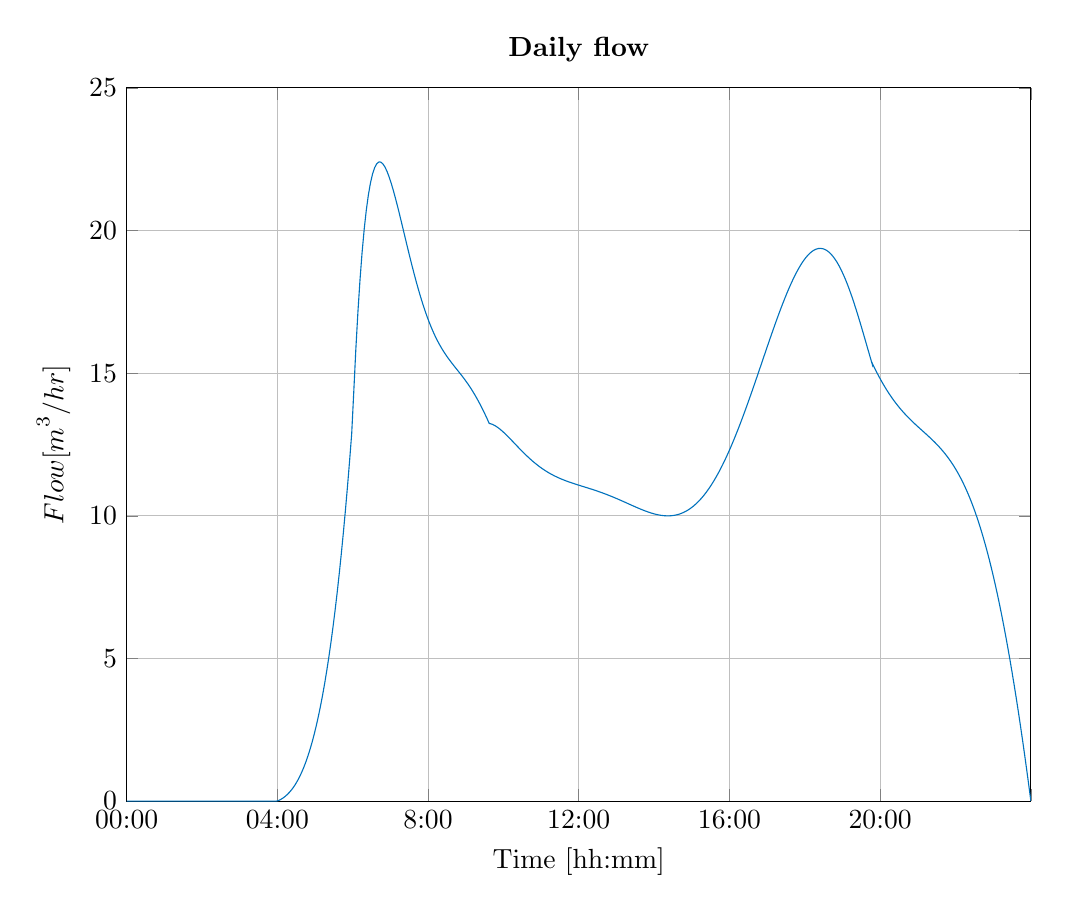
\begin{tikzpicture}

\begin{axis}[%
width=4.521in,
height=3.566in,
at={(0.758in,0.481in)},
scale only axis,
xmin=0,
xmax=24,
xtick={0,4,8,12,16,20,24},
xticklabels={{00:00},{04:00},{8:00},{12:00},{16:00},{20:00}},
xlabel={Time [hh:mm]},
xmajorgrids,
ymin=0,
ymax=25,
ylabel={$\text{Flow [m}^\text{3}\text{/hr]}$},
ymajorgrids,
axis background/.style={fill=white},
title style={font=\bfseries},
title={Daily flow}
]
\addplot [color=mycolor1,solid,forget plot]
  table[row sep=crcr]{%
0.000277777777777778	0\\
0.0558333333333333	0\\
0.111111111111111	0\\
0.166388888888889	0\\
0.221666666666667	0\\
0.276944444444444	0\\
0.332222222222222	0\\
0.3875	0\\
0.442777777777778	0\\
0.498055555555556	0\\
0.553333333333333	0\\
0.608611111111111	0\\
0.663888888888889	0\\
0.719166666666667	0\\
0.774722222222222	0\\
0.83	0\\
0.885277777777778	0\\
0.940555555555556	0\\
0.995833333333333	0\\
1.05111111111111	0\\
1.10638888888889	0\\
1.16166666666667	0\\
1.21694444444444	0\\
1.27222222222222	0\\
1.3275	0\\
1.38277777777778	0\\
1.43805555555556	0\\
1.49361111111111	0\\
1.54888888888889	0\\
1.60416666666667	0\\
1.65944444444444	0\\
1.71472222222222	0\\
1.77	0\\
1.82527777777778	0\\
1.88055555555556	0\\
1.93583333333333	0\\
1.99111111111111	0\\
2.04638888888889	0\\
2.10166666666667	0\\
2.15694444444444	0\\
2.2125	0\\
2.26777777777778	0\\
2.32305555555556	0\\
2.37833333333333	0\\
2.43361111111111	0\\
2.48888888888889	0\\
2.54416666666667	0\\
2.59944444444444	0\\
2.65472222222222	0\\
2.71	0\\
2.76527777777778	0\\
2.82055555555556	0\\
2.87583333333333	0\\
2.93138888888889	0\\
2.98666666666667	0\\
3.04194444444444	0\\
3.09722222222222	0\\
3.1525	0\\
3.20777777777778	0\\
3.26305555555556	0\\
3.31833333333333	0\\
3.37361111111111	0\\
3.42888888888889	0\\
3.48416666666667	0\\
3.53944444444444	0\\
3.59472222222222	0\\
3.65027777777778	0\\
3.70555555555556	0\\
3.76083333333333	0\\
3.81611111111111	0\\
3.87138888888889	0\\
3.92666666666667	0\\
3.98194444444444	0\\
4.03722222222222	0.0215871608995171\\
4.0925	0.0596144337867617\\
4.14777777777778	0.105436412114141\\
4.20305555555556	0.159827130629159\\
4.25833333333333	0.223595964622504\\
4.31361111111111	0.2975876840482\\
4.36916666666667	0.383139647184734\\
4.42444444444444	0.48031582263149\\
4.47972222222222	0.590466368181031\\
4.535	0.714577548012382\\
4.59027777777778	0.853670689059081\\
4.64555555555556	1.00880199425852\\
4.70083333333333	1.18106231568976\\
4.75611111111111	1.37157688759966\\
4.81138888888889	1.58150501931738\\
4.86666666666667	1.81203974805736\\
4.92194444444444	2.0644074516109\\
4.97722222222222	2.33986742092562\\
5.0325	2.63971139257398\\
5.08777777777778	2.96526304110979\\
5.14333333333333	3.31972002759027\\
5.19861111111111	3.70092953520954\\
5.25388888888889	4.11201088403031\\
5.30916666666667	4.55440976838445\\
5.36444444444444	5.02960067703456\\
5.41972222222222	5.53908614465934\\
5.475	6.08439596322775\\
5.53027777777778	6.66708635326111\\
5.58555555555556	7.28873909498431\\
5.64083333333333	7.9509606193645\\
5.69611111111111	8.65538105903902\\
5.75138888888889	9.40365325913128\\
5.80666666666667	10.1974517479556\\
5.86222222222222	11.0428200272761\\
5.9175	11.9330262953328\\
5.97277777777778	12.8739103944833\\
6.02805555555556	14.3482689690984\\
6.08333333333333	15.8504864477681\\
6.13861111111111	17.1560440186331\\
6.19388888888889	18.2801616878935\\
6.24916666666667	19.2373382282564\\
6.30444444444444	20.0413673782124\\
6.35972222222222	20.705354041463\\
6.415	21.2417304862141\\
6.47027777777778	21.6622725445979\\
6.52555555555556	21.9781158119435\\
6.58111111111111	22.2006648205716\\
6.63638888888889	22.3376378098803\\
6.69166666666667	22.3996846949591\\
6.71527777777778	22.405523969632\\
6.74694444444444	22.3955392669339\\
6.80222222222222	22.3333761583758\\
6.8575	22.2208270425952\\
6.91277777777778	22.0649968330859\\
6.96805555555556	21.8724798828307\\
7.02333333333333	21.6493761836189\\
7.07861111111111	21.4013075654675\\
7.13388888888889	21.1334338959437\\
7.18916666666667	20.8504692795407\\
7.24444444444444	20.5566982570343\\
7.3	20.2544694309749\\
7.35527777777778	19.9502926900238\\
7.41055555555556	19.6457623846265\\
7.46583333333333	19.3436050021067\\
7.52111111111111	19.0461985441405\\
7.57638888888889	18.7555887263448\\
7.63166666666667	18.4735051773404\\
7.68694444444444	18.2013776384104\\
7.74222222222222	17.9403521626146\\
7.7975	17.6913073142575\\
7.85277777777778	17.4548703682284\\
7.90805555555556	17.2314335094108\\
7.96333333333333	17.0211700318498\\
8.01888888888889	16.8230928890609\\
8.07416666666667	16.6389656163613\\
8.12944444444445	16.4673779133311\\
8.18472222222222	16.307788771412\\
8.24	16.1595193694724\\
8.29527777777778	16.0217692732289\\
8.35055555555556	15.8936326345748\\
8.40583333333333	15.774114390944\\
8.46111111111111	15.6621464646738\\
8.51638888888889	15.5566039623686\\
8.57166666666667	15.4563213741713\\
8.62694444444444	15.3601087732992\\
8.68222222222222	15.2667680151425\\
8.73777777777778	15.1746506030387\\
8.79305555555556	15.0835069312748\\
8.84833333333333	14.9917478291633\\
8.90361111111111	14.898304600178\\
8.95888888888889	14.8021814083345\\
9.01416666666667	14.7024714774385\\
9.06944444444444	14.5983732906799\\
9.12472222222222	14.4892067895576\\
9.18	14.3744295736815\\
9.23527777777778	14.2536530998821\\
9.29055555555555	14.1266588816431\\
9.34583333333333	13.9934146883033\\
9.40111111111111	13.8540907447199\\
9.45666666666667	13.708333792169\\
9.51194444444444	13.5582283695005\\
9.56722222222222	13.4039356536622\\
9.6225	13.2380371023536\\
9.67777777777778	13.2195522202824\\
9.73305555555556	13.189728836427\\
9.78833333333333	13.1501006829665\\
9.84361111111111	13.1020831976296\\
9.89888888888889	13.0469791384893\\
9.95416666666667	12.9859840476077\\
10.0094444444444	12.920191564498\\
10.0647222222222	12.8505985926601\\
10.12	12.7781103196493\\
10.1752777777778	12.7035450928025\\
10.2308333333333	12.6272554736588\\
10.2861111111111	12.5506656592277\\
10.3413888888889	12.473982293284\\
10.3966666666667	12.3977219666415\\
10.4519444444444	12.3223367313935\\
10.5072222222222	12.2482181475485\\
10.5625	12.1757012004616\\
10.6177777777778	12.1050680868684\\
10.6730555555556	12.0365518736296\\
10.7283333333333	11.9703400298549\\
10.7836111111111	11.9065778354071\\
10.8388888888889	11.8453716658769\\
10.8941666666667	11.7867921570772\\
10.9497222222222	11.7306030257088\\
11.005	11.6773743037372\\
11.0602777777778	11.6267994263657\\
11.1155555555556	11.5788352487293\\
11.1708333333333	11.5334169722205\\
11.2261111111111	11.4904606225977\\
11.2813888888889	11.4498654175343\\
11.3366666666667	11.4115160301626\\
11.3919444444444	11.3752847454503\\
11.4472222222222	11.3410335159177\\
11.5025	11.3086159154269\\
11.5577777777778	11.277878993488\\
11.6130555555556	11.248665032367\\
11.6686111111111	11.2206764159368\\
11.7238888888889	11.1940299877632\\
11.7791666666667	11.1684200992991\\
11.8344444444444	11.1436856607219\\
11.8897222222222	11.1196682087444\\
11.945	11.0962131163281\\
12.0002777777778	11.07317071782\\
12.0555555555556	11.0503973514766\\
12.1108333333333	11.0277563191662\\
12.1661111111111	11.005118768558\\
12.2213888888889	10.9823644969428\\
12.2766666666667	10.9593826777482\\
12.3319444444444	10.936072515402\\
12.3875	10.9122233921841\\
12.4427777777778	10.8879944366748\\
12.4980555555556	10.8632000909773\\
12.5533333333333	10.8377848625377\\
12.6086111111111	10.8117055115777\\
12.6638888888889	10.7849312979194\\
12.7191666666667	10.7574441664047\\
12.7744444444444	10.7292388727307\\
12.8297222222222	10.7003230506952\\
12.885	10.6707172248646\\
12.9402777777778	10.6404547673064\\
12.9955555555556	10.609581802514\\
13.0508333333333	10.57815706191\\
13.1063888888889	10.5460902832263\\
13.1616666666667	10.5137858277503\\
13.2169444444444	10.4811797612942\\
13.2722222222222	10.4483788922937\\
13.3275	10.4155012083516\\
13.3827777777778	10.3826754633549\\
13.4380555555556	10.3500407289841\\
13.4933333333333	10.3177459047319\\
13.5486111111111	10.285949199929\\
13.6038888888889	10.254817578272\\
13.6591666666667	10.2245261730898\\
13.7144444444444	10.1952576740178\\
13.7697222222222	10.1672016854046\\
13.8252777777778	10.140424046143\\
13.8805555555556	10.1153947999318\\
13.9358333333333	10.0921826298797\\
13.9911111111111	10.0709979228041\\
14.0463888888889	10.0520544242499\\
14.1016666666667	10.0355684704836\\
14.1569444444444	10.0217582066864\\
14.2122222222222	10.0108427916719\\
14.2675	10.0030415911797\\
14.3227777777778	9.99857336422404\\
14.3644444444444	9.99754027580183\\
14.3780555555556	9.99765543753472\\
14.4333333333333	10.0005028793745\\
14.4886111111111	10.0073276641036\\
14.5438888888889	10.0183378404356\\
14.5994444444444	10.0338254925244\\
14.6547222222222	10.0538342467711\\
14.71	10.0786215726657\\
14.7652777777778	10.1083714420624\\
14.8205555555556	10.1432597521196\\
14.8758333333333	10.183453515756\\
14.9311111111111	10.2291100606214\\
14.9863888888889	10.2803762441061\\
15.0416666666667	10.337387679011\\
15.0969444444444	10.4002679758338\\
15.1522222222222	10.4691280037225\\
15.2075	10.544065171161\\
15.2627777777778	10.6251627249293\\
15.3183333333333	10.7129437262179\\
15.3736111111111	10.8065834689802\\
15.4288888888889	10.9065418855862\\
15.4841666666667	11.0128389917212\\
15.5394444444444	11.125477527711\\
15.5947222222222	11.2444424229178\\
15.65	11.3697002950051\\
15.7052777777778	11.5011989879708\\
15.7605555555556	11.6388671447252\\
15.8158333333333	11.7826138168458\\
15.8711111111111	11.9323281219617\\
15.9263888888889	12.0878789383828\\
15.9816666666667	12.2491146439676\\
16.0372222222222	12.4167144399971\\
16.0925	12.5888082565202\\
16.1477777777778	12.7660060920051\\
16.2030555555556	12.9480725868558\\
16.2583333333333	13.1347513200136\\
16.3136111111111	13.3257648532173\\
16.3688888888889	13.5208148370862\\
16.4241666666667	13.719582171847\\
16.4794444444444	13.9217272317749\\
16.5347222222222	14.126890150165\\
16.59	14.3346911724244\\
16.6452777777778	14.5447310691862\\
16.7005555555556	14.7565916226916\\
16.7561111111111	14.9709104977837\\
16.8113888888889	15.1850880981809\\
16.8666666666667	15.399721265188\\
16.9219444444444	15.6143220159303\\
16.9772222222222	15.8283868908423\\
17.0325	16.0413978807405\\
17.0877777777778	16.2528234415631\\
17.1430555555556	16.4621195849849\\
17.1983333333333	16.6687310586843\\
17.2536111111111	16.8720926087394\\
17.3088888888889	17.0716303312831\\
17.3641666666667	17.2667631125188\\
17.4194444444444	17.4569041643413\\
17.475	17.64237497738\\
17.5302777777778	17.820725184493\\
17.5855555555556	17.9923029847821\\
17.6408333333333	18.156516109329\\
17.6961111111111	18.3127757178183\\
17.7513888888889	18.4604985172081\\
17.8066666666667	18.5991089862047\\
17.8619444444444	18.7280417006512\\
17.9172222222222	18.8467437732137\\
17.9725	18.9546773958496\\
18.0277777777778	19.0513224981196\\
18.0830555555556	19.1361795145132\\
18.1383333333333	19.2087722705249\\
18.1938888888889	19.2689190538749\\
18.2491666666667	19.3155964399719\\
18.3044444444444	19.3487501257366\\
18.3597222222222	19.3680288864707\\
18.4069444444444	19.3732729073931\\
18.415	19.3731211115783\\
18.4702777777778	19.3637584097039\\
18.5255555555556	19.3397193576368\\
18.5808333333333	19.3008333569353\\
18.6361111111111	19.246984635195\\
18.6913888888889	19.178116382683\\
18.7466666666667	19.0942350098461\\
18.8019444444444	18.995414552924\\
18.8572222222222	18.8818012152056\\
18.9127777777778	18.7529375919974\\
18.9680555555556	18.6104185262881\\
19.0233333333333	18.4540278774301\\
19.0786111111111	18.284249205032\\
19.1338888888889	18.1016630939554\\
19.1891666666667	17.906952564907\\
19.2444444444444	17.7009086239037\\
19.2997222222222	17.4844359824573\\
19.355	17.2585589120178\\
19.4102777777778	17.0244272726442\\
19.4655555555556	16.7833226877948\\
19.5208333333333	16.5366648807445\\
19.5761111111111	16.2860181759072\\
19.6313888888889	16.0330981655228\\
19.6869444444444	15.7785079298619\\
19.7422222222222	15.5268411116235\\
19.7944444444444	15.2925932948543\\
19.7975	15.3268480395642\\
19.8527777777778	15.176224182056\\
19.9080555555556	15.0311864005195\\
19.9633333333333	14.8917219285676\\
20.0186111111111	14.7577910023316\\
20.0738888888889	14.6293277129511\\
20.1291666666667	14.5062408589244\\
20.1844444444444	14.3884147983674\\
20.2397222222222	14.2757103021951\\
20.295	14.1679654059651\\
20.3502777777778	14.0649962625051\\
20.4058333333333	13.9661147016961\\
20.4611111111111	13.8720834913925\\
20.5163888888889	13.7821524461618\\
20.5716666666667	13.6960586227162\\
20.6269444444444	13.6135214612693\\
20.6822222222222	13.5342436388569\\
20.7375	13.4579119218255\\
20.7927777777778	13.3841980174917\\
20.8480555555556	13.3127594276465\\
20.9033333333333	13.2432403003062\\
20.9586111111111	13.1752722823868\\
21.0138888888889	13.1084753726082\\
21.0691666666667	13.0424587730609\\
21.1247222222222	12.9764921787005\\
21.18	12.9108236842417\\
21.2352777777778	12.8447047352015\\
21.2905555555556	12.777709840293\\
21.3458333333333	12.7094069777385\\
21.4011111111111	12.639358449375\\
21.4563888888889	12.5671217328198\\
21.5116666666667	12.4922503333604\\
21.5669444444444	12.4142946370434\\
21.6222222222222	12.3328027632566\\
21.6775	12.2473214163412\\
21.7327777777778	12.1573967393275\\
21.7880555555556	12.0625751651779\\
21.8436111111111	11.9618866298005\\
21.8988888888889	11.8558857084313\\
21.9541666666667	11.7436352173794\\
22.0094444444444	11.6246912974911\\
22.0647222222222	11.4986146469299\\
22.12	11.364971373297\\
22.1752777777778	11.2233338469974\\
22.2305555555556	11.0732815526218\\
22.2858333333333	10.9144019420819\\
22.3411111111111	10.7462912869153\\
22.3963888888889	10.5685555310056\\
22.4516666666667	10.3808111425178\\
22.5069444444444	10.1826859670341\\
22.5625	9.97274278874772\\
22.6177777777778	9.75273277714939\\
22.6730555555556	9.52130066613276\\
22.7283333333333	9.27812841074793\\
22.7836111111111	9.02291360987806\\
22.8388888888889	8.75537035900564\\
22.8941666666667	8.47523010224034\\
22.9494444444444	8.1822424849007\\
23.0047222222222	7.87617620614194\\
23.06	7.55681987116843\\
23.1152777777778	7.22398284418458\\
23.1705555555556	6.87749610042272\\
23.2258333333333	6.51721307914008\\
23.2813888888889	6.14109479347717\\
23.3366666666667	5.75280299723593\\
23.3919444444444	5.35041824004959\\
23.4472222222222	4.93389247208919\\
23.5025	4.50320437530516\\
23.5577777777778	4.05836021305521\\
23.6130555555556	3.59939468573208\\
23.6683333333333	3.1263717796069\\
23.7236111111111	2.63938562319531\\
23.7788888888889	2.1385613365162\\
23.8341666666667	1.62405588584255\\
23.8894444444444	1.09605893443701\\
23.9447222222222	0.554793696241197\\
24	0.000517788180528441\\
};
\end{axis}
\end{tikzpicture}%
\caption{A flow profile for Thulesvej.}
\label{fig:APP_flow_profile_norregade}
\end{figure} 

\begin{figure}[H]
\centering
% This file was created by matlab2tikz.
%
%The latest updates can be retrieved from
%  http://www.mathworks.com/matlabcentral/fileexchange/22022-matlab2tikz-matlab2tikz
%where you can also make suggestions and rate matlab2tikz.
%
\definecolor{mycolor1}{rgb}{0.00000,0.44700,0.74100}%
%
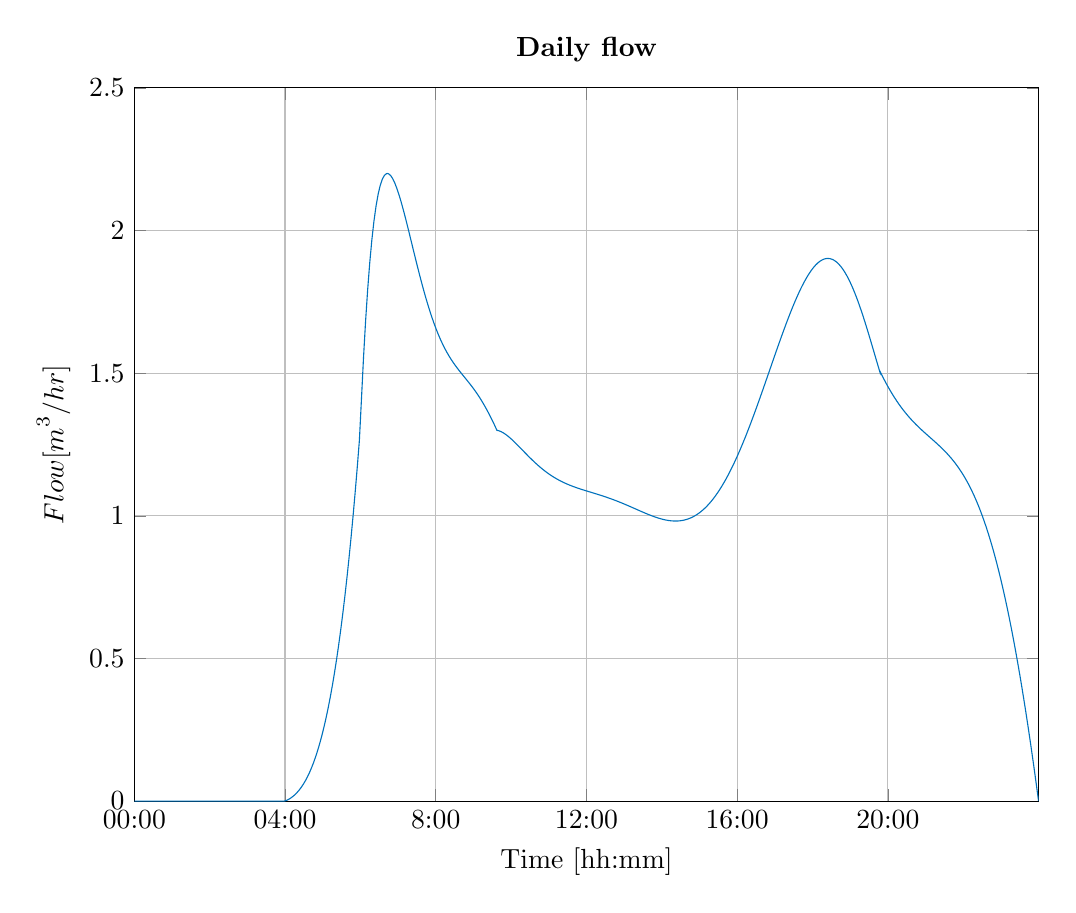
\begin{tikzpicture}

\begin{axis}[%
width=4.521in,
height=3.566in,
at={(0.758in,0.481in)},
scale only axis,
xmin=0,
xmax=24,
xtick={0,4,8,12,16,20,24},
xticklabels={{00:00},{04:00},{8:00},{12:00},{16:00},{20:00}},
xlabel={Time [hh:mm]},
xmajorgrids,
ymin=0,
ymax=2.5,
ylabel={$\text{Flow [m}^\text{3}\text{/hr]}$},
ymajorgrids,
axis background/.style={fill=white},
title style={font=\bfseries},
title={Daily flow}
]
\addplot [color=mycolor1,solid,forget plot]
  table[row sep=crcr]{%
0.000277777777777778	0\\
0.0558333333333333	0\\
0.111111111111111	0\\
0.166388888888889	0\\
0.221666666666667	0\\
0.276944444444444	0\\
0.332222222222222	0\\
0.3875	0\\
0.442777777777778	0\\
0.498055555555556	0\\
0.553333333333333	0\\
0.608611111111111	0\\
0.663888888888889	0\\
0.719166666666667	0\\
0.774722222222222	0\\
0.83	0\\
0.885277777777778	0\\
0.940555555555556	0\\
0.995833333333333	0\\
1.05111111111111	0\\
1.10638888888889	0\\
1.16166666666667	0\\
1.21694444444444	0\\
1.27222222222222	0\\
1.3275	0\\
1.38277777777778	0\\
1.43805555555556	0\\
1.49361111111111	0\\
1.54888888888889	0\\
1.60416666666667	0\\
1.65944444444444	0\\
1.71472222222222	0\\
1.77	0\\
1.82527777777778	0\\
1.88055555555556	0\\
1.93583333333333	0\\
1.99111111111111	0\\
2.04638888888889	0\\
2.10166666666667	0\\
2.15694444444444	0\\
2.2125	0\\
2.26777777777778	0\\
2.32305555555556	0\\
2.37833333333333	0\\
2.43361111111111	0\\
2.48888888888889	0\\
2.54416666666667	0\\
2.59944444444444	0\\
2.65472222222222	0\\
2.71	0\\
2.76527777777778	0\\
2.82055555555556	0\\
2.87583333333333	0\\
2.93138888888889	0\\
2.98666666666667	0\\
3.04194444444444	0\\
3.09722222222222	0\\
3.1525	0\\
3.20777777777778	0\\
3.26305555555556	0\\
3.31833333333333	0\\
3.37361111111111	0\\
3.42888888888889	0\\
3.48416666666667	0\\
3.53944444444444	0\\
3.59472222222222	0\\
3.65027777777778	0\\
3.70555555555556	0\\
3.76083333333333	0\\
3.81611111111111	0\\
3.87138888888889	0\\
3.92666666666667	0\\
3.98194444444444	0\\
4.03722222222222	0.00211951125744408\\
4.0925	0.00585317652957422\\
4.14777777777778	0.0103521562404917\\
4.20305555555556	0.0156924481264725\\
4.25833333333333	0.0219535197955126\\
4.31361111111111	0.0292183140410548\\
4.36916666666667	0.0376181378904421\\
4.42444444444444	0.047159272029085\\
4.47972222222222	0.0579742801903056\\
4.535	0.0701599976198309\\
4.59027777777778	0.0838167021607384\\
4.64555555555556	0.0990480959175509\\
4.70083333333333	0.115961282982026\\
4.75611111111111	0.134666743220625\\
4.81138888888889	0.15527830212367\\
4.86666666666667	0.177913096716188\\
4.92194444444444	0.202691537530468\\
4.97722222222222	0.229737266640256\\
5.0325	0.259177111756696\\
5.08777777777778	0.291141036385921\\
5.14333333333333	0.325942999303699\\
5.19861111111111	0.363371628598894\\
5.25388888888889	0.403733191224315\\
5.30916666666667	0.447169631061583\\
5.36444444444444	0.493825719141305\\
5.41972222222222	0.543848980151002\\
5.475	0.597389615004768\\
5.53027777777778	0.654600419474559\\
5.58555555555556	0.715636698883249\\
5.64083333333333	0.780656178859284\\
5.69611111111111	0.849818912153093\\
5.75138888888889	0.92328718151516\\
5.80666666666667	1.00122539863582\\
5.86222222222222	1.08422693797887\\
5.9175	1.17163084511497\\
5.97277777777778	1.26401049843678\\
6.02805555555556	1.4087687466822\\
6.08333333333333	1.55626229027462\\
6.13861111111111	1.68444700069439\\
6.19388888888889	1.79481723723359\\
6.24916666666667	1.88879654568011\\
6.30444444444444	1.96773924882562\\
6.35972222222222	2.03293203698813\\
6.415	2.08559555852159\\
6.47027777777778	2.12688601033793\\
6.52555555555556	2.15789672841443\\
6.58111111111111	2.17974745400618\\
6.63638888888889	2.19319599381913\\
6.69166666666667	2.19928799785921\\
6.71527777777778	2.19986132051438\\
6.74694444444444	2.19888098364334\\
6.80222222222222	2.19277756833089\\
6.8575	2.18172705923324\\
6.91277777777778	2.16642704433817\\
6.96805555555556	2.14752498282049\\
7.02333333333333	2.12561979555395\\
7.07861111111111	2.1012634556333\\
7.13388888888889	2.07496257888664\\
7.18916666666667	2.04718001439304\\
7.24444444444444	2.01833643499826\\
7.3	1.98866243561785\\
7.35527777777778	1.95879718239166\\
7.41055555555556	1.92889721483563\\
7.46583333333333	1.89923023005929\\
7.52111111111111	1.87002970949847\\
7.57638888888889	1.84149650945383\\
7.63166666666667	1.81380045157769\\
7.68694444444444	1.7870819134194\\
7.74222222222222	1.76145341891732\\
7.7975	1.7370012289254\\
7.85277777777778	1.7137869317273\\
7.90805555555556	1.69184903355736\\
7.96333333333333	1.67120454909763\\
8.01888888888889	1.65175656629258\\
8.07416666666667	1.63367823588564\\
8.12944444444445	1.61683108910686\\
8.18472222222222	1.6011620076358\\
8.24	1.58660434217862\\
8.29527777777778	1.57307950299012\\
8.35055555555556	1.56049855038675\\
8.40583333333333	1.54876378526295\\
8.46111111111111	1.53777033960758\\
8.51638888888889	1.5274077670203\\
8.57166666666667	1.51756163321886\\
8.62694444444444	1.50811510657251\\
8.68222222222222	1.49895054859231\\
8.73777777777778	1.48990610347656\\
8.79305555555556	1.48095726396739\\
8.84833333333333	1.47194799911762\\
8.90361111111111	1.46277338015368\\
8.95888888888889	1.45333563203284\\
9.01416666666667	1.44354572394828\\
9.06944444444444	1.43332495986812\\
9.12472222222222	1.42260656900878\\
9.18	1.41133729639439\\
9.23527777777778	1.39947899334825\\
9.29055555555555	1.38701020801604\\
9.34583333333333	1.37392777586632\\
9.40111111111111	1.3602484102364\\
9.45666666666667	1.34593742681342\\
9.51194444444444	1.33119949371373\\
9.56722222222222	1.31605043591576\\
9.6225	1.29976187213801\\
9.67777777777778	1.29794695465882\\
9.73305555555556	1.29501877905895\\
9.78833333333333	1.2911279331176\\
9.84361111111111	1.28641339000563\\
9.89888888888889	1.28100305956791\\
9.95416666666667	1.27501432476512\\
10.0094444444444	1.26855456337012\\
10.0647222222222	1.26172165523848\\
10.12	1.25460447519825\\
10.1752777777778	1.24728337176778\\
10.2308333333333	1.23979296080759\\
10.2861111111111	1.23227307550874\\
10.3413888888889	1.22474400495921\\
10.3966666666667	1.2172564700505\\
10.4519444444444	1.20985485501197\\
10.5072222222222	1.20257760472525\\
10.5625	1.19545760935293\\
10.6177777777778	1.18852257606597\\
10.6730555555556	1.18179538827351\\
10.7283333333333	1.17529445242049\\
10.7836111111111	1.1690340326478\\
10.8388888888889	1.16302457332389\\
10.8941666666667	1.15727300974708\\
10.9497222222222	1.1517561427058\\
11.005	1.14652994015127\\
11.0602777777778	1.14156430236167\\
11.1155555555556	1.13685499320668\\
11.1708333333333	1.13239565050746\\
11.2261111111111	1.12817802934699\\
11.2813888888889	1.12419223452522\\
11.3366666666667	1.12042694280257\\
11.3919444444444	1.11686961462139\\
11.4472222222222	1.11350669594424\\
11.5025	1.11032381008448\\
11.5577777777778	1.10730593976925\\
11.6130555555556	1.10443759965919\\
11.6686111111111	1.1016895686476\\
11.7238888888889	1.09907331888935\\
11.7791666666667	1.09655884062358\\
11.8344444444444	1.09413031742615\\
11.8897222222222	1.0917721907564\\
11.945	1.08946927873142\\
12.0002777777778	1.0872068865964\\
12.0555555555556	1.08497090908368\\
12.1108333333333	1.08274792464005\\
12.1661111111111	1.08052528204344\\
12.2213888888889	1.07829117932525\\
12.2766666666667	1.07603473510241\\
12.3319444444444	1.07374605287431\\
12.3875	1.07140445337562\\
12.4427777777778	1.06902556046807\\
12.4980555555556	1.06659115535702\\
12.5533333333333	1.06409578956812\\
12.6086111111111	1.06153521765207\\
12.6638888888889	1.05890642141888\\
12.7191666666667	1.05620762814302\\
12.7744444444444	1.05343832291851\\
12.8297222222222	1.05059925526122\\
12.885	1.04769244035276\\
12.9402777777778	1.04472115479229\\
12.9955555555556	1.04168992726159\\
13.0508333333333	1.03860452423975\\
13.1063888888889	1.03545608342688\\
13.1616666666667	1.03228430658388\\
13.2169444444444	1.02908291640403\\
13.2722222222222	1.02586239975415\\
13.3275	1.02263434111511\\
13.3827777777778	1.01941138204336\\
13.4380555555556	1.01620717713635\\
13.4933333333333	1.0130363459243\\
13.5486111111111	1.00991442201346\\
13.6038888888889	1.00685779854771\\
13.6591666666667	1.00388367079712\\
13.7144444444444	1.00100997593932\\
13.7697222222222	0.998255330065261\\
13.8252777777778	0.995626197493037\\
13.8805555555556	0.993168728937686\\
13.9358333333333	0.990889667973437\\
13.9911111111111	0.988809671194725\\
14.0463888888889	0.986949724968917\\
14.1016666666667	0.985331070030453\\
14.1569444444444	0.983975124720065\\
14.2122222222222	0.982903406900816\\
14.2675	0.982137454752601\\
14.3227777777778	0.981698746884653\\
14.3644444444444	0.98159731425296\\
14.3780555555556	0.981608621278948\\
14.4333333333333	0.981888194172414\\
14.4886111111111	0.982558278030602\\
14.5438888888889	0.983639299883856\\
14.5994444444444	0.985159937688267\\
14.6547222222222	0.987124474853235\\
14.71	0.989558190732782\\
14.7652777777778	0.992479148397723\\
14.8205555555556	0.995904618113898\\
14.8758333333333	0.999850997857995\\
14.9311111111111	1.00433373466941\\
14.9863888888889	1.00936724757682\\
15.0416666666667	1.01496485157146\\
15.0969444444444	1.02113868321183\\
15.1522222222222	1.02789962806129\\
15.2075	1.03525725006291\\
15.2627777777778	1.04321972270872\\
15.3183333333333	1.0518384021769\\
15.3736111111111	1.06103231562632\\
15.4288888888889	1.0708466210025\\
15.4841666666667	1.08128328352314\\
15.5394444444444	1.09234257224404\\
15.5947222222222	1.10402300747149\\
15.65	1.11632131159812\\
15.7052777777778	1.12923236374515\\
15.7605555555556	1.14274915779651\\
15.8158333333333	1.15686276408305\\
15.8711111111111	1.17156229574311\\
15.9263888888889	1.1868348787402\\
15.9816666666667	1.20266562622384\\
16.0372222222222	1.21912122481243\\
16.0925	1.23601806377866\\
16.1477777777778	1.25341603514012\\
16.2030555555556	1.27129203037801\\
16.2583333333333	1.28962087307738\\
16.3136111111111	1.30837532327276\\
16.3688888888889	1.32752608786374\\
16.4241666666667	1.34704183639587\\
16.4794444444444	1.36688922309708\\
16.5347222222222	1.38703291485729\\
16.59	1.40743562589638\\
16.6452777777778	1.42805815832532\\
16.7005555555556	1.44885944990105\\
16.7561111111111	1.46990210903324\\
16.8113888888889	1.49093089726747\\
16.8666666666667	1.51200441479996\\
16.9219444444444	1.53307474957772\\
16.9772222222222	1.55409246998622\\
17.0325	1.57500671587293\\
17.0877777777778	1.59576529817844\\
17.1430555555556	1.61631480601724\\
17.1983333333333	1.63660072256095\\
17.2536111111111	1.65656754898519\\
17.3088888888889	1.67615893718046\\
17.3641666666667	1.69531783113834\\
17.4194444444444	1.71398661772477\\
17.475	1.73219686213777\\
17.5302777777778	1.74970797781912\\
17.5855555555556	1.76655415230835\\
17.6408333333333	1.78267723434388\\
17.6961111111111	1.79801940929771\\
17.7513888888889	1.81252340719467\\
17.8066666666667	1.82613272111999\\
17.8619444444444	1.838791835535\\
17.9172222222222	1.85044646581497\\
17.9725	1.86104380787853\\
18.0277777777778	1.87053279919109\\
18.0830555555556	1.8788643904715\\
18.1383333333333	1.88599182905835\\
18.1938888888889	1.8918972737346\\
18.2491666666667	1.89648024070099\\
18.3044444444444	1.8997353982704\\
18.3597222222222	1.9016282618385\\
18.4069444444444	1.9021431401697\\
18.415	1.90212823626733\\
18.4702777777778	1.90120896985175\\
18.5255555555556	1.89884872240134\\
18.5808333333333	1.89503074389887\\
18.6361111111111	1.88974366736024\\
18.6913888888889	1.88298191498533\\
18.7466666666667	1.87474611617671\\
18.8019444444444	1.8650435400998\\
18.8572222222222	1.85388854156105\\
18.9127777777778	1.84123621079203\\
18.9680555555556	1.82724313566847\\
19.0233333333333	1.81188809466255\\
19.0786111111111	1.79521856553378\\
19.1338888888889	1.77729155235771\\
19.1891666666667	1.75817411675875\\
19.2444444444444	1.73794392277829\\
19.2997222222222	1.7166897985046\\
19.355	1.69451231088483\\
19.4102777777778	1.67152435764328\\
19.4655555555556	1.64785177354625\\
19.5208333333333	1.62363395253621\\
19.5761111111111	1.59902448605672\\
19.6313888888889	1.57419181761375\\
19.6869444444444	1.54919515996941\\
19.7422222222222	1.52448553479618\\
19.7944444444444	1.50148617480692\\
19.7975	1.50484943861782\\
19.8527777777778	1.49006060357303\\
19.9080555555556	1.47582023115203\\
19.9633333333333	1.46212706790136\\
20.0186111111111	1.44897720965004\\
20.0738888888889	1.4363641852103\\
20.1291666666667	1.42427904006465\\
20.1844444444444	1.41271042004401\\
20.2397222222222	1.40164465509634\\
20.295	1.39106584292393\\
20.3502777777778	1.38095593269772\\
20.4058333333333	1.37124735720399\\
20.4611111111111	1.36201500795171\\
20.5163888888889	1.35318522882293\\
20.5716666666667	1.34473220302491\\
20.6269444444444	1.33662838410874\\
20.6822222222222	1.32884457975155\\
20.7375	1.32135003545733\\
20.7927777777778	1.31411251817597\\
20.8480555555556	1.30709840010377\\
20.9033333333333	1.30027274231157\\
20.9586111111111	1.29359937846363\\
21.0138888888889	1.28704099855915\\
21.0691666666667	1.2805592325423\\
21.1247222222222	1.27408237622882\\
21.18	1.26763478852089\\
21.2352777777778	1.26114297343352\\
21.2905555555556	1.25456515458041\\
21.3458333333333	1.24785891438636\\
21.4011111111111	1.24098127794658\\
21.4563888888889	1.2338887966957\\
21.5116666666667	1.22653763204957\\
21.5669444444444	1.21888363916487\\
21.6222222222222	1.21088245064892\\
21.6775	1.20248956017425\\
21.7327777777778	1.19366040630174\\
21.7880555555556	1.1843504560589\\
21.8436111111111	1.17446446478745\\
21.8988888888889	1.16405688283689\\
21.9541666666667	1.15303569387437\\
22.0094444444444	1.14135731808511\\
22.0647222222222	1.12897862310946\\
22.12	1.11585700770736\\
22.1752777777778	1.10195048554515\\
22.2305555555556	1.0872177687875\\
22.2858333333333	1.07161835186162\\
22.3411111111111	1.05511259513981\\
22.3963888888889	1.03766180866286\\
22.4516666666667	1.01922833578637\\
22.5069444444444	0.999775636944894\\
22.5625	0.979162600711326\\
22.6177777777778	0.957561163704225\\
22.6730555555556	0.93483826063619\\
22.7283333333333	0.910962664619405\\
22.7836111111111	0.885904684738311\\
22.8388888888889	0.859636249777512\\
22.8941666666667	0.832130991877173\\
22.9494444444444	0.803364330242804\\
23.0047222222222	0.773313554859566\\
23.06	0.741957910165799\\
23.1152777777778	0.709278678799054\\
23.1705555555556	0.675259265251493\\
23.2258333333333	0.639885279620451\\
23.2813888888889	0.602956526260811\\
23.3366666666667	0.564832530375605\\
23.3919444444444	0.525324832876606\\
23.4472222222222	0.48442871604508\\
23.5025	0.442142086792164\\
23.5577777777778	0.398465560078633\\
23.6130555555556	0.353402542923752\\
23.6683333333333	0.30695931774801\\
23.7236111111111	0.259145126454477\\
23.7788888888889	0.209972253812317\\
23.8341666666667	0.159456111379547\\
23.8894444444444	0.107615321031556\\
23.9447222222222	0.0544717987796408\\
24	5.08384535933146e-05\\
};
\end{axis}
\end{tikzpicture}%
\caption{A flow profile for Thulesvej.}
\label{fig:APP_flow_profile_zone2}
\end{figure} 

\begin{figure}[H]
\centering
% This file was created by matlab2tikz.
%
%The latest updates can be retrieved from
%  http://www.mathworks.com/matlabcentral/fileexchange/22022-matlab2tikz-matlab2tikz
%where you can also make suggestions and rate matlab2tikz.
%
\definecolor{mycolor1}{rgb}{0.00000,0.44700,0.74100}%
%
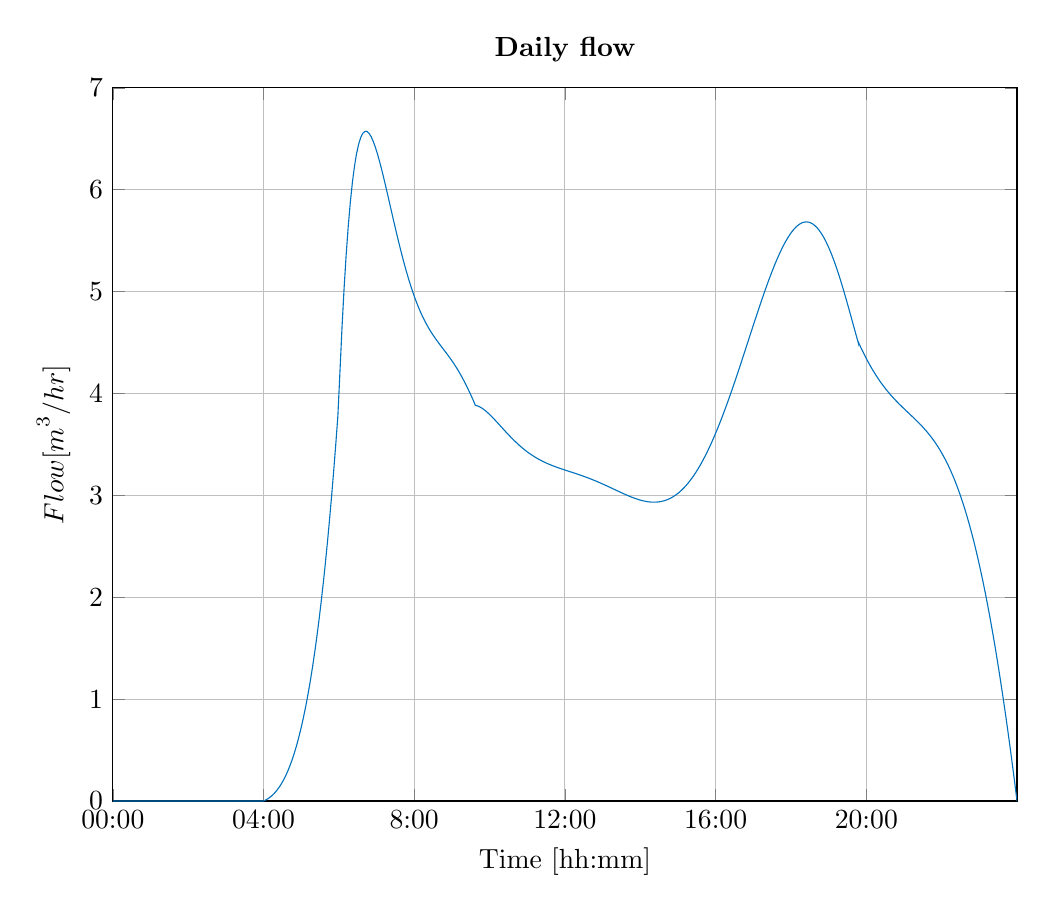
\begin{tikzpicture}

\begin{axis}[%
width=4.521in,
height=3.566in,
at={(0.758in,0.481in)},
scale only axis,
xmin=0,
xmax=24,
xtick={0,4,8,12,16,20,24},
xticklabels={{00:00},{04:00},{8:00},{12:00},{16:00},{20:00}},
xlabel={Time [hh:mm]},
xmajorgrids,
ymin=0,
ymax=7,
ylabel={$\text{Flow [m}^\text{3}\text{/hr]}$},
ymajorgrids,
axis background/.style={fill=white},
title style={font=\bfseries},
title={Daily flow}
]
\addplot [color=mycolor1,solid,forget plot]
  table[row sep=crcr]{%
0.000277777777777778	0\\
0.0558333333333333	0\\
0.111111111111111	0\\
0.166388888888889	0\\
0.221666666666667	0\\
0.276944444444444	0\\
0.332222222222222	0\\
0.3875	0\\
0.442777777777778	0\\
0.498055555555556	0\\
0.553333333333333	0\\
0.608611111111111	0\\
0.663888888888889	0\\
0.719166666666667	0\\
0.774722222222222	0\\
0.83	0\\
0.885277777777778	0\\
0.940555555555556	0\\
0.995833333333333	0\\
1.05111111111111	0\\
1.10638888888889	0\\
1.16166666666667	0\\
1.21694444444444	0\\
1.27222222222222	0\\
1.3275	0\\
1.38277777777778	0\\
1.43805555555556	0\\
1.49361111111111	0\\
1.54888888888889	0\\
1.60416666666667	0\\
1.65944444444444	0\\
1.71472222222222	0\\
1.77	0\\
1.82527777777778	0\\
1.88055555555556	0\\
1.93583333333333	0\\
1.99111111111111	0\\
2.04638888888889	0\\
2.10166666666667	0\\
2.15694444444444	0\\
2.2125	0\\
2.26777777777778	0\\
2.32305555555556	0\\
2.37833333333333	0\\
2.43361111111111	0\\
2.48888888888889	0\\
2.54416666666667	0\\
2.59944444444444	0\\
2.65472222222222	0\\
2.71	0\\
2.76527777777778	0\\
2.82055555555556	0\\
2.87583333333333	0\\
2.93138888888889	0\\
2.98666666666667	0\\
3.04194444444444	0\\
3.09722222222222	0\\
3.1525	0\\
3.20777777777778	0\\
3.26305555555556	0\\
3.31833333333333	0\\
3.37361111111111	0\\
3.42888888888889	0\\
3.48416666666667	0\\
3.53944444444444	0\\
3.59472222222222	0\\
3.65027777777778	0\\
3.70555555555556	0\\
3.76083333333333	0\\
3.81611111111111	0\\
3.87138888888889	0\\
3.92666666666667	0\\
3.98194444444444	0\\
4.03722222222222	0.00633403075201496\\
4.0925	0.017491862808034\\
4.14777777777778	0.0309367906146487\\
4.20305555555556	0.0468959287941403\\
4.25833333333333	0.0656067614698268\\
4.31361111111111	0.0873171581458113\\
4.36916666666667	0.112419521903807\\
4.42444444444444	0.140932622190965\\
4.47972222222222	0.173252617678543\\
4.535	0.209668894621113\\
4.59027777777778	0.250481127266484\\
4.64555555555556	0.295999223059964\\
4.70083333333333	0.346543256079233\\
4.75611111111111	0.402443388699786\\
4.81138888888889	0.464039781490967\\
4.86666666666667	0.531682491342598\\
4.92194444444444	0.605731357822267\\
4.97722222222222	0.686555877763078\\
5.0325	0.774535068082148\\
5.08777777777778	0.870057316829602\\
5.14333333333333	0.974060870751515\\
5.19861111111111	1.08591405772039\\
5.25388888888889	1.20653213793625\\
5.30916666666667	1.33633930207421\\
5.36444444444444	1.47576818957257\\
5.41972222222222	1.62525966900617\\
5.475	1.78526260669055\\
5.53027777777778	1.95623362351646\\
5.58555555555556	2.13863684001526\\
5.64083333333333	2.33294360965462\\
5.69611111111111	2.53963224036502\\
5.75138888888889	2.75918770429675\\
5.80666666666667	2.99210133580762\\
5.86222222222222	3.24014639846865\\
5.9175	3.50134767008346\\
5.97277777777778	3.77741865717813\\
6.02805555555556	4.21001989615431\\
6.08333333333333	4.65079539925999\\
6.13861111111111	5.03386762635261\\
6.19388888888889	5.3637023794784\\
6.24916666666667	5.64455383882438\\
6.30444444444444	5.88046931585461\\
6.35972222222222	6.07529400649055\\
6.415	6.23267574425238\\
6.47027777777778	6.35606975343764\\
6.52555555555556	6.44874340225583\\
6.58111111111111	6.51404296948667\\
6.63638888888889	6.55423311447681\\
6.69166666666667	6.57243869880469\\
6.71527777777778	6.57415203876262\\
6.74694444444444	6.57122236152374\\
6.80222222222222	6.55298267530097\\
6.8575	6.51995889955831\\
6.91277777777778	6.474235733658\\
6.96805555555556	6.41774807004736\\
7.02333333333333	6.35228574740691\\
7.07861111111111	6.27949830382899\\
7.13388888888889	6.2008997299676\\
7.18916666666667	6.11787322220348\\
7.24444444444444	6.03167593580406\\
7.3	5.94299698967878\\
7.35527777777778	5.8537464930433\\
7.41055555555556	5.76439225474001\\
7.46583333333333	5.67573427133324\\
7.52111111111111	5.58847028792319\\
7.57638888888889	5.50320055137358\\
7.63166666666667	5.42043256338536\\
7.68694444444444	5.3405858337447\\
7.74222222222222	5.26399663341188\\
7.7975	5.19092274771347\\
7.85277777777778	5.1215482294972\\
7.90805555555556	5.05598815230725\\
7.96333333333333	4.99429336348829\\
8.01888888888889	4.93617424724431\\
8.07416666666667	4.88214825406287\\
8.12944444444445	4.83180157842916\\
8.18472222222222	4.78497547946651\\
8.24	4.74147077980546\\
8.29527777777778	4.70105261876238\\
8.35055555555556	4.66345520549103\\
8.40583333333333	4.62838657214418\\
8.46111111111111	4.59553332703538\\
8.51638888888889	4.56456540780055\\
8.57166666666667	4.53514083453266\\
8.62694444444444	4.50691046299414\\
8.68222222222222	4.47952273770072\\
8.73777777777778	4.45249396241261\\
8.79305555555556	4.42575089867711\\
8.84833333333333	4.39882725747868\\
8.90361111111111	4.37140946554597\\
8.95888888888889	4.34320532809814\\
9.01416666666667	4.3139487819726\\
9.06944444444444	4.28340464885444\\
9.12472222222222	4.25137338830948\\
9.18	4.21769585107455\\
9.23527777777778	4.18225803214476\\
9.29055555555555	4.14499582395544\\
9.34583333333333	4.10589976949647\\
9.40111111111111	4.06501981556196\\
9.45666666666667	4.02225231018807\\
9.51194444444444	3.97820889161848\\
9.56722222222222	3.93293685184074\\
9.6225	3.8842594676032\\
9.67777777777778	3.87883569687059\\
9.73305555555556	3.87008502181202\\
9.78833333333333	3.85845746486589\\
9.84361111111111	3.84436833891855\\
9.89888888888889	3.82819989477808\\
9.95416666666667	3.81030292429807\\
10.0094444444444	3.79099831943557\\
10.0647222222222	3.77057858819822\\
10.12	3.74930932761559\\
10.1752777777778	3.72743065435806\\
10.2308333333333	3.70504601582383\\
10.2861111111111	3.68257329501744\\
10.3413888888889	3.66007312464689\\
10.3966666666667	3.63769708101798\\
10.4519444444444	3.61557780370628\\
10.5072222222222	3.59383018290726\\
10.5625	3.57255250887551\\
10.6177777777778	3.55182758280985\\
10.6730555555556	3.53172379038961\\
10.7283333333333	3.51229613815835\\
10.7836111111111	3.49358725363533\\
10.8388888888889	3.47562834918181\\
10.8941666666667	3.45844015051584\\
10.9497222222222	3.44195332820173\\
11.005	3.42633513906477\\
11.0602777777778	3.41149563191321\\
11.1155555555556	3.39742214732864\\
11.1708333333333	3.38409567232577\\
11.2261111111111	3.37149156747048\\
11.2813888888889	3.35958026155802\\
11.3366666666667	3.34832791577416\\
11.3919444444444	3.33769705641191\\
11.4472222222222	3.32764717805303\\
11.5025	3.31813531684207\\
11.5577777777778	3.30911659457053\\
11.6130555555556	3.30054473424163\\
11.6686111111111	3.29233241035148\\
11.7238888888889	3.28451390673868\\
11.7791666666667	3.27699954105428\\
11.8344444444444	3.26974204687469\\
11.8897222222222	3.26269492844543\\
11.945	3.25581281563088\\
12.0002777777778	3.24905179404819\\
12.0555555555556	3.24236971096105\\
12.1108333333333	3.23572645687227\\
12.1661111111111	3.22908422437259\\
12.2213888888889	3.22240774399512\\
12.2766666666667	3.21566449738696\\
12.3319444444444	3.20882490945677\\
12.3875	3.20182718147512\\
12.4427777777778	3.19471800440459\\
12.4980555555556	3.18744293248311\\
12.5533333333333	3.17998568327582\\
12.6086111111111	3.17233356951514\\
12.6638888888889	3.16447757152346\\
12.7191666666667	3.15641239161817\\
12.7744444444444	3.14813649103394\\
12.8297222222222	3.13965210965347\\
12.885	3.13096526972474\\
12.9402777777778	3.12208576316538\\
12.9955555555556	3.11302712366615\\
13.0508333333333	3.1038065839997\\
13.1063888888889	3.09439765972078\\
13.1616666666667	3.08491899713218\\
13.2169444444444	3.07535183688372\\
13.2722222222222	3.06572751834043\\
13.3275	3.0560806610203\\
13.3827777777778	3.04644904344749\\
13.4380555555556	3.03687347155777\\
13.4933333333333	3.02739763492984\\
13.5486111111111	3.01806795480322\\
13.6038888888889	3.00893342109344\\
13.6591666666667	3.00004542082146\\
13.7144444444444	2.99145755815391\\
13.7697222222222	2.98322546614878\\
13.8252777777778	2.97536846302832\\
13.8805555555556	2.96802446740337\\
13.9358333333333	2.96121363203623\\
13.9911111111111	2.95499768790562\\
14.0463888888889	2.94943935149671\\
14.1016666666667	2.94460209945517\\
14.1569444444444	2.94054993919233\\
14.2122222222222	2.93734717553597\\
14.2675	2.93505817402945\\
14.3227777777778	2.93374712219287\\
14.3644444444444	2.93344399692937\\
14.3780555555556	2.93347778729027\\
14.4333333333333	2.93431327391409\\
14.4886111111111	2.93631577885446\\
14.5438888888889	2.93954634705176\\
14.5994444444444	2.94409068083719\\
14.6547222222222	2.94996158091978\\
14.71	2.95723459311473\\
14.7652777777778	2.96596369781285\\
14.8205555555556	2.97620050615541\\
14.8758333333333	2.98799402250048\\
14.9311111111111	3.00139040938778\\
14.9863888888889	3.01643275720933\\
15.0416666666667	3.03316085700834\\
15.0969444444444	3.05161097815327\\
15.1522222222222	3.07181565148953\\
15.2075	3.09380345828049\\
15.2627777777778	3.11759882451104\\
15.3183333333333	3.14335522500263\\
15.3736111111111	3.17083067733413\\
15.4288888888889	3.20016013328494\\
15.4841666666667	3.2313494657888\\
15.5394444444444	3.26439947890271\\
15.5947222222222	3.29930575065181\\
15.65	3.33605848610536\\
15.7052777777778	3.37464238182799\\
15.7605555555556	3.41503650046704\\
15.8158333333333	3.45721415624818\\
15.8711111111111	3.50114281444619\\
15.9263888888889	3.54678400178429\\
15.9816666666667	3.59409322981343\\
16.0372222222222	3.64326978744523\\
16.0925	3.69376496516512\\
16.1477777777778	3.74575774663261\\
16.2030555555556	3.79917907344181\\
16.2583333333333	3.85395370740466\\
16.3136111111111	3.91000024353766\\
16.3688888888889	3.96723114118818\\
16.4241666666667	4.02555277119459\\
16.4794444444444	4.08486548174098\\
16.5347222222222	4.14506368197237\\
16.59	4.20603594559785\\
16.6452777777778	4.26766513210514\\
16.7005555555556	4.32982852947309\\
16.7561111111111	4.39271323913402\\
16.8113888888889	4.45555649645829\\
16.8666666666667	4.5185334245756\\
16.9219444444444	4.58150084122359\\
16.9772222222222	4.64431102302239\\
17.0325	4.70681197749309\\
17.0877777777778	4.76884774079915\\
17.1430555555556	4.83025869775096\\
17.1983333333333	4.89088192811566\\
17.2536111111111	4.95055157702511\\
17.3088888888889	5.00909925157398\\
17.3641666666667	5.06635444334406\\
17.4194444444444	5.12214497898095\\
17.475	5.17656518916315\\
17.5302777777778	5.2288960955635\\
17.5855555555556	5.27923986556888\\
17.6408333333333	5.32742271766349\\
17.6961111111111	5.37327187634056\\
17.7513888888889	5.41661619375517\\
17.8066666666667	5.45728680242216\\
17.8619444444444	5.49511779752366\\
17.9172222222222	5.5299469527534\\
17.9725	5.56161646631909\\
18.0277777777778	5.58997374093521\\
18.0830555555556	5.61487219580213\\
18.1383333333333	5.6361721134287\\
18.1938888888889	5.65382017642074\\
18.2491666666667	5.66751609504283\\
18.3044444444444	5.67724393587165\\
18.3597222222222	5.68290064376014\\
18.4069444444444	5.6844393264031\\
18.415	5.68439478699544\\
18.4702777777778	5.68164761510609\\
18.5255555555556	5.67459415885257\\
18.5808333333333	5.66318436182494\\
18.6361111111111	5.64738425448117\\
18.6913888888889	5.62717716790415\\
18.7466666666667	5.60256498302521\\
18.8019444444444	5.57356942330402\\
18.8572222222222	5.54023338720845\\
18.9127777777778	5.50242266462126\\
18.9680555555556	5.46060520890518\\
19.0233333333333	5.41471760081236\\
19.0786111111111	5.36490172474547\\
19.1338888888889	5.31132793392448\\
19.1891666666667	5.25419663794378\\
19.2444444444444	5.19373993107731\\
19.2997222222222	5.1302232706756\\
19.355	5.0639471949564\\
19.4102777777778	4.99524909191661\\
19.4655555555556	4.924505011118\\
19.5208333333333	4.85213152289724\\
19.5761111111111	4.77858762596142\\
19.6313888888889	4.70437670350469\\
19.6869444444444	4.62967570927275\\
19.7422222222222	4.55583249415967\\
19.7944444444444	4.48710030274668\\
19.7975	4.49715121251685\\
19.8527777777778	4.45295567657375\\
19.9080555555556	4.41039918789364\\
19.9633333333333	4.36947800060695\\
20.0186111111111	4.33018044733567\\
20.0738888888889	4.29248718932788\\
20.1291666666667	4.2563714665516\\
20.1844444444444	4.22179934776159\\
20.2397222222222	4.18872998083704\\
20.295	4.15711584272642\\
20.3502777777778	4.12690298962267\\
20.4058333333333	4.09788950100845\\
20.4611111111111	4.07029918561291\\
20.5163888888889	4.043911926598\\
20.5716666666667	4.01865057204555\\
20.6269444444444	3.99443280106484\\
20.6822222222222	3.97117137417083\\
20.7375	3.94877438341872\\
20.7927777777778	3.92714550229467\\
20.8480555555556	3.90618423614826\\
20.9033333333333	3.88578617211029\\
20.9586111111111	3.86584322928149\\
21.0138888888889	3.8462439089889\\
21.0691666666667	3.82687354464953\\
21.1247222222222	3.8075178526607\\
21.18	3.78824962812313\\
21.2352777777778	3.76884923274642\\
21.2905555555556	3.74919182033568\\
21.3458333333333	3.72915062854189\\
21.4011111111111	3.70859722947042\\
21.4563888888889	3.68740177972068\\
21.5116666666667	3.66543327034467\\
21.5669444444444	3.64255977715745\\
21.6222222222222	3.61864871089878\\
21.6775	3.59356706711034\\
21.7327777777778	3.56718167663583\\
21.7880555555556	3.53935945538989\\
21.8436111111111	3.50981577049196\\
21.8988888888889	3.47871334350679\\
21.9541666666667	3.44577718920838\\
22.0094444444444	3.41087707196533\\
22.0647222222222	3.37388409333868\\
22.12	3.33467094210814\\
22.1752777777778	3.29311214466382\\
22.2305555555556	3.24908431481581\\
22.2858333333333	3.20246640411824\\
22.3411111111111	3.15313995194961\\
22.3963888888889	3.10098933571503\\
22.4516666666667	3.04590202081822\\
22.5069444444444	2.98776881098561\\
22.5625	2.92616800328182\\
22.6177777777778	2.86161341985598\\
22.6730555555556	2.79370740317289\\
22.7283333333333	2.7223566335736\\
22.7836111111111	2.647472381559\\
22.8388888888889	2.56897075800563\\
22.8941666666667	2.48677296416473\\
22.9494444444444	2.40080554182387\\
23.0047222222222	2.31100062348206\\
23.06	2.217296182403\\
23.1152777777778	2.11963628288503\\
23.1705555555556	2.01797133026024\\
23.2258333333333	1.91225832117788\\
23.2813888888889	1.80189898310312\\
23.3366666666667	1.68796773528432\\
23.3919444444444	1.5699013791746\\
23.4472222222222	1.44768581615784\\
23.5025	1.32131479116502\\
23.5577777777778	1.19079014196909\\
23.6130555555556	1.05612205024034\\
23.6683333333333	0.917329290611105\\
23.7236111111111	0.774439481947772\\
23.7788888888889	0.627489336537386\\
23.8341666666667	0.476524910885698\\
23.8894444444444	0.321601855337078\\
23.9447222222222	0.162785664561123\\
24	0.000151927632992738\\
};
\end{axis}
\end{tikzpicture}%
\caption{A flow profile for Thulesvej.}
\label{fig:APP_flow_profile_zone3}
\end{figure} 

\begin{figure}[H]
\centering
% This file was created by matlab2tikz.
%
%The latest updates can be retrieved from
%  http://www.mathworks.com/matlabcentral/fileexchange/22022-matlab2tikz-matlab2tikz
%where you can also make suggestions and rate matlab2tikz.
%
\definecolor{mycolor1}{rgb}{0.00000,0.44700,0.74100}%
\definecolor{mycolor2}{rgb}{0.85000,0.32500,0.09800}%
\definecolor{mycolor3}{rgb}{0.92900,0.69400,0.12500}%
\definecolor{mycolor4}{rgb}{0.49400,0.18400,0.55600}%
%
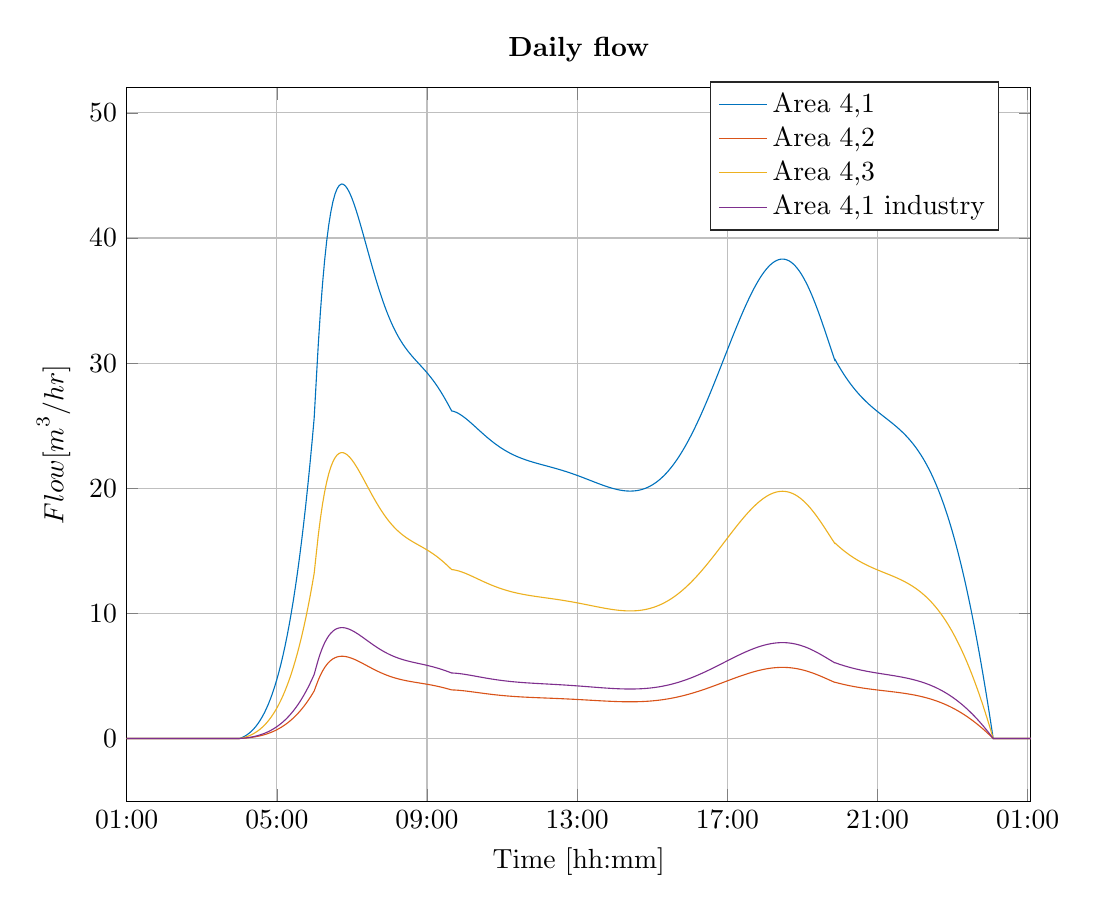
\begin{tikzpicture}

\begin{axis}[%
width=4.521in,
height=3.566in,
at={(0.64in,0.481in)},
scale only axis,
xmin=3600,
xmax=90000,
xtick={3600,17950,32300,46650,61000,75350,89700},
xticklabels={{01:00},{05:00},{09:00},{13:00},{17:00},{21:00},{01:00},{},{},{}},
xlabel={Time [hh:mm]},
xmajorgrids,
ymin=-5,
scaled x ticks = false,
ymax=52,
ylabel={$\text{Flow [m}^\text{3}\text{/hr]}$},
ymajorgrids,
axis background/.style={fill=white},
title style={font=\bfseries},
title={Daily flow},
legend style={at={(0.6450,0.8)},anchor=south west,legend cell align=left,align=left,draw=white!15!black}
]
\addplot [color=mycolor1,solid]
  table[row sep=crcr]{%
3599	0\\
3799	0\\
3998	0\\
4197	0\\
4396	0\\
4595	0\\
4794	0\\
4993	0\\
5192	0\\
5391	0\\
5590	0\\
5789	0\\
5988	0\\
6188	0\\
6387	0\\
6586	0\\
6785	0\\
6984	0\\
7183	0\\
7382	0\\
7581	0\\
7780	0\\
7979	0\\
8178	0\\
8377	0\\
8577	0\\
8776	0\\
8975	0\\
9174	0\\
9373	0\\
9572	0\\
9771	0\\
9970	0\\
10169	0\\
10368	0\\
10567	0\\
10766	0\\
10965	0\\
11165	0\\
11364	0\\
11563	0\\
11762	0\\
11961	0\\
12160	0\\
12359	0\\
12558	0\\
12757	0\\
12956	0\\
13155	0\\
13354	0\\
13554	0\\
13753	0\\
13952	0\\
14151	0\\
14350	0\\
14549	0.0478616674698634\\
14748	0.124184806964865\\
14947	0.216037794955245\\
15146	0.324956831753071\\
15345	0.452548027364151\\
15544	0.600487502551203\\
15743	0.770521410561261\\
15942	0.964465879517816\\
16142	1.18537951395245\\
16341	1.43301713786323\\
16540	1.71044214014931\\
16739	2.01974873106236\\
16938	2.36309961517783\\
17137	2.74272545737682\\
17336	3.16092426949164\\
17535	3.6200607176174\\
17734	4.12256535008644\\
17933	4.67093374610903\\
18132	5.26772558507796\\
18331	5.91556363653736\\
18531	6.62079843271939\\
18730	7.37913488843914\\
18929	8.19676736052568\\
19128	9.07655958137858\\
19327	10.021432126097\\
19526	11.0343609260374\\
19725	12.1183757030377\\
19924	13.2765583243048\\
20123	14.512041077967\\
20322	15.8280048692916\\
20521	17.2276773375662\\
20720	18.7143308936463\\
20920	20.299438710925\\
21119	21.9705196257897\\
21318	23.7386638251055\\
21517	25.6073017704141\\
21716	28.6171641842508\\
21915	31.5579485976407\\
22114	34.1120855607026\\
22313	36.3095695652932\\
22512	38.1789710150114\\
22711	39.7474682654159\\
22910	41.0408796640816\\
23109	42.0836955908396\\
23308	42.8991104979365\\
23508	43.5116365879267\\
23707	43.9359310311559\\
23906	44.1950476559769\\
24105	44.3073118184006\\
24175	44.3151254450439\\
24304	44.2899133085633\\
24503	44.1589383910118\\
24702	43.9294018446922\\
24901	43.6152790032352\\
25100	43.2295377949442\\
25299	42.7841707832406\\
25498	42.2902272064926\\
25697	41.7578450183689\\
25897	41.1934018666942\\
26096	40.6109868662571\\
26295	40.0154359766854\\
26494	39.4135585598243\\
26693	38.8114130545292\\
26892	38.2143390168595\\
27091	37.6269891602271\\
27290	37.0533613954644\\
27489	36.4968308711558\\
27688	35.9601820136712\\
27887	35.4456405673606\\
28086	34.954905634565\\
28285	34.4891817160158\\
28485	34.0470655708191\\
28684	33.6332900539721\\
28883	33.2454904550884\\
29082	32.8832115089587\\
29281	32.5456637105081\\
29480	32.2317553548762\\
29679	31.9401245775647\\
29878	31.6691713945636\\
30077	31.4170897425677\\
30276	31.1818995191019\\
30475	30.9614786227154\\
30674	30.7535949928787\\
30874	30.5549672639391\\
31073	30.3652159210023\\
31272	30.1809544232889\\
31471	29.9998314489239\\
31670	29.8195460789486\\
31869	29.6378798375148\\
32068	29.4527287320785\\
32267	29.2621352934341\\
32466	29.0643206157946\\
32665	28.8577163973044\\
32864	28.6409969798459\\
33063	28.4131113893244\\
33263	28.1720794600276\\
33462	27.9199052373084\\
33661	27.6553812410344\\
33860	27.3788777399722\\
34059	27.0912000485642\\
34258	26.7936205674646\\
34457	26.4879108231627\\
34656	26.1811617588014\\
34855	26.1427996062201\\
35054	26.0822484791968\\
35253	26.0025238650658\\
35452	25.9064081279736\\
35651	25.7964615913248\\
35851	25.6743978444628\\
36050	25.5435943394362\\
36249	25.4054244999429\\
36448	25.2616645027158\\
36647	25.1139195301243\\
36846	24.9636331092286\\
37045	24.8120961741526\\
37244	24.6604558541009\\
37443	24.5097239906285\\
37642	24.3607853869901\\
37841	24.2144057961896\\
38040	24.0712396464498\\
38240	23.931147307733\\
38439	23.795985311666\\
38638	23.6654071495862\\
38837	23.5396937419823\\
39036	23.4190495735519\\
39235	23.3036089339809\\
39434	23.193441922935\\
39633	23.0885602229615\\
39832	22.9889226457783\\
40031	22.8944404519043\\
40230	22.8049824523939\\
40429	22.7203798903499\\
40628	22.6404311108834\\
40828	22.5645372464259\\
41027	22.4932018336635\\
41226	22.4257599824778\\
41425	22.3619209104042\\
41624	22.3013812180461\\
41823	22.2438283480602\\
42022	22.1889438571456\\
42221	22.1364065021338\\
42420	22.0858951426877\\
42619	22.0370914695575\\
42818	21.9896825536906\\
43017	21.9433632279726\\
43217	21.8976110536423\\
43416	21.8525992287088\\
43615	21.8078280568108\\
43814	21.7630440035762\\
44013	21.7180107632865\\
44212	21.6725106859679\\
44411	21.6263460587927\\
44610	21.5793402443015\\
44809	21.5313386809233\\
45008	21.4822097470259\\
45207	21.4318454922843\\
45406	21.380162242667\\
45606	21.326830891331\\
45805	21.2723508662165\\
46004	21.2164506837005\\
46203	21.1591474937498\\
46402	21.1004839378446\\
46601	21.0405280577862\\
46800	20.9793730986594\\
46999	20.9171372128444\\
47198	20.8539630681331\\
47397	20.7900173614133\\
47596	20.7254902443541\\
47795	20.6605946633302\\
47994	20.5955656171447\\
48194	20.5303339396951\\
48393	20.4658297204926\\
48592	20.402022290614\\
48791	20.3392260009996\\
48990	20.2777724257208\\
49189	20.2180092019864\\
49388	20.1602988127313\\
49587	20.1050173135677\\
49786	20.0525530085714\\
49985	20.0033050834381\\
50184	19.957682192268\\
50383	19.9161010055083\\
50583	19.8788102032675\\
50782	19.8466127076352\\
50981	19.8197421666373\\
51180	19.7986321397974\\
51379	19.7837164657406\\
51578	19.7754276541773\\
51712	19.7737956079281\\
51777	19.7741952492232\\
51976	19.7804441953223\\
52175	19.7945931876046\\
52374	19.8170530206011\\
52573	19.8482249365031\\
52772	19.8884989769346\\
52971	19.9382523399749\\
53171	19.9981726695525\\
53370	20.0680088039533\\
53569	20.148364162357\\
53768	20.2395483108162\\
53967	20.3418499811879\\
54166	20.4555355430825\\
54365	20.5808475103174\\
54564	20.7180030780889\\
54763	20.8671927048264\\
54962	21.0285787325697\\
55161	21.202294051025\\
55360	21.3884408170765\\
55560	21.5881191020751\\
55759	21.7993692452879\\
55958	22.0231608068141\\
56157	22.2594611009438\\
56356	22.5082011523584\\
56555	22.7692747788161\\
56754	23.042537755582\\
56953	23.3278070570853\\
57152	23.6248601723791\\
57351	23.933434517864\\
57550	24.2532269276026\\
57749	24.5838932404414\\
57949	24.9267881131493\\
58148	25.2780536977554\\
58347	25.6389096007173\\
58546	26.0088453079527\\
58745	26.3873087511844\\
58944	26.773706520085\\
59143	27.167404195966\\
59342	27.5677268045932\\
59541	27.9739593871231\\
59740	28.3853477094724\\
59939	28.8010990939623\\
60138	29.2203833895323\\
60337	29.6423340750916\\
60537	30.0681816353865\\
60736	30.4927282371871\\
60935	30.9171317704582\\
61134	31.3403940732616\\
61333	31.7614883674884\\
61532	32.1793612673392\\
61731	32.5929349572268\\
61930	33.0011095386013\\
62129	33.4027655364759\\
62328	33.7967665914428\\
62527	34.1819623237595\\
62726	34.5571913778579\\
62926	34.9230841645496\\
63125	35.27480340644\\
63324	35.6130333929472\\
63523	35.9366030923363\\
63722	36.244348581946\\
63921	36.5351172557499\\
64120	36.8077722423273\\
64319	37.0611970241615\\
64518	37.294300269493\\
64717	37.5060208912882\\
64916	37.695333314518\\
65115	37.8612529715556\\
65314	38.002842027885\\
65514	38.1197350288152\\
65713	38.2099334634838\\
65912	38.2733252458911\\
66111	38.309221740352\\
66265	38.3177389797191\\
66310	38.317013227071\\
66509	38.2961760611039\\
66708	38.2462800904735\\
66907	38.1669963150936\\
67106	38.0581048292219\\
67305	37.9195030042633\\
67504	37.7512139479825\\
67703	37.5533952389376\\
67903	37.3251338656978\\
68102	37.0691685352106\\
68301	36.7850479932473\\
68500	36.4735613681301\\
68699	36.135680118532\\
68898	35.7725684553895\\
69097	35.3855940579336\\
69296	34.9763390994471\\
69495	34.5466115489748\\
69694	34.0984568116062\\
69893	33.634169652743\\
70092	33.1563064427748\\
70292	32.6652204075094\\
70491	32.1689538120778\\
70690	31.6684950972024\\
70889	31.1675774997545\\
71088	30.6702619816344\\
71260	30.2467012670642\\
71287	30.2900915921104\\
71486	29.9930657398363\\
71685	29.7070883817591\\
71884	29.4321299115032\\
72083	29.1681074617607\\
72282	28.9148865889408\\
72481	28.6722829596442\\
72680	28.4400640372302\\
72880	28.2168596096975\\
73079	28.0045763677234\\
73278	27.8017059095052\\
73477	27.6078395401385\\
73676	27.4225287998769\\
73875	27.2452871506974\\
74074	27.0755916616804\\
74273	26.912884695302\\
74472	26.756575594639\\
74671	26.6060423673793\\
74870	26.4606333740312\\
75069	26.3196690126641\\
75269	26.181762047693\\
75468	26.0475579603971\\
75667	25.9156049475287\\
75866	25.7851283177211\\
76065	25.6553338569375\\
76264	25.5254095138501\\
76463	25.3945270866804\\
76662	25.2618439081221\\
76861	25.1265045328207\\
77060	24.9876424231173\\
77259	24.8443816341551\\
77458	24.6958385014491\\
77657	24.5411233264487\\
77857	24.3785097342767\\
78056	24.2087233896747\\
78255	24.0300720505576\\
78454	23.8416587495079\\
78653	23.6425889249026\\
78852	23.43197210474\\
79051	23.2089235951239\\
79250	22.9725661640906\\
79449	22.7220317295447\\
79648	22.4564630448209\\
79847	22.1750153836988\\
80046	21.8768582281554\\
80246	21.5595450109666\\
80445	21.2254485257771\\
80644	20.8722492397831\\
80843	20.4991904362003\\
81042	20.1055380433808\\
81241	19.6905823221095\\
81440	19.2536395524448\\
81639	18.7940537189145\\
81838	18.3111981969918\\
82037	17.8044774387479\\
82236	17.2733286595101\\
82435	16.7172235243361\\
82635	16.1326824065839\\
82834	15.5250945318866\\
83033	14.8911868683791\\
83232	14.2305859488115\\
83431	13.5429611949773\\
83630	12.8280266025444\\
83829	12.0855424271655\\
84028	11.3153168716833\\
84227	10.5172077714183\\
84426	9.69112427863591\\
84625	8.83702855303764\\
84824	7.95493744275914\\
85023	7.04492417440511\\
85223	6.10233757334092\\
85422	5.13679549794403\\
85621	4.1439074916505\\
85820	3.12398947087849\\
86019	2.07742216809305\\
86218	1.00465281736833\\
86401	0\\
86417	0\\
86616	0\\
86815	0\\
87014	0\\
87213	0\\
87412	0\\
87612	0\\
87811	0\\
88010	0\\
88209	0\\
88408	0\\
88607	0\\
88806	0\\
89005	0\\
89204	0\\
89403	0\\
89602	0\\
90000	0\\
};
\addlegendentry{Area 4,1};

\addplot [color=mycolor2,solid]
  table[row sep=crcr]{%
3599	0\\
3799	0\\
3998	0\\
4197	0\\
4396	0\\
4595	0\\
4794	0\\
4993	0\\
5192	0\\
5391	0\\
5590	0\\
5789	0\\
5988	0\\
6188	0\\
6387	0\\
6586	0\\
6785	0\\
6984	0\\
7183	0\\
7382	0\\
7581	0\\
7780	0\\
7979	0\\
8178	0\\
8377	0\\
8577	0\\
8776	0\\
8975	0\\
9174	0\\
9373	0\\
9572	0\\
9771	0\\
9970	0\\
10169	0\\
10368	0\\
10567	0\\
10766	0\\
10965	0\\
11165	0\\
11364	0\\
11563	0\\
11762	0\\
11961	0\\
12160	0\\
12359	0\\
12558	0\\
12757	0\\
12956	0\\
13155	0\\
13354	0\\
13554	0\\
13753	0\\
13952	0\\
14151	0\\
14350	0\\
14549	0.00710028180255936\\
14748	0.0184228250217605\\
14947	0.0320492223793003\\
15146	0.0482073693016751\\
15345	0.0671355323234623\\
15544	0.0890823640800493\\
15743	0.114306906530896\\
15942	0.143078582413403\\
16142	0.175851135929245\\
16341	0.212588195200944\\
16540	0.253744214191448\\
16739	0.299629869141819\\
16938	0.350565997430973\\
17137	0.406883518354036\\
17336	0.468923342131185\\
17535	0.537036267147258\\
17734	0.611582865421718\\
17933	0.692933356309431\\
18132	0.781467468431938\\
18331	0.877574289839258\\
18531	0.982195922443594\\
18730	1.09469519004965\\
18929	1.21599102593738\\
19128	1.3465082650137\\
19327	1.48668017480407\\
19526	1.63694823493869\\
19725	1.79776190486959\\
19924	1.96957837981796\\
20123	2.15286233495235\\
20322	2.34808565779734\\
20521	2.55572716887281\\
20720	2.77627233056388\\
20920	3.0114231889665\\
21119	3.25932816256334\\
21318	3.52163248137147\\
21517	3.79884505460662\\
21716	4.24535835961483\\
21915	4.68162393830136\\
22114	5.0605303399952\\
22313	5.38652724971494\\
22512	5.66385308888405\\
22711	5.89653976849929\\
22910	6.08841744227553\\
23109	6.24311925981753\\
23308	6.36408611977997\\
23508	6.45495440917018\\
23707	6.51789852026043\\
23906	6.55633849014062\\
24105	6.57299288668956\\
24175	6.57415203876262\\
24304	6.57041181650709\\
24503	6.55098167809271\\
24702	6.51692991498017\\
24901	6.4703297689161\\
25100	6.41310503299458\\
25299	6.3470348048595\\
25498	6.2737582398154\\
25697	6.19477930401627\\
25897	6.11104412197444\\
26096	6.02464281487946\\
26295	5.93629279768905\\
26494	5.84700423972142\\
26693	5.75767591081538\\
26892	5.66909993449537\\
27091	5.58196654112981\\
27290	5.4968688210775\\
27489	5.41430747787304\\
27688	5.33469558136816\\
27887	5.25836332089683\\
28086	5.18556275841323\\
28285	5.11647258168728\\
28485	5.0508846198317\\
28684	4.98950099222484\\
28883	4.93197089391124\\
29082	4.87822678626446\\
29281	4.82815154614999\\
29480	4.78158321907345\\
29679	4.73831977233886\\
29878	4.69812384820355\\
30077	4.66072751704663\\
30276	4.62583703052387\\
30475	4.59313757473281\\
30674	4.5622980233338\\
30874	4.53283158549684\\
31073	4.50468196016016\\
31272	4.4773467537562\\
31471	4.45047714751611\\
31670	4.42373179994733\\
31869	4.39678159999861\\
32068	4.36931442022513\\
32267	4.34103986992983\\
32466	4.31169404831157\\
32665	4.28104429767759\\
32864	4.24889395655103\\
33063	4.21508711284956\\
33263	4.17933000884771\\
33462	4.14191994481735\\
33661	4.1026777909942\\
33860	4.06165847677637\\
34059	4.01898147061914\\
34258	3.97483553325084\\
34457	3.92948347075326\\
34656	3.88397722505031\\
34855	3.87828619696292\\
35054	3.86930343292533\\
35253	3.85747628069986\\
35452	3.84321750420727\\
35651	3.8269069276083\\
35851	3.80879876200495\\
36050	3.78939405265094\\
36249	3.76889654705036\\
36448	3.74756974114895\\
36647	3.72565176386635\\
36846	3.70335676254554\\
37045	3.68087624735635\\
37244	3.65838039499861\\
37443	3.63601931223958\\
37642	3.61392425970557\\
37841	3.59220883690962\\
38040	3.57097012832554\\
38240	3.55018741982724\\
38439	3.53013612801473\\
38638	3.51076484830304\\
38837	3.49211525526681\\
39036	3.47421768422563\\
39235	3.45709205706402\\
39434	3.44074877307242\\
39633	3.42518956535756\\
39832	3.41040832363483\\
40031	3.39639188339584\\
40230	3.38312078275112\\
40429	3.37056998660284\\
40628	3.35870957943378\\
40828	3.34745071919719\\
41027	3.33686810559657\\
41226	3.32686310213515\\
41425	3.31739257121347\\
41624	3.30841150350928\\
41823	3.29987353111825\\
42022	3.29173141295388\\
42221	3.28393749256906\\
42420	3.27644412877175\\
42619	3.26920410036191\\
42818	3.26217098429212\\
43017	3.25529950899909\\
43217	3.24851217065511\\
43416	3.24183466319726\\
43615	3.23519285663449\\
43814	3.22854913912451\\
44013	3.22186845469703\\
44212	3.21511851496282\\
44411	3.20826998920971\\
44610	3.20129667325793\\
44809	3.19417563788733\\
45008	3.18688735701933\\
45207	3.17941581621549\\
45406	3.17174860242722\\
45606	3.16383689263074\\
45805	3.15575477699682\\
46004	3.14746198091052\\
46203	3.13896104857063\\
46402	3.13025830584381\\
46601	3.12136384673614\\
46800	3.11229150416268\\
46999	3.10305880603746\\
47198	3.09368691713768\\
47397	3.08420056695858\\
47596	3.07462796451394\\
47795	3.06500070041369\\
47994	3.05535363674715\\
48194	3.04567651271804\\
48393	3.03610730717207\\
48592	3.02664147037229\\
48791	3.01732563630324\\
48990	3.0082089940022\\
49189	2.99934311547402\\
49388	2.99078177508811\\
49587	2.98258076072152\\
49786	2.97479767731173\\
49985	2.96749174408537\\
50184	2.96072358490748\\
50383	2.95455501286881\\
50583	2.94902291968129\\
50782	2.94424641889452\\
50981	2.94026017220989\\
51180	2.93712849821384\\
51379	2.93491575689753\\
51578	2.9336861111075\\
51712	2.93344399692937\\
51777	2.93350328374416\\
51976	2.93443031534624\\
52175	2.9365293193663\\
52374	2.93986123720252\\
52573	2.94448559316272\\
52772	2.95046024994984\\
52971	2.95784116492597\\
53171	2.96673035011726\\
53370	2.97709054566539\\
53569	2.98901126884894\\
53768	3.00253844381405\\
53967	3.01771490395241\\
54166	3.03458016521482\\
54365	3.0531702045435\\
54564	3.07351724286139\\
54763	3.09564953469017\\
54962	3.11959116348308\\
55161	3.14536184343757\\
55360	3.17297672953474\\
55560	3.2025990174384\\
55759	3.23393799133826\\
55958	3.26713748554458\\
56157	3.30219265112997\\
56356	3.33909325560095\\
56555	3.37782354681432\\
56754	3.41836212902034\\
56953	3.46068185036243\\
57152	3.50474970132568\\
57351	3.55052672761426\\
57550	3.59796795453961\\
57749	3.64702232576993\\
57949	3.69789080473406\\
58148	3.75000107940876\\
58347	3.80353407849953\\
58546	3.85841406720561\\
58745	3.91455914615849\\
58944	3.97188128289352\\
59143	4.03028636135278\\
59342	4.08967424906017\\
59541	4.14993888181998\\
59740	4.21096836895186\\
59939	4.27264511666528\\
60138	4.33484597199087\\
60337	4.39744238646266\\
60537	4.460616902581\\
60736	4.52359842141341\\
60935	4.58655871601919\\
61134	4.64934970900322\\
61333	4.7118190777594\\
61532	4.77381055242879\\
61731	4.83516423899175\\
61930	4.89571696741947\\
62129	4.95530266351737\\
62328	5.01375274828578\\
62527	5.07089656280736\\
62726	5.12656181990029\\
62926	5.1808420410537\\
63125	5.23301961581908\\
63324	5.28319605858069\\
63523	5.33119764669666\\
63722	5.37685171215669\\
63921	5.41998726577409\\
64120	5.46043565259203\\
64319	5.49803123715681\\
64518	5.53261212032364\\
64717	5.56402088975496\\
64916	5.5921054013216\\
65115	5.61671959434555\\
65314	5.63772434100905\\
65514	5.65506542608248\\
65713	5.66844637033604\\
65912	5.67785054580365\\
66111	5.68317579333198\\
66265	5.6844393264031\\
66310	5.68433166094568\\
66509	5.68124046587969\\
66708	5.67383839505733\\
66907	5.66207664129223\\
67106	5.64592258155172\\
67305	5.62536099087637\\
67504	5.60039529730472\\
67703	5.57104887762718\\
67903	5.5371862865325\\
68102	5.49921381139279\\
68301	5.45706450861086\\
68500	5.41085544542991\\
68699	5.36073073781378\\
68898	5.30686309653841\\
69097	5.24945541691582\\
69296	5.18874241446603\\
69495	5.12499230152653\\
69694	5.05850851408906\\
69893	4.9896314807656\\
70092	4.91874043928682\\
70292	4.84588779072665\\
70491	4.77226660569418\\
70690	4.6980235194415\\
70889	4.62371235792628\\
71088	4.54993556513772\\
71260	4.48710030274668\\
71287	4.49353726057994\\
71486	4.44947345408763\\
71685	4.407048692502\\
71884	4.36625858371511\\
72083	4.32709083435589\\
72282	4.289525499708\\
72481	4.25353523389844\\
72680	4.21908554009987\\
72880	4.18597314726358\\
73079	4.15448091308838\\
73278	4.12438506605859\\
73477	4.09562497625584\\
73676	4.06813411464458\\
73875	4.04184030327419\\
74074	4.01666596530525\\
74273	3.99252837517106\\
74472	3.96933990887471\\
74671	3.94700829381207\\
74870	3.92543685921783\\
75069	3.9045247860968\\
75269	3.88406627795044\\
75468	3.86415709197283\\
75667	3.84458185304801\\
75866	3.82522563565619\\
76065	3.80597061808801\\
76264	3.78669633247073\\
76463	3.76727991501112\\
76662	3.74759635595384\\
76861	3.72751874991917\\
77060	3.70691854598326\\
77259	3.68566579766375\\
77458	3.66362941327093\\
77657	3.64067740596097\\
77857	3.61655366789701\\
78056	3.5913658514955\\
78255	3.56486291252174\\
78454	3.53691178579501\\
78653	3.50737976303432\\
78852	3.4761347426544\\
79051	3.44304548025224\\
79250	3.40798183840312\\
79449	3.37081503706588\\
79648	3.33141790363627\\
79847	3.28966512291887\\
80046	3.24543348750541\\
80246	3.19836004897266\\
80445	3.14879681142805\\
80644	3.09639967201374\\
80843	3.04105637174048\\
81042	2.98265801102665\\
81241	2.92109930000879\\
81440	2.85627880878449\\
81639	2.78809921741142\\
81838	2.71646756609606\\
82037	2.64129550526046\\
82236	2.56249954575803\\
82435	2.4800013090622\\
82635	2.39328459231101\\
82834	2.30314888751374\\
83033	2.20910864015839\\
83232	2.11110844635167\\
83431	2.0090992647929\\
83630	1.90303866671892\\
83829	1.79289108603862\\
84028	1.67862806962992\\
84227	1.56022852735244\\
84426	1.43767898193824\\
84625	1.31097381977632\\
84824	1.1801155402888\\
85023	1.04511500664776\\
85223	0.905282216762484\\
85422	0.762043980613217\\
85621	0.614748973653748\\
85820	0.463444062107368\\
86019	0.308185727662584\\
86218	0.149040317526378\\
86401	0\\
86417	0\\
86616	0\\
86815	0\\
87014	0\\
87213	0\\
87412	0\\
87612	0\\
87811	0\\
88010	0\\
88209	0\\
88408	0\\
88607	0\\
88806	0\\
89005	0\\
89204	0\\
89403	0\\
89602	0\\
90000	0\\
};
\addlegendentry{Area 4,2};

\addplot [color=mycolor3,solid]
  table[row sep=crcr]{%
3599	0\\
3799	0\\
3998	0\\
4197	0\\
4396	0\\
4595	0\\
4794	0\\
4993	0\\
5192	0\\
5391	0\\
5590	0\\
5789	0\\
5988	0\\
6188	0\\
6387	0\\
6586	0\\
6785	0\\
6984	0\\
7183	0\\
7382	0\\
7581	0\\
7780	0\\
7979	0\\
8178	0\\
8377	0\\
8577	0\\
8776	0\\
8975	0\\
9174	0\\
9373	0\\
9572	0\\
9771	0\\
9970	0\\
10169	0\\
10368	0\\
10567	0\\
10766	0\\
10965	0\\
11165	0\\
11364	0\\
11563	0\\
11762	0\\
11961	0\\
12160	0\\
12359	0\\
12558	0\\
12757	0\\
12956	0\\
13155	0\\
13354	0\\
13554	0\\
13753	0\\
13952	0\\
14151	0\\
14350	0\\
14549	0.0246793160526096\\
14748	0.064034461439272\\
14947	0.111397393840624\\
15146	0.167560237205242\\
15345	0.233351163607856\\
15544	0.309634445361409\\
15743	0.397310466220541\\
15942	0.497315691676762\\
16142	0.611227255831437\\
16341	0.738918736510825\\
16540	0.881969734820176\\
16739	1.04146010608868\\
16938	1.21850502395253\\
17137	1.41425470499459\\
17336	1.62989409247532\\
17535	1.86664249915594\\
17734	2.12575320921243\\
17933	2.40851303924187\\
18132	2.71624185836014\\
18331	3.050292067391\\
18531	3.41393824493451\\
18730	3.80496567992113\\
18929	4.22656842090808\\
19128	4.68022311843252\\
19327	5.16743573331317\\
19526	5.68974077018343\\
19725	6.24870047011731\\
19924	6.84590396234597\\
20123	7.48296637506648\\
20322	8.16152790534202\\
20521	8.88325284809369\\
20720	9.64982858418433\\
20920	10.4671711229648\\
21119	11.3288446965693\\
21318	12.2405678317689\\
21517	13.2041094064373\\
21716	14.7561101977328\\
21915	16.272491715914\\
22114	17.5895029419175\\
22313	18.7226101890479\\
22512	19.6865454559471\\
22711	20.4953229477625\\
22910	21.1622555972323\\
23109	21.6999715858648\\
23308	22.1204308650766\\
23508	22.4362728690113\\
23707	22.6550553982746\\
23906	22.7886658931967\\
24105	22.8465536119558\\
24175	22.8505826182909\\
24304	22.8375822713022\\
24503	22.7700465677613\\
24702	22.6516886986835\\
24901	22.4897148834472\\
25100	22.2908118845092\\
25299	22.0611635286896\\
25498	21.8064672281398\\
25697	21.5319505015807\\
25897	21.2409019094547\\
26096	20.9405863410801\\
26295	20.6334974031861\\
26494	20.3231462645636\\
26693	20.0126568892364\\
26892	19.7047825576174\\
27091	19.4019223876408\\
27290	19.1061378558535\\
27489	18.8191693186419\\
27688	18.5424525333048\\
27887	18.2771351792101\\
28086	18.0240933788561\\
28285	17.7839482191336\\
28485	17.5559761350823\\
28684	17.3426175687196\\
28883	17.1426531844458\\
29082	16.955848230014\\
29281	16.7817956062505\\
29480	16.6199323881528\\
29679	16.4695563460211\\
29878	16.3298424665798\\
30077	16.1998594741447\\
30276	16.0785863517435\\
30475	15.9649288622725\\
30674	15.8577360694987\\
30874	15.7553159751215\\
31073	15.6574728866689\\
31272	15.5624605735008\\
31471	15.4690666036488\\
31670	15.3761045348266\\
31869	15.2824304355851\\
32068	15.1869594064692\\
32267	15.0886821010907\\
32466	14.9866812472261\\
32665	14.8801481681366\\
32864	14.7683993035246\\
33063	14.6508927307363\\
33263	14.5266074001921\\
33462	14.3965766747326\\
33661	14.2601779311733\\
33860	14.1176020943271\\
34059	13.9692644152855\\
34258	13.81582099275\\
34457	13.6581852938948\\
34656	13.5000136816546\\
34855	13.4802326807396\\
35054	13.4490101914252\\
35253	13.4079011149277\\
35452	13.3583401451847\\
35651	13.301647483389\\
35851	13.2387067220946\\
36050	13.1712594054424\\
36249	13.1000137235\\
36448	13.0258855412856\\
36647	12.949702552549\\
36846	12.8722090953469\\
37045	12.7940708249504\\
37244	12.7158792452853\\
37443	12.6381561007631\\
37642	12.5613576299631\\
37841	12.4858786845775\\
38040	12.4120567129613\\
38240	12.3398197164982\\
38439	12.2701249942794\\
38638	12.2027938731152\\
38837	12.1379712064109\\
39036	12.0757624343394\\
39235	12.016236801826\\
39434	11.9594304549538\\
39633	11.9053494176935\\
39832	11.853972451783\\
40031	11.8052537997337\\
40230	11.7591258154812\\
40429	11.7155014814803\\
40628	11.6742768167167\\
40828	11.6351430220452\\
41027	11.5983597403424\\
41226	11.563584128698\\
41425	11.5306662484925\\
41624	11.4994496553311\\
41823	11.4697731826296\\
42022	11.4414726287778\\
42221	11.414382348446\\
42420	11.3883367493285\\
42619	11.3631716989368\\
42818	11.3387258390192\\
43017	11.3148418136777\\
43217	11.2912502333989\\
43416	11.2680404057359\\
43615	11.2449546680313\\
43814	11.2218622882142\\
44013	11.1986414179701\\
44212	11.1751798286038\\
44411	11.1513755717792\\
44610	11.1271375664304\\
44809	11.1023861146683\\
45008	11.0770533473186\\
45207	11.051083601043\\
45406	11.0244337302934\\
45606	10.9969340349274\\
45805	10.968842039194\\
46004	10.9400177556987\\
46203	10.9104700276236\\
46402	10.8802208425558\\
46601	10.8493052854639\\
46800	10.8177714370993\\
46999	10.785680221372\\
47198	10.7531052032812\\
47397	10.720132338152\\
47596	10.6868596754962\\
47795	10.6533970186526\\
47994	10.6198655420399\\
48194	10.5862295809561\\
48393	10.5529687253157\\
48592	10.5200671610426\\
48791	10.4876869795685\\
48990	10.455999153234\\
49189	10.4251829371505\\
49388	10.3954252414571\\
49587	10.366919974887\\
49786	10.339867361952\\
49985	10.3144732381459\\
50184	10.2909483212355\\
50383	10.2695074625247\\
50583	10.2502788910392\\
50782	10.2336766242814\\
50981	10.219821140157\\
51180	10.2089359986272\\
51379	10.2012449035684\\
51578	10.1969708736174\\
51712	10.1961293278183\\
51777	10.1963353982365\\
51976	10.1995575951203\\
52175	10.2068533595769\\
52374	10.2184345130618\\
52573	10.2345079514766\\
52772	10.2552747952802\\
52971	10.2809295423056\\
53171	10.3118267682025\\
53370	10.347836964334\\
53569	10.3892712768309\\
53768	10.4362893298527\\
53967	10.489040004647\\
54166	10.5476606516267\\
54365	10.6122763202412\\
54564	10.6829990046846\\
54763	10.7599269126465\\
54962	10.8431437539247\\
55161	10.9327180515615\\
55360	11.0287024815743\\
55560	11.1316642830499\\
55759	11.2405929795645\\
55958	11.3559885135853\\
56157	11.4778340311036\\
56356	11.6060939657929\\
56555	11.7407135660064\\
56754	11.8816184639256\\
56953	12.0287142845286\\
57152	12.1818862926156\\
57351	12.3409990899861\\
57550	12.5058963526261\\
57749	12.6764006178115\\
57949	12.8532103986598\\
58148	13.0343364404208\\
58347	13.2204076190786\\
58546	13.4111606939429\\
58745	13.6063109973826\\
58944	13.805552544216\\
59143	14.0085582037736\\
59342	14.2149799333871\\
59541	14.4244490727863\\
59740	14.6365767098772\\
59939	14.8509541095697\\
60138	15.0671532140572\\
60337	15.2847272117474\\
60537	15.5043105878879\\
60736	15.7232231398064\\
60935	15.9420619200899\\
61134	16.1603122380634\\
61333	16.3774446474538\\
61532	16.5929159820397\\
61731	16.8061704786618\\
61930	17.0166409873362\\
62129	17.2237502637151\\
62328	17.4269123571945\\
62527	17.6255340877463\\
62726	17.819016615785\\
62926	18.0076850053646\\
63125	18.1890449702648\\
63324	18.3634493564207\\
63523	18.5302943348431\\
63722	18.6889797422545\\
63921	18.8389112506693\\
64120	18.9795026454698\\
64319	19.1101782072936\\
64518	19.2303752035234\\
64717	19.3395464968852\\
64916	19.4371632614602\\
65115	19.5227178163229\\
65314	19.5957265779367\\
65514	19.6560011038109\\
65713	19.7025108849011\\
65912	19.7351981253562\\
66111	19.7537077381384\\
66265	19.7580995542483\\
66310	19.7577253282773\\
66509	19.7469808843052\\
66708	19.721252603323\\
66907	19.6803708402362\\
67106	19.6242222031885\\
67305	19.55275377293\\
67504	19.4659774647129\\
67703	19.3639745321007\\
67903	19.2462741912938\\
68102	19.1142886248991\\
68301	18.9677851488853\\
68500	18.8071706681577\\
68699	18.6329461041612\\
68898	18.4457117688192\\
69097	18.246172890131\\
69296	18.0351452974767\\
69495	17.8135612492131\\
69694	17.5824754348512\\
69893	17.3430711236669\\
70092	17.0966664785269\\
70292	16.8434436362394\\
70491	16.5875494979351\\
70690	16.3294937416564\\
70889	16.0712013678791\\
71088	15.814766364705\\
71260	15.5963621741505\\
71287	15.6187358941241\\
71486	15.4655779438984\\
71685	15.3181170221008\\
71884	15.1763378625455\\
72083	15.0401977356626\\
72282	14.9096273171669\\
72481	14.7845315576702\\
72680	14.6647905523394\\
72880	14.5496977671812\\
73079	14.4402363652221\\
73278	14.3356285564938\\
73477	14.2356636021891\\
73676	14.1401102592192\\
73875	14.0487176498718\\
74074	13.9612161308579\\
74273	13.8773181628286\\
74472	13.7967191803633\\
74671	13.7190984603101\\
74870	13.644119992291\\
75069	13.5714333474196\\
75269	13.5003232136885\\
75468	13.4311224260642\\
75667	13.3630823789696\\
75866	13.2958036117489\\
76065	13.2288765971067\\
76264	13.1618826101546\\
76463	13.0943945982108\\
76662	13.0259780496113\\
76861	12.956191863839\\
77060	12.8845892207581\\
77259	12.8107184495198\\
77458	12.7341238987386\\
77657	12.6543468056322\\
77857	12.5704969849341\\
78056	12.4829486172871\\
78255	12.3908291176046\\
78454	12.2936759749973\\
78653	12.1910279190961\\
78852	12.0824257882978\\
79051	11.9674134004125\\
79250	11.8455384209099\\
79449	11.7163532332832\\
79648	11.5794158081903\\
79847	11.4342905723118\\
80046	11.2805492786213\\
80246	11.1169303829862\\
80445	10.9446573890449\\
80644	10.7625342564965\\
80843	10.5701707930709\\
81042	10.3671884832009\\
81241	10.1532213580576\\
81440	9.92791686534956\\
81639	9.69093673827528\\
81838	9.44195786513464\\
82037	9.18067315851651\\
82236	8.9067924250042\\
82435	8.6200432347868\\
82635	8.31863135857426\\
82834	8.00533568832146\\
83033	7.67846852294898\\
83232	7.33783728838288\\
83431	6.98327152578885\\
83630	6.61462376033636\\
83829	6.23177037062165\\
84028	5.83461245865564\\
84227	5.42307671886333\\
84426	4.99711630665961\\
84625	4.55671171013161\\
84824	4.10187161682587\\
85023	3.6326337851954\\
85223	3.14659989075857\\
85422	2.64872927110629\\
85621	2.13675803801893\\
85820	1.61084909014882\\
86019	1.07119874779432\\
86218	0.518037622040429\\
86401	0\\
86417	0\\
86616	0\\
86815	0\\
87014	0\\
87213	0\\
87412	0\\
87612	0\\
87811	0\\
88010	0\\
88209	0\\
88408	0\\
88607	0\\
88806	0\\
89005	0\\
89204	0\\
89403	0\\
89602	0\\
90000	0\\
};
\addlegendentry{Area 4,3};

\addplot [color=mycolor4,solid]
  table[row sep=crcr]{%
3599	0\\
3799	0\\
3998	0\\
4197	0\\
4396	0\\
4595	0\\
4794	0\\
4993	0\\
5192	0\\
5391	0\\
5590	0\\
5789	0\\
5988	0\\
6188	0\\
6387	0\\
6586	0\\
6785	0\\
6984	0\\
7183	0\\
7382	0\\
7581	0\\
7780	0\\
7979	0\\
8178	0\\
8377	0\\
8577	0\\
8776	0\\
8975	0\\
9174	0\\
9373	0\\
9572	0\\
9771	0\\
9970	0\\
10169	0\\
10368	0\\
10567	0\\
10766	0\\
10965	0\\
11165	0\\
11364	0\\
11563	0\\
11762	0\\
11961	0\\
12160	0\\
12359	0\\
12558	0\\
12757	0\\
12956	0\\
13155	0\\
13354	0\\
13554	0\\
13753	0\\
13952	0\\
14151	0\\
14350	0\\
14549	0.00957233349397267\\
14748	0.024836961392973\\
14947	0.0432075589910489\\
15146	0.0649913663506142\\
15345	0.0905096054728303\\
15544	0.120097500510241\\
15743	0.154104282112252\\
15942	0.192893175903563\\
16142	0.237075902790491\\
16341	0.286603427572646\\
16540	0.342088428029863\\
16739	0.403949746212472\\
16938	0.472619923035567\\
17137	0.548545091475364\\
17336	0.632184853898328\\
17535	0.724012143523479\\
17734	0.824513070017287\\
17933	0.934186749221806\\
18132	1.05354511701559\\
18331	1.18311272730747\\
18531	1.32415968654388\\
18730	1.47582697768783\\
18929	1.63935347210514\\
19128	1.81531191627572\\
19327	2.00428642521941\\
19526	2.20687218520748\\
19725	2.42367514060755\\
19924	2.65531166486096\\
20123	2.9024082155934\\
20322	3.16560097385831\\
20521	3.44553546751325\\
20720	3.74286617872926\\
20920	4.059887742185\\
21119	4.39410392515793\\
21318	4.74773276502111\\
21517	5.12146035408281\\
21716	5.72343283685017\\
21915	6.31158971952813\\
22114	6.82241711214053\\
22313	7.26191391305864\\
22512	7.63579420300229\\
22711	7.94949365308318\\
22910	8.20817593281633\\
23109	8.41673911816792\\
23308	8.57982209958731\\
23508	8.70232731758533\\
23707	8.78718620623118\\
23906	8.83900953119538\\
24105	8.86146236368013\\
24175	8.86302508900879\\
24304	8.85798266171266\\
24503	8.83178767820236\\
24702	8.78588036893845\\
24901	8.72305580064704\\
25100	8.64590755898883\\
25299	8.55683415664811\\
25498	8.45804544129852\\
25697	8.35156900367377\\
25897	8.23868037333884\\
26096	8.12219737325142\\
26295	8.00308719533708\\
26494	7.88271171196486\\
26693	7.76228261090584\\
26892	7.6428678033719\\
27091	7.52539783204541\\
27290	7.41067227909288\\
27489	7.29936617423115\\
27688	7.19203640273425\\
27887	7.08912811347213\\
28086	6.990981126913\\
28285	6.89783634320317\\
28485	6.80941311416381\\
28684	6.72665801079441\\
28883	6.64909809101767\\
29082	6.57664230179173\\
29281	6.50913274210163\\
29480	6.44635107097523\\
29679	6.38802491551293\\
29878	6.33383427891272\\
30077	6.28341794851354\\
30276	6.23637990382038\\
30475	6.19229572454307\\
30674	6.15071899857575\\
30874	6.11099345278781\\
31073	6.07304318420045\\
31272	6.03619088465778\\
31471	5.99996628978478\\
31670	5.96390921578972\\
31869	5.92757596750296\\
32068	5.8905457464157\\
32267	5.85242705868683\\
32466	5.81286412315892\\
32665	5.77154327946089\\
32864	5.72819939596919\\
33063	5.68262227786487\\
33263	5.63441589200552\\
33462	5.58398104746169\\
33661	5.53107624820688\\
33860	5.47577554799445\\
34059	5.41824000971284\\
34258	5.35872411349291\\
34457	5.29758216463254\\
34656	5.23623235176029\\
34855	5.22855992124402\\
35054	5.21644969583937\\
35253	5.20050477301316\\
35452	5.18128162559471\\
35651	5.15929231826496\\
35851	5.13487956889255\\
36050	5.10871886788725\\
36249	5.08108489998858\\
36448	5.05233290054316\\
36647	5.02278390602485\\
36846	4.99272662184572\\
37045	4.96241923483051\\
37244	4.93209117082018\\
37443	4.9019447981257\\
37642	4.87215707739803\\
37841	4.84288115923792\\
38040	4.81424792928995\\
38240	4.78622946154659\\
38439	4.7591970623332\\
38638	4.73308142991725\\
38837	4.70793874839645\\
39036	4.68380991471037\\
39235	4.66072178679618\\
39434	4.638688384587\\
39633	4.6177120445923\\
39832	4.59778452915567\\
40031	4.57888809038085\\
40230	4.56099649047879\\
40429	4.54407597806998\\
40628	4.52808622217669\\
40828	4.51290744928519\\
41027	4.4986403667327\\
41226	4.48515199649555\\
41425	4.47238418208084\\
41624	4.46027624360923\\
41823	4.44876566961203\\
42022	4.43778877142912\\
42221	4.42728130042675\\
42420	4.41717902853755\\
42619	4.40741829391151\\
42818	4.39793651073813\\
43017	4.38867264559451\\
43217	4.37952221072846\\
43416	4.37051984574176\\
43615	4.36156561136217\\
43814	4.35260880071525\\
44013	4.34360215265731\\
44212	4.33450213719359\\
44411	4.32526921175854\\
44610	4.3158680488603\\
44809	4.30626773618466\\
45008	4.29644194940517\\
45207	4.28636909845687\\
45406	4.2760324485334\\
45606	4.2653661782662\\
45805	4.2544701732433\\
46004	4.2432901367401\\
46203	4.23182949874996\\
46402	4.22009678756893\\
46601	4.20810561155724\\
46800	4.19587461973189\\
46999	4.18342744256888\\
47198	4.17079261362662\\
47397	4.15800347228266\\
47596	4.14509804887082\\
47795	4.13211893266604\\
47994	4.11911312342894\\
48194	4.10606678793902\\
48393	4.09316594409851\\
48592	4.08040445812279\\
48791	4.06784520019992\\
48990	4.05555448514416\\
49189	4.04360184039728\\
49388	4.03205976254625\\
49587	4.02100346271354\\
49786	4.01051060171427\\
49985	4.00066101668762\\
50184	3.99153643845361\\
50383	3.98322020110167\\
50583	3.9757620406535\\
50782	3.96932254152705\\
50981	3.96394843332746\\
51180	3.95972642795948\\
51379	3.95674329314813\\
51578	3.95508553083545\\
51712	3.95475912158563\\
51777	3.95483904984464\\
51976	3.95608883906446\\
52175	3.95891863752091\\
52374	3.96341060412022\\
52573	3.96964498730062\\
52772	3.97769979538692\\
52971	3.98765046799497\\
53171	3.9996345339105\\
53370	4.01360176079067\\
53569	4.0296728324714\\
53768	4.04790966216323\\
53967	4.06836999623758\\
54166	4.0911071086165\\
54365	4.11616950206349\\
54564	4.14360061561778\\
54763	4.17343854096527\\
54962	4.20571574651393\\
55161	4.240458810205\\
55360	4.2776881634153\\
55560	4.31762382041502\\
55759	4.35987384905757\\
55958	4.40463216136281\\
56157	4.45189222018876\\
56356	4.50164023047169\\
56555	4.55385495576321\\
56754	4.60850755111639\\
56953	4.66556141141705\\
57152	4.72497203447582\\
57351	4.7866869035728\\
57550	4.85064538552052\\
57749	4.91677864808828\\
57949	4.98535762262987\\
58148	5.05561073955108\\
58347	5.12778192014347\\
58546	5.20176906159054\\
58745	5.27746175023688\\
58944	5.35474130401699\\
59143	5.4334808391932\\
59342	5.51354536091864\\
59541	5.59479187742462\\
59740	5.67706954189448\\
59939	5.76021981879246\\
60138	5.84407667790645\\
60337	5.92846681501833\\
60537	6.01363632707729\\
60736	6.09854564743742\\
60935	6.18342635409164\\
61134	6.26807881465231\\
61333	6.35229767349768\\
61532	6.43587225346783\\
61731	6.51858699144536\\
61930	6.60022190772026\\
62129	6.68055310729518\\
62328	6.75935331828856\\
62527	6.83639246475189\\
62726	6.91143827557157\\
62926	6.98461683290992\\
63125	7.054960681288\\
63324	7.12260667858944\\
63523	7.18732061846726\\
63722	7.2488697163892\\
63921	7.30702345114998\\
64120	7.36155444846546\\
64319	7.4122394048323\\
64518	7.45886005389861\\
64717	7.50120417825765\\
64916	7.53906666290359\\
65115	7.57225059431112\\
65314	7.600568405577\\
65514	7.62394700576303\\
65713	7.64198669269675\\
65912	7.65466504917823\\
66111	7.66184434807039\\
66265	7.66354779594383\\
66310	7.66340264541419\\
66509	7.65923521222078\\
66708	7.64925601809469\\
66907	7.63339926301873\\
67106	7.61162096584439\\
67305	7.58390060085267\\
67504	7.5502427895965\\
67703	7.51067904778751\\
67903	7.46502677313956\\
68102	7.41383370704212\\
68301	7.35700959864946\\
68500	7.29471227362602\\
68699	7.22713602370639\\
68898	7.1545136910779\\
69097	7.07711881158671\\
69296	6.99526781988941\\
69495	6.90932230979496\\
69694	6.81969136232123\\
69893	6.7268339305486\\
70092	6.63126128855496\\
70292	6.53304408150188\\
70491	6.43379076241556\\
70690	6.33369901944048\\
70889	6.2335154999509\\
71088	6.13405239632687\\
71260	6.04934025341284\\
71287	6.05801831842209\\
71486	5.99861314796727\\
71685	5.94141767635182\\
71884	5.88642598230064\\
72083	5.83362149235214\\
72282	5.78297731778815\\
72481	5.73445659192885\\
72680	5.68801280744605\\
72880	5.64337192193949\\
73079	5.60091527354469\\
73278	5.56034118190103\\
73477	5.5215679080277\\
73676	5.48450575997538\\
73875	5.44905743013948\\
74074	5.41511833233609\\
74273	5.3825769390604\\
74472	5.3513151189278\\
74671	5.32120847347585\\
74870	5.29212667480624\\
75069	5.26393380253283\\
75269	5.2363524095386\\
75468	5.20951159207942\\
75667	5.18312098950574\\
75866	5.15702566354423\\
76065	5.1310667713875\\
76264	5.10508190277002\\
76463	5.07890541733607\\
76662	5.05236878162443\\
76861	5.02530090656414\\
77060	4.99752848462346\\
77259	4.96887632683101\\
77458	4.93916770028982\\
77657	4.90822466528974\\
77857	4.87570194685535\\
78056	4.84174467793494\\
78255	4.80601441011151\\
78454	4.76833174990159\\
78653	4.72851778498051\\
78852	4.686394420948\\
79051	4.64178471902479\\
79250	4.59451323281813\\
79449	4.54440634590893\\
79648	4.49129260896418\\
79847	4.43500307673975\\
80046	4.37537164563109\\
80246	4.31190900219332\\
80445	4.24508970515542\\
80644	4.17444984795663\\
80843	4.09983808724007\\
81042	4.02110760867615\\
81241	3.93811646442191\\
81440	3.85072791048895\\
81639	3.7588107437829\\
81838	3.66223963939836\\
82037	3.56089548774959\\
82236	3.45466573190202\\
82435	3.34344470486722\\
82635	3.22653648131678\\
82834	3.10501890637733\\
83033	2.97823737367582\\
83232	2.84611718976231\\
83431	2.70859223899545\\
83630	2.56560532050887\\
83829	2.4171084854331\\
84028	2.26306337433666\\
84227	2.10344155428366\\
84426	1.93822485572718\\
84625	1.76740571060753\\
84824	1.59098748855183\\
85023	1.40898483488102\\
85223	1.22046751466818\\
85422	1.02735909958881\\
85621	0.828781498330101\\
85820	0.624797894175697\\
86019	0.41548443361861\\
86218	0.200930563473667\\
86401	0\\
86417	0\\
86616	0\\
86815	0\\
87014	0\\
87213	0\\
87412	0\\
87612	0\\
87811	0\\
88010	0\\
88209	0\\
88408	0\\
88607	0\\
88806	0\\
89005	0\\
89204	0\\
89403	0\\
89602	0\\
90000	0\\
};
\addlegendentry{Area 4,1 industry};

\end{axis}
\end{tikzpicture}%
\caption{A flow profile for Thulesvej.}
\label{fig:APP_flow_profile_zone4}
\end{figure} 

\begin{figure}[H]
\centering
% This file was created by matlab2tikz.
%
%The latest updates can be retrieved from
%  http://www.mathworks.com/matlabcentral/fileexchange/22022-matlab2tikz-matlab2tikz
%where you can also make suggestions and rate matlab2tikz.
%
\definecolor{mycolor1}{rgb}{0.00000,0.44700,0.74100}%
%
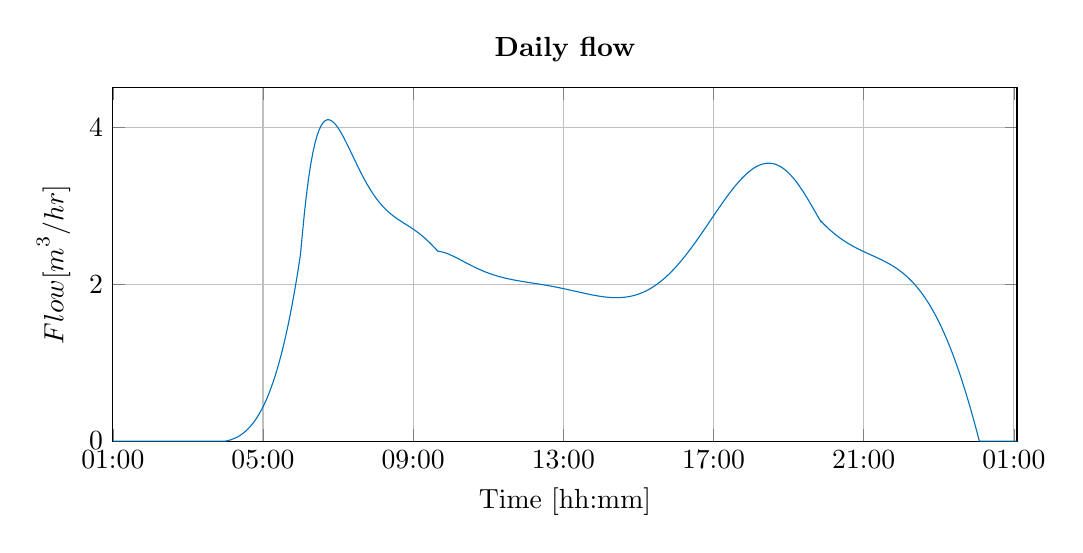
\begin{tikzpicture}

\begin{axis}[%
width=4.521in,
height=1.766in,
at={(0.758in,0.481in)},
scale only axis,
xmin=3600,
xmax=90000,
xtick={3600,17950,32300,46650,61000,75350,89700},
xticklabels={{01:00},{05:00},{09:00},{13:00},{17:00},{21:00},{01:00},{},{},{}},
xlabel={Time [hh:mm]},
xmajorgrids,
ymin=0,
ymax=4.5,
ylabel={$\text{Flow [m}^\text{3}\text{/hr]}$},
ymajorgrids,
axis background/.style={fill=white},
scaled x ticks = false,
title style={font=\bfseries},
title={Daily flow},
legend style={legend cell align=left,align=left,draw=white!15!black}
]
\addplot [color=mycolor1,solid]
  table[row sep=crcr]{%
3599	0\\
3799	0\\
3998	0\\
4197	0\\
4396	0\\
4595	0\\
4794	0\\
4993	0\\
5192	0\\
5391	0\\
5590	0\\
5789	0\\
5988	0\\
6188	0\\
6387	0\\
6586	0\\
6785	0\\
6984	0\\
7183	0\\
7382	0\\
7581	0\\
7780	0\\
7979	0\\
8178	0\\
8377	0\\
8577	0\\
8776	0\\
8975	0\\
9174	0\\
9373	0\\
9572	0\\
9771	0\\
9970	0\\
10169	0\\
10368	0\\
10567	0\\
10766	0\\
10965	0\\
11165	0\\
11364	0\\
11563	0\\
11762	0\\
11961	0\\
12160	0\\
12359	0\\
12558	0\\
12757	0\\
12956	0\\
13155	0\\
13354	0\\
13554	0\\
13753	0\\
13952	0\\
14151	0\\
14350	0\\
14549	0.00442222580352827\\
14748	0.0114741772862802\\
14947	0.0199610243832393\\
15146	0.0300247058319911\\
15345	0.0418136197449804\\
15544	0.0554826329473421\\
15743	0.0711930829844264\\
15942	0.0891127727990636\\
16142	0.109524305162895\\
16341	0.132405026798267\\
16540	0.158037982533165\\
16739	0.186616668981945\\
16938	0.218340911359329\\
17137	0.253416814139265\\
17336	0.292056704383446\\
17535	0.334479067739685\\
17734	0.380908477109851\\
17933	0.431575513987692\\
18132	0.486716682466314\\
18331	0.54657431591536\\
18531	0.61173517800162\\
18730	0.681802420108294\\
18929	0.757348375922315\\
19128	0.838637642813172\\
19327	0.925940070187446\\
19526	1.0195306221475\\
19725	1.11968923282013\\
19924	1.2267006543547\\
20123	1.34085429759121\\
20322	1.46244406539796\\
20521	1.591768178679\\
20720	1.72912899505139\\
20920	1.87558658964644\\
21119	2.02998775308587\\
21318	2.19335717408436\\
21517	2.36601181350741\\
21716	2.64411100927655\\
21915	2.91582767530568\\
22114	3.15181967017109\\
22313	3.35485836442594\\
22512	3.52758354858929\\
22711	3.67250639353341\\
22910	3.79201241085632\\
23109	3.88836441327126\\
23308	3.96370547498868\\
23508	4.02030042505377\\
23707	4.05950352712545\\
23906	4.0834448623313\\
24105	4.09381761994979\\
24175	4.0945395676626\\
24304	4.0922100675344\\
24503	4.08010851130726\\
24702	4.05890025652537\\
24901	4.02987656787424\\
25100	3.99423562983415\\
25299	3.95308550708851\\
25498	3.90744710487536\\
25697	3.85825712938731\\
25897	3.806104849663\\
26096	3.75229204330984\\
26295	3.69726553357036\\
26494	3.64165447812437\\
26693	3.58601865238405\\
26892	3.53085140987913\\
27091	3.47658264263791\\
27290	3.42358174156084\\
27489	3.37216055681841\\
27688	3.32257635822156\\
27887	3.27503479560692\\
28086	3.22969285920515\\
28285	3.18666184004508\\
28485	3.14581208430523\\
28684	3.10758088877446\\
28883	3.07174976371261\\
29082	3.03827664444324\\
29281	3.00708858386904\\
29480	2.97808471284652\\
29679	2.95113920056695\\
29878	2.92610421493529\\
30077	2.90281288295747\\
30276	2.88108225111931\\
30475	2.86071624577169\\
30674	2.84150863348836\\
30874	2.82315622926496\\
31073	2.80562396744985\\
31272	2.78859894527949\\
31471	2.77186391005839\\
31670	2.75520626611806\\
31869	2.73842103520223\\
32068	2.72131381685202\\
32267	2.70370374877641\\
32466	2.68542646722693\\
32665	2.66633706741235\\
32864	2.64631306384803\\
33063	2.62525735074963\\
33263	2.60298696876008\\
33462	2.57968708361932\\
33661	2.5552461290138\\
33860	2.52969831629012\\
34059	2.50311805326763\\
34258	2.47562290465526\\
34457	2.44737655238404\\
34656	2.41903417111451\\
34855	2.41548966232507\\
35054	2.40989498143512\\
35253	2.40252874736045\\
35452	2.39364803937087\\
35651	2.38348942106358\\
35851	2.37221122121005\\
36050	2.36012550281161\\
36249	2.34735916470061\\
36448	2.33407631847188\\
36647	2.32042527652798\\
36846	2.30653941497033\\
37045	2.292538010926\\
37244	2.27852705452525\\
37443	2.26460003586295\\
37642	2.2508387072054\\
37841	2.23731382105396\\
38040	2.22408584394744\\
38240	2.21114187463128\\
38439	2.19865344916971\\
38638	2.18658855155431\\
38837	2.17497313770969\\
39036	2.16382610120049\\
39235	2.15315984985419\\
39434	2.1429808605983\\
39633	2.13329021285326\\
39832	2.12408410098727\\
40031	2.11535432582874\\
40230	2.10708876604616\\
40429	2.09927182918011\\
40628	2.09188488312897\\
40828	2.0848725949352\\
41027	2.07828148936575\\
41226	2.07205013324472\\
41425	2.0661516594405\\
41624	2.06055803506768\\
41823	2.05524038108332\\
42022	2.0501692746057\\
42221	2.04531503405655\\
42420	2.04064798735881\\
42619	2.03613872401651\\
42818	2.03175833064229\\
43017	2.02747861102071\\
43217	2.02325129390899\\
43416	2.01909238210739\\
43615	2.01495570567951\\
43814	2.01081783906788\\
44013	2.00665694857339\\
44212	2.00245292421282\\
44411	1.99818749811514\\
44610	1.99384434968869\\
44809	1.98940919806522\\
45008	1.98486988193467\\
45207	1.98021642712068\\
45406	1.97544110247885\\
45606	1.97051349985899\\
45805	1.96547976439647\\
46004	1.96031481209514\\
46203	1.95502022754302\\
46402	1.9495999506416\\
46601	1.94406026817996\\
46800	1.93840979562937\\
46999	1.93265944979509\\
47198	1.92682241260799\\
47397	1.92091408619084\\
47596	1.91495203979398\\
47795	1.90895594880698\\
47994	1.90294752617521\\
48194	1.89692038122864\\
48393	1.89096045050175\\
48592	1.88506490030924\\
48791	1.87926277541517\\
48990	1.87358471193174\\
49189	1.86806283014049\\
49388	1.86273062200846\\
49587	1.8576228335635\\
49786	1.85277534254232\\
49985	1.84822503209959\\
50184	1.84400966023251\\
50383	1.84016772561655\\
50583	1.83672220529473\\
50782	1.83374728604262\\
50981	1.8312645559992\\
51180	1.82931407432274\\
51379	1.82793592595939\\
51578	1.82717007306889\\
51712	1.82701927855175\\
51777	1.82705620380197\\
51976	1.82763358131816\\
52175	1.82894089136547\\
52374	1.83101608970834\\
52573	1.83389624951334\\
52772	1.83761740905967\\
52971	1.84221441993455\\
53171	1.84775081767458\\
53370	1.85420339594633\\
53569	1.86162790825795\\
53768	1.8700529572691\\
53967	1.87950522064347\\
54166	1.890009309863\\
54365	1.90158763223019\\
54564	1.91426025570864\\
54763	1.92804477789214\\
54962	1.94295619853298\\
55161	1.95900679610619\\
55360	1.97620600949746\\
55560	1.9946554808804\\
55759	2.01417414547567\\
55958	2.0348515867415\\
56157	2.05668478464961\\
56356	2.07966736615765\\
56555	2.10378952045302\\
56754	2.12903792174961\\
56953	2.15539565921993\\
57152	2.18284217374636\\
57351	2.21135320365917\\
57550	2.24090073764362\\
57749	2.27145297659171\\
57949	2.30313508534694\\
58148	2.33559061425459\\
58347	2.36893225005193\\
58546	2.4031128232886\\
58745	2.43808132507356\\
58944	2.47378292667643\\
59143	2.51015901035898\\
59342	2.54714721121349\\
59541	2.58468146991496\\
59740	2.62269209826402\\
59939	2.66110585602751\\
60138	2.69984604058232\\
60337	2.73883258886069\\
60537	2.77817919271003\\
60736	2.81740559322073\\
60935	2.85661877477404\\
61134	2.89572651121671\\
61333	2.93463393237626\\
61532	2.9732437096365\\
61731	3.01145625716701\\
61930	3.04916994876029\\
62129	3.08628134942475\\
62328	3.12268546411609\\
62527	3.15827600236744\\
62726	3.19294565958974\\
62926	3.22675268320946\\
63125	3.25925012822774\\
63324	3.29050122023788\\
63523	3.32039776061185\\
63722	3.34883220757148\\
63921	3.37569806495021\\
64120	3.40089029039581\\
64319	3.42430572217504\\
64518	3.44584352561743\\
64717	3.46540566054371\\
64916	3.48289736794111\\
65115	3.49822767771618\\
65314	3.51130993772711\\
65514	3.52211038142855\\
65713	3.53044435444527\\
65912	3.53630150048119\\
66111	3.53961819236537\\
66265	3.54040515106731\\
66310	3.54033809443812\\
66509	3.53841282401017\\
66708	3.53380263676685\\
66907	3.52647713442185\\
67106	3.51641599856799\\
67305	3.50360974673538\\
67504	3.48806051398862\\
67703	3.46978285995349\\
67903	3.44869242604152\\
68102	3.42504225777269\\
68301	3.39879066106905\\
68500	3.37001054821747\\
68699	3.33879167809678\\
68898	3.30524161912064\\
69097	3.2694867393557\\
69296	3.23167322525738\\
69495	3.19196812590241\\
69694	3.15056042850421\\
69893	3.10766216016736\\
70092	3.06350951924634\\
70292	3.01813514238681\\
70491	2.97228210257935\\
70690	2.92604172777595\\
70889	2.87975895406627\\
71088	2.83380899801614\\
71260	2.79467368952501\\
71287	2.79868278125095\\
71486	2.77123878571802\\
71685	2.74481562666469\\
71884	2.71941056858078\\
72083	2.69501595485996\\
72282	2.6716193634545\\
72481	2.64920376269884\\
72680	2.6277476671415\\
72880	2.60712447469801\\
73079	2.58751035592739\\
73278	2.5687659405626\\
73477	2.55085346683633\\
73676	2.53373149886954\\
73875	2.51735508250346\\
74074	2.50167590102184\\
74273	2.4866424309576\\
74472	2.47220009798386\\
74671	2.45829143250965\\
74870	2.44485622566371\\
75069	2.43183168495778\\
75269	2.4190896353966\\
75468	2.40668971685735\\
75667	2.39449778855215\\
75866	2.38244227211082\\
76065	2.37044978534688\\
76264	2.35844529797984\\
76463	2.34635228749242\\
76662	2.33409289481071\\
76861	2.32158808022045\\
77060	2.30875777912303\\
77259	2.29552105773255\\
77458	2.28179626900046\\
77657	2.2675012083548\\
77857	2.25247636569214\\
78056	2.23678878951944\\
78255	2.22028212346615\\
78454	2.20287349134621\\
78653	2.18448023925929\\
78852	2.16502009116967\\
79051	2.14441130491532\\
79250	2.12257282778685\\
79449	2.09942445248591\\
79648	2.07488697286437\\
79847	2.04888233961291\\
80046	2.0213338162026\\
80246	1.99201534965028\\
80445	1.96114617655674\\
80644	1.92851198140894\\
80843	1.89404284661593\\
81042	1.85767094690634\\
81241	1.81933070522791\\
81440	1.77895894860465\\
81639	1.73649506384232\\
81838	1.6918811533519\\
82037	1.64506219089723\\
82236	1.59598617743537\\
82435	1.54460429694009\\
82635	1.4905950458881\\
82834	1.43445636707819\\
83033	1.37588584551451\\
83232	1.31484897432348\\
83431	1.25131520940679\\
83630	1.18525812511314\\
83829	1.11665557002792\\
84028	1.04548982286428\\
84227	0.971747748176957\\
84426	0.895420952000219\\
84625	0.816505938042502\\
84824	0.735004263003857\\
85023	0.650922692728392\\
85223	0.563831477364642\\
85422	0.474619268389663\\
85621	0.382880405254365\\
85820	0.288644077366678\\
86019	0.19194546287689\\
86218	0.0928258844168158\\
86401	0\\
86417	0\\
86616	0\\
86815	0\\
87014	0\\
87213	0\\
87412	0\\
87612	0\\
87811	0\\
88010	0\\
88209	0\\
88408	0\\
88607	0\\
88806	0\\
89005	0\\
89204	0\\
89403	0\\
89602	0\\
90000	0\\
};

\end{axis}
\end{tikzpicture}%
\caption{A flow profile for Thulesvej.}
\label{fig:APP_flow_profile_zone5}
\end{figure} 

\begin{figure}[H]
\centering
% This file was created by matlab2tikz.
%
%The latest updates can be retrieved from
%  http://www.mathworks.com/matlabcentral/fileexchange/22022-matlab2tikz-matlab2tikz
%where you can also make suggestions and rate matlab2tikz.
%
\definecolor{mycolor1}{rgb}{0.00000,0.44700,0.74100}%
%
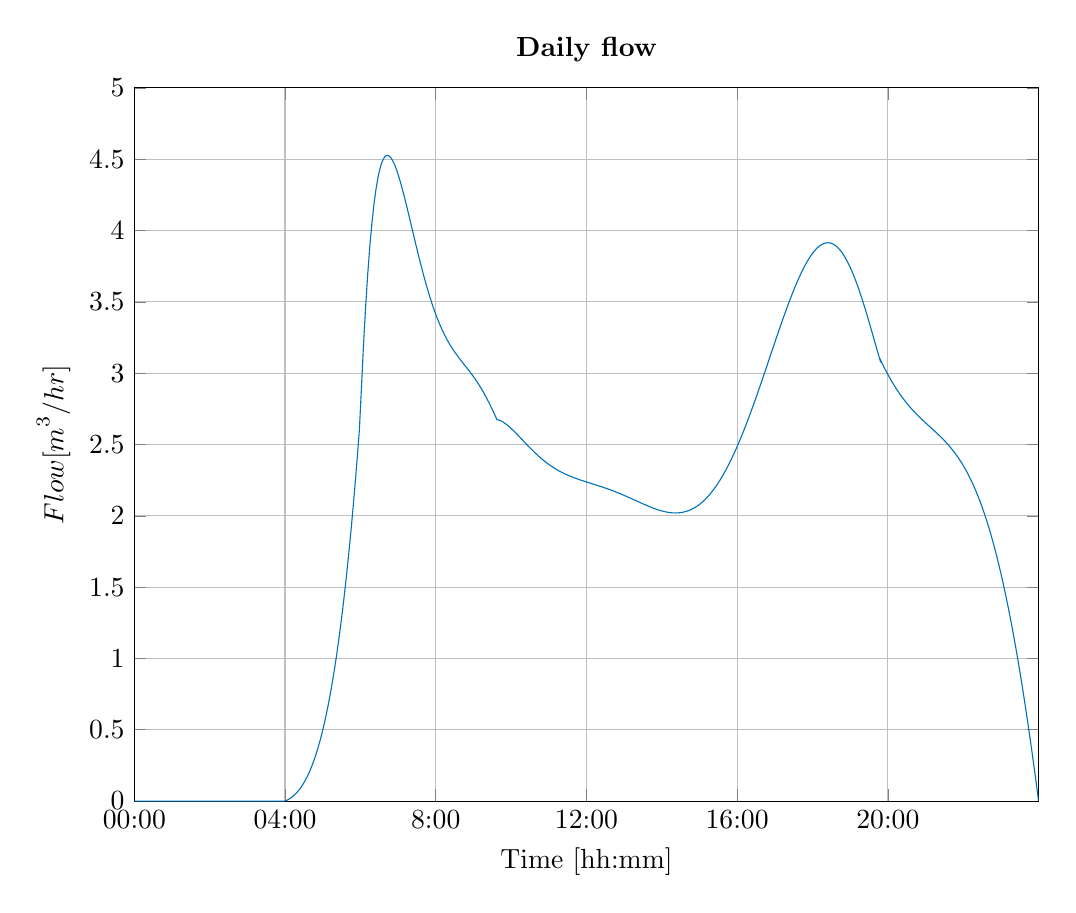
\begin{tikzpicture}

\begin{axis}[%
width=4.521in,
height=3.566in,
at={(0.758in,0.481in)},
scale only axis,
xmin=0,
xmax=24,
xtick={0,4,8,12,16,20,24},
xticklabels={{00:00},{04:00},{8:00},{12:00},{16:00},{20:00}},
xlabel={Time [hh:mm]},
xmajorgrids,
ymin=0,
ymax=5,
ylabel={$\text{Flow [m}^\text{3}\text{/hr]}$},
ymajorgrids,
axis background/.style={fill=white},
title style={font=\bfseries},
title={Daily flow}
]
\addplot [color=mycolor1,solid,forget plot]
  table[row sep=crcr]{%
0.000277777777777778	0\\
0.0558333333333333	0\\
0.111111111111111	0\\
0.166388888888889	0\\
0.221666666666667	0\\
0.276944444444444	0\\
0.332222222222222	0\\
0.3875	0\\
0.442777777777778	0\\
0.498055555555556	0\\
0.553333333333333	0\\
0.608611111111111	0\\
0.663888888888889	0\\
0.719166666666667	0\\
0.774722222222222	0\\
0.83	0\\
0.885277777777778	0\\
0.940555555555556	0\\
0.995833333333333	0\\
1.05111111111111	0\\
1.10638888888889	0\\
1.16166666666667	0\\
1.21694444444444	0\\
1.27222222222222	0\\
1.3275	0\\
1.38277777777778	0\\
1.43805555555556	0\\
1.49361111111111	0\\
1.54888888888889	0\\
1.60416666666667	0\\
1.65944444444444	0\\
1.71472222222222	0\\
1.77	0\\
1.82527777777778	0\\
1.88055555555556	0\\
1.93583333333333	0\\
1.99111111111111	0\\
2.04638888888889	0\\
2.10166666666667	0\\
2.15694444444444	0\\
2.2125	0\\
2.26777777777778	0\\
2.32305555555556	0\\
2.37833333333333	0\\
2.43361111111111	0\\
2.48888888888889	0\\
2.54416666666667	0\\
2.59944444444444	0\\
2.65472222222222	0\\
2.71	0\\
2.76527777777778	0\\
2.82055555555556	0\\
2.87583333333333	0\\
2.93138888888889	0\\
2.98666666666667	0\\
3.04194444444444	0\\
3.09722222222222	0\\
3.1525	0\\
3.20777777777778	0\\
3.26305555555556	0\\
3.31833333333333	0\\
3.37361111111111	0\\
3.42888888888889	0\\
3.48416666666667	0\\
3.53944444444444	0\\
3.59472222222222	0\\
3.65027777777778	0\\
3.70555555555556	0\\
3.76083333333333	0\\
3.81611111111111	0\\
3.87138888888889	0\\
3.92666666666667	0\\
3.98194444444444	0\\
4.03722222222222	0.00436153761647452\\
4.0925	0.012044686962592\\
4.14777777777778	0.0213027030151159\\
4.20305555555556	0.0322919741793307\\
4.25833333333333	0.0451760291745809\\
4.31361111111111	0.0601255479688758\\
4.36916666666667	0.0774107346184819\\
4.42444444444444	0.0970445135396201\\
4.47972222222222	0.119299674842479\\
4.535	0.14437548643156\\
4.59027777777778	0.172478300400132\\
4.64555555555556	0.203821515298544\\
4.70083333333333	0.238625530298273\\
4.75611111111111	0.27711769125169\\
4.81138888888889	0.319532228647551\\
4.86666666666667	0.366110187462214\\
4.92194444444444	0.417099348906629\\
4.97722222222222	0.472754144068967\\
5.0325	0.533335559453085\\
5.08777777777778	0.599111034412647\\
5.14333333333333	0.670726634405299\\
5.19861111111111	0.747747397579227\\
5.25388888888889	0.830803561132116\\
5.30916666666667	0.920187217675859\\
5.36444444444444	1.01619627753933\\
5.41972222222222	1.11913431753617\\
5.475	1.22931042162831\\
5.53027777777778	1.34703901348522\\
5.58555555555556	1.47263968093894\\
5.64083333333333	1.60643699233471\\
5.69611111111111	1.74876030477746\\
5.75138888888889	1.89994356427397\\
5.80666666666667	2.06032509777082\\
5.86222222222222	2.23112595329756\\
5.9175	2.41098601653716\\
5.97277777777778	2.60108518753465\\
6.02805555555556	2.89896921282579\\
6.08333333333333	3.20248193836858\\
6.13861111111111	3.46626088004164\\
6.19388888888889	3.69338113557894\\
6.24916666666667	3.88677208244\\
6.30444444444444	4.04922065076256\\
6.35972222222222	4.18337459634552\\
6.415	4.29174577360512\\
6.47027777777778	4.37671340855667\\
6.52555555555556	4.4405273717661\\
6.58111111111111	4.48549187067167\\
6.63638888888889	4.51316632254109\\
6.69166666666667	4.52570246958311\\
6.71527777777778	4.52688225493132\\
6.74694444444444	4.52486491431809\\
6.80222222222222	4.5123052851202\\
6.8575	4.48956550917361\\
6.91277777777778	4.45808108545889\\
6.96805555555556	4.41918435771153\\
7.02333333333333	4.3741077873827\\
7.07861111111111	4.32398722662112\\
7.13388888888889	4.26986519123494\\
7.18916666666667	4.21269413366429\\
7.24444444444444	4.15333971595018\\
7.3	4.09227645710956\\
7.35527777777778	4.03081963544181\\
7.41055555555556	3.96929137850569\\
7.46583333333333	3.90824255434165\\
7.52111111111111	3.84815362185813\\
7.57638888888889	3.78943790384718\\
7.63166666666667	3.73244485989398\\
7.68694444444444	3.67746335940641\\
7.74222222222222	3.62472495453506\\
7.7975	3.5744071531644\\
7.85277777777778	3.52663669187815\\
7.90805555555556	3.48149280893884\\
7.96333333333333	3.43901051721824\\
8.01888888888889	3.39899039075237\\
8.07416666666667	3.36178873974155\\
8.12944444444445	3.32712062267076\\
8.18472222222222	3.29487673247597\\
8.24	3.26491991800917\\
8.29527777777778	3.23708845702013\\
8.35055555555556	3.21119932911955\\
8.40583333333333	3.18705148874919\\
8.46111111111111	3.16442913815202\\
8.51638888888889	3.14310500034235\\
8.57166666666667	3.1228435920573\\
8.62694444444444	3.10340449676192\\
8.68222222222222	3.08454563756568\\
8.73777777777778	3.06593394703847\\
8.79305555555556	3.04751899406006\\
8.84833333333333	3.02897969760621\\
8.90361111111111	3.01010013488272\\
8.95888888888889	2.99067910406758\\
9.01416666666667	2.97053339725773\\
9.06944444444444	2.94950107348585\\
9.12472222222222	2.92744473160188\\
9.18	2.9042547833318\\
9.23527777777778	2.87985272619639\\
9.29055555555555	2.85419441649543\\
9.34583333333333	2.82727334224515\\
9.40111111111111	2.79912389620901\\
9.45666666666667	2.76967470488772\\
9.51194444444444	2.73934693504096\\
9.56722222222222	2.70817315136422\\
9.6225	2.67465448833025\\
9.67777777777778	2.67091974484706\\
9.73305555555556	2.66489413494212\\
9.78833333333333	2.65688753866974\\
9.84361111111111	2.64718593550291\\
9.89888888888889	2.63605253876402\\
9.95416666666667	2.62372889951666\\
10.0094444444444	2.61043598011424\\
10.0647222222222	2.59637519806299\\
10.12	2.58172944029236\\
10.1752777777778	2.56666404826203\\
10.2308333333333	2.55125025460983\\
10.2861111111111	2.53577580856133\\
10.3413888888889	2.52028246107213\\
10.3966666666667	2.50487458576866\\
10.4519444444444	2.48964351667202\\
10.5072222222222	2.47466836579301\\
10.5625	2.46001681462221\\
10.6177777777778	2.44574587907216\\
10.6730555555556	2.43190264870155\\
10.7283333333333	2.41852500035662\\
10.7836111111111	2.40564228683593\\
10.8388888888889	2.39327600059714\\
10.8941666666667	2.38144041312116\\
10.9497222222222	2.37008778498997\\
11.005	2.35933328724769\\
11.0602777777778	2.34911498058241\\
11.1155555555556	2.3394241478704\\
11.1708333333333	2.33024769699801\\
11.2261111111111	2.32156866154641\\
11.2813888888889	2.3133666791386\\
11.3366666666667	2.30561844877292\\
11.3919444444444	2.29829816650414\\
11.4472222222222	2.291377940787\\
11.5025	2.28482818722587\\
11.5577777777778	2.27861800322458\\
11.6130555555556	2.27271552299811\\
11.6686111111111	2.2670606152517\\
11.7238888888889	2.26167688742547\\
11.7791666666667	2.25650258532945\\
11.8344444444444	2.25150516187116\\
11.8897222222222	2.24665260063167\\
11.945	2.24191366027968\\
12.0002777777778	2.23725810189779\\
12.0555555555556	2.23265689961728\\
12.1108333333333	2.2280824345194\\
12.1661111111111	2.22350867287552\\
12.2213888888889	2.2189113285537\\
12.2766666666667	2.21426800980611\\
12.3319444444444	2.20955835157951\\
12.3875	2.20473980000995\\
12.4427777777778	2.1998445059343\\
12.4980555555556	2.19483497865375\\
12.5533333333333	2.1897000062789\\
12.6086111111111	2.18443085250946\\
12.6638888888889	2.17902130650358\\
12.7191666666667	2.17346772034056\\
12.7744444444444	2.16776903444503\\
12.8297222222222	2.16192679117337\\
12.885	2.15594513737332\\
12.9402777777778	2.14983081564193\\
12.9955555555556	2.14359314511635\\
13.0508333333333	2.13724399207717\\
13.1063888888889	2.13076511965299\\
13.1616666666667	2.1242382262651\\
13.2169444444444	2.11765039444991\\
13.2722222222222	2.11102320411836\\
13.3275	2.10438049385537\\
13.3827777777778	2.09774827749962\\
13.4380555555556	2.09115465352914\\
13.4933333333333	2.08462970606388\\
13.5486111111111	2.07820540021266\\
13.6038888888889	2.07191546984384\\
13.6591666666667	2.06579529944379\\
13.7144444444444	2.05988180019883\\
13.7697222222222	2.05421328036551\\
13.8252777777778	2.04880304224001\\
13.8805555555556	2.04374605492379\\
13.9358333333333	2.0390561953673\\
13.9911111111111	2.03477597078221\\
14.0463888888889	2.03094856698806\\
14.1016666666667	2.02761769324186\\
14.1569444444444	2.02482742427944\\
14.2122222222222	2.02262203963405\\
14.2675	2.02104586064697\\
14.3227777777778	2.02014308607478\\
14.3644444444444	2.01993435765349\\
14.3780555555556	2.01995762529078\\
14.4333333333333	2.02053293136058\\
14.4886111111111	2.02191183224794\\
14.5438888888889	2.02413636276678\\
14.5994444444444	2.02726553651458\\
14.6547222222222	2.03130816790608\\
14.71	2.03631627688364\\
14.7652777777778	2.04232703369705\\
14.8205555555556	2.04937597715924\\
14.8758333333333	2.0574968510835\\
14.9311111111111	2.0667214424411\\
14.9863888888889	2.07707942275923\\
15.0416666666667	2.08859819167305\\
15.0969444444444	2.10130272383475\\
15.1522222222222	2.11521541959434\\
15.2075	2.13035595966703\\
15.2627777777778	2.1467411634931\\
15.3183333333333	2.16447671199407\\
15.3736111111111	2.1833959789767\\
15.4288888888889	2.20359189061787\\
15.4841666666667	2.22506849094935\\
15.5394444444444	2.24782633363513\\
15.5947222222222	2.27186237375637\\
15.65	2.29716986664122\\
15.7052777777778	2.32373827452759\\
15.7605555555556	2.35155318020554\\
15.8158333333333	2.38059620817089\\
15.8711111111111	2.41084495540202\\
15.9263888888889	2.44227292966191\\
15.9816666666667	2.47484949673807\\
16.0372222222222	2.50871188458511\\
16.0925	2.54348225841157\\
16.1477777777778	2.57928386421897\\
16.2030555555556	2.61606914921719\\
16.2583333333333	2.65378630529219\\
16.3136111111111	2.69237927794856\\
16.3688888888889	2.73178778774273\\
16.4241666666667	2.77194736275682\\
16.4794444444444	2.81278938394544\\
16.5347222222222	2.85424114271212\\
16.59	2.8962259122492\\
16.6452777777778	2.9386630310047\\
16.7005555555556	2.98146800095245\\
16.7561111111111	3.02476965789499\\
16.8113888888889	3.06804277125561\\
16.8666666666667	3.11140792872131\\
16.9219444444444	3.15476653670328\\
16.9772222222222	3.19801687465371\\
17.0325	3.24105428237435\\
17.0877777777778	3.28377136503771\\
17.1430555555556	3.32605821353838\\
17.1983333333333	3.36780264295779\\
17.2536111111111	3.40889044762271\\
17.3088888888889	3.44920567419794\\
17.3641666666667	3.4886309126315\\
17.4194444444444	3.52704760641628\\
17.475	3.56452071052627\\
17.5302777777778	3.60055514510756\\
17.5855555555556	3.63522126139752\\
17.6408333333333	3.66839939552844\\
17.6961111111111	3.6999705763583\\
17.7513888888889	3.72981695353354\\
17.8066666666667	3.75782224692899\\
17.8619444444444	3.78387221647664\\
17.9172222222222	3.80785515508745\\
17.9725	3.82966240233964\\
18.0277777777778	3.84918888157241\\
18.0830555555556	3.86633365900495\\
18.1383333333333	3.88100052684839\\
18.1938888888889	3.89315277138449\\
18.2491666666667	3.90258361670261\\
18.3044444444444	3.9092820912385\\
18.3597222222222	3.91317723245379\\
18.4069444444444	3.91423675086944\\
18.415	3.91420608156746\\
18.4702777777778	3.91231441194926\\
18.5255555555556	3.90745748655999\\
18.5808333333333	3.89960083715605\\
18.6361111111111	3.88872107271818\\
18.6913888888889	3.87480671522994\\
18.7466666666667	3.85785905987809\\
18.8019444444444	3.83789306517646\\
18.8572222222222	3.81493827049557\\
18.9127777777778	3.78890226035816\\
18.9680555555556	3.760107261838\\
19.0233333333333	3.72850960520155\\
19.0786111111111	3.69420699034698\\
19.1338888888889	3.65731672045863\\
19.1891666666667	3.61797679517985\\
19.2444444444444	3.57634703184434\\
19.2997222222222	3.53261022120022\\
19.355	3.48697331026012\\
19.4102777777778	3.43966862035264\\
19.4655555555556	3.39095509469634\\
19.5208333333333	3.34111957862943\\
19.5761111111111	3.29047813315719\\
19.6313888888889	3.23937738191039\\
19.6869444444444	3.18793917311625\\
19.7422222222222	3.13709162073664\\
19.7944444444444	3.08976345798418\\
19.7975	3.09668439391876\\
19.8527777777778	3.06625187787283\\
19.9080555555556	3.03694799011631\\
19.9633333333333	3.00877015128834\\
20.0186111111111	2.98171032737234\\
20.0738888888889	2.95575520193564\\
20.1291666666667	2.93088634834114\\
20.1844444444444	2.90708040194028\\
20.2397222222222	2.88430923245258\\
20.295	2.86254011607467\\
20.3502777777778	2.84173590774791\\
20.4058333333333	2.82175756742555\\
20.4611111111111	2.8027592071145\\
20.5163888888889	2.78458925699978\\
20.5716666666667	2.76719459119578\\
20.6269444444444	2.75051852452434\\
20.6822222222222	2.73450098492227\\
20.7375	2.71907868568098\\
20.7927777777778	2.70418529751819\\
20.8480555555556	2.68975162102279\\
20.9033333333333	2.67570575874519\\
20.9586111111111	2.66197328747429\\
21.0138888888889	2.64847743056102\\
21.0691666666667	2.63513922997144\\
21.1247222222222	2.62181113258648\\
21.18	2.60854326423953\\
21.2352777777778	2.59518438463777\\
21.2905555555556	2.58164852618859\\
21.3458333333333	2.56784840185863\\
21.4011111111111	2.55369557773978\\
21.4563888888889	2.53910064522353\\
21.5116666666667	2.52397339311935\\
21.5669444444444	2.50822298001557\\
21.6222222222222	2.49175810653765\\
21.6775	2.4744871874106\\
21.7327777777778	2.4563185239504\\
21.7880555555556	2.43716047605184\\
21.8436111111111	2.41681704892677\\
21.8988888888889	2.39540029069326\\
21.9541666666667	2.3727208498224\\
22.0094444444444	2.34868904762022\\
22.0647222222222	2.32321612616745\\
22.12	2.29621442048452\\
22.1752777777778	2.26759753094839\\
22.2305555555556	2.23728049530837\\
22.2858333333333	2.20517996105627\\
22.3411111111111	2.17121435762874\\
22.3963888888889	2.13530406869352\\
22.4516666666667	2.09737160427715\\
22.5069444444444	2.05734177313516\\
22.5625	2.01492419568342\\
22.6177777777778	1.97047268369193\\
22.6730555555556	1.92371341495077\\
22.7283333333333	1.8745821306619\\
22.7836111111111	1.82301773275629\\
22.8388888888889	1.76896245618956\\
22.8941666666667	1.71236204108829\\
22.9494444444444	1.65316590500831\\
23.0047222222222	1.59132731520234\\
23.06	1.52680356080361\\
23.1152777777778	1.45955612515875\\
23.1705555555556	1.38955085797417\\
23.2258333333333	1.31675814765827\\
23.2813888888889	1.2407660309182\\
23.3366666666667	1.16231433996367\\
23.3919444444444	1.08101526302932\\
23.4472222222222	0.996859091977158\\
23.5025	0.909841519641678\\
23.5577777777778	0.81996381149129\\
23.6130555555556	0.727232978502056\\
23.6683333333333	0.631661948660645\\
23.7236111111111	0.533269739987247\\
23.7788888888889	0.432081632122456\\
23.8341666666667	0.328129339023808\\
23.8894444444444	0.221451180851064\\
23.9447222222222	0.112092256448278\\
24	0.000104615546122659\\
};
\end{axis}
\end{tikzpicture}%
\caption{A flow profile for Thulesvej.}
\label{fig:APP_flow_profile_zone6}
\end{figure} 

\begin{figure}[H]
\centering
% This file was created by matlab2tikz.
%
%The latest updates can be retrieved from
%  http://www.mathworks.com/matlabcentral/fileexchange/22022-matlab2tikz-matlab2tikz
%where you can also make suggestions and rate matlab2tikz.
%
\definecolor{mycolor1}{rgb}{0.00000,0.44700,0.74100}%
\definecolor{mycolor2}{rgb}{0.85000,0.32500,0.09800}%
%
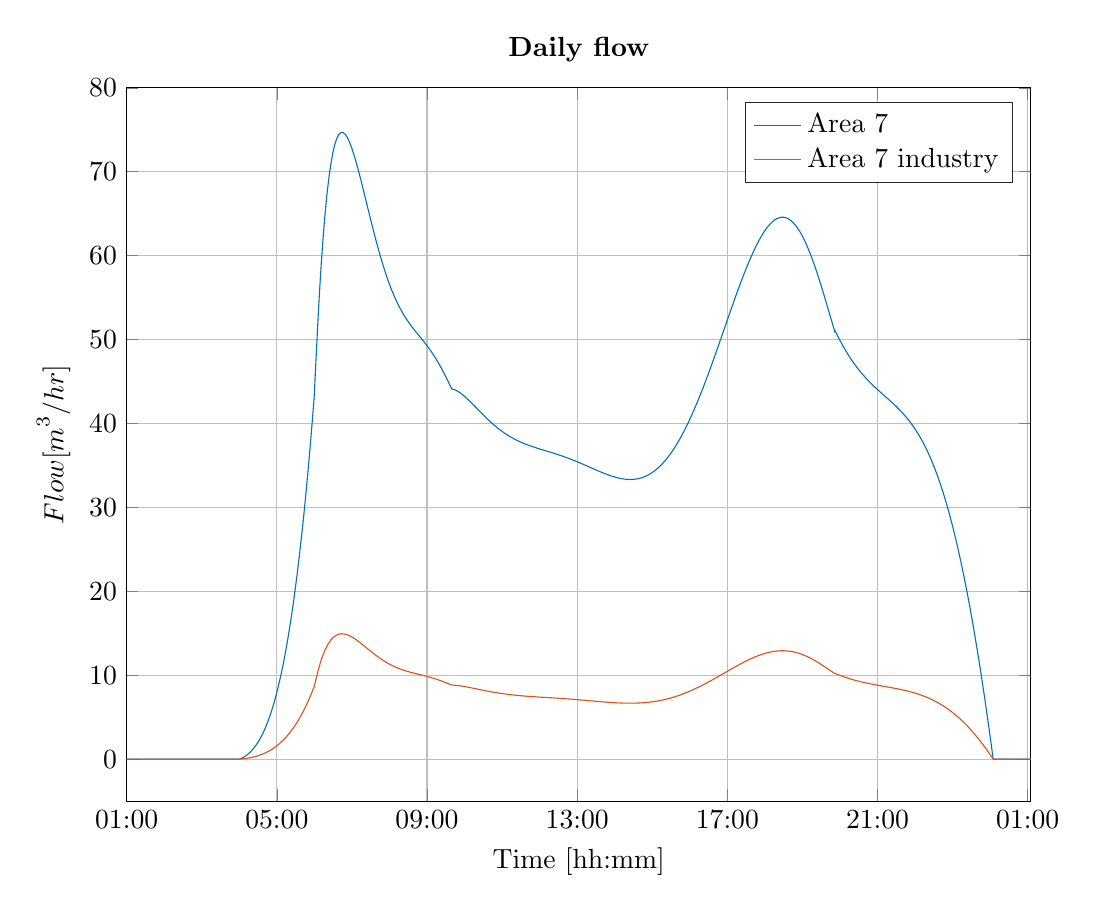
\begin{tikzpicture}

\begin{axis}[%
width=4.521in,
height=3.566in,
at={(0.758in,0.481in)},
scale only axis,
xmin=3600,
xmax=90000,
xtick={3600,17950,32300,46650,61000,75350,89700},
xticklabels={{01:00},{05:00},{09:00},{13:00},{17:00},{21:00},{01:00},{},{},{}},
xlabel={Time [hh:mm]},
xmajorgrids,
ymin=-5,
ymax=80,
ylabel={$\text{Flow [m}^\text{3}\text{/hr]}$},
scaled x ticks = false,
ymajorgrids,
axis background/.style={fill=white},
title style={font=\bfseries},
title={Daily flow},
legend style={legend cell align=left,align=left,draw=white!15!black}
]
\addplot [color=mycolor1,solid]
  table[row sep=crcr]{%
3599	0\\
3799	0\\
3998	0\\
4197	0\\
4396	0\\
4595	0\\
4794	0\\
4993	0\\
5192	0\\
5391	0\\
5590	0\\
5789	0\\
5988	0\\
6188	0\\
6387	0\\
6586	0\\
6785	0\\
6984	0\\
7183	0\\
7382	0\\
7581	0\\
7780	0\\
7979	0\\
8178	0\\
8377	0\\
8577	0\\
8776	0\\
8975	0\\
9174	0\\
9373	0\\
9572	0\\
9771	0\\
9970	0\\
10169	0\\
10368	0\\
10567	0\\
10766	0\\
10965	0\\
11165	0\\
11364	0\\
11563	0\\
11762	0\\
11961	0\\
12160	0\\
12359	0\\
12558	0\\
12757	0\\
12956	0\\
13155	0\\
13354	0\\
13554	0\\
13753	0\\
13952	0\\
14151	0\\
14350	0\\
14549	0.0806712868631212\\
14748	0.209314650247236\\
14947	0.364133718096731\\
15146	0.547717770363713\\
15345	0.76277392044104\\
15544	1.01212728550524\\
15743	1.29872102313826\\
15942	1.62561623422888\\
16142	1.99796822523865\\
16341	2.41536374972987\\
16540	2.88296617826028\\
16739	3.40430532173897\\
16938	3.98302643889659\\
17137	4.62288933619267\\
17336	5.32776733400112\\
17535	6.10164609907736\\
17734	6.94862234330207\\
17933	7.87290238870716\\
18132	8.87880059877989\\
18331	9.97073767604603\\
18531	11.1594175018059\\
18730	12.4376006699258\\
18929	13.8157278266077\\
19128	15.2986258195173\\
19327	16.8912173052207\\
19526	18.5985182437715\\
19725	20.4256352595821\\
19924	22.37776286857\\
20123	24.4601805715863\\
20322	26.678249814123\\
20521	29.0374108122996\\
20720	31.5431792451301\\
20920	34.214893253364\\
21119	37.0315157193367\\
21318	40.0117392564332\\
21517	43.1613459395731\\
21716	48.2344971071132\\
21915	53.1912166607005\\
22114	57.4962383310093\\
22313	61.2001181137826\\
22512	64.3510116907251\\
22711	66.9947284335877\\
22910	69.1747854079815\\
23109	70.9324613775012\\
23308	72.3068508077128\\
23508	73.3392692446144\\
23707	74.0544214855121\\
23906	74.4911649730871\\
24105	74.6803872657921\\
24175	74.6935572063667\\
24304	74.6510619152082\\
24503	74.4303024702448\\
24702	74.0434164808385\\
24901	73.5139595021531\\
25100	72.8637890982789\\
25299	72.1131188467016\\
25498	71.2805723417324\\
25697	70.3832371988232\\
25897	69.4318630028585\\
26096	68.4501970882049\\
26295	67.4463905099139\\
26494	66.4319205108774\\
26693	65.4169986462854\\
26892	64.4106247876708\\
27091	63.4206411268791\\
27290	62.4537861799018\\
27489	61.5157487911532\\
27688	60.6112221372467\\
27887	59.7439577310406\\
28086	58.9168194253759\\
28285	58.1318374174683\\
28485	57.3866465317048\\
28684	56.6892240393205\\
28883	56.0355841989065\\
29082	55.4249596567068\\
29281	54.8560196945552\\
29480	54.3269242337281\\
29679	53.8353778389139\\
29878	53.3786837221425\\
30077	52.9537977468702\\
30276	52.5573824319095\\
30475	52.1858609554749\\
30674	51.8354711587287\\
30874	51.500682269262\\
31073	51.1808546111814\\
31272	50.8702801384215\\
31471	50.5649956760341\\
31670	50.2611230036569\\
31869	49.9549228595587\\
32068	49.6428489446855\\
32267	49.3216019264368\\
32466	48.9881834425187\\
32665	48.6399501055283\\
32864	48.2746675063458\\
33063	47.8905642183332\\
33263	47.4843026537165\\
33462	47.0592606496269\\
33661	46.6134029870405\\
33860	46.1473537574166\\
34059	45.6624703257579\\
34258	45.1608973352329\\
34457	44.6456207102605\\
34656	44.1285923016355\\
34855	44.0639325357064\\
35054	43.9618730464282\\
35253	43.8274964658239\\
35452	43.6654924946103\\
35651	43.4801765817624\\
35851	43.2744369980988\\
36050	43.0539664705448\\
36249	42.8210799175509\\
36448	42.5787711015646\\
36647	42.329745572439\\
36846	42.0764364084961\\
37045	41.8210194912402\\
37244	41.5654283176438\\
37443	41.3113683560837\\
37642	41.0603309506973\\
37841	40.8136067853135\\
38040	40.5722989048051\\
38240	40.3361719614414\\
38439	40.1083551565928\\
38638	39.888264446677\\
38837	39.6763733257973\\
39036	39.4730264548188\\
39235	39.2784501802593\\
39434	39.092762655759\\
39633	38.9159835723603\\
39832	38.7480435068298\\
40031	38.5887928879442\\
40230	38.4380105955128\\
40429	38.295412188211\\
40628	38.1606577748434\\
40828	38.0327379585383\\
41027	37.9125014550759\\
41226	37.7988275859611\\
41425	37.6912262346382\\
41624	37.5891860185948\\
41823	37.4921801195138\\
42022	37.3996717982419\\
42221	37.3111195964229\\
42420	37.2259822290237\\
42619	37.1437231828353\\
42818	37.0638150130212\\
43017	36.9857433575641\\
43217	36.9086276410602\\
43416	36.8327597903689\\
43615	36.7572975626132\\
43814	36.6818136232444\\
44013	36.6059096767705\\
44212	36.5292188721308\\
44411	36.4514079625103\\
44610	36.3721792238241\\
44809	36.2912721411028\\
45008	36.2084648648579\\
45207	36.1235754438101\\
45406	36.0364628445986\\
45606	35.9465723545705\\
45805	35.8547457641767\\
46004	35.7605254852387\\
46203	35.6639404241854\\
46402	35.5650624536297\\
46601	35.4640062586617\\
46800	35.3609290047419\\
46999	35.2560298388086\\
47198	35.1495492287557\\
47397	35.0417681437422\\
47596	34.9330070861796\\
47795	34.8236249791683\\
47994	34.7140179153825\\
48194	34.6040693147113\\
48393	34.4953468516997\\
48592	34.3877988335915\\
48791	34.2819551018283\\
48990	34.1783745275995\\
49189	34.0776430566623\\
49388	33.9803716573841\\
49587	33.8871941750062\\
49786	33.7987650996695\\
49985	33.7157572625869\\
50184	33.6388594540552\\
50383	33.5687739759988\\
50583	33.5059199810597\\
50782	33.451650801908\\
50981	33.4063602544698\\
51180	33.3707791073658\\
51379	33.3456385996443\\
51578	33.3316677304554\\
51712	33.3289169012826\\
51777	33.3295905004124\\
51976	33.3401231573381\\
52175	33.3639714157788\\
52374	33.4018276737478\\
52573	33.4543682286999\\
52772	33.5222504994301\\
52971	33.6061102568185\\
53171	33.7071065311195\\
53370	33.8248159869216\\
53569	33.9602556928795\\
53768	34.1139474254617\\
53967	34.2863778449061\\
54166	34.4779959196747\\
54365	34.6892104090688\\
54564	34.9203873976167\\
54763	35.1718479047777\\
54962	35.4438655595737\\
55161	35.7366643488439\\
55360	36.0504164589691\\
55560	36.3869760704703\\
55759	36.743040156907\\
55958	37.1202429208683\\
56157	37.5185292702852\\
56356	37.937782946615\\
56555	38.3778249786989\\
56754	38.8384122744013\\
56953	39.3192363424157\\
57152	39.8199221384663\\
57351	40.3400270754471\\
57550	40.8790401643436\\
57749	41.4363813183221\\
57949	42.0143338239998\\
58148	42.6063952426442\\
58347	43.2146212323138\\
58546	43.8381513167616\\
58745	44.4760549797581\\
58944	45.1273320226626\\
59143	45.7909131268592\\
59342	46.4656606169815\\
59541	47.1503694232313\\
59740	47.8437682770275\\
59939	48.5445211127502\\
60138	49.2512287030452\\
60337	49.9624305185332\\
60537	50.6802005527289\\
60736	51.3957778092502\\
60935	52.1111139224308\\
61134	52.8245264810153\\
61333	53.5342848409259\\
61532	54.2386135105739\\
61731	54.9356958217361\\
61930	55.6236778851489\\
62129	56.3006728152825\\
62328	56.9647652677576\\
62527	57.61401626679\\
62726	58.2464683367395\\
62926	58.863184040908\\
63125	59.4560101031359\\
63324	60.0260998996189\\
63523	60.5714796454472\\
63722	61.0901875381207\\
63921	61.5802808494333\\
64120	62.039843372003\\
64319	62.4669932051434\\
64518	62.8598908989963\\
64717	63.2167479814712\\
64916	63.5358358362923\\
65115	63.8154949655431\\
65314	64.0541446404007\\
65514	64.2511688835754\\
65713	64.4031991863712\\
65912	64.5100466267904\\
66111	64.5705505029634\\
66265	64.5849063893458\\
66310	64.5836831264892\\
66509	64.5485618889309\\
66708	64.4644617651194\\
66907	64.3308282223415\\
67106	64.1472906074174\\
67305	63.9136759388932\\
67504	63.6300231651217\\
67703	63.2965978862322\\
67903	62.9118612129437\\
68102	62.4804292613564\\
68301	62.0015414382595\\
68500	61.4765278267994\\
68699	60.9070258296289\\
68898	60.2949977351386\\
69097	59.6427487794266\\
69296	58.9529457303162\\
69495	58.228635936493\\
69694	57.4732669473098\\
69893	56.6907066112517\\
70092	55.8852637144502\\
70292	55.0575336222985\\
70491	54.2210716476743\\
70690	53.3775438166332\\
70889	52.5332425347369\\
71088	51.6950125911392\\
71260	50.9810970567389\\
71287	51.0542318542487\\
71486	50.5535920102722\\
71685	50.0715745062993\\
71884	49.6081294405078\\
72083	49.1631171392776\\
72282	48.7363109966823\\
72481	48.3274003170589\\
72680	47.9359931577304\\
72880	47.5597800135905\\
73079	47.2019746295574\\
73278	46.8600345803252\\
73477	46.5332710068217\\
73676	46.2209280259618\\
73875	45.9221855733706\\
74074	45.6361622441064\\
74273	45.3619181349223\\
74472	45.0984576880658\\
74671	44.8447325296946\\
74870	44.5996443153685\\
75069	44.3620475696956\\
75269	44.1296040941603\\
75468	43.9034018534785\\
75667	43.680993819737\\
75866	43.4610742434129\\
76065	43.2423044693403\\
76264	43.0233157774334\\
76463	42.802712225871\\
76662	42.5790734910501\\
76861	42.3509577118476\\
77060	42.1169043309587\\
77259	41.8754369351584\\
77458	41.6250660997165\\
77657	41.3642922294289\\
77857	41.0902055033405\\
78056	40.8040290361404\\
78255	40.5029105380129\\
78454	40.1853381620114\\
78653	39.8498041161772\\
78852	39.4948075016479\\
79051	39.1188571586106\\
79250	38.7204745044099\\
79449	38.2981963785783\\
79648	37.8505778838674\\
79847	37.3761952263548\\
80046	36.8736485601679\\
80246	36.3388141734341\\
80445	35.7756914319698\\
80644	35.1803707416029\\
80843	34.5515766491365\\
81042	33.8880718699623\\
81241	33.1886601320148\\
81440	32.4521890189557\\
81639	31.6775528105893\\
81838	30.8636953254318\\
82037	30.0096127618954\\
82236	29.1143565411657\\
82435	28.1770361497705\\
82635	27.1917866445549\\
82834	26.1676916155817\\
83033	25.0992343371187\\
83232	23.9857853266339\\
83431	22.8267873914767\\
83630	21.6217584686788\\
83829	20.3702944669068\\
84028	19.0720721102633\\
84227	17.7268517788554\\
84426	16.3344803479791\\
84625	14.8948940374586\\
84824	13.4081212449834\\
85023	11.8742853946788\\
85223	10.2855468883227\\
85422	8.65811671590336\\
85621	6.98459472193833\\
85820	5.26551338649648\\
86019	3.5015144376983\\
86218	1.69335169274651\\
86401	0\\
86417	0\\
86616	0\\
86815	0\\
87014	0\\
87213	0\\
87412	0\\
87612	0\\
87811	0\\
88010	0\\
88209	0\\
88408	0\\
88607	0\\
88806	0\\
89005	0\\
89204	0\\
89403	0\\
89602	0\\
90000	0\\
};
\addlegendentry{Area 7};

\addplot [color=mycolor2,solid]
  table[row sep=crcr]{%
3599	0\\
3799	0\\
3998	0\\
4197	0\\
4396	0\\
4595	0\\
4794	0\\
4993	0\\
5192	0\\
5391	0\\
5590	0\\
5789	0\\
5988	0\\
6188	0\\
6387	0\\
6586	0\\
6785	0\\
6984	0\\
7183	0\\
7382	0\\
7581	0\\
7780	0\\
7979	0\\
8178	0\\
8377	0\\
8577	0\\
8776	0\\
8975	0\\
9174	0\\
9373	0\\
9572	0\\
9771	0\\
9970	0\\
10169	0\\
10368	0\\
10567	0\\
10766	0\\
10965	0\\
11165	0\\
11364	0\\
11563	0\\
11762	0\\
11961	0\\
12160	0\\
12359	0\\
12558	0\\
12757	0\\
12956	0\\
13155	0\\
13354	0\\
13554	0\\
13753	0\\
13952	0\\
14151	0\\
14350	0\\
14549	0.0161342573726242\\
14748	0.0418629300494472\\
14947	0.0728267436193462\\
15146	0.109543554072743\\
15345	0.152554784088208\\
15544	0.202425457101048\\
15743	0.259744204627653\\
15942	0.325123246845776\\
16142	0.399593645047731\\
16341	0.483072749945975\\
16540	0.576593235652055\\
16739	0.680861064347794\\
16938	0.796605287779317\\
17137	0.924577867238534\\
17336	1.06555346680022\\
17535	1.22032921981547\\
17734	1.38972446866041\\
17933	1.57458047774143\\
18132	1.77576011975598\\
18331	1.99414753520921\\
18531	2.23188350036119\\
18730	2.48752013398517\\
18929	2.76314556532154\\
19128	3.05972516390346\\
19327	3.37824346104413\\
19526	3.71970364875431\\
19725	4.08512705191643\\
19924	4.47555257371399\\
20123	4.89203611431725\\
20322	5.3356499628246\\
20521	5.80748216245992\\
20720	6.30863584902602\\
20920	6.8429786506728\\
21119	7.40630314386734\\
21318	8.00234785128665\\
21517	8.63226918791462\\
21716	9.64689942142263\\
21915	10.6382433321401\\
22114	11.4992476662019\\
22313	12.2400236227565\\
22512	12.870202338145\\
22711	13.3989456867175\\
22910	13.8349570815963\\
23109	14.1864922755002\\
23308	14.4613701615426\\
23508	14.6678538489229\\
23707	14.8108842971024\\
23906	14.8982329946174\\
24105	14.9360774531584\\
24175	14.9387114412733\\
24304	14.9302123830416\\
24503	14.886060494049\\
24702	14.8086832961677\\
24901	14.7027919004306\\
25100	14.5727578196558\\
25299	14.4226237693403\\
25498	14.2561144683465\\
25697	14.0766474397646\\
25897	13.8863726005717\\
26096	13.690039417641\\
26295	13.4892781019828\\
26494	13.2863841021755\\
26693	13.0833997292571\\
26892	12.8821249575342\\
27091	12.6841282253758\\
27290	12.4907572359804\\
27489	12.3031497582306\\
27688	12.1222444274493\\
27887	11.9487915462081\\
28086	11.7833638850752\\
28285	11.6263674834937\\
28485	11.477329306341\\
28684	11.3378448078641\\
28883	11.2071168397813\\
29082	11.0849919313414\\
29281	10.971203938911\\
29480	10.8653848467456\\
29679	10.7670755677828\\
29878	10.6757367444285\\
30077	10.590759549374\\
30276	10.5114764863819\\
30475	10.437172191095\\
30674	10.3670942317457\\
30874	10.3001364538524\\
31073	10.2361709222363\\
31272	10.1740560276843\\
31471	10.1129991352068\\
31670	10.0522246007314\\
31869	9.99098457191173\\
32068	9.92856978893711\\
32267	9.86432038528736\\
32466	9.79763668850373\\
32665	9.72799002110567\\
32864	9.65493350126916\\
33063	9.57811284366665\\
33263	9.49686053074331\\
33462	9.41185212992538\\
33661	9.3226805974081\\
33860	9.22947075148332\\
34059	9.13249406515157\\
34258	9.03217946704659\\
34457	8.9291241420521\\
34656	8.82571846032709\\
34855	8.81278650714128\\
35054	8.79237460928564\\
35253	8.76549929316478\\
35452	8.73309849892205\\
35651	8.69603531635248\\
35851	8.65488739961976\\
36050	8.61079329410895\\
36249	8.56421598351017\\
36448	8.51575422031292\\
36647	8.4659491144878\\
36846	8.41528728169922\\
37045	8.36420389824804\\
37244	8.31308566352877\\
37443	8.26227367121675\\
37642	8.21206619013946\\
37841	8.16272135706271\\
38040	8.11445978096102\\
38240	8.06723439228828\\
38439	8.02167103131857\\
38638	7.97765288933541\\
38837	7.93527466515947\\
39036	7.89460529096377\\
39235	7.85569003605186\\
39434	7.8185525311518\\
39633	7.78319671447207\\
39832	7.74960870136596\\
40031	7.71775857758884\\
40230	7.68760211910255\\
40429	7.6590824376422\\
40628	7.63213155496868\\
40828	7.60654759170766\\
41027	7.58250029101517\\
41226	7.55976551719222\\
41425	7.53824524692764\\
41624	7.51783720371896\\
41823	7.49843602390275\\
42022	7.47993435964839\\
42221	7.46222391928458\\
42420	7.44519644580475\\
42619	7.42874463656706\\
42818	7.41276300260423\\
43017	7.39714867151282\\
43217	7.38172552821204\\
43416	7.36655195807378\\
43615	7.35145951252263\\
43814	7.33636272464888\\
44013	7.3211819353541\\
44212	7.30584377442615\\
44411	7.29028159250206\\
44610	7.27443584476482\\
44809	7.25825442822057\\
45008	7.24169297297159\\
45207	7.22471508876202\\
45406	7.20729256891972\\
45606	7.18931447091411\\
45805	7.17094915283534\\
46004	7.15210509704774\\
46203	7.13278808483709\\
46402	7.11301249072593\\
46601	7.09280125173234\\
46800	7.07218580094838\\
46999	7.05120596776171\\
47198	7.02990984575114\\
47397	7.00835362874844\\
47596	6.98660141723592\\
47795	6.96472499583367\\
47994	6.9428035830765\\
48194	6.92081386294226\\
48393	6.89906937033993\\
48592	6.8775597667183\\
48791	6.85639102036566\\
48990	6.83567490551989\\
49189	6.81552861133246\\
49388	6.79607433147681\\
49587	6.77743883500124\\
49786	6.7597530199339\\
49985	6.74315145251739\\
50184	6.72777189081105\\
50383	6.71375479519977\\
50583	6.70118399621195\\
50782	6.6903301603816\\
50981	6.68127205089397\\
51180	6.67415582147316\\
51379	6.66912771992886\\
51578	6.66633354609109\\
51712	6.66578338025652\\
51777	6.66591810008247\\
51976	6.66802463146762\\
52175	6.67279428315577\\
52374	6.68036553474956\\
52573	6.69087364573998\\
52772	6.70445009988602\\
52971	6.7212220513637\\
53171	6.74142130622389\\
53370	6.76496319738433\\
53569	6.7920511385759\\
53768	6.82278948509234\\
53967	6.85727556898122\\
54166	6.89559918393495\\
54365	6.93784208181375\\
54564	6.98407747952333\\
54763	7.03436958095553\\
54962	7.08877311191474\\
55161	7.14733286976878\\
55360	7.21008329179383\\
55560	7.27739521409407\\
55759	7.3486080313814\\
55958	7.42404858417365\\
56157	7.50370585405704\\
56356	7.58755658932301\\
56555	7.67556499573977\\
56754	7.76768245488025\\
56953	7.86384726848314\\
57152	7.96398442769325\\
57351	8.06800541508942\\
57550	8.17580803286873\\
57749	8.28727626366443\\
57949	8.40286676479996\\
58148	8.52127904852885\\
58347	8.64292424646276\\
58546	8.76763026335232\\
58745	8.89521099595163\\
58944	9.02546640453251\\
59143	9.15818262537184\\
59342	9.2931321233963\\
59541	9.43007388464626\\
59740	9.56875365540551\\
59939	9.70890422255005\\
60138	9.85024574060904\\
60337	9.99248610370664\\
60537	10.1360401105458\\
60736	10.27915556185\\
60935	10.4222227844862\\
61134	10.5649052962031\\
61333	10.7068569681852\\
61532	10.8477227021148\\
61731	10.9871391643472\\
61930	11.1247355770298\\
62129	11.2601345630565\\
62328	11.3929530535515\\
62527	11.522803253358\\
62726	11.6492936673479\\
62926	11.7726368081816\\
63125	11.8912020206272\\
63324	12.0052199799238\\
63523	12.1142959290894\\
63722	12.2180375076241\\
63921	12.3160561698867\\
64120	12.4079686744006\\
64319	12.4933986410287\\
64518	12.5719781797993\\
64717	12.6433495962942\\
64916	12.7071671672585\\
65115	12.7630989931086\\
65314	12.8108289280801\\
65514	12.8502337767151\\
65713	12.8806398372742\\
65912	12.9020093253581\\
66111	12.9141101005927\\
66265	12.9169812778692\\
66310	12.9167366252978\\
66509	12.9097123777862\\
66708	12.8928923530239\\
66907	12.8661656444683\\
67106	12.8294581214835\\
67305	12.7827351877786\\
67504	12.7260046330243\\
67703	12.6593195772464\\
67903	12.5823722425887\\
68102	12.4960858522713\\
68301	12.4003082876519\\
68500	12.2953055653599\\
68699	12.1814051659258\\
68898	12.0589995470277\\
69097	11.9285497558853\\
69296	11.7905891460632\\
69495	11.6457271872986\\
69694	11.494653389462\\
69893	11.3381413222503\\
70092	11.17705274289\\
70292	11.0115067244597\\
70491	10.8442143295349\\
70690	10.6755087633266\\
70889	10.5066485069474\\
71088	10.3390025182278\\
71260	10.1962194113478\\
71287	10.2108463708497\\
71486	10.1107184020544\\
71685	10.0143149012599\\
71884	9.92162588810156\\
72083	9.83262342785552\\
72282	9.74726219933647\\
72481	9.66548006341178\\
72680	9.58719863154608\\
72880	9.5119560027181\\
73079	9.44039492591148\\
73278	9.37200691606504\\
73477	9.30665420136434\\
73676	9.24418560519236\\
73875	9.18443711467412\\
74074	9.12723244882129\\
74273	9.07238362698445\\
74472	9.01969153761316\\
74671	8.96894650593892\\
74870	8.9199288630737\\
75069	8.87240951393912\\
75269	8.82592081883206\\
75468	8.7806803706957\\
75667	8.7361987639474\\
75866	8.69221484868258\\
76065	8.64846089386806\\
76264	8.60466315548669\\
76463	8.5605424451742\\
76662	8.51581469821001\\
76861	8.47019154236951\\
77060	8.42338086619174\\
77259	8.37508738703167\\
77458	8.3250132199433\\
77657	8.27285844588577\\
77857	8.21804110066809\\
78056	8.16080580722807\\
78255	8.10058210760259\\
78454	8.03706763240227\\
78653	7.96996082323544\\
78852	7.89896150032957\\
79051	7.82377143172212\\
79250	7.74409490088197\\
79449	7.65963927571566\\
79648	7.57011557677348\\
79847	7.47523904527096\\
80046	7.37472971203357\\
80246	7.26776283468681\\
80445	7.15513828639396\\
80644	7.03607414832058\\
80843	6.9103153298273\\
81042	6.77761437399246\\
81241	6.63773202640296\\
81440	6.49043780379113\\
81639	6.33551056211786\\
81838	6.17273906508635\\
82037	6.00192255237908\\
82236	5.82287130823313\\
82435	5.63540722995411\\
82635	5.43835732891099\\
82834	5.23353832311633\\
83033	5.01984686742374\\
83232	4.79715706532677\\
83431	4.56535747829535\\
83630	4.32435169373576\\
83829	4.07405889338136\\
84028	3.81441442205267\\
84227	3.54537035577108\\
84426	3.26689606959583\\
84625	2.97897880749171\\
84824	2.68162424899668\\
85023	2.37485707893576\\
85223	2.05710937766454\\
85422	1.73162334318067\\
85621	1.39691894438767\\
85820	1.0531026772993\\
86019	0.70030288753966\\
86218	0.338670338549302\\
86401	0\\
86417	0\\
86616	0\\
86815	0\\
87014	0\\
87213	0\\
87412	0\\
87612	0\\
87811	0\\
88010	0\\
88209	0\\
88408	0\\
88607	0\\
88806	0\\
89005	0\\
89204	0\\
89403	0\\
89602	0\\
90000	0\\
};
\addlegendentry{Area 7 industry};

\end{axis}
\end{tikzpicture}%
\caption{A flow profile for Thulesvej.}
\label{fig:APP_flow_profile_zone7}
\end{figure} 

\begin{figure}[H]
\centering
% This file was created by matlab2tikz.
%
%The latest updates can be retrieved from
%  http://www.mathworks.com/matlabcentral/fileexchange/22022-matlab2tikz-matlab2tikz
%where you can also make suggestions and rate matlab2tikz.
%
\definecolor{mycolor1}{rgb}{0.00000,0.44700,0.74100}%
%
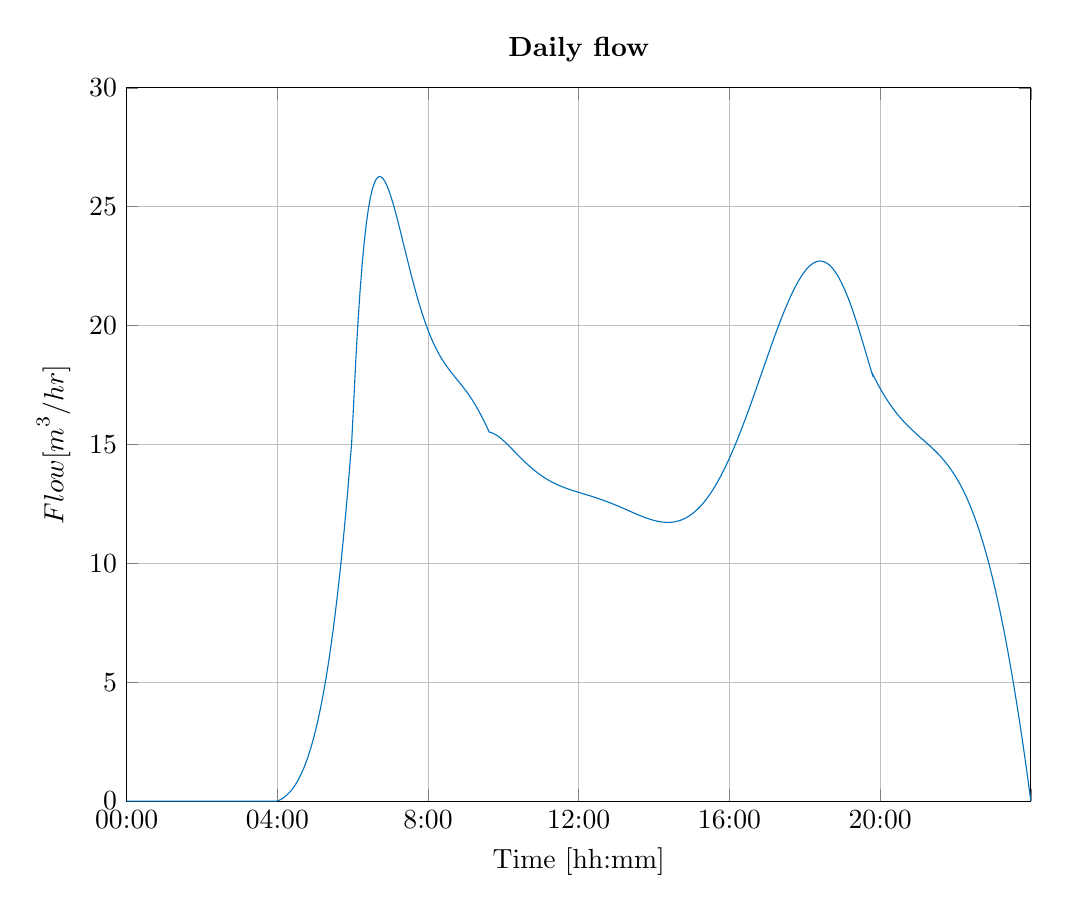
\begin{tikzpicture}

\begin{axis}[%
width=4.521in,
height=3.566in,
at={(0.758in,0.481in)},
scale only axis,
xmin=0,
xmax=24,
xtick={0,4,8,12,16,20,24},
xticklabels={{00:00},{04:00},{8:00},{12:00},{16:00},{20:00}},
xlabel={Time [hh:mm]},
xmajorgrids,
ymin=0,
ymax=30,
ylabel={$\text{Flow [m}^\text{3}\text{/hr]}$},
ymajorgrids,
axis background/.style={fill=white},
title style={font=\bfseries},
title={Daily flow}
]
\addplot [color=mycolor1,solid,forget plot]
  table[row sep=crcr]{%
0.000277777777777778	0\\
0.0558333333333333	0\\
0.111111111111111	0\\
0.166388888888889	0\\
0.221666666666667	0\\
0.276944444444444	0\\
0.332222222222222	0\\
0.3875	0\\
0.442777777777778	0\\
0.498055555555556	0\\
0.553333333333333	0\\
0.608611111111111	0\\
0.663888888888889	0\\
0.719166666666667	0\\
0.774722222222222	0\\
0.83	0\\
0.885277777777778	0\\
0.940555555555556	0\\
0.995833333333333	0\\
1.05111111111111	0\\
1.10638888888889	0\\
1.16166666666667	0\\
1.21694444444444	0\\
1.27222222222222	0\\
1.3275	0\\
1.38277777777778	0\\
1.43805555555556	0\\
1.49361111111111	0\\
1.54888888888889	0\\
1.60416666666667	0\\
1.65944444444444	0\\
1.71472222222222	0\\
1.77	0\\
1.82527777777778	0\\
1.88055555555556	0\\
1.93583333333333	0\\
1.99111111111111	0\\
2.04638888888889	0\\
2.10166666666667	0\\
2.15694444444444	0\\
2.2125	0\\
2.26777777777778	0\\
2.32305555555556	0\\
2.37833333333333	0\\
2.43361111111111	0\\
2.48888888888889	0\\
2.54416666666667	0\\
2.59944444444444	0\\
2.65472222222222	0\\
2.71	0\\
2.76527777777778	0\\
2.82055555555556	0\\
2.87583333333333	0\\
2.93138888888889	0\\
2.98666666666667	0\\
3.04194444444444	0\\
3.09722222222222	0\\
3.1525	0\\
3.20777777777778	0\\
3.26305555555556	0\\
3.31833333333333	0\\
3.37361111111111	0\\
3.42888888888889	0\\
3.48416666666667	0\\
3.53944444444444	0\\
3.59472222222222	0\\
3.65027777777778	0\\
3.70555555555556	0\\
3.76083333333333	0\\
3.81611111111111	0\\
3.87138888888889	0\\
3.92666666666667	0\\
3.98194444444444	0\\
4.03722222222222	0.0253116199877425\\
4.0925	0.0698997844514471\\
4.14777777777778	0.123627484351768\\
4.20305555555556	0.187402299591284\\
4.25833333333333	0.262173247962596\\
4.31361111111111	0.348930848605892\\
4.36916666666667	0.449243195847707\\
4.42444444444444	0.56318529486757\\
4.47972222222222	0.6923402478218\\
4.535	0.837864480246074\\
4.59027777777778	1.0009555298502\\
4.64555555555556	1.18285182754717\\
4.70083333333333	1.38483243145009\\
4.75611111111111	1.60821671383706\\
4.81138888888889	1.85436400108382\\
4.86666666666667	2.12467316656442\\
4.92194444444444	2.42058217651993\\
4.97722222222222	2.74356758889462\\
5.0325	3.09514400514065\\
5.08777777777778	3.47686347499025\\
5.14333333333333	3.89247535584648\\
5.19861111111111	4.33945540280529\\
5.25388888888889	4.82146111600829\\
5.30916666666667	5.3401876171863\\
5.36444444444444	5.89736379043894\\
5.41972222222222	6.49475140457786\\
5.475	7.13414418843844\\
5.53027777777778	7.81736685915861\\
5.58555555555556	8.54627410342655\\
5.64083333333333	9.32274951169527\\
5.69611111111111	10.1487044653658\\
5.75138888888889	11.0260769769383\\
5.80666666666667	11.9568304831307\\
5.86222222222222	12.9480511784066\\
5.9175	13.9918458150724\\
5.97277777777778	15.0950617905803\\
6.02805555555556	16.823793240725\\
6.08333333333333	18.5851901254761\\
6.13861111111111	20.1159971296799\\
6.19388888888889	21.4340601856913\\
6.24916666666667	22.5563795570816\\
6.30444444444444	23.4991288327962\\
6.35972222222222	24.2776739214883\\
6.415	24.9065920456971\\
6.47027777777778	25.3996907361744\\
6.52555555555556	25.7700268260359\\
6.58111111111111	26.0309724854148\\
6.63638888888889	26.1915775909267\\
6.69166666666667	26.2643295004458\\
6.71527777777778	26.2711762322699\\
6.74694444444444	26.2594688566887\\
6.80222222222222	26.1865806715122\\
6.8575	26.0546133200918\\
6.91277777777778	25.8718975352755\\
6.96805555555556	25.6461654017753\\
7.02333333333333	25.3845693503727\\
7.07861111111111	25.093701152245\\
7.13388888888889	24.7796109131781\\
7.18916666666667	24.4478260678383\\
7.24444444444444	24.1033703740255\\
7.3	23.7489976415403\\
7.35527777777778	23.3923409180415\\
7.41055555555556	23.0352696291931\\
7.46583333333333	22.6809806664884\\
7.52111111111111	22.3322623111205\\
7.57638888888889	21.9915132285064\\
7.63166666666667	21.6607614621937\\
7.68694444444444	21.3416834284653\\
7.74222222222222	21.0356229103074\\
7.7975	20.7436100517911\\
7.85277777777778	20.4663803523041\\
7.90805555555556	20.2043936608642\\
7.96333333333333	19.9578531701486\\
8.01888888888889	19.7256015373438\\
8.07416666666667	19.5097065626574\\
8.12944444444445	19.3085146248252\\
8.18472222222222	19.1213913744252\\
8.24	18.9475408724914\\
8.29527777777778	18.7860245848415\\
8.35055555555556	18.6357803762949\\
8.40583333333333	18.4956415049321\\
8.46111111111111	18.3643556163541\\
8.51638888888889	18.2406037379418\\
8.57166666666667	18.1230192730067\\
8.62694444444444	18.0102069952532\\
8.68222222222222	17.9007620427267\\
8.73777777777778	17.7927515016334\\
8.79305555555556	17.6858827014834\\
8.84833333333333	17.5782922900405\\
8.90361111111111	17.4687271872688\\
8.95888888888889	17.3560197443922\\
9.01416666666667	17.2391067380182\\
9.06944444444444	17.1170483646679\\
9.12472222222222	16.989047234521\\
9.18	16.8544673661896\\
9.23527777777778	16.7128531806791\\
9.29055555555555	16.5639484957291\\
9.34583333333333	16.4077155198834\\
9.40111111111111	16.2443538471006\\
9.45666666666667	16.0734492705001\\
9.51194444444444	15.8974459769512\\
9.56722222222222	15.7165329514564\\
9.6225	15.522011721602\\
9.67777777777778	15.5003376203765\\
9.73305555555556	15.4653687718832\\
9.78833333333333	15.4189035249767\\
9.84361111111111	15.3626015245759\\
9.89888888888889	15.2979902951867\\
9.95416666666667	15.226471647195\\
10.0094444444444	15.1493279070675\\
10.0647222222222	15.0677279752757\\
10.12	14.9827332124832\\
10.1752777777778	14.895303156487\\
10.2308333333333	14.8058511966964\\
10.2861111111111	14.716047248561\\
10.3413888888889	14.6261336083568\\
10.3966666666667	14.5367159949384\\
10.4519444444444	14.4483244534955\\
10.5072222222222	14.3614181003605\\
10.5625	14.2763897163188\\
10.6177777777778	14.1935701858514\\
10.6730555555556	14.1132327871275\\
10.7283333333333	14.0355973335303\\
10.7836111111111	13.9608341702333\\
10.8388888888889	13.8890680259374\\
10.8941666666667	13.820381723338\\
10.9497222222222	13.7544982128912\\
11.005	13.69208587487\\
11.0602777777778	13.632785252481\\
11.1155555555556	13.5765457570232\\
11.1708333333333	13.5232914101064\\
11.2261111111111	13.4729237493115\\
11.2813888888889	13.4253246042145\\
11.3366666666667	13.3803587504631\\
11.3919444444444	13.3378764381954\\
11.4472222222222	13.2977158024324\\
11.5025	13.2597051539569\\
11.5577777777778	13.2236651535449\\
11.6130555555556	13.1894108722306\\
11.6686111111111	13.1565933458146\\
11.7238888888889	13.1253495770254\\
11.7791666666667	13.0953211834007\\
11.8344444444444	13.066319282095\\
11.8897222222222	13.0381580699579\\
11.945	13.0106562419601\\
12.0002777777778	12.9836383104518\\
12.0555555555556	12.9569358275542\\
12.1108333333333	12.9303885104412\\
12.1661111111111	12.9038452757326\\
12.2213888888889	12.8771651819999\\
12.2766666666667	12.8502182816276\\
12.3319444444444	12.8228863886609\\
12.3875	12.7949225472487\\
12.4427777777778	12.7665133406187\\
12.4980555555556	12.7374411963445\\
12.5533333333333	12.7076410476748\\
12.6086111111111	12.6770621946195\\
12.6638888888889	12.6456685933607\\
12.7191666666667	12.6134390736618\\
12.7744444444444	12.5803674864141\\
12.8297222222222	12.5464627824837\\
12.885	12.5117490275654\\
12.9402777777778	12.4762653514501\\
12.9955555555556	12.440065836546\\
13.0508333333333	12.4032193472793\\
13.1063888888889	12.3656200483233\\
13.1616666666667	12.3277420659092\\
13.2169444444444	12.2895104352065\\
13.2722222222222	12.2510503924397\\
13.3275	12.2125002817562\\
13.3827777777778	12.1740110711074\\
13.4380555555556	12.1357458263798\\
13.4933333333333	12.0978791368763\\
13.5486111111111	12.0605965079757\\
13.6038888888889	12.0240937098241\\
13.6591666666667	11.9885760917159\\
13.7144444444444	11.9542578629516\\
13.7697222222222	11.9213613405481\\
13.8252777777778	11.8899637226625\\
13.8805555555556	11.8606161502038\\
13.9358333333333	11.8333991562608\\
13.9911111111111	11.8085594259439\\
14.0463888888889	11.7863475825768\\
14.1016666666667	11.7670172871845\\
14.1569444444444	11.7508243218015\\
14.2122222222222	11.7380256569774\\
14.2675	11.7288785058894\\
14.3227777777778	11.7236393703104\\
14.3644444444444	11.722428041888\\
14.3780555555556	11.7225630726145\\
14.4333333333333	11.7259017870532\\
14.4886111111111	11.7339040601805\\
14.5438888888889	11.7468138356072\\
14.5994444444444	11.7649735911212\\
14.6547222222222	11.7884344800392\\
14.71	11.8174983933753\\
14.7652777777778	11.8523810438711\\
14.8205555555556	11.8932886764353\\
14.8758333333333	11.9404171189284\\
14.9311111111111	11.9939508429307\\
14.9863888888889	12.0540620433162\\
15.0416666666667	12.1209097303273\\
15.0969444444444	12.1946388411309\\
15.1522222222222	12.2753793732638\\
15.2075	12.3632455412137\\
15.2627777777778	12.458334954429\\
15.3183333333333	12.5612609184825\\
15.3736111111111	12.6710564397917\\
15.4288888888889	12.7882608034172\\
15.4841666666667	12.9128974783746\\
15.5394444444444	13.0449696777814\\
15.5947222222222	13.1844597308445\\
15.65	13.3313284957325\\
15.7052777777778	13.4855148179045\\
15.7605555555556	13.6469350289457\\
15.8158333333333	13.8154824889917\\
15.8711111111111	13.9910271850016\\
15.9263888888889	14.1734153727009\\
15.9816666666667	14.3624692703956\\
16.0372222222222	14.5589852627889\\
16.0925	14.7607706344896\\
16.1477777777778	14.9685406277427\\
16.2030555555556	15.182019276075\\
16.2583333333333	15.4009059177912\\
16.3136111111111	15.62487524787\\
16.3688888888889	15.8535774423497\\
16.4241666666667	16.0866383467854\\
16.4794444444444	16.3236597394137\\
16.5347222222222	16.56421966529\\
16.59	16.8078728503001\\
16.6452777777778	17.0541511855497\\
16.7005555555556	17.3025642976623\\
16.7561111111111	17.5538598685704\\
16.8113888888889	17.804989790489\\
16.8666666666667	18.0566538784781\\
16.9219444444444	18.3082799573848\\
16.9772222222222	18.5592777051533\\
17.0325	18.8090397398467\\
17.0877777777778	19.0569428094604\\
17.1430555555556	19.302349070703\\
17.1983333333333	19.5446074728955\\
17.2536111111111	19.78305523817\\
17.3088888888889	20.0170194463285\\
17.3641666666667	20.2458187233053\\
17.4194444444444	20.4687650417304\\
17.475	20.6862353594024\\
17.5302777777778	20.8953565443601\\
17.5855555555556	21.0965368709193\\
17.6408333333333	21.2890818852858\\
17.6961111111111	21.4723011538097\\
17.7513888888889	21.6455107471918\\
17.8066666666667	21.8080358487508\\
17.8619444444444	21.9592134810133\\
17.9172222222222	22.0983953663221\\
17.9725	22.2249509079598\\
18.0277777777778	22.3382703071028\\
18.0830555555556	22.4377678075961\\
18.1383333333333	22.5228850799685\\
18.1938888888889	22.5934090608999\\
18.2491666666667	22.6481397531112\\
18.3044444444444	22.687013484547\\
18.3597222222222	22.7096184332852\\
18.4069444444444	22.7157672115064\\
18.415	22.7155892261752\\
18.4702777777778	22.7046111659752\\
18.5255555555556	22.6764246270588\\
18.5808333333333	22.6308295774281\\
18.6361111111111	22.5676902703252\\
18.6913888888889	22.4869400945647\\
18.7466666666667	22.3885865665959\\
18.8019444444444	22.2727164962207\\
18.8572222222222	22.1395013113591\\
18.9127777777778	21.9884046907302\\
18.9680555555556	21.8212966375205\\
19.0233333333333	21.6379237200741\\
19.0786111111111	21.438852927126\\
19.1338888888889	21.2247650125493\\
19.1891666666667	20.9964608394426\\
19.2444444444444	20.7548678870517\\
19.2997222222222	20.5010469578642\\
19.355	20.2361990421275\\
19.4102777777778	19.9616723866532\\
19.4655555555556	19.6789697349512\\
19.5208333333333	19.3897557568775\\
19.5761111111111	19.0958646716369\\
19.6313888888889	18.7993080646822\\
19.6869444444444	18.5007930664555\\
19.7422222222222	18.2057058664098\\
19.7944444444444	17.9310429893127\\
19.7975	17.9712077467308\\
19.8527777777778	17.7945965721496\\
19.9080555555556	17.6245352460121\\
19.9633333333333	17.4610087993307\\
20.0186111111111	17.3039706077282\\
20.0738888888889	17.1533433910085\\
20.1291666666667	17.009020212564\\
20.1844444444444	16.8708654786759\\
20.2397222222222	16.7387159388962\\
20.295	16.6123816848603\\
20.3502777777778	16.4916471500202\\
20.4058333333333	16.3757054334303\\
20.4611111111111	16.2654509042094\\
20.5163888888889	16.1600039465212\\
20.5716666666667	16.059056251153\\
20.6269444444444	15.962278852998\\
20.6822222222222	15.8693231315995\\
20.7375	15.7798218107216\\
20.7927777777778	15.6933899569454\\
20.8480555555556	15.60962598043\\
20.9033333333333	15.5281126336167\\
20.9586111111111	15.4484180110166\\
21.0138888888889	15.3700965492671\\
21.0691666666667	15.2926900256208\\
21.1247222222222	15.215342134617\\
21.18	15.138343775053\\
21.2352777777778	15.0608172434315\\
21.2905555555556	14.9822636379372\\
21.3458333333333	14.9021763995504\\
21.4011111111111	14.8200423135123\\
21.4563888888889	14.7353425085163\\
21.5116666666667	14.6475534555746\\
21.5669444444444	14.5561479682926\\
21.6222222222222	14.4605962025472\\
21.6775	14.3603666550289\\
21.7327777777778	14.2549271642739\\
21.7880555555556	14.1437459087728\\
21.8436111111111	14.0256854580975\\
21.8988888888889	13.9013960690233\\
21.9541666666667	13.7697788644188\\
22.0094444444444	13.6303134055713\\
22.0647222222222	13.482484597365\\
22.12	13.3257836874186\\
22.1752777777778	13.1597092666837\\
22.2305555555556	12.9837682677166\\
22.2858333333333	12.7974769650064\\
22.3411111111111	12.6003619743286\\
22.3963888888889	12.3919612525865\\
22.4516666666667	12.171825096732\\
22.5069444444444	11.9395171440934\\
22.5625	11.6933522142751\\
22.6177777777778	11.4353836081672\\
22.6730555555556	11.1640222339559\\
22.7283333333333	10.8788951740098\\
22.7836111111111	10.5796478535801\\
22.8388888888889	10.2659450406956\\
22.8941666666667	9.93747184519214\\
22.9494444444444	9.59393471839094\\
23.0047222222222	9.23506245283158\\
23.06	8.86060718151758\\
23.1152777777778	8.47034537802801\\
23.1705555555556	8.06407885554673\\
23.2258333333333	7.64163576702804\\
23.2813888888889	7.20062533673316\\
23.3366666666667	6.7453410852948\\
23.3919444444444	6.27353239724316\\
23.4472222222222	5.78514293265396\\
23.5025	5.28014769544862\\
23.5577777777778	4.75855402960957\\
23.6130555555556	4.22040262243047\\
23.6683333333333	3.66576849981149\\
23.7236111111111	3.09476203037543\\
23.7788888888889	2.50752992124998\\
23.8341666666667	1.90425622028985\\
23.8894444444444	1.28516331359072\\
23.9447222222222	0.650512926466693\\
24	0.000607122804183746\\
};
\end{axis}
\end{tikzpicture}%
\caption{A flow profile for Thulesvej.}
\label{fig:APP_flow_profile_zone8_9}
\end{figure} 

\begin{figure}[H]
\centering
% This file was created by matlab2tikz.
%
%The latest updates can be retrieved from
%  http://www.mathworks.com/matlabcentral/fileexchange/22022-matlab2tikz-matlab2tikz
%where you can also make suggestions and rate matlab2tikz.
%
\definecolor{mycolor1}{rgb}{0.00000,0.44700,0.74100}%
%
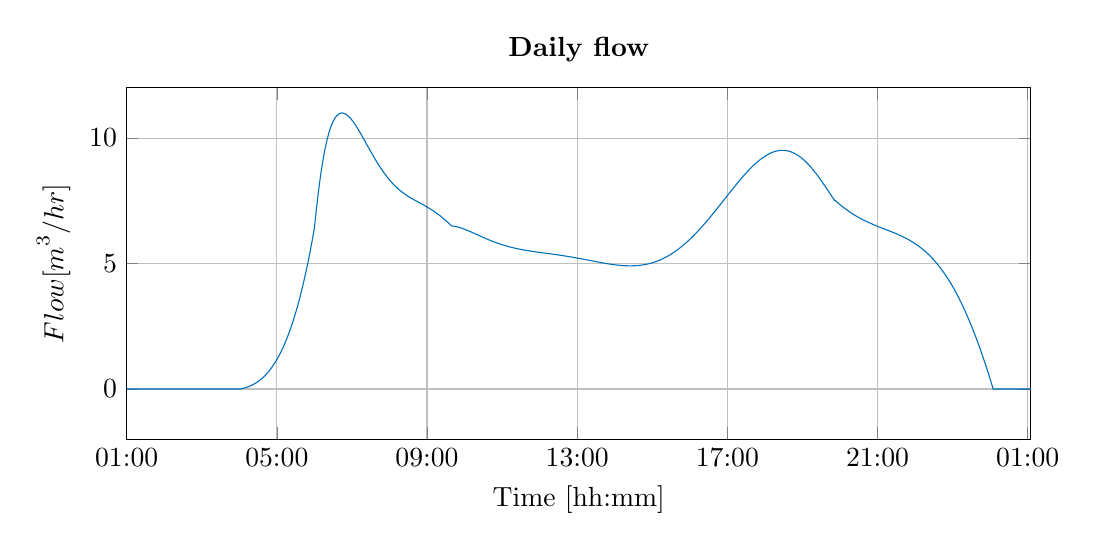
\begin{tikzpicture}

\begin{axis}[%
width=4.521in,
height=1.7566in,
at={(0.758in,0.481in)},
scale only axis,
xmin=3600,
xmax=90000,
xtick={3600,17950,32300,46650,61000,75350,89700},
xticklabels={{01:00},{05:00},{09:00},{13:00},{17:00},{21:00},{01:00},{},{},{}},
xlabel={Time [hh:mm]},
xmajorgrids,
ymin=-2,
scaled x ticks = false,
ymax=12,
ylabel={$\text{Flow [m}^\text{3}\text{/hr]}$},
ymajorgrids,
axis background/.style={fill=white},
title style={font=\bfseries},
title={Daily flow},
legend style={legend cell align=left,align=left,draw=white!15!black}
]
\addplot [color=mycolor1,solid]
  table[row sep=crcr]{%
3599	0\\
3799	0\\
3998	0\\
4197	0\\
4396	0\\
4595	0\\
4794	0\\
4993	0\\
5192	0\\
5391	0\\
5590	0\\
5789	0\\
5988	0\\
6188	0\\
6387	0\\
6586	0\\
6785	0\\
6984	0\\
7183	0\\
7382	0\\
7581	0\\
7780	0\\
7979	0\\
8178	0\\
8377	0\\
8577	0\\
8776	0\\
8975	0\\
9174	0\\
9373	0\\
9572	0\\
9771	0\\
9970	0\\
10169	0\\
10368	0\\
10567	0\\
10766	0\\
10965	0\\
11165	0\\
11364	0\\
11563	0\\
11762	0\\
11961	0\\
12160	0\\
12359	0\\
12558	0\\
12757	0\\
12956	0\\
13155	0\\
13354	0\\
13554	0\\
13753	0\\
13952	0\\
14151	0\\
14350	0\\
14549	0.0118795817392918\\
14748	0.0308234886727714\\
14947	0.0536220064953477\\
15146	0.0806564302629574\\
15345	0.112325407078907\\
15544	0.149044961178419\\
15743	0.191248499321518\\
15942	0.239386796494379\\
16142	0.294219018527653\\
16341	0.355684311119568\\
16540	0.424543027612383\\
16739	0.501314964811748\\
16938	0.586536920266521\\
17137	0.680762559721937\\
17336	0.784562264880996\\
17535	0.898522961474619\\
17734	1.02324792763982\\
17933	1.15935658260669\\
18132	1.30748425569367\\
18331	1.46828193561114\\
18531	1.64332586637081\\
18730	1.83154997948346\\
18929	2.03449175519504\\
19128	2.25286199078694\\
19327	2.48738559227373\\
19526	2.73880120545836\\
19725	3.00786082729631\\
19924	3.29532939756776\\
20123	3.60198437085838\\
20322	3.92861526884855\\
20521	4.27602321291099\\
20720	4.64502043701694\\
20920	5.03845465852228\\
21119	5.45322797024621\\
21318	5.89209302976077\\
21517	6.35590130026059\\
21716	7.10296901560315\\
21915	7.83289111533979\\
22114	8.46684476614284\\
22313	9.01227479884609\\
22512	9.47627257617931\\
22711	9.86558394536148\\
22910	10.1866171906544\\
23109	10.4454509859616\\
23308	10.6478423474075\\
23508	10.7998753654395\\
23707	10.9051880464705\\
23906	10.9695025028465\\
24105	10.9973672088713\\
24175	10.9993066025719\\
24304	10.9930487839045\\
24503	10.9605399449714\\
24702	10.9035674592995\\
24901	10.8256000969293\\
25100	10.7298565832501\\
25299	10.6193135516508\\
25498	10.4967134960161\\
25697	10.3645727233541\\
25897	10.2244742079456\\
26096	10.0799149610652\\
26295	9.93209529980857\\
26494	9.7827053527254\\
26693	9.6332488643236\\
26892	9.48505114765667\\
27091	9.33926703689998\\
27290	9.19688883990723\\
27489	9.05875429083206\\
27688	8.92555450267593\\
27887	8.79784191987574\\
28086	8.67603827084613\\
28285	8.56044252061799\\
28485	8.45070637554046\\
28684	8.34800456145935\\
28883	8.25175014165034\\
29082	8.16183011628386\\
29281	8.07804852498982\\
29480	8.00013439941689\\
29679	7.92774971580873\\
29878	7.86049734757461\\
30077	7.79792901788265\\
30276	7.73955325223045\\
30475	7.68484333103265\\
30674	7.63324524213489\\
30874	7.58394452892605\\
31073	7.53684699330472\\
31272	7.49111207349925\\
31471	7.4461561559022\\
31670	7.40140813724263\\
31869	7.35631737717369\\
32068	7.31036165086023\\
32267	7.2630551015267\\
32466	7.21395619301645\\
32665	7.16267566245863\\
32864	7.10888447275947\\
33063	7.05232176521251\\
33263	6.99249604961948\\
33462	6.92990474326307\\
33661	6.86424814160538\\
33860	6.79561814779798\\
34059	6.7242146462003\\
34258	6.65035345505218\\
34457	6.57447427891987\\
34656	6.49833713668959\\
34855	6.4888153972397\\
35054	6.47378620789247\\
35253	6.45399803250556\\
35452	6.430141472223\\
35651	6.40285201621118\\
35851	6.37255498865431\\
36050	6.34008869544113\\
36249	6.3057940293976\\
36448	6.2701118493111\\
36647	6.23344057203945\\
36846	6.1961384905259\\
37045	6.15852602313973\\
37244	6.12088789492031\\
37443	6.08347525161941\\
37642	6.04650770724432\\
37841	6.01017532674433\\
38040	5.9746405435234\\
38240	5.93986870048465\\
38439	5.90632060103044\\
38638	5.87391023942384\\
38837	5.84270734198412\\
39036	5.8127626631628\\
39235	5.78410953454619\\
39434	5.75676535533393\\
39633	5.73073302521139\\
39832	5.70600232097511\\
40031	5.68255121690019\\
40230	5.66034715102461\\
40429	5.63934823677265\\
40628	5.61950442207006\\
40828	5.60066706403399\\
41027	5.58296114379309\\
41226	5.56622163123193\\
41425	5.55037635222371\\
41624	5.53535000103584\\
41823	5.5210649988729\\
42022	5.50744230600601\\
42221	5.49440218776061\\
42420	5.48186493498562\\
42619	5.46975154122447\\
42818	5.45798433542106\\
43017	5.44648757308358\\
43217	5.43513158146358\\
43416	5.42395934944996\\
43615	5.412846849108\\
43814	5.40173115153327\\
44013	5.3905536040869\\
44212	5.37926018460897\\
44411	5.36780181947079\\
44610	5.35613466608918\\
44809	5.34422036126217\\
45008	5.33202623563196\\
45207	5.31952549521548\\
45406	5.30669737156585\\
45606	5.29346017819263\\
45805	5.27993787640668\\
46004	5.26606308218105\\
46203	5.25184005225066\\
46402	5.23727937051237\\
46601	5.22239792539026\\
46800	5.20721886092982\\
46999	5.19177150333153\\
47198	5.17609126368296\\
47397	5.16021951725179\\
47596	5.14420346093724\\
47795	5.1280959494349\\
47994	5.11195531099861\\
48194	5.09576437814526\\
48393	5.07975400522986\\
48592	5.06391658002326\\
48791	5.04833012650349\\
48990	5.03307694354333\\
49189	5.01824331699232\\
49388	5.00391921750719\\
49587	4.99019798457275\\
49786	4.97717599782331\\
49985	4.96495233778306\\
50184	4.95362843509666\\
50383	4.943307710119\\
50583	4.93405188689422\\
50782	4.92606025598407\\
50981	4.91939081037052\\
51180	4.91415116238873\\
51379	4.91044899364868\\
51578	4.90839165591487\\
51712	4.9079865712648\\
51777	4.90808576487176\\
51976	4.90963679453481\\
52175	4.91314866779855\\
52374	4.91872334657675\\
52573	4.92646042182932\\
52772	4.93645670446153\\
52971	4.94880581752605\\
53171	4.96367843878419\\
53370	4.98101222824093\\
53569	5.00095695851902\\
53768	5.0235894659558\\
53967	5.04898141570374\\
54166	5.07719892245806\\
54365	5.1083021797488\\
54564	5.14234509685707\\
54763	5.17937494682204\\
54962	5.2194320240094\\
55161	5.26254931252127\\
55360	5.3087521683705\\
55560	5.35831363652653\\
55759	5.41074731626227\\
55958	5.46629385879316\\
56157	5.5249451513103\\
56356	5.58668407368437\\
56555	5.65148427078218\\
56754	5.71930994507271\\
56953	5.79011566840136\\
57152	5.86384621208262\\
57351	5.94043640113411\\
57550	6.01981098776936\\
57749	6.10188454891874\\
57949	6.18699331933262\\
58148	6.27417975568391\\
58347	6.36374657234448\\
58546	6.45556705634981\\
58745	6.54950418071004\\
58944	6.64541065706556\\
59143	6.74312901851093\\
59342	6.84249173198655\\
59541	6.94332133998895\\
59740	7.04543063664093\\
59939	7.14862287411116\\
60138	7.25269200342766\\
60337	7.35742294833695\\
60537	7.46312112327383\\
60736	7.5684963917265\\
60935	7.67383614962592\\
61134	7.77889264659146\\
61333	7.88341102952007\\
61532	7.98712984110427\\
61731	8.08978156040206\\
61930	8.19109318533432\\
62129	8.29078685482113\\
62328	8.38858051695783\\
62527	8.48418863990012\\
62726	8.57732296753143\\
62926	8.66813997197572\\
63125	8.75543900905899\\
63324	8.83938992393095\\
63523	8.91970205878648\\
63722	8.99608652033954\\
63921	9.06825722416748\\
64120	9.13593199128067\\
64319	9.19883369466275\\
64518	9.25669145856857\\
64717	9.30924191419349\\
64916	9.35623050704678\\
65115	9.39741286094565\\
65314	9.43255619917375\\
65514	9.46156981346488\\
65713	9.48395766023341\\
65912	9.4996919189945\\
66111	9.50860166582624\\
66265	9.51071570084851\\
66310	9.51053556425147\\
66509	9.50536364213913\\
66708	9.49297913292957\\
66907	9.47330037663013\\
67106	9.44627279118421\\
67305	9.41187090349721\\
67504	9.37010044906882\\
67703	9.32100053993716\\
67903	9.26434456063948\\
68102	9.20081227631483\\
68301	9.13029168268548\\
68500	9.05297864660904\\
68699	8.9691142905395\\
68898	8.87898757931475\\
69097	8.7829379799462\\
69296	8.68135819828457\\
69495	8.57469698417882\\
69694	8.46346202067126\\
69893	8.34822288367939\\
70092	8.22961408120522\\
70292	8.10772328622543\\
70491	7.98454664202218\\
70690	7.86032948610619\\
70889	7.73599843250721\\
71088	7.61256143877008\\
71260	7.50743087403459\\
71287	7.51820063907476\\
71486	7.44447686225493\\
71685	7.37349539461166\\
71884	7.30524888764713\\
72083	7.23971677314864\\
72282	7.17686568132963\\
72481	7.1166498594239\\
72680	7.05901159030249\\
72880	7.00361077830367\\
73079	6.95092067663724\\
73278	6.90056689002065\\
73477	6.85244797768144\\
73676	6.80645262895079\\
73875	6.76246008188042\\
74074	6.72034054156487\\
74273	6.67995559869046\\
74472	6.64115864831068\\
74671	6.60379530782871\\
74870	6.56770383602209\\
75069	6.53271555120645\\
75269	6.49848613235421\\
75468	6.46517579217891\\
75667	6.43242418353294\\
75866	6.40003902290639\\
76065	6.3678231811337\\
76264	6.33557510171602\\
76463	6.30308921950603\\
76662	6.27015637891697\\
76861	6.23656425276611\\
77060	6.20209776068766\\
77259	6.16653948738713\\
77458	6.12967010150745\\
77657	6.09126877399659\\
77857	6.05090700721646\\
78056	6.00876491594508\\
78255	5.96442247452863\\
78454	5.91765704973439\\
78653	5.86824660546362\\
78852	5.8159701206887\\
79051	5.76060800854582\\
79250	5.70194253427214\\
79449	5.63975823416245\\
79648	5.57384233393689\\
79847	5.50398516697258\\
80046	5.42998059321505\\
80246	5.3512213585326\\
80445	5.26829640596763\\
80644	5.18063001216999\\
80843	5.08803435503968\\
81042	4.99032723314903\\
81241	4.88733248454082\\
81440	4.77888040541312\\
81639	4.66480816839628\\
81838	4.54496024114717\\
82037	4.41918880473945\\
82236	4.28735417230308\\
82435	4.14932520761857\\
82635	4.00423824438883\\
82834	3.85343092398334\\
83033	3.69609085829208\\
83232	3.5321253502789\\
83431	3.36145234825117\\
83630	3.18400086404616\\
83829	2.99971139153463\\
84028	2.80853632539629\\
84227	2.61044037941947\\
84426	2.40540100459686\\
84625	2.19340880871666\\
84824	1.97446797359732\\
85023	1.7485966745654\\
85223	1.51464045938017\\
85422	1.27498654396602\\
85621	1.02854518802803\\
85820	0.775394804106138\\
86019	0.5156298925109\\
86218	0.249361459691136\\
86401	0\\
86417	0\\
86616	0\\
86815	0\\
87014	0\\
87213	0\\
87412	0\\
87612	0\\
87811	0\\
88010	0\\
88209	0\\
88408	0\\
88607	0\\
88806	0\\
89005	0\\
89204	0\\
89403	0\\
89602	0\\
90000	0\\
};

\end{axis}
\end{tikzpicture}%
\caption{A flow profile for Thulesvej.}
\label{fig:APP_flow_profile_zone11}
\end{figure} 